%% Foundations of Scientific Computing, Volume 1. Build: tools/build.sh vol1 (output pdf/vol1.pdf)
\documentclass{sdbook-eng}

\addbibresource{references.bib}

\title{Foundations of\\Scientific Computing}
\volume{1}{Calculus, Linear Algebra, and Differential Equations}
\author{}
\date{}

\begin{document}
\frontmatter
\maketitle
\tableofcontents

\notationchapter
This list collects the symbols that are used in several chapters, and the conventions that differ from book to book. Every symbol, including those not listed here, is defined, with examples, where it first appears.

\symbolgroup{Logic and sets}
\begin{symbols}
\item[$\neg P$, $P\wedge Q$, $P\vee Q$] not $P$; $P$ and $Q$; $P$ or $Q$ (or both)
\item[$P\Rightarrow Q$, $P\Leftrightarrow Q$] if $P$, then $Q$; $P$ if and only if $Q$
\item[$\forall$, $\exists$, $\exists!$] for every; there is at least one; there is exactly one
\item[$a\coloneqq b$] $a$ is defined to be $b$
\item[$\{x\in S: P(x)\}$] the set of the elements $x$ of $S$ for which $P(x)$ holds; $\{t(x): x\in S\}$ is the set of the values $t(x)$
\item[$A\subseteq B$, $A\subset B$] $A$ is a subset of $B$; $A$ is a \emph{proper} subset of $B$ ($A\subseteq B$ and $A\ne B$)
\item[$A\setminus B$, $A^{\mathrm c}$] the elements of $A$ not in $B$; the complement $U\setminus A$ in the universe $U$
\item[$(a,b)$, $A\times B$, $A^n$] an ordered pair; the Cartesian product; the set of $n$-tuples $(a_1,\ldots,a_n)$ of elements of $A$
\item[$|A|$] the number of elements of a finite set $A$; $|A|=|B|$ means that there is a bijection between $A$ and $B$
\item[$\sum_{k=m}^{n}a_k$, $\prod_{k=m}^{n}a_k$] sum and product; an empty sum ($n<m$) is $0$, an empty product is $1$
\item[$x^{\underline k}$, $\binom rk$] the falling factorial $x(x-1)\cdots(x-k+1)$, with $x^{\underline 0}=1$; the binomial coefficient $r^{\underline k}/k!$, for real $r$ and $k\in\mathbb N$
\end{symbols}

\symbolgroup{Numbers}
\begin{symbols}
\item[$\mathbb N$] the natural numbers $0,1,2,\ldots$ (\emph{zero included})
\item[$\mathbb Z$, $\mathbb Q$, $\mathbb R$, $\mathbb C$] the integers, the rational, the real and the complex numbers
\item[{$[a,b]$, $(a,b)$}] the closed interval $a\le x\le b$ and the open interval $a<x<b$; similarly $[a,b)$, $(a,\infty)$, \ldots
\item[$\lfloor x\rfloor$, $\lceil x\rceil$] the floor and the ceiling: the integers $n$ with $n\le x<n+1$ and with $n-1<x\le n$
\item[$\operatorname{sign}x$] $-1$, $0$ or $1$ according as $x<0$, $x=0$ or $x>0$
\item[$a\mid b$] the integer $a$ divides the integer $b$
\item[$a\bmod b$] the remainder of $a$ on division by $b>0$, rounded down: $0\le a\bmod b<b$ also for negative $a$
\item[$a\equiv b\pmod n$, $\mathbb Z/n\mathbb Z$] $n\mid a-b$; the integers modulo $n$
\item[$(d_k\cdots d_0)_b$] the number $\sum_{i=0}^{k}d_ib^i$ written with the digits $d_i\in\{0,\ldots,b-1\}$ in base $b$
\item[$\phi$, $H_n$] the golden ratio $(1+\sqrt5)/2$; the harmonic number $1+1/2+\cdots+1/n$
\item[$\bar z$, $|z|$] the conjugate $a-bi$ and the modulus $\sqrt{a^2+b^2}$ of $z=a+bi$; $\operatorname{Re}z=a$, $\operatorname{Im}z=b$
\item[$\arg z$, $\operatorname{Arg}z$] an argument of $z\ne0$, and the principal argument, which lies in $(-\pi,\pi]$
\end{symbols}

\symbolgroup{Functions and relations}
\begin{symbols}
\item[$f\colon A\to B$, $a\mapsto f(a)$] a function with domain $A$ and codomain $B$; its rule
\item[$f(S)$, $f^{-1}(T)$] the image of a set $S$ and the preimage of a set $T$; the preimage exists for every $f$
\item[$f^{-1}$] the inverse function of a bijection $f$
\item[$g\circ f$] the composition, $(g\circ f)(a)=g(f(a))$: first $f$, then $g$
\item[$f|_S$, $\operatorname{id}_A$] the restriction of $f$ to $S$; the identity function of $A$
\item[$\mathbf 1_S$] the indicator function of $S$: $1$ on $S$, $0$ elsewhere
\item[$a\sim b$, {$[a]$}, $A/{\sim}$] equivalence under an equivalence relation; the class of $a$; the set of classes (for $\sim$ between functions see below)
\item[$\sup S$, $\inf S$] the least upper bound and the greatest lower bound of $S$; $\max S$, $\min S$ when they belong to $S$
\end{symbols}

\symbolgroup{Calculus}
\begin{symbols}
\item[$(a_n)$, $(a_n)_{n\ge1}$] a sequence $a_0,a_1,\ldots$ (indexed from $0$ unless stated); one that starts at $a_1$
\item[$x\to a^+$, $f(a^+)$] $x$ tends to $a$ from the right, and the right-hand limit of $f$ at $a$; similarly $a^-$
\item[$C(D)$, $C^k(I)$, $C^\infty(I)$] the continuous functions on $D$; the $k$ times continuously differentiable and the smooth functions on $I$
\item[$f'$, $f^{(n)}$, $df/dx$] derivatives, with $f^{(0)}=f$
\item[$y'=f(t,y)$] a differential equation for $y(t)$; in Part~IV primes denote $d/dt$ ($d/dx$ for plane curves and in \cref{ch:series-solutions}), and dots, $\dot y$, are not used
\item[$D_h^+f(x)$, $D_h^0f(x)$] the forward and the central difference quotient $(f(x+h)-f(x))/h$ and $(f(x+h)-f(x-h))/(2h)$
\item[$\kappa_f(x)$] the relative condition number $|xf'(x)/f(x)|$ of $f$ at $x$
\item[$\int_a^bf$, $\int_a^bf(x)\,dx$] the integral of $f$ over $[a,b]$; $\int_b^af=-\int_a^bf$
\item[$\Lambda(x)$] the function $\int_1^x dt/t$ ($x>0$) of \cref{ch:integration,ch:series}, which \cref{ch:transcendental} identifies with $\ln x$
\item[$\Gamma(s)$] the gamma function $\int_0^\infty t^{s-1}e^{-t}\,dt$, $s>0$
\item[$P_n$; $J_\nu$, $Y_\nu$] the Legendre polynomials, $P_n(1)=1$; the Bessel functions
\item[$f=O(g)$, $f=o(g)$] $|f|\le C|g|$ near the limit point; $|f|\le\varepsilon|g|$ near it for every $\varepsilon>0$ (the limit point is stated or clear from the context)
\item[$f\sim g$] $f$ is asymptotically equal to $g$: $f-g=o(g)$
\end{symbols}

\symbolgroup{Elementary functions}
\begin{symbols}
\item[$\exp x$, $e^x$] the exponential function $\sum_{k\ge0}x^k/k!$, for real or complex $x$
\item[$\ln x$, $\log_ax$] the natural logarithm; the logarithm $\ln x/\ln a$ to the base $a$; $\log$ without a base only where the base does not matter, as in $O(n\log n)$
\item[$a^x$] the power $e^{x\ln a}$ for $a>0$; $0^x=0$ for $x>0$, and $0^0=1$
\item[$\arcsin$, $\arccos$, $\arctan$] the inverses of $\sin$, $\cos$, $\tan$ on $[-\pi/2,\pi/2]$, $[0,\pi]$, $(-\pi/2,\pi/2)$
\item[$\operatorname{atan2}(y,x)$] the angle $\theta\in(-\pi,\pi]$ with $(x,y)=r(\cos\theta,\sin\theta)$, $r>0$ ($y$ first)
\item[$u$] the unit roundoff $2^{-53}$ of binary64 floating-point arithmetic
\end{symbols}

\symbolgroup{Vectors, matrices and several variables}
\begin{symbols}
\item[$\mathbf x=(x_1,\ldots,x_n)$] a vector of $\mathbb R^n$ (bold lower case), a column in matrix products
\item[$\mathbf 0$, $\mathbf e_i$] the zero vector; the $i$th standard basis vector
\item[$\langle\mathbf x,\mathbf y\rangle$] the inner product $\mathbf x^{\mathsf T}\mathbf y=\sum_ix_iy_i$; $\mathbf x^{\mathsf H}\mathbf y$ if complex (linear in $\mathbf y$)
\item[$\|\mathbf x\|$, $\|\mathbf x\|_p$] the Euclidean norm $\|\mathbf x\|_2$; $\|\mathbf x\|_1=\sum_i|x_i|$; $\|\mathbf x\|_\infty=\max_i|x_i|$
\item[$A=(a_{ij})$, $\mathbb R^{m\times n}$] a matrix (italic capital) with entries $a_{ij}$; the real $m\times n$ matrices
\item[$A^{\mathsf T}$, $A^{\mathsf H}$, $I_n$] the transpose; the conjugate transpose $\bar A^{\mathsf T}$; the identity matrix
\item[$\operatorname{diag}(d_i)$, $\operatorname{tr}A$] the diagonal matrix with the entries $d_1,\ldots,d_n$; the trace $\sum_ia_{ii}$
\item[$\|A\|_p$, $\|A\|_{\mathrm F}$] the operator norm induced by $\|\cdot\|_p$; the Frobenius norm
\item[$\operatorname{rank}A$] the rank of $A$, the number of pivots in its row echelon forms
\item[$\det A$, $\operatorname{sgn}\sigma$] the determinant of a square matrix; the sign $\pm1$ of a permutation $\sigma$
\item[$\mathbb F$, $\mathcal P_n$] the scalars, $\mathbb R$ or $\mathbb C$; the polynomials of degree at most $n$
\item[$\operatorname{span}S$, $\dim V$] the span of a set $S$; the dimension of a vector space $V$
\item[$\mathcal C(A)$, $\mathcal N(A)$] the column space and the null space of $A$
\item[$\ker T$, $\operatorname{im}T$, $\mathcal L(V,W)$] the kernel and the image of $T$; the linear maps from $V$ to $W$
\item[$S^\perp$, $T^*$] the orthogonal complement of $S$; the adjoint of $T$ ($A^{\mathsf H}$ for a matrix)
\item[$p_A$, $\rho(A)$, $E_\lambda$] the characteristic polynomial $\det(\lambda I-A)$; the spectral radius, the largest modulus of an eigenvalue; the eigenspace $\mathcal N(A-\lambda I)$
\item[$J_k(\lambda)$, $e^A$] the Jordan block of order $k$ for $\lambda$; the matrix exponential $\sum_kA^k/k!$
\item[$A\succeq0$, $\lambda_k(A)$] $A$ is Hermitian positive semidefinite ($A\succ0$: definite); the eigenvalues of a Hermitian $A$ in \emph{increasing} order, $\lambda_1(A)\le\cdots\le\lambda_n(A)$
\item[$\sigma_i(A)$, $A^+$, $\kappa_2(A)$] the singular values, \emph{decreasing}; the pseudoinverse; $\sigma_1/\sigma_r$
\item[{$[T]_{\mathcal D\leftarrow\mathcal B}$}] the matrix of $T$ with respect to the bases $\mathcal B$ and $\mathcal D$; $[T]_{\mathcal B}$ if $\mathcal D=\mathcal B$
\item[$B(\mathbf a,r)$, $\bar B(\mathbf a,r)$] the open and the closed ball with centre $\mathbf a$ and radius $r$
\item[$\mathbf f=(f_1,\ldots,f_m)$] a vector-valued function, in bold, with component functions $f_i$
\item[$\partial_if$, $\partial f/\partial x_i$, $f_{x_i}$] the partial derivative with respect to $x_i$; $f_{xy}=(f_x)_y$
\item[$D\mathbf f(\mathbf a)$] the derivative of $\mathbf f$ at $\mathbf a$, the $m\times n$ Jacobian matrix $(\partial_jf_i(\mathbf a))$
\item[$\nabla f(\mathbf a)$] the gradient of a real-valued $f$, a \emph{column} vector: $\nabla f(\mathbf a)=Df(\mathbf a)^{\mathsf T}$
\item[$\nabla^2f(\mathbf a)$] the Hessian matrix $(\partial_i\partial_jf(\mathbf a))$
\item[$\int_Sf(\mathbf x)\,d\mathbf x$, $\operatorname{vol}(S)$] the integral of $f$ over $S\subseteq\mathbb R^n$ ($\iint_Sf\,dA$ for $n=2$); the volume of $S$
\item[$\mathbf x\times\mathbf y$, $\nabla\times\mathbf F$, $\nabla\cdot\mathbf F$] the cross product in $\mathbb R^3$; the curl and the divergence of $\mathbf F$, and the Laplacian $\Delta f=\nabla\cdot\nabla f$ (not $\nabla^2f$, the Hessian)
\item[$(r,\theta,\varphi)$] spherical coordinates (ISO 80000-2): $\theta\in[0,\pi]$ is the polar angle from the positive $z$-axis, $\varphi$ the azimuth
\end{symbols}

\mainmatter
\part{Foundations}
%% Volume I, Chapter 1: Logic and Proof
\chapter{Logic and Proof}
\label{ch:logic}

\abstract{A program that has passed a thousand tests may still fail on the next input, and even school arithmetic holds surprises: in most programming languages \mbox{\code{0.1 + 0.2 == 0.3}} is false. A claim about every input of an algorithm, every real number or every matrix size cannot be settled by checking cases, because the cases never run out. Only an argument covering all cases at once can settle it, and such an argument is a proof. This book supports its claims of this kind, such as error bounds and the convergence of iterations, by proofs. This chapter provides the means of reading and writing them: a precise language for statements and a few techniques that account for almost every argument that follows.}

Most readers of this book have met proofs only in passing, perhaps as a derivation in a calculus lecture that was to be followed rather than reproduced. This chapter starts from the beginning and assumes nothing beyond school algebra and the calculus of one variable. It has two parts. The first part, \cref{sec:statements,sec:implication,sec:quantifiers}, describes the language in which mathematical claims are written: statements and the connectives that combine them, the conditional ``if \ldots, then \ldots'', and the quantifiers ``for every'' and ``there exists''. Much of this part is close to mechanical, and its purpose is precision. Everyday language tolerates words such as ``or'' and ``if'' with several meanings, whereas a proof needs each word to have exactly one. The second part, \cref{sec:anatomy,sec:direct,sec:contradiction,sec:induction,sec:existence}, explains what a proof is and presents the standard techniques: direct proof, proof by cases, proof by contrapositive, proof by contradiction and mathematical induction, together with the proofs of existence and uniqueness, the refutation of a claim by a counterexample, and the errors that most often spoil an argument.

Throughout the chapter we use the familiar number systems: the natural numbers $\mathbb N=\{0,1,2,\ldots\}$ (in this book zero is a natural number), the integers $\mathbb Z$, the rational numbers $\mathbb Q$ and the real numbers $\mathbb R$. Their arithmetic and their ordering are used freely; the facts that we rely on are listed in \cref{asm:numbers}, and \cref{ch:numbers} builds them up properly. We also speak informally of sets: $x\in S$ means that $x$ is an element of the set $S$, and $\{x\in S: P(x)\}$ denotes the set of those elements of $S$ that have the property $P$. Sets are the subject of the next chapter.

A proof is not read like a story. It is best read with a pencil, checking each step, asking which earlier fact justifies it, and trying the claim on a small example when a step seems obscure. The examples in this chapter are chosen to be easy so that the reader's attention can go to the form of the argument rather than to its content.

\section{Statements and Connectives}
\label{sec:statements}

Mathematics is written in sentences. Some of them, such as ``let $x$ be a real number'', set up the situation; others make claims about it. The claims are the objects of logic.

\begin{definition}[Statement]
\label{def:statement}
A \term{statement} is a sentence that is either true or false, but not both. Its \term{truth value} is \emph{true}, written $\mathrm T$, or \emph{false}, written $\mathrm F$.
\end{definition}

The sentences ``$7$ is a prime number'' and ``$2+2=5$'' are statements; the first is true and the second is false. The sentence ``every even integer greater than $2$ is the sum of two prime numbers'' is also a statement, although nobody knows at present whether it is true: it is the Goldbach conjecture, which has been checked by computer for every even integer up to $4\cdot10^{18}$~\cite{oliveiraesilva2014goldbach} but has never been proved~\cite{hardywright2008,ribenboim1996}. To be a statement a sentence must have a truth value; we do not have to know it. On the other hand, the question ``is $7$ prime?'', the command ``compute $x^2$'' and the sentence ``$x>3$'' are not statements. The last one becomes true or false only after a value of $x$ is chosen; sentences of this kind are called predicates and are treated in \cref{sec:quantifiers}. Logic textbooks often call statements \emph{propositions}. We avoid that word for them because in this book a proposition is a kind of theorem (\cref{sec:anatomy}).

\subsection{Negation, Conjunction, and Disjunction}

New statements are built from old ones with a handful of words: ``not'', ``and'', ``or'', ``if \ldots, then \ldots'' and ``if and only if''. In logic these words are called \term{connectives}, and each is given a single meaning by specifying the truth value of the new statement in terms of the truth values of its parts.

\begin{definition}[Negation, conjunction, disjunction]
\label{def:connectives}
Let $P$ and $Q$ be statements.
\begin{enumerate}
\item The \term{negation} $\neg P$, read ``not $P$'', is true when $P$ is false and false when $P$ is true.
\item The \term{conjunction} $P\wedge Q$, read ``$P$ and $Q$'', is true when $P$ and $Q$ are both true, and false otherwise.
\item The \term{disjunction} $P\vee Q$, read ``$P$ or $Q$'', is true when at least one of $P$ and $Q$ is true, and false when both are false.
\end{enumerate}
\end{definition}

A definition of this kind is conveniently displayed as a \term{truth table}, which lists every combination of truth values of the parts in its rows. \Cref{tab:truth-basic} is the truth table of the three connectives. Its four rows exhaust the possibilities, because each of $P$ and $Q$ has two possible truth values.

\begin{table}
\sdfloat{%
\begin{sdtable}{colspec={ccccc}, row{1}={font=\small}, column{3}={leftsep=14pt}}
\toprule
$P$ & $Q$ & $\neg P$ & $P\wedge Q$ & $P\vee Q$ \\
\midrule
T & T & F & T & T \\
T & F & F & F & T \\
F & T & T & F & T \\
F & F & T & F & F \\
\bottomrule
\end{sdtable}}{Truth table of negation, conjunction and disjunction. Each row is one assignment of truth values to $P$ and $Q$.\label{tab:truth-basic}}
\end{table}

The word ``or'' deserves a comment. In everyday speech ``tea or coffee'' usually means one of the two but not both. This is the \term{exclusive or}. In mathematics ``or'' is always the \term{inclusive or} of \cref{def:connectives}: $P\vee Q$ is true also when both $P$ and $Q$ are true. Thus ``$x\le 2$ or $x\ge 1$'' is true for every real number $x$, including $x=1.5$, which satisfies both inequalities. When the exclusive meaning is intended, a mathematician says so explicitly (``$P$ or $Q$, but not both''). Similarly, the logical ``and'' ignores the shades of meaning that ``but'', ``although'' and ``while'' carry in English; ``$3$ is odd, but $3$ is prime'' and ``$3$ is odd and $3$ is prime'' are the same statement.

Programming languages provide the same three connectives, as the words \code{not}, \code{and} and \code{or} or as short symbols, and the condition of a conditional statement in a program is evaluated according to \cref{tab:truth-basic}. The bitwise operators of these languages apply the connectives to each binary digit of an integer separately; binary digits appear in \cref{sec:induction}.

\subsection{Formulas and Logical Equivalence}

Connectives can be applied repeatedly. Starting from letters $P$, $Q$, $R$, \ldots, which stand for arbitrary statements, we form expressions such as $\neg(P\wedge Q)$ or $(P\vee Q)\wedge\neg R$, which we call \term{formulas}. Parentheses show the order in which the connectives are applied; to save some of them we agree that $\neg$ applies only to the shortest formula that follows it, so that $\neg P\wedge Q$ means $(\neg P)\wedge Q$ and not $\neg(P\wedge Q)$. Once truth values are assigned to the letters, the truth value of a formula is computed from the inside out, one connective at a time. A formula with $n$ letters has $2^n$ assignments, since each letter independently takes one of two values, so its truth table has $2^n$ rows. We list the rows in a fixed order, $\mathrm T$ before $\mathrm F$, with the first letter changing most slowly.

Different formulas can say the same thing. ``It is not the case that the program is both fast and correct'' and ``the program is slow or it is incorrect'' are different sentences with the same content: each is true precisely when at least one of the two qualities is missing. Logic makes this precise.

\begin{definition}[Logical equivalence, tautology, contradiction]
\label{def:equivalence}
Two formulas $A$ and $B$ are \term{logically equivalent}, written $A\equiv B$, if they have the same truth value under every assignment of truth values to their letters. A formula that is true under every assignment is a \term{tautology}; a formula that is false under every assignment is a \term{contradiction}.
\end{definition}

Logical equivalence is checked by writing the truth tables of the two formulas side by side and comparing their columns. The first and most useful example is a pair of laws named after Augustus De Morgan, who stated them in his book on formal logic~\cite{demorgan1847}.

\begin{theorem}[De Morgan's laws]
\label{thm:de-morgan}
For all statements $P$ and $Q$,
\[
\neg(P\wedge Q)\equiv\neg P\vee\neg Q
\qquad\text{and}\qquad
\neg(P\vee Q)\equiv\neg P\wedge\neg Q .
\]
\end{theorem}

\begin{proof}
\Cref{tab:de-morgan} lists the four assignments of truth values to $P$ and $Q$. In each row the column of $\neg(P\wedge Q)$ agrees with that of $\neg P\vee\neg Q$, and the column of $\neg(P\vee Q)$ agrees with that of $\neg P\wedge\neg Q$. Since the rows exhaust all assignments, the formulas are logically equivalent.
\end{proof}

\begin{table}
\sdfloat{%
\begin{sdtable}{colspec={cccccccc}, row{1}={font=\small}}
\toprule
$P$ & $Q$ & $\neg P$ & $\neg Q$ & $\neg(P\wedge Q)$ & $\neg P\vee\neg Q$ & $\neg(P\vee Q)$ & $\neg P\wedge\neg Q$ \\
\midrule
T & T & F & F & F & F & F & F \\
T & F & F & T & T & T & F & F \\
F & T & T & F & T & T & F & F \\
F & F & T & T & T & T & T & T \\
\bottomrule
\end{sdtable}}{Truth table proving De Morgan's laws (\cref{thm:de-morgan}). Columns five and six agree, and so do columns seven and eight.\label{tab:de-morgan}}
\end{table}

In words, De Morgan's laws say that ``not both'' means ``at least one fails'', and that ``neither'' means ``both fail''. Their main use is in negating statements: to deny a conjunction, one denies one of its parts, and to deny a disjunction, one denies both. The negation of ``$x>0$ and $x<1$'' is ``$x\le 0$ or $x\ge 1$'', and the negation of ``$n$ is even or $n$ is prime'' is ``$n$ is odd and $n$ is not prime''.

De Morgan's laws are two members of a larger family of equivalences, collected in the next proposition. These laws allow formulas to be manipulated algebraically, much as the laws of arithmetic allow polynomials to be manipulated.

\begin{proposition}[Laws of logic]
\label{prop:laws}
For all statements $P$, $Q$ and $R$ the following equivalences hold.
\begin{enumerate}
\item Double negation: $\neg\neg P\equiv P$.
\item Commutative laws: $P\wedge Q\equiv Q\wedge P$ and $P\vee Q\equiv Q\vee P$.
\item Associative laws: $(P\wedge Q)\wedge R\equiv P\wedge(Q\wedge R)$ and $(P\vee Q)\vee R\equiv P\vee(Q\vee R)$.
\item Distributive laws:\newline $P\wedge(Q\vee R)\equiv(P\wedge Q)\vee(P\wedge R)$ and $P\vee(Q\wedge R)\equiv(P\vee Q)\wedge(P\vee R)$.
\item Idempotent laws: $P\wedge P\equiv P$ and $P\vee P\equiv P$.
\item Absorption laws: $P\wedge(P\vee Q)\equiv P$ and $P\vee(P\wedge Q)\equiv P$.
\item Excluded middle and non-contradiction: $P\vee\neg P$ is a tautology and $P\wedge\neg P$ is a contradiction.
\item If $A$ is a tautology and $B$ a contradiction, then $P\wedge A\equiv P$, $P\vee B\equiv P$, $P\vee A$ is a tautology and $P\wedge B$ is a contradiction.
\end{enumerate}
\end{proposition}

\begin{proof}
Every law is verified by a truth table, as in the proof of \cref{thm:de-morgan}. We carry out the first distributive law, which involves three letters and therefore eight rows (\cref{tab:distributive}); the columns of $P\wedge(Q\vee R)$ and of $(P\wedge Q)\vee(P\wedge R)$ agree in every row. The second distributive law and the associative laws need tables of the same size, and the remaining laws need at most four rows.

Some of the laws can also be seen without a table. In the absorption law $P\wedge(P\vee Q)\equiv P$, for instance, if $P$ is true then $P\vee Q$ is true and so is the conjunction, while if $P$ is false the conjunction is false; in either case the left side has the truth value of $P$. Similarly, $P\vee\neg P$ is true because exactly one of $P$ and $\neg P$ is true, whatever the truth value of $P$.
\end{proof}

\begin{table}
\sdfloat{%
\begin{sdtable}{colspec={cccccccc}, row{1}={font=\small}}
\toprule
$P$ & $Q$ & $R$ & $Q\vee R$ & $P\wedge(Q\vee R)$ & $P\wedge Q$ & $P\wedge R$ & $(P\wedge Q)\vee(P\wedge R)$ \\
\midrule
T & T & T & T & T & T & T & T \\
T & T & F & T & T & T & F & T \\
T & F & T & T & T & F & T & T \\
T & F & F & F & F & F & F & F \\
F & T & T & T & F & F & F & F \\
F & T & F & T & F & F & F & F \\
F & F & T & T & F & F & F & F \\
F & F & F & F & F & F & F & F \\
\bottomrule
\end{sdtable}}{Truth table proving the first distributive law of \cref{prop:laws}: columns five and eight agree.\label{tab:distributive}}
\end{table}

Because of the associative laws, we may write $P\wedge Q\wedge R$ and $P\vee Q\vee R$ without parentheses; any way of inserting them gives the same truth value. A conjunction of several statements is true when all of them are true, and a disjunction is true when at least one of them is.

Two simple principles make the laws far more useful than they first appear. First, a logical equivalence remains valid when each of its letters is replaced, everywhere it occurs, by a formula: the equivalence holds for every truth value of the letter, so in particular for whatever truth value the substituted formula takes. Second, replacing a part of a formula by a logically equivalent formula produces a formula equivalent to the original, since the truth value of the whole depends on the part only through the part's truth value. With these principles, equivalences can be derived by a chain of substitutions instead of a truth table. For example,
\[
\neg(P\vee\neg Q)\equiv\neg P\wedge\neg\neg Q\equiv\neg P\wedge Q
\]
by De Morgan's law and double negation, and
\[
(P\wedge Q)\vee(P\wedge\neg Q)\equiv P\wedge(Q\vee\neg Q)\equiv P
\]
by the first distributive law (read from right to left) and parts (vii) and (viii) of \cref{prop:laws}.

\subsection{A Picture of the Connectives}

The connectives also have a geometric picture. Imagine all possible situations as the points of a rectangle, and represent a statement $P$ by the region of situations in which it is true. Then $\neg P$ is represented by the part of the rectangle outside that region, $P\wedge Q$ by the overlap of the two regions, and $P\vee Q$ by their combined extent. Two formulas are logically equivalent exactly when they are represented by the same region. \Cref{fig:venn} shows the connectives in this form, which is known as a \term{Venn diagram}, after John Venn, who introduced diagrams of this kind in 1880~\cite{venn1880}. Panel~D shows the region of $\neg(P\wedge Q)$: everything except the overlap. This is visibly the region covered by the outside of $P$ together with the outside of $Q$, that is, the region of $\neg P\vee\neg Q$, and so the picture displays the first of De Morgan's laws.

\begin{figure}
\tikzset{venn/.pic={
  \draw[line width=0.4pt] (0,0) rectangle (2.5,1.7);
  \draw[line width=0.5pt] (0.92,0.82) circle (0.56) (1.58,0.82) circle (0.56);
  \node[font=\scriptsize] at (0.38,1.47) {$P$};
  \node[font=\scriptsize] at (2.12,1.47) {$Q$};}}
\def\vennP{(0.92,0.82) circle (0.56)}
\def\vennQ{(1.58,0.82) circle (0.56)}
\sdpanel{A}{\begin{tikzpicture}
\fill[sdfill, even odd rule] (0,0) rectangle (2.5,1.7) \vennP;
\pic {venn};
\end{tikzpicture}}\hfill
\sdpanel{B}{\begin{tikzpicture}
\begin{scope}\clip \vennP; \fill[sdfill] \vennQ; \end{scope}
\pic {venn};
\end{tikzpicture}}\hfill
\sdpanel{C}{\begin{tikzpicture}
\fill[sdfill] \vennP \vennQ;
\pic {venn};
\end{tikzpicture}}\hfill
\sdpanel{D}{\begin{tikzpicture}
\fill[sdfill] (0,0) rectangle (2.5,1.7);
\begin{scope}\clip \vennP; \fill[white] \vennQ; \end{scope}
\pic {venn};
\end{tikzpicture}}
\caption{Connectives as regions. The rectangle stands for all situations and each circle for the situations in which a statement is true; the shaded region is where the formula is true. (A) $\neg P$. (B) $P\wedge Q$. (C) $P\vee Q$. (D) $\neg(P\wedge Q)$, which is also the region of $\neg P\vee\neg Q$.}
\label{fig:venn}
\end{figure}

The picture becomes literal in \cref{sec:quantifiers}, where a statement depends on a variable $x$ and the region of a statement is the set of values of $x$ for which it is true. Negation then corresponds to the complement of a set, conjunction to the intersection of two sets and disjunction to their union, and the laws of \cref{prop:laws} turn into laws of set operations, which are studied in the next chapter.

\begin{note}{Boolean algebra and logic circuits}
The laws of \cref{prop:laws} were first treated as an algebra by George Boole~\cite{boole1847,boole1854}, who wrote truth values as $1$ and $0$ and the connectives as operations on them; for instance $P\wedge Q$ becomes the product $PQ$ and $\neg P$ becomes $1-P$. A set with two operations and a complement obeying these laws is now called a \emph{Boolean algebra}. In 1938 Claude Shannon observed that circuits of electrical switches obey the same laws, so that the design of a switching circuit can be carried out by manipulating formulas~\cite{shannon1938}. Digital computers are designed on this principle. Their circuits are assembled from \emph{gates}, small circuits that compute $\neg$, $\wedge$ and $\vee$ on voltages representing $0$ and $1$, and their arithmetic on integers and floating-point numbers is assembled from gates in turn. Volume~IV of this series builds an adder from gates; Volume~V treats floating-point arithmetic, including the rounding that makes \code{0.1 + 0.2 == 0.3} false.
\end{note}

\section{Implication}
\label{sec:implication}

Almost every theorem in mathematics has the form ``if \ldots, then \ldots''. The connective that expresses this form is used more than any other, and its definition is also the one that surprises beginners.

\begin{definition}[Conditional]
\label{def:conditional}
Let $P$ and $Q$ be statements. The \term{conditional} $P\Rightarrow Q$, read ``if $P$, then $Q$'' or ``$P$ implies $Q$'', is false when $P$ is true and $Q$ is false, and true in every other case. The statement $P$ is the \term{hypothesis} of the conditional and $Q$ its \term{conclusion}.
\end{definition}

The truth table of the conditional is the third column of \cref{tab:truth-implication}. The first two rows agree with ordinary intuition: if $P$ and $Q$ are both true, the promise ``if $P$, then $Q$'' has been kept, and if $P$ is true and $Q$ false, it has been broken. The last two rows, in which the hypothesis is false, are the ones that need explanation.

\begin{table}
\sdfloat{%
\begin{sdtable}{colspec={ccccc}, row{1}={font=\small}}
\toprule
$P$ & $Q$ & $P\Rightarrow Q$ & $Q\Rightarrow P$ & $P\Leftrightarrow Q$ \\
\midrule
T & T & T & T & T \\
T & F & F & T & F \\
F & T & T & F & F \\
F & F & T & T & T \\
\bottomrule
\end{sdtable}}{Truth table of the conditional, its converse and the biconditional.\label{tab:truth-implication}}
\end{table}

Consider first a promise: ``if it rains tomorrow, I will bring an umbrella''. If it does not rain, the promise has not been broken, whether or not I bring an umbrella. Since a statement must be either true or false and the promise was not broken, we count it as true.

The mathematical reason is stronger. Consider the claim that, for every integer $n$,
\begin{equation}
\text{if } n>2, \text{ then } n^2>4.
\label{eq:n-greater-two}
\end{equation}
Everybody agrees that this claim is true, and it is reasonable to require that a claim made ``for every integer $n$'' be true for each particular integer. Now look at particular values. For $n=3$ the hypothesis and the conclusion are both true ($9>4$). For $n=1$ both are false. For $n=-3$ the hypothesis is false and the conclusion is true ($9>4$). No integer makes the hypothesis true and the conclusion false. If we declared the conditional false whenever its hypothesis is false, the instances $n=1$ and $n=-3$ of \eqref{eq:n-greater-two} would be false, and a perfectly good theorem would be false too. \Cref{def:conditional} is precisely the convention that makes ``for every $n$, if $P(n)$, then $Q(n)$'' mean what mathematicians intend: the conclusion holds in every case in which the hypothesis does, and nothing at all is claimed about the other cases.

A conditional whose hypothesis is false is said to be \term{vacuously true}. A consequence of the definition is that $P\Rightarrow Q$ asserts no connection of cause or meaning between $P$ and $Q$: ``if $2+2=4$, then $7$ is prime'' is true, simply because both parts are true, and ``if $2+2=5$, then the moon is made of cheese'' is true because its hypothesis is false. Mathematicians do not write such sentences, but the definition must give them some truth value, and the one it gives is consistent with the use of conditionals inside general statements such as \eqref{eq:n-greater-two}. This reading of ``if \ldots, then \ldots'' is called \term{material implication}~\cite{enderton2001}.

\subsection{Ways of Saying ``If \ldots, Then \ldots''}

Mathematical English has many phrasings for the conditional, collected in \cref{tab:phrasings}. Most are straightforward, but two need care.

\begin{table}
\sdfloat{%
\begin{sdtable}{colspec={ll}, row{1}={font=\small\bfseries}}
\toprule
Phrasing & Example \\
\midrule
if $P$, then $Q$ & if $n$ is divisible by $4$, then $n$ is even \\
$P$ implies $Q$ & $n$ being divisible by $4$ implies that $n$ is even \\
$Q$ if $P$ & $n$ is even if $n$ is divisible by $4$ \\
$Q$ whenever $P$ & $n$ is even whenever $n$ is divisible by $4$ \\
$P$ only if $Q$ & $n$ is divisible by $4$ only if $n$ is even \\
$P$ is sufficient for $Q$ & divisibility by $4$ is sufficient for evenness \\
$Q$ is necessary for $P$ & evenness is necessary for divisibility by $4$ \\
\bottomrule
\end{sdtable}}{Ways of expressing the conditional $P\Rightarrow Q$. All seven sentences of the second column are the same statement.\label{tab:phrasings}}
\end{table}

The first is ``$P$ only if $Q$''. It does not mean $Q\Rightarrow P$. It says that $P$ can be true only in situations in which $Q$ is true as well, that is, that $P$ is never true while $Q$ is false; and this is exactly what $P\Rightarrow Q$ says. Thus ``a function is differentiable at $a$ only if it is continuous at $a$'' is the theorem ``if a function is differentiable at $a$, then it is continuous at $a$'', and not its reverse, which is false.

The second is the pair \emph{sufficient} and \emph{necessary}. When $P\Rightarrow Q$ holds in every situation, knowing that $P$ is true is enough, or \term{sufficient}, to know that $Q$ is true; and $Q$ is \term{necessary} for $P$, because without $Q$ there is no $P$. The picture of \cref{fig:venn} makes this concrete. When $P\Rightarrow Q$ holds in every situation, the region of $P$ lies inside the region of $Q$ (\cref{fig:nested}): every point in the inner region also lies in the outer one, and a point outside the outer region cannot lie in the inner one.

\begin{figure}
\sdfloat{%
\begin{tikzpicture}[font=\scriptsize]
\draw[line width=0.4pt] (0,0) rectangle (6.4,3.4);
\fill[sdfill] (3.0,1.62) ellipse (2.55 and 1.38);
\draw[line width=0.5pt] (3.0,1.62) ellipse (2.55 and 1.38);
\fill[black!26] (3.0,1.48) ellipse (1.3 and 0.78);
\draw[line width=0.5pt] (3.0,1.48) ellipse (1.3 and 0.78);
\node at (0.42,3.15) {$\mathbb Z$};
\node at (3.0,2.72) {$n$ is even};
\node at (3.0,1.95) {$n$ divisible by $4$};
\node at (3.0,1.35) {$0\quad 4\quad {-8}\quad 12$};
\node at (1.05,1.35) {$2$};
\node at (4.95,1.35) {$-6$};
\node at (2.0,0.55) {$10$};
\node at (4.0,0.55) {$14$};
\node at (6.0,1.7) {$1$};
\node at (6.0,0.6) {$-3$};
\node at (0.25,0.35) {$7$};
\node at (6.0,2.8) {$15$};
\end{tikzpicture}}{Sufficient and necessary conditions. Being divisible by $4$ (inner region) is sufficient for being even (outer region), and being even is necessary for being divisible by $4$.\label{fig:nested}}
\end{figure}

\subsection{Converse, Inverse, and Contrapositive}

From a conditional $P\Rightarrow Q$ three related conditionals can be formed by exchanging the hypothesis and the conclusion, by negating both, or by doing both.

\begin{definition}[Converse, inverse, contrapositive]
\label{def:contrapositive}
The \term{converse} of $P\Rightarrow Q$ is $Q\Rightarrow P$, its \term{inverse} is $\neg P\Rightarrow\neg Q$, and its \term{contrapositive} is $\neg Q\Rightarrow\neg P$.
\end{definition}

The four statements do not all mean the same thing. Take the true statement ``if $n$ is divisible by $4$, then $n$ is even''. Its converse, ``if $n$ is even, then $n$ is divisible by $4$'', is false: $n=2$ is even but not divisible by $4$. Its inverse, ``if $n$ is not divisible by $4$, then $n$ is odd'', is false for the same $n=2$. Its contrapositive, ``if $n$ is odd, then $n$ is not divisible by $4$'', is true. The next proposition shows that this pattern is general: a conditional always agrees with its contrapositive, but not, in general, with its converse or its inverse. The relationships are summarised in \cref{fig:square}. Confusing a statement with its converse is among the most common logical errors, and \cref{sec:existence} returns to it. In the proposition, as everywhere in this book, the sign $\equiv$ separates two complete formulas: $P\Rightarrow Q\equiv\neg P\vee Q$ says that the formula $P\Rightarrow Q$ is logically equivalent to the formula $\neg P\vee Q$.

\begin{proposition}
\label{prop:implication-laws}
For all statements $P$, $Q$ and $R$:
\begin{enumerate}
\item $P\Rightarrow Q\equiv\neg P\vee Q$;
\item $P\Rightarrow Q\equiv\neg Q\Rightarrow\neg P$, that is, a conditional is equivalent to its contrapositive;
\item $\neg(P\Rightarrow Q)\equiv P\wedge\neg Q$;
\item $P\vee Q\equiv\neg P\Rightarrow Q$;
\item $(P\wedge Q)\Rightarrow R\equiv P\Rightarrow(Q\Rightarrow R)$.
\end{enumerate}
\end{proposition}

\begin{proof}
(i) The formula $\neg P\vee Q$ is false exactly when $\neg P$ and $Q$ are both false, that is, when $P$ is true and $Q$ is false. By \cref{def:conditional}, this is also the only case in which $P\Rightarrow Q$ is false. Two formulas that are false in exactly the same rows are true in exactly the same rows, so they are equivalent.

(ii) Applying (i) twice, once to $P$ and $Q$ and once to $\neg Q$ and $\neg P$, and using the commutative law and double negation (\cref{prop:laws}), we obtain
\[
P\Rightarrow Q\equiv\neg P\vee Q\equiv Q\vee\neg P\equiv\neg(\neg Q)\vee\neg P\equiv\neg Q\Rightarrow\neg P .
\]
\Cref{tab:contrapositive} shows the same fact in a truth table.

(iii) By (i) and De Morgan's law, $\neg(P\Rightarrow Q)\equiv\neg(\neg P\vee Q)\equiv\neg\neg P\wedge\neg Q\equiv P\wedge\neg Q$.

(iv) By (i) with $P$ replaced by $\neg P$, $\neg P\Rightarrow Q\equiv\neg\neg P\vee Q\equiv P\vee Q$.

(v) By (i), De Morgan's law and the associative law, the left side is equivalent to $\neg(P\wedge Q)\vee R\equiv\neg P\vee\neg Q\vee R$, and the right side to $\neg P\vee(\neg Q\vee R)$, which is the same formula.
\end{proof}

\begin{table}
\sdfloat{%
\begin{sdtable}{colspec={cccccc}, row{1}={font=\small}}
\toprule
$P$ & $Q$ & $P\Rightarrow Q$ & $Q\Rightarrow P$ & $\neg P\Rightarrow\neg Q$ & $\neg Q\Rightarrow\neg P$ \\
\midrule
T & T & T & T & T & T \\
T & F & F & T & T & F \\
F & T & T & F & F & T \\
F & F & T & T & T & T \\
\bottomrule
\end{sdtable}}{A conditional, its converse, its inverse and its contrapositive. The conditional agrees with its contrapositive (columns three and six), and the converse agrees with the inverse.\label{tab:contrapositive}}
\end{table}

\begin{figure}
\sdfloat{%
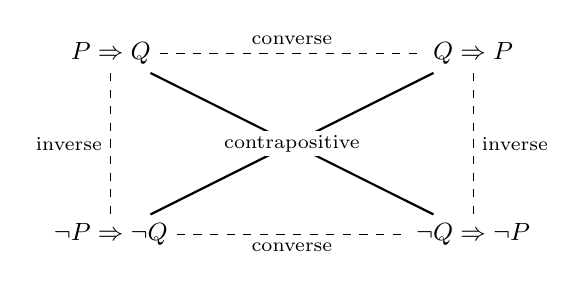
\begin{tikzpicture}[font=\small, every node/.style={inner sep=3pt}]
\node (a) at (0,2.3) {$P\Rightarrow Q$};
\node (b) at (4.6,2.3) {$Q\Rightarrow P$};
\node (c) at (0,0) {$\neg P\Rightarrow\neg Q$};
\node (d) at (4.6,0) {$\neg Q\Rightarrow\neg P$};
\draw[dashed, line width=0.4pt] (a) -- node[above, font=\scriptsize] {converse} (b);
\draw[dashed, line width=0.4pt] (c) -- node[below, font=\scriptsize] {converse} (d);
\draw[dashed, line width=0.4pt] (a) -- node[left, font=\scriptsize] {inverse} (c);
\draw[dashed, line width=0.4pt] (b) -- node[right, font=\scriptsize] {inverse} (d);
\draw[line width=0.8pt] (a) -- (d);
\draw[line width=0.8pt] (b) -- (c);
\node[font=\scriptsize, fill=white, inner sep=1.5pt] at (2.3,1.15) {contrapositive};
\end{tikzpicture}}{The four conditionals formed from $P$ and $Q$. Statements joined by a solid diagonal are contrapositives of each other and always logically equivalent; statements joined by a dashed side are not equivalent in general.\label{fig:square}}
\end{figure}

Part (ii) of \cref{prop:implication-laws} is the basis of proof by contrapositive (\cref{sec:contradiction}), and part (iii) tells us how to negate a conditional: the denial of ``if $P$, then $Q$'' is ``$P$, and yet not $Q$''. It is \emph{not} ``if $P$, then not $Q$''. Part (iv) is used when a disjunction has to be proved: to show ``$P$ or $Q$'', it suffices to assume that $P$ fails and to show that $Q$ then holds. Part (v) justifies a familiar habit of proofs, in which several hypotheses are assumed one after another.

\subsection{The Biconditional}

\begin{definition}[Biconditional]
\label{def:biconditional}
The \term{biconditional} $P\Leftrightarrow Q$, read ``$P$ if and only if $Q$'', is true when $P$ and $Q$ have the same truth value, and false otherwise.
\end{definition}

The phrase ``if and only if'' is often abbreviated to \term{iff}; the phrases ``$P$ is necessary and sufficient for $Q$'' and ``$P$ is equivalent to $Q$'' mean the same. The name is explained by the next proposition: ``$P$ if $Q$'' is $Q\Rightarrow P$, and ``$P$ only if $Q$'' is $P\Rightarrow Q$.

\begin{proposition}
\label{prop:biconditional}
For all statements $P$ and $Q$, $P\Leftrightarrow Q\equiv(P\Rightarrow Q)\wedge(Q\Rightarrow P)$. Moreover, two formulas $A$ and $B$ are logically equivalent if and only if $A\Leftrightarrow B$ is a tautology.
\end{proposition}

\begin{proof}
The conjunction $(P\Rightarrow Q)\wedge(Q\Rightarrow P)$ is false exactly when one of the two conditionals is false, that is, when $P$ is true and $Q$ false, or $Q$ true and $P$ false. These are exactly the assignments in which $P$ and $Q$ have different truth values, which by \cref{def:biconditional} are the assignments in which $P\Leftrightarrow Q$ is false (compare columns three to five of \cref{tab:truth-implication}). For the second claim, $A\Leftrightarrow B$ is true under an assignment exactly when $A$ and $B$ have the same truth value under it; so it is true under every assignment exactly when $A\equiv B$.
\end{proof}

By \cref{prop:biconditional}, a theorem of the form ``$P$ if and only if $Q$'' contains two theorems, $P\Rightarrow Q$ and $Q\Rightarrow P$, and its proof usually has two parts, often labelled ``($\Rightarrow$)'' and ``($\Leftarrow$)''. The symbols $\Leftrightarrow$ and $\equiv$ must be kept apart: the first is a connective that builds a new formula, the second is a relation between two formulas that we assert about them.

To save parentheses we agree that $\neg$ binds most tightly, then $\wedge$ and $\vee$, and then $\Rightarrow$ and $\Leftrightarrow$; thus $P\wedge Q\Rightarrow R$ means $(P\wedge Q)\Rightarrow R$. Since $\wedge$ and $\vee$ are on the same level, a formula that combines them, such as $(P\wedge Q)\vee R$, always keeps its parentheses. A chain such as $P\Rightarrow Q\Rightarrow R$ is never written without parentheses, because the two readings differ. When $P$ and $R$ are false, $P\Rightarrow(Q\Rightarrow R)$ is true, since its hypothesis is false, whereas $(P\Rightarrow Q)\Rightarrow R$ is false, since its hypothesis $P\Rightarrow Q$ is true and its conclusion $R$ is false.

\section{Predicates and Quantifiers}
\label{sec:quantifiers}

The sentence ``$x>3$'' is not a statement, because its truth depends on $x$. Yet sentences of this kind are what mathematics is made of: ``$f$ is continuous at $a$'', ``$n$ is prime'', ``$x^2-5x+6=0$''. Logic handles them by treating the variable as a slot to be filled.

\subsection{Predicates}

\begin{definition}[Predicate]
\label{def:predicate}
A \term{predicate} on a set $S$ is a sentence $P(x)$ containing a variable $x$ such that, for each element $a$ of $S$, the sentence $P(a)$ obtained by substituting $a$ for $x$ is a statement. The set $S$ is the \term{domain} of the variable, and the set $\{x\in S: P(x)\}$ of the elements for which $P(x)$ is true is the \term{truth set} of $P$.
\end{definition}

Let $P(x)$ be ``$x>3$'' on the domain $\mathbb R$. Then $P(5)$ is a true statement and $P(1)$ a false one, and the truth set of $P$ is the interval $(3,\infty)$. Predicates may have several variables. ``$x<y$'' is a predicate $P(x,y)$ in two variables; $P(1,2)$ is true and $P(2,1)$ is false. The connectives of \cref{sec:statements} apply to predicates as well: if $P(x)$ is ``$x>3$'' and $Q(x)$ is ``$x<5$'', then $P(x)\wedge Q(x)$ is ``$3<x<5$'', whose truth set is the intersection $(3,5)$ of the truth sets of $P$ and $Q$. This is the literal form of the picture of \cref{fig:venn}.

Substituting a value is one way to turn a predicate into a statement. The other way, and the more important one, is to make a claim about \emph{all} values or about \emph{some} value of the variable.

\subsection{The Universal and Existential Quantifiers}

\begin{definition}[Quantifiers]
\label{def:quantifiers}
Let $P(x)$ be a predicate on a set $S$.
\begin{enumerate}
\item The statement $\forall x\in S,\ P(x)$, read ``for every $x$ in $S$, $P(x)$'', is true if $P(a)$ is true for every element $a$ of $S$, and false otherwise. The symbol $\forall$ is the \term{universal quantifier}.
\item The statement $\exists x\in S,\ P(x)$, read ``there exists an $x$ in $S$ such that $P(x)$'', is true if $P(a)$ is true for at least one element $a$ of $S$, and false otherwise. The symbol $\exists$ is the \term{existential quantifier}.
\end{enumerate}
\end{definition}

The comma after the quantifier separates it from the formula that it governs, its \term{scope}, which extends as far to the right as the parentheses allow. When the domain is clear from the context it is sometimes omitted, as in $\forall x,\ P(x)$.

For example, $\forall x\in\mathbb R,\ x^2\ge 0$ is true, $\forall x\in\mathbb R,\ x^2>0$ is false (it fails for $x=0$), $\exists x\in\mathbb R,\ x^2=2$ is true (take $x=\sqrt2$), and $\exists x\in\mathbb Q,\ x^2=2$ is false, as we prove in \cref{sec:contradiction}. The last two examples differ only in the domain, which shows that the domain is an essential part of a quantified statement.

Programmers may recognise the quantifiers as loops. If $S$ is a finite list, $\forall x\in S,\ P(x)$ is what a loop computes that runs through $S$, returns false as soon as it finds an element failing $P$, and returns true if it reaches the end. Likewise $\exists x\in S,\ P(x)$ is computed by a loop that returns true as soon as it finds an element satisfying $P$, and false if it reaches the end. Many languages provide these two loops as library functions, commonly named \code{all} and \code{any}. For a finite domain $S=\{a_1,\ldots,a_n\}$ the quantifiers are nothing but long conjunctions and disjunctions,
\[
\forall x\in S,\ P(x)\equiv P(a_1)\wedge\cdots\wedge P(a_n),
\qquad
\exists x\in S,\ P(x)\equiv P(a_1)\vee\cdots\vee P(a_n).
\]
The quantifiers are indispensable because domains such as $\mathbb N$ and $\mathbb R$ are infinite: the loop never ends, and the truth of a universal statement over an infinite domain can be established only by an argument that applies to every element at once. Producing such arguments is what the rest of this chapter is about.

Two further remarks complete the picture. First, the variable of a quantified statement is a placeholder, like the index of a sum or the variable of integration: $\forall x\in S,\ P(x)$ and $\forall t\in S,\ P(t)$ are the same statement. Such a variable is said to be \term{bound} by the quantifier, while a variable that is not bound, like $x$ in the predicate ``$x>3$'', is \term{free}. A formula with no free variables is a statement. Second, when $S$ is empty, $\forall x\in S,\ P(x)$ is true, because no element of $S$ fails $P$, and $\exists x\in S,\ P(x)$ is false, because no element of $S$ satisfies it. This agrees with the vacuous truth of conditionals, and also with the two loops described above: on an empty list, the loop for $\forall$ reaches the end at once and returns true, and the loop for $\exists$ returns false.

A quantifier is frequently restricted to the elements satisfying a condition, as in ``for every $x>0$'' or ``there is an even $n$ such that \ldots''. Expressed with the connectives, the two restricted forms read
\begin{equation}
\forall x\in S,\ \bigl(Q(x)\Rightarrow P(x)\bigr)
\qquad\text{and}\qquad
\exists x\in S,\ \bigl(Q(x)\wedge P(x)\bigr),
\label{eq:restricted}
\end{equation}
and we abbreviate them as $\forall x\in S$ with $Q(x),\ P(x)$, or, when $Q$ is an inequality, as $\forall x>0,\ P(x)$ and $\exists x>0,\ P(x)$. The universal form uses $\Rightarrow$ and the existential form uses $\wedge$, and the difference matters. Writing $\forall x\,(Q(x)\wedge P(x))$ would claim that every $x$ satisfies $Q$, and writing $\exists x\,(Q(x)\Rightarrow P(x))$ would be satisfied by any $x$ that fails $Q$; neither is what is meant.

\subsection{Negating Quantified Statements}

To say that not every element has a property is to say that some element lacks it. This observation is used in almost every proof that involves a negation.

\begin{theorem}[Negation of quantifiers]
\label{thm:quantifier-negation}
For every predicate $P(x)$ on a set $S$,
\[
\neg\bigl(\forall x\in S,\ P(x)\bigr)\equiv\exists x\in S,\ \neg P(x)
\qquad\text{and}\qquad
\neg\bigl(\exists x\in S,\ P(x)\bigr)\equiv\forall x\in S,\ \neg P(x).
\]
\end{theorem}

Here $\equiv$ means that the two sides have the same truth value for every set $S$ and every predicate $P$, which extends \cref{def:equivalence} to quantified formulas.

\begin{proof}
By \cref{def:quantifiers}, $\forall x\in S,\ P(x)$ is false exactly when $P(a)$ is false for at least one element $a$ of $S$, that is, when $\neg P(a)$ is true for at least one $a\in S$, which is the condition for $\exists x\in S,\ \neg P(x)$ to be true. Hence the left side of the first equivalence is true exactly when the right side is.

For the second equivalence, $\exists x\in S,\ P(x)$ is false exactly when there is no element $a$ of $S$ for which $P(a)$ is true, that is, when $P(a)$ is false, and $\neg P(a)$ true, for every $a\in S$; this is the condition for $\forall x\in S,\ \neg P(x)$ to be true.
\end{proof}

For a finite domain, \cref{thm:quantifier-negation} is just De Morgan's law applied to the long conjunction and disjunction displayed above. In ordinary language the theorem guards against a common slip: the negation of ``every student passed the examination'' is ``some student did not pass'', and not ``every student failed''.

Combining \cref{thm:quantifier-negation} with De Morgan's laws and \cref{prop:implication-laws}\,(iii), any quantified statement can be negated by a mechanical procedure: move the negation inwards step by step, exchanging $\forall$ and $\exists$ each time it passes a quantifier, exchanging $\wedge$ and $\vee$ each time it passes one of them, and replacing $\neg(P\Rightarrow Q)$ by $P\wedge\neg Q$. As an example, consider the true statement that every positive real number has a real square root,
\[
\forall x\in\mathbb R,\ \bigl(x>0\Rightarrow\exists y\in\mathbb R,\ y^2=x\bigr).
\]
Its negation is transformed as follows:
\begin{align*}
\neg\Bigl(\forall x\in\mathbb R,\ \bigl(x>0\Rightarrow\exists y\in\mathbb R,\ y^2=x\bigr)\Bigr)
&\equiv\exists x\in\mathbb R,\ \neg\bigl(x>0\Rightarrow\exists y\in\mathbb R,\ y^2=x\bigr)\\
&\equiv\exists x\in\mathbb R,\ \bigl(x>0\wedge\neg\,\exists y\in\mathbb R,\ y^2=x\bigr)\\
&\equiv\exists x\in\mathbb R,\ \bigl(x>0\wedge\forall y\in\mathbb R,\ y^2\ne x\bigr).
\end{align*}
The result reads: there is a positive real number that is not the square of any real number. Exactly one of the original statement and its negation is true; in this case it is the original. Replacing $\mathbb R$ by $\mathbb Q$ in both places reverses this: the negation becomes true, with $x=2$ as a witness, because no rational number has the square $2$ (we prove this in \cref{sec:contradiction}).

\subsection{Several Quantifiers}

Statements with several variables carry several quantifiers. Quantifiers of the same kind can be exchanged freely, but quantifiers of different kinds cannot.

\begin{proposition}
\label{prop:quantifier-order}
Let $P(x,y)$ be a predicate with $x$ ranging over a set $X$ and $y$ over a set $Y$.
\begin{enumerate}
\item $\forall x\in X,\ \forall y\in Y,\ P(x,y)\equiv\forall y\in Y,\ \forall x\in X,\ P(x,y)$, and the same holds with $\exists$ in place of $\forall$.
\item If $\exists y\in Y,\ \forall x\in X,\ P(x,y)$ is true, then $\forall x\in X,\ \exists y\in Y,\ P(x,y)$ is true.
\item The converse of (ii) is false in general.
\end{enumerate}
\end{proposition}

\begin{proof}
(i) Both universal statements say that $P(a,b)$ is true for every pair $(a,b)$ with $a\in X$ and $b\in Y$, and both existential statements say that $P(a,b)$ is true for at least one such pair.

(ii) Suppose that $\exists y\in Y,\ \forall x\in X,\ P(x,y)$ is true, and choose an element $b\in Y$ such that $P(x,b)$ holds for every $x\in X$. Let $a\in X$ be arbitrary. Then $P(a,b)$ holds, so there is an element of $Y$, namely $b$, for which $P(a,y)$ holds; that is, $\exists y\in Y,\ P(a,y)$ is true. Since $a$ was arbitrary, $\forall x\in X,\ \exists y\in Y,\ P(x,y)$ is true.

(iii) Take $X=Y=\mathbb Z$ and let $P(x,y)$ be ``$y>x$''. The statement $\forall x\in\mathbb Z,\ \exists y\in\mathbb Z,\ y>x$ is true: for any integer $x$ the integer $y=x+1$ is larger. The statement $\exists y\in\mathbb Z,\ \forall x\in\mathbb Z,\ y>x$ is false: it claims an integer $y$ larger than every integer, in particular larger than itself, and $y>y$ is false.
\end{proof}

The difference between the two orders is the difference between ``everyone has someone to talk to'' and ``there is someone whom everyone talks to''. In $\forall x,\ \exists y,\ P(x,y)$ the element $y$ is chosen \emph{after} $x$ and may depend on it, as $y=x+1$ depends on $x$ in the proof of (iii). In $\exists y,\ \forall x,\ P(x,y)$ a single $y$ must serve for all $x$ at once. \Cref{fig:quantifier-grid} shows both situations for a predicate on a small finite domain, where the truth of $P(x,y)$ for every pair can be drawn as a grid of dots.

\begin{figure}
\tikzset{
  gridpanel/.pic={
    \foreach \i in {1,...,5} {
      \node[font=\scriptsize] at (\i*0.46,0.05) {$\i$};
      \node[font=\scriptsize] at (0.12,\i*0.46+0.1) {$\i$};}
    \node[font=\scriptsize] at (1.38,-0.3) {$x$};
    \node[font=\scriptsize] at (-0.2,1.48) {$y$};
    \foreach \i in {1,...,5} \foreach \j in {1,...,5}
      \draw[line width=0.3pt] (\i*0.46,\j*0.46+0.1) circle (0.055);},
  dot/.style={fill=black}}
\newcommand\gridpt[2]{\fill (#1*0.46,#2*0.46+0.1) circle (0.075);}
\sdpanel{A}{\begin{tikzpicture}
\pic {gridpanel};
\gridpt12 \gridpt14 \gridpt24 \gridpt31 \gridpt33 \gridpt45 \gridpt53 \gridpt52
\end{tikzpicture}}\hfill
\sdpanel{B}{\begin{tikzpicture}
\fill[sdfill] (0.28,3*0.46+0.1-0.17) rectangle (5*0.46+0.18,3*0.46+0.1+0.17);
\pic {gridpanel};
\gridpt13 \gridpt23 \gridpt33 \gridpt43 \gridpt53 \gridpt11 \gridpt45 \gridpt24
\end{tikzpicture}}\hfill
\sdpanel{C}{\begin{tikzpicture}
\fill[sdfill] (4*0.46-0.17,0.38) rectangle (4*0.46+0.17,5*0.46+0.28);
\pic {gridpanel};
\gridpt12 \gridpt15 \gridpt24 \gridpt31 \gridpt33 \gridpt53 \gridpt55
\end{tikzpicture}}
\caption{The order of quantifiers. Each grid shows a predicate $P(x,y)$ on $x,y\in\{1,\ldots,5\}$; a filled dot marks a pair for which $P(x,y)$ is true. (A) Every column contains a dot, so $\forall x,\ \exists y,\ P(x,y)$ is true, but no row is full, so $\exists y,\ \forall x,\ P(x,y)$ is false. (B) The shaded row $y=3$ is full, so $\exists y,\ \forall x,\ P(x,y)$ is true, and then every column contains a dot, as \cref{prop:quantifier-order}\,(ii) asserts. (C) The shaded column $x=4$ is empty, so $\forall x,\ \exists y,\ P(x,y)$ is false, and so is $\exists y,\ \forall x,\ P(x,y)$.}
\label{fig:quantifier-grid}
\end{figure}

A statement with alternating quantifiers can also be read as a game between two players. One player, the sceptic, chooses the values of the universally quantified variables and tries to make the final formula false; the other, the prover, chooses the values of the existentially quantified variables and tries to make it true. The players move in the order in which the quantifiers are written, and each sees the moves already made. The statement is true exactly when the prover has a strategy that wins against every sequence of moves by the sceptic. In $\forall x,\ \exists y,\ y>x$ the sceptic names an integer $x$ and the prover answers $x+1$, and the prover always wins. In $\exists y,\ \forall x,\ y>x$ the prover must commit to $y$ first, and the sceptic answers with $x=y$.

\subsection{Unique Existence}

Often we want to say not only that an object exists, but also that there is only one.

\begin{definition}[Unique existence]
\label{def:unique-existence}
The statement $\exists!\,x\in S,\ P(x)$, read ``there exists a unique $x$ in $S$ such that $P(x)$'', means
\[
\exists x\in S,\ \Bigl(P(x)\wedge\forall y\in S,\ \bigl(P(y)\Rightarrow y=x\bigr)\Bigr).
\]
\end{definition}

The definition says that some $x$ satisfies $P$, and that every $y$ satisfying $P$ is that same $x$. For example, $\exists!\,x\in\mathbb R,\ 2x+1=5$ is true, the unique solution being $x=2$, while $\exists!\,x\in\mathbb R,\ x^2=4$ is false, because both $2$ and $-2$ are solutions, although $\exists x\in\mathbb R,\ x^2=4$ is true. An equivalent formulation separates the two claims: $\exists!\,x\in S,\ P(x)$ holds if and only if $\exists x\in S,\ P(x)$ holds (\term{existence}) and
\[
\forall x\in S,\ \forall y\in S,\ \bigl(P(x)\wedge P(y)\Rightarrow x=y\bigr)
\]
holds (\term{uniqueness}, or ``at most one''). Proofs of unique existence almost always establish the two parts separately (\cref{sec:existence}).

\subsection{From English to Symbols}

Mathematical writing seldom uses the symbols $\forall$ and $\exists$ in running text, and it often leaves quantifiers implicit. The identity ``$x^2-1=(x-1)(x+1)$'' is a claim about every real number $x$; ``a differentiable function is continuous'' is a claim about every function; ``$\sqrt2$ is irrational'' is the claim that no pair of integers has the ratio $\sqrt2$. Before trying to prove a statement, it pays to write it with all its quantifiers explicit, because the form of the statement determines the form of the proof. \Cref{tab:translations} gives some examples.

\begin{table}
\sdfloat{%
\begin{sdtable}{colspec={Q[l,wd=4.6cm]Q[l]}, row{1}={font=\small\bfseries}}
\toprule
English & Symbols \\
\midrule
Every square of a real number is nonnegative. & $\forall x\in\mathbb R,\ x^2\ge 0$ \\
Some integer is even and prime. & $\exists n\in\mathbb Z,\ (n\text{ even}\wedge n\text{ prime})$ \\
No integer is both even and odd. & $\forall n\in\mathbb Z,\ \neg(n\text{ even}\wedge n\text{ odd})$ \\
Only zero equals its own negative. & $\forall x\in\mathbb R,\ (x=-x\Rightarrow x=0)$ \\
There is a smallest natural number. & $\exists m\in\mathbb N,\ \forall n\in\mathbb N,\ m\le n$ \\
There is no largest integer. & $\forall m\in\mathbb Z,\ \exists n\in\mathbb Z,\ n>m$ \\
Between two different real numbers there is a rational number. & $\forall x,y\in\mathbb R,\ \bigl(x<y\Rightarrow\exists q\in\mathbb Q,\ x<q<y\bigr)$ \\
\bottomrule
\end{sdtable}}{Statements in English and in symbols. The sentence ``there is no largest integer'' is translated directly into its equivalent form given by \cref{thm:quantifier-negation}.\label{tab:translations}}
\end{table}

Two of the rows deserve comment. ``No integer is both even and odd'' is literally $\neg\,\exists n\in\mathbb Z,\ (n\text{ even}\wedge n\text{ odd})$, which \cref{thm:quantifier-negation} turns into the universal form in the table. ``Only zero equals its own negative'' does not say that zero equals its own negative; it says that nothing else does. As with ``only if'', the word ``only'' points from the condition to the object.

\subsection{Reading the Definition of a Limit}

The best-known statement with alternating quantifiers in elementary mathematics is the definition of a limit, which most readers will have met in a calculus course. For a real number $t$ we write $|t|$ for its absolute value, which is $t$ if $t\ge 0$ and $-t$ if $t<0$; the number $|x-a|$ is the distance between $x$ and $a$ on the real line. The properties of the absolute value are proved in \cref{sec:direct}.

\begin{definition}[Limit of a function]
\label{def:limit}
Let $f$ be a real function defined at every point of an open interval containing the real number $a$, except possibly at $a$ itself, and let $L$ be a real number. We say that $f(x)$ \term{tends to} $L$ as $x$ tends to $a$, and write $\lim_{x\to a}f(x)=L$, if
\begin{equation}
\forall\varepsilon>0,\ \exists\delta>0,\ \forall x,\ \bigl(0<|x-a|<\delta\Rightarrow|f(x)-L|<\varepsilon\bigr),
\label{eq:limit}
\end{equation}
where $x$ ranges over the points at which $f$ is defined.
\end{definition}

This definition is discussed at length in rigorous calculus texts~\cite{spivak2008calculus}. Read as a game, it says the following. The sceptic chooses a tolerance $\varepsilon>0$, as small as desired. The prover answers with a distance $\delta>0$. The sceptic then picks any $x$ within distance $\delta$ of $a$, other than $a$ itself, and the prover wins if $f(x)$ lies within $\varepsilon$ of $L$. The limit is $L$ if the prover can always win, however small the tolerance. \Cref{fig:epsilon-delta} shows one round of the game. Three features of \eqref{eq:limit} deserve attention. First, $\delta$ comes after $\varepsilon$ and may depend on it; typically a smaller $\varepsilon$ requires a smaller $\delta$. Second, the condition $0<|x-a|$ excludes $x=a$, so the value $f(a)$, if it exists at all, has no influence on the limit. Third, the inequalities are about distances: $|f(x)-L|<\varepsilon$ says that $L-\varepsilon<f(x)<L+\varepsilon$.

\begin{figure}
\sdfloat{%
\begin{tikzpicture}
\begin{axis}[sdplot, width=6.4cm, height=5.0cm, xmin=0, xmax=3.6, ymin=0, ymax=7.5,
  xtick={1.4,2,2.6}, xticklabels={$a-\delta$,$a$,$a+\delta$},
  ytick={1.5,3,4.5}, yticklabels={$L-\varepsilon$,$L$,$L+\varepsilon$},
  xlabel={$x$}, ylabel={$f(x)$}, clip=false]
\fill[sdfill] (axis cs:0,1.5) rectangle (axis cs:3.6,4.5);
\draw[black!55, dashed, line width=0.4pt] (axis cs:1.4,0) -- (axis cs:1.4,7.5);
\draw[black!55, dashed, line width=0.4pt] (axis cs:2.6,0) -- (axis cs:2.6,7.5);
\addplot[black, line width=0.6pt, domain=0:3.6, samples=120] {1+x^2/2};
\addplot[black, line width=1.8pt, domain=1.4:2.6, samples=60] {1+x^2/2};
\draw[black, line width=0.6pt, fill=white] (axis cs:2,3) circle (2.2pt);
\end{axis}
\end{tikzpicture}}{One round of the limit game for $f(x)=1+x^2/2$, $a=2$ and $L=3$. For the tolerance $\varepsilon=1.5$ (shaded band) the distance $\delta=0.6$ works: over the interval between the dashed lines the graph (thick) stays inside the band. The open circle indicates that the value at $a$ plays no role.\label{fig:epsilon-delta}}
\end{figure}

To prove a limit, therefore, one must give a rule that produces a suitable $\delta$ for each $\varepsilon$. The following proposition is the simplest example; its proof shows the typical shape of a proof of an ``$\forall\,\exists$'' statement.

\begin{proposition}
\label{prop:limit-example}
$\lim_{x\to 2}(3x+1)=7$.
\end{proposition}

Before writing the proof, we work backwards to find $\delta$. We want $|(3x+1)-7|<\varepsilon$, and $|(3x+1)-7|=|3x-6|=3|x-2|$. So it suffices that $|x-2|<\varepsilon/3$, which suggests $\delta=\varepsilon/3$. This scratch work is not part of the proof; the proof itself runs forwards.

\begin{proof}
Let $\varepsilon>0$ be arbitrary, and put $\delta\coloneqq\varepsilon/3$, which is positive. Let $x$ be a real number with $0<|x-2|<\delta$. Then
\[
|(3x+1)-7|=3|x-2|<3\delta=\varepsilon .
\]
Since $\varepsilon$ was arbitrary, \eqref{eq:limit} holds with $f(x)=3x+1$, $a=2$ and $L=7$.
\end{proof}

The symbol $\coloneqq$ in the proof means ``is defined to be''; it introduces a new name rather than asserting an equation. The proof follows the quantifiers of \eqref{eq:limit} from left to right: ``let $\varepsilon>0$ be arbitrary'' answers $\forall\varepsilon>0$, ``put $\delta\coloneqq\varepsilon/3$'' answers $\exists\delta>0$, and ``let $x$ be a real number with \ldots'' answers $\forall x$ together with the hypothesis of the conditional.

To show that a limit is \emph{not} $L$, we negate \eqref{eq:limit} by the procedure described above:
\begin{equation}
\exists\varepsilon>0,\ \forall\delta>0,\ \exists x,\ \bigl(0<|x-a|<\delta\wedge|f(x)-L|\ge\varepsilon\bigr).
\label{eq:not-limit}
\end{equation}
In the language of the game, the sceptic has a tolerance that defeats every $\delta$ the prover might choose.

\begin{proposition}
\label{prop:step-limit}
Let $H(x)=0$ for $x<0$ and $H(x)=1$ for $x\ge 0$. Then $\lim_{x\to 0}H(x)=1$ is false.
\end{proposition}

\begin{proof}
We verify \eqref{eq:not-limit} with $a=0$ and $L=1$. Take $\varepsilon\coloneqq 1/2$. Let $\delta>0$ be arbitrary and put $x\coloneqq-\delta/2$. Then $0<|x|=\delta/2<\delta$, and since $x<0$ we have $|H(x)-1|=|0-1|=1\ge\varepsilon$.
\end{proof}

The same argument with $x=\delta/2$ shows that $\lim_{x\to 0}H(x)=0$ is false as well. In \cref{sec:existence} we show that the limit is not any number at all.

\section{The Anatomy of a Proof}
\label{sec:anatomy}

With the language in place we can say what a proof is. This section describes the kinds of statements that make up a mathematical text, the rules by which one statement may be inferred from others, and the conventions by which proofs are written and read.

\subsection{Definitions, Axioms, and Theorems}

A mathematical text consists mainly of three kinds of statements.

A \term{definition} gives a precise meaning to a word or a symbol. ``An integer $n$ is \emph{even} if $n=2k$ for some integer $k$'' is a definition. Once it is made, ``even'' means exactly this and nothing more, whatever associations the word may have in everyday language. A definition is always an ``if and only if'', even when, by long-standing custom, it is written with ``if'': an integer that is not of the form $2k$ is not even. In this book the word being defined is set in italics.

An \term{axiom} is a statement that is accepted without proof as a starting point. Every chain of reasoning must start somewhere, and the axioms are where it starts. In this chapter the axioms are the familiar properties of numbers, which we now list. They are taken for granted here and examined in \cref{ch:numbers}, where the real numbers are characterised by a short list of axioms and the other facts are derived from them.

\begin{assumption}[Arithmetic and order of numbers]
\label{asm:numbers}
We use without proof the following properties of the number systems $\mathbb N$, $\mathbb Z$, $\mathbb Q$ and $\mathbb R$, each of which contains the one before it.
\begin{enumerate}
\item The usual laws of addition, subtraction, multiplication and of division by nonzero numbers hold, together with the usual rules for inequalities; for instance, $a<b$ implies $a+c<b+c$, and $a<b$ and $c>0$ imply $ac<bc$.
\item Sums, differences and products of integers are integers. The natural numbers are the integers $n\ge 0$.
\item There is no integer $n$ with $0<n<1$. Consequently, if $m$ and $n$ are integers with $m<n$, then $m+1\le n$, since $n-m$ is a positive integer.
\item For every real number $x\ge 0$ there is exactly one real number $y\ge 0$ with $y^2=x$; it is denoted $\sqrt x$.
\end{enumerate}
\end{assumption}

A \term{theorem} is a statement that has been proved. In this book theorems come in four kinds, which differ only in their role. A \term{theorem}, in the narrow sense, is a result of central importance. A \term{proposition} is a result of lesser importance, often a building block or an example of a technique. A \term{lemma} is a result proved mainly as a step towards something else; some lemmas, once proved, turn out to be used again and again. A \term{corollary} is a result that follows quickly from a preceding theorem. All four kinds, together with definitions and assumptions, are numbered in a single sequence within each chapter, so that, for instance, \cref{def:equivalence} is followed by \cref{thm:de-morgan} and \cref{prop:laws}, and a reference to any of them can be found by its number alone. The end of every proof is marked by the symbol~\qedsymbol, set at the right margin. A proof headed ``Proof (sketch)'' gives only the main line of an argument whose details are found in the cited source or later in the book, and it ends with the symbol~\sketchsymbol{} instead.

The statements of a theory depend on one another: a theorem is proved from axioms, definitions and earlier results, and is then used in later proofs. \Cref{fig:dependency} shows the typical pattern. Because every proof refers only to results established before it, the whole structure rests, in the end, on the axioms and the definitions alone. This is the sense in which mathematical knowledge is cumulative, and it is also why a single error in a lemma can invalidate everything above it.

\begin{figure}
\sdfloat{%
\begin{tikzpicture}[font=\scriptsize,
  box/.style={draw, line width=0.4pt, minimum width=1.55cm, minimum height=0.52cm, inner sep=2pt},
  arr/.style={-{Latex[length=1.5mm]}, line width=0.4pt}]
\node[box, fill=sdfill] (d) at (0.1,0) {Definitions};
\node[box, fill=sdfill] (a) at (2.2,0) {Axioms};
\node[box] (l1) at (-0.85,1.15) {Lemma};
\node[box] (l2) at (3.15,1.15) {Lemma};
\node[box] (p) at (1.15,1.15) {Proposition};
\node[box, line width=0.8pt] (t) at (1.15,2.3) {Theorem};
\node[box] (c1) at (0,3.45) {Corollary};
\node[box] (c2) at (2.3,3.45) {Corollary};
\draw[arr] (d) -- (l1); \draw[arr] (d) -- (p); \draw[arr] (a) -- (p); \draw[arr] (a) -- (l2);
\draw[arr] (l1) -- (t); \draw[arr] (p) -- (t); \draw[arr] (l2) -- (t);
\draw[arr] (t) -- (c1); \draw[arr] (t) -- (c2);
\end{tikzpicture}}{The structure of a mathematical theory. An arrow from one statement to another means that the first is used in the proof of the second. Everything rests on the definitions and axioms (shaded).\label{fig:dependency}}
\end{figure}

\subsection{What a Proof Is}

A \term{proof} of a statement is a finite sequence of statements, the last of which is the statement to be proved, such that each statement in the sequence is
\begin{itemize}
\item an axiom, a hypothesis of the theorem, or a previously proved result,
\item the unfolding of a definition, or
\item a consequence of earlier statements in the sequence by a valid rule of inference.
\end{itemize}
A rule of inference is \term{valid} if it can never lead from true statements to a false one. The rules that we use are justified by tautologies, as the next proposition shows~\cite{enderton2001}.

\begin{proposition}[Rules of inference]
\label{prop:inference}
For all statements $P$, $Q$ and $R$ the following formulas are tautologies.
\begin{enumerate}
\item Modus ponens: $\bigl(P\wedge(P\Rightarrow Q)\bigr)\Rightarrow Q$.
\item Modus tollens: $\bigl(\neg Q\wedge(P\Rightarrow Q)\bigr)\Rightarrow\neg P$.
\item Chaining: $\bigl((P\Rightarrow Q)\wedge(Q\Rightarrow R)\bigr)\Rightarrow(P\Rightarrow R)$.
\item Cases: $\bigl((P\Rightarrow R)\wedge(Q\Rightarrow R)\bigr)\Rightarrow\bigl((P\vee Q)\Rightarrow R\bigr)$.
\item Contradiction: $\bigl(\neg P\Rightarrow(R\wedge\neg R)\bigr)\Rightarrow P$.
\end{enumerate}
\end{proposition}

Instead of writing out truth tables, we use a shortcut that is itself an argument by contradiction (\cref{sec:contradiction}). A conditional is false only when its hypothesis is true and its conclusion is false; so to show that a conditional is a tautology, we suppose that some assignment makes the hypothesis true and the conclusion false, and we show that no such assignment exists.

\begin{proof}
(i) Suppose that an assignment makes $Q$ false and both $P$ and $P\Rightarrow Q$ true. With $P$ true and $Q$ false, $P\Rightarrow Q$ is false, which is impossible.

(ii) By \cref{prop:implication-laws}\,(ii), $P\Rightarrow Q\equiv\neg Q\Rightarrow\neg P$, so (ii) is (i) applied to $\neg Q$ and $\neg P$.

(iii) Suppose that an assignment makes $P\Rightarrow R$ false, that is, $P$ true and $R$ false, while $P\Rightarrow Q$ and $Q\Rightarrow R$ are true. Since $P$ is true and $P\Rightarrow Q$ is true, $Q$ is true; since $Q$ is true and $Q\Rightarrow R$ is true, $R$ is true. This contradicts the assumption that $R$ is false.

(iv) Suppose that an assignment makes $P\vee Q$ true and $R$ false, while $P\Rightarrow R$ and $Q\Rightarrow R$ are true. As $R$ is false and $P\Rightarrow R$ is true, $P$ must be false; likewise $Q$ must be false. Then $P\vee Q$ is false, a contradiction.

(v) Suppose that an assignment makes $P$ false and $\neg P\Rightarrow(R\wedge\neg R)$ true. Then $\neg P$ is true, so $R\wedge\neg R$ is true, which is impossible by \cref{prop:laws}\,(vii).
\end{proof}

Each rule corresponds to a way of reasoning. Modus ponens is the basic step of every proof: we know $P$, we know that $P$ implies $Q$, and so we know $Q$. Chaining allows a long argument to be assembled from short steps. The rule of cases is the basis of proof by cases (\cref{sec:direct}), modus tollens and the contrapositive are the basis of proof by contrapositive, and the last rule is the basis of proof by contradiction (\cref{sec:contradiction}).

Two further rules concern quantifiers, and they are used in almost every proof in this book.
\begin{itemize}
\item To prove $\forall x\in S,\ P(x)$, let $x$ be an \emph{arbitrary} element of $S$, about which nothing is assumed except that it belongs to $S$, and prove $P(x)$. Since the argument used no property of $x$ beyond membership in $S$, it applies equally to every element of $S$. The step ``let $a\in X$ be arbitrary'' in the proof of \cref{prop:quantifier-order}\,(ii) and the first line of the proof of \cref{prop:limit-example} are of this kind.
\item To prove $\exists x\in S,\ P(x)$, it suffices to exhibit one element $a$ of $S$ and prove $P(a)$. Conversely, when $\exists x\in S,\ P(x)$ is known, we may give a name to one such element and use it, as long as we assume nothing about it except that it lies in $S$ and satisfies $P$.
\end{itemize}

Proofs in mathematical texts, including this one, are written in prose rather than as numbered sequences of statements, and they omit steps that a reader with the necessary background can supply. The standard is this: a proof is complete if every competent reader can fill in the omitted steps without new ideas. What counts as a routine step depends on the reader, and in this chapter we omit very little. Formal proofs, in which no step at all is omitted, are a subject of their own; the note at the end of this section describes them briefly.

\subsection{Finding the Hypothesis and the Conclusion}

The first step towards a proof is to identify exactly what is assumed and what must be shown. Most theorems can be brought to the form
\[
\forall x\in S,\ \bigl(H(x)\Rightarrow C(x)\bigr),
\]
where $H(x)$ is the hypothesis and $C(x)$ the conclusion, possibly after expanding hidden quantifiers. ``The sum of two odd integers is even'' becomes: for all integers $m$ and $n$, if $m$ and $n$ are odd, then $m+n$ is even. ``A differentiable function is continuous'' becomes: for every function $f$ and every point $a$, if $f$ is differentiable at $a$, then $f$ is continuous at $a$. After this translation, the general rules dictate the first lines of the proof: let $x\in S$ be arbitrary, assume $H(x)$, and work towards $C(x)$.

During a proof it helps to keep two lists in mind: the \term{givens}, which are the facts available at the moment, and the \term{goal}, which is the statement that remains to be proved~\cite{velleman2019}. Each step of the proof either adds to the givens or replaces the goal by a simpler one. \Cref{tab:givens-goal} shows the lists during the proof of the following proposition, which is the claim \eqref{eq:n-greater-two} of \cref{sec:implication}, now for real numbers.

\begin{proposition}
\label{prop:x-greater-two}
For every real number $x$, if $x>2$, then $x^2>4$.
\end{proposition}

\begin{proof}
Let $x$ be a real number with $x>2$. Then $x>0$, and multiplying the inequality $x>2$ by the positive number $x$ gives $x^2>2x$. Multiplying $x>2$ by $2$ gives $2x>4$. Hence $x^2>2x>4$.
\end{proof}

\begin{table}
\sdfloat{%
\begin{sdtable}{colspec={Q[l,wd=2.9cm]Q[l,wd=3.0cm]Q[l,wd=3.9cm]}, row{1}={font=\small\bfseries}}
\toprule
Step & New givens & Goal \\
\midrule
start & none & $\forall x\in\mathbb R,\ (x>2\Rightarrow x^2>4)$ \\
let $x\in\mathbb R$ be arbitrary & $x\in\mathbb R$ & $x>2\Rightarrow x^2>4$ \\
assume the hypothesis & $x>2$ & $x^2>4$ \\
derive consequences & $x>0$, $x^2>2x$, $2x>4$ & $x^2>4$ \\
chain the inequalities & $x^2>4$ & reached \\
\bottomrule
\end{sdtable}}{Givens and goal during the proof of \cref{prop:x-greater-two}. Each row lists the givens added at that step; the earlier givens remain available. The steps ``let'' and ``assume'' are dictated by the form of the statement; only the derivation of consequences requires an idea.\label{tab:givens-goal}}
\end{table}

The table shows how little of a typical proof requires an idea. Introducing $x$ and assuming the hypothesis are dictated by the logical form of the statement; only the step ``multiply by $x$'' needs insight. As statements grow more complex, the form dictates more and more of the proof, and recognising the form is a large part of the skill of proving theorems. P\'olya's classic book~\cite{polya1945} discusses the other part, finding the ideas, at length.

\subsection{The Language of Proofs}

Proofs use a small vocabulary of set phrases, each with a precise logical role.
\begin{itemize}
\item ``Let $x$ be \ldots'' introduces an arbitrary element, in preparation for proving a universal statement. ``Suppose'' or ``assume'' introduces a hypothesis, which remains available until the end of the argument that it opens.
\item ``Then'', ``hence'', ``therefore'', ``so'' and ``it follows that'' announce a statement derived from earlier ones. A good proof makes it clear which earlier statements are used.
\item ``We must show that'' or ``it suffices to show that'' announces a change of goal. ``It suffices to show $Q$'' means that $Q$ implies the current goal, so proving $Q$ completes the proof.
\item ``Without loss of generality'' announces that only one of several cases will be treated, because the others are the same up to renaming. It is legitimate only when the claim is symmetric, for example under the exchange of $x$ and $y$.
\item ``Choose'' or ``put'', often with $\coloneqq$, gives a name to a specific object, such as the $\delta$ in the proof of \cref{prop:limit-example}.
\end{itemize}

\begin{note}{Formal proofs and the limits of proof}
In mathematical logic a proof is a formal object: a finite sequence of formulas in a fixed symbolic language, each obtained from earlier ones by a fixed list of rules, so that checking a proof is a purely mechanical task~\cite{enderton2001}. Computer programs called proof assistants perform this check, and substantial parts of mathematics have been formalised with them: complete machine-checked proofs exist, for example, of the odd order theorem of finite group theory~\cite{gonthier2013oddorder} and of the Kepler conjecture on the densest packing of spheres~\cite{hales2017kepler}, and the library mathlib of the Lean proof assistant collects a large body of formalised mathematics~\cite{mathlib2020}. Two theorems of Kurt G\"odel describe what formal proof can and cannot do. The completeness theorem~\cite{godel1930} states that in first-order logic, the logic of the quantifiers $\forall$ and $\exists$ over a single domain, every statement that is true in every structure satisfying a set of axioms has a formal proof from those axioms. The incompleteness theorem~\cite{godel1931}, in the form later strengthened by Rosser~\cite{rosser1936}, states that any consistent system of axioms that can be listed by a computer program and that includes the basic arithmetic of $\mathbb N$ leaves some statements about natural numbers that it can neither prove nor refute. Neither theorem affects the everyday practice of mathematics described in this chapter, but together they show that ``true'' and ``provable'' are different notions.
\end{note}

\section{Direct Proof and Proof by Cases}
\label{sec:direct}

The simplest way to prove a conditional $P\Rightarrow Q$ is to assume $P$ and to deduce $Q$ by a chain of valid steps; by the rule of chaining in \cref{prop:inference}, the chain then establishes $P\Rightarrow Q$. Such a proof is called a \term{direct proof}. \Cref{prop:limit-example,prop:x-greater-two} were proved directly. This section develops the technique with examples from the arithmetic of integers, where the definitions are simple and the arguments are short, and then adds the technique of splitting a proof into cases.

\subsection{Even and Odd Integers}

\begin{definition}[Even, odd, divisibility]
\label{def:even-odd}
An integer $n$ is \term{even} if there is an integer $k$ with $n=2k$, and \term{odd} if there is an integer $k$ with $n=2k+1$. For integers $a$ and $b$, we say that $a$ \term{divides} $b$, or that $b$ is a \term{multiple} of $a$, and write $a\mid b$, if there is an integer $k$ with $b=ak$.
\end{definition}

Thus $0=2\cdot0$ is even, $-7=2\cdot(-4)+1$ is odd, $3\mid 12$, $-3\mid 12$ and $5\mid 0$. Every integer divides $0$, while $0$ divides only $0$. An integer is even exactly when $2$ divides it. The expression $a\mid b$ is a statement, true or false, while $a/b$ is a number; the two must not be confused.

The following proposition is intuitively obvious, and we shall use it throughout. We prove it in \cref{sec:induction}, once mathematical induction is available.

\begin{proposition}[Parity]
\label{prop:parity}
Every integer is either even or odd, and no integer is both.
\end{proposition}

The first direct proofs combine \cref{def:even-odd} with algebra. We prove two parts of the following proposition in detail; the others are proved in the same way.

\begin{proposition}
\label{prop:even-odd-arith}
Let $m$ and $n$ be integers.
\begin{enumerate}
\item If $m$ and $n$ are both even or both odd, then $m+n$ is even.
\item If one of $m$ and $n$ is even and the other is odd, then $m+n$ is odd.
\item If $m$ is even, then $mn$ is even.
\item If $m$ and $n$ are both odd, then $mn$ is odd.
\end{enumerate}
\end{proposition}

Let us think through part (i) for two odd integers before writing anything. The hypothesis says that $m$ and $n$ are odd; by \cref{def:even-odd} this means that $m=2k+1$ and $n=2l+1$ for some integers $k$ and $l$. The goal is that $m+n$ is even, which by the same definition means that $m+n=2j$ for some integer $j$. So we compute $m+n$ and look for a factor $2$. The only point that needs care is that $m$ and $n$ may be different numbers, so the two integers $k$ and $l$ must get different names.

\begin{proof}
(i) Suppose first that $m$ and $n$ are odd, say $m=2k+1$ and $n=2l+1$ with integers $k$ and $l$. Then
\[
m+n=2k+1+2l+1=2(k+l+1),
\]
and $k+l+1$ is an integer by \cref{asm:numbers}\,(ii), so $m+n$ is even. If $m=2k$ and $n=2l$ are both even, then $m+n=2(k+l)$ is even.

(iv) Suppose that $m=2k+1$ and $n=2l+1$ with integers $k$ and $l$. Then
\[
mn=(2k+1)(2l+1)=4kl+2k+2l+1=2(2kl+k+l)+1,
\]
and $2kl+k+l$ is an integer, so $mn$ is odd.

Parts (ii) and (iii) are proved in the same way: if $m=2k$ and $n=2l+1$, then $m+n=2(k+l)+1$; and if $m=2k$, then $mn=2(kn)$.
\end{proof}

Divisibility behaves in a similarly simple way.

\begin{proposition}
\label{prop:divisibility}
Let $a$, $b$ and $c$ be integers.
\begin{enumerate}
\item $a\mid a$ and $1\mid a$.
\item If $a\mid b$ and $b\mid c$, then $a\mid c$.
\item If $a\mid b$ and $a\mid c$, then $a\mid(bx+cy)$ for all integers $x$ and $y$.
\item If $a\mid b$ and $b\ne0$, then $|a|\le|b|$.
\end{enumerate}
\end{proposition}

\begin{proof}
(i) $a=a\cdot1$ and $a=1\cdot a$.

(ii) By hypothesis there are integers $k$ and $l$ with $b=ak$ and $c=bl$. Then $c=(ak)l=a(kl)$, and $kl$ is an integer, so $a\mid c$.

(iii) Write $b=ak$ and $c=al$ with integers $k$ and $l$, and let $x$ and $y$ be arbitrary integers. Then $bx+cy=akx+aly=a(kx+ly)$, and $kx+ly$ is an integer.

(iv) Write $b=ak$. Since $b\ne0$, also $k\ne0$, so $|k|\ge1$ by \cref{asm:numbers}\,(iii), and $|b|=|a|\,|k|\ge|a|$, using the rule $|xy|=|x|\,|y|$ proved below in \cref{prop:abs}.
\end{proof}

A slightly longer chain of steps gives a less obvious fact about odd squares. For instance, $3^2-1=8$, $5^2-1=24$ and $7^2-1=48$ are all multiples of $8$.

\begin{proposition}
\label{prop:odd-square}
If $n$ is an odd integer, then $8\mid n^2-1$.
\end{proposition}

\begin{proof}
Write $n=2k+1$ with an integer $k$. Then $n^2-1=4k^2+4k=4k(k+1)$. By \cref{prop:consecutive} below, $k(k+1)$ is even, say $k(k+1)=2j$ with an integer $j$. Hence $n^2-1=8j$.
\end{proof}

The proof used a fact, that the product of two consecutive integers is even, which we prove next by a new technique.

\subsection{Proof by Cases}

Sometimes a single argument does not cover all situations, but the situations can be divided into a few cases, each of which can be handled separately. If every situation falls into at least one of the cases, and the conclusion is proved in each case, then the conclusion holds in every situation. This is the rule of cases of \cref{prop:inference}\,(iv): from $P\Rightarrow R$ and $Q\Rightarrow R$ we may infer $(P\vee Q)\Rightarrow R$, and if $P\vee Q$ is known to hold, then $R$ follows. The cases need not exclude one another, but together they must be \term{exhaustive}: forgetting a case is the typical error of this technique.

\begin{proposition}
\label{prop:consecutive}
For every integer $n$, the product $n(n+1)$ is even.
\end{proposition}

\begin{proof}
By \cref{prop:parity}, $n$ is even or odd, and we treat the two cases separately.

\emph{Case 1: $n$ is even.} Then $n(n+1)$ is even by \cref{prop:even-odd-arith}\,(iii).

\emph{Case 2: $n$ is odd.} Then $n+1$ is even by \cref{prop:even-odd-arith}\,(i), since $1$ is odd. Hence $n(n+1)=(n+1)n$ is even by \cref{prop:even-odd-arith}\,(iii).

The two cases exhaust all integers, so $n(n+1)$ is even for every integer $n$.
\end{proof}

The absolute value is defined by cases, so it is natural that its properties are proved by cases. These properties are used constantly in analysis and in numerical computation, where errors are measured by absolute values~\cite{spivak2008calculus}.

\begin{proposition}[Absolute value]
\label{prop:abs}
For all real numbers $x$, $y$ and every real number $c\ge0$:
\begin{enumerate}
\item $|x|\ge0$, $|-x|=|x|$ and $-|x|\le x\le|x|$;
\item $|xy|=|x|\,|y|$;
\item $|x|\le c$ if and only if $-c\le x\le c$, and likewise with $<$ in both places;
\item the triangle inequality $|x+y|\le|x|+|y|$ holds.
\end{enumerate}
\end{proposition}

\begin{proof}
(i) If $x\ge0$, then $|x|=x\ge0$, $|-x|=-(-x)=x$ because $-x\le0$ (when $x=0$ both definitions give $0$), and $-|x|=-x\le0\le x=|x|$. If $x<0$, then $|x|=-x>0$, $|-x|=-x=|x|$ because $-x>0$, and $-|x|=x<0<-x=|x|$. In both cases all three claims hold.

(ii) We consider the signs of $x$ and $y$. If $x\ge0$ and $y\ge0$, then $xy\ge0$ and $|xy|=xy=|x|\,|y|$. If $x\ge0$ and $y<0$, then $xy\le0$ and $|xy|=-xy=x(-y)=|x|\,|y|$. The case $x<0\le y$ is the same with $x$ and $y$ exchanged, and if $x<0$ and $y<0$, then $xy>0$ and $|xy|=xy=(-x)(-y)=|x|\,|y|$.

(iii) Suppose $|x|\le c$. By (i), $x\le|x|\le c$ and $-c\le-|x|\le x$. Conversely, suppose $-c\le x\le c$. If $x\ge0$, then $|x|=x\le c$; if $x<0$, then $|x|=-x\le c$, because $-c\le x$. The version with strict inequalities is proved in the same way.

(iv) By (i), $-|x|\le x\le|x|$ and $-|y|\le y\le|y|$. Adding these inequalities gives
\[
-(|x|+|y|)\le x+y\le|x|+|y|,
\]
and (iii) with $c=|x|+|y|$ yields $|x+y|\le|x|+|y|$.
\end{proof}

The proof of (iv) shows that cases, once used to establish a basic fact such as (i) or (iii), need not be repeated: the triangle inequality follows from (i) and (iii) by a direct argument. A proof by cases on the signs of $x$, $y$ and $x+y$ is also possible but longer. \Cref{fig:triangle} illustrates the content of the triangle inequality on the real line: the distance from $0$ to $x+y$ is at most the length of the path from $0$ to $x$ and on to $x+y$, with equality when the two steps go in the same direction.

\begin{figure}
\tikzset{nl/.style={line width=0.4pt}, tstep/.style={-{Latex[length=1.6mm]}, line width=0.7pt}}
\sdpanel{A}{\begin{tikzpicture}[font=\scriptsize]
\draw[nl] (-0.3,0) -- (5.0,0);
\foreach \p/\l in {0/$0$, 2.2/$x$, 3.8/$x+y$} {\draw[nl] (\p,-0.07) -- (\p,0.07); \node[below] at (\p,-0.07) {\l};}
\draw[tstep] (0,0.32) -- node[above] {$|x|$} (2.2,0.32);
\draw[tstep] (2.2,0.32) -- node[above] {$|y|$} (3.8,0.32);
\draw[tstep, black!50] (0,1.55) -- node[above, black] {$|x+y|$} (3.8,1.55);
\end{tikzpicture}}\hfill
\sdpanel{B}{\begin{tikzpicture}[font=\scriptsize]
\draw[nl] (-0.3,0) -- (5.0,0);
\foreach \p/\l in {0/$0$, 3.6/$x$, 1.6/$x+y$} {\draw[nl] (\p,-0.07) -- (\p,0.07); \node[below] at (\p,-0.07) {\l};}
\draw[tstep] (0,0.32) -- node[above] {$|x|$} (3.6,0.32);
\draw[tstep] (3.6,0.95) -- node[above] {$|y|$} (1.6,0.95);
\draw[tstep, black!50] (0,1.55) -- node[above, black] {$|x+y|$} (1.6,1.55);
\end{tikzpicture}}
\caption{The triangle inequality on the real line. (A) When $x$ and $y$ have the same sign, the steps $x$ and $y$ point the same way and $|x+y|=|x|+|y|$. (B) When they have opposite signs, the second step turns back and $|x+y|<|x|+|y|$.}
\label{fig:triangle}
\end{figure}

A consequence that is often needed bounds the difference of two absolute values; it is called the reverse triangle inequality.

\begin{corollary}[Reverse triangle inequality]
\label{cor:reverse-triangle}
For all real numbers $x$ and $y$, $\bigl||x|-|y|\bigr|\le|x-y|$.
\end{corollary}

\begin{proof}
By the triangle inequality, $|x|=|(x-y)+y|\le|x-y|+|y|$, so $|x|-|y|\le|x-y|$. Exchanging $x$ and $y$ gives $|y|-|x|\le|y-x|=|x-y|$, using $|-t|=|t|$. Thus $-|x-y|\le|x|-|y|\le|x-y|$, and \cref{prop:abs}\,(iii) gives the claim.
\end{proof}

Cases also appear in formulas that avoid them. The following identity expresses the maximum of two numbers, which is defined by cases, by a single formula.

\begin{proposition}
\label{prop:max}
For all real numbers $a$ and $b$, $\max(a,b)=\bigl(a+b+|a-b|\bigr)/2$, where $\max(a,b)$ is $a$ if $a\ge b$ and $b$ otherwise.
\end{proposition}

\begin{proof}
If $a\ge b$, then $|a-b|=a-b$ and the right side is $(a+b+a-b)/2=a=\max(a,b)$. If $a<b$, then $|a-b|=-(a-b)=b-a$ and the right side is $(a+b+b-a)/2=b=\max(a,b)$.
\end{proof}

The expression $(a+b+|a-b|)/2$ is symmetric in $a$ and $b$, and so is $\max(a,b)$. In such a situation one often writes ``without loss of generality, $a\ge b$'' and treats only the first case: the second case is the first with the names $a$ and $b$ exchanged, and exchanging the names changes neither side of the identity.

\section{Contrapositive and Contradiction}
\label{sec:contradiction}

A direct proof works forwards from the hypothesis. Some statements resist this approach, typically because the hypothesis or the conclusion is negative (``$x$ is irrational'', ``$n$ is not prime'', ``there is no largest \ldots'') and a negative statement gives nothing concrete to compute with. The two techniques of this section turn such statements around.

\subsection{Proof by Contrapositive}

By \cref{prop:implication-laws}\,(ii), a conditional $P\Rightarrow Q$ is logically equivalent to its contrapositive $\neg Q\Rightarrow\neg P$. Hence, to prove $P\Rightarrow Q$, we may instead assume $\neg Q$ and deduce $\neg P$ directly. This is a \term{proof by contrapositive}. It is useful when $\neg Q$ is a more convenient starting point than $P$.

\begin{proposition}
\label{prop:square-even}
Let $n$ be an integer. If $n^2$ is even, then $n$ is even. If $n^2$ is odd, then $n$ is odd.
\end{proposition}

A direct attempt at the first claim starts from $n^2=2k$ and must somehow extract information about $n$ itself, for which there is no obvious way, since $\sqrt{2k}$ need not be an integer. The contrapositive starts from information about $n$ and asks about $n^2$, which only requires squaring.

\begin{proof}
We prove the contrapositive of the first claim: if $n$ is not even, then $n^2$ is not even. Suppose $n$ is not even. By \cref{prop:parity}, $n$ is odd, so $n^2=n\cdot n$ is odd by \cref{prop:even-odd-arith}\,(iv), and by \cref{prop:parity} again it is not even.

For the second claim, suppose that $n$ is not odd. Then $n$ is even by \cref{prop:parity}, so $n^2$ is even by \cref{prop:even-odd-arith}\,(iii), hence not odd.
\end{proof}

The next example involves rational numbers, which we now define, together with their opposites.

\begin{definition}[Rational and irrational numbers]
\label{def:rational}
A real number $x$ is \term{rational} if there are integers $p$ and $q$ with $q\ne0$ and $x=p/q$. A real number that is not rational is \term{irrational}. A fraction $p/q$ is in \term{lowest terms} if $q>0$ and no integer $d\ge2$ divides both $p$ and $q$.
\end{definition}

If $x=p/q$ and $y=r/s$ are rational, then $x+y=(ps+rq)/(qs)$, $x-y=(ps-rq)/(qs)$ and $xy=(pr)/(qs)$ with $qs\ne0$, so sums, differences and products of rational numbers are rational; so are quotients by nonzero rational numbers.

\begin{proposition}
\label{prop:sqrt-irrational}
Let $x>0$ be a real number. If $x$ is irrational, then $\sqrt x$ is irrational.
\end{proposition}

\begin{proof}
We prove the contrapositive: if $\sqrt x$ is rational, then $x$ is rational. Suppose $\sqrt x=p/q$ with integers $p$ and $q\ne0$. Then $x=(\sqrt x)^2=p^2/q^2$, where $p^2$ and $q^2\ne0$ are integers, so $x$ is rational.
\end{proof}

Again the contrapositive replaces a negative hypothesis (``$x$ is irrational'', which says only what $x$ is not) by a positive one (``$\sqrt x=p/q$'', which can be squared).

\subsection{Proof by Contradiction}

A \term{proof by contradiction} establishes a statement $P$ by assuming $\neg P$ and deducing a contradiction, that is, a statement of the form $R\wedge\neg R$. The justification is the last rule of \cref{prop:inference}: if $\neg P$ implies something impossible, then $\neg P$ is false and $P$ is true. To prove a conditional $P\Rightarrow Q$ by contradiction, one assumes its negation, which by \cref{prop:implication-laws}\,(iii) is $P\wedge\neg Q$, and derives a contradiction. In other words, one assumes the hypothesis and the denial of the conclusion together. The statement $R$ that leads to the contradiction is not given in advance; finding it is part of the proof.

The standard first example of a proof by contradiction is the irrationality of $\sqrt2$, a fact known to the mathematicians of ancient Greece~\cite{hardywright2008}. The proof needs one auxiliary fact about fractions, which we prove in \cref{sec:induction} with the well-ordering principle.

\begin{lemma}[Lowest terms]
\label{lem:lowest-terms}
Every rational number can be written as a fraction in lowest terms.
\end{lemma}

\begin{theorem}
\label{thm:sqrt2}
The number $\sqrt2$ is irrational.
\end{theorem}

\begin{proof}
Suppose, for a contradiction, that $\sqrt2$ is rational. By \cref{lem:lowest-terms} we can write $\sqrt2=p/q$ in lowest terms, so that $q>0$ and no integer $d\ge2$ divides both $p$ and $q$. Squaring and multiplying by $q^2$ gives
\[
p^2=2q^2 .
\]
Hence $p^2$ is even, and $p$ is even by \cref{prop:square-even}; write $p=2k$ with an integer $k$. Substituting, $4k^2=2q^2$, that is, $q^2=2k^2$. Hence $q^2$ is even, and $q$ is even by \cref{prop:square-even}. Thus $2$ divides both $p$ and $q$, which contradicts the choice of $p/q$ in lowest terms. Therefore $\sqrt2$ is irrational.
\end{proof}

It follows that no rational number $x$ satisfies $x^2=2$, as claimed in \cref{sec:quantifiers}: for such an $x$ we would have $|x|\ge0$ and $|x|^2=x^2=2$, so $|x|=\sqrt2$ by \cref{asm:numbers}\,(iv), and $|x|$, which is $x$ or $-x$, would be rational.

In this proof $R$ is the statement ``some integer $d\ge2$ divides both $p$ and $q$''. The choice of a fraction in lowest terms gives $\neg R$, and the computation gives $R$. \Cref{fig:contradiction} sets the general pattern beside this instance. By \cref{prop:sqrt-irrational}, the irrationality of $\sqrt2$ also gives the irrationality of $\sqrt{\sqrt2}=2^{1/4}$, $2^{1/8}$, and so on.

\begin{figure}
\sdfloat{%
\begin{tikzpicture}[font=\scriptsize,
  st/.style={draw, line width=0.4pt, rounded corners=2pt, text width=3.9cm, align=flush left, inner sep=3pt, minimum height=0.62cm},
  arr/.style={-{Latex[length=1.5mm]}, line width=0.4pt}]
\node[font=\small\bfseries] at (0,0.55) {Pattern};
\node[font=\small\bfseries] at (5.1,0.55) {Instance: $\sqrt2$};
\foreach \y/\l/\r [count=\i] in {
  0/{Goal: prove $P$.}/{Goal: $\sqrt2$ is irrational.},
  -1.05/{Assume $\neg P$.}/{Assume $\sqrt2=p/q$ in lowest terms.},
  -2.1/{Deduce consequences from $\neg P$ and known results.}/{$p^2=2q^2$, so $p$ is even; then $q^2=2k^2$, so $q$ is even.},
  -3.15/{Reach a statement $R$ and its negation $\neg R$.}/{$2$ divides $p$ and $q$, yet $p/q$ is in lowest terms.},
  -4.2/{Conclude that $\neg P$ is false, so $P$ is true.}/{$\sqrt2$ is irrational.}} {
  \node[st, fill=sdfill] (l\i) at (0,\y) {\l};
  \node[st] (r\i) at (5.1,\y) {\r};
  \draw[line width=0.3pt, dotted] (l\i) -- (r\i);}
\foreach \i/\j in {1/2,2/3,3/4,4/5} {\draw[arr] (l\i) -- (l\j); \draw[arr] (r\i) -- (r\j);}
\end{tikzpicture}}{The structure of a proof by contradiction (left) and its instance in the proof of \cref{thm:sqrt2} (right).\label{fig:contradiction}}
\end{figure}

A second example of the same age is Euclid's theorem on prime numbers, which appears as Proposition~20 of Book~IX of the \emph{Elements}~\cite{heath1956euclid} and has since been proved in many other ways~\cite{aigner2018proofs,hardywright2008}.

\begin{definition}[Prime number]
\label{def:prime}
An integer $p\ge2$ is \term{prime} if its only positive divisors are $1$ and $p$. An integer $n\ge2$ that is not prime is \term{composite}.
\end{definition}

The first primes are $2,3,5,7,11,13$. By \cref{prop:divisibility}\,(iv), a positive divisor $d$ of an integer $n\ge2$ satisfies $1\le d\le n$, so $n$ is composite exactly when it has a divisor $d$ with $1<d<n$. The proof of Euclid's theorem uses the following lemma, whose proof by strong induction is given in \cref{sec:induction}.

\begin{lemma}[Prime divisor]
\label{lem:prime-divisor}
Every integer $n\ge2$ has a prime divisor.
\end{lemma}

``There are infinitely many primes'' has to be given a precise meaning before it can be proved. We take it to mean that no finite list contains all primes, which is the form in which Euclid stated it.

\begin{theorem}[Euclid]
\label{thm:euclid}
There are infinitely many prime numbers: for every finite list $p_1,\ldots,p_k$ of primes there is a prime that is not in the list.
\end{theorem}

\begin{proof}
Let $p_1,\ldots,p_k$ be primes, and suppose, for a contradiction, that every prime is in the list. Consider
\[
N\coloneqq p_1p_2\cdots p_k+1 .
\]
Since every $p_i\ge2$ (and an empty product equals $1$), we have $N\ge2$, so by \cref{lem:prime-divisor} $N$ has a prime divisor $p$. By our assumption, $p$ is one of $p_1,\ldots,p_k$, so $p$ divides the product $M\coloneqq p_1p_2\cdots p_k$. Since $p$ divides both $N$ and $M$, it divides $N-M=1$ by \cref{prop:divisibility}\,(iii) with $x=1$ and $y=-1$. But then $p\le1$ by \cref{prop:divisibility}\,(iv), contradicting $p\ge2$. Hence some prime is not in the list.
\end{proof}

A common misreading of this proof is that $N=p_1\cdots p_k+1$ is itself always prime. It is not: $2\cdot3\cdot5\cdot7\cdot11\cdot13+1=30031=59\cdot509$. The proof shows only that the prime divisors of $N$ lie outside the list; here they are $59$ and $509$.

Here is a third example, in which the contradiction is reached in a single step.

\begin{proposition}
\label{prop:no-smallest}
There is no smallest positive real number.
\end{proposition}

\begin{proof}
Suppose, for a contradiction, that $\varepsilon$ is a smallest positive real number. Then $\varepsilon/2$ is a real number with $0<\varepsilon/2<\varepsilon$, so it is positive and smaller than $\varepsilon$. This contradicts the choice of $\varepsilon$.
\end{proof}

The proposition is a statement about real numbers and not about the numbers in a computer. The binary64 floating-point format used by almost all scientific software contains a smallest positive number, $2^{-1074}\approx4.9\times10^{-324}$, and halving it gives zero under the default rounding rule~\cite{ieee754-2019}. Facts about $\mathbb R$ hold for floating-point numbers only when they have been proved for them; Volume~V of this series is devoted to such proofs.

\subsection{Choosing Between the Techniques}

Every proof by contrapositive can be read as a proof by contradiction: assuming $P$ and $\neg Q$, the contrapositive argument derives $\neg P$ from $\neg Q$, and $P\wedge\neg P$ is a contradiction. Conversely, many proofs by contradiction can be reorganised as direct proofs or as proofs by contrapositive, and when this is possible the reorganised proof is usually better. In a proof by contradiction, every statement after the initial assumption is a statement about a situation that does not exist; such statements cannot be checked on examples, and a mistake among them is harder to notice. A direct proof or a proof by contrapositive, by contrast, consists of true statements throughout, which can be reused elsewhere. Proof by contradiction remains indispensable when the claim is itself a negative statement, such as ``$\sqrt2$ is not rational'' or ``there is no smallest positive real number'', because then the assumption $\neg P$ is the only concrete object to work with.

\section{Mathematical Induction}
\label{sec:induction}

Many statements in this book are claims about every natural number: a formula for a sum of $n$ terms, an error bound after $n$ steps of an algorithm, a property of matrices of every size $n$. Such a claim consists of infinitely many statements $P(0)$, $P(1)$, $P(2)$, \ldots, and checking them one at a time never ends. Mathematical induction proves them all with two finite arguments.

\subsection{The Principle of Induction}

Imagine an endless row of dominoes standing on end, numbered $0$, $1$, $2$, \ldots, and suppose two things: the first domino is pushed over, and the dominoes are spaced so that whenever one falls, it knocks over the next. Then every domino falls. Domino number $1000$ falls because number $999$ does, which falls because number $998$ does, and so on back to the first. \Cref{fig:dominoes} shows the picture, together with what happens when the spacing is wrong at one place.

\begin{figure}
\tikzset{
  domino/.style={fill=sdfill, draw=black, line width=0.4pt},
  hit/.style={-{Latex[length=1.4mm]}, line width=0.4pt, bend left=50}}
\sdpanel{A}{\begin{tikzpicture}[font=\scriptsize]
\draw[line width=0.4pt] (-0.5,0) -- (10.6,0);
\begin{scope}[rotate around={-24:(0.4,0)}]\draw[domino] (0.2,0) rectangle (0.4,1.05);\end{scope}
\foreach \i in {1,...,8} {\draw[domino] (\i*1.2,0) rectangle (\i*1.2+0.2,1.05);}
\foreach \i in {0,...,8} {\node[below] at (\i*1.2+0.3,0) {$P(\i)$};}
\foreach \i in {1,...,7} {\draw[hit] (\i*1.2+0.25,1.12) to (\i*1.2+1.15,1.12);}
\draw[hit] (0.75,1.12) to (1.15,1.12);
\draw[-{Latex[length=1.6mm]}, line width=0.7pt] (-0.45,0.85) -- (0.05,0.85);
\node[above] at (-0.2,0.9) {push};
\node at (10.35,0.5) {$\cdots$};
\end{tikzpicture}}
\sdpanelrow
\sdpanel{B}{\begin{tikzpicture}[font=\scriptsize]
\draw[line width=0.4pt] (-0.5,0) -- (10.6,0);
\begin{scope}[rotate around={-24:(0.4,0)}]\draw[domino] (0.2,0) rectangle (0.4,1.05);\end{scope}
\foreach \i in {1,2,3} {\draw[domino] (\i*1.2,0) rectangle (\i*1.2+0.2,1.05);}
\foreach \i in {4,...,7} {\draw[domino, fill=white] (\i*1.2+0.9,0) rectangle (\i*1.2+1.1,1.05);}
\foreach \i in {0,...,3} {\node[below] at (\i*1.2+0.3,0) {$P(\i)$};}
\foreach \i in {4,...,7} {\node[below] at (\i*1.2+1.2,0) {$P(\i)$};}
\foreach \i in {1,2} {\draw[hit] (\i*1.2+0.25,1.12) to (\i*1.2+1.15,1.12);}
\draw[hit] (0.75,1.12) to (1.15,1.12);
\foreach \i in {4,...,6} {\draw[hit] (\i*1.2+1.15,1.12) to (\i*1.2+2.05,1.12);}
\draw[-{Latex[length=1.6mm]}, line width=0.7pt] (-0.45,0.85) -- (0.05,0.85);
\node[above] at (-0.2,0.9) {push};
\node[align=center, font=\scriptsize] at (4.75,0.55) {step\\fails};
\node at (10.35,0.5) {$\cdots$};
\end{tikzpicture}}
\caption{Induction as falling dominoes. (A) The first domino is pushed (the base case) and each domino knocks over the next (the inductive step), so all of them fall. (B) If the step fails at one place, here from $3$ to $4$, the dominoes after the gap (white) are not reached, even though each of them would knock over its successor.}
\label{fig:dominoes}
\end{figure}

For the natural numbers, the dominoes are the statements $P(n)$ and falling is being true. The following principle is not among the properties listed in \cref{asm:numbers}, and we do not derive it from them; it expresses what it means that the natural numbers are exactly $0$, $1$, $2$, \ldots, reached from $0$ by adding $1$ again and again, and nothing else. It is part of Dedekind's characterisation of the natural numbers~\cite{dedekind1888}, Peano made it one of his axioms for them~\cite{peano1889}, and we adopt it as an axiom too.

\begin{assumption}[Principle of mathematical induction]
\label{asm:induction}
Let $P(n)$ be a predicate on $\mathbb N$. If
\begin{enumerate}
\item $P(0)$ is true, and
\item $P(n)\Rightarrow P(n+1)$ is true for every $n\in\mathbb N$,
\end{enumerate}
then $P(n)$ is true for every $n\in\mathbb N$.
\end{assumption}

A proof by induction therefore has two parts. The \term{base case} proves $P(0)$. The \term{inductive step} proves the conditional $P(n)\Rightarrow P(n+1)$ for an arbitrary natural number $n$; that is, it assumes $P(n)$, which is called the \term{inductive hypothesis}, and deduces $P(n+1)$. The inductive step does \emph{not} assume what is to be proved: it assumes $P(n)$ for one $n$ and proves the next statement, and only the principle of induction, applied at the end, turns the two parts into the claim for all $n$. Both parts are necessary. Without the base case nothing starts, and \cref{fig:dominoes}B shows what a single failure of the step does.

Often a statement is true only from some point on, and the induction should start there.

\begin{corollary}[Induction from $n_0$]
\label{cor:induction-n0}
Let $n_0$ be an integer and $P(n)$ a predicate on the integers $n\ge n_0$. If $P(n_0)$ is true and $P(n)\Rightarrow P(n+1)$ is true for every integer $n\ge n_0$, then $P(n)$ is true for every integer $n\ge n_0$.
\end{corollary}

\begin{proof}
For $m\in\mathbb N$ let $Q(m)$ be the statement $P(n_0+m)$. Then $Q(0)$ is $P(n_0)$, which is true. If $Q(m)$ is true for some $m\in\mathbb N$, then $P(n_0+m)$ is true and $n_0+m\ge n_0$, so $P(n_0+m+1)$, which is $Q(m+1)$, is true. By \cref{asm:induction}, $Q(m)$ holds for every $m\in\mathbb N$. Finally, if $n\ge n_0$ is an integer, then $m\coloneqq n-n_0$ is a natural number and $P(n)$ is $Q(m)$.
\end{proof}

\subsection{Sums}

Induction is the natural tool for statements about sums, because sums are themselves defined step by step. For numbers $a_m,a_{m+1},\ldots$ the sum $\sum_{k=m}^{n}a_k$ is defined by
\[
\sum_{k=m}^{n}a_k\coloneqq0\quad\text{if }n<m,
\qquad
\sum_{k=m}^{n}a_k\coloneqq\Bigl(\sum_{k=m}^{n-1}a_k\Bigr)+a_n\quad\text{if }n\ge m,
\]
so that it equals $a_m+a_{m+1}+\cdots+a_n$; a sum with no terms is $0$. Powers are defined in the same way, by $r^0\coloneqq1$ and $r^{n+1}\coloneqq r^n\cdot r$. A definition of this kind, which gives the first value and then each value in terms of the previous one, is called a \term{recursive definition}, and induction is the method for proving things about recursively defined objects. The familiar rules $\sum(a_k+b_k)=\sum a_k+\sum b_k$ and $\sum ca_k=c\sum a_k$ are proved from the definition by induction on the number of terms, and we use them freely.

\begin{theorem}[Arithmetic and geometric sums]
\label{thm:sums}
For every natural number $n$ and every real number $r\ne1$,
\begin{align}
\sum_{k=1}^{n}k&=\frac{n(n+1)}{2},\label{eq:sum-k}\\
\sum_{k=0}^{n}r^k&=\frac{r^{n+1}-1}{r-1},\label{eq:sum-geom}\\
\sum_{k=1}^{n}k^2&=\frac{n(n+1)(2n+1)}{6}.\label{eq:sum-k2}
\end{align}
\end{theorem}

\begin{proof}
We prove \eqref{eq:sum-k} by induction on $n$. Let $P(n)$ be the statement \eqref{eq:sum-k}.

\emph{Base case.} For $n=0$ the sum has no terms and equals $0$, and the right side is $0\cdot1/2=0$.

\emph{Inductive step.} Let $n\in\mathbb N$ and assume $P(n)$. By the definition of the sum and the inductive hypothesis,
\[
\sum_{k=1}^{n+1}k=\sum_{k=1}^{n}k+(n+1)=\frac{n(n+1)}{2}+(n+1)=\frac{(n+1)(n+2)}{2},
\]
which is $P(n+1)$. By \cref{asm:induction}, $P(n)$ holds for every $n\in\mathbb N$.

The proof of \eqref{eq:sum-geom} has the same structure. For $n=0$ both sides equal $1$. If \eqref{eq:sum-geom} holds for $n$, then
\[
\sum_{k=0}^{n+1}r^k=\frac{r^{n+1}-1}{r-1}+r^{n+1}=\frac{r^{n+1}-1+r^{n+2}-r^{n+1}}{r-1}=\frac{r^{n+2}-1}{r-1}.
\]
For \eqref{eq:sum-k2}, both sides are $0$ for $n=0$, and if \eqref{eq:sum-k2} holds for $n$, then
\begin{align*}
\sum_{k=1}^{n+1}k^2&=\frac{n(n+1)(2n+1)}{6}+(n+1)^2\\
&=\frac{(n+1)\bigl(2n^2+7n+6\bigr)}{6}=\frac{(n+1)(n+2)(2n+3)}{6},
\end{align*}
which is \eqref{eq:sum-k2} with $n+1$ in place of $n$.
\end{proof}

These formulas and many others are derived systematically in~\cite{graham1994concrete}. Induction verifies a formula but does not explain where it came from. For \eqref{eq:sum-k} there is also a direct argument, shown in \cref{fig:staircase}: two copies of the staircase $1+2+\cdots+n$ fit together into a rectangle of $n$ by $n+1$ squares. For \eqref{eq:sum-geom}, writing $S=\sum_{k=0}^{n}r^k$, the difference $rS-S$ collapses to $r^{n+1}-1$, because all the intermediate powers cancel. Such direct arguments often suggest the formula, and induction then provides a proof that is easy to check.

\begin{figure}
\sdfloat{%
\begin{tikzpicture}[x=0.42cm, y=0.42cm, font=\scriptsize]
\foreach \i in {1,...,5} {
  \foreach \j in {1,...,\i} {\fill[sdfill] (\i-1,\j-1) rectangle (\i,\j);}}
\draw[line width=0.3pt, black!60, step=0.42cm] (0,0) grid (5,6);
\draw[line width=0.7pt] (0,0) rectangle (5,6);
\draw[line width=0.7pt] (0,0) -- (0,1) -- (1,1) -- (1,2) -- (2,2) -- (2,3) -- (3,3) -- (3,4) -- (4,4) -- (4,5) -- (5,5);
\draw[decorate, decoration={brace, amplitude=3pt}] (-0.25,0) -- node[left=3pt] {$n+1$} (-0.25,6);
\draw[decorate, decoration={brace, amplitude=3pt, mirror}] (0,-0.25) -- node[below=3pt] {$n$} (5,-0.25);
\end{tikzpicture}}{A proof without words of \eqref{eq:sum-k} for $n=5$. The shaded staircase has $1+2+\cdots+5$ squares, and the white staircase is a copy of it turned upside down; together they fill a rectangle of $5\cdot6$ squares.\label{fig:staircase}}
\end{figure}

A typical consequence is the formula for an arithmetic progression with first term $a$ and difference $d$: for $n\ge1$, the rules for sums and \eqref{eq:sum-k} with $n-1$ in place of $n$ give
\[
\sum_{k=0}^{n-1}(a+kd)=na+d\sum_{k=1}^{n-1}k=na+\frac{n(n-1)}{2}\,d .
\]

\subsection{Inequalities}

Induction proves inequalities as well as identities. The following inequality, named after Jacob Bernoulli~\cite{mitrinovic1993bernoulli}, is a basic tool of analysis.

\begin{theorem}[Bernoulli's inequality]
\label{thm:bernoulli}
For every real number $x\ge-1$ and every natural number $n$, $(1+x)^n\ge1+nx$.
\end{theorem}

\begin{proof}
Fix $x\ge-1$; we prove the inequality by induction on $n$. For $n=0$ both sides equal $1$. Suppose that $(1+x)^n\ge1+nx$ for some $n\in\mathbb N$. Since $1+x\ge0$, multiplying both sides by $1+x$ preserves the inequality, and
\[
(1+x)^{n+1}=(1+x)^n(1+x)\ge(1+nx)(1+x)=1+(n+1)x+nx^2\ge1+(n+1)x,
\]
because $nx^2\ge0$. This is the inequality for $n+1$.
\end{proof}

The hypothesis $x\ge-1$ was used in exactly one place, to multiply an inequality by $1+x$. Without it the inequality can fail: for $x=-3$ and $n=5$, the left side is $(-2)^5=-32$ and the right side is $1-15=-14$. It is a good habit, after finishing a proof, to locate where each hypothesis was used; a hypothesis that was never used either is superfluous or signals an error.

We can now also prove the proposition on parity that was stated in \cref{sec:direct}.

\begin{proof}[Proof of \cref{prop:parity}]
First let $n\in\mathbb N$; we show by induction that $n$ is even or odd. For $n=0$ we have $0=2\cdot0$. Suppose that $n$ is even or odd. If $n=2k$, then $n+1=2k+1$ is odd; if $n=2k+1$, then $n+1=2(k+1)$ is even. In both cases $n+1$ is even or odd, which completes the induction. Next let $n<0$ be an integer. Then $-n\in\mathbb N$ is even or odd. If $-n=2k$, then $n=2(-k)$ is even; if $-n=2k+1$, then $n=2(-k-1)+1$ is odd.

Finally, suppose that some integer $n$ is both even and odd, say $n=2a=2b+1$ with integers $a$ and $b$. Then $2(a-b)=1$, so the integer $a-b$ equals $1/2$ and lies strictly between $0$ and $1$. This contradicts \cref{asm:numbers}\,(iii).
\end{proof}

\subsection{Strong Induction}

In ordinary induction the inductive step may use only $P(n)$ to prove $P(n+1)$. In some proofs this is not enough: the case $n+1$ reduces to a smaller case that is not $n$ itself. Strong induction allows the step to use all previous cases at once, as \cref{fig:strong} illustrates~\cite{velleman2019}.

\begin{theorem}[Strong induction]
\label{thm:strong-induction}
Let $n_0$ be an integer and $P(n)$ a predicate on the integers $n\ge n_0$. If $P(n_0)$ is true and, for every integer $n\ge n_0$,
\[
\bigl(P(n_0)\wedge P(n_0+1)\wedge\cdots\wedge P(n)\bigr)\Rightarrow P(n+1),
\]
then $P(n)$ is true for every integer $n\ge n_0$.
\end{theorem}

\begin{proof}
For $n\ge n_0$ let $Q(n)$ be the statement ``$P(k)$ is true for every integer $k$ with $n_0\le k\le n$''. We prove $Q(n)$ for all $n\ge n_0$ by \cref{cor:induction-n0}. The only integer $k$ with $n_0\le k\le n_0$ is $n_0$, so $Q(n_0)$ is the statement $P(n_0)$, which is true. Suppose that $Q(n)$ is true for some $n\ge n_0$. Then $P(n_0),\ldots,P(n)$ are all true, so $P(n+1)$ is true by hypothesis. An integer $k$ with $n_0\le k\le n+1$ satisfies either $k\le n$ or $k=n+1$, by \cref{asm:numbers}\,(iii); in either case $P(k)$ is true, so $Q(n+1)$ holds. Hence $Q(n)$ is true for all $n\ge n_0$, and in particular $P(n)$, which is part of $Q(n)$, is true for all $n\ge n_0$.
\end{proof}

\begin{figure}
\tikzset{pn/.style={draw, line width=0.4pt, circle, minimum size=0.72cm, inner sep=0pt},
  arr/.style={-{Latex[length=1.4mm]}, line width=0.4pt}}
\sdpanel{A}{\begin{tikzpicture}[font=\scriptsize]
\foreach \i in {0,...,5} {\node[pn, fill=sdfill] (a\i) at (\i*1.05,0) {$P(\i)$};}
\node (dots) at (6.15,0) {$\cdots$};
\foreach \i/\j in {0/1,1/2,2/3,3/4,4/5} {\draw[arr] (a\i) -- (a\j);}
\draw[arr] (a5) -- (dots);
\end{tikzpicture}}
\sdpanelrow
\sdpanel{B}{\begin{tikzpicture}[font=\scriptsize]
\foreach \i in {0,...,4} {\node[pn, fill=sdfill] (b\i) at (\i*1.05,0) {$P(\i)$};}
\node[pn, line width=0.8pt] (b5) at (5*1.05,0) {$P(5)$};
\foreach \i [evaluate=\i as \b using 14+6*(4-\i)] in {0,...,4} {\draw[arr] (b\i) to[bend left=\b] (b5);}
\end{tikzpicture}}
\caption{Ordinary and strong induction. (A) In ordinary induction each statement is derived from its predecessor alone. (B) In strong induction a statement, here $P(5)$, may be derived from any or all of the statements before it.}
\label{fig:strong}
\end{figure}

\Cref{thm:strong-induction} is not a stronger principle than ordinary induction: its proof is an ordinary induction applied to the statements $Q(n)$. It is only more convenient. Its first application is the lemma used in Euclid's theorem.

\begin{proof}[Proof of \cref{lem:prime-divisor}]
We use strong induction with $n_0=2$, where $P(n)$ is the statement ``$n$ has a prime divisor''. The number $2$ is prime, because a positive divisor $d$ of $2$ satisfies $1\le d\le2$ by \cref{prop:divisibility}\,(iv), and $2\mid2$; so $P(2)$ holds. Now let $n\ge2$ and assume that $P(2),\ldots,P(n)$ are true. If $n+1$ is prime, it is a prime divisor of itself. Otherwise $n+1$ has a divisor $d$ with $1<d<n+1$, so $2\le d\le n$, and by the inductive hypothesis $d$ has a prime divisor $p$. Since $p\mid d$ and $d\mid n+1$, we get $p\mid n+1$ by \cref{prop:divisibility}\,(ii). In both cases $P(n+1)$ holds.
\end{proof}

The hypothesis $P(n)$ of an ordinary inductive step would not have sufficed here: the inductive hypothesis was applied to $d$, which can be any number between $2$ and $n$, not only to $n$. The same argument gives a familiar result about factorisation.

\begin{corollary}
\label{cor:factorisation}
Every integer $n\ge2$ is a product of one or more primes.
\end{corollary}

\begin{proof}
We use strong induction with $n_0=2$. The number $2$ is prime, hence a product of one prime. Let $n\ge2$ and assume that each of $2,\ldots,n$ is a product of primes. If $n+1$ is prime, there is nothing to prove. Otherwise $n+1=de$ with $1<d<n+1$, and then $e=(n+1)/d$ is an integer with $1<e<n+1$, because $d>1$ gives $e<n+1$ and $d<n+1$ gives $e>1$. By the inductive hypothesis, $d$ and $e$ are products of primes, and so is their product $n+1$.
\end{proof}

That the factorisation is unique apart from the order of the factors is the fundamental theorem of arithmetic, whose proof requires more number theory and is given in \cref{ch:numbers}~\cite{hardywright2008}.

\subsection{The Well-Ordering Principle}

Induction has an equivalent formulation that is often more convenient for proofs by contradiction~\cite{velleman2019}.

\begin{theorem}[Well-ordering principle]
\label{thm:well-ordering}
Every nonempty set of natural numbers has a least element.
\end{theorem}

\begin{proof}
Let $S$ be a set of natural numbers without a least element; we show that $S$ is empty, which is the contrapositive of the theorem. Let $P(n)$ be the statement $n\notin S$. We prove $P(n)$ for all $n\in\mathbb N$ by strong induction. If $0$ were in $S$, it would be the least element of $S$, since $0\le m$ for every $m\in\mathbb N$; hence $P(0)$ holds. Let $n\in\mathbb N$ and assume that $0,1,\ldots,n$ are not in $S$. If $n+1$ were in $S$, then every element $m$ of $S$ would satisfy $m>n$, hence $m\ge n+1$ by \cref{asm:numbers}\,(iii), and $n+1$ would be the least element of $S$. Since $S$ has no least element, $n+1\notin S$, which is $P(n+1)$. Thus no natural number lies in $S$.
\end{proof}

The principle fails for other sets of numbers: the set $\mathbb Z$ has no least element, and neither has the set of positive real numbers, by \cref{prop:no-smallest}. Conversely, the well-ordering principle implies the principle of induction, so either of the two could serve as the axiom.

\begin{proposition}
\label{prop:wop-implies-induction}
Assume the properties of \cref{asm:numbers} and the well-ordering principle. Then the principle of induction (\cref{asm:induction}) holds.
\end{proposition}

\begin{proof}
Let $P(n)$ be a predicate on $\mathbb N$ such that $P(0)$ is true and $P(n)\Rightarrow P(n+1)$ for every $n\in\mathbb N$. Suppose, for a contradiction, that $P(n)$ is false for some $n$. Then the set $S\coloneqq\{n\in\mathbb N:\neg P(n)\}$ is nonempty and has a least element $m$. Since $P(0)$ is true, $m\ne0$, so $m\ge1$ and $m-1\in\mathbb N$. As $m-1<m$ and $m$ is the least element of $S$, we have $m-1\notin S$, that is, $P(m-1)$ is true. By the hypothesis, $P(m)$ is true, contradicting $m\in S$.
\end{proof}

A proof that uses the well-ordering principle typically considers a \emph{smallest counterexample} and shows that it would lead to a still smaller one. The following proof of \cref{lem:lowest-terms} is of this kind.

\begin{proof}[Proof of \cref{lem:lowest-terms}]
Let $r=p/q$ be rational, with integers $p$ and $q\ne0$. If $q<0$, then $r=(-p)/(-q)$ with $-q>0$, so $r$ can be written with a positive denominator. Hence the set
\[
D\coloneqq\{\,s\in\mathbb N: s\ge1\text{ and }r=t/s\text{ for some integer }t\,\}
\]
is nonempty, and by \cref{thm:well-ordering} it has a least element $s_0$; let $r=t_0/s_0$. Suppose some integer $d\ge2$ divides both $t_0$ and $s_0$, say $t_0=dt_1$ and $s_0=ds_1$. Then $r=t_1/s_1$, and $s_1$ is a positive integer, since $s_0$ and $d$ are positive, with $s_1<2s_1\le ds_1=s_0$. Thus $s_1\in D$ and $s_1<s_0$, contradicting the choice of $s_0$. Hence $t_0/s_0$ is in lowest terms.
\end{proof}

\subsection{Binary Representation}

Computers store integers as sequences of binary digits~\cite{knuth1997taocp2}. That this is possible for every positive integer, and that each integer has only one such representation, is a theorem whose proof uses strong induction twice.

\begin{theorem}[Binary representation]
\label{thm:binary}
Every positive integer $n$ can be written as
\begin{equation}
n=\sum_{i=0}^{k}b_i2^i
\label{eq:binary}
\end{equation}
with $k\in\mathbb N$, digits $b_i\in\{0,1\}$ and leading digit $b_k=1$, and this representation is unique: if also $n=\sum_{i=0}^{l}c_i2^i$ with $l\in\mathbb N$, $c_i\in\{0,1\}$ and $c_l=1$, then $l=k$ and $c_i=b_i$ for all $i$.
\end{theorem}

We write $n=(b_kb_{k-1}\cdots b_0)_2$. The proof rests on dividing by $2$. By \cref{prop:parity}, every integer $m\ge0$ can be written as $m=2q+b$ with $b\in\{0,1\}$ and an integer $q\ge0$: $b=0$ if $m$ is even, $b=1$ if $m$ is odd, and $q=(m-b)/2$. The digit $b$ is determined by $m$, because $m$ cannot be both even and odd, and we write $b=m\bmod2$.

\begin{proof}
\emph{Existence.} We use strong induction on $n\ge1$. For $n=1$ take $k=0$ and $b_0=1$. Let $n\ge1$ and suppose that every integer $m$ with $1\le m\le n$ has a representation \eqref{eq:binary}. Write $n+1=2m+b$ with $b\in\{0,1\}$. Since $n+1\ge2$ and $b\le1$, we have $2m\ge1$, so $m\ge1$; and $m<2m\le n+1$, so $m\le n$. By the inductive hypothesis $m=\sum_{i=0}^{j}c_i2^i$ with $c_j=1$. Then
\[
n+1=b+2\sum_{i=0}^{j}c_i2^i=b+\sum_{i=1}^{j+1}c_{i-1}2^i,
\]
which is a representation with $k=j+1$, $b_0=b$, $b_i=c_{i-1}$ for $1\le i\le k$ and leading digit $b_k=c_j=1$.

\emph{Uniqueness.} We use strong induction on $n\ge1$, with $P(n)$ the statement that $n$ has at most one representation. Suppose $n=\sum_{i=0}^{k}b_i2^i=\sum_{i=0}^{l}c_i2^i$ are two representations. If $k\ge1$, then $n\ge b_k2^k=2^k\ge2$, as all terms are nonnegative; so for $n=1$ we must have $k=0$ and $b_0=1$, and likewise $l=0$ and $c_0=1$. This proves $P(1)$. Now let $n\ge2$ and assume $P(1),\ldots,P(n-1)$. Then $k\ge1$ and $l\ge1$, since a representation with $k=0$ gives $n=b_0\le1$. From
\[
n=b_0+2\sum_{i=1}^{k}b_i2^{i-1}
\]
we see that $n$ is even if $b_0=0$ and odd if $b_0=1$; by \cref{prop:parity}, $b_0$ is therefore determined by $n$, and the same argument gives $c_0=b_0$. Consequently
\[
m\coloneqq\frac{n-b_0}{2}=\sum_{i=1}^{k}b_i2^{i-1}=\sum_{i=1}^{l}c_i2^{i-1}.
\]
Here $m\ge2^{k-1}\ge1$ and $m<n$, so by the inductive hypothesis the two representations of $m$ coincide: $k-1=l-1$ and $b_i=c_i$ for $1\le i\le k$. Together with $b_0=c_0$ this proves $P(n)$.
\end{proof}

The existence proof is constructive: it tells us how to find the digits. The last digit is $n\bmod2$, and the remaining digits are those of $(n-b_0)/2$. Repeating this until nothing is left produces the digits from the lowest to the highest, as \cref{tab:binary37} shows for $n=37$. Nothing in the proofs depends on the base being $2$: with \cref{prop:parity} replaced by division with remainder, which is proved in \cref{ch:numbers}, the same arguments show that every positive integer has a unique representation in any base $\beta\ge2$, with digits $0,1,\ldots,\beta-1$. The decimal system is the case $\beta=10$. Volume~IV builds the representations of integers and of floating-point numbers in a computer on this theorem.

\begin{table}
\sdfloat{%
\begin{sdtable}{colspec={cccc}, row{1}={font=\small\bfseries}}
\toprule
$i$ & $m$ & $b_i=m\bmod2$ & $(m-b_i)/2$ \\
\midrule
0 & 37 & 1 & 18 \\
1 & 18 & 0 & 9 \\
2 & 9 & 1 & 4 \\
3 & 4 & 0 & 2 \\
4 & 2 & 0 & 1 \\
5 & 1 & 1 & 0 \\
\bottomrule
\end{sdtable}}{The binary digits of $37$ by repeated halving. Read from the bottom up, the digits give $37=(100101)_2=2^5+2^2+2^0$.\label{tab:binary37}}
\end{table}

\subsection{Induction and Loops}

A loop in a program repeats a step, and the method of proving that a loop does what it should is induction in disguise. \Cref{alg:sum} computes $1+2+\cdots+n$ by adding one term at a time. To show that it returns $n(n+1)/2$, we find a statement that holds before the loop starts and is preserved by each pass through it. Such a statement is called a \term{loop invariant}~\cite{floyd1967,hoare1969,cormen2022}. Here it is ``$s=k(k+1)/2$'', where $k$ is the number of completed passes. Before the first pass $k=0$ and $s=0$, so the invariant holds; this is the base case. If it holds after $k$ passes, the next pass adds $k+1$ and gives $s=k(k+1)/2+(k+1)=(k+1)(k+2)/2$; this is the inductive step. After the last pass $k=n$, and the invariant says $s=n(n+1)/2$. In the algorithm the invariant is written in terms of the loop variable $k$: before the pass with loop variable $k$, exactly $k-1$ passes have been completed, so $s=(k-1)k/2$.

\begin{algorithm}
\begin{algorithmic}[1]
\Require a natural number $n$
\Ensure the sum $1+2+\cdots+n$
\Name{SumTo}{n}
\State $s\gets0$
\For{$k\gets1$ \textbf{to} $n$} \Comment{invariant: $s=k(k-1)/2$ before the pass}
  \State $s\gets s+k$
\EndFor
\State \Return $s$
\end{algorithmic}
\caption{Summation by a loop. The loop invariant proves that the result equals $n(n+1)/2$.}
\label{alg:sum}
\end{algorithm}

\Cref{alg:binary} turns the existence proof of \cref{thm:binary} into a loop. A loop of the form ``while \ldots'' raises a second question besides correctness: whether it stops at all. Induction answers the first question, and the well-ordering principle the second.

\begin{algorithm}
\begin{algorithmic}[1]
\Require a positive integer $n$
\Ensure the binary digits $b_0,\ldots,b_k$ of $n$, lowest first
\Name{ToBinary}{n}
\State $m\gets n$; \ $i\gets0$
\While{$m>0$} \Comment{invariant: $n=m\,2^i+\sum_{j=0}^{i-1}b_j2^j$}
  \State $b_i\gets m\bmod2$
  \State $m\gets(m-b_i)/2$
  \State $i\gets i+1$
\EndWhile
\State \Return $b_0,\ldots,b_{i-1}$
\end{algorithmic}
\caption{Binary digits by repeated halving.}
\label{alg:binary}
\end{algorithm}

\begin{proposition}
\label{prop:tobinary}
For every positive integer $n$, \cref{alg:binary} stops and returns the digits of the binary representation of $n$.
\end{proposition}

\begin{proof}
\emph{Invariant.} We show by induction on the number of passes that, whenever the loop condition is tested, $m$ is a natural number and $n=m\,2^i+\sum_{j=0}^{i-1}b_j2^j$. At the first test $m=n$ and $i=0$, and the sum is empty. Suppose the invariant holds at some test with $m>0$. The pass writes $m=2m'+b_i$ with $b_i\in\{0,1\}$ and a natural number $m'$, and replaces $m$ by $m'$ and $i$ by $i+1$. Since
\[
m\,2^i=(2m'+b_i)2^i=m'\,2^{i+1}+b_i2^i,
\]
the invariant holds with the new values at the next test.

\emph{Termination.} Each pass replaces $m>0$ by $m'=(m-b_i)/2\le m/2<m$. If the loop never stopped, the values of $m$ at the successive tests would form a set of natural numbers without a least element, since each value is followed by a smaller one. By \cref{thm:well-ordering} this is impossible, so the loop stops, and it stops with $m=0$.

\emph{Result.} At the end $m=0$, and the invariant gives $n=\sum_{j=0}^{i-1}b_j2^j$ with all $b_j\in\{0,1\}$. In the last pass the value $m$ was positive and became $m'=0$, so $m=b_{i-1}\le1$, that is, $m=1$ and $b_{i-1}=1$. Thus the output is a representation with leading digit $1$, and by the uniqueness part of \cref{thm:binary} it is the binary representation of $n$.
\end{proof}

The pattern of this proof, an invariant established by induction and termination established by a quantity that decreases in the natural numbers, recurs whenever an algorithm in this series is proved correct. Volume~IV treats it systematically.

\subsection{A Faulty Induction}

Because an induction proof is short, its flaws can be hard to see. The following example proves something absurd. It is a variant of an argument given by P\'olya~\cite[p.~120]{polya1954induction}, who used the eye colours of girls where we use horses.

\emph{Claim.} In every set of $n\ge1$ horses, all horses have the same colour.

\emph{``Proof.''} For $n=1$ the claim is clear. Suppose it holds for every set of $n$ horses, and take a set of $n+1$ horses $h_1,\ldots,h_{n+1}$. The horses $h_1,\ldots,h_n$ form a set of $n$ horses, so they all have the same colour; so do $h_2,\ldots,h_{n+1}$. The horses in the middle belong to both sets, so the two colours are the same, and all $n+1$ horses have the same colour.

The base case is correct, and the inductive step is correct for $n\ge2$. It fails for $n=1$, that is, in the step from one horse to two: the sets $\{h_1\}$ and $\{h_2\}$ have no horse in common, so there are no ``horses in the middle'' to compare. The chain of dominoes is broken at its first link, exactly as in \cref{fig:dominoes}B. The lesson is that the inductive step must be valid for \emph{every} $n$ from the base case on, and that an argument written for a ``typical'' $n$ should always be checked at the smallest values.

\section{Existence, Uniqueness, and Counterexamples}
\label{sec:existence}

The techniques of the previous sections prove conditionals and universal statements. This section treats the other forms that occur just as often: statements that something exists, statements that it is unique, and the refutation of false universal statements. It ends with a catalogue of common errors and a summary of which technique suits which form of statement.

\subsection{Existence Proofs}

To prove $\exists x\in S,\ P(x)$, the most convincing method is to exhibit an element $a$ of $S$ and to verify $P(a)$. Such a proof is called \term{constructive}.

\begin{proposition}
\label{prop:irrational-between}
There is an irrational number between $0$ and $1$.
\end{proposition}

\begin{proof}
Let $a\coloneqq\sqrt2/2$. First, $1<\sqrt2<2$. Indeed, if $\sqrt2\le1$, multiplying this inequality by the nonnegative number $\sqrt2$ would give $2=\sqrt2\cdot\sqrt2\le\sqrt2\le1$, and if $\sqrt2\ge2$, multiplying by $\sqrt2$ would give $2\ge2\sqrt2\ge4$; both conclusions are false. Hence $0<a<1$. If $a$ were rational, then $\sqrt2=2a$ would be rational, contradicting \cref{thm:sqrt2}. So $a$ is irrational.
\end{proof}

An existence proof may also simply display a solution that has been found by any means at all; the proof does not need to explain how. For example, there are integers $x$ and $y$ with $7x+4y=1$, because $x=-1$ and $y=2$ work. How such solutions are found in general is the subject of Euclid's algorithm in \cref{ch:numbers}~\cite{hardywright2008}.

A \term{nonconstructive} proof shows that an object exists without exhibiting it, typically by cases or by contradiction. The following example is well known~\cite{jarden1953}.

\begin{theorem}
\label{thm:irrational-power}
There exist irrational numbers $a$ and $b$ such that $a^b$ is rational.
\end{theorem}

\begin{proof}
Consider the number $c\coloneqq\sqrt2^{\sqrt2}$. It is either rational or irrational.

\emph{Case 1: $c$ is rational.} Then $a=b=\sqrt2$ have the required property, by \cref{thm:sqrt2}.

\emph{Case 2: $c$ is irrational.} Take $a=c$ and $b=\sqrt2$. Then
\[
a^b=\bigl(\sqrt2^{\sqrt2}\bigr)^{\sqrt2}=\sqrt2^{\sqrt2\cdot\sqrt2}=\sqrt2^{\,2}=2,
\]
which is rational.

In either case the required numbers exist.
\end{proof}

The proof leaves open which case occurs, and hence which pair $(a,b)$ works. (In fact $c$ is irrational, and even transcendental, by a deep theorem of Gelfond and Schneider~\cite{baker1975}; but this knowledge is not needed.) A constructive proof of the same statement is also available.

\begin{proposition}
\label{prop:log-irrational}
The number $b\coloneqq\log_2 9$ is irrational, and $\sqrt2^{\,b}=3$.
\end{proposition}

\begin{proof}
Since $2^b=9>1$, we have $b>0$. Suppose $b=p/q$ with integers $p$ and $q$, where we may take $q>0$; then $p>0$ as well. Raising $2^{p/q}=9$ to the power $q$ gives $2^p=9^q$. The left side is even, since $p\ge1$, and the right side is odd, as a product of odd numbers (\cref{prop:even-odd-arith}\,(iv)). This contradicts \cref{prop:parity}, so $b$ is irrational. Finally, $\sqrt2^{\,b}=2^{b/2}=(2^b)^{1/2}=9^{1/2}=3$.
\end{proof}

With $a=\sqrt2$ and $b=\log_29$, \cref{prop:log-irrational} gives an explicit pair as in \cref{thm:irrational-power}. In calculus the most important existence theorems are nonconstructive in a milder sense. The intermediate value theorem of \cref{ch:limits}, for instance, asserts that a continuous function $f$ on $[a,b]$ with $f(a)<0<f(b)$ has a zero in $(a,b)$, without saying where. Numerical methods are, to a large extent, constructive versions of such theorems: the bisection method, which halves an interval containing a sign change again and again, turns the intermediate value theorem into an algorithm that locates the zero to any desired accuracy.

\begin{note}{Constructive mathematics}
Some mathematicians accept an existence statement only if its proof provides, at least in principle, a method of computing the object. In such constructive mathematics the law of excluded middle (\cref{prop:laws}\,(vii)) is not used without restriction, so that the proof of \cref{thm:irrational-power}, which splits on whether $c$ is rational, is not accepted, while the proof of \cref{prop:log-irrational} is. Bishop showed that a large part of analysis can be developed on this basis~\cite{bishop1967}. Constructive proofs have a clear appeal for scientific computing, where an object that cannot be computed is of limited use; but the mainstream mathematics used in this book is classical and accepts both kinds of proof.
\end{note}

\subsection{Uniqueness Proofs}

To prove that at most one object has a property $P$, one assumes that two objects $x$ and $y$ both have it and shows that $x=y$. Alternatively, one assumes $x\ne y$ and derives a contradiction. A proof of unique existence consists of an existence part and a uniqueness part (\cref{def:unique-existence}).

\begin{proposition}
\label{prop:linear-equation}
Let $a$, $b$ and $c$ be real numbers with $a\ne0$. The equation $ax+b=c$ has exactly one real solution $x$.
\end{proposition}

\begin{proof}
\emph{Existence.} The number $x\coloneqq(c-b)/a$ satisfies $ax+b=(c-b)+b=c$.

\emph{Uniqueness.} Suppose $ax+b=c$ and $ay+b=c$. Subtracting the equations gives $a(x-y)=0$, and dividing by $a\ne0$ gives $x=y$.
\end{proof}

A more substantial example concerns limits. A sequence $a_0,a_1,a_2,\ldots$ of real numbers is said to converge to $L$ if its terms come and stay arbitrarily close to $L$; the formal definition parallels \cref{def:limit}.

\begin{definition}[Limit of a sequence]
\label{def:sequence-limit}
A sequence $(a_n)_{n\in\mathbb N}$ of real numbers \term{converges} to a real number $L$, written $a_n\to L$, if
\[
\forall\varepsilon>0,\ \exists N\in\mathbb N,\ \forall n\in\mathbb N,\ \bigl(n\ge N\Rightarrow|a_n-L|<\varepsilon\bigr).
\]
\end{definition}

The notation ``$\lim_{n\to\infty}a_n=L$'' presupposes that a sequence cannot converge to two different numbers. This must be proved~\cite{spivak2008calculus}.

\begin{theorem}[Uniqueness of limits]
\label{thm:limit-unique}
If $a_n\to L$ and $a_n\to M$, then $L=M$.
\end{theorem}

\begin{proof}
Let $\varepsilon>0$ be arbitrary. Since $a_n\to L$, there is $N_1\in\mathbb N$ such that $|a_n-L|<\varepsilon$ for all $n\ge N_1$; since $a_n\to M$, there is $N_2\in\mathbb N$ such that $|a_n-M|<\varepsilon$ for all $n\ge N_2$. Let $n\coloneqq\max(N_1,N_2)$. Then both inequalities hold for this $n$, and by the triangle inequality (\cref{prop:abs}\,(iv)),
\[
|L-M|=|(L-a_n)+(a_n-M)|\le|L-a_n|+|a_n-M|<2\varepsilon .
\]
Thus $|L-M|<2\varepsilon$ for every $\varepsilon>0$. Suppose, for a contradiction, that $L\ne M$. Then $|L-M|>0$, and the choice $\varepsilon\coloneqq|L-M|/2$ gives $|L-M|<|L-M|$, which is impossible. Hence $L=M$.
\end{proof}

The proof contains a device that is used again and again in analysis: to show that two numbers are equal, show that their distance is smaller than every positive number. A related argument, which again combines two estimates by the triangle inequality, proves that the step function $H$ of \cref{prop:step-limit} has no limit at $0$ at all.

\begin{proposition}
\label{prop:step-no-limit}
For the function $H$ of \cref{prop:step-limit}, there is no real number $L$ with $\lim_{x\to0}H(x)=L$.
\end{proposition}

\begin{proof}
Suppose, for a contradiction, that $\lim_{x\to0}H(x)=L$. Apply \eqref{eq:limit} with $\varepsilon\coloneqq1/2$: there is $\delta>0$ such that $|H(x)-L|<1/2$ whenever $0<|x|<\delta$. Taking $x=\delta/2$ gives $|1-L|<1/2$, and taking $x=-\delta/2$ gives $|0-L|<1/2$. By the triangle inequality,
\[
1=|(1-L)+(L-0)|\le|1-L|+|L-0|<\tfrac12+\tfrac12=1,
\]
which is impossible.
\end{proof}

\subsection{Counterexamples}

To show that a universal statement $\forall x\in S,\ P(x)$ is false, it suffices by \cref{thm:quantifier-negation} to find a single element $a$ of $S$ for which $P(a)$ is false. Such an element is a \term{counterexample}. A counterexample settles the matter completely, however many examples support the statement; conversely, no number of supporting examples proves a universal statement over an infinite domain.

Two historical examples show how misleading supporting examples can be. Euler noticed that $n^2+n+41$ is prime for $n=0,1,2,\ldots$, and the pattern continues for a long time~\cite{ribenboim1996}. \Cref{tab:euler-polynomial} shows some values. The claim ``$n^2+n+41$ is prime for every $n\in\mathbb N$'' survives forty tests, for $n=0,\ldots,39$, and then fails: for $n=40$,
\[
40^2+40+41=40\cdot41+41=41^2 .
\]
The second example concerns the Fermat numbers $F_n=2^{2^n}+1$. The first five, $F_0=3$, $F_1=5$, $F_2=17$, $F_3=257$ and $F_4=65537$, are prime, and Fermat believed that all of them are. Euler found that $F_5=4294967297=641\cdot6700417$~\cite{euler1738fermat}, and no prime Fermat number beyond $F_4$ has been found since~\cite{hardywright2008,ribenboim1996}.

\begin{table}
\sdfloat{%
\begin{sdtable}{colspec={rrl}, row{1}={font=\small\bfseries}}
\toprule
$n$ & $n^2+n+41$ & prime? \\
\midrule
0 & 41 & yes \\
1 & 43 & yes \\
2 & 47 & yes \\
3 & 53 & yes \\
10 & 151 & yes \\
20 & 461 & yes \\
30 & 971 & yes \\
39 & 1601 & yes \\
40 & 1681 & no, $41^2$ \\
41 & 1763 & no, $41\cdot43$ \\
\bottomrule
\end{sdtable}}{Values of $n^2+n+41$. The values are prime for all $n$ from $0$ to $39$, and the first failure occurs at $n=40$.\label{tab:euler-polynomial}}
\end{table}

Counterexamples are also the standard way to show that the converse of a theorem is false. Every function that is differentiable at a point is continuous there, but the function $f(x)=|x|$ is continuous at $0$ and not differentiable there, because its difference quotient $|h|/h$ equals $1$ for $h>0$ and $-1$ for $h<0$ and so has no limit as $h\to0$, by the same argument as in the proof of \cref{prop:step-no-limit}~\cite{spivak2008calculus}. Similarly, at an interior maximum or minimum of a differentiable function the derivative vanishes, but $f(x)=x^3$ has $f'(0)=0$ without having a maximum or minimum at $0$, since $f(x)<0$ for $x<0$ and $f(x)>0$ for $x>0$. When a theorem has a hypothesis that seems unnecessary, searching for a counterexample that violates only that hypothesis is the best way to understand why it is there.

\subsection{Common Errors}

The following errors are among the most frequent in incorrect proofs, in student work and elsewhere.

\emph{Proving the converse.} An argument that starts from the statement to be proved and arrives at something true proves nothing, since a false statement can also imply a true one. For example, ``assume $1=-1$; squaring both sides gives $1=1$, which is true'' does not show that $1=-1$. The error is often less visible. To prove that $x^2+1\ge2x$ for every real number $x$, one might write: $x^2+1\ge2x$, hence $x^2-2x+1\ge0$, hence $(x-1)^2\ge0$, which is true. This establishes only that the claim implies a true statement. In this case every step can be reversed, and a correct proof runs the chain in the other direction.

\begin{proposition}
\label{prop:amgm-simple}
For every real number $x$, $x^2+1\ge2x$, with equality if and only if $x=1$.
\end{proposition}

\begin{proof}
Let $x$ be real. The square of a real number is nonnegative, so $(x-1)^2\ge0$, that is, $x^2-2x+1\ge0$, and adding $2x$ to both sides gives $x^2+1\ge2x$. Equality holds if and only if $(x-1)^2=0$, that is, if and only if $x=1$.
\end{proof}

\emph{Arguing from examples.} As \cref{tab:euler-polynomial} shows, a universal statement cannot be proved by checking cases, however many. Examples are valuable for discovering a statement and for testing a proof, and a single example does prove an existential statement, but they never prove a universal one over an infinite domain.

\emph{Circular reasoning.} A proof is circular if it uses the statement to be proved, perhaps in disguise. A standard example from calculus: the limit $\lim_{x\to0}(\sin x)/x=1$ cannot be proved with l'H\^opital's rule if that limit is what is used to show that the derivative of $\sin$ at $0$ equals $1$, because l'H\^opital's rule needs that derivative. Circularity is easy to avoid within one proof and hard to avoid across many; keeping track of which results each proof uses, as in \cref{fig:dependency}, is the remedy.

\emph{Hidden division by zero, and other hidden assumptions.} Let $a=b$. Then $a^2=ab$, so $a^2-b^2=ab-b^2$, so $(a+b)(a-b)=b(a-b)$; dividing by $a-b$ gives $a+b=b$, so $2b=b$ and, if $b\ne0$, $2=1$. Every step is correct except the division, by $a-b=0$. An operation that is valid only under a condition, such as division, taking a square root or multiplying an inequality, must be accompanied by a check of the condition; the proof of \cref{thm:bernoulli} shows such a check.

\emph{Quantifier errors.} In the proof of a limit, $\delta$ may depend on $\varepsilon$ but not on $x$, because $\exists\delta$ precedes $\forall x$ in \eqref{eq:limit}. An argument that picks $\delta$ after looking at $x$ proves a different and much weaker statement. Similarly, an element introduced as arbitrary must remain arbitrary: once a proof has said ``let $x$ be arbitrary'', it may not later assume that $x$ has a convenient value.

\emph{Breaking the induction chain.} An inductive step that fails for a single value of $n$ invalidates the whole induction, as the horse example of \cref{sec:induction} shows.

\subsection{Choosing a Technique}

The logical form of a statement suggests how to prove it. \Cref{tab:techniques} collects the strategies of this chapter. The table is a starting point and not a recipe: most real proofs combine several of these strategies, and the hard part of a proof, the idea that makes the middle steps work, is something no table can supply. With practice, however, the form of a statement dictates the beginning and the end of its proof, and the reader can concentrate on the middle.

\begin{table}
\sdfloat{%
\begin{sdtable}{colspec={Q[l,wd=3.2cm]Q[l,wd=7.2cm]}, row{1}={font=\small\bfseries}}
\toprule
To prove & Strategy \\
\midrule
$P\Rightarrow Q$ & assume $P$ and deduce $Q$ (direct); or assume $\neg Q$ and deduce $\neg P$ (contrapositive); or assume $P\wedge\neg Q$ and reach a contradiction \\
$P\Leftrightarrow Q$ & prove $P\Rightarrow Q$ and $Q\Rightarrow P$ \\
$P\wedge Q$ & prove $P$ and prove $Q$ \\
$P\vee Q$ & assume $\neg P$ and deduce $Q$; or split into cases \\
$\neg P$ & assume $P$ and reach a contradiction \\
$\forall x\in S,\ P(x)$ & let $x\in S$ be arbitrary and prove $P(x)$ \\
$\forall n\ge n_0,\ P(n)$ & induction or strong induction; or a smallest counterexample \\
$\exists x\in S,\ P(x)$ & exhibit $a\in S$ and prove $P(a)$; or argue nonconstructively \\
$\exists!\,x\in S,\ P(x)$ & prove existence, then show that two solutions are equal \\
$\neg\,\forall x\in S,\ P(x)$ & exhibit a counterexample \\
\bottomrule
\end{sdtable}}{Forms of statements and the proof strategies that suit them.\label{tab:techniques}}
\end{table}

\chapternotes

The approach of \cref{sec:anatomy}, in which the logical form of a statement determines the outline of its proof, is developed in detail by Velleman~\cite{velleman2019}, whose book is a good companion to this chapter for readers who want more practice. P\'olya's book~\cite{polya1945} remains the standard account of how to find the ideas in a proof. Mathematical logic proper, including the formal notion of proof and G\"odel's theorems, is treated in Enderton's textbook~\cite{enderton2001}. The classic text of Hardy and Wright on number theory~\cite{hardywright2008} treats Euclid's theorem in its first two chapters and the irrationality of $\sqrt2$ in its fourth, and many further proofs of Euclid's theorem are collected by Aigner and Ziegler~\cite{aigner2018proofs}. Sums and the induction proofs that establish them are the subject of the first chapters of Graham, Knuth and Patashnik~\cite{graham1994concrete}. The method of loop invariants goes back to Floyd~\cite{floyd1967} and Hoare~\cite{hoare1969}, and it is used throughout the algorithms textbook of Cormen, Leiserson, Rivest and Stein~\cite{cormen2022}.

\chapterreferences

%% Volume I, Chapter 2: Sets, Functions, and Relations
\chapter{Sets, Functions, and Relations}
\label{ch:sets}

\abstract{Sooner or later, everything that a scientific program handles is described in the language of this chapter. An array of length $n$ assigns a value to each index from $0$ to $n-1$, so it is a function. A row of a table is a tuple drawn from a Cartesian product. Sorting presupposes an order in which entries can be compared, and grouping the rows that share a key passes from an equivalence relation to its classes. Sets, functions and relations make such descriptions exact, and every later definition in this series is written in their terms. The chapter also meets the infinite: there are exactly as many rational numbers as natural numbers, but strictly more real numbers.}

\Cref{ch:logic} used sets informally: we wrote $x\in S$ for ``$x$ is an element of $S$'', formed truth sets $\{x\in S: P(x)\}$ of predicates, and drew statements as regions in a rectangle. This chapter makes that language precise and extends it. It is the second half of the foundations on which the rest of the series is built. \Cref{ch:logic} supplied the logical words and the techniques of proof, and this chapter supplies the objects to which they are applied.

The chapter has three parts. The first, \cref{sec:sets,sec:set-operations,sec:products}, treats sets themselves: what a set is, when two sets are equal, how new sets are built from old ones by union, intersection, complement, power set and Cartesian product, and why the laws of these operations mirror the laws of logic. The second part, \cref{sec:functions,sec:injections}, treats functions: their images and preimages, their composition, and the three properties (being injective, surjective or bijective) that decide whether a function can be undone. The third part, \cref{sec:relations,sec:equivalence,sec:orders}, treats relations between elements of a set. Two kinds stand out. Equivalence relations express that two objects are ``the same in some respect'' and cut a set into classes; orders express that one object ``comes before'' another and are what sorting is about. The last section, \cref{sec:cardinality}, uses functions to compare the sizes of sets. It shows that the sizes of infinite sets can be compared too, and that they are not all equal.

Most of the material consists of definitions and short proofs, and the proofs use the techniques of \cref{ch:logic} directly. The definitions deserve slow reading: a large part of the later mathematics in this series consists of applying them, and a misread definition causes errors that no amount of later care repairs. We give many examples, and we draw pictures of sets, functions and relations wherever a picture helps. The number systems $\mathbb N$, $\mathbb Z$, $\mathbb Q$ and $\mathbb R$ are used as in \cref{ch:logic}, with the properties listed in \cref{asm:numbers}; \cref{ch:numbers} builds them up properly.

\section{Sets}
\label{sec:sets}

\subsection{Elements and Equality}

The notion of a set is taken as basic. It is not defined in terms of anything simpler, and the following description is meant to fix its intended meaning rather than to reduce it to other notions. It goes back to Georg Cantor, the founder of set theory~\cite{cantor1895}.

\begin{definition}[Set, element]
\label{def:set}
A \term{set} is a collection of objects, considered as a single object in its own right. The objects of the collection are the \term{elements}, or \term{members}, of the set. We write $a\in A$ if $a$ is an element of the set $A$, and $a\notin A$ if it is not.
\end{definition}

For each object $a$ and each set $A$, the sentence $a\in A$ is a statement: it is either true or false. Nothing else about the set matters. A set has no internal order and no notion of multiplicity: an object either belongs to it or does not. Programmers will recognise the same behaviour in the ``set'' data type of many languages, which stores each value at most once and in no particular order; Volume~V describes how such a type is implemented.

A small set can be described by listing its elements between braces. Thus $\{1,2,3\}$ is the set whose elements are $1$, $2$ and $3$. Because order and repetition play no role,
\[
\{1,2,3\}=\{3,1,2\}=\{1,1,2,3\}.
\]
A larger set may be described by a list with an ellipsis, as in $\{0,2,4,6,\ldots\}$, when the pattern is unmistakable. The elements of a set may themselves be sets: $\{\{1,2\},\{3\}\}$ is a set with two elements, each of which is a set, and $\{1,\{1\}\}$ is a set with the two elements $1$ and $\{1\}$, which are different objects. The number $1$ is not the set $\{1\}$, just as a single book is not the same thing as a box containing a single book.

The sentence ``nothing else about the set matters'' is made precise by the definition of equality, together with that of a subset.

\begin{definition}[Subset, equality]
\label{def:subset}
Let $A$ and $B$ be sets.
\begin{enumerate}
\item $A$ is a \term{subset} of $B$, written $A\subseteq B$, if every element of $A$ is an element of $B$:
\[
\forall x,\ (x\in A\Rightarrow x\in B).
\]
We then also say that $A$ is \term{contained} in $B$, or that $B$ \term{contains} $A$.
\item $A$ and $B$ are \term{equal}, written $A=B$, if they have the same elements, that is, if $A\subseteq B$ and $B\subseteq A$:
\[
\forall x,\ (x\in A\Leftrightarrow x\in B).
\]
\item $A$ is a \term{proper subset} of $B$, written $A\subset B$, if $A\subseteq B$ and $A\ne B$.
\end{enumerate}
\end{definition}

The second part is called the \term{principle of extensionality}: a set is determined by its elements, and two descriptions that pick out the same elements describe the same set, however different the descriptions look. The two formulations of equality in (ii) agree because, by \cref{prop:biconditional}, $x\in A\Leftrightarrow x\in B$ is equivalent to the conjunction of $x\in A\Rightarrow x\in B$ and $x\in B\Rightarrow x\in A$.

The notation for subsets varies between books. Many authors write $A\subset B$ for what we write $A\subseteq B$, and $A\subsetneq B$ for a proper subset; in this series $\subset$ always means a proper subset, in analogy with the pair $<$ and $\le$. The two sides of an inclusion may also be written in the other order: $B\supseteq A$ means $A\subseteq B$.

\Cref{def:subset} dictates how statements about sets are proved. To prove $A\subseteq B$, let $x$ be an arbitrary element of $A$ and show that $x\in B$; this is the rule for universal statements from \cref{sec:anatomy}. To prove $A=B$, prove the two inclusions $A\subseteq B$ and $B\subseteq A$ separately. This method of \term{double inclusion} is the standard way of proving that two sets are equal, and we shall use it many times. To prove $A\not\subseteq B$, by \cref{thm:quantifier-negation} it suffices to find a single element of $A$ that is not in $B$.

\begin{proposition}
\label{prop:subset-basic}
For all sets $A$, $B$ and $C$:
\begin{enumerate}
\item $A\subseteq A$;
\item if $A\subseteq B$ and $B\subseteq C$, then $A\subseteq C$;
\item if $A\subseteq B$ and $B\subseteq A$, then $A=B$.
\end{enumerate}
\end{proposition}

\begin{proof}
(i) The statement $x\in A\Rightarrow x\in A$ is true for every $x$. (ii) Let $x\in A$. Since $A\subseteq B$, we have $x\in B$, and since $B\subseteq C$, we have $x\in C$. (iii) This is \cref{def:subset}\,(ii).
\end{proof}

The three properties of \cref{prop:subset-basic} are called reflexivity, transitivity and antisymmetry. They reappear in \cref{sec:orders} as the defining properties of an order, of which inclusion is a leading example.

The difference between being an \emph{element} of a set and being a \emph{subset} of it is a frequent source of confusion. For $A=\{1,2\}$ we have $1\in A$ and $\{1\}\subseteq A$, but $\{1\}\notin A$, since the elements of $A$ are the numbers $1$ and $2$ and not the set $\{1\}$, and ``$1\subseteq A$'' makes no sense, since $1$ is not a set. For $A=\{1,\{1\}\}$, on the other hand, both $\{1\}\in A$ and $\{1\}\subseteq A$ are true, the first because $\{1\}$ is listed as an element and the second because the only element of $\{1\}$, the number $1$, is also an element of $A$.

\subsection{Describing Sets by a Property}

Most sets are too large to be listed. They are described instead by a property that their elements share. \Cref{def:predicate} already introduced the notation
\[
\{x\in S: P(x)\}
\]
for the truth set of a predicate $P$ on a set $S$: the set of those elements of $S$ for which $P(x)$ is true. This is called \term{set-builder notation}. By definition,
\[
a\in\{x\in S: P(x)\}\iff a\in S\wedge P(a).
\]
A second form of set-builder notation collects the values of an expression. If $t(x)$ is an expression that has a value for each $x\in S$, then $\{t(x): x\in S\}$ is the set of all these values. For example, the even integers form the set
\[
\{2k: k\in\mathbb Z\}=\{n\in\mathbb Z: n\text{ is even}\},
\]
the two descriptions agreeing by \cref{def:even-odd}, and the perfect squares form the set $\{k^2: k\in\mathbb N\}=\{0,1,4,9,16,\ldots\}$. In general, $a\in\{t(x): x\in S\}$ means that $a=t(x)$ for at least one $x\in S$.

The familiar number systems are the sets
\[
\mathbb N=\{0,1,2,\ldots\},\quad
\mathbb Z=\{\ldots,-2,-1,0,1,2,\ldots\},\quad
\mathbb Q=\Bigl\{\frac pq: p,q\in\mathbb Z,\ q\ne0\Bigr\},
\]
and the set $\mathbb R$ of real numbers, which cannot be described by a list or by a simple formula and is characterised by axioms in \cref{ch:numbers}. Each of these sets is a proper subset of the next one,
\[
\mathbb N\subset\mathbb Z\subset\mathbb Q\subset\mathbb R,
\]
as \cref{fig:number-sets} illustrates. The inclusions follow from the descriptions; that they are proper is shown by the integer $-1\notin\mathbb N$, the rational number $1/2$, which is not an integer because no integer lies strictly between $0$ and $1$ (\cref{asm:numbers}\,(iii)), and the real number $\sqrt2$, which is not rational by \cref{thm:sqrt2}.

\begin{figure}
\sdfloat{%
\begin{tikzpicture}[font=\scriptsize]
\draw[line width=0.5pt, rounded corners=6pt] (0,0) rectangle (6.6,2.7);
\draw[line width=0.5pt, rounded corners=5pt] (0.25,0.25) rectangle (5.0,2.45);
\draw[line width=0.5pt, rounded corners=4pt] (0.5,0.5) rectangle (3.45,2.2);
\fill[sdfill, rounded corners=3pt] (0.75,0.75) rectangle (1.95,1.95);
\draw[line width=0.5pt, rounded corners=3pt] (0.75,0.75) rectangle (1.95,1.95);
\node at (1.35,1.68) {$\mathbb N$};
\node at (1.05,1.1) {$0$};
\node at (1.65,1.1) {$7$};
\node at (2.7,1.95) {$\mathbb Z$};
\node at (2.7,1.1) {$-3$};
\node at (4.22,2.2) {$\mathbb Q$};
\node at (4.22,1.55) {$1/2$};
\node at (4.22,0.85) {$-2/3$};
\node at (5.8,2.45) {$\mathbb R$};
\node at (5.8,1.55) {$\sqrt2$};
\node at (5.8,0.85) {$\pi$};
\end{tikzpicture}}{The number systems $\mathbb N\subset\mathbb Z\subset\mathbb Q\subset\mathbb R$. Each region lies inside the next, and each ring contains elements that the smaller sets lack.\label{fig:number-sets}}
\end{figure}

The \term{intervals} of real numbers are described in set-builder notation. For real numbers $a<b$,
\begin{align*}
[a,b]&\coloneqq\{x\in\mathbb R: a\le x\le b\}, &
(a,b)&\coloneqq\{x\in\mathbb R: a<x<b\},\\
[a,b)&\coloneqq\{x\in\mathbb R: a\le x<b\}, &
(a,b]&\coloneqq\{x\in\mathbb R: a<x\le b\},
\end{align*}
and the unbounded intervals are $[a,\infty)\coloneqq\{x\in\mathbb R: x\ge a\}$, $(a,\infty)\coloneqq\{x\in\mathbb R: x>a\}$, and similarly $(-\infty,b]$ and $(-\infty,b)$. The interval $[a,b]$ is \term{closed}, $(a,b)$ is \term{open}, and the other two are half-open. The symbol $\infty$ is not a real number; it only indicates that the interval has no bound on that side. The notation $(a,b)$ is also used for ordered pairs (\cref{sec:products}), and the context always shows which is meant.

As an example of a proof by double inclusion, we show that
\begin{equation}
\{x\in\mathbb R: x^2<1\}=(-1,1).
\label{eq:square-interval}
\end{equation}
Let $x\in(-1,1)$. Then $|x|<1$ by \cref{prop:abs}\,(iii), and since $0\le|x|\le1$, we have $x^2=|x|\,|x|\le|x|<1$; so $x$ belongs to the left side. Conversely, we show by contrapositive that every element of the left side lies in $(-1,1)$. If $x\notin(-1,1)$, then $|x|\ge1$, so $x^2=|x|\,|x|\ge|x|\ge1$ and $x$ does not belong to the left side. The two inclusions prove \eqref{eq:square-interval}.

\subsection{The Empty Set}

\begin{definition}[Empty set]
\label{def:empty-set}
The \term{empty set}, written $\emptyset$, is the set that has no elements.
\end{definition}

The empty set arises naturally as the truth set of a predicate that is never true: $\{x\in\mathbb R: x^2<0\}=\emptyset$, and the set of even prime numbers greater than $2$ is empty. A program that filters a list by a condition that no entry satisfies returns an empty list, and the empty set plays the same role in mathematics. The definition speaks of ``the'' empty set, and the next proposition justifies the article.

\begin{proposition}
\label{prop:empty-set}
\leavevmode
\begin{enumerate}
\item The empty set is a subset of every set.
\item There is only one empty set: if $E$ and $E'$ are sets with no elements, then $E=E'$.
\end{enumerate}
\end{proposition}

\begin{proof}
(i) Let $A$ be a set. The statement $x\in\emptyset\Rightarrow x\in A$ is true for every $x$, because its hypothesis is false; it is vacuously true in the sense of \cref{sec:implication}. Hence $\emptyset\subseteq A$.

(ii) The argument of (i) applies to any set without elements, so $E\subseteq E'$ and $E'\subseteq E$, and $E=E'$ by \cref{prop:subset-basic}\,(iii).
\end{proof}

The empty set must be distinguished from the set $\{\emptyset\}$, which has one element, namely the empty set. A box that contains an empty box is not empty. Similarly, $\emptyset\subseteq\{1,2\}$ is true, while $\emptyset\in\{1,2\}$ is false.

\subsection{Why There Is No Set of All Sets}

Cantor's description in \cref{def:set} suggests that every property determines a set, namely the set of all objects that have the property. Around 1901 Bertrand Russell observed that this leads to a contradiction~\cite{russell1903,vanheijenoort1967}. Consider the property of being a set that is not an element of itself, and suppose that the collection
\[
R=\{x: x\text{ is a set and }x\notin x\}
\]
were a set. Every ordinary set has the property; the set of real numbers, for instance, is not a real number. Now ask whether $R$ is an element of itself. If $R\in R$, then $R$ has the defining property, so $R\notin R$. If $R\notin R$, then $R$ has the defining property and therefore belongs to $R$, so $R\in R$. Either way we reach a contradiction, so $R$ cannot be a set. This is \term{Russell's paradox}. It shows that ``the collection of all objects with a given property'' is not always a set, and in particular that there can be no set of all sets, since such a set would make $R$ a set by restriction.

The remedy adopted in mathematics is to form a set from a property only \emph{inside} a set that is already known to exist: $\{x\in S: P(x)\}$ is always a set, while $\{x: P(x)\}$ without a surrounding set is not admitted. New sets are obtained only by a few specific constructions, such as the union, the power set and the Cartesian product introduced below, whose legitimacy is guaranteed by the axioms of set theory (see the note at the end of this section). With this rule, Russell's argument turns into a theorem.

\begin{proposition}
\label{prop:russell}
For every set $S$, the set $R_S\coloneqq\{x\in S: x\notin x\}$ is not an element of $S$. Consequently, there is no set that contains every set as an element.
\end{proposition}

\begin{proof}
Suppose, for a contradiction, that $R_S\in S$. If $R_S\in R_S$, then by the definition of $R_S$ we have $R_S\notin R_S$, which is impossible. If $R_S\notin R_S$, then $R_S$ is an element of $S$ with the property $x\notin x$, so $R_S\in R_S$ by the definition of $R_S$, which is again impossible. Both cases lead to a contradiction, so $R_S\notin S$. If some set $S$ contained every set, it would contain the set $R_S$, which we have just shown to be impossible.
\end{proof}

In practice the restriction costs nothing. In any particular discussion all the sets under consideration are subsets of some fixed set $U$, such as $\mathbb Z$ in number theory or $\mathbb R$ in calculus, which is called the \term{universe} of the discussion, and properties are applied to the elements of $U$.

\begin{note}{Axiomatic set theory and the axiom of choice}
After the paradoxes, Ernst Zermelo proposed in 1908 a list of axioms that state which sets exist~\cite{zermelo1908}, among them the axiom of extensionality (\cref{def:subset}\,(ii)), the existence of the empty set, of pairs, unions and power sets, the formation of $\{x\in S: P(x)\}$ inside a given set $S$, and the existence of an infinite set. The list also contained the \emph{axiom of choice}, which Zermelo had formulated four years earlier~\cite{zermelo1904}. With additions by Abraham Fraenkel~\cite{fraenkel1922} and others, the system became the Zermelo--Fraenkel set theory, called ZF when the axiom of choice is left out and ZFC when it is included. In ZF every mathematical object is a set: the natural numbers, ordered pairs, functions and real numbers are all encoded as particular sets. The axiom of choice states that for every family of nonempty sets there is a function that selects one element from each member of the family. For a finite family this follows from the other axioms; for infinite families it cannot be derived from them in general, as the results quoted next show. G\"odel showed that adding the axiom of choice to ZF cannot produce a contradiction unless ZF itself is contradictory~\cite{godel1940}, and Cohen showed that the axiom cannot be proved from ZF either~\cite{cohen1963,cohen1964}. Almost all of mathematics, including everything in this series, can be carried out in ZFC; the textbooks of Enderton~\cite{enderton1977sets} and of Hrbacek and Jech~\cite{hrbacek1999} develop it from the beginning, and Jech's monograph~\cite{jech2003} goes much further. In this chapter the axiom of choice appears in the proof that every surjection has a right inverse (\cref{sec:injections}), in the extension of partial orders on infinite sets (\cref{sec:orders}) and in two remarks on infinite sets (\cref{sec:cardinality}).
\end{note}

\section{Operations on Sets}
\label{sec:set-operations}

Numbers are combined by addition and multiplication; sets are combined by union and intersection. This section defines these and the other basic operations, shows that their laws are the laws of logic of \cref{sec:statements} in another form, and introduces the set of all subsets of a set.

\subsection{Union, Intersection, Difference, and Complement}

\begin{definition}[Set operations]
\label{def:set-operations}
Let $A$ and $B$ be subsets of a universe $U$.
\begin{enumerate}
\item The \term{union} of $A$ and $B$ is $A\cup B\coloneqq\{x\in U: x\in A\vee x\in B\}$.
\item The \term{intersection} of $A$ and $B$ is $A\cap B\coloneqq\{x\in U: x\in A\wedge x\in B\}$.
\item The \term{difference} of $A$ and $B$ is $A\setminus B\coloneqq\{x\in U: x\in A\wedge x\notin B\}$.
\item The \term{complement} of $A$ is $A^{\mathrm c}\coloneqq U\setminus A=\{x\in U: x\notin A\}$.
\end{enumerate}
The sets $A$ and $B$ are \term{disjoint} if $A\cap B=\emptyset$.
\end{definition}

The union collects the elements that lie in at least one of the two sets, the intersection those that lie in both, and the difference those of $A$ that are not in $B$. Unlike the other three operations, the complement depends on the universe: the complement of the set of even integers is the set of odd integers if $U=\mathbb Z$, but it also contains $1/2$ if $U=\mathbb Q$. The difference $A\setminus B$ does not depend on $U$, and it is defined for any two sets, whether or not $B\subseteq A$. \Cref{fig:set-operations} shows the four operations as regions; the pictures are the Venn diagrams of \cref{fig:venn}, now read literally.

\begin{figure}
\tikzset{svenn/.pic={
  \draw[line width=0.4pt] (0,0) rectangle (2.5,1.7);
  \draw[line width=0.5pt] (0.92,0.82) circle (0.56) (1.58,0.82) circle (0.56);
  \node[font=\scriptsize] at (0.38,1.47) {$A$};
  \node[font=\scriptsize] at (2.12,1.47) {$B$};
  \node[font=\scriptsize] at (2.32,0.17) {$U$};}}
\def\sA{(0.92,0.82) circle (0.56)}
\def\sB{(1.58,0.82) circle (0.56)}
\sdpanel{A}{\begin{tikzpicture}
\fill[sdfill] \sA \sB;
\pic {svenn};
\end{tikzpicture}}\hfill
\sdpanel{B}{\begin{tikzpicture}
\begin{scope}\clip \sA; \fill[sdfill] \sB; \end{scope}
\pic {svenn};
\end{tikzpicture}}\hfill
\sdpanel{C}{\begin{tikzpicture}
\fill[sdfill] \sA;
\fill[white] \sB;
\pic {svenn};
\end{tikzpicture}}\hfill
\sdpanel{D}{\begin{tikzpicture}
\fill[sdfill, even odd rule] (0,0) rectangle (2.5,1.7) \sA;
\pic {svenn};
\end{tikzpicture}}
\caption{The set operations as regions in a universe $U$; the result is shaded. (A) The union $A\cup B$. (B) The intersection $A\cap B$. (C) The difference $A\setminus B$. (D) The complement $A^{\mathrm c}$.}
\label{fig:set-operations}
\end{figure}

For example, let $A=\{1,2,3,4\}$ and $B=\{3,4,5\}$ in the universe $U=\{1,\ldots,6\}$. Then
\[
A\cup B=\{1,2,3,4,5\},\quad A\cap B=\{3,4\},\quad A\setminus B=\{1,2\},\quad B\setminus A=\{5\},\quad A^{\mathrm c}=\{5,6\}.
\]
For intervals, $[0,2]\cup[1,3]=[0,3]$, $[0,2]\cap[1,3]=[1,2]$, $[0,2]\setminus[1,3]=[0,1)$ and $[0,1]\cap[2,3]=\emptyset$, so the last two intervals are disjoint. The union of two intervals need not be an interval: $[0,1]\cup[2,3]$ is not one, because it contains $1$ and $2$ but not $3/2$.

Many sets of interest are intersections. The following example is also a second instance of double inclusion. For an integer $d$ let $d\mathbb Z\coloneqq\{dk: k\in\mathbb Z\}$ be the set of multiples of $d$. Then
\begin{equation}
6\mathbb Z=2\mathbb Z\cap3\mathbb Z .
\label{eq:six-z}
\end{equation}
If $n\in6\mathbb Z$, say $n=6k$, then $n=2(3k)=3(2k)$ lies in both $2\mathbb Z$ and $3\mathbb Z$. Conversely, let $n\in2\mathbb Z\cap3\mathbb Z$, say $n=2a$ and $n=3b$ with integers $a$ and $b$. Then
\[
n=3n-2n=3\cdot2a-2\cdot3b=6(a-b),
\]
so $n\in6\mathbb Z$. The product of the two numbers is not always the right answer: $4\mathbb Z\cap6\mathbb Z$ is not $24\mathbb Z$, since $12$ lies in both $4\mathbb Z$ and $6\mathbb Z$ but is not a multiple of $24$. In fact $4\mathbb Z\cap6\mathbb Z=12\mathbb Z$, as \cref{ch:numbers} shows with the least common multiple.

The definitions translate each set operation into a connective. \Cref{tab:logic-sets} lists the dictionary. Its last column underlies every proof in this section: to establish an identity between sets, translate membership in each side into a formula of logic, and compare the formulas.

\begin{table}
\sdfloat{%
\begin{sdtable}{colspec={lll}, row{1}={font=\small\bfseries}}
\toprule
Logic & Sets & Meaning \\
\midrule
$\neg P$ & $A^{\mathrm c}$ & $x\in A^{\mathrm c}\iff\neg(x\in A)$ \\
$P\wedge Q$ & $A\cap B$ & $x\in A\cap B\iff x\in A\wedge x\in B$ \\
$P\vee Q$ & $A\cup B$ & $x\in A\cup B\iff x\in A\vee x\in B$ \\
$P\wedge\neg Q$ & $A\setminus B$ & $x\in A\setminus B\iff x\in A\wedge\neg(x\in B)$ \\
$P\Rightarrow Q$ for every $x$ & $A\subseteq B$ & $\forall x\in U,\ (x\in A\Rightarrow x\in B)$ \\
$P\Leftrightarrow Q$ for every $x$ & $A=B$ & $\forall x\in U,\ (x\in A\Leftrightarrow x\in B)$ \\
contradiction & $\emptyset$ & $x\in\emptyset$ is false for every $x$ \\
tautology & $U$ & $x\in U$ is true for every $x\in U$ \\
$\exists i,\ P_i$ & $\bigcup_iA_i$ & $x\in\bigcup_iA_i\iff\exists i,\ x\in A_i$ \\
$\forall i,\ P_i$ & $\bigcap_iA_i$ & $x\in\bigcap_iA_i\iff\forall i,\ x\in A_i$ \\
\bottomrule
\end{sdtable}}{The correspondence between logic and sets. A predicate $P(x)$ on $U$ corresponds to its truth set $A$, and $Q(x)$ to $B$. The unions and intersections of families in the last two rows are defined in \cref{def:families}.\label{tab:logic-sets}}
\end{table}

\subsection{The Algebra of Sets}

Because of this correspondence, every law of logic in \cref{prop:laws} yields a law of sets~\cite{halmos1960naive}.

\begin{theorem}[Laws of set algebra]
\label{thm:set-algebra}
For all subsets $A$, $B$ and $C$ of a universe $U$ the following identities hold.
\begin{enumerate}
\item Commutative laws: $A\cup B=B\cup A$ and $A\cap B=B\cap A$.
\item Associative laws: $(A\cup B)\cup C=A\cup(B\cup C)$ and $(A\cap B)\cap C=A\cap(B\cap C)$.
\item Distributive laws:\newline $A\cap(B\cup C)=(A\cap B)\cup(A\cap C)$ and $A\cup(B\cap C)=(A\cup B)\cap(A\cup C)$.
\item Idempotent laws: $A\cup A=A$ and $A\cap A=A$.
\item Absorption laws: $A\cap(A\cup B)=A$ and $A\cup(A\cap B)=A$.
\item Identity laws: $A\cup\emptyset=A$, $A\cap U=A$, $A\cup U=U$ and $A\cap\emptyset=\emptyset$.
\item Complement laws: $A\cup A^{\mathrm c}=U$, $A\cap A^{\mathrm c}=\emptyset$ and $(A^{\mathrm c})^{\mathrm c}=A$.
\item Difference: $A\setminus B=A\cap B^{\mathrm c}$.
\end{enumerate}
\end{theorem}

\begin{proof}
Each identity is proved in the same way, and we carry out the first distributive law. For every $x\in U$, by \cref{def:set-operations} and the first distributive law of logic (\cref{prop:laws}\,(iv)),
\begin{align*}
x\in A\cap(B\cup C)
&\iff x\in A\wedge(x\in B\vee x\in C)\\
&\iff(x\in A\wedge x\in B)\vee(x\in A\wedge x\in C)\\
&\iff x\in(A\cap B)\cup(A\cap C).
\end{align*}
So the two sets have the same elements and are equal by \cref{def:subset}\,(ii). For laws (i) to (v), the logical law used in the middle step is the law of the same name in \cref{prop:laws}\,(ii)--(vi). The identity laws (vi) come from part (viii) of that proposition, since $x\in U$ is true and $x\in\emptyset$ is false for every $x\in U$; the complement laws (vii) come from part (vii), together with double negation, part (i), for $(A^{\mathrm c})^{\mathrm c}=A$; and (viii) follows directly from the definitions of $\setminus$ and of the complement.
\end{proof}

As in logic, the associative laws allow us to write $A\cup B\cup C$ and $A\cap B\cap C$ without parentheses. The second distributive law, in which union distributes over intersection, has no counterpart in the arithmetic of numbers, where addition does not distribute over multiplication; in the algebra of sets the two operations behave symmetrically. The same symmetry appears in De Morgan's laws, which convert unions into intersections by complementation.

\begin{proposition}[De Morgan's laws for sets]
\label{prop:de-morgan-sets}
For all subsets $A$, $B$ and $C$ of a universe $U$,
\[
(A\cup B)^{\mathrm c}=A^{\mathrm c}\cap B^{\mathrm c}
\qquad\text{and}\qquad
(A\cap B)^{\mathrm c}=A^{\mathrm c}\cup B^{\mathrm c},
\]
and, more generally,
\[
C\setminus(A\cup B)=(C\setminus A)\cap(C\setminus B)
\qquad\text{and}\qquad
C\setminus(A\cap B)=(C\setminus A)\cup(C\setminus B).
\]
\end{proposition}

\begin{proof}
For every $x\in U$, De Morgan's law of logic (\cref{thm:de-morgan}) gives
\begin{align*}
x\in(A\cup B)^{\mathrm c}
&\iff\neg(x\in A\vee x\in B)\\
&\iff\neg(x\in A)\wedge\neg(x\in B)
\iff x\in A^{\mathrm c}\cap B^{\mathrm c},
\end{align*}
and the second law follows in the same way from the other law of logic. The general form follows from the special one and \cref{thm:set-algebra}: by part (viii) and the associative, commutative and idempotent laws,
\[
C\setminus(A\cup B)=C\cap(A\cup B)^{\mathrm c}=C\cap A^{\mathrm c}\cap B^{\mathrm c}
=(C\cap A^{\mathrm c})\cap(C\cap B^{\mathrm c})=(C\setminus A)\cap(C\setminus B),
\]
and the last identity is proved in the same way.
\end{proof}

The special laws are the general ones with $C=U$. The general form is the one that matters when no universe has been fixed. In words: an element lies outside a union exactly when it lies outside each of the sets, and outside an intersection exactly when it lies outside at least one of them.

Inclusion can also be expressed through the operations.

\begin{proposition}
\label{prop:inclusion-equivalents}
For all subsets $A$ and $B$ of a universe $U$ the following statements are equivalent:
(a)~$A\subseteq B$; (b)~$A\cap B=A$; (c)~$A\cup B=B$; (d)~$B^{\mathrm c}\subseteq A^{\mathrm c}$; (e)~$A\setminus B=\emptyset$.
\end{proposition}

\begin{proof}
We show that each of (b) to (e) is equivalent to (a). (a)$\Leftrightarrow$(b): always $A\cap B\subseteq A$, so (b) holds exactly when $A\subseteq A\cap B$, that is, when every element of $A$ lies in $B$. (a)$\Leftrightarrow$(c): always $B\subseteq A\cup B$, so (c) holds exactly when $A\cup B\subseteq B$, and since $B\subseteq B$ this means $A\subseteq B$. (a)$\Leftrightarrow$(d): for every $x\in U$, $x\in A\Rightarrow x\in B$ is equivalent to its contrapositive $x\notin B\Rightarrow x\notin A$ (\cref{prop:implication-laws}\,(ii)). (a)$\Leftrightarrow$(e): $A\setminus B=\emptyset$ says that no $x$ satisfies $x\in A\wedge x\notin B$, which by \cref{thm:quantifier-negation} and \cref{prop:implication-laws}\,(iii) says that every $x$ satisfies $x\in A\Rightarrow x\in B$.
\end{proof}

The set operations correspond to familiar operations on data. If the subsets of $\{0,1,\ldots,n-1\}$ are encoded as $n$-bit integers, with bit $i$ set when $i$ belongs to the subset, then union, intersection, complement and difference become the bitwise operations ``or'', ``and'', ``not'' and ``and not'' mentioned in \cref{sec:statements}. The subset $\{0,2,3\}$ of $\{0,1,2,3\}$, for instance, is encoded as $(1101)_2=13$. Such \term{bit sets} are a standard data structure~\cite[Sect.~7.1.3]{knuth2011taocp4a}. The \term{symmetric difference}
\[
A\mathbin{\triangle}B\coloneqq(A\setminus B)\cup(B\setminus A),
\]
the set of elements that lie in exactly one of $A$ and $B$, corresponds in the same way to the exclusive or.

\subsection{The Power Set}

Sets of sets arise as soon as we ask about all the subsets of a given set.

\begin{definition}[Power set]
\label{def:power-set}
The \term{power set} of a set $A$ is the set $\mathcal P(A)$ whose elements are the subsets of $A$:
\[
S\in\mathcal P(A)\iff S\subseteq A .
\]
\end{definition}

For example,
\[
\mathcal P(\{a,b,c\})=\bigl\{\emptyset,\{a\},\{b\},\{c\},\{a,b\},\{a,c\},\{b,c\},\{a,b,c\}\bigr\}.
\]
By \cref{prop:empty-set}, $\emptyset\in\mathcal P(A)$ for every set $A$, and of course $A\in\mathcal P(A)$. In particular $\mathcal P(\emptyset)=\{\emptyset\}$, which has one element, and $\mathcal P(\{\emptyset\})=\{\emptyset,\{\emptyset\}\}$, which has two.

The number of elements of a finite set $A$ is written $|A|$. The same vertical bars denote the absolute value of a number, and the context always shows which is meant. In this section and the next we use the number of elements informally, as in everyday counting; \cref{sec:cardinality} gives the precise definition, and the rules of counting are the subject of \cref{ch:counting}. The example above has $8=2^3$ elements, and this is no accident.

\begin{proposition}
\label{prop:power-set-size}
If a set $A$ has $n$ elements, then $\mathcal P(A)$ has $2^n$ elements.
\end{proposition}

\begin{proof}
We use induction on $n$. If $n=0$, then $A=\emptyset$ and $\mathcal P(A)=\{\emptyset\}$ has $1=2^0$ element. Suppose the claim holds for sets with $n$ elements, and let $A$ have $n+1$ elements. Choose an element $a\in A$ and put $A'\coloneqq A\setminus\{a\}$, a set with $n$ elements. The subsets of $A$ fall into two disjoint groups: those that do not contain $a$, which are exactly the subsets of $A'$, and those that contain $a$, which are exactly the sets $S\cup\{a\}$ with $S\subseteq A'$. Different sets $S$ give different sets $S\cup\{a\}$, because $S$ is recovered as $(S\cup\{a\})\setminus\{a\}$. By the inductive hypothesis each group has $2^n$ members, so $\mathcal P(A)$ has $2^n+2^n=2^{n+1}$ elements.
\end{proof}

The proof mirrors a decision procedure: a subset of $A$ is specified by deciding, for each element in turn, whether to include it, and $n$ independent yes-or-no decisions can be made in $2^n$ ways. This is the bit-set encoding again: the subsets of $\{0,\ldots,n-1\}$ correspond to the $2^n$ integers from $0$ to $2^n-1$, by \cref{thm:binary}. \Cref{sec:functions} restates the correspondence in terms of functions, and \cref{sec:cardinality} shows that it survives, in a striking form, for infinite sets.

\subsection{Unions and Intersections of Families}

Often we need to combine more than two sets, possibly infinitely many. The sets are then labelled by the elements of an index set.

\begin{definition}[Families of sets]
\label{def:families}
Let $I$ be a set and, for each $i\in I$, let $A_i$ be a subset of a universe $U$. The collection $(A_i)_{i\in I}$ is a \term{family of sets} indexed by $I$. Its \term{union} and, for $I\ne\emptyset$, its \term{intersection} are
\[
\bigcup_{i\in I}A_i\coloneqq\{x\in U:\exists i\in I,\ x\in A_i\},
\qquad
\bigcap_{i\in I}A_i\coloneqq\{x\in U:\forall i\in I,\ x\in A_i\}.
\]
The family is \term{pairwise disjoint} if $A_i\cap A_j=\emptyset$ whenever $i\ne j$.
\end{definition}

For $I=\{1,2\}$ these are $A_1\cup A_2$ and $A_1\cap A_2$, and for $I=\{1,\ldots,n\}$ we also write $A_1\cup\cdots\cup A_n$ or $\bigcup_{i=1}^nA_i$, and similarly for intersections. The union over the empty index set is empty, since no $i$ exists. The intersection over the empty index set would be the whole universe, by the vacuous truth of $\forall i\in\emptyset$; to avoid any dependence on $U$, we use intersections only for nonempty index sets.

Some examples with $I=\mathbb N$ or $I=\{1,2,3,\ldots\}$:
\begin{gather*}
\bigcup_{n\in\mathbb N}\{0,1,\ldots,n\}=\mathbb N,
\qquad
\bigcap_{n\in\mathbb N}\{k\in\mathbb N: k\ge n\}=\emptyset,\\
\bigcup_{n\ge1}\Bigl[\frac1n,1\Bigr]=(0,1],
\qquad
\bigcap_{n\ge1}\Bigl(-\frac1n,\frac1n\Bigr)=\{0\}.
\end{gather*}
The first holds because every $k\in\mathbb N$ lies in the set with index $n=k$. The second holds because a natural number $k$ fails to lie in the set with index $n=k+1$, although every single set of the family is infinite, and every finite intersection $\{k: k\ge n_1\}\cap\cdots\cap\{k: k\ge n_m\}$ is infinite too. Infinite intersections can thus behave quite differently from finite ones. The last two identities use, in addition, the Archimedean property of the real numbers proved in \cref{ch:numbers}: for every real number $x>0$ there is an integer $n\ge1$ with $1/n<x$. For example, if $x\ne0$, choosing $n$ with $1/n<|x|$ shows that $x\notin(-1/n,1/n)$, so only $0$ lies in every interval of the last family.

The laws of \cref{thm:set-algebra} and \cref{prop:de-morgan-sets} extend to families, with the quantifiers $\exists$ and $\forall$ in the role of $\vee$ and $\wedge$.

\begin{proposition}
\label{prop:family-laws}
Let $(A_i)_{i\in I}$ be a family of subsets of $U$ with $I\ne\emptyset$, and let $B\subseteq U$. Then
\[
\Bigl(\bigcup_{i\in I}A_i\Bigr)^{\mathrm c}=\bigcap_{i\in I}A_i^{\mathrm c},
\qquad
\Bigl(\bigcap_{i\in I}A_i\Bigr)^{\mathrm c}=\bigcup_{i\in I}A_i^{\mathrm c},
\qquad
B\cap\bigcup_{i\in I}A_i=\bigcup_{i\in I}(B\cap A_i).
\]
\end{proposition}

\begin{proof}
For the first identity, let $x\in U$. By \cref{thm:quantifier-negation},
\[
x\notin\bigcup_{i\in I}A_i\iff\neg\,\exists i\in I,\ x\in A_i\iff\forall i\in I,\ x\notin A_i\iff x\in\bigcap_{i\in I}A_i^{\mathrm c}.
\]
The second identity follows in the same way from the other half of \cref{thm:quantifier-negation}. For the third, $x\in B\cap\bigcup_iA_i$ means that $x\in B$ and $x\in A_i$ for some $i$, which is the same as saying that $x\in B\cap A_i$ for some $i$.
\end{proof}

\section{Ordered Pairs and Cartesian Products}
\label{sec:products}

A set has no order: $\{1,2\}=\{2,1\}$. Yet a point of the plane is given by two coordinates in a definite order, and the point $(1,2)$ is not the point $(2,1)$. To describe such objects we need ordered pairs.

\subsection{Ordered Pairs}

\begin{definition}[Ordered pair]
\label{def:ordered-pair}
For objects $a$ and $b$, the \term{ordered pair} $(a,b)$ is an object determined by $a$ and $b$ in such a way that
\[
(a,b)=(c,d)\iff a=c\wedge b=d .
\]
The objects $a$ and $b$ are the first and second \term{components}, or \term{coordinates}, of the pair.
\end{definition}

This definition does not say what an ordered pair \emph{is}; it says only how pairs behave, and this behaviour is all that is ever used. In particular $(1,2)\ne(2,1)$, and $(1,1)$ is a legitimate pair whose two components happen to be equal, whereas $\{1,1\}=\{1\}$ has only one element. The note below shows that pairs can be constructed from sets, so that \cref{def:ordered-pair} introduces nothing new.

\begin{note}{Ordered pairs as sets}
In axiomatic set theory every object is a set, and an ordered pair must therefore be a particular set. The definition now in standard use is due to Kazimierz Kuratowski~\cite{kuratowski1921}:
\[
(a,b)\coloneqq\{\{a\},\{a,b\}\}.
\]
To see that it has the property of \cref{def:ordered-pair}, suppose $\{\{a\},\{a,b\}\}=\{\{c\},\{c,d\}\}$. If $a=b$, the left side is $\{\{a\}\}$, which has one element; then $\{c\}=\{c,d\}=\{a\}$, so $c=d=a$. If $a\ne b$, the left side has two elements, one with one element and one with two; the right side must then also consist of a set with one element and a set with two, and comparing the elements of the same size gives $\{a\}=\{c\}$ and $\{a,b\}=\{c,d\}$. Hence $a=c$, and $b$, which lies in $\{c,d\}$ but differs from $a=c$, equals $d$. The converse implication is clear. The set $\{\{a\},\{a,b\}\}$ is an artificial object, and nobody thinks of the point $(1,2)$ of the plane as $\{\{1\},\{1,2\}\}$; the construction only shows that pairs need not be assumed separately~\cite{enderton1977sets,halmos1960naive}.
\end{note}

\subsection{Cartesian Products}

\begin{definition}[Cartesian product]
\label{def:product}
The \term{Cartesian product} of sets $A$ and $B$ is the set of all ordered pairs whose first component lies in $A$ and whose second component lies in $B$:
\[
A\times B\coloneqq\{(a,b): a\in A,\ b\in B\}.
\]
We write $A^2$ for $A\times A$.
\end{definition}

In coordinate geometry the points of the plane are identified with the pairs of real numbers, the elements of $\mathbb R^2=\mathbb R\times\mathbb R$. For finite sets the product is conveniently pictured as a grid. With $A=\{1,2,3,4\}$ and $B=\{a,b,c\}$, the product $A\times B$ consists of the twelve pairs
\[
(1,a),(1,b),(1,c),(2,a),(2,b),(2,c),(3,a),(3,b),(3,c),(4,a),(4,b),(4,c),
\]
which \cref{fig:product}A arranges in four columns and three rows. For intervals, $[1,3]\times[1,2]$ is the rectangle of \cref{fig:product}B, and in general the product of two intervals is a rectangle with sides parallel to the axes.

\begin{figure}
\sdpanel{A}{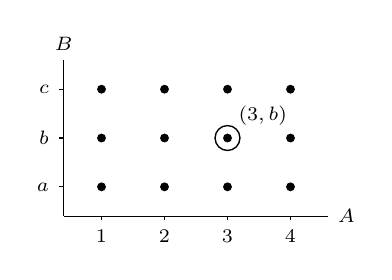
\begin{tikzpicture}[font=\scriptsize, x=0.8cm, y=0.62cm]
\draw[line width=0.4pt] (0.4,0.4) -- (4.6,0.4);
\draw[line width=0.4pt] (0.4,0.4) -- (0.4,3.6);
\foreach \i in {1,...,4} {\draw[line width=0.4pt] (\i,0.4) -- (\i,0.32); \node[below] at (\i,0.32) {$\i$};}
\foreach \j/\l in {1/a,2/b,3/c} {\draw[line width=0.4pt] (0.4,\j) -- (0.32,\j); \node[left] at (0.32,\j) {$\l$};}
\foreach \i in {1,...,4} \foreach \j in {1,2,3} {\fill (\i,\j) circle (1.6pt);}
\draw[line width=0.5pt] (3,2) circle (4.5pt);
\node[above right] at (3.02,2.05) {$(3,b)$};
\node[anchor=west] at (4.6,0.4) {$A$};
\node[anchor=south] at (0.4,3.6) {$B$};
\end{tikzpicture}}\hfill
\sdpanel{B}{\begin{tikzpicture}
\begin{axis}[sddiagram, width=5.2cm, height=3.9cm, xmin=-0.3, xmax=4.2, ymin=-0.3, ymax=2.9,
  xtick={1,3}, ytick={1,2}, xlabel={$x$}, ylabel={$y$}]
\fill[sdfill] (axis cs:1,1) rectangle (axis cs:3,2);
\draw[line width=0.5pt] (axis cs:1,1) rectangle (axis cs:3,2);
\draw[line width=1.4pt] (axis cs:1,0) -- (axis cs:3,0);
\draw[line width=1.4pt] (axis cs:0,1) -- (axis cs:0,2);
\draw[black!55, dashed, line width=0.4pt] (axis cs:1,0) -- (axis cs:1,1) (axis cs:3,0) -- (axis cs:3,1);
\draw[black!55, dashed, line width=0.4pt] (axis cs:0,1) -- (axis cs:1,1) (axis cs:0,2) -- (axis cs:1,2);
\node[font=\scriptsize] at (axis cs:2,1.5) {$[1,3]\times[1,2]$};
\end{axis}
\end{tikzpicture}}
\caption{Cartesian products. (A) The product of $A=\{1,2,3,4\}$ and $B=\{a,b,c\}$ as a grid of twelve pairs; the circled dot is the pair $(3,b)$. (B) The product $[1,3]\times[1,2]$ of two intervals (thick on the axes) is a rectangle in the plane $\mathbb R^2$.}
\label{fig:product}
\end{figure}

The product is not commutative: $A\times B$ and $B\times A$ are different sets unless $A=B$ or one of them is empty, because $(a,b)\ne(b,a)$ in general. If $A$ or $B$ is empty, then $A\times B=\emptyset$, since a pair needs a component from each set. The product interacts with the set operations as follows; the proofs are again translations into logic, and we prove one identity.

\begin{proposition}
\label{prop:product-laws}
For all sets $A$, $B$, $C$ and $D$:
\begin{enumerate}
\item $A\times(B\cup C)=(A\times B)\cup(A\times C)$ and $A\times(B\cap C)=(A\times B)\cap(A\times C)$;
\item $(A\times B)\cap(C\times D)=(A\cap C)\times(B\cap D)$;
\item $(A\times B)\cup(C\times D)\subseteq(A\cup C)\times(B\cup D)$, and the inclusion may be proper.
\end{enumerate}
\end{proposition}

\begin{proof}
We prove (ii). A pair $(x,y)$ lies in $(A\times B)\cap(C\times D)$ if and only if $x\in A$, $y\in B$, $x\in C$ and $y\in D$, and, after reordering the four conditions, this says that $x\in A\cap C$ and $y\in B\cap D$, that is, $(x,y)\in(A\cap C)\times(B\cap D)$. Every element of either side is a pair, so the two sets are equal. Part (i) is proved in the same way, and so is the inclusion in (iii). For the last claim of (iii), take $A=B=[0,1]$ and $C=D=[2,3]$: the pair $(0,2)$ lies in $(A\cup C)\times(B\cup D)$, but it lies neither in $A\times B$, since $2\notin B$, nor in $C\times D$, since $0\notin C$. Geometrically, the union of two squares on the diagonal is smaller than the large square that they span.
\end{proof}

\subsection{Tuples, Sequences, and Counting}

Ordered pairs generalise to any finite number of components. For $n\ge1$, an \term{$n$-tuple} $(a_1,\ldots,a_n)$ is determined by its components in order, so that $(a_1,\ldots,a_n)=(b_1,\ldots,b_n)$ if and only if $a_i=b_i$ for every $i$, and the product of sets $A_1,\ldots,A_n$ is
\[
A_1\times\cdots\times A_n\coloneqq\{(a_1,\ldots,a_n): a_i\in A_i\text{ for }i=1,\ldots,n\}.
\]
When all the factors are equal to $A$ we write $A^n$. Tuples of length three are called triples. The set $\mathbb R^n$ of $n$-tuples of real numbers is the setting of the linear algebra of Volume~II, where its elements are called vectors. In computing, a record with fields of given types is an element of a product: a row of a table whose columns hold an integer, a real number and a name is an element of $\mathbb Z\times\mathbb R\times W$, where $W$ is the set of words, and a whole table with $m$ rows is an element of $(\mathbb Z\times\mathbb R\times W)^m$. Volume~VIII builds data frames on this picture.

An \term{infinite sequence} $(a_0,a_1,a_2,\ldots)$, written $(a_n)_{n\in\mathbb N}$ as in \cref{def:sequence-limit}, is the infinite analogue of a tuple: it has a component $a_n$ for every $n\in\mathbb N$, and two sequences are equal when they agree in every component. \Cref{sec:functions} explains that a sequence is a particular kind of function, which settles what it is precisely.

For finite sets the size of a product is the product of the sizes, which explains the name.

\begin{proposition}
\label{prop:product-size}
If $A$ has $m$ elements and $B$ has $n$ elements, then $A\times B$ has $mn$ elements. Consequently, if $A$ has $m$ elements, then $A^k$ has $m^k$ elements for every $k\ge1$.
\end{proposition}

\begin{proof}
For each $a\in A$, the pairs with first component $a$ form the set $\{a\}\times B$, a row of the grid in \cref{fig:product}A. It has $n$ elements, one pair $(a,b)$ for each $b\in B$. The $m$ rows together make up $A\times B$, and two different rows have no pair in common, since pairs with different first components are different. Hence $A\times B$ has $n+n+\cdots+n=mn$ elements. The second statement follows by induction on $k$: identifying the $(k+1)$-tuple $(a_1,\ldots,a_k,a_{k+1})$ with the pair $\bigl((a_1,\ldots,a_k),a_{k+1}\bigr)$ shows that $A^{k+1}$ has as many elements as $A^k\times A$, namely $m^k\cdot m=m^{k+1}$.
\end{proof}

For instance, a binary word of $64$ bits is an element of $\{0,1\}^{64}$, and there are $2^{64}=18\,446\,744\,073\,709\,551\,616$ of them. This is the number of distinct values of a $64$-bit integer, and also the number of distinct bit patterns of a $64$-bit floating-point number; Volume~VI explains why the floating-point numbers represented by these patterns are slightly fewer. The counting arguments used here informally, splitting a set into disjoint parts and adding their sizes, are justified in \cref{ch:counting}.

\section{Functions}
\label{sec:functions}

The idea of a function, a rule that turns an input into an output, is the notion that this series uses more than any other. Calculus studies functions of real numbers, linear algebra studies linear functions between vectors, and every routine in a numerical library computes a function. This section gives the definition and the basic operations on functions.

\subsection{Definition and Examples}

\begin{definition}[Function]
\label{def:function}
Let $A$ and $B$ be sets. A \term{function} $f$ from $A$ to $B$, written $f\colon A\to B$, assigns to each element $a\in A$ exactly one element $f(a)\in B$, the \term{value} of $f$ at $a$. The set $A$ is the \term{domain} of $f$ and $B$ its \term{codomain}. The \term{graph} of $f$ is the set
\[
\Gamma_f\coloneqq\{(a,f(a)): a\in A\}\subseteq A\times B .
\]
Two functions $f$ and $g$ are \term{equal} if they have the same domain $A$, the same codomain and $f(a)=g(a)$ for every $a\in A$.
\end{definition}

The words \term{map}, \term{mapping} and \term{transformation} are used as synonyms of ``function''. To define a function one must specify three things: the domain, the codomain and the rule. We write $a\mapsto f(a)$ to show the rule, as in ``the function $f\colon\mathbb R\to\mathbb R$, $x\mapsto x^2$''. The arrow $\mapsto$ goes from an element to an element, while $\to$ goes from a set to a set.

The phrase ``exactly one'' in \cref{def:function} contains two requirements: every element of the domain has a value (existence), and no element has two values (uniqueness). In terms of the graph, a subset $\Gamma\subseteq A\times B$ is the graph of a function from $A$ to $B$ if and only if
\[
\forall a\in A,\ \exists!\,b\in B,\ (a,b)\in\Gamma ,
\]
and the function is then determined by its graph. Axiomatic set theory takes this as the definition and identifies a function with its graph~\cite{enderton1977sets}. Since the graph alone does not record the codomain, authors who, like us, regard the codomain as part of the function define a function as the triple $(A,B,\Gamma)$ instead. For real functions the condition is the familiar vertical line test: every vertical line through a point of the domain meets the graph exactly once.

Here are some functions that occur throughout the series.
\begin{itemize}
\item Formulas: $f\colon\mathbb R\to\mathbb R$, $f(x)=x^2-3x+1$, and every polynomial in the same way.
\item The \term{identity function} $\operatorname{id}_A\colon A\to A$, $\operatorname{id}_A(a)=a$, and the \term{constant functions} $a\mapsto c$ for a fixed $c\in B$.
\item The \term{inclusion} $\iota\colon S\to A$, $\iota(s)=s$, of a subset $S\subseteq A$. It has the same rule as $\operatorname{id}_S$ but a different codomain, and so, by \cref{def:function}, it is a different function.
\item The \term{projections} $p_1\colon A\times B\to A$, $(a,b)\mapsto a$, and $p_2\colon A\times B\to B$, $(a,b)\mapsto b$. A function whose domain is a product, such as $(x,y)\mapsto x^2+y^2$ on $\mathbb R^2$, is a function of several variables; we write $f(x,y)$ for $f((x,y))$.
\item The \term{indicator function} $\mathbf 1_S\colon A\to\{0,1\}$ of a subset $S\subseteq A$, with $\mathbf 1_S(a)=1$ if $a\in S$ and $\mathbf 1_S(a)=0$ if $a\notin S$. It is also called the characteristic function of $S$, a name that we avoid because probability theory uses it for something else (Volume~IV).
\item Sequences: a sequence $(a_n)_{n\in\mathbb N}$ of real numbers is a function $a\colon\mathbb N\to\mathbb R$, written with the argument as a subscript, $a_n$ instead of $a(n)$. Similarly, an $n$-tuple of elements of $B$ is a function $\{1,\ldots,n\}\to B$.
\item Arrays: an array of $n$ real numbers, indexed from $0$ as in most programming languages, is a function $\{0,1,\ldots,n-1\}\to\mathbb R$, and a table of $m$ rows and $n$ columns is a function $\{0,\ldots,m-1\}\times\{0,\ldots,n-1\}\to\mathbb R$. This point of view underlies Volume~VII.
\end{itemize}

It is equally important to recognise what is not a function. The rule ``assign to $x$ the number $y$ with $y^2=x$'' does not define a function from $\mathbb R$ to $\mathbb R$: for $x=-1$ there is no such $y$, so existence fails, and for $x=4$ there are two, $2$ and $-2$, so uniqueness fails. Both defects can be repaired by changing the sets: $x\mapsto\sqrt x$ is a function from $[0,\infty)$ to $\mathbb R$, by \cref{asm:numbers}\,(iv). Similarly, $x\mapsto1/x$ is a function on $\mathbb R\setminus\{0\}$ but not on $\mathbb R$. A function is not required to be given by a formula; ``$f(n)$ is the $n$th prime number'' and ``$f(x)=1$ if $x$ is rational and $0$ otherwise'' are perfectly good functions.

For sets $A$ and $B$, the set of all functions from $A$ to $B$ is written $B^A$. The notation is explained by the count: if $A$ has $m$ elements and $B$ has $n$, then a function is specified by choosing one of the $n$ values for each of the $m$ elements of $A$, and there are $n^m$ ways to do so (\cref{ch:counting} makes this precise). For example, the set $\{0,1\}^{\mathbb N}$ is the set of all infinite sequences of zeros and ones. The indicator functions give a one-to-one correspondence between the subsets of $A$ and the functions $A\to\{0,1\}$: each subset $S$ yields $\mathbf 1_S$, and each function $g\colon A\to\{0,1\}$ is the indicator function of exactly one subset, namely $\{a\in A: g(a)=1\}$. This explains once more why a set of $n$ elements has $2^n$ subsets (\cref{prop:power-set-size}).

\subsection{Images and Preimages}

A function can be applied to a whole set of inputs at once, and it can be asked which inputs lead to a given set of outputs.

\begin{definition}[Image, preimage, range]
\label{def:image}
Let $f\colon A\to B$ be a function.
\begin{enumerate}
\item For $S\subseteq A$, the \term{image} of $S$ under $f$ is $f(S)\coloneqq\{f(s): s\in S\}\subseteq B$.
\item For $T\subseteq B$, the \term{preimage}, or inverse image, of $T$ under $f$ is $f^{-1}(T)\coloneqq\{a\in A: f(a)\in T\}\subseteq A$.
\end{enumerate}
The image $f(A)$ of the whole domain is the \term{range} of $f$.
\end{definition}

The image $f(S)$ is the set of outputs produced by inputs from $S$; the preimage $f^{-1}(T)$ is the set of inputs whose outputs land in $T$. The notation $f^{-1}(T)$ is used for every function, whether or not $f$ has an inverse function in the sense of \cref{sec:injections}. When it does, the two meanings of $f^{-1}$ agree, as we shall see. The range is a subset of the codomain, and it may be a proper subset: the function $x\mapsto x^2$ from $\mathbb R$ to $\mathbb R$ has codomain $\mathbb R$ and range $[0,\infty)$.

For $f\colon\mathbb R\to\mathbb R$, $f(x)=x^2$, we have
\begin{gather*}
f([1,2])=[1,4],\qquad f([-1,2])=[0,4],\\
f^{-1}([1,4])=[-2,-1]\cup[1,2],\qquad f^{-1}([-2,-1])=\emptyset .
\end{gather*}
The preimage of a set that the function never reaches is empty. \Cref{fig:image-preimage} shows images and preimages for a function between finite sets and for this function.

\begin{figure}
\tikzset{fdot/.style={circle, fill=black, inner sep=0pt, minimum size=3.2pt},
  farr/.style={-{Latex[length=1.4mm]}, line width=0.4pt, shorten >=1.5pt, shorten <=1.5pt}}
\sdpanel{A}{\begin{tikzpicture}[font=\scriptsize]
\fill[sdfill, rounded corners=4pt] (-0.36,1.85) rectangle (0.3,3.35);
\fill[sdfill, rounded corners=4pt] (2.2,2.7) rectangle (2.86,3.3);
\draw[line width=0.4pt] (0,1.8) ellipse (0.72 and 1.72);
\draw[line width=0.4pt] (2.5,1.8) ellipse (0.72 and 1.72);
\foreach \y/\l [count=\i] in {3.0/1,2.2/2,1.4/3,0.6/4} {\node[fdot] (a\i) at (0,\y) {}; \node[left=1pt] at (a\i) {$\l$};}
\foreach \y/\l [count=\i] in {3.0/a,2.2/b,1.4/c,0.6/d} {\node[fdot] (b\i) at (2.5,\y) {}; \node[right=1pt] at (b\i) {$\l$};}
\draw[farr] (a1) -- (b1); \draw[farr] (a2) -- (b1); \draw[farr] (a3) -- (b3); \draw[farr] (a4) -- (b3);
\node at (0,-0.2) {$A$}; \node at (2.5,-0.2) {$B$};
\node[anchor=east] at (-0.78,2.6) {$S$};
\node[anchor=west] at (3.26,3.0) {$f(S)$};
\end{tikzpicture}}\hfill
\sdpanel{B}{\begin{tikzpicture}
\begin{axis}[sddiagram, width=5.6cm, height=4.6cm, xmin=-2.6, xmax=2.6, ymin=-0.6, ymax=5.2,
  xtick={-2,-1,1,2}, ytick={1,4}, xlabel={$x$}, ylabel={$f(x)$}, clip=false,
  yticklabel style={fill=white, inner sep=1pt}]
\addplot[black, line width=0.6pt, domain=-2.25:2.25, samples=100] {x^2};
\draw[line width=1.6pt] (axis cs:0,1) -- (axis cs:0,4);
\draw[line width=1.6pt] (axis cs:-2,0) -- (axis cs:-1,0) (axis cs:1,0) -- (axis cs:2,0);
\draw[black!55, dashed, line width=0.4pt] (axis cs:-2,4) -- (axis cs:2,4) (axis cs:-1,1) -- (axis cs:1,1);
\draw[black!55, dashed, line width=0.4pt] (axis cs:-2,0) -- (axis cs:-2,4) (axis cs:2,0) -- (axis cs:2,4) (axis cs:-1,0) -- (axis cs:-1,1) (axis cs:1,0) -- (axis cs:1,1);
\node[font=\scriptsize, anchor=west] at (axis cs:0.12,2.6) {$T$};
\end{axis}
\end{tikzpicture}}
\caption{Images and preimages. (A) A function $f\colon A\to B$ drawn with arrows. The image of $S=\{1,2\}$ is $f(S)=\{a\}$ (shaded), the range is $f(A)=\{a,c\}$, and the preimage of $\{b,c\}$ is $f^{-1}(\{b,c\})=\{3,4\}$. (B) For $f(x)=x^2$ the preimage of $T=[1,4]$ (thick on the vertical axis) is $[-2,-1]\cup[1,2]$ (thick on the horizontal axis).}
\label{fig:image-preimage}
\end{figure}

Preimages are better behaved than images: they are compatible with all the set operations, while images are compatible only with unions.

\begin{proposition}
\label{prop:image-preimage}
Let $f\colon A\to B$ be a function, let $S,S_1,S_2\subseteq A$ and $T,T_1,T_2\subseteq B$, and let $(T_i)_{i\in I}$ be a family of subsets of $B$.
\begin{enumerate}
\item $f^{-1}(T_1\cup T_2)=f^{-1}(T_1)\cup f^{-1}(T_2)$ and $f^{-1}(T_1\cap T_2)=f^{-1}(T_1)\cap f^{-1}(T_2)$; more generally $f^{-1}\bigl(\bigcup_iT_i\bigr)=\bigcup_if^{-1}(T_i)$ and, for $I\ne\emptyset$, $f^{-1}\bigl(\bigcap_iT_i\bigr)=\bigcap_if^{-1}(T_i)$.
\item $f^{-1}(T_1\setminus T_2)=f^{-1}(T_1)\setminus f^{-1}(T_2)$; in particular $f^{-1}(B\setminus T)=A\setminus f^{-1}(T)$.
\item $f(S_1\cup S_2)=f(S_1)\cup f(S_2)$.
\item $f(S_1\cap S_2)\subseteq f(S_1)\cap f(S_2)$, and the inclusion may be proper.
\item $S\subseteq f^{-1}(f(S))$ and $f(f^{-1}(T))\subseteq T$, and both inclusions may be proper.
\end{enumerate}
\end{proposition}

\begin{proof}
(i) For $a\in A$,
\begin{align*}
a\in f^{-1}\Bigl(\bigcup_{i\in I}T_i\Bigr)&\iff f(a)\in\bigcup_{i\in I}T_i\iff\exists i\in I,\ f(a)\in T_i\\
&\iff\exists i\in I,\ a\in f^{-1}(T_i)\iff a\in\bigcup_{i\in I}f^{-1}(T_i),
\end{align*}
and the same chain with $\forall$ in place of $\exists$ proves the statement for intersections. The statements for two sets are the case $I=\{1,2\}$.

(ii) For $a\in A$: $a\in f^{-1}(T_1\setminus T_2)$ if and only if $f(a)\in T_1$ and $f(a)\notin T_2$, that is, $a\in f^{-1}(T_1)$ and $a\notin f^{-1}(T_2)$. The special case is $T_1=B$, using $f^{-1}(B)=A$.

(iii) Let $b\in f(S_1\cup S_2)$, say $b=f(s)$ with $s\in S_1\cup S_2$. If $s\in S_1$, then $b\in f(S_1)$; if $s\in S_2$, then $b\in f(S_2)$; in either case $b\in f(S_1)\cup f(S_2)$. Conversely, $S_1\subseteq S_1\cup S_2$ implies $f(S_1)\subseteq f(S_1\cup S_2)$, since every output produced from $S_1$ is produced from the larger set, and likewise for $S_2$.

(iv) If $b\in f(S_1\cap S_2)$, then $b=f(s)$ with $s$ in both $S_1$ and $S_2$, so $b\in f(S_1)$ and $b\in f(S_2)$. For an example of a proper inclusion, take $f(x)=x^2$ on $\mathbb R$, $S_1=\{-1\}$ and $S_2=\{1\}$. Then $S_1\cap S_2=\emptyset$ and $f(S_1\cap S_2)=\emptyset$, while $f(S_1)\cap f(S_2)=\{1\}$.

(v) If $s\in S$, then $f(s)\in f(S)$, so $s\in f^{-1}(f(S))$. If $b\in f(f^{-1}(T))$, then $b=f(a)$ for some $a$ with $f(a)\in T$, so $b\in T$. With $f(x)=x^2$ on $\mathbb R$, $S=\{1\}$ gives $f^{-1}(f(S))=\{-1,1\}\ne S$, and $T=[-1,1]$ gives $f(f^{-1}(T))=f([-1,1])=[0,1]\ne T$.
\end{proof}

The failure in (iv) comes from two different inputs with the same output: $-1$ and $1$ are separated by $S_1$ and $S_2$, but their common output $1$ is not. \Cref{sec:injections} shows that (iv) and the first half of (v) become equalities when this cannot happen. The good behaviour of preimages is the reason why many central definitions are made with them. In Volume~III, for instance, a function between metric spaces is shown to be continuous exactly when the preimage of every open set is open, and in Volume~IV a random variable is defined as a function whose preimages of intervals are events.

\subsection{Restriction and Composition}

\begin{definition}[Restriction]
\label{def:restriction}
Let $f\colon A\to B$ and $S\subseteq A$. The \term{restriction} of $f$ to $S$ is the function $f|_S\colon S\to B$, $f|_S(s)=f(s)$.
\end{definition}

The restriction keeps the rule and the codomain and shrinks the domain. It is a different function from $f$ when $S\ne A$. For instance, $x\mapsto x^2$ on $\mathbb R$ and its restriction to $[0,\infty)$ have quite different properties, as the next section shows.

Functions can be applied one after another, the output of the first becoming the input of the second.

\begin{definition}[Composition]
\label{def:composition}
Let $f\colon A\to B$ and $g\colon B\to C$. The \term{composition} of $g$ with $f$ is the function
\[
g\circ f\colon A\to C,\qquad(g\circ f)(a)\coloneqq g(f(a)).
\]
\end{definition}

The composition $g\circ f$, read ``$g$ after $f$'', applies $f$ first, although $f$ is written second; the order follows the notation $g(f(a))$, in which the function nearest the argument acts first. The composition is defined only when the codomain of $f$ is the domain of $g$. Many authors require only that the range of $f$ be contained in the domain of $g$; with \cref{def:composition} such a composition is formed by first changing the codomain of $f$.

Composition is not commutative. For $f(x)=x+1$ and $g(x)=x^2$ on $\mathbb R$,
\[
(g\circ f)(x)=(x+1)^2,\qquad(f\circ g)(x)=x^2+1,
\]
and these functions differ, for example at $x=1$, where they take the values $4$ and $2$. Composition is, however, associative, and the identity functions act as neutral elements.

\begin{proposition}
\label{prop:composition}
Let $f\colon A\to B$, $g\colon B\to C$ and $h\colon C\to D$. Then
\[
h\circ(g\circ f)=(h\circ g)\circ f
\qquad\text{and}\qquad
f\circ\operatorname{id}_A=f=\operatorname{id}_B\circ f .
\]
\end{proposition}

\begin{proof}
Both sides of the first identity are functions from $A$ to $D$. For every $a\in A$,
\[
\bigl(h\circ(g\circ f)\bigr)(a)=h\bigl((g\circ f)(a)\bigr)=h\bigl(g(f(a))\bigr)
=(h\circ g)\bigl(f(a)\bigr)=\bigl((h\circ g)\circ f\bigr)(a),
\]
so the two functions are equal by \cref{def:function}. Similarly $(f\circ\operatorname{id}_A)(a)=f(a)=(\operatorname{id}_B\circ f)(a)$ for every $a\in A$.
\end{proof}

Because of associativity we write $h\circ g\circ f$ without parentheses. A long computation is a composition of many simple steps, and associativity says that the steps may be grouped in any way without changing the result. (In floating-point arithmetic, it is the grouping of \emph{additions}, not of function compositions, that matters, a distinction drawn in Volume~VI.) Images and preimages behave well under composition: $(g\circ f)(S)=g(f(S))$ and $(g\circ f)^{-1}(U')=f^{-1}(g^{-1}(U'))$ for $S\subseteq A$ and $U'\subseteq C$, as one checks directly from the definitions.

\section{Injections, Surjections, and Bijections}
\label{sec:injections}

The function $x\mapsto x^2$ on $\mathbb R$ cannot be undone: from the output $4$ one cannot tell whether the input was $2$ or $-2$, and the output $-1$ never occurs. These are the two ways in which a function can fail to be reversible, and they lead to the central definitions of this section~\cite{velleman2019,halmos1960naive}.

\subsection{Definitions and Examples}

\begin{definition}[Injective, surjective, bijective]
\label{def:injective}
A function $f\colon A\to B$ is
\begin{enumerate}
\item \term{injective}, or one-to-one, if different inputs have different outputs: for all $a,a'\in A$, $f(a)=f(a')\Rightarrow a=a'$;
\item \term{surjective}, or onto, if every element of the codomain is an output: for every $b\in B$ there is $a\in A$ with $f(a)=b$, that is, $f(A)=B$;
\item \term{bijective} if it is both injective and surjective.
\end{enumerate}
An injective function is called an \term{injection}, a surjective one a \term{surjection} and a bijective one a \term{bijection}, or a one-to-one correspondence.
\end{definition}

In terms of equations, $f$ is injective if every equation $f(x)=b$ with $b\in B$ has at most one solution $x\in A$, surjective if every such equation has at least one solution, and bijective if every such equation has exactly one solution. In the arrow pictures of \cref{fig:kinds}, injectivity means that no two arrows arrive at the same point, and surjectivity means that every point of the codomain receives an arrow. For a real function, injectivity means that every horizontal line meets the graph at most once, and surjectivity that every horizontal line at a height in the codomain meets it at least once.

\begin{figure}
\tikzset{fdot/.style={circle, fill=black, inner sep=0pt, minimum size=3.2pt},
  farr/.style={-{Latex[length=1.4mm]}, line width=0.4pt, shorten >=1.5pt, shorten <=1.5pt}}
\newcommand\kindpanel[4]{%
\begin{tikzpicture}[font=\scriptsize]
\draw[line width=0.4pt] (0,1.25) ellipse (0.42 and 1.3);
\draw[line width=0.4pt] (1.75,1.25) ellipse (0.42 and 1.3);
\foreach \y [count=\i] in {#1} {\node[fdot] (a\i) at (0,\y) {};}
\foreach \y [count=\i] in {#2} {\node[fdot] (b\i) at (1.75,\y) {};}
\foreach \s/\t in {#3} {\draw[farr] (a\s) -- (b\t);}
\node at (0,-0.3) {$A$}; \node at (1.75,-0.3) {$B$};
\node[font=\scriptsize, align=center] at (0.875,-0.78) {#4};
\end{tikzpicture}}
\sdpanel{A}{\kindpanel{2,1.25,0.5}{2,1.25,0.5}{1/1,2/1,3/2}{neither}}\hfill
\sdpanel{B}{\kindpanel{1.9,1.25,0.6}{2.1,1.5,0.95,0.4}{1/1,2/2,3/4}{injective}}\hfill
\sdpanel{C}{\kindpanel{2.1,1.5,0.95,0.4}{1.9,1.25,0.6}{1/1,2/2,3/3,4/3}{surjective}}\hfill
\sdpanel{D}{\kindpanel{2,1.25,0.5}{2,1.25,0.5}{1/2,2/3,3/1}{bijective}}
\caption{The kinds of functions. (A) Two arrows meet and one point of $B$ is missed: neither injective nor surjective. (B) No two arrows meet, but a point of $B$ is missed: injective, not surjective. (C) Every point of $B$ is hit, but two arrows meet: surjective, not injective. (D) Every point of $B$ is hit exactly once: bijective.}
\label{fig:kinds}
\end{figure}

The square function shows that the three properties depend on the domain and the codomain as much as on the rule. Let $Q=[0,\infty)$.
\begin{itemize}
\item $x\mapsto x^2$ from $\mathbb R$ to $\mathbb R$ is neither injective ($(-1)^2=1^2$) nor surjective ($-1$ is not a square).
\item $x\mapsto x^2$ from $Q$ to $\mathbb R$ is injective but not surjective. If $x,y\ge0$ and $x^2=y^2$, then $0=x^2-y^2=(x-y)(x+y)$, so $x=y$ or $x+y=0$, and the latter forces $x=y=0$.
\item $x\mapsto x^2$ from $\mathbb R$ to $Q$ is surjective but not injective: every $y\ge0$ equals $(\sqrt y)^2$ by \cref{asm:numbers}\,(iv).
\item $x\mapsto x^2$ from $Q$ to $Q$ is bijective, by the two previous arguments.
\end{itemize}

More examples:
\begin{itemize}
\item For real numbers $a\ne0$ and $b$, the function $x\mapsto ax+b$ from $\mathbb R$ to $\mathbb R$ is bijective, because the equation $ax+b=c$ has exactly one solution for every $c$ (\cref{prop:linear-equation}).
\item On the integers, $n\mapsto n+1$ is a bijection from $\mathbb Z$ to $\mathbb Z$, and $n\mapsto2n$ is an injection that is not surjective, since its range $2\mathbb Z$ misses the odd integers.
\item On the natural numbers, $n\mapsto n+1$ is an injection that is not surjective, since $0$ is not of the form $n+1$ with $n\in\mathbb N$. The halving function $h\colon\mathbb N\to\mathbb N$, $h(n)=(n-n\bmod2)/2$, which discards the last binary digit, is surjective, since $h(2m)=m$, but not injective, since $h(2m)=h(2m+1)$.
\item The projection $p_1\colon A\times B\to A$ is surjective when $B\ne\emptyset$ and injective when $B$ has at most one element.
\item The inclusion of a subset is always injective, and an identity function is always bijective.
\end{itemize}

To prove that a function is injective, the definition suggests the standard pattern: assume $f(a)=f(a')$ and deduce $a=a'$, as in the argument for $x^2$ on $Q$ above. To prove that it is surjective, take an arbitrary $b$ in the codomain and exhibit an $a$ with $f(a)=b$, usually by solving the equation $f(a)=b$. A function that is not injective is refuted by two different inputs with the same output, and a function that is not surjective by one element of the codomain that is never an output.

An injective function preserves the distinctions that \cref{prop:image-preimage} lost. If $f$ is injective, then $f(S_1\cap S_2)=f(S_1)\cap f(S_2)$ and $f^{-1}(f(S))=S$ for all subsets $S,S_1,S_2$ of the domain. If $f$ is surjective, then $f(f^{-1}(T))=T$ for every subset $T$ of the codomain. In view of \cref{prop:image-preimage}, only one inclusion has to be shown in each case. An element $b\in f(S_1)\cap f(S_2)$ is of the form $b=f(s_1)=f(s_2)$ with $s_1\in S_1$ and $s_2\in S_2$, and injectivity gives $s_1=s_2\in S_1\cap S_2$, so $b\in f(S_1\cap S_2)$. An element $a\in f^{-1}(f(S))$ satisfies $f(a)=f(s)$ for some $s\in S$, and injectivity gives $a=s\in S$. Finally, if $f$ is surjective and $b\in T$, then $b=f(a)$ for some $a$, which lies in $f^{-1}(T)$, so $b\in f(f^{-1}(T))$.

\subsection{Composition}

The three properties are preserved by composition, and partly inherited backwards from a composition.

\begin{proposition}
\label{prop:composition-injective}
Let $f\colon A\to B$ and $g\colon B\to C$.
\begin{enumerate}
\item If $f$ and $g$ are injective, so is $g\circ f$.
\item If $f$ and $g$ are surjective, so is $g\circ f$.
\item If $f$ and $g$ are bijective, so is $g\circ f$.
\item If $g\circ f$ is injective, then $f$ is injective.
\item If $g\circ f$ is surjective, then $g$ is surjective.
\end{enumerate}
\end{proposition}

\begin{proof}
(i) Suppose $g(f(a))=g(f(a'))$. Since $g$ is injective, $f(a)=f(a')$, and since $f$ is injective, $a=a'$.

(ii) Let $c\in C$. Since $g$ is surjective, $c=g(b)$ for some $b\in B$, and since $f$ is surjective, $b=f(a)$ for some $a\in A$. Then $c=g(f(a))$.

(iii) This follows from (i) and (ii).

(iv) Suppose $f(a)=f(a')$. Applying $g$ gives $g(f(a))=g(f(a'))$, and since $g\circ f$ is injective, $a=a'$.

(v) Let $c\in C$. Since $g\circ f$ is surjective, $c=g(f(a))$ for some $a\in A$, so $c$ is the value of $g$ at the element $f(a)$ of $B$.
\end{proof}

Parts (iv) and (v) cannot be reversed. Let $A=\{0\}$, $B=\{0,1\}$ and $C=\{0\}$, let $f(0)=0$, and let $g$ send both elements of $B$ to $0$. Then $g\circ f\colon\{0\}\to\{0\}$ is bijective, but $g$ is not injective and $f$ is not surjective.

\subsection{Inverse Functions}

\begin{definition}[Inverse function]
\label{def:inverse}
Let $f\colon A\to B$. A function $g\colon B\to A$ is an \term{inverse} of $f$ if
\[
g\circ f=\operatorname{id}_A\qquad\text{and}\qquad f\circ g=\operatorname{id}_B ,
\]
that is, if $g(f(a))=a$ for every $a\in A$ and $f(g(b))=b$ for every $b\in B$. A function that has an inverse is \term{invertible}.
\end{definition}

An inverse undoes $f$ from either side. The main theorem of this section identifies the invertible functions.

\begin{theorem}[Inverse functions]
\label{thm:inverse}
A function $f\colon A\to B$ has an inverse if and only if it is bijective. The inverse is then unique; it is denoted $f^{-1}$, and $f^{-1}(b)$ is the unique $a\in A$ with $f(a)=b$. Moreover, $f^{-1}$ is bijective and $(f^{-1})^{-1}=f$.
\end{theorem}

\begin{proof}
($\Rightarrow$) Suppose $g$ is an inverse of $f$. Then $g\circ f=\operatorname{id}_A$ is injective, so $f$ is injective by \cref{prop:composition-injective}\,(iv), and $f\circ g=\operatorname{id}_B$ is surjective, so $f$ is surjective by \cref{prop:composition-injective}\,(v).

($\Leftarrow$) Suppose $f$ is bijective. For each $b\in B$ the equation $f(a)=b$ has exactly one solution $a\in A$: at least one because $f$ is surjective and at most one because it is injective. Define $g(b)$ to be this solution. Then $f(g(b))=b$ for every $b\in B$, by the definition of $g$. For $a\in A$, the element $g(f(a))$ is the unique solution of the equation $f(x)=f(a)$, and $x=a$ is a solution, so $g(f(a))=a$. Hence $g$ is an inverse of $f$.

\emph{Uniqueness.} Let $g$ and $h$ both be inverses of $f$. By \cref{prop:composition},
\[
g=g\circ\operatorname{id}_B=g\circ(f\circ h)=(g\circ f)\circ h=\operatorname{id}_A\circ h=h .
\]
The description of $f^{-1}(b)$ is the construction in the proof of ($\Leftarrow$). Finally, the two equations of \cref{def:inverse} are symmetric in $f$ and $g$, so $f$ is an inverse of $f^{-1}$; hence $f^{-1}$ is bijective by ($\Rightarrow$), and $(f^{-1})^{-1}=f$ by uniqueness.
\end{proof}

For a bijection $f$ the notation $f^{-1}$ now has two meanings, the inverse function and the preimage of \cref{def:image}. They are consistent: for every $T\subseteq B$, the preimage of $T$ under $f$ equals the image of $T$ under the inverse function, and in particular the preimage of $\{b\}$ is $\{f^{-1}(b)\}$.

The inverse of the bijection $x\mapsto x^2$ on $[0,\infty)$ is the square root $y\mapsto\sqrt y$ on $[0,\infty)$; the inverse of $x\mapsto ax+b$ on $\mathbb R$, with $a\ne0$, is $y\mapsto(y-b)/a$. The graph of an inverse function consists of the pairs of the graph of $f$ with their components exchanged, $\Gamma_{f^{-1}}=\{(b,a): (a,b)\in\Gamma_f\}$. For real functions this exchange is the reflection in the diagonal line $y=x$, as \cref{fig:inverse-graph} shows.

\begin{figure}
\sdfloat{%
\begin{tikzpicture}
\begin{axis}[sdplot, width=5.4cm, height=5.4cm, xmin=0, xmax=2.7, ymin=0, ymax=2.7,
  xtick={0,1,2}, ytick={0,1,2}, xlabel={$x$}, ylabel={$y$}, clip=false]
\addplot[black!45, dashed, line width=0.5pt, domain=0:2.6] {x};
\addplot[black, line width=0.7pt, domain=0:1.62, samples=80] {x^2};
\addplot[black, densely dotted, line width=0.8pt, domain=0:2.62, samples=200] {sqrt(x)};
\fill (axis cs:1.4,1.96) circle (1.4pt);
\fill (axis cs:1.96,1.4) circle (1.4pt);
\draw[black!55, line width=0.4pt] (axis cs:1.4,1.96) -- (axis cs:1.96,1.4);
\node[font=\scriptsize, anchor=east] at (axis cs:1.36,2.02) {$(a,b)$};
\node[font=\scriptsize, anchor=north west] at (axis cs:1.98,1.36) {$(b,a)$};
\node[font=\scriptsize, anchor=east] at (axis cs:1.52,2.62) {$y=x^2$};
\node[font=\scriptsize, anchor=west] at (axis cs:2.64,1.62) {$y=\sqrt x$};
\node[font=\scriptsize, anchor=west] at (axis cs:2.62,2.62) {$y=x$};
\end{axis}
\end{tikzpicture}}{A function and its inverse. The graph of $f(x)=x^2$ on $[0,\infty)$ (solid) and the graph of its inverse $f^{-1}(y)=\sqrt y$ (dotted) are mirror images in the diagonal $y=x$ (dashed): the point $(a,b)$ of one graph corresponds to the point $(b,a)$ of the other.\label{fig:inverse-graph}}
\end{figure}

\begin{proposition}
\label{prop:inverse-composition}
If $f\colon A\to B$ and $g\colon B\to C$ are bijective, then $(g\circ f)^{-1}=f^{-1}\circ g^{-1}$.
\end{proposition}

\begin{proof}
By \cref{prop:composition-injective}\,(iii), $g\circ f$ is bijective. Using associativity,
\[
(f^{-1}\circ g^{-1})\circ(g\circ f)=f^{-1}\circ(g^{-1}\circ g)\circ f=f^{-1}\circ\operatorname{id}_B\circ f=f^{-1}\circ f=\operatorname{id}_A,
\]
and in the same way $(g\circ f)\circ(f^{-1}\circ g^{-1})=\operatorname{id}_C$. So $f^{-1}\circ g^{-1}$ is an inverse of $g\circ f$, and by the uniqueness in \cref{thm:inverse} it is the inverse.
\end{proof}

The order is reversed for the same reason that one takes off one's shoes before one's socks: what was done last must be undone first.

A bijection from a set to itself is called a \term{permutation} of the set. The permutations of $\{0,1,\ldots,n-1\}$ describe the rearrangements of an array of length $n$: sorting an array, for instance, amounts to finding a permutation $\sigma$ such that the entry at position $\sigma(0)$ is the smallest, the entry at position $\sigma(1)$ the next, and so on. If $\sigma$ is the permutation of $\{0,1,2,3\}$ with $\sigma(0)=2$, $\sigma(1)=0$, $\sigma(2)=3$ and $\sigma(3)=1$, then its inverse is obtained by reading the assignments backwards: $\sigma^{-1}(2)=0$, $\sigma^{-1}(0)=1$, $\sigma^{-1}(3)=2$ and $\sigma^{-1}(1)=3$. Volume~VII uses permutations of this kind throughout, and \cref{ch:counting} counts them.

\subsection{One-Sided Inverses}

A function that is only injective, or only surjective, can still be undone from one side.

\begin{proposition}
\label{prop:one-sided}
Let $f\colon A\to B$ be a function with $A\ne\emptyset$.
\begin{enumerate}
\item $f$ is injective if and only if it has a \term{left inverse}, a function $g\colon B\to A$ with $g\circ f=\operatorname{id}_A$.
\item $f$ is surjective if and only if it has a \term{right inverse}, a function $h\colon B\to A$ with $f\circ h=\operatorname{id}_B$.
\end{enumerate}
\end{proposition}

\begin{proof}
In both parts the implication from the inverse to the property is \cref{prop:composition-injective}\,(iv) and (v), since identity functions are bijective.

(i) Let $f$ be injective, and fix an element $a_0\in A$, which exists because $A\ne\emptyset$. For $b\in f(A)$ there is exactly one $a\in A$ with $f(a)=b$, by injectivity; let $g(b)$ be this $a$. For $b\in B\setminus f(A)$ let $g(b)\coloneqq a_0$. Then $g\colon B\to A$, and $g(f(a))=a$ for every $a\in A$, since $a$ is the unique element with value $f(a)$.

(ii) Let $f$ be surjective. For each $b\in B$ the preimage $f^{-1}(\{b\})$ is nonempty. Choose one of its elements and call it $h(b)$. Then $f(h(b))=b$ for every $b\in B$.
\end{proof}

The proof of (ii) makes a choice for every element of $B$ simultaneously, and when $B$ is infinite this is an application of the axiom of choice described in the note in \cref{sec:sets}. Conversely, the statement ``every surjection has a right inverse'' implies the axiom of choice, so the two are equivalent~\cite{bell2021choice}: for a family $(A_i)_{i\in I}$ of nonempty sets, the map $(i,a)\mapsto i$ from the set of pairs $(i,a)$ with $i\in I$ and $a\in A_i$ onto $I$ is surjective, and a right inverse of it assigns to each $i$ a pair $(i,a)$ with $a\in A_i$, that is, it selects an element of each $A_i$. In concrete cases no axiom is needed, because a rule for the choice is available: if $A\subseteq\mathbb N$, for instance, $h(b)$ can be taken to be the least element of $f^{-1}(\{b\})$, which exists by the well-ordering principle (\cref{thm:well-ordering}). For the surjective halving function $n\mapsto(n-n\bmod2)/2$ of the examples above, the functions $m\mapsto2m$ and $m\mapsto2m+1$ are two different right inverses, and neither is a left inverse. A one-sided inverse is in general not unique, in contrast to the two-sided inverse of \cref{thm:inverse}.

The square root on a computer illustrates the difference. The function $x\mapsto x^2$ from $\mathbb R$ onto $[0,\infty)$ is surjective, and the square root is the right inverse that picks the nonnegative preimage: $(\sqrt y)^2=y$ for every $y\ge0$, but $\sqrt{x^2}=|x|$, which differs from $x$ when $x<0$. Choosing a particular right inverse of a surjective function is how inverse trigonometric functions, logarithms of complex numbers and many other ``principal values'' are defined (\cref{ch:transcendental} and Volume~III).

\section{Relations}
\label{sec:relations}

Mathematics is full of statements that relate two objects: $x<y$, $a\mid b$, $A\subseteq B$, ``$x$ and $y$ leave the same remainder''. Each of them is a predicate in two variables, and the pairs for which it is true form a set. This set is the relation~\cite{enderton1977sets}.

\subsection{Definition and Examples}

\begin{definition}[Relation]
\label{def:relation}
A \term{relation} from a set $A$ to a set $B$ is a subset $R\subseteq A\times B$. We write $a\mathrel{R}b$ for $(a,b)\in R$ and say that $a$ is related to $b$. A relation from $A$ to $A$ is a relation \term{on} $A$.
\end{definition}

The definition identifies a relation with its truth set, in the sense of \cref{def:predicate}. For example, the relation $<$ on $\mathbb R$ is the set $\{(x,y)\in\mathbb R^2: x<y\}$, the open half-plane above the diagonal, and $x<y$ is the same statement as $(x,y)\in{<}$. Some further relations that we use repeatedly:
\begin{itemize}
\item equality $=$ on any set $A$, which is the diagonal $\{(a,a): a\in A\}$ of $A\times A$;
\item the orders $\le$ and $<$ on $\mathbb N$, $\mathbb Z$, $\mathbb Q$ and $\mathbb R$;
\item divisibility $\mid$ on $\mathbb Z$ (\cref{def:even-odd});
\item inclusion $\subseteq$ on the power set $\mathcal P(X)$ of a set $X$;
\item \term{congruence modulo} $n$, for a fixed integer $n\ge1$: integers $a$ and $b$ are congruent modulo $n$, written $a\equiv b\pmod n$, if $n\mid a-b$. Thus $17\equiv2\pmod5$ and $-1\equiv3\pmod4$. \Cref{ch:numbers} studies this relation in detail;
\item a relation from a set of people to a set of cities, ``$p$ has lived in $c$'', and in general any table with two columns, each row of which records one related pair.
\end{itemize}

A function $f\colon A\to B$ is a particular relation from $A$ to $B$, namely its graph $\Gamma_f$, in which each element of $A$ is related to exactly one element of $B$. A general relation may relate an element to none, one or many elements. Two operations on relations generalise operations on functions. The \term{inverse} of a relation $R$ from $A$ to $B$ is the relation $R^{-1}\coloneqq\{(b,a): (a,b)\in R\}$ from $B$ to $A$; for instance, the inverse of $<$ is $>$. Unlike the inverse function, the inverse relation always exists. If $R$ is a relation from $A$ to $B$ and $S$ a relation from $B$ to $C$, their \term{composition} is the relation from $A$ to $C$
\[
S\circ R\coloneqq\{(a,c)\in A\times C:\exists b\in B,\ a\mathrel{R}b\wedge b\mathrel{S}c\}.
\]
When $R$ and $S$ are graphs of functions $f$ and $g$, the composition $S\circ R$ is the graph of $g\circ f$, which explains the order of the letters. If ``$p$ is a parent of $q$'' is the relation $R$ on a set of people, then $R\circ R$ is ``$p$ is a grandparent of $q$''.

\subsection{Properties of Relations}

Four properties of a relation on a single set occur so often that they have names.

\begin{definition}[Reflexive, symmetric, antisymmetric, transitive]
\label{def:relation-properties}
A relation $R$ on a set $A$ is
\begin{enumerate}
\item \term{reflexive} if $a\mathrel{R}a$ for every $a\in A$;
\item \term{symmetric} if $a\mathrel{R}b$ implies $b\mathrel{R}a$, for all $a,b\in A$;
\item \term{antisymmetric} if $a\mathrel{R}b$ and $b\mathrel{R}a$ together imply $a=b$, for all $a,b\in A$;
\item \term{transitive} if $a\mathrel{R}b$ and $b\mathrel{R}c$ together imply $a\mathrel{R}c$, for all $a,b,c\in A$.
\end{enumerate}
\end{definition}

\Cref{tab:relation-properties} records these properties for a number of relations. Each entry is a small proposition. A ``yes'' must be proved for all elements, while a ``no'' needs only one counterexample, in accordance with \cref{thm:quantifier-negation}.

\begin{table}
\sdfloat{%
\begin{sdtable}{colspec={llcccc}, row{1}={font=\small\bfseries}}
\toprule
Relation & Set & Refl. & Symm. & Antisymm. & Trans. \\
\midrule
$a=b$ & any & yes & yes & yes & yes \\
$x\le y$ & $\mathbb R$ & yes & no & yes & yes \\
$x<y$ & $\mathbb R$ & no & no & yes & yes \\
$x\ne y$ & $\mathbb R$ & no & yes & no & no \\
$a\mid b$ & $\mathbb N$ & yes & no & yes & yes \\
$a\mid b$ & $\mathbb Z$ & yes & no & no & yes \\
$S\subseteq T$ & $\mathcal P(X)$, $X\ne\emptyset$ & yes & no & yes & yes \\
$a\equiv b\pmod n$ & $\mathbb Z$ & yes & yes & no & yes \\
$x^2=y^2$ & $\mathbb R$ & yes & yes & no & yes \\
$|x-y|<1$ & $\mathbb R$ & yes & yes & no & no \\
empty relation & $A\ne\emptyset$ & no & yes & yes & yes \\
\bottomrule
\end{sdtable}}{Properties of some relations. For congruence the modulus is an integer $n\ge1$. A ``no'' means that the property fails for at least one choice of elements.\label{tab:relation-properties}}
\end{table}

Let us verify a few entries. For $x\ne y$ on $\mathbb R$, transitivity fails because $1\ne2$ and $2\ne1$, but $1\ne1$ is false. For $|x-y|<1$, transitivity fails because $0$ is related to $0.6$ and $0.6$ to $1.2$, but $0$ is not related to $1.2$. Divisibility on $\mathbb N$ is antisymmetric: if $a\mid b$ and $b\mid a$ with $a,b\in\mathbb N$, then either $b=0$, in which case $b\mid a$ forces $a=0$; or $b\ne0$, in which case $a\ne0$ too and \cref{prop:divisibility}\,(iv) gives $a\le b$ and $b\le a$, so $a=b$. On $\mathbb Z$ antisymmetry fails, since $2\mid-2$ and $-2\mid2$. Transitivity of divisibility is \cref{prop:divisibility}\,(ii). For congruence modulo $n$: $n\mid a-a=0$ gives reflexivity; if $n\mid a-b$ then $n\mid b-a=-(a-b)$, which gives symmetry; and if $n\mid a-b$ and $n\mid b-c$, then $n\mid(a-b)+(b-c)=a-c$ by \cref{prop:divisibility}\,(iii), which gives transitivity. The empty relation is symmetric, antisymmetric and transitive vacuously, because no pair satisfies their hypotheses.

Antisymmetry is not the negation of symmetry. Equality is both symmetric and antisymmetric, and $|x-y|<1$ is neither of the two. A relation that is symmetric and antisymmetric can relate an element only to itself, because $a\mathrel{R}b$ then gives $b\mathrel{R}a$ and hence $a=b$.

\subsection{Pictures and Matrices}

A relation on a finite set $A$ can be drawn as a \term{directed graph}: the elements of $A$ are drawn as points, and an arrow is drawn from $a$ to $b$ whenever $a\mathrel{R}b$, a loop when $a=b$. It can also be written as a table of zeros and ones. If $A=\{a_1,\ldots,a_n\}$, the \term{matrix} of $R$ is the square array $M$ with $n$ rows and $n$ columns whose entry in row $i$ and column $j$ is
\[
M_{ij}=\begin{cases}1&\text{if }a_i\mathrel{R}a_j,\\0&\text{otherwise.}\end{cases}
\]
\Cref{fig:relation} shows both pictures for divisibility on $\{1,2,3,4,6\}$.

\begin{figure}
\tikzset{rv/.style={circle, draw, line width=0.4pt, minimum size=0.5cm, inner sep=0pt, font=\scriptsize},
  rarr/.style={-{Latex[length=1.4mm]}, line width=0.4pt},
  rloop/.style={-{Latex[length=1.2mm]}, line width=0.4pt, looseness=6}}
\sdpanel{A}{\begin{tikzpicture}
\node[rv] (n1) at (0,0) {$1$};
\node[rv] (n2) at (-1.1,1.2) {$2$};
\node[rv] (n3) at (1.3,1.2) {$3$};
\node[rv] (n4) at (-1.1,2.6) {$4$};
\node[rv] (n6) at (0.9,2.6) {$6$};
\draw[rarr] (n1) -- (n2); \draw[rarr] (n1) -- (n3); \draw[rarr] (n1) -- (n4); \draw[rarr] (n1) -- (n6);
\draw[rarr] (n2) -- (n4); \draw[rarr] (n2) -- (n6); \draw[rarr] (n3) -- (n6);
\draw[rloop] (n1) to[out=-60, in=-120] (n1);
\draw[rloop] (n2) to[out=150, in=210] (n2);
\draw[rloop] (n3) to[out=-30, in=30] (n3);
\draw[rloop] (n4) to[out=60, in=120] (n4);
\draw[rloop] (n6) to[out=30, in=90] (n6);
\end{tikzpicture}}\hfill
\sdpanel{B}{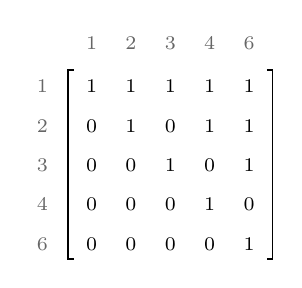
\begin{tikzpicture}[font=\scriptsize, x=0.5cm, y=0.5cm]
\foreach \l [count=\j] in {1,2,3,4,6} {\node[black!60, anchor=base] at (\j,-0.08) {$\l$}; \node[black!60, anchor=base] at (-0.25,-\j-0.18) {$\l$};}
\foreach \row [count=\i] in {{1,1,1,1,1},{0,1,0,1,1},{0,0,1,0,1},{0,0,0,1,0},{0,0,0,0,1}} {
  \foreach \e [count=\j] in \row {\node[anchor=base] at (\j,-\i-0.18) {$\e$};}}
\draw[line width=0.5pt] (0.55,-0.6) -- (0.4,-0.6) -- (0.4,-5.4) -- (0.55,-5.4);
\draw[line width=0.5pt] (5.45,-0.6) -- (5.6,-0.6) -- (5.6,-5.4) -- (5.45,-5.4);
\end{tikzpicture}}
\caption{Two pictures of the relation $a\mid b$ on $\{1,2,3,4,6\}$. (A) The directed graph: an arrow from $a$ to $b$ means that $a$ divides $b$; every element has a loop because the relation is reflexive. (B) The matrix: the entry in row $a$ and column $b$ is $1$ if $a\mid b$.}
\label{fig:relation}
\end{figure}

The properties of \cref{def:relation-properties} can be read off both pictures. A relation is reflexive when every point has a loop, or every diagonal entry of the matrix is $1$. It is symmetric when every arrow is matched by an arrow in the opposite direction, or the matrix is unchanged by reflecting it in its diagonal ($M_{ij}=M_{ji}$ for all $i$ and $j$; in the language of \vcref{2}{ch:vectors-matrices}, $M$ equals its transpose). It is antisymmetric when no two different points are joined by arrows in both directions, or $M_{ij}$ and $M_{ji}$ are never both $1$ for $i\ne j$. Transitivity is a condition on paths of two arrows: whenever there are arrows from $a$ to $b$ and from $b$ to $c$, there must be an arrow from $a$ to $c$. In \cref{fig:relation}A, the path $1\to2\to4$ is accompanied by the arrow $1\to4$, and so on for every such path.

The matrix makes transitivity mechanically checkable. The condition is a universal statement over three indices,
\[
\forall i,\ \forall j,\ \forall k,\ \bigl(M_{ij}=1\wedge M_{jk}=1\Rightarrow M_{ik}=1\bigr),
\]
and, as in \cref{sec:quantifiers}, a universal statement over a finite domain is a loop. \Cref{alg:transitive} nests three loops, one for each quantifier, and returns false as soon as it finds a counterexample. It examines at most $n^3$ triples of indices, and its correctness is a direct reading of the quantified condition: it returns true exactly when no triple violates the implication.

\begin{algorithm}
\begin{algorithmic}[1]
\Require the matrix $M$ of a relation on a set of $n$ elements, $M_{ij}\in\{0,1\}$
\Ensure true if the relation is transitive, false otherwise
\Name{IsTransitive}{M}
\For{$i\gets1$ \textbf{to} $n$}
  \For{$j\gets1$ \textbf{to} $n$}
    \If{$M_{ij}=1$} \Comment{only pairs $a_i\mathrel{R}a_j$ can start a path}
      \For{$k\gets1$ \textbf{to} $n$}
        \If{$M_{jk}=1$ \textbf{and} $M_{ik}=0$} \Comment{a counterexample}
          \State \Return false
        \EndIf
      \EndFor
    \EndIf
  \EndFor
\EndFor
\State \Return true
\end{algorithmic}
\caption{Testing a relation for transitivity. The three loops correspond to the three universal quantifiers in the definition.}
\label{alg:transitive}
\end{algorithm}

\subsection{Transitive Closure}

A relation that is not transitive can be made transitive by adding pairs. If $R$ records the direct flights between cities, then ``one can fly from $a$ to $b$, possibly with changes'' is a transitive relation that contains $R$, and it is the smallest such relation. The general construction uses intersections of families.

\begin{proposition}
\label{prop:transitive-closure}
Let $R$ be a relation on a set $A$.
\begin{enumerate}
\item The intersection of a nonempty family of transitive relations on $A$ is transitive.
\item The relation
\[
R^+\coloneqq\bigcap\{T\subseteq A\times A: T\text{ is transitive and }R\subseteq T\}
\]
is transitive, contains $R$, and is contained in every transitive relation that contains $R$.
\item $a\mathrel{R^+}b$ if and only if there are $k\ge1$ and elements $x_0,x_1,\ldots,x_k$ of $A$ with $x_0=a$, $x_k=b$ and $x_{i-1}\mathrel{R}x_i$ for $i=1,\ldots,k$.
\end{enumerate}
\end{proposition}

\begin{proof}
(i) Let $(T_i)_{i\in I}$ be the family, and suppose that $(a,b)$ and $(b,c)$ lie in $\bigcap_iT_i$. Then for every $i$ both pairs lie in $T_i$, so $(a,c)\in T_i$ by transitivity of $T_i$. Hence $(a,c)\in\bigcap_iT_i$.

(ii) The family is nonempty because $A\times A$ itself is a transitive relation containing $R$. By (i), $R^+$ is transitive. Each member of the family contains $R$, so their intersection does. Finally, every transitive $T\supseteq R$ is a member of the family and therefore contains the intersection.

(iii) Let $P$ be the relation described in (iii); we say that $a$ and $b$ are joined by a path. $P$ contains $R$ (take $k=1$), and it is transitive, since a path from $a$ to $b$ followed by a path from $b$ to $c$ is a path from $a$ to $c$. By (ii), $R^+\subseteq P$. Conversely, let $T$ be any transitive relation containing $R$. By induction on $k$, if $x_0,\ldots,x_k$ is a path, then $x_0\mathrel{T}x_k$: for $k=1$ this is $R\subseteq T$, and if $x_0\mathrel{T}x_k$ and $x_k\mathrel{R}x_{k+1}$, then $x_k\mathrel{T}x_{k+1}$ and transitivity give $x_0\mathrel{T}x_{k+1}$. Hence $P\subseteq T$ for every such $T$, so $P\subseteq R^+$.
\end{proof}

The relation $R^+$ is the \term{transitive closure} of $R$. Part (ii) is an instance of a pattern that recurs often: the smallest set with a property that is preserved by intersections is the intersection of all the sets with the property. Part (iii) is what makes the closure computable: in the picture of a directed graph, $a\mathrel{R^+}b$ means that $b$ can be reached from $a$ by following arrows. Warshall's algorithm computes the matrix of $R^+$ from that of $R$ with about $n^3$ steps~\cite{warshall1962}; it is closely related to the shortest-path algorithms of Volume~V.

\section{Equivalence Relations and Partitions}
\label{sec:equivalence}

Many classifications treat objects as ``the same'' in some respect while ignoring their other features: integers with the same remainder on division by $3$, fractions with the same value, rows of a table with the same key. The relations that express such sameness are the equivalence relations, and they correspond exactly to the ways of cutting a set into disjoint pieces.

\subsection{Equivalence Relations and Classes}

\begin{definition}[Equivalence relation, equivalence class]
\label{def:equivalence-relation}
An \term{equivalence relation} on a set $A$ is a relation on $A$ that is reflexive, symmetric and transitive. Equivalence relations are usually written $\sim$. For $a\in A$, the \term{equivalence class} of $a$ is
\[
[a]\coloneqq\{x\in A: x\sim a\},
\]
and $a$ is a \term{representative} of this class. The set of all equivalence classes is the \term{quotient set}
\[
A/{\sim}\coloneqq\{[a]: a\in A\}.
\]
\end{definition}

When several equivalence relations are in play we write $[a]_\sim$. According to \cref{tab:relation-properties}, equality on any set, congruence modulo $n$ on $\mathbb Z$ and the relation $x^2=y^2$ on $\mathbb R$ are equivalence relations. Under equality every class has a single element, $[a]=\{a\}$. Under $x^2=y^2$ the class of $x$ is $\{x,-x\}$, which has two elements if $x\ne0$ and one if $x=0$. Under congruence modulo $3$ there are three classes,
\begin{align*}
[0]&=\{\ldots,-6,-3,0,3,6,\ldots\}=3\mathbb Z,\\
[1]&=\{\ldots,-5,-2,1,4,7,\ldots\}=\{3k+1: k\in\mathbb Z\},\\
[2]&=\{\ldots,-4,-1,2,5,8,\ldots\}=\{3k+2: k\in\mathbb Z\},
\end{align*}
and every integer lies in exactly one of them; for example $[7]=[1]=[-2]$. That these three classes are all of them, and that they are different, follows from division with remainder, which \cref{ch:numbers} proves: every integer is $3k$, $3k+1$ or $3k+2$ for a unique choice of $k$ and of the remainder. The quotient set $\mathbb Z/{\equiv}$ for this relation is written $\mathbb Z/3\mathbb Z$; it has three elements, each of which is an infinite set of integers. For $n=2$ the two classes are the even and the odd integers, and \cref{prop:parity} is the statement that they cover $\mathbb Z$ without overlap.

The example suggests that distinct classes never overlap. This is true for every equivalence relation, and it is the basic fact about classes.

\begin{lemma}
\label{lem:classes}
Let $\sim$ be an equivalence relation on $A$, and let $a,b\in A$.
\begin{enumerate}
\item $a\in[a]$; in particular every class is nonempty.
\item $[a]=[b]$ if and only if $a\sim b$.
\item Either $[a]=[b]$ or $[a]\cap[b]=\emptyset$.
\end{enumerate}
\end{lemma}

\begin{proof}
(i) This is reflexivity.

(ii) If $[a]=[b]$, then $a\in[a]=[b]$ by (i), that is, $a\sim b$. Conversely, suppose $a\sim b$. If $x\in[a]$, then $x\sim a$ and $a\sim b$, so $x\sim b$ by transitivity, that is, $x\in[b]$; hence $[a]\subseteq[b]$. By symmetry $b\sim a$, and the same argument gives $[b]\subseteq[a]$.

(iii) Suppose $[a]\cap[b]\ne\emptyset$, and let $x$ be a common element. Then $x\sim a$ and $x\sim b$. By symmetry $a\sim x$, and by transitivity $a\sim b$, so $[a]=[b]$ by (ii).
\end{proof}

Part (ii) says that any element of a class can serve as its representative: the class does not depend on which of its elements is used to name it. All three properties of an equivalence relation were used, and each is needed. For the relation $|x-y|<1$ on $\mathbb R$, which is reflexive and symmetric but not transitive, the ``classes'' $[0]=(-1,1)$ and $[1]=(0,2)$ overlap without being equal.

\subsection{Partitions}

\begin{definition}[Partition]
\label{def:partition}
A \term{partition} of a set $A$ is a set $\mathcal B$ of subsets of $A$, called the \term{blocks} of the partition, such that
\begin{enumerate}
\item every block is nonempty;
\item different blocks are disjoint: if $B,B'\in\mathcal B$ and $B\ne B'$, then $B\cap B'=\emptyset$;
\item the blocks cover $A$: every element of $A$ lies in some block.
\end{enumerate}
\end{definition}

Conditions (ii) and (iii) together say that every element of $A$ lies in exactly one block. The even and the odd integers form a partition of $\mathbb Z$ with two blocks; the singletons $\{a\}$, $a\in A$, form a partition of $A$; and the intervals $[k,k+1)$, $k\in\mathbb Z$, form a partition of $\mathbb R$ into infinitely many blocks. (That every real number $x$ lies in one of these intervals, namely the one whose $k$ is the largest integer not exceeding $x$, rests on the Archimedean property of the real numbers proved in \cref{ch:numbers}.) The next theorem shows that equivalence relations and partitions are two descriptions of the same thing~\cite{halmos1960naive,enderton1977sets}. \Cref{fig:partition} shows the correspondence.

\begin{theorem}[Equivalence relations and partitions]
\label{thm:partition}
Let $A$ be a set.
\begin{enumerate}
\item If $\sim$ is an equivalence relation on $A$, then the quotient set $A/{\sim}$ is a partition of $A$.
\item If $\mathcal B$ is a partition of $A$, then the relation $\sim_{\mathcal B}$ defined by $a\sim_{\mathcal B}b$ if $a$ and $b$ lie in the same block is an equivalence relation on $A$, and its equivalence classes are the blocks of $\mathcal B$.
\item The two constructions are inverse to each other: the relation obtained in (ii) from the partition $A/{\sim}$ is $\sim$ itself, and the partition obtained in (i) from the relation $\sim_{\mathcal B}$ is $\mathcal B$ itself.
\end{enumerate}
\end{theorem}

\begin{proof}
(i) The classes are nonempty by \cref{lem:classes}\,(i), different classes are disjoint by \cref{lem:classes}\,(iii), and every $a\in A$ lies in the class $[a]$.

(ii) Every element lies in some block, so $a\sim_{\mathcal B}a$: the relation is reflexive. It is symmetric because ``$a$ and $b$ lie in the same block'' does not depend on the order of $a$ and $b$. For transitivity, suppose $a$ and $b$ lie in a block $B$, and $b$ and $c$ in a block $B'$. Then $b\in B\cap B'$, so $B=B'$ by condition (ii) of \cref{def:partition}, and $a$ and $c$ lie in the same block. Now let $a\in A$ and let $B$ be the block containing it. An element $x$ satisfies $x\sim_{\mathcal B}a$ if and only if $x$ lies in the block of $a$, that is, in $B$; so the class of $a$ is $B$. Hence every class is a block, and every block, being nonempty, is the class of any of its elements.

(iii) For the first claim, $a$ and $b$ lie in the same class of $\sim$ if and only if $[a]=[b]$, since each lies in its own class and classes are equal or disjoint; and $[a]=[b]$ holds if and only if $a\sim b$, by \cref{lem:classes}\,(ii). The second claim is the last statement of (ii).
\end{proof}

\begin{figure}
\sdpanel{A}{\begin{tikzpicture}[font=\scriptsize]
\coordinate (P) at (1.45,1.1); \coordinate (Q) at (3.05,1.2085); \coordinate (R) at (2.7,1.1847);
\fill[sdfill] (0,0) -- (1.4,0) -- (1.5,2.2) -- (0,2.2) -- cycle;
\fill[sdfill] (Q) -- (4.4,1.3) -- (4.4,2.2) -- (3.0,2.2) -- cycle;
\draw[line width=0.5pt] (0,0) rectangle (4.4,2.2);
\draw[line width=0.5pt] (1.4,0) -- (1.5,2.2);
\draw[line width=0.5pt] (P) -- (4.4,1.3);
\draw[line width=0.5pt] (Q) -- (3.0,2.2);
\draw[line width=0.5pt] (2.7,0) -- (R);
\foreach \p in {(0.4,0.5),(0.9,1.1),(0.5,1.7),(1.0,0.3)} {\fill \p circle (1.3pt);}
\foreach \p in {(2.0,1.7),(2.5,1.9),(1.9,1.5)} {\fill \p circle (1.3pt);}
\foreach \p in {(3.6,1.7),(4.0,1.9)} {\fill \p circle (1.3pt);}
\foreach \p in {(1.8,0.4),(2.2,0.8),(2.0,0.25)} {\fill \p circle (1.3pt);}
\foreach \p in {(3.2,0.6),(3.8,0.9),(3.5,0.3),(4.0,0.4)} {\fill \p circle (1.3pt);}
\end{tikzpicture}}\hfill
\sdpanel{B}{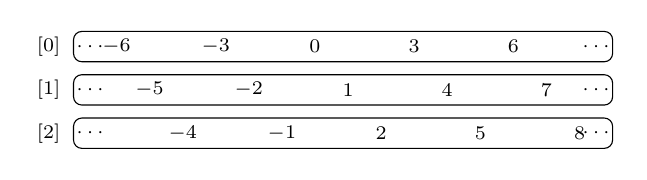
\begin{tikzpicture}[font=\scriptsize, x=0.42cm, y=0.55cm]
\foreach \r in {0,1,2} {
  \draw[line width=0.4pt, rounded corners=3pt] (-0.9,-\r-0.35) rectangle (15.4,-\r+0.35);
  \node[anchor=east] at (-1.0,-\r) {$[\r]$};
  \node at (-0.4,-\r) {$\cdots$};
  \node at (14.9,-\r) {$\cdots$};
  \foreach \c in {0,...,4} {\pgfmathtruncatemacro\v{3*\c-6+\r}\node at (\c*3+\r+0.4,-\r) {$\v$};}}
\end{tikzpicture}}
\caption{Partitions. (A) A set cut into five blocks; two of them are shaded. Each point lies in exactly one block, and ``lying in the same block'' is an equivalence relation whose classes are the blocks. (B) Congruence modulo $3$ partitions $\mathbb Z$ into the three classes $[0]$, $[1]$ and $[2]$; the integers increase from left to right, each in the row of its class.}
\label{fig:partition}
\end{figure}

\subsection{Functions on Quotient Sets}

Equivalence relations arise naturally from functions. If $f\colon A\to B$ is any function, declare two elements of $A$ equivalent when $f$ does not distinguish them:
\[
a\sim_f a'\iff f(a)=f(a').
\]
This relation is reflexive, symmetric and transitive because equality is. Its classes are the nonempty preimages $f^{-1}(\{b\})$, $b\in f(A)$, the sets of inputs that share an output. Congruence modulo $3$ is of this kind, with $f(n)$ the remainder of $n$ on division by $3$, and so is $x^2=y^2$, with $f(x)=x^2$. Conversely, every equivalence relation $\sim$ on $A$ arises in this way: the \term{canonical projection}
\[
\pi\colon A\to A/{\sim},\qquad\pi(a)\coloneqq[a],
\]
is surjective, and $\pi(a)=\pi(a')$ holds if and only if $a\sim a'$, by \cref{lem:classes}\,(ii). So $\sim$ is the relation $\sim_\pi$~\cite{halmos1960naive}.

Grouping the rows of a table by a key is exactly this construction: the key column is a function $f$ on the rows, the groups are the classes of $\sim_f$, and a summary of each group, such as the sum of a numerical column, is a function on the quotient set, as Volume~VIII describes.

Defining a function on a quotient set requires care, because a class has many names. Suppose we wish to define $\bar g\colon A/{\sim}\to C$ by the formula $\bar g([a])\coloneqq g(a)$ for some function $g\colon A\to C$. If $[a]=[a']$ with $a\ne a'$, the formula prescribes two values, $g(a)$ and $g(a')$, for the same class, and $\bar g$ is a function only if these values always agree, that is, if
\[
a\sim a'\Rightarrow g(a)=g(a').
\]
A definition that satisfies this condition is called \term{well defined}. For example, on $\mathbb Z/3\mathbb Z$ the rule $[a]\mapsto[a^2]$ is well defined: if $a\equiv a'\pmod3$, say $a'=a+3k$, then $a'^2-a^2=6ak+9k^2=3(2ak+3k^2)$, so $[a'^2]=[a^2]$. The rule $[a]\mapsto a^2$ into $\mathbb Z$ is not well defined, since $[1]=[4]$ but $1^2\ne4^2$. The following theorem uses the condition to show that every function is a composition of three simple ones.

\begin{theorem}[Factorisation of a function]
\label{thm:factorisation}
Let $f\colon A\to B$ be a function, $\sim_f$ the equivalence relation above, $\pi\colon A\to A/{\sim_f}$ the canonical projection and $\iota\colon f(A)\to B$ the inclusion of the range. The rule $\bar f([a])\coloneqq f(a)$ defines a bijection $\bar f\colon A/{\sim_f}\to f(A)$, and
\[
f=\iota\circ\bar f\circ\pi .
\]
\end{theorem}

\begin{proof}
\emph{Well defined.} If $[a]=[a']$, then $a\sim_fa'$, that is, $f(a)=f(a')$. So the value $\bar f([a])$ does not depend on the representative, and $\bar f$ is a function from $A/{\sim_f}$ to $f(A)$.

\emph{Injective.} If $\bar f([a])=\bar f([a'])$, then $f(a)=f(a')$, so $a\sim_fa'$ and $[a]=[a']$.

\emph{Surjective.} Every element of $f(A)$ is $f(a)=\bar f([a])$ for some $a\in A$.

\emph{Factorisation.} For every $a\in A$, $(\iota\circ\bar f\circ\pi)(a)=\iota(\bar f([a]))=f(a)$.
\end{proof}

The theorem says that a function does three things in turn: it merges the inputs it cannot tell apart (the surjection $\pi$), it relabels the resulting classes in a one-to-one manner (the bijection $\bar f$), and it places the labels inside a possibly larger codomain (the injection $\iota$). Versions of this factorisation appear in linear algebra, where it underlies the rank--nullity theorem of \vcref{2}{ch:linear-maps}, and in algebra generally.

\subsection{Constructing Numbers as Classes}

Equivalence classes also serve to construct new mathematical objects. The fractions $1/2$, $2/4$ and $(-3)/(-6)$ are different expressions of the same rational number. This suggests defining a rational number as a class of pairs of integers. On the set $\mathbb Z\times(\mathbb Z\setminus\{0\})$ of pairs $(p,q)$ with $q\ne0$, define
\[
(p,q)\sim(r,s)\iff ps=qr .
\]
The condition says that $p/q=r/s$, but it is written without division, so that it uses only the arithmetic of integers.

\begin{proposition}
\label{prop:fractions}
The relation $\sim$ on $\mathbb Z\times(\mathbb Z\setminus\{0\})$ is an equivalence relation.
\end{proposition}

\begin{proof}
Reflexivity: $pq=qp$. Symmetry: if $ps=qr$, then $rq=sp$. Transitivity: suppose $(p,q)\sim(r,s)$ and $(r,s)\sim(t,u)$, that is, $ps=qr$ and $ru=st$. Multiplying the first equation by $u$ and using the second,
\[
psu=qru=qst ,
\]
so $s(pu-qt)=0$. Since $s\ne0$, it follows that $pu=qt$, which is $(p,q)\sim(t,u)$.
\end{proof}

The proof used the hypothesis $s\ne0$, and this is why pairs with second component $0$ were excluded: if the pair $(0,0)$ were allowed, then $(1,1)\sim(0,0)$ and $(0,0)\sim(0,1)$ would hold, since every product involving the pair $(0,0)$ vanishes, while $(1,1)\sim(0,1)$ fails. A rational number can be \emph{defined} as an equivalence class $[(p,q)]$, and addition and multiplication of classes by
\[
[(p,q)]+[(r,s)]\coloneqq[(ps+qr,qs)],\qquad[(p,q)]\cdot[(r,s)]\coloneqq[(pr,qs)],
\]
after checking that these definitions are well defined. \Cref{ch:numbers} returns to this construction.

\section{Orders}
\label{sec:orders}

Sorting a list, finding the largest entry, choosing the best solution: all of these presuppose a way of comparing elements. The relations that make comparison precise are the orders~\cite{daveypriestley2002}.

\subsection{Partial and Total Orders}

\begin{definition}[Partial order, total order]
\label{def:order}
A \term{partial order} on a set $P$ is a relation $\le$ on $P$ that is reflexive, antisymmetric and transitive. The pair $(P,\le)$ is a \term{partially ordered set}, or \term{poset}. Two elements $a$ and $b$ are \term{comparable} if $a\le b$ or $b\le a$. A partial order in which every two elements are comparable is a \term{total order}, or linear order, and $(P,\le)$ is then a \term{totally ordered set}.
\end{definition}

We use the symbol $\le$ for an arbitrary partial order, write $b\ge a$ for $a\le b$, and write $a<b$ for ``$a\le b$ and $a\ne b$''. By \cref{tab:relation-properties}, the usual order $\le$ on $\mathbb R$ (and on its subsets $\mathbb N$, $\mathbb Z$, $\mathbb Q$) is a partial order, and it is total. Divisibility on $\mathbb N$ and inclusion on $\mathcal P(X)$ are partial orders that are not total: $2$ and $3$ are incomparable under divisibility, since neither divides the other, and $\{1\}$ and $\{2\}$ are incomparable under inclusion. Partial orders that are not total are common. Two tasks in a project, one of which must be finished before the other can begin, are comparable, while two independent tasks are not; vectors in $\mathbb R^2$ compared component by component, $(x_1,y_1)\le(x_2,y_2)$ if $x_1\le x_2$ and $y_1\le y_2$, are not always comparable either.

The strict relation $<$ has its own characterisation, and either of $\le$ and $<$ determines the other.

\begin{proposition}
\label{prop:strict-order}
Let $\le$ be a partial order on $P$ and define $a<b$ if $a\le b$ and $a\ne b$. Then $<$ is \term{irreflexive} (no $a$ satisfies $a<a$) and transitive, and $a\le b$ holds if and only if $a<b$ or $a=b$. Conversely, if $<$ is an irreflexive and transitive relation on $P$, then ``$a<b$ or $a=b$'' defines a partial order on $P$.
\end{proposition}

\begin{proof}
Irreflexivity is immediate from the definition. For transitivity, let $a<b$ and $b<c$. Then $a\le b$ and $b\le c$, so $a\le c$. If $a=c$, then $a\le b$ and $b\le a$, so $a=b$ by antisymmetry, contradicting $a<b$; hence $a\ne c$ and $a<c$. The description of $\le$ in terms of $<$ is the law of excluded middle applied to $a=b$.

For the converse, let $a\le b$ mean ``$a<b$ or $a=b$''. Reflexivity is clear. For antisymmetry, suppose $a\le b$, $b\le a$ and $a\ne b$; then $a<b$ and $b<a$, so $a<a$ by transitivity, which is impossible. For transitivity, if $a\le b$ and $b\le c$, then $a=b$ or $b=c$ gives $a\le c$ at once, and otherwise $a<b<c$ gives $a<c$.
\end{proof}

An irreflexive and transitive relation is called a \term{strict partial order}. In a total order, \term{trichotomy} holds: for every $a$ and $b$ exactly one of $a<b$, $a=b$ and $b<a$ is true.

\subsection{Hasse Diagrams}

The directed graph of a partial order on a finite set, as in \cref{fig:relation}A, is cluttered: every element has a loop, and with arrows from $a$ to $b$ and from $b$ to $c$ there is always an arrow from $a$ to $c$. Since reflexivity and transitivity are known in advance, these arrows carry no information. A \term{Hasse diagram}, named after Helmut Hasse~\cite{daveypriestley2002}, omits them. We say that $b$ \term{covers} $a$ if $a<b$ and there is no $c$ with $a<c<b$. The Hasse diagram draws the elements as points, places $b$ higher than $a$ whenever $a<b$, and joins $a$ and $b$ by a line exactly when $b$ covers $a$. Then $a<b$ holds if and only if one can climb from $a$ to $b$ along lines, always going upwards. \Cref{fig:hasse} shows three examples. In panel C, which is the order of \cref{fig:relation}, the seven arrows between different elements are reduced to five lines, and the loops are gone.

\begin{figure}
\tikzset{hv/.style={circle, fill=black, inner sep=0pt, minimum size=3.4pt},
  hl/.style={line width=0.5pt}}
\sdpanel{A}{\begin{tikzpicture}[font=\scriptsize]
\node[hv, label=below:$1$] (1) at (0,0) {};
\node[hv, label=left:$2$] (2) at (-0.6,0.85) {};
\node[hv, label=right:$3$] (3) at (0.6,0.85) {};
\node[hv, label=left:$4$] (4) at (-1.2,1.7) {};
\node[hv, label=right:$6$] (6) at (0,1.7) {};
\node[hv, label=above:$12$] (12) at (-0.6,2.55) {};
\draw[hl] (1)--(2) (1)--(3) (2)--(4) (2)--(6) (3)--(6) (4)--(12) (6)--(12);
\end{tikzpicture}}\hfill
\sdpanel{B}{\begin{tikzpicture}[font=\scriptsize]
\node[hv, label={below:$\emptyset$}] (e) at (0,0) {};
\node[hv, label={left:$\{1\}$}] (a) at (-1.3,0.85) {};
\node[hv, label={[fill=white, inner sep=0.5pt]right:$\{2\}$}] (b) at (0,0.85) {};
\node[hv, label={right:$\{3\}$}] (c) at (1.3,0.85) {};
\node[hv, label={left:$\{1,2\}$}] (ab) at (-1.3,1.7) {};
\node[hv, label={[fill=white, inner sep=0.5pt]right:$\{1,3\}$}] (ac) at (0,1.7) {};
\node[hv, label={right:$\{2,3\}$}] (bc) at (1.3,1.7) {};
\node[hv, label={above:$\{1,2,3\}$}] (abc) at (0,2.55) {};
\draw[hl] (e)--(a) (e)--(b) (e)--(c) (a)--(ab) (a)--(ac) (b)--(ab) (b)--(bc) (c)--(ac) (c)--(bc) (ab)--(abc) (ac)--(abc) (bc)--(abc);
\end{tikzpicture}}\hfill
\sdpanel{C}{\begin{tikzpicture}[font=\scriptsize]
\node[hv, label=below:$1$] (1) at (0,0) {};
\node[hv, label=left:$2$] (2) at (-0.6,0.85) {};
\node[hv, label=right:$3$] (3) at (0.6,0.85) {};
\node[hv, label=left:$4$] (4) at (-1.2,1.7) {};
\node[hv, label=right:$6$] (6) at (0,1.7) {};
\draw[hl] (1)--(2) (1)--(3) (2)--(4) (2)--(6) (3)--(6);
\path (0,2.55) -- (0,2.75);
\end{tikzpicture}}
\caption{Hasse diagrams. (A) The divisors of $12$ ordered by divisibility. (B) The subsets of $\{1,2,3\}$ ordered by inclusion; the diagram is a cube. (C) The divisors of $12$ other than $12$ itself: there are two maximal elements, $4$ and $6$, and no greatest element.}
\label{fig:hasse}
\end{figure}

\subsection{Greatest, Maximal, and Bounds}

\begin{definition}[Greatest and maximal elements]
\label{def:maximal}
Let $(P,\le)$ be a poset and $S\subseteq P$.
\begin{enumerate}
\item An element $g\in S$ is the \term{greatest element}, or \term{maximum}, of $S$ if $s\le g$ for every $s\in S$. The \term{least element}, or \term{minimum}, is defined with $\ge$ in place of $\le$. We write $\max S$ and $\min S$.
\item An element $m\in S$ is a \term{maximal element} of $S$ if no element of $S$ is strictly greater: there is no $s\in S$ with $m<s$. \term{Minimal elements} are defined in the same way.
\end{enumerate}
\end{definition}

The difference between ``greatest'' and ``maximal'' is the difference between ``above everything'' and ``below nothing''. In \cref{fig:hasse}C the elements $4$ and $6$ are both maximal, since nothing lies above either of them, but neither is greatest, since they are incomparable. In \cref{fig:hasse}A the element $12$ is greatest. The set $\mathcal P(X)$ ordered by inclusion has the greatest element $X$ and the least element $\emptyset$. In the totally ordered set $\mathbb R$ the interval $[0,1)$ has the least element $0$ but neither a greatest nor a maximal element: for every $x\in[0,1)$, the number $(x+1)/2$ lies in $[0,1)$ and is larger than $x$.

\begin{proposition}
\label{prop:maximal}
Let $(P,\le)$ be a poset and $S\subseteq P$.
\begin{enumerate}
\item $S$ has at most one greatest element.
\item A greatest element of $S$ is maximal, and it is the only maximal element of $S$.
\item If $\le$ is a total order, every maximal element of $S$ is greatest.
\item If $S$ is finite and nonempty, $S$ has at least one maximal element and at least one minimal element.
\end{enumerate}
\end{proposition}

\begin{proof}
(i) If $g$ and $g'$ are greatest, then $g'\le g$ and $g\le g'$, so $g=g'$ by antisymmetry.

(ii) Let $g$ be greatest, and suppose $g<s$ for some $s\in S$. Since also $s\le g$, antisymmetry gives $s=g$, contradicting $g<s$; so $g$ is maximal. If $m$ is any maximal element, then $m\le g$, and $m<g$ is impossible by maximality, so $m=g$.

(iii) Let $m$ be maximal and $s\in S$. By totality, $s\le m$ or $m\le s$. In the second case $m<s$ is excluded by maximality, so $m=s$, and $s\le m$ holds in either case.

(iv) We prove the claim for maximal elements by induction on the number $n\ge1$ of elements of $S$; the claim for minimal elements follows by exchanging $\le$ and $\ge$. If $n=1$, the only element is maximal. Let $S$ have $n+1$ elements, choose $x\in S$ and put $S'\coloneqq S\setminus\{x\}$, which has $n$ elements and, by the inductive hypothesis, a maximal element $m'$. If $m'<x$ does not hold, then $m'$ is maximal in $S$: an element $s\in S$ with $m'<s$ would have to be $x$, as $m'$ is maximal in $S'$. If $m'<x$, then $x$ is maximal in $S$: if $x<s$ for some $s\in S$, then $s\ne x$, so $s\in S'$, and $m'<x<s$ contradicts the maximality of $m'$ in $S'$.
\end{proof}

Part (iv) has a useful consequence. A task schedule is a partial order on a finite set of tasks, and a valid sequence in which to perform the tasks is a total order that is compatible with it. Such a sequence always exists.

\begin{theorem}[Linear extensions]
\label{thm:linear-extension}
Let $\le$ be a partial order on a finite set $P$ with $n$ elements. Then the elements of $P$ can be listed as $p_1,p_2,\ldots,p_n$ in such a way that $p_i<p_j$ implies $i<j$.
\end{theorem}

\begin{proof}
We use induction on $n$; for $n=0$ the empty list will do. Let $P$ have $n+1$ elements. By \cref{prop:maximal}\,(iv), $P$ has a minimal element; call it $p_1$. The set $P\setminus\{p_1\}$, with the same order, has $n$ elements, and by the inductive hypothesis it can be listed as $p_2,\ldots,p_{n+1}$ with the required property. In the combined list, suppose $p_i<p_j$. If $i,j\ge2$, then $i<j$ by the construction of the shorter list. The case $j=1$ is impossible, because $p_1$ is minimal. If $i=1$, then $j\ne1$, since $p_1<p_1$ is false, so $1<j$.
\end{proof}

Listing the elements as in the theorem defines a total order that extends the given partial order. For the divisors of $12$ in \cref{fig:hasse}A, both $1,2,3,4,6,12$ and $1,3,2,6,4,12$ are such lists. Szpilrajn proved that every partial order, even on an infinite set, can be extended to a total order~\cite{szpilrajn1930}; for infinite sets the proof needs the axiom of choice. The proof above is an algorithm in disguise: repeatedly remove a minimal element. Its efficient implementation is called \term{topological sorting}, and Volume~V presents it as an algorithm on directed graphs.

Maximal and greatest elements are found inside a set. Bounds may lie outside it.

\begin{definition}[Bounds, supremum, infimum]
\label{def:sup}
Let $(P,\le)$ be a poset and $S\subseteq P$. An element $u\in P$ is an \term{upper bound} of $S$ if $s\le u$ for every $s\in S$, and a \term{lower bound} if $u\le s$ for every $s\in S$. The set $S$ is \term{bounded above} if it has an upper bound, and \term{bounded below} if it has a lower bound. If the set of upper bounds of $S$ has a least element, this element is the \term{supremum}, or least upper bound, of $S$, written $\sup S$. If the set of lower bounds has a greatest element, it is the \term{infimum}, or greatest lower bound, written $\inf S$.
\end{definition}

By \cref{prop:maximal}\,(i), a set has at most one supremum and at most one infimum, which justifies the notation. If $S$ has a greatest element $g$, then $g$ is an upper bound that belongs to $S$, so every upper bound $u$ satisfies $g\le u$, and $g=\sup S$. The supremum is the right replacement for the maximum when the maximum does not exist.

\begin{proposition}
\label{prop:sup-interval}
In $\mathbb R$ with its usual order, $\sup{[0,1)}=1$, although $[0,1)$ has no greatest element.
\end{proposition}

\begin{proof}
The number $1$ is an upper bound of $[0,1)$. Let $u$ be any upper bound; we show $1\le u$. Suppose, for a contradiction, that $u<1$. Since $0\in[0,1)$, we have $u\ge0$. The number $x\coloneqq(u+1)/2$ satisfies $0\le u<x<1$, so $x\in[0,1)$, and $x>u$ contradicts the assumption that $u$ is an upper bound. Hence $1$ is the least upper bound. We showed above that $[0,1)$ has no greatest element.
\end{proof}

In other posets the supremum takes other forms. In $\mathcal P(X)$ ordered by inclusion, $\sup\{A,B\}=A\cup B$ and $\inf\{A,B\}=A\cap B$, because $A\cup B$ contains both $A$ and $B$ and is contained in every set that contains both, and dually for $A\cap B$. In $\mathbb N$ ordered by divisibility, $\inf\{4,6\}=2$ and $\sup\{4,6\}=12$: the lower bounds of $\{4,6\}$ are the common divisors $1$ and $2$, and the upper bounds are the common multiples $0,12,24,\ldots$, among which $12$ divides all the others. In general the infimum and supremum of two natural numbers under divisibility are their greatest common divisor and least common multiple, as \cref{ch:numbers} shows. In this order $0$ is the greatest element of $\mathbb N$, since every natural number divides $0$.

A supremum need not exist. In $\mathbb Q$ with its usual order, the set $\{q\in\mathbb Q: q^2<2\}$ is bounded above, for instance by $2$, but it has no least upper bound in $\mathbb Q$: the candidate would be $\sqrt2$, which is not rational. The property that distinguishes $\mathbb R$ from $\mathbb Q$ is precisely that every nonempty subset of $\mathbb R$ that is bounded above has a supremum in $\mathbb R$. This is the completeness axiom. \Cref{ch:numbers} bases the theory of the real numbers on it, and much of calculus rests on it.

\subsection{Lexicographic Order}

Dictionaries order words by their first letter, words with the same first letter by their second letter, and so on. The same principle orders pairs and tuples.

\begin{definition}[Lexicographic order]
\label{def:lex}
Let $(A,\le_A)$ and $(B,\le_B)$ be posets. The \term{lexicographic order} on $A\times B$ is defined by
\[
(a,b)\le_{\mathrm{lex}}(a',b')\iff a<_Aa'\ \vee\ \bigl(a=a'\wedge b\le_Bb'\bigr).
\]
\end{definition}

The first components decide, and the second components are consulted only when the first components are equal. For example, in $\mathbb N\times\mathbb N$,
\[
(0,5)<_{\mathrm{lex}}(1,0)<_{\mathrm{lex}}(1,3)<_{\mathrm{lex}}(2,0).
\]

\begin{proposition}
\label{prop:lex}
If $\le_A$ and $\le_B$ are partial orders, then $\le_{\mathrm{lex}}$ is a partial order on $A\times B$. If both are total, so is $\le_{\mathrm{lex}}$.
\end{proposition}

\begin{proof}
Reflexivity: $(a,b)\le_{\mathrm{lex}}(a,b)$ because $a=a$ and $b\le_Bb$.

Antisymmetry: suppose $(a,b)\le_{\mathrm{lex}}(a',b')$ and $(a',b')\le_{\mathrm{lex}}(a,b)$. If $a\ne a'$, the two relations would give $a<_Aa'$ and $a'<_Aa$, hence $a<_Aa$ by \cref{prop:strict-order}, which is impossible. So $a=a'$, and then $b\le_Bb'$ and $b'\le_Bb$ give $b=b'$.

Transitivity: suppose $(a,b)\le_{\mathrm{lex}}(a',b')$ and $(a',b')\le_{\mathrm{lex}}(a'',b'')$. Then $a\le_Aa'\le_Aa''$, so $a\le_Aa''$. If $a<_Aa''$, we are done. Otherwise $a=a''$, and antisymmetry applied to $a\le_Aa'\le_Aa''=a$ gives $a=a'=a''$. Then both relations are decided by the second components, $b\le_Bb'\le_Bb''$, and $(a,b)\le_{\mathrm{lex}}(a'',b'')$.

Totality: let $(a,b)$ and $(a',b')$ be given, with $\le_A$ and $\le_B$ total. By trichotomy in $A$, either $a<_Aa'$, or $a'<_Aa$, or $a=a'$. In the first two cases the pairs are comparable by their first components, and in the third by their second components, which are comparable because $\le_B$ is total.
\end{proof}

The lexicographic order extends to $n$-tuples: compare the first components, then the second, and so on, stopping at the first position where the tuples differ. It extends also to \term{words}, the finite sequences of letters from an ordered alphabet, with the convention that a word comes before every longer word that begins with it; thus ``set'' $<$ ``sets'' $<$ ``setting''. This is the order in which computers sort strings, and it is the order used when a table is sorted by several columns: the rows are compared by the first key, ties are broken by the second key, and so on~\cite{knuth1998taocp3}. Volumes~VII and~VIII rely on it. Sorting rows by a key is, strictly speaking, sorting by a relation that is not antisymmetric: two different rows with the same key are tied. The relation ``the key of $r$ is at most the key of $r'$'' is reflexive, transitive and total but not antisymmetric, and such a relation is called a \term{total preorder}. The ties are exactly the classes of the equivalence relation ``has the same key'' of \cref{sec:equivalence}.

\subsection{Well-Orders}

\begin{definition}[Well-order]
\label{def:well-order}
A total order $\le$ on a set $P$ is a \term{well-order} if every nonempty subset of $P$ has a least element.
\end{definition}

The well-ordering principle (\cref{thm:well-ordering}) states that $\mathbb N$ with its usual order is well-ordered, and this property is what makes induction and the method of the smallest counterexample work. The usual order on $\mathbb Z$ is not a well-order, since $\mathbb Z$ itself has no least element; nor is the usual order on $[0,1]$, since the subset $(0,1]$ has no least element. Every finite totally ordered set is well-ordered: by \cref{prop:maximal}\,(iv) a nonempty subset has a minimal element, and by \cref{prop:maximal}\,(iii), applied with $\ge$ in place of $\le$, a minimal element of a totally ordered set is its least element.

\begin{proposition}
\label{prop:lex-well-order}
If $\le_A$ and $\le_B$ are well-orders, then the lexicographic order on $A\times B$ is a well-order. In particular $\mathbb N\times\mathbb N$ is well-ordered lexicographically.
\end{proposition}

\begin{proof}
By \cref{prop:lex}, $\le_{\mathrm{lex}}$ is a total order. Let $S\subseteq A\times B$ be nonempty. The set $S_1\coloneqq\{a\in A:\exists b\in B,\ (a,b)\in S\}$ of first components is nonempty, so it has a least element $a_0$. The set $S_2\coloneqq\{b\in B: (a_0,b)\in S\}$ is nonempty, by the choice of $a_0$, so it has a least element $b_0$. We claim that $(a_0,b_0)$ is the least element of $S$. It lies in $S$. Let $(a,b)\in S$. Then $a\in S_1$, so $a_0\le_Aa$. If $a_0<_Aa$, then $(a_0,b_0)<_{\mathrm{lex}}(a,b)$. If $a=a_0$, then $b\in S_2$, so $b_0\le_Bb$ and $(a_0,b_0)\le_{\mathrm{lex}}(a,b)$.
\end{proof}

The lexicographic well-order on $\mathbb N\times\mathbb N$ differs from that of $\mathbb N$ in an instructive way. The element $(1,0)$ is preceded by infinitely many elements, all the pairs $(0,n)$, whereas every natural number has only finitely many predecessors. A loop that decreases a pair $(a,b)\in\mathbb N^2$ lexicographically at every pass must stop, by the argument of \cref{prop:tobinary} with \cref{prop:lex-well-order} in place of \cref{thm:well-ordering}, even though $b$ may increase without bound whenever $a$ decreases. Termination proofs of this kind appear in Volume~V.

\subsection{Comparisons That Are Not Orders}

Algorithms that sort, search or find a maximum use only comparisons, and they assume that the comparison is a total order, or at least a total preorder. When this assumption fails, they fail too, often silently. Suppose a list contains the numbers $3$ and $1$ and a special value $u$ that, by convention, is neither smaller nor larger than any number and not equal to any number either. Consider the list $(3,u,1)$. A test that a list is sorted typically checks only adjacent entries. Here $u<3$ is false and $1<u$ is false, so no adjacent pair is out of order, and the test accepts the list, although $3>1$. The test is valid only if from ``$3$ is not greater than $u$'' and ``$u$ is not greater than $1$'' one may conclude ``$3$ is not greater than $1$''. That conclusion relies on the transitivity of the relation ``is not greater than'', and transitivity fails once $u$ is present. Depending on the order of the input, a sorting algorithm may therefore leave $3$ before $1$ or after it, and different algorithms disagree. Floating-point arithmetic contains a value with exactly this behaviour, as Volume~VI explains, and Volume~VII describes how sorting routines treat it to obtain a well-defined result.

\section{Cardinality}
\label{sec:cardinality}

To count the elements of a finite set is to pair them off with the numbers $1,2,\ldots,n$, or, in the convention of this series, with $0,1,\ldots,n-1$. In the language of \cref{sec:injections}, counting is the construction of a bijection. This point of view, due to Cantor, makes sense for infinite sets as well, and it leads to the discovery that infinite sets come in different sizes~\cite{cantor1874,cantor1891}.

\subsection{Equinumerous Sets}

\begin{definition}[Equinumerous sets]
\label{def:equinumerous}
Sets $A$ and $B$ are \term{equinumerous}, or have the same \term{cardinality}, written $|A|=|B|$, if there is a bijection from $A$ to $B$.
\end{definition}

The notation $|A|=|B|$ does not presuppose that $|A|$ is a number; it is a statement about $A$ and $B$, defined as a whole. It behaves like an equality.

\begin{proposition}
\label{prop:equinumerous}
For all sets $A$, $B$ and $C$: $|A|=|A|$; if $|A|=|B|$, then $|B|=|A|$; and if $|A|=|B|$ and $|B|=|C|$, then $|A|=|C|$.
\end{proposition}

\begin{proof}
The identity $\operatorname{id}_A$ is a bijection. If $f\colon A\to B$ is a bijection, so is $f^{-1}\colon B\to A$, by \cref{thm:inverse}. If $f\colon A\to B$ and $g\colon B\to C$ are bijections, so is $g\circ f$, by \cref{prop:composition-injective}\,(iii).
\end{proof}

For infinite sets the definition has unexpected consequences. The map $n\mapsto n+1$ is a bijection from $\mathbb N$ to $\mathbb N\setminus\{0\}$, and $n\mapsto2n$ is a bijection from $\mathbb N$ to the even natural numbers. So $\mathbb N$ has as many elements as some of its proper subsets, something that no finite set can do, as we show below. Dedekind took this property as the definition of an infinite set~\cite{dedekind1888}. Intervals of real numbers give another example. For real numbers $a<b$, the map $x\mapsto(2x-a-b)/(b-a)$ is a bijection from $(a,b)$ to $(-1,1)$, with inverse $y\mapsto\bigl((b-a)y+a+b\bigr)/2$. More surprisingly, the open interval $(-1,1)$ is equinumerous with the whole real line:
\[
\varphi\colon(-1,1)\to\mathbb R,\qquad\varphi(x)\coloneqq\frac{x}{1-|x|},
\]
is a bijection. To prove this with \cref{thm:inverse}, consider $\psi\colon\mathbb R\to(-1,1)$, $\psi(y)\coloneqq y/(1+|y|)$, which indeed takes values in $(-1,1)$ because $|\psi(y)|=|y|/(1+|y|)<1$. For $y\in\mathbb R$ we have $1-|\psi(y)|=1/(1+|y|)$, and therefore $\varphi(\psi(y))=(y/(1+|y|))\cdot(1+|y|)=y$. For $x\in(-1,1)$ we have $1+|\varphi(x)|=1/(1-|x|)$, and therefore $\psi(\varphi(x))=x$. So $\psi$ is an inverse of $\varphi$. Hence every open interval, however short, has as many points as the whole line.

\subsection{Finite Sets}

\begin{definition}[Finite and infinite sets]
\label{def:finite}
A set $A$ is \term{finite} with $n$ elements, for $n\in\mathbb N$, if $|A|=|\{0,1,\ldots,n-1\}|$; we then write $|A|=n$. (For $n=0$ the set $\{0,\ldots,n-1\}$ is empty.) A set that is not finite is \term{infinite}.
\end{definition}

For this definition to be sensible, a set must not have two different numbers of elements. This, and much more, follows from the next lemma~\cite{hrbacek1999}, which is a form of the pigeonhole principle of \cref{ch:counting}: $m$ pigeons cannot be placed in $n<m$ holes, one pigeon per hole.

\begin{lemma}
\label{lem:pigeonhole}
Let $m,n\in\mathbb N$. If there is an injection from $\{0,\ldots,m-1\}$ to $\{0,\ldots,n-1\}$, then $m\le n$.
\end{lemma}

\begin{proof}
We use induction on $n$; the statement $P(n)$ is ``for every $m\in\mathbb N$, if there is an injection from $\{0,\ldots,m-1\}$ to $\{0,\ldots,n-1\}$, then $m\le n$''. For $n=0$ the codomain is empty, and a function into the empty set exists only on the empty domain, so $m=0$.

Assume $P(n)$, and let $f$ be an injection from $\{0,\ldots,m-1\}$ to $\{0,\ldots,n\}$. If $m=0$, then $m\le n+1$. Otherwise, let $\tau$ be the permutation of $\{0,\ldots,n\}$ that exchanges $f(m-1)$ and $n$ and fixes every other element (the identity if $f(m-1)=n$), and put $h\coloneqq\tau\circ f$. Then $h$ is injective by \cref{prop:composition-injective}\,(i), and $h(m-1)=n$. For $i<m-1$, injectivity gives $h(i)\ne h(m-1)=n$, so the restriction of $h$ to $\{0,\ldots,m-2\}$ is an injection into $\{0,\ldots,n-1\}$. By $P(n)$, $m-1\le n$, that is, $m\le n+1$.
\end{proof}

\begin{corollary}
\label{cor:finite}
\leavevmode
\begin{enumerate}
\item If $|A|=m$ and $|A|=n$, then $m=n$.
\item The set $\mathbb N$ is infinite.
\item Let $A$ be finite. A function $f\colon A\to A$ is injective if and only if it is surjective.
\end{enumerate}
\end{corollary}

\begin{proof}
(i) Composing a bijection from $\{0,\ldots,m-1\}$ to $A$ with a bijection from $A$ to $\{0,\ldots,n-1\}$ gives a bijection, so $m\le n$ by \cref{lem:pigeonhole}; by symmetry $n\le m$.

(ii) Suppose $g\colon\mathbb N\to\{0,\ldots,n-1\}$ were a bijection for some $n$. Its restriction to $\{0,\ldots,n\}$ would be an injection into $\{0,\ldots,n-1\}$, so $n+1\le n$ by \cref{lem:pigeonhole}, which is false.

(iii) Let $|A|=n$. Transporting $f$ along a bijection between $A$ and $\{0,\ldots,n-1\}$ does not change injectivity or surjectivity, by \cref{prop:composition-injective}, so we may assume $A=\{0,\ldots,n-1\}$, and we may assume $n\ge1$, as the case $n=0$ is trivial. Suppose $f$ is injective but not surjective, and let $b$ be an element not in its range. Let $\tau$ exchange $b$ and $n-1$. Then $\tau\circ f$ is injective and never takes the value $n-1$, so it is an injection from $\{0,\ldots,n-1\}$ to $\{0,\ldots,n-2\}$, which contradicts \cref{lem:pigeonhole}. Hence injective functions are surjective. Now suppose $f$ is surjective. Let $g(b)$ be the least element of $f^{-1}(\{b\})$; then $f\circ g=\operatorname{id}_A$, so $g$ is injective by \cref{prop:composition-injective}\,(iv), hence surjective by what we have just proved, hence bijective. Then $f=f\circ g\circ g^{-1}=g^{-1}$ is bijective, in particular injective.
\end{proof}

In particular, a finite set $A$ is never equinumerous with a proper subset $B\subset A$, as promised above: a bijection from $A$ to $B$, regarded as a function from $A$ to $A$, would be injective but not surjective, contradicting (iii). Part (iii) fails for infinite sets: $n\mapsto n+1$ is an injection of $\mathbb N$ into itself that is not surjective, and the halving function of \cref{sec:injections} is a surjection that is not injective. Part (iii) is often used to establish bijectivity with half the work, and Volume~II uses its linear-algebra analogue for square matrices.

\subsection{Countable Sets}

\begin{definition}[Countable and uncountable sets]
\label{def:countable}
A set $A$ is \term{countably infinite} if $|A|=|\mathbb N|$, \term{countable} if it is finite or countably infinite, and \term{uncountable} if it is not countable.
\end{definition}

A countably infinite set is one whose elements can be arranged in an infinite list $a_0,a_1,a_2,\ldots$ in which every element appears exactly once: the bijection $f\colon\mathbb N\to A$ is the list, with $a_n=f(n)$. The examples above show that $\mathbb N\setminus\{0\}$ and the even natural numbers are countably infinite. Every subset of $\mathbb N$ is countable, and the proof shows how to list it.

\begin{lemma}
\label{lem:subset-n}
Every subset $S$ of $\mathbb N$ is countable. More precisely, either $S$ is finite, or the elements of $S$ in increasing order $a_0<a_1<a_2<\cdots$ form a bijection $k\mapsto a_k$ from $\mathbb N$ to $S$.
\end{lemma}

\begin{proof}
Define $a_0,a_1,\ldots$ recursively: as long as the set $S_k\coloneqq S\setminus\{a_0,\ldots,a_{k-1}\}$ is nonempty, let $a_k$ be its least element, which exists by \cref{thm:well-ordering}. If $S_k=\emptyset$ for some $k$, then $S=\{a_0,\ldots,a_{k-1}\}$, and since the $a_i$ are different by construction, $i\mapsto a_i$ is a bijection from $\{0,\ldots,k-1\}$ to $S$; so $S$ is finite.

Otherwise $a_k$ is defined for every $k\in\mathbb N$. Since $a_{k+1}\in S_{k+1}\subseteq S_k$ and $a_k=\min S_k$, we have $a_k\le a_{k+1}$, and $a_k\ne a_{k+1}$ by construction; so $a_k<a_{k+1}$. Hence $k\mapsto a_k$ is strictly increasing and in particular injective, and $a_k\ge k$ for every $k$, by induction. For surjectivity, let $s\in S$ and suppose that $s\notin\{a_0,\ldots,a_s\}$. Then $s\in S_k$ for every $k\le s$, so $a_k=\min S_k\le s$, and $a_k\ne s$, so $a_k<s$. In particular $a_s<s$, contradicting $a_s\ge s$. Hence $s=a_k$ for some $k\le s$.
\end{proof}

\begin{corollary}
\label{cor:countable}
\leavevmode
\begin{enumerate}
\item A set $A$ is countable if and only if there is an injection from $A$ to $\mathbb N$.
\item A nonempty set $A$ is countable if and only if there is a surjection from $\mathbb N$ to $A$.
\item Every subset of a countable set is countable, and every subset of a finite set is finite.
\end{enumerate}
\end{corollary}

\begin{proof}
(i) If $A$ is countable, a bijection from $A$ to $\mathbb N$ or to some $\{0,\ldots,n-1\}\subseteq\mathbb N$ is an injection into $\mathbb N$. Conversely, an injection $f\colon A\to\mathbb N$ is a bijection from $A$ onto its range $f(A)$, which is countable by \cref{lem:subset-n}; by \cref{prop:equinumerous}, $A$ is countable.

(ii) If $A$ is countably infinite, a bijection $\mathbb N\to A$ is a surjection. If $A=\{a_0,\ldots,a_{n-1}\}$ is finite with $n\ge1$, then $k\mapsto a_k$ for $k<n$ and $k\mapsto a_0$ for $k\ge n$ is a surjection. Conversely, let $g\colon\mathbb N\to A$ be surjective, and let $h(a)$ be the least element of the nonempty set $g^{-1}(\{a\})$. Then $g\circ h=\operatorname{id}_A$, so $h\colon A\to\mathbb N$ is injective by \cref{prop:composition-injective}\,(iv), and $A$ is countable by (i).

(iii) If $B\subseteq A$ and $f\colon A\to\mathbb N$ is injective, then so is $f|_B$, and (i) applies. Now let $A$ be finite with $n$ elements, $\varphi\colon A\to\{0,\ldots,n-1\}$ a bijection and $B\subseteq A$. The set $\varphi(B)\subseteq\mathbb N$ is countable by \cref{lem:subset-n}. If it were infinite, a bijection from $\mathbb N$ to $\varphi(B)$, restricted to $\{0,\ldots,n\}$, would be an injection into $\{0,\ldots,n-1\}$, contradicting \cref{lem:pigeonhole}. So $\varphi(B)$ is finite, and so is $B$, which is equinumerous with it.
\end{proof}

With these tools, countability can be established by constructing an injection into $\mathbb N$, which is usually much easier than constructing a bijection.

\begin{proposition}
\label{prop:countable-examples}
\leavevmode
\begin{enumerate}
\item The set $\mathbb Z$ is countably infinite.
\item The map $p\colon\mathbb N\times\mathbb N\to\mathbb N$, $p(m,n)\coloneqq2^m(2n+1)-1$, is a bijection; in particular $\mathbb N\times\mathbb N$ is countably infinite.
\item If $A$ and $B$ are countable, so is $A\cup B$.
\end{enumerate}
\end{proposition}

\begin{proof}
(i) Define $g\colon\mathbb N\to\mathbb Z$ by $g(n)\coloneqq n/2$ for even $n$ and $g(n)\coloneqq-(n+1)/2$ for odd $n$, so that $g$ lists the integers as $0,-1,1,-2,2,\ldots$. The map $z\mapsto2z$ for $z\ge0$ and $z\mapsto-2z-1$ for $z<0$ is an inverse of $g$: for $n=2k$ we get $g(n)=k\ge0$ and then $2k=n$; for $n=2k+1$ we get $g(n)=-(k+1)<0$ and then $2(k+1)-1=n$; and conversely, for $z\ge0$ the even number $2z$ is mapped back to $z$, and for $z<0$ the odd number $-2z-1=2(-z-1)+1$ is mapped back to $-(-2z)/2=z$. By \cref{thm:inverse}, $g$ is a bijection.

(ii) \emph{Injective.} Suppose $2^m(2n+1)=2^{m'}(2n'+1)$, and suppose $m<m'$. Dividing by $2^m$ gives $2n+1=2^{m'-m}(2n'+1)$, whose left side is odd and whose right side is even, which contradicts \cref{prop:parity}. By symmetry $m>m'$ is impossible as well, so $m=m'$, and dividing by $2^m$ gives $2n+1=2n'+1$, so $n=n'$. \emph{Surjective.} We show by strong induction on $N\ge1$ that $N=2^m(2n+1)$ for some $m,n\in\mathbb N$; then $N-1=p(m,n)$, and every natural number is of the form $N-1$. If $N$ is odd, take $m=0$. If $N$ is even, then $N=2N'$ with $1\le N'<N$; by the inductive hypothesis $N'=2^{m'}(2n+1)$, and $N=2^{m'+1}(2n+1)$.

(iii) Let $f\colon A\to\mathbb N$ and $g\colon B\to\mathbb N$ be injections. Define $h\colon A\cup B\to\mathbb N$ by $h(x)\coloneqq2f(x)$ for $x\in A$ and $h(x)\coloneqq2g(x)+1$ for $x\in B\setminus A$. Two elements of $A$ with the same value have the same value under $f$, and are therefore equal; the same holds for two elements of $B\setminus A$ with $g$; and an element of $A$ and one of $B\setminus A$ have values of different parity. So $h$ is injective, and $A\cup B$ is countable by \cref{cor:countable}\,(i).
\end{proof}

By induction, (iii) extends to unions of finitely many countable sets. It extends even to the union of a countable family of countable sets, but the proof must choose a listing for each set of the family, and it uses the axiom of choice~\cite{jech2003}.

\begin{theorem}[Countability of the rational numbers]
\label{thm:q-countable}
The set $\mathbb Q$ is countably infinite.
\end{theorem}

\begin{proof}
For a rational number $r$, the set of positive integers $s$ such that $rs$ is an integer is nonempty, and we let $s(r)$ be its least element, as in the proof of \cref{lem:lowest-terms}. Then $t(r)\coloneqq r\,s(r)$ is an integer, and $r=t(r)/s(r)$. Let $g\colon\mathbb N\to\mathbb Z$ be the bijection of \cref{prop:countable-examples}\,(i) and $p$ the bijection of part (ii), and define
\[
F\colon\mathbb Q\to\mathbb N,\qquad F(r)\coloneqq p\bigl(g^{-1}(t(r)),\,s(r)\bigr).
\]
If $F(r)=F(r')$, then, as $p$ and $g^{-1}$ are injective, $t(r)=t(r')$ and $s(r)=s(r')$, so $r=t(r)/s(r)=r'$. Hence $F$ is injective, and $\mathbb Q$ is countable by \cref{cor:countable}\,(i). It is infinite because it contains the infinite set $\mathbb N$ (\cref{cor:finite}\,(ii) and \cref{cor:countable}\,(iii)).
\end{proof}

The proof is short but not very illuminating. A picture shows better why the rational numbers can be listed although between any two of them there are infinitely many others. Write the positive fractions $p/q$ in an infinite grid, with $p$ indicating the column and $q$ the row, and run through the grid along the diagonals $p+q=2,3,4,\ldots$, each of which is finite, skipping every fraction whose value has appeared before (\cref{fig:rationals}). This produces the list
\[
1,\ \tfrac12,\ 2,\ \tfrac13,\ 3,\ \tfrac14,\ \tfrac23,\ \tfrac32,\ 4,\ \tfrac15,\ 5,\ \tfrac16,\ \tfrac25,\ \tfrac34,\ \tfrac43,\ \tfrac52,\ 6,\ \ldots
\]
in which every positive rational number appears exactly once, at a finite position. Inserting $0$ at the front and following each positive number by its negative gives a list of all of $\mathbb Q$. Cantor's first paper on set theory proved more: even the set of algebraic numbers, the real roots of polynomials with integer coefficients, is countable~\cite{cantor1874}.

\begin{figure}
\sdfloat{%
\begin{tikzpicture}[font=\small, x=1.0cm, y=0.7cm,
  arr/.style={-{Latex[length=1.3mm]}, line width=0.4pt, shorten >=9.5pt, shorten <=9.5pt}]
\foreach \q in {1,...,5} \foreach \p in {1,...,5} {
  \pgfmathtruncatemacro\s{\p+\q}
  \pgfmathtruncatemacro\g{gcd(\p,\q)}
  \ifnum\s<7 \ifnum\g=1 \node at (\p,-\q) {$\p/\q$};
    \else \node[black!40] at (\p,-\q) {$\p/\q$};\fi
  \else \node[black!40] at (\p,-\q) {$\p/\q$};\fi}
\foreach \p in {1,...,5} {\node[black!60, font=\scriptsize] at (\p,-0.3) {$p=\p$};}
\foreach \q in {1,...,5} {\node[black!60, font=\scriptsize, anchor=east] at (0.5,-\q) {$q=\q$};}
\draw[arr] (1,-2) -- (2,-1);
\draw[arr] (1,-3) -- (2,-2); \draw[arr] (2,-2) -- (3,-1);
\draw[arr] (1,-4) -- (2,-3); \draw[arr] (2,-3) -- (3,-2); \draw[arr] (3,-2) -- (4,-1);
\draw[arr] (1,-5) -- (2,-4); \draw[arr] (2,-4) -- (3,-3); \draw[arr] (3,-3) -- (4,-2); \draw[arr] (4,-2) -- (5,-1);
\node at (5.55,-5.5) {$\ddots$};
\end{tikzpicture}}{Listing the positive rational numbers. The fractions $p/q$ are traversed diagonal by diagonal, $p+q=2,3,4,\ldots$, each diagonal from bottom left to top right (arrows). Grey fractions on these diagonals are skipped because their value has already appeared, such as $2/2=1/1$ and $4/2=2/1$; the grey fractions in the lower right corner are reached on later diagonals.\label{fig:rationals}}
\end{figure}

The same method lists all finite texts. An \term{alphabet} is a finite nonempty set $\Sigma$, whose elements are called letters, and a \term{word} over $\Sigma$ is a finite sequence of letters, the empty word included. The set of all words is denoted $\Sigma^*$.

\begin{proposition}
\label{prop:words-countable}
For every alphabet $\Sigma$, the set $\Sigma^*$ of words is countably infinite.
\end{proposition}

\begin{proof}
Let $c\colon\Sigma\to\mathbb N$ be an injection, which exists because $\Sigma$ is finite, and let $p$ be the bijection of \cref{prop:countable-examples}\,(ii). Define $\kappa\colon\Sigma^*\to\mathbb N$ recursively by the length of the word: $\kappa$ of the empty word is $0$, and if $w$ is a word and $\sigma$ a letter, then $\kappa(w\sigma)\coloneqq p\bigl(\kappa(w),c(\sigma)\bigr)+1$, where $w\sigma$ is $w$ followed by $\sigma$. Thus $\kappa(w)=0$ exactly for the empty word. We show by induction on $n$ that a word $w$ of length $n$ satisfies $\kappa(w)=\kappa(w')$ only for $w'=w$. For $n=0$ this was just observed. If $w=v\sigma$ has length $n+1$ and $\kappa(w')=\kappa(w)\ge1$, then $w'=v'\sigma'$ is not empty, and $p(\kappa(v),c(\sigma))=p(\kappa(v'),c(\sigma'))$. Since $p$ and $c$ are injective, $\kappa(v)=\kappa(v')$ and $\sigma=\sigma'$, and the inductive hypothesis for $v$, which has length $n$, gives $v=v'$. So $\kappa$ is injective and $\Sigma^*$ is countable. It is infinite, because for a letter $\sigma$ the words $\sigma$, $\sigma\sigma$, $\sigma\sigma\sigma$, \ldots\ are all different.
\end{proof}

A more intuitive listing orders the words first by length and then, within each length, lexicographically (\cref{sec:orders}). Over the alphabet $\{a,b\}$ it begins with the empty word, then $a$, $b$, $aa$, $ab$, $ba$, $bb$, $aaa$, and so on; each word appears at a finite position, because only finitely many words are shorter than it or have the same length. The proposition has a consequence for computing. Every program, in any programming language, is a finite text over a finite alphabet, and so the set of all programs is countable. The same holds for every finite description of a number, by a formula or otherwise.

\subsection{Uncountable Sets}

Are all infinite sets countable? Cantor showed in 1874 that the real numbers are not~\cite{cantor1874}. The argument that we give is his later \term{diagonal argument} of 1891~\cite{cantor1891}, which is simpler and applies far more widely. We first apply it to infinite sequences of zeros and ones.

\begin{theorem}
\label{thm:binary-sequences}
The set $\{0,1\}^{\mathbb N}$ of all infinite sequences of zeros and ones is uncountable.
\end{theorem}

\begin{proof}
Let $s\colon\mathbb N\to\{0,1\}^{\mathbb N}$ be any function, and write $s_k$ for the sequence $s(k)$ and $s_k(j)$ for its $j$th term. Define a sequence $d$ by
\[
d(k)\coloneqq1-s_k(k)\qquad(k\in\mathbb N).
\]
For every $k$, the sequences $d$ and $s_k$ differ in their $k$th terms, one being $0$ and the other $1$, so $d\ne s_k$. Hence $d$ is not in the range of $s$, and no function from $\mathbb N$ to $\{0,1\}^{\mathbb N}$ is surjective. Since $\{0,1\}^{\mathbb N}$ is nonempty, it is not countable, by \cref{cor:countable}\,(ii).
\end{proof}

The name of the argument comes from the picture in \cref{tab:diagonal}. If the sequences $s_0,s_1,s_2,\ldots$ are written as the rows of an infinite table, the terms $s_k(k)$ lie on its diagonal, and $d$ is the diagonal with every digit flipped. Whatever list we start from, the flipped diagonal escapes it.

\begin{table}
\sdfloat{%
\begin{sdtable}{colspec={lccccccc}, row{1}={font=\small}, row{8}={font=\small}}
\toprule
 & $j=0$ & $1$ & $2$ & $3$ & $4$ & $5$ & $\cdots$ \\
\midrule
$s_0$ & $\mathbf 0$ & 1 & 0 & 1 & 0 & 1 & $\cdots$ \\
$s_1$ & 1 & $\mathbf 1$ & 1 & 1 & 1 & 1 & $\cdots$ \\
$s_2$ & 0 & 0 & $\mathbf 0$ & 0 & 0 & 0 & $\cdots$ \\
$s_3$ & 1 & 0 & 0 & $\mathbf 1$ & 1 & 0 & $\cdots$ \\
$s_4$ & 0 & 1 & 1 & 0 & $\mathbf 1$ & 0 & $\cdots$ \\
$s_5$ & 1 & 1 & 0 & 0 & 0 & $\mathbf 1$ & $\cdots$ \\
\midrule
$d$ & 1 & 0 & 1 & 0 & 0 & 0 & $\cdots$ \\
\bottomrule
\end{sdtable}}{The diagonal argument. The rows are the first terms of a list of sequences $s_0,s_1,\ldots$; the diagonal terms $s_k(k)$ are set in bold. The sequence $d$ flips each diagonal term and therefore differs from every $s_k$ in position $k$.\label{tab:diagonal}}
\end{table}

To pass from sequences to real numbers, we read a sequence of zeros and ones as the digits of a decimal number. We use two facts about infinite series that are proved in \cref{ch:series}: a series $\sum_{k=0}^\infty a_k$ of nonnegative terms converges if its terms are bounded by those of a convergent series, and convergent series can be added, subtracted and compared term by term; and the geometric series satisfies $\sum_{k=0}^\infty r^k=1/(1-r)$ for $0\le r<1$, which is the limit as $n\to\infty$ of \eqref{eq:sum-geom}.

\begin{lemma}
\label{lem:decimal-injective}
For $b\in\{0,1\}^{\mathbb N}$ let $x(b)\coloneqq\sum_{k=0}^{\infty}b_k\,10^{-(k+1)}$, the real number with decimal digits $0.b_0b_1b_2\ldots$. Then $x\colon\{0,1\}^{\mathbb N}\to\mathbb R$ is injective.
\end{lemma}

\begin{proof}
The series converges, because its terms are bounded by those of the geometric series $\sum_k10^{-(k+1)}$. Let $b\ne c$, let $k$ be the first position at which they differ (it exists by \cref{thm:well-ordering}), and suppose without loss of generality that $b_k=1$ and $c_k=0$. The terms with index less than $k$ cancel, and since $b_j-c_j\ge-1$ for all $j$,
\begin{align*}
x(b)-x(c)&=10^{-(k+1)}+\sum_{j=k+1}^{\infty}(b_j-c_j)\,10^{-(j+1)}\\
&\ge10^{-(k+1)}-\sum_{j=k+1}^{\infty}10^{-(j+1)}
=10^{-(k+1)}-\frac{10^{-(k+1)}}{9}>0,
\end{align*}
where the geometric series was summed as $\sum_{j=k+1}^\infty10^{-(j+1)}=10^{-(k+2)}\sum_{i=0}^\infty10^{-i}=10^{-(k+2)}\cdot10/9$. Hence $x(b)\ne x(c)$.
\end{proof}

The digits $0$ and $1$ are read in base ten on purpose. In base two the sequences $1,0,0,0,\ldots$ and $0,1,1,1,\ldots$ would both represent the number $1/2$, since $0.0111\ldots$ in binary equals $0.1$ in binary, just as $0.0999\ldots=0.1$ in decimal, and the map would not be injective. With digits $0$ and $1$ in base ten, the tail of a number can never make up for a difference in an earlier digit.

\begin{theorem}[Cantor]
\label{thm:r-uncountable}
The set $\mathbb R$ of real numbers is uncountable. So is the set $\mathbb R\setminus\mathbb Q$ of irrational numbers.
\end{theorem}

\begin{proof}
If $\mathbb R$ were countable, there would be an injection $f\colon\mathbb R\to\mathbb N$ by \cref{cor:countable}\,(i), and $f\circ x$, with $x$ the injection of \cref{lem:decimal-injective}, would be an injection from $\{0,1\}^{\mathbb N}$ to $\mathbb N$. Then $\{0,1\}^{\mathbb N}$ would be countable, contradicting \cref{thm:binary-sequences}. If $\mathbb R\setminus\mathbb Q$ were countable, then $\mathbb R=\mathbb Q\cup(\mathbb R\setminus\mathbb Q)$ would be countable by \cref{thm:q-countable} and \cref{prop:countable-examples}\,(iii), which we have just excluded.
\end{proof}

The values $x(b)$ all lie in the interval $[0,1]$, so the proof shows that even $[0,1]$ is uncountable. Together with \cref{prop:words-countable}, the theorem has a sobering consequence. A real number is called \term{computable} if some program can produce its decimal digits one after another, as many as are requested; this notion was introduced by Alan Turing in the paper that founded the theory of computation~\cite{turing1936}. There are only countably many programs, and therefore only countably many computable real numbers, whereas the real numbers are uncountable. So all but countably many real numbers cannot be computed by any program at all. The numbers with which scientific computing works in practice, such as $\sqrt2$, $\pi$ or the real roots of a polynomial with integer coefficients, are computable, but the real line as a whole is far larger than anything that can be named. In a computer, real numbers are represented by finitely many floating-point numbers, as Volume~VI explains.

\subsection{Cantor's Theorem}

The diagonal argument is not specific to sequences. To formulate the general version we compare sizes by injections.

\begin{definition}[Comparison of cardinalities]
\label{def:card-le}
We write $|A|\le|B|$ if there is an injection from $A$ to $B$, and $|A|<|B|$ if $|A|\le|B|$ but not $|A|=|B|$.
\end{definition}

For example, $|\mathbb N|<|\mathbb R|$: the inclusion is an injection, and there is no bijection by \cref{thm:r-uncountable}. The relation $|A|\le|B|$ is reflexive, since identities are injective, and transitive, by \cref{prop:composition-injective}\,(i).

\begin{theorem}[Cantor's theorem]
\label{thm:cantor}
For every set $A$, $|A|<|\mathcal P(A)|$. In fact, no function from $A$ to $\mathcal P(A)$ is surjective.
\end{theorem}

\begin{proof}
The map $a\mapsto\{a\}$ is an injection from $A$ to $\mathcal P(A)$, so $|A|\le|\mathcal P(A)|$. Let $f\colon A\to\mathcal P(A)$ be any function, and consider the subset
\[
D\coloneqq\{a\in A: a\notin f(a)\}
\]
of $A$. Suppose that $D=f(d)$ for some $d\in A$. If $d\in D$, then by the definition of $D$, $d\notin f(d)=D$; if $d\notin D=f(d)$, then $d$ satisfies the defining condition of $D$, so $d\in D$. Both cases are impossible. Hence $D$ is not in the range of $f$, and $f$ is not surjective. In particular there is no bijection from $A$ to $\mathcal P(A)$.
\end{proof}

The set $D$ is the diagonal construction in disguise. For $A=\mathbb N$, identify each subset $S\subseteq\mathbb N$ with its indicator sequence $\mathbf 1_S\in\{0,1\}^{\mathbb N}$, as in \cref{sec:functions}. Then a function $f\colon\mathbb N\to\mathcal P(\mathbb N)$ is a list of sequences $s_k=\mathbf 1_{f(k)}$, and the indicator sequence of $D$ is $1-s_k(k)$ in position $k$, the flipped diagonal of \cref{thm:binary-sequences}. The argument is also close to Russell's paradox of \cref{sec:sets}: the condition $a\notin f(a)$ plays the role of $x\notin x$.

Cantor's theorem shows that there is no largest size of set: the sets
\[
\mathbb N,\quad\mathcal P(\mathbb N),\quad\mathcal P(\mathcal P(\mathbb N)),\quad\ldots
\]
have ever larger cardinalities. The next theorem makes the comparison $|A|\le|B|$ behave like an order, and the corollary after it places $\mathbb R$ in this sequence.

\begin{theorem}[Schr\"oder--Bernstein]
\label{thm:schroeder-bernstein}
If $|A|\le|B|$ and $|B|\le|A|$, then $|A|=|B|$.
\end{theorem}

\begin{proof}[sketch]
Let $f\colon A\to B$ and $g\colon B\to A$ be injections. The idea is to use $f$ on part of $A$ and $g^{-1}$ on the rest. An element of $A$ that is not of the form $g(b)$ cannot be handled by $g^{-1}$, so it must be sent by $f$; and once an element $a$ is sent by $f$, the element $g(f(a))$ must be sent by $f$ as well, for otherwise $g^{-1}$ would send it to $f(a)$, which is already taken. This leads to the sets
\[
C_0\coloneqq A\setminus g(B),\qquad C_{n+1}\coloneqq g(f(C_n)),\qquad C\coloneqq\bigcup_{n\in\mathbb N}C_n ,
\]
and to the function $h\colon A\to B$ defined by $h(a)\coloneqq f(a)$ for $a\in C$ and $h(a)\coloneqq g^{-1}(a)$ for $a\notin C$; the latter is meaningful because an element outside $C$ lies outside $C_0$, hence in $g(B)$, and $g$ is injective. One then checks that $h$ is injective, using that $f$ and $g$ are injective and that $C$ is closed under $g\circ f$, and that $h$ is surjective, by considering for $b\in B$ whether $g(b)$ lies in $C$. Complete proofs along these lines are given by Halmos~\cite{halmos1960naive} and by Aigner and Ziegler~\cite{aigner2018proofs}.
\end{proof}

The theorem is named after Ernst Schr\"oder and Felix Bernstein; its early history, which involves Cantor and Dedekind as well, is described by Ferreir\'os~\cite{ferreiros2007}. It often provides bijections that would be awkward to write down. For instance, $[0,1]$ and $(0,1)$ are equinumerous, since each is equinumerous with a subset of the other, although an explicit bijection takes some effort to find. A more important application determines the size of $\mathbb R$.

\begin{corollary}
\label{cor:r-power-set}
$|\mathbb R|=|\mathcal P(\mathbb N)|$.
\end{corollary}

\begin{proof}
The map $S\mapsto x(\mathbf 1_S)$ is an injection from $\mathcal P(\mathbb N)$ to $\mathbb R$, by \cref{lem:decimal-injective} and the correspondence between subsets and indicator sequences. In the other direction, the map $y\mapsto\{q\in\mathbb Q: q<y\}$ from $\mathbb R$ to $\mathcal P(\mathbb Q)$ is injective: if $y<y'$, then there is a rational number $q$ with $y<q<y'$ (a property of the real numbers proved in \cref{ch:numbers}), and $q$ belongs to the set of $y'$ but not to that of $y$. Finally, a bijection $\varphi\colon\mathbb Q\to\mathbb N$, which exists by \cref{thm:q-countable}, induces the bijection $S\mapsto\varphi(S)$ from $\mathcal P(\mathbb Q)$ to $\mathcal P(\mathbb N)$, with inverse $T\mapsto\varphi^{-1}(T)$. Composing, we obtain an injection from $\mathbb R$ to $\mathcal P(\mathbb N)$, and \cref{thm:schroeder-bernstein} gives the claim.
\end{proof}

Together with Cantor's theorem, the corollary gives $|\mathbb N|<|\mathbb R|$ once more, now as an instance of $|A|<|\mathcal P(A)|$. One more question about the comparison of sizes remains, namely whether any two sets are comparable, that is, whether $|A|\le|B|$ or $|B|\le|A|$ always holds. This is true, but only with the help of the axiom of choice, and the comparability of all sets is equivalent to that axiom. Zermelo deduced from the axiom of choice that every set can be well-ordered~\cite{zermelo1904}, and two well-ordered sets are always comparable; conversely, Hartogs showed that if any two sets are comparable, then every set can be well-ordered~\cite{hartogs1915}, and a well-ordering of the union of a family of nonempty sets selects the least element of each member of the family.

\begin{note}{The continuum hypothesis}
Cantor asked whether there is a set $S$ with $|\mathbb N|<|S|<|\mathbb R|$, that is, a set of real numbers that is neither countable nor equinumerous with $\mathbb R$. He conjectured that there is none~\cite{cantor1878}; this conjecture is the \emph{continuum hypothesis}, the cardinality of $\mathbb R$ being called the cardinality of the continuum. In 1900 Hilbert placed it first in his list of open problems for the new century~\cite{hilbert1902}. The answer turned out to be that the axioms of set theory do not decide the question. G\"odel showed that the continuum hypothesis cannot be disproved from the axioms of ZFC (if these are free of contradiction)~\cite{godel1940}, and Cohen showed in 1963 that it cannot be proved from them either~\cite{cohen1963,cohen1964}. It is thus a concrete example of a statement that a system of axioms can neither prove nor refute, the phenomenon met in the note on formal proofs in \cref{sec:anatomy}; unlike the statements produced by G\"odel's incompleteness theorem, it is not a statement about natural numbers, and its independence was established by quite different methods. Nothing in this series depends on it. In the same paper Cantor also showed that $|\mathbb R^n|=|\mathbb R|$ for every $n\ge1$~\cite{cantor1878}: the plane has no more points than the line.
\end{note}

\chapternotes

The material of this chapter is the common language of mathematics, and nearly every introduction to proofs covers it; Velleman~\cite{velleman2019}, already recommended for \cref{ch:logic}, treats sets, functions and relations with many worked proofs in the style of this chapter. Halmos's short book~\cite{halmos1960naive} remains the classic informal introduction to set theory, including ordered pairs, functions, equivalence relations, countability and the Schr\"oder--Bernstein theorem. Readers who want to see the axioms at work should turn to Enderton~\cite{enderton1977sets} or to Hrbacek and Jech~\cite{hrbacek1999}, and to Jech~\cite{jech2003} for the axiom of choice, the continuum hypothesis and set theory beyond them. Partial orders, Hasse diagrams, suprema and their algebraic counterparts, the lattices, are the subject of Davey and Priestley~\cite{daveypriestley2002}. Lexicographic order and its role in sorting are discussed in the third volume of Knuth's \emph{The Art of Computer Programming}~\cite{knuth1998taocp3}, and Warshall's algorithm for the transitive closure appeared in~\cite{warshall1962}. Cantor's papers~\cite{cantor1874,cantor1878,cantor1891,cantor1895} founded the theory of infinite sets, and Ferreir\'os~\cite{ferreiros2007} tells its history, from Dedekind and Cantor to the axiomatisation by Zermelo~\cite{zermelo1904,zermelo1908} after the discovery of the paradoxes~\cite{russell1903,vanheijenoort1967}. Aigner and Ziegler~\cite{aigner2018proofs} give elegant proofs of the countability and uncountability results of \cref{sec:cardinality}.

\chapterreferences

%% Volume I, Chapter 3: Number Systems
\chapter{Number Systems}
\label{ch:numbers}

\abstract{A computer does not calculate with integers or real numbers. It calculates with patterns of $64$ bits, which imitate a finite part of $\mathbb Z$, and with floating-point numbers, which imitate a finite part of $\mathbb R$. The imitations are good but not perfect: adding $1$ to the largest integer of a machine can produce a negative number, and the number $0.1$ cannot be stored exactly. To see where and why an imitation departs from the original, we must first know precisely what the original guarantees. This chapter builds the number systems from the natural numbers up to the complex numbers and collects the facts about divisibility, remainders, digits and inequalities on which the later volumes rely.}

The first two chapters used the numbers freely. \Cref{ch:logic} listed the properties of $\mathbb N$, $\mathbb Z$, $\mathbb Q$ and $\mathbb R$ that it needed in \cref{asm:numbers} and took them for granted, and \cref{ch:sets} added a few more promises: that every integer leaves a unique remainder on division by a positive integer, that the greatest common divisor and the least common multiple exist and behave as expected, that between two real numbers there is always a rational number, and that the real numbers are characterised by the completeness axiom. This chapter keeps these promises. It also proves the facts about the integers that the later volumes need most often: the Euclidean algorithm, unique factorisation into primes, arithmetic modulo $n$ and the representation of numbers by digits in a base.

The chapter climbs a ladder. \Cref{sec:naturals} starts from Peano's axioms for the natural numbers, which say little more than that one can count from $0$ by adding $1$ and that induction works. \Cref{sec:integers} constructs the integers from pairs of natural numbers, so that subtraction becomes possible. \Cref{sec:division,sec:gcd,sec:primes,sec:congruences,sec:positional} stay with the integers and study division: remainders, greatest common divisors, primes, congruences and positional notation. \Cref{sec:rationals} constructs the rational numbers from pairs of integers, so that division becomes possible, and shows that the rational number line has gaps. \Cref{sec:reals} fills the gaps by the completeness axiom and derives the properties of the real numbers that calculus uses, and \cref{sec:complex} adds a square root of $-1$. The last section, \cref{sec:inequalities}, collects the inequalities that error bounds in later volumes are made of.

At every rung the same question arises: which properties survive the passage to the next system, and which are lost? The integers can be subtracted but not divided; the rational numbers can be divided but have gaps; the real numbers have no gaps but no square root of $-1$; the complex numbers have every square root but can no longer be ordered. Computer arithmetic has its own answers to the same question, and we point them out as we go. This is a review chapter: every result is stated precisely, the important ones are proved, and for the others we describe the idea of the proof and give a reference.

\section{The Natural Numbers}
\label{sec:naturals}

What is the number $3$? It is what the sets $\{a,b,c\}$, $\{0,1,2\}$ and $\{\text{red},\text{green},\text{blue}\}$ have in common, the result of counting ``zero, one, two, three''. Counting has a simple structure: there is a first number, and every number has a next one. Richard Dedekind~\cite{dedekind1888} and Giuseppe Peano~\cite{peano1889} showed that this structure, together with the principle of induction, characterises the natural numbers completely. Everything else, addition and multiplication included, can be defined from it.

\subsection{Peano's Axioms}

\begin{definition}[Peano system]
\label{def:peano}
A \term{Peano system} consists of a set $N$, an element $0\in N$ and a function $S\colon N\to N$, the \term{successor function}, such that
\begin{enumerate}
\item $0$ is not a successor: $S(n)\ne0$ for every $n\in N$;
\item different elements have different successors: $S$ is injective;
\item every subset $A\subseteq N$ that contains $0$ and contains $S(n)$ whenever it contains $n$ is the whole of $N$.
\end{enumerate}
\end{definition}

The three conditions are known as \term{Peano's axioms}. Condition (iii) is the axiom of induction. If $P(n)$ is a predicate on $N$ such that $P(0)$ holds and $P(n)$ implies $P(S(n))$, then its truth set $A=\{n\in N: P(n)\}$ satisfies the hypothesis of (iii), so $A=N$ and $P(n)$ holds for every $n$. This is the principle of induction that \cref{ch:logic} adopted as \cref{asm:induction}.

\begin{assumption}[The natural numbers]
\label{asm:peano}
There is a Peano system. We fix one, denote its set by $\mathbb N$, and call its elements the \term{natural numbers}. We write $1\coloneqq S(0)$, $2\coloneqq S(1)$, $3\coloneqq S(2)$, and so on.
\end{assumption}

Each axiom excludes a way in which a ``counting structure'' could go wrong, and \cref{fig:peano} shows the possibilities. Axiom (i) excludes counting in a circle, where the successor of the last element is $0$ again. Axiom (ii) excludes a chain that runs for a while and then joins an earlier part of itself, so that some element is the successor of two different elements. Axiom (iii) excludes extra elements that cannot be reached from $0$ by counting, such as a second chain beside the first. What is left is the single endless chain $0\to1\to2\to\cdots$ of panel~A.

\begin{figure}
\tikzset{pd/.style={circle, fill=black, inner sep=0pt, minimum size=3.2pt},
  pa/.style={-{Latex[length=1.3mm]}, line width=0.4pt, shorten >=1.6pt, shorten <=1.6pt}}
\sdpanel{A}{\begin{tikzpicture}[font=\scriptsize]
\foreach \i in {0,...,6} {\node[pd] (n\i) at (\i*0.85,0) {}; \node[below=1pt] at (n\i) {$\i$};}
\foreach \i [count=\j] in {0,...,5} {\draw[pa] (n\i) -- (n\j);}
\node (dots) at (5.8,0) {$\cdots$};
\draw[pa] (n6) -- (dots);
\end{tikzpicture}}
\sdpanelrow
\sdpanel{B}{\begin{tikzpicture}[font=\scriptsize]
\foreach \i in {0,...,7} {\node[pd] (c\i) at ({90-45*\i}:0.95) {}; \node at ({90-45*\i}:1.25) {$\i$};}
\foreach \i [evaluate=\i as \j using {int(mod(\i+1,8))}] in {0,...,7} {\draw[pa] (c\i) to[bend left=12] (c\j);}
\end{tikzpicture}}\hfill
\sdpanel{C}{\begin{tikzpicture}[font=\scriptsize]
\node[pd] (r0) at (0,0) {}; \node[below=1pt] at (r0) {$0$};
\node[pd] (r1) at (0.85,0) {}; \node[below=1pt] at (r1) {$1$};
\node[pd] (r2) at (1.7,0) {}; \node[below=1pt] at (r2) {$2$};
\node[pd] (r3) at (2.45,0.55) {}; \node[right=1pt] at (r3) {$3$};
\node[pd] (r4) at (2.05,1.3) {}; \node[above=1pt] at (r4) {$4$};
\node[pd] (r5) at (1.25,1.05) {}; \node[left=1pt] at (r5) {$5$};
\draw[pa] (r0) -- (r1); \draw[pa] (r1) -- (r2); \draw[pa] (r2) -- (r3);
\draw[pa] (r3) -- (r4); \draw[pa] (r4) -- (r5); \draw[pa] (r5) -- (r2);
\path (0,-0.62) -- (0,1.6);
\end{tikzpicture}}\hfill
\sdpanel{D}{\begin{tikzpicture}[font=\scriptsize]
\foreach \i in {0,...,3} {\node[pd] (d\i) at (\i*0.8,0.75) {}; \node[above=1pt] at (d\i) {$\i$};}
\foreach \i [count=\j] in {0,...,2} {\draw[pa] (d\i) -- (d\j);}
\node (dd) at (3.15,0.75) {$\cdots$}; \draw[pa] (d3) -- (dd);
\node (el) at (-0.45,0) {$\cdots$};
\foreach \l [count=\i] in {a,b,c,d} {\node[pd] (e\i) at (\i*0.8-0.4,0) {}; \node[below=1pt] at (e\i) {$\l$};}
\draw[pa] (el) -- (e1);
\foreach \i [count=\j from 2] in {1,...,3} {\draw[pa] (e\i) -- (e\j);}
\node (er) at (3.55,0) {$\cdots$}; \draw[pa] (e4) -- (er);
\path (0,-0.62) -- (0,1.6);
\end{tikzpicture}}
\caption{Peano's axioms. An arrow points from each element to its successor. (A) The natural numbers: a single chain starting at $0$. (B) A cycle of eight elements violates axiom (i), since $0$ is the successor of $7$; unsigned $3$-bit machine integers behave in this way. (C) A chain that runs into itself violates axiom (ii), since $2$ is the successor of both $1$ and $5$. (D) The natural numbers together with a second, two-sided chain satisfy (i) and (ii) but violate the axiom of induction: the upper chain contains $0$ and is closed under successors without being everything.}
\label{fig:peano}
\end{figure}

Panel B is not an academic curiosity. An unsigned integer of $k$ bits in a computer holds the values $0,1,\ldots,2^k-1$, and adding $1$ to the largest of them gives $0$: the carry out of the highest bit is discarded. The machine integers therefore form a cycle like that of panel~B, with $2^k$ elements instead of eight, and they violate the first of Peano's axioms. \Cref{sec:congruences} identifies the structure they do have.

Two simple consequences of the axioms are used constantly.

\begin{proposition}
\label{prop:peano-basic}
\leavevmode
\begin{enumerate}
\item Every natural number $n\ne0$ is a successor: $n=S(m)$ for exactly one $m\in\mathbb N$.
\item $S(n)\ne n$ for every $n\in\mathbb N$.
\end{enumerate}
\end{proposition}

\begin{proof}
(i) The set $A\coloneqq\{0\}\cup S(\mathbb N)$ contains $0$, and it contains $S(n)$ for every $n\in\mathbb N$, in particular for every $n\in A$. By axiom (iii), $A=\mathbb N$, so every $n\ne0$ lies in $S(\mathbb N)$. The element $m$ is unique by axiom (ii).

(ii) By induction on $n$. We have $S(0)\ne0$ by axiom (i). If $S(n)\ne n$, then $S(S(n))\ne S(n)$, because $S$ is injective.
\end{proof}

\subsection{Definition by Recursion}

\Cref{ch:logic} defined sums and powers recursively: the first value is given, and each further value is given in terms of the previous one. The axioms guarantee that such definitions really define a function~\cite{dedekind1888}.

\begin{theorem}[Recursion theorem]
\label{thm:recursion}
Let $X$ be a set, $a\in X$ and $g\colon X\to X$ a function. There is exactly one function $f\colon\mathbb N\to X$ such that
\[
f(0)=a\qquad\text{and}\qquad f(S(n))=g(f(n))\quad\text{for every }n\in\mathbb N.
\]
\end{theorem}

\begin{proof}[sketch]
\emph{Uniqueness.} If $f$ and $f'$ both have the two properties, then $f(0)=a=f'(0)$, and $f(n)=f'(n)$ implies $f(S(n))=g(f(n))=g(f'(n))=f'(S(n))$. By induction, $f(n)=f'(n)$ for all $n$.

\emph{Existence.} The function is built from its graph. Call a set $R\subseteq\mathbb N\times X$ \emph{admissible} if $(0,a)\in R$ and $(n,x)\in R$ implies $(S(n),g(x))\in R$; the set $\mathbb N\times X$ itself is admissible. Let $F$ be the intersection of all admissible sets. Then $F$ is admissible, and it is the smallest admissible set, as in the construction of the transitive closure in \cref{prop:transitive-closure}. One shows by induction on $n$ that for each $n$ there is exactly one $x$ with $(n,x)\in F$. That there is at least one follows by induction from admissibility. If there were a second pair, removing it from $F$ would leave a set that is still admissible, contradicting minimality. For $n=0$ this holds because $0$ is not a successor (axiom (i)), so admissibility never forces a pair $(0,y)$ with $y\ne a$. In the inductive step a pair $(S(n),y)$ with $y\ne g(x)$, where $x$ is the unique value paired with $n$, is never forced either, because $S(m)=S(n)$ only for $m=n$ (axiom (ii)). Hence $F$ is the graph of a function $f$, and admissibility says precisely that $f(0)=a$ and $f(S(n))=g(f(n))$. Complete proofs are given by Enderton~\cite{enderton1977sets} and by Hrbacek and Jech~\cite{hrbacek1999}.
\end{proof}

The theorem is less obvious than it looks, and the axioms are needed for it. On the cycle of \cref{fig:peano}B, for instance, the ``definition'' $f(0)=0$, $f(S(n))=f(n)+1$ with values in $\mathbb N$ would require $f(0)=f(S(7))=f(7)+1=8$, which contradicts $f(0)=0$. A useful variant allows $g$ to depend on $n$ as well: there is exactly one $f$ with $f(0)=a$ and $f(S(n))=g(n,f(n))$ for a given function $g\colon\mathbb N\times X\to X$. It is proved in the same way, and it covers definitions such as $0!\coloneqq1$, $(n+1)!\coloneqq(n+1)\cdot n!$.

The recursion theorem also shows that Peano's axioms leave no freedom: any two Peano systems are copies of each other, so that it does not matter which one \cref{asm:peano} fixes.

\begin{proposition}[Dedekind]
\label{prop:peano-unique}
Let $(N,0,S)$ and $(N',0',S')$ be Peano systems. There is exactly one bijection $\varphi\colon N\to N'$ with $\varphi(0)=0'$ and $\varphi(S(n))=S'(\varphi(n))$ for every $n\in N$.
\end{proposition}

\begin{proof}
The recursion theorem for the system $(N,0,S)$, applied with $X=N'$, $a=0'$ and $g=S'$, gives exactly one function $\varphi$ with the two properties. Applied to the system $(N',0',S')$ with $X=N$, it gives a function $\psi\colon N'\to N$ with $\psi(0')=0$ and $\psi(S'(n'))=S(\psi(n'))$. The composition $\psi\circ\varphi\colon N\to N$ satisfies $(\psi\circ\varphi)(0)=0$ and $(\psi\circ\varphi)(S(n))=S\bigl((\psi\circ\varphi)(n)\bigr)$, and so does the identity function of $N$. By the uniqueness part of \cref{thm:recursion}, $\psi\circ\varphi=\operatorname{id}_N$. In the same way $\varphi\circ\psi=\operatorname{id}_{N'}$, so $\varphi$ is a bijection by \cref{thm:inverse}.
\end{proof}

\subsection{Addition and Multiplication}

With recursion available, the arithmetic operations can be defined. Fix $m\in\mathbb N$. Addition of $m$ is defined by recursion on the second argument,
\begin{equation}
m+0\coloneqq m,\qquad m+S(n)\coloneqq S(m+n),
\label{eq:peano-add}
\end{equation}
and multiplication by
\begin{equation}
m\cdot0\coloneqq0,\qquad m\cdot S(n)\coloneqq m\cdot n+m .
\label{eq:peano-mul}
\end{equation}
In words: adding the successor of $n$ means adding $n$ and then counting one further, and multiplying by the successor of $n$ means multiplying by $n$ and then adding one more copy of $m$. The first rule gives $m+1=m+S(0)=S(m+0)=S(m)$, so the successor of $m$ is $m+1$, and from now on we write $n+1$ instead of $S(n)$. A small computation shows how the definitions work:
\[
2+2=2+S(1)=S(2+1)=S\bigl(2+S(0)\bigr)=S\bigl(S(2+0)\bigr)=S(S(2))=S(3)=4 .
\]
Powers are defined in the same way by $m^0\coloneqq1$ and $m^{n+1}\coloneqq m^n\cdot m$. All the familiar laws of arithmetic follow from these definitions by induction.

\begin{theorem}[Arithmetic of the natural numbers]
\label{thm:n-arith}
For all $k,m,n\in\mathbb N$:
\begin{enumerate}
\item $(k+m)+n=k+(m+n)$ and $(km)n=k(mn)$ (associative laws);
\item $m+n=n+m$ and $mn=nm$ (commutative laws);
\item $m+0=m$ and $m\cdot1=m$ (neutral elements);
\item $k(m+n)=km+kn$ (distributive law);
\item if $m+k=n+k$, then $m=n$ (cancellation);
\item if $m+n=0$, then $m=n=0$; if $mn=0$, then $m=0$ or $n=0$.
\end{enumerate}
\end{theorem}

\begin{proof}[sketch]
We prove the associative law of addition, the commutative law of addition and the cancellation law. The others are proved by similar inductions on one of the variables. For the laws of multiplication, the distributive law $k(m+n)=km+kn$ comes first, by induction on $n$; the associative law follows from it, and the commutative law, like that of addition, needs the two auxiliary rules $0\cdot n=0$ and $S(m)\cdot n=mn+n$. Part (vi) follows from \cref{prop:peano-basic}\,(i): if $n\ne0$, then $n=S(j)$, so $m+n=S(m+j)\ne0$, and $mn=mj+m\ne0$ when also $m\ne0$. Landau carries out all these proofs in full~\cite{landau1930}, with the minor difference that his natural numbers start at $1$.

\emph{Associativity of addition.} Fix $k$ and $m$, and use induction on $n$. For $n=0$, both sides equal $k+m$ by \eqref{eq:peano-add}. Suppose $(k+m)+n=k+(m+n)$. Then, using \eqref{eq:peano-add} three times and the inductive hypothesis once,
\[
(k+m)+S(n)=S\bigl((k+m)+n\bigr)=S\bigl(k+(m+n)\bigr)=k+S(m+n)=k+\bigl(m+S(n)\bigr).
\]

\emph{Commutativity of addition.} We first prove two special cases by induction on $n$. (a) $0+n=n$: true for $n=0$, and $0+n=n$ implies $0+S(n)=S(0+n)=S(n)$. (b) $S(m)+n=S(m+n)$: true for $n=0$, since both sides equal $S(m)$, and if it holds for $n$, then $S(m)+S(n)=S\bigl(S(m)+n\bigr)=S\bigl(S(m+n)\bigr)=S\bigl(m+S(n)\bigr)$. Now fix $n$ and use induction on $m$. For $m=0$, $0+n=n=n+0$ by (a). If $m+n=n+m$, then by (b) and \eqref{eq:peano-add}, $S(m)+n=S(m+n)=S(n+m)=n+S(m)$.

\emph{Cancellation.} By induction on $k$. For $k=0$ there is nothing to prove. If the law holds for $k$ and $m+S(k)=n+S(k)$, then $S(m+k)=S(n+k)$, so $m+k=n+k$ by axiom (ii), and $m=n$ by the inductive hypothesis.
\end{proof}

The proof of commutativity deserves a second look: the law that every child knows from counting objects in two different orders requires two auxiliary inductions when only the successor function is available. This is the price of starting from so little, and the reward is that nothing has been assumed that could turn out to be false.

\subsection{Order}

\begin{definition}[Order of the natural numbers]
\label{def:n-order}
For $m,n\in\mathbb N$ we write $m\le n$ if there is $k\in\mathbb N$ with $n=m+k$, and $m<n$ if $m\le n$ and $m\ne n$.
\end{definition}

The number $k$ in the definition is unique by the cancellation law; it is the difference $n-m$, which is so far defined only when $m\le n$.

\begin{theorem}[Order of the natural numbers]
\label{thm:n-order}
\leavevmode
\begin{enumerate}
\item The relation $\le$ is a total order on $\mathbb N$, and $0$ is its least element.
\item $m<n$ if and only if $m+1\le n$. In particular, there is no natural number strictly between $n$ and $n+1$.
\item If $m\le n$, then $m+k\le n+k$ and $mk\le nk$ for every $k\in\mathbb N$.
\item Every nonempty subset of $\mathbb N$ has a least element.
\end{enumerate}
\end{theorem}

\begin{proof}
(i) Reflexivity: $n=n+0$. Transitivity: if $n=m+k$ and $p=n+l$, then $p=m+(k+l)$. Antisymmetry: if $n=m+k$ and $m=n+l$, then $m+0=m=m+(k+l)$, so $k+l=0$ by cancellation, and $k=l=0$ by \cref{thm:n-arith}\,(vi); thus $m=n$. The number $0$ is least because $n=0+n$. Totality is proved by induction on $m$, the statement being ``$m\le n$ or $n\le m$, for every $n$''. For $m=0$ this holds because $0$ is least. Suppose it holds for $m$, and let $n\in\mathbb N$. If $n\le m$, then $n\le m+1$, since $m\le m+1$. Otherwise $m<n$, and then $m+1\le n$ by (ii), whose proof does not use totality.

(ii) If $m<n$, then $n=m+k$ with $k\ne0$, so $k=j+1$ for some $j$ by \cref{prop:peano-basic}\,(i), and $n=(m+1)+j$. Conversely, if $n=(m+1)+j$, then $n=m+(j+1)$ with $j+1\ne0$, so $m\le n$, and $m\ne n$ because $m=m+(j+1)$ would give $j+1=0$ by cancellation.

(iii) If $n=m+j$, then $n+k=(m+k)+j$ and $nk=mk+jk$.

(iv) This is the well-ordering principle, \cref{thm:well-ordering}. Its proof in \cref{ch:logic} used strong induction (\cref{thm:strong-induction}), which follows from ordinary induction, together with the facts that $0$ is the least natural number, that the order is total and that $m<n$ implies $m+1\le n$. These are (i) and (ii), so the principle now rests on Peano's axioms alone.
\end{proof}

From here on, the natural numbers have all the properties used in \cref{ch:logic} that concern addition, multiplication and order alone. What they lack is subtraction: the equation $m+x=n$ has a solution $x\in\mathbb N$ only when $m\le n$.

\begin{note}{Natural numbers as sets}
In axiomatic set theory (see the note in \cref{sec:sets}) a Peano system is constructed rather than assumed. Following John von Neumann, one puts $0\coloneqq\emptyset$ and $S(n)\coloneqq n\cup\{n\}$, so that
\[
1=\{0\},\qquad2=\{0,1\},\qquad3=\{0,1,2\},\qquad\ldots,
\]
and each natural number is the set of its predecessors. The axiom of infinity provides a set that contains $\emptyset$ and is closed under $S$; the intersection of all such subsets of it is the set $\mathbb N$, and Peano's axioms become theorems~\cite{enderton1977sets,hrbacek1999}. In this model $m<n$ means $m\in n$, and a set has $n$ elements in the sense of \cref{def:finite} exactly when it is in bijection with the set $n$ itself. By \cref{prop:peano-unique}, every other construction yields a copy of the same structure, which is why mathematicians can speak of ``the'' natural numbers without committing to any construction.
\end{note}

\section{The Integers}
\label{sec:integers}

To make subtraction always possible, we add the negative numbers. Rather than adding them by decree, we construct them from what we have, using the quotient sets of \cref{sec:equivalence}. The idea is that every integer is a difference $a-b$ of two natural numbers, and that two differences $a-b$ and $c-d$ are equal exactly when $a+d=b+c$, a condition that mentions only addition.

\subsection{Construction}

\begin{lemma}
\label{lem:z-equivalence}
The relation on $\mathbb N\times\mathbb N$ defined by
\[
(a,b)\sim(c,d)\iff a+d=b+c
\]
is an equivalence relation.
\end{lemma}

\begin{proof}
Reflexivity and symmetry follow from the commutative law of addition. For transitivity, suppose $a+d=b+c$ and $c+f=d+e$. Adding the two equations gives $a+d+c+f=b+c+d+e$, and cancelling $c+d$ (\cref{thm:n-arith}\,(v)) leaves $a+f=b+e$, that is, $(a,b)\sim(e,f)$.
\end{proof}

\begin{definition}[Integers]
\label{def:integers}
The set of \term{integers} is the quotient set $\mathbb Z\coloneqq(\mathbb N\times\mathbb N)/{\sim}$. Addition and multiplication of classes are defined by
\[
[(a,b)]+[(c,d)]\coloneqq[(a+c,\,b+d)],\qquad
[(a,b)]\cdot[(c,d)]\coloneqq[(ac+bd,\,ad+bc)].
\]
\end{definition}

The formulas are what the rules of algebra predict if $[(a,b)]$ stands for $a-b$: $(a-b)+(c-d)=(a+c)-(b+d)$ and $(a-b)(c-d)=(ac+bd)-(ad+bc)$. \Cref{fig:integers} shows the classes. They are the diagonal lines of the grid $\mathbb N\times\mathbb N$, and each line corresponds to one integer, the common value of $a-b$ along it.

\begin{figure}
\sdfloat{%
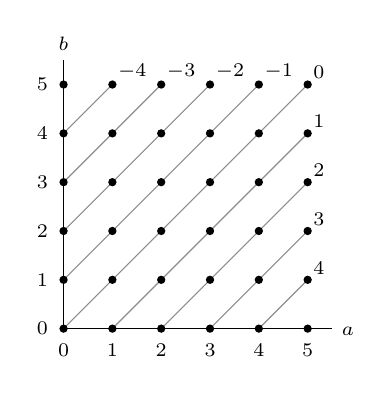
\begin{tikzpicture}[font=\scriptsize, x=0.62cm, y=0.62cm]
\foreach \k in {-4,...,4} {
  \pgfmathsetmacro\xs{max(0,\k)}
  \pgfmathsetmacro\ys{max(0,-\k)}
  \pgfmathsetmacro\xe{min(5,5+\k)}
  \pgfmathsetmacro\ye{min(5,5-\k)}
  \draw[black!45, line width=0.4pt] (\xs,\ys) -- (\xe,\ye);}
\draw[line width=0.4pt] (0,0) -- (5.5,0); \draw[line width=0.4pt] (0,0) -- (0,5.5);
\foreach \i in {0,...,5} {\node[below] at (\i,-0.12) {$\i$}; \node[left] at (-0.12,\i) {$\i$};}
\foreach \a in {0,...,5} \foreach \b in {0,...,5} {\fill (\a,\b) circle (1.5pt);}
\foreach \k in {-4,...,-1} {\pgfmathtruncatemacro\yy{5+\k}\node[anchor=south west, inner sep=1pt] at (\yy+0.05,5.05) {$\k$};}
\foreach \k in {0,...,4} {\pgfmathtruncatemacro\yy{5-\k}\node[anchor=south west, inner sep=1pt] at (5.05,\yy+0.05) {$\k$};}
\node[anchor=west] at (5.5,-0.05) {$a$};
\node[anchor=south] at (0,5.5) {$b$};
\end{tikzpicture}}{The integers as classes of pairs. A pair $(a,b)$ of natural numbers stands for the difference $a-b$; the pairs on one diagonal line form one equivalence class, labelled at the end of the line by its integer value. The class of $0$ is the main diagonal, the classes of the positive integers lie below it and those of the negative integers above it.\label{fig:integers}}
\end{figure}

Since a class has many representatives, we must check that the definitions do not depend on the choice, as explained in \cref{sec:equivalence}.

\begin{proposition}
\label{prop:z-well-defined}
Addition and multiplication of integers are well defined.
\end{proposition}

\begin{proof}
Let $(a,b)\sim(a',b')$, that is, $a+b'=b+a'$, and let $(c,d)$ be any pair. For addition, $(a+c)+(b'+d)=(b+d)+(a'+c)$ follows by adding $c+d$ to both sides of $a+b'=b+a'$, so $(a+c,b+d)\sim(a'+c,b'+d)$. For multiplication we must show
\[
(ac+bd)+(a'd+b'c)=(ad+bc)+(a'c+b'd).
\]
Multiplying $a+b'=b+a'$ by $c$ gives $ac+b'c=bc+a'c$, and multiplying it by $d$ gives $ad+b'd=bd+a'd$. Adding the first equation to the second, read from right to left, gives exactly the required identity. So the result does not change when the first factor is replaced by an equivalent pair; by the commutativity of the formulas, the same holds for the second factor, and replacing both factors one after the other shows that the operations are well defined.
\end{proof}

The natural numbers sit inside $\mathbb Z$ through the map $n\mapsto[(n,0)]$. It is injective, because $(m,0)\sim(n,0)$ means $m=n$, and it respects the operations: $[(m,0)]+[(n,0)]=[(m+n,0)]$ and $[(m,0)]\cdot[(n,0)]=[(mn,0)]$. We therefore identify $n$ with $[(n,0)]$ and regard $\mathbb N$ as a subset of $\mathbb Z$. The \term{negative} of $x=[(a,b)]$ is $-x\coloneqq[(b,a)]$; it satisfies $x+(-x)=[(a+b,a+b)]=[(0,0)]=0$. With subtraction defined by $x-y\coloneqq x+(-y)$, we get $[(a,b)]=[(a,0)]+[(0,b)]=a-b$, as intended.

\begin{proposition}
\label{prop:z-sign}
Every integer is either a natural number $n$ or the negative $-n$ of a natural number $n\ge1$, and not both.
\end{proposition}

\begin{proof}
Let $x=[(a,b)]$. By \cref{thm:n-order}\,(i), $b\le a$ or $a<b$. If $b\le a$, say $a=b+n$, then $(a,b)\sim(n,0)$, so $x=n$. If $a<b$, say $b=a+n$ with $n\ge1$, then $(a,b)\sim(0,n)$, so $x=-n$. A natural number $m$ cannot equal $-n$ with $n\ge1$, since $(m,0)\sim(0,n)$ would mean $m+n=0$, which forces $n=0$.
\end{proof}

So $\mathbb Z=\{\ldots,-2,-1,0,1,2,\ldots\}$, as we have always written it, and every equation $m+x=n$ with $m,n\in\mathbb Z$ now has exactly one solution $x=n-m$. The construction has done its job.

\subsection{Rings}

The laws of arithmetic that $\mathbb Z$ satisfies are shared by many other systems in this series: the rational, real and complex numbers, the integers modulo $n$ of \cref{sec:congruences}, polynomials, and square matrices (although the last are not commutative). It pays to name them once.

\begin{definition}[Commutative ring, field]
\label{def:ring}
A \term{commutative ring} is a set $R$ with two operations, addition $(a,b)\mapsto a+b$ and multiplication $(a,b)\mapsto ab$, and two elements $0$ and $1$, that satisfy the axioms A1--A4, M1--M3 and D of \cref{tab:axioms}. A \term{field} is a commutative ring that satisfies in addition the axioms M4 and N.
\end{definition}

\begin{table}
\sdfloat{%
\begin{sdtable}{colspec={lll}, row{1}={font=\small\bfseries}}
\toprule
 & Axiom & Name \\
\midrule
A1 & $(a+b)+c=a+(b+c)$ & associativity of addition \\
A2 & $a+b=b+a$ & commutativity of addition \\
A3 & $a+0=a$ & zero \\
A4 & for each $a$ there is $-a$ with $a+(-a)=0$ & negatives \\
M1 & $(ab)c=a(bc)$ & associativity of multiplication \\
M2 & $ab=ba$ & commutativity of multiplication \\
M3 & $a\cdot1=a$ & one \\
D & $a(b+c)=ab+ac$ & distributivity \\
\midrule
M4 & for each $a\ne0$ there is $a^{-1}$ with $aa^{-1}=1$ & inverses \\
N & $0\ne1$ & nontriviality \\
\midrule
O1 & exactly one of $a\in P$, $a=0$, $-a\in P$ holds & trichotomy \\
O2 & $a,b\in P$ implies $a+b\in P$ and $ab\in P$ & closure of $P$ \\
\bottomrule
\end{sdtable}}{The axioms of arithmetic, for all elements $a$, $b$, $c$. A commutative ring satisfies the first eight; a field satisfies the first ten. An ordered ring or ordered field has in addition a set $P$ of positive elements satisfying O1 and O2 (\cref{def:ordered}).\label{tab:axioms}}
\end{table}

\begin{theorem}
\label{thm:z-ring}
The integers form a commutative ring in which $0\ne1$. Moreover, $\mathbb Z$ has no zero divisors: if $ab=0$, then $a=0$ or $b=0$.
\end{theorem}

\begin{proof}
Each axiom follows from the corresponding law of \cref{thm:n-arith} by computing with representatives. For example, the distributive law reads
\[
[(a,b)]\bigl([(c,d)]+[(e,f)]\bigr)=\bigl[\bigl(a(c+e)+b(d+f),\,a(d+f)+b(c+e)\bigr)\bigr],
\]
and expanding with the laws of $\mathbb N$ shows that this is the sum of $[(ac+bd,ad+bc)]$ and $[(ae+bf,af+be)]$. Axiom A4 was verified above, and $0\ne1$ because $(0,0)\not\sim(1,0)$. For the absence of zero divisors, write $a=\pm m$ and $b=\pm n$ with $m,n\in\mathbb N$ by \cref{prop:z-sign}. Then $ab=\pm mn$, so $ab=0$ implies $mn=0$, and $m=0$ or $n=0$ by \cref{thm:n-arith}\,(vi).
\end{proof}

A commutative ring with $0\ne1$ and without zero divisors is called an \term{integral domain}. In an integral domain one may cancel nonzero factors: if $ac=bc$ and $c\ne0$, then $(a-b)c=0$, so $a=b$. We shall meet rings in which this fails in \cref{sec:congruences}.

Many familiar rules of sign follow from the ring axioms alone, and therefore hold in every commutative ring.

\begin{proposition}
\label{prop:ring-rules}
In every commutative ring, for all elements $a$ and $b$:
\begin{enumerate}
\item the elements $0$ and $1$ are unique, and so is the negative of each element;
\item $a\cdot0=0$;
\item $(-a)b=-(ab)$ and $(-a)(-b)=ab$; in particular $(-1)a=-a$ and $(-1)(-1)=1$.
\end{enumerate}
\end{proposition}

\begin{proof}
(i) If $0'$ also satisfies A3, then $0'=0'+0=0+0'=0$. If $b$ and $c$ are both negatives of $a$, then $b=b+(a+c)=(b+a)+c=c$. The argument for $1$ is the same as for $0$.

(ii) By A3 and D, $a\cdot0=a(0+0)=a\cdot0+a\cdot0$. Adding $-(a\cdot0)$ to both sides gives $0=a\cdot0$.

(iii) By D and (ii), $ab+(-a)b=\bigl(a+(-a)\bigr)b=0\cdot b=0$, so $(-a)b$ is a negative of $ab$, and by (i) it is \emph{the} negative, $-(ab)$. Applying this twice, $(-a)(-b)=-\bigl(a(-b)\bigr)=-\bigl(-(ab)\bigr)=ab$, since $x$ is the negative of $-x$.
\end{proof}

Part (iii) answers a question that school arithmetic usually leaves open: ``minus times minus is plus'' is not a convention that could have been chosen otherwise, but a consequence of the distributive law. Anyone who wants the distributive law must accept it.

\subsection{Order}

\begin{definition}[Ordered ring]
\label{def:ordered}
An \term{ordered ring} is a commutative ring $R$ with $0\ne1$ together with a subset $P\subseteq R$ satisfying the axioms O1 and O2 of \cref{tab:axioms}. The elements of $P$ are called \term{positive}. We write $a<b$ if $b-a\in P$, and $a\le b$ if $a<b$ or $a=b$. An \term{ordered field} is an ordered ring that is a field.
\end{definition}

For $\mathbb Z$ we take $P\coloneqq\mathbb N\setminus\{0\}$. Axiom O1 is \cref{prop:z-sign}, and O2 holds because sums and products of nonzero natural numbers are nonzero natural numbers (\cref{thm:n-arith}\,(vi)). On $\mathbb N$ the order of \cref{def:ordered} agrees with that of \cref{def:n-order}, since $n-m\in\mathbb N$ means $n=m+k$ for some $k\in\mathbb N$. Hence $\mathbb Z$ is an ordered ring. In any ordered ring, the order is total, by O1, and it obeys the familiar rules.

\begin{proposition}[Rules for inequalities]
\label{prop:order-rules}
In every ordered ring, for all elements $a$, $b$ and $c$:
\begin{enumerate}
\item $\le$ is a total order, and exactly one of $a<b$, $a=b$, $b<a$ holds;
\item if $a<b$, then $a+c<b+c$;
\item if $a<b$ and $c>0$, then $ac<bc$; if $a<b$ and $c<0$, then $ac>bc$;
\item $a^2\ge0$, with equality only for $a=0$; in particular $1>0$.
\end{enumerate}
\end{proposition}

\begin{proof}
(i) Trichotomy is O1 applied to $b-a$, since $-(b-a)=a-b$. Transitivity follows from O2, because $c-a=(c-b)+(b-a)$, and antisymmetry from trichotomy.

(ii) $(b+c)-(a+c)=b-a\in P$.

(iii) If $b-a\in P$ and $c\in P$, then $bc-ac=(b-a)c\in P$ by O2. If $-c\in P$, then $ac-bc=(b-a)(-c)\in P$, using \cref{prop:ring-rules}\,(iii).

(iv) If $a\in P$, then $a^2=aa\in P$. If $-a\in P$, then $a^2=(-a)(-a)\in P$ by \cref{prop:ring-rules}\,(iii). By O1 one of the two cases holds when $a\ne0$. Finally $1=1^2$, and $1\ne0$.
\end{proof}

These are the ``usual rules for inequalities'' of \cref{asm:numbers}\,(i). For the integers there is one more rule, which is not a consequence of the axioms of an ordered ring (the rational numbers satisfy those axioms and violate it) and which was stated as \cref{asm:numbers}\,(iii).

\begin{proposition}[Discreteness of the integers]
\label{prop:z-discrete}
There is no integer $n$ with $0<n<1$. Consequently, if $m<n$ are integers, then $m+1\le n$.
\end{proposition}

\begin{proof}
If $0<n$, then $n\in P=\mathbb N\setminus\{0\}$, so $n=k+1$ for some $k\in\mathbb N$ by \cref{prop:peano-basic}\,(i), and $n-1=k\ge0$, that is, $n\ge1$. For the second statement apply the first to $n-m>0$.
\end{proof}

The well-ordering principle extends from $\mathbb N$ to sets of integers that are bounded on the appropriate side.

\begin{corollary}
\label{cor:z-well-order}
Every nonempty set of integers that is bounded below has a least element, and every nonempty set of integers that is bounded above has a greatest element.
\end{corollary}

\begin{proof}
Let $S\subseteq\mathbb Z$ be nonempty with lower bound $c\in\mathbb Z$. The set $\{s-c: s\in S\}$ consists of natural numbers, so it has a least element $s_0-c$ by \cref{thm:n-order}\,(iv), and $s_0$ is the least element of $S$. If $S$ is bounded above by $c$, apply this to $\{-s: s\in S\}$, which is bounded below by $-c$; the negative of its least element is the greatest element of $S$.
\end{proof}

All the properties of $\mathbb N$ and $\mathbb Z$ listed in \cref{asm:numbers}\,(i)--(iii) have now been derived from Peano's axioms, apart from those that involve division, to which we turn next. A computer can represent the whole of $\mathbb Z$ only approximately: a fixed number of bits holds only finitely many integers. Libraries for \term{arbitrary-precision} integers lift this restriction by storing an integer as a list of digits in a large base and lengthening the list as needed~\cite[Sect.~4.3]{knuth1997taocp2}. They implement $\mathbb Z$ exactly, at a cost that grows with the length of the numbers.

\section{Divisibility and the Division Theorem}
\label{sec:division}

Division is not always possible in $\mathbb Z$: $7$ divided by $3$ is not an integer. What is always possible is division with a remainder, as taught in primary school: $7=3\cdot2+1$. This section proves that such a division exists and is unique, introduces the floor and ceiling functions that describe it, and discusses how negative numbers are treated, a point on which programming languages disagree.

\subsection{Division with Remainder}

Recall from \cref{def:even-odd} that $a\mid b$ means $b=ak$ for some integer $k$, and from \cref{prop:divisibility} the basic rules: divisibility is reflexive and transitive, a common divisor of $b$ and $c$ divides every combination $bx+cy$, and a divisor $a$ of a nonzero integer $b$ satisfies $|a|\le|b|$. These rules were proved in \cref{ch:logic} from \cref{asm:numbers}\,(i)--(iii), all of which have now been derived from Peano's axioms.

\begin{theorem}[Division with remainder]
\label{thm:division}
Let $a$ and $b$ be integers with $b>0$. There are unique integers $q$ and $r$ such that
\[
a=bq+r\qquad\text{and}\qquad0\le r<b .
\]
\end{theorem}

\begin{proof}
\emph{Existence.} Consider the set $S\coloneqq\{a-bk: k\in\mathbb Z\}\cap\mathbb N$ of nonnegative numbers of the form $a-bk$. It is nonempty: for $k=-|a|$ we get $a+b|a|\ge a+|a|\ge0$, because $b\ge1$ and $a\ge-|a|$ (\cref{prop:abs}\,(i)). By the well-ordering principle, $S$ has a least element $r$, say $r=a-bq$. Then $r\ge0$. If we had $r\ge b$, the number $r-b=a-b(q+1)$ would be a smaller element of $S$, contradicting the choice of $r$. Hence $0\le r<b$.

\emph{Uniqueness.} Suppose $a=bq+r=bq'+r'$ with $0\le r,r'<b$. Then $b(q-q')=r'-r$, and $-b<r'-r<b$, that is, $|b(q-q')|<b$. If $q\ne q'$, then $|q-q'|\ge1$ and $|b(q-q')|=b|q-q'|\ge b$, a contradiction. Hence $q=q'$, and then $r=r'$.
\end{proof}

The integers $q$ and $r$ are the \term{quotient} and the \term{remainder} of the division of $a$ by $b$. The remainder is written $a\bmod b$; for $b=2$ this is the notation $n\bmod2$ of \cref{ch:logic}. For example,
\[
17=5\cdot3+2,\qquad-17=5\cdot(-4)+3,\qquad 15=5\cdot3+0,
\]
so $17\bmod5=2$, $-17\bmod5=3$ and $15\bmod5=0$. By definition, $b\mid a$ if and only if $a\bmod b=0$. The remainder of a negative number deserves attention: $-17\bmod5$ is $3$ and not $-2$, because the theorem requires $0\le r<b$. \Cref{fig:division} shows why. The multiples of $b$ divide the number line into intervals of length $b$; the quotient $q$ says in which interval $a$ lies, namely in $[bq,bq+b)$, and the remainder $r$ is the distance from the left end of that interval to $a$.

\begin{figure}
\tikzset{dl/.style={line width=0.4pt}, dr/.style={{Bar[width=4pt]}-{Latex[length=1.5mm]}, line width=0.6pt}}
\sdpanel{A}{\begin{tikzpicture}[font=\scriptsize, x=0.24cm]
\fill[sdfill] (15,-0.07) rectangle (20,0.07);
\draw[dl] (-22,0) -- (22,0);
\foreach \k in {-20,-15,...,20} {\draw[dl] (\k,-0.08) -- (\k,0.08); \node[below] at (\k,-0.08) {$\k$};}
\fill (17,0) circle (1.7pt); \node[above] at (17,0.05) {$a$};
\draw[dr] (15,0.5) -- node[above] {$r=2$} (17,0.5);
\node[anchor=west] at (-22,0.5) {$a=17$: \ $q=3$, \ $a\in[15,20)$};
\end{tikzpicture}}
\sdpanelrow
\sdpanel{B}{\begin{tikzpicture}[font=\scriptsize, x=0.24cm]
\fill[sdfill] (-20,-0.07) rectangle (-15,0.07);
\draw[dl] (-22,0) -- (22,0);
\foreach \k in {-20,-15,...,20} {\draw[dl] (\k,-0.08) -- (\k,0.08); \node[below] at (\k,-0.08) {$\k$};}
\fill (-17,0) circle (1.7pt); \node[above] at (-17,0.05) {$a$};
\draw[dr] (-20,0.5) -- node[above] {$r=3$} (-17,0.5);
\draw[dr, black!50] (-15,1.05) -- node[above, black] {$r=-2$} (-17,1.05);
\node[anchor=west] at (0,0.5) {floor: \ $q=-4$, \ $r=3$};
\node[anchor=west] at (0,1.05) {truncation: \ $q=-3$, \ $r=-2$};
\end{tikzpicture}}
\caption{Division with remainder by $b=5$. The multiples of $5$ cut the number line into intervals of length $5$. (A) For $a=17$ the quotient $q=3$ locates $a$ in the shaded interval $[15,20)$, and the remainder $r=2$ is the distance from its left end. (B) For $a=-17$, \cref{thm:division} takes the interval $[-20,-15)$ and gives $q=-4$ and $r=3$ (lower arrow). Truncating division instead rounds the quotient towards zero, $q=-3$, and measures back from $-15$, giving $r=-2$ (upper, grey arrow).}
\label{fig:division}
\end{figure}

The theorem extends to negative divisors: for $b\ne0$ there are unique $q$ and $r$ with $a=bq+r$ and $0\le r<|b|$. Indeed, for $b<0$ we divide $a$ by $|b|=-b$ and obtain $a=(-b)q'+r$, that is, $a=b(-q')+r$; uniqueness follows as before. Division with remainder also settles the claim of \cref{sec:equivalence} that every integer is of exactly one of the forms $3k$, $3k+1$ and $3k+2$: these are the three possible remainders on division by $3$, and the remainder and the quotient $k$ are unique.

\subsection{Floor and Ceiling}

The quotient in \cref{thm:division} is the result of rounding the fraction $a/b$ down to an integer. Rounding down and rounding up occur so often that they have names and symbols, both introduced by Kenneth Iverson in the early 1960s~\cite[Sect.~3.1]{graham1994concrete}.

\begin{definition}[Floor, ceiling]
\label{def:floor}
For a real number $x$, the \term{floor} $\lfloor x\rfloor$ is the integer $n$ with $n\le x<n+1$, and the \term{ceiling} $\lceil x\rceil$ is the integer $n$ with $n-1<x\le n$.
\end{definition}

In words, $\lfloor x\rfloor$ is the greatest integer not exceeding $x$, and $\lceil x\rceil$ the least integer not less than $x$. Thus $\lfloor 2.7\rfloor=2$, $\lceil2.7\rceil=3$, $\lfloor-2.7\rfloor=-3$, $\lceil-2.7\rceil=-2$ and $\lfloor5\rfloor=\lceil5\rceil=5$. Note that $\lfloor-2.7\rfloor$ is $-3$ and not $-2$: the floor rounds towards $-\infty$, not towards zero.

Two things must be checked. There is at most one such integer: if $n\le x<n+1$ and $m\le x<m+1$, then $m<n+1$ and $n<m+1$, so $m\le n$ and $n\le m$ by \cref{prop:z-discrete}. And there is at least one. For a rational number $x=a/b$ with $b>0$ this follows from \cref{thm:division}: dividing $bq\le a<bq+b$ by $b$ gives $q\le a/b<q+1$, so
\begin{equation}
\Bigl\lfloor\frac ab\Bigr\rfloor=q\qquad\text{and}\qquad a\bmod b=a-b\Bigl\lfloor\frac ab\Bigr\rfloor .
\label{eq:mod-floor}
\end{equation}
For an arbitrary real number the existence of $\lfloor x\rfloor$ depends on the Archimedean property of the real numbers and is proved in \cref{thm:floor} below; the ceiling then exists by part (iii) of the next proposition. The proposition collects the rules that are used most often~\cite[Chap.~3]{graham1994concrete}.

\begin{proposition}[Rules for floor and ceiling]
\label{prop:floor}
For every real number $x$, every integer $n$, and all integers $a$ and $b$ with $b>0$:
\begin{enumerate}
\item $x-1<\lfloor x\rfloor\le x\le\lceil x\rceil<x+1$;
\item $\lfloor x+n\rfloor=\lfloor x\rfloor+n$ and $\lceil x+n\rceil=\lceil x\rceil+n$;
\item $\lceil x\rceil=-\lfloor-x\rfloor$;
\item $\lfloor x\rfloor=\lceil x\rceil$ if $x$ is an integer, and $\lceil x\rceil=\lfloor x\rfloor+1$ otherwise;
\item $n\le x$ if and only if $n\le\lfloor x\rfloor$, and $x\le n$ if and only if $\lceil x\rceil\le n$;
\item $\lceil a/b\rceil=\lfloor(a+b-1)/b\rfloor$.
\end{enumerate}
\end{proposition}

\begin{proof}
(i) This restates the definitions: $\lfloor x\rfloor\le x<\lfloor x\rfloor+1$ and $\lceil x\rceil-1<x\le\lceil x\rceil$.

(ii) The integer $\lfloor x\rfloor+n$ satisfies $\lfloor x\rfloor+n\le x+n<\lfloor x\rfloor+n+1$, so it is the floor of $x+n$. The ceiling is treated in the same way.

(iii) From $\lfloor-x\rfloor\le-x<\lfloor-x\rfloor+1$ we get $-\lfloor-x\rfloor-1<x\le-\lfloor-x\rfloor$, which says that $-\lfloor-x\rfloor$ is the ceiling of $x$.

(iv) If $x$ is an integer, then $n=x$ satisfies both definitions. Otherwise $\lfloor x\rfloor<x<\lfloor x\rfloor+1$, and the integer $\lfloor x\rfloor+1$ satisfies the definition of the ceiling.

(v) If $n\le\lfloor x\rfloor$, then $n\le x$ by (i). Conversely, if $n\le x$ but $n>\lfloor x\rfloor$, then $n\ge\lfloor x\rfloor+1>x$ by \cref{prop:z-discrete} and (i), a contradiction. The second statement follows from the first by (iii), applied to $-x$ and $-n$.

(vi) Write $a=bq+r$ with $0\le r<b$. If $r=0$, then $\lceil a/b\rceil=q$, and $(a+b-1)/b=q+(b-1)/b$ has floor $q$ because $0\le(b-1)/b<1$. If $r\ge1$, then $\lceil a/b\rceil=q+1$ by (iv), and $(a+b-1)/b=q+(r+b-1)/b$ with $1\le(r+b-1)/b<2$, so its floor is $q+1$.
\end{proof}

Rule (v) is the one to remember: an integer lies below $x$ exactly when it lies below $\lfloor x\rfloor$. It gives, for instance, the number of multiples of $b>0$ among $1,2,\ldots,n$. These multiples are $b,2b,\ldots,kb$ with $kb\le n$, that is, with $k\le n/b$, and by (v) this means $k\le\lfloor n/b\rfloor$; so there are $\lfloor n/b\rfloor$ of them. Similarly, $n$ items packed into boxes that hold $b$ items each need $\lceil n/b\rceil$ boxes, and rule (vi) computes this number with integer operations only. Volume~VI divides arrays into blocks for parallel processing in exactly this way.

\subsection{Negative Operands}

\Cref{thm:division} fixes the quotient as $\lfloor a/b\rfloor$ and the remainder as nonnegative. This is the choice made in mathematics, but it is not the only one in use. Computer hardware and many programming languages \emph{truncate} the quotient instead, rounding $a/b$ towards zero. For a real number $x$ let $\operatorname{trunc}(x)\coloneqq\lfloor x\rfloor$ if $x\ge0$ and $\operatorname{trunc}(x)\coloneqq\lceil x\rceil$ if $x<0$. For integers $a$ and $b\ne0$ the two conventions are:
\begin{itemize}
\item \term{floored division}: $q_{\mathrm F}\coloneqq\lfloor a/b\rfloor$ and $r_{\mathrm F}\coloneqq a-bq_{\mathrm F}$;
\item \term{truncated division}: $q_{\mathrm T}\coloneqq\operatorname{trunc}(a/b)$ and $r_{\mathrm T}\coloneqq a-bq_{\mathrm T}$.
\end{itemize}

\begin{proposition}
\label{prop:trunc-floor}
Let $a$ and $b\ne0$ be integers. Both conventions satisfy $a=bq+r$ and $|r|<|b|$. The remainder $r_{\mathrm F}$ is zero or has the sign of $b$, and $r_{\mathrm T}$ is zero or has the sign of $a$. The two conventions agree if $b\mid a$ or if $a$ and $b$ have the same sign; otherwise $q_{\mathrm F}=q_{\mathrm T}-1$ and $r_{\mathrm F}=r_{\mathrm T}+b$.
\end{proposition}

\begin{proof}
Put $t\coloneqq a/b-q$, so that $r=a-bq=bt$. For the floored quotient, $0\le t<1$ by \cref{prop:floor}\,(i); hence $r_{\mathrm F}=bt$ is zero or has the sign of $b$, and $|r_{\mathrm F}|=|b|\,t<|b|$. For the truncated quotient, $0\le t<1$ if $a/b\ge0$ and $-1<t\le0$ if $a/b<0$, so $r_{\mathrm T}$ is zero or has the sign of $b$ in the first case and the opposite sign in the second; in both cases this is the sign of $a$, and again $|r_{\mathrm T}|<|b|$. If $a/b\ge0$, which happens when $a=0$ or $a$ and $b$ have the same sign, then $\operatorname{trunc}(a/b)=\lfloor a/b\rfloor$; if $a/b$ is an integer, both quotients equal $a/b$. In the remaining case $a/b$ is negative and not an integer, so $q_{\mathrm T}=\lceil a/b\rceil=\lfloor a/b\rfloor+1$ by \cref{prop:floor}\,(iv), and $r_{\mathrm F}=a-b(q_{\mathrm T}-1)=r_{\mathrm T}+b$.
\end{proof}

\Cref{tab:division-conventions} lists the four sign combinations for $|a|=7$ and $|b|=3$. For a positive divisor, floored division is the division of \cref{thm:division}. The C language has prescribed truncation since its 1999 standard~\cite{iso9899-1999}, whereas Knuth defines the remainder with the floor function~\cite{graham1994concrete}, and several programming languages follow one convention or the other, or offer both~\cite{boute1992}. A third convention, the Euclidean one, always chooses $0\le r<|b|$, as in the extension of \cref{thm:division} above; it agrees with floored division when $b>0$. Boute compares the three and argues for the Euclidean one.

\begin{table}
\sdfloat{%
\begin{sdtable}{colspec={rrrrrr}, row{1}={font=\small}}
\toprule
$a$ & $b$ & $q_{\mathrm T}$ & $r_{\mathrm T}$ & $q_{\mathrm F}$ & $r_{\mathrm F}$ \\
\midrule
$7$ & $3$ & $2$ & $1$ & $2$ & $1$ \\
$-7$ & $3$ & $-2$ & $-1$ & $-3$ & $2$ \\
$7$ & $-3$ & $-2$ & $1$ & $-3$ & $-2$ \\
$-7$ & $-3$ & $2$ & $-1$ & $2$ & $-1$ \\
\bottomrule
\end{sdtable}}{Truncated and floored division. In every row $a=bq+r$. The truncated remainder has the sign of $a$, the floored remainder the sign of $b$; the conventions differ exactly when $a$ and $b$ have opposite signs and $b\nmid a$.\label{tab:division-conventions}}
\end{table}

The difference matters in practice. A test for odd numbers of the form ``$n$ leaves remainder $1$ on division by $2$'' is correct with floored division but fails for negative $n$ with truncated division, which gives the remainder $-1$ for $n=-3$. A program that uses $k\bmod m$ as an index into an array of length $m$ needs a remainder between $0$ and $m-1$, and with truncated division a negative $k$ yields a negative index. Volume~VI describes the convention followed by the array library and the reasons for it.

\section{Greatest Common Divisors and the Euclidean Algorithm}
\label{sec:gcd}

The Euclidean algorithm, which computes the greatest common divisor of two integers, is described in Book~VII of Euclid's \emph{Elements}~\cite{heath1956euclid}, and Knuth calls it the oldest nontrivial algorithm that has survived to the present day~\cite[Sect.~4.5.2]{knuth1997taocp2}. It is fast, it is easy to prove correct, and an extension of it solves linear equations in integers.

\subsection{The Greatest Common Divisor}

\begin{definition}[Greatest common divisor]
\label{def:gcd}
Let $a$ and $b$ be integers. An integer $d$ is a \term{common divisor} of $a$ and $b$ if $d\mid a$ and $d\mid b$. If $a$ and $b$ are not both zero, their \term{greatest common divisor} $\gcd(a,b)$ is the largest common divisor; we put $\gcd(0,0)\coloneqq0$. The integers $a$ and $b$ are \term{coprime} if $\gcd(a,b)=1$.
\end{definition}

The definition makes sense: $1$ is a common divisor, and if, say, $a\ne0$, then every common divisor satisfies $d\le|d|\le|a|$ by \cref{prop:divisibility}\,(iv), so the set of common divisors is nonempty and bounded above and has a greatest element by \cref{cor:z-well-order}. For example, the positive divisors of $12$ are $1,2,3,4,6,12$ and those of $18$ are $1,2,3,6,9,18$, so $\gcd(12,18)=6$; the integers $8$ and $15$ are coprime. The convention $\gcd(0,0)=0$ is explained by \cref{cor:gcd-lattice} below.

Listing all divisors is hopeless for large numbers. The Euclidean algorithm rests instead on the following observation.

\begin{lemma}
\label{lem:gcd-basic}
For all integers $a$, $b$ and $k$:
\begin{enumerate}
\item $\gcd(a,b)=\gcd(b,a)=\gcd(|a|,|b|)$ and $\gcd(a,0)=|a|$;
\item $\gcd(a,b)=\gcd(a-kb,b)$; in particular, $\gcd(a,b)=\gcd(b,\,a\bmod b)$ if $b>0$.
\end{enumerate}
\end{lemma}

\begin{proof}
(i) The definition is symmetric in $a$ and $b$, and $d\mid a$ if and only if $d\mid|a|$. Every integer divides $0$, so the common divisors of $a$ and $0$ are the divisors of $a$, the largest of which is $|a|$ when $a\ne0$; for $a=0$ the convention gives $0=|0|$.

(ii) If $d$ divides $a$ and $b$, it divides $a-kb$ by \cref{prop:divisibility}\,(iii). Conversely, if $d$ divides $a-kb$ and $b$, it divides $(a-kb)+kb=a$. So the pairs $(a,b)$ and $(a-kb,b)$ have the same common divisors, and therefore the same greatest common divisor; they are both $(0,0)$ only if $a=b=0$. The special case is $k=\lfloor a/b\rfloor$, by \eqref{eq:mod-floor}, together with (i).
\end{proof}

\subsection{The Euclidean Algorithm}

Repeating the step $(a,b)\mapsto(b,a\bmod b)$ replaces a pair by a smaller pair with the same greatest common divisor, until the second number becomes zero. \Cref{alg:euclid} states this precisely. For $a=240$ and $b=46$ it computes
\[
\gcd(240,46)=\gcd(46,10)=\gcd(10,6)=\gcd(6,4)=\gcd(4,2)=\gcd(2,0)=2,
\]
using the divisions $240=5\cdot46+10$, $46=4\cdot10+6$, $10=1\cdot6+4$, $6=1\cdot4+2$ and $4=2\cdot2+0$.

\begin{algorithm}
\begin{algorithmic}[1]
\Require natural numbers $a$ and $b$
\Ensure $\gcd(a,b)$
\Name{Euclid}{a,b}
\While{$b\ne0$} \Comment{invariant: $\gcd(a,b)$ is unchanged}
  \State $(a,b)\gets(b,\ a\bmod b)$
\EndWhile
\State \Return $a$
\end{algorithmic}
\caption{The Euclidean algorithm. The two assignments in line~2 happen simultaneously: both new values are computed from the old ones.}
\label{alg:euclid}
\end{algorithm}

\begin{theorem}
\label{thm:euclid-correct}
For all natural numbers $a$ and $b$, \cref{alg:euclid} stops and returns $\gcd(a,b)$.
\end{theorem}

\begin{proof}
\emph{Invariant.} Write $a_0$ and $b_0$ for the input. Each pass replaces $(a,b)$ by $(b,a\bmod b)$ with $b>0$, which by \cref{lem:gcd-basic}\,(ii) does not change the greatest common divisor; by induction on the number of passes, $\gcd(a,b)=\gcd(a_0,b_0)$ whenever the loop condition is tested. Both values stay natural numbers.

\emph{Termination.} Each pass replaces $b$ by $a\bmod b<b$. The successive values of $b$ therefore form a strictly decreasing sequence of natural numbers, which must end by the well-ordering principle, as in the proof of \cref{prop:tobinary}. The loop stops only when $b=0$.

\emph{Result.} When the loop stops, $b=0$ and the invariant gives $\gcd(a_0,b_0)=\gcd(a,0)=a$ by \cref{lem:gcd-basic}\,(i).
\end{proof}

The algorithm has a geometric picture, shown in \cref{fig:euclid-squares}. Cut a rectangle of sides $a$ and $b$ into as many squares of side $b$ as fit, leaving a rectangle of sides $b$ and $a\bmod b$, and repeat with the smaller rectangle. The process ends when the leftover rectangle is itself a square, and the side of the last squares is $\gcd(a,b)$, the largest length that measures both sides an exact number of times. This is how the Greeks thought of the algorithm: as finding a common measure of two lengths~\cite{heath1956euclid}.

\begin{figure}
\tikzset{sq/.style={draw, line width=0.5pt}}
\sdpanel{A}{\begin{tikzpicture}[font=\scriptsize, x=0.2cm, y=0.2cm]
\fill[sdfill] (24,6) rectangle (26,10);
\draw[sq] (0,0) rectangle (10,10); \node at (5,5) {$10$};
\draw[sq] (10,0) rectangle (20,10); \node at (15,5) {$10$};
\draw[sq] (20,0) rectangle (26,6); \node at (23,3) {$6$};
\draw[sq] (20,6) rectangle (24,10); \node at (22,8) {$4$};
\draw[sq] (24,6) rectangle (26,8); \draw[sq] (24,8) rectangle (26,10);
\draw[line width=0.8pt] (0,0) rectangle (26,10);
\draw[decorate, decoration={brace, amplitude=3pt, mirror}] (0,-0.6) -- node[below=3pt] {$26$} (26,-0.6);
\draw[decorate, decoration={brace, amplitude=3pt}] (-0.6,0) -- node[left=3pt] {$10$} (-0.6,10);
\end{tikzpicture}}\hfill
\sdpanel{B}{\begin{tikzpicture}[font=\scriptsize, x=0.25cm, y=0.25cm]
\fill[sdfill] (11,7) rectangle (13,8);
\draw[sq] (0,0) rectangle (8,8); \node at (4,4) {$8$};
\draw[sq] (8,0) rectangle (13,5); \node at (10.5,2.5) {$5$};
\draw[sq] (8,5) rectangle (11,8); \node at (9.5,6.5) {$3$};
\draw[sq] (11,5) rectangle (13,7); \node at (12,6) {$2$};
\draw[sq] (11,7) rectangle (12,8); \draw[sq] (12,7) rectangle (13,8);
\draw[line width=0.8pt] (0,0) rectangle (13,8);
\draw[decorate, decoration={brace, amplitude=3pt, mirror}] (0,-0.5) -- node[below=3pt] {$13$} (13,-0.5);
\draw[decorate, decoration={brace, amplitude=3pt}] (-0.5,0) -- node[left=3pt] {$8$} (-0.5,8);
\end{tikzpicture}}
\caption{The Euclidean algorithm as cutting squares from a rectangle. (A) For $26\times10$: two squares of side $10$, one of side $6$, one of side $4$ and two of side $2$ (shaded), so $\gcd(26,10)=2$. (B) For two consecutive Fibonacci numbers, $13\times8$, each division removes a single square, and the algorithm takes as many steps as possible for numbers of this size (\cref{thm:lame}).}
\label{fig:euclid-squares}
\end{figure}

\subsection{B\'ezout's Identity}

The greatest common divisor has a second description, which is less obvious and more useful than the definition: it is the smallest positive integer that can be written as a combination $ax+by$ with integer coefficients.

\begin{theorem}[B\'ezout's identity]
\label{thm:bezout}
Let $a$ and $b$ be integers and $d\coloneqq\gcd(a,b)$.
\begin{enumerate}
\item There are integers $x$ and $y$ with $ax+by=d$.
\item The set $L\coloneqq\{ax+by: x,y\in\mathbb Z\}$ of integer combinations of $a$ and $b$ equals $d\mathbb Z$.
\item Every common divisor of $a$ and $b$ divides $d$.
\end{enumerate}
\end{theorem}

\begin{proof}
If $a=b=0$, then $d=0$ and all three statements are trivial. Otherwise $L$ contains a positive element, for instance $|a|$ or $|b|$, and by the well-ordering principle it has a least positive element $e=ax_0+by_0$. We show $e=d$.

First, $e$ divides $a$. By \cref{thm:division}, $a=eq+r$ with $0\le r<e$, and
\[
r=a-eq=a-(ax_0+by_0)q=a(1-qx_0)+b(-qy_0)
\]
lies in $L$. Since $r<e$ and $e$ is the least positive element of $L$, we must have $r=0$. In the same way $e$ divides $b$. So $e$ is a common divisor and $e\le d$. Conversely, $d$ divides $a$ and $b$, hence it divides $ax_0+by_0=e$ by \cref{prop:divisibility}\,(iii), and $d\le e$ by \cref{prop:divisibility}\,(iv), because $e>0$. Thus $d=e$, which proves (i).

For (ii), every multiple $dk$ equals $a(x_0k)+b(y_0k)\in L$, and every element $ax+by$ of $L$ is a multiple of $d$, because $d$ divides $a$ and $b$. For (iii), a common divisor $c$ of $a$ and $b$ divides $ax_0+by_0=d$.
\end{proof}

Part (iii) says that the greatest common divisor is greatest not only in size but also in the sense of divisibility, a point taken up in \cref{cor:gcd-lattice}. The proof of (i) is not constructive in a useful way, since it does not say how to find the least positive element of $L$. The Euclidean algorithm can be extended to find $x$ and $y$: it suffices to record, along with each remainder, how it is composed from $a$ and $b$.

\begin{algorithm}
\begin{algorithmic}[1]
\Require natural numbers $a$ and $b$
\Ensure $d=\gcd(a,b)$ and integers $x$, $y$ with $ax+by=d$
\Name{ExtendedEuclid}{a,b}
\State $(r_0,s_0,t_0)\gets(a,1,0)$; \ $(r_1,s_1,t_1)\gets(b,0,1)$
\While{$r_1\ne0$} \Comment{invariant: $r_0=as_0+bt_0$ and $r_1=as_1+bt_1$}
  \State $q\gets\lfloor r_0/r_1\rfloor$
  \State $(r_0,r_1)\gets(r_1,\ r_0-qr_1)$
  \State $(s_0,s_1)\gets(s_1,\ s_0-qs_1)$
  \State $(t_0,t_1)\gets(t_1,\ t_0-qt_1)$
\EndWhile
\State \Return $r_0$, $s_0$, $t_0$
\end{algorithmic}
\caption{The extended Euclidean algorithm. The values $r_0$, $r_1$ run through the same sequence as in \cref{alg:euclid}; the coefficients $s$ and $t$ express each remainder as a combination of $a$ and $b$.}
\label{alg:ext-euclid}
\end{algorithm}

\begin{proposition}
\label{prop:ext-euclid}
For all natural numbers $a$ and $b$, \cref{alg:ext-euclid} stops and returns $d=\gcd(a,b)$ and integers $x$ and $y$ with $ax+by=d$.
\end{proposition}

\begin{proof}
The pair $(r_0,r_1)$ is updated exactly as $(a,b)$ in \cref{alg:euclid}, since $r_0-qr_1=r_0\bmod r_1$; so the loop stops and $r_0=\gcd(a,b)$ at the end, by \cref{thm:euclid-correct}. The invariant holds initially, because $a=a\cdot1+b\cdot0$ and $b=a\cdot0+b\cdot1$. If it holds before a pass, then the new $r_1$ is
\[
r_0-qr_1=(as_0+bt_0)-q(as_1+bt_1)=a(s_0-qs_1)+b(t_0-qt_1),
\]
which is $as_1+bt_1$ with the new values of $s_1$ and $t_1$; the new $r_0$ is the old $r_1$, together with its coefficients. So the invariant holds after the pass, and at the end it gives $r_0=as_0+bt_0$.
\end{proof}

\Cref{tab:ext-euclid} traces the algorithm for $a=240$ and $b=46$; the result is $240\cdot(-9)+46\cdot47=2$. For the equation $7x+4y=1$ of \cref{sec:existence}, the divisions $7=1\cdot4+3$, $4=1\cdot3+1$ and $3=3\cdot1+0$ give, read backwards, $1=4-3=4-(7-4)=7\cdot(-1)+4\cdot2$, which is the solution $x=-1$, $y=2$ quoted there.

\begin{table}
\sdfloat{%
\begin{sdtable}{colspec={rrrrr}, row{1}={font=\small}}
\toprule
$i$ & $q_i$ & $r_i$ & $s_i$ & $t_i$ \\
\midrule
$0$ & & $240$ & $1$ & $0$ \\
$1$ & & $46$ & $0$ & $1$ \\
$2$ & $5$ & $10$ & $1$ & $-5$ \\
$3$ & $4$ & $6$ & $-4$ & $21$ \\
$4$ & $1$ & $4$ & $5$ & $-26$ \\
$5$ & $1$ & $2$ & $-9$ & $47$ \\
$6$ & $2$ & $0$ & $23$ & $-120$ \\
\bottomrule
\end{sdtable}}{The extended Euclidean algorithm for $a=240$ and $b=46$. Row $i$ shows the remainder $r_i=r_{i-2}-q_ir_{i-1}$ and its coefficients, with $r_i=240s_i+46t_i$ in every row. The last nonzero remainder is $\gcd(240,46)=2=240\cdot(-9)+46\cdot47$.\label{tab:ext-euclid}}
\end{table}

\subsection{The Least Common Multiple}

\begin{definition}[Least common multiple]
\label{def:lcm}
Let $a$ and $b$ be integers. If both are nonzero, their \term{least common multiple} $\operatorname{lcm}(a,b)$ is the least positive integer that is a multiple of both. If $a=0$ or $b=0$, we put $\operatorname{lcm}(a,b)\coloneqq0$.
\end{definition}

For nonzero $a$ and $b$ the positive common multiples include $|ab|$, so the least one exists by the well-ordering principle. For example, $\operatorname{lcm}(4,6)=12$. The least common multiple is determined by the greatest common divisor.

\begin{theorem}
\label{thm:lcm}
Let $a$ and $b$ be integers. Then
\begin{enumerate}
\item $\gcd(a,b)\cdot\operatorname{lcm}(a,b)=|ab|$;
\item every common multiple of $a$ and $b$ is a multiple of $\operatorname{lcm}(a,b)$;
\item $a\mathbb Z\cap b\mathbb Z=\operatorname{lcm}(a,b)\,\mathbb Z$.
\end{enumerate}
\end{theorem}

\begin{proof}
If $a=0$ or $b=0$, the only common multiple is $0$, and all three statements hold. Let $a,b\ne0$, let $d\coloneqq\gcd(a,b)>0$ and choose $x$, $y$ with $ax+by=d$ by \cref{thm:bezout}. Put $m\coloneqq|ab|/d$, an integer because $d\mid a$. It is a common multiple, since $m=|a|\cdot(|b|/d)=|b|\cdot(|a|/d)$. Let $c$ be any common multiple, say $c=au=bv$. Then
\[
cd=c(ax+by)=(bv)ax+(au)by=ab(vx+uy),
\]
so $c=(ab/d)(vx+uy)$, and $c$ is a multiple of $m=|ab/d|$. In particular every positive common multiple is at least $m$, so $m=\operatorname{lcm}(a,b)$. This proves (i) and (ii), and (iii) restates (ii) together with the fact that multiples of $m$ are common multiples.
\end{proof}

With $a=4$ and $b=6$, part (iii) gives $4\mathbb Z\cap6\mathbb Z=12\mathbb Z$, as claimed in \cref{sec:set-operations}; the product $24$ overcounts by the common factor $\gcd(4,6)=2$. The theorem also settles the claim of \cref{sec:orders} about the order of divisibility.

\begin{corollary}
\label{cor:gcd-lattice}
In the set $\mathbb N$ partially ordered by divisibility, every two elements $a$ and $b$ have an infimum and a supremum, namely $\inf\{a,b\}=\gcd(a,b)$ and $\sup\{a,b\}=\operatorname{lcm}(a,b)$.
\end{corollary}

\begin{proof}
The lower bounds of $\{a,b\}$ in this order are the common divisors in $\mathbb N$. The greatest common divisor is one of them, and by \cref{thm:bezout}\,(iii) every other one divides it, so it is the greatest lower bound in the sense of \cref{def:sup}. This includes the case $a=b=0$, where every natural number is a lower bound and $\gcd(0,0)=0$ is the greatest element of the order. The upper bounds are the common multiples in $\mathbb N$, and by \cref{thm:lcm}\,(ii) the least common multiple divides all of them.
\end{proof}

The corollary explains the convention $\gcd(0,0)=0$: with it, the greatest common divisor is always the infimum in the order of divisibility, in which $0$ is the largest element.

\subsection{The Speed of the Euclidean Algorithm}

How many passes does \cref{alg:euclid} need? Each pass replaces the pair $(a,b)$ by $(b,a\bmod b)$, and the remainder can be as large as $b-1$, so a single pass may make little progress. But two passes always make substantial progress, and the worst case can be identified exactly. It involves the \term{Fibonacci numbers}, defined by
\[
F_0\coloneqq0,\qquad F_1\coloneqq1,\qquad F_{n+2}\coloneqq F_{n+1}+F_n,
\]
so that the sequence begins $0,1,1,2,3,5,8,13,21,34,55,89,144$. By the following theorem, which Gabriel Lam\'e published in 1844~\cite{lame1844}, consecutive Fibonacci numbers are the slowest input for their size; \cref{fig:euclid-squares}B shows the pair $(13,8)$.

\begin{theorem}[Lam\'e]
\label{thm:lame}
Let $a>b\ge1$ be integers, and suppose that \cref{alg:euclid} applied to $a$ and $b$ performs $n$ passes through its loop. Then $b\ge F_{n+1}$ and $a\ge F_{n+2}$. Consequently, with $\phi\coloneqq(1+\sqrt5)/2$,
\[
n\le1+\log_\phi b ,
\]
and $n$ is at most five times the number of decimal digits of $b$.
\end{theorem}

\begin{proof}
Write $r_0\coloneqq a$ and $r_1\coloneqq b$, and let the passes perform the divisions $r_{i-1}=q_ir_i+r_{i+1}$ for $i=1,\ldots,n$, with $r_n\ge1$ and $r_{n+1}=0$. Since $r_{i+1}<r_i$, each $r_i$ for $i\le n$ is positive; since $r_{i-1}>r_i$ for $i\ge1$ (for $i=1$ by hypothesis), every quotient satisfies $q_i\ge1$; and $q_n\ge2$, because $r_{n-1}=q_nr_n$ and $r_{n-1}>r_n$. We show $r_{n-j}\ge F_{j+2}$ for $j=0,1,\ldots,n$ by induction on $j$. For $j=0$, $r_n\ge1=F_2$. For $j=1$, $r_{n-1}=q_nr_n\ge2=F_3$. For $j\ge2$,
\[
r_{n-j}=q_{n-j+1}r_{n-j+1}+r_{n-j+2}\ge r_{n-j+1}+r_{n-j+2}\ge F_{j+1}+F_j=F_{j+2}.
\]
Taking $j=n-1$ and $j=n$ gives $b=r_1\ge F_{n+1}$ and $a=r_0\ge F_{n+2}$.

For the bound on $n$ we show $F_{k+1}\ge\phi^{k-1}$ for every $k\ge1$. The number $\phi$ satisfies $\phi^2=\phi+1$, as one checks by squaring, and $1<\phi<2$. Now $F_2=1=\phi^0$ and $F_3=2>\phi$, and if the inequality holds for $k$ and $k+1$, then
\[
F_{k+3}=F_{k+2}+F_{k+1}\ge\phi^k+\phi^{k-1}=\phi^{k-1}(\phi+1)=\phi^{k+1}.
\]
Hence $b\ge F_{n+1}\ge\phi^{n-1}$, that is, $n\le1+\log_\phi b$. Finally, if $b$ has $D$ decimal digits, then $b<10^D$ and $\log_\phi b<D\log_\phi10<4.79\,D$, so $n<1+4.79\,D\le1+5D$, and $n\le5D$ because $n$ is an integer.
\end{proof}

The bound is attained: for $a=F_{n+2}$ and $b=F_{n+1}$ every quotient except the last equals $1$, and the algorithm performs exactly $n$ passes. \Cref{fig:lame} compares the bound with the true worst case for small $b$. The logarithmic growth is what makes the algorithm practical: two numbers of a hundred decimal digits need at most $500$ passes, while trying all candidate divisors one by one would take longer than the age of the universe. The average number of passes is smaller still: for a fixed $b$ and $a$ chosen at random, it is about $(12\ln2/\pi^2)\ln b\approx0.84\ln b$ plus a small constant. Knuth gives the full analysis~\cite[Sect.~4.5.3]{knuth1997taocp2}.

\begin{figure}
\sdfloat{%
\begin{tikzpicture}
\begin{axis}[sdplot, width=\textwidth, height=0.45\textwidth, xmode=log, xmin=0.85, xmax=230, ymin=0, ymax=12.5,
  xtick={1,2,5,10,20,50,100,200}, xticklabels={1,2,5,10,20,50,100,200}, ytick={0,2,4,6,8,10,12},
  xlabel={$b$ (logarithmic scale)}, ylabel={largest number of passes},
  legend style={at={(0.03,0.97)}, anchor=north west}]
\addplot[black, only marks, mark=*, mark size=0.8pt] coordinates {
(1,1) (2,2) (3,3) (4,3) (5,4) (6,3) (7,4) (8,5) (9,4) (10,4) (11,5) (12,5) (13,6) (14,5) (15,5) (16,5) (17,5) (18,6) (19,6) (20,5) (21,7) (22,5) (23,6) (24,5) (25,6) (26,6) (27,6) (28,6) (29,7) (30,7) (31,7) (32,6) (33,6) (34,8) (35,6) (36,6) (37,7) (38,6) (39,7) (40,7) (41,7) (42,7) (43,7) (44,7) (45,7) (46,7) (47,8) (48,7) (49,8) (50,8) (51,7) (52,7) (53,7) (54,6) (55,9) (56,7) (57,7) (58,7) (59,7) (60,8) (61,7) (62,7) (63,7) (64,8) (65,8) (66,8) (67,8) (68,8) (69,8) (70,7) (71,8) (72,7) (73,8) (74,8) (75,8) (76,9) (77,7) (78,7) (79,9) (80,9) (81,9) (82,8) (83,8) (84,7) (85,8) (86,8) (87,8) (88,8) (89,10) (90,7) (91,8) (92,8) (93,8) (94,8) (95,8) (96,7) (97,9) (98,8) (99,8) (100,8) (101,8) (102,8) (103,9) (104,8) (105,9) (106,8) (107,9) (108,9) (109,9) (110,9) (111,9) (112,9) (113,8) (114,8) (115,9) (116,9) (117,9) (118,9) (119,9) (120,8) (121,9) (122,8) (123,10) (124,8) (125,8) (126,8) (127,9) (128,10) (129,10) (130,9) (131,10) (132,8) (133,9) (134,9) (135,8) (136,8) (137,9) (138,8) (139,9) (140,9) (141,8) (142,9) (143,9) (144,11) (145,9) (146,9) (147,8) (148,9) (149,9) (150,8) (151,9) (152,9) (153,9) (154,9) (155,9) (156,8) (157,10) (158,9) (159,9) (160,9) (161,9) (162,9) (163,9) (164,8) (165,9) (166,9) (167,10) (168,9) (169,10) (170,10) (171,9) (172,9) (173,10) (174,9) (175,10) (176,9) (177,10) (178,10) (179,10) (180,9) (181,10) (182,8) (183,10) (184,9) (185,10) (186,10) (187,10) (188,10) (189,9) (190,9) (191,10) (192,10) (193,10) (194,10) (195,9) (196,10) (197,9) (198,9) (199,11) (200,8)};
\addlegendentry{worst case over all $a>b$}
\addplot[black, dashed, line width=0.7pt, domain=1:220, samples=60] {1+ln(x)/ln(1.6180339887)};
\addlegendentry{Lam\'e's bound $1+\log_\phi b$}
\addplot[black, only marks, mark=o, mark size=2.2pt, forget plot] coordinates {(1,1) (2,2) (3,3) (5,4) (8,5) (13,6) (21,7) (34,8) (55,9) (89,10) (144,11)};
\end{axis}
\end{tikzpicture}}{The largest number of passes of the Euclidean algorithm over all inputs $a>b$, for $b=1,\ldots,200$ (dots), and the bound of \cref{thm:lame} (dashed). The circled points are the Fibonacci numbers $b=F_{n+1}$, where the bound $b\ge F_{n+1}$ is attained. On the logarithmic scale the bound is a straight line.\label{fig:lame}}
\end{figure}

\section{Primes and Unique Factorisation}
\label{sec:primes}

\Cref{ch:logic} defined the primes (\cref{def:prime}), showed that every integer $n\ge2$ has a prime divisor (\cref{lem:prime-divisor}) and is a product of primes (\cref{cor:factorisation}), and proved Euclid's theorem that there are infinitely many primes (\cref{thm:euclid}). It left open whether the factorisation into primes is unique. With B\'ezout's identity this can now be proved.

\subsection{Euclid's Lemma}

\begin{lemma}[Euclid's lemma]
\label{lem:euclid}
Let $p$ be a prime and $a$, $b$ integers. If $p\mid ab$, then $p\mid a$ or $p\mid b$.
\end{lemma}

\begin{proof}
Suppose $p\mid ab$ and $p\nmid a$. The positive divisors of $p$ are $1$ and $p$, and $p$ does not divide $a$, so $\gcd(p,a)=1$. By \cref{thm:bezout} there are integers $x$ and $y$ with $px+ay=1$. Multiplying by $b$ gives $b=pbx+aby$. Both terms on the right are divisible by $p$, the second because $p\mid ab$; hence $p\mid b$.
\end{proof}

The lemma is Proposition~30 of Book~VII of the \emph{Elements}~\cite{heath1956euclid}. It fails for numbers that are not prime: $6\mid4\cdot9$, but $6$ divides neither $4$ nor $9$. The same proof gives two variants that are used as often as the lemma itself.

\begin{corollary}
\label{cor:euclid-lemma}
Let $a$, $b$ and $c$ be integers.
\begin{enumerate}
\item If $a\mid bc$ and $\gcd(a,b)=1$, then $a\mid c$.
\item If $a\mid c$, $b\mid c$ and $\gcd(a,b)=1$, then $ab\mid c$.
\item If a prime $p$ divides a product $a_1a_2\cdots a_k$, then it divides at least one factor $a_i$.
\end{enumerate}
\end{corollary}

\begin{proof}
(i) Write $ax+by=1$ and multiply by $c$: $c=acx+bcy$, and $a$ divides both terms. (ii) Write $c=au$. Then $b\mid au$ and $\gcd(b,a)=1$, so $b\mid u$ by (i), say $u=bv$, and $c=abv$. (iii) By induction on $k$, using \cref{lem:euclid} for the product $(a_1\cdots a_{k-1})\cdot a_k$.
\end{proof}

Part (i) completes the theory of the linear equation $ax+by=c$ in integers, which \cref{sec:existence} raised with the example $7x+4y=1$.

\begin{proposition}[Linear equations in integers]
\label{prop:diophantine}
Let $a$, $b$ and $c$ be integers, with $a$ and $b$ not both zero, and let $d\coloneqq\gcd(a,b)$. The equation $ax+by=c$ has an integer solution if and only if $d\mid c$. If $(x_0,y_0)$ is one solution, then the solutions are exactly the pairs
\[
x=x_0+\frac bd\,k,\qquad y=y_0-\frac ad\,k,\qquad k\in\mathbb Z .
\]
\end{proposition}

\begin{proof}
By \cref{thm:bezout}\,(ii), the values of $ax+by$ are exactly the multiples of $d$, which proves the first statement. The given pairs are solutions, since $a(b/d)k-b(a/d)k=0$. Conversely, let $(x,y)$ be a solution. Subtracting $ax_0+by_0=c$ gives $a(x-x_0)=b(y_0-y)$, and dividing by $d$, $a'(x-x_0)=b'(y_0-y)$ with $a'\coloneqq a/d$ and $b'\coloneqq b/d$. These are coprime: if $e\ge1$ divides both, then $de$ divides $a$ and $b$, so $de\le d$ and $e=1$. If $b'=0$, then $b=0$ and $a'=\pm1$, so $x=x_0$, while $y$ is arbitrary; the pair has the stated form with $k\coloneqq a'(y_0-y)$, since $a'^2=1$. If $b'\ne0$, then $b'\mid x-x_0$ by \cref{cor:euclid-lemma}\,(i), say $x-x_0=b'k$; substituting gives $a'b'k=b'(y_0-y)$, and cancelling $b'$ gives $y=y_0-a'k$.
\end{proof}

The solutions of $7x+4y=1$ are therefore $x=-1+4k$, $y=2-7k$ for $k\in\mathbb Z$; for instance $k=1$ gives $7\cdot3+4\cdot(-5)=1$. Such equations, in which only integer solutions are sought, are called \term{Diophantine equations}.

\subsection{The Fundamental Theorem of Arithmetic}

\begin{theorem}[Fundamental theorem of arithmetic]
\label{thm:fta-arith}
Every integer $n\ge2$ can be written as a product $n=p_1p_2\cdots p_k$ of primes, and this factorisation is unique apart from the order of the factors: if also $n=q_1q_2\cdots q_l$ with primes $q_j$, then $k=l$ and the $q_j$ are the $p_i$ in some order.
\end{theorem}

\begin{proof}
Existence is \cref{cor:factorisation}. For uniqueness, suppose some integer has two factorisations that differ other than in the order of the factors, and let $n$ be the least such integer, by the well-ordering principle. Write $n=p_1\cdots p_k=q_1\cdots q_l$. The prime $p_1$ divides $q_1\cdots q_l$, so it divides some $q_j$ by \cref{cor:euclid-lemma}\,(iii); since $q_j$ is prime and $p_1>1$, we get $p_1=q_j$. Cancelling this factor, $n/p_1=p_2\cdots p_k$ equals the product of the $q$'s other than $q_j$. If $n/p_1=1$, both remaining products are empty, since a product of one or more primes is at least $2$; then $k=l=1$ and the two factorisations agree. If $n/p_1\ge2$, then $n/p_1<n$ has a unique factorisation by the choice of $n$, so $p_2,\ldots,p_k$ are the remaining $q$'s in some order, and again the two factorisations of $n$ agree. Either way we contradict the choice of $n$.
\end{proof}

The theorem was known in substance to Euclid, whose \emph{Elements} contain the lemma on which it rests; its first explicit statement and proof are due to Gauss~\cite{gauss1801,hardywright2008}. Collecting equal primes, every integer $n\ge2$ can be written uniquely as
\[
n=p_1^{e_1}p_2^{e_2}\cdots p_r^{e_r},\qquad p_1<p_2<\cdots<p_r\text{ primes},\quad e_i\ge1,
\]
its \term{canonical factorisation}. For instance $240=2^4\cdot3\cdot5$ and $360=2^3\cdot3^2\cdot5$. It is often convenient to let the product run over all primes, with exponent $0$ for the primes that do not occur: for a prime $p$ and an integer $n\ge1$, let $v_p(n)$ be the exponent of $p$ in the factorisation of $n$, so that $n=\prod_pp^{v_p(n)}$, a product in which only finitely many factors differ from $1$. Unique factorisation turns questions about divisibility into questions about exponents.

\begin{proposition}
\label{prop:valuations}
For positive integers $a$ and $b$:
\begin{enumerate}
\item $v_p(ab)=v_p(a)+v_p(b)$ for every prime $p$;
\item $a\mid b$ if and only if $v_p(a)\le v_p(b)$ for every prime $p$;
\item $\gcd(a,b)=\prod_pp^{\min(v_p(a),v_p(b))}$ and $\operatorname{lcm}(a,b)=\prod_pp^{\max(v_p(a),v_p(b))}$.
\end{enumerate}
\end{proposition}

\begin{proof}
(i) Multiplying the factorisations of $a$ and $b$ gives a factorisation of $ab$, which is the factorisation by uniqueness. (ii) If $b=ac$, then $v_p(b)=v_p(a)+v_p(c)\ge v_p(a)$ by (i). Conversely, if the inequalities hold, then $c\coloneqq\prod_pp^{v_p(b)-v_p(a)}$ is an integer with $ac=b$. (iii) By (ii), the positive common divisors of $a$ and $b$ are the numbers $\prod_pp^{f_p}$ with $f_p\le\min(v_p(a),v_p(b))$ for every $p$, and the largest of them has $f_p=\min(v_p(a),v_p(b))$. The statement about the least common multiple follows in the same way, or from \cref{thm:lcm}\,(i), since $\min(e,f)+\max(e,f)=e+f$.
\end{proof}

For $360=2^3\cdot3^2\cdot5$ and $84=2^2\cdot3\cdot7$, part (iii) gives $\gcd(360,84)=2^2\cdot3=12$ and $\operatorname{lcm}(360,84)=2^3\cdot3^2\cdot5\cdot7=2520$, and indeed $12\cdot2520=30240=360\cdot84$. For small numbers this is a convenient way to compute greatest common divisors by hand. For large numbers it is useless, because no efficient method of factoring large integers is known, whereas the Euclidean algorithm is fast. This asymmetry between multiplying and factoring is the basis of the RSA cryptosystem~\cite{rsa1978}.

A composite number $n$ has a prime factor $p\le\sqrt n$: if $n=ab$ with $1<a\le b$, then $a^2\le ab=n$, and any prime factor of $a$ will do. To test whether $n$ is prime it therefore suffices to try the primes up to $\sqrt n$. For $n=221$ the primes $2,3,5,7,11,13$ have to be tried, and $13$ succeeds: $221=13\cdot17$. For $n=223$ none of them succeeds, so $223$ is prime. The method of trial division is hopeless for numbers of a hundred digits, and \cref{sec:congruences} describes a better test.

\begin{note}{When factorisation is not unique}
Unique factorisation is a property of the integers, not a law of logic. In the set $E=\{1,5,9,13,17,\ldots\}$ of positive integers that leave the remainder $1$ on division by $4$, products of elements stay in $E$, since $(4a+1)(4b+1)=4(4ab+a+b)+1$. Call an element of $E$ other than $1$ irreducible if it is not a product of two elements of $E$ other than $1$. Then $9$, $21$ and $49$ are irreducible (their only factorisations in $\mathbb N$ use $3$ and $7$, which are not in $E$), and
\[
441=9\cdot49=21\cdot21
\]
has two different factorisations into irreducibles. The proof of \cref{thm:fta-arith} breaks down because $E$ has no analogue of B\'ezout's identity. The same phenomenon occurs in number systems of great importance in algebra: among the numbers $a+b\sqrt{-5}$ with integers $a$ and $b$, one has $6=2\cdot3=(1+\sqrt{-5})(1-\sqrt{-5})$, and all four factors are irreducible~\cite{hardywright2008}.
\end{note}

\section{Congruences and Modular Arithmetic}
\label{sec:congruences}

Clocks count hours modulo $12$, calendars count weekdays modulo $7$, and computers count with $k$-bit integers modulo $2^k$. In each case numbers that differ by a multiple of a fixed modulus are treated as the same. \Cref{sec:relations} introduced the corresponding relation, congruence modulo $n$, and showed that it is an equivalence relation; this section develops its arithmetic, which goes back to Gauss~\cite{gauss1801}. Throughout, $n\ge1$ is an integer.

\subsection{Congruences}

Recall that $a\equiv b\pmod n$ means $n\mid a-b$. The equivalence class of $a$ is $[a]=\{a+kn: k\in\mathbb Z\}$, called the \term{residue class} of $a$ modulo $n$, and the quotient set is denoted $\mathbb Z/n\mathbb Z$. Division with remainder describes the classes completely.

\begin{proposition}
\label{prop:congruence-remainder}
Two integers are congruent modulo $n$ if and only if they leave the same remainder on division by $n$: $a\equiv b\pmod n$ if and only if $a\bmod n=b\bmod n$. Consequently $\mathbb Z/n\mathbb Z=\{[0],[1],\ldots,[n-1]\}$, and these $n$ classes are different.
\end{proposition}

\begin{proof}
Write $a=nq+r$ and $b=nq'+r'$ with $0\le r,r'<n$, so that $a-b=n(q-q')+(r-r')$. If $r=r'$, then $n\mid a-b$. Conversely, if $n\mid a-b$, then $n$ divides $r-r'=(a-b)-n(q-q')$; since $|r-r'|<n$, \cref{prop:divisibility}\,(iv) forces $r-r'=0$. For the second statement, every $a$ is congruent to its remainder $a\bmod n\in\{0,\ldots,n-1\}$, and two different numbers in $\{0,\ldots,n-1\}$ are their own remainders, so they are not congruent.
\end{proof}

The remainders $0,1,\ldots,n-1$ are the \term{canonical representatives} of the classes. The point of congruences is that they can be added and multiplied like equations.

\begin{proposition}
\label{prop:congruence-arith}
If $a\equiv a'\pmod n$ and $b\equiv b'\pmod n$, then
\[
a+b\equiv a'+b',\qquad a-b\equiv a'-b',\qquad ab\equiv a'b'\pmod n,
\]
and $a^k\equiv a'^k\pmod n$ for every $k\in\mathbb N$.
\end{proposition}

\begin{proof}
The differences $(a+b)-(a'+b')=(a-a')+(b-b')$ and $(a-b)-(a'-b')=(a-a')-(b-b')$ are sums of multiples of $n$. For the product,
\[
ab-a'b'=a(b-b')+b'(a-a'),
\]
which is a multiple of $n$ by \cref{prop:divisibility}\,(iii). The statement about powers follows by induction on $k$, multiplying $a^k\equiv a'^k$ by $a\equiv a'$.
\end{proof}

The proposition allows us to reduce intermediate results modulo $n$ at any time without changing the final residue, which keeps the numbers small. To find the last decimal digit of $7^{100}$, that is, $7^{100}\bmod10$, note that $7^2=49\equiv-1$, so $7^4\equiv1\pmod{10}$ and $7^{100}=(7^4)^{25}\equiv1$: the last digit is $1$. Since $10\equiv1\pmod9$, every power of $10$ is congruent to $1$ modulo $9$, and a number is congruent modulo $9$ to the sum of its decimal digits; thus $2026\equiv2+0+2+6=10\equiv1\pmod9$. This is the old rule of ``casting out nines'' for checking computations, and it shows that a number is divisible by $3$ or by $9$ exactly when its digit sum is.

\subsection{The Ring of Integers Modulo $n$}

By \cref{prop:congruence-arith}, the sum and the product of two classes do not depend on the representatives chosen, so the following definition is well defined in the sense of \cref{sec:equivalence}.

\begin{definition}[Integers modulo $n$]
\label{def:zn}
On $\mathbb Z/n\mathbb Z$ we define $[a]+[b]\coloneqq[a+b]$ and $[a]\cdot[b]\coloneqq[ab]$.
\end{definition}

\begin{theorem}
\label{thm:zn-ring}
$\mathbb Z/n\mathbb Z$ is a commutative ring with $n$ elements, with zero $[0]$ and one $[1]$. It satisfies $[0]\ne[1]$ if and only if $n\ge2$.
\end{theorem}

\begin{proof}
Each axiom of \cref{tab:axioms} for classes is the same axiom for representatives. For example, $[a]([b]+[c])=[a(b+c)]=[ab+ac]=[a][b]+[a][c]$, and the negative of $[a]$ is $[-a]$. The number of elements is \cref{prop:congruence-remainder}, and $[0]=[1]$ means $n\mid1$, that is, $n=1$.
\end{proof}

The ring $\mathbb Z/n\mathbb Z$ is the clock with $n$ hours. Computations in it are done with the canonical representatives, reducing every result modulo $n$; we often write $a$ for $[a]$ when the modulus is clear. \Cref{tab:zn-mult} shows the multiplication tables for $n=6$ and $n=7$, and the two tables look quite different. In $\mathbb Z/6\mathbb Z$ we find $2\cdot3=0$: the ring has zero divisors, unlike $\mathbb Z$. The rows of $2$, $3$ and $4$ repeat values and miss others, so the equation $2x=1$ has no solution, while the rows of $1$ and $5$ contain every value once. In $\mathbb Z/7\mathbb Z$ every row except that of $0$ contains every value exactly once, so every equation $ax=c$ with $a\ne0$ has exactly one solution.

\begin{table}
\sdfloat{%
\begin{sdtable}{colspec={ccccccc}, column{2}={leftsep=12pt}}
\toprule
$\cdot$ & 0 & 1 & 2 & 3 & 4 & 5 \\
\midrule
0 & 0 & 0 & 0 & 0 & 0 & 0 \\
1 & 0 & 1 & 2 & 3 & 4 & 5 \\
2 & 0 & 2 & 4 & 0 & 2 & 4 \\
3 & 0 & 3 & 0 & 3 & 0 & 3 \\
4 & 0 & 4 & 2 & 0 & 4 & 2 \\
5 & 0 & 5 & 4 & 3 & 2 & 1 \\
\bottomrule
\end{sdtable}\hspace{1.2em}%
\begin{sdtable}{colspec={cccccccc}, column{2}={leftsep=12pt}}
\toprule
$\cdot$ & 0 & 1 & 2 & 3 & 4 & 5 & 6 \\
\midrule
0 & 0 & 0 & 0 & 0 & 0 & 0 & 0 \\
1 & 0 & 1 & 2 & 3 & 4 & 5 & 6 \\
2 & 0 & 2 & 4 & 6 & 1 & 3 & 5 \\
3 & 0 & 3 & 6 & 2 & 5 & 1 & 4 \\
4 & 0 & 4 & 1 & 5 & 2 & 6 & 3 \\
5 & 0 & 5 & 3 & 1 & 6 & 4 & 2 \\
6 & 0 & 6 & 5 & 4 & 3 & 2 & 1 \\
\bottomrule
\end{sdtable}}{Multiplication in $\mathbb Z/6\mathbb Z$ (left) and in $\mathbb Z/7\mathbb Z$ (right), with each class written as its canonical representative. Modulo $6$ there are zero divisors, $2\cdot3=3\cdot4=0$, and only $1$ and $5$ have inverses; modulo $7$ every nonzero row is a rearrangement of $1,\ldots,6$, so every nonzero class has an inverse.\label{tab:zn-mult}}
\end{table}

\subsection{Inverses}

An element $x$ of a commutative ring is \term{invertible}, or a \term{unit}, if $xy=1$ for some $y$, the \term{inverse} of $x$, which is unique and written $x^{-1}$. \Cref{tab:zn-mult} suggests which classes are invertible, and B\'ezout's identity confirms it.

\begin{theorem}
\label{thm:zn-units}
The class $[a]$ is invertible in $\mathbb Z/n\mathbb Z$ if and only if $\gcd(a,n)=1$. In that case, if $ax+ny=1$, then $[a]^{-1}=[x]$.
\end{theorem}

\begin{proof}
$[a][x]=[1]$ means $ax\equiv1\pmod n$, that is, $ax+ny=1$ for some integer $y$. By \cref{prop:diophantine} such $x$ and $y$ exist if and only if $\gcd(a,n)$ divides $1$, that is, equals $1$.
\end{proof}

The inverse is computed with the extended Euclidean algorithm. From $7\cdot(-1)+4\cdot2=1$ we read off that $4^{-1}=2$ in $\mathbb Z/7\mathbb Z$ and $7^{-1}=-1=3$ in $\mathbb Z/4\mathbb Z$. For a prime modulus every nonzero class is invertible, and the arithmetic of $\mathbb Z/p\mathbb Z$ obeys all the field axioms.

\begin{corollary}
\label{cor:zp-field}
$\mathbb Z/n\mathbb Z$ is a field if and only if $n$ is prime.
\end{corollary}

\begin{proof}
If $n=p$ is prime and $[a]\ne[0]$, then $p\nmid a$, so $\gcd(a,p)=1$ and $[a]$ is invertible by \cref{thm:zn-units}; and $[0]\ne[1]$. If $n=1$, then $[0]=[1]$ and the ring is not a field. If $n=ab$ with $1<a,b<n$, then $[a][b]=[0]$ with $[a],[b]\ne[0]$. A field has no zero divisors, because $xy=0$ with $x\ne0$ gives $y=x^{-1}xy=0$; so $\mathbb Z/n\mathbb Z$ is not a field.
\end{proof}

Finite fields of this kind are used in error-correcting codes, in cryptography and in exact algorithms of computer algebra, where a computation with integers is carried out modulo several primes and the result recovered by the Chinese remainder theorem below~\cite[Sect.~4.3.2]{knuth1997taocp2}.

\subsection{Fermat's Little Theorem}

Powers in $\mathbb Z/n\mathbb Z$ repeat: since there are only $n$ classes, the sequence $a,a^2,a^3,\ldots$ modulo $n$ must eventually return to a value it has taken before. For a prime modulus the period is controlled by a theorem that Fermat stated in 1640 and of which Euler published the first proof~\cite{hardywright2008,ribenboim1996}.

\begin{theorem}[Fermat's little theorem]
\label{thm:fermat}
Let $p$ be a prime and $a$ an integer with $p\nmid a$. Then $a^{p-1}\equiv1\pmod p$. Consequently $a^p\equiv a\pmod p$ for every integer $a$.
\end{theorem}

\begin{proof}
Consider the $p-1$ numbers $a,2a,\ldots,(p-1)a$. None of them is divisible by $p$, by \cref{lem:euclid}, since $p$ divides neither $a$ nor any $i\in\{1,\ldots,p-1\}$. No two of them are congruent: if $ia\equiv ja\pmod p$, then $p\mid(i-j)a$, so $p\mid i-j$, and since $|i-j|<p$, $i=j$. Hence their classes are the $p-1$ nonzero classes $[1],\ldots,[p-1]$ in some order, and the products of the two lists agree:
\[
a^{p-1}\cdot(p-1)!\equiv(p-1)!\pmod p .
\]
The factor $(p-1)!=1\cdot2\cdots(p-1)$ is not divisible by $p$, by \cref{cor:euclid-lemma}\,(iii), so its class is invertible, and multiplying by its inverse gives $a^{p-1}\equiv1$. Multiplying by $a$ gives $a^p\equiv a$, which also holds when $p\mid a$, as both sides are then $\equiv0$.
\end{proof}

For example, $2^{10}=1024=93\cdot11+1\equiv1\pmod{11}$, and in $\mathbb Z/7\mathbb Z$ every nonzero $a$ satisfies $a^6=1$. The same argument, applied to the invertible classes instead of the nonzero ones, proves a generalisation due to Euler. Let $\varphi(n)$ denote the number of integers $k$ with $1\le k\le n$ and $\gcd(k,n)=1$, the number of invertible classes in $\mathbb Z/n\mathbb Z$; it is called \term{Euler's function}. Thus $\varphi(p)=p-1$ for a prime $p$, and $\varphi(6)=2$.

\begin{theorem}[Euler]
\label{thm:euler-phi}
If $\gcd(a,n)=1$, then $a^{\varphi(n)}\equiv1\pmod n$.
\end{theorem}

\begin{proof}
Let $u_1,\ldots,u_m$, with $m=\varphi(n)$, be the integers in $\{1,\ldots,n\}$ coprime to $n$. The products $au_1,\ldots,au_m$ are coprime to $n$, because a prime dividing $n$ and $au_i$ would divide $a$ or $u_i$ by \cref{lem:euclid}. They are pairwise incongruent, because $au_i\equiv au_j$ can be multiplied by the inverse of $[a]$ to give $u_i\equiv u_j$. So their classes are the classes of $u_1,\ldots,u_m$ in some order, and as in the proof of \cref{thm:fermat}, $a^mu_1\cdots u_m\equiv u_1\cdots u_m$, where the product $u_1\cdots u_m$ is invertible modulo $n$ and can be cancelled.
\end{proof}

Fermat's theorem gives a quick way to prove that a number is \emph{not} prime: if $a^{n-1}\not\equiv1\pmod n$ for some $a$ with $n\nmid a$, then $n$ is composite, although the test does not reveal a factor. The converse fails. The smallest composite number $n$ with $2^{n-1}\equiv1\pmod n$ is $341=11\cdot31$, so the test with $a=2$ alone would wrongly accept $341$. Refinements of the test, which choose $a$ at random and check a stronger condition, are the primality tests used in practice; Volume~IV discusses them as examples of randomised algorithms.

Such tests need powers $a^e\bmod n$ with exponents of hundreds of digits. Multiplying $a$ by itself $e-1$ times is out of the question, but the binary digits of $e$ give a shortcut: $a^{13}=a^8\cdot a^4\cdot a$, because $13=(1101)_2$, and the powers $a,a^2,a^4,a^8,\ldots$ are obtained by repeated squaring. \Cref{alg:powmod} combines this idea with \cref{alg:binary}, reducing modulo $n$ after every multiplication.

\begin{algorithm}
\begin{algorithmic}[1]
\Require an integer $a$, a natural number $e$, an integer $n\ge1$
\Ensure $a^e\bmod n$
\Name{PowerMod}{a,e,n}
\State $x\gets1\bmod n$; \ $y\gets a\bmod n$
\While{$e>0$} \Comment{invariant: $x\,y^e\equiv a^{e_0}\pmod n$}
  \If{$e\bmod2=1$}
    \State $x\gets(x\cdot y)\bmod n$
  \EndIf
  \State $y\gets(y\cdot y)\bmod n$
  \State $e\gets\lfloor e/2\rfloor$
\EndWhile
\State \Return $x$
\end{algorithmic}
\caption{Modular exponentiation by repeated squaring; $e_0$ denotes the input value of $e$. The loop runs once for each binary digit of $e_0$.}
\label{alg:powmod}
\end{algorithm}

\begin{proposition}
\label{prop:powmod}
\Cref{alg:powmod} returns $a^{e_0}\bmod n$ after as many passes as $e_0$ has binary digits, using at most two multiplications modulo $n$ per pass.
\end{proposition}

\begin{proof}
The invariant holds initially, with $x\equiv1$ and $y\equiv a$. Suppose it holds before a pass, and write $e=2e'+\beta$ with $\beta=e\bmod2$. If $\beta=1$, the pass replaces $x$ by $xy$, $y$ by $y^2$ and $e$ by $e'$, and $(xy)(y^2)^{e'}=xy^{2e'+1}=xy^e$. If $\beta=0$, it replaces $y$ by $y^2$ and $e$ by $e'$, and $x(y^2)^{e'}=xy^e$. Reductions modulo $n$ do not change these congruences, by \cref{prop:congruence-arith}. The loop removes one binary digit of $e$ per pass, as in \cref{prop:tobinary}, and stops with $e=0$, when the invariant reads $x\equiv a^{e_0}$; since $x$ is a remainder modulo $n$, it equals $a^{e_0}\bmod n$.
\end{proof}

For $2^{340}\bmod341$ the exponent $340=(101010100)_2$ has nine binary digits, so nine passes and at most eighteen multiplications of numbers below $341$ suffice, instead of $339$ multiplications of ever larger numbers. The result is $1$.

\subsection{The Chinese Remainder Theorem}

The Chinese \emph{Sunzi Suanjing} (Master Sun's Mathematical Manual), a text more than fifteen hundred years old, contains a problem that asks for a number leaving the remainder $2$ when divided by $3$, the remainder $3$ when divided by $5$ and the remainder $2$ when divided by $7$~\cite{shen1988}. The general answer is the following theorem.

\begin{theorem}[Chinese remainder theorem]
\label{thm:crt}
Let $n_1,\ldots,n_k$ be pairwise coprime positive integers and $N\coloneqq n_1n_2\cdots n_k$. For all integers $a_1,\ldots,a_k$ the system of congruences
\[
x\equiv a_1\pmod{n_1},\quad x\equiv a_2\pmod{n_2},\quad\ldots,\quad x\equiv a_k\pmod{n_k}
\]
has a solution $x$, and the solutions form exactly one residue class modulo $N$.
\end{theorem}

\begin{proof}
For each $i$ put $N_i\coloneqq N/n_i$, the product of the other moduli. Then $\gcd(N_i,n_i)=1$, because a prime dividing $n_i$ and $N_i$ would divide some $n_j$ with $j\ne i$ (\cref{cor:euclid-lemma}\,(iii)), contradicting $\gcd(n_i,n_j)=1$. By \cref{thm:zn-units} there is an integer $y_i$ with $N_iy_i\equiv1\pmod{n_i}$. Put
\[
x\coloneqq a_1N_1y_1+a_2N_2y_2+\cdots+a_kN_ky_k .
\]
For $j\ne i$ the modulus $n_j$ divides $N_i$, so modulo $n_j$ every term except the $j$th vanishes, and $x\equiv a_jN_jy_j\equiv a_j\pmod{n_j}$. So $x$ is a solution. Every $x'\equiv x\pmod N$ is also a solution, since each $n_j$ divides $N$. Conversely, if $x'$ is a solution, then every $n_i$ divides $x'-x$. By \cref{cor:euclid-lemma}\,(ii) and induction on $i$, the product $n_1\cdots n_i$ divides $x'-x$ for every $i$; the induction works because $n_1\cdots n_i$ and $n_{i+1}$ are coprime, by the argument just given. For $i=k$ this says $x'\equiv x\pmod N$.
\end{proof}

For the problem of Sunzi, $N=105$, $N_1=35$, $N_2=21$ and $N_3=15$. Modulo $3$, $35\equiv2$ has inverse $2$; modulo $5$, $21\equiv1$; modulo $7$, $15\equiv1$. So
\[
x=2\cdot35\cdot2+3\cdot21\cdot1+2\cdot15\cdot1=233\equiv23\pmod{105},
\]
and the smallest positive answer is $23$. In the language of \cref{sec:injections}, the theorem says that the map
\[
\mathbb Z/N\mathbb Z\to\mathbb Z/n_1\mathbb Z\times\cdots\times\mathbb Z/n_k\mathbb Z,\qquad[x]\mapsto\bigl([x]_{n_1},\ldots,[x]_{n_k}\bigr),
\]
which is well defined because each $n_i$ divides $N$, is a bijection, and by \cref{prop:congruence-arith} it respects sums and products. A large number modulo $N$ can therefore be represented by its small residues modulo $n_1,\ldots,n_k$, and additions and multiplications can be carried out on the residues independently of one another. This is the principle of the modular methods mentioned above~\cite[Sect.~4.3.2]{knuth1997taocp2}.

\subsection{Arithmetic Modulo $2^k$}

We can now say precisely what the machine integers of \cref{fig:peano}B are. An unsigned integer of $k$ bits holds a value in $\{0,1,\ldots,2^k-1\}$, and the processor adds, subtracts and multiplies such values by computing the exact result and keeping only its lowest $k$ bits. Keeping the lowest $k$ bits of a natural number is the same as taking its remainder modulo $2^k$, because the discarded bits contribute a multiple of $2^k$. So $k$-bit unsigned arithmetic is arithmetic in $\mathbb Z/2^k\mathbb Z$, with the canonical representatives. With $k=8$, for instance, $200+100$ gives $300\bmod256=44$, and $0-1$ gives $255$. The ``overflow'' that discards the carry is not an error of the hardware; it is the correct result in $\mathbb Z/2^k\mathbb Z$.

Signed integers use the same residue classes with different representatives. In the \term{two's complement} representation, the class of $x$ is represented by the unique integer in $\{-2^{k-1},\ldots,2^{k-1}-1\}$ congruent to $x$ modulo $2^k$, and the bit pattern of a negative value $x$ is that of the unsigned value $x+2^k$~\cite[Sect.~4.1]{knuth1997taocp2}. Since the classes are the same, the same circuits add, subtract and multiply both kinds of integers; only the reading of the result differs. With $k=8$, the signed sum $127+1$ is the class of $128$, whose representative in $\{-128,\ldots,127\}$ is $-128$. \Cref{fig:wrap} shows the two readings for $k=3$.

\begin{figure}
\sdfloat{%
\begin{tikzpicture}[font=\scriptsize]
\draw[line width=0.5pt] (0,0) circle (1.15);
\foreach \k/\s in {0/0,1/1,2/2,3/3,4/-4,5/-3,6/-2,7/-1} {
  \pgfmathsetmacro\ang{90-45*\k}
  \fill (\ang:1.15) circle (1.6pt);
  \node at (\ang:0.82) {$\k$};
  \pgfmathtruncatemacro\bA{int(\k/4)}
  \pgfmathtruncatemacro\bB{int(mod(\k,4)/2)}
  \pgfmathtruncatemacro\bC{int(mod(\k,2))}
  \node at (\ang:1.58) {\texttt{\bA\bB\bC}};
  \node at (\ang:2.2) {$\s$};}
\draw[line width=1.6pt] (112.5:1.0) -- (112.5:1.3);
\draw[line width=1.6pt] (-67.5:1.0) -- (-67.5:1.3);
\draw[line width=0.3pt, black!60] (112.5:1.33) -- (112.5:2.45) node[anchor=south east, inner sep=1pt, black] {unsigned wrap};
\draw[line width=0.3pt, black!60] (-67.5:1.33) -- (-67.5:2.45) node[anchor=north west, inner sep=1pt, black] {signed wrap};
\draw[-{Latex[length=1.4mm]}, line width=0.4pt] (80:0.45) arc[start angle=80, end angle=10, radius=0.45];
\node at (0,0) {$+1$};
\end{tikzpicture}}{Three-bit integers as $\mathbb Z/8\mathbb Z$. Each bit pattern (middle ring) represents one residue class; read as an unsigned integer it is the canonical representative (inner ring), and read in two's complement it is the representative in $\{-4,\ldots,3\}$ (outer ring). Adding $1$ moves one step clockwise. The thick marks show where each reading jumps: from $7$ to $0$ for unsigned and from $3$ to $-4$ for signed integers.\label{fig:wrap}}
\end{figure}

What does not carry over from $\mathbb Z$ is everything that depends on the representative rather than the class. The order is one example: in $8$-bit signed arithmetic $127+1<127$, because the order of the representatives is not compatible with the operations of $\mathbb Z/2^k\mathbb Z$, and no order on $\mathbb Z/n\mathbb Z$ is compatible with them in the sense of \cref{def:ordered} (a sum of $n$ copies of the positive element $1$ would be positive and equal to $0$). Division is another: $4\equiv260\pmod{256}$, but halving gives $2$ and $130$, which are not congruent. Integer division and comparison are therefore operations on the representatives, and an overflow changes their results in ways that no congruence can repair. Volume~IV describes the representation of integers in hardware, and Volume~VI the rules that the array library follows for integer overflow.

\section{Positional Notation}
\label{sec:positional}

We write numbers with ten digits whose meaning depends on their position: in $2026$ the first $2$ stands for two thousands and the second for two units. \Cref{thm:binary} established the binary version of this system. Division with remainder extends it to every base, and to fractions, where it explains why a computer cannot store $0.1$ exactly.

\subsection{Integers in Base $b$}

\begin{theorem}[Positional representation]
\label{thm:base}
Let $b\ge2$ be an integer. Every integer $n\ge1$ can be written in exactly one way as
\[
n=\sum_{i=0}^{k}d_ib^i
\]
with $k\in\mathbb N$, digits $d_i\in\{0,1,\ldots,b-1\}$ and leading digit $d_k\ne0$. Moreover $b^k\le n<b^{k+1}$, so that $n$ has $k+1=\lfloor\log_bn\rfloor+1$ digits.
\end{theorem}

\begin{proof}
\emph{Existence.} We use strong induction on $n$. If $n<b$, take $k=0$ and $d_0=n$. If $n\ge b$, divide: $n=bq+r$ with $0\le r<b$. Then $q\ge1$, since $bq=n-r>n-b\ge0$, and $q<n$, since $q\le n/b\le n/2$. By the inductive hypothesis $q=\sum_{i=0}^{j}c_ib^i$ with $c_j\ne0$, and $n=r+\sum_{i=0}^{j}c_ib^{i+1}$ is a representation with $d_0=r$, $d_{i+1}=c_i$ and leading digit $c_j\ne0$.

\emph{Uniqueness.} Again by strong induction on $n$. Let $n=\sum_{i=0}^{k}d_ib^i$ be a representation. Then
\[
n=b\sum_{i=1}^{k}d_ib^{i-1}+d_0,\qquad0\le d_0<b,
\]
so by the uniqueness in \cref{thm:division}, $d_0=n\bmod b$ and $\sum_{i=1}^kd_ib^{i-1}=\lfloor n/b\rfloor$. If $n<b$, the quotient is $0$, which forces $k=0$, since $d_k\ne0$ would make the sum positive. If $n\ge b$, the quotient is a positive integer smaller than $n$, so by the inductive hypothesis its digits $d_1,\ldots,d_k$ are determined. In both cases all digits of $n$ are determined.

\emph{Size.} On the one hand $n\ge d_kb^k\ge b^k$. On the other hand, by \eqref{eq:sum-geom}, $n\le\sum_{i=0}^k(b-1)b^i=b^{k+1}-1$. Taking logarithms in $b^k\le n<b^{k+1}$ gives $k\le\log_bn<k+1$, that is, $k=\lfloor\log_bn\rfloor$.
\end{proof}

We write $n=(d_kd_{k-1}\cdots d_0)_b$. In base $16$, the \term{hexadecimal} system, the digits $10,\ldots,15$ are written $\mathrm A,\ldots,\mathrm F$. For example,
\[
2026=(11111101010)_2=(3752)_8=(\mathrm{7EA})_{16},
\]
since $7\cdot16^2+14\cdot16+10=2026$. Because $16=2^4$, a hexadecimal digit corresponds to a group of four binary digits, counted from the right: $(0111\ 1110\ 1010)_2=(\mathrm{7EA})_{16}$. This is why hexadecimal notation is used to display bit patterns. The digit count shows, for instance, that the numbers with $64$ binary digits are those in $[2^{63},2^{64})$, and that the largest $64$-bit unsigned integer, $2^{64}-1=18\,446\,744\,073\,709\,551\,615$, has $20$ decimal digits.

The existence proof is an algorithm, the base-$b$ version of \cref{alg:binary}: repeatedly divide by $b$, and the remainders are the digits from the lowest to the highest (\cref{alg:to-base}). The reverse conversion, from digits to the number, could evaluate the powers $b^i$ separately, but it is better to factor the sum as
\[
\sum_{i=0}^kd_ib^i=\Bigl(\cdots\bigl((d_kb+d_{k-1})b+d_{k-2}\bigr)b+\cdots\Bigr)b+d_0 ,
\]
which needs only $k$ multiplications and $k$ additions. This is \term{Horner's scheme} (\cref{alg:from-base}); applied to an arbitrary polynomial, it is the standard way of evaluating polynomials, and Volume~V analyses its rounding errors~\cite[Sect.~4.6.4]{knuth1997taocp2}.

\begin{algorithm}
\begin{algorithmic}[1]
\Require an integer $n\ge1$, a base $b\ge2$
\Ensure the base-$b$ digits $d_0,\ldots,d_k$ of $n$, lowest first
\Name{ToBase}{n,b}
\State $m\gets n$; \ $i\gets0$
\While{$m>0$} \Comment{invariant: $n=m\,b^i+\sum_{j=0}^{i-1}d_jb^j$}
  \State $d_i\gets m\bmod b$
  \State $m\gets\lfloor m/b\rfloor$
  \State $i\gets i+1$
\EndWhile
\State \Return $d_0,\ldots,d_{i-1}$
\end{algorithmic}
\caption{Conversion of an integer to base $b$ by repeated division.}
\label{alg:to-base}
\end{algorithm}

\begin{algorithm}
\begin{algorithmic}[1]
\Require digits $d_k,\ldots,d_0$ in $\{0,\ldots,b-1\}$, a base $b\ge2$
\Ensure the number $n=(d_k\cdots d_0)_b$
\Name{FromBase}{d,b}
\State $n\gets0$
\For{$i\gets k$ \textbf{down to} $0$} \Comment{invariant: $n=(d_k\cdots d_{i+1})_b$}
  \State $n\gets n\cdot b+d_i$
\EndFor
\State \Return $n$
\end{algorithmic}
\caption{Conversion of digits to a number by Horner's scheme.}
\label{alg:from-base}
\end{algorithm}

The correctness of \cref{alg:to-base} is proved exactly as \cref{prop:tobinary}, with $2$ replaced by $b$ and \cref{thm:binary} by \cref{thm:base}. For \cref{alg:from-base}, the invariant holds before the first pass with the empty digit string read as $0$, and the pass for $i$ turns $(d_k\cdots d_{i+1})_b$ into $(d_k\cdots d_{i+1})_b\cdot b+d_i=(d_k\cdots d_i)_b$; after the pass for $i=0$ the invariant gives $n=(d_k\cdots d_0)_b$.

\subsection{Fractions in Base $b$}

Digits after the point represent negative powers of the base: $(0.d_1d_2d_3\ldots)_b$ stands for $d_1b^{-1}+d_2b^{-2}+d_3b^{-3}+\cdots$. An infinite sum of this kind is a limit, the limit of its partial sums; limits of sequences are treated in \cref{ch:limits}, and infinite sums in \cref{ch:series}. For digit expansions there is a simple way to avoid them, which we take as the definition: an infinite expansion represents $x$ if each truncation approximates $x$ from below with the error that the remaining digits allow.

\begin{definition}[Base-$b$ expansion]
\label{def:expansion}
Let $b\ge2$ and let $x$ be a real number with $0\le x\le1$. A sequence of digits $d_1,d_2,\ldots$ in $\{0,\ldots,b-1\}$ is a \term{base-$b$ expansion} of $x$, written $x=(0.d_1d_2d_3\ldots)_b$, if for every $m\in\mathbb N$ the truncation $s_m\coloneqq\sum_{j=1}^{m}d_jb^{-j}$ satisfies
\[
s_m\le x\le s_m+b^{-m}.
\]
\end{definition}

An expansion whose digits are $0$ from some point on is written as a finite expansion, as in $(0.25)_{10}$. Repeating blocks of digits are marked by a bar: $(0.1\overline{6})_{10}=(0.1666\ldots)_{10}$. The definition allows the equality $x=s_m+b^{-m}$, and it has to: the expansion $(0.0999\ldots)_{10}$ satisfies the definition for $x=1/10$, because its truncation with $m$ digits is $1/10-10^{-m}$. So $1/10=(0.1)_{10}=(0.0\overline9)_{10}$ has two expansions. \Cref{sec:reals} shows that every real number in $[0,1]$ has an expansion, that every digit sequence is the expansion of exactly one real number, and that the only numbers with two expansions are those of the form $k/b^m$. Here we need two simple facts.

\begin{lemma}
\label{lem:expansion-basic}
Let $(d_j)$ be a base-$b$ expansion of $x$.
\begin{enumerate}
\item If $(d_j)$ is also an expansion of $y$, then $x=y$.
\item The shifted sequence $d_2,d_3,\ldots$ is an expansion of $bx-d_1$.
\end{enumerate}
\end{lemma}

\begin{proof}
(i) Both $x$ and $y$ lie in the interval $[s_m,s_m+b^{-m}]$, so $|x-y|\le b^{-m}$ for every $m$. Since $b^m\ge2^m\ge m+1$ (\cref{thm:bernoulli} with $x=1$), we get $|x-y|\le1/(m+1)$ for every $m$, and this forces $x=y$ by the Archimedean property of the real numbers (\cref{cor:archimedes}).

(ii) The truncations of the shifted sequence are $s'_m\coloneqq\sum_{j=1}^md_{j+1}b^{-j}=bs_{m+1}-d_1$. Multiplying $s_{m+1}\le x\le s_{m+1}+b^{-(m+1)}$ by $b$ and subtracting $d_1$ gives $s'_m\le bx-d_1\le s'_m+b^{-m}$; for $m=0$ this shows $0\le bx-d_1\le1$.
\end{proof}

For a rational number the digits are produced by long division, as at school. Let $x=p/q$ with integers $0\le p<q$. Put $r_0\coloneqq p$ and, for $j\ge1$, divide $br_{j-1}$ by $q$:
\begin{equation}
br_{j-1}=qd_j+r_j,\qquad0\le r_j<q .
\label{eq:long-division}
\end{equation}
Since $qd_j\le br_{j-1}<bq$, every $d_j$ is a digit in $\{0,\ldots,b-1\}$. \Cref{tab:long-division} carries out the process for $1/7$ in base $10$ and for $1/10$ in base $2$.

\begin{table}
\sdfloat{%
\begin{sdtable}{colspec={ccccccc}, column{2,5}={leftsep=14pt}}
\toprule
 & \SetCell[c=3]{c} $1/7$ in base $10$ & & & \SetCell[c=3]{c} $1/10$ in base $2$ & & \\
\cmidrule[lr]{2-4}\cmidrule[lr]{5-7}
$j$ & $10r_{j-1}$ & $d_j$ & $r_j$ & $2r_{j-1}$ & $d_j$ & $r_j$ \\
\midrule
1 & 10 & 1 & 3 & 2 & 0 & 2 \\
2 & 30 & 4 & 2 & 4 & 0 & 4 \\
3 & 20 & 2 & 6 & 8 & 0 & 8 \\
4 & 60 & 8 & 4 & 16 & 1 & 6 \\
5 & 40 & 5 & 5 & 12 & 1 & 2 \\
6 & 50 & 7 & 1 & 4 & 0 & 4 \\
\bottomrule
\end{sdtable}}{Long division \eqref{eq:long-division}. Left: $1/7$ in base $10$; the remainder returns to $r_6=1=r_0$, so the digits $142857$ repeat and $1/7=(0.\overline{142857})_{10}$. Right: $1/10$ in base $2$; the remainder returns to $r_5=2=r_1$, so after the first digit the block $0011$ repeats and $1/10=(0.0\overline{0011})_2$.\label{tab:long-division}}
\end{table}

\begin{theorem}[Expansions of rational numbers]
\label{thm:rational-expansion}
Let $b\ge2$.
\begin{enumerate}
\item Let $x=p/q$ with integers $0\le p<q$, and let $d_j$ and $r_j$ be defined by \eqref{eq:long-division}. Then $x-s_m=r_m/(qb^m)$ for every $m$, so $(d_j)$ is a base-$b$ expansion of $x$. Its digits are \term{eventually periodic}: there are $s\ge0$ and $t\ge1$ with $d_{j+t}=d_j$ for all $j>s$.
\item Conversely, every real number in $[0,1]$ that has an eventually periodic base-$b$ expansion is rational.
\end{enumerate}
\end{theorem}

\begin{proof}
(i) The formula holds for $m=0$, since $x-s_0=p/q=r_0/q$. If it holds for $m$, then by \eqref{eq:long-division}
\[
x-s_{m+1}=\frac{r_m}{qb^m}-\frac{d_{m+1}}{b^{m+1}}=\frac{br_m-qd_{m+1}}{qb^{m+1}}=\frac{r_{m+1}}{qb^{m+1}}.
\]
Since $0\le r_m<q$, it follows that $s_m\le x<s_m+b^{-m}$, so the digits form an expansion. The remainders $r_0,r_1,\ldots,r_q$ are $q+1$ numbers in the set $\{0,\ldots,q-1\}$ of $q$ elements, so two of them agree, say $r_s=r_{s+t}$ with $t\ge1$ (this is the pigeonhole principle of \cref{ch:counting}, which here follows from \cref{lem:pigeonhole}). Each step of \eqref{eq:long-division} computes $d_j$ and $r_j$ from $r_{j-1}$ alone. Hence, by induction on $j$, $r_{j+t}=r_j$ for all $j\ge s$, and $d_{j+t}=d_j$ for all $j>s$.

(ii) Suppose first that the expansion $(d_j)$ of $x$ is \emph{purely} periodic, $d_{j+t}=d_j$ for all $j\ge1$, and let $C\coloneqq(d_1d_2\cdots d_t)_b$, an integer. Applying \cref{lem:expansion-basic}\,(ii) $t$ times shows that $d_{t+1},d_{t+2},\ldots$ is an expansion of $b^tx-C$ (each step multiplies by $b$ and subtracts the leading digit, and $b(b^ix-c)-d=b^{i+1}x-(cb+d)$, as in Horner's scheme). But this sequence is $(d_j)$ itself, which is an expansion of $x$. By \cref{lem:expansion-basic}\,(i), $b^tx-C=x$, so $x=C/(b^t-1)$ is rational. In general the digits $d_{s+1},d_{s+2},\ldots$ are purely periodic, and by the same argument they form an expansion of $b^sx-A$ with $A\coloneqq(d_1\cdots d_s)_b$. This number is rational by the first case, and so is $x=(A+(b^sx-A))/b^s$.
\end{proof}

The proof of (ii) contains a recipe. For $x=(0.\overline{142857})_{10}$, it gives $x=142857/(10^6-1)=142857/999999=1/7$, and for $x=(0.\overline{9})_{10}$ it gives $x=9/9=1$. The periodic part of the expansion of $1/7$ has length $6=7-1$, and this is no accident.

\begin{proposition}
\label{prop:period}
Let $0<p<q$ with $\gcd(p,q)=1$ and $\gcd(b,q)=1$. Then the base-$b$ expansion of $p/q$ by long division is purely periodic, and its shortest period is the least $t\ge1$ with $b^t\equiv1\pmod q$. This $t$ divides $\varphi(q)$; in particular it divides $q-1$ if $q$ is prime.
\end{proposition}

\begin{proof}
By \eqref{eq:long-division}, $r_j\equiv br_{j-1}\pmod q$, so $r_t\equiv b^tp\pmod q$. Both $r_t$ and $p=r_0$ lie in $\{0,\ldots,q-1\}$, so $r_t=r_0$ if and only if $b^tp\equiv p$, which, after multiplying by the inverse of $p$ modulo $q$ (\cref{thm:zn-units}), means $b^t\equiv1\pmod q$. If $r_t=r_0$, the remainders and hence the digits repeat with period $t$ from the start. Conversely, if the digits are purely periodic with period $t'$, the proof of \cref{thm:rational-expansion}\,(ii) gives $(b^{t'}-1)p/q=C$, an integer, so $q\mid(b^{t'}-1)p$, hence $q\mid b^{t'}-1$ by \cref{cor:euclid-lemma}\,(i); thus $t'\ge t$. A least $t$ exists, because $b^{\varphi(q)}\equiv1$ by \cref{thm:euler-phi}. Finally, write $\varphi(q)=ut+v$ with $0\le v<t$. Then $1\equiv b^{\varphi(q)}=(b^t)^ub^v\equiv b^v$, so $v=0$ by the minimality of $t$.
\end{proof}

For $q=7$ and $b=10$ the powers of $10$ modulo $7$ are $3,2,6,4,5,1$, so $t=6$; these are the remainders in \cref{tab:long-division}. Which rational numbers have a finite expansion? This is the question behind $0.1+0.2$.

\begin{proposition}
\label{prop:terminating}
Let $x=p/q$ be a rational number in $[0,1)$ in lowest terms. Its base-$b$ expansion by long division terminates if and only if every prime factor of $q$ divides $b$.
\end{proposition}

\begin{proof}
If the expansion terminates after $m$ digits, then it is also an expansion of $s_m$, so $x=s_m$ by \cref{lem:expansion-basic}\,(i), and $x=A/b^m$ with an integer $A$, so $pb^m=Aq$ and $q\mid pb^m$. Since $\gcd(q,p)=1$, \cref{cor:euclid-lemma}\,(i) gives $q\mid b^m$, and every prime factor of $q$ divides $b^m$, hence $b$. Conversely, if every prime factor of $q$ divides $b$, then $q\mid b^m$ for large $m$ by \cref{prop:valuations}\,(ii), since $v_\ell(b^m)=m\,v_\ell(b)\ge v_\ell(q)$ for each prime $\ell\mid q$ once $m$ is large. Then $xb^m$ is an integer, and so is $s_mb^m$; by \cref{thm:rational-expansion}\,(i), $r_m/q=xb^m-s_mb^m$ is an integer in $[0,1)$, so $r_m=0$, and all later remainders and digits are $0$.
\end{proof}

In base $10$, whose prime factors are $2$ and $5$, the fractions $1/2=0.5$, $1/8=0.125$ and $3/20=0.15$ terminate, while $1/3$, $1/7$ and $1/6=0.1\overline6$ do not. In base $2$ only fractions whose denominator is a power of $2$ terminate, and $1/10$, with the prime factor $5$ in its denominator, does not: $1/10=(0.0\overline{0011})_2$, as \cref{tab:long-division} shows.

A floating-point number in the binary64 format stores $53$ significant binary digits (Volume~V). It cannot store the infinite expansion of $1/10$, and it holds instead the number nearest to $1/10$ among all numbers $m/2^e$ with integers $0\le m<2^{53}$ and $e$, which is
\[
\frac{3602879701896397}{2^{55}}=0.1000000000000000055511151231\ldots.
\]
(Near $1/10$ these numbers are spaced $2^{-56}$ apart, since $m<2^{53}$ and $m/2^e\approx1/10$ force $e\le56$; the multiple of $2^{-56}$ nearest to $1/10$ is $7205759403792794/2^{56}$, the fraction above.) The literals $0.2$ and $0.3$ are rounded in the same way, to numbers slightly above $0.2$ and slightly below $0.3$. Adding the stored values of $0.1$ and $0.2$ and rounding the exact sum gives
\[
0.3000000000000000444089209850\ldots,
\]
whereas the stored value of $0.3$ is
\[
0.2999999999999999888977697537\ldots.
\]
(All three are fractions with a power of $2$ as denominator, so their decimal expansions terminate, after $52$ to $55$ digits.) These are two different binary64 numbers, adjacent to each other, and so the comparison \code{0.1 + 0.2 == 0.3} of the abstract of \cref{ch:logic} yields false~\cite{goldberg1991,ieee754-2019}. Nothing has gone wrong in the arithmetic: each operation produced the binary64 number nearest to its exact result. The decimal numbers in the program text simply were not the numbers that the machine used. Volume~V develops the theory of such rounding errors.

\section{The Rational Numbers}
\label{sec:rationals}

In $\mathbb Z$ the equation $bx=a$ with $b\ne0$ has a solution only when $b\mid a$. The rational numbers make division by every nonzero number possible. \Cref{sec:equivalence} already sketched the construction: a fraction $p/q$ is a pair of integers, and two pairs that express the same ratio are identified.

\subsection{Construction}

By \cref{prop:fractions}, the relation $(p,q)\sim(r,s)\iff ps=qr$ is an equivalence relation on $\mathbb Z\times(\mathbb Z\setminus\{0\})$.

\begin{definition}[Rational numbers]
\label{def:rationals}
The set of \term{rational numbers} is $\mathbb Q\coloneqq\bigl(\mathbb Z\times(\mathbb Z\setminus\{0\})\bigr)/{\sim}$. The class of $(p,q)$ is written $p/q$ or $p/q$, and
\[
\frac pq+\frac rs\coloneqq\frac{ps+qr}{qs},\qquad\frac pq\cdot\frac rs\coloneqq\frac{pr}{qs}.
\]
\end{definition}

The denominators $qs$ are nonzero because $\mathbb Z$ has no zero divisors (\cref{thm:z-ring}). As in \cref{sec:integers}, the definitions must be shown to be independent of the representatives.

\begin{proposition}
\label{prop:q-well-defined}
Addition and multiplication of rational numbers are well defined.
\end{proposition}

\begin{proof}
Let $(p,q)\sim(p',q')$, that is, $pq'=qp'$. For the sum we must show $(ps+qr)\,q's=qs\,(p's+q'r)$. Expanding, the left side is $pq's^2+qq'rs$ and the right side is $qp's^2+qq'rs$, and these agree because $pq'=qp'$. For the product, $pr\cdot q's=pq'\cdot rs=qp'\cdot rs=qs\cdot p'r$. By symmetry the same holds when the second fraction is replaced by an equivalent one.
\end{proof}

The integers are embedded in $\mathbb Q$ by $n\mapsto n/1$, an injective map that respects sums and products, and we identify $n$ with $n/1$. Then $p/q$ is indeed the quotient of $p$ by $q$: $(p/1)\cdot(1/q)=p/q$.

\begin{theorem}
\label{thm:q-field}
$\mathbb Q$ is a field. Every nonzero element $p/q$ has the inverse $q/p$.
\end{theorem}

\begin{proof}
The axioms A1--A4, M1--M3 and D are verified by computing with representatives and using the corresponding laws of $\mathbb Z$, as for \cref{thm:z-ring}; the zero is $0/1$, the one is $1/1$ and the negative of $p/q$ is $(-p)/q$. A fraction $p/q$ is zero exactly when $p=0$, since $(p,q)\sim(0,1)$ means $p=0$. If $p\ne0$, then $q/p$ is defined and $(p/q)(q/p)=pq/(qp)=1/1$, which proves M4. Finally $0/1\ne1/1$.
\end{proof}

\Cref{lem:lowest-terms} showed that every rational number can be written in lowest terms. With the results of \cref{sec:primes} we can add that this form is unique, so that it serves as a canonical representative of the class, as the remainder does for $\mathbb Z/n\mathbb Z$.

\begin{proposition}
\label{prop:lowest-unique}
Every rational number has exactly one representation $p/q$ in lowest terms, that is, with $q>0$ and $\gcd(p,q)=1$. If $p/q$ is any representation and $d=\gcd(p,q)$, with the sign chosen so that $q/d>0$, the lowest terms are $(p/d)/(q/d)$.
\end{proposition}

\begin{proof}
Existence is \cref{lem:lowest-terms}, whose condition ``no integer $d\ge2$ divides both'' means $\gcd(p,q)=1$. If $p/q=p'/q'$ are both in lowest terms, then $pq'=qp'$, so $q\mid pq'$, and since $\gcd(q,p)=1$, \cref{cor:euclid-lemma}\,(i) gives $q\mid q'$. In the same way $q'\mid q$, and as both are positive, $q=q'$; then $p=p'$. The last statement holds because $p/d$ and $q/d$ are coprime, as in the proof of \cref{prop:diophantine}.
\end{proof}

Exact rational arithmetic on a computer stores each rational number as a pair of arbitrary-precision integers in lowest terms and reduces every result with the Euclidean algorithm. It is exact, but the numerators and denominators tend to grow with every operation, so it is too slow for most numerical work. Floating-point numbers are rational numbers too, all of the form $m\cdot2^e$ with integers $m$ and $e$. Numbers of this form are closed under addition, subtraction and multiplication but not under division, since $1/3$ is not of this form, as \cref{prop:terminating} shows.

\subsection{Order}

\begin{theorem}
\label{thm:q-ordered}
Let $P_{\mathbb Q}\coloneqq\{p/q\in\mathbb Q: pq>0\}$. This set is well defined, and with it as the set of positive elements, $\mathbb Q$ is an ordered field. On $\mathbb Z$ its order agrees with the order of the integers.
\end{theorem}

\begin{proof}
If $p/q=p'/q'$, then $pq'=qp'$, and multiplying by $qq'$ gives $(pq)q'^2=(p'q')q^2$; since $q^2>0$ and $q'^2>0$ (\cref{prop:order-rules}\,(iv)), $pq$ and $p'q'$ have the same sign. So membership in $P_{\mathbb Q}$ does not depend on the representative. Axiom O1 follows from trichotomy for the integer $pq$, since $-(p/q)=(-p)/q$. For O2, let $pq>0$ and $rs>0$. Then the sum $(ps+qr)/(qs)$ is positive because $(ps+qr)qs=(pq)s^2+(rs)q^2>0$, and the product $pr/(qs)$ is positive because $(pr)(qs)=(pq)(rs)>0$. Finally, $n/1\in P_{\mathbb Q}$ if and only if $n>0$.
\end{proof}

Everything proved for ordered rings in \cref{prop:order-rules} holds in $\mathbb Q$, and in an ordered field there are a few more rules, which concern division.

\begin{proposition}
\label{prop:field-order}
In every ordered field, for all elements $x$ and $y$:
\begin{enumerate}
\item if $x>0$, then $1/x>0$;
\item if $0<x<y$, then $0<1/y<1/x$;
\item if $x<y$, then $x<(x+y)/2<y$.
\end{enumerate}
\end{proposition}

\begin{proof}
(i) $1/x\ne0$, and if $1/x<0$, then $1=x\cdot(1/x)<0$ by \cref{prop:order-rules}\,(iii), contradicting $1>0$. (ii) Multiply $x<y$ by the positive number $1/(xy)$. (iii) Since $2=1+1>0$, we may multiply the inequalities $2x<x+y<2y$, which follow from $x<y$ by adding $x$ or $y$, by $1/2>0$.
\end{proof}

Part (iii) shows that between two rational numbers there is always a third, and hence infinitely many: the rational numbers are \term{dense} in themselves. There is no ``next'' rational number after $0$, in contrast to the integers, where $1$ follows $0$. The ordered field $\mathbb Q$ is also \term{Archimedean}: for every $x\in\mathbb Q$ there is an integer $n>x$. Indeed, if $x=p/q$ with $q>0$, then $x\le|p|/q\le|p|<|p|+1$.

\subsection{The Gaps in $\mathbb Q$}

Dense as they are, the rational numbers leave gaps. \Cref{thm:sqrt2} showed that no rational number has the square $2$; that is, the point of the number line at distance $\sqrt2$ from $0$ is missed. The following proposition expresses the gap in the language of orders from \cref{sec:orders}, which is the form in which it is repaired in the next section.

\begin{proposition}
\label{prop:q-gap}
The set $A\coloneqq\{x\in\mathbb Q: x\le0\text{ or }x^2<2\}$ is nonempty and bounded above in $\mathbb Q$, but it has no supremum in $\mathbb Q$.
\end{proposition}

\begin{proof}
$A$ contains $1$, and $2$ is an upper bound: if $x>2$, then $x^2>4>2$, so $x\notin A$. The proof rests on the map
\[
f(r)\coloneqq\frac{2r+2}{r+2}\qquad(r\in\mathbb Q,\ r>0),
\]
which takes positive values and satisfies, by direct computation,
\begin{equation}
f(r)-r=\frac{2-r^2}{r+2},\qquad f(r)^2-2=\frac{2(r^2-2)}{(r+2)^2}.
\label{eq:sqrt2-map}
\end{equation}
Suppose $s\in\mathbb Q$ were the supremum of $A$. Then $s\ge1>0$ because $1\in A$, and $s^2\ne2$ by \cref{thm:sqrt2}. If $s^2<2$, then by \eqref{eq:sqrt2-map} $f(s)>s$ and $f(s)^2<2$, so $f(s)\in A$ is larger than the upper bound $s$, which is impossible. If $s^2>2$, then $f(s)<s$ and $f(s)^2>2$. In that case $f(s)$ is an upper bound of $A$: elements $x\le0$ of $A$ are below $f(s)>0$, and an element $x>0$ with $x^2<2<f(s)^2$ satisfies $x<f(s)$, because $x\ge f(s)>0$ would give $x^2\ge f(s)^2$. So $f(s)$ is an upper bound smaller than $s$, which is impossible too.
\end{proof}

The map $f$ is more than a device for the proof: starting from $r=1$, it produces $4/3$, $7/5$, $24/17$, $41/29$, \ldots, with squares $1.78$, $1.96$, $1.993$, $1.9988$, \ldots, rational numbers that creep up towards the gap without ever reaching it. The set $A$ thus has rational elements arbitrarily close to $\sqrt2$ and rational upper bounds arbitrarily close to $\sqrt2$, but there is no rational number at the place where they meet. The real numbers are obtained by filling every gap of this kind.

\section{The Real Numbers}
\label{sec:reals}

Calculus needs a number line without gaps. The limit of a sequence that ``ought to'' converge, the point where a continuous function that changes sign crosses zero, the length of a diagonal or the area of a circle must all be numbers. The real numbers are the system in which this is guaranteed. We describe them by axioms, as anticipated in \cref{sec:orders}: they form a complete ordered field.

\subsection{The Completeness Axiom}

\begin{definition}[Complete ordered field]
\label{def:complete}
An ordered field $F$ is \term{complete} if every nonempty subset of $F$ that is bounded above has a supremum in $F$. This requirement is the \term{completeness axiom}, or the \term{least upper bound property}.
\end{definition}

By \cref{prop:q-gap}, $\mathbb Q$ is not complete.

\begin{assumption}[The real numbers]
\label{asm:reals}
There is a complete ordered field. We fix one, denote it by $\mathbb R$, and call its elements the \term{real numbers}.
\end{assumption}

Every ordered field contains a copy of $\mathbb Q$. The elements $0$, $1$, $1+1$, $1+1+1$, \ldots\ are all different, since each is larger than the previous one, and they form a Peano system with the successor $x\mapsto x+1$; by \cref{prop:peano-unique} they are a copy of $\mathbb N$, with the same addition, multiplication and order. Their negatives give a copy of $\mathbb Z$, and the quotients of these give a copy of $\mathbb Q$. In this sense $\mathbb N\subset\mathbb Z\subset\mathbb Q\subset\mathbb R$, as in \cref{fig:number-sets}.

\Cref{asm:reals} postulates the existence of a complete ordered field. It can also be proved, by constructing one from $\mathbb Q$, as the note at the end of this section explains. Once a complete ordered field exists, it is essentially unique.

\begin{theorem}[Uniqueness of the real numbers]
\label{thm:r-unique}
If $F$ and $F'$ are complete ordered fields, there is exactly one bijection $\varphi\colon F\to F'$ that preserves sums and products; it also preserves the order.
\end{theorem}

\begin{proof}[sketch]
Let $\varphi$ be a bijection that preserves sums and products. Then $\varphi(0)$ and $\varphi(1)$ are the zero and the one of $F'$, so $\varphi$ maps the elements $1+\cdots+1$ of $F$ to the corresponding elements of $F'$, and, since it preserves negatives and quotients, it maps each rational element $q$ of $F$ to the corresponding rational element $q'$ of $F'$. It preserves the order, because in a complete ordered field the elements $x\ge0$ are exactly the squares, by \cref{prop:order-rules}\,(iv) and \cref{thm:roots} below, whose proof uses only the axioms, and $\varphi$ maps squares to squares. If $\varphi$ preserves the order and fixes the rational elements in this sense, then $\varphi(x)=\sup\{q': q\text{ rational},\ q<x\}$ for every $x\in F$, by the density of the rational elements (\cref{thm:q-dense} below); this proves uniqueness. For existence one defines $\varphi$ by this formula and checks, with the Archimedean property and the density proved below, that it is a bijection that preserves sums and products. Spivak gives the complete proof in the last part of his \emph{Calculus}~\cite{spivak2008calculus}.
\end{proof}

So it does not matter which complete ordered field \cref{asm:reals} fixes, and from now on all properties of the real numbers are derived from the axioms of an ordered field (\cref{tab:axioms}) and the completeness axiom. The ordered field axioms give the algebra and the rules for inequalities, including those of the absolute value: the proofs of \cref{prop:abs} and \cref{cor:reverse-triangle} used nothing else. Everything that distinguishes $\mathbb R$ from $\mathbb Q$ comes from completeness.

\subsection{Suprema and Infima}

The supremum of a set may lie outside the set, as $\sup[0,1)=1$ shows (\cref{prop:sup-interval}). The following characterisation is the form in which the supremum is used in practice; \cref{fig:sup-cut}A illustrates it.

\begin{lemma}[Approximation property]
\label{lem:sup-approx}
Let $S\subseteq\mathbb R$ be nonempty and bounded above, and let $s$ be an upper bound of $S$. Then $s=\sup S$ if and only if for every $\varepsilon>0$ there is an element $x\in S$ with $x>s-\varepsilon$.
\end{lemma}

\begin{proof}
If $s=\sup S$ and $\varepsilon>0$, then $s-\varepsilon<s$ is not an upper bound, since $s$ is the least one; so some $x\in S$ satisfies $x>s-\varepsilon$. Conversely, suppose the condition holds, and let $u$ be any upper bound of $S$. If $u<s$, take $\varepsilon\coloneqq s-u$; then some $x\in S$ satisfies $x>s-\varepsilon=u$, contradicting that $u$ is an upper bound. Hence $s\le u$ for every upper bound $u$, and $s$ is the least one.
\end{proof}

\begin{proposition}
\label{prop:inf}
Every nonempty subset $S$ of $\mathbb R$ that is bounded below has an infimum, and $\inf S=-\sup(-S)$, where $-S\coloneqq\{-x: x\in S\}$.
\end{proposition}

\begin{proof}
If $c$ is a lower bound of $S$, then $-c$ is an upper bound of $-S$, so $\sigma\coloneqq\sup(-S)$ exists. Since $-x\le\sigma$ for all $x\in S$, the number $-\sigma$ is a lower bound of $S$. If $c$ is any lower bound of $S$, then $-c$ is an upper bound of $-S$, so $\sigma\le-c$, that is, $c\le-\sigma$. Hence $-\sigma$ is the greatest lower bound.
\end{proof}

\begin{figure}
\sdpanel{A}{\begin{tikzpicture}[font=\scriptsize, x=1.0cm]
\fill[sdfill] (3.6,-0.13) rectangle (5.2,0.13);
\draw[line width=0.4pt] (-0.2,0) -- (5.2,0);
\draw[line width=2pt] (0.4,0) -- (1.6,0);
\draw[line width=2pt] (2.2,0) -- (3.0,0);
\foreach \x in {3.25,3.42,3.52,3.56,3.58} {\fill (\x,0) circle (1.3pt);}
\draw[line width=0.5pt] (3.6,-0.2) -- (3.6,0.2);
\node[above] at (3.6,0.22) {$s=\sup S$};
\draw[line width=0.5pt] (2.8,-0.12) -- (2.8,0.12);
\node[below] at (2.8,-0.14) {$s-\varepsilon$};
\node[below] at (1.0,-0.14) {$S$};
\node[below] at (4.5,-0.16) {upper bounds};
\end{tikzpicture}}
\sdpanelrow
\sdpanel{B}{\begin{tikzpicture}[font=\scriptsize, x=4.2cm]
\fill[sdfill] (0.85,-0.13) rectangle (1.41421,0.13);
\draw[line width=0.4pt] (0.85,0) -- (2.1,0);
\foreach \v/\l in {1/$1$, 2/$2$} {\draw[line width=0.4pt] (\v,-0.08) -- (\v,0.08); \node[below] at (\v,-0.14) {\l};}
\foreach \v/\l in {1.33333/{$4/3$}, 1.5/{$3/2$}} {\draw[line width=0.4pt] (\v,0) -- (\v,0.2); \node[above] at (\v,0.2) {\l};}
\draw[line width=0.5pt, fill=white] (1.41421,0) circle (2pt);
\node[below] at (1.41421,-0.14) {$\sqrt2$};
\node[above] at (1.08,0.2) {$A$};
\node[above] at (1.8,0.2) {$\mathbb Q\setminus A$};
\end{tikzpicture}}
\caption{Suprema and gaps. (A) A set $S$ (thick segments and dots) and its supremum $s$; the upper bounds form the shaded ray $[s,\infty)$. For every $\varepsilon>0$ some element of $S$ lies above $s-\varepsilon$ (\cref{lem:sup-approx}). (B) The set $A$ of \cref{prop:q-gap} (shaded; only its part near $\sqrt2$ is shown) divides the rational numbers into two parts, here represented by $4/3\in A$ and $3/2\notin A$. The rational numbers of $A$ come arbitrarily close to the open circle from the left, and those of $\mathbb Q\setminus A$ from the right, but the circle itself is not a rational number. In $\mathbb R$ the point $\sqrt2=\sup A$ fills the gap.}
\label{fig:sup-cut}
\end{figure}

\subsection{The Archimedean Property}

The first consequence of completeness is that the natural numbers are not bounded in $\mathbb R$. This may seem too obvious to need a proof, but it does not follow from the axioms of an ordered field. The quotients $p(t)/q(t)$ of polynomials with real coefficients form a field, and it becomes an ordered field if $p/q$ is declared positive when the leading coefficients of $p$ and $q$ have the same sign; in this field $t-n$ is positive for every natural number $n$, so the element $t$ is larger than every natural number. The property must therefore come from completeness.

\begin{theorem}[Archimedean property]
\label{thm:archimedes}
The set $\mathbb N$ is not bounded above in $\mathbb R$: for every real number $x$ there is a natural number $n>x$.
\end{theorem}

\begin{proof}
Suppose $\mathbb N$ were bounded above, and let $s\coloneqq\sup\mathbb N$. By \cref{lem:sup-approx} with $\varepsilon=1$, some $n\in\mathbb N$ satisfies $n>s-1$. Then $n+1>s$, and $n+1\in\mathbb N$, contradicting that $s$ is an upper bound of $\mathbb N$.
\end{proof}

\begin{corollary}
\label{cor:archimedes}
\leavevmode
\begin{enumerate}
\item For every real number $\varepsilon>0$ there is an integer $n\ge1$ with $1/n<\varepsilon$.
\item For all real numbers $x>0$ and $y$ there is an integer $n$ with $nx>y$.
\item If $a\ge0$ and $a\le1/n$ for every integer $n\ge1$, then $a=0$.
\end{enumerate}
\end{corollary}

\begin{proof}
(i) Choose $n>1/\varepsilon$ by \cref{thm:archimedes}; then $n\ge1$, and $1/n<\varepsilon$ by \cref{prop:field-order}\,(ii). (ii) Choose $n>y/x$. (iii) If $a>0$, then (i) with $\varepsilon=a$ gives an $n$ with $1/n<a$, contrary to the hypothesis.
\end{proof}

Part (ii) says that however small $x$ and however large $y$, enough copies of $x$ exceed $y$. In this form the property appears in Definition~4 of Book~V of Euclid's \emph{Elements}, as the condition for two magnitudes to have a ratio~\cite{heath1956euclid}. Part (i) justifies the identities $\bigcup_{n\ge1}[1/n,1]=(0,1]$ and $\bigcap_{n\ge1}(-1/n,1/n)=\{0\}$ used in \cref{sec:set-operations}, and part (iii) is the device ``a number smaller than every positive number is zero'' from the proof of \cref{thm:limit-unique}. The Archimedean property also gives every real number a floor, as promised in \cref{sec:division}.

\begin{theorem}
\label{thm:floor}
For every real number $x$ there is exactly one integer $n$ with $n\le x<n+1$.
\end{theorem}

\begin{proof}
Uniqueness was shown after \cref{def:floor}. By \cref{thm:archimedes} there is a natural number $N>|x|$, so that $-N<x<N$. The set $K\coloneqq\{k\in\mathbb Z: k\le x\}$ contains $-N$ and is bounded above by $N$, so it has a greatest element $n$ by \cref{cor:z-well-order}. Then $n\le x$, and $n+1\notin K$, that is, $x<n+1$.
\end{proof}

In particular the intervals $[k,k+1)$, $k\in\mathbb Z$, cover $\mathbb R$, which completes the example of a partition in \cref{sec:equivalence}: $x$ lies in the block with $k=\lfloor x\rfloor$.

\subsection{Roots}

The rational numbers have no square root of $2$; the real numbers have square roots of all nonnegative numbers, and more.

\begin{theorem}[Existence of roots]
\label{thm:roots}
Let $n\ge1$ be an integer. For every real number $a\ge0$ there is exactly one real number $y\ge0$ with $y^n=a$.
\end{theorem}

\begin{proof}
\emph{Uniqueness.} If $0\le y<y'$, then $y^n<y'^n$, by induction on $n$: $y^{n+1}=y^ny\le y'^ny<y'^ny'$ for $n\ge1$, where the last step uses $y'^n>0$. So two different nonnegative numbers have different $n$th powers.

\emph{Existence.} For $a=0$ take $y=0$, and let $a>0$. We use the identity
\begin{equation}
v^n-u^n=(v-u)\sum_{k=0}^{n-1}v^ku^{n-1-k},
\label{eq:power-difference}
\end{equation}
which is checked by expanding the right side, where all terms but two cancel. For $0\le u\le v$ each of the $n$ terms of the sum is at most $v^{n-1}$, so
\begin{equation}
0\le v^n-u^n\le n\,(v-u)\,v^{n-1}\qquad(0\le u\le v).
\label{eq:power-bound}
\end{equation}
Let $S\coloneqq\{t\ge0: t^n\le a\}$. It contains the positive number $\min(1,a)$, since $\min(1,a)^n\le\min(1,a)\le a$. It is bounded above by $\max(1,a)$, since $t>\max(1,a)$ implies $t^n\ge t>a$. By completeness, $y\coloneqq\sup S$ exists, and $y\ge\min(1,a)>0$. We exclude $y^n<a$ and $y^n>a$.

Suppose $y^n<a$. Choose $h$ with $0<h<1$ and $h<(a-y^n)/\bigl(n(y+1)^{n-1}\bigr)$. By \eqref{eq:power-bound} with $u=y$ and $v=y+h\le y+1$,
\[
(y+h)^n\le y^n+nh\,(y+1)^{n-1}<y^n+(a-y^n)=a ,
\]
so $y+h\in S$, contradicting that $y$ is an upper bound of $S$.

Suppose $y^n>a$. Put $k\coloneqq(y^n-a)/(ny^{n-1})$, a positive number, with $k\le y^n/(ny^{n-1})=y/n\le y$. Let $t\in S$. Then $t\le y$, and if $t>y-k$, then \eqref{eq:power-bound} with $u=t$ and $v=y$ gives
\[
y^n-t^n\le n\,(y-t)\,y^{n-1}<nk\,y^{n-1}=y^n-a ,
\]
so $t^n>a$, contradicting $t\in S$. Hence every $t\in S$ satisfies $t\le y-k$, and $y-k<y$ is an upper bound of $S$, contradicting that $y$ is the least one. Therefore $y^n=a$.
\end{proof}

The number $y$ is the \term{$n$th root} of $a$, written $\sqrt[n]a$ or $a^{1/n}$; for $n=2$ it is the square root $\sqrt a$ of \cref{asm:numbers}\,(iv), whose existence is now proved. For $a>0$ and a rational exponent $p/q$ in lowest terms one defines $a^{p/q}\coloneqq(a^{1/q})^p$, and the familiar laws of exponents follow from the uniqueness of roots. Powers with irrational exponents, such as $2^{\sqrt2}$, require the exponential function and are defined in \cref{ch:transcendental}.

With $\sqrt2$ available, the gap of \cref{prop:q-gap} is filled: the set $A$ there, regarded as a subset of $\mathbb R$, has the supremum $\sqrt2$, as \cref{fig:sup-cut}B shows. The set of real numbers below the gap and the set above it meet in exactly one point.

\subsection{Density of the Rational Numbers}

The rational numbers have gaps, but they are everywhere in $\mathbb R$: every interval, however short, contains rational numbers, and irrational ones as well.

\begin{theorem}[Density]
\label{thm:q-dense}
Let $x<y$ be real numbers. There is a rational number $q$ and an irrational number $z$ with $x<q<y$ and $x<z<y$.
\end{theorem}

\begin{proof}
By \cref{cor:archimedes}\,(i) choose an integer $n\ge1$ with $1/n<y-x$, and put $m\coloneqq\lfloor nx\rfloor+1$, which exists by \cref{thm:floor}. Then $m-1\le nx<m$, so
\[
nx<m\le nx+1<nx+n(y-x)=ny ,
\]
and dividing by $n$ gives $x<m/n<y$. Take $q\coloneqq m/n$. For the irrational number, apply the first part to $x-\sqrt2<y-\sqrt2$ to obtain a rational $q'$ between them; then $z\coloneqq q'+\sqrt2$ lies between $x$ and $y$, and it is irrational, since otherwise $\sqrt2=z-q'$ would be rational.
\end{proof}

The proof is constructive: to find a rational number between $x$ and $y$, choose a denominator $n$ so large that the grid of multiples of $1/n$ is finer than the interval, and take the first grid point to the right of $x$. This is the fact used in \cref{cor:r-power-set} and listed in \cref{tab:translations}. Both the rational and the irrational numbers are dense, but they are very different in size: the rational numbers are countable and the irrational numbers are not (\cref{thm:q-countable,thm:r-uncountable}).

\subsection{Intervals}

\Cref{sec:sets} defined the intervals as particular sets of real numbers. Completeness shows that they are exactly the sets without holes, a characterisation that the intermediate value theorem of \cref{ch:limits} relies on.

\begin{proposition}
\label{prop:intervals}
A set $I\subseteq\mathbb R$ is an interval (possibly unbounded, possibly empty or a single point) if and only if it has the property that $x,y\in I$ and $x<z<y$ imply $z\in I$.
\end{proposition}

\begin{proof}
Every interval has the property, directly from the definitions. Conversely, let $I$ have the property, and suppose $I$ is nonempty and bounded; the unbounded cases are handled in the same way with $\pm\infty$ in place of the missing bounds. Let $a\coloneqq\inf I$ and $b\coloneqq\sup I$, which exist by completeness and \cref{prop:inf}. Clearly $I\subseteq[a,b]$. Let $a<z<b$. By \cref{lem:sup-approx} there is $y\in I$ with $y>z$, and by the analogous property of the infimum there is $x\in I$ with $x<z$; by hypothesis $z\in I$. Hence $(a,b)\subseteq I\subseteq[a,b]$, and $I$ is one of the four intervals with ends $a$ and $b$, according to which of the ends belong to it.
\end{proof}

The set $\{q\in\mathbb Q: 0<q<2\}$ has the property of the proposition as a subset of $\mathbb Q$, but not as a subset of $\mathbb R$: it is a ``rational interval'' full of holes.

\subsection{Monotone Sequences}

Completeness can be expressed through limits instead of suprema. \Cref{def:sequence-limit} defined the convergence of a sequence. A sequence $(a_n)$ is \term{increasing} if $a_n\le a_{n+1}$ for all $n$, \term{decreasing} if $a_n\ge a_{n+1}$, and \term{bounded above} if the set of its terms is.

\begin{theorem}[Monotone convergence]
\label{thm:monotone}
Every increasing sequence of real numbers that is bounded above converges to the supremum of its terms. Every decreasing sequence that is bounded below converges to the infimum of its terms.
\end{theorem}

\begin{proof}
Let $(a_n)$ be increasing and bounded above, and $s\coloneqq\sup\{a_n: n\in\mathbb N\}$. Let $\varepsilon>0$. By \cref{lem:sup-approx} there is $N$ with $a_N>s-\varepsilon$. For $n\ge N$, $s-\varepsilon<a_N\le a_n\le s$, so $|a_n-s|<\varepsilon$. The decreasing case follows by applying this to $(-a_n)$ and using \cref{prop:inf}.
\end{proof}

The theorem fails in $\mathbb Q$: the increasing rational sequence of truncated decimal expansions $1,\ 1.4,\ 1.41,\ 1.414,\ 1.4142,\ \ldots$ of $\sqrt2$ is bounded above by $2$ and does not converge to any rational number. For an example in which the limit is computed, take $0<r<1$ (the case $r=0$ is trivial). The sequence $(r^n)$ is decreasing and bounded below by $0$, so it converges to $L\coloneqq\inf\{r^n\}$. Since $L\le r^{n+1}$ for all $n$, we have $L/r\le r^n$ for all $n$, so $L/r$ is a lower bound and $L/r\le L$; as $L\ge0$ and $1/r>1$, this forces $L=0$. Thus
\begin{equation}
r^n\to0\qquad\text{for }0\le r<1,
\label{eq:rn-zero}
\end{equation}
a fact used constantly in the analysis of iterative methods. \Cref{ch:series} builds the theory of series on \cref{thm:monotone}, and Volume~II shows that completeness can be stated equivalently in terms of Cauchy sequences.

\subsection{Expansions of Real Numbers}

\Cref{sec:positional} defined base-$b$ expansions and treated those of rational numbers. Completeness shows that expansions and real numbers correspond almost perfectly.

\begin{theorem}[Expansions of real numbers]
\label{thm:real-expansion}
Let $b\ge2$.
\begin{enumerate}
\item Every sequence of digits $d_1,d_2,\ldots$ in $\{0,\ldots,b-1\}$ is the base-$b$ expansion of exactly one real number $x\in[0,1]$, namely $x=\sup_ms_m$, and $s_m\to x$.
\item Every $x\in[0,1)$ has the expansion with digits $d_m\coloneqq\lfloor b^mx\rfloor-b\lfloor b^{m-1}x\rfloor$, whose truncations are $s_m=\lfloor b^mx\rfloor/b^m$ and satisfy $s_m\le x<s_m+b^{-m}$. The number $1$ has the expansion whose digits all equal $b-1$.
\item A number $x\in[0,1]$ has two different expansions if $x=k/b^m$ with integers $m\ge1$ and $0<k<b^m$, one ending in zeros and one ending in the digit $b-1$; every other $x\in[0,1]$ has exactly one expansion.
\end{enumerate}
\end{theorem}

\begin{proof}
(i) The truncations $s_m$ increase with $m$. For $m\ge k$, the digits after position $k$ contribute at most
\[
\sum_{j=k+1}^m(b-1)b^{-j}=b^{-k}-b^{-m}<b^{-k}
\]
by \eqref{eq:sum-geom}, so $s_k\le s_m\le s_k+b^{-k}$. Hence the set $\{s_m\}$ is bounded above, $x\coloneqq\sup_ms_m$ exists, and $s_k\le x\le s_k+b^{-k}$ for every $k$. So the digits are an expansion of $x$, which is unique by \cref{lem:expansion-basic}\,(i). Since $0\le x-s_m\le b^{-m}\le2^{-m}$ and $2^{-m}\to0$ by \eqref{eq:rn-zero}, $s_m\to x$.

(ii) With $y\coloneqq b^{m-1}x$, the digit is $d_m=\lfloor by\rfloor-b\lfloor y\rfloor$. From $b\lfloor y\rfloor\le by<b\lfloor y\rfloor+b$ and \cref{prop:floor}\,(v) we get $b\lfloor y\rfloor\le\lfloor by\rfloor\le b\lfloor y\rfloor+b-1$, so $d_m\in\{0,\ldots,b-1\}$. The sum of $d_jb^{-j}$ for $j=1,\ldots,m$ telescopes to $\lfloor b^mx\rfloor b^{-m}-\lfloor x\rfloor=\lfloor b^mx\rfloor/b^m$, since $\lfloor x\rfloor=0$, and $\lfloor b^mx\rfloor\le b^mx<\lfloor b^mx\rfloor+1$ gives the inequalities. For $x=1$ and the digits $b-1$, \eqref{eq:sum-geom} gives $s_m=1-b^{-m}$, so $s_m\le1\le s_m+b^{-m}$.

(iii) Let $(d_j)$ and $(d'_j)$ be two expansions of $x$ that first differ at position $m$, say $d_m<d'_m$, with truncations $s_k$ and $s'_k$. Then $s'_m-s_m=(d'_m-d_m)b^{-m}\ge b^{-m}$, and
\[
x\le s_m+b^{-m}\le s'_m\le x ,
\]
so all three are equal: $d'_m=d_m+1$ and $x=s'_m=k/b^m$ with an integer $k$. Here $k>0$ because $s'_m>s_m\ge0$, and $k<b^m$ because $x=1$ would force $s_m=1-b^{-m}$, that is, $d_1=\cdots=d_m=b-1$, and then $d'_m=b$ would not be a digit. For $l>m$, the condition $s'_l\le x=s'_m$ forces the digits of the second expansion after position $m$ to vanish, and the condition $x\le s_l+b^{-l}$, that is, $\sum_{j=m+1}^ld_jb^{-j}\ge b^{-m}-b^{-l}=\sum_{j=m+1}^l(b-1)b^{-j}$, forces the digits of the first to equal $b-1$. Conversely, a number $k/b^m$ with $0<k<b^m$ does have these two expansions: the finite one from \cref{thm:base}, and the one obtained from it by lowering the last nonzero digit by $1$ and appending the digit $b-1$ forever, which satisfies \cref{def:expansion} by the computation just made.
\end{proof}

Part (i) shows that the decimal expansion of a real number really is a sequence of approximations converging to it, and part (iii) explains the identities $1=(0.\overline9)_{10}$ and $(0.1)_2=(0.0\overline1)_2$ met in \cref{sec:cardinality}. Since every real number $x\ge0$ is $\lfloor x\rfloor+(x-\lfloor x\rfloor)$ with $0\le x-\lfloor x\rfloor<1$, combining \cref{thm:base,thm:real-expansion} gives every nonnegative real number an expansion $(d_k\cdots d_0.d_1d_2\ldots)_b$, which is how numbers are written.

\subsection{Constructing the Real Numbers}

\Cref{asm:reals} postulates a complete ordered field. Within set theory, such a field can be constructed from $\mathbb Q$, which was itself constructed from $\mathbb N$, so that the whole edifice rests on Peano's axioms. Two constructions are standard, both from 1872: Dedekind's, which fills each gap of $\mathbb Q$ by the cut it makes, as in \cref{fig:sup-cut}B, and Cantor's, which defines a real number as a sequence of rational numbers whose terms come arbitrarily close to one another~\cite{dedekind1872,ebbinghaus1991}. The note below outlines both. For computing they are of no direct use, but they settle that the axioms of the real numbers are not contradictory, provided those of $\mathbb N$ are not.

\begin{note}{Dedekind cuts and Cauchy sequences}
A \emph{Dedekind cut} is a subset $\alpha\subset\mathbb Q$ that is nonempty, not all of $\mathbb Q$, closed downwards ($p\in\alpha$ and $q<p$ imply $q\in\alpha$), and without a greatest element. Each rational number $r$ gives the cut $\{q\in\mathbb Q: q<r\}$, and the set $A$ of \cref{prop:q-gap} is a cut that comes from no rational number; it \emph{is} the real number $\sqrt2$. Cuts are ordered by inclusion, and the supremum of a bounded family of cuts is their union, which makes completeness almost automatic. Addition is defined by $\alpha+\beta\coloneqq\{p+q: p\in\alpha,\ q\in\beta\}$; multiplication requires a case distinction according to signs, and the verification of the field axioms is long but elementary. Rudin's textbook carries it out in full~\cite{rudin1976}, and Landau's book builds the whole tower $\mathbb N\subset\mathbb Z\subset\mathbb Q\subset\mathbb R\subset\mathbb C$ in this way~\cite{landau1930}.

In Cantor's construction, a sequence $(q_n)$ of rational numbers is a \emph{Cauchy sequence} if for every rational $\varepsilon>0$ there is $N$ with $|q_m-q_n|<\varepsilon$ for all $m,n\ge N$, and two Cauchy sequences are equivalent if their difference tends to $0$. The real numbers are the equivalence classes, and sums and products are computed term by term; the truncated decimal expansions of $\sqrt2$ form one such sequence. This construction generalises to the completion of any metric space, which Volume~II treats~\cite{ebbinghaus1991}. Constructive mathematics, mentioned in \cref{sec:existence}, prefers it~\cite{bishop1967}, because a Cauchy sequence with a known rate of convergence is a recipe for computing the number to any accuracy.
\end{note}

\section{The Complex Numbers}
\label{sec:complex}

In an ordered field every square is nonnegative (\cref{prop:order-rules}\,(iv)), so the equation $x^2+1=0$ has no real solution. The complex numbers add a solution $i$ of this equation, and it turns out that nothing more needs to be added: every polynomial equation then has a solution. Complex numbers first appeared in the sixteenth century as intermediate quantities in the solution of cubic equations, and they were long regarded with suspicion; their acceptance came with their interpretation as points of a plane, and William Rowan Hamilton defined them in 1837 as pairs of real numbers~\cite{ebbinghaus1991}. We follow Hamilton. In this series they appear in the eigenvalues of matrices (Part~III), in the solution of linear differential equations (Part~IV), in the Fourier transform (Volume~XI) and as a data type of the array library (Volume~VI).

\subsection{Definition and Arithmetic}

\begin{definition}[Complex numbers]
\label{def:complex}
The set of \term{complex numbers} is $\mathbb C\coloneqq\mathbb R^2$ with the operations
\[
(a,b)+(c,d)\coloneqq(a+c,\,b+d),\qquad(a,b)\cdot(c,d)\coloneqq(ac-bd,\,ad+bc).
\]
\end{definition}

\begin{theorem}
\label{thm:c-field}
$\mathbb C$ is a field. The map $a\mapsto(a,0)$ is an injection of $\mathbb R$ into $\mathbb C$ that respects sums and products, and with $i\coloneqq(0,1)$,
\[
i^2=-1\qquad\text{and}\qquad(a,b)=a+bi\quad\text{for all }a,b\in\mathbb R .
\]
The inverse of $a+bi\ne0$ is
\[
(a+bi)^{-1}=\frac{a}{a^2+b^2}-\frac{b}{a^2+b^2}\,i .
\]
\end{theorem}

\begin{proof}
The axioms of addition hold componentwise, with zero $(0,0)$ and negative $(-a,-b)$. Commutativity of multiplication is visible from the formula, the one is $(1,0)$, and associativity and distributivity are verified by expanding both sides with the laws of $\mathbb R$; for instance, both $\bigl((a,b)(c,d)\bigr)(e,f)$ and $(a,b)\bigl((c,d)(e,f)\bigr)$ equal $(ace-adf-bcf-bde,\ acf+ade+bce-bdf)$. If $(a,b)\ne(0,0)$, then $a^2+b^2>0$ by \cref{prop:order-rules}\,(iv), and
\[
(a,b)\cdot\Bigl(\frac a{a^2+b^2},\frac{-b}{a^2+b^2}\Bigr)=\Bigl(\frac{a^2+b^2}{a^2+b^2},\frac{-ab+ba}{a^2+b^2}\Bigr)=(1,0).
\]
The map $a\mapsto(a,0)$ is injective, and $(a,0)+(c,0)=(a+c,0)$, $(a,0)(c,0)=(ac,0)$. Finally $i^2=(0,1)(0,1)=(-1,0)=-1$, and $a+bi=(a,0)+(b,0)(0,1)=(a,0)+(0,b)=(a,b)$.
\end{proof}

From now on we write complex numbers as $z=a+bi$ with real $a$ and $b$, and compute with the usual rules of algebra together with $i^2=-1$. For example,
\begin{gather*}
(3+4i)(1-2i)=3-6i+4i-8i^2=11-2i,\\
\frac{1+2i}{3-4i}=\frac{(1+2i)(3+4i)}{(3-4i)(3+4i)}=\frac{-5+10i}{25}=-\frac15+\frac25i .
\end{gather*}
The second computation multiplies numerator and denominator by $3+4i$ to make the denominator real, a step that the next definition formalises.

\begin{definition}[Real part, imaginary part, conjugate, modulus]
\label{def:conjugate}
For $z=a+bi$ with $a,b\in\mathbb R$, the \term{real part} is $\operatorname{Re}z\coloneqq a$, the \term{imaginary part} is $\operatorname{Im}z\coloneqq b$, the \term{complex conjugate} is $\bar z\coloneqq a-bi$, and the \term{modulus}, or absolute value, is $|z|\coloneqq\sqrt{a^2+b^2}$.
\end{definition}

The imaginary part is the real number $b$, not $bi$. For a real number $z=a$, the modulus is $\sqrt{a^2}=|a|$, the absolute value of \cref{ch:logic}, so the notation is consistent. In the \term{complex plane} of \cref{fig:complex}A, the number $a+bi$ is the point $(a,b)$, the conjugate is its mirror image in the real axis, and the modulus is its distance from $0$, by the theorem of Pythagoras.

\begin{proposition}
\label{prop:conjugate}
For all complex numbers $z$ and $w$:
\begin{enumerate}
\item $\overline{z+w}=\bar z+\bar w$, $\overline{zw}=\bar z\,\bar w$ and $\bar{\bar z}=z$;
\item $z\bar z=|z|^2$, $\operatorname{Re}z=(z+\bar z)/2$ and $\operatorname{Im}z=(z-\bar z)/(2i)$;
\item $z$ is real if and only if $z=\bar z$;
\item if $z\ne0$, then $z^{-1}=\bar z/|z|^2$.
\end{enumerate}
\end{proposition}

\begin{proof}
(i) With $z=a+bi$ and $w=c+di$, $\overline{zw}=(ac-bd)-(ad+bc)i$ and $\bar z\,\bar w=(a-bi)(c-di)=(ac-bd)-(ad+bc)i$. The other two identities are immediate. (ii) $z\bar z=(a+bi)(a-bi)=a^2+b^2$, and $z+\bar z=2a$, $z-\bar z=2bi$. (iii) $z=\bar z$ means $b=-b$, that is, $b=0$. (iv) By (ii), $z\cdot\bar z/|z|^2=1$.
\end{proof}

\begin{proposition}[Properties of the modulus]
\label{prop:modulus}
For all complex numbers $z$ and $w$:
\begin{enumerate}
\item $|z|\ge0$, and $|z|=0$ if and only if $z=0$;
\item $|zw|=|z|\,|w|$ and $|\bar z|=|z|$;
\item $|\operatorname{Re}z|\le|z|$ and $|\operatorname{Im}z|\le|z|$;
\item $|z+w|\le|z|+|w|$ and $\bigl||z|-|w|\bigr|\le|z-w|$.
\end{enumerate}
\end{proposition}

\begin{proof}
(i) $a^2+b^2\ge0$, with equality only if $a=b=0$. (ii) By \cref{prop:conjugate}, $|zw|^2=zw\,\overline{zw}=z\bar z\,w\bar w=|z|^2|w|^2$, and since both $|zw|$ and $|z|\,|w|$ are nonnegative, the uniqueness in \cref{thm:roots} gives $|zw|=|z|\,|w|$. The second identity is clear. (iii) $a^2\le a^2+b^2$, and square roots preserve the order. (iv) By \cref{prop:conjugate},
\[
|z+w|^2=(z+w)(\bar z+\bar w)=|z|^2+z\bar w+\overline{z\bar w}+|w|^2=|z|^2+2\operatorname{Re}(z\bar w)+|w|^2 ,
\]
and by (iii) and (ii), $\operatorname{Re}(z\bar w)\le|z\bar w|=|z|\,|w|$. Hence $|z+w|^2\le(|z|+|w|)^2$, and taking square roots gives the triangle inequality. The second inequality follows from the first in the same way as \cref{cor:reverse-triangle} follows from \cref{prop:abs}\,(iv).
\end{proof}

For the example above, $|3+4i|=5$ and $|1-2i|=\sqrt5$, and indeed $|11-2i|=\sqrt{125}=5\sqrt5$. Geometrically, $|z-w|$ is the distance between the points $z$ and $w$ of the plane, and the triangle inequality says that one side of a triangle is no longer than the sum of the other two, which explains its name.

\subsection{Polar Form}

Every point of the plane other than the origin is determined by its distance from the origin and the direction in which it lies. To describe directions we need the trigonometric functions. Their rigorous definition belongs to \cref{ch:transcendental}; here we use the following facts from school mathematics, measuring angles in radians.

\begin{assumption}[Trigonometric functions]
\label{asm:trig}
The functions $\cos,\sin\colon\mathbb R\to\mathbb R$ satisfy, for all real $\alpha$ and $\beta$:
\begin{enumerate}
\item $\cos^2\alpha+\sin^2\alpha=1$, $\cos0=1$ and $\sin0=0$;
\item $\cos(\alpha+\beta)=\cos\alpha\cos\beta-\sin\alpha\sin\beta$ and $\sin(\alpha+\beta)=\sin\alpha\cos\beta+\cos\alpha\sin\beta$;
\item for all real $u$ and $v$ with $u^2+v^2=1$ there is a real $\theta$ with $\cos\theta=u$ and $\sin\theta=v$, and $(\cos\theta,\sin\theta)=(\cos\theta',\sin\theta')$ holds exactly when $\theta-\theta'$ is an integer multiple of $2\pi$.
\end{enumerate}
\end{assumption}

Let $z\ne0$. Then $z/|z|$ has modulus $1$, so by (iii) there is a real number $\theta$ with $z/|z|=\cos\theta+i\sin\theta$, that is,
\begin{equation}
z=r(\cos\theta+i\sin\theta),\qquad r=|z| .
\label{eq:polar}
\end{equation}
This is the \term{polar form} of $z$. Any such $\theta$ is an \term{argument} of $z$, written $\arg z$; it is determined up to an integer multiple of $2\pi$. The arguments of $z$ form a set $\theta+2\pi\mathbb Z$, and exactly one of them lies in the interval $(-\pi,\pi]$ of length $2\pi$, namely $\theta-2\pi k$ with $k=\lceil(\theta-\pi)/(2\pi)\rceil$; it is the \term{principal argument} $\operatorname{Arg}z$. On the unit circle, $\operatorname{Arg}$ is a right inverse, in the sense of \cref{sec:injections}, of the surjection $\theta\mapsto\cos\theta+i\sin\theta$ from $\mathbb R$ onto the circle: it picks one preimage of each point. For example, $1+i=\sqrt2\,(\cos(\pi/4)+i\sin(\pi/4))$, $-2=2(\cos\pi+i\sin\pi)$ and $-i=\cos(-\pi/2)+i\sin(-\pi/2)$. The number $0$ has modulus $0$ and no argument. Numerical libraries compute the principal argument of $a+bi$ by a two-argument arctangent function, which Volume~X describes.

The polar form makes multiplication transparent.

\begin{proposition}
\label{prop:polar-mult}
If $z=r(\cos\alpha+i\sin\alpha)$ and $w=s(\cos\beta+i\sin\beta)$, then
\[
zw=rs\bigl(\cos(\alpha+\beta)+i\sin(\alpha+\beta)\bigr),
\]
and, if $w\ne0$, $z/w=(r/s)\bigl(\cos(\alpha-\beta)+i\sin(\alpha-\beta)\bigr)$.
\end{proposition}

\begin{proof}
Multiplying out and using \cref{asm:trig}\,(ii),
\begin{align*}
&(\cos\alpha+i\sin\alpha)(\cos\beta+i\sin\beta)\\
&\qquad=(\cos\alpha\cos\beta-\sin\alpha\sin\beta)+i(\sin\alpha\cos\beta+\cos\alpha\sin\beta)\\
&\qquad=\cos(\alpha+\beta)+i\sin(\alpha+\beta).
\end{align*}
For the quotient, the formula for the product shows that $(r/s)\bigl(\cos(\alpha-\beta)+i\sin(\alpha-\beta)\bigr)\cdot w=z$.
\end{proof}

So multiplication by $w$ stretches the plane by the factor $|w|$ and rotates it about the origin by the angle $\arg w$: moduli multiply and arguments add. Multiplication by $i=\cos(\pi/2)+i\sin(\pi/2)$ is the rotation by a right angle, and multiplying twice by $i$ turns $1$ into $-1$, which is the geometric content of $i^2=-1$. \Cref{fig:complex}B shows a product. Repeating the multiplication gives a formula named after Abraham de Moivre.

\begin{theorem}[De Moivre's formula]
\label{thm:de-moivre}
For every real $\theta$ and every integer $n$,
\[
(\cos\theta+i\sin\theta)^n=\cos n\theta+i\sin n\theta .
\]
\end{theorem}

\begin{proof}
For $n\ge0$ we use induction. For $n=0$ both sides equal $1$ by \cref{asm:trig}\,(i). If the formula holds for $n$, then by \cref{prop:polar-mult}
\[
(\cos\theta+i\sin\theta)^{n+1}=(\cos n\theta+i\sin n\theta)(\cos\theta+i\sin\theta)=\cos(n+1)\theta+i\sin(n+1)\theta .
\]
For $n=-m<0$, the quotient rule of \cref{prop:polar-mult} with $z=1$ and $w=\cos m\theta+i\sin m\theta$ gives $(\cos\theta+i\sin\theta)^{-m}=1/w=\cos(-m\theta)+i\sin(-m\theta)$.
\end{proof}

For example, $(1+i)^8=(\sqrt2)^8(\cos2\pi+i\sin2\pi)=16$, and $(1+i\sqrt3)^6=2^6(\cos2\pi+i\sin2\pi)=64$, since $1+i\sqrt3=2(\cos(\pi/3)+i\sin(\pi/3))$. The formula also produces trigonometric identities. Expanding $(\cos\theta+i\sin\theta)^3$ by the binomial formula and comparing real parts gives
\[
\cos3\theta=\cos^3\theta-3\cos\theta\sin^2\theta=4\cos^3\theta-3\cos\theta .
\]

The rule ``arguments add when numbers are multiplied'' is the rule $e^\alpha e^\beta=e^{\alpha+\beta}$ of the exponential function, and this is no coincidence. One writes
\begin{equation}
e^{i\theta}\coloneqq\cos\theta+i\sin\theta ,
\label{eq:euler}
\end{equation}
so that \cref{prop:polar-mult} reads $e^{i\alpha}e^{i\beta}=e^{i(\alpha+\beta)}$, de Moivre's formula reads $(e^{i\theta})^n=e^{in\theta}$, and the polar form is $z=re^{i\theta}$. For the moment \eqref{eq:euler} is a notation. \Cref{ch:transcendental} extends the exponential function to complex arguments by its power series and shows that \eqref{eq:euler} is then a theorem, Euler's formula; the special case $\theta=\pi$ gives $e^{i\pi}=-1$.

\subsection{Roots}

In $\mathbb R$ a negative number has no square root, and a positive number has two. In $\mathbb C$ every nonzero number has exactly $n$ roots of order $n$, and the polar form finds them all.

\begin{theorem}[Roots of complex numbers]
\label{thm:complex-roots}
Let $n\ge1$ and $w=se^{i\beta}$ with $s>0$. The equation $z^n=w$ has exactly $n$ solutions, namely
\[
z_k=s^{1/n}e^{i(\beta+2\pi k)/n},\qquad k=0,1,\ldots,n-1 .
\]
\end{theorem}

\begin{proof}
A solution is nonzero; write it as $z=re^{i\theta}$ with $r>0$. By \cref{thm:de-moivre}, $z^n=r^ne^{in\theta}$, and this equals $se^{i\beta}$ if and only if the moduli agree, $r^n=s$, and the directions agree, $e^{in\theta}=e^{i\beta}$. The first condition means $r=s^{1/n}$, by \cref{thm:roots}. By \cref{asm:trig}\,(iii) the second means $n\theta=\beta+2\pi k$ for some integer $k$, that is, $\theta=(\beta+2\pi k)/n$. Two integers $k$ and $k'$ give the same $z$ if and only if $(2\pi k-2\pi k')/n$ is a multiple of $2\pi$, that is, $k\equiv k'\pmod n$. So the solutions correspond to the residue classes modulo $n$, represented by $k=0,\ldots,n-1$.
\end{proof}

For $w=1$ the solutions are the \term{$n$th roots of unity}
\[
1,\ \omega,\ \omega^2,\ \ldots,\ \omega^{n-1},\qquad\omega\coloneqq e^{2\pi i/n},
\]
which are the vertices of a regular $n$-gon inscribed in the unit circle, with one vertex at $1$ (\cref{fig:complex}C). For $n=3$ they are $1$ and $-1/2\pm(\sqrt3/2)i$. Multiplying by $\omega$ rotates the polygon onto itself, and since the powers of $\omega$ repeat with period $n$, the exponents of the roots of unity are added modulo $n$: the roots of unity are a multiplicative copy of $\mathbb Z/n\mathbb Z$. For $n\ge2$ their sum is zero,
\[
1+\omega+\cdots+\omega^{n-1}=\frac{\omega^n-1}{\omega-1}=0 ,
\]
by the geometric sum \eqref{eq:sum-geom}, whose proof is valid in every field. The roots of unity are the foundation of the discrete Fourier transform of Volume~XI.

\begin{figure}
\tikzset{cax/.style={-{Latex[length=1.4mm]}, line width=0.4pt}, cpt/.style={circle, fill=black, inner sep=0pt, minimum size=3.4pt}}
\sdpanel{A}{\begin{tikzpicture}[font=\scriptsize, scale=0.62]
\draw[cax] (-0.6,0) -- (4.1,0) node[right] {$\operatorname{Re}$};
\draw[cax] (0,-2.6) -- (0,2.9) node[above] {$\operatorname{Im}$};
\draw[line width=0.6pt] (0,0) -- (3,2) node[pos=0.5, above left=-1pt] {$|z|$};
\draw[black!55, dashed, line width=0.4pt] (3,2) -- (3,-2) (3,2) -- (0,2) (3,-2) -- (0,-2);
\draw[line width=0.4pt] (0.9,0) arc[start angle=0, end angle=33.69, radius=0.9];
\node at (1.25,0.33) {$\theta$};
\node[cpt] at (3,2) {}; \node[right] at (3.05,2.05) {$z=a+bi$};
\node[cpt] at (3,-2) {}; \node[right] at (3.05,-2.05) {$\bar z=a-bi$};
\node[below, fill=white, inner sep=1pt] at (3,-0.1) {$a$}; \node[left] at (-0.05,2) {$b$}; \node[left] at (-0.05,-2) {$-b$};
\end{tikzpicture}}\hfill
\sdpanel{B}{\begin{tikzpicture}[font=\scriptsize, scale=1.05]
\fill[sdfill] (0,0) -- (1,0) -- (1.6,0.6) -- cycle;
\fill[sdfill] (0,0) -- (0.8,1.2) -- (0.56,2.4) -- cycle;
\draw[cax] (-0.4,0) -- (2.2,0) node[right] {$\operatorname{Re}$};
\draw[cax] (0,-0.4) -- (0,2.75) node[above] {$\operatorname{Im}$};
\draw[line width=0.5pt] (0,0) -- (1,0) -- (1.6,0.6) -- cycle;
\draw[line width=0.5pt] (0,0) -- (0.8,1.2) -- (0.56,2.4) -- cycle;
\node[cpt] at (1,0) {}; \node[below] at (1,-0.03) {$1$};
\node[cpt] at (1.6,0.6) {}; \node[right] at (1.62,0.6) {$z$};
\node[cpt] at (0.8,1.2) {}; \node[right] at (0.82,1.2) {$w$};
\node[cpt] at (0.56,2.4) {}; \node[right] at (0.6,2.42) {$zw$};
\draw[line width=0.4pt] (0.55,0) arc[start angle=0, end angle=20.56, radius=0.55];
\draw[line width=0.4pt] (0.34,0.51) arc[start angle=56.31, end angle=76.87, radius=0.616];
\end{tikzpicture}}\hfill
\sdpanel{C}{\begin{tikzpicture}[font=\scriptsize, scale=1.05]
\draw[cax] (-1.45,0) -- (1.6,0) node[right] {$\operatorname{Re}$};
\draw[cax] (0,-1.35) -- (0,1.45) node[above] {$\operatorname{Im}$};
\draw[black!45, line width=0.4pt] (0,0) circle (1);
\draw[line width=0.5pt] (0:1) -- (60:1) -- (120:1) -- (180:1) -- (240:1) -- (300:1) -- cycle;
\foreach \k/\l/\p in {0/1/{below right}, 1/\omega/{above right}, 2/\omega^2/{above left}, 3/-1/{below left}, 4/\omega^4/{below left}, 5/\omega^5/{below right}} {
  \node[cpt] at (60*\k:1) {}; \node[\p, inner sep=1.5pt] at (60*\k:1) {$\l$};}
\end{tikzpicture}}
\caption{The complex plane. (A) The number $z=a+bi$ is the point $(a,b)$; its modulus $|z|$ is the distance from $0$, its argument $\theta$ the angle with the positive real axis, and its conjugate $\bar z$ the reflection in the real axis. (B) Multiplication by $z$ maps the triangle $0,1,w$ to the similar triangle $0,z,zw$ (shaded): the modulus of $zw$ is $|z|\,|w|$ and its argument is the sum of the arguments of $z$ and $w$ (arcs). (C) The sixth roots of unity $\omega^k$, $\omega=e^{2\pi i/6}$, are the vertices of a regular hexagon on the unit circle.}
\label{fig:complex}
\end{figure}

\subsection{Polynomial Equations}

Square roots in $\mathbb C$ exist by \cref{thm:complex-roots}, and so every quadratic equation can be solved. If $a\ne0$, completing the square gives
\[
az^2+bz+c=a\Bigl(\Bigl(z+\frac b{2a}\Bigr)^2-\frac{b^2-4ac}{4a^2}\Bigr),
\]
so the solutions of $az^2+bz+c=0$ are $z=(-b\pm w)/(2a)$, where $w$ is either square root of $b^2-4ac$. This is the school formula, valid now for all complex coefficients and without any condition on the sign of $b^2-4ac$. For $z^2+2z+5=0$, $b^2-4ac=-16$, $w=4i$, and the solutions are $-1\pm2i$. For equations of higher degree we do not need a formula to know that solutions exist.

\begin{theorem}[Fundamental theorem of algebra]
\label{thm:fta}
Every polynomial $p(z)=a_nz^n+a_{n-1}z^{n-1}+\cdots+a_0$ of degree $n\ge1$ with complex coefficients, $a_n\ne0$, has a complex root: there is $z_0\in\mathbb C$ with $p(z_0)=0$.
\end{theorem}

\begin{proof}[sketch]
The proof uses a property of continuous functions that belongs to analysis. Since the leading term dominates for large $|z|$, $|p(z)|\to\infty$ as $|z|\to\infty$, and one deduces from the compactness of closed discs that $|p|$ attains a smallest value at some point $z_0$. Suppose $p(z_0)\ne0$. Expanding $p$ around $z_0$ gives $p(z_0+h)=p(z_0)+ch^k+h^{k+1}g(h)$ with $c\ne0$, some $k\ge1$ and a polynomial $g$. By \cref{thm:complex-roots} there is $u$ with $u^k=-p(z_0)/c$. For $h=tu$ with small $t>0$, the term $ch^k=-t^kp(z_0)$ points from $p(z_0)$ towards $0$, and the remainder is too small to undo this, so $|p(z_0+tu)|<|p(z_0)|$, contradicting the minimality. Hence $p(z_0)=0$. The details are carried out in Volume~II, which also gives the shortest proof, by Liouville's theorem of complex analysis. Aigner and Ziegler present the argument sketched here in full~\cite{aigner2018proofs}, and Remmert's chapter in the book of Ebbinghaus and others discusses it together with several other proofs and their history~\cite{ebbinghaus1991}.
\end{proof}

Gauss gave a proof in his doctoral dissertation of 1799, and the argument above goes back to d'Alembert and Argand~\cite{ebbinghaus1991}. A root can be split off as a linear factor, and repeating this factors every polynomial completely.

\begin{corollary}
\label{cor:factor}
\leavevmode
\begin{enumerate}
\item If $p$ is a polynomial of degree $n\ge1$ and $p(z_0)=0$, then $p(z)=(z-z_0)q(z)$ for a polynomial $q$ of degree $n-1$.
\item Every polynomial of degree $n\ge1$ with complex coefficients factors as $p(z)=a_n(z-z_1)(z-z_2)\cdots(z-z_n)$ with $z_1,\ldots,z_n\in\mathbb C$, and it has at most $n$ different roots.
\item If the coefficients of $p$ are real and $p(z_0)=0$, then $p(\bar z_0)=0$.
\end{enumerate}
\end{corollary}

\begin{proof}
(i) Since $p(z_0)=0$,
\[
p(z)=p(z)-p(z_0)=\sum_{k=1}^na_k(z^k-z_0^k),
\]
and by the identity \eqref{eq:power-difference}, which holds in every commutative ring, each $z^k-z_0^k$ equals $z-z_0$ times a polynomial of degree $k-1$ in $z$. Collecting these polynomials gives $q$, whose coefficient of $z^{n-1}$ is $a_n\ne0$.

(ii) By induction on $n$, using \cref{thm:fta} and (i). A root $z$ of $p$ makes the product vanish, so one of the factors $z-z_j$ is zero, since $\mathbb C$ is a field and has no zero divisors; hence $z$ is one of the $z_j$.

(iii) By \cref{prop:conjugate}\,(i), $\overline{p(z)}=\sum\bar a_k\bar z^k=\sum a_k\bar z^k=p(\bar z)$ when all $a_k$ are real, so $p(\bar z_0)=\overline{p(z_0)}=0$.
\end{proof}

By (ii) and (iii), the nonreal roots of a real polynomial come in pairs $z_0,\bar z_0$, and $(z-z_0)(z-\bar z_0)=z^2-2\operatorname{Re}(z_0)z+|z_0|^2$ has real coefficients. So every real polynomial is a product of real linear factors and real quadratic factors without real roots. In Part~III these facts guarantee that every square matrix has an eigenvalue, at least among the complex numbers.

\subsection{No Order on $\mathbb C$}

The price of the new square roots is the loss of the order.

\begin{proposition}
\label{prop:c-not-ordered}
There is no subset $P$ of $\mathbb C$ with which $\mathbb C$ is an ordered field.
\end{proposition}

\begin{proof}
In an ordered field the square of every nonzero element is positive (\cref{prop:order-rules}\,(iv)). Then $1=1^2$ and $-1=i^2$ would both be positive, and so would their sum $0$ by axiom O2, which contradicts axiom O1.
\end{proof}

Inequalities between complex numbers are therefore meaningless; inequalities in $\mathbb C$ are always inequalities between real quantities such as moduli or real parts. In practice complex numbers are stored as pairs of floating-point numbers, and the arithmetic of \cref{def:complex} is carried out on the pairs. Even this simple representation has pitfalls: computing $|a+bi|$ as $\sqrt{a^2+b^2}$ can overflow when $a^2$ exceeds the largest floating-point number although $|a+bi|$ itself does not. Volumes~VI and~X describe how such problems are avoided.

\begin{note}{Algebraic and transcendental numbers}
A complex number is \emph{algebraic} if it is a root of a nonzero polynomial with integer coefficients, and \emph{transcendental} otherwise. Every rational number $p/q$ is algebraic (a root of $qz-p$), and so are $\sqrt2$, $i$, $\sqrt[3]{5}$ and the roots of unity. Since there are only countably many polynomials with integer coefficients, each with finitely many roots, the set of algebraic numbers is countable; this was Cantor's observation~\cite{cantor1874}, mentioned in \cref{sec:cardinality}. By \cref{thm:r-uncountable}, almost all real numbers are therefore transcendental. Exhibiting a single one is much harder. Liouville constructed the first examples in 1844, Hermite proved in 1873 that $e$ is transcendental, and Lindemann proved the same for $\pi$ in 1882, which settled the ancient problem of squaring the circle with ruler and compass in the negative~\cite{baker1975,hardywright2008}. The number $\sqrt2^{\sqrt2}$ of \cref{thm:irrational-power} is transcendental by the Gelfond--Schneider theorem quoted there.
\end{note}

\section{Inequalities}
\label{sec:inequalities}

Much of numerical analysis consists of inequalities. A theorem about an algorithm rarely says that the computed result equals the exact one; it says that the error is at most some bound, and the proof is a chain of inequalities. This section collects the elementary inequalities from which such chains are built. Several have already appeared: the rules of \cref{prop:order-rules,prop:field-order}, the triangle inequality (\cref{prop:abs,prop:modulus}), Bernoulli's inequality (\cref{thm:bernoulli}) and the inequality $x^2+1\ge2x$ (\cref{prop:amgm-simple}).

\subsection{Elementary Rules}

\begin{proposition}
\label{prop:ineq-rules}
For all real numbers:
\begin{enumerate}
\item if $a\le b$ and $c\le d$, then $a+c\le b+d$;
\item if $0\le a\le b$ and $0\le c\le d$, then $ac\le bd$;
\item if $0\le a<b$ and $n\ge1$, then $a^n<b^n$ and $a^{1/n}<b^{1/n}$;
\item $|x_1+\cdots+x_n|\le|x_1|+\cdots+|x_n|$, and the same holds for complex numbers.
\end{enumerate}
\end{proposition}

\begin{proof}
(i) $a+c\le b+c\le b+d$ by \cref{prop:order-rules}\,(ii). (ii) $ac\le bc\le bd$ by \cref{prop:order-rules}\,(iii), the inequalities being equalities when the multiplier is $0$. (iii) The first inequality was shown in the proof of \cref{thm:roots}. If $a^{1/n}\ge b^{1/n}$, then raising to the power $n$ would give $a\ge b$, by the first part; so $a^{1/n}<b^{1/n}$. (iv) By induction on $n$, the step being $|(x_1+\cdots+x_n)+x_{n+1}|\le|x_1+\cdots+x_n|+|x_{n+1}|$ by the triangle inequality.
\end{proof}

Part (ii) needs the signs: $-2\le-1$ and $-3\le1$, but $(-2)(-3)=6>-1$. Inequalities may be added but not, in general, subtracted or divided; from $a\le b$ and $c\le d$ nothing follows about $a-c$ and $b-d$. A common way to bound a difference is to insert an intermediate term and apply the triangle inequality,
\[
|x-z|\le|x-y|+|y-z| ,
\]
which is how errors of successive approximation steps are added up.

\subsection{Arithmetic and Geometric Means}

For positive real numbers $x_1,\ldots,x_n$, the \term{arithmetic mean} is $A\coloneqq(x_1+\cdots+x_n)/n$ and the \term{geometric mean} is $G\coloneqq(x_1x_2\cdots x_n)^{1/n}$. For two numbers the inequality $G\le A$ is $\sqrt{xy}\le(x+y)/2$, which follows from $(\sqrt x-\sqrt y)^2\ge0$, and \cref{fig:amgm} shows it as a fact of geometry. For $n$ numbers it is a classical theorem with many proofs~\cite{hardy1952inequalities,steele2004}. The following one uses Bernoulli's inequality, together with the case of equality in it.

\begin{lemma}
\label{lem:bernoulli-strict}
If $x\ge-1$, $x\ne0$ and $m\ge2$ is an integer, then $(1+x)^m>1+mx$.
\end{lemma}

\begin{proof}
By induction on $m$. For $m=2$, $(1+x)^2=1+2x+x^2>1+2x$. Suppose the inequality holds for $m$. If $x=-1$, then $(1+x)^{m+1}=0>-m=1+(m+1)x$. If $x>-1$, then $1+x>0$, and
\[
(1+x)^{m+1}>(1+mx)(1+x)=1+(m+1)x+mx^2\ge1+(m+1)x .
\]
\end{proof}

\begin{theorem}[Inequality of arithmetic and geometric means]
\label{thm:amgm}
For all nonnegative real numbers $x_1,\ldots,x_n$,
\[
(x_1x_2\cdots x_n)^{1/n}\le\frac{x_1+x_2+\cdots+x_n}n ,
\]
with equality if and only if $x_1=x_2=\cdots=x_n$.
\end{theorem}

\begin{proof}
If some $x_i$ is zero, the left side is $0$ and the claim is clear; equality then holds only if the right side is $0$ as well, that is, if all $x_i$ are $0$. So let all $x_i>0$, and write $A_k$ for the arithmetic mean of $x_1,\ldots,x_k$. We prove $A_n^n\ge x_1\cdots x_n$, with equality only if all $x_i$ are equal, by induction on $n$; the theorem follows by \cref{prop:ineq-rules}\,(iii). For $n=1$ there is nothing to prove. For the step, note that $(n+1)A_{n+1}=nA_n+x_{n+1}$. Bernoulli's inequality with exponent $n+1$ and $x\coloneqq A_{n+1}/A_n-1>-1$ gives
\[
\Bigl(\frac{A_{n+1}}{A_n}\Bigr)^{n+1}\ge1+(n+1)\Bigl(\frac{A_{n+1}}{A_n}-1\Bigr)=\frac{(n+1)A_{n+1}-nA_n}{A_n}=\frac{x_{n+1}}{A_n},
\]
so $A_{n+1}^{n+1}\ge A_n^n\,x_{n+1}\ge x_1\cdots x_n\,x_{n+1}$ by the inductive hypothesis. If equality holds throughout, then equality holds in Bernoulli's inequality, so $A_{n+1}=A_n$ by \cref{lem:bernoulli-strict}, which means $x_{n+1}=A_n$; and equality holds in the inductive hypothesis, so $x_1=\cdots=x_n$, whose mean $A_n$ is then $x_1$. Hence all $n+1$ numbers are equal. Conversely, equal numbers clearly give equality.
\end{proof}

\begin{figure}
\sdfloat{%
\begin{tikzpicture}[font=\scriptsize, scale=0.85]
\draw[line width=0.5pt] (5,0) arc[start angle=0, end angle=180, radius=2.5];
\draw[line width=0.5pt] (0,0) -- (5,0);
\draw[line width=0.8pt] (4,0) -- (4,2);
\draw[line width=0.5pt, black!55] (2.5,0) -- (2.5,2.5);
\draw[line width=0.4pt, black!55, dashed] (2.5,0) -- (4,2);
\fill (0,0) circle (1.4pt); \fill (4,0) circle (1.4pt); \fill (5,0) circle (1.4pt); \fill (2.5,0) circle (1.4pt);
\draw[decorate, decoration={brace, amplitude=3pt, mirror}] (0,-0.12) -- node[below=3pt] {$x$} (4,-0.12);
\draw[decorate, decoration={brace, amplitude=3pt, mirror}] (4,-0.12) -- node[below=3pt] {$y$} (5,-0.12);
\node[right] at (4,1.1) {$\sqrt{xy}$};
\node[left] at (2.5,1.5) {$(x+y)/2$};
\draw[line width=0.4pt] (3.82,0) -- (3.82,0.18) -- (4,0.18);
\end{tikzpicture}}{The inequality of the means for two numbers. On a diameter of length $x+y$, the radius (grey) is the arithmetic mean $(x+y)/2$. The perpendicular to the diameter at the point dividing it into $x$ and $y$ reaches the circle at height $\sqrt{xy}$, the geometric mean, by the theorem of Thales and similar triangles. A half-chord is never longer than the radius, and they are equal only when $x=y$.\label{fig:amgm}}
\end{figure}

A typical application is an optimisation without calculus. Among all boxes with given total edge length, which has the largest volume? If the edges are $a$, $b$ and $c$ with $a+b+c=s$ fixed, then $abc\le\bigl((a+b+c)/3\bigr)^3=(s/3)^3$, with equality exactly for the cube. Applied to the reciprocals $1/x_i$, the theorem also gives the \term{harmonic mean} inequality $n/(1/x_1+\cdots+1/x_n)\le G$.

\subsection{The Cauchy--Schwarz Inequality}

The next inequality bounds a sum of products by sums of squares. It is the most frequently used inequality in linear algebra, where $\sum a_ib_i$ is the inner product of two vectors (Part~III), and in statistics, where it shows that correlation coefficients lie between $-1$ and $1$ (Volume~III). Cauchy proved it for sums in 1821~\cite{cauchy1821}; the versions for integrals were found later by Bunyakovsky and by Schwarz~\cite{steele2004}.

\begin{theorem}[Cauchy--Schwarz inequality]
\label{thm:cauchy-schwarz}
For all real numbers $a_1,\ldots,a_n$ and $b_1,\ldots,b_n$,
\[
\Bigl(\sum_{i=1}^na_ib_i\Bigr)^2\le\Bigl(\sum_{i=1}^na_i^2\Bigr)\Bigl(\sum_{i=1}^nb_i^2\Bigr).
\]
Equality holds if and only if one of the tuples is a multiple of the other: $a_i=tb_i$ for all $i$, or $b_i=ta_i$ for all $i$, with one real $t$.
\end{theorem}

\begin{proof}
Write $A\coloneqq\sum a_i^2$, $B\coloneqq\sum b_i^2$ and $C\coloneqq\sum a_ib_i$. If $B=0$, then every $b_i=0$, both sides are $0$, and $b_i=0\cdot a_i$. Let $B>0$. For every real $t$,
\[
0\le\sum_{i=1}^n(a_i-tb_i)^2=A-2tC+t^2B ,
\]
a sum of squares. Choosing $t\coloneqq C/B$ gives $0\le A-2C^2/B+C^2/B=A-C^2/B$, that is, $C^2\le AB$. Equality holds if and only if $\sum(a_i-tb_i)^2=0$ for this $t$, that is, $a_i=tb_i$ for all $i$. Conversely, if $a_i=tb_i$ for all $i$, both sides equal $t^2B^2$, and the case $b_i=ta_i$ is symmetric.
\end{proof}

The proof is a miniature of a method used throughout this series: a quantity that is a sum of squares cannot be negative, and minimising it over a parameter turns this triviality into a sharp inequality. Two consequences are used often. Taking all $b_i=1$ gives
\[
\Bigl(\sum_{i=1}^na_i\Bigr)^2\le n\sum_{i=1}^na_i^2 ,
\]
which says that the arithmetic mean is at most the root mean square. And the Euclidean length $\|a\|\coloneqq\bigl(\sum a_i^2\bigr)^{1/2}$ of a tuple satisfies the triangle inequality
\begin{equation}
\|a+b\|\le\|a\|+\|b\| ,
\label{eq:minkowski}
\end{equation}
because $\|a+b\|^2=\|a\|^2+2\sum a_ib_i+\|b\|^2\le\|a\|^2+2\|a\|\,\|b\|+\|b\|^2=(\|a\|+\|b\|)^2$ by \cref{thm:cauchy-schwarz}. For $n=2$ this is the triangle inequality for complex numbers of \cref{prop:modulus}, read in the plane. Part~III develops both inequalities for vectors in $\mathbb R^n$ and $\mathbb C^n$.

\subsection{Products of Perturbations}

The last inequality of the chapter is a tool of rounding error analysis. In floating-point arithmetic every operation introduces a relative error: the computed result of an operation with exact result $x$ is $x(1+\delta)$ with $|\delta|\le u$, where $u$ is a small number called the unit roundoff, $u=2^{-53}\approx1.1\times10^{-16}$ for the binary64 format (Volume~V). After $n$ operations in sequence, factors $(1+\delta_1)\cdots(1+\delta_n)$ accumulate, and their effect must be bounded. In Higham's book on the accuracy of numerical algorithms, the following lemma is the basis of the analysis of sums, products and linear systems~\cite{higham2002accuracy}.

\begin{lemma}
\label{lem:gamma}
Let $u\ge0$ and $n\ge1$ with $nu<1$, and let $\delta_1,\ldots,\delta_n$ be real numbers with $|\delta_i|\le u$. Then
\[
\prod_{i=1}^n(1+\delta_i)=1+\theta_n\qquad\text{with}\qquad|\theta_n|\le\gamma_n\coloneqq\frac{nu}{1-nu}.
\]
\end{lemma}

\begin{proof}
We first show by induction on $n$ that $\bigl|\prod_{i=1}^n(1+\delta_i)-1\bigr|\le\prod_{i=1}^n(1+|\delta_i|)-1$. For $n=1$ both sides equal $|\delta_1|$. Write $P_n$ and $Q_n$ for the two products and suppose $|P_n-1|\le Q_n-1$. Since $P_{n+1}-1=(P_n-1)(1+\delta_{n+1})+\delta_{n+1}$,
\[
|P_{n+1}-1|\le|P_n-1|\,(1+|\delta_{n+1}|)+|\delta_{n+1}|\le(Q_n-1)(1+|\delta_{n+1}|)+|\delta_{n+1}|=Q_{n+1}-1 .
\]
Hence $|\theta_n|\le(1+u)^n-1$ by \cref{prop:ineq-rules}\,(ii). It remains to show $(1+u)^n\le1/(1-nu)$. Since $1/(1+u)\ge1-u$, which is equivalent to $1\ge1-u^2$, Bernoulli's inequality gives
\[
(1+u)^{-n}\ge(1-u)^n\ge1-nu>0 ,
\]
and taking reciprocals, $(1+u)^n\le1/(1-nu)$. Therefore $|\theta_n|\le1/(1-nu)-1=nu/(1-nu)$.
\end{proof}

For small $nu$ the bound $\gamma_n$ is only slightly larger than $nu$: the relative errors of $n$ operations add up, to first order, and their products contribute almost nothing. With $u=2^{-53}$ and a million operations, $nu\approx1.11\times10^{-10}$, and $\gamma_n$ agrees with $nu$ to ten significant digits. Volume~V uses the lemma to prove error bounds for the summation algorithms of the array library. It is a fitting end for this chapter: a statement about the fallible arithmetic of a computer, proved with nothing more than the axioms of an ordered field and an induction.

\chapternotes

The construction of the number systems from Peano's axioms is carried out in full, with every verification, in Landau's classic \emph{Grundlagen der Analysis}~\cite{landau1930}, and from a broader and more historical point of view in the collective volume \emph{Numbers} by Ebbinghaus and others~\cite{ebbinghaus1991}, which also covers the complex numbers, the fundamental theorem of algebra and the history of each system. Dedekind's two essays~\cite{dedekind1872,dedekind1888} are still readable and are the origin of the approach of \cref{sec:naturals,sec:reals}; Peano's axioms appeared in~\cite{peano1889}. The real numbers as a complete ordered field, including their uniqueness, are treated in the last part of Spivak's \emph{Calculus}~\cite{spivak2008calculus}, and the construction by Dedekind cuts in the appendix to the first chapter of Rudin~\cite{rudin1976}.

For the number theory of \cref{sec:division,sec:gcd,sec:primes,sec:congruences}, Hardy and Wright~\cite{hardywright2008} is the classic text, and Gauss's \emph{Disquisitiones Arithmeticae}~\cite{gauss1801} is the origin of the theory of congruences. Graham, Knuth and Patashnik~\cite{graham1994concrete} treat floor and ceiling functions and elementary number theory with an eye to computing. The second volume of Knuth's \emph{The Art of Computer Programming}~\cite{knuth1997taocp2} is the standard reference for the algorithmic side: positional number systems (Section~4.1), arbitrary-precision and modular arithmetic (Sections~4.3.1 and~4.3.2), the Euclidean algorithm and its analysis, including Lam\'e's theorem~\cite{lame1844} (Sections~4.5.2 and~4.5.3), and the evaluation of powers and polynomials (Sections~4.6.3 and~4.6.4). The conventions for integer division are compared by Boute~\cite{boute1992}.

Hardy, Littlewood and P\'olya~\cite{hardy1952inequalities} is the classic monograph on inequalities, and Steele~\cite{steele2004} a lively modern introduction centred on the Cauchy--Schwarz inequality. Higham~\cite{higham2002accuracy} shows how the elementary inequalities of \cref{sec:inequalities} become the error analysis of numerical algorithms, the subject of Volume~V.

\chapterreferences

%% Volume I, Chapter 4: Counting and Discrete Structures
\chapter{Counting and Discrete Structures}
\label{ch:counting}

\abstract{How long will an algorithm run on the worst input? How likely is a run of bad luck? How surprising is an observed ranking if a treatment has no effect? Each of them becomes, sooner or later, a question of the form ``how many?'': how many comparisons, outcomes or orderings. The sets involved are far too large to be listed: twenty keys can arrive in $20!\approx2.4\times10^{18}$ orders, and a computer producing a billion of them per second would need $77$ years. Counting must therefore be done by reasoning rather than by enumeration. This chapter develops the principles that make this possible and introduces graphs and trees, the structures in which networks, data structures and sparse matrices are described.}

\Cref{ch:sets} defined the number of elements of a finite set by means of bijections and used a few rules of counting informally: that the sizes of disjoint sets add up, that a product of sets has the product of their sizes as its size, and that $m$ objects cannot be placed in fewer than $m$ places without two of them sharing a place. This chapter proves these rules and builds on them. Its subject is \term{enumerative combinatorics}, the art of counting finite sets without listing their elements, together with the first notions of \term{graph theory}, the study of objects joined in pairs.

The chapter has three parts. The first part, \cref{sec:counting-principles,sec:perm-comb,sec:binomial,sec:ie-pigeonhole}, establishes the basic principles (the sum rule, the product rule, counting by bijections and counting in two ways), applies them to arrangements and selections, studies the binomial coefficients that arise and proves the principle of inclusion and exclusion and the pigeonhole principle. The second part, \cref{sec:recurrences,sec:gf}, turns to sequences of counts. A count that depends on a parameter $n$ often satisfies a recurrence, and \cref{sec:recurrences} shows how to solve the simplest recurrences; \cref{sec:gf} packs a whole sequence into a single formal power series, the generating function, so that recurrences and counting problems become algebra. The third part, \cref{sec:graphs,sec:trees}, introduces graphs and trees. A final section, \cref{sec:counting-probability}, shows that probabilities in models with equally likely outcomes are ratios of counts.

The results of this chapter return throughout the series. The number of steps of an algorithm is a count (Volume~V); the exact distribution of a rank statistic is a count of orderings (Volume~XV); a sparse matrix is a graph with numbers on its edges (Volume~X). As in the previous chapters, this is a review: every result is stated precisely, most are proved, and for the others we give the idea of the proof and a reference. Two topics that need analysis are deferred to Part~II: the growth of $n!$, described by Stirling's formula, and the precise behaviour of sums such as $1+1/2+\cdots+1/n$; both are treated in \cref{ch:series}.

\section{Basic Counting Principles}
\label{sec:counting-principles}

Every count in this chapter rests on four principles. The \term{sum rule} counts a set by splitting it into disjoint parts; the \term{product rule} counts the outcomes of a sequence of choices; the \term{bijection principle} counts a set by matching it with a set already counted; and \term{double counting} counts one set in two ways and equates the results. This section states and proves them.

Recall from \cref{def:finite} that a set $A$ has $n$ elements, written $|A|=n$, if there is a bijection from $A$ to $\{0,1,\ldots,n-1\}$, and that this number is well defined by \cref{cor:finite}\,(i). Two sets have the same number of elements if and only if there is a bijection between them (\cref{prop:equinumerous}).

\subsection{The Sum Rule}

\begin{theorem}[Sum rule]
\label{thm:sum-rule}
Let $A$ and $B$ be finite sets with $A\cap B=\emptyset$. Then $A\cup B$ is finite and
\[
|A\cup B|=|A|+|B| .
\]
More generally, if $A_1,\ldots,A_k$ are finite sets that are \term{pairwise disjoint}, that is, $A_i\cap A_j=\emptyset$ whenever $i\ne j$, then
\[
|A_1\cup A_2\cup\cdots\cup A_k|=|A_1|+|A_2|+\cdots+|A_k| .
\]
\end{theorem}

\begin{proof}
Let $|A|=m$ and $|B|=n$, and let $f\colon A\to\{0,\ldots,m-1\}$ and $g\colon B\to\{0,\ldots,n-1\}$ be bijections. Define $h\colon A\cup B\to\{0,\ldots,m+n-1\}$ by $h(x)\coloneqq f(x)$ for $x\in A$ and $h(x)\coloneqq m+g(x)$ for $x\in B$. Since $A$ and $B$ are disjoint, every element of $A\cup B$ falls under exactly one of the two cases, so $h$ is a function. It numbers the elements of $A$ with $0,\ldots,m-1$ and those of $B$ with $m,\ldots,m+n-1$. It is injective: two elements of $A$ have different values because $f$ is injective, two elements of $B$ because $g$ is injective, and an element of $A$ and an element of $B$ because the first value is less than $m$ and the second is at least $m$. It is surjective: a number $j<m$ is $h(f^{-1}(j))$, and a number $j$ with $m\le j<m+n$ is $h(g^{-1}(j-m))$. Hence $|A\cup B|=m+n$.

The general statement follows by induction on $k$. For $k=1$ there is nothing to prove. If it holds for $k$ sets, let $A_1,\ldots,A_{k+1}$ be pairwise disjoint and put $U\coloneqq A_1\cup\cdots\cup A_k$. By the distributive law of \cref{thm:set-algebra}, $U\cap A_{k+1}=(A_1\cap A_{k+1})\cup\cdots\cup(A_k\cap A_{k+1})=\emptyset$. The first part and the inductive hypothesis give $|U\cup A_{k+1}|=|U|+|A_{k+1}|=|A_1|+\cdots+|A_k|+|A_{k+1}|$.
\end{proof}

The sum rule is the principle behind every argument of the form ``split into cases and add''. The proof of \cref{prop:product-size}, which counted the pairs in $A\times B$ row by row, and the proof of \cref{prop:power-set-size}, which split the subsets of a set into those that contain a given element and those that do not, both used it, and it is now justified. Two consequences are used constantly.

\begin{lemma}
\label{lem:subset-finite}
Let $A$ be a finite set with $|A|=n$ and let $B\subseteq A$. Then $B$ is finite, $|B|\le n$ and $|A\setminus B|=n-|B|$. Moreover, $|B|=n$ only if $B=A$.
\end{lemma}

\begin{proof}
We first prove by induction on $n$ that $B$ is finite with $|B|\le n$, and that $|B|=n$ only if $B=A$. For $n=0$ the set $A$ is empty, hence so is $B$. Suppose the claim holds for sets with $n$ elements, and let $|A|=n+1$. Choose a bijection $f\colon A\to\{0,\ldots,n\}$ and put $a\coloneqq f^{-1}(n)$. The restriction of $f$ to $A'\coloneqq A\setminus\{a\}$ is a bijection onto $\{0,\ldots,n-1\}$, so $|A'|=n$. The set $B'\coloneqq B\setminus\{a\}$ is a subset of $A'$, so by the inductive hypothesis it is finite with $|B'|\le n$. If $a\notin B$, then $B=B'$ and $|B|\le n<n+1$. If $a\in B$, then $B$ is the disjoint union of $B'$ and $\{a\}$, and the sum rule gives $|B|=|B'|+1\le n+1$; equality holds only if $|B'|=n$, that is, $B'=A'$ by the inductive hypothesis, and then $B=A'\cup\{a\}=A$.

Finally, $A$ is the disjoint union of $B$ and $A\setminus B$, both of which are finite by what we have just shown, so $n=|B|+|A\setminus B|$ by the sum rule.
\end{proof}

\begin{proposition}
\label{prop:union-two}
For finite sets $A$ and $B$,
\[
|A\cup B|=|A|+|B|-|A\cap B| .
\]
In particular $|A\cup B|\le|A|+|B|$, with equality if and only if $A$ and $B$ are disjoint.
\end{proposition}

\begin{proof}
The set $A\cup B$ is the disjoint union of $A$ and $B\setminus A$, and $B\setminus A=B\setminus(A\cap B)$. By the sum rule and \cref{lem:subset-finite}, $|A\cup B|=|A|+|B\setminus(A\cap B)|=|A|+|B|-|A\cap B|$. The last statement holds because $|A\cap B|=0$ exactly when $A\cap B=\emptyset$.
\end{proof}

For example, among the numbers $1,\ldots,100$ there are $50$ even numbers and $33$ multiples of $3$, by the rule $\lfloor n/b\rfloor$ for the number of multiples of $b$ (\cref{sec:division}). The numbers that are both are the multiples of $6$, of which there are $16$. So $50+33-16=67$ of the numbers are divisible by $2$ or by $3$, and $33$ are divisible by neither. \Cref{sec:ie-pigeonhole} extends the formula to any number of sets.

\subsection{The Product Rule}

Many counting problems describe the objects to be counted as the result of a sequence of choices. A licence plate consists of three letters followed by three digits; a password is a word of eight characters; a schedule assigns one of several slots to each of several tasks. The product rule counts such objects, and its precise form explains what may and what may not depend on earlier choices.

\begin{theorem}[Product rule]
\label{thm:product-rule}
Let $S$ be a set of $k$-tuples. For $0\le i\le k$ let $S_i$ be the set of \term{prefixes} of length $i$ of elements of $S$, that is, the set of $i$-tuples $(s_1,\ldots,s_i)$ for which there is an element $(s_1,\ldots,s_k)\in S$ that begins with them; thus $S_0$ contains only the empty tuple, and $S_k=S$. Suppose there are natural numbers $n_1,\ldots,n_k$ such that, for each $i=1,\ldots,k$, every prefix in $S_{i-1}$ can be extended to exactly $n_i$ prefixes in $S_i$. Then
\[
|S|=n_1n_2\cdots n_k .
\]
\end{theorem}

\begin{proof}
We show $|S_i|=n_1\cdots n_i$ by induction on $i$. For $i=0$, $|S_0|=1$, the empty product. Let $1\le i\le k$ and suppose $|S_{i-1}|=n_1\cdots n_{i-1}$. Every element of $S_i$ is an extension of exactly one element of $S_{i-1}$, namely of its own prefix of length $i-1$. Hence $S_i$ is the disjoint union, over the elements $p\in S_{i-1}$, of the sets of extensions of $p$, each of which has $n_i$ elements by hypothesis. By the sum rule, $|S_i|=n_i\,|S_{i-1}|=n_1\cdots n_i$. For $i=k$ this is the claim.
\end{proof}

The hypothesis is weaker than it may look: the \emph{set} of options for the $i$th component may depend on the earlier components, as long as their \emph{number} does not. For instance, the number of words of three different letters from an alphabet of $26$ letters is $26\cdot25\cdot24=15\,600$: there are $26$ choices for the first letter, then $25$ for the second, whichever letter was chosen first, and then $24$ for the third. The set of letters available for the second position depends on the first letter, but its size is always $25$. When the number of options does vary, the sum rule must be used instead. The pairs $(i,j)$ with $1\le i<j\le n$ cannot be counted by the product rule, since for a given $i$ there are $n-i$ choices of $j$; splitting by the value of $i$ and adding gives $(n-1)+(n-2)+\cdots+0=n(n-1)/2$, by \eqref{eq:sum-k}.

When the choices are independent, so that $S=A_1\times\cdots\times A_k$, the theorem reduces to $|A_1\times\cdots\times A_k|=|A_1|\cdots|A_k|$, which extends \cref{prop:product-size}. There are $26^3\cdot10^3=17\,576\,000$ licence plates of the form described above, and $2^{64}$ patterns of $64$ bits.

A sequence of choices can be drawn as a \term{decision tree}. Its root stands for the empty prefix, the points at depth $i$ stand for the elements of $S_i$, each point is joined to its extensions, and the points at the bottom, the leaves, stand for the elements of $S$. \Cref{fig:decision-tree} shows the decision tree for choosing a subset of $\{a,b,c\}$: for each of the three elements in turn we decide whether to include it. Every point has two extensions, and the tree has $2\cdot2\cdot2=8$ leaves. Trees of this kind are studied in their own right in \cref{sec:trees}.

\begin{figure}
\sdfloat{%
\begin{tikzpicture}[font=\scriptsize, x=1.25cm, y=0.95cm,
  dn/.style={circle, fill=black, inner sep=0pt, minimum size=3.2pt},
  de/.style={line width=0.4pt},
  el/.style={midway, fill=white, inner sep=0.8pt}]
\node[dn] (r) at (0,0) {};
\node[dn] (v0) at (-2,-1) {}; \node[dn] (v1) at (2,-1) {};
\draw[de] (r) -- node[el] {$0$} (v0); \draw[de] (r) -- node[el] {$1$} (v1);
\foreach \a in {0,1} {
  \foreach \b in {0,1} {
    \pgfmathsetmacro\x{4*\a-2+2*\b-1}
    \node[dn] (v\a\b) at (\x,-2) {};
    \draw[de] (v\a) -- node[el] {$\b$} (v\a\b);
    \foreach \c in {0,1} {
      \pgfmathsetmacro\xx{\x+\c-0.5}
      \node[dn] (v\a\b\c) at (\xx,-3) {};
      \draw[de] (v\a\b) -- node[el] {$\c$} (v\a\b\c);
      \node[below=2pt] at (v\a\b\c) {$\a\b\c$};}}}
\foreach \l/\x in {{\emptyset}/-3.5,{\{c\}}/-2.5,{\{b\}}/-1.5,{\{b,c\}}/-0.5,{\{a\}}/0.5,{\{a,c\}}/1.5,{\{a,b\}}/2.5,{\{a,b,c\}}/3.5}
  {\node at (\x,-3.75) {$\l$};}
\node[anchor=east] at (-3.7,-0.5) {decide $a$};
\node[anchor=east] at (-3.7,-1.5) {decide $b$};
\node[anchor=east] at (-3.7,-2.5) {decide $c$};
\end{tikzpicture}}{The decision tree for choosing a subset $S$ of $\{a,b,c\}$. At each level one element is decided: the label $1$ means that it is put into $S$, the label $0$ that it is left out. The eight leaves carry the binary words $\mathbf 1_S(a)\mathbf 1_S(b)\mathbf 1_S(c)$ and, below them, the corresponding subsets.\label{fig:decision-tree}}
\end{figure}

\subsection{Counting by Bijection}

By \cref{prop:equinumerous}, a set that is in bijection with a finite set of known size has that size too. This \term{bijection principle} is the most flexible counting tool: a set that is hard to count directly is matched with one that is easy to count. The number of subsets of a finite set illustrates both this principle and the product rule. \Cref{prop:power-set-size} proved by induction that a set of $n$ elements has $2^n$ subsets; here are two further proofs.

\emph{First proof, by bijection.} Let $A=\{a_1,\ldots,a_n\}$ with distinct $a_i$. The map that sends a subset $S\subseteq A$ to the binary word $\bigl(\mathbf 1_S(a_1),\ldots,\mathbf 1_S(a_n)\bigr)\in\{0,1\}^n$ is a bijection, since a subset is determined by which elements it contains and every word arises from the subset of the positions where it has a $1$. By \cref{prop:product-size}, $|\{0,1\}^n|=2^n$.

\emph{Second proof, by the product rule.} A subset is specified by deciding, for $a_1,\ldots,a_n$ in turn, whether to include it. Each decision has two outcomes, whatever the earlier decisions were, so there are $2^n$ subsets. \Cref{fig:decision-tree} shows the case $n=3$.

The same reasoning counts functions, and it makes precise the remark in \cref{sec:functions} that explains the notation $B^A$.

\begin{proposition}
\label{prop:functions-count}
Let $A$ and $B$ be finite sets with $|A|=m$ and $|B|=n$. Then the set $B^A$ of all functions from $A$ to $B$ has $n^m$ elements, with the convention $0^0=1$.
\end{proposition}

\begin{proof}
Write $A=\{a_1,\ldots,a_m\}$ with distinct $a_i$. The map $f\mapsto\bigl(f(a_1),\ldots,f(a_m)\bigr)$ is a bijection from $B^A$ to $B^m$: a function is determined by its values, and any $m$-tuple of values defines a function. By \cref{prop:product-size}, $|B^m|=n^m$ for $m\ge1$. For $m=0$ the domain is empty, and there is exactly one function from $\emptyset$ to $B$, the empty function, whose graph is the empty set; this agrees with $n^0=1$, also for $n=0$.
\end{proof}

For example, there are $2^{3}=8$ functions from a set of three elements to $\{0,1\}$, one for each subset, and $3^{2}=9$ functions from a set of two elements to a set of three. A program that maps each of $m$ inputs to one of $n$ output values, such as a hash function on a finite set of keys, is one of $n^m$ possibilities.

\subsection{Double Counting}

The fourth principle counts one set in two different ways. Since both counts give the size of the same set, they are equal, and the resulting equation is often far from obvious. This method is also called \term{counting in two ways}~\cite{aigner2018proofs,vanlint2001}.

\begin{proposition}[Double counting]
\label{prop:double-counting}
Let $A$ and $B$ be finite sets and $R\subseteq A\times B$ a relation. For $a\in A$ let $r(a)$ be the number of $b\in B$ with $(a,b)\in R$, and for $b\in B$ let $c(b)$ be the number of $a\in A$ with $(a,b)\in R$. Then
\[
\sum_{a\in A}r(a)=|R|=\sum_{b\in B}c(b).
\]
\end{proposition}

\begin{proof}
The set $R$ is the disjoint union, over $a\in A$, of the sets $\{(a,b): (a,b)\in R\}$, which have $r(a)$ elements; the sum rule gives the first equation. Splitting $R$ according to the second component gives the second.
\end{proof}

In the matrix picture of a relation (\cref{fig:relation}B), $r(a)$ is the number of ones in row $a$ and $c(b)$ the number of ones in column $b$: adding the row sums and adding the column sums both count all the ones of the matrix. Here is a first application. For a positive integer $n$ let $\tau(n)$ be the number of positive divisors of $n$. Counting the pairs $(k,n)$ with $1\le k,n\le N$ and $k\mid n$ first by $n$ and then by $k$ gives
\begin{equation}
\sum_{n=1}^{N}\tau(n)=\sum_{k=1}^{N}\Bigl\lfloor\frac Nk\Bigr\rfloor ,
\label{eq:divisor-sum}
\end{equation}
because, for a fixed $k$, the numbers $n\le N$ divisible by $k$ are the $\lfloor N/k\rfloor$ multiples $k,2k,\ldots$ of $k$ (\cref{sec:division}). For $N=10$ the left side is $1+2+2+3+2+4+2+4+3+4=27$ and the right side is $10+5+3+2+2+1+1+1+1+1=27$. The function $\tau$ jumps around irregularly, while the right side is easy to estimate: since $\lfloor N/k\rfloor\le N/k$, the average of $\tau(1),\ldots,\tau(N)$ is at most $1+1/2+\cdots+1/N$, a sum that grows only like the natural logarithm of $N$ (\cref{ch:series}). A typical number has few divisors, a fact that is far from evident when one looks at the divisors one number at a time.

\section{Permutations and Combinations}
\label{sec:perm-comb}

The most common counting problems ask in how many ways $k$ objects can be chosen from $n$. The answer depends on two questions: does the order of the chosen objects matter, and may an object be chosen more than once? The four combinations of the answers lead to four counting formulas, collected in \cref{tab:four-ways} at the end of the section.

\subsection{Arrangements and Permutations}

If the order matters and repetition is allowed, a choice of $k$ objects from a set $A$ of $n$ is a $k$-tuple in $A^k$, and there are $n^k$ of them. If repetition is not allowed, the count involves a product of decreasing factors.

\begin{definition}[Falling factorial]
\label{def:falling-factorial}
For a real number $x$ and $k\in\mathbb N$, the \term{falling factorial} is
\[
x^{\underline k}\coloneqq x(x-1)(x-2)\cdots(x-k+1)=\prod_{j=0}^{k-1}(x-j),
\]
read ``$x$ to the $k$ falling''; in particular $x^{\underline 0}=1$.
\end{definition}

For a natural number $n$, $n^{\underline n}=n!$, and $n^{\underline k}=n!/(n-k)!$ for $k\le n$. If $k>n$, the product contains the factor $n-n=0$, so $n^{\underline k}=0$. The notation, with the line under the exponent, was popularised by Graham, Knuth and Patashnik~\cite[Sect.~2.6]{graham1994concrete}; older texts write $(n)_k$.

\begin{theorem}[Arrangements]
\label{thm:arrangements}
Let $A$ be a set with $n$ elements and $k\in\mathbb N$. The number of $k$-tuples of pairwise distinct elements of $A$, called \term{$k$-arrangements} of $A$, is $n^{\underline k}$. Equivalently, there are $n^{\underline k}$ injections from a set of $k$ elements to $A$. In particular, a set of $n$ elements has $n!$ permutations.
\end{theorem}

\begin{proof}
Apply the product rule to the set $S$ of $k$-arrangements. A prefix $(s_1,\ldots,s_{i-1})$ consists of $i-1$ distinct elements, and it extends by any of the $n-(i-1)$ elements not among them, so $n_i=n-i+1$. If $i-1=n$, this number is $0$, and the product rule correctly gives $0$ arrangements for $k>n$. Hence $|S|=n(n-1)\cdots(n-k+1)=n^{\underline k}$. If $C=\{c_1,\ldots,c_k\}$ has $k$ elements, the map $f\mapsto(f(c_1),\ldots,f(c_k))$ is a bijection from the injections $C\to A$ to the $k$-arrangements, since $f$ is injective exactly when its values are distinct. Finally, a permutation of $A$ is a bijection $A\to A$; by \cref{cor:finite}\,(iii), the bijections $A\to A$ are exactly the injections $A\to A$, of which there are $n^{\underline n}=n!$.
\end{proof}

The theorem also counts the orders in which $n$ distinct items can be listed: $n!$. This number grows very fast. There are $3!=6$ orders of three items, $10!=3\,628\,800$ orders of ten, and
\[
20!=2\,432\,902\,008\,176\,640\,000\approx2.43\times10^{18}
\]
orders of twenty. A signed $64$-bit integer holds values up to $2^{63}-1\approx9.22\times10^{18}$, so $20!$ is the largest factorial that fits; $21!\approx5.11\times10^{19}$ overflows, and so does every larger factorial. For the same reason, a sorting algorithm cannot try all orders of its input, and an algorithm that sorts by comparisons must, in the worst case, make enough comparisons to distinguish $n!$ possibilities; \cref{sec:trees} turns this remark into a lower bound.

\subsection{Combinations and Binomial Coefficients}

If the order does not matter and repetition is not allowed, a choice of $k$ objects from $A$ is a $k$-element subset of $A$.

\begin{definition}[Binomial coefficient]
\label{def:binomial}
For a set $S$ and $k\in\mathbb N$, let $\binom Sk$ denote the set of $k$-element subsets of $S$. For $n,k\in\mathbb N$, the \term{binomial coefficient} $\binom nk$, read ``$n$ choose $k$'', is the number of $k$-element subsets of a set with $n$ elements.
\end{definition}

The number does not depend on which set of $n$ elements is used: a bijection $f\colon A\to A'$ maps the $k$-element subsets of $A$ bijectively to those of $A'$, by $T\mapsto f(T)$. The $k$-element subsets are also called \term{$k$-combinations}. For example, the $2$-element subsets of $\{a,b,c,d\}$ are
\[
\{a,b\},\ \{a,c\},\ \{a,d\},\ \{b,c\},\ \{b,d\},\ \{c,d\},
\]
so $\binom42=6$. Directly from the definition, $\binom n0=\binom nn=1$, $\binom n1=n$, and $\binom nk=0$ for $k>n$ by \cref{lem:subset-finite}.

\begin{theorem}
\label{thm:binomial-formula}
For all $n,k\in\mathbb N$,
\[
\binom nk=\frac{n^{\underline k}}{k!},\qquad\text{and}\qquad\binom nk=\frac{n!}{k!\,(n-k)!}\quad\text{if }k\le n .
\]
\end{theorem}

\begin{proof}
Let $A$ have $n$ elements. Every $k$-arrangement $(s_1,\ldots,s_k)$ of $A$ determines the $k$-element subset $\{s_1,\ldots,s_k\}$ of its entries. For a fixed $T\in\binom Ak$, the arrangements with set of entries $T$ are exactly the arrangements of all $k$ elements of $T$, of which there are $k!$ by \cref{thm:arrangements}. So the $n^{\underline k}$ arrangements fall into $\binom nk$ disjoint groups of $k!$ each, and the sum rule gives $n^{\underline k}=\binom nk\,k!$. The second formula follows from $n^{\underline k}=n!/(n-k)!$.
\end{proof}

The proof is an instance of a pattern worth remembering, the \term{division principle}: if a set of $N$ objects falls into groups of equal size $g$, then there are $N/g$ groups. Here the objects are arrangements, the groups are the arrangements with the same entries, and $g=k!$. For example,
\[
\binom{52}{5}=\frac{52\cdot51\cdot50\cdot49\cdot48}{5\cdot4\cdot3\cdot2\cdot1}=2\,598\,960
\]
is the number of hands of five cards from a deck of $52$. In a computation, the formula $n^{\underline k}/k!$ is preferable to $n!/(k!\,(n-k)!)$, which forms large intermediate factorials; better still, the product $\prod_{j=1}^{k}(n-k+j)/j$ can be accumulated from left to right, since after $j$ factors it equals $\binom{n-k+j}{j}$ and is therefore an integer at every step.

The formula $x^{\underline k}/k!$ makes sense for every real $x$, and this extension is useful in \cref{sec:gf}.

\begin{definition}[Binomial coefficients with general upper index]
\label{def:binomial-general}
For a real number $r$ and an integer $k$, put
\[
\binom rk\coloneqq\frac{r^{\underline k}}{k!}=\frac{r(r-1)\cdots(r-k+1)}{k!}\quad\text{if }k\ge0,\qquad\binom rk\coloneqq0\quad\text{if }k<0 .
\]
\end{definition}

By \cref{thm:binomial-formula}, this agrees with \cref{def:binomial} when $r$ and $k$ are natural numbers. For example, $\binom{1/2}{2}=(1/2)\cdot\bigl(-1/2\bigr)/2=-1/8$ and $\binom{-1}{k}=(-1)(-2)\cdots(-k)/k!=(-1)^k$. More generally, for $n\in\mathbb N$, reversing the order of the factors gives the rule of \term{upper negation},
\begin{align}
\binom{-n}{k}&=\frac{(-n)(-n-1)\cdots(-n-k+1)}{k!}\notag\\
&=(-1)^k\frac{(n+k-1)\cdots(n+1)n}{k!}=(-1)^k\binom{n+k-1}{k} .
\label{eq:upper-negation}
\end{align}

\subsection{Multisets}

If the order does not matter but repetition is allowed, a choice of $k$ objects from $A$ is a collection in which an element may occur several times, like the coins in a purse or the letters of a word regardless of their order.

\begin{definition}[Multiset]
\label{def:multiset}
A \term{multiset} of size $k$ on a set $A$ is a function $\mu\colon A\to\mathbb N$ with $\sum_{a\in A}\mu(a)=k$. The number $\mu(a)$ is the \term{multiplicity} of $a$.
\end{definition}

For example, the purse with two coins of $1$ unit, one of $2$ and four of $5$ is the multiset $\mu$ on $\{1,2,5\}$ with $\mu(1)=2$, $\mu(2)=1$, $\mu(5)=4$; its size is $7$. If $A=\{a_1,\ldots,a_n\}$, a multiset of size $k$ on $A$ is the same as a solution $(x_1,\ldots,x_n)\in\mathbb N^n$ of the equation
\begin{equation}
x_1+x_2+\cdots+x_n=k ,
\label{eq:compositions}
\end{equation}
with $x_i=\mu(a_i)$.

\begin{theorem}[Stars and bars]
\label{thm:multisets}
Let $n\ge1$ and $k\in\mathbb N$. The number of multisets of size $k$ on a set of $n$ elements, which is also the number of solutions of \eqref{eq:compositions} in natural numbers, is
\[
\binom{n+k-1}{k}=\binom{n+k-1}{n-1}.
\]
\end{theorem}

\begin{proof}
Encode a solution $(x_1,\ldots,x_n)$ as a word of $k$ stars and $n-1$ bars: $x_1$ stars, a bar, $x_2$ stars, a bar, and so on, ending with $x_n$ stars. The word has length $n+k-1$. Conversely, every word of $k$ stars and $n-1$ bars arises from exactly one solution: the $n-1$ bars cut the word into $n$ (possibly empty) runs of stars, and $x_i$ is the length of the $i$th run. This is a bijection, and a word is determined by the set of the $k$ positions, among $n+k-1$, that hold stars. Hence there are $\binom{n+k-1}{k}$ words. The second form follows from the symmetry $\binom NK=\binom N{N-K}$, which holds because the complement $T\mapsto\{1,\ldots,N\}\setminus T$ is a bijection from the $K$-element subsets of $\{1,\ldots,N\}$ to the $(N-K)$-element subsets (\cref{lem:subset-finite}).
\end{proof}

\Cref{fig:stars-bars}A shows the encoding of the purse above, with the $n=3$ coin values and $k=7$ coins, as well as a solution of \eqref{eq:compositions} with $n=4$. The theorem has many disguises. The number of monomials $x_1^{e_1}\cdots x_n^{e_n}$ of total degree $k$ in $n$ variables is $\binom{n+k-1}{k}$; for instance there are $\binom42=6$ monomials of degree $2$ in three variables, namely $x^2$, $y^2$, $z^2$, $xy$, $xz$ and $yz$. The number of ways to distribute $k$ identical items into $n$ boxes is $\binom{n+k-1}{k}$. And the number of solutions of \eqref{eq:compositions} in \emph{positive} integers, which are called the \term{compositions} of $k$ into $n$ parts, is $\binom{k-1}{n-1}$ for $k\ge1$: substituting $x_i=y_i+1$ turns them into the solutions of $y_1+\cdots+y_n=k-n$ in natural numbers, of which there are $\binom{k-1}{n-1}$ by the theorem (and none if $k<n$).

\begin{figure}
\tikzset{star/.style={circle, fill=black, inner sep=0pt, minimum size=4.2pt},
  bar/.style={line width=0.9pt}}
\sdpanel{A}{\begin{tikzpicture}[font=\scriptsize, x=0.42cm]
\foreach \p in {1,2,4,6,7,8,9} {\node[star] at (\p,0.6) {};}
\foreach \p in {3,5} {\draw[bar] (\p,0.3) -- (\p,0.9);}
\node[anchor=west] at (10,0.6) {$(2,1,4)$};
\foreach \p in {1,2,4,7,8,9,10} {\node[star] at (\p,-0.35) {};}
\foreach \p in {3,5,6} {\draw[bar] (\p,-0.65) -- (\p,-0.05);}
\node[anchor=west] at (11,-0.35) {$(2,1,0,4)$};
\foreach \p in {1,...,10} {\node[black!60] at (\p,-0.95) {$\p$};}
\end{tikzpicture}}\hfill
\sdpanel{B}{\begin{tikzpicture}[font=\scriptsize, x=0.5cm, y=0.5cm]
\draw[black!35, line width=0.3pt] (0,0) grid (5,3);
\draw[line width=1.1pt] (0,0) -- (2,0) -- (2,1) -- (4,1) -- (4,2) -- (5,2) -- (5,3);
\fill (0,0) circle (2pt); \fill (5,3) circle (2pt);
\node[below left] at (0,0) {$(0,0)$};
\node[above right] at (5,3) {$(5,3)$};
\end{tikzpicture}}
\caption{Two bijections with words. (A) Stars and bars: the multiset with multiplicities $(2,1,4)$ is the word of $7$ stars and $2$ bars in the upper row; the solution $(2,1,0,4)$ of $x_1+x_2+x_3+x_4=7$ is the word of $7$ stars and $3$ bars in the lower row, where two adjacent bars enclose an empty run. The grey numbers are the positions $1,\ldots,10$. (B) A lattice path from $(0,0)$ to $(5,3)$ with unit steps to the right ($R$) and upwards ($U$); it is the word $RRURRURU$, and it is determined by the positions $3$, $6$ and $8$ of its upward steps.}
\label{fig:stars-bars}
\end{figure}

A closely related count concerns paths on a grid, which will be needed in \cref{sec:recurrences} and which reappears in the exact distributions of rank statistics in Volume~XV. A \term{lattice path} from $(0,0)$ to $(m,n)$, for $m,n\in\mathbb N$, is a sequence of points of $\mathbb Z^2$ that starts at $(0,0)$, ends at $(m,n)$ and moves at each step either one unit to the right or one unit upwards (\cref{fig:stars-bars}B).

\begin{proposition}
\label{prop:lattice-paths}
The number of lattice paths from $(0,0)$ to $(m,n)$ is $\binom{m+n}{m}$.
\end{proposition}

\begin{proof}
Every such path has exactly $m$ steps to the right and $n$ steps upwards, hence $m+n$ steps in all, and it is determined by the word in the letters $R$ and $U$ that lists its steps. Conversely, every word of $m$ letters $R$ and $n$ letters $U$ describes a path from $(0,0)$ to $(m,n)$. Such a word is determined by the set of positions of its $m$ letters $R$, a subset of $\{1,\ldots,m+n\}$ with $m$ elements, and there are $\binom{m+n}{m}$ of these.
\end{proof}

\subsection{Multinomial Coefficients}

The binomial coefficient $\binom nk$ also counts the ways of splitting a set of $n$ elements into two labelled parts, one of size $k$ and the other of size $n-k$. Splitting into more parts leads to the multinomial coefficients.

\begin{theorem}[Multinomial coefficients]
\label{thm:multinomial}
Let $k_1,\ldots,k_m\in\mathbb N$ with $k_1+\cdots+k_m=n$, and let $A$ be a set of $n$ elements. The number of tuples $(B_1,\ldots,B_m)$ of pairwise disjoint subsets of $A$ with $|B_i|=k_i$ for each $i$ (and hence with union $A$) is the \term{multinomial coefficient}
\[
\binom{n}{k_1,k_2,\ldots,k_m}\coloneqq\frac{n!}{k_1!\,k_2!\cdots k_m!}.
\]
The same number counts the words of length $n$ that contain the letter $\ell_i$ exactly $k_i$ times, for given distinct letters $\ell_1,\ldots,\ell_m$.
\end{theorem}

\begin{proof}
Apply the product rule to the tuples $(B_1,\ldots,B_m)$. After $B_1,\ldots,B_{i-1}$ have been chosen, $n-k_1-\cdots-k_{i-1}$ elements remain, and $B_i$ is any $k_i$-element subset of them, so
\[
n_i=\binom{n-k_1-\cdots-k_{i-1}}{k_i}=\frac{(n-k_1-\cdots-k_{i-1})!}{k_i!\,(n-k_1-\cdots-k_i)!}.
\]
In the product $n_1\cdots n_m$ the factorials $(n-k_1-\cdots-k_i)!$ for $i=1,\ldots,m-1$ cancel, and the last one is $(n-n)!=0!=1$; what remains is $n!/(k_1!\cdots k_m!)$. A word with the given letter counts corresponds to the tuple in which $B_i$ is the set of positions in $\{1,\ldots,n\}$ that hold the letter $\ell_i$, and this correspondence is a bijection.
\end{proof}

For $m=2$ the multinomial coefficient $\binom{n}{k,\,n-k}$ is the binomial coefficient $\binom nk$. For example, the letters of the word MISSISSIPPI, one M, four I, four S and two P, can be arranged in
\[
\binom{11}{1,4,4,2}=\frac{11!}{1!\,4!\,4!\,2!}=34\,650
\]
ways. Another way to see the formula is the division principle again: the $11!$ arrangements of eleven labelled letters fall into groups of $1!\,4!\,4!\,2!$ arrangements that differ only in the order of equal letters, and these groups give the same word.

\Cref{tab:four-ways} summarises the four ways of choosing. Volume~IV uses these formulas when it builds probability models from equally likely outcomes, and \cref{sec:counting-probability} gives a first look at this use.

\begin{table}
\sdfloat{%
\begin{sdtable}{colspec={llll}, row{1}={font=\small\bfseries}}
\toprule
Order & Repetition & Number & $n=4$, $k=2$ \\
\midrule
matters & allowed & $n^k$ & $16$ \\
matters & not allowed & $n^{\underline k}=n(n-1)\cdots(n-k+1)$ & $12$ \\
does not matter & not allowed & $\binom nk$ & $6$ \\
does not matter & allowed & $\binom{n+k-1}{k}$ & $10$ \\
\bottomrule
\end{sdtable}}{The number of ways of choosing $k$ objects from a set of $n$. The four rows count, in order, the $k$-tuples, the $k$-arrangements, the $k$-element subsets and the multisets of size $k$. The last column lists the choices of two letters from $\{a,b,c,d\}$; for instance, the $10$ multisets are the $6$ subsets of two letters together with the $4$ doubled letters $aa,\ldots,dd$.\label{tab:four-ways}}
\end{table}

\section{The Binomial Theorem and Identities}
\label{sec:binomial}

The binomial coefficients satisfy a large number of identities, and most of them can be proved in two ways: by algebra, or by showing that both sides count the same set. The combinatorial proofs are usually shorter and always more illuminating, since they explain \emph{why} an identity holds. This section presents the identities that are used most often, the binomial theorem that gives the coefficients their name, and estimates of their size.

\subsection{Pascal's Triangle}

\begin{proposition}
\label{prop:pascal}
For all $n\in\mathbb N$ and all integers $k$:
\begin{enumerate}
\item $\binom nk=\binom n{n-k}$ \quad(symmetry);
\item $\binom nk=\binom{n-1}{k-1}+\binom{n-1}{k}$ if $n\ge1$ \quad(Pascal's rule).
\end{enumerate}
\end{proposition}

\begin{proof}
(i) If $0\le k\le n$, taking complements is a bijection from the $k$-element subsets of a set $A$ of $n$ elements to its $(n-k)$-element subsets, as in the proof of \cref{thm:multisets}. If $k<0$ or $k>n$, both sides are $0$.

(ii) Let $A$ have $n\ge1$ elements and fix $a\in A$. The $k$-element subsets of $A$ fall into two disjoint groups. Those that do not contain $a$ are the $k$-element subsets of $A\setminus\{a\}$, and there are $\binom{n-1}{k}$ of them. Those that contain $a$ are the sets $T\cup\{a\}$ with $T$ a $(k-1)$-element subset of $A\setminus\{a\}$, and there are $\binom{n-1}{k-1}$ of them. The sum rule gives the identity for $0\le k\le n$, and for other $k$ both sides are $0$ (for $k=0$ the right side is $0+1$, for $k=n$ it is $1+0$).
\end{proof}

Pascal's rule computes all binomial coefficients from $\binom00=1$ by additions alone. Writing the coefficients $\binom nk$ in rows, $n=0,1,2,\ldots$, each entry is the sum of the two entries above it. The result is \term{Pascal's triangle}, shown in \cref{fig:pascal}. It is named after Blaise Pascal, whose \emph{Trait\'e du triangle arithm\'etique} was published in 1665~\cite{pascal1665}, but the triangle was known centuries earlier in China, India and Persia~\cite{edwards1987pascal}. The triangle displays many of the identities of this section: its rows are symmetric by \cref{prop:pascal}\,(i), and their sums are the powers of $2$.

\begin{figure}
\sdfloat{%
\begin{tikzpicture}[font=\scriptsize, x=0.78cm, y=0.56cm]
\foreach \n/\k in {2/2,3/2,4/2,5/2,6/2} {\fill[sdfill] ({(\k-0.5*\n)},{-\n}) circle (0.36);}
\draw[line width=0.6pt] ({3-3.5},-7) circle (0.36);
\draw[-{Latex[length=1.2mm]}, line width=0.4pt] ({3-2.5+0.12},{-5-0.25}) -- ({4-3-0.1},{-6+0.28});
\draw[-{Latex[length=1.2mm]}, line width=0.4pt] ({4-2.5-0.12},{-5-0.25}) -- ({4-3+0.1},{-6+0.28});
\foreach \row [count=\n from 0] in {{1},{1,1},{1,2,1},{1,3,3,1},{1,4,6,4,1},{1,5,10,10,5,1},{1,6,15,20,15,6,1},{1,7,21,35,35,21,7,1},{1,8,28,56,70,56,28,8,1}} {
  \node[black!60, anchor=east] at (-5.2,-\n) {$n=\n$};
  \foreach \v [count=\k from 0] in \row {\node at ({\k-0.5*\n},{-\n}) {$\v$};}}
\end{tikzpicture}}{Pascal's triangle, rows $n=0,\ldots,8$; the entries of row $n$ are $\binom n0,\ldots,\binom nn$. Each entry is the sum of the two entries above it, as the arrows show for $\binom64=\binom53+\binom54=10+5$. The shaded entries $\binom22,\ldots,\binom62$ add up to the circled entry $\binom73=35$ (\cref{prop:hockey-stick}).\label{fig:pascal}}
\end{figure}

\subsection{The Binomial Theorem}

\begin{theorem}[Binomial theorem]
\label{thm:binomial}
Let $x$ and $y$ be elements of a commutative ring, for instance real or complex numbers, and let $n\in\mathbb N$. Then
\[
(x+y)^n=\sum_{k=0}^{n}\binom nk x^ky^{n-k}.
\]
\end{theorem}

\begin{proof}
By induction on $n$. For $n=0$ both sides equal $1$. Suppose the formula holds for $n$. Then, by the distributive law,
\[
(x+y)^{n+1}=(x+y)\sum_{k=0}^{n}\binom nk x^ky^{n-k}=\sum_{k=0}^{n}\binom nk x^{k+1}y^{n-k}+\sum_{k=0}^{n}\binom nk x^ky^{n+1-k}.
\]
In the first sum we replace $k$ by $k-1$, so that it becomes $\sum_{k=1}^{n+1}\binom n{k-1}x^ky^{n+1-k}$. Since $\binom n{-1}=0$ and $\binom n{n+1}=0$, both sums may be taken over $k=0,\ldots,n+1$, and Pascal's rule gives
\[
(x+y)^{n+1}=\sum_{k=0}^{n+1}\Bigl(\binom n{k-1}+\binom nk\Bigr)x^ky^{n+1-k}=\sum_{k=0}^{n+1}\binom{n+1}{k}x^ky^{n+1-k}.
\]
\end{proof}

There is also a combinatorial proof, which explains why binomial coefficients appear. Expand the product $(x+y)(x+y)\cdots(x+y)$ of $n$ factors by the distributive law without collecting terms. The result is a sum of $2^n$ products, one for each way of choosing either $x$ or $y$ from every factor. A choice that takes $x$ from exactly $k$ of the factors, and $y$ from the others, produces the term $x^ky^{n-k}$, and such a choice is determined by the set of the $k$ factors that contribute $x$. There are $\binom nk$ such sets, hence $\binom nk$ terms equal to $x^ky^{n-k}$. For $n=3$, for instance, the eight products are $xxx$, $xxy$, $xyx$, $yxx$, $xyy$, $yxy$, $yyx$ and $yyy$, and collecting them gives $x^3+3x^2y+3xy^2+y^3$. The commutativity of the ring is needed to identify $xxy$, $xyx$ and $yxx$; for square matrices, which do not commute, the binomial theorem is false in general (Volume~II).

Substituting particular values for $x$ and $y$ yields a family of identities.

\begin{corollary}
\label{cor:binomial-sums}
For every $n\in\mathbb N$:
\begin{enumerate}
\item $\sum_{k=0}^{n}\binom nk=2^n$;
\item $\sum_{k=0}^{n}(-1)^k\binom nk=0$ if $n\ge1$;
\item $k\binom nk=n\binom{n-1}{k-1}$ for all integers $k$, if $n\ge1$ \quad(absorption);
\item $\sum_{k=0}^{n}k\binom nk=n\,2^{n-1}$ if $n\ge1$.
\end{enumerate}
\end{corollary}

\begin{proof}
(i) and (ii) are the binomial theorem with $x=y=1$ and with $x=-1$, $y=1$. For (iii), both sides vanish unless $1\le k\le n$, and then both sides count the pairs $(T,t)$ in which $T$ is a $k$-element subset of a set $A$ with $n$ elements and $t\in T$, a committee and its chair: choosing $T$ first and then $t$ gives $\binom nk\cdot k$, and choosing $t$ first and then the other $k-1$ members of $T$ from the remaining $n-1$ elements gives $n\binom{n-1}{k-1}$. Finally, (iv) follows from (iii) and (i): $\sum_kk\binom nk=n\sum_k\binom{n-1}{k-1}=n\,2^{n-1}$.
\end{proof}

Part~(i) is the fourth proof that a set of $n$ elements has $2^n$ subsets, now obtained by counting the subsets of each size and adding. Part~(ii) says that a nonempty finite set has as many subsets of even size as of odd size, $2^{n-1}$ each; this fact is the engine of the inclusion--exclusion principle in \cref{sec:ie-pigeonhole}. Part~(iv) says that the average size of a subset of a set of $n$ elements is $n2^{n-1}/2^n=n/2$, as symmetry suggests.

The binomial theorem also holds in the rings $\mathbb Z/p\mathbb Z$ of \cref{sec:congruences}, and there it takes a particularly simple form.

\begin{proposition}
\label{prop:binomial-prime}
Let $p$ be a prime. Then $p$ divides $\binom pk$ for $1\le k\le p-1$. Consequently $(a+b)^p\equiv a^p+b^p\pmod p$ for all integers $a$ and $b$.
\end{proposition}

\begin{proof}
By \cref{thm:binomial-formula}, $k!\,(p-k)!\,\binom pk=p!$, so $p$ divides the product $k!\,(p-k)!\,\binom pk$. The prime $p$ divides none of the factors $1,\ldots,k$ and $1,\ldots,p-k$, which are all less than $p$, so it does not divide $k!\,(p-k)!$ by \cref{cor:euclid-lemma}\,(iii). By Euclid's lemma (\cref{lem:euclid}) it divides $\binom pk$. In the expansion of $(a+b)^p$ by the binomial theorem, all terms except $a^p$ and $b^p$ are therefore multiples of $p$.
\end{proof}

This gives a second proof of Fermat's little theorem (\cref{thm:fermat}) in the form $a^p\equiv a\pmod p$. For $a\in\mathbb N$ we use induction: $0^p\equiv0$, and if $a^p\equiv a$, then $(a+1)^p\equiv a^p+1^p\equiv a+1$ by the proposition. Every integer is congruent modulo $p$ to a natural number, and congruent numbers have congruent $p$th powers by \cref{prop:congruence-arith}, so the congruence holds for all integers~\cite{hardywright2008}.

\subsection{Vandermonde's Identity and the Hockey Stick}

\begin{theorem}[Vandermonde's identity]
\label{thm:vandermonde}
For all $m,n,r\in\mathbb N$,
\[
\sum_{k=0}^{r}\binom mk\binom n{r-k}=\binom{m+n}{r}.
\]
\end{theorem}

\begin{proof}
Let $M$ and $N$ be disjoint sets with $m$ and $n$ elements; think of a group of $m$ women and $n$ men. The right side counts the committees of $r$ people chosen from $M\cup N$. Sort these committees by the number $k$ of women in them. A committee with exactly $k$ women consists of a $k$-element subset of $M$ and an $(r-k)$-element subset of $N$, and the product rule gives $\binom mk\binom n{r-k}$ such committees. Adding over $k$ by the sum rule gives the left side.
\end{proof}

The identity is named after Alexandre-Th\'eophile Vandermonde, who published it in 1772, although it appears in a Chinese text of 1303~\cite[Sect.~5.1]{graham1994concrete}. With $m=n$ and $r=n$, and $\binom n{n-k}=\binom nk$, it gives
\begin{equation}
\sum_{k=0}^{n}\binom nk^2=\binom{2n}{n},
\label{eq:sum-squares-binom}
\end{equation}
for example $1+9+9+1=20$ for $n=3$. \Cref{sec:gf} shows that Vandermonde's identity remains true when $m$ and $n$ are replaced by arbitrary real numbers.

\begin{proposition}[Hockey stick identity]
\label{prop:hockey-stick}
For all $k,n\in\mathbb N$,
\[
\sum_{j=0}^{n}\binom jk=\binom{n+1}{k+1}.
\]
\end{proposition}

\begin{proof}
The right side counts the $(k+1)$-element subsets of $\{0,1,\ldots,n\}$. Classify them by their largest element $j$. A subset with largest element $j$ consists of $j$ together with a $k$-element subset of $\{0,\ldots,j-1\}$, and there are $\binom jk$ of these. Adding over $j=0,\ldots,n$ gives the left side.
\end{proof}

In Pascal's triangle the identity adds a diagonal run of entries and finds the sum just below the end of the run, on the other side, as the shaded entries and the circled entry of \cref{fig:pascal} show; the picture resembles a hockey stick. For $k=1$ the identity reads $0+1+\cdots+n=\binom{n+1}2=n(n+1)/2$, which is \eqref{eq:sum-k}. For $k=2$ it gives the sum of the squares: since $j^2=2\binom j2+\binom j1$,
\[
\sum_{j=0}^{n}j^2=2\binom{n+1}{3}+\binom{n+1}{2}=\frac{(n+1)n(n-1)}{3}+\frac{(n+1)n}{2}=\frac{n(n+1)(2n+1)}{6},
\]
which is \eqref{eq:sum-k2}, now derived rather than verified. Every power $j^m$ can be written as a combination of $\binom j1,\ldots,\binom jm$, so the same method yields a formula for $\sum_{j\le n}j^m$ for every $m$; \cref{sec:recurrences} returns to this idea.

\subsection{The Size of Binomial Coefficients}

Each row of Pascal's triangle rises to a maximum in the middle and falls again. How large is the maximum? The question matters whenever an algorithm examines all subsets of a given size, and the answer is needed in Volume~IV, where the binomial coefficients become the binomial distribution.

\begin{proposition}
\label{prop:binomial-size}
Let $n\ge1$.
\begin{enumerate}
\item For $0\le k<n$, $\binom n{k+1}\big/\binom nk=(n-k)/(k+1)$. Hence $\binom nk<\binom n{k+1}$ if $k<(n-1)/2$, and $\binom nk>\binom n{k+1}$ if $k>(n-1)/2$, so that the largest coefficients in row $n$ are $\binom n{\lfloor n/2\rfloor}=\binom n{\lceil n/2\rceil}$.
\item $2^n/(n+1)\le\binom n{\lfloor n/2\rfloor}\le2^n$.
\item For $1\le k\le n$, $(n/k)^k\le\binom nk\le n^k/k!$.
\end{enumerate}
\end{proposition}

\begin{proof}
(i) By \cref{thm:binomial-formula}, $\binom n{k+1}=\binom nk\cdot(n-k)/(k+1)$. The factor $(n-k)/(k+1)$ exceeds $1$ if and only if $n-k>k+1$, that is, $k<(n-1)/2$, and it is less than $1$ if and only if $k>(n-1)/2$. So the coefficients increase up to $k=\lfloor n/2\rfloor$ and decrease from $k=\lceil n/2\rceil$ on; the two middle coefficients are equal by symmetry.

(ii) The $n+1$ numbers $\binom n0,\ldots,\binom nn$ add up to $2^n$ by \cref{cor:binomial-sums}\,(i). The largest of them is at least their average $2^n/(n+1)$ and at most their sum.

(iii) The upper bound holds because $n^{\underline k}\le n^k$. For the lower bound write
\[
\binom nk=\frac{n}{k}\cdot\frac{n-1}{k-1}\cdots\frac{n-k+1}{1}=\prod_{j=0}^{k-1}\frac{n-j}{k-j},
\]
and note that $(n-j)/(k-j)\ge n/k$ for $0\le j<k$, because $(n-j)k-n(k-j)=j(n-k)\ge0$.
\end{proof}

The bounds in (ii) are far apart on an absolute scale but close on a logarithmic one: they say that $\log_2\binom n{\lfloor n/2\rfloor}$ lies between $n-\log_2(n+1)$ and $n$. In \cref{ch:series}, Stirling's formula will show that $\binom{2m}{m}$ is approximately $4^m/\sqrt{\pi m}$, so that the middle coefficient of row $n$ is close to $2^n\sqrt{2/(\pi n)}$ for even $n$. \Cref{fig:binomial-size} shows a row of the triangle and the ratio of the middle coefficient to $2^n$ together with these estimates. A consequence that is surprising at first is that the subsets of size close to $n/2$ make up almost all subsets: the row has the shape of a bell, and its mass concentrates in a band of width about $\sqrt n$ around the middle, a first glimpse of the central limit theorem of Volume~IV.

\begin{figure}
\sdpanel{A}{\begin{tikzpicture}
\begin{axis}[sdplot, width=0.5\textwidth, height=0.42\textwidth, ybar, bar width=2.6pt,
  xmin=-1, xmax=21, ymin=0, ymax=200000, xtick={0,5,10,15,20},
  ytick={0,50000,100000,150000,200000}, yticklabels={0,50\,000,100\,000,150\,000,200\,000},
  scaled y ticks=false, xlabel={$k$}, ylabel={$\binom{20}{k}$}]
\addplot[fill=sdfill, draw=black, line width=0.3pt] coordinates {(0,1) (1,20) (2,190) (3,1140) (4,4845) (5,15504) (6,38760) (7,77520) (8,125970) (9,167960) (10,184756) (11,167960) (12,125970) (13,77520) (14,38760) (15,15504) (16,4845) (17,1140) (18,190) (19,20) (20,1)};
\end{axis}
\end{tikzpicture}}\hfill
\sdpanel{B}{\begin{tikzpicture}
\begin{axis}[sdplot, width=0.5\textwidth, height=0.42\textwidth, ymode=log,
  xmin=0, xmax=62, ymin=0.012, ymax=1.05, xtick={0,20,40,60},
  ytick={0.02,0.05,0.1,0.2,0.5,1}, yticklabels={0.02,0.05,0.1,0.2,0.5,1},
  xlabel={$n$}, ylabel={ratio to $2^n$},
  legend style={at={(0.97,0.97)}, anchor=north east}]
\addplot[black, only marks, mark=o, mark size=1.1pt] coordinates {(2,0.5) (4,0.375) (6,0.3125) (8,0.273438) (10,0.246094) (12,0.225586) (14,0.209473) (16,0.196381) (18,0.185471) (20,0.176197) (22,0.168188) (24,0.16118) (26,0.154981) (28,0.149446) (30,0.144464) (32,0.13995) (34,0.135834) (36,0.132061) (38,0.128585) (40,0.125371) (42,0.122386) (44,0.119604) (46,0.117004) (48,0.114567) (50,0.112275) (52,0.110116) (54,0.108077) (56,0.106147) (58,0.104317) (60,0.102578)};
\addlegendentry{$\binom n{n/2}/2^n$}
\addplot[black, densely dotted, line width=0.8pt, domain=1.5:61, samples=80] {sqrt(2/(pi*x))};
\addlegendentry{$\sqrt{2/(\pi n)}$}
\addplot[black, dashed, line width=0.7pt, domain=1:61, samples=80] {1/(x+1)};
\addlegendentry{$1/(n+1)$}
\end{axis}
\end{tikzpicture}}
\caption{The size of binomial coefficients. (A) The row $n=20$ of Pascal's triangle; its largest entry is $\binom{20}{10}=184\,756$, about $0.18$ times the row sum $2^{20}=1\,048\,576$. (B) The ratio $\binom n{n/2}/2^n$ for even $n$ (circles), on a logarithmic scale, with the lower bound $1/(n+1)$ of \cref{prop:binomial-size}\,(ii) (dashed) and the approximation $\sqrt{2/(\pi n)}$ that follows from Stirling's formula (dotted); the upper bound $1$ is the top of the plot.}
\label{fig:binomial-size}
\end{figure}

\section{Inclusion--Exclusion and the Pigeonhole Principle}
\label{sec:ie-pigeonhole}

This section presents two principles that look unrelated. The principle of inclusion and exclusion counts a union of overlapping sets exactly; the pigeonhole principle gives up exactness and concludes from a crude count that some coincidence must occur. Both are among the most frequently used tools of combinatorics.

\subsection{The Principle of Inclusion and Exclusion}

For two sets, \cref{prop:union-two} gives $|A\cup B|=|A|+|B|-|A\cap B|$: adding $|A|$ and $|B|$ counts the elements of $A\cap B$ twice, and subtracting $|A\cap B|$ corrects this. For three sets, adding $|A|+|B|+|C|$ counts each element as often as the number of sets that contain it. Subtracting the three pairwise intersections overcorrects: an element in all three sets is now counted $3-3=0$ times. Adding the triple intersection repairs this, and
\[
|A\cup B\cup C|=|A|+|B|+|C|-|A\cap B|-|A\cap C|-|B\cap C|+|A\cap B\cap C| .
\]
\Cref{fig:inclusion-exclusion} tracks the counts region by region. The general principle alternates in the same way.

\begin{figure}
\tikzset{vc/.style={line width=0.5pt}}
\newcommand\sdvenn[7]{%
\begin{tikzpicture}[font=\scriptsize, scale=0.95]
\draw[vc] (0,0) circle (1); \draw[vc] (1.1,0) circle (1); \draw[vc] (0.55,0.95) circle (1);
\node at (-0.45,-0.25) {$#1$}; \node at (1.55,-0.25) {$#2$}; \node at (0.55,1.45) {$#3$};
\node at (0.55,-0.5) {$#4$}; \node at (0.02,0.72) {$#5$}; \node at (1.08,0.72) {$#6$};
\node at (0.55,0.3) {$#7$};
\node at (-0.95,-0.85) {$A$}; \node at (2.05,-0.85) {$B$}; \node at (0.55,2.15) {$C$};
\end{tikzpicture}}
\sdpanel{A}{\sdvenn{1}{1}{1}{2}{2}{2}{3}}\hfill
\sdpanel{B}{\sdvenn{1}{1}{1}{1}{1}{1}{0}}\hfill
\sdpanel{C}{\sdvenn{1}{1}{1}{1}{1}{1}{1}}
\caption{Inclusion and exclusion for three sets. Each number states how often the elements of that region are counted. (A) By $|A|+|B|+|C|$. (B) After subtracting $|A\cap B|+|A\cap C|+|B\cap C|$: the elements of the triple intersection are no longer counted. (C) After adding $|A\cap B\cap C|$: every element of $A\cup B\cup C$ is counted exactly once.}
\label{fig:inclusion-exclusion}
\end{figure}

\begin{theorem}[Inclusion--exclusion]
\label{thm:inclusion-exclusion}
Let $A_1,\ldots,A_n$ be finite sets, and for a nonempty set $J\subseteq\{1,\ldots,n\}$ put $A_J\coloneqq\bigcap_{j\in J}A_j$. Then
\[
\Bigl|\bigcup_{i=1}^{n}A_i\Bigr|=\sum_{\emptyset\ne J\subseteq\{1,\ldots,n\}}(-1)^{|J|-1}\,|A_J| .
\]
\end{theorem}

\begin{proof}
Let $U\coloneqq A_1\cup\cdots\cup A_n$. The right side is a sum, over the pairs $(J,x)$ with $J$ nonempty and $x\in A_J$, of the sign $(-1)^{|J|-1}$. We regroup this sum by $x$ instead of by $J$, which is double counting with signs: the sum over all such pairs can be taken over the finite set of pairs in either order (\cref{prop:double-counting}, applied separately to the pairs with $|J|$ odd and to those with $|J|$ even). Fix $x\in U$ and let $M(x)\coloneqq\{i: x\in A_i\}$, a set with $m\ge1$ elements. Then $x\in A_J$ exactly when $J\subseteq M(x)$, and the contribution of $x$ is
\[
\sum_{\emptyset\ne J\subseteq M(x)}(-1)^{|J|-1}=\sum_{j=1}^{m}(-1)^{j-1}\binom mj=1-\sum_{j=0}^{m}(-1)^j\binom mj=1,
\]
by \cref{cor:binomial-sums}\,(ii). Hence the right side equals $\sum_{x\in U}1=|U|$.
\end{proof}

Often the sets $A_i$ are the elements of a finite universe $X$ that have some ``bad'' property $i$, and we want the number of elements with no bad property at all. Since this is $|X|-|U|$, the theorem can be written with the convention $A_\emptyset\coloneqq X$ as
\begin{equation}
\Bigl|X\setminus\bigcup_{i=1}^{n}A_i\Bigr|=\sum_{J\subseteq\{1,\ldots,n\}}(-1)^{|J|}\,|A_J| .
\label{eq:sieve}
\end{equation}
In this form it is also called the \term{sieve formula}. In many applications $|A_J|$ depends only on the size $j=|J|$, say $|A_J|=N_j$, and since there are $\binom nj$ sets $J$ of size $j$, the formula becomes $\sum_{j=0}^{n}(-1)^j\binom njN_j$. Stanley treats the principle and its many variants in detail~\cite[Chap.~2]{stanley2012ec1}; here are three applications.

\subsection{Surjections}

\Cref{prop:functions-count,thm:arrangements} count all functions and the injective functions between finite sets. The surjective ones are harder to count, and inclusion--exclusion is the natural tool.

\begin{proposition}
\label{prop:surjections}
For $n,m\in\mathbb N$, the number of surjections from a set of $n$ elements onto a set of $m$ elements is
\[
\sum_{j=0}^{m}(-1)^j\binom mj(m-j)^n .
\]
\end{proposition}

\begin{proof}
Let $X$ be the set of all functions $f\colon\{1,\ldots,n\}\to\{1,\ldots,m\}$, and for $i=1,\ldots,m$ let $A_i$ be the set of functions that do not take the value $i$. A function is surjective exactly when it lies in none of the $A_i$. For $|J|=j$, the set $A_J$ consists of the functions into $\{1,\ldots,m\}\setminus J$, so $|A_J|=(m-j)^n$ by \cref{prop:functions-count}. The sieve formula \eqref{eq:sieve} gives the claim.
\end{proof}

For $n=4$ and $m=3$ the formula gives $3^4-3\cdot2^4+3\cdot1^4-0=81-48+3=36$. Check: a surjection from four elements onto three sends two elements to one value and one element to each of the other two values; choosing the value that is hit twice ($3$ ways), the two elements that go there ($\binom42=6$ ways) and the assignment of the remaining two elements to the other two values ($2$ ways) gives $3\cdot6\cdot2=36$. For $m>n$ there are no surjections, and the formula, though not obviously, gives $0$.

\begin{note}{Stirling numbers and Bell numbers}
A surjection from $\{1,\ldots,n\}$ onto $\{1,\ldots,m\}$ partitions the domain into the $m$ nonempty preimages of the values. Forgetting which block belongs to which value, every partition of $\{1,\ldots,n\}$ into $m$ blocks arises from exactly $m!$ surjections. The number of such partitions is therefore the surjection count divided by $m!$; it is called a \term{Stirling number of the second kind} and written $\genfrac\{\}{0pt}{}{n}{m}$~\cite[Sect.~6.1]{graham1994concrete}. These numbers satisfy the recurrence $\genfrac\{\}{0pt}{}{n}{m}=m\genfrac\{\}{0pt}{}{n-1}{m}+\genfrac\{\}{0pt}{}{n-1}{m-1}$, by the same argument as Pascal's rule: the element $n$ either forms a block of its own or joins one of the $m$ blocks of a partition of the other elements. For $n=4$ they are $1$, $7$, $6$, $1$ for $m=1,2,3,4$; for instance $36/3!=6$. Their sum over $m$ is the number of all partitions of $\{1,\ldots,n\}$, the \term{Bell number} $B_n$, and the sequence $B_0,B_1,\ldots$ begins $1,1,2,5,15,52,203,877,4140$. By \cref{thm:partition}, $B_n$ is also the number of equivalence relations on a set of $n$ elements. The Stirling numbers of the \emph{first} kind count the permutations of $\{1,\ldots,n\}$ with $m$ cycles. Both kinds connect powers with falling factorials, for example $x^n=\sum_m\genfrac\{\}{0pt}{}{n}{m}x^{\underline m}$, and are treated by Graham, Knuth and Patashnik~\cite[Sect.~6.1]{graham1994concrete} and by Stanley~\cite[Sects.~1.3 and~1.9]{stanley2012ec1}.
\end{note}

\subsection{Derangements}

A permutation $\sigma$ of $\{1,\ldots,n\}$ is a \term{derangement} if $\sigma(i)\ne i$ for every $i$: no element stays in its place. The classical illustration is a cloakroom attendant who returns $n$ hats at random; a derangement is a return in which nobody gets their own hat. Let $D_n$ denote the number of derangements of $\{1,\ldots,n\}$, with $D_0=1$, since the empty permutation has no fixed point. The problem goes back to Montmort's essay on games of chance of 1708~\cite{montmort1708}.

\begin{theorem}
\label{thm:derangements}
For every $n\in\mathbb N$,
\[
D_n=n!\sum_{j=0}^{n}\frac{(-1)^j}{j!}=n!\Bigl(1-\frac1{1!}+\frac1{2!}-\cdots+\frac{(-1)^n}{n!}\Bigr).
\]
Moreover $D_n=nD_{n-1}+(-1)^n$ for $n\ge1$, and $D_n=(n-1)(D_{n-1}+D_{n-2})$ for $n\ge2$.
\end{theorem}

\begin{proof}
Let $X$ be the set of permutations of $\{1,\ldots,n\}$ and $A_i$ the set of permutations that fix $i$. For $|J|=j$, the permutations in $A_J$ fix every element of $J$ and permute the other $n-j$ elements arbitrarily, so $|A_J|=(n-j)!$. The sieve formula gives
\[
D_n=\sum_{j=0}^{n}(-1)^j\binom nj(n-j)!=\sum_{j=0}^{n}(-1)^j\frac{n!}{j!}.
\]
For the first recurrence, split off the last term: $D_n=n\cdot(n-1)!\sum_{j=0}^{n-1}(-1)^j/j!+(-1)^n=nD_{n-1}+(-1)^n$. For the second, apply the first recurrence to $n$ and to $n-1$:
\[
D_n-(n-1)(D_{n-1}+D_{n-2})=D_{n-1}-(n-1)D_{n-2}+(-1)^n=(-1)^{n-1}+(-1)^n=0.
\]
\end{proof}

The second recurrence also has a combinatorial proof: in a derangement, the element $n$ goes to some $i\ne n$, which can be chosen in $n-1$ ways; either $i$ goes back to $n$, and the remaining $n-2$ elements form a derangement, or it does not, and then a slight modification yields a derangement of $n-1$ elements~\cite[Sect.~2.2]{stanley2012ec1}. \Cref{tab:derangements} lists the first values. The fraction $D_n/n!$ of permutations that are derangements settles down very quickly. The sum in the theorem is a partial sum of the series $\sum_{j\ge0}(-1)^j/j!$, which \cref{ch:series} shows to converge to $1/e\approx0.367879$, where $e\approx2.718282$ is the base of the natural logarithm. The error after the term $j=n$ is less than $1/(n+1)!$, so for $n\ge1$ the number $D_n$ is the integer nearest to $n!/e$. Whether there are $5$ hats or $500$, the probability that nobody gets their own hat is about $37$ per cent.

\begin{table}
\sdfloat{%
\begin{sdtable}{colspec={rrr}, row{1}={font=\small}}
\toprule
$n$ & $D_n$ & $D_n/n!$ \\
\midrule
$1$ & $0$ & $0.000000$ \\
$2$ & $1$ & $0.500000$ \\
$3$ & $2$ & $0.333333$ \\
$4$ & $9$ & $0.375000$ \\
$5$ & $44$ & $0.366667$ \\
$6$ & $265$ & $0.368056$ \\
$7$ & $1\,854$ & $0.367857$ \\
$8$ & $14\,833$ & $0.367882$ \\
$9$ & $133\,496$ & $0.367879$ \\
$10$ & $1\,334\,961$ & $0.367879$ \\
\bottomrule
\end{sdtable}}{The number $D_n$ of derangements of $n$ elements and the fraction of all $n!$ permutations that they make up, rounded to six decimals. The fractions alternate around $1/e=0.367879\ldots$ and agree with it to six decimals from $n=9$ on.\label{tab:derangements}}
\end{table}

\subsection{Euler's Function}

\Cref{sec:congruences} defined Euler's function: $\varphi(n)$ is the number of $k\in\{1,\ldots,n\}$ with $\gcd(k,n)=1$. Inclusion--exclusion gives a formula for it in terms of the prime factorisation of $n$.

\begin{theorem}
\label{thm:phi-formula}
Let $n\ge2$ have the distinct prime divisors $p_1,\ldots,p_r$. Then
\[
\varphi(n)=n\prod_{i=1}^{r}\Bigl(1-\frac1{p_i}\Bigr).
\]
\end{theorem}

\begin{proof}
An integer $k$ is coprime to $n$ if and only if no prime divides both, that is, if and only if none of $p_1,\ldots,p_r$ divides $k$ (a common prime divisor of $k$ and $n$ would be one of the $p_i$, by \cref{lem:prime-divisor} applied to $\gcd(k,n)$). Let $X\coloneqq\{1,\ldots,n\}$ and $A_i\coloneqq\{k\in X: p_i\mid k\}$. For $J\subseteq\{1,\ldots,r\}$, an integer is divisible by every $p_j$ with $j\in J$ if and only if it is divisible by their product $P_J\coloneqq\prod_{j\in J}p_j$, by \cref{cor:euclid-lemma}\,(ii), since distinct primes are coprime. The product $P_J$ divides $n$, so $A_J$ consists of the $n/P_J$ multiples of $P_J$ in $X$. The sieve formula gives
\[
\varphi(n)=\sum_{J\subseteq\{1,\ldots,r\}}(-1)^{|J|}\frac{n}{P_J}=n\prod_{i=1}^{r}\Bigl(1-\frac1{p_i}\Bigr),
\]
where the last step is the expansion of the product: multiplying out $\prod_i(1-1/p_i)$ produces, for every subset $J$, the term $\prod_{j\in J}(-1/p_j)=(-1)^{|J|}/P_J$, by the argument of the combinatorial proof of \cref{thm:binomial}.
\end{proof}

For example, $360=2^3\cdot3^2\cdot5$, so $\varphi(360)=360\cdot(1/2)\cdot(2/3)\cdot(4/5)=96$. Since the formula depends only on the set of prime divisors, two consequences are immediate: $\varphi(p^a)=p^a-p^{a-1}$ for a prime power, and $\varphi(mn)=\varphi(m)\varphi(n)$ if $\gcd(m,n)=1$, because then the prime divisors of $mn$ are those of $m$ together with those of $n$, and the two sets are disjoint. Double counting gives a further identity, due to Gauss~\cite{gauss1801,hardywright2008}.

\begin{proposition}
\label{prop:gauss-phi}
For every $n\ge1$, $\sum_{d\mid n}\varphi(d)=n$, the sum being over the positive divisors $d$ of $n$.
\end{proposition}

\begin{proof}
Write each of the $n$ fractions $1/n,2/n,\ldots,n/n$ in lowest terms, $k/n=a/d$ with $d\ge1$ and $\gcd(a,d)=1$, which is possible in exactly one way by \cref{prop:lowest-unique}. Then $d$ divides $n$ and $1\le a\le d$. Conversely, for every divisor $d$ of $n$ and every $a\in\{1,\ldots,d\}$ coprime to $d$, the fraction $a/d$ equals $k/n$ with $k=an/d\in\{1,\ldots,n\}$. So the $n$ fractions are in bijection with the pairs $(d,a)$ with $d\mid n$, $1\le a\le d$ and $\gcd(a,d)=1$. Counting these pairs by $d$ gives $\sum_{d\mid n}\varphi(d)$.
\end{proof}

For $n=12$, the fractions $1/12,\ldots,12/12$ have, in lowest terms, the denominators $12$, $6$, $4$, $3$, $12$, $2$, $12$, $3$, $4$, $6$, $12$ and $1$, and indeed $\varphi(1)+\varphi(2)+\varphi(3)+\varphi(4)+\varphi(6)+\varphi(12)=1+1+2+2+2+4=12$.

\subsection{The Pigeonhole Principle}

If more than $n$ pigeons sit in $n$ holes, some hole contains at least two pigeons. This obvious remark, \cref{lem:pigeonhole} in a different dress, is the \term{pigeonhole principle}. It is also called the box principle, or Dirichlet's principle after Peter Gustav Lejeune Dirichlet, who used it in number theory in the nineteenth century, although it occurs in earlier writings~\cite{rittaud2014pigeonhole}. Its power lies in the fact that it proves the existence of a coincidence without identifying it.

\begin{theorem}[Pigeonhole principle]
\label{thm:pigeonhole}
Let $A$ and $B$ be finite sets, $B\ne\emptyset$, and $f\colon A\to B$ a function.
\begin{enumerate}
\item If $|A|>|B|$, then $f$ is not injective: there are $a\ne a'$ in $A$ with $f(a)=f(a')$.
\item Some $b\in B$ has at least $\lceil|A|/|B|\rceil$ preimages, and some $b\in B$ has at most $\lfloor|A|/|B|\rfloor$ preimages.
\end{enumerate}
\end{theorem}

\begin{proof}
(i) If $f$ were injective, composing it with bijections $\{0,\ldots,|A|-1\}\to A$ and $B\to\{0,\ldots,|B|-1\}$ would give an injection from $\{0,\ldots,|A|-1\}$ to $\{0,\ldots,|B|-1\}$, and \cref{lem:pigeonhole} would give $|A|\le|B|$.

(ii) The sets $f^{-1}(\{b\})$, $b\in B$, are pairwise disjoint with union $A$, so their sizes add up to $|A|$ by the sum rule. If every one had fewer than $|A|/|B|$ elements, the sum would be less than $|B|\cdot|A|/|B|=|A|$. So some $b$ has $|f^{-1}(\{b\})|\ge|A|/|B|$, and since this is an integer, it is at least $\lceil|A|/|B|\rceil$ by \cref{prop:floor}\,(v). The second statement follows in the same way with the inequalities reversed.
\end{proof}

Part (ii) is the \term{generalised pigeonhole principle}: some hole receives at least the average number of pigeons, rounded up. Among $100$ people at least $\lceil100/12\rceil=9$ were born in the same month. The art in applying the principle lies in choosing the pigeons and the holes. Here are some examples.

\emph{Numbers.} Among any $n+1$ numbers chosen from $\{1,2,\ldots,2n\}$, two are coprime, and one divides another~\cite{aigner2018proofs}. For the first claim, take as holes the $n$ pairs $\{1,2\},\{3,4\},\ldots,\{2n-1,2n\}$; two of the chosen numbers lie in the same pair, so they are consecutive, and consecutive numbers are coprime because a common divisor divides their difference $1$. For the second claim, write each chosen number as $2^ka$ with $a$ odd, and take as holes the $n$ odd numbers $a\in\{1,3,\ldots,2n-1\}$. Two chosen numbers $2^ka$ and $2^la$ have the same odd part $a$, and the one with the smaller power of $2$ divides the other. Both statements are sharp: the $n$ numbers $n+1,\ldots,2n$ contain no number dividing another, and the $n$ even numbers contain no coprime pair.

\emph{Hashing.} A hash table stores $k$ keys in $m$ slots, the slot of a key being computed from the key by a hash function. If $k>m$, two keys must share a slot, whatever the hash function; and by (ii), some slot receives at least $\lceil k/m\rceil$ keys. Volume~V studies how hash tables cope with such collisions, and \cref{sec:counting-probability} shows that collisions are likely long before $k$ exceeds $m$.

\emph{Compression.} No lossless compression method can shorten every file. There are $2^n$ bit strings of length $n$, but only $2^0+2^1+\cdots+2^{n-1}=2^n-1$ strings of length less than $n$, by \eqref{eq:sum-geom}. A method that mapped every string of length $n$ to a shorter one would map $2^n$ pigeons into $2^n-1$ holes, so two different files would receive the same compressed form and could not both be recovered.

\emph{Repeating remainders.} The proof of \cref{thm:rational-expansion}, that the decimal expansion of a fraction $p/q$ eventually repeats, observed that among the $q+1$ remainders $r_0,\ldots,r_q$, which lie in a set of $q$ values, two must agree. This is the pigeonhole principle with the remainders as pigeons.

The next theorem is a deeper application. A \term{subsequence} of a sequence $a_1,\ldots,a_N$ is a sequence $a_{i_1},a_{i_2},\ldots,a_{i_k}$ with $i_1<i_2<\cdots<i_k$; it is \term{increasing} if $a_{i_1}<a_{i_2}<\cdots<a_{i_k}$ and \term{decreasing} if $a_{i_1}>\cdots>a_{i_k}$.

\begin{theorem}[Erd\H{o}s--Szekeres]
\label{thm:erdos-szekeres}
Let $m,n\ge1$. Every sequence of $mn+1$ distinct real numbers has an increasing subsequence of length $m+1$ or a decreasing subsequence of length $n+1$.
\end{theorem}

\begin{proof}
Let $a_1,\ldots,a_{mn+1}$ be the sequence. For each $i$ let $u_i$ be the length of the longest increasing subsequence that ends with $a_i$, and $d_i$ the length of the longest decreasing subsequence that ends with $a_i$; both are at least $1$. Suppose the theorem is false for this sequence, so that $1\le u_i\le m$ and $1\le d_i\le n$ for every $i$. The $mn+1$ labels $(u_i,d_i)$ then lie in a set of $mn$ pairs, and by the pigeonhole principle two of them agree: $(u_i,d_i)=(u_j,d_j)$ for some $i<j$. If $a_i<a_j$, appending $a_j$ to a longest increasing subsequence ending with $a_i$ gives an increasing subsequence of length $u_i+1$ ending with $a_j$, so $u_j\ge u_i+1$. If $a_i>a_j$, the same argument with decreasing subsequences gives $d_j\ge d_i+1$. Since the numbers are distinct, one of the two cases occurs, and either contradicts $(u_i,d_i)=(u_j,d_j)$.
\end{proof}

The theorem was published by Paul Erd\H{o}s and George Szekeres in 1935~\cite{erdos1935}; the proof above, with its labels, is due to Seidenberg~\cite{seidenberg1959}. \Cref{fig:erdos-szekeres} shows the labels for a sequence of $10$ numbers with $m=n=3$. The bound $mn+1$ cannot be lowered: the sequence $7,8,9,4,5,6,1,2,3$ of $9=3\cdot3$ numbers, made of three increasing blocks that decrease from block to block, has no increasing and no decreasing subsequence of length $4$, and the same construction works for all $m$ and $n$. The length of a longest increasing subsequence is one of the measures of how far a list is from being sorted, a theme of Volume~V.

\begin{figure}
\sdfloat{%
\begin{tikzpicture}
\begin{axis}[sdplot, width=0.72\textwidth, height=0.42\textwidth, xmin=0.3, xmax=10.7, ymin=0, ymax=12,
  xtick={1,...,10}, ytick={0,2,4,6,8,10}, xlabel={position $i$}, ylabel={value $a_i$}]
\addplot[black, line width=0.7pt, mark=none] coordinates {(1,5) (2,8) (4,9) (9,10)};
\addplot[black, dashed, line width=0.6pt, mark=none] coordinates {(4,9) (7,7) (10,6)};
\addplot[black, only marks, mark=*, mark size=1.5pt] coordinates {(1,5) (2,8) (3,2) (4,9) (5,4) (6,1) (7,7) (8,3) (9,10) (10,6)};
\foreach \esi/\esa/\esu/\esd/\esp in {1/5/1/1/below right,2/8/2/1/above left,3/2/1/2/above,4/9/3/1/above,5/4/2/2/above,6/1/1/3/above,7/7/3/2/above,8/3/2/3/above,9/10/4/1/above,10/6/3/3/below}
  {\edef\temp{\noexpand\node[\esp=1.5pt] at (axis cs:\esi,\esa) {\noexpand\scriptsize$(\esu,\esd)$};}\temp}
\end{axis}
\end{tikzpicture}}{The labels $(u_i,d_i)$ of Seidenberg's proof for the sequence $5,8,2,9,4,1,7,3,10,6$. No two labels coincide. The increasing subsequence $5,8,9,10$ (solid line) has length $4=m+1$ for $m=3$; the dashed line marks the decreasing subsequence $9,7,6$ of length $3$.\label{fig:erdos-szekeres}}
\end{figure}

\section{Recurrences}
\label{sec:recurrences}

Many counting problems depend on a parameter $n$, and the count for $n$ is often most easily expressed through the counts for smaller values. Pascal's rule and the recurrences for the derangement numbers are examples, and so is the definition of the Fibonacci numbers in \cref{sec:gcd}. An equation of this kind, together with enough initial values, is a \term{recurrence}. By the recursion theorem (\cref{thm:recursion}), a recurrence that expresses $a_n$ through $a_{n-1}$ defines exactly one sequence for each initial value $a_0$; a recurrence that expresses $a_n$ through $a_{n-1}$ and $a_{n-2}$ is reduced to this case by applying the theorem to the pairs $(a_n,a_{n+1})$. To \term{solve} a recurrence means to find a closed formula for $a_n$. This section solves the simplest kinds of recurrences, previews those that arise from divide-and-conquer algorithms, introduces the Catalan numbers and collects some techniques for evaluating sums. \Vcref{2}{ch:difference-equations} returns to recurrences as difference equations, the discrete counterpart of differential equations.

\subsection{First-Order Recurrences}

In the puzzle of the Tower of Hanoi, invented by \'Edouard Lucas in 1883, $n$ discs of different sizes are stacked on one of three pegs, largest at the bottom~\cite[Sect.~1.1]{graham1994concrete}. The task is to move the whole stack to another peg, one disc at a time, never placing a disc on a smaller one. Let $T_n$ be the least number of moves needed. Clearly $T_0=0$. For $n\ge1$ we can move the $n-1$ smaller discs to the third peg ($T_{n-1}$ moves), move the largest disc (one move), and move the $n-1$ smaller discs on top of it ($T_{n-1}$ moves). Conversely, the largest disc must move at least once; before its first move the other discs must all have been moved off it onto a single other peg, which takes at least $T_{n-1}$ moves, and after its last move they must be brought on top of it, another $T_{n-1}$ moves at least. Hence
\[
T_0=0,\qquad T_n=2T_{n-1}+1\quad(n\ge1),
\]
and the values $0,1,3,7,15,31,63$ suggest $T_n=2^n-1$. This is a special case of the following proposition.

\begin{proposition}
\label{prop:first-order}
Let $c$ and $d$ be complex numbers, and let $(a_n)$ satisfy $a_n=ca_{n-1}+d$ for $n\ge1$. Then
\[
a_n=c^na_0+d\,\frac{c^n-1}{c-1}\quad\text{if }c\ne1,\qquad a_n=a_0+nd\quad\text{if }c=1 .
\]
\end{proposition}

\begin{proof}
By induction on $n$, $a_n=c^na_0+d(1+c+\cdots+c^{n-1})$: this is true for $n=0$, and if it is true for $n-1$, then $a_n=c\bigl(c^{n-1}a_0+d(1+\cdots+c^{n-2})\bigr)+d=c^na_0+d(1+c+\cdots+c^{n-1})$. The geometric sum \eqref{eq:sum-geom}, whose proof is valid for complex numbers, gives the formula for $c\ne1$, and the sum equals $n$ for $c=1$.
\end{proof}

With $c=2$, $d=1$ and $a_0=0$ we obtain $T_n=2^n-1$. Recurrences of this form describe compound interest, with $c=1+$ the interest rate and $d$ a regular deposit, and they describe the cost of many simple loops.

\subsection{Linear Recurrences of Second Order}

How many binary words of length $n$ contain no two consecutive ones? Call the number $W_n$. The empty word gives $W_0=1$, and $W_1=2$. For $n\ge2$, a valid word either ends with $0$, preceded by any valid word of length $n-1$, or ends with $1$, in which case the letter before it is $0$ and is preceded by any valid word of length $n-2$. The sum rule gives $W_n=W_{n-1}+W_{n-2}$. This is the Fibonacci recurrence, and since $W_0=1=F_2$ and $W_1=2=F_3$, induction gives $W_n=F_{n+2}$. Similarly, the number of ways to tile a strip of $2\times n$ squares with dominoes of $2\times1$ squares is $F_{n+1}$, because the leftmost column is covered either by one upright domino or by two lying ones. Such recurrences are solved by the following theorem.

\begin{theorem}[Linear recurrences of second order]
\label{thm:linear-recurrence}
Let $c_1,c_2\in\mathbb C$ with $c_2\ne0$, and let $\chi(x)\coloneqq x^2-c_1x-c_2$ be the \term{characteristic polynomial} of the recurrence
\begin{equation}
a_n=c_1a_{n-1}+c_2a_{n-2}\qquad(n\ge2).
\label{eq:linear-recurrence}
\end{equation}
\begin{enumerate}
\item If $\chi$ has two different roots $r_1$ and $r_2$, then a sequence $(a_n)$ of complex numbers satisfies \eqref{eq:linear-recurrence} if and only if $a_n=Ar_1^n+Br_2^n$ for all $n$, for some constants $A,B\in\mathbb C$.
\item If $\chi$ has a double root $r$, then $(a_n)$ satisfies \eqref{eq:linear-recurrence} if and only if $a_n=(A+Bn)r^n$ for all $n$, for some constants $A,B\in\mathbb C$.
\end{enumerate}
In both cases the constants are uniquely determined by $a_0$ and $a_1$.
\end{theorem}

\begin{proof}
\emph{Step 1: a solution is determined by $a_0$ and $a_1$.} If $(a_n)$ and $(b_n)$ both satisfy \eqref{eq:linear-recurrence} and agree for $n=0,1$, then by strong induction they agree for all $n$, since $a_n$ and $b_n$ are computed by the same formula from values that agree.

\emph{Step 2: the given sequences are solutions.} If $\chi(r)=0$, then $r^n-c_1r^{n-1}-c_2r^{n-2}=r^{n-2}\chi(r)=0$, so $a_n=r^n$ satisfies the recurrence, and so does every combination $Ar_1^n+Br_2^n$, because the recurrence is linear: if two sequences satisfy it, so does every combination of them with constant coefficients. In case (ii), $\chi(x)=(x-r)^2=x^2-2rx+r^2$, so $c_1=2r$ and $c_2=-r^2$; then the sequence $nr^n$ satisfies
\[
nr^n-2r\,(n-1)r^{n-1}+r^2\,(n-2)r^{n-2}=r^n\bigl(n-2(n-1)+(n-2)\bigr)=0 .
\]

\emph{Step 3: the constants can be fitted to $a_0$ and $a_1$.} The roots are nonzero, since their product is $-c_2\ne0$. In case (i) we need $A+B=a_0$ and $Ar_1+Br_2=a_1$; since $r_1\ne r_2$, this system has the unique solution
\[
A=\frac{a_0r_2-a_1}{r_2-r_1},\qquad B=\frac{a_1-a_0r_1}{r_2-r_1}.
\]
In case (ii) we need $A=a_0$ and $(A+B)r=a_1$, which gives $B=a_1/r-a_0$. Now let $(a_n)$ be any solution of \eqref{eq:linear-recurrence}. The sequence given by the formula with these constants is a solution by Step~2 and agrees with $(a_n)$ for $n=0,1$, so it equals $(a_n)$ by Step~1. Conversely every sequence of the stated form is a solution by Step~2.
\end{proof}

The characteristic polynomial always has roots in $\mathbb C$, by the quadratic formula of \cref{sec:complex}, which is why the theorem is stated for complex numbers even when the recurrence and its initial values are real. For the Fibonacci numbers, $\chi(x)=x^2-x-1$ has the roots
\[
\phi\coloneqq\frac{1+\sqrt5}{2}\approx1.618034,\qquad\hat\phi\coloneqq\frac{1-\sqrt5}{2}\approx-0.618034 .
\]
The number $\phi$ is the golden ratio, which already appeared in Lam\'e's theorem (\cref{thm:lame}); as there, we write it as $\phi$ and keep $\varphi$ for Euler's function. From $F_0=0$ and $F_1=1$ the formulas for $A$ and $B$ give $A=-B=1/(\phi-\hat\phi)=1/\sqrt5$, and therefore
\begin{equation}
F_n=\frac{\phi^n-\hat\phi^n}{\sqrt5}\qquad(n\in\mathbb N).
\label{eq:binet}
\end{equation}
This is \term{Binet's formula}, published by Jacques Binet in 1843 and known to de Moivre more than a century earlier~\cite[Sect.~1.2.8]{knuth1997taocp1}. The irrational numbers on the right combine to an integer for every $n$, which is far from evident at first sight. Since $|\hat\phi|<1$, the second term satisfies $|\hat\phi^n/\sqrt5|<1/2$, so $F_n$ is the integer nearest to $\phi^n/\sqrt5$; for instance $\phi^{30}/\sqrt5=832\,040.00000024\ldots$ and $F_{30}=832\,040$. In particular $F_n$ grows like $\phi^n$, by a factor of about $1.618$ per step, and $F_{n+1}/F_n\to\phi$. The formula is a poor way to compute $F_n$ in floating-point arithmetic. Evaluated in the standard $64$-bit format, with $\phi$ and $\sqrt5$ rounded to that format, $\phi^n/\sqrt5$ rounds to the wrong integer for the first time at $n=71$. The relative error committed in rounding $\phi$, here about $3\times10^{-17}$, is multiplied roughly by $n$ in $\phi^n$; near $n=70$ the computed value therefore has a relative error of about $2\times10^{-15}$, and since $F_{71}\approx3.1\times10^{14}$, the absolute error exceeds $1/2$ (Volume~VI). The recurrence itself, in integer arithmetic, is exact until the values overflow; $F_{92}=7\,540\,113\,804\,746\,346\,429$ is the largest Fibonacci number below $2^{63}$.

Complex roots occur as well. The recurrence $a_n=a_{n-1}-a_{n-2}$ with $a_0=0$ and $a_1=1$ produces $0,1,1,0,-1,-1,0,1,1,\ldots$, which repeats with period $6$. Its characteristic polynomial $x^2-x+1$ has the roots $r_{1,2}=(1\pm i\sqrt3)/2=e^{\pm i\pi/3}$, on the unit circle (\cref{sec:complex}), and the theorem gives $A=-B=1/(r_1-r_2)=1/(i\sqrt3)$, so that
\[
a_n=\frac{e^{in\pi/3}-e^{-in\pi/3}}{i\sqrt3}=\frac{2}{\sqrt3}\sin\frac{n\pi}{3},
\]
by de Moivre's theorem (\cref{thm:de-moivre}). Roots on the unit circle produce oscillations that neither grow nor decay; roots of modulus greater than $1$ produce growth, and roots of modulus less than $1$ produce decay. This trichotomy governs the stability of numerical recurrences in Volume~XI. A double root occurs, for instance, in $a_n=4a_{n-1}-4a_{n-2}$, whose characteristic polynomial is $(x-2)^2$; with $a_0=1$ and $a_1=4$ the theorem gives $A=1$, $B=4/2-1=1$ and $a_n=(n+1)2^n$.

The theorem generalises to recurrences of any order, and \vcref{2}{ch:difference-equations} returns to the general case.

\begin{proposition}
\label{prop:linear-recurrence-k}
Let $c_1,\ldots,c_k\in\mathbb C$ with $c_k\ne0$, and let the characteristic polynomial $x^k-c_1x^{k-1}-\cdots-c_k$ have the distinct roots $r_1,\ldots,r_s$ with multiplicities $m_1,\ldots,m_s$. Then the sequences satisfying $a_n=c_1a_{n-1}+\cdots+c_ka_{n-k}$ for $n\ge k$ are exactly the sequences
\[
a_n=\sum_{i=1}^{s}P_i(n)\,r_i^n,
\]
where each $P_i$ is a polynomial of degree less than $m_i$, and the $k$ coefficients of $P_1,\ldots,P_s$ are uniquely determined by $a_0,\ldots,a_{k-1}$.
\end{proposition}

\begin{proof}[sketch]
As in \cref{thm:linear-recurrence}, a solution is determined by its first $k$ values, and one checks that each sequence $n^jr_i^n$ with $j<m_i$ is a solution. The remaining point is that the $k$ coefficients can always be fitted to $k$ given initial values, which amounts to the invertibility of a $k\times k$ matrix of the Vandermonde type. Alternatively, the generating function of any solution is a rational function whose denominator is $1-c_1x-\cdots-c_kx^k$, and its partial fraction decomposition yields the formula; this second proof is carried out by Graham, Knuth and Patashnik~\cite[Sect.~7.3]{graham1994concrete}. A complete proof by linear algebra, with the companion matrix and its Jordan form, is \vcref{2}{cor:linear-recurrence}.
\end{proof}

\subsection{Divide-and-Conquer Recurrences}

Algorithms that split a problem into smaller problems of the same kind lead to recurrences of a different type, in which $n$ is related to $n/2$ rather than to $n-1$. Merge sort, for example, sorts a list of $n$ items by sorting its two halves and merging them, and the number of comparisons $T(n)$ in the worst case satisfies, for $n$ a power of $2$, a recurrence of the form
\[
T(1)=0,\qquad T(n)=2T(n/2)+n-1\quad(n\ge2).
\]
To see the pattern, consider the slightly simpler recurrence $T(1)=0$, $T(n)=2T(n/2)+n$. Writing $n=2^m$ and $S_m\coloneqq T(2^m)/2^m$, it becomes $S_m=S_{m-1}+1$ with $S_0=0$, so $S_m=m$ and
\[
T(n)=n\log_2n\qquad\text{for }n=1,2,4,8,\ldots .
\]
Binary search halves the range in which an item is sought and makes one comparison per halving. The number of steps $B(n)$ for a range of $n$ items satisfies $B(1)=1$ and $B(n)=B(\lfloor n/2\rfloor)+1$ for $n\ge2$, and the solution is
\[
B(n)=\lfloor\log_2n\rfloor+1,
\]
the number of binary digits of $n$. Indeed, if $n$ has $d\ge2$ binary digits, then $\lfloor n/2\rfloor$, obtained by dropping the last digit (\cref{thm:binary}), has $d-1$ digits, and induction on $d$ gives $B(n)=d$; and $2^{d-1}\le n<2^d$ means $\lfloor\log_2n\rfloor=d-1$. Volume~V develops the general theory of such recurrences, the ``master theorem'', together with the algorithms that produce them.

\subsection{Catalan Numbers}

A word in the two letters ``$($'' and ``$)$'' is \term{balanced} if it contains equally many of each and if every prefix contains at least as many opening as closing parentheses. Balanced words are the correctly nested parenthesisations, such as those of an arithmetic expression, and they are also called Dyck words. Let $C_n$ be the number of balanced words with $n$ pairs. With the empty word for $n=0$,
\begin{align*}
&C_0=1,\qquad C_1=1:\ (),\qquad C_2=2:\ (()),\ ()(),\\
&C_3=5:\ ((())),\ (()()),\ (())(),\ ()(()),\ ()()() .
\end{align*}

\begin{proposition}
\label{prop:catalan-recurrence}
For every $n\in\mathbb N$, $C_{n+1}=\sum_{k=0}^{n}C_kC_{n-k}$.
\end{proposition}

\begin{proof}
For a word $w$ let $\delta(w)$ be the number of opening minus the number of closing parentheses. Let $w$ be balanced with $n+1\ge1$ pairs, and let $p$ be its shortest nonempty prefix with $\delta(p)=0$. The first letter of $w$ is ``$($'' and the last letter of $p$ is ``$)$'', since $\delta$ changes by $\pm1$ with each letter and drops to $0$ at the end of $p$; so $p=(u)$ for a word $u$, and $w=(u)v$ for a word $v$. Every nonempty proper prefix $q$ of $p$ has $\delta(q)\ge1$, so every prefix of $u$ has $\delta\ge0$, and $\delta(u)=0$; thus $u$ is balanced. Every prefix of $v$, preceded by $p$, is a prefix of $w$, so it has $\delta\ge0$, and $\delta(v)=0$; thus $v$ is balanced. If $u$ has $k$ pairs, $v$ has $n-k$. Conversely, for balanced $u$ and $v$ the word $(u)v$ is balanced and its shortest nonempty balanced prefix is $(u)$, so $w\mapsto(u,v)$ is a bijection from the balanced words with $n+1$ pairs to the pairs $(u,v)$ of balanced words with $n$ pairs in total. The sum and product rules give the formula.
\end{proof}

The recurrence produces $1,1,2,5,14,42,132,429,1430,4862,\ldots$ These are the \term{Catalan numbers}, named after Eug\`ene Catalan, who studied them in 1838~\cite{catalan1838}, although Euler had met them in 1751, when he counted the triangulations of convex polygons~\cite{stanley2015catalan}. They have a simple closed form, which can be found by a geometric argument.

\begin{theorem}
\label{thm:catalan}
For every $n\in\mathbb N$,
\[
C_n=\binom{2n}{n}-\binom{2n}{n+1}=\frac1{n+1}\binom{2n}{n}.
\]
\end{theorem}

\begin{proof}
Translate a word into a lattice path, as in \cref{prop:lattice-paths}, by reading ``$($'' as a step to the right and ``$)$'' as a step upwards. The words with $n$ letters of each kind become the $\binom{2n}{n}$ lattice paths from $(0,0)$ to $(n,n)$, and the balanced words become those paths that never rise above the diagonal $y=x$, since a prefix with more closing than opening parentheses ends at a point with $y>x$. Call the other paths \emph{bad}. A bad path reaches a point with $y=x+1$; let $P$ be the first such point. Reflect the part of the path after $P$ in the line $y=x+1$, which maps $(x,y)$ to $(y-1,x+1)$ and exchanges steps to the right with steps upwards. The reflected path ends at $(n-1,n+1)$, the mirror image of $(n,n)$.

Conversely, every lattice path from $(0,0)$ to $(n-1,n+1)$ reaches the line $y=x+1$, because $y-x$ changes by $\pm1$ at each step, starts at $0$ and ends at $2$. Reflecting the part after its first point on the line gives a bad path to $(n,n)$, with the same first point on the line. The two reflections are inverse to each other, so the bad paths are in bijection with all lattice paths from $(0,0)$ to $(n-1,n+1)$, of which there are $\binom{2n}{n-1}=\binom{2n}{n+1}$ by \cref{prop:lattice-paths}. Hence $C_n=\binom{2n}{n}-\binom{2n}{n+1}$. Finally, $\binom{2n}{n+1}=\binom{2n}{n}\cdot n/(n+1)$ by \cref{prop:binomial-size}\,(i), and $\binom{2n}{n}\bigl(1-n/(n+1)\bigr)=\binom{2n}{n}/(n+1)$; for $n=0$ the formula is checked directly.
\end{proof}

\Cref{fig:reflection} shows the reflection for $n=5$. The argument is the \term{reflection principle}, a standard tool in the study of random walks~\cite{feller1968}. The probabilistic literature, Feller included, attributes it to D\'esir\'e Andr\'e (1887), but Andr\'e's own proof used a different bijection, and the reflection itself appears to have been introduced by Dmitry Mirimanoff in 1923~\cite{stanley2015catalan}. For $n=3$ the theorem gives $\binom63-\binom64=20-15=5$, in agreement with the list above.

\begin{figure}
\sdfloat{%
\begin{tikzpicture}[font=\scriptsize, x=0.6cm, y=0.6cm]
\draw[black!30, line width=0.3pt] (0,0) grid (5,6);
\draw[black!60, line width=0.5pt] (0,0) -- (5,5);
\draw[black!60, line width=0.5pt, dashed] (0,1) -- (5,6);
\node[anchor=west, black!60] at (5.1,5) {$y=x$};
\node[anchor=west, black!60] at (5.1,6) {$y=x+1$};
\draw[line width=1.2pt] (0,0) -- (1,0) -- (1,2) -- (3,2) -- (3,4) -- (5,4) -- (5,5);
\draw[line width=1.2pt, black!45, dash pattern=on 3pt off 1.5pt] (1,2) -- (1,4) -- (3,4) -- (3,6) -- (4,6);
\fill (0,0) circle (2.4pt); \fill (5,5) circle (2.4pt);
\fill[black!45] (4,6) circle (2.4pt);
\draw[fill=white, line width=0.6pt] (1,2) circle (2.6pt);
\node[anchor=north east] at (0,0) {$(0,0)$};
\node[anchor=north west] at (5,5) {$(5,5)$};
\node[anchor=south] at (4,6.1) {$(4,6)$};
\node[anchor=east] at (0.9,2) {$P$};
\end{tikzpicture}}{The reflection principle for $n=5$. The bad path $RUURRUURRU$ (black) from $(0,0)$ to $(5,5)$ first reaches the line $y=x+1$ at $P=(1,2)$. Reflecting its part after $P$ in that line (grey, dashed) gives a path from $(0,0)$ to $(4,6)$. Every path to $(4,6)$ arises in this way from exactly one bad path.\label{fig:reflection}}
\end{figure}

Catalan numbers count a wide variety of objects; Stanley's monograph lists more than two hundred~\cite{stanley2015catalan}. A product $x_0x_1\cdots x_n$ of $n+1$ factors can be computed in $C_n$ different orders, by the recurrence: the last multiplication combines a product of the first $k+1$ factors with a product of the remaining $n-k$, and each part can be computed in $C_k$ and $C_{n-k}$ ways. For matrices, the different orders give the same result but can differ enormously in cost, and Volume~V shows how to find the cheapest by dynamic programming. The binary trees with $n$ nodes are also counted by $C_n$, as \cref{sec:trees} explains. By \cref{prop:binomial-size} and Stirling's formula, $C_n$ grows roughly like $4^n/n^{3/2}$.

\subsection{Evaluating Sums}

Counting problems often lead to sums, and a few techniques evaluate a large share of them. We describe three: telescoping, the calculus of falling factorials and the exchange of the order of summation~\cite[Chap.~2]{graham1994concrete}.

\begin{proposition}[Telescoping]
\label{prop:telescoping}
For every sequence $(a_k)$ of complex numbers and all integers $m\le n+1$,
\[
\sum_{k=m}^{n}(a_{k+1}-a_k)=a_{n+1}-a_m .
\]
\end{proposition}

\begin{proof}
By induction on $n$, starting at $n=m-1$, where both sides are $0$. If the identity holds for $n$, adding $a_{n+2}-a_{n+1}$ to both sides gives it for $n+1$.
\end{proof}

The art lies in recognising a term as a difference. Since $1/(k(k+1))=1/k-1/(k+1)$ and $k\cdot k!=(k+1)!-k!$,
\[
\sum_{k=1}^{n}\frac1{k(k+1)}=1-\frac1{n+1},\qquad\sum_{k=1}^{n}k\cdot k!=(n+1)!-1 .
\]
Pascal's rule says that $\binom{j}{k}=\binom{j+1}{k+1}-\binom{j}{k+1}$, and telescoping then gives a second proof of the hockey stick identity.

Differences of falling factorials behave like derivatives of powers. For $m\ge1$,
\begin{equation}
(x+1)^{\underline m}-x^{\underline m}=(x+1)\,x^{\underline{m-1}}-x^{\underline{m-1}}\,(x-m+1)=m\,x^{\underline{m-1}},
\label{eq:falling-difference}
\end{equation}
which is the discrete analogue of $(x^m)'=mx^{m-1}$. Telescoping \eqref{eq:falling-difference} with $m+1$ in place of $m$ over $x=0,1,\ldots,n-1$ gives
\begin{equation}
\sum_{k=0}^{n-1}k^{\underline m}=\frac{n^{\underline{m+1}}}{m+1},
\label{eq:falling-sum}
\end{equation}
the discrete analogue of $\int_0^nx^m\,dx=n^{m+1}/(m+1)$. Dividing by $m!$ turns \eqref{eq:falling-sum} into the hockey stick identity once more. To sum ordinary powers, one expresses them through falling factorials, for example $k^2=k^{\underline2}+k^{\underline1}$, and sums term by term: $\sum_{k=0}^{n-1}k^2=n^{\underline3}/3+n^{\underline2}/2$. Graham, Knuth and Patashnik develop this \term{finite calculus} systematically~\cite[Sect.~2.6]{graham1994concrete}.

A double sum over a triangle of indices can be added row by row or column by column:
\begin{equation}
\sum_{k=1}^{n}\sum_{j=1}^{k}a_{j,k}=\sum_{j=1}^{n}\sum_{k=j}^{n}a_{j,k} .
\label{eq:exchange}
\end{equation}
Both sides add the numbers $a_{j,k}$ over the same finite set of index pairs $\{(j,k): 1\le j\le k\le n\}$, grouped in two different ways, and the general associative and commutative laws of addition, which follow from those for two terms by induction, say that the grouping does not matter. Exchanging the order often turns an awkward inner sum into a simple one. The \term{harmonic numbers}
\[
H_n\coloneqq\sum_{k=1}^{n}\frac1k=1+\frac12+\cdots+\frac1n
\]
provide an example. They begin $H_1=1$, $H_2=3/2$, $H_3=11/6$, $H_4=25/12$, and $H_{10}=7381/2520\approx2.929$. With $a_{j,k}=1/j$, \eqref{eq:exchange} gives
\[
\sum_{k=1}^{n}H_k=\sum_{k=1}^{n}\sum_{j=1}^{k}\frac1j=\sum_{j=1}^{n}\frac{n-j+1}{j}=(n+1)H_n-n .
\]
Harmonic numbers occur constantly in the analysis of algorithms: if quicksort spends $m-1$ comparisons on partitioning a list of $m$ keys, its average number of comparisons on $n$ distinct keys is $2(n+1)H_n-4n$ (Volume~V), and the average number of divisors in \eqref{eq:divisor-sum} is at most $H_N$. \Cref{ch:series} shows that $H_n$ differs from $\ln n$ by a quantity that tends to a constant, so that $H_n$ grows without bound, but very slowly.

\section{Generating Functions}
\label{sec:gf}

A sequence $a_0,a_1,a_2,\ldots$ of numbers is an infinite object, and a recurrence describes it one term at a time. A generating function packs the whole sequence into a single object, the power series $\sum_na_nx^n$, so that operations on sequences become algebraic operations on series. Multiplying two series, for instance, combines the counts in exactly the way the sum and product rules do. The idea goes back to the eighteenth century, to de Moivre's treatment of recurrent sequences~\cite[Sect.~1.2.8]{knuth1997taocp1} and Euler's work on partitions~\cite{andrews1976partitions}, and it turns many counting problems into problems of algebra~\cite{wilf2006,flajolet2009}.

\subsection{Formal Power Series}

In calculus, a power series is a function of $x$, defined where the series converges (\cref{ch:series}). In counting, convergence is beside the point: the series is merely a convenient way of writing the sequence of its coefficients, and $x$ is a placeholder.

\begin{definition}[Formal power series]
\label{def:fps}
A \term{formal power series} with complex coefficients is an expression
\[
A(x)=\sum_{n\ge0}a_nx^n=a_0+a_1x+a_2x^2+\cdots
\]
that stands for the sequence $(a_0,a_1,a_2,\ldots)$ of its \term{coefficients}; the symbol $x$ is not a number. We write $[x^n]A(x)\coloneqq a_n$ for the coefficient of $x^n$. Two series are equal if all their coefficients agree. The sum and the product of $A(x)=\sum a_nx^n$ and $B(x)=\sum b_nx^n$ are defined by
\[
A(x)+B(x)\coloneqq\sum_{n\ge0}(a_n+b_n)x^n,\qquad A(x)B(x)\coloneqq\sum_{n\ge0}\Bigl(\sum_{k=0}^{n}a_kb_{n-k}\Bigr)x^n .
\]
The set of formal power series is denoted $\mathbb C[[x]]$. The \term{generating function} of a sequence $(a_n)$ is the formal power series $\sum_na_nx^n$.
\end{definition}

The product is the rule for multiplying polynomials, applied to infinite series: the coefficient of $x^n$ collects the products $a_kx^k\cdot b_{n-k}x^{n-k}$. Each coefficient of the product is a finite sum, which is why no convergence is needed. The sequence of these coefficients is called the \term{convolution} of $(a_n)$ and $(b_n)$; it reappears in the discrete Fourier transform of Volume~XII. A polynomial is a series with only finitely many nonzero coefficients, and a number $c$ is identified with the series $c+0x+0x^2+\cdots$. The series $1+x+x^2+\cdots$, all of whose coefficients are $1$, is a perfectly good formal power series, and so is $\sum_nn!\,x^n$, although as a function the latter converges only at $x=0$.

\begin{proposition}
\label{prop:fps-ring}
\leavevmode
\begin{enumerate}
\item $\mathbb C[[x]]$ is a commutative ring, with zero element $0$ and unit element $1$.
\item A series $A(x)$ has an inverse in $\mathbb C[[x]]$, that is, a series $B(x)$ with $A(x)B(x)=1$, if and only if $a_0\ne0$.
\item If $A(x)B(x)=0$, then $A(x)=0$ or $B(x)=0$.
\end{enumerate}
\end{proposition}

\begin{proof}
(i) The axioms for addition hold coefficientwise, and the commutativity of multiplication and the distributive law follow directly from the definition. For associativity, both $[x^n]\bigl(A(x)B(x)\bigr)C(x)$ and $[x^n]A(x)\bigl(B(x)C(x)\bigr)$ are equal to the sum of $a_ib_jc_k$ over all triples $(i,j,k)\in\mathbb N^3$ with $i+j+k=n$.

(ii) The equation $A(x)B(x)=1$ means $a_0b_0=1$ and $\sum_{k=0}^{n}a_kb_{n-k}=0$ for $n\ge1$. If $a_0=0$, the first equation has no solution. If $a_0\ne0$, the equations are solved recursively by
\[
b_0=\frac1{a_0},\qquad b_n=-\frac1{a_0}\sum_{k=1}^{n}a_kb_{n-k}\quad(n\ge1),
\]
since each $b_n$ is determined by $b_0,\ldots,b_{n-1}$.

(iii) If $A$ and $B$ are both nonzero, let $a_i$ and $b_j$ be their first nonzero coefficients. Then $[x^{i+j}]A(x)B(x)=a_ib_j\ne0$, because all other products in this coefficient involve some $a_k$ with $k<i$ or some $b_l$ with $l<j$.
\end{proof}

The inverse of $A(x)$ is written $1/A(x)$. The most important example is the geometric series. Since $(1-x)(1+x+x^2+\cdots)=1$, all coefficients of $x^n$ with $n\ge1$ cancelling in pairs,
\begin{equation}
\frac1{1-x}=\sum_{n\ge0}x^n,\qquad\text{and more generally}\qquad\frac1{1-cx}=\sum_{n\ge0}c^nx^n\quad(c\in\mathbb C).
\label{eq:geometric-series}
\end{equation}
These are identities in $\mathbb C[[x]]$, valid without any condition on $x$, which is not a number. When $|x|<1$ is a number, the series also converges to $1/(1-x)$ in the sense of calculus, and \cref{ch:series} shows that formal and analytic computations agree wherever the series converge; but the formal theory does not need this.

\begin{proposition}
\label{prop:gf-rules}
Let $A(x)=\sum a_nx^n$ and $m\in\mathbb N$.
\begin{enumerate}
\item $x^mA(x)=\sum_{n\ge m}a_{n-m}x^n$ (shift).
\item $A(x)/(1-x)=\sum_{n\ge0}(a_0+a_1+\cdots+a_n)x^n$ (partial sums).
\item $1/(1-x)^k=\sum_{n\ge0}\binom{n+k-1}{k-1}x^n$ for every $k\ge1$.
\item If $a_n$ counts the objects of size $n$ in a class $\mathcal A$ and $b_n$ the objects of size $n$ in a class $\mathcal B$, then $[x^n]A(x)B(x)$ counts the pairs $(\alpha,\beta)$ with $\alpha\in\mathcal A$, $\beta\in\mathcal B$ and total size $n$.
\end{enumerate}
\end{proposition}

\begin{proof}
(i) is immediate from the definition of the product, and (ii) is the product with $\sum x^n$, whose coefficients are all $1$. For (iv), sort the pairs of total size $n$ by the size $k$ of $\alpha$: by the product rule there are $a_kb_{n-k}$ pairs with $|\alpha|=k$, and by the sum rule $\sum_ka_kb_{n-k}$ pairs in all. By induction, the coefficient of $x^n$ in a product of $k$ series is the sum of the products $a^{(1)}_{j_1}\cdots a^{(k)}_{j_k}$ over all $(j_1,\ldots,j_k)\in\mathbb N^k$ with $j_1+\cdots+j_k=n$. For (iii), all coefficients of the $k$ factors $1/(1-x)=\sum x^j$ are $1$, so $[x^n](1-x)^{-k}$ is the number of solutions of $j_1+\cdots+j_k=n$ in natural numbers, which is $\binom{n+k-1}{k-1}$ by \cref{thm:multisets}.
\end{proof}

Part (iv) explains the usefulness of generating functions for counting. Suppose, for instance, that we want the number of ways to pay $n$ units with coins of $1$ and $2$ units. A payment consists of some coins of $1$ unit, counted by $1/(1-x)=1+x+x^2+\cdots$ (one way to make each amount), and some coins of $2$ units, counted by $1/(1-x^2)=1+x^2+x^4+\cdots$. By (iv), the number of payments of $n$ units is $[x^n]\,1/\bigl((1-x)(1-x^2)\bigr)$, which by (ii) is the number of even numbers among $0,\ldots,n$, namely $\lfloor n/2\rfloor+1$. With more coin values the same reasoning leads to products with more factors, and in the limit to the partitions treated below.

\subsection{Solving Recurrences}

Let $F(x)=\sum_nF_nx^n$ be the generating function of the Fibonacci numbers. The recurrence $F_n=F_{n-1}+F_{n-2}$ for $n\ge2$, with $F_0=0$ and $F_1=1$, says that the series $F(x)-xF(x)-x^2F(x)$ has the coefficients $F_0=0$ for $n=0$, $F_1-F_0=1$ for $n=1$, and $F_n-F_{n-1}-F_{n-2}=0$ for $n\ge2$, by the shift rule. Hence $(1-x-x^2)F(x)=x$, and since $1-x-x^2$ has constant term $1$, it is invertible:
\[
F(x)=\frac{x}{1-x-x^2}.
\]
The denominator factors as $1-x-x^2=(1-\phi x)(1-\hat\phi x)$, because $\phi+\hat\phi=1$ and $\phi\hat\phi=-1$. Splitting into partial fractions,
\[
\frac{x}{(1-\phi x)(1-\hat\phi x)}=\frac1{\sqrt5}\Bigl(\frac1{1-\phi x}-\frac1{1-\hat\phi x}\Bigr),
\]
as one checks by bringing the right side to a common denominator and using $\phi-\hat\phi=\sqrt5$. By \eqref{eq:geometric-series}, the coefficient of $x^n$ on the right is $(\phi^n-\hat\phi^n)/\sqrt5$, which is Binet's formula \eqref{eq:binet} again, now derived without guessing the form of the solution. The same method applies to every linear recurrence with constant coefficients: the generating function of a solution is a rational function, a quotient of two polynomials, and partial fractions give the formula of \cref{prop:linear-recurrence-k}~\cite[Sect.~7.3]{graham1994concrete}.

Generating functions also handle nonlinear recurrences. The Catalan recurrence of \cref{prop:catalan-recurrence} says that $C_{n+1}$ is the coefficient of $x^n$ in $C(x)^2$, where $C(x)\coloneqq\sum_nC_nx^n$. Multiplying by $x$ and adding $C_0=1$ gives the quadratic equation
\begin{equation}
C(x)=1+x\,C(x)^2 .
\label{eq:catalan-gf}
\end{equation}
Solving it requires square roots of power series, which come from a generalisation of the binomial theorem due to Newton~\cite[Sects.~5.1 and~5.4]{graham1994concrete}.

\begin{theorem}[Newton's binomial series]
\label{thm:newton}
For a real number $r$ let
\[
N_r(x)\coloneqq\sum_{k\ge0}\binom rkx^k ,
\]
with the binomial coefficients of \cref{def:binomial-general}. Then $N_r(x)N_s(x)=N_{r+s}(x)$ for all real $r$ and $s$, and $N_n(x)=(1+x)^n$ for $n\in\mathbb N$. In particular $N_{1/2}(x)^2=1+x$, and $N_{-n}(x)$ is the inverse of $(1+x)^n$.
\end{theorem}

\begin{proof}
The coefficient of $x^n$ in $N_r(x)N_s(x)=N_{r+s}(x)$ is the identity
\[
\sum_{k=0}^{n}\binom rk\binom s{n-k}=\binom{r+s}{n}.
\]
Fix $n$ and a natural number $s$. Both sides are polynomials in $r$, since $\binom rk=r^{\underline k}/k!$ is a polynomial in $r$ of degree $k$, and by Vandermonde's identity (\cref{thm:vandermonde}) they agree for every $r\in\mathbb N$. Their difference is therefore a polynomial with infinitely many roots, which must be the zero polynomial by \cref{cor:factor}\,(ii); so the identity holds for every real $r$ and every natural $s$. Now fix a real $r$. Both sides are polynomials in $s$ that agree for every $s\in\mathbb N$, so the same argument shows that they agree for every real $s$. For $n\in\mathbb N$, $\binom nk=0$ for $k>n$, and $N_n(x)=(1+x)^n$ is the binomial theorem. Finally $N_{1/2}^2=N_1=1+x$ and $N_{-n}N_n=N_0=1$.
\end{proof}

For a negative integer the theorem gives back \cref{prop:gf-rules}\,(iii): by \eqref{eq:upper-negation}, $[x^n]N_{-k}(-x)=(-1)^n\binom{-k}{n}=\binom{n+k-1}{n}$, the coefficient of $x^n$ in $1/(1-x)^k$. For $r=1/2$ it provides a square root of $1+x$, and replacing $x$ by $cx$, which multiplies the coefficient of $x^n$ by $c^n$ in every series and therefore respects products, a square root $N_{1/2}(cx)$ of $1+cx$. We can now solve \eqref{eq:catalan-gf}. By \eqref{eq:catalan-gf},
\[
\bigl(1-2xC(x)\bigr)^2=1-4xC(x)+4x^2C(x)^2=1-4x\bigl(C(x)-xC(x)^2\bigr)=1-4x .
\]
So $1-2xC(x)$ and $N_{1/2}(-4x)$ are two square roots of $1-4x$ with constant term $1$. They are equal: if $S^2=T^2$, then $(S-T)(S+T)=0$, and $S+T$ has constant term $2$, so it is invertible and $S-T=0$. Comparing the coefficients of $x^{n+1}$ in $1-2xC(x)=N_{1/2}(-4x)$ gives
\[
-2C_n=\binom{1/2}{n+1}(-4)^{n+1}.
\]
The binomial coefficient is
\[
\binom{1/2}{n+1}=\frac{\frac12\bigl(-\frac12\bigr)\bigl(-\frac32\bigr)\cdots\bigl(\frac12-n\bigr)}{(n+1)!}=\frac{(-1)^n\cdot1\cdot3\cdots(2n-1)}{2^{n+1}(n+1)!}=\frac{(-1)^n(2n)!}{2^{2n+1}\,n!\,(n+1)!},
\]
where we used $1\cdot3\cdots(2n-1)=(2n)!/(2\cdot4\cdots2n)=(2n)!/(2^nn!)$. Multiplying by $(-4)^{n+1}=(-1)^{n+1}2^{2n+2}$ gives $-2(2n)!/(n!\,(n+1)!)$, and therefore
\[
C_n=\frac{(2n)!}{n!\,(n+1)!}=\frac1{n+1}\binom{2n}{n},
\]
in agreement with \cref{thm:catalan}. The two proofs are instructive in different ways: the reflection argument explains the formula, while the generating function finds it without needing a clever idea.

\subsection{Partitions}

A \term{partition} of a natural number $n$ is a way of writing $n$ as a sum of positive integers, the order of the summands being irrelevant. The number of partitions of $n$ is denoted $p(n)$, with $p(0)=1$. For example, $p(5)=7$:
\[
5=4+1=3+2=3+1+1=2+2+1=2+1+1+1=1+1+1+1+1 .
\]
A partition is specified by the number $j_k\in\mathbb N$ of summands equal to $k$, for each $k\ge1$, subject to $\sum_kk\,j_k=n$. The summands equal to $k$ contribute $kj_k$ to the total, and the generating function for this contribution is $1+x^k+x^{2k}+\cdots=1/(1-x^k)$. By \cref{prop:gf-rules}\,(iv), the number of partitions of $n$ into summands at most $N$ is the coefficient of $x^n$ in
\[
P_N(x)\coloneqq\prod_{k=1}^{N}\frac1{1-x^k}.
\]
For $N\ge n$ no summand can exceed $N$, so $[x^n]P_N(x)=p(n)$ for every $N\ge n$. In this sense,
\[
\sum_{n\ge0}p(n)x^n=\prod_{k\ge1}\frac1{1-x^k},
\]
the infinite product being defined coefficientwise: the coefficient of $x^n$ is the common value of $[x^n]P_N(x)$ for all $N\ge n$. This formula is due to Euler~\cite{andrews1976partitions}. The sequence begins
\[
1,\ 1,\ 2,\ 3,\ 5,\ 7,\ 11,\ 15,\ 22,\ 30,\ 42\qquad(n=0,\ldots,10),
\]
and grows faster than any power of $n$ but slower than any exponential $c^n$ with $c>1$: $p(100)=190\,569\,292$. In 1918 Hardy and Ramanujan found the asymptotic formula $p(n)\approx e^{\pi\sqrt{2n/3}}/(4n\sqrt3)$, which exceeds the true value at $n=100$ by less than five per cent, together with a much more precise asymptotic series, accurate enough to determine $p(n)$ exactly~\cite{hardyramanujan1918}. Partitions of a different kind, partitions of a \emph{set} into blocks, were counted by the Bell numbers in \cref{sec:ie-pigeonhole}.

\subsection{The Distribution of a Rank Sum}

Generating functions are not only a theoretical device; they compute. Statistics provides a typical example. Suppose $n$ measured differences, for instance between a patient's blood pressure before and after a treatment, are ranked by their absolute value from $1$ (smallest) to $n$ (largest), and let $T$ be the sum of the ranks of the positive differences. If the treatment has no effect, each difference is as likely to be positive as negative, independently of the others, and each of the $2^n$ sets of ``positive'' ranks is equally likely. To judge whether an observed $T$ is unusually small or large, we need the number $c_n(s)$ of subsets of $\{1,\ldots,n\}$ whose elements add up to $s$. This is the null distribution of Wilcoxon's signed-rank statistic~\cite{wilcoxon1945}.

By the reasoning of the combinatorial proof of \cref{thm:binomial}, expanding the product $\prod_{i=1}^{n}(1+q^i)$ means choosing either $1$ or $q^i$ from each factor, that is, choosing a subset $S\subseteq\{1,\ldots,n\}$, and the choice produces the term $q^{\sum_{i\in S}i}$. Hence
\[
\sum_{s\ge0}c_n(s)\,q^s=\prod_{i=1}^{n}(1+q^i).
\]
Multiplying out the product one factor at a time is an efficient algorithm, \cref{alg:subset-sums}. Multiplication by $1+q^i$ adds to each coefficient the coefficient $i$ places lower: $c_i(s)=c_{i-1}(s)+c_{i-1}(s-i)$, which is also clear combinatorially, since a subset of $\{1,\ldots,i\}$ with sum $s$ either omits $i$ or consists of $i$ and a subset of $\{1,\ldots,i-1\}$ with sum $s-i$. Running $s$ downwards lets the algorithm overwrite a single array, because $c(s-i)$ is read before it is updated.

\begin{algorithm}
\begin{algorithmic}[1]
\Require a natural number $n$
\Ensure $c[0..N]$ with $N=n(n+1)/2$, where $c[s]$ is the number of subsets of $\{1,\ldots,n\}$ with sum $s$
\Name{SubsetSumCounts}{n}
\State $N\gets n(n+1)/2$; \ $c[0]\gets1$; \ $c[s]\gets0$ for $s=1,\ldots,N$
\For{$i\gets1$ \textbf{to} $n$} \Comment{multiply by $1+q^i$}
  \For{$s\gets i(i+1)/2$ \textbf{down to} $i$} \Comment{$i(i+1)/2$ is the largest sum so far}
    \State $c[s]\gets c[s]+c[s-i]$
  \EndFor
\EndFor
\State \Return $c$
\end{algorithmic}
\caption{The coefficients of $\prod_{i=1}^{n}(1+q^i)$. After the pass for $i$, $c[s]$ is the number of subsets of $\{1,\ldots,i\}$ with sum $s$. The algorithm performs $n+\binom{n+1}{3}\approx n^3/6$ additions.}
\label{alg:subset-sums}
\end{algorithm}

For $n=10$ there are $2^{10}=1024$ subsets and the sums range from $0$ to $55$. \Cref{fig:rank-sum} shows the counts. The distribution is symmetric about $27.5$, because taking complements sends a subset with sum $s$ to one with sum $55-s$. Only $25$ of the $1024$ subsets have a sum of at most $8$, so an observed $T\le8$ would occur with probability $25/1024\approx0.024$ if the treatment had no effect; such probabilities are the $p$-values of Volume~XV, where exact null distributions of many rank statistics are computed by counting of this kind. The two-sample rank-sum statistic of Wilcoxon, Mann and Whitney leads in the same way to the number of $k$-element subsets of $\{1,\ldots,n\}$ with a given sum~\cite{mannwhitney1947}.

\begin{figure}
\sdfloat{%
\begin{tikzpicture}
\begin{axis}[sdplot, width=0.72\textwidth, height=0.38\textwidth, ybar, bar width=1.9pt,
  xmin=-1.5, xmax=56.5, ymin=0, ymax=44, xtick={0,10,20,30,40,50}, ytick={0,10,20,30,40},
  xlabel={sum $s$}, ylabel={$c_{10}(s)$}]
\addplot[fill=sdfill, draw=black, line width=0.3pt] coordinates {(0,1) (1,1) (2,1) (3,2) (4,2) (5,3) (6,4) (7,5) (8,6) (9,8) (10,10) (11,11) (12,13) (13,15) (14,17) (15,20) (16,22) (17,24) (18,27) (19,29) (20,31) (21,33) (22,35) (23,36) (24,38) (25,39) (26,39) (27,40) (28,40) (29,39) (30,39) (31,38) (32,36) (33,35) (34,33) (35,31) (36,29) (37,27) (38,24) (39,22) (40,20) (41,17) (42,15) (43,13) (44,11) (45,10) (46,8) (47,6) (48,5) (49,4) (50,3) (51,2) (52,2) (53,1) (54,1) (55,1)};
\end{axis}
\end{tikzpicture}}{The number $c_{10}(s)$ of subsets of $\{1,\ldots,10\}$ with sum $s$, the coefficients of $\prod_{i=1}^{10}(1+q^i)$. The $1024$ subsets are distributed symmetrically about $27.5$, and the largest counts, $40$, occur at $s=27$ and $s=28$.\label{fig:rank-sum}}
\end{figure}

\section{Graphs}
\label{sec:graphs}

In 1736 Leonhard Euler considered the seven bridges of K\"onigsberg and asked whether a walk through the town could cross each bridge exactly once. He observed that only the pattern of connections matters, not the shapes or distances, and he answered the question by counting, at each piece of land, the bridges that end there~\cite{euler1741konigsberg,biggs1976}. A structure consisting of objects and connections between pairs of them is a graph. Graphs describe road and computer networks, molecules, the dependencies between the tasks of a project and the steps of a computation. In this series they appear as the data of the algorithms of Volume~V and as the pattern of nonzero entries of a sparse matrix in Volume~X. This section introduces the basic vocabulary and proves the first theorems.

\subsection{Definitions and Examples}

\begin{definition}[Graph]
\label{def:graph}
A \term{graph} $G=(V,E)$ consists of a finite nonempty set $V$, whose elements are the \term{vertices} of $G$, and a set $E\subseteq\binom V2$ of $2$-element subsets of $V$, the \term{edges} of $G$. An edge $\{u,v\}$ is also written $uv$ (or $vu$). If $uv\in E$, the vertices $u$ and $v$ are \term{adjacent}, or \term{neighbours}, and they are the \term{endpoints} of the edge, which is \term{incident} with them. The \term{degree} $\deg(v)$ of a vertex $v$ is the number of its neighbours.
\end{definition}

Graphs are drawn with a dot for each vertex and a line for each edge, as in \cref{fig:graph-examples}; where the dots are placed and how the lines are drawn carries no meaning. The definition excludes edges from a vertex to itself (\term{loops}) and several edges between the same two vertices (\term{multiple edges}). Graphs in this sense are often called \term{simple graphs}, and graphs that allow loops and multiple edges are called \term{multigraphs}; Euler's bridges form a multigraph, since some pieces of land are joined by two bridges. A graph with $n$ vertices has at most $\binom n2$ edges. On a fixed set of $n$ vertices, every subset of the $\binom n2$ possible edges gives a graph, so by \cref{prop:power-set-size} there are
\[
2^{\binom n2}
\]
graphs with vertex set $\{1,\ldots,n\}$: $8$ for $n=3$, $64$ for $n=4$, $1024$ for $n=5$ and about $3.5\times10^{13}$ for $n=10$.

Some graphs occur so often that they have names.
\begin{itemize}
\item The \term{complete graph} $K_n$ has $n$ vertices and all $\binom n2$ possible edges.
\item The \term{complete bipartite graph} $K_{m,n}$ has as vertex set the union of disjoint sets $X$ and $Y$ with $m$ and $n$ elements, and as edges all $mn$ pairs $xy$ with $x\in X$ and $y\in Y$.
\item The \term{cycle} of length $n\ge3$ has vertex set $\mathbb Z/n\mathbb Z$ and the $n$ edges $\{[i],[i+1]\}$; it is drawn as a polygon. The \term{path} with $n$ vertices has vertex set $\{1,\ldots,n\}$ and the $n-1$ edges $\{i,i+1\}$.
\item The \term{hypercube} $Q_d$ has as vertices the $2^d$ binary words of length $d$, two words being adjacent if they differ in exactly one position. Hypercubes describe the interconnection of some parallel computers, and a path through all vertices of $Q_d$ is a Gray code, a listing of all binary words in which successive words differ in one bit~\cite[Sect.~7.2.1.1]{knuth2011taocp4a}.
\end{itemize}

\begin{figure}
\tikzset{gv/.style={circle, fill=black, inner sep=0pt, minimum size=4pt},
  ge/.style={line width=0.5pt}}
\sdpanel{A}{\begin{tikzpicture}[font=\scriptsize]
\foreach \i in {0,...,4} {\node[gv] (a\i) at ({90+72*\i}:1) {};}
\foreach \i in {0,...,4} {\foreach \j in {0,...,4} {\ifnum\i<\j \draw[ge] (a\i) -- (a\j); \fi}}
\path (0,-1.25) -- (0,1.25);
\end{tikzpicture}}\hfill
\sdpanel{B}{\begin{tikzpicture}[font=\scriptsize]
\foreach \i in {0,1,2} {\node[gv] (x\i) at (\i*0.9,1.6) {}; \node[gv] (y\i) at (\i*0.9,0) {};}
\foreach \i in {0,1,2} {\foreach \j in {0,1,2} {\draw[ge] (x\i) -- (y\j);}}
\node[above=1pt] at (x1) {$X$}; \node[below=1pt] at (y1) {$Y$};
\path (0,-0.45) -- (0,2.05);
\end{tikzpicture}}\hfill
\sdpanel{C}{\begin{tikzpicture}[font=\scriptsize]
\foreach \w/\x/\y in {000/0/0,100/1.3/0,010/0/1.3,110/1.3/1.3,001/0.55/0.5,101/1.85/0.5,011/0.55/1.8,111/1.85/1.8}
  {\node[gv] (q\w) at (\x,\y) {};}
\foreach \a/\b in {000/100,000/010,000/001,100/110,100/101,010/110,010/011,001/101,001/011,110/111,101/111,011/111}
  {\draw[ge] (q\a) -- (q\b);}
\node[below left=0pt] at (q000) {$000$}; \node[below=1pt] at (q100) {$100$};
\node[left=1pt] at (q010) {$010$}; \node[above right=0pt] at (q111) {$111$};
\node[right=1pt] at (q101) {$101$}; \node[above=1pt] at (q011) {$011$};
\node[below left=-1pt] at (q110) {$110$}; \node[above right=-1pt] at (q001) {$001$};
\path (0,-0.45) -- (0,2.05);
\end{tikzpicture}}\hfill
\sdpanel{D}{\begin{tikzpicture}[font=\scriptsize]
\node[gv] (d1) at (0,0) {}; \node[gv] (d2) at (1,0) {}; \node[gv] (d3) at (0.5,0.85) {}; \node[gv] (d4) at (0.5,1.75) {};
\node[gv] (d5) at (1.7,1.0) {}; \node[gv] (d6) at (2.3,1.75) {}; \node[gv] (d7) at (2.3,0.3) {};
\draw[ge] (d1) -- (d2) -- (d3) -- (d1); \draw[ge] (d3) -- (d4);
\draw[ge] (d5) -- (d6); \draw[ge] (d5) -- (d7);
\foreach \v/\dg/\p in {d1/2/below,d2/2/below,d3/3/left,d4/1/left,d5/2/left,d6/1/right,d7/1/right} {\node[\p=1pt] at (\v) {$\dg$};}
\path (0,-0.45) -- (0,2.05);
\end{tikzpicture}}
\caption{Examples of graphs. (A) The complete graph $K_5$, with $10$ edges. (B) The complete bipartite graph $K_{3,3}$, with $9$ edges. (C) The hypercube $Q_3$, with $8$ vertices and $12$ edges; two words are adjacent when they differ in one bit. (D) A graph with $7$ vertices, $6$ edges and two components; each vertex is labelled with its degree, and the degrees add up to $12=2\cdot6$.}
\label{fig:graph-examples}
\end{figure}

Two graphs that differ only in the names of their vertices are regarded as having the same structure. Graphs $G=(V,E)$ and $G'=(V',E')$ are \term{isomorphic} if there is a bijection $f\colon V\to V'$ such that $uv\in E$ if and only if $f(u)f(v)\in E'$, for all $u,v\in V$; the bijection is an \term{isomorphism}. The $8$ graphs with vertex set $\{1,2,3\}$ fall into $4$ classes of isomorphic graphs, distinguished by their number of edges, and the $64$ graphs on $\{1,2,3,4\}$ fall into $11$ classes. Counting graphs up to isomorphism is considerably harder than counting graphs on a fixed vertex set, because the classes have different sizes~\cite{harary1973enumeration}.

The degrees of a graph are not independent of one another. The following lemma already appears, in the language of bridges and pieces of land, in Euler's paper~\cite{euler1741konigsberg,biggs1976}. It is often called the first theorem of graph theory, and it is an instance of double counting.

\begin{lemma}[Handshake lemma]
\label{lem:handshake}
For every graph $G=(V,E)$,
\[
\sum_{v\in V}\deg(v)=2|E| .
\]
Consequently, the number of vertices of odd degree is even.
\end{lemma}

\begin{proof}
Count the pairs $(v,e)$ with $v\in V$, $e\in E$ and $v\in e$ in two ways (\cref{prop:double-counting}). For a fixed vertex $v$ there are $\deg(v)$ such pairs, one for each incident edge; for a fixed edge $e$ there are $2$, one for each endpoint. Hence $\sum_v\deg(v)=2|E|$. The vertices of even degree contribute an even number to this sum, so the vertices of odd degree must contribute an even number too, which requires an even number of them.
\end{proof}

The name comes from the interpretation in which the vertices are the guests at a party and the edges are the handshakes between them: the total number of hands shaken is twice the number of handshakes, and the number of guests who shook an odd number of hands is even. In $K_n$ every degree is $n-1$, and the lemma gives $n(n-1)=2\binom n2$. In $Q_d$ every vertex has $d$ neighbours, obtained by changing one of its $d$ bits, so $Q_d$ has $d\,2^d/2=d\,2^{d-1}$ edges, $12$ for $d=3$. There is no graph with five vertices all of degree $3$, since the sum $15$ would be odd. A graph in which every vertex has degree $k$ is called $k$-\term{regular}.

A graph $H=(W,F)$ is a \term{subgraph} of $G=(V,E)$ if $W\subseteq V$ and $F\subseteq E$. For $W\subseteq V$ nonempty, the \term{induced subgraph} $G[W]$ has vertex set $W$ and all the edges of $G$ with both endpoints in $W$. Removing a vertex $v$ and its incident edges leaves the induced subgraph $G-v\coloneqq G[V\setminus\{v\}]$, and removing an edge $e$ leaves $G-e\coloneqq(V,E\setminus\{e\})$.

\subsection{Walks, Paths and Connectedness}

\begin{definition}[Walk, path, cycle]
\label{def:walk}
Let $G=(V,E)$ be a graph. A \term{walk} of length $k$ from $u$ to $v$ is a sequence $(v_0,v_1,\ldots,v_k)$ of vertices with $v_0=u$, $v_k=v$ and $v_{i-1}v_i\in E$ for $i=1,\ldots,k$. It is a \term{path} if its vertices are pairwise distinct, and it is \term{closed} if $k\ge1$ and $v_0=v_k$. A \term{cycle} is a closed walk of length $k\ge3$ whose vertices $v_0,\ldots,v_{k-1}$ are pairwise distinct.
\end{definition}

A walk may repeat vertices and edges, a path may not. A walk of length $0$ consists of a single vertex. In a simple graph, a closed walk of length $2$ goes along an edge and back, and it is not a cycle; this is why cycles are required to have length at least $3$. A cycle in the sense of the definition, read as a subgraph with its $k$ vertices and $k$ edges, is a copy of the cycle graph of length $k$.

\begin{lemma}
\label{lem:walk-path}
If there is a walk of length $k$ from $u$ to $v$, then there is a path from $u$ to $v$ of length at most $k$.
\end{lemma}

\begin{proof}
Among all walks from $u$ to $v$, which exist by hypothesis, choose one, $(v_0,\ldots,v_l)$, of least length; then $l\le k$. If two of its vertices coincided, $v_i=v_j$ with $i<j$, then deleting $v_{i+1},\ldots,v_j$ would give the shorter walk $(v_0,\ldots,v_i,v_{j+1},\ldots,v_l)$ from $u$ to $v$, contradicting the choice. Hence the walk is a path.
\end{proof}

\begin{proposition}
\label{prop:components}
For vertices $u$ and $v$ of a graph $G$, write $u\approx v$ if there is a walk from $u$ to $v$. This is an equivalence relation on $V$.
\end{proposition}

\begin{proof}
It is reflexive, by the walk $(u)$ of length $0$; symmetric, because a walk can be reversed; and transitive, because a walk from $u$ to $v$ followed by a walk from $v$ to $w$ is a walk from $u$ to $w$.
\end{proof}

By \cref{thm:partition}, the equivalence classes of $\approx$ partition $V$. The subgraphs induced by the classes are the \term{connected components} of $G$, and $G$ is \term{connected} if it has a single component, that is, if any two vertices are joined by a walk, or equivalently, by \cref{lem:walk-path}, by a path. The graph of \cref{fig:graph-examples}D has two components. The \term{distance} $d(u,v)$ between vertices of the same component is the least length of a walk from $u$ to $v$, which by \cref{lem:walk-path} is the length of a shortest path. Finding the components and the distances of a graph with millions of vertices are basic tasks of graph algorithms, solved by the breadth-first and depth-first searches of Volume~V.

\subsection{Bipartite Graphs}

\begin{definition}[Bipartite graph]
\label{def:bipartite}
A graph $G=(V,E)$ is \term{bipartite} if $V$ is the union of two disjoint sets $X$ and $Y$ such that every edge has one endpoint in $X$ and the other in $Y$.
\end{definition}

Equivalently, the vertices can be coloured with two colours so that adjacent vertices receive different colours. The graphs $K_{m,n}$ are bipartite, by definition. So is $Q_d$: changing one bit of a word changes the parity of the number of ones, so the words with an even number of ones and those with an odd number form the two sides. Bipartite graphs model relations between two kinds of objects, such as workers and the jobs they can do, or the rows and the columns of a matrix that hold nonzero entries; Volume~X treats matchings in such graphs. A cycle of odd length is not bipartite: going around it, the colours must alternate, and after an odd number of steps the starting vertex would need the other colour. Odd cycles are in fact the only obstruction. The proof needs a lemma about closed walks.

\begin{lemma}
\label{lem:odd-walk}
Every closed walk of odd length in a graph contains a cycle of odd length, in the sense that the vertices and edges of such a cycle are among those of the walk.
\end{lemma}

\begin{proof}
We use strong induction on the length $k$ of the closed walk $(v_0,\ldots,v_k)$, $v_k=v_0$. Since the graph has no loops, $k\ne1$, so $k\ge3$. If the vertices $v_0,\ldots,v_{k-1}$ are pairwise distinct, the walk is itself a cycle of odd length. Otherwise $v_i=v_j$ for some $0\le i<j\le k-1$. The walk then splits into the two closed walks $(v_i,v_{i+1},\ldots,v_j)$ of length $j-i$ and $(v_j,v_{j+1},\ldots,v_k=v_0,v_1,\ldots,v_i)$ of length $k-(j-i)$, both of length at least $1$ and less than $k$. Their lengths add up to the odd number $k$, so one of them is odd, and by the inductive hypothesis it contains an odd cycle.
\end{proof}

\begin{theorem}[K\H{o}nig]
\label{thm:bipartite}
A graph is bipartite if and only if it contains no cycle of odd length.
\end{theorem}

\begin{proof}
Suppose $G$ is bipartite with sides $X$ and $Y$, and let $(v_0,\ldots,v_k)$ be a cycle. Consecutive vertices lie on different sides, so $v_i$ lies on the side of $v_0$ exactly when $i$ is even. Since $v_k=v_0$, $k$ is even.

Conversely, suppose $G$ has no odd cycle. It suffices to colour each component separately, so we may assume that $G$ is connected. Fix a vertex $r$ and let $X$ be the set of vertices at even distance from $r$ and $Y$ the set of vertices at odd distance. Suppose some edge $uv$ had both endpoints in $X$, or both in $Y$. Then $d(r,u)$ and $d(r,v)$ have the same parity, and a shortest path from $r$ to $u$, followed by the edge $uv$ and by a shortest path from $v$ back to $r$, is a closed walk of length $d(r,u)+1+d(r,v)$, which is odd. By \cref{lem:odd-walk}, $G$ contains an odd cycle, a contradiction. Hence every edge joins $X$ and $Y$.
\end{proof}

The theorem appears in D\'enes K\H{o}nig's book of 1936, the first book devoted to graph theory~\cite{konig1936,biggs1976}. Its proof is an algorithm: \cref{fig:bipartite} shows the layers of vertices at distance $0,1,2,\ldots$ from $r$, which breadth-first search computes, and the graph is bipartite exactly when no edge joins two vertices in layers of the same parity. If such an edge exists, the proof exhibits an odd closed walk through it, and hence an odd cycle, as a certificate that no two-colouring is possible.

\begin{figure}
\tikzset{wv/.style={circle, draw, line width=0.5pt, fill=white, inner sep=0pt, minimum size=5pt},
  bv/.style={circle, fill=black, inner sep=0pt, minimum size=5pt},
  ge/.style={line width=0.5pt}}
\sdpanel{A}{\begin{tikzpicture}[font=\scriptsize, x=1.05cm, y=0.8cm]
\foreach \l in {0,1,2,3} {\node[black!60] at (\l,2.6) {$\l$};}
\node[bv] (r) at (0,1) {}; \node[left=2pt] at (r) {$r$};
\node[wv] (a) at (1,2) {}; \node[wv] (b) at (1,1) {}; \node[wv] (c) at (1,0) {};
\node[bv] (d) at (2,2) {}; \node[bv] (e) at (2,1) {}; \node[bv] (f) at (2,0) {};
\node[wv] (g) at (3,1.5) {}; \node[wv] (h) at (3,0.5) {};
\draw[ge] (r) -- (a); \draw[ge] (r) -- (b); \draw[ge] (r) -- (c);
\draw[ge] (a) -- (d); \draw[ge] (b) -- (d); \draw[ge] (b) -- (e); \draw[ge] (c) -- (f); \draw[ge] (c) -- (e);
\draw[ge] (d) -- (g); \draw[ge] (e) -- (g); \draw[ge] (f) -- (h); \draw[ge] (e) -- (h);
\end{tikzpicture}}\hfill
\sdpanel{B}{\begin{tikzpicture}[font=\scriptsize, x=1.05cm, y=0.8cm]
\foreach \l in {0,1,2,3} {\node[black!60] at (\l,2.6) {$\l$};}
\node[bv] (r) at (0,1) {}; \node[left=2pt] at (r) {$r$};
\node[wv] (a) at (1,2) {}; \node[wv] (b) at (1,1) {}; \node[wv] (c) at (1,0) {};
\node[bv] (d) at (2,2) {}; \node[bv] (e) at (2,1) {}; \node[bv] (f) at (2,0) {};
\node[wv] (g) at (3,1.5) {}; \node[wv] (h) at (3,0.5) {};
\draw[ge] (r) -- (a); \draw[ge] (r) -- (b); \draw[ge] (r) -- (c);
\draw[ge] (a) -- (d); \draw[ge] (b) -- (d); \draw[ge] (b) -- (e); \draw[ge] (c) -- (f); \draw[ge] (c) -- (e);
\draw[ge] (d) -- (g); \draw[ge] (e) -- (g); \draw[ge] (f) -- (h); \draw[ge] (e) -- (h);
\draw[line width=1.3pt] (e) -- (f);
\end{tikzpicture}}
\caption{Colouring a connected graph by the parity of the distance from a vertex $r$; the grey numbers are the distances. (A) Every edge joins a vertex at even distance (black) to a vertex at odd distance (white), so the graph is bipartite. (B) The same graph with one more edge (thick), which joins two vertices at distance $2$. The closed walk of the proof, from $r$ to one endpoint of the new edge, along it and back to $r$, has the odd length $5$; it contains an odd cycle, here the triangle formed by the new edge and the two edges that join its endpoints to their common neighbour at distance $1$.}
\label{fig:bipartite}
\end{figure}

\subsection{Directed Graphs}

In many applications the connections have a direction: a one-way street, a task that must precede another, a link from one web page to another.

\begin{definition}[Directed graph]
\label{def:digraph}
A \term{directed graph} $D=(V,A)$ consists of a finite nonempty set $V$ of vertices and a set $A\subseteq V\times V$ of \term{arcs}. The arc $(u,v)$ goes from its \term{tail} $u$ to its \term{head} $v$. The \term{out-degree} of a vertex is the number of arcs with that vertex as tail, and the \term{in-degree} the number of arcs with it as head.
\end{definition}

A directed graph is thus nothing but a relation on $V$ in the sense of \cref{def:relation}, and \cref{fig:relation}A drew one. Loops $(v,v)$ are allowed. An undirected graph can be regarded as a directed graph whose relation is symmetric and irreflexive, each edge $uv$ becoming the two arcs $(u,v)$ and $(v,u)$. By \cref{prop:double-counting}, applied to the relation $A$ itself, the out-degrees and the in-degrees both add up to $|A|$.

Directed walks, paths and cycles are defined as in \cref{def:walk}, with $(v_{i-1},v_i)\in A$ in place of $v_{i-1}v_i\in E$; here a \term{directed cycle} is a closed directed walk of length $k\ge1$ with $v_0,\ldots,v_{k-1}$ pairwise distinct, so that a loop is a directed cycle of length $1$ and two opposite arcs form one of length $2$. A vertex $v$ is \term{reachable} from $u$ if there is a directed walk from $u$ to $v$; by \cref{prop:transitive-closure}\,(iii), this is the case if $u=v$ or $u\mathrel{A^+}v$, where $A^+$ is the transitive closure of the relation $A$. Reachability is no longer symmetric, and the theory of components becomes richer than for undirected graphs (Volume~V).

A directed graph without directed cycles is called \term{acyclic}, or a DAG (directed acyclic graph). Acyclic graphs describe precedences: an arc $(u,v)$ says that task $u$ must be completed before task $v$ can begin, and an acyclic graph is precisely one in which the tasks can be scheduled.

\begin{proposition}[Topological order]
\label{prop:topological}
The vertices of a directed graph $D=(V,A)$ with $n$ vertices can be listed as $v_1,\ldots,v_n$ in such a way that every arc goes from an earlier to a later vertex, that is, $(v_i,v_j)\in A$ implies $i<j$, if and only if $D$ is acyclic.
\end{proposition}

\begin{proof}
If such a listing exists and $(v_{i_0},v_{i_1},\ldots,v_{i_k})$ is a directed cycle, then $i_0<i_1<\cdots<i_k=i_0$, which is impossible.

Conversely, let $D$ be acyclic, and write $u\preceq v$ if $v$ is reachable from $u$. This relation is reflexive and transitive, as in \cref{prop:components}. It is antisymmetric. Suppose that $u\preceq v$ and $v\preceq u$ with $u\ne v$; then a directed walk from $u$ to $v$ followed by one from $v$ to $u$ is a closed directed walk of positive length. Among all closed directed walks of positive length in $D$ choose one, $(w_0,\ldots,w_k)$, of least length. If $w_i=w_j$ for some $0\le i<j\le k$ other than $i=0$, $j=k$, then $(w_i,\ldots,w_j)$ would be a shorter closed walk of positive length; hence $w_0,\ldots,w_{k-1}$ are distinct and the walk is a directed cycle, contrary to the assumption. So $\preceq$ is a partial order, and by \cref{thm:linear-extension} the vertices can be listed as $v_1,\ldots,v_n$ so that $v_i\prec v_j$ implies $i<j$. For an arc $(v_i,v_j)$ we have $v_i\preceq v_j$, and $v_i\ne v_j$ because a loop would be a directed cycle; so $v_i\prec v_j$ and $i<j$.
\end{proof}

Such a listing is a \term{topological order} of $D$. \Cref{fig:dag} shows an example. Build systems use topological orders to decide in which order to compile files that depend on one another, spreadsheets use them to recompute cells, and the evaluation of an arithmetic expression follows one. As the remark after \cref{thm:linear-extension} explained, the proof is an algorithm in disguise; Volume~V gives an efficient version.

\begin{figure}
\tikzset{dv/.style={circle, draw, line width=0.5pt, inner sep=0pt, minimum size=0.46cm},
  da/.style={-{Latex[length=1.4mm]}, line width=0.5pt}}
\sdpanel{A}{\begin{tikzpicture}[font=\scriptsize]
\node[dv] (a) at (0,1.2) {$a$}; \node[dv] (b) at (0,0) {$b$};
\node[dv] (c) at (1.2,1.2) {$c$}; \node[dv] (d) at (1.2,0) {$d$};
\node[dv] (e) at (2.4,0.6) {$e$}; \node[dv] (f) at (3.6,0.6) {$f$};
\draw[da] (a) -- (c); \draw[da] (b) -- (c); \draw[da] (b) -- (d);
\draw[da] (c) -- (e); \draw[da] (d) -- (e); \draw[da] (e) -- (f);
\draw[da] (a) to[bend left=30] (f);
\path (0,-0.4) -- (0,2.1);
\end{tikzpicture}}\hfill
\sdpanel{B}{\begin{tikzpicture}[font=\scriptsize]
\foreach \v/\x in {b/0,a/0.9,d/1.8,c/2.7,e/3.6,f/4.5} {\node[dv] (\v) at (\x,0) {$\v$};}
\draw[da] (a) to[bend left=40] (c); \draw[da] (b) to[bend left=40] (c); \draw[da] (b) to[bend left=40] (d);
\draw[da] (c) -- (e); \draw[da] (d) to[bend right=40] (e); \draw[da] (e) -- (f);
\draw[da] (a) to[bend right=35] (f);
\path (0,-0.9) -- (0,1.2);
\end{tikzpicture}}
\caption{A directed acyclic graph and a topological order of it. (A) Each arc means that its tail must precede its head. (B) The order $b,a,d,c,e,f$: all arcs point to the right. The order $a,b,c,d,e,f$ is another topological order; a graph usually has many.}
\label{fig:dag}
\end{figure}

\subsection{Representing Graphs}

A graph with vertices $v_1,\ldots,v_n$ can be stored as its \term{adjacency matrix}, the matrix of the relation of \cref{sec:relations}, whose entry in row $i$ and column $j$ is $1$ if $v_iv_j$ is an edge and $0$ otherwise. For an undirected graph the matrix is symmetric with zeros on the diagonal. The matrix takes $n^2$ entries whatever the number $m$ of edges. Alternatively, the graph can be stored by \term{adjacency lists}, one list of neighbours for each vertex, which take $n$ lists with $2m$ entries in all, by \cref{lem:handshake}. Most graphs in applications are \term{sparse}: a road network with a million junctions has only a few roads at each junction, so $m$ is a few million while $n^2$ is $10^{12}$. Adjacency lists are then far more economical, and Volume~X shows that they are, in effect, the compressed storage formats of sparse matrices. The adjacency matrix is nevertheless a useful theoretical tool, because the algebra of matrices, introduced in Volume~II, translates into statements about walks and connectivity.

\begin{note}{Ramsey's theorem}
Among any six people there are three who all know one another or three none of whom know one another. In graph language, if each edge of $K_6$ is coloured red or blue, there is a triangle whose three edges have the same colour. Indeed, a vertex $v$ has five edges, and by the generalised pigeonhole principle at least $\lceil5/2\rceil=3$ of them have the same colour, say red, leading to vertices $u_1$, $u_2$, $u_3$. If one of the edges $u_1u_2$, $u_1u_3$, $u_2u_3$ is red, it forms a red triangle with $v$; otherwise $u_1u_2u_3$ is a blue triangle. Six cannot be replaced by five: colouring the sides of a pentagon red and its diagonals blue leaves $K_5$ without a monochromatic triangle. In 1930 Frank Ramsey proved that for all $k,\ell\ge1$ there is a least number $R(k,\ell)$ such that every red--blue colouring of the edges of $K_n$ with $n\ge R(k,\ell)$ contains a red $K_k$ or a blue $K_\ell$~\cite{ramsey1930}; thus $R(3,3)=6$. Erd\H{o}s and Szekeres, in the paper of \cref{thm:erdos-szekeres}, proved the bound $R(k,\ell)\le\binom{k+\ell-2}{k-1}$~\cite{erdos1935}. Exact values are known only for small arguments; for instance $R(4,4)=18$~\cite{greenwood1955}, whereas $R(5,5)$ is still unknown. The theorem is the starting point of Ramsey theory, which shows that complete disorder is impossible in large structures~\cite{graham1990ramsey}.
\end{note}

\section{Trees}
\label{sec:trees}

Trees are the simplest connected graphs, and they are everywhere in computing: the directories of a file system, the structure of an arithmetic expression, search trees and heaps (Volume~V), and the decision trees of \cref{sec:counting-principles} all have this shape.

\subsection{Characterisations of Trees}

\begin{definition}[Tree, forest]
\label{def:tree}
A graph without cycles is a \term{forest}, and a connected forest is a \term{tree}. A vertex of degree $1$ is a \term{leaf}.
\end{definition}

The components of a forest are trees, which explains the name. Trees can be characterised in several equivalent ways, and the proof rests on two lemmas. The first counts components.

\begin{lemma}
\label{lem:components-edges}
A graph $G$ with $n$ vertices and $m$ edges has at least $n-m$ connected components, and it has exactly $n-m$ components if and only if it is a forest.
\end{lemma}

\begin{proof}
List the edges as $e_1,\ldots,e_m$, and let $G_i$ be the graph with all $n$ vertices and the edges $e_1,\ldots,e_i$. The graph $G_0$ has $n$ components, each a single vertex, and $G_m=G$. Consider the step from $G_{i-1}$ to $G_i$, which adds the edge $e_i=uv$. If $u$ and $v$ lie in different components of $G_{i-1}$, these two components merge into one and the others are unchanged, so the number of components drops by $1$. If $u$ and $v$ lie in the same component, the components do not change. Hence $G$ has $n-t$ components, where $t\le m$ is the number of edges that join different components when they are added, and $G$ has exactly $n-m$ components if and only if every edge does so.

It remains to show that this happens if and only if $G$ has no cycle. If some $e_i=uv$ joins two vertices of the same component of $G_{i-1}$, there is a path from $u$ to $v$ in $G_{i-1}$ by \cref{lem:walk-path}; it has length at least $2$, because $uv$ is not an edge of $G_{i-1}$, and together with $e_i$ it forms a cycle of $G$. Conversely, if $G$ has a cycle, let $e_i$ be the edge of the cycle with the largest index. The other edges of the cycle lie in $G_{i-1}$ and form a path between the endpoints of $e_i$, so $e_i$ joins two vertices of the same component of $G_{i-1}$.
\end{proof}

\begin{lemma}
\label{lem:two-paths}
If a graph contains two different paths from a vertex $u$ to a vertex $v$, then it contains a cycle.
\end{lemma}

\begin{proof}
Let $P=(x_0,\ldots,x_k)$ and $Q=(y_0,\ldots,y_l)$ be different paths from $u$ to $v$. Neither is an initial part of the other: if, say, $P$ were the beginning of a longer $Q$, then $y_k=v=y_l$ with $k<l$, contradicting the distinctness of the vertices of $Q$. Let $i$ be the largest index with $x_0=y_0,\ldots,x_i=y_i$; then $x_{i+1}\ne y_{i+1}$, both being defined. Let $j>i$ be the least index such that $x_j$ equals some $y_h$ with $h>i$; such $j$ exists because $x_k=v=y_l$ and $l>i$. Then
\[
x_i,\ x_{i+1},\ \ldots,\ x_j=y_h,\ y_{h-1},\ \ldots,\ y_{i+1},\ y_i=x_i
\]
is a closed walk whose vertices, apart from the repeated first and last, are distinct: those of $P$ and those of $Q$ are distinct among themselves; no $x_s$ with $i<s<j$ equals a $y_t$ with $t>i$, by the choice of $j$, nor a $y_t=x_t$ with $t\le i$, since the vertices of $P$ are distinct; and $x_i$ and $x_j=y_h$ occur once each. Its length $(j-i)+(h-i)$ is at least $3$, because $j-i=h-i=1$ would mean $x_{i+1}=y_{i+1}$. Hence it is a cycle.
\end{proof}

\begin{theorem}[Characterisations of trees]
\label{thm:tree}
For a graph $G$ with $n$ vertices the following statements are equivalent.
\begin{enumerate}
\item $G$ is a tree, that is, connected and without cycles.
\item $G$ is connected and has $n-1$ edges.
\item $G$ has no cycles and has $n-1$ edges.
\item Any two vertices of $G$ are joined by exactly one path.
\end{enumerate}
\end{theorem}

\begin{proof}
Let $m$ be the number of edges and $c$ the number of components, so that $c\ge n-m$ by \cref{lem:components-edges}, with equality exactly for forests.

(i)$\Rightarrow$(ii) A tree is a forest with $c=1$, so $1=n-m$.

(ii)$\Rightarrow$(iii) Here $c=1=n-m$, so equality holds, and $G$ is a forest.

(iii)$\Rightarrow$(i) For a forest $c=n-m=1$, so $G$ is connected.

(i)$\Rightarrow$(iv) Since $G$ is connected, any two vertices are joined by a path, and by \cref{lem:two-paths} there cannot be two, since $G$ has no cycle.

(iv)$\Rightarrow$(i) $G$ is connected. If it had a cycle $(v_0,\ldots,v_{k-1},v_0)$, then $(v_0,v_1)$ and $(v_0,v_{k-1},v_{k-2},\ldots,v_1)$ would be two different paths from $v_0$ to $v_1$, since $k\ge3$.
\end{proof}

By (ii), a tree is a connected graph with as few edges as possible: removing any edge of a tree disconnects it, since $n-2$ edges cannot connect $n$ vertices. By (iii), a tree is a forest with as many edges as possible: adding any edge creates a cycle. The theorem also gives quick proofs of further facts.

\begin{corollary}
\label{cor:leaves}
A tree with $n\ge2$ vertices has at least two leaves, and removing a leaf from a tree leaves a tree.
\end{corollary}

\begin{proof}
The tree is connected with $n\ge2$ vertices, so every vertex has degree at least $1$, and by \cref{thm:tree} and the handshake lemma the degrees add up to $2(n-1)$. If at most one vertex had degree $1$, the sum would be at least $1+2(n-1)$. Let $v$ be a leaf. A path between two vertices other than $v$ cannot pass through $v$, since an inner vertex of a path has two neighbours on it; so $T-v$ is connected. It has no cycles, since $T$ has none. Hence $T-v$ is a tree.
\end{proof}

\begin{corollary}[Spanning trees]
\label{cor:spanning-tree}
Every connected graph $G$ has a \term{spanning tree}, a subgraph that is a tree and contains all vertices of $G$. In particular a connected graph with $n$ vertices has at least $n-1$ edges.
\end{corollary}

\begin{proof}
Go through the edges $e_1,\ldots,e_m$ of $G$ in any order, and keep an edge if its endpoints lie in different components of the graph $H$ formed by the vertices of $G$ and the edges kept so far. By the proof of \cref{lem:components-edges}, applied to $H$, the final $H$ has no cycle. Every discarded edge joins two vertices of the same component of $H$ at the time it is discarded, and they remain in the same component. Hence every edge of $G$ has both endpoints in one component of $H$, every walk in $G$ stays within one component of $H$, and since $G$ is connected, so is $H$. Thus $H$ is a spanning tree, and $G$ has at least as many edges as $H$, namely $n-1$.
\end{proof}

If the edges carry costs and are examined in order of increasing cost, the procedure of the proof is Kruskal's algorithm, which finds a spanning tree of least total cost~\cite{kruskal1956}; Volume~V proves its correctness and implements it with the union--find structure, which keeps track of the components.

\subsection{Rooted Trees and Binary Trees}

In computing, trees usually have a distinguished vertex from which everything hangs.

\begin{definition}[Rooted tree]
\label{def:rooted-tree}
A \term{rooted tree} is a tree $T$ together with a distinguished vertex $r$, its \term{root}. For a vertex $v\ne r$, let $(r,\ldots,u,v)$ be the unique path from $r$ to $v$ (\cref{thm:tree}); then $u$ is the \term{parent} of $v$, and $v$ is a \term{child} of $u$. The vertices on the path from $r$ to $v$, other than $v$, are the \term{ancestors} of $v$, and $v$ is a \term{descendant} of each of them. The \term{depth} of $v$ is the distance $d(r,v)$, and the \term{height} of $T$ is the largest depth of its vertices. A vertex without children is a \term{leaf} of the rooted tree, and the other vertices are \term{internal}.
\end{definition}

Every vertex except the root has exactly one parent, and every vertex is a descendant of the root. Rooted trees are drawn with the root at the top and the children below their parent, as in \cref{fig:trees}B; computer scientists' trees grow downwards. A \term{binary tree} is a rooted tree in which every vertex, usually called a \term{node} in this context, has at most two children, each of which is designated as a \term{left} or a \term{right} child; a node can have a right child without having a left child. Equivalently, a binary tree is either empty or consists of a root together with a left and a right subtree, each of which is again a binary tree. The decision tree of \cref{fig:decision-tree} is a binary tree of height $3$.

\begin{proposition}
\label{prop:binary-trees-count}
The number of binary trees with $n$ nodes is the Catalan number $C_n$.
\end{proposition}

\begin{proof}
Let $b_n$ be the number. The empty tree gives $b_0=1$. A binary tree with $n+1\ge1$ nodes consists of a root, a left subtree with some number $k\in\{0,\ldots,n\}$ of nodes and a right subtree with $n-k$ nodes, and these two subtrees can be any binary trees of these sizes. By the sum and product rules, $b_{n+1}=\sum_{k=0}^{n}b_kb_{n-k}$. This is the Catalan recurrence (\cref{prop:catalan-recurrence}) with the same initial value, so $b_n=C_n$ for all $n$ by strong induction.
\end{proof}

\Cref{fig:trees}C shows the $C_3=5$ binary trees with three nodes. The next proposition relates the height of a binary tree to its size and is the source of many lower bounds in the analysis of algorithms.

\begin{proposition}
\label{prop:binary-height}
Let $T$ be a nonempty binary tree of height $h$. Then $T$ has at most $2^d$ nodes of depth $d$, at most $2^{h+1}-1$ nodes and at most $2^h$ leaves. Consequently, a binary tree with $L$ leaves has height at least $\lceil\log_2L\rceil$.
\end{proposition}

\begin{proof}
The nodes of depth $d+1$ are the children of the nodes of depth $d$, each of which has at most two children; by induction on $d$ there are at most $2^d$ nodes of depth $d$. Adding over $d=0,\ldots,h$ gives at most $2^{h+1}-1$ nodes, by \eqref{eq:sum-geom}. For the leaves we use induction on $h$. A tree of height $0$ is a single node, which is a leaf. If $h\ge1$, the root is not a leaf, and the leaves of $T$ are those of its nonempty subtrees, which have height at most $h-1$; by the inductive hypothesis each has at most $2^{h-1}$ leaves, so $T$ has at most $2\cdot2^{h-1}=2^h$. Finally, $L\le2^h$ means $\log_2L\le h$, and since $h$ is an integer, $h\ge\lceil\log_2L\rceil$.
\end{proof}

Here is the lower bound promised in \cref{sec:perm-comb}. An algorithm that sorts $n$ distinct keys by comparing them in pairs can be described by a binary decision tree: each internal node is a comparison, its two subtrees correspond to its two outcomes, and each leaf is a final answer. Since each of the $n!$ orders of the input requires a different answer, the tree has at least $n!$ leaves, and by the proposition, some input requires at least $\lceil\log_2n!\rceil$ comparisons. For five keys this is $\lceil\log_2120\rceil=7$, and an algorithm that sorts any five keys with seven comparisons does exist~\cite[Sect.~5.3.1]{knuth1998taocp3}. With Stirling's formula, $\log_2n!$ is about $n\log_2n-1.44\,n$, so merge sort, which needs about $n\log_2n$ comparisons, is close to optimal; Volume~V gives the details.

A binary tree is \term{full} if every node has zero or two children. A full binary tree with $i$ internal nodes has $i+1$ leaves: it has $2i$ edges, one from each internal node to each of its two children, and by \cref{thm:tree} the number of edges is one less than the number $i+L$ of nodes, so $2i=i+L-1$. For instance, an arithmetic expression built from $i$ binary operations has $i+1$ operands.

\begin{figure}
\tikzset{tv/.style={circle, fill=black, inner sep=0pt, minimum size=4pt},
  lv/.style={circle, draw, line width=0.5pt, fill=white, inner sep=0pt, minimum size=4.6pt},
  te/.style={line width=0.5pt}}
\sdpanel{A}{\begin{tikzpicture}[font=\scriptsize]
\node[tv] (t1) at (0,0) {}; \node[tv] (t2) at (1,0.3) {}; \node[tv] (t3) at (1.9,0) {};
\node[lv] (t4) at (-0.7,0.7) {}; \node[lv] (t5) at (-0.6,-0.7) {}; \node[lv] (t6) at (1.1,1.2) {};
\node[lv] (t7) at (2.6,0.6) {}; \node[lv] (t8) at (2.5,-0.7) {}; \node[lv] (t9) at (1.2,-0.8) {};
\draw[te] (t1) -- (t2) -- (t3); \draw[te] (t1) -- (t4); \draw[te] (t1) -- (t5); \draw[te] (t2) -- (t6);
\draw[te] (t3) -- (t7); \draw[te] (t3) -- (t8); \draw[te] (t2) -- (t9);
\path (0,-1.1) -- (0,1.5);
\end{tikzpicture}}\hfill
\sdpanel{B}{\begin{tikzpicture}[font=\scriptsize, x=0.62cm, y=0.62cm]
\node[tv] (r) at (2,3) {}; \node[above=2pt] at (r) {root};
\node[tv] (a) at (0.5,2) {}; \node[tv] (b) at (2,2) {}; \node[lv] (c) at (3.5,2) {};
\node[lv] (d) at (0,1) {}; \node[tv] (e) at (1,1) {}; \node[lv] (f) at (2,1) {};
\node[lv] (g) at (0.6,0) {}; \node[lv] (h) at (1.4,0) {};
\draw[te] (r) -- (a); \draw[te] (r) -- (b); \draw[te] (r) -- (c);
\draw[te] (a) -- (d); \draw[te] (a) -- (e); \draw[te] (b) -- (f); \draw[te] (e) -- (g); \draw[te] (e) -- (h);
\foreach \d in {0,1,2,3} {\node[black!60] at (-1.2,3-\d) {$\d$};}
\node[black!60] at (-1.2,3.75) {depth};
\path (0,-0.4) -- (0,4.1);
\end{tikzpicture}}
\sdpanelrow
\sdpanel{C}{\begin{tikzpicture}[font=\scriptsize, x=0.45cm, y=0.55cm]
\foreach \s/\ox in {0/0,1/3.2,2/6.4,3/9.6,4/12.8} {\begin{scope}[shift={(\ox,0)}]
  \ifcase\s
    \node[tv] (p) at (1,2) {}; \node[tv] (q) at (0.4,1) {}; \node[tv] (u) at (-0.2,0) {}; \draw[te] (p)--(q)--(u);
  \or
    \node[tv] (p) at (1,2) {}; \node[tv] (q) at (0.4,1) {}; \node[tv] (u) at (1,0) {}; \draw[te] (p)--(q)--(u);
  \or
    \node[tv] (p) at (1,2) {}; \node[tv] (q) at (0.4,1) {}; \node[tv] (u) at (1.6,1) {}; \draw[te] (p)--(q); \draw[te] (p)--(u);
  \or
    \node[tv] (p) at (1,2) {}; \node[tv] (q) at (1.6,1) {}; \node[tv] (u) at (1,0) {}; \draw[te] (p)--(q)--(u);
  \or
    \node[tv] (p) at (1,2) {}; \node[tv] (q) at (1.6,1) {}; \node[tv] (u) at (2.2,0) {}; \draw[te] (p)--(q)--(u);
  \fi
\end{scope}}
\path (0,-0.3) -- (0,2.3);
\end{tikzpicture}}
\caption{Trees. (A) A tree with $9$ vertices and $8$ edges; its six leaves are drawn as open circles. (B) A rooted tree of height $3$, drawn with the root at the top; open circles are the leaves of the rooted tree, and the grey numbers give the depths. (C) The five binary trees with three nodes; a child drawn to the lower left of its parent is a left child, one drawn to the lower right a right child.}
\label{fig:trees}
\end{figure}

\subsection{Counting Labelled Trees}

How many trees have the vertex set $\{1,\ldots,n\}$? For $n=3$ there are $3$, each determined by its middle vertex. For $n=4$ there are $16$: the $4$ stars, determined by their centre, and the $12$ paths, since there are $4!$ orderings of the vertices along a path and each path is obtained from two of them, read forwards and backwards. The pattern $1,1,3,16,125,1296,\ldots$ for $n=1,2,\ldots,6$ suggests the following formula.

\begin{theorem}[Cayley's formula]
\label{thm:cayley}
For every $n\ge2$, the number of trees with vertex set $\{1,\ldots,n\}$ is $n^{n-2}$.
\end{theorem}

\begin{proof}[sketch]
The proof constructs a bijection between these trees and the $n^{n-2}$ sequences of length $n-2$ with entries in $\{1,\ldots,n\}$. To \emph{encode} a tree $T$, repeat $n-2$ times: remove the leaf with the smallest label (it exists by \cref{cor:leaves}, and what remains is again a tree), and write down the label of its unique neighbour. The resulting sequence is the \term{Pr\"ufer code} of $T$. Every vertex $v$ occurs in the code exactly $\deg(v)-1$ times, because each removal of a neighbour of $v$ records $v$, and $v$ is either removed itself, when it has become a leaf after $\deg(v)-1$ of its neighbours have been removed, or is one of the two vertices that remain at the end, joined by an edge to its last neighbour. In particular, the leaves of $T$ are exactly the labels that do not occur in the code, and the first removed vertex is the smallest of them. This observation allows the tree to be \emph{decoded}: given any sequence $(a_1,\ldots,a_{n-2})$, the first removed leaf is the smallest label not occurring in the sequence, it was joined to $a_1$, and the remaining tree has the code $(a_2,\ldots,a_{n-2})$ on the remaining labels; repeating this, and joining the two labels left at the end, reconstructs $T$ and shows that every sequence is the code of exactly one tree. Pr\"ufer introduced the code in 1918~\cite{prufer1918}; West carries out the proof in detail~\cite[Sect.~2.2]{west2001}, and Aigner and Ziegler present four proofs of the formula~\cite{aigner2018proofs}.
\end{proof}

The formula was stated by Arthur Cayley in 1889~\cite{cayley1889}, although, as Cayley himself noted, it had been found earlier by Carl Wilhelm Borchardt~\cite{cayley1889}. \Cref{fig:prufer} and \cref{tab:prufer} carry out the encoding for a tree with seven vertices. The vertices $6$ and $7$ have degree $3$ and occur twice in the code $(6,6,7,5,7)$, the vertex $5$ has degree $2$ and occurs once, and the leaves $1$, $2$, $3$, $4$ do not occur.

\begin{figure}
\sdfloat{%
\begin{tikzpicture}[font=\scriptsize,
  pv/.style={circle, draw, line width=0.5pt, inner sep=0pt, minimum size=0.46cm},
  pe/.style={line width=0.5pt}]
\node[pv] (v6) at (0,0) {$6$}; \node[pv] (v1) at (-1.1,0.75) {$1$}; \node[pv] (v2) at (-1.1,-0.75) {$2$};
\node[pv] (v7) at (1.3,0) {$7$}; \node[pv] (v3) at (2.2,0.85) {$3$}; \node[pv] (v5) at (2.4,-0.65) {$5$};
\node[pv] (v4) at (3.6,-0.65) {$4$};
\draw[pe] (v1) -- (v6); \draw[pe] (v2) -- (v6); \draw[pe] (v6) -- (v7); \draw[pe] (v7) -- (v3);
\draw[pe] (v7) -- (v5); \draw[pe] (v5) -- (v4);
\end{tikzpicture}}{A tree with vertex set $\{1,\ldots,7\}$. Its Pr\"ufer code is $(6,6,7,5,7)$ (\cref{tab:prufer}).\label{fig:prufer}}
\end{figure}

\begin{table}
\sdfloat{%
\begin{sdtable}{colspec={cccc}, row{1}={font=\small}}
\toprule
Step & Leaves & Removed & Recorded \\
\midrule
$1$ & $1,2,3,4$ & $1$ & $6$ \\
$2$ & $2,3,4$ & $2$ & $6$ \\
$3$ & $3,4,6$ & $3$ & $7$ \\
$4$ & $4,6$ & $4$ & $5$ \\
$5$ & $5,6$ & $5$ & $7$ \\
\bottomrule
\end{sdtable}}{Computing the Pr\"ufer code of the tree of \cref{fig:prufer}. At each step the smallest leaf is removed and its neighbour recorded. After step~$2$ the vertex $6$ has become a leaf, after step~$4$ the vertex $5$. The edge $67$ remains at the end.\label{tab:prufer}}
\end{table}

\begin{note}{Planar graphs and Euler's formula}
A graph is \term{planar} if it can be drawn in the plane without crossing edges. A drawing of a connected planar graph with $n$ vertices and $m$ edges divides the plane into some number $f$ of regions, the \term{faces}, one of which is unbounded, and Euler's formula states that
\[
n-m+f=2 .
\]
For a tree, $m=n-1$ and $f=1$. A connected plane graph contains a spanning tree (\cref{cor:spanning-tree}), and each of the remaining $m-n+1$ edges, added one at a time, splits one face into two; this gives the formula, the splitting of a face being a consequence of the Jordan curve theorem. Every face of a planar graph with $n\ge3$ vertices is bounded by at least three edges and each edge borders at most two faces, so $3f\le2m$, and Euler's formula yields $m\le3n-6$. Since $K_5$ has $10>3\cdot5-6$ edges, it is not planar. In $K_{3,3}$, which has no triangles, every face is bounded by at least four edges, so $m\le2n-4=8$, whereas $K_{3,3}$ has $9$ edges; so it is not planar either. Kuratowski proved in 1930 that these two graphs are, in a precise sense, the only obstructions: a graph is planar if and only if it contains no subdivision of $K_5$ or $K_{3,3}$~\cite{kuratowski1930}. Diestel gives a careful treatment~\cite[Chap.~4]{diestel2017}, and Aigner and Ziegler present several applications of Euler's formula~\cite{aigner2018proofs}. Planar graphs arise in Volume~XVII as the triangulations used in computational geometry.
\end{note}

\section{Counting and Probability: A First Look}
\label{sec:counting-probability}

Probability began with games of chance, in which a finite number of outcomes, such as the faces of a die, are equally likely. In this setting probability is counting, and this section gives a first look at that connection; Volume~IV develops probability theory in general.

\begin{definition}[Classical probability]
\label{def:classical-probability}
Let $\Omega$ be a finite nonempty set, the set of possible \term{outcomes} of an experiment, all of which are assumed to be equally likely. An \term{event} is a subset $E\subseteq\Omega$, and its \term{probability} is
\[
P(E)\coloneqq\frac{|E|}{|\Omega|}.
\]
\end{definition}

This is the definition that Laplace placed at the head of his \emph{Essai philosophique sur les probabilit\'es} of 1814: the probability of an event is the number of favourable cases divided by the number of all possible cases~\cite{laplace1814}. The rules of counting turn into rules of probability. By the sum rule, $P(E\cup F)=P(E)+P(F)$ if $E$ and $F$ are disjoint; by \cref{prop:union-two}, $P(E\cup F)=P(E)+P(F)-P(E\cap F)$ in general, and $P(E\cup F)\le P(E)+P(F)$; and the complement $\Omega\setminus E$ has probability $1-P(E)$. Inclusion--exclusion becomes a formula for the probability of a union of events.

The whole difficulty lies in the choice of $\Omega$: its outcomes must be equally likely. When two dice are thrown, there are eleven possible sums, $2,\ldots,12$, but they are not equally likely. The right model takes as outcomes the $36$ ordered pairs $(i,j)\in\{1,\ldots,6\}^2$, which are equally likely for fair dice thrown independently. The sum $7$ arises from the six pairs $(1,6),(2,5),\ldots,(6,1)$, so its probability is $6/36=1/6$, while the sum $2$ arises only from $(1,1)$ and has probability $1/36$.

\emph{Cards.} A hand of five cards dealt from a well-shuffled deck of $52$ is equally likely to be any of the $\binom{52}5=2\,598\,960$ five-element subsets of the deck. The hands with exactly two aces consist of two of the four aces and three of the $48$ other cards, so by the product rule there are $\binom42\binom{48}3=6\cdot17\,296=103\,776$ of them, and the probability is about $0.0399$. A full house, three cards of one rank and two of another, can be chosen in $13\cdot\binom43\cdot12\cdot\binom42=3744$ ways, which gives the probability $3744/2\,598\,960\approx0.00144$. The first computation is an instance of the hypergeometric distribution, which governs sampling without replacement from a finite population; it reappears in Volume~XIV and in exact tests for contingency tables in Volume~XV.

\emph{Birthdays.} What is the probability that among $k$ people some two share a birthday? Assume that each of the $365^k$ assignments of birthdays to the $k$ people is equally likely, ignoring leap years. The assignments in which all birthdays differ are the $k$-arrangements of the $365$ days, of which there are $365^{\underline k}$ by \cref{thm:arrangements}. So the probability that all birthdays differ is
\[
q_k=\frac{365^{\underline k}}{365^k}=\prod_{j=1}^{k-1}\Bigl(1-\frac{j}{365}\Bigr),
\]
and the probability of a shared birthday is $1-q_k$. It exceeds $1/2$ from $k=23$ on, where $1-q_{23}\approx0.507$, and $0.99$ from $k=57$ on. Most people find these numbers surprisingly small~\cite{feller1968}. The explanation is that $k$ people form $\binom k2$ pairs, each of which may share a birthday: $23$ people form $253$ pairs. \Cref{fig:birthday} shows the probability as a function of $k$ together with the approximation $1-e^{-k(k-1)/(2\cdot365)}$, which follows from the inequality $1-t\le e^{-t}$ of \cref{ch:transcendental} and is a lower bound for it.

\begin{figure}
\sdfloat{%
\begin{tikzpicture}
\begin{axis}[sdplot, width=0.72\textwidth, height=0.4\textwidth, xmin=0, xmax=72, ymin=0, ymax=1.05,
  xtick={0,10,20,23,30,40,50,57,60,70}, xticklabels={0,10,20,,30,40,50,,60,70},
  ytick={0,0.25,0.5,0.75,1}, xlabel={number of people $k$}, ylabel={probability},
  legend style={at={(0.97,0.35)}, anchor=east}]
\addplot[black, densely dotted, line width=0.5pt, forget plot] coordinates {(23,0) (23,0.507297) (0,0.507297)};
\addplot[black, line width=0.7pt, mark=none] coordinates {(1,0.000000) (2,0.002740) (3,0.008204) (4,0.016356) (5,0.027136) (6,0.040462) (7,0.056236) (8,0.074335) (9,0.094624) (10,0.116948) (11,0.141141) (12,0.167025) (13,0.194410) (14,0.223103) (15,0.252901) (16,0.283604) (17,0.315008) (18,0.346911) (19,0.379119) (20,0.411438) (21,0.443688) (22,0.475695) (23,0.507297) (24,0.538344) (25,0.568700) (26,0.598241) (27,0.626859) (28,0.654461) (29,0.680969) (30,0.706316) (32,0.753348) (34,0.795317) (36,0.832182) (38,0.864068) (40,0.891232) (42,0.914030) (44,0.932885) (46,0.948253) (48,0.960598) (50,0.970374) (52,0.978005) (54,0.983877) (56,0.988332) (57,0.990122) (58,0.991665) (60,0.994123) (62,0.995910) (64,0.997190) (66,0.998096) (68,0.998726) (70,0.999160) (72,0.999453)};
\addlegendentry{$1-q_k$}
\addplot[black, dashed, line width=0.7pt, domain=0:72, samples=100] {1-exp(-x*(x-1)/730)};
\addlegendentry{$1-e^{-k(k-1)/730}$}
\end{axis}
\end{tikzpicture}}{The probability $1-q_k$ that among $k$ people two share a birthday (solid), and the approximation $1-e^{-k(k-1)/730}$ (dashed), which lies slightly below it. The dotted lines mark $k=23$, the smallest number of people for which the probability exceeds $1/2$.\label{fig:birthday}}
\end{figure}

The birthday problem is a problem about collisions, and it has a direct bearing on computing. If $k$ keys are hashed into $N$ slots by a hash function that behaves like a random assignment, the probability that the $k$ keys land in $k$ different slots is $N^{\underline k}/N^k$, and the approximation above shows that a collision becomes more likely than not once $k$ is about $\sqrt{2N\ln2}\approx1.18\sqrt N$. For $N=365$ this gives $22.5$; for hash values of $32$ bits, $N=2^{32}$, it gives about $77\,000$ keys, far fewer than the four billion slots. The same estimate governs the repetition of values drawn at random from a large finite set, for instance by a random number generator (Volume~XIV).

\emph{Matching.} A permutation of $\{1,\ldots,n\}$ chosen uniformly at random is a derangement with probability $D_n/n!$, which by \cref{sec:ie-pigeonhole} is close to $1/e\approx0.368$ for all $n\ge4$ or so. So if $n$ letters are put at random into $n$ addressed envelopes, the probability that no letter reaches its intended recipient is about $37$ per cent, almost independently of $n$.

\emph{Rank sums.} In the example of \cref{sec:gf}, each of the $2^{10}$ subsets of $\{1,\ldots,10\}$ is equally likely when the treatment has no effect, and the probability that the rank sum is at most $8$ is $25/1024\approx0.024$. Exact tests in statistics compute probabilities of this kind by counting, and the counting is often done by the generating functions of \cref{sec:gf}.

Classical probability covers only experiments with finitely many equally likely outcomes. It cannot describe a biased coin, the waiting time until the first success, or a measurement with a continuous range of values. Volume~IV builds the general theory on the measure theory of Volume~III; the classical definition survives in it as the uniform distribution on a finite set, and the counting techniques of this chapter remain the tools for computing with it.

\chapternotes

The rules of \cref{sec:counting-principles,sec:perm-comb,sec:binomial} are treated in every textbook of discrete mathematics. Graham, Knuth and Patashnik~\cite{graham1994concrete} cover binomial coefficients, recurrences, finite calculus, special numbers and generating functions with an eye to the analysis of algorithms, and the first volume of Knuth's \emph{The Art of Computer Programming}~\cite{knuth1997taocp1} contains a compact and careful account of the same material (Sections~1.2.5--1.2.9). For a broader view, van Lint and Wilson~\cite{vanlint2001} survey combinatorics in short chapters, and Stanley~\cite{stanley2012ec1} is the standard advanced text on enumeration; its first chapter organises the counting problems of \cref{tab:four-ways} and their relatives into the ``twelvefold way'', and its second chapter treats inclusion--exclusion. Aigner and Ziegler~\cite{aigner2018proofs} collect particularly elegant proofs, among them the pigeonhole and double counting arguments of \cref{sec:ie-pigeonhole} and four proofs of Cayley's formula.

Wilf's \emph{generatingfunctionology}~\cite{wilf2006} is a readable introduction to generating functions, and Flajolet and Sedgewick~\cite{flajolet2009} develop them into a systematic method for counting combinatorial structures and estimating the counts asymptotically. Andrews~\cite{andrews1976partitions} is the standard reference on partitions, and Stanley's monograph on Catalan numbers~\cite{stanley2015catalan} contains their history and more than two hundred interpretations. Feller's classic introduction to probability~\cite{feller1968} uses combinatorial arguments throughout, including the birthday problem, the matching problem of \cref{sec:counting-probability} and the reflection principle.

For graph theory, West~\cite{west2001} is a comprehensive undergraduate text, Bondy and Murty~\cite{bondymurty2008} and Diestel~\cite{diestel2017} are standard graduate texts, and Biggs, Lloyd and Wilson~\cite{biggs1976} reprint and comment on the original papers from Euler's bridges to K\H{o}nig's book, including Cayley's work on trees. Graham, Rothschild and Spencer~\cite{graham1990ramsey} introduce Ramsey theory. The algorithmic side of graphs and trees, from traversal and shortest paths to spanning trees and union--find, is the subject of Cormen, Leiserson, Rivest and Stein~\cite{cormen2022} and of Volume~V.

\chapterreferences


\part{Calculus}
%% Volume I, Chapter 5: Limits and Continuity
\chapter{Limits and Continuity}
\label{ch:limits}

\abstract{An iterative method never reaches its answer: it produces approximations that, we hope, come ever closer to it. A discretisation is never exact: its error, we hope, disappears as the grid is refined. Both hopes are statements about limits, and so are almost all the guarantees of numerical analysis, from the convergence of an iteration to the claim that a small change in the data causes only a small change in the result. This chapter makes such statements precise. It defines limits of sequences and of functions, explains how limits are computed and why they exist, and proves the theorems on continuous functions on which root finding and optimisation rest.}

Calculus is the mathematics of change, and every one of its central notions, the derivative, the integral and the sum of an infinite series, is defined as a limit. This chapter, the first of Part~II, is about the limit itself. Most readers have computed many limits in a calculus course, usually by rules whose justification was left open. Here we revisit those rules and fill in the reasons: what it means for a sequence to converge, why the familiar limit laws hold, why certain limits exist even when nobody can write them down, and what continuity of a function buys.

Two earlier chapters prepared the ground. \Cref{ch:logic} introduced the definitions of the limit of a function (\cref{def:limit}) and of a sequence (\cref{def:sequence-limit}) as examples of statements with alternating quantifiers, and it proved that a sequence has at most one limit (\cref{thm:limit-unique}). \Cref{ch:numbers} described the real numbers as a complete ordered field and proved the first consequences of completeness: the Archimedean property (\cref{thm:archimedes}), the existence of roots (\cref{thm:roots}) and the convergence of bounded monotone sequences (\cref{thm:monotone}). We now use these tools in earnest. The reader will notice that completeness appears at every decisive point of the chapter: the limit laws hold in any ordered field, but every theorem asserting that some limit, root or maximum \emph{exists} rests on completeness and fails for the rational numbers.

The chapter has two halves. \Cref{sec:sequences,sec:limit-laws,sec:completeness} treat sequences: the definition of convergence and divergence, the rules for computing limits, and the theorems that guarantee convergence, among them the monotone convergence theorem, the nested interval theorem, the theorem of Bolzano and Weierstrass and the Cauchy criterion. \Cref{sec:function-limits,sec:continuity,sec:ivt,sec:evt,sec:uniform,sec:monotone-functions} treat functions: limits of functions, continuity, the intermediate value theorem with the bisection method that its proof contains, the extreme value theorem, uniform and Lipschitz continuity, and the continuity of inverse functions. As in the preceding chapters, this is a review: every result is stated precisely, the important ones are proved, and for the others the idea of the proof is given together with a reference. Volume~III returns to these topics in the generality of metric spaces.

\section{Sequences and Their Limits}
\label{sec:sequences}

A numerical method that improves an approximation step by step produces a sequence of numbers. The sequence is what we can compute; its limit, if there is one, is what we want. This section sets out the language for speaking about such sequences.

\subsection{Sequences}

A \term{sequence} of real numbers is a function $a\colon\mathbb N\to\mathbb R$, written with the argument as a subscript, $a_n$ instead of $a(n)$ (\cref{sec:functions}). We denote the whole sequence by $(a_n)_{n\in\mathbb N}$, or simply by $(a_n)$, and call $a_n$ its $n$th \term{term}. The brackets matter: $(a_n)$ is the sequence, $a_n$ a single number, and $\{a_n: n\in\mathbb N\}$ the set of the terms, which forgets their order and their repetitions. It is often convenient to start the indexing at some integer $n_0$ other than $0$, as in $(1/n)_{n\ge1}$; everything said below applies, with ``for all $n\ge n_0$'' in place of ``for all $n\in\mathbb N$''.

Sequences arise in several ways. Some are given by a formula for the $n$th term:
\begin{gather*}
\Bigl(\frac1n\Bigr)_{n\ge1}=\Bigl(1,\ \frac12,\ \frac13,\ \frac14,\ \ldots\Bigr),\\
\bigl((-1)^n\bigr)_{n\in\mathbb N}=(1,\ -1,\ 1,\ -1,\ \ldots),\qquad(r^n)_{n\in\mathbb N}=(1,\ r,\ r^2,\ \ldots).
\end{gather*}
Some are defined \term{recursively}, each term being computed from the previous ones. The rule
\begin{equation}
x_0\coloneqq1,\qquad x_{k+1}\coloneqq\frac12\Bigl(x_k+\frac2{x_k}\Bigr)\quad(k\in\mathbb N)
\label{eq:heron-def}
\end{equation}
produces $x_1=3/2$, $x_2=17/12$, $x_3=577/408$, and so on; the recursion theorem (\cref{thm:recursion}), applied to the set $X=(0,\infty)$ and the function $g(x)=(x+2/x)/2$, which maps positive numbers to positive numbers, guarantees that such a rule defines exactly one sequence, and all its terms are positive, so that the division is always possible. Others are sums of a growing number of terms, such as the \term{partial sums} $s_n\coloneqq\sum_{k=1}^n1/k^2$ of an infinite series. Finally, every iterative algorithm defines a sequence: the approximations it produces after $1,2,3,\ldots$ steps.

A sequence can be pictured in two ways. One may mark the terms $a_0,a_1,a_2,\ldots$ as points on the real line, which shows where the terms lie but not their order, or one may plot the points $(n,a_n)$ in the plane, the graph of the function $n\mapsto a_n$. The second picture is usually more informative, and \cref{fig:eps-band} uses it.

\subsection{Convergence}

The definition of convergence was stated in \cref{def:sequence-limit}: a sequence $(a_n)$ \term{converges} to the real number $L$, written $a_n\to L$, if
\begin{equation}
\forall\varepsilon>0,\ \exists N\in\mathbb N,\ \forall n\ge N:\quad|a_n-L|<\varepsilon .
\label{eq:seq-limit}
\end{equation}
The number $L$ is a \term{limit} of the sequence. The inequality $|a_n-L|<\varepsilon$ says that $a_n$ lies in the open interval $(L-\varepsilon,L+\varepsilon)$, a band of half-width $\varepsilon$ around $L$. The definition therefore says: however narrow the band, from some index on all terms lie inside it. Finitely many terms may lie outside, but only finitely many, and which ones depends on the width of the band. \Cref{fig:eps-band} shows the situation for one band.

\begin{figure}
\sdfloat{%
\begin{tikzpicture}
\begin{axis}[sdplot, width=0.66\textwidth, height=0.42\textwidth, xmin=-1, xmax=31, ymin=0, ymax=2.6,
  xtick={0,7,20,30}, xticklabels={0,$N=7$,20,30},
  ytick={0,0.8,1,1.2,2}, yticklabels={0,$L-\varepsilon$,$L$,$L+\varepsilon$,2},
  xlabel={$n$}, ylabel={$a_n$}]
\fill[sdfill] (axis cs:-1,0.8) rectangle (axis cs:31,1.2);
\draw[black!55, dashed, line width=0.4pt] (axis cs:7,0) -- (axis cs:7,2.6);
\addplot[black, only marks, mark=o, mark size=1.4pt] coordinates {(0,2.5) (1,0.25) (2,1.5) (3,0.625) (4,1.3) (5,0.75) (6,1.21429)};
\addplot[black, only marks, mark=*, mark size=1.3pt] coordinates {(7,0.8125) (8,1.16667) (9,0.85) (10,1.13636) (11,0.875) (12,1.11538) (13,0.89286) (14,1.1) (15,0.90625) (16,1.08824) (17,0.91667) (18,1.07895) (19,0.925) (20,1.07143) (21,0.93182) (22,1.06522) (23,0.9375) (24,1.06) (25,0.94231) (26,1.05556) (27,0.94643) (28,1.05172) (29,0.95) (30,1.04839)};
\end{axis}
\end{tikzpicture}}{The sequence $a_n=1+(-1)^n\cdot1.5/(n+1)$, which converges to $L=1$. For $\varepsilon=0.2$ the band $(L-\varepsilon,L+\varepsilon)$ is shaded. The terms with $n\ge N=7$ (filled) all lie inside it; of the earlier terms (open circles), all lie outside. A narrower band would require a larger $N$.\label{fig:eps-band}}
\end{figure}

For the sequence of the figure, $|a_n-1|=1.5/(n+1)$, and this is less than $\varepsilon$ exactly when $n+1>1.5/\varepsilon$. For $\varepsilon=0.2$ the first index that works is $N=7$; for $\varepsilon=0.01$ it is $N=150$. In the language of the game of \cref{sec:quantifiers}, the sceptic names a tolerance $\varepsilon$, the prover answers with an index $N$, and the prover must win for every tolerance. The answer may depend on $\varepsilon$, and it usually must. It need not be the smallest index that works: if $N$ works, so does every larger index, and in proofs one is free to choose generously.

A statement $P(n)$ about the index $n$ is said to hold \term{eventually}, or \term{for all sufficiently large $n$}, if there is an $N$ such that $P(n)$ holds for all $n\ge N$. In this language, $a_n\to L$ means that for every $\varepsilon>0$, eventually $|a_n-L|<\varepsilon$. If two statements each hold eventually, so does their conjunction: if the first holds from $N_1$ on and the second from $N_2$ on, both hold from $\max(N_1,N_2)$ on. This simple observation is used in almost every proof of this section.

The definition can be varied in harmless ways, and it is useful to know which variations are harmless. The proofs below often end with an estimate such as $|a_n-L|<2\varepsilon$ or $|a_n-L|\le\varepsilon$ instead of $|a_n-L|<\varepsilon$.

\begin{proposition}
\label{prop:limit-variants}
Let $(a_n)$ be a sequence, $L$ a real number and $C>0$ a constant. The following statements are equivalent.
\begin{enumerate}
\item $a_n\to L$.
\item For every $\varepsilon>0$ there is $N$ such that $|a_n-L|\le\varepsilon$ for all $n\ge N$.
\item For every $\varepsilon>0$ there is $N$ such that $|a_n-L|<C\varepsilon$ for all $n\ge N$.
\end{enumerate}
\end{proposition}

\begin{proof}
(i) implies (ii), because $|a_n-L|<\varepsilon$ implies $|a_n-L|\le\varepsilon$. (ii) implies (i): given $\varepsilon>0$, apply (ii) to $\varepsilon/2$; then $|a_n-L|\le\varepsilon/2<\varepsilon$ from some $N$ on. (i) implies (iii): given $\varepsilon>0$, apply (i) to the positive number $C\varepsilon$. (iii) implies (i): given $\varepsilon>0$, apply (iii) to $\varepsilon/C$.
\end{proof}

The next proposition records three facts that are used constantly. Part (i) reduces every question of convergence to a question of convergence to zero, and part (iii) says that the beginning of a sequence is irrelevant to its limit: convergence is a property of the tail.

\begin{proposition}
\label{prop:seq-basic}
Let $(a_n)$ be a sequence and $L$ a real number.
\begin{enumerate}
\item $a_n\to L$ if and only if $a_n-L\to0$, and if and only if $|a_n-L|\to0$.
\item If $a_n\to L$, then $|a_n|\to|L|$.
\item Let $(b_n)$ be a sequence and $p\in\mathbb N$ such that $b_n=a_{n+p}$ for all sufficiently large $n$. Then $a_n\to L$ if and only if $b_n\to L$. In particular, changing finitely many terms of a sequence does not change whether it converges, or its limit.
\end{enumerate}
\end{proposition}

\begin{proof}
(i) All three statements say that for every $\varepsilon>0$, eventually $|a_n-L|<\varepsilon$, since $|(a_n-L)-0|=\bigl||a_n-L|-0\bigr|=|a_n-L|$.

(ii) By the reverse triangle inequality (\cref{cor:reverse-triangle}), $\bigl||a_n|-|L|\bigr|\le|a_n-L|$, so $|a_n|$ lies within $\varepsilon$ of $|L|$ whenever $a_n$ lies within $\varepsilon$ of $L$.

(iii) Suppose $b_n=a_{n+p}$ for all $n\ge N_0$. If $|a_n-L|<\varepsilon$ for all $n\ge N$, then $|b_n-L|=|a_{n+p}-L|<\varepsilon$ for all $n\ge\max(N,N_0)$, since then $n+p\ge N$. Conversely, if $|b_n-L|<\varepsilon$ for all $n\ge N$, then $|a_m-L|=|b_{m-p}-L|<\varepsilon$ for all $m\ge\max(N,N_0)+p$. If $(b_n)$ arises from $(a_n)$ by changing finitely many terms, the statement applies with $p=0$.
\end{proof}

The converse of (ii) fails: $|(-1)^n|\to1$, but, as we show next, $(-1)^n$ does not converge at all. It holds when $L=0$, by (i).

The following computations show the definition at work; each exhibits, for a given $\varepsilon$, an index $N$ that wins the game.

The sequence $(1/n)_{n\ge1}$ converges to $0$. Let $\varepsilon>0$. By the Archimedean property, in the form of \cref{cor:archimedes}\,(i), there is an integer $N\ge1$ with $1/N<\varepsilon$, and then $|1/n-0|=1/n\le1/N<\varepsilon$ for all $n\ge N$. This limit, together with completeness, is behind almost every other limit in this chapter.

The sequence $a_n=(n+1)/(2n+3)$ converges to $1/2$. As in \cref{sec:quantifiers}, we first work out how large $n$ must be. Bringing the difference to a common denominator,
\[
\Bigl|\frac{n+1}{2n+3}-\frac12\Bigr|=\Bigl|\frac{2(n+1)-(2n+3)}{2(2n+3)}\Bigr|=\frac1{4n+6}<\frac1n\qquad(n\ge1).
\]
So given $\varepsilon>0$ it suffices to choose an integer $N\ge1$ with $1/N<\varepsilon$, as before; then $|a_n-1/2|<1/n\le1/N<\varepsilon$ for all $n\ge N$. The estimate $1/(4n+6)<1/n$ is wasteful, but a proof needs some $N$ that works, not the best one.

The sequence $\bigl((-1)^n\bigr)$ converges to no real number. Suppose it converged to $L$. With $\varepsilon\coloneqq1$ there would be an $N$ with $|(-1)^n-L|<1$ for all $n\ge N$, in particular for $n=N$ and $n=N+1$. One of the two terms is $1$ and the other $-1$, so the triangle inequality would give
\[
2=|1-(-1)|\le|1-L|+|L-(-1)|<1+1=2,
\]
which is impossible. The argument is the one that showed in \cref{prop:step-no-limit} that the step function has no limit at $0$: two values that are far apart cannot both lie close to a single number.

By \cref{thm:limit-unique}, a sequence converges to at most one number. If it converges to $L$, we call $L$ \emph{the} limit and write
\[
\lim_{n\to\infty}a_n=L .
\]
A sequence is \term{convergent} if it converges to some real number and \term{divergent} otherwise. The notation $\lim_{n\to\infty}a_n$ may be used only once the limit is known to exist; an equation such as $\lim_{n\to\infty}(-1)^n=L$ is not false but meaningless. The symbol $\infty$ in it does not denote a number: ``$n\to\infty$'' is shorthand for the phrase ``as $n$ grows without bound'' and refers to the form of the definition, in which $n$ is required to be large.

\subsection{Bounded Sequences}

\begin{definition}[Bounded sequence]
\label{def:bounded-seq}
A sequence $(a_n)$ is \term{bounded above} if there is a real number $C$ with $a_n\le C$ for all $n$, \term{bounded below} if there is $c$ with $a_n\ge c$ for all $n$, and \term{bounded} if it is both, that is, if there is $C$ with $|a_n|\le C$ for all $n$.
\end{definition}

\begin{proposition}
\label{prop:convergent-bounded}
Every convergent sequence is bounded.
\end{proposition}

\begin{proof}
Let $a_n\to L$. With $\varepsilon\coloneqq1$ there is $N$ such that $|a_n-L|<1$ for all $n\ge N$, and then $|a_n|\le|a_n-L|+|L|<|L|+1$ by the triangle inequality. Only the finitely many terms $a_0,\ldots,a_{N-1}$ remain, and
\[
C\coloneqq\max\bigl(|a_0|,\ |a_1|,\ \ldots,\ |a_{N-1}|,\ |L|+1\bigr)
\]
satisfies $|a_n|\le C$ for every $n$.
\end{proof}

The proof shows a pattern that recurs: a property that the tail has because it is close to $L$, and the finitely many terms before the tail have because there are finitely many of them. The converse of the proposition is false, as the bounded divergent sequence $\bigl((-1)^n\bigr)$ shows. In contrapositive form the proposition is a test for divergence: an unbounded sequence diverges. For instance, $(n^2)$ is unbounded, by the Archimedean property, and therefore divergent.

\subsection{Divergence to Infinity}

An unbounded sequence diverges, but it may do so in an orderly way. The terms of $(n^2)$ do not approach any number; they grow beyond every bound and stay there. This behaviour deserves a name of its own.

\begin{definition}[Divergence to infinity]
\label{def:diverge-infinity}
A sequence $(a_n)$ \term{diverges to infinity}, written $a_n\to\infty$ or $\lim_{n\to\infty}a_n=\infty$, if
\[
\forall M\in\mathbb R,\ \exists N\in\mathbb N,\ \forall n\ge N:\quad a_n>M .
\]
It \term{diverges to minus infinity}, written $a_n\to-\infty$, if $-a_n\to\infty$, that is, if for every $M$, eventually $a_n<M$.
\end{definition}

The roles are the same as in \eqref{eq:seq-limit}: the sceptic names a level $M$, as high as desired, and the prover must find an index beyond which all terms exceed it. For $a_n=n^2$, given $M$ choose by the Archimedean property an integer $N\ge1$ with $N>M$; then $n^2\ge n\ge N>M$ for $n\ge N$. Similarly $2^n\to\infty$, because $2^n=(1+1)^n\ge1+n$ by Bernoulli's inequality (\cref{thm:bernoulli}), and $-\sqrt n\to-\infty$, because $\sqrt n>|M|$ as soon as $n>M^2$.

Two remarks prevent misunderstandings. First, a sequence that diverges to infinity is still divergent. The words ``convergent'' and ``limit'' without qualification always refer to a real number, and the symbols $\infty$ and $-\infty$ are not real numbers; they occur only in the phrases ``$a_n\to\infty$'' and ``$\lim a_n=\infty$'', which abbreviate the definition above. Second, an unbounded sequence need not diverge to infinity. The sequence that equals $n$ for even $n$ and $0$ for odd $n$ is unbounded, but it returns to $0$ infinitely often, so it does not eventually exceed $M=1$. The same holds for $\bigl((-1)^nn\bigr)$, which is unbounded in both directions.

\section{Limit Laws for Sequences}
\label{sec:limit-laws}

Proving every limit from the definition would be tedious. In practice one proves a handful of basic limits from the definition and derives the rest from them with a few general rules. This section establishes the rules: limits respect the arithmetic operations and the order, and a sequence trapped between two sequences with the same limit has that limit too~\cite{spivak2008calculus,abbott2015}. It ends with a list of standard limits and a first encounter with the number $e$.

\subsection{Arithmetic of Limits}

\begin{theorem}[Limit laws]
\label{thm:limit-laws}
Let $a_n\to L$ and $b_n\to M$, and let $c$ be a real number. Then:
\begin{enumerate}
\item $a_n+b_n\to L+M$ and $a_n-b_n\to L-M$;
\item $ca_n\to cL$;
\item $a_nb_n\to LM$;
\item if $M\ne0$, then $b_n\ne0$ for all sufficiently large $n$, and $a_n/b_n\to L/M$.
\end{enumerate}
\end{theorem}

\begin{proof}
(i) Let $\varepsilon>0$. Eventually $|a_n-L|<\varepsilon/2$, and eventually $|b_n-M|<\varepsilon/2$; so eventually both hold, and then
\[
|(a_n+b_n)-(L+M)|\le|a_n-L|+|b_n-M|<\frac\varepsilon2+\frac\varepsilon2=\varepsilon .
\]
The difference is treated in the same way, since $|(a_n-b_n)-(L-M)|\le|a_n-L|+|b_n-M|$.

(iii) The idea is to split the change from $LM$ to $a_nb_n$ into a change of one factor at a time:
\[
a_nb_n-LM=a_n(b_n-M)+M(a_n-L).
\]
By \cref{prop:convergent-bounded} there is $C>0$ with $|a_n|\le C$ for all $n$. Let $\varepsilon>0$. Eventually $|b_n-M|<\varepsilon/(2C)$ and $|a_n-L|<\varepsilon/(2|M|+1)$, and then
\[
|a_nb_n-LM|\le C|b_n-M|+|M|\,|a_n-L|<\frac\varepsilon2+\frac{|M|\varepsilon}{2|M|+1}<\varepsilon .
\]
(The denominator $2|M|+1$ instead of $2|M|$ avoids a division by zero when $M=0$.)

(ii) This is (iii) with the constant sequence $b_n=c$, which converges to $c$.

(iv) By (iii) it suffices to show that $1/b_n\to1/M$. By \cref{prop:seq-basic}\,(ii), $|b_n|\to|M|>0$, so with $\varepsilon\coloneqq|M|/2$ there is $N$ with $|b_n|>|M|/2$ for all $n\ge N$; in particular $b_n\ne0$ for these $n$. For $n\ge N$,
\[
\Bigl|\frac1{b_n}-\frac1M\Bigr|=\frac{|M-b_n|}{|b_n|\,|M|}\le\frac{2}{|M|^2}\,|b_n-M| .
\]
Given $\varepsilon>0$, eventually $|b_n-M|<|M|^2\varepsilon/2$, and then the right side is less than $\varepsilon$.
\end{proof}

The proof of (iii) contains the idea of most error estimates for products: the error in a product of approximations is bounded by the size of one factor times the error of the other, plus the size of the second factor times the error of the first. In (iv), the quotient $a_n/b_n$ may be undefined for finitely many $n$; by \cref{prop:seq-basic}\,(iii) this does not matter, and we regard $(a_n/b_n)$ as a sequence that starts at the first index after which $b_n$ never vanishes.

By induction, (iii) gives $a_n^k\to L^k$ for every $k\in\mathbb N$, and together with (i) and (ii) it gives $p(a_n)\to p(L)$ for every polynomial $p$. Quotients of polynomials in $n$ are handled by dividing numerator and denominator by the highest power of $n$ that occurs in the denominator. For example,
\[
\frac{3n^2+n}{n^2-5}=\frac{3+1/n}{1-5/n^2}\to\frac{3+0}{1-0}=3 ,
\]
by (i), (ii), (iii) and (iv) and the limit $1/n\to0$, which gives $1/n^2=(1/n)(1/n)\to0$. The same computation shows that the quotient of two polynomials in $n$ of the same degree tends to the quotient of their leading coefficients, and that the quotient tends to $0$ when the numerator has the smaller degree.

The hypotheses of the theorem are that $(a_n)$ and $(b_n)$ converge, and they cannot be dropped. With $a_n=(-1)^n$ and $b_n=-(-1)^n$ the sum $a_n+b_n=0$ converges, although neither summand does. So the theorem may be used to compute the limit of a sum from the limits of its terms, but not to conclude anything about the terms from the sum.

\subsection{Limits and Order}

\begin{proposition}
\label{prop:limit-order}
Let $a_n\to L$ and $b_n\to M$.
\begin{enumerate}
\item If $L<M$, then $a_n<b_n$ for all sufficiently large $n$. In particular, if $L<c$ for a real number $c$, then eventually $a_n<c$, and if $L>0$, then eventually $a_n>0$.
\item If $a_n\le b_n$ for all sufficiently large $n$, then $L\le M$. In particular, if $c\le a_n\le d$ for all sufficiently large $n$, then $c\le L\le d$.
\end{enumerate}
\end{proposition}

\begin{proof}
(i) Let $\varepsilon\coloneqq(M-L)/2>0$. Eventually $a_n<L+\varepsilon$ and $b_n>M-\varepsilon$, and $L+\varepsilon=M-\varepsilon$ is the midpoint of $L$ and $M$; so eventually $a_n<(L+M)/2<b_n$. The special cases follow by comparing $(a_n)$ with the constant sequence $(c)$, and the constant sequence $(0)$ with $(a_n)$.

(ii) If $L>M$, then (i), with the roles of the two sequences exchanged, would give $b_n<a_n$ for all sufficiently large $n$, contradicting the hypothesis, because the two conditions ``eventually'' would hold simultaneously from some index on. So $L\le M$. The special case follows with constant sequences.
\end{proof}

Strict inequalities between the terms do not survive in the limit: $1/n>0$ for every $n\ge1$, but $\lim1/n=0$. The terms of a sequence in the open interval $(0,1)$ may converge to $0$ or to $1$, which are not in the interval, whereas by (ii) the limit of a convergent sequence in a closed interval $[c,d]$ lies in $[c,d]$. This difference between open and closed intervals returns in \cref{sec:evt}, where it decides whether a function attains its maximum.

The next theorem is the most frequently used tool for proving that a limit exists. It is known as the \term{squeeze theorem}, or the sandwich theorem.

\begin{theorem}[Squeeze theorem]
\label{thm:squeeze}
Let $(a_n)$, $(b_n)$ and $(c_n)$ be sequences with $a_n\le c_n\le b_n$ for all sufficiently large $n$. If $a_n\to L$ and $b_n\to L$, then $c_n\to L$.
\end{theorem}

\begin{proof}
Let $\varepsilon>0$. Eventually all three of $a_n\le c_n\le b_n$, $a_n>L-\varepsilon$ and $b_n<L+\varepsilon$ hold, and then $L-\varepsilon<a_n\le c_n\le b_n<L+\varepsilon$, that is, $|c_n-L|<\varepsilon$.
\end{proof}

Unlike \cref{prop:limit-order}\,(ii), the theorem does not assume that $(c_n)$ converges; it proves it. The most common application is to error bounds.

\begin{corollary}
\label{cor:squeeze-zero}
If $|a_n-L|\le e_n$ for all sufficiently large $n$ and $e_n\to0$, then $a_n\to L$.
\end{corollary}

\begin{proof}
Apply \cref{thm:squeeze} to $0\le|a_n-L|\le e_n$ and use \cref{prop:seq-basic}\,(i).
\end{proof}

This is the form in which convergence is proved for numerical methods. One rarely knows the error $|a_n-L|$ of the $n$th approximation, since $L$ is the unknown, but one can often prove a bound $e_n$ for it that is known to tend to zero. The bisection method of \cref{sec:ivt}, for instance, comes with the bound $e_k=(b-a)/2^{k+1}$ after $k$ steps. As examples of the corollary, $(-1)^n/n\to0$ because $|(-1)^n/n|=1/n\to0$, and $(\sin n)/n\to0$ because $|\sin n|\le1$ by \cref{asm:trig}\,(i).

\subsection{Infinite Limits}

The arithmetic of divergence to infinity follows the intuition that a huge number plus a moderate one is huge, and that the reciprocal of a huge number is tiny.

\begin{proposition}
\label{prop:infinite-laws}
Let $(a_n)$ and $(b_n)$ be sequences.
\begin{enumerate}
\item If $a_n\to\infty$ and $(b_n)$ is bounded below, then $a_n+b_n\to\infty$.
\item If $a_n\to\infty$ and there is $c>0$ with $b_n\ge c$ for all sufficiently large $n$, then $a_nb_n\to\infty$.
\item If $a_n\to\infty$ and $a_n\le b_n$ for all sufficiently large $n$, then $b_n\to\infty$.
\item If $|a_n|\to\infty$, then $a_n\ne0$ eventually and $1/a_n\to0$.
\item If $a_n\to0$ and $a_n>0$ for all sufficiently large $n$, then $1/a_n\to\infty$.
\end{enumerate}
\end{proposition}

\begin{proof}
(i) Let $b_n\ge c$ for all $n$, and let $M$ be given. Eventually $a_n>M-c$, and then $a_n+b_n>M$. (ii) Given $M$, eventually $a_n>\max(M,0)/c$ and $b_n\ge c$, so $a_nb_n>\max(M,0)\ge M$. (iii) Eventually $b_n\ge a_n>M$. (iv) Given $\varepsilon>0$, eventually $|a_n|>1/\varepsilon$, so that $a_n\ne0$ and $|1/a_n|<\varepsilon$. (v) Given $M$, put $\varepsilon\coloneqq1/\max(M,1)$; eventually $0<a_n<\varepsilon$, and then $1/a_n>\max(M,1)\ge M$.
\end{proof}

No such rules exist for the \term{indeterminate forms} $\infty-\infty$, $0\cdot\infty$, $\infty/\infty$ and $0/0$, because the outcome depends on how fast the two parts grow or shrink. With $a_n=n$ the sequences $a_n-b_n$ for $b_n=n$, $b_n=n-1$ and $b_n=\sqrt n$ tend to $0$, to $1$ and to $\infty$ respectively, although $a_n$ and $b_n$ diverge to infinity in all three cases; and $(1/n)\cdot n\to1$ while $(1/n^2)\cdot n\to0$. An indeterminate form signals that the limit must be found by other means, typically by rewriting the expression as we did for quotients of polynomials.

\subsection{Standard Limits}

The following limits occur so often that they are worth knowing by heart. They describe how powers, exponentials and factorials compare as $n$ grows; several of them, with similar proofs, are collected in Rudin's text~\cite{rudin1976}.

\begin{theorem}[Standard limits]
\label{thm:standard-limits}
\leavevmode
\begin{enumerate}
\item For every rational number $p>0$, $1/n^p\to0$.
\item For a real number $r$: if $|r|<1$, then $r^n\to0$; if $r=1$, then $r^n\to1$; if $r>1$, then $r^n\to\infty$; and if $r\le-1$, then $(r^n)$ diverges and does not diverge to $\infty$ or to $-\infty$.
\item For every real number $a>0$, $a^{1/n}\to1$.
\item $n^{1/n}\to1$.
\item For every $k\in\mathbb N$ and every real $r$ with $|r|<1$, $n^kr^n\to0$.
\item For every real number $r$, $r^n/n!\to0$.
\item $n!/n^n\to0$.
\end{enumerate}
\end{theorem}

\begin{proof}
(i) Write $p=s/t$ with integers $s,t\ge1$. For $n\ge1$ we have $n^{1/t}\ge1$, so $n^p=(n^{1/t})^s\ge n^{1/t}$. Given $\varepsilon>0$, choose an integer $N>\varepsilon^{-t}$. For $n\ge N$, \cref{prop:ineq-rules}\,(iii) gives $n^{1/t}\ge N^{1/t}>(\varepsilon^{-t})^{1/t}=1/\varepsilon$, so $0<1/n^p\le1/n^{1/t}<\varepsilon$.

(ii) If $|r|<1$, then $|r^n|=|r|^n\to0$ by \eqref{eq:rn-zero}, and $r^n\to0$ by \cref{prop:seq-basic}\,(i). The case $r=1$ is trivial. If $r>1$, write $r=1+h$ with $h>0$; Bernoulli's inequality gives $r^n\ge1+nh$, and $1+nh\to\infty$, so $r^n\to\infty$ by \cref{prop:infinite-laws}\,(iii). If $r\le-1$, the terms alternate in sign, so $(r^n)$ cannot eventually exceed $0$ or eventually stay below it, and $|r^n-r^{n+1}|=|r|^n\,|1-r|\ge2$ for all $n$, so two consecutive terms are never within distance $1$ of a common number $L$, and the argument used above for $(-1)^n$ excludes convergence.

(iii) Suppose first $a\ge1$. Then $a^{1/n}\ge1$; write $a^{1/n}=1+h_n$ with $h_n\ge0$. By Bernoulli's inequality, $a=(1+h_n)^n\ge1+nh_n$, so $0\le h_n\le(a-1)/n$, and $h_n\to0$ by the squeeze theorem. If $0<a<1$, then $1/a>1$ and $a^{1/n}=1/(1/a)^{1/n}\to1/1=1$ by the first case and \cref{thm:limit-laws}\,(iv).

(iv) For $n\ge2$, write $n^{1/n}=1+h_n$ with $h_n\ge0$. By the binomial theorem (\cref{thm:binomial}), all of whose terms are nonnegative here,
\[
n=(1+h_n)^n\ge1+\binom n2h_n^2=1+\frac{n(n-1)}2h_n^2 ,
\]
so $h_n^2\le2/n$ and $0\le h_n\le\sqrt2\,n^{-1/2}$. By (i) with $p=1/2$ and the squeeze theorem, $h_n\to0$.

(v) For $r=0$ there is nothing to prove. Otherwise $1/|r|=1+h$ with $h>0$. For $n\ge2k+2$, the binomial theorem gives
\[
(1+h)^n\ge\binom n{k+1}h^{k+1}=\frac{n(n-1)\cdots(n-k)}{(k+1)!}h^{k+1}\ge\frac{(n/2)^{k+1}}{(k+1)!}h^{k+1} ,
\]
because each of the $k+1$ factors $n-j$ with $0\le j\le k$ is at least $n/2$. Hence
\[
|n^kr^n|=\frac{n^k}{(1+h)^n}\le\frac{2^{k+1}(k+1)!}{h^{k+1}}\cdot\frac1n ,
\]
a constant times $1/n$, and $n^kr^n\to0$ by \cref{cor:squeeze-zero}.

(vi) Choose an integer $K\ge1$ with $K\ge2|r|$. For $n>K$,
\[
\frac{|r|^n}{n!}=\frac{|r|^K}{K!}\prod_{j=K+1}^{n}\frac{|r|}{j}\le\frac{|r|^K}{K!}\Bigl(\frac12\Bigr)^{n-K},
\]
because each factor $|r|/j$ is at most $|r|/K\le1/2$. The right side is a constant times $2^{-n}$, which tends to $0$ by (ii).

(vii) For $n\ge1$, $n!/n^n=(1/n)\cdot(2/n)\cdots(n/n)\le1/n$, since every factor after the first is at most $1$.
\end{proof}

Parts (v), (vi) and (vii) establish a hierarchy: every power $n^k$ is eventually negligible compared with every exponential $s^n$ with $s>1$ (take $r=1/s$ in (v)), every exponential is negligible compared with $n!$, and $n!$ is negligible compared with $n^n$. \Cref{tab:growth} shows how quickly the gaps open. The hierarchy is the reason why an algorithm whose running time grows like a power of the input size is called efficient and one that grows exponentially is not (Volume~V): for $n=50$, an algorithm with $n^3$ steps takes $125\,000$ steps, and one with $2^n$ steps takes more than a million billion. The growth of $n!$ itself is described precisely by Stirling's formula in \cref{ch:series}.

\begin{table}
\sdfloat{%
\begin{sdtable}{colspec={rrrrr}, row{1}={font=\small\bfseries}}
\toprule
$n$ & $n^3$ & $2^n$ & $n!$ & $n^n$ \\
\midrule
10 & $1\,000$ & $1\,024$ & $3.6\times10^{6}$ & $10^{10}$ \\
20 & $8\,000$ & $1\,048\,576$ & $2.4\times10^{18}$ & $1.0\times10^{26}$ \\
50 & $125\,000$ & $1.1\times10^{15}$ & $3.0\times10^{64}$ & $8.9\times10^{84}$ \\
100 & $1\,000\,000$ & $1.3\times10^{30}$ & $9.3\times10^{157}$ & $10^{200}$ \\
\bottomrule
\end{sdtable}}{Powers, exponentials and factorials; numbers written with a power of ten are rounded to two significant digits. Each column is eventually negligible compared with the next one (\cref{thm:standard-limits}).\label{tab:growth}}
\end{table}

\subsection{A First Look at the Number \texorpdfstring{$e$}{e}}

Late in the seventeenth century Jacob Bernoulli considered a problem of compound interest~\cite{maor1994}. A sum of money earns interest at the rate of $100$ per cent a year. If the interest is paid once, at the end of the year, the capital doubles. If it is paid twice, at $50$ per cent each half year, and the interest of the first half year earns interest in the second, the capital is multiplied by $(1+1/2)^2=2.25$. With $n$ payments of $1/n$ each, the factor is
\[
a_n\coloneqq\Bigl(1+\frac1n\Bigr)^n .
\]
Does the factor grow without bound as the interest is paid more and more often? \Cref{tab:compound} suggests that it does not: the values increase, but ever more slowly, and they appear to approach a number slightly larger than $2.718$.

\begin{table}
\sdfloat{%
\begin{sdtable}{colspec={rll}, row{1}={font=\small\bfseries}}
\toprule
$n$ & $(1+1/n)^n$ & $(1+1/n)^{n+1}$ \\
\midrule
1 & 2 & 4 \\
2 & 2.25 & 3.375 \\
10 & 2.593742\ldots & 2.853116\ldots \\
100 & 2.704813\ldots & 2.731861\ldots \\
1\,000 & 2.716923\ldots & 2.719640\ldots \\
10\,000 & 2.718145\ldots & 2.718417\ldots \\
1\,000\,000 & 2.718280\ldots & 2.718283\ldots \\
\bottomrule
\end{sdtable}}{Compound interest. With $n$ payments of interest at the rate $1/n$, a capital is multiplied by $(1+1/n)^n$. The left column increases and the right column decreases; both approach $e=2.718281\ldots$ (\cref{thm:e}).\label{tab:compound}}
\end{table}

None of the limit laws applies here. The base $1+1/n$ tends to $1$, which suggests the limit $1$, while the exponent tends to infinity, which suggests that small excesses over $1$ accumulate without bound; the expression is an indeterminate form of the type $1^\infty$. Nor can we guess the limit, if there is one, and then verify it with the definition: the number in question has no simpler description. What is needed is a theorem that guarantees the existence of a limit without naming it, and this is the subject of the next section. There we shall see that the sequences in both columns of the table converge, to the same number $e$.

\section{Monotone Sequences and Completeness}
\label{sec:completeness}

The limit laws compute limits from known limits; they never produce a limit out of nothing. To show that $(1+1/n)^n$ converges, we need a principle that guarantees the existence of a limit from properties of the terms alone. Such principles cannot be proved from the axioms of an ordered field, because they fail in $\mathbb Q$. The recursive sequence \eqref{eq:heron-def} consists of rational numbers, and we shall see that it converges to $\sqrt2$, which is irrational (\cref{thm:sqrt2}); regarded as a sequence in $\mathbb Q$, it has no limit. Every existence theorem of this section therefore rests on the completeness axiom of \cref{def:complete}. The four general principles proved here, the monotone convergence theorem, the nested interval theorem, the theorem of Bolzano and Weierstrass and the Cauchy criterion, are each equivalent to that axiom in the presence of the Archimedean property, as the note at the end of the section explains.

\subsection{Monotone Sequences}

Recall from \cref{sec:reals} that a sequence $(a_n)$ is \term{increasing} if $a_n\le a_{n+1}$ for all $n$ and \term{decreasing} if $a_n\ge a_{n+1}$ for all $n$. We call it \term{strictly increasing} or \term{strictly decreasing} if the inequalities are strict, and \term{monotone} if it is increasing or decreasing. The monotone convergence theorem, \cref{thm:monotone}, says that an increasing sequence that is bounded above converges to the supremum of its terms, and that a decreasing sequence that is bounded below converges to the infimum of its terms. The proof was short: for every $\varepsilon>0$ some term exceeds $\sup_na_n-\varepsilon$, by the approximation property of the supremum (\cref{lem:sup-approx}), and all later terms are at least as large and still at most the supremum. Completeness enters through the existence of the supremum. Combined with \cref{prop:convergent-bounded}, the theorem gives a complete description of monotone sequences.

\begin{corollary}
\label{cor:monotone-dichotomy}
A monotone sequence converges if and only if it is bounded. An increasing sequence that is not bounded above diverges to $\infty$, and a decreasing sequence that is not bounded below diverges to $-\infty$.
\end{corollary}

\begin{proof}
A convergent sequence is bounded by \cref{prop:convergent-bounded}. An increasing sequence is bounded below by its first term, so if it is bounded it is bounded above and converges by \cref{thm:monotone}; the decreasing case is symmetric. Let $(a_n)$ be increasing and not bounded above, and let $M$ be given. Since $M$ is not an upper bound, some term satisfies $a_N>M$, and then $a_n\ge a_N>M$ for all $n\ge N$. The decreasing case follows by considering $(-a_n)$.
\end{proof}

So a monotone sequence cannot oscillate: either it settles down to a limit, or it runs off to $\infty$ or $-\infty$. The partial sums $s_n=\sum_{k=1}^n1/k^2$ give a first example. They increase, since each step adds a positive term. They are bounded, since for $k\ge2$
\[
\frac1{k^2}<\frac1{k(k-1)}=\frac1{k-1}-\frac1k ,
\]
and the sum of the right sides telescopes (\cref{prop:telescoping}):
\[
s_n<1+\sum_{k=2}^n\Bigl(\frac1{k-1}-\frac1k\Bigr)=2-\frac1n<2\qquad(n\ge2).
\]
Hence $(s_n)$ converges, to a number between $s_2=1.25$ and $2$. The theorem gives no hint of what the number is. In 1735 Euler found that it is $\pi^2/6=1.644934\ldots$~\cite{hairer1996analysis}; Volume~III derives this value from the theory of Fourier series. The harmonic numbers $H_n=\sum_{k=1}^n1/k$ of \cref{sec:recurrences} also increase; whether they are bounded is settled below.

\subsection{Square Roots by Iteration}

The recursion \eqref{eq:heron-def} is an ancient method for computing square roots. Its idea is simple: if $x>0$ is an approximation of $\sqrt2$, then so is $2/x$, and the two lie on opposite sides of $\sqrt2$, since their product is $2$. Their average should be better than either. The method is called \term{Heron's method} after Heron of Alexandria, who described it in his \emph{Metrica}~\cite{heath1921}, and a clay tablet from the Old Babylonian period, about 1800--1600~BC, records the approximation $1.41421296\ldots$ of $\sqrt2$, possibly obtained in this way~\cite{fowler1998}.

\begin{proposition}[Heron's method]
\label{prop:heron}
Let $x_0>0$ and $x_{k+1}\coloneqq(x_k+2/x_k)/2$ for $k\in\mathbb N$. Then $x_k>0$ for all $k$, the sequence $(x_k)_{k\ge1}$ is decreasing and bounded below by $\sqrt2$, and $x_k\to\sqrt2$. Moreover,
\begin{equation}
x_{k+1}-\sqrt2=\frac{(x_k-\sqrt2)^2}{2x_k}\qquad(k\in\mathbb N).
\label{eq:heron-error}
\end{equation}
\end{proposition}

\begin{proof}
Positivity follows by induction, since the average of two positive numbers is positive. The identity \eqref{eq:heron-error} is checked by bringing the left side to the denominator $2x_k$:
\[
\frac{x_k^2+2}{2x_k}-\sqrt2=\frac{x_k^2-2\sqrt2\,x_k+2}{2x_k}=\frac{(x_k-\sqrt2)^2}{2x_k} .
\]
Its right side is nonnegative, so $x_k\ge\sqrt2$ for every $k\ge1$. (This is also the inequality of the means, \cref{thm:amgm}, for the numbers $x_k$ and $2/x_k$, whose geometric mean is $\sqrt2$.) For $k\ge1$,
\[
x_k-x_{k+1}=x_k-\frac{x_k^2+2}{2x_k}=\frac{x_k^2-2}{2x_k}\ge0 ,
\]
so the sequence decreases from $k=1$ on. By the monotone convergence theorem, applied to $(x_k)_{k\ge1}$, it converges to some $L\ge\sqrt2$. By \cref{prop:seq-basic}\,(iii), the shifted sequence $(x_{k+1})$ converges to $L$ as well, and by the limit laws, $(x_k+2/x_k)/2\to(L+2/L)/2$, where $L\ne0$. Since the two sequences are the same, uniqueness of limits gives $L=(L+2/L)/2$, that is, $L^2=2$. As $L>0$, $L=\sqrt2$.
\end{proof}

The proof has the structure of almost every convergence proof for an iteration $x_{k+1}=g(x_k)$: first show that the limit exists, then pass to the limit in the recursion to find an equation that the limit must satisfy, here $L=g(L)$. The first step cannot be skipped. The recursion $x_{k+1}=-x_k$ with $x_0=1$ has the equation $L=-L$, whose only solution is $L=0$, but the sequence $1,-1,1,\ldots$ does not converge; passing to the limit in a recursion only shows what the limit must be \emph{if} there is one.

\Cref{tab:heron} shows the iterates from $x_0=1$. They are rational numbers, as their definition shows, so in $\mathbb Q$ this would be a decreasing sequence, bounded below, without a limit; it is the standard example of the failure of completeness in $\mathbb Q$. The table also shows how fast the method is. The number of correct digits roughly doubles in each step, and \eqref{eq:heron-error} explains why: the new error is, up to the factor $1/(2x_k)\approx0.35$, the square of the old one. An error of $10^{-6}$ becomes one of about $10^{-12}$. This behaviour is called \term{quadratic convergence}. Heron's method is the special case for the function $x^2-2$ of Newton's method, which \cref{ch:differentiation} introduces, and the analysis of its speed belongs there.

\begin{table}
\sdfloat{%
\begin{sdtable}{colspec={rlll}, row{1}={font=\small\bfseries}}
\toprule
$k$ & $x_k$ & decimal value & $x_k-\sqrt2$ \\
\midrule
0 & $1$ & $1$ & $-4.1\times10^{-1}$ \\
1 & $3/2$ & $1.5$ & $8.6\times10^{-2}$ \\
2 & $17/12$ & $1.41666666666666\ldots$ & $2.5\times10^{-3}$ \\
3 & $577/408$ & $1.41421568627450\ldots$ & $2.1\times10^{-6}$ \\
4 & $665\,857/470\,832$ & $1.41421356237468\ldots$ & $1.6\times10^{-12}$ \\
5 & $886\,731\,088\,897/627\,013\,566\,048$ & $1.41421356237309\ldots$ & $9.0\times10^{-25}$ \\
\bottomrule
\end{sdtable}}{Heron's method \eqref{eq:heron-def} for $\sqrt2=1.41421356237309\ldots$, started at $x_0=1$. From $k=1$ on the iterates decrease towards $\sqrt2$, and the error is roughly squared in each step, as \eqref{eq:heron-error} predicts.\label{tab:heron}}
\end{table}

\subsection{The Number \texorpdfstring{$e$}{e}}

We now return to compound interest. \Cref{tab:compound} suggested that $(1+1/n)^n$ increases and $(1+1/n)^{n+1}$ decreases. Both claims are true, and together they show that the two sequences converge to a common limit.

\begin{theorem}
\label{thm:e}
For $n\ge1$ let $a_n\coloneqq(1+1/n)^n$ and $b_n\coloneqq(1+1/n)^{n+1}$. Then $(a_n)$ is strictly increasing, $(b_n)$ is strictly decreasing, $a_n<b_n$ for all $n$, and both sequences converge to the same limit $e$. For every $n\ge1$,
\[
\Bigl(1+\frac1n\Bigr)^n<e<\Bigl(1+\frac1n\Bigr)^{n+1} .
\]
\end{theorem}

\begin{proof}
Both monotonicity claims follow from the inequality of the means, \cref{thm:amgm}, applied to well-chosen numbers. For $(a_n)$, take the $n+1$ numbers $1+1/n,\ldots,1+1/n$ ($n$ times) and $1$. Their geometric mean is $a_n^{1/(n+1)}$ and their arithmetic mean is
\[
\frac{n(1+1/n)+1}{n+1}=\frac{n+2}{n+1}=1+\frac1{n+1} .
\]
The numbers are not all equal, so the inequality is strict: $a_n^{1/(n+1)}<1+1/(n+1)$, and raising to the power $n+1$ gives $a_n<a_{n+1}$.

For $(b_n)$, take the $n+2$ numbers $n/(n+1),\ldots,n/(n+1)$ ($n+1$ times) and $1$. Their geometric mean is $\bigl((n/(n+1))^{n+1}\bigr)^{1/(n+2)}$ and their arithmetic mean is $\bigl(n+1\bigr)/(n+2)$, because $(n+1)\cdot n/(n+1)+1=n+1$. Again the inequality is strict, and raising to the power $n+2$ gives
\[
\Bigl(\frac n{n+1}\Bigr)^{n+1}<\Bigl(\frac{n+1}{n+2}\Bigr)^{n+2} .
\]
Taking reciprocals reverses the inequality: $(1+1/n)^{n+1}>(1+1/(n+1))^{n+2}$, that is, $b_n>b_{n+1}$.

Since $b_n=a_n(1+1/n)>a_n$, we have $2=a_1\le a_n<b_n\le b_1=4$ for all $n$. So $(a_n)$ is increasing and bounded above by $4$, and $(b_n)$ is decreasing and bounded below by $2$; both converge by the monotone convergence theorem, say to $e$ and $e'$. Since $b_n=a_n(1+1/n)$, the limit laws give $e'=e\cdot1=e$. Finally, $a_n<a_{n+1}\le e$ because $e$ is the supremum of the increasing sequence $(a_n)$, and similarly $e\le b_{n+1}<b_n$.
\end{proof}

\begin{definition}[The number $e$]
\label{def:e}
The number $e$ is the limit $\lim_{n\to\infty}(1+1/n)^n$.
\end{definition}

The bounds of the theorem with $n=1000$ give $2.71692<e<2.71965$, and the value is $e=2.718281828459045\ldots$. The convergence of $(1+1/n)^n$ is slow: the error $e-(1+1/n)^n$ is about $e/(2n)$ for large $n$, so each additional correct digit costs a tenfold increase of $n$, as \cref{tab:compound} shows. \Cref{ch:series} proves that $e=\sum_{k=0}^\infty1/k!$, a series from which $e$ is computed far more quickly, and \cref{ch:transcendental} makes $e$ the base of the exponential function and of the natural logarithm. The letter $e$ for this number was introduced by Euler~\cite{maor1994}.

\begin{note}{Limits on a computer}
A limit is a statement about all sufficiently large $n$, and a computer can only ever evaluate finitely many terms, each with rounding errors. The two limitations interact, and the interaction is easy to observe. Evaluated in the binary64 floating-point arithmetic used by almost all scientific software (Volume~VI), $(1+1/n)^n$ approaches $e$ at first as \cref{tab:compound} predicts: the error is $-1.4\times10^{-6}$ for $n=10^6$. For $n=10^9$ the computed value is $2.7182820520\ldots$, which is already \emph{larger} than $e$ by $2.2\times10^{-7}$, contradicting \cref{thm:e}; for $n=10^{15}$ it is $3.035\ldots$, and for $n=10^{16}$ and beyond it is exactly $1$. The cause is the first operation. The computer cannot represent $1+1/n$ exactly; just above $1$ the representable numbers are spaced $2^{-52}\approx2.2\times10^{-16}$ apart, and $1+10^{-15}$ is replaced by the nearest of them, $1+5\cdot2^{-52}\approx1+1.11\times10^{-15}$. Raised to the power $10^{15}$, this number gives approximately $e^{1.11}\approx3.035$. For $n\ge10^{16}$ the sum $1+1/n$ is rounded to $1$, and every power of $1$ is $1$. The lesson is general: a sequence that converges in exact arithmetic need not produce better and better approximations when its terms are computed in floating point, and an algorithm based on a limit must control the rounding errors as well as the distance to the limit. The analysis of such errors is the subject of Volume~VI.
\end{note}

\subsection{Nested Intervals}

The bounds of \cref{thm:e} confine $e$ to the intervals $[a_n,b_n]$, each contained in the previous one, with lengths $b_n-a_n=a_n/n\le4/n$ shrinking to zero. Completeness guarantees that such a shrinking family of intervals always captures exactly one number~\cite{abbott2015}.

\begin{theorem}[Nested interval theorem]
\label{thm:nested}
Let $I_n=[a_n,b_n]$, $n\in\mathbb N$, be closed bounded intervals with $I_{n+1}\subseteq I_n$ for all $n$. Then $(a_n)$ is increasing, $(b_n)$ is decreasing, and
\[
\bigcap_{n\in\mathbb N}I_n=[\alpha,\beta],\qquad\text{where }\alpha\coloneqq\lim_{n\to\infty}a_n\le\beta\coloneqq\lim_{n\to\infty}b_n ;
\]
in particular the intersection is not empty. If moreover $b_n-a_n\to0$, then $\alpha=\beta$, and the intersection consists of this single number, which is the common limit of $(a_n)$ and $(b_n)$.
\end{theorem}

\begin{proof}
From $[a_{n+1},b_{n+1}]\subseteq[a_n,b_n]$ we get $a_n\le a_{n+1}\le b_{n+1}\le b_n$. So $(a_n)$ is increasing and $(b_n)$ is decreasing, and every $a_n$ is at most every $b_m$: if $n\le m$, then $a_n\le a_m\le b_m$, and if $n>m$, then $a_n\le b_n\le b_m$. Hence $(a_n)$ is bounded above by $b_0$ and $(b_n)$ is bounded below by $a_0$, and both converge by the monotone convergence theorem, $\alpha=\sup_na_n$ and $\beta=\inf_mb_m$. Every $b_m$ is an upper bound of the $a_n$, so $\alpha\le b_m$ for every $m$, and therefore $\alpha\le\beta$.

A number $x$ lies in every $I_n$ if and only if $a_n\le x\le b_n$ for every $n$, that is, if and only if $x$ is an upper bound of the $a_n$ and a lower bound of the $b_n$, which means $\alpha\le x\le\beta$. So the intersection is $[\alpha,\beta]$. If $b_n-a_n\to0$, then $\beta-\alpha=\lim(b_n-a_n)=0$ by the limit laws.
\end{proof}

Both hypotheses, closed and bounded, are needed. The intervals $(0,1/n]$, $n\ge1$, are bounded and nested, but their intersection is empty, since a number $x>0$ fails to lie in $(0,1/n]$ as soon as $1/n<x$; the point they close in on, $0$, is missing from all of them. The intervals $[n,\infty)$ are closed and nested, and their intersection is empty by the Archimedean property. In $\mathbb Q$ the theorem fails as well: the rational intervals $\{q\in\mathbb Q: a_k\le q\le b_k\}$, with the endpoints produced by the bisection of \cref{fig:nested-sqrt2} continued indefinitely, have no rational number in common.

Nested intervals are the mathematical form of a strategy that is used whenever a number is located by a sequence of yes-or-no questions. To find $\sqrt2$, start with $[1,2]$, where $1^2<2<2^2$. Square the midpoint $3/2$: since $9/4>2$, the number lies in the left half, $[1,3/2]$. Square the midpoint $5/4$ of the new interval: since $25/16<2$, it lies in the right half, $[5/4,3/2]$, and so on. After $k$ steps the interval has length $2^{-k}$, and by \cref{thm:nested} the intervals close in on a single number $x$, and the endpoints satisfy $a_k^2<2<b_k^2$ for every $k$, since the square of a rational midpoint is never exactly $2$. Since $a_k\to x$ and $b_k\to x$, the limit laws and \cref{prop:limit-order} give $x^2\le2\le x^2$, so $x=\sqrt2$. \Cref{fig:nested-sqrt2} shows the first intervals. The decimal expansion of a number is produced by the same principle, with ten subintervals in each step instead of two (\cref{thm:real-expansion}). Halving an interval and keeping the half that contains the target is the \term{bisection method}; \cref{sec:ivt} turns it into a general algorithm for solving equations.

\begin{figure}
\sdfloat{%
\begin{tikzpicture}[font=\scriptsize, x=7.5cm, y=1cm]
\draw[black!55, dashed, line width=0.4pt] (0.41421,0.25) -- (0.41421,-3.05);
\node[above, black] at (0.41421,0.25) {$\sqrt2$};
\foreach \k/\a/\b/\l in {0/0/1/{$[1,2]$}, 1/0/0.5/{$[1,3/2]$}, 2/0.25/0.5/{$[5/4,3/2]$}, 3/0.375/0.5/{$[11/8,3/2]$}, 4/0.375/0.4375/{$[11/8,23/16]$}, 5/0.40625/0.4375/{$[45/32,23/16]$}, 6/0.40625/0.421875/{$[45/32,91/64]$}} {
  \draw[line width=1.6pt] (\a,-0.42*\k) -- (\b,-0.42*\k);
  \draw[line width=0.5pt] (\a,-0.42*\k-0.08) -- (\a,-0.42*\k+0.08);
  \draw[line width=0.5pt] (\b,-0.42*\k-0.08) -- (\b,-0.42*\k+0.08);
  \node[anchor=east] at (-0.03,-0.42*\k) {$k=\k$};
  \node[anchor=west] at (1.03,-0.42*\k) {\l};}
\draw[line width=0.4pt] (0,-3.05) -- (1,-3.05);
\foreach \t/\l in {0/1, 0.25/1.25, 0.5/1.5, 0.75/1.75, 1/2} {\draw[line width=0.4pt] (\t,-3.05) -- (\t,-3.13); \node[below] at (\t,-3.13) {\l};}
\end{tikzpicture}}{Nested intervals for $\sqrt2$. Each interval $[a_k,b_k]$ is the half of the previous one that contains $\sqrt2$, decided by the sign of $m^2-2$ at the midpoint $m$. The lengths are $2^{-k}$, and the intervals close in on $\sqrt2=1.41421\ldots$ (dashed line).\label{fig:nested-sqrt2}}
\end{figure}

\subsection{Subsequences and the Bolzano--Weierstrass Theorem}

A bounded sequence need not converge, but it cannot avoid having convergent parts. To make this precise we need subsequences: the sequences obtained by keeping infinitely many terms, in their original order, and discarding the rest.

\begin{definition}[Subsequence]
\label{def:subsequence}
Let $(a_n)$ be a sequence and let $n_0<n_1<n_2<\cdots$ be a strictly increasing sequence of natural numbers. The sequence $(a_{n_k})_{k\in\mathbb N}=(a_{n_0},a_{n_1},a_{n_2},\ldots)$ is a \term{subsequence} of $(a_n)$.
\end{definition}

For example, $(a_{2k})=(a_0,a_2,a_4,\ldots)$ and $(a_{2k+1})$ are the subsequences of the terms with even and with odd index. A strictly increasing sequence of natural numbers satisfies $n_k\ge k$ for every $k$, by induction: $n_0\ge0$, and $n_{k+1}>n_k\ge k$ gives $n_{k+1}\ge k+1$. So a subsequence runs through the indices at least as fast as the original sequence, and this is all that the following proof needs.

\begin{proposition}
\label{prop:subsequence}
If $a_n\to L$, then every subsequence of $(a_n)$ converges to $L$. If $a_n\to\infty$, then every subsequence diverges to $\infty$.
\end{proposition}

\begin{proof}
Let $\varepsilon>0$ and choose $N$ with $|a_n-L|<\varepsilon$ for $n\ge N$. For $k\ge N$ we have $n_k\ge k\ge N$, so $|a_{n_k}-L|<\varepsilon$. The second statement is proved in the same way.
\end{proof}

The proposition gives the most convenient test for divergence: a sequence with two subsequences that converge to different limits diverges. The subsequences $(a_{2k})$ and $(a_{2k+1})$ of $\bigl((-1)^n\bigr)$ are constant, equal to $1$ and to $-1$, which gives a second proof that $(-1)^n$ diverges. The converse question is whether a divergent sequence has convergent subsequences at all. The sequence $(n)$ has none, since every subsequence is unbounded. For bounded sequences the answer is positive, and the proof uses a combinatorial lemma.

\begin{lemma}[Monotone subsequences]
\label{lem:monotone-subsequence}
Every sequence of real numbers has a monotone subsequence.
\end{lemma}

\begin{proof}
Call an index $n$ a \emph{peak} of the sequence $(a_n)$ if $a_n\ge a_m$ for all $m>n$, that is, if no later term is larger; from a peak, the view to the right is unobstructed. Suppose first that there are infinitely many peaks, $n_0<n_1<n_2<\cdots$. Since each $n_k$ is a peak and $n_{k+1}>n_k$, we have $a_{n_k}\ge a_{n_{k+1}}$, so $(a_{n_k})$ is a decreasing subsequence. Suppose next that there are only finitely many peaks, and let $n_0$ be larger than all of them. Since $n_0$ is not a peak, some $n_1>n_0$ satisfies $a_{n_1}>a_{n_0}$; since $n_1$ is not a peak either, some $n_2>n_1$ satisfies $a_{n_2}>a_{n_1}$; continuing in this way (formally, by recursion, choosing each time the smallest such index) we obtain a strictly increasing subsequence.
\end{proof}

The argument with peaks is standard~\cite{bartle2011}. The lemma is the infinite counterpart of the theorem of Erd\H{o}s and Szekeres (\cref{thm:erdos-szekeres}), which finds long monotone subsequences in long finite sequences. Combined with the monotone convergence theorem, it yields one of the central theorems of analysis. The theorem bears the names of Bolzano, whose paper of 1817 used a halving argument like that of the second proof below, and of Weierstrass, who made it a standard tool of analysis in his lectures~\cite{russ1980,hairer1996analysis}.

\begin{theorem}[Bolzano--Weierstrass]
\label{thm:bolzano-weierstrass}
Every bounded sequence of real numbers has a convergent subsequence. If all terms lie in a closed bounded interval $[c,d]$, the limit of the subsequence lies in $[c,d]$.
\end{theorem}

\begin{proof}
By \cref{lem:monotone-subsequence} the sequence has a monotone subsequence, which is bounded because the whole sequence is. By the monotone convergence theorem, this subsequence converges. If $c\le a_n\le d$ for all $n$, then the terms of the subsequence satisfy the same inequalities, and so does its limit, by \cref{prop:limit-order}\,(ii).
\end{proof}

There is a second proof, closer to the method of \cref{fig:nested-sqrt2}, which deserves to be known because it generalises to points in the plane and in space. Suppose all terms lie in $I_0=[c,d]$. Halve the interval; at least one of the two halves contains $a_n$ for infinitely many indices $n$, and we call it $I_1$. Halve $I_1$, and choose a half $I_2$ that again contains terms with infinitely many indices; and so on. By the nested interval theorem the intervals $I_k$, whose lengths are $(d-c)/2^k$, close in on a number $x$. Choosing indices $n_0<n_1<\cdots$ with $a_{n_k}\in I_k$, which is possible because each $I_k$ contains terms with arbitrarily large indices, gives a subsequence with $|a_{n_k}-x|\le(d-c)/2^k$, so $a_{n_k}\to x$.

Both proofs are nonconstructive in the sense of \cref{sec:existence}. The sequence $(\sin n)$ is bounded, so it has a convergent subsequence, but the theorem does not tell us which indices to choose or what the limit is; the second proof even asks at each step which half contains infinitely many terms, a question that no finite computation can answer in general. The theorem is nevertheless indispensable, because it converts the mere boundedness of a sequence into the existence of a point at which a subsequence accumulates. \Cref{sec:evt,sec:uniform} use it in exactly this way to prove the existence of maxima and the uniform continuity of continuous functions.

\subsection{Cauchy Sequences}

To verify the definition of convergence, one must know the limit. Often one does not, and it would be useful to recognise convergence from the terms alone. A convergent sequence has the property that its terms come close to each other, since they all come close to the limit. Remarkably, in $\mathbb R$ this property suffices.

\begin{definition}[Cauchy sequence]
\label{def:cauchy}
A sequence $(a_n)$ is a \term{Cauchy sequence} if
\[
\forall\varepsilon>0,\ \exists N\in\mathbb N,\ \forall m,n\ge N:\quad|a_m-a_n|<\varepsilon .
\]
\end{definition}

\begin{theorem}[Cauchy criterion]
\label{thm:cauchy-criterion}
A sequence of real numbers converges if and only if it is a Cauchy sequence.
\end{theorem}

\begin{proof}
Suppose $a_n\to L$ and let $\varepsilon>0$. Choose $N$ with $|a_n-L|<\varepsilon/2$ for $n\ge N$. For $m,n\ge N$, the triangle inequality gives $|a_m-a_n|\le|a_m-L|+|L-a_n|<\varepsilon$.

Conversely, let $(a_n)$ be a Cauchy sequence. It is bounded: with $\varepsilon=1$ there is $N$ with $|a_n-a_N|<1$ for all $n\ge N$, so $|a_n|<|a_N|+1$ for $n\ge N$, and the finitely many earlier terms are bounded by their maximum absolute value, as in the proof of \cref{prop:convergent-bounded}. By the Bolzano--Weierstrass theorem, some subsequence $(a_{n_k})$ converges, say to $L$. We show that the whole sequence converges to $L$. Let $\varepsilon>0$, and choose $N$ with $|a_m-a_n|<\varepsilon/2$ for all $m,n\ge N$. Choose $k$ so large that $n_k\ge N$ and $|a_{n_k}-L|<\varepsilon/2$. For every $n\ge N$,
\[
|a_n-L|\le|a_n-a_{n_k}|+|a_{n_k}-L|<\frac\varepsilon2+\frac\varepsilon2=\varepsilon .
\]
\end{proof}

The criterion goes back to Bolzano, who stated it in 1817, and to Cauchy, who used it in his \emph{Cours d'analyse} of 1821~\cite{russ1980,cauchy1821,grabiner1981}. Its value lies in the fact that it refers only to the terms. Two examples illustrate it, one positive and one negative.

The partial sums $s_n=\sum_{k=1}^n1/k^2$ form a Cauchy sequence. For $m>n\ge1$, the estimate used above gives
\[
0<s_m-s_n=\sum_{k=n+1}^m\frac1{k^2}<\sum_{k=n+1}^m\Bigl(\frac1{k-1}-\frac1k\Bigr)=\frac1n-\frac1m<\frac1n ,
\]
so $|s_m-s_n|<\varepsilon$ for all $m,n\ge N$ once $1/N<\varepsilon$. This proves again that $(s_n)$ converges, without using monotonicity.

The harmonic numbers $H_n=\sum_{k=1}^n1/k$ do not form a Cauchy sequence. The sum $H_{2n}-H_n$ has $n$ terms $1/k$ with $n<k\le2n$, each at least $1/(2n)$, so
\[
H_{2n}-H_n\ge n\cdot\frac1{2n}=\frac12\qquad(n\ge1).
\]
With $\varepsilon=1/2$ no $N$ can work, since $m=2N$ and $n=N$ violate the condition. Hence $(H_n)$ diverges, and since it is increasing, $H_n\to\infty$ by \cref{cor:monotone-dichotomy}. This is the fact announced in \cref{sec:recurrences}, and \cref{ch:series} shows that $H_n$ grows like $\ln n$.

The second example carries a warning for computation. The steps $H_{n+1}-H_n=1/(n+1)$ tend to zero, and an iterative program that stops as soon as two consecutive values differ by less than a tolerance would stop on the harmonic numbers, reporting a ``limit'' that does not exist. The Cauchy condition requires that \emph{all} pairs of late terms be close, not only consecutive ones. A test on consecutive differences is justified only when something more is known about the sequence, for instance a bound such as \eqref{eq:heron-error}, which shows that for Heron's method the error after a step is far smaller than the step itself.

In $\mathbb Q$, Cauchy sequences need not converge: the iterates of \cref{tab:heron} form a Cauchy sequence of rational numbers whose limit is irrational. Cantor's construction of the real numbers, outlined in the note at the end of \cref{sec:reals}, turns this observation into a definition, and Volume~III uses Cauchy sequences to define completeness for general metric spaces.

\begin{note}{Equivalent forms of completeness}
In an ordered field the following statements are equivalent: (a) every nonempty set that is bounded above has a supremum; (b) every bounded monotone sequence converges; (c) every bounded sequence has a convergent subsequence; (d) the field is Archimedean, and every Cauchy sequence converges; (e) the field is Archimedean, and every nested sequence of closed bounded intervals has a nonempty intersection. The proofs of this section show that (a) implies (b), that (b) implies (c) and the nested interval property, and that (c) implies the convergence of Cauchy sequences; (c) also implies the Archimedean property, since otherwise the sequence $0,1,2,\ldots$ would be bounded, and its subsequences, whose consecutive terms differ by at least $1$, cannot converge. The remaining implications, which close the circle, are discussed by Propp~\cite{propp2013}, who also explains why the Archimedean property cannot be omitted from (d) and (e): there are ordered fields that are not Archimedean in which every Cauchy sequence converges (the field of formal Laurent series is one), and others in which every nested sequence of closed bounded intervals has a common point (Propp uses a field of surreal numbers); neither kind of field satisfies (a). By contrast, (b) and (c) imply (a) in every ordered field, without a separate Archimedean hypothesis. Any of the five statements may therefore serve as the completeness axiom of the real numbers, and textbooks differ in their choice~\cite{bartle2011,abbott2015}. Constructive mathematics prefers (d) together with explicit rates of convergence, as remarked in \cref{ch:numbers}.
\end{note}

\section{Limits of Functions}
\label{sec:function-limits}

The limit of a function describes how its values behave as the argument approaches a point. \Cref{def:limit} introduced it for functions defined on an open interval around the point, except possibly at the point itself, and \cref{fig:epsilon-delta} showed one round of the game that the definition describes. This section extends the definition to more general domains, relates limits of functions to limits of sequences and transfers the limit laws, and it computes the most important limit of trigonometry, $\lim_{x\to0}(\sin x)/x=1$.

\subsection{The Definition}

Many functions of interest are not defined on a whole open interval around every point that matters. The square root is defined on $[0,\infty)$, and we want to speak of its behaviour as $x$ approaches $0$ from the right; a function may be defined only on the set $\{1/n: n\ge1\}$, and we may ask what happens as $x$ approaches $0$ through this set. What the definition really needs is that the function be defined at points arbitrarily close to $a$, other than $a$ itself.

\begin{definition}[Accumulation point]
\label{def:accumulation}
Let $D\subseteq\mathbb R$. A real number $a$ is an \term{accumulation point} of $D$ if for every $\delta>0$ there is a point $x\in D$ with $0<|x-a|<\delta$. A point of $D$ that is not an accumulation point of $D$ is an \term{isolated point} of $D$.
\end{definition}

An accumulation point of $D$ may or may not belong to $D$. Every point of $[a,b]$ is an accumulation point of the open interval $(a,b)$, when $a<b$; the number $0$ is an accumulation point of $\{1/n: n\ge1\}$ but not an element of it; and every integer is an isolated point of $\mathbb Z$, since $(k-1/2,k+1/2)$ contains no other integer.

\begin{definition}[Limit of a function]
\label{def:function-limit}
Let $f\colon D\to\mathbb R$ be a function, $a$ an accumulation point of $D$ and $L$ a real number. Then $f(x)$ \term{tends to} $L$ as $x$ tends to $a$, written $\lim_{x\to a}f(x)=L$ or $f(x)\to L$ as $x\to a$, if
\begin{equation}
\forall\varepsilon>0,\ \exists\delta>0,\ \forall x\in D:\quad0<|x-a|<\delta\ \Rightarrow\ |f(x)-L|<\varepsilon .
\label{eq:function-limit}
\end{equation}
\end{definition}

When $D$ contains an open interval around $a$ with the point $a$ possibly removed, this is \cref{def:limit}. Everything said there applies: $\delta$ may depend on $\varepsilon$ but not on $x$, and the value of $f$ at $a$, if there is one, plays no role. The requirement that $a$ be an accumulation point is not a technicality. If some interval $(a-\delta,a+\delta)$ contained no point of $D$ other than $a$, the implication in \eqref{eq:function-limit} would hold vacuously for this $\delta$, whatever $L$ is, and every number would be a limit. With the requirement, the limit is unique.

\begin{proposition}
\label{prop:function-limit-unique}
If $\lim_{x\to a}f(x)=L$ and $\lim_{x\to a}f(x)=M$, then $L=M$.
\end{proposition}

\begin{proof}
Let $\varepsilon>0$, and let $\delta_1$ and $\delta_2$ be the numbers that \eqref{eq:function-limit} provides for $L$ and for $M$. Since $a$ is an accumulation point of $D$, there is $x\in D$ with $0<|x-a|<\min(\delta_1,\delta_2)$, and for it $|L-M|\le|L-f(x)|+|f(x)-M|<2\varepsilon$. As in the proof of \cref{thm:limit-unique}, a nonnegative number smaller than $2\varepsilon$ for every $\varepsilon>0$ is zero.
\end{proof}

A first example is $\lim_{x\to2}x^2=4$. To find $\delta$ we factor: $|x^2-4|=|x-2|\,|x+2|$. The factor $|x-2|$ is small when $x$ is close to $2$; the factor $|x+2|$ is not small, but it is bounded near $2$: if $|x-2|<1$, then $1<x<3$ and $|x+2|<5$. So for $|x-2|<\delta\coloneqq\min(1,\varepsilon/5)$ we get $|x^2-4|<5\cdot\varepsilon/5=\varepsilon$. The device of first restricting $x$ to a fixed neighbourhood of $a$, to bound the factors that do not become small, is the standard technique for nonlinear functions.

The function $f(x)=(x^2-1)/(x-1)$ is not defined at $1$. For $x\ne1$, however, $f(x)=x+1$, and since the limit ignores the point $1$ itself, $\lim_{x\to1}f(x)=\lim_{x\to1}(x+1)=2$, with $\delta=\varepsilon$. Limits of this kind, where substituting $x=a$ gives the meaningless expression $0/0$, are the subject of differential calculus: every derivative is one.

Similarly, on the domain $D=[0,\infty)\setminus\{4\}$,
\[
\frac{\sqrt x-2}{x-4}=\frac{\sqrt x-2}{(\sqrt x-2)(\sqrt x+2)}=\frac1{\sqrt x+2}
\]
and
\[
\Bigl|\frac1{\sqrt x+2}-\frac14\Bigr|=\frac{|\sqrt x-2|}{4(\sqrt x+2)}=\frac{|x-4|}{4(\sqrt x+2)^2}\le\frac{|x-4|}{16},
\]
so the quotient tends to $1/4$ as $x\to4$, with $\delta=16\varepsilon$.

\subsection{Limits along Sequences}

The next theorem connects limits of functions with limits of sequences. It says that $f(x)\to L$ as $x\to a$ exactly when $f(x_n)\to L$ for every way of approaching $a$ along a sequence. This allows us to transfer the results of \cref{sec:limit-laws} to functions without proving them again, and it is the most convenient way to show that a limit does not exist~\cite{abbott2015}.

\begin{theorem}[Sequential characterisation of limits]
\label{thm:sequential-limit}
Let $f\colon D\to\mathbb R$ and let $a$ be an accumulation point of $D$. Then $\lim_{x\to a}f(x)=L$ if and only if $f(x_n)\to L$ for every sequence $(x_n)$ of points of $D\setminus\{a\}$ with $x_n\to a$.
\end{theorem}

\begin{proof}
Suppose $\lim_{x\to a}f(x)=L$, and let $(x_n)$ be a sequence in $D\setminus\{a\}$ with $x_n\to a$. Given $\varepsilon>0$, choose $\delta$ by \eqref{eq:function-limit}, and then $N$ with $|x_n-a|<\delta$ for all $n\ge N$. For these $n$ we have $0<|x_n-a|<\delta$, since $x_n\ne a$, and therefore $|f(x_n)-L|<\varepsilon$.

We prove the converse by contraposition. Suppose $\lim_{x\to a}f(x)=L$ is false. Negating \eqref{eq:function-limit} as in \eqref{eq:not-limit}, there is $\varepsilon>0$ such that for every $\delta>0$ some $x\in D$ satisfies $0<|x-a|<\delta$ and $|f(x)-L|\ge\varepsilon$. Apply this with $\delta=1/(n+1)$ for each $n\in\mathbb N$, and call the point obtained $x_n$. Then $x_n\in D\setminus\{a\}$ and $|x_n-a|<1/(n+1)$, so $x_n\to a$ by the squeeze theorem; but $|f(x_n)-L|\ge\varepsilon$ for every $n$, so $f(x_n)\not\to L$.
\end{proof}

The theorem gives a test for the nonexistence of a limit: if two sequences $x_n\to a$ and $y_n\to a$ in $D\setminus\{a\}$ give $f(x_n)$ and $f(y_n)$ different limits, or if one sequence gives values that do not converge, then $\lim_{x\to a}f(x)$ does not exist. The standard example is $f(x)=\sin(1/x)$ on $D=\mathbb R\setminus\{0\}$, which oscillates between $-1$ and $1$ infinitely often near $0$ (\cref{fig:discontinuities}D). With $x_n\coloneqq1/(n\pi)$ and $y_n\coloneqq1/(2n\pi+\pi/2)$ for $n\ge1$, both sequences tend to $0$, while $f(x_n)=\sin(n\pi)=0$ and $f(y_n)=\sin(2n\pi+\pi/2)=1$ for every $n$, by the values of the sine recalled in \cref{asm:trig-geometry} below. So $\sin(1/x)$ has no limit as $x\to0$.

\begin{theorem}[Limit laws for functions]
\label{thm:function-limit-laws}
Let $f,g\colon D\to\mathbb R$, let $a$ be an accumulation point of $D$, and suppose $\lim_{x\to a}f(x)=L$ and $\lim_{x\to a}g(x)=M$. Then:
\begin{enumerate}
\item $\lim_{x\to a}\bigl(f(x)+g(x)\bigr)=L+M$, $\lim_{x\to a}cf(x)=cL$ for every real $c$, and $\lim_{x\to a}f(x)g(x)=LM$;
\item if $M\ne0$, then there is $\delta>0$ with $g(x)\ne0$ for all $x\in D$ with $0<|x-a|<\delta$, and $\lim_{x\to a}f(x)/g(x)=L/M$, the quotient being considered on the set of those $x\in D$ with $g(x)\ne0$;
\item if $f(x)\le g(x)$ for all $x\in D\setminus\{a\}$ in some interval around $a$, then $L\le M$;
\item (squeeze theorem) if $h\colon D\to\mathbb R$ satisfies $f(x)\le h(x)\le g(x)$ for all $x\in D\setminus\{a\}$ in some interval around $a$, and $L=M$, then $\lim_{x\to a}h(x)=L$.
\end{enumerate}
\end{theorem}

\begin{proof}
Each statement follows from the corresponding statement for sequences and \cref{thm:sequential-limit}. For the product, for instance, let $x_n\to a$ with $x_n\in D\setminus\{a\}$; then $f(x_n)\to L$ and $g(x_n)\to M$, so $f(x_n)g(x_n)\to LM$ by \cref{thm:limit-laws}\,(iii), and since the sequence was arbitrary, $f(x)g(x)\to LM$. In (ii), \eqref{eq:function-limit} for $g$ with $\varepsilon=|M|/2$ gives a $\delta$ with $|g(x)|>|M|/2>0$ for $0<|x-a|<\delta$; so $a$ is an accumulation point of the set where $g\ne0$, and the sequential argument applies to the quotient. Parts (iii) and (iv) follow in the same way from \cref{prop:limit-order}\,(ii) and \cref{thm:squeeze}, applied to sequences whose terms lie in the given interval, as all terms of a sequence converging to $a$ eventually do.
\end{proof}

Since $\lim_{x\to a}x=a$ and $\lim_{x\to a}c=c$, with $\delta=\varepsilon$ and with any $\delta$, part (i) gives $\lim_{x\to a}p(x)=p(a)$ for every polynomial $p$, and part (ii) gives $\lim_{x\to a}p(x)/q(x)=p(a)/q(a)$ for polynomials $p$ and $q$ with $q(a)\ne0$. The squeeze theorem gives, for example, $\lim_{x\to0}x\sin(1/x)=0$, because $-|x|\le x\sin(1/x)\le|x|$ for $x\ne0$. The factor $x$ tames the oscillation of $\sin(1/x)$, which has no limit.

\subsection{One-Sided Limits}

A function may approach different values from the two sides of a point. The step function $H$ of \cref{prop:step-limit} is $0$ to the left of $0$ and $1$ to the right, and its limit at $0$ does not exist (\cref{prop:step-no-limit}); yet its behaviour on each side separately is as simple as can be. One-sided limits capture this behaviour. They are limits of restrictions of $f$ (\cref{def:restriction}).

\begin{definition}[One-sided limits]
\label{def:one-sided}
Let $f\colon D\to\mathbb R$. If $a$ is an accumulation point of $D\cap(a,\infty)$, the \term{right-hand limit} of $f$ at $a$ is
\[
\lim_{x\to a^+}f(x)\coloneqq\lim_{x\to a}f|_{D\cap(a,\infty)}(x),
\]
provided the limit on the right exists. If $a$ is an accumulation point of $D\cap(-\infty,a)$, the \term{left-hand limit} $\lim_{x\to a^-}f(x)$ is defined in the same way with $D\cap(-\infty,a)$. We also write $f(a^+)$ and $f(a^-)$ for the one-sided limits, and $x\to a^+$ and $x\to a^-$ are read ``$x$ tends to $a$ from the right'' and ``from the left''.
\end{definition}

Explicitly, $\lim_{x\to a^+}f(x)=L$ means that for every $\varepsilon>0$ there is $\delta>0$ with $|f(x)-L|<\varepsilon$ for all $x\in D$ with $a<x<a+\delta$. The notation $f(a^+)$ is convenient but must be read with care: it is a limit and not a value of $f$, and it may differ from $f(a)$ or exist when $f(a)$ does not.

\begin{proposition}
\label{prop:one-sided-limits}
Let $f\colon D\to\mathbb R$, and let $a$ be an accumulation point of both $D\cap(a,\infty)$ and $D\cap(-\infty,a)$. Then $\lim_{x\to a}f(x)=L$ if and only if both one-sided limits exist and are equal to $L$.
\end{proposition}

\begin{proof}
If $\lim_{x\to a}f(x)=L$, the $\delta$ that works for $f$ also works for both restrictions. Conversely, if $\delta_1$ works for the right-hand limit and $\delta_2$ for the left-hand limit, then $\min(\delta_1,\delta_2)$ works for $f$, since every $x$ with $0<|x-a|<\delta$ lies on one of the two sides.
\end{proof}

For the step function, $H(0^-)=0$ and $H(0^+)=1$, and the proposition explains once more why $\lim_{x\to0}H(x)$ does not exist. The floor function satisfies $\lfloor k^-\rfloor=k-1$ and $\lfloor k^+\rfloor=k$ at every integer $k$, since $\lfloor x\rfloor=k-1$ for $k-1\le x<k$ and $\lfloor x\rfloor=k$ for $k\le x<k+1$. The sign of $x$, written as $x/|x|$ for $x\ne0$, has the one-sided limits $-1$ and $1$ at $0$. For the square root on $D=[0,\infty)$, only the right-hand limit at $0$ makes sense, and it coincides with $\lim_{x\to0}\sqrt x$ in the sense of \cref{def:function-limit}, which equals $0$: given $\varepsilon$, take $\delta=\varepsilon^2$, so that $0\le x<\varepsilon^2$ implies $\sqrt x<\varepsilon$ by \cref{prop:ineq-rules}\,(iii).

\subsection{Infinite Limits and Limits at Infinity}

As for sequences, we want to say that a function grows beyond all bounds near a point, or that it approaches a number as its argument grows beyond all bounds.

\begin{definition}[Limits involving infinity]
\label{def:limits-infinity}
Let $f\colon D\to\mathbb R$.
\begin{enumerate}
\item If $D$ is not bounded above, $\lim_{x\to\infty}f(x)=L$ means: for every $\varepsilon>0$ there is $R$ such that $|f(x)-L|<\varepsilon$ for all $x\in D$ with $x>R$. The limit $\lim_{x\to-\infty}f(x)=L$, for $D$ not bounded below, is defined in the same way with $x<R$.
\item If $a$ is an accumulation point of $D$, $\lim_{x\to a}f(x)=\infty$ means: for every $M$ there is $\delta>0$ such that $f(x)>M$ for all $x\in D$ with $0<|x-a|<\delta$; and $\lim_{x\to a}f(x)=-\infty$ means that $\lim_{x\to a}(-f(x))=\infty$.
\item If $D$ is not bounded above, $\lim_{x\to\infty}f(x)=\infty$ means: for every $M$ there is $R$ such that $f(x)>M$ for all $x\in D$ with $x>R$.
\end{enumerate}
The remaining combinations, such as one-sided infinite limits $\lim_{x\to a^+}f(x)=\infty$ or the limit $\lim_{x\to-\infty}f(x)=\infty$, are defined analogously.
\end{definition}

In each case the pattern is the same as before: a tolerance or a level is given, and a neighbourhood of $a$, or a half-line $(R,\infty)$ standing for a ``neighbourhood of infinity'', must be found on which the values meet it. For example, $\lim_{x\to\infty}1/x=0$ with $R=1/\varepsilon$, and
\[
\lim_{x\to\infty}\frac{2x^2+1}{x^2+3}=\lim_{x\to\infty}\frac{2+1/x^2}{1+3/x^2}=2 ,
\]
by the limit laws, which hold for limits at infinity with the same proofs. Near $0$, $1/x^2\to\infty$, while $1/x\to\infty$ as $x\to0^+$ and $1/x\to-\infty$ as $x\to0^-$ (\cref{fig:discontinuities}C). If $\lim_{x\to a^+}f(x)$ or $\lim_{x\to a^-}f(x)$ is infinite, the line $x=a$ is a \term{vertical asymptote} of the graph of $f$; if $\lim_{x\to\infty}f(x)=L$ or $\lim_{x\to-\infty}f(x)=L$, the line $y=L$ is a \term{horizontal asymptote}.

The sequential characterisation also holds in these settings, with the same proof; for limits at infinity it reads: $\lim_{x\to\infty}f(x)=L$ if and only if $f(x_n)\to L$ for every sequence $(x_n)$ in $D$ with $x_n\to\infty$. In particular, if $\lim_{x\to\infty}f(x)=L$ and $D$ contains the natural numbers, then $f(n)\to L$. The converse is false: $f(x)=\sin(\pi x)$ satisfies $f(n)=0$ for every integer $n$, but $f(2n+1/2)=\sin(2n\pi+\pi/2)=1$ for every integer $n$, by \cref{asm:trig-geometry}\,(ii) below, so $\lim_{x\to\infty}f(x)$ does not exist. A sequence samples a function only at particular points, and it may miss what happens in between.

\subsection{The Limit of \texorpdfstring{$(\sin x)/x$}{sin(x)/x}}

The derivative of the sine at $0$ is the limit of $(\sin x)/x$ as $x\to0$, and the derivatives of all trigonometric functions are derived from this limit in \cref{ch:differentiation}. A rigorous treatment of the trigonometric functions must wait until \cref{ch:transcendental}, which defines them by power series; here, as in \cref{ch:numbers}, we take the following facts from school geometry.

\begin{assumption}[Trigonometric facts from geometry]
\label{asm:trig-geometry}
In addition to \cref{asm:trig}, the sine and cosine satisfy:
\begin{enumerate}
\item $\sin(-x)=-\sin x$ and $\cos(-x)=\cos x$ for all real $x$;
\item $\sin(\pi/2)=1$, $\sin(k\pi)=0$ for every integer $k$, $\sin(x+2\pi)=\sin x$ for all $x$, and $\pi>3$;
\item if $0<x<\pi/2$, then $\sin x>0$ and $\cos x>0$, and the sector of the unit disc between the angles $0$ and $x$ has area $x/2$;
\item $\sin$ is strictly increasing on $[-\pi/2,\pi/2]$, $\cos$ is strictly decreasing on $[0,\pi]$, and $\tan=\sin/\cos$ is strictly increasing on $(-\pi/2,\pi/2)$.
\end{enumerate}
\end{assumption}

\Cref{ch:transcendental} proves all of these from the definitions; in particular, the area of a sector, which school geometry takes for granted, is computed there by an integral.

\begin{lemma}
\label{lem:sin-bounds}
For $0<x<\pi/2$,
\[
\sin x<x<\tan x .
\]
Consequently $|\sin x|\le|x|$ for every real number $x$, with equality only for $x=0$.
\end{lemma}

\begin{proof}
Let $O=(0,0)$, $A=(1,0)$, $P=(\cos x,\sin x)$ and $T=(1,\tan x)$, as in \cref{fig:sin-area}. The point $P$ lies on the unit circle at angle $x$, and $T$ is the point where the ray from $O$ through $P$ meets the vertical line through $A$, since $T=P/\cos x$. The triangle $OAP$ lies inside the sector $OAP$, which lies inside the triangle $OAT$, and each region is strictly smaller than the next. The triangle $OAP$ has base $OA=1$ and height $\sin x$, the sector has area $x/2$ by \cref{asm:trig-geometry}\,(iii), and the triangle $OAT$ has base $1$ and height $\tan x$. Hence $(\sin x)/2<x/2<(\tan x)/2$. (Besides \cref{asm:trig-geometry}\,(iii), the argument uses two further facts of school geometry: the area of a triangle is half its base times its height, and a region that lies inside another and misses part of it has the smaller area. \Cref{ch:transcendental} proves the inequality $\sin x<x<\tan x$ directly from the definitions.)

For the consequence, the case $0<x<\pi/2$ has just been shown, with strict inequality. If $x\ge\pi/2$, then $|\sin x|\le1<\pi/2\le x$ by \cref{asm:trig}\,(i) and $\pi>3$. For $x<0$ apply these cases to $-x$ and use $|\sin(-x)|=|\sin x|$; and $\sin0=0$.
\end{proof}

\begin{figure}
\sdfloat{%
\begin{tikzpicture}[font=\scriptsize, scale=3.4]
\fill[sdfill] (0,0) -- (1,0) arc[start angle=0, end angle=40, radius=1] -- cycle;
\draw[line width=0.4pt] (-0.08,0) -- (1.15,0);
\draw[line width=0.4pt] (0,-0.08) -- (0,0.95);
\draw[line width=0.5pt] (1,0) arc[start angle=0, end angle=80, radius=1];
\draw[line width=0.7pt] (0,0) -- (1,0.8391) -- (1,0) -- cycle;
\draw[line width=0.7pt] (0.766,0.6428) -- (1,0);
\draw[black!55, dashed, line width=0.4pt] (0.766,0.6428) -- (0.766,0);
\fill (0,0) circle (0.4pt) (1,0) circle (0.4pt) (0.766,0.6428) circle (0.4pt) (1,0.8391) circle (0.4pt);
\node[below left] at (0,0) {$O$};
\node[below right] at (1,0) {$A$};
\node[above left] at (0.766,0.6428) {$P$};
\node[right] at (1,0.8391) {$T$};
\draw[line width=0.4pt] (0.22,0) arc[start angle=0, end angle=40, radius=0.22];
\node at (0.3,0.1) {$x$};
\node[right] at (1,0.42) {$\tan x$};
\node[left] at (0.766,0.24) {$\sin x$};
\node[below] at (0.766,0) {$\cos x$};
\end{tikzpicture}}{The inequality $\sin x<x<\tan x$ for $0<x<\pi/2$, here $x=40^\circ$. The triangle $OAP$, of area $(\sin x)/2$, lies inside the circular sector $OAP$ (shaded), of area $x/2$, which lies inside the triangle $OAT$, of area $(\tan x)/2$.\label{fig:sin-area}}
\end{figure}

\begin{proposition}
\label{prop:sin-limit}
\[
\lim_{x\to0}\frac{\sin x}x=1\qquad\text{and}\qquad\lim_{x\to0}\frac{1-\cos x}{x^2}=\frac12 .
\]
\end{proposition}

\begin{proof}
For $0<x<\pi/2$, \cref{lem:sin-bounds} gives $\sin x<x$, that is, $(\sin x)/x<1$, and $x<\sin x/\cos x$, that is, $\cos x<(\sin x)/x$, after multiplying by the positive number $(\cos x)/x$. All three members of $\cos x<(\sin x)/x<1$ are even functions of $x$, by \cref{asm:trig-geometry}\,(i), so the inequalities hold for $0<|x|<\pi/2$.

It remains to show that $\cos x\to1$. By the addition formula of \cref{asm:trig}\,(ii) with $\alpha=\beta=x/2$, and by (i) there, $\cos x=\cos^2(x/2)-\sin^2(x/2)=1-2\sin^2(x/2)$. Hence, by \cref{lem:sin-bounds},
\begin{equation}
0\le1-\cos x=2\sin^2\frac x2\le2\Bigl(\frac x2\Bigr)^2=\frac{x^2}2 ,
\label{eq:one-minus-cos}
\end{equation}
and the squeeze theorem gives $\cos x\to1$. Applying the squeeze theorem to $\cos x<(\sin x)/x<1$ gives the first limit.

For the second, the same identity gives
\[
\frac{1-\cos x}{x^2}=\frac12\biggl(\frac{\sin(x/2)}{x/2}\biggr)^2 .
\]
If $x_n\to0$ with $x_n\ne0$, then $x_n/2\to0$, so $\sin(x_n/2)/(x_n/2)\to1$ by the first limit and \cref{thm:sequential-limit}; the limit laws then give $(1-\cos x_n)/x_n^2\to1/2$, and \cref{thm:sequential-limit} once more gives the claim.
\end{proof}

Numerically, $\sin(0.1)/0.1=0.998334\ldots$ and $\sin(0.01)/0.01=0.99998333\ldots$; the deviation from $1$ is about $x^2/6$, as the Taylor expansion of \cref{ch:series} will explain. The two limits say that, for small $x$ measured in radians, $\sin x\approx x$ and $\cos x\approx1-x^2/2$, approximations used throughout physics and engineering. They depend on measuring angles in radians: with $x$ in degrees, $\sin x/x$ tends to $\pi/180$.

A word on logic. \Cref{sec:existence} warned that proving $\lim_{x\to0}(\sin x)/x=1$ with l'H\^opital's rule is circular, because the rule needs the derivative of the sine, which is computed from this very limit. The geometric proof above is not circular, provided that the area of a sector is known independently of the derivative of the sine; \cref{ch:transcendental} provides such a foundation.

\section{Continuity}
\label{sec:continuity}

The informal idea of a continuous function is one whose graph can be drawn without lifting the pen. This idea is suggestive but inadequate: it gives no means of proof, it says nothing about functions defined on complicated sets, and it breaks down for functions such as $x\sin(1/x)$, whose graph near $0$ is infinitely long. The precise idea is that a small change of the argument produces only a small change of the value. For computation this is the essential property. Every input to a computation is known or stored only approximately, and a continuous function guarantees that the output is correspondingly close to the exact one; at a discontinuity of a function such as the floor or the sign, an arbitrarily small error in the input may change the output completely.

\subsection{The Definition}

\begin{definition}[Continuity]
\label{def:continuity}
Let $f\colon D\to\mathbb R$ and $a\in D$. The function $f$ is \term{continuous at} $a$ if
\begin{equation}
\forall\varepsilon>0,\ \exists\delta>0,\ \forall x\in D:\quad|x-a|<\delta\ \Rightarrow\ |f(x)-f(a)|<\varepsilon .
\label{eq:continuity}
\end{equation}
It is \term{continuous on} a set $S\subseteq D$ if it is continuous at every point of $S$, and \term{continuous} if it is continuous on $D$. The set of continuous functions $D\to\mathbb R$ is denoted $C(D)$, and for an interval $[a,b]$ we write $C[a,b]$.
\end{definition}

Compared with the definition of a limit, two things have changed: the point $a$ belongs to $D$, and the limit is required to be the value $f(a)$. The condition $0<|x-a|$ has been dropped, since for $x=a$ the inequality $|f(x)-f(a)|<\varepsilon$ holds anyway. If $a$ is an isolated point of $D$, some interval $(a-\delta,a+\delta)$ contains no point of $D$ other than $a$, and $f$ is continuous at $a$ automatically. Thus every function on $\mathbb N$ or on $\mathbb Z$, for instance every sequence regarded as a function on $\mathbb N$, is continuous; this is consistent, if not very interesting. At accumulation points, continuity is a statement about limits, and the following theorem collects three equivalent forms of it.

\begin{theorem}[Forms of continuity]
\label{thm:continuity-forms}
Let $f\colon D\to\mathbb R$ and $a\in D$. The following statements are equivalent.
\begin{enumerate}
\item $f$ is continuous at $a$.
\item For every sequence $(x_n)$ in $D$ with $x_n\to a$, $f(x_n)\to f(a)$.
\end{enumerate}
If $a$ is an accumulation point of $D$, they are also equivalent to
\begin{enumerate}
\setcounter{enumi}{2}
\item $\lim_{x\to a}f(x)=f(a)$.
\end{enumerate}
\end{theorem}

\begin{proof}
The equivalence of (i) and (ii) is proved exactly as \cref{thm:sequential-limit}; the only difference is that the sequence may now take the value $a$, at which $|f(x_n)-f(a)|=0$. If $a$ is an accumulation point, (i) and (iii) are equivalent because \eqref{eq:continuity} and \eqref{eq:function-limit} with $L=f(a)$ differ only at $x=a$, where \eqref{eq:continuity} holds trivially.
\end{proof}

Form (ii) says that continuous functions commute with limits: $f(\lim x_n)=\lim f(x_n)$. This is how continuity is used most often. We used it already, without saying so, when we passed to the limit in Heron's recursion: the map $x\mapsto(x+2/x)/2$ is continuous at $L>0$, by the results below.

Constant functions and the identity $x\mapsto x$ are continuous, with any $\delta$ and with $\delta=\varepsilon$. The absolute value is continuous, since $\bigl||x|-|a|\bigr|\le|x-a|$ by the reverse triangle inequality, so $\delta=\varepsilon$ works. The square root is continuous on $[0,\infty)$: at $a=0$ this was shown in \cref{sec:function-limits}, and for $a>0$,
\[
|\sqrt x-\sqrt a|=\frac{|x-a|}{\sqrt x+\sqrt a}\le\frac{|x-a|}{\sqrt a},
\]
so $\delta=\varepsilon\sqrt a$ works. The sine and cosine are continuous on $\mathbb R$. From the addition formulas of \cref{asm:trig}\,(ii), applied to $u+v$ and $u-v$, together with \cref{asm:trig-geometry}\,(i), one obtains
\[
\sin(u+v)-\sin(u-v)=2\cos u\sin v,\qquad\cos(u+v)-\cos(u-v)=-2\sin u\sin v .
\]
With $u=(x+a)/2$ and $v=(x-a)/2$, and with $|\cos u|\le1$, $|\sin u|\le1$ and \cref{lem:sin-bounds},
\begin{equation}
|\sin x-\sin a|\le2\Bigl|\sin\frac{x-a}2\Bigr|\le|x-a|,\qquad|\cos x-\cos a|\le|x-a| ,
\label{eq:sin-lipschitz}
\end{equation}
so again $\delta=\varepsilon$ works. The step function $H$ is continuous at every $x\ne0$, where it is locally constant, and discontinuous at $0$; the floor function is continuous exactly at the non-integers.

\subsection{Combining Continuous Functions}

\begin{theorem}
\label{thm:continuity-algebra}
Let $f,g\colon D\to\mathbb R$ be continuous at $a\in D$, and let $c$ be a real number. Then $f+g$, $cf$ and $fg$ are continuous at $a$, and if $g(a)\ne0$, then $f/g$, defined on $\{x\in D: g(x)\ne0\}$, is continuous at $a$.
\end{theorem}

\begin{proof}
By \cref{thm:continuity-forms}, it suffices to check form (ii). If $x_n\to a$ in $D$, then $f(x_n)\to f(a)$ and $g(x_n)\to g(a)$, and the limit laws of \cref{thm:limit-laws} give $f(x_n)+g(x_n)\to f(a)+g(a)$, and so on. For the quotient the sequence $(x_n)$ is taken in the set where $g\ne0$.
\end{proof}

\begin{corollary}
\label{cor:rational-continuous}
Polynomials are continuous on $\mathbb R$. A rational function $p/q$, with polynomials $p$ and $q$, is continuous on the set $\{x: q(x)\ne0\}$. The tangent $\tan=\sin/\cos$ is continuous at every $x$ with $\cos x\ne0$.
\end{corollary}

\begin{proof}
Polynomials are built from constants and the identity by finitely many sums and products; apply \cref{thm:continuity-algebra} and induction on the number of operations. The other two statements follow from the quotient rule of the theorem.
\end{proof}

The third way of combining functions is composition, and here a direct $\varepsilon$--$\delta$ proof is instructive, because it shows how tolerances pass through a chain of computations.

\begin{theorem}[Continuity of compositions]
\label{thm:composition-continuous}
Let $f\colon D\to\mathbb R$ and $g\colon E\to\mathbb R$ with $f(D)\subseteq E$. If $f$ is continuous at $a\in D$ and $g$ is continuous at $f(a)$, then $g\circ f$ is continuous at $a$.
\end{theorem}

\begin{proof}
Let $\varepsilon>0$. Since $g$ is continuous at $b\coloneqq f(a)$, there is $\eta>0$ such that $|g(y)-g(b)|<\varepsilon$ for all $y\in E$ with $|y-b|<\eta$. Since $f$ is continuous at $a$, applied with the tolerance $\eta$, there is $\delta>0$ such that $|f(x)-b|<\eta$ for all $x\in D$ with $|x-a|<\delta$. For such $x$, the point $y=f(x)$ lies in $E$ and satisfies $|y-b|<\eta$, so $|g(f(x))-g(f(a))|<\varepsilon$.
\end{proof}

The proof runs backwards through the computation: the tolerance $\varepsilon$ demanded of the final result determines the tolerance $\eta$ that the intermediate result must meet, and $\eta$ determines the accuracy $\delta$ required of the input. Error analysis of numerical algorithms follows the same backward path, with explicit numbers in place of the existence of $\eta$ and $\delta$ (Volume~VI).

The same argument gives a rule for limits of compositions: if $\lim_{x\to a}f(x)=b$, and $g$ is continuous at $b$, then
\begin{equation}
\lim_{x\to a}g(f(x))=g(b)=g\Bigl(\lim_{x\to a}f(x)\Bigr).
\label{eq:limit-composition}
\end{equation}
Continuity of $g$ at $b$ cannot be weakened to the existence of $\lim_{y\to b}g(y)$. Let $f(x)=0$ for all $x$, and let $g(0)=1$ and $g(y)=0$ for $y\ne0$. Then $\lim_{x\to0}f(x)=0$ and $\lim_{y\to0}g(y)=0$, but $g(f(x))=1$ for every $x$, so $\lim_{x\to0}g(f(x))=1$.

With these rules, continuity can be read off from the way a function is built. The functions $\sqrt{1+x^2}$, $\sin(x^2)$, $|\sin x|$ and $1/(2+\cos x)$ are continuous on $\mathbb R$. The maximum $\max(f,g)=(f+g+|f-g|)/2$ of two continuous functions is continuous, by \cref{prop:max}, and so is their minimum. The function $x\sin(1/x)$ is continuous on $\mathbb R\setminus\{0\}$, and since its limit at $0$ is $0$, the function defined as $x\sin(1/x)$ for $x\ne0$ and as $0$ at $0$ is continuous on all of $\mathbb R$, although its graph oscillates infinitely often near $0$.

The following simple property of continuous functions is used repeatedly in later proofs.

\begin{lemma}[Persistence of sign]
\label{lem:sign-persistence}
Let $f\colon D\to\mathbb R$ be continuous at $a\in D$ with $f(a)>0$. Then there is $\delta>0$ such that $f(x)>f(a)/2>0$ for all $x\in D$ with $|x-a|<\delta$. The same holds with $<$ in place of $>$ when $f(a)<0$.
\end{lemma}

\begin{proof}
Apply \eqref{eq:continuity} with $\varepsilon\coloneqq f(a)/2$: for $|x-a|<\delta$, $f(x)>f(a)-\varepsilon=f(a)/2$. For $f(a)<0$ apply this to $-f$.
\end{proof}

\subsection{Kinds of Discontinuity}

Let $f$ be defined on an open interval around $a$, except possibly at $a$. If $f$ is not defined at $a$, or not continuous there, the point $a$ is a \term{discontinuity} of $f$, and the way in which continuity fails can be classified as follows. \Cref{fig:discontinuities} shows an example of each kind.
\begin{itemize}
\item A \term{removable discontinuity}: $\lim_{x\to a}f(x)$ exists, but $f(a)$ is undefined or different from it. Defining or redefining $f(a)$ as the limit makes $f$ continuous at $a$. The function $(\sin x)/x$, with the value $1$ at $0$, is the most important example; it is called the \term{sinc} function and is a basic tool of signal processing and Fourier analysis (Volume~XII).
\item A \term{jump discontinuity}: both one-sided limits $f(a^-)$ and $f(a^+)$ exist but are different. The number $f(a^+)-f(a^-)$ is the \term{jump} of $f$ at $a$. The step function $H$ and the floor function at integers are examples.
\item An \term{infinite discontinuity}: at least one of the one-sided limits is $\infty$ or $-\infty$, as for $1/x$ at $0$.
\item An \term{oscillating discontinuity}: at least one one-sided limit fails to exist even as an infinite limit, as for $\sin(1/x)$ at $0$.
\end{itemize}
The list is not a partition of all cases, since a function may, for example, have a finite limit from the left and oscillate on the right, and the terms are not used uniformly in the literature; but every discontinuity falls into at least one of the four kinds. \Cref{sec:monotone-functions} shows that monotone functions have only jump discontinuities.

\begin{figure}
\sdpanel{A}{\begin{tikzpicture}
\begin{axis}[sdplot, width=0.49\textwidth, height=0.34\textwidth, xmin=-10, xmax=10, ymin=-0.4, ymax=1.25,
  xtick={-10,-5,0,5,10}, ytick={0,0.5,1}, xlabel={$x$}]
\addplot[black, line width=0.7pt, domain=-10:-0.01, samples=120] {sin(deg(x))/x};
\addplot[black, line width=0.7pt, domain=0.01:10, samples=120] {sin(deg(x))/x};
\draw[black, line width=0.6pt, fill=white] (axis cs:0,1) circle (2pt);
\end{axis}
\end{tikzpicture}}\hfill
\sdpanel{B}{\begin{tikzpicture}
\begin{axis}[sdplot, width=0.49\textwidth, height=0.34\textwidth, xmin=-2, xmax=4, ymin=-1.2, ymax=3.2,
  xtick={-2,0,1,2,4}, ytick={-1,0,1,2,3}, xlabel={$x$}]
\addplot[black, line width=0.7pt, domain=-2:1, samples=2] {x/2};
\addplot[black, line width=0.7pt, domain=1:4, samples=2] {x/2+1};
\draw[black, line width=0.6pt, fill=white] (axis cs:1,0.5) circle (2pt);
\fill[black] (axis cs:1,1.5) circle (2pt);
\end{axis}
\end{tikzpicture}}
\sdpanelrow
\sdpanel{C}{\begin{tikzpicture}
\begin{axis}[sdplot, width=0.49\textwidth, height=0.34\textwidth, xmin=-2, xmax=2, ymin=-6, ymax=6,
  xtick={-2,-1,0,1,2}, ytick={-5,0,5}, xlabel={$x$}]
\addplot[black, line width=0.7pt, domain=-2:-0.167, samples=100] {1/x};
\addplot[black, line width=0.7pt, domain=0.167:2, samples=100] {1/x};
\end{axis}
\end{tikzpicture}}\hfill
\sdpanel{D}{\begin{tikzpicture}
\begin{axis}[sdplot, width=0.49\textwidth, height=0.34\textwidth, xmin=-0.5, xmax=0.5, ymin=-1.25, ymax=1.25,
  xtick={-0.5,0,0.5}, xticklabels={$-0.5$,0,$0.5$}, ytick={-1,0,1}, xlabel={$x$}]
\addplot[black, line width=0.4pt, domain=2:120, samples=1500] ({1/x},{sin(deg(x))});
\addplot[black, line width=0.4pt, domain=2:120, samples=1500] ({-1/x},{-sin(deg(x))});
\end{axis}
\end{tikzpicture}}
\caption{Kinds of discontinuity at a point. (A) Removable: $(\sin x)/x$ is undefined at $0$, but its limit there is $1$ (open circle). (B) Jump: the function $x/2$ for $x<1$ and $x/2+1$ for $x\ge1$ has the one-sided limits $1/2$ and $3/2$ at $1$ and the value $3/2$ there (filled circle). (C) Infinite: $1/x$ tends to $-\infty$ and to $\infty$ as $x$ approaches $0$ from the left and from the right. (D) Oscillating: $\sin(1/x)$ takes every value in $[-1,1]$ infinitely often in every interval around $0$; the graph is drawn only for $|x|\ge1/120$.}
\label{fig:discontinuities}
\end{figure}

\begin{note}{Functions with many discontinuities}
Continuity can fail far more drastically than at isolated points. Dirichlet's function, the indicator function $\mathbf 1_{\mathbb Q}$ of the rational numbers, is discontinuous everywhere: every interval around a point $a$ contains rational and irrational numbers (\cref{thm:q-dense}), at which the function takes the values $1$ and $0$, so with $\varepsilon=1/2$ no $\delta$ works. Dirichlet introduced it in 1829 as an example of a function that cannot be integrated in the sense of his time~\cite{dirichlet1829}. A subtler example is Thomae's function~\cite{thomae1875}, defined by $t(x)\coloneqq1/q$ if $x=p/q$ is rational in lowest terms with $q\ge1$, and $t(x)\coloneqq0$ if $x$ is irrational. It is discontinuous at every rational number $a$, since irrational numbers $x_n\to a$ give $t(x_n)=0\not\to t(a)>0$. But it is continuous at every irrational number $a$: given $\varepsilon>0$, only finitely many rational numbers in $(a-1,a+1)$ have a denominator $q\le1/\varepsilon$, and choosing $\delta\le1$ smaller than their distances from $a$ ensures $|t(x)-t(a)|=t(x)<\varepsilon$ for $|x-a|<\delta$. There is no function that, conversely, is continuous exactly at the rational numbers; the proof uses the Baire category theorem of Volume~III~\cite{abbott2015}.
\end{note}

\begin{note}{Continuity and open sets}
A set $U\subseteq\mathbb R$ is \emph{open} if every point of $U$ is the centre of some interval $(x-\delta,x+\delta)$ contained in $U$; open intervals and their unions are examples. A function $f\colon\mathbb R\to\mathbb R$ is continuous if and only if the preimage $f^{-1}(U)$ of every open set $U$ is open. Indeed, if $f$ is continuous, $U$ is open and $f(a)\in U$, choose $\varepsilon$ with $(f(a)-\varepsilon,f(a)+\varepsilon)\subseteq U$; the $\delta$ of \eqref{eq:continuity} then gives an interval around $a$ inside $f^{-1}(U)$. Conversely, applying the condition to $U=(f(a)-\varepsilon,f(a)+\varepsilon)$ yields an interval around $a$ that $f$ maps into $U$, which is \eqref{eq:continuity}. This characterisation mentions neither distances nor $\varepsilon$, and it becomes the definition of continuity in topology, where only the open sets are given. Volume~III develops this point of view for metric spaces, where, as anticipated in \cref{sec:functions}, the good behaviour of preimages under unions and intersections is what makes it work~\cite{rudin1976}.
\end{note}

\section{The Intermediate Value Theorem}
\label{sec:ivt}

A continuous function that is negative at one end of an interval and positive at the other must be zero somewhere in between. Until the early nineteenth century this was regarded as evident from the picture of a graph crossing an axis. Bolzano insisted in 1817 that it needs a proof, and he gave one based on a principle equivalent to the completeness of the real numbers~\cite{bolzano1817,russ1980}; Cauchy gave another proof in his \emph{Cours d'analyse}~\cite{cauchy1821}. The proof we give is constructive in spirit: it locates the zero by repeated halving, and it becomes, almost word for word, the bisection method for solving equations.

\subsection{The Theorem}

\begin{theorem}[Intermediate value theorem, Bolzano's form]
\label{thm:bolzano}
Let $f\in C[a,b]$ with $f(a)<0<f(b)$. Then there is a number $c\in(a,b)$ with $f(c)=0$. The same holds if $f(a)>0>f(b)$.
\end{theorem}

\begin{proof}
We construct nested intervals $[a_k,b_k]$ with $f(a_k)<0<f(b_k)$. Let $[a_0,b_0]\coloneqq[a,b]$. If $[a_k,b_k]$ has been constructed, let $m\coloneqq(a_k+b_k)/2$. If $f(m)=0$, we have found a zero, $c\coloneqq m$, and the proof is finished; $m$ lies in $(a,b)$ because $a\le a_k<m<b_k\le b$. Otherwise let
\[
[a_{k+1},b_{k+1}]\coloneqq
\begin{cases}
[m,b_k] & \text{if }f(m)<0,\\
[a_k,m] & \text{if }f(m)>0,
\end{cases}
\]
which again satisfies $f(a_{k+1})<0<f(b_{k+1})$. If the construction never stops, it yields closed intervals with $[a_{k+1},b_{k+1}]\subseteq[a_k,b_k]$ and $b_k-a_k=(b-a)/2^k\to0$. By the nested interval theorem, $a_k\to c$ and $b_k\to c$ for a number $c\in[a,b]$. Since $f$ is continuous at $c$, \cref{thm:continuity-forms} gives $f(a_k)\to f(c)$ and $f(b_k)\to f(c)$, and since $f(a_k)<0<f(b_k)$ for all $k$, \cref{prop:limit-order}\,(ii) gives $f(c)\le0$ and $f(c)\ge0$. Hence $f(c)=0$, and $c\ne a,b$ because $f(a)\ne0\ne f(b)$. For the case $f(a)>0>f(b)$ apply this to $-f$.
\end{proof}

\begin{corollary}[Intermediate value theorem]
\label{cor:ivt}
Let $f\in C[a,b]$, and let $y$ be a number strictly between $f(a)$ and $f(b)$. Then there is $c\in(a,b)$ with $f(c)=y$.
\end{corollary}

\begin{proof}
Apply \cref{thm:bolzano} to the continuous function $x\mapsto f(x)-y$, which has opposite signs at $a$ and $b$.
\end{proof}

\begin{corollary}
\label{cor:interval-image}
Let $I$ be an interval and $f\colon I\to\mathbb R$ continuous. Then $f(I)$ is an interval.
\end{corollary}

\begin{proof}
By \cref{prop:intervals}, it suffices to show that if $y_1<y<y_2$ with $y_1=f(x_1)$ and $y_2=f(x_2)$ for points $x_1,x_2\in I$, then $y\in f(I)$. The points $x_1$ and $x_2$ are different, and the closed interval between them lies in $I$. \Cref{cor:ivt}, applied to $f$ on this interval, gives a point $c$ between $x_1$ and $x_2$ with $f(c)=y$.
\end{proof}

The theorem is an existence theorem: it guarantees a zero but does not say how many there are or where they lie, and there may be several (\cref{fig:ivt}A). Each of its hypotheses is needed.
\begin{itemize}
\item \emph{Continuity.} A function with a jump can pass from negative to positive values without taking the value $0$ (\cref{fig:ivt}B).
\item \emph{An interval as domain.} The function $1/x$ is continuous on $[-1,0)\cup(0,1]$, negative at $-1$ and positive at $1$, but never zero. The domain has a gap, and the function jumps across it.
\item \emph{Completeness.} The function $f(x)=x^2-2$ is continuous on the ``rational interval'' $\{x\in\mathbb Q: 1\le x\le2\}$, with $f(1)<0<f(2)$, but it has no rational zero. The proof above, carried out in $\mathbb Q$, produces the nested intervals of \cref{fig:nested-sqrt2}, which have no rational point in common.
\end{itemize}
The intermediate value theorem is thus as much a statement about the real line as about continuous functions: by \cref{cor:interval-image}, continuous functions map intervals, the sets without holes of \cref{prop:intervals}, to sets without holes.

\begin{figure}
\sdpanel{A}{\begin{tikzpicture}
\begin{axis}[sdplot, width=0.49\textwidth, height=0.36\textwidth, xmin=0.2, xmax=4.2, ymin=-2.2, ymax=2.2,
  xtick={0.4,1,2.2,3.4,4}, xticklabels={$a$,$c_1$,$c_2$,$c_3$,$b$}, ytick={-2,0,2}, xlabel={$x$}]
\draw[black!55, line width=0.4pt] (axis cs:0.2,0) -- (axis cs:4.2,0);
\addplot[black, line width=0.7pt, domain=0.4:4, samples=100] {0.6*(x-1)*(x-2.2)*(x-3.4)};
\fill[black] (axis cs:1,0) circle (1.6pt) (axis cs:2.2,0) circle (1.6pt) (axis cs:3.4,0) circle (1.6pt);
\end{axis}
\end{tikzpicture}}\hfill
\sdpanel{B}{\begin{tikzpicture}
\begin{axis}[sdplot, width=0.49\textwidth, height=0.36\textwidth, xmin=-0.2, xmax=4.2, ymin=-1.2, ymax=1.2,
  xtick={0,2,4}, xticklabels={$a$,2,$b$}, ytick={-1,0,1}, xlabel={$x$}]
\draw[black!55, line width=0.4pt] (axis cs:-0.2,0) -- (axis cs:4.2,0);
\addplot[black, line width=0.7pt, domain=0:2, samples=2] {x/4-1};
\addplot[black, line width=0.7pt, domain=2:4, samples=2] {x/4};
\draw[black, line width=0.6pt, fill=white] (axis cs:2,-0.5) circle (2pt);
\fill[black] (axis cs:2,0.5) circle (2pt);
\end{axis}
\end{tikzpicture}}
\caption{The intermediate value theorem. (A) A continuous function with $f(a)<0<f(b)$ has at least one zero in $(a,b)$; this one has three, $c_1$, $c_2$ and $c_3$. (B) The function $x/4-1$ for $x<2$ and $x/4$ for $x\ge2$ is negative at $a=0$ and positive at $b=4$ but never zero: it jumps over the value $0$ at $x=2$.}
\label{fig:ivt}
\end{figure}

\subsection{The Bisection Method}

The proof of \cref{thm:bolzano} is an algorithm. Stopped after finitely many steps, it gives an interval of known length that contains a zero, and the midpoint of that interval approximates the zero with a known error bound. \Cref{alg:bisection} states the method with a tolerance $\tau$ for the error~\cite{suli2003}. It tests only the signs of function values, where $\operatorname{sign}x$ is $-1$, $0$ or $1$ according as $x$ is negative, zero or positive; a test such as $f(a)f(m)<0$ would do the same in exact arithmetic, but in floating-point arithmetic the product of two tiny values may underflow to zero (Volume~VI).

\begin{algorithm}
\begin{algorithmic}[1]
\Require a continuous function $f$ on $[a,b]$, $a<b$, with $f(a)$ and $f(b)$ nonzero and of opposite signs; a tolerance $\tau>0$
\Ensure a number $m$ with $|m-c|\le\tau$ for some zero $c\in[a,b]$ of $f$
\Name{Bisect}{f,a,b,\tau}
\State $s\gets\operatorname{sign}f(a)$
\While{$b-a>2\tau$}
  \State $m\gets(a+b)/2$
  \If{$f(m)=0$} \Return $m$
  \EndIf
  \If{$\operatorname{sign}f(m)=s$} \Comment{the zero lies to the right of $m$}
    \State $a\gets m$
  \Else
    \State $b\gets m$
  \EndIf
\EndWhile
\State \Return $(a+b)/2$
\end{algorithmic}
\caption{The bisection method. Throughout, $\operatorname{sign}f(a)=s$ and $\operatorname{sign}f(b)=-s$, and every pass through the loop halves the interval $[a,b]$.}
\label{alg:bisection}
\end{algorithm}

\begin{proposition}
\label{prop:bisection}
Under the hypotheses of \cref{alg:bisection}, and with $a$ and $b$ denoting the initial endpoints, the loop is executed at most $\max\bigl(0,\lceil\log_2((b-a)/(2\tau))\rceil\bigr)$ times, and the returned number $m$ satisfies $|m-c|\le\tau$ for some $c\in[a,b]$ with $f(c)=0$. After $k$ passes through the loop, the midpoint of the current interval lies within $(b-a)/2^{k+1}$ of a zero of $f$.
\end{proposition}

\begin{proof}
Write $a_0,b_0$ for the initial values. We claim that after $k$ passes, if the algorithm has not returned, the current interval satisfies $a_0\le a<b\le b_0$, $b-a=(b_0-a_0)/2^k$, $\operatorname{sign}f(a)=s$ and $\operatorname{sign}f(b)=-s$. This holds for $k=0$ by hypothesis, and a pass that does not return replaces one endpoint by the midpoint $m$, with $f(m)\ne0$, in such a way that the signs at the endpoints are preserved and the length is halved. This loop invariant (in the sense of \cref{sec:induction}) gives the claim by induction. The loop continues only while $(b_0-a_0)/2^k>2\tau$, that is, while $k<\log_2\bigl((b_0-a_0)/(2\tau)\bigr)$, which bounds the number of passes.

If the algorithm returns at line~4, then $f(m)=0$ and we take $c=m$. Otherwise, at any stage the current interval has endpoints at which $f$ has opposite signs, so by \cref{thm:bolzano} it contains a zero $c$ of $f$, and its midpoint lies within half its length, $(b_0-a_0)/2^{k+1}$, of $c$. When the loop ends, this half-length is at most $\tau$.
\end{proof}

The cubic equation $x^3-2x-5=0$ is the example with which Newton illustrated his method for solving equations~\cite{ypma1995}. With $f(x)=x^3-2x-5$ we have $f(2)=-1<0<16=f(3)$, so there is a zero in $(2,3)$; in fact there is exactly one real zero, $c=2.0945514815\ldots$. \Cref{tab:bisection} shows the first steps of bisection on $[2,3]$. With $\tau=10^{-3}$, the algorithm makes $\lceil\log_2500\rceil=9$ passes and returns $m=2.0947265625$, whose error $1.8\times10^{-4}$ is well within the tolerance. The table also shows that the error of the midpoint need not decrease at every step: the midpoint $2.09375$ after four steps happens to be closer to $c$ than the next few midpoints. Only the bound, which halves in every step, decreases steadily.

\begin{table}
\sdfloat{%
\begin{sdtable}{colspec={rllllll}, row{1}={font=\small\bfseries}}
\toprule
$k$ & $a_k$ & $b_k$ & $m_k$ & $\operatorname{sign}f(m_k)$ & $|m_k-c|$ & bound \\
\midrule
0 & 2 & 3 & 2.5 & $+$ & $4.1\times10^{-1}$ & $2^{-1}$ \\
1 & 2 & 2.5 & 2.25 & $+$ & $1.6\times10^{-1}$ & $2^{-2}$ \\
2 & 2 & 2.25 & 2.125 & $+$ & $3.0\times10^{-2}$ & $2^{-3}$ \\
3 & 2 & 2.125 & 2.0625 & $-$ & $3.2\times10^{-2}$ & $2^{-4}$ \\
4 & 2.0625 & 2.125 & 2.09375 & $-$ & $8.0\times10^{-4}$ & $2^{-5}$ \\
5 & 2.09375 & 2.125 & 2.109375 & $+$ & $1.5\times10^{-2}$ & $2^{-6}$ \\
6 & 2.09375 & 2.109375 & 2.1015625 & $+$ & $7.0\times10^{-3}$ & $2^{-7}$ \\
7 & 2.09375 & 2.1015625 & 2.09765625 & $+$ & $3.1\times10^{-3}$ & $2^{-8}$ \\
8 & 2.09375 & 2.09765625 & 2.095703125 & $+$ & $1.2\times10^{-3}$ & $2^{-9}$ \\
9 & 2.09375 & 2.095703125 & 2.0947265625 & $+$ & $1.8\times10^{-4}$ & $2^{-10}$ \\
10 & 2.09375 & 2.0947265625 & 2.09423828125 & $-$ & $3.1\times10^{-4}$ & $2^{-11}$ \\
\bottomrule
\end{sdtable}}{Bisection for $f(x)=x^3-2x-5$ on $[2,3]$. The interval $[a_k,b_k]$ contains the zero $c=2.0945514815\ldots$, and its midpoint $m_k$ satisfies $|m_k-c|\le(b-a)/2^{k+1}$ (last column).\label{tab:bisection}}
\end{table}

Bisection gains one binary digit of accuracy per step, so about $3.3$ steps are needed for each decimal digit. Compared with Heron's method this is slow, and the methods of \cref{ch:differentiation} and of Volume~XIII are much faster when they work. The strength of bisection lies elsewhere. It needs nothing but continuity and a change of sign, it evaluates $f$ only once per step, it cannot fail to converge, and its error bound is known in advance. Practical root finders combine it with faster methods: they take fast steps when these behave well and fall back on bisection when they do not, which keeps the guarantee of \cref{prop:bisection} while usually converging much faster. In floating-point arithmetic the halving cannot go on forever: after $51$ steps on $[2,3]$, where neighbouring floating-point numbers are $2^{-51}$ apart, the endpoints are neighbours and the computed midpoint coincides with one of them, so the loop must also stop when the interval no longer shrinks. Volume~XIII treats these matters for the root finders of the library.

\subsection{Applications}

\emph{Roots.} \Cref{thm:roots} proved, with a direct argument about suprema, that every $a\ge0$ has an $n$th root. With the intermediate value theorem the proof becomes two lines. Let $n\ge1$ and $a>0$, and consider the polynomial $g(x)=x^n-a$ on $[0,1+a]$. It is continuous, $g(0)=-a<0$, and $g(1+a)=(1+a)^n-a\ge1+na-a\ge1>0$ by Bernoulli's inequality. So $g$ has a zero in $(0,1+a)$. The earlier proof was, in effect, a proof of the intermediate value theorem for this particular function.

\emph{Polynomials of odd degree.}

\begin{proposition}
\label{prop:odd-degree}
Every polynomial of odd degree with real coefficients has a real zero.
\end{proposition}

\begin{proof}
Dividing by the leading coefficient, we may assume $p(x)=x^n+c_{n-1}x^{n-1}+\cdots+c_1x+c_0$ with $n$ odd. Let $S\coloneqq|c_0|+\cdots+|c_{n-1}|$ and $R\coloneqq\max(1,2S)$. For $|x|\ge R$ we have $|x|^k\le|x|^{n-1}$ for $0\le k\le n-1$, since $|x|\ge1$, so
\[
|c_{n-1}x^{n-1}+\cdots+c_0|\le S|x|^{n-1}\le\frac R2|x|^{n-1}\le\frac{|x|^n}2 .
\]
Hence $p(R)\ge R^n-R^n/2>0$, and, since $n$ is odd, $p(-R)\le-R^n+R^n/2<0$. By \cref{thm:bolzano}, $p$ has a zero in $(-R,R)$.
\end{proof}

The proof shows more than the statement: all real zeros of $p$ lie in $(-R,R)$, since $|p(x)|\ge|x|^n/2>0$ for $|x|\ge R$. Such a bound on the location of the zeros is the first step of every method that searches for them. The proposition and its proof are classical~\cite{spivak2008calculus}. For even degree the proposition fails, as $x^2+1$ shows. The complex zeros, which every polynomial of positive degree has by the fundamental theorem of algebra (\cref{thm:fta}), are invisible to the intermediate value theorem, which concerns functions on the real line.

\emph{Fixed points.} A \term{fixed point} of a function $f$ is a point $c$ with $f(c)=c$. Many problems of numerical analysis are written in the form ``find a fixed point'': the solution of an equation $x=g(x)$ is sought as the limit of the iteration $x_{k+1}=g(x_k)$, and Heron's method is one example.

\begin{theorem}[Fixed points in an interval]
\label{thm:fixed-point}
Every continuous function $f\colon[a,b]\to[a,b]$ has a fixed point.
\end{theorem}

\begin{proof}
The function $g(x)\coloneqq f(x)-x$ is continuous, with $g(a)=f(a)-a\ge0$ and $g(b)=f(b)-b\le0$, because the values of $f$ lie in $[a,b]$. If $g(a)=0$ or $g(b)=0$, then $a$ or $b$ is a fixed point. Otherwise $g(a)>0>g(b)$, and \cref{thm:bolzano} gives $c\in(a,b)$ with $g(c)=0$.
\end{proof}

The cosine maps $[0,1]$ into itself: by \cref{asm:trig-geometry}, it is decreasing on $[0,\pi]$, so for $0\le x\le1$ its values lie between $\cos1>0$ and $\cos0=1$, where $\cos1>0$ because $1<\pi/2$. So the equation $\cos x=x$ has a solution in $[0,1]$. It is unique, because $\cos x-x$ is strictly decreasing on $[0,1]$; its value is $0.7390851332\ldots$. Starting from $x_0=1$, the iteration $x_{k+1}=\cos x_k$ produces $0.5403$, $0.8576$, $0.6543$, $0.7935$, $0.7014$, \ldots, which zigzag around the fixed point and approach it slowly, as \cref{fig:fixed-point} shows; after $30$ steps the error is still about $2\times10^{-6}$. The theorem guarantees the fixed point, but not that the iteration finds it. Whether it does depends on how strongly the function contracts distances near the fixed point; the contraction mapping theorem of Volume~III gives conditions under which the iteration converges and estimates its speed. The fixed point can always be found by applying the bisection method to $\cos x-x$.

\begin{figure}
\sdfloat{%
\begin{tikzpicture}
\begin{axis}[sdplot, width=5.4cm, height=5.4cm, xmin=0, xmax=1.05, ymin=0, ymax=1.05,
  xtick={0,0.5,1}, ytick={0,0.5,1}, xlabel={$x$}, ylabel={$y$}]
\addplot[black!45, line width=0.6pt, domain=0:1.05, samples=2] {x};
\addplot[black, line width=0.8pt, domain=0:1, samples=60] {cos(deg(x))};
\addplot[black, line width=0.4pt, dashed] coordinates {(1.0000,0.0000) (1.0000,0.5403) (0.5403,0.5403) (0.5403,0.8576) (0.8576,0.8576) (0.8576,0.6543) (0.6543,0.6543) (0.6543,0.7935) (0.7935,0.7935) (0.7935,0.7014) (0.7014,0.7014) (0.7014,0.7640) (0.7640,0.7640)};
\fill[black] (axis cs:0.73909,0.73909) circle (1.5pt);
\end{axis}
\end{tikzpicture}}{The fixed point of the cosine. The graph of $\cos x$ (black) meets the diagonal $y=x$ (grey) at $c=0.739085\ldots$ (dot). The dashed path follows the iteration $x_{k+1}=\cos x_k$ from $x_0=1$: up to the graph, across to the diagonal, and again, spiralling slowly into the fixed point.\label{fig:fixed-point}}
\end{figure}

\section{The Extreme Value Theorem}
\label{sec:evt}

Optimisation asks for the largest or smallest value of a function and for the point where it is attained. Before searching for a maximum one should know that it exists, and in general it need not: the function $x$ on $(0,1)$ has no largest value, since every value is exceeded by a larger one. The extreme value theorem identifies a setting in which maxima and minima always exist: continuous functions on closed bounded intervals. Its proof uses the Bolzano--Weierstrass theorem, and it is one of the theorems that Weierstrass made a standard part of analysis in his Berlin lectures~\cite{hairer1996analysis}.

\begin{theorem}[Boundedness theorem]
\label{thm:bounded}
Every continuous function on a closed bounded interval $[a,b]$ is bounded.
\end{theorem}

\begin{proof}
Suppose $f\in C[a,b]$ is not bounded above. Then for every $n\in\mathbb N$ there is a point $x_n\in[a,b]$ with $f(x_n)>n$. By the Bolzano--Weierstrass theorem some subsequence $(x_{n_k})$ converges to a point $c$, which lies in $[a,b]$. By continuity, $f(x_{n_k})\to f(c)$, so the sequence $(f(x_{n_k}))$ is convergent and hence bounded. But $f(x_{n_k})>n_k\ge k$, so it is unbounded, a contradiction. Applying this to $-f$ shows that $f$ is bounded below.
\end{proof}

\begin{theorem}[Extreme value theorem]
\label{thm:evt}
Let $f\in C[a,b]$. Then $f$ attains a maximum and a minimum on $[a,b]$: there are points $c,d\in[a,b]$ with
\[
f(d)\le f(x)\le f(c)\qquad\text{for all }x\in[a,b].
\]
\end{theorem}

\begin{proof}
By \cref{thm:bounded} the set $f([a,b])$ is bounded, and it is nonempty, so it has a supremum $M$ by completeness. For each $n\in\mathbb N$, $M-1/(n+1)$ is not an upper bound, so there is $x_n\in[a,b]$ with
\[
M-\frac1{n+1}<f(x_n)\le M .
\]
By the Bolzano--Weierstrass theorem a subsequence $(x_{n_k})$ converges to a point $c\in[a,b]$. By continuity $f(x_{n_k})\to f(c)$, and by the squeeze theorem $f(x_{n_k})\to M$, since $M-1/(n_k+1)<f(x_{n_k})\le M$. Hence $f(c)=M$, and $f(x)\le f(c)$ for all $x\in[a,b]$. The minimum is obtained by applying this to $-f$.
\end{proof}

Each hypothesis of the theorem is needed, and \cref{fig:evt-fail} shows what happens when one of them is dropped while the others are kept.
\begin{itemize}
\item \emph{The interval must be closed.} On $(0,1]$, the continuous function $1/x$ is unbounded. The point $0$, near which the function blows up, is missing from the domain. In the proof, the subsequence $(x_{n_k})$ would converge to $0$, outside the domain.
\item \emph{The interval must be bounded.} On $[0,\infty)$, the continuous function $x/(1+x)$ is bounded, with supremum $1$, but it never reaches $1$. In the proof, the points $x_n$ would run off to infinity, and the Bolzano--Weierstrass theorem would not apply.
\item \emph{The function must be continuous.} On $[0,1]$, the function equal to $x$ for $x<1$ and to $0$ at $1$ has supremum $1$, which it does not attain. In the proof, $f(x_{n_k})$ would tend to $1$ while $f(\lim x_{n_k})=f(1)=0$.
\end{itemize}

\begin{figure}
\sdpanel{A}{\begin{tikzpicture}
\begin{axis}[sdplot, width=0.355\textwidth, height=0.33\textwidth, xmin=0, xmax=1.1, ymin=0, ymax=10.5,
  xtick={0,1}, ytick={0,5,10}, xlabel={$x$}]
\addplot[black, line width=0.7pt, domain=0.1:1, samples=80] {1/x};
\fill[black] (axis cs:1,1) circle (1.6pt);
\end{axis}
\end{tikzpicture}}\hfill
\sdpanel{B}{\begin{tikzpicture}
\begin{axis}[sdplot, width=0.355\textwidth, height=0.33\textwidth, xmin=0, xmax=20, ymin=0, ymax=1.15,
  xtick={0,10,20}, ytick={0,0.5,1}, xlabel={$x$}]
\addplot[black!45, dashed, line width=0.5pt, domain=0:20, samples=2] {1};
\addplot[black, line width=0.7pt, domain=0:20, samples=80] {x/(1+x)};
\fill[black] (axis cs:0,0) circle (1.6pt);
\end{axis}
\end{tikzpicture}}\hfill
\sdpanel{C}{\begin{tikzpicture}
\begin{axis}[sdplot, width=0.355\textwidth, height=0.33\textwidth, xmin=0, xmax=1.1, ymin=0, ymax=1.15,
  xtick={0,1}, ytick={0,0.5,1}, xlabel={$x$}]
\addplot[black!45, dashed, line width=0.5pt, domain=0:1.1, samples=2] {1};
\addplot[black, line width=0.7pt, domain=0:1, samples=2] {x};
\fill[black] (axis cs:0,0) circle (1.6pt);
\draw[black, line width=0.6pt, fill=white] (axis cs:1,1) circle (1.8pt);
\fill[black] (axis cs:1,0) circle (1.8pt);
\end{axis}
\end{tikzpicture}}
\caption{The extreme value theorem fails when one hypothesis is dropped. (A) Interval not closed: $1/x$ on $(0,1]$ is unbounded (drawn for $x\ge0.1$). (B) Interval not bounded: $x/(1+x)$ on $[0,\infty)$ approaches its supremum $1$ (dashed) but never reaches it. (C) Function not continuous: $x$ on $[0,1)$ with the value $0$ at $1$ has supremum $1$, which is not attained (open circle).}
\label{fig:evt-fail}
\end{figure}

Together with the intermediate value theorem, the extreme value theorem determines the image of a closed interval exactly.

\begin{corollary}
\label{cor:image-closed-interval}
If $f\in C[a,b]$, then $f([a,b])=[m,M]$, where $m$ and $M$ are the minimum and the maximum of $f$ on $[a,b]$.
\end{corollary}

\begin{proof}
By \cref{thm:evt}, $m$ and $M$ exist and belong to $f([a,b])$, which lies in $[m,M]$. By \cref{cor:interval-image}, $f([a,b])$ is an interval, so it contains every number between $m$ and $M$.
\end{proof}

\begin{corollary}
\label{cor:positive-lower-bound}
If $f\in C[a,b]$ and $f(x)>0$ for every $x\in[a,b]$, then there is a constant $\mu>0$ with $f(x)\ge\mu$ for all $x\in[a,b]$.
\end{corollary}

\begin{proof}
Take $\mu$ to be the minimum of $f$, which is attained at some point and is therefore positive.
\end{proof}

The second corollary is used whenever a division by a continuous function must be controlled: under its hypotheses, $1/f$ is bounded by $1/\mu$ on $[a,b]$. On an open interval the conclusion fails; $f(x)=x$ is positive on $(0,1)$, but it has no positive lower bound there.

Like the intermediate value theorem, the extreme value theorem asserts existence without giving a method. Finding the maximum of a continuous function is in general a hard problem, because the function may have a narrow peak between any two points at which it has been evaluated. Some quantitative information about the function is needed to make the search finite, and \cref{sec:uniform} provides it. The theorem also has a far-reaching generalisation: continuous functions attain maxima and minima on every \emph{compact} set, a notion that Volume~III introduces and that includes the closed bounded subsets of $\mathbb R^n$. Volume~XIII builds its optimisation methods on these existence results.

\section{Uniform Continuity}
\label{sec:uniform}

The definition of continuity on a set $D$ reads, with all quantifiers written out,
\[
\forall a\in D,\ \forall\varepsilon>0,\ \exists\delta>0,\ \forall x\in D:\quad|x-a|<\delta\ \Rightarrow\ |f(x)-f(a)|<\varepsilon .
\]
The number $\delta$ is chosen after $a$ and $\varepsilon$, so it may depend on both. For many functions it must depend on $a$. \Cref{fig:uniform} shows this for $x^2$ and for $1/x$. For the same tolerance $\varepsilon$, the interval around $a$ on which the values stay within $\varepsilon$ of $f(a)$ is wide where the graph is flat and narrow where it is steep. For $x^2$, the largest $\delta$ that works at $a>0$ is $\sqrt{a^2+\varepsilon}-a=\varepsilon/(\sqrt{a^2+\varepsilon}+a)$, which tends to $0$ as $a\to\infty$. For $1/x$ it is $a^2\varepsilon/(1+a\varepsilon)$, which tends to $0$ as $a\to0^+$. In neither case does a single $\delta$ serve all points at once.

\begin{figure}
\sdpanel{A}{\begin{tikzpicture}
\begin{axis}[sdplot, width=0.49\textwidth, height=0.42\textwidth, xmin=0, xmax=2.6, ymin=0, ymax=6.6,
  xtick={0.5,2}, ytick={0.25,4}, xlabel={$x$}, ylabel={$x^2$}]
\fill[sdfill] (axis cs:0,0) rectangle (axis cs:1,1);
\draw[black!60, line width=0.4pt] (axis cs:0,0) rectangle (axis cs:1,1);
\fill[sdfill] (axis cs:1.8206,3.25) rectangle (axis cs:2.1794,4.75);
\draw[black!60, line width=0.4pt] (axis cs:1.8206,3.25) rectangle (axis cs:2.1794,4.75);
\addplot[black, line width=0.7pt, domain=0:2.55, samples=80] {x^2};
\fill[black] (axis cs:0.5,0.25) circle (1.5pt) (axis cs:2,4) circle (1.5pt);
\end{axis}
\end{tikzpicture}}\hfill
\sdpanel{B}{\begin{tikzpicture}
\begin{axis}[sdplot, width=0.49\textwidth, height=0.42\textwidth, xmin=0, xmax=4, ymin=0, ymax=3.4,
  xtick={0.5,2}, ytick={0.5,2}, xlabel={$x$}, ylabel={$1/x$}]
\fill[sdfill] (axis cs:0.4,1.5) rectangle (axis cs:0.6,2.5);
\draw[black!60, line width=0.4pt] (axis cs:0.4,1.5) rectangle (axis cs:0.6,2.5);
\fill[sdfill] (axis cs:1,0) rectangle (axis cs:3,1);
\draw[black!60, line width=0.4pt] (axis cs:1,0) rectangle (axis cs:3,1);
\addplot[black, line width=0.7pt, domain=0.295:4, samples=120] {1/x};
\fill[black] (axis cs:0.5,2) circle (1.5pt) (axis cs:2,0.5) circle (1.5pt);
\end{axis}
\end{tikzpicture}}
\caption{How $\delta$ depends on the point. Each box has height $2\varepsilon$, centred at the value $f(a)$, and width $2\delta$, where $\delta$ is the largest number such that the graph over $(a-\delta,a+\delta)$ stays inside the box. (A) For $f(x)=x^2$ and $\varepsilon=0.75$: $\delta=0.5$ at $a=0.5$ (the box is cut off at $y=0$), but only $\delta\approx0.18$ at $a=2$. (B) For $f(x)=1/x$ and $\varepsilon=0.5$: $\delta=1$ at $a=2$, but only $\delta=0.1$ at $a=0.5$, and $\delta\to0$ as $a\to0$.}
\label{fig:uniform}
\end{figure}

\subsection{The Definition}

When one $\delta$ can be chosen for all points, the function is called uniformly continuous. In the formula, the quantifier $\forall a$ moves behind $\exists\delta$.

\begin{definition}[Uniform continuity]
\label{def:uniform-continuity}
A function $f\colon D\to\mathbb R$ is \term{uniformly continuous} on $D$ if
\[
\forall\varepsilon>0,\ \exists\delta>0,\ \forall a\in D,\ \forall x\in D:\quad|x-a|<\delta\ \Rightarrow\ |f(x)-f(a)|<\varepsilon .
\]
\end{definition}

By \cref{prop:quantifier-order}\,(ii), uniform continuity implies continuity: a $\delta$ that serves all points serves each point. The converse fails, as the examples below confirm, and the difference between the two notions is exactly the difference between $\exists\delta\,\forall a$ and $\forall a\,\exists\delta$ discussed in \cref{sec:quantifiers}. \Cref{tab:quantifiers} places the definitions of this chapter side by side; they differ only in the order and range of their quantifiers.

\begin{table}
\sdfloat{%
\begin{sdtable}{colspec={Q[l,wd=2.5cm]Q[l,wd=8.1cm]}, row{1}={font=\small\bfseries}}
\toprule
Notion & Definition \\
\midrule
$a_n\to L$ & $\forall\varepsilon>0\ \exists N\ \forall n\ge N:\ |a_n-L|<\varepsilon$ \\
$a_n\to\infty$ & $\forall M\ \exists N\ \forall n\ge N:\ a_n>M$ \\
$(a_n)$ Cauchy & $\forall\varepsilon>0\ \exists N\ \forall m,n\ge N:\ |a_m-a_n|<\varepsilon$ \\
$\lim_{x\to a}f(x)=L$ & $\forall\varepsilon>0\ \exists\delta>0\ \forall x\in D:\ 0<|x-a|<\delta\Rightarrow|f(x)-L|<\varepsilon$ \\
$f$ continuous on $D$ & $\forall a\in D\ \forall\varepsilon>0\ \exists\delta>0\ \forall x\in D:\ |x-a|<\delta\Rightarrow|f(x)-f(a)|<\varepsilon$ \\
$f$ uniformly continuous & $\forall\varepsilon>0\ \exists\delta>0\ \forall a,x\in D:\ |x-a|<\delta\Rightarrow|f(x)-f(a)|<\varepsilon$ \\
$f$ Lipschitz continuous & $\exists K\ge0\ \forall a,x\in D:\ |f(x)-f(a)|\le K|x-a|$ \\
\bottomrule
\end{sdtable}}{The definitions of this chapter in symbols. Continuity and uniform continuity differ only in the position of $\forall a$: before or after $\exists\delta$.\label{tab:quantifiers}}
\end{table}

On $[0,1]$ the function $x^2$ is uniformly continuous: $|x^2-a^2|=|x+a|\,|x-a|\le2|x-a|$ for $x,a\in[0,1]$, so $\delta=\varepsilon/2$ works for all points. On $\mathbb R$ it is not. To negate the definition we must find an $\varepsilon$ that defeats every $\delta$, and the points that defeat a given $\delta$ are found far out, where the graph is steep. Take $\varepsilon=1$, let $\delta>0$, and choose an integer $n>1/\delta$; the points $a=n$ and $x=n+1/n$ satisfy $|x-a|=1/n<\delta$, but $x^2-a^2=2+1/n^2>1$.

On $(0,1]$ the function $1/x$ is not uniformly continuous: with $\varepsilon=1$, for any $\delta>0$ choose an integer $n\ge1$ with $1/n<\delta$; the points $a=1/n$ and $x=1/(n+1)$ satisfy $|x-a|=1/(n(n+1))<\delta$, but $|1/x-1/a|=1$. The trouble now comes from the end of the interval that is missing.

The square root is uniformly continuous on $[0,\infty)$, although its graph is vertical at $0$. For $x\ge y\ge0$,
\[
(\sqrt x-\sqrt y)^2\le(\sqrt x-\sqrt y)(\sqrt x+\sqrt y)=x-y ,
\]
so $|\sqrt x-\sqrt y|\le\sqrt{|x-y|}$ for all $x,y\ge0$, and $\delta=\varepsilon^2$ works for all points.

A useful property of uniformly continuous functions, which also gives a quick test, concerns Cauchy sequences.

\begin{proposition}
\label{prop:uniform-cauchy}
A uniformly continuous function maps Cauchy sequences to Cauchy sequences.
\end{proposition}

\begin{proof}
Let $f\colon D\to\mathbb R$ be uniformly continuous and $(x_n)$ a Cauchy sequence in $D$. Given $\varepsilon>0$, let $\delta$ be as in \cref{def:uniform-continuity}, and choose $N$ with $|x_m-x_n|<\delta$ for $m,n\ge N$. Then $|f(x_m)-f(x_n)|<\varepsilon$ for $m,n\ge N$.
\end{proof}

The sequence $x_n=1/n$ in $(0,1]$ is a Cauchy sequence, being convergent, while $1/x_n=n$ is not; so $1/x$ is not uniformly continuous on $(0,1]$, as we found above. Merely continuous functions need not preserve Cauchy sequences, precisely because a Cauchy sequence may approach a point outside the domain.

\subsection{Continuous Functions on Closed Intervals}

On a closed bounded interval the distinction disappears. The theorem was proved by Heine in 1872~\cite{heine1872} and is usually named after him and Cantor.

\begin{theorem}[Heine--Cantor]
\label{thm:heine-cantor}
Every continuous function on a closed bounded interval $[a,b]$ is uniformly continuous.
\end{theorem}

\begin{proof}
Suppose $f\in C[a,b]$ is not uniformly continuous. Negating \cref{def:uniform-continuity}, there is $\varepsilon>0$ such that for every $\delta>0$ there are points $x,y\in[a,b]$ with $|x-y|<\delta$ and $|f(x)-f(y)|\ge\varepsilon$. Apply this with $\delta=1/(n+1)$ for every $n\in\mathbb N$, obtaining points $x_n$ and $y_n$. By the Bolzano--Weierstrass theorem, a subsequence $(x_{n_k})$ converges to some $c\in[a,b]$. Since $|y_{n_k}-x_{n_k}|<1/(n_k+1)\to0$, also $y_{n_k}\to c$. By continuity at $c$, both $f(x_{n_k})$ and $f(y_{n_k})$ tend to $f(c)$, so $f(x_{n_k})-f(y_{n_k})\to0$. This contradicts $|f(x_{n_k})-f(y_{n_k})|\ge\varepsilon$ for all $k$.
\end{proof}

The proof has the same structure as those of \cref{thm:bounded,thm:evt}: a failure of the conclusion produces a sequence of witnesses, the Bolzano--Weierstrass theorem extracts a convergent subsequence, and continuity at its limit gives a contradiction. Both examples of the previous subsection show that the interval must be closed and bounded: $x^2$ is continuous but not uniformly continuous on the unbounded interval $\mathbb R$, and $1/x$ on the interval $(0,1]$, which is not closed. Uniform continuity on closed intervals is what makes continuous functions integrable in the sense of Riemann, as \cref{ch:integration} shows.

\subsection{Lipschitz Continuity}

In the examples above, uniform continuity was proved by an inequality of the form $|f(x)-f(y)|\le K|x-y|$. Such an inequality gives more than uniform continuity: it says by how much the output can change, in proportion to the change of the input.

\begin{definition}[Lipschitz continuity]
\label{def:lipschitz}
A function $f\colon D\to\mathbb R$ is \term{Lipschitz continuous} with \term{Lipschitz constant} $K\ge0$ if
\[
|f(x)-f(y)|\le K|x-y|\qquad\text{for all }x,y\in D .
\]
\end{definition}

A Lipschitz continuous function is uniformly continuous, with $\delta=\varepsilon/K$ when $K>0$ and with any $\delta$ when $K=0$. Geometrically, the condition says that every chord of the graph has slope between $-K$ and $K$. The absolute value is Lipschitz continuous with constant $1$, by the reverse triangle inequality, and so are the sine and cosine, by \eqref{eq:sin-lipschitz}. The function $x^2$ is Lipschitz continuous on every interval $[-R,R]$, with constant $2R$, since $|x^2-y^2|=|x+y|\,|x-y|\le2R|x-y|$, but not on $\mathbb R$. The square root is Lipschitz continuous on $[1,\infty)$ with constant $1/2$, since there $|\sqrt x-\sqrt y|=|x-y|/(\sqrt x+\sqrt y)\le(1/2)|x-y|$, but it is not Lipschitz continuous on $[0,1]$: the chord from $0$ to $x$ has slope $\sqrt x/x=1/\sqrt x$, which is unbounded as $x\to0^+$. We therefore have strict implications
\[
\text{Lipschitz continuous}\ \Longrightarrow\ \text{uniformly continuous}\ \Longrightarrow\ \text{continuous},
\]
with $\sqrt x$ on $[0,1]$ and $x^2$ on $\mathbb R$ showing that neither implication can be reversed. \Cref{ch:differentiation} shows, with the mean value theorem, that a differentiable function whose derivative satisfies $|f'|\le K$ on an interval is Lipschitz continuous there with constant $K$; this is how Lipschitz constants are found in practice.

The Lipschitz condition is the simplest quantitative form of the statement that small errors in the input cause small errors in the output. If an input $x$ is known only up to an error $\eta$, so that we compute with some $\tilde x$ satisfying $|\tilde x-x|\le\eta$, then the computed output satisfies $|f(\tilde x)-f(x)|\le K\eta$. The constant $K$ is an amplification factor for absolute errors. Its counterpart for relative errors, the condition number, is one of the central notions of Volume~VI, and the Lipschitz condition reappears in Volume~III as the hypothesis of the contraction mapping theorem and of the existence theorem for differential equations.

A Lipschitz constant also makes the search for a maximum, which the extreme value theorem left open, a finite computation.

\begin{proposition}
\label{prop:grid-max}
Let $f\colon[a,b]\to\mathbb R$ be Lipschitz continuous with constant $K$. Let $m\ge1$, $h\coloneqq(b-a)/m$, $x_j\coloneqq a+jh$ for $j=0,\ldots,m$, and $F\coloneqq\max_jf(x_j)$. Then
\[
F\le\max_{x\in[a,b]}f(x)\le F+\frac{Kh}2 .
\]
\end{proposition}

\begin{proof}
The maximum exists by \cref{thm:evt}, since Lipschitz continuous functions are continuous; let it be attained at $c$. The first inequality holds because the grid points belong to $[a,b]$. The point $c$ lies in some interval $[x_j,x_{j+1}]$, and one of its two ends, say $x_i$, satisfies $|c-x_i|\le h/2$. Then $f(c)\le f(x_i)+K|c-x_i|\le F+Kh/2$.
\end{proof}

For example, $f(x)=\sin(10x)$ is Lipschitz continuous on $[0,1]$ with constant $10$, by \eqref{eq:sin-lipschitz}, and to find its maximum within $10^{-3}$ by evaluating it on a grid it suffices that $10h/2\le10^{-3}$, that is, $m\ge5000$. For a function that is merely continuous, no number of grid points gives any guarantee: between two grid points the function may have a narrow spike of any height. Without such quantitative information an optimisation method can only find a local improvement, not certify a global optimum, a theme to which Volume~XIII returns.

\section{Monotone Functions and Inverses}
\label{sec:monotone-functions}

Many functions of analysis are defined as inverses of others: the $n$th root inverts the $n$th power, the logarithm inverts the exponential function, and the inverse trigonometric functions invert restrictions of the trigonometric ones. This section shows that the inverse of a continuous strictly monotone function on an interval is again continuous. The proof rests on a property of monotone functions that is interesting in itself: their one-sided limits always exist. Both results, and the countability of the discontinuities of a monotone function, are standard~\cite{rudin1976,spivak2008calculus}.

\begin{definition}[Monotone function]
\label{def:monotone-function}
A function $f\colon D\to\mathbb R$ is \term{increasing} if $x<y$ implies $f(x)\le f(y)$ for all $x,y\in D$, and \term{strictly increasing} if $x<y$ implies $f(x)<f(y)$. It is \term{decreasing} or \term{strictly decreasing} if the reverse inequalities hold, and \term{monotone} or \term{strictly monotone} if it has one of these properties.
\end{definition}

A strictly monotone function is injective, since different arguments give different values. A sequence is monotone in the sense of \cref{sec:completeness} exactly when it is a monotone function on $\mathbb N$.

\subsection{One-Sided Limits of Monotone Functions}

\begin{theorem}
\label{thm:monotone-one-sided}
Let $I$ be an interval, $f\colon I\to\mathbb R$ increasing, and $c\in I$. If $c$ is not the left end of $I$, the left-hand limit $f(c^-)$ exists and
\[
f(c^-)=\sup\{f(x): x\in I,\ x<c\}\le f(c);
\]
if $c$ is not the right end of $I$, the right-hand limit $f(c^+)$ exists and
\[
f(c^+)=\inf\{f(x): x\in I,\ x>c\}\ge f(c).
\]
\end{theorem}

\begin{proof}
We treat the left-hand limit. The set $S\coloneqq\{f(x): x\in I,\ x<c\}$ is nonempty, because $c$ is not the left end of $I$, and it is bounded above by $f(c)$, because $f$ is increasing. Let $s\coloneqq\sup S$, so that $s\le f(c)$. Given $\varepsilon>0$, by \cref{lem:sup-approx} there is $x_0\in I$ with $x_0<c$ and $f(x_0)>s-\varepsilon$. For every $x\in I$ with $x_0<x<c$, monotonicity gives
\[
s-\varepsilon<f(x_0)\le f(x)\le s ,
\]
so $|f(x)-s|<\varepsilon$ for $c-\delta<x<c$ with $\delta\coloneqq c-x_0$. The right-hand limit is treated in the same way with the infimum, or by applying the first part to $x\mapsto-f(-x)$.
\end{proof}

Consequently, an increasing function $f$ on an interval is continuous at an interior point $c$ if and only if $f(c^-)=f(c^+)$, by \cref{prop:one-sided-limits} and \cref{thm:continuity-forms}, because the inequalities $f(c^-)\le f(c)\le f(c^+)$ then force $f(c)$ to equal the common value; at an end of $I$, only the one-sided limit from inside $I$ is involved, and $f$ is continuous there if and only if that limit equals $f(c)$. At an interior point of discontinuity both one-sided limits exist and differ, so every discontinuity is a jump, as \cref{fig:monotone}A shows. A monotone function cannot oscillate, and it cannot become infinite at an interior point. Its jumps are also few.

\begin{proposition}
\label{prop:monotone-countable}
A monotone function on an interval has at most countably many points of discontinuity.
\end{proposition}

\begin{proof}
Let $f$ be increasing on the interval $I$; for decreasing $f$ consider $-f$. The two ends of $I$ add at most two points, so it suffices to consider the set $J$ of interior points at which $f$ is discontinuous. For $c\in J$ the open interval $U_c\coloneqq(f(c^-),f(c^+))$ is nonempty. If $c<d$ are two points of $J$, then $f(c^+)\le f\bigl((c+d)/2\bigr)\le f(d^-)$ by \cref{thm:monotone-one-sided}, so $U_c$ and $U_d$ are disjoint. Fix a listing $q_0,q_1,q_2,\ldots$ of the rational numbers (\cref{thm:q-countable}), and assign to each $c\in J$ the smallest $k$ such that $q_k\in U_c$, which exists by \cref{thm:q-dense}. Since the intervals $U_c$ are pairwise disjoint, different points receive different numbers $k$. This is an injection from $J$ to $\mathbb N$, and $J$ is countable by \cref{cor:countable}\,(i).
\end{proof}

\subsection{Continuity and Inverses}

For monotone functions, the intermediate value property characterises continuity.

\begin{theorem}
\label{thm:monotone-continuity}
Let $I$ be an interval and $f\colon I\to\mathbb R$ monotone. Then $f$ is continuous if and only if $f(I)$ is an interval.
\end{theorem}

\begin{proof}
If $f$ is continuous, $f(I)$ is an interval by \cref{cor:interval-image}. Conversely, let $f(I)$ be an interval, and suppose that $f$ is increasing (otherwise consider $-f$) and discontinuous at some $c\in I$. By the remarks after \cref{thm:monotone-one-sided}, either $c$ is not the right end of $I$ and $f(c)<f(c^+)$, or $c$ is not the left end and $f(c^-)<f(c)$. In the first case choose $y$ with $f(c)<y<f(c^+)$. Then $y\notin f(I)$: for $x\le c$, $f(x)\le f(c)<y$, and for $x>c$, $f(x)\ge f(c^+)>y$ by \cref{thm:monotone-one-sided}. But $f(c)$ and $f(x)$ for any $x>c$ in $I$ belong to $f(I)$ and lie on either side of $y$, so $f(I)$ is not an interval, by \cref{prop:intervals}. The second case is symmetric.
\end{proof}

\begin{theorem}[Continuity of inverse functions]
\label{thm:inverse-continuous}
Let $I$ be an interval and $f\colon I\to\mathbb R$ continuous and strictly increasing. Then $J\coloneqq f(I)$ is an interval, $f$ is a bijection from $I$ to $J$, and its inverse $f^{-1}\colon J\to I$ is continuous and strictly increasing. The same holds with ``decreasing'' in place of ``increasing''.
\end{theorem}

\begin{proof}
$J$ is an interval by \cref{cor:interval-image}. The function $f\colon I\to J$ is surjective by the definition of $J$ and injective because it is strictly increasing, so it has an inverse (\cref{thm:inverse}). The inverse is strictly increasing: if $y<y'$ in $J$ and $f^{-1}(y)\ge f^{-1}(y')$, then applying the increasing function $f$ would give $y\ge y'$. Finally, $f^{-1}$ is monotone and its image $f^{-1}(J)=I$ is an interval, so $f^{-1}$ is continuous by \cref{thm:monotone-continuity}.
\end{proof}

The graph of $f^{-1}$ is the mirror image of the graph of $f$ in the diagonal, as \cref{fig:inverse-graph} showed for the square root. The theorem says that the mirror image of an unbroken increasing graph is again unbroken. The monotonicity hypothesis is less restrictive than it seems: a continuous function on an interval that is injective is automatically strictly monotone.

\begin{proposition}
\label{prop:injective-monotone}
A continuous injective function on an interval is strictly monotone.
\end{proposition}

\begin{proof}[sketch]
If $f$ were not strictly monotone, a short case analysis, which uses only injectivity, would produce three points $x<y<z$ of the interval such that $f(y)$ does not lie between $f(x)$ and $f(z)$; say $f(y)>\max(f(x),f(z))$, the other case being symmetric. Any value $v$ with $\max(f(x),f(z))<v<f(y)$ is then attained, by the intermediate value theorem, both in $(x,y)$ and in $(y,z)$, contradicting injectivity. Spivak gives the details~\cite{spivak2008calculus}.
\end{proof}

\subsection{Roots and Inverse Trigonometric Functions}

\emph{Roots.} For an integer $n\ge1$, the function $x\mapsto x^n$ is continuous on $[0,\infty)$, by \cref{cor:rational-continuous}, and strictly increasing there, by \cref{prop:ineq-rules}\,(iii). Its image is an interval that contains $0$ and is unbounded, since $x^n\ge x$ for $x\ge1$; so it is $[0,\infty)$. By \cref{thm:inverse-continuous}, the $n$th root $x\mapsto x^{1/n}$ of \cref{thm:roots} is continuous on $[0,\infty)$, and so, by \cref{thm:composition-continuous}, is every rational power $x^{p/q}=(x^{1/q})^p$ with integers $p\ge0$ and $q\ge1$, while for $p<0$ it is continuous on $(0,\infty)$. For odd $n$, the power $x^n$ is strictly increasing on all of $\mathbb R$, and its inverse, the real $n$th root of a negative number, is continuous on $\mathbb R$ as well.

\emph{Inverse trigonometric functions.} The trigonometric functions are not injective, since they are periodic, and to invert them one restricts them to intervals on which they are strictly monotone, choosing a right inverse in the sense of \cref{sec:injections}. By \cref{asm:trig-geometry}\,(iv), the sine is continuous and strictly increasing on $[-\pi/2,\pi/2]$, with $\sin(-\pi/2)=-1$ and $\sin(\pi/2)=1$; its image is $[-1,1]$ by \cref{cor:image-closed-interval}. The inverse of this restriction is the \term{arcsine}
\[
\arcsin\colon[-1,1]\to[-\pi/2,\pi/2],
\]
which is continuous and strictly increasing by \cref{thm:inverse-continuous}; \cref{fig:monotone}B shows both graphs. In the same way the restriction of the cosine to $[0,\pi]$, which is strictly decreasing from $1$ to $-1$, has the continuous inverse $\arccos\colon[-1,1]\to[0,\pi]$, and the restriction of the tangent to $(-\pi/2,\pi/2)$, which is strictly increasing with $\tan x\to\mp\infty$ as $x\to\mp\pi/2$, has the continuous inverse $\arctan\colon\mathbb R\to(-\pi/2,\pi/2)$. Similarly, \cref{ch:transcendental} defines the natural logarithm as the inverse of the exponential function, and its continuity comes from \cref{thm:inverse-continuous}. \Cref{ch:transcendental} also proves the monotonicity properties assumed here.

\begin{figure}
\sdpanel{A}{\begin{tikzpicture}
\begin{axis}[sdplot, width=0.49\textwidth, height=0.42\textwidth, xmin=0, xmax=4.1, ymin=0, ymax=2.4,
  xtick={0,2,4}, xticklabels={0,$c$,4}, ytick={0.8,1.2,1.6}, yticklabels={$f(c^-)$,$f(c)$,$f(c^+)$}, xlabel={$x$}]
\draw[black!55, densely dotted, line width=0.5pt] (axis cs:0,0.8) -- (axis cs:2,0.8);
\draw[black!55, densely dotted, line width=0.5pt] (axis cs:0,1.2) -- (axis cs:2,1.2);
\draw[black!55, densely dotted, line width=0.5pt] (axis cs:0,1.6) -- (axis cs:2,1.6);
\addplot[black, line width=0.7pt, domain=0:2, samples=2] {0.3*x+0.2};
\addplot[black, line width=0.7pt, domain=2:4, samples=2] {0.3*x+1.0};
\draw[black, line width=0.6pt, fill=white] (axis cs:2,0.8) circle (2pt);
\draw[black, line width=0.6pt, fill=white] (axis cs:2,1.6) circle (2pt);
\fill[black] (axis cs:2,1.2) circle (2pt);
\end{axis}
\end{tikzpicture}}\hfill
\sdpanel{B}{\begin{tikzpicture}
\begin{axis}[sdplot, width=0.42\textwidth, height=0.42\textwidth, xmin=-1.7, xmax=1.7, ymin=-1.7, ymax=1.7,
  xtick={-1.5708,-1,0,1,1.5708}, xticklabels={$-\pi/2$,$-1$,0,1,$\pi/2$},
  ytick={-1.5708,-1,0,1,1.5708}, yticklabels={$-\pi/2$,$-1$,0,1,$\pi/2$},
  legend style={at={(0.03,0.97)}, anchor=north west}]
\addplot[black!45, line width=0.5pt, domain=-1.7:1.7, samples=2, forget plot] {x};
\addplot[black, line width=0.7pt, domain=-1.5708:1.5708, samples=80] {sin(deg(x))};
\addlegendentry{$\sin$}
\addplot[black, dashed, line width=0.7pt, domain=-1.5708:1.5708, samples=80] ({sin(deg(x))},{x});
\addlegendentry{$\arcsin$}
\end{axis}
\end{tikzpicture}}
\caption{Monotone functions. (A) An increasing function with a jump at $c$: the one-sided limits $f(c^-)$ and $f(c^+)$ exist, and $f(c^-)\le f(c)\le f(c^+)$. The values strictly between $f(c^-)$ and $f(c)$, and between $f(c)$ and $f(c^+)$, are not attained, so the image is not an interval (\cref{thm:monotone-continuity}). (B) The sine on $[-\pi/2,\pi/2]$ (solid) and its inverse, the arcsine on $[-1,1]$ (dashed), mirror images of each other in the diagonal (grey).}
\label{fig:monotone}
\end{figure}

With continuity understood, the next step is to measure how fast a function changes, not merely that its changes are small. The derivative, defined in \cref{ch:differentiation} as the limit of difference quotients, does this, and the theorems of this chapter, in particular the extreme value theorem and the intermediate value theorem, are the foundation on which the mean value theorem and the rest of differential calculus are built.

\chapternotes

The theory of this chapter took shape in the nineteenth century. Cauchy's \emph{Cours d'analyse} of 1821~\cite{cauchy1821} defined limits and continuity in words, by means of variables that become ``infinitely small'', and proved the intermediate value theorem; Bolzano had published a proof of that theorem, together with the criterion now named after Cauchy, four years earlier~\cite{bolzano1817}, in a pamphlet that Russ has translated and annotated~\cite{russ1980}. Grabiner~\cite{grabiner1981} describes how Cauchy's arguments already contain the inequalities with $\varepsilon$ and $\delta$ that later became the definition. The fully quantified definitions, and the theorems of Bolzano and Weierstrass and on extreme values, were made standard by Weierstrass in his Berlin lectures, and Heine's article of 1872~\cite{heine1872} made much of this material public, including the uniform continuity of continuous functions on closed intervals. Hairer and Wanner~\cite{hairer1996analysis} present analysis in the order of its historical development and are a good companion to this chapter, as is Maor's history of the number $e$~\cite{maor1994}. Dirichlet's and Thomae's functions come from~\cite{dirichlet1829,thomae1875}.

Among textbooks at the level of this chapter, Spivak~\cite{spivak2008calculus} (Chapters~5 to~8 and~22) and Apostol~\cite{apostol1967calculus} develop calculus rigorously from the axioms of the real numbers, with many examples. Abbott~\cite{abbott2015} (Chapters~2 and~4) and Bartle and Sherbert~\cite{bartle2011} are introductions to real analysis that treat sequences, limits and continuity in more depth, and Rudin~\cite{rudin1976} (Chapters~3 and~4) is the classical concise account, which already works in metric spaces and so leads directly to Volume~III. Propp~\cite{propp2013} compares the many equivalent forms of completeness. For the bisection method and fixed-point iterations as numerical methods, see S\"uli and Mayers~\cite{suli2003}, and for the history of Newton's method and his cubic, Ypma~\cite{ypma1995}.

\chapterreferences

%% Volume I, Chapter 6: Differentiation
\chapter{Differentiation}
\label{ch:differentiation}

\abstract{Seen through a strong enough magnifying glass, the graph of a smooth function looks like a straight line. The derivative is the slope of that line, and replacing a function by the line near a point is perhaps the most productive idea in calculus. Newton's method finds a root by solving the linear problem instead of the real one, and repeating; error analysis asks by how much the slope amplifies a small change in the data; optimisation looks for the points at which the line is horizontal. This chapter defines the derivative, derives its rules, and proves the mean value theorem, which turns information about slopes into the inequalities between values that the error estimates of later volumes need.}

\Cref{ch:limits} studied functions that change only a little when their argument changes a little. This chapter asks \emph{how much} a function changes. The answer, for the functions that matter most, is that near a point $a$ the change $f(a+h)-f(a)$ is very nearly proportional to $h$, and the constant of proportionality is the derivative $f'(a)$. Most readers have computed many derivatives and know the rules for doing so. We state these rules precisely and prove them, but the weight of the chapter lies elsewhere: on the mean value theorem and its consequences. The theorem says that a difference quotient $(f(b)-f(a))/(b-a)$ equals the derivative at some intermediate point. It converts a bound on a derivative into a bound on a difference of function values, and almost every error estimate in numerical analysis is obtained in this way.

The chapter is organised as follows. \Cref{sec:derivative} defines the derivative as a limit of difference quotients and, equivalently, as the slope of the best linear approximation, and it shows what can go wrong at a point where a function is not differentiable. \Cref{sec:rules} proves the rules of differentiation, among them the chain rule and the rule for inverse functions, and computes the derivatives of powers, roots and trigonometric functions. \Cref{sec:extrema,sec:mvt} contain the theory: Fermat's theorem on extrema, the theorems of Rolle, Lagrange and Cauchy, and their consequences for monotonicity, Lipschitz constants and inequalities. The next three sections apply this theory. \Cref{sec:conditioning} measures how errors in the data propagate through a function and how accurately a derivative can be approximated by a difference quotient; \cref{sec:lhopital} proves l'H\^opital's rule; \cref{sec:convexity} treats higher derivatives and convex functions. \Cref{sec:newton} analyses Newton's method, of which Heron's method of \cref{sec:completeness} is a special case, and proves that it converges quadratically. \Cref{sec:darboux} ends the chapter with a surprising property of derivatives, the intermediate value property, and with the classes $C^k$ of functions with continuous derivatives.

Two topics are postponed. Taylor's theorem, which approximates a function by polynomials of higher degree and refines several estimates of this chapter, is the subject of \cref{ch:series}; the exponential function and the logarithm, whose derivatives we mention but do not prove, are defined in \cref{ch:transcendental}. Functions of several variables follow in \cref{ch:several-variables}. As in the preceding chapters this is a review: every result is stated precisely, and the important ones are proved.

\section{The Derivative}
\label{sec:derivative}

\subsection{Difference Quotients and Their Limit}

Let $f$ be a function and $a$ a point of its domain. If the argument changes from $a$ to $a+h$, the value changes from $f(a)$ to $f(a+h)$, and the ratio
\[
\frac{f(a+h)-f(a)}{h}\qquad(h\ne0)
\]
is the \term{difference quotient} of $f$ at $a$ with increment $h$. Geometrically, it is the slope of the \term{secant} through the points $(a,f(a))$ and $(a+h,f(a+h))$ of the graph. Physically, if $f(t)$ is the position of a moving body at time $t$, it is the average velocity during the time interval between $a$ and $a+h$. As $h$ shrinks, the secant turns about the point $(a,f(a))$ and, for a well-behaved function, approaches a limiting line, the tangent; the average velocity approaches the velocity at the instant $a$. \Cref{fig:secants} shows three secants of the parabola $y=x^2$ through the point $(1,1)$ and the tangent they approach.

\begin{figure}
\sdfloat{%
\begin{tikzpicture}
\begin{axis}[sdplot, width=0.6\textwidth, height=0.46\textwidth, xmin=0, xmax=2.5, ymin=0, ymax=6.2,
  xtick={0,1,1.25,1.6,2.2}, xticklabels={0,$a$,,,$a+h$}, ytick={0,1,2,4,6}, xlabel={$x$}, ylabel={$y$}]
\addplot[black!45, dashed, line width=0.5pt, domain=0.6875:2.4, samples=2] {1+3.2*(x-1)};
\addplot[black!45, dashed, line width=0.5pt, domain=0.6154:2.4, samples=2] {1+2.6*(x-1)};
\addplot[black!45, dashed, line width=0.5pt, domain=0.5556:2.4, samples=2] {1+2.25*(x-1)};
\addplot[black, line width=0.5pt, domain=0.5:2.4, samples=2] {1+2*(x-1)};
\addplot[black, line width=0.9pt, domain=0:2.45, samples=80] {x^2};
\fill[black] (axis cs:1,1) circle (1.6pt);
\fill[black] (axis cs:2.2,4.84) circle (1.3pt) (axis cs:1.6,2.56) circle (1.3pt) (axis cs:1.25,1.5625) circle (1.3pt);
\end{axis}
\end{tikzpicture}}{Secants and the tangent of $f(x)=x^2$ at $a=1$. The secants (dashed) through $(1,1)$ and $(1+h,(1+h)^2)$ for $h=1.2$, $0.6$ and $0.25$ have slopes $2+h=3.2$, $2.6$ and $2.25$. As $h\to0$ they approach the tangent (thin solid line), whose slope is the derivative $f'(1)=2$.\label{fig:secants}}
\end{figure}

For $f(x)=x^2$ the computation is short:
\[
\frac{(a+h)^2-a^2}{h}=\frac{2ah+h^2}{h}=2a+h ,
\]
and as $h\to0$ this tends to $2a$. The slope of the tangent at $(a,a^2)$ is therefore $2a$; at $a=1$ it is $2$, as in the figure. The value $h=0$ itself is excluded, since the difference quotient is then the meaningless expression $0/0$; this is why derivatives are limits and not values, and why \cref{ch:limits} had to come first.

We work with functions on intervals. Throughout this chapter an \term{interval} is assumed to contain more than one point; then every point of it is an accumulation point of it, in the sense of \cref{def:accumulation}, and limits at its points make sense.

\begin{definition}[Derivative]
\label{def:derivative}
Let $I$ be an interval, $f\colon I\to\mathbb R$ and $a\in I$. The function $f$ is \term{differentiable at} $a$ if the limit
\begin{equation}
f'(a)\coloneqq\lim_{h\to0}\frac{f(a+h)-f(a)}{h}
\label{eq:derivative}
\end{equation}
exists as a real number, where $h$ ranges over the numbers $h\ne0$ with $a+h\in I$. The number $f'(a)$ is the \term{derivative} of $f$ at $a$. The function $f$ is \term{differentiable on} a subset $S$ of $I$ if it is differentiable at every point of $S$, and \term{differentiable} if it is differentiable on $I$; the function $f'\colon a\mapsto f'(a)$, defined on the set of points at which $f$ is differentiable, is the \term{derivative} of $f$.
\end{definition}

Substituting $x=a+h$ gives the equivalent form
\begin{equation}
f'(a)=\lim_{x\to a}\frac{f(x)-f(a)}{x-a},
\label{eq:derivative-x}
\end{equation}
in which the difference quotient is a function of $x\in I\setminus\{a\}$; the two limits exist together and are equal, by the definition of a limit. We shall use whichever form is more convenient. If $a$ is an end of $I$, for example $a$ the left end, then only increments $h>0$ are allowed, and the derivative is a limit from one side; we return to this in \cref{subsec:one-sided}. The \term{tangent} of the graph of $f$ at $a$ is the line
\[
y=f(a)+f'(a)(x-a)
\]
through $(a,f(a))$ with slope $f'(a)$. For a body moving along a line with position $s(t)$ at time $t$, the derivative $s'(t)$ is its \term{velocity}. A body falling from rest covers the distance $s(t)=(g/2)t^2$ in time $t$, where $g\approx9.81\,\mathrm{m/s^2}$; by the computation above, with $a=t$, its velocity is $s'(t)=gt$.

Several notations are in use. Besides $f'(a)$, which goes back to Lagrange~\cite{lagrange1797}, one writes
\[
\frac{df}{dx}(a),\qquad\frac{df}{dx}\Big|_{x=a},\qquad\frac{d}{dx}f(x)\Big|_{x=a},
\]
notations that go back to the differentials $dx$ and $dy$ with which Leibniz wrote the first publication on the differential calculus~\cite{leibniz1684,edwards1979}. In Leibniz's notation the derivative of the function $x\mapsto x^2$ is written $(d/dx)x^2=2x$, without naming the function; this is convenient, and we use it freely, but it should be read as a statement about the function $x\mapsto x^2$, not about a number $x^2$. Physicists write $\dot s(t)$ for the derivative with respect to time, following Newton~\cite{edwards1979}. None of these notations is a fraction: $df/dx$ is a single symbol, the limit of the quotients $\Delta f/\Delta x$ of the increments $\Delta f=f(a+h)-f(a)$ and $\Delta x=h$. That it often behaves like a fraction, as in the chain rule of \cref{sec:rules}, is a theorem in each case.

The following derivatives are computed directly from the definition.
\begin{itemize}
\item A constant function $f(x)=c$ has $f'(a)=0$ at every point, since all difference quotients are $0$. The identity $f(x)=x$ has $f'(a)=1$, since all difference quotients are $1$.
\item For $f(x)=1/x$ on $(0,\infty)$ or on $(-\infty,0)$, and $a$ in the same interval,
\[
\frac1h\Bigl(\frac1{a+h}-\frac1a\Bigr)=\frac{a-(a+h)}{h\,a(a+h)}=-\frac1{a(a+h)}\to-\frac1{a^2}
\]
as $h\to0$, by the limit laws (\cref{thm:function-limit-laws}).
\item For $f(x)=\sqrt x$ on $[0,\infty)$ and $a>0$, multiplying numerator and denominator by $\sqrt{a+h}+\sqrt a$ gives
\[
\frac{\sqrt{a+h}-\sqrt a}h=\frac{(a+h)-a}{h\,(\sqrt{a+h}+\sqrt a)}=\frac1{\sqrt{a+h}+\sqrt a}\to\frac1{2\sqrt a},
\]
because the square root is continuous at $a$ (\cref{sec:continuity}). At $a=0$, however, the difference quotient is $\sqrt h/h=1/\sqrt h$ for $h>0$, which tends to $\infty$. The square root is not differentiable at $0$; its graph has a vertical tangent there.
\item The absolute value $f(x)=|x|$ is differentiable at every $a\ne0$, with $f'(a)=1$ for $a>0$ and $f'(a)=-1$ for $a<0$, because it agrees with $x$ or with $-x$ on an interval around $a$, and the limit \eqref{eq:derivative} only involves values near $a$. At $a=0$ the difference quotient is $|h|/h=\operatorname{sign}h$, which has no limit as $h\to0$ (\cref{sec:function-limits}). So $|x|$ is not differentiable at $0$, the standard example already mentioned in \cref{sec:existence}.
\end{itemize}

\subsection{The Best Linear Approximation}

The definition of the derivative as a limit of slopes is natural for computation. For theory, and for the generalisation to several variables in \cref{ch:several-variables}, a second description is more useful: the derivative is the coefficient of the best linear approximation. To state it we need a way of saying that a quantity is small compared with $h$.

\begin{definition}[Landau symbols]
\label{def:landau}
Let $r$ be a function defined for all $h\ne0$ in some set that has $0$ as an accumulation point, and let $p\ge0$. We write
\begin{enumerate}
\item $r(h)=o(h^p)$ as $h\to0$, read ``$r(h)$ is little-oh of $h^p$'', if $\lim_{h\to0}r(h)/h^p=0$;
\item $r(h)=O(h^p)$ as $h\to0$, read ``$r(h)$ is big-oh of $h^p$'', if there are constants $C\ge0$ and $\delta>0$ with $|r(h)|\le C|h|^p$ for all $h$ in the domain of $r$ with $0<|h|<\delta$.
\end{enumerate}
\end{definition}

Thus $r(h)=o(h)$ means that $r(h)$ tends to zero faster than $h$: the ratio $r(h)/h$ becomes arbitrarily small. For example, $h^2=o(h)$, and more generally $h^q=o(h^p)$ whenever $q>p$, since $h^q/h^p=h^{q-p}\to0$; but $h=O(h)$ is not $o(h)$, and $|h|^{1/2}$ is neither $o(h)$ nor $O(h)$. Every $O(h^q)$ with $q>p$ is $o(h^p)$. \Cref{ch:series} develops these symbols systematically, also for limits at infinity, and here we need only the two cases of the definition. An equation such as $f(a+h)=f(a)+mh+o(h)$ is shorthand for the statement that the difference $f(a+h)-f(a)-mh$ is $o(h)$.

\begin{theorem}[Linear approximation]
\label{thm:linear-approx}
Let $I$ be an interval, $f\colon I\to\mathbb R$, $a\in I$ and $m\in\mathbb R$. Then $f$ is differentiable at $a$ with $f'(a)=m$ if and only if
\begin{equation}
f(a+h)=f(a)+mh+r(h)\qquad\text{with}\qquad r(h)=o(h)\ \text{as }h\to0 .
\label{eq:linear-approx}
\end{equation}
In particular, at most one number $m$ has this property.
\end{theorem}

\begin{proof}
Define $r(h)\coloneqq f(a+h)-f(a)-mh$ for $h\ne0$ with $a+h\in I$. Then
\[
\frac{r(h)}h=\frac{f(a+h)-f(a)}h-m ,
\]
so $r(h)/h\to0$ if and only if the difference quotient tends to $m$. The uniqueness follows from the uniqueness of limits (\cref{prop:function-limit-unique}).
\end{proof}

The theorem says that the affine function $h\mapsto f(a)+f'(a)h$, whose graph is the tangent, approximates $f(a+h)$ with an error that is negligible compared with $h$, and that no other line does so. Indeed, a line $f(a)+m'h$ through the same point with a different slope $m'\ne f'(a)$ has the error $f(a+h)-f(a)-m'h=(f'(a)-m')h+o(h)$, whose ratio to $h$ tends to $f'(a)-m'\ne0$; and a line $c+m'h$ with $c\ne f(a)$ has an error that does not even tend to zero, once we know that differentiable functions are continuous (\cref{prop:diff-continuous} below). In this sense the tangent is the \emph{best linear approximation} of $f$ near $a$. For $f(x)=x^2$ the error is exactly $r(h)=(a+h)^2-a^2-2ah=h^2$. For $f(x)=\sqrt x$ at $a=1$, the approximation $\sqrt{1+h}\approx1+h/2$ gives $\sqrt{1.1}\approx1.05$, while $\sqrt{1.1}=1.0488\ldots$; the error $0.0012$ is about $h^2/8$, and halving $h$ divides it by about four.

This is the precise meaning of the picture in the abstract. If we look at the graph of $f$ near $(a,f(a))$ through a magnifying glass that enlarges by a factor $1/h$, the deviation of the graph from the tangent, which is $o(h)$, is enlarged to $o(h)/h$, which tends to zero; the stronger the magnification, the straighter the graph appears. The graph of $|x|$ at $0$ looks the same at every magnification: it never straightens out.

A variant of \eqref{eq:linear-approx} avoids the remainder altogether. It is due in this form to Carath\'eodory~\cite{bartle2011} and makes several proofs below particularly simple.

\begin{lemma}[Carath\'eodory's form of the derivative]
\label{lem:caratheodory}
Let $I$ be an interval, $f\colon I\to\mathbb R$ and $a\in I$. Then $f$ is differentiable at $a$ if and only if there is a function $\varphi\colon I\to\mathbb R$ that is continuous at $a$ and satisfies
\begin{equation}
f(x)-f(a)=\varphi(x)\,(x-a)\qquad\text{for all }x\in I .
\label{eq:caratheodory}
\end{equation}
In this case $\varphi(a)=f'(a)$.
\end{lemma}

\begin{proof}
If $f$ is differentiable at $a$, define $\varphi(x)$ as the difference quotient $(f(x)-f(a))/(x-a)$ for $x\ne a$ and $\varphi(a)\coloneqq f'(a)$. Then \eqref{eq:caratheodory} holds for $x\ne a$ by construction and for $x=a$ because both sides are $0$, and $\varphi$ is continuous at $a$ by \eqref{eq:derivative-x} and \cref{thm:continuity-forms}. Conversely, if $\varphi$ exists, then for $x\ne a$ the difference quotient equals $\varphi(x)$, which tends to $\varphi(a)$ as $x\to a$ because $\varphi$ is continuous at $a$.
\end{proof}

The function $\varphi$ is the \emph{slope function} of $f$ at $a$: $\varphi(x)$ is the slope of the secant from $a$ to $x$, completed at $x=a$ by the slope of the tangent. Differentiability means that this completion can be made continuously.

\subsection{Differentiability and Continuity}

\begin{proposition}
\label{prop:diff-continuous}
If $f$ is differentiable at $a$, then $f$ is continuous at $a$.
\end{proposition}

\begin{proof}
By \cref{lem:caratheodory}, $f(x)=f(a)+\varphi(x)(x-a)$ with $\varphi$ continuous at $a$. The right side is continuous at $a$ by \cref{thm:continuity-algebra}, and its value at $a$ is $f(a)$.
\end{proof}

The proof can also be written with limits: $f(x)-f(a)=\bigl((f(x)-f(a))/(x-a)\bigr)(x-a)\to f'(a)\cdot0=0$ as $x\to a$. Either way, the point is that the difference $f(x)-f(a)$ is the product of a bounded quantity, the slope, and a small one, the increment.

The converse is false, as $|x|$ at $0$ shows: continuity says that the change of $f$ tends to zero with $h$, differentiability that it does so proportionally to $h$. By contraposition, a function that is discontinuous at a point is not differentiable there; the step function $H$ of \cref{prop:step-limit} has no derivative at $0$. The implication ``differentiable $\Rightarrow$ continuous'' was used in \cref{sec:implication} as an example of the phrase ``only if''.

\subsection{One-Sided Derivatives and Failure of Differentiability}
\label{subsec:one-sided}

The examples of $|x|$ and $\sqrt x$ suggest looking at the difference quotient on each side of the point separately.

\begin{definition}[One-sided derivatives]
\label{def:one-sided-derivative}
Let $I$ be an interval, $f\colon I\to\mathbb R$ and $a\in I$. If $a$ is not the right end of $I$, the \term{right derivative} of $f$ at $a$ is
\[
f'_+(a)\coloneqq\lim_{h\to0^+}\frac{f(a+h)-f(a)}h ,
\]
provided this one-sided limit exists as a real number. If $a$ is not the left end of $I$, the \term{left derivative} $f'_-(a)$ is defined in the same way with $h\to0^-$.
\end{definition}

\begin{proposition}
\label{prop:one-sided-derivatives}
Let $a$ be an interior point of the interval $I$. Then $f$ is differentiable at $a$ if and only if both one-sided derivatives exist and are equal, and then $f'(a)=f'_+(a)=f'_-(a)$. If $a$ is the left end of $I$, then $f$ is differentiable at $a$ if and only if $f'_+(a)$ exists, and $f'(a)=f'_+(a)$; similarly at the right end.
\end{proposition}

\begin{proof}
This is \cref{prop:one-sided-limits} applied to the difference quotient as a function of $h$. At the left end only positive $h$ occur in \eqref{eq:derivative}, so the derivative is the right derivative.
\end{proof}

A function on a closed interval $[a,b]$ that is differentiable in the sense of \cref{def:derivative} therefore has one-sided derivatives at the ends. Many theorems below require only differentiability on the open interval $(a,b)$ together with continuity on $[a,b]$; this allows functions such as $\sqrt x$ on $[0,1]$, which has no derivative at $0$.

A function on an interval can fail to be differentiable at an interior point in several characteristic ways, shown in \cref{fig:nondiff}.
\begin{itemize}
\item A \term{corner}: both one-sided derivatives exist but differ. For $|x|$ at $0$, $f'_+(0)=1$ and $f'_-(0)=-1$. The function $\max(x,x^2)$ has corners at $0$ and $1$.
\item A \term{vertical tangent}: the difference quotient tends to $\infty$, or to $-\infty$, from both sides. For the real cube root $f(x)=x^{1/3}$, defined on all of $\mathbb R$ for odd roots as in \cref{sec:monotone-functions}, the difference quotient at $0$ is $h^{1/3}/h=1/h^{2/3}\to\infty$ as $h\to0$.
\item A \term{cusp}: the difference quotient tends to $\infty$ from one side and to $-\infty$ from the other. For $f(x)=x^{2/3}=(x^{1/3})^2$, the difference quotient at $0$ is $h^{2/3}/h=1/h^{1/3}$, which tends to $\infty$ as $h\to0^+$ and to $-\infty$ as $h\to0^-$.
\item An \term{oscillation}: the difference quotient has no limit, finite or infinite, from either side. The function $f(x)=x\sin(1/x)$, with $f(0)=0$, is continuous at $0$ (\cref{sec:continuity}), but its difference quotient at $0$ is $\sin(1/h)$, which oscillates between $-1$ and $1$ and has no limit.
\end{itemize}

\begin{figure}
\sdpanel{A}{\begin{tikzpicture}
\begin{axis}[sdplot, width=0.49\textwidth, height=0.34\textwidth, xmin=-1.1, xmax=1.1, ymin=-0.05, ymax=1.1,
  xtick={-1,0,1}, ytick={0,0.5,1}, xlabel={$x$}]
\addplot[black, line width=0.7pt, domain=-1:1, samples=3] {abs(x)};
\end{axis}
\end{tikzpicture}}\hfill
\sdpanel{B}{\begin{tikzpicture}
\begin{axis}[sdplot, width=0.49\textwidth, height=0.34\textwidth, xmin=-1.1, xmax=1.1, ymin=-1.15, ymax=1.15,
  xtick={-1,0,1}, ytick={-1,0,1}, xlabel={$x$}]
\addplot[black, line width=0.7pt, domain=-1:1, samples=201] {sign(x)*abs(x)^(1/3)};
\end{axis}
\end{tikzpicture}}
\sdpanelrow
\sdpanel{C}{\begin{tikzpicture}
\begin{axis}[sdplot, width=0.49\textwidth, height=0.34\textwidth, xmin=-1.1, xmax=1.1, ymin=-0.05, ymax=1.1,
  xtick={-1,0,1}, ytick={0,0.5,1}, xlabel={$x$}]
\addplot[black, line width=0.7pt, domain=-1:1, samples=201] {abs(x)^(2/3)};
\end{axis}
\end{tikzpicture}}\hfill
\sdpanel{D}{\begin{tikzpicture}
\begin{axis}[sdplot, width=0.49\textwidth, height=0.34\textwidth, xmin=-0.32, xmax=0.32, ymin=-0.32, ymax=0.32,
  xtick={-0.3,0,0.3}, xticklabels={$-0.3$,0,$0.3$}, ytick={-0.3,0,0.3}, yticklabels={$-0.3$,0,$0.3$}, xlabel={$x$}]
\addplot[black!45, densely dotted, line width=0.5pt, domain=-0.3:0.3, samples=3] {abs(x)};
\addplot[black!45, densely dotted, line width=0.5pt, domain=-0.3:0.3, samples=3] {-abs(x)};
\addplot[black, line width=0.4pt, domain=3.4:150, samples=1500] ({1/x},{sin(deg(x))/x});
\addplot[black, line width=0.4pt, domain=3.4:150, samples=1500] ({-1/x},{sin(deg(x))/x});
\end{axis}
\end{tikzpicture}}
\caption{Four ways of failing to be differentiable at $0$. (A) A corner: $|x|$ has the one-sided derivatives $-1$ and $1$. (B) A vertical tangent: the difference quotient of $x^{1/3}$ tends to $\infty$. (C) A cusp: the difference quotient of $x^{2/3}$ tends to $\infty$ from the right and to $-\infty$ from the left. (D) An oscillation: the difference quotient $\sin(1/h)$ of $x\sin(1/x)$ has no limit; the graph oscillates between the lines $y=\pm x$ (dotted) and is drawn for $|x|\ge1/150$.}
\label{fig:nondiff}
\end{figure}

In all four examples the function fails to be differentiable at one point only, and the functions met so far, built from polynomials, roots, the absolute value and the trigonometric functions, are differentiable except at isolated points. One might therefore believe that a continuous function must be differentiable at most points. This belief is wrong, as the following note explains.

\begin{note}{Continuous functions that are nowhere differentiable}
In 1872 Weierstrass presented to the Berlin Academy a function that is continuous at every point and differentiable at none,
\[
W(x)=\sum_{n=0}^\infty a^n\cos(b^n\pi x),
\]
where $0<a<1$ and $b$ is an odd integer with $ab>1+3\pi/2$; the example was published by du Bois-Reymond in 1875~\cite{duboisreymond1875}. The series converges so fast, because of the factor $a^n$, that its sum is continuous (\cref{ch:series} and Volume~II treat such series), but its terms oscillate ever faster, because of the factor $b^n$, and with growing slopes, because $ab>1$; near every point the graph has oscillations on all scales, and no secant settles down. Hardy proved in 1916 that the conditions $0<a<1$, $b>1$ and $ab\ge1$ suffice, without $b$ being an integer~\cite{hardy1916}. Abbott constructs a simpler example from rescaled copies of the function $|x|$, extended periodically~\cite{abbott2015}. Such functions are not rare exceptions: by a theorem of Banach~\cite{banach1931}, which Volume~II derives from the Baire category theorem, the nowhere differentiable functions form, in a precise sense, the ``typical'' case among continuous functions. Differentiability is a strong additional property, and the functions of applied mathematics have it because they are built from simple pieces, not because continuity provides it.
\end{note}

\section{Rules of Differentiation}
\label{sec:rules}

Computing derivatives from the definition, as in the previous section, quickly becomes laborious. In practice one proves the derivatives of a few basic functions from the definition and obtains all others by rules that describe how derivatives behave under sums, products, quotients, compositions and inverses. These rules go back to Leibniz~\cite{leibniz1684}; the proofs below follow the modern treatment by limits, which Cauchy introduced in his lectures of 1823~\cite{cauchy1823,grabiner1981}.

\subsection{Sums, Products and Quotients}

\begin{theorem}[Algebraic rules]
\label{thm:diff-algebra}
Let $I$ be an interval, let $f,g\colon I\to\mathbb R$ be differentiable at $a\in I$, and let $c\in\mathbb R$. Then:
\begin{enumerate}
\item $f+g$ and $cf$ are differentiable at $a$, with $(f+g)'(a)=f'(a)+g'(a)$ and $(cf)'(a)=cf'(a)$;
\item (product rule) $fg$ is differentiable at $a$, with $(fg)'(a)=f'(a)g(a)+f(a)g'(a)$;
\item (quotient rule) if $g(a)\ne0$, there is an interval $J=I\cap(a-\delta,a+\delta)$, $\delta>0$, on which $g$ has no zero, and $f/g\colon J\to\mathbb R$ is differentiable at $a$, with
\[
\Bigl(\frac fg\Bigr)'(a)=\frac{f'(a)g(a)-f(a)g'(a)}{g(a)^2} .
\]
\end{enumerate}
\end{theorem}

\begin{proof}
(i) The difference quotient of $f+g$ is the sum of those of $f$ and $g$, and that of $cf$ is $c$ times that of $f$; apply the limit laws, \cref{thm:function-limit-laws}.

(ii) As in the proof of the product rule for limits (\cref{thm:limit-laws}), we change one factor at a time:
\[
\frac{f(x)g(x)-f(a)g(a)}{x-a}=f(x)\,\frac{g(x)-g(a)}{x-a}+g(a)\,\frac{f(x)-f(a)}{x-a}.
\]
As $x\to a$, the first difference quotient tends to $g'(a)$ and the second to $f'(a)$, and $f(x)\to f(a)$ because $f$ is continuous at $a$ by \cref{prop:diff-continuous}. The limit laws give $f(a)g'(a)+g(a)f'(a)$.

(iii) Since $g$ is continuous at $a$ and $g(a)\ne0$, persistence of sign (\cref{lem:sign-persistence}) gives a $\delta>0$ such that $g$ has no zero on $J$. Consider first $1/g$. For $x\in J$, $x\ne a$,
\[
\frac1{x-a}\Bigl(\frac1{g(x)}-\frac1{g(a)}\Bigr)=-\frac{g(x)-g(a)}{x-a}\cdot\frac1{g(x)g(a)}\to-\frac{g'(a)}{g(a)^2},
\]
again because $g(x)\to g(a)$. Now $f/g=f\cdot(1/g)$, and the product rule gives
\[
\Bigl(\frac fg\Bigr)'(a)=\frac{f'(a)}{g(a)}-f(a)\frac{g'(a)}{g(a)^2}=\frac{f'(a)g(a)-f(a)g'(a)}{g(a)^2} .
\]
\end{proof}

Part (i) says that differentiation is \emph{linear}: $(\alpha f+\beta g)'=\alpha f'+\beta g'$ for all constants $\alpha$ and $\beta$. Linear maps between spaces of functions are a central theme of Part~III, and differentiation is one of the first examples. The product rule has an instructive form in terms of increments. If $\Delta f$ and $\Delta g$ denote the changes of $f$ and $g$ from $a$ to $a+h$, then
\[
\Delta(fg)=(f+\Delta f)(g+\Delta g)-fg=f\,\Delta g+g\,\Delta f+\Delta f\,\Delta g ,
\]
with $f$ and $g$ evaluated at $a$. The first two terms are proportional to $h$ to first order; the last is a product of two quantities each of size about $h$, so it is $O(h^2)$ and disappears from the derivative. Leibniz wrote the rule as $d(xv)=x\,dv+v\,dx$~\cite{leibniz1684}, the product $dx\,dv$ of two ``infinitely small'' quantities being negligible compared with the other terms~\cite{edwards1979}; the limit argument makes this precise.

\begin{proposition}[Powers]
\label{prop:power-rule}
For every integer $n$, the function $x\mapsto x^n$ is differentiable, with derivative $nx^{n-1}$, on $\mathbb R$ if $n\ge0$ and on $(-\infty,0)$ and $(0,\infty)$ if $n<0$.
\end{proposition}

\begin{proof}
For $n=0$ the function is constant, with derivative $0$. For $n\ge1$ we use the identity \eqref{eq:power-difference} of \cref{ch:numbers}:
\[
\frac{x^n-a^n}{x-a}=\sum_{k=0}^{n-1}x^ka^{n-1-k}\qquad(x\ne a).
\]
The right side is a polynomial in $x$, hence continuous, and at $x=a$ each of its $n$ terms equals $a^{n-1}$; so the limit as $x\to a$ is $na^{n-1}$. For $n=-m<0$, the quotient rule applied to $1/x^m$ gives
\[
\frac{0\cdot x^m-1\cdot mx^{m-1}}{x^{2m}}=-mx^{-m-1}=nx^{n-1}.
\]
\end{proof}

With the linearity of differentiation, every polynomial $p(x)=\sum_{k=0}^nc_kx^k$ is differentiable on $\mathbb R$, with derivative $p'(x)=\sum_{k=1}^nkc_kx^{k-1}$, again a polynomial, of degree one less. Every rational function is differentiable at every point at which its denominator does not vanish, by the quotient rule. For example,
\[
\frac d{dx}(3x^4-2x+7)=12x^3-2,\qquad\frac d{dx}\,\frac x{1+x^2}=\frac{(1+x^2)-x\cdot2x}{(1+x^2)^2}=\frac{1-x^2}{(1+x^2)^2}.
\]

\subsection{The Chain Rule}

Most functions of interest are compositions, such as $(1+x^2)^{10}$ or $\sin(x^2)$, and the chain rule says how to differentiate them: the derivative of a composition is the product of the derivatives of its parts, each evaluated at the appropriate point.

\begin{theorem}[Chain rule]
\label{thm:chain-rule}
Let $I$ and $J$ be intervals, $f\colon I\to\mathbb R$ with $f(I)\subseteq J$, and $g\colon J\to\mathbb R$. If $f$ is differentiable at $a\in I$ and $g$ is differentiable at $b\coloneqq f(a)$, then $g\circ f$ is differentiable at $a$, and
\[
(g\circ f)'(a)=g'\bigl(f(a)\bigr)\,f'(a).
\]
\end{theorem}

\begin{proof}
By \cref{lem:caratheodory} there are functions $\varphi\colon I\to\mathbb R$, continuous at $a$, and $\psi\colon J\to\mathbb R$, continuous at $b$, such that
\[
f(x)-f(a)=\varphi(x)(x-a)\quad(x\in I),\qquad g(y)-g(b)=\psi(y)(y-b)\quad(y\in J),
\]
with $\varphi(a)=f'(a)$ and $\psi(b)=g'(b)$. Substituting $y=f(x)$, which lies in $J$, in the second equation and then using the first,
\[
g(f(x))-g(f(a))=\psi(f(x))\bigl(f(x)-f(a)\bigr)=\psi(f(x))\,\varphi(x)\,(x-a)\qquad(x\in I).
\]
The function $x\mapsto\psi(f(x))\varphi(x)$ is continuous at $a$: $f$ is continuous at $a$ by \cref{prop:diff-continuous}, so $\psi\circ f$ is continuous at $a$ by \cref{thm:composition-continuous}, and products of functions continuous at $a$ are continuous at $a$. By \cref{lem:caratheodory}, $g\circ f$ is differentiable at $a$, with derivative $\psi(f(a))\varphi(a)=g'(b)f'(a)$.
\end{proof}

The theorem is easy to guess and slightly delicate to prove. The obvious argument writes
\[
\frac{g(f(x))-g(f(a))}{x-a}=\frac{g(f(x))-g(f(a))}{f(x)-f(a)}\cdot\frac{f(x)-f(a)}{x-a}
\]
and lets $x\to a$. It fails when $f(x)=f(a)$ for points $x$ arbitrarily close to $a$, where the first factor is undefined. This happens for constant functions, and also for less trivial ones: the function $x^2\sin(1/x)$ of \cref{sec:darboux}, with the value $0$ at $0$, vanishes at all the points $1/(k\pi)$, which accumulate at $0$. The slope function of \cref{lem:caratheodory} avoids the division altogether, because it is defined at $a$ as well.

In Leibniz's notation, with $y=f(x)$ and $z=g(y)$, the chain rule reads
\[
\frac{dz}{dx}=\frac{dz}{dy}\,\frac{dy}{dx},
\]
which looks like the cancellation of $dy$ in a product of fractions and is easy to remember for that reason; but it is a theorem, not a cancellation, and the two derivatives on the right are evaluated at different points, $dz/dy$ at $y=f(a)$ and $dy/dx$ at $x=a$. For a chain of three or more functions the rule applies repeatedly: $(h\circ g\circ f)'(a)=h'(g(f(a)))\,g'(f(a))\,f'(a)$. The derivative of a composition is thus the product of the rates of change of its stages, a fact that becomes the basis of error propagation in \cref{sec:conditioning} and of automatic differentiation in the note at the end of this section.

For example, with $f(x)=1+x^2$ and $g(y)=y^{10}$,
\[
\frac d{dx}(1+x^2)^{10}=10(1+x^2)^9\cdot2x=20x(1+x^2)^9 ,
\]
which is much quicker than expanding the tenth power. With $g(y)=\sqrt y$, which is differentiable for $y>0$, and the same $f$, whose values are at least $1$,
\[
\frac d{dx}\sqrt{1+x^2}=\frac{2x}{2\sqrt{1+x^2}}=\frac x{\sqrt{1+x^2}} .
\]
Similarly, the upper half of the unit circle, $y=\sqrt{1-x^2}$ for $-1<x<1$, has the slope $-x/\sqrt{1-x^2}=-x/y$. The radius to the point $(x,y)$ has slope $y/x$, and the product of the two slopes is $-1$: the tangent of a circle is perpendicular to the radius, as it should be.

\subsection{Inverse Functions}

\Cref{thm:inverse-continuous} showed that a continuous strictly monotone function on an interval has a continuous inverse. Its graph is the mirror image of the graph of $f$ in the diagonal $y=x$, and the mirror image of a line with slope $m\ne0$ is a line with slope $1/m$. So one expects the inverse to be differentiable with the reciprocal derivative, except where the tangent of $f$ is horizontal and its mirror image vertical. \Cref{fig:inverse-tangent} shows this for the square and the square root.

\begin{theorem}[Derivative of the inverse function]
\label{thm:inverse-derivative}
Let $I$ be an interval, $f\colon I\to\mathbb R$ continuous and strictly monotone, $J\coloneqq f(I)$, and $f^{-1}\colon J\to I$ its inverse. Let $f$ be differentiable at $a\in I$, and let $b\coloneqq f(a)$.
\begin{enumerate}
\item If $f'(a)\ne0$, then $f^{-1}$ is differentiable at $b$, and
\[
(f^{-1})'(b)=\frac1{f'(a)}=\frac1{f'\bigl(f^{-1}(b)\bigr)} .
\]
\item If $f'(a)=0$, then $f^{-1}$ is not differentiable at $b$.
\end{enumerate}
\end{theorem}

\begin{proof}
By \cref{thm:inverse-continuous}, $J$ is an interval, $f\colon I\to J$ is a bijection, and $f^{-1}$ is continuous; $J$ has more than one point because $f$ is injective.

(i) Let $Q(x)\coloneqq(f(x)-f(a))/(x-a)$ for $x\in I\setminus\{a\}$ be the difference quotient of $f$ at $a$; it is never zero, since $f$ is injective. For $y\in J\setminus\{b\}$ put $x\coloneqq f^{-1}(y)$, so that $x\ne a$ and $y=f(x)$. Then
\[
\frac{f^{-1}(y)-f^{-1}(b)}{y-b}=\frac{x-a}{f(x)-f(a)}=\frac1{Q(f^{-1}(y))}.
\]
We use the sequential characterisation of limits (\cref{thm:sequential-limit}). Let $(y_n)$ be a sequence in $J\setminus\{b\}$ with $y_n\to b$, and let $x_n\coloneqq f^{-1}(y_n)$. Then $x_n\ne a$, and $x_n\to a$ because $f^{-1}$ is continuous at $b$. Hence $Q(x_n)\to f'(a)$, and since $f'(a)\ne0$, the limit laws give $1/Q(x_n)\to1/f'(a)$. As the sequence was arbitrary, the difference quotient of $f^{-1}$ at $b$ tends to $1/f'(a)$.

(ii) Suppose $f^{-1}$ were differentiable at $b$. Since $f^{-1}(f(x))=x$ for all $x\in I$, the chain rule would give $(f^{-1})'(b)\,f'(a)=1$, which is impossible if $f'(a)=0$.
\end{proof}

\begin{figure}
\sdfloat{%
\begin{tikzpicture}
\begin{axis}[sdplot, width=5.8cm, height=5.8cm, xmin=0, xmax=5.2, ymin=0, ymax=5.2,
  xtick={0,1,2,3,4,5}, ytick={0,1,2,3,4,5}, xlabel={$x$}, ylabel={$y$},
  legend style={at={(0.03,0.97)}, anchor=north west}]
\addplot[black!45, line width=0.5pt, domain=0:5.2, samples=2, forget plot] {x};
\addplot[black, line width=0.8pt, domain=0:2.28, samples=60] {x^2};
\addlegendentry{$x^2$}
\addplot[black, dashed, line width=0.8pt, domain=0:5.2, samples=100] {sqrt(x)};
\addlegendentry{$\sqrt x$}
\addplot[black, line width=0.4pt, domain=1.2:2.3, samples=2, forget plot] {4*x-4};
\addplot[black, line width=0.4pt, domain=0.8:5.2, samples=2, forget plot] {2+(x-4)/4};
\fill[black] (axis cs:2,4) circle (1.5pt) (axis cs:4,2) circle (1.5pt);
\end{axis}
\end{tikzpicture}}{The derivative of an inverse function. The graphs of $x^2$ on $[0,\infty)$ and of its inverse $\sqrt x$ are mirror images in the diagonal (grey), and so are their tangents (thin lines) at the corresponding points $(2,4)$ and $(4,2)$. The slopes are $4$ and $1/4$. At the origin the tangent of $x^2$ is horizontal, and that of $\sqrt x$ is vertical.\label{fig:inverse-tangent}}
\end{figure}

In Leibniz's notation, with $y=f(x)$ and $x=f^{-1}(y)$, the theorem reads $dx/dy=1/(dy/dx)$. The second part explains the vertical tangents of \cref{sec:derivative}: $x^3$ has a horizontal tangent at $0$, so its inverse, the cube root, cannot be differentiable at $0$. The theorem gives the derivatives of all roots and rational powers.

\begin{corollary}[Roots and rational powers]
\label{cor:root-derivative}
Let $n\ge1$ be an integer.
\begin{enumerate}
\item The function $x\mapsto x^{1/n}$ is differentiable on $(0,\infty)$, with derivative $(1/n)x^{1/n-1}$. For $n\ge2$ it is not differentiable at $0$.
\item For odd $n$, the real $n$th root $x\mapsto x^{1/n}$ on $\mathbb R$ is differentiable at every $x\ne0$, with derivative $(1/n)\bigl(x^{1/n}\bigr)^{1-n}$.
\item For every rational number $r$, the function $x\mapsto x^r$ is differentiable on $(0,\infty)$, with derivative $rx^{r-1}$.
\end{enumerate}
\end{corollary}

\begin{proof}
(i) The function $f(y)=y^n$ is continuous and strictly increasing on $[0,\infty)$, with image $[0,\infty)$ and inverse $x\mapsto x^{1/n}$ (\cref{sec:monotone-functions}). For $x>0$ let $y\coloneqq x^{1/n}>0$; then $f'(y)=ny^{n-1}\ne0$, and \cref{thm:inverse-derivative} gives the derivative
\[
\frac1{ny^{n-1}}=\frac1n\,x^{-(n-1)/n}=\frac1nx^{1/n-1}.
\]
For $n\ge2$, $f'(0)=0$, and the second part of the theorem applies.

(ii) For odd $n$, $f(y)=y^n$ is continuous and strictly increasing on $\mathbb R$, with image $\mathbb R$, and $f'(y)=ny^{n-1}\ne0$ for $y\ne0$. The derivative of the inverse at $x=y^n\ne0$ is $1/(ny^{n-1})=(1/n) y^{1-n}$ with $y=x^{1/n}$.

(iii) Write $r=p/q$ with integers $p$ and $q\ge1$, so that $x^r=(x^{1/q})^p$ for $x>0$. By the chain rule, (i) and \cref{prop:power-rule},
\[
\frac d{dx}(x^{1/q})^p=p\,(x^{1/q})^{p-1}\cdot\frac1qx^{1/q-1}=\frac pq\,x^{(p-1)/q+1/q-1}=rx^{r-1},
\]
by the laws of exponents for rational exponents (\cref{sec:reals}).
\end{proof}

For $n=2$ this is the derivative $1/(2\sqrt x)$ found in \cref{sec:derivative}. So the rule $(d/dx)x^r=rx^{r-1}$, proved in \cref{prop:power-rule} for integers, holds for every rational exponent $r$ and every $x>0$. \Cref{ch:transcendental} defines $x^s$ for every real $s$ and $x>0$ and shows that the same rule holds.

\subsection{Trigonometric Functions}

\Cref{ch:limits} prepared the derivatives of the sine and cosine by computing $\lim_{x\to0}(\sin x)/x=1$ and $\lim_{x\to0}(1-\cos x)/x^2=1/2$ (\cref{prop:sin-limit}). These limits are the derivatives of the sine and of the cosine at $0$, and the addition formulas carry them to every point.

\begin{theorem}[Derivatives of the sine and cosine]
\label{thm:trig-derivatives}
The sine and cosine are differentiable on $\mathbb R$, and
\[
\sin'=\cos,\qquad\cos'=-\sin .
\]
\end{theorem}

\begin{proof}
Let $a\in\mathbb R$ and $h\ne0$. By the addition formulas of \cref{asm:trig}\,(ii),
\begin{align*}
\frac{\sin(a+h)-\sin a}h&=\sin a\cdot\frac{\cos h-1}h+\cos a\cdot\frac{\sin h}h,\\
\frac{\cos(a+h)-\cos a}h&=\cos a\cdot\frac{\cos h-1}h-\sin a\cdot\frac{\sin h}h.
\end{align*}
By \cref{prop:sin-limit}, $(\sin h)/h\to1$, and
\[
\frac{\cos h-1}h=-h\cdot\frac{1-\cos h}{h^2}\to-0\cdot\frac12=0 .
\]
The limit laws give $\sin'(a)=\cos a$ and $\cos'(a)=-\sin a$.
\end{proof}

The theorem depends on measuring angles in radians, because \cref{prop:sin-limit} does. If $\operatorname{sind}x$ denotes the sine of $x$ degrees, then $\operatorname{sind}x=\sin(\pi x/180)$, and the chain rule gives $\operatorname{sind}'x=(\pi/180)\cos(\pi x/180)$; the factor $\pi/180$ would appear in every formula of calculus. This is why mathematics uses radians.

\begin{corollary}[Tangent and inverse trigonometric functions]
\label{cor:inverse-trig-derivatives}
\leavevmode
\begin{enumerate}
\item The tangent is differentiable at every $x$ with $\cos x\ne0$, and $\tan'x=1/\cos^2x=1+\tan^2x$.
\item The arcsine and arccosine are differentiable on $(-1,1)$, with
\[
\arcsin'x=\frac1{\sqrt{1-x^2}},\qquad\arccos'x=-\frac1{\sqrt{1-x^2}},
\]
and neither is differentiable at $\pm1$.
\item The arctangent is differentiable on $\mathbb R$, with $\arctan'x=1/(1+x^2)$.
\end{enumerate}
\end{corollary}

\begin{proof}
(i) By the quotient rule and \cref{thm:trig-derivatives},
\[
\tan'x=\frac{\cos x\cos x-\sin x\,(-\sin x)}{\cos^2x}=\frac{\cos^2x+\sin^2x}{\cos^2x},
\]
which equals $1/\cos^2x$ by \cref{asm:trig}\,(i), and also $1+\tan^2x$.

(ii) The sine is continuous and strictly increasing on $[-\pi/2,\pi/2]$ (\cref{asm:trig-geometry}\,(iv)), with inverse $\arcsin$. For $-\pi/2<a<\pi/2$ we have $\cos a>0$: for $0<a<\pi/2$ by \cref{asm:trig-geometry}\,(iii), for $a=0$ because $\cos0=1$, and for negative $a$ because the cosine is even. So $\sin'(a)=\cos a\ne0$, and with $b=\sin a\in(-1,1)$, \cref{thm:inverse-derivative} gives
\[
\arcsin'b=\frac1{\cos a}=\frac1{\sqrt{1-\sin^2a}}=\frac1{\sqrt{1-b^2}},
\]
where $\cos a=\sqrt{1-\sin^2a}$ because $\cos a>0$ and $\cos^2a+\sin^2a=1$. At $a=\pm\pi/2$, $\cos a=0$, since $\sin^2(\pm\pi/2)=1$, so the arcsine is not differentiable at $\pm1$. The arccosine is treated in the same way, with the cosine on $[0,\pi]$, its derivative $-\sin a$, and the fact that $\sin a>0$ for $0<a<\pi$. (For $0<a<\pi/2$ this is \cref{asm:trig-geometry}\,(iii); since $\cos\pi=\cos^2(\pi/2)-\sin^2(\pi/2)=-1$, the addition formula gives $\sin(\pi-a)=\sin a$, which covers $\pi/2\le a<\pi$.)

(iii) The tangent is continuous and strictly increasing on $(-\pi/2,\pi/2)$, with image $\mathbb R$ and inverse $\arctan$ (\cref{sec:monotone-functions}), and its derivative $1/\cos^2a$ never vanishes. With $b=\tan a$, \cref{thm:inverse-derivative} gives $\arctan'b=\cos^2a=1/(1+\tan^2a)=1/(1+b^2)$.
\end{proof}

\Cref{tab:derivatives} collects the derivatives obtained so far, together with those of the exponential function and the natural logarithm, which \cref{ch:transcendental} proves. With the rules of this section, they give the derivative of every function that can be written as a formula in these functions. As an example of the rules working together,
\[
\frac d{dx}\,x\sin(x^2)=\sin(x^2)+x\cdot\cos(x^2)\cdot2x=\sin(x^2)+2x^2\cos(x^2),
\]
by the product rule and the chain rule. The arcsine and the arctangent show something remarkable: their derivatives are built from $x$ by arithmetic operations and a square root alone, although the functions themselves cannot be written in this way. This connection between the inverse trigonometric functions and the algebraic functions $1/\sqrt{1-x^2}$ and $1/(1+x^2)$ becomes the basis of their integrals in \cref{ch:integration} and of their power series in \cref{ch:series}.

\begin{table}
\sdfloat{%
\begin{sdtable}{colspec={lll}, row{1}={font=\small\bfseries}}
\toprule
$f(x)$ & $f'(x)$ & where \\
\midrule
$c$ (constant) & $0$ & $x\in\mathbb R$ \\
$x^n$, $n\in\mathbb Z$ & $nx^{n-1}$ & $x\in\mathbb R$; $x\ne0$ if $n<0$ \\
$x^r$, $r\in\mathbb Q$ & $rx^{r-1}$ & $x>0$ \\
$\sqrt x$ & $1/(2\sqrt x)$ & $x>0$ \\
$|x|$ & $\operatorname{sign}x$ & $x\ne0$ \\
$\sin x$ & $\cos x$ & $x\in\mathbb R$ \\
$\cos x$ & $-\sin x$ & $x\in\mathbb R$ \\
$\tan x$ & $1/\cos^2x=1+\tan^2x$ & $\cos x\ne0$ \\
$\arcsin x$ & $1/\sqrt{1-x^2}$ & $-1<x<1$ \\
$\arccos x$ & $-1/\sqrt{1-x^2}$ & $-1<x<1$ \\
$\arctan x$ & $1/(1+x^2)$ & $x\in\mathbb R$ \\
$e^x$ & $e^x$ & $x\in\mathbb R$ (\cref{ch:transcendental}) \\
$\ln x$ & $1/x$ & $x>0$ (\cref{ch:transcendental}) \\
\bottomrule
\end{sdtable}}{Derivatives of the elementary functions. The entries for $e^x$ and $\ln x$ are proved in \cref{ch:transcendental}; all others in this section.\label{tab:derivatives}}
\end{table}

\begin{note}{Automatic differentiation}
There are three ways to let a computer differentiate a function given by a program. \emph{Symbolic} differentiation manipulates formulas by the rules of this section, as a computer algebra system does; the formulas can grow very large. \emph{Numerical} differentiation replaces the derivative by a difference quotient; \cref{sec:conditioning} shows that this sacrifices a large part of the available digits, about half of them for the simplest formula. \emph{Automatic} (or algorithmic) differentiation applies the chain rule to the individual operations of the program, with numbers rather than formulas~\cite{wengert1964,griewank2008}. In its forward mode, every intermediate quantity $u$ is replaced by the pair $(u,u')$ of its value and its derivative with respect to the input, and every operation acts on pairs according to the rules of this section: $(u,u')+(v,v')=(u+v,u'+v')$, $(u,u')\cdot(v,v')=(uv,u'v+uv')$, $\sin(u,u')=(\sin u,\cos u\cdot u')$, and so on. Starting from the pair $(x,1)$ for the input, the program then delivers $(f(x),f'(x))$ at a small multiple of the cost of computing $f(x)$, and the derivative is exact up to rounding errors. For functions of many variables the reverse mode, which runs through the chain rule from the output back to the inputs, computes all partial derivatives at once; in machine learning it is called backpropagation. \Cref{ch:several-variables} provides the chain rule in several variables that these methods need, and Volume~XI treats numerical differentiation as the library implements it.
\end{note}

\section{Local Extrema and Fermat's Theorem}
\label{sec:extrema}

The extreme value theorem (\cref{thm:evt}) guarantees that a continuous function on a closed bounded interval attains a largest and a smallest value, but it does not say where. For differentiable functions the derivative narrows the search to a few candidate points. The idea goes back to Fermat, who in the 1630s found maxima and minima of polynomials by a method that amounts to setting the derivative equal to zero~\cite{edwards1979}.

\begin{definition}[Extrema]
\label{def:extremum}
Let $f\colon D\to\mathbb R$ and $c\in D$. The function $f$ has a \term{global maximum} (or absolute maximum) at $c$ if $f(x)\le f(c)$ for all $x\in D$, and a \term{local maximum} (or relative maximum) at $c$ if there is $\delta>0$ such that $f(x)\le f(c)$ for all $x\in D$ with $|x-c|<\delta$. The maximum is \term{strict} if $f(x)<f(c)$ for the points $x\ne c$ in question. \term{Minima} are defined with the reverse inequalities, and an \term{extremum} is a maximum or a minimum.
\end{definition}

A global maximum is a local one, but not conversely: a function may have many local maxima, of which at most one value is the largest. A point of an interval $I$ that is not an end of $I$ is an \term{interior point} of $I$; around an interior point $c$ there is an open interval $(c-\delta,c+\delta)$ contained in $I$.

\begin{theorem}[Fermat]
\label{thm:fermat-extremum}
Let $I$ be an interval and $f\colon I\to\mathbb R$. If $f$ has a local extremum at an interior point $c$ of $I$ and is differentiable at $c$, then $f'(c)=0$.
\end{theorem}

\begin{proof}
Suppose $f$ has a local maximum at $c$; for a minimum apply the argument to $-f$. Choose $\delta>0$ with $(c-\delta,c+\delta)\subseteq I$ and $f(x)\le f(c)$ for $|x-c|<\delta$. For $0<h<\delta$ the difference quotient $(f(c+h)-f(c))/h$ has a numerator $\le0$ and a positive denominator, so it is $\le0$; by \cref{thm:function-limit-laws}\,(iii) its limit $f'_+(c)$ is $\le0$. For $-\delta<h<0$ the numerator is $\le0$ and the denominator negative, so the quotient is $\ge0$, and $f'_-(c)\ge0$. Both one-sided derivatives equal $f'(c)$ (\cref{prop:one-sided-derivatives}), so $0\le f'(c)\le0$.
\end{proof}

Geometrically, the tangent at an interior extremum is horizontal. The theorem has three hypotheses, and each matters.
\begin{itemize}
\item \emph{The point must be interior.} The function $f(x)=x$ on $[0,1]$ has its maximum at $1$, where $f'(1)=1$. At an end of the interval only one sign of the difference quotient is controlled: at a maximum at the left end, $f'_+\le0$, and at a maximum at the right end, $f'_-\ge0$.
\item \emph{The function must be differentiable at the point.} The function $|x|$ has a minimum at $0$, where it has no derivative.
\item \emph{The converse is false.} The function $x^3$ has $f'(0)=0$, but it is strictly increasing, so it has no extremum at $0$. A horizontal tangent is necessary for an interior extremum of a differentiable function, not sufficient.
\end{itemize}

\begin{definition}[Critical point]
\label{def:critical}
Let $I$ be an interval and $f\colon I\to\mathbb R$. An interior point $c$ of $I$ is a \term{critical point} of $f$ if either $f$ is differentiable at $c$ with $f'(c)=0$, or $f$ is not differentiable at $c$. A point with $f'(c)=0$ is also called a \term{stationary point}.
\end{definition}

\begin{proposition}
\label{prop:candidates}
Let $f\in C[a,b]$. Then $f$ attains a maximum and a minimum on $[a,b]$, and every point at which it attains one of them is an end of the interval or a critical point of $f$ in $(a,b)$.
\end{proposition}

\begin{proof}
The extrema exist by the extreme value theorem. If a global extremum is attained at an interior point $c$, it is a local extremum, and either $f$ is not differentiable at $c$ or $f'(c)=0$ by \cref{thm:fermat-extremum}; in both cases $c$ is a critical point.
\end{proof}

The proposition yields the \term{closed interval method} for finding the extrema of a continuous function $f$ on $[a,b]$ that has finitely many critical points:
\begin{enumerate}
\item find the critical points of $f$ in $(a,b)$: the zeros of $f'$ and the points where $f$ is not differentiable;
\item evaluate $f$ at these points and at $a$ and $b$;
\item the largest of these values is the maximum of $f$ on $[a,b]$, and the smallest is the minimum.
\end{enumerate}
The method works because the maximum exists and must be one of the finitely many values computed. It needs no information about the behaviour of $f$ between the candidate points. Its weak step is the first: the equation $f'(x)=0$ may be impossible to solve exactly, and \cref{sec:newton} gives a method for solving it approximately.

Let $f(x)=x^3-3x$ on $[-2,5/2]$. Then $f'(x)=3x^2-3$ vanishes at $x=\pm1$, and $f$ is differentiable everywhere. The candidates give $f(-2)=-2$, $f(-1)=2$, $f(1)=-2$ and $f(5/2)=125/8-15/2=65/8$. So the maximum is $65/8$, attained at the end $5/2$, and the minimum is $-2$, attained at $-2$ and at $1$. The point $-1$ is a local maximum but not a global one. \Cref{fig:extrema} shows the graph.

\begin{figure}
\sdfloat{%
\begin{tikzpicture}
\begin{axis}[sdplot, width=0.6\textwidth, height=0.44\textwidth, xmin=-2.2, xmax=2.7, ymin=-2.9, ymax=8.6,
  xtick={-2,-1,0,1,2.5}, xticklabels={$-2$,$-1$,0,1,$5/2$}, ytick={-2,0,2,4,6,8}, xlabel={$x$}]
\draw[black!45, line width=0.4pt] (axis cs:-2.2,0) -- (axis cs:2.7,0);
\addplot[black, line width=0.8pt, domain=-2:2.5, samples=100] {x^3-3*x};
\draw[black, line width=0.4pt] (axis cs:-1.5,2) -- (axis cs:-0.5,2);
\draw[black, line width=0.4pt] (axis cs:0.5,-2) -- (axis cs:1.5,-2);
\fill[black] (axis cs:-1,2) circle (1.6pt) (axis cs:1,-2) circle (1.6pt) (axis cs:-2,-2) circle (1.6pt) (axis cs:2.5,8.125) circle (1.6pt);
\end{axis}
\end{tikzpicture}}{The closed interval method for $f(x)=x^3-3x$ on $[-2,5/2]$. The tangent is horizontal at the critical points $\pm1$ (thin segments). Of the four candidates (dots), the end $5/2$ gives the maximum $65/8$, and the end $-2$ and the critical point $1$ give the minimum $-2$. The critical point $-1$ is only a local maximum.\label{fig:extrema}}
\end{figure}

A square sheet of side $1$ is made into an open box by cutting a square of side $x$ from each corner and folding up the sides. The volume is $V(x)=x(1-2x)^2$ for $0\le x\le1/2$. Its derivative,
\[
V'(x)=(1-2x)^2-4x(1-2x)=(1-2x)(1-6x),
\]
vanishes in $(0,1/2)$ only at $x=1/6$. Since $V(0)=V(1/2)=0$ and $V(1/6)=(1/6)\cdot(4/9)=2/27$, the largest box has volume $2/27\approx0.074$, obtained by cutting squares of side $1/6$.

Critical points at which $f$ is not differentiable occur in practice. Given data points $x_1\le x_2\le\cdots\le x_n$, the function $f(x)=\sum_{i=1}^n|x-x_i|$ measures the total distance from $x$ to the data. It is differentiable except at the data points, and between them its derivative is the number of data points to the left of $x$ minus the number to the right. For the data $1,3,4$, the derivative is $-3$, $-1$, $1$ and $3$ on the four intervals cut out by the data, so there is no stationary point at all, and the candidates are the corners: $f(1)=5$, $f(3)=3$ and $f(4)=4$, while at the ends of, say, $[0,5]$ we find $f(0)=8$ and $f(5)=7$. The minimum is attained at the median $3$ of the data. By contrast, the sum of squared distances $g(x)=\sum_i(x-x_i)^2$ is differentiable, with $g'(x)=2\sum_i(x-x_i)$, which vanishes exactly at the mean $(1/n)\sum_ix_i$; since $g$ is a quadratic polynomial with positive leading coefficient, this is its minimum. That the median minimises absolute deviations and the mean minimises squared deviations is the starting point of robust statistics and of least squares, respectively (Volumes~III and~XV).

\section{The Mean Value Theorem}
\label{sec:mvt}

The derivative is defined by a limit and so describes the function only near a single point. To draw conclusions about the function on a whole interval, such as ``a function with positive derivative is increasing'' or ``a function with bounded derivative changes slowly'', we need a bridge from the local to the global. The mean value theorem is this bridge. Its proof combines the two main theorems of \cref{ch:limits} that concern whole intervals, the extreme value theorem and, through Fermat's theorem, the local information carried by the derivative.

\subsection{The Theorems of Rolle, Lagrange and Cauchy}

\begin{theorem}[Rolle]
\label{thm:rolle}
Let $f$ be continuous on $[a,b]$ and differentiable on $(a,b)$, and suppose $f(a)=f(b)$. Then there is a point $\xi\in(a,b)$ with $f'(\xi)=0$.
\end{theorem}

\begin{proof}
By the extreme value theorem, $f$ attains a maximum $M$ at some point $c$ and a minimum $m$ at some point $d$ of $[a,b]$. If both $c$ and $d$ are ends of the interval, then $M=m=f(a)$ because $f(a)=f(b)$, so $f$ is constant, and $f'(\xi)=0$ for every $\xi\in(a,b)$. Otherwise one of the two points, say $\xi$, lies in $(a,b)$. The function has a global, hence local, extremum at the interior point $\xi$, where it is differentiable, so $f'(\xi)=0$ by \cref{thm:fermat-extremum}.
\end{proof}

The theorem bears the name of Michel Rolle, who stated a version of it for polynomials in 1691~\cite{barrowgreen2009}. Between two points at which a differentiable function takes the same value, its graph must turn around, and at the turning point the tangent is horizontal. Both hypotheses are needed: $|x|$ on $[-1,1]$ takes the value $1$ at both ends, but its derivative is never $0$, because the turning point is a corner; and the function equal to $x$ on $[0,1)$ and to $0$ at $1$ is differentiable on $(0,1)$ with derivative $1$, but it is not continuous at $1$.

The mean value theorem removes the condition $f(a)=f(b)$ by tilting the picture.

\begin{theorem}[Mean value theorem]
\label{thm:mvt}
Let $f$ be continuous on $[a,b]$ and differentiable on $(a,b)$. Then there is a point $\xi\in(a,b)$ with
\[
f(b)-f(a)=f'(\xi)\,(b-a),\qquad\text{that is,}\qquad\frac{f(b)-f(a)}{b-a}=f'(\xi).
\]
\end{theorem}

\begin{proof}
Let $s\coloneqq(f(b)-f(a))/(b-a)$ be the slope of the secant, and let
\[
g(x)\coloneqq f(x)-f(a)-s\,(x-a)\qquad(a\le x\le b)
\]
be the vertical distance between the graph and the secant. Then $g$ is continuous on $[a,b]$ and differentiable on $(a,b)$, with $g'(x)=f'(x)-s$, and $g(a)=0=g(b)$. Rolle's theorem gives $\xi\in(a,b)$ with $g'(\xi)=0$, that is, $f'(\xi)=s$.
\end{proof}

Geometrically, somewhere between $a$ and $b$ the tangent is parallel to the secant (\cref{fig:mvt}). Physically, a car that covers $100$ kilometres in $50$ minutes, at an average speed of $120$ kilometres per hour, was driving at exactly $120$ kilometres per hour at some moment. An average speed computed from the times at which a vehicle passes two checkpoints is therefore not merely an average: it is a speed that the vehicle actually had at some instant in between.

\begin{figure}
\sdfloat{%
\begin{tikzpicture}
\begin{axis}[sdplot, width=0.6\textwidth, height=0.42\textwidth, xmin=0, xmax=4.6, ymin=0.8, ymax=4.2,
  xtick={0.2,0.7903,3.2097,4.3}, xticklabels={$a$,$\xi_1$,$\xi_2$,$b$}, ytick=\empty, xlabel={$x$}]
\addplot[black, line width=0.8pt, domain=0.2:4.3, samples=100] {0.25*x^3-1.5*x^2+2.5*x+1};
\addplot[black!45, dashed, line width=0.5pt, domain=0.2:4.3, samples=2] {1.442+0.5975*(x-0.2)};
\addplot[black, line width=0.4pt, domain=0.1:1.5, samples=2] {2.1623+0.5975*(x-0.7903)};
\addplot[black, line width=0.4pt, domain=2.5:3.9, samples=2] {1.8377+0.5975*(x-3.2097)};
\draw[black!45, densely dotted, line width=0.4pt] (axis cs:0.7903,0.8) -- (axis cs:0.7903,2.1623);
\draw[black!45, densely dotted, line width=0.4pt] (axis cs:3.2097,0.8) -- (axis cs:3.2097,1.8377);
\fill[black] (axis cs:0.2,1.442) circle (1.5pt) (axis cs:4.3,3.8917) circle (1.5pt);
\fill[black] (axis cs:0.7903,2.1623) circle (1.3pt) (axis cs:3.2097,1.8377) circle (1.3pt);
\end{axis}
\end{tikzpicture}}{The mean value theorem. The secant (dashed) from $(a,f(a))$ to $(b,f(b))$ has slope $(f(b)-f(a))/(b-a)$. At the points $\xi_1$ and $\xi_2$ the tangents (thin lines) are parallel to it. The theorem asserts that there is at least one such point.\label{fig:mvt}}
\end{figure}

The theorem says nothing about where $\xi$ lies, except that it is strictly between $a$ and $b$, and in the figure there are two such points. This is less of a limitation than it seems. In applications one rarely needs $\xi$ itself; one needs only that $f'(\xi)$ lies in the range of the derivative on the interval, and that range can often be bounded. It is convenient to write the theorem in the form
\begin{equation}
f(x+h)=f(x)+f'(x+\theta h)\,h\qquad\text{for some }\theta\in(0,1),
\label{eq:mvt-theta}
\end{equation}
which holds for $h$ of either sign, provided $f$ is continuous on the closed interval between $x$ and $x+h$ and differentiable inside it. Compare it with the linear approximation \eqref{eq:linear-approx}, $f(x+h)=f(x)+f'(x)h+o(h)$: that statement uses the derivative at the known point $x$ but has an error term that is only known to be small in the limit, while \eqref{eq:mvt-theta} is exact for every $h$ but evaluates the derivative at an unknown point. Estimates of errors are obtained from \eqref{eq:mvt-theta}.

The theorem in this form is due to Lagrange~\cite{lagrange1797}, and it is often named after him. Cauchy based his proofs on an inequality instead: if $m\le f'(x)\le M$ on $(a,b)$, then $m\le(f(b)-f(a))/(b-a)\le M$~\cite{cauchy1823,grabiner1981}. This is exactly what the mean value theorem yields in applications, and it is the form that survives for vector-valued functions, for which no single intermediate point need exist (\cref{ch:several-variables}). The following generalisation, which involves two functions, is also due to Cauchy, who gave it in an addition to the same lectures~\cite{cauchy1823,grabiner1981}.

\begin{theorem}[Cauchy's mean value theorem]
\label{thm:cauchy-mvt}
Let $f$ and $g$ be continuous on $[a,b]$ and differentiable on $(a,b)$. Then there is a point $\xi\in(a,b)$ with
\[
\bigl(f(b)-f(a)\bigr)\,g'(\xi)=\bigl(g(b)-g(a)\bigr)\,f'(\xi).
\]
If moreover $g'(x)\ne0$ for all $x\in(a,b)$, then $g(b)\ne g(a)$, and
\[
\frac{f(b)-f(a)}{g(b)-g(a)}=\frac{f'(\xi)}{g'(\xi)} .
\]
\end{theorem}

\begin{proof}
Let $h(x)\coloneqq\bigl(f(b)-f(a)\bigr)g(x)-\bigl(g(b)-g(a)\bigr)f(x)$. It is continuous on $[a,b]$ and differentiable on $(a,b)$, and expanding gives
\[
h(a)=f(b)g(a)-g(b)f(a)=h(b).
\]
By Rolle's theorem, $h'(\xi)=0$ for some $\xi\in(a,b)$, which is the first claim. If $g'$ has no zero in $(a,b)$, then $g(b)\ne g(a)$, for otherwise Rolle's theorem applied to $g$ would give a zero of $g'$; dividing by $(g(b)-g(a))g'(\xi)$ gives the second claim.
\end{proof}

With $g(x)=x$ the theorem reduces to the mean value theorem. Its geometric meaning concerns curves in the plane. As $t$ runs from $a$ to $b$, the point $(g(t),f(t))$ traces a curve; the chord from its starting point to its end point has slope $(f(b)-f(a))/(g(b)-g(a))$, and the tangent of the curve at the parameter $t$ has slope $f'(t)/g'(t)$. The theorem says that some tangent is parallel to the chord. Its main application is l'H\^opital's rule in \cref{sec:lhopital}.

\subsection{Consequences: Constancy, Monotonicity and Lipschitz Constants}

The following corollaries are the reason why the mean value theorem is so important. Each turns a hypothesis about the derivative at every point of an interval into a conclusion about the function on the whole interval. All of them fail if the interval is replaced by a set with gaps.

\begin{corollary}
\label{cor:zero-derivative}
Let $I$ be an interval and $f\colon I\to\mathbb R$ continuous, and suppose $f$ is differentiable at every interior point of $I$ with $f'(x)=0$. Then $f$ is constant. Consequently, if $f$ and $g$ are continuous on $I$ and $f'=g'$ at every interior point, then $f-g$ is constant.
\end{corollary}

\begin{proof}
Let $x<y$ be points of $I$. The closed interval $[x,y]$ lies in $I$, its interior points are interior points of $I$, and the mean value theorem gives $f(y)-f(x)=f'(\xi)(y-x)=0$. The second statement follows by applying the first to $f-g$.
\end{proof}

This corollary is less obvious than it looks: it is false over the rational numbers, where a function can have derivative zero everywhere without being constant, and its proof needs completeness through the extreme value theorem. It is also false on a domain that is not an interval: the function equal to $0$ on $(0,1)$ and to $1$ on $(2,3)$ has derivative $0$ everywhere. The second statement says that a function is determined by its derivative up to an additive constant, which is the uniqueness half of the fundamental theorem of calculus in \cref{ch:integration}.

Identities between functions can be proved in this way. For $-1<x<1$,
\[
\frac d{dx}\bigl(\arcsin x+\arccos x\bigr)=\frac1{\sqrt{1-x^2}}-\frac1{\sqrt{1-x^2}}=0
\]
by \cref{cor:inverse-trig-derivatives}, and the function is continuous on $[-1,1]$. So it is constant there, and its value at $0$ is $\arcsin0+\arccos0=0+\pi/2$, because $\sin0=0$ and $\cos(\pi/2)=0$. Hence $\arcsin x+\arccos x=\pi/2$ for all $x\in[-1,1]$.

\begin{corollary}[Monotonicity]
\label{cor:monotone-derivative}
Let $I$ be an interval, $f\colon I\to\mathbb R$ continuous and differentiable at every interior point of $I$.
\begin{enumerate}
\item $f$ is increasing if and only if $f'(x)\ge0$ for every interior point $x$.
\item If $f'(x)>0$ for every interior point $x$, then $f$ is strictly increasing.
\end{enumerate}
The same holds for decreasing functions with the reverse inequalities.
\end{corollary}

\begin{proof}
If $f'\ge0$ in the interior and $x<y$ are points of $I$, the mean value theorem gives $f(y)-f(x)=f'(\xi)(y-x)\ge0$, and $>0$ if $f'>0$. Conversely, if $f$ is increasing and $x$ is an interior point, all difference quotients $(f(x+h)-f(x))/h$ are $\ge0$, since numerator and denominator have the same sign or the numerator is $0$; so their limit $f'(x)$ is $\ge0$.
\end{proof}

The converse of (ii) is false: $x^3$ is strictly increasing, but its derivative vanishes at $0$. A useful strengthening covers such cases: if $f'\ge0$ in the interior and $f'$ vanishes at only finitely many points, then $f$ is strictly increasing. Indeed, by (i) $f$ is increasing, and if it were not strictly increasing, there would be points $x<y$ with $f(x)=f(y)$, so $f$ would be constant on $[x,y]$ and $f'$ would vanish at infinitely many points.

The corollary needs the sign of $f'$ on a whole interval. A positive derivative at a single point says much less: if $f'(a)>0$, the difference quotient is positive for $h$ near $0$, so $f(x)<f(a)$ for $x$ slightly less than $a$ and $f(x)>f(a)$ for $x$ slightly greater; but $f$ need not be increasing on any interval around $a$. The function
\[
f(x)\coloneqq x+2x^2\sin\frac1x\quad(x\ne0),\qquad f(0)\coloneqq0,
\]
has the difference quotient $1+2h\sin(1/h)\to1$ at $0$, so $f'(0)=1>0$. For $x\ne0$ the rules of \cref{sec:rules} give $f'(x)=1+4x\sin(1/x)-2\cos(1/x)$, and at the points $x_k=1/(2k\pi)$ this is $1+0-2=-1$. Since $f'$ is continuous at $x_k$, it is negative on a small interval around $x_k$, where $f$ is therefore strictly decreasing; and such intervals occur arbitrarily close to $0$.

The next corollary fulfils the promise of \cref{sec:uniform}: a bound on the derivative is a Lipschitz constant.

\begin{corollary}[Lipschitz constants from derivatives]
\label{cor:lipschitz-derivative}
Let $I$ be an interval and $f\colon I\to\mathbb R$ continuous and differentiable at every interior point of $I$. If $|f'(x)|\le L$ for every interior point $x$, then
\[
|f(x)-f(y)|\le L\,|x-y|\qquad\text{for all }x,y\in I .
\]
Conversely, if $f$ is differentiable on $I$ and Lipschitz continuous with constant $L$, then $|f'(x)|\le L$ for all $x\in I$. Hence for a differentiable function on an interval, the smallest Lipschitz constant is $\sup_{x\in I}|f'(x)|$, finite or not.
\end{corollary}

\begin{proof}
For $x<y$ in $I$ the mean value theorem gives $|f(y)-f(x)|=|f'(\xi)|\,(y-x)\le L(y-x)$. Conversely, if $f$ is Lipschitz with constant $L$, every difference quotient has absolute value at most $L$, and so has their limit, by \cref{thm:function-limit-laws}\,(iii). The last statement combines the two parts: $\sup|f'|$ is a Lipschitz constant by the first, and no smaller number is by the second.
\end{proof}

Since $|\sin'x|=|\cos x|\le1$ and $|\cos'x|=|\sin x|\le1$, the sine and the cosine are Lipschitz continuous with constant $1$ on $\mathbb R$; this is \eqref{eq:sin-lipschitz}, now obtained without the trigonometric identities used in \cref{sec:continuity}. The arctangent has derivative $1/(1+x^2)\le1$, so $|\arctan x-\arctan y|\le|x-y|$. The function $\sin(10x)$ has derivative $10\cos(10x)$ and best Lipschitz constant $10$, the constant used in \cref{prop:grid-max}. The square root has derivative $1/(2\sqrt x)$, which is at most $1/2$ on $[1,\infty)$ but unbounded on $(0,1]$; so it is Lipschitz with constant $1/2$ on $[1,\infty)$ and not Lipschitz on $[0,1]$, as found in \cref{sec:uniform} by a direct computation. In the same way the corollary shows that every function with a bounded derivative on an interval is uniformly continuous there.

Lipschitz constants smaller than $1$ decide whether an iteration converges. \Cref{thm:fixed-point} guarantees a fixed point of a continuous map of $[a,b]$ into itself, but, as the cosine showed, not that the iteration $x_{k+1}=g(x_k)$ finds it. A bound on the derivative closes the gap.

\begin{proposition}[Contractions of an interval]
\label{prop:fixed-point-contraction}
Let $g\colon[a,b]\to[a,b]$ be continuous, differentiable on $(a,b)$, with $|g'(x)|\le q$ for all $x\in(a,b)$, where $q<1$. Then $g$ has exactly one fixed point $c$, and for every $x_0\in[a,b]$ the iterates $x_{k+1}\coloneqq g(x_k)$ satisfy
\[
|x_k-c|\le q^k\,|x_0-c|\le q^k(b-a)\qquad(k\in\mathbb N),
\]
so that $x_k\to c$.
\end{proposition}

\begin{proof}
A fixed point exists by \cref{thm:fixed-point}. By \cref{cor:lipschitz-derivative}, $|g(x)-g(y)|\le q|x-y|$ for all $x,y\in[a,b]$. If $c$ and $d$ are fixed points, then $|c-d|=|g(c)-g(d)|\le q|c-d|$, which forces $|c-d|=0$ since $q<1$. The iterates lie in $[a,b]$, and $|x_{k+1}-c|=|g(x_k)-g(c)|\le q|x_k-c|$; the bound follows by induction, and $q^k\to0$ by \cref{thm:standard-limits}\,(ii).
\end{proof}

The cosine maps $[0,1]$ into itself, as shown in \cref{sec:ivt}, and $|\cos'x|=\sin x\le\sin1=0.8414\ldots$ on $[0,1]$, because the sine is increasing on $[0,\pi/2]$. The proposition therefore guarantees that the iteration $x_{k+1}=\cos x_k$ converges from every starting point in $[0,1]$, with error at most $0.85^k$ after $k$ steps. The actual convergence is somewhat faster. By the mean value theorem, $x_{k+1}-c=\cos x_k-\cos c=-\sin(\xi_k)(x_k-c)$ for some $\xi_k$ between $x_k$ and $c$, and since $\xi_k\to c$, the ratio of successive errors tends to $\sin c=0.6736\ldots$ in absolute value. Each step reduces the error by about a third, and about $5.8$ steps are needed per decimal digit; the error after $30$ steps from $x_0=1$ is $1.9\times10^{-6}$, as observed in \cref{sec:ivt}. A proposition of this kind is the one-dimensional case of the contraction mapping theorem of Volume~II. \Cref{sec:newton} shows how to construct, for a given equation, an iteration whose ratio of errors tends to $0$.

\subsection{Proving Inequalities with Derivatives}

The monotonicity corollary is an effective tool for proving inequalities. To show $\varphi\le\psi$ on an interval starting at $a$, it suffices to show the inequality at $a$ and to compare the rates of change.

\begin{lemma}[Comparison]
\label{lem:comparison}
Let $\varphi$ and $\psi$ be continuous on $[a,b]$ and differentiable on $(a,b)$, with $\varphi(a)\le\psi(a)$ and $\varphi'(x)\le\psi'(x)$ for all $x\in(a,b)$. Then $\varphi(x)\le\psi(x)$ for all $x\in[a,b]$. If $\varphi'(x)<\psi'(x)$ for all $x\in(a,b)$, then $\varphi(x)<\psi(x)$ for all $x\in(a,b]$.
\end{lemma}

\begin{proof}
The function $\psi-\varphi$ has a nonnegative derivative on $(a,b)$, so it is increasing on $[a,b]$ by \cref{cor:monotone-derivative}, and $(\psi-\varphi)(x)\ge(\psi-\varphi)(a)\ge0$. With strict inequality of the derivatives it is strictly increasing.
\end{proof}

In words: if $\psi$ starts no lower than $\varphi$ and grows at least as fast, it stays no lower. Applied repeatedly, the lemma produces a whole ladder of inequalities from a single one.

\begin{proposition}
\label{prop:sin-cos-ladder}
For every $x\ge0$,
\[
x-\frac{x^3}6\le\sin x\le x\qquad\text{and}\qquad1-\frac{x^2}2\le\cos x\le1-\frac{x^2}2+\frac{x^4}{24}.
\]
The two inequalities for the cosine hold for every real $x$.
\end{proposition}

\begin{proof}
We apply \cref{lem:comparison} four times on intervals $[0,b]$, each time using the previous inequality to compare the derivatives; all functions involved vanish at $0$, except the cosine terms, which are checked at $0$ directly.
\begin{enumerate}
\item $\sin x\le x$: the derivatives satisfy $\cos x\le1$, and $\sin0=0$.
\item $1-x^2/2\le\cos x$: the derivatives satisfy $-x\le-\sin x$ by (i), and both sides equal $1$ at $0$.
\item $x-x^3/6\le\sin x$: the derivatives satisfy $1-x^2/2\le\cos x$ by (ii).
\item $\cos x\le1-x^2/2+x^4/24$: the derivatives satisfy $-\sin x\le-x+x^3/6$ by (iii), and both sides equal $1$ at $0$.
\end{enumerate}
The functions in (ii) and (iv) are even, so these inequalities extend to $x<0$.
\end{proof}

The first two inequalities were obtained in \cref{ch:limits} from the geometry of the unit circle, and indeed the derivatives of the sine and cosine rest on that geometry, so the proof above does not make them independent of it. What is new is the method, and the last two inequalities. With $x=1$ they give $0.8333\ldots\le\sin1\le1$ and $0.5\le\cos1\le0.5416\ldots$, while $\sin1=0.8414\ldots$ and $\cos1=0.5403\ldots$. The polynomials that appear, $x$, $x-x^3/6$, $1-x^2/2$ and $1-x^2/2+x^4/24$, are the first Taylor polynomials of the sine and the cosine, and continuing the ladder gives the whole Taylor series; \cref{ch:series} develops this systematically. The inequality $1-x^2/2\le\cos x$ is \eqref{eq:one-minus-cos} once more, and $\sin x\ge x-x^3/6$ explains the deviation of $(\sin x)/x$ from $1$ observed in \cref{sec:function-limits}: for $0<x$ it lies between $1-x^2/6$ and $1$.

The same method extends Bernoulli's inequality (\cref{thm:bernoulli}) from natural to rational exponents~\cite{mitrinovic1993bernoulli}.

\begin{proposition}[Bernoulli's inequality for rational exponents]
\label{prop:bernoulli-rational}
Let $r$ be a rational number and $x\ge-1$. If $r>1$, then $(1+x)^r\ge1+rx$; if $0<r<1$, then $(1+x)^r\le1+rx$. In both cases equality holds only for $x=0$.
\end{proposition}

\begin{proof}
Let $h(x)\coloneqq(1+x)^r-1-rx$ on $[-1,\infty)$. It is continuous there (\cref{sec:monotone-functions}), and by \cref{cor:root-derivative} and the chain rule it is differentiable on $(-1,\infty)$, with
\[
h'(x)=r\bigl((1+x)^{r-1}-1\bigr).
\]
Let $r>1$. The power $t\mapsto t^{r-1}$ with the positive exponent $r-1$ is strictly increasing on $[0,\infty)$, so $(1+x)^{r-1}<1$ for $-1<x<0$ and $(1+x)^{r-1}>1$ for $x>0$. Hence $h'<0$ on $(-1,0)$ and $h'>0$ on $(0,\infty)$. By \cref{cor:monotone-derivative}, $h$ is strictly decreasing on $[-1,0]$ and strictly increasing on $[0,\infty)$, so $h(x)>h(0)=0$ for all $x\ne0$. For $0<r<1$ the exponent $r-1$ is negative, the signs of $h'$ are reversed, and $h(x)<h(0)=0$ for $x\ne0$.
\end{proof}

For example, with $r=1/2$ the proposition gives $\sqrt{1+x}\le1+x/2$, the inequality between $\sqrt{1+h}$ and its linear approximation found in \cref{sec:derivative}, and with $r=3/2$ it gives $(1+x)^{3/2}\ge1+3x/2$. Geometrically, both statements compare the graph of $(1+x)^r$ with its tangent at $x=0$, which is the line $1+rx$; \cref{sec:convexity} explains why the graph lies above its tangents when $r>1$ and below them when $0<r<1$. Once \cref{ch:transcendental} has defined $x^s$ for real exponents, the same proof establishes the inequality for every real $r$.

\section{Error Propagation and Conditioning: A First Look}
\label{sec:conditioning}

Every number that enters a computation carries an error: a measurement is accurate to a few digits, a constant such as $\pi$ is stored to finitely many digits, and every arithmetic operation on a computer rounds its result. If $x$ is known only approximately, how accurately is $f(x)$ known? And how accurately can the derivative itself be computed when only values of $f$ are available? Both questions have first answers in terms of derivatives, and both return in Volumes~V and~XI in full generality. This section treats them with the tools of the chapter, as pure mathematics.

\subsection{Absolute and Relative Errors}

Suppose that instead of $x$ we use $\tilde x=x+\delta$. If $f$ is differentiable at $x$, \cref{thm:linear-approx} gives
\[
f(x+\delta)-f(x)=f'(x)\,\delta+o(\delta),
\]
so for small $\delta$ the error in the output is approximately $f'(x)$ times the error in the input. If $f$ is differentiable on the interval between $x$ and $x+\delta$, the mean value theorem makes this exact, $f(x+\delta)-f(x)=f'(\xi)\delta$, at the price of an unknown point $\xi$, and \cref{cor:lipschitz-derivative} gives the rigorous bound $|f(x+\delta)-f(x)|\le L|\delta|$ with $L$ a bound for $|f'|$ near $x$. Thus $|f'(x)|$ is the factor by which absolute errors are amplified. For $f(x)=x^2$ at $x=1000$, an error of $0.001$ in $x$ produces an error of about $2000\cdot0.001=2$ in $x^2=10^6$.

In this example the error $2$ is large in absolute terms but small compared with the result $10^6$, and the input error $0.001$ is small compared with $1000$. In scientific computing relative errors are usually the relevant ones, because floating-point arithmetic represents every number with a fixed number of significant digits: rounding a real number to the nearest binary64 floating-point number commits a relative error of at most $2^{-53}\approx1.1\times10^{-16}$ (Volume~V). The relative error of the input is $\delta/x$ and that of the output is $(f(x+\delta)-f(x))/f(x)$, and their ratio is
\[
\frac{\bigl(f(x+\delta)-f(x)\bigr)/f(x)}{\delta/x}=\frac{f(x+\delta)-f(x)}{\delta}\cdot\frac x{f(x)}\ \longrightarrow\ \frac{x\,f'(x)}{f(x)}\qquad(\delta\to0).
\]
This limit deserves a name.

\begin{definition}[Condition number]
\label{def:condition-number}
Let $f$ be differentiable at a point $x\ne0$ with $f(x)\ne0$. The \term{relative condition number} of $f$ at $x$ is
\[
\kappa_f(x)\coloneqq\Bigl|\frac{x\,f'(x)}{f(x)}\Bigr| .
\]
\end{definition}

\begin{proposition}
\label{prop:condition-number}
Under the hypotheses of \cref{def:condition-number},
\[
\lim_{\delta\to0}\frac{|f(x+\delta)-f(x)|/|f(x)|}{|\delta|/|x|}=\kappa_f(x).
\]
\end{proposition}

\begin{proof}
The quotient equals $\bigl|(f(x+\delta)-f(x))/\delta\bigr|\cdot|x|/|f(x)|$, and the first factor tends to $|f'(x)|$ by the definition of the derivative and the continuity of the absolute value.
\end{proof}

So for small relative perturbations of size $\varepsilon$ in the input, the relative change in the output is about $\kappa_f(x)\varepsilon$. A function is called \term{well conditioned} at $x$ if $\kappa_f(x)$ is of moderate size and \term{ill conditioned} if it is large; what counts as large depends on the accuracy of the data and the accuracy required. Roughly, $\log_{10}\kappa_f(x)$ decimal digits are lost: if the input is correct to $16$ significant digits and $\kappa_f(x)=10^4$, the output can be trusted to about $12$. The condition number is a property of the function, that is, of the mathematical problem; it says nothing about how $f(x)$ is computed. \Cref{tab:condition} lists the condition numbers of some elementary functions.

\begin{table}
\sdfloat{%
\begin{sdtable}{colspec={lll}, row{1}={font=\small\bfseries}}
\toprule
$f(x)$ & $\kappa_f(x)$ & ill conditioned near \\
\midrule
$x^p$, $p\in\mathbb Q$ & $|p|$ & never \\
$\sqrt x$ & $1/2$ & never \\
$x-1$ & $|x|/|x-1|$ & $x=1$ \\
$\sin x$ & $|x\cos x/\sin x|$ & $x=k\pi$, $k\ne0$ \\
$\cos x$ & $|x\sin x/\cos x|$ & $x=\pi/2+k\pi$ \\
$\arcsin x$ & $|x|/\bigl(\sqrt{1-x^2}\,|\arcsin x|\bigr)$ & $x=\pm1$ \\
$e^x$ & $|x|$ & $|x|$ large \\
$\ln x$ & $1/|\ln x|$ & $x=1$ \\
\bottomrule
\end{sdtable}}{Relative condition numbers $\kappa_f(x)=|xf'(x)/f(x)|$ of some elementary functions, from the derivatives of \cref{tab:derivatives}; $k$ is an integer. Near the points in the last column, small relative errors in $x$ are greatly magnified in $f(x)$.\label{tab:condition}}
\end{table}

The table holds several lessons. Powers and roots are harmless: the square root even halves relative errors. The function $x-1$ is the simplest case of \term{cancellation}, the subtraction of nearly equal numbers. At $x=1.001$ its condition number is $1001$: changing $x$ by the relative amount $10^{-6}$, to $1.001001001$, changes $x-1$ from $0.001$ to $0.001001001$, a relative change of about $10^{-3}$. The leading digits, which $x$ and $1$ have in common, cancel, and what remains is determined by the trailing digits of $x$, where its errors live. The sine is ill conditioned near its nonzero zeros: at $x=3.14$, close to $\pi$, the condition number is about $1972$, because a relative change of $x$ is a large relative change of the small number $\sin x$. The exponential function has the condition number $|x|$, which is large for large $|x|$ although nothing is wrong with the function: a relative error $\varepsilon$ in $x=100$ is an absolute error of $100\varepsilon$ in the exponent, and $e^{x+100\varepsilon}=e^x\,e^{100\varepsilon}\approx e^x(1+100\varepsilon)$. For the same reason the sine and the cosine are, in general, ill conditioned for large $|x|$ as well: their condition numbers contain the factor $|x|$, and a relative error $\varepsilon$ in $x=10^6$ is an absolute error of $10^6\varepsilon$ in the angle. The logarithm, conversely, is ill conditioned near $1$, where its value is small.

Condition numbers multiply under composition, which is the chain rule in another guise.

\begin{proposition}
\label{prop:condition-composition}
Let $f$ be differentiable at $x$ and $g$ differentiable at $f(x)$, and suppose that $x$, $f(x)$ and $g(f(x))$ are nonzero. Then
\[
\kappa_{g\circ f}(x)=\kappa_g\bigl(f(x)\bigr)\,\kappa_f(x).
\]
\end{proposition}

\begin{proof}
By the chain rule,
\[
\Bigl|\frac{x\,g'(f(x))\,f'(x)}{g(f(x))}\Bigr|=\Bigl|\frac{f(x)\,g'(f(x))}{g(f(x))}\Bigr|\cdot\Bigl|\frac{x\,f'(x)}{f(x)}\Bigr| .
\]
\end{proof}

A computation is a long composition of simple steps, and the proposition suggests why the order and choice of the steps matter even when the overall problem is well conditioned: an ill-conditioned intermediate step amplifies the rounding errors committed before it. A classical example is $f(x)=\sqrt{x+1}-\sqrt x$ for large $x$. Since
\[
f(x)=\frac{(\sqrt{x+1}-\sqrt x)(\sqrt{x+1}+\sqrt x)}{\sqrt{x+1}+\sqrt x}=\frac1{\sqrt{x+1}+\sqrt x},
\]
a short computation gives $\kappa_f(x)=\sqrt{x/(x+1)}/2<1/2$: the problem is well conditioned for every $x>0$. Yet if $f(10^{12})$ is evaluated in binary64 arithmetic as written, by computing the two square roots and subtracting, the result is $5.00003807\ldots\times10^{-7}$, while the true value is $4.99999999999875\ldots\times10^{-7}$; the relative error, $7.6\times10^{-6}$, is about $7\times10^{10}$ times the rounding unit $2^{-53}$. The two square roots are close to $10^6$, where consecutive binary64 numbers are $2^{-33}\approx1.2\times10^{-10}$ apart, so rounding them can cause absolute errors of up to about $6\times10^{-11}$; here $\sqrt{10^{12}}=10^6$ is exact, and the rounded value of $\sqrt{10^{12}+1}$ is wrong by $3.8\times10^{-12}$. The subtraction, which is ill conditioned here, commits no new error, but it passes this absolute error on unchanged to a result of size $5\times10^{-7}$. The second formula, which adds instead of subtracting, gives the result to full accuracy. The problem is the same; the algorithms differ. Distinguishing the condition of a problem from the stability of an algorithm that solves it is a central theme of Volume~V.

\subsection{Approximating Derivatives by Difference Quotients}

When $f$ is available only as a program, its derivative is often approximated by a difference quotient with a small but nonzero $h$. We write
\[
D_h^+f(x)\coloneqq\frac{f(x+h)-f(x)}h,\qquad D_h^0f(x)\coloneqq\frac{f(x+h)-f(x-h)}{2h}
\]
for the \term{forward difference quotient} and the \term{central difference quotient}. Both tend to $f'(x)$ as $h\to0$ if $f$ is differentiable at $x$; for the central one, write it as the average of $D_h^+f(x)$ and $D_{-h}^+f(x)$. The question is how fast. A Taylor expansion, as in \cref{ch:series}, answers it most quickly, but the comparison lemma suffices and gives sharp constants. Everything rests on an estimate that bounds the error of the linear approximation when the derivative is Lipschitz continuous.

\begin{lemma}[Remainder of the linear approximation]
\label{lem:linear-remainder}
Let $I$ be an interval and $f\colon I\to\mathbb R$ differentiable, with $|f'(s)-f'(t)|\le M|s-t|$ for all $s,t\in I$. Then for all $x,y\in I$,
\[
\bigl|f(y)-f(x)-f'(x)(y-x)\bigr|\le\frac M2\,(y-x)^2 .
\]
If $f$ is twice differentiable with $|f''|\le M$ on $I$, the hypothesis holds.
\end{lemma}

\begin{proof}
Suppose first $y>x$, and let $g(t)\coloneqq f(x+t)-f(x)-f'(x)\,t$ for $0\le t\le y-x$. Then $g(0)=0$ and $g'(t)=f'(x+t)-f'(x)$, so $-Mt\le g'(t)\le Mt$. The functions $\pm Mt^2/2$ vanish at $0$ and have the derivatives $\pm Mt$, so \cref{lem:comparison}, applied twice, gives $-Mt^2/2\le g(t)\le Mt^2/2$; with $t=y-x$ this is the claim. If $y<x$, apply the same argument to $g(t)\coloneqq f(x-t)-f(x)+f'(x)\,t$ for $0\le t\le x-y$, whose derivative $-f'(x-t)+f'(x)$ again lies between $-Mt$ and $Mt$. The last statement is \cref{cor:lipschitz-derivative} applied to $f'$.
\end{proof}

The constant $1/2$ cannot be improved: for $f(x)=x^2$, with $M=2$, the left side is exactly $(y-x)^2$.

\begin{proposition}[Errors of difference quotients]
\label{prop:difference-errors}
Let $I$ be an interval and $x\in I$.
\begin{enumerate}
\item If $f$ is differentiable on $I$ and $f'$ is Lipschitz continuous with constant $M$ on $I$, for instance if $|f''|\le M$, then for $h\ne0$ with $x+h\in I$,
\[
\bigl|D_h^+f(x)-f'(x)\bigr|\le\frac M2|h| .
\]
\item If $f$ is twice differentiable on $I$ and $f''$ is Lipschitz continuous with constant $M$ on $I$, for instance if $|f'''|\le M$, then for $h\ne0$ with $x\pm h\in I$,
\[
\bigl|D_h^0f(x)-f'(x)\bigr|\le\frac M6h^2 .
\]
\end{enumerate}
\end{proposition}

\begin{proof}
(i) Divide the inequality of \cref{lem:linear-remainder}, with $y=x+h$, by $|h|$.

(ii) Since $D_{-h}^0f=D_h^0f$, we may assume $h>0$. Let $g(t)\coloneqq f(x+t)-f(x-t)-2f'(x)\,t$ for $0\le t\le h$. Then $g(0)=0$, $g'(t)=f'(x+t)+f'(x-t)-2f'(x)$, so $g'(0)=0$, and $g''(t)=f''(x+t)-f''(x-t)$, so $|g''(t)|\le M\cdot2t$. The comparison lemma, applied to $\pm g'$ and $Mt^2$, gives $|g'(t)|\le Mt^2$, and applied once more, to $\pm g$ and $Mt^3/3$, it gives $|g(t)|\le Mt^3/3$. Since $D_h^0f(x)-f'(x)=g(h)/(2h)$, the claim follows.
\end{proof}

Again the constants are sharp: for $f(x)=x^3$, whose second derivative $6x$ has the Lipschitz constant $6$, one computes $D_h^0f(x)-f'(x)=h^2$, which is the bound. The forward quotient is said to be \term{first-order accurate}, since its error is $O(h)$, and the central quotient \term{second-order accurate}, with error $O(h^2)$. Halving $h$ halves the error of the first and divides that of the second by four. The difference is visible on the right of \cref{fig:finite-differences}, which shows the errors of both quotients for $f=\sin$ at $x=1$. For the larger values of $h$ the errors follow the lines $(\sin1)\,h/2$ and $(\cos1)\,h^2/6$, of slopes $1$ and $2$ in the logarithmic plot, close to the bounds $h/2$ and $h^2/6$ of the proposition with $M=1$.

\begin{figure}
\sdfloat{%
\begin{tikzpicture}
\begin{axis}[sdplot, xmode=log, ymode=log, width=0.62\textwidth, height=0.46\textwidth,
  xmin=5e-16, xmax=0.2, ymin=1e-13, ymax=0.1,
  xtick={1e-15,1e-12,1e-9,1e-6,1e-3}, ytick={1e-12,1e-9,1e-6,1e-3},
  xlabel={$h$}, ylabel={error}, sdlegendtop]
\addplot[black, only marks, mark=o, mark size=1.3pt] coordinates {(0.1,0.0429) (0.03162,0.0134) (0.01,0.00422) (0.003162,0.00133) (0.001,0.000421) (0.0003162,0.000133) (0.0001,4.21e-05) (3.162e-05,1.33e-05) (1e-05,4.21e-06) (3.162e-06,1.33e-06) (1e-06,4.21e-07) (3.162e-07,1.33e-07) (1e-07,4.18e-08) (3.162e-08,1.23e-08) (1e-08,1.41e-08) (3.162e-09,2.63e-08) (1e-09,5.25e-08) (3.162e-10,1.32e-07) (1e-10,5.85e-08) (3.162e-11,9.22e-07) (1e-11,1.17e-06) (3.162e-12,1.5e-05) (1e-12,4.32e-05) (3.162e-13,1.5e-05) (1e-13,0.000734) (3.162e-14,0.000366) (1e-14,0.00371) (3.162e-15,0.0137) (1e-15,0.0148)};
\addlegendentry{forward}
\addplot[black, only marks, mark=*, mark size=1.2pt] coordinates {(0.1,0.0009) (0.03162,9e-05) (0.01,9e-06) (0.003162,9.01e-07) (0.001,9.01e-08) (0.0003162,9.01e-09) (0.0001,9e-10) (3.162e-05,8.89e-11) (1e-05,1.11e-11) (3.162e-06,6.01e-13) (1e-06,2.77e-11) (3.162e-07,1.82e-11) (1e-07,1.94e-10) (3.162e-08,1.82e-11) (1e-08,2.97e-09) (3.162e-09,8.76e-09) (1e-09,2.97e-09) (3.162e-10,1.32e-07) (1e-10,5.85e-08) (3.162e-11,9.22e-07) (1e-11,1.17e-06) (3.162e-12,2.59e-06) (1e-12,1.23e-05) (3.162e-13,1.5e-05) (1e-13,0.000179) (3.162e-14,0.000366) (1e-14,0.00371) (3.162e-15,0.0137) (1e-15,0.0148)};
\addlegendentry{central}
\addplot[black!50, dashed, line width=0.5pt, domain=1e-8:0.2, samples=2, forget plot] {0.4207*x};
\addplot[black!50, dashed, line width=0.5pt, domain=1e-6:0.2, samples=2, forget plot] {0.09005*x^2};
\end{axis}
\end{tikzpicture}}{Errors $|D_h^+f(1)-f'(1)|$ (open circles) and $|D_h^0f(1)-f'(1)|$ (filled circles) for $f=\sin$, computed in binary64 arithmetic, against $h$ on logarithmic scales. For the larger values of $h$ they follow the lines $0.42\,h$ and $0.090\,h^2$ (dashed) predicted by \cref{prop:difference-errors}. For small $h$ rounding errors dominate and grow like $1/h$. Near the best $h$ the errors are about $10^{-8}$ and $10^{-11}$; single values scatter, because rounding errors sometimes partly cancel.\label{fig:finite-differences}}
\end{figure}

The left half of the figure shows what the proposition does not: for $h$ below about $10^{-8}$ the forward quotient becomes \emph{worse} as $h$ decreases, and for $h=10^{-15}$ it has no correct digit beyond the first. The reason is cancellation once more. The values $f(x+h)$ and $f(x)$ are computed with relative errors of about $u=2^{-53}\approx1.1\times10^{-16}$, so their difference carries an absolute error of up to about $2u|f(x)|$, and dividing by $h$ turns this into an error of about $2u|f(x)|/h$ in the quotient. The total error of the forward quotient is therefore roughly bounded by
\[
\frac M2h+\frac{2u|f(x)|}h ,
\]
a sum of a term that decreases and a term that increases as $h$ decreases. By the closed interval method, or the inequality of the means, it is smallest for $h=2\sqrt{u|f(x)|/M}$, where it equals $2\sqrt{u|f(x)|M}$. For the sine at $1$ this gives $h\approx2\times10^{-8}$ and an error of about $2\times10^{-8}$, in agreement with the figure: the best forward quotient is correct to only about half of the $16$ available digits. The same balance for the central quotient, between $Mh^2/6$ and $u|f(x)|/h$, gives the optimal $h=(3u|f(x)|/M)^{1/3}\approx7\times10^{-6}$ and an error of order $10^{-11}$, about two thirds of the digits~\cite{nocedal2006}. Higher-order formulas and extrapolation improve on this, and Volume~XI treats them together with the routines of the library that implement them; the rounding errors themselves are analysed in Volume~V.

\section{L'H\^opital's Rule}
\label{sec:lhopital}

Limits of quotients $f(x)/g(x)$ in which numerator and denominator both tend to $0$, or both to $\infty$, are the indeterminate forms of \cref{sec:limit-laws}: the limit laws do not apply, and the outcome depends on how fast the two parts change. Since the derivatives measure how fast functions change, it is natural to compare $f'$ and $g'$ instead. L'H\^opital's rule says that this is legitimate. The rule appeared in 1696 in the first textbook of the differential calculus, published anonymously by the Marquis de l'H\^opital~\cite{lhopital1696}. L'H\^opital had learnt the calculus, and this rule with it, from Johann Bernoulli, in lessons and letters~\cite{edwards1979}.

\subsection{The Form \texorpdfstring{$0/0$}{0/0}}

\begin{theorem}[L'H\^opital's rule, form $0/0$]
\label{thm:lhopital}
Let $a<b$, and let $f$ and $g$ be differentiable on $(a,b)$ with $g'(x)\ne0$ for all $x\in(a,b)$. Suppose that
\[
\lim_{x\to a^+}f(x)=0,\qquad\lim_{x\to a^+}g(x)=0,\qquad\lim_{x\to a^+}\frac{f'(x)}{g'(x)}=L,
\]
where $L$ is a real number, $\infty$ or $-\infty$. Then $g(x)\ne0$ for all $x\in(a,b)$, and
\[
\lim_{x\to a^+}\frac{f(x)}{g(x)}=L .
\]
The same holds for left-hand limits at $b$, and, by combining the two, for two-sided limits at an interior point.
\end{theorem}

\begin{proof}
Define $f(a)\coloneqq0$ and $g(a)\coloneqq0$. Then $f$ and $g$ are continuous on $[a,x]$ for every $x\in(a,b)$ and differentiable on $(a,x)$. If $g(x)=0$ for some $x\in(a,b)$, Rolle's theorem on $[a,x]$ would give a zero of $g'$ in $(a,x)$; so $g$ has no zero in $(a,b)$. For $x\in(a,b)$, Cauchy's mean value theorem (\cref{thm:cauchy-mvt}) on $[a,x]$ gives a point $\xi_x\in(a,x)$ with
\[
\frac{f(x)}{g(x)}=\frac{f(x)-f(a)}{g(x)-g(a)}=\frac{f'(\xi_x)}{g'(\xi_x)} .
\]
Suppose $L$ is real, and let $\varepsilon>0$. Choose $\delta>0$ with $\delta\le b-a$ such that $|f'(t)/g'(t)-L|<\varepsilon$ for $a<t<a+\delta$. For $a<x<a+\delta$ we have $a<\xi_x<x<a+\delta$, and therefore $|f(x)/g(x)-L|<\varepsilon$. If $L=\infty$, choose for a given $K$ a $\delta$ with $f'(t)/g'(t)>K$ for $a<t<a+\delta$, and conclude in the same way that $f(x)/g(x)>K$ for $a<x<a+\delta$; the case $L=-\infty$ is symmetric.
\end{proof}

The proof shows the role of Cauchy's mean value theorem: the quotient of the values equals a quotient of derivatives at an intermediate point $\xi_x$, which is squeezed towards $a$ together with $x$. Note that the rule uses the quotient $f'/g'$ of the derivatives, not the derivative of the quotient.

By \cref{prop:sin-limit},
\[
\lim_{x\to0}\frac{x-\sin x}{x^3}=\lim_{x\to0}\frac{1-\cos x}{3x^2}=\frac13\cdot\frac12=\frac16 ;
\]
the second limit exists, so the first exists and has the same value. (The hypotheses hold on each side of $0$: the derivative $3x^2$ of the denominator vanishes only at $0$.) This confirms the observation of \cref{sec:function-limits} that $(\sin x)/x$ deviates from $1$ by about $x^2/6$, since $1-(\sin x)/x=(x-\sin x)/x$. The rule can be applied repeatedly, as long as the hypotheses hold at each stage:
\[
\lim_{x\to0}\frac{\sqrt{1+x}-1-x/2}{x^2}=\lim_{x\to0}\frac{\frac12(1+x)^{-1/2}-\frac12}{2x}=\lim_{x\to0}\frac{-\frac14(1+x)^{-3/2}}2=-\frac18 .
\]
Here the existence of the last limit gives that of the middle one, which gives that of the first; the order of the reasoning runs from right to left. The result refines the linear approximation $\sqrt{1+x}\approx1+x/2$ of \cref{sec:derivative}: its error is about $-x^2/8$, which is the $h^2/8$ observed there.

Limits as $x\to\infty$ reduce to limits at $0$ through the substitution $x=1/t$.

\begin{corollary}
\label{cor:lhopital-infinity}
Let $f$ and $g$ be differentiable on $(c,\infty)$, $c>0$, with $g'(x)\ne0$ there, $f(x)\to0$ and $g(x)\to0$ as $x\to\infty$, and $f'(x)/g'(x)\to L$ as $x\to\infty$. Then $f(x)/g(x)\to L$ as $x\to\infty$.
\end{corollary}

\begin{proof}
Let $F(t)\coloneqq f(1/t)$ and $G(t)\coloneqq g(1/t)$ for $0<t<1/c$. By the chain rule, $F'(t)=-f'(1/t)/t^2$ and $G'(t)=-g'(1/t)/t^2\ne0$, so $F'(t)/G'(t)=f'(1/t)/g'(1/t)$. As $t\to0^+$, $1/t\to\infty$, so $F$ and $G$ tend to $0$ and $F'/G'$ tends to $L$. By \cref{thm:lhopital}, $F(t)/G(t)\to L$ as $t\to0^+$, which is the claim, since $x\to\infty$ corresponds to $t=1/x\to0^+$.
\end{proof}

\subsection{The Form \texorpdfstring{$\infty/\infty$}{infinity/infinity}}

The rule also holds when the denominator grows without bound; remarkably, nothing needs to be assumed about the numerator.

\begin{theorem}[L'H\^opital's rule, form $\infty/\infty$]
\label{thm:lhopital-infinite}
Let $a<b$, and let $f$ and $g$ be differentiable on $(a,b)$ with $g'(x)\ne0$ for all $x\in(a,b)$. Suppose that $|g(x)|\to\infty$ and $f'(x)/g'(x)\to L$ as $x\to a^+$, where $L$ is a real number, $\infty$ or $-\infty$. Then $f(x)/g(x)\to L$ as $x\to a^+$. The analogous statements hold for $x\to b^-$ and for $x\to\infty$.
\end{theorem}

\begin{proof}
We give the proof for real $L$. Let $0<\varepsilon\le1$, and choose $c\in(a,b)$ such that $|f'(t)/g'(t)-L|<\varepsilon$ for all $t\in(a,c)$. Since $|g(x)|\to\infty$, there is $d\in(a,c)$ such that $|g(x)|>|g(c)|$ for all $x\in(a,d)$, and moreover
\[
\Bigl|\frac{g(c)}{g(x)}\Bigr|\le1\qquad\text{and}\qquad\frac{|L|\,|g(c)|+|f(c)|}{|g(x)|}<\varepsilon\qquad(a<x<d).
\]
Let $a<x<d$. Then $g(x)\ne g(c)$, and Cauchy's mean value theorem on $[x,c]$ gives $\xi\in(x,c)$ with
\[
R(x)\coloneqq\frac{f(x)-f(c)}{g(x)-g(c)}=\frac{f'(\xi)}{g'(\xi)},\qquad\text{so}\qquad|R(x)-L|<\varepsilon .
\]
Solving the definition of $R(x)$ for $f(x)$ and dividing by $g(x)$,
\[
\frac{f(x)}{g(x)}=R(x)\Bigl(1-\frac{g(c)}{g(x)}\Bigr)+\frac{f(c)}{g(x)} ,
\]
and hence
\[
\frac{f(x)}{g(x)}-L=\bigl(R(x)-L\bigr)\Bigl(1-\frac{g(c)}{g(x)}\Bigr)-\frac{L\,g(c)}{g(x)}+\frac{f(c)}{g(x)} .
\]
The first term has absolute value less than $2\varepsilon$, and the last two together less than $\varepsilon$. So $|f(x)/g(x)-L|<3\varepsilon$ for all $x\in(a,d)$, which proves the claim by \cref{prop:limit-variants}\,(iii) in its form for functions. For $L=\infty$ the same identity shows that $f(x)/g(x)$ exceeds $K\cdot1/2-1$ once $R(x)>K$, $1-g(c)/g(x)>1/2$ and $|f(c)/g(x)|<1$, which hold for $x$ close enough to $a$; since $K$ is arbitrary, $f(x)/g(x)\to\infty$. The case $L=-\infty$ is symmetric, and $x\to\infty$ is reduced to $t\to0^+$ as in \cref{cor:lhopital-infinity}.
\end{proof}

The idea of the proof is that for $x$ very close to $a$ the values $f(c)$ and $g(c)$ at the fixed point $c$ become negligible compared with $g(x)$, so that $f(x)/g(x)$ is close to $(f(x)-f(c))/(g(x)-g(c))$, to which Cauchy's mean value theorem applies. The most important applications involve the logarithm and the exponential function and must wait for \cref{ch:transcendental}. There, the rule gives for every rational $p>0$
\[
\lim_{x\to\infty}\frac{\ln x}{x^p}=\lim_{x\to\infty}\frac{1/x}{p\,x^{p-1}}=\lim_{x\to\infty}\frac1{p\,x^p}=0 ,
\]
so the logarithm grows more slowly than every positive power, and, applied $k$ times, $\lim_{x\to\infty}x^k/e^x=0$, the continuous counterpart of the hierarchy of \cref{thm:standard-limits}.

\subsection{Using the Rule Correctly}

L'H\^opital's rule is easy to apply and easy to misapply. Four warnings cover most mistakes.

\emph{The rule applies only to indeterminate forms.} For $\lim_{x\to0}(1+x)/(2+x)$, the quotient of the derivatives is $1$ for every $x$, but the limit is $1/2$, by continuity. Before applying the rule one must check that numerator and denominator both tend to $0$, or that the denominator tends to $\pm\infty$.

\emph{The rule is a sufficient condition, not a necessary one.} If $f'/g'$ has no limit, $f/g$ may still have one. As $x\to\infty$,
\[
\frac{x+\sin x}x=1+\frac{\sin x}x\to1,\qquad\text{while}\qquad\frac{(x+\sin x)'}{x'}=1+\cos x
\]
oscillates between $0$ and $2$. Similarly, $x^2\sin(1/x)/x=x\sin(1/x)\to0$ as $x\to0$, while the quotient of the derivatives, $2x\sin(1/x)-\cos(1/x)$, has no limit. In such cases the rule is simply silent.

\emph{The hypothesis $g'\ne0$ matters.} It was used in the proof, through Rolle's theorem and Cauchy's mean value theorem, and it cannot be dropped. Stolz observed this with a pair of functions of the following kind~\cite{boas1986}. As $x\to\infty$, let
\[
f(x)\coloneqq x+\sin x\cos x,\qquad g(x)\coloneqq e^{\sin x}f(x).
\]
Both tend to $\infty$, and $f(x)/g(x)=e^{-\sin x}$ oscillates between $e^{-1}$ and $e$, so it has no limit. But $f'(x)=1+\cos^2x-\sin^2x=2\cos^2x$ and $g'(x)=e^{\sin x}\cos x\,\bigl(f(x)+2\cos x\bigr)$, and after cancelling the common factor $\cos x$,
\[
\frac{f'(x)}{g'(x)}=\frac{2\cos x\,e^{-\sin x}}{x+\sin x\cos x+2\cos x}\ \longrightarrow\ 0 .
\]
The hypothesis that fails is $g'\ne0$: the factor $\cos x$ vanishes at the points $\pi/2+k\pi$, which are arbitrarily large. Cancelling it in the formula for $f'/g'$ conceals the problem. (The exponential function is used here ahead of \cref{ch:transcendental}.)

\emph{The rule must not be used to prove the limits it depends on.} As noted in \cref{sec:existence} and \cref{sec:function-limits}, computing $\lim_{x\to0}(\sin x)/x$ with l'H\^opital's rule, as $\lim\cos x/1=1$, is circular, since the derivative of the sine was obtained in \cref{thm:trig-derivatives} from that very limit.

Finally, the rule is often not the quickest route. The limit $\lim_{x\to0}(\sin x)^2/x^2=1$ follows at once from the limit laws, and many limits of rational functions are simpler by factoring. Other indeterminate forms, such as $0\cdot\infty$ and $\infty-\infty$, are first rewritten as quotients: for example, $(\pi/2-x)\tan x=(\pi/2-x)/\cos x\cdot\sin x$, and as $x\to\pi/2$ the rule gives $(\pi/2-x)/\cos x\to(-1)/(-\sin(\pi/2))=1$, so $(\pi/2-x)\tan x\to1$.

\section{Higher Derivatives and Convexity}
\label{sec:convexity}

\subsection{Higher Derivatives}

The derivative $f'$ of a differentiable function is again a function, and it may itself be differentiable. Its derivative, the \term{second derivative} $f''=(f')'$, measures how fast the slope changes. For a moving body with position $s(t)$, $s''(t)$ is the \term{acceleration}; the falling body of \cref{sec:derivative}, with $s(t)=(g/2)t^2$ and $s'(t)=gt$, has the constant acceleration $s''(t)=g$.

\begin{definition}[Higher derivatives]
\label{def:higher-derivative}
Let $I$ be an interval and $f\colon I\to\mathbb R$. Set $f^{(0)}\coloneqq f$. If $f^{(n)}$ is defined on $I$ and differentiable at $a\in I$, we set $f^{(n+1)}(a)\coloneqq(f^{(n)})'(a)$. The function $f$ is \term{$n$ times differentiable} on $I$ if $f^{(n)}$ is defined on all of $I$. We write $f''=f^{(2)}$, $f'''=f^{(3)}$, and in Leibniz's notation $f^{(n)}=d^nf/dx^n$.
\end{definition}

For a natural number $m$ and $k\le m$, repeated application of \cref{prop:power-rule} gives
\[
\frac{d^k}{dx^k}x^m=m(m-1)\cdots(m-k+1)\,x^{m-k}=m^{\underline k}\,x^{m-k},
\]
with the falling factorial of \cref{def:falling-factorial}, and the derivatives of order $k>m$ vanish. In particular, if $p(x)=\sum_{j=0}^mc_jx^j$, then $p^{(k)}(0)=k!\,c_k$, so the coefficients of a polynomial are determined by its derivatives at $0$:
\[
p(x)=\sum_{k=0}^m\frac{p^{(k)}(0)}{k!}\,x^k .
\]
\Cref{ch:series} asks to what extent other functions can be represented in this way, and this is the question of Taylor series. For $f(x)=1/x$ on $(0,\infty)$, induction gives $f^{(n)}(x)=(-1)^nn!/x^{n+1}$. For the sine, $\sin'=\cos$ and $\cos'=-\sin$ give the periodic pattern $\sin,\cos,-\sin,-\cos,\sin,\ldots$, which can be written as
\[
\sin^{(n)}x=\sin\Bigl(x+\frac{n\pi}2\Bigr),
\]
by induction, since $(d/dx)\sin(x+n\pi/2)=\cos(x+n\pi/2)=\sin(x+n\pi/2+\pi/2)$ by the addition formula and the values $\sin(\pi/2)=1$, $\cos(\pi/2)=0$.

The product rule extends to higher derivatives in a form that mirrors the binomial theorem (\cref{thm:binomial}).

\begin{theorem}[Leibniz rule]
\label{thm:leibniz-rule}
If $f$ and $g$ are $n$ times differentiable on an interval $I$, then so is $fg$, and
\[
(fg)^{(n)}=\sum_{k=0}^n\binom nk f^{(k)}g^{(n-k)} .
\]
\end{theorem}

\begin{proof}
By induction on $n$. For $n=0$ both sides equal $fg$. Suppose the formula holds for $n$, and let $f$ and $g$ be $n+1$ times differentiable. By the inductive hypothesis, $(fg)^{(n)}$ is a sum of products $f^{(k)}g^{(n-k)}$ of differentiable functions, so it is differentiable, and the product rule gives
\[
(fg)^{(n+1)}=\sum_{k=0}^n\binom nk\Bigl(f^{(k+1)}g^{(n-k)}+f^{(k)}g^{(n+1-k)}\Bigr).
\]
This is exactly the expression in the proof of the binomial theorem, with $x^ky^{n-k}$ replaced by $f^{(k)}g^{(n-k)}$: shifting the index in the first part and applying Pascal's rule gives $\sum_{k=0}^{n+1}\binom{n+1}kf^{(k)}g^{(n+1-k)}$.
\end{proof}

The rule is efficient when one factor has few nonzero derivatives. For instance, since the derivatives of $x^2$ beyond the second vanish and $\sin^{(10)}=-\sin$, $\sin^{(9)}=\cos$, $\sin^{(8)}=\sin$,
\begin{align*}
\frac{d^{10}}{dx^{10}}\bigl(x^2\sin x\bigr)&=x^2\cdot(-\sin x)+\binom{10}1\,2x\cos x+\binom{10}2\,2\sin x\\
&=(90-x^2)\sin x+20x\cos x .
\end{align*}

\subsection{Convex Functions}

The sign of the first derivative tells whether a function increases or decreases (\cref{cor:monotone-derivative}). The sign of the second derivative tells whether the first derivative increases or decreases, that is, whether the graph bends upwards or downwards. The precise notion is convexity, which is defined without any derivatives and is important far beyond this chapter: convex functions are the functions that optimisation methods can minimise reliably, as Volume~XII explains.

\begin{definition}[Convex function]
\label{def:convex}
Let $I$ be an interval. A function $f\colon I\to\mathbb R$ is \term{convex} if
\[
f\bigl((1-\lambda)x+\lambda y\bigr)\le(1-\lambda)f(x)+\lambda f(y)\qquad\text{for all }x,y\in I\text{ and }\lambda\in[0,1],
\]
and \term{strictly convex} if the inequality is strict whenever $x\ne y$ and $0<\lambda<1$. It is \term{concave}, or strictly concave, if $-f$ is convex, or strictly convex.
\end{definition}

As $\lambda$ runs through $[0,1]$, the point $(1-\lambda)x+\lambda y$ runs through the segment between $x$ and $y$, and $(1-\lambda)f(x)+\lambda f(y)$ is the height above it of the chord joining $(x,f(x))$ and $(y,f(y))$. So $f$ is convex if every chord of its graph lies on or above the graph between its end points (\cref{fig:convex}A). Linear functions $mx+c$ are convex and concave, with equality in the definition. The absolute value is convex, by the triangle inequality: $|(1-\lambda)x+\lambda y|\le(1-\lambda)|x|+\lambda|y|$.

The definition compares three points of the graph, and it is equivalent to an ordering of the slopes of the three chords between them (\cref{fig:convex}B). For $u<v$ in $I$ write
\[
s(u,v)\coloneqq\frac{f(v)-f(u)}{v-u}
\]
for the slope of the chord from $u$ to $v$.

\begin{lemma}[Three chords]
\label{lem:slopes}
A function $f$ on an interval $I$ is convex if and only if
\[
s(x,y)\le s(x,z)\le s(y,z)\qquad\text{for all }x<y<z\text{ in }I .
\]
Each of the three inequalities $s(x,y)\le s(x,z)$, $s(x,z)\le s(y,z)$ and $s(x,y)\le s(y,z)$, required for all $x<y<z$ in $I$, is already equivalent to convexity.
\end{lemma}

\begin{proof}
Let $x<y<z$ and write $y=(1-\lambda)x+\lambda z$ with $\lambda=(y-x)/(z-x)\in(0,1)$, so that $1-\lambda=(z-y)/(z-x)$. Since
\[
f(z)-f(x)=\bigl(f(y)-f(x)\bigr)+\bigl(f(z)-f(y)\bigr)=s(x,y)(y-x)+s(y,z)(z-y),
\]
division by $z-x$ gives $s(x,z)=\lambda\,s(x,y)+(1-\lambda)\,s(y,z)$: the middle slope is a weighted average of the other two, and so lies between them. Hence the three inequalities in the statement are equivalent to one another for each triple. The convexity condition at the point $y$ reads $f(y)\le(1-\lambda)f(x)+\lambda f(z)$, that is, $f(y)-f(x)\le\lambda\bigl(f(z)-f(x)\bigr)$; dividing by $y-x=\lambda(z-x)$ turns it into $s(x,y)\le s(x,z)$. Since every point strictly between two points of $I$ is of the form $y$ for some triple, and the cases $\lambda\in\{0,1\}$ and $x=z$ of the definition are trivial, the lemma follows; the case $x>z$ of the definition is the same with the roles of $x$ and $z$ exchanged.
\end{proof}

\begin{figure}
\sdpanel{A}{\begin{tikzpicture}
\begin{axis}[sdplot, width=0.49\textwidth, height=0.4\textwidth, xmin=0, xmax=3.7, ymin=0, ymax=2.7,
  xtick={0.5,1.5,3}, xticklabels={$x$,$m$,$y$}, ytick=\empty, xlabel={}]
\addplot[black, line width=0.8pt, domain=0.37:3.6, samples=100] {1/x};
\addplot[black!45, dashed, line width=0.5pt, domain=0.5:3, samples=2] {2-0.66667*(x-0.5)};
\addplot[black, line width=0.4pt, domain=0.6:3, samples=2] {0.66667-0.44444*(x-1.5)};
\draw[black!45, densely dotted, line width=0.4pt] (axis cs:1.5,0) -- (axis cs:1.5,1.3333);
\fill[black] (axis cs:0.5,2) circle (1.4pt) (axis cs:3,0.33333) circle (1.4pt) (axis cs:1.5,0.66667) circle (1.4pt) (axis cs:1.5,1.3333) circle (1.1pt);
\end{axis}
\end{tikzpicture}}\hfill
\sdpanel{B}{\begin{tikzpicture}
\begin{axis}[sdplot, width=0.49\textwidth, height=0.4\textwidth, xmin=0, xmax=4.1, ymin=0, ymax=3.9,
  xtick={0.5,2,3.5}, xticklabels={$x$,$y$,$z$}, ytick=\empty, xlabel={}]
\addplot[black, line width=0.8pt, domain=0:4, samples=60] {x^2/4};
\addplot[black!45, line width=0.5pt, domain=0.5:2, samples=2] {0.0625+0.625*(x-0.5)};
\addplot[black!45, dashed, line width=0.5pt, domain=0.5:3.5, samples=2] {0.0625+1.0*(x-0.5)};
\addplot[black!45, densely dotted, line width=0.7pt, domain=2:3.5, samples=2] {1+1.375*(x-2)};
\fill[black] (axis cs:0.5,0.0625) circle (1.4pt) (axis cs:2,1) circle (1.4pt) (axis cs:3.5,3.0625) circle (1.4pt);
\end{axis}
\end{tikzpicture}}
\caption{Convexity. (A) For the convex function $1/x$, the chord from $x$ to $y$ (dashed) lies above the graph, and the tangent at a point $m$ between them (thin line) lies below it; at $m=(1-\lambda)x+\lambda y$ the graph is squeezed between the two. (B) The three chords between points $x<y<z$ of the graph of the convex function $x^2/4$ have increasing slopes: $s(x,y)=0.625$ (solid grey), $s(x,z)=1$ (dashed), $s(y,z)=1.375$ (dotted).}
\label{fig:convex}
\end{figure}

For differentiable functions, convexity is a property of the derivative.

\begin{theorem}[Convexity and the derivative]
\label{thm:convex-derivative}
Let $f$ be differentiable on an interval $I$. Then $f$ is convex if and only if $f'$ is increasing. If $f'$ is strictly increasing, $f$ is strictly convex.
\end{theorem}

\begin{proof}
Suppose $f$ is convex, and let $x<z$ be points of $I$. For every $y\in(x,z)$, \cref{lem:slopes} gives $s(x,y)\le s(x,z)\le s(y,z)$. As $y\to x^+$, $s(x,y)\to f'(x)$, so $f'(x)\le s(x,z)$; as $y\to z^-$, $s(y,z)\to f'(z)$, so $s(x,z)\le f'(z)$. Hence
\begin{equation}
f'(x)\le s(x,z)\le f'(z)\qquad(x<z),
\label{eq:convex-slopes}
\end{equation}
and $f'$ is increasing.

Conversely, suppose $f'$ is increasing, and let $x<y<z$ in $I$. By the mean value theorem, $s(x,y)=f'(\xi)$ and $s(y,z)=f'(\eta)$ with $x<\xi<y<\eta<z$, so $s(x,y)\le s(y,z)$, and $f$ is convex by \cref{lem:slopes}. If $f'$ is strictly increasing, then $s(x,y)<s(y,z)$, hence $s(x,y)<s(x,z)$, which is the strict convexity condition at $y$.
\end{proof}

\begin{corollary}
\label{cor:convex-second}
Let $f$ be twice differentiable on an interval $I$. Then $f$ is convex if and only if $f''(x)\ge0$ for all $x\in I$. If $f''(x)>0$ for all $x$ in the interior of $I$, then $f$ is strictly convex.
\end{corollary}

\begin{proof}
Combine \cref{thm:convex-derivative} with \cref{cor:monotone-derivative} applied to $f'$.
\end{proof}

The converse of the last statement fails: $x^4$ is strictly convex, since its derivative $4x^3$ is strictly increasing, but its second derivative vanishes at $0$.

The function $x^2$ is strictly convex, with $f''=2$. For a rational number $p\ge1$, the power $x^p$ is convex on $[0,\infty)$, because its derivative $px^{p-1}$ is increasing there (for $p>1$ it is differentiable at $0$ with derivative $0$, the difference quotient $h^{p-1}$ tending to $0$); for $0<p<1$ it is concave on $(0,\infty)$, since $p(p-1)x^{p-2}<0$ there. This explains \cref{prop:bernoulli-rational}, as we shall see in a moment. The function $1/x$ is strictly convex on $(0,\infty)$, with second derivative $2/x^3>0$, and strictly concave on $(-\infty,0)$. The sine is concave on $[0,\pi]$, where $\sin''=-\sin\le0$. \Cref{ch:transcendental} shows that the exponential function is strictly convex on $\mathbb R$ and the logarithm strictly concave on $(0,\infty)$.

\subsection{Tangents, Minima and Jensen's Inequality}

The chord of a convex function lies above the graph; its tangents lie below it (\cref{fig:convex}A).

\begin{proposition}[Tangents of convex functions]
\label{prop:tangent-below}
Let $f$ be differentiable on an interval $I$. Then $f$ is convex if and only if
\begin{equation}
f(y)\ge f(x)+f'(x)(y-x)\qquad\text{for all }x,y\in I .
\label{eq:tangent-below}
\end{equation}
\end{proposition}

\begin{proof}
Let $f$ be convex. If $y>x$, \eqref{eq:convex-slopes} gives $s(x,y)\ge f'(x)$, which is \eqref{eq:tangent-below} after multiplication by $y-x>0$. If $y<x$, it gives $s(y,x)\le f'(x)$, that is, $f(x)-f(y)\le f'(x)(x-y)$, which is again \eqref{eq:tangent-below}.

Conversely, suppose \eqref{eq:tangent-below} holds, and let $x,z\in I$, $\lambda\in[0,1]$ and $y\coloneqq(1-\lambda)x+\lambda z$. Applying \eqref{eq:tangent-below} at the point $y$ gives $f(x)\ge f(y)+f'(y)(x-y)$ and $f(z)\ge f(y)+f'(y)(z-y)$. Multiplying by $1-\lambda$ and by $\lambda$ and adding,
\[
(1-\lambda)f(x)+\lambda f(z)\ge f(y)+f'(y)\bigl((1-\lambda)x+\lambda z-y\bigr)=f(y).
\]
\end{proof}

Many classical inequalities are tangent inequalities of convex functions. Bernoulli's inequality $(1+x)^r\ge1+rx$ for $r>1$ (\cref{prop:bernoulli-rational}) says that the convex function $(1+x)^r$ lies above its tangent $1+rx$ at $0$; for $0<r<1$ the function is concave and lies below its tangent. In \cref{ch:transcendental}, the inequality $e^x\ge1+x$ is the tangent inequality of the exponential function at $0$.

For optimisation, the tangent inequality has an important consequence: for a convex function, the first-order condition of Fermat's theorem is not only necessary but sufficient for a global minimum.

\begin{corollary}
\label{cor:convex-minimum}
Let $f$ be convex and differentiable on an interval $I$, and let $c\in I$ with $f'(c)=0$. Then $f$ has a global minimum at $c$. If $f$ is strictly convex, $c$ is the only point at which the minimum is attained.
\end{corollary}

\begin{proof}
By \eqref{eq:tangent-below} with $x=c$, $f(y)\ge f(c)$ for all $y\in I$. If $f$ is strictly convex and $f(d)=f(c)$ for some $d\ne c$, then at the midpoint $(c+d)/2$ strict convexity would give $f((c+d)/2)<f(c)/2+f(d)/2=f(c)$, contradicting the minimality of $f(c)$.
\end{proof}

For a function that is not convex, a point with $f'(c)=0$ may be a local minimum, a local maximum, or neither, as for $x^3$ at $0$, and a local extremum need not be global, as the local maximum at $-1$ in \cref{fig:extrema} shows. For convex functions none of these complications arise. Every local minimum $c$ is global: if $f(d)<f(c)$ for some $d$, convexity would give $f\bigl((1-\lambda)c+\lambda d\bigr)\le(1-\lambda)f(c)+\lambda f(d)<f(c)$ for every $\lambda\in(0,1]$, and for small $\lambda$ these points lie arbitrarily close to $c$, contradicting the local minimum. And the set of minimum points, if it is not empty, is a single point or an interval, since by convexity every point between two minimum points is again one. This is why convex optimisation problems can be solved reliably and nonconvex ones in general cannot, a distinction that runs through Volume~XII. The sum of squared distances $g(x)=\sum_i(x-x_i)^2$ of \cref{sec:extrema} is strictly convex, with $g''=2n>0$, which proves once more that the mean is its unique minimum point.

The defining inequality of convexity involves two points. It extends to any finite number of points, a result due to Jensen~\cite{jensen1906}.

\begin{theorem}[Jensen's inequality]
\label{thm:jensen}
Let $f$ be convex on an interval $I$, let $x_1,\ldots,x_n\in I$, and let $\lambda_1,\ldots,\lambda_n\ge0$ with $\lambda_1+\cdots+\lambda_n=1$. Then $\sum_{i=1}^n\lambda_ix_i\in I$ and
\[
f\Bigl(\sum_{i=1}^n\lambda_ix_i\Bigr)\le\sum_{i=1}^n\lambda_if(x_i) .
\]
If $f$ is strictly convex and all $\lambda_i$ are positive, equality holds only if $x_1=\cdots=x_n$.
\end{theorem}

\begin{proof}
The point $\bar x\coloneqq\sum_i\lambda_ix_i$ satisfies $\min_ix_i\le\bar x\le\max_ix_i$, because the weights are nonnegative and add up to $1$, and an interval contains every point between two of its points (\cref{prop:intervals}); so $\bar x\in I$. The inequality is proved by induction on $n$. For $n=1$ it is an equality. Suppose it holds for $n$ points, and consider $n+1$ points with weights $\lambda_1,\ldots,\lambda_{n+1}$. If $\lambda_{n+1}=1$, all other weights vanish and there is nothing to prove. Otherwise $\mu\coloneqq1-\lambda_{n+1}=\lambda_1+\cdots+\lambda_n>0$, and the point $y\coloneqq\sum_{i=1}^n(\lambda_i/\mu)x_i$ lies in $I$, with weights $\lambda_i/\mu$ that add up to $1$. Then $\sum_{i=1}^{n+1}\lambda_ix_i=\mu y+\lambda_{n+1}x_{n+1}$, and convexity followed by the inductive hypothesis gives
\[
f\Bigl(\sum_{i=1}^{n+1}\lambda_ix_i\Bigr)\le\mu f(y)+\lambda_{n+1}f(x_{n+1})\le\mu\sum_{i=1}^n\frac{\lambda_i}\mu f(x_i)+\lambda_{n+1}f(x_{n+1})=\sum_{i=1}^{n+1}\lambda_if(x_i).
\]
If $f$ is strictly convex, all weights are positive and equality holds, then equality holds in both steps: in the first, strict convexity forces $y=x_{n+1}$, and in the second, the inductive hypothesis forces $x_1=\cdots=x_n$, so that $y=x_1$; hence all $n+1$ points are equal.
\end{proof}

In the language of probability (Volume~III), the weights $\lambda_i$ describe a random variable $X$ that takes the value $x_i$ with probability $\lambda_i$, and Jensen's inequality says that $f$ evaluated at the expected value of $X$ is at most the expected value of $f(X)$: the value at the mean is at most the mean of the values. In this form it is one of the most frequently used inequalities of probability and statistics. Here are two applications to means of numbers.

\begin{corollary}[Inequalities between means]
\label{cor:power-means}
Let $x_1,\ldots,x_n$ be positive numbers with arithmetic mean $A\coloneqq(1/n)\sum_ix_i$.
\begin{enumerate}
\item For every rational $p\ge1$, $A^p\le(1/n)\sum_ix_i^p$, that is, $A\le\bigl((1/n)\sum_ix_i^p\bigr)^{1/p}$.
\item The harmonic mean $H\coloneqq n\big/\sum_i(1/x_i)$ satisfies $H\le A$.
\end{enumerate}
In (ii), and in (i) for $p>1$, equality holds only if all $x_i$ are equal.
\end{corollary}

\begin{proof}
(i) Apply \cref{thm:jensen} with $\lambda_i=1/n$ to the convex function $x^p$ on $(0,\infty)$, which is strictly convex for $p>1$ because its derivative is strictly increasing; then take $p$th roots, using that $t\mapsto t^{1/p}$ is increasing on $[0,\infty)$. (ii) Apply it to the strictly convex function $1/x$: $1/A\le(1/n)\sum_i1/x_i=1/H$.
\end{proof}

For $p=2$, (i) says that the arithmetic mean is at most the \emph{quadratic mean} $\bigl((1/n)\sum x_i^2\bigr)^{1/2}$, also called the root mean square. The inequality of the arithmetic and geometric means (\cref{thm:amgm}) is also an instance of Jensen's inequality, for the concave function $\ln$. \Cref{ch:transcendental} shows that $\ln''x=-1/x^2<0$; Jensen's inequality for the concave function then gives
\[
\ln\Bigl(\frac{x_1+\cdots+x_n}n\Bigr)\ge\frac{\ln x_1+\cdots+\ln x_n}n=\ln\bigl((x_1\cdots x_n)^{1/n}\bigr),
\]
and since $\ln$ is increasing, the arithmetic mean is at least the geometric mean. The same argument with general weights gives the weighted form $x_1^{\lambda_1}\cdots x_n^{\lambda_n}\le\lambda_1x_1+\cdots+\lambda_nx_n$, with real exponents, which \cref{ch:transcendental} makes available. Together, $H\le G\le A\le Q$ for the harmonic, geometric, arithmetic and quadratic means; Hardy, Littlewood and P\'olya develop the whole family of such inequalities from convexity~\cite{hardy1952inequalities}.

\subsection{The Second Derivative Test}

Fermat's theorem gives a necessary condition for an extremum. The second derivative gives a sufficient one.

\begin{theorem}[Second derivative test]
\label{thm:second-derivative-test}
Let $f$ be differentiable on an open interval containing $c$, with $f'(c)=0$, and suppose $f''(c)$ exists. If $f''(c)>0$, then $f$ has a strict local minimum at $c$; if $f''(c)<0$, a strict local maximum.
\end{theorem}

\begin{proof}
Let $f''(c)>0$. Since $f'(c)=0$,
\[
f''(c)=\lim_{x\to c}\frac{f'(x)-f'(c)}{x-c}=\lim_{x\to c}\frac{f'(x)}{x-c}>0 .
\]
By the definition of the limit with $\varepsilon=f''(c)/2$, there is $\delta>0$ such that $f'(x)/(x-c)>0$ for $0<|x-c|<\delta$, with $[c-\delta,c+\delta]$ inside the interval. So $f'(x)<0$ for $c-\delta<x<c$ and $f'(x)>0$ for $c<x<c+\delta$. By \cref{cor:monotone-derivative}, $f$ is strictly decreasing on $[c-\delta,c]$ and strictly increasing on $[c,c+\delta]$, so $f(x)>f(c)$ for $0<|x-c|\le\delta$. For $f''(c)<0$ apply this to $-f$.
\end{proof}

For the box of \cref{sec:extrema}, $V'(x)=(1-2x)(1-6x)=1-8x+12x^2$ and $V''(x)=-8+24x$, so $V''(1/6)=-4<0$, confirming the maximum. For $f(x)=x^3-3x$ the test classifies both critical points: $f''(x)=6x$ is negative at $-1$, a local maximum, and positive at $1$, a local minimum. When $f''(c)=0$ the test says nothing: $x^4$, $-x^4$ and $x^3$ all have $f'(0)=f''(0)=0$, and they have at $0$ a minimum, a maximum, and no extremum at all. A point at which a function changes from convex to concave, or conversely, such as $0$ for $x^3$, is called an \term{inflection point}.

\section{Newton's Method}
\label{sec:newton}

The bisection method of \cref{sec:ivt} solves an equation $f(x)=0$ using nothing but the signs of function values, and it gains one binary digit per step. Heron's method for $\sqrt2$ in \cref{sec:completeness} roughly doubled the number of correct digits in each step. This section shows that Heron's method is a special case of a general method that uses the derivative, explains where its speed comes from, and shows how it can fail.

\subsection{The Method}

Let $x_k$ be an approximation of a zero $c$ of a differentiable function $f$. Near $x_k$ the function is approximately equal to its linear approximation, $f(x)\approx f(x_k)+f'(x_k)(x-x_k)$. The zero of the linear approximation is easy to find: if $f'(x_k)\ne0$, it is
\begin{equation}
x_{k+1}\coloneqq x_k-\frac{f(x_k)}{f'(x_k)} .
\label{eq:newton}
\end{equation}
Geometrically, $x_{k+1}$ is the point where the tangent at $(x_k,f(x_k))$ crosses the $x$-axis (\cref{fig:newton}). The iteration defined by \eqref{eq:newton} is \term{Newton's method}, also called the Newton--Raphson method. Newton described a version of it for polynomial equations in 1669, Raphson simplified it in 1690, and Simpson stated it in 1740 for general equations in the language of fluxions, that is, of derivatives~\cite{ypma1995}.

\begin{figure}
\sdfloat{%
\begin{tikzpicture}
\begin{axis}[sdplot, width=0.6\textwidth, height=0.44\textwidth, xmin=1, xmax=3.25, ymin=-1.3, ymax=7.8,
  xtick={1,1.4621,1.8333,3}, xticklabels={1,$x_2$,$x_1$,$x_0$}, ytick={0,2,4,6}, xlabel={$x$}]
\draw[black!45, line width=0.4pt] (axis cs:1,0) -- (axis cs:3.25,0);
\addplot[black, line width=0.8pt, domain=1:3.15, samples=80] {x^2-2};
\draw[black, line width=0.45pt] (axis cs:3,7) -- (axis cs:1.83333,0);
\draw[black, line width=0.45pt] (axis cs:1.83333,1.36111) -- (axis cs:1.46212,0);
\draw[black!55, dashed, line width=0.4pt] (axis cs:1.83333,0) -- (axis cs:1.83333,1.36111);
\draw[black!55, dashed, line width=0.4pt] (axis cs:1.46212,0) -- (axis cs:1.46212,0.13780);
\fill[black] (axis cs:3,7) circle (1.4pt) (axis cs:1.83333,1.36111) circle (1.4pt) (axis cs:1.46212,0.13780) circle (1.4pt);
\end{axis}
\end{tikzpicture}}{Newton's method for $f(x)=x^2-2$, started at $x_0=3$. The tangent at $(x_k,f(x_k))$ meets the axis at $x_{k+1}$; from there one goes up to the graph (dashed) and repeats. The iterates $3$, $1.8333$, $1.4621$, $1.4150$, \ldots\ are those of Heron's method and approach $\sqrt2$ from the right.\label{fig:newton}}
\end{figure}

For $f(x)=x^2-a$ with $a>0$, the step \eqref{eq:newton} becomes
\[
x_{k+1}=x_k-\frac{x_k^2-a}{2x_k}=\frac12\Bigl(x_k+\frac a{x_k}\Bigr),
\]
which for $a=2$ is Heron's method \eqref{eq:heron-def}. So the ancient method, which \cref{sec:completeness} motivated by averaging $x$ and $2/x$, is Newton's method for the equation $x^2=2$; this fulfils the promise made there. For $f(x)=1/x-a$, whose zero is $1/a$, the step becomes
\[
x_{k+1}=x_k-\frac{1/x_k-a}{-1/x_k^2}=x_k(2-ax_k),
\]
which computes the reciprocal of $a$ using only multiplications and subtractions. Iterations of this kind are used to implement division in floating-point hardware and software~\cite{muller2018handbook}.

\Cref{alg:newton} states the method with a stopping rule. It stops when the correction $d=f(x)/f'(x)$ is smaller than a tolerance $\tau$; we justify this test after \cref{thm:newton-quadratic}. Since the method may fail to converge, the number of steps is limited.

\begin{algorithm}
\begin{algorithmic}[1]
\Require a differentiable function $f$ and its derivative $f'$; a starting point $x_0$; a tolerance $\tau>0$; a maximum number $K$ of steps
\Ensure an approximation $x$ of a zero of $f$, or a report of failure
\Name{Newton}{f,f',x_0,\tau,K}
\State $x\gets x_0$
\For{$k=1,\ldots,K$}
  \If{$f'(x)=0$} \Return failure \Comment{horizontal tangent}
  \EndIf
  \State $d\gets f(x)/f'(x)$
  \State $x\gets x-d$
  \If{$|d|\le\tau$} \Return $x$
  \EndIf
\EndFor
\State \Return failure \Comment{no convergence within $K$ steps}
\end{algorithmic}
\caption{Newton's method. Each step replaces $f$ by its tangent at the current point and moves to the zero of the tangent.}
\label{alg:newton}
\end{algorithm}

\Cref{tab:newton} applies the method to Newton's own example $x^3-2x-5=0$, for which \cref{tab:bisection} showed bisection. From $x_0=2$, the first step gives $x_1=2-(-1)/10=2.1$, and the next gives $x_2=11761/5615=2.0945681\ldots$; the errors are $9.5\times10^{-2}$, $5.4\times10^{-3}$, $1.7\times10^{-5}$, $1.6\times10^{-10}$, $1.4\times10^{-20}$, $1.1\times10^{-40}$. Five steps give forty correct digits, more than twice as many as a binary64 number can hold, whereas bisection needs about $3.3$ steps for each decimal digit.

\begin{table}
\sdfloat{%
\begin{sdtable}{colspec={rlll}, row{1}={font=\small\bfseries}}
\toprule
$k$ & Newton $x_k$ & $|x_k-c|$ & bisection $|m_k-c|$ \\
\midrule
0 & $2$ & $9.5\times10^{-2}$ & $4.1\times10^{-1}$ \\
1 & $2.1$ & $5.4\times10^{-3}$ & $1.6\times10^{-1}$ \\
2 & $2.0945681211\ldots$ & $1.7\times10^{-5}$ & $3.0\times10^{-2}$ \\
3 & $2.0945514816982\ldots$ & $1.6\times10^{-10}$ & $3.2\times10^{-2}$ \\
4 & $2.0945514815423\ldots$ & $1.4\times10^{-20}$ & $8.0\times10^{-4}$ \\
5 & $2.0945514815423\ldots$ & $1.1\times10^{-40}$ & $1.5\times10^{-2}$ \\
\bottomrule
\end{sdtable}}{Newton's method and bisection for $x^3-2x-5=0$, whose real zero is $c=2.09455148154232659\ldots$. Newton's method starts at $x_0=2$; the bisection column repeats the midpoints of \cref{tab:bisection}, started on $[2,3]$. The number of correct digits of Newton's method roughly doubles in each step.\label{tab:newton}}
\end{table}

\subsection{Order of Convergence}

The table shows a pattern: each error is roughly a constant times the square of the previous one. In fact $|x_{k+1}-c|/|x_k-c|^2$ takes the values $0.61$, $0.56$, $0.563$, $0.5630$, \ldots. The following definition gives names to the possible speeds.

\begin{definition}[Order of convergence]
\label{def:convergence-order}
Let $x_k\to c$. The convergence is \term{linear} if there are $q\in[0,1)$ and $N$ such that $|x_{k+1}-c|\le q|x_k-c|$ for all $k\ge N$. It is \term{of order} $p>1$ if there are $C\ge0$ and $N$ such that $|x_{k+1}-c|\le C|x_k-c|^p$ for all $k\ge N$; for $p=2$ it is called \term{quadratic}.
\end{definition}

With linear convergence the error decreases at least geometrically, by a factor $q$ per step, and each step gains at least $\log_{10}(1/q)$ decimal digits; the iteration $x_{k+1}=\cos x_k$ of \cref{sec:mvt} converges linearly with $q$ close to $0.674$. With quadratic convergence, if $C|x_k-c|=10^{-m}$, then $C|x_{k+1}-c|\le10^{-2m}$: the number of correct digits roughly doubles in each step, once it has become positive. Bisection fits the definition only loosely: its midpoints need not approach the zero monotonically, as \cref{tab:bisection} shows, but its error bound $(b-a)/2^{k+1}$ converges linearly with $q=1/2$.

\subsection{Quadratic Convergence near a Simple Zero}

A zero $c$ of a differentiable function $f$ is \term{simple} if $f'(c)\ne0$. The following theorem shows that Newton's method converges quadratically to a simple zero, provided it starts close enough. Its proof needs only the estimate of the linear approximation in \cref{lem:linear-remainder}, which in turn rested on the mean value theorem.

\begin{theorem}[Quadratic convergence of Newton's method]
\label{thm:newton-quadratic}
Let $r>0$, $I\coloneqq[c-r,c+r]$, and let $f\colon I\to\mathbb R$ be differentiable with $f(c)=0$. Suppose there are constants $m>0$ and $M\ge0$ with
\[
|f'(x)|\ge m\qquad\text{and}\qquad|f'(x)-f'(y)|\le M|x-y|\qquad\text{for all }x,y\in I,
\]
and put $K\coloneqq M/(2m)$. If $x_0\in I$ and $q\coloneqq K|x_0-c|<1$, then all Newton iterates $x_k$ are defined and lie in $I$, and
\[
|x_{k+1}-c|\le K|x_k-c|^2,\qquad K|x_k-c|\le q^{2^k},\qquad|x_k-c|\le q^k|x_0-c|
\]
for every $k\in\mathbb N$. In particular, $x_k\to c$ quadratically. Moreover, $c$ is the only zero of $f$ in $I$.
\end{theorem}

\begin{proof}
Write $e_k\coloneqq x_k-c$. Suppose that $x_k\in I$ and $K|e_k|\le q$, which holds for $k=0$. Since $|f'(x_k)|\ge m>0$, the next iterate is defined, and
\[
e_{k+1}=x_k-c-\frac{f(x_k)}{f'(x_k)}=\frac{f(c)-f(x_k)-f'(x_k)(c-x_k)}{f'(x_k)},
\]
where we have used $f(c)=0$ and brought everything to the denominator $f'(x_k)$. By \cref{lem:linear-remainder}, applied with $x=x_k$ and $y=c$, the numerator has absolute value at most $(M/2)e_k^2$, and the denominator at least $m$. Hence
\[
|e_{k+1}|\le\frac M{2m}e_k^2=K|e_k|\cdot|e_k|\le q|e_k|\le|e_k|\le r ,
\]
so $x_{k+1}\in I$; and $K|e_{k+1}|\le(K|e_k|)^2\le q^2\le q$. By induction, all iterates are defined and lie in $I$, and $|e_{k+1}|\le Ke_k^2$ and $|e_{k+1}|\le q|e_k|$ for every $k$, which gives the third inequality. Squaring step by step, $K|e_k|\le(K|e_0|)^{2^k}=q^{2^k}$. Finally, if $x\in I$ and $x\ne c$, the mean value theorem gives $f(x)=f(x)-f(c)=f'(\xi)(x-c)\ne0$, since $f'(\xi)\ne0$.
\end{proof}

The constant $K=M/(2m)$ has a clear meaning. The error of the tangent is controlled by the curvature of the graph, measured by $M$, and turning this error in the value $f$ into an error in the position $x$ divides it by the slope, at least $m$. Steep functions with little curvature are easy for Newton's method; flat functions with strong curvature are hard. A computation with Taylor's theorem in \cref{ch:series} shows that, if $f''$ is continuous, the ratio $(x_{k+1}-c)/(x_k-c)^2$ tends to $f''(c)/(2f'(c))$; for $x^3-2x-5$ this is $6c/(2(3c^2-2))=0.56297\ldots$, the value observed above. For Heron's method, \eqref{eq:heron-error} gives this ratio exactly, $1/(2x_k)$, which tends to $1/(2\sqrt2)$.

The hypotheses of the theorem hold near every simple zero of a function with a bounded second derivative.

\begin{corollary}[Local convergence]
\label{cor:newton-local}
Let $f$ be twice differentiable on an open interval $J$, with $f''$ bounded on $J$, and let $c\in J$ be a simple zero of $f$. Then there is $\rho>0$ such that Newton's method converges quadratically to $c$ from every starting point $x_0$ with $|x_0-c|\le\rho$.
\end{corollary}

\begin{proof}
The derivative $f'$ is continuous, since it is differentiable, and $f'(c)\ne0$. By persistence of sign (\cref{lem:sign-persistence}) applied to $|f'|$, there is $r>0$ with $I=[c-r,c+r]\subseteq J$ and $|f'(x)|\ge m\coloneqq|f'(c)|/2$ on $I$. If $|f''|\le M$ on $J$, then $f'$ is Lipschitz continuous with constant $M$ by \cref{cor:lipschitz-derivative}. \Cref{thm:newton-quadratic} applies with $\rho\coloneqq\min(r,1/(2K))$ if $M>0$, and with $\rho=r$ if $M=0$.
\end{proof}

The theorem also justifies the stopping rule of \cref{alg:newton}. The correction in step $k$ is $d_k=x_k-x_{k+1}=e_k-e_{k+1}$. If $K|e_k|\le1/2$, then $|e_k|\le|d_k|+|e_{k+1}|\le|d_k|+K|e_k|^2\le|d_k|+(1/2)|e_k|$, so $|e_k|\le2|d_k|$, and the new error satisfies
\[
|e_{k+1}|\le K|e_k|^2\le4K\,d_k^2 .
\]
Near a simple zero, the error after a step is therefore far smaller than the step itself, and a small correction certifies a small error. \Cref{sec:completeness} warned that a test on the difference of consecutive terms is unreliable in general, as the harmonic numbers show; for Newton's method near a simple zero it is justified by this estimate.

\subsection{When Newton's Method Fails}

The theorem is local: it promises convergence only from starting points close enough to the zero, and its hypotheses can fail in several ways.

\emph{Multiple zeros.} If $f'(c)=0$, no constant $m>0$ exists. For $f(x)=(x-c)^n$ with $n\ge2$, the step is $x_{k+1}-c=(x_k-c)-(x_k-c)/n=(1-1/n)(x_k-c)$: the convergence is only linear, with ratio $1/2$ for a double zero. Modified methods restore quadratic convergence when the multiplicity is known (Volume~XII).

\emph{Horizontal tangents.} If $f'(x_k)=0$, the tangent never meets the axis, and the step is undefined; if $f'(x_k)$ is merely small, the step is huge and may throw the iterate far away. For $f(x)=x^3-3x+1$, starting at $x_0=1$ fails at once, since $f'(1)=0$.

\emph{Cycles.} For $f(x)=x^3-2x+2$ and $x_0=0$, the step gives $x_1=0-2/(-2)=1$, and then $x_2=1-1/1=0$: the iterates alternate between $0$ and $1$ forever, while the only real zero, $-1.7693\ldots$, is never approached (\cref{fig:newton-fail}A).

\emph{Divergence.} The arctangent has the simple zero $0$, but its derivative $1/(1+x^2)$ becomes small for large $|x|$, so the tangents are flat far from the zero. The step is $x_{k+1}=x_k-(1+x_k^2)\arctan x_k$. From $x_0=1$ the iterates $-0.5708$, $0.1169$, $-0.0011$, $8\times10^{-10}$ converge rapidly, but from $x_0=1.5$ they are $-1.694$, $2.321$, $-5.114$, $32.30$, $-1575$: each step overshoots further, and the iteration diverges (\cref{fig:newton-fail}B). The boundary between the two behaviours is the number $1.3917\ldots$ from which the iteration alternates between it and its negative, the positive solution of $2x=(1+x^2)\arctan x$.

\begin{figure}
\sdpanel{A}{\begin{tikzpicture}
\begin{axis}[sdplot, width=0.49\textwidth, height=0.4\textwidth, xmin=-2.3, xmax=1.8, ymin=-4.6, ymax=4.6,
  xtick={-2,-1,0,1}, ytick={-4,-2,0,2,4}, xlabel={$x$}]
\draw[black!45, line width=0.4pt] (axis cs:-2.3,0) -- (axis cs:1.8,0);
\addplot[black, line width=0.8pt, domain=-2.25:1.8, samples=100] {x^3-2*x+2};
\draw[black, line width=0.45pt] (axis cs:0,2) -- (axis cs:1,0);
\draw[black, line width=0.45pt] (axis cs:1,1) -- (axis cs:0,0);
\draw[black!55, dashed, line width=0.4pt] (axis cs:1,0) -- (axis cs:1,1);
\draw[black!55, dashed, line width=0.4pt] (axis cs:0,0) -- (axis cs:0,2);
\fill[black] (axis cs:0,2) circle (1.4pt) (axis cs:1,1) circle (1.4pt);
\draw[black, line width=0.6pt, fill=white] (axis cs:-1.7693,0) circle (1.6pt);
\end{axis}
\end{tikzpicture}}\hfill
\sdpanel{B}{\begin{tikzpicture}
\begin{axis}[sdplot, width=0.49\textwidth, height=0.4\textwidth, xmin=-5.6, xmax=3, ymin=-1.6, ymax=1.6,
  xtick={-5.1141,-1.6941,0,1.5,2.3211}, xticklabels={$x_3$,$x_1$,0,$x_0$,$x_2$}, ytick={-1,0,1}, xlabel={$x$}]
\draw[black!45, line width=0.4pt] (axis cs:-5.6,0) -- (axis cs:3,0);
\addplot[black, line width=0.8pt, domain=-5.6:3, samples=120] {rad(atan(x))};
\draw[black, line width=0.45pt] (axis cs:1.5,0.98279) -- (axis cs:-1.69408,0);
\draw[black, line width=0.45pt] (axis cs:-1.69408,-1.03755) -- (axis cs:2.32113,0);
\draw[black, line width=0.45pt] (axis cs:2.32113,1.16400) -- (axis cs:-5.11409,0);
\draw[black!55, dashed, line width=0.4pt] (axis cs:-1.69408,0) -- (axis cs:-1.69408,-1.03755);
\draw[black!55, dashed, line width=0.4pt] (axis cs:2.32113,0) -- (axis cs:2.32113,1.16400);
\draw[black!55, dashed, line width=0.4pt] (axis cs:-5.11409,0) -- (axis cs:-5.11409,-1.37769);
\fill[black] (axis cs:1.5,0.98279) circle (1.4pt) (axis cs:-1.69408,-1.03755) circle (1.4pt) (axis cs:2.32113,1.16400) circle (1.4pt) (axis cs:-5.11409,-1.37769) circle (1.4pt);
\end{axis}
\end{tikzpicture}}
\caption{Two failures of Newton's method. (A) For $x^3-2x+2$ started at $x_0=0$, the tangents lead to $1$ and back to $0$, and the iteration cycles; the zero $-1.7693\ldots$ (open circle) is never approached. (B) For $\arctan x$ started at $x_0=1.5$, the flat tangents overshoot ever further, and the iterates $x_1=-1.694$, $x_2=2.321$, $x_3=-5.114$, \ldots\ diverge.}
\label{fig:newton-fail}
\end{figure}

Newton's method and bisection thus have complementary strengths. Bisection needs only continuity and a change of sign, and it always converges, but slowly; Newton's method needs the derivative and a good starting point, and then converges very fast. Practical root finders combine them, taking Newton steps, or steps of a derivative-free variant, when these stay inside a bracketing interval and reduce it sufficiently, and bisection steps otherwise. The best-known derivative-free variant is the \term{secant method}, which replaces $f'(x_k)$ by the slope $(f(x_k)-f(x_{k-1}))/(x_k-x_{k-1})$ of the secant through the last two iterates. It converges near a simple zero with order $\phi=(1+\sqrt5)/2\approx1.618$, the golden ratio of \cref{sec:recurrences}, and needs one new function value per step instead of a value and a derivative~\cite{suli2003}. Volume~XII treats these methods, and their extension to systems of equations, for the root finders of the library.

\begin{note}{Convergence without knowing the zero}
\Cref{thm:newton-quadratic} assumes that a zero $c$ exists and bounds the derivative on an interval around it, which is unknown. A theorem of Kantorovich turns the situation around: it assumes only information at the starting point and proves that a zero exists. In one dimension it says the following. Let $f$ be differentiable on an interval containing $[x_0-2\eta,x_0+2\eta]$, with $f'$ Lipschitz continuous with constant $M$ there, let $f'(x_0)\ne0$, let $\eta\coloneqq|f(x_0)/f'(x_0)|$ be the length of the first step, and suppose
\[
h\coloneqq\frac{M\eta}{|f'(x_0)|}\le\frac12 .
\]
Then $f$ has a zero within distance $t^*\coloneqq\eta\,(1-\sqrt{1-2h})/h\le2\eta$ of $x_0$ (with $t^*\coloneqq\eta$ if $h=0$), and Newton's method started at $x_0$ converges to it, quadratically if $h<1/2$. The theorem holds in the same form for systems of equations, and Kantorovich stated it even for equations in infinite-dimensional spaces; the bound $t^*$ cannot be improved, as the example of a quadratic polynomial shows. Ortega and Rheinboldt give the proof and its many variants~\cite{ortega2000}. The theorem needs no knowledge of the zero, only quantities that can be computed or bounded at $x_0$, and so it can certify that a zero exists.
\end{note}

\section{Darboux's Theorem and the Limits of the Derivative}
\label{sec:darboux}

\subsection{A Derivative That Is Not Continuous}

Every function we have differentiated so far had a continuous derivative. It is natural to ask whether this is always the case. It is not.

\begin{proposition}
\label{prop:x2sin}
The function
\[
f(x)\coloneqq x^2\sin\frac1x\quad(x\ne0),\qquad f(0)\coloneqq0,
\]
is differentiable on $\mathbb R$, with $f'(0)=0$ and $f'(x)=2x\sin(1/x)-\cos(1/x)$ for $x\ne0$. The derivative $f'$ is not continuous at $0$; it has no limit there, not even a one-sided one.
\end{proposition}

\begin{proof}
For $x\ne0$ the formula follows from the product rule and the chain rule. At $0$ the difference quotient is $h\sin(1/h)$, and $|h\sin(1/h)|\le|h|$, so it tends to $0$ by the squeeze theorem. For $k\ge1$, at $x_k=1/(2k\pi)$ we have $f'(x_k)=0-\cos(2k\pi)=-1$, and at $y_k=1/((2k+1)\pi)$ we have $f'(y_k)=0-\cos((2k+1)\pi)=1$. Both sequences tend to $0$ from the right, so by \cref{thm:sequential-limit} the right-hand limit of $f'$ at $0$ does not exist; since $f'$ is even, neither does the left-hand limit.
\end{proof}

\Cref{fig:x2sin} shows the function and its derivative. The function is squeezed between $-x^2$ and $x^2$, which forces a horizontal tangent at $0$. Its slopes, however, oscillate between about $-1$ and $1$ in every neighbourhood of $0$, because the graph wiggles faster and faster while its amplitude shrinks only like $x^2$. The function is differentiable, but in an extreme way. It is also the example promised in \cref{sec:rules}: $f(x)=f(0)$ at all the points $1/(k\pi)$, which accumulate at $0$.

\begin{figure}
\sdpanel{A}{\begin{tikzpicture}
\begin{axis}[sdplot, width=0.49\textwidth, height=0.38\textwidth, xmin=-0.21, xmax=0.21, ymin=-0.045, ymax=0.045,
  xtick={-0.2,0,0.2}, xticklabels={$-0.2$,0,$0.2$}, ytick={-0.04,0,0.04}, yticklabels={$-0.04$,0,$0.04$}, scaled y ticks=false, xlabel={$x$}]
\addplot[black!45, densely dotted, line width=0.5pt, domain=-0.2:0.2, samples=60] {x^2};
\addplot[black!45, densely dotted, line width=0.5pt, domain=-0.2:0.2, samples=60] {-x^2};
\addplot[black, line width=0.5pt, domain=5:120, samples=1500] ({1/x},{sin(deg(x))/x^2});
\addplot[black, line width=0.5pt, domain=5:120, samples=1500] ({-1/x},{-sin(deg(x))/x^2});
\end{axis}
\end{tikzpicture}}\hfill
\sdpanel{B}{\begin{tikzpicture}
\begin{axis}[sdplot, width=0.49\textwidth, height=0.38\textwidth, xmin=-0.21, xmax=0.21, ymin=-1.5, ymax=1.5,
  xtick={-0.2,0,0.2}, xticklabels={$-0.2$,0,$0.2$}, ytick={-1,0,1}, xlabel={$x$}]
\addplot[black!45, densely dotted, line width=0.5pt, domain=-0.2:0.2, samples=3] {1+2*abs(x)};
\addplot[black!45, densely dotted, line width=0.5pt, domain=-0.2:0.2, samples=3] {-1-2*abs(x)};
\addplot[black, line width=0.5pt, domain=5:40, samples=700] ({1/x},{2*sin(deg(x))/x-cos(deg(x))});
\addplot[black, line width=0.5pt, domain=5:40, samples=700] ({-1/x},{2*sin(deg(x))/x-cos(deg(x))});
\filldraw[black, draw=white, line width=0.7pt] (axis cs:0,0) circle (2pt);
\end{axis}
\end{tikzpicture}}
\caption{A differentiable function with a discontinuous derivative. (A) The function $x^2\sin(1/x)$, squeezed between $\pm x^2$ (dotted), has derivative $0$ at $0$. (B) Its derivative $2x\sin(1/x)-\cos(1/x)$ oscillates between values near $-1$ and $1$ arbitrarily close to $0$, where its value is $0$ (dot); it stays between the lines $y=\pm(1+2|x|)$ (dotted). The graph in (A) is drawn for $|x|\ge1/120$; in (B), where the oscillations are much steeper, only for $|x|\ge1/40$, closer to $0$ they continue ever faster.}
\label{fig:x2sin}
\end{figure}

\subsection{The Intermediate Value Property of Derivatives}

Although a derivative need not be continuous, it cannot be arbitrary. Darboux proved in 1875 that every derivative has the intermediate value property, which \cref{sec:ivt} established for continuous functions~\cite{darboux1875}.

\begin{theorem}[Darboux]
\label{thm:darboux}
Let $f$ be differentiable on $[a,b]$, with one-sided derivatives at the ends, and let $y$ be a number strictly between $f'(a)$ and $f'(b)$. Then there is $c\in(a,b)$ with $f'(c)=y$.
\end{theorem}

\begin{proof}
Suppose $f'(a)<y<f'(b)$; otherwise apply the argument to $-f$ and $-y$. The function $g(x)\coloneqq f(x)-yx$ is differentiable on $[a,b]$, with $g'(a)=f'(a)-y<0$ and $g'(b)=f'(b)-y>0$. Being continuous, it attains a minimum on $[a,b]$ at some point $c$. Since $g'(a)<0$, the difference quotients $(g(a+h)-g(a))/h$ are negative for all sufficiently small $h>0$, so $g(a+h)<g(a)$ for such $h$, and the minimum is not attained at $a$. Since $g'(b)>0$, the difference quotients $(g(b-h)-g(b))/(-h)$ are positive for small $h>0$, so $g(b-h)<g(b)$, and the minimum is not attained at $b$. Hence $c\in(a,b)$, and Fermat's theorem gives $g'(c)=0$, that is, $f'(c)=y$.
\end{proof}

The proof uses neither continuity of $f'$ nor the intermediate value theorem; it uses the extreme value theorem and Fermat's theorem, like the proof of Rolle's theorem. Its consequences restrict the discontinuities that a derivative can have.

\begin{corollary}
\label{cor:darboux}
Let $f$ be differentiable on an interval $I$.
\begin{enumerate}
\item The image $f'(I)$ is an interval.
\item If $f'(x)\ne0$ for all $x\in I$, then $f'$ has constant sign on $I$, and $f$ is strictly monotone.
\item A function with a jump discontinuity, such as the step function $H$, is not the derivative of any function on an interval containing the jump.
\end{enumerate}
\end{corollary}

\begin{proof}
(i) If $y$ lies strictly between two values $f'(s)$ and $f'(t)$ with $s<t$, the theorem applied on $[s,t]$ gives $y\in f'(I)$; so $f'(I)$ is an interval by \cref{prop:intervals}. (ii) By (i), $f'(I)$ is an interval not containing $0$, so it lies in $(0,\infty)$ or in $(-\infty,0)$, and \cref{cor:monotone-derivative} applies. (iii) The step function takes the values $0$ and $1$ but not $1/2$ on every interval containing $0$, so its image is not an interval.
\end{proof}

Part (ii) sharpens the uniqueness statement of \cref{thm:newton-quadratic}: on an interval on which $f'$ has no zero, $f$ is strictly monotone and so has at most one zero, even when $|f'|$ has no positive lower bound. Removable discontinuities of derivatives are excluded as well, by the following proposition, which is useful in its own right for computing derivatives at exceptional points.

\begin{proposition}
\label{prop:derivative-limit}
Let $f$ be continuous on $[a,b)$ and differentiable on $(a,b)$, and suppose $\lim_{x\to a^+}f'(x)=L$, where $L$ is a real number, $\infty$ or $-\infty$. Then the difference quotient $(f(x)-f(a))/(x-a)$ tends to $L$ as $x\to a^+$; in particular, if $L$ is real, $f'_+(a)$ exists and equals $L$. The analogous statement holds at a right end.
\end{proposition}

\begin{proof}
For $a<x<b$ the mean value theorem gives $(f(x)-f(a))/(x-a)=f'(\xi_x)$ with $a<\xi_x<x$. As $x\to a^+$, also $\xi_x\to a^+$, and $f'(\xi_x)\to L$, by the argument used in the proof of \cref{thm:lhopital}.
\end{proof}

Consequently, if $f$ is differentiable on an interval and $c$ is an interior point, the derivative $f'$ cannot have a removable discontinuity at $c$ (if $\lim_{x\to c}f'(x)$ exists, it equals $f'(c)$), nor a jump (by \cref{cor:darboux}, or by applying the proposition on both sides), nor an infinite discontinuity (an infinite one-sided limit of $f'$ would make the difference quotient tend to $\pm\infty$, contradicting the existence of $f'(c)$). Of the four kinds of discontinuity of \cref{sec:continuity}, only oscillation remains, as in \cref{prop:x2sin}. The proposition is also a convenient tool: for $f(x)=x|x|$, the derivative is $2|x|$ for $x\ne0$, which tends to $0$ as $x\to0$, so $f'(0)=0$ without a separate computation.

\begin{note}{Which functions are derivatives?}
Darboux's theorem gives a necessary condition for a function to be a derivative, but not a sufficient one: there are functions with the intermediate value property that are not derivatives. No simple characterisation of derivatives is known. Derivatives can be very irregular: Volterra constructed in 1881 a differentiable function whose derivative is bounded but so discontinuous that it cannot be integrated in the sense of Riemann~\cite{volterra1881}. For such a function the fundamental theorem of calculus, $\int_a^bf'(x)\,dx=f(b)-f(a)$, cannot even be stated with the Riemann integral of \cref{ch:integration}, which is why that theorem must assume that the derivative is integrable; this is one of the motivations for the Lebesgue integral of Volume~II. On the other hand, every derivative is continuous at the points of a dense set. Bruckner's monograph surveys these results~\cite{bruckner1994}.
\end{note}

\subsection{Classes of Smooth Functions}

Many theorems of numerical analysis require not only differentiability but continuity of derivatives, often of several orders. The following classes provide a vocabulary.

\begin{definition}[The classes $C^k$]
\label{def:ck}
Let $I$ be an interval and $k\in\mathbb N$. A function $f\colon I\to\mathbb R$ is \term{$k$ times continuously differentiable}, written $f\in C^k(I)$, if it is $k$ times differentiable on $I$ and $f^{(k)}$ is continuous on $I$. In particular $C^0(I)=C(I)$ is the set of continuous functions. A function is \term{smooth}, written $f\in C^\infty(I)$, if it belongs to $C^k(I)$ for every $k$. A function in $C^1(I)$ is also called \term{continuously differentiable}.
\end{definition}

If $f\in C^k(I)$, the lower derivatives $f,f',\ldots,f^{(k-1)}$ are continuous as well, since each is differentiable. So the classes are nested:
\[
C^\infty(I)\subseteq\cdots\subseteq C^2(I)\subseteq C^1(I)\subseteq\{\text{differentiable functions on }I\}\subseteq C^0(I).
\]
All these inclusions are strict. The function $|x|$ is continuous but not differentiable at $0$; the function $x^2\sin(1/x)$ of \cref{prop:x2sin} is differentiable but not in $C^1(\mathbb R)$; and for every $k\in\mathbb N$ the function $x^k|x|$ belongs to $C^k(\mathbb R)$ but not to $C^{k+1}(\mathbb R)$. For the last claim, note that for $x\ne0$ its derivatives of order $j\le k$ are $(k+1)^{\underline j}\,x^{k-j}|x|$, which also holds at $0$ by \cref{prop:derivative-limit}, so that its $k$th derivative is $(k+1)!\,|x|$, continuous but not differentiable at $0$. Polynomials, the sine and the cosine belong to $C^\infty(\mathbb R)$, since their derivatives are again polynomials, or $\pm$ sines and cosines; rational functions are smooth on every interval on which their denominators have no zero, and the rational powers $x^r$ are smooth on $(0,\infty)$.

\begin{proposition}
\label{prop:ck-algebra}
Let $k\in\mathbb N\cup\{\infty\}$, let $I$ and $J$ be intervals, and let $f,g\in C^k(I)$ and $h\in C^k(J)$. Then:
\begin{enumerate}
\item $f+g$ and $fg$ belong to $C^k(I)$;
\item if $g$ has no zero on $I$, then $f/g\in C^k(I)$;
\item if $f(I)\subseteq J$, then $h\circ f\in C^k(I)$.
\end{enumerate}
\end{proposition}

\begin{proof}
It suffices to treat finite $k$, by induction on $k$; for $k=0$ the statements are those of \cref{thm:continuity-algebra,thm:composition-continuous}. Suppose they hold for $k$, and let the functions belong to $C^{k+1}$. Then $(f+g)'=f'+g'$ and $(fg)'=f'g+fg'$ are built from $f',g'\in C^k$ and $f,g\in C^{k+1}\subseteq C^k$ by sums and products, so they belong to $C^k$ by the inductive hypothesis, and $f+g$, $fg$ belong to $C^{k+1}$. For (iii), $(h\circ f)'=(h'\circ f)\cdot f'$, where $h'\circ f\in C^k$ by the inductive hypothesis for compositions, and the product with $f'\in C^k$ is in $C^k$. For (ii), $g(I)$ is an interval without $0$ (\cref{cor:interval-image}), so it lies in $(0,\infty)$ or in $(-\infty,0)$, on which $y\mapsto1/y$ is smooth; by (iii), $1/g\in C^{k+1}$, and $f/g=f\cdot(1/g)$ by (i).
\end{proof}

With the same induction, \cref{thm:inverse-derivative} shows that the inverse of a $C^k$ function with nonvanishing derivative is $C^k$, since $(f^{-1})'=1/(f'\circ f^{-1})$.

Why distinguish these classes? Every error bound of this chapter assumed some smoothness: the estimate of the forward difference quotient (\cref{prop:difference-errors}) needed a Lipschitz continuous first derivative, that of the central quotient a Lipschitz continuous second derivative, and the quadratic convergence of Newton's method again a Lipschitz continuous first derivative. When the smoothness is missing, the methods still run, but they lose their accuracy. For $f(x)=x|x|$, which is $C^1$ but not $C^2$, the central difference quotient at $0$ is
\[
D_h^0f(0)=\frac{h|h|-(-h)|h|}{2h}=|h| ,
\]
so its error is $|h|$, of first order only, not $O(h^2)$. In numerical analysis ``smooth'' therefore usually means ``having as many bounded derivatives as the method in question needs''. Volumes~XI and~XII state the precise smoothness each algorithm requires, and \cref{ch:series} shows, through Taylor's theorem, how the order of smoothness determines the attainable order of accuracy.

\bigskip
With the derivative and the mean value theorem in hand, the next chapter turns to the inverse problem: recovering a function from its rate of change. The integral of \cref{ch:integration} is defined as a limit of sums, as the derivative is a limit of quotients, and the fundamental theorem of calculus, whose uniqueness half is \cref{cor:zero-derivative}, links the two. \Cref{ch:series} then refines the mean value theorem into Taylor's theorem, which approximates a function by polynomials of any degree and quantifies the error.

\chapternotes

The differential calculus was created independently by Newton, in manuscripts from the 1660s, and by Leibniz, whose paper of 1684 was the first publication on the subject and introduced the differentials $dx$ and $dy$ from which the notation $dy/dx$ derives~\cite{leibniz1684}. The first textbook, by l'H\^opital, followed in 1696~\cite{lhopital1696}. Neither founder possessed a definition of the derivative that would satisfy a modern reader; the definition as a limit of difference quotients, and proofs based on it of the mean value inequality and its consequences, are due to Cauchy's lectures of 1823~\cite{cauchy1823}. Grabiner~\cite{grabiner1981} reconstructs how Cauchy turned the inequalities of eighteenth-century approximation methods into the foundation of the subject, and Edwards~\cite{edwards1979} and Hairer and Wanner~\cite{hairer1996analysis} tell the longer history, from Fermat's method of maxima and minima to Weierstrass. The notation $f'$ is Lagrange's~\cite{lagrange1797}. The history of Newton's method, from Newton's cubic to the modern formula, is told by Ypma~\cite{ypma1995}, and that of Rolle's theorem by Barrow-Green~\cite{barrowgreen2009}.

Among textbooks at the level of this chapter, Spivak~\cite{spivak2008calculus} (Chapters~9 to~12) and Apostol~\cite{apostol1967calculus} treat differentiation rigorously and with many examples; Spivak's chapter on the significance of the derivative covers the material of \cref{sec:mvt,sec:convexity} in the same spirit. Abbott~\cite{abbott2015} (Chapter~5) discusses Darboux's theorem and constructs a continuous nowhere-differentiable function, and Bartle and Sherbert~\cite{bartle2011} (Chapter~6) give Carath\'eodory's form of the derivative and l'H\^opital's rules in full generality; Rudin~\cite{rudin1976} (Chapter~5) is concise and leads on to Volume~II. For convex functions and the inequalities they generate, Hardy, Littlewood and P\'olya~\cite{hardy1952inequalities} remain the classical reference; Jensen's paper~\cite{jensen1906} is short and readable. Newton's method and the secant method as numerical methods are treated by S\"uli and Mayers~\cite{suli2003}, and their convergence theory, including the theorem of Kantorovich, by Ortega and Rheinboldt~\cite{ortega2000}. The choice of the step size in difference quotients is discussed by Nocedal and Wright~\cite{nocedal2006}, and Griewank and Walther~\cite{griewank2008} is the standard account of automatic differentiation. Higham~\cite{higham2002accuracy} develops condition numbers and the analysis of rounding errors that \cref{sec:conditioning} only previews.

\chapterreferences

%% Volume I, Chapter 7: Integration
\chapter{Integration}
\label{ch:integration}

\abstract{An integral is a sum of infinitely many infinitely thin slices, and a computer can only add finitely many numbers. Every method of numerical integration lives in the gap between the two, and to say how close a finite sum comes to an integral one must first know exactly what the integral is. This chapter defines Riemann's integral through upper and lower sums, decides which functions have one, and proves the fundamental theorem of calculus, which ties integration to differentiation and turns many integrals into a subtraction. It reviews the techniques of integration, extends the integral to unbounded intervals, and ends where computation begins: with the trapezoidal, midpoint and Simpson rules and proofs of how fast their errors vanish.}

\Cref{ch:differentiation} asked how fast a function changes. This chapter asks the inverse question: given the rate of change at every instant, what is the total change? A body whose velocity $v(t)$ is known at every time $t$ covers, during a short interval of length $\Delta t$, a distance of about $v(t)\,\Delta t$, and the distance covered between the times $a$ and $b$ is approximately the sum of such products over many short intervals. Geometrically, the same sum approximates the area under the graph of $v$ by the areas of thin rectangles. The integral is what these sums approach as the intervals become shorter. Most readers know how to compute integrals by finding antiderivatives. We review these techniques, but the weight of the chapter lies on three questions that a course of computation tends to pass over: what exactly the integral is, and why the area under a graph is a well-defined number at all; why integration undoes differentiation; and how accurately finite sums, which are all that a computer can evaluate, approximate an integral.

The chapter is organised as follows. \Cref{sec:area} computes the area under a parabola by squeezing it between sums of rectangles, and introduces the partitions and the upper and lower sums with which \cref{sec:riemann} defines the Riemann integral. That section proves Riemann's criterion for integrability and shows that the integral is the limit of arbitrary Riemann sums as the partition becomes fine. \Cref{sec:integrable-functions} shows that monotone and continuous functions are integrable, the latter by means of uniform continuity, and \cref{sec:integral-properties} derives the rules for computing with integrals, among them the mean value theorem for integrals and the Cauchy--Schwarz inequality. \Cref{sec:ftc} proves the fundamental theorem of calculus in both of its parts. \Cref{sec:techniques} reviews substitution, integration by parts and partial fractions, and explains why some integrals, such as that of $e^{-x^2}$, have no closed form. \Cref{sec:improper} extends the integral to unbounded intervals and unbounded functions and introduces the gamma function. \Cref{sec:quadrature} derives the classical rules for approximating integrals by sums and proves their error bounds, and \cref{sec:integral-applications} closes with applications: average values, lengths of curves, volumes and probabilities.

The Lebesgue integral, which extends the Riemann integral to a much larger class of functions and behaves better under limits, is the subject of Volume~II; the integrals of functions of several variables follow in \cref{ch:multiple-integrals}. As in the preceding chapters this is a review: every result is stated precisely, and the important ones are proved.

\section{Area and the Idea of the Integral}
\label{sec:area}

\subsection{The Problem of Area}

The area of a rectangle is the product of its sides, and the area of every polygon can be computed by cutting it into triangles, each of which is half a rectangle. For a region bounded by a curve no such decomposition exists, and it is not even clear what the word ``area'' should mean. The Greek mathematicians had an answer that is still the right one: a curved region is to be squeezed between polygons that lie inside it and polygons that contain it, and its area is the number that all these polygons enclose between them. Archimedes found in this way, in the third century BC, that a segment of a parabola has four thirds of the area of the inscribed triangle with the same base and vertex~\cite{heath1897archimedes,edwards1979}. The method was later called the \term{method of exhaustion}, because the polygons exhaust the region.

\subsection{The Area under a Parabola}

We carry out the method for the region under the parabola $y=x^2$ between $x=0$ and $x=1$, with rectangles in place of Archimedes' triangles. Divide $[0,1]$ into $n$ intervals of length $1/n$, with the points $k/n$, $k=0,1,\ldots,n$. Over the $k$th interval $[(k-1)/n,k/n]$ the function $x^2$ increases from $(k-1)^2/n^2$ to $k^2/n^2$. The rectangle of height $(k-1)^2/n^2$ over this interval lies under the graph, and the rectangle of height $k^2/n^2$ contains the part of the region above the interval (\cref{fig:parabola-sums}). Adding up the areas of the rectangles gives the two sums
\begin{align*}
L_n&\coloneqq\sum_{k=1}^n\frac{(k-1)^2}{n^2}\cdot\frac1n=\frac1{n^3}\sum_{j=0}^{n-1}j^2=\frac{(n-1)n(2n-1)}{6n^3},\\
U_n&\coloneqq\sum_{k=1}^n\frac{k^2}{n^2}\cdot\frac1n=\frac1{n^3}\sum_{k=1}^{n}k^2=\frac{n(n+1)(2n+1)}{6n^3},
\end{align*}
where we have used the formula \eqref{eq:sum-k2} for the sum of the first squares, proved by induction in \cref{ch:logic}. Whatever the area $A$ of the region is, it should satisfy $L_n\le A\le U_n$ for every $n$, since the inner rectangles fill part of the region and the outer ones cover it.

\begin{figure}
\sdfloat{%
\begin{tikzpicture}
\begin{axis}[sdplot, width=0.56\textwidth, height=0.46\textwidth, xmin=0, xmax=1.08, ymin=0, ymax=1.08,
  xtick={0,0.16667,0.33333,0.5,0.66667,0.83333,1}, xticklabels={0,,,$1/2$,,,1}, ytick={0,0.5,1}, xlabel={$x$}, ylabel={$y$}]
\fill[sdfill] (axis cs:0.16667,0) rectangle (axis cs:0.33333,0.02778);
\fill[sdfill] (axis cs:0.33333,0) rectangle (axis cs:0.50000,0.11111);
\fill[sdfill] (axis cs:0.50000,0) rectangle (axis cs:0.66667,0.25000);
\fill[sdfill] (axis cs:0.66667,0) rectangle (axis cs:0.83333,0.44444);
\fill[sdfill] (axis cs:0.83333,0) rectangle (axis cs:1.00000,0.69444);
\draw[black!60, line width=0.4pt] (axis cs:0.00000,0) rectangle (axis cs:0.16667,0.02778);
\draw[black!60, line width=0.4pt] (axis cs:0.16667,0) rectangle (axis cs:0.33333,0.11111);
\draw[black!60, line width=0.4pt] (axis cs:0.33333,0) rectangle (axis cs:0.50000,0.25000);
\draw[black!60, line width=0.4pt] (axis cs:0.50000,0) rectangle (axis cs:0.66667,0.44444);
\draw[black!60, line width=0.4pt] (axis cs:0.66667,0) rectangle (axis cs:0.83333,0.69444);
\draw[black!60, line width=0.4pt] (axis cs:0.83333,0) rectangle (axis cs:1.00000,1.00000);
\addplot[black, line width=0.8pt, domain=0:1.04, samples=60] {x^2};
\end{axis}
\end{tikzpicture}}{The area under $y=x^2$ on $[0,1]$, squeezed between rectangles, for $n=6$. The shaded inner rectangles, of heights $(k-1)^2/36$, lie under the graph and have total area $L_6=55/216=0.2546\ldots$; the outlined outer rectangles, of heights $k^2/36$, cover the region and have total area $U_6=91/216=0.4213\ldots$. The difference $U_6-L_6=1/6$ is the area of the white parts of the outer rectangles.\label{fig:parabola-sums}}
\end{figure}

\Cref{tab:parabola-sums} shows the two sums for several values of $n$. Their difference is
\[
U_n-L_n=\frac1{n^3}\bigl(n^2-0^2\bigr)=\frac1n ,
\]
because all terms of the two sums of squares cancel except the last term $n^2$ of the second. As $n$ grows, $L_n$ increases and $U_n$ decreases, and both tend to $1/3$: expanding the products, $L_n=1/3-1/(2n)+1/(6n^2)$ and $U_n=1/3+1/(2n)+1/(6n^2)$, and the limit laws of \cref{sec:limit-laws} apply. Only one number can lie between $L_n$ and $U_n$ for every $n$: if $L_n\le A\le U_n$ for all $n$, then $L_n\to1/3$ and $U_n\to1/3$ force $A=1/3$ by \cref{prop:limit-order}. So if the region has an area at all, that area is $1/3$. This is the method of exhaustion in modern form, and it contains all the ideas of the Riemann integral: sums of rectangles from below and from above, and a limit that forces them together.

\begin{table}
\sdfloat{%
\begin{sdtable}{colspec={rlll}, row{1}={font=\small\bfseries}}
\toprule
$n$ & $L_n$ & $U_n$ & $U_n-L_n$ \\
\midrule
4 & 0.21875 & 0.46875 & 0.25 \\
10 & 0.285 & 0.385 & 0.1 \\
100 & 0.32835 & 0.33835 & 0.01 \\
1\,000 & 0.3328335 & 0.3338335 & 0.001 \\
\bottomrule
\end{sdtable}}{Lower and upper sums for the area under $y=x^2$ on $[0,1]$ with $n$ equal intervals. The difference is exactly $1/n$, and both sums approach $1/3$.\label{tab:parabola-sums}}
\end{table}

Two features of the computation deserve attention, because they recur throughout the chapter. First, the argument needs no prior notion of area: it shows that the inner and outer sums have a common limit, and the theory below simply \emph{defines} the area to be this limit. Second, the difference $U_n-L_n$ measures how well we know the area after a finite computation: with $n$ rectangles the area is known to within $1/n$. A computer that evaluates $U_n$ and $L_n$ for some $n$ therefore produces an interval guaranteed to contain the answer. Much of \cref{sec:quadrature} is devoted to sums that approach the integral far faster than $1/n$.

\subsection{Partitions, Upper Sums and Lower Sums}

The computation for the parabola used equal intervals and the fact that $x^2$ is increasing on $[0,1]$, so that its smallest and largest values on each interval were attained at the ends. For a general function neither simplification is available, and the definitions must be stated with infima and suprema.

\begin{definition}[Partition]
\label{def:interval-partition}
Let $a<b$. A \term{partition} of $[a,b]$ is a finite set $P=\{x_0,x_1,\ldots,x_n\}$ of points with
\[
a=x_0<x_1<\cdots<x_n=b .
\]
Its \term{subintervals} are $I_k\coloneqq[x_{k-1},x_k]$, of lengths $\Delta x_k\coloneqq x_k-x_{k-1}$, for $k=1,\ldots,n$, and its \term{mesh} is the length of the longest subinterval,
\[
\|P\|\coloneqq\max_{1\le k\le n}\Delta x_k .
\]
A partition $Q$ of $[a,b]$ is a \term{refinement} of $P$ if $P\subseteq Q$, that is, if $Q$ is obtained from $P$ by adding points.
\end{definition}

The word is used here in a different sense from the partitions of a set into blocks in \cref{def:partition}, although the subintervals of $P$ almost form one: neighbouring subintervals share an end point.

The lengths of the subintervals add up to $b-a$, since $\sum_{k=1}^n(x_k-x_{k-1})=x_n-x_0$ telescopes (\cref{prop:telescoping}). The partition into $n$ equal parts, with $x_k=a+k(b-a)/n$, is the \term{uniform partition}; its mesh is $(b-a)/n$. Any two partitions $P$ and $P'$ have a \term{common refinement}, their union $P\cup P'$, which contains the points of both.

Let $f\colon[a,b]\to\mathbb R$ be bounded, so that the numbers
\[
m_k\coloneqq\inf_{x\in I_k}f(x),\qquad M_k\coloneqq\sup_{x\in I_k}f(x)\qquad(k=1,\ldots,n)
\]
exist by the completeness of the real numbers. They are the greatest lower bound and the least upper bound of the values of $f$ on the $k$th subinterval, and they need not be values of $f$ unless $f$ is continuous.

\begin{definition}[Upper and lower sums]
\label{def:darboux-sums}
Let $f\colon[a,b]\to\mathbb R$ be bounded and $P$ a partition of $[a,b]$, with $m_k$ and $M_k$ as above. The \term{lower sum} and the \term{upper sum} of $f$ with respect to $P$ are
\[
L(f,P)\coloneqq\sum_{k=1}^nm_k\,\Delta x_k,\qquad U(f,P)\coloneqq\sum_{k=1}^nM_k\,\Delta x_k .
\]
\end{definition}

For a function with nonnegative values, $L(f,P)$ is the total area of rectangles that lie under the graph, as tall as they can be while staying under it, and $U(f,P)$ is that of rectangles that reach over it, as short as they can be while reaching over it (\cref{fig:darboux}A). For functions with negative values, the terms with $m_k<0$ or $M_k<0$ are negative, so that area below the axis counts negatively; this sign convention is what makes the integral linear (\cref{thm:integral-linear}). Since $m_k\le M_k$, every lower sum is at most the upper sum for the same partition. If $m\le f(x)\le M$ for all $x\in[a,b]$, then $m\le m_k$ and $M_k\le M$, and
\begin{equation}
m\,(b-a)\le L(f,P)\le U(f,P)\le M\,(b-a).
\label{eq:darboux-bounds}
\end{equation}
For the parabola and the uniform partition into $n$ parts, $L(x^2,P)=L_n$ and $U(x^2,P)=U_n$.

\begin{figure}
\sdpanel{A}{\begin{tikzpicture}
\begin{axis}[sdplot, width=0.49\textwidth, height=0.4\textwidth, xmin=0, xmax=4.3, ymin=0, ymax=3.5,
  xtick={0.3,1.4,2.6,4}, xticklabels={$a$,$x_1$,$x_2$,$b$}, ytick={0,1,2,3}, xlabel={$x$}]
\fill[sdfill] (axis cs:0.300,0) rectangle (axis cs:1.400,1.3793);
\fill[sdfill] (axis cs:1.400,0) rectangle (axis cs:2.600,1.3474);
\fill[sdfill] (axis cs:2.600,0) rectangle (axis cs:4.000,1.3845);
\draw[black!60, line width=0.4pt] (axis cs:0.300,0) rectangle (axis cs:1.400,1.7708);
\draw[black!60, line width=0.4pt] (axis cs:1.400,0) rectangle (axis cs:2.600,1.7147);
\draw[black!60, line width=0.4pt] (axis cs:2.600,0) rectangle (axis cs:4.000,3.2918);
\addplot[black, line width=0.8pt, domain=0.3:4, samples=120] {1.1+0.55*sin(deg(1.7*x))+0.12*x^2};
\end{axis}
\end{tikzpicture}}\hfill
\sdpanel{B}{\begin{tikzpicture}
\begin{axis}[sdplot, width=0.49\textwidth, height=0.4\textwidth, xmin=0, xmax=4.3, ymin=0, ymax=3.5,
  xtick={0.3,0.9,1.4,2.0,2.6,3.3,4}, xticklabels={$a$,,,,,,$b$}, ytick={0,1,2,3}, xlabel={$x$}]
\fill[sdfill] (axis cs:0.300,0) rectangle (axis cs:0.900,1.3793);
\fill[sdfill] (axis cs:0.900,0) rectangle (axis cs:1.400,1.7147);
\fill[sdfill] (axis cs:1.400,0) rectangle (axis cs:2.000,1.4395);
\fill[sdfill] (axis cs:2.000,0) rectangle (axis cs:2.600,1.3474);
\fill[sdfill] (axis cs:2.600,0) rectangle (axis cs:3.300,1.3845);
\fill[sdfill] (axis cs:3.300,0) rectangle (axis cs:4.000,2.0639);
\draw[black!60, line width=0.4pt] (axis cs:0.300,0) rectangle (axis cs:0.900,1.7467);
\draw[black!60, line width=0.4pt] (axis cs:0.900,0) rectangle (axis cs:1.400,1.7708);
\draw[black!60, line width=0.4pt] (axis cs:1.400,0) rectangle (axis cs:2.000,1.7147);
\draw[black!60, line width=0.4pt] (axis cs:2.000,0) rectangle (axis cs:2.600,1.4395);
\draw[black!60, line width=0.4pt] (axis cs:2.600,0) rectangle (axis cs:3.300,2.0639);
\draw[black!60, line width=0.4pt] (axis cs:3.300,0) rectangle (axis cs:4.000,3.2918);
\addplot[black, line width=0.8pt, domain=0.3:4, samples=120] {1.1+0.55*sin(deg(1.7*x))+0.12*x^2};
\end{axis}
\end{tikzpicture}}
\caption{Lower and upper sums of a function that is not monotone. (A) For a partition with three subintervals, the shaded rectangles have heights $m_k=\inf_{I_k}f$ and total area $L(f,P)\approx5.07$, and the outlined rectangles have heights $M_k=\sup_{I_k}f$ and total area $U(f,P)\approx8.61$. On the first two subintervals the infimum or the supremum is attained in the interior, not at an end. (B) Adding the three points $0.9$, $2.0$ and $3.3$ raises the lower sum to about $5.77$ and lowers the upper sum to about $7.57$: the white area between the two kinds of rectangles shrinks (\cref{lem:refinement}).}
\label{fig:darboux}
\end{figure}

\section{The Riemann Integral}
\label{sec:riemann}

\subsection{Refinement}

The definition of the integral rests on a simple observation, visible in \cref{fig:darboux}: adding points to a partition raises the lower sum and lowers the upper sum. For later use we also record by how much the sums can change.

\begin{lemma}[Refinement]
\label{lem:refinement}
Let $f\colon[a,b]\to\mathbb R$ be bounded, and let $Q$ be a refinement of the partition $P$. Then
\[
L(f,P)\le L(f,Q)\le U(f,Q)\le U(f,P).
\]
If moreover $|f(x)|\le K$ for all $x\in[a,b]$ and $Q$ has $r$ points more than $P$, then
\[
L(f,Q)-L(f,P)\le2Kr\|P\|\qquad\text{and}\qquad U(f,P)-U(f,Q)\le2Kr\|P\| .
\]
\end{lemma}

\begin{proof}
Since $Q$ arises from $P$ by adding $r$ points one at a time, and the mesh does not increase when a point is added, it suffices to treat the case $r=1$. Let the new point $y$ lie in the subinterval $I_k=[x_{k-1},x_k]$ of $P$, with $x_{k-1}<y<x_k$. All terms of $L(f,P)$ and $L(f,Q)$ agree except that the term $m_k\Delta x_k$ of $L(f,P)$ is replaced by
\[
m'(y-x_{k-1})+m''(x_k-y),\qquad m'\coloneqq\inf_{[x_{k-1},y]}f,\quad m''\coloneqq\inf_{[y,x_k]}f .
\]
An infimum over a smaller set is at least as large, so $m'\ge m_k$ and $m''\ge m_k$. Hence
\[
L(f,Q)-L(f,P)=(m'-m_k)(y-x_{k-1})+(m''-m_k)(x_k-y)\ge0 .
\]
If $|f|\le K$, then $0\le m'-m_k\le2K$ and $0\le m''-m_k\le2K$, so the difference is at most $2K\,\Delta x_k\le2K\|P\|$. The upper sums are treated in the same way with suprema, which can only decrease on a smaller set. The middle inequality $L(f,Q)\le U(f,Q)$ holds for every partition.
\end{proof}

\begin{corollary}
\label{cor:lower-upper}
Let $f\colon[a,b]\to\mathbb R$ be bounded. For any two partitions $P$ and $P'$ of $[a,b]$,
\[
L(f,P)\le U(f,P').
\]
\end{corollary}

\begin{proof}
Let $Q\coloneqq P\cup P'$ be the common refinement. By \cref{lem:refinement}, applied once to $P$ and once to $P'$, $L(f,P)\le L(f,Q)\le U(f,Q)\le U(f,P')$.
\end{proof}

So every lower sum, for whatever partition, lies below every upper sum, for whatever partition. In the language of \cref{sec:area}: inner rectangles never cover more than outer rectangles, even when the two families are built on different partitions.

\subsection{The Definition}

By \cref{cor:lower-upper}, the set of all lower sums is bounded above by any upper sum, and the set of all upper sums is bounded below by any lower sum. By the completeness of the real numbers, the following supremum and infimum exist.

\begin{definition}[Riemann integral]
\label{def:riemann-integral}
Let $f\colon[a,b]\to\mathbb R$ be bounded. The \term{lower integral} and the \term{upper integral} of $f$ over $[a,b]$ are
\[
\underline{\int}_a^bf\coloneqq\sup_PL(f,P),\qquad\overline{\int}_a^bf\coloneqq\inf_PU(f,P),
\]
where $P$ ranges over all partitions of $[a,b]$. The function $f$ is \term{Riemann integrable}, or simply \term{integrable}, on $[a,b]$ if the two are equal, and their common value is the \term{integral} of $f$ over $[a,b]$, written
\[
\int_a^bf\qquad\text{or}\qquad\int_a^bf(x)\,dx .
\]
The function $f$ is the \term{integrand}, and $a$ and $b$ are the \term{limits of integration}.
\end{definition}

The lower integral never exceeds the upper integral. Indeed, by \cref{cor:lower-upper} every $U(f,P')$ is an upper bound of the set of lower sums, so it is at least their supremum; hence the lower integral is a lower bound of the set of upper sums, and therefore at most their infimum. The question of integrability is whether the two are equal, and it is not a formality, as the Dirichlet function below shows. For an integrable function, the integral is the unique number $I$ with
\[
L(f,P)\le I\le U(f,P)\qquad\text{for every partition }P,
\]
since any such number lies between the lower and the upper integral. If $f\ge0$, we \emph{define} the area of the region under its graph, $\{(x,y): a\le x\le b,\ 0\le y\le f(x)\}$, to be $\int_a^bf$. The argument of \cref{sec:area} shows that this is the only possible value if area is to be monotone, additive over pieces that do not overlap, and to give rectangles their usual area: these three requirements force $L(f,P)\le A\le U(f,P)$ for every partition $P$.

The notation $\int_a^bf(x)\,dx$ goes back to Leibniz, who wrote the integral sign as an elongated S for \emph{summa} and thought of $f(x)\,dx$ as the area of an infinitely thin rectangle of height $f(x)$ and width $dx$~\cite{edwards1979}. As with the notation $df/dx$ of \cref{ch:differentiation}, the expression $dx$ has no meaning by itself in our treatment; it marks the variable of integration, which is a placeholder in the sense of \cref{sec:quantifiers}: $\int_a^bf(x)\,dx=\int_a^bf(t)\,dt=\int_a^bf$. The variable is bound by the integral sign and cannot appear outside it. We use the notation with $dx$ when the integrand is given by a formula, as in $\int_0^1x^2\,dx$, and the short form $\int_a^bf$ when it is a named function.

\subsection{Riemann's Criterion}

Integrability asks for the equality of a supremum and an infimum, each taken over all partitions. The following criterion reduces it to the existence of single partitions for which the upper and the lower sum are close. It is the form in which integrability is almost always proved.

\begin{theorem}[Riemann's criterion]
\label{thm:riemann-criterion}
A bounded function $f\colon[a,b]\to\mathbb R$ is integrable if and only if for every $\varepsilon>0$ there is a partition $P$ of $[a,b]$ with
\[
U(f,P)-L(f,P)<\varepsilon .
\]
\end{theorem}

\begin{proof}
Write $\underline I$ and $\overline I$ for the lower and the upper integral. Suppose the condition holds, and let $\varepsilon>0$. For the partition $P$ it provides,
\[
0\le\overline I-\underline I\le U(f,P)-L(f,P)<\varepsilon ,
\]
because $\underline I\ge L(f,P)$ and $\overline I\le U(f,P)$. A nonnegative number that is smaller than every $\varepsilon>0$ is zero, so $\underline I=\overline I$.

Conversely, let $f$ be integrable with integral $I$, and let $\varepsilon>0$. By the approximation property of the supremum (\cref{lem:sup-approx}) there is a partition $P_1$ with $L(f,P_1)>I-\varepsilon/2$, and by that of the infimum a partition $P_2$ with $U(f,P_2)<I+\varepsilon/2$. For their common refinement $P\coloneqq P_1\cup P_2$, \cref{lem:refinement} gives
\[
U(f,P)-L(f,P)\le U(f,P_2)-L(f,P_1)<\Bigl(I+\frac\varepsilon2\Bigr)-\Bigl(I-\frac\varepsilon2\Bigr)=\varepsilon .
\]
\end{proof}

Riemann introduced the integral that bears his name in his paper on trigonometric series, written in 1854 and published in 1867, and stated a criterion of this kind in terms of the oscillation of $f$ on the subintervals~\cite{riemann1867}; the formulation with upper and lower sums is due to Darboux~\cite{darboux1875}. In practice one usually has a sequence of partitions at hand, such as the uniform partitions, and the following form is convenient.

\begin{corollary}
\label{cor:riemann-sequence}
Let $f\colon[a,b]\to\mathbb R$ be bounded, and let $(P_n)$ be a sequence of partitions of $[a,b]$ with $U(f,P_n)-L(f,P_n)\to0$. Then $f$ is integrable, and
\[
\int_a^bf=\lim_{n\to\infty}L(f,P_n)=\lim_{n\to\infty}U(f,P_n).
\]
\end{corollary}

\begin{proof}
For every $\varepsilon>0$ some $P_n$ satisfies the condition of \cref{thm:riemann-criterion}, so $f$ is integrable. Its integral $I$ satisfies $L(f,P_n)\le I\le U(f,P_n)$, hence $0\le I-L(f,P_n)\le U(f,P_n)-L(f,P_n)\to0$, and $L(f,P_n)\to I$ by the squeeze theorem; then $U(f,P_n)=L(f,P_n)+(U(f,P_n)-L(f,P_n))\to I$.
\end{proof}

By the computation of \cref{sec:area}, the uniform partitions of $[0,1]$ satisfy $U(x^2,P_n)-L(x^2,P_n)=1/n\to0$, so $x^2$ is integrable on $[0,1]$ and
\[
\int_0^1x^2\,dx=\lim_{n\to\infty}L_n=\frac13 .
\]
A constant function $f(x)=c$ has $m_k=M_k=c$ for every partition, so $L(f,P)=U(f,P)=c\,(b-a)$, and $\int_a^bc\,dx=c\,(b-a)$: the integral gives a rectangle its usual area.

A function with a jump is integrable as well. Let $f(x)\coloneqq0$ for $0\le x<1$ and $f(x)\coloneqq1$ for $1\le x\le2$. For $0<\eta<1$ consider the partition $P=\{0,1-\eta,1,2\}$. On $[0,1-\eta]$ the function is $0$, on $[1,2]$ it is $1$, and on $[1-\eta,1]$ it takes both values, so that $m_2=0$ and $M_2=1$. Hence $L(f,P)=1$ and $U(f,P)=\eta+1$, and $U(f,P)-L(f,P)=\eta$ can be made as small as desired. So $f$ is integrable, and its integral is $1$, the area of the unit square over $[1,2]$; the value at the single point $1$, where the jump occurs, plays no role.

\subsection{A Function That Is Not Integrable}

The Dirichlet function $\mathbf 1_{\mathbb Q}$, which is $1$ at rational and $0$ at irrational numbers, was met in \cref{sec:continuity} as a function that is discontinuous everywhere. It is the standard example of a bounded function without a Riemann integral.

\begin{proposition}
\label{prop:dirichlet}
On every interval $[a,b]$ with $a<b$, the Dirichlet function $\mathbf 1_{\mathbb Q}$ has lower integral $0$ and upper integral $b-a$. In particular it is not integrable.
\end{proposition}

\begin{proof}
Let $P$ be any partition. Every subinterval $I_k$ has positive length, so it contains a rational number $q$, by \cref{thm:q-dense}, and also an irrational one: applying \cref{thm:q-dense} to the interval shifted by $-\sqrt2$ gives a rational $q'$ with $q'+\sqrt2\in I_k$, and $q'+\sqrt2$ is irrational because $\sqrt2$ is (\cref{thm:sqrt2}). Hence $m_k=0$ and $M_k=1$ for every $k$, so $L(f,P)=0$ and $U(f,P)=\sum_k\Delta x_k=b-a$. Since this holds for every partition, the lower integral is $0$ and the upper integral is $b-a$.
\end{proof}

Dirichlet introduced this function in 1829 for this very purpose, as a function that cannot be integrated~\cite{dirichlet1829}. The rational numbers are so thinly spread that one would like to say that the region under the graph has area $0$, and the Lebesgue integral of Volume~II does say so; but no partition into intervals can separate the rational from the irrational points, and the Riemann integral cannot see the difference. The example shows that integrability is a genuine restriction. \Cref{sec:integrable-functions} shows that it is a mild one: all monotone functions and all continuous functions are integrable.

Unbounded functions are excluded from the start: if $f$ is unbounded above on $[a,b]$, it is unbounded on some subinterval of every partition, and $M_k$ does not exist. The function $1/\sqrt x$ on $(0,1]$, extended by any value at $0$, is therefore not Riemann integrable on $[0,1]$, although the region under its graph has a finite area in a sense that \cref{sec:improper} makes precise.

\subsection{Riemann Sums}

Upper and lower sums require the infimum and the supremum of $f$ on every subinterval, which are rarely known. It is often more natural to evaluate $f$ at one point of each subinterval.

\begin{definition}[Riemann sum]
\label{def:riemann-sum}
Let $f\colon[a,b]\to\mathbb R$ and let $P=\{x_0,\ldots,x_n\}$ be a partition of $[a,b]$. A choice of \term{tags} is a tuple $\xi=(\xi_1,\ldots,\xi_n)$ with $\xi_k\in I_k$ for each $k$. The \term{Riemann sum} of $f$ for $P$ and $\xi$ is
\[
S(f,P,\xi)\coloneqq\sum_{k=1}^nf(\xi_k)\,\Delta x_k .
\]
\end{definition}

Geometrically, $S(f,P,\xi)$ is the total area of rectangles whose heights are the values of $f$ at the tags (\cref{fig:riemann-sum}). If $f$ is bounded, then $m_k\le f(\xi_k)\le M_k$, so
\begin{equation}
L(f,P)\le S(f,P,\xi)\le U(f,P)
\label{eq:riemann-sum-between}
\end{equation}
for every choice of tags. Important special choices are the left ends $\xi_k=x_{k-1}$, the right ends $\xi_k=x_k$ and the midpoints $\xi_k=(x_{k-1}+x_k)/2$ of the subintervals.

\begin{figure}
\sdfloat{%
\begin{tikzpicture}
\begin{axis}[sdplot, width=0.56\textwidth, height=0.42\textwidth, xmin=0, xmax=4.3, ymin=0, ymax=3.5,
  xtick={0.3,1.0,1.6,2.5,3.1,4}, xticklabels={$a$,$x_1$,$x_2$,$x_3$,$x_4$,$b$}, ytick={0,1,2,3}, xlabel={$x$}]
\fill[sdfill] (axis cs:0.300,0) rectangle (axis cs:1.000,1.5788);
\fill[sdfill] (axis cs:1.000,0) rectangle (axis cs:1.600,1.6967);
\fill[sdfill] (axis cs:1.600,0) rectangle (axis cs:2.500,1.4846);
\fill[sdfill] (axis cs:2.500,0) rectangle (axis cs:3.100,1.5722);
\fill[sdfill] (axis cs:3.100,0) rectangle (axis cs:4.000,2.2220);
\draw[black!60, line width=0.4pt] (axis cs:0.300,0) rectangle (axis cs:1.000,1.5788);
\draw[black!60, line width=0.4pt] (axis cs:1.000,0) rectangle (axis cs:1.600,1.6967);
\draw[black!60, line width=0.4pt] (axis cs:1.600,0) rectangle (axis cs:2.500,1.4846);
\draw[black!60, line width=0.4pt] (axis cs:2.500,0) rectangle (axis cs:3.100,1.5722);
\draw[black!60, line width=0.4pt] (axis cs:3.100,0) rectangle (axis cs:4.000,2.2220);
\draw[black!55, densely dotted, line width=0.4pt] (axis cs:0.550,0) -- (axis cs:0.550,1.5788);
\draw[black!55, densely dotted, line width=0.4pt] (axis cs:1.450,0) -- (axis cs:1.450,1.6967);
\draw[black!55, densely dotted, line width=0.4pt] (axis cs:1.900,0) -- (axis cs:1.900,1.4846);
\draw[black!55, densely dotted, line width=0.4pt] (axis cs:2.900,0) -- (axis cs:2.900,1.5722);
\draw[black!55, densely dotted, line width=0.4pt] (axis cs:3.400,0) -- (axis cs:3.400,2.2220);
\addplot[black, line width=0.8pt, domain=0.3:4, samples=120] {1.1+0.55*sin(deg(1.7*x))+0.12*x^2};
\fill[black] (axis cs:0.550,1.5788) circle (1.4pt) (axis cs:1.450,1.6967) circle (1.4pt) (axis cs:1.900,1.4846) circle (1.4pt) (axis cs:2.900,1.5722) circle (1.4pt) (axis cs:3.400,2.2220) circle (1.4pt);
\end{axis}
\end{tikzpicture}}{A Riemann sum for a partition with five subintervals of different lengths. In each subinterval a tag $\xi_k$ is chosen (dotted line), and the rectangle has the height $f(\xi_k)$ (dot), so that the graph crosses its top. The shaded area is $S(f,P,\xi)=\sum_kf(\xi_k)\Delta x_k$.\label{fig:riemann-sum}}
\end{figure}

The next theorem says that the integral is the limit of Riemann sums as the mesh tends to zero, whatever the tags. This is the form of the definition that is closest to Leibniz's idea of an infinite sum of infinitely thin rectangles, it was Riemann's own definition~\cite{riemann1867}, and it is the starting point of every method of numerical integration: any sum $\sum f(\xi_k)\Delta x_k$ over a fine partition approximates the integral. The equivalence with the definition by upper and lower sums is due to Darboux~\cite{darboux1875}.

\begin{theorem}[Integrals as limits of Riemann sums]
\label{thm:riemann-sums}
Let $f\colon[a,b]\to\mathbb R$ be bounded and $I\in\mathbb R$. Then $f$ is integrable with $\int_a^bf=I$ if and only if for every $\varepsilon>0$ there is $\delta>0$ such that
\[
\bigl|S(f,P,\xi)-I\bigr|<\varepsilon
\]
for every partition $P$ of $[a,b]$ with $\|P\|<\delta$ and every choice $\xi$ of tags for $P$.
\end{theorem}

\begin{proof}
Suppose first that $f$ is integrable with integral $I$, and let $|f(x)|\le K$ on $[a,b]$, with $K>0$. Let $\varepsilon>0$. By Riemann's criterion there is a partition $P_0$ with $U(f,P_0)-L(f,P_0)<\varepsilon/2$; let $r$ be the number of its points. We put $\delta\coloneqq\varepsilon/(8Kr)$ and show that it has the required property. Let $P$ be a partition with $\|P\|<\delta$, and let $Q\coloneqq P\cup P_0$. Then $Q$ has at most $r$ points more than $P$, and \cref{lem:refinement}, applied to $P$ and $Q$ and then to $P_0$ and $Q$, gives
\begin{align*}
L(f,P)&\ge L(f,Q)-2Kr\|P\|\ge L(f,P_0)-2Kr\delta,\\
U(f,P)&\le U(f,Q)+2Kr\|P\|\le U(f,P_0)+2Kr\delta .
\end{align*}
Subtracting,
\[
U(f,P)-L(f,P)\le U(f,P_0)-L(f,P_0)+4Kr\delta<\frac\varepsilon2+\frac\varepsilon2=\varepsilon .
\]
Both $I$ and every Riemann sum $S(f,P,\xi)$ lie in the interval $[L(f,P),U(f,P)]$, by \eqref{eq:riemann-sum-between}, so their distance is less than $\varepsilon$.

Conversely, suppose the condition holds, let $\varepsilon>0$, choose $\delta$ accordingly, and let $P$ be any partition with $\|P\|<\delta$, for instance a uniform one. For each $k$, by the approximation property of the supremum, there is a tag $\xi_k\in I_k$ with $f(\xi_k)>M_k-\varepsilon/(b-a)$, and for these tags
\[
U(f,P)<\sum_{k=1}^n\Bigl(f(\xi_k)+\frac\varepsilon{b-a}\Bigr)\Delta x_k=S(f,P,\xi)+\varepsilon<I+2\varepsilon .
\]
In the same way, with tags at which $f$ is close to its infimum, $L(f,P)>I-2\varepsilon$. Hence $U(f,P)-L(f,P)<4\varepsilon$, and $f$ is integrable by Riemann's criterion. Its integral lies in $[L(f,P),U(f,P)]\subseteq(I-2\varepsilon,I+2\varepsilon)$ for every $\varepsilon>0$, so it equals $I$.
\end{proof}

The first half of the proof shows a little more, which we record for later use: if $f$ is integrable, then $U(f,P)-L(f,P)\to0$ as $\|P\|\to0$, in the sense that for every $\varepsilon>0$ there is $\delta>0$ with $U(f,P)-L(f,P)<\varepsilon$ whenever $\|P\|<\delta$. Since $L(f,P)\le\int_a^bf\le U(f,P)$, the integral is then the limit of the lower and of the upper sums along every sequence of partitions whose meshes tend to zero.

The theorem has a consequence for the simplest sums one might compute. Let $f$ be integrable on $[a,b]$, let $h\coloneqq(b-a)/n$, and evaluate $f$ at the left ends $a+(k-1)h$, the right ends $a+kh$ or the midpoints $a+(k-1/2)h$ of the uniform partition. The corresponding Riemann sums
\[
h\sum_{k=1}^nf\bigl(a+(k-1)h\bigr),\qquad h\sum_{k=1}^nf(a+kh),\qquad h\sum_{k=1}^nf\Bigl(a+\Bigl(k-\frac12\Bigr)h\Bigr)
\]
all converge to $\int_a^bf$ as $n\to\infty$, since the mesh $h$ tends to $0$. The theorem guarantees convergence but says nothing about its speed; \cref{sec:quadrature} shows that the speed depends on the choice of the points and on the smoothness of $f$, and that it can differ enormously between sums that look almost the same.

The sums have a second reading that is used constantly in statistics: $(1/n)\sum_{k=1}^nf(a+kh)$ is the average of $n$ equally spaced samples of $f$, and the theorem says that these averages converge to $(1/(b-a))\int_a^bf$, the mean value of $f$ (\cref{sec:integral-properties}).

\begin{note}{Riemann--Stieltjes integrals}
The sums $\sum f(\xi_k)\Delta x_k$ weight each subinterval by its length. Stieltjes replaced the length by the increment $\Delta\alpha_k\coloneqq\alpha(x_k)-\alpha(x_{k-1})$ of an increasing function $\alpha$, and defined $\int_a^bf\,d\alpha$ as the limit of the sums $\sum f(\xi_k)\,\Delta\alpha_k$~\cite{stieltjes1894}. Upper and lower sums, Riemann's criterion and the integrability of continuous functions carry over with the same proofs~\cite{rudin1976}. For $\alpha(x)=x$ one recovers the Riemann integral, and if $\alpha$ is continuously differentiable, then $\int_a^bf\,d\alpha=\int_a^bf\alpha'$ for continuous $f$. But $\alpha$ may also jump: if $\alpha$ is $0$ to the left of a point $c\in(a,b)$ and $1$ from $c$ on, then $\int_a^bf\,d\alpha=f(c)$ for every function $f$ continuous at $c$, and a step function $\alpha$ with jumps $p_j$ at points $c_j$ turns the integral into the weighted sum $\sum_jp_jf(c_j)$. A single notation thus covers sums and integrals. This is the natural language of probability, where $\alpha$ is the distribution function of a random variable, a weighted sum describes a discrete random variable and an integral with a density a continuous one, and the expectation of $f(X)$ is $\int f\,d\alpha$ in both cases (Volume~III). The Lebesgue integral of Volume~II absorbs this construction into the integral with respect to a measure.
\end{note}

\section{Integrable Functions}
\label{sec:integrable-functions}

Riemann's criterion turns the question of integrability into a question about the oscillation of $f$ on the subintervals of a partition: the difference
\[
U(f,P)-L(f,P)=\sum_{k=1}^n(M_k-m_k)\,\Delta x_k
\]
is small if $f$ varies little on most subintervals, or if the subintervals on which it varies much are short. This section identifies the main classes of integrable functions and shows that integrability survives the usual operations. The number $M_k-m_k$ is the \term{oscillation} of $f$ on $I_k$, and it has a useful description in terms of pairs of values: since $f(x)-f(y)\le M_k-m_k$ for all $x,y\in I_k$, and since $f(x)$ can be chosen close to $M_k$ and $f(y)$ close to $m_k$,
\begin{equation}
M_k-m_k=\sup\bigl\{|f(x)-f(y)|: x,y\in I_k\bigr\}.
\label{eq:oscillation}
\end{equation}

\subsection{Monotone Functions}

\begin{theorem}
\label{thm:monotone-integrable}
Every monotone function $f\colon[a,b]\to\mathbb R$ is integrable. If $f$ is increasing and $P_n$ is the uniform partition of $[a,b]$ into $n$ parts, then
\[
U(f,P_n)-L(f,P_n)=\frac{(b-a)\bigl(f(b)-f(a)\bigr)}n .
\]
\end{theorem}

\begin{proof}
Let $f$ be increasing; for a decreasing function the same argument works with the roles of the ends exchanged. The function is bounded, by $f(a)\le f(x)\le f(b)$. On each subinterval $[x_{k-1},x_k]$ of $P_n$ its infimum is $f(x_{k-1})$ and its supremum is $f(x_k)$, attained at the ends. With $h\coloneqq(b-a)/n$,
\[
U(f,P_n)-L(f,P_n)=\sum_{k=1}^n\bigl(f(x_k)-f(x_{k-1})\bigr)h=h\bigl(f(b)-f(a)\bigr),
\]
because the sum telescopes. This tends to $0$, and \cref{cor:riemann-sequence} applies.
\end{proof}

\Cref{fig:monotone-integrable} explains the telescoping: the strips between the upper and the lower rectangles, each of width $h$, can be slid sideways into a single column of width $h$ and height $f(b)-f(a)$. The theorem needs no continuity at all. A monotone function can have infinitely many jumps, at most countably many by \cref{prop:monotone-countable}; the increasing function equal to $1/n$ on $(1/(n+1),1/n]$ for every $n\ge1$, with the value $0$ at $0$, jumps at every point $1/n$, and it is integrable on $[0,1]$ all the same.

\begin{figure}
\sdfloat{%
\begin{tikzpicture}
\begin{axis}[sdplot, width=0.56\textwidth, height=0.44\textwidth, xmin=0, xmax=1.4, ymin=0, ymax=1.3,
  xtick={0,0.2,0.4,0.6,0.8,1}, xticklabels={$a$,,,,,$b$}, ytick={0.2,1.2}, yticklabels={$f(a)$,$f(b)$}, xlabel={$x$}]
\fill[sdfill] (axis cs:0,0) rectangle (axis cs:0.2,0.2);
\fill[sdfill] (axis cs:0.2,0) rectangle (axis cs:0.4,0.24);
\fill[sdfill] (axis cs:0.4,0) rectangle (axis cs:0.6,0.36);
\fill[sdfill] (axis cs:0.6,0) rectangle (axis cs:0.8,0.56);
\fill[sdfill] (axis cs:0.8,0) rectangle (axis cs:1.0,0.84);
\draw[black!60, line width=0.4pt] (axis cs:0,0) rectangle (axis cs:0.2,0.24);
\draw[black!60, line width=0.4pt] (axis cs:0.2,0) rectangle (axis cs:0.4,0.36);
\draw[black!60, line width=0.4pt] (axis cs:0.4,0) rectangle (axis cs:0.6,0.56);
\draw[black!60, line width=0.4pt] (axis cs:0.6,0) rectangle (axis cs:0.8,0.84);
\draw[black!60, line width=0.4pt] (axis cs:0.8,0) rectangle (axis cs:1.0,1.2);
\draw[black!60, line width=0.4pt] (axis cs:1.15,0.2) rectangle (axis cs:1.35,1.2);
\draw[black!60, line width=0.4pt] (axis cs:1.15,0.24) -- (axis cs:1.35,0.24);
\draw[black!60, line width=0.4pt] (axis cs:1.15,0.36) -- (axis cs:1.35,0.36);
\draw[black!60, line width=0.4pt] (axis cs:1.15,0.56) -- (axis cs:1.35,0.56);
\draw[black!60, line width=0.4pt] (axis cs:1.15,0.84) -- (axis cs:1.35,0.84);
\draw[black!40, densely dotted, line width=0.4pt] (axis cs:0.2,0.24) -- (axis cs:1.15,0.24);
\draw[black!40, densely dotted, line width=0.4pt] (axis cs:0.4,0.36) -- (axis cs:1.15,0.36);
\draw[black!40, densely dotted, line width=0.4pt] (axis cs:0.6,0.56) -- (axis cs:1.15,0.56);
\draw[black!40, densely dotted, line width=0.4pt] (axis cs:0.8,0.84) -- (axis cs:1.15,0.84);
\draw[black!40, densely dotted, line width=0.4pt] (axis cs:1,1.2) -- (axis cs:1.15,1.2);
\draw[black!40, densely dotted, line width=0.4pt] (axis cs:0.2,0.2) -- (axis cs:1.15,0.2);
\addplot[black, line width=0.8pt, domain=0:1, samples=60] {0.2+x^2};
\end{axis}
\end{tikzpicture}}{Why monotone functions are integrable. For an increasing function and the uniform partition with $n=5$, the white strips between the upper rectangles (outlined) and the lower rectangles (shaded) have heights $f(x_k)-f(x_{k-1})$ and width $h$. Slid to the right, they stack up into a column of width $h$ and height $f(b)-f(a)$, so $U-L=h(f(b)-f(a))$.\label{fig:monotone-integrable}}
\end{figure}

\subsection{Continuous Functions}

The integrability of continuous functions is the most important result of this section. It rests on the uniform continuity of continuous functions on closed bounded intervals (\cref{thm:heine-cantor}), as announced in \cref{sec:uniform}.

\begin{theorem}
\label{thm:continuous-integrable}
Every continuous function $f\colon[a,b]\to\mathbb R$ is integrable. More precisely, for every $\varepsilon>0$ there is $\delta>0$ such that $U(f,P)-L(f,P)<\varepsilon$ for every partition $P$ of $[a,b]$ with $\|P\|<\delta$. If $f$ is Lipschitz continuous with constant $K$, then
\[
U(f,P)-L(f,P)\le K\,(b-a)\,\|P\|\qquad\text{for every partition }P .
\]
\end{theorem}

\begin{proof}
The function is bounded by \cref{thm:bounded}. Let $\varepsilon>0$. By \cref{thm:heine-cantor}, $f$ is uniformly continuous, so there is $\delta>0$ with $|f(x)-f(y)|<\varepsilon/(b-a)$ for all $x,y\in[a,b]$ with $|x-y|<\delta$. Let $P$ be a partition with $\|P\|<\delta$. On each subinterval $I_k$, which is a closed bounded interval, $f$ attains its maximum $M_k$ at some point $s_k$ and its minimum $m_k$ at some point $t_k$, by the extreme value theorem. Since $|s_k-t_k|\le\Delta x_k<\delta$, we have $M_k-m_k=f(s_k)-f(t_k)<\varepsilon/(b-a)$, and therefore
\[
U(f,P)-L(f,P)=\sum_{k=1}^n(M_k-m_k)\,\Delta x_k<\frac\varepsilon{b-a}\sum_{k=1}^n\Delta x_k=\varepsilon .
\]
By Riemann's criterion, $f$ is integrable. If $f$ is Lipschitz continuous with constant $K$, then $M_k-m_k=f(s_k)-f(t_k)\le K\Delta x_k\le K\|P\|$, and the same computation gives the last claim.
\end{proof}

The proof shows how the abstract notion of uniform continuity pays off: a single $\delta$ controls the oscillation on all subintervals at once. Merely pointwise continuity would give, for each point, an interval on which $f$ varies little, but these intervals might have to shrink from point to point, and no partition could be built from them. The Lipschitz case is quantitative: it says that, with $n$ equal subintervals, the integral is known to within $K(b-a)^2/n$ from the upper and the lower sum. This is the same rate $1/n$ as for the parabola, where $K=2$, and it is the integral counterpart of \cref{prop:grid-max}, which located a maximum to within $Kh/2$ by evaluating $f$ on a grid. By \cref{cor:lipschitz-derivative}, a differentiable function with $|f'|\le K$ is Lipschitz with constant $K$.

Cauchy defined the integral of a continuous function in 1823 as the limit of the sums $\sum f(x_{k-1})\Delta x_k$ and proved that the limit exists~\cite{cauchy1823,grabiner1981}; his proof used, without stating it, precisely the uniform continuity that Heine isolated later. Riemann's step was to ask which other functions can be integrated by the same method.

\subsection{Functions with Finitely Many Discontinuities}

The step function of \cref{sec:riemann} was integrable although it has a jump. The reason is that a discontinuity at a single point can be enclosed in a subinterval of arbitrarily small length, and so contributes arbitrarily little to $U(f,P)-L(f,P)$.

\begin{proposition}
\label{prop:piecewise-integrable}
Let $f\colon[a,b]\to\mathbb R$ be bounded and continuous at all but finitely many points of $[a,b]$. Then $f$ is integrable.
\end{proposition}

\begin{proof}
Let $|f|\le K$ with $K>0$, let $c_1<\cdots<c_r$ be the points of discontinuity, and let $\varepsilon>0$. Choose $\eta>0$ so small that the intervals $J_i\coloneqq[c_i-\eta,c_i+\eta]\cap[a,b]$ are pairwise disjoint and $4Kr\eta<\varepsilon/2$. The points of $[a,b]$ that lie in none of the open intervals $(c_i-\eta,c_i+\eta)$ form at most $r+1$ closed intervals, some of which may reduce to single points and can be ignored, and $f$ is continuous on each of them; by \cref{thm:continuous-integrable}, each of them has a partition for which the upper sum exceeds the lower sum by less than $\varepsilon/(2r+2)$. Let $P$ consist of the ends of all the $J_i$, of $a$ and $b$, and of the points of these partitions. The subintervals of $P$ are of two kinds. Those inside the $J_i$ have total length at most $2r\eta$, and on them $M_k-m_k\le2K$, so they contribute at most $4Kr\eta<\varepsilon/2$ to $U(f,P)-L(f,P)$. The others are the subintervals of the at most $r+1$ partitions just chosen, and they contribute less than $(r+1)\varepsilon/(2r+2)=\varepsilon/2$. Hence $U(f,P)-L(f,P)<\varepsilon$.
\end{proof}

Functions that are continuous except at finitely many jumps are called \term{piecewise continuous}; the proposition shows that they are integrable, and they include the step functions and the floor function on bounded intervals. The function $\sin(1/x)$, with any value at $0$, is bounded and continuous except at $0$, so it is integrable on $[0,1]$ although it oscillates infinitely often near $0$ and has no one-sided limit there. The proposition is far from the last word: Thomae's function of \cref{sec:continuity}, which is discontinuous at every rational number, is integrable as well. The following note explains where the boundary between integrable and nonintegrable functions lies.

\begin{note}{Lebesgue's criterion}
A set $Z\subseteq\mathbb R$ has \emph{measure zero} if for every $\varepsilon>0$ it can be covered by countably many open intervals whose lengths add up to less than $\varepsilon$. Finite and countable sets have measure zero: cover the $k$th point by an interval of length $\varepsilon/2^{k+2}$. Lebesgue proved in 1902 that a bounded function on $[a,b]$ is Riemann integrable if and only if the set of its points of discontinuity has measure zero~\cite{lebesgue1902}; complete proofs are given by Abbott and by Rudin~\cite{abbott2015,rudin1976}. The criterion explains all the examples of this chapter at a glance. Continuous functions and functions with finitely many discontinuities are integrable. Monotone functions are integrable, because their discontinuities are countable (\cref{prop:monotone-countable}). Thomae's function is integrable, because it is continuous at every irrational number, and its integral is $0$, because its lower sums vanish. The Dirichlet function is discontinuous everywhere, and $[a,b]$ does not have measure zero, so it is not integrable. There are also uncountable sets of measure zero, such as the Cantor set, and the indicator function of the Cantor set is integrable. The criterion also shows that the product, the quotient and the composition with a continuous function of integrable functions are again integrable, as \cref{thm:integrable-algebra} below proves directly. Measure zero is the first concept of the measure theory of Volume~II, and the Lebesgue integral defined there integrates many more functions, including the Dirichlet function, whose Lebesgue integral is $0$.
\end{note}

\subsection{Operations on Integrable Functions}

\begin{theorem}
\label{thm:integrable-algebra}
Let $f$ and $g$ be integrable on $[a,b]$, and let $c\in\mathbb R$. Then the following functions are integrable on $[a,b]$:
\begin{enumerate}
\item $f+g$ and $cf$;
\item $|f|$, $\max(f,g)$ and $\min(f,g)$;
\item the product $fg$;
\item the quotient $f/g$, if there is a constant $\mu>0$ with $|g(x)|\ge\mu$ for all $x\in[a,b]$;
\item the composition $\varphi\circ f$, if $\varphi$ is continuous on a closed bounded interval that contains all values of $f$.
\end{enumerate}
\end{theorem}

\begin{proof}
Throughout, $P$ is a partition, $I_k$ its subintervals, and $\operatorname{osc}_k(h)\coloneqq\sup\{|h(x)-h(y)|: x,y\in I_k\}$ the oscillation of a bounded function $h$ on $I_k$, so that $U(h,P)-L(h,P)=\sum_k\operatorname{osc}_k(h)\Delta x_k$ by \eqref{eq:oscillation}. Let $\varepsilon>0$; by Riemann's criterion and the refinement lemma there is a partition $P$ for which $U-L<\varepsilon$ holds for $f$ and for $g$ simultaneously (take the common refinement of the partitions for $f$ and for $g$). All functions below are bounded, since $f$ and $g$ are.

(i) For $x,y\in I_k$, $|(f+g)(x)-(f+g)(y)|\le|f(x)-f(y)|+|g(x)-g(y)|$, so $\operatorname{osc}_k(f+g)\le\operatorname{osc}_k(f)+\operatorname{osc}_k(g)$, and $U(f+g,P)-L(f+g,P)<2\varepsilon$. Similarly $\operatorname{osc}_k(cf)=|c|\operatorname{osc}_k(f)$.

(ii) By the reverse triangle inequality, $\bigl||f(x)|-|f(y)|\bigr|\le|f(x)-f(y)|$, so $\operatorname{osc}_k(|f|)\le\operatorname{osc}_k(f)$, and $|f|$ is integrable. Then $\max(f,g)=(f+g+|f-g|)/2$ and $\min(f,g)=(f+g-|f-g|)/2$ are integrable by (i) and what was just shown.

(iii) Let $|f|\le K$ and $|g|\le K$. For $x,y\in I_k$,
\begin{align*}
|f(x)g(x)-f(y)g(y)|&\le|f(x)|\,|g(x)-g(y)|+|g(y)|\,|f(x)-f(y)|\\
&\le K\operatorname{osc}_k(g)+K\operatorname{osc}_k(f),
\end{align*}
so $U(fg,P)-L(fg,P)<2K\varepsilon$.

(iv) For $x,y\in I_k$, $|1/g(x)-1/g(y)|=|g(x)-g(y)|/|g(x)g(y)|\le\operatorname{osc}_k(g)/\mu^2$, so $1/g$ is integrable, and $f/g=f\cdot(1/g)$ is integrable by (iii).

(v) Let $|\varphi|\le K$ on the interval $[c,d]$ that contains the values of $f$, and let $\varepsilon>0$. By \cref{thm:heine-cantor} there is $\delta\in(0,\varepsilon)$ with $|\varphi(s)-\varphi(t)|<\varepsilon$ for $s,t\in[c,d]$ with $|s-t|<\delta$. Choose a partition $P$ with $U(f,P)-L(f,P)<\delta^2$. Call a subinterval $I_k$ \emph{good} if $\operatorname{osc}_k(f)<\delta$ and \emph{bad} otherwise. On a good subinterval, $|f(x)-f(y)|<\delta$ for all $x,y\in I_k$, so $\operatorname{osc}_k(\varphi\circ f)\le\varepsilon$. The bad subintervals are short in total:
\[
\delta\sum_{\text{bad}}\Delta x_k\le\sum_{\text{bad}}\operatorname{osc}_k(f)\,\Delta x_k\le U(f,P)-L(f,P)<\delta^2 ,
\]
so $\sum_{\text{bad}}\Delta x_k<\delta<\varepsilon$, and on them $\operatorname{osc}_k(\varphi\circ f)\le2K$. Hence
\[
U(\varphi\circ f,P)-L(\varphi\circ f,P)\le\varepsilon\,(b-a)+2K\varepsilon ,
\]
which can be made as small as desired.
\end{proof}

Part (v) gives, for instance, the integrability of $f^2$, $\sqrt{|f|}$ and $\sin\circ f$ for every integrable $f$. The hypothesis that the outer function be continuous cannot be dropped: if $\varphi$ is $0$ at $0$ and $1$ elsewhere, and $t$ is Thomae's function, then $\varphi\circ t$ is the Dirichlet function on $[0,1]$, because $t(x)\ne0$ exactly when $x$ is rational. So the composition of two integrable functions need not be integrable.

\section{Properties of the Integral}
\label{sec:integral-properties}

This section derives the rules by which integrals are manipulated. Most of them are familiar from computation; here they are consequences of the definition. Riemann sums give the quickest proofs of the algebraic rules, upper and lower sums those of the inequalities.

\subsection{Linearity and Additivity}

\begin{theorem}[Linearity]
\label{thm:integral-linear}
If $f$ and $g$ are integrable on $[a,b]$ and $\alpha,\beta\in\mathbb R$, then $\alpha f+\beta g$ is integrable on $[a,b]$, and
\[
\int_a^b(\alpha f+\beta g)=\alpha\int_a^bf+\beta\int_a^bg .
\]
\end{theorem}

\begin{proof}
Let $I\coloneqq\int_a^bf$ and $J\coloneqq\int_a^bg$. For every partition and every choice of tags, $S(\alpha f+\beta g,P,\xi)=\alpha S(f,P,\xi)+\beta S(g,P,\xi)$, because the Riemann sum is a finite sum. Given $\varepsilon>0$, \cref{thm:riemann-sums} gives a $\delta>0$ such that $|S(f,P,\xi)-I|<\varepsilon$ and $|S(g,P,\xi)-J|<\varepsilon$ whenever $\|P\|<\delta$ (take the smaller of the two numbers $\delta$ for $f$ and for $g$). For such $P$,
\[
\bigl|S(\alpha f+\beta g,P,\xi)-(\alpha I+\beta J)\bigr|\le|\alpha|\,\varepsilon+|\beta|\,\varepsilon .
\]
Since $\alpha f+\beta g$ is bounded, \cref{thm:riemann-sums} shows that it is integrable with integral $\alpha I+\beta J$.
\end{proof}

In the language of Part~III, the integrable functions on $[a,b]$ form a vector space, and the integral is a linear map from it to $\mathbb R$; together with the linearity of differentiation (\cref{thm:diff-algebra}), this makes calculus a theory of linear maps between spaces of functions. One consequence is that the values of an integrable function at finitely many points do not matter.

\begin{corollary}
\label{cor:change-finitely-many}
If $f$ is integrable on $[a,b]$ and $g$ differs from $f$ at only finitely many points, then $g$ is integrable and $\int_a^bg=\int_a^bf$.
\end{corollary}

\begin{proof}
The difference $d\coloneqq g-f$ vanishes except at finitely many points $p_1,\ldots,p_s$; let $|d|\le K$. In a partition $P$, each $p_j$ lies in at most two subintervals, so $d$ is nonzero somewhere on at most $2s$ subintervals, and therefore $|S(d,P,\xi)|\le2sK\|P\|$ for all tags. By \cref{thm:riemann-sums}, $d$ is integrable with integral $0$, and $g=f+d$ is integrable with $\int g=\int f+0$ by \cref{thm:integral-linear}.
\end{proof}

In particular, the integral of $f$ over $[a,b]$ makes sense when $f$ is defined only on $(a,b)$, or on $[a,b]$ minus finitely many points, provided that some, and then every, extension of $f$ to $[a,b]$ is integrable; for example, $\int_0^1\sin(1/x)\,dx$ and $\int_{-1}^1\operatorname{sign}x\,dx=0$ are meaningful. We use this convention without further comment.

The integral over an interval splits into the integrals over its pieces.

\begin{theorem}[Additivity over intervals]
\label{thm:integral-additive}
Let $a<c<b$ and $f\colon[a,b]\to\mathbb R$. Then $f$ is integrable on $[a,b]$ if and only if it is integrable on $[a,c]$ and on $[c,b]$, and in that case
\[
\int_a^bf=\int_a^cf+\int_c^bf .
\]
\end{theorem}

\begin{proof}
If $P$ is a partition of $[a,b]$ that contains $c$, then $P'\coloneqq P\cap[a,c]$ and $P''\coloneqq P\cap[c,b]$ are partitions of $[a,c]$ and of $[c,b]$, and every pair of partitions of $[a,c]$ and $[c,b]$ arises in this way from their union. The subintervals of $P$ are those of $P'$ together with those of $P''$, so
\begin{equation}
L(f,P)=L(f,P')+L(f,P''),\qquad U(f,P)=U(f,P')+U(f,P'').
\label{eq:split-sums}
\end{equation}
Suppose $f$ is integrable on $[a,b]$, and let $\varepsilon>0$. By Riemann's criterion there is a partition $P$ with $U(f,P)-L(f,P)<\varepsilon$, and by \cref{lem:refinement} we may add the point $c$ to it. Then \eqref{eq:split-sums} gives
\[
\bigl(U(f,P')-L(f,P')\bigr)+\bigl(U(f,P'')-L(f,P'')\bigr)<\varepsilon ,
\]
and both terms are nonnegative, so each is less than $\varepsilon$, and $f$ is integrable on $[a,c]$ and on $[c,b]$. Conversely, if partitions $P'$ and $P''$ of the two pieces satisfy $U-L<\varepsilon/2$, their union $P$ satisfies $U(f,P)-L(f,P)<\varepsilon$. In either case, with $I'\coloneqq\int_a^cf$ and $I''\coloneqq\int_c^bf$, \eqref{eq:split-sums} shows that $I'+I''$ lies between $L(f,P)$ and $U(f,P)$ for every partition $P$ containing $c$, and since such partitions can be chosen with $U(f,P)-L(f,P)$ arbitrarily small, $I'+I''=\int_a^bf$.
\end{proof}

So far the integral $\int_a^bf$ has been defined only for $a<b$. We extend the notation by the conventions
\[
\int_a^af\coloneqq0,\qquad\int_b^af\coloneqq-\int_a^bf\quad(a<b).
\]
With them, the formula $\int_a^bf=\int_a^cf+\int_c^bf$ holds for any three points $a$, $b$ and $c$ of an interval on which $f$ is integrable, in whatever order they lie. For instance, if $c<a<b$, then \cref{thm:integral-additive} gives $\int_c^bf=\int_c^af+\int_a^bf$, which rearranges to the formula; the other orders are similar. The conventions make the integral an oriented quantity: integrating from right to left reverses the sign, as the distance covered by a body reverses its sign when time runs backwards.

\subsection{Inequalities}

\begin{theorem}[Monotonicity and bounds]
\label{thm:integral-monotone}
Let $f$ and $g$ be integrable on $[a,b]$.
\begin{enumerate}
\item If $f(x)\le g(x)$ for all $x\in[a,b]$, then $\int_a^bf\le\int_a^bg$.
\item If $m\le f(x)\le M$ for all $x\in[a,b]$, then $m\,(b-a)\le\int_a^bf\le M\,(b-a)$.
\item $\bigl|\int_a^bf\bigr|\le\int_a^b|f|\le(b-a)\sup_{[a,b]}|f|$.
\end{enumerate}
\end{theorem}

\begin{proof}
(i) The function $g-f$ is integrable and nonnegative, so all its lower sums are nonnegative, and $\int(g-f)\ge0$; by linearity, $\int g-\int f\ge0$. (ii) is \eqref{eq:darboux-bounds}, since the integral lies between $L(f,P)$ and $U(f,P)$. (iii) The function $|f|$ is integrable by \cref{thm:integrable-algebra}, and $-|f|\le f\le|f|$ gives $-\int|f|\le\int f\le\int|f|$ by (i) and linearity; the second inequality is (ii) applied to $|f|$.
\end{proof}

Part (iii) is the triangle inequality for integrals, the continuous counterpart of $|\sum_ka_k|\le\sum_k|a_k|$. Monotonicity makes precise a principle that \cref{lem:sin-bounds} borrowed from school geometry: a region that lies inside another has at most its area. For regions under graphs this is now a theorem.

A nonnegative function can have integral zero without being zero, since its values at finitely many points do not matter (\cref{cor:change-finitely-many}). For continuous functions this cannot happen.

\begin{proposition}
\label{prop:positive-integral}
Let $f$ be continuous and $f\ge0$ on $[a,b]$. If $f(c)>0$ for some $c\in[a,b]$, then $\int_a^bf>0$. Equivalently, if $\int_a^bf=0$, then $f(x)=0$ for all $x\in[a,b]$.
\end{proposition}

\begin{proof}
By persistence of sign (\cref{lem:sign-persistence}) there is $\delta>0$ with $f(x)>f(c)/2$ for all $x\in[a,b]$ with $|x-c|<\delta$. These points include a closed interval $J\subseteq[a,b]$ of some length $\ell>0$. By additivity and monotonicity, $\int_a^bf\ge\int_Jf\ge\ell f(c)/2>0$, since $f\ge0$ on the rest of $[a,b]$.
\end{proof}

\subsection{The Mean Value Theorem for Integrals}

\begin{definition}[Mean value]
\label{def:mean-value}
The \term{mean value}, or average, of an integrable function $f$ on $[a,b]$ is
\[
\bar f\coloneqq\frac1{b-a}\int_a^bf .
\]
\end{definition}

The mean value is the height of the rectangle over $[a,b]$ that has the same area as the region under the graph (\cref{fig:mvt-integral}). By the remark after \cref{thm:riemann-sums}, it is the limit of the averages $(1/n)\sum_kf(\xi_k)$ of values of $f$ at the tags of the uniform partitions, which justifies the name. For continuous functions it is a value of the function.

\begin{theorem}[Mean value theorem for integrals]
\label{thm:mvt-integral}
Let $f$ be continuous on $[a,b]$, and let $g$ be integrable on $[a,b]$ with $g(x)\ge0$ for all $x$. Then there is $\xi\in[a,b]$ with
\[
\int_a^bf(x)g(x)\,dx=f(\xi)\int_a^bg(x)\,dx .
\]
In particular, with $g=1$, there is $\xi\in[a,b]$ with $\int_a^bf=f(\xi)\,(b-a)$, that is, $f(\xi)=\bar f$.
\end{theorem}

\begin{proof}
The product $fg$ is integrable by \cref{thm:integrable-algebra}. By the extreme value theorem, $f$ attains a minimum $m$ and a maximum $M$ on $[a,b]$. Since $g\ge0$, we have $mg\le fg\le Mg$, and monotonicity gives
\[
m\int_a^bg\le\int_a^bfg\le M\int_a^bg .
\]
If $\int_a^bg=0$, then $\int_a^bfg=0$ as well, and any $\xi$ will do. Otherwise $\int_a^bg>0$, and the quotient $\int fg/\int g$ lies in $[m,M]$, which is the image $f([a,b])$ by \cref{cor:image-closed-interval}; so it equals $f(\xi)$ for some $\xi\in[a,b]$.
\end{proof}

\begin{figure}
\sdfloat{%
\begin{tikzpicture}
\begin{axis}[sdplot, width=0.56\textwidth, height=0.42\textwidth, xmin=0, xmax=3.2, ymin=0, ymax=2.3,
  xtick={0.2,1.5675,3.0}, xticklabels={$a$,$\xi$,$b$}, ytick={0,1.3958,2}, yticklabels={0,$\bar f$,2}, xlabel={$x$}]
\addplot[draw=none, fill=sdfill, domain=0.2:3.0, samples=100] {1+0.6*sin(deg(2*x))+0.25*x} \closedcycle;
\draw[black, dashed, line width=0.5pt] (axis cs:0.2,0) -- (axis cs:0.2,1.3958) -- (axis cs:3.0,1.3958) -- (axis cs:3.0,0);
\draw[black!55, densely dotted, line width=0.4pt] (axis cs:1.5675,0) -- (axis cs:1.5675,1.3958);
\addplot[black, line width=0.8pt, domain=0.2:3.0, samples=100] {1+0.6*sin(deg(2*x))+0.25*x};
\fill[black] (axis cs:0.2856,1.3958) circle (1.4pt) (axis cs:1.5675,1.3958) circle (1.4pt) (axis cs:2.8609,1.3958) circle (1.4pt);
\end{axis}
\end{tikzpicture}}{The mean value theorem for integrals. The rectangle of height $\bar f=(1/(b-a))\int_a^bf$ over $[a,b]$ (dashed) has the same area as the shaded region under the graph: what the graph loses below $\bar f$ it gains above. The continuous function takes the value $\bar f$ at least once; here it does so three times (dots), at the points marked $\xi$ and near the two ends.\label{fig:mvt-integral}}
\end{figure}

The theorem also gives a direct proof that the integral of a continuous function depends continuously on the interval: $\bigl|\int_c^df\bigr|=|f(\xi)|\,|d-c|$ is small when $d$ is close to $c$. With a weight $g$, the theorem says that a weighted average of a continuous function is one of its values; this form is used in \cref{sec:quadrature} to write the errors of quadrature rules compactly. Both the continuity of $f$ and the sign condition on $g$ are needed: for the step function equal to $0$ on $[0,1)$ and $1$ on $[1,2]$, the mean value is $1/2$, which is not a value, and for $f(x)=g(x)=x$ on $[-1,1]$, $\int fg=2/3$ while $\int g=0$.

\subsection{The Cauchy--Schwarz Inequality}

The Cauchy--Schwarz inequality for sums, \cref{thm:cauchy-schwarz}, has a counterpart for integrals, found by Bunyakovsky in 1859 and, independently, by Schwarz in the 1880s~\cite{steele2004}.

\begin{theorem}[Cauchy--Schwarz inequality for integrals]
\label{thm:cauchy-schwarz-integral}
If $f$ and $g$ are integrable on $[a,b]$, then
\[
\Bigl(\int_a^bfg\Bigr)^2\le\int_a^bf^2\cdot\int_a^bg^2 .
\]
If $f$ and $g$ are continuous, equality holds if and only if one of them is a constant multiple of the other.
\end{theorem}

\begin{proof}
All integrals exist by \cref{thm:integrable-algebra}. Let $A\coloneqq\int f^2$, $B\coloneqq\int g^2$ and $C\coloneqq\int fg$. For every real $t$, the function $(f-tg)^2$ is nonnegative, so by linearity and monotonicity
\[
0\le\int_a^b(f-tg)^2=A-2tC+t^2B .
\]
If $B>0$, the choice $t\coloneqq C/B$ gives $0\le A-C^2/B$, that is, $C^2\le AB$. If $B=0$, then $0\le A-2tC$ for every real $t$, which forces $C=0$, and the inequality holds as $0\le0$. Now let $f$ and $g$ be continuous, and suppose $C^2=AB$. If $B=0$, then $g=0$ by \cref{prop:positive-integral}, so $g=0\cdot f$. If $B>0$, then $\int(f-tg)^2=0$ for $t=C/B$, and \cref{prop:positive-integral}, applied to the continuous function $(f-tg)^2$, gives $f=tg$. Conversely, if $f=tg$ or $g=tf$, both sides are equal.
\end{proof}

The proof is the proof of \cref{thm:cauchy-schwarz} with sums replaced by integrals. There is a second proof that explains why: the Riemann sums of $fg$, $f^2$ and $g^2$ for a partition and tags $\xi_k$ are $\sum a_kb_k$, $\sum a_k^2$ and $\sum b_k^2$ with $a_k\coloneqq f(\xi_k)\sqrt{\Delta x_k}$ and $b_k\coloneqq g(\xi_k)\sqrt{\Delta x_k}$, so the inequality for sums holds for every Riemann sum, and it survives the limit by \cref{prop:limit-order}. With $g=1$ the theorem gives
\[
\Bigl(\frac1{b-a}\int_a^b|f|\Bigr)^2\le\frac1{b-a}\int_a^bf^2 ,
\]
the mean of $|f|$ is at most its root mean square, as for finite lists of numbers. In Part~III the number $\int_a^bfg$ becomes an inner product of the functions $f$ and $g$, and the theorem becomes a special case of the Cauchy--Schwarz inequality in inner product spaces; Volume~II builds the space $L^2$ of square-integrable functions on this inner product.

\section{The Fundamental Theorem of Calculus}
\label{sec:ftc}

The definition of the integral gives no practical way of computing it: the area under the parabola took a formula for sums of squares and a limit, and for most functions no such formula is available. The fundamental theorem of calculus replaces this labour by a subtraction. It says, roughly, that integration and differentiation are inverse operations. The insight is usually credited to Newton and Leibniz, who in the 1660s and 1670s turned it into the calculus, with an earlier geometric form in the lectures of Isaac Barrow~\cite{edwards1979}; the proof in the form given here, for the integral as a limit of sums, is Cauchy's~\cite{cauchy1823,grabiner1981}.

\subsection{The Area Function}

Let $f$ be integrable on $[a,b]$. Then it is integrable on every interval $[a,x]$ with $a<x\le b$, by \cref{thm:integral-additive}, and we may define
\begin{equation}
F(x)\coloneqq\int_a^xf(t)\,dt\qquad(a\le x\le b),
\label{eq:area-function}
\end{equation}
with $F(a)=0$. For $f\ge0$, $F(x)$ is the area under the graph of $f$ between $a$ and $x$, and $F$ is called the \term{area function}, or the \term{integral function}, of $f$. The variable of integration is now called $t$, because $x$ is in use as the upper limit. By additivity, for $x$ and $x+h$ in $[a,b]$,
\[
F(x+h)-F(x)=\int_x^{x+h}f(t)\,dt ,
\]
the area of the thin strip between $x$ and $x+h$ (\cref{fig:area-function}A). If $f$ is continuous at $x$, the strip is nearly a rectangle of height $f(x)$ and width $h$, so $F(x+h)-F(x)\approx f(x)\,h$: the area function grows at the rate $f(x)$. This is the whole idea of the fundamental theorem.

\begin{proposition}
\label{prop:area-function-lipschitz}
Let $f$ be integrable on $[a,b]$ with $|f|\le K$. Then the area function \eqref{eq:area-function} satisfies
\[
|F(x)-F(y)|\le K\,|x-y|\qquad(x,y\in[a,b]) .
\]
In particular, $F$ is continuous on $[a,b]$.
\end{proposition}

\begin{proof}
For $y<x$, $F(x)-F(y)=\int_y^xf$, and \cref{thm:integral-monotone}\,(iii) gives $|F(x)-F(y)|\le K(x-y)$.
\end{proof}

So integration makes functions better: the area function of any integrable function, however discontinuous, is Lipschitz continuous. Differentiation goes the other way, and \cref{ch:differentiation} showed that the derivative of a differentiable function need not even be continuous.

\subsection{The Two Parts of the Theorem}

\begin{theorem}[Fundamental theorem of calculus, first part]
\label{thm:ftc1}
Let $f$ be integrable on $[a,b]$, let $F(x)\coloneqq\int_a^xf$, and let $f$ be continuous at a point $c\in[a,b]$. Then $F$ is differentiable at $c$, and
\[
F'(c)=f(c),
\]
the derivative being one-sided if $c$ is an end of $[a,b]$. In particular, if $f$ is continuous on $[a,b]$, then $F$ is differentiable on $[a,b]$ and $F'=f$.
\end{theorem}

\begin{proof}
Let $h\ne0$ with $c+h\in[a,b]$. Since $\int_c^{c+h}f(c)\,dt=f(c)\,h$, also when $h<0$ by the conventions for reversed limits,
\[
\frac{F(c+h)-F(c)}h-f(c)=\frac1h\int_c^{c+h}\bigl(f(t)-f(c)\bigr)\,dt .
\]
Let $\varepsilon>0$, and choose $\delta>0$ with $|f(t)-f(c)|<\varepsilon$ for all $t\in[a,b]$ with $|t-c|<\delta$. For $0<|h|<\delta$, all $t$ between $c$ and $c+h$ satisfy $|t-c|<\delta$, and \cref{thm:integral-monotone}\,(iii), applied on the interval between $c$ and $c+h$, gives
\[
\Bigl|\frac{F(c+h)-F(c)}h-f(c)\Bigr|\le\frac1{|h|}\cdot\varepsilon\,|h|=\varepsilon .
\]
So the difference quotient tends to $f(c)$.
\end{proof}

\begin{figure}
\sdpanel{A}{\begin{tikzpicture}
\begin{axis}[sdplot, width=0.49\textwidth, height=0.4\textwidth, xmin=0, xmax=3.3, ymin=0, ymax=2.2,
  xtick={0.3,1.75,2.3}, xticklabels={$a$,$x$,$x+h$}, ytick=\empty, xlabel={}]
\addplot[draw=none, fill=sdfill, domain=0.3:1.75, samples=60] {0.9+0.5*sin(deg(1.3*x))+0.15*x} \closedcycle;
\addplot[draw=none, fill=black!30, domain=1.75:2.3, samples=20] {0.9+0.5*sin(deg(1.3*x))+0.15*x} \closedcycle;
\addplot[black, line width=0.8pt, domain=0.15:3.2, samples=100] {0.9+0.5*sin(deg(1.3*x))+0.15*x};
\node[font=\scriptsize] at (axis cs:1.0,0.55) {$F(x)$};
\end{axis}
\end{tikzpicture}}\hfill
\sdpanel{B}{\begin{tikzpicture}
\begin{axis}[sdplot, width=0.49\textwidth, height=0.4\textwidth, xmin=0, xmax=2.1, ymin=0, ymax=2.2,
  xtick={0,1,2}, ytick={0,0.5,1,1.5,2}, xlabel={$x$}, legend style={at={(0.03,0.97)}, anchor=north west}]
\addplot[black, dashed, line width=0.7pt, domain=0:1, samples=2] {0.5};
\addlegendentry{$f$}
\addplot[black, line width=0.8pt, domain=0:1, samples=2] {0.5*x};
\addlegendentry{$F$}
\addplot[black, dashed, line width=0.7pt, domain=1:2, samples=2, forget plot] {1.5};
\addplot[black, line width=0.8pt, domain=1:2, samples=2, forget plot] {0.5+1.5*(x-1)};
\end{axis}
\end{tikzpicture}}
\caption{The area function $F(x)=\int_a^xf$. (A) The increment $F(x+h)-F(x)$ is the area of the dark strip; for continuous $f$ it is approximately $f(x)\,h$, so that $F'(x)=f(x)$. (B) For the step function $f$ (dashed), equal to $1/2$ on $[0,1)$ and $3/2$ on $[1,2]$, the area function $F$ (solid) is continuous, with slope $1/2$ to the left of $1$ and $3/2$ to the right. At the jump of $f$, the graph of $F$ has a corner, and $F$ is not differentiable there.}
\label{fig:area-function}
\end{figure}

Continuity of $f$ at $c$ cannot be dropped. For the step function of \cref{fig:area-function}B, $F(x)=x/2$ for $x\le1$ and $F(x)=1/2+3(x-1)/2$ for $x\ge1$, so $F'_-(1)=1/2$ and $F'_+(1)=3/2$, the two one-sided values of $f$: the jump of $f$ becomes a corner of $F$, and $F$ is not differentiable at $1$. At every other point $f$ is continuous and $F'=f$. Thus integrating turns jumps into corners, as differentiating turns corners into jumps.

A function $F$ with $F'=f$ is called an antiderivative of $f$, and the first part of the theorem shows that continuous functions always have one.

\begin{definition}[Antiderivative]
\label{def:antiderivative}
Let $I$ be an interval and $f\colon I\to\mathbb R$. A function $F\colon I\to\mathbb R$ is an \term{antiderivative}, or a \term{primitive}, of $f$ on $I$ if $F$ is differentiable on $I$ and $F'(x)=f(x)$ for all $x\in I$.
\end{definition}

\begin{corollary}
\label{cor:antiderivative}
Let $I$ be an interval and $f\colon I\to\mathbb R$ continuous. Then $f$ has an antiderivative on $I$: for any $a\in I$, the function $F(x)\coloneqq\int_a^xf$ is one. If $G$ is another antiderivative of $f$ on $I$, then $G-F$ is constant on $I$.
\end{corollary}

\begin{proof}
For $x\in I$, $f$ is continuous on the closed interval between $a$ and $x$, hence integrable there, so $F$ is defined on $I$, with the conventions for reversed limits when $x<a$. By \cref{thm:ftc1}, applied on closed intervals inside $I$ that contain $a$ and $x$ (and with the convention $\int_a^x=-\int_x^a$ for $x<a$), $F'(x)=f(x)$ at every $x\in I$. If $G'=f=F'$ on $I$, then $(G-F)'=0$, and $G-F$ is constant by \cref{cor:zero-derivative}.
\end{proof}

The second statement is the uniqueness half of the fundamental theorem, announced in \cref{sec:mvt}: on an interval, an antiderivative is determined by $f$ up to an additive constant. The interval matters. On $\mathbb R\setminus\{0\}$ the function $1/x^2$ has the antiderivative $-1/x$, but also the function equal to $-1/x$ for $x<0$ and to $-1/x+1$ for $x>0$, whose difference from $-1/x$ is not constant.

The second part of the theorem computes integrals from antiderivatives. Its proof uses the mean value theorem of differential calculus and needs no continuity of the integrand.

\begin{theorem}[Fundamental theorem of calculus, second part]
\label{thm:ftc2}
Let $F$ be continuous on $[a,b]$ and differentiable on $(a,b)$, and let $f$ be integrable on $[a,b]$ with $F'(x)=f(x)$ for all $x\in(a,b)$. Then
\[
\int_a^bf=F(b)-F(a).
\]
\end{theorem}

\begin{proof}
Let $P=\{x_0,\ldots,x_n\}$ be any partition of $[a,b]$. By the mean value theorem (\cref{thm:mvt}), applied to $F$ on each subinterval, there are points $\xi_k\in(x_{k-1},x_k)$ with $F(x_k)-F(x_{k-1})=F'(\xi_k)\,\Delta x_k=f(\xi_k)\,\Delta x_k$. Adding these equations, the left sides telescope:
\[
F(b)-F(a)=\sum_{k=1}^n\bigl(F(x_k)-F(x_{k-1})\bigr)=\sum_{k=1}^nf(\xi_k)\,\Delta x_k .
\]
The right side is a Riemann sum, so it lies between $L(f,P)$ and $U(f,P)$ by \eqref{eq:riemann-sum-between}. Hence $F(b)-F(a)$ lies between the lower and the upper sum of $f$ for every partition, and the only such number is $\int_a^bf$.
\end{proof}

The proof repays a second look: for every partition, $F(b)-F(a)$ \emph{is} a Riemann sum of $f$, with tags chosen by the mean value theorem, so it is no surprise that it equals the limit of Riemann sums. We write
\[
F(x)\Big|_a^b\coloneqq\bigl[F(x)\bigr]_a^b\coloneqq F(b)-F(a).
\]
For a continuous function $f$ on $[a,b]$, the two parts combine: $F(x)=\int_a^xf$ is an antiderivative, every antiderivative $G$ differs from it by a constant, and $\int_a^bf=G(b)-G(a)$.

The area under the parabola, which took a page in \cref{sec:area}, now takes a line: $x^3/3$ is an antiderivative of $x^2$, so
\[
\int_0^1x^2\,dx=\frac{x^3}3\Big|_0^1=\frac13 .
\]
More generally, by \cref{cor:root-derivative}, $\int_0^bx^r\,dx=b^{r+1}/(r+1)$ for every rational $r>0$ and $b>0$, a formula that Fermat, Cavalieri and others had obtained by ingenious summations before the calculus existed~\cite{edwards1979}. The area under one arch of the sine is
\[
\int_0^\pi\sin x\,dx=-\cos x\Big|_0^\pi=-\cos\pi+\cos0=2 ,
\]
since $\cos\pi=-1$, as shown in the proof of \cref{cor:inverse-trig-derivatives}. Physically, if $v(t)=s'(t)$ is the velocity of a body with position $s(t)$, the theorem says that $\int_a^bv(t)\,dt=s(b)-s(a)$: the integral of the velocity is the displacement. The integral of a rate of change is the total change; this is perhaps the most useful reading of the theorem.

\subsection{The Hypotheses of the Second Part}

\Cref{thm:ftc2} requires that $F'$ be integrable, and this hypothesis is not automatically satisfied. The function $F(x)\coloneqq x^2\sin(1/x^2)$, with $F(0)\coloneqq0$, is differentiable on $\mathbb R$, as the computation of \cref{prop:x2sin} shows, with $F'(0)=0$ and
\[
F'(x)=2x\sin\frac1{x^2}-\frac2x\cos\frac1{x^2}\qquad(x\ne0).
\]
This derivative is unbounded near $0$, so it is not Riemann integrable on $[0,1]$, and $\int_0^1F'$ does not exist in the sense of this chapter, although $F(1)-F(0)=\sin1$ does. One might hope that bounded derivatives are integrable, but even this fails: Volterra constructed a differentiable function with a bounded derivative that is not Riemann integrable, as the note at the end of \cref{sec:darboux} recounted~\cite{volterra1881}. For such functions the formula $\int_a^bF'=F(b)-F(a)$ has no meaning with the Riemann integral, and it is one of the achievements of the Lebesgue integral of Volume~II that it holds there for every differentiable function with a bounded derivative.

On the other hand, the theorem does not require $F'$ to be continuous. The function $F(x)=x^2\sin(1/x)$ of \cref{prop:x2sin} has a derivative that is bounded on $[0,1]$ and continuous except at $0$; it is integrable by \cref{prop:piecewise-integrable}, and the theorem gives $\int_0^{1/\pi}F'=F(1/\pi)-F(0)=0$. The continuity of $F$ at the ends is essential, however. The function equal to $0$ on $[0,1)$ and to $1$ at $1$ has derivative $0$ on $(0,1)$, and $f=0$ is integrable, but $\int_0^10\,dx=0$ differs from $F(1)-F(0)=1$. The mean value theorem, on which the proof rests, fails for this $F$ on the last subinterval of every partition.

\subsection{Indefinite Integrals and Variable Limits}

Since every continuous function on an interval has antiderivatives, which differ by constants, one writes
\[
\int f(x)\,dx=F(x)+C
\]
to state that $F$ is an antiderivative of $f$ on the interval in question, and calls the family of all antiderivatives the \term{indefinite integral} of $f$; the constant $C$ is arbitrary. For instance, $\int\cos x\,dx=\sin x+C$ and $\int x^n\,dx=x^{n+1}/(n+1)+C$ for $n\in\mathbb N$. The notation is a convenient abbreviation, but it is not an equation between numbers; an integral with limits, $\int_a^bf$, is called a \term{definite integral} when the distinction must be made. Every derivative formula of \cref{tab:derivatives}, read backwards, is a formula for an indefinite integral, and \cref{sec:techniques} collects them.

When the limits of integration are themselves functions, the chain rule gives the derivative.

\begin{corollary}[Variable limits]
\label{cor:variable-limits}
Let $f$ be continuous on an interval $J$, and let $u$ and $v$ be differentiable functions on an interval $I$ with values in $J$. Then $G(x)\coloneqq\int_{u(x)}^{v(x)}f(t)\,dt$ is differentiable on $I$, and
\[
G'(x)=f\bigl(v(x)\bigr)\,v'(x)-f\bigl(u(x)\bigr)\,u'(x).
\]
\end{corollary}

\begin{proof}
Fix $a\in J$ and let $F(y)\coloneqq\int_a^yf$, an antiderivative of $f$ on $J$ by \cref{cor:antiderivative}. By additivity, $G(x)=F(v(x))-F(u(x))$, and the chain rule (\cref{thm:chain-rule}) gives the formula.
\end{proof}

For example, $(d/dx)\int_0^{x^2}\sin t\,dt=2x\sin(x^2)$, as one can confirm by computing the integral, $1-\cos(x^2)$, and differentiating.

\subsection{Functions Defined by Integrals}

The fundamental theorem can be read in two directions. Read from right to left, it evaluates integrals by antiderivatives. Read from left to right, it constructs functions with a prescribed derivative, even when no formula for them is known in advance. Two examples show the second reading at work; they fulfil the promise of \cref{sec:rules}, where the derivatives of the arctangent and the arcsine were found to be algebraic functions.

\begin{proposition}
\label{prop:arctan-integral}
For every real $x$ and every $x\in(-1,1)$, respectively,
\[
\arctan x=\int_0^x\frac{dt}{1+t^2},\qquad\arcsin x=\int_0^x\frac{dt}{\sqrt{1-t^2}} .
\]
In particular, $\pi=4\int_0^1dt/(1+t^2)$.
\end{proposition}

\begin{proof}
The integrands are continuous on $\mathbb R$ and on $(-1,1)$, respectively. By \cref{cor:inverse-trig-derivatives}, $\arctan$ and $\arcsin$ are antiderivatives of them, and both vanish at $0$. By \cref{thm:ftc2}, applied on the interval between $0$ and $x$, $\int_0^x dt/(1+t^2)=\arctan x-\arctan0=\arctan x$, and similarly for the arcsine. For the last statement, $\tan(\pi/4)=1$, because $\cos(\pi/4)$ and $\sin(\pi/4)$ are positive (\cref{asm:trig-geometry}) and satisfy $\cos^2(\pi/4)-\sin^2(\pi/4)=\cos(\pi/2)=0$ by the addition formula; so $\arctan1=\pi/4$.
\end{proof}

The proposition could serve as a definition: one could define $\arctan x$ as the integral on the right, derive its properties from those of the integral, and define $\pi$ as $4\arctan1$. Some treatments of the trigonometric functions proceed in this way~\cite{spivak2008calculus}. The same idea applied to the function $1/t$ gives the logarithm. For $x>0$ let
\begin{equation}
\Lambda(x)\coloneqq\int_1^x\frac{dt}t .
\label{eq:log-integral}
\end{equation}
By \cref{thm:ftc1}, $\Lambda$ is differentiable on $(0,\infty)$ with $\Lambda'(x)=1/x>0$, so it is strictly increasing, and $\Lambda(1)=0$. \Cref{sec:techniques} shows that $\Lambda(xy)=\Lambda(x)+\Lambda(y)$, the defining property of a logarithm, and \cref{ch:transcendental} shows that $\Lambda$ is the natural logarithm $\ln$, the inverse of the exponential function. Until then we write $\Lambda$ for this function, so as not to use properties of $\ln$ that have not been proved. Many functions of applied mathematics are defined by integrals in this way, because no other description is available; \cref{sec:techniques} explains why, and Volume~X computes them.

\section{Techniques of Integration}
\label{sec:techniques}

By the fundamental theorem, computing $\int_a^bf$ amounts to finding an antiderivative of $f$. Reading the derivatives of \cref{tab:derivatives} backwards gives the antiderivatives of the elementary functions in \cref{tab:integrals}, and the rules of this section, substitution, integration by parts and partial fractions, extend them to many more functions. Courses on calculus spend much time on these techniques, and computer algebra systems now carry them out mechanically. We review them briefly, prove the two rules, and then explain why the techniques must eventually fail.

\begin{table}
\sdfloat{%
\begin{sdtable}{colspec={lll}, row{1}={font=\small\bfseries}}
\toprule
$f(x)$ & antiderivative $F(x)$ & where \\
\midrule
$x^r$, $r\in\mathbb Q$, $r\ne-1$ & $x^{r+1}/(r+1)$ & $x>0$; all $x$ if $r\in\mathbb N$ \\
$1/x$ & $\ln|x|$ & $x\ne0$ (\cref{ch:transcendental}) \\
$\sin x$ & $-\cos x$ & $x\in\mathbb R$ \\
$\cos x$ & $\sin x$ & $x\in\mathbb R$ \\
$1/\cos^2x$ & $\tan x$ & $\cos x\ne0$ \\
$1/(1+x^2)$ & $\arctan x$ & $x\in\mathbb R$ \\
$1/(c^2+x^2)$, $c>0$ & $(1/c)\arctan(x/c)$ & $x\in\mathbb R$ \\
$1/\sqrt{1-x^2}$ & $\arcsin x$ & $-1<x<1$ \\
$1/\sqrt{c^2-x^2}$, $c>0$ & $\arcsin(x/c)$ & $-c<x<c$ \\
$e^x$ & $e^x$ & $x\in\mathbb R$ (\cref{ch:transcendental}) \\
\bottomrule
\end{sdtable}}{Antiderivatives of elementary functions, from the derivatives of \cref{tab:derivatives} and the chain rule. On each interval of the domain, every antiderivative differs from the one listed by a constant. The entries for $1/x$ and $e^x$ rest on \cref{ch:transcendental}; until then, $\Lambda(|x|)$ with $\Lambda$ from \eqref{eq:log-integral} serves as an antiderivative of $1/x$.\label{tab:integrals}}
\end{table}

\subsection{Substitution}

The chain rule, read backwards, gives the rule of substitution.

\begin{theorem}[Substitution]
\label{thm:substitution}
Let $g\colon[\alpha,\beta]\to\mathbb R$ be continuously differentiable, and let $f$ be continuous on an interval $J$ that contains $g([\alpha,\beta])$. Then
\[
\int_\alpha^\beta f\bigl(g(t)\bigr)\,g'(t)\,dt=\int_{g(\alpha)}^{g(\beta)}f(x)\,dx .
\]
\end{theorem}

\begin{proof}
Let $F$ be an antiderivative of $f$ on $J$, which exists by \cref{cor:antiderivative}. By the chain rule, $F\circ g$ is differentiable on $[\alpha,\beta]$ with derivative $f(g(t))g'(t)$, a continuous function. By \cref{thm:ftc2}, the left side equals $F(g(\beta))-F(g(\alpha))$, and so does the right side.
\end{proof}

In Leibniz's notation the rule is a mechanical substitution: put $x=g(t)$, replace $dx$ by $g'(t)\,dt$, as if $dx/dt=g'(t)$ were an equation between fractions, and change the limits from $t=\alpha,\beta$ to $x=g(\alpha),g(\beta)$. The function $g$ need not be monotone or injective, and $g(\alpha)$ may be larger than $g(\beta)$; the conventions for reversed limits take care of the orientation.

For example, with $x=1+t^2$, $dx=2t\,dt$,
\[
\int_0^12t\,(1+t^2)^{10}\,dt=\int_1^2x^{10}\,dx=\frac{2^{11}-1}{11}=\frac{2047}{11} ,
\]
which avoids expanding the tenth power. With $x=t^2$,
\[
\int_0^{\sqrt\pi}t\sin(t^2)\,dt=\frac12\int_0^\pi\sin x\,dx=1 .
\]
Linear substitutions give rules that are used constantly: for $c\ne0$,
\begin{equation}
\int_a^bf(t+c)\,dt=\int_{a+c}^{b+c}f(x)\,dx,\qquad\int_a^bf(ct)\,dt=\frac1c\int_{ca}^{cb}f(x)\,dx ,
\label{eq:linear-substitution}
\end{equation}
for continuous $f$. The substitution $x=-t$ shows that $\int_{-c}^cf=0$ for an \term{odd} function, $f(-x)=-f(x)$, and $\int_{-c}^cf=2\int_0^cf$ for an \term{even} function, $f(-x)=f(x)$. So $\int_{-1}^1x^3\cos x\,dx=0$ without any computation.

The substitution rule also proves that the function $\Lambda$ of \eqref{eq:log-integral} behaves like a logarithm.

\begin{proposition}
\label{prop:log-additive}
For all $x,y>0$, $\Lambda(xy)=\Lambda(x)+\Lambda(y)$. Consequently $\Lambda(1/x)=-\Lambda(x)$, $\Lambda(2^n)=n\Lambda(2)$ for every integer $n$, and $\Lambda(x)\to\infty$ as $x\to\infty$ and $\Lambda(x)\to-\infty$ as $x\to0^+$.
\end{proposition}

\begin{proof}
By additivity, $\Lambda(xy)-\Lambda(x)=\int_x^{xy}dt/t$. The substitution $t=xs$, with $g(s)=xs$ on the interval between $1$ and $y$, gives
\[
\int_x^{xy}\frac{dt}t=\int_1^y\frac{x\,ds}{xs}=\int_1^y\frac{ds}s=\Lambda(y).
\]
With $y=1/x$ we get $0=\Lambda(1)=\Lambda(x)+\Lambda(1/x)$, and induction gives $\Lambda(2^n)=n\Lambda(2)$ for $n\in\mathbb N$, and then for negative $n$. Since $\Lambda$ is strictly increasing, $\Lambda(2)>\Lambda(1)=0$, so $\Lambda(2^n)\to\infty$; and since $\Lambda$ is increasing, $\Lambda(x)\ge\Lambda(2^n)$ for $x\ge2^n$, so $\Lambda(x)\to\infty$ as $x\to\infty$. The limit at $0^+$ follows from $\Lambda(x)=-\Lambda(1/x)$.
\end{proof}

When the substitution is made in the other direction, writing the old variable as a function of a new one, the same theorem applies with the roles of the two sides exchanged. To compute $\int_0^1\sqrt{1-x^2}\,dx$, put $x=\sin t$ with $t\in[0,\pi/2]$; then $\sqrt{1-x^2}=\cos t$, because $\cos t\ge0$ there, and $dx=\cos t\,dt$, so
\[
\int_0^1\sqrt{1-x^2}\,dx=\int_0^{\pi/2}\cos^2t\,dt=\int_0^{\pi/2}\frac{1+\cos2t}2\,dt=\Bigl[\frac t2+\frac{\sin2t}4\Bigr]_0^{\pi/2}=\frac\pi4 ,
\]
using $\cos2t=2\cos^2t-1$ from the addition formula. The quarter disc of radius $1$ therefore has area $\pi/4$, and the unit disc has area $\pi$, in agreement with the area of a sector assumed in \cref{asm:trig-geometry}\,(iii). The computation is not an independent proof of that assumption, since the derivatives of the trigonometric functions rest on it; \cref{ch:transcendental} removes the circularity. Similar \term{trigonometric substitutions} handle the other square roots of quadratics: $x=c\sin t$ for $\sqrt{c^2-x^2}$, $x=c\tan t$ for $\sqrt{c^2+x^2}$ and $x=c/\cos t$ for $\sqrt{x^2-c^2}$; and the substitution $t=\tan(x/2)$, for which $\sin x=2t/(1+t^2)$, $\cos x=(1-t^2)/(1+t^2)$ and $dx=2\,dt/(1+t^2)$, turns every rational expression in $\sin x$ and $\cos x$ into a rational function of $t$~\cite{spivak2008calculus}.

\subsection{Integration by Parts}

The product rule, read backwards, gives the rule of integration by parts.

\begin{theorem}[Integration by parts]
\label{thm:parts}
Let $u$ and $v$ be continuously differentiable on $[a,b]$. Then
\[
\int_a^bu(x)\,v'(x)\,dx=u(x)v(x)\Big|_a^b-\int_a^bu'(x)\,v(x)\,dx .
\]
\end{theorem}

\begin{proof}
By the product rule, $(uv)'=u'v+uv'$, a continuous function. By \cref{thm:ftc2}, $\int_a^b(u'v+uv')=u(b)v(b)-u(a)v(a)$, and linearity splits the left side into the two integrals.
\end{proof}

The rule moves a derivative from one factor to the other at the cost of a boundary term. It is useful when $u'$ is simpler than $u$ and an antiderivative $v$ of $v'$ is known. For instance, with $u=x$ and $v'=\sin x$, so that $v=-\cos x$,
\[
\int_0^\pi x\sin x\,dx=-x\cos x\Big|_0^\pi+\int_0^\pi\cos x\,dx=\pi+0=\pi .
\]
With $u=\arctan x$ and $v'=1$, and then the substitution $s=1+x^2$,
\[
\int_0^1\arctan x\,dx=x\arctan x\Big|_0^1-\int_0^1\frac x{1+x^2}\,dx=\frac\pi4-\frac12\Lambda(2)=0.43882\ldots,
\]
where $\Lambda(2)=\ln2=0.69314\ldots$ by \cref{ch:transcendental}. Applied repeatedly, integration by parts gives recursions, and these yield a classical formula for $\pi$.

\begin{proposition}[Wallis's product]
\label{prop:wallis}
Let $I_n\coloneqq\int_0^{\pi/2}\sin^nx\,dx$ for $n\in\mathbb N$. Then $I_0=\pi/2$, $I_1=1$, and
\[
I_n=\frac{n-1}n\,I_{n-2}\qquad(n\ge2).
\]
Moreover,
\[
\frac\pi2=\lim_{m\to\infty}\prod_{k=1}^m\frac{(2k)^2}{(2k-1)(2k+1)}=\lim_{m\to\infty}\frac21\cdot\frac23\cdot\frac43\cdot\frac45\cdots\frac{2m}{2m-1}\cdot\frac{2m}{2m+1} .
\]
\end{proposition}

\begin{proof}
Clearly $I_0=\pi/2$, and $I_1=-\cos x|_0^{\pi/2}=1$. For $n\ge2$, integrate by parts with $u=\sin^{n-1}x$ and $v'=\sin x$, so that $u'=(n-1)\sin^{n-2}x\cos x$ and $v=-\cos x$:
\[
I_n=-\sin^{n-1}x\cos x\Big|_0^{\pi/2}+(n-1)\int_0^{\pi/2}\sin^{n-2}x\cos^2x\,dx=(n-1)(I_{n-2}-I_n),
\]
since the boundary term vanishes and $\cos^2x=1-\sin^2x$. Solving for $I_n$ gives the recursion. By induction,
\[
I_{2m}=\frac\pi2\prod_{k=1}^m\frac{2k-1}{2k},\qquad I_{2m+1}=\prod_{k=1}^m\frac{2k}{2k+1} .
\]
On $[0,\pi/2]$ we have $0\le\sin x\le1$, so $\sin^{n+1}x\le\sin^nx$, and monotonicity of the integral gives $I_{2m+1}\le I_{2m}\le I_{2m-1}$. Dividing by $I_{2m+1}>0$ and using the recursion $I_{2m+1}=(2m/(2m+1))I_{2m-1}$,
\[
1\le\frac{I_{2m}}{I_{2m+1}}\le\frac{I_{2m-1}}{I_{2m+1}}=\frac{2m+1}{2m}\to1 ,
\]
so $I_{2m}/I_{2m+1}\to1$ by the squeeze theorem. By the product formulas,
\[
\frac{I_{2m}}{I_{2m+1}}=\frac\pi2\prod_{k=1}^m\frac{(2k-1)(2k+1)}{(2k)^2},
\]
and the claim follows.
\end{proof}

Wallis found this product in 1656 by an interpolation argument of his own, long before integration by parts was available~\cite{edwards1979}. It converges slowly: the product up to $m=10$ is $1.53385\ldots$ and up to $m=1000$ it is $1.57040\ldots$, while $\pi/2=1.57079\ldots$; the error is about $\pi/(8m)$. Its importance is theoretical. \Cref{ch:series} uses it to determine the constant $\sqrt{2\pi}$ in Stirling's formula for $n!$.

\subsection{Rational Functions and Partial Fractions}

The antiderivative of every rational function can be written down in terms of rational functions, logarithms and arctangents. The method rests on the factorisation of real polynomials. By \cref{cor:factor} and the remark after it, every real polynomial is a product of a constant, real linear factors $x-\alpha$ and real quadratic factors $x^2+px+q$ without real roots, that is, with $p^2<4q$. Given a rational function $r/s$ with real polynomials $r$ and $s$, one first divides: $r=qs+\rho$ with polynomials $q$ and $\rho$, $\deg\rho<\deg s$, so that $r/s=q+\rho/s$, and the polynomial $q$ is integrated term by term. The proper fraction $\rho/s$ is then split into simple pieces.

\begin{theorem}[Partial fraction decomposition]
\label{thm:partial-fractions}
Let $\rho$ and $s$ be real polynomials with $\deg\rho<\deg s$, and let
\[
s(x)=c\prod_{i=1}^k(x-\alpha_i)^{m_i}\prod_{j=1}^l(x^2+p_jx+q_j)^{n_j}
\]
with distinct real $\alpha_i$, distinct quadratic factors without real roots, and $c\ne0$. Then there are unique real numbers $A_{i,\mu}$, $B_{j,\nu}$ and $C_{j,\nu}$ with
\[
\frac{\rho(x)}{s(x)}=\sum_{i=1}^k\sum_{\mu=1}^{m_i}\frac{A_{i,\mu}}{(x-\alpha_i)^\mu}+\sum_{j=1}^l\sum_{\nu=1}^{n_j}\frac{B_{j,\nu}x+C_{j,\nu}}{(x^2+p_jx+q_j)^\nu}
\]
for all $x$ with $s(x)\ne0$.
\end{theorem}

\begin{proof}[sketch]
If $s=s_1s_2$ with coprime polynomials $s_1$ and $s_2$, the extended Euclidean algorithm for polynomials, which works as the one for integers in \cref{ch:numbers}, gives polynomials $a_1,a_2$ with $a_1s_1+a_2s_2=1$; then $\rho/s=\rho a_2/s_1+\rho a_1/s_2$, and after division with remainder the problem splits into the two factors. For a power $(x-\alpha)^m$ or $(x^2+px+q)^n$ of a single factor, expanding the numerator in powers of $x-\alpha$, or dividing it repeatedly by $x^2+px+q$, gives the terms of the decomposition. Uniqueness follows by comparing the behaviour of both sides near the roots of $s$, real and complex. Spivak treats the decomposition in detail~\cite{spivak2008calculus}.
\end{proof}

The coefficients are found in practice by multiplying out and comparing coefficients, which gives a system of linear equations (Part~III), or by substituting the roots of $s$. Each piece has an elementary antiderivative. As in \cref{tab:integrals}, we write $\ln|x|$ for the function $\Lambda(|x|)$ of \eqref{eq:log-integral}; \cref{ch:transcendental} shows that the two agree, and the computations below use only the derivative $1/x$ and the additivity of \cref{prop:log-additive}. For the linear factors,
\[
\int\frac{dx}{x-\alpha}=\ln|x-\alpha|+C,\qquad\int\frac{dx}{(x-\alpha)^\mu}=-\frac1{(\mu-1)(x-\alpha)^{\mu-1}}+C\quad(\mu\ge2).
\]
For a quadratic factor, completing the square gives $x^2+px+q=(x+p/2)^2+\beta^2$ with $\beta\coloneqq\sqrt{q-p^2/4}>0$, and
\[
\int\frac{Bx+C}{x^2+px+q}\,dx=\frac B2\ln(x^2+px+q)+\frac{C-Bp/2}\beta\arctan\frac{x+p/2}\beta+C' ,
\]
as one checks by differentiation; higher powers $\nu\ge2$ are reduced to $\nu=1$ by a recursion obtained from integration by parts~\cite{spivak2008calculus}. Consequently, the antiderivative of every rational function is a sum of a rational function and of terms $\ln|x-\alpha|$, $\ln(x^2+px+q)$ and $\arctan((x+p/2)/\beta)$, with constant coefficients.

Since $x^2-1=(x-1)(x+1)$,
\[
\frac1{x^2-1}=\frac12\Bigl(\frac1{x-1}-\frac1{x+1}\Bigr),\qquad\int_2^3\frac{dx}{x^2-1}=\frac12\ln\Bigl|\frac{x-1}{x+1}\Bigr|\,\Big|_2^3=\frac12\ln\frac32=0.20273\ldots
\]
The polynomial $x^2+2x+5$ has the roots $-1\pm2i$ found in \cref{ch:numbers}, and $x^2+2x+5=(x+1)^2+4$, so
\[
\int_{-1}^1\frac{dx}{x^2+2x+5}=\frac12\arctan\frac{x+1}2\,\Big|_{-1}^1=\frac12\arctan1=\frac\pi8 .
\]
For a mixed case, the decomposition
\[
\frac1{(x+1)(x^2+1)}=\frac12\cdot\frac1{x+1}+\frac12\cdot\frac{1-x}{x^2+1}
\]
is found as follows. Multiplying the ansatz $A/(x+1)+(Bx+C)/(x^2+1)$ by $x+1$ and putting $x=-1$ gives $A=1/((-1)^2+1)=1/2$; then $(x^2+1)/2+(Bx+C)(x+1)=1$ for all $x$, and comparing the coefficients of $x^2$ and of $1$ gives $B=-1/2$ and $C=1/2$. Integrating,
\[
\int_0^1\frac{dx}{(x+1)(x^2+1)}=\frac12\ln2-\frac14\ln2+\frac12\arctan1=\frac14\ln2+\frac\pi8=0.56598\ldots
\]

\subsection{Integrals without Elementary Antiderivatives}

The techniques of this section succeed for rational functions and for many other integrands, but not for all, and the failures are not due to lack of skill. To state this precisely we need a name for the functions that formulas can express. A function is \term{elementary} if it can be built from the variable $x$ and constants by finitely many arithmetic operations, compositions, exponential functions, logarithms, and solutions of polynomial equations whose coefficients are functions already built; the trigonometric functions and their inverses are elementary, because they can be expressed through the complex exponential function and logarithm (\cref{ch:transcendental}). The derivative of an elementary function is elementary, by the rules of \cref{sec:rules}. For antiderivatives the analogous statement is false.

\begin{theorem}[Liouville]
\label{thm:liouville}
The functions
\[
e^{-x^2},\qquad\frac{\sin x}x\quad(x\ne0),\qquad\frac1{\ln x}\quad(x>1)
\]
have no elementary antiderivative on any interval.
\end{theorem}

\begin{proof}[sketch]
The theory behind this theorem was created by Liouville in the 1830s and given an algebraic form by Ritt and by Rosenlicht~\cite{ritt1948,rosenlicht1972}. Its central result is a criterion: if $g$ and $h$ are rational functions and $g$ is not constant, then $h\,e^g$ has an elementary antiderivative if and only if the differential equation $R'+g'R=h$ has a rational solution $R$, in which case $Re^g$ is an antiderivative. For $e^{-x^2}$, with $h=1$ and $g=-x^2$, the equation $R'-2xR=1$ has no rational solution, by an argument about degrees and poles given in the note below. The other two functions reduce to the same kind of criterion, after writing $\sin x$ through complex exponentials and substituting $x=e^u$ in $1/\ln x$, which becomes $e^u/u$. Rosenlicht's paper gives a complete and short account~\cite{rosenlicht1972}.
\end{proof}

The theorem does not say that the integrals in question do not exist; by \cref{cor:antiderivative} each of the three continuous functions has an antiderivative, for instance $\int_0^xe^{-t^2}dt$. It says that the antiderivative is a new function, not expressible by the old ones. Such integrals define many of the special functions of Volume~X: the \term{error function} $\operatorname{erf}x\coloneqq(2/\sqrt\pi)\int_0^xe^{-t^2}dt$, basic to the normal distribution of probability; the \term{sine integral} $\operatorname{Si}x\coloneqq\int_0^x(\sin t/t)\,dt$; and the \term{logarithmic integral} $\operatorname{Li}x\coloneqq\int_2^xdt/\ln t$, which, by the prime number theorem, grows like the number of primes up to $x$~\cite{hardywright2008}. Their values must be computed by other means than antiderivatives: by series, by continued fractions, or by approximating the integral directly with finite sums. \Cref{sec:quadrature} begins the study of the last of these.

\begin{note}{Why $e^{-x^2}$ has no elementary antiderivative}
Granting Liouville's criterion, the argument for $e^{-x^2}$ is short. Suppose $R=P/Q$ is a rational function with $R'-2xR=1$. The zero function is not a solution. If $R$ were a nonzero polynomial of degree $d$, then $R'-2xR$ would be a polynomial of degree $d+1\ge1$, since $-2xR$ has degree $d+1$ and $R'$ a smaller degree; it could not equal the constant $1$. So $R$ has a pole, at some complex number $c$, of some order $k\ge1$: near $c$, $R(x)=(x-c)^{-k}\varphi(x)$ with $\varphi$ rational, finite and nonzero at $c$. Then $R'$ has a pole of order $k+1$ at $c$, while $2xR$ has a pole of order at most $k$, so $R'-2xR$ has a pole at $c$ and cannot equal $1$. The same reasoning, applied to $R'+R=1/u$ for $e^u/u$, shows that $1/\ln x$ has no elementary antiderivative. The criterion itself, and the precise definition of elementary functions as a tower of field extensions, belong to differential algebra; Rosenlicht~\cite{rosenlicht1972} and Ritt~\cite{ritt1948} develop them. Computer algebra systems decide in this way whether an elementary antiderivative exists, by the Risch algorithm~\cite{bronstein2005}.
\end{note}

\section{Improper Integrals}
\label{sec:improper}

The Riemann integral is defined for bounded functions on closed bounded intervals. Many integrals of interest violate one or both conditions: the total probability $\int_{-\infty}^\infty p(x)\,dx$ of a probability density is an integral over the whole line, and $\int_0^1dx/\sqrt x$ has an integrand that is unbounded near $0$. Both are handled by a limit, in the same way: integrate over a slightly smaller interval on which the Riemann integral exists, and let the interval grow.

\subsection{Definitions}

\begin{definition}[Improper integral]
\label{def:improper}
\leavevmode
\begin{enumerate}
\item Let $f\colon[a,\infty)\to\mathbb R$ be integrable on $[a,R]$ for every $R>a$. If the limit
\[
\int_a^\infty f\coloneqq\lim_{R\to\infty}\int_a^Rf
\]
exists as a real number, the \term{improper integral} $\int_a^\infty f$ \term{converges}, and its value is this limit; otherwise it \term{diverges}. Integrals $\int_{-\infty}^bf$ are defined in the same way with $\lim_{R\to-\infty}\int_R^bf$.
\item Let $f\colon(a,b]\to\mathbb R$ be integrable on $[c,b]$ for every $c\in(a,b)$. If the limit
\[
\int_a^bf\coloneqq\lim_{c\to a^+}\int_c^bf
\]
exists as a real number, the improper integral $\int_a^bf$ converges, and its value is the limit; otherwise it diverges. An improper integral at the right end $b$ is defined in the same way with $c\to b^-$.
\item If an integral is improper at both ends of an interval, or at finitely many interior points, it is split at points between the trouble spots into integrals that are improper at one end only. It converges if each of these converges, and its value is their sum.
\end{enumerate}
\end{definition}

By additivity, the splitting points in (iii) may be chosen arbitrarily, and neither convergence nor the value depends on the choice: moving a splitting point changes one piece by a proper integral and the neighbouring piece by its negative. Nor is the definition in conflict with the Riemann integral: if $f$ is integrable on $[a,b]$, then $\int_c^bf\to\int_a^bf$ as $c\to a^+$ by \cref{prop:area-function-lipschitz}, so the improper integral converges to the ordinary one. The notation $\int_a^bf$ is therefore unambiguous. If $f\ge0$, an improper integral can be interpreted as the area of an unbounded region, and it converges exactly when that area is finite.

For $R>0$, $\int_0^Rdx/(1+x^2)=\arctan R\to\pi/2$ as $R\to\infty$, because the arctangent is continuous and increasing with $\tan x\to\infty$ as $x\to\pi/2^-$. So
\[
\int_0^\infty\frac{dx}{1+x^2}=\frac\pi2,\qquad\int_{-\infty}^\infty\frac{dx}{1+x^2}=\frac\pi2+\frac\pi2=\pi ,
\]
the second integral split at $0$ and the odd symmetry of the arctangent used for the left half. The region under the graph of $1/(1+x^2)$ is infinitely long but has the finite area $\pi$. At a singular end,
\[
\int_0^1\frac{dx}{\sqrt{1-x^2}}=\lim_{c\to1^-}\arcsin c=\arcsin1=\frac\pi2 ,
\]
by \cref{prop:arctan-integral} and the continuity of the arcsine; \cref{sec:integral-applications} reads this as half the length of a semicircle.

The rule in (iii) that each piece must converge separately matters. For $\int_{-\infty}^\infty x\,dx$, the symmetric integrals $\int_{-R}^Rx\,dx$ are all $0$, but $\int_0^Rx\,dx=R^2/2\to\infty$, so the integral diverges. The limit of the symmetric integrals, when it exists, is the \term{Cauchy principal value}; it is useful in complex analysis (Volume~II) but is not the value of a convergent integral.

\subsection{The Integrals of Powers}

The integrals of the powers $x^{-p}$ are the standard against which all others are measured.

\begin{proposition}
\label{prop:p-integrals}
Let $p$ be a rational number.
\begin{enumerate}
\item $\int_1^\infty x^{-p}\,dx$ converges if and only if $p>1$, and then its value is $1/(p-1)$.
\item $\int_0^1x^{-p}\,dx$ converges if and only if $p<1$, and then its value is $1/(1-p)$.
\end{enumerate}
\end{proposition}

\begin{proof}
Let $p\ne1$. By \cref{tab:integrals}, $\int_1^Rx^{-p}\,dx=(R^{1-p}-1)/(1-p)$ for $R>0$. If $p>1$, then $R^{1-p}=1/R^{p-1}\to0$ as $R\to\infty$, because $R\mapsto1/R^{p-1}$ is decreasing and $1/n^{p-1}\to0$ by \cref{thm:standard-limits}\,(i); so the integral over $[1,R]$ tends to $1/(p-1)$. If $p<1$, then $R^{1-p}\to\infty$, and the integral diverges. Similarly $\int_c^1x^{-p}\,dx=(1-c^{1-p})/(1-p)$, and as $c\to0^+$, $c^{1-p}\to0$ if $p<1$ and $c^{1-p}\to\infty$ if $p>1$. For $p=1$, $\int_1^R dx/x=\Lambda(R)\to\infty$ and $\int_c^1dx/x=-\Lambda(c)\to\infty$ by \cref{prop:log-additive}, so both integrals diverge.
\end{proof}

The integral $\int_0^\infty x^{-p}\,dx$ therefore diverges for every $p$: near $0$ it needs $p<1$, near $\infty$ it needs $p>1$ (\cref{fig:p-integrals}). The borderline function $1/x$ fails at both ends, though only just: its area grows like the logarithm, more slowly than every power. Once \cref{ch:transcendental} has defined $x^p$ for real exponents, the proposition holds with the same proof for every real $p$.

\begin{figure}
\sdfloat{%
\begin{tikzpicture}
\begin{axis}[sdplot, width=0.56\textwidth, height=0.42\textwidth, xmin=0, xmax=4.1, ymin=0, ymax=4.2,
  xtick={0,1,2,3,4}, ytick={0,1,2,3,4}, xlabel={$x$}]
\draw[black!45, densely dotted, line width=0.4pt] (axis cs:1,0) -- (axis cs:1,4.2);
\addplot[black, line width=0.7pt, domain=0.0567:4, samples=150] {1/sqrt(x)};
\addlegendentry{$x^{-1/2}$}
\addplot[black, dashed, line width=0.7pt, domain=0.238:4, samples=150] {1/x};
\addlegendentry{$x^{-1}$}
\addplot[black, densely dotted, line width=0.9pt, domain=0.488:4, samples=150] {1/x^2};
\addlegendentry{$x^{-2}$}
\end{axis}
\end{tikzpicture}}{The powers $x^{-p}$ for $p=1/2$, $1$ and $2$. On $(0,1]$ the area under $x^{-1/2}$ is finite, equal to $2$, while those under $x^{-1}$ and $x^{-2}$ are infinite. On $[1,\infty)$ the area under $x^{-2}$ is finite, equal to $1$, while those under $x^{-1/2}$ and $x^{-1}$ are infinite. The curves are drawn up to the height $4.2$.\label{fig:p-integrals}}
\end{figure}

\subsection{Comparison and Absolute Convergence}

For most improper integrals no antiderivative is available, and convergence must be decided without computing the value. For nonnegative integrands this is a matter of comparison, and it rests on the following counterpart of the monotone convergence theorem for functions.

\begin{lemma}
\label{lem:monotone-limit-infinity}
Let $G\colon[a,\infty)\to\mathbb R$ be increasing. If $G$ is bounded above, then $\lim_{R\to\infty}G(R)=\sup_{R\ge a}G(R)$; otherwise $G(R)\to\infty$ as $R\to\infty$. Likewise, if $G$ is decreasing on $(a,b]$, then $\lim_{c\to a^+}G(c)=\sup_{a<c\le b}G(c)$ if $G$ is bounded above, and $G(c)\to\infty$ as $c\to a^+$ otherwise.
\end{lemma}

\begin{proof}
Let $G$ be bounded above, $s\coloneqq\sup G$ and $\varepsilon>0$. By \cref{lem:sup-approx} there is $R_0$ with $G(R_0)>s-\varepsilon$, and for $R>R_0$ monotonicity gives $s-\varepsilon<G(R_0)\le G(R)\le s$. If $G$ is not bounded above, then for every $M$ some $G(R_0)$ exceeds $M$, and so does $G(R)$ for all $R>R_0$. The second statement is proved in the same way.
\end{proof}

\begin{theorem}[Comparison test]
\label{thm:comparison-test}
Let $f$ and $g$ be integrable on $[a,R]$ for every $R>a$, with $0\le f(x)\le g(x)$ for all $x\ge a$.
\begin{enumerate}
\item If $\int_a^\infty g$ converges, then $\int_a^\infty f$ converges, and $\int_a^\infty f\le\int_a^\infty g$.
\item If $\int_a^\infty f$ diverges, then $\int_a^\infty g$ diverges.
\end{enumerate}
The same holds for integrals that are improper at an end of a bounded interval.
\end{theorem}

\begin{proof}
Since $f\ge0$, the function $R\mapsto\int_a^Rf$ is increasing, by additivity and monotonicity of the integral, and similarly for $g$. If $\int_a^\infty g$ converges, then $\int_a^Rf\le\int_a^Rg\le\int_a^\infty g$, so $\int_a^Rf$ is bounded and converges by \cref{lem:monotone-limit-infinity}, and the inequality survives the limit. Part (ii) is the contrapositive of (i).
\end{proof}

A nonnegative integrand thus has only two possibilities: its integral converges, or it diverges to $\infty$. In practice, the comparison is often made in the limit.

\begin{corollary}[Limit comparison]
\label{cor:limit-comparison}
Let $f$ and $g$ be positive and integrable on $[a,R]$ for every $R>a$, and suppose $f(x)/g(x)\to\lambda$ as $x\to\infty$, with $0<\lambda<\infty$. Then $\int_a^\infty f$ and $\int_a^\infty g$ either both converge or both diverge.
\end{corollary}

\begin{proof}
There is $R_0\ge a$ with $(\lambda/2)g(x)\le f(x)\le2\lambda g(x)$ for $x\ge R_0$. Apply \cref{thm:comparison-test} on $[R_0,\infty)$, in both directions; the proper integrals over $[a,R_0]$ do not affect convergence.
\end{proof}

For instance, $\int_1^\infty dx/\sqrt{1+x^3}$ converges, because the integrand behaves like $x^{-3/2}$ for large $x$; and $\int_1^\infty x\,dx/(1+x^2)$ diverges, because the integrand behaves like $1/x$. The rule of thumb is that only the behaviour of the integrand near the trouble spot matters, and that it is to be compared with a power.

For integrands of both signs, one considers the absolute value.

\begin{definition}[Absolute convergence]
\label{def:absolute-convergence}
An improper integral $\int_a^\infty f$, with $f$ integrable on every $[a,R]$, \term{converges absolutely} if $\int_a^\infty|f|$ converges. It \term{converges conditionally} if it converges but not absolutely. The same terms are used for integrals that are improper at an end of a bounded interval.
\end{definition}

\begin{theorem}
\label{thm:absolute-convergence}
An absolutely convergent improper integral converges, and $\bigl|\int_a^\infty f\bigr|\le\int_a^\infty|f|$.
\end{theorem}

\begin{proof}
Let $f^+\coloneqq\max(f,0)$ and $f^-\coloneqq\max(-f,0)$ be the positive and the negative part of $f$, so that $f=f^+-f^-$ and $|f|=f^++f^-$. Both parts are integrable on every $[a,R]$ by \cref{thm:integrable-algebra}, and $0\le f^\pm\le|f|$. By the comparison test, $\int_a^\infty f^+$ and $\int_a^\infty f^-$ converge, and by the limit laws so does $\int_a^\infty f=\int_a^\infty f^+-\int_a^\infty f^-$. The inequality follows from $\bigl|\int_a^Rf\bigr|\le\int_a^R|f|$ in the limit.
\end{proof}

The integral $\int_1^\infty(\sin x/x^2)\,dx$ converges absolutely, since $|\sin x|/x^2\le1/x^2$. The integral $\int_1^\infty(\sin x/x)\,dx$ converges, but only conditionally. Integrating by parts on $[1,R]$,
\[
\int_1^R\frac{\sin x}x\,dx=-\frac{\cos x}x\Big|_1^R-\int_1^R\frac{\cos x}{x^2}\,dx=\cos1-\frac{\cos R}R-\int_1^R\frac{\cos x}{x^2}\,dx ,
\]
and as $R\to\infty$ the middle term tends to $0$ and the last integral converges absolutely, by comparison with $1/x^2$. But $\int_1^\infty|\sin x|/x\,dx$ diverges: on $[k\pi,(k+1)\pi]$ the function $1/x$ is at least $1/((k+1)\pi)$ and $\int_{k\pi}^{(k+1)\pi}|\sin x|\,dx=2$, so
\[
\int_\pi^{(n+1)\pi}\frac{|\sin x|}x\,dx\ge\frac2\pi\sum_{k=1}^n\frac1{k+1}=\frac2\pi\,(H_{n+1}-1)\to\infty ,
\]
by the divergence of the harmonic numbers (\cref{sec:completeness}). The integrand is bounded near $0$, where $(\sin x)/x\to1$, so $\int_0^\infty(\sin x/x)\,dx$ converges as well; its value is $\pi/2$, which Volume~II computes with the residue theorem. Conditional convergence rests on cancellation between positive and negative parts, and it is fragile: it is lost when the integrand is replaced by its absolute value, and numerical methods for such integrals need special care (Volume~XI).

\subsection{Sums and Integrals}

Upper and lower sums for the partition of an interval into unit intervals compare a sum with an integral. For decreasing functions the comparison is particularly clean (\cref{fig:sum-integral}).

\begin{proposition}
\label{prop:sum-integral}
Let $f$ be decreasing on $[1,\infty)$, and let $n\ge2$ be an integer. Then
\[
\sum_{k=2}^nf(k)\le\int_1^nf\le\sum_{k=1}^{n-1}f(k).
\]
\end{proposition}

\begin{proof}
For the partition $\{1,2,\ldots,n\}$ of $[1,n]$, a decreasing function has $m_k=f(k+1)$ and $M_k=f(k)$ on $[k,k+1]$, so the left side is the lower sum and the right side the upper sum; the integral exists by \cref{thm:monotone-integrable}.
\end{proof}

\begin{figure}
\sdfloat{%
\begin{tikzpicture}
\begin{axis}[sdplot, width=0.56\textwidth, height=0.4\textwidth, xmin=0.8, xmax=6.3, ymin=0, ymax=1.12,
  xtick={1,2,3,4,5,6}, ytick={0,0.5,1}, xlabel={$x$}]
\fill[sdfill] (axis cs:1,0) rectangle (axis cs:2,0.5);
\fill[sdfill] (axis cs:2,0) rectangle (axis cs:3,0.33333);
\fill[sdfill] (axis cs:3,0) rectangle (axis cs:4,0.25);
\fill[sdfill] (axis cs:4,0) rectangle (axis cs:5,0.2);
\fill[sdfill] (axis cs:5,0) rectangle (axis cs:6,0.16667);
\draw[black!60, line width=0.4pt] (axis cs:1,0) rectangle (axis cs:2,1);
\draw[black!60, line width=0.4pt] (axis cs:2,0) rectangle (axis cs:3,0.5);
\draw[black!60, line width=0.4pt] (axis cs:3,0) rectangle (axis cs:4,0.33333);
\draw[black!60, line width=0.4pt] (axis cs:4,0) rectangle (axis cs:5,0.25);
\draw[black!60, line width=0.4pt] (axis cs:5,0) rectangle (axis cs:6,0.2);
\addplot[black, line width=0.8pt, domain=0.9:6.2, samples=100] {1/x};
\end{axis}
\end{tikzpicture}}{Sums and integrals for $f(x)=1/x$ on $[1,6]$. The shaded rectangles, of heights $1/2,\ldots,1/6$, lie under the graph; the outlined ones, of heights $1,\ldots,1/5$, cover it. Hence $H_6-1\le\int_1^6dx/x\le H_5$: numerically, $1.45\le1.7917\ldots\le2.2833\ldots$.\label{fig:sum-integral}}
\end{figure}

With $f(x)=1/x$ the proposition gives $H_n-1\le\Lambda(n)\le H_{n-1}$ for the harmonic numbers $H_n=\sum_{k=1}^n1/k$, that is,
\[
\Lambda(n)+\frac1n\le H_n\le\Lambda(n)+1 .
\]
So the harmonic numbers grow like the logarithm, $\Lambda(n)=\ln n$, and the difference $H_n-\ln n$ stays between $0$ and $1$; \cref{ch:series} shows that it converges, to Euler's constant $0.5772\ldots$. The proposition also shows that a series $\sum f(k)$ of a decreasing nonnegative function converges if and only if the integral $\int_1^\infty f$ does. This is the \term{integral test} of \cref{ch:series}, and with \cref{prop:p-integrals} it settles the convergence of $\sum1/k^p$: convergent for $p>1$, divergent for $p\le1$.

\subsection{The Gamma Function}

The most important function defined by an improper integral is the gamma function, which extends the factorial from the natural numbers to real arguments. Its definition uses the exponential function and real powers ahead of \cref{ch:transcendental}. We need only the following facts, which \cref{ch:transcendental} proves. The function $t\mapsto e^{-t}$ is positive, with $e^0=1$ and derivative $-e^{-t}$, so that it decreases; and $t^ke^{-t}\to0$ as $t\to\infty$ for every $k\in\mathbb N$, as noted after \cref{thm:lhopital-infinite}. For real $s$ and $t>0$ the power $t^s$ is defined and obeys the rule $t^rt^s=t^{r+s}$; as a function of $t$ it is continuous, with derivative $st^{s-1}$, increasing for $s>0$, and tends to $0$ as $t\to0^+$ when $s>0$. Consequently $t^se^{-t}\to0$ as $t\to\infty$ for every real $s$, since $t^s\le t^k$ for $t\ge1$ and any $k\in\mathbb N$ with $k\ge s$. Finally, \cref{prop:p-integrals} holds for real $p$.

\begin{definition}[Gamma function]
\label{def:gamma}
For real $s>0$, the \term{gamma function} is
\[
\Gamma(s)\coloneqq\int_0^\infty t^{s-1}e^{-t}\,dt .
\]
\end{definition}

\begin{theorem}
\label{thm:gamma}
\leavevmode
\begin{enumerate}
\item The integral defining $\Gamma(s)$ converges for every $s>0$, and it diverges for $s\le0$.
\item $\Gamma(s+1)=s\,\Gamma(s)$ for every $s>0$.
\item $\Gamma(1)=1$, and $\Gamma(n+1)=n!$ for every $n\in\mathbb N$.
\end{enumerate}
\end{theorem}

\begin{proof}
(i) Split the integral at $1$. On $(0,1]$, $0<t^{s-1}e^{-t}\le t^{s-1}=t^{-(1-s)}$, and $\int_0^1t^{-(1-s)}dt$ converges because $1-s<1$; so the comparison test applies. If $s\le0$, then $t^{s-1}e^{-t}\ge e^{-1}t^{-(1-s)}$ on $(0,1]$ with $1-s\ge1$, and the integral diverges. On $[1,\infty)$, $t^{s+1}e^{-t}\to0$, so there is $T\ge1$ with $t^{s+1}e^{-t}\le1$, that is, $t^{s-1}e^{-t}\le t^{-2}$, for $t\ge T$; the integral over $[T,\infty)$ converges by comparison with $t^{-2}$, and that over $[1,T]$ is a proper integral of a continuous function.

(ii) For $0<c<R$, integration by parts with $u=t^s$ and $v'=e^{-t}$ gives
\[
\int_c^Rt^se^{-t}\,dt=-t^se^{-t}\Big|_c^R+s\int_c^Rt^{s-1}e^{-t}\,dt=c^se^{-c}-R^se^{-R}+s\int_c^Rt^{s-1}e^{-t}\,dt .
\]
As $c\to0^+$, $c^se^{-c}\to0$ because $s>0$; as $R\to\infty$, $R^se^{-R}\to0$. Passing to both limits gives $\Gamma(s+1)=s\Gamma(s)$.

(iii) $\Gamma(1)=\lim_{R\to\infty}\int_0^Re^{-t}\,dt=\lim_{R\to\infty}(1-e^{-R})=1$, and then $\Gamma(n+1)=n\Gamma(n)=\cdots=n!\,\Gamma(1)$ by induction.
\end{proof}

So $\Gamma(n+1)=n!$ interpolates the factorials, and the recursion $\Gamma(s+1)=s\Gamma(s)$ continues the recursion $(n+1)!=(n+1)\,n!$ to real arguments (\cref{fig:gamma}). The function is due to Euler, who interpolated the factorials, first by an infinite product and then by an integral, in two letters to Goldbach of 1729 and 1730; the notation $\Gamma$ and the shift by one, $\Gamma(n+1)=n!$, are Legendre's~\cite{davis1959gamma}. A value at a non-integer argument is $\Gamma(1/2)=\sqrt\pi$, which follows from the Gaussian integral $\int_{-\infty}^\infty e^{-x^2}dx=\sqrt\pi$ of \cref{ch:multiple-integrals}; then the recursion gives $\Gamma(3/2)=\sqrt\pi/2$, $\Gamma(5/2)=3\sqrt\pi/4$, and so on. The gamma function is everywhere in probability and statistics, where it normalises the gamma, chi-squared and Student distributions (Volume~III), and Volume~X studies it and its relatives as special functions.

\begin{figure}
\sdfloat{%
\begin{tikzpicture}
\begin{axis}[sdplot, width=0.56\textwidth, height=0.44\textwidth, xmin=0, xmax=4.6, ymin=0, ymax=7,
  xtick={0,1,2,3,4}, ytick={0,1,2,4,6}, xlabel={$s$}, ylabel={$\Gamma(s)$}]
\addplot[black, line width=0.8pt, smooth] coordinates {(0.15,6.2203) (0.16,5.8113) (0.18,5.1318) (0.20,4.5908) (0.22,4.1505) (0.24,3.7855) (0.26,3.4785) (0.28,3.2169) (0.30,2.9916) (0.32,2.7958) (0.34,2.6242) (0.36,2.4727) (0.38,2.3383) (0.40,2.2182) (0.50,1.7725) (0.60,1.4892) (0.70,1.2981) (0.80,1.1642) (0.90,1.0686) (1.00,1.0000) (1.10,0.9514) (1.20,0.9182) (1.30,0.8975) (1.40,0.8873) (1.50,0.8862) (1.60,0.8935) (1.70,0.9086) (1.80,0.9314) (1.90,0.9618) (2.00,1.0000) (2.10,1.0465) (2.20,1.1018) (2.30,1.1667) (2.40,1.2422) (2.50,1.3293) (2.60,1.4296) (2.70,1.5447) (2.80,1.6765) (2.90,1.8274) (3.00,2.0000) (3.10,2.1976) (3.20,2.4240) (3.30,2.6834) (3.40,2.9812) (3.50,3.3234) (3.60,3.7170) (3.70,4.1707) (3.80,4.6942) (3.90,5.2993) (4.00,6.0000) (4.10,6.8126) (4.15,7.2669)};
\fill[black] (axis cs:1,1) circle (1.6pt) (axis cs:2,1) circle (1.6pt) (axis cs:3,2) circle (1.6pt) (axis cs:4,6) circle (1.6pt);
\end{axis}
\end{tikzpicture}}{The gamma function on $(0,4.15]$. It passes through the points $(n+1,n!)$ (dots): $\Gamma(1)=\Gamma(2)=1$, $\Gamma(3)=2$, $\Gamma(4)=6$. As $s\to0^+$, $\Gamma(s)=\Gamma(s+1)/s\to\infty$, and between $1$ and $2$ the function has its minimum, $0.8856\ldots$ at $s=1.4616\ldots$\label{fig:gamma}}
\end{figure}

\section{Approximating Integrals by Sums}
\label{sec:quadrature}

An integral that has no elementary antiderivative, such as $\int_0^1e^{-x^2}dx$, can only be computed approximately. So can an integral of a function that is known only through its values at some points, such as measurements or the output of a program. And even when an antiderivative is known, evaluating it may be more expensive, or less accurate, than approximating the integral directly. A rule that approximates $\int_a^bf$ by a weighted sum $\sum_jw_jf(t_j)$ of values of $f$ is called a \term{quadrature rule}, after the old name for the computation of areas. By \cref{thm:riemann-sums}, every Riemann sum over a fine partition is such a rule, and it converges to the integral of every integrable function. This section asks how fast, derives rules that converge much faster than the simplest ones, and proves bounds for their errors. The rules are classical and the proofs elementary; they use the fundamental theorem and the comparison lemma of \cref{ch:differentiation}.

\subsection{Five Rules}

Throughout this section, $f$ is defined on $[a,b]$, $n\ge1$ is an integer, and
\[
h\coloneqq\frac{b-a}n,\qquad x_k\coloneqq a+kh\ \ (0\le k\le n),\qquad m_k\coloneqq a+\Bigl(k-\frac12\Bigr)h\ \ (1\le k\le n),
\]
so that the $x_k$ form the uniform partition and $m_k$ is the midpoint of the $k$th subinterval. We write $f_k\coloneqq f(x_k)$.

\begin{definition}[Composite quadrature rules]
\label{def:quadrature-rules}
The \term{left} and \term{right rectangle rules}, the \term{midpoint rule} and the \term{trapezoidal rule} with $n$ subintervals are
\begin{align*}
R^{\mathrm{left}}_n(f)&\coloneqq h\,(f_0+f_1+\cdots+f_{n-1}),\qquad R^{\mathrm{right}}_n(f)\coloneqq h\,(f_1+f_2+\cdots+f_n),\\
M_n(f)&\coloneqq h\,\bigl(f(m_1)+f(m_2)+\cdots+f(m_n)\bigr),\\
T_n(f)&\coloneqq h\,\Bigl(\frac12f_0+f_1+\cdots+f_{n-1}+\frac12f_n\Bigr).
\end{align*}
For even $n$, \term{Simpson's rule} with $n$ subintervals is
\[
S_n(f)\coloneqq\frac h3\bigl(f_0+4f_1+2f_2+4f_3+\cdots+2f_{n-2}+4f_{n-1}+f_n\bigr),
\]
with the weight $4$ at the odd and $2$ at the even interior nodes.
\end{definition}

All five rules are old. The area of a trapezoid under a graph was used long before the calculus: between 350 and 50 BC, Babylonian astronomers computed the distance travelled by Jupiter along the ecliptic as the area of the trapezoid under a graph of its daily motion, which they took to decrease linearly in time, against time~\cite{ossendrijver2016}. Simpson's rule is named after Thomas Simpson, who published it in 1743, although it was known before him. The trapezoidal and Simpson's rules belong to the family of Newton--Cotes rules, which integrate the polynomial that interpolates $f$ at equally spaced nodes~\cite{goldstine1977,davis1984}.

We write simply $T_n$, $M_n$, and so on, when the function is clear. The rectangle and midpoint rules are the Riemann sums with left, right and middle tags. The trapezoidal rule is the average of the two rectangle rules, $T_n=(R^{\mathrm{left}}_n+R^{\mathrm{right}}_n)/2$, and it has a geometric meaning of its own: on the $k$th subinterval, the term $(h/2)(f_{k-1}+f_k)$ is the area of the trapezoid under the chord from $(x_{k-1},f_{k-1})$ to $(x_k,f_k)$ (\cref{fig:rules-geometry}A). So $T_n$ is the exact integral of the broken line that joins the points of the graph above the nodes, the \term{piecewise linear interpolant} of $f$. The midpoint rule has a similar meaning: the rectangle of height $f(m_k)$ has the same area as every trapezoid whose top is a line through $(m_k,f(m_k))$, because such a line lies above the rectangle on one half of the subinterval by exactly as much as it lies below it on the other. In particular, if $f$ is differentiable, $hf(m_k)$ is the integral of the tangent at the midpoint (\cref{fig:rules-geometry}B).

\begin{figure}
\sdpanel{A}{\begin{tikzpicture}
\begin{axis}[sdplot, width=0.355\textwidth, height=0.36\textwidth, xmin=0.3, xmax=1.7, ymin=0, ymax=2.3,
  xtick={0.5,1.5}, xticklabels={$x_{k-1}$,$x_k$}, ytick={0,1,2}, xlabel={}]
\fill[sdfill] (axis cs:0.5,0) -- (axis cs:0.5,2) -- (axis cs:1.5,0.66667) -- (axis cs:1.5,0) -- cycle;
\draw[black!60, line width=0.4pt] (axis cs:0.5,0) -- (axis cs:0.5,2) -- (axis cs:1.5,0.66667) -- (axis cs:1.5,0);
\addplot[black, line width=0.8pt, domain=0.44:1.65, samples=80] {1/x};
\fill[black] (axis cs:0.5,2) circle (1.4pt) (axis cs:1.5,0.66667) circle (1.4pt);
\end{axis}
\end{tikzpicture}}\hfill
\sdpanel{B}{\begin{tikzpicture}
\begin{axis}[sdplot, width=0.355\textwidth, height=0.36\textwidth, xmin=0.3, xmax=1.7, ymin=0, ymax=2.3,
  xtick={0.5,1,1.5}, xticklabels={$x_{k-1}$,$m_k$,$x_k$}, ytick={0,1,2}, xlabel={}]
\fill[sdfill] (axis cs:0.5,0) -- (axis cs:0.5,1.5) -- (axis cs:1.5,0.5) -- (axis cs:1.5,0) -- cycle;
\draw[black!60, line width=0.4pt] (axis cs:0.5,0) rectangle (axis cs:1.5,1);
\draw[black!60, line width=0.4pt] (axis cs:0.4,1.6) -- (axis cs:1.6,0.4);
\addplot[black, line width=0.8pt, domain=0.44:1.65, samples=80] {1/x};
\fill[black] (axis cs:1,1) circle (1.4pt);
\end{axis}
\end{tikzpicture}}\hfill
\sdpanel{C}{\begin{tikzpicture}
\begin{axis}[sdplot, width=0.355\textwidth, height=0.36\textwidth, xmin=0.2, xmax=2.2, ymin=0, ymax=2.8,
  xtick={0.4,1.2,2.0}, xticklabels={$x_{k-1}$,$x_k$,$x_{k+1}$}, ytick={0,1,2}, xlabel={}]
\addplot[draw=none, fill=sdfill, domain=0.4:2.0, samples=60] {1.041667*(x-1.2)^2-1.25*(x-1.2)+0.833333} \closedcycle;
\addplot[black!60, dashed, line width=0.6pt, domain=0.4:2.0, samples=60] {1.041667*(x-1.2)^2-1.25*(x-1.2)+0.833333};
\addplot[black, line width=0.8pt, domain=0.36:2.15, samples=80] {1/x};
\fill[black] (axis cs:0.4,2.5) circle (1.4pt) (axis cs:1.2,0.833333) circle (1.4pt) (axis cs:2.0,0.5) circle (1.4pt);
\end{axis}
\end{tikzpicture}}
\caption{The geometry of three rules, for $f(x)=1/x$. (A) Trapezoidal rule: the area of the trapezoid under the chord. For a convex function the chord lies above the graph, and the rule overestimates. (B) Midpoint rule: the rectangle of height $f(m_k)$ (outlined) has the same area as the trapezoid under the tangent at the midpoint (shaded). For a convex function the tangent lies below the graph, and the rule underestimates. (C) Simpson's rule: the area under the parabola (dashed) through the three points of the graph above $x_{k-1}$, $x_k$, $x_{k+1}$. On a subinterval this wide the error is still visible: $1.6889$ against $\int_{0.4}^{2}dx/x=1.6094\ldots$.}
\label{fig:rules-geometry}
\end{figure}

Simpson's rule integrates parabolas instead of lines. Over a pair of adjacent subintervals $[x_{k-1},x_{k+1}]$ there is exactly one polynomial $p$ of degree at most $2$ that agrees with $f$ at the three nodes, and Simpson's rule replaces $f$ by it (\cref{fig:rules-geometry}C). Its integral needs no computation of $p$.

\begin{lemma}
\label{lem:simpson-exact}
For every polynomial $p$ of degree at most $3$ and every $c\in\mathbb R$, $h>0$,
\[
\int_{c-h}^{c+h}p(x)\,dx=\frac h3\bigl(p(c-h)+4p(c)+p(c+h)\bigr).
\]
\end{lemma}

\begin{proof}
By the translation rule \eqref{eq:linear-substitution}, we may assume $c=0$. Both sides are linear in $p$, so it suffices to check the formula for $p=1,x,x^2,x^3$. For $1$: $2h=(h/3)\cdot6$. For $x$ and $x^3$: both sides are $0$, by oddness. For $x^2$: $2h^3/3=(h/3)(h^2+0+h^2)$.
\end{proof}

The parabola through the three points has degree at most $2$, so its integral over $[x_{k-1},x_{k+1}]$ is $(h/3)(f_{k-1}+4f_k+f_{k+1})$; adding these over the pairs $[x_0,x_2],[x_2,x_4],\ldots$ gives $S_n$, which is why $n$ must be even. The lemma reveals a bonus: the rule is exact not only for quadratics but also for cubics. A rule is said to have \term{degree of exactness} $d$ if it integrates all polynomials of degree at most $d$ exactly but not all of degree $d+1$. The rectangle rules have degree $0$; the midpoint and the trapezoidal rule have degree $1$, being exact for lines but not for $x^2$; and Simpson's rule has degree $3$.

The rules are related by simple identities. The midpoints of the partition with $n$ subintervals are the new nodes of the partition with $2n$, and comparing the definitions gives
\begin{equation}
T_{2n}=\frac12\bigl(T_n+M_n\bigr),\qquad S_{2n}=\frac13\bigl(T_n+2M_n\bigr)=\frac13\bigl(4T_{2n}-T_n\bigr).
\label{eq:rule-relations}
\end{equation}
For the second identity, note that $S_{2n}$ has step $h/2$, the weight $(h/6)\cdot4=2h/3$ at every midpoint and $(h/6)\cdot2=h/3$ at every interior node $x_k$. The first identity means that halving the step of the trapezoidal rule costs only the $n$ new function values at the midpoints; all previous values are reused.

\subsection{Errors}

The first error bound is the crudest and applies to every Lipschitz continuous function.

\begin{proposition}[Rectangle rules]
\label{prop:rectangle-error}
If $f$ is Lipschitz continuous on $[a,b]$ with constant $K$, then
\[
\Bigl|\int_a^bf-R^{\mathrm{left}}_n\Bigr|\le\frac{K(b-a)}2\,h,
\]
and the same bound holds for $R^{\mathrm{right}}_n$. If $f$ is monotone, both errors are at most $|f(b)-f(a)|\,h$.
\end{proposition}

\begin{proof}
On the $k$th subinterval, $|f(x)-f(x_{k-1})|\le K(x-x_{k-1})$, so
\[
\Bigl|\int_{x_{k-1}}^{x_k}f-hf(x_{k-1})\Bigr|=\Bigl|\int_{x_{k-1}}^{x_k}\bigl(f(x)-f(x_{k-1})\bigr)\,dx\Bigr|\le K\int_{x_{k-1}}^{x_k}(x-x_{k-1})\,dx=\frac{Kh^2}2 .
\]
Adding the $n$ subintervals gives $nKh^2/2=K(b-a)h/2$. For monotone $f$, both the integral and the rectangle rules lie between the lower and the upper sum, which differ by $|f(b)-f(a)|\,h$ by \cref{thm:monotone-integrable}.
\end{proof}

The rectangle rules are therefore \term{first-order accurate}: their error is $O(h)$, and halving the step halves the error, as for the forward difference quotient of \cref{sec:conditioning}. The other three rules do much better, and the reason is symmetry: the midpoint rule and the trapezoidal rule treat both halves of each subinterval alike, and the first-order errors on the two halves cancel. To prove their error bounds we compare, as in \cref{prop:difference-errors}, the error on a single subinterval, regarded as a function of the subinterval's width, with a power of the width, using the comparison lemma (\cref{lem:comparison}).

\begin{lemma}[Local errors]
\label{lem:local-errors}
Let $c\in\mathbb R$ and $h>0$.
\begin{enumerate}
\item If $f$ is twice continuously differentiable on $[c,c+h]$, there is $\eta\in[c,c+h]$ with
\[
\int_c^{c+h}f-\frac h2\bigl(f(c)+f(c+h)\bigr)=-\frac{h^3}{12}\,f''(\eta).
\]
\item If $f$ is twice continuously differentiable on $[c-h/2,c+h/2]$, there is $\eta$ in this interval with
\[
\int_{c-h/2}^{c+h/2}f-hf(c)=\frac{h^3}{24}\,f''(\eta).
\]
\item If $f$ is four times continuously differentiable on $[c-h,c+h]$, there is $\eta$ in this interval with
\[
\int_{c-h}^{c+h}f-\frac h3\bigl(f(c-h)+4f(c)+f(c+h)\bigr)=-\frac{h^5}{90}\,f^{(4)}(\eta).
\]
\end{enumerate}
\end{lemma}

\begin{proof}
In each case we let the width vary, write the error as a function $E(t)$ of a parameter $t\in[0,h]$ or $[0,h/2]$, differentiate it with \cref{thm:ftc1} until a derivative of $f$ of the right order appears, and integrate the resulting inequalities back with \cref{lem:comparison}. Let $m$ and $M$ denote the minimum and the maximum, on the interval in question, of $f''$ in (i) and (ii) and of $f^{(4)}$ in (iii).

(i) Let $E(t)\coloneqq\int_c^{c+t}f-(t/2)\bigl(f(c)+f(c+t)\bigr)$ for $0\le t\le h$. Then $E(0)=0$,
\[
E'(t)=f(c+t)-\frac12\bigl(f(c)+f(c+t)\bigr)-\frac t2f'(c+t)=\frac12\bigl(f(c+t)-f(c)\bigr)-\frac t2f'(c+t),
\]
so $E'(0)=0$, and
\[
E''(t)=\frac12f'(c+t)-\frac12f'(c+t)-\frac t2f''(c+t)=-\frac t2f''(c+t).
\]
Hence $-(M/2)t\le E''(t)\le-(m/2)t$. The functions $-(M/4)t^2$ and $-(m/4)t^2$ vanish at $0$ and have the derivatives $-(M/2)t$ and $-(m/2)t$, so \cref{lem:comparison}, applied to $E'$, gives $-(M/4)t^2\le E'(t)\le-(m/4)t^2$; applied once more, to $E$, it gives $-(M/12)t^3\le E(t)\le-(m/12)t^3$. So $E(h)=-(h^3/12)\mu$ with $m\le\mu\le M$, and since $f''$ is continuous, $\mu=f''(\eta)$ for some $\eta$, by \cref{cor:image-closed-interval}.

(ii) Let $E(t)\coloneqq\int_{c-t}^{c+t}f-2tf(c)$ for $0\le t\le h/2$. By \cref{cor:variable-limits}, $E'(t)=f(c+t)+f(c-t)-2f(c)$, and $E''(t)=f'(c+t)-f'(c-t)$; so $E(0)=E'(0)=0$. By the mean value theorem, $E''(t)=2t\,f''(\theta)$ for some $\theta$ between $c-t$ and $c+t$, so $2mt\le E''(t)\le2Mt$. Integrating twice with \cref{lem:comparison} gives $(m/3)t^3\le E(t)\le(M/3)t^3$, and with $t=h/2$, $E(h/2)=(h^3/24)\mu$ with $m\le\mu\le M$. Conclude as in (i).

(iii) Let $E(t)\coloneqq\int_{c-t}^{c+t}f-(t/3)\bigl(f(c-t)+4f(c)+f(c+t)\bigr)$ for $0\le t\le h$. Differentiating three times,
\begin{align*}
E'(t)&=\frac23\bigl(f(c+t)+f(c-t)\bigr)-\frac43f(c)-\frac t3\bigl(f'(c+t)-f'(c-t)\bigr),\\
E''(t)&=\frac13\bigl(f'(c+t)-f'(c-t)\bigr)-\frac t3\bigl(f''(c+t)+f''(c-t)\bigr),\\
E'''(t)&=-\frac t3\bigl(f'''(c+t)-f'''(c-t)\bigr),
\end{align*}
and $E(0)=E'(0)=E''(0)=0$. By the mean value theorem, $f'''(c+t)-f'''(c-t)=2t\,f^{(4)}(\theta)$ for some $\theta$, so $-(2M/3)t^2\le E'''(t)\le-(2m/3)t^2$. Integrating three times with \cref{lem:comparison} gives $-(2M/9)t^3\le E''\le-(2m/9)t^3$, then $-(M/18)t^4\le E'\le-(m/18)t^4$, and finally $-(M/90)t^5\le E(t)\le-(m/90)t^5$. Conclude as in (i).
\end{proof}

Adding the local errors over the subintervals gives the errors of the composite rules. To write the sum compactly we use the following consequence of the intermediate value theorem: if $g$ is continuous on $[a,b]$ and $\eta_1,\ldots,\eta_N\in[a,b]$, then the average $(1/N)\sum_jg(\eta_j)$ lies between the minimum and the maximum of $g$, so it equals $g(\xi)$ for some $\xi\in[a,b]$, by \cref{cor:image-closed-interval}.

\begin{theorem}[Errors of the composite rules]
\label{thm:quadrature-errors}
Let $h=(b-a)/n$.
\begin{enumerate}
\item If $f\in C^2[a,b]$, there are points $\xi,\xi'\in[a,b]$ with
\[
\int_a^bf-T_n=-\frac{(b-a)h^2}{12}\,f''(\xi),\qquad\int_a^bf-M_n=\frac{(b-a)h^2}{24}\,f''(\xi').
\]
\item If $f\in C^4[a,b]$ and $n$ is even, there is $\xi\in[a,b]$ with
\[
\int_a^bf-S_n=-\frac{(b-a)h^4}{180}\,f^{(4)}(\xi).
\]
\end{enumerate}
Consequently
\begin{gather*}
\Bigl|\int_a^bf-T_n\Bigr|\le\frac{(b-a)h^2}{12}\max|f''|,\qquad\Bigl|\int_a^bf-M_n\Bigr|\le\frac{(b-a)h^2}{24}\max|f''|,\\
\Bigl|\int_a^bf-S_n\Bigr|\le\frac{(b-a)h^4}{180}\max|f^{(4)}|.
\end{gather*}
\end{theorem}

\begin{proof}
(i) By additivity and \cref{lem:local-errors}\,(i), applied on each subinterval,
\[
\int_a^bf-T_n=\sum_{k=1}^n\Bigl(-\frac{h^3}{12}f''(\eta_k)\Bigr)=-\frac{nh^3}{12}\cdot\frac1n\sum_{k=1}^nf''(\eta_k)=-\frac{(b-a)h^2}{12}f''(\xi),
\]
by the remark before the theorem and $nh=b-a$. The midpoint rule is treated in the same way with \cref{lem:local-errors}\,(ii). (ii) The interval consists of $n/2$ panels $[x_{2j-2},x_{2j}]$ of width $2h$, and \cref{lem:local-errors}\,(iii) gives the error $-(h^5/90)f^{(4)}(\eta_j)$ on each; the sum is $-(n/2)\cdot h^5/90$ times an average of values of $f^{(4)}$, and $(n/2)\cdot h^5/90=(b-a)h^4/180$.
\end{proof}

The trapezoidal and the midpoint rule are thus \term{second-order accurate}: halving $h$ divides their errors by about $4$. Simpson's rule is \term{fourth-order accurate}: halving $h$ divides its error by about $16$. The theorem says more than these orders. The errors of the trapezoidal and the midpoint rule have opposite signs if $f''$ does not change sign, and the trapezoidal error is about twice as large. For convex functions the opposite signs are guaranteed without any smoothness assumption beyond differentiability, by the geometry of \cref{fig:rules-geometry}.

\begin{proposition}
\label{prop:convex-quadrature}
If $f$ is convex and differentiable on $[a,b]$, then $M_n\le\int_a^bf\le T_n$ for every $n$.
\end{proposition}

\begin{proof}
On each subinterval, the chord through the end points of the graph lies on or above the graph, by \cref{def:convex}, and the tangent at the midpoint lies on or below it, by \cref{prop:tangent-below}. The integral of the chord is the trapezoid $(h/2)(f_{k-1}+f_k)$, and that of the tangent is $hf(m_k)$, by the remark after \cref{def:quadrature-rules}. Monotonicity of the integral gives the inequalities on each subinterval, and adding them gives the claim.
\end{proof}

For a convex function, therefore, a midpoint sum and a trapezoidal sum enclose the integral, just as a lower and an upper sum do, but the enclosure is far tighter. The relation between the two errors also explains Simpson's rule. If the error of $T_n$ is about $-2\epsilon$ and that of $M_n$ about $\epsilon$, then the combination $(T_n+2M_n)/3$ cancels the leading errors, and this combination is $S_{2n}$ by \eqref{eq:rule-relations}. The following corollary makes the leading error terms precise.

\begin{corollary}[Asymptotic errors]
\label{cor:asymptotic-errors}
If $f\in C^2[a,b]$, then
\[
\lim_{n\to\infty}\frac{\int_a^bf-T_n}{h^2}=-\frac{f'(b)-f'(a)}{12},\qquad\lim_{n\to\infty}\frac{\int_a^bf-M_n}{h^2}=\frac{f'(b)-f'(a)}{24} .
\]
If $f\in C^4[a,b]$, then $\bigl(\int_a^bf-S_n\bigr)/h^4\to-\bigl(f'''(b)-f'''(a)\bigr)/180$ as $n\to\infty$ through even values.
\end{corollary}

\begin{proof}
By the proof of \cref{thm:quadrature-errors}, $(\int_a^bf-T_n)/h^2=-\sum_{k=1}^nf''(\eta_k)\,h/12$ with $\eta_k\in[x_{k-1},x_k]$. The sum is a Riemann sum of the continuous function $f''$ for a partition of mesh $h$, so it tends to $\int_a^bf''=f'(b)-f'(a)$, by \cref{thm:riemann-sums,thm:ftc2}. The other two limits are obtained in the same way; for Simpson's rule the Riemann sum is $\sum_jf^{(4)}(\eta_j)\cdot2h$ over the panels.
\end{proof}

The corollary shows that the orders of \cref{thm:quadrature-errors} are attained unless $f'(b)=f'(a)$, or $f'''(b)=f'''(a)$ for Simpson's rule. When they coincide the leading error term vanishes and the rule converges faster than its order suggests, a phenomenon that the note at the end of this section explores.

\subsection{An Example}

\Cref{tab:quadrature} applies the rules to
\[
\int_1^2\frac{dx}x=\Lambda(2)=\ln2=0.693147180559945\ldots,
\]
a convenient test because the exact value is known to any desired accuracy (\cref{ch:transcendental} computes it from a series) and because all derivatives of $1/x$ are easy to bound on $[1,2]$. For $n=4$ the rules give
\[
R^{\mathrm{left}}_4=0.75952\ldots,\qquad M_4=0.69121\ldots,\qquad T_4=0.69702\ldots,
\]
and, by \eqref{eq:rule-relations},
\[
S_8=\frac13(T_4+2M_4)=0.6931545\ldots
\]
The function $1/x$ is decreasing and convex, so the left rule overestimates, and $M_4<\ln2<T_4$ as \cref{prop:convex-quadrature} predicts. The midpoint error, $+1.9\times10^{-3}$, is about minus one half of the trapezoidal error, $-3.9\times10^{-3}$, and Simpson's rule $S_8$, which uses the same nine function values as $T_8$, has an error of only $-7.4\times10^{-6}$.

\begin{table}
\sdfloat{%
\begin{sdtable}{colspec={rllllllll}, row{1}={font=\small\bfseries}, colsep=4pt}
\toprule
$n$ & $E(R^{\mathrm{left}}_n)$ & ratio & $E(M_n)$ & ratio & $E(T_n)$ & ratio & $E(S_n)$ & ratio \\
\midrule
2 & $-1.4\times10^{-1}$ & & $7.4\times10^{-3}$ & & $-1.5\times10^{-2}$ & & $-1.3\times10^{-3}$ & \\
4 & $-6.6\times10^{-2}$ & 2.11 & $1.9\times10^{-3}$ & 3.86 & $-3.9\times10^{-3}$ & 3.92 & $-1.1\times10^{-4}$ & 12.1 \\
8 & $-3.2\times10^{-2}$ & 2.06 & $4.9\times10^{-4}$ & 3.96 & $-9.7\times10^{-4}$ & 3.98 & $-7.4\times10^{-6}$ & 14.5 \\
16 & $-1.6\times10^{-2}$ & 2.03 & $1.2\times10^{-4}$ & 3.99 & $-2.4\times10^{-4}$ & 3.99 & $-4.7\times10^{-7}$ & 15.6 \\
32 & $-7.9\times10^{-3}$ & 2.02 & $3.1\times10^{-5}$ & 4.00 & $-6.1\times10^{-5}$ & 4.00 & $-3.0\times10^{-8}$ & 15.9 \\
64 & $-3.9\times10^{-3}$ & 2.01 & $7.6\times10^{-6}$ & 4.00 & $-1.5\times10^{-5}$ & 4.00 & $-1.9\times10^{-9}$ & 16.0 \\
128 & $-2.0\times10^{-3}$ & 2.00 & $1.9\times10^{-6}$ & 4.00 & $-3.8\times10^{-6}$ & 4.00 & $-1.2\times10^{-10}$ & 16.0 \\
\bottomrule
\end{sdtable}}{Errors $E(Q)\coloneqq\int_1^2dx/x-Q$ of the left rectangle, midpoint, trapezoidal and Simpson rules with $n$ subintervals, computed in exact rational arithmetic, and the ratios of consecutive errors. The ratios approach $2$, $4$, $4$ and $16$, the factors predicted for first-, second- and fourth-order rules when $n$ is doubled.\label{tab:quadrature}}
\end{table}

The ratios in the table approach $2$, $4$ and $16$, the factors predicted when $n$ is doubled, and \cref{fig:quadrature-errors} shows the errors on logarithmic scales, where the orders appear as slopes. The asymptotic constants of \cref{cor:asymptotic-errors} can be checked as well. Here $f'(x)=-1/x^2$ and $f'''(x)=-6/x^4$, so $f'(2)-f'(1)=3/4$ and $f'''(2)-f'''(1)=45/8$, and the corollary predicts $E(T_n)\approx-h^2/16$, $E(M_n)\approx h^2/32$ and $E(S_n)\approx-h^4/32$. For $n=128$, with $h=2^{-7}$, these give $-3.81\times10^{-6}$, $1.91\times10^{-6}$ and $-1.16\times10^{-10}$, in agreement with the table. The bounds of \cref{thm:quadrature-errors} are somewhat larger, because they use the maximum of the derivative instead of its average: with $\max|f''|=2$ and $\max|f^{(4)}|=24$, they give $|E(T_n)|\le h^2/6$ and $|E(S_n)|\le h^4/7.5$.

\begin{figure}
\sdfloat{%
\begin{tikzpicture}
\begin{axis}[sdplot, xmode=log, ymode=log, width=0.6\textwidth, height=0.46\textwidth,
  xmin=1.5, xmax=180, ymin=5e-11, ymax=0.5, log basis x=2,
  xtick={2,4,8,16,32,64,128}, xticklabels={2,4,8,16,32,64,128}, ytick={1e-10,1e-8,1e-6,1e-4,1e-2},
  xlabel={$n$}, ylabel={$|E|$}, legend style={at={(0.03,0.03)}, anchor=south west}]
\addplot[black, mark=o, mark size=1.4pt, line width=0.4pt] coordinates {(2,1.402e-01) (4,6.638e-02) (8,3.222e-02) (16,1.587e-02) (32,7.874e-03) (64,3.922e-03) (128,1.957e-03)};
\addlegendentry{left rectangle}
\addplot[black, mark=triangle*, mark size=1.5pt, line width=0.4pt, dashed] coordinates {(2,7.433e-03) (4,1.927e-03) (8,4.866e-04) (16,1.220e-04) (32,3.051e-05) (64,7.629e-06) (128,1.907e-06)};
\addlegendentry{midpoint}
\addplot[black, mark=square*, mark size=1.2pt, line width=0.4pt] coordinates {(2,1.519e-02) (4,3.877e-03) (8,9.747e-04) (16,2.440e-04) (32,6.103e-05) (64,1.526e-05) (128,3.815e-06)};
\addlegendentry{trapezoidal}
\addplot[black, mark=*, mark size=1.3pt, line width=0.4pt, densely dotted] coordinates {(2,1.297e-03) (4,1.068e-04) (8,7.350e-06) (16,4.723e-07) (32,2.973e-08) (64,1.862e-09) (128,1.164e-10)};
\addlegendentry{Simpson}
\end{axis}
\end{tikzpicture}}{The errors of \cref{tab:quadrature} on logarithmic scales. Doubling $n$ moves a point one step to the right; the errors fall along lines of slopes $-1$, $-2$ and $-4$, the orders of the rules. The midpoint errors lie a factor of $2$ below the trapezoidal errors.\label{fig:quadrature-errors}}
\end{figure}

\subsection{An Algorithm}

\Cref{alg:trapezoid} computes the trapezoidal rule. It evaluates $f$ at the $n+1$ nodes and needs a single pass over them; the end values receive half the weight of the others.

\begin{algorithm}
\begin{algorithmic}[1]
\Require a function $f$ on $[a,b]$, $a<b$; a number $n\ge1$ of subintervals
\Ensure the trapezoidal approximation $T_n$ of $\int_a^bf$
\Name{Trapezoid}{f,a,b,n}
\State $h\gets(b-a)/n$
\State $s\gets\bigl(f(a)+f(b)\bigr)/2$
\For{$k=1,\ldots,n-1$}
  \State $s\gets s+f(a+kh)$
\EndFor
\State \Return $h\cdot s$
\end{algorithmic}
\caption{The composite trapezoidal rule with $n$ equal subintervals.}
\label{alg:trapezoid}
\end{algorithm}

In practice one rarely knows in advance how many subintervals are needed for a given accuracy, since the derivatives in \cref{thm:quadrature-errors} are seldom known. The identity $T_{2n}=(T_n+M_n)/2$ of \eqref{eq:rule-relations} suggests a better strategy: start with one subinterval and halve the step repeatedly, reusing all previous function values, until the approximations agree to the desired accuracy. The stopping test needs an estimate of the error, and \cref{cor:asymptotic-errors} provides one. If $\int f-T_n\approx Ch^2$, then $\int f-T_{2n}\approx Ch^2/4$, and subtracting,
\[
T_{2n}-T_n\approx\frac34Ch^2\approx3\Bigl(\int_a^bf-T_{2n}\Bigr).
\]
So the computable quantity $(T_{2n}-T_n)/3$ estimates the error of $T_{2n}$, and adding it to $T_{2n}$ gives $(4T_{2n}-T_n)/3=S_{2n}$, Simpson's rule once more. \Cref{alg:trapezoid-halving} implements this strategy.

\begin{algorithm}
\begin{algorithmic}[1]
\Require a function $f$ on $[a,b]$, $a<b$; a tolerance $\tau>0$; a maximum number $K$ of halvings
\Ensure an approximation $T$ of $\int_a^bf$ with estimated error at most $\tau$, or a report of failure
\Name{TrapezoidHalving}{f,a,b,\tau,K}
\State $n\gets1$;\quad $h\gets b-a$;\quad $T\gets h\bigl(f(a)+f(b)\bigr)/2$
\For{$j=1,\ldots,K$}
  \State $M\gets h\sum_{k=1}^{n}f\bigl(a+(k-1/2)h\bigr)$ \Comment{midpoint rule $M_n$}
  \State $T_{\mathrm{new}}\gets(T+M)/2$ \Comment{$T_{2n}$}
  \State $e\gets(T_{\mathrm{new}}-T)/3$ \Comment{estimated error of $T_{2n}$}
  \State $T\gets T_{\mathrm{new}}$;\quad $n\gets2n$;\quad $h\gets h/2$
  \If{$|e|\le\tau$} \Return $T$
  \EndIf
\EndFor
\State \Return failure \Comment{tolerance not reached after $K$ halvings}
\end{algorithmic}
\caption{The trapezoidal rule with repeated halving of the step. After $j$ passes it has evaluated $f$ at $2^j+1$ points, each once. Returning $T+e$ instead of $T$ gives Simpson's rule $S_n$.}
\label{alg:trapezoid-halving}
\end{algorithm}

The error estimate is a heuristic, not a bound: it rests on the asymptotic statement of \cref{cor:asymptotic-errors}, which says nothing about a particular $n$, and it can be fooled. For $f(x)=\sin^2(4x)$ on $[0,\pi]$ the first passes evaluate $f$ only at multiples of $\pi/4$, where it vanishes, so $T_1=T_2=T_4=0$. The estimate $e$ of the first pass is therefore $0$, and the algorithm stops at once and returns $T_2=0$, while the integral is $\pi/2$. An implementation that insists on a minimum of two halvings is fooled in the same way, since $T_4=T_2$. Requiring more halvings, or comparing more than two consecutive values, makes such failures less likely but cannot exclude them: a function may vanish at every node that a finite computation uses and still have a nonzero integral. Volume~XI treats more robust versions of such strategies, adaptive rules that refine the step only where the function requires it, and the extrapolation of the sequence $T_1,T_2,T_4,\ldots$ to higher order, which continues the step from $T$ to $S$ and is known as Romberg integration.

\subsection{Smoothness, Rounding and What Lies Beyond}

The error bounds assume bounded derivatives of order $2$ or $4$, and without them the rules lose their speed. For $\int_0^1\sqrt x\,dx=2/3$, whose integrand has an unbounded derivative at $0$, the errors of the trapezoidal rule for $n=8,16,32,64,128$ are $8.5\times10^{-3}$, $3.1\times10^{-3}$, $1.1\times10^{-3}$, $4.0\times10^{-4}$ and $1.4\times10^{-4}$, and those of Simpson's rule are smaller by a factor between $2.4$ and $2.5$ but decrease at the same rate: doubling $n$ divides both errors by about $2.8\approx2^{3/2}$, so they behave like $h^{3/2}$. The higher order of Simpson's rule is wasted, because the error is dominated by the first subinterval, where the function is not smooth. A substitution can restore the smoothness: with $x=t^2$, the integral becomes $\int_0^12t^2\,dt$, which Simpson's rule computes exactly. This is the integral counterpart of the observation at the end of \cref{ch:differentiation} that numerical methods are only as accurate as the function is smooth.

Rounding errors, which made difference quotients useless for small $h$ (\cref{sec:conditioning}), are harmless here. The reason is that integration is a well-conditioned operation: if every value $f(x)$ is perturbed by at most $\delta$, the integral changes by at most $(b-a)\delta$, by \cref{thm:integral-monotone}, and the same holds for every rule with positive weights adding up to $b-a$. Differentiation divides small differences by small numbers, integration multiplies values by small weights and adds them; the first amplifies errors, the second averages them. The rounding errors committed in forming the sum itself grow with $n$ but slowly, and Volume~V analyses them and the summation methods that reduce them.

The rules of this section use equally spaced nodes and weights chosen afterwards. Allowing the nodes to be chosen as well leads to Gaussian quadrature, which with $n$ function values integrates polynomials of degree $2n-1$ exactly and converges extremely fast for smooth integrands; and an expansion of the trapezoidal error in powers of $h^2$, the Euler--Maclaurin formula, explains both Romberg integration and the behaviour described in the following note~\cite{davis1984}. These methods, and the routines of the library that implement them, are the subject of Volume~XI.

\begin{note}{The trapezoidal rule for periodic functions}
\Cref{cor:asymptotic-errors} has a surprising consequence. If $f$ is smooth and periodic with period $b-a$, then $f'(b)=f'(a)$, and the leading error term of the trapezoidal rule vanishes. By the Euler--Maclaurin formula, the same happens to all the further terms, which involve $f'''(b)-f'''(a)$, $f^{(5)}(b)-f^{(5)}(a)$, and so on, and the trapezoidal rule then converges faster than any power of $h$. For $\int_0^{2\pi}dx/(2+\cos x)=2\pi/\sqrt3=3.62759\ldots$, computed in binary64 arithmetic, the absolute errors of $T_n$ for $n=4,8,16,32$ are $3.8\times10^{-2}$, $1.9\times10^{-4}$, $5.1\times10^{-9}$ and $4\times10^{-16}$, the last at the level of rounding: each doubling of $n$ roughly squares the error, which is the signature of exponential convergence. For this integrand Simpson's rule is much worse than the trapezoidal rule with the same points. The explanation lies in complex analysis: the error of the trapezoidal rule for a periodic function is controlled by how far into the complex plane the function can be continued analytically. Trefethen and Weideman survey the theory and its many applications~\cite{trefethen2014}, which include the computation of Fourier coefficients (Volume~XI) and of special functions given by periodic integrals (Volume~X).
\end{note}

\section{Applications}
\label{sec:integral-applications}

Integrals measure quantities that accumulate: areas, lengths, volumes, masses, probabilities. In each case the quantity is first approximated by a sum over small pieces, the sum is recognised as a Riemann sum, and \cref{thm:riemann-sums} turns it into an integral. This section gives four examples. The first two are treated with proofs; for the others we derive the formulas and leave their full justification to later chapters.

\subsection{Average Values}

The mean value $\bar f=(1/(b-a))\int_a^bf$ of \cref{def:mean-value} is the continuous counterpart of the arithmetic mean of finitely many numbers, and by \cref{thm:riemann-sums} it is the limit of the averages of $f$ at the tags of finer and finer uniform partitions. The average of $\sin x$ over one arch is
\[
\frac1\pi\int_0^\pi\sin x\,dx=\frac2\pi=0.6366\ldots ,
\]
and the average of $x^2$ over $[0,1]$ is $1/3$. In physics, the average velocity of a body over the time interval $[a,b]$ is $(1/(b-a))\int_a^bv(t)\,dt=(s(b)-s(a))/(b-a)$, the displacement divided by the time, and the mean value theorem for integrals says, like that of differential calculus, that the velocity takes this average value at some instant. In probability, the mean value of a function of a random variable distributed uniformly on $[a,b]$ is its expected value (Volume~III), and the averages of samples in Monte Carlo integration estimate the same quantity with random instead of equally spaced points (Volume~XIII).

\subsection{Length of a Curve}

The length of a curve is defined, like its area, by approximation from simpler figures. Let $f\colon[a,b]\to\mathbb R$ be continuous, and for a partition $P=\{x_0,\ldots,x_n\}$ let
\[
\ell(f,P)\coloneqq\sum_{k=1}^n\sqrt{(x_k-x_{k-1})^2+\bigl(f(x_k)-f(x_{k-1})\bigr)^2}
\]
be the length of the broken line through the points $(x_k,f(x_k))$ of the graph. By the triangle inequality \eqref{eq:minkowski} for points in the plane, inserting a point into $P$ cannot decrease $\ell(f,P)$, since a side of a triangle is no longer than the sum of the other two. The \term{length} of the graph is $\sup_P\ell(f,P)$, if this supremum is finite; the curve is then called \term{rectifiable}.

\begin{theorem}[Arc length]
\label{thm:arc-length}
If $f$ is continuously differentiable on $[a,b]$, its graph is rectifiable, and its length is
\[
\int_a^b\sqrt{1+f'(x)^2}\,dx .
\]
\end{theorem}

\begin{proof}
Let $g\coloneqq\sqrt{1+(f')^2}$, a continuous function, hence integrable. For any partition $P$, the mean value theorem gives $f(x_k)-f(x_{k-1})=f'(\xi_k)\Delta x_k$ with $\xi_k\in(x_{k-1},x_k)$, so
\[
\ell(f,P)=\sum_{k=1}^n\sqrt{1+f'(\xi_k)^2}\,\Delta x_k=S(g,P,\xi),
\]
a Riemann sum of $g$. Let $I\coloneqq\int_a^bg$ and $\varepsilon>0$, and let $\delta$ be as in \cref{thm:riemann-sums}. If $\|P\|<\delta$, then $\ell(f,P)<I+\varepsilon$. For an arbitrary partition $P$, choose any partition $Q$ with $\|Q\|<\delta$; then $P\cup Q$ has mesh less than $\delta$ and refines $P$, so $\ell(f,P)\le\ell(f,P\cup Q)<I+\varepsilon$. Hence $\sup_P\ell(f,P)\le I$. Conversely, $\ell(f,Q)>I-\varepsilon$ for every $Q$ with $\|Q\|<\delta$, so the supremum is at least $I-\varepsilon$ for every $\varepsilon$, and it equals $I$.
\end{proof}

The formula has a simple meaning: over a short interval of length $dx$ the curve is nearly a straight segment of slope $f'(x)$, whose length is $\sqrt{dx^2+(f'(x)\,dx)^2}=\sqrt{1+f'(x)^2}\,dx$ by Pythagoras. For $f(x)=x^{3/2}$ on $[0,1]$, $f'(x)=3x^{1/2}/2$, and the substitution $u=1+9x/4$ gives the length
\[
\int_0^1\sqrt{1+\tfrac94x}\,dx=\frac8{27}\Bigl(1+\frac94x\Bigr)^{3/2}\Big|_0^1=\frac{13\sqrt{13}-8}{27}=1.4397\ldots
\]
The upper unit semicircle $f(x)=\sqrt{1-x^2}$ is continuously differentiable only on $(-1,1)$, since its derivative $-x/\sqrt{1-x^2}$ is unbounded near $\pm1$. On $[-c,c]$ with $c<1$, $\sqrt{1+f'(x)^2}=1/\sqrt{1-x^2}$, and the length is $2\arcsin c$ by \cref{prop:arctan-integral}. As $c\to1$, this tends to the improper integral $\int_{-1}^1dx/\sqrt{1-x^2}=\pi$, and this is the length of the whole semicircle. Indeed, let $P$ be a partition of $[-1,1]$ and add the points $\pm c$ to it, which does not decrease $\ell(f,P)$. The part of the broken line over $[-c,c]$ is no longer than $2\arcsin c$. Over $[c,1]$ the function $f$ is decreasing, and each segment there is no longer than the sum of its horizontal and vertical extents, so that part of the broken line is no longer than $(1-c)+f(c)$, and the same holds over $[-1,-c]$. Hence $2\arcsin c\le\sup_P\ell(f,P)\le2\arcsin c+2\bigl(1-c+\sqrt{1-c^2}\bigr)$ for every $c<1$, and letting $c\to1$ gives the length $\pi$. The circumference of the unit circle is $2\pi$, as the radian measure of angles presupposes. Arc length integrals rarely have elementary antiderivatives; the length of an ellipse leads to the elliptic integrals of Volume~X, and in practice such lengths are computed with the rules of \cref{sec:quadrature}.

\subsection{Volumes of Solids of Revolution}

Let $f\ge0$ be continuous on $[a,b]$, and rotate the region under its graph about the $x$-axis. The solid obtained is cut by the planes $x=x_k$ of a partition into slices, and the slice over $[x_{k-1},x_k]$ is nearly a circular cylinder of radius $f(\xi_k)$ and height $\Delta x_k$, of volume $\pi f(\xi_k)^2\Delta x_k$. These volumes add up to a Riemann sum of $\pi f^2$, and the volume of the solid is
\[
V=\pi\int_a^bf(x)^2\,dx .
\]
For the ball of radius $r$, obtained by rotating the half disc under $f(x)=\sqrt{r^2-x^2}$, $-r\le x\le r$,
\[
V=\pi\int_{-r}^r(r^2-x^2)\,dx=\pi\Bigl(2r^3-\frac23r^3\Bigr)=\frac43\pi r^3 ,
\]
and for the cone of radius $r$ and height $H$, obtained from $f(x)=rx/H$ on $[0,H]$, $V=\pi r^2H/3$, one third of the enclosing cylinder. Both results are old: the volume of the cone is a theorem of Euclid's \emph{Elements} (Book~XII, Proposition~10)~\cite{heath1956euclid}, and that of the ball is due to Archimedes~\cite{heath1897archimedes}. A rigorous definition of volume, and the justification of the slicing argument, which is Cavalieri's principle, require integrals in several variables; \cref{ch:multiple-integrals} provides them.

\subsection{Probability Densities}

A random quantity $X$ that can take any real value, such as a measurement error, is often described by a \term{probability density}, an integrable function $p\ge0$ with $\int_{-\infty}^\infty p=1$, through the rule
\[
P(a\le X\le b)=\int_a^bp(x)\,dx .
\]
Probabilities are thus areas under the graph of $p$, and the total area is $1$. The uniform density on $[0,1]$ is $\mathbf 1_{[0,1]}$; the density $p(x)=1/(\pi(1+x^2))$, the \term{Cauchy density}, has total area $1$ by the computation of \cref{sec:improper}, and $P(-1\le X\le1)=(1/\pi)(\arctan1-\arctan(-1))=1/2$. Improper integrals are unavoidable in this setting. The expected value of $X$ is $\int_{-\infty}^\infty xp(x)\,dx$, provided this integral converges absolutely, and for the Cauchy density it does not: $\int_0^Rx\,dx/(1+x^2)=\Lambda(1+R^2)/2\to\infty$, by the substitution $u=1+x^2$ and \cref{prop:log-additive}. So a Cauchy-distributed quantity has no mean, a fact with consequences for the statistics of heavy-tailed data. The most important density, the normal density $e^{-x^2/2}/\sqrt{2\pi}$, involves the integral $\int_{-\infty}^\infty e^{-x^2/2}dx=\sqrt{2\pi}$, whose integrand has no elementary antiderivative, by \cref{thm:liouville} and the substitution $x=\sqrt2\,t$, but which can be evaluated with a double integral in \cref{ch:multiple-integrals}. Volume~III builds probability theory on these ideas, with the Lebesgue integral of Volume~II in place of the Riemann integral.

\bigskip
With the derivative and the integral in hand, and the fundamental theorem linking them, the basic machinery of calculus is complete. \Cref{ch:series} turns to infinite sums: it uses the integral test of \cref{sec:improper} to decide the convergence of series, and integration by parts to prove Taylor's theorem with an integral form of the remainder, which measures how well a function is approximated by polynomials. \Cref{ch:transcendental} then constructs the exponential function, the logarithm and the trigonometric functions rigorously, and shows that the function $\Lambda$ of this chapter is the natural logarithm.

\chapternotes

The method of exhaustion is due to Eudoxus and was brought to perfection by Archimedes, whose quadrature of the parabola is translated and explained by Heath~\cite{heath1897archimedes}; Edwards~\cite{edwards1979} follows the history from Archimedes through Cavalieri, Fermat and Wallis to Newton and Leibniz, and Hairer and Wanner~\cite{hairer1996analysis} present the integral in the order of its historical development. Cauchy's lectures of 1823~\cite{cauchy1823} defined the integral of a continuous function as a limit of sums and proved the fundamental theorem in its modern form, as Grabiner~\cite{grabiner1981} explains. Riemann's paper on trigonometric series~\cite{riemann1867} introduced the integral for general bounded functions, and Darboux~\cite{darboux1875} recast it in terms of upper and lower sums. Dirichlet's nonintegrable function comes from~\cite{dirichlet1829}, Thomae's from~\cite{thomae1875}, Volterra's differentiable function with a nonintegrable derivative from~\cite{volterra1881}, and Lebesgue's criterion from his thesis~\cite{lebesgue1902}. Stieltjes introduced his integral in~\cite{stieltjes1894}, and Davis~\cite{davis1959gamma} tells the history of the gamma function.

Among textbooks at the level of this chapter, Spivak~\cite{spivak2008calculus} (Chapters~13 to~19) and Apostol~\cite{apostol1967calculus} develop the integral from upper and lower sums, with many examples, and Spivak discusses integration in elementary terms, including partial fractions. Abbott~\cite{abbott2015} (Chapters~7 and~8) and Bartle and Sherbert~\cite{bartle2011} (Chapters~7 and~10) treat the Riemann integral as a part of real analysis and prove Lebesgue's criterion, and Rudin~\cite{rudin1976} (Chapter~6) gives a concise account of the Riemann--Stieltjes integral that leads on to Volume~II. The Cauchy--Schwarz inequality for integrals and its history are treated by Steele~\cite{steele2004}. Ritt~\cite{ritt1948} and Rosenlicht~\cite{rosenlicht1972} explain Liouville's theory of integration in finite terms, and Bronstein~\cite{bronstein2005} its algorithmic form. For quadrature rules and their error analysis, see S\"uli and Mayers~\cite{suli2003} (Chapter~7) and the comprehensive monograph of Davis and Rabinowitz~\cite{davis1984}; Goldstine~\cite{goldstine1977} describes the early history of numerical integration, Ossendrijver~\cite{ossendrijver2016} the Babylonian computation of a distance as the area of a trapezoid, and Trefethen and Weideman~\cite{trefethen2014} the remarkable accuracy of the trapezoidal rule for periodic functions.

\chapterreferences

%% Volume I, Chapter 8: Sequences, Series, and Approximation
\chapter{Sequences, Series, and Approximation}
\label{ch:series}

\abstract{A computer cannot evaluate the sine or the exponential function. It can only add and multiply, finitely many times, and the value it returns is an approximation, often a partial sum of an infinite series cut off where the remaining terms are believed to be negligible. When may an infinite sum be cut off, and how large is the error made by cutting it? This chapter answers both questions. It decides when series converge, represents functions by power series, proves Taylor's theorem with explicit remainders, introduces the notation in which errors and costs are compared, derives Stirling's formula for $n!$, and ends with the practical art of summing a series to a prescribed accuracy.}

An infinite sum $a_0+a_1+a_2+\cdots$ is not a sum in the sense of arithmetic, which adds finitely many numbers, but a limit: the limit of the finite sums $a_0+\cdots+a_n$ as $n\to\infty$. \Cref{ch:limits} provided the theory of such limits, and several earlier chapters used infinite sums informally: the decimal expansion $0.333\ldots$ of $1/3$ in \cref{ch:numbers}, the formal power series of \cref{ch:counting}, the sum $\sum1/k^2$ in \cref{ch:limits}, and the comparison of sums with integrals in \cref{ch:integration}. This chapter develops the theory of series systematically and applies it to the central problem of approximation: how to represent a function, or a number, by finitely many arithmetic operations, and how to bound the error.

The chapter is organised as follows. \Cref{sec:series} defines convergence of series and proves the rules for computing with them. \Cref{sec:nonnegative-series} gives the tests for series with nonnegative terms: comparison with known series, the integral test, which also yields Euler's constant, and the ratio and root tests. \Cref{sec:absolute} treats series whose terms change sign, the distinction between absolute and conditional convergence, and the surprising fact that rearranging the terms of a series can change its sum. \Cref{sec:power-series} studies power series, which are the polynomials of infinite degree, and proves that they can be differentiated and integrated term by term. \Cref{sec:taylor} proves Taylor's theorem, which approximates a smooth function by a polynomial and gives the error in three forms, and uses it to settle several questions left open in \cref{ch:differentiation}. \Cref{sec:expansions} derives the power series of the exponential function, the sine and the cosine, the logarithm, the inverse tangent and sine, and the binomial series. \Cref{sec:asymptotic-notation} introduces the symbols $O$, $o$, $\Theta$, $\Omega$ and $\sim$ for comparing the sizes of functions, and \cref{sec:asymptotic-expansions} uses them for asymptotic expansions, for the approximation of sums by integrals, and for Stirling's formula. \Cref{sec:summing} closes with the practical questions of how many terms of a series are needed and how convergence can be accelerated.

The exponential function and the logarithm are defined rigorously in \cref{ch:transcendental}. In this chapter the logarithm appears as the function $\Lambda(x)=\int_1^xdt/t$ of \eqref{eq:log-integral}, which \cref{ch:transcendental} identifies with $\ln x$; the exponential function appears as the sum of a power series, whose properties \cref{sec:expansions} proves directly. Sequences and series of functions in general, with the notion of uniform convergence, belong to Volume~III, and we prove only what power series require. As in the preceding chapters this is a review: every result is stated precisely, and the important ones are proved.

\section{Infinite Series}
\label{sec:series}

Zeno of Elea argued that a runner can never reach the end of a course, because he must first cover half of it, then half of the rest, then half of what remains, and so on without end~\cite{boyer1959}. The paradox dissolves once one accepts that infinitely many distances can add up to a finite one: $1/2+1/4+1/8+\cdots=1$. This section makes such statements precise.

\subsection{Partial Sums and Convergence}

\begin{definition}[Series]
\label{def:series}
Let $(a_k)_{k\ge m}$ be a sequence of real numbers. The \term{series} $\sum_{k=m}^\infty a_k$ is the sequence $(s_n)_{n\ge m}$ of its \term{partial sums}
\[
s_n\coloneqq\sum_{k=m}^na_k=a_m+a_{m+1}+\cdots+a_n .
\]
The numbers $a_k$ are the \term{terms} of the series. The series \term{converges} if the sequence $(s_n)$ converges, and its limit $s$ is the \term{sum} of the series, written
\[
\sum_{k=m}^\infty a_k=s\qquad\text{or}\qquad a_m+a_{m+1}+a_{m+2}+\cdots=s .
\]
Otherwise the series \term{diverges}. If $s_n\to\infty$, the series \term{diverges to infinity}, and we write $\sum_{k=m}^\infty a_k=\infty$; similarly for $-\infty$. For a convergent series, the number
\[
r_n\coloneqq s-s_n
\]
is the \term{remainder}, or \term{tail}, after the term $a_n$.
\end{definition}

The notation $\sum_{k=m}^\infty a_k$ thus has two meanings: it denotes the series itself, that is, the sequence of partial sums, and, if the series converges, its sum. The context always makes clear which is meant; the statement ``$\sum_{k=1}^\infty1/k$ diverges'' uses the first meaning, the equation $\sum_{k=0}^\infty2^{-k}=2$ the second. The index $k$ is a bound variable, like the variable of integration, and may be renamed. Most series below start at $m=0$ or $m=1$, and when the starting index does not matter we write simply $\sum a_k$.

A series is nothing but a sequence written in a special way. Every sequence $(s_n)_{n\ge0}$ is the sequence of partial sums of exactly one series, namely the one with the terms $a_0\coloneqq s_0$ and $a_k\coloneqq s_k-s_{k-1}$ for $k\ge1$, because the sum of these terms telescopes (\cref{prop:telescoping}). Every statement about series is therefore a statement about sequences, and the theorems of \cref{ch:limits} apply at once. What is new is the point of view: in practice the terms $a_k$ are given, usually by a simple formula, while the partial sums are not, and the tests of this chapter decide convergence from the terms alone.

The most important series is the one with which Zeno's runner is concerned.

\begin{proposition}[Geometric series]
\label{prop:geometric-series}
Let $r$ be a real number. The \term{geometric series} $\sum_{k=0}^\infty r^k$ converges if and only if $|r|<1$, and then
\[
\sum_{k=0}^\infty r^k=\frac1{1-r},\qquad\sum_{k=n+1}^\infty r^k=\frac{r^{n+1}}{1-r}\quad(n\in\mathbb N).
\]
\end{proposition}

\begin{proof}
For $r\ne1$ the partial sums are $s_n=\sum_{k=0}^nr^k=(1-r^{n+1})/(1-r)$, by \eqref{eq:sum-geom}. If $|r|<1$, then $r^{n+1}\to0$ by \cref{thm:standard-limits}\,(ii), and the limit laws give $s_n\to1/(1-r)$; the remainder is $s-s_n=r^{n+1}/(1-r)$. If $r=1$, then $s_n=n+1\to\infty$. If $r>1$ or $r\le-1$, the sequence $(r^{n+1})$ diverges by \cref{thm:standard-limits}\,(ii), and so does $s_n=(1-r^{n+1})/(1-r)$, since otherwise $r^{n+1}=1-(1-r)s_n$ would converge.
\end{proof}

For example, with $r=1/2$, $\sum_{k=0}^\infty2^{-k}=2$, and so $1/2+1/4+1/8+\cdots=1$: Zeno's runner covers the course. The remainder after the term $2^{-n}$ is $2^{-n}$; it halves with each term, so that every term adds about $0.3$ correct decimal digits. With $r=-1/2$, $1-1/2+1/4-1/8+\cdots=2/3$, and with $r=1/10$, $0.111\ldots=\sum_{k=1}^\infty10^{-k}=(1/10)/(1-1/10)=1/9$, which explains the decimal expansions of \cref{ch:numbers}: $0.999\ldots=9\cdot1/9=1$. The series $1-1+1-1+\cdots$ diverges, although its partial sums $1,0,1,0,\ldots$ stay bounded.

The geometric series is the standard of comparison for many others, and its partial sum formula is exact: the error of the approximation $1/(1-r)\approx\sum_{k=0}^nr^k$ is known in closed form. A series whose remainders decrease like the powers of a fixed number $r$ with $|r|<1$ is said to converge \term{geometrically}, or \term{linearly}, in analogy with \cref{def:convergence-order}.

\subsection{Rules for Convergent Series}

Since convergent series are convergent sequences of partial sums, the limit laws transfer to them.

\begin{theorem}[Rules for series]
\label{thm:series-rules}
Let $\sum_{k=m}^\infty a_k=s$ and $\sum_{k=m}^\infty b_k=t$ be convergent series, and let $\alpha,\beta\in\mathbb R$.
\begin{enumerate}
\item The series $\sum_{k=m}^\infty(\alpha a_k+\beta b_k)$ converges, and its sum is $\alpha s+\beta t$.
\item If $a_k\le b_k$ for all $k\ge m$, then $s\le t$.
\item For every $p\ge m$, the series $\sum_{k=p}^\infty a_k$ converges, and $s=\sum_{k=m}^{p-1}a_k+\sum_{k=p}^\infty a_k$. Conversely, if $\sum_{k=p}^\infty c_k$ converges for some $p\ge m$, then so does $\sum_{k=m}^\infty c_k$, whatever the terms $c_m,\ldots,c_{p-1}$ are.
\item The remainders tend to zero: $r_n=\sum_{k=n+1}^\infty a_k\to0$ as $n\to\infty$.
\end{enumerate}
\end{theorem}

\begin{proof}
(i) The partial sums of the new series are $\alpha s_n+\beta t_n$, which converge to $\alpha s+\beta t$ by \cref{thm:limit-laws}. (ii) The partial sums satisfy $s_n\le t_n$, and \cref{prop:limit-order}\,(ii) gives $s\le t$. (iii) For $n\ge p$ the partial sums of the two series differ by the constant $\sum_{k=m}^{p-1}a_k$, so one sequence converges if and only if the other does, and the limits differ by that constant. (iv) By (iii), $r_n=s-s_n$ is the sum of the series $\sum_{k=n+1}^\infty a_k$, and $s-s_n\to0$ because $s_n\to s$.
\end{proof}

Part (iii) says that convergence, like the convergence of a sequence, is a property of the tail: finitely many terms can be changed, added or removed without affecting it, although they do affect the sum. Part (iv) is trivial to prove but central to computation: a convergent series can be replaced by a partial sum, with an error that becomes as small as desired. Everything in \cref{sec:summing} is about making this error explicit.

There is no rule for products in the theorem. The product of two series is not the series of the products of their terms, since $(a_0+a_1)(b_0+b_1)$ has four terms, not two; the correct rule, the Cauchy product, is given in \cref{sec:absolute}.

\subsection{A Necessary Condition and the Harmonic Series}

\begin{theorem}[Term test]
\label{thm:term-test}
If the series $\sum a_k$ converges, then $a_k\to0$.
\end{theorem}

\begin{proof}
Let $s$ be the sum. Then $a_n=s_n-s_{n-1}\to s-s=0$, by \cref{prop:seq-basic}\,(iii) and the limit laws.
\end{proof}

The theorem is used in its contrapositive form, as a test for divergence: a series whose terms do not tend to zero diverges. The series $\sum_{k\ge1}k/(k+1)$ diverges, because its terms tend to $1$; the geometric series with $|r|\ge1$ diverges, because $|r^k|\ge1$. The converse of the theorem is false, and the standard counterexample is so important that it has a name. The \term{harmonic series} is $\sum_{k=1}^\infty1/k$, whose partial sums are the harmonic numbers $H_n$ of \cref{sec:recurrences}.

\begin{proposition}
\label{prop:harmonic-diverges}
The harmonic series diverges to infinity, although its terms tend to zero. More precisely, $H_{2^m}\ge1+m/2$ for every $m\in\mathbb N$.
\end{proposition}

\begin{proof}
For $m\ge1$, the terms of $H_{2^m}-H_{2^{m-1}}$ are the $2^{m-1}$ numbers $1/k$ with $2^{m-1}<k\le2^m$, each at least $2^{-m}$, so this difference is at least $2^{m-1}\cdot2^{-m}=1/2$. Adding these inequalities for $1,\ldots,m$ gives $H_{2^m}\ge H_1+m/2=1+m/2$. The partial sums increase and are unbounded, so they diverge to infinity by \cref{cor:monotone-dichotomy}.
\end{proof}

This grouping argument, in which the terms are collected in blocks
\[
1+\frac12+\Bigl(\frac13+\frac14\Bigr)+\Bigl(\frac15+\frac16+\frac17+\frac18\Bigr)+\cdots\ge1+\frac12+\frac12+\frac12+\cdots,
\]
goes back to Nicole Oresme, around 1350~\cite{edwards1979,hairer1996analysis}. \Cref{sec:completeness} gave another proof, by the Cauchy criterion. The divergence is extremely slow: $H_{2^{10}}=H_{1024}=7.509\ldots$, and \cref{sec:nonnegative-series} shows that $H_n$ grows like $\Lambda(n)=\ln n$, so that about $1.5\times10^{43}$ terms are needed for the partial sums to exceed $100$. No computer could detect the divergence by adding terms; it is a fact of mathematics, not of observation.

\subsection{Telescoping Series}

A series whose terms are differences of consecutive members of a sequence can be summed exactly.

\begin{proposition}[Telescoping series]
\label{prop:telescoping-series}
Let $(b_k)_{k\ge m}$ be a sequence. The series $\sum_{k=m}^\infty(b_k-b_{k+1})$ converges if and only if the sequence $(b_k)$ converges, and then
\[
\sum_{k=m}^\infty(b_k-b_{k+1})=b_m-\lim_{k\to\infty}b_k .
\]
\end{proposition}

\begin{proof}
By \cref{prop:telescoping}, the partial sums are $s_n=b_m-b_{n+1}$, which converge if and only if $(b_{n+1})$ does.
\end{proof}

Since $1/(k(k+1))=1/k-1/(k+1)$ and $1/k\to0$,
\[
\sum_{k=1}^\infty\frac1{k(k+1)}=\frac12+\frac16+\frac1{12}+\frac1{20}+\cdots=1 .
\]
The same idea gave the bound $\sum_{k=1}^n1/k^2<2$ in \cref{sec:completeness}. Partial fractions often produce telescoping sums: $1/(k(k+2))=\bigl(1/k-1/(k+2)\bigr)/2$, and writing the right side as
\[
\frac12\Bigl(\Bigl(\frac1k-\frac1{k+1}\Bigr)+\Bigl(\frac1{k+1}-\frac1{k+2}\Bigr)\Bigr)
\]
gives
\[
\sum_{k=1}^\infty\frac1{k(k+2)}=\frac12\Bigl(1+\frac12\Bigr)=\frac34 .
\]
Telescoping series are rare in the wild, but they are the discrete counterpart of the fundamental theorem of calculus: just as $\int_a^bF'=F(b)-F(a)$, a sum of differences is a difference. The finite calculus of \cref{sec:recurrences} exploits this systematically.

\subsection{Digit Expansions as Series}

\Cref{ch:numbers} defined the base-$b$ expansion of a real number without infinite sums, through the inequalities of \cref{def:expansion}, and promised that the expansion is in fact a series. We can now keep the promise.

\begin{proposition}
\label{prop:expansion-series}
Let $b\ge2$ be an integer.
\begin{enumerate}
\item If $(0.d_1d_2d_3\ldots)_b$ is a base-$b$ expansion of $x\in[0,1]$ in the sense of \cref{def:expansion}, then the series $\sum_{j=1}^\infty d_jb^{-j}$ converges, and its sum is $x$.
\item Conversely, for every sequence of digits $d_j\in\{0,\ldots,b-1\}$, the series $\sum_{j=1}^\infty d_jb^{-j}$ converges to a number $x\in[0,1]$, and the digits are a base-$b$ expansion of $x$.
\end{enumerate}
\end{proposition}

\begin{proof}
(i) The partial sums are the truncations $s_m$ of \cref{def:expansion}, which satisfy $0\le x-s_m\le b^{-m}$. Since $b^{-m}\to0$, $s_m\to x$ by \cref{cor:squeeze-zero}.

(ii) The partial sums increase, since the terms are nonnegative, and they are bounded by $\sum_{j=1}^m(b-1)b^{-j}=1-b^{-m}<1$, by \eqref{eq:sum-geom}. By the monotone convergence theorem they converge to some $x\in[0,1]$. For every $m$, the remainder $x-s_m=\sum_{j>m}d_jb^{-j}$ is nonnegative and at most $\sum_{j>m}(b-1)b^{-j}=b^{-m}$, by \cref{thm:series-rules}\,(ii) and \cref{prop:geometric-series}. So $s_m\le x\le s_m+b^{-m}$ for every $m$, as \cref{def:expansion} requires.
\end{proof}

Part (ii) shows that every sequence of digits, even one that ends in an infinite string of the largest digit $b-1$, represents a number, and the computation of the examples above shows which: $(0.0999\ldots)_{10}=(0.1)_{10}$. This is the reason why some numbers have two expansions, as \cref{ch:numbers} explained.

\subsection{The Cauchy Criterion}

Since the partial sums of a series form a sequence, the Cauchy criterion of \cref{thm:cauchy-criterion} applies to them. For $n>p$ the difference $s_n-s_p=a_{p+1}+\cdots+a_n$ is a block of consecutive terms, and the criterion takes the following form.

\begin{theorem}[Cauchy criterion for series]
\label{thm:cauchy-series}
A series $\sum a_k$ converges if and only if for every $\varepsilon>0$ there is $N$ such that
\[
\Bigl|\sum_{k=p+1}^na_k\Bigr|<\varepsilon\qquad\text{for all }n>p\ge N .
\]
\end{theorem}

\begin{proof}
The condition says that $(s_n)$ is a Cauchy sequence, which by \cref{thm:cauchy-criterion} is equivalent to its convergence.
\end{proof}

In words: a series converges if and only if all sufficiently late blocks of consecutive terms have small sums, however long the blocks are. The harmonic series fails this test, because the blocks $\sum_{k=n+1}^{2n}1/k$ of \cref{sec:completeness} have sums at least $1/2$. The criterion is the basis of the theory of absolute convergence in \cref{sec:absolute}.

\subsection{Grouping Terms}

The associative law allows a finite sum to be bracketed in any way. For infinite sums, half of it survives.

\begin{proposition}
\label{prop:grouping}
Let $\sum_{k=0}^\infty a_k$ converge to $s$, and let $0\le n_0<n_1<n_2<\cdots$ be integers. Then the series of the blocks
\[
(a_0+\cdots+a_{n_0})+(a_{n_0+1}+\cdots+a_{n_1})+(a_{n_1+1}+\cdots+a_{n_2})+\cdots
\]
converges to $s$ as well.
\end{proposition}

\begin{proof}
The partial sums of the grouped series are $s_{n_0},s_{n_1},s_{n_2},\ldots$, a subsequence of $(s_n)$, which converges to $s$ by \cref{prop:subsequence}.
\end{proof}

The converse is false: removing brackets can destroy convergence. The grouped series $(1-1)+(1-1)+\cdots$ has all its terms equal to $0$ and converges to $0$, but $1-1+1-1+\cdots$ diverges. Ignoring this was a source of paradoxes in the eighteenth century, when the series $1-1+1-\cdots$ was assigned the values $0$, $1$ and $1/2$ by different groupings and arguments; the note on divergent series in \cref{sec:asymptotic-expansions} explains in which sense the value $1/2$ can be justified.

Everything in this section holds, with the same proofs, for series of complex numbers, with the modulus $|z|$ of \cref{sec:complex} in place of the absolute value, except the statements that involve order, such as \cref{thm:series-rules}\,(ii). In particular the geometric series $\sum z^k$ converges to $1/(1-z)$ for every complex $z$ with $|z|<1$. Complex series are needed for the exponential function $e^{i\theta}$ of \cref{ch:transcendental} and are studied in depth in Volume~III.

\section{Series with Nonnegative Terms}
\label{sec:nonnegative-series}

For a series of nonnegative terms the partial sums increase, and the question of convergence reduces to the question whether they are bounded. This makes such series much easier to handle than general ones: convergence can be decided by comparing the terms with those of a known series, or with the values of a function whose integral is known. The tests of this section are the working tools for deciding convergence, and most of them also bound the remainder, which is what computation needs.

\begin{proposition}
\label{prop:nonnegative-series}
A series $\sum a_k$ with $a_k\ge0$ for all $k$ converges if and only if its partial sums are bounded. Otherwise it diverges to infinity. If it converges, its sum is the supremum of its partial sums, and each partial sum is at most the sum.
\end{proposition}

\begin{proof}
The partial sums form an increasing sequence, and \cref{cor:monotone-dichotomy} and \cref{thm:monotone} apply.
\end{proof}

So a series of nonnegative terms either converges or diverges to infinity; it cannot oscillate. For such series we write $\sum a_k<\infty$ to say that the series converges.

\subsection{Comparison}

\begin{theorem}[Comparison test]
\label{thm:comparison-series}
Let $0\le a_k\le b_k$ for all sufficiently large $k$.
\begin{enumerate}
\item If $\sum b_k$ converges, then $\sum a_k$ converges.
\item If $\sum a_k$ diverges, then $\sum b_k$ diverges.
\end{enumerate}
If $0\le a_k\le b_k$ for all $k\ge m$ and $\sum_{k=m}^\infty b_k$ converges, then $\sum_{k=m}^\infty a_k\le\sum_{k=m}^\infty b_k$, and the same inequality holds between the remainders after every term.
\end{theorem}

\begin{proof}
By \cref{thm:series-rules}\,(iii) we may assume that $0\le a_k\le b_k$ for all $k\ge m$. Then $\sum_{k=m}^na_k\le\sum_{k=m}^nb_k\le\sum_{k=m}^\infty b_k$ for every $n$, so the partial sums of $\sum a_k$ are bounded, and the series converges by \cref{prop:nonnegative-series}. The inequality between the sums follows from \cref{thm:series-rules}\,(ii), and that between the remainders from the same argument applied to the series that start at $n+1$. Part (ii) is the contrapositive of (i).
\end{proof}

The series $\sum_{k\ge1}1/k^2$ converges, by comparison with the telescoping series $\sum_{k\ge2}1/(k(k-1))=1$: this is the argument of \cref{sec:completeness}, now seen as an instance of a general test. The series $\sum_{k\ge1}1/\sqrt k$ diverges, since $1/\sqrt k\ge1/k$ and the harmonic series diverges. The series $\sum_{k\ge0}1/(2^k+k)$ converges, since its terms are at most $2^{-k}$. The series $\sum_{k\ge1}(\sin k)^2/k^2$ converges, since its terms lie between $0$ and $1/k^2$.

In practice the inequality $a_k\le b_k$ is often awkward to verify, while the ratio $a_k/b_k$ has an obvious limit. The following corollary is then more convenient; it is the counterpart of \cref{cor:limit-comparison} for integrals.

\begin{corollary}[Limit comparison test]
\label{cor:limit-comparison-series}
Let $a_k>0$ and $b_k>0$, and suppose that $a_k/b_k\to\lambda$ with $0<\lambda<\infty$. Then $\sum a_k$ and $\sum b_k$ either both converge or both diverge.
\end{corollary}

\begin{proof}
Eventually $(\lambda/2)b_k\le a_k\le2\lambda b_k$, by \cref{prop:limit-order}\,(i). Apply \cref{thm:comparison-series} in both directions, using \cref{thm:series-rules}\,(i) for the constant factors.
\end{proof}

For instance, $\sum_{k\ge1}(2k+1)/(k^3+5)$ converges, because the ratio of its terms to $2/k^2$ tends to $1$; and $\sum_{k\ge1}k/(k^2+100)$ diverges, because its terms behave like $1/k$. The rule of thumb is the same as for integrals in \cref{sec:improper}: only the behaviour of the terms for large $k$ matters, and it is to be compared with a power of $k$ or with a geometric sequence. To make this rule effective we need to know exactly which powers of $k$ give convergent series.

\subsection{The Integral Test}

\Cref{prop:sum-integral} compared a sum of values of a decreasing function with its integral. Turned into a test for series, the comparison decides the convergence of $\sum1/k^p$ for every rational $p$, bounds the remainders, and leads to Euler's constant.

\begin{theorem}[Integral test]
\label{thm:integral-test}
Let $f\colon[1,\infty)\to\mathbb R$ be nonnegative and decreasing.
\begin{enumerate}
\item The series $\sum_{k=1}^\infty f(k)$ converges if and only if the improper integral $\int_1^\infty f$ converges.
\item If they converge, then for every $n\ge1$ the remainder satisfies
\[
\int_{n+1}^\infty f\le\sum_{k=n+1}^\infty f(k)\le\int_n^\infty f .
\]
\item In any case, the differences
\[
\delta_n\coloneqq\sum_{k=1}^nf(k)-\int_1^nf\qquad(n\ge1)
\]
form a decreasing sequence with $f(n)\le\delta_n\le f(1)$, and therefore converge to a limit in $[0,f(1)]$.
\end{enumerate}
\end{theorem}

\begin{proof}
The function $f$ is integrable on every bounded interval by \cref{thm:monotone-integrable}. The proof of \cref{prop:sum-integral} applies to every interval $[p,q]$ with integer ends $p<q$, and gives
\begin{equation}
\sum_{k=p+1}^qf(k)\le\int_p^qf\le\sum_{k=p}^{q-1}f(k).
\label{eq:sum-integral-pq}
\end{equation}
(i) If the integral converges, then by \eqref{eq:sum-integral-pq} with $p=1$, $\sum_{k=1}^qf(k)\le f(1)+\int_1^qf\le f(1)+\int_1^\infty f$, so the partial sums are bounded and the series converges. If the series converges, then $\int_1^qf\le\sum_{k=1}^{q-1}f(k)\le\sum_{k=1}^\infty f(k)$; since $R\mapsto\int_1^Rf$ is increasing, it converges by \cref{lem:monotone-limit-infinity}.

(ii) For $q>n$, \eqref{eq:sum-integral-pq} with $p=n$ gives $\sum_{k=n+1}^qf(k)\le\int_n^qf\le\int_n^\infty f$, and with $p=n+1$ and $q+1$ in place of $q$ it gives $\sum_{k=n+1}^{q}f(k)\ge\int_{n+1}^{q+1}f$. Let $q\to\infty$.

(iii) We have $\delta_n-\delta_{n+1}=\int_n^{n+1}f-f(n+1)\ge0$, because $f\ge f(n+1)$ on $[n,n+1]$; so $(\delta_n)$ decreases from $\delta_1=f(1)$. By \eqref{eq:sum-integral-pq} with $p=1$ and $q=n$, $\int_1^nf\le\sum_{k=1}^{n-1}f(k)$, so $\delta_n\ge f(n)\ge0$. A decreasing sequence that is bounded below converges.
\end{proof}

Part (ii) brackets the remainder between two integrals whose difference, $\int_n^{n+1}f$, is at most $f(n)$; it is one of the main tools of \cref{sec:summing}. Part (iii) says that the sum and the integral differ by a quantity that settles down, even when both grow without bound. \Cref{fig:integral-test} illustrates (ii) and (iii). The test appears in Maclaurin's \emph{Treatise of Fluxions} of 1742~\cite{maclaurin1742}, and Cauchy stated it in general form in 1827~\cite{knopp1990}.

\begin{corollary}[$p$-series]
\label{cor:p-series}
Let $p$ be a rational number. The series $\sum_{k=1}^\infty1/k^p$ converges if and only if $p>1$. For $p>1$ and $n\ge1$ its remainder satisfies
\[
\frac1{(p-1)(n+1)^{p-1}}\le\sum_{k=n+1}^\infty\frac1{k^p}\le\frac1{(p-1)n^{p-1}} .
\]
\end{corollary}

\begin{proof}
For $p\le0$ the terms do not tend to zero, and the series diverges by the term test. For $p>0$ the function $x^{-p}$ is positive and decreasing on $[1,\infty)$, and \cref{prop:p-integrals} says that $\int_1^\infty x^{-p}dx$ converges if and only if $p>1$; the theorem applies. For the bounds, $\int_n^\infty x^{-p}dx=n^{1-p}/(p-1)$ by the computation in the proof of \cref{prop:p-integrals}.
\end{proof}

Once \cref{ch:transcendental} has defined real powers, the corollary holds for every real $p$, with the same proof. The sum $\zeta(p)\coloneqq\sum_{k=1}^\infty k^{-p}$, as a function of $p>1$, is the \term{Riemann zeta function}, which plays a central role in number theory and is computed as a special function in Volume~XI. For $p=2$ the corollary gives $1/(n+1)\le\zeta(2)-\sum_{k=1}^n1/k^2\le1/n$; with $n=10$ the partial sum is $1.549767\ldots$, and the bounds locate $\zeta(2)$ in $[1.640676,1.649768]$. The true value, $\pi^2/6=1.644934\ldots$, was found by Euler (\cref{sec:completeness}). The series converges slowly: the remainder after $n$ terms is about $1/n$, so that each additional correct digit costs ten times as many terms. \Cref{sec:summing} shows how the integral bounds themselves can be used to do much better.

\begin{figure}
\sdpanel{A}{\begin{tikzpicture}
\begin{axis}[sdplot, width=0.49\textwidth, height=0.4\textwidth, xmin=1.7, xmax=7.4, ymin=0, ymax=0.32,
  xtick={2,3,4,5,6,7}, ytick={0,0.1,0.2,0.3}, yticklabels={0,0.1,0.2,0.3}, xlabel={$x$},
  scaled y ticks=false]
\fill[sdfill] (axis cs:2,0) rectangle (axis cs:3,0.11111);
\fill[sdfill] (axis cs:3,0) rectangle (axis cs:4,0.0625);
\fill[sdfill] (axis cs:4,0) rectangle (axis cs:5,0.04);
\fill[sdfill] (axis cs:5,0) rectangle (axis cs:6,0.02778);
\fill[sdfill] (axis cs:6,0) rectangle (axis cs:7,0.02041);
\draw[black!60, line width=0.4pt] (axis cs:3,0) rectangle (axis cs:4,0.11111);
\draw[black!60, line width=0.4pt] (axis cs:4,0) rectangle (axis cs:5,0.0625);
\draw[black!60, line width=0.4pt] (axis cs:5,0) rectangle (axis cs:6,0.04);
\draw[black!60, line width=0.4pt] (axis cs:6,0) rectangle (axis cs:7,0.02778);
\addplot[black, line width=0.8pt, domain=1.75:7.4, samples=100] {1/x^2};
\end{axis}
\end{tikzpicture}}\hfill
\sdpanel{B}{\begin{tikzpicture}
\begin{axis}[sdplot, width=0.49\textwidth, height=0.4\textwidth, xmin=0.7, xmax=7.4, ymin=0, ymax=1.12,
  xtick={1,2,3,4,5,6,7}, ytick={0,0.5,1}, xlabel={$x$}]
\pgfplotsinvokeforeach{1,...,6}{
  \addplot[draw=none, fill=sdfill, domain=#1:#1+1, samples=24] {1/x} -- (axis cs:#1+1,1/#1) -- (axis cs:#1,1/#1) -- cycle;
  \draw[black!60, line width=0.4pt] (axis cs:#1,0) rectangle (axis cs:#1+1,1/#1);}
\addplot[black, line width=0.8pt, domain=0.9:7.4, samples=100] {1/x};
\end{axis}
\end{tikzpicture}}
\caption{The integral test. (A) For $f(x)=1/x^2$, the shaded rectangles of heights $f(3),f(4),\ldots$ over $[2,3],[3,4],\ldots$ lie under the graph, and the outlined rectangles of the same heights over $[3,4],[4,5],\ldots$ lie above it. Continued to infinity, they show $\int_3^\infty f\le\sum_{k\ge3}f(k)\le\int_2^\infty f$, that is, $1/3\le\sum_{k\ge3}k^{-2}\le1/2$; the true value is $0.3949\ldots$ (B) For $f(x)=1/x$, the rectangle over $[k,k+1]$ of height $1/k$ exceeds the area under the graph by the shaded sliver. The slivers for $k=1,\ldots,n$ have total area $H_n-\Lambda(n+1)$, which increases to Euler's constant $\gamma=0.5772\ldots$ (\cref{thm:euler-constant}). Slid horizontally into the square $[1,2]\times[0,1]$, the slivers do not overlap, which shows again that $\gamma<1$.}
\label{fig:integral-test}
\end{figure}

\subsection{Euler's Constant}

For the harmonic series, part (iii) of the integral test gives the precise sense in which $H_n$ grows like the logarithm, a fact announced in \cref{ch:counting,ch:limits,ch:integration}.

\begin{theorem}[Euler's constant]
\label{thm:euler-constant}
The sequence $H_n-\Lambda(n)$ is strictly decreasing, the sequence $H_n-\Lambda(n+1)$ is strictly increasing, and both converge to the same limit
\[
\gamma\coloneqq\lim_{n\to\infty}\bigl(H_n-\Lambda(n)\bigr),
\]
\term{Euler's constant}. For every $n\ge1$,
\[
H_n-\Lambda(n+1)<\gamma<H_n-\Lambda(n),
\]
so that $H_n=\Lambda(n)+\gamma+\varepsilon_n$ with $0<\varepsilon_n<1/n$.
In particular $0.30<\gamma<1$.
\end{theorem}

\begin{proof}
Let $u_n\coloneqq H_n-\Lambda(n)$ and $\ell_n\coloneqq H_n-\Lambda(n+1)$. Since $1/t$ is strictly decreasing,
\[
u_n-u_{n+1}=\int_n^{n+1}\frac{dt}t-\frac1{n+1}>0,\qquad\ell_{n+1}-\ell_n=\frac1{n+1}-\int_{n+1}^{n+2}\frac{dt}t>0 ,
\]
the first because $1/t>1/(n+1)$ on $[n,n+1)$, the second because $1/t<1/(n+1)$ on $(n+1,n+2]$. Moreover $\ell_n<u_n$, since $\Lambda$ is increasing. So $(u_n)$ is decreasing and bounded below by $\ell_1$, and $(\ell_n)$ is increasing and bounded above by $u_1$; both converge. Their difference is $u_n-\ell_n=\Lambda(n+1)-\Lambda(n)=\int_n^{n+1}dt/t\le1/n$, which tends to $0$, so the limits coincide. A strictly decreasing sequence lies strictly above its limit and a strictly increasing one strictly below, which gives $\ell_n<\gamma<u_n$. Then $\varepsilon_n=u_n-\gamma$ lies strictly between $0$ and $u_n-\ell_n\le1/n$. Finally, $\gamma<u_1=1$ and $\gamma>\ell_1=1-\Lambda(2)$, where $\Lambda(2)\le T_4<0.698$ by \cref{prop:convex-quadrature} and the computation of \cref{sec:quadrature}.
\end{proof}

The theorem says that $H_n-\Lambda(n)\to\gamma$, and in particular that $H_n/\Lambda(n)\to1$: the harmonic numbers grow exactly as fast as the logarithm. \Cref{tab:euler-constant} shows how the bounds close in on $\gamma=0.5772156649\ldots$ The error $\varepsilon_n$ is about $1/(2n)$, and subtracting $1/(2n)$ improves the approximation by orders of magnitude, as the last column shows; \cref{sec:asymptotic-expansions} explains why, and gives the next terms.

\begin{table}
\sdfloat{%
\begin{sdtable}{colspec={rlll}, row{1}={font=\small\bfseries}}
\toprule
$n$ & $H_n-\Lambda(n+1)$ & $H_n-\Lambda(n)$ & $H_n-\Lambda(n)-1/(2n)$ \\
\midrule
1 & 0.30685 & 1 & 0.5 \\
10 & 0.53107 & 0.62638 & 0.576383 \\
100 & 0.57226 & 0.58221 & 0.57720733 \\
1\,000 & 0.576716 & 0.577716 & 0.5772155816 \\
10\,000 & 0.5771657 & 0.5772657 & 0.577215664068 \\
1\,000\,000 & 0.5772152 & 0.5772162 & 0.57721566490145 \\
\bottomrule
\end{sdtable}}{Bounds for Euler's constant $\gamma=0.57721566490153\ldots$ from \cref{thm:euler-constant}, computed in exact rational arithmetic and with the logarithm to $50$ digits. The lower bounds increase, the upper bounds decrease, and their difference is less than $1/n$. The correction $-1/(2n)$ in the last column reduces the error from about $1/(2n)$ to about $1/(12n^2)$.\label{tab:euler-constant}}
\end{table}

Euler introduced the constant in a paper written in 1731 and presented to the St Petersburg Academy in 1734, where he gave its value as $0.577218$; in his textbook on the differential calculus of 1755 he computed it to fifteen decimal places. It is not known to this day whether $\gamma$ is rational~\cite{lagarias2013gamma,havil2003gamma}. Its value is known to many billions of digits, and it appears throughout analysis and number theory: in the expansion of the gamma function, in the average number of divisors of an integer (the sum \eqref{eq:divisor-sum} is $N\Lambda(N)+(2\gamma-1)N+O(\sqrt N)$, in the notation of \cref{sec:asymptotic-notation}, by a theorem of Dirichlet~\cite{hardywright2008}), and in the average cost of algorithms whose analysis involves harmonic numbers (Volume~V).

\subsection{The Ratio and Root Tests}

Comparison with the geometric series yields two tests that require no knowledge of a comparison series. The second is formulated with the limit superior, a notion that is useful whenever a sequence does not converge but one wants to describe how large its terms eventually are.

\begin{definition}[Limit superior]
\label{def:limsup}
Let $(a_n)$ be a sequence of real numbers. If it is bounded above, the numbers $\sigma_n\coloneqq\sup_{k\ge n}a_k$ form a decreasing sequence, and the \term{limit superior} of $(a_n)$ is
\[
\limsup_{n\to\infty}a_n\coloneqq\lim_{n\to\infty}\sigma_n\in\mathbb R\cup\{-\infty\},
\]
where the value $-\infty$ is taken if $(\sigma_n)$ diverges to $-\infty$. If $(a_n)$ is not bounded above, $\limsup_{n\to\infty}a_n\coloneqq\infty$. The \term{limit inferior} is $\liminf_{n\to\infty}a_n\coloneqq-\limsup_{n\to\infty}(-a_n)$.
\end{definition}

The number $\sigma_n$ is the least upper bound of the tail that starts at $a_n$, and the limit superior is the limit of these bounds as the tail shrinks. It always exists, as an extended real number, by \cref{cor:monotone-dichotomy}. For example, $\limsup(-1)^n=1$ and $\liminf(-1)^n=-1$, and $\limsup(-1)^n(1+1/n)=1$, although no term equals $1$.

\begin{lemma}
\label{lem:limsup}
Let $L\coloneqq\limsup_{n\to\infty}a_n$.
\begin{enumerate}
\item If $q>L$, then $a_n<q$ for all sufficiently large $n$.
\item If $q<L$, then $a_n>q$ for infinitely many $n$.
\item If $a_n\to a$, then $L=a$.
\end{enumerate}
\end{lemma}

\begin{proof}
(i) Since $\sigma_n\to L<q$ (or $\sigma_n\to-\infty$), there is $N$ with $\sigma_N<q$, and then $a_n\le\sigma_N<q$ for all $n\ge N$. (ii) If $(a_n)$ is unbounded above, this is clear. Otherwise $\sigma_n\ge L>q$ for every $n$, because $(\sigma_n)$ decreases to $L$; so for every $n$ the tail starting at $a_n$ has supremum greater than $q$ and therefore contains a term greater than $q$. (iii) Given $\varepsilon>0$, eventually $a-\varepsilon<a_k<a+\varepsilon$, so eventually $a-\varepsilon\le\sigma_n\le a+\varepsilon$, and $\sigma_n\to a$.
\end{proof}

\begin{theorem}[Ratio test]
\label{thm:ratio-test}
Let $a_k>0$ for all $k$.
\begin{enumerate}
\item If there are $q<1$ and $N$ with $a_{k+1}/a_k\le q$ for all $k\ge N$, then $\sum a_k$ converges, and
\[
\sum_{k=n+1}^\infty a_k\le\frac{a_{n+1}}{1-q}\qquad\text{for all }n\ge N-1 .
\]
\item If $a_{k+1}/a_k\ge1$ for all $k\ge N$, then $\sum a_k$ diverges.
\item In particular, if $a_{k+1}/a_k\to\lambda$, the series converges if $\lambda<1$ and diverges if $\lambda>1$.
\end{enumerate}
\end{theorem}

\begin{proof}
(i) For $n\ge N-1$ and $j\ge0$, induction gives $a_{n+1+j}\le q^ja_{n+1}$, since each of the ratios involved has index at least $n+1\ge N$. Comparison with the geometric series $\sum_ja_{n+1}q^j=a_{n+1}/(1-q)$ gives convergence and the bound. (ii) The terms satisfy $a_k\ge a_N>0$ for $k\ge N$, so they do not tend to zero. (iii) If $\lambda<1$, take $q\coloneqq(1+\lambda)/2$; eventually the ratios are less than $q$, by \cref{prop:limit-order}. If $\lambda>1$, eventually the ratios exceed $1$.
\end{proof}

\begin{theorem}[Root test]
\label{thm:root-test}
Let $a_k\ge0$ for all $k$, and let $L\coloneqq\limsup_{k\to\infty}a_k^{1/k}$. If $L<1$, the series $\sum a_k$ converges; if $L>1$, it diverges. More precisely, if $a_k^{1/k}\le q<1$ for all $k>n$, then $\sum_{k=n+1}^\infty a_k\le q^{n+1}/(1-q)$.
\end{theorem}

\begin{proof}
If $L<1$, choose $q$ with $L<q<1$. By \cref{lem:limsup}\,(i), eventually $a_k^{1/k}<q$, that is, $a_k<q^k$, and the series converges by comparison with $\sum q^k$; the bound on the remainder follows from the same comparison. If $L>1$, then $a_k^{1/k}>1$, that is, $a_k>1$, for infinitely many $k$, by \cref{lem:limsup}\,(ii), so the terms do not tend to zero.
\end{proof}

Both tests are in Cauchy's \emph{Cours d'analyse} of 1821~\cite{cauchy1821,knopp1990}; the ratio test is also known as d'Alembert's test. Both compare the series with a geometric series, and so they can only detect convergence that is at least geometric. They therefore say nothing about the $p$-series: for $a_k=1/k^p$ the ratios $(k/(k+1))^p$ and the roots $k^{-p/k}$ tend to $1$ for every $p$, by \cref{thm:standard-limits}\,(iv), and the tests are inconclusive, while the integral test decides at once.

For $\sum_{k\ge1}k/2^k$, the ratios $(k+1)/(2k)$ tend to $1/2$, so the series converges; its sum, $2$, is computed in \cref{sec:power-series}. For every real $x$, the series $\sum_{k\ge0}|x|^k/k!$ converges, because the ratios $|x|/(k+1)$ tend to $0$; this series defines the exponential function in \cref{sec:expansions}. For $\sum_{k\ge1}k!/k^k$ the ratios are
\[
\frac{(k+1)!\,k^k}{(k+1)^{k+1}\,k!}=\frac{k^k}{(k+1)^k}=\frac1{(1+1/k)^k}\to\frac1e<1 ,
\]
by \cref{thm:e}, so the series converges, and \cref{thm:standard-limits}\,(vii) is recovered in a stronger form. The root test is the stronger of the two: whenever the ratios converge to $\lambda$, so do the roots, but not conversely. For $a_k\coloneqq2^{-k+(-1)^k}$ the ratios alternate between $1/8$ and $2$, so the ratio test fails, while $a_k^{1/k}=2^{-1+(-1)^k/k}\to1/2$, and the root test shows convergence; the sum is $8/3+1/3=3$, as one finds by adding the even and the odd terms separately as geometric series.

\section{Absolute and Conditional Convergence}
\label{sec:absolute}

The tests of the previous section apply to series of nonnegative terms. A series whose terms have both signs can converge for a second reason: positive and negative terms can cancel. This section distinguishes convergence that survives taking absolute values from convergence that relies on cancellation, and shows that the distinction matters: the sum of a series of the second kind depends on the order of its terms.

\subsection{Absolute Convergence}

\begin{definition}[Absolute and conditional convergence]
\label{def:absolute-series}
A series $\sum a_k$ \term{converges absolutely} if the series $\sum|a_k|$ converges. It \term{converges conditionally} if it converges but does not converge absolutely.
\end{definition}

\begin{theorem}
\label{thm:absolute-series}
An absolutely convergent series converges, and
\[
\Bigl|\sum_{k=m}^\infty a_k\Bigr|\le\sum_{k=m}^\infty|a_k| .
\]
\end{theorem}

\begin{proof}
Let $\varepsilon>0$. By the Cauchy criterion (\cref{thm:cauchy-series}) for the convergent series $\sum|a_k|$, there is $N$ with $\sum_{k=p+1}^n|a_k|<\varepsilon$ for all $n>p\ge N$. By the triangle inequality, $\bigl|\sum_{k=p+1}^na_k\bigr|\le\sum_{k=p+1}^n|a_k|<\varepsilon$ for the same $n$ and $p$, so $\sum a_k$ satisfies the Cauchy criterion as well. The inequality holds for the partial sums, by the triangle inequality, and survives the limit by \cref{prop:limit-order}.
\end{proof}

The proof is the counterpart of \cref{thm:absolute-convergence} for integrals, and it uses completeness through the Cauchy criterion: the theorem asserts the existence of a limit that it does not name. Every test of \cref{sec:nonnegative-series}, applied to $|a_k|$, is thus a test for absolute convergence. For instance, $\sum_{k\ge1}(-1)^k/k^2$ and $\sum_{k\ge1}(\sin k)/k^2$ converge absolutely, by comparison with $\sum1/k^2$, and $\sum_{k\ge0}x^k/k!$ converges absolutely for every real $x$, by the ratio test.

The difference between the two kinds of convergence is best seen through the positive and the negative parts of the terms, $a_k^+\coloneqq\max(a_k,0)$ and $a_k^-\coloneqq\max(-a_k,0)$, for which $a_k=a_k^+-a_k^-$ and $|a_k|=a_k^++a_k^-$.

\begin{proposition}
\label{prop:positive-negative-parts}
If $\sum a_k$ converges absolutely, then $\sum a_k^+$ and $\sum a_k^-$ converge, and $\sum a_k=\sum a_k^+-\sum a_k^-$. If $\sum a_k$ converges conditionally, then $\sum a_k^+=\infty$ and $\sum a_k^-=\infty$.
\end{proposition}

\begin{proof}
If $\sum|a_k|$ converges, so do $\sum a_k^\pm$, by comparison, since $0\le a_k^\pm\le|a_k|$, and the formula follows from \cref{thm:series-rules}\,(i). Suppose $\sum a_k$ converges but $\sum|a_k|$ does not. If $\sum a_k^+$ converged, then so would $\sum a_k^-=\sum(a_k^+-a_k)$, and then $\sum|a_k|=\sum(a_k^++a_k^-)$, by \cref{thm:series-rules}\,(i); this is a contradiction. The same argument applies to $\sum a_k^-$. Series of nonnegative terms that do not converge diverge to infinity.
\end{proof}

So an absolutely convergent series is the difference of two convergent series of nonnegative terms, while a conditionally convergent series is a delicate balance between two divergent ones: its positive terms alone add up to infinity, and so do its negative terms.

\subsection{Alternating Series}

The most common conditionally convergent series are those whose terms alternate in sign and decrease in absolute value.

\begin{theorem}[Alternating series test]
\label{thm:leibniz}
Let $(b_k)_{k\ge0}$ be a decreasing sequence with $b_k\to0$. Then the series
\[
\sum_{k=0}^\infty(-1)^kb_k=b_0-b_1+b_2-b_3+\cdots
\]
converges. Its partial sums $s_n$ satisfy $s_1\le s_3\le s_5\le\cdots\le s\le\cdots\le s_4\le s_2\le s_0$, and the remainder satisfies
\[
|s-s_n|\le b_{n+1}\qquad(n\in\mathbb N),
\]
with $s-s_n$ of the sign $(-1)^{n+1}$ of the first omitted term, or zero.
\end{theorem}

\begin{proof}
For every $m$,
\[
s_{2m+2}-s_{2m}=-b_{2m+1}+b_{2m+2}\le0,\qquad s_{2m+1}-s_{2m-1}=b_{2m}-b_{2m+1}\ge0,
\]
and $s_{2m+1}=s_{2m}-b_{2m+1}\le s_{2m}$. So the intervals $[s_{2m+1},s_{2m}]$ are nested, and their lengths $b_{2m+1}$ tend to zero. By the nested interval theorem (\cref{thm:nested}), the even and the odd partial sums converge to a common limit $s$, which lies in all these intervals; so the whole sequence $(s_n)$ converges to $s$. Since $s$ lies between any two consecutive partial sums $s_n$ and $s_{n+1}$, whose difference is $\pm b_{n+1}$, we have $|s-s_n|\le b_{n+1}$, and $s-s_n$ has the sign of $s_{n+1}-s_n=(-1)^{n+1}b_{n+1}$ or vanishes.
\end{proof}

The test is due to Leibniz, who stated it in letters of 1705 and 1714~\cite{knopp1990}. Its error bound is as simple as an error bound can be: the error of a partial sum is at most the first omitted term, and has its sign. \Cref{fig:alternating}A shows the partial sums of the \term{alternating harmonic series}
\[
1-\frac12+\frac13-\frac14+\cdots=\sum_{k=1}^\infty\frac{(-1)^{k+1}}k ,
\]
which converges by the theorem but not absolutely, since the harmonic series diverges. Its sum is $\Lambda(2)=\ln2$, as \cref{sec:expansions} proves. The same theorem shows the convergence of the series $1-1/3+1/5-1/7+\cdots$, whose sum is $\pi/4$ (\cref{sec:expansions}), and of $\sum_k(-1)^k/k!$, whose sum is $1/e$; for the last one it also proves the claim of \cref{sec:ie-pigeonhole} about the fraction of derangements, as \cref{sec:expansions} explains.

The bound $|s-s_n|\le b_{n+1}$ also shows how slowly a conditionally convergent alternating series may converge. For the alternating harmonic series it gives $|\Lambda(2)-s_n|\le1/(n+1)$, and this is nearly sharp: the error after $1000$ terms is $5.0\times10^{-4}$. Averaging two consecutive partial sums is much better, because the errors have opposite signs and nearly equal size: $(s_{999}+s_{1000})/2$ differs from $\Lambda(2)$ by $2.5\times10^{-7}$. Systematic versions of this idea are the subject of \cref{sec:summing}.

\subsection{Rearrangements}

A finite sum does not depend on the order of its terms. For infinite series the matter is more delicate, and the answer depends on the kind of convergence.

\begin{definition}[Rearrangement]
\label{def:rearrangement}
Let $\pi\colon\mathbb N\to\mathbb N$ be a bijection. The series $\sum_{k=0}^\infty a_{\pi(k)}$ is a \term{rearrangement} of $\sum_{k=0}^\infty a_k$.
\end{definition}

A rearrangement contains every term of the original series exactly once, in a different order; no term is lost or repeated, because $\pi$ is a bijection.

\begin{theorem}
\label{thm:rearrangement-absolute}
If $\sum a_k$ converges absolutely, then every rearrangement of it converges absolutely, to the same sum.
\end{theorem}

\begin{proof}
Let $s\coloneqq\sum a_k$, let $\pi$ be a bijection of $\mathbb N$, and let $t_n\coloneqq\sum_{k=0}^na_{\pi(k)}$. Let $\varepsilon>0$, and choose $N$ with $\sum_{k>N}|a_k|<\varepsilon$, which is possible by \cref{thm:series-rules}\,(iv). Since $\pi$ is a bijection, the finitely many indices $0,1,\ldots,N$ occur among $\pi(0),\ldots,\pi(M)$ for some $M$. For $n\ge M$, the sum $t_n-\sum_{k=0}^Na_k$ consists of distinct terms $a_j$ with $j>N$, so its absolute value is at most $\sum_{j>N}|a_j|<\varepsilon$. Hence
\[
|t_n-s|\le\Bigl|t_n-\sum_{k=0}^Na_k\Bigr|+\Bigl|\sum_{k=0}^Na_k-s\Bigr|<\varepsilon+\varepsilon\qquad(n\ge M),
\]
because $|s-\sum_{k=0}^Na_k|\le\sum_{k>N}|a_k|$ by \cref{thm:absolute-series}. So $t_n\to s$. Applying this to the series $\sum|a_k|$ shows that the rearrangement converges absolutely.
\end{proof}

For conditionally convergent series the opposite is true, in the most extreme form.

\begin{theorem}[Riemann's rearrangement theorem]
\label{thm:riemann-rearrangement}
Let $\sum a_k$ converge conditionally, and let $L$ be a real number. Then there is a rearrangement of $\sum a_k$ that converges to $L$. There are also rearrangements that diverge to $\infty$ and to $-\infty$.
\end{theorem}

\begin{proof}
Let $p_0,p_1,p_2,\ldots$ be the terms $a_k\ge0$ and $-q_0,-q_1,-q_2,\ldots$ the terms $a_k<0$, each in their original order. Both lists are infinite, and $\sum_jp_j=\sum_jq_j=\infty$, because these series differ from $\sum a_k^+$ and $\sum a_k^-$ only by terms equal to zero, which do not change the partial sums; see \cref{prop:positive-negative-parts}. Moreover $p_j\to0$ and $q_j\to0$, since $a_k\to0$ by the term test.

Build the rearrangement in stages. Take terms $p_0,p_1,\ldots$ in order until the partial sum first exceeds $L$; then take terms $-q_0,-q_1,\ldots$ in order until the partial sum first falls below $L$; then continue with the next unused $p_j$ until the partial sum exceeds $L$ again; and so on. Each stage ends after finitely many terms, because the remaining $p_j$, and likewise the remaining $q_j$, still add up to infinity. Each stage uses at least one term, so there are infinitely many stages, and every $p_j$ and every $q_j$ is used exactly once. The new series is therefore a rearrangement of $\sum a_k$.

Let $t_n$ be its partial sums. At the end of every stage after the first, the partial sum has just crossed $L$, so its distance from $L$ is at most the last term added. Within a stage, the partial sums move monotonically from the value at the end of the previous stage towards and across $L$. Hence, for every $m\ge2$ and every $n$ after the end of the $m$th stage, $|t_n-L|$ is at most the largest of the $p_j$ and $q_j$ used from the $m$th stage on. These terms have indices tending to infinity as $m\to\infty$, and $p_j,q_j\to0$; so $t_n\to L$.

For divergence to $\infty$, change the construction: in the $m$th stage take positive terms until the partial sum exceeds $m$, and then a single negative term. Let $C$ be a bound for the convergent sequence $(q_j)$. Within the later stages the partial sums only increase, apart from single negative terms, so after the $m$th stage they never fall below $m-C$, and they tend to infinity. The case $-\infty$ is symmetric.
\end{proof}

Riemann proved the theorem in his paper on trigonometric series of 1854~\cite{riemann1867}, the paper in which he also introduced his integral. \Cref{fig:alternating}B shows the construction of the proof for the alternating harmonic series and the target $L=1.5$: the rearranged series begins
\[
1+\frac13+\frac15-\frac12+\frac17+\frac19+\frac1{11}+\frac1{13}+\frac1{15}-\frac14+\frac1{17}+\cdots,
\]
taking several positive terms for each negative one, and its partial sums close in on $1.5$ from both sides.

\begin{figure}
\sdpanel{A}{\begin{tikzpicture}
\begin{axis}[sdplot, width=0.49\textwidth, height=0.4\textwidth, xmin=0, xmax=31, ymin=0.45, ymax=1.05,
  xtick={1,10,20,30}, ytick={0.5,0.6931,1}, yticklabels={0.5,$\Lambda(2)$,1}, xlabel={$n$}, ylabel={$s_n$}]
\addplot[black!45, dashed, line width=0.5pt, domain=0:31, samples=2] {0.693147};
\addplot[black, line width=0.4pt, mark=*, mark size=1.1pt] coordinates {(1,1.0000) (2,0.5000) (3,0.8333) (4,0.5833) (5,0.7833) (6,0.6167) (7,0.7595) (8,0.6345) (9,0.7456) (10,0.6456) (11,0.7365) (12,0.6532) (13,0.7301) (14,0.6587) (15,0.7254) (16,0.6629) (17,0.7217) (18,0.6661) (19,0.7188) (20,0.6688) (21,0.7164) (22,0.6709) (23,0.7144) (24,0.6727) (25,0.7127) (26,0.6743) (27,0.7113) (28,0.6756) (29,0.7101) (30,0.6768)};
\end{axis}
\end{tikzpicture}}\hfill
\sdpanel{B}{\begin{tikzpicture}
\begin{axis}[sdplot, width=0.49\textwidth, height=0.4\textwidth, xmin=0, xmax=61, ymin=0.95, ymax=1.6,
  xtick={1,20,40,60}, ytick={1,1.2,1.4,1.5}, yticklabels={1,1.2,1.4,1.5}, xlabel={$n$}, ylabel={$t_n$}]
\addplot[black!45, dashed, line width=0.5pt, domain=0:61, samples=2] {1.5};
\addplot[black, line width=0.4pt, mark=*, mark size=0.9pt] coordinates {(1,1.0000) (2,1.3333) (3,1.5333) (4,1.0333) (5,1.1762) (6,1.2873) (7,1.3782) (8,1.4551) (9,1.5218) (10,1.2718) (11,1.3306) (12,1.3833) (13,1.4309) (14,1.4744) (15,1.5144) (16,1.3477) (17,1.3847) (18,1.4192) (19,1.4515) (20,1.4818) (21,1.5103) (22,1.3853) (23,1.4124) (24,1.4380) (25,1.4624) (26,1.4857) (27,1.5079) (28,1.4079) (29,1.4292) (30,1.4496) (31,1.4692) (32,1.4880) (33,1.5062) (34,1.4229) (35,1.4404) (36,1.4574) (37,1.4738) (38,1.4896) (39,1.5050) (40,1.4336) (41,1.4485) (42,1.4630) (43,1.4771) (44,1.4908) (45,1.5041) (46,1.4416) (47,1.4546) (48,1.4673) (49,1.4796) (50,1.4917) (51,1.5034) (52,1.4479) (53,1.4594) (54,1.4706) (55,1.4816) (56,1.4924) (57,1.5029) (58,1.4529) (59,1.4632) (60,1.4733)};
\end{axis}
\end{tikzpicture}}
\caption{The alternating harmonic series. (A) Its partial sums $s_n$ zigzag around the sum $\Lambda(2)=\ln2=0.6931\ldots$ (dashed): the odd ones lie above it, the even ones below, and the error of $s_n$ is less than $1/(n+1)$ (\cref{thm:leibniz}). (B) A rearrangement constructed as in the proof of \cref{thm:riemann-rearrangement}: positive terms are taken until the partial sum exceeds $1.5$, then one negative term brings it below $1.5$, and so on. The partial sums $t_n$ of the rearranged series converge to $1.5$.}
\label{fig:alternating}
\end{figure}

A rearrangement can also be computed exactly. Take the alternating harmonic series in the order of one positive term followed by two negative ones:
\[
1-\frac12-\frac14+\frac13-\frac16-\frac18+\frac15-\frac1{10}-\frac1{12}+\cdots .
\]
The $j$th group of three terms is
\[
\frac1{2j-1}-\frac1{4j-2}-\frac1{4j}=\frac1{4j-2}-\frac1{4j}=\frac12\Bigl(\frac1{2j-1}-\frac1{2j}\Bigr),
\]
so the partial sum after $3m$ terms is half the partial sum $s_{2m}$ of the original series, and it tends to $\Lambda(2)/2$. The partial sums after $3m+1$ and $3m+2$ terms differ from it by terms that tend to zero. The rearranged series therefore converges to $\Lambda(2)/2$, half the sum of the original series, although it consists of exactly the same terms.

The lesson for computation is that a conditionally convergent series is a fragile object. Its sum is a property of the terms together with their order, and any method that reorders terms, such as summing in parallel blocks, or sorting by size to reduce rounding errors, may change the result unless the series converges absolutely. For absolutely convergent series every order gives the same sum, and the order may be chosen to suit the computation.

\subsection{Products of Series}

\Cref{thm:series-rules} has no rule for products. Multiplying out $(\sum_ia_i)(\sum_jb_j)$ formally produces all products $a_ib_j$, which have to be arranged into a single series. For power series, which are the main application, the natural order collects the products with a fixed sum of the indices, as in the product of formal power series in \cref{def:fps}.

\begin{definition}[Cauchy product]
\label{def:cauchy-product}
The \term{Cauchy product} of the series $\sum_{k=0}^\infty a_k$ and $\sum_{k=0}^\infty b_k$ is the series $\sum_{n=0}^\infty c_n$ with
\[
c_n\coloneqq\sum_{k=0}^na_kb_{n-k}=a_0b_n+a_1b_{n-1}+\cdots+a_nb_0 .
\]
\end{definition}

\begin{theorem}[Cauchy product]
\label{thm:cauchy-product}
If $\sum a_k=A$ and $\sum b_k=B$ converge absolutely, then their Cauchy product converges absolutely, and its sum is $AB$.
\end{theorem}

\begin{proof}
Let $A_n$, $B_n$ and $C_n$ be the partial sums of the three series, and let $\bar A_n\coloneqq\sum_{k=0}^n|a_k|$ and $\bar B_n\coloneqq\sum_{k=0}^n|b_k|$, with limits $\bar A$ and $\bar B$. The partial sum $C_N$ is the sum of the products $a_ib_j$ over the triangle $\{(i,j)\in\mathbb N^2: i+j\le N\}$, and $A_mB_m$ is the sum over the square $\{0,\ldots,m\}^2$. With $m\coloneqq\lfloor N/2\rfloor$, the square lies in the triangle, and the triangle lies in the larger square $\{0,\ldots,N\}^2$. Hence $C_N-A_mB_m$ is a sum of products $a_ib_j$ over pairs in the larger square but not in the smaller one, and
\[
|C_N-A_mB_m|\le\bar A_N\bar B_N-\bar A_m\bar B_m\le\bar A\bar B-\bar A_m\bar B_m .
\]
As $N\to\infty$, also $m\to\infty$, the right side tends to $0$, and $A_mB_m\to AB$; so $C_N\to AB$. The same estimate applied to $\sum|c_n|\le\sum_n\sum_{i+j=n}|a_i||b_j|$ shows that the partial sums of $\sum|c_n|$ are bounded by $\bar A\bar B$, so the convergence is absolute.
\end{proof}

The theorem is due to Cauchy~\cite{cauchy1821}. Mertens showed in 1875 that it suffices for one of the two series to converge absolutely~\cite{mertens1875}, but some absolute convergence is needed. Cauchy's own example is the square of the conditionally convergent series $\sum_{k\ge0}(-1)^k/\sqrt{k+1}$. The terms of its Cauchy product with itself are $c_n=(-1)^n\sum_{k=0}^n1/\sqrt{(k+1)(n-k+1)}$, and since $\sqrt{(k+1)(n-k+1)}\le(n+2)/2$ by the inequality of the means, $|c_n|\ge2(n+1)/(n+2)\ge1$. The terms do not tend to zero, and the product series diverges.

\subsection{The Order of Summation in Floating-Point Arithmetic}

Even an absolutely convergent series, whose sum does not depend on the order of the terms, gives different results in different orders when it is summed on a computer. Floating-point addition rounds each result, and the rounding errors depend on the sizes of the numbers added (Volume~VI). An extreme case is the harmonic series in the binary32 format, which carries $24$ significant bits. Added from left to right, its partial sums stop changing at the term $k=2^{21}=2\,097\,152$, at the value $15.403683$: from then on, each new term $1/k\le2^{-21}$ is at most half the spacing $2^{-20}$ of binary32 numbers between $8$ and $16$, and adding it to the partial sum rounds back to the partial sum (at $k=2^{21}$ the exact sum lies halfway between two neighbours, and the rule of rounding to even selects the partial sum). In floating-point arithmetic the divergent harmonic series converges, and to a wrong value, since $H_{2^{21}}=15.133\ldots$ The cure, adding small terms before large ones, and the analysis of summation errors are discussed in \cref{sec:summing} and in Volume~VI.

\section{Power Series}
\label{sec:power-series}

A polynomial is a finite sum $a_0+a_1x+\cdots+a_nx^n$; it can be evaluated with finitely many additions and multiplications, and it is the simplest kind of function there is. A power series is a polynomial of infinite degree. Power series are the main tool for representing the functions of analysis in a form that can be computed: the exponential function, the sine and the logarithm all turn out to be sums of power series, and their partial sums, which are polynomials, approximate them. This section studies where a power series converges and shows that inside that region it can be treated like a polynomial.

\subsection{The Radius of Convergence}

\begin{definition}[Power series]
\label{def:power-series}
Let $c$ be a real number and $(a_k)_{k\ge0}$ a sequence of real numbers. The \term{power series} with \term{centre} $c$ and \term{coefficients} $a_k$ is the series
\[
\sum_{k=0}^\infty a_k(x-c)^k=a_0+a_1(x-c)+a_2(x-c)^2+\cdots,
\]
regarded as a function of $x$ on the set of those $x$ for which it converges.
\end{definition}

Here $(x-c)^0\coloneqq1$, also for $x=c$, so that every power series converges at its centre, with sum $a_0$. The substitution $y=x-c$ moves the centre to $0$, and we shall usually state results for $c=0$. The geometric series $\sum x^k$ is a power series with all coefficients equal to $1$; it converges exactly for $-1<x<1$. The next lemma shows that this shape, an interval centred at $c$, is typical.

\begin{lemma}[Abel's lemma]
\label{lem:abel}
If the sequence $(a_kr_0^k)$ is bounded for some $r_0>0$, then the series $\sum a_kx^k$ converges absolutely for every $x$ with $|x|<r_0$. More precisely, if $|a_kr_0^k|\le C$ for all $k$ and $|x|\le r<r_0$, then $|a_kx^k|\le C(r/r_0)^k$.
\end{lemma}

\begin{proof}
$|a_kx^k|=|a_kr_0^k|\cdot|x/r_0|^k\le C(r/r_0)^k$, and $\sum C(r/r_0)^k$ is a convergent geometric series; the comparison test applies.
\end{proof}

The lemma goes back to Abel's paper of 1826 on the binomial series~\cite{abel1826}. It says that convergence at a point, which implies boundedness of the terms there, forces absolute convergence at every point closer to the centre, and convergence there is at least as fast as that of a geometric series. This suggests the following definition.

\begin{definition}[Radius of convergence]
\label{def:radius}
The \term{radius of convergence} of the power series $\sum a_k(x-c)^k$ is
\[
R\coloneqq\sup\bigl\{r\ge0: \text{the sequence }(a_kr^k)\text{ is bounded}\bigr\}\in[0,\infty],
\]
with $R=\infty$ if the set is not bounded above.
\end{definition}

The set in the definition contains $0$, and with every $r$ it contains all smaller nonnegative numbers, so it is an interval starting at $0$, and $R$ is its right end.

\begin{theorem}
\label{thm:radius}
Let $R$ be the radius of convergence of $\sum a_k(x-c)^k$.
\begin{enumerate}
\item If $|x-c|<R$, the series converges absolutely.
\item If $|x-c|>R$, the terms $a_k(x-c)^k$ are unbounded, and the series diverges.
\end{enumerate}
\end{theorem}

\begin{proof}
(i) Since $|x-c|<R$, the number $|x-c|$ is not an upper bound of the set in \cref{def:radius}, so the set contains some $r_0>|x-c|$; by \cref{lem:abel} the series converges absolutely at $x$. (ii) If the terms were bounded, $|x-c|$ would belong to the set in \cref{def:radius}, and $|x-c|\le R$. Unbounded terms do not tend to zero, and the series diverges by the term test.
\end{proof}

So the set of points where a power series converges is an interval with centre $c$ and half-length $R$, the \term{interval of convergence}, which may contain both, one or neither of its ends $c\pm R$; if $R=\infty$ it is all of $\mathbb R$, and if $R=0$ it is the single point $c$. Inside the interval the convergence is absolute and at least geometric. At the ends anything can happen, and each case must be examined separately. The radius itself is given by a formula, found by Cauchy in 1821~\cite{cauchy1821} and rediscovered by Hadamard in 1888~\cite{hadamard1888}.

\begin{theorem}[Cauchy--Hadamard]
\label{thm:cauchy-hadamard}
The radius of convergence of $\sum a_k(x-c)^k$ is
\[
R=\frac1{\limsup_{k\to\infty}|a_k|^{1/k}},
\]
with the conventions $1/0=\infty$ and $1/\infty=0$. If $a_k\ne0$ for all sufficiently large $k$ and $|a_k/a_{k+1}|$ converges to a limit in $[0,\infty]$, then $R$ is equal to that limit.
\end{theorem}

\begin{proof}
Let $L\coloneqq\limsup|a_k|^{1/k}$, and let $x\ne c$. Then $|a_k(x-c)^k|^{1/k}=|a_k|^{1/k}|x-c|$, whose limit superior is $L|x-c|$ (read as $\infty$ if $L=\infty$). If $|x-c|<1/L$, then $L|x-c|<1$, and the series converges absolutely by the root test; its terms are then bounded, so $|x-c|\le R$. Since this holds for every $|x-c|<1/L$, we get $1/L\le R$. If $|x-c|>1/L$, then $L|x-c|>1$, and $|a_k(x-c)^k|>1$ for infinitely many $k$, so the series diverges; by \cref{thm:radius}\,(i), $|x-c|\ge R$. Hence $R\le1/L$. The second statement is proved in the same way with the ratio test: $|a_{k+1}(x-c)^{k+1}|/|a_k(x-c)^k|$ tends to $|x-c|/\lim|a_k/a_{k+1}|$.
\end{proof}

The following power series, all with centre $0$, show the possible behaviours at the ends of the interval of convergence.
\begin{itemize}
\item $\sum x^k$: $R=1$, divergent at both ends, since the terms do not tend to zero there.
\item $\sum_{k\ge1}x^k/k$: the ratios $|a_k/a_{k+1}|=(k+1)/k$ tend to $1$, so $R=1$. At $x=1$ it is the harmonic series, which diverges; at $x=-1$ it is the negative of the alternating harmonic series, which converges.
\item $\sum_{k\ge1}x^k/k^2$: $R=1$, absolutely convergent at both ends, by comparison with $\sum1/k^2$.
\item $\sum x^k/k!$: the ratios $(k+1)!/k!=k+1$ tend to $\infty$, so $R=\infty$.
\item $\sum k!\,x^k$: $R=0$; the series converges only at $x=0$. As a formal power series (\cref{sec:gf}) it is perfectly good, but as a function it is useless.
\item $\sum x^{2k}=1+x^2+x^4+\cdots$: here every other coefficient is $0$, and the ratio formula does not apply. The root formula does: $|a_k|^{1/k}$ is $1$ for even $k$ and $0$ for odd $k$, so its limit superior is $1$, and $R=1$; this agrees with the substitution $y=x^2$ in the geometric series.
\end{itemize}

Inside its interval of convergence a power series defines a function, its sum, and the partial sums are polynomials that approximate it. Outside the interval they approximate nothing, however well behaved the function may be. \Cref{fig:power-partial-sums} shows this for the geometric series in $-x^2$,
\[
\frac1{1+x^2}=\sum_{k=0}^\infty(-1)^kx^{2k}=1-x^2+x^4-x^6+\cdots\qquad(|x|<1).
\]
The function $1/(1+x^2)$ is defined and smooth on the whole real line, yet its power series at $0$ has radius $1$. Nothing in the real graph explains why convergence stops at $\pm1$; the explanation, given in the note at the end of this section, lies in the complex numbers.

\begin{figure}
\sdfloat{%
\begin{tikzpicture}
\begin{axis}[sdplot, width=0.62\textwidth, height=0.5\textwidth, xmin=-1.65, xmax=1.65, ymin=-1.45, ymax=1.6,
  xtick={-1.5,-1,-0.5,0,0.5,1,1.5}, ytick={-1,-0.5,0,0.5,1,1.5}, xlabel={$x$},
  restrict y to domain=-2:3, unbounded coords=jump, legend style={at={(0.5,0.03)}, anchor=south}, legend columns=2]
\draw[black!35, densely dotted, line width=0.4pt] (axis cs:-1,-1.45) -- (axis cs:-1,1.6) (axis cs:1,-1.45) -- (axis cs:1,1.6);
\addplot[black, line width=1.2pt, domain=-1.65:1.65, samples=120] {1/(1+x^2)};
\addlegendentry{$1/(1+x^2)$}
\addplot[black, dashed, line width=0.6pt, domain=-1.65:1.65, samples=120] {1-x^2};
\addlegendentry{$n=1$}
\addplot[black, densely dotted, line width=0.8pt, domain=-1.65:1.65, samples=120] {(1+x^6)/(1+x^2)};
\addlegendentry{$n=2$}
\addplot[black, dashdotted, line width=0.6pt, domain=-1.65:1.65, samples=160] {(1-x^12)/(1+x^2)};
\addlegendentry{$n=5$}
\addplot[black!45, line width=0.7pt, domain=-1.65:1.65, samples=200] {(1+x^22)/(1+x^2)};
\addlegendentry{$n=10$}
\end{axis}
\end{tikzpicture}}{The function $1/(1+x^2)$ (thick) and the partial sums $\sum_{k=0}^n(-1)^kx^{2k}$ of its power series at $0$, for $n=1,2,5,10$. Inside the interval of convergence $(-1,1)$ (dotted lines) the partial sums approach the function, slowly near the ends; outside it they oscillate with growing amplitude, alternately above and below the graph, although the function itself is smooth there.\label{fig:power-partial-sums}}
\end{figure}

\subsection{Differentiation and Integration Term by Term}

A polynomial is differentiated term by term. The central theorem about power series says that the same holds for their sums inside the interval of convergence. The first step is that differentiating the terms does not change the radius.

\begin{lemma}
\label{lem:derived-radius}
The power series $\sum_{k\ge1}ka_kx^{k-1}$ and $\sum_{k\ge0}(a_k/(k+1))x^{k+1}$, obtained from $\sum a_kx^k$ by differentiating and by integrating each term, have the same radius of convergence as $\sum a_kx^k$.
\end{lemma}

\begin{proof}
For $r>0$, the sequence of terms $ka_kr^{k-1}$ of the first series at $r$ is bounded if and only if $(ka_kr^k)$ is, so it suffices to compare the radius $R'$ defined with the sequences $(ka_kr^k)$ with the radius $R$ defined with $(a_kr^k)$. If $(ka_kr^k)$ is bounded, so is $(a_kr^k)$, since $|a_kr^k|\le|ka_kr^k|$ for $k\ge1$; hence $R'\le R$. Conversely, let $0<r<s<R$, and let $|a_ks^k|\le C$. Then $|ka_kr^k|=k(r/s)^k|a_ks^k|\le Ck(r/s)^k$, which tends to $0$ by \cref{thm:standard-limits}\,(v) and is therefore bounded; so $r\le R'$. Since $r<R$ was arbitrary, $R\le R'$. The second series is obtained from the first by the same operation in reverse: differentiating its terms gives $\sum a_kx^k$, so the first part shows that the two have equal radii.
\end{proof}

\begin{theorem}[Differentiation term by term]
\label{thm:termwise-diff}
Let $f(x)\coloneqq\sum_{k=0}^\infty a_k(x-c)^k$ have radius of convergence $R>0$. Then $f$ is differentiable on $(c-R,c+R)$, and
\[
f'(x)=\sum_{k=1}^\infty ka_k(x-c)^{k-1}\qquad(|x-c|<R).
\]
Consequently $f$ belongs to $C^\infty(c-R,c+R)$, its derivatives are obtained by repeated differentiation term by term, and
\[
a_k=\frac{f^{(k)}(c)}{k!}\qquad(k\in\mathbb N).
\]
\end{theorem}

\begin{proof}
We may take $c=0$. Let $g(x)\coloneqq\sum_{k\ge1}ka_kx^{k-1}$, which converges for $|x|<R$ by \cref{lem:derived-radius}. Fix $x$ with $|x|<R$ and choose $r$ with $|x|<r<R$. For $h\ne0$ with $|x+h|\le r$, the linearity of convergent series gives
\[
\frac{f(x+h)-f(x)}h-g(x)=\sum_{k=2}^\infty a_k\Bigl(\frac{(x+h)^k-x^k}h-kx^{k-1}\Bigr),
\]
where the term for $k=1$ vanishes. The function $t\mapsto t^k$ has the second derivative $k(k-1)t^{k-2}$, bounded by $k(k-1)r^{k-2}$ on $[-r,r]$. By \cref{lem:linear-remainder}, applied on $[-r,r]$ to the points $x$ and $x+h$,
\[
\bigl|(x+h)^k-x^k-kx^{k-1}h\bigr|\le\frac{k(k-1)r^{k-2}}2\,h^2 .
\]
Dividing by $|h|$ and adding,
\[
\Bigl|\frac{f(x+h)-f(x)}h-g(x)\Bigr|\le\frac{|h|}2\sum_{k=2}^\infty k(k-1)|a_k|\,r^{k-2} .
\]
The series on the right is the series of the second derivatives of the terms, evaluated at $r$; by \cref{lem:derived-radius}, applied twice, it has radius $R>r$ and therefore converges absolutely. So the right side is a constant times $|h|$, and the difference quotient tends to $g(x)$ as $h\to0$.

The derivative $f'$ is again a power series with radius $R$, so the theorem applies to it, and by induction $f$ has derivatives of all orders, each a power series with radius $R$, hence continuous. The $k$th derivative is $f^{(k)}(x)=\sum_{j\ge k}j^{\underline k}a_jx^{j-k}$, whose value at $0$ is $k!\,a_k$.
\end{proof}

The proof avoids the notion of uniform convergence, which is the usual route (see the note below), by a direct estimate: the error of the linear approximation of each power $t^k$ is controlled by \cref{lem:linear-remainder}, and the errors add up to a convergent series. The formula $a_k=f^{(k)}(c)/k!$ says that the coefficients of a power series are determined by the derivatives of its sum at the centre; \cref{sec:taylor} turns this observation around and asks which functions are sums of power series.

\begin{corollary}[Integration term by term]
\label{cor:termwise-int}
Let $f(x)=\sum_{k=0}^\infty a_k(x-c)^k$ have radius of convergence $R>0$. Then for $|x-c|<R$,
\[
\int_c^xf(t)\,dt=\sum_{k=0}^\infty\frac{a_k}{k+1}(x-c)^{k+1}.
\]
\end{corollary}

\begin{proof}
The series on the right, $F(x)$, has radius $R$ by \cref{lem:derived-radius}, and \cref{thm:termwise-diff} gives $F'=f$ on $(c-R,c+R)$. Since $F(c)=0$, the fundamental theorem (\cref{thm:ftc2}) gives $\int_c^xf=F(x)-F(c)=F(x)$.
\end{proof}

\begin{corollary}[Uniqueness of coefficients]
\label{cor:power-series-unique}
Let $\sum a_k(x-c)^k$ and $\sum b_k(x-c)^k$ have positive radii of convergence, and suppose their sums agree at all points of a sequence $x_j\to c$ with $x_j\ne c$. Then $a_k=b_k$ for every $k$. In particular, a function has at most one power series expansion with a given centre.
\end{corollary}

\begin{proof}
The series $\sum d_k(x-c)^k$ with $d_k\coloneqq a_k-b_k$ has a positive radius, at least the smaller of the two radii, and its sum $D$ vanishes at every $x_j$. Suppose not all $d_k$ vanish, and let $d_m$ be the first that does not. Then $D(x)=(x-c)^mG(x)$ with $G(x)\coloneqq\sum_{k\ge0}d_{m+k}(x-c)^k$, a power series with the same radius, which is continuous at $c$ by \cref{thm:termwise-diff}. Since $G(x_j)=0$ for all $j$ and $x_j\to c$, $G(c)=d_m=0$, a contradiction.
\end{proof}

Differentiating the geometric series term by term gives, for $|x|<1$,
\[
\frac1{(1-x)^2}=\sum_{k=1}^\infty kx^{k-1},\qquad\text{hence}\qquad\sum_{k=1}^\infty kx^k=\frac x{(1-x)^2},
\]
and with $x=1/2$ the sum $\sum k/2^k=2$ announced in \cref{sec:nonnegative-series}. Integrating the geometric series $\sum(-t)^k=1/(1+t)$ term by term from $0$ to $x$ gives
\[
\Lambda(1+x)=\int_0^x\frac{dt}{1+t}=x-\frac{x^2}2+\frac{x^3}3-\cdots\qquad(|x|<1),
\]
where the first equation is the substitution $s=1+t$ in \eqref{eq:log-integral}. \Cref{sec:expansions} extends this to $x=1$ and proves error bounds.

\subsection{Formal and Convergent Power Series}

\Cref{sec:gf} computed with formal power series, in which $x$ is a placeholder and no question of convergence arises, and promised that formal and analytic computations agree wherever the series converge. The following proposition keeps the promise for the operations used there.

\begin{proposition}
\label{prop:formal-analytic}
Let $A(x)=\sum a_kx^k$ and $B(x)=\sum b_kx^k$ be power series with radii of convergence at least $r>0$, and let $|x|<r$.
\begin{enumerate}
\item The formal sum $A+B$ and the formal product $AB$ of \cref{def:fps} have radii at least $r$, and their sums at $x$ are $A(x)+B(x)$ and $A(x)B(x)$.
\item The formal derivative $\sum_{k\ge1}ka_kx^{k-1}$ has the same radius as $A$, and its sum is $A'(x)$.
\item If $a_0\ne0$, the formal inverse $1/A$ of \cref{prop:fps-ring} has a positive radius of convergence, and its sum is $1/A(x)$ for all $x$ in some interval around $0$.
\end{enumerate}
\end{proposition}

\begin{proof}
(i) The statement on sums is \cref{thm:series-rules}\,(i). The coefficients of the formal product are those of the Cauchy product of the series $\sum a_kx^k$ and $\sum b_kx^k$, which converge absolutely for $|x|<r$; by \cref{thm:cauchy-product}, the product series converges absolutely, with sum $A(x)B(x)$, and so its radius is at least $r$. (ii) is \cref{thm:termwise-diff}.

(iii) Dividing by $a_0$ we may assume $a_0=1$. Choose $0<\rho<r$ and $K\ge1$ with $|a_k\rho^k|\le K$ for all $k$. Then $|a_k|\le K\rho^{-k}\le M^k$ for $k\ge1$, where $M\coloneqq K/\rho$. The coefficients of the inverse satisfy $b_0=1$ and $b_n=-\sum_{k=1}^na_kb_{n-k}$ for $n\ge1$. By induction, $|b_n|\le(2M)^n$: if this holds for smaller indices, then
\[
|b_n|\le\sum_{k=1}^nM^k(2M)^{n-k}=(2M)^n\sum_{k=1}^n2^{-k}<(2M)^n .
\]
So $\sum b_nx^n$ converges absolutely for $|x|<1/(2M)$, and for $|x|<\min(r,1/(2M))$ part (i) shows that $A(x)\cdot\sum b_nx^n$ is the sum of the formal product $A\cdot(1/A)=1$, that is, $1$.
\end{proof}

The generating functions of \cref{ch:counting} are therefore functions as well as formal objects, wherever they converge. For the Fibonacci numbers, the ratio $F_n/F_{n+1}$ tends to $1/\phi$, so that $\sum F_nx^n$ has radius $1/\phi=0.618\ldots$ by \cref{thm:cauchy-hadamard}, and for $|x|<1/\phi$ its sum is $x/(1-x-x^2)$; the denominator vanishes at $x=1/\phi$, which is why the radius cannot be larger. The formal identity $N_r(x)N_s(x)=N_{r+s}(x)$ of Newton's binomial series becomes an identity between functions on $(-1,1)$, and \cref{sec:expansions} identifies $N_r(x)$ with $(1+x)^r$.

\begin{note}{Uniform convergence}
For a series $\sum f_k(x)$ of functions on a set $D$, the remainder $\sup_{x\in D}|\sum_{k>n}f_k(x)|$ may or may not tend to zero; if it does, the convergence is \emph{uniform} on $D$. Uniform convergence is the property that allows limits to be exchanged: a uniformly convergent series of continuous functions has a continuous sum, and it can be integrated term by term. The most useful criterion is the \emph{Weierstrass M-test}: if $|f_k(x)|\le M_k$ for all $x\in D$ and $\sum M_k$ converges, then $\sum f_k$ converges uniformly on $D$, since the remainder is at most $\sum_{k>n}M_k$. A power series converges uniformly on every interval $[c-r,c+r]$ with $r<R$, with $M_k=|a_k|r^k$, which gives a second proof that its sum is continuous there. The M-test also proves that the Weierstrass function $\sum_na^n\cos(b^n\pi x)$ of \cref{sec:derivative}, with $0<a<1$, is continuous: its terms are bounded by $a^n$. Uniformly convergent series of functions need not be differentiable term by term (that function is the most striking example), and the right condition is uniform convergence of the series of derivatives. Volume~III develops this theory; Rudin~\cite{rudin1976} (Chapter~7) gives a concise account.
\end{note}

\begin{note}{Complex power series}
Everything in this section holds for power series $\sum a_k(z-c)^k$ with complex coefficients and a complex variable $z$, with the same proofs: the set of convergence is a disc of radius $R$ around $c$ in the complex plane, together with some of its boundary points. This explains \cref{fig:power-partial-sums}. The function $1/(1+z^2)$ is not defined at $z=\pm i$, which lie at distance $1$ from $0$, and a power series cannot converge on a disc that contains a point where its sum would have to be infinite. Volume~III proves that the radius of the power series of such a function at $c$ is exactly the distance from $c$ to the nearest complex point at which the function fails to be complex-differentiable. On the boundary of the interval of convergence a theorem of Abel~\cite{abel1826} applies: if $\sum a_kR^k$ converges, then $\sum a_kx^k\to\sum a_kR^k$ as $x\to R^-$, so that the sum is continuous from the inside at a convergent end~\cite{knopp1990}.
\end{note}

\section{Taylor's Theorem}
\label{sec:taylor}

The tangent line $f(a)+f'(a)(x-a)$ is the best linear approximation of $f$ near $a$ (\cref{thm:linear-approx}), and \cref{lem:linear-remainder} bounded its error by a multiple of $(x-a)^2$. Taylor's theorem does the same with polynomials of higher degree. A polynomial of degree $n$ can be made to agree with $f$ at $a$ to order $n$, matching the value and the first $n$ derivatives, and its error is then of order $(x-a)^{n+1}$. This is the single most useful approximation theorem of analysis: it underlies the evaluation of functions by series, the error analysis of numerical differentiation and integration, and the convergence theory of iterative methods.

\subsection{Taylor Polynomials}

\begin{definition}[Taylor polynomial]
\label{def:taylor-polynomial}
Let $f$ be $n$ times differentiable at the point $a$ of an interval $I$. The \term{Taylor polynomial} of degree $n$ of $f$ at $a$ is
\begin{align*}
P_nf(x;a)&\coloneqq\sum_{k=0}^n\frac{f^{(k)}(a)}{k!}(x-a)^k\\
&=f(a)+f'(a)(x-a)+\frac{f''(a)}2(x-a)^2+\cdots+\frac{f^{(n)}(a)}{n!}(x-a)^n,
\end{align*}
and the \term{remainder} is $R_nf(x;a)\coloneqq f(x)-P_nf(x;a)$ for $x\in I$. When $f$ and $a$ are clear from the context, we write $P_n(x)$ and $R_n(x)$.
\end{definition}

Here ``$n$ times differentiable at $a$'' means that $f^{(n-1)}$ exists on an interval around $a$ in $I$ and is differentiable at $a$. The Taylor polynomial of degree $0$ is the constant $f(a)$, and that of degree $1$ is the tangent line. For $a=0$ the polynomials are also called \term{Maclaurin polynomials}. The coefficients are chosen to match derivatives.

\begin{lemma}
\label{lem:taylor-matching}
$P_nf(\cdot\,;a)$ is the only polynomial $p$ of degree at most $n$ with $p^{(k)}(a)=f^{(k)}(a)$ for $k=0,1,\ldots,n$. Consequently $R_nf(\cdot\,;a)$ and its first $n$ derivatives vanish at $a$, and $(P_nf)'=P_{n-1}(f')$ for $n\ge1$.
\end{lemma}

\begin{proof}
Every polynomial of degree at most $n$ can be written as $p(x)=\sum_{k=0}^nc_k(x-a)^k$, by expanding the powers of $x=(x-a)+a$ with the binomial theorem. Differentiating $j$ times and putting $x=a$ kills every term except the one with $k=j$, and gives $p^{(j)}(a)=j!\,c_j$, as in \cref{sec:convexity}. So the conditions $p^{(j)}(a)=f^{(j)}(a)$ hold if and only if $c_j=f^{(j)}(a)/j!$ for every $j$. Differentiating the sum that defines $P_nf$ term by term gives the last statement.
\end{proof}

A polynomial of degree at most $n$ is its own Taylor polynomial of degree $n$, at every point. For $f(x)=1/(1-x)$, the derivatives are $f^{(k)}(x)=k!/(1-x)^{k+1}$, so $f^{(k)}(0)=k!$ and $P_n(x)=1+x+\cdots+x^n$, the partial sum of the geometric series; here the remainder is known exactly, $R_n(x)=x^{n+1}/(1-x)$, by \cref{prop:geometric-series}. For the sine at $0$, the derivatives $\sin^{(k)}0=\sin(k\pi/2)$ (\cref{sec:convexity}) are $0,1,0,-1,0,1,\ldots$, so
\[
P_1(x)=P_2(x)=x,\qquad P_3(x)=P_4(x)=x-\frac{x^3}6,\qquad P_5(x)=x-\frac{x^3}6+\frac{x^5}{120},
\]
the polynomials of the inequalities of \cref{prop:sin-cos-ladder}. \Cref{fig:sin-taylor} shows them together with the sine: each one hugs the graph over a longer stretch than the previous one.

\begin{figure}
\sdfloat{%
\begin{tikzpicture}
\begin{axis}[sdplot, width=0.66\textwidth, height=0.44\textwidth, xmin=0, xmax=7.2, ymin=-2.2, ymax=2.2,
  xtick={0,1.5708,3.1416,4.7124,6.2832}, xticklabels={0,$\pi/2$,$\pi$,$3\pi/2$,$2\pi$},
  ytick={-2,-1,0,1,2}, xlabel={$x$}, restrict y to domain=-3:3, unbounded coords=jump]
\addplot[black, line width=1.2pt, domain=0:7.2, samples=150] {sin(deg(x))};
\addplot[black, dashed, line width=0.6pt, domain=0:7.2, samples=40] {x};
\addplot[black, densely dotted, line width=0.8pt, domain=0:7.2, samples=100] {x-x^3/6};
\addplot[black, dashdotted, line width=0.6pt, domain=0:7.2, samples=100] {x-x^3/6+x^5/120};
\addplot[black!45, line width=0.7pt, domain=0:7.2, samples=120] {x-x^3/6+x^5/120-x^7/5040};
\addplot[black!45, dashed, line width=0.7pt, domain=0:7.2, samples=120] {x-x^3/6+x^5/120-x^7/5040+x^9/362880};
\node[font=\scriptsize, anchor=west] at (axis cs:2.08,2.0) {$P_1$};
\node[font=\scriptsize, anchor=west] at (axis cs:4.12,2.0) {$P_5$};
\node[font=\scriptsize, anchor=west] at (axis cs:5.55,2.0) {$P_9$};
\node[font=\scriptsize, anchor=west] at (axis cs:3.22,-2.0) {$P_3$};
\node[font=\scriptsize, anchor=west] at (axis cs:4.35,-2.0) {$P_7$};
\node[font=\scriptsize, anchor=north west] at (axis cs:5.0,-1.12) {$\sin x$};
\end{axis}
\end{tikzpicture}}{The sine (thick) and its Taylor polynomials $P_1,P_3,P_5,P_7,P_9$ at $0$. The polynomials of degrees $1,5,9$ lie above the sine for $x>0$, those of degrees $3,7$ below it (\cref{prop:sin-cos-series}). Each additional pair of degrees extends the range of good agreement by about $0.8$: the error stays below $0.1$ up to $x\approx0.85$, $1.67$, $2.46$, $3.24$ and $4.02$, respectively. By \cref{thm:sin-cos-series} the polynomials converge to the sine at every $x$.\label{fig:sin-taylor}}
\end{figure}

\subsection{The Remainder}

The first form of Taylor's theorem is qualitative: the remainder is small compared with $(x-a)^n$.

\begin{theorem}[Taylor's theorem with Peano's remainder]
\label{thm:taylor-peano}
Let $n\ge1$ and let $f$ be $n$ times differentiable at the point $a$ of an interval $I$. Then
\[
f(x)=P_nf(x;a)+o\bigl((x-a)^n\bigr)\qquad\text{as }x\to a .
\]
\end{theorem}

\begin{proof}
Let $g\coloneqq R_nf(\cdot\,;a)$; we show that $g(x)/(x-a)^n\to0$, by induction on $n$. For $n=1$, $g(x)/(x-a)=(f(x)-f(a))/(x-a)-f'(a)$, which tends to $0$ by the definition of the derivative. Let $n\ge2$, and suppose the claim holds for $n-1$. By \cref{lem:taylor-matching}, $g'=f'-P_{n-1}(f')$ is the remainder of degree $n-1$ of $f'$, which is $n-1$ times differentiable at $a$; by the inductive hypothesis, for every $\varepsilon>0$ there is $\delta>0$ with $|g'(t)|\le\varepsilon|t-a|^{n-1}$ for all $t\in I$ with $0<|t-a|<\delta$, where $\delta$ is also taken so small that $f'$ exists at every point of $I$ within distance $\delta$ of $a$. Let $x\in I$ with $0<|x-a|<\delta$. The function $g$ is differentiable between $a$ and $x$, and $g(a)=0$, so the mean value theorem gives $g(x)=g'(\xi)(x-a)$ for some $\xi$ strictly between $a$ and $x$, and
\[
|g(x)|\le\varepsilon|\xi-a|^{n-1}|x-a|\le\varepsilon|x-a|^n .
\]
\end{proof}

The theorem says that $P_nf(\cdot\,;a)$ is the best polynomial approximation of degree $n$ near $a$, in the same sense in which the tangent is the best linear approximation: every other polynomial of degree at most $n$ has an error that is not $o((x-a)^n)$. It does not, however, say how large the error is for a given $x$. For that we need more smoothness and a formula for the remainder. The next theorem gives two such formulas; both are mean value theorems, in which an unknown intermediate point appears.

\begin{theorem}[Taylor's theorem with the remainders of Lagrange and Cauchy]
\label{thm:taylor-lagrange}
Let $a\ne x$, let $J$ be the closed interval between $a$ and $x$, and let $f\in C^n(J)$ be $n+1$ times differentiable in the interior of $J$. Then there are points $\xi$ and $\eta$ strictly between $a$ and $x$ with
\[
R_nf(x;a)=\frac{f^{(n+1)}(\xi)}{(n+1)!}(x-a)^{n+1}\qquad\text{and}\qquad R_nf(x;a)=\frac{f^{(n+1)}(\eta)}{n!}(x-\eta)^n(x-a).
\]
\end{theorem}

\begin{proof}
The idea is to let the centre move instead of the point. For $t\in J$ let
\[
F(t)\coloneqq\sum_{k=0}^n\frac{f^{(k)}(t)}{k!}(x-t)^k ,
\]
the value at $x$ of the Taylor polynomial of $f$ with centre $t$. Then $F(x)=f(x)$, $F(a)=P_nf(x;a)$, so $F(x)-F(a)=R_nf(x;a)$, and $F$ is continuous on $J$. In the interior of $J$, the product rule gives
\[
F'(t)=\sum_{k=0}^n\frac{f^{(k+1)}(t)}{k!}(x-t)^k-\sum_{k=1}^n\frac{f^{(k)}(t)}{(k-1)!}(x-t)^{k-1}=\frac{f^{(n+1)}(t)}{n!}(x-t)^n ,
\]
because the second sum, with the index shifted, cancels all terms of the first except the last. The mean value theorem for $F$ on $J$ gives $R_nf(x;a)=F'(\eta)(x-a)$ for some $\eta$ strictly between $a$ and $x$, which is Cauchy's form. For Lagrange's form, apply Cauchy's mean value theorem (\cref{thm:cauchy-mvt}) to $F$ and $G(t)\coloneqq(x-t)^{n+1}$, whose derivative $-(n+1)(x-t)^n$ does not vanish in the interior of $J$: for some $\xi$ strictly between $a$ and $x$,
\[
\frac{F(x)-F(a)}{G(x)-G(a)}=\frac{F'(\xi)}{G'(\xi)},\qquad\text{that is,}\qquad\frac{R_nf(x;a)}{-(x-a)^{n+1}}=\frac{f^{(n+1)}(\xi)(x-\xi)^n/n!}{-(n+1)(x-\xi)^n} ,
\]
which is Lagrange's form.
\end{proof}

For $n=0$, Lagrange's form is the mean value theorem itself, $f(x)-f(a)=f'(\xi)(x-a)$, and Taylor's theorem is its extension to higher degrees. The most common use of the theorem is the bound that results when the $(n+1)$st derivative is bounded: if $|f^{(n+1)}|\le M$ between $a$ and $x$, then
\begin{equation}
\bigl|f(x)-P_nf(x;a)\bigr|\le\frac{M}{(n+1)!}|x-a|^{n+1}.
\label{eq:taylor-bound}
\end{equation}
The factorial in the denominator makes this bound decrease extremely fast with $n$ when $M$ does not grow too quickly, and it is the reason why Taylor polynomials of moderate degree are so accurate near their centre.

The third form of the remainder is an integral, and it is exact: no unknown point appears.

\begin{theorem}[Taylor's theorem with the integral remainder]
\label{thm:taylor-integral}
Let $f\in C^{n+1}(I)$ on an interval $I$, and let $a,x\in I$. Then
\[
R_nf(x;a)=\frac1{n!}\int_a^xf^{(n+1)}(t)\,(x-t)^n\,dt .
\]
\end{theorem}

\begin{proof}
By induction on $n$. For $n=0$ the claim is $f(x)-f(a)=\int_a^xf'(t)\,dt$, which is the fundamental theorem (\cref{thm:ftc2}). Let $n\ge1$, and suppose the claim holds for $n-1$. Integrating by parts (\cref{thm:parts}) with $u(t)\coloneqq f^{(n)}(t)$ and $v(t)\coloneqq-(x-t)^n/n!$, so that $v'(t)=(x-t)^{n-1}/(n-1)!$,
\begin{align*}
R_{n-1}f(x;a)&=\int_a^xf^{(n)}(t)\frac{(x-t)^{n-1}}{(n-1)!}\,dt\\
&=\Bigl[-f^{(n)}(t)\frac{(x-t)^n}{n!}\Bigr]_a^x+\int_a^xf^{(n+1)}(t)\frac{(x-t)^n}{n!}\,dt\\
&=\frac{f^{(n)}(a)}{n!}(x-a)^n+\frac1{n!}\int_a^xf^{(n+1)}(t)(x-t)^n\,dt .
\end{align*}
Since $R_nf(x;a)=R_{n-1}f(x;a)-f^{(n)}(a)(x-a)^n/n!$, this is the claim for $n$.
\end{proof}

The integral form implies the other two under its slightly stronger hypothesis. If $x>a$, the weight $(x-t)^n$ is nonnegative on $[a,x]$, and the mean value theorem for integrals (\cref{thm:mvt-integral}) gives $\int_a^xf^{(n+1)}(t)(x-t)^n\,dt=f^{(n+1)}(\xi)\int_a^x(x-t)^n\,dt=f^{(n+1)}(\xi)(x-a)^{n+1}/(n+1)$, which is Lagrange's form; for $x<a$ the weight has the constant sign $(-1)^n$, and the same argument applies. The mean value theorem for integrals with the weight $1$ gives Cauchy's form. The integral form is the most precise of the three and the most convenient in theory: it shows, for instance, that the remainder depends linearly on $f^{(n+1)}$, and it is the starting point of the Peano kernel theory of quadrature errors in Volume~XII.

Brook Taylor published the expansion in 1715~\cite{taylor1715}; it had been known earlier to James Gregory~\cite{edwards1979}, and Colin Maclaurin popularised the case $a=0$ in 1742~\cite{maclaurin1742}. Neither had a remainder. The form $f^{(n+1)}(\xi)(x-a)^{n+1}/(n+1)!$ is due to Lagrange~\cite{lagrange1797}, and the second form and the first rigorous proofs to Cauchy~\cite{cauchy1823,grabiner1981}.

\subsection{The Limit of \texorpdfstring{$(\sin x)/x$}{sin(x)/x} Revisited}

\Cref{sec:function-limits} observed that $(\sin x)/x$ differs from $1$ by about $x^2/6$. Taylor's theorem explains why and gives the next term. With $n=4$, Lagrange's form gives $\sin x=x-x^3/6+R_4(x)$ with $R_4(x)=\sin^{(5)}(\xi)x^5/120=\cos(\xi)\,x^5/120$, so for $x\ne0$
\[
\Bigl|\frac{\sin x}x-\Bigl(1-\frac{x^2}6\Bigr)\Bigr|\le\frac{x^4}{120} .
\]
At $x=0.1$ the left side is $8.331\times10^{-7}$ and the bound is $8.333\times10^{-7}$: the deviation is $x^2/6$ to within an error of about $x^4/120$, the next term of the series.

\subsection{The Speed of Newton's Method}

\Cref{sec:newton} proved that Newton's method converges quadratically to a simple zero and observed numerically that the ratio $(x_{k+1}-c)/(x_k-c)^2$ settles down. Taylor's theorem identifies the limit.

\begin{proposition}
\label{prop:newton-ratio}
Let $f$ be twice continuously differentiable on an open interval containing a zero $c$ with $f'(c)\ne0$, and let the Newton iterates $x_{k+1}=x_k-f(x_k)/f'(x_k)$ satisfy $x_k\to c$ with $x_k\ne c$ for all $k$. Then
\[
\lim_{k\to\infty}\frac{x_{k+1}-c}{(x_k-c)^2}=\frac{f''(c)}{2f'(c)} .
\]
\end{proposition}

\begin{proof}
By \cref{thm:taylor-lagrange} with $n=1$, centre $x_k$ and point $c$, there is $\xi_k$ between $x_k$ and $c$ with
\[
0=f(c)=f(x_k)+f'(x_k)(c-x_k)+\frac{f''(\xi_k)}2(c-x_k)^2 .
\]
For large $k$, $f'(x_k)\ne0$ by continuity, and dividing by $f'(x_k)$ gives $x_{k+1}-c=x_k-c-f(x_k)/f'(x_k)=\bigl(f''(\xi_k)/(2f'(x_k))\bigr)(x_k-c)^2$. Since $\xi_k\to c$ and $x_k\to c$, the continuity of $f''$ and $f'$ gives the limit.
\end{proof}

For the cubic $x^3-2x-5$ of \cref{sec:newton}, with zero $c=2.0945514815\ldots$, the limit is $6c/(2(3c^2-2))=0.56297\ldots$, the value observed there. The proposition also explains what happens at a zero where $f''(c)=0$: the leading error term vanishes, and the convergence is faster than quadratic, as for the cubic $x^3-x$ at its zero $0$.

\subsection{Difference Quotients Revisited}

\Cref{prop:difference-errors} bounded the errors of the forward and central difference quotients with the comparison lemma. Taylor's theorem gives the same constants with less effort, exact formulas for the errors, and expansions that are the basis of extrapolation (\cref{sec:summing}).

\begin{proposition}
\label{prop:difference-taylor}
Let $h>0$ and let $f$ be defined on $[x-h,x+h]$.
\begin{enumerate}
\item If $f\in C^2$, then $D_h^+f(x)-f'(x)=(h/2)f''(\xi)$ for some $\xi\in(x,x+h)$.
\item If $f\in C^3$, then $D_h^0f(x)-f'(x)=(h^2/6)f'''(\xi)$ for some $\xi\in(x-h,x+h)$.
\item If $f\in C^4$, the \term{second difference quotient} satisfies
\[
\frac{f(x+h)-2f(x)+f(x-h)}{h^2}=f''(x)+\frac{h^2}{12}f^{(4)}(\xi)\qquad\text{for some }\xi\in(x-h,x+h).
\]
\item If $f\in C^{2m+1}$ for some $m\ge1$, then
\[
D_h^0f(x)=f'(x)+\frac{h^2}{3!}f'''(x)+\frac{h^4}{5!}f^{(5)}(x)+\cdots+\frac{h^{2m-2}}{(2m-1)!}f^{(2m-1)}(x)+O(h^{2m}),
\]
with $|O(h^{2m})|\le h^{2m}\max|f^{(2m+1)}|/(2m+1)!$, the maximum taken over $[x-h,x+h]$.
\end{enumerate}
\end{proposition}

\begin{proof}
(i) Lagrange's form with $n=1$ gives $f(x+h)=f(x)+hf'(x)+(h^2/2)f''(\xi)$; subtract $f(x)$ and divide by $h$. (ii) With $n=2$, $f(x\pm h)=f(x)\pm hf'(x)+(h^2/2)f''(x)\pm(h^3/6)f'''(\xi_\pm)$ with $\xi_\pm$ between $x$ and $x\pm h$. Subtracting the two expansions and dividing by $2h$,
\[
D_h^0f(x)-f'(x)=\frac{h^2}6\cdot\frac{f'''(\xi_+)+f'''(\xi_-)}2 ,
\]
and the average of two values of the continuous function $f'''$ is a value $f'''(\xi)$ at a point between them, by the intermediate value theorem. (iii) In the same way with $n=3$: adding the expansions of $f(x\pm h)$, the odd terms cancel, and $f(x+h)+f(x-h)=2f(x)+h^2f''(x)+(h^4/24)(f^{(4)}(\xi_+)+f^{(4)}(\xi_-))$. (iv) With $n=2m$, subtracting the expansions of $f(x\pm h)$ cancels the even terms and leaves twice the odd ones, up to the two remainders $\pm h^{2m+1}f^{(2m+1)}(\xi_\pm)/(2m+1)!$; divide by $2h$.
\end{proof}

The constants $1/2$ and $1/6$ are those of \cref{prop:difference-errors}, which assumed only Lipschitz continuity of $f'$ or $f''$; the Taylor versions assume one more continuous derivative and give in return the exact form of the error. For $f=\sin$ at $x=1$ and $h=0.1$, (iii) predicts that the second difference quotient exceeds $f''(1)=-\sin1$ by about $(h^2/12)\sin1=7.012\times10^{-4}$, and the actual excess is $7.010\times10^{-4}$. The second difference quotient is the basic approximation of second derivatives, used to discretise differential equations in Part~II of Volume~II and in Volume~XII.

\subsection{Smoothness and Order of Accuracy}

\Cref{sec:darboux} observed that numerical methods are only as accurate as the function is smooth. Taylor's theorem turns this into a general principle. Consider a difference formula
\[
D_hf(x)\coloneqq\frac1h\sum_{j=1}^mw_jf(x+c_jh)
\]
with fixed nodes $c_j$ and weights $w_j$, intended to approximate $f'(x)$. Applied to a polynomial $p$ of degree at most $d$, the formula is $D_hp(x)=(1/h)\sum_jw_jp(x+c_jh)$, a polynomial in $h$ and $1/h$; we say that the formula is \term{exact for degree $d$} if $D_hp(x)=p'(x)$ for every such $p$, every $x$ and every $h>0$. The forward quotient, with nodes $0,1$ and weights $-1,1$, is exact for degree $1$; the central quotient, with nodes $\pm1$ and weights $\pm1/2$, is exact for degree $2$, since $\bigl((x+h)^2-(x-h)^2\bigr)/(2h)=2x$, but not for degree $3$.

\begin{proposition}[Degree of exactness and order of accuracy]
\label{prop:exactness-order}
Let $D_h$ be exact for degree $d$, and let $f\in C^{d+1}$ on an interval $J$ that contains $x$ and the points $x+c_jh$. Then
\[
\bigl|D_hf(x)-f'(x)\bigr|\le K\,h^d\max_J\bigl|f^{(d+1)}\bigr|,\qquad K\coloneqq\frac1{(d+1)!}\sum_{j=1}^m|w_j|\,|c_j|^{d+1}.
\]
\end{proposition}

\begin{proof}
Let $p\coloneqq P_df(\cdot\,;x)$ be the Taylor polynomial of degree $d$ at $x$. By exactness, $D_hp(x)=p'(x)=f'(x)$, using \cref{lem:taylor-matching}. Hence $D_hf(x)-f'(x)=D_h(f-p)(x)=(1/h)\sum_jw_jR_df(x+c_jh;x)$, and by Lagrange's form each remainder is at most $\max_J|f^{(d+1)}|\,|c_jh|^{d+1}/(d+1)!$ in absolute value.
\end{proof}

For the forward quotient $K=1/2$ and $d=1$, and for the central quotient $K=1/6$ and $d=2$, which are the bounds of \cref{prop:difference-errors}. The proposition has two readings. First, the order of accuracy, the power of $h$ in the error, is the degree of exactness: to construct a more accurate formula, one chooses nodes and weights that are exact for polynomials of higher degree, which is the method of Volume~XII. Second, the order is limited by the smoothness of $f$. A formula that is exact for degree $d$ is exact for every lower degree $d'$, so if $f$ has only $d'+1\le d$ continuous derivatives, the proposition applies with $d'$ in place of $d$, and only the order $h^{d'}$ is guaranteed; the example $x|x|$ of \cref{sec:darboux} shows that this loss really occurs. The same principle governs quadrature: the trapezoidal rule is exact for degree $1$ and has error $O(h^2)$, Simpson's rule is exact for degree $3$ and has error $O(h^4)$ (\cref{thm:quadrature-errors}), and both fall back to the order $h^{3/2}$ for $\sqrt x$, whose derivatives are unbounded at $0$ (\cref{sec:quadrature}).

\subsection{Taylor Series and Analytic Functions}

If $f$ has derivatives of all orders at $a$, the Taylor polynomials of all degrees are defined, and they are the partial sums of a power series.

\begin{definition}[Taylor series]
\label{def:taylor-series}
Let $f\in C^\infty(I)$ and $a\in I$. The \term{Taylor series} of $f$ at $a$ is the power series $\sum_{k=0}^\infty(f^{(k)}(a)/k!)(x-a)^k$. The function $f$ is \term{analytic} at $a$ if its Taylor series at $a$ has a positive radius of convergence and its sum equals $f(x)$ for all $x$ in some open interval around $a$.
\end{definition}

The Taylor series converges to $f(x)$ exactly when the remainders $R_nf(x;a)$ tend to zero, since they are the differences between $f(x)$ and the partial sums. By \cref{thm:termwise-diff}, the sum of a power series with positive radius is its own Taylor series at the centre; so if a function has a power series expansion at all, it is the Taylor series. Two things can go wrong for a function in $C^\infty$: the Taylor series may have radius $0$, or it may converge to the wrong function. \Cref{sec:expansions} gives an example of the second kind; the first occurs too, since every sequence of real numbers is the sequence of derivatives at $0$ of some smooth function, by a theorem of Borel~\cite{borel1895}. The remainder formulas give a criterion that excludes both.

\begin{theorem}
\label{thm:taylor-convergence}
Let $f\in C^\infty(I)$ and $a\in I$, and suppose there are constants $M$ and $\rho>0$ with
\[
|f^{(n)}(t)|\le M\frac{n!}{\rho^n}\qquad\text{for all }n\in\mathbb N\text{ and all }t\in I.
\]
Then the Taylor series of $f$ at $a$ converges to $f(x)$ for every $x\in I$ with $|x-a|<\rho$. If even $|f^{(n)}(t)|\le MC^n$ for all $n$ and $t\in I$, with a constant $C$, the Taylor series converges to $f(x)$ for every $x\in I$.
\end{theorem}

\begin{proof}
By \eqref{eq:taylor-bound},
\[
|R_nf(x;a)|\le M\frac{(n+1)!}{\rho^{n+1}}\cdot\frac{|x-a|^{n+1}}{(n+1)!}=M\Bigl(\frac{|x-a|}\rho\Bigr)^{n+1},
\]
which tends to $0$ if $|x-a|<\rho$. In the second case, $|R_nf(x;a)|\le M\,(C|x-a|)^{n+1}/(n+1)!$, which tends to $0$ for every $x$ by \cref{thm:standard-limits}\,(vi).
\end{proof}

The second case applies to the sine and the cosine, all of whose derivatives are bounded by $1$, and to the exponential function on bounded intervals; \cref{sec:expansions} carries this out. For the logarithm the criterion is too crude near the end of the interval of convergence, and a direct argument does better. Sums of power series are analytic not only at their centre but at every point of their interval of convergence, as one shows by expanding $(x-c)^k=((x-b)+(b-c))^k$ binomially and rearranging the resulting double series, which converges absolutely~\cite{krantz2002primer}; Volume~III proves this in the setting of complex analysis, where analytic functions have a far richer theory.

\section{Standard Expansions}
\label{sec:expansions}

This section derives the power series of the elementary functions. Each derivation is an instance of one of three methods: bounding the Taylor remainder with the formulas of \cref{sec:taylor}; integrating a known series term by term; or showing that a power series satisfies a differential equation that characterises the function. Along the way we keep several promises of earlier chapters: $e$ is the sum $\sum1/k!$, the fraction of derangements tends to $1/e$, the inequalities between the sine, the cosine and their Taylor polynomials continue indefinitely, and the arctangent and the arcsine have power series. \Cref{tab:expansions} at the end of the section collects the results.

\subsection{The Number \texorpdfstring{$e$}{e}}

\Cref{def:e} defined $e$ as the limit of $(1+1/n)^n$, a sequence that converges very slowly. The following series converges very fast.

\begin{theorem}
\label{thm:e-series}
\[
e=\sum_{k=0}^\infty\frac1{k!}=1+1+\frac12+\frac16+\frac1{24}+\cdots ,
\]
and the partial sums $s_n\coloneqq\sum_{k=0}^n1/k!$ satisfy $0<e-s_n<1/(n\cdot n!)$ for every $n\ge1$.
\end{theorem}

\begin{proof}
The series converges by the ratio test, since the ratios $1/(k+1)$ tend to $0$; let $s$ be its sum. Let $t_n\coloneqq(1+1/n)^n$. By the binomial theorem,
\[
t_n=\sum_{k=0}^n\binom nk\frac1{n^k}=\sum_{k=0}^n\frac1{k!}\cdot\frac{n(n-1)\cdots(n-k+1)}{n^k}=\sum_{k=0}^n\frac1{k!}\prod_{j=0}^{k-1}\Bigl(1-\frac jn\Bigr).
\]
Every product is at most $1$, so $t_n\le s_n\le s$, and in the limit $e\le s$. Conversely, fix $m$. For $n\ge m$, dropping the terms with $k>m$, which are nonnegative, gives $t_n\ge\sum_{k=0}^m(1/k!)\prod_{j<k}(1-j/n)$. As $n\to\infty$ with $m$ fixed, each of the finitely many products tends to $1$, so $e\ge s_m$. This holds for every $m$, so $e\ge s$. Hence $e=s$.

For the remainder, $e-s_n=\sum_{k>n}1/k!$, and for $k=n+1+j$ we have $k!\ge(n+1)!\,(n+1)^j$, with strict inequality for $j\ge1$. Comparison with a geometric series gives
\[
0<e-s_n<\frac1{(n+1)!}\sum_{j=0}^\infty\frac1{(n+1)^j}=\frac1{(n+1)!}\cdot\frac{n+1}n=\frac1{n\cdot n!} .
\]
\end{proof}

The bound is nearly sharp, and it falls very fast. With $n=10$ it is $2.76\times10^{-8}$, and the actual error of $s_{10}=2.7182818011\ldots$ is $2.73\times10^{-8}$; with $n=15$ the error is $5.1\times10^{-14}$. Eighteen terms of the series, up to $1/17!$, give as many correct digits as binary64 arithmetic holds, while $(1+1/n)^n$ would need $n$ of the order of $10^{16}$, and fails in floating point long before (the note in \cref{sec:completeness}). The rapid convergence also proves that $e$ is irrational.

\begin{theorem}
\label{thm:e-irrational}
The number $e$ is irrational.
\end{theorem}

\begin{proof}
Suppose $e=p/q$ with integers $p$ and $q\ge1$. Then $q!\,e$ is an integer, and so is $q!\,s_q=\sum_{k=0}^qq!/k!$. Hence $q!\,(e-s_q)$ is an integer. By \cref{thm:e-series}, $0<q!\,(e-s_q)<q!/(q\cdot q!)=1/q\le1$, and there is no integer strictly between $0$ and $1$.
\end{proof}

Euler proved the irrationality of $e$ in 1737 with continued fractions~\cite{lagarias2013gamma}; the short proof above was published in 1815 and is attributed to Fourier~\cite{aigner2018proofs}. Hermite proved in 1873 that $e$ is even transcendental, a root of no polynomial with integer coefficients~\cite{hardywright2008}.

\subsection{The Exponential Series}

Replacing $1$ by $x$ in the series for $e$ gives the most important power series of all.

\begin{definition}[Exponential series]
\label{def:exp-series}
For real $x$ let
\[
E(x)\coloneqq\sum_{k=0}^\infty\frac{x^k}{k!}=1+x+\frac{x^2}2+\frac{x^3}6+\cdots .
\]
\end{definition}

\begin{theorem}
\label{thm:exp-series}
The series $E(x)$ converges absolutely for every real $x$, and:
\begin{enumerate}
\item $E$ is differentiable on $\mathbb R$, with $E'=E$ and $E(0)=1$;
\item $E(x+y)=E(x)E(y)$ for all real $x$ and $y$;
\item $E(x)>0$ and $E(-x)=1/E(x)$ for every $x$, and $E$ is strictly increasing;
\item $E(r)=e^r$ for every rational number $r$;
\item $E(x)\ge x^k/k!$ for all $x\ge0$ and $k\in\mathbb N$; consequently $x^mE(-x)\to0$ as $x\to\infty$, for every $m\in\mathbb N$.
\end{enumerate}
\end{theorem}

\begin{proof}
The radius of convergence is $\infty$, by the ratio formula of \cref{thm:cauchy-hadamard}, since $|a_k/a_{k+1}|=k+1\to\infty$. (i) By \cref{thm:termwise-diff}, $E'(x)=\sum_{k\ge1}kx^{k-1}/k!=\sum_{k\ge0}x^k/k!=E(x)$; clearly $E(0)=1$.

(ii) By \cref{thm:cauchy-product}, the product of the absolutely convergent series $E(x)$ and $E(y)$ is the series with the terms
\[
\sum_{k=0}^n\frac{x^k}{k!}\cdot\frac{y^{n-k}}{(n-k)!}=\frac1{n!}\sum_{k=0}^n\binom nkx^ky^{n-k}=\frac{(x+y)^n}{n!},
\]
by the binomial theorem; its sum is $E(x+y)$.

(iii) By (ii), $E(x)E(-x)=E(0)=1$, so $E(x)\ne0$ and $E(-x)=1/E(x)$; and $E(x)=E(x/2)^2>0$. Then $E'=E>0$, and $E$ is strictly increasing by \cref{cor:monotone-derivative}.

(iv) By \cref{thm:e-series}, $E(1)=e$. By (ii) and induction, $E(n)=E(1)^n=e^n$ for $n\in\mathbb N$, and $E(-n)=1/E(n)=e^{-n}$ by (iii). For $r=p/q$ with $q\ge1$, (ii) gives $E(r)^q=E(qr)=E(p)=e^p$, and since $E(r)>0$, $E(r)$ is the positive $q$th root of $e^p$, which is $e^{p/q}$ by the definition of rational powers in \cref{ch:numbers}.

(v) For $x\ge0$ all terms of the series are nonnegative, so $E(x)$ is at least any one of them. With $k=m+1$, $0<x^mE(-x)=x^m/E(x)\le(m+1)!/x$ for $x>0$, which tends to $0$.
\end{proof}

Part (iv) shows that $E(x)$ is the only reasonable meaning of $e^x$ for irrational $x$, for which no meaning has been defined so far: $E$ is continuous and agrees with $e^r$ at every rational $r$. \Cref{ch:transcendental} adopts $E$ as the definition of the exponential function, $e^x\coloneqq E(x)$, and develops its theory; from now on we use this notation in the present chapter as well. In particular, the properties of $e^{-t}$ that \cref{sec:improper} borrowed from \cref{ch:transcendental} for the gamma function are now proved: $e^{-t}$ is positive, $e^0=1$, its derivative is $-e^{-t}$ by the chain rule, and $t^ke^{-t}\to0$ as $t\to\infty$ by (v).

The partial sums of $E(x)$ are its Taylor polynomials at $0$, by \cref{thm:termwise-diff}, and by Lagrange's form of the remainder
\begin{equation}
\Bigl|e^x-\sum_{k=0}^n\frac{x^k}{k!}\Bigr|\le e^{|x|}\frac{|x|^{n+1}}{(n+1)!},
\label{eq:exp-remainder}
\end{equation}
since $|E^{(n+1)}(\xi)|=E(\xi)\le E(|x|)$ for $\xi$ between $0$ and $x$. For small $|x|$ a few terms suffice. For large $|x|$ many terms are needed, and for large negative $x$ the series is a poor way of computing $e^x$, because its terms are large and of alternating sign while the sum is tiny: at $x=-20$ the largest term is $20^{20}/20!=4.3\times10^7$, while $e^{-20}=2.06\times10^{-9}$, and in binary64 arithmetic the cancellation destroys every digit. Computing $1/e^{20}$ instead is accurate. Such reformulations, and the reduction of the argument to a small interval, are the subject of Volume~XI.

The exponential function is the inverse of the logarithm $\Lambda$ of \eqref{eq:log-integral}.

\begin{proposition}
\label{prop:log-exp}
$\Lambda(e^x)=x$ for every real $x$, and $e^{\Lambda(y)}=y$ for every $y>0$. In particular $\Lambda(e)=1$, and $\Lambda$ is a strictly increasing bijection of $(0,\infty)$ onto $\mathbb R$.
\end{proposition}

\begin{proof}
The function $g(x)\coloneqq\Lambda(e^x)-x$ is differentiable, with $g'(x)=e^x/e^x-1=0$ by the chain rule, since $\Lambda'(y)=1/y$; and $g(0)=\Lambda(1)=0$. By \cref{cor:zero-derivative}, $g=0$. For $y>0$, $\Lambda(e^{\Lambda(y)})=\Lambda(y)$, and $\Lambda$ is injective because it is strictly increasing, so $e^{\Lambda(y)}=y$. The last statement follows: every real $x$ is the value $\Lambda(e^x)$.
\end{proof}

So $\Lambda$ is the natural logarithm $\ln$, the inverse of $x\mapsto e^x$; \cref{ch:transcendental} builds the theory of both functions on this relation. Two consequences are used below. First, $\Lambda(x^r)=r\Lambda(x)$ for $x>0$ and every rational $r=p/q$ with $q\ge1$: \cref{prop:log-additive} and induction give $\Lambda(x^m)=m\Lambda(x)$ for every integer $m$, and then $q\Lambda(x^{p/q})=\Lambda\bigl((x^{p/q})^q\bigr)=\Lambda(x^p)=p\Lambda(x)$. Second, Stirling-type statements about $\Lambda(n!)$ can be translated into statements about $n!$ itself: an equation $\Lambda(a)=\Lambda(b)+\delta$ is equivalent to $a=b\,e^\delta$.

\begin{note}{The complex exponential}
The series $E(z)=\sum z^k/k!$ converges absolutely for every complex number $z$, by the same ratio test, and the proof of (ii) holds verbatim for complex $z$ and $w$. Substituting $z=i\theta$ and separating the even and the odd powers of $i$, which are $\pm1$ and $\pm i$, gives formally
\[
E(i\theta)=\Bigl(1-\frac{\theta^2}{2!}+\frac{\theta^4}{4!}-\cdots\Bigr)+i\Bigl(\theta-\frac{\theta^3}{3!}+\frac{\theta^5}{5!}-\cdots\Bigr),
\]
and the two series in brackets are those of $\cos\theta$ and $\sin\theta$, by \cref{thm:sin-cos-series} below. This is Euler's formula $e^{i\theta}=\cos\theta+i\sin\theta$, which \cref{ch:numbers} used as a notation. \Cref{ch:transcendental} turns the computation around: it defines the sine and the cosine by these two series, and Euler's formula then becomes a theorem about the complex exponential.
\end{note}

\subsection{Derangements and \texorpdfstring{$1/e$}{1/e}}

\Cref{thm:derangements} expressed the number $D_n$ of derangements of $n$ elements as $D_n=n!\sum_{j=0}^n(-1)^j/j!$, and \cref{sec:ie-pigeonhole} claimed that the fraction $D_n/n!$ of permutations without a fixed point tends to $1/e$, with an error less than $1/(n+1)!$.

\begin{proposition}
\label{prop:derangements-limit}
For every $n\in\mathbb N$, $\bigl|D_n/n!-1/e\bigr|<1/(n+1)!$. Consequently $D_n/n!\to1/e$, and for $n\ge1$ the number $D_n$ is the integer nearest to $n!/e$.
\end{proposition}

\begin{proof}
The fraction $D_n/n!$ is the $n$th partial sum of $E(-1)=\sum_j(-1)^j/j!$, and $E(-1)=1/E(1)=1/e$ by \cref{thm:exp-series}. The numbers $1/j!$ decrease to $0$, so the alternating series test (\cref{thm:leibniz}) gives $|D_n/n!-1/e|\le1/(n+1)!$, with strict inequality because the remainder is an alternating series whose terms strictly decrease, so that it lies strictly between $0$ and its first term. Multiplying by $n!$ gives $|D_n-n!/e|<1/(n+1)\le1/2$ for $n\ge1$.
\end{proof}

For instance, $10!/e=1\,334\,960.916\ldots$, and $D_{10}=1\,334\,961$. The probability that a random permutation of $n$ elements has no fixed point is $0.367879\ldots$ to six digits as soon as $n\ge9$.

\subsection{Sine and Cosine}

\Cref{prop:sin-cos-ladder} obtained four inequalities between the sine, the cosine and polynomials by repeated use of the comparison lemma, and remarked that the ladder continues. With the notation
\[
S_n(x)\coloneqq\sum_{k=0}^n\frac{(-1)^kx^{2k+1}}{(2k+1)!},\qquad C_n(x)\coloneqq\sum_{k=0}^n\frac{(-1)^kx^{2k}}{(2k)!}
\]
for the Taylor polynomials of degrees $2n+1$ and $2n$ of $\sin$ and $\cos$ at $0$, the complete ladder reads as follows.

\begin{proposition}
\label{prop:sin-cos-series}
For every $x\ge0$ and every $m\in\mathbb N$,
\[
S_{2m+1}(x)\le\sin x\le S_{2m}(x)\qquad\text{and}\qquad C_{2m+1}(x)\le\cos x\le C_{2m}(x).
\]
The inequalities for the cosine hold for every real $x$.
\end{proposition}

\begin{proof}
The polynomials satisfy $S_n'=C_n$, $C_n'=-S_{n-1}$ for $n\ge1$, and $S_n(0)=0$, $C_n(0)=1$. We show by induction on $m$ that $\sin x\le S_{2m}(x)$ for $x\ge0$ implies the other three inequalities for the same $m$ and the first one for $m+1$; the start, $\sin x\le x=S_0(x)$, is \cref{prop:sin-cos-ladder}. Each step is an application of \cref{lem:comparison} on $[0,b]$ to two functions with equal values at $0$:
\begin{itemize}
\item from $\sin\le S_{2m}$: the derivatives satisfy $(\cos)'=-\sin\ge-S_{2m}=C_{2m+1}'$, so $\cos\ge C_{2m+1}$;
\item then $(\sin)'=\cos\ge C_{2m+1}=S_{2m+1}'$, so $\sin\ge S_{2m+1}$;
\item then $(\cos)'=-\sin\le-S_{2m+1}=C_{2m+2}'$, so $\cos\le C_{2m+2}$;
\item then $(\sin)'=\cos\le C_{2m+2}=S_{2m+2}'$, so $\sin\le S_{2m+2}$.
\end{itemize}
The first step gives the lower bound $C_{2m+1}\le\cos$, and the upper bound $\cos\le C_{2m}$ was obtained in the third step of the previous round (for $m=0$ it is $\cos x\le1$). The cosine and its Taylor polynomials are even functions, so their inequalities extend to $x<0$.
\end{proof}

\begin{theorem}
\label{thm:sin-cos-series}
For every real $x$,
\[
\sin x=\sum_{k=0}^\infty\frac{(-1)^kx^{2k+1}}{(2k+1)!},\qquad\cos x=\sum_{k=0}^\infty\frac{(-1)^kx^{2k}}{(2k)!},
\]
and the remainders satisfy $|\sin x-S_n(x)|\le|x|^{2n+3}/(2n+3)!$ and $|\cos x-C_n(x)|\le|x|^{2n+2}/(2n+2)!$.
\end{theorem}

\begin{proof}
All derivatives of the sine and the cosine are $\pm\sin$ or $\pm\cos$, bounded by $1$, so \cref{thm:taylor-convergence} applies with $M=C=1$. The bounds on the remainders are \eqref{eq:taylor-bound}, since $S_n$ is also the Taylor polynomial of degree $2n+2$ of the sine and $C_n$ that of degree $2n+1$ of the cosine.
\end{proof}

For $x\ge0$, the ladder adds information that the bound does not give: the partial sums lie alternately above and below the function, as \cref{fig:sin-taylor} shows, so that two consecutive partial sums enclose the value. For $x=1$, $S_3(1)=1-1/6+1/120-1/5040=0.8414682\ldots$ and $S_4(1)=0.8414710\ldots$ enclose $\sin1=0.8414709848\ldots$, and the bound $1/9!=2.8\times10^{-6}$ is nearly the actual error of $S_3(1)$.

The derivation rests on the derivatives of the sine and the cosine, and thus on the geometric facts of \cref{asm:trig-geometry}. \Cref{ch:transcendental} reverses the logic. It defines the sine and the cosine as the sums of these series, which converge everywhere by the ratio test, derives the derivatives by \cref{thm:termwise-diff}, and proves the geometric facts as theorems. This is how the circularity noted in \cref{sec:function-limits,sec:existence} is removed.

\subsection{The Logarithm}

The logarithm has no power series at $0$, where it is not defined, and is expanded at $1$ instead: we expand $\Lambda(1+x)$ at $x=0$. Integrating the geometric series gives the series, and integrating the finite geometric sum with its exact remainder gives error bounds that reach the end $x=1$ of the interval of convergence.

\begin{theorem}
\label{thm:log-series}
For $-1<x\le1$ and $n\ge1$,
\[
\Lambda(1+x)=\sum_{k=1}^n\frac{(-1)^{k+1}x^k}k+R_n(x),\qquad|R_n(x)|\le\begin{cases}\dfrac{x^{n+1}}{n+1}&\text{if }0\le x\le1,\\[2ex]\dfrac{|x|^{n+1}}{(n+1)(1+x)}&\text{if }-1<x<0.\end{cases}
\]
Consequently
\[
\Lambda(1+x)=x-\frac{x^2}2+\frac{x^3}3-\frac{x^4}4+\cdots\qquad(-1<x\le1),
\]
and in particular $\Lambda(2)=1-1/2+1/3-1/4+\cdots$, the sum of the alternating harmonic series.
\end{theorem}

\begin{proof}
For $t\ne-1$, \eqref{eq:sum-geom} with $r=-t$ gives the exact identity
\[
\frac1{1+t}=\sum_{k=0}^{n-1}(-t)^k+\frac{(-t)^n}{1+t}.
\]
Integrate from $0$ to $x$, using $\Lambda(1+x)=\int_0^xdt/(1+t)$ (the substitution $s=1+t$ in \eqref{eq:log-integral}): the sum gives $\sum_{k=1}^n(-1)^{k+1}x^k/k$, and the remainder is $R_n(x)=(-1)^n\int_0^xt^n/(1+t)\,dt$. If $0\le x\le1$, then $0\le t^n/(1+t)\le t^n$ on $[0,x]$, so $|R_n(x)|\le\int_0^xt^ndt=x^{n+1}/(n+1)$. If $-1<x<0$, then on $[x,0]$ we have $1+t\ge1+x>0$ and $|t|^n\le|x|^n$, so $|R_n(x)|\le\int_x^0|t|^n\,dt/(1+x)=|x|^{n+1}/((n+1)(1+x))$. In both cases $R_n(x)\to0$.
\end{proof}

At $x=1$ the convergence is slow: the error after $n$ terms is about $1/(2n)$, as \cref{sec:absolute} noted. Subtracting the series for $\Lambda(1-x)$ from that for $\Lambda(1+x)$ cancels the even powers, and for $|x|<1$, by \cref{prop:log-additive},
\begin{equation}
\Lambda\Bigl(\frac{1+x}{1-x}\Bigr)=2\Bigl(x+\frac{x^3}3+\frac{x^5}5+\cdots\Bigr)=2\sum_{k=0}^\infty\frac{x^{2k+1}}{2k+1}.
\label{eq:log-ratio-series}
\end{equation}
Every $y>0$ is $(1+x)/(1-x)$ for $x=(y-1)/(y+1)\in(-1,1)$, so this series computes the logarithm of every positive number, and it converges fast when $y$ is close to $1$. For $y=2$, $x=1/3$, and five terms of \eqref{eq:log-ratio-series} give $\Lambda(2)$ with an error of $1.1\times10^{-6}$, an accuracy for which the alternating harmonic series needs about half a million terms; \cref{ch:transcendental} carries out such computations. Series \eqref{eq:log-ratio-series} is also the basis of the error bounds in Stirling's formula in \cref{sec:asymptotic-expansions}.

The Taylor criterion of \cref{thm:taylor-convergence} would have given less. The derivatives of $\Lambda(1+x)$ are $(-1)^{n-1}(n-1)!/(1+x)^n$, and Lagrange's form of the remainder proves convergence only for $-1/2\le x\le1$; on $(-1,-1/2)$ it fails, although the series converges there. Cauchy's form covers the whole interval, which is one reason why several forms of the remainder are worth knowing~\cite{apostol1967calculus}.

\subsection{The Inverse Tangent}

The same method applied to $1/(1+t^2)$ gives the series of the inverse tangent, which \cref{ch:differentiation} promised.

\begin{theorem}
\label{thm:arctan-series}
For $|x|\le1$,
\[
\arctan x=x-\frac{x^3}3+\frac{x^5}5-\cdots=\sum_{k=0}^\infty\frac{(-1)^kx^{2k+1}}{2k+1},
\]
and the error after the term with $k=n$ is at most $|x|^{2n+3}/(2n+3)$. In particular
\[
\frac\pi4=1-\frac13+\frac15-\frac17+\cdots .
\]
\end{theorem}

\begin{proof}
By \eqref{eq:sum-geom} with $r=-t^2$, $1/(1+t^2)=\sum_{k=0}^n(-1)^kt^{2k}+(-1)^{n+1}t^{2n+2}/(1+t^2)$. Integrating from $0$ to $x$ and using \cref{prop:arctan-integral} gives the partial sum plus the remainder $(-1)^{n+1}\int_0^xt^{2n+2}/(1+t^2)\,dt$, whose absolute value is at most $\bigl|\int_0^xt^{2n+2}dt\bigr|=|x|^{2n+3}/(2n+3)$, which tends to $0$ for $|x|\le1$. For $x=1$, $\arctan1=\pi/4$ by the proof of \cref{prop:arctan-integral}.
\end{proof}

The series for $\pi/4$ was found in India by the school of Madhava in the fourteenth or fifteenth century, and in Europe by Gregory in 1671 and Leibniz in 1673~\cite{roy1990,edwards1979}. It is beautiful and useless for computation: by the alternating series test its error after $n$ terms is at most $1/(2n+1)$, and in fact close to half of that, so a million terms give only six or seven digits. Arguments close to $0$ converge much faster, and the formula
\[
\frac\pi4=4\arctan\frac15-\arctan\frac1{239},
\]
found by Machin in 1706 and verified with the addition formula for the tangent, gives $\pi$ with an error of $1.5\times10^{-15}$ from ten terms of each series~\cite{berggren2004pi}. Formulas of this kind were used to compute $\pi$ until the twentieth century.

\subsection{The Binomial Series}

\Cref{thm:newton} introduced Newton's binomial series $N_r(x)=\sum_k\binom rkx^k$ as a formal power series. As a power series it converges for $|x|<1$ and has the sum that its name suggests.

\begin{theorem}[Binomial series]
\label{thm:binomial-series}
Let $r$ be a rational number. For $-1<x<1$,
\[
(1+x)^r=\sum_{k=0}^\infty\binom rkx^k=1+rx+\frac{r(r-1)}2x^2+\frac{r(r-1)(r-2)}6x^3+\cdots .
\]
If $r\notin\mathbb N$, the radius of convergence is $1$; if $r\in\mathbb N$, the series is the finite sum of the binomial theorem.
\end{theorem}

\begin{proof}
If $r\in\mathbb N$, the coefficients $\binom rk$ vanish for $k>r$, and the claim is the binomial theorem. Otherwise no coefficient vanishes, and $|\binom r{k+1}/\binom rk|=|r-k|/(k+1)\to1$, so the radius is $1$ by \cref{thm:cauchy-hadamard}. Let $f(x)\coloneqq\sum_k\binom rkx^k$ for $|x|<1$. By \cref{thm:termwise-diff},
\[
(1+x)f'(x)=\sum_{k\ge1}k\binom rkx^{k-1}+\sum_{k\ge0}k\binom rkx^k=\sum_{k\ge0}\Bigl((k+1)\binom r{k+1}+k\binom rk\Bigr)x^k=rf(x),
\]
since $(k+1)\binom r{k+1}=(r-k)\binom rk$ by \cref{def:binomial-general}. Let $g(x)\coloneqq f(x)(1+x)^{-r}$, which is differentiable on $(-1,1)$ by \cref{cor:root-derivative} and the chain rule. Then
\[
g'(x)=(1+x)^{-r-1}\bigl((1+x)f'(x)-rf(x)\bigr)=0 ,
\]
so $g$ is constant, equal to $g(0)=1$, and $f(x)=(1+x)^r$.
\end{proof}

The formal identity $N_r(x)N_s(x)=N_{r+s}(x)$ of \cref{thm:newton} now becomes the law of exponents $(1+x)^r(1+x)^s=(1+x)^{r+s}$, as \cref{prop:formal-analytic} predicted, and the formal square root $N_{1/2}(x)$, which solved the Catalan equation in \cref{sec:gf}, is the function $\sqrt{1+x}=1+x/2-x^2/8+x^3/16-\cdots$. Newton found the series around 1665 by interpolation and used it without proof~\cite{edwards1979}; Abel's paper of 1826 settled its convergence, including the behaviour at $x=\pm1$, for all real and complex exponents~\cite{abel1826}. Once \cref{ch:transcendental} has defined real powers, the theorem holds for every real $r$, with the same proof.

\subsection{The Inverse Sine}

With $r=-1/2$ and $-t^2$ in place of $x$, the binomial series gives
\[
\frac1{\sqrt{1-t^2}}=\sum_{k=0}^\infty\binom{-1/2}k(-1)^kt^{2k}=\sum_{k=0}^\infty\binom{2k}k\frac{t^{2k}}{4^k}\qquad(|t|<1),
\]
where we used $\binom{-1/2}k(-1)^k=(1\cdot3\cdots(2k-1))/(2^kk!)=(2k)!/(4^k(k!)^2)$. The central binomial coefficients appear, and \cref{sec:asymptotic-expansions} estimates them. Integrating term by term with \cref{cor:termwise-int} and \cref{prop:arctan-integral},
\[
\arcsin x=\sum_{k=0}^\infty\binom{2k}k\frac{x^{2k+1}}{4^k(2k+1)}=x+\frac{x^3}6+\frac{3x^5}{40}+\frac{5x^7}{112}+\cdots\qquad(|x|<1).
\]
The series also converges at $x=\pm1$, since its terms are of the order of $k^{-3/2}$ by the estimate of the central binomial coefficients in \cref{sec:asymptotic-expansions}, and Abel's theorem (the note in \cref{sec:power-series}) shows that its sum there is $\arcsin(\pm1)=\pm\pi/2$.

\subsection{A Smooth Function That Is Not Analytic}

The Taylor series of a smooth function need not converge to the function. The classical example is due to Cauchy~\cite{cauchy1823}.

\begin{proposition}
\label{prop:flat-function}
The function $\varphi(x)\coloneqq e^{-1/x^2}$ for $x\ne0$, $\varphi(0)\coloneqq0$, belongs to $C^\infty(\mathbb R)$, and $\varphi^{(n)}(0)=0$ for every $n$. Its Taylor series at $0$ converges everywhere, to $0$, and so represents $\varphi$ only at $x=0$.
\end{proposition}

\begin{proof}
For $x\ne0$, induction with the chain rule and $E'=E$ shows that $\varphi^{(n)}(x)=q_n(1/x)\,e^{-1/x^2}$ with a polynomial $q_n$: $q_0=1$, and differentiating $q_n(1/x)e^{-1/x^2}$ gives $\bigl(-q_n'(1/x)/x^2+2q_n(1/x)/x^3\bigr)e^{-1/x^2}$, which is of the same form. For every $m\in\mathbb N$, putting $y=1/x^2$,
\[
\frac{e^{-1/x^2}}{|x|^m}=y^{m/2}e^{-y}\le y^me^{-y}+e^{-y}\to0\qquad(x\to0),
\]
by \cref{thm:exp-series}\,(v), since $y\to\infty$; so $p(1/x)e^{-1/x^2}\to0$ as $x\to0$ for every polynomial $p$. We show by induction that $\varphi^{(n)}(0)$ exists and equals $0$. For $n=0$ this is the definition. If $\varphi^{(n)}(0)=0$, the difference quotient of $\varphi^{(n)}$ at $0$ is $\varphi^{(n)}(h)/h=h^{-1}q_n(1/h)e^{-1/h^2}$, which tends to $0$; so $\varphi^{(n+1)}(0)=0$. The derivatives are continuous at $0$ by the same limit, and elsewhere by their formula. Every coefficient of the Taylor series is $0$, but $\varphi(x)>0$ for $x\ne0$.
\end{proof}

\begin{figure}
\sdfloat{%
\begin{tikzpicture}
\begin{axis}[sdplot, width=0.56\textwidth, height=0.36\textwidth, xmin=-3.2, xmax=3.2, ymin=0, ymax=1.05,
  xtick={-3,-2,-1,0,1,2,3}, ytick={0,0.5,1}, xlabel={$x$}]
\addplot[black!45, dashed, line width=0.5pt, domain=-3.2:3.2, samples=2] {1};
\addplot[black, line width=0.8pt, domain=-3.2:-0.15, samples=100] {exp(-1/x^2)};
\addplot[black, line width=0.8pt, domain=0.15:3.2, samples=100] {exp(-1/x^2)};
\addplot[black, line width=0.8pt, domain=-0.15:0.15, samples=2] {0};
\end{axis}
\end{tikzpicture}}{The function $\varphi(x)=e^{-1/x^2}$ of \cref{prop:flat-function}. Near $0$ it is flatter than every power of $x$: $\varphi(0.5)=e^{-4}=0.018$, $\varphi(0.2)=e^{-25}=1.4\times10^{-11}$, $\varphi(0.1)=e^{-100}=3.7\times10^{-44}$. All its derivatives vanish at $0$, so its Taylor series at $0$ is the zero series, although $\varphi$ is positive away from $0$ and tends to $1$ (dashed) as $|x|\to\infty$.\label{fig:flat-function}}
\end{figure}

\Cref{fig:flat-function} shows the function. It is so flat at $0$ that no polynomial can tell it apart from the zero function there, in the sense of \cref{thm:taylor-peano}: $\varphi(x)=o(x^n)$ for every $n$. Derivatives at a single point therefore do not determine a smooth function, even on a small interval, and analytic functions are a much smaller class than smooth ones. The example has a practical side as well. Functions such as $\varphi$, and products of them, are used to build smooth functions that vanish outside a given interval, which are indispensable in analysis (Volume~III). No analytic function can do this: a function that is analytic at a point $a$ and vanishes at all points to the left of $a$ has the zero series as its Taylor series at $a$, by \cref{cor:power-series-unique}, and so vanishes on a whole neighbourhood of $a$.

\begin{table}
\sdfloat{%
\begin{sdtable}{colspec={lll}, row{1}={font=\small\bfseries}}
\toprule
function & power series at $0$ & valid for \\
\midrule
$1/(1-x)$ & $\sum_{k\ge0}x^k$ & $|x|<1$ \\
$e^x$ & $\sum_{k\ge0}x^k/k!$ & all $x$ \\
$\sin x$ & $\sum_{k\ge0}(-1)^kx^{2k+1}/(2k+1)!$ & all $x$ \\
$\cos x$ & $\sum_{k\ge0}(-1)^kx^{2k}/(2k)!$ & all $x$ \\
$\Lambda(1+x)=\ln(1+x)$ & $\sum_{k\ge1}(-1)^{k+1}x^k/k$ & $-1<x\le1$ \\
$\Lambda\bigl((1+x)/(1-x)\bigr)$ & $2\sum_{k\ge0}x^{2k+1}/(2k+1)$ & $|x|<1$ \\
$\arctan x$ & $\sum_{k\ge0}(-1)^kx^{2k+1}/(2k+1)$ & $|x|\le1$ \\
$\arcsin x$ & $\sum_{k\ge0}\binom{2k}kx^{2k+1}/(4^k(2k+1))$ & $|x|\le1$ \\
$(1+x)^r$, $r\in\mathbb Q$ & $\sum_{k\ge0}\binom rkx^k$ & $|x|<1$ \\
\bottomrule
\end{sdtable}}{The standard power series of \cref{sec:expansions}. The radius of convergence is $1$ in all cases except $e^x$, $\sin x$ and $\cos x$, where it is $\infty$, and $(1+x)^r$ with $r\in\mathbb N$, which is a polynomial. The last column includes the ends of the interval at which the series converges to the function.\label{tab:expansions}}
\end{table}

\section{Asymptotic Notation}
\label{sec:asymptotic-notation}

Error estimates and costs of algorithms are rarely known exactly, and they rarely need to be. What matters is how they behave as some parameter tends to a limit: how fast the error of a quadrature rule falls as the step $h$ tends to $0$, how fast the running time of an algorithm grows as the size $n$ of the input tends to infinity. \Cref{def:landau} introduced the symbols $o$ and $O$ for the case $h\to0$ and powers of $h$. This section extends them to arbitrary limits and arbitrary comparison functions, adds the symbols $\Theta$, $\Omega$ and $\sim$, and establishes the rules for calculating with them.

\subsection{The Definitions}

Let $f$ and $g$ be real functions defined on a set $D\subseteq\mathbb R$, and let $a$ be either an accumulation point of $D$ (\cref{def:accumulation}) or the symbol $\infty$, in which case $D$ is assumed to be unbounded above; $-\infty$ is treated in the same way. A statement holds \term{near $a$} if there is $\delta>0$ such that it holds for all $x\in D$ with $0<|x-a|<\delta$, or, if $a=\infty$, if there is $R$ such that it holds for all $x\in D$ with $x>R$. Sequences are the case $D=\mathbb N$ and $a=\infty$, and then ``near $\infty$'' means ``for all sufficiently large $n$''.

\begin{definition}[Asymptotic notation]
\label{def:asymptotic-notation}
As $x\to a$:
\begin{enumerate}
\item $f(x)=O(g(x))$, read ``$f$ is big-oh of $g$'', if there is a constant $C\ge0$ with $|f(x)|\le C|g(x)|$ near $a$;
\item $f(x)=o(g(x))$, read ``$f$ is little-oh of $g$'', if for every $\varepsilon>0$, $|f(x)|\le\varepsilon|g(x)|$ near $a$;
\item $f(x)=\Omega(g(x))$ if there is a constant $c>0$ with $|f(x)|\ge c|g(x)|$ near $a$;
\item $f(x)=\Theta(g(x))$ if both $f(x)=O(g(x))$ and $f(x)=\Omega(g(x))$;
\item $f(x)\sim g(x)$, read ``$f$ is asymptotically equal to $g$'', if $f(x)-g(x)=o(g(x))$.
\end{enumerate}
\end{definition}

In (ii) the neighbourhood of $a$ may depend on $\varepsilon$; in (i) and (iii) it may depend on the constant. When $g$ has no zeros near $a$, the definitions can be stated with quotients: $f=O(g)$ means that $f/g$ is bounded near $a$, $f=o(g)$ that $f(x)/g(x)\to0$, $f=\Theta(g)$ that $|f/g|$ lies between two positive constants near $a$, and $f\sim g$ that $f(x)/g(x)\to1$. With $a=0$ and $g(h)=h^p$, (i) and (ii) are \cref{def:landau}. The relation $f\sim g$ says that the relative error of $g$ as an approximation of $f$ tends to zero; the relation $f=\Theta(g)$ says only that $f$ and $g$ have the same order of magnitude, up to constant factors.

The direction of the limit matters. As $x\to0$, $x^2=o(x)$, because $x^2/x=x\to0$; as $x\to\infty$, $x=o(x^2)$. For errors, which are studied as a step size tends to $0$, higher powers are smaller; for costs, studied as a size tends to infinity, higher powers are larger. The limit is often left implicit when the context makes it clear, $h\to0$ for errors and $n\to\infty$ for costs and sequences.

The symbol $O$ was introduced by Bachmann in 1894 and $o$ by Landau in 1909, both for questions in number theory~\cite{bachmann1894,landau1909}; $\Theta$ and $\Omega$ in the sense used here were proposed by Knuth in 1976 for the analysis of algorithms~\cite{knuth1976bigomega}. In number theory $f=\Omega(g)$ often has a weaker meaning, due to Hardy and Littlewood: that $f$ is \emph{not} $o(g)$, so that $|f|\ge c|g|$ holds only for some values arbitrarily close to $a$; Knuth's paper discusses both conventions.

\subsection{Conventions}

The notation is used with a convention that must be understood to read it correctly. An expression such as $O(g(x))$ does not denote a particular function, but stands for an unspecified function with the property in question. The equation $f(x)=O(g(x))$ says that $f$ is one of the functions that $O(g(x))$ stands for; it is an abbreviation for a statement, not an equation between two quantities. It is therefore read only from left to right: $x^2=O(x^2)$ and $2x^2=O(x^2)$ as $x\to\infty$, but one may not conclude $x^2=2x^2$. Some authors write $f\in O(g)$ to stress that $O(g)$ is a set of functions; we keep the traditional equals sign.

The notation may also appear inside a formula, as in
\[
H_n=\Lambda(n)+\gamma+O\Bigl(\frac1n\Bigr)\qquad(n\to\infty),
\]
which means that $H_n-\Lambda(n)-\gamma=O(1/n)$, a statement proved in \cref{thm:euler-constant} with the constant $C=1$. An equation with asymptotic symbols on both sides, such as $O(x^2)+O(x^3)=O(x^2)$ as $x\to0$, means that every function of the form on the left is of the form on the right: if $f=O(x^2)$ and $g=O(x^3)$, then $f+g=O(x^2)$. With these conventions, Taylor's theorem takes the compact form
\[
f(x)=\sum_{k=0}^n\frac{f^{(k)}(a)}{k!}(x-a)^k+O\bigl((x-a)^{n+1}\bigr)\qquad(x\to a)
\]
for $f\in C^{n+1}$ on an interval around $a$, by \eqref{eq:taylor-bound}, and \cref{thm:taylor-peano} replaces $O((x-a)^{n+1})$ by $o((x-a)^n)$ under weaker hypotheses.

\subsection{Rules}

\begin{proposition}[Rules for asymptotic notation]
\label{prop:landau-rules}
Let $f$, $g$, $f_1$, $g_1$, $f_2$, $g_2$ be functions on $D$, and let all statements refer to the same limit $x\to a$.
\begin{enumerate}
\item $O(f)+O(g)=O(|f|+|g|)$; in particular $O(f)+O(f)=O(f)$, and $cO(f)=O(f)$ for every constant $c$.
\item $O(f)\,O(g)=O(fg)$ and $o(f)\,O(g)=o(fg)$.
\item $o(f)=O(f)$, $O(o(f))=o(f)$ and $o(O(f))=o(f)$. In particular, if $f=O(g)$ and $g=O(h)$, then $f=O(h)$, and similarly for $o$.
\item If $f\sim g$, then $f=\Theta(g)$, and $g\sim f$. If $f\sim g$ and $g\sim h$, then $f\sim h$.
\item If $f_1\sim g_1$ and $f_2\sim g_2$, then $f_1f_2\sim g_1g_2$, and $f_1/f_2\sim g_1/g_2$ if $f_2$ and $g_2$ have no zeros near $a$.
\end{enumerate}
\end{proposition}

\begin{proof}
We prove representative cases; the others are similar. (i) If $|u|\le C_1|f|$ and $|v|\le C_2|g|$ near $a$, then $|u+v|\le\max(C_1,C_2)(|f|+|g|)$ near $a$, where ``near $a$'' refers to the smaller of the two neighbourhoods. (ii) If $|u|\le\varepsilon|f|$ near $a$ for every $\varepsilon>0$ and $|v|\le C|g|$ near $a$, then $|uv|\le\varepsilon C|fg|$ near $a$, and $\varepsilon C$ is arbitrarily small. (iii) If $|u|\le C|v|$ and $|v|\le\varepsilon|f|$ near $a$, then $|u|\le C\varepsilon|f|$. (iv) If $|f-g|\le(1/2)|g|$ near $a$, then $(1/2)|g|\le|f|\le(3/2)|g|$, so $f=\Theta(g)$, and $|g-f|\le(1/2)|g|\le|f|$; given $\varepsilon\in(0,1/2]$, $|f-g|\le\varepsilon|g|\le2\varepsilon|f|$ near $a$, so $g\sim f$. Transitivity follows from $f-h=(f-g)+(g-h)=o(g)+o(h)=o(h)$, using $g=O(h)$ and (iii). (v) $f_1f_2-g_1g_2=(f_1-g_1)f_2+g_1(f_2-g_2)=o(g_1)O(g_2)+g_1\,o(g_2)=o(g_1g_2)$, using $f_2=O(g_2)$ from (iv); quotients are treated in the same way, using $1/f_2=O(1/g_2)$.
\end{proof}

The rules make asymptotic calculations mechanical, but two warnings are in order. First, $\sim$ is compatible with products and quotients but not with sums or differences: as $n\to\infty$, $n+1\sim n$ and $-n\sim-n+1/n$, but the sums are $1$ and $1/n$, which are not asymptotically equal. Subtracting asymptotically equal quantities is the asymptotic version of cancellation (\cref{sec:conditioning}), and it destroys all relative information. Second, asymptotic equality is not preserved by functions that magnify differences: $n+1\sim n$, but $2^{n+1}=2\cdot2^n$ is not asymptotically equal to $2^n$. In general $e^{f}\sim e^{g}$ requires $f-g\to0$, not merely $f\sim g$, because $e^f/e^g=e^{f-g}$.

A polynomial $p(n)=c_dn^d+\cdots+c_0$ with $c_d\ne0$ satisfies $p(n)\sim c_dn^d$ and $p(n)=\Theta(n^d)$ as $n\to\infty$, since $p(n)/(c_dn^d)\to1$. As $x\to0$, $\sin x\sim x$ and $1-\cos x\sim x^2/2$ by \cref{prop:sin-limit}, and $\sin x=x-x^3/6+O(x^5)$ by \cref{thm:sin-cos-series}. As $n\to\infty$, $H_n\sim\Lambda(n)$, and the constant $\gamma$ is invisible at this level of precision: asymptotic equality only asserts that the relative error tends to zero, while $H_n=\Lambda(n)+\gamma+O(1/n)$ describes the absolute error. The quotient $\sum_{k=1}^nk^2/n^3$ tends to $1/3$, by the formula \eqref{eq:sum-k2}, so $\sum_{k=1}^nk^2\sim n^3/3$, in agreement with the integral $\int_0^nx^2\,dx=n^3/3$.

\subsection{A Scale of Growth}

The comparisons that occur most often involve logarithms, powers, exponentials and factorials. \Cref{thm:standard-limits} compared the last three; the logarithm grows more slowly than every power.

\begin{proposition}
\label{prop:growth-scale}
As $n\to\infty$, for all rational numbers $0<p<q$, all real numbers $1<b<c$ and every $k\in\mathbb N$,
\begin{gather*}
\Lambda(n)^k=o(n^p),\qquad n^p=o(n^q),\qquad n^q=o(b^n),\\
b^n=o(c^n),\qquad c^n=o(n!),\qquad n!=o(n^n).
\end{gather*}
Moreover $\Lambda(x)<x^s/s$ for every rational $s>0$ and every real $x\ge1$.
\end{proposition}

\begin{proof}
For $t\ge1$ and rational $s>0$, $1/t\le t^{s-1}$, so $\Lambda(x)=\int_1^xdt/t\le\int_1^xt^{s-1}\,dt=(x^s-1)/s<x^s/s$. With $s\coloneqq p/(2k)$ for $k\ge1$, this gives $0\le\Lambda(n)^k/n^p<n^{-p/2}/s^k\to0$; the case $k=0$ is \cref{thm:standard-limits}\,(i). The quotient $n^p/n^q=n^{p-q}$ tends to $0$ by the same theorem. For $n^q=o(b^n)$ choose an integer $m\ge q$; then $n^q/b^n\le n^m(1/b)^n\to0$ by \cref{thm:standard-limits}\,(v). Next, $b^n/c^n=(b/c)^n\to0$. The last two statements are parts (vi) and (vii) of \cref{thm:standard-limits}.
\end{proof}

The scale continues in both directions: $\Lambda(\Lambda(n))=o(\Lambda(n))$ at the slow end, and $n!=o(n^n)=o(2^{n^2})$ at the fast end; between any two of its rungs others can be inserted, such as $n\Lambda(n)$ between $n$ and $n^{1+p}$. \Cref{fig:growth} shows the functions that occur most often in the analysis of algorithms on logarithmic scales, and \cref{tab:growth-costs} translates them into running times.

\begin{figure}
\sdfloat{%
\begin{tikzpicture}
\begin{axis}[sdplot, xmode=log, ymode=log, width=0.6\textwidth, height=0.5\textwidth,
  xmin=1, xmax=1e4, ymin=0.1, ymax=1e12, clip=false,
  xtick={1,10,100,1000,10000}, ytick={1,1e3,1e6,1e9,1e12}, xlabel={$n$}]
\addplot[black, line width=0.7pt, domain=0.18:4, samples=60] ({10^x},{ln(10^x)});
\addplot[black, line width=0.7pt, domain=0:4, samples=30] ({10^x},{10^(x/2)});
\addplot[black, line width=0.7pt, domain=0:4, samples=2] ({10^x},{10^x});
\addplot[black, line width=0.7pt, domain=0.18:4, samples=60] ({10^x},{10^x*ln(10^x)});
\addplot[black, line width=0.7pt, domain=0:4, samples=2] ({10^x},{10^(2*x)});
\addplot[black, line width=0.7pt, domain=0:4, samples=2] ({10^x},{10^(3*x)});
\addplot[black!55, line width=0.7pt, domain=0:1.602, samples=60] ({10^x},{2^(10^x)});
\addplot[black!55, line width=0.7pt, mark=none] coordinates {(1,1) (2,2) (3,6) (4,24) (5,120) (6,720) (7,5040) (8,40320) (9,3.6288e+05) (10,3.6288e+06) (11,3.9917e+07) (12,4.7900e+08) (13,6.2270e+09) (14,8.7178e+10) (15,1.3077e+12)};
\node[font=\scriptsize, anchor=west] at (axis cs:1e4,9.21) {$\Lambda(n)$};
\node[font=\scriptsize, anchor=west] at (axis cs:1e4,100) {$\sqrt n$};
\node[font=\scriptsize, anchor=west] at (axis cs:1e4,1e4) {$n$};
\node[font=\scriptsize, anchor=west] at (axis cs:1e4,9.21e4) {$n\Lambda(n)$};
\node[font=\scriptsize, anchor=west] at (axis cs:1e4,1e8) {$n^2$};
\node[font=\scriptsize, anchor=west] at (axis cs:1e4,1e12) {$n^3$};
\node[font=\scriptsize, anchor=south] at (axis cs:40,1.1e12) {$2^n$};
\node[font=\scriptsize, anchor=south east] at (axis cs:15,1.3e12) {$n!$};
\end{axis}
\end{tikzpicture}}{Common growth rates on logarithmic scales in both directions. Powers $n^p$ appear as straight lines of slope $p$; $\Lambda(n)$ and $n\Lambda(n)$ bend slightly away from the lines of slopes $0$ and $1$; the exponential $2^n$ and the factorial $n!$ (grey) curve upwards and leave the picture at $n=40$ and $n=15$.\label{fig:growth}}
\end{figure}

\begin{table}
\sdfloat{%
\begin{sdtable}{colspec={lll}, row{1}={font=\small\bfseries}}
\toprule
$f(n)$ & $n=10^3$ & $n=10^6$ \\
\midrule
$\Lambda(n)$ & $6.9$\,ns & $13.8$\,ns \\
$\sqrt n$ & $31.6$\,ns & $1$\,\textmu s \\
$n$ & $1$\,\textmu s & $1$\,ms \\
$n\Lambda(n)$ & $6.9$\,\textmu s & $13.8$\,ms \\
$n^2$ & $1$\,ms & $16.7$\,min \\
$n^3$ & $1$\,s & $31.7$\,years \\
$2^n$ & $3.4\times10^{284}$\,years & about $10^{301\,013}$\,years \\
\bottomrule
\end{sdtable}}{The time taken by $f(n)$ operations at $10^9$ operations per second. Each row is $o$ of the next as $n\to\infty$ (\cref{prop:growth-scale}).\label{tab:growth-costs}}
\end{table}

The table explains why the analysis of algorithms, the subject of Volume~V, describes running times by their order of growth. If an algorithm takes $T(n)$ elementary steps on inputs of size $n$, and $T(n)=\Theta(n^2)$, then doubling $n$ multiplies the running time by about four, whatever the constants hidden in $\Theta$ are; and an algorithm with $T(n)=\Theta(n\Lambda(n))$, such as a good sorting algorithm, eventually beats every algorithm with $T(n)=\Theta(n^2)$, such as a naive one. ``Eventually'' can mean ``only for large $n$'': an algorithm with $100\,n\Lambda(n)$ steps is slower than one with $n^2$ steps until $n\approx647$. The notation deliberately discards such constants, and a complete comparison must restore them. Numerical analysis uses the same notation in the other direction: a quadrature rule with error $\Theta(h^4)$ eventually beats one with error $\Theta(h^2)$, and the step at which it starts to win depends on the constants of \cref{thm:quadrature-errors}.

\section{Asymptotic Expansions and Stirling's Formula}
\label{sec:asymptotic-expansions}

A power series approximates a function by polynomials whose error tends to zero as more terms are taken, at a fixed point. Many approximations used in practice work differently: the error tends to zero as the argument approaches a limit, at a fixed number of terms, while taking more terms at a fixed argument eventually makes things worse. Such approximations are called asymptotic. This section introduces them, shows how sums can be approximated by integrals with explicit corrections, and uses both ideas to prove Stirling's formula for $n!$.

\subsection{Asymptotic Expansions}

\begin{definition}[Asymptotic expansion]
\label{def:asymptotic-expansion}
Let $\varphi_0,\varphi_1,\varphi_2,\ldots$ be functions with $\varphi_{k+1}=o(\varphi_k)$ as $x\to a$, an \term{asymptotic scale}. A function $f$ has the \term{asymptotic expansion}
\[
f(x)\sim\sum_{k=0}^\infty c_k\varphi_k(x)\qquad(x\to a)
\]
with real coefficients $c_k$ if for every $n\in\mathbb N$
\[
f(x)-\sum_{k=0}^nc_k\varphi_k(x)=o\bigl(\varphi_n(x)\bigr)\qquad(x\to a).
\]
\end{definition}

The definition says nothing about the convergence of $\sum c_k\varphi_k(x)$ at any fixed $x$: the series is a formal object, and each of its partial sums is an approximation whose error is negligible compared with the last term kept, in the limit $x\to a$. The typical scales are the powers $(x-a)^k$ as $x\to a$, and the powers $x^{-k}$ or $n^{-k}$ as $x\to\infty$ or $n\to\infty$. The definition is due to Poincar\'e~\cite{poincare1886}.

If $\varphi_n$ has no zeros near $a$, the coefficients are determined by $f$: by induction, $c_n=\lim_{x\to a}\bigl(f(x)-\sum_{k<n}c_k\varphi_k(x)\bigr)/\varphi_n(x)$. So a function has at most one asymptotic expansion in a given scale. The converse fails: different functions can have the same expansion. By \cref{thm:taylor-peano}, every $f\in C^\infty$ near $a$ has its Taylor series as asymptotic expansion in the scale $(x-a)^k$, whether the series converges or not, and the function $e^{-1/x^2}$ of \cref{prop:flat-function} has the expansion $0+0\cdot x+0\cdot x^2+\cdots$ as $x\to0$, the same as the zero function. An asymptotic expansion describes the behaviour of a function near a point, up to terms that are smaller than every term of the scale.

\subsection{A Divergent Asymptotic Series}

The following example, studied by Euler in 1760~\cite{barbeau1976}, shows that an asymptotic expansion can be useful although it diverges everywhere. For $x\ge0$ let
\begin{equation}
F(x)\coloneqq\int_0^\infty\frac{e^{-t}}{1+xt}\,dt .
\label{eq:euler-integral}
\end{equation}
The integral converges by comparison with $\int_0^\infty e^{-t}\,dt=1$, and $F(0)=1$.

\begin{proposition}
\label{prop:euler-series}
For every $n\in\mathbb N$ and $x\ge0$,
\[
F(x)=\sum_{k=0}^{n-1}(-1)^kk!\,x^k+R_n(x),\qquad|R_n(x)|\le n!\,x^n ,
\]
and $R_n(x)$ has the sign $(-1)^n$ or vanishes. Consequently $F(x)\sim\sum_{k=0}^\infty(-1)^kk!\,x^k$ as $x\to0^+$, although this series diverges for every $x\ne0$.
\end{proposition}

\begin{proof}
By \eqref{eq:sum-geom} with $r=-xt$, $1/(1+xt)=\sum_{k=0}^{n-1}(-xt)^k+(-xt)^n/(1+xt)$ for $t\ge0$. Multiplying by $e^{-t}$ and integrating over $[0,\infty)$, using $\int_0^\infty t^ke^{-t}\,dt=\Gamma(k+1)=k!$ (\cref{thm:gamma}), gives the formula with
\[
R_n(x)=(-1)^nx^n\int_0^\infty\frac{t^ne^{-t}}{1+xt}\,dt ,\qquad0\le\int_0^\infty\frac{t^ne^{-t}}{1+xt}\,dt\le\int_0^\infty t^ne^{-t}\,dt=n!.
\]
So $R_n(x)=O(x^n)$, which is $o(x^{n-1})$, as $x\to0^+$, and the expansion holds. The series diverges for $x\ne0$, because the ratio of consecutive terms is $(k+1)x\to\infty$; its radius of convergence is $0$.
\end{proof}

For a fixed small $x$, the bound $n!\,x^n$ on the error first decreases, as long as the ratio $(n+1)x$ of consecutive bounds is less than $1$, and then increases without limit. The best approximation is obtained by truncating near the smallest term, at $n\approx1/x$, where the bound is $n!\,x^n\approx\sqrt{2\pi/x}\,e^{-1/x}$ by Stirling's formula below; the actual error there is about half of the bound. \Cref{fig:euler-series} shows the actual errors for $x=0.1$, where $F(0.1)=0.9156333\ldots$ and the best partial sum, with $n=10$ terms, has the error $1.8\times10^{-4}$, and for $x=0.05$, where the best error is $1.1\times10^{-8}$, at $n=20$. The smaller $x$, the better the best truncation, and in the limit $x\to0^+$ the error vanishes faster than any power of $x$. But at a fixed $x$ the accuracy is limited: a divergent asymptotic series is a tool for small $x$, to be used with a judiciously chosen number of terms, and for larger $x$ the function must be computed in another way, here for instance by quadrature.

\begin{figure}
\sdfloat{%
\begin{tikzpicture}
\begin{axis}[sdplot, ymode=log, width=0.62\textwidth, height=0.44\textwidth,
  xmin=0, xmax=36, ymin=5e-9, ymax=1, xtick={1,10,20,30}, ytick={1e-8,1e-6,1e-4,1e-2,1},
  xlabel={number of terms $n$}, ylabel={error}, legend style={at={(0.42,0.97)}, anchor=north}]
\addplot[black, mark=o, mark size=1.3pt, line width=0.4pt] coordinates {(1,8.437e-02) (2,1.563e-02) (3,4.367e-03) (4,1.633e-03) (5,7.667e-04) (6,4.333e-04) (7,2.867e-04) (8,2.173e-04) (9,1.859e-04) (10,1.770e-04) (11,1.859e-04) (12,2.133e-04) (13,2.657e-04) (14,3.570e-04) (15,5.148e-04) (16,7.929e-04) (17,1.299e-03) (18,2.257e-03) (19,4.145e-03) (20,8.020e-03) (21,1.631e-02) (22,3.478e-02) (23,7.762e-02) (24,1.809e-01) (25,4.395e-01)};
\addlegendentry{$x=0.1$}
\addplot[black, mark=*, mark size=1.1pt, line width=0.4pt, densely dotted] coordinates {(1,4.563e-02) (2,4.371e-03) (3,6.291e-04) (4,1.209e-04) (5,2.909e-05) (6,8.410e-06) (7,2.840e-06) (8,1.097e-06) (9,4.776e-07) (10,2.312e-07) (11,1.232e-07) (12,7.170e-08) (13,4.524e-08) (14,3.077e-08) (15,2.244e-08) (16,1.747e-08) (17,1.446e-08) (18,1.268e-08) (19,1.174e-08) (20,1.146e-08) (21,1.174e-08) (22,1.262e-08) (23,1.418e-08) (24,1.664e-08) (25,2.034e-08) (26,2.588e-08) (27,3.421e-08) (28,4.692e-08) (29,6.666e-08) (30,9.803e-08) (31,1.490e-07) (32,2.339e-07) (33,3.788e-07) (34,6.321e-07) (35,1.086e-06)};
\addlegendentry{$x=0.05$}
\end{axis}
\end{tikzpicture}}{Errors $|F(x)-\sum_{k<n}(-1)^kk!\,x^k|$ of the partial sums of Euler's divergent series for $F(x)=\int_0^\infty e^{-t}/(1+xt)\,dt$, against the number $n$ of terms, computed with $50$ significant digits. The errors decrease until $n\approx1/x$ and then grow without limit. The smallest error, about half of $\sqrt{2\pi/x}\,e^{-1/x}$, falls rapidly as $x\to0$.\label{fig:euler-series}}
\end{figure}

\begin{note}{Sums of divergent series}
Euler did not hesitate to assign the value $F(x)$ to the divergent series $\sum(-1)^kk!\,x^k$, and the value $1/2$ to $1-1+1-1+\cdots$. Such assignments can be made consistent by summation methods that extend the ordinary sum. Cesàro's method takes the limit of the averages $(s_0+\cdots+s_n)/(n+1)$ of the partial sums; for $1-1+1-\cdots$ the averages tend to $1/2$. Abel's method takes $\lim_{x\to1^-}\sum a_kx^k$ when the power series converges for $|x|<1$; for the same series it gives $\lim1/(1+x)=1/2$. Borel's method, which uses the integral $\int_0^\infty e^{-t}\sum_ka_kt^k/k!\,dt$, assigns to Euler's series exactly the value $F(x)$, since $\sum(-xt)^k=1/(1+xt)$. Every convergent series is summable by these methods, to its ordinary sum, so they are genuine extensions. Hardy's book~\cite{hardy1949divergent} is the classical account; in physics, Borel summation of divergent asymptotic series is a working tool.
\end{note}

\subsection{Sums and Integrals: The Euler--Maclaurin Formula}

\Cref{thm:integral-test} bracketed a sum $\sum f(k)$ between two integrals, with a difference of up to $f(1)$. A much more precise comparison follows from the error of the trapezoidal rule. On $[k,k+1]$, the trapezoidal approximation of $\int_k^{k+1}f$ is $(f(k)+f(k+1))/2$, and adding these over $k=a,\ldots,b-1$ gives $\sum_{k=a}^bf(k)-(f(a)+f(b))/2$. So a sum equals an integral plus end corrections plus the total trapezoidal error, which \cref{lem:local-errors} showed to be about $-\sum_kf''(\eta_k)/12\approx-(f'(b)-f'(a))/12$. The following theorem makes this exact, with a remainder that involves the third derivative. Its proof integrates by parts three times, against the periodic functions
\[
p_1(x)\coloneqq t-\tfrac12,\qquad p_2(x)\coloneqq\tfrac12\bigl(t^2-t+\tfrac16\bigr),\qquad p_3(x)\coloneqq\tfrac16\,t\bigl(t-\tfrac12\bigr)(t-1),\qquad t\coloneqq x-\lfloor x\rfloor .
\]
On each interval $[k,k+1)$ they are polynomials in $x$ with $p_2'=p_1$ and $p_3'=p_2$; moreover $p_2$ and $p_3$ are continuous on $\mathbb R$, because $P_2(t)\coloneqq(t^2-t+1/6)/2$ takes the value $1/12$ at both $t=0$ and $t=1$, and $P_3(t)\coloneqq t(t-1/2)(t-1)/6$ vanishes at both. Elementary calculus shows that $|P_3(t)|\le\sqrt3/216=0.0080\ldots$ on $[0,1]$, the maximum being attained at $t=1/2\pm1/(2\sqrt3)$.

\begin{theorem}[Euler--Maclaurin formula, first terms]
\label{thm:euler-maclaurin}
Let $a<b$ be integers and $f\in C^3[a,b]$. Then
\[
\sum_{k=a}^bf(k)=\int_a^bf(x)\,dx+\frac{f(a)+f(b)}2+\frac{f'(b)-f'(a)}{12}+\rho
\]
with $\rho\coloneqq\int_a^bp_3(x)f'''(x)\,dx$, and $|\rho|\le(\sqrt3/216)\int_a^b|f'''(x)|\,dx$.
\end{theorem}

\begin{proof}
Fix an integer $k$ with $a\le k<b$, and write $P_j$ for the polynomials above, so that $p_j(x)=P_j(x-k)$ on $[k,k+1)$; on the closed interval $[k,k+1]$ we integrate the polynomials $P_j(x-k)$, which agree with $p_j$ except possibly at the right end. Integrating by parts with $u=f$ and $v=P_1(x-k)=x-k-1/2$,
\begin{align*}
\int_k^{k+1}f&=\Bigl[\bigl(x-k-\tfrac12\bigr)f(x)\Bigr]_k^{k+1}-\int_k^{k+1}P_1(x-k)f'(x)\,dx\\
&=\frac{f(k)+f(k+1)}2-\int_k^{k+1}P_1(x-k)f'(x)\,dx .
\end{align*}
Integrating by parts twice more, with $P_2(0)=P_2(1)=1/12$ and $P_3(0)=P_3(1)=0$,
\begin{align*}
\int_k^{k+1}P_1(x-k)f'(x)\,dx&=\frac{f'(k+1)-f'(k)}{12}-\int_k^{k+1}P_2(x-k)f''(x)\,dx\\
&=\frac{f'(k+1)-f'(k)}{12}+\int_k^{k+1}P_3(x-k)f'''(x)\,dx .
\end{align*}
Adding over $k=a,\ldots,b-1$, the boundary terms telescope, and
\[
\int_a^bf=\sum_{k=a}^bf(k)-\frac{f(a)+f(b)}2-\frac{f'(b)-f'(a)}{12}-\int_a^bp_3(x)f'''(x)\,dx ,
\]
which is the formula. The bound on $\rho$ follows from $|p_3|\le\sqrt3/216$ and \cref{thm:integral-monotone}.
\end{proof}

Two checks are reassuring. For $f(x)=x^2$ on $[0,n]$, $f'''=0$ and the formula gives $\sum_{k=0}^nk^2=n^3/3+n^2/2+2n/12$, which is \eqref{eq:sum-k2}. And applied to $g(t)\coloneqq f(a+th)$ on $[0,n]$ with $h=(b-a)/n$, after multiplying by $h$, the formula becomes a statement about the trapezoidal rule of \cref{sec:quadrature}:
\[
T_n(f)-\int_a^bf=\frac{h^2}{12}\bigl(f'(b)-f'(a)\bigr)+O(h^3),
\]
with an explicit constant in the $O$-term, which makes \cref{cor:asymptotic-errors} quantitative.

\emph{The harmonic numbers.} With $f(x)=1/x$ on $[1,n]$, $f'(x)=-1/x^2$ and $f'''(x)=-6/x^4$, the theorem gives
\[
H_n=\Lambda(n)+\frac12+\frac1{2n}+\frac1{12}-\frac1{12n^2}-6\int_1^n\frac{p_3(x)}{x^4}\,dx .
\]
The integral converges absolutely as $n\to\infty$, since $|p_3(x)/x^4|\le0.0081/x^4$. Letting $n\to\infty$ and comparing with \cref{thm:euler-constant} gives $\gamma=7/12-6\int_1^\infty p_3(x)x^{-4}\,dx$, and subtracting,
\begin{equation}
H_n=\Lambda(n)+\gamma+\frac1{2n}-\frac1{12n^2}+\varepsilon_n,\qquad|\varepsilon_n|=\Bigl|6\int_n^\infty\frac{p_3(x)}{x^4}\,dx\Bigr|\le\frac{\sqrt3}{108\,n^3}<\frac{0.017}{n^3}.
\label{eq:harmonic-expansion}
\end{equation}
This explains the last column of \cref{tab:euler-constant}: subtracting $1/(2n)$ leaves an error of about $1/(12n^2)$. For $n=10$ the formula gives $H_{10}$ with an error of $8.3\times10^{-7}$, and for $n=100$ with an error of $8.3\times10^{-11}$. Euler computed $\gamma$ in this way, with more terms of the expansion~\cite{lagarias2013gamma}.

\subsection{Stirling's Formula}

The factorial $n!$ is a product, and its logarithm is a sum: $\Lambda(n!)=\sum_{k=1}^n\Lambda(k)$, by \cref{prop:log-additive}. The Euler--Maclaurin formula approximates this sum by an integral, and Wallis's product determines the constant that remains.

\begin{theorem}[Stirling's formula]
\label{thm:stirling}
As $n\to\infty$,
\[
n!\sim\sqrt{2\pi n}\,\Bigl(\frac ne\Bigr)^n,
\]
and more precisely $\Lambda(n!)=\bigl(n+1/2\bigr)\Lambda(n)-n+\Lambda\bigl(\sqrt{2\pi}\bigr)+1/(12n)+O\bigl(1/n^2\bigr)$.
\end{theorem}

\begin{proof}
\emph{Step 1: the form of the approximation.} Apply \cref{thm:euler-maclaurin} to $f=\Lambda$ on $[1,n]$, with $f'(x)=1/x$ and $f'''(x)=2/x^3$. An antiderivative of $\Lambda$ is $x\Lambda(x)-x$, as differentiation shows, so $\int_1^n\Lambda=n\Lambda(n)-n+1$, and
\[
\Lambda(n!)=n\Lambda(n)-n+1+\frac{\Lambda(n)}2+\frac1{12}\Bigl(\frac1n-1\Bigr)+2\int_1^n\frac{p_3(x)}{x^3}\,dx .
\]
The last integral converges absolutely as $n\to\infty$, and $\bigl|2\int_n^\infty p_3(x)x^{-3}dx\bigr|\le(\sqrt3/216)\cdot1/n^2$. Hence, with the constant $C\coloneqq11/12+2\int_1^\infty p_3(x)x^{-3}\,dx$,
\begin{equation}
\Lambda(n!)=\Bigl(n+\frac12\Bigr)\Lambda(n)-n+C+\frac1{12n}+O\Bigl(\frac1{n^2}\Bigr).
\label{eq:stirling-log}
\end{equation}
In terms of $a_n\coloneqq n!\,e^n/n^{n+1/2}$ this says $\Lambda(a_n)=C+1/(12n)+O(1/n^2)\to C$, and since the exponential function is continuous and inverse to $\Lambda$ (\cref{prop:log-exp}), $a_n\to\sigma\coloneqq e^C>0$.

\emph{Step 2: the constant.} By \cref{prop:wallis}, the products $W_m\coloneqq\prod_{k=1}^m(2k)^2/((2k-1)(2k+1))$ tend to $\pi/2$. Since $\prod_{k=1}^m2k=2^mm!$ and $\prod_{k=1}^m(2k-1)=(2m)!/(2^mm!)$,
\[
W_m=\frac{(2^mm!)^4}{(2m)!\,(2m+1)!}=\frac1{2m+1}\Bigl(\frac{2^{2m}(m!)^2}{(2m)!}\Bigr)^2 .
\]
Substituting $m!=a_mm^{m+1/2}e^{-m}$ and $(2m)!=a_{2m}(2m)^{2m+1/2}e^{-2m}$, the powers of $e$ and of $m$ cancel except for a factor $\sqrt m$:
\[
\frac{2^{2m}(m!)^2}{(2m)!}=\frac{a_m^2}{a_{2m}}\cdot\frac{2^{2m}m^{2m+1}}{2^{2m+1/2}m^{2m+1/2}}=\frac{a_m^2}{a_{2m}}\sqrt{\frac m2},\qquad W_m=\frac{a_m^4}{a_{2m}^2}\cdot\frac m{2(2m+1)} .
\]
As $m\to\infty$, the right side tends to $(\sigma^4/\sigma^2)\cdot(1/4)=\sigma^2/4$, and the left side to $\pi/2$. Hence $\sigma^2=2\pi$, $\sigma=\sqrt{2\pi}$, and $C=\Lambda(\sqrt{2\pi})$. Finally $n!/(\sqrt{2\pi n}(n/e)^n)=a_n/\sigma\to1$.
\end{proof}

The theorem is named after James Stirling, who found the constant $\sqrt{2\pi}$ in 1730; de Moivre had found the form $n!\approx Cn^{n+1/2}e^{-n}$ shortly before~\cite{tweddle2003,feller1968}. The relative error of the approximation is about $1/(12n)$, so it is already within $1\%$ for $n=10$ and within $0.1\%$ for $n=100$, as \cref{tab:stirling} shows; and including the factor $e^{1/(12n)}$, or simply $1+1/(12n)$, makes it far better. The following refinement, due to Robbins~\cite{robbins1955}, gives two-sided bounds that hold for every $n$, not just asymptotically.

\begin{theorem}[Stirling's formula with bounds]
\label{thm:stirling-bounds}
For every $n\ge1$,
\[
\sqrt{2\pi n}\,\Bigl(\frac ne\Bigr)^ne^{1/(12n+1)}<n!<\sqrt{2\pi n}\,\Bigl(\frac ne\Bigr)^ne^{1/(12n)} .
\]
\end{theorem}

\begin{proof}
With $a_n$ as in the proof of \cref{thm:stirling}, let $d_n\coloneqq\Lambda(a_n)-\Lambda(a_{n+1})$. Since $\Lambda(a_n)=\Lambda(n!)+n-(n+1/2)\Lambda(n)$ and $\Lambda((n+1)!)=\Lambda(n!)+\Lambda(n+1)$, a short computation gives
\[
d_n=\Bigl(n+\frac12\Bigr)\Lambda\Bigl(\frac{n+1}n\Bigr)-1 .
\]
With $x\coloneqq1/(2n+1)$ we have $(n+1)/n=(1+x)/(1-x)$ and $n+1/2=1/(2x)$, so \eqref{eq:log-ratio-series} gives
\[
d_n=\frac1{2x}\cdot2\Bigl(x+\frac{x^3}3+\frac{x^5}5+\cdots\Bigr)-1=\frac{x^2}3+\frac{x^4}5+\frac{x^6}7+\cdots .
\]
All terms are positive, and replacing the denominators $5,7,\ldots$ by $3$ gives an upper bound:
\[
\frac{x^2}3<d_n<\frac13\bigl(x^2+x^4+\cdots\bigr)=\frac{x^2}{3(1-x^2)}=\frac1{12n(n+1)}=\frac1{12n}-\frac1{12(n+1)} ,
\]
since $1-x^2=4n(n+1)/(2n+1)^2$. For the lower bound, $x^2/3=1/(3(2n+1)^2)$ exceeds
\[
\frac1{12n+1}-\frac1{12(n+1)+1}=\frac{12}{(12n+1)(12n+13)},
\]
because $(12n+1)(12n+13)-36(2n+1)^2=24n-23>0$. Consequently the sequence $\Lambda(a_n)-1/(12n)$ is strictly increasing, and $\Lambda(a_n)-1/(12n+1)$ is strictly decreasing. Both converge to $\lim\Lambda(a_n)=\Lambda(\sqrt{2\pi})$, by \cref{thm:stirling}, so
\[
\Lambda(a_n)-\frac1{12n}<\Lambda(\sqrt{2\pi})<\Lambda(a_n)-\frac1{12n+1},
\]
that is, $1/(12n+1)<\Lambda\bigl(a_n/\sqrt{2\pi}\bigr)<1/(12n)$.
Applying the increasing function $y\mapsto e^y$ and using \cref{prop:log-exp} gives $e^{1/(12n+1)}<a_n/\sqrt{2\pi}<e^{1/(12n)}$, which is the claim.
\end{proof}

\begin{table}
\sdfloat{%
\begin{sdtable}{colspec={rlllll}, row{1}={font=\small\bfseries}, colsep=3.5pt}
\toprule
$n$ & $n!$ & $s_n$ & $n!/s_n$ & $e^{1/(12n)}$ & $1-s_n(1+1/(12n))/n!$ \\
\midrule
1 & 1 & 0.92214 & 1.08444 & 1.08690 & $1.0\times10^{-3}$ \\
2 & 2 & 1.91900 & 1.04221 & 1.04255 & $5.2\times10^{-4}$ \\
5 & 120 & 118.019 & 1.016784 & 1.016806 & $1.2\times10^{-4}$ \\
10 & 3\,628\,800 & $3.598696\times10^{6}$ & 1.0083654 & 1.0083682 & $3.2\times10^{-5}$ \\
20 & $2.432902\times10^{18}$ & $2.422787\times10^{18}$ & 1.0041750 & 1.0041754 & $8.3\times10^{-6}$ \\
50 & $3.041409\times10^{64}$ & $3.036345\times10^{64}$ & 1.00166803 & 1.00166806 & $1.4\times10^{-6}$ \\
100 & $9.332622\times10^{157}$ & $9.324848\times10^{157}$ & 1.00083368 & 1.00083368 & $3.4\times10^{-7}$ \\
\bottomrule
\end{sdtable}}{Stirling's approximation $s_n\coloneqq\sqrt{2\pi n}\,(n/e)^n$, computed with $60$ significant digits. The ratio $n!/s_n$ lies below the upper bound $e^{1/(12n)}$ of \cref{thm:stirling-bounds} and approaches it; the relative error of $s_n$ itself is about $1/(12n)$, and that of the corrected value $s_n(1+1/(12n))$, in the last column, about $1/(288n^2)$.\label{tab:stirling}}
\end{table}

\Cref{tab:stirling} illustrates both theorems. Stirling's formula is the basis of almost every estimate of factorials, binomial coefficients and gamma function values in this series. Taking logarithms, it gives $\Lambda(n!)=n\Lambda(n)-n+O(\Lambda(n))$, so that $\Lambda(n!)\sim n\Lambda(n)$; this is the form in which Volume~V uses it to show that sorting $n$ items by comparisons needs about $n\log_2n$ comparisons. Applied to Euler's series above, it shows that the smallest term $n!\,x^n$, at $n\approx1/x$, is about $\sqrt{2\pi n}\,(nx/e)^n\approx\sqrt{2\pi/x}\,e^{-1/x}$.

\subsection{The Central Binomial Coefficient}

\Cref{sec:binomial} estimated the middle binomial coefficient only roughly, between $2^n/(n+1)$ and $2^n$, and promised a precise estimate.

\begin{corollary}
\label{cor:central-binomial}
For every $n\ge1$,
\[
\frac{4^n}{\sqrt{\pi n}}\,e^{-1/(6n)}<\binom{2n}n<\frac{4^n}{\sqrt{\pi n}},\qquad\text{and}\qquad\binom{2n}n\sim\frac{4^n}{\sqrt{\pi n}} .
\]
\end{corollary}

\begin{proof}
With $a_n$ as before,
\[
\binom{2n}n=\frac{(2n)!}{(n!)^2}=\frac{a_{2n}}{a_n^2}\cdot\frac{(2n)^{2n+1/2}}{n^{2n+1}}=\frac{a_{2n}}{a_n^2}\cdot\frac{4^n\sqrt2}{\sqrt n}.
\]
Writing $b_n\coloneqq\Lambda(a_n/\sqrt{2\pi})$, which lies in $(1/(12n+1),1/(12n))$ by the proof of \cref{thm:stirling-bounds}, we get
\[
\Lambda\Bigl(\binom{2n}n\frac{\sqrt{\pi n}}{4^n}\Bigr)=b_{2n}-2b_n ,
\]
because $\sqrt{2}\cdot\sqrt{2\pi}/(2\pi)\cdot\sqrt\pi=1$. Now $b_{2n}-2b_n<1/(24n)-2/(12n+1)<0$, since $48n>12n+1$, and $b_{2n}-2b_n>-2/(12n)=-1/(6n)$. Applying the exponential function gives the bounds, and the asymptotic statement follows because both bounds are asymptotically equal to $4^n/\sqrt{\pi n}$.
\end{proof}

For $n=10$, $\binom{20}{10}=184\,756$ and $4^{10}/\sqrt{10\pi}=187\,079.0\ldots$; the ratio $0.98758$ is close to $1-1/(8n)=0.9875$, the first term of a finer expansion. For the middle coefficient of row $n=2m$ of Pascal's triangle the corollary gives $\binom n{n/2}\sim2^n\sqrt{2/(\pi n)}$, the estimate shown in \cref{fig:binomial-size}: the middle coefficient is a fraction of about $\sqrt{2/(\pi n)}$ of the total $2^n$, which tends to zero, but only like $1/\sqrt n$. In probability, $\binom{2n}n/4^n$ is the chance of exactly $n$ heads in $2n$ tosses of a fair coin, and the corollary says that it is about $1/\sqrt{\pi n}$: a first instance of the normal approximation of Volume~IV. The same estimate shows that the coefficients $\binom{2k}k/(4^k(2k+1))$ of the arcsine series behave like $1/(2\sqrt\pi\,k^{3/2})$, as used in \cref{sec:expansions}.

\begin{note}{The Euler--Maclaurin formula and Bernoulli numbers}
Integrating by parts further in the proof of \cref{thm:euler-maclaurin} gives the general formula
\[
\sum_{k=a}^bf(k)=\int_a^bf+\frac{f(a)+f(b)}2+\sum_{j=1}^m\frac{B_{2j}}{(2j)!}\bigl(f^{(2j-1)}(b)-f^{(2j-1)}(a)\bigr)+\rho_m ,
\]
with a remainder $\rho_m$ that involves $f^{(2m+1)}$ and a periodic polynomial. The \emph{Bernoulli numbers} $B_{2j}$ are rational: $B_2=1/6$, $B_4=-1/30$, $B_6=1/42$, $B_8=-1/30$, $B_{10}=5/66$, $B_{12}=-691/2730$; they are defined by the power series $x/(e^x-1)=\sum_kB_kx^k/k!$. The first correction is $B_2/2!=1/12$, as in the theorem, and only odd derivatives appear. Applied to $1/x$ and to $\Lambda$, the formula gives the asymptotic expansions
\begin{align*}
H_n&\sim\Lambda(n)+\gamma+\frac1{2n}-\frac1{12n^2}+\frac1{120n^4}-\frac1{252n^6}+\cdots,\\
\Lambda(n!)&\sim\Bigl(n+\frac12\Bigr)\Lambda(n)-n+\Lambda\bigl(\sqrt{2\pi}\bigr)+\frac1{12n}-\frac1{360n^3}+\frac1{1260n^5}-\cdots .
\end{align*}
Both series diverge for every $n$, because $|B_{2j}|$ grows like $2(2j)!/(2\pi)^{2j}$, but, like Euler's series, they are excellent asymptotic approximations: the three correction terms shown in the second give $\Lambda(10!)$ with an error of $6\times10^{-11}$. The formula was found independently by Euler in the 1730s and by Maclaurin~\cite{maclaurin1742}; Graham, Knuth and Patashnik~\cite[Sect.~9.5]{graham1994concrete} and Knuth~\cite[Sect.~1.2.11.2]{knuth1997taocp1} derive it with its remainder. Applied to the trapezoidal rule as above, it shows that the error of $T_n$ has an expansion in even powers $h^2,h^4,h^6,\ldots$, which is the foundation of Romberg integration in Volume~XII, and Volume~XI uses the expansion of $\Lambda(n!)$ for the gamma function.
\end{note}

\section{Summing Series in Practice}
\label{sec:summing}

A convergent series is a recipe for computing its sum: add enough terms. This section asks how many terms are enough, how the answer depends on the series, how the work can be reduced, and how the order of the additions affects the result in floating-point arithmetic. The answers combine the remainder bounds of the preceding sections into a practical method.

\subsection{Speed of Convergence}

The remainders $r_n=s-s_n$ of the series met in this chapter decrease at very different rates. For a geometric series $|r_n|$ is a constant times $q^n$ with $q<1$; the series converges \term{geometrically}, and every term adds about $\log_{10}(1/q)$ correct decimal digits. For $\sum1/k!$ the remainder $1/(n\cdot n!)$ falls even faster than every geometric sequence, and each term adds more digits than the last. For $\sum1/k^2$ and the alternating series of $\pi/4$ the remainders are $\Theta(1/n)$; such series converge \term{algebraically}, and every additional correct digit multiplies the number of terms by ten. The practical difference is enormous, as \cref{tab:series-terms} shows: to reach an accuracy $\tau$, a geometric series needs a number of terms proportional to $\log(1/\tau)$, while a series whose remainders behave like $n^{-p}$ needs about $\tau^{-1/p}$ terms.

\begin{table}
\sdfloat{%
\begin{sdtable}{colspec={llllr}, row{1}={font=\small\bfseries}}
\toprule
series & sum & bound on $|r|$ after $N$ terms & $\tau=10^{-6}$ & $\tau=10^{-12}$ \\
\midrule
$\sum_{k\ge0}2^{-k}$ & $2$ & $2^{1-N}$ & 21 & 41 \\
$\sum_{k\ge0}1/k!$ & $e$ & $1/\bigl((N-1)\,(N-1)!\bigr)$ & 10 & 15 \\
$2\sum_{k\ge0}3^{-2k-1}/(2k+1)$ & $\Lambda(2)$ & $3^{1-2N}/\bigl(4(2N+1)\bigr)$ & 6 & 12 \\
$\sum_{k\ge0}(-1)^k/(2k+1)$ & $\pi/4$ & $1/(2N+1)$ & $5\times10^5$ & $5\times10^{11}$ \\
$\sum_{k\ge1}1/k^2$ & $\pi^2/6$ & $1/N$ & $10^6$ & $10^{12}$ \\
$\sum_{k\ge1}1/k^2$, tail estimated & $\pi^2/6$ & about $1/(8N^3)$ & 50 & 5\,000 \\
\bottomrule
\end{sdtable}}{The number of terms $N$ after which the remainder bound falls below the tolerance $\tau$, for six series. The bounds come from \cref{prop:geometric-series}, \cref{thm:e-series}, the ratio test, the alternating series test, the integral test and \cref{prop:convex-tail}; the last row adds the midpoint of the enclosure of \cref{prop:convex-tail} to the partial sum.\label{tab:series-terms}}
\end{table}

\subsection{Bounds for the Remainder}

A computation with a series needs a bound on the remainder that can be evaluated without knowing the sum, and every test of this chapter provides one. We collect them, adding one that is sharper than the integral test for convex terms.

\begin{proposition}[Remainder bounds]
\label{prop:tail-bounds}
Let $r_n=\sum_{k>n}a_k$ be the remainder of a convergent series.
\begin{enumerate}
\item If $|a_{k+1}|\le q|a_k|$ for all $k>n$, where $q<1$, then $|r_n|\le|a_{n+1}|/(1-q)$.
\item If $a_k=f(k)$ for a nonnegative decreasing function $f$, then $\int_{n+1}^\infty f\le r_n\le\int_n^\infty f$.
\item If $a_k=(-1)^kb_k$ with $b_k$ decreasing to $0$, then $|r_n|\le b_{n+1}$, and $r_n$ has the sign of $a_{n+1}$ or vanishes.
\end{enumerate}
\end{proposition}

\begin{proof}
(i) is the comparison of \cref{thm:ratio-test}, applied to $|a_k|$, together with \cref{thm:absolute-series}; (ii) is \cref{thm:integral-test}\,(ii); (iii) is \cref{thm:leibniz}.
\end{proof}

\begin{proposition}
\label{prop:convex-tail}
Let $f$ be positive, decreasing, convex and differentiable on $[n,\infty)$, with $\int_n^\infty f<\infty$. Then
\[
\int_{n+1}^\infty f+\frac{f(n+1)}2\le\sum_{k=n+1}^\infty f(k)\le\int_{n+1/2}^\infty f .
\]
\end{proposition}

\begin{proof}
By \cref{prop:convex-quadrature} with a single subinterval, the midpoint rule underestimates and the trapezoidal rule overestimates the integral of a convex function: $f(k)\le\int_{k-1/2}^{k+1/2}f$ and $\int_k^{k+1}f\le(f(k)+f(k+1))/2$. Adding the first inequality over $k>n$ gives the upper bound. Adding the second over $k\ge n+1$ gives $\int_{n+1}^\infty f\le\sum_{k>n}f(k)-f(n+1)/2$, the lower bound.
\end{proof}

For $\sum1/k^2$, with $f(x)=1/x^2$, the proposition gives
\[
\frac1{n+1}+\frac1{2(n+1)^2}\le\sum_{k=n+1}^\infty\frac1{k^2}\le\frac1{n+1/2},
\]
an enclosure whose width is about $1/(4n^3)$, compared with $1/n^2$ for the integral test. Adding the midpoint of the enclosure to the partial sum $s_n$ therefore gives $\pi^2/6$ with an error of at most about $1/(8n^3)$: for $n=10$ the guaranteed error is $9.8\times10^{-5}$ and the actual one $2.7\times10^{-5}$, where $s_{10}$ alone is off by $0.095$. Estimating the remainder instead of merely bounding it is the simplest way of accelerating a slowly convergent series.

\subsection{An Algorithm}

\Cref{alg:sum-series} turns a remainder bound into a summation method. It first finds the number of terms that the bound requires, and then adds the terms in reverse order, for a reason explained below.

\begin{algorithm}
\begin{algorithmic}[1]
\Require terms $a_k$ given by a rule $k\mapsto a_k$, with $|a_k|$ decreasing; a function $B$ with $|\sum_{k>n}a_k|\le B(n)$ for every $n$ and $B(n)\to0$; a tolerance $\tau>0$; a maximum number $N$ of terms
\Ensure an approximation $s$ of $\sum_{k\ge0}a_k$ whose error is at most $\tau$ apart from rounding errors, or a report of failure
\Name{SumSeries}{a,B,\tau,N}
\State $n\gets0$
\While{$B(n)>\tau$}
  \State $n\gets n+1$
  \If{$n\ge N$} \Return failure \Comment{too many terms for the bound}
  \EndIf
\EndWhile
\State $s\gets0$
\For{$k=n,n-1,\ldots,0$} \Comment{smallest terms first}
  \State $s\gets s+a_k$
\EndFor
\State \Return $s$
\end{algorithmic}
\caption{Summing a series to a prescribed accuracy with a remainder bound. The bound $B$ is supplied by the user from \cref{prop:tail-bounds,prop:convex-tail} or from a closed form; the method is only as reliable as $B$.}
\label{alg:sum-series}
\end{algorithm}

The algorithm differs from the obvious loop that adds terms until they become small in two ways. First, it stops on a bound for the remainder, not on the size of the last term. A test on the last term is no test at all for a divergent series such as the harmonic series, whose terms tend to zero, and for a slowly convergent one such as $\sum1/k^2$ it stops far too early: the terms are below $10^{-6}$ after $1000$ terms, when the remainder is still $10^{-3}$. Second, it adds the terms from the smallest to the largest. In exact arithmetic the order is irrelevant for an absolutely convergent series (\cref{thm:rearrangement-absolute}), but in floating-point arithmetic it matters. In binary32 arithmetic, adding $\sum_{k=1}^{10^6}1/k^2$ from $k=1$ upwards gives $1.6447253$, because the partial sums stop changing at $k=4097$: from then on each term is less than half the spacing $2^{-23}$ of binary32 numbers near $1.64$, and is lost in the rounding of the addition. Adding the same terms from $k=10^6$ downwards gives $1.6449330$, within $10^{-7}$ of the exact partial sum, because the small terms are first accumulated among themselves into a sum large enough to survive. Volume~VI analyses these errors and presents compensated summation, which does better still.

The loop that searches for $n$ can be shortened by doubling $n$ until $B(n)\le\tau$ and then bisecting, and for algebraically convergent series the number of terms it finds may be impractically large, as the table shows. In such cases the series must be transformed before it is summed.

\subsection{Richardson Extrapolation}

Many approximations $A(h)$ of a quantity $A$, depending on a parameter $h$, have an error that behaves like a power of $h$: the trapezoidal rule with step $h$, a difference quotient with increment $h$, a partial sum $s_n$ with $h=1/n$. If the leading term of the error is known in form, it can be eliminated by combining two approximations.

\begin{proposition}[Richardson extrapolation]
\label{prop:richardson}
Let $A(h)=A+ch^p+O(h^q)$ as $h\to0$, with constants $c$ and $0<p<q$, and let $t>1$. Then
\[
A_1(h)\coloneqq\frac{t^pA(h/t)-A(h)}{t^p-1}=A+O(h^q)\qquad(h\to0).
\]
\end{proposition}

\begin{proof}
$t^pA(h/t)=t^pA+ch^p+O(h^q)$, and subtracting $A(h)=A+ch^p+O(h^q)$ gives $(t^p-1)A+O(h^q)$.
\end{proof}

The constant $c$ need not be known, only the exponent $p$. If the error has an expansion with several powers, the extrapolation can be repeated, each time removing the leading term. The idea is due to Richardson~\cite{richardson1911}.

Three applications illustrate the proposition. (i) For the trapezoidal rule, $T_n=\int_a^bf+ch^2+O(h^3)$ by the Euler--Maclaurin formula, and extrapolation with $t=2$ and $p=2$ gives $(4T_{2n}-T_n)/3$, which is Simpson's rule $S_{2n}$ by \eqref{eq:rule-relations}: the observation at the end of \cref{sec:quadrature} is an instance of the proposition. (ii) For the central difference quotient, \cref{prop:difference-taylor}\,(iv) gives $D_h^0f(x)=f'(x)+(h^2/6)f'''(x)+O(h^4)$, and $(4D_{h/2}^0f(x)-D_h^0f(x))/3=f'(x)+O(h^4)$. For $f=\sin$ at $x=1$ and $h=0.1$, the errors of $D_{0.1}^0$ and $D_{0.05}^0$ are $-9.0\times10^{-4}$ and $-2.3\times10^{-4}$, and that of the extrapolated value is $-1.1\times10^{-7}$; halving $h$ divides this last error by about $16$, as the order $4$ predicts. (iii) For $\sum1/k^2$, the Euler--Maclaurin formula gives $s_n=\pi^2/6-1/n+1/(2n^2)+O(n^{-3})$, an expansion in $h=1/n$ with $p=1$. With $t=2$, $2s_{2n}-s_n=\pi^2/6+O(1/n^2)$: for $n=100$ its error is $2.5\times10^{-5}$, while $s_{200}$ is off by $5.0\times10^{-3}$.

Extrapolation has a cost, which the examples hide. It assumes the form of the error, which holds only if the function is smooth enough, and it combines approximations with coefficients of opposite signs, which amplifies their rounding errors. For difference quotients, where rounding errors limit the useful $h$ from below (\cref{sec:conditioning}), extrapolation raises the attainable accuracy but does not remove this limit. Volume~XII develops extrapolation systematically, for differentiation and in Romberg's integration method, and treats the summation of series by more powerful transformations.

\begin{note}{Aitken's \texorpdfstring{$\Delta^2$}{Delta-squared} process}
If the remainders of a sequence $s_n$ decrease geometrically, $s_n\approx s+Cq^n$, then three consecutive terms determine $s$: eliminating $C$ and $q$ from $s_n,s_{n+1},s_{n+2}$ gives
\[
s\approx s_{n+2}-\frac{(s_{n+2}-s_{n+1})^2}{(s_{n+2}-s_{n+1})-(s_{n+1}-s_n)} ,
\]
which is exact when $s_n=s+Cq^n$ with $q\ne1$. The formula, named after Aitken~\cite{aitken1926}, can be applied to any sequence and often accelerates convergence greatly, even when the hypothesis holds only approximately. For the partial sums of $1-1/3+1/5-\cdots$, whose remainders alternate in sign with $q\approx-1$, the twelfth partial sum has the error $2.1\times10^{-2}$; one application of the formula to the last three partial sums reduces the error to $4.6\times10^{-5}$, and applying the formula three times in succession to the sequence of the twelve partial sums and its transforms reduces it to $1.0\times10^{-8}$. Aitken's process is the simplest member of a family of nonlinear sequence transformations, which includes the transformations of Shanks, Wynn and Levin; Brezinski and Redivo Zaglia~\cite{brezinski1991} survey them. No such transformation accelerates every convergent sequence, and each works for a class of sequences whose remainders have a known structure.
\end{note}

\bigskip
Series are the bridge between the exact functions of analysis and the finite computations of a machine, and this chapter has built the bridge: it decides when series converge, represents functions by power series, bounds the errors of truncation through Taylor's theorem, and estimates sums and factorials through asymptotic expansions. \Cref{ch:transcendental} uses the power series of \cref{sec:expansions} to define the exponential, logarithmic and trigonometric functions rigorously, removing the assumptions borrowed from geometry in \cref{ch:limits}. \Cref{ch:several-variables} and \cref{ch:multiple-integrals} extend the calculus to functions of several variables, including Taylor's theorem of second order in several variables, and \vcref{2}{ch:series-solutions} solves differential equations with power series.

\chapternotes

The theory of series took its modern form in Cauchy's \emph{Cours d'analyse} of 1821~\cite{cauchy1821}, which introduced the Cauchy criterion, the root and ratio tests, the Cauchy product and the formula for the radius of convergence; Abel's paper on the binomial series~\cite{abel1826} added the first rigorous treatment of a power series at the boundary of convergence, and Riemann's paper on trigonometric series~\cite{riemann1867} the rearrangement theorem. Boyer~\cite{boyer1959}, Edwards~\cite{edwards1979} and Hairer and Wanner~\cite{hairer1996analysis} tell the earlier history, from Zeno and Oresme to Newton's binomial series and the series of Gregory, Taylor and Maclaurin~\cite{taylor1715,maclaurin1742}; Roy~\cite{roy1990} recounts the discovery of the series for $\pi/4$ in India and Europe, and Berggren, Borwein and Borwein~\cite{berggren2004pi} collect the classical papers on the computation of $\pi$. Knopp's treatise~\cite{knopp1990} remains the most complete account of infinite series, with all the classical tests and the history of each.

Among textbooks at the level of this chapter, Spivak~\cite{spivak2008calculus} (Chapters~20 and~22 to~24) and Apostol~\cite{apostol1967calculus} (Chapters~7, 10 and~11) treat Taylor polynomials, series and power series with many examples; Abbott~\cite{abbott2015} (Chapters~2 and~6), Bartle and Sherbert~\cite{bartle2011} (Chapters~3 and~9) and Rudin~\cite{rudin1976} (Chapters~3 and~8) treat them as part of real analysis and lead on to the uniform convergence of Volume~III; Krantz and Parks~\cite{krantz2002primer} develop the theory of real analytic functions. Asymptotic notation and asymptotic expansions are treated in the classical books of de~Bruijn~\cite{debruijn1981} and Olver~\cite{olver1997asymptotics}, and with a view to the analysis of algorithms by Graham, Knuth and Patashnik~\cite{graham1994concrete} (Chapter~9) and Knuth~\cite{knuth1976bigomega,knuth1997taocp1}; the definition of an asymptotic expansion is Poincar\'e's~\cite{poincare1886}, and the history of the symbols $O$ and $o$ goes back to Bachmann~\cite{bachmann1894} and Landau~\cite{landau1909}. Havil~\cite{havil2003gamma} and Lagarias~\cite{lagarias2013gamma} describe Euler's constant and its many appearances, Feller~\cite{feller1968} (Section~II.9) proves Stirling's formula and explains its role in probability, Tweddle~\cite{tweddle2003} translates and annotates Stirling's own work, and Robbins~\cite{robbins1955} gives the bounds of \cref{thm:stirling-bounds}. Hardy~\cite{hardy1949divergent} is the classical book on divergent series, and Barbeau and Leah~\cite{barbeau1976} translate Euler's paper on them. Richardson's extrapolation appears in~\cite{richardson1911}, Aitken's process in~\cite{aitken1926}, and Brezinski and Redivo Zaglia~\cite{brezinski1991} survey extrapolation methods; the rounding errors of summation are analysed by Higham~\cite{higham2002accuracy}.

\chapterreferences

%% Volume I, Chapter 9: Elementary Transcendental Functions
\chapter{Elementary Transcendental Functions}
\label{ch:transcendental}

\abstract{The exponential function, the logarithm, the sine and the cosine look as familiar as the keys of a pocket calculator, and the preceding chapters have used them freely, partly on credit. This chapter settles the account. It defines each function precisely, by a power series or as an inverse, and proves from the definition alone every property that was borrowed: the laws of exponents, the derivatives, the periodicity of the sine and the area of a circular sector. The proofs are not idle. The identities they establish are exactly the tools with which a computer reduces an arbitrary argument to a small one, where a short polynomial gives the value to full accuracy.}

The functions of this chapter have appeared in every chapter since \cref{ch:numbers}, and each time some of their properties were taken for granted. \Cref{ch:numbers} used the sine and the cosine to write complex numbers in polar form and introduced $e^{i\theta}$ as a mere notation. \Cref{ch:limits} took the periodicity of the sine, the value of $\pi$ and the area of a circular sector from school geometry (\cref{asm:trig-geometry}) to compute the limit of $(\sin x)/x$, on which \cref{ch:differentiation} built the derivatives of all trigonometric functions. \Cref{ch:differentiation} listed the derivatives of $e^x$ and $\ln x$ without proof, and \cref{ch:integration} used real powers $t^s$ and the function $e^{-t}$ to define the gamma function. \Cref{ch:integration,ch:series} were more careful with the logarithm: they worked with the function $\Lambda(x)=\int_1^xdt/t$, and \cref{ch:series} proved the main properties of the exponential series $E(x)=\sum x^k/k!$ directly. This chapter pays all these debts.

The order of the definitions matters, because a careless order makes the arguments circular, as \cref{sec:function-limits} warned for the limit of $(\sin x)/x$. We proceed as follows. \Cref{sec:exp-function} adopts the exponential series of \cref{ch:series} as the definition of $e^x$ and derives the properties of the exponential function, among them its characterisation by the differential equation $f'=f$, the tangent inequality $e^x\ge1+x$ and the limit $(1+x/n)^n\to e^x$. \Cref{sec:log-function} defines the natural logarithm as the inverse of the exponential function and proves that it coincides with $\Lambda$; its concavity yields the inequality of the arithmetic and geometric means. \Cref{sec:general-powers} defines $a^x$ for every base $a>0$ and every real exponent $x$, proves the laws of exponents and the derivative of $x^s$, and thereby completes several results of \cref{ch:differentiation,ch:integration,ch:series} that were stated for rational exponents only. \Cref{sec:exp-log-numerics} turns to computation: the loss of accuracy in $e^x-1$ and $\ln(1+x)$ for small $x$, the reduction of the argument of $e^x$ and $\ln x$ to a short interval, and exponential growth and decay. \Cref{sec:trig-functions} defines the sine and the cosine by their power series, defines $\pi$ through the first positive zero of the cosine, and proves every geometric fact that \cref{asm:trig,asm:trig-geometry} assumed, including the length of an arc and the area of a sector, which are computed by integrals. \Cref{sec:inverse-trig} treats the inverse trigonometric functions and the two-argument arctangent, \cref{sec:complex-exp} extends the exponential function to complex arguments and proves Euler's formula $e^{i\theta}=\cos\theta+i\sin\theta$, and \cref{sec:hyperbolic} introduces the hyperbolic functions. \Cref{sec:identities-reduction} closes with the trigonometric identities and their use in reducing the argument of the sine and the cosine, and explains why this reduction needs $\pi$ to far more digits than the result.

Throughout, a result of an earlier chapter may be used only if its proof did not rest on the facts that this chapter is about to prove. The results on power series in \cref{sec:power-series}, the alternating series test, the mean value theorem, the fundamental theorem of calculus and the rules of integration are of this kind; the derivatives of the sine and the cosine in \cref{thm:trig-derivatives} and the series of \cref{thm:sin-cos-series} are not: the derivatives are proved afresh, and the series become the definition. The implementation of these functions in floating-point arithmetic, with the accuracy that a numerical library guarantees, is the subject of Volume~X. As in the preceding chapters this is a review: every result is stated precisely, and the important ones are proved.

\section{The Exponential Function}
\label{sec:exp-function}

\subsection{The Definition}

\Cref{sec:expansions} studied the power series $E(x)=\sum_{k\ge0}x^k/k!$ and showed that it converges for every real $x$, that it satisfies $E'=E$ and $E(x+y)=E(x)E(y)$, and that $E(r)=e^r$ for every rational number $r$, where $e^r$ is the rational power of the number $e=\lim_{n\to\infty}(1+1/n)^n$ of \cref{def:e} in the sense of \cref{ch:numbers}. For an irrational $x$ no meaning had been given to $e^x$ before, and $E(x)$ is the natural candidate: it is the only continuous function that agrees with $e^r$ at every rational $r$, since a continuous function is determined by its values on the dense set $\mathbb Q$. We adopt it as the definition.

\begin{definition}[Exponential function]
\label{def:exp}
The \term{exponential function} $\exp\colon\mathbb R\to\mathbb R$ is
\[
\exp x\coloneqq e^x\coloneqq\sum_{k=0}^\infty\frac{x^k}{k!}=1+x+\frac{x^2}{2!}+\frac{x^3}{3!}+\cdots .
\]
\end{definition}

By \cref{thm:exp-series}\,(iv), the new meaning of $e^x$ agrees with the old one whenever $x$ is rational, so no formula proved earlier for rational exponents changes its meaning. The notation $\exp x$ is convenient when the exponent is a long expression, as in $\exp(-x^2/2)$. We collect the basic properties.

\begin{theorem}[Properties of the exponential function]
\label{thm:exp-properties}
\leavevmode
\begin{enumerate}
\item $e^0=1$ and $e^1=e$.
\item $e^{x+y}=e^xe^y$ for all real $x$ and $y$.
\item $e^x>0$ and $e^{-x}=1/e^x$ for every real $x$.
\item The exponential function is differentiable, with $(e^x)'=e^x$; it belongs to $C^\infty(\mathbb R)$, and all its derivatives equal $e^x$.
\item It is strictly increasing and strictly convex, and $e^x\to\infty$ as $x\to\infty$, $e^x\to0$ as $x\to-\infty$.
\item Its image is $(0,\infty)$: for every $y>0$ there is exactly one real $x$ with $e^x=y$.
\end{enumerate}
\end{theorem}

\begin{proof}
Parts (i) to (iii), the derivative in (iv) and the monotonicity in (v) are \cref{thm:exp-series} together with \cref{thm:e-series}. By induction, every derivative of $e^x$ is $e^x$, and a differentiable function is continuous, so $e^x\in C^\infty(\mathbb R)$. The second derivative $e^x$ is positive, so the function is strictly convex by \cref{cor:convex-second}. For $x\ge0$ all terms of the series are nonnegative, so $e^x\ge1+x$, which tends to $\infty$; and $e^{-x}=1/e^x\le1/(1+x)\to0$ as $x\to\infty$. For (vi), the image of $\mathbb R$ under the continuous function $\exp$ is an interval, by \cref{cor:interval-image}. It contains only positive numbers, by (iii), and by (v) it contains numbers larger than any given $M$ and positive numbers smaller than any given $\varepsilon>0$; so it is $(0,\infty)$. Uniqueness follows from strict monotonicity.
\end{proof}

Part (ii) is the \term{functional equation} of the exponential function, and it is the property that makes the function so useful: it turns addition into multiplication. With (iii) it gives $e^{x-y}=e^x/e^y$ and, by induction, $e^{nx}=(e^x)^n$ for every integer $n$. \Cref{fig:exp-log} shows the graph, which rises slowly to the left of $0$ and steeply to the right of it: $e^{-10}=4.5\times10^{-5}$, $e^{10}=22\,026.46\ldots$, and $e^{100}=2.7\times10^{43}$.

\subsection{A Differential Equation}

The proof of the functional equation in \cref{thm:exp-series} multiplied two series. There is a second proof, which uses only the equation $E'=E$, and it reveals a property that characterises the exponential function completely.

\begin{theorem}[The equation $f'=\lambda f$]
\label{thm:exp-ode}
Let $\lambda$ and $c$ be real numbers, and let $I$ be an interval containing $0$. A differentiable function $f\colon I\to\mathbb R$ satisfies
\[
f'(x)=\lambda f(x)\quad\text{for all }x\in I,\qquad f(0)=c,
\]
if and only if $f(x)=c\,e^{\lambda x}$ for all $x\in I$. In particular, $\exp$ is the only differentiable function on $\mathbb R$ with $f'=f$ and $f(0)=1$.
\end{theorem}

\begin{proof}
The function $ce^{\lambda x}$ has the derivative $\lambda ce^{\lambda x}$, by the chain rule, and the value $c$ at $0$. Conversely, let $f$ satisfy the conditions, and let $g(x)\coloneqq f(x)e^{-\lambda x}$. By the product rule,
\[
g'(x)=f'(x)e^{-\lambda x}-\lambda f(x)e^{-\lambda x}=\bigl(f'(x)-\lambda f(x)\bigr)e^{-\lambda x}=0 ,
\]
so $g$ is constant on $I$ by \cref{cor:zero-derivative}, equal to $g(0)=c$. Hence $f(x)=c\,e^{\lambda x}$, by \cref{thm:exp-properties}\,(ii) and (iii).
\end{proof}

The functional equation follows at once. Fix $y$, and let $f(x)\coloneqq e^{x+y}$. Then $f'=f$ and $f(0)=e^y$, so $f(x)=e^ye^x$ by the theorem. The same argument shows that any differentiable $f$ with $f'=f$ satisfies $f(x+y)f(0)=f(x)f(y)$.

The theorem is the simplest result about differential equations, the subject of Part~IV. It says that a quantity whose rate of change is proportional to its size, $f'=\lambda f$, grows or decays exponentially, and that its value at one instant determines it at all others. Populations with unlimited resources, capital under continuously compounded interest and the amount of a radioactive substance obey this law, with $\lambda>0$ in the first two cases and $\lambda<0$ in the last; \cref{sec:exp-log-numerics} returns to them. The proof has a pattern that recurs: to show that a solution of a differential equation is unique, one finds a combination of the solution with known functions whose derivative vanishes. \Cref{sec:trig-functions} uses the same pattern for the equation $f''=-f$, and Chapter~25 extends the theorem to systems $\mathbf f'=A\mathbf f$, whose solutions involve the exponential $e^{tA}$ of a matrix.

\subsection{The Tangent Inequality}

A convex function lies above its tangents (\cref{prop:tangent-below}). For the exponential function, the tangent at $0$ is the line $1+x$, and the resulting inequality is one of the most useful in analysis.

\begin{proposition}
\label{prop:exp-tangent}
For every real $x$,
\[
e^x\ge1+x ,
\]
with equality only for $x=0$. Equivalently, $1-t\le e^{-t}$ for every real $t$, with equality only for $t=0$; and $e^x\le1/(1-x)$ for $x<1$.
\end{proposition}

\begin{proof}
Let $g(x)\coloneqq e^x-1-x$. Then $g'(x)=e^x-1$, which is negative for $x<0$ and positive for $x>0$, because $\exp$ is strictly increasing with $e^0=1$. By \cref{cor:monotone-derivative}, $g$ is strictly decreasing on $(-\infty,0]$ and strictly increasing on $[0,\infty)$, so $g(x)>g(0)=0$ for $x\ne0$. The second form is the first with $x=-t$, and the third follows from $e^{-x}\ge1-x>0$ by taking reciprocals.
\end{proof}

The inequality $1-t\le e^{-t}$ is the one announced in \cref{ch:counting} for the birthday problem. There, the probability that $k$ people have $k$ different birthdays was found to be $q_k=\prod_{j=1}^{k-1}(1-j/365)$. Applying the inequality to each factor and using the functional equation,
\[
q_k\le\prod_{j=1}^{k-1}e^{-j/365}=\exp\Bigl(-\frac1{365}\sum_{j=1}^{k-1}j\Bigr)=\exp\Bigl(-\frac{k(k-1)}{730}\Bigr),
\]
so the probability $1-q_k$ of a shared birthday is at least $1-e^{-k(k-1)/730}$, the curve of \cref{fig:birthday}. For $k=23$ the exponent is $-506/730=-0.693150\ldots$, which is slightly below $-\ln2=-0.693147\ldots$ (\cref{sec:log-function}), so the bound alone shows that among $23$ people a shared birthday is more likely than not. The approximation is good because $1-t$ and $e^{-t}$ differ only by about $t^2/2$ for small $t$, by the exponential series.

\subsection{The Exponential as a Limit}

\Cref{def:e} introduced $e$ through compound interest, as the limit of $(1+1/n)^n$. The same limit with $x$ in place of $1$ gives $e^x$, and the tangent inequality yields an explicit error bound.

\begin{theorem}
\label{thm:exp-limit}
For every real $x$,
\[
\lim_{n\to\infty}\Bigl(1+\frac xn\Bigr)^n=e^x .
\]
More precisely, for every integer $n>|x|$,
\[
\exp\Bigl(\frac{nx}{n+x}\Bigr)\le\Bigl(1+\frac xn\Bigr)^n\le e^x
\qquad\text{and}\qquad
0\le e^x-\Bigl(1+\frac xn\Bigr)^n\le e^x\,\frac{x^2}{n+x} .
\]
\end{theorem}

\begin{proof}
Let $u>-1$. By \cref{prop:exp-tangent}, $1+u\le e^u$. Applying the same inequality to $v\coloneqq-u/(1+u)$ gives $e^{-u/(1+u)}\ge1-u/(1+u)=1/(1+u)$, that is, $1+u\ge e^{u/(1+u)}$. Hence
\[
e^{u/(1+u)}\le1+u\le e^u\qquad(u>-1).
\]
Put $u\coloneqq x/n$, which is greater than $-1$ because $n>|x|$. All three members are positive, and raising them to the $n$th power preserves the inequalities; by the functional equation, $(e^u)^n=e^{nu}=e^x$ and $(e^{u/(1+u)})^n=e^{nu/(1+u)}=e^{nx/(n+x)}$. This is the first claim. For the second, $x-nx/(n+x)=x^2/(n+x)$, so
\[
e^x-\exp\Bigl(\frac{nx}{n+x}\Bigr)=e^x\Bigl(1-e^{-x^2/(n+x)}\Bigr)\le e^x\,\frac{x^2}{n+x},
\]
by the inequality $1-e^{-t}\le t$, which is \cref{prop:exp-tangent} once more. The right side tends to $0$ as $n\to\infty$, and the limit follows.
\end{proof}

With $x=1$ the theorem recovers \cref{def:e}, now with the bound $e-(1+1/n)^n\le e/(n+1)$; the actual error is about half of this, $e/(2n)$, as \cref{ch:limits} observed. With a rate $x$ of interest compounded $n$ times a year, a capital grows in a year by the factor $(1+x/n)^n$, which increases towards $e^x$ as the compounding becomes continuous. Euler wrote $e^x$ as $(1+x/j)^j$ with an infinitely large number $j$ and expanded this power by the binomial theorem to obtain the series~\cite{euler1748introductio}; our proof of \cref{thm:e-series} made the same argument rigorous for $x=1$.

\subsection{Growth}

The exponential function grows faster than every power. \Cref{thm:exp-series}\,(v) proved this directly from the series; l'H\^opital's rule gives a second proof, as \cref{ch:differentiation} announced.

\begin{proposition}
\label{prop:exp-growth}
For every $k\in\mathbb N$, $\lim_{x\to\infty}x^k/e^x=0$ and $\lim_{x\to-\infty}|x|^ke^x=0$.
\end{proposition}

\begin{proof}
By induction on $k$. For $k=0$, $1/e^x\to0$ by \cref{thm:exp-properties}\,(v). For $k\ge1$, the denominator $e^x$ tends to $\infty$ and has the nonvanishing derivative $e^x$, and the quotient of the derivatives is $kx^{k-1}/e^x$, which tends to $0$ by the inductive hypothesis; \cref{thm:lhopital-infinite} gives $x^k/e^x\to0$. The second limit is the first with $x$ replaced by $-x$, since $e^{-x}=1/e^x$.
\end{proof}

Consequently $p(x)e^{-x}\to0$ as $x\to\infty$ for every polynomial $p$, the fact behind the flat function $e^{-1/x^2}$ of \cref{prop:flat-function}. \Cref{sec:general-powers} extends the proposition to real powers $x^s$.

\section{The Natural Logarithm}
\label{sec:log-function}

\subsection{The Definition}

By \cref{thm:exp-properties}, the exponential function is a continuous, strictly increasing bijection from $\mathbb R$ onto $(0,\infty)$. It therefore has an inverse function.

\begin{definition}[Natural logarithm]
\label{def:ln}
The \term{natural logarithm} $\ln\colon(0,\infty)\to\mathbb R$ is the inverse of the exponential function: for $y>0$, $\ln y$ is the unique real number $x$ with $e^x=y$. Thus
\[
e^{\ln y}=y\quad(y>0),\qquad\ln e^x=x\quad(x\in\mathbb R).
\]
\end{definition}

By \cref{thm:inverse-continuous}, $\ln$ is continuous and strictly increasing, as \cref{sec:monotone-functions} anticipated. Its graph is the mirror image of the graph of $\exp$ in the diagonal $y=x$ (\cref{fig:exp-log}). \Cref{ch:integration} reached a logarithm by a different route, as the integral $\Lambda(x)=\int_1^xdt/t$ of \eqref{eq:log-integral}. The two routes lead to the same function.

\begin{theorem}
\label{thm:ln-lambda}
For every $x>0$,
\[
\ln x=\Lambda(x)=\int_1^x\frac{dt}t .
\]
\end{theorem}

\begin{proof}
By \cref{prop:log-exp}, $\Lambda(e^x)=x$ for every real $x$, so $\Lambda$ is a left inverse of $\exp\colon\mathbb R\to(0,\infty)$. Since $\exp$ is a bijection onto $(0,\infty)$, its left inverse is its inverse, which is $\ln$: for $y>0$, $\Lambda(y)=\Lambda(e^{\ln y})=\ln y$.
\end{proof}

From now on we write $\ln$ for $\Lambda$, and every statement of \cref{ch:integration,ch:series} about $\Lambda$ becomes a statement about the natural logarithm. In particular, Euler's constant is $\gamma=\lim_{n\to\infty}(H_n-\ln n)$ (\cref{thm:euler-constant}), Stirling's formula reads $\ln n!=(n+1/2)\ln n-n+\ln\sqrt{2\pi}+1/(12n)+O(n^{-2})$ (\cref{thm:stirling}), and the entry $\ln|x|$ of \cref{tab:integrals}, which stood for $\Lambda(|x|)$, is an antiderivative of $1/x$ on each of the intervals $(-\infty,0)$ and $(0,\infty)$: for $x<0$, the chain rule gives $(d/dx)\ln(-x)=-1/(-x)=1/x$. The antiderivatives found by partial fractions in \cref{sec:techniques} are thus expressed by the natural logarithm, as written there.

\subsection{Properties}

\begin{theorem}[Properties of the natural logarithm]
\label{thm:ln-properties}
\leavevmode
\begin{enumerate}
\item $\ln1=0$ and $\ln e=1$.
\item $\ln(xy)=\ln x+\ln y$, $\ln(1/x)=-\ln x$ and $\ln(x/y)=\ln x-\ln y$ for all $x,y>0$.
\item $\ln(x^r)=r\ln x$ for every $x>0$ and every rational number $r$.
\item $\ln$ is differentiable, with $\ln'x=1/x$; it belongs to $C^\infty(0,\infty)$.
\item $\ln$ is strictly increasing and strictly concave, and $\ln x\to\infty$ as $x\to\infty$, $\ln x\to-\infty$ as $x\to0^+$.
\end{enumerate}
\end{theorem}

\begin{proof}
(i) $e^0=1$ and $e^1=e$. (ii) By the functional equation, $e^{\ln x+\ln y}=e^{\ln x}e^{\ln y}=xy$, so $\ln(xy)=\ln x+\ln y$; with $y=1/x$ this gives $\ln(1/x)=\ln1-\ln x=-\ln x$, and the quotient rule follows. (iii) is the remark after \cref{prop:log-exp}, proved there for $\Lambda$, which is $\ln$. (iv) By \cref{thm:ftc1}, $\Lambda'(x)=1/x$; alternatively, by the rule for inverse functions (\cref{thm:inverse-derivative}), $\ln'y=1/\exp'(\ln y)=1/e^{\ln y}=1/y$. The derivative $1/x$ is itself in $C^\infty(0,\infty)$. (v) Monotonicity holds because $\ln'>0$, and strict concavity because $\ln''x=-1/x^2<0$, by \cref{cor:convex-second}. The limits are those of \cref{prop:log-additive}.
\end{proof}

Part (ii) is the property for which logarithms were invented. Napier published the first tables of logarithms in 1614, and Briggs those to base $10$ in 1617 and 1624; with them, a multiplication of two many-digit numbers became an addition of their logarithms and two lookups in a table, and for three centuries logarithm tables and the slide rule, which adds logarithms mechanically, were the principal aids to calculation in science~\cite{napier1614,maor1994}. The connection with the area under the hyperbola $y=1/t$, that is, with $\Lambda$, was recognised in the middle of the seventeenth century by Gr\'egoire de Saint-Vincent and Alphonse Antonio de Sarasa, and Euler was the first to define the exponential function and the logarithm as inverse functions of each other~\cite{maor1994,euler1748introductio}.

\begin{figure}
\sdfloat{%
\begin{tikzpicture}
\begin{axis}[sdplot, width=0.56\textwidth, height=0.56\textwidth, xmin=-3.2, xmax=4.2, ymin=-3.2, ymax=4.2,
  xtick={-3,-2,-1,0,1,2,3,4}, ytick={-3,-2,-1,0,1,2,3,4}, xlabel={$x$}, legend style={at={(0.03,0.97)}, anchor=north west}]
\addplot[black!40, densely dotted, line width=0.5pt, domain=-3.2:4.2, samples=2, forget plot] {x};
\addplot[black, line width=0.8pt, domain=-3.2:1.435, samples=120] {exp(x)};
\addlegendentry{$e^x$}
\addplot[black, dashed, line width=0.8pt, domain=0.041:4.2, samples=160] {ln(x)};
\addlegendentry{$\ln x$}
\addplot[black!45, line width=0.5pt, domain=-3.2:3.2, samples=2, forget plot] {1+x};
\addplot[black!45, line width=0.5pt, domain=-2.2:4.2, samples=2, forget plot] {x-1};
\fill[black] (axis cs:0,1) circle (1.4pt) (axis cs:1,0) circle (1.4pt);
\node[font=\scriptsize, anchor=south east] at (axis cs:2.6,3.75) {$1+x$};
\node[font=\scriptsize, anchor=north west] at (axis cs:3.0,2.0) {$x-1$};
\end{axis}
\end{tikzpicture}}{The exponential function and the natural logarithm. Each graph is the mirror image of the other in the diagonal $y=x$ (dotted). The exponential function lies above its tangent $1+x$ at $(0,1)$, and the logarithm below its tangent $x-1$ at $(1,0)$ (grey lines); these are the inequalities $e^x\ge1+x$ and $\ln x\le x-1$ of \cref{prop:exp-tangent,prop:ln-inequalities}.\label{fig:exp-log}}
\end{figure}

\subsection{Inequalities}

The concave logarithm lies below its tangents, and the tangent at $(1,0)$ is the line $x-1$ (\cref{fig:exp-log}).

\begin{proposition}
\label{prop:ln-inequalities}
For every $y>0$,
\[
1-\frac1y\le\ln y\le y-1 ,
\]
with equality only for $y=1$. Equivalently, for every $x>-1$,
\[
\frac x{1+x}\le\ln(1+x)\le x ,
\]
with equality only for $x=0$. Consequently $\ln(1+x)/x\to1$ as $x\to0$.
\end{proposition}

\begin{proof}
With $x\coloneqq\ln y$, the inequality $e^x\ge1+x$ of \cref{prop:exp-tangent} reads $y\ge1+\ln y$, with equality only for $\ln y=0$, that is, $y=1$. Applied to $1/y$ it gives $\ln(1/y)\le1/y-1$, that is, $\ln y\ge1-1/y$. The second form follows with $y=1+x$. For the limit, divide by $x$: for $x>0$, $1/(1+x)\le\ln(1+x)/x\le1$, and for $-1<x<0$ the inequalities are reversed; in both cases the squeeze theorem applies as $x\to0$.
\end{proof}

The limit is the derivative of $\ln$ at $1$, and the inequality pins it down without any computation. Together with the functional equation it shows how slowly the logarithm grows: doubling $x$ adds only $\ln2=0.693\ldots$ to $\ln x$.

\subsection{The Inequality of the Means Revisited}

\Cref{thm:amgm} proved the inequality between the arithmetic and the geometric mean by induction, with Bernoulli's inequality. The concavity of the logarithm gives a proof in one line, as \cref{ch:differentiation} indicated.

\begin{theorem}[Inequality of arithmetic and geometric means]
\label{thm:amgm-log}
For positive numbers $x_1,\ldots,x_n$,
\[
(x_1x_2\cdots x_n)^{1/n}\le\frac{x_1+\cdots+x_n}n ,
\]
with equality only if $x_1=\cdots=x_n$.
\end{theorem}

\begin{proof}
Let $A$ be the arithmetic mean. Jensen's inequality (\cref{thm:jensen}), applied with the weights $1/n$ to the strictly convex function $-\ln$, gives
\[
\ln A\ge\frac1n\sum_{i=1}^n\ln x_i=\frac1n\ln(x_1\cdots x_n)=\ln\bigl((x_1\cdots x_n)^{1/n}\bigr),
\]
by \cref{thm:ln-properties}\,(ii) and (iii), with equality only if all $x_i$ are equal. Since $\ln$ is strictly increasing, the claim follows.
\end{proof}

\Cref{sec:general-powers} extends the theorem to weighted means.

\subsection{Growth}

The logarithm grows more slowly than every positive power. \Cref{prop:growth-scale} proved this for $\ln n$ with a bound; l'H\^opital's rule gives the limit directly.

\begin{proposition}
\label{prop:ln-growth}
For every rational number $p>0$,
\[
\lim_{x\to\infty}\frac{\ln x}{x^p}=0\qquad\text{and}\qquad\lim_{x\to0^+}x^p\ln x=0 .
\]
\end{proposition}

\begin{proof}
The denominator $x^p$ tends to $\infty$ and has the nonvanishing derivative $px^{p-1}$ on $(0,\infty)$, by \cref{cor:root-derivative}, and $(1/x)/(px^{p-1})=1/(px^p)\to0$. By \cref{thm:lhopital-infinite}, $\ln x/x^p\to0$. For the second limit substitute $x=1/t$: $x^p\ln x=-\ln t/t^p\to0$ as $t\to\infty$.
\end{proof}

So $x\ln x\to0$ as $x\to0^+$, although $\ln x\to-\infty$: the factor $x$ wins. This limit lets one extend $x\ln x$ continuously to $[0,\infty)$ with the value $0$ at $0$, the convention behind the entropy $-\sum_ip_i\ln p_i$ of a probability distribution, in which terms with $p_i=0$ are omitted.

\subsection{Computing Logarithms}

The logarithm has the power series of \cref{thm:log-series}, now written with $\ln$:
\[
\ln(1+x)=x-\frac{x^2}2+\frac{x^3}3-\cdots\quad(-1<x\le1),\qquad\ln\frac{1+x}{1-x}=2\sum_{k=0}^\infty\frac{x^{2k+1}}{2k+1}\quad(|x|<1).
\]
The first series converges slowly near $x=1$; at $x=1$ it is the alternating harmonic series, which needs about half a million terms for an error of $10^{-6}$. The second series converges for the argument $y=(1+x)/(1-x)$, which can be any positive number, and it converges fast when $y$ is close to $1$, because then $x=(y-1)/(y+1)$ is small. For $y=2$ we have $x=1/3$, and
\begin{equation}
\ln2=2\sum_{k=0}^\infty\frac1{(2k+1)\,3^{2k+1}}=\frac23+\frac2{81}+\frac2{1215}+\frac2{15309}+\cdots .
\label{eq:ln2-series}
\end{equation}
All terms are positive, and the remainder after the term with $k=n$ is at most a geometric series with ratio $1/9$:
\[
2\sum_{k>n}\frac1{(2k+1)\,3^{2k+1}}\le\frac2{(2n+3)\,3^{2n+3}}\sum_{j=0}^\infty\frac1{9^j}=\frac9{4\,(2n+3)\,3^{2n+3}} .
\]
\Cref{tab:ln2} shows the partial sums: each term adds almost one correct decimal digit, since the terms shrink by a factor of nearly $9$, and eight terms give $\ln2$ with an error of $1.0\times10^{-9}$.

\begin{table}
\sdfloat{%
\begin{sdtable}{colspec={rlll}, row{1}={font=\small\bfseries}}
\toprule
$n$ & partial sum & error & bound \\
\midrule
0 & 0.6666666667 & $2.6\times10^{-2}$ & $2.8\times10^{-2}$ \\
1 & 0.6913580247 & $1.8\times10^{-3}$ & $1.9\times10^{-3}$ \\
2 & 0.6930041152 & $1.4\times10^{-4}$ & $1.5\times10^{-4}$ \\
3 & 0.6931347573 & $1.2\times10^{-5}$ & $1.3\times10^{-5}$ \\
4 & 0.6931460474 & $1.1\times10^{-6}$ & $1.2\times10^{-6}$ \\
5 & 0.6931470738 & $1.1\times10^{-7}$ & $1.1\times10^{-7}$ \\
6 & 0.6931471703 & $1.0\times10^{-8}$ & $1.0\times10^{-8}$ \\
7 & 0.6931471795 & $1.0\times10^{-9}$ & $1.0\times10^{-9}$ \\
\bottomrule
\end{sdtable}}{The partial sums $2\sum_{k=0}^n(2k+1)^{-1}3^{-2k-1}$ of \eqref{eq:ln2-series}, their errors $\ln2-s_n$ and the bound $9/(4(2n+3)3^{2n+3})$ for them, computed in exact rational arithmetic and with $\ln2=0.69314718055994530942\ldots$ to $100$ digits.\label{tab:ln2}}
\end{table}

The logarithms of other numbers follow from that of $2$ and the functional equation. For instance, $3/2=(1+1/5)/(1-1/5)$, so $\ln(3/2)$ is the series with $x=1/5$, whose terms shrink by a factor of $25$, and $\ln3=\ln2+\ln(3/2)$. In general, a number $y>0$ can first be divided by a power of $2$, which changes its logarithm by a multiple of $\ln2$, until it lies close to $1$; \cref{sec:exp-log-numerics} makes this precise.

\section{General Powers and Logarithms}
\label{sec:general-powers}

\subsection{Real Exponents}

\Cref{ch:numbers} defined $a^{p/q}$ for $a>0$ and rational exponents through roots, and promised a meaning for irrational exponents such as $2^{\sqrt2}$. Since $a=e^{\ln a}$, the law $(e^u)^x=e^{ux}$, which holds for rational $x$, suggests the definition.

\begin{definition}[Real powers]
\label{def:real-power}
For $a>0$ and real $x$,
\[
a^x\coloneqq e^{x\ln a} .
\]
Moreover $0^x\coloneqq0$ for $x>0$, and $0^0\coloneqq1$.
\end{definition}

Two consistency checks are needed, because $a^x$ had a meaning before in two cases. For $a=e$ the definition gives $e^{x\ln e}=e^x$, the exponential function of \cref{def:exp}, so the notation $e^x$ is unambiguous. For rational exponents the definition agrees with that of \cref{ch:numbers}.

\begin{proposition}
\label{prop:power-consistent}
Let $a>0$, and let $p$ and $q\ge1$ be integers. Then $e^{(p/q)\ln a}$ is the number $a^{p/q}=(a^{1/q})^p$ of \cref{ch:numbers}.
\end{proposition}

\begin{proof}
By the functional equation, $e^{n\ln a}=(e^{\ln a})^n=a^n$ for every integer $n$. The number $b\coloneqq e^{(1/q)\ln a}$ is positive and satisfies $b^q=e^{\ln a}=a$, so it is the unique positive $q$th root $a^{1/q}$ of \cref{thm:roots}. Hence $e^{(p/q)\ln a}=(e^{(1/q)\ln a})^p=(a^{1/q})^p$.
\end{proof}

For example, $2^{\sqrt2}=e^{\sqrt2\ln2}=2.6651441426\ldots$, and since $x\mapsto2^x$ is continuous, this is the limit of $2^{r_n}$ for every sequence of rationals $r_n\to\sqrt2$, such as $2^{1.4}$, $2^{1.41}$, $2^{1.414},\ldots$ The definition is the only continuous extension of the rational powers.

\begin{theorem}[Laws of exponents]
\label{thm:exponent-laws}
For $a,b>0$ and real $x,y$:
\begin{enumerate}
\item $a^{x+y}=a^xa^y$, $a^{-x}=1/a^x$ and $a^0=1$;
\item $(a^x)^y=a^{xy}$;
\item $(ab)^x=a^xb^x$;
\item $\ln(a^x)=x\ln a$.
\end{enumerate}
\end{theorem}

\begin{proof}
(iv) is the definition, since $\ln e^u=u$. (i) $a^{x+y}=e^{(x+y)\ln a}=e^{x\ln a}e^{y\ln a}$, and the other two statements follow. (ii) By (iv), $(a^x)^y=e^{y\ln a^x}=e^{yx\ln a}=a^{xy}$. (iii) $(ab)^x=e^{x(\ln a+\ln b)}=e^{x\ln a}e^{x\ln b}$.
\end{proof}

The laws hold for positive bases only. The real cube root of $-8$ is $-2$, but if the law (ii) held for the base $-8$, it would give $(-8)^{1/3}=(-8)^{2\cdot(1/6)}=\bigl((-8)^2\bigr)^{1/6}=64^{1/6}=2$, which is not a cube root of $-8$; so no definition of $a^x$ for $a<0$ and all rational $x$ can satisfy the laws. Negative and complex bases are treated with the complex logarithm in \cref{sec:complex-exp}.

\begin{theorem}[Monotonicity, limits and derivatives of powers]
\label{thm:power-derivatives}
\leavevmode
\begin{enumerate}
\item For $a>0$, the function $x\mapsto a^x$ is differentiable on $\mathbb R$, with
\[
\frac d{dx}a^x=a^x\ln a ;
\]
it is strictly increasing if $a>1$, strictly decreasing if $0<a<1$, and constant if $a=1$.
\item For real $s$, the function $t\mapsto t^s$ is differentiable on $(0,\infty)$, with
\[
\frac d{dt}t^s=s\,t^{s-1} ;
\]
it is strictly increasing if $s>0$ and strictly decreasing if $s<0$.
\item If $s>0$, then $t^s\to0$ as $t\to0^+$ and $t^s\to\infty$ as $t\to\infty$, so $t\mapsto t^s$ is continuous on $[0,\infty)$; if $s>1$ it has the right derivative $0$ at $0$. If $s<0$, then $t^s\to\infty$ as $t\to0^+$ and $t^s\to0$ as $t\to\infty$.
\end{enumerate}
\end{theorem}

\begin{proof}
(i) By the chain rule, $(d/dx)e^{x\ln a}=e^{x\ln a}\ln a$, which has the sign of $\ln a$. (ii) By the chain rule, $(d/dt)e^{s\ln t}=e^{s\ln t}\cdot s/t=s\,t^s\,t^{-1}=s\,t^{s-1}$, using \cref{thm:exponent-laws}\,(i); its sign is that of $s$. (iii) If $s>0$, then $s\ln t\to-\infty$ as $t\to0^+$ and $s\ln t\to\infty$ as $t\to\infty$, and $e^u\to0$ as $u\to-\infty$, $e^u\to\infty$ as $u\to\infty$. If $s>1$, the difference quotient $(h^s-0)/h=h^{s-1}$ tends to $0$ as $h\to0^+$. The case $s<0$ follows from $t^s=1/t^{-s}$.
\end{proof}

Part (ii) is the power rule $(d/dx)x^s=sx^{s-1}$ of \cref{tab:derivatives}, now for every real exponent, as \cref{ch:differentiation} promised for \cref{cor:root-derivative}. Part (i) shows why $e$ is the natural base: among all exponential functions $a^x$, only $e^x$ is its own derivative, because only for $a=e$ is $\ln a=1$. A further rule follows from the chain rule. If $f>0$ and $g$ are differentiable, then $f^g=e^{g\ln f}$ and
\[
\bigl(f^g\bigr)'=f^g\Bigl(g'\ln f+g\,\frac{f'}f\Bigr).
\]
For instance, $(d/dx)x^x=x^x(\ln x+1)$, which vanishes only at $x=1/e$; so $x^x$ has its minimum on $(0,\infty)$ at $1/e$, with the value $e^{-1/e}=0.6922\ldots$, and $x^x\to1$ as $x\to0^+$, because $x\ln x\to0$ (\cref{prop:ln-growth}). The quotient $f'/f=(\ln f)'$ is the \term{logarithmic derivative} of $f$, and computing it first is often the easiest way to differentiate a product of many factors.

\subsection{Inequalities with Real Exponents}

With real exponents available, the inequalities of \cref{ch:differentiation} extend with the same proofs.

\begin{proposition}[Bernoulli's inequality for real exponents]
\label{prop:bernoulli-real}
Let $r$ be a real number and $x>-1$. If $r>1$ or $r<0$, then $(1+x)^r\ge1+rx$; if $0<r<1$, then $(1+x)^r\le1+rx$. In all three cases equality holds only for $x=0$.
\end{proposition}

\begin{proof}
Let $h(x)\coloneqq(1+x)^r-1-rx$ on $(-1,\infty)$. By \cref{thm:power-derivatives}\,(ii) and the chain rule, $h'(x)=r\bigl((1+x)^{r-1}-1\bigr)$. If $r>1$, the power with the positive exponent $r-1$ is strictly increasing, so $(1+x)^{r-1}-1$ is negative for $x<0$ and positive for $x>0$; so is $h'$, since $r>0$. If $r<0$, the exponent $r-1$ is negative, the bracket has the opposite signs, and so has its multiple by the negative number $r$; again $h'<0$ on $(-1,0)$ and $h'>0$ on $(0,\infty)$. In both cases $h$ is strictly decreasing on $(-1,0]$ and strictly increasing on $[0,\infty)$, by \cref{cor:monotone-derivative}, so $h(x)>h(0)=0$ for $x\ne0$. If $0<r<1$, the exponent $r-1$ is negative and $r$ positive, the signs of $h'$ are reversed, and $h(x)<0$ for $x\ne0$.
\end{proof}

For $r>1$ the inequality also holds at $x=-1$, where both sides are defined. The proposition is the tangent inequality for the function $(1+x)^r$, whose second derivative $r(r-1)(1+x)^{r-2}$ is positive when $r>1$ or $r<0$ and negative when $0<r<1$; for the same reason $x^p$ is strictly convex on $(0,\infty)$ for real $p>1$ and $p<0$, and strictly concave for $0<p<1$.

The inequality of the means extends to weights, as \cref{ch:differentiation} announced after \cref{cor:power-means}.

\begin{theorem}[Weighted inequality of the means]
\label{thm:weighted-amgm}
Let $x_1,\ldots,x_n>0$ and $\lambda_1,\ldots,\lambda_n\ge0$ with $\lambda_1+\cdots+\lambda_n=1$. Then
\[
x_1^{\lambda_1}x_2^{\lambda_2}\cdots x_n^{\lambda_n}\le\lambda_1x_1+\lambda_2x_2+\cdots+\lambda_nx_n ,
\]
with equality only if all $x_i$ with $\lambda_i>0$ are equal.
\end{theorem}

\begin{proof}
Omit the terms with $\lambda_i=0$, which contribute the factor $x_i^0=1$ on the left and nothing on the right. Jensen's inequality for the strictly concave function $\ln$ with the positive weights that remain gives
\[
\ln\Bigl(\sum_i\lambda_ix_i\Bigr)\ge\sum_i\lambda_i\ln x_i=\ln\prod_ix_i^{\lambda_i},
\]
by \cref{thm:exponent-laws}\,(iv) and \cref{thm:ln-properties}\,(ii), with equality only if the remaining $x_i$ are equal. Apply the increasing function $\exp$.
\end{proof}

With $\lambda_i=1/n$ this is \cref{thm:amgm-log}. With two terms it gives an inequality that is used constantly in analysis.

\begin{corollary}[Young's inequality]
\label{cor:young}
Let $p,q>1$ with $1/p+1/q=1$. For all $a,b\ge0$,
\[
ab\le\frac{a^p}p+\frac{b^q}q .
\]
\end{corollary}

\begin{proof}
If $a=0$ or $b=0$ there is nothing to prove. Otherwise apply \cref{thm:weighted-amgm} to $x_1=a^p$, $x_2=b^q$ with the weights $1/p$ and $1/q$: $(a^p)^{1/p}(b^q)^{1/q}=ab$, by \cref{thm:exponent-laws}\,(ii).
\end{proof}

For $p=q=2$ Young's inequality is $ab\le(a^2+b^2)/2$, which follows from $(a-b)^2\ge0$. In general it is the key step in the proof of H\"older's inequality $\sum|a_kb_k|\le(\sum|a_k|^p)^{1/p}(\sum|b_k|^q)^{1/q}$, which generalises the Cauchy--Schwarz inequality and underlies the $L^p$ spaces of Volume~II~\cite{hardy1952inequalities}.

\subsection{Growth with Real Exponents}

\begin{proposition}
\label{prop:real-growth}
For all real $s$ and all $c>0$, $p>0$,
\[
\lim_{x\to\infty}x^se^{-cx}=0\qquad\text{and}\qquad\lim_{x\to\infty}\frac{(\ln x)^s}{x^p}=0 .
\]
\end{proposition}

\begin{proof}
Choose an integer $k\ge\max(s,0)$. For $x\ge1$, $0<x^s\le x^k$ by \cref{thm:power-derivatives}\,(i) applied to the base $x\ge1$, and with $y=cx$, $x^ke^{-cx}=c^{-k}y^ke^{-y}\to0$ by \cref{prop:exp-growth}. For the second limit, put $x=e^y$; for $x>1$, $(\ln x)^s/x^p=y^se^{-py}$, which tends to $0$ as $y\to\infty$ by the first limit.
\end{proof}

The facts about real powers and the exponential function that \cref{sec:improper} used ahead of time for the gamma function are now all proved: $t^s$ is defined for $t>0$ and real $s$, obeys $t^rt^s=t^{r+s}$, is continuous and differentiable with derivative $st^{s-1}$, increases for $s>0$ and tends to $0$ as $t\to0^+$ when $s>0$ (\cref{thm:exponent-laws,thm:power-derivatives}); $e^{-t}$ is positive and decreasing with derivative $-e^{-t}$; and $t^se^{-t}\to0$ as $t\to\infty$ for every real $s$ (\cref{prop:real-growth}). The definition of $\Gamma(s)$ and \cref{thm:gamma} therefore stand on firm ground. Three further results of the preceding chapters extend from rational to real exponents.

\begin{corollary}
\label{cor:real-exponent-extensions}
\leavevmode
\begin{enumerate}
\item \Cref{prop:p-integrals} holds for every real $p$: $\int_1^\infty x^{-p}dx$ converges if and only if $p>1$, with value $1/(p-1)$, and $\int_0^1x^{-p}dx$ converges if and only if $p<1$, with value $1/(1-p)$.
\item \Cref{cor:p-series} holds for every real $p$: $\sum_{k\ge1}k^{-p}$ converges if and only if $p>1$, with the stated bounds on the remainders.
\item \Cref{thm:binomial-series} holds for every real $r$: $(1+x)^r=\sum_{k\ge0}\binom rkx^k$ for $-1<x<1$.
\end{enumerate}
\end{corollary}

\begin{proof}
The proofs of the three results used, besides general theorems, only the following properties of the powers: the derivative of $x^{1-p}$ is $(1-p)x^{-p}$; $R^{1-p}\to0$ or $\infty$ as $R\to\infty$, and $c^{1-p}\to0$ or $\infty$ as $c\to0^+$, according to the sign of $1-p$; $x^{-p}$ is positive and decreasing on $[1,\infty)$ for $p>0$; and $(1+x)^{-r}$ is differentiable with derivative $-r(1+x)^{-r-1}$, and $(1+x)^{-r}(1+x)^r=1$. By \cref{thm:exponent-laws,thm:power-derivatives} all of them hold for real exponents, and the proofs carry over word for word.
\end{proof}

\begin{note}{The gamma function and the factorials}
\Cref{thm:gamma} showed that $\Gamma(n+1)=n!$, so the gamma function interpolates the factorials. Infinitely many smooth functions do this, for instance $\Gamma(s)+\sin(\pi s)\,\varphi(s)$ for every smooth $\varphi$, and one may ask what singles out $\Gamma$. The answer, due to Bohr and Mollerup, involves the logarithm: $\Gamma$ is the only function $f\colon(0,\infty)\to(0,\infty)$ with $f(1)=1$ and $f(s+1)=sf(s)$ for which $\ln f$ is convex~\cite{artin1964gamma}. That $\ln\Gamma$ is convex follows from H\"older's inequality applied to the integral of \cref{def:gamma}. The characterisation leads to Gauss's formula $\Gamma(s)=\lim_{n\to\infty}n!\,n^s/(s(s+1)\cdots(s+n))$, which defines $\Gamma$ for all complex $s$ other than $0,-1,-2,\ldots$, and to the reflection formula $\Gamma(s)\Gamma(1-s)=\pi/\sin(\pi s)$, which gives $\Gamma(1/2)=\sqrt\pi$. Artin's short book develops this theory from log-convexity alone; Davis tells its history~\cite{artin1964gamma,davis1959gamma}. Volume~X computes $\Gamma$, $\ln\Gamma$ and their relatives.
\end{note}

\subsection{Functional Equations}

The exponential function turns sums into products and the logarithm turns products into sums. These two properties, together with continuity, determine the functions up to a constant. The underlying result, for functions that turn sums into sums, is due to Cauchy~\cite{cauchy1821}.

\begin{theorem}[Cauchy's functional equation]
\label{thm:cauchy-functional}
Let $f\colon\mathbb R\to\mathbb R$ be continuous with $f(x+y)=f(x)+f(y)$ for all real $x,y$. Then $f(x)=cx$ for all $x$, with $c=f(1)$.
\end{theorem}

\begin{proof}
With $x=y=0$, $f(0)=2f(0)$, so $f(0)=0$, and with $y=-x$, $f(-x)=-f(x)$. By induction, $f(nx)=nf(x)$ for every $n\in\mathbb N$ and real $x$, hence for every integer $n$. For a rational $r=p/q$ with $q\ge1$, $qf(r)=f(qr)=f(p)=pf(1)$, so $f(r)=cr$. Every real $x$ is the limit of a sequence of rationals $r_n$ (\cref{thm:q-dense}), and continuity gives $f(x)=\lim f(r_n)=\lim cr_n=cx$.
\end{proof}

\begin{corollary}
\label{cor:exp-log-functional}
\leavevmode
\begin{enumerate}
\item If $g\colon\mathbb R\to\mathbb R$ is continuous, not identically zero, and $g(x+y)=g(x)g(y)$ for all $x,y$, then $a\coloneqq g(1)>0$ and $g(x)=a^x$ for all $x$.
\item If $h\colon(0,\infty)\to\mathbb R$ is continuous and $h(xy)=h(x)+h(y)$ for all $x,y>0$, then $h(x)=c\ln x$ for all $x>0$, with $c=h(e)$.
\end{enumerate}
\end{corollary}

\begin{proof}
(i) $g(x)=g(x/2)^2\ge0$ for every $x$. If $g(x_0)=0$ for some $x_0$, then $g(x)=g(x_0)g(x-x_0)=0$ for every $x$, which is excluded; so $g>0$. The function $f\coloneqq\ln\circ g$ is continuous and additive, so $f(x)=xf(1)=x\ln a$ by the theorem, and $g(x)=e^{x\ln a}=a^x$. (ii) The function $f(t)\coloneqq h(e^t)$ is continuous and additive, since $e^{s+t}=e^se^t$; so $h(e^t)=tc$ with $c=h(e)$, and with $t=\ln x$, $h(x)=c\ln x$.
\end{proof}

So every continuous \emph{homomorphism} from the additive group of real numbers to the multiplicative group of positive numbers is an exponential function $a^x$, and every continuous homomorphism in the opposite direction is a multiple of the logarithm. Among all of them, $e^x$ and $\ln x$ are singled out by their derivatives at $0$ and at $1$, both equal to $1$. Continuity cannot be dropped altogether: with the axiom of choice one can construct additive functions $\mathbb R\to\mathbb R$ that are not of the form $cx$, but their graphs are dense in the plane, and no such function is continuous at a single point, or even bounded on an interval~\cite{aczel1966}.

\subsection{Logarithms to Other Bases}

For $a>0$ with $a\ne1$, the function $x\mapsto a^x$ is a strictly monotone continuous bijection from $\mathbb R$ onto $(0,\infty)$, by \cref{thm:power-derivatives}, since $a^x=e^{x\ln a}$ and $x\ln a$ runs through all of $\mathbb R$.

\begin{definition}[Logarithm to base $a$]
\label{def:log-base}
For $a>0$ with $a\ne1$, the \term{logarithm to base $a$} is the inverse of $x\mapsto a^x$:
\[
\log_ay\coloneqq\frac{\ln y}{\ln a}\qquad(y>0).
\]
\end{definition}

Indeed, $a^{\ln y/\ln a}=e^{\ln y}=y$. The logarithm to base $a$ obeys the same rules as $\ln$, $\log_a(xy)=\log_ax+\log_ay$ and $\log_a(x^s)=s\log_ax$, and any two logarithms differ by a constant factor:
\[
\log_by=\frac{\log_ay}{\log_ab}\qquad\text{(change of base)}.
\]
The \term{binary logarithm} $\log_2$ and the \term{common logarithm} $\log_{10}$ are the ones used most besides $\ln$. Because logarithms to different bases differ by constant factors, statements such as $T(n)=O(n\log n)$ do not depend on the base, and in such statements we write $\log$ without a base; elsewhere in this book $\log$ always carries its base, and the natural logarithm is written $\ln$. Since $\log_2y=\ln y/\ln2$ and $\ln2=0.693\ldots$, one has $\log_2y\approx1.4427\ln y$, and $\log_{10}y\approx0.4343\ln y$.

The binary logarithm measures the length of binary numbers, as the common logarithm measures that of decimal ones.

\begin{proposition}
\label{prop:digit-count}
Let $b\ge2$ be an integer. A natural number $n\ge1$ has exactly $\lfloor\log_bn\rfloor+1$ digits in base $b$. In particular, $n$ has $\lfloor\log_2n\rfloor+1$ binary digits.
\end{proposition}

\begin{proof}
The number $n$ has $k+1$ digits in base $b$, that is, $n=(d_k\cdots d_0)_b$ with $d_k\ne0$, if and only if $b^k\le n<b^{k+1}$, by \cref{thm:base}. Since $\log_b$ is strictly increasing, this is equivalent to $k\le\log_bn<k+1$, that is, $k=\lfloor\log_bn\rfloor$.
\end{proof}

For example, $2^{100}$ has $\lfloor100\log_{10}2\rfloor+1=\lfloor30.103\ldots\rfloor+1=31$ decimal digits, and the largest $64$-bit unsigned integer $2^{64}-1=18\,446\,744\,073\,709\,551\,615$ has $\lfloor64\log_{10}2\rfloor+1=20$, since $64\log_{10}2=19.27\ldots$ and no power of $10$ lies between $2^{64}-1$ and $2^{64}$, so that $\log_{10}(2^{64}-1)$ and $\log_{10}2^{64}$ have the same integer part. Conversely, a $d$-digit decimal number needs about $d\log_210\approx3.32\,d$ bits. The binary logarithm also counts halvings: an interval of length $L$ must be halved $\lceil\log_2(L/\varepsilon)\rceil$ times to reach a length at most $\varepsilon$, which is the number of steps of the bisection method of \cref{sec:ivt}, and a sorted list of $n$ items can be searched in about $\log_2n$ comparisons. Volume~IV measures the cost of algorithms in this way, and Volume~V the precision of floating-point numbers, whose exponent is essentially $\lfloor\log_2|x|\rfloor$.

\section{Numerical Aspects of the Exponential and the Logarithm}
\label{sec:exp-log-numerics}

The definitions of this chapter are also recipes: the exponential series can be summed, and the logarithm can be computed from the series of \cref{sec:log-function}. But a recipe that is exact in real arithmetic may be poor in floating-point arithmetic, and a series that converges for every argument may need impractically many terms for most of them. This section examines both problems for the exponential function and the logarithm with the tools of the preceding chapters: condition numbers, series with remainder bounds, and the functional equations. The analysis of rounding errors themselves belongs to Volume~V, and the implementation of the functions to Volume~X. In the numerical examples, $u=2^{-53}\approx1.1\times10^{-16}$ is the unit roundoff of binary64 arithmetic: every real number of moderate size is represented with a relative error at most $u$.

\subsection{Cancellation near Zero}

For small $x$ the functions
\[
f(x)\coloneqq e^x-1\qquad\text{and}\qquad g(x)\coloneqq\ln(1+x)
\]
are both close to $x$. They are well conditioned there: by \cref{def:condition-number},
\[
\kappa_f(x)=\Bigl|\frac{xe^x}{e^x-1}\Bigr|,\qquad\kappa_g(x)=\Bigl|\frac x{(1+x)\ln(1+x)}\Bigr|,
\]
and both tend to $1$ as $x\to0$, by the derivatives of $e^x$ and $\ln(1+x)$ at $0$. A small relative change of $x$ thus causes a relative change of the same size in $f(x)$ and $g(x)$, and a good algorithm should compute them with a relative error of a few units of $u$.

The obvious algorithms are not good. Computing $e^x$ and then subtracting $1$ is a composition of two steps, and by \cref{prop:condition-composition} the condition numbers multiply. The first step, $x\mapsto e^x$, has condition number $|x|$, which is tiny; the second, $y\mapsto y-1$ at $y=e^x$, has the condition number $|y/(y-1)|\approx1/|x|$, which is huge (\cref{tab:condition}). Even if $e^x$ is computed with the smallest possible error, rounded correctly to the nearest binary64 number, its absolute error is up to $u\,e^x\approx u$, and after the exact subtraction of $1$ this absolute error is a relative error of about $u/|x|$ in a result of size $|x|$. For $\ln(1+x)$ the trouble lies in the first step: the sum $1+x$ is rounded before the logarithm is taken, which destroys the trailing digits of $x$, and the logarithm, being nearly the identity near $1$ in absolute terms, cannot restore them. \Cref{tab:expm1} shows the effect. At $x=10^{-8}$ half of the sixteen digits are lost, and at $x=10^{-16}$ the rounded values of $e^x$ and of $1+x$ are both exactly $1$, so that both results are $0$.

\begin{table}
\sdfloat{%
\begin{sdtable}{colspec={lllll}, row{1-2}={font=\small\bfseries}}
\toprule
 & \SetCell[c=2]{c} $e^x-1$ & & \SetCell[c=2]{c} $\ln(1+x)$ & \\
\cmidrule[lr]{2-3}\cmidrule[lr]{4-5}
$x$ & direct & series & direct & series \\
\midrule
$10^{-1}$ & $7.7\times10^{-16}$ & $4.0\times10^{-5}$ & $7.3\times10^{-16}$ & $2.4\times10^{-4}$ \\
$10^{-4}$ & $4.3\times10^{-13}$ & $4.2\times10^{-14}$ & $1.1\times10^{-13}$ & $2.5\times10^{-13}$ \\
$10^{-8}$ & $1.1\times10^{-8}$ & $9.8\times10^{-17}$ & $6.1\times10^{-9}$ & $4.8\times10^{-17}$ \\
$10^{-12}$ & $8.9\times10^{-5}$ & $2.4\times10^{-17}$ & $8.9\times10^{-5}$ & $2.4\times10^{-17}$ \\
$10^{-15}$ & $1.1\times10^{-1}$ & $9.2\times10^{-17}$ & $1.1\times10^{-1}$ & $9.2\times10^{-17}$ \\
$10^{-16}$ & $1$ & $5.0\times10^{-17}$ & $1$ & $5.0\times10^{-17}$ \\
\bottomrule
\end{sdtable}}{Relative errors in computing $e^x-1$ and $\ln(1+x)$ in binary64 arithmetic. \emph{Direct}: the correctly rounded value of $e^x$, minus $1$; the correctly rounded value of $\ln(\fl(1+x))$. \emph{Series}: the three terms $x+x^2/2+x^3/6$ and $x-x^2/2+x^3/3$, evaluated in binary64. Here $x$ is the binary64 number nearest to the power of $10$, and the errors are measured against values computed with $80$ digits.\label{tab:expm1}}
\end{table}

The table also shows the remedy. For small $|x|$ the series $x+x^2/2+x^3/6+\cdots$ and $x-x^2/2+x^3/3-\cdots$ involve no cancellation, since their leading term dominates, and a few terms are accurate to the last digit; for larger $|x|$ the truncation error of three terms takes over, and there the direct formulas are fine. A good implementation combines the two regimes, or uses identities that avoid the cancellation altogether. One such identity, for the logarithm, is due to Kahan: if $w\coloneqq\fl(1+x)$ is the rounded sum, then $\ln(1+x)$ is computed accurately as $x$ if $w=1$ and as $\ln(w)\cdot x/(w-1)$ otherwise. The factor $x/(w-1)$ corrects for the rounding of $1+x$, and the subtraction $w-1$ is exact; if the logarithm is correctly rounded, the relative error for $0\le x<3/4$ is at most $5u$, as Goldberg proves~\cite[Theorem~4]{goldberg1991}. Higham analyses a similar device for $e^x-1$~\cite[Sect.~1.14.1]{higham2002accuracy}. Numerical libraries provide the two functions under the names \code{expm1} and \code{log1p}, and Volume~X describes those of the library. The lesson recurs throughout scientific computing: a function that is well conditioned may still be computed badly, because the condition of the intermediate steps, not of the function, determines the error of a naive formula.

A related problem occurs at the other end of the range. The largest binary64 number is about $1.8\times10^{308}$, and $e^x$ overflows for $x>709.78\ldots$, the logarithm of that number. Sums of exponentials, which occur in probability and statistics, are therefore computed through an identity. If $m\coloneqq\max_ix_i$, then
\[
\ln\sum_{i=1}^ne^{x_i}=m+\ln\sum_{i=1}^ne^{x_i-m},
\]
by the functional equation, and on the right every exponent is at most $0$ and one term equals $1$, so that nothing overflows and the sum is at least $1$. This is the \term{log-sum-exp} computation of Volume~X; Blanchard, Higham and Higham analyse its rounding errors~\cite{blanchard2021logsumexp}.

\subsection{Argument Reduction}

By \eqref{eq:exp-remainder}, the partial sum of degree $n$ of the exponential series has an error at most $e^{|x|}|x|^{n+1}/(n+1)!$, which is small only when $n$ is considerably larger than $|x|$. For $x=-20$ the series is useless in floating point, as \cref{sec:expansions} showed, and even for $x=20$ the bound falls below $u\,e^x$ only after more than eighty terms. The functional equation removes the difficulty by reducing the argument.

\begin{proposition}[Argument reduction for $\exp$]
\label{prop:exp-reduction}
Every real $x$ can be written as $x=k\ln2+r$ with an integer $k$ and $|r|\le(\ln2)/2=0.3465\ldots$, namely with $k$ an integer nearest to $x/\ln2$, and then $e^x=2^ke^r$. For $|r|\le(\ln2)/2$,
\[
\Bigl|e^r-\sum_{j=0}^{13}\frac{r^j}{j!}\Bigr|<8.3\times10^{-18}\,e^r<u\,e^r .
\]
\end{proposition}

\begin{proof}
If $k$ is an integer nearest to $x/\ln2$, then $|x/\ln2-k|\le1/2$, so $r\coloneqq x-k\ln2$ satisfies $|r|\le(\ln2)/2$, and $e^x=e^{k\ln2}e^r=2^ke^r$ by the functional equation and \cref{prop:power-consistent}. By \eqref{eq:exp-remainder} with $n=13$, the error is at most $e^{|r|}|r|^{14}/14!$, and $e^{|r|}\le e^{2|r|}e^r\le2e^r$ because $e^{2|r|}\le e^{\ln2}=2$. Hence the relative error is at most $2(\ln2/2)^{14}/14!=8.27\ldots\times10^{-18}$.
\end{proof}

In binary floating-point arithmetic the multiplication by $2^k$ is exact, apart from overflow and underflow: it only changes the exponent of the number (Volume~V). The whole computation of $e^x$ is thus reduced to a fixed polynomial of degree $13$ on a fixed short interval. \Cref{alg:exp} states the method; it evaluates the polynomial by Horner's scheme (\cref{ch:numbers}) in the nested form
\[
\sum_{j=0}^{13}\frac{r^j}{j!}=1+r\Bigl(1+\frac r2\Bigl(1+\frac r3\Bigl(1+\cdots\Bigl(1+\frac r{13}\Bigr)\cdots\Bigr)\Bigr)\Bigr).
\]

\begin{algorithm}
\begin{algorithmic}[1]
\Require a real number $x$
\Ensure an approximation of $e^x$ with relative error less than $u$, in exact arithmetic
\Name{Exp}{x}
\State $k\gets$ an integer nearest to $x/\ln2$
\State $r\gets x-k\ln2$ \Comment{$|r|\le(\ln2)/2$}
\State $s\gets1$
\For{$j=13,12,\ldots,1$}
  \State $s\gets1+s\cdot r/j$ \Comment{Horner's scheme}
\EndFor
\State \Return $2^k\cdot s$
\end{algorithmic}
\caption{The exponential function by argument reduction and a truncated series (\cref{prop:exp-reduction}). In floating-point arithmetic, line 2 needs $\ln2$ to more digits than the working precision when $|k|$ is large, for the reason explained in \cref{sec:identities-reduction}.}
\label{alg:exp}
\end{algorithm}

The logarithm is reduced in the same way, with the roles of sums and products exchanged. Every $x>0$ can be written as $x=2^km$ with an integer $k$ and $m\in[1/\sqrt2,\sqrt2)$, and then $\ln x=k\ln2+\ln m$. For $m$ in this interval, $t\coloneqq(m-1)/(m+1)$ satisfies $|t|\le3-2\sqrt2=0.1716\ldots$, because $t$ is an increasing function of $m$ and $(\sqrt2-1)/(\sqrt2+1)=(\sqrt2-1)^2=3-2\sqrt2$, and
\[
\ln m=\ln\frac{1+t}{1-t}=2\Bigl(t+\frac{t^3}3+\frac{t^5}5+\cdots\Bigr).
\]
The remainder after the term $t^{2n+1}/(2n+1)$ is at most $2|t|^{2n+3}/((2n+3)(1-t^2))$, by comparison with a geometric series, and relative to $|\ln m|\ge2|t|$ it is below $u$ for $n=9$: ten terms suffice. The constant $\ln2$ itself is computed once and for all, for instance by \eqref{eq:ln2-series}.

Both reductions express the same idea, which is the main theme of the implementation of elementary functions: an identity of the function, here the functional equation, maps an arbitrary argument to a small interval, where a polynomial of low degree is accurate. Practical implementations refine every step. They reduce further with tables of precomputed values, such as $2^{j/32}$ for $j=0,\ldots,31$: writing $x=(32m+j)\ln2/32+r$ gives $e^x=2^m\,2^{j/32}e^r$ with $|r|\le\ln2/64$, so that a polynomial of much lower degree suffices, and they replace the Taylor polynomial by the polynomial of the same degree with the smallest maximum error on the interval, which is the subject of approximation theory~\cite{muller2016elementary,cody1980}. Volume~X develops these methods.

\subsection{Exponential Growth and Decay}

By \cref{thm:exp-ode}, a quantity $y(t)$ with $y'=\lambda y$ is $y(t)=y(0)e^{\lambda t}$. For $\lambda>0$ it doubles in every time interval of length
\[
T_2\coloneqq\frac{\ln2}\lambda ,
\]
since $e^{\lambda(t+T_2)}=2e^{\lambda t}$, whatever $t$ is; for $\lambda<0$ it halves in every interval of length $T_{1/2}\coloneqq\ln2/|\lambda|$, the \term{half-life}, and after the time $t$ the fraction $2^{-t/T_{1/2}}$ remains. A capital that earns interest at the rate of $3\%$ a year, compounded continuously, satisfies $y'=0.03\,y$ and doubles in $\ln2/0.03=23.1$ years; since $\ln2\approx0.69$, the doubling time is about $70$ divided by the rate in percent, a rule of thumb of finance. A radioactive substance decays at a rate proportional to the amount present, and its half-life, which does not depend on the amount, characterises it.

On a logarithmic scale, exponential growth and decay become linear: $\ln y(t)=\ln y(0)+\lambda t$ is a linear function of $t$, with slope $\lambda$. A graph with a logarithmic vertical axis therefore shows exponential functions as straight lines, and a power law $y=cx^p$ becomes a straight line with slope $p$ when both axes are logarithmic, since $\ln y=\ln c+p\ln x$. This is how the orders of convergence were read off in \cref{fig:quadrature-errors}. \Cref{fig:exp-decay} compares an exponential decay with a power law: on linear axes the two curves look alike, while the logarithmic axis separates them clearly, the exponential falling along a straight line and eventually far below the power law, as \cref{prop:real-growth} predicts.

\begin{figure}
\sdpanel{A}{\begin{tikzpicture}
\begin{axis}[sdplot, width=0.49\textwidth, height=0.4\textwidth, xmin=0, xmax=8.4, ymin=0, ymax=1.08,
  xtick={0,1,2,3,4,5,6,7,8}, ytick={0,0.25,0.5,1}, yticklabels={0,$1/4$,$1/2$,1}, xlabel={$t$},
  legend style={at={(0.97,0.97)}, anchor=north east}]
\addplot[black, line width=0.8pt, domain=0:8.4, samples=100] {2^(-x)};
\addlegendentry{$2^{-t}$}
\addplot[black, dashed, line width=0.8pt, domain=0:8.4, samples=100] {1/(1+x)^2};
\addlegendentry{$(1+t)^{-2}$}
\draw[black!45, densely dotted, line width=0.4pt] (axis cs:0,0.5) -- (axis cs:1,0.5) -- (axis cs:1,0);
\draw[black!45, densely dotted, line width=0.4pt] (axis cs:0,0.25) -- (axis cs:2,0.25) -- (axis cs:2,0);
\draw[black!45, densely dotted, line width=0.4pt] (axis cs:0,0.125) -- (axis cs:3,0.125) -- (axis cs:3,0);
\end{axis}
\end{tikzpicture}}\hfill
\sdpanel{B}{\begin{tikzpicture}
\begin{axis}[sdplot, ymode=log, width=0.49\textwidth, height=0.4\textwidth, xmin=0, xmax=20.5, ymin=5e-7, ymax=1.5,
  xtick={0,5,10,15,20}, ytick={1e-6,1e-4,1e-2,1}, xlabel={$t$},
  legend style={at={(0.03,0.03)}, anchor=south west}]
\addplot[black, line width=0.8pt, domain=0:20.5, samples=2] {2^(-x)};
\addlegendentry{$2^{-t}$}
\addplot[black, dashed, line width=0.8pt, domain=0:20.5, samples=100] {1/(1+x)^2};
\addlegendentry{$(1+t)^{-2}$}
\end{axis}
\end{tikzpicture}}
\caption{Exponential decay and a power law. (A) On linear axes, the exponential $2^{-t}$, with half-life $1$ (dotted: it halves in every unit of time), and the power $(1+t)^{-2}$ both decrease towards $0$ and look much alike. (B) With a logarithmic vertical axis, the exponential becomes a straight line, since $\ln2^{-t}=-t\ln2$ is linear in $t$, while the power law flattens out; at $t=20$ the exponential has fallen to $9.5\times10^{-7}$, the power only to $2.3\times10^{-3}$.}
\label{fig:exp-decay}
\end{figure}

\section{The Trigonometric Functions}
\label{sec:trig-functions}

School mathematics defines the sine and the cosine geometrically: an angle $x$ determines a point $(\cos x,\sin x)$ on the unit circle. Made precise, this definition needs the length of an arc, because the radian measure of an angle is the length of the arc it cuts from the unit circle, and the length of a curve is an integral (\cref{thm:arc-length}). The derivatives of the functions so defined would then depend on the properties of such integrals, which in turn are computed with the functions; this is the circle that \cref{ch:limits,ch:differentiation} avoided by assuming the geometric facts. We break it by starting from the other end. The sine and the cosine are defined by their power series, which require nothing but arithmetic and limits; their derivatives follow from the theory of power series, the number $\pi$ is defined through the cosine, and the geometric facts, including the length of an arc and the area of a sector, become theorems. The functions so defined are the familiar ones, as the theorems show.

\subsection{The Definition}

\begin{definition}[Sine and cosine]
\label{def:sin-cos}
For real $x$,
\begin{align*}
\sin x&\coloneqq\sum_{k=0}^\infty\frac{(-1)^kx^{2k+1}}{(2k+1)!}=x-\frac{x^3}{3!}+\frac{x^5}{5!}-\cdots,\\
\cos x&\coloneqq\sum_{k=0}^\infty\frac{(-1)^kx^{2k}}{(2k)!}=1-\frac{x^2}{2!}+\frac{x^4}{4!}-\cdots .
\end{align*}
\end{definition}

These are the series that \cref{thm:sin-cos-series} derived from the geometric functions. Here they are the starting point, and nothing about the sine and the cosine may be used below unless it is proved from the definition. We write $S_n$ and $C_n$, as in \cref{sec:expansions}, for the partial sums up to the terms with $k=n$.

\begin{proposition}
\label{prop:sin-cos-basic}
\leavevmode
\begin{enumerate}
\item Both series converge absolutely for every real $x$; $\sin0=0$ and $\cos0=1$.
\item The sine is odd and the cosine is even: $\sin(-x)=-\sin x$ and $\cos(-x)=\cos x$.
\item Both functions are differentiable on $\mathbb R$, with
\[
\sin'=\cos,\qquad\cos'=-\sin ,
\]
and they belong to $C^\infty(\mathbb R)$.
\item $\lim_{x\to0}\sin x/x=1$ and $\lim_{x\to0}(1-\cos x)/x^2=1/2$.
\end{enumerate}
\end{proposition}

\begin{proof}
(i) For fixed $x\ne0$, the absolute values of consecutive terms have the ratios $x^2/((2k+2)(2k+3))$ and $x^2/((2k+1)(2k+2))$, which tend to $0$; the ratio test applies. The values at $0$ are the constant terms. (ii) Replacing $x$ by $-x$ changes the sign of every odd power and of no even power. (iii) Both are power series with infinite radius of convergence, so \cref{thm:termwise-diff} allows differentiation term by term:
\begin{align*}
\sin'x&=\sum_{k=0}^\infty\frac{(-1)^k(2k+1)x^{2k}}{(2k+1)!}=\sum_{k=0}^\infty\frac{(-1)^kx^{2k}}{(2k)!}=\cos x,\\
\cos'x&=\sum_{k=1}^\infty\frac{(-1)^kx^{2k-1}}{(2k-1)!}=-\sum_{j=0}^\infty\frac{(-1)^jx^{2j+1}}{(2j+1)!}=-\sin x ,
\end{align*}
with $j=k-1$ in the last step. By induction all derivatives exist. (iv) For $x\ne0$, $(\sin x)/x=\sum_k(-1)^kx^{2k}/(2k+1)!$ and $(1-\cos x)/x^2=\sum_{k\ge1}(-1)^{k+1}x^{2k-2}/(2k)!$ are power series in $x$ with infinite radius, hence continuous at $0$ by \cref{thm:termwise-diff}, where their values are $1$ and $1/2$.
\end{proof}

The logic of \cref{ch:limits,ch:differentiation} is now reversed. There the limit of $(\sin x)/x$ was computed from the area of a sector, and the derivatives were computed from the limit. Here the derivatives come first, from the series, and the limit is simply the derivative of the sine at $0$. \Cref{thm:trig-derivatives} and \cref{prop:sin-limit} hold, and their content no longer rests on \cref{asm:trig-geometry}.

\subsection{The Pythagorean Identity and the Addition Formulas}

\begin{theorem}[Pythagorean identity]
\label{thm:pythagorean}
For every real $x$, $\cos^2x+\sin^2x=1$. In particular $|\sin x|\le1$ and $|\cos x|\le1$.
\end{theorem}

\begin{proof}
The function $h(x)\coloneqq\cos^2x+\sin^2x$ has the derivative $2\cos x\,(-\sin x)+2\sin x\cos x=0$, so it is constant by \cref{cor:zero-derivative}, equal to $h(0)=1$.
\end{proof}

The derivative formulas say that the sine and the cosine solve the differential equation $f''=-f$. The following lemma, the counterpart of \cref{thm:exp-ode} for this equation, says that they generate all its solutions; every identity between the trigonometric functions will be derived from it.

\begin{lemma}
\label{lem:harmonic-unique}
Let $f\colon\mathbb R\to\mathbb R$ be twice differentiable with $f''=-f$. Then
\[
f(x)=f(0)\cos x+f'(0)\sin x\qquad\text{for all real }x .
\]
\end{lemma}

\begin{proof}
The function $g(x)\coloneqq f(x)-f(0)\cos x-f'(0)\sin x$ satisfies $g''=-g$, $g(0)=0$ and $g'(0)=f'(0)-f'(0)=0$. Let $\varphi\coloneqq g^2+(g')^2$. Then $\varphi'=2gg'+2g'g''=2g'(g+g'')=0$, so $\varphi$ is constant, equal to $\varphi(0)=0$. Hence $g^2\le\varphi=0$, and $g=0$.
\end{proof}

\begin{theorem}[Addition formulas]
\label{thm:addition}
For all real $x$ and $y$,
\[
\sin(x+y)=\sin x\cos y+\cos x\sin y,\qquad\cos(x+y)=\cos x\cos y-\sin x\sin y .
\]
\end{theorem}

\begin{proof}
Fix $y$, and let $f(x)\coloneqq\sin(x+y)$. By the chain rule, $f'(x)=\cos(x+y)$ and $f''(x)=-\sin(x+y)=-f(x)$, with $f(0)=\sin y$ and $f'(0)=\cos y$. \Cref{lem:harmonic-unique} gives $\sin(x+y)=\sin y\cos x+\cos y\sin x$. For the cosine, $f(x)\coloneqq\cos(x+y)$ satisfies $f''=-f$, $f(0)=\cos y$ and $f'(0)=-\sin y$, and the lemma gives the second formula.
\end{proof}

With $-y$ in place of $y$ the theorem gives $\sin(x-y)=\sin x\cos y-\cos x\sin y$ and $\cos(x-y)=\cos x\cos y+\sin x\sin y$, and with $y=x$ the \term{double-angle formulas}
\[
\sin2x=2\sin x\cos x,\qquad\cos2x=\cos^2x-\sin^2x=2\cos^2x-1=1-2\sin^2x .
\]
\Cref{thm:pythagorean,thm:addition} and \cref{prop:sin-cos-basic} are the parts (i) and (ii) of \cref{asm:trig} and part (i) of \cref{asm:trig-geometry}. The differential equation $f''=-f$ describes an oscillation: a mass on a spring, with the restoring force proportional to the displacement, moves according to $f''=-\omega^2f$, and the lemma, applied to $x\mapsto f(x/\omega)$, shows that its motion is $f(0)\cos\omega t+(f'(0)/\omega)\sin\omega t$. \Cref{ch:linear-higher-order} treats such equations systematically.

\subsection{The Number \texorpdfstring{$\pi$}{pi}}

The cosine starts at $\cos0=1$ and decreases. The next lemma shows that it reaches $0$ before $2$, and locates the zero between $3/2$ and $8/5$, using only the alternating series test.

\begin{lemma}
\label{lem:sin-cos-estimates}
For $0\le x\le2$,
\[
x-\frac{x^3}6\le\sin x\le x\qquad\text{and}\qquad1-\frac{x^2}2+\frac{x^4}{24}-\frac{x^6}{720}\le\cos x\le1-\frac{x^2}2+\frac{x^4}{24}.
\]
\end{lemma}

\begin{proof}
For $0<x\le2$, the absolute values $b_k\coloneqq x^{2k+1}/(2k+1)!$ of the terms of the sine series decrease to $0$, since $b_{k+1}/b_k=x^2/((2k+2)(2k+3))\le4/6<1$. By the alternating series test (\cref{thm:leibniz}), the sum lies between the partial sums $b_0-b_1$ and $b_0$, which is the first claim. For the cosine, $1-\cos x=\sum_{k\ge0}(-1)^kc_k$ with $c_k\coloneqq x^{2k+2}/(2k+2)!$, and again $c_{k+1}/c_k=x^2/((2k+3)(2k+4))\le4/12<1$. By the same test, the sum $1-\cos x$ lies between $c_0-c_1$ and $c_0-c_1+c_2$, which gives the second claim. At $x=0$ all members are equal.
\end{proof}

\begin{theorem}[The first zero of the cosine]
\label{thm:first-zero}
The cosine is strictly decreasing on $[0,2]$ and has exactly one zero in $[0,2]$. This zero lies strictly between $3/2$ and $8/5$.
\end{theorem}

\begin{proof}
For $0<x\le2$, \cref{lem:sin-cos-estimates} gives $\sin x\ge x(1-x^2/6)\ge x/3>0$, so $\cos'=-\sin<0$ on $(0,2]$, and the cosine is strictly decreasing on $[0,2]$ by \cref{cor:monotone-derivative}. By the lemma, with exact arithmetic,
\[
\cos\frac32\ge1-\frac98+\frac{81}{384}-\frac{729}{46\,080}=\frac{3231}{46\,080}>0,\qquad\cos\frac85\le1-\frac{32}{25}+\frac{512}{1875}=-\frac{13}{1875}<0 .
\]
By the intermediate value theorem the cosine has a zero in $(3/2,8/5)$, and since it is strictly decreasing on $[0,2]$, it has no other zero there.
\end{proof}

\begin{definition}[The number $\pi$]
\label{def:pi}
The number $\pi$ is twice the zero of the cosine in $[0,2]$. Thus $\cos(\pi/2)=0$, $\cos x>0$ for $0\le x<\pi/2$, and
\[
3<\pi<3.2 .
\]
\end{definition}

The definition looks arbitrary, but it is not: \cref{prop:arc-length,prop:sector-area} below show that this number is half the circumference and the area of the unit circle, so that it is the $\pi$ of geometry. The bounds $3<\pi<3.2$ came from four terms of the cosine series, and more terms would locate the zero more precisely, by bisection for instance (\cref{sec:ivt}); \cref{sec:inverse-trig} computes $\pi$ far more efficiently with the arctangent series. \Cref{fig:cos-zero}A shows how the bounds of \cref{lem:sin-cos-estimates} trap the zero of the cosine. This construction of $\pi$ through the first positive zero of the cosine is the one used by Rudin~\cite{rudin1976}; Spivak instead defines $\pi$ first, as the area of the unit disc, and the cosine through the area of a circular sector, an integral closely related to those of \cref{sec:inverse-trig}~\cite{spivak2008calculus}. Both routes arrive at the same functions.

\begin{figure}
\sdpanel{A}{\begin{tikzpicture}
\begin{axis}[sdplot, width=0.49\textwidth, height=0.42\textwidth, xmin=0, xmax=2.08, ymin=-0.5, ymax=1.08,
  xtick={0,0.5,1,1.5,1.6,2}, xticklabels={0,0.5,1,,,2}, ytick={-0.5,0,0.5,1}, xlabel={$x$},
  legend style={at={(0.03,0.03)}, anchor=south west}]
\draw[black!35, line width=0.4pt] (axis cs:0,0) -- (axis cs:2.08,0);
\addplot[black, line width=0.9pt, domain=0:2, samples=100] {cos(deg(x))};
\addlegendentry{$\cos x$}
\addplot[black, dashed, line width=0.6pt, domain=0:2, samples=100] {1-x^2/2+x^4/24};
\addlegendentry{$C_2(x)$}
\addplot[black, densely dotted, line width=0.8pt, domain=0:2, samples=100] {1-x^2/2+x^4/24-x^6/720};
\addlegendentry{$C_3(x)$}
\draw[black!55, line width=0.4pt] (axis cs:1.5,-0.5) -- (axis cs:1.5,0.3);
\draw[black!55, line width=0.4pt] (axis cs:1.6,-0.5) -- (axis cs:1.6,0.3);
\fill[black] (axis cs:1.5708,0) circle (1.3pt);
\node[font=\scriptsize, anchor=south east] at (axis cs:1.52,0.3) {$3/2$};
\node[font=\scriptsize, anchor=south west] at (axis cs:1.58,0.3) {$8/5$};
\draw[black!55, line width=0.3pt] (axis cs:1.36,-0.2) -- (axis cs:1.555,-0.015);
\node[font=\scriptsize, anchor=north east] at (axis cs:1.38,-0.17) {$\pi/2$};
\end{axis}
\end{tikzpicture}}\hfill
\sdpanel{B}{\begin{tikzpicture}
\begin{axis}[sdplot, width=0.49\textwidth, height=0.42\textwidth, xmin=-3.3, xmax=6.5, ymin=-1.15, ymax=1.35,
  xtick={-3.14159,-1.5708,0,1.5708,3.14159,4.71239,6.28319}, xticklabels={$-\pi$,$-\pi/2$,0,$\pi/2$,$\pi$,$3\pi/2$,$2\pi$},
  ytick={-1,0,1}, xlabel={$x$}, legend style={at={(0.5,0.99)}, anchor=north}, legend columns=-1]
\draw[black!35, line width=0.4pt] (axis cs:-3.3,0) -- (axis cs:6.5,0);
\addplot[black, line width=0.8pt, domain=-3.3:6.5, samples=160] {sin(deg(x))};
\addlegendentry{$\sin x$}
\addplot[black, dashed, line width=0.8pt, domain=-3.3:6.5, samples=160] {cos(deg(x))};
\addlegendentry{$\cos x$}
\end{axis}
\end{tikzpicture}}
\caption{The definition of $\pi$. (A) On $[0,2]$ the cosine is enclosed between the polynomials $C_3(x)=1-x^2/2+x^4/24-x^6/720$ and $C_2(x)=1-x^2/2+x^4/24$ of \cref{lem:sin-cos-estimates}; the lower bound is positive at $3/2$ and the upper bound negative at $8/5$, so the zero $\pi/2=1.5707\ldots$ (dot) of the cosine lies between the two vertical lines. (B) The sine and the cosine on $[-\pi,2\pi]$. The cosine is the sine shifted by $\pi/2$ to the left, and both have period $2\pi$ (\cref{thm:trig-periodic}).}
\label{fig:cos-zero}
\end{figure}

\begin{theorem}[Shifts, special values and periodicity]
\label{thm:trig-periodic}
For all real $x$ and all integers $k$:
\begin{enumerate}
\item $\sin(\pi/2)=1$ and $\cos(\pi/2)=0$;
\item $\sin(x+\pi/2)=\cos x$ and $\cos(x+\pi/2)=-\sin x$;
\item $\sin(x+\pi)=-\sin x$, $\cos(x+\pi)=-\cos x$, $\sin(\pi-x)=\sin x$ and $\cos(\pi-x)=-\cos x$;
\item $\sin(x+2\pi)=\sin x$ and $\cos(x+2\pi)=\cos x$;
\item $\sin k\pi=0$ and $\cos k\pi=(-1)^k$.
\end{enumerate}
\end{theorem}

\begin{proof}
(i) $\sin^2(\pi/2)=1-\cos^2(\pi/2)=1$, and $\sin(\pi/2)>0$ because $\sin x\ge x/3$ on $[0,2]$ (proof of \cref{thm:first-zero}); so $\sin(\pi/2)=1$. (ii) is \cref{thm:addition} with $y=\pi/2$. Applying (ii) twice gives the first two formulas of (iii), and with them $\sin(\pi-x)=\sin(-x+\pi)=-\sin(-x)=\sin x$ and similarly for the cosine. Applying (iii) twice gives (iv). (v) holds for $k=0$, and (iii) carries it from $k$ to $k+1$ and to $k-1$.
\end{proof}

\begin{theorem}[Signs, zeros and monotonicity]
\label{thm:trig-signs}
\leavevmode
\begin{enumerate}
\item $\sin x>0$ for $0<x<\pi$, and $\cos x>0$ for $-\pi/2<x<\pi/2$.
\item $\sin x=0$ if and only if $x\in\pi\mathbb Z$; $\cos x=0$ if and only if $x\in\pi/2+\pi\mathbb Z$; and $\cos x=1$ if and only if $x\in2\pi\mathbb Z$.
\item The sine is strictly increasing on $[-\pi/2,\pi/2]$, and the cosine is strictly decreasing on $[0,\pi]$; both map these intervals onto $[-1,1]$.
\item The \term{tangent} $\tan x\coloneqq\sin x/\cos x$, defined for $x\notin\pi/2+\pi\mathbb Z$, satisfies $\tan(x+\pi)=\tan x$ and
\[
\tan'x=\frac1{\cos^2x}=1+\tan^2x ;
\]
it is strictly increasing on $(-\pi/2,\pi/2)$, with $\tan x\to\infty$ as $x\to(\pi/2)^-$ and $\tan x\to-\infty$ as $x\to-(\pi/2)^+$.
\item The smallest positive period of the sine and of the cosine is $2\pi$, and that of the tangent is $\pi$.
\end{enumerate}
\end{theorem}

\begin{proof}
(i) By \cref{def:pi}, $\cos x>0$ for $0\le x<\pi/2$, and since the cosine is even also for $-\pi/2<x\le0$. Hence $\sin'=\cos>0$ on $[0,\pi/2)$, so the sine is strictly increasing on $[0,\pi/2]$ and $\sin x>\sin0=0$ for $0<x\le\pi/2$. For $\pi/2\le x<\pi$, $\sin x=\sin(\pi-x)$ with $0<\pi-x\le\pi/2$.

(ii) By (i) the sine has no zero in $(0,\pi)$, and by $\sin(x+\pi)=-\sin x$ none in $(\pi,2\pi)$; its zeros in $[0,2\pi)$ are $0$ and $\pi$. Every real $x$ is $x'+2\pi m$ with $m=\lfloor x/(2\pi)\rfloor$ and $x'\in[0,2\pi)$, and $\sin x=\sin x'$ by periodicity; so the zeros of the sine are the numbers $k\pi$. Since $\cos x=\sin(x+\pi/2)$, the cosine vanishes exactly when $x+\pi/2\in\pi\mathbb Z$. Finally, $\cos x=1$ implies $\sin x=0$, so $x=k\pi$, and $\cos k\pi=(-1)^k=1$ forces $k$ to be even.

(iii) The derivative of the sine is $\cos x>0$ on $(-\pi/2,\pi/2)$, and that of the cosine is $-\sin x<0$ on $(0,\pi)$; \cref{cor:monotone-derivative} gives strict monotonicity on the closed intervals. The end values are $\mp1$ and $\pm1$, by \cref{thm:trig-periodic}, and by the intermediate value theorem every value in between is attained.

(iv) The periodicity follows from \cref{thm:trig-periodic}\,(iii). By the quotient rule, $\tan'=(\cos^2+\sin^2)/\cos^2=1/\cos^2$, which is positive. As $x\to(\pi/2)^-$, $\sin x\to1$ and $\cos x\to0$ through positive values, so $\tan x\to\infty$; the other limit follows because the tangent is odd.

(v) If $p>0$ is a period of the cosine, then $\cos p=\cos0=1$, so $p\in2\pi\mathbb Z$ by (ii), and $p\ge2\pi$. If $p>0$ is a period of the sine, then $\cos p=\sin(p+\pi/2)=\sin(\pi/2)=1$, and again $p\ge2\pi$. If $p>0$ is a period of the tangent, then $\tan p=\tan0=0$, so $\sin p=0$ and $p\ge\pi$.
\end{proof}

The cosine is thus the sine shifted by $\pi/2$, and both repeat after $2\pi$ (\cref{fig:cos-zero}B). The next result is part (iii) of \cref{asm:trig}: every point of the unit circle has the form $(\cos\theta,\sin\theta)$, with $\theta$ determined up to a multiple of $2\pi$. It is the basis of the polar form of complex numbers in \cref{ch:numbers}.

\begin{proposition}[Points of the unit circle]
\label{prop:circle-points}
Let $u,v$ be real numbers with $u^2+v^2=1$. There is exactly one $\theta\in(-\pi,\pi]$ with $\cos\theta=u$ and $\sin\theta=v$. Moreover, $(\cos\theta,\sin\theta)=(\cos\theta',\sin\theta')$ holds exactly when $\theta-\theta'\in2\pi\mathbb Z$.
\end{proposition}

\begin{proof}
By \cref{thm:trig-signs}\,(iii) there is a $\theta_0\in[0,\pi]$ with $\cos\theta_0=u$. Then $\sin\theta_0\ge0$, by \cref{thm:trig-signs}\,(i) and $\sin0=\sin\pi=0$, and $\sin^2\theta_0=1-u^2=v^2$, so $\sin\theta_0=|v|$. If $v\ge0$, then $\theta\coloneqq\theta_0$ has the required properties. If $v<0$, then $\sin\theta_0=|v|>0$, so $\theta_0\in(0,\pi)$, and $\theta\coloneqq-\theta_0\in(-\pi,0)$ has $\cos\theta=u$ and $\sin\theta=-|v|=v$. For the second statement, if $\cos\theta=\cos\theta'$ and $\sin\theta=\sin\theta'$, then by \cref{thm:addition}
\[
\cos(\theta-\theta')=\cos\theta\cos\theta'+\sin\theta\sin\theta'=\cos^2\theta+\sin^2\theta=1 ,
\]
so $\theta-\theta'\in2\pi\mathbb Z$ by \cref{thm:trig-signs}\,(ii); the converse is periodicity. Two numbers in $(-\pi,\pi]$ that differ by a multiple of $2\pi$ are equal, which gives the uniqueness.
\end{proof}

\Cref{lem:sin-bounds} proved $\sin x<x<\tan x$ for $0<x<\pi/2$ by comparing areas, with facts from school geometry. The inequality now follows from the derivatives alone, as \cref{ch:limits} announced.

\begin{proposition}
\label{prop:sin-x-tan}
For $0<x<\pi/2$,
\[
\sin x<x<\tan x .
\]
Consequently $|\sin x|\le|x|$ for every real $x$, with equality only for $x=0$.
\end{proposition}

\begin{proof}
On $(0,\pi/2)$ we have $0<\cos x<1$, because the cosine is strictly decreasing on $[0,\pi]$ with $\cos0=1$. The function $x-\sin x$ has the derivative $1-\cos x>0$ there and vanishes at $0$, and $\tan x-x$ has the derivative $1/\cos^2x-1>0$ there and vanishes at $0$. By \cref{lem:comparison}, both are positive on $(0,\pi/2)$. The consequence follows as in the proof of \cref{lem:sin-bounds}, using $|\sin x|\le1<\pi/2$.
\end{proof}

A few values of the trigonometric functions can be found exactly, and they are collected in \cref{tab:special-values}. At $\pi/4$, the double-angle formula gives $0=\cos(\pi/2)=2\cos^2(\pi/4)-1$, so $\cos(\pi/4)=1/\sqrt2$, the positive root, and then $\sin(\pi/4)=1/\sqrt2$ and $\tan(\pi/4)=1$. At $\pi/6$, the addition formulas give $\sin3x=3\sin x-4\sin^3x$, and with $x=\pi/6$ and $s\coloneqq\sin(\pi/6)\in(0,1)$ this becomes $1=3s-4s^3$, that is, $(2s-1)^2(s+1)=0$; so $s=1/2$. The values at $\pi/3$ follow from $\sin(\pi/3)=\cos(\pi/2-\pi/3)=\cos(\pi/6)$.

\begin{table}
\sdfloat{%
\begin{sdtable}{colspec={llllll}, row{1}={font=\small\bfseries}}
\toprule
$x$ & $0$ & $\pi/6$ & $\pi/4$ & $\pi/3$ & $\pi/2$ \\
\midrule
$\sin x$ & $0$ & $1/2$ & $1/\sqrt2$ & $\sqrt3/2$ & $1$ \\
$\cos x$ & $1$ & $\sqrt3/2$ & $1/\sqrt2$ & $1/2$ & $0$ \\
$\tan x$ & $0$ & $1/\sqrt3$ & $1$ & $\sqrt3$ & undefined \\
\bottomrule
\end{sdtable}}{Exact values of the sine, the cosine and the tangent. The values at the other multiples of $\pi/6$ and $\pi/4$ follow from \cref{thm:trig-periodic}.\label{tab:special-values}}
\end{table}

\subsection{Arc Length and the Area of a Sector}

It remains to connect $\pi$ and the trigonometric functions with the geometry of the circle. Both connections are integrals: the length of an arc is defined in \cref{sec:integral-applications} as the supremum of the lengths of inscribed broken lines, and the area of a region under a graph as an integral.

\begin{proposition}[Length of an arc]
\label{prop:arc-length}
Let $0\le\alpha<\beta\le\pi$. The arc $\{(\cos t,\sin t): \alpha\le t\le\beta\}$ of the unit circle is the graph of $f(u)\coloneqq\sqrt{1-u^2}$ over $[\cos\beta,\cos\alpha]$, and its length is $\beta-\alpha$. In particular the upper unit semicircle has length $\pi$, and the unit circle, made of two such semicircles, has circumference $2\pi$.
\end{proposition}

\begin{proof}
For $t\in[\alpha,\beta]$ we have $\sin t\ge0$, so $(\cos t,\sin t)=(u,f(u))$ with $u=\cos t$; and since the cosine maps $[\alpha,\beta]$ bijectively onto $[\cos\beta,\cos\alpha]$, the arc is the whole graph. Write $\ell(a,b)$ for the length of the graph of $f$ over $[a,b]$.

Suppose first that $0<\alpha<\beta<\pi$. Then $[\cos\beta,\cos\alpha]\subset(-1,1)$, where $f$ is continuously differentiable with $f'(u)=-u/\sqrt{1-u^2}$ and $\sqrt{1+f'(u)^2}=1/\sqrt{1-u^2}$. By \cref{thm:arc-length} and the substitution $u=\cos t$ (\cref{thm:substitution}),
\[
\ell(\cos\beta,\cos\alpha)=\int_{\cos\beta}^{\cos\alpha}\frac{du}{\sqrt{1-u^2}}=\int_\beta^\alpha\frac{-\sin t}{\sqrt{1-\cos^2t}}\,dt=\int_\alpha^\beta\frac{\sin t}{\sin t}\,dt=\beta-\alpha ,
\]
because $\sqrt{1-\cos^2t}=\sin t$ for $0<t<\pi$.

At the ends $u=\pm1$ the derivative of $f$ is unbounded, and we argue directly. First, $\ell(a,b)=\ell(a,c)+\ell(c,b)$ for $a<c<b$: inserting $c$ into a partition does not decrease the length of the broken line, so the supremum may be taken over partitions containing $c$, and such a partition consists of a partition of $[a,c]$ and one of $[c,b]$, which can be chosen independently. Second, if $f$ is monotone on $[a,b]$, then $\ell(a,b)\le(b-a)+|f(b)-f(a)|$, since each segment of a broken line is no longer than the sum of its horizontal and vertical extents, and these extents add up to $b-a$ and $|f(b)-f(a)|$. Now let $\alpha=0<\beta<\pi$, and let $0<\varepsilon<\min(\beta,\pi/2)$. The function $f$ is decreasing on $[\cos\varepsilon,1]$, so
\[
\ell(\cos\beta,1)=\ell(\cos\beta,\cos\varepsilon)+\ell(\cos\varepsilon,1)=(\beta-\varepsilon)+\delta_\varepsilon,\qquad0\le\delta_\varepsilon\le(1-\cos\varepsilon)+\sin\varepsilon .
\]
The left side does not depend on $\varepsilon$, and the right side tends to $\beta$ as $\varepsilon\to0^+$; so $\ell(\cos\beta,1)=\beta$. The end $\beta=\pi$ is treated in the same way, with $f$ increasing on $[-1,\cos(\pi-\varepsilon)]$, and the case $\alpha=0$, $\beta=\pi$ combines both.
\end{proof}

The proposition justifies the radian measure of angles: the number $t$ with $(\cos t,\sin t)=P$ is the length of the arc from $(1,0)$ to $P$, measured counterclockwise. It also completes the computation of \cref{sec:integral-applications}, which found the length $\pi$ of the semicircle through the arcsine but could not yet tell which number $\pi$ was. Next comes the area of a sector, the fact on which \cref{lem:sin-bounds} rested.

\begin{proposition}[Area of a sector]
\label{prop:sector-area}
Let $0<x<\pi/2$. The sector $\{(r\cos t,r\sin t): 0\le r\le1,\ 0\le t\le x\}$ of the unit disc is the region $\{(u,y): 0\le u\le1,\ 0\le y\le g(u)\}$ under the graph of
\[
g(u)\coloneqq\min\Bigl(u\tan x,\sqrt{1-u^2}\Bigr)\qquad(0\le u\le1),
\]
and its area $\int_0^1g$ is $x/2$. The quarter disc, the region under $\sqrt{1-u^2}$ over $[0,1]$, has area $\pi/4$.
\end{proposition}

\begin{proof}
A point $(r\cos t,r\sin t)$ of the sector has $u\coloneqq r\cos t\ge0$ and $y\coloneqq r\sin t\ge0$, satisfies $u^2+y^2=r^2\le1$, so $y\le\sqrt{1-u^2}$, and $y=u\tan t\le u\tan x$ because the tangent is increasing; so it lies under the graph of $g$. Conversely, let $0\le u\le1$ and $0\le y\le g(u)$, with $(u,y)\ne(0,0)$; the origin is in the sector, with $r=0$. If $u=0$, then $y\le0\cdot\tan x$ forces $y=0$; so $u>0$. Let $r\coloneqq\sqrt{u^2+y^2}\in(0,1]$. By \cref{prop:circle-points} there is $t\in(-\pi,\pi]$ with $(u,y)=(r\cos t,r\sin t)$; since $\cos t>0$ and $\sin t\ge0$, $t\in[0,\pi/2)$, and $\tan t=y/u\le\tan x$ gives $t\le x$.

The line $u\tan x$ and the circle $\sqrt{1-u^2}$ cross at $u=\cos x$, because $u^2\tan^2x\le1-u^2$ is equivalent to $u^2(1+\tan^2x)\le1$, that is, $u^2\le\cos^2x$. Hence
\[
\int_0^1g=\int_0^{\cos x}u\tan x\,du+\int_{\cos x}^1\sqrt{1-u^2}\,du .
\]
The first integral is $(\cos^2x\tan x)/2=(\sin x\cos x)/2$. In the second, the substitution $u=\cos t$ with $t\in[0,x]$ and the double-angle formula $\sin^2t=(1-\cos2t)/2$ give
\[
\int_{\cos x}^1\sqrt{1-u^2}\,du=\int_0^x\sin^2t\,dt=\frac x2-\frac{\sin2x}4=\frac x2-\frac12\sin x\cos x .
\]
The sum is $x/2$. The same substitution with $x=\pi/2$ gives $\int_0^1\sqrt{1-u^2}\,du=\int_0^{\pi/2}\sin^2t\,dt=\pi/4$.
\end{proof}

\begin{figure}
\sdfloat{%
\begin{tikzpicture}[font=\scriptsize, scale=3.4]
\fill[sdfill] (0,0) -- (0.6428,0.7660) arc[start angle=50, end angle=0, radius=1] -- cycle;
\draw[line width=0.4pt] (-0.08,0) -- (1.15,0);
\draw[line width=0.4pt] (0,-0.08) -- (0,1.1);
\draw[line width=0.5pt] (1,0) arc[start angle=0, end angle=90, radius=1];
\draw[line width=0.7pt] (0,0) -- (0.6428,0.7660);
\draw[black!55, dashed, line width=0.4pt] (0.6428,0.7660) -- (0.8392,1.0001);
\draw[black!55, dashed, line width=0.4pt] (0.6428,0.7660) -- (0.6428,0);
\fill (0.6428,0.7660) circle (0.4pt) (1,0) circle (0.4pt);
\node[below left] at (0,0) {$0$};
\node[below] at (1,0) {$1$};
\node[below] at (0.6428,0) {$\cos x$};
\node[anchor=south] at (0.57,0.86) {$P$};
\node[anchor=west] at (0.86,0.98) {$y=u\tan x$};
\node[anchor=west] at (0.87,0.62) {$y=\sqrt{1-u^2}$};
\draw[line width=0.4pt] (0.2,0) arc[start angle=0, end angle=50, radius=0.2];
\node at (0.26,0.11) {$x$};
\node at (0.55,0.3) {$x/2$};
\draw[black!55, line width=0.3pt, ->] (0.86,0.62) -- (0.92,0.42);
\end{tikzpicture}}{The sector of the unit disc between the angles $0$ and $x$ (shaded) is the region under the graph of $g(u)=\min(u\tan x,\sqrt{1-u^2})$: the line through the origin and $P$ up to $u=\cos x$, and the circle from there to $u=1$. Its area is $x/2$, and the arc from $(1,0)$ to $P=(\cos x,\sin x)$ has length $x$ (\cref{prop:arc-length,prop:sector-area}); here $x=50^\circ$.\label{fig:sector}}
\end{figure}

\Cref{fig:sector} shows the decomposition. By the substitution $u=\rho v$, the disc of radius $\rho$ has area $\pi\rho^2$ and circumference $2\pi\rho$, so that the area of a disc equals that of a triangle whose height is the radius and whose base is the circumference, $\rho\cdot2\pi\rho/2$; this is a theorem of Archimedes~\cite{heath1897archimedes}, and the two meanings of $\pi$, as the ratio of circumference to diameter and as the ratio of area to the square of the radius, agree. The geometric proof of \cref{lem:sin-bounds} is now rigorous as well: the triangle $OAP$, the sector and the triangle $OAT$ of \cref{fig:sin-area} are the regions under three graphs, each lying below the next, with integrals $(\sin x)/2$, $x/2$ and $(\tan x)/2$, and the monotonicity of the integral (\cref{thm:integral-monotone}) compares them.

\subsection{The Assumptions as Theorems}

Every fact about the trigonometric functions that \cref{ch:numbers,ch:limits} assumed is now a theorem, proved from \cref{def:sin-cos,def:pi}. \Cref{tab:assumptions} lists where.

\begin{table}
\sdfloat{%
\begin{sdtable}{colspec={lX[l]l}, width=\linewidth, row{1}={font=\small\bfseries}}
\toprule
assumed in & statement & proved in \\
\midrule
\Cref{asm:trig}\,(i) & $\cos^2\alpha+\sin^2\alpha=1$, $\cos0=1$, $\sin0=0$ & \Cref{thm:pythagorean}, \cref{prop:sin-cos-basic} \\
\Cref{asm:trig}\,(ii) & addition formulas & \Cref{thm:addition} \\
\Cref{asm:trig}\,(iii) & every point of the unit circle is $(\cos\theta,\sin\theta)$, with $\theta$ unique modulo $2\pi$ & \Cref{prop:circle-points} \\
\Cref{asm:trig-geometry}\,(i) & the sine is odd, the cosine even & \Cref{prop:sin-cos-basic} \\
\Cref{asm:trig-geometry}\,(ii) & $\sin(\pi/2)=1$, $\sin k\pi=0$, period $2\pi$, $\pi>3$ & \Cref{thm:trig-periodic}, \cref{def:pi} \\
\Cref{asm:trig-geometry}\,(iii) & $\sin x>0$, $\cos x>0$ on $(0,\pi/2)$; sector area $x/2$ & \Cref{thm:trig-signs}, \cref{prop:sector-area} \\
\Cref{asm:trig-geometry}\,(iv) & monotonicity of $\sin$, $\cos$, $\tan$ & \Cref{thm:trig-signs} \\
\Cref{lem:sin-bounds} & $\sin x<x<\tan x$ on $(0,\pi/2)$ & \Cref{prop:sin-x-tan} \\
\Cref{prop:sin-limit} & $(\sin x)/x\to1$, $(1-\cos x)/x^2\to1/2$ & \Cref{prop:sin-cos-basic} \\
\Cref{thm:trig-derivatives} & $\sin'=\cos$, $\cos'=-\sin$ & \Cref{prop:sin-cos-basic} \\
\Cref{sec:integral-applications} & the semicircle has length $\pi$ & \Cref{prop:arc-length} \\
\bottomrule
\end{sdtable}}{The trigonometric facts used in \cref{ch:numbers,ch:limits,ch:differentiation,ch:integration}, and the results of this section that prove them from the definitions by power series.\label{tab:assumptions}}
\end{table}

The results of the earlier chapters that used these facts, such as the polar form and de Moivre's formula (\cref{prop:polar-mult,thm:de-moivre}), the derivatives of the inverse trigonometric functions (\cref{cor:inverse-trig-derivatives}), the inequalities of \cref{prop:sin-cos-ladder,prop:sin-cos-series}, the series of \cref{thm:sin-cos-series} and Wallis's product (\cref{prop:wallis}), therefore hold without any assumption. The argument is not circular. The proofs of this section used only the theory of power series and the alternating series test from \cref{ch:series}, the mean value theorem and its corollaries from \cref{ch:differentiation}, the intermediate value theorem from \cref{ch:limits}, and the fundamental theorem of calculus, the rule of substitution and the definition of arc length from \cref{ch:integration}, and none of these depends on the trigonometric functions.

\begin{note}{Irrationality and transcendence of $e$ and $\pi$}
A real number is \emph{algebraic} if it is a root of a nonzero polynomial with integer coefficients, and \emph{transcendental} otherwise; $\sqrt2$ is algebraic, as a root of $x^2-2$. \Cref{thm:e-irrational} showed that $e$ is irrational. Lambert proved in 1761 that $\pi$ is irrational, with continued fractions for $\tan x$~\cite{lambert1768}; a short proof using only calculus was found by Niven~\cite{niven1947}. Transcendence lies deeper. Hermite proved in 1873 that $e$ is transcendental~\cite{hermite1873}, and Lindemann in 1882, by an extension of Hermite's method, that $\pi$ is~\cite{lindemann1882}. Lindemann's theorem settled a problem of Greek geometry: a square with the area of a given circle cannot be constructed with ruler and compass, because all lengths so constructible are algebraic. A consequence of the Lindemann--Weierstrass theorem, which contains both results, is that $e^\alpha$ is transcendental for every nonzero algebraic $\alpha$, real or complex; with Euler's formula of \cref{sec:complex-exp}, $e^{i\pi}=-1$ shows that $i\pi$, and hence $\pi$, cannot be algebraic. The Gelfond--Schneider theorem of 1934 shows that $a^b$ is transcendental for algebraic $a\ne0,1$ and algebraic irrational $b$, so that $2^{\sqrt2}$ and $e^\pi=(-1)^{-i}$ are transcendental. Much remains unknown: it is not known whether $e+\pi$, $e\pi$ or Euler's constant $\gamma$ are irrational. Hardy and Wright prove the transcendence of $e$ and $\pi$, and Baker's book gives the theory~\cite{hardywright2008,baker1975}.
\end{note}

\section{Inverse Trigonometric Functions}
\label{sec:inverse-trig}

\subsection{Definitions and Derivatives}

The trigonometric functions are periodic and therefore not injective. To invert them, one restricts them to intervals on which they are strictly monotone, as \cref{sec:monotone-functions} did on the basis of \cref{asm:trig-geometry}; by \cref{thm:trig-signs} the construction now rests on proved facts.

\begin{definition}[Inverse trigonometric functions]
\label{def:inverse-trig}
The \term{arcsine} $\arcsin\colon[-1,1]\to[-\pi/2,\pi/2]$, the \term{arccosine} $\arccos\colon[-1,1]\to[0,\pi]$ and the \term{arctangent} $\arctan\colon\mathbb R\to(-\pi/2,\pi/2)$ are the inverses of the restrictions of $\sin$ to $[-\pi/2,\pi/2]$, of $\cos$ to $[0,\pi]$ and of $\tan$ to $(-\pi/2,\pi/2)$.
\end{definition}

By \cref{thm:trig-signs} these restrictions are strictly monotone and continuous, and their images are $[-1,1]$, $[-1,1]$ and $\mathbb R$; the image of the tangent is all of $\mathbb R$ by the intermediate value theorem and its limits at $\pm\pi/2$. By \cref{thm:inverse-continuous}, the three inverse functions are continuous; the arcsine and the arctangent are strictly increasing and the arccosine is strictly decreasing. Their values are called \term{principal values}: among all solutions $\theta$ of $\sin\theta=x$, which differ by multiples of $2\pi$ or are reflected by $\theta\mapsto\pi-\theta$, the arcsine selects the one in $[-\pi/2,\pi/2]$. In the language of \cref{sec:injections}, each is a right inverse of a surjection, chosen by a convention. \Cref{fig:inverse-trig} shows the graphs.

\begin{proposition}
\label{prop:inverse-trig-identities}
For $-1\le x\le1$,
\begin{gather*}
\arcsin(-x)=-\arcsin x,\qquad\arccos(-x)=\pi-\arccos x,\\
\arcsin x+\arccos x=\frac\pi2,\qquad\cos(\arcsin x)=\sin(\arccos x)=\sqrt{1-x^2}.
\end{gather*}
For real $x$, $\arctan(-x)=-\arctan x$, $\cos(\arctan x)=1/\sqrt{1+x^2}$ and $\sin(\arctan x)=x/\sqrt{1+x^2}$; and for $x\ne0$, $\arctan x+\arctan(1/x)=(\pi/2)\operatorname{sign}x$.
\end{proposition}

\begin{proof}
Each identity is checked by applying the function whose inverse appears and verifying that the value lies in the right interval. For instance, let $\theta\coloneqq\arcsin x\in[-\pi/2,\pi/2]$. Then $\pi/2-\theta\in[0,\pi]$ and $\cos(\pi/2-\theta)=\sin\theta=x$, by \cref{thm:addition}, so $\arccos x=\pi/2-\theta$. Moreover $\cos\theta\ge0$ on $[-\pi/2,\pi/2]$ and $\cos^2\theta=1-x^2$, so $\cos\theta=\sqrt{1-x^2}$. For the arctangent, $\cos\theta>0$ for $\theta=\arctan x$, and $1+\tan^2\theta=1/\cos^2\theta$ gives $\cos\theta=1/\sqrt{1+x^2}$ and $\sin\theta=\tan\theta\cos\theta=x/\sqrt{1+x^2}$. If $x>0$, then $\theta\in(0,\pi/2)$, and $\pi/2-\theta\in(0,\pi/2)$ has the tangent $\cos\theta/\sin\theta=1/x$; the case $x<0$ follows by oddness. The remaining identities are proved in the same way.
\end{proof}

\begin{theorem}[Derivatives and integrals]
\label{thm:inverse-trig-calculus}
\leavevmode
\begin{enumerate}
\item The arcsine and the arccosine are differentiable on $(-1,1)$, and the arctangent on $\mathbb R$, with
\[
\arcsin'x=\frac1{\sqrt{1-x^2}},\qquad\arccos'x=-\frac1{\sqrt{1-x^2}},\qquad\arctan'x=\frac1{1+x^2} .
\]
\item For real $x$ and for $-1<x<1$, respectively,
\[
\arctan x=\int_0^x\frac{dt}{1+t^2},\qquad\arcsin x=\int_0^x\frac{dt}{\sqrt{1-t^2}} .
\]
\item $\pi=4\int_0^1dt/(1+t^2)=\int_{-\infty}^\infty dt/(1+t^2)=\int_{-1}^1dt/\sqrt{1-t^2}$, the last two integrals being improper.
\end{enumerate}
\end{theorem}

\begin{proof}
(i) and (ii) are \cref{cor:inverse-trig-derivatives} and \cref{prop:arctan-integral}, whose proofs used only properties of the trigonometric functions that are now proved: the derivatives of \cref{prop:sin-cos-basic}, the positivity and monotonicity of \cref{thm:trig-signs}, and the Pythagorean identity. (iii) By \cref{tab:special-values}, $\tan(\pi/4)=1$, so $\arctan1=\pi/4$, and (ii) gives the first integral. The other two follow as in \cref{sec:improper}: $\int_{-R}^Rdt/(1+t^2)=2\arctan R\to\pi$ as $R\to\infty$, and $\int_{-c}^cdt/\sqrt{1-t^2}=2\arcsin c\to2\arcsin1=\pi$ as $c\to1^-$.
\end{proof}

The theorem shows that the trigonometric functions could equally have been built from integrals, as \cref{ch:integration} remarked: define $\arctan x$ as $\int_0^xdt/(1+t^2)$, $\pi$ as twice its limit at infinity, and the tangent as the inverse function. The relation $\arccos'=-\arcsin'$ also follows from the identity $\arcsin x+\arccos x=\pi/2$. The arcsine and the arccosine are not differentiable at $\pm1$, where their graphs have vertical tangents, because the sine and the cosine have horizontal tangents at $\pm\pi/2$ and at $0$, $\pi$.

\begin{figure}
\sdpanel{A}{\begin{tikzpicture}
\begin{axis}[sdplot, width=0.44\textwidth, height=0.44\textwidth, xmin=-1.25, xmax=1.25, ymin=-1.75, ymax=3.3,
  xtick={-1,0,1}, ytick={-1.5708,0,1.5708,3.14159}, yticklabels={$-\pi/2$,0,$\pi/2$,$\pi$}, xlabel={$x$},
  legend style={at={(0.97,0.97)}, anchor=north east}]
\draw[black!35, line width=0.4pt] (axis cs:-1.25,0) -- (axis cs:1.25,0);
\addplot[black, line width=0.8pt, domain=-90:90, samples=120] ({sin(x)},{x*pi/180});
\addlegendentry{$\arcsin x$}
\addplot[black, dashed, line width=0.8pt, domain=0:180, samples=120] ({cos(x)},{x*pi/180});
\addlegendentry{$\arccos x$}
\end{axis}
\end{tikzpicture}}\hfill
\sdpanel{B}{\begin{tikzpicture}
\begin{axis}[sdplot, width=0.53\textwidth, height=0.44\textwidth, xmin=-4.75, xmax=4.75, ymin=-3.3, ymax=3.3,
  xtick={-4.71239,-1.5708,0,1.5708,4.71239}, xticklabels={$-3\pi/2$,$-\pi/2$,0,$\pi/2$,$3\pi/2$},
  ytick={-1.5708,0,1.5708}, yticklabels={$-\pi/2$,0,$\pi/2$}, xlabel={$x$},
  restrict y to domain=-4:4, unbounded coords=jump]
\draw[black!35, line width=0.4pt] (axis cs:-4.75,0) -- (axis cs:4.75,0);
\draw[black!35, densely dotted, line width=0.4pt] (axis cs:-4.75,1.5708) -- (axis cs:4.75,1.5708) (axis cs:-4.75,-1.5708) -- (axis cs:4.75,-1.5708);
\addplot[black!45, line width=0.7pt, domain=-4.5:-1.88, samples=80] {tan(deg(x))};
\addplot[black!45, line width=0.7pt, domain=1.88:4.5, samples=80] {tan(deg(x))};
\addplot[black, line width=0.8pt, domain=-1.27:1.27, samples=80] {tan(deg(x))};
\addplot[black, dashed, line width=0.8pt, domain=-4.75:4.75, samples=120] {rad(atan(x))};
\node[font=\scriptsize, anchor=west] at (axis cs:1.3,3.0) {$\tan x$};
\node[font=\scriptsize, anchor=north] at (axis cs:2.6,0.95) {$\arctan x$};
\end{axis}
\end{tikzpicture}}
\caption{The inverse trigonometric functions. (A) The arcsine increases from $-\pi/2$ to $\pi/2$ and the arccosine decreases from $\pi$ to $0$ on $[-1,1]$; their sum is the constant $\pi/2$, and both have vertical tangents at $\pm1$. (B) The tangent has infinitely many branches (grey); the principal branch on $(-\pi/2,\pi/2)$ (black) is inverted by the arctangent (dashed), which approaches the horizontal asymptotes $\pm\pi/2$ (dotted).}
\label{fig:inverse-trig}
\end{figure}

\subsection{Series and the Computation of \texorpdfstring{$\pi$}{pi}}

The power series of the arctangent and the arcsine were derived in \cref{sec:expansions} from the integrals of \cref{thm:inverse-trig-calculus}\,(ii), and they now hold without any assumption:
\[
\arctan x=x-\frac{x^3}3+\frac{x^5}5-\cdots\quad(|x|\le1),\qquad\arcsin x=x+\frac{x^3}6+\frac{3x^5}{40}+\cdots\quad(|x|<1).
\]
At $x=1$ the first gives Leibniz's series $\pi/4=1-1/3+1/5-\cdots$, which converges far too slowly to be useful. Arguments close to $0$ are much better, and the addition formula for the tangent provides them. If $\cos a$, $\cos b$ and $\cos(a+b)$ are nonzero, dividing the addition formulas of \cref{thm:addition} by $\cos a\cos b$ gives
\begin{equation}
\tan(a+b)=\frac{\tan a+\tan b}{1-\tan a\tan b} .
\label{eq:tan-addition}
\end{equation}

\begin{proposition}[Machin's formula]
\label{prop:machin}
\[
\frac\pi4=4\arctan\frac15-\arctan\frac1{239} .
\]
\end{proposition}

\begin{proof}
Let $a\coloneqq\arctan(1/5)$. Since $0<1/5<1=\tan(\pi/4)$ and the tangent is increasing, $0<a<\pi/4$. By \eqref{eq:tan-addition} with $b=a$,
\[
\tan2a=\frac{2/5}{1-1/25}=\frac5{12},\qquad\tan4a=\frac{2\cdot5/12}{1-25/144}=\frac{120}{119} ,
\]
where $2a\in(0,\pi/2)$, and $\tan2a=5/12<1$ shows $2a<\pi/4$, so that $4a\in(0,\pi/2)$ as well. Since $\tan4a=120/119>1$, $4a>\pi/4$, and $4a-\pi/4\in(0,\pi/4)$ has the tangent
\[
\tan\Bigl(4a-\frac\pi4\Bigr)=\frac{120/119-1}{1+120/119}=\frac{1/119}{239/119}=\frac1{239} ,
\]
by \eqref{eq:tan-addition} with $b=-\pi/4$. Hence $4a-\pi/4=\arctan(1/239)$.
\end{proof}

John Machin found the formula in 1706 and computed $\pi$ to $100$ decimal places with it~\cite{berggren2004pi}. The series for $\arctan(1/5)$ gains about $1.4$ decimal digits per term, since its terms shrink by a factor of about $25$, and that for $\arctan(1/239)$ about $4.8$ digits. \Cref{tab:machin} compares the partial sums with those of Leibniz's series: ten terms of each arctangent series give $\pi$ to fifteen digits, while ten terms of Leibniz's series do not give the first decimal correctly. Formulas of Machin's type were the main tool for record computations of $\pi$ until the 1970s, when faster methods appeared, among them iterations that double the number of correct digits at every step~\cite{berggren2004pi}.

\begin{table}
\sdfloat{%
\begin{sdtable}{colspec={rlll}, row{1}={font=\small\bfseries}}
\toprule
$n$ & Machin & error & Leibniz \\
\midrule
1 & 3.1832635983263598 & $-4.2\times10^{-2}$ & 4 \\
2 & 3.1405970293260603 & $1.0\times10^{-3}$ & 2.6667 \\
3 & 3.1416210293250344 & $-2.8\times10^{-5}$ & 3.4667 \\
4 & 3.1415917721821773 & $8.8\times10^{-7}$ & 2.8952 \\
5 & 3.1415926824043995 & $-2.9\times10^{-8}$ & 3.3397 \\
6 & 3.1415926526153086 & $9.7\times10^{-10}$ & 2.9760 \\
8 & 3.1415926535886022 & $1.2\times10^{-12}$ & 3.0171 \\
10 & 3.1415926535897917 & $1.5\times10^{-15}$ & 3.0418 \\
\bottomrule
\end{sdtable}}{The value $4\bigl(4A_n(1/5)-A_n(1/239)\bigr)$ from Machin's formula, where $A_n(x)$ is the sum of the first $n$ terms of the arctangent series, its error $\pi-\text{value}$, and the partial sum $4A_n(1)$ of Leibniz's series; computed in exact rational arithmetic.\label{tab:machin}}
\end{table}

\subsection{The Two-Argument Arctangent}

A point $(x,y)\ne(0,0)$ of the plane lies at the distance $r=\sqrt{x^2+y^2}$ from the origin, and by \cref{prop:circle-points}, applied to $(x/r,y/r)$, there is exactly one angle $\theta\in(-\pi,\pi]$ with $(x,y)=(r\cos\theta,r\sin\theta)$. Computing this angle is a basic task, from the conversion to polar coordinates to the argument of a complex number, and the arctangent alone does not accomplish it, since $y/x$ does not distinguish $(x,y)$ from $(-x,-y)$.

\begin{definition}[Two-argument arctangent]
\label{def:atan2}
For $(x,y)\ne(0,0)$, $\operatorname{atan2}(y,x)$ is the unique $\theta\in(-\pi,\pi]$ with
\[
x=\sqrt{x^2+y^2}\,\cos\theta,\qquad y=\sqrt{x^2+y^2}\,\sin\theta .
\]
\end{definition}

The order of the arguments, $y$ before $x$, follows the convention of programming languages and reflects the quotient $y/x$.

\begin{proposition}
\label{prop:atan2}
For $(x,y)\ne(0,0)$ and $r\coloneqq\sqrt{x^2+y^2}$,
\[
\operatorname{atan2}(y,x)=\begin{cases}
\arctan(y/x)&\text{if }x>0,\\
\arctan(y/x)+\pi&\text{if }x<0\text{ and }y\ge0,\\
\arctan(y/x)-\pi&\text{if }x<0\text{ and }y<0,\\
\pm\frac\pi2&\text{if }x=0\text{ and }\pm y>0 .
\end{cases}
\]
Moreover, $\operatorname{atan2}(y,x)=2\arctan\bigl(y/(r+x)\bigr)$ unless $y=0$ and $x<0$.
\end{proposition}

\begin{proof}
Let $\theta\coloneqq\operatorname{atan2}(y,x)$, so that $\cos\theta=x/r$ and $\sin\theta=y/r$. If $x>0$, then $\cos\theta>0$, so $\theta\in(-\pi/2,\pi/2)$ by \cref{thm:trig-signs}, and $\theta=\arctan(\tan\theta)=\arctan(y/x)$. If $x<0$ and $y\ge0$, then $\theta\in(\pi/2,\pi]$, so $\theta-\pi\in(-\pi/2,0]$, and $\tan(\theta-\pi)=\tan\theta=y/x$. If $x<0$ and $y<0$, then $\theta\in(-\pi,-\pi/2)$, $\theta+\pi\in(0,\pi/2)$, and $\tan(\theta+\pi)=y/x$. If $x=0$, then $\sin\theta=\pm1$. For the last formula, let $\theta\ne\pi$, so that $\theta\in(-\pi,\pi)$ and $\theta/2\in(-\pi/2,\pi/2)$. By the double-angle formulas, $\sin\theta=2\sin(\theta/2)\cos(\theta/2)$ and $1+\cos\theta=2\cos^2(\theta/2)>0$, so
\[
\tan\frac\theta2=\frac{\sin\theta}{1+\cos\theta}=\frac{y/r}{1+x/r}=\frac y{r+x},
\]
and $\theta/2=\arctan\bigl(y/(r+x)\bigr)$. The excluded case $\theta=\pi$ is exactly $y=0$, $x<0$.
\end{proof}

The principal argument of a complex number $z\ne0$, which \cref{ch:numbers} defined through \cref{asm:trig}\,(iii), is therefore given by a formula:
\[
\operatorname{Arg}z=\operatorname{atan2}(\operatorname{Im}z,\operatorname{Re}z).
\]
The function is continuous except on the negative real axis, where it jumps from values near $\pi$ just above the axis to values near $-\pi$ just below it. No choice of the interval of length $2\pi$ avoids such a jump somewhere, since going once around the origin increases a continuously varying angle by $2\pi$; the half-line on which the jump is placed is called a \term{branch cut}, and it reappears with the complex logarithm in \cref{sec:complex-exp}. Numerical libraries provide $\operatorname{atan2}$ as a basic function, with careful treatment of the cases $x=0$, of signed zeros and of very large or small quotients $y/x$; Volume~X describes it.

\begin{note}{Chebyshev polynomials}
For $x\in[-1,1]$ and $n\in\mathbb N$, let $T_n(x)\coloneqq\cos(n\arccos x)$. The addition formulas give $\cos((n+1)\theta)+\cos((n-1)\theta)=2\cos\theta\cos n\theta$, and with $\theta=\arccos x$ this becomes the recurrence $T_{n+1}(x)=2xT_n(x)-T_{n-1}(x)$, with $T_0(x)=1$ and $T_1(x)=x$. So $T_n$ is a polynomial of degree $n$, the \emph{Chebyshev polynomial}: $T_2(x)=2x^2-1$, $T_3(x)=4x^3-3x$, $T_4(x)=8x^4-8x^2+1$, with leading coefficient $2^{n-1}$ for $n\ge1$. On $[-1,1]$ it oscillates between $-1$ and $1$, taking these values alternately at the $n+1$ points $\cos(k\pi/n)$, and Chebyshev proved that $2^{1-n}T_n$ has the smallest maximum on $[-1,1]$ among all polynomials of degree $n$ with leading coefficient $1$. This extremal property makes the Chebyshev polynomials the basis of polynomial approximation: expansions $\sum c_kT_k(x)$, which are Fourier cosine series in disguise, converge rapidly for smooth functions, and interpolation at the points $\cos(k\pi/n)$ avoids the instability of equally spaced points. Trefethen's book develops the theory and its computational use~\cite{trefethen2013atap}; Volume~X uses it for the approximation of special functions and Volume~XI for interpolation.
\end{note}

\section{The Complex Exponential}
\label{sec:complex-exp}

\Cref{ch:numbers} wrote $e^{i\theta}$ for the number $\cos\theta+i\sin\theta$ on the unit circle and observed that the rule $e^{i\alpha}e^{i\beta}=e^{i(\alpha+\beta)}$ is a disguised form of the addition formulas. The exponential series makes sense for complex arguments, and with it the notation becomes a theorem, Euler's formula.

\subsection{Complex Series}

The theory of series in \cref{ch:series} was developed for real numbers, but its parts that do not involve order hold for complex numbers with the same proofs, as \cref{sec:series} remarked. We need two of them.

\begin{lemma}
\label{lem:complex-series}
Let $(a_k)$ and $(b_k)$ be sequences of complex numbers.
\begin{enumerate}
\item If $\sum|a_k|$ converges, then $\sum a_k$ converges, and $|\sum a_k|\le\sum|a_k|$.
\item If $\sum|a_k|$ and $\sum|b_k|$ converge, then the Cauchy product of $\sum a_k$ and $\sum b_k$ converges absolutely, and its sum is $(\sum a_k)(\sum b_k)$.
\end{enumerate}
\end{lemma}

\begin{proof}
(i) Since $|\operatorname{Re}a_k|\le|a_k|$ and $|\operatorname{Im}a_k|\le|a_k|$, the real series $\sum\operatorname{Re}a_k$ and $\sum\operatorname{Im}a_k$ converge absolutely, by comparison, and hence converge by \cref{thm:absolute-series}; so the partial sums of $\sum a_k$ converge, in real and imaginary parts and therefore in modulus. The inequality holds for the partial sums by the triangle inequality of \cref{prop:modulus}, and passes to the limit because the modulus is continuous. (ii) The proof of \cref{thm:cauchy-product} uses only the triangle inequality, the absolute convergence of the two series and the convergence of their partial sums, and holds verbatim for complex numbers.
\end{proof}

\subsection{Euler's Formula}

\begin{definition}[Complex exponential]
\label{def:complex-exp}
For a complex number $z$,
\[
\exp z\coloneqq e^z\coloneqq\sum_{k=0}^\infty\frac{z^k}{k!} .
\]
\end{definition}

The series converges absolutely for every $z$, by the ratio test applied to $\sum|z|^k/k!$, and \cref{lem:complex-series}\,(i) gives its convergence; for real $z$ it is the exponential series of \cref{def:exp}.

\begin{theorem}
\label{thm:complex-exp-properties}
For all complex $z$ and $w$:
\begin{enumerate}
\item $e^{z+w}=e^ze^w$;
\item $e^z\ne0$ and $e^{-z}=1/e^z$;
\item $\overline{e^z}=e^{\bar z}$.
\end{enumerate}
\end{theorem}

\begin{proof}
(i) By \cref{lem:complex-series}\,(ii) and the binomial theorem, which holds for complex numbers because its proof (\cref{thm:binomial}) uses only the commutative, associative and distributive laws, the Cauchy product has the terms $\sum_{k=0}^nz^kw^{n-k}/(k!(n-k)!)=(z+w)^n/n!$, as in the proof of \cref{thm:exp-series}. (ii) $e^ze^{-z}=e^0=1$. (iii) Conjugation respects sums and products, so the partial sums of $e^{\bar z}$ are the conjugates of those of $e^z$, and the conjugate of a limit is the limit of the conjugates.
\end{proof}

\begin{theorem}[Euler's formula]
\label{thm:euler-formula}
For every real $\theta$,
\[
e^{i\theta}=\cos\theta+i\sin\theta .
\]
\end{theorem}

\begin{proof}
The powers of $i$ are $i^{2k}=(-1)^k$ and $i^{2k+1}=(-1)^ki$. The partial sum of the exponential series with the terms up to $k=2n+1$ is therefore
\[
\sum_{k=0}^{2n+1}\frac{(i\theta)^k}{k!}=\sum_{k=0}^n\frac{(-1)^k\theta^{2k}}{(2k)!}+i\sum_{k=0}^n\frac{(-1)^k\theta^{2k+1}}{(2k+1)!}=C_n(\theta)+iS_n(\theta).
\]
As $n\to\infty$, the left side tends to $e^{i\theta}$, because a subsequence of a convergent sequence has the same limit, and the right side tends to $\cos\theta+i\sin\theta$ by \cref{def:sin-cos}.
\end{proof}

The theorem identifies the notation \eqref{eq:euler} of \cref{ch:numbers} with the exponential series. Euler published the formula in his \emph{Introductio} of 1748~\cite{euler1748introductio}; Roger Cotes had published in 1714 a geometric result that amounts, in modern notation, to $i\theta=\ln(\cos\theta+i\sin\theta)$~\cite{cotes1714,maor1994}. With $\theta=\pi$ it gives $e^{i\pi}=-1$, an equation that connects $e$, $\pi$ and $i$. Several consequences follow at once.

\begin{corollary}
\label{cor:euler-consequences}
For real $x$, $y$, $\theta$ and complex $z$, $w$:
\begin{enumerate}
\item $e^{x+iy}=e^x(\cos y+i\sin y)$; in particular $|e^z|=e^{\operatorname{Re}z}$, and $\operatorname{Im}z$ is an argument of $e^z$;
\item $|e^{i\theta}|=1$, $e^{i\pi/2}=i$, $e^{i\pi}=-1$ and $e^{2\pi i}=1$;
\item $e^z=1$ if and only if $z\in2\pi i\mathbb Z$, and $e^z=e^w$ if and only if $z-w\in2\pi i\mathbb Z$;
\item $\cos\theta=(e^{i\theta}+e^{-i\theta})/2$ and $\sin\theta=(e^{i\theta}-e^{-i\theta})/(2i)$.
\end{enumerate}
\end{corollary}

\begin{proof}
(i) $e^{x+iy}=e^xe^{iy}$, and $|e^{iy}|^2=\cos^2y+\sin^2y=1$. (ii) follows from (i) and \cref{thm:trig-periodic}. (iii) If $e^{x+iy}=1$, then $e^x=|e^{x+iy}|=1$, so $x=0$, and $\cos y=1$, so $y\in2\pi\mathbb Z$ by \cref{thm:trig-signs}; the converse is (ii). The second statement follows with $e^z/e^w=e^{z-w}$. (iv) $e^{-i\theta}=\cos\theta-i\sin\theta$, since the cosine is even and the sine odd; add and subtract.
\end{proof}

Euler's formula unifies the exponential function and the trigonometric functions: the addition formulas of \cref{thm:addition} are the real and imaginary parts of $e^{i(\alpha+\beta)}=e^{i\alpha}e^{i\beta}$, de Moivre's formula (\cref{thm:de-moivre}) is the rule $(e^{i\theta})^n=e^{in\theta}$, and the polar form of \cref{sec:complex} is $z=re^{i\theta}$. Many authors take the complex exponential as the starting point and define $\cos x\coloneqq\operatorname{Re}e^{ix}$ and $\sin x\coloneqq\operatorname{Im}e^{ix}$ for real $x$, as \cref{ch:series} foreshadowed~\cite{rudin1976}; by Euler's formula, this definition and \cref{def:sin-cos} produce the same functions. The map $\theta\mapsto e^{i\theta}$ winds the real line around the unit circle, each interval of length $2\pi$ once (\cref{fig:unit-circle}A).

\subsection{Roots of Unity}

\begin{proposition}[Roots of unity]
\label{prop:roots-of-unity}
Let $n\ge1$ and $\omega\coloneqq e^{2\pi i/n}$. The equation $z^n=1$ has exactly the $n$ solutions $1,\omega,\omega^2,\ldots,\omega^{n-1}$, and for every integer $j$,
\[
\sum_{k=0}^{n-1}\omega^{jk}=\begin{cases}n&\text{if }n\mid j,\\0&\text{otherwise.}\end{cases}
\]
\end{proposition}

\begin{proof}
The solutions are given by \cref{thm:complex-roots} with $w=1$, $s=1$ and $\beta=0$: they are $e^{2\pi ik/n}=\omega^k$ for $k=0,\ldots,n-1$. For the sum, $\omega^j=1$ exactly when $n\mid j$, by \cref{cor:euler-consequences}\,(iii); then every term is $1$. Otherwise the geometric sum formula gives $\sum_k(\omega^j)^k=(\omega^{jn}-1)/(\omega^j-1)=0$, since $\omega^{jn}=e^{2\pi ij}=1$.
\end{proof}

The $n$th roots of unity are the vertices of a regular $n$-gon inscribed in the unit circle (\cref{fig:unit-circle}B). The orthogonality relation of the proposition is the foundation of the discrete Fourier transform, which writes $n$ numbers as combinations of the sequences $(\omega^{jk})_k$, and of the fast Fourier transform, which computes it with about $n\log_2n$ operations by exploiting $\omega^{n/2}=-1$ when $n$ is even; Volume~XI develops both.

\begin{figure}
\sdpanel{A}{\begin{tikzpicture}[font=\scriptsize, scale=1.75]
\draw[line width=0.4pt, -{Latex[length=1.6mm]}] (-1.25,0) -- (1.35,0) node[below] {$\operatorname{Re}$};
\draw[line width=0.4pt, -{Latex[length=1.6mm]}] (0,-1.25) -- (0,1.35) node[left] {$\operatorname{Im}$};
\draw[line width=0.6pt] (0,0) circle (1);
\draw[line width=1.2pt] (1,0) arc[start angle=0, end angle=55, radius=1];
\draw[line width=0.6pt] (0,0) -- (0.5736,0.8192);
\draw[black!55, dashed, line width=0.4pt] (0.5736,0.8192) -- (0.5736,0);
\draw[black!55, dashed, line width=0.4pt] (0.5736,0.8192) -- (0,0.8192);
\fill (0.5736,0.8192) circle (0.9pt) (1,0) circle (0.7pt) (-1,0) circle (0.7pt) (0,1) circle (0.7pt);
\node[above right] at (0.5736,0.8192) {$e^{i\theta}$};
\node[below] at (0.5736,0) {$\cos\theta$};
\node[left] at (0,0.8192) {$\sin\theta$};
\node[below right] at (1,0) {$1$};
\node[below left] at (-1,0) {$-1=e^{i\pi}$};
\node[above right] at (0,1) {$i$};
\draw[line width=0.4pt] (0.25,0) arc[start angle=0, end angle=55, radius=0.25];
\node at (0.33,0.15) {$\theta$};
\end{tikzpicture}}\hfill
\sdpanel{B}{\begin{tikzpicture}[font=\scriptsize, scale=1.75]
\draw[line width=0.4pt, -{Latex[length=1.6mm]}] (-1.25,0) -- (1.35,0) node[below] {$\operatorname{Re}$};
\draw[line width=0.4pt, -{Latex[length=1.6mm]}] (0,-1.25) -- (0,1.35) node[left] {$\operatorname{Im}$};
\draw[black!45, line width=0.4pt] (0,0) circle (1);
\draw[line width=0.6pt] (1,0) -- (0.7071,0.7071) -- (0,1) -- (-0.7071,0.7071) -- (-1,0) -- (-0.7071,-0.7071) -- (0,-1) -- (0.7071,-0.7071) -- cycle;
\foreach \k in {0,...,7} {\fill ({cos(45*\k)},{sin(45*\k)}) circle (0.9pt);}
\node[above right] at (1,0) {$1$};
\node[above right] at (0.7071,0.7071) {$\omega$};
\node[above right] at (0,1) {$\omega^2=i$};
\node[above left] at (-0.7071,0.7071) {$\omega^3$};
\node[below right] at (0.7071,-0.7071) {$\omega^7$};
\end{tikzpicture}}
\caption{The exponential of imaginary numbers. (A) The point $e^{i\theta}=\cos\theta+i\sin\theta$ lies on the unit circle, and the arc from $1$ to it (thick) has length $\theta$ (\cref{prop:arc-length}); its projections on the axes are $\cos\theta$ and $\sin\theta$. (B) The eighth roots of unity $\omega^k$, $\omega=e^{2\pi i/8}=(1+i)/\sqrt2$, are the vertices of a regular octagon.}
\label{fig:unit-circle}
\end{figure}

\subsection{The Complex Logarithm}

By \cref{cor:euler-consequences}\,(i), $e^{x+iy}$ has modulus $e^x$ and argument $y$. Since every positive modulus and every argument occur, the complex exponential maps $\mathbb C$ onto $\mathbb C\setminus\{0\}$, but it is not injective: by (iii) of the corollary it takes every value on a sequence of points spaced $2\pi i$ apart. Inverting it therefore requires a choice, exactly as for the trigonometric functions.

\begin{proposition}
\label{prop:complex-log}
Let $w\ne0$ be a complex number. The solutions of $e^z=w$ are the numbers
\[
z=\ln|w|+i\bigl(\operatorname{Arg}w+2\pi k\bigr),\qquad k\in\mathbb Z .
\]
\end{proposition}

\begin{proof}
Write $z=x+iy$. By \cref{cor:euler-consequences}\,(i), $e^z=w$ means $e^x=|w|$, that is, $x=\ln|w|$, and $\cos y+i\sin y=w/|w|$, that is, $y$ is an argument of $w$, by \cref{prop:circle-points} of the form $\operatorname{Arg}w+2\pi k$.
\end{proof}

\begin{definition}[Principal logarithm]
\label{def:complex-log}
For $w\ne0$, the \term{principal logarithm} is $\operatorname{Log}w\coloneqq\ln|w|+i\operatorname{Arg}w$, the solution of $e^z=w$ with imaginary part in $(-\pi,\pi]$. For $w\ne0$ and complex $s$, the \term{principal power} is $w^s\coloneqq e^{s\operatorname{Log}w}$.
\end{definition}

For positive real $w$, $\operatorname{Log}w=\ln w$ and $w^s$ is the power of \cref{def:real-power}. For instance, $\operatorname{Log}(-1)=i\pi$, $\operatorname{Log}i=i\pi/2$, and
\[
i^i=e^{i\operatorname{Log}i}=e^{i\cdot i\pi/2}=e^{-\pi/2}=0.2078795763\ldots,
\]
a real number. The principal logarithm satisfies $e^{\operatorname{Log}w}=w$, but the functional equation of the real logarithm fails: $\operatorname{Log}((-1)(-1))=\operatorname{Log}1=0$, while $\operatorname{Log}(-1)+\operatorname{Log}(-1)=2\pi i$. In general $\operatorname{Log}(zw)$ and $\operatorname{Log}z+\operatorname{Log}w$ are both logarithms of $zw$ and differ by $2\pi ik$ for some integer $k$, and likewise the laws of exponents hold for complex powers only up to such factors. The function $\operatorname{Log}$ is continuous except on the negative real axis, where $\operatorname{Arg}$ jumps by $2\pi$. These phenomena are the first glimpse of the theory of multivalued functions and their branches, which Volume~II develops with the tools of complex analysis.

\subsection{Elementary Functions}

\Cref{sec:techniques} called a function elementary if it can be built from the variable and constants by arithmetic operations, compositions, exponential functions, logarithms and the solution of polynomial equations, and claimed that the trigonometric functions and their inverses belong to this class. The claim is now proved for the trigonometric functions by \cref{cor:euler-consequences}\,(iv), which expresses them through the complex exponential, and for their inverses by the following formulas.

\begin{proposition}
\label{prop:inverse-trig-log}
For real $x$ and for $-1\le x\le1$, respectively,
\[
\arctan x=\frac1{2i}\operatorname{Log}\frac{1+ix}{1-ix},\qquad\arcsin x=-i\operatorname{Log}\Bigl(ix+\sqrt{1-x^2}\Bigr).
\]
\end{proposition}

\begin{proof}
Let $\theta\coloneqq\arctan x\in(-\pi/2,\pi/2)$. By \cref{prop:inverse-trig-identities}, $\cos\theta=1/\sqrt{1+x^2}$ and $\sin\theta=x/\sqrt{1+x^2}$, so $1+ix=\sqrt{1+x^2}\,e^{i\theta}$ and $1-ix=\sqrt{1+x^2}\,e^{-i\theta}$. Their quotient is $e^{2i\theta}$ with $2\theta\in(-\pi,\pi)$, whose principal logarithm is $2i\theta$. For the arcsine, let $\theta\coloneqq\arcsin x\in[-\pi/2,\pi/2]$; then $\cos\theta=\sqrt{1-x^2}$, so $ix+\sqrt{1-x^2}=e^{i\theta}$, whose principal logarithm is $i\theta$.
\end{proof}

So the familiar functions of calculus, the powers, exponentials, logarithms, trigonometric and inverse trigonometric functions, all derive from a single function, the exponential series, together with its inverse and the algebraic operations. This economy is one reason why complex numbers, introduced in \cref{ch:numbers} to solve polynomial equations, turn out to be indispensable in analysis.

\section{Hyperbolic Functions}
\label{sec:hyperbolic}

By \cref{cor:euler-consequences}\,(iv), the cosine and the sine are the even and the odd part of $\theta\mapsto e^{i\theta}$, up to a factor $i$. The even and the odd part of the real exponential function $e^x$ form a second pair of functions with closely analogous properties.

\begin{definition}[Hyperbolic functions]
\label{def:hyperbolic}
For real $x$, the \term{hyperbolic cosine}, \term{sine} and \term{tangent} are
\[
\cosh x\coloneqq\frac{e^x+e^{-x}}2,\qquad\sinh x\coloneqq\frac{e^x-e^{-x}}2,\qquad\tanh x\coloneqq\frac{\sinh x}{\cosh x}=\frac{e^x-e^{-x}}{e^x+e^{-x}} .
\]
\end{definition}

\begin{proposition}
\label{prop:hyperbolic-properties}
\leavevmode
\begin{enumerate}
\item $\cosh$ is even and $\sinh$ and $\tanh$ are odd; $\cosh x\ge1$, with equality only at $x=0$, and
\[
\cosh^2x-\sinh^2x=1 .
\]
\item $\sinh'=\cosh$, $\cosh'=\sinh$ and $\tanh'=1/\cosh^2=1-\tanh^2$.
\item $\cosh x=\sum_{k=0}^\infty x^{2k}/(2k)!$ and $\sinh x=\sum_{k=0}^\infty x^{2k+1}/(2k+1)!$ for every real $x$.
\item $\sinh(x+y)=\sinh x\cosh y+\cosh x\sinh y$ and $\cosh(x+y)=\cosh x\cosh y+\sinh x\sinh y$.
\item $\sinh$ is a strictly increasing bijection of $\mathbb R$ onto $\mathbb R$; $\cosh$ is strictly increasing on $[0,\infty)$, with image $[1,\infty)$; $\tanh$ is a strictly increasing bijection of $\mathbb R$ onto $(-1,1)$.
\end{enumerate}
\end{proposition}

\begin{proof}
(i) The symmetries are clear. Expanding the squares, $(e^x+e^{-x})^2-(e^x-e^{-x})^2=4e^xe^{-x}=4$, which gives the identity, and $\cosh x-1=(e^{x/2}-e^{-x/2})^2/2\ge0$, with equality only when $e^{x/2}=e^{-x/2}$, that is, $x=0$. (ii) follows from $(e^{\pm x})'=\pm e^{\pm x}$ and the quotient rule with (i). (iii) Adding and subtracting the series of $e^x$ and $e^{-x}$ term by term (\cref{thm:series-rules}), the odd powers cancel in the first case and the even powers in the second. (iv) Expand the right sides with the definitions and the functional equation. (v) $\sinh'=\cosh>0$, and $\sinh x\to\pm\infty$ as $x\to\pm\infty$; $\cosh'=\sinh>0$ on $(0,\infty)$ and $\cosh x\to\infty$; $\tanh'>0$, and $\tanh x=(1-e^{-2x})/(1+e^{-2x})\to1$ as $x\to\infty$. The images are intervals by the intermediate value theorem.
\end{proof}

The parallel with the trigonometric functions is close but not exact: the signs differ, as in $\cosh^2-\sinh^2=1$ and $\cosh'=+\sinh$, and the hyperbolic functions are not periodic. The reason for both is that they are the trigonometric functions of an imaginary argument. For complex $z$ let
\begin{gather*}
\cos z\coloneqq\frac{e^{iz}+e^{-iz}}2,\qquad\sin z\coloneqq\frac{e^{iz}-e^{-iz}}{2i},\\
\cosh z\coloneqq\frac{e^z+e^{-z}}2,\qquad\sinh z\coloneqq\frac{e^z-e^{-z}}2;
\end{gather*}
for real $z$ these are the functions defined before, by \cref{cor:euler-consequences}\,(iv), and by the same argument as in (iii) they are the sums of the power series of \cref{def:sin-cos} and of \cref{prop:hyperbolic-properties}\,(iii) with complex $z$. Directly from the formulas, for every complex $z$,
\[
\cos(iz)=\cosh z,\qquad\sin(iz)=i\sinh z,\qquad\cosh(iz)=\cos z,\qquad\sinh(iz)=i\sin z .
\]
Every identity between the trigonometric functions that follows from the addition formulas therefore becomes an identity between the hyperbolic functions when $\cos$ is replaced by $\cosh$ and $\sin$ by $i\sinh$, so that a product of two sines changes its sign. \Cref{tab:trig-hyperbolic} sets the two families side by side. The formulas also show that the complex sine and cosine are unbounded: $\cos(iy)=\cosh y$ grows like $e^{|y|}/2$, so the bound $|\sin x|\le1$ holds on the real line only.

\begin{table}
\sdfloat{%
\begin{sdtable}{colspec={ll}, row{1}={font=\small\bfseries}}
\toprule
trigonometric & hyperbolic \\
\midrule
$\cos x=(e^{ix}+e^{-ix})/2$ & $\cosh x=(e^x+e^{-x})/2$ \\
$\sin x=(e^{ix}-e^{-ix})/(2i)$ & $\sinh x=(e^x-e^{-x})/2$ \\
$\cos^2x+\sin^2x=1$ & $\cosh^2x-\sinh^2x=1$ \\
$\sin'=\cos$, $\cos'=-\sin$ & $\sinh'=\cosh$, $\cosh'=\sinh$ \\
$\tan'=1+\tan^2$ & $\tanh'=1-\tanh^2$ \\
$\sin(x+y)=\sin x\cos y+\cos x\sin y$ & $\sinh(x+y)=\sinh x\cosh y+\cosh x\sinh y$ \\
$\cos(x+y)=\cos x\cos y-\sin x\sin y$ & $\cosh(x+y)=\cosh x\cosh y+\sinh x\sinh y$ \\
$\cos2x=1-2\sin^2x$ & $\cosh2x=1+2\sinh^2x$ \\
$\sin x=\sum_k(-1)^kx^{2k+1}/(2k+1)!$ & $\sinh x=\sum_kx^{2k+1}/(2k+1)!$ \\
$f''=-f$ & $f''=f$ \\
$(\cos t,\sin t)$ on $x^2+y^2=1$ & $(\cosh t,\sinh t)$ on $x^2-y^2=1$ \\
period $2\pi$ & no real period; period $2\pi i$ \\
\bottomrule
\end{sdtable}}{The trigonometric and the hyperbolic functions compared. Each hyperbolic identity is obtained from the trigonometric one by $\cos z=\cosh(iz)$ and $\sin z=-i\sinh(iz)$.\label{tab:trig-hyperbolic}}
\end{table}

\subsection{Inverse Hyperbolic Functions}

Since the hyperbolic functions are built from the exponential function, their inverses are built from the logarithm.

\begin{proposition}
\label{prop:inverse-hyperbolic}
The inverses of $\sinh\colon\mathbb R\to\mathbb R$, of $\cosh\colon[0,\infty)\to[1,\infty)$ and of $\tanh\colon\mathbb R\to(-1,1)$ are
\[
\operatorname{arsinh}x=\ln\bigl(x+\sqrt{x^2+1}\bigr),\qquad\operatorname{arcosh}x=\ln\bigl(x+\sqrt{x^2-1}\bigr),\qquad\operatorname{artanh}x=\frac12\ln\frac{1+x}{1-x},
\]
for $x\in\mathbb R$, $x\ge1$ and $|x|<1$, respectively. Their derivatives are $1/\sqrt{x^2+1}$, $1/\sqrt{x^2-1}$ for $x>1$, and $1/(1-x^2)$, and
\[
\operatorname{artanh}x=x+\frac{x^3}3+\frac{x^5}5+\cdots\qquad(|x|<1).
\]
\end{proposition}

\begin{proof}
The equation $\sinh t=x$ means $e^t-e^{-t}=2x$, that is, $(e^t)^2-2x\,e^t-1=0$, a quadratic equation for $e^t$ whose roots are $x\pm\sqrt{x^2+1}$. Only the root with the plus sign is positive, so $e^t=x+\sqrt{x^2+1}$. Similarly, $\cosh t=x$ with $t\ge0$ means $e^t=x\pm\sqrt{x^2-1}$, and the root with $e^t\ge1$ is the one with the plus sign; and $\tanh t=x$ means $(e^{2t}-1)/(e^{2t}+1)=x$, that is, $e^{2t}=(1+x)/(1-x)$. The derivatives follow from the rule for inverse functions: for instance, $\operatorname{arsinh}'x=1/\cosh t=1/\sqrt{1+\sinh^2t}=1/\sqrt{1+x^2}$ with $t=\operatorname{arsinh}x$. The series is \eqref{eq:log-ratio-series} divided by $2$.
\end{proof}

The series for $\ln((1+x)/(1-x))$, which computed $\ln2$ in \cref{sec:log-function} and reduced the logarithm in \cref{sec:exp-log-numerics}, is thus the series of the inverse hyperbolic tangent; compare it with the arctangent series, which differs only in the signs. The formulas of the proposition are exact but not always good for computation: for large negative $x$, the argument $x+\sqrt{x^2+1}$ of the logarithm in $\operatorname{arsinh}x$ is a difference of nearly equal numbers, and the oddness $\operatorname{arsinh}x=-\operatorname{arsinh}(-x)$ avoids the cancellation; for small $|x|$ the functions $\ln(1+\cdot)$ of \cref{sec:exp-log-numerics} are needed. Volume~X treats these matters.

\subsection{The Hyperbola and the Catenary}

As $(\cos t,\sin t)$ runs around the circle $x^2+y^2=1$, the point $(\cosh t,\sinh t)$ runs along the right branch of the hyperbola $x^2-y^2=1$, by \cref{prop:hyperbolic-properties}\,(i); since $\sinh$ is a bijection of $\mathbb R$, it passes every point of that branch exactly once. The parameter $t$ is not an arc length, but it has the same meaning as the angle in \cref{prop:sector-area}: it is twice the area of a sector.

\begin{proposition}
\label{prop:hyperbolic-sector}
Let $t>0$, $P\coloneqq(\cosh t,\sinh t)$ and $P'\coloneqq(\cosh t,0)$. The region bounded by the segment from the origin $O$ to $P$, the arc of the hyperbola from $(1,0)$ to $P$, and the segment of the horizontal axis from $O$ to $(1,0)$ has the area $t/2$.
\end{proposition}

\begin{proof}
The region is the triangle $OP'P$ without the region under the hyperbola $y=\sqrt{u^2-1}$ over $[1,\cosh t]$; the latter lies inside the triangle, because $u^2-1<u^2\tanh^2t$ is equivalent to $u^2<\cosh^2t$. The triangle has the area $(\cosh t\sinh t)/2$. In the integral $\int_1^{\cosh t}\sqrt{u^2-1}\,du$, substitute $u=\cosh s$ with $s\in[0,t]$; since $\sqrt{\cosh^2s-1}=\sinh s$ for $s\ge0$ and $\sinh^2s=(\cosh2s-1)/2$,
\[
\int_1^{\cosh t}\sqrt{u^2-1}\,du=\int_0^t\sinh^2s\,ds=\frac{\sinh2t}4-\frac t2=\frac12\sinh t\cosh t-\frac t2 .
\]
The difference of the two areas is $t/2$.
\end{proof}

The proposition explains the names of the functions and the analogy of \cref{tab:trig-hyperbolic}: the circular functions parametrise the circle by twice the area of a circular sector, the hyperbolic functions the hyperbola by twice the area of a hyperbolic sector (\cref{fig:hyperbolic}B). The hyperbolic functions were introduced in the 1750s and 1760s by Vincenzo Riccati and by Lambert, who developed this analogy~\cite{maor1994}.

\begin{figure}
\sdpanel{A}{\begin{tikzpicture}
\begin{axis}[sdplot, width=0.49\textwidth, height=0.44\textwidth, xmin=-2.6, xmax=2.6, ymin=-3.2, ymax=3.8,
  xtick={-2,-1,0,1,2}, ytick={-3,-2,-1,0,1,2,3}, xlabel={$x$}, legend style={at={(0.97,0.03)}, anchor=south east}]
\draw[black!35, line width=0.4pt] (axis cs:-2.6,0) -- (axis cs:2.6,0);
\draw[black!35, densely dotted, line width=0.4pt] (axis cs:-2.6,1) -- (axis cs:2.6,1) (axis cs:-2.6,-1) -- (axis cs:2.6,-1);
\addplot[black, line width=0.8pt, domain=-2.6:2.6, samples=100] {cosh(x)};
\addlegendentry{$\cosh x$}
\addplot[black, dashed, line width=0.8pt, domain=-2.6:2.6, samples=100] {sinh(x)};
\addlegendentry{$\sinh x$}
\addplot[black!45, line width=0.8pt, domain=-2.6:2.6, samples=100] {tanh(x)};
\addlegendentry{$\tanh x$}
\end{axis}
\end{tikzpicture}}\hfill
\sdpanel{B}{\begin{tikzpicture}
\begin{axis}[sdplot, width=0.49\textwidth, height=0.44\textwidth, xmin=0, xmax=3.0, ymin=-0.2, ymax=2.3,
  xtick={0,1,2,3}, ytick={0,1,2}, xlabel={$x$}, ylabel={$y$}]
\addplot[draw=none, fill=sdfill] coordinates {(0,0) (1.0000,0.0000) (1.0050,0.1002) (1.0201,0.2013) (1.0453,0.3045) (1.0811,0.4108) (1.1276,0.5211) (1.1855,0.6367) (1.2552,0.7586) (1.3374,0.8881) (1.4331,1.0265) (1.5431,1.1752) (1.6685,1.3356) (1.8107,1.5095) (1.9709,1.6984) (2.1509,1.9043) (0,0)} -- cycle;
\addplot[black, line width=0.8pt, domain=0:1.5, samples=80] ({cosh(x)},{sinh(x)});
\addplot[black, line width=0.8pt, domain=-0.2:0, samples=20] ({cosh(x)},{sinh(x)});
\draw[black, line width=0.5pt] (axis cs:0,0) -- (axis cs:2.1509,1.9043);
\draw[black!55, dashed, line width=0.4pt] (axis cs:2.1509,1.9043) -- (axis cs:2.1509,0);
\fill[black] (axis cs:2.1509,1.9043) circle (1.4pt) (axis cs:1,0) circle (1.4pt);
\node[font=\scriptsize, anchor=south east] at (axis cs:2.12,1.92) {$P$};
\node[font=\scriptsize] at (axis cs:0.8,0.33) {$t/2$};
\node[font=\scriptsize, anchor=south west] at (axis cs:2.17,0.02) {$\cosh t$};
\end{axis}
\end{tikzpicture}}
\caption{The hyperbolic functions. (A) The hyperbolic cosine is even and at least $1$, the hyperbolic sine is odd and increasing, and the hyperbolic tangent (grey) increases from $-1$ to $1$ (dotted lines); for large $|x|$, $\cosh x$ and $|\sinh x|$ are both close to $e^{|x|}/2$. (B) The point $P=(\cosh t,\sinh t)$ lies on the hyperbola $x^2-y^2=1$, and the shaded hyperbolic sector has the area $t/2$ (\cref{prop:hyperbolic-sector}); here $t=1.4$.}
\label{fig:hyperbolic}
\end{figure}

The hyperbolic cosine also describes a shape that everyone has seen. A flexible chain of uniform density, suspended at both ends, hangs in the curve $y=a\cosh(x/a)$, with a constant $a>0$ that depends on the tension; this curve is the \term{catenary}. Galileo had thought the curve to be a parabola, which it resembles near its lowest point, since $a\cosh(x/a)=a+x^2/(2a)+O(x^4)$; the correct curve was found in 1691 by Leibniz, Huygens and Johann Bernoulli~\cite{maor1994}. The derivation is a differential equation, $y''=(1/a)\sqrt{1+y'^2}$, and Part~IV provides the tools to solve it. Another close relative of the hyperbolic tangent is the \term{logistic function}
\[
\sigma(x)\coloneqq\frac1{1+e^{-x}}=\frac12\Bigl(1+\tanh\frac x2\Bigr),
\]
which increases from $0$ to $1$ and is used throughout statistics and machine learning to turn a real number into a probability; it satisfies $\sigma'=\sigma(1-\sigma)$ and $\sigma(-x)=1-\sigma(x)$. Volume~X computes it, and Volume~XV uses it in logistic regression.

\section{Identities and Argument Reduction}
\label{sec:identities-reduction}

\subsection{A Catalogue of Identities}

All identities between the trigonometric functions follow from the addition formulas, the Pythagorean identity and the special values. The following are used most often; each is proved by expanding the right side with \cref{thm:addition}, or, for the half-angle formulas, from the double-angle formulas with $x/2$ in place of $x$.

\begin{proposition}
\label{prop:trig-identities}
For all real $x$ and $y$:
\begin{enumerate}
\item (half angles) $\cos^2(x/2)=(1+\cos x)/2$, $\sin^2(x/2)=(1-\cos x)/2$, and $\tan(x/2)=\sin x/(1+\cos x)=(1-\cos x)/\sin x$ where the denominators do not vanish;
\item (products to sums) $2\sin x\cos y=\sin(x+y)+\sin(x-y)$, $2\cos x\cos y=\cos(x-y)+\cos(x+y)$ and $2\sin x\sin y=\cos(x-y)-\cos(x+y)$;
\item (sums to products) $\sin x+\sin y=2\sin((x+y)/2)\cos((x-y)/2)$ and $\cos x-\cos y=-2\sin((x+y)/2)\sin((x-y)/2)$;
\item (rational parametrisation) if $t\coloneqq\tan(x/2)$ is defined, then $\sin x=2t/(1+t^2)$ and $\cos x=(1-t^2)/(1+t^2)$.
\end{enumerate}
\end{proposition}

\begin{proof}
(i) The double-angle formulas give $\cos x=2\cos^2(x/2)-1=1-2\sin^2(x/2)$ and $\sin x=2\sin(x/2)\cos(x/2)$; so
\[
\frac{\sin x}{1+\cos x}=\frac{2\sin(x/2)\cos(x/2)}{2\cos^2(x/2)}=\tan\frac x2,
\]
and similarly for the second form. (ii) Add or subtract the addition formulas for $x+y$ and $x-y$. (iii) Apply (ii) to $(x+y)/2$ and $(x-y)/2$. (iv) Divide $\sin x=2\sin(x/2)\cos(x/2)$ and $\cos x=\cos^2(x/2)-\sin^2(x/2)$ by $1=\cos^2(x/2)+\sin^2(x/2)$, and then numerator and denominator by $\cos^2(x/2)$.
\end{proof}

Part (iv) is the substitution that \cref{sec:techniques} used to integrate rational expressions in $\sin x$ and $\cos x$; geometrically, it parametrises the unit circle by rational functions, $t\mapsto\bigl((1-t^2)/(1+t^2),\,2t/(1+t^2)\bigr)$, the point $(-1,0)$ excepted. The identities matter for computation as well, because algebraically equivalent formulas can differ greatly in accuracy, as \cref{sec:exp-log-numerics} showed for $e^x-1$. For small $x$, the difference $1-\cos x$ suffers from cancellation, while the equal expression $2\sin^2(x/2)$ of part (i) does not; and for nearby $x$ and $y$, the difference $\cos x-\cos y$ is computed accurately in the form of part (iii), whose factors $\sin((x-y)/2)$ and $\sin((x+y)/2)$ involve no subtraction of nearly equal values, provided $x-y$ is known accurately.

\subsection{Reducing the Argument}

The sine and cosine series converge for every $x$, but, as for the exponential function, the number of terms needed grows with $|x|$, and for large $|x|$ the terms are huge and cancel. Periodicity and symmetry reduce every argument to a short interval.

\begin{proposition}[Argument reduction for $\sin$ and $\cos$]
\label{prop:trig-reduction}
Every real $x$ can be written as $x=k\pi/2+r$ with an integer $k$ and $|r|\le\pi/4$, namely with $k$ an integer nearest to $2x/\pi$. Then $\sin x$ and $\cos x$ are given by \cref{tab:trig-reduction} in terms of $\sin r$, $\cos r$ and the residue of $k$ modulo $4$. Moreover, for $|r|\le\pi/4$,
\[
|\sin r-S_7(r)|\le6.6\times10^{-17}|\sin r|,\qquad|\cos r-C_8(r)|\le2.9\times10^{-18}|\cos r| ,
\]
where $S_7$ and $C_8$ are the partial sums of degrees $15$ and $16$.
\end{proposition}

\begin{proof}
If $|2x/\pi-k|\le1/2$, then $r\coloneqq x-k\pi/2$ satisfies $|r|\le\pi/4$. By \cref{thm:trig-periodic}\,(ii), each shift by $\pi/2$ maps the pair $(\sin,\cos)$ to $(\cos,-\sin)$, so four shifts restore it, and applying (ii) $k\bmod4$ times gives the table; negative $k$ are covered by the periodicity of (iv). For the bounds, note that $|r|\le\pi/4<1$, so the absolute values of the terms of both series decrease, as in the proof of \cref{lem:sin-cos-estimates}; by the alternating series test (\cref{thm:leibniz}) the error of a partial sum is at most the first omitted term, which gives $|\sin r-S_7(r)|\le|r|^{17}/17!$ and $|\cos r-C_8(r)|\le|r|^{18}/18!$. The sine is concave on $[0,\pi]$, since $\sin''=-\sin\le0$ there, so on $[0,\pi/4]$ it lies above the chord from $(0,0)$ to $(\pi/4,\sin(\pi/4))$: $\sin r\ge r\sin(\pi/4)/(\pi/4)=(2\sqrt2/\pi) r$; by oddness $|\sin r|\ge(2\sqrt2/\pi)|r|$ for $|r|\le\pi/4$. Hence
\[
|\sin r-S_7(r)|/|\sin r|\le\frac\pi{2\sqrt2}\,|r|^{16}/17!\le\frac\pi{2\sqrt2}\Bigl(\frac\pi4\Bigr)^{16}/17!=6.55\ldots\times10^{-17}.
\]
For the cosine, $\cos r\ge\cos(\pi/4)=1/\sqrt2$, and $\sqrt2\,(\pi/4)^{18}/18!=2.86\ldots\times10^{-18}$.
\end{proof}

\begin{table}
\sdfloat{%
\begin{sdtable}{colspec={lll}, row{1}={font=\small\bfseries}}
\toprule
$k\bmod4$ & $\sin x$ & $\cos x$ \\
\midrule
0 & $\sin r$ & $\cos r$ \\
1 & $\cos r$ & $-\sin r$ \\
2 & $-\sin r$ & $-\cos r$ \\
3 & $-\cos r$ & $\sin r$ \\
\bottomrule
\end{sdtable}}{The reduction of $\sin x$ and $\cos x$ for $x=k\pi/2+r$, $|r|\le\pi/4$ (\cref{prop:trig-reduction}).\label{tab:trig-reduction}}
\end{table}

By the oddness of the sine and the evenness of the cosine, the polynomials are needed only for $0\le r\le\pi/4$. So the sine and the cosine of every real number are obtained from two fixed polynomials on the interval $[0,\pi/4]$, and \cref{alg:sincos} states the method. As for the exponential function, practical implementations use polynomials of lower degree, chosen to minimise the maximum error rather than to match derivatives at $0$, and reduce further with tables~\cite{muller2016elementary}.

\begin{algorithm}
\begin{algorithmic}[1]
\Require a real number $x$
\Ensure $(\sin x,\cos x)$, each with relative error less than $u$, in exact arithmetic
\Name{SinCos}{x}
\State $k\gets$ an integer nearest to $2x/\pi$
\State $r\gets x-k\pi/2$ \Comment{$|r|\le\pi/4$}
\State $s\gets S_7(|r|)$;\quad $c\gets C_8(|r|)$ \Comment{Horner's scheme in $r^2$}
\If{$r<0$} $s\gets-s$
\EndIf
\State $m\gets k\bmod4$
\If{$m=0$} \Return $(s,c)$
\ElsIf{$m=1$} \Return $(c,-s)$
\ElsIf{$m=2$} \Return $(-s,-c)$
\Else\ \Return $(-c,s)$
\EndIf
\end{algorithmic}
\caption{The sine and the cosine by argument reduction (\cref{prop:trig-reduction}). The polynomials are evaluated as $S_7(r)=r\,p(r^2)$ and $C_8(r)=q(r^2)$ with polynomials $p$ and $q$ of degrees $7$ and $8$. Line 2 is exact only if $\pi$ is; in floating-point arithmetic it requires $\pi$ to many more digits than the working precision.}
\label{alg:sincos}
\end{algorithm}

\subsection{Why \texorpdfstring{$\pi$}{pi} Must Be Known to Many Digits}

In exact arithmetic the reduction is harmless. A computer, however, can only store an approximation $\tilde\pi$ of $\pi$, and the reduced argument $x-k\tilde\pi/2$ differs from the true one by $k(\pi-\tilde\pi)/2$. The error is multiplied by $k\approx2x/\pi$, which can be enormous.

\begin{proposition}
\label{prop:reduction-error}
Let $\tilde\pi$ be a number with $|\tilde\pi-\pi|\le\delta$, let $x$ be real and $k$ an integer, and let $r\coloneqq x-k\pi/2$ and $\tilde r\coloneqq x-k\tilde\pi/2$. Then $|\tilde r-r|\le(1/2)|k|\delta$, and the values computed from $\tilde r$ and $k$ with \cref{tab:trig-reduction} differ from $\sin x$ and $\cos x$ by at most $(1/2)|k|\delta$. For $k$ an integer nearest to $2x/\pi$ or to $2x/\tilde\pi$, this bound is about $|x|\delta/\pi$.
\end{proposition}

\begin{proof}
$\tilde r-r=k(\pi-\tilde\pi)/2$. The rows of \cref{tab:trig-reduction} hold for every real $r$, not only for $|r|\le\pi/4$, because they rest on \cref{thm:trig-periodic} alone; so the values computed from $r$ are exactly $\sin x$ and $\cos x$. The sine and the cosine are Lipschitz continuous with constant $1$, by the mean value theorem and $|\sin'|,|\cos'|\le1$, so $|\sin\tilde r-\sin r|$ and $|\cos\tilde r-\cos r|$ are at most $|\tilde r-r|$.
\end{proof}

The binary64 number nearest to $\pi$ is $\tilde\pi=3.141592653589793115997\ldots$, with $\delta=\pi-\tilde\pi=1.22\times10^{-16}$. \Cref{tab:large-sin} shows what this error does: for $x=10^6$ only ten of the sixteen digits are correct, for $x=10^{15}$ only the first, and for $x=10^{22}$, a number that binary64 represents exactly, the computed value has the wrong sign. Since each binary64 number is an exact real number, its sine is well defined, and a library that claims an error of a fraction of a unit in the last place must deliver it: $\sin(10^{22})=-0.8522008497671888017\ldots$ The remedy is to store $2/\pi$ to so many digits that the product $x\cdot2/\pi$ is known accurately enough to determine both $k$ and the fractional part, even for the largest binary64 numbers; this is the method of Payne and Hanek~\cite{payne1983}. For arguments of moderate size, a cheaper method of Cody and Waite splits $\pi/2$ into a sum of two or three numbers with few significant bits, so that the products with $k$ are exact~\cite{cody1980}. Muller's book describes both, and Volume~X their use in the library~\cite{muller2016elementary}.

\begin{table}
\sdfloat{%
\begin{sdtable}{colspec={llll}, row{1}={font=\small\bfseries}}
\toprule
$x$ & $\sin x$ & with $\tilde\pi$ & error \\
\midrule
$10$ & $-0.544021110889370$ & $-0.544021110889370$ & $3.1\times10^{-16}$ \\
$10^{3}$ & $\phantom-0.826879540532003$ & $\phantom-0.826879540532024$ & $2.2\times10^{-14}$ \\
$10^{6}$ & $-0.349993502171293$ & $-0.349993502134777$ & $3.7\times10^{-11}$ \\
$10^{10}$ & $-0.487506025087511$ & $-0.487505684730442$ & $3.4\times10^{-7}$ \\
$10^{15}$ & $\phantom-0.858272793170236$ & $\phantom-0.837620663516705$ & $2.1\times10^{-2}$ \\
$10^{22}$ & $-0.852200849767189$ & $\phantom-0.874028061200760$ & $1.7$ \\
\bottomrule
\end{sdtable}}{The sine of large arguments, computed with $\pi$ to $120$ digits, and the value obtained when the reduction of \cref{prop:trig-reduction} uses the binary64 number $\tilde\pi$ nearest to $\pi$, with $k$ the integer nearest to $2x/\tilde\pi$, and is otherwise carried out exactly. The error grows in proportion to $x$, as \cref{prop:reduction-error} predicts; for $x=10^{22}$ even the quadrant $k\bmod4$ is wrong.\label{tab:large-sin}}
\end{table}

Whether such accuracy is meaningful is a separate question, and the condition number answers it. By \cref{tab:condition}, the sine has the condition number $|x\cos x/\sin x|$, which is of the order of $|x|$ for large $|x|$: if $x=10^{22}$ is itself the result of an earlier computation with a relative error of $10^{-16}$, it is uncertain by about $10^6$, and its sine is entirely unknown. A library cannot know where its input came from, and it computes the sine of the number it is given; it is the user who must judge, with the condition number, whether the problem is well posed. The distinction between the accuracy of an algorithm and the condition of a problem, met in \cref{sec:conditioning,sec:exp-log-numerics}, is developed in Volume~V.

\bigskip
The elementary transcendental functions now rest on definitions, and the facts that earlier chapters borrowed are theorems. All of them were obtained from power series, the exponential series and the series of the sine and the cosine, which Euler's formula shows to be one, together with the construction of inverse functions in \cref{thm:inverse-continuous}. The single-variable calculus of Part~II is thereby complete. Chapters~10 to~12 extend it to functions of several variables, where the exponential function reappears in the Gaussian integral of \cref{ch:multiple-integrals}. Part~IV returns to the differential equations $f'=\lambda f$ and $f''=-f$ that characterised the exponential and the trigonometric functions, and extends them to systems through the exponential of a matrix. The computation of the functions of this chapter in floating-point arithmetic, which \cref{sec:exp-log-numerics,sec:identities-reduction} have only sketched, is the subject of Volume~X.

\chapternotes

The definition of the exponential function by its power series, of the logarithm as its inverse and of the trigonometric functions by their series, with $\pi$ defined through the first positive zero of the cosine, follows Rudin~\cite{rudin1976} (Chapter~8), who derives the trigonometric functions from the complex exponential. Spivak~\cite{spivak2008calculus} (Chapters~15, 16 and~18) takes the other route: he defines $\pi$ as the area of the unit disc, the cosine through the area of a sector and the logarithm as an integral, and proves the irrationality of $\pi$; Apostol~\cite{apostol1967calculus} (Chapter~6) treats the logarithm, the exponential and the inverse trigonometric functions in a similar way. The history of $e$, of the logarithm from Napier~\cite{napier1614} and Briggs to Euler, of the hyperbolic functions and of the catenary is told by Maor~\cite{maor1994}; Euler's \emph{Introductio}~\cite{euler1748introductio} is the source of the modern view of these functions, including the formula $e^{i\theta}=\cos\theta+i\sin\theta$, which Cotes had anticipated in geometric form~\cite{cotes1714}. Berggren, Borwein and Borwein~\cite{berggren2004pi} collect the classical papers on the computation of $\pi$, from Archimedes to the modern iterations. The original papers are those of Lambert on the irrationality of $\pi$~\cite{lambert1768}, of Hermite on the transcendence of $e$~\cite{hermite1873} and of Lindemann on the transcendence of $\pi$~\cite{lindemann1882}. Hardy and Wright~\cite{hardywright2008} prove the transcendence of $e$ and $\pi$ in modern form, Baker~\cite{baker1975} develops transcendental number theory, and Niven~\cite{niven1947} gives the shortest proof that $\pi$ is irrational.

Cauchy's functional equation appears in his \emph{Cours d'analyse}~\cite{cauchy1821}, and Acz\'el~\cite{aczel1966} treats functional equations in general. The gamma function and its characterisation by log-convexity are the subject of Artin's short book~\cite{artin1964gamma}. Young's inequality and the inequalities of means derived from convexity are treated by Hardy, Littlewood and P\'olya~\cite{hardy1952inequalities}, and Chebyshev polynomials and their role in approximation by Trefethen~\cite{trefethen2013atap}. For the numerical side, Goldberg~\cite{goldberg1991} discusses the accurate computation of $\ln(1+x)$, Higham~\cite{higham2002accuracy} that of $e^x-1$, and Blanchard, Higham and Higham~\cite{blanchard2021logsumexp} that of log-sum-exp; Muller~\cite{muller2016elementary} is the standard reference on the implementation of elementary functions, including the argument reductions of Cody and Waite~\cite{cody1980} and of Payne and Hanek~\cite{payne1983}.

\chapterreferences

%% Volume I, Chapter 10: Differential Calculus in Several Variables
\chapter{Differential Calculus in Several Variables}
\label{ch:several-variables}

\abstract{Few quantities in science depend on a single number. The error of a fitted model depends on all its parameters, the state of a physical system on many coordinates, and a system of nonlinear equations has as many unknowns as equations. Yet the idea that made the calculus of one variable so effective survives intact: near a point, a smooth function is almost a linear map, and the linear problem can be solved where the real one cannot. Only the slope becomes a matrix. The gradient, the Jacobian matrix and the Hessian, which carry this idea, are the everyday language of the optimisation, root finding, regression and differentiation routines in later volumes, and this chapter makes that language precise.}

\Cref{ch:differentiation} studied functions $f\colon I\to\mathbb R$ of one real variable and found that, near a point $a$, the change $f(a+h)-f(a)$ is approximately $f'(a)h$: a number times the increment. This chapter studies functions of several variables, such as the temperature $T(x,y,z)$ at a point of space, the sum of squared residuals $S(a,b)$ of a straight line fitted to data, or a map $\mathbf F\colon\mathbb R^n\to\mathbb R^n$ whose zeros are the solutions of a system of $n$ equations. The increment is now a vector $\mathbf h$, the change of the value is a number or a vector, and the best linear approximation of the change is a linear map, given by a matrix. Almost every definition and theorem of \cref{ch:differentiation} has a counterpart here, and we shall point out each correspondence. A few things are genuinely new: a function can have partial derivatives in every coordinate direction and still fail to be continuous; the mean value theorem survives only as an inequality for vector-valued functions; and a point at which the derivative vanishes can be a saddle, a minimum in some directions and a maximum in others.

There is a difficulty of order. The natural language for derivatives of functions of several variables is linear algebra, the subject of Part~III, which comes later in this volume. We do not postpone the calculus of several variables until then, since many readers meet it first in a calculus course, and the ideas are geometric and can be understood with a modest amount of algebra. Instead, \cref{sec:vectors-rn} develops just the linear algebra that the chapter needs: vectors in $\mathbb R^n$, the inner product and the Euclidean norm, matrices and the linear maps they define, and the determinant and the inverse of small matrices. Deeper facts, such as the general theory of determinants and inverses or the characterisation of positive definite matrices by eigenvalues, are stated where they are needed and proved in Part~III; each such statement says where.

The chapter is organised as follows. \Cref{sec:vectors-rn} introduces vectors and matrices, and \cref{sec:limits-rn} extends limits and continuity to $\mathbb R^n$, including the extreme value theorem on closed bounded sets. \Cref{sec:partial-derivatives} defines partial derivatives and proves that mixed partial derivatives of a smooth function do not depend on the order of differentiation. \Cref{sec:differentiability} defines the derivative as the best linear approximation, introduces the Jacobian matrix, the gradient and directional derivatives, and shows that the gradient points in the direction of steepest ascent. \Cref{sec:chain-rule-n} proves the chain rule, the most important computational rule of the chapter, and explains the idea behind the reverse mode of automatic differentiation. \Cref{sec:mvt-taylor-n} proves the mean value theorem, the mean value inequality and Taylor's theorem in several variables, with the Hessian matrix as the second derivative. \Cref{sec:extrema-n} applies them to maxima, minima and saddle points, to convex functions and to the fitting of a straight line by least squares. \Cref{sec:inverse-implicit} states the inverse and implicit function theorems, which say when a system of equations can be solved locally, and \cref{sec:lagrange} uses the implicit function theorem to justify the method of Lagrange multipliers for extrema under constraints. \Cref{sec:newton-n} closes the chapter with Newton's method for systems of equations and proves that it converges quadratically, as in one variable. Integration in several variables follows in \cref{ch:multiple-integrals} and vector calculus in \cref{ch:vector-calculus}. As in the preceding chapters this is a review: every result is stated precisely, and the important ones are proved.

\section{Vectors and Linear Maps in \texorpdfstring{$\mathbb R^n$}{R\^{}n}}
\label{sec:vectors-rn}

\subsection{Vectors}

For a natural number $n\ge1$, the set $\mathbb R^n$ is the Cartesian product of $n$ copies of $\mathbb R$ (\cref{sec:products}): its elements are the $n$-tuples $(x_1,\ldots,x_n)$ of real numbers. In this chapter, and throughout the series, we call them \term{vectors} or \term{points} and denote them by bold lower-case letters,
\[
\mathbf x=(x_1,x_2,\ldots,x_n),
\]
and the number $x_i$ is the $i$th \term{component} or \term{coordinate} of $\mathbf x$. Vectors are added and multiplied by real numbers, which in this context are called \term{scalars}, component by component:
\[
\mathbf x+\mathbf y\coloneqq(x_1+y_1,\ldots,x_n+y_n),\qquad t\mathbf x\coloneqq(tx_1,\ldots,tx_n)\qquad(t\in\mathbb R).
\]
The \term{zero vector} is $\mathbf 0\coloneqq(0,\ldots,0)$, and $-\mathbf x\coloneqq(-1)\mathbf x$, $\mathbf x-\mathbf y\coloneqq\mathbf x+(-\mathbf y)$. Since the operations act on each component separately, they inherit the rules of arithmetic of the real numbers: addition is commutative and associative, $\mathbf 0$ is neutral, $\mathbf x+(-\mathbf x)=\mathbf 0$, and $s(t\mathbf x)=(st)\mathbf x$, $(s+t)\mathbf x=s\mathbf x+t\mathbf x$, $t(\mathbf x+\mathbf y)=t\mathbf x+t\mathbf y$ and $1\mathbf x=\mathbf x$. These eight rules define a \term{vector space}, the abstract notion that \cref{ch:vector-spaces} develops. The vectors
\[
\mathbf e_1\coloneqq(1,0,\ldots,0),\quad\mathbf e_2\coloneqq(0,1,0,\ldots,0),\quad\ldots,\quad\mathbf e_n\coloneqq(0,\ldots,0,1)
\]
form the \term{standard basis}: every vector is the combination $\mathbf x=x_1\mathbf e_1+\cdots+x_n\mathbf e_n=\sum_{i=1}^nx_i\mathbf e_i$ of them, with its components as coefficients.

For $n=2$ and $n=3$ these definitions have a familiar geometric meaning. A vector $\mathbf x\in\mathbb R^2$ is a point of the plane with Cartesian coordinates $(x_1,x_2)$, or the arrow from the origin to that point; the sum $\mathbf x+\mathbf y$ is the fourth vertex of the parallelogram spanned by $\mathbf x$ and $\mathbf y$, and $t\mathbf x$ stretches the arrow by the factor $|t|$, reversing it if $t<0$. In $\mathbb R^2$ and $\mathbb R^3$ we often write $(x,y)$ and $(x,y,z)$ instead of $(x_1,x_2)$ and $(x_1,x_2,x_3)$. For $n>3$ there is no picture, but the algebra is the same, and the geometric language of the plane, lengths, angles and lines, carries over with the definitions below.

For typographical convenience we write vectors as rows, $(x_1,\ldots,x_n)$, in the running text. When vectors are multiplied by matrices, however, they are always \emph{column} vectors, that is, $n\times1$ matrices, and a row is obtained from a column by transposition (\cref{subsec:matrix-algebra}). The two conventions never clash, because a formula always makes clear which is meant.

\subsection{The Inner Product and the Norm}

\begin{definition}[Inner product and norm]
\label{def:inner-product}
The \term{inner product} of $\mathbf x,\mathbf y\in\mathbb R^n$ is the number
\[
\langle\mathbf x,\mathbf y\rangle\coloneqq\sum_{i=1}^nx_iy_i=x_1y_1+\cdots+x_ny_n ,
\]
and the \term{Euclidean norm}, or \term{length}, of $\mathbf x$ is
\[
\|\mathbf x\|\coloneqq\sqrt{\langle\mathbf x,\mathbf x\rangle}=\bigl(x_1^2+\cdots+x_n^2\bigr)^{1/2}.
\]
The \term{distance} between $\mathbf x$ and $\mathbf y$ is $\|\mathbf x-\mathbf y\|$.
\end{definition}

The inner product is also called the scalar product or the dot product and is then written $\mathbf x\cdot\mathbf y$, especially in physics. We use the angle brackets throughout the series, because they extend without change to the inner products of functions in Part~III and Volume~II. The norm is the Euclidean length $\|a\|$ of a tuple that \cref{sec:inequalities} introduced, and in the plane it is the length of the arrow, by the theorem of Pythagoras: $\|(3,4)\|=5$. When other norms appear in later volumes, the Euclidean norm is written $\|\mathbf x\|_2$; in this volume $\|\mathbf x\|$ always means the Euclidean norm.

\begin{proposition}[Properties of the inner product]
\label{prop:inner-product}
For all $\mathbf x,\mathbf y,\mathbf z\in\mathbb R^n$ and $s,t\in\mathbb R$:
\begin{enumerate}
\item $\langle\mathbf x,\mathbf y\rangle=\langle\mathbf y,\mathbf x\rangle$;
\item $\langle s\mathbf x+t\mathbf y,\mathbf z\rangle=s\langle\mathbf x,\mathbf z\rangle+t\langle\mathbf y,\mathbf z\rangle$, and likewise in the second argument;
\item $\langle\mathbf x,\mathbf x\rangle\ge0$, with equality only for $\mathbf x=\mathbf 0$.
\end{enumerate}
\end{proposition}

\begin{proof}
(i) and (ii) follow from the commutative and distributive laws of the real numbers, applied to each term of the sum. (iii) $\langle\mathbf x,\mathbf x\rangle=\sum x_i^2$ is a sum of squares, which vanishes only if every $x_i$ vanishes.
\end{proof}

Property (ii) says that the inner product is linear in each argument when the other is fixed; it is \term{bilinear}. Expanding with (i) and (ii) gives the identity
\begin{equation}
\|\mathbf x+\mathbf y\|^2=\|\mathbf x\|^2+2\langle\mathbf x,\mathbf y\rangle+\|\mathbf y\|^2 ,
\label{eq:norm-expansion}
\end{equation}
the vector form of $(a+b)^2=a^2+2ab+b^2$, which is used constantly. The central inequality is \cref{thm:cauchy-schwarz}, now read for vectors.

\begin{theorem}[Cauchy--Schwarz inequality]
\label{thm:cauchy-schwarz-vectors}
For all $\mathbf x,\mathbf y\in\mathbb R^n$,
\[
|\langle\mathbf x,\mathbf y\rangle|\le\|\mathbf x\|\,\|\mathbf y\| ,
\]
with equality if and only if one of the two vectors is a scalar multiple of the other.
\end{theorem}

\begin{proof}
This is \cref{thm:cauchy-schwarz} with $a_i=x_i$ and $b_i=y_i$, after taking square roots of both sides.
\end{proof}

\begin{proposition}[Properties of the norm]
\label{prop:norm}
For all $\mathbf x,\mathbf y\in\mathbb R^n$ and $t\in\mathbb R$:
\begin{enumerate}
\item $\|\mathbf x\|\ge0$, with equality only for $\mathbf x=\mathbf 0$;
\item $\|t\mathbf x\|=|t|\,\|\mathbf x\|$;
\item $\|\mathbf x+\mathbf y\|\le\|\mathbf x\|+\|\mathbf y\|$ (the triangle inequality);
\item $\bigl|\|\mathbf x\|-\|\mathbf y\|\bigr|\le\|\mathbf x-\mathbf y\|$;
\item $|x_i|\le\|\mathbf x\|\le\sum_{j=1}^n|x_j|\le\sqrt n\,\|\mathbf x\|$ for every $i$, and $\|\mathbf x\|\le\sqrt n\,\max_j|x_j|$.
\end{enumerate}
\end{proposition}

\begin{proof}
(i) is \cref{prop:inner-product}\,(iii), and (ii) holds because $\sum(tx_i)^2=t^2\sum x_i^2$. (iii) By \eqref{eq:norm-expansion} and the Cauchy--Schwarz inequality, $\|\mathbf x+\mathbf y\|^2\le\|\mathbf x\|^2+2\|\mathbf x\|\|\mathbf y\|+\|\mathbf y\|^2=(\|\mathbf x\|+\|\mathbf y\|)^2$; this is \eqref{eq:minkowski}. (iv) By (iii), $\|\mathbf x\|=\|(\mathbf x-\mathbf y)+\mathbf y\|\le\|\mathbf x-\mathbf y\|+\|\mathbf y\|$, so $\|\mathbf x\|-\|\mathbf y\|\le\|\mathbf x-\mathbf y\|$, and exchanging $\mathbf x$ and $\mathbf y$ gives the same bound for $\|\mathbf y\|-\|\mathbf x\|$. (v) The first inequality holds because $x_i^2\le\sum_jx_j^2$. The second is (iii) and (ii) applied to $\mathbf x=\sum_jx_j\mathbf e_j$, since $\|\mathbf e_j\|=1$. The third is the Cauchy--Schwarz inequality for the vectors $(|x_1|,\ldots,|x_n|)$ and $(1,\ldots,1)$, whose norms are $\|\mathbf x\|$ and $\sqrt n$. Finally $\sum_jx_j^2\le n\max_jx_j^2$.
\end{proof}

Part (v) is the bridge between the norm and the components, and it will be used repeatedly: a vector is small in norm if and only if all its components are small. In terms of distances, (iii) gives $\|\mathbf x-\mathbf z\|\le\|\mathbf x-\mathbf y\|+\|\mathbf y-\mathbf z\|$: in a triangle with vertices $\mathbf x$, $\mathbf y$ and $\mathbf z$, one side is never longer than the sum of the other two.

\subsection{Angles and Orthogonal Projection}

By the Cauchy--Schwarz inequality, for nonzero vectors $\mathbf x$ and $\mathbf y$ the quotient $\langle\mathbf x,\mathbf y\rangle/(\|\mathbf x\|\|\mathbf y\|)$ lies in $[-1,1]$, so there is exactly one number $\theta\in[0,\pi]$ with
\begin{equation}
\cos\theta=\frac{\langle\mathbf x,\mathbf y\rangle}{\|\mathbf x\|\,\|\mathbf y\|},
\label{eq:angle}
\end{equation}
namely $\theta=\arccos\bigl(\langle\mathbf x,\mathbf y\rangle/(\|\mathbf x\|\|\mathbf y\|)\bigr)$ (\cref{def:inverse-trig}). We call it the \term{angle} between $\mathbf x$ and $\mathbf y$. The name is justified by \eqref{eq:norm-expansion} with $-\mathbf y$ in place of $\mathbf y$, which now reads
\[
\|\mathbf x-\mathbf y\|^2=\|\mathbf x\|^2+\|\mathbf y\|^2-2\|\mathbf x\|\,\|\mathbf y\|\cos\theta ,
\]
the law of cosines for the triangle with vertices $\mathbf 0$, $\mathbf x$ and $\mathbf y$. In the plane, writing $\mathbf x=\|\mathbf x\|(\cos\alpha,\sin\alpha)$ and $\mathbf y=\|\mathbf y\|(\cos\beta,\sin\beta)$ by \cref{prop:circle-points}, the addition formula gives $\langle\mathbf x,\mathbf y\rangle=\|\mathbf x\|\|\mathbf y\|\cos(\alpha-\beta)$, so that $\theta$ is the usual angle between the two arrows.

Two vectors are \term{orthogonal}, written $\mathbf x\perp\mathbf y$, if $\langle\mathbf x,\mathbf y\rangle=0$; for nonzero vectors this means $\theta=\pi/2$. For orthogonal vectors, \eqref{eq:norm-expansion} becomes the theorem of Pythagoras, $\|\mathbf x+\mathbf y\|^2=\|\mathbf x\|^2+\|\mathbf y\|^2$. The vectors of the standard basis are pairwise orthogonal and have length $1$. The following construction rests on orthogonality, and it recurs in least squares problems throughout the series.

\begin{proposition}[Orthogonal projection onto a line]
\label{prop:projection-line}
Let $\mathbf u\ne\mathbf 0$ and $\mathbf x$ be vectors in $\mathbb R^n$, and let
\[
\mathbf p\coloneqq t^*\mathbf u,\qquad t^*\coloneqq\frac{\langle\mathbf x,\mathbf u\rangle}{\|\mathbf u\|^2}.
\]
Then $\mathbf x-\mathbf p$ is orthogonal to $\mathbf u$, and for every real $t$,
\[
\|\mathbf x-t\mathbf u\|^2=\|\mathbf x-\mathbf p\|^2+(t-t^*)^2\|\mathbf u\|^2 .
\]
In particular, $\mathbf p$ is the unique point of the line $\{t\mathbf u: t\in\mathbb R\}$ closest to $\mathbf x$.
\end{proposition}

\begin{proof}
$\langle\mathbf x-\mathbf p,\mathbf u\rangle=\langle\mathbf x,\mathbf u\rangle-t^*\|\mathbf u\|^2=0$. Since $\mathbf x-t\mathbf u=(\mathbf x-\mathbf p)+(t^*-t)\mathbf u$ is the sum of two orthogonal vectors, the theorem of Pythagoras gives the identity, and its right side is smallest exactly for $t=t^*$.
\end{proof}

The vector $\mathbf p$ is the \term{orthogonal projection} of $\mathbf x$ onto the line spanned by $\mathbf u$. \Cref{fig:projection} shows the example $\mathbf x=(1,3)$ and $\mathbf u=(4,2)$: here $\langle\mathbf x,\mathbf u\rangle=10$ and $\|\mathbf u\|^2=20$, so $\mathbf p=\mathbf u/2=(2,1)$, and the residual $\mathbf x-\mathbf p=(-1,2)$ is indeed orthogonal to $\mathbf u$. The angle between $\mathbf x$ and $\mathbf u$ satisfies $\cos\theta=10/(\sqrt{10}\sqrt{20})=1/\sqrt2$, so $\theta=\pi/4$. For a unit vector $\mathbf u$, that is, $\|\mathbf u\|=1$, the projection is simply $\langle\mathbf x,\mathbf u\rangle\mathbf u$, and the inner product $\langle\mathbf x,\mathbf u\rangle=\|\mathbf x\|\cos\theta$ is the signed length of the shadow that $\mathbf x$ casts on the line. \Cref{ch:inner-products} generalises the proposition from lines to subspaces of any dimension.

\begin{figure}
\sdfloat{%
\begin{tikzpicture}[font=\scriptsize, scale=1.15]
\draw[line width=0.4pt, -{Latex[length=1.6mm]}] (-0.4,0) -- (4.6,0) node[below] {$x_1$};
\draw[line width=0.4pt, -{Latex[length=1.6mm]}] (0,-0.4) -- (0,3.4) node[left] {$x_2$};
\draw[black!45, dashed, line width=0.4pt] (-0.6,-0.3) -- (4.6,2.3);
\draw[line width=0.8pt, -{Latex[length=2mm]}] (0,0) -- (4,2);
\draw[line width=0.8pt, -{Latex[length=2mm]}] (0,0) -- (1,3);
\draw[line width=1.4pt, -{Latex[length=2mm]}] (0,0) -- (2,1);
\draw[black!60, line width=0.5pt, -{Latex[length=1.6mm]}] (2,1) -- (1,3);
\draw[line width=0.4pt] (1.821,0.911) -- (1.732,1.089) -- (1.911,1.179);
\draw[line width=0.4pt] (0.5,0.25) arc[start angle=26.565, end angle=71.565, radius=0.559];
\fill (1,3) circle (1.2pt) (4,2) circle (1.2pt) (2,1) circle (1.2pt);
\node[above] at (1,3) {$\mathbf x=(1,3)$};
\node[below right] at (4,2) {$\mathbf u=(4,2)$};
\node[below right] at (2,1) {$\mathbf p=(2,1)$};
\node[left] at (1.45,2.05) {$\mathbf x-\mathbf p$};
\node at (0.62,0.62) {$\theta$};
\end{tikzpicture}}{Orthogonal projection (\cref{prop:projection-line}). The projection $\mathbf p$ of $\mathbf x$ onto the line spanned by $\mathbf u$ (dashed) is the point of the line closest to $\mathbf x$, and the residual $\mathbf x-\mathbf p$ is orthogonal to $\mathbf u$. The length of $\mathbf p$ is $\|\mathbf x\|\cos\theta=\sqrt5$, where $\theta=\pi/4$ is the angle between $\mathbf x$ and $\mathbf u$.\label{fig:projection}}
\end{figure}

\subsection{Matrices and Linear Maps}

\begin{definition}[Matrix]
\label{def:matrix}
Let $m,n\ge1$. An $m\times n$ \term{matrix} $A$ is a rectangular array of real numbers $a_{ij}$, $1\le i\le m$, $1\le j\le n$, with $m$ rows and $n$ columns:
\[
A=\begin{bmatrix}a_{11}&a_{12}&\cdots&a_{1n}\\a_{21}&a_{22}&\cdots&a_{2n}\\\vdots&\vdots&&\vdots\\a_{m1}&a_{m2}&\cdots&a_{mn}\end{bmatrix}.
\]
The number $a_{ij}$ is the \term{entry} in row $i$ and column $j$, also written $(A)_{ij}$. The set of $m\times n$ matrices is $\mathbb R^{m\times n}$. A matrix with $m=n$ is \term{square}. The \term{product} of $A\in\mathbb R^{m\times n}$ and a column vector $\mathbf x\in\mathbb R^n$ is the vector $A\mathbf x\in\mathbb R^m$ with the components
\[
(A\mathbf x)_i\coloneqq\sum_{j=1}^na_{ij}x_j\qquad(i=1,\ldots,m).
\]
\end{definition}

Matrices are denoted by upper-case letters, and their entries by the corresponding lower-case letters with two indices. Matrices of the same shape are added and multiplied by scalars entry by entry, so that $\mathbb R^{m\times n}$ is a vector space like $\mathbb R^{mn}$. A column vector in $\mathbb R^n$ is an $n\times1$ matrix.

The product $A\mathbf x$ can be read in two ways, and both are useful. Row by row, the $i$th component of $A\mathbf x$ is the inner product of the $i$th row of $A$ with $\mathbf x$. Column by column, if $\mathbf a_1,\ldots,\mathbf a_n\in\mathbb R^m$ denote the columns of $A$, then
\[
A\mathbf x=x_1\mathbf a_1+x_2\mathbf a_2+\cdots+x_n\mathbf a_n ,
\]
a combination of the columns with the components of $\mathbf x$ as coefficients. For example,
\[
\begin{bmatrix}1&2&0\\3&-1&4\end{bmatrix}\begin{bmatrix}2\\1\\-1\end{bmatrix}=\begin{bmatrix}1\cdot2+2\cdot1+0\cdot(-1)\\3\cdot2-1\cdot1+4\cdot(-1)\end{bmatrix}=\begin{bmatrix}4\\1\end{bmatrix}=2\begin{bmatrix}1\\3\end{bmatrix}+1\begin{bmatrix}2\\-1\end{bmatrix}-1\begin{bmatrix}0\\4\end{bmatrix}.
\]
In particular $A\mathbf e_j=\mathbf a_j$: the $j$th column of a matrix is its product with the $j$th standard basis vector.

\begin{definition}[Linear map]
\label{def:linear-map}
A function $L\colon\mathbb R^n\to\mathbb R^m$ is \term{linear} if $L(\mathbf x+\mathbf y)=L(\mathbf x)+L(\mathbf y)$ and $L(t\mathbf x)=tL(\mathbf x)$ for all $\mathbf x,\mathbf y\in\mathbb R^n$ and $t\in\mathbb R$.
\end{definition}

A linear map satisfies $L(\mathbf 0)=\mathbf 0$ and, by induction, $L(\sum_jt_j\mathbf x_j)=\sum_jt_jL(\mathbf x_j)$: it preserves combinations. For $n=m=1$ the linear maps are the functions $x\mapsto cx$; the affine functions $x\mapsto cx+d$ with $d\ne0$, whose graphs are also lines, are not linear in this sense. The next proposition says that matrices and linear maps are the same thing.

\begin{proposition}
\label{prop:linear-matrix}
For every $A\in\mathbb R^{m\times n}$ the map $\mathbf x\mapsto A\mathbf x$ is linear. Conversely, for every linear map $L\colon\mathbb R^n\to\mathbb R^m$ there is exactly one matrix $A\in\mathbb R^{m\times n}$ with $L(\mathbf x)=A\mathbf x$ for all $\mathbf x$, namely the matrix whose $j$th column is $L(\mathbf e_j)$.
\end{proposition}

\begin{proof}
Linearity of $\mathbf x\mapsto A\mathbf x$ follows from the distributive law in each component. Conversely, let $L$ be linear and let $A$ have the columns $L(\mathbf e_1),\ldots,L(\mathbf e_n)$. For every $\mathbf x=\sum_jx_j\mathbf e_j$, linearity gives $L(\mathbf x)=\sum_jx_jL(\mathbf e_j)=A\mathbf x$, by the column reading of the product. If also $L(\mathbf x)=B\mathbf x$ for all $\mathbf x$, then the $j$th columns of $A$ and $B$ are $A\mathbf e_j=B\mathbf e_j=L(\mathbf e_j)$, so $A=B$.
\end{proof}

We shall therefore often identify a matrix with the linear map it defines. The \term{identity matrix} $I=I_n\in\mathbb R^{n\times n}$, with ones on the diagonal and zeros elsewhere, defines the identity map. A \term{diagonal matrix} $\operatorname{diag}(d_1,\ldots,d_n)$, with the entries $d_i$ on the diagonal and zeros elsewhere, stretches the $i$th coordinate by the factor $d_i$. The rotation of the plane by the angle $\varphi$ about the origin maps $\mathbf e_1=(1,0)$ to $(\cos\varphi,\sin\varphi)$ and $\mathbf e_2=(0,1)$ to $(-\sin\varphi,\cos\varphi)$, so it is given by the matrix
\[
R_\varphi=\begin{bmatrix}\cos\varphi&-\sin\varphi\\\sin\varphi&\cos\varphi\end{bmatrix};
\]
conversely, the matrix rotates every vector, since $R_\varphi(r\cos\alpha,r\sin\alpha)=(r\cos(\alpha+\varphi),r\sin(\alpha+\varphi))$ by the addition formulas of \cref{thm:addition}.

\subsection{Matrix Algebra}
\label{subsec:matrix-algebra}

Composing two linear maps gives a linear map, and the corresponding matrix is the product of the two matrices.

\begin{definition}[Matrix product and transpose]
\label{def:matrix-product}
The \term{product} of $A\in\mathbb R^{m\times n}$ and $B\in\mathbb R^{n\times p}$ is the matrix $AB\in\mathbb R^{m\times p}$ with the entries
\[
(AB)_{ik}\coloneqq\sum_{j=1}^na_{ij}b_{jk}\qquad(1\le i\le m,\ 1\le k\le p).
\]
The \term{transpose} of $A\in\mathbb R^{m\times n}$ is the matrix $A^{\mathsf T}\in\mathbb R^{n\times m}$ with $(A^{\mathsf T})_{ji}\coloneqq a_{ij}$. A square matrix is \term{symmetric} if $A^{\mathsf T}=A$.
\end{definition}

So the $k$th column of $AB$ is $A$ times the $k$th column of $B$, and the entry $(AB)_{ik}$ is the inner product of the $i$th row of $A$ with the $k$th column of $B$; the product is defined only when the number of columns of $A$ equals the number of rows of $B$. The transpose turns rows into columns, and the transpose of a column vector $\mathbf x$ is the row vector $\mathbf x^{\mathsf T}=(x_1\ \cdots\ x_n)$, a $1\times n$ matrix.

\begin{proposition}[Rules of matrix algebra]
\label{prop:matrix-algebra}
Let $A\in\mathbb R^{m\times n}$, $B\in\mathbb R^{n\times p}$, $C\in\mathbb R^{p\times q}$ and $\mathbf x\in\mathbb R^p$, $\mathbf y\in\mathbb R^m$, $\mathbf z\in\mathbb R^n$.
\begin{enumerate}
\item $A(B\mathbf x)=(AB)\mathbf x$: the linear map of $AB$ is the composition of those of $A$ and $B$.
\item $(AB)C=A(BC)$, $AI_n=I_mA=A$, and $A(B+B')=AB+AB'$, $(A+A')B=AB+A'B$ whenever the shapes fit.
\item $(AB)^{\mathsf T}=B^{\mathsf T}A^{\mathsf T}$ and $(A^{\mathsf T})^{\mathsf T}=A$.
\item $\langle A\mathbf z,\mathbf y\rangle=\langle\mathbf z,A^{\mathsf T}\mathbf y\rangle$.
\end{enumerate}
\end{proposition}

\begin{proof}
(i) The $i$th component of $A(B\mathbf x)$ is $\sum_ja_{ij}\sum_kb_{jk}x_k=\sum_k\bigl(\sum_ja_{ij}b_{jk}\bigr)x_k$, the $i$th component of $(AB)\mathbf x$. (ii) By (i), $(AB)C$ and $A(BC)$ both define the linear map $\mathbf x\mapsto A(B(C\mathbf x))$, and a matrix is determined by its linear map (\cref{prop:linear-matrix}); the other rules are checked entry by entry. (iii) $((AB)^{\mathsf T})_{ki}=(AB)_{ik}=\sum_ja_{ij}b_{jk}=\sum_j(B^{\mathsf T})_{kj}(A^{\mathsf T})_{ji}=(B^{\mathsf T}A^{\mathsf T})_{ki}$. (iv) Both sides equal $\sum_{i,j}a_{ij}z_jy_i$.
\end{proof}

The product is not commutative. For
\[
A=\begin{bmatrix}0&1\\0&0\end{bmatrix},\qquad B=\begin{bmatrix}0&0\\1&0\end{bmatrix}\qquad\text{we find}\qquad AB=\begin{bmatrix}1&0\\0&0\end{bmatrix},\qquad BA=\begin{bmatrix}0&0\\0&1\end{bmatrix};
\]
in terms of maps, applying two operations in a different order generally gives a different result. Two rotations of the plane commute, $R_\alpha R_\beta=R_{\alpha+\beta}=R_\beta R_\alpha$, but a rotation and a stretching of one coordinate do not.

Two products of vectors are special cases of the matrix product. For column vectors $\mathbf x,\mathbf y\in\mathbb R^n$, the product $\mathbf x^{\mathsf T}\mathbf y$ is a $1\times1$ matrix, which we identify with its single entry, the inner product: $\mathbf x^{\mathsf T}\mathbf y=\langle\mathbf x,\mathbf y\rangle$. The product $\mathbf x\mathbf y^{\mathsf T}$, by contrast, is the $n\times n$ matrix with the entries $x_iy_j$, the \term{outer product}. With it, the projection of \cref{prop:projection-line} becomes a matrix: $\mathbf p=\mathbf u\langle\mathbf u,\mathbf x\rangle/\|\mathbf u\|^2=P\mathbf x$ with $P\coloneqq\mathbf u\mathbf u^{\mathsf T}/\|\mathbf u\|^2$, by (ii). The rule (iv) says that the transpose moves a matrix from one side of an inner product to the other; for a symmetric matrix it may move freely, $\langle A\mathbf z,\mathbf y\rangle=\langle\mathbf z,A\mathbf y\rangle$.

\subsection{Determinants and Inverses of Small Matrices}

A square matrix $A\in\mathbb R^{n\times n}$ is \term{invertible} if there is a matrix $B$ with $AB=BA=I$. Such a $B$ is unique, since $B'=B'(AB)=(B'A)B=B$ for any other $B'$ with the same property, and it is called the \term{inverse} $A^{-1}$. If $A$ is invertible, the linear system $A\mathbf x=\mathbf b$ has exactly one solution for every $\mathbf b\in\mathbb R^n$, namely $\mathbf x=A^{-1}\mathbf b$: it is a solution because $A(A^{-1}\mathbf b)=\mathbf b$, and every solution satisfies $\mathbf x=A^{-1}A\mathbf x=A^{-1}\mathbf b$. For $2\times2$ matrices everything can be made explicit.

\begin{proposition}[The $2\times2$ case]
\label{prop:inverse-2x2}
Let
\[
A=\begin{bmatrix}a&b\\c&d\end{bmatrix}
\]
and $\det A\coloneqq ad-bc$, the \term{determinant} of $A$. Then $A$ is invertible if and only if $\det A\ne0$, and in that case
\[
A^{-1}=\frac1{ad-bc}\begin{bmatrix}d&-b\\-c&a\end{bmatrix}.
\]
\end{proposition}

\begin{proof}
Multiplying out shows
\[
\begin{bmatrix}a&b\\c&d\end{bmatrix}\begin{bmatrix}d&-b\\-c&a\end{bmatrix}=\begin{bmatrix}d&-b\\-c&a\end{bmatrix}\begin{bmatrix}a&b\\c&d\end{bmatrix}=(ad-bc)I;
\]
if $\det A\ne0$, dividing by it gives the inverse. Conversely, suppose $\det A=0$. The vectors $\mathbf v\coloneqq(d,-c)$ and $\mathbf w\coloneqq(-b,a)$ then satisfy $A\mathbf v=(ad-bc,0)=\mathbf 0$ and $A\mathbf w=(0,ad-bc)=\mathbf 0$. If $A=0$, it is not invertible. Otherwise one of $\mathbf v,\mathbf w$ is nonzero, and a nonzero solution of $A\mathbf x=\mathbf 0$ rules out an inverse, since it would give $\mathbf x=A^{-1}A\mathbf x=\mathbf 0$.
\end{proof}

The determinant has a geometric meaning: $|ad-bc|$ is the area of the parallelogram spanned by the columns $(a,c)$ and $(b,d)$ of $A$, and the sign of $ad-bc$ says whether the map $A$ preserves or reverses orientation. For instance, $\det R_\varphi=\cos^2\varphi+\sin^2\varphi=1$: rotations preserve areas and orientation. A matrix with $\det A=0$ squeezes the plane onto a line or a point, and such a map cannot be undone. For $3\times3$ matrices the determinant is
\[
\det\begin{bmatrix}a_{11}&a_{12}&a_{13}\\a_{21}&a_{22}&a_{23}\\a_{31}&a_{32}&a_{33}\end{bmatrix}\coloneqq a_{11}(a_{22}a_{33}-a_{23}a_{32})-a_{12}(a_{21}a_{33}-a_{23}a_{31})+a_{13}(a_{21}a_{32}-a_{22}a_{31}),
\]
the expansion along the first row into $2\times2$ determinants, and its absolute value is the volume of the parallelepiped spanned by the columns. For general $n$, \cref{ch:determinants} defines the determinant of an $n\times n$ matrix and proves the following facts, which we state now because the chapter needs them.

\begin{theorem}[Invertible matrices]
\label{thm:invertible-matrices}
For $A\in\mathbb R^{n\times n}$ there is a number $\det A$, a polynomial in the entries of $A$ that agrees with the formulas above for $n=2,3$, such that the following hold.
\begin{enumerate}
\item The following are equivalent: $A$ is invertible; $\det A\ne0$; the only solution of $A\mathbf x=\mathbf 0$ is $\mathbf x=\mathbf 0$; the system $A\mathbf x=\mathbf b$ has a solution for every $\mathbf b\in\mathbb R^n$.
\item $\det(AB)=\det A\det B$ for all $A,B\in\mathbb R^{n\times n}$, and $\det A^{\mathsf T}=\det A$.
\item If $A$ is invertible, every entry of $A^{-1}$ is a polynomial in the entries of $A$ divided by $\det A$. Consequently the entries of $A^{-1}$ depend continuously on those of $A$ on the set of invertible matrices.
\end{enumerate}
\end{theorem}

\begin{proof}[sketch]
The determinant is defined as the sum $\sum_\pi\operatorname{sgn}(\pi)\,a_{1\pi(1)}\cdots a_{n\pi(n)}$ over all permutations $\pi$ of $\{1,\ldots,n\}$, where the sign is $\pm1$ according to the parity of the number of inversions of $\pi$; for $n=2$ and $n=3$ this is the formula above. It is characterised by three properties: it is linear in each column, it changes sign when two columns are exchanged, and $\det I=1$. Gaussian elimination, which \cref{ch:linear-systems} develops, reduces $A$ by row operations of known effect on the determinant to a triangular matrix, whose determinant is the product of the diagonal entries; this proves (i) and the product rule (ii). Part (iii) is the adjugate formula, the matrix form of Cramer's rule: the inverse is the transpose of the matrix of cofactors divided by $\det A$, and each cofactor is, up to sign, the determinant of a submatrix. \Cref{ch:linear-systems} and \cref{ch:determinants} give the details; see also Horn and Johnson~\cite[Sects.~0.3 and~0.5]{horn2013}.
\end{proof}

In computations one almost never forms $A^{-1}$ or $\det A$ by these formulas, whose cost grows like $n!$; one solves the system $A\mathbf x=\mathbf b$ by Gaussian elimination in about $2n^3/3$ operations, which Volume~VIII studies as the LU factorisation~\cite{golub2013}. In this chapter the inverse appears mostly as a theoretical device, and the systems that actually have to be solved, in Newton's method of \cref{sec:newton-n}, are of size $2\times2$.

\subsection{Norms of Matrices}

How much can a matrix stretch a vector? The answer is a number attached to the matrix, and it plays the role that $|c|$ plays for the linear function $x\mapsto cx$ of one variable.

\begin{proposition}[Bounds for matrix--vector products]
\label{prop:matrix-norms}
For $A\in\mathbb R^{m\times n}$ let
\[
\|A\|_{\mathrm F}\coloneqq\Bigl(\sum_{i=1}^m\sum_{j=1}^na_{ij}^2\Bigr)^{1/2},\qquad\|A\|_2\coloneqq\sup\bigl\{\|A\mathbf x\|: \mathbf x\in\mathbb R^n,\ \|\mathbf x\|=1\bigr\},
\]
the \term{Frobenius norm} and the \term{operator norm}, or spectral norm, of $A$. Then for all $\mathbf x\in\mathbb R^n$ and $B\in\mathbb R^{n\times p}$:
\begin{enumerate}
\item $\|A\mathbf x\|\le\|A\|_2\,\|\mathbf x\|\le\|A\|_{\mathrm F}\,\|\mathbf x\|$, and $\|A\|_2$ is the smallest number $L$ with $\|A\mathbf x\|\le L\|\mathbf x\|$ for all $\mathbf x$;
\item $\|AB\|_2\le\|A\|_2\|B\|_2$ and $\|AB\|_{\mathrm F}\le\|A\|_{\mathrm F}\|B\|_{\mathrm F}$;
\item both are norms on $\mathbb R^{m\times n}$: they satisfy (i) to (iii) of \cref{prop:norm}, and $|a_{ij}|\le\|A\|_2$ for all $i,j$;
\item $\|\mathbf u\mathbf v^{\mathsf T}\|_{\mathrm F}=\|\mathbf u\|\,\|\mathbf v\|$ for $\mathbf u\in\mathbb R^m$, $\mathbf v\in\mathbb R^n$.
\end{enumerate}
\end{proposition}

\begin{proof}
(i) The $i$th component of $A\mathbf x$ is the inner product of the $i$th row $\mathbf r_i$ of $A$ with $\mathbf x$, so by the Cauchy--Schwarz inequality
\[
\|A\mathbf x\|^2=\sum_{i=1}^m\langle\mathbf r_i,\mathbf x\rangle^2\le\sum_{i=1}^m\|\mathbf r_i\|^2\|\mathbf x\|^2=\|A\|_{\mathrm F}^2\|\mathbf x\|^2 .
\]
Hence the set in the definition of $\|A\|_2$ is bounded by $\|A\|_{\mathrm F}$, the supremum exists, and $\|A\|_2\le\|A\|_{\mathrm F}$. For $\mathbf x\ne\mathbf 0$, the vector $\mathbf x/\|\mathbf x\|$ has norm $1$, so $\|A\mathbf x\|/\|\mathbf x\|=\|A(\mathbf x/\|\mathbf x\|)\|\le\|A\|_2$. If $\|A\mathbf x\|\le L\|\mathbf x\|$ for all $\mathbf x$, then $L$ is an upper bound of the set, so $\|A\|_2\le L$. (ii) $\|AB\mathbf x\|\le\|A\|_2\|B\mathbf x\|\le\|A\|_2\|B\|_2\|\mathbf x\|$, and (i) gives the first claim. For the second, the $k$th column of $AB$ is $A\mathbf b_k$, where $\mathbf b_k$ is the $k$th column of $B$, and $\|AB\|_{\mathrm F}^2=\sum_k\|A\mathbf b_k\|^2\le\|A\|_{\mathrm F}^2\sum_k\|\mathbf b_k\|^2=\|A\|_{\mathrm F}^2\|B\|_{\mathrm F}^2$. (iii) The Frobenius norm is the Euclidean norm of the $mn$ entries. For the operator norm, positivity and homogeneity are clear, and $\|(A+B)\mathbf x\|\le\|A\mathbf x\|+\|B\mathbf x\|\le(\|A\|_2+\|B\|_2)\|\mathbf x\|$ gives the triangle inequality by (i). Finally $|a_{ij}|=|(A\mathbf e_j)_i|\le\|A\mathbf e_j\|\le\|A\|_2$. (iv) $\sum_{i,j}u_i^2v_j^2=\sum_iu_i^2\sum_jv_j^2$.
\end{proof}

For the diagonal matrix $A=\operatorname{diag}(3,1)$, $\|A\mathbf x\|^2=9x_1^2+x_2^2\le9\|\mathbf x\|^2$ with equality for $\mathbf x=\mathbf e_1$, so $\|A\|_2=3$, while $\|A\|_{\mathrm F}=\sqrt{10}$. A rotation preserves lengths, so $\|R_\varphi\|_2=1$, while $\|R_\varphi\|_{\mathrm F}=\sqrt2$. The operator norm is the natural one, since it measures exactly the largest stretching factor, but it is not given by a simple formula: \cref{ch:svd} shows that it is the largest singular value of $A$. The Frobenius norm is easy to compute and bounds it from above, which is all we need in this chapter. By (i), every linear map is Lipschitz continuous, $\|A\mathbf x-A\mathbf y\|\le\|A\|_2\|\mathbf x-\mathbf y\|$, in analogy with \cref{def:lipschitz}.

\section{Limits and Continuity in \texorpdfstring{$\mathbb R^n$}{R\^{}n}}
\label{sec:limits-rn}

The definitions of \cref{ch:limits} used the absolute value $|x-a|$ to measure how close $x$ is to $a$. In $\mathbb R^n$ the norm takes its place, and with this one change the definitions and most of the proofs carry over word for word. This section collects what the rest of the chapter needs: convergence of sequences of vectors, the Bolzano--Weierstrass theorem, open and closed sets, limits and continuity of functions of several variables, and the extreme value theorem.

\subsection{Sequences of Vectors}

\begin{definition}[Convergence in $\mathbb R^n$]
\label{def:convergence-rn}
A sequence $(\mathbf x_k)_{k\in\mathbb N}$ of vectors in $\mathbb R^n$ \term{converges} to $\mathbf a\in\mathbb R^n$, written $\mathbf x_k\to\mathbf a$ or $\lim_{k\to\infty}\mathbf x_k=\mathbf a$, if $\|\mathbf x_k-\mathbf a\|\to0$, that is, if
\[
\forall\varepsilon>0,\ \exists N\in\mathbb N,\ \forall k\ge N:\quad\|\mathbf x_k-\mathbf a\|<\varepsilon .
\]
\end{definition}

The subscript $k$ now numbers the terms of the sequence, and we write $(\mathbf x_k)_i$ for the $i$th component of $\mathbf x_k$. As for real sequences, the limit is unique, by the triangle inequality.

\begin{proposition}[Convergence is componentwise]
\label{prop:componentwise}
$\mathbf x_k\to\mathbf a$ if and only if $(\mathbf x_k)_i\to a_i$ for every $i=1,\ldots,n$.
\end{proposition}

\begin{proof}
By \cref{prop:norm}\,(v), $|(\mathbf x_k)_i-a_i|\le\|\mathbf x_k-\mathbf a\|\le\sum_{j=1}^n|(\mathbf x_k)_j-a_j|$. If the middle term tends to $0$, so does the left one, by the squeeze theorem (\cref{thm:squeeze}). If every component converges, the right side is a sum of $n$ null sequences, which tends to $0$, and so does the middle term.
\end{proof}

The proposition reduces convergence in $\mathbb R^n$ to the convergence of $n$ real sequences, and with it the results of \cref{ch:limits} transfer at once. If $\mathbf x_k\to\mathbf a$, $\mathbf y_k\to\mathbf b$ and $t_k\to t$, then $\mathbf x_k+\mathbf y_k\to\mathbf a+\mathbf b$, $t_k\mathbf x_k\to t\mathbf a$, $\langle\mathbf x_k,\mathbf y_k\rangle\to\langle\mathbf a,\mathbf b\rangle$, $\|\mathbf x_k\|\to\|\mathbf a\|$ and $A\mathbf x_k\to A\mathbf a$ for every matrix $A$ of matching size, by the limit laws (\cref{thm:limit-laws}) applied to the components. A sequence is a \term{Cauchy sequence} if $\|\mathbf x_k-\mathbf x_l\|<\varepsilon$ for all $k,l\ge N(\varepsilon)$; by \cref{prop:norm}\,(v) this happens exactly when all component sequences are Cauchy sequences, and so, by \cref{thm:cauchy-criterion}, a sequence in $\mathbb R^n$ converges if and only if it is a Cauchy sequence. This \term{completeness} of $\mathbb R^n$ is inherited from that of $\mathbb R$. A sequence is \term{bounded} if $\|\mathbf x_k\|\le M$ for some $M$ and all $k$; convergent sequences are bounded.

\begin{theorem}[Bolzano--Weierstrass in $\mathbb R^n$]
\label{thm:bolzano-weierstrass-rn}
Every bounded sequence in $\mathbb R^n$ has a convergent subsequence.
\end{theorem}

\begin{proof}
Let $\|\mathbf x_k\|\le M$ for all $k$. The first components $(\mathbf x_k)_1$ form a bounded real sequence, since $|(\mathbf x_k)_1|\le\|\mathbf x_k\|\le M$, so by \cref{thm:bolzano-weierstrass} there is a subsequence along which the first components converge. Along this subsequence the second components are bounded, and a further subsequence makes them converge as well; the first components still converge along it, since a subsequence of a convergent sequence converges to the same limit (\cref{prop:subsequence}). After $n$ such steps we have a subsequence along which all components converge, and by \cref{prop:componentwise} it converges in $\mathbb R^n$.
\end{proof}

\subsection{Open and Closed Sets}

In one variable, theorems were stated on intervals, and the open intervals were those that contain an interval around each of their points. In $\mathbb R^n$ the role of the intervals around a point is played by balls.

\begin{definition}[Balls, open and closed sets]
\label{def:open-closed}
Let $\mathbf a\in\mathbb R^n$ and $r>0$. The \term{open ball} and the \term{closed ball} with centre $\mathbf a$ and radius $r$ are
\[
B(\mathbf a,r)\coloneqq\{\mathbf x\in\mathbb R^n: \|\mathbf x-\mathbf a\|<r\},\qquad\bar B(\mathbf a,r)\coloneqq\{\mathbf x\in\mathbb R^n: \|\mathbf x-\mathbf a\|\le r\}.
\]
Let $S\subseteq\mathbb R^n$. A point $\mathbf a\in S$ is an \term{interior point} of $S$ if $B(\mathbf a,r)\subseteq S$ for some $r>0$. The set $S$ is \term{open} if every point of $S$ is an interior point, and \term{closed} if its complement $\mathbb R^n\setminus S$ is open. A point $\mathbf a\in\mathbb R^n$ is a \term{boundary point} of $S$ if every ball $B(\mathbf a,r)$ contains points of $S$ and points of its complement. The set $S$ is \term{bounded} if $S\subseteq\bar B(\mathbf 0,M)$ for some $M$. A \term{neighbourhood} of $\mathbf a$ is a set that contains a ball $B(\mathbf a,r)$.
\end{definition}

In $\mathbb R$ the balls are intervals, $B(a,r)=(a-r,a+r)$; in $\mathbb R^2$ they are discs and in $\mathbb R^3$ solid spheres. An open ball is an open set: if $\mathbf x\in B(\mathbf a,r)$ and $\rho\coloneqq r-\|\mathbf x-\mathbf a\|>0$, then every $\mathbf y\in B(\mathbf x,\rho)$ satisfies $\|\mathbf y-\mathbf a\|\le\|\mathbf y-\mathbf x\|+\|\mathbf x-\mathbf a\|<\rho+\|\mathbf x-\mathbf a\|=r$, by the triangle inequality. In the same way the complement of a closed ball is open, so closed balls are closed. The whole space $\mathbb R^n$ and the empty set are both open and closed. The square $[0,1]^2$ is closed and bounded, its boundary points are the points of its four edges, and its interior points are those of $(0,1)^2$; the half-open strip $(0,1)\times[0,1]$ is neither open nor closed. Sets that are open or closed are the natural domains of the theorems that follow: derivatives are defined at interior points, where the function is defined in all directions, and maxima are guaranteed on closed bounded sets.

\begin{proposition}[Closed sets contain their limits]
\label{prop:closed-sequences}
A set $S\subseteq\mathbb R^n$ is closed if and only if the limit of every convergent sequence of points of $S$ lies in $S$.
\end{proposition}

\begin{proof}
Let $S$ be closed, $\mathbf x_k\in S$ and $\mathbf x_k\to\mathbf a$. If $\mathbf a$ were not in $S$, it would lie in the open complement, and some ball $B(\mathbf a,r)$ would contain no point of $S$; but $\|\mathbf x_k-\mathbf a\|<r$ for large $k$, a contradiction. Conversely, suppose $S$ contains the limits of its convergent sequences, and let $\mathbf a\notin S$. If no ball $B(\mathbf a,r)$ were contained in the complement, then for every $k$ there would be a point $\mathbf x_k\in S$ with $\|\mathbf x_k-\mathbf a\|<1/(k+1)$, and $\mathbf x_k\to\mathbf a\notin S$, a contradiction. So the complement is open.
\end{proof}

\subsection{Limits of Functions}

Let $D\subseteq\mathbb R^n$. As in \cref{def:accumulation}, a point $\mathbf a\in\mathbb R^n$ is an \term{accumulation point} of $D$ if every ball $B(\mathbf a,\delta)$ contains a point of $D$ other than $\mathbf a$; every point of an open set, and every point of a closed ball of positive radius, is an accumulation point of that set.

\begin{definition}[Limit of a function of several variables]
\label{def:limit-rn}
Let $\mathbf f\colon D\to\mathbb R^m$ with $D\subseteq\mathbb R^n$, let $\mathbf a$ be an accumulation point of $D$, and let $\mathbf L\in\mathbb R^m$. Then $\mathbf f(\mathbf x)$ \term{tends to} $\mathbf L$ as $\mathbf x\to\mathbf a$, written $\lim_{\mathbf x\to\mathbf a}\mathbf f(\mathbf x)=\mathbf L$, if
\[
\forall\varepsilon>0,\ \exists\delta>0,\ \forall\mathbf x\in D:\quad0<\|\mathbf x-\mathbf a\|<\delta\ \Rightarrow\ \|\mathbf f(\mathbf x)-\mathbf L\|<\varepsilon .
\]
\end{definition}

We write vector-valued functions in bold, $\mathbf f=(f_1,\ldots,f_m)$, with real-valued \term{component functions} $f_i$, and real-valued functions in ordinary type. The proof of \cref{thm:sequential-limit} applies unchanged, with norms in place of absolute values, and gives the \emph{sequential characterisation}: $\mathbf f(\mathbf x)\to\mathbf L$ as $\mathbf x\to\mathbf a$ if and only if $\mathbf f(\mathbf x_k)\to\mathbf L$ for every sequence $(\mathbf x_k)$ in $D\setminus\{\mathbf a\}$ with $\mathbf x_k\to\mathbf a$. With \cref{prop:componentwise}, it follows that $\mathbf f(\mathbf x)\to\mathbf L$ if and only if $f_i(\mathbf x)\to L_i$ for every component, and that the limit laws hold for sums, products with scalar functions and inner products.

What is new is the variety of ways in which $\mathbf x$ can approach $\mathbf a$. On the real line a point can be approached only from the left and from the right; in the plane it can be approached along infinitely many lines, along spirals and along curves of every kind, and the limit exists only if all these approaches give the same result. Two examples show what can happen; \cref{fig:path-limits} shows their level sets.

\emph{A limit that depends on the direction.} Let $f(x,y)\coloneqq xy/(x^2+y^2)$ for $(x,y)\ne(0,0)$. On the line $y=mx$, with $x\ne0$,
\[
f(x,mx)=\frac{mx^2}{x^2+m^2x^2}=\frac m{1+m^2},
\]
a constant that depends on the slope $m$: it is $0$ on the axes, $1/2$ on the diagonal $y=x$ and $-1/2$ on $y=-x$. So $f$ has no limit at the origin, by the sequential characterisation applied to the sequences $(1/k,0)$ and $(1/k,1/k)$. In polar coordinates $x=r\cos\theta$, $y=r\sin\theta$ the function is $f=\cos\theta\sin\theta=(\sin2\theta)/2$, which depends only on the direction $\theta$; its level sets are the lines through the origin.

\emph{Every line gives the same limit, and still there is none.} Let $g(x,y)\coloneqq x^2y/(x^4+y^2)$ for $(x,y)\ne(0,0)$. On the line $y=mx$ with $m\ne0$,
\[
g(x,mx)=\frac{mx^3}{x^4+m^2x^2}=\frac{mx}{x^2+m^2}\to0\qquad(x\to0),
\]
and on the axes $g=0$. So $g$ tends to $0$ along every straight line through the origin. On the parabola $y=x^2$, however, $g(x,x^2)=x^4/(2x^4)=1/2$ for all $x\ne0$, and $g$ has no limit at the origin. The level sets of $g$ are the parabolas $y=tx^2$, on which $g=t/(1+t^2)$. A point of the line $y=mx$, $m\ne0$, lies on the parabola with $t=y/x^2=m/x$, so on its way to the origin the line crosses ever steeper parabolas, with $|t|\to\infty$, on which $g$ is ever closer to $0$; the parabolas with moderate $t$, where $g$ is large, are tangent to the $x$-axis and slip between all the lines.

\begin{figure}
\sdpanel{A}{\begin{tikzpicture}
\begin{axis}[sdplot, width=0.49\textwidth, height=0.49\textwidth, xmin=-1.1, xmax=1.1, ymin=-1.1, ymax=1.1,
  xtick={-1,0,1}, ytick={-1,0,1}, xlabel={$x$}, ylabel={$y$}]
\pgfplotsinvokeforeach{15,30,60,75,105,120,150,165}{
  \addplot[black!60, line width=0.45pt, domain=-1.6:1.6, samples=2] ({x*cos(#1)},{x*sin(#1)});}
\addplot[black, line width=1.0pt, domain=-1.1:1.1, samples=2] {x};
\addplot[black, dashed, line width=1.0pt, domain=-1.1:1.1, samples=2] {-x};
\addplot[black, line width=0.45pt, domain=-1.1:1.1, samples=2] {0};
\addplot[black, line width=0.45pt] coordinates {(0,-1.1) (0,1.1)};
\node[font=\scriptsize, fill=white, inner sep=1pt] at (axis cs:0.97,0.82) {$1/2$};
\node[font=\scriptsize, fill=white, inner sep=1pt] at (axis cs:-0.95,0.82) {$-1/2$};
\node[font=\scriptsize, anchor=south, fill=white, inner sep=1pt] at (axis cs:0.95,0.02) {$0$};
\end{axis}
\end{tikzpicture}}\hfill
\sdpanel{B}{\begin{tikzpicture}
\begin{axis}[sdplot, width=0.49\textwidth, height=0.49\textwidth, xmin=-1.1, xmax=1.1, ymin=-1.1, ymax=1.1,
  xtick={-1,0,1}, ytick={-1,0,1}, xlabel={$x$}, ylabel={$y$}]
\pgfplotsinvokeforeach{0.25,0.5,2,4}{
  \addplot[black!60, line width=0.45pt, domain=-1.1:1.1, samples=80] {#1*x^2};
  \addplot[black!60, line width=0.45pt, domain=-1.1:1.1, samples=80] {-#1*x^2};}
\addplot[black, line width=1.0pt, domain=-1.1:1.1, samples=80] {x^2};
\addplot[black, dashed, line width=1.0pt, domain=-1.1:1.1, samples=80] {-x^2};
\addplot[black, line width=0.45pt, domain=-1.1:1.1, samples=2] {0};
\addplot[black!80, densely dotted, line width=0.8pt, domain=-1.1:1.1, samples=2] {0.8*x};
\node[font=\scriptsize, anchor=west, fill=white, inner sep=1pt] at (axis cs:0.78,0.6) {$1/2$};
\node[font=\scriptsize, anchor=west, fill=white, inner sep=1pt] at (axis cs:0.78,-0.6) {$-1/2$};
\end{axis}
\end{tikzpicture}}
\caption{Level sets of two functions without a limit at the origin. (A) $f(x,y)=xy/(x^2+y^2)$ is constant on every line through the origin, with the value $(\sin2\theta)/2$ on the line of angle $\theta$: $1/2$ on the diagonal (thick), $-1/2$ on the other diagonal (dashed), $0$ on the axes, and intermediate values on the grey lines. (B) $g(x,y)=x^2y/(x^4+y^2)$ is constant on the parabolas $y=tx^2$, with the value $t/(1+t^2)$: $1/2$ on $y=x^2$ (thick), $-1/2$ on $y=-x^2$ (dashed), and smaller values on the grey parabolas ($t=\pm1/4,\pm1/2,\pm2,\pm4$). A line through the origin, such as the dotted one, crosses ever steeper parabolas as it approaches the origin, and $g$ tends to $0$ along it.}
\label{fig:path-limits}
\end{figure}

The examples show that a limit in several variables cannot be established by checking lines, or any family of curves; one needs an estimate that holds for all points near $\mathbf a$ at once. Polar coordinates often provide one. For $h(x,y)\coloneqq x^2y/(x^2+y^2)$ we have $h(r\cos\theta,r\sin\theta)=r\cos^2\theta\sin\theta$, so $|h(x,y)|\le r=\|(x,y)\|$, and $h(x,y)\to0$ as $(x,y)\to(0,0)$, with $\delta=\varepsilon$; the bound holds uniformly in $\theta$, which is what makes it work. The same bound follows without polar coordinates from $x^2\le x^2+y^2$, so that $|h(x,y)|\le|y|$.

\subsection{Continuity}

\begin{definition}[Continuity]
\label{def:continuity-rn}
Let $\mathbf f\colon D\to\mathbb R^m$ with $D\subseteq\mathbb R^n$. The function $\mathbf f$ is \term{continuous at} $\mathbf a\in D$ if for every $\varepsilon>0$ there is $\delta>0$ with $\|\mathbf f(\mathbf x)-\mathbf f(\mathbf a)\|<\varepsilon$ for all $\mathbf x\in D$ with $\|\mathbf x-\mathbf a\|<\delta$, and \term{continuous} if it is continuous at every point of $D$.
\end{definition}

As in \cref{thm:continuity-forms}, $\mathbf f$ is continuous at an accumulation point $\mathbf a$ of $D$ if and only if $\lim_{\mathbf x\to\mathbf a}\mathbf f(\mathbf x)=\mathbf f(\mathbf a)$, and if and only if $\mathbf f(\mathbf x_k)\to\mathbf f(\mathbf a)$ for every sequence $\mathbf x_k\to\mathbf a$ in $D$; a vector-valued function is continuous if and only if all its components are. The rules of \cref{thm:continuity-algebra,thm:composition-continuous} hold with the same proofs: sums, products and quotients (where the denominator does not vanish) of continuous real-valued functions are continuous, and so are compositions of continuous functions. The coordinate functions $\mathbf x\mapsto x_i$ are continuous, since $|x_i-a_i|\le\|\mathbf x-\mathbf a\|$, and therefore every \term{polynomial in $n$ variables}, a finite sum of terms $cx_1^{k_1}\cdots x_n^{k_n}$, is continuous on $\mathbb R^n$, and every rational function is continuous where its denominator does not vanish. The norm is continuous, by \cref{prop:norm}\,(iv), and linear maps are continuous, being Lipschitz continuous. Functions such as $e^{-\|\mathbf x\|^2}$, $\sin(x_1x_2)+x_3$ and $\ln(1+x^2+y^2)$ are continuous on all of $\mathbb R^n$ as compositions of continuous functions.

The functions $f$ and $g$ of \cref{fig:path-limits} are continuous everywhere except at the origin, whatever value they are given there. The function $h$ above, with $h(0,0)\coloneqq0$, is continuous everywhere. A function of several variables can be continuous in each variable separately without being continuous: $f(x,0)=0$ and $f(0,y)=0$, so $f$ is continuous along both axes at the origin, if we set $f(0,0)\coloneqq0$, but it is not continuous there.

\begin{proposition}[Sets defined by inequalities]
\label{prop:level-sets-closed}
Let $f\colon\mathbb R^n\to\mathbb R$ be continuous and $c\in\mathbb R$. Then the sets $\{\mathbf x: f(\mathbf x)<c\}$ and $\{\mathbf x: f(\mathbf x)>c\}$ are open, and the sets $\{\mathbf x: f(\mathbf x)\le c\}$, $\{\mathbf x: f(\mathbf x)\ge c\}$ and $\{\mathbf x: f(\mathbf x)=c\}$ are closed.
\end{proposition}

\begin{proof}
If $\mathbf x_k\to\mathbf a$ and $f(\mathbf x_k)\le c$ for all $k$, then $f(\mathbf a)=\lim f(\mathbf x_k)\le c$ by \cref{prop:limit-order}, so the set $\{f\le c\}$ is closed by \cref{prop:closed-sequences}; the same argument applies to $\{f\ge c\}$ and $\{f=c\}$. The set $\{f<c\}$ is the complement of the closed set $\{f\ge c\}$, so it is open; similarly for $\{f>c\}$.
\end{proof}

The \term{level set} $\{f=c\}$ of a function of two variables is usually a curve, the \term{contour line} of the height $c$ on a map whose height above sea level is $f(x,y)$; the level sets of a function of three variables are usually surfaces. Contour plots such as \cref{fig:path-limits} are the most practical way of drawing a function of two variables, and we shall use them often. By the proposition the \term{unit sphere} $\{\mathbf x\in\mathbb R^n: \|\mathbf x\|=1\}$ is closed, and it is bounded; the half-space $\{\mathbf x: \langle\mathbf u,\mathbf x\rangle<c\}$ is open.

\subsection{The Extreme Value Theorem}

\begin{theorem}[Extreme value theorem in $\mathbb R^n$]
\label{thm:evt-rn}
Let $K\subseteq\mathbb R^n$ be nonempty, closed and bounded, and let $f\colon K\to\mathbb R$ be continuous. Then $f$ attains a maximum and a minimum on $K$: there are $\mathbf c,\mathbf d\in K$ with $f(\mathbf d)\le f(\mathbf x)\le f(\mathbf c)$ for all $\mathbf x\in K$.
\end{theorem}

\begin{proof}
The proofs of \cref{thm:bounded,thm:evt} apply verbatim, with the Bolzano--Weierstrass theorem in $\mathbb R^n$ (\cref{thm:bolzano-weierstrass-rn}) in place of the one-dimensional theorem and \cref{prop:closed-sequences} in place of the closedness of $[a,b]$. In brief: if $f$ were unbounded above, there would be $\mathbf x_k\in K$ with $f(\mathbf x_k)>k$, and a subsequence would converge to a point $\mathbf c\in K$, at which $f$ would be continuous but unbounded on every neighbourhood. So $M\coloneqq\sup f(K)$ is finite, and points $\mathbf x_k\in K$ with $f(\mathbf x_k)>M-1/(k+1)$ have a subsequence converging to some $\mathbf c\in K$, where $f(\mathbf c)=M$ by continuity. The minimum is the maximum of $-f$.
\end{proof}

All three hypotheses are needed, for the reasons illustrated by \cref{fig:evt-fail}. The closed bounded subsets of $\mathbb R^n$ are the \term{compact} sets of Volume~II, where the theorem is proved in greater generality~\cite[Thm.~4.16]{rudin1976}. In this chapter the theorem has two kinds of use. It proves that optimisation problems on closed bounded sets have solutions, as for the problems with constraints in \cref{sec:lagrange}; and it turns a strict inequality on the unit sphere into a uniform one. For instance, the supremum in the definition of $\|A\|_2$ is a maximum: the function $\mathbf x\mapsto\|A\mathbf x\|$ is continuous on the unit sphere, which is closed and bounded, so it attains its largest value at some unit vector $\mathbf x$, and $\|A\mathbf x\|=\|A\|_2$.

\section{Partial Derivatives}
\label{sec:partial-derivatives}

\subsection{Definition and Computation}

The simplest way to differentiate a function of several variables is to let only one variable change at a time. Throughout the rest of the chapter, $U$ denotes an open subset of $\mathbb R^n$, so that a function on $U$ is defined in a whole ball around each point of $U$, and the difference quotients below make sense for all small increments.

\begin{definition}[Partial derivative]
\label{def:partial-derivative}
Let $f\colon U\to\mathbb R$, $\mathbf a\in U$ and $1\le i\le n$. The \term{partial derivative} of $f$ with respect to $x_i$ at $\mathbf a$ is
\[
\frac{\partial f}{\partial x_i}(\mathbf a)\coloneqq\lim_{t\to0}\frac{f(\mathbf a+t\mathbf e_i)-f(\mathbf a)}t ,
\]
if this limit exists. Other notations are $\partial_if(\mathbf a)$ and $f_{x_i}(\mathbf a)$; for a function $f(x,y)$ of two variables we also write $f_x$ and $f_y$. For a vector-valued function $\mathbf f=(f_1,\ldots,f_m)$, the partial derivative $\partial_i\mathbf f(\mathbf a)\in\mathbb R^m$ is the vector of the partial derivatives $\partial_if_1(\mathbf a),\ldots,\partial_if_m(\mathbf a)$.
\end{definition}

In other words, $\partial_if(\mathbf a)$ is the ordinary derivative at $t=a_i$ of the function of one variable
\[
t\mapsto f(a_1,\ldots,a_{i-1},t,a_{i+1},\ldots,a_n),
\]
obtained by freezing all variables except the $i$th. It is computed with the rules of \cref{ch:differentiation}, treating the other variables as constants. For $f(x,y)=x^2y^3+\sin(xy)$,
\[
f_x(x,y)=2xy^3+y\cos(xy),\qquad f_y(x,y)=3x^2y^2+x\cos(xy).
\]
Geometrically, the graph of a function of two variables is a surface in $\mathbb R^3$, and the plane $y=b$ cuts it in the curve $z=f(x,b)$; the partial derivative $f_x(a,b)$ is the slope of this curve at $x=a$. The symbol $\partial$, a rounded $d$, distinguishes partial derivatives from ordinary ones; it came into general use through Jacobi in the nineteenth century~\cite{jacobi1841}. The notation $\partial f/\partial x_i$ hides the point at which the derivative is taken and, more dangerously, the variables that are being held fixed: if $z=f(x,y)$ and the variables are changed, say to $x$ and $u=x+y$, the derivative of $z$ with respect to $x$ with $u$ fixed differs from $f_x$, the derivative with $y$ fixed. The chain rule of \cref{sec:chain-rule-n} sorts this out.

For the norm $f(\mathbf x)=\|\mathbf x\|=(x_1^2+\cdots+x_n^2)^{1/2}$ and $\mathbf x\ne\mathbf 0$, the chain rule of one variable gives $\partial_if(\mathbf x)=x_i/\|\mathbf x\|$. At $\mathbf x=\mathbf 0$ the difference quotient is $\|t\mathbf e_i\|/t=|t|/t$, which has no limit, so no partial derivative of the norm exists at the origin; its graph for $n=2$ is a cone with its tip there. For the function $f(x,y)=xy/(x^2+y^2)$ of \cref{fig:path-limits}, with $f(0,0)\coloneqq0$, both partial derivatives exist at the origin and vanish, since $f(t,0)=f(0,t)=0$ for all $t$. Yet $f$ is not even continuous at the origin.

The last example is the first warning of this chapter: partial derivatives look only along the coordinate axes, and a function can behave well along the axes and badly in between. Their existence implies neither continuity nor, as \cref{sec:differentiability} shows, the existence of a tangent plane. This is the main difference between functions of one and of several variables, and the reason why the derivative of a function of several variables must be defined in a different way.

\subsection{Higher Partial Derivatives}

If $\partial_jf$ exists at every point of $U$, it is again a function on $U$, and it may have partial derivatives of its own. We write
\[
\partial_i\partial_jf\coloneqq\partial_i(\partial_jf)=\frac{\partial^2f}{\partial x_i\,\partial x_j},\qquad\partial_i^2f\coloneqq\partial_i\partial_if=\frac{\partial^2f}{\partial x_i^2},
\]
and similarly for higher orders. In $\partial_i\partial_jf$ the derivative with respect to $x_j$ is taken first, as the order of the operators suggests. The subscript notation reverses the order on paper: $f_{xy}\coloneqq(f_x)_y=\partial_y\partial_xf$ is the derivative of $f_x$ with respect to $y$. The theorem below shows that for the functions met in practice the distinction does not matter, but the conventions are worth keeping straight.

For $f(x,y)=x^2y^3+\sin(xy)$ we find
\[
\partial_y\partial_xf=6xy^2+\cos(xy)-xy\sin(xy)=\partial_x\partial_yf,
\]
and also $\partial_x^2f=2y^3-y^2\sin(xy)$ and $\partial_y^2f=6x^2y-x^2\sin(xy)$. The two mixed derivatives agree, as they do for every polynomial: for a monomial $x^py^q$ both are $pq\,x^{p-1}y^{q-1}$. That they always agree for sufficiently smooth functions was asserted, with supporting arguments, by Euler and by Clairaut around 1740, and many later authors offered proofs; the early arguments had gaps, and the first proof generally accepted as rigorous is due to Schwarz in 1873~\cite{schwarz1873}\cite[pp.~317--318]{hairer1996analysis}.

\begin{theorem}[Symmetry of mixed partial derivatives]
\label{thm:schwarz}
Let $f\colon U\to\mathbb R$, $\mathbf a\in U$ and $i\ne j$. Suppose that $\partial_if$, $\partial_jf$, $\partial_j\partial_if$ and $\partial_i\partial_jf$ exist in a ball around $\mathbf a$, and that $\partial_j\partial_if$ and $\partial_i\partial_jf$ are continuous at $\mathbf a$. Then
\[
\partial_i\partial_jf(\mathbf a)=\partial_j\partial_if(\mathbf a).
\]
\end{theorem}

\begin{proof}
Only the variables $x_i$ and $x_j$ change, so we may assume that $n=2$, $i=1$, $j=2$, and write $f(x,y)$ and $\mathbf a=(a,b)$. Let $B(\mathbf a,r)\subseteq U$ be a ball in which the four partial derivatives exist. For $0<|h|<r/2$ consider the \emph{second difference}
\[
\Delta(h)\coloneqq f(a+h,b+h)-f(a+h,b)-f(a,b+h)+f(a,b),
\]
which involves the four corners of a small square. We evaluate it in two ways. First, with $\varphi(s)\coloneqq f(s,b+h)-f(s,b)$ we have $\Delta(h)=\varphi(a+h)-\varphi(a)$. The function $\varphi$ is differentiable on the interval between $a$ and $a+h$, with $\varphi'(s)=f_x(s,b+h)-f_x(s,b)$, so the mean value theorem gives a point $\xi$ between $a$ and $a+h$ with
\[
\Delta(h)=h\,\bigl(f_x(\xi,b+h)-f_x(\xi,b)\bigr).
\]
The function $y\mapsto f_x(\xi,y)$ is differentiable with derivative $\partial_y\partial_xf(\xi,y)$, and a second application of the mean value theorem gives $\eta$ between $b$ and $b+h$ with
\[
\Delta(h)=h^2\,\partial_y\partial_xf(\xi,\eta).
\]
As $h\to0$, the point $(\xi,\eta)$ tends to $(a,b)$, and by continuity $\Delta(h)/h^2\to\partial_y\partial_xf(a,b)$. Second, with $\psi(t)\coloneqq f(a+h,t)-f(a,t)$ we have $\Delta(h)=\psi(b+h)-\psi(b)$, and the same argument with the roles of the variables exchanged gives $\Delta(h)/h^2\to\partial_x\partial_yf(a,b)$. A limit is unique, so the two mixed derivatives agree at $\mathbf a$.
\end{proof}

The proof shows where the symmetry comes from: the second difference $\Delta(h)$ is symmetric in the two variables, and each mixed derivative is the limit of $\Delta(h)/h^2$ computed in a different order. Without continuity the conclusion can fail. The standard counterexample, due to Peano~\cite{genocchi1884}, is
\[
f(x,y)\coloneqq\frac{xy(x^2-y^2)}{x^2+y^2}\quad((x,y)\ne(0,0)),\qquad f(0,0)\coloneqq0 .
\]
For $y\ne0$ the difference quotient $f(h,y)/h=y(h^2-y^2)/(h^2+y^2)$ tends to $-y$ as $h\to0$, so $f_x(0,y)=-y$, which also holds for $y=0$; hence $\partial_y\partial_xf(0,0)=-1$. In the same way $f_y(x,0)=x$ for all $x$, and $\partial_x\partial_yf(0,0)=1$. The function is continuous, it has first partial derivatives everywhere, and the mixed second derivatives exist everywhere, but they differ at the origin, where they are not continuous.

\begin{definition}[The classes $C^k(U)$]
\label{def:ck-rn}
Let $k\in\mathbb N$. A function $f\colon U\to\mathbb R$ belongs to $C^k(U)$ if all its partial derivatives of order at most $k$ exist and are continuous on $U$; $C^0(U)$ is the set of continuous functions. It belongs to $C^\infty(U)$ if it belongs to $C^k(U)$ for every $k$. A vector-valued function belongs to $C^k(U)$ if each of its components does.
\end{definition}

For $n=1$ this is \cref{def:ck}. Polynomials in $n$ variables belong to $C^\infty(\mathbb R^n)$, since their partial derivatives are again polynomials, and sums, products, quotients with nonvanishing denominators and compositions of $C^k$ functions are $C^k$, as the chain rule will show (\cref{cor:ck-composition}). By \cref{thm:schwarz}, for a function in $C^2(U)$ the order of two differentiations does not matter. For $f\in C^k(U)$ the same holds for all partial derivatives of order at most $k$: any order of the differentiations can be turned into any other by exchanging adjacent pairs, and each exchange is allowed by the theorem applied to a partial derivative of $f$ of lower order. A partial derivative of order $k$ of a function in $C^k$ is therefore determined by how many times it differentiates with respect to each variable, a fact that the multi-index notation of \cref{sec:mvt-taylor-n} exploits.

\section{Differentiability and the Derivative}
\label{sec:differentiability}

\subsection{The Best Linear Approximation}

\Cref{thm:linear-approx} characterised the derivative of a function of one variable as the coefficient of the best linear approximation: $f(a+h)=f(a)+f'(a)h+o(h)$. This form, unlike the limit of difference quotients, makes sense when $h$ is a vector, provided the number $f'(a)$ is replaced by a linear map and the error is compared with the length $\|\mathbf h\|$ of the increment. It is the right definition of the derivative in several variables.

\begin{definition}[Differentiability]
\label{def:differentiable-rn}
Let $U\subseteq\mathbb R^n$ be open, $\mathbf f\colon U\to\mathbb R^m$ and $\mathbf a\in U$. The function $\mathbf f$ is \term{differentiable at} $\mathbf a$ if there is a matrix $A\in\mathbb R^{m\times n}$ such that
\begin{equation}
\lim_{\mathbf h\to\mathbf0}\frac{\|\mathbf f(\mathbf a+\mathbf h)-\mathbf f(\mathbf a)-A\mathbf h\|}{\|\mathbf h\|}=0 .
\label{eq:differentiable-rn}
\end{equation}
The matrix $A$ is then unique (\cref{prop:derivative-unique}); it is called the \term{derivative} of $\mathbf f$ at $\mathbf a$ and written $D\mathbf f(\mathbf a)$. The function $\mathbf f$ is \term{differentiable} if it is differentiable at every point of $U$.
\end{definition}

With the remainder $\mathbf r(\mathbf h)\coloneqq\mathbf f(\mathbf a+\mathbf h)-\mathbf f(\mathbf a)-D\mathbf f(\mathbf a)\mathbf h$, the definition says
\[
\mathbf f(\mathbf a+\mathbf h)=\mathbf f(\mathbf a)+D\mathbf f(\mathbf a)\mathbf h+\mathbf r(\mathbf h),\qquad\frac{\|\mathbf r(\mathbf h)\|}{\|\mathbf h\|}\to0\quad(\mathbf h\to\mathbf0),
\]
which we abbreviate as $\mathbf r(\mathbf h)=o(\|\mathbf h\|)$, extending \cref{def:landau} to vector-valued remainders and vector increments. The affine map $\mathbf x\mapsto\mathbf f(\mathbf a)+D\mathbf f(\mathbf a)(\mathbf x-\mathbf a)$ is the \term{linearisation} of $\mathbf f$ at $\mathbf a$; it approximates $\mathbf f$ near $\mathbf a$ with an error that is small compared with the distance from $\mathbf a$, and it is the several-variable counterpart of the tangent line. For $n=m=1$ the definition is \cref{thm:linear-approx}, with the $1\times1$ matrix $D f(a)=(f'(a))$. By \cref{prop:norm}\,(v), applied to the remainder, a vector-valued function is differentiable at $\mathbf a$ if and only if each component $f_i$ is, and then the $i$th row of $D\mathbf f(\mathbf a)$ is $Df_i(\mathbf a)$.

\begin{proposition}[Uniqueness of the derivative]
\label{prop:derivative-unique}
At most one matrix $A$ satisfies \eqref{eq:differentiable-rn}.
\end{proposition}

\begin{proof}
If $A$ and $B$ both satisfy it, the triangle inequality gives $\|(A-B)\mathbf h\|/\|\mathbf h\|\to0$ as $\mathbf h\to\mathbf0$. Take $\mathbf h=t\mathbf e_j$ with $t\to0^+$: then $\|(A-B)\mathbf h\|/\|\mathbf h\|=\|(A-B)\mathbf e_j\|$ is constant, so it is $0$, and the $j$th columns of $A$ and $B$ agree.
\end{proof}

\begin{theorem}[Differentiability, continuity and partial derivatives]
\label{thm:jacobian}
Let $\mathbf f\colon U\to\mathbb R^m$ be differentiable at $\mathbf a\in U$. Then:
\begin{enumerate}
\item $\mathbf f$ is continuous at $\mathbf a$;
\item all partial derivatives $\partial_jf_i(\mathbf a)$ exist, and $D\mathbf f(\mathbf a)$ is the matrix of the partial derivatives,
\[
D\mathbf f(\mathbf a)=\begin{bmatrix}\partial_1f_1(\mathbf a)&\cdots&\partial_nf_1(\mathbf a)\\\vdots&&\vdots\\\partial_1f_m(\mathbf a)&\cdots&\partial_nf_m(\mathbf a)\end{bmatrix};
\]
its $j$th column is the partial derivative $\partial_j\mathbf f(\mathbf a)$ and its $i$th row contains the partial derivatives of the $i$th component.
\end{enumerate}
\end{theorem}

\begin{proof}
(i) By \cref{prop:matrix-norms}, $\|\mathbf f(\mathbf a+\mathbf h)-\mathbf f(\mathbf a)\|\le\|D\mathbf f(\mathbf a)\|_2\|\mathbf h\|+\|\mathbf r(\mathbf h)\|$, and both terms tend to $0$ as $\mathbf h\to\mathbf0$. (ii) Let $A\coloneqq D\mathbf f(\mathbf a)$ and $\mathbf h=t\mathbf e_j$ with $t\ne0$. Then
\[
\Bigl\|\frac{\mathbf f(\mathbf a+t\mathbf e_j)-\mathbf f(\mathbf a)}t-A\mathbf e_j\Bigr\|=\frac{\|\mathbf r(t\mathbf e_j)\|}{|t|}=\frac{\|\mathbf r(t\mathbf e_j)\|}{\|t\mathbf e_j\|}\to0\qquad(t\to0),
\]
so the difference quotient in the direction $\mathbf e_j$ tends to the $j$th column $A\mathbf e_j$ of $A$. By \cref{prop:componentwise} this means that $\partial_jf_i(\mathbf a)$ exists and equals $a_{ij}$.
\end{proof}

The matrix of partial derivatives is the \term{Jacobian matrix} of $\mathbf f$ at $\mathbf a$, also written $J_{\mathbf f}(\mathbf a)$, especially when it appears as data in an algorithm; for $m=n$ its determinant $\det D\mathbf f(\mathbf a)$ is the \term{Jacobian determinant}, often simply called the Jacobian. Both are named after Jacobi, who studied such determinants systematically in 1841~\cite{jacobi1841}. The theorem gives a practical recipe, compute the partial derivatives and arrange them in a matrix, but the recipe produces the derivative only if the function is known to be differentiable. The converse of (ii) is false: the function $xy/(x^2+y^2)$ has both partial derivatives at the origin but is not continuous there, so by (i) it is not differentiable there.

Three examples show the definition at work. (i) An affine map $\mathbf f(\mathbf x)=A\mathbf x+\mathbf b$ satisfies $\mathbf f(\mathbf a+\mathbf h)-\mathbf f(\mathbf a)=A\mathbf h$ exactly, so $D\mathbf f(\mathbf a)=A$ at every point: the best linear approximation of a linear map is the map itself.

(ii) Let $A\in\mathbb R^{n\times n}$ and $q(\mathbf x)\coloneqq\langle\mathbf x,A\mathbf x\rangle=\sum_{i,j}a_{ij}x_ix_j$, a \term{quadratic form}. Expanding with \cref{prop:inner-product,prop:matrix-algebra},
\[
q(\mathbf a+\mathbf h)=q(\mathbf a)+\langle\mathbf a,A\mathbf h\rangle+\langle\mathbf h,A\mathbf a\rangle+\langle\mathbf h,A\mathbf h\rangle=q(\mathbf a)+\langle(A+A^{\mathsf T})\mathbf a,\mathbf h\rangle+\langle\mathbf h,A\mathbf h\rangle .
\]
The last term is bounded by $\|A\|_2\|\mathbf h\|^2$, by the Cauchy--Schwarz inequality, so it is $o(\|\mathbf h\|)$, and $Dq(\mathbf a)\mathbf h=\langle(A+A^{\mathsf T})\mathbf a,\mathbf h\rangle$. For symmetric $A$ this is $2\langle A\mathbf a,\mathbf h\rangle$, and for $A=I$, $q(\mathbf x)=\|\mathbf x\|^2$, it is $2\langle\mathbf a,\mathbf h\rangle$: the counterparts of $(d/dx)ax^2=2ax$ and $(d/dx)x^2=2x$.

(iii) The function $h(x,y)=x^2y/(x^2+y^2)$, with $h(0,0)=0$, is continuous (\cref{sec:limits-rn}), and its partial derivatives at the origin vanish, since $h(t,0)=h(0,t)=0$. If it were differentiable there, its derivative would be the zero matrix, and $h(\mathbf v)/\|\mathbf v\|\to0$ as $\mathbf v\to\mathbf0$. But on the diagonal, $h(t,t)/\|(t,t)\|=(t/2)/(\sqrt2|t|)=\pm1/(2\sqrt2)$. So $h$ is continuous, has partial derivatives, and is not differentiable at the origin; its graph has no tangent plane there, although it has tangent lines in the two coordinate directions.

Fortunately, the functions met in practice are differentiable, and the following theorem shows why: continuity of the partial derivatives suffices. It has no counterpart in one variable, where differentiability is the existence of a single limit.

\begin{theorem}[Continuous partial derivatives imply differentiability]
\label{thm:c1-differentiable}
Let $\mathbf f\colon U\to\mathbb R^m$ and $\mathbf a\in U$. Suppose that all partial derivatives $\partial_jf_i$ exist in a ball around $\mathbf a$ and are continuous at $\mathbf a$. Then $\mathbf f$ is differentiable at $\mathbf a$. In particular, every function in $C^1(U)$ is differentiable on $U$, and its derivative $\mathbf x\mapsto D\mathbf f(\mathbf x)$ is continuous.
\end{theorem}

\begin{proof}
It suffices to treat a real-valued component $f$. Let $B(\mathbf a,r)\subseteq U$ be a ball in which the partial derivatives exist, and let $\mathbf h=(h_1,\ldots,h_n)$ with $\|\mathbf h\|<r$. We move from $\mathbf a$ to $\mathbf a+\mathbf h$ along the edges of a box, one coordinate at a time, through the points
\[
\mathbf p_0\coloneqq\mathbf a,\qquad\mathbf p_k\coloneqq\mathbf a+h_1\mathbf e_1+\cdots+h_k\mathbf e_k\qquad(k=1,\ldots,n),
\]
so that $\mathbf p_n=\mathbf a+\mathbf h$; all of them, and the segments between consecutive ones, lie in the ball, since $\|\mathbf p_k-\mathbf a\|\le\|\mathbf h\|$ and the same holds for every point between $\mathbf p_{k-1}$ and $\mathbf p_k$. Then
\[
f(\mathbf a+\mathbf h)-f(\mathbf a)=\sum_{k=1}^n\bigl(f(\mathbf p_k)-f(\mathbf p_{k-1})\bigr).
\]
On the $k$th segment only the $k$th coordinate changes. The function $g_k(t)\coloneqq f(\mathbf p_{k-1}+t\mathbf e_k)$ is differentiable on the interval between $0$ and $h_k$, with $g_k'(t)=\partial_kf(\mathbf p_{k-1}+t\mathbf e_k)$, by the definition of the partial derivative. If $h_k\ne0$, the mean value theorem gives a point $\mathbf q_k$ on the segment with $f(\mathbf p_k)-f(\mathbf p_{k-1})=\partial_kf(\mathbf q_k)\,h_k$; if $h_k=0$, this holds with $\mathbf q_k\coloneqq\mathbf p_k$. Hence, with $\mathbf g\coloneqq(\partial_1f(\mathbf a),\ldots,\partial_nf(\mathbf a))$,
\[
\begin{aligned}
\bigl|f(\mathbf a+\mathbf h)-f(\mathbf a)-\langle\mathbf g,\mathbf h\rangle\bigr|&=\Bigl|\sum_{k=1}^n\bigl(\partial_kf(\mathbf q_k)-\partial_kf(\mathbf a)\bigr)h_k\Bigr|\\
&\le\Bigl(\sum_{k=1}^n\bigl(\partial_kf(\mathbf q_k)-\partial_kf(\mathbf a)\bigr)^2\Bigr)^{1/2}\|\mathbf h\|,
\end{aligned}
\]
by the Cauchy--Schwarz inequality. As $\mathbf h\to\mathbf0$, every $\mathbf q_k$ tends to $\mathbf a$, and the continuity of the partial derivatives at $\mathbf a$ makes the bracket tend to $0$. So the remainder is $o(\|\mathbf h\|)$, and $f$ is differentiable at $\mathbf a$ with $Df(\mathbf a)\mathbf h=\langle\mathbf g,\mathbf h\rangle$. If $\mathbf f\in C^1(U)$, the entries of $D\mathbf f(\mathbf x)$ are continuous functions of $\mathbf x$, by \cref{thm:jacobian}, and so is the matrix, entry by entry.
\end{proof}

The hypothesis is stronger than necessary but easy to check: polynomials, rational functions away from the zeros of their denominators, and all functions built from the elementary functions of \cref{ch:transcendental} by arithmetic operations and composition belong to $C^1$ wherever their formulas make sense, and so they are differentiable there. The implications between the notions of this section are summarised as follows:
\[
\mathbf f\in C^1\ \Longrightarrow\ \mathbf f\text{ differentiable}\ \Longrightarrow\ \mathbf f\text{ continuous, and all partial derivatives exist};
\]
none of the converses holds. Example (iii) above shows that continuity and partial derivatives together do not give differentiability, and a function of one variable such as $x^2\sin(1/x)$ of \cref{prop:x2sin}, viewed as a function on $\mathbb R^n$ that depends on $x_1$ only, is differentiable without being $C^1$.

Polar coordinates provide an example. The map $\mathbf P(r,\theta)\coloneqq(r\cos\theta,r\sin\theta)$ from the $(r,\theta)$-plane to the $(x,y)$-plane has the partial derivatives
\[
D\mathbf P(r,\theta)=\begin{bmatrix}\cos\theta&-r\sin\theta\\\sin\theta&r\cos\theta\end{bmatrix},\qquad\det D\mathbf P(r,\theta)=r\cos^2\theta+r\sin^2\theta=r ,
\]
which are continuous, so $\mathbf P$ is differentiable everywhere, with this Jacobian matrix. The first column is the velocity of the point when $r$ increases, a unit vector pointing away from the origin; the second is the velocity when $\theta$ increases, a vector of length $r$ tangent to the circle of radius $r$. \Cref{sec:inverse-implicit} returns to this map.

As a numerical example, for $f(x,y)=\sqrt{x^2+y^2}$ at $\mathbf a=(3,4)$ we have $f(\mathbf a)=5$ and $\partial_xf=x/f$, $\partial_yf=y/f$, so $Df(3,4)=(3/5\ \ 4/5)$. The linearisation at $\mathbf a$ predicts, for $\mathbf h=(0.02,-0.03)$,
\[
f(3.02,3.97)\approx5+\tfrac35\cdot0.02+\tfrac45\cdot(-0.03)=4.988 ,
\]
while the true value is $4.988116\ldots$; the error $1.2\times10^{-4}$ is small compared with $\|\mathbf h\|=0.036$, and of the order of $\|\mathbf h\|^2=0.0013$, as Taylor's theorem in \cref{sec:mvt-taylor-n} will explain.

\subsection{The Gradient and Directional Derivatives}

For a real-valued function $f$ the derivative $Df(\mathbf a)$ is a $1\times n$ matrix, a row. Its transpose is a column vector, which deserves a name and a symbol of its own.

\begin{definition}[Gradient]
\label{def:gradient}
Let $f\colon U\to\mathbb R$ be differentiable at $\mathbf a$. The \term{gradient} of $f$ at $\mathbf a$ is the vector
\[
\nabla f(\mathbf a)\coloneqq Df(\mathbf a)^{\mathsf T}=\bigl(\partial_1f(\mathbf a),\ldots,\partial_nf(\mathbf a)\bigr)\in\mathbb R^n .
\]
\end{definition}

The symbol $\nabla$ is read ``nabla'' or ``del''. With it the linear approximation reads
\[
f(\mathbf a+\mathbf h)=f(\mathbf a)+\langle\nabla f(\mathbf a),\mathbf h\rangle+o(\|\mathbf h\|),
\]
and the examples above give $\nabla\|\mathbf x\|^2=2\mathbf x$, $\nabla\langle\mathbf x,A\mathbf x\rangle=(A+A^{\mathsf T})\mathbf x$ and $\nabla\|\mathbf x\|=\mathbf x/\|\mathbf x\|$ for $\mathbf x\ne\mathbf0$. The gradient is a vector in the same space as the point $\mathbf a$, and this makes a geometric interpretation possible. To find it, we look at the rate of change of $f$ in an arbitrary direction.

\begin{definition}[Directional derivative]
\label{def:directional-derivative}
Let $f\colon U\to\mathbb R$, $\mathbf a\in U$ and $\mathbf v\in\mathbb R^n$. The \term{directional derivative} of $f$ at $\mathbf a$ in the direction $\mathbf v$ is
\[
D_{\mathbf v}f(\mathbf a)\coloneqq\lim_{t\to0}\frac{f(\mathbf a+t\mathbf v)-f(\mathbf a)}t ,
\]
if the limit exists.
\end{definition}

For $\mathbf v=\mathbf e_i$ this is the partial derivative $\partial_if(\mathbf a)$. If $\mathbf v$ is a unit vector, $D_{\mathbf v}f(\mathbf a)$ is the slope of the graph of $f$ above the line through $\mathbf a$ in the direction $\mathbf v$; some authors admit only unit vectors in the definition. Since $D_{s\mathbf v}f(\mathbf a)=sD_{\mathbf v}f(\mathbf a)$ for every scalar $s$, nothing is lost by admitting all vectors.

\begin{proposition}
\label{prop:directional}
If $f$ is differentiable at $\mathbf a$, then $D_{\mathbf v}f(\mathbf a)$ exists for every $\mathbf v\in\mathbb R^n$, and
\[
D_{\mathbf v}f(\mathbf a)=Df(\mathbf a)\mathbf v=\langle\nabla f(\mathbf a),\mathbf v\rangle=\sum_{i=1}^n\partial_if(\mathbf a)\,v_i .
\]
\end{proposition}

\begin{proof}
For $\mathbf v=\mathbf0$ both sides vanish. Otherwise, with $\mathbf h=t\mathbf v$,
\[
\frac{f(\mathbf a+t\mathbf v)-f(\mathbf a)}t-\langle\nabla f(\mathbf a),\mathbf v\rangle=\frac{r(t\mathbf v)}t ,\qquad\Bigl|\frac{r(t\mathbf v)}t\Bigr|=\frac{|r(t\mathbf v)|}{\|t\mathbf v\|}\,\|\mathbf v\|\to0 .
\]
\end{proof}

So for a differentiable function the directional derivative depends linearly on the direction, and the $n$ partial derivatives determine the directional derivatives in all directions. For the function $h(x,y)=x^2y/(x^2+y^2)$ of example (iii) this fails: for a unit vector $\mathbf v=(v_1,v_2)$, $h(t\mathbf v)/t=v_1^2v_2$, so $D_{\mathbf v}h(\mathbf0)=v_1^2v_2$ exists in every direction but is not linear in $\mathbf v$, another proof that $h$ is not differentiable. The function $g(x,y)=x^2y/(x^4+y^2)$ of \cref{fig:path-limits}, with $g(0,0)=0$, even has directional derivatives in all directions at the origin, namely $v_1^2/v_2$ for $v_2\ne0$ and $0$ for $v_2=0$, although it is not continuous there. Directional derivatives, like partial derivatives, look only along straight lines.

\begin{theorem}[The gradient is the direction of steepest ascent]
\label{thm:steepest-ascent}
Let $f$ be differentiable at $\mathbf a$ with $\nabla f(\mathbf a)\ne\mathbf0$. Among all unit vectors $\mathbf v$, the directional derivative $D_{\mathbf v}f(\mathbf a)$ is largest for $\mathbf v=\nabla f(\mathbf a)/\|\nabla f(\mathbf a)\|$, where it equals $\|\nabla f(\mathbf a)\|$, and smallest for the opposite direction, where it equals $-\|\nabla f(\mathbf a)\|$. It vanishes exactly for the unit vectors orthogonal to $\nabla f(\mathbf a)$.
\end{theorem}

\begin{proof}
By \cref{prop:directional} and the Cauchy--Schwarz inequality,
\[
|D_{\mathbf v}f(\mathbf a)|=|\langle\nabla f(\mathbf a),\mathbf v\rangle|\le\|\nabla f(\mathbf a)\|\qquad\text{for }\|\mathbf v\|=1,
\] with equality exactly when $\mathbf v$ is a multiple of $\nabla f(\mathbf a)$, that is, $\mathbf v=\pm\nabla f(\mathbf a)/\|\nabla f(\mathbf a)\|$. The two signs give the values $\pm\|\nabla f(\mathbf a)\|$. The last statement is the definition of orthogonality.
\end{proof}

The theorem gives the gradient a meaning that does not depend on coordinates: its direction is the direction in which $f$ increases fastest, and its length is the rate of increase in that direction. On a topographic map, the gradient of the height points straight uphill, and its length is the steepness of the slope. Moving orthogonally to the gradient, to first order, does not change $f$; \cref{sec:chain-rule-n} turns this into the statement that the gradient is orthogonal to the level sets. \Cref{fig:gradient-contours} shows both facts for the function $f(x,y)=x^2+3y^2$, whose level sets are ellipses and whose gradient is $\nabla f(x,y)=(2x,6y)$.

The theorem also suggests the oldest method for minimising a function of several variables: from the current point, take a step in the direction $-\nabla f$ of steepest descent, and repeat. Cauchy proposed this \term{method of steepest descent} in 1847~\cite{cauchy1847}. The figure shows its weakness: the direction of steepest descent is orthogonal to the level set, and for elongated level sets it points far away from the minimum. A curve that always follows it, such as the curve $y=0.6\,(x/1.9)^3$ drawn in the figure, first heads for the long axis of the ellipses and then creeps along it towards the centre, and a method that takes steps of finite length in these directions zigzags across the valley. Volume~XII treats the method and the better methods that replaced it.

\begin{figure}
\sdfloat{%
\begin{tikzpicture}
\begin{axis}[sdplot, width=0.62\textwidth, height=0.46\textwidth, xmin=-2.4, xmax=2.4, ymin=-1.5, ymax=1.5,
  axis equal image, xtick={-2,-1,0,1,2}, ytick={-1,0,1}, xlabel={$x$}, ylabel={$y$}]
\pgfplotsinvokeforeach{0.5,1,1.5,2}{
  \addplot[black!60, line width=0.5pt, domain=0:360, samples=120] ({#1*cos(x)},{#1/sqrt(3)*sin(x)});}
\addplot[black, line width=0.9pt, domain=0:1.9, samples=60] {0.6*(x/1.9)^3};
\fill[black] (axis cs:1.9,0.6) circle (1.3pt);
\pgfplotsinvokeforeach{20,60,100,145,200,250,300,335}{
  \draw[black, line width=0.6pt, -{Latex[length=1.5mm]}] (axis cs:{2*cos(#1)},{2/sqrt(3)*sin(#1)}) -- (axis cs:{2*cos(#1)*1.08},{2/sqrt(3)*sin(#1)*1.24});}
\pgfplotsinvokeforeach{40,130,220,310}{
  \draw[black, line width=0.6pt, -{Latex[length=1.5mm]}] (axis cs:{cos(#1)},{1/sqrt(3)*sin(#1)}) -- (axis cs:{cos(#1)*1.08},{1/sqrt(3)*sin(#1)*1.24});}
\end{axis}
\end{tikzpicture}}{Level sets and gradients of $f(x,y)=x^2+3y^2$. The ellipses are the level sets $f=1/4,1,9/4,4$. The arrows show the gradient $\nabla f=(2x,6y)$, scaled down, at points of two level sets: it is orthogonal to the level set and points towards higher values. The thick curve $y=0.6\,(x/1.9)^3$, started at the dot, follows the direction of steepest descent $-\nabla f$ and crosses every level set at a right angle.\label{fig:gradient-contours}}
\end{figure}

\subsection{The Tangent Plane}

For a function $f$ of two variables, differentiable at $(a,b)$, the graph $z=f(x,y)$ is a surface in $\mathbb R^3$, and the graph of the linearisation,
\[
z=f(a,b)+f_x(a,b)(x-a)+f_y(a,b)(y-b),
\]
is a plane through the point $(a,b,f(a,b))$ of the surface: the \term{tangent plane}. It contains the tangent lines of the two curves cut out of the surface by the planes $y=b$ and $x=a$, whose slopes are the partial derivatives, and by \cref{prop:directional} it contains the tangent line of every curve cut out by a vertical plane through the point. The definition of differentiability says that the surface and the plane differ by $o(\|(x-a,y-b)\|)$: seen through a magnifying glass centred at the point, the surface becomes indistinguishable from its tangent plane, as the graph of a function of one variable becomes indistinguishable from its tangent line. \Cref{fig:tangent-plane} shows the paraboloid $z=2-x^2/2-y^2/4$ with its tangent plane at the point above $(1,1)$, where $z=5/4$ and the partial derivatives are $-1$ and $-1/2$.

In the language of vectors, the tangent plane is the set of points $(\mathbf x,z)$ with $z-f(\mathbf a)=\langle\nabla f(\mathbf a),\mathbf x-\mathbf a\rangle$, that is, the points orthogonal to the vector $(\nabla f(\mathbf a),-1)\in\mathbb R^3$ through the point of tangency; this vector is \term{normal} to the surface. For $n>2$ the graph of $f$ is a subset of $\mathbb R^{n+1}$, and its tangent \emph{hyperplane} is described by the same formula.

\begin{figure}
\sdfloat{%
\begin{tikzpicture}
\begin{axis}[view={50}{28}, hide axis, width=0.66\textwidth, height=0.52\textwidth,
  xmin=-2, xmax=2.4, ymin=-2, ymax=2.4, zmin=-0.6, zmax=2.6, clip=false]
% opaque surface with hidden lines removed; the curve y=1 is drawn only where it is visible (x>-0.25)
\addplot3[surf, shader=flat, fill=white, draw=black!40, line width=0.3pt, z buffer=sort, domain=-2:2, y domain=-2:2, samples=13, samples y=13] {2-0.5*x^2-0.25*y^2};
\addplot3[surf, shader=flat, fill=black!18, draw=black!70, line width=0.4pt, fill opacity=0.9, domain=0.3:1.7, y domain=0.3:1.7, samples=3, samples y=3] {1.25-(x-1)-0.5*(y-1)};
\addplot3[black, line width=1.0pt, domain=-0.25:2, samples=50, samples y=0] (x,1,{2-0.5*x^2-0.25});
\addplot3[black, line width=1.0pt, domain=-2:2, samples=60, samples y=0] (1,x,{2-0.5-0.25*x^2});
\addplot3[black, only marks, mark=*, mark size=1.6pt] coordinates {(1,1,1.25)};
\draw[-{Latex[length=1.6mm]}, line width=0.4pt] (axis cs:2.4,-2.4,-0.9) -- (axis cs:3.2,-2.4,-0.9) node[below] {\scriptsize$x$};
\draw[-{Latex[length=1.6mm]}, line width=0.4pt] (axis cs:2.4,-2.4,-0.9) -- (axis cs:2.4,-1.6,-0.9) node[right] {\scriptsize$y$};
\draw[-{Latex[length=1.6mm]}, line width=0.4pt] (axis cs:2.4,-2.4,-0.9) -- (axis cs:2.4,-2.4,-0.1) node[left] {\scriptsize$z$};
\end{axis}
\end{tikzpicture}}{The paraboloid $z=2-x^2/2-y^2/4$ (white with a grey grid) and its tangent plane (shaded) at the point $(1,1,5/4)$ (dot). The two curves through the point (thick) are cut out by the planes $y=1$ and $x=1$; their slopes at the point are the partial derivatives $-1$ and $-1/2$, and their tangent lines lie in the tangent plane $z=5/4-(x-1)-(y-1)/2$. The arrows show the directions of the coordinate axes.\label{fig:tangent-plane}}
\end{figure}

\begin{note}{Derivatives in infinite dimensions}
\Cref{def:differentiable-rn} uses only the norms of $\mathbb R^n$ and $\mathbb R^m$ and the notion of a linear map, and it therefore makes sense for maps between any normed vector spaces, including spaces of functions; one requires in addition that the linear map be continuous, which is automatic in finite dimensions. This is the \emph{Fr\'echet derivative}. It is the basis of the calculus of variations, where one differentiates a functional such as the length $\int_a^b\sqrt{1+y'(x)^2}\,dx$ of a curve with respect to the function $y$, and of the analysis of operators in numerical analysis, where one differentiates the map that sends a matrix to its inverse: its derivative at $A$ is the linear map $H\mapsto-A^{-1}HA^{-1}$. The weaker notion that asks only for directional derivatives $D_{\mathbf v}\mathbf f(\mathbf a)$ depending linearly and continuously on $\mathbf v$ is the \emph{G\^ateaux derivative}; the function $g$ of \cref{fig:path-limits} shows that even the existence of all directional derivatives does not imply continuity. Dieudonn\'e develops the differential calculus in normed spaces in this generality~\cite{dieudonne1960}, and Volume~II returns to it.
\end{note}

\section{The Chain Rule}
\label{sec:chain-rule-n}

\subsection{The Theorem}

In one variable the derivative of a composition is the product of the derivatives (\cref{thm:chain-rule}). In several variables the derivatives are matrices, and the product becomes a matrix product. The proof in \cref{ch:differentiation} used Carath\'eodory's form of the derivative (\cref{lem:caratheodory}), and the same idea works here, with the slope function replaced by a matrix-valued function~\cite{acosta1994}.

\begin{lemma}[Carath\'eodory's form in several variables]
\label{lem:caratheodory-rn}
Let $\mathbf f\colon U\to\mathbb R^m$ and $\mathbf a\in U$. Then $\mathbf f$ is differentiable at $\mathbf a$ if and only if there is a function $\Phi\colon U\to\mathbb R^{m\times n}$ that is continuous at $\mathbf a$ and satisfies
\[
\mathbf f(\mathbf x)-\mathbf f(\mathbf a)=\Phi(\mathbf x)(\mathbf x-\mathbf a)\qquad\text{for all }\mathbf x\in U .
\]
In this case $\Phi(\mathbf a)=D\mathbf f(\mathbf a)$.
\end{lemma}

\begin{proof}
Continuity of a matrix-valued function means continuity of each entry, or equivalently, by \cref{prop:norm}\,(v) applied to the entries, $\|\Phi(\mathbf x)-\Phi(\mathbf a)\|_{\mathrm F}\to0$. Suppose $\mathbf f$ is differentiable at $\mathbf a$, with remainder $\mathbf r(\mathbf h)$, and define
\[
\Phi(\mathbf x)\coloneqq D\mathbf f(\mathbf a)+\frac{\mathbf r(\mathbf x-\mathbf a)\,(\mathbf x-\mathbf a)^{\mathsf T}}{\|\mathbf x-\mathbf a\|^2}\quad(\mathbf x\ne\mathbf a),\qquad\Phi(\mathbf a)\coloneqq D\mathbf f(\mathbf a).
\]
Since $(\mathbf x-\mathbf a)^{\mathsf T}(\mathbf x-\mathbf a)=\|\mathbf x-\mathbf a\|^2$, we get $\Phi(\mathbf x)(\mathbf x-\mathbf a)=D\mathbf f(\mathbf a)(\mathbf x-\mathbf a)+\mathbf r(\mathbf x-\mathbf a)=\mathbf f(\mathbf x)-\mathbf f(\mathbf a)$, and by \cref{prop:matrix-norms}\,(iv)
\[
\|\Phi(\mathbf x)-\Phi(\mathbf a)\|_{\mathrm F}=\frac{\|\mathbf r(\mathbf x-\mathbf a)\|\,\|\mathbf x-\mathbf a\|}{\|\mathbf x-\mathbf a\|^2}=\frac{\|\mathbf r(\mathbf x-\mathbf a)\|}{\|\mathbf x-\mathbf a\|}\to0\qquad(\mathbf x\to\mathbf a).
\]
Conversely, if $\Phi$ exists, then $\mathbf f(\mathbf x)-\mathbf f(\mathbf a)-\Phi(\mathbf a)(\mathbf x-\mathbf a)=(\Phi(\mathbf x)-\Phi(\mathbf a))(\mathbf x-\mathbf a)$, whose norm is at most $\|\Phi(\mathbf x)-\Phi(\mathbf a)\|_{\mathrm F}\|\mathbf x-\mathbf a\|$, which is $o(\|\mathbf x-\mathbf a\|)$. So $\mathbf f$ is differentiable at $\mathbf a$ with derivative $\Phi(\mathbf a)$.
\end{proof}

Unlike the slope function of one variable, $\Phi$ is not unique when $n>1$: the equation prescribes only the product $\Phi(\mathbf x)(\mathbf x-\mathbf a)$, not the whole matrix. Only its value at $\mathbf a$ is determined. This does not matter for the following proof.

\begin{theorem}[Chain rule]
\label{thm:chain-rule-rn}
Let $U\subseteq\mathbb R^n$ and $V\subseteq\mathbb R^m$ be open, $\mathbf f\colon U\to\mathbb R^m$ with $\mathbf f(U)\subseteq V$, and $\mathbf g\colon V\to\mathbb R^p$. If $\mathbf f$ is differentiable at $\mathbf a$ and $\mathbf g$ is differentiable at $\mathbf b\coloneqq\mathbf f(\mathbf a)$, then $\mathbf g\circ\mathbf f$ is differentiable at $\mathbf a$, and
\[
D(\mathbf g\circ\mathbf f)(\mathbf a)=D\mathbf g\bigl(\mathbf f(\mathbf a)\bigr)\,D\mathbf f(\mathbf a),
\]
a product of a $p\times m$ and an $m\times n$ matrix.
\end{theorem}

\begin{proof}
By \cref{lem:caratheodory-rn} there are $\Phi\colon U\to\mathbb R^{m\times n}$, continuous at $\mathbf a$, and $\Psi\colon V\to\mathbb R^{p\times m}$, continuous at $\mathbf b$, with
\[
\mathbf f(\mathbf x)-\mathbf f(\mathbf a)=\Phi(\mathbf x)(\mathbf x-\mathbf a),\qquad\mathbf g(\mathbf y)-\mathbf g(\mathbf b)=\Psi(\mathbf y)(\mathbf y-\mathbf b),
\]
and $\Phi(\mathbf a)=D\mathbf f(\mathbf a)$, $\Psi(\mathbf b)=D\mathbf g(\mathbf b)$. Substituting $\mathbf y=\mathbf f(\mathbf x)$ and using the first equation,
\[
\mathbf g(\mathbf f(\mathbf x))-\mathbf g(\mathbf f(\mathbf a))=\Psi(\mathbf f(\mathbf x))\bigl(\mathbf f(\mathbf x)-\mathbf f(\mathbf a)\bigr)=\Psi(\mathbf f(\mathbf x))\,\Phi(\mathbf x)\,(\mathbf x-\mathbf a).
\]
The matrix-valued function $\mathbf x\mapsto\Psi(\mathbf f(\mathbf x))\Phi(\mathbf x)$ is continuous at $\mathbf a$: $\mathbf f$ is continuous at $\mathbf a$ by \cref{thm:jacobian}, so $\Psi\circ\mathbf f$ is continuous at $\mathbf a$, and the entries of a product of matrices are sums of products of entries. By \cref{lem:caratheodory-rn}, $\mathbf g\circ\mathbf f$ is differentiable at $\mathbf a$, with derivative $\Psi(\mathbf b)\Phi(\mathbf a)=D\mathbf g(\mathbf b)D\mathbf f(\mathbf a)$.
\end{proof}

The theorem is the reason why derivatives of functions of several variables are matrices: the linearisation of a composition is the composition of the linearisations, and composing linear maps means multiplying matrices (\cref{prop:matrix-algebra}). Written out entry by entry, with $\mathbf h\coloneqq\mathbf g\circ\mathbf f$ and $\mathbf y=\mathbf f(\mathbf x)$, the matrix product reads
\begin{equation}
\frac{\partial h_i}{\partial x_j}(\mathbf a)=\sum_{k=1}^m\frac{\partial g_i}{\partial y_k}\bigl(\mathbf f(\mathbf a)\bigr)\,\frac{\partial f_k}{\partial x_j}(\mathbf a).
\label{eq:chain-coordinates}
\end{equation}
In words: to find the rate of change of $h_i$ with respect to $x_j$, add, over all intermediate variables $y_k$, the rate of change of $h_i$ with respect to $y_k$ times the rate of change of $y_k$ with respect to $x_j$. In Leibniz's notation, for $z=g(u,v)$ with $u=u(x,y)$ and $v=v(x,y)$,
\[
\frac{\partial z}{\partial x}=\frac{\partial z}{\partial u}\frac{\partial u}{\partial x}+\frac{\partial z}{\partial v}\frac{\partial v}{\partial x},\qquad\frac{\partial z}{\partial y}=\frac{\partial z}{\partial u}\frac{\partial u}{\partial y}+\frac{\partial z}{\partial v}\frac{\partial v}{\partial y},
\]
each path from $z$ to $x$ through an intermediate variable contributing one term. The formula looks like a cancellation of fractions only if one forgets that there is a sum.

Two special cases recur throughout the book. For a differentiable \term{curve} $\boldsymbol\gamma\colon I\to\mathbb R^n$ on an open interval $I$, the derivative $D\boldsymbol\gamma(t)$ is the $n\times1$ matrix of the derivatives of the components, which we write as the \term{velocity vector} $\boldsymbol\gamma'(t)=(\gamma_1'(t),\ldots,\gamma_n'(t))$. For a real-valued $f$, the chain rule gives
\begin{equation}
\frac d{dt}f(\boldsymbol\gamma(t))=Df(\boldsymbol\gamma(t))\,\boldsymbol\gamma'(t)=\bigl\langle\nabla f(\boldsymbol\gamma(t)),\boldsymbol\gamma'(t)\bigr\rangle ,
\label{eq:chain-curve}
\end{equation}
the rate of change of $f$ seen by a point moving along the curve. With the straight line $\boldsymbol\gamma(t)=\mathbf a+t\mathbf v$ it gives back \cref{prop:directional}. Second, for a real-valued $g$ and $\mathbf f\colon U\to\mathbb R^m$, transposing the chain rule gives
\begin{equation}
\nabla(g\circ\mathbf f)(\mathbf a)=D\mathbf f(\mathbf a)^{\mathsf T}\,\nabla g\bigl(\mathbf f(\mathbf a)\bigr),
\label{eq:chain-gradient}
\end{equation}
by \cref{prop:matrix-algebra}\,(iii); the gradient is pulled back through the transposed Jacobian matrix. Formula \eqref{eq:chain-gradient} is the form of the chain rule that the reverse mode of automatic differentiation uses, as explained at the end of this section.

\begin{corollary}
\label{cor:ck-composition}
Let $k\ge1$. Sums and products of functions in $C^k(U)$ belong to $C^k(U)$, and so do quotients when the denominator has no zero in $U$. If $\mathbf f\in C^k(U)$, $\mathbf f(U)\subseteq V$ and $\mathbf g\in C^k(V)$, then $\mathbf g\circ\mathbf f\in C^k(U)$.
\end{corollary}

\begin{proof}
For $k=1$: by \eqref{eq:chain-coordinates}, the partial derivatives of $\mathbf g\circ\mathbf f$ are sums of products of the continuous functions $\partial_kg_i\circ\mathbf f$ and $\partial_jf_k$, so they are continuous. Sums, products and quotients are compositions of $\mathbf f$ with the functions $(u,v)\mapsto u+v$, $uv$ and $u/v$, which are $C^\infty$ where they are defined. The step from $k$ to $k+1$ is the same induction as in \cref{prop:ck-algebra}: the first partial derivatives of the composition are built from functions in $C^k$ by sums, products and compositions.
\end{proof}

\subsection{Examples}

\emph{Along a curve.} Let $f(x,y)=x^2y$ and $\boldsymbol\gamma(t)=(\cos t,\sin t)$. By \eqref{eq:chain-curve},
\[
\frac d{dt}f(\cos t,\sin t)=2xy\cdot(-\sin t)+x^2\cdot\cos t=-2\cos t\sin^2t+\cos^3t ,
\]
evaluated at $x=\cos t$, $y=\sin t$; differentiating $\cos^2t\sin t$ directly gives the same result.

\emph{Polar coordinates.} Let $f\in C^2$ on an open set in the plane, and let $u(r,\theta)\coloneqq f(r\cos\theta,r\sin\theta)$ be the same function expressed in polar coordinates. With the Jacobian matrix of $\mathbf P(r,\theta)=(r\cos\theta,r\sin\theta)$ computed in \cref{sec:differentiability}, the chain rule gives, writing $c=\cos\theta$ and $s=\sin\theta$ and evaluating $f_x$, $f_y$ at $\mathbf P(r,\theta)$,
\[
u_r=cf_x+sf_y,\qquad u_\theta=-rsf_x+rcf_y .
\]
Differentiating once more with the chain rule and the product rule, and using $f_{xy}=f_{yx}$ (\cref{thm:schwarz}),
\begin{align*}
u_{rr}&=c^2f_{xx}+2csf_{xy}+s^2f_{yy},\\
u_{\theta\theta}&=-r(cf_x+sf_y)+r^2\bigl(s^2f_{xx}-2csf_{xy}+c^2f_{yy}\bigr).
\end{align*}
The first term of the second line is $-ru_r$. Dividing the second line by $r^2$ and adding it to the first line and to $u_r/r$ gives the classical formula
\[
f_{xx}+f_{yy}=u_{rr}+\frac1ru_r+\frac1{r^2}u_{\theta\theta}\qquad(r>0)
\]
for the \term{Laplacian} $f_{xx}+f_{yy}$ in polar coordinates. For $f(x,y)=\ln(x^2+y^2)$, that is, $u=2\ln r$, the right side is $-2/r^2+2/r^2=0$ without any computation in Cartesian coordinates. The Laplacian is one of the central differential operators of mathematical physics, and formulas of this kind convert it to the coordinates that suit the symmetry of a problem.

\emph{Homogeneous functions.} Let $f$ be defined on an open set $U$ that contains $t\mathbf x$ whenever it contains $\mathbf x$ and $t>0$, such as $\mathbb R^n\setminus\{\mathbf0\}$. The function is \term{homogeneous of degree} $p$ if $f(t\mathbf x)=t^pf(\mathbf x)$ for all $t>0$ and $\mathbf x\in U$; examples are $\|\mathbf x\|$ ($p=1$), quadratic forms ($p=2$) and $x/y$ on the half-plane $y>0$ ($p=0$). If $f$ is differentiable, differentiating both sides with respect to $t$ at $t=1$, by \eqref{eq:chain-curve} with $\boldsymbol\gamma(t)=t\mathbf x$, gives \term{Euler's relation}
\[
\langle\mathbf x,\nabla f(\mathbf x)\rangle=p\,f(\mathbf x).
\]
For $q(\mathbf x)=\langle\mathbf x,A\mathbf x\rangle$ with symmetric $A$ this reads $\langle\mathbf x,2A\mathbf x\rangle=2q(\mathbf x)$.

\subsection{Gradients and Level Sets}

The chain rule proves the geometric fact announced in \cref{sec:differentiability}.

\begin{theorem}[The gradient is orthogonal to level sets]
\label{thm:gradient-level}
Let $f\colon U\to\mathbb R$ be differentiable and $c\in\mathbb R$. If $\boldsymbol\gamma\colon I\to U$ is a differentiable curve that lies in the level set $\{f=c\}$, that is, $f(\boldsymbol\gamma(t))=c$ for all $t\in I$, then
\[
\bigl\langle\nabla f(\boldsymbol\gamma(t)),\boldsymbol\gamma'(t)\bigr\rangle=0\qquad\text{for all }t\in I .
\]
\end{theorem}

\begin{proof}
The function $t\mapsto f(\boldsymbol\gamma(t))$ is constant, so its derivative, which is the left side by \eqref{eq:chain-curve}, vanishes.
\end{proof}

The velocity $\boldsymbol\gamma'(t)$ of a curve in the level set is tangent to the level set, so the theorem says that the gradient is orthogonal to every tangent direction of the level set: it is a \term{normal vector} of the level set, as \cref{fig:gradient-contours} shows. For the circle $x^2+y^2=r^2$, the gradient $(2x,2y)$ of $x^2+y^2$ points along the radius, and the tangent vector $(-y,x)$ is orthogonal to it, the fact found in \cref{sec:rules} by computing slopes. For a function of three variables, the level set $\{f=c\}$ is a surface, and its tangent plane at a point $\mathbf a$ with $\nabla f(\mathbf a)\ne\mathbf0$ is $\{\mathbf x: \langle\nabla f(\mathbf a),\mathbf x-\mathbf a\rangle=0\}$; the tangent plane of a graph $z=f(x,y)$ is the special case of the level set $\{z-f(x,y)=0\}$ in $\mathbb R^3$. Whether a level set near a point really is a smooth curve or surface, and so has tangent vectors in all the directions orthogonal to the gradient, is the question of the implicit function theorem in \cref{sec:inverse-implicit}.

\subsection{Long Chains and Backpropagation}

A function computed by a program is a long composition of simple steps. Suppose $F=\mathbf f_L\circ\cdots\circ\mathbf f_2\circ\mathbf f_1$, where $\mathbf f_\ell\colon\mathbb R^{n_{\ell-1}}\to\mathbb R^{n_\ell}$, the input has $n_0=n$ components and the output is a single number, $n_L=1$, as for the error of a model as a function of its parameters. Writing $\mathbf x_0\coloneqq\mathbf x$ and $\mathbf x_\ell\coloneqq\mathbf f_\ell(\mathbf x_{\ell-1})$ for the intermediate results and $J_\ell\coloneqq D\mathbf f_\ell(\mathbf x_{\ell-1})$, the chain rule applied $L-1$ times gives
\[
DF(\mathbf x)=J_LJ_{L-1}\cdots J_2J_1 ,
\]
a $1\times n$ row whose transpose is $\nabla F(\mathbf x)$. Matrix multiplication is associative, so the product can be evaluated in any order, but the costs of the orders differ greatly. Multiplying from the right, $J_2J_1$ first, carries matrices with $n$ columns through the whole chain. Multiplying from the left carries only a row vector: $\bar{\mathbf x}_L^{\mathsf T}\coloneqq J_L$, then $\bar{\mathbf x}_{\ell-1}^{\mathsf T}\coloneqq\bar{\mathbf x}_\ell^{\mathsf T}J_\ell$, that is,
\[
\bar{\mathbf x}_{\ell-1}=J_\ell^{\mathsf T}\,\bar{\mathbf x}_\ell\qquad(\ell=L,\ldots,2),
\]
which is \eqref{eq:chain-gradient} applied step by step, and finally $\nabla F(\mathbf x)=J_1^{\mathsf T}\bar{\mathbf x}_1$. The vector $\bar{\mathbf x}_\ell$ is the gradient of the output with respect to the intermediate result $\mathbf x_\ell$. One forward pass computes and stores the intermediate results, and one backward pass, from the output to the input, multiplies by the transposed Jacobian matrices, never forming any matrix product. The cost of the backward pass is a small multiple of the cost of evaluating $F$, however large $n$ is. This is the \term{reverse mode} of automatic differentiation, described by Linnainmaa in 1970 and published in 1976~\cite{linnainmaa1976,griewank2008}; applied to neural networks it is called \term{backpropagation}~\cite{rumelhart1986}.

\begin{note}{Forward and reverse mode}
\Cref{fig:computational-graph} shows the function $F(x_1,x_2)=x_1x_2+\sin x_1$ as a graph of elementary operations, with intermediate quantities $v_3=x_1x_2$, $v_4=\sin x_1$ and $v_5=v_3+v_4=F$. The \emph{forward mode} of the note in \cref{sec:rules} propagates, together with each value $v$, its derivative $\dot v$ with respect to one chosen input: starting from $(\dot x_1,\dot x_2)=(1,0)$ it computes $\dot v_3=\dot x_1x_2+x_1\dot x_2=x_2$, $\dot v_4=\cos x_1\,\dot x_1=\cos x_1$ and $\dot v_5=\dot v_3+\dot v_4=x_2+\cos x_1=\partial_1F$, and a second pass with $(0,1)$ gives $\partial_2F$. One pass per input gives a Jacobian--vector product $DF(\mathbf x)\mathbf v$. The \emph{reverse mode} propagates instead the \emph{adjoint} $\bar v\coloneqq\partial F/\partial v$ of each quantity, from the output backwards, by \eqref{eq:chain-coordinates}: $\bar v_5=1$, then $\bar v_3=\bar v_5=1$ and $\bar v_4=\bar v_5=1$, since $v_5=v_3+v_4$; then $\bar x_2=\bar v_3\,x_1=x_1$, and $\bar x_1$ collects a contribution from each edge that leaves $x_1$, $\bar x_1=\bar v_3\,x_2+\bar v_4\cos x_1=x_2+\cos x_1$. One reverse pass gives the whole gradient, or in general a vector--Jacobian product $\mathbf w^{\mathsf T}DF(\mathbf x)$. For $F\colon\mathbb R^n\to\mathbb R^m$ the forward mode needs $n$ passes for the full Jacobian matrix and the reverse mode $m$, which is why the reverse mode is used for gradients of functions of many parameters; its price is the memory for the stored intermediate values. Griewank and Walther~\cite{griewank2008} and the survey of Baydin and others~\cite{baydin2018} treat both modes; Volume~XI compares them with the difference quotients used for numerical differentiation.
\end{note}

\begin{figure}
\sdfloat{%
\begin{tikzpicture}[font=\scriptsize, node distance=12mm,
  op/.style={circle, draw, line width=0.5pt, minimum size=8.5mm, inner sep=0pt},
  inp/.style={rectangle, draw, line width=0.5pt, minimum size=7mm, inner sep=1pt}]
\node[inp] (x1) at (0,1.2) {$x_1$};
\node[inp] (x2) at (0,-0.2) {$x_2$};
\node[op] (v3) at (2.3,0.05) {$v_3$};
\node[op] (v4) at (2.3,1.75) {$v_4$};
\node[op] (v5) at (4.6,0.9) {$v_5$};
\draw[-{Latex[length=1.6mm]}, line width=0.5pt] (x1) -- node[above left, pos=0.55, inner sep=1pt] {$\cos x_1$} (v4);
\draw[-{Latex[length=1.6mm]}, line width=0.5pt] (x1) -- node[above right, pos=0.45, inner sep=1pt] {$x_2$} (v3);
\draw[-{Latex[length=1.6mm]}, line width=0.5pt] (x2) -- node[below, inner sep=2pt] {$x_1$} (v3);
\draw[-{Latex[length=1.6mm]}, line width=0.5pt] (v3) -- node[below right, inner sep=1pt] {$1$} (v5);
\draw[-{Latex[length=1.6mm]}, line width=0.5pt] (v4) -- node[above right, inner sep=1pt] {$1$} (v5);
\node[anchor=south] at (2.3,2.2) {$\sin x_1$};
\node[anchor=north] at (2.3,-0.4) {$x_1x_2$};
\node[anchor=west] at (5.1,0.9) {$F=v_3+v_4$};
\end{tikzpicture}}{The computational graph of $F(x_1,x_2)=x_1x_2+\sin x_1$. Each edge carries the partial derivative of its head with respect to its tail. A partial derivative of the output with respect to an input is the sum, over all paths from the input to the output, of the products of the labels along the path, which is the chain rule \eqref{eq:chain-coordinates}: $\partial F/\partial x_1=x_2\cdot1+\cos x_1\cdot1$. The reverse mode accumulates these sums from the output backwards.\label{fig:computational-graph}}
\end{figure}

\section{The Mean Value Theorem and Taylor's Theorem}
\label{sec:mvt-taylor-n}

\subsection{Mean Values on a Segment}

The mean value theorem of one variable compares the values of a function at two points with its derivative in between. In several variables the natural path between two points $\mathbf a$ and $\mathbf b$ is the \term{segment}
\[
[\mathbf a,\mathbf b]\coloneqq\{\mathbf a+t(\mathbf b-\mathbf a): 0\le t\le1\},
\]
and we assume that it lies in the domain. A set $C\subseteq\mathbb R^n$ is \term{convex} if it contains the segment between any two of its points; balls are convex, by the triangle inequality, and so are half-spaces and boxes $[a_1,b_1]\times\cdots\times[a_n,b_n]$.

\begin{theorem}[Mean value theorem]
\label{thm:mvt-rn}
Let $f\colon U\to\mathbb R$ be differentiable, and let the segment $[\mathbf a,\mathbf b]$ lie in $U$. Then there is a point $\boldsymbol\xi=\mathbf a+\tau(\mathbf b-\mathbf a)$ with $0<\tau<1$ such that
\[
f(\mathbf b)-f(\mathbf a)=\bigl\langle\nabla f(\boldsymbol\xi),\mathbf b-\mathbf a\bigr\rangle .
\]
\end{theorem}

\begin{proof}
The set $I$ of all real $t$ with $\mathbf a+t(\mathbf b-\mathbf a)\in U$ contains $[0,1]$, and it is open: if $B(\mathbf a+t(\mathbf b-\mathbf a),\rho)\subseteq U$, then every $s$ with $|s-t|\,\|\mathbf b-\mathbf a\|<\rho$ belongs to $I$. The function $g(t)\coloneqq f(\mathbf a+t(\mathbf b-\mathbf a))$ is differentiable on $I$, by the chain rule, with $g'(t)=\langle\nabla f(\mathbf a+t(\mathbf b-\mathbf a)),\mathbf b-\mathbf a\rangle$. The mean value theorem of one variable (\cref{thm:mvt}) gives $\tau\in(0,1)$ with $g(1)-g(0)=g'(\tau)$.
\end{proof}

\begin{corollary}
\label{cor:zero-gradient}
Let $C\subseteq U$ be convex and $f\colon U\to\mathbb R$ differentiable with $\nabla f(\mathbf x)=\mathbf0$ for all $\mathbf x\in C$. Then $f$ is constant on $C$. If $|D_{\mathbf v}f|$ is bounded by $L$ on $C$ for all unit vectors $\mathbf v$, that is, $\|\nabla f\|\le L$ on $C$, then $|f(\mathbf x)-f(\mathbf y)|\le L\|\mathbf x-\mathbf y\|$ for all $\mathbf x,\mathbf y\in C$.
\end{corollary}

\begin{proof}
For $\mathbf x,\mathbf y\in C$ the segment between them lies in $C$, and the theorem with the Cauchy--Schwarz inequality gives $|f(\mathbf y)-f(\mathbf x)|=|\langle\nabla f(\boldsymbol\xi),\mathbf y-\mathbf x\rangle|\le\|\nabla f(\boldsymbol\xi)\|\,\|\mathbf y-\mathbf x\|$.
\end{proof}

The first statement holds more generally on every open set that is \emph{connected}, in the sense that any two of its points can be joined by a broken line inside the set: apply the corollary to each segment of the broken line. It fails on sets that fall apart into pieces, for the same reason as in one variable.

For vector-valued functions the theorem is false. The curve $\boldsymbol\gamma(t)=(\cos t,\sin t)$ on $[0,2\pi]$ has $\boldsymbol\gamma(2\pi)-\boldsymbol\gamma(0)=\mathbf0$, but its velocity $(-\sin t,\cos t)$ is a unit vector for every $t$; no intermediate point $\tau$ satisfies $\boldsymbol\gamma(2\pi)-\boldsymbol\gamma(0)=2\pi\,\boldsymbol\gamma'(\tau)$. The theorem can be applied to each component, but with a different intermediate point for each, and these points cannot in general be chosen equal. What survives is the inequality that Cauchy took as the basis of his calculus (\cref{sec:mvt}).

\begin{theorem}[Mean value inequality]
\label{thm:mean-value-inequality}
Let $\mathbf f\colon U\to\mathbb R^m$ be differentiable, let $[\mathbf a,\mathbf b]\subseteq U$, and suppose $\|D\mathbf f(\mathbf x)\|_2\le M$ for all $\mathbf x\in[\mathbf a,\mathbf b]$. Then
\[
\|\mathbf f(\mathbf b)-\mathbf f(\mathbf a)\|\le M\,\|\mathbf b-\mathbf a\| .
\]
Consequently, a differentiable map on a convex set $C$ with $\|D\mathbf f\|_2\le M$ on $C$ is Lipschitz continuous on $C$ with constant $M$.
\end{theorem}

\begin{proof}
Let $\mathbf w\coloneqq\mathbf f(\mathbf b)-\mathbf f(\mathbf a)$, and apply \cref{thm:mvt-rn} to the real-valued function $\varphi(\mathbf x)\coloneqq\langle\mathbf w,\mathbf f(\mathbf x)\rangle$, whose gradient is $D\mathbf f(\mathbf x)^{\mathsf T}\mathbf w$ by \eqref{eq:chain-gradient}. For some $\boldsymbol\xi$ on the segment,
\[
\|\mathbf w\|^2=\varphi(\mathbf b)-\varphi(\mathbf a)=\bigl\langle D\mathbf f(\boldsymbol\xi)^{\mathsf T}\mathbf w,\mathbf b-\mathbf a\bigr\rangle=\bigl\langle\mathbf w,D\mathbf f(\boldsymbol\xi)(\mathbf b-\mathbf a)\bigr\rangle\le\|\mathbf w\|\,M\,\|\mathbf b-\mathbf a\| ,
\]
by \cref{prop:matrix-algebra}\,(iv), the Cauchy--Schwarz inequality and \cref{prop:matrix-norms}. If $\mathbf w\ne\mathbf0$, divide by $\|\mathbf w\|$.
\end{proof}

The trick of the proof is to choose the one direction, that of $\mathbf w$, in which the change matters, and to apply the scalar theorem there. Since $\|D\mathbf f\|_2\le\|D\mathbf f\|_{\mathrm F}$, a bound on the Frobenius norm, which is easy to compute from the partial derivatives, may be used instead. The theorem is the several-variable counterpart of \cref{cor:lipschitz-derivative}, and it is the tool for proving that iterations $\mathbf x_{k+1}=\mathbf g(\mathbf x_k)$ in $\mathbb R^n$ converge, by the contraction argument of \cref{prop:fixed-point-contraction}.

For functions with continuous derivatives there is also an exact form, in which the unknown intermediate point is replaced by an average. Integrals of vector- and matrix-valued functions of one variable are taken entry by entry: $\int_a^b\mathbf v(t)\,dt$ is the vector of the integrals of the components.

\begin{proposition}[Integral form of the mean value theorem]
\label{prop:mvt-integral-rn}
Let $\mathbf f\in C^1(U)$ with values in $\mathbb R^m$, and let $[\mathbf a,\mathbf b]\subseteq U$. Then
\[
\mathbf f(\mathbf b)-\mathbf f(\mathbf a)=\int_0^1D\mathbf f\bigl(\mathbf a+t(\mathbf b-\mathbf a)\bigr)(\mathbf b-\mathbf a)\,dt .
\]
Moreover, for every continuous $\mathbf v\colon[a,b]\to\mathbb R^m$, $\bigl\|\int_a^b\mathbf v(t)\,dt\bigr\|\le\int_a^b\|\mathbf v(t)\|\,dt$.
\end{proposition}

\begin{proof}
The $i$th component of the integrand is $g_i'(t)$ for $g_i(t)\coloneqq f_i(\mathbf a+t(\mathbf b-\mathbf a))$, a continuous function by \cref{cor:ck-composition}, and the fundamental theorem of calculus (\cref{thm:ftc2}) gives $\int_0^1g_i'=g_i(1)-g_i(0)$. For the inequality, let $\mathbf w\coloneqq\int_a^b\mathbf v$. By the linearity and monotonicity of the integral and the Cauchy--Schwarz inequality,
\[
\|\mathbf w\|^2=\sum_iw_i\int_a^bv_i(t)\,dt=\int_a^b\langle\mathbf w,\mathbf v(t)\rangle\,dt\le\|\mathbf w\|\int_a^b\|\mathbf v(t)\|\,dt ,
\]
and division by $\|\mathbf w\|$, if it is not zero, gives the claim.
\end{proof}

The integral form gives the several-variable version of the estimate of \cref{lem:linear-remainder}, on which the analysis of Newton's method rests.

\begin{lemma}[Remainder of the linear approximation]
\label{lem:linear-remainder-rn}
Let $C\subseteq U$ be convex, $\mathbf f\in C^1(U)$, and suppose $\|D\mathbf f(\mathbf x)-D\mathbf f(\mathbf y)\|_2\le\gamma\|\mathbf x-\mathbf y\|$ for all $\mathbf x,\mathbf y\in C$. Then for all $\mathbf x,\mathbf y\in C$,
\[
\bigl\|\mathbf f(\mathbf y)-\mathbf f(\mathbf x)-D\mathbf f(\mathbf x)(\mathbf y-\mathbf x)\bigr\|\le\frac\gamma2\,\|\mathbf y-\mathbf x\|^2 .
\]
\end{lemma}

\begin{proof}
By \cref{prop:mvt-integral-rn}, with $\mathbf h\coloneqq\mathbf y-\mathbf x$, the left side is the norm of $\int_0^1\bigl(D\mathbf f(\mathbf x+t\mathbf h)-D\mathbf f(\mathbf x)\bigr)\mathbf h\,dt$, which is at most $\int_0^1\gamma t\|\mathbf h\|\,\|\mathbf h\|\,dt=(\gamma/2)\|\mathbf h\|^2$.
\end{proof}

\subsection{The Hessian and Taylor's Theorem of Second Order}

The second derivative of a function of one variable describes how its graph bends away from the tangent. In several variables the bending depends on the direction, and it is described by a matrix.

\begin{definition}[Hessian matrix]
\label{def:hessian}
Let $f\in C^2(U)$ and $\mathbf a\in U$. The \term{Hessian matrix} of $f$ at $\mathbf a$ is the $n\times n$ matrix of the second partial derivatives,
\[
\nabla^2f(\mathbf a)\coloneqq\begin{bmatrix}\partial_1\partial_1f(\mathbf a)&\cdots&\partial_1\partial_nf(\mathbf a)\\\vdots&&\vdots\\\partial_n\partial_1f(\mathbf a)&\cdots&\partial_n\partial_nf(\mathbf a)\end{bmatrix},\qquad\bigl(\nabla^2f(\mathbf a)\bigr)_{ij}=\partial_i\partial_jf(\mathbf a).
\]
\end{definition}

By \cref{thm:schwarz} the Hessian of a $C^2$ function is symmetric. It is the Jacobian matrix of the gradient, $\nabla^2f=D(\nabla f)$: its $i$th row consists of the partial derivatives of $\partial_if$. For the quadratic function
\[
f(\mathbf x)=c+\langle\mathbf b,\mathbf x\rangle+\tfrac12\langle\mathbf x,A\mathbf x\rangle,\qquad A\text{ symmetric},
\]
the examples of \cref{sec:differentiability} give $\nabla f(\mathbf x)=\mathbf b+A\mathbf x$ and $\nabla^2f(\mathbf x)=A$ at every point: the Hessian plays the role of the constant second derivative of a quadratic polynomial. Taylor's theorem says that every $C^2$ function is approximately of this form near a point.

\begin{theorem}[Taylor's theorem of second order]
\label{thm:taylor-rn}
Let $f\in C^2(U)$, $\mathbf a\in U$, and let $\mathbf h$ be such that $[\mathbf a,\mathbf a+\mathbf h]\subseteq U$. Then:
\begin{enumerate}
\item (Lagrange's form) there is $\tau\in(0,1)$ with
\[
f(\mathbf a+\mathbf h)=f(\mathbf a)+\langle\nabla f(\mathbf a),\mathbf h\rangle+\tfrac12\bigl\langle\mathbf h,\nabla^2f(\mathbf a+\tau\mathbf h)\mathbf h\bigr\rangle ;
\]
\item (integral form) $f(\mathbf a+\mathbf h)=f(\mathbf a)+\langle\nabla f(\mathbf a),\mathbf h\rangle+\int_0^1(1-t)\bigl\langle\mathbf h,\nabla^2f(\mathbf a+t\mathbf h)\mathbf h\bigr\rangle\,dt$;
\item (Peano's form) as $\mathbf h\to\mathbf0$,
\[
f(\mathbf a+\mathbf h)=f(\mathbf a)+\langle\nabla f(\mathbf a),\mathbf h\rangle+\tfrac12\langle\mathbf h,\nabla^2f(\mathbf a)\mathbf h\rangle+o(\|\mathbf h\|^2).
\]
\end{enumerate}
\end{theorem}

\begin{proof}
As in the proof of \cref{thm:mvt-rn}, the function $g(t)\coloneqq f(\mathbf a+t\mathbf h)$ is defined on an open set of real numbers containing $[0,1]$. By \eqref{eq:chain-curve}, $g'(t)=\sum_{i=1}^n\partial_if(\mathbf a+t\mathbf h)\,h_i$. Each $\partial_if$ is in $C^1$, so the chain rule applies again and gives
\[
g''(t)=\sum_{i=1}^n\sum_{j=1}^n\partial_j\partial_if(\mathbf a+t\mathbf h)\,h_jh_i=\bigl\langle\mathbf h,\nabla^2f(\mathbf a+t\mathbf h)\mathbf h\bigr\rangle ,
\]
a continuous function of $t$; so $g\in C^2$. In particular $g(0)=f(\mathbf a)$ and $g'(0)=\langle\nabla f(\mathbf a),\mathbf h\rangle$. Taylor's theorem of one variable with $n=1$, in Lagrange's form (\cref{thm:taylor-lagrange}) and in the integral form (\cref{thm:taylor-integral}), gives $g(1)=g(0)+g'(0)+g''(\tau)/2$ and $g(1)=g(0)+g'(0)+\int_0^1(1-t)g''(t)\,dt$, which are (i) and (ii). For (iii), (i) gives
\[
\begin{aligned}
\Bigl|f(\mathbf a+\mathbf h)-f(\mathbf a)-\langle\nabla f(\mathbf a),\mathbf h\rangle-\tfrac12\langle\mathbf h,\nabla^2f(\mathbf a)\mathbf h\rangle\Bigr|&=\tfrac12\bigl|\bigl\langle\mathbf h,\bigl(\nabla^2f(\mathbf a+\tau\mathbf h)-\nabla^2f(\mathbf a)\bigr)\mathbf h\bigr\rangle\bigr|\\
&\le\tfrac12\bigl\|\nabla^2f(\mathbf a+\tau\mathbf h)-\nabla^2f(\mathbf a)\bigr\|_{\mathrm F}\|\mathbf h\|^2 ,
\end{aligned}
\]
and the norm tends to $0$ as $\mathbf h\to\mathbf0$, by the continuity of the second partial derivatives.
\end{proof}

The proof is the method of the whole section: restrict the function to the line through $\mathbf a$ in the direction $\mathbf h$ and apply the theorem of one variable. Along that line the second derivative is the number $\langle\mathbf h,\nabla^2f\,\mathbf h\rangle$, the \term{quadratic form} of the Hessian evaluated at $\mathbf h$, which measures the curvature of the graph in the direction $\mathbf h$. Written out for two variables, with $\mathbf h=(h,k)$ and all derivatives evaluated at $(a,b)$, Peano's form reads
\[
f(a+h,b+k)=f+f_xh+f_yk+\tfrac12\bigl(f_{xx}h^2+2f_{xy}hk+f_{yy}k^2\bigr)+o(h^2+k^2).
\]

For $f(x,y)=e^x\cos y$ at the origin, $f=1$, $f_x=1$, $f_y=0$, $f_{xx}=1$, $f_{xy}=0$ and $f_{yy}=-1$, so
\[
e^x\cos y\approx1+x+\tfrac12(x^2-y^2).
\]
At $(0.1,0.2)$ the true value is $1.0831411\ldots$, the linear approximation $1.1$ has the error $-1.7\times10^{-2}$, and the quadratic one $1.085$ has the error $-1.9\times10^{-3}$. The next terms of the expansion, $x^3/6-xy^2/2=-0.00183$, account for most of the remaining difference. The quadratic approximation could also be obtained by multiplying the series $e^x=1+x+x^2/2+\cdots$ and $\cos y=1-y^2/2+\cdots$ of \cref{ch:series} and keeping the terms of degree at most two, a shortcut that is often quicker than computing derivatives; by the uniqueness of the expansion in Peano's form, which follows as in one variable, the two methods must agree.

\subsection{Higher Orders and Multi-Indices}

Expansions of higher order need a notation for partial derivatives of high order, which, for smooth functions, are determined by the number of differentiations with respect to each variable (\cref{sec:partial-derivatives}). A \term{multi-index} is a tuple $\alpha=(\alpha_1,\ldots,\alpha_n)\in\mathbb N^n$, with
\[
|\alpha|\coloneqq\alpha_1+\cdots+\alpha_n,\quad\ \alpha!\coloneqq\alpha_1!\cdots\alpha_n!,\quad\ \mathbf h^\alpha\coloneqq h_1^{\alpha_1}\cdots h_n^{\alpha_n},\quad\ \partial^\alpha f\coloneqq\partial_1^{\alpha_1}\cdots\partial_n^{\alpha_n}f .
\]
For example, with $n=2$ and $\alpha=(2,1)$, $|\alpha|=3$, $\alpha!=2$, $\mathbf h^\alpha=h_1^2h_2$ and $\partial^\alpha f=\partial_x^2\partial_yf$. The multinomial theorem (\cref{thm:multinomial}) becomes $(h_1+\cdots+h_n)^k=\sum_{|\alpha|=k}(k!/\alpha!)\mathbf h^\alpha$.

\begin{theorem}[Taylor's theorem in several variables]
\label{thm:taylor-multi}
Let $k\in\mathbb N$, $f\in C^{k+1}(U)$, and $[\mathbf a,\mathbf a+\mathbf h]\subseteq U$. Then there is $\tau\in(0,1)$ with
\[
f(\mathbf a+\mathbf h)=\sum_{|\alpha|\le k}\frac{\partial^\alpha f(\mathbf a)}{\alpha!}\,\mathbf h^\alpha+\sum_{|\alpha|=k+1}\frac{\partial^\alpha f(\mathbf a+\tau\mathbf h)}{\alpha!}\,\mathbf h^\alpha .
\]
\end{theorem}

\begin{proof}
Let $g(t)\coloneqq f(\mathbf a+t\mathbf h)$. Applying \eqref{eq:chain-curve} $j$ times, as in the proof of \cref{thm:taylor-rn},
\[
g^{(j)}(t)=\sum_{i_1=1}^n\cdots\sum_{i_j=1}^n\partial_{i_1}\cdots\partial_{i_j}f(\mathbf a+t\mathbf h)\,h_{i_1}\cdots h_{i_j}\qquad(j\le k+1).
\]
By \cref{thm:schwarz}, the term for a sequence $(i_1,\ldots,i_j)$ depends only on how often each index occurs; if index $i$ occurs $\alpha_i$ times, the term is $\partial^\alpha f\,\mathbf h^\alpha$, and there are $j!/\alpha!$ such sequences, the multinomial coefficient of \cref{thm:multinomial}. Hence $g^{(j)}(t)=\sum_{|\alpha|=j}(j!/\alpha!)\partial^\alpha f(\mathbf a+t\mathbf h)\mathbf h^\alpha$, and Taylor's theorem of one variable (\cref{thm:taylor-lagrange}), $g(1)=\sum_{j=0}^kg^{(j)}(0)/j!+g^{(k+1)}(\tau)/(k+1)!$, gives the claim.
\end{proof}

For $k=1$ the theorem is \cref{thm:taylor-rn}\,(i): the terms with $|\alpha|=2$ are $f_{xx}h^2/2+f_{xy}hk+f_{yy}k^2/2$ in two variables, since $\alpha!=2$ for $\alpha=(2,0)$ and $(0,2)$ and $\alpha!=1$ for $\alpha=(1,1)$. As in one variable, the remainder is $O(\|\mathbf h\|^{k+1})$ when the derivatives of order $k+1$ are bounded, and a Peano form with $o(\|\mathbf h\|^k)$ holds for $f\in C^k$. The number of terms grows quickly with the dimension: there are $\binom{n+k}k$ multi-indices with $|\alpha|\le k$, which for $n=10$ and $k=4$ is already $1001$. Expansions beyond the second order are therefore rarely used in high dimensions, and the methods of later volumes rely almost exclusively on the gradient and the Hessian.

\section{Extrema}
\label{sec:extrema-n}

\subsection{Critical Points}

Maxima and minima of functions of several variables are defined as in \cref{def:extremum}, with balls in place of intervals: $f\colon D\to\mathbb R$ has a \term{local minimum} at $\mathbf c\in D$ if there is $r>0$ with $f(\mathbf x)\ge f(\mathbf c)$ for all $\mathbf x\in D\cap B(\mathbf c,r)$, a \term{global minimum} if $f(\mathbf x)\ge f(\mathbf c)$ for all $\mathbf x\in D$, and similarly for maxima; an extremum is \term{strict} if the inequality is strict for $\mathbf x\ne\mathbf c$.

\begin{theorem}[First-order condition]
\label{thm:first-order}
If $f\colon U\to\mathbb R$ has a local extremum at $\mathbf c\in U$ and is differentiable at $\mathbf c$, then $\nabla f(\mathbf c)=\mathbf0$.
\end{theorem}

\begin{proof}
For each $i$, the function $t\mapsto f(\mathbf c+t\mathbf e_i)$ is defined on an open interval around $0$, because $U$ is open, and it has a local extremum at $t=0$, where its derivative is $\partial_if(\mathbf c)$. By Fermat's theorem (\cref{thm:fermat-extremum}), $\partial_if(\mathbf c)=0$.
\end{proof}

A point $\mathbf c\in U$ with $\nabla f(\mathbf c)=\mathbf0$ is a \term{critical point}, or stationary point, of $f$: the tangent plane is horizontal there. The theorem requires $\mathbf c$ to be an interior point of the domain; on a closed domain, extrema on the boundary must be found separately, as in the closed interval method of \cref{sec:extrema}. As in one variable, the converse fails, but in a new and more interesting way. A critical point $\mathbf c$ is a \term{saddle point} if every ball around $\mathbf c$ contains points where $f$ is larger than $f(\mathbf c)$ and points where it is smaller. The function $f(x,y)=x^2-y^2$ has a critical point at the origin, since $\nabla f=(2x,-2y)$, and it is a saddle point: along the $x$-axis $f$ has a minimum at $0$, along the $y$-axis a maximum. The graph looks like a saddle, or a mountain pass, in which the path along the ridge rises on both sides while the valley falls away on both sides (\cref{fig:saddle}). In one variable, a critical point that is not an extremum is an inflection point like $0$ for $x^3$; in several variables the typical critical point that is not an extremum is a saddle.

\begin{figure}
\sdfloat{%
\begin{tikzpicture}
\begin{axis}[view={35}{30}, hide axis, width=0.78\textwidth, height=0.62\textwidth,
  xmin=-1.2, xmax=1.35, ymin=-1.2, ymax=1.35, zmin=-1.2, zmax=1.3, clip=false]
% opaque surface; the two curves are drawn only where they are visible from this viewpoint
\addplot3[surf, shader=flat, fill=white, draw=black!40, line width=0.3pt, z buffer=sort, domain=-1:1, y domain=-1:1, samples=13, samples y=13] {x^2-y^2};
\addplot3[black, line width=1.0pt, domain=-1:0.5, samples=40, samples y=0] (x,0,{x^2});
\addplot3[black, dashed, line width=1.0pt, domain=-1:0.36, samples=40, samples y=0] (0,x,{-x^2});
\addplot3[black, only marks, mark=*, mark size=1.6pt] coordinates {(0,0,0)};
\draw[-{Latex[length=1.6mm]}, line width=0.4pt] (axis cs:1.15,-1.45,-1.1) -- (axis cs:1.6,-1.45,-1.1) node[below] {\scriptsize$x$};
\draw[-{Latex[length=1.6mm]}, line width=0.4pt] (axis cs:1.15,-1.45,-1.1) -- (axis cs:1.15,-1.0,-1.1) node[right] {\scriptsize$y$};
\draw[-{Latex[length=1.6mm]}, line width=0.4pt] (axis cs:1.15,-1.45,-1.1) -- (axis cs:1.15,-1.45,-0.65) node[left] {\scriptsize$z$};
\end{axis}
\end{tikzpicture}}{The saddle $z=x^2-y^2$ over the square $[-1,1]^2$. The origin (dot) is a critical point. Along the $x$-axis (solid curve) the function has a minimum there, and along the $y$-axis (dashed curve) a maximum, so the origin is neither a local minimum nor a local maximum. The curves are drawn where they are visible, and the arrows show the directions of the coordinate axes.\label{fig:saddle}}
\end{figure}

\subsection{The Second-Derivative Test}

At a critical point the linear term of Taylor's expansion vanishes, and by \cref{thm:taylor-rn}\,(iii)
\[
f(\mathbf c+\mathbf h)=f(\mathbf c)+\tfrac12\langle\mathbf h,\nabla^2f(\mathbf c)\mathbf h\rangle+o(\|\mathbf h\|^2).
\]
The behaviour of $f$ near $\mathbf c$ is therefore governed, unless something degenerate happens, by the quadratic form of the Hessian. The following terms describe the possible signs of a quadratic form.

\begin{definition}[Definiteness]
\label{def:definite}
A symmetric matrix $A\in\mathbb R^{n\times n}$ is \term{positive definite} if $\langle\mathbf h,A\mathbf h\rangle>0$ for all $\mathbf h\ne\mathbf0$, \term{positive semidefinite} if $\langle\mathbf h,A\mathbf h\rangle\ge0$ for all $\mathbf h$, \term{negative definite} or \term{negative semidefinite} if $-A$ is positive definite or semidefinite, and \term{indefinite} if $\langle\mathbf h,A\mathbf h\rangle$ takes both positive and negative values.
\end{definition}

For a diagonal matrix, $\langle\mathbf h,\operatorname{diag}(d_1,\ldots,d_n)\mathbf h\rangle=\sum d_ih_i^2$, and definiteness can be read off from the signs of the $d_i$: positive definite if all are positive, indefinite if there are positive and negative ones. The Hessians of $x^2+y^2$, $-x^2-y^2$ and $x^2-y^2$ are $\operatorname{diag}(2,2)$, $\operatorname{diag}(-2,-2)$ and $\operatorname{diag}(2,-2)$.

\begin{lemma}
\label{lem:definite-bound}
If $A$ is positive definite, there is $\mu>0$ with $\langle\mathbf h,A\mathbf h\rangle\ge\mu\|\mathbf h\|^2$ for all $\mathbf h\in\mathbb R^n$.
\end{lemma}

\begin{proof}
The quadratic form $q(\mathbf h)=\langle\mathbf h,A\mathbf h\rangle$ is continuous and positive on the unit sphere, which is closed and bounded (\cref{prop:level-sets-closed}). By the extreme value theorem (\cref{thm:evt-rn}) it attains a minimum $\mu$ there, at some unit vector, so $\mu>0$. For $\mathbf h\ne\mathbf0$, $q(\mathbf h)=\|\mathbf h\|^2q(\mathbf h/\|\mathbf h\|)\ge\mu\|\mathbf h\|^2$, since $q(t\mathbf h)=t^2q(\mathbf h)$.
\end{proof}

The lemma is a good example of the use of the extreme value theorem: positivity at each point of the sphere becomes a positive lower bound on the whole sphere. Without the compactness of the sphere this step would fail, as $x\mapsto x$ on $(0,1)$ shows.

\begin{theorem}[Second-derivative test]
\label{thm:second-derivative-test-rn}
Let $f\in C^2(U)$ and let $\mathbf c\in U$ be a critical point of $f$.
\begin{enumerate}
\item If $\nabla^2f(\mathbf c)$ is positive definite, $f$ has a strict local minimum at $\mathbf c$.
\item If $\nabla^2f(\mathbf c)$ is negative definite, $f$ has a strict local maximum at $\mathbf c$.
\item If $\nabla^2f(\mathbf c)$ is indefinite, $\mathbf c$ is a saddle point.
\end{enumerate}
If $f$ has a local minimum at $\mathbf c$, then $\nabla^2f(\mathbf c)$ is positive semidefinite, and if a local maximum, negative semidefinite.
\end{theorem}

\begin{proof}
Write $A\coloneqq\nabla^2f(\mathbf c)$ and $f(\mathbf c+\mathbf h)-f(\mathbf c)=\langle\mathbf h,A\mathbf h\rangle/2+\rho(\mathbf h)$ with $\rho(\mathbf h)=o(\|\mathbf h\|^2)$, by \cref{thm:taylor-rn}\,(iii). (i) Choose $\mu$ by \cref{lem:definite-bound} and $r>0$ with $B(\mathbf c,r)\subseteq U$ and $|\rho(\mathbf h)|\le(\mu/4)\|\mathbf h\|^2$ for $\|\mathbf h\|<r$. Then for $0<\|\mathbf h\|<r$,
\[
f(\mathbf c+\mathbf h)-f(\mathbf c)\ge\tfrac\mu2\|\mathbf h\|^2-\tfrac\mu4\|\mathbf h\|^2=\tfrac\mu4\|\mathbf h\|^2>0 .
\]
(ii) Apply (i) to $-f$. (iii) Choose $\mathbf v,\mathbf w$ with $\langle\mathbf v,A\mathbf v\rangle>0>\langle\mathbf w,A\mathbf w\rangle$. Along the line through $\mathbf c$ in the direction $\mathbf v$,
\[
\frac{f(\mathbf c+t\mathbf v)-f(\mathbf c)}{t^2}=\tfrac12\langle\mathbf v,A\mathbf v\rangle+\frac{\rho(t\mathbf v)}{t^2}\to\tfrac12\langle\mathbf v,A\mathbf v\rangle>0\qquad(t\to0),
\]
so $f(\mathbf c+t\mathbf v)>f(\mathbf c)$ for all small $t\ne0$, and in the same way $f(\mathbf c+t\mathbf w)<f(\mathbf c)$; every ball around $\mathbf c$ contains such points. Finally, if $f$ has a local minimum at $\mathbf c$ but $\langle\mathbf w,A\mathbf w\rangle<0$ for some $\mathbf w$, the last argument gives points arbitrarily close to $\mathbf c$ with smaller values, a contradiction.
\end{proof}

The test says nothing when the Hessian is only semidefinite, and then higher-order terms decide. The functions $x^2+y^4$, $x^2-y^4$ and $x^2+y^3$ all have the Hessian $\operatorname{diag}(2,0)$ at the critical point $(0,0)$; the first has a strict minimum there, and the other two have saddle points, since $-y^4$ and $y^3$ take negative values on the $y$-axis. A critical point with a singular Hessian, $\det\nabla^2f(\mathbf c)=0$, is called \term{degenerate}. Degenerate critical points are exceptional, and at a nondegenerate one the test always decides, because a symmetric matrix with nonzero determinant is either definite or indefinite: a semidefinite matrix $A\ne0$ with $\langle\mathbf w,A\mathbf w\rangle=0$ for some $\mathbf w\ne\mathbf0$ has $A\mathbf w=\mathbf0$, a fact proved in \cref{ch:symmetric-matrices}.

\subsection{Deciding Definiteness}

For $2\times2$ matrices definiteness can be decided by completing the square, and this gives the classical second-derivative test for functions of two variables.

\begin{proposition}[Definiteness of $2\times2$ matrices]
\label{prop:definite-2x2}
Let
\[
A=\begin{bmatrix}a&b\\b&c\end{bmatrix}
\]
be symmetric, with $\det A=ac-b^2$. Then
\begin{enumerate}
\item $A$ is positive definite if and only if $a>0$ and $\det A>0$;
\item $A$ is negative definite if and only if $a<0$ and $\det A>0$;
\item $A$ is indefinite if and only if $\det A<0$.
\end{enumerate}
\end{proposition}

\begin{proof}
Let $q(h,k)\coloneqq\langle(h,k),A(h,k)\rangle=ah^2+2bhk+ck^2$. If $a\ne0$, completing the square gives
\begin{equation}
a\,q(h,k)=(ah+bk)^2+(ac-b^2)k^2 .
\label{eq:complete-square}
\end{equation}
(i) If $a>0$ and $\det A>0$, the right side of \eqref{eq:complete-square} is a sum of two nonnegative terms, which vanishes only if $k=0$ and then $ah=0$, that is, only for $(h,k)=\mathbf0$; so $q>0$ away from $\mathbf0$. Conversely, if $A$ is positive definite, then $a=q(1,0)>0$, and $q(-b,a)=a(ac-b^2)$ by \eqref{eq:complete-square} with $(h,k)=(-b,a)$, so $\det A>0$. (ii) Apply (i) to $-A$, whose determinant is again $ac-b^2$. (iii) Suppose $\det A<0$. If $a\ne0$, then $q(1,0)=a$ and $q(-b,a)=a\det A$, by \eqref{eq:complete-square}, have opposite signs. If $a=0$, then $b\ne0$, because $\det A=-b^2<0$, and $q(1,t)=2bt+ct^2$ has the sign of $bt$ for small $t\ne0$, so it takes both signs. Conversely, let $A$ be indefinite. If $\det A>0$, then $a\ne0$, since $a=0$ would give $\det A=-b^2\le0$, and $A$ is definite by (i) or (ii). If $\det A=0$ and $a\ne0$, then $a\,q(h,k)=(ah+bk)^2\ge0$ by \eqref{eq:complete-square}, so $q$ never has the sign opposite to that of $a$; if $\det A=0$ and $a=0$, then $b=0$ and $q=ck^2$ has the sign of $c$ or vanishes. In neither case is $A$ indefinite, so $\det A<0$.
\end{proof}

Applied to the Hessian of a $C^2$ function of two variables at a critical point, whose determinant is $\det\nabla^2f=f_{xx}f_{yy}-f_{xy}^2$ evaluated there, the proposition and \cref{thm:second-derivative-test-rn} give the test found in every calculus book: a strict local minimum if $\det\nabla^2f>0$ and $f_{xx}>0$, a strict local maximum if $\det\nabla^2f>0$ and $f_{xx}<0$, a saddle point if $\det\nabla^2f<0$, and no conclusion if $\det\nabla^2f=0$. The test goes back to Lagrange, who derived the condition $f_{xx}f_{yy}-f_{xy}^2>0$, with the sign of $f_{xx}$ deciding between maximum and minimum, in his \emph{Th\'eorie des fonctions analytiques}~\cite[pp.~188--189]{lagrange1797}.

Let $f(x,y)=x^3-3xy+y^3$. The critical points solve $f_x=3x^2-3y=0$ and $f_y=3y^2-3x=0$, so $y=x^2$ and $x=y^2=x^4$, which gives $x=0$ or $x=1$: the critical points are $(0,0)$ and $(1,1)$. The Hessian is
\[
\nabla^2f(x,y)=\begin{bmatrix}6x&-3\\-3&6y\end{bmatrix}.
\]
At $(0,0)$ its determinant is $-9<0$, a saddle point. At $(1,1)$ it is $36-9=27>0$ with $f_{xx}=6>0$, a strict local minimum, with $f(1,1)=-1$. The minimum is not global: $f(x,0)=x^3\to-\infty$ as $x\to-\infty$. In two variables something stranger can happen. A differentiable function of one variable on $\mathbb R$ whose only critical point is a local minimum has a global minimum there: a smaller value elsewhere would force the function to turn around between the two points, and by the extreme value theorem and Fermat's theorem the turning point would be a second critical point. In two variables this fails: $f(x,y)=x^2+y^2(1-x)^3$ has the single critical point $(0,0)$, because $f_y=2y(1-x)^3$ vanishes only for $y=0$ or $x=1$, and $f_x=2x-3y^2(1-x)^2$ then vanishes only at the origin; its Hessian there is $\operatorname{diag}(2,2)$, so the origin is a strict local minimum; and yet $f(4,1)=16-27=-11<0=f(0,0)$.

For larger matrices completing the square becomes laborious, and definiteness is decided by other means, which Part~III develops. We state the two most important criteria. An \term{eigenvalue} of $A\in\mathbb R^{n\times n}$ is a number $\lambda$ for which $A\mathbf x=\lambda\mathbf x$ has a solution $\mathbf x\ne\mathbf0$, an \term{eigenvector}; and the \term{leading principal minors} of $A$ are the determinants $\Delta_k$ of the upper left $k\times k$ submatrices, $k=1,\ldots,n$.

\begin{theorem}[Criteria for definiteness]
\label{thm:definiteness-criteria}
Let $A\in\mathbb R^{n\times n}$ be symmetric.
\begin{enumerate}
\item All eigenvalues of $A$ are real, and $A$ is positive definite if and only if all of them are positive, positive semidefinite if and only if all are nonnegative, and indefinite if and only if it has a positive and a negative eigenvalue.
\item (Sylvester's criterion) $A$ is positive definite if and only if $\Delta_k>0$ for $k=1,\ldots,n$, and negative definite if and only if $(-1)^k\Delta_k>0$ for $k=1,\ldots,n$.
\end{enumerate}
\end{theorem}

\begin{proof}[sketch]
Part (i) rests on the spectral theorem of \cref{ch:symmetric-matrices}: there is a matrix $Q$ with $Q^{\mathsf T}Q=I$, whose columns are eigenvectors, such that $Q^{\mathsf T}AQ=\operatorname{diag}(\lambda_1,\ldots,\lambda_n)$. With $\mathbf h=Q\mathbf y$ the quadratic form becomes $\sum_i\lambda_iy_i^2$, whose sign behaviour is read off from the signs of the $\lambda_i$, as for diagonal matrices above. Part (ii) follows from Gaussian elimination without pivoting, which, when all $\Delta_k$ are positive, writes $A=LDL^{\mathsf T}$ with $L$ lower triangular with ones on the diagonal and $D$ diagonal with the positive entries $\Delta_k/\Delta_{k-1}$; this is completing the square in $n$ variables, as \eqref{eq:complete-square} is for $n=2$. \Cref{ch:determinants,ch:symmetric-matrices} give the proofs; see also Horn and Johnson~\cite[Sects.~4.1 and~7.2]{horn2013}.
\end{proof}

For example, $f(x,y,z)=x^2+y^2+z^2+xy+yz$ has the single critical point $\mathbf0$, where $\nabla f=(2x+y,\,x+2y+z,\,y+2z)$ vanishes only for $(x,y,z)=\mathbf0$, and its Hessian
\[
\begin{bmatrix}2&1&0\\1&2&1\\0&1&2\end{bmatrix}
\]
has the leading principal minors $2$, $3$ and $4$, all positive. So $\mathbf0$ is a strict local minimum; by \cref{thm:convex-c2} below it is even the global minimum. For $2\times2$ matrices, (ii) is \cref{prop:definite-2x2}\,(i), since $\Delta_1=a$ and $\Delta_2=\det A$.

\subsection{Extrema on Closed Bounded Sets}

On a closed bounded set $K$ a continuous function attains its maximum and minimum (\cref{thm:evt-rn}), and if $f$ is differentiable in the interior, \cref{thm:first-order} shows that every extremum is attained either at a critical point in the interior or at a boundary point. This generalises the closed interval method of \cref{sec:extrema}, but the boundary, which consisted of two points for an interval, is now a curve or a surface, and the extrema on it form a problem in their own right, an extremum problem under a constraint.

We find the extrema of $f(x,y)=x^2-y^2$ on the closed disc $x^2+y^2\le1$. In the interior the only critical point is the saddle $(0,0)$, which is not an extremum. On the boundary circle, parametrised as $(\cos t,\sin t)$, the function is $\cos^2t-\sin^2t=\cos2t$, with maximum $1$ at $(\pm1,0)$ and minimum $-1$ at $(0,\pm1)$. These are the global extrema. In this example the boundary could be parametrised explicitly; \cref{sec:lagrange} gives a method that does not need a parametrisation.

\subsection{Convex Functions}

Convex functions of one variable were the functions for which a critical point is automatically a global minimum (\cref{cor:convex-minimum}). The same holds in several variables, and the proofs reduce to one variable by restriction to lines.

\begin{definition}[Convex function]
\label{def:convex-rn}
Let $C\subseteq\mathbb R^n$ be convex. A function $f\colon C\to\mathbb R$ is \term{convex} if
\[
f\bigl((1-\lambda)\mathbf x+\lambda\mathbf y\bigr)\le(1-\lambda)f(\mathbf x)+\lambda f(\mathbf y)\qquad\text{for all }\mathbf x,\mathbf y\in C,\ \lambda\in[0,1],
\]
and \term{strictly convex} if the inequality is strict whenever $\mathbf x\ne\mathbf y$ and $0<\lambda<1$.
\end{definition}

Equivalently, $f$ is convex if and only if, for all $\mathbf x,\mathbf y\in C$, the function $g(t)\coloneqq f(\mathbf x+t(\mathbf y-\mathbf x))$ is convex on $[0,1]$: the definition involves only the points of one segment at a time. Norms are convex, by the triangle inequality and homogeneity, and so is $\|\mathbf x\|^2$; linear functions are convex.

\begin{theorem}[Convexity and derivatives]
\label{thm:convex-c2}
Let $U\subseteq\mathbb R^n$ be open and convex.
\begin{enumerate}
\item A differentiable $f\colon U\to\mathbb R$ is convex if and only if
\[
f(\mathbf y)\ge f(\mathbf x)+\langle\nabla f(\mathbf x),\mathbf y-\mathbf x\rangle\qquad\text{for all }\mathbf x,\mathbf y\in U .
\]
\item A function $f\in C^2(U)$ is convex if and only if $\nabla^2f(\mathbf x)$ is positive semidefinite for every $\mathbf x\in U$. If $\nabla^2f(\mathbf x)$ is positive definite for every $\mathbf x\in U$, then $f$ is strictly convex.
\item If $f$ is convex and differentiable and $\nabla f(\mathbf c)=\mathbf0$, then $f$ has a global minimum at $\mathbf c$; if $f$ is strictly convex, $\mathbf c$ is the only minimum point.
\end{enumerate}
\end{theorem}

\begin{proof}
For $\mathbf x,\mathbf y\in U$ let $\mathbf h\coloneqq\mathbf y-\mathbf x$ and $g(t)\coloneqq f(\mathbf x+t\mathbf h)$, defined on an open interval containing $[0,1]$ because $U$ is open and convex. By the chain rule $g'(t)=\langle\nabla f(\mathbf x+t\mathbf h),\mathbf h\rangle$, and for $f\in C^2$, $g''(t)=\langle\mathbf h,\nabla^2f(\mathbf x+t\mathbf h)\mathbf h\rangle$, as in the proof of \cref{thm:taylor-rn}.

(i) If $f$ is convex, $g$ is convex, and the tangent inequality of one variable (\cref{prop:tangent-below}) at $t=0$ gives $g(1)\ge g(0)+g'(0)$, which is the claim. Conversely, suppose the inequality holds. For $s,t$ in the interval of $g$ with $\mathbf x+s\mathbf h,\mathbf x+t\mathbf h\in U$, applying it to these two points gives $g(s)\ge g(t)+g'(t)(s-t)$, since $(\mathbf x+s\mathbf h)-(\mathbf x+t\mathbf h)=(s-t)\mathbf h$; so $g$ satisfies the tangent inequality of one variable and is convex by \cref{prop:tangent-below}. As $\mathbf x$ and $\mathbf y$ were arbitrary, $f$ is convex.

(ii) If $\nabla^2f$ is positive semidefinite everywhere, $g''\ge0$, so $g$ is convex by \cref{cor:convex-second} for every pair $\mathbf x,\mathbf y$, and $f$ is convex; if it is positive definite and $\mathbf x\ne\mathbf y$, then $g''>0$ and $g$ is strictly convex. Conversely, let $f$ be convex, $\mathbf x\in U$ and $\mathbf h\in\mathbb R^n$. For small $\varepsilon>0$ the point $\mathbf x+\varepsilon\mathbf h$ lies in $U$, the function $t\mapsto f(\mathbf x+t\mathbf h)$ is convex on an interval around $0$, and its second derivative at $0$, which is $\langle\mathbf h,\nabla^2f(\mathbf x)\mathbf h\rangle$, is nonnegative by \cref{cor:convex-second}.

(iii) By (i) with $\mathbf x=\mathbf c$, $f(\mathbf y)\ge f(\mathbf c)$ for all $\mathbf y$. If $f$ is strictly convex and $f(\mathbf d)=f(\mathbf c)$ with $\mathbf d\ne\mathbf c$, the midpoint would give $f\bigl((\mathbf c+\mathbf d)/2\bigr)<f(\mathbf c)$, as in \cref{cor:convex-minimum}.
\end{proof}

Part (i) says that the graph of a differentiable convex function lies above all its tangent planes, and part (iii) that for convex functions the first-order condition is sufficient for a global minimum. A convex quadratic function $f(\mathbf x)=c+\langle\mathbf b,\mathbf x\rangle+\langle\mathbf x,A\mathbf x\rangle/2$ with $A$ positive definite is strictly convex, and its unique minimum point is the solution of the linear system $A\mathbf x=-\mathbf b$, which is unique because a positive definite matrix is invertible: $A\mathbf x=\mathbf0$ gives $\langle\mathbf x,A\mathbf x\rangle=0$, hence $\mathbf x=\mathbf0$, and \cref{thm:invertible-matrices} applies. Minimising a convex quadratic function and solving a linear system with a positive definite matrix are therefore the same problem, an equivalence on which the conjugate gradient method of Volume~IX is built. Volume~XII develops the theory of convex functions in several variables, and the reliable algorithms that it makes possible.

\subsection{Fitting a Straight Line}

The most important minimisation problem of applied mathematics is that of least squares. Given data points $(x_1,y_1),\ldots,(x_N,y_N)$ with $N\ge2$, find the line $y=a+bx$ that fits them best, in the sense that the sum of the squared vertical deviations
\[
S(a,b)\coloneqq\sum_{i=1}^N(y_i-a-bx_i)^2
\]
is as small as possible. The method was published by Legendre in 1805 and justified probabilistically by Gauss in 1809, who claimed to have used it since 1795; the dispute is told by Stigler~\cite{legendre1805,gauss1809,stigler1981}. In \cref{sec:extrema} we saw that the mean minimises the sum of squared deviations from a single number; the line generalises the constant.

The function $S$ is a quadratic polynomial in $(a,b)$, and its partial derivatives are
\[
\frac{\partial S}{\partial a}=-2\sum_i(y_i-a-bx_i),\qquad\frac{\partial S}{\partial b}=-2\sum_ix_i(y_i-a-bx_i).
\]
Setting them to zero gives the \term{normal equations}
\begin{equation}
Na+\Bigl(\sum_ix_i\Bigr)b=\sum_iy_i,\qquad\Bigl(\sum_ix_i\Bigr)a+\Bigl(\sum_ix_i^2\Bigr)b=\sum_ix_iy_i ,
\label{eq:normal-equations}
\end{equation}
a linear system of two equations for the two unknowns. Its matrix is half the Hessian of $S$,
\[
\nabla^2S=2\begin{bmatrix}N&\sum x_i\\\sum x_i&\sum x_i^2\end{bmatrix},\qquad\det\tfrac12\nabla^2S=N\sum_ix_i^2-\Bigl(\sum_ix_i\Bigr)^2=N\sum_i(x_i-\bar x)^2 ,
\]
where $\bar x\coloneqq(1/N)\sum x_i$ is the mean; the last identity follows by expanding $(x_i-\bar x)^2$. If the $x_i$ are not all equal, the determinant is positive, and with $N>0$ the Hessian is positive definite by \cref{prop:definite-2x2}, at every point. By \cref{thm:convex-c2}, $S$ is strictly convex, and the unique solution of \eqref{eq:normal-equations} is its global minimum point. Solving the system by \cref{prop:inverse-2x2}, or by subtracting $\bar x$ times the first equation from the second, gives
\[
b=\frac{\sum_i(x_i-\bar x)(y_i-\bar y)}{\sum_i(x_i-\bar x)^2},\qquad a=\bar y-b\bar x ,
\]
with $\bar y\coloneqq(1/N)\sum y_i$; the fitted line passes through the centre of mass $(\bar x,\bar y)$ of the data. The first normal equation says that the residuals $r_i\coloneqq y_i-a-bx_i$ add up to zero, and the second that they are orthogonal to the vector $(x_1,\ldots,x_N)$: the vector of residuals is orthogonal to the two vectors $(1,\ldots,1)$ and $(x_1,\ldots,x_N)$ of $\mathbb R^N$, the geometric fact behind least squares that \cref{ch:inner-products} develops.

\begin{figure}
\sdfloat{%
\begin{tikzpicture}
\begin{axis}[sdplot, width=0.56\textwidth, height=0.44\textwidth, xmin=-0.4, xmax=5.4, ymin=0, ymax=9.6,
  xtick={0,1,2,3,4,5}, ytick={0,2,4,6,8}, xlabel={$x$}, ylabel={$y$}]
\addplot[black, line width=0.8pt, domain=-0.4:5.4, samples=2] {36/35+521/350*x};
\draw[black!55, line width=0.5pt] (axis cs:0,1.1) -- (axis cs:0,1.028571);
\draw[black!55, line width=0.5pt] (axis cs:1,2.3) -- (axis cs:1,2.517143);
\draw[black!55, line width=0.5pt] (axis cs:2,4.3) -- (axis cs:2,4.005714);
\draw[black!55, line width=0.5pt] (axis cs:3,5.2) -- (axis cs:3,5.494286);
\draw[black!55, line width=0.5pt] (axis cs:4,7.2) -- (axis cs:4,6.982857);
\draw[black!55, line width=0.5pt] (axis cs:5,8.4) -- (axis cs:5,8.471429);
\addplot[black, only marks, mark=*, mark size=1.5pt] coordinates {(0,1.1) (1,2.3) (2,4.3) (3,5.2) (4,7.2) (5,8.4)};
\draw[black, line width=0.5pt] (axis cs:2.5,4.75) circle (2.2pt);
\end{axis}
\end{tikzpicture}}{The least squares line $y=36/35+521x/350$ for six data points. The vertical segments are the residuals $r_i$, whose squares add up to the minimum $0.2777\ldots$ of $S(a,b)$. The residuals sum to zero, and the line passes through the centre of mass $(\bar x,\bar y)=(2.5,4.75)$ of the data (open circle).\label{fig:least-squares}}
\end{figure}

\Cref{fig:least-squares} shows the fit for the six points $(0,1.1)$, $(1,2.3)$, $(2,4.3)$, $(3,5.2)$, $(4,7.2)$, $(5,8.4)$. Here $\sum x_i=15$, $\sum x_i^2=55$, $\sum y_i=28.5$ and $\sum x_iy_i=97.3$, the determinant of the normal equations is $6\cdot55-15^2=105$, and the solution is $a=36/35=1.0286\ldots$ and $b=521/350=1.4886\ldots$. In matrix form, with the $N\times2$ matrix $X$ whose rows are $(1,x_i)$ and the vector $\mathbf y$ of the $y_i$, the normal equations read $X^{\mathsf T}X\boldsymbol\beta=X^{\mathsf T}\mathbf y$ for $\boldsymbol\beta=(a,b)$, and in this form they describe the fitting of any model that depends linearly on its parameters. \Cref{ch:inner-products} derives them for general $X$, Volume~VIII solves them stably, without forming $X^{\mathsf T}X$, and Volume~XV builds the statistics of linear regression on them.

\section{The Inverse and Implicit Function Theorems}
\label{sec:inverse-implicit}

\subsection{Solving Equations Locally}

A system of $n$ linear equations in $n$ unknowns, $A\mathbf x=\mathbf b$, has exactly one solution for every right side if and only if $A$ is invertible (\cref{thm:invertible-matrices}). For a nonlinear system $\mathbf f(\mathbf x)=\mathbf y$ no such global statement holds, but the linearisation suggests a local one: near a point $\mathbf a$, the equation $\mathbf f(\mathbf x)=\mathbf y$ is approximately the linear equation $\mathbf f(\mathbf a)+D\mathbf f(\mathbf a)(\mathbf x-\mathbf a)=\mathbf y$, which can be solved uniquely if $D\mathbf f(\mathbf a)$ is invertible. The inverse function theorem says that the nonlinear equation then behaves like the linear one, at least near $\mathbf a$. In one variable this is the content of \cref{thm:inverse-derivative} together with the observation that a function with $f'(a)\ne0$ and continuous derivative is strictly monotone near $a$.

\begin{theorem}[Inverse function theorem]
\label{thm:inverse-function}
Let $U\subseteq\mathbb R^n$ be open, $\mathbf f\in C^1(U)$ with values in $\mathbb R^n$, and $\mathbf a\in U$ with $D\mathbf f(\mathbf a)$ invertible. Then there are open sets $V\ni\mathbf a$ and $W\ni\mathbf f(\mathbf a)$ such that $\mathbf f$ maps $V$ bijectively onto $W$, the inverse $\mathbf g\coloneqq(\mathbf f|_V)^{-1}\colon W\to V$ belongs to $C^1(W)$, and
\[
D\mathbf g(\mathbf y)=\bigl(D\mathbf f(\mathbf g(\mathbf y))\bigr)^{-1}\qquad(\mathbf y\in W).
\]
If $\mathbf f\in C^k(U)$, then $\mathbf g\in C^k(W)$.
\end{theorem}

\begin{proof}[sketch]
The proof turns the equation into a fixed point problem. Let $A\coloneqq D\mathbf f(\mathbf a)$. For a given $\mathbf y$, the solutions of $\mathbf f(\mathbf x)=\mathbf y$ are the fixed points of
\[
\boldsymbol\varphi_{\mathbf y}(\mathbf x)\coloneqq\mathbf x+A^{-1}\bigl(\mathbf y-\mathbf f(\mathbf x)\bigr),
\]
whose derivative $I-A^{-1}D\mathbf f(\mathbf x)$ vanishes at $\mathbf a$. By continuity of $D\mathbf f$ there is a ball $\bar B(\mathbf a,r)$ on which $\|I-A^{-1}D\mathbf f(\mathbf x)\|_2\le1/2$, and by the mean value inequality (\cref{thm:mean-value-inequality}) $\boldsymbol\varphi_{\mathbf y}$ is a contraction there with constant $1/2$. For $\mathbf y$ close enough to $\mathbf f(\mathbf a)$ it maps the ball into itself, and the contraction mapping theorem of Volume~II, the $n$-dimensional version of \cref{prop:fixed-point-contraction}, gives exactly one fixed point in the ball. This defines the inverse on a neighbourhood $W$ of $\mathbf f(\mathbf a)$. The contraction estimate shows that the inverse is Lipschitz continuous, the definition of the derivative then shows that it is differentiable with the stated derivative, and the continuity of matrix inversion (\cref{thm:invertible-matrices}\,(iii)) shows that this derivative is continuous; an induction gives the statement for $C^k$. Rudin gives the proof in full~\cite[Thm.~9.24]{rudin1976}.
\end{proof}

Once the inverse is known to be differentiable, the formula for its derivative follows from the chain rule: differentiating $\mathbf f(\mathbf g(\mathbf y))=\mathbf y$ gives $D\mathbf f(\mathbf g(\mathbf y))\,D\mathbf g(\mathbf y)=I$. In one variable this is $(f^{-1})'(b)=1/f'(a)$.

The theorem is local in two senses. The hypothesis is about a single point, and so is the conclusion: even if $D\mathbf f$ is invertible everywhere, $\mathbf f$ need not be injective. The map $\mathbf f(x,y)\coloneqq(e^x\cos y,e^x\sin y)$, which is $z\mapsto e^z$ for $z=x+iy$ in real coordinates (\cref{cor:euler-consequences}), has
\[
D\mathbf f(x,y)=\begin{bmatrix}e^x\cos y&-e^x\sin y\\e^x\sin y&e^x\cos y\end{bmatrix},\qquad\det D\mathbf f(x,y)=e^{2x}>0 ,
\]
so it is invertible near every point, but it takes the same value at $(x,y)$ and $(x,y+2\pi)$. Each local inverse is a branch of the complex logarithm of \cref{sec:complex-exp}, and no inverse exists on all of $\mathbb R^2\setminus\{\mathbf0\}$. And the hypothesis cannot be dropped: $f(x)=x^3$ is a bijection of $\mathbb R$, but $f'(0)=0$ and its inverse, the cube root, is not differentiable at $0$.

\subsection{Coordinate Systems}

A change of coordinates is a map whose local inverses describe the old coordinates in terms of the new ones, and the inverse function theorem says where it is legitimate. For polar coordinates, $\mathbf P(r,\theta)=(r\cos\theta,r\sin\theta)$ has the Jacobian determinant $r$ (\cref{sec:differentiability}), so it is locally invertible at every point with $r\ne0$. On the strip $r>0$, $-\pi<\theta<\pi$, it is a bijection onto the plane without the half-line $\{(x,0): x\le0\}$, with the inverse
\[
r=\sqrt{x^2+y^2},\qquad\theta=\operatorname{atan2}(y,x)
\]
of \cref{def:atan2}, and the theorem predicts the derivative of the inverse without differentiating $\operatorname{atan2}$:
\[
D\mathbf P^{-1}(x,y)=\begin{bmatrix}\cos\theta&-r\sin\theta\\\sin\theta&r\cos\theta\end{bmatrix}^{-1}=\begin{bmatrix}\cos\theta&\sin\theta\\-\frac1r\sin\theta&\frac1r\cos\theta\end{bmatrix}=\begin{bmatrix}\frac xr&\frac yr\\-\frac y{r^2}&\frac x{r^2}\end{bmatrix},
\]
by \cref{prop:inverse-2x2}. The second row says $\partial\theta/\partial x=-y/(x^2+y^2)$ and $\partial\theta/\partial y=x/(x^2+y^2)$, which one can check from $\theta=\arctan(y/x)$ for $x>0$. At the origin the theorem fails, and so does the coordinate system: all values of $\theta$ give the same point.

The Jacobian determinant also measures how the map changes areas. A small rectangle $[r,r+\Delta r]\times[\theta,\theta+\Delta\theta]$ is mapped onto a piece of an annulus of area $\bigl((r+\Delta r)^2-r^2\bigr)\Delta\theta/2=(r+\Delta r/2)\Delta r\,\Delta\theta$, which is approximately $r\,\Delta r\,\Delta\theta=|\det D\mathbf P|\,\Delta r\,\Delta\theta$ (\cref{fig:polar-map}). This is the reason why the factor $r$ appears in integrals in polar coordinates, $dx\,dy=r\,dr\,d\theta$, and \cref{ch:multiple-integrals} proves the general rule, in which $|\det D\mathbf f|$ is the local factor by which a change of variables multiplies volumes.

\begin{figure}
\sdpanel{A}{\begin{tikzpicture}
\begin{axis}[sdplot, width=0.47\textwidth, height=0.47\textwidth, xmin=0, xmax=2.3, ymin=0, ymax=1.7,
  xtick={0,1,2}, ytick={0,0.5,1,1.5}, xlabel={$r$}, ylabel={$\theta$}]
\pgfplotsinvokeforeach{1,1.25,1.5,1.75,2}{\addplot[black!60, line width=0.4pt] coordinates {(#1,0.2) (#1,1.4)};}
\pgfplotsinvokeforeach{0.2,0.5,0.8,1.1,1.4}{\addplot[black!60, line width=0.4pt] coordinates {(1,#1) (2,#1)};}
\fill[sdfill] (axis cs:1.5,0.8) rectangle (axis cs:1.75,1.1);
\draw[black, line width=0.6pt] (axis cs:1.5,0.8) rectangle (axis cs:1.75,1.1);
\end{axis}
\end{tikzpicture}}\hfill
\sdpanel{B}{\begin{tikzpicture}
\begin{axis}[sdplot, width=0.47\textwidth, height=0.47\textwidth, xmin=0, xmax=2.1, ymin=0, ymax=2.1,
  axis equal image, xtick={0,1,2}, ytick={0,1,2}, xlabel={$x$}, ylabel={$y$}]
\addplot[draw=none, fill=sdfill] coordinates {(1.2192,1.2554) (1.2003,1.2735) (1.1810,1.2914) (1.1615,1.3089) (1.1418,1.3262) (1.1217,1.3432) (1.1015,1.3599) (1.0809,1.3762) (1.0602,1.3923) (1.0392,1.4080) (1.0179,1.4235) (0.9965,1.4386) (0.9748,1.4534) (0.9529,1.4678) (0.9308,1.4820) (0.9084,1.4957) (0.8859,1.5092) (0.8631,1.5223) (0.8402,1.5351) (0.8171,1.5475) (0.7938,1.5596) (0.6804,1.3368) (0.7004,1.3265) (0.7202,1.3158) (0.7398,1.3049) (0.7593,1.2936) (0.7786,1.2821) (0.7978,1.2702) (0.8168,1.2581) (0.8355,1.2457) (0.8541,1.2331) (0.8725,1.2201) (0.8907,1.2069) (0.9087,1.1934) (0.9265,1.1796) (0.9441,1.1656) (0.9615,1.1513) (0.9787,1.1368) (0.9956,1.1220) (1.0123,1.1069) (1.0288,1.0916) (1.0451,1.0760)} -- cycle;
\pgfplotsinvokeforeach{1,1.25,1.5,1.75,2}{\addplot[black!60, line width=0.4pt, domain=0.2:1.4, samples=40] ({#1*cos(deg(x))},{#1*sin(deg(x))});}
\pgfplotsinvokeforeach{0.2,0.5,0.8,1.1,1.4}{\addplot[black!60, line width=0.4pt, domain=1:2, samples=2] ({x*cos(deg(#1))},{x*sin(deg(#1))});}
\addplot[black, line width=0.6pt, domain=0.8:1.1, samples=20] ({1.5*cos(deg(x))},{1.5*sin(deg(x))});
\addplot[black, line width=0.6pt, domain=0.8:1.1, samples=20] ({1.75*cos(deg(x))},{1.75*sin(deg(x))});
\addplot[black, line width=0.6pt, domain=1.5:1.75, samples=2] ({x*cos(deg(0.8))},{x*sin(deg(0.8))});
\addplot[black, line width=0.6pt, domain=1.5:1.75, samples=2] ({x*cos(deg(1.1))},{x*sin(deg(1.1))});
\end{axis}
\end{tikzpicture}}
\caption{Polar coordinates as a map. (A) A grid in the $(r,\theta)$-plane, $1\le r\le2$, $0.2\le\theta\le1.4$, with one cell of size $\Delta r\times\Delta\theta=0.25\times0.3$ shaded. (B) Its image under $\mathbf P(r,\theta)=(r\cos\theta,r\sin\theta)$: the lines $r=\text{const}$ become arcs and the lines $\theta=\text{const}$ rays. The shaded cell becomes a piece of an annulus whose area, $0.122$, is close to $r\,\Delta r\,\Delta\theta=0.1125$ with $r=1.5$, and equal to it with the midpoint $r=1.625$; the factor $r$ is the Jacobian determinant of $\mathbf P$.}
\label{fig:polar-map}
\end{figure}

For \term{spherical coordinates} in $\mathbb R^3$ we follow the convention that is standard in physics and fixed in the international standard ISO~80000-2~\cite{iso80000-2}: $r\ge0$ is the distance from the origin, $\theta\in[0,\pi]$ the \term{polar angle}, measured from the positive $z$-axis, and $\varphi$ the \term{azimuth}, the angle of the projection to the $(x,y)$-plane, which we take in $(-\pi,\pi]$ as for $\operatorname{atan2}$ (the range $[0,2\pi)$ is equally common):
\[
\mathbf S(r,\theta,\varphi)\coloneqq(r\sin\theta\cos\varphi,\ r\sin\theta\sin\varphi,\ r\cos\theta).
\]
Expanding the $3\times3$ determinant of the Jacobian matrix along its last row, which \cref{ch:determinants} shows to be as valid as the expansion along the first, gives
\[
\det D\mathbf S(r,\theta,\varphi)=\det\begin{bmatrix}\sin\theta\cos\varphi&r\cos\theta\cos\varphi&-r\sin\theta\sin\varphi\\\sin\theta\sin\varphi&r\cos\theta\sin\varphi&r\sin\theta\cos\varphi\\\cos\theta&-r\sin\theta&0\end{bmatrix}=r^2\sin\theta ,
\]
so $\mathbf S$ is locally invertible except on the $z$-axis, where $r=0$ or $\sin\theta=0$ and the angle $\varphi$ is undetermined. Many mathematics texts exchange the names of $\theta$ and $\varphi$; the formulas are the same up to this renaming.

\subsection{The Implicit Function Theorem}

Often an equation does not have the form $\mathbf f(\mathbf x)=\mathbf y$ but relates several variables, and one asks whether it determines some of them as functions of the others. The equation $x^2+y^2=1$ of the unit circle defines $y=\sqrt{1-x^2}$ near the point $(0,1)$ and $y=-\sqrt{1-x^2}$ near $(0,-1)$, but near $(1,0)$ it defines no function $y(x)$ at all: to the left of $x=1$ there are two values of $y$, to the right none (\cref{fig:implicit}A). Near $(1,0)$ the equation defines instead $x$ as a function of $y$, $x=\sqrt{1-y^2}$. What distinguishes the bad points is that the tangent of the curve is vertical there, which in terms of $F(x,y)\coloneqq x^2+y^2-1$ means $\partial_yF=2y=0$. We first treat a single equation, where the proof is elementary.

\begin{theorem}[Implicit function theorem for one equation]
\label{thm:implicit-scalar}
Let $W\subseteq\mathbb R^n\times\mathbb R$ be open and $F\in C^1(W)$, and write the points of $W$ as $(\mathbf x,y)$ with $\mathbf x\in\mathbb R^n$ and $y\in\mathbb R$. Let $(\mathbf a,b)\in W$ with
\[
F(\mathbf a,b)=0\qquad\text{and}\qquad\partial_yF(\mathbf a,b)\ne0 .
\]
Then there are $r,\delta>0$ and a function $\varphi\in C^1(B(\mathbf a,r))$ with values in $(b-\delta,b+\delta)$ such that, for $\mathbf x\in B(\mathbf a,r)$ and $|y-b|<\delta$,
\[
F(\mathbf x,y)=0\quad\Longleftrightarrow\quad y=\varphi(\mathbf x).
\]
Moreover,
\begin{equation}
\partial_i\varphi(\mathbf x)=-\frac{\partial_{x_i}F(\mathbf x,\varphi(\mathbf x))}{\partial_yF(\mathbf x,\varphi(\mathbf x))}\qquad(i=1,\ldots,n).
\label{eq:implicit-derivative}
\end{equation}
\end{theorem}

\begin{proof}
Replacing $F$ by $-F$ if necessary, we may assume $\partial_yF(\mathbf a,b)>0$. By continuity there are $r_0,\delta>0$ such that the set $Q\coloneqq B(\mathbf a,r_0)\times(b-2\delta,b+2\delta)$ lies in $W$ and $\partial_yF>0$ on $Q$. Then for every $\mathbf x\in B(\mathbf a,r_0)$ the function $y\mapsto F(\mathbf x,y)$ is strictly increasing on $(b-2\delta,b+2\delta)$, by \cref{cor:monotone-derivative}.

\emph{Existence and uniqueness.} Since $F(\mathbf a,b)=0$ and $F(\mathbf a,\cdot)$ is strictly increasing, $F(\mathbf a,b-\delta)<0<F(\mathbf a,b+\delta)$. The functions $\mathbf x\mapsto F(\mathbf x,b\pm\delta)$ are continuous, so there is $r\in(0,r_0]$ with $F(\mathbf x,b-\delta)<0<F(\mathbf x,b+\delta)$ for all $\mathbf x\in B(\mathbf a,r)$, by persistence of sign. For each such $\mathbf x$, the intermediate value theorem gives a zero of $F(\mathbf x,\cdot)$ in $(b-\delta,b+\delta)$, and strict monotonicity makes it unique. Call it $\varphi(\mathbf x)$. This proves the equivalence.

\emph{Continuity.} Let $\mathbf x_0\in B(\mathbf a,r)$ and $0<\varepsilon<\delta-|\varphi(\mathbf x_0)-b|$. The argument just given, applied at the point $(\mathbf x_0,\varphi(\mathbf x_0))$ with $\varepsilon$ in place of $\delta$, gives $\rho>0$ such that for $\|\mathbf x-\mathbf x_0\|<\rho$ the function $F(\mathbf x,\cdot)$ has a zero within $\varepsilon$ of $\varphi(\mathbf x_0)$. This zero lies in $(b-\delta,b+\delta)$, so by uniqueness it is $\varphi(\mathbf x)$. Hence $|\varphi(\mathbf x)-\varphi(\mathbf x_0)|<\varepsilon$, and $\varphi$ is continuous at $\mathbf x_0$.

\emph{Differentiability.} Let $\mathbf x\in B(\mathbf a,r)$ and $t\ne0$ so small that $\mathbf x+t\mathbf e_i\in B(\mathbf a,r)$, and put $y\coloneqq\varphi(\mathbf x)$, $y_t\coloneqq\varphi(\mathbf x+t\mathbf e_i)$. The segment between $(\mathbf x,y)$ and $(\mathbf x+t\mathbf e_i,y_t)$ lies in the convex set $Q$, and $F$ vanishes at both ends. By the mean value theorem (\cref{thm:mvt-rn}) there is a point $\mathbf q_t$ on the segment with
\[
0=\partial_{x_i}F(\mathbf q_t)\,t+\partial_yF(\mathbf q_t)\,(y_t-y),\qquad\text{so}\qquad\frac{\varphi(\mathbf x+t\mathbf e_i)-\varphi(\mathbf x)}t=-\frac{\partial_{x_i}F(\mathbf q_t)}{\partial_yF(\mathbf q_t)} .
\]
As $t\to0$, $y_t\to y$ by continuity of $\varphi$, so $\mathbf q_t\to(\mathbf x,y)$, and the continuity of the partial derivatives of $F$ gives \eqref{eq:implicit-derivative}. The right side of \eqref{eq:implicit-derivative} is continuous in $\mathbf x$, so $\varphi\in C^1(B(\mathbf a,r))$.
\end{proof}

The formula \eqref{eq:implicit-derivative} can be remembered by differentiating the identity $F(\mathbf x,\varphi(\mathbf x))=0$ with the chain rule, which gives $\partial_{x_i}F+\partial_yF\,\partial_i\varphi=0$; this is \term{implicit differentiation}. It computes the derivative of the implicitly defined function without solving for it. For the circle at a point with $y\ne0$ it gives $y'=-x/y$, as found in \cref{sec:rules}. The theorem also explains when a level set is a smooth curve or surface: if $\nabla F(\mathbf p)\ne\mathbf0$ at a point $\mathbf p$ with $F(\mathbf p)=0$, some partial derivative is nonzero, and near $\mathbf p$ the level set $\{F=0\}$ is the graph of a $C^1$ function of the remaining variables.

\emph{The folium of Descartes.} The equation $F(x,y)\coloneqq x^3+y^3-3xy=0$ defines the curve of \cref{fig:implicit}B. Its gradient is $\nabla F=(3x^2-3y,\,3y^2-3x)$. At the point $(3/2,3/2)$ of the curve, $\nabla F=(9/4,9/4)$, so the curve is the graph of a function $y=\varphi(x)$ near this point, with slope $\varphi'(3/2)=-\partial_xF/\partial_yF=-1$. On the curve the gradient vanishes only at the origin, since $x^2=y$ and $y^2=x$ give $x=x^4$, and the point $(1,1)$ is not on the curve. At the origin the theorem does not apply, and indeed the curve crosses itself there: near the origin it is neither a graph over the $x$-axis nor over the $y$-axis. The curve has the parametrisation $x=3t/(1+t^3)$, $y=3t^2/(1+t^3)$, $t\ne-1$, which passes through the origin twice, for $t=0$ and as $t\to\pm\infty$.

\begin{figure}
\sdpanel{A}{\begin{tikzpicture}
\begin{axis}[sdplot, width=0.46\textwidth, height=0.46\textwidth, xmin=-1.35, xmax=1.35, ymin=-1.35, ymax=1.35,
  axis equal image, xtick={-1,0,1}, ytick={-1,0,1}, xlabel={$x$}, ylabel={$y$}]
\addplot[black!45, line width=0.5pt, domain=0:360, samples=120] ({cos(x)},{sin(x)});
\addplot[black, line width=1.1pt, domain=-0.6:0.6, samples=40] {sqrt(1-x^2)};
\addplot[black, line width=1.1pt, domain=-35:35, samples=40] ({cos(x)},{sin(x)});
\addplot[black, densely dotted, line width=0.6pt] coordinates {(1,-1.25) (1,1.25)};
\fill[black] (axis cs:0,1) circle (1.4pt) (axis cs:1,0) circle (1.4pt);
\end{axis}
\end{tikzpicture}}\hfill
\sdpanel{B}{\begin{tikzpicture}
\begin{axis}[sdplot, width=0.46\textwidth, height=0.46\textwidth, xmin=-2.3, xmax=2.3, ymin=-2.3, ymax=2.3,
  axis equal image, xtick={-2,-1,0,1,2}, ytick={-2,-1,0,1,2}, xlabel={$x$}, ylabel={$y$}]
\addplot[black!45, dashed, line width=0.5pt, domain=-2.3:1.3, samples=2] {-1-x};
\addplot[black, line width=0.8pt, domain=-0.62:30, samples=400] ({3*x/(1+x^3)},{3*x^2/(1+x^3)});
\addplot[black, line width=0.8pt, domain=-30:-1.6, samples=200] ({3*x/(1+x^3)},{3*x^2/(1+x^3)});
\addplot[black, line width=0.5pt, domain=0.9:2.1, samples=2] {3-x};
\fill[black] (axis cs:1.5,1.5) circle (1.4pt);
\draw[black, line width=0.6pt, fill=white] (axis cs:0,0) circle (1.6pt);
\end{axis}
\end{tikzpicture}}
\caption{Curves defined implicitly. (A) Near $(0,1)$ the unit circle is the graph of $y=\sqrt{1-x^2}$ (thick), and near $(1,0)$, where the tangent is vertical (dotted), it is the graph of $x=\sqrt{1-y^2}$ (thick) but not of any function of $x$. (B) The folium of Descartes $x^3+y^3=3xy$ with its asymptote $x+y+1=0$ (dashed). Near $(3/2,3/2)$ (dot) it is the graph of a function with slope $-1$ (thin line). At the origin (open circle), where $\nabla F=\mathbf0$, the curve crosses itself.}
\label{fig:implicit}
\end{figure}

For systems of equations the theorem has the same form, with the partial derivative $\partial_yF$ replaced by a matrix of partial derivatives. We split the variables of $\mathbb R^{n+m}$ as $(\mathbf x,\mathbf y)$ with $\mathbf x\in\mathbb R^n$ and $\mathbf y\in\mathbb R^m$, and for $\mathbf F$ with values in $\mathbb R^m$ we write $D_{\mathbf x}\mathbf F$ and $D_{\mathbf y}\mathbf F$ for the $m\times n$ and $m\times m$ blocks of $D\mathbf F$ formed by the partial derivatives with respect to the $x_j$ and the $y_k$.

\begin{theorem}[Implicit function theorem]
\label{thm:implicit-function}
Let $W\subseteq\mathbb R^n\times\mathbb R^m$ be open, $\mathbf F\in C^1(W)$ with values in $\mathbb R^m$, and $(\mathbf a,\mathbf b)\in W$ with $\mathbf F(\mathbf a,\mathbf b)=\mathbf0$ and $D_{\mathbf y}\mathbf F(\mathbf a,\mathbf b)$ invertible. Then there are open sets $V\ni\mathbf a$ in $\mathbb R^n$ and $V'\ni\mathbf b$ in $\mathbb R^m$ and a function $\boldsymbol\varphi\in C^1(V)$ with values in $V'$ such that, for $\mathbf x\in V$ and $\mathbf y\in V'$, $\mathbf F(\mathbf x,\mathbf y)=\mathbf0$ if and only if $\mathbf y=\boldsymbol\varphi(\mathbf x)$. Moreover
\[
D\boldsymbol\varphi(\mathbf x)=-\bigl(D_{\mathbf y}\mathbf F(\mathbf x,\boldsymbol\varphi(\mathbf x))\bigr)^{-1}D_{\mathbf x}\mathbf F(\mathbf x,\boldsymbol\varphi(\mathbf x)),
\]
and $\boldsymbol\varphi\in C^k(V)$ if $\mathbf F\in C^k(W)$.
\end{theorem}

\begin{proof}[sketch]
Apply the inverse function theorem to $\mathbf G(\mathbf x,\mathbf y)\coloneqq(\mathbf x,\mathbf F(\mathbf x,\mathbf y))$, a map from $W$ to $\mathbb R^{n+m}$. Its Jacobian matrix has the block form
\[
\begin{bmatrix}I&0\\D_{\mathbf x}\mathbf F&D_{\mathbf y}\mathbf F\end{bmatrix},
\]
which is invertible at $(\mathbf a,\mathbf b)$ because $D_{\mathbf y}\mathbf F(\mathbf a,\mathbf b)$ is: multiplying out shows that, with $P\coloneqq D_{\mathbf x}\mathbf F(\mathbf a,\mathbf b)$ and $Q\coloneqq D_{\mathbf y}\mathbf F(\mathbf a,\mathbf b)$, its inverse is
\[
\begin{bmatrix}I&0\\-Q^{-1}P&Q^{-1}\end{bmatrix}.
\]
The local inverse of $\mathbf G$ has the form $(\mathbf x,\mathbf z)\mapsto(\mathbf x,\boldsymbol\psi(\mathbf x,\mathbf z))$, and $\boldsymbol\varphi(\mathbf x)\coloneqq\boldsymbol\psi(\mathbf x,\mathbf0)$ is the required function; it is $C^k$ when $\mathbf G$ is. The formula for $D\boldsymbol\varphi$ follows by differentiating $\mathbf F(\mathbf x,\boldsymbol\varphi(\mathbf x))=\mathbf0$ with the chain rule, which gives $D_{\mathbf x}\mathbf F+D_{\mathbf y}\mathbf F\,D\boldsymbol\varphi=0$. Details are in Rudin~\cite[Thm.~9.28]{rudin1976} and, with the history of the theorem, in Krantz and Parks~\cite{krantz2002ift}.
\end{proof}

The theorem says that $m$ equations in $n+m$ unknowns generically determine $m$ of the unknowns as smooth functions of the other $n$, near a point where they hold, so that the solution set is locally an $n$-dimensional surface. Cauchy proved a version for analytic functions, and Dini gave the first proof for real functions with continuous derivatives in his lectures at Pisa in the 1870s~\cite{krantz2002ift}. The theorem is the foundation of the method of Lagrange multipliers in the next section, and it guarantees that the solutions of equations that depend on parameters, $\mathbf F(\mathbf x,\mathbf p)=\mathbf0$, depend smoothly on the parameters near a solution where the Jacobian matrix with respect to $\mathbf x$ is invertible. Volume~XII uses it in this form to study the sensitivity of solutions of optimisation problems.

\section{Constrained Extrema and Lagrange Multipliers}
\label{sec:lagrange}

\subsection{The Idea}

Many optimisation problems restrict the admissible points by equations. A box of given surface area should have the largest volume; a vector of length one should make a quadratic form as large as possible; a portfolio should minimise risk at a given expected return. In the simplest case we seek the extrema of $f(x,y)$ on a curve $g(x,y)=0$. \Cref{fig:lagrange} shows the level curves of $f(x,y)=xy$ and the unit circle $g(x,y)=x^2+y^2-1=0$. Moving along the circle, one crosses the level curves of $f$, and $f$ increases or decreases. Where the circle crosses a level curve transversally, $f$ cannot have an extremum on the circle, since moving along the circle in one direction increases $f$ and in the other decreases it. At an extremum the circle must therefore touch a level curve of $f$: the two curves have a common tangent, and since gradients are orthogonal to level curves (\cref{thm:gradient-level}), the gradients of $f$ and $g$ are parallel there,
\[
\nabla f(\mathbf c)=\lambda\nabla g(\mathbf c)\qquad\text{for some }\lambda\in\mathbb R .
\]
The number $\lambda$ is a \term{Lagrange multiplier}. Lagrange introduced the method in his \emph{M\'echanique analitique} of 1788 for mechanical systems with constraints and applied it to maxima and minima in 1797~\cite{lagrange1788}\cite[pp.~190--198]{lagrange1797}.

\begin{figure}
\sdfloat{%
\begin{tikzpicture}
\begin{axis}[sdplot, width=0.56\textwidth, height=0.56\textwidth, xmin=-1.6, xmax=1.6, ymin=-1.6, ymax=1.6,
  axis equal image, xtick={-1,0,1}, ytick={-1,0,1}, xlabel={$x$}, ylabel={$y$}]
\pgfplotsinvokeforeach{0.15,1}{
  \addplot[black!55, line width=0.45pt, domain=#1/1.6:1.6, samples=80] {#1/x};
  \addplot[black!55, line width=0.45pt, domain=-1.6:-#1/1.6, samples=80] {#1/x};
  \addplot[black!55, dashed, line width=0.45pt, domain=#1/1.6:1.6, samples=80] {-#1/x};
  \addplot[black!55, dashed, line width=0.45pt, domain=-1.6:-#1/1.6, samples=80] {-#1/x};}
\addplot[black, line width=0.8pt, domain=0.3125:1.6, samples=80] {0.5/x};
\addplot[black, line width=0.8pt, domain=-1.6:-0.3125, samples=80] {0.5/x};
\addplot[black, dashed, line width=0.8pt, domain=0.3125:1.6, samples=80] {-0.5/x};
\addplot[black, dashed, line width=0.8pt, domain=-1.6:-0.3125, samples=80] {-0.5/x};
\addplot[black, line width=1.2pt, domain=0:360, samples=120] ({cos(x)},{sin(x)});
\draw[black, line width=0.7pt, -{Latex[length=1.6mm]}] (axis cs:0.7071,0.7071) -- (axis cs:1.0607,1.0607);
\draw[black!60, line width=0.7pt, -{Latex[length=1.6mm]}] (axis cs:0.7071,0.7071) -- (axis cs:1.2374,1.2374);
\fill[black] (axis cs:0.7071,0.7071) circle (1.5pt) (axis cs:-0.7071,-0.7071) circle (1.5pt);
\draw[black, line width=0.6pt, fill=white] (axis cs:-0.7071,0.7071) circle (1.6pt) (axis cs:0.7071,-0.7071) circle (1.6pt);
\end{axis}
\end{tikzpicture}}{Extrema of $f(x,y)=xy$ on the unit circle (thick). The level curves $xy=c$ are hyperbolas, solid for $c>0$ and dashed for $c<0$; the black ones, $c=\pm1/2$, touch the circle. At the maximum points (dots) and the minimum points (open circles) the circle is tangent to a level curve, and the gradients $\nabla f=(y,x)$ (black arrow) and $\nabla g=(2x,2y)$ (grey arrow, scaled) are parallel. Elsewhere the circle crosses the level curves, and $f$ changes along it.\label{fig:lagrange}}
\end{figure}

\subsection{The Theorem}

To turn the picture into a proof, the constraint curve near $\mathbf c$ must be a genuine curve, which the implicit function theorem guarantees when $\nabla g(\mathbf c)\ne\mathbf0$. We state the theorem for one constraint in any number of variables, and then for several constraints.

\begin{theorem}[Lagrange multipliers, one constraint]
\label{thm:lagrange-one}
Let $U\subseteq\mathbb R^n$ be open, $f,g\in C^1(U)$, and $M\coloneqq\{\mathbf x\in U: g(\mathbf x)=0\}$. If the restriction of $f$ to $M$ has a local extremum at $\mathbf c\in M$, and $\nabla g(\mathbf c)\ne\mathbf0$, then there is a number $\lambda$ with
\[
\nabla f(\mathbf c)=\lambda\nabla g(\mathbf c).
\]
\end{theorem}

\begin{proof}
Some partial derivative of $g$ is nonzero at $\mathbf c$; renumbering the variables, we may assume $\partial_ng(\mathbf c)\ne0$, and we write $\mathbf x=(\mathbf x',x_n)$ with $\mathbf x'\in\mathbb R^{n-1}$, $\mathbf c=(\mathbf c',c_n)$. By \cref{thm:implicit-scalar}, near $\mathbf c$ the set $M$ is the graph of a $C^1$ function: there are $r,\delta>0$ and $\varphi\in C^1(B(\mathbf c',r))$ such that for $\|\mathbf x'-\mathbf c'\|<r$ and $|x_n-c_n|<\delta$, $g(\mathbf x',x_n)=0$ if and only if $x_n=\varphi(\mathbf x')$, and $\varphi(\mathbf c')=c_n$. The function
\[
h(\mathbf x')\coloneqq f(\mathbf x',\varphi(\mathbf x'))
\]
on the open ball $B(\mathbf c',r)$ takes the values of $f$ on $M$ near $\mathbf c$, so it has a local extremum at $\mathbf c'$, and its gradient vanishes there by \cref{thm:first-order}. By the chain rule and \eqref{eq:implicit-derivative}, for $i<n$,
\[
0=\partial_ih(\mathbf c')=\partial_if(\mathbf c)+\partial_nf(\mathbf c)\,\partial_i\varphi(\mathbf c')=\partial_if(\mathbf c)-\partial_nf(\mathbf c)\,\frac{\partial_ig(\mathbf c)}{\partial_ng(\mathbf c)} .
\]
With $\lambda\coloneqq\partial_nf(\mathbf c)/\partial_ng(\mathbf c)$ this says $\partial_if(\mathbf c)=\lambda\,\partial_ig(\mathbf c)$ for $i<n$, and for $i=n$ it holds by the definition of $\lambda$.
\end{proof}

The theorem converts a constrained problem in $n$ variables into an unconstrained-looking system of $n+1$ equations in the $n+1$ unknowns $\mathbf x$ and $\lambda$:
\[
\nabla f(\mathbf x)=\lambda\nabla g(\mathbf x),\qquad g(\mathbf x)=0 .
\]
These are exactly the conditions $\nabla\mathcal L=\mathbf0$ for the \term{Lagrangian} $\mathcal L(\mathbf x,\lambda)\coloneqq f(\mathbf x)-\lambda g(\mathbf x)$, whose gradient with respect to $\lambda$ is $-g$. The constrained extrema are among the critical points of the Lagrangian, but they are typically saddle points of $\mathcal L$, not extrema. Like \cref{thm:first-order}, the theorem gives a necessary condition only; to decide which candidates are maxima, minima or neither, one compares values, often with the help of the extreme value theorem. The condition $\nabla g(\mathbf c)\ne\mathbf0$ cannot be dropped: on the set $g(x,y)=y^3-x^2=0$, a curve with a cusp at the origin, the function $f(x,y)=y$ has its minimum $0$ at the origin, where $\nabla f=(0,1)$ but $\nabla g=\mathbf0$, and no $\lambda$ satisfies $\nabla f=\lambda\nabla g$.

\begin{theorem}[Lagrange multipliers, several constraints]
\label{thm:lagrange}
Let $U\subseteq\mathbb R^n$ be open, $f\in C^1(U)$ and $\mathbf g=(g_1,\ldots,g_m)\in C^1(U)$ with $m<n$, and $M\coloneqq\{\mathbf x\in U: \mathbf g(\mathbf x)=\mathbf0\}$. Suppose the restriction of $f$ to $M$ has a local extremum at $\mathbf c$, and the gradients $\nabla g_1(\mathbf c),\ldots,\nabla g_m(\mathbf c)$ are linearly independent, that is, $\sum_kt_k\nabla g_k(\mathbf c)=\mathbf0$ only for $t_1=\cdots=t_m=0$. Then there are numbers $\lambda_1,\ldots,\lambda_m$ with
\[
\nabla f(\mathbf c)=\lambda_1\nabla g_1(\mathbf c)+\cdots+\lambda_m\nabla g_m(\mathbf c),\qquad\text{that is,}\qquad\nabla f(\mathbf c)=D\mathbf g(\mathbf c)^{\mathsf T}\boldsymbol\lambda .
\]
\end{theorem}

\begin{proof}
The proof follows that of \cref{thm:lagrange-one}. By the linear independence of the rows of $D\mathbf g(\mathbf c)$, some $m$ of its columns form an invertible $m\times m$ matrix, a fact about the rank of matrices that \cref{cor:independent-rows} proves. Renumbering, these are the last $m$ columns, and the implicit function theorem (\cref{thm:implicit-function}) writes $M$ near $\mathbf c$ as the graph $\mathbf y=\boldsymbol\varphi(\mathbf x)$ over the first $n-m$ variables $\mathbf x$, with $D\boldsymbol\varphi=-(D_{\mathbf y}\mathbf g)^{-1}D_{\mathbf x}\mathbf g$. The function $\mathbf x\mapsto f(\mathbf x,\boldsymbol\varphi(\mathbf x))$ has an unconstrained local extremum, so its gradient vanishes, which gives $\nabla_{\mathbf x}f-(D_{\mathbf x}\mathbf g)^{\mathsf T}(D_{\mathbf y}\mathbf g)^{-\mathsf T}\nabla_{\mathbf y}f=\mathbf0$ at $\mathbf c$. With $\boldsymbol\lambda\coloneqq(D_{\mathbf y}\mathbf g)^{-\mathsf T}\nabla_{\mathbf y}f$, where $B^{-\mathsf T}$ denotes $(B^{-1})^{\mathsf T}$, this says $\nabla_{\mathbf x}f=(D_{\mathbf x}\mathbf g)^{\mathsf T}\boldsymbol\lambda$, and $\nabla_{\mathbf y}f=(D_{\mathbf y}\mathbf g)^{\mathsf T}\boldsymbol\lambda$ holds by the definition of $\boldsymbol\lambda$. Together these are the claim. Hubbard and Hubbard~\cite[Sect.~3.7]{hubbard2015vector} treat constrained critical points in this generality.
\end{proof}

Geometrically, the gradients $\nabla g_k(\mathbf c)$ span the directions normal to the constraint set $M$, which near $\mathbf c$ is a surface of dimension $n-m$, and the theorem says that at an extremum $\nabla f(\mathbf c)$ has no component tangent to $M$: moving along $M$ does not change $f$ to first order.

\subsection{Examples}

\emph{The product on the circle.} For $f(x,y)=xy$ and $g(x,y)=x^2+y^2-1$, the conditions are $y=2\lambda x$, $x=2\lambda y$ and $x^2+y^2=1$. Multiplying the first two equations by $y$ and $x$ gives $y^2=2\lambda xy=x^2$, so $x^2=y^2=1/2$, and the candidates are the four points $(\pm1/\sqrt2,\pm1/\sqrt2)$, with $f=\pm1/2$. Since $\nabla g=(2x,2y)\ne\mathbf0$ on the circle, and $f$ attains a maximum and a minimum on the closed bounded circle, the maximum $1/2$ is attained at $\pm(1/\sqrt2,1/\sqrt2)$ and the minimum $-1/2$ at $\pm(1/\sqrt2,-1/\sqrt2)$, as \cref{fig:lagrange} shows; the multipliers are $\lambda=\pm1/2$.

\emph{The inequality of the means once more.} Let $s>0$ and maximise $f(\mathbf x)=x_1x_2\cdots x_n$ on the set $K\coloneqq\{\mathbf x: x_i\ge0,\ x_1+\cdots+x_n=s\}$, which is closed and bounded; so a maximum exists by \cref{thm:evt-rn}. It is positive, since $f(s/n,\ldots,s/n)>0$, so it is attained at a point $\mathbf c$ with all $c_i>0$, which lies in the open set $U=\{\mathbf x: x_i>0\}$ where the only constraint is $g(\mathbf x)=x_1+\cdots+x_n-s=0$, with $\nabla g=(1,\ldots,1)\ne\mathbf0$. By \cref{thm:lagrange-one}, $\partial_if(\mathbf c)=\prod_{j\ne i}c_j=\lambda$ for every $i$. Multiplying by $c_i$ gives $f(\mathbf c)=\lambda c_i$ for every $i$, so all $c_i$ are equal, $c_i=s/n$, and the maximum is $(s/n)^n$. For positive $x_i$ with sum $s$ this says $x_1\cdots x_n\le(s/n)^n$, which is the inequality of the arithmetic and geometric means (\cref{thm:amgm,thm:amgm-log}), now derived from the calculus of several variables; equality holds only at the maximum point, where all $x_i$ are equal.

\emph{Quadratic forms on the sphere.} Let $A\in\mathbb R^{n\times n}$ be symmetric, and seek the extrema of $q(\mathbf x)=\langle\mathbf x,A\mathbf x\rangle$ on the unit sphere $g(\mathbf x)=\|\mathbf x\|^2-1=0$. Both exist, since the sphere is closed and bounded. By the examples of \cref{sec:differentiability}, $\nabla q=2A\mathbf x$ and $\nabla g=2\mathbf x\ne\mathbf0$ on the sphere, so at every extremum
\[
A\mathbf x=\lambda\mathbf x,\qquad\|\mathbf x\|=1 :
\]
the extremal points are eigenvectors of $A$, and the multipliers are eigenvalues. At such a point $q(\mathbf x)=\langle\mathbf x,\lambda\mathbf x\rangle=\lambda$, so the maximum of $q$ on the sphere is the largest eigenvalue of $A$ and the minimum the smallest. In particular every symmetric matrix has a real eigenvalue, the first step of the spectral theorem that \cref{ch:symmetric-matrices} proves along these lines; the quotient $\langle\mathbf x,A\mathbf x\rangle/\|\mathbf x\|^2$ is the \term{Rayleigh quotient}. For the matrix with the rows $(2,1)$ and $(1,2)$, the equations $2x+y=\lambda x$, $x+2y=\lambda y$ give $(\lambda-2)x=y$ and $(\lambda-2)y=x$, so $(\lambda-2)^2=1$ for a nonzero solution, $\lambda=3$ or $\lambda=1$, with the eigenvectors $\pm(1,1)/\sqrt2$ and $\pm(1,-1)/\sqrt2$; the quadratic form $2x^2+2xy+2y^2$ has the maximum $3$ and the minimum $1$ on the unit circle.

\subsection{The Meaning of the Multiplier}

The multiplier is not merely an auxiliary unknown; it measures how the optimal value responds to a change of the constraint. Consider the problem with the constraint $g(\mathbf x)=b$, and suppose that it has a solution $\mathbf c(b)$ with multiplier $\lambda(b)$ that depends differentiably on $b$. Then the optimal value $v(b)\coloneqq f(\mathbf c(b))$ satisfies
\[
v'(b)=\langle\nabla f(\mathbf c(b)),\mathbf c'(b)\rangle=\lambda(b)\,\langle\nabla g(\mathbf c(b)),\mathbf c'(b)\rangle=\lambda(b),
\]
by the chain rule, the Lagrange condition, and the derivative of the identity $g(\mathbf c(b))=b$. So $\lambda$ is the rate at which the optimal value changes per unit change of the constraint level. In economics, where $f$ is a profit and $g(\mathbf x)=b$ a budget, $\lambda$ is called the \term{shadow price} of the resource. For the product $x_1\cdots x_n$ with sum $s$, $v(s)=(s/n)^n$ and $v'(s)=(s/n)^{n-1}$, which is indeed the multiplier $\lambda=\prod_{j\ne i}c_j$ found above.

\begin{note}{Inequality constraints}
Most constraints in practice are inequalities: a quantity must be nonnegative, a budget must not be exceeded. For the problem of minimising $f(\mathbf x)$ subject to $g_k(\mathbf x)\le0$, $k=1,\ldots,m$, the conditions of \cref{thm:lagrange} are replaced by the \emph{Karush--Kuhn--Tucker conditions}: under a suitable regularity assumption, at a local minimum $\mathbf c$ there are multipliers $\mu_k\ge0$ with
\[
\nabla f(\mathbf c)+\sum_k\mu_k\nabla g_k(\mathbf c)=\mathbf0\qquad\text{and}\qquad\mu_kg_k(\mathbf c)=0\ \text{ for every }k .
\]
The second condition, complementary slackness, says that only the active constraints, those with $g_k(\mathbf c)=0$, carry a nonzero multiplier; inactive constraints are irrelevant near $\mathbf c$, as if they were absent. The sign condition $\mu_k\ge0$ says that $-\nabla f(\mathbf c)$, the direction of steepest descent, points out of the admissible set. The conditions were found by Karush in 1939 and, independently, by Kuhn and Tucker in 1951~\cite{karush1939,kuhn1951}. Volume~XII develops them with the duality theory of convex optimisation.
\end{note}

\section{Newton's Method in Several Variables}
\label{sec:newton-n}

\subsection{The Method}

Newton's method for one equation replaced the function by its tangent and moved to the zero of the tangent (\cref{sec:newton}). For a system of $n$ equations in $n$ unknowns, $\mathbf F(\mathbf x)=\mathbf0$ with $\mathbf F\colon U\to\mathbb R^n$, the tangent is replaced by the linearisation: near an approximation $\mathbf x_k$,
\[
\mathbf F(\mathbf x)\approx\mathbf F(\mathbf x_k)+D\mathbf F(\mathbf x_k)(\mathbf x-\mathbf x_k),
\]
and the zero of the right side is the next approximation. If the Jacobian matrix $D\mathbf F(\mathbf x_k)$ is invertible, the \term{Newton step} $\mathbf d_k$ is the solution of the linear system
\begin{equation}
D\mathbf F(\mathbf x_k)\,\mathbf d_k=-\mathbf F(\mathbf x_k),\qquad\mathbf x_{k+1}\coloneqq\mathbf x_k+\mathbf d_k ,
\label{eq:newton-n}
\end{equation}
that is, $\mathbf x_{k+1}=\mathbf x_k-D\mathbf F(\mathbf x_k)^{-1}\mathbf F(\mathbf x_k)$, which for $n=1$ is \eqref{eq:newton}. In practice the inverse is never formed: each step solves one linear system, by Gaussian elimination, at a cost of about $2n^3/3$ operations, in addition to evaluating $\mathbf F$ and its $n^2$ partial derivatives. Geometrically, for $n=2$, the zero set of each linearised component is a straight line that approximates the zero curve of that component near $\mathbf x_k$; it is parallel to the tangent of the level curve of the component through $\mathbf x_k$, and it is the tangent of the zero curve itself when $\mathbf x_k$ lies on that curve. The next approximation $\mathbf x_{k+1}$ is the intersection of the two lines (\cref{fig:newton-2d}). Simpson already treated systems of two equations in this way in 1740~\cite{ypma1995}. \Cref{alg:newton-n} states the method with the stopping rule of \cref{alg:newton}.

\begin{figure}
\sdfloat{%
\begin{tikzpicture}
\begin{axis}[sdplot, width=0.56\textwidth, height=0.5\textwidth, xmin=1.55, xmax=2.25, ymin=-0.15, ymax=0.8,
  xtick={1.6,1.8,2,2.2}, ytick={0,0.2,0.4,0.6}, xlabel={$x$}, ylabel={$y$}]
\addplot[black, line width=0.9pt, domain=-10:25, samples=80] ({2*cos(x)},{2*sin(x)});
\addplot[black, dashed, line width=0.9pt, domain=1.3:2.3, samples=60] {1/x};
\addplot[black!70, densely dotted, line width=0.7pt] coordinates {(2,-0.15) (2,0.8)};
\addplot[black!70, densely dotted, line width=0.7pt, domain=1.55:2.25, samples=2] {0.5};
\addplot[black!55, line width=0.5pt, domain=1.75:2.15, samples=2] {0.5-4*(x-2)-0.25};
\addplot[black!55, line width=0.5pt, domain=1.55:2.25, samples=2] {0.5-0.25*(x-2)};
\addplot[black, only marks, mark=*, mark size=1.5pt] coordinates {(2,0) (2,0.5) (1.933333,0.516667)};
\node[font=\scriptsize, anchor=west] at (axis cs:2.01,0.0) {$\mathbf x_0$};
\node[font=\scriptsize, anchor=south west] at (axis cs:2.0,0.5) {$\mathbf x_1$};
\node[font=\scriptsize, anchor=north east] at (axis cs:1.93,0.51) {$\mathbf x_2$};
\end{axis}
\end{tikzpicture}}{Newton's method for the intersection of the circle $x^2+y^2=4$ (solid) and the hyperbola $xy=1$ (dashed). At $\mathbf x_0=(2,0)$ the linearised equations have the zero sets $x=2$ and $y=1/2$ (dotted); the first is the tangent of the circle at $\mathbf x_0$, and the two meet at $\mathbf x_1$. At $\mathbf x_1$, which lies on the hyperbola, the zero sets are the tangent of the hyperbola, of slope $-1/4$, and a line of slope $-4$ parallel to the tangent of the circle through $\mathbf x_1$ about the origin (grey); they meet at $\mathbf x_2$, already very close to the intersection of the curves.\label{fig:newton-2d}}
\end{figure}

\begin{algorithm}
\begin{algorithmic}[1]
\Require a differentiable map $\mathbf F\colon U\to\mathbb R^n$ and its Jacobian matrix $D\mathbf F$; a starting point $\mathbf x_0$; a tolerance $\tau>0$; a maximum number $K$ of steps
\Ensure an approximation $\mathbf x$ of a zero of $\mathbf F$, or a report of failure
\Name{NewtonSystem}{\mathbf F,D\mathbf F,\mathbf x_0,\tau,K}
\State $\mathbf x\gets\mathbf x_0$
\For{$k=1,\ldots,K$}
  \State $J\gets D\mathbf F(\mathbf x)$
  \If{$J$ is singular} \Return failure \Comment{no unique Newton step}
  \EndIf
  \State solve $J\mathbf d=-\mathbf F(\mathbf x)$ for $\mathbf d$ \Comment{Gaussian elimination}
  \State $\mathbf x\gets\mathbf x+\mathbf d$
  \If{$\|\mathbf d\|\le\tau$} \Return $\mathbf x$
  \EndIf
\EndFor
\State \Return failure \Comment{no convergence within $K$ steps}
\end{algorithmic}
\caption{Newton's method for a system of $n$ equations in $n$ unknowns. Each step replaces $\mathbf F$ by its linearisation at the current point and moves to the zero of the linearisation.}
\label{alg:newton-n}
\end{algorithm}

\subsection{An Example}

Consider the intersection of the circle $x^2+y^2=4$ with the hyperbola $xy=1$, the zeros of
\[
\mathbf F(x,y)=\begin{bmatrix}x^2+y^2-4\\xy-1\end{bmatrix},\qquad D\mathbf F(x,y)=\begin{bmatrix}2x&2y\\y&x\end{bmatrix},\qquad\det D\mathbf F(x,y)=2(x^2-y^2).
\]
The intersection point in the first quadrant with $x>y$ can be found exactly: substituting $y=1/x$ gives $x^4-4x^2+1=0$, so $x^2=2+\sqrt3$ and $\mathbf c=\bigl((\sqrt6+\sqrt2)/2,(\sqrt6-\sqrt2)/2\bigr)=(1.93185\ldots,0.51764\ldots)$. Starting from $\mathbf x_0=(2,0)$, where $\mathbf F=(0,-1)$ and $D\mathbf F=\operatorname{diag}(4,2)$, the first step is $\mathbf d_0=(0,1/2)$, so $\mathbf x_1=(2,1/2)$. There $\mathbf F=(1/4,0)$ and
\[
D\mathbf F(\mathbf x_1)=\begin{bmatrix}4&1\\\frac12&2\end{bmatrix},\qquad\mathbf d_1=-D\mathbf F(\mathbf x_1)^{-1}\mathbf F(\mathbf x_1)=-\frac2{15}\begin{bmatrix}2&-1\\-\frac12&4\end{bmatrix}\begin{bmatrix}\frac14\\0\end{bmatrix}=\begin{bmatrix}-\frac1{15}\\\frac1{60}\end{bmatrix},
\]
by \cref{prop:inverse-2x2}, so $\mathbf x_2=(29/15,31/60)=(1.9333\ldots,0.51666\ldots)$. \Cref{tab:newton-2d} continues the iteration. As in one variable, the number of correct digits roughly doubles in each step, and the ratio $\|\mathbf e_{k+1}\|/\|\mathbf e_k\|^2$ of the errors $\mathbf e_k\coloneqq\mathbf x_k-\mathbf c$ settles down, here to $0.5000$.

\begin{table}
\sdfloat{%
\begin{sdtable}{colspec={rlll}, row{1}={font=\small\bfseries}}
\toprule
$k$ & $\mathbf x_k$ & $\|\mathbf e_k\|$ & $\|\mathbf e_k\|/\|\mathbf e_{k-1}\|^2$ \\
\midrule
0 & $(2,\ 0)$ & $5.2\times10^{-1}$ & \\
1 & $(2,\ 0.5)$ & $7.0\times10^{-2}$ & $0.258$ \\
2 & $(1.93333333,\ 0.51666667)$ & $1.8\times10^{-3}$ & $0.358$ \\
3 & $(1.93185274,\ 0.51763705)$ & $1.5\times10^{-6}$ & $0.479$ \\
4 & $(1.93185165,\ 0.51763809)$ & $1.1\times10^{-12}$ & $0.4997$ \\
5 & $(1.93185165,\ 0.51763809)$ & $6.4\times10^{-25}$ & $0.5000$ \\
6 & $(1.93185165,\ 0.51763809)$ & $2.0\times10^{-49}$ & $0.5000$ \\
\bottomrule
\end{sdtable}}{Newton's method for $x^2+y^2=4$, $xy=1$, started at $(2,0)$, computed in exact rational arithmetic; the errors are measured against the exact zero $\mathbf c=\bigl((\sqrt6+\sqrt2)/2,(\sqrt6-\sqrt2)/2\bigr)$ and the iterates are rounded to eight decimals. The number of correct digits roughly doubles in each step.\label{tab:newton-2d}}
\end{table}

\subsection{Quadratic Convergence}

The analysis of \cref{thm:newton-quadratic} carries over with little change, norms taking the place of absolute values. The hypothesis $|f'|\ge m$ becomes a bound on the inverse of the Jacobian matrix, and the Lipschitz condition on $f'$ becomes one on $D\mathbf F$.

\begin{theorem}[Quadratic convergence of Newton's method]
\label{thm:newton-n}
Let $\mathbf c\in\mathbb R^n$, $r>0$, $B\coloneqq\bar B(\mathbf c,r)$, and let $\mathbf F$ be $C^1$ on an open set containing $B$, with $\mathbf F(\mathbf c)=\mathbf0$. Suppose there are constants $\beta,\gamma>0$ such that for all $\mathbf x,\mathbf y\in B$ the matrix $D\mathbf F(\mathbf x)$ is invertible and
\[
\|D\mathbf F(\mathbf x)^{-1}\|_2\le\beta,\qquad\|D\mathbf F(\mathbf x)-D\mathbf F(\mathbf y)\|_2\le\gamma\|\mathbf x-\mathbf y\| ,
\]
and put $K\coloneqq\beta\gamma/2$. If $\mathbf x_0\in B$ and $q\coloneqq K\|\mathbf x_0-\mathbf c\|<1$, then all Newton iterates are defined and lie in $B$, and their errors $\mathbf e_k\coloneqq\mathbf x_k-\mathbf c$ satisfy
\[
\|\mathbf e_{k+1}\|\le K\|\mathbf e_k\|^2,\qquad K\|\mathbf e_k\|\le q^{2^k},\qquad\|\mathbf e_k\|\le q^k\|\mathbf e_0\| .
\]
Moreover, $\mathbf c$ is the only zero of $\mathbf F$ in $B\cap B(\mathbf c,1/K)$.
\end{theorem}

\begin{proof}
Suppose $\mathbf x_k\in B$ and $K\|\mathbf e_k\|\le q$, which holds for $k=0$. Then $D\mathbf F(\mathbf x_k)$ is invertible, the step is defined, and
\[
\mathbf e_{k+1}=\mathbf x_k-\mathbf c-D\mathbf F(\mathbf x_k)^{-1}\mathbf F(\mathbf x_k)=D\mathbf F(\mathbf x_k)^{-1}\bigl(\mathbf F(\mathbf c)-\mathbf F(\mathbf x_k)-D\mathbf F(\mathbf x_k)(\mathbf c-\mathbf x_k)\bigr),
\]
using $\mathbf F(\mathbf c)=\mathbf0$. The ball $B$ is convex, so \cref{lem:linear-remainder-rn} bounds the norm of the bracket by $(\gamma/2)\|\mathbf e_k\|^2$, and \cref{prop:matrix-norms} gives
\[
\|\mathbf e_{k+1}\|\le\beta\cdot\tfrac\gamma2\|\mathbf e_k\|^2=K\|\mathbf e_k\|\cdot\|\mathbf e_k\|\le q\|\mathbf e_k\|\le\|\mathbf e_k\|\le r .
\]
So $\mathbf x_{k+1}\in B$, and $K\|\mathbf e_{k+1}\|\le(K\|\mathbf e_k\|)^2\le q$. By induction all iterates are defined and lie in $B$, the first and third inequalities hold, and squaring step by step gives the second. Finally, if $\mathbf F(\mathbf d)=\mathbf0$ with $\mathbf d\in B$, the same computation with $\mathbf c$ as the base point gives
\[
\|\mathbf d-\mathbf c\|=\bigl\|D\mathbf F(\mathbf c)^{-1}\bigl(\mathbf F(\mathbf d)-\mathbf F(\mathbf c)-D\mathbf F(\mathbf c)(\mathbf d-\mathbf c)\bigr)\bigr\|\le K\|\mathbf d-\mathbf c\|^2 ,
\]
so either $\mathbf d=\mathbf c$ or $\|\mathbf d-\mathbf c\|\ge1/K$.
\end{proof}

As in one variable, the constant $K=\beta\gamma/2$ combines the curvature of $\mathbf F$, measured by $\gamma$, with the size of the inverse of the Jacobian matrix, which converts errors in the value of $\mathbf F$ into errors in the position. Newton's method is fast for well-conditioned Jacobian matrices and slow, or unreliable, when they are nearly singular; in the example, $\det D\mathbf F=2(x^2-y^2)$ vanishes on the diagonals $y=\pm x$, and starting points near them produce huge steps. The hypotheses hold near every zero at which the Jacobian matrix is invertible.

\begin{corollary}[Local convergence]
\label{cor:newton-n-local}
Let $\mathbf F\in C^2(U)$ and let $\mathbf c\in U$ be a zero of $\mathbf F$ with $D\mathbf F(\mathbf c)$ invertible. Then there is $\rho>0$ such that Newton's method converges quadratically to $\mathbf c$ from every starting point $\mathbf x_0$ with $\|\mathbf x_0-\mathbf c\|\le\rho$.
\end{corollary}

\begin{proof}
Choose $r>0$ with $\bar B(\mathbf c,r)\subseteq U$. The function $\det D\mathbf F$ is continuous, as a polynomial in the entries of $D\mathbf F$, and nonzero at $\mathbf c$, so it remains nonzero on a smaller closed ball $B=\bar B(\mathbf c,r')$; on $B$ the entries of $D\mathbf F(\mathbf x)^{-1}$ are continuous functions of $\mathbf x$, by \cref{thm:invertible-matrices}\,(iii), so $\|D\mathbf F(\mathbf x)^{-1}\|_2\le\|D\mathbf F(\mathbf x)^{-1}\|_{\mathrm F}$ is bounded by some $\beta$, by the extreme value theorem. The second partial derivatives of $\mathbf F$ are continuous and hence bounded on $B$, so each entry of $D\mathbf F$ is Lipschitz continuous on the convex set $B$ by \cref{cor:zero-gradient}, and $\|D\mathbf F(\mathbf x)-D\mathbf F(\mathbf y)\|_2\le\|D\mathbf F(\mathbf x)-D\mathbf F(\mathbf y)\|_{\mathrm F}\le\gamma\|\mathbf x-\mathbf y\|$ for a suitable $\gamma$. \Cref{thm:newton-n} applies with $\rho\coloneqq\min(r',1/(2K))$.
\end{proof}

The theorem assumes that a zero exists. The theorem of Kantorovich in the note at the end of \cref{sec:newton} holds in the same form for systems, and proves the existence of a zero from information at the starting point alone~\cite{ortega2000}. Far from a zero, Newton's method can fail in all the ways of one variable, and in more, since the iterates can wander in $n$ dimensions; practical solvers safeguard it by controlling the length of the steps, as Volume~XII explains.

\subsection{Newton's Method for Minimisation}

The critical points of a function $f\in C^2(U)$ are the zeros of $\mathbf F=\nabla f$, whose Jacobian matrix is the Hessian $\nabla^2f$. Newton's method for $\nabla f(\mathbf x)=\mathbf0$ is therefore
\[
\nabla^2f(\mathbf x_k)\,\mathbf d_k=-\nabla f(\mathbf x_k),\qquad\mathbf x_{k+1}=\mathbf x_k+\mathbf d_k .
\]
It has a second interpretation: $\mathbf x_{k+1}$ is the critical point of the quadratic Taylor model $f(\mathbf x_k)+\langle\nabla f(\mathbf x_k),\mathbf d\rangle+\langle\mathbf d,\nabla^2f(\mathbf x_k)\mathbf d\rangle/2$ of \cref{thm:taylor-rn}, which is its minimum if the Hessian is positive definite. Near a local minimum with positive definite Hessian, \cref{cor:newton-n-local} guarantees quadratic convergence. Far from it, the method looks only for critical points, and it may move uphill or towards a saddle point. On Rosenbrock's function $f(x,y)=(1-x)^2+100(y-x^2)^2$, a standard test with its minimum at $(1,1)$ at the bottom of a narrow curved valley~\cite{rosenbrock1960}, Newton's method started at $(-1.2,1)$ reaches the minimum to $24$ digits after $7$ steps; but on the way, the value of $f$ rises at the second step from $4.7$ to $1412$, falls to $0.056$ at the third and rises again, to $0.31$, at the fourth. Methods for minimisation therefore combine the Newton step with safeguards that enforce descent.

For least squares problems, in which $f(\mathbf x)=\|\mathbf r(\mathbf x)\|^2/2$ is half the sum of the squares of the components of a residual map $\mathbf r\colon\mathbb R^n\to\mathbb R^N$, the chain rule gives $\nabla f=D\mathbf r^{\mathsf T}\mathbf r$ and $\nabla^2f=D\mathbf r^{\mathsf T}D\mathbf r+\sum_ir_i\nabla^2r_i$. The \term{Gauss--Newton method} drops the second sum, which is small when the residuals are small, and so needs only the Jacobian matrix of $\mathbf r$; each step solves the normal equations $D\mathbf r^{\mathsf T}D\mathbf r\,\mathbf d=-D\mathbf r^{\mathsf T}\mathbf r$ of a linear least squares problem, those of \cref{sec:extrema-n} for the linearised residual. Volume~XII develops Newton, quasi-Newton and Gauss--Newton methods, and the safeguards that make them robust, for the optimisation and root-finding routines of the library~\cite{dennis1996,nocedal2006}.

\bigskip
The derivative of a function of several variables is a matrix, and almost everything in this chapter followed from that single fact, combined with the theorems of one variable applied along lines. The gradient points uphill and is orthogonal to level sets, the chain rule multiplies Jacobian matrices, the Hessian describes the curvature, and its definiteness classifies critical points. The inverse and implicit function theorems say when equations can be solved locally, Lagrange multipliers handle constraints, and Newton's method solves systems with quadratic convergence. \cref{ch:multiple-integrals} integrates functions of several variables, with the Jacobian determinant as the factor in the change of variables, and \cref{ch:vector-calculus} integrates along curves and surfaces. Part~III then builds the linear algebra that this chapter has used: the determinants and inverses of \cref{ch:linear-systems} and \cref{ch:determinants}, the projections and least squares problems of \cref{ch:inner-products}, and the eigenvalues and positive definite matrices of \cref{ch:eigenvalues,ch:symmetric-matrices}, which complete the theory of the second-derivative test.

\chapternotes

The differential calculus of several variables grew in the eighteenth century from mechanics and geometry. Euler and Clairaut computed with partial derivatives and argued for the symmetry of mixed derivatives, which Schwarz was the first to prove rigorously, in 1873~\cite{schwarz1873}; Peano's counterexample appeared in his edition of Genocchi's lectures~\cite{genocchi1884}, and Hairer and Wanner~\cite{hairer1996analysis} tell this history with many other episodes. Lagrange introduced the multipliers for constrained problems in mechanics~\cite{lagrange1788} and gave the second-derivative test~\cite{lagrange1797}; Cauchy treated the differential of a function of several variables in his lectures of 1823~\cite{cauchy1823} and proposed the method of steepest descent in 1847~\cite{cauchy1847}; Jacobi studied functional determinants in 1841~\cite{jacobi1841}. The method of least squares goes back to Legendre and Gauss~\cite{legendre1805,gauss1809}, and Stigler~\cite{stigler1981} discusses its invention. Krantz and Parks~\cite{krantz2002ift} tell the history of the implicit function theorem, from Newton and Lagrange through Cauchy and Dini to the modern versions. The definition of the derivative as a linear map in normed spaces, used in the note in \cref{sec:differentiability}, is the starting point of Dieudonn\'e's treatment~\cite{dieudonne1960}, and Acosta and Delgado~\cite{acosta1994} develop Carath\'eodory's form of the derivative in several variables, which our proof of the chain rule uses.

Among textbooks at the level of this chapter, Apostol's second volume~\cite{apostol1969calculus} treats the calculus of several variables together with linear algebra, Marsden and Tromba~\cite{marsden2012vector} emphasise the geometry, with many figures, and Hubbard and Hubbard~\cite{hubbard2015vector} develop linear algebra and calculus side by side and prove the inverse and implicit function theorems through Newton's method and Kantorovich's theorem. Spivak's \emph{Calculus on Manifolds}~\cite{spivak1965manifolds} and Rudin~\cite{rudin1976} (Chapter~9) are concise and rigorous and lead on to Volume~II. For positive definite matrices and Sylvester's criterion see Horn and Johnson~\cite{horn2013}, and for the computational side of linear algebra Golub and Van Loan~\cite{golub2013}. Newton's method for systems and its convergence theory are treated by Ortega and Rheinboldt~\cite{ortega2000} and by Dennis and Schnabel~\cite{dennis1996}, and its use in optimisation by Nocedal and Wright~\cite{nocedal2006}; Rosenbrock's function comes from~\cite{rosenbrock1960}. The conditions for inequality constraints are due to Karush~\cite{karush1939} and to Kuhn and Tucker~\cite{kuhn1951}. Griewank and Walther~\cite{griewank2008} is the standard account of automatic differentiation, Linnainmaa~\cite{linnainmaa1976} the original source of the reverse mode, Rumelhart, Hinton and Williams~\cite{rumelhart1986} the paper that made backpropagation known in machine learning, and Baydin and others~\cite{baydin2018} a survey for that audience.

\chapterreferences

%% Volume I, Chapter 11: Integral Calculus in Several Variables
\chapter{Integral Calculus in Several Variables}
\label{ch:multiple-integrals}

\abstract{A probability is the integral of a density, and as soon as a random quantity has several components, the integral has several variables. The normal distribution owes its constant $\sqrt{2\pi}$ to a double integral, and every change of variables in a statistical computation brings in a Jacobian determinant, because a smooth map stretches small volumes by exactly that factor. This chapter builds the integral of a function of several variables from boxes, as the Riemann integral was built from intervals, and shows how to compute it one variable at a time. It evaluates the Gaussian integral, measures balls in many dimensions, and ends with the observation that grids fail in high dimensions, which is why random points are used instead.}

\Cref{ch:integration} defined the integral of a function of one variable as the common limit of lower and upper sums, the total areas of thin rectangles below and above its graph. This chapter does the same for functions of several variables. The integral of a function $f(x,y)\ge0$ over a rectangle in the plane is to be the volume of the solid between the rectangle and the graph of $f$, and it is approximated from below and from above by the total volumes of thin columns with rectangular bases. The definitions, the criterion for integrability and the integrability of continuous functions carry over from one variable with hardly a change, and we shall not repeat proofs that are word for word the same. What is genuinely new comes from the geometry of $\mathbb R^n$. A region of the plane can have a complicated shape, and we must say which regions have an area. An integral in several variables is computed by integrating in one variable at a time, and Fubini's theorem says when this is legitimate. And the substitution rule of one variable becomes the change of variables formula, in which the Jacobian determinant of \cref{ch:several-variables} measures how a map stretches volumes.

The results of the chapter are used throughout the later volumes. Probability densities of several variables are integrated over regions of $\mathbb R^n$ (Volume~IV); the normal distribution in $n$ dimensions is normalised by the Gaussian integral of \cref{sec:gaussian}; the gamma and beta functions of \cref{sec:improper-multiple,sec:parameter-integrals} are among the special functions of Volume~XI; and numerical integration in several variables, of which \cref{sec:cubature} gives a first look, is part of Volume~XII.

The chapter is organised as follows. \Cref{sec:double-rectangles} defines the double integral over a rectangle by upper and lower sums and proves that continuous functions are integrable. \Cref{sec:fubini} proves Fubini's theorem, which computes a double integral as two single integrals, shows by an example that the order of integration can matter when the hypotheses fail, and proves the rule for differentiating under the integral sign. \Cref{sec:general-regions} introduces sets of content zero and regions with an area, and integrates over regions bounded by graphs. \Cref{sec:multiple} extends everything to $n$ variables, justifies Cavalieri's principle and the volume of solids of revolution, and computes the volume of a simplex. \Cref{sec:change-variables} proves that a linear map multiplies volumes by the absolute value of its determinant, states the change of variables formula, and applies it to polar, cylindrical and spherical coordinates. \Cref{sec:gaussian} evaluates the Gaussian integral $\int_{-\infty}^\infty e^{-x^2}dx=\sqrt\pi$ and the volume of the ball in $\mathbb R^n$. \Cref{sec:improper-multiple} defines improper integrals in several variables and proves the relation between the beta and gamma functions, \cref{sec:parameter-integrals} studies integrals that depend on a parameter and computes $\int_0^\infty(\sin x/x)\,dx=\pi/2$, and \cref{sec:cubature} closes with product rules, the curse of dimensionality and the idea of Monte Carlo integration. Line and surface integrals are the subject of \cref{ch:vector-calculus}; the Lebesgue integral, which removes the restrictions of Riemann's integral in several variables even more decisively than in one, is the subject of Volume~III. As in the preceding chapters this is a review: every result is stated precisely, and the important ones are proved.

\section{Double Integrals over Rectangles}
\label{sec:double-rectangles}

\subsection{Volume under a Surface}

Let $f$ be a function of two variables that is nonnegative on the rectangle $R=[a,b]\times[c,d]$. Its graph $z=f(x,y)$ is a surface over $R$, and we ask for the volume of the solid between $R$ and the surface. As in \cref{sec:area}, the question includes the problem of saying what this volume is. The answer follows the pattern of \cref{ch:integration}. Cut $R$ into small rectangles by lines parallel to the axes, and erect over each small rectangle a column whose height is the smallest value of $f$ on it; these columns lie inside the solid. Columns whose heights are the largest values contain the part of the solid above each small rectangle. The volume, whatever it is, lies between the total volumes of the two families of columns, and if the two totals approach a common value as the rectangles become small, that value is the volume (\cref{fig:double-riemann}).

The function $f(x,y)=x^2+y^2$ on the unit square $[0,1]^2$ shows the method at work. Divide each side into $n$ intervals of length $1/n$, which cuts the square into $n^2$ small squares of area $1/n^2$. On the small square $[(j-1)/n,j/n]\times[(k-1)/n,k/n]$ the function increases in both variables, so its smallest value is taken at the lower left corner and its largest at the upper right corner. The sums of the volumes of the inner and the outer columns are therefore
\[
\sum_{j=1}^n\sum_{k=1}^n\frac{(j-1)^2+(k-1)^2}{n^2}\cdot\frac1{n^2}\qquad\text{and}\qquad\sum_{j=1}^n\sum_{k=1}^n\frac{j^2+k^2}{n^2}\cdot\frac1{n^2}.
\]
In the second sum, the terms $j^2$ do not depend on $k$, so the double sum of $j^2$ is $n\sum_jj^2$, and the same holds for the terms $k^2$. With the notation $L_n$ and $U_n$ of \cref{sec:area}, the two sums are $2L_n$ and $2U_n$:
\[
\frac2{n^4}\cdot n\sum_{k=1}^{n}k^2=2\cdot\frac{n(n+1)(2n+1)}{6n^3}=2U_n ,
\]
and similarly for the inner columns. Both tend to $2/3$, and their difference is $2/n$. So the solid under the paraboloid $z=x^2+y^2$ over the unit square has volume $2/3$, if it has a volume at all. The computation was easy because the double sum fell apart into single sums; \cref{sec:fubini} shows that this is no accident.

\subsection{Partitions and Sums}

From now on, a \term{rectangle} is a closed rectangle $R=[a,b]\times[c,d]$ with sides parallel to the axes, $a<b$ and $c<d$, and its area is $\operatorname{vol}(R)\coloneqq(b-a)(d-c)$. We write $\operatorname{vol}$ for areas because the same notation will serve for volumes in every dimension.

\begin{definition}[Partition of a rectangle]
\label{def:rectangle-partition}
A \term{partition} of the rectangle $R=[a,b]\times[c,d]$ is a pair $P=(P_1,P_2)$ of a partition $P_1=\{x_0,\ldots,x_m\}$ of $[a,b]$ and a partition $P_2=\{y_0,\ldots,y_n\}$ of $[c,d]$ (\cref{def:interval-partition}). Its \term{subrectangles} are
\[
R_{jk}\coloneqq[x_{j-1},x_j]\times[y_{k-1},y_k]\qquad(1\le j\le m,\ 1\le k\le n),
\]
of areas $\operatorname{vol}(R_{jk})=\Delta x_j\,\Delta y_k$, and its \term{mesh} is $\|P\|\coloneqq\max(\|P_1\|,\|P_2\|)$. A partition $Q=(Q_1,Q_2)$ is a \term{refinement} of $P$ if $P_1\subseteq Q_1$ and $P_2\subseteq Q_2$.
\end{definition}

The lines $x=x_j$ and $y=y_k$ cut $R$ into the $mn$ subrectangles, which overlap only along their edges, and their areas add up to $\operatorname{vol}(R)$, since $\sum_j\sum_k\Delta x_j\Delta y_k=(\sum_j\Delta x_j)(\sum_k\Delta y_k)=(b-a)(d-c)$. Any two partitions $P$ and $P'$ have the \term{common refinement} $(P_1\cup P_1',P_2\cup P_2')$. A subrectangle of a partition with mesh $\|P\|$ has sides of length at most $\|P\|$, so any two of its points are at distance at most $\sqrt2\,\|P\|$.

\begin{definition}[Double integral]
\label{def:double-integral}
Let $f\colon R\to\mathbb R$ be bounded, and let $P$ be a partition of $R$. With
\[
m_{jk}\coloneqq\inf_{R_{jk}}f,\qquad M_{jk}\coloneqq\sup_{R_{jk}}f ,
\]
the \term{lower sum} and the \term{upper sum} of $f$ with respect to $P$ are
\[
L(f,P)\coloneqq\sum_{j=1}^m\sum_{k=1}^nm_{jk}\operatorname{vol}(R_{jk}),\qquad U(f,P)\coloneqq\sum_{j=1}^m\sum_{k=1}^nM_{jk}\operatorname{vol}(R_{jk}).
\]
The \term{lower integral} and the \term{upper integral} of $f$ over $R$ are the supremum of all lower sums and the infimum of all upper sums. The function $f$ is \term{integrable} on $R$ if they are equal, and their common value is the \term{double integral} of $f$ over $R$, written
\[
\iint_Rf\qquad\text{or}\qquad\iint_Rf\,dA\qquad\text{or}\qquad\iint_Rf(x,y)\,dA .
\]
\end{definition}

The letter $A$ in $dA$ stands for area; like $dx$ in a single integral, the symbol $dA$ has no meaning by itself and only marks the integral as one over a region of the plane. Other common notations are $\iint_Rf(x,y)\,d(x,y)$ and $\iint_Rf(x,y)\,dx\,dy$. We avoid the last one for the double integral, because we shall need a notation for integrating first in one variable and then in the other, and \cref{sec:fubini} reserves expressions such as $\int_a^b\int_c^df(x,y)\,dy\,dx$ for that purpose. Before Fubini's theorem it is not obvious that the two notions agree.

The basic facts of \cref{sec:riemann} carry over with the same proofs, subrectangles taking the place of subintervals. Adding a point to $P_1$ splits each subrectangle of one column of $P$ into two, and on each part the infimum can only increase and the supremum only decrease; this gives the refinement lemma.

\begin{lemma}[Refinement]
\label{lem:refinement-2d}
Let $f\colon R\to\mathbb R$ be bounded. If $Q$ is a refinement of $P$, then $L(f,P)\le L(f,Q)\le U(f,Q)\le U(f,P)$. Consequently $L(f,P)\le U(f,P')$ for any two partitions $P$ and $P'$, and the lower integral is at most the upper integral.
\end{lemma}

\begin{proof}
It suffices to add a single point, say $x^*\in(x_{j-1},x_j)$ to $P_1$. Each of the subrectangles $R_{jk}$, $k=1,\ldots,n$, is replaced by two rectangles of areas $(x^*-x_{j-1})\Delta y_k$ and $(x_j-x^*)\Delta y_k$, whose infima are at least $m_{jk}$; so $L$ does not decrease, and likewise $U$ does not increase. For two partitions, $L(f,P)\le L(f,Q)\le U(f,Q)\le U(f,P')$ with the common refinement $Q$, exactly as in \cref{cor:lower-upper}.
\end{proof}

\begin{theorem}[Riemann's criterion in two variables]
\label{thm:riemann-criterion-2d}
A bounded function $f\colon R\to\mathbb R$ is integrable if and only if for every $\varepsilon>0$ there is a partition $P$ of $R$ with $U(f,P)-L(f,P)<\varepsilon$. If $(P_\nu)$ is a sequence of partitions with $U(f,P_\nu)-L(f,P_\nu)\to0$, then $f$ is integrable and $\iint_Rf=\lim_\nu L(f,P_\nu)=\lim_\nu U(f,P_\nu)$.
\end{theorem}

\begin{proof}
The proofs of \cref{thm:riemann-criterion,cor:riemann-sequence} apply word for word, with \cref{lem:refinement-2d} in place of \cref{lem:refinement}.
\end{proof}

For the paraboloid $f(x,y)=x^2+y^2$ and the uniform partitions $P_n$ of the unit square, the computation above gave $U(f,P_n)-L(f,P_n)=2/n\to0$, so $f$ is integrable and $\iint_{[0,1]^2}(x^2+y^2)\,dA=\lim 2U_n=2/3$. A constant function $c$ has $\iint_Rc\,dA=c\operatorname{vol}(R)$, since all its lower and upper sums equal $c\operatorname{vol}(R)$.

\begin{figure}
\sdpanel{A}{\begin{tikzpicture}
\begin{axis}[sdplot, width=0.43\textwidth, height=0.52\textwidth, xmin=0, xmax=2.15, ymin=0, ymax=3.2,
  xtick={0,0.6,1.1,1.5,2}, xticklabels={$a$,$x_1$,$x_2$,$x_3$,$b$}, ytick={0,0.8,2,3}, yticklabels={$c$,$y_1$,$y_2$,$d$},
  xlabel={$x$}, ylabel={$y$}]
\fill[sdfill] (axis cs:0.6,0.8) rectangle (axis cs:1.1,2.0);
\pgfplotsinvokeforeach{0,0.6,1.1,1.5,2}{\draw[black!60, line width=0.4pt] (axis cs:#1,0) -- (axis cs:#1,3);}
\pgfplotsinvokeforeach{0,0.8,2,3}{\draw[black!60, line width=0.4pt] (axis cs:0,#1) -- (axis cs:2,#1);}
\fill[black] (axis cs:0.18,0.32) circle (1.3pt) (axis cs:0.42,1.16) circle (1.3pt) (axis cs:0.24,2.7) circle (1.3pt) (axis cs:0.9,0.4) circle (1.3pt) (axis cs:0.72,1.52) circle (1.3pt) (axis cs:0.85,2.35) circle (1.3pt) (axis cs:1.42,0.6) circle (1.3pt) (axis cs:1.24,1.1) circle (1.3pt) (axis cs:1.36,2.55) circle (1.3pt) (axis cs:1.73,0.64) circle (1.3pt) (axis cs:1.65,1.34) circle (1.3pt) (axis cs:1.85,2.7) circle (1.3pt);
\node[font=\scriptsize, anchor=south] at (axis cs:0.85,1.58) {$R_{22}$};
\end{axis}
\end{tikzpicture}}\hfill
\sdpanel{B}{\begin{tikzpicture}[x={(0.85cm,-0.33cm)}, y={(0.66cm,0.52cm)}, z={(0cm,1.3cm)}, font=\scriptsize]
\def\barcol#1#2#3#4#5{%
  \filldraw[fill=black!22, draw=black, line width=0.3pt] (#1,#3,0) -- (#2,#3,0) -- (#2,#3,#5) -- (#1,#3,#5) -- cycle;
  \filldraw[fill=black!40, draw=black, line width=0.3pt] (#2,#3,0) -- (#2,#4,0) -- (#2,#4,#5) -- (#2,#3,#5) -- cycle;
  \filldraw[fill=black!7, draw=black, line width=0.3pt] (#1,#3,#5) -- (#2,#3,#5) -- (#2,#4,#5) -- (#1,#4,#5) -- cycle;}
\draw[line width=0.4pt, -{Latex[length=1.4mm]}] (0,3,0) -- (0,3,1.95) node[above] {$z$};
\barcol{0}{0.6}{2.0}{3.0}{0.485}
\barcol{0.6}{1.1}{2.0}{3.0}{0.840}
\barcol{1.1}{1.5}{2.0}{3.0}{0.884}
\barcol{1.5}{2.0}{2.0}{3.0}{0.879}
\barcol{0}{0.6}{0.8}{2.0}{1.172}
\barcol{0.6}{1.1}{0.8}{2.0}{1.206}
\barcol{1.1}{1.5}{0.8}{2.0}{1.435}
\barcol{1.5}{2.0}{0.8}{2.0}{1.447}
\barcol{0}{0.6}{0}{0.8}{0.780}
\barcol{0.6}{1.1}{0}{0.8}{1.131}
\barcol{1.1}{1.5}{0}{0.8}{1.347}
\barcol{1.5}{2.0}{0}{0.8}{1.385}
\draw[line width=0.4pt, -{Latex[length=1.4mm]}] (2,0,0) -- (2.55,0,0) node[below] {$x$};
\draw[line width=0.4pt, -{Latex[length=1.4mm]}] (2,3,0) -- (2,3.6,0) node[right] {$y$};
\end{tikzpicture}}
\caption{A Riemann sum of a function of two variables. (A) A partition of the rectangle $R=[a,b]\times[c,d]$ into twelve subrectangles of different sizes, with a tag $\boldsymbol\xi_{jk}$ (dot) in each; the subrectangle $R_{22}$ is shaded. (B) Over each subrectangle stands a column whose height is the value of $f(x,y)=0.45+0.6x-0.17x^2+0.4\sin(1.6y)+0.1y$ at the tag. The total volume of the columns is the Riemann sum $S(f,P,\boldsymbol\xi)\approx6.44$; the volume under the graph of $f$ is $\iint_Rf\approx6.30$.}
\label{fig:double-riemann}
\end{figure}

\subsection{Riemann Sums}

A \term{choice of tags} for a partition $P$ of $R$ is a family of points $\boldsymbol\xi_{jk}\in R_{jk}$, one in each subrectangle, and the corresponding \term{Riemann sum} is
\[
S(f,P,\boldsymbol\xi)\coloneqq\sum_{j=1}^m\sum_{k=1}^nf(\boldsymbol\xi_{jk})\operatorname{vol}(R_{jk}) .
\]
It is the total volume of columns whose heights are the values of $f$ at the tags (\cref{fig:double-riemann}), and it lies between $L(f,P)$ and $U(f,P)$.

\begin{theorem}[Double integrals as limits of Riemann sums]
\label{thm:riemann-sums-2d}
Let $f\colon R\to\mathbb R$ be bounded and $I\in\mathbb R$. Then $f$ is integrable with $\iint_Rf=I$ if and only if for every $\varepsilon>0$ there is $\delta>0$ with $|S(f,P,\boldsymbol\xi)-I|<\varepsilon$ for every partition $P$ with $\|P\|<\delta$ and every choice $\boldsymbol\xi$ of tags.
\end{theorem}

\begin{proof}
The proof of \cref{thm:riemann-sums} applies with one change, in the estimate of how much a refinement changes the sums. Let $|f|\le K$. Adding one point $x^*$ to $P_1$ changes only the terms of the subrectangles in one column, of total area $\Delta x_j(d-c)\le\|P\|(d-c)$, and each infimum changes by at most $2K$; so the lower sum increases by at most $2K\|P\|(d-c)$. Adding a point to $P_2$ changes it by at most $2K\|P\|(b-a)$. With $\ell\coloneqq\max(b-a,d-c)$, adding $r$ points in all to $P_1$ and $P_2$ therefore changes the lower and the upper sum by at most $2Kr\ell\|P\|$, which is the estimate of \cref{lem:refinement} with $\ell$ as an extra factor. The rest of the proof is unchanged.
\end{proof}

\subsection{Continuous Functions Are Integrable}

The integrability of continuous functions on $[a,b]$ rested on their uniform continuity. In the plane, and in $\mathbb R^n$, the same holds on closed bounded sets, with the same proof.

\begin{lemma}[Uniform continuity in $\mathbb R^n$]
\label{lem:heine-cantor-rn}
Let $K\subseteq\mathbb R^n$ be closed and bounded, and $f\colon K\to\mathbb R$ continuous. Then $f$ is uniformly continuous: for every $\varepsilon>0$ there is $\delta>0$ with $|f(\mathbf x)-f(\mathbf y)|<\varepsilon$ for all $\mathbf x,\mathbf y\in K$ with $\|\mathbf x-\mathbf y\|<\delta$.
\end{lemma}

\begin{proof}
Suppose not. Then there are $\varepsilon>0$ and, for every $k\in\mathbb N$, points $\mathbf x_k,\mathbf y_k\in K$ with $\|\mathbf x_k-\mathbf y_k\|<1/(k+1)$ and $|f(\mathbf x_k)-f(\mathbf y_k)|\ge\varepsilon$. By the Bolzano--Weierstrass theorem in $\mathbb R^n$ (\cref{thm:bolzano-weierstrass-rn}) a subsequence $(\mathbf x_{k_i})$ converges to some $\mathbf c$, which lies in $K$ because $K$ is closed (\cref{prop:closed-sequences}); then $\mathbf y_{k_i}\to\mathbf c$ as well. By continuity at $\mathbf c$, $f(\mathbf x_{k_i})-f(\mathbf y_{k_i})\to f(\mathbf c)-f(\mathbf c)=0$, a contradiction. This is the proof of \cref{thm:heine-cantor} with norms in place of absolute values.
\end{proof}

\begin{theorem}[Continuous functions are integrable]
\label{thm:continuous-integrable-2d}
Every continuous function $f\colon R\to\mathbb R$ on a rectangle is integrable. More precisely, for every $\varepsilon>0$ there is $\delta>0$ with $U(f,P)-L(f,P)<\varepsilon$ whenever $\|P\|<\delta$. If $|f(\mathbf x)-f(\mathbf y)|\le K\|\mathbf x-\mathbf y\|$ for all $\mathbf x,\mathbf y\in R$, then
\[
U(f,P)-L(f,P)\le\sqrt2\,K\operatorname{vol}(R)\,\|P\|\qquad\text{for every partition }P .
\]
\end{theorem}

\begin{proof}
The rectangle is closed and bounded, so $f$ is bounded and attains its extreme values on each subrectangle, by the extreme value theorem (\cref{thm:evt-rn}), and it is uniformly continuous, by \cref{lem:heine-cantor-rn}. Given $\varepsilon>0$, choose $\delta>0$ such that $|f(\mathbf x)-f(\mathbf y)|<\varepsilon/\operatorname{vol}(R)$ whenever $\|\mathbf x-\mathbf y\|<\sqrt2\,\delta$. If $\|P\|<\delta$, any two points of a subrectangle are at distance less than $\sqrt2\,\delta$, so $M_{jk}-m_{jk}=f(\mathbf s)-f(\mathbf t)<\varepsilon/\operatorname{vol}(R)$ for the points $\mathbf s,\mathbf t$ at which the maximum and the minimum are attained. Hence
\[
U(f,P)-L(f,P)=\sum_{j,k}(M_{jk}-m_{jk})\operatorname{vol}(R_{jk})<\frac\varepsilon{\operatorname{vol}(R)}\sum_{j,k}\operatorname{vol}(R_{jk})=\varepsilon ,
\]
and $f$ is integrable by \cref{thm:riemann-criterion-2d}. In the Lipschitz case, $M_{jk}-m_{jk}\le K\|\mathbf s-\mathbf t\|\le\sqrt2\,K\|P\|$, and the same computation yields the bound.
\end{proof}

The rules for computing with integrals also carry over. We collect them; the proofs of \cref{sec:integrable-functions,sec:integral-properties} apply with subrectangles in place of subintervals, and the oscillation of $f$ on a subrectangle in place of that on a subinterval.

\begin{theorem}[Properties of the double integral]
\label{thm:double-properties}
Let $f$ and $g$ be integrable on the rectangle $R$, and $\alpha,\beta\in\mathbb R$.
\begin{enumerate}
\item $\alpha f+\beta g$ is integrable, and $\iint_R(\alpha f+\beta g)=\alpha\iint_Rf+\beta\iint_Rg$.
\item The functions $|f|$, $\max(f,g)$, $\min(f,g)$ and $fg$ are integrable, and so is $\varphi\circ f$ for every function $\varphi$ continuous on a closed bounded interval containing the values of $f$.
\item If $f\le g$ on $R$, then $\iint_Rf\le\iint_Rg$. In particular $\bigl|\iint_Rf\bigr|\le\iint_R|f|\le\operatorname{vol}(R)\sup_R|f|$.
\item If a line parallel to an axis cuts $R$ into two rectangles $R'$ and $R''$, then a bounded function is integrable on $R$ if and only if it is integrable on $R'$ and on $R''$, and then $\iint_Rf=\iint_{R'}f+\iint_{R''}f$.
\end{enumerate}
\end{theorem}

For a continuous function $f\ge0$ we now \emph{define} the volume of the solid $\{(x,y,z): (x,y)\in R,\ 0\le z\le f(x,y)\}$ to be $\iint_Rf$. The argument at the beginning of this section shows that this is the only possible value if volume is to be monotone, additive and to give boxes their usual volume.

\section{Iterated Integrals and Fubini's Theorem}
\label{sec:fubini}

\subsection{Integrating by Slices}

The definition of the double integral gives no practical way of computing it, just as the definition of the single integral did not. In one variable the fundamental theorem of calculus came to the rescue; in two variables the rescue is to integrate in one variable at a time. Slice the solid under the graph of $f\ge0$ by the plane $x=t$, perpendicular to the $x$-axis. The slice is the region under the curve $y\mapsto f(t,y)$, $c\le y\le d$, and its area is
\[
A(t)\coloneqq\int_c^df(t,y)\,dy .
\]
Slices at the points $x_0<x_1<\cdots<x_m$ of a partition of $[a,b]$ cut the solid into thin slabs, and the slab between $x_{j-1}$ and $x_j$ has volume about $A(\xi_j)\,\Delta x_j$. Adding up, the volume is about $\sum_jA(\xi_j)\Delta x_j$, a Riemann sum of $A$, so one expects
\[
\iint_Rf=\int_a^bA(x)\,dx=\int_a^b\Bigl(\int_c^df(x,y)\,dy\Bigr)dx
\]
(\cref{fig:slicing}). An integral of this form is an \term{iterated integral}. We usually omit the parentheses and write $\int_a^b\int_c^df(x,y)\,dy\,dx$, with the understanding that the inner differential $dy$ belongs to the inner integral sign: one integrates first with respect to $y$, for fixed $x$, and then integrates the result with respect to $x$. Slicing by planes $y=t$ instead suggests that the double integral also equals $\int_c^d\int_a^bf(x,y)\,dx\,dy$. Fubini's theorem says that both expectations are correct under mild hypotheses.

\begin{figure}
\sdfloat{%
\begin{tikzpicture}[x={(0.95cm,-0.4cm)}, y={(0.78cm,0.62cm)}, z={(0cm,1.15cm)}, font=\scriptsize]
\draw[black!50, line width=0.4pt, dashed] (1.2,0,0) -- (2,0,0) -- (2,3,0) -- (1.2,3,0);
\fill[black!10] (0,0,0) -- (1.2,0,0) -- plot[domain=1.2:0, samples=20, variable=\t] (\t,0,{1+0.25*\t-0.05*\t*\t}) -- cycle;
\pgfplotsinvokeforeach{0,0.3,0.6,0.9}{\draw[black!55, line width=0.35pt, domain=0:3, samples=30, variable=\t] plot (#1,\t,{1+0.25*#1-0.05*#1*#1+0.3*sin(1.2*\t r)});}
\pgfplotsinvokeforeach{0.5,1,1.5,2,2.5,3}{\draw[black!55, line width=0.35pt, domain=0:1.2, samples=20, variable=\t] plot (\t,#1,{1+0.25*\t-0.05*\t*\t+0.3*sin(1.2*#1 r)});}
\filldraw[fill=black!32, draw=black, line width=0.6pt] (1.2,0,0) -- (1.2,3,0) -- plot[domain=3:0, samples=30, variable=\t] (1.2,\t,{1+0.25*1.2-0.05*1.44+0.3*sin(1.2*\t r)}) -- cycle;
\draw[black, line width=0.6pt] (0,0,0) -- (1.2,0,0);
\draw[black, line width=0.6pt, domain=0:1.2, samples=20, variable=\t] plot (\t,0,{1+0.25*\t-0.05*\t*\t});
\draw[black, line width=0.6pt] (0,0,0) -- (0,0,1);
\draw[black, line width=0.6pt, domain=0:3, samples=30, variable=\t] plot (0,\t,{1+0.3*sin(1.2*\t r)});
\draw[line width=0.4pt, -{Latex[length=1.4mm]}] (2,0,0) -- (2.55,0,0) node[below] {$x$};
\draw[line width=0.4pt, -{Latex[length=1.4mm]}] (2,3,0) -- (2,3.6,0) node[right] {$y$};
\draw[line width=0.4pt, -{Latex[length=1.4mm]}] (0,0,1) -- (0,0,1.75) node[above] {$z$};
\node at (1.2,1.5,0.55) {$A(t)$};
\node[below] at (1.2,0,0) {$t$};
\node[below left] at (0,0,0) {$a$};
\node[below] at (2,0,0) {$b$};
\end{tikzpicture}}{Integration by slices. The solid under the graph of $f$ over $R=[a,b]\times[c,d]$ is cut by the plane $x=t$; the part with $x\le t$ is drawn, and the rest of the base is dashed. The dark face is the slice at $x=t$, the region under the curve $y\mapsto f(t,y)$, of area $A(t)=\int_c^df(t,y)\,dy$. Fubini's theorem says that the volume of the solid is $\int_a^bA(t)\,dt$.\label{fig:slicing}}
\end{figure}

\subsection{Fubini's Theorem}

We first make sure that the slice areas depend continuously on the position of the slice when $f$ is continuous.

\begin{lemma}
\label{lem:parameter-continuous}
Let $f$ be continuous on $R=[a,b]\times[c,d]$. Then $F(x)\coloneqq\int_c^df(x,y)\,dy$ is continuous on $[a,b]$. More generally, if $f$ is continuous on $[a,b]\times J$ with $J\subseteq\mathbb R^k$ closed and bounded, then $\mathbf t\mapsto\int_a^bf(x,\mathbf t)\,dx$ is continuous on $J$.
\end{lemma}

\begin{proof}
For each $x$ the function $y\mapsto f(x,y)$ is continuous, hence integrable, so $F$ is defined. Let $\varepsilon>0$. By \cref{lem:heine-cantor-rn} there is $\delta>0$ with $|f(x,y)-f(x',y')|<\varepsilon$ whenever $\|(x,y)-(x',y')\|<\delta$. If $|x-x'|<\delta$, then for every $y$ the points $(x,y)$ and $(x',y)$ are at distance less than $\delta$, and
\[
|F(x)-F(x')|\le\int_c^d|f(x,y)-f(x',y)|\,dy\le\varepsilon\,(d-c).
\]
The general statement is proved in the same way, with $\mathbf t$ in place of $x$.
\end{proof}

\begin{theorem}[Fubini's theorem]
\label{thm:fubini}
Let $f$ be integrable on the rectangle $R=[a,b]\times[c,d]$.
\begin{enumerate}
\item If for every $x\in[a,b]$ the function $y\mapsto f(x,y)$ is integrable on $[c,d]$, then $F(x)\coloneqq\int_c^df(x,y)\,dy$ is integrable on $[a,b]$, and
\[
\iint_Rf=\int_a^b\int_c^df(x,y)\,dy\,dx .
\]
\item Without this hypothesis, the same holds with $F(x)$ replaced by the lower integral, or by the upper integral, of $y\mapsto f(x,y)$ over $[c,d]$; both are integrable on $[a,b]$.
\item The statements with the roles of $x$ and $y$ exchanged hold as well. In particular, if $f$ is continuous on $R$, then
\[
\iint_Rf=\int_a^b\int_c^df(x,y)\,dy\,dx=\int_c^d\int_a^bf(x,y)\,dx\,dy .
\]
\end{enumerate}
\end{theorem}

\begin{proof}
For each $x$ let $\underline F(x)$ and $\overline F(x)$ be the lower and the upper integral of $y\mapsto f(x,y)$ over $[c,d]$; under the hypothesis of (i), both equal $F(x)$. Let $P=(P_1,P_2)$ be a partition of $R$, with the subintervals $I_j$ of $P_1$ and $J_k$ of $P_2$. Fix $j$ and a point $x\in I_j$. For every $k$ and $y\in J_k$ we have $m_{jk}\le f(x,y)\le M_{jk}$, since $(x,y)\in R_{jk}$. Hence the lower and the upper sum of $y\mapsto f(x,y)$ for the partition $P_2$ lie between $\sum_km_{jk}\Delta y_k$ and $\sum_kM_{jk}\Delta y_k$, and so do the lower and the upper integral:
\[
\sum_{k=1}^nm_{jk}\Delta y_k\le\underline F(x)\le\overline F(x)\le\sum_{k=1}^nM_{jk}\Delta y_k\qquad(x\in I_j).
\]
The left side is therefore a lower bound of $\underline F$ on $I_j$, and the right side an upper bound of $\overline F$ on $I_j$. Multiplying by $\Delta x_j$ and adding over $j$ gives
\[
L(f,P)\le L(\underline F,P_1)\le U(\underline F,P_1)\le U(\overline F,P_1)\le U(f,P),
\]
and in the same way $L(f,P)\le L(\overline F,P_1)\le U(\overline F,P_1)\le U(f,P)$. Since $f$ is integrable, \cref{thm:riemann-criterion-2d} provides, for every $\varepsilon>0$, a partition $P$ with $U(f,P)-L(f,P)<\varepsilon$, and then $U(\underline F,P_1)-L(\underline F,P_1)<\varepsilon$. So $\underline F$ is integrable by Riemann's criterion, and its integral lies between $L(f,P)$ and $U(f,P)$ for every $P$, as does $\iint_Rf$; hence the two are equal. The same holds for $\overline F$. This proves (i) and (ii). The argument is symmetric in $x$ and $y$, and a continuous function is integrable on $R$ by \cref{thm:continuous-integrable-2d}, with continuous, hence integrable, sections. This proves (iii).
\end{proof}

The theorem is named after Guido Fubini, who proved a general version for the Lebesgue integral in 1907~\cite{fubini1907}. For continuous functions the interchange of the order of integration had been used freely since the eighteenth century, and Cauchy observed in a memoir of 1814 that it can fail for integrands that are not bounded; Hawkins tells this history~\cite{hawkins1975}. Part~(ii) is needed only rarely, but it shows that the hypothesis on the sections in (i) is a convenience, not a restriction: an integrable function can have sections that are not integrable, even infinitely many of them, and the theorem copes with them.

The theorem reduces double integrals to single integrals, which the fundamental theorem of calculus evaluates. For $f(x,y)=x^2+xy$ on $R=[0,1]\times[0,2]$,
\[
\int_0^1\int_0^2(x^2+xy)\,dy\,dx=\int_0^1\Bigl[x^2y+\frac{xy^2}2\Bigr]_{y=0}^{y=2}dx=\int_0^1(2x^2+2x)\,dx=\frac23+1=\frac53 ,
\]
and in the other order
\[
\int_0^2\int_0^1(x^2+xy)\,dx\,dy=\int_0^2\Bigl(\frac13+\frac y2\Bigr)dy=\frac23+1=\frac53 .
\]
In the inner integral the other variable is a constant, which we indicate by writing $y=0$ and $y=2$ for the limits where confusion is possible. The order can make a great difference to the labour. For $f(x,y)=xe^{xy}$ on $[0,1]^2$, integrating first with respect to $y$ is immediate,
\[
\int_0^1\int_0^1xe^{xy}\,dy\,dx=\int_0^1\Bigl[e^{xy}\Bigr]_{y=0}^{y=1}dx=\int_0^1(e^x-1)\,dx=e-2 ,
\]
whereas integrating first with respect to $x$ requires an integration by parts and leads to an inner integral, $e^y/y-(e^y-1)/y^2$, whose integral over $[0,1]$ is not obvious at all. The theorem guarantees that it is $e-2$ as well.

When the integrand is a product of a function of $x$ and a function of $y$, the double integral is a product of single integrals. The evaluation of the Gaussian integral in \cref{sec:gaussian} rests on this simple fact.

\begin{corollary}[Products]
\label{cor:product-integral}
If $g$ is integrable on $[a,b]$ and $h$ on $[c,d]$, then $(x,y)\mapsto g(x)h(y)$ is integrable on $R=[a,b]\times[c,d]$, and
\[
\iint_Rg(x)h(y)\,dA=\int_a^bg\cdot\int_c^dh .
\]
\end{corollary}

\begin{proof}
The function $G(x,y)\coloneqq g(x)$ has, on the subrectangle $R_{jk}$, the infimum and the supremum of $g$ on $I_j$, so $U(G,P)-L(G,P)=\bigl(U(g,P_1)-L(g,P_1)\bigr)(d-c)$, and $G$ is integrable by Riemann's criterion; so is $H(x,y)\coloneqq h(y)$, and hence the product $GH$, by \cref{thm:double-properties}\,(ii). Every section $y\mapsto g(x)h(y)$ is a constant multiple of $h$, with integral $g(x)\int_c^dh$, and \cref{thm:fubini}\,(i) gives $\iint_RGH=\int_a^bg(x)\bigl(\int_c^dh\bigr)dx=\int_a^bg\cdot\int_c^dh$.
\end{proof}

For instance, $\iint_{[0,1]^2}e^{x+y}\,dA=\bigl(\int_0^1e^x\,dx\bigr)^2=(e-1)^2$, because $e^{x+y}=e^xe^y$ (\cref{thm:exp-properties}).

\subsection{When the Order Matters}

Fubini's theorem assumes that $f$ is integrable on the rectangle, in particular bounded. Without this hypothesis the two iterated integrals can exist and differ. Let
\[
f(x,y)\coloneqq\frac{x^2-y^2}{(x^2+y^2)^2}\qquad\bigl((x,y)\ne(0,0)\bigr).
\]
For fixed $x>0$, the function $y\mapsto y/(x^2+y^2)$ has the derivative $(x^2+y^2-2y^2)/(x^2+y^2)^2=f(x,y)$, so
\[
\int_0^1f(x,y)\,dy=\Bigl[\frac y{x^2+y^2}\Bigr]_{y=0}^{y=1}=\frac1{1+x^2}
\]
and
\[
\int_0^1\int_0^1f(x,y)\,dy\,dx=\int_0^1\frac{dx}{1+x^2}=\frac\pi4 ,
\]
by \cref{prop:arctan-integral}. The value of the inner integral at the single point $x=0$, where the section $-1/y^2$ is not integrable, does not affect the outer integral (\cref{cor:change-finitely-many}). Since $f(y,x)=-f(x,y)$, the same computation with the roles of the variables exchanged gives
\[
\int_0^1\int_0^1f(x,y)\,dx\,dy=-\frac\pi4 .
\]
The two iterated integrals differ. There is no contradiction with Fubini's theorem: $f$ is unbounded near the origin, since $f(x,0)=1/x^2$, so it is not integrable on $[0,1]^2$ in the sense of \cref{def:double-integral}, whatever value is given to it at the origin. The positive values near the $x$-axis and the negative values near the $y$-axis are both so large that their total contributions are infinite, and the order of integration decides which of the two infinite quantities is cut off first. \Cref{sec:improper-multiple} returns to this example and shows that the trouble disappears for integrands whose absolute value has a finite integral.

\begin{note}{The Lebesgue integral and the Fubini--Tonelli theorem}
For the Lebesgue integral of Volume~III, Fubini's theorem takes a form that is both simpler and more general. Tonelli's theorem says that for every nonnegative measurable function on a product of two intervals, or of two $\sigma$-finite measure spaces, the double integral and the two iterated integrals are equal, the common value possibly being $+\infty$~\cite{tonelli1909}. Fubini's theorem says that the same holds for every function whose absolute value has a finite double integral~\cite{fubini1907}. Together they give a practical rule: to interchange the order of integration, first check, by integrating $|f|$ in either order, that $\iint|f|<\infty$. In the example above $\iint|f|=\infty$, and the rule correctly forbids the interchange. A modern proof is in Folland~\cite[Sect.~2.5]{folland1999}; the Riemann version above is a special case. The rule is equally important for sums, which are integrals with respect to counting measure: a double series of nonnegative terms, or an absolutely convergent one, may be summed in either order.
\end{note}

\subsection{Differentiating under the Integral Sign}

If $f$ depends on a parameter, so does its integral, and it is often useful to differentiate with respect to the parameter. Fubini's theorem gives a short proof that one may differentiate under the integral sign when the partial derivative is continuous.

\begin{theorem}[Differentiation under the integral sign]
\label{thm:diff-under-integral}
Let $f$ and its partial derivative $\partial_xf$ be continuous on $R=[a,b]\times[c,d]$. Then $F(x)\coloneqq\int_c^df(x,y)\,dy$ is continuously differentiable on $[a,b]$, and
\[
F'(x)=\int_c^d\frac{\partial f}{\partial x}(x,y)\,dy .
\]
\end{theorem}

\begin{proof}
Let $G(x)\coloneqq\int_c^d\partial_xf(x,y)\,dy$, a continuous function by \cref{lem:parameter-continuous}. For $x\in[a,b]$, Fubini's theorem on the rectangle $[a,x]\times[c,d]$ and the fundamental theorem of calculus in the variable $t$ give
\[
\int_a^xG(t)\,dt=\int_c^d\int_a^x\frac{\partial f}{\partial x}(t,y)\,dt\,dy=\int_c^d\bigl(f(x,y)-f(a,y)\bigr)\,dy=F(x)-F(a).
\]
By the first part of the fundamental theorem (\cref{thm:ftc1}), the left side is differentiable with derivative $G(x)$, so $F'=G$, which is continuous.
\end{proof}

The theorem is often called Leibniz's rule for integrals, to distinguish it from the formula for the $n$th derivative of a product (\cref{thm:leibniz-rule}). When the limits of integration depend on the parameter as well, the chain rule adds the terms of \cref{cor:variable-limits}.

\begin{corollary}[Variable limits]
\label{cor:leibniz-variable}
Let $f$ and $\partial_xf$ be continuous on $[a,b]\times[c,d]$, and let $u,v\colon(a,b)\to[c,d]$ be differentiable. Then $G(x)\coloneqq\int_{u(x)}^{v(x)}f(x,y)\,dy$ is differentiable on $(a,b)$, and
\[
G'(x)=f\bigl(x,v(x)\bigr)\,v'(x)-f\bigl(x,u(x)\bigr)\,u'(x)+\int_{u(x)}^{v(x)}\frac{\partial f}{\partial x}(x,y)\,dy .
\]
\end{corollary}

\begin{proof}
Let $H(x,s,t)\coloneqq\int_s^tf(x,y)\,dy$ for $x\in(a,b)$ and $s,t\in[c,d]$, so that $G(x)=H(x,u(x),v(x))$; extending $f$ to $y<c$ by $f(x,c)$ and to $y>d$ by $f(x,d)$, which keeps $f$ and $\partial_xf$ continuous, we may let $s$ and $t$ range over an open interval containing $[c,d]$. By the fundamental theorem, $\partial_tH=f(x,t)$ and $\partial_sH=-f(x,s)$, and by \cref{thm:diff-under-integral}, applied on the interval between $s$ and $t$, $\partial_xH=\int_s^t\partial_xf(x,y)\,dy$. All three partial derivatives are continuous in $(x,s,t)$, the third by an estimate as in the proof of \cref{lem:parameter-continuous}. So $H$ is differentiable (\cref{thm:c1-differentiable}), and the chain rule (\cref{thm:chain-rule-rn}) gives $G'=\partial_xH+\partial_sH\,u'+\partial_tH\,v'$, which is the formula.
\end{proof}

Differentiation under the integral sign can evaluate integrals that resist other methods. Consider
\[
I(t)\coloneqq\int_0^1\frac{x^t-1}{\ln x}\,dx\qquad(t>0).
\]
The integrand, with the value $0$ at $x=0$ and the value $t$ at $x=1$, is continuous on $[0,1]\times[\delta,T]$ for all $0<\delta<T$: as $x\to1$, $(x^t-1)/\ln x=(e^{t\ln x}-1)/\ln x\to t$, by the derivative of the exponential function at $0$, and as $x\to0^+$ the numerator stays bounded while $|\ln x|\to\infty$. Its partial derivative with respect to $t$ is $x^t\ln x/\ln x=x^t$, also continuous there. By \cref{thm:diff-under-integral}, with the roles of the variables exchanged,
\[
I'(t)=\int_0^1x^t\,dx=\frac1{t+1},
\]
so $I(t)=\ln(1+t)+C$ for $t>0$. To find $C$, note that $1-e^{-s}\le s$ for $s\ge0$ (\cref{prop:exp-tangent}); with $s=-t\ln x$ this gives $0\le(1-x^t)/(-\ln x)\le t$, so $0\le I(t)\le t$, and $I(t)\to0$ as $t\to0^+$. Since also $\ln(1+t)\to0$, we get $C=0$:
\[
\int_0^1\frac{x^t-1}{\ln x}\,dx=\ln(1+t),\qquad\text{in particular}\qquad\int_0^1\frac{x-1}{\ln x}\,dx=\ln2 .
\]
The integrand has no elementary antiderivative; the parameter $t$, introduced artificially, turned the problem into the integration of $x^t$. \Cref{sec:parameter-integrals} extends the method to improper integrals and computes $\int_0^\infty(\sin x/x)\,dx$ in this way.

\section{Integrals over General Regions}
\label{sec:general-regions}

\subsection{Sets of Content Zero}

Rectangles are rarely the regions one wants to integrate over: the disc, the triangle and the region between two curves are more typical. The plan is to put the region $S$ into a rectangle $R$, to extend the integrand by zero outside $S$, and to integrate over $R$. The extended function is discontinuous along the boundary of $S$, and the question is whether such discontinuities do any harm. They do not, as long as the boundary is ``thin'' in the following sense.

\begin{definition}[Content zero]
\label{def:content-zero}
A set $Z\subseteq\mathbb R^2$ has \term{content zero} if for every $\varepsilon>0$ there are finitely many rectangles $B_1,\ldots,B_N$ with
\[
Z\subseteq B_1\cup\cdots\cup B_N\qquad\text{and}\qquad\sum_{i=1}^N\operatorname{vol}(B_i)<\varepsilon .
\]
\end{definition}

A set of content zero is bounded, since it lies in a finite union of rectangles. Subsets of sets of content zero have content zero, and so do finite unions: if $Z_1,\ldots,Z_k$ have content zero, cover each by rectangles of total area less than $\varepsilon/k$. By enlarging each rectangle slightly, say by doubling its sides about its centre, which multiplies the total area by $4$, we may also assume that $Z$ lies in the union of the \emph{interiors} of the rectangles; we shall use this freedom without comment. The following examples are the ones that matter.

\begin{proposition}[Sets of content zero]
\label{prop:content-zero-examples}
\leavevmode
\begin{enumerate}
\item Every finite set and every bounded segment of a straight line have content zero.
\item If $\varphi\colon[a,b]\to\mathbb R$ is continuous, its graph $\{(x,\varphi(x)): a\le x\le b\}$ has content zero; so does the set $\{(\psi(y),y): c\le y\le d\}$ for continuous $\psi\colon[c,d]\to\mathbb R$.
\item The boundary of a rectangle, and the boundary of a disc, have content zero.
\end{enumerate}
\end{proposition}

\begin{proof}
(ii) Let $\varepsilon>0$. By the uniform continuity of $\varphi$ (\cref{thm:heine-cantor}) there is $\delta>0$ with $|\varphi(x)-\varphi(x')|<\varepsilon$ whenever $|x-x'|<\delta$. Let $a=x_0<\cdots<x_m=b$ be a partition with mesh less than $\delta$. Over $[x_{j-1},x_j]$ the graph lies in the rectangle $[x_{j-1},x_j]\times[\varphi(x_j)-\varepsilon,\varphi(x_j)+\varepsilon]$, of area $2\varepsilon\,\Delta x_j$, and these rectangles have total area $2\varepsilon(b-a)$, which is as small as desired. The second statement follows by exchanging the roles of the coordinates. (i) A point is covered by a square of arbitrarily small area, and a segment is either the graph of an affine function over an interval or a vertical segment $\{(c,y): y\in[y_1,y_2]\}$, which is covered by the rectangle $[c-\eta,c+\eta]\times[y_1,y_2]$ of arbitrarily small area. (iii) The boundary of a rectangle consists of four segments, and the boundary of the disc of radius $r$ about $(x_0,y_0)$ consists of the graphs of the continuous functions $y_0\pm\sqrt{r^2-(x-x_0)^2}$ on $[x_0-r,x_0+r]$.
\end{proof}

Not every thin-looking set has content zero. The set of points of $[0,1]^2$ with rational coordinates is countable, but any finite family of rectangles covering them has total area at least $1$: the rectangles are closed, so their union is closed, and it contains all of $[0,1]^2$ by \cref{prop:closed-sequences}, since every point of the square is a limit of points with rational coordinates. Content, which measures sets by \emph{finite} covers, cannot see that a countable set is small; the Lebesgue measure of Volume~III, which allows countable covers, can.

\begin{theorem}[Discontinuities on a set of content zero]
\label{thm:integrable-content-zero}
Let $f\colon R\to\mathbb R$ be bounded on the rectangle $R$ and continuous at every point of $R$ outside a set $Z$ of content zero. Then $f$ is integrable on $R$. If $f$ vanishes outside $Z$, then $\iint_Rf=0$.
\end{theorem}

\begin{proof}
Let $|f|\le K$ and $\varepsilon>0$. Cover $Z$ by rectangles $B_1,\ldots,B_N$ whose interiors contain $Z$ and whose total area is less than $\varepsilon$. The set $C$ of points of $R$ outside the open interiors of all $B_i$ is closed and bounded, and $f$ is continuous on it; so $f$ is uniformly continuous on $C$ by \cref{lem:heine-cantor-rn}, and there is $\delta>0$ with $|f(\mathbf x)-f(\mathbf y)|<\varepsilon$ for $\mathbf x,\mathbf y\in C$ with $\|\mathbf x-\mathbf y\|<\delta$. Let $P$ be a partition of $R$ whose points include the coordinates of all edges of the rectangles $B_i$ that cross $R$, and whose mesh is less than $\delta/\sqrt2$. Since the edges of every $B_i$ lie on lines of the partition, each subrectangle $R_{jk}$ either lies in some $B_i$ or does not meet the interior of any $B_i$, in which case it lies in $C$. The subrectangles of the first kind have total area at most $\sum_i\operatorname{vol}(B_i)<\varepsilon$, because each lies in some $B_i$ and the subrectangles do not overlap, and on them $M_{jk}-m_{jk}\le2K$. On the subrectangles of the second kind $M_{jk}-m_{jk}\le\varepsilon$, since any two of their points lie in $C$ at distance less than $\delta$. Hence
\[
U(f,P)-L(f,P)\le2K\varepsilon+\varepsilon\operatorname{vol}(R),
\]
which is as small as desired, and $f$ is integrable. If $f$ vanishes outside $Z$, the subrectangles of the second kind meet no point of $Z$, so $f=0$ on them, and $|L(f,P)|$ and $|U(f,P)|$ are at most $K\varepsilon$; hence $\iint_Rf=0$.
\end{proof}

\begin{corollary}
\label{cor:change-content-zero}
If $f$ is integrable on $R$ and $g$ is bounded and differs from $f$ only on a set of content zero, then $g$ is integrable and $\iint_Rg=\iint_Rf$.
\end{corollary}

\begin{proof}
Let $Z$ be the set where $g$ and $f$ differ. Its closure has content zero as well, being covered by the same finitely many closed rectangles. The difference $g-f$ is bounded and vanishes outside $Z$, so it is continuous at every point outside the closure of $Z$; by \cref{thm:integrable-content-zero}, applied with the closure of $Z$ as the exceptional set, it is integrable with integral $0$, and $g=f+(g-f)$.
\end{proof}

The theorem is the two-dimensional counterpart of \cref{prop:piecewise-integrable}, and it is far more useful than its model, because in two dimensions the discontinuities of an integrand typically lie along whole curves, not at isolated points.

\subsection{Regions with an Area}

\begin{definition}[Integral over a bounded set]
\label{def:integral-over-set}
Let $S\subseteq\mathbb R^2$ be bounded, $f\colon S\to\mathbb R$, and let $R$ be a rectangle containing $S$. Let $f_S\colon R\to\mathbb R$ be $f$ on $S$ and $0$ on $R\setminus S$. If $f_S$ is integrable on $R$, then $f$ is \term{integrable on} $S$, and
\[
\iint_Sf\coloneqq\iint_Rf_S .
\]
\end{definition}

The definition does not depend on the rectangle. If $R\subseteq R'$ are two rectangles containing $S$, the lines through the edges of $R$ cut $R'$ into $R$ and at most eight further rectangles, on which $f_S$ vanishes; by \cref{thm:double-properties}\,(iv), $f_S$ is integrable on $R'$ if and only if it is integrable on $R$, with the same integral. Two arbitrary rectangles containing $S$ are both contained in a third.

\begin{definition}[Jordan measurable set, area]
\label{def:jordan-measurable}
A bounded set $S\subseteq\mathbb R^2$ is \term{Jordan measurable} if its boundary has content zero. Its \term{area} is then
\[
\operatorname{vol}(S)\coloneqq\iint_S1\,dA .
\]
\end{definition}

The integral exists: the indicator function $\mathbf 1_S$ is continuous at every interior point of $S$, where it is $1$ near the point, and at every point outside the closure of $S$, where it is $0$ near the point; so it is continuous outside the boundary $\partial S$, and \cref{thm:integrable-content-zero} applies to $(\mathbf 1)_S=\mathbf 1_S$. Rectangles, discs, triangles, and in general all regions bounded by finitely many graphs of continuous functions are Jordan measurable, by \cref{prop:content-zero-examples}. The set of points with rational coordinates in $[0,1]^2$ is not: its boundary is all of $[0,1]^2$, and $\mathbf 1_S$, the two-dimensional Dirichlet function, has lower integral $0$ and upper integral $1$. The name refers to Camille Jordan, who developed this notion of area, now called the Jordan content, in his \emph{Cours d'analyse}~\cite{jordan1893,hawkins1975}. Conversely, a bounded set $S$ for which $\mathbf 1_S$ is integrable is Jordan measurable~\cite{munkres1991}; we shall not need this.

\begin{theorem}[Integrals over regions]
\label{thm:integral-over-region}
Let $S\subseteq\mathbb R^2$ be Jordan measurable, and let $f\colon S\to\mathbb R$ be bounded and continuous at all points of $S$ outside a set of content zero. Then $f$ is integrable on $S$. Moreover:
\begin{enumerate}
\item The integral is linear and monotone in $f$, and $\bigl|\iint_Sf\bigr|\le\operatorname{vol}(S)\sup_S|f|$. In particular, $S\subseteq T$ implies $\operatorname{vol}(S)\le\operatorname{vol}(T)$ for Jordan measurable sets.
\item If $S=S_1\cup S_2$ with Jordan measurable sets $S_1$, $S_2$ such that $S_1\cap S_2$ has content zero, then $\iint_Sf=\iint_{S_1}f+\iint_{S_2}f$.
\item A set of content zero is Jordan measurable with area $0$, and changing $f$ on a set of content zero does not change $\iint_Sf$.
\end{enumerate}
\end{theorem}

\begin{proof}
The function $f_S$ is continuous at every point of $R$ that lies neither in $\partial S$ nor in the exceptional set of $f$: at interior points of $S$ it agrees with $f$ near the point, and at points outside the closure of $S$ it vanishes near the point. Both exceptional sets have content zero, so $f_S$ is integrable by \cref{thm:integrable-content-zero}. (i) follows from \cref{thm:double-properties}, since $(\alpha f+\beta g)_S=\alpha f_S+\beta g_S$, and since $f\le g$ on $S$ implies $f_S\le g_S$ on $R$. (ii) The functions $f_S$ and $f_{S_1}+f_{S_2}$ agree except on $S_1\cap S_2$, so the claim follows from \cref{cor:change-content-zero} and linearity. (iii) The boundary of a set $Z$ of content zero lies in its closure, which is covered by the same finitely many closed rectangles as $Z$ and so has content zero; hence $Z$ is Jordan measurable, and $\iint_Z1=0$ by \cref{thm:integrable-content-zero}, since $\mathbf 1_Z$ vanishes outside $Z$. The last statement is \cref{cor:change-content-zero}.
\end{proof}

\subsection{Elementary Regions}

Most regions met in practice are bounded by two graphs, and on them the double integral is computed by Fubini's theorem as an iterated integral with variable limits.

\begin{definition}[Elementary regions]
\label{def:elementary-region}
A set $S\subseteq\mathbb R^2$ is \term{$y$-simple} if
\[
S=\{(x,y): a\le x\le b,\ \varphi_1(x)\le y\le\varphi_2(x)\}
\]
with continuous functions $\varphi_1\le\varphi_2$ on $[a,b]$, and \term{$x$-simple} if $S=\{(x,y): c\le y\le d,\ \psi_1(y)\le x\le\psi_2(y)\}$ with continuous $\psi_1\le\psi_2$ on $[c,d]$.
\end{definition}

A $y$-simple region is met by every vertical line in a segment, or not at all; an $x$-simple region is met by every horizontal line in a segment (\cref{fig:elementary-regions}). Discs, triangles and rectangles are both.

\begin{theorem}[Integrals over elementary regions]
\label{thm:elementary-regions}
Let $S$ be $y$-simple as in \cref{def:elementary-region}, and let $f$ be continuous on $S$. Then $S$ is Jordan measurable, $f$ is integrable on $S$, and
\[
\iint_Sf=\int_a^b\int_{\varphi_1(x)}^{\varphi_2(x)}f(x,y)\,dy\,dx .
\]
In particular, $\operatorname{vol}(S)=\int_a^b\bigl(\varphi_2(x)-\varphi_1(x)\bigr)\,dx$. The corresponding statement holds for $x$-simple regions, with the order of integration reversed.
\end{theorem}

\begin{proof}
The boundary of $S$ lies in the union of the graphs of $\varphi_1$ and $\varphi_2$ and of the two vertical segments over $x=a$ and $x=b$, which has content zero by \cref{prop:content-zero-examples}; so $S$ is Jordan measurable. The set $S$ is bounded, and it is closed, because the limit of a convergent sequence of points of $S$ satisfies the same non-strict inequalities, by the continuity of $\varphi_1$ and $\varphi_2$ (\cref{prop:closed-sequences}); so the continuous function $f$ is bounded on it, by \cref{thm:evt-rn}, and integrable on $S$ by \cref{thm:integral-over-region}. Let $R=[a,b]\times[c,d]$ contain $S$. For fixed $x\in[a,b]$, the section $y\mapsto f_S(x,y)$ equals the continuous function $f(x,y)$ on $[\varphi_1(x),\varphi_2(x)]$ and vanishes elsewhere on $[c,d]$; it is bounded with at most two discontinuities, hence integrable by \cref{prop:piecewise-integrable}, and its integral over $[c,d]$ is $\int_{\varphi_1(x)}^{\varphi_2(x)}f(x,y)\,dy$, by \cref{thm:integral-additive}. Fubini's theorem (\cref{thm:fubini}\,(i)) gives the formula. For $f=1$ the inner integral is $\varphi_2(x)-\varphi_1(x)$.
\end{proof}

The formula for the area is the familiar ``area between two curves'' of a first calculus course, which is thereby justified. For the disc $D_r$ of radius $r$ about the origin, with $\varphi_{1,2}(x)=\mp\sqrt{r^2-x^2}$ on $[-r,r]$,
\[
\operatorname{vol}(D_r)=\int_{-r}^r2\sqrt{r^2-x^2}\,dx=4r^2\int_0^1\sqrt{1-t^2}\,dt=4r^2\cdot\frac\pi4=\pi r^2 ,
\]
by the symmetry of the integrand, the substitution $x=rt$ and the computation $\int_0^1\sqrt{1-t^2}\,dt=\pi/4$ of \cref{sec:techniques}.

\begin{figure}
\sdpanel{A}{\begin{tikzpicture}
\begin{axis}[sdplot, width=0.47\textwidth, height=0.4\textwidth, xmin=0, xmax=3.3, ymin=0, ymax=2.6,
  xtick={0.4,1.7,3}, xticklabels={$a$,$x$,$b$}, ytick=\empty, xlabel={}]
\addplot[draw=none, fill=sdfill, domain=0.4:3, samples=60] {1.6+0.35*sin(deg(1.8*x))+0.1*x} \closedcycle;
\addplot[draw=none, fill=white, domain=0.4:3, samples=60] {0.35+0.15*x+0.2*sin(deg(2.5*x))} \closedcycle;
\addplot[black, line width=0.8pt, domain=0.4:3, samples=60] {1.6+0.35*sin(deg(1.8*x))+0.1*x};
\addplot[black, line width=0.8pt, domain=0.4:3, samples=60] {0.35+0.15*x+0.2*sin(deg(2.5*x))};
\draw[black, line width=0.8pt] (axis cs:0.4,0.5783) -- (axis cs:0.4,1.8708);
\draw[black, line width=0.8pt] (axis cs:3,0.9876) -- (axis cs:3,1.6295);
\draw[black, line width=1.6pt] (axis cs:1.7,0.4260) -- (axis cs:1.7,1.7985);
\node[font=\scriptsize, anchor=west] at (axis cs:2.2,2.12) {$\varphi_2$};
\node[font=\scriptsize, anchor=west] at (axis cs:2.15,0.38) {$\varphi_1$};
\node[font=\scriptsize] at (axis cs:1.1,1.15) {$S$};
\end{axis}
\end{tikzpicture}}\hfill
\sdpanel{B}{\begin{tikzpicture}
\begin{axis}[sdplot, width=0.47\textwidth, height=0.4\textwidth, xmin=0, xmax=3.3, ymin=0, ymax=2.6,
  ytick={0.3,1.3,2.3}, yticklabels={$c$,$y$,$d$}, xtick=\empty, xlabel={}]
\addplot[draw=none, fill=sdfill] coordinates {(2.6839,0.3000) (2.7088,0.3500) (2.7312,0.4000) (2.7508,0.4500) (2.7674,0.5000) (2.7807,0.5500) (2.7906,0.6000) (2.7970,0.6500) (2.7999,0.7000) (2.7991,0.7500) (2.7946,0.8000) (2.7867,0.8500) (2.7752,0.9000) (2.7605,0.9500) (2.7425,1.0000) (2.7217,1.0500) (2.6982,1.1000) (2.6723,1.1500) (2.6442,1.2000) (2.6145,1.2500) (2.5834,1.3000) (2.5512,1.3500) (2.5185,1.4000) (2.4855,1.4500) (2.4527,1.5000) (2.4204,1.5500) (2.3892,1.6000) (2.3592,1.6500) (2.3310,1.7000) (2.3048,1.7500) (2.2810,1.8000) (2.2598,1.8500) (2.2415,1.9000) (2.2264,1.9500) (2.2145,2.0000) (2.2061,2.0500) (2.2013,2.1000) (2.2000,2.1500) (2.2024,2.2000) (2.2084,2.2500) (2.2179,2.3000) (0.8368,2.3000) (0.7931,2.2500) (0.7492,2.2000) (0.7055,2.1500) (0.6625,2.1000) (0.6207,2.0500) (0.5806,2.0000) (0.5427,1.9500) (0.5074,1.9000) (0.4752,1.8500) (0.4466,1.8000) (0.4218,1.7500) (0.4011,1.7000) (0.3848,1.6500) (0.3731,1.6000) (0.3659,1.5500) (0.3634,1.5000) (0.3654,1.4500) (0.3718,1.4000) (0.3823,1.3500) (0.3968,1.3000) (0.4149,1.2500) (0.4361,1.2000) (0.4601,1.1500) (0.4863,1.1000) (0.5144,1.0500) (0.5437,1.0000) (0.5737,0.9500) (0.6041,0.9000) (0.6343,0.8500) (0.6638,0.8000) (0.6923,0.7500) (0.7195,0.7000) (0.7450,0.6500) (0.7686,0.6000) (0.7902,0.5500) (0.8096,0.5000) (0.8270,0.4500) (0.8423,0.4000) (0.8557,0.3500) (0.8675,0.3000)} -- cycle;
\addplot[black, line width=0.8pt, domain=0.3:2.3, samples=60] ({2.5+0.3*sin(deg(2.2*x))}, {x});
\addplot[black, line width=0.8pt, domain=0.3:2.3, samples=60] ({0.5+0.25*(x-1.3)^2+0.15*sin(deg(3*x))}, {x});
\draw[black, line width=0.8pt] (axis cs:0.8675,0.3) -- (axis cs:2.6839,0.3);
\draw[black, line width=0.8pt] (axis cs:0.8368,2.3) -- (axis cs:2.2179,2.3);
\draw[black, line width=1.6pt] (axis cs:0.3968,1.3) -- (axis cs:2.5834,1.3);
\node[font=\scriptsize, anchor=west] at (axis cs:2.75,1.75) {$\psi_2$};
\node[font=\scriptsize, anchor=east] at (axis cs:0.55,2.0) {$\psi_1$};
\end{axis}
\end{tikzpicture}}
\caption{Elementary regions. (A) A $y$-simple region $S$ between the graphs of $\varphi_1\le\varphi_2$ over $[a,b]$. The vertical line at $x$ meets it in the segment from $\varphi_1(x)$ to $\varphi_2(x)$ (thick), and the inner integral of \cref{thm:elementary-regions} integrates along this segment. (B) An $x$-simple region between the graphs $x=\psi_1(y)$ and $x=\psi_2(y)$ over $[c,d]$; here every horizontal line meets the region in a segment (thick).}
\label{fig:elementary-regions}
\end{figure}

\subsection{Changing the Order of Integration}

A region that is both $y$-simple and $x$-simple can be integrated over in either order, and the choice can decide whether the integral can be computed at all. Consider
\[
\int_0^1\int_x^1e^{y^2}\,dy\,dx .
\]
The inner integral cannot be evaluated in closed form, because $e^{y^2}$, like $e^{-y^2}$, has no elementary antiderivative (\cref{sec:techniques}). The iterated integral is, however, the double integral of $e^{y^2}$ over the triangle $T=\{0\le x\le1,\ x\le y\le1\}$, which is $y$-simple. The same triangle is $x$-simple, $T=\{0\le y\le1,\ 0\le x\le y\}$ (\cref{fig:order-reversal}), so by \cref{thm:elementary-regions} applied twice,
\[
\int_0^1\int_x^1e^{y^2}\,dy\,dx=\iint_Te^{y^2}\,dA=\int_0^1\int_0^ye^{y^2}\,dx\,dy=\int_0^1ye^{y^2}\,dy=\frac{e-1}2 ,
\]
the last integral by the substitution $u=y^2$; the value is $0.8591\ldots$ The method is general: to reverse the order of an iterated integral, describe the region of integration by inequalities, draw it, and read off the limits in the other order. A second example, with the integrand $xy$ on the triangle $\{0\le y\le x\le1\}$:
\[
\begin{aligned}
\int_0^1\int_0^xxy\,dy\,dx&=\int_0^1\frac{x^3}2\,dx=\frac18 ,\\
\int_0^1\int_y^1xy\,dx\,dy&=\int_0^1\frac{y(1-y^2)}2\,dy=\frac14-\frac18=\frac18 .
\end{aligned}
\]

\begin{figure}
\sdpanel{A}{\begin{tikzpicture}
\begin{axis}[sdplot, width=0.42\textwidth, height=0.42\textwidth, xmin=0, xmax=1.12, ymin=0, ymax=1.12,
  xtick={0,0.4,1}, xticklabels={0,$x$,1}, ytick={0,1}, xlabel={$x$}, ylabel={$y$}]
\fill[sdfill] (axis cs:0,0) -- (axis cs:1,1) -- (axis cs:0,1) -- cycle;
\draw[black, line width=0.8pt] (axis cs:0,0) -- (axis cs:1,1) -- (axis cs:0,1) -- cycle;
\fill[black!45] (axis cs:0.38,0.38) rectangle (axis cs:0.42,1);
\node[font=\scriptsize, anchor=north west] at (axis cs:0.6,0.55) {$y=x$};
\end{axis}
\end{tikzpicture}}\hfill
\sdpanel{B}{\begin{tikzpicture}
\begin{axis}[sdplot, width=0.42\textwidth, height=0.42\textwidth, xmin=0, xmax=1.12, ymin=0, ymax=1.12,
  ytick={0,0.65,1}, yticklabels={0,$y$,1}, xtick={0,1}, xlabel={$x$}, ylabel={$y$}]
\fill[sdfill] (axis cs:0,0) -- (axis cs:1,1) -- (axis cs:0,1) -- cycle;
\draw[black, line width=0.8pt] (axis cs:0,0) -- (axis cs:1,1) -- (axis cs:0,1) -- cycle;
\fill[black!45] (axis cs:0,0.63) rectangle (axis cs:0.65,0.67);
\node[font=\scriptsize, anchor=north west] at (axis cs:0.6,0.55) {$y=x$};
\end{axis}
\end{tikzpicture}}
\caption{Reversing the order of integration over the triangle $T$ with vertices $(0,0)$, $(1,1)$ and $(0,1)$. (A) Integrating first with respect to $y$: for fixed $x$, $y$ runs from $x$ to $1$ (vertical strip). (B) Integrating first with respect to $x$: for fixed $y$, $x$ runs from $0$ to $y$ (horizontal strip). For the integrand $e^{y^2}$ the first order leads to an integral without an elementary antiderivative, the second to $\int_0^1ye^{y^2}dy=(e-1)/2$.}
\label{fig:order-reversal}
\end{figure}

\subsection{Mass and Centre of Mass}

Double integrals measure every quantity that is spread over a region of the plane, in the way that single integrals measure quantities spread along an interval. A thin plate occupying the Jordan measurable region $S$, with a continuous \term{density} $\rho(x,y)\ge0$ of mass per unit area, has the \term{mass} and the \term{centre of mass}
\[
M\coloneqq\iint_S\rho\,dA,\qquad\bar x\coloneqq\frac1M\iint_Sx\,\rho(x,y)\,dA,\qquad\bar y\coloneqq\frac1M\iint_Sy\,\rho(x,y)\,dA ,
\]
the continuous counterparts of the total mass $\sum m_i$ and the weighted average $\sum m_i\mathbf x_i/\sum m_i$ of finitely many point masses $m_i$ at points $\mathbf x_i$. By \cref{thm:riemann-sums-2d}, they are the limits of these discrete quantities for the masses $\rho(\boldsymbol\xi_{jk})\operatorname{vol}(R_{jk})$ concentrated at the tags. For constant density the centre of mass depends only on the shape of $S$ and is called its \term{centroid}. For the half disc $S=\{x^2+y^2\le r^2,\ y\ge0\}$, of area $\pi r^2/2$, symmetry gives $\bar x=0$, and
\[
\iint_Sy\,dA=\int_{-r}^r\int_0^{\sqrt{r^2-x^2}}y\,dy\,dx=\int_{-r}^r\frac{r^2-x^2}2\,dx=\frac{2r^3}3,\qquad\bar y=\frac{2r^3/3}{\pi r^2/2}=\frac{4r}{3\pi} .
\]
In probability the same formulas describe a pair $(X,Y)$ of random quantities with a joint density $\rho$ of total mass $M=1$: then $\iint_S\rho\,dA$ is the probability that $(X,Y)$ lies in $S$, and $(\bar x,\bar y)$ is the pair of expected values (Volume~IV).

\section{Triple and Multiple Integrals}
\label{sec:multiple}

\subsection{Integrals over Boxes in \texorpdfstring{$\mathbb R^n$}{R\^{}n}}

Nothing in the preceding sections depended on the dimension two, except the pictures. A \term{box} in $\mathbb R^n$ is a set
\[
R=[a_1,b_1]\times[a_2,b_2]\times\cdots\times[a_n,b_n]\qquad(a_i<b_i),
\]
and its volume is $\operatorname{vol}(R)\coloneqq\prod_{i=1}^n(b_i-a_i)$. A partition of $R$ is an $n$-tuple $P=(P_1,\ldots,P_n)$ of partitions $P_i$ of $[a_i,b_i]$; the hyperplanes $x_i=\text{const}$ through the points of the $P_i$ cut $R$ into subboxes, whose volumes add up to $\operatorname{vol}(R)$, and the mesh $\|P\|$ is the largest mesh of the $P_i$. Lower sums, upper sums, Riemann sums, lower and upper integrals and integrability are defined exactly as in \cref{def:double-integral}, with subboxes in place of subrectangles, and the integral of an integrable function is written
\[
\int_Rf\qquad\text{or}\qquad\int_Rf(\mathbf x)\,d\mathbf x ,
\]
and for $n=3$ also $\iiint_Rf\,dV$, with $V$ for volume. For $n=1$ we recover the integral of \cref{ch:integration}, and for $n=2$ the double integral. A set $Z\subseteq\mathbb R^n$ has \term{content zero} if for every $\varepsilon>0$ it is covered by finitely many boxes of total volume less than $\varepsilon$; a bounded set $S$ is \term{Jordan measurable} if its boundary has content zero, and then its \term{volume} is $\operatorname{vol}(S)\coloneqq\int_S1$, where the integral over a bounded set is defined by extension by zero as in \cref{def:integral-over-set}. When the dimension must be shown we write $\operatorname{vol}_n$.

\begin{theorem}[Integrals in $\mathbb R^n$]
\label{thm:multiple-summary}
The results of \cref{sec:double-rectangles,sec:general-regions} hold in $\mathbb R^n$, with boxes in place of rectangles:
\begin{enumerate}
\item the refinement lemma, Riemann's criterion and the characterisation by Riemann sums (\cref{lem:refinement-2d,thm:riemann-criterion-2d,thm:riemann-sums-2d});
\item the integrability of continuous functions on boxes, with $U(f,P)-L(f,P)\le\sqrt n\,K\operatorname{vol}(R)\|P\|$ for a function with Lipschitz constant $K$, and the properties of \cref{thm:double-properties};
\item \cref{thm:integrable-content-zero,cor:change-content-zero,thm:integral-over-region} on functions with discontinuities on a set of content zero and on integrals over Jordan measurable sets.
\end{enumerate}
Moreover, the graph $\{(\mathbf u,\varphi(\mathbf u)): \mathbf u\in K\}$ of a continuous function $\varphi$ on a closed bounded set $K\subseteq\mathbb R^{n-1}$ has content zero in $\mathbb R^n$, and so has every bounded subset of a hyperplane $\{\mathbf x: x_i=c\}$.
\end{theorem}

\begin{proof}
The proofs given for $n=2$ apply verbatim; the factor $\sqrt n$ is the largest distance between two points of a cube of side $1$, \cref{prop:norm}\,(v). For the graph, let $K$ lie in a box $B\subseteq\mathbb R^{n-1}$, and let $\varepsilon>0$. By \cref{lem:heine-cantor-rn} there is $\delta>0$ with $|\varphi(\mathbf u)-\varphi(\mathbf v)|<\varepsilon$ for $\mathbf u,\mathbf v\in K$ with $\|\mathbf u-\mathbf v\|<\delta$. Partition $B$ into subboxes of diameter less than $\delta$. Over each subbox $Q$ that meets $K$, pick $\mathbf u_Q\in Q\cap K$; the part of the graph over $Q$ lies in the box $Q\times[\varphi(\mathbf u_Q)-\varepsilon,\varphi(\mathbf u_Q)+\varepsilon]$, of volume $2\varepsilon\operatorname{vol}_{n-1}(Q)$, and these boxes have total volume at most $2\varepsilon\operatorname{vol}_{n-1}(B)$. A bounded subset of a hyperplane $x_i=c$ lies in a box whose $i$th side $[c-\eta,c+\eta]$ is as short as desired.
\end{proof}

Fubini's theorem also holds in $\mathbb R^n$, and in a form that splits the variables into two blocks of any sizes. We write points of $\mathbb R^{p+q}$ as pairs $(\mathbf x,\mathbf y)$ with $\mathbf x\in\mathbb R^p$ and $\mathbf y\in\mathbb R^q$.

\begin{theorem}[Fubini's theorem in $\mathbb R^n$]
\label{thm:fubini-n}
Let $A\subseteq\mathbb R^p$ and $B\subseteq\mathbb R^q$ be boxes, and let $f$ be integrable on the box $A\times B\subseteq\mathbb R^{p+q}$. If for every $\mathbf x\in A$ the function $\mathbf y\mapsto f(\mathbf x,\mathbf y)$ is integrable on $B$, then $F(\mathbf x)\coloneqq\int_Bf(\mathbf x,\mathbf y)\,d\mathbf y$ is integrable on $A$, and
\[
\int_{A\times B}f=\int_A\Bigl(\int_Bf(\mathbf x,\mathbf y)\,d\mathbf y\Bigr)d\mathbf x .
\]
Without the hypothesis on the sections, the same holds with the lower or the upper integral of the section in place of $F(\mathbf x)$. In particular, a continuous function on a box $R=[a_1,b_1]\times\cdots\times[a_n,b_n]$ satisfies
\[
\int_Rf=\int_{a_1}^{b_1}\int_{a_2}^{b_2}\cdots\int_{a_n}^{b_n}f(x_1,\ldots,x_n)\,dx_n\cdots dx_2\,dx_1 ,
\]
and the single integrals may be taken in any order.
\end{theorem}

\begin{proof}
The proof of \cref{thm:fubini} applies with the subboxes of a partition of $A$ in place of the subintervals $I_j$ and those of a partition of $B$ in place of the $J_k$. For a continuous $f$, all sections are continuous, and the formula follows by applying the theorem $n-1$ times, splitting off one variable at a time, in any order; the functions obtained along the way are continuous by \cref{lem:parameter-continuous}.
\end{proof}

The theorem gives iterated integrals over regions bounded by graphs, as in the plane. We state the case of three variables, which is the one used most.

\begin{corollary}[Triple integrals over elementary regions]
\label{cor:triple-elementary}
Let $D\subseteq\mathbb R^2$ be closed and Jordan measurable, let $\psi_1\le\psi_2$ be continuous on $D$, and let
\[
S\coloneqq\{(x,y,z): (x,y)\in D,\ \psi_1(x,y)\le z\le\psi_2(x,y)\}.
\]
Then $S$ is Jordan measurable, and for every continuous function $f$ on $S$,
\[
\iiint_Sf\,dV=\iint_D\Bigl(\int_{\psi_1(x,y)}^{\psi_2(x,y)}f(x,y,z)\,dz\Bigr)dA .
\]
\end{corollary}

\begin{proof}
The boundary of $S$ lies in the union of the graphs of $\psi_1$ and $\psi_2$ and of the set $\{(x,y,z): (x,y)\in\partial D,\ z\in[m,M]\}$, where $m$ and $M$ bound $\psi_1$ and $\psi_2$; the graphs have content zero by \cref{thm:multiple-summary}, and the last set is covered by the products of the rectangles covering $\partial D$ with $[m,M]$, of total volume less than $\varepsilon(M-m)$. So $S$ is Jordan measurable, and $f$, which is continuous on the closed bounded set $S$, is integrable on it. The inner integral is a continuous function of $(x,y)\in D$, as one sees by writing it, with the substitution $z=\psi_1+s(\psi_2-\psi_1)$, as
\[
\int_0^1f\bigl(x,y,\psi_1(x,y)+s(\psi_2(x,y)-\psi_1(x,y))\bigr)\bigl(\psi_2(x,y)-\psi_1(x,y)\bigr)\,ds
\]
and applying \cref{lem:parameter-continuous}, with the parameter $(x,y)$ in the closed bounded set $D$. \Cref{thm:fubini-n}, with $\mathbf x=(x,y)$ and $\mathbf y=z$, then gives the formula, exactly as in the proof of \cref{thm:elementary-regions}.
\end{proof}

For the tetrahedron $\Delta_3=\{x,y,z\ge0,\ x+y+z\le1\}$, which lies over the triangle $D=\{x,y\ge0,\ x+y\le1\}$ between $z=0$ and $z=1-x-y$,
\[
\begin{aligned}
\iiint_{\Delta_3}x\,dV&=\int_0^1\int_0^{1-x}\int_0^{1-x-y}x\,dz\,dy\,dx\\
&=\int_0^1x\int_0^{1-x}(1-x-y)\,dy\,dx=\int_0^1\frac{x(1-x)^2}2\,dx=\frac1{24} .
\end{aligned}
\]
With the integrand $1$, the same steps give $\operatorname{vol}(\Delta_3)=\int_0^1(1-x)^2/2\,dx=1/6$, so the centroid of the tetrahedron has the $x$-coordinate $(1/24)/(1/6)=1/4$, and by symmetry the centroid is $(1/4,1/4,1/4)$.

\subsection{Scaling and Cavalieri's Principle}

Two facts about volumes follow at once from the definitions. The first is the behaviour of volume under translations and dilations.

\begin{proposition}[Translation and scaling]
\label{prop:scaling}
Let $S\subseteq\mathbb R^n$ be Jordan measurable, $\mathbf a\in\mathbb R^n$ and $c\ne0$. Then $\mathbf a+cS\coloneqq\{\mathbf a+c\mathbf u: \mathbf u\in S\}$ is Jordan measurable, and
\[
\operatorname{vol}(\mathbf a+cS)=|c|^n\operatorname{vol}(S).
\]
More generally, $\int_{\mathbf a+cS}f(\mathbf x)\,d\mathbf x=|c|^n\int_Sf(\mathbf a+c\mathbf u)\,d\mathbf u$ for every function $f$ integrable on $\mathbf a+cS$.
\end{proposition}

\begin{proof}
The map $\boldsymbol\phi(\mathbf u)\coloneqq\mathbf a+c\mathbf u$ maps every box onto a box whose sides are $|c|$ times as long, hence whose volume is $|c|^n$ times as large, and it maps the subboxes of a partition $P$ of a box $B$ onto the subboxes of a partition $\boldsymbol\phi(P)$ of the box $\boldsymbol\phi(B)$. So it maps a cover of $\partial S$ by boxes of total volume less than $\varepsilon$ onto a cover of $\partial(\mathbf a+cS)=\boldsymbol\phi(\partial S)$ of total volume less than $|c|^n\varepsilon$, and $\mathbf a+cS$ is Jordan measurable. If $S\subseteq B$, then $\mathbf a+cS\subseteq\boldsymbol\phi(B)$, and the function $g\coloneqq f\circ\boldsymbol\phi$ satisfies $g_S=f_{\mathbf a+cS}\circ\boldsymbol\phi$ on $B$. Corresponding subboxes carry the same infima and suprema, so $L(f_{\mathbf a+cS},\boldsymbol\phi(P))=|c|^nL(g_S,P)$ and likewise for the upper sums. Hence $g$ is integrable on $S$, and the two integrals differ by the factor $|c|^n$. For $f=1$ this is the statement about volumes.
\end{proof}

The second is the principle by which Archimedes and Cavalieri compared volumes: solids whose cross-sections at every height have equal areas have equal volumes. Cavalieri stated it in 1635 in his \emph{Geometria indivisibilibus}, without a proof in the modern sense~\cite{edwards1979}. In our setting it is a special case of Fubini's theorem.

\begin{theorem}[Cavalieri's principle]
\label{thm:cavalieri}
Let $S\subseteq\mathbb R^n$, $n\ge2$, be Jordan measurable and contained in $[a,b]\times\mathbb R^{n-1}$, and suppose that for every $t\in[a,b]$ the slice
\[
S_t\coloneqq\{\mathbf y\in\mathbb R^{n-1}: (t,\mathbf y)\in S\}
\]
is Jordan measurable in $\mathbb R^{n-1}$. Then $t\mapsto\operatorname{vol}_{n-1}(S_t)$ is integrable on $[a,b]$, and
\[
\operatorname{vol}_n(S)=\int_a^b\operatorname{vol}_{n-1}(S_t)\,dt .
\]
Consequently, two such sets with $\operatorname{vol}_{n-1}(S_t)=\operatorname{vol}_{n-1}(S'_t)$ for every $t$ have the same volume.
\end{theorem}

\begin{proof}
Let $S\subseteq[a,b]\times B$ with a box $B\subseteq\mathbb R^{n-1}$. The section of $\mathbf 1_S$ at $t$ is $\mathbf 1_{S_t}$, which is integrable on $B$ with integral $\operatorname{vol}_{n-1}(S_t)$. The claim is \cref{thm:fubini-n} with $p=1$ and $q=n-1$.
\end{proof}

\Cref{fig:slicing} illustrates the theorem as well as Fubini's: the volume is the integral of the areas of the slices. A slanted pile of coins has the same volume as a straight one, because each coin keeps its area when it is pushed sideways.

\subsection{Solids of Revolution}

\Cref{sec:integral-applications} computed the volume of a solid of revolution by adding up thin discs, and noted that the argument required integrals in several variables. Cavalieri's principle supplies the missing justification.

\begin{proposition}[Solids of revolution]
\label{prop:revolution}
Let $f\ge0$ be continuous on $[a,b]$, and let $S\coloneqq\{(x,y,z): a\le x\le b,\ y^2+z^2\le f(x)^2\}$ be the solid obtained by rotating the region under the graph of $f$ about the $x$-axis. Then $S$ is Jordan measurable, and
\[
\operatorname{vol}(S)=\pi\int_a^bf(x)^2\,dx .
\]
\end{proposition}

\begin{proof}
The set $S$ is the elementary region of \cref{cor:triple-elementary} over the closed region $D\coloneqq\{(x,y): a\le x\le b,\ -f(x)\le y\le f(x)\}$ of the $(x,y)$-plane, which is $y$-simple and hence Jordan measurable, between the graphs of the continuous functions $\mp\sqrt{f(x)^2-y^2}$; so $S$ is Jordan measurable. Its slice at $x=t$ is the closed disc of radius $f(t)$ in the $(y,z)$-plane, which is Jordan measurable with area $\pi f(t)^2$ by \cref{sec:general-regions} (a point if $f(t)=0$, with area $0$). The formula now follows from Cavalieri's principle.
\end{proof}

With $f(x)=\sqrt{r^2-x^2}$ on $[-r,r]$, the ball of radius $r$ has volume $\pi\int_{-r}^r(r^2-x^2)\,dx=4\pi r^3/3$, and with $f(x)=rx/H$ on $[0,H]$, the cone of radius $r$ and height $H$ has volume $\pi r^2H/3$, the values computed in \cref{sec:integral-applications}, which are now theorems. If a region $0\le\varphi_1(x)\le y\le\varphi_2(x)$, $a\le x\le b$, is rotated about the $x$-axis, the slices are annuli of areas $\pi(\varphi_2^2-\varphi_1^2)$, and the volume is $\pi\int_a^b(\varphi_2^2-\varphi_1^2)\,dx$. Comparing with
\[
\iint_Dy\,dA=\int_a^b\int_{\varphi_1(x)}^{\varphi_2(x)}y\,dy\,dx=\frac12\int_a^b\bigl(\varphi_2(x)^2-\varphi_1(x)^2\bigr)\,dx
\]
for the region $D$ shows that the volume equals $2\pi\bar y\operatorname{vol}(D)$, where $\bar y$ is the $y$-coordinate of the centroid of $D$: the area of the region times the length of the circle described by its centroid. This is the centroid theorem found in the \emph{Collection} of Pappus of Alexandria~\cite{heath1921}. For the half disc of \cref{sec:general-regions}, with $\bar y=4r/(3\pi)$, it yields $2\pi\cdot4r/(3\pi)\cdot\pi r^2/2=4\pi r^3/3$ once more.

\subsection{The Volume of a Simplex}

The \term{standard simplex} in $\mathbb R^n$ is
\[
\Delta_n\coloneqq\{\mathbf x\in\mathbb R^n: x_1,\ldots,x_n\ge0,\ x_1+\cdots+x_n\le1\}.
\]
It is the segment $[0,1]$ for $n=1$, a right triangle for $n=2$ and the tetrahedron of the last example for $n=3$ (\cref{fig:simplex}). Its volume decreases very fast with the dimension.

\begin{proposition}[Volume of the simplex]
\label{prop:simplex}
For every $n\ge1$, $\operatorname{vol}(\Delta_n)=1/n!$. The set $\{\mathbf x\in[0,1]^n: x_1\le x_2\le\cdots\le x_n\}$ also has volume $1/n!$.
\end{proposition}

\begin{proof}
The simplex is closed, and its boundary lies in the union of the hyperplanes $x_i=0$ and of the graph of $x_n=1-x_1-\cdots-x_{n-1}$ over $\Delta_{n-1}$, so it is Jordan measurable by \cref{thm:multiple-summary}. We use induction on $n$; for $n=1$, $\operatorname{vol}(\Delta_1)=1$. For $n\ge2$, slice by the value $t$ of the last coordinate, which lies in $[0,1]$. The slice is
\[
\{(x_1,\ldots,x_{n-1}): x_i\ge0,\ x_1+\cdots+x_{n-1}\le1-t\}=(1-t)\Delta_{n-1},
\]
a scaled copy of $\Delta_{n-1}$, of volume $(1-t)^{n-1}/(n-1)!$ by \cref{prop:scaling} and the induction hypothesis (for $t=1$ it is a point). Cavalieri's principle, with the last coordinate in the role of the first, gives
\[
\operatorname{vol}(\Delta_n)=\int_0^1\frac{(1-t)^{n-1}}{(n-1)!}\,dt=\frac1{(n-1)!}\cdot\frac1n=\frac1{n!} .
\]
For the second statement, consider for each permutation $\sigma$ of $\{1,\ldots,n\}$ the set $C_\sigma\coloneqq\{\mathbf x\in[0,1]^n: x_{\sigma(1)}\le\cdots\le x_{\sigma(n)}\}$. These $n!$ sets are Jordan measurable, their boundaries lying in the faces of the cube and in the hyperplanes $x_i=x_j$, and they cover the cube $[0,1]^n$, since the coordinates of every point can be sorted, and two of them overlap only in points with two equal coordinates, which lie in the hyperplanes $x_i=x_j$; bounded pieces of these hyperplanes have content zero, by the argument of \cref{thm:multiple-summary} applied to the graphs $x_j=x_i$. Each $C_\sigma$ is mapped onto the set $C_{\mathrm{id}}$ of the statement by the permutation of coordinates $\mathbf x\mapsto(x_{\sigma(1)},\ldots,x_{\sigma(n)})$, which maps boxes onto boxes of the same volume and therefore preserves volumes, by the argument of \cref{prop:scaling}. So the $n!$ sets have the same volume, and by \cref{thm:integral-over-region}\,(ii) these volumes add up to $\operatorname{vol}([0,1]^n)=1$.
\end{proof}

The second statement has a probabilistic reading that Volume~IV develops: if $n$ numbers are chosen independently and uniformly at random from $[0,1]$, the probability that they come out in increasing order is $1/n!$, as it must be by symmetry, since each of the $n!$ orders is equally likely. The sets $C_\sigma$ are the starting point of the theory of order statistics. The first statement explains the factor $1/n!$ in the volume of every $n$-dimensional simplex: \cref{sec:change-variables} shows that the simplex with vertices $\mathbf v_0,\ldots,\mathbf v_n$ has volume $|\det(\mathbf v_1-\mathbf v_0,\ldots,\mathbf v_n-\mathbf v_0)|/n!$. For $n=10$, the simplex fills less than one three-millionth of the unit cube, a first sign of how strangely volume behaves in high dimensions; \cref{sec:gaussian,sec:cubature} return to this theme.

\begin{figure}
\sdfloat{%
\begin{tikzpicture}[x={(-1.25cm,-0.75cm)}, y={(2.1cm,0cm)}, z={(0cm,2.1cm)}, font=\scriptsize]
\draw[black!45, line width=0.4pt, -{Latex[length=1.4mm]}] (1,0,0) -- (1.35,0,0) node[below left=-1pt] {$x_1$};
\draw[black!45, line width=0.4pt, -{Latex[length=1.4mm]}] (0,1,0) -- (0,1.3,0) node[right] {$x_2$};
\draw[black!45, line width=0.4pt, -{Latex[length=1.4mm]}] (0,0,1) -- (0,0,1.28) node[above] {$x_3$};
\fill[black!8] (1,0,0) -- (0,1,0) -- (0,0,1) -- cycle;
\filldraw[fill=black!30, draw=black, line width=0.5pt] (0.6,0,0.4) -- (0,0.6,0.4) -- (0,0,0.4) -- cycle;
\draw[black, line width=0.7pt, dashed] (0,0,0) -- (1,0,0);
\draw[black, line width=0.7pt] (1,0,0) -- (0,1,0) -- (0,0,1) -- cycle;
\draw[black, line width=0.7pt, dashed] (0,0,0) -- (0,1,0);
\draw[black, line width=0.7pt, dashed] (0,0,0) -- (0,0,1);
\fill (0,0,0) circle (1.1pt);
\node[left] at (0,0,0) {$\mathbf 0$};
\node[below] at (1,0,0) {$\mathbf e_1$};
\node[below] at (0,1,0) {$\mathbf e_2$};
\node[left] at (0,0,1) {$\mathbf e_3$};
\node[right] at (0,0.6,0.4) {$x_3=t$};
\end{tikzpicture}}{The standard simplex $\Delta_3$, the tetrahedron with vertices $\mathbf 0$, $\mathbf e_1$, $\mathbf e_2$ and $\mathbf e_3$ (the three edges at $\mathbf 0$, which lie behind the face $x_1+x_2+x_3=1$, are dashed). Its slice at height $x_3=t$ (dark) is the triangle $(1-t)\Delta_2$, of area $(1-t)^2/2$, and Cavalieri's principle gives $\operatorname{vol}(\Delta_3)=\int_0^1(1-t)^2/2\,dt=1/6$.\label{fig:simplex}}
\end{figure}

\section{Change of Variables}
\label{sec:change-variables}

The substitution rule of \cref{thm:substitution} changes the variable of a single integral, $x=g(t)$, and the factor $g'(t)$ records how the map $g$ stretches short intervals. In several variables a map $\mathbf g$ stretches small boxes into small, slightly curved parallelepipeds, and the factor that records the change of volume is the Jacobian determinant $|\det D\mathbf g|$, as \cref{sec:inverse-implicit} anticipated for polar coordinates. We first treat linear maps, for which the factor is exact and the same everywhere.

\subsection{Linear Maps and Volume}

We need to know that maps which do not stretch distances too much preserve sets of content zero.

\begin{lemma}[Lipschitz images of sets of content zero]
\label{lem:lipschitz-content}
Let $Z\subseteq\mathbb R^n$ have content zero, and let $\mathbf g\colon Z\to\mathbb R^n$ satisfy $\|\mathbf g(\mathbf x)-\mathbf g(\mathbf y)\|\le K\|\mathbf x-\mathbf y\|$ for all $\mathbf x,\mathbf y\in Z$. Then $\mathbf g(Z)$ has content zero.
\end{lemma}

\begin{proof}
Let $\varepsilon>0$, and cover $Z$ by boxes $B_1,\ldots,B_N$ of total volume less than $\varepsilon$. A box with sides $s_1,\ldots,s_n$ is covered by cubes of side $\eta$ whose number is $\prod_i\lceil s_i/\eta\rceil$, of total volume at most $\prod_i(s_i+\eta)$, which is less than twice the volume of the box if $\eta$ is small enough. So $Z$ is covered by finitely many cubes of side $\eta$, of total volume less than $2\varepsilon$. Two points of a cube of side $\eta$ are at distance at most $\sqrt n\,\eta$, so the image of the part of $Z$ in such a cube lies in a ball of radius $K\sqrt n\,\eta$ about the image of any one of its points, and hence in a cube of side $2K\sqrt n\,\eta$, of volume $(2K\sqrt n)^n\eta^n$. The image cubes cover $\mathbf g(Z)$ and have total volume less than $(2K\sqrt n)^n\cdot2\varepsilon$, which is as small as desired.
\end{proof}

\begin{theorem}[Linear maps multiply volume by the determinant]
\label{thm:linear-volume}
Let $A\in\mathbb R^{n\times n}$ and let $S\subseteq\mathbb R^n$ be Jordan measurable. Then $A(S)\coloneqq\{A\mathbf x: \mathbf x\in S\}$ is Jordan measurable, and
\[
\operatorname{vol}\bigl(A(S)\bigr)=|\det A|\operatorname{vol}(S).
\]
\end{theorem}

\begin{proof}
We give the proof for $n=2$ in full; for general $n$ it is the same, given one fact from \vcref{2}{ch:linear-systems}, which we point out at the end.

\emph{The singular case.} If $\det A=0$, the proof of \cref{prop:inverse-2x2} shows that $A\mathbf v=\mathbf0$ for some $\mathbf v\ne\mathbf0$, so the image of $A$ is spanned by the image of a single vector and is a line through the origin or the origin itself. The bounded set $A(S)$ therefore lies in a bounded segment, which has content zero (\cref{prop:content-zero-examples}), and $\operatorname{vol}(A(S))=0=|\det A|\operatorname{vol}(S)$.

\emph{Measurability.} Let $A$ be invertible. The maps $A$ and $A^{-1}$ are continuous, so $A$ maps interior points of $S$ to interior points of $A(S)$, and points outside the closure of $S$ to points outside the closure of $A(S)$; hence $\partial(A(S))=A(\partial S)$. Since $\|A\mathbf x-A\mathbf y\|\le\|A\|_2\|\mathbf x-\mathbf y\|$ (\cref{prop:matrix-norms}), \cref{lem:lipschitz-content} shows that $A(\partial S)$ has content zero, and $A(S)$ is Jordan measurable.

\emph{Products.} Say that $A$ has property (V) if $\operatorname{vol}(A(S))=|\det A|\operatorname{vol}(S)$ for every Jordan measurable $S$. If $A$ and $B$ have property (V), so does $AB$, since
\[
\operatorname{vol}\bigl(AB(S)\bigr)=|\det A|\operatorname{vol}\bigl(B(S)\bigr)=|\det A|\,|\det B|\operatorname{vol}(S)
\]
and $\det A\det B=\det(AB)$ (\cref{thm:invertible-matrices}\,(ii), which for $n=2$ is checked by multiplying out).

\emph{Elementary matrices.} The following three kinds of invertible matrices have property (V).
\begin{enumerate}
\item The \emph{exchange} of two coordinates, with determinant $-1$. It maps every box onto a box of the same volume, and the subboxes of a partition $P$ of a box onto those of a partition of the image box. As in the proof of \cref{prop:scaling}, the lower and upper sums of $\mathbf 1_{A(S)}$ and of $\mathbf 1_S$ for corresponding partitions coincide, so the volumes agree.
\item The \emph{scaling} of one coordinate by a factor $\lambda\ne0$, with determinant $\lambda$. It maps every box onto a box of $|\lambda|$ times the volume, and the same argument shows $\operatorname{vol}(A(S))=|\lambda|\operatorname{vol}(S)$.
\item The \emph{shear} $(x_1,x_2)\mapsto(x_1+cx_2,x_2)$, with determinant $1$, and its counterpart with the roles of the coordinates exchanged. For fixed $x_2$, the section of $A(S)$ along the $x_1$-direction is the section of $S$ translated by $cx_2$. Translating a function of one variable does not change its lower integral, since partitions can be translated with it. By Fubini's theorem in the form with lower integrals (\cref{thm:fubini}\,(ii), with $x_1$ as the inner variable), the volumes of $A(S)$ and $S$ are the integrals over $x_2$ of these lower integrals, and they are equal.
\end{enumerate}

\emph{Factorisation.} Let $A$ have the rows $(a,b)$ and $(c,d)$, with $\det A=ad-bc\ne0$. If $a\ne0$, then
\[
A=\begin{bmatrix}1&0\\c/a&1\end{bmatrix}\begin{bmatrix}a&0\\0&\det A/a\end{bmatrix}\begin{bmatrix}1&b/a\\0&1\end{bmatrix},
\]
as one checks by multiplying out: the product of the last two factors has the rows $(a,b)$ and $(0,\det A/a)$, and the first factor adds $c/a$ times the first row to the second, which gives $(c,\,bc/a+(ad-bc)/a)=(c,d)$. This writes $A$ as a product of shears and scalings. If $a=0$, then $c\ne0$, and $A$ is the exchange of the two rows applied to a matrix with nonzero upper left entry, which factors as before. By the step on products, $A$ has property (V).

For general $n$, all steps carry over word for word, the singular case by the fact that the image of a singular matrix lies in a hyperplane, a bounded part of which is the graph of a linear function over a bounded set and has content zero (\cref{thm:multiple-summary}), and the factorisation by Gaussian elimination: every invertible $n\times n$ matrix is a product of exchanges, scalings and shears $x_i\mapsto x_i+cx_j$. \Vcref{2}{ch:linear-systems} proves both facts.
\end{proof}

Applied to the unit square, the theorem proves what \cref{sec:vectors-rn} stated as a geometric fact: the parallelogram spanned by the columns $\mathbf a_1$ and $\mathbf a_2$ of $A$ is the image of $[0,1]^2$, so its area is $|\det A|$ (\cref{fig:linear-map}). In the same way the parallelepiped spanned by $n$ vectors in $\mathbb R^n$ has volume $|\det(\mathbf a_1,\ldots,\mathbf a_n)|$, the absolute value of the determinant of the matrix with these columns. The simplex with vertices $\mathbf v_0,\ldots,\mathbf v_n$ is the image of $\Delta_n$ under $\mathbf x\mapsto\mathbf v_0+A\mathbf x$, where $A$ has the columns $\mathbf v_i-\mathbf v_0$, so by \cref{prop:simplex} and the invariance of volume under translations its volume is $|\det A|/n!$; for $n=2$ this is the familiar formula for the area of a triangle with vertices $(x_0,y_0)$, $(x_1,y_1)$, $(x_2,y_2)$,
\[
\frac12\bigl|(x_1-x_0)(y_2-y_0)-(x_2-x_0)(y_1-y_0)\bigr| .
\]
The ellipse $E=\{x^2/a^2+y^2/b^2\le1\}$, with $a,b>0$, is the image of the unit disc under $\operatorname{diag}(a,b)$, so its area is $\pi ab$.

\begin{figure}
\sdpanel{A}{\begin{tikzpicture}
\begin{axis}[sdplot, width=0.4\textwidth, height=0.4\textwidth, xmin=-0.2, xmax=3.3, ymin=-0.2, ymax=2.3,
  axis equal image, xtick={0,1,2,3}, ytick={0,1,2}, xlabel={$u_1$}, ylabel={$u_2$}]
\fill[sdfill] (axis cs:0,0) rectangle (axis cs:1,1);
\pgfplotsinvokeforeach{0,0.25,0.5,0.75,1}{\draw[black!60, line width=0.4pt] (axis cs:#1,0) -- (axis cs:#1,1); \draw[black!60, line width=0.4pt] (axis cs:0,#1) -- (axis cs:1,#1);}
\draw[black, line width=0.8pt] (axis cs:0,0) rectangle (axis cs:1,1);
\draw[line width=0.9pt, -{Latex[length=1.8mm]}] (axis cs:0,0) -- (axis cs:1,0) node[below, font=\scriptsize] {$\mathbf e_1$};
\draw[line width=0.9pt, -{Latex[length=1.8mm]}] (axis cs:0,0) -- (axis cs:0,1) node[left, font=\scriptsize] {$\mathbf e_2$};
\end{axis}
\end{tikzpicture}}\hfill
\sdpanel{B}{\begin{tikzpicture}
\begin{axis}[sdplot, width=0.4\textwidth, height=0.4\textwidth, xmin=-0.2, xmax=3.3, ymin=-0.2, ymax=2.3,
  axis equal image, xtick={0,1,2,3}, ytick={0,1,2}, xlabel={$x_1$}, ylabel={$x_2$}]
\fill[sdfill] (axis cs:0,0) -- (axis cs:2,0.5) -- (axis cs:3,2) -- (axis cs:1,1.5) -- cycle;
\pgfplotsinvokeforeach{0,0.25,0.5,0.75,1}{\draw[black!60, line width=0.4pt] (axis cs:{2*#1},{0.5*#1}) -- (axis cs:{2*#1+1},{0.5*#1+1.5}); \draw[black!60, line width=0.4pt] (axis cs:{#1},{1.5*#1}) -- (axis cs:{#1+2},{1.5*#1+0.5});}
\draw[black, line width=0.8pt] (axis cs:0,0) -- (axis cs:2,0.5) -- (axis cs:3,2) -- (axis cs:1,1.5) -- cycle;
\draw[line width=0.9pt, -{Latex[length=1.8mm]}] (axis cs:0,0) -- (axis cs:2,0.5) node[below, font=\scriptsize] {$\mathbf a_1$};
\draw[line width=0.9pt, -{Latex[length=1.8mm]}] (axis cs:0,0) -- (axis cs:1,1.5) node[left, font=\scriptsize] {$\mathbf a_2$};
\end{axis}
\end{tikzpicture}}
\caption{A linear map and area. (A) The unit square with a grid of sixteen small squares. (B) Its image under the matrix $A$ with the rows $(2,1)$ and $(1/2,3/2)$: the parallelogram spanned by the columns $\mathbf a_1=(2,1/2)$ and $\mathbf a_2=(1,3/2)$, cut into sixteen congruent small parallelograms. Every region is stretched by the same factor $|\det A|=3-1/2=5/2$, the area of the parallelogram.}
\label{fig:linear-map}
\end{figure}

\subsection{The Change of Variables Formula}

Let $\mathbf g$ be a continuously differentiable map from an open set of the $(u,v)$-plane to the $(x,y)$-plane. A small rectangle $Q=[u,u+h]\times[v,v+k]$ is mapped onto a region bounded by four curves, which is in general not a parallelogram (\cref{fig:change-variables}). But $\mathbf g$ is differentiable at $(u,v)$, so for small $(s,t)$
\[
\mathbf g(u+s,v+t)\approx\mathbf g(u,v)+s\,\frac{\partial\mathbf g}{\partial u}(u,v)+t\,\frac{\partial\mathbf g}{\partial v}(u,v),
\]
and the image of $Q$ is approximately the parallelogram with a corner at $\mathbf g(u,v)$ spanned by the vectors $h\,\partial_u\mathbf g(u,v)$ and $k\,\partial_v\mathbf g(u,v)$. These are $D\mathbf g(u,v)$ applied to the sides $h\mathbf e_1$ and $k\mathbf e_2$ of $Q$, so by \cref{thm:linear-volume} the parallelogram has area $|\det D\mathbf g(u,v)|\,hk$. Cut a region $S$ of the $(u,v)$-plane into small rectangles $Q_{jk}$ with tags $\boldsymbol\xi_{jk}$; their images cut $\mathbf g(S)$ into small curved pieces, and
\[
\iint_{\mathbf g(S)}f\,dA\approx\sum_{j,k}f\bigl(\mathbf g(\boldsymbol\xi_{jk})\bigr)\operatorname{vol}\bigl(\mathbf g(Q_{jk})\bigr)\approx\sum_{j,k}f\bigl(\mathbf g(\boldsymbol\xi_{jk})\bigr)\,|\det D\mathbf g(\boldsymbol\xi_{jk})|\operatorname{vol}(Q_{jk}).
\]
The right side is a Riemann sum of the function $f(\mathbf g(\mathbf u))|\det D\mathbf g(\mathbf u)|$ over $S$. If the errors of both approximations vanish in the limit, the integral of $f$ over $\mathbf g(S)$ equals the integral of $(f\circ\mathbf g)|\det D\mathbf g|$ over $S$. This is the content of the following theorem.

\begin{figure}
\sdpanel{A}{\begin{tikzpicture}
\begin{axis}[sdplot, width=0.38\textwidth, height=0.42\textwidth, xmin=0.8, xmax=2.15, ymin=0, ymax=1.15,
  xtick={1,1.5,2}, ytick={0.2,0.6,1}, xlabel={$u$}, ylabel={$v$}]
\fill[sdfill] (axis cs:1.5,0.6) rectangle (axis cs:1.75,0.8);
\pgfplotsinvokeforeach{1,1.25,1.5,1.75,2}{\draw[black!60, line width=0.4pt] (axis cs:#1,0.2) -- (axis cs:#1,1);}
\pgfplotsinvokeforeach{0.2,0.4,0.6,0.8,1}{\draw[black!60, line width=0.4pt] (axis cs:1,#1) -- (axis cs:2,#1);}
\draw[black, line width=0.8pt] (axis cs:1.5,0.6) rectangle (axis cs:1.75,0.8);
\end{axis}
\end{tikzpicture}}\hfill
\sdpanel{B}{\begin{tikzpicture}
\begin{axis}[sdplot, width=0.55\textwidth, height=0.47\textwidth, xmin=0, xmax=4.1, ymin=0, ymax=4.1,
  axis equal image, xtick={0,1,2,3,4}, ytick={0,1,2,3,4}, xlabel={$x$}, ylabel={$y$}]
\addplot[draw=none, fill=sdfill] coordinates {(1.8900,1.8000) (1.9847,1.8375) (2.0814,1.8750) (2.1800,1.9125) (2.2806,1.9500) (2.3832,1.9875) (2.4877,2.0250) (2.5941,2.0625) (2.7025,2.1000) (2.6719,2.1875) (2.6400,2.2750) (2.6069,2.3625) (2.5725,2.4500) (2.5369,2.5375) (2.5000,2.6250) (2.4619,2.7125) (2.4225,2.8000) (2.3141,2.7500) (2.2077,2.7000) (2.1032,2.6500) (2.0006,2.6000) (1.9000,2.5500) (1.8014,2.5000) (1.7047,2.4500) (1.6100,2.4000) (1.6494,2.3250) (1.6875,2.2500) (1.7244,2.1750) (1.7600,2.1000) (1.7944,2.0250) (1.8275,1.9500) (1.8594,1.8750)} -- cycle;
\pgfplotsinvokeforeach{1,1.25,1.5,1.75,2}{\addplot[black!60, line width=0.4pt, domain=0.2:1, samples=30] ({#1*#1-x*x},{2*#1*x});}
\pgfplotsinvokeforeach{0.2,0.4,0.6,0.8,1}{\addplot[black!60, line width=0.4pt, domain=1:2, samples=30] ({x*x-#1*#1},{2*x*#1});}
\addplot[black, line width=0.8pt, domain=1.5:1.75, samples=20] ({x*x-0.36},{1.2*x});
\addplot[black, line width=0.8pt, domain=1.5:1.75, samples=20] ({x*x-0.64},{1.6*x});
\addplot[black, line width=0.8pt, domain=0.6:0.8, samples=20] ({2.25-x*x},{3*x});
\addplot[black, line width=0.8pt, domain=0.6:0.8, samples=20] ({3.0625-x*x},{3.5*x});
\draw[black, dashed, line width=0.7pt] (axis cs:1.89,1.8) -- (axis cs:2.64,2.1) -- (axis cs:2.40,2.7) -- (axis cs:1.65,2.4) -- cycle;
\end{axis}
\end{tikzpicture}}
\caption{The local picture behind the change of variables formula, for $\mathbf g(u,v)=(u^2-v^2,2uv)$, with $\det D\mathbf g(u,v)=4(u^2+v^2)$. (A) A grid in the $(u,v)$-plane with the cell $Q=[1.5,1.75]\times[0.6,0.8]$ shaded. (B) The images of the grid lines are parabolas, and the image of $Q$ (shaded) is a curved quadrilateral of area $0.628$. The parallelogram spanned by $0.25\,\partial_u\mathbf g$ and $0.2\,\partial_v\mathbf g$ at the corner $\mathbf g(1.5,0.6)=(1.89,1.8)$ (dashed) has area $|\det D\mathbf g(1.5,0.6)|\cdot0.25\cdot0.2=0.522$. The ratio of the two areas, $0.83$, tends to $1$ as the cell shrinks; for the cell with sides halved it is $0.91$.}
\label{fig:change-variables}
\end{figure}

\begin{theorem}[Change of variables]
\label{thm:change-variables}
Let $U\subseteq\mathbb R^n$ be open, let $\mathbf g\colon U\to\mathbb R^n$ be continuously differentiable, and let $S\subseteq U$ be closed, bounded and Jordan measurable. Suppose that $\mathbf g$ is injective on the interior of $S$ and that $\det D\mathbf g(\mathbf u)\ne0$ for every interior point $\mathbf u$ of $S$. Then $\mathbf g(S)$ is closed, bounded and Jordan measurable, and for every function $f$ continuous on $\mathbf g(S)$,
\[
\int_{\mathbf g(S)}f(\mathbf x)\,d\mathbf x=\int_Sf\bigl(\mathbf g(\mathbf u)\bigr)\,\bigl|\det D\mathbf g(\mathbf u)\bigr|\,d\mathbf u .
\]
In particular, $\operatorname{vol}(\mathbf g(S))=\int_S|\det D\mathbf g(\mathbf u)|\,d\mathbf u$.
\end{theorem}

\begin{proof}[sketch]
Complete proofs are given by Spivak~\cite[Thm.~3-13]{spivak1965manifolds} and Munkres~\cite[Chap.~4]{munkres1991}, for a map that is injective with nonzero Jacobian determinant on an open set; the version stated here follows by applying their theorem to the interior of $S$, since $\partial S$ and $\mathbf g(\partial S)$ have content zero, as the first step below shows. Lax~\cite{lax1999} gives a short proof of a related version, for maps that agree with the identity outside a bounded set, in which injectivity is not assumed.

\emph{The image is Jordan measurable.} $\mathbf g(S)$ is closed and bounded as the continuous image of a closed bounded set. By the inverse function theorem (\cref{thm:inverse-function}), $\mathbf g$ maps a neighbourhood of every interior point of $S$ onto an open set, so interior points of $S$ go to interior points of $\mathbf g(S)$, and the boundary of $\mathbf g(S)$ lies in $\mathbf g(\partial S)$. On a neighbourhood of the closed bounded set $\partial S$, the map $\mathbf g$ is Lipschitz continuous, by the mean value inequality (\cref{thm:mean-value-inequality}) applied on small balls, and \cref{lem:lipschitz-content} shows that $\mathbf g(\partial S)$ has content zero.

\emph{The local estimate.} Let $\mathbf u_0$ be an interior point and $A\coloneqq D\mathbf g(\mathbf u_0)$. The map $\mathbf h\coloneqq A^{-1}\circ\mathbf g$ has the derivative $I$ at $\mathbf u_0$, and by the continuity of $D\mathbf g$ its derivative is within $\varepsilon$ of $I$ in norm on a small ball around $\mathbf u_0$. By the mean value inequality, $\mathbf h$ maps every cube $Q$ of half-side $s$ centred at a point $\mathbf c$ of this ball into the cube of half-side $(1+\varepsilon\sqrt n)s$ centred at $\mathbf h(\mathbf c)$, so $\operatorname{vol}(\mathbf h(Q))\le(1+\varepsilon\sqrt n)^n\operatorname{vol}(Q)$, and by \cref{thm:linear-volume}
\[
\operatorname{vol}\bigl(\mathbf g(Q)\bigr)=|\det A|\operatorname{vol}\bigl(\mathbf h(Q)\bigr)\le(1+\varepsilon\sqrt n)^n\,|\det D\mathbf g(\mathbf u_0)|\operatorname{vol}(Q).
\]
By the uniform continuity of $D\mathbf g$ on closed bounded subsets of the interior of $S$, one $\varepsilon$ serves for all sufficiently small cubes at once.

\emph{Summation.} For $f\ge0$, cut a closed bounded subset of the interior of $S$ into small cubes $Q$, apply the estimate on each, and add: the images $\mathbf g(Q)$ overlap only in sets of content zero, by injectivity, and the sum of the bounds is an upper sum of $(f\circ\mathbf g)|\det D\mathbf g|$ up to the factor $(1+\varepsilon\sqrt n)^n$. Letting the cubes shrink gives $\int_{\mathbf g(S)}f\le\int_S(f\circ\mathbf g)|\det D\mathbf g|$, apart from contributions near $\partial S$, which tend to zero because $\partial S$ and its image have content zero. The same argument for the inverse map, which exists and is continuously differentiable on $\mathbf g$ of the interior of $S$ by the inverse function theorem, gives the reverse inequality. A general continuous $f$ is the difference of the nonnegative functions $\max(f,0)$ and $\max(-f,0)$.
\end{proof}

For $n=1$ and an increasing $g$, the theorem is the substitution rule $\int_{g(\alpha)}^{g(\beta)}f(x)\,dx=\int_\alpha^\beta f(g(t))\,g'(t)\,dt$ of \cref{thm:substitution}; for a decreasing $g$ the absolute value $|g'|=-g'$ compensates for the reversed order of $g(\alpha)>g(\beta)$. In several variables there is no orientation of the limits to absorb a sign, and the absolute value is essential. Injectivity matters as well: the polar coordinate map below, applied to $[0,1]\times[0,4\pi]$, covers the unit disc twice, and the right side of the formula with $f=1$ gives $2\pi$, twice the area of the disc. The exceptions allowed on the boundary of $S$ are what make the theorem usable: the coordinate maps below fail to be injective, or have vanishing Jacobian determinant, exactly on the boundaries of their natural domains.

The theorem for $n=2$ goes back to Euler, who changed variables in double integrals in 1769, and for $n=3$ to Lagrange in 1773; Jacobi stated it in general, with the functional determinant, in 1841~\cite{jacobi1841,katz1982}.

\subsection{Polar, Cylindrical and Spherical Coordinates}

The coordinate maps of \cref{sec:inverse-implicit} satisfy the hypotheses of \cref{thm:change-variables} on their natural domains. For \term{polar coordinates} $\mathbf P(r,\theta)=(r\cos\theta,r\sin\theta)$, with $\det D\mathbf P(r,\theta)=r$, let $S^*$ be a closed bounded Jordan measurable subset of the strip $[0,\infty)\times[\alpha,\alpha+2\pi]$ of the $(r,\theta)$-plane. Its interior points have $r>0$ and $\alpha<\theta<\alpha+2\pi$, where $\mathbf P$ is injective with positive Jacobian determinant, so
\begin{equation}
\iint_{\mathbf P(S^*)}f\,dA=\iint_{S^*}f(r\cos\theta,r\sin\theta)\,r\,dA(r,\theta)
\label{eq:polar-integral}
\end{equation}
for continuous $f$; this is the precise meaning of the rule $dx\,dy=r\,dr\,d\theta$. Most often $S^*$ is a region $\{\alpha\le\theta\le\beta,\ \rho_1(\theta)\le r\le\rho_2(\theta)\}$ with continuous $0\le\rho_1\le\rho_2$ and $\beta-\alpha\le2\pi$, and Fubini's theorem turns the right side into $\int_\alpha^\beta\int_{\rho_1(\theta)}^{\rho_2(\theta)}f(r\cos\theta,r\sin\theta)\,r\,dr\,d\theta$. With $f=1$ the area of the region is
\[
\int_\alpha^\beta\int_{\rho_1(\theta)}^{\rho_2(\theta)}r\,dr\,d\theta=\int_\alpha^\beta\frac{\rho_2(\theta)^2-\rho_1(\theta)^2}2\,d\theta .
\]
The cardioid $r\le1+\cos\theta$, $0\le\theta\le2\pi$, has the area $\int_0^{2\pi}(1+\cos\theta)^2/2\,d\theta=(2\pi+\pi)/2=3\pi/2$, using $\int_0^{2\pi}\cos\theta\,d\theta=0$ and $\int_0^{2\pi}\cos^2\theta\,d\theta=\pi$. Polar coordinates are the natural choice for integrands that depend only on $x^2+y^2=r^2$. Over the disc $D_R$ of radius $R$ about the origin,
\[
\begin{aligned}
\iint_{D_R}(x^2+y^2)\,dA&=\int_0^{2\pi}\int_0^Rr^3\,dr\,d\theta=\frac{\pi R^4}2,\\
\iint_{D_R}e^{-(x^2+y^2)}\,dA&=\int_0^{2\pi}\int_0^Re^{-r^2}r\,dr\,d\theta=\pi\bigl(1-e^{-R^2}\bigr),
\end{aligned}
\]
the last because $-e^{-r^2}/2$ is an antiderivative of $re^{-r^2}$. This last integral is the heart of the next section.

\term{Cylindrical coordinates} $(r,\theta,z)\mapsto(r\cos\theta,r\sin\theta,z)$ replace $x$ and $y$ by polar coordinates and keep $z$; the Jacobian determinant is again $r$, since the Jacobian matrix has the $2\times2$ block of $D\mathbf P$ and a $1$ in the corner. The solid bounded by the paraboloid $z=x^2+y^2$ and the plane $z=1$ has the volume
\[
\int_0^{2\pi}\int_0^1\int_{r^2}^1r\,dz\,dr\,d\theta=2\pi\int_0^1(r-r^3)\,dr=\frac\pi2 ,
\]
half the volume of the cylinder $x^2+y^2\le1$, $0\le z\le1$; Archimedes found it in the form that a segment of a paraboloid of revolution is three halves of the cone with the same base and axis~\cite{heath1897archimedes}.

For \term{spherical coordinates} $\mathbf S(r,\theta,\varphi)=(r\sin\theta\cos\varphi,r\sin\theta\sin\varphi,r\cos\theta)$, with the polar angle $\theta\in[0,\pi]$ and the azimuth $\varphi$ as in \cref{sec:inverse-implicit}, the Jacobian determinant is $r^2\sin\theta$, which is positive for $r>0$ and $0<\theta<\pi$. On a closed bounded Jordan measurable subset $S^*$ of $[0,\infty)\times[0,\pi]\times[\alpha,\alpha+2\pi]$ the map is injective at interior points, and
\[
\iiint_{\mathbf S(S^*)}f\,dV=\iiint_{S^*}f\bigl(\mathbf S(r,\theta,\varphi)\bigr)\,r^2\sin\theta\,dV(r,\theta,\varphi).
\]
The ball $B_R$ of radius $R$ about the origin is the image of the box $[0,R]\times[0,\pi]\times[-\pi,\pi]$, so
\[
\operatorname{vol}(B_R)=\int_{-\pi}^\pi\int_0^\pi\int_0^Rr^2\sin\theta\,dr\,d\theta\,d\varphi=\frac{R^3}3\cdot2\cdot2\pi=\frac43\pi R^3 ,
\]
by the three-variable version of \cref{cor:product-integral}, since the integrand is a product of functions of $r$, $\theta$ and $\varphi$. In the same way $\iiint_{B_R}(x^2+y^2+z^2)\,dV=\int r^4\,dr\int\sin\theta\,d\theta\int d\varphi=4\pi R^5/5$. By symmetry the three integrals of $x^2$, $y^2$ and $z^2$ over the ball are equal, so $\iiint_{B_R}(x^2+y^2)\,dV=8\pi R^5/15$. For a ball of constant density $\rho$ and mass $M=4\pi R^3\rho/3$, this is the moment of inertia about an axis through the centre, $8\pi R^5\rho/15=2MR^2/5$, a value that every physics student meets. \Cref{tab:coordinates} collects the three coordinate systems.

\begin{table}
\sdfloat{%
\begin{sdtable}{colspec={lll}, row{1}={font=\small\bfseries}}
\toprule
coordinates & map & volume element \\
\midrule
polar & $x=r\cos\theta$, $y=r\sin\theta$ & $r\,dr\,d\theta$ \\
cylindrical & $x=r\cos\theta$, $y=r\sin\theta$, $z=z$ & $r\,dr\,d\theta\,dz$ \\
spherical & $x=r\sin\theta\cos\varphi$, $y=r\sin\theta\sin\varphi$, $z=r\cos\theta$ & $r^2\sin\theta\,dr\,d\theta\,d\varphi$ \\
linear & $\mathbf x=A\mathbf u$ & $|\det A|\,d\mathbf u$ \\
\bottomrule
\end{sdtable}}{Coordinate systems and their volume elements $|\det D\mathbf g|$, for use in \cref{thm:change-variables}. In spherical coordinates $\theta\in[0,\pi]$ is the polar angle measured from the positive $z$-axis and $\varphi$ the azimuth (ISO 80000-2).\label{tab:coordinates}}
\end{table}

A linear change of variables can simplify the region rather than the integrand. The square $S=\{|x|+|y|\le1\}$, with vertices $(\pm1,0)$ and $(0,\pm1)$, is described by $-1\le x+y\le1$ and $-1\le x-y\le1$. With $u=x+y$ and $v=x-y$, that is, $\mathbf g(u,v)=((u+v)/2,(u-v)/2)$, the square is the image of $[-1,1]^2$, and $|\det D\mathbf g|=|(-1/4)-(1/4)|=1/2$. Hence
\[
\iint_Se^{x+y}\,dA=\int_{-1}^1\int_{-1}^1e^u\cdot\frac12\,dv\,du=e-\frac1e .
\]

\section{The Gaussian Integral}
\label{sec:gaussian}

\subsection{The Value of \texorpdfstring{$\int e^{-x^2}dx$}{the Gaussian Integral}}

The function $e^{-x^2}$ has no elementary antiderivative (\cref{thm:liouville}), so the fundamental theorem of calculus cannot evaluate $\int_{-\infty}^\infty e^{-x^2}dx$. A double integral can. The idea is to square the integral: by \cref{cor:product-integral} the square is a double integral of $e^{-x^2}e^{-y^2}=e^{-(x^2+y^2)}$, a function of the distance from the origin, and in polar coordinates the factor $r$ supplies exactly the derivative that the single integral lacks. Laplace evaluated the integral in 1774, in a memoir on the probability of causes, and the normal distribution of de Moivre, Laplace and Gauss has made it the most important integral of probability and statistics~\cite{stigler1986}.

\begin{theorem}[Gaussian integral]
\label{thm:gaussian}
The improper integral $\int_{-\infty}^\infty e^{-x^2}dx$ converges, and
\[
\int_{-\infty}^\infty e^{-x^2}\,dx=\sqrt\pi .
\]
\end{theorem}

\begin{proof}
For $R>0$ let $I(R)\coloneqq\int_{-R}^Re^{-x^2}dx$ and let $Q_R\coloneqq[-R,R]^2$. By \cref{cor:product-integral} and \cref{thm:exp-properties}\,(ii),
\[
I(R)^2=\int_{-R}^Re^{-x^2}dx\cdot\int_{-R}^Re^{-y^2}dy=\iint_{Q_R}e^{-(x^2+y^2)}\,dA .
\]
The square $Q_R$ contains the disc $D_R$ of radius $R$ about the origin and is contained in the disc $D_{R\sqrt2}$, which passes through its corners (\cref{fig:gaussian}B). The integrand is positive, so by the monotonicity of the integral (\cref{thm:integral-over-region}\,(i), applied to the integrand times the indicator functions of the three sets) and the polar computation \eqref{eq:polar-integral} of \cref{sec:change-variables},
\begin{equation}
\pi\bigl(1-e^{-R^2}\bigr)=\iint_{D_R}e^{-(x^2+y^2)}\,dA\le I(R)^2\le\iint_{D_{R\sqrt2}}e^{-(x^2+y^2)}\,dA=\pi\bigl(1-e^{-2R^2}\bigr).
\label{eq:gaussian-squeeze}
\end{equation}
Both bounds tend to $\pi$ as $R\to\infty$, so $I(R)^2\to\pi$ by the squeeze theorem, and $I(R)\to\sqrt\pi$, since $I(R)>0$ and the square root is continuous. It remains to see that the improper integral converges in the sense of \cref{def:improper}, that is, that $\int_0^\infty e^{-x^2}dx$ converges. The function $R\mapsto\int_0^Re^{-x^2}dx=I(R)/2$, by the evenness of the integrand, is increasing and bounded by $\sqrt\pi/2$, by \eqref{eq:gaussian-squeeze}; so it converges, to $\sqrt\pi/2$, by \cref{lem:monotone-limit-infinity}. The integral over $(-\infty,0]$ is the same by symmetry, and the sum is $\sqrt\pi$.
\end{proof}

\Cref{tab:gaussian-squeeze} shows how quickly the two bounds of \eqref{eq:gaussian-squeeze} close in on $I(R)^2$: for $R=3$ all three numbers agree with $\pi=3.14159\ldots$ to three decimals. The reason is visible in \cref{fig:gaussian}: the integrand is tiny outside a disc of radius $3$, so it matters little whether one integrates over a disc or over a square. The proof uses three tools of the chapter at once: Fubini's theorem for the product, polar coordinates for the disc, and the comparison of integrals over nested regions.

\begin{table}
\sdfloat{%
\begin{sdtable}{colspec={rlll}, row{1}={font=\small\bfseries}}
\toprule
$R$ & $\pi(1-e^{-R^2})$ & $I(R)^2$ & $\pi(1-e^{-2R^2})$ \\
\midrule
0.5 & 0.694918 & 0.851121 & 1.236120 \\
1 & 1.985865 & 2.230985 & 2.716424 \\
1.5 & 2.810471 & 2.932234 & 3.106693 \\
2 & 3.084052 & 3.112270 & 3.140539 \\
3 & 3.141205 & 3.141454 & 3.141593 \\
\bottomrule
\end{sdtable}}{The squeeze \eqref{eq:gaussian-squeeze}: the integral of $e^{-(x^2+y^2)}$ over the square $[-R,R]^2$, which is $I(R)^2=\bigl(\int_{-R}^Re^{-x^2}dx\bigr)^2$, lies between the integrals over the inscribed and the circumscribed disc. All three tend to $\pi$.\label{tab:gaussian-squeeze}}
\end{table}

\begin{figure}
\sdpanel{A}{\begin{tikzpicture}
\begin{axis}[sdplot, width=0.5\textwidth, height=0.38\textwidth, xmin=-3.2, xmax=3.2, ymin=0, ymax=1.12,
  xtick={-3,-2,-1,0,1,2,3}, ytick={0,0.5,1}, xlabel={$x$}]
\addplot[draw=none, fill=sdfill, domain=-3.2:3.2, samples=120] {exp(-x^2)} \closedcycle;
\addplot[black, line width=0.8pt, domain=-3.2:3.2, samples=120] {exp(-x^2)};
\node[font=\scriptsize] at (axis cs:0,0.35) {$\sqrt\pi$};
\end{axis}
\end{tikzpicture}}\hfill
\sdpanel{B}{\begin{tikzpicture}
\begin{axis}[sdplot, width=0.42\textwidth, height=0.42\textwidth, xmin=-1.5, xmax=1.5, ymin=-1.5, ymax=1.5,
  axis equal image, xtick={-1,0,1}, ytick={-1,0,1}, xlabel={$x$}, ylabel={$y$}]
\addplot[draw=none, fill=black!7, domain=0:360, samples=90] ({1.41421*cos(x)},{1.41421*sin(x)});
\fill[black!16] (axis cs:-1,-1) rectangle (axis cs:1,1);
\addplot[draw=none, fill=black!30, domain=0:360, samples=90] ({cos(x)},{sin(x)});
\addplot[black, dashed, line width=0.6pt, domain=0:360, samples=90] ({1.41421*cos(x)},{1.41421*sin(x)});
\draw[black, line width=0.7pt] (axis cs:-1,-1) rectangle (axis cs:1,1);
\addplot[black, line width=0.6pt, domain=0:360, samples=90] ({cos(x)},{sin(x)});
\node[font=\scriptsize] at (axis cs:0,0) {$D_R$};
\node[font=\scriptsize] at (axis cs:0.82,-0.86) {$Q_R$};
\end{axis}
\end{tikzpicture}}
\caption{The Gaussian integral. (A) The area under $e^{-x^2}$ is $\sqrt\pi=1.7725\ldots$, although the integrand has no elementary antiderivative. (B) The squeeze in the proof of \cref{thm:gaussian}, for $R=1$: the disc $D_R$ (dark) lies in the square $Q_R=[-R,R]^2$, which lies in the disc of radius $R\sqrt2$ (dashed). The integral of $e^{-(x^2+y^2)}$ over the square is $I(R)^2$, and over the discs it is computed in polar coordinates.}
\label{fig:gaussian}
\end{figure}

\begin{corollary}[Consequences of the Gaussian integral]
\label{cor:gaussian-consequences}
\leavevmode
\begin{enumerate}
\item $\int_{-\infty}^\infty e^{-ax^2}dx=\sqrt{\pi/a}$ for every $a>0$.
\item For every $\mu\in\mathbb R$ and $\sigma>0$,
\[
\int_{-\infty}^\infty\frac1{\sigma\sqrt{2\pi}}\,e^{-(x-\mu)^2/(2\sigma^2)}\,dx=1 .
\]
\item $\Gamma(1/2)=\sqrt\pi$, and $\Gamma(k+1/2)=(2k)!\sqrt\pi/(4^kk!)$ for every $k\in\mathbb N$.
\item $\int_{-\infty}^\infty x^{2k}e^{-x^2/2}dx=1\cdot3\cdot5\cdots(2k-1)\sqrt{2\pi}$ for every $k\ge1$, and the integrals of the odd powers $x^{2k+1}e^{-x^2/2}$ vanish.
\end{enumerate}
\end{corollary}

\begin{proof}
(i) The substitution $x=t/\sqrt a$, by \eqref{eq:linear-substitution}, gives $\int_{-R}^Re^{-ax^2}dx=\int_{-R\sqrt a}^{R\sqrt a}e^{-t^2}dt/\sqrt a$, which tends to $\sqrt\pi/\sqrt a$. (ii) The substitution $x=\mu+t$ reduces the integral to $\int e^{-t^2/(2\sigma^2)}dt=\sqrt{2\pi\sigma^2}$, by (i) with $a=1/(2\sigma^2)$; the limits of the improper integral are shifted by $\mu$, which does not affect convergence or the value. (iii) For $0<c<R$, the substitution $t=x^2$, $dt=2x\,dx$, gives
\[
\int_c^Rt^{-1/2}e^{-t}\,dt=\int_{\sqrt c}^{\sqrt R}x^{-1}e^{-x^2}\,2x\,dx=2\int_{\sqrt c}^{\sqrt R}e^{-x^2}\,dx ,
\]
which tends to $2\cdot\sqrt\pi/2=\sqrt\pi$ as $c\to0^+$ and $R\to\infty$. The second formula holds for $k=0$, and it follows for all $k$ by induction from $\Gamma(s+1)=s\Gamma(s)$ (\cref{thm:gamma}):
\[
\Gamma\Bigl(k+\frac32\Bigr)=\Bigl(k+\frac12\Bigr)\Gamma\Bigl(k+\frac12\Bigr)=\frac{2k+1}2\cdot\frac{(2k)!\sqrt\pi}{4^kk!}=\frac{(2k+2)!\sqrt\pi}{4^{k+1}(k+1)!},
\]
since $(2k+2)!=(2k+2)(2k+1)(2k)!$ and $2k+2=2(k+1)$. (iv) Let $M_j\coloneqq\int_{-\infty}^\infty x^je^{-x^2/2}dx$, which converges absolutely because $|x|^je^{-x^2/2}\le x^{-2}$ for large $|x|$ (\cref{prop:real-growth}). Odd powers give odd integrands, and their integrals over $[-R,R]$ vanish. For $j\ge2$, integration by parts with $u=x^{j-1}$ and $v'=xe^{-x^2/2}$, $v=-e^{-x^2/2}$, gives
\[
\int_{-R}^Rx^je^{-x^2/2}dx=\Bigl[-x^{j-1}e^{-x^2/2}\Bigr]_{-R}^R+(j-1)\int_{-R}^Rx^{j-2}e^{-x^2/2}dx ,
\]
and the boundary term tends to $0$. So $M_j=(j-1)M_{j-2}$, and $M_0=\sqrt{2\pi}$ by (i).
\end{proof}

Part~(ii) says that the function $e^{-(x-\mu)^2/(2\sigma^2)}/(\sigma\sqrt{2\pi})$ is a probability density, the \term{normal density} with mean $\mu$ and standard deviation $\sigma$; part~(iv) with $k=1$ says that the standard normal density has variance $1$. The constant $\sqrt{2\pi}$ is the one that also appears in Stirling's formula, \cref{thm:stirling}. This is no coincidence: $n!=\Gamma(n+1)=\int_0^\infty t^ne^{-t}dt$, the integrand is sharply peaked at $t=n$, and near the peak it is approximately a Gaussian function, whose integral produces $\sqrt{2\pi n}$. This is Laplace's method for the asymptotic evaluation of integrals, which Volume~XI develops. The values $\Gamma(1/2)=\sqrt\pi$, $\Gamma(3/2)=\sqrt\pi/2$ and $\Gamma(5/2)=3\sqrt\pi/4$ announced in \cref{sec:improper} are now proved, and they mark the points $s=1/2,3/2,5/2$ on the graph of \cref{fig:gamma}.

\subsection{Gaussian Integrals in Several Variables}

In $n$ variables the Gaussian function is $e^{-\|\mathbf x\|^2}=e^{-x_1^2}\cdots e^{-x_n^2}$, a product of one-variable functions, and its integral over a cube is a product of single integrals. Integrals over all of $\mathbb R^n$ are improper, and \cref{sec:improper-multiple} shows that for a nonnegative continuous integrand they may be computed as limits of integrals over any increasing sequence of closed bounded regions, each in the interior of the next, that fills out $\mathbb R^n$, such as cubes or balls; we use this here in advance.

\begin{proposition}
\label{prop:gaussian-n}
Let $\lambda_1,\ldots,\lambda_n>0$. Then
\[
\int_{\mathbb R^n}e^{-(\lambda_1x_1^2+\cdots+\lambda_nx_n^2)}\,d\mathbf x=\prod_{i=1}^n\sqrt{\frac\pi{\lambda_i}}\qquad\text{and in particular}\qquad\int_{\mathbb R^n}e^{-\|\mathbf x\|^2}\,d\mathbf x=\pi^{n/2}.
\]
\end{proposition}

\begin{proof}
Over the cube $[-R,R]^n$ the integral is the product $\prod_i\int_{-R}^Re^{-\lambda_ix_i^2}dx_i$, by Fubini's theorem applied $n-1$ times as in \cref{cor:product-integral}, and each factor tends to $\sqrt{\pi/\lambda_i}$ by \cref{cor:gaussian-consequences}\,(i).
\end{proof}

A quadratic form with cross terms reduces to this case by a linear change of variables. For two variables the reduction is completing the square.

\begin{theorem}[Gaussian integrals of quadratic forms]
\label{thm:gaussian-quadratic}
Let $A\in\mathbb R^{n\times n}$ be symmetric and positive definite. Then
\[
\int_{\mathbb R^n}e^{-\langle\mathbf x,A\mathbf x\rangle}\,d\mathbf x=\frac{\pi^{n/2}}{\sqrt{\det A}} .
\]
\end{theorem}

\begin{proof}[sketch]
Let $n=2$, and let $A$ have the rows $(a,b)$ and $(b,c)$, so that $q(x,y)\coloneqq\langle(x,y),A(x,y)\rangle=ax^2+2bxy+cy^2$, with $a>0$ and $\det A=ac-b^2>0$ by \cref{prop:definite-2x2}. Completing the square as in \eqref{eq:complete-square},
\[
q(x,y)=a\Bigl(x+\frac bay\Bigr)^2+\frac{\det A}a\,y^2 .
\]
The linear map $\mathbf g(u,v)\coloneqq(u-bv/a,\,v)$ has determinant $1$ and satisfies $q(\mathbf g(u,v))=au^2+(\det A/a)v^2$. The parallelograms $\mathbf g([-R,R]^2)$, $R=1,2,3,\ldots$, are closed, bounded and Jordan measurable, each lies in the interior of the next, and together they cover the plane; so they form an exhaustion of the plane in the sense of \cref{sec:improper-multiple}. By \cref{thm:change-variables} and \cref{prop:gaussian-n},
\[
\iint_{\mathbf g([-R,R]^2)}e^{-q}\,dA=\iint_{[-R,R]^2}e^{-au^2-(\det A/a)v^2}\,dA\to\sqrt{\frac\pi a}\sqrt{\frac{\pi a}{\det A}}=\frac\pi{\sqrt{\det A}} .
\]
For general $n$ the same argument works with a linear change of variables that turns $\langle\mathbf x,A\mathbf x\rangle$ into $\sum_i\lambda_iu_i^2$: completing the square $n$ times, which is the factorisation $A=LDL^{\mathsf T}$ of \cref{thm:definiteness-criteria}\,(ii), gives a map of determinant $1$ and $\prod_i\lambda_i=\det A$; alternatively, the spectral theorem gives an orthogonal map, of determinant $\pm1$, with the eigenvalues of $A$ as the $\lambda_i$. \Vcref{2}{ch:symmetric-matrices} proves both factorisations.
\end{proof}

With $A=\Sigma^{-1}/2$ for a symmetric positive definite matrix $\Sigma$, the theorem shows that
\[
\frac1{(2\pi)^{n/2}\sqrt{\det\Sigma}}\,e^{-\langle\mathbf x-\boldsymbol\mu,\Sigma^{-1}(\mathbf x-\boldsymbol\mu)\rangle/2}
\]
has total integral $1$, since $\det(\Sigma^{-1}/2)=2^{-n}/\det\Sigma$; after a translation by $\boldsymbol\mu$, this is the density of the multivariate normal distribution with mean $\boldsymbol\mu$ and covariance matrix $\Sigma$, the central distribution of multivariate statistics (Volume~IV) and of the regression models of Volume~XVI.

\subsection{The Volume of a Ball in \texorpdfstring{$\mathbb R^n$}{R\^{}n}}

The unit disc has area $\pi$ and the unit ball in $\mathbb R^3$ has volume $4\pi/3$. The general formula involves the gamma function at half-integers, which we have just computed.

\begin{theorem}[Volume of the ball]
\label{thm:ball-volume}
For $n\ge1$, the closed ball $\bar B(\mathbf a,R)\subseteq\mathbb R^n$ is Jordan measurable, and its volume is $V_nR^n$, where
\[
V_n\coloneqq\operatorname{vol}\bigl(\bar B(\mathbf 0,1)\bigr)=\frac{\pi^{n/2}}{\Gamma(n/2+1)} .
\]
\end{theorem}

\begin{proof}
The boundary of the unit ball is the union of the graphs of $\pm\sqrt{1-x_1^2-\cdots-x_{n-1}^2}$ over the closed unit ball of $\mathbb R^{n-1}$, so it has content zero by \cref{thm:multiple-summary}, and the ball is Jordan measurable; by \cref{prop:scaling}, $\bar B(\mathbf a,R)=\mathbf a+R\,\bar B(\mathbf 0,1)$ has volume $V_nR^n$. Now $V_1=\operatorname{vol}([-1,1])=2$ and $V_2=\pi$. For $n\ge3$, write points of $\mathbb R^n$ as $(\mathbf y,\mathbf z)$ with $\mathbf z\in\mathbb R^2$ and $\mathbf y\in\mathbb R^{n-2}$. For fixed $\mathbf z$ with $\|\mathbf z\|\le1$, the slice $\{\mathbf y: \|\mathbf y\|^2+\|\mathbf z\|^2\le1\}$ is the ball of radius $(1-\|\mathbf z\|^2)^{1/2}$ in $\mathbb R^{n-2}$, of volume $V_{n-2}(1-\|\mathbf z\|^2)^{(n-2)/2}$, and for $\|\mathbf z\|>1$ it is empty. By \cref{thm:fubini-n}, with $\mathbf z$ as the outer block of variables, and by polar coordinates in the $\mathbf z$-plane,
\[
\begin{aligned}
V_n&=\iint_{\|\mathbf z\|\le1}V_{n-2}\bigl(1-\|\mathbf z\|^2\bigr)^{(n-2)/2}\,dA(\mathbf z)\\
&=V_{n-2}\int_0^{2\pi}\int_0^1(1-r^2)^{(n-2)/2}\,r\,dr\,d\theta=\frac{2\pi}n\,V_{n-2},
\end{aligned}
\]
since $-(1-r^2)^{n/2}/n$ is an antiderivative of $(1-r^2)^{(n-2)/2}r$. The formula of the theorem satisfies the same recursion, because $\Gamma(n/2+1)=(n/2)\Gamma(n/2)$, and it gives $\pi^{1/2}/\Gamma(3/2)=2$ for $n=1$, by \cref{cor:gaussian-consequences}\,(iii), and $\pi/\Gamma(2)=\pi$ for $n=2$. By induction the two agree for every $n$.
\end{proof}

For even $n=2k$ the formula reads $V_{2k}=\pi^k/k!$; for odd $n$, \cref{cor:gaussian-consequences}\,(iii) gives $V_3=4\pi/3$, $V_5=8\pi^2/15$, and so on. \Cref{tab:ball-volumes} and \cref{fig:ball-volumes} show the first values. They grow up to $n=5$, where $V_5=5.2638\ldots$, and then decrease to zero faster than any geometric sequence, since $\pi^{n/2}$ grows only geometrically while $\Gamma(n/2+1)$ grows like a factorial. The unit ball of $\mathbb R^{20}$ has volume $0.0258$, although it contains points at distance $1$ from the origin in every direction.

The comparison with the cube is even more striking. The ball of radius $1$ is inscribed in the cube $[-1,1]^n$, of volume $2^n$, and the fraction $V_n/2^n$ of the cube that it fills is $\pi/4=0.785$ for $n=2$, $0.524$ for $n=3$, $0.0025$ for $n=10$ and $2.5\times10^{-8}$ for $n=20$. In high dimensions almost all the volume of a cube lies in its corners, far from the centre. Within the ball, in turn, almost all the volume lies near the surface: the ball of radius $1-\varepsilon$ has the fraction $(1-\varepsilon)^n$ of the volume, so the shell of thickness $0.05$ contains $1-0.95^{100}=99.4\,\%$ of the volume of the unit ball in $\mathbb R^{100}$. These facts, which defeat the intuition trained in two and three dimensions, govern the behaviour of algorithms in high dimensions: grids, nearest neighbours and random sampling all behave differently there, and \cref{sec:cubature} meets the first consequence. The derivative of $R\mapsto V_nR^n$ is $nV_nR^{n-1}$, the area of the sphere of radius $R$ in $\mathbb R^n$ (for $n=3$, $4\pi R^2$); \cref{ch:vector-calculus} defines surface area and confirms this.

\begin{table}
\sdfloat{%
\begin{sdtable}{colspec={rlll}, row{1}={font=\small\bfseries}}
\toprule
$n$ & $V_n$ & value & $V_n/2^n$ \\
\midrule
1 & $2$ & 2.000000 & 1 \\
2 & $\pi$ & 3.141593 & 0.785 \\
3 & $4\pi/3$ & 4.188790 & 0.524 \\
4 & $\pi^2/2$ & 4.934802 & 0.308 \\
5 & $8\pi^2/15$ & 5.263789 & 0.164 \\
6 & $\pi^3/6$ & 5.167713 & 0.0807 \\
8 & $\pi^4/24$ & 4.058712 & 0.0159 \\
10 & $\pi^5/120$ & 2.550164 & 0.00249 \\
20 & $\pi^{10}/10!$ & 0.025807 & $2.5\times10^{-8}$ \\
\bottomrule
\end{sdtable}}{The volume $V_n$ of the unit ball in $\mathbb R^n$, and the fraction $V_n/2^n$ of the circumscribed cube $[-1,1]^n$ that the ball fills.\label{tab:ball-volumes}}
\end{table}

\begin{figure}
\sdpanel{A}{\begin{tikzpicture}
\begin{axis}[sdplot, width=0.48\textwidth, height=0.4\textwidth, xmin=0, xmax=21, ymin=0, ymax=5.8,
  xtick={1,5,10,15,20}, ytick={0,1,2,3,4,5}, xlabel={$n$}, ylabel={$V_n$}]
\addplot[black, line width=0.4pt, mark=*, mark size=1.2pt] coordinates {(1,2.0000) (2,3.1416) (3,4.1888) (4,4.9348) (5,5.2638) (6,5.1677) (7,4.7248) (8,4.0587) (9,3.2985) (10,2.5502) (11,1.8841) (12,1.3353) (13,0.9106) (14,0.5993) (15,0.3814) (16,0.2353) (17,0.1410) (18,0.0821) (19,0.0466) (20,0.0258)};
\end{axis}
\end{tikzpicture}}\hfill
\sdpanel{B}{\begin{tikzpicture}
\begin{axis}[sdplot, ymode=log, width=0.48\textwidth, height=0.4\textwidth, xmin=0, xmax=21, ymin=1e-8, ymax=3,
  xtick={1,5,10,15,20}, ytick={1e-8,1e-6,1e-4,1e-2,1}, xlabel={$n$}, ylabel={$V_n/2^n$}]
\addplot[black, line width=0.4pt, mark=*, mark size=1.2pt] coordinates {(1,1.0000e+00) (2,7.8540e-01) (3,5.2360e-01) (4,3.0843e-01) (5,1.6449e-01) (6,8.0746e-02) (7,3.6912e-02) (8,1.5854e-02) (9,6.4424e-03) (10,2.4904e-03) (11,9.1997e-04) (12,3.2599e-04) (13,1.1116e-04) (14,3.6576e-05) (15,1.1641e-05) (16,3.5909e-06) (17,1.0756e-06) (18,3.1336e-07) (19,8.8924e-08) (20,2.4611e-08)};
\end{axis}
\end{tikzpicture}}
\caption{Balls in high dimensions. (A) The volume $V_n$ of the unit ball in $\mathbb R^n$ is largest for $n=5$ and tends to $0$. (B) The fraction of the cube $[-1,1]^n$ filled by the inscribed unit ball, on a logarithmic scale, falls to about one in forty million at $n=20$.}
\label{fig:ball-volumes}
\end{figure}

\section{Improper Multiple Integrals}
\label{sec:improper-multiple}

\subsection{Exhaustions}

The Riemann integral in several variables, like that of one variable, requires a bounded function on a bounded set. Integrals over all of $\mathbb R^n$, such as those of the Gaussian functions in \cref{sec:gaussian}, and integrals of functions that are unbounded near a point, such as $\|\mathbf x\|^{-1}$ near the origin of $\mathbb R^3$, are improper. In one variable an improper integral was a limit of integrals over growing intervals. In several variables there are many ways for a region to grow: squares and discs both fill out the plane, and so do long thin rectangles. The definition must therefore say which growing regions are admitted, and the main theorem must say when the choice does not matter.

\begin{definition}[Exhaustion, local integrability]
\label{def:exhaustion}
Let $S\subseteq\mathbb R^n$ be open. An \term{exhaustion} of $S$ is a sequence $(K_j)_{j\ge1}$ of closed, bounded, Jordan measurable sets with
\[
K_j\subseteq\operatorname{int}K_{j+1}\quad(j\ge1)\qquad\text{and}\qquad\bigcup_{j\ge1}K_j=S,
\]
where $\operatorname{int}K$ denotes the set of interior points of $K$. A function $f\colon S\to\mathbb R$ is \term{locally integrable} on $S$ if it is integrable on every closed, bounded, Jordan measurable subset of $S$.
\end{definition}

The closed balls $\bar B(\mathbf0,j)$ and the cubes $[-j,j]^n$ are exhaustions of $\mathbb R^n$; the squares $[1/j,j]^2$, for $j\ge2$, exhaust the open quadrant $(0,\infty)^2$; and the shells $\{1/j\le\|\mathbf x\|\le j\}$, for $j\ge2$, exhaust $\mathbb R^n\setminus\{\mathbf0\}$. Every continuous function on $S$ is locally integrable, since it is bounded and continuous on every closed bounded subset of $S$ (\cref{thm:evt-rn,thm:multiple-summary}). The condition $K_j\subseteq\operatorname{int}K_{j+1}$ ensures that the exhaustion eventually swallows every closed bounded subset of $S$, which is what makes the following theorem work.

\begin{lemma}
\label{lem:exhaustion-compact}
Let $(K_j)$ be an exhaustion of the open set $S$. Every closed bounded set $K\subseteq S$ is contained in some $K_j$.
\end{lemma}

\begin{proof}
Suppose not. Then for every $j$ there is a point $\mathbf x_j\in K\setminus K_j$. By the Bolzano--Weierstrass theorem a subsequence converges, to a point $\mathbf x\in K$ since $K$ is closed. As $\mathbf x\in S$, it lies in some $K_m$, hence in the open set $\operatorname{int}K_{m+1}$, which contains a ball around $\mathbf x$. Infinitely many terms of the subsequence lie in this ball, so $\mathbf x_j\in K_{m+1}\subseteq K_j$ for some $j>m+1$, contrary to the choice of $\mathbf x_j$.
\end{proof}

\begin{theorem}[Independence of the exhaustion]
\label{thm:exhaustion}
Let $S\subseteq\mathbb R^n$ be open and $f\colon S\to[0,\infty)$ locally integrable. For every exhaustion $(K_j)$ of $S$, the limit $\lim_{j\to\infty}\int_{K_j}f$ exists in $[0,\infty]$, and it equals
\[
\sup\Bigl\{\int_Kf: K\subseteq S\text{ closed, bounded and Jordan measurable}\Bigr\}.
\]
In particular, it is the same for all exhaustions.
\end{theorem}

\begin{proof}
Since $f\ge0$ and $K_j\subseteq K_{j+1}$, the integrals $\int_{K_j}f$ increase with $j$, by \cref{thm:integral-over-region}\,(i) applied to $f\mathbf 1_{K_j}\le f\mathbf 1_{K_{j+1}}$, so they have a limit $L\in[0,\infty]$. Let $s$ be the supremum in the statement. Each $\int_{K_j}f$ is one of the numbers whose supremum is $s$, so $L\le s$. Conversely, every closed bounded Jordan measurable $K\subseteq S$ lies in some $K_j$, by \cref{lem:exhaustion-compact}, so $\int_Kf\le\int_{K_j}f\le L$, and $s\le L$.
\end{proof}

\begin{definition}[Improper integral in several variables]
\label{def:improper-multiple}
Let $S\subseteq\mathbb R^n$ be open and $f$ locally integrable on $S$. If $f\ge0$, the \term{improper integral} $\int_Sf$ is the limit of \cref{thm:exhaustion}; it \term{converges} if it is finite. For general $f$, the integral $\int_Sf$ \term{converges absolutely} if $\int_S|f|<\infty$, and its value is then
\[
\int_Sf\coloneqq\int_Sf^+-\int_Sf^-,\qquad f^+\coloneqq\max(f,0),\quad f^-\coloneqq\max(-f,0).
\]
\end{definition}

\begin{theorem}
\label{thm:absolute-multiple}
Let $S\subseteq\mathbb R^n$ be open and $f$ locally integrable on $S$ with $\int_S|f|<\infty$. Then $\int_{K_j}f\to\int_Sf$ for every exhaustion $(K_j)$ of $S$, and $\bigl|\int_Sf\bigr|\le\int_S|f|$. If $g$ is locally integrable with $|g|\le f$ on $S$, then $\int_Sg$ converges absolutely.
\end{theorem}

\begin{proof}
The functions $f^\pm$ are locally integrable, by \cref{thm:double-properties}\,(ii) in its $n$-dimensional form, and $0\le f^\pm\le|f|$, so $\int_Sf^\pm\le\int_S|f|<\infty$ by \cref{thm:exhaustion}. For every exhaustion, $\int_{K_j}f=\int_{K_j}f^+-\int_{K_j}f^-$ tends to $\int_Sf^+-\int_Sf^-$. The inequality follows from $|\int_{K_j}f|\le\int_{K_j}|f|$ in the limit, and the last statement from $\int_{K_j}|g|\le\int_{K_j}f\le\int_Sf$.
\end{proof}

For a nonnegative integrand, then, the improper integral is unambiguous, and it may be computed with whatever exhaustion is convenient: cubes when the integrand is a product, balls or shells when it depends on $\|\mathbf x\|$. This is what \cref{sec:gaussian} used. For integrands of both signs, absolute convergence is the right notion, and the example of \cref{sec:fubini} shows why. For $f(x,y)=(x^2-y^2)/(x^2+y^2)^2$ and $0<a,b<1$, the computation made there gives
\[
\int_a^1\int_b^1f(x,y)\,dy\,dx=\frac\pi4-\arctan a-\arctan\frac1b+\arctan\frac ab .
\]
Let the rectangles $[a,1]\times[b,1]$ grow to fill the square. If $a=b\to0$, the value tends to $\pi/4-\pi/2+\pi/4=0$; if $a=1/j$ and $b=1/j^2$, so that $a/b=j\to\infty$, it tends to $\pi/4-\pi/2+\pi/2=\pi/4$; and if $a=1/j^2$ and $b=1/j$, it tends to $-\pi/4$. Different ways of filling out the square give different limits, so the integral has no value. This also shows that $\iint|f|=\infty$: if $|f|$ had a finite integral, \cref{thm:absolute-multiple} would give the same limit along every exhaustion of the open square, and the rectangles above differ from such an exhaustion only by thin strips along the edges $x=1$ and $y=1$, where $f$ is bounded. On the line there is essentially only one way of letting an interval grow to $[a,\infty)$, which is why conditionally convergent integrals such as $\int_0^\infty(\sin x/x)\,dx$ make sense in one variable; in several variables they do not.

\subsection{Radial Integrands}

Integrands that depend only on the distance from the origin are integrated over shells, and the shell of radii $r$ and $r+dr$ contributes the volume $nV_nr^{n-1}\,dr$, the area of a sphere times the thickness.

\begin{proposition}[Radial integrals]
\label{prop:radial}
Let $0\le a<b$, and let $g$ be continuous on $[a,b]$. Then the shell $A\coloneqq\{\mathbf x\in\mathbb R^n: a\le\|\mathbf x\|\le b\}$ is Jordan measurable, and
\[
\int_Ag(\|\mathbf x\|)\,d\mathbf x=nV_n\int_a^bg(r)\,r^{n-1}\,dr .
\]
\end{proposition}

\begin{proof}
The boundary of $A$ consists of two spheres, which have content zero (proof of \cref{thm:ball-volume}), so $A$ is Jordan measurable; and the shell between the radii $s<t$ has volume $V_n(t^n-s^n)$, by \cref{thm:integral-over-region}\,(ii) and \cref{thm:ball-volume}. Let $a=r_0<\cdots<r_m=b$ be a partition, and let $A_k$ be the shell between $r_{k-1}$ and $r_k$. The function $g(\|\mathbf x\|)$ takes on $A_k$ the values of $g$ on $[r_{k-1},r_k]$, so its integral over $A_k$ lies between the minimum and the maximum of $g$ on $[r_{k-1},r_k]$ times $\operatorname{vol}(A_k)$, and by the intermediate value theorem it equals $g(\xi_k)\operatorname{vol}(A_k)$ for some $\xi_k\in[r_{k-1},r_k]$. By the mean value theorem, $\operatorname{vol}(A_k)=V_n(r_k^n-r_{k-1}^n)=nV_n\eta_k^{n-1}\Delta r_k$ for some $\eta_k\in[r_{k-1},r_k]$. Adding over $k$, and using that the spheres where the shells meet have content zero,
\[
\int_Ag(\|\mathbf x\|)\,d\mathbf x=nV_n\sum_{k=1}^mg(\xi_k)\,\eta_k^{n-1}\Delta r_k .
\]
The sum differs from the Riemann sum $\sum_kg(\xi_k)\xi_k^{n-1}\Delta r_k$ by at most $\max|g|\cdot(n-1)b^{n-2}\|P\|(b-a)$, since $|\eta_k^{n-1}-\xi_k^{n-1}|\le(n-1)b^{n-2}\Delta r_k$ by the mean value theorem. As the mesh tends to zero, the Riemann sum tends to $\int_a^bg(r)r^{n-1}dr$ and the difference to zero.
\end{proof}

With $g(r)=e^{-r^2}$ and the exhaustion of $\mathbb R^n$ by balls, the proposition gives
\[
\int_{\mathbb R^n}e^{-\|\mathbf x\|^2}d\mathbf x=nV_n\int_0^\infty r^{n-1}e^{-r^2}dr=nV_n\cdot\frac12\Gamma\Bigl(\frac n2\Bigr),
\]
by the substitution $t=r^2$ in the definition of $\Gamma(n/2)$. Comparison with the value $\pi^{n/2}$ of \cref{prop:gaussian-n} yields $V_n=2\pi^{n/2}/(n\Gamma(n/2))=\pi^{n/2}/\Gamma(n/2+1)$, a second proof of \cref{thm:ball-volume}. The proposition also decides the convergence of the integrals of powers of $\|\mathbf x\|$, the counterpart of \cref{prop:p-integrals}.

\begin{corollary}[Integrals of powers of the norm]
\label{cor:power-integrals-rn}
Let $p$ be real. The integral of $\|\mathbf x\|^{-p}$ over $\{\mathbf x\in\mathbb R^n: \|\mathbf x\|>1\}$ converges if and only if $p>n$, and then equals $nV_n/(p-n)$. The integral over $\{\mathbf x\in\mathbb R^n: 0<\|\mathbf x\|<1\}$ converges if and only if $p<n$, and then equals $nV_n/(n-p)$.
\end{corollary}

\begin{proof}
Use the exhaustions by the shells $1+1/j\le\|\mathbf x\|\le j$ and $1/j\le\|\mathbf x\|\le1-1/j$, apply \cref{prop:radial} with $g(r)=r^{-p}$, and use \cref{prop:p-integrals} for real exponents (\cref{cor:real-exponent-extensions}) for the integral of $r^{n-1-p}$.
\end{proof}

The dimension shifts the threshold: in one variable $\int_0^1x^{-p}dx$ converges for $p<1$, while in $\mathbb R^3$ the integral of $\|\mathbf x\|^{-p}$ near the origin converges for $p<3$. The extra room comes from the factor $r^{n-1}$: a small ball contains little volume. So the Newtonian potential $\|\mathbf x\|^{-1}$ and the force law $\|\mathbf x\|^{-2}$ have finite integrals over a ball around the source in $\mathbb R^3$, which is why the gravitational potential inside a solid body is finite.

\subsection{The Beta Function}

\begin{definition}[Beta function]
\label{def:beta}
For $a,b>0$, the \term{beta function} is
\[
\mathrm B(a,b)\coloneqq\int_0^1t^{a-1}(1-t)^{b-1}\,dt .
\]
\end{definition}

The integral is improper at $0$ if $a<1$ and at $1$ if $b<1$, and it converges by comparison with $t^{a-1}$ near $0$ and with $(1-t)^{b-1}$ near $1$ (\cref{thm:comparison-test,prop:p-integrals}). The upright capital B distinguishes the function from the ball $B(\mathbf a,r)$. The substitution $t\mapsto1-t$ shows $\mathrm B(a,b)=\mathrm B(b,a)$. Both the beta integral and its relation to the gamma function go back to Euler~\cite{davis1959gamma}; the proof below obtains the relation from a change of variables in a double integral.

\begin{theorem}[Beta and gamma]
\label{thm:beta-gamma}
For all $a,b>0$,
\[
\mathrm B(a,b)=\frac{\Gamma(a)\,\Gamma(b)}{\Gamma(a+b)} .
\]
\end{theorem}

\begin{proof}
Let $S\coloneqq(0,\infty)^2$ and $F(s,t)\coloneqq s^{a-1}t^{b-1}e^{-s-t}$, a positive continuous function on $S$. With the exhaustion of $S$ by the squares $[1/j,j]^2$, \cref{cor:product-integral} gives
\[
\iint_{[1/j,j]^2}F\,dA=\int_{1/j}^js^{a-1}e^{-s}ds\cdot\int_{1/j}^jt^{b-1}e^{-t}dt\to\Gamma(a)\Gamma(b),
\]
so $\iint_SF=\Gamma(a)\Gamma(b)$. Now let $U\coloneqq(0,\infty)\times(0,1)$ and $\mathbf g(u,v)\coloneqq(uv,\,u(1-v))$. This map is a bijection of $U$ onto $S$, with the continuous inverse $u=s+t$, $v=s/(s+t)$, and
\[
D\mathbf g(u,v)=\begin{bmatrix}v&u\\1-v&-u\end{bmatrix},\qquad\det D\mathbf g(u,v)=-uv-u(1-v)=-u\ne0 .
\]
The rectangles $L_j\coloneqq[1/j,j]\times[1/j,1-1/j]$, $j\ge3$, exhaust $U$, and their images $\mathbf g(L_j)$ exhaust $S$: they are closed, bounded and Jordan measurable by \cref{thm:change-variables}, each lies in the interior of the next because $\mathbf g$ and its inverse are continuous, and they cover $S$ because the $L_j$ cover $U$. Since $F(\mathbf g(u,v))\,u=(uv)^{a-1}(u(1-v))^{b-1}e^{-u}u=u^{a+b-1}e^{-u}\,v^{a-1}(1-v)^{b-1}$, \cref{thm:change-variables} and \cref{cor:product-integral} give
\[
\iint_{\mathbf g(L_j)}F\,dA=\int_{1/j}^ju^{a+b-1}e^{-u}\,du\cdot\int_{1/j}^{1-1/j}v^{a-1}(1-v)^{b-1}\,dv\to\Gamma(a+b)\,\mathrm B(a,b).
\]
By \cref{thm:exhaustion}, both limits equal $\iint_SF$, so $\Gamma(a)\Gamma(b)=\Gamma(a+b)\mathrm B(a,b)$.
\end{proof}

Three consequences show the theorem at work. First, the substitution $t=\sin^2\theta$, with $dt=2\sin\theta\cos\theta\,d\theta$, turns the beta integral into a trigonometric one,
\[
\int_0^{\pi/2}\sin^{2a-1}\theta\,\cos^{2b-1}\theta\,d\theta=\frac12\,\mathrm B(a,b)=\frac{\Gamma(a)\Gamma(b)}{2\,\Gamma(a+b)} ;
\]
with $a=b=1/2$ the left side is $\pi/2$, so $\Gamma(1/2)^2=\pi\,\Gamma(1)=\pi$, a proof of $\Gamma(1/2)=\sqrt\pi$ independent of the Gaussian integral. With $b=1/2$ and $a=(m+1)/2$ it evaluates the integrals $\int_0^{\pi/2}\sin^m\theta\,d\theta$ behind Wallis's product (\cref{prop:wallis}). Second, for natural numbers $m$ and $k$,
\[
\mathrm B(m+1,k+1)=\int_0^1t^m(1-t)^k\,dt=\frac{m!\,k!}{(m+k+1)!},
\]
an identity that would take some effort to prove by repeated integration by parts. Third, the function $t^{a-1}(1-t)^{b-1}/\mathrm B(a,b)$ on $(0,1)$ is a probability density, that of the \term{beta distribution}, which Volume~IV uses to describe unknown proportions.

\begin{note}{Dirichlet's integral over the simplex}
The theorem generalises to the simplex. For $a_1,\ldots,a_{n+1}>0$,
\[
\int_{\Delta_n}x_1^{a_1-1}\cdots x_n^{a_n-1}\,(1-x_1-\cdots-x_n)^{a_{n+1}-1}\,d\mathbf x=\frac{\Gamma(a_1)\cdots\Gamma(a_{n+1})}{\Gamma(a_1+\cdots+a_{n+1})},
\]
the integral being improper over the interior of the simplex $\Delta_n$ when some $a_i<1$. Dirichlet found the formula in 1839~\cite{dirichlet1839}. It can be proved by the method above, with the product $\Gamma(a_1)\cdots\Gamma(a_{n+1})$ written as an integral over $(0,\infty)^{n+1}$ and the change of variables $x_i=s_i/(s_1+\cdots+s_{n+1})$, $u=s_1+\cdots+s_{n+1}$, or by induction on $n$ from \cref{thm:beta-gamma}, slicing the simplex as in \cref{prop:simplex}. For $a_1=\cdots=a_{n+1}=1$ the formula gives $\operatorname{vol}(\Delta_n)=1/\Gamma(n+1)=1/n!$, and for $n=1$ it is \cref{thm:beta-gamma}. Normalised, the integrand is the density of the Dirichlet distribution of Volume~IV, which describes random vectors of proportions that add up to $1$.
\end{note}

\section{Integrals Depending on a Parameter}
\label{sec:parameter-integrals}

\subsection{Uniform Convergence of Improper Integrals}

Many functions of analysis and probability are defined by integrals that depend on a parameter: the gamma function $\Gamma(s)=\int_0^\infty t^{s-1}e^{-t}dt$, the beta function, Laplace and Fourier transforms, and the expectations of Volume~IV. For integrals over closed bounded intervals, \cref{lem:parameter-continuous} and \cref{thm:diff-under-integral} say that such a function is continuous, and may be differentiated under the integral sign, when the integrand and its partial derivative are continuous. For improper integrals this is not enough. The function $f(x,t)=te^{-tx}$ is continuous on $[0,\infty)\times[0,\infty)$, and $\int_0^\infty te^{-tx}dx$ equals $1$ for every $t>0$ and $0$ for $t=0$, so the integral is not continuous at $t=0$. What goes wrong is that the tail $\int_R^\infty te^{-tx}dx=e^{-tR}$ becomes small for large $R$ only when $t$ is not too close to $0$. The remedy is to require that the tails become small uniformly in the parameter.

\begin{definition}[Uniform convergence]
\label{def:uniform-convergence-integral}
Let $J$ be an interval, and let $f$ be continuous on $[a,\infty)\times J$ with $\int_a^\infty f(x,t)\,dx$ convergent for every $t\in J$. The integral \term{converges uniformly} on $J$ if for every $\varepsilon>0$ there is $R_0\ge a$ with
\[
\Bigl|\int_R^\infty f(x,t)\,dx\Bigr|<\varepsilon\qquad\text{for all }R\ge R_0\text{ and all }t\in J .
\]
\end{definition}

The usual way to establish uniform convergence is to bound the integrand by an integrable function that does not depend on the parameter, as in Weierstrass's test for series.

\begin{proposition}[Domination]
\label{prop:weierstrass-test}
If $|f(x,t)|\le g(x)$ for all $x\ge a$ and $t\in J$, where $\int_a^\infty g$ converges, then $\int_a^\infty f(x,t)\,dx$ converges absolutely for every $t$ and uniformly on $J$.
\end{proposition}

\begin{proof}
Absolute convergence follows from the comparison test (\cref{thm:comparison-test}), and $\bigl|\int_R^\infty f(x,t)\,dx\bigr|\le\int_R^\infty g$ for every $t$, a bound that tends to $0$ as $R\to\infty$ and does not depend on $t$.
\end{proof}

\begin{theorem}[Continuity and differentiation of improper integrals]
\label{thm:parameter-improper}
Let $J$ be an interval and $f$ continuous on $[a,\infty)\times J$.
\begin{enumerate}
\item If $\int_a^\infty f(x,t)\,dx$ converges uniformly on $J$, then $F(t)\coloneqq\int_a^\infty f(x,t)\,dx$ is continuous on $J$.
\item If moreover $\partial_tf$ exists and is continuous on $[a,\infty)\times J$, and $\int_a^\infty\partial_tf(x,t)\,dx$ converges uniformly on $J$, then $F$ is continuously differentiable on $J$, and
\[
F'(t)=\int_a^\infty\frac{\partial f}{\partial t}(x,t)\,dx .
\]
\end{enumerate}
The same holds for integrals that are improper at a finite end of the interval of integration, or at both ends. Since continuity and differentiability are local properties, it suffices that the convergence be uniform on every closed bounded subinterval of $J$.
\end{theorem}

\begin{proof}
(i) Let $F_R(t)\coloneqq\int_a^Rf(x,t)\,dx$, which is continuous in $t$ by \cref{lem:parameter-continuous}, applied on $[a,R]\times[c,d]$ for closed bounded subintervals $[c,d]$ of $J$. Let $t_0\in J$ and $\varepsilon>0$, and choose $R$ with $|F(t)-F_R(t)|<\varepsilon$ for all $t\in J$, which is possible by uniform convergence. Then
\[
\begin{aligned}
|F(t)-F(t_0)|&\le|F(t)-F_R(t)|+|F_R(t)-F_R(t_0)|+|F_R(t_0)-F(t_0)|\\
&<2\varepsilon+|F_R(t)-F_R(t_0)|,
\end{aligned}
\]
and the last term is less than $\varepsilon$ for $t$ close to $t_0$. (ii) Let $G(t)\coloneqq\int_a^\infty\partial_tf(x,t)\,dx$ and $G_R(t)\coloneqq\int_a^R\partial_tf(x,t)\,dx$. By (i), $G$ is continuous. By \cref{thm:diff-under-integral}, $F_R$ is continuously differentiable with $F_R'=G_R$, so for $t_0,t\in J$ the fundamental theorem gives $F_R(t)-F_R(t_0)=\int_{t_0}^tG_R(\tau)\,d\tau$. As $R\to\infty$, the left side tends to $F(t)-F(t_0)$, and the right side to $\int_{t_0}^tG$, because
\[
\Bigl|\int_{t_0}^t\bigl(G_R(\tau)-G(\tau)\bigr)\,d\tau\Bigr|\le|t-t_0|\sup_{\tau\in J}|G_R(\tau)-G(\tau)| ,
\]
and the supremum tends to $0$ by uniform convergence. So $F(t)=F(t_0)+\int_{t_0}^tG$, and $F'=G$ by \cref{thm:ftc1}. For integrals improper at a finite end the proof is the same, and an integral improper at both ends is split into two.
\end{proof}

\subsection{The Gamma Function Is Smooth}

\begin{proposition}[Derivatives of the gamma function]
\label{prop:gamma-smooth}
The gamma function is infinitely differentiable on $(0,\infty)$, with
\[
\Gamma^{(k)}(s)=\int_0^\infty t^{s-1}(\ln t)^ke^{-t}\,dt\qquad(k\in\mathbb N).
\]
It is strictly convex, and it has a unique minimum on $(0,\infty)$, which lies between $1$ and $2$.
\end{proposition}

\begin{proof}
The partial derivative of $t^{s-1}(\ln t)^ke^{-t}=e^{(s-1)\ln t}(\ln t)^ke^{-t}$ with respect to $s$ is $t^{s-1}(\ln t)^{k+1}e^{-t}$, so by induction on $k$ and \cref{thm:parameter-improper} it suffices to dominate $t^{s-1}|\ln t|^ke^{-t}$, for $s$ in a closed interval $[s_0,s_1]\subseteq(0,\infty)$, by an integrable function of $t$ alone. For $t\ge1$, $t^{s-1}|\ln t|^ke^{-t}\le t^{s_1+k-1}e^{-t}$, since $\ln t\le t$, and the right side is integrable on $[1,\infty)$, because $\Gamma(s_1+k)$ converges. For $0<t\le1$, $t^{s-1}\le t^{s_0-1}$; choose a rational $p>0$ with $pk<s_0/2$. Then $t^{p}|\ln t|\to0$ as $t\to0^+$ by \cref{prop:ln-growth}, so $t^p|\ln t|\le C$ on $(0,1]$, and
\[
t^{s-1}|\ln t|^ke^{-t}\le t^{s_0-1-pk}\bigl(t^p|\ln t|\bigr)^k\le C^kt^{s_0/2-1},
\]
which is integrable on $(0,1]$ because $s_0/2-1>-1$. This proves the formula. For $k=2$ the integrand $t^{s-1}(\ln t)^2e^{-t}$ is nonnegative, continuous and not identically zero, so $\Gamma''(s)>0$ by \cref{prop:positive-integral} applied on a subinterval, and $\Gamma$ is strictly convex. Since $\Gamma(1)=\Gamma(2)=1$, Rolle's theorem provides a point $s^*\in(1,2)$ with $\Gamma'(s^*)=0$; as $\Gamma'$ is strictly increasing, $\Gamma'<0$ to the left of $s^*$ and $\Gamma'>0$ to the right, so $s^*$ is the unique minimum.
\end{proof}

The minimum, at $s^*=1.4616\ldots$ with $\Gamma(s^*)=0.8856\ldots$, is visible in \cref{fig:gamma}. More is true: $\ln\Gamma$ is convex as well, and the Bohr--Mollerup theorem says that $\Gamma$ is the only function on $(0,\infty)$ with $\Gamma(1)=1$, $\Gamma(s+1)=s\Gamma(s)$ and a convex logarithm, which makes it the natural interpolation of the factorials~\cite{artin1964gamma}. One can also show that $\Gamma'(1)=\int_0^\infty\ln t\,e^{-t}dt=-\gamma$, where $\gamma=0.5772\ldots$ is Euler's constant of \cref{thm:euler-constant}~\cite{havil2003gamma}. The logarithmic derivative $\Gamma'/\Gamma$, the digamma function, is one of the special functions of Volume~XI.

\subsection{The Integral of \texorpdfstring{$\sin x/x$}{sin x / x}}

\Cref{sec:improper} showed that $\int_0^\infty(\sin x/x)\,dx$ converges, but only conditionally, and left its value open. Differentiation with respect to a parameter computes it. The idea is to insert a damping factor $e^{-tx}$, which makes the integral absolutely convergent and easy to differentiate, and to let $t\to0$ at the end; the delicate step is this limit, because at $t=0$ the convergence is not absolute.

\begin{theorem}
\label{thm:sinc-integral}
\[
\int_0^\infty\frac{\sin x}x\,dx=\frac\pi2 .
\]
\end{theorem}

\begin{proof}
Let $\operatorname{sinc}x\coloneqq\sin x/x$ for $x\ne0$ and $\operatorname{sinc}0\coloneqq1$, a continuous function with $|\operatorname{sinc}x|\le1$, since $|\sin x|\le|x|$. For $t\ge0$ let
\[
F(t)\coloneqq\int_0^\infty e^{-tx}\operatorname{sinc}x\,dx ,
\]
which converges absolutely for $t>0$, by comparison with $e^{-tx}$, and converges for $t=0$ by \cref{sec:improper}.

\emph{The derivative.} The integrand $f(x,t)=e^{-tx}\operatorname{sinc}x$ has the partial derivative $\partial_tf=-e^{-tx}\sin x$, continuous on $[0,\infty)\times(0,\infty)$, and for $t\ge t_0>0$ both $|f|$ and $|\partial_tf|$ are at most $e^{-t_0x}$, whose integral converges. By \cref{prop:weierstrass-test,thm:parameter-improper}, $F$ is differentiable on $(0,\infty)$, with
\[
F'(t)=-\int_0^\infty e^{-tx}\sin x\,dx=\Bigl[\frac{e^{-tx}(t\sin x+\cos x)}{1+t^2}\Bigr]_0^\infty=-\frac1{1+t^2},
\]
as one checks by differentiating the bracket. Hence $F(t)=C-\arctan t$ for $t>0$, with a constant $C$, by \cref{cor:zero-derivative}. Since $|F(t)|\le\int_0^\infty e^{-tx}dx=1/t\to0$ and $\arctan t\to\pi/2$ as $t\to\infty$, the constant is $C=\pi/2$.

\emph{The tails.} For $R>0$ and every $t\ge0$,
\begin{equation}
\Bigl|\int_R^\infty e^{-tx}\frac{\sin x}x\,dx\Bigr|\le\frac2R .
\label{eq:sinc-tail}
\end{equation}
Indeed, $h(x)\coloneqq e^{-tx}/x$ is positive and decreasing on $[R,\infty)$, and integration by parts gives, for $S>R$,
\[
\int_R^Sh(x)\sin x\,dx=\Bigl[-h(x)\cos x\Bigr]_R^S+\int_R^Sh'(x)\cos x\,dx ,
\]
whose absolute value is at most $h(R)+h(S)+\int_R^S(-h')=2h(R)\le2/R$; let $S\to\infty$.

\emph{The limit $t\to0^+$.} For $t>0$ and $R>0$, split both integrals at $R$ and use $0\le1-e^{-tx}\le tx$ (\cref{prop:exp-tangent}) and $|\operatorname{sinc}x|\le1$ on $[0,R]$ and \eqref{eq:sinc-tail} on $[R,\infty)$:
\[
|F(t)-F(0)|\le\int_0^Rtx\,dx+\frac2R+\frac2R=\frac{tR^2}2+\frac4R .
\]
Given $\varepsilon>0$, choose $R=8/\varepsilon$ and then $t<\varepsilon/R^2$; the right side is less than $\varepsilon$. So $F(t)\to F(0)$ as $t\to0^+$, and $F(0)=\lim_{t\to0^+}(\pi/2-\arctan t)=\pi/2$.
\end{proof}

\Cref{fig:sinc} shows the integrand and the function $F$. The proof shows two typical features of the method. The damped integral $F(t)$ is a nicer object than the original one, and its derivative is an integral that can be evaluated in closed form; but returning to $t=0$ requires an argument of its own, since the theorem on differentiation under the integral sign says nothing about the boundary point where uniform convergence fails. The function $F(t)=\pi/2-\arctan t=\arctan(1/t)$ is the Laplace transform of $\operatorname{sinc}$, an example of the integral transforms that Volume~XII studies; Volume~III computes the integral once more with the residue theorem of complex analysis.

\begin{figure}
\sdpanel{A}{\begin{tikzpicture}
\begin{axis}[sdplot, width=0.5\textwidth, height=0.38\textwidth, xmin=0, xmax=20.5, ymin=-0.3, ymax=1.1,
  xtick={0,5,10,15,20}, ytick={0,0.5,1}, xlabel={$x$}]
\addplot[draw=none, fill=sdfill, domain=0.001:20.5, samples=300] {sin(deg(x))/x} \closedcycle;
\addplot[black, line width=0.8pt, domain=0.001:20.5, samples=300] {sin(deg(x))/x};
\draw[black!50, line width=0.3pt] (axis cs:0,0) -- (axis cs:20.5,0);
\end{axis}
\end{tikzpicture}}\hfill
\sdpanel{B}{\begin{tikzpicture}
\begin{axis}[sdplot, width=0.44\textwidth, height=0.38\textwidth, xmin=0, xmax=5.2, ymin=0, ymax=1.75,
  xtick={0,1,2,3,4,5}, ytick={0,0.5,1,1.5708}, yticklabels={0,0.5,1,$\pi/2$}, xlabel={$t$}, ylabel={$F(t)$}]
\addplot[black, line width=0.8pt, domain=0:5.2, samples=100] {pi/2-rad(atan(x))};
\fill[black] (axis cs:0,1.5708) circle (1.4pt);
\end{axis}
\end{tikzpicture}}
\caption{The integral of $\sin x/x$. (A) The integrand: the areas of the positive and negative lobes decrease like $2/(k\pi)$, so their sum converges, but the sum of their absolute values diverges. The signed total area is $\pi/2$. (B) The damped integral $F(t)=\int_0^\infty e^{-tx}(\sin x/x)\,dx=\pi/2-\arctan t$; its value at $t=0$ (dot) is the integral in (A).}
\label{fig:sinc}
\end{figure}

\subsection{The Fourier Transform of the Gaussian}

A second application of \cref{thm:parameter-improper} computes an integral that is basic to probability and signal processing. Here differentiation under the integral sign leads to a differential equation rather than to an elementary integral.

\begin{proposition}
\label{prop:gaussian-fourier}
For every real $t$,
\[
\int_{-\infty}^\infty e^{-x^2}\cos(tx)\,dx=\sqrt\pi\,e^{-t^2/4} .
\]
\end{proposition}

\begin{proof}
Let $F(t)$ denote the integral. The integrand and its partial derivative with respect to $t$, which is $-xe^{-x^2}\sin(tx)$, are continuous and bounded in absolute value by $e^{-x^2}$ and $|x|e^{-x^2}$, whose integrals over $\mathbb R$ converge. By \cref{thm:parameter-improper}, with the integral split at $0$,
\[
\begin{aligned}
F'(t)&=-\int_{-\infty}^\infty xe^{-x^2}\sin(tx)\,dx\\
&=\Bigl[\frac{e^{-x^2}}2\sin(tx)\Bigr]_{-\infty}^\infty-\frac t2\int_{-\infty}^\infty e^{-x^2}\cos(tx)\,dx=-\frac t2\,F(t),
\end{aligned}
\]
by integration by parts with $u=\sin(tx)$ and $v'=-xe^{-x^2}$, $v=e^{-x^2}/2$; the boundary terms vanish. Hence the function $F(t)e^{t^2/4}$ has the derivative $e^{t^2/4}(F'(t)+tF(t)/2)=0$, so it is constant (\cref{cor:zero-derivative}), equal to its value $F(0)=\sqrt\pi$ at $t=0$.
\end{proof}

The substitution $x=u/\sqrt2$ gives the equivalent form $\int_{-\infty}^\infty e^{-u^2/2}\cos(tu)\,du=\sqrt{2\pi}\,e^{-t^2/2}$. Since $\int e^{-u^2/2}\sin(tu)\,du=0$, the integrand being odd, this says that the standard normal density $e^{-u^2/2}/\sqrt{2\pi}$ has the Fourier transform $e^{-t^2/2}$: the Gaussian function is reproduced, up to scaling, by the Fourier transform. In the language of Volume~IV, the characteristic function of the standard normal distribution is $e^{-t^2/2}$, the fact on which the proof of the central limit theorem rests; in Volume~XII, it explains why Gaussian windows are used in signal processing.

\section{Numerical Integration in Several Variables: A First Look}
\label{sec:cubature}

Most integrals in several variables cannot be evaluated in closed form, and those of probability and statistics often have many variables: the probability that a random vector with a given density lies in a box of $\mathbb R^{10}$ is a ten-fold integral. This section asks what the rules of \cref{sec:quadrature} achieve in several variables. The answer is sobering, and it leads to a completely different idea. Rules for integrals in several variables are also called \term{cubature} rules, after the old name for the computation of volumes. Volume~XII treats them, and the library routines that implement them, in depth.

\subsection{Product Rules}

Fubini's theorem suggests applying a rule of one variable in each variable in turn. For the trapezoidal rule $T_m$ on $[a,b]$, with step $h=(b-a)/m$, nodes $x_i=a+ih$ and weights $hc_i$, where $c_0=c_m=1/2$ and $c_i=1$ otherwise, and the trapezoidal rule $T'_{m'}$ on $[c,d]$, with step $k$, nodes $y_l$ and weights $kc'_l$, the \term{product trapezoidal rule} on $R=[a,b]\times[c,d]$ is
\[
T_{m,m'}(f)\coloneqq\sum_{i=0}^m\sum_{l=0}^{m'}hk\,c_ic'_l\,f(x_i,y_l).
\]
It applies $T'_{m'}$ to each function $y\mapsto f(x_i,y)$ and then combines the results with the weights of $T_m$. The weights are $hk$ at interior nodes, $hk/2$ on the edges and $hk/4$ at the corners (\cref{fig:cubature-nodes}A). In $d$ variables the product rule with $m$ subintervals in each direction uses $(m+1)^d$ nodes.

\begin{proposition}[Error of the product trapezoidal rule]
\label{prop:product-trapezoid-error}
Let $f$ be continuous on $R=[a,b]\times[c,d]$ with continuous partial derivatives $\partial_x^2f$ and $\partial_y^2f$. Then
\[
\Bigl|\iint_Rf\,dA-T_{m,m'}(f)\Bigr|\le\frac{\operatorname{vol}(R)}{12}\Bigl(h^2\max_R|\partial_x^2f|+k^2\max_R|\partial_y^2f|\Bigr).
\]
In $d$ variables, on a box with steps $h_1,\ldots,h_d$, the error is at most $\operatorname{vol}(R)/12$ times $\sum_jh_j^2\max|\partial_j^2f|$.
\end{proposition}

\begin{proof}
For a function $g$ on $[a,b]$ write $I(g)\coloneqq\int_a^bg$, and similarly $I'$ on $[c,d]$. By Fubini's theorem, $\iint_Rf=I(x\mapsto I'(f(x,\cdot)))$, and by definition $T_{m,m'}(f)=\sum_lkc'_l\,T_m(f(\cdot,y_l))$. Hence the error is
\[
\begin{aligned}
\iint_Rf-T_{m,m'}(f)&=\int_a^b\Bigl(I'\bigl(f(x,\cdot)\bigr)-T'_{m'}\bigl(f(x,\cdot)\bigr)\Bigr)dx\\
&\quad+\sum_{l=0}^{m'}kc'_l\Bigl(I\bigl(f(\cdot,y_l)\bigr)-T_m\bigl(f(\cdot,y_l)\bigr)\Bigr),
\end{aligned}
\]
as one sees by expanding: the first term is $\iint_Rf-\int_a^b\sum_lkc'_lf(x,y_l)\,dx$, and the second is $\sum_lkc'_l\int_a^bf(x,y_l)\,dx-T_{m,m'}(f)$. By \cref{thm:quadrature-errors}, the expression in the first integral is at most $(d-c)k^2\max|\partial_y^2f|/12$ in absolute value for every $x$, so the first term is at most $\operatorname{vol}(R)\,k^2\max|\partial_y^2f|/12$. Each difference in the second sum is at most $(b-a)h^2\max|\partial_x^2f|/12$, and the weights $kc'_l$ are positive and add up to $d-c$, so the second term is at most $\operatorname{vol}(R)\,h^2\max|\partial_x^2f|/12$. Adding the two bounds proves the claim. In $d$ variables the same splitting, applied one variable at a time, produces one term for each variable.
\end{proof}

The trapezoidal rule therefore keeps its order $2$ in each variable: halving all the steps divides the error by about $4$. But the number of nodes is multiplied by $2^d$. With $N=(m+1)^d$ nodes the step is about $N^{-1/d}$, and the error behaves like $N^{-2/d}$; for Simpson's rule it behaves like $N^{-4/d}$. In one variable, doubling the number of function values divides the error of the trapezoidal rule by $4$; in ten variables, by $2^{1/5}=1.15$.

\subsection{The Curse of Dimensionality}

\Cref{tab:curse} shows what this means in practice. A grid with only ten subintervals in each direction, which in one variable gives errors proportional to $h^2=10^{-2}$ for the trapezoidal rule and to $h^4=10^{-4}$ for Simpson's rule, needs $11^d$ function values. At a billion evaluations per second this takes about $26$ seconds for $d=10$ and twenty thousand years for $d=20$. Bellman called this exponential growth of the cost with the dimension the \term{curse of dimensionality}~\cite{bellman1957}. The geometry of \cref{sec:gaussian} shows another side of it: in high dimensions almost everything lies near the boundary of a cube. Of the $11^{20}$ nodes of the grid above in $\mathbb R^{20}$, only $9^{20}$ lie in the interior of the cube, a fraction $(9/11)^{20}\approx0.018$; the rest lie on its faces.

\begin{table}
\sdfloat{%
\begin{sdtable}{colspec={rrl}, row{1}={font=\small\bfseries}}
\toprule
$d$ & nodes $11^d$ & time at $10^9$ evaluations per second \\
\midrule
1 & 11 & $1.1\times10^{-8}$ seconds \\
2 & 121 & $1.2\times10^{-7}$ seconds \\
3 & 1\,331 & $1.3\times10^{-6}$ seconds \\
5 & 161\,051 & $1.6\times10^{-4}$ seconds \\
10 & $2.6\times10^{10}$ & 26 seconds \\
20 & $6.7\times10^{20}$ & 21\,000 years \\
30 & $1.7\times10^{31}$ & $5.5\times10^{14}$ years \\
\bottomrule
\end{sdtable}}{The cost of a product rule with ten subintervals in each of $d$ directions. The number of function values grows exponentially with the dimension.\label{tab:curse}}
\end{table}

\subsection{Monte Carlo Integration}

A different idea avoids grids altogether. The integral of $f$ over the unit cube $[0,1]^d$ is the mean value of $f$ there, and a mean value can be estimated from a sample. Let $\mathbf X_1,\ldots,\mathbf X_N$ be points chosen independently and uniformly at random from the cube, and let
\[
Q_N(f)\coloneqq\frac1N\sum_{i=1}^Nf(\mathbf X_i).
\]
This is the \term{Monte Carlo} estimate of $\int_{[0,1]^d}f$. The method was developed at Los Alamos in the 1940s, and its name, an allusion to the casino, was introduced in print by Metropolis and Ulam~\cite{metropolis1949}. Its error is random. Volume~IV proves, with the tools of probability theory, that $Q_N(f)$ is correct on average and that its typical error, the root mean square of $Q_N(f)-\int f$ over all possible samples, is exactly
\begin{equation}
\frac\sigma{\sqrt N},\qquad\sigma^2\coloneqq\int_{[0,1]^d}f^2-\Bigl(\int_{[0,1]^d}f\Bigr)^2 ,
\label{eq:monte-carlo-error}
\end{equation}
where $\sigma^2$ is the variance of $f$ over the cube. The rate $N^{-1/2}$ is slow, much slower than that of the trapezoidal rule in one variable, but it does not depend on the dimension. It beats the product trapezoidal rule, whose error behaves like $N^{-2/d}$, as soon as $d>4$, and Simpson's rule as soon as $d>8$, provided $\sigma$ is not large. In a computer the random points are replaced by pseudorandom numbers, deterministic sequences that imitate randomness well enough; Volume~XIV describes how they are generated.

\begin{figure}
\sdpanel{A}{\begin{tikzpicture}
\begin{axis}[sdplot, width=0.42\textwidth, height=0.42\textwidth, xmin=-0.08, xmax=1.08, ymin=-0.08, ymax=1.08,
  axis equal image, xtick={0,0.5,1}, ytick={0,0.5,1}, xlabel={$x_1$}, ylabel={$x_2$}]
\pgfplotsinvokeforeach{0,0.25,0.5,0.75,1}{\draw[black!25, line width=0.3pt] (axis cs:#1,0) -- (axis cs:#1,1); \draw[black!25, line width=0.3pt] (axis cs:0,#1) -- (axis cs:1,#1);}
\addplot[only marks, mark=*, mark size=2.2pt, black] coordinates {(0.25,0.25) (0.5,0.25) (0.75,0.25) (0.25,0.5) (0.5,0.5) (0.75,0.5) (0.25,0.75) (0.5,0.75) (0.75,0.75)};
\addplot[only marks, mark=*, mark size=1.55pt, black] coordinates {(0,0.25) (0,0.5) (0,0.75) (1,0.25) (1,0.5) (1,0.75) (0.25,0) (0.5,0) (0.75,0) (0.25,1) (0.5,1) (0.75,1)};
\addplot[only marks, mark=*, mark size=1.1pt, black] coordinates {(0,0) (1,0) (0,1) (1,1)};
\end{axis}
\end{tikzpicture}}\hfill
\sdpanel{B}{\begin{tikzpicture}
\begin{axis}[sdplot, width=0.42\textwidth, height=0.42\textwidth, xmin=-0.08, xmax=1.08, ymin=-0.08, ymax=1.08,
  axis equal image, xtick={0,0.5,1}, ytick={0,0.5,1}, xlabel={$x_1$}, ylabel={$x_2$}]
\draw[black!25, line width=0.3pt] (axis cs:0,0) rectangle (axis cs:1,1);
\addplot[only marks, mark=*, mark size=1.4pt, black] coordinates {(0.324,0.151) (0.651,0.072) (0.536,0.366) (0.058,0.507) (0.037,0.434) (0.070,0.091) (0.425,0.827) (0.124,0.223) (0.627,0.948) (0.577,0.397) (0.976,0.047) (0.858,0.290) (0.144,0.118) (0.308,0.816) (0.181,0.582) (0.639,0.372) (0.548,0.063) (0.060,0.206) (0.680,0.428) (0.314,0.586) (0.453,0.300) (0.794,0.699) (0.244,0.574) (0.525,0.875) (0.729,0.288)};
\end{axis}
\end{tikzpicture}}
\caption{Two ways of placing $25$ nodes in the unit square. (A) The product trapezoidal rule with $m=4$: the node weights are $1/16$ inside, $1/32$ on the edges and $1/64$ at the corners, shown by the sizes of the dots. In $d$ dimensions the same resolution needs $5^d$ nodes. (B) Twenty-five pseudorandom points for the Monte Carlo rule, all of weight $1/25$. Random points leave gaps and clusters, but their number can be chosen freely, independently of the dimension.}
\label{fig:cubature-nodes}
\end{figure}

\Cref{tab:monte-carlo} compares the two methods on the integral of $f(\mathbf x)=e^{-\|\mathbf x\|^2}$ over $[0,1]^d$, whose exact value $\bigl(\int_0^1e^{-x^2}dx\bigr)^d=0.746824\ldots^{\,d}$ follows from Fubini's theorem; the variance in \eqref{eq:monte-carlo-error} is computed in the same way, since $f^2(\mathbf x)=e^{-2\|\mathbf x\|^2}$. In each dimension the two rules use the same number $N=(m+1)^d$ of function values: a thousand in one variable, about a million in two to four variables, and fewer in eight and sixteen variables, where the next finer grid would already need $6^8\approx1.7$ million and $3^{16}\approx43$ million points. In two variables the product rule is more than a thousand times as accurate as Monte Carlo. In four variables the two are comparable. In eight variables the product rule can afford only $m=4$ subintervals per direction and is wrong by $4\,\%$, while Monte Carlo, with the same $390\,625$ points, is accurate to $0.13\,\%$; in sixteen variables the coarsest product rule, which evaluates $f$ only at the $2^{16}$ corners of the cube, is useless. The observed Monte Carlo errors are consistent with the prediction $\sigma/\sqrt N$, within the accuracy that ten repetitions allow: the root mean square of ten errors is itself a random quantity, which typically deviates from its expected value by about a fifth and occasionally by more. The largest deviation, in sixteen variables, where the observed error is a third below the prediction, is of this kind: the seeds $11,\ldots,20$, for instance, give $6.1\times10^{-3}$ instead of $3.6\times10^{-3}$.

\begin{table}
\sdfloat{%
\begin{sdtable}{colspec={rrrlll}, row{1}={font=\small\bfseries}}
\toprule
$d$ & $m$ & $N$ & product trapezoid & Monte Carlo & $\sigma/(I\sqrt N)$ \\
\midrule
1 & 999 & 1\,000 & $8.2\times10^{-8}$ & $9.0\times10^{-3}$ & $8.5\times10^{-3}$ \\
2 & 999 & 1\,000\,000 & $1.7\times10^{-7}$ & $3.9\times10^{-4}$ & $3.9\times10^{-4}$ \\
3 & 99 & 1\,000\,000 & $2.5\times10^{-5}$ & $4.6\times10^{-4}$ & $4.8\times10^{-4}$ \\
4 & 31 & 1\,048\,576 & $3.4\times10^{-4}$ & $5.3\times10^{-4}$ & $5.6\times10^{-4}$ \\
8 & 4 & 390\,625 & $4.0\times10^{-2}$ & $1.3\times10^{-3}$ & $1.4\times10^{-3}$ \\
16 & 1 & 65\,536 & $7.6\times10^{-1}$ & $3.6\times10^{-3}$ & $5.6\times10^{-3}$ \\
\bottomrule
\end{sdtable}}{Relative errors for $I=\int_{[0,1]^d}e^{-\|\mathbf x\|^2}d\mathbf x$ with $N=(m+1)^d$ function values. Product trapezoid: the rule with $m$ subintervals per direction. Monte Carlo: the root mean square of the relative errors of ten runs with $N$ points each, using the Mersenne Twister generator of the Python standard library (\texttt{random.random}) with the seeds $1,\ldots,10$, each point taking $d$ consecutive numbers as its coordinates. Last column: the predicted relative error \eqref{eq:monte-carlo-error}.\label{tab:monte-carlo}}
\end{table}

\subsection{Two Algorithms}

\Cref{alg:product-trapezoid} implements the product trapezoidal rule on the cube $[0,1]^d$ by running through all multi-indices $(i_1,\ldots,i_d)\in\{0,\ldots,m\}^d$, like an odometer whose wheels have $m+1$ positions; the weight of a node is the product of the one-dimensional weights. \Cref{alg:monte-carlo} implements the Monte Carlo rule and returns, together with the estimate, an estimate of its error from the sample itself: the sample variance of the values $f(\mathbf X_i)$ estimates $\sigma^2$, and its square root divided by $\sqrt N$ estimates the error \eqref{eq:monte-carlo-error}. The product rule has no comparably cheap error estimate.

\begin{algorithm}
\begin{algorithmic}[1]
\Require a function $f$ on $[0,1]^d$; the dimension $d\ge1$; a number $m\ge1$ of subintervals per direction
\Ensure the product trapezoidal approximation of $\int_{[0,1]^d}f$
\Name{ProductTrapezoid}{f,d,m}
\State $h\gets1/m$;\quad $s\gets0$;\quad $(i_1,\ldots,i_d)\gets(0,\ldots,0)$
\Loop
  \State $w\gets1$
  \For{$j=1,\ldots,d$}
    \If{$i_j=0$ or $i_j=m$} $w\gets w/2$ \Comment{end node in direction $j$}
    \EndIf
  \EndFor
  \State $s\gets s+w\cdot f(i_1h,\ldots,i_dh)$
  \State $j\gets1$ \Comment{advance the odometer}
  \While{$j\le d$ and $i_j=m$}
    \State $i_j\gets0$;\quad $j\gets j+1$
  \EndWhile
  \If{$j>d$} \Return $h^d\cdot s$ \Comment{all $(m+1)^d$ nodes done}
  \EndIf
  \State $i_j\gets i_j+1$
\EndLoop
\end{algorithmic}
\caption{The product trapezoidal rule on the unit cube. The loop body runs $(m+1)^d$ times.}
\label{alg:product-trapezoid}
\end{algorithm}

\begin{algorithm}
\begin{algorithmic}[1]
\Require a function $f$ on $[0,1]^d$; the dimension $d\ge1$; a number $N\ge2$ of sample points; a source of independent uniform random numbers in $[0,1)$
\Ensure an estimate $Q$ of $\int_{[0,1]^d}f$ and an estimate $e$ of its root mean square error
\Name{MonteCarlo}{f,d,N}
\State $s\gets0$;\quad $q\gets0$
\For{$i=1,\ldots,N$}
  \State draw $u_1,\ldots,u_d$ uniformly from $[0,1)$
  \State $y\gets f(u_1,\ldots,u_d)$
  \State $s\gets s+y$;\quad $q\gets q+y^2$
\EndFor
\State $Q\gets s/N$
\State $e\gets\sqrt{(q-NQ^2)/((N-1)N)}$ \Comment{sample standard deviation over $\sqrt N$}
\State \Return $(Q,e)$
\end{algorithmic}
\caption{Monte Carlo integration over the unit cube. The cost is $N$ evaluations of $f$ whatever the dimension. Accumulating $q$ as a sum of squares can lose accuracy when the mean is large compared with the spread; Volume~VI discusses stable updating formulas.}
\label{alg:monte-carlo}
\end{algorithm}

Monte Carlo integration and the product rules are two extremes. Between them lie methods that exploit smoothness in a cleverer way than products do, and methods that place deterministic points more evenly than random ones; the following note mentions them.

\begin{note}{Beyond products and random points}
Three refinements dominate modern practice. \emph{Product Gauss rules} replace the trapezoidal rule in each direction by Gaussian quadrature (Volume~XII), which is far more accurate for smooth integrands, but they still need $n^d$ nodes. \emph{Sparse grids}, introduced by Smolyak~\cite{smolyak1963}, combine product rules of different resolutions in different directions so that, for sufficiently smooth integrands, about $N(\log N)^{d-1}$ nodes achieve nearly the accuracy that a full product grid reaches with $N$ nodes in each direction, that is, with $N^d$ nodes. \emph{Quasi-Monte Carlo} methods replace the random points by deterministic low-discrepancy sequences, such as those of Halton and Sobol', which fill the cube more evenly than random points; for integrands of bounded variation in the sense of Hardy and Krause, the Koksma--Hlawka inequality bounds the error by a constant times $(\log N)^d/N$, much better than $N^{-1/2}$ when $d$ is moderate~\cite{niederreiter1992}. Davis and Rabinowitz~\cite{davis1984} survey the classical cubature rules.
\end{note}

\bigskip
The integral of a function of several variables is defined by boxes in the same way as that of one variable by intervals, and continuous functions on boxes and on regions with a boundary of content zero are integrable. What makes the integral computable is Fubini's theorem, which turns it into single integrals, and the change of variables formula, in which the Jacobian determinant measures how a map stretches volume. With them this chapter evaluated the Gaussian integral, the volume of the ball in every dimension, the beta function and the integral of $\sin x/x$, and justified the volumes of solids of revolution promised in \cref{ch:integration}. \Cref{ch:vector-calculus} integrates over curves and surfaces, where the Jacobian determinant is replaced by the lengths and areas of tangent vectors, and proves the theorems of Green, Gauss and Stokes, which relate integrals over a region to integrals over its boundary. The integrals of probability densities, which have been the recurring application here, become the foundation of Volume~IV, and the Lebesgue integral of Volume~III removes the remaining restrictions of Riemann's integral: it integrates over every reasonable set, and its Fubini theorem needs no integrability of the sections.

\chapternotes

The integral of a function of several variables was used long before it was defined: Euler changed variables in double integrals in 1769, Lagrange in triple integrals in 1773, and Jacobi gave the general rule with the functional determinant in 1841~\cite{jacobi1841}; Katz~\cite{katz1982} tells this history. The definition by upper and lower sums over regions with a boundary of content zero goes back to Peano and Jordan~\cite{jordan1893}, and Hawkins~\cite{hawkins1975} describes how the theory of content led to Lebesgue's measure. Fubini's theorem for the Lebesgue integral is due to Fubini~\cite{fubini1907} and its form for nonnegative functions to Tonelli~\cite{tonelli1909}; Folland~\cite{folland1999} gives a modern account. Cavalieri's principle and the ancient volumes of the cone, the ball and the paraboloid are discussed by Edwards~\cite{edwards1979} and, in Archimedes' own words, by Heath~\cite{heath1897archimedes}. Laplace's evaluation of the Gaussian integral and the origins of the normal distribution are described by Stigler~\cite{stigler1986}; Davis~\cite{davis1959gamma} tells the history of the gamma and beta functions and Artin~\cite{artin1964gamma} proves the Bohr--Mollerup theorem. Dirichlet's integral over the simplex comes from~\cite{dirichlet1839}.

Among textbooks at the level of this chapter, Apostol's second volume~\cite{apostol1969calculus} develops multiple integrals with step functions and proves the change of variables formula in two dimensions, Marsden and Tromba~\cite{marsden2012vector} emphasise the geometry and the coordinate systems, with many worked examples, and Hubbard and Hubbard~\cite{hubbard2015vector} give a careful treatment of the change of variables in $n$ dimensions. Spivak's \emph{Calculus on Manifolds}~\cite{spivak1965manifolds} is a concise rigorous account of integration over Jordan measurable sets, Fubini's theorem and the change of variables, and Munkres~\cite{munkres1991} a more detailed one; Lax~\cite{lax1999} gives a short proof of a version of the change of variables formula that does not need injectivity. For integrals depending on a parameter and uniform convergence, see Apostol~\cite{apostol1969calculus} and Rudin~\cite{rudin1976}. For cubature, Davis and Rabinowitz~\cite{davis1984} survey the classical rules, Bellman~\cite{bellman1957} named the curse of dimensionality, Metropolis and Ulam~\cite{metropolis1949} introduced the Monte Carlo method under that name, Smolyak~\cite{smolyak1963} sparse grids, and Niederreiter~\cite{niederreiter1992} is the standard account of quasi-Monte Carlo methods.

\chapterreferences

%% Volume I, Chapter 12: Vector Calculus
\chapter{Vector Calculus}
\label{ch:vector-calculus}

\abstract{The fundamental theorem of calculus says that the total change of a quantity inside an interval is recorded at the two ends: $\int_a^bf'=f(b)-f(a)$. This chapter shows that the same is true in the plane and in space. What happens inside a region, the spreading out or the swirling of a flow, adds up to what can be measured on its boundary, and the theorems of Green, Gauss and Stokes say how. They are the common language of complex analysis, of the field theories of physics and of geometric computation: the area of a polygon, its centre of mass and the question whether a point lies inside it are all boundary integrals in disguise.}

\Cref{ch:several-variables,ch:multiple-integrals} differentiated and integrated functions of several variables. Integration took place over solid regions: intervals, rectangles, discs and balls, sets with interior points in every direction. Many quantities, however, are spread along curves or over surfaces. The mass of a bent wire, the work done by a force on a particle moving along a path, the area of a sphere and the amount of fluid flowing through a membrane in a second are integrals over a one- or two-dimensional object sitting in a higher-dimensional space. This chapter defines such integrals. Curves are described by parametrisations, maps from an interval into $\mathbb R^n$, and surfaces by maps from a region of the plane into $\mathbb R^3$; the integrals are then pulled back to ordinary integrals over the parameter domain, with the length of the velocity vector, or the area of a small parallelogram of tangent vectors, as the factor that converts parameter length into geometric length or area. This is the same idea as the Jacobian determinant in the change of variables formula of \cref{sec:change-variables}, now for maps between spaces of different dimensions.

The main results of the chapter relate integrals over a region to integrals over its boundary. The simplest of them is already familiar: the integral of a gradient along a curve is the difference of the values of the function at the end points, the fundamental theorem of calculus once more. Green's theorem relates a double integral over a plane region to a line integral around its boundary, the divergence theorem a triple integral over a solid to a surface integral over its boundary, and Stokes' theorem a surface integral to a line integral around the edge of the surface. The integrands on the two sides are linked by two differential operators, the divergence and the curl, which measure how much a vector field spreads out and how much it rotates.

The results are used throughout the later volumes, mostly behind the scenes. Volume~III proves Cauchy's theorem of complex analysis, on which the residue calculus rests, from Green's theorem. The computational geometry of Volume~XVII starts from the boundary formulas for the areas and orientations of polygons in \cref{sec:vector-numerics}, and integrals over curves are evaluated by the quadrature rules of \cref{sec:quadrature} and of Volume~XII.

The chapter is organised as follows. \Cref{sec:curves} treats parametrised curves, their velocity, their length and the parametrisation by arc length. \Cref{sec:line-integrals} defines line integrals of functions and of vector fields and shows how they depend on the parametrisation. \Cref{sec:conservative} proves the fundamental theorem for line integrals, characterises the vector fields that are gradients, and shows by the field that winds around the origin that a hole in the domain can spoil the obvious test. \Cref{sec:green} proves Green's theorem and derives the area formula for polygons. \Cref{sec:surfaces} introduces the cross product, parametrised surfaces, surface area and surface integrals, and computes the area of the sphere in every dimension. \Cref{sec:div-curl} defines the divergence, the curl and the Laplacian and proves the basic identities between them. \Cref{sec:divergence-theorem,sec:stokes} prove the divergence theorem and Stokes' theorem and collect the fundamental theorems in a single table. \Cref{sec:vector-numerics} closes with numerical evaluation: line integrals by quadrature, the area and centroid of a polygon, and the winding number of a closed polygon around a point. As in the preceding chapters this is a review: every result is stated precisely, and the important ones are proved; Green's theorem, on which Volume~III builds, is proved in full.

\section{Curves}
\label{sec:curves}

\subsection{Parametrised Curves}

A curve in the plane or in space can be given in several ways: as the graph of a function, $y=f(x)$, as a level set, $x^2+y^2=1$, or as the path of a moving point, whose position at time $t$ is $(\cos t,\sin t)$. The last description is the most flexible, because it allows curves that turn back, cross themselves or wind around, and it is the one that the integrals of this chapter need. \Cref{ch:several-variables} called a differentiable map from an open interval to $\mathbb R^n$ a curve and its derivative the velocity vector. We now admit closed intervals, so that curves have end points.

\begin{definition}[Paths]
\label{def:path}
A \term{path}, or \term{parametrised curve}, in $\mathbb R^n$ is a continuous map $\boldsymbol\gamma\colon[a,b]\to\mathbb R^n$, $a<b$. The points $\boldsymbol\gamma(a)$ and $\boldsymbol\gamma(b)$ are its \term{initial} and \term{terminal point}, and the set $\boldsymbol\gamma([a,b])$ is its \term{trace}. The path is \term{closed} if $\boldsymbol\gamma(a)=\boldsymbol\gamma(b)$, and \term{simple} if it is injective on $[a,b)$ and on $(a,b]$, so that the only point that can be visited twice is the common end point of a closed path.
\begin{enumerate}
\item The path is \term{continuously differentiable}, or $C^1$, if its components have continuous derivatives on $[a,b]$, one-sided at the end points (\cref{def:one-sided-derivative}). Its derivative $\boldsymbol\gamma'(t)=(\gamma_1'(t),\ldots,\gamma_n'(t))$ is the \term{velocity}, and $\|\boldsymbol\gamma'(t)\|$ the \term{speed}, at time $t$.
\item A $C^1$ path is \term{regular} if $\boldsymbol\gamma'(t)\ne\mathbf0$ for every $t\in[a,b]$. Its \term{unit tangent vector} is then $\mathbf T(t)\coloneqq\boldsymbol\gamma'(t)/\|\boldsymbol\gamma'(t)\|$.
\item The path is \term{piecewise $C^1$} if there is a partition $a=t_0<t_1<\cdots<t_m=b$ such that the restriction of $\boldsymbol\gamma$ to each interval $[t_{k-1},t_k]$ is $C^1$.
\end{enumerate}
\end{definition}

The word \emph{curve} is used loosely in the literature, sometimes for the map and sometimes for its trace. We call the map a path whenever the distinction matters, and we write $C$ for a trace that has been given a direction of travel. A $C^1$ path on $[a,b]$ can always be extended to a $C^1$ map on an open interval containing $[a,b]$, for instance by $\boldsymbol\gamma(t)\coloneqq\boldsymbol\gamma(b)+(t-b)\boldsymbol\gamma'(b)$ for $t>b$ and similarly to the left of $a$; this lets us apply the chain rule of \cref{sec:chain-rule-n} at the end points as well. In particular, for a function $f$ that is differentiable on an open set containing the trace,
\begin{equation}
\frac d{dt}f\bigl(\boldsymbol\gamma(t)\bigr)=\bigl\langle\nabla f\bigl(\boldsymbol\gamma(t)\bigr),\boldsymbol\gamma'(t)\bigr\rangle\qquad(a\le t\le b),
\label{eq:chain-path}
\end{equation}
which is \eqref{eq:chain-curve}, with one-sided derivatives at $a$ and $b$.

At a time $t_0$ with $\boldsymbol\gamma'(t_0)\ne\mathbf0$, the line $s\mapsto\boldsymbol\gamma(t_0)+s\boldsymbol\gamma'(t_0)$ is the \term{tangent line} of the path. It is the best linear approximation of the path near $t_0$, in the sense of \cref{def:differentiable-rn}: $\boldsymbol\gamma(t_0+h)=\boldsymbol\gamma(t_0)+h\boldsymbol\gamma'(t_0)+o(h)$. The velocity is the limit of the secant vectors $(\boldsymbol\gamma(t_0+h)-\boldsymbol\gamma(t_0))/h$, and it points in the direction of motion.

The following examples show what the definitions allow.
\begin{itemize}
\item The \term{circle} of radius $R$ about the origin, $\boldsymbol\gamma(t)=(R\cos t,R\sin t)$ on $[0,2\pi]$, is a closed, simple, regular path, with velocity $(-R\sin t,R\cos t)$ and constant speed $R$. It runs counterclockwise. The path $(R\cos t,-R\sin t)$ has the same trace and runs clockwise, and $(R\cos2t,R\sin2t)$ on $[0,2\pi]$ runs around the circle twice; it is closed but not simple.
\item The graph of a $C^1$ function $f\colon[a,b]\to\mathbb R$ is the trace of the path $\boldsymbol\gamma(t)=(t,f(t))$, which is regular, since its velocity $(1,f'(t))$ never vanishes.
\item The \term{helix} $\boldsymbol\gamma(t)=(\cos t,\sin t,ct)$, $c>0$, winds around the cylinder $x^2+y^2=1$ and rises by $2\pi c$ in each turn. Its speed is $\|(-\sin t,\cos t,c)\|=\sqrt{1+c^2}$.
\item The \term{cycloid} $\boldsymbol\gamma(t)=(t-\sin t,1-\cos t)$ is the path of a point on the rim of a wheel of radius $1$ rolling along the $x$-axis: at time $t$ the wheel has turned by the angle $t$, its centre is at $(t,1)$, and the point, which started at the bottom of the wheel, has been carried around the centre by the angle $t$. Its velocity $(1-\cos t,\sin t)$ has the length $\sqrt{2-2\cos t}=2|\sin(t/2)|$, by the double angle formula $1-\cos t=2\sin^2(t/2)$. The speed vanishes at $t=0,2\pi,4\pi,\ldots$, when the point touches the ground, and there the trace has a cusp (\cref{fig:curves}A).
\item The path $\boldsymbol\gamma(t)=(t^2,t^3)$ on $[-1,1]$ is $C^1$, even infinitely differentiable, but its velocity $(2t,3t^2)$ vanishes at $t=0$, and the trace, the \term{semicubical parabola} $y^2=x^3$, has a sharp point at the origin (\cref{fig:curves}B).
\end{itemize}

The last two examples show that a smooth parametrisation can trace a curve with a corner: the moving point can stop, turn, and leave in another direction. Regularity rules this out, because a regular path has a well-defined tangent direction $\mathbf T(t)$ that depends continuously on $t$. Conversely, a path that is not regular may trace a perfectly smooth set: $(t^3,t^3)$ traces a segment of the diagonal but stops at the origin. Regularity is therefore a property of the parametrisation, not of the trace.

\begin{figure}
\sdpanel{A}{\begin{tikzpicture}
\begin{axis}[sdplot, width=0.6\textwidth, height=0.36\textwidth, xmin=-0.3, xmax=6.9, ymin=-0.35, ymax=2.75,
  axis equal image, xtick={0,3.14159,6.28319}, xticklabels={$0$,$\pi$,$2\pi$}, ytick={0,1,2}, xlabel={$x$}, ylabel={$y$}]
\addplot[black!60, line width=0.8pt, domain=0:6.28319, samples=120] ({x-sin(deg(x))},{1-cos(deg(x))});
\addplot[black!45, dashed, line width=0.5pt, domain=0:360, samples=60] ({2.0944+cos(x)},{1+sin(x)});
\pgfplotsinvokeforeach{1.0472,2.0944,3.14159,4.18879,5.23599}{
  \draw[black, line width=0.8pt, -{Latex[length=1.7mm]}] (axis cs:{#1-sin(deg(#1))},{1-cos(deg(#1))}) -- (axis cs:{#1-sin(deg(#1))+0.75*(1-cos(deg(#1)))},{1-cos(deg(#1))+0.75*sin(deg(#1))});}
\fill[black] (axis cs:0,0) circle (1.4pt) (axis cs:6.28319,0) circle (1.4pt) (axis cs:2.0944,1) circle (1pt);
\end{axis}
\end{tikzpicture}}\hfill
\sdpanel{B}{\begin{tikzpicture}
\begin{axis}[sdplot, width=0.34\textwidth, height=0.42\textwidth, xmin=-0.2, xmax=1.25, ymin=-1, ymax=1.25,
  axis equal image, xtick={0,1}, ytick={-1,0,1}, xlabel={$x$}, ylabel={$y$}]
\addplot[black!60, line width=0.8pt, domain=-0.98:0.98, samples=80] ({x^2},{x^3});
\pgfplotsinvokeforeach{-0.85,-0.45,0.45,0.85}{
  \draw[black, line width=0.8pt, -{Latex[length=1.7mm]}] (axis cs:{#1^2},{#1^3}) -- (axis cs:{#1^2+0.25*2*#1},{#1^3+0.25*3*#1^2});}
\fill[black] (axis cs:0,0) circle (1.4pt);
\end{axis}
\end{tikzpicture}}
\caption{Paths (grey) and their velocities (arrows, scaled down). (A) One arch of the cycloid $(t-\sin t,1-\cos t)$, $0\le t\le2\pi$, traced by a point on a rolling wheel (dashed, drawn at $t=2\pi/3$, with its centre). The velocity is shown at $t=\pi/3,2\pi/3,\ldots,5\pi/3$; it is largest at the top and vanishes at the cusps (dots), where the point touches the ground. (B) The path $(t^2,t^3)$, with the velocity at $t=\pm0.45$ and $t=\pm0.85$: a smooth parametrisation that slows down, stops at the origin at $t=0$ and leaves in the opposite direction, so that the trace has a sharp point.}
\label{fig:curves}
\end{figure}

\subsection{Length}

\Cref{sec:integral-applications} defined the length of the graph of a function as the supremum of the lengths of inscribed broken lines. The definition makes sense for every path.

\begin{definition}[Length of a path]
\label{def:path-length}
Let $\boldsymbol\gamma\colon[a,b]\to\mathbb R^n$ be a path. For a partition $P=\{t_0,\ldots,t_m\}$ of $[a,b]$, the broken line through $\boldsymbol\gamma(t_0),\ldots,\boldsymbol\gamma(t_m)$ has the length
\[
\ell(\boldsymbol\gamma,P)\coloneqq\sum_{k=1}^m\bigl\|\boldsymbol\gamma(t_k)-\boldsymbol\gamma(t_{k-1})\bigr\| .
\]
The \term{length} of $\boldsymbol\gamma$ is $L(\boldsymbol\gamma)\coloneqq\sup_P\ell(\boldsymbol\gamma,P)$. The path is \term{rectifiable} if its length is finite.
\end{definition}

Inserting a point into $P$ replaces one side of a triangle by the other two, which by the triangle inequality (\cref{prop:norm}) cannot decrease $\ell(\boldsymbol\gamma,P)$; so refining a partition can only increase the length of the broken line. For the graph path $(t,f(t))$ the definition is that of \cref{sec:integral-applications}. If $a<c<b$, then $L(\boldsymbol\gamma)$ is the sum of the lengths of the restrictions of $\boldsymbol\gamma$ to $[a,c]$ and to $[c,b]$, by the argument used for arcs of the circle in the proof of \cref{prop:arc-length}: the supremum may be taken over partitions containing $c$, and such a partition consists of independent partitions of the two subintervals.

\begin{theorem}[Length of a piecewise $C^1$ path]
\label{thm:path-length}
Every piecewise $C^1$ path $\boldsymbol\gamma\colon[a,b]\to\mathbb R^n$ is rectifiable, and
\[
L(\boldsymbol\gamma)=\int_a^b\|\boldsymbol\gamma'(t)\|\,dt ,
\]
where the integral is the sum of the integrals over the intervals on which $\boldsymbol\gamma$ is $C^1$.
\end{theorem}

\begin{proof}
By the additivity of length just noted, it suffices to treat a $C^1$ path. The function $\|\boldsymbol\gamma'\|$ is continuous, hence integrable; let $I$ be its integral. For every partition $P$, the fundamental theorem of calculus, applied to each component, and the inequality of \cref{prop:mvt-integral-rn} give
\[
\bigl\|\boldsymbol\gamma(t_k)-\boldsymbol\gamma(t_{k-1})\bigr\|=\Bigl\|\int_{t_{k-1}}^{t_k}\boldsymbol\gamma'(t)\,dt\Bigr\|\le\int_{t_{k-1}}^{t_k}\|\boldsymbol\gamma'(t)\|\,dt ,
\]
and adding over $k$ yields $\ell(\boldsymbol\gamma,P)\le I$. So $\boldsymbol\gamma$ is rectifiable, and $L(\boldsymbol\gamma)\le I$.

For the reverse inequality let $\varepsilon>0$. Each component of $\boldsymbol\gamma'$ is uniformly continuous on $[a,b]$ (\cref{thm:heine-cantor}), so by \cref{prop:norm}\,(v) there is $\delta>0$ with $\|\boldsymbol\gamma'(s)-\boldsymbol\gamma'(t)\|<\varepsilon$ whenever $|s-t|<\delta$. Let $P$ be a partition with mesh less than $\delta$. Then
\[
\boldsymbol\gamma(t_k)-\boldsymbol\gamma(t_{k-1})=\boldsymbol\gamma'(t_k)\,\Delta t_k+\int_{t_{k-1}}^{t_k}\bigl(\boldsymbol\gamma'(s)-\boldsymbol\gamma'(t_k)\bigr)\,ds ,
\]
and the integral has norm at most $\varepsilon\,\Delta t_k$, again by \cref{prop:mvt-integral-rn}. By the triangle inequality, $\|\boldsymbol\gamma(t_k)-\boldsymbol\gamma(t_{k-1})\|\ge\|\boldsymbol\gamma'(t_k)\|\Delta t_k-\varepsilon\Delta t_k$, and adding over $k$,
\[
L(\boldsymbol\gamma)\ge\ell(\boldsymbol\gamma,P)\ge\sum_{k=1}^m\|\boldsymbol\gamma'(t_k)\|\,\Delta t_k-\varepsilon(b-a).
\]
The sum is a Riemann sum of $\|\boldsymbol\gamma'\|$, which lies within $\varepsilon$ of $I$ if the mesh is small enough (\cref{thm:riemann-sums}). Hence $L(\boldsymbol\gamma)\ge I-\varepsilon-\varepsilon(b-a)$ for every $\varepsilon>0$, and $L(\boldsymbol\gamma)\ge I$.
\end{proof}

The formula says that length is the integral of speed, the distance travelled. For the graph path $(t,f(t))$ the speed is $\sqrt{1+f'(t)^2}$, and the theorem contains \cref{thm:arc-length}. The proof of that theorem used the mean value theorem, which is not available for vector-valued functions (\cref{sec:mvt-taylor-n}); uniform continuity of the velocity takes its place.

The theorem gives the circumference $\int_0^{2\pi}R\,dt=2\pi R$ of the circle of radius $R$, in agreement with \cref{prop:arc-length}, and the length $2\pi\sqrt{1+c^2}$ of one turn of the helix. One arch of the cycloid has the length
\[
\int_0^{2\pi}2\sin\frac t2\,dt=\Bigl[-4\cos\frac t2\Bigr]_0^{2\pi}=8 ,
\]
four times the diameter of the wheel; the path is piecewise $C^1$, and even $C^1$, although it is not regular at the ends. The ellipse $(a\cos t,b\sin t)$ with $a>b>0$ has the length $\int_0^{2\pi}(a^2\sin^2t+b^2\cos^2t)^{1/2}\,dt$, an elliptic integral without an elementary antiderivative; \cref{sec:vector-numerics} computes it numerically.

\subsection{Reparametrisation and Arc Length}

A trace can be traversed in many ways, fast or slow, forwards or backwards. Lengths and, as \cref{sec:line-integrals} shows, integrals depend on the trace and on the direction, but not on the speed.

\begin{definition}[Reparametrisation]
\label{def:reparametrisation}
Let $\boldsymbol\gamma\colon[a,b]\to\mathbb R^n$ be a path, and let $\varphi\colon[c,d]\to[a,b]$ be a continuous bijection. The path $\boldsymbol\gamma\circ\varphi\colon[c,d]\to\mathbb R^n$ is a \term{reparametrisation} of $\boldsymbol\gamma$. It is \term{orientation-preserving} if $\varphi$ is increasing and \term{orientation-reversing} if $\varphi$ is decreasing. A reparametrisation of a $C^1$ path is called a $C^1$ reparametrisation if $\varphi$ is $C^1$ with $\varphi'(s)\ne0$ for all $s$.
\end{definition}

A continuous bijection of intervals is strictly monotone (\cref{prop:injective-monotone}), so every reparametrisation either preserves or reverses the orientation. The \term{reverse} of $\boldsymbol\gamma$ is the orientation-reversing reparametrisation $(-\boldsymbol\gamma)(t)\coloneqq\boldsymbol\gamma(a+b-t)$, which traverses the trace in the opposite direction. By the chain rule of one variable, a $C^1$ reparametrisation has the velocity $(\boldsymbol\gamma\circ\varphi)'(s)=\boldsymbol\gamma'(\varphi(s))\,\varphi'(s)$: the direction of motion is kept or reversed, and the speed is multiplied by $|\varphi'(s)|$. In particular a $C^1$ reparametrisation of a regular path is regular.

\begin{proposition}[Length does not depend on the parametrisation]
\label{prop:length-invariant}
Every reparametrisation $\boldsymbol\gamma\circ\varphi$ of a path $\boldsymbol\gamma$ has the same length as $\boldsymbol\gamma$.
\end{proposition}

\begin{proof}
Let $\varphi$ be increasing. Then $\varphi$ maps partitions $\{s_0<\cdots<s_m\}$ of $[c,d]$ bijectively onto partitions $\{\varphi(s_0)<\cdots<\varphi(s_m)\}$ of $[a,b]$, and the corresponding broken lines are the same, since they pass through the same points in the same order. So the two sets of lengths of broken lines coincide, and so do their suprema. If $\varphi$ is decreasing, the image partition is traversed in the opposite order, which does not change the length of the broken line.
\end{proof}

For $C^1$ reparametrisations the proposition can also be read off from \cref{thm:path-length}: the substitution $t=\varphi(s)$ turns $\int_a^b\|\boldsymbol\gamma'(t)\|\,dt$ into $\int_c^d\|\boldsymbol\gamma'(\varphi(s))\|\,|\varphi'(s)|\,ds$. Among all parametrisations of a regular path, one is distinguished: the one with unit speed, in which the parameter is the distance travelled along the trace.

\begin{proposition}[Parametrisation by arc length]
\label{prop:arc-length-param}
Let $\boldsymbol\gamma\colon[a,b]\to\mathbb R^n$ be a regular $C^1$ path of length $L$, and let
\[
\sigma(t)\coloneqq\int_a^t\|\boldsymbol\gamma'(\tau)\|\,d\tau\qquad(a\le t\le b)
\]
be the \term{arc length} from $\boldsymbol\gamma(a)$ to $\boldsymbol\gamma(t)$. Then $\sigma$ is a $C^1$ bijection of $[a,b]$ onto $[0,L]$ with $\sigma'>0$, its inverse $\tau\coloneqq\sigma^{-1}$ is $C^1$, and the reparametrisation $\tilde{\boldsymbol\gamma}\coloneqq\boldsymbol\gamma\circ\tau\colon[0,L]\to\mathbb R^n$ has unit speed, $\|\tilde{\boldsymbol\gamma}'(s)\|=1$ for all $s$.
\end{proposition}

\begin{proof}
By the first part of the fundamental theorem (\cref{thm:ftc1}), $\sigma$ is differentiable with $\sigma'(t)=\|\boldsymbol\gamma'(t)\|>0$, a continuous function. So $\sigma$ is strictly increasing, with $\sigma(a)=0$ and $\sigma(b)=L$ by \cref{thm:path-length}, and by \cref{thm:inverse-derivative} its inverse is differentiable with $\tau'(s)=1/\sigma'(\tau(s))$, which is continuous. By the chain rule, $\|\tilde{\boldsymbol\gamma}'(s)\|=\|\boldsymbol\gamma'(\tau(s))\|\,\tau'(s)=1$.
\end{proof}

The proposition is mostly of theoretical use, because $\sigma$ is rarely an elementary function and its inverse even more rarely. For the helix, $\sigma(t)=\sqrt{1+c^2}\,t$, and the parametrisation by arc length is $\bigl(\cos(s/k),\sin(s/k),cs/k\bigr)$ with $k\coloneqq\sqrt{1+c^2}$. For the circle of radius $R$ it is $\bigl(R\cos(s/R),R\sin(s/R)\bigr)$, $0\le s\le2\pi R$.

In the parametrisation by arc length, the velocity is the unit tangent vector $\mathbf T(s)=\tilde{\boldsymbol\gamma}'(s)$, and how fast it turns measures how much the curve bends. If $\tilde{\boldsymbol\gamma}$ is $C^2$, the number $\kappa(s)\coloneqq\|\mathbf T'(s)\|$ is the \term{curvature} of the curve at the point $\tilde{\boldsymbol\gamma}(s)$. A straight line, with constant $\mathbf T$, has curvature $0$. The circle of radius $R$ has $\mathbf T(s)=(-\sin(s/R),\cos(s/R))$ and $\mathbf T'(s)=-(\cos(s/R),\sin(s/R))/R$, so its curvature is $1/R$ everywhere: a small circle bends sharply, a large one gently. In general $1/\kappa$ is the radius of the circle that fits the curve best at the point, the \term{osculating circle}. For a curve given in an arbitrary parametrisation the chain rule leads to formulas such as $\kappa=|f''|/(1+f'^2)^{3/2}$ for the graph of a $C^2$ function $f$; the differential geometry of curves, which studies curvature and its companion in space, the torsion, is developed by do~Carmo~\cite{docarmo1976}.

\section{Line Integrals}
\label{sec:line-integrals}

\subsection{Integrals with Respect to Arc Length}

A thin wire bent along a curve $C$ has a density $f$, mass per unit length, that may vary from point to point. Cut the wire into short pieces; a piece of length $\Delta s$ near the point $\mathbf x$ has a mass of about $f(\mathbf x)\,\Delta s$, and the total mass is the limit of the sums of these masses. If the wire is the trace of a $C^1$ path $\boldsymbol\gamma$, a parameter interval of length $\Delta t$ near $t$ corresponds to a piece of length about $\|\boldsymbol\gamma'(t)\|\,\Delta t$, by \cref{thm:path-length}, and the limit is an ordinary integral over the parameter interval.

\begin{definition}[Line integral of a function]
\label{def:scalar-line-integral}
Let $\boldsymbol\gamma\colon[a,b]\to\mathbb R^n$ be a piecewise $C^1$ path, and let $f$ be a real-valued function that is continuous on its trace. The \term{line integral} of $f$ along $\boldsymbol\gamma$ with respect to arc length is
\[
\int_{\boldsymbol\gamma}f\,ds\coloneqq\int_a^bf\bigl(\boldsymbol\gamma(t)\bigr)\,\|\boldsymbol\gamma'(t)\|\,dt ,
\]
where, as in \cref{thm:path-length}, the right side is the sum of the integrals over the intervals on which $\boldsymbol\gamma$ is $C^1$.
\end{definition}

The symbol $ds$ stands for the element of arc length, $ds=\|\boldsymbol\gamma'(t)\|\,dt$, and the integrand on the right is continuous on each of these intervals, so the integral exists. With $f=1$ the line integral is the length of $\boldsymbol\gamma$. As for length, the value does not depend on the parametrisation, nor even on the direction of travel.

\begin{proposition}
\label{prop:scalar-line-invariant}
If $\boldsymbol\gamma\circ\varphi$ is a $C^1$ reparametrisation of a $C^1$ path $\boldsymbol\gamma$, preserving or reversing the orientation, then $\int_{\boldsymbol\gamma\circ\varphi}f\,ds=\int_{\boldsymbol\gamma}f\,ds$.
\end{proposition}

\begin{proof}
Let $\varphi\colon[c,d]\to[a,b]$. The integral along $\boldsymbol\gamma\circ\varphi$ is
\[
\int_c^df\bigl(\boldsymbol\gamma(\varphi(s))\bigr)\,\bigl\|\boldsymbol\gamma'(\varphi(s))\bigr\|\,|\varphi'(s)|\,ds .
\] If $\varphi'>0$, this is $\int_a^bf(\boldsymbol\gamma(t))\|\boldsymbol\gamma'(t)\|\,dt$ by the substitution $t=\varphi(s)$ (\cref{thm:substitution}). If $\varphi'<0$, then $|\varphi'|=-\varphi'$, $\varphi(c)=b$ and $\varphi(d)=a$, and the substitution gives $-\int_b^a=\int_a^b$ of the same integrand.
\end{proof}

The upper half of the unit circle, $\boldsymbol\gamma(t)=(\cos t,\sin t)$ with $0\le t\le\pi$, has unit speed, and the line integral of $f(x,y)=y$ along it is $\int_0^\pi\sin t\,dt=2$. A semicircular wire of constant density therefore has its centre of mass at the height $\bar y=2/\pi=0.637$, the integral of $y$ divided by the length $\pi$; the half disc of \cref{sec:general-regions}, whose mass is spread over the interior, has its centroid lower, at $4/(3\pi)=0.424$. The line integral of $f(x,y,z)=z$ along one turn of the helix $(\cos t,\sin t,ct)$, $0\le t\le2\pi$, is $\int_0^{2\pi}ct\sqrt{1+c^2}\,dt=2\pi^2c\sqrt{1+c^2}$; divided by the length $2\pi\sqrt{1+c^2}$ it gives the average height $\pi c$, the height at the middle of the turn, as symmetry suggests.

\subsection{Vector Fields and Work}

\begin{definition}[Vector field]
\label{def:vector-field}
A \term{vector field} on a set $U\subseteq\mathbb R^n$ is a function $\mathbf F\colon U\to\mathbb R^n$. We picture it by attaching to each point $\mathbf x\in U$ the arrow $\mathbf F(\mathbf x)$ with its tail at $\mathbf x$.
\end{definition}

Formally a vector field is just a vector-valued function whose values lie in the same space as its arguments; the name signals the picture, and the questions asked of it. The velocity field of a flowing fluid assigns to each point the velocity of the fluid there. The gravitational field of a mass $M$ at the origin is $\mathbf F(\mathbf x)=-GM\mathbf x/\|\mathbf x\|^3$ on $\mathbb R^3\setminus\{\mathbf0\}$, a field of arrows pointing towards the origin whose length decreases like the inverse square of the distance. The gradient of a function $f$ is a vector field, $\nabla f$, which at each point points uphill (\cref{thm:steepest-ascent}). And the field $\mathbf F(x,y)=(-y,x)$ is the velocity field of a rigid rotation of the plane about the origin with angular velocity $1$; its arrows are tangent to the circles about the origin (\cref{fig:paths}).

A force field $\mathbf F$ acting on a particle that moves along a straight segment from $\mathbf p$ to $\mathbf p+\mathbf d$ does the \term{work} $\langle\mathbf F,\mathbf d\rangle$ if the force is constant: only the component of the force in the direction of motion counts, and a force perpendicular to the motion does no work. Along a curved path in a varying field, cut the path into short pieces, on each of which the displacement is about $\boldsymbol\gamma'(t)\,\Delta t$ and the force about $\mathbf F(\boldsymbol\gamma(t))$, and add.

\begin{definition}[Line integral of a vector field]
\label{def:vector-line-integral}
Let $\boldsymbol\gamma\colon[a,b]\to\mathbb R^n$ be a piecewise $C^1$ path, and let $\mathbf F$ be a vector field that is continuous on its trace. The \term{line integral} of $\mathbf F$ along $\boldsymbol\gamma$ is
\[
\int_{\boldsymbol\gamma}\mathbf F\cdot d\mathbf r\coloneqq\int_a^b\bigl\langle\mathbf F\bigl(\boldsymbol\gamma(t)\bigr),\boldsymbol\gamma'(t)\bigr\rangle\,dt ,
\]
again summed over the intervals on which $\boldsymbol\gamma$ is $C^1$. If $\boldsymbol\gamma$ is closed, the integral is also written $\oint_{\boldsymbol\gamma}\mathbf F\cdot d\mathbf r$.
\end{definition}

The notation needs a comment. The symbol $d\mathbf r$ stands for the displacement $\boldsymbol\gamma'(t)\,dt$ of the moving point $\mathbf r=\boldsymbol\gamma(t)$, and the dot is the inner product, written in the traditional way of vector calculus; elsewhere in the series we write $\langle\cdot,\cdot\rangle$, and inside integrands we do so here as well. In the plane, with $\mathbf F=(P,Q)$ and $\boldsymbol\gamma=(x,y)$, the integrand is $P\,x'(t)+Q\,y'(t)$, and one writes
\[
\int_{\boldsymbol\gamma}P\,dx+Q\,dy\coloneqq\int_a^b\Bigl(P\bigl(\boldsymbol\gamma(t)\bigr)\,x'(t)+Q\bigl(\boldsymbol\gamma(t)\bigr)\,y'(t)\Bigr)\,dt ,
\]
with $dx=x'(t)\,dt$ and $dy=y'(t)\,dt$; in space, $\int P\,dx+Q\,dy+R\,dz$ is defined in the same way. Expressions such as $P\,dx+Q\,dy$ are called \term{differential forms}; for us they are only a notation for the integrand, but the note at the end of \cref{sec:stokes} indicates that they can be given a meaning of their own. For a regular path, $\langle\mathbf F(\boldsymbol\gamma),\boldsymbol\gamma'\rangle=\langle\mathbf F(\boldsymbol\gamma),\mathbf T\rangle\|\boldsymbol\gamma'\|$, so
\begin{equation}
\int_{\boldsymbol\gamma}\mathbf F\cdot d\mathbf r=\int_{\boldsymbol\gamma}\langle\mathbf F,\mathbf T\rangle\,ds :
\label{eq:tangential-component}
\end{equation}
the line integral of a vector field is the line integral, with respect to arc length, of its tangential component $\langle\mathbf F,\mathbf T\rangle$.

Unlike the integral with respect to arc length, the line integral of a vector field depends on the direction of travel. A force that pushes a particle forwards along a path pushes it backwards when the path is traversed the other way.

\begin{proposition}[Properties of line integrals]
\label{prop:line-integral-properties}
Let $\boldsymbol\gamma$ be a piecewise $C^1$ path and $\mathbf F$, $\mathbf G$ continuous on its trace.
\begin{enumerate}
\item The integral is linear: $\int_{\boldsymbol\gamma}(\alpha\mathbf F+\beta\mathbf G)\cdot d\mathbf r=\alpha\int_{\boldsymbol\gamma}\mathbf F\cdot d\mathbf r+\beta\int_{\boldsymbol\gamma}\mathbf G\cdot d\mathbf r$.
\item An orientation-preserving $C^1$ reparametrisation does not change the integral, and an orientation-reversing one changes its sign. In particular $\int_{-\boldsymbol\gamma}\mathbf F\cdot d\mathbf r=-\int_{\boldsymbol\gamma}\mathbf F\cdot d\mathbf r$.
\item If $\boldsymbol\gamma$ is the restriction of a path to $[a,c]$ followed by its restriction to $[c,b]$, the integral is the sum of the two integrals.
\item $\bigl|\int_{\boldsymbol\gamma}\mathbf F\cdot d\mathbf r\bigr|\le M\,L(\boldsymbol\gamma)$, where $M$ is the maximum of $\|\mathbf F\|$ on the trace.
\end{enumerate}
\end{proposition}

\begin{proof}
(i) and (iii) follow from the corresponding properties of the integral of one variable. (ii) For a $C^1$ path and $\varphi\colon[c,d]\to[a,b]$, the integrand along $\boldsymbol\gamma\circ\varphi$ is $\langle\mathbf F(\boldsymbol\gamma(\varphi(s))),\boldsymbol\gamma'(\varphi(s))\rangle\varphi'(s)$, and the substitution $t=\varphi(s)$ turns $\int_c^d$ into $\int_{\varphi(c)}^{\varphi(d)}\langle\mathbf F(\boldsymbol\gamma(t)),\boldsymbol\gamma'(t)\rangle\,dt$. This is the original integral if $\varphi$ is increasing, and its negative if $\varphi$ is decreasing, when $\varphi(c)=b$ and $\varphi(d)=a$. For a piecewise $C^1$ path apply this to each piece. (iv) By the Cauchy--Schwarz inequality, $|\langle\mathbf F(\boldsymbol\gamma(t)),\boldsymbol\gamma'(t)\rangle|\le M\|\boldsymbol\gamma'(t)\|$, and \cref{thm:path-length} gives the integral of the right side.
\end{proof}

Paths can be joined end to end. If $\boldsymbol\gamma_1\colon[a,b]\to\mathbb R^n$ ends where $\boldsymbol\gamma_2\colon[c,d]\to\mathbb R^n$ starts, the \term{concatenation} $\boldsymbol\gamma_1+\boldsymbol\gamma_2$ is the path on $[a,b+d-c]$ that equals $\boldsymbol\gamma_1(t)$ for $t\le b$ and $\boldsymbol\gamma_2(t-b+c)$ for $t\ge b$; it is piecewise $C^1$ if both parts are, and by (ii) and (iii) the line integral along it is the sum of the line integrals along $\boldsymbol\gamma_1$ and $\boldsymbol\gamma_2$. The plus sign is a convenient notation, not an addition of functions. Part (iv) is the estimate that complex analysis calls the \emph{ML-inequality}; it bounds an integral along a short path, or of a small field, without computing it.

\subsection{Examples}

The line integral of a vector field depends in general on the path, not only on its end points. Consider the rotation field $\mathbf F(x,y)=(-y,x)$ and three paths from $(0,0)$ to $(1,1)$ (\cref{fig:paths}).
\begin{itemize}
\item Along the diagonal $\boldsymbol\gamma_1(t)=(t,t)$, $0\le t\le1$, the field $(-t,t)$ is orthogonal to the velocity $(1,1)$, and the integral is $0$.
\item Along the parabola $\boldsymbol\gamma_2(t)=(t,t^2)$, the integrand is $\langle(-t^2,t),(1,2t)\rangle=t^2$, and the integral is $1/3$.
\item Along the broken path $\boldsymbol\gamma_3$, which first runs along the $x$-axis to $(1,0)$ and then straight up to $(1,1)$, the first part contributes $\int_0^1\langle(0,t),(1,0)\rangle\,dt=0$ and the second $\int_0^1\langle(-t,1),(0,1)\rangle\,dt=1$, a total of $1$.
\end{itemize}
Three paths with the same end points give three different values. For the field $\mathbf G(x,y)=(y,x)$, on the other hand, the same three paths give
\[
\int_0^1\bigl\langle(t,t),(1,1)\bigr\rangle\,dt,\qquad\int_0^1\bigl\langle(t^2,t),(1,2t)\bigr\rangle\,dt,\qquad0+\int_0^1\bigl\langle(t,1),(0,1)\bigr\rangle\,dt ,
\]
that is, $\int_0^12t\,dt$, $\int_0^13t^2\,dt$ and $\int_0^11\,dt$: the same value $1$ each time. \Cref{sec:conservative} explains the difference: $\mathbf G$ is the gradient of $xy$, and $\mathbf F$ is not a gradient.

Around the unit circle $\boldsymbol\gamma(t)=(\cos t,\sin t)$, $0\le t\le2\pi$, the rotation field equals the velocity, $\mathbf F(\boldsymbol\gamma(t))=(-\sin t,\cos t)=\boldsymbol\gamma'(t)$, so
\[
\oint_{\boldsymbol\gamma}(-y\,dx+x\,dy)=\int_0^{2\pi}(\sin^2t+\cos^2t)\,dt=2\pi .
\]
A particle carried around the circle by the rotating field gains work at every moment. The value $2\pi$ is twice the area of the unit disc, which is no coincidence (\cref{sec:green}). The field $\mathbf x\mapsto\mathbf x$, by contrast, is orthogonal to the circle everywhere, and its line integral around it is $0$.

\begin{figure}
\sdfloat{%
\begin{tikzpicture}
\begin{axis}[sdplot, width=0.5\textwidth, height=0.5\textwidth, xmin=-0.08, xmax=1.12, ymin=-0.08, ymax=1.12,
  axis equal image, xtick={0,0.5,1}, ytick={0,0.5,1}, xlabel={$x$}, ylabel={$y$}]
\addplot[black!35, line width=0.45pt, quiver={u=\thisrow{u},v=\thisrow{v}}, -{Latex[length=1.1mm]}] table[row sep=\\] {x y u v\\
0.125 0.125 -0.016 0.016\\ 0.125 0.375 -0.049 0.016\\ 0.125 0.625 -0.081 0.016\\ 0.125 0.875 -0.114 0.016\\ 0.375 0.125 -0.016 0.049\\ 0.375 0.375 -0.049 0.049\\ 0.375 0.625 -0.081 0.049\\ 0.375 0.875 -0.114 0.049\\ 0.625 0.125 -0.016 0.081\\ 0.625 0.375 -0.049 0.081\\ 0.625 0.625 -0.081 0.081\\ 0.625 0.875 -0.114 0.081\\ 0.875 0.125 -0.016 0.114\\ 0.875 0.375 -0.049 0.114\\ 0.875 0.625 -0.081 0.114\\ 0.875 0.875 -0.114 0.114\\};
\addplot[black, line width=0.9pt, domain=0:1, samples=2] {x};
\addplot[black, dashed, line width=0.9pt, domain=0:1, samples=40] {x^2};
\draw[black, densely dotted, line width=1.1pt] (axis cs:0,0) -- (axis cs:1,0) -- (axis cs:1,1);
\draw[black, line width=0.9pt, -{Latex[length=1.8mm]}] (axis cs:0.45,0.45) -- (axis cs:0.5,0.5);
\draw[black, line width=0.9pt, -{Latex[length=1.8mm]}] (axis cs:0.66,0.4356) -- (axis cs:0.7,0.49);
\draw[black, line width=0.9pt, -{Latex[length=1.8mm]}] (axis cs:1,0.45) -- (axis cs:1,0.52);
\draw[black, line width=0.9pt, -{Latex[length=1.8mm]}] (axis cs:0.45,0) -- (axis cs:0.52,0);
\node[font=\scriptsize, anchor=south east] at (axis cs:0.25,0.27) {$\boldsymbol\gamma_1$};
\node[font=\scriptsize, anchor=north west] at (axis cs:0.55,0.28) {$\boldsymbol\gamma_2$};
\node[font=\scriptsize, anchor=west] at (axis cs:1.01,0.25) {$\boldsymbol\gamma_3$};
\fill[black] (axis cs:0,0) circle (1.3pt) (axis cs:1,1) circle (1.3pt);
\end{axis}
\end{tikzpicture}}{Three paths from $(0,0)$ to $(1,1)$: the diagonal $\boldsymbol\gamma_1$ (solid), the parabola $\boldsymbol\gamma_2$ (dashed) and the broken path $\boldsymbol\gamma_3$ along the edges of the square (dotted). The grey arrows show the rotation field $\mathbf F(x,y)=(-y,x)$, scaled down. Its line integrals along the three paths are $0$, $1/3$ and $1$; those of $\nabla(xy)=(y,x)$ are all $1$.\label{fig:paths}}
\end{figure}

A line integral is a limit of sums, as an integral should be. For a $C^1$ path and a partition $P$ of $[a,b]$, the sums
\[
\sum_{k=1}^m\bigl\langle\mathbf F\bigl(\boldsymbol\gamma(t_k)\bigr),\boldsymbol\gamma(t_k)-\boldsymbol\gamma(t_{k-1})\bigr\rangle
\]
of the work done by constant forces along the chords tend to $\int_{\boldsymbol\gamma}\mathbf F\cdot d\mathbf r$ as the mesh of $P$ tends to $0$; this is proved like the second half of \cref{thm:path-length}, by writing each chord as $\boldsymbol\gamma'(t_k)\Delta t_k$ plus a small error. The sums show that the line integral depends only on the points of the path in their order of traversal, which is \cref{prop:line-integral-properties}\,(ii) from another point of view, and they are the basis of the numerical methods of \cref{sec:vector-numerics}.

\section{Conservative Fields and Potentials}
\label{sec:conservative}

\subsection{The Fundamental Theorem for Line Integrals}

The fundamental theorem of calculus computes the integral of a derivative from the values of the antiderivative at the two ends. For line integrals the role of the derivative is played by the gradient.

\begin{definition}[Potential, conservative field]
\label{def:potential}
Let $U\subseteq\mathbb R^n$ be open and $\mathbf F\colon U\to\mathbb R^n$ continuous. A \term{potential} of $\mathbf F$ is a function $\varphi\in C^1(U)$ with $\nabla\varphi=\mathbf F$ on $U$. A vector field that has a potential is a \term{gradient field}, or \term{conservative}.
\end{definition}

In physics the potential energy is usually taken to be $-\varphi$, so that the force points downhill in energy; the sign is a matter of convention and plays no role here. The name \emph{conservative} comes from mechanics: in a conservative force field the sum of the kinetic and the potential energy of a particle is conserved, because the work done by the force along any path is the change of $\varphi$, as the next theorem shows.

\begin{theorem}[Fundamental theorem for line integrals]
\label{thm:ftc-line}
Let $U\subseteq\mathbb R^n$ be open, $\varphi\in C^1(U)$, and let $\boldsymbol\gamma$ be a piecewise $C^1$ path in $U$ from $\mathbf p$ to $\mathbf q$. Then
\[
\int_{\boldsymbol\gamma}\nabla\varphi\cdot d\mathbf r=\varphi(\mathbf q)-\varphi(\mathbf p).
\]
In particular, the line integral of a gradient field along a closed path vanishes.
\end{theorem}

\begin{proof}
Let $a=t_0<\cdots<t_m=b$ be a partition such that $\boldsymbol\gamma$ is $C^1$ on each $[t_{k-1},t_k]$. On such an interval the function $g(t)\coloneqq\varphi(\boldsymbol\gamma(t))$ has the continuous derivative $g'(t)=\langle\nabla\varphi(\boldsymbol\gamma(t)),\boldsymbol\gamma'(t)\rangle$, by \eqref{eq:chain-path}, so the fundamental theorem of calculus (\cref{thm:ftc2}) gives
\[
\int_{t_{k-1}}^{t_k}\bigl\langle\nabla\varphi\bigl(\boldsymbol\gamma(t)\bigr),\boldsymbol\gamma'(t)\bigr\rangle\,dt=\varphi\bigl(\boldsymbol\gamma(t_k)\bigr)-\varphi\bigl(\boldsymbol\gamma(t_{k-1})\bigr).
\]
Adding over $k$, the sum telescopes to $\varphi(\boldsymbol\gamma(b))-\varphi(\boldsymbol\gamma(a))$.
\end{proof}

The field $\mathbf G(x,y)=(y,x)$ of \cref{sec:line-integrals} is the gradient of $\varphi(x,y)=xy$, and the theorem explains why its line integrals along the three paths of \cref{fig:paths} all equal $\varphi(1,1)-\varphi(0,0)=1$. The gravitational field $\mathbf F(\mathbf x)=-GM\mathbf x/\|\mathbf x\|^3$ is the gradient of $\varphi(\mathbf x)=GM/\|\mathbf x\|$ on $\mathbb R^3\setminus\{\mathbf0\}$, since $\nabla\|\mathbf x\|=\mathbf x/\|\mathbf x\|$ (\cref{sec:differentiability}) and the chain rule give $\nabla\|\mathbf x\|^{-1}=-\mathbf x/\|\mathbf x\|^3$. The work done by gravity on a unit mass that moves from $\mathbf p$ to $\mathbf q$ along any path avoiding the origin is therefore $GM(1/\|\mathbf q\|-1/\|\mathbf p\|)$. It depends only on the distances from the centre, and as $\|\mathbf q\|\to\infty$ it tends to $-GM/\|\mathbf p\|$: a body leaving the surface of a planet must bring the kinetic energy $GM/\|\mathbf p\|$ per unit mass to escape.

\subsection{Path Independence}

The theorem has a converse: a continuous field whose line integrals depend only on the end points is a gradient field. The domain must allow any two of its points to be joined by a path.

\begin{definition}[Connected open set]
\label{def:connected-open}
An open set $U\subseteq\mathbb R^n$ is \term{connected} if any two points of $U$ can be joined by a broken line in $U$, that is, by a piecewise $C^1$ path consisting of finitely many straight segments.
\end{definition}

Balls, boxes and every convex open set are connected, and so are the plane without a point and space without a line. The union of two disjoint open balls is not. On a connected open set, a $C^1$ function with vanishing gradient is constant, by \cref{cor:zero-gradient} applied to the segments of a broken line, as remarked after that corollary.

\begin{theorem}[Path independence]
\label{thm:path-independence}
Let $U\subseteq\mathbb R^n$ be open and connected, and let $\mathbf F\colon U\to\mathbb R^n$ be continuous. The following statements are equivalent.
\begin{enumerate}
\item The line integral $\int_{\boldsymbol\gamma}\mathbf F\cdot d\mathbf r$ along a piecewise $C^1$ path $\boldsymbol\gamma$ in $U$ depends only on the initial and the terminal point of $\boldsymbol\gamma$.
\item $\oint_{\boldsymbol\gamma}\mathbf F\cdot d\mathbf r=0$ for every closed piecewise $C^1$ path $\boldsymbol\gamma$ in $U$.
\item $\mathbf F$ has a potential on $U$.
\end{enumerate}
In this case any two potentials of $\mathbf F$ differ by a constant, and for a fixed $\mathbf p\in U$ the function $\varphi(\mathbf x)\coloneqq\int_{\boldsymbol\gamma}\mathbf F\cdot d\mathbf r$, with $\boldsymbol\gamma$ any piecewise $C^1$ path in $U$ from $\mathbf p$ to $\mathbf x$, is the potential with $\varphi(\mathbf p)=0$.
\end{theorem}

\begin{proof}
(iii)$\Rightarrow$(i) is \cref{thm:ftc-line}.

(i)$\Rightarrow$(ii). A closed path $\boldsymbol\gamma$ starting and ending at $\mathbf p$ has the same end points as the constant path at $\mathbf p$, whose velocity is $\mathbf0$ and whose line integral is $0$.

(ii)$\Rightarrow$(i). If $\boldsymbol\gamma_1$ and $\boldsymbol\gamma_2$ both run from $\mathbf p$ to $\mathbf q$, then $\boldsymbol\gamma_1+(-\boldsymbol\gamma_2)$ is a closed path, and by \cref{prop:line-integral-properties} its line integral is $\int_{\boldsymbol\gamma_1}\mathbf F\cdot d\mathbf r-\int_{\boldsymbol\gamma_2}\mathbf F\cdot d\mathbf r$, which vanishes by (ii).

(i)$\Rightarrow$(iii). Fix $\mathbf p\in U$. Every $\mathbf x\in U$ can be reached from $\mathbf p$ by a broken line in $U$, since $U$ is connected, and by (i) the function $\varphi$ of the statement is well defined. Let $\mathbf x\in U$, choose $r>0$ with $B(\mathbf x,r)\subseteq U$, and let $0<|h|<r$. To reach $\mathbf x+h\mathbf e_i$, follow a path from $\mathbf p$ to $\mathbf x$ and then the segment $\boldsymbol\sigma(s)\coloneqq\mathbf x+sh\mathbf e_i$, $0\le s\le1$, which lies in the ball. By (i),
\[
\varphi(\mathbf x+h\mathbf e_i)-\varphi(\mathbf x)=\int_{\boldsymbol\sigma}\mathbf F\cdot d\mathbf r=\int_0^1\bigl\langle\mathbf F(\mathbf x+sh\mathbf e_i),h\mathbf e_i\bigr\rangle\,ds=\int_0^hF_i(\mathbf x+\tau\mathbf e_i)\,d\tau ,
\]
the last step by the substitution $\tau=sh$. The function $\tau\mapsto F_i(\mathbf x+\tau\mathbf e_i)$ is continuous, so by \cref{thm:ftc1} the difference quotient $(\varphi(\mathbf x+h\mathbf e_i)-\varphi(\mathbf x))/h$ tends to $F_i(\mathbf x)$ as $h\to0$. Hence $\partial_i\varphi=F_i$ exists and is continuous on $U$ for every $i$, and $\varphi\in C^1(U)$ with $\nabla\varphi=\mathbf F$, by \cref{thm:c1-differentiable}.

Finally, if $\varphi$ and $\psi$ are potentials, then $\nabla(\varphi-\psi)=\mathbf0$ on the connected set $U$, so $\varphi-\psi$ is constant.
\end{proof}

The theorem is a criterion, not a test: checking (i) or (ii) would require infinitely many integrals. A practical test comes from the symmetry of mixed partial derivatives.

\begin{proposition}[A necessary condition]
\label{prop:closed-condition}
Let $U\subseteq\mathbb R^n$ be open and $\mathbf F\in C^1(U)$. If $\mathbf F$ has a potential on $U$, then
\begin{equation}
\partial_iF_j=\partial_jF_i\qquad\text{on }U\text{ for all }i,j .
\label{eq:closed-condition}
\end{equation}
\end{proposition}

\begin{proof}
If $\nabla\varphi=\mathbf F$, then $\partial_i\varphi=F_i$ is $C^1$, so $\varphi\in C^2(U)$, and $\partial_iF_j=\partial_i\partial_j\varphi=\partial_j\partial_i\varphi=\partial_jF_i$ by \cref{thm:schwarz}.
\end{proof}

In other words, the Jacobian matrix $D\mathbf F$ of a gradient field is symmetric, as it must be, since it is the Hessian of the potential. A $C^1$ field that satisfies \eqref{eq:closed-condition} is called \term{closed}, or, in space, \term{irrotational}, for a reason that \cref{sec:div-curl} explains. In the plane the condition is the single equation $\partial_xQ=\partial_yP$ for $\mathbf F=(P,Q)$. The rotation field $(-y,x)$ fails it, since $\partial_x(x)=1\ne-1=\partial_y(-y)$, which confirms that it has no potential; the field $(y,x)$ satisfies it.

\subsection{A Closed Field without a Potential}

The condition \eqref{eq:closed-condition} is not sufficient. The standard counterexample is the field
\begin{equation}
\mathbf A(x,y)\coloneqq\Bigl(\frac{-y}{x^2+y^2},\frac x{x^2+y^2}\Bigr)\qquad\text{on }U\coloneqq\mathbb R^2\setminus\{\mathbf0\},
\label{eq:angle-field}
\end{equation}
the rotation field divided by the squared distance from the origin (\cref{fig:angle-field}). It is closed:
\[
\frac{\partial}{\partial x}\,\frac x{x^2+y^2}=\frac{y^2-x^2}{(x^2+y^2)^2}=\frac{\partial}{\partial y}\,\frac{-y}{x^2+y^2} .
\]
But on the unit circle $\boldsymbol\gamma(t)=(\cos t,\sin t)$ it equals the velocity $(-\sin t,\cos t)$, so $\oint_{\boldsymbol\gamma}\mathbf A\cdot d\mathbf r=\int_0^{2\pi}1\,dt=2\pi\ne0$, and by \cref{thm:path-independence} it has no potential on $U$.

The explanation lies in polar coordinates. \Cref{sec:inverse-implicit} computed the partial derivatives of the polar angle $\theta=\operatorname{atan2}(y,x)$: $\partial_x\theta=-y/(x^2+y^2)$ and $\partial_y\theta=x/(x^2+y^2)$. So $\mathbf A=\nabla\theta$ wherever the angle is a $C^1$ function, for instance on the plane slit along the negative $x$-axis, where $\theta$ takes values in $(-\pi,\pi)$. By \cref{thm:ftc-line}, the line integral of $\mathbf A$ along a path in the slit plane is the change of the angle between its end points. A path around the origin, however, must cross the slit, where $\operatorname{atan2}$ jumps from $\pi$ to $-\pi$; following the angle continuously instead, one finds that it has increased by $2\pi$ after one turn. No continuous function on $U$ can measure the angle, since it would have to return to its initial value after a full turn, and this is exactly why $\mathbf A$ has no potential on $U$. For this reason $\mathbf A$ is called the \term{angle field}, and the integral $\oint\mathbf A\cdot d\mathbf r/(2\pi)$ along a closed path counts how often the path winds around the origin; \cref{sec:vector-numerics} turns this into an algorithm.

\begin{figure}
\sdfloat{%
\begin{tikzpicture}
\begin{axis}[sdplot, width=0.56\textwidth, height=0.56\textwidth, xmin=-2.35, xmax=2.35, ymin=-2.35, ymax=2.35,
  axis equal image, xtick={-2,-1,0,1,2}, ytick={-2,-1,0,1,2}, xlabel={$x$}, ylabel={$y$}]
\addplot[black!50, line width=0.45pt, quiver={u=\thisrow{u},v=\thisrow{v}}, -{Latex[length=1.1mm]}] table[row sep=\\] {x y u v\\
-2 -2 0.075 -0.075\\ -2 -1.5 0.072 -0.096\\ -2 -1 0.060 -0.120\\ -2 -0.5 0.035 -0.141\\ -2 0 0 -0.150\\ -2 0.5 -0.035 -0.141\\ -2 1 -0.060 -0.120\\ -2 1.5 -0.072 -0.096\\ -2 2 -0.075 -0.075\\ -1.5 -2 0.096 -0.072\\ -1.5 -1.5 0.100 -0.100\\ -1.5 -1 0.092 -0.138\\ -1.5 -0.5 0.060 -0.180\\ -1.5 0 0 -0.200\\ -1.5 0.5 -0.060 -0.180\\ -1.5 1 -0.092 -0.138\\ -1.5 1.5 -0.100 -0.100\\ -1.5 2 -0.096 -0.072\\ -1 -2 0.120 -0.060\\ -1 -1.5 0.138 -0.092\\ -1 -1 0.150 -0.150\\ -1 -0.5 0.120 -0.240\\ -1 0 0 -0.300\\ -1 0.5 -0.120 -0.240\\ -1 1 -0.150 -0.150\\ -1 1.5 -0.138 -0.092\\ -1 2 -0.120 -0.060\\ -0.5 -2 0.141 -0.035\\ -0.5 -1.5 0.180 -0.060\\ -0.5 -1 0.240 -0.120\\ -0.5 -0.5 0.297 -0.297\\ -0.5 0 0 -0.420\\ -0.5 0.5 -0.297 -0.297\\ -0.5 1 -0.240 -0.120\\ -0.5 1.5 -0.180 -0.060\\ -0.5 2 -0.141 -0.035\\ 0 -2 0.150 0\\ 0 -1.5 0.200 0\\ 0 -1 0.300 0\\ 0 -0.5 0.420 0\\ 0 0.5 -0.420 0\\ 0 1 -0.300 0\\ 0 1.5 -0.200 0\\ 0 2 -0.150 0\\ 0.5 -2 0.141 0.035\\ 0.5 -1.5 0.180 0.060\\ 0.5 -1 0.240 0.120\\ 0.5 -0.5 0.297 0.297\\ 0.5 0 0 0.420\\ 0.5 0.5 -0.297 0.297\\ 0.5 1 -0.240 0.120\\ 0.5 1.5 -0.180 0.060\\ 0.5 2 -0.141 0.035\\ 1 -2 0.120 0.060\\ 1 -1.5 0.138 0.092\\ 1 -1 0.150 0.150\\ 1 -0.5 0.120 0.240\\ 1 0 0 0.300\\ 1 0.5 -0.120 0.240\\ 1 1 -0.150 0.150\\ 1 1.5 -0.138 0.092\\ 1 2 -0.120 0.060\\ 1.5 -2 0.096 0.072\\ 1.5 -1.5 0.100 0.100\\ 1.5 -1 0.092 0.138\\ 1.5 -0.5 0.060 0.180\\ 1.5 0 0 0.200\\ 1.5 0.5 -0.060 0.180\\ 1.5 1 -0.092 0.138\\ 1.5 1.5 -0.100 0.100\\ 1.5 2 -0.096 0.072\\ 2 -2 0.075 0.075\\ 2 -1.5 0.072 0.096\\ 2 -1 0.060 0.120\\ 2 -0.5 0.035 0.141\\ 2 0 0 0.150\\ 2 0.5 -0.035 0.141\\ 2 1 -0.060 0.120\\ 2 1.5 -0.072 0.096\\ 2 2 -0.075 0.075\\};
\draw[black, line width=1.4pt, dashed] (axis cs:-2.35,0) -- (axis cs:0,0);
\addplot[black, line width=0.8pt, domain=0:360, samples=90] ({1.25*cos(x)},{1.25*sin(x)});
\draw[black, line width=0.8pt, -{Latex[length=1.9mm]}] (axis cs:{1.25*cos(40)},{1.25*sin(40)}) -- (axis cs:{1.25*cos(44)},{1.25*sin(44)});
\draw[black, line width=0.6pt, fill=white] (axis cs:0,0) circle (1.6pt);
\node[font=\scriptsize, anchor=south, fill=white, inner sep=1pt] at (axis cs:-1.75,0.07) {$\theta\to\pi$};
\node[font=\scriptsize, anchor=north, fill=white, inner sep=1pt] at (axis cs:-1.75,-0.07) {$\theta\to-\pi$};
\end{axis}
\end{tikzpicture}}{The angle field $\mathbf A=(-y,x)/(x^2+y^2)$ (arrows, scaled down, and shortened near the origin, where the field is large). It is closed, $\partial_xA_2=\partial_yA_1$, but its line integral around the circle (thick) is $2\pi$. On the plane slit along the negative $x$-axis (dashed) it is the gradient of the polar angle $\theta=\operatorname{atan2}(y,x)$, which jumps by $2\pi$ across the slit.\label{fig:angle-field}}
\end{figure}

\subsection{Star-Shaped Domains}

On domains without holes, the condition \eqref{eq:closed-condition} does suffice. The simplest class of such domains is the following.

\begin{definition}[Star-shaped set]
\label{def:star-shaped}
A set $U\subseteq\mathbb R^n$ is \term{star-shaped} with respect to a point $\mathbf a\in U$ if for every $\mathbf x\in U$ the segment $[\mathbf a,\mathbf x]$ lies in $U$.
\end{definition}

Every convex set is star-shaped with respect to each of its points. The plane slit along the negative $x$-axis, $\mathbb R^2\setminus\{(x,0): x\le0\}$, is star-shaped with respect to $(1,0)$: the segment from $(1,0)$ to a point $(x,y)$ with $y\ne0$ meets the $x$-axis only at $(1,0)$, and the segment to a point $(x,0)$ with $x>0$ stays on the positive $x$-axis. The plane without the origin is not star-shaped with respect to any point $\mathbf a$, since the segment from $\mathbf a$ to $-\mathbf a$ passes through the origin.

\begin{theorem}[Poincar\'e's lemma for star-shaped domains]
\label{thm:poincare-lemma}
Let $U\subseteq\mathbb R^n$ be open and star-shaped with respect to $\mathbf a$, and let $\mathbf F\in C^1(U)$ satisfy $\partial_iF_j=\partial_jF_i$ on $U$ for all $i,j$. Then $\mathbf F$ has the potential
\[
\varphi(\mathbf x)\coloneqq\int_0^1\bigl\langle\mathbf F\bigl(\mathbf a+t(\mathbf x-\mathbf a)\bigr),\mathbf x-\mathbf a\bigr\rangle\,dt ,
\]
the line integral of $\mathbf F$ along the segment from $\mathbf a$ to $\mathbf x$.
\end{theorem}

\begin{proof}
Let $\mathbf x\in U$ and $1\le i\le n$. Choose $\delta>0$ with $\bar B(\mathbf x,\delta)\subseteq U$; for $|s|\le\delta$ the point $\mathbf x+s\mathbf e_i$ lies in $U$, and so does the segment from $\mathbf a$ to it. The function
\[
g(s,t)\coloneqq\bigl\langle\mathbf F\bigl(\mathbf a+t(\mathbf x+s\mathbf e_i-\mathbf a)\bigr),\mathbf x+s\mathbf e_i-\mathbf a\bigr\rangle
\]
is continuous on $[-\delta,\delta]\times[0,1]$, with the continuous partial derivative
\[
\partial_sg(s,t)=t\sum_{j=1}^n\partial_iF_j(\mathbf y)\,(x_j+s\delta_{ij}-a_j)+F_i(\mathbf y),\qquad\mathbf y\coloneqq\mathbf a+t(\mathbf x+s\mathbf e_i-\mathbf a),
\]
by the chain rule and the product rule, where $\delta_{ij}$ is $1$ for $i=j$ and $0$ otherwise. By differentiation under the integral sign (\cref{thm:diff-under-integral}), $\partial_i\varphi(\mathbf x)=\int_0^1\partial_sg(0,t)\,dt$. Write $\mathbf h\coloneqq\mathbf x-\mathbf a$. At $s=0$, the hypothesis $\partial_iF_j=\partial_jF_i$ turns the integrand into
\[
t\sum_{j=1}^n\partial_jF_i(\mathbf a+t\mathbf h)\,h_j+F_i(\mathbf a+t\mathbf h)=t\,\frac d{dt}F_i(\mathbf a+t\mathbf h)+F_i(\mathbf a+t\mathbf h)=\frac d{dt}\Bigl(t\,F_i(\mathbf a+t\mathbf h)\Bigr),
\]
by \eqref{eq:chain-curve} applied to $F_i$ along the segment. By the fundamental theorem of calculus,
\[
\partial_i\varphi(\mathbf x)=\Bigl[t\,F_i(\mathbf a+t\mathbf h)\Bigr]_{t=0}^{t=1}=F_i(\mathbf x).
\]
The partial derivatives of $\varphi$ are the continuous functions $F_i$, so $\varphi\in C^1(U)$ and $\nabla\varphi=\mathbf F$.
\end{proof}

The proof shows where the symmetry of $D\mathbf F$ enters: it converts the derivative of the integrand with respect to the end point into a derivative along the segment, which the fundamental theorem of calculus integrates. The theorem traditionally bears the name of Henri Poincar\'e, and the name refers to its general version for differential forms (see the note at the end of \cref{sec:stokes}); Spivak proves that version on star-shaped sets by the same construction, integration along the segments from the centre~\cite{spivak1965manifolds}. On the slit plane, the theorem gives back the potential $\theta$ of the angle field, up to a constant. On the plane without the origin, which is not star-shaped, it does not apply, and the angle field shows that its conclusion can fail there.

The formula of the theorem is a practical way of finding potentials. The field $\mathbf F(x,y)=(2xy,x^2+3y^2)$ satisfies $\partial_y(2xy)=2x=\partial_x(x^2+3y^2)$ on the plane, which is star-shaped with respect to the origin, and
\[
\varphi(x,y)=\int_0^1\Bigl(2t^2xy\cdot x+(t^2x^2+3t^2y^2)\,y\Bigr)\,dt=(3x^2y+3y^3)\int_0^1t^2\,dt=x^2y+y^3 ,
\]
whose gradient is indeed $(2xy,x^2+3y^2)$. Equivalently, one can integrate $F_1=2xy$ with respect to $x$, which gives $x^2y+c(y)$, and choose the function $c(y)$ so that the derivative with respect to $y$ equals $F_2$; this gives $c'(y)=3y^2$ and the same result.

\begin{note}{Holes and topology}
Whether every closed field on an open set $U$ is a gradient field depends only on the shape of $U$, not on the field. It is so if $U$ is \emph{simply connected}, meaning that every closed path in $U$ can be shrunk continuously to a point without leaving $U$: the line integral of a closed field does not change when the path is deformed continuously, and a path shrunk to a point has integral $0$. \Cref{thm:simply-connected} in \cref{sec:stokes} turns this argument into a proof. Star-shaped sets are simply connected, and so is a spherical shell in $\mathbb R^3$; the plane without a point and space without a line are not. The angle field measures the obstruction. On the plane with finitely many points removed, for instance, a closed $C^1$ field is a gradient field if and only if its line integrals around small circles about the removed points vanish, and every closed field is a gradient field plus a combination of angle fields centred at these points. In general, the closed fields on $U$ modulo the gradient fields form a vector space, the first de Rham cohomology of $U$, whose dimension counts the holes (it is $k$ for the plane with $k$ points removed); this is one of the starting points of algebraic topology~\cite{munkres1991}. Complex analysis is built on the same phenomenon. For a complex-differentiable function $f=u+iv$, the integral $\oint f(z)\,dz$ splits into the line integrals of the fields $(u,-v)$ and $(v,u)$, and the Cauchy--Riemann equations $u_x=v_y$, $u_y=-v_x$ say exactly that both fields are closed. On star-shaped domains, or simply connected ones, this gives Cauchy's theorem $\oint f(z)\,dz=0$; the function $1/z$ on the plane without the origin gives $\oint dz/z=2\pi i$ around the unit circle, the angle field in complex form. Volume~III develops these ideas.
\end{note}

\section{Green's Theorem}
\label{sec:green}

\subsection{Regions and Their Oriented Boundaries}

Green's theorem relates the double integral of $\partial_xQ-\partial_yP$ over a region of the plane to the line integral of $P\,dx+Q\,dy$ around its boundary, the boundary being traversed so that the region lies on the left. We first describe the regions and the boundary paths for which we prove it; they are built from the elementary regions of \cref{sec:general-regions}.

\begin{definition}[Standard region]
\label{def:standard-region}
A closed bounded set $D\subseteq\mathbb R^2$ is a \term{standard region} if it is both $y$-simple and $x$-simple (\cref{def:elementary-region}),
\[
\begin{aligned}
D&=\{(x,y): a\le x\le b,\ \varphi_1(x)\le y\le\varphi_2(x)\}\\
&=\{(x,y): c\le y\le d,\ \psi_1(y)\le x\le\psi_2(y)\},
\end{aligned}
\]
with continuous functions satisfying $\varphi_1<\varphi_2$ on $(a,b)$ and $\psi_1<\psi_2$ on $(c,d)$, and if its boundary $\partial D$ is the trace of a simple closed piecewise $C^1$ path $\boldsymbol\gamma$ that runs around $D$ counterclockwise in the following sense. Started at the point $(a,\varphi_1(a))$, the path runs along the graph of $\varphi_1$ with $x$ increasing to $(b,\varphi_1(b))$, then up the segment from $(b,\varphi_1(b))$ to $(b,\varphi_2(b))$, then along the graph of $\varphi_2$ with $x$ decreasing to $(a,\varphi_2(a))$, and finally down the segment back to the start. Started at $(\psi_1(c),c)$, the same path runs along the segment to $(\psi_2(c),c)$, then along the graph of $\psi_2$ with $y$ increasing to $(\psi_2(d),d)$, then along the segment to $(\psi_1(d),d)$, and finally along the graph of $\psi_1$ with $y$ decreasing back to the start. Segments of length zero are omitted. Such a path is a \term{positively oriented boundary path} of $D$.
\end{definition}

Here \emph{started at} a point means that the closed path is cut at that point and its two parts are joined in the other order; by \cref{prop:line-integral-properties}\,(iii) and the remarks after it, this does not change any line integral along the path, so we may compute with whichever starting point is convenient. The definition looks complicated, but it only makes precise the picture of \cref{fig:green}A: the boundary of a region that every vertical and every horizontal line meets in a segment, traversed counterclockwise. Discs, ellipses, rectangles and triangles are standard regions. For the unit disc, $\varphi_{1,2}(x)=\mp\sqrt{1-x^2}$ and $\psi_{1,2}(y)=\mp\sqrt{1-y^2}$, the segments have length zero, and the path $(\cos t,\sin t)$, $0\le t\le2\pi$, started at $(-1,0)$, that is, taken on $[\pi,3\pi]$, runs along the lower semicircle with $x=\cos t$ increasing and back along the upper one with $x$ decreasing, as required, and similarly for the second description.

\begin{lemma}[Boundary integrals of $P\,dx$ and $Q\,dy$]
\label{lem:green-boundary}
Let $D$ be a standard region with a positively oriented boundary path $\boldsymbol\gamma$, and let $P$ and $Q$ be continuous on $D$. Then
\[
\begin{aligned}
\oint_{\boldsymbol\gamma}P\,dx&=\int_a^b\Bigl(P\bigl(x,\varphi_1(x)\bigr)-P\bigl(x,\varphi_2(x)\bigr)\Bigr)\,dx ,\\
\oint_{\boldsymbol\gamma}Q\,dy&=\int_c^d\Bigl(Q\bigl(\psi_2(y),y\bigr)-Q\bigl(\psi_1(y),y\bigr)\Bigr)\,dy .
\end{aligned}
\]
\end{lemma}

\begin{proof}
Write $\boldsymbol\gamma=(x,y)$ and start the path at $(a,\varphi_1(a))$. On the parameter interval $[t_0,t_1]$ on which it runs along the graph of $\varphi_1$, the first component $x(t)$ increases from $a$ to $b$, and $\boldsymbol\gamma(t)=(x(t),\varphi_1(x(t)))$. With the continuous function $g(x)\coloneqq P(x,\varphi_1(x))$, the substitution rule (\cref{thm:substitution}), applied on each subinterval on which $\boldsymbol\gamma$ is $C^1$, gives
\[
\int_{t_0}^{t_1}P\bigl(\boldsymbol\gamma(t)\bigr)\,x'(t)\,dt=\int_{t_0}^{t_1}g\bigl(x(t)\bigr)\,x'(t)\,dt=\int_{x(t_0)}^{x(t_1)}g(x)\,dx=\int_a^bP\bigl(x,\varphi_1(x)\bigr)\,dx .
\]
Along the graph of $\varphi_2$, where $x(t)$ runs from $b$ to $a$, the same computation gives $\int_b^aP(x,\varphi_2(x))\,dx$, and along the two vertical segments $x(t)$ is constant, so $x'(t)=0$ and they contribute nothing. Adding the four contributions proves the first formula. The second is proved in the same way from the second description of the path: the graph of $\psi_2$, traversed with $y$ increasing, contributes $\int_c^dQ(\psi_2(y),y)\,dy$, the graph of $\psi_1$ contributes $\int_d^cQ(\psi_1(y),y)\,dy$, and the horizontal segments contribute nothing, because $y'(t)=0$ there.
\end{proof}

The lemma shows in passing that the line integrals along a positively oriented boundary path depend only on $D$, not on the path chosen, since the right sides do not involve the path. We therefore write $\oint_{\partial D}P\,dx+Q\,dy$ for them.

\subsection{The Theorem}

\begin{theorem}[Green's theorem for standard regions]
\label{thm:green-standard}
Let $D$ be a standard region, and let $P$ and $Q$ be continuously differentiable on an open set containing $D$. Then
\[
\oint_{\partial D}(P\,dx+Q\,dy)=\iint_D\Bigl(\frac{\partial Q}{\partial x}-\frac{\partial P}{\partial y}\Bigr)\,dA .
\]
\end{theorem}

\begin{proof}
The function $\partial_yP$ is continuous on $D$, and $D$ is $y$-simple, so \cref{thm:elementary-regions} and the fundamental theorem of calculus in the variable $y$ give
\[
\begin{aligned}
\iint_D\frac{\partial P}{\partial y}\,dA&=\int_a^b\int_{\varphi_1(x)}^{\varphi_2(x)}\frac{\partial P}{\partial y}(x,y)\,dy\,dx\\
&=\int_a^b\Bigl(P\bigl(x,\varphi_2(x)\bigr)-P\bigl(x,\varphi_1(x)\bigr)\Bigr)\,dx=-\oint_{\partial D}P\,dx ,
\end{aligned}
\]
the last step by \cref{lem:green-boundary}. In the same way, since $D$ is $x$-simple,
\[
\begin{aligned}
\iint_D\frac{\partial Q}{\partial x}\,dA&=\int_c^d\int_{\psi_1(y)}^{\psi_2(y)}\frac{\partial Q}{\partial x}(x,y)\,dx\,dy\\
&=\int_c^d\Bigl(Q\bigl(\psi_2(y),y\bigr)-Q\bigl(\psi_1(y),y\bigr)\Bigr)\,dy=\oint_{\partial D}Q\,dy .
\end{aligned}
\]
Subtracting the first identity from the second proves the theorem.
\end{proof}

The proof is two applications of the fundamental theorem of calculus, one along vertical lines and one along horizontal lines, glued together by Fubini's theorem. The minus sign in the integrand comes from the orientation: travelling counterclockwise, the path runs rightwards along the bottom of $D$ and leftwards along the top.

As a check, take the unit disc $D$, $P=-y^3$ and $Q=x^3$. The right side is $\iint_D3(x^2+y^2)\,dA=3\int_0^{2\pi}\int_0^1r^3\,dr\,d\theta=3\pi/2$, by polar coordinates. On the boundary, $\boldsymbol\gamma(t)=(\cos t,\sin t)$, the integrand is $\sin^3t\sin t+\cos^3t\cos t=\sin^4t+\cos^4t=1-2\sin^2t\cos^2t=1-\sin^2(2t)/2$, whose integral over $[0,2\pi]$ is $2\pi-\pi/2=3\pi/2$.

\begin{figure}
\sdpanel{A}{\begin{tikzpicture}
\begin{axis}[sdplot, width=0.5\textwidth, height=0.42\textwidth, xmin=0, xmax=3, ymin=0, ymax=2.3,
  xtick={0.5,2.5}, xticklabels={$a$,$b$}, ytick=\empty, xlabel={$x$}, ylabel={$y$}]
\addplot[draw=none, fill=sdfill, domain=0.5:2.5, samples=60] {1.9-0.25*(x-1.5)^2} \closedcycle;
\addplot[draw=none, fill=white, domain=0.5:2.5, samples=60] {0.5+0.15*(x-1.5)^2} \closedcycle;
\addplot[black, line width=0.8pt, domain=0.5:2.5, samples=60] {1.9-0.25*(x-1.5)^2};
\addplot[black, line width=0.8pt, domain=0.5:2.5, samples=60] {0.5+0.15*(x-1.5)^2};
\draw[black, line width=0.8pt] (axis cs:0.5,0.65) -- (axis cs:0.5,1.65);
\draw[black, line width=0.8pt] (axis cs:2.5,0.65) -- (axis cs:2.5,1.65);
\draw[black, line width=0.8pt, -{Latex[length=1.9mm]}] (axis cs:1.45,0.5004) -- (axis cs:1.55,0.5004);
\draw[black, line width=0.8pt, -{Latex[length=1.9mm]}] (axis cs:1.55,1.8994) -- (axis cs:1.45,1.8994);
\draw[black, line width=0.8pt, -{Latex[length=1.9mm]}] (axis cs:2.5,1.1) -- (axis cs:2.5,1.2);
\draw[black, line width=0.8pt, -{Latex[length=1.9mm]}] (axis cs:0.5,1.2) -- (axis cs:0.5,1.1);
\node[font=\scriptsize, anchor=north] at (axis cs:1.5,0.45) {$y=\varphi_1(x)$};
\node[font=\scriptsize, anchor=south] at (axis cs:1.5,1.95) {$y=\varphi_2(x)$};
\node[font=\scriptsize] at (axis cs:1.5,1.2) {$D$};
\end{axis}
\end{tikzpicture}}\hfill
\sdpanel{B}{\begin{tikzpicture}
\begin{axis}[sdplot, width=0.44\textwidth, height=0.44\textwidth, xmin=-2.25, xmax=2.25, ymin=-2.25, ymax=2.25,
  axis equal image, xtick={-2,-1,0,1,2}, ytick={-2,-1,0,1,2}, xlabel={$x$}, ylabel={$y$}]
\addplot[draw=none, fill=sdfill, domain=0:360, samples=120] ({2*cos(x)},{2*sin(x)});
\addplot[draw=none, fill=white, domain=0:360, samples=90] ({cos(x)},{sin(x)});
\addplot[black, line width=0.8pt, domain=0:360, samples=120] ({2*cos(x)},{2*sin(x)});
\addplot[black, line width=0.8pt, domain=0:360, samples=90] ({cos(x)},{sin(x)});
\pgfplotsinvokeforeach{45,135,225,315}{
  \draw[black, line width=0.8pt, -{Latex[length=1.7mm]}] (axis cs:{2*cos(#1-4)},{2*sin(#1-4)}) -- (axis cs:{2*cos(#1+1)},{2*sin(#1+1)});
  \draw[black, line width=0.8pt, -{Latex[length=1.7mm]}] (axis cs:{cos(#1+7)},{sin(#1+7)}) -- (axis cs:{cos(#1-2)},{sin(#1-2)});}
\draw[black!70, line width=0.5pt] (axis cs:1,0) -- (axis cs:2,0) (axis cs:-1,0) -- (axis cs:-2,0) (axis cs:0,1) -- (axis cs:0,2) (axis cs:0,-1) -- (axis cs:0,-2);
\draw[black!70, line width=0.5pt, -{Latex[length=1.3mm]}] (axis cs:1.25,0.09) -- (axis cs:1.75,0.09);
\draw[black!70, line width=0.5pt, -{Latex[length=1.3mm]}] (axis cs:1.75,-0.09) -- (axis cs:1.25,-0.09);
\draw[black!70, line width=0.5pt, -{Latex[length=1.3mm]}] (axis cs:-1.25,-0.09) -- (axis cs:-1.75,-0.09);
\draw[black!70, line width=0.5pt, -{Latex[length=1.3mm]}] (axis cs:-1.75,0.09) -- (axis cs:-1.25,0.09);
\draw[black!70, line width=0.5pt, -{Latex[length=1.3mm]}] (axis cs:-0.09,1.25) -- (axis cs:-0.09,1.75);
\draw[black!70, line width=0.5pt, -{Latex[length=1.3mm]}] (axis cs:0.09,1.75) -- (axis cs:0.09,1.25);
\draw[black!70, line width=0.5pt, -{Latex[length=1.3mm]}] (axis cs:0.09,-1.25) -- (axis cs:0.09,-1.75);
\draw[black!70, line width=0.5pt, -{Latex[length=1.3mm]}] (axis cs:-0.09,-1.75) -- (axis cs:-0.09,-1.25);
\end{axis}
\end{tikzpicture}}
\caption{Regions for Green's theorem. (A) A standard region $D$ between the graphs of $\varphi_1$ and $\varphi_2$ over $[a,b]$, with its positively oriented boundary path: rightwards along the bottom, up the right side, leftwards along the top, down the left side; the region lies on the left. Every horizontal line also meets $D$ in a segment. (B) The annulus $1\le x^2+y^2\le4$, cut by the axes into four standard regions. Their positively oriented boundary paths traverse each cut twice, in opposite directions (grey arrows, drawn apart for clarity), so the cuts cancel. What remains is the outer circle counterclockwise and the inner circle clockwise.}
\label{fig:green}
\end{figure}

\subsection{Regions with Holes}

Most regions of interest are not standard but can be cut into standard pieces. When Green's theorem is applied to each piece and the results are added, the double integrals add up to the integral over the whole region, and the line integrals over the cuts cancel, because each cut belongs to two pieces and is traversed in opposite directions (\cref{fig:green}B). What remains is the line integral over the boundary of the whole region, traversed so that the region lies on the left: the outer boundary counterclockwise and the boundaries of the holes clockwise.

\begin{definition}[Admissible region]
\label{def:admissible-region}
A closed bounded set $D\subseteq\mathbb R^2$ is an \term{admissible region}, with \term{positively oriented boundary} given by the closed piecewise $C^1$ paths $\boldsymbol\Gamma_1,\ldots,\boldsymbol\Gamma_r$, if $\partial D$ is the union of the traces of the $\boldsymbol\Gamma_j$, and if $D$ is the union of finitely many standard regions $D_1,\ldots,D_m$, any two of which intersect in a set of content zero, whose positively oriented boundary paths can be cut into finitely many $C^1$ pieces with the following property: every piece is either a piece of some $\boldsymbol\Gamma_j$, traversed in the same direction, or a piece of a cut that occurs exactly twice, in opposite directions; and every piece of every $\boldsymbol\Gamma_j$ occurs exactly once. We then write
\[
\oint_{\partial D}(P\,dx+Q\,dy)\coloneqq\sum_{j=1}^r\oint_{\boldsymbol\Gamma_j}(P\,dx+Q\,dy).
\]
\end{definition}

\begin{theorem}[Green's theorem]
\label{thm:green}
Let $D$ be an admissible region, and let $P$ and $Q$ be continuously differentiable on an open set containing $D$. Then
\[
\oint_{\partial D}(P\,dx+Q\,dy)=\iint_D\Bigl(\frac{\partial Q}{\partial x}-\frac{\partial P}{\partial y}\Bigr)\,dA .
\]
\end{theorem}

\begin{proof}
Apply \cref{thm:green-standard} to each $D_i$ and add. The double integrals add up to the integral over $D$, by \cref{thm:integral-over-region}\,(ii), since the pieces intersect in sets of content zero. The line integrals along the boundary paths of the $D_i$ are sums of the line integrals along their $C^1$ pieces (\cref{prop:line-integral-properties}\,(iii)). The two traversals of each piece of a cut contribute opposite amounts, by \cref{prop:line-integral-properties}\,(ii), and cancel; the remaining pieces make up the paths $\boldsymbol\Gamma_j$, each traversed once in its own direction.
\end{proof}

The annulus $1\le x^2+y^2\le4$ is admissible, with $\boldsymbol\Gamma_1(t)=(2\cos t,2\sin t)$ and $\boldsymbol\Gamma_2(t)=(\cos t,-\sin t)$, $0\le t\le2\pi$: the four quarter annuli are standard regions (the one in the first quadrant, for instance, lies between the graphs of $\varphi_1(x)=\sqrt{1-x^2}$ for $x\le1$, $\varphi_1(x)=0$ for $x\ge1$, and $\varphi_2(x)=\sqrt{4-x^2}$ over $[0,2]$, and symmetrically as an $x$-simple region), and the four cuts along the axes cancel. Every polygon is admissible, since it can be cut into triangles (\cref{thm:triangulation} below), and the regions bounded by circular arcs and segments that occur in this chapter can be cut into standard regions by vertical and horizontal segments, as the annulus was; we apply the theorem to such regions without writing out the cuts each time. Green's theorem holds, more generally, for every region bounded by finitely many simple closed piecewise $C^1$ paths, the outer one traversed counterclockwise and the inner ones clockwise; Apostol states it in this generality~\cite{apostol1969calculus}.

The name of the theorem honours George Green, a self-taught miller from Nottingham, whose \emph{Essay} of 1828 on electricity and magnetism contains closely related identities for integrals over solids~\cite{green1828}. The two-dimensional statement appears, without reference to Green, in work of Cauchy from 1846 and in Riemann's dissertation of 1851, where it serves as a tool of complex analysis; Katz tells the history of this and of the related theorems of \cref{sec:divergence-theorem,sec:stokes}~\cite{katz1979}.

The angle field \eqref{eq:angle-field} now explains itself. It is closed, so $\partial_xA_2-\partial_yA_1=0$ wherever it is defined. If $D$ is an admissible region that does not contain the origin, Green's theorem gives $\oint_{\partial D}\mathbf A\cdot d\mathbf r=0$. If the origin is an interior point of a region bounded by a closed path $\boldsymbol\Gamma$, Green's theorem cannot be applied directly, since $\mathbf A$ is not defined at the origin; but it can be applied to the region between $\boldsymbol\Gamma$ and a small circle of radius $\varepsilon$ about the origin, if that region is admissible, with the circle traversed clockwise. Then
\[
\oint_{\boldsymbol\Gamma}\mathbf A\cdot d\mathbf r-\oint_{|\mathbf x|=\varepsilon}\mathbf A\cdot d\mathbf r=0 ,\qquad\text{so}\qquad\oint_{\boldsymbol\Gamma}\mathbf A\cdot d\mathbf r=\oint_{|\mathbf x|=\varepsilon}\mathbf A\cdot d\mathbf r=2\pi ,
\]
the circle now traversed counterclockwise, and the last integral computed as for the unit circle. Every positively oriented boundary of a region around the origin, however irregular, picks up the same value $2\pi$ as the circle: a line integral of a closed field can be moved across any part of the plane where the field is defined, but not across a point where it is not.

\subsection{Area}

With $P=0$ and $Q=x$, or $P=-y$ and $Q=0$, or half of the sum of these two, the integrand $\partial_xQ-\partial_yP$ is $1$, and Green's theorem computes the area of a region from its boundary.

\begin{corollary}[Area as a boundary integral]
\label{cor:green-area}
For every admissible region $D$,
\[
\operatorname{vol}(D)=\oint_{\partial D}x\,dy=-\oint_{\partial D}y\,dx=\frac12\oint_{\partial D}(x\,dy-y\,dx).
\]
\end{corollary}

The symmetric form is the most useful. For the ellipse with semi-axes $a$ and $b$, parametrised by $(a\cos t,b\sin t)$, the integrand $x\,y'-y\,x'$ is $ab\cos^2t+ab\sin^2t=ab$, and the area is $2\pi ab/2=\pi ab$, as found in \cref{sec:change-variables}. For a region bounded by a curve given in polar form, $\boldsymbol\gamma(\theta)=(r(\theta)\cos\theta,r(\theta)\sin\theta)$, the integrand is
\[
x\,y'-y\,x'=r\cos\theta\,(r'\sin\theta+r\cos\theta)-r\sin\theta\,(r'\cos\theta-r\sin\theta)=r^2 ,
\]
so the area is $\int_\alpha^\beta r(\theta)^2/2\,d\theta$, the formula of \cref{sec:change-variables} for regions between the origin and a polar curve; for the cardioid $r=1+\cos\theta$ it gives $3\pi/2$ again. The region under one arch of the cycloid is bounded by the segment $[0,2\pi]$ of the $x$-axis, traversed to the right, and by the arch, traversed backwards. On the segment $y=0$, and along the arch traversed forwards $-y\,x'=-(1-\cos t)^2$; so the area is
\[
-\oint_{\partial D}y\,dx=\int_0^{2\pi}(1-\cos t)^2\,dt=\int_0^{2\pi}(1-2\cos t+\cos^2t)\,dt=2\pi+\pi=3\pi ,
\]
three times the area of the rolling wheel, the backward traversal of the arch having supplied the sign.

The area formula is particularly effective for polygons, whose boundary consists of segments. On the segment $\boldsymbol\sigma(t)=\mathbf p+t(\mathbf q-\mathbf p)$, $0\le t\le1$, from $\mathbf p=(x_p,y_p)$ to $\mathbf q=(x_q,y_q)$, the integrand of $x\,dy-y\,dx$ is
\[
\begin{aligned}
&\bigl(x_p+t(x_q-x_p)\bigr)(y_q-y_p)-\bigl(y_p+t(y_q-y_p)\bigr)(x_q-x_p)\\
&\qquad=x_p(y_q-y_p)-y_p(x_q-x_p)=x_py_q-x_qy_p ,
\end{aligned}
\]
the terms with $t$ cancelling, so that $\int_{\boldsymbol\sigma}(x\,dy-y\,dx)=x_py_q-x_qy_p$.

A \term{closed polygon} with the vertices $\mathbf p_0,\ldots,\mathbf p_{N-1}$, $N\ge3$, is the closed broken line that runs along the \term{edges} $[\mathbf p_0,\mathbf p_1],\ldots,[\mathbf p_{N-1},\mathbf p_N]$, where $\mathbf p_N\coloneqq\mathbf p_0$. It is \term{simple} if adjacent edges meet only in their common vertex and edges that are not adjacent do not meet at all; equivalently, the broken line is a simple closed path in the sense of \cref{def:path}. That a simple closed polygon bounds a region seems obvious, and for polygons, unlike general closed curves, it has an elementary proof.

\begin{theorem}[Jordan curve theorem for polygons]
\label{thm:jordan-polygon}
Let $P$ be a simple closed polygon. The points of the plane that do not lie on $P$ form two disjoint connected open sets, a bounded one, the \term{interior} of $P$, and an unbounded one, the \term{exterior} of $P$. Every point of $P$ is a limit of points of the interior and of points of the exterior.
\end{theorem}

\begin{proof}[sketch]
For a point $\mathbf a$ not on $P$, draw a ray from $\mathbf a$ that passes through no vertex of $P$, and count the edges that it crosses. The parity of this number does not depend on the ray: as the ray turns about $\mathbf a$, the count changes only when the ray sweeps over a vertex, and there it changes by $0$ or $\pm2$ if the two edges at the vertex lie on the same side of the ray, and not at all if they lie on opposite sides. The parity is also unchanged when $\mathbf a$ moves a little, and it is even for points far away, whose rays can be chosen to miss $P$. Two points close to the midpoint of an edge and on opposite sides of it have different parities: the ray from the first point through the second crosses the edges that the ray from the second point in the same direction crosses, and the edge between them besides. Finally, every point not on $P$ can be joined by a broken line avoiding $P$ to a point close to an edge, and then, by a broken line running alongside $P$ on one side, to a point close to any other edge on a determined side. The points of odd parity therefore form one connected set, the interior, which is bounded, and the points of even parity the exterior. Hales gives the details and explains how the general Jordan curve theorem is deduced from this case by approximation~\cite{hales2007}.
\end{proof}

The union $D$ of $P$ and its interior is closed and bounded; it is the \term{polygon region} of $P$. To apply Green's theorem to it, we cut it into triangles.

\begin{theorem}[Triangulation of polygons]
\label{thm:triangulation}
Let $P$ be a simple closed polygon with $N\ge3$ vertices and $D$ its polygon region. Then $D$ is the union of $N-2$ triangles whose vertices are vertices of $P$, such that any two of the triangles meet in a common vertex, in a common side or not at all, every edge of $P$ is a side of exactly one triangle, and every other side of a triangle is a \term{diagonal}, a segment between two vertices of $P$ that lies in the interior of $P$ apart from its end points, shared by exactly two triangles, which lie on opposite sides of it.
\end{theorem}

\begin{proof}[sketch]
The proof is by induction on $N$, the case $N=3$ being trivial. For $N\ge4$ there is a diagonal. To find one, take a vertex $\mathbf p_k$ at which the interior angle is less than $\pi$, for instance the lowest of the leftmost vertices. If the segment between its neighbours $\mathbf p_{k-1}$ and $\mathbf p_{k+1}$ is a diagonal, take it. Otherwise the triangle $\mathbf p_{k-1}\mathbf p_k\mathbf p_{k+1}$ contains other vertices of $P$, and the one farthest from the line through $\mathbf p_{k-1}$ and $\mathbf p_{k+1}$ can be joined to $\mathbf p_k$ by a diagonal. A diagonal cuts $P$ into two simple closed polygons with $N_1$ and $N_2$ vertices, $N_1+N_2=N+2$ and $N_1,N_2<N$, whose regions make up $D$ and meet only along the diagonal. By induction they are triangulated by $N_1-2$ and $N_2-2$ triangles, $N-2$ in all. Meisters showed more: every simple polygon with at least four vertices has two \emph{ears}, vertices $\mathbf p_k$ for which $[\mathbf p_{k-1},\mathbf p_{k+1}]$ is a diagonal, so that the triangles can be cut off one at a time~\cite{meisters1975}.
\end{proof}

Near the midpoint of an edge, the points on one side of the edge lie in the interior of $P$ and those on the other side in the exterior: a small disc about the midpoint meets no other edge, the two half-discs into which the edge cuts it are connected and do not meet $P$, so each lies in the interior or in the exterior, and by \cref{thm:jordan-polygon} they cannot both lie in the same one. We say that the vertices of a simple polygon are listed in \term{counterclockwise order} if, for every $k$, the interior of $P$ lies on the left of the edge from $\mathbf p_k$ to $\mathbf p_{k+1}$, that is, on the side into which the direction $\mathbf p_{k+1}-\mathbf p_k$ points after a counterclockwise turn by a right angle. For a triangle this is the orientation of \cref{def:standard-region}. The proof of the next theorem shows that every simple polygon has exactly one counterclockwise order of its vertices, up to the choice of the first vertex.

\begin{theorem}[Area of a polygon]
\label{thm:shoelace}
Let $\mathbf p_0,\ldots,\mathbf p_{N-1}$, $\mathbf p_k=(x_k,y_k)$, be the vertices of a simple polygon, listed in counterclockwise order, and let $\mathbf p_N\coloneqq\mathbf p_0$. Then the area of the polygon is
\[
A=\frac12\sum_{k=0}^{N-1}\bigl(x_ky_{k+1}-x_{k+1}y_k\bigr).
\]
If the vertices are listed in clockwise order, the sum equals $-A$.
\end{theorem}

\begin{proof}
Cut the polygon region $D$ into triangles by \cref{thm:triangulation}, and list the vertices of each triangle counterclockwise. A triangle is a standard region, whose positively oriented boundary path is the closed broken line through its vertices in this order; it keeps the triangle on its left. A diagonal is a side of two triangles that lie on opposite sides of it, so their boundary paths traverse it in opposite directions. An edge of $P$ is a side of exactly one triangle $T$, and near the midpoint of the edge the interior of $T$ lies in the interior of $P$, so the boundary path of $T$ traverses the edge with the interior of $P$ on its left. Since the boundary paths of the triangles are closed and the diagonals cancel, at every vertex of $P$ one of the two edges arrives and the other leaves; so these directed edges are traversed in one of the two cyclic orders of the vertices, which is therefore counterclockwise, and the other order is not. Thus $D$ is an admissible region whose positively oriented boundary is the closed broken line through $\mathbf p_0,\mathbf p_1,\ldots,\mathbf p_N$, and \cref{cor:green-area}, together with the computation for segments, gives the formula. Listing the vertices in the other order reverses the path and changes the sign.
\end{proof}

The formula is known as the \term{surveyor's formula} or the \term{shoelace formula}, the latter because the products $x_ky_{k+1}$ and $x_{k+1}y_k$, written in two columns, are connected by crossing lines like the laces of a shoe; Braden traces its history back to the eighteenth century~\cite{braden1986}. For a triangle it reduces to the formula $\bigl((x_1-x_0)(y_2-y_0)-(x_2-x_0)(y_1-y_0)\bigr)/2$ of \cref{sec:change-variables}, now with a sign that reveals the orientation: the expression is positive exactly when $\mathbf p_0,\mathbf p_1,\mathbf p_2$ are in counterclockwise order. For the square with vertices $(0,0)$, $(1,0)$, $(1,1)$, $(0,1)$ the four terms are $0$, $1$, $1$ and $0$, and the area is $1$. The formula needs only the coordinates of the vertices, one pass over them and a handful of operations per vertex, and \cref{sec:vector-numerics} turns it into an algorithm.

\subsection{Circulation and Flux}

Green's theorem has two vector forms, which anticipate the theorems of Stokes and Gauss. Let $\boldsymbol\gamma=(x,y)$ be a positively oriented boundary path of $D$, regular on each piece. Its unit tangent is $\mathbf T=(x',y')/\|\boldsymbol\gamma'\|$, and the vector $\mathbf n\coloneqq(y',-x')/\|\boldsymbol\gamma'\|$ is the unit tangent turned clockwise by a right angle. Since $D$ lies to the left of the direction of travel, $\mathbf n$ points out of $D$; it is the \term{outward unit normal}. On the bottom of the standard region of \cref{fig:green}A, for instance, $x'>0$, so $\mathbf n$ has a negative second component and points downwards. For a vector field $\mathbf F=(F_1,F_2)$, the integral $\oint\langle\mathbf F,\mathbf T\rangle\,ds$ of the tangential component is called the \term{circulation} of $\mathbf F$ around $\partial D$, and the integral $\oint\langle\mathbf F,\mathbf n\rangle\,ds$ of the normal component is the \term{flux} of $\mathbf F$ out of $D$: for the velocity field of a fluid flowing in the plane, it is the amount of fluid leaving $D$ per unit time.

\begin{corollary}[Green's theorem in vector form]
\label{cor:green-vector}
Let $D$ be an admissible region whose positively oriented boundary paths are regular on each piece, and let $\mathbf F=(F_1,F_2)$ be continuously differentiable on an open set containing $D$. Then
\[
\oint_{\partial D}\langle\mathbf F,\mathbf T\rangle\,ds=\iint_D\Bigl(\frac{\partial F_2}{\partial x}-\frac{\partial F_1}{\partial y}\Bigr)\,dA,\qquad\oint_{\partial D}\langle\mathbf F,\mathbf n\rangle\,ds=\iint_D\Bigl(\frac{\partial F_1}{\partial x}+\frac{\partial F_2}{\partial y}\Bigr)\,dA .
\]
\end{corollary}

\begin{proof}
The first identity is Green's theorem with $P=F_1$ and $Q=F_2$, by \eqref{eq:tangential-component}. For the second, $\langle\mathbf F,\mathbf n\rangle\|\boldsymbol\gamma'\|=F_1y'-F_2x'$, which is the integrand of $-F_2\,dx+F_1\,dy$; Green's theorem with $P=-F_2$ and $Q=F_1$ gives the integrand $\partial_xF_1+\partial_yF_2$.
\end{proof}

The two integrands, $\partial_xF_2-\partial_yF_1$ and $\partial_xF_1+\partial_yF_2$, are the curl and the divergence of the field, which \cref{sec:div-curl} studies. The corollary says that the circulation around the boundary is the integral of the curl over the region, and the flux out of the boundary is the integral of the divergence.

\section{Surfaces and Surface Integrals}
\label{sec:surfaces}

\subsection{The Cross Product}

The area of a small piece of surface will be the area of a parallelogram spanned by two tangent vectors. In $\mathbb R^3$ that area, together with a direction perpendicular to the parallelogram, is encoded in a single vector.

\begin{definition}[Cross product]
\label{def:cross-product}
The \term{cross product} of $\mathbf x=(x_1,x_2,x_3)$ and $\mathbf y=(y_1,y_2,y_3)$ in $\mathbb R^3$ is the vector
\[
\mathbf x\times\mathbf y\coloneqq\bigl(x_2y_3-x_3y_2,\ x_3y_1-x_1y_3,\ x_1y_2-x_2y_1\bigr).
\]
\end{definition}

Each component is a $2\times2$ determinant formed from the other two coordinates, and the definition is often remembered as a formal expansion along the first row,
\[
\mathbf x\times\mathbf y=\det\begin{bmatrix}\mathbf e_1&\mathbf e_2&\mathbf e_3\\x_1&x_2&x_3\\y_1&y_2&y_3\end{bmatrix},
\]
in which the first row contains vectors rather than numbers. For example, $(1,2,0)\times(0,1,3)=(6,-3,1)$, a vector orthogonal to both factors, as one checks: $6-6+0=0$ and $0-3+3=0$. The cross product is particular to $\mathbb R^3$; in the plane, the number $x_1y_2-x_2y_1$, the third component of $(x_1,x_2,0)\times(y_1,y_2,0)$, takes its place.

\begin{proposition}[Properties of the cross product]
\label{prop:cross-product}
For all $\mathbf x,\mathbf y,\mathbf z\in\mathbb R^3$ and $s,t\in\mathbb R$:
\begin{enumerate}
\item $\mathbf x\times\mathbf y$ is linear in each factor, $\mathbf y\times\mathbf x=-\mathbf x\times\mathbf y$, and $\mathbf x\times\mathbf x=\mathbf0$;
\item $\langle\mathbf x\times\mathbf y,\mathbf z\rangle=\det(\mathbf x,\mathbf y,\mathbf z)$, the determinant of the matrix with the columns $\mathbf x$, $\mathbf y$, $\mathbf z$; in particular $\mathbf x\times\mathbf y$ is orthogonal to $\mathbf x$ and to $\mathbf y$, and $\langle\mathbf x\times\mathbf y,\mathbf z\rangle=\langle\mathbf y\times\mathbf z,\mathbf x\rangle=\langle\mathbf z\times\mathbf x,\mathbf y\rangle$;
\item $\|\mathbf x\times\mathbf y\|^2=\|\mathbf x\|^2\|\mathbf y\|^2-\langle\mathbf x,\mathbf y\rangle^2$, so that $\|\mathbf x\times\mathbf y\|=\|\mathbf x\|\,\|\mathbf y\|\sin\theta$, where $\theta$ is the angle between $\mathbf x$ and $\mathbf y$; this is the area of the parallelogram spanned by $\mathbf x$ and $\mathbf y$, and it vanishes if and only if one of the vectors is a multiple of the other;
\item $\mathbf e_1\times\mathbf e_2=\mathbf e_3$, $\mathbf e_2\times\mathbf e_3=\mathbf e_1$ and $\mathbf e_3\times\mathbf e_1=\mathbf e_2$.
\end{enumerate}
\end{proposition}

\begin{proof}
(i) Each component is linear in $\mathbf x$ for fixed $\mathbf y$ and vice versa, and changes sign when $\mathbf x$ and $\mathbf y$ are exchanged; for $\mathbf y=\mathbf x$ it is therefore zero. (ii) Expanding,
\[
\langle\mathbf x\times\mathbf y,\mathbf z\rangle=z_1(x_2y_3-x_3y_2)-z_2(x_1y_3-x_3y_1)+z_3(x_1y_2-x_2y_1),
\]
which is the expansion of the determinant of the matrix with the rows $\mathbf z$, $\mathbf x$, $\mathbf y$ along its first row (\cref{sec:vectors-rn}). Multiplying out the $3\times3$ formula of \cref{sec:vectors-rn} shows that this equals the determinant with the rows $\mathbf x$, $\mathbf y$, $\mathbf z$, which is the determinant with these columns, since $\det A^{\mathsf T}=\det A$ (\cref{thm:invertible-matrices}). The same expansion with $\mathbf z=\mathbf x$ shows that the terms cancel in pairs, so $\langle\mathbf x\times\mathbf y,\mathbf x\rangle=0$, and likewise for $\mathbf y$. The cyclic identities hold because the expression in the display is unchanged when $(\mathbf x,\mathbf y,\mathbf z)$ is replaced by $(\mathbf y,\mathbf z,\mathbf x)$, as one checks term by term. (iii) For any $\mathbf x,\mathbf y\in\mathbb R^n$, \term{Lagrange's identity}
\[
\|\mathbf x\|^2\|\mathbf y\|^2-\langle\mathbf x,\mathbf y\rangle^2=\sum_{i,j}x_i^2y_j^2-\sum_{i,j}x_iy_ix_jy_j=\frac12\sum_{i,j}\bigl(x_iy_j-x_jy_i\bigr)^2=\sum_{i<j}\bigl(x_iy_j-x_jy_i\bigr)^2
\]
holds, as one sees by expanding the squares in the middle sum. For $n=3$ the three terms with $i<j$ are the squares of the components of $\mathbf x\times\mathbf y$, up to order and sign. With \eqref{eq:angle}, the right side of (iii) is $\|\mathbf x\|^2\|\mathbf y\|^2(1-\cos^2\theta)$, and $\sin\theta\ge0$ for $\theta\in[0,\pi]$. The parallelogram has the base $\|\mathbf x\|$ and the height $\|\mathbf y\|\sin\theta$. Finally, $\|\mathbf x\times\mathbf y\|=0$ means equality in the Cauchy--Schwarz inequality, which by \cref{thm:cauchy-schwarz-vectors} happens exactly when one vector is a multiple of the other. (iv) is the definition.
\end{proof}

So $\mathbf x\times\mathbf y$ is a vector perpendicular to the plane spanned by $\mathbf x$ and $\mathbf y$ whose length is the area of the parallelogram they span. Of the two vectors with these properties it is the one for which $\det(\mathbf x,\mathbf y,\mathbf x\times\mathbf y)=\|\mathbf x\times\mathbf y\|^2$ is positive, by (ii): the triple $\mathbf x$, $\mathbf y$, $\mathbf x\times\mathbf y$ has the same orientation as $\mathbf e_1$, $\mathbf e_2$, $\mathbf e_3$. This is the \term{right-hand rule}: if the fingers of the right hand curl from $\mathbf x$ towards $\mathbf y$, the thumb points along $\mathbf x\times\mathbf y$. The number $\langle\mathbf x\times\mathbf y,\mathbf z\rangle=\det(\mathbf x,\mathbf y,\mathbf z)$ is the \term{triple product}; its absolute value is the volume of the parallelepiped spanned by the three vectors, by \cref{thm:linear-volume}. The cross product is not associative: $(\mathbf e_1\times\mathbf e_1)\times\mathbf e_2=\mathbf0$, while $\mathbf e_1\times(\mathbf e_1\times\mathbf e_2)=\mathbf e_1\times\mathbf e_3=-\mathbf e_2$.

\subsection{Parametrised Surfaces}

\begin{definition}[Parametrised surface]
\label{def:parametrised-surface}
Let $K\subseteq\mathbb R^2$ be closed, bounded and Jordan measurable. A \term{parametrised surface} in $\mathbb R^3$ is a map $\mathbf r\colon K\to\mathbb R^3$, $(u,v)\mapsto\mathbf r(u,v)$, that is the restriction of a $C^1$ map on an open set containing $K$, is injective on the interior of $K$, and satisfies
\[
\mathbf r_u(u,v)\times\mathbf r_v(u,v)\ne\mathbf0
\]
at every interior point $(u,v)$ of $K$, where $\mathbf r_u\coloneqq\partial_u\mathbf r$ and $\mathbf r_v\coloneqq\partial_v\mathbf r$. Its trace $S\coloneqq\mathbf r(K)$ is called a \term{surface}, and $\mathbf N\coloneqq\mathbf r_u\times\mathbf r_v$ is the \term{normal vector} of the parametrisation.
\end{definition}

The curves $u\mapsto\mathbf r(u,v_0)$ and $v\mapsto\mathbf r(u_0,v)$ on the surface are the images of the lines $v=v_0$ and $u=u_0$ of the parameter plane, and $\mathbf r_u$ and $\mathbf r_v$ are their velocities. The condition $\mathbf r_u\times\mathbf r_v\ne\mathbf0$ says that these two tangent vectors are not parallel, equivalently that the $3\times2$ Jacobian matrix $D\mathbf r=(\mathbf r_u\ \mathbf r_v)$ has linearly independent columns; by \cref{prop:cross-product}\,(iii) it is the analogue of the regularity of a path. The plane through $\mathbf r(u_0,v_0)$ spanned by $\mathbf r_u$ and $\mathbf r_v$ is the \term{tangent plane}, and $\mathbf N$ is orthogonal to it. As for the change of variables in \cref{thm:change-variables}, the conditions may fail on the boundary of $K$, where the parametrisation of a sphere, for instance, collapses an edge to a pole.

The following surfaces recur below.
\begin{itemize}
\item The \term{graph} of a $C^1$ function $g$ on $K$, parametrised by $\mathbf r(x,y)=(x,y,g(x,y))$. Here $\mathbf r_x=(1,0,g_x)$ and $\mathbf r_y=(0,1,g_y)$, so
\[
\mathbf r_x\times\mathbf r_y=\bigl(-g_x,-g_y,1\bigr),\qquad\|\mathbf r_x\times\mathbf r_y\|=\sqrt{1+g_x^2+g_y^2} .
\]
The normal points upwards, and it is the vector $(\nabla g,-1)$ of \cref{sec:differentiability} with the opposite sign.
\item The \term{sphere} of radius $R$ about the origin, in spherical coordinates (ISO 80000-2, as in \cref{sec:inverse-implicit}): $\mathbf r(\theta,\varphi)=R(\sin\theta\cos\varphi,\sin\theta\sin\varphi,\cos\theta)$ on $K=[0,\pi]\times[-\pi,\pi]$. Here the partial derivatives are $\mathbf r_\theta=R(\cos\theta\cos\varphi,\cos\theta\sin\varphi,-\sin\theta)$ and $\mathbf r_\varphi=R(-\sin\theta\sin\varphi,\sin\theta\cos\varphi,0)$, and a computation of the three components gives
\[
\mathbf r_\theta\times\mathbf r_\varphi=R^2\sin\theta\,\bigl(\sin\theta\cos\varphi,\sin\theta\sin\varphi,\cos\theta\bigr)=R\sin\theta\;\mathbf r(\theta,\varphi),
\]
so that $\|\mathbf r_\theta\times\mathbf r_\varphi\|=R^2\sin\theta$.
The normal points away from the centre and vanishes only at the poles, $\theta=0$ and $\theta=\pi$, which belong to the boundary of $K$. The map is injective on the interior of $K$.
\item The \term{torus} obtained by rotating a circle of radius $\rho$, whose centre lies at distance $R>\rho$ from the $z$-axis, about that axis: $\mathbf r(u,v)=\bigl((R+\rho\cos v)\cos u,(R+\rho\cos v)\sin u,\rho\sin v\bigr)$ on $[0,2\pi]^2$. A computation of the cross product gives $\mathbf r_u\times\mathbf r_v=\rho(R+\rho\cos v)(\cos u\cos v,\sin u\cos v,\sin v)$, of length $\rho(R+\rho\cos v)$.
\end{itemize}

\subsection{Surface Area}

Cut the parameter domain $K$ into small rectangles. The rectangle $[u,u+h]\times[v,v+k]$ is mapped onto a small curved quadrilateral on the surface, which is approximately the parallelogram spanned by $h\,\mathbf r_u(u,v)$ and $k\,\mathbf r_v(u,v)$, since $\mathbf r(u+s,v+t)\approx\mathbf r(u,v)+s\mathbf r_u+t\mathbf r_v$ (\cref{fig:surface-patch}). By \cref{prop:cross-product}\,(iii) the parallelogram has the area $\|\mathbf r_u\times\mathbf r_v\|\,hk$. Adding up these areas and refining the grid leads to the following definition, which is the two-dimensional analogue of \cref{thm:path-length}.

\begin{definition}[Surface area]
\label{def:surface-area}
The \term{area} of a parametrised surface $\mathbf r\colon K\to\mathbb R^3$ is
\[
\operatorname{area}(\mathbf r)\coloneqq\iint_K\|\mathbf r_u\times\mathbf r_v\|\,dA .
\]
\end{definition}

For curves, length was defined first, as a supremum over inscribed broken lines, and the integral formula was proved. For surfaces the analogous definition, by inscribed polyhedra, fails: Schwarz observed that a circular cylinder admits inscribed polyhedra with triangular faces whose total area tends to infinity as the triangles become small, because the triangles can be made to stand almost perpendicular to the surface~\cite{schwarz1890}. The integral is therefore taken as the definition. It is justified by the computation above, by its agreement with the familiar areas, and by the fact that it does not depend on the parametrisation.

\begin{figure}
\sdpanel{A}{\begin{tikzpicture}
\begin{axis}[sdplot, width=0.36\textwidth, height=0.44\textwidth, xmin=0.2, xmax=1.4, ymin=0, ymax=1.7,
  xtick={0.35,0.65,0.95,1.25}, ytick={0.15,0.5,0.85,1.2,1.55}, xlabel={$\theta$}, ylabel={$\varphi$}]
\fill[sdfill] (axis cs:0.65,0.5) rectangle (axis cs:0.95,0.85);
\pgfplotsinvokeforeach{0.35,0.65,0.95,1.25}{\draw[black!60, line width=0.4pt] (axis cs:#1,0.15) -- (axis cs:#1,1.55);}
\pgfplotsinvokeforeach{0.15,0.5,0.85,1.2,1.55}{\draw[black!60, line width=0.4pt] (axis cs:0.35,#1) -- (axis cs:1.25,#1);}
\draw[black, line width=0.8pt] (axis cs:0.65,0.5) rectangle (axis cs:0.95,0.85);
\node[font=\scriptsize, anchor=north] at (axis cs:0.8,0.5) {$h$};
\node[font=\scriptsize, anchor=west] at (axis cs:0.95,0.675) {$k$};
\end{axis}
\end{tikzpicture}}\hfill
\sdpanel{B}{\begin{tikzpicture}
\begin{axis}[view={{108}{18}}, hide axis, width=0.6\textwidth, height=0.6\textwidth,
  xmin=0, xmax=1.1, ymin=0, ymax=1.1, zmin=0, zmax=1.3, clip=false]
\addplot3[black!35, line width=0.4pt, domain=0:90, samples=40, samples y=0] ({cos(x)},{sin(x)},0);
\addplot3[black!35, line width=0.4pt, domain=0:90, samples=40, samples y=0] ({sin(x)},0,{cos(x)});
\addplot3[black!35, line width=0.4pt, domain=0:90, samples=40, samples y=0] (0,{sin(x)},{cos(x)});
\addplot3[surf, shader=flat, fill=white, draw=black!45, line width=0.3pt, z buffer=sort, domain=0.35:1.25, y domain=0.15:1.55, samples=4, samples y=5] ({sin(deg(x))*cos(deg(y))},{sin(deg(x))*sin(deg(y))},{cos(deg(x))});
\addplot3[fill=black!25, draw=black, line width=0.6pt] coordinates {(0.5311,0.2901,0.7961) (0.5654,0.3089,0.7648) (0.5982,0.3268,0.7317) (0.6295,0.3439,0.6967) (0.6593,0.3602,0.6600) (0.6874,0.3755,0.6216) (0.7138,0.3900,0.5817) (0.6899,0.4309,0.5817) (0.6636,0.4704,0.5817) (0.6350,0.5083,0.5817) (0.6043,0.5445,0.5817) (0.5716,0.5788,0.5817) (0.5368,0.6111,0.5817) (0.5170,0.5885,0.6216) (0.4958,0.5644,0.6600) (0.4734,0.5389,0.6967) (0.4499,0.5121,0.7317) (0.4252,0.4840,0.7648) (0.3994,0.4547,0.7961) (0.4252,0.4306,0.7961) (0.4496,0.4051,0.7961) (0.4725,0.3782,0.7961) (0.4937,0.3500,0.7961) (0.5133,0.3206,0.7961)} -- cycle;
\draw[black, dashed, line width=0.5pt] (axis cs:0.7407,0.4046,0.6145) -- (axis cs:0.6391,0.5905,0.6145) -- (axis cs:0.4296,0.4760,0.7961);
\draw[black, line width=0.8pt, -{Latex[length=1.7mm]}] (axis cs:0.5311,0.2901,0.7961) -- (axis cs:0.7407,0.4046,0.6145);
\draw[black, line width=0.8pt, -{Latex[length=1.7mm]}] (axis cs:0.5311,0.2901,0.7961) -- (axis cs:0.4296,0.4760,0.7961);
\draw[black, line width=0.8pt, -{Latex[length=1.7mm]}] (axis cs:0.5311,0.2901,0.7961) -- (axis cs:0.8232,0.4497,1.2339);
\node[font=\scriptsize, anchor=north east] at (axis cs:0.7407,0.4046,0.6145) {$h\mathbf r_\theta$};
\node[font=\scriptsize, anchor=south west] at (axis cs:0.4296,0.4760,0.7961) {$k\mathbf r_\varphi$};
\node[font=\scriptsize, anchor=south] at (axis cs:0.8232,0.4497,1.2339) {$\mathbf N$};
\node[font=\scriptsize, anchor=north] at (axis cs:1,0,0) {$x$};
\node[font=\scriptsize, anchor=north] at (axis cs:0,1,0) {$y$};
\node[font=\scriptsize, anchor=south] at (axis cs:0,0,1) {$z$};
\end{axis}
\end{tikzpicture}}
\caption{Surface area. (A) A grid in the parameter domain of the sphere $\mathbf r(\theta,\varphi)=(\sin\theta\cos\varphi,\sin\theta\sin\varphi,\cos\theta)$, with the cell $[0.65,0.95]\times[0.5,0.85]$ shaded, of sides $h=0.3$ and $k=0.35$. (B) The image of the grid on the part of the unit sphere in the first octant (outlined). The shaded cell is a curved quadrilateral, approximately the parallelogram (dashed) spanned by $h\mathbf r_\theta$ and $k\mathbf r_\varphi$ at its corner $\mathbf r(0.65,0.5)$, whose area is $\|\mathbf r_\theta\times\mathbf r_\varphi\|\,hk=hk\sin0.65=0.0635$; the cell itself has the area $k(\cos0.65-\cos0.95)=0.0750$. The normal $\mathbf N=\mathbf r_\theta\times\mathbf r_\varphi$ (scaled up) points away from the centre.}
\label{fig:surface-patch}
\end{figure}

\begin{proposition}[Change of parameters]
\label{prop:surface-reparam}
Let $\mathbf r\colon K\to\mathbb R^3$ be a parametrised surface, and let $\mathbf g\colon K'\to K$ satisfy the hypotheses of \cref{thm:change-variables}, with $\mathbf g(K')=K$. Then $\tilde{\mathbf r}\coloneqq\mathbf r\circ\mathbf g$ satisfies
\[
\tilde{\mathbf r}_s\times\tilde{\mathbf r}_t=\det D\mathbf g\;(\mathbf r_u\times\mathbf r_v)\circ\mathbf g ,
\]
where $(s,t)$ are the coordinates of $K'$. Consequently $\operatorname{area}(\tilde{\mathbf r})=\operatorname{area}(\mathbf r)$, and the normal vectors of the two parametrisations point in the same direction where $\det D\mathbf g>0$ and in opposite directions where $\det D\mathbf g<0$.
\end{proposition}

\begin{proof}
Write $\mathbf g=(g_1,g_2)$. By the chain rule, $\tilde{\mathbf r}_s=\mathbf r_u\,\partial_sg_1+\mathbf r_v\,\partial_sg_2$ and $\tilde{\mathbf r}_t=\mathbf r_u\,\partial_tg_1+\mathbf r_v\,\partial_tg_2$, with $\mathbf r_u$ and $\mathbf r_v$ evaluated at $\mathbf g(s,t)$. Expanding the cross product by \cref{prop:cross-product}\,(i), the terms $\mathbf r_u\times\mathbf r_u$ and $\mathbf r_v\times\mathbf r_v$ vanish, and $\mathbf r_v\times\mathbf r_u=-\mathbf r_u\times\mathbf r_v$, so
\[
\tilde{\mathbf r}_s\times\tilde{\mathbf r}_t=\bigl(\partial_sg_1\,\partial_tg_2-\partial_sg_2\,\partial_tg_1\bigr)\,\mathbf r_u\times\mathbf r_v=\det D\mathbf g\;\mathbf r_u\times\mathbf r_v .
\]
Taking norms and applying \cref{thm:change-variables} to the continuous function $\|\mathbf r_u\times\mathbf r_v\|$ gives the equality of the areas.
\end{proof}

The sphere of radius $R$ has the area
\[
\iint_{[0,\pi]\times[-\pi,\pi]}R^2\sin\theta\,dA=R^2\int_{-\pi}^\pi\int_0^\pi\sin\theta\,d\theta\,d\varphi=4\pi R^2 ,
\]
which is the derivative of its volume $4\pi R^3/3$, as \cref{sec:gaussian} predicted. The part of the sphere between the heights $z_1<z_2$, a spherical zone, corresponds to $\theta$ between $\theta_2$ and $\theta_1$ with $R\cos\theta_i=z_i$, and its area is $2\pi R^2(\cos\theta_2-\cos\theta_1)$, that is,
\[
2\pi R\,(z_2-z_1).
\]
It depends only on the height of the zone, not on its position: a zone near the equator, which is wide but steep, has the same area as an equally high zone near a pole, which is narrow but flat. The area of the zone equals that of the part of the circumscribed cylinder between the same heights, a theorem of Archimedes in \emph{On the Sphere and Cylinder}~\cite{heath1897archimedes}; it is the reason why the projection of the sphere onto the cylinder, horizontally away from the axis, preserves areas.

The paraboloid $z=x^2+y^2$ over the unit disc $D$, the graph of $g(x,y)=x^2+y^2$, has $\|\mathbf r_x\times\mathbf r_y\|=\sqrt{1+4x^2+4y^2}$, and in polar coordinates its area is
\[
\begin{aligned}
\iint_D\sqrt{1+4(x^2+y^2)}\,dA&=\int_0^{2\pi}\int_0^1\sqrt{1+4r^2}\,r\,dr\,d\theta=2\pi\Bigl[\frac{(1+4r^2)^{3/2}}{12}\Bigr]_0^1\\
&=\frac\pi6\bigl(5\sqrt5-1\bigr)=5.330\ldots
\end{aligned}
\]
The torus has the area $\int_0^{2\pi}\int_0^{2\pi}\rho(R+\rho\cos v)\,dv\,du=4\pi^2R\rho$, the length $2\pi\rho$ of the rotated circle times the length $2\pi R$ of the circle described by its centre; this is the second centroid theorem of Pappus, the counterpart for areas of the theorem on volumes in \cref{sec:multiple}~\cite{heath1921}.

The definition extends to hypersurfaces in $\mathbb R^n$, and with it we can confirm what \cref{sec:gaussian} suggested: the area of the sphere of radius $R$ in $\mathbb R^n$ is the derivative $nV_nR^{n-1}$ of the volume of the ball. For the graph of a $C^1$ function $g$ on an open set $A\subseteq\mathbb R^{n-1}$, the tangent vectors $(\mathbf e_i,\partial_ig)$, $i=1,\ldots,n-1$, span a parallelepiped whose $(n-1)$-dimensional volume is $\sqrt{1+\|\nabla g\|^2}$; for $n=3$ this is $\|\mathbf r_x\times\mathbf r_y\|$, and for general $n$ it is the square root of the determinant of the matrix of inner products of the tangent vectors, the \term{Gram determinant}, which \vcref{2}{ch:determinants} computes. We take
\begin{equation}
\operatorname{area}(\operatorname{graph}g)\coloneqq\int_A\sqrt{1+\|\nabla g(\mathbf u)\|^2}\,d\mathbf u ,
\label{eq:graph-area}
\end{equation}
an improper integral in the sense of \cref{sec:improper-multiple} if necessary, as the definition.

\begin{proposition}[Area of the sphere in $\mathbb R^n$]
\label{prop:sphere-area}
Let $n\ge2$ and $R>0$. The sphere $\{\mathbf x\in\mathbb R^n: \|\mathbf x\|=R\}$ consists of the graphs of $\pm g$, $g(\mathbf u)\coloneqq\sqrt{R^2-\|\mathbf u\|^2}$, over the open ball $\|\mathbf u\|<R$ of $\mathbb R^{n-1}$, together with the equator $\{\|\mathbf u\|=R,\ x_n=0\}$. The sum of the areas \eqref{eq:graph-area} of the two graphs is
\[
nV_nR^{n-1}=\frac{2\pi^{n/2}}{\Gamma(n/2)}\,R^{n-1},
\]
with $V_n$ the volume of the unit ball (\cref{thm:ball-volume}). For $n=2$ it is the circumference $2\pi R$ and for $n=3$ the area $4\pi R^2$.
\end{proposition}

\begin{proof}
On the open ball, $\nabla g(\mathbf u)=-\mathbf u/g(\mathbf u)$, so $1+\|\nabla g\|^2=(g^2+\|\mathbf u\|^2)/g^2=R^2/g^2$, and the integrand of \eqref{eq:graph-area} is $R/\sqrt{R^2-\|\mathbf u\|^2}$, a positive continuous function of $\|\mathbf u\|$. Exhausting the open ball by the closed balls of radius $R-1/j$ (\cref{def:exhaustion}) and applying \cref{prop:radial} in $\mathbb R^{n-1}$, the area of each graph is
\[
\begin{aligned}
(n-1)V_{n-1}\int_0^R\frac{R\,r^{n-2}}{\sqrt{R^2-r^2}}\,dr&=(n-1)V_{n-1}R^{n-1}\int_0^{\pi/2}\sin^{n-2}\alpha\,d\alpha\\
&=(n-1)V_{n-1}R^{n-1}\cdot\frac12\,\mathrm B\Bigl(\frac{n-1}2,\frac12\Bigr),
\end{aligned}
\]
by the substitution $r=R\sin\alpha$ and the trigonometric form of the beta integral after \cref{thm:beta-gamma}, with $2a-1=n-2$ and $2b-1=0$. (For $n=2$, $(n-1)V_{n-1}=V_1=2$, and the radial formula reduces to $\int_{-s}^sh(|u|)\,du=2\int_0^sh$.) By \cref{thm:ball-volume} and $\Gamma(s+1)=s\Gamma(s)$,
\[
(n-1)V_{n-1}=\frac{(n-1)\pi^{(n-1)/2}}{\Gamma((n+1)/2)}=\frac{2\pi^{(n-1)/2}}{\Gamma((n-1)/2)},
\]
and by \cref{thm:beta-gamma}, $\mathrm B((n-1)/2,1/2)=\Gamma((n-1)/2)\sqrt\pi/\Gamma(n/2)$. Twice the area of one graph is therefore
\[
\begin{aligned}
2\cdot\frac{2\pi^{(n-1)/2}}{\Gamma((n-1)/2)}\cdot\frac{\Gamma((n-1)/2)\sqrt\pi}{2\,\Gamma(n/2)}\,R^{n-1}&=\frac{2\pi^{n/2}}{\Gamma(n/2)}\,R^{n-1}\\
&=\frac{n\,\pi^{n/2}}{\Gamma(n/2+1)}\,R^{n-1}=nV_nR^{n-1}.
\end{aligned}
\]
\end{proof}

The equator, of lower dimension, contributes nothing to the area. The proposition gives a second view of \cref{prop:radial}: the shell between the radii $r$ and $r+dr$ is a thin layer over the sphere of radius $r$, and its volume $nV_nr^{n-1}\,dr$ is the area of that sphere times the thickness.

\subsection{Surface Integrals}

\begin{definition}[Surface integral of a function]
\label{def:surface-integral}
Let $\mathbf r\colon K\to\mathbb R^3$ be a parametrised surface with trace $S$, and let $f$ be continuous on $S$. The \term{surface integral} of $f$ over $S$ is
\[
\iint_Sf\,dS\coloneqq\iint_Kf\bigl(\mathbf r(u,v)\bigr)\,\|\mathbf r_u\times\mathbf r_v\|\,dA .
\]
\end{definition}

The symbol $dS=\|\mathbf r_u\times\mathbf r_v\|\,dA$ is the \term{element of area} of the surface. By \cref{prop:surface-reparam} and \cref{thm:change-variables}, the integral does not change under a change of parameters, so the notation $\iint_S$, which mentions only the trace, is justified for traces that are given by an injective parametrisation. With $f=1$ the integral is the area. A thin shell of density $f$ has the mass $\iint_Sf\,dS$, and its centre of mass is defined as for plates in \cref{sec:general-regions}. For the upper hemisphere of radius $R$, symmetry gives $\bar x=\bar y=0$, and
\[
\iint_Sz\,dS=\int_{-\pi}^\pi\int_0^{\pi/2}R\cos\theta\cdot R^2\sin\theta\,d\theta\,d\varphi=2\pi R^3\cdot\frac12=\pi R^3 ,
\]
so $\bar z=\pi R^3/(2\pi R^2)=R/2$: the centroid of a hemispherical shell lies halfway between the centre and the pole, another consequence of Archimedes' theorem on zones, since the area is spread uniformly in height. The solid hemisphere, whose mass is concentrated nearer the base, has its centroid lower, at $3R/8$.

Many surfaces of interest, such as the surface of a cube or of a closed cylinder, are not the trace of a single parametrisation but the union of finitely many such traces, the \term{faces}, which meet along curves. Integrals over such \term{piecewise smooth surfaces} are defined as the sums of the integrals over the faces; the curves along which the faces meet have area zero, being images of sets of content zero. The decomposition into faces is part of the description of the surface, and in every use below it is given explicitly. For the fluxes out of the solids of \cref{sec:divergence-theorem}, the divergence theorem will show that the value does not depend on the decomposition.

\subsection{Orientation and Flux}

A curve has two directions of travel, and a surface has two sides. At each point of a parametrised surface, the unit normal $\mathbf n\coloneqq\mathbf N/\|\mathbf N\|=\mathbf r_u\times\mathbf r_v/\|\mathbf r_u\times\mathbf r_v\|$ points to one side, and it depends continuously on the point. A choice of a continuous unit normal field on a surface is an \term{orientation} of the surface, and a surface with an orientation is \term{oriented}. Every parametrised surface is oriented by its parametrisation; exchanging the roles of $u$ and $v$, or any change of parameters with $\det D\mathbf g<0$, reverses the orientation, by \cref{prop:surface-reparam}. The surface of a solid, such as a sphere or the surface of a cube, is oriented by the \term{outward normal}, which points away from the solid; the spherical coordinates above give the outward normal of the sphere. Not every surface can be oriented: on the M\"obius strip, obtained by gluing the ends of a long paper strip after half a twist, a normal vector carried once around the strip comes back pointing to the other side~\cite{docarmo1976}.

\begin{definition}[Flux]
\label{def:flux}
Let $S$ be a surface oriented by the unit normal $\mathbf n$ of a parametrisation $\mathbf r\colon K\to\mathbb R^3$, and let $\mathbf F$ be a vector field that is continuous on $S$. The \term{flux} of $\mathbf F$ through $S$ is
\[
\iint_S\langle\mathbf F,\mathbf n\rangle\,dS=\iint_K\bigl\langle\mathbf F\bigl(\mathbf r(u,v)\bigr),\mathbf r_u\times\mathbf r_v\bigr\rangle\,dA .
\]
\end{definition}

The two expressions agree because $\mathbf n\,\|\mathbf r_u\times\mathbf r_v\|=\mathbf r_u\times\mathbf r_v$; the second is the one used in computations, and it shows that the flux needs no square roots. Physics texts often write $\iint_S\mathbf F\cdot d\mathbf S$, with the vector element of area $d\mathbf S=\mathbf n\,dS$. If $\mathbf F$ is the velocity field of a fluid, a small piece of surface of area $\Delta S$ lets through, in unit time, the fluid in a slanted prism with base $\Delta S$ and height $\langle\mathbf F,\mathbf n\rangle$, the normal component of the velocity; the flux is therefore the volume of fluid crossing $S$ per unit time, counted positive in the direction of $\mathbf n$ and negative in the opposite direction. By \cref{prop:surface-reparam}, the flux does not change under a change of parameters that preserves the orientation, and it changes sign under one that reverses it. For a piecewise smooth surface with an orientation, the flux is the sum of the fluxes through its faces.

Two examples with the sphere $S_R$ of radius $R$ about the origin, oriented outwards, prepare the next sections. The field $\mathbf F(\mathbf x)=\mathbf x$ has, on the sphere, the normal component $\langle\mathbf x,\mathbf x/R\rangle=R$, so its flux is $R\cdot4\pi R^2=4\pi R^3$, three times the volume of the ball. The field $\mathbf E(\mathbf x)=\mathbf x/\|\mathbf x\|^3$, which describes the electric field of a point charge and, with a minus sign, the gravitational field of a point mass, has the normal component $1/R^2$, so its flux is $4\pi$, whatever the radius: the field weakens with the square of the distance exactly as fast as the area of the sphere grows. Both facts are explained by the divergence theorem in \cref{sec:divergence-theorem}.

\section{Divergence and Curl}
\label{sec:div-curl}

\subsection{Definitions}

Green's theorem in vector form, \cref{cor:green-vector}, produced two combinations of partial derivatives of a plane vector field. In $\mathbb R^3$ there are corresponding combinations, and they are the main characters of the rest of the chapter.

\begin{definition}[Divergence and curl]
\label{def:div-curl}
Let $U\subseteq\mathbb R^n$ be open and $\mathbf F\in C^1(U)$ a vector field. The \term{divergence} of $\mathbf F$ is the function
\[
\operatorname{div}\mathbf F\coloneqq\sum_{i=1}^n\frac{\partial F_i}{\partial x_i}=\frac{\partial F_1}{\partial x_1}+\cdots+\frac{\partial F_n}{\partial x_n} .
\]
For $n=3$, the \term{curl} of $\mathbf F=(F_1,F_2,F_3)$ is the vector field
\[
\operatorname{curl}\mathbf F\coloneqq\Bigl(\frac{\partial F_3}{\partial y}-\frac{\partial F_2}{\partial z},\ \frac{\partial F_1}{\partial z}-\frac{\partial F_3}{\partial x},\ \frac{\partial F_2}{\partial x}-\frac{\partial F_1}{\partial y}\Bigr),
\]
and for $n=2$ the \term{curl} of $\mathbf F=(F_1,F_2)$ is the function $\operatorname{curl}\mathbf F\coloneqq\partial_xF_2-\partial_yF_1$.
\end{definition}

The plane curl is the third component of the curl of the field $(F_1,F_2,0)$, when $F_1$ and $F_2$ do not depend on $z$. With the symbolic vector $\nabla=(\partial_1,\partial_2,\partial_3)$ of partial derivatives, the definitions can be remembered as $\operatorname{div}\mathbf F=\nabla\cdot\mathbf F$, a formal inner product, and $\operatorname{curl}\mathbf F=\nabla\times\mathbf F$, a formal cross product: the components of the curl are the $2\times2$ determinants of \cref{def:cross-product} with $(\partial_1,\partial_2,\partial_3)$ in place of $\mathbf x$ and $\mathbf F$ in place of $\mathbf y$. This notation, which goes back to the \emph{Elements of Vector Analysis} that Gibbs had printed for his students at Yale in 1881 and 1884~\cite{crowe1967}, is the most common one, and we use it alongside $\operatorname{div}$ and $\operatorname{curl}$; some books write $\operatorname{rot}\mathbf F$ for the curl. The dot and the cross are mnemonics, not operations on vectors: $\nabla\cdot\mathbf F$ is a function and $\mathbf F\cdot\nabla$ would be a differential operator. The divergence is also the trace of the Jacobian matrix $D\mathbf F$, the sum of its diagonal entries. The curl collects the differences $\partial_iF_j-\partial_jF_i$ of the off-diagonal entries; by \cref{prop:closed-condition}, they vanish for a gradient field, and so
\[
\operatorname{curl}\mathbf F=\mathbf0\quad\text{if and only if}\quad\partial_iF_j=\partial_jF_i\text{ for all }i,j ,
\]
which is the reason for the name \emph{irrotational} in \cref{sec:conservative}.

Three fields in the plane show what the two quantities measure (\cref{fig:div-curl}). The radial field $\mathbf F(x,y)=(x,y)$ has divergence $2$ and curl $0$: it streams out of every point, as from a source, without rotating. The rotation field $(-y,x)$ has divergence $0$ and curl $2$: it neither spreads out nor converges, and it rotates rigidly with angular velocity $1$. In space, the rotation with angular velocity $\omega$ about the $z$-axis, $\mathbf F=(-\omega y,\omega x,0)=\boldsymbol\omega\times\mathbf x$ with $\boldsymbol\omega=(0,0,\omega)$, has curl $(0,0,2\omega)=2\boldsymbol\omega$: the curl of the velocity field of a rigid rotation is twice its angular velocity vector. The shear flow $(y,0)$ has divergence $0$ and curl $-1$, although all its streamlines are straight: a small paddle wheel placed in it is turned clockwise, because the fluid moves faster above it than below. The field $(x,-y)$, finally, has divergence $0$ and curl $0$; it is the gradient of $(x^2-y^2)/2$ and describes a flow that is squeezed in one direction and stretched in the other, without sources and without rotation.

\begin{figure}
\sdpanel{A}{\begin{tikzpicture}
\begin{axis}[sdplot, width=0.4\textwidth, height=0.4\textwidth, xmin=-1.25, xmax=1.25, ymin=-1.25, ymax=1.25,
  axis equal image, xtick={-1,0,1}, ytick={-1,0,1}]
\addplot[black, line width=0.5pt, quiver={u=\thisrow{u},v=\thisrow{v}}, -{Latex[length=1.1mm]}] table[row sep=\\] {x y u v\\
-0.8 -0.8 -0.320 -0.320\\ -0.8 -0.4 -0.320 -0.160\\ -0.8 0 -0.320 0.000\\ -0.8 0.4 -0.320 0.160\\ -0.8 0.8 -0.320 0.320\\ -0.4 -0.8 -0.160 -0.320\\ -0.4 -0.4 -0.160 -0.160\\ -0.4 0 -0.160 0.000\\ -0.4 0.4 -0.160 0.160\\ -0.4 0.8 -0.160 0.320\\ 0 -0.8 0.000 -0.320\\ 0 -0.4 0.000 -0.160\\ 0 0.4 0.000 0.160\\ 0 0.8 0.000 0.320\\ 0.4 -0.8 0.160 -0.320\\ 0.4 -0.4 0.160 -0.160\\ 0.4 0 0.160 0.000\\ 0.4 0.4 0.160 0.160\\ 0.4 0.8 0.160 0.320\\ 0.8 -0.8 0.320 -0.320\\ 0.8 -0.4 0.320 -0.160\\ 0.8 0 0.320 0.000\\ 0.8 0.4 0.320 0.160\\ 0.8 0.8 0.320 0.320\\};
\end{axis}
\end{tikzpicture}}\hfill
\sdpanel{B}{\begin{tikzpicture}
\begin{axis}[sdplot, width=0.4\textwidth, height=0.4\textwidth, xmin=-1.25, xmax=1.25, ymin=-1.25, ymax=1.25,
  axis equal image, xtick={-1,0,1}, ytick={-1,0,1}]
\addplot[black, line width=0.5pt, quiver={u=\thisrow{u},v=\thisrow{v}}, -{Latex[length=1.1mm]}] table[row sep=\\] {x y u v\\
-0.8 -0.8 0.320 -0.320\\ -0.8 -0.4 0.160 -0.320\\ -0.8 0 -0.000 -0.320\\ -0.8 0.4 -0.160 -0.320\\ -0.8 0.8 -0.320 -0.320\\ -0.4 -0.8 0.320 -0.160\\ -0.4 -0.4 0.160 -0.160\\ -0.4 0 -0.000 -0.160\\ -0.4 0.4 -0.160 -0.160\\ -0.4 0.8 -0.320 -0.160\\ 0 -0.8 0.320 0.000\\ 0 -0.4 0.160 0.000\\ 0 0.4 -0.160 0.000\\ 0 0.8 -0.320 0.000\\ 0.4 -0.8 0.320 0.160\\ 0.4 -0.4 0.160 0.160\\ 0.4 0 -0.000 0.160\\ 0.4 0.4 -0.160 0.160\\ 0.4 0.8 -0.320 0.160\\ 0.8 -0.8 0.320 0.320\\ 0.8 -0.4 0.160 0.320\\ 0.8 0 -0.000 0.320\\ 0.8 0.4 -0.160 0.320\\ 0.8 0.8 -0.320 0.320\\};
\end{axis}
\end{tikzpicture}}\hspace*{\fill}
\sdpanelrow
\sdfloat{\vbox{\hbox{\sdpanel{C}{\begin{tikzpicture}
\begin{axis}[sdplot, width=0.4\textwidth, height=0.4\textwidth, xmin=-1.25, xmax=1.25, ymin=-1.25, ymax=1.25,
  axis equal image, xtick={-1,0,1}, ytick={-1,0,1}]
\addplot[black, line width=0.5pt, quiver={u=\thisrow{u},v=\thisrow{v}}, -{Latex[length=1.1mm]}] table[row sep=\\] {x y u v\\
-0.8 -0.8 -0.320 0.000\\ -0.8 -0.4 -0.160 0.000\\ -0.8 0.4 0.160 0.000\\ -0.8 0.8 0.320 0.000\\ -0.4 -0.8 -0.320 0.000\\ -0.4 -0.4 -0.160 0.000\\ -0.4 0.4 0.160 0.000\\ -0.4 0.8 0.320 0.000\\ 0 -0.8 -0.320 0.000\\ 0 -0.4 -0.160 0.000\\ 0 0.4 0.160 0.000\\ 0 0.8 0.320 0.000\\ 0.4 -0.8 -0.320 0.000\\ 0.4 -0.4 -0.160 0.000\\ 0.4 0.4 0.160 0.000\\ 0.4 0.8 0.320 0.000\\ 0.8 -0.8 -0.320 0.000\\ 0.8 -0.4 -0.160 0.000\\ 0.8 0.4 0.160 0.000\\ 0.8 0.8 0.320 0.000\\};
\draw[black!60, line width=0.6pt] (axis cs:0.6,0) circle (0.18);
\draw[black!60, line width=0.6pt, -{Latex[length=1.3mm]}] (axis cs:0.58,0.18) -- (axis cs:0.63,0.178);
\end{axis}
\end{tikzpicture}}}\kern0pt}}{Divergence and curl of three plane fields, shown on the square $[-1,1]^2$ (arrows scaled down). (A) The radial field $(x,y)$: divergence $2$, curl $0$. (B) The rotation field $(-y,x)$: divergence $0$, curl $2$. (C) The shear flow $(y,0)$: divergence $0$, curl $-1$; a small wheel (grey circle) placed in the flow is turned clockwise, because the flow above it is faster than below.\label{fig:div-curl}}
\end{figure}

The pictures can be made precise in the plane, where Green's theorem is available: the divergence is the flux out of a small disc per unit area, and the curl the circulation around it per unit area.

\begin{proposition}[Divergence and curl as densities]
\label{prop:div-curl-limits}
Let $\mathbf F$ be a $C^1$ vector field on an open set of the plane containing the point $\mathbf a$, and let $D_r$ be the closed disc of radius $r$ about $\mathbf a$, with outward normal $\mathbf n$ and positively oriented unit tangent $\mathbf T$ on its boundary. Then
\[
\operatorname{div}\mathbf F(\mathbf a)=\lim_{r\to0^+}\frac1{\pi r^2}\oint_{\partial D_r}\langle\mathbf F,\mathbf n\rangle\,ds,\qquad\operatorname{curl}\mathbf F(\mathbf a)=\lim_{r\to0^+}\frac1{\pi r^2}\oint_{\partial D_r}\langle\mathbf F,\mathbf T\rangle\,ds .
\]
\end{proposition}

\begin{proof}
By \cref{cor:green-vector}, the first quotient is the mean value $\iint_{D_r}\operatorname{div}\mathbf F\,dA/(\pi r^2)$ of $\operatorname{div}\mathbf F$ over $D_r$. Its distance from $\operatorname{div}\mathbf F(\mathbf a)$ is the mean value of $\operatorname{div}\mathbf F-\operatorname{div}\mathbf F(\mathbf a)$ over $D_r$, which is at most the maximum of $|\operatorname{div}\mathbf F(\mathbf x)-\operatorname{div}\mathbf F(\mathbf a)|$ over $D_r$ in absolute value, by \cref{thm:integral-over-region}\,(i); this tends to $0$ by the continuity of $\operatorname{div}\mathbf F$. The second limit is proved in the same way.
\end{proof}

A point where $\operatorname{div}\mathbf F>0$ is a \term{source} of the flow, more fluid leaving each small disc around it than entering; a point where $\operatorname{div}\mathbf F<0$ is a \term{sink}; and a flow with $\operatorname{div}\mathbf F=0$ everywhere, such as that of an incompressible fluid, is \term{divergence-free}. The curl measures the rotation of the flow near a point, twice the angular velocity of a small paddle wheel carried along. \Cref{sec:divergence-theorem,sec:stokes} prove the same statements in space.

\subsection{Identities}

Derivatives of derivatives can vanish identically, by the symmetry of mixed partial derivatives. Two such identities are the backbone of vector calculus.

\begin{proposition}[Vector identities]
\label{prop:vector-identities}
Let $U\subseteq\mathbb R^3$ be open, $\varphi$ a real-valued function and $\mathbf F$, $\mathbf G$ vector fields on $U$.
\begin{enumerate}
\item If $\varphi\in C^2(U)$, then $\operatorname{curl}\nabla\varphi=\mathbf0$.
\item If $\mathbf F\in C^2(U)$, then $\operatorname{div}\operatorname{curl}\mathbf F=0$.
\item If $\varphi$, $\mathbf F$ and $\mathbf G$ are $C^1$, then
\begin{align*}
\operatorname{div}(\varphi\mathbf F)&=\varphi\operatorname{div}\mathbf F+\langle\nabla\varphi,\mathbf F\rangle ,\\
\operatorname{curl}(\varphi\mathbf F)&=\varphi\operatorname{curl}\mathbf F+\nabla\varphi\times\mathbf F ,\\
\operatorname{div}(\mathbf F\times\mathbf G)&=\langle\mathbf G,\operatorname{curl}\mathbf F\rangle-\langle\mathbf F,\operatorname{curl}\mathbf G\rangle .
\end{align*}
\end{enumerate}
The first product rule holds in $\mathbb R^n$ for every $n$.
\end{proposition}

\begin{proof}
(i) The first component of $\operatorname{curl}\nabla\varphi$ is $\partial_2\partial_3\varphi-\partial_3\partial_2\varphi=0$, by \cref{thm:schwarz}, and the other two are similar. (ii) Expanding,
\[
\operatorname{div}\operatorname{curl}\mathbf F=\partial_1(\partial_2F_3-\partial_3F_2)+\partial_2(\partial_3F_1-\partial_1F_3)+\partial_3(\partial_1F_2-\partial_2F_1),
\]
and the six terms cancel in pairs, $\partial_1\partial_2F_3$ against $-\partial_2\partial_1F_3$ and so on, again by \cref{thm:schwarz}. (iii) The first rule is the product rule applied to each term $\partial_i(\varphi F_i)=\varphi\,\partial_iF_i+\partial_i\varphi\,F_i$. For the second, the first component of $\operatorname{curl}(\varphi\mathbf F)$ is
\[
\partial_2(\varphi F_3)-\partial_3(\varphi F_2)=\varphi(\partial_2F_3-\partial_3F_2)+(\partial_2\varphi\,F_3-\partial_3\varphi\,F_2),
\]
whose last bracket is the first component of $\nabla\varphi\times\mathbf F$; the other components follow by cyclic permutation of the indices. The third rule is checked in the same way, by writing out $\operatorname{div}(\mathbf F\times\mathbf G)$ as a sum of six products and applying the product rule to each.
\end{proof}

The identities (i) and (ii) have converses on star-shaped domains. A $C^1$ field with $\operatorname{curl}\mathbf F=\mathbf0$ on a star-shaped open set is a gradient, by \cref{thm:poincare-lemma}, since $\operatorname{curl}\mathbf F=\mathbf0$ is the condition \eqref{eq:closed-condition}. Similarly, a $C^1$ field with $\operatorname{div}\mathbf G=0$ on a star-shaped open set is a curl, $\mathbf G=\operatorname{curl}\mathbf F$ for a \term{vector potential} $\mathbf F$, which can be given by an explicit integral formula similar to that of \cref{thm:poincare-lemma}~\cite{apostol1969calculus}. The vector potential is far from unique: adding the gradient of any $C^2$ function does not change its curl, by (i).

\subsection{The Laplacian and Harmonic Functions}

The divergence of a gradient is the most important second-order differential operator.

\begin{definition}[Laplacian, harmonic function]
\label{def:laplacian}
For $f\in C^2(U)$, $U\subseteq\mathbb R^n$ open, the \term{Laplacian} of $f$ is
\[
\Delta f\coloneqq\operatorname{div}\nabla f=\sum_{i=1}^n\frac{\partial^2f}{\partial x_i^2} .
\]
A function $f\in C^2(U)$ with $\Delta f=0$ on $U$ is \term{harmonic}, and the equation $\Delta f=0$ is \term{Laplace's equation}.
\end{definition}

The Laplacian is the sum of the diagonal entries of the Hessian $\nabla^2f$ of \cref{sec:mvt-taylor-n}. Many books, especially in physics, write $\nabla^2f$ for the Laplacian, from $\nabla\cdot\nabla$; in this series $\nabla^2f$ always denotes the Hessian matrix, and the Laplacian is $\Delta f$. For $n=2$, \cref{sec:chain-rule-n} expressed it in polar coordinates as $u_{rr}+u_r/r+u_{\theta\theta}/r^2$ and found that $\ln(x^2+y^2)$ is harmonic on the plane without the origin.

Affine functions are harmonic, and so are $x^2-y^2$ and $xy$ in the plane; the quadratic polynomial $x^2+y^2$ is not, since its Laplacian is $4$. The function $e^x\cos y$ is harmonic, since $\partial_x^2$ and $\partial_y^2$ produce $e^x\cos y$ and $-e^x\cos y$; it is the real part of $e^z$ for $z=x+iy$, and Volume~III shows that the real and imaginary parts of every complex-differentiable function are harmonic. The most important harmonic functions are the powers of the distance from the origin. For $\mathbf x\ne\mathbf0$ and real $p$, the chain rule gives $\partial_i\|\mathbf x\|^p=p\|\mathbf x\|^{p-2}x_i$, and then
\[
\partial_i^2\|\mathbf x\|^p=p(p-2)\|\mathbf x\|^{p-4}x_i^2+p\|\mathbf x\|^{p-2},\qquad\Delta\|\mathbf x\|^p=p(p+n-2)\,\|\mathbf x\|^{p-2},
\]
after adding over $i$, since $\sum_ix_i^2=\|\mathbf x\|^2$. For $n\ge3$, the function $\|\mathbf x\|^{2-n}$ is therefore harmonic on $\mathbb R^n\setminus\{\mathbf0\}$; in $\mathbb R^3$ this is the \term{Newtonian potential} $1/\|\mathbf x\|$ of a point mass or a point charge, whose gradient is the field $-\mathbf x/\|\mathbf x\|^3$ of \cref{sec:surfaces}. In the plane, $\ln\|\mathbf x\|$ plays the same role.

Laplace's equation describes the gravitational and electrostatic potential in regions free of mass or charge, the steady temperature in a body without heat sources, and the velocity potential of an incompressible flow without rotation, for which $\operatorname{div}\nabla\varphi=0$ and $\operatorname{curl}\nabla\varphi=\mathbf0$. The partial differential equations built on the Laplacian, such as the heat equation $\partial_tu=\Delta u$ and the wave equation $\partial_t^2u=\Delta u$, lie outside the scope of this volume; \cref{sec:divergence-theorem} proves two basic facts about harmonic functions with the divergence theorem.

\section{The Divergence Theorem}
\label{sec:divergence-theorem}

\subsection{Statement and Proof}

The flux form of Green's theorem says that the flux of a plane vector field out of a region equals the integral of its divergence over the region. The divergence theorem says the same in space: what flows out through the surface of a solid is what the sources inside produce. We prove it for solids that are simple in all three coordinate directions, by the method of \cref{thm:green-standard}, and the computation on the top and the bottom of the solid rests on the following lemma.

\begin{lemma}[Projected flux]
\label{lem:projected-flux}
Let $D\subseteq\mathbb R^2$ be closed, bounded and Jordan measurable, let $\psi$ be continuous on $D$, and let the graph $S$ of $\psi$ be the trace of a parametrised surface $\mathbf r=(x,y,z)\colon K\to\mathbb R^3$ whose projection $\mathbf p\coloneqq(x,y)\colon K\to D$ satisfies the hypotheses of \cref{thm:change-variables}, with $\mathbf p(K)=D$ and $\det D\mathbf p>0$ at the interior points of $K$. Then, for every continuous function $f$ on $S$,
\[
\iint_Sf\,n_3\,dS=\iint_Df\bigl(x,y,\psi(x,y)\bigr)\,dA ,
\]
where $n_3$ is the third component of the unit normal $\mathbf n$ of $\mathbf r$.
\end{lemma}

\begin{proof}
By the definitions, the left side is $\iint_Kf(\mathbf r)\,(\mathbf r_u\times\mathbf r_v)_3\,dA$, and the third component of the cross product is $x_uy_v-x_vy_u=\det D\mathbf p$. Since $S$ is the graph of $\psi$, $\mathbf r(u,v)=(\mathbf p(u,v),\psi(\mathbf p(u,v)))$, so the integrand is $h(\mathbf p(u,v))\,|\det D\mathbf p(u,v)|$ with $h(x,y)\coloneqq f(x,y,\psi(x,y))$, and \cref{thm:change-variables} gives $\iint_Dh\,dA$.
\end{proof}

In words, $n_3\,dS$ is the area of the shadow of a small piece of surface on the $(x,y)$-plane, counted positive when the normal points upwards. For the graph parametrisation $\mathbf r(x,y)=(x,y,\psi(x,y))$ of a $C^1$ function, $\mathbf p$ is the identity, and the lemma reduces to the definitions. For the upper hemisphere of radius $R$ in spherical coordinates, $\mathbf p(\theta,\varphi)=R\sin\theta\,(\cos\varphi,\sin\varphi)$ on $[0,\pi/2]\times[-\pi,\pi]$ is polar coordinates with radius $R\sin\theta$, and $\det D\mathbf p=R^2\sin\theta\cos\theta>0$ in the interior; the lemma applies, although the graph function $\sqrt{R^2-x^2-y^2}$ is not differentiable on the boundary circle.

A closed bounded set $V\subseteq\mathbb R^3$ is \term{simple in the $z$-direction} if
\[
V=\bigl\{(x,y,z): (x,y)\in D,\ \psi_1(x,y)\le z\le\psi_2(x,y)\bigr\}
\]
for a standard region $D$ of the $(x,y)$-plane, the \term{base}, and continuous functions $\psi_1\le\psi_2$ on $D$. The boundary of $V$ then consists of the \term{top}, the graph of $\psi_2$, the \term{bottom}, the graph of $\psi_1$, and the \term{wall}, the set of the points $(x,y,z)$ with $(x,y)\in\partial D$ and $\psi_1(x,y)\le z\le\psi_2(x,y)$. Simplicity in the $x$- and in the $y$-direction, with its base, top, bottom and wall, is defined in the same way after the cyclic exchange of coordinates $(x,y,z)\to(y,z,x)\to(z,x,y)$, the base lying in the $(y,z)$-plane and in the $(z,x)$-plane respectively; \cref{lem:projected-flux} holds after the same exchange, with $n_1$ or $n_2$ in place of $n_3$.

\begin{definition}[Standard solid]
\label{def:standard-solid}
A closed bounded set $V\subseteq\mathbb R^3$ is a \term{standard solid} if
\begin{enumerate}
\item $V$ is simple in each of the three coordinate directions, and
\item $\partial V$ is the union of finitely many \term{faces}, traces of parametrised surfaces whose normals point out of $V$ and any two of which meet only in images of boundary points of their parameter domains, such that, for each of the three directions, every face lies in the top, in the bottom or in the wall; the faces in the wall have normals orthogonal to the direction; and the faces in the top, as well as those in the bottom after $u$ and $v$ have been exchanged in their parametrisations, satisfy the hypothesis of \cref{lem:projected-flux}, their projections covering the base and overlapping only in sets of content zero.
\end{enumerate}
The \term{flux} of a vector field out of $V$ is the sum of its fluxes through the faces.
\end{definition}

The definition is a long way of saying something simple. Condition~(i) says that every line parallel to a coordinate axis meets $V$ in a segment, in a point or not at all. Condition~(ii) says that the boundary can be cut into finitely many smooth pieces each of which, seen along any of the three axes, belongs to the top, to the bottom or to the side of $V$; one decomposition has to serve all three axes. A box is a standard solid with its six faces, a ball with the eight octants into which the coordinate planes cut its sphere, each parametrised by spherical coordinates, and a circular cylinder with its two discs and four quarters of its lateral surface. Ellipsoids, tetrahedra and convex polyhedra are standard solids as well.

\begin{theorem}[Divergence theorem]
\label{thm:divergence}
Let $V\subseteq\mathbb R^3$ be a standard solid with the outward normal $\mathbf n$, and let $\mathbf F$ be continuously differentiable on an open set containing $V$. Then
\[
\iint_{\partial V}\langle\mathbf F,\mathbf n\rangle\,dS=\iiint_V\operatorname{div}\mathbf F\,dV .
\]
The same holds if $V$ is the union of finitely many standard solids, any two of which meet in a set of content zero, such that every face of each of them either lies in $\partial V$ or is also a face of exactly one other of them, with the opposite normal; the flux out of $V$ is then the sum of the fluxes through the faces of the first kind.
\end{theorem}

\begin{proof}
Let $V$ be a standard solid with faces as in \cref{def:standard-solid}, and consider first the field $(0,0,F_3)$. Describe $V$ as simple in the $z$-direction, with base $D$ and functions $\psi_1\le\psi_2$. By \cref{cor:triple-elementary} and the fundamental theorem of calculus in the variable $z$,
\[
\begin{aligned}
\iiint_V\frac{\partial F_3}{\partial z}\,dV&=\iint_D\int_{\psi_1(x,y)}^{\psi_2(x,y)}\frac{\partial F_3}{\partial z}\,dz\,dA\\
&=\iint_D\Bigl(F_3\bigl(x,y,\psi_2(x,y)\bigr)-F_3\bigl(x,y,\psi_1(x,y)\bigr)\Bigr)\,dA .
\end{aligned}
\]
On the other hand, the flux of $(0,0,F_3)$ through $\partial V$ is $\iint_{\partial V}F_3\,n_3\,dS$, the sum of the contributions of the faces. On the faces in the wall, $n_3=0$, and they contribute nothing. On the faces in the top, \cref{lem:projected-flux} applies, and since their projections cover $D$ and overlap only in sets of content zero, their contributions add up to $\iint_DF_3(x,y,\psi_2(x,y))\,dA$, by \cref{thm:integral-over-region}\,(ii). On the faces in the bottom the outward normal points downwards; exchanging $u$ and $v$ reverses their orientation and changes the sign of their flux (\cref{prop:surface-reparam}), and the lemma then gives the total $-\iint_DF_3(x,y,\psi_1(x,y))\,dA$. So
\[
\iint_{\partial V}F_3\,n_3\,dS=\iiint_V\frac{\partial F_3}{\partial z}\,dV .
\]
In the same way, describing $V$ as simple in the $x$- and in the $y$-direction, with the same faces, $\iint_{\partial V}F_1n_1\,dS=\iiint_V\partial_xF_1\,dV$ and $\iint_{\partial V}F_2n_2\,dS=\iiint_V\partial_yF_2\,dV$. Adding the three identities proves the theorem for a standard solid. For a union of standard solids, add the identities for the pieces: the volume integrals add up, and each common face of two pieces occurs with opposite normals, so its two contributions to the flux cancel, leaving the flux out of $V$.
\end{proof}

Because one decomposition of $\partial V$ serves all three coordinate directions, the proof never has to compare two different decompositions of the boundary. Conversely, the theorem shows that the flux out of a standard solid is the same for every decomposition of its boundary as in \cref{def:standard-solid}, since the right side does not mention the faces. As in the plane, the theorem holds for far more general solids, those bounded by finitely many piecewise smooth closed surfaces~\cite{apostol1969calculus,marsden2012vector}, and in $\mathbb R^n$ for every $n$, with the same proof, one coordinate direction at a time.

The theorem was found several times in the early nineteenth century, in work on gravitation, heat and electricity: by Gauss in 1813 in special cases, by Ostrogradsky, who stated and proved it in a memoir on the theory of heat presented to the Paris Academy in 1826, and by Green in his \emph{Essay} of 1828~\cite{green1828,katz1979}. It is therefore called Gauss's theorem, Ostrogradsky's theorem or the divergence theorem, depending on the tradition.

As a check, take the ball $B_R$ of radius $R$ about the origin and $\mathbf F=(x^3,y^3,z^3)$. The divergence is $3(x^2+y^2+z^2)$, and in spherical coordinates
\[
\iiint_{B_R}3r^2\,dV=3\int_{-\pi}^\pi\int_0^\pi\int_0^Rr^2\cdot r^2\sin\theta\,dr\,d\theta\,d\varphi=3\cdot\frac{R^5}5\cdot2\cdot2\pi=\frac{12\pi R^5}5 .
\]
On the sphere, $\langle\mathbf F,\mathbf n\rangle=(x^4+y^4+z^4)/R$. The integral of $z^4$ over the sphere is $\int_{-\pi}^\pi\int_0^\pi R^4\cos^4\theta\,R^2\sin\theta\,d\theta\,d\varphi=2\pi R^6\cdot2/5=4\pi R^6/5$, and by the symmetry of the sphere under the exchange of coordinates the integrals of $x^4$ and $y^4$ are the same; so the flux is $3\cdot4\pi R^6/(5R)=12\pi R^5/5$. Here the volume integral was the easier side; often it is the other way round.

\subsection{Applications}

\emph{Volume as a surface integral.} The field $\mathbf F(\mathbf x)=\mathbf x$ has divergence $3$, so
\begin{equation}
\operatorname{vol}(V)=\frac13\iint_{\partial V}\langle\mathbf x,\mathbf n\rangle\,dS ,
\label{eq:volume-flux}
\end{equation}
the three-dimensional counterpart of \cref{cor:green-area}. For the ball of radius $R$, $\langle\mathbf x,\mathbf n\rangle=R$ on the sphere, and the formula gives $4\pi R^3/3=R\cdot\operatorname{area}/3$, so the area of the sphere is $4\pi R^2$ once more; in $\mathbb R^n$ the same argument, with $\operatorname{div}\mathbf x=n$, gives $V_nR^n=R\cdot\operatorname{area}/n$, in agreement with \cref{prop:sphere-area}. For a pyramid or a cone with its apex at the origin and a plane base $B$ at distance $h$ from the origin, the vector $\mathbf x$ is tangent to the lateral surface, which consists of segments through the origin, so $\langle\mathbf x,\mathbf n\rangle=0$ there; on the base, $\langle\mathbf x,\mathbf n\rangle=h$, the distance of the base plane from the origin. Formula \eqref{eq:volume-flux} gives the volume $h\operatorname{area}(B)/3$, one third of the base times the height, for every shape of the base.

\emph{Gauss's law.} The field $\mathbf E(\mathbf x)=\mathbf x/\|\mathbf x\|^3$ on $\mathbb R^3\setminus\{\mathbf0\}$ is divergence-free: by \cref{prop:vector-identities}\,(iii),
\[
\operatorname{div}\mathbf E=\frac{\operatorname{div}\mathbf x}{\|\mathbf x\|^3}+\bigl\langle\nabla\|\mathbf x\|^{-3},\mathbf x\bigr\rangle=\frac3{\|\mathbf x\|^3}-\frac{3\langle\mathbf x,\mathbf x\rangle}{\|\mathbf x\|^5}=0 ,
\]
or equivalently, $\mathbf E=-\nabla(1/\|\mathbf x\|)$ and $1/\|\mathbf x\|$ is harmonic (\cref{sec:div-curl}). If $V$ is a solid as in \cref{thm:divergence} that does not contain the origin, the flux of $\mathbf E$ out of $V$ is therefore $0$. If the origin lies in the interior of $V$, the theorem cannot be applied to $V$, but it can be applied to the solid between $\partial V$ and a small sphere of radius $\varepsilon$ about the origin, when that solid can be cut into standard solids; its boundary consists of $\partial V$ and of the small sphere with the normal pointing towards the origin, so
\[
\iint_{\partial V}\langle\mathbf E,\mathbf n\rangle\,dS=\iint_{\|\mathbf x\|=\varepsilon}\langle\mathbf E,\mathbf n\rangle\,dS=4\pi ,
\]
the last integral, with the outward normal of the small sphere, computed in \cref{sec:surfaces}. This is the situation of the angle field in \cref{sec:green}, one dimension higher. In electrostatics, the field of a point charge $q$ is $\mathbf E$ times $q/(4\pi\varepsilon_0)$, and the computation shows that the flux of the electric field out of any closed surface is the enclosed charge divided by $\varepsilon_0$, whatever the shape of the surface and the position of the charge inside it. This is \term{Gauss's law}; by superposition it extends to any number of charges and to continuous distributions of charge~\cite{marsden2012vector}.

\emph{Divergence as a density.} As in the plane (\cref{prop:div-curl-limits}), the divergence at a point $\mathbf a$ is the flux out of a small ball per unit volume,
\[
\operatorname{div}\mathbf F(\mathbf a)=\lim_{r\to0^+}\frac1{\operatorname{vol}(B(\mathbf a,r))}\iint_{\partial B(\mathbf a,r)}\langle\mathbf F,\mathbf n\rangle\,dS ,
\]
with the same proof: by the divergence theorem the quotient is the mean value of $\operatorname{div}\mathbf F$ over the ball, which tends to the value at the centre. This limit does not mention coordinates at all, which shows that the divergence of a field does not depend on the Cartesian coordinate system in which it is computed.

\subsection{Green's Identities}

Applied to fields of the form $u\nabla v$, the divergence theorem becomes an integration by parts in several variables. For a function $v$ that is $C^1$ near $\partial V$, the derivative in the direction of the outward normal, $\partial_{\mathbf n}v\coloneqq\langle\nabla v,\mathbf n\rangle$, is the \term{normal derivative} of $v$ on $\partial V$.

\begin{corollary}[Green's identities]
\label{cor:green-identities}
Let $V$ be as in \cref{thm:divergence}, and let $u$ and $v$ be functions on an open set containing $V$.
\begin{enumerate}
\item If $u\in C^1$ and $v\in C^2$, then
\[
\iiint_V\bigl(u\,\Delta v+\langle\nabla u,\nabla v\rangle\bigr)\,dV=\iint_{\partial V}u\,\partial_{\mathbf n}v\,dS .
\]
\item If $u,v\in C^2$, then
\[
\iiint_V\bigl(u\,\Delta v-v\,\Delta u\bigr)\,dV=\iint_{\partial V}\bigl(u\,\partial_{\mathbf n}v-v\,\partial_{\mathbf n}u\bigr)\,dS .
\]
\end{enumerate}
\end{corollary}

\begin{proof}
(i) The field $u\nabla v$ is $C^1$, and by the first product rule of \cref{prop:vector-identities}, $\operatorname{div}(u\nabla v)=u\,\Delta v+\langle\nabla u,\nabla v\rangle$; its normal component on $\partial V$ is $u\,\partial_{\mathbf n}v$. Apply \cref{thm:divergence}. (ii) Subtract (i) with $u$ and $v$ exchanged.
\end{proof}

These identities appear, in this form, in Green's \emph{Essay}~\cite{green1828}. With $u=1$, the first says that $\iiint_V\Delta v\,dV=\iint_{\partial V}\partial_{\mathbf n}v\,dS$: the flux of the gradient of a harmonic function out of any solid vanishes. With $u=v$ it gives the uniqueness of the solutions of Laplace's equation with prescribed boundary values.

\begin{proposition}[Uniqueness for Laplace's equation]
\label{prop:dirichlet-unique}
Let $V$ be a standard solid, and let $u_1,u_2\in C^2$ on an open set containing $V$ be harmonic in the interior of $V$ and equal on $\partial V$. Then $u_1=u_2$ on $V$.
\end{proposition}

\begin{proof}
The difference $u\coloneqq u_1-u_2$ is $C^2$, harmonic in the interior of $V$, hence on $V$ by continuity of $\Delta u$, and zero on $\partial V$. \Cref{cor:green-identities}\,(i) with $v=u$ gives $\iiint_V\|\nabla u\|^2\,dV=\iint_{\partial V}u\,\partial_{\mathbf n}u\,dS=0$. The integrand $\|\nabla u\|^2$ is continuous and nonnegative; if it were positive at an interior point of $V$, it would be positive on a small ball around that point, and the integral would be positive (\cref{thm:integral-over-region}\,(i)). So $\nabla u=\mathbf0$ in the interior of $V$. Describe $V$ as simple in the $z$-direction, with base $D$ and functions $\psi_1\le\psi_2$. For $(x,y)$ in the interior of $D$, the points $(x,y,z)$ with $\psi_1(x,y)<z<\psi_2(x,y)$ are interior points of $V$, by the continuity of $\psi_1$ and $\psi_2$; on this vertical segment $\partial_zu=0$, so $u$ is constant there, and by continuity it equals its value $0$ at the end point $(x,y,\psi_2(x,y))\in\partial V$. Every other point of $V$ lies on the top, on the bottom or on the wall, which are parts of $\partial V$, where $u=0$. So $u=0$ on all of $V$.
\end{proof}

The proposition says that the temperature in a body in thermal equilibrium, or the electrostatic potential in a region free of charge, is determined by its values on the boundary. Whether such a solution exists for arbitrary continuous boundary values, the \term{Dirichlet problem}, is a much harder question, which potential theory answers for a large class of regions.

\begin{note}{The mean value property of harmonic functions}
Let $u$ be harmonic on an open set containing the closed ball $\bar B(\mathbf a,R)\subseteq\mathbb R^3$, and let $m(r)$ be the mean value of $u$ over the sphere of radius $r\le R$ about $\mathbf a$. Writing the sphere as $\mathbf a+r\boldsymbol\omega$ with $\boldsymbol\omega$ on the unit sphere and differentiating under the integral sign, $m'(r)$ is the mean value of $\langle\nabla u(\mathbf a+r\boldsymbol\omega),\boldsymbol\omega\rangle$, which is the flux of $\nabla u$ out of the ball of radius $r$ divided by $4\pi r^2$. By the divergence theorem this flux is the integral of $\Delta u=0$, so $m$ is constant, and as $r\to0$ it tends to $u(\mathbf a)$. Hence the value of a harmonic function at the centre of any ball is the mean of its values on the sphere, and also over the ball. It follows that a harmonic function that attains its largest value at a point is constant on every ball about that point inside its domain; consequently a function that is continuous on a standard solid and harmonic in its interior attains its largest and its smallest value on the boundary. This \emph{maximum principle}, applied to $u_1-u_2$, gives a second proof of \cref{prop:dirichlet-unique}, and much more. The same holds in the plane and in every dimension. Volume~III develops these properties for harmonic functions of two variables, where they are tied to complex analysis.
\end{note}

\section{Stokes' Theorem}
\label{sec:stokes}

\subsection{Statement and Proof}

Green's theorem relates the circulation around a closed curve in the plane to the integral of the curl over the region inside it. Stokes' theorem does the same for a curve in space that bounds a surface: the circulation around the edge equals the flux of the curl through the surface. The proof transports the problem to the parameter domain, where Green's theorem applies, and the only new ingredient is an identity of linear algebra.

\begin{lemma}
\label{lem:antisymmetric-curl}
Let $A=(a_{ij})\in\mathbb R^{3\times3}$ and $\mathbf w\coloneqq(a_{32}-a_{23},\,a_{13}-a_{31},\,a_{21}-a_{12})$. Then $(A-A^{\mathsf T})\mathbf x=\mathbf w\times\mathbf x$ for every $\mathbf x\in\mathbb R^3$, and consequently
\[
\langle A\mathbf x,\mathbf y\rangle-\langle A\mathbf y,\mathbf x\rangle=\langle\mathbf w,\mathbf x\times\mathbf y\rangle\qquad\text{for all }\mathbf x,\mathbf y\in\mathbb R^3 .
\]
For the Jacobian matrix $A=D\mathbf F(\mathbf p)$ of a $C^1$ vector field, $\mathbf w=\operatorname{curl}\mathbf F(\mathbf p)$.
\end{lemma}

\begin{proof}
The first component of $(A-A^{\mathsf T})\mathbf x$ is $(a_{12}-a_{21})x_2+(a_{13}-a_{31})x_3=-w_3x_2+w_2x_3$, which is the first component of $\mathbf w\times\mathbf x$; the other two components are checked in the same way. Then, by \cref{prop:matrix-algebra}\,(iv) and \cref{prop:cross-product}\,(ii),
\[
\langle A\mathbf x,\mathbf y\rangle-\langle A\mathbf y,\mathbf x\rangle=\langle A\mathbf x,\mathbf y\rangle-\langle A^{\mathsf T}\mathbf x,\mathbf y\rangle=\langle\mathbf w\times\mathbf x,\mathbf y\rangle=\langle\mathbf x\times\mathbf y,\mathbf w\rangle .
\]
For $A=D\mathbf F$, the entries are $a_{ij}=\partial_jF_i$, and $\mathbf w=(\partial_2F_3-\partial_3F_2,\partial_3F_1-\partial_1F_3,\partial_1F_2-\partial_2F_1)$ is the curl.
\end{proof}

\begin{theorem}[Stokes' theorem]
\label{thm:stokes}
Let $K$ be a standard region of the $(u,v)$-plane with a positively oriented boundary path $\boldsymbol\gamma$, and let $\mathbf r$ be a $C^2$ map from an open set containing $K$ to $\mathbb R^3$. Let $\mathbf F$ be a $C^1$ vector field on an open set containing $\mathbf r(K)$. Then
\[
\oint_{\mathbf r\circ\boldsymbol\gamma}\mathbf F\cdot d\mathbf r=\iint_K\bigl\langle\operatorname{curl}\mathbf F\bigl(\mathbf r(u,v)\bigr),\mathbf r_u\times\mathbf r_v\bigr\rangle\,dA .
\]
In particular, if $\mathbf r$ is a parametrised surface with trace $S$ and unit normal $\mathbf n$, then $\oint_{\partial S}\mathbf F\cdot d\mathbf r=\iint_S\langle\operatorname{curl}\mathbf F,\mathbf n\rangle\,dS$, where $\partial S$ denotes the boundary path $\mathbf r\circ\boldsymbol\gamma$.
\end{theorem}

\begin{proof}
Write $\boldsymbol\gamma(t)=(u(t),v(t))$. By the chain rule, $(\mathbf r\circ\boldsymbol\gamma)'(t)=\mathbf r_u\,u'(t)+\mathbf r_v\,v'(t)$, with $\mathbf r_u$ and $\mathbf r_v$ evaluated at $\boldsymbol\gamma(t)$, so
\[
\oint_{\mathbf r\circ\boldsymbol\gamma}\mathbf F\cdot d\mathbf r=\oint_{\boldsymbol\gamma}(P\,du+Q\,dv),\qquad P\coloneqq\langle\mathbf F\circ\mathbf r,\mathbf r_u\rangle,\quad Q\coloneqq\langle\mathbf F\circ\mathbf r,\mathbf r_v\rangle .
\]
The functions $P$ and $Q$ are $C^1$ on an open set containing $K$, since $\mathbf F$ is $C^1$ and $\mathbf r$ is $C^2$, so Green's theorem (\cref{thm:green-standard}) gives $\iint_K(\partial_uQ-\partial_vP)\,dA$. By the product rule and the chain rule, with $A\coloneqq D\mathbf F(\mathbf r(u,v))$,
\[
\partial_uQ=\langle A\mathbf r_u,\mathbf r_v\rangle+\langle\mathbf F\circ\mathbf r,\mathbf r_{vu}\rangle,\qquad\partial_vP=\langle A\mathbf r_v,\mathbf r_u\rangle+\langle\mathbf F\circ\mathbf r,\mathbf r_{uv}\rangle .
\]
The mixed derivatives $\mathbf r_{uv}$ and $\mathbf r_{vu}$ agree by \cref{thm:schwarz}, since $\mathbf r$ is $C^2$, and by \cref{lem:antisymmetric-curl}
\[
\partial_uQ-\partial_vP=\langle A\mathbf r_u,\mathbf r_v\rangle-\langle A\mathbf r_v,\mathbf r_u\rangle=\bigl\langle\operatorname{curl}\mathbf F(\mathbf r),\mathbf r_u\times\mathbf r_v\bigr\rangle .
\]
This proves the formula. If $\mathbf r$ is a parametrised surface, the right side is the flux of $\operatorname{curl}\mathbf F$ through $S$ by \cref{def:flux}.
\end{proof}

The theorem does not require $\mathbf r$ to be injective or regular, which makes it flexible. The boundary path $\mathbf r\circ\boldsymbol\gamma$ consists of the edge of the surface, traversed so that the surface lies on the left when one walks along it with the head in the direction of $\mathbf n$, and possibly of further pieces: edges of $K$ that $\mathbf r$ collapses to a point, which contribute nothing, and seams along which two edges of $K$ are glued together and which are traversed twice in opposite directions, so that their contributions cancel. The spherical coordinates on $K=[0,\pi/2]\times[-\pi,\pi]$ show both effects for the upper unit hemisphere. The positively oriented boundary path of the rectangle $K$ runs, in the coordinates $(\theta,\varphi)$, along the edge $\varphi=-\pi$ from the pole to the equator, along the equator $\theta=\pi/2$ with $\varphi$ increasing, back along the edge $\varphi=\pi$, which is mapped onto the same meridian as the edge $\varphi=-\pi$, and along the edge $\theta=0$, which is mapped to the north pole. The two traversals of the meridian cancel, the pole contributes nothing, and what remains is the equator, traversed counterclockwise as seen from above, while the normal $\mathbf r_\theta\times\mathbf r_\varphi$ points outwards, that is, upwards.

As an example, let $\mathbf F=(z,x,y)$, whose curl is $(1,1,1)$, and let $S$ be the upper unit hemisphere. On the equator $(\cos t,\sin t,0)$ the field is $(0,\cos t,\sin t)$, and its inner product with the velocity $(-\sin t,\cos t,0)$ is $\cos^2t$, so the circulation is $\int_0^{2\pi}\cos^2t\,dt=\pi$. The flux of $(1,1,1)$ through the hemisphere is $\iint_S(n_1+n_2+n_3)\,dS$; the terms $n_1$ and $n_2$ integrate to zero, because the hemisphere is symmetric under $x\mapsto-x$ and $y\mapsto-y$, which changes the signs of $n_1$ and $n_2$, and $\iint_Sn_3\,dS$ is the area $\pi$ of the shadow of the hemisphere, the unit disc, by \cref{lem:projected-flux}. Both sides equal $\pi$, as the theorem asserts. The flat unit disc, oriented upwards, has the same boundary, and the flux of $(1,1,1)$ through it is also $\pi$.

The last observation is general. If two surfaces $S_1$ and $S_2$ have the same oriented boundary curve, the fluxes of $\operatorname{curl}\mathbf F$ through them are equal, since both equal the circulation around the boundary. For a closed surface, which has no boundary, the flux of a curl vanishes; for the surface of a standard solid this also follows from the divergence theorem and the identity $\operatorname{div}\operatorname{curl}\mathbf F=0$ of \cref{prop:vector-identities}.

The theorem was stated by William Thomson, later Lord Kelvin, in a letter to Stokes in 1850, and Stokes set it as a problem in the Smith's Prize examination at Cambridge in 1854, which is how it came to bear his name~\cite{katz1979}.

\subsection{Curl as a Density and Irrotational Fields}

Applied to small flat discs, Stokes' theorem gives the curl a meaning that is independent of coordinates.

\begin{proposition}[Curl as circulation density]
\label{prop:curl-limit}
Let $\mathbf F$ be a $C^1$ vector field on an open set of $\mathbb R^3$ containing $\mathbf a$, and let $\mathbf n$ be a unit vector. For small $r>0$ let $C_r$ be the circle of radius $r$ about $\mathbf a$ in the plane through $\mathbf a$ orthogonal to $\mathbf n$, traversed counterclockwise as seen from the tip of $\mathbf n$. Then
\[
\bigl\langle\operatorname{curl}\mathbf F(\mathbf a),\mathbf n\bigr\rangle=\lim_{r\to0^+}\frac1{\pi r^2}\oint_{C_r}\mathbf F\cdot d\mathbf r .
\]
\end{proposition}

\begin{proof}
Choose unit vectors $\mathbf e$ and $\mathbf e'$ orthogonal to each other and to $\mathbf n$ with $\mathbf e\times\mathbf e'=\mathbf n$; for instance, take any unit vector $\mathbf e$ orthogonal to $\mathbf n$ and $\mathbf e'\coloneqq\mathbf n\times\mathbf e$. By \cref{prop:cross-product}, $\mathbf e'$ is a unit vector orthogonal to $\mathbf n$ and $\mathbf e$, so $\mathbf e\times\mathbf e'$ is a unit vector orthogonal to $\mathbf e$ and $\mathbf e'$, hence $\pm\mathbf n$, and the sign is $+$, since $\langle\mathbf e\times\mathbf e',\mathbf n\rangle=\langle\mathbf n\times\mathbf e,\mathbf e'\rangle=\|\mathbf e'\|^2=1$ by the cyclic identity of~(ii). The disc bounded by $C_r$ is parametrised by $\mathbf r(u,v)=\mathbf a+u\mathbf e+v\mathbf e'$ on the disc $K_r$ of radius $r$ about the origin of the $(u,v)$-plane, with $\mathbf r_u\times\mathbf r_v=\mathbf n$, and the image of the counterclockwise boundary of $K_r$ is $C_r$ with the stated orientation. By \cref{thm:stokes}, the quotient is the mean value of $\langle\operatorname{curl}\mathbf F(\mathbf r(u,v)),\mathbf n\rangle$ over $K_r$, which tends to its value at the centre, as in the proof of \cref{prop:div-curl-limits}.
\end{proof}

The component of the curl in the direction $\mathbf n$ is therefore the circulation per unit area around small circles in the plane orthogonal to $\mathbf n$, and it is largest when $\mathbf n$ points in the direction of the curl. A small paddle wheel with its axis along $\mathbf n$, carried by a fluid with velocity field $\mathbf F$, turns with the angular velocity $\langle\operatorname{curl}\mathbf F,\mathbf n\rangle/2$.

A field with $\operatorname{curl}\mathbf F=\mathbf0$ has no circulation around small circles, and on a star-shaped domain it is a gradient field, by \cref{thm:poincare-lemma}, since $\operatorname{curl}\mathbf F=\mathbf0$ is the condition \eqref{eq:closed-condition}. The same holds on a much larger class of domains, those without holes in the sense of the note at the end of \cref{sec:conservative}.

\begin{definition}[Simply connected set]
\label{def:simply-connected}
A connected open set $U\subseteq\mathbb R^n$ is \term{simply connected} if every closed path $\boldsymbol\gamma\colon[a,b]\to U$ can be contracted to a point in $U$: there is a continuous map $H\colon[0,1]\times[a,b]\to U$ with $H(0,t)=\boldsymbol\gamma(t)$ and $H(1,t)=H(1,a)$ for all $t$, and $H(s,a)=H(s,b)$ for all $s$.
\end{definition}

Each path $t\mapsto H(s,t)$ is closed, and as $s$ runs from $0$ to $1$ these paths deform $\boldsymbol\gamma$ into a constant path. A set that is star-shaped with respect to $\mathbf a$ is simply connected, with $H(s,t)\coloneqq\mathbf a+(1-s)(\boldsymbol\gamma(t)-\mathbf a)$.

\begin{theorem}[Closed fields on simply connected sets]
\label{thm:simply-connected}
Let $U\subseteq\mathbb R^n$ be a simply connected open set and $\mathbf F\in C^1(U)$ a vector field with $\partial_iF_j=\partial_jF_i$ on $U$ for all $i,j$. Then $\mathbf F$ has a potential on $U$. In particular, for $n=3$, every $C^1$ field with $\operatorname{curl}\mathbf F=\mathbf0$ on a simply connected open set is a gradient field.
\end{theorem}

\begin{proof}
By \cref{thm:path-independence} it suffices to show that $\oint_{\boldsymbol\gamma}\mathbf F\cdot d\mathbf r=0$ for every closed piecewise $C^1$ path $\boldsymbol\gamma\colon[a,b]\to U$. Let $H$ be as in \cref{def:simply-connected}, and let $Q\coloneqq[0,1]\times[a,b]$. If $U\ne\mathbb R^n$, the distance $d(\mathbf x)\coloneqq\inf\{\|\mathbf x-\mathbf y\|:\mathbf y\notin U\}$ satisfies $|d(\mathbf x)-d(\mathbf x')|\le\|\mathbf x-\mathbf x'\|$ and is positive on $U$, so $d\circ H$ attains a positive minimum $r$ on $Q$ (\cref{thm:evt-rn}), and every ball $B(H(s,t),r)$ lies in $U$; if $U=\mathbb R^n$, let $r\coloneqq1$. By the uniform continuity of the components of $H$ (\cref{lem:heine-cantor-rn}), there is $\delta>0$ with $\|H(\mathbf z)-H(\mathbf z')\|<r$ whenever $\|\mathbf z-\mathbf z'\|<\delta$. Choose $m$ so large that the cells of the grid below have diameter less than $\delta$; then $H$ maps each cell $Q_{ij}\coloneqq[s_{i-1},s_i]\times[t_{j-1},t_j]$ of the grid with $s_i\coloneqq i/m$ and $t_j\coloneqq a+j(b-a)/m$ into the ball $B_{ij}\coloneqq B(H(s_i,t_j),r)$. Each ball is convex, so $\mathbf F$ has a potential on it by \cref{thm:poincare-lemma}, and by \cref{thm:ftc-line} the line integral of $\mathbf F$ along a path in $B_{ij}$ depends only on the end points of the path.

Let $\mathbf q_{ij}\coloneqq H(s_i,t_j)$, and let $\boldsymbol\beta_{ij}$ be the closed broken line through $\mathbf q_{i-1,j-1}$, $\mathbf q_{i,j-1}$, $\mathbf q_{ij}$, $\mathbf q_{i-1,j}$ and back to $\mathbf q_{i-1,j-1}$, the image of the corners of $Q_{ij}$ in counterclockwise order. Its four segments lie in the convex ball $B_{ij}$, so $\oint_{\boldsymbol\beta_{ij}}\mathbf F\cdot d\mathbf r=0$. Add these integrals over all cells. For an edge of the grid in the interior of $Q$, the segment joining the images of its end points belongs to two cells and is traversed by them in opposite directions, so it cancels. The segments on the side $s=1$ have length zero, since $H(1,\cdot)$ is constant, and those on the sides $t=a$ and $t=b$ coincide, since $H(s,a)=H(s,b)$, and are traversed in opposite directions. What remains is the broken line $\boldsymbol\beta$ through $\mathbf q_{00},\mathbf q_{01},\ldots,\mathbf q_{0m}$ on the side $s=0$, traversed backwards. Hence $\oint_{\boldsymbol\beta}\mathbf F\cdot d\mathbf r=0$. Finally, the piece of $\boldsymbol\gamma=H(0,\cdot)$ on $[t_{j-1},t_j]$ and the segment from $\mathbf q_{0,j-1}$ to $\mathbf q_{0j}$ both lie in $B_{1j}$ and have the same end points, so they give the same integral. Adding over $j$, $\oint_{\boldsymbol\gamma}\mathbf F\cdot d\mathbf r=\oint_{\boldsymbol\beta}\mathbf F\cdot d\mathbf r=0$.
\end{proof}

The proof shows more than it states: the line integral of a closed field along a closed path does not change when the path is deformed continuously through closed paths in $U$, and Volume~III develops this \emph{homotopy invariance} for complex analysis. On domains with holes that a closed path can wind around, the conclusion fails, exactly as in the plane. The field
\[
\mathbf B(x,y,z)\coloneqq\Bigl(\frac{-y}{x^2+y^2},\frac x{x^2+y^2},0\Bigr)
\]
on space without the $z$-axis is the angle field \eqref{eq:angle-field} extended to be independent of $z$. Its curl vanishes: the first two components because $B_3=0$ and $B_1,B_2$ do not depend on $z$, and the third because the angle field is closed. Yet its circulation around every horizontal circle about the $z$-axis is $2\pi$. Up to a constant factor, $\mathbf B$ is the magnetic field of an electric current flowing along the $z$-axis, and the circulation of the magnetic field around a closed curve measures the current that passes through any surface bounded by the curve, a law of electromagnetism named after Amp\`ere~\cite{marsden2012vector}.

\subsection{One Theorem, Several Faces}

The fundamental theorem of calculus, the fundamental theorem for line integrals, Green's theorem, Stokes' theorem and the divergence theorem all have the same structure, which \cref{tab:fundamental-theorems} displays. Each relates the integral of a derivative over a region to the integral of the original object over the boundary of the region, and in each the boundary carries the orientation induced by the region. Two of the identities of \cref{prop:vector-identities} fit the same pattern: the boundary of a region has no boundary of its own, and correspondingly a gradient has no curl and a curl has no divergence.

\begin{table}
\sdfloat{%
\begin{sdtable}{colspec={lll}, row{1}={font=\small\bfseries}}
\toprule
theorem & region; boundary & formula \\
\midrule
calculus & interval; end points & $\int_a^bf'\,dx=f(b)-f(a)$ \\
line integrals & path; end points & $\int_{\boldsymbol\gamma}\nabla\varphi\cdot d\mathbf r=\varphi(\mathbf q)-\varphi(\mathbf p)$ \\
Green & plane region; curves & $\iint_D(Q_x-P_y)\,dA=\oint_{\partial D}P\,dx+Q\,dy$ \\
Stokes & surface; curves & $\iint_S\langle\nabla\times\mathbf F,\mathbf n\rangle\,dS=\oint_{\partial S}\mathbf F\cdot d\mathbf r$ \\
divergence & solid; surfaces & $\iiint_V\nabla\cdot\mathbf F\,dV=\iint_{\partial V}\langle\mathbf F,\mathbf n\rangle\,dS$ \\
\bottomrule
\end{sdtable}}{The fundamental theorems of vector calculus. In each, the integral of a derivative over an oriented region (left side) equals the integral over the boundary with the induced orientation (right side): end points with signs, the counterclockwise boundary, the edge with the surface on its left, the outward normal.\label{tab:fundamental-theorems}}
\end{table}

\begin{note}{Differential forms and the general Stokes theorem}
The analogy of \cref{tab:fundamental-theorems} becomes an identity in the language of differential forms. A differential $k$-form on an open set of $\mathbb R^n$ is an expression such as $P\,dx+Q\,dy+R\,dz$ ($k=1$), $F_1\,dy\wedge dz+F_2\,dz\wedge dx+F_3\,dx\wedge dy$ ($k=2$) or $f\,dx\wedge dy\wedge dz$ ($k=3$), which can be integrated over oriented $k$-dimensional surfaces; the antisymmetric product $\wedge$ encodes the orientation, as the cross product does. The \emph{exterior derivative} $d$ turns $k$-forms into $(k+1)$-forms: on functions it is the gradient, on $1$-forms in space the curl, on $2$-forms the divergence. All the theorems of the table become the single statement
\[
\int_Md\omega=\int_{\partial M}\omega
\]
for a $(k-1)$-form $\omega$ and an oriented $k$-dimensional manifold $M$ with boundary $\partial M$, in any dimension $n$, and the identities $\operatorname{curl}\nabla\varphi=\mathbf0$ and $\operatorname{div}\operatorname{curl}\mathbf F=0$ become $d(d\omega)=0$. The formalism goes back to \'Elie Cartan at the turn of the twentieth century~\cite{katz1979}. Spivak~\cite{spivak1965manifolds} and Munkres~\cite{munkres1991} develop it rigorously, and Hubbard and Hubbard~\cite{hubbard2015vector} with many examples and with attention to computation.
\end{note}

\section{Numerical Evaluation of Line and Surface Integrals: A First Look}
\label{sec:vector-numerics}

\subsection{Line Integrals by Quadrature}

A line integral is, by definition, an ordinary integral over the parameter interval, and the quadrature rules of \cref{sec:quadrature} apply to it directly. For a closed path, whose integrand is periodic, the trapezoidal rule is the natural choice, and it is far more accurate than its error bound in \cref{thm:quadrature-errors} suggests. The length of the ellipse $(2\cos t,\sin t)$, $0\le t\le2\pi$, is the integral of the speed $\sqrt{4\sin^2t+\cos^2t}$, and \cref{tab:ellipse} shows the trapezoidal rule with $N$ equally spaced nodes on $[0,2\pi)$, that is,
\[
T_N=\frac{2\pi}N\sum_{k=0}^{N-1}\sqrt{4\sin^2t_k+\cos^2t_k},\qquad t_k=\frac{2\pi k}N .
\]
The exact value can be computed independently from the series of Gauss and Kummer for the length of the ellipse with semi-axes $a\ge b>0$,
\begin{equation}
L=\pi(a+b)\sum_{k=0}^\infty\binom{1/2}k^2h^k,\qquad h\coloneqq\Bigl(\frac{a-b}{a+b}\Bigr)^2 ,
\label{eq:gauss-kummer}
\end{equation}
which converges quickly when the ellipse is not too elongated; for $a=2$ and $b=1$, $h=1/9$, and twenty terms give $L=9.68844822054767\ldots$ to full double precision~\cite{almkvist1988}. With $8$ nodes the error is already below $10^{-2}$, with $32$ nodes about $2\times10^{-9}$, and with $64$ nodes the error is below $10^{-15}$, the size of the rounding errors of double precision. Each doubling of $N$ roughly squares the error, a geometric rate instead of the factor $1/4$ that \cref{thm:quadrature-errors} predicts for each halving of the step. The reason is that the endpoint corrections of the Euler--Maclaurin formula cancel for periodic integrands; for smooth periodic integrands the error decreases faster than any power of $1/N$, and for analytic ones geometrically~\cite{trefethen2014}. Volume~XII proves this and uses it.

\begin{table}
\sdfloat{%
\begin{sdtable}{colspec={rll}, row{1}={font=\small\bfseries}}
\toprule
$N$ & $T_N$ & $|T_N-L|$ \\
\midrule
4 & 9.424777961 & $2.6\times10^{-1}$ \\
8 & 9.679683113 & $8.8\times10^{-3}$ \\
16 & 9.688412390 & $3.6\times10^{-5}$ \\
24 & 9.688447985 & $2.4\times10^{-7}$ \\
32 & 9.688448219 & $1.9\times10^{-9}$ \\
48 & 9.688448221 & $1.6\times10^{-13}$ \\
\bottomrule
\end{sdtable}}{The trapezoidal rule with $N$ nodes for the length $L=9.68844822054767\ldots$ of the ellipse with semi-axes $2$ and $1$, computed in binary64 arithmetic. The reference value was computed from the series \eqref{eq:gauss-kummer}.\label{tab:ellipse}}
\end{table}

For paths that are only piecewise $C^1$, such as the boundary of a polygon or of a region bounded by arcs, the rule should be applied to each smooth piece separately; across a corner the integrand of the parameter integral is discontinuous, and the accuracy of any rule degrades to that of a rule for a discontinuous function. For the same reason, a non-regular parametrisation, whose speed vanishes somewhere, should be avoided, since the speed then has a square-root behaviour, as $2|\sin(t/2)|$ for the cycloid at $t=0$, which slows down the convergence.

\subsection{Area and Centroid of a Polygon}

\Cref{thm:shoelace} computes the area of a simple polygon from its vertices. Green's theorem gives the centroid in the same way, and the formulas combine into one pass over the vertices.

\begin{proposition}[Centroid of a polygon]
\label{prop:polygon-centroid}
Let $\mathbf p_0,\ldots,\mathbf p_{N-1}$ be the vertices of a simple polygon $D$ of area $A$, listed counterclockwise, with $\mathbf p_N\coloneqq\mathbf p_0$, and let $c_k\coloneqq x_ky_{k+1}-x_{k+1}y_k$. Then the centroid of $D$ is
\[
\bar x=\frac1{6A}\sum_{k=0}^{N-1}(x_k+x_{k+1})\,c_k,\qquad\bar y=\frac1{6A}\sum_{k=0}^{N-1}(y_k+y_{k+1})\,c_k .
\]
\end{proposition}

\begin{proof}
By Green's theorem with $P=0$ and $Q=x^2/2$, for which $\partial_xQ-\partial_yP=x$, the integral $\iint_Dx\,dA$ is the line integral of $x^2\,dy/2$ around $\partial D$. On the segment from $\mathbf p_k$ to $\mathbf p_{k+1}$, parametrised by $x=x_k+t(x_{k+1}-x_k)$, $y=y_k+t(y_{k+1}-y_k)$, it is
\[
\frac{y_{k+1}-y_k}2\int_0^1\bigl(x_k+t(x_{k+1}-x_k)\bigr)^2\,dt=\frac{(y_{k+1}-y_k)(x_k^2+x_kx_{k+1}+x_{k+1}^2)}6 .
\]
Expanding shows that this differs from $(x_k+x_{k+1})c_k/6$ by $(x_{k+1}^2y_{k+1}-x_k^2y_k)/6$, and these differences telescope to zero around the closed polygon. So $\iint_Dx\,dA=\sum_k(x_k+x_{k+1})c_k/6$, and dividing by $A$ gives $\bar x$. The formula for $\bar y$ follows in the same way from $P=-y^2/2$ and $Q=0$, for which $\partial_xQ-\partial_yP=y$.
\end{proof}

The formulas have a direct geometric reading. The number $c_k/2$ is the signed area of the triangle with the vertices $\mathbf0$, $\mathbf p_k$, $\mathbf p_{k+1}$, whose centroid is $(\mathbf p_k+\mathbf p_{k+1})/3$. The polygon is, with signs, the sum of these triangles: triangles traversed counterclockwise count positively and the others negatively, and the parts outside the polygon cancel, as \cref{prop:shoelace-winding} below makes precise. Its area and its centroid are the corresponding sums, the centroid being the area-weighted mean of the centroids of the triangles.

For the L-shaped hexagon with the vertices $(0,0)$, $(4,0)$, $(4,1)$, $(1,1)$, $(1,3)$, $(0,3)$, the numbers $c_k$ are $0$, $4$, $3$, $2$, $3$, $0$, so the area is $12/2=6$; the sums in the proposition are $0+8\cdot4+5\cdot3+2\cdot2+1\cdot3+0=54$ and $0+1\cdot4+2\cdot3+4\cdot2+6\cdot3+0=36$, so the centroid is $(54/36,36/36)=(3/2,1)$. Cutting the hexagon into the rectangles $[0,4]\times[0,1]$ and $[0,1]\times[1,3]$, of areas $4$ and $2$ and with centroids $(2,1/2)$ and $(1/2,2)$, gives the same result: $\bigl(4\cdot(2,1/2)+2\cdot(1/2,2)\bigr)/6=(3/2,1)$.

\Cref{alg:polygon} implements the formulas. It first moves the vertex $\mathbf p_0$ to the origin, which does not change the area and translates the centroid, and the reason is numerical. In the shoelace sum, the products $x_ky_{k+1}$ and $x_{k+1}y_k$ can be much larger than the area, and their difference then suffers cancellation. For the unit square translated to $[10^8,10^8+1]^2$, the products are about $10^{16}$, beyond the range $2^{53}\approx9.0\times10^{15}$ in which binary64 represents all integers, and the shoelace sum evaluated in binary64 returns the area $0$; after the translation it returns $1$ exactly. For the quadrilateral with the vertices $(0,0)$, $(0.3,0.1)$, $(0.7,0.9)$, $(0.1,0.6)$, of area $0.265$, translated by $10^6$ in both coordinates, the untranslated sum gives $0.2650146\ldots$, wrong in the fifth digit, while the translated sum gives $0.26500000002$, whose remaining error comes only from rounding the translated coordinates themselves. Volume~VI analyses such cancellations.

\begin{algorithm}
\begin{algorithmic}[1]
\Require the vertices $(x_k,y_k)$, $k=0,\ldots,N-1$, of a simple polygon, $N\ge3$, in counterclockwise order
\Ensure the area $A$ and the centroid $(\bar x,\bar y)$
\Name{PolygonAreaCentroid}{x,y,N}
\State $a\gets0$;\quad $s_x\gets0$;\quad $s_y\gets0$
\For{$k=0,\ldots,N-1$}
  \State $j\gets(k+1)\bmod N$
  \State $u_0\gets x_k-x_0$;\quad $v_0\gets y_k-y_0$;\quad $u_1\gets x_j-x_0$;\quad $v_1\gets y_j-y_0$ \Comment{shift}
  \State $c\gets u_0v_1-u_1v_0$ \Comment{twice the signed area of the triangle $\mathbf p_0,\mathbf p_k,\mathbf p_j$}
  \State $a\gets a+c$;\quad $s_x\gets s_x+(u_0+u_1)\,c$;\quad $s_y\gets s_y+(v_0+v_1)\,c$
\EndFor
\State $A\gets a/2$
\State \Return $\bigl(A,\ x_0+s_x/(6A),\ y_0+s_y/(6A)\bigr)$
\end{algorithmic}
\caption{Area and centroid of a simple polygon by the shoelace formula and \cref{prop:polygon-centroid}, after translating the first vertex to the origin. The cost is $O(N)$. For vertices in clockwise order, $A$ comes out negative and the centroid is still correct.}
\label{alg:polygon}
\end{algorithm}

Polygons are also the simplest approximations of curved regions. The regular polygon with $n$ vertices on the unit circle consists of $n$ triangles with two sides of length $1$ and the angle $2\pi/n$ between them, so its area and half its perimeter are
\[
A_n=\frac n2\sin\frac{2\pi}n ,\qquad\frac{L_n}2=n\sin\frac\pi n .
\]
By the Taylor expansion $\sin x=x-x^3/6+O(x^5)$, both tend to $\pi$, with the errors $\pi-A_n=2\pi^3/(3n^2)+O(n^{-4})$ and $\pi-L_n/2=\pi^3/(6n^2)+O(n^{-4})$. \Cref{tab:polygon-circle} shows the values: doubling the number of sides divides both errors by $4$, and the scaled errors $n^2(\pi-A_n)$ and $n^2(\pi-L_n/2)$ settle down at $2\pi^3/3=20.67$ and $\pi^3/6=5.168$. Archimedes, starting from the hexagon and doubling four times, used the perimeters of the inscribed and the circumscribed $96$-gons to prove $223/71<\pi<22/7$~\cite{heath1897archimedes}; the inscribed value $3.14103$ in the table lies above his lower bound $3.14085$. The $1/n^2$ behaviour of the errors is the same as that of the trapezoidal rule, and for the same reason: the polygon replaces each arc by its chord, and the trapezoidal rule replaces the graph by chords. Extrapolation, as in Richardson's method of \cref{ch:series}, removes the leading error term and accelerates the convergence.

\begin{table}
\sdfloat{%
\begin{sdtable}{colspec={rlllll}, row{1}={font=\small\bfseries}}
\toprule
$n$ & $A_n$ & $\pi-A_n$ & $n^2(\pi-A_n)$ & $L_n/2$ & $\pi-L_n/2$ \\
\midrule
6 & 2.59807621 & $5.4\times10^{-1}$ & 19.567 & 3.00000000 & $1.4\times10^{-1}$ \\
12 & 3.00000000 & $1.4\times10^{-1}$ & 20.389 & 3.10582854 & $3.6\times10^{-2}$ \\
24 & 3.10582854 & $3.6\times10^{-2}$ & 20.600 & 3.13262861 & $9.0\times10^{-3}$ \\
48 & 3.13262861 & $9.0\times10^{-3}$ & 20.653 & 3.13935020 & $2.2\times10^{-3}$ \\
96 & 3.13935020 & $2.2\times10^{-3}$ & 20.666 & 3.14103195 & $5.6\times10^{-4}$ \\
192 & 3.14103195 & $5.6\times10^{-4}$ & 20.670 & 3.14145247 & $1.4\times10^{-4}$ \\
384 & 3.14145247 & $1.4\times10^{-4}$ & 20.671 & 3.14155761 & $3.5\times10^{-5}$ \\
768 & 3.14155761 & $3.5\times10^{-5}$ & 20.671 & 3.14158389 & $8.8\times10^{-6}$ \\
\bottomrule
\end{sdtable}}{Area $A_n$ and half the perimeter $L_n/2$ of the regular $n$-gon inscribed in the unit circle, and their errors as approximations of $\pi$. The scaled error $n^2(\pi-A_n)$ tends to $2\pi^3/3=20.671$. Moreover, $A_{2n}=L_n/2$: the $2n$-gon consists of $n$ kites, each with diagonals $1$ and one side of the $n$-gon.\label{tab:polygon-circle}}
\end{table}

\subsection{The Winding Number}

The angle field of \cref{sec:conservative} counts how often a closed path winds around the origin. For a closed polygon the count can be computed exactly from the vertices, and it answers a basic question of computational geometry: does a given point lie inside a given polygon?

Let $P$ be a closed polygon with the vertices $\mathbf p_0,\ldots,\mathbf p_{N-1}$ and $\mathbf p_N\coloneqq\mathbf p_0$, not necessarily simple, and let $\mathbf a$ be a point that does not lie on any of its edges. The vectors $\mathbf d_k\coloneqq\mathbf p_k-\mathbf a$ are nonzero. For each $k$, let $\alpha_k\in(-\pi,\pi]$ be the signed angle from $\mathbf d_k$ to $\mathbf d_{k+1}$, that is, the angle with
\[
\cos\alpha_k=\frac{\langle\mathbf d_k,\mathbf d_{k+1}\rangle}{\|\mathbf d_k\|\,\|\mathbf d_{k+1}\|},\qquad\sin\alpha_k=\frac{\mathbf d_k\wedge\mathbf d_{k+1}}{\|\mathbf d_k\|\,\|\mathbf d_{k+1}\|},
\]
where $\mathbf u\wedge\mathbf v\coloneqq u_1v_2-u_2v_1$ for vectors of the plane; it exists and is unique by Lagrange's identity, which says that the two quotients have squares adding up to $1$, and by \cref{prop:circle-points}. In terms of the function of \cref{def:atan2}, $\alpha_k=\operatorname{atan2}(\mathbf d_k\wedge\mathbf d_{k+1},\langle\mathbf d_k,\mathbf d_{k+1}\rangle)$. The value $\alpha_k=\pi$ cannot occur: it would mean that $\mathbf d_{k+1}$ is a negative multiple of $\mathbf d_k$, so that $\mathbf a$ lies on the segment between $\mathbf p_k$ and $\mathbf p_{k+1}$. The sign of $\alpha_k$ is that of $\mathbf d_k\wedge\mathbf d_{k+1}$, which is twice the signed area of the triangle $\mathbf a,\mathbf p_k,\mathbf p_{k+1}$: positive if the edge is seen from $\mathbf a$ to run counterclockwise.

\begin{definition}[Winding number]
\label{def:winding-number}
The \term{winding number} of the closed polygon $P$ around the point $\mathbf a$ is $w(P,\mathbf a)\coloneqq\bigl(\alpha_0+\alpha_1+\cdots+\alpha_{N-1}\bigr)/(2\pi)$.
\end{definition}

\begin{proposition}[Properties of the winding number]
\label{prop:winding}
\leavevmode
\begin{enumerate}
\item $w(P,\mathbf a)$ is an integer.
\item $2\pi\,w(P,\mathbf a)=\oint_P\mathbf A_{\mathbf a}\cdot d\mathbf r$, where $\mathbf A_{\mathbf a}(\mathbf x)\coloneqq\mathbf A(\mathbf x-\mathbf a)$ is the angle field \eqref{eq:angle-field} centred at $\mathbf a$ and $P$ is traversed as a closed broken line.
\item If all vertices lie in an open half-plane whose boundary line passes through $\mathbf a$, then $w(P,\mathbf a)=0$.
\end{enumerate}
\end{proposition}

\begin{proof}
(i) By \cref{prop:circle-points} there is $\theta_0$ with $\mathbf d_0=\|\mathbf d_0\|(\cos\theta_0,\sin\theta_0)$. Let $\theta_{k+1}\coloneqq\theta_k+\alpha_k$. By induction, $\mathbf d_k=\|\mathbf d_k\|(\cos\theta_k,\sin\theta_k)$ for every $k$: if this holds for $k$, the rotation of the unit vector $\mathbf d_k/\|\mathbf d_k\|$ by the angle $\alpha_k$, which by the addition formulas (\cref{thm:addition}) is the unit vector of angle $\theta_k+\alpha_k$, is $\mathbf d_{k+1}/\|\mathbf d_{k+1}\|$, as one checks by inserting the formulas for $\cos\alpha_k$ and $\sin\alpha_k$ into the rotation matrix of \cref{sec:vectors-rn} and using $\|\mathbf d_k\|^2=d_{k,1}^2+d_{k,2}^2$. Since $\mathbf d_N=\mathbf d_0$, the angles $\theta_N$ and $\theta_0$ have the same cosine and sine, so they differ by an integer multiple of $2\pi$ (\cref{thm:trig-periodic}), and $\theta_N-\theta_0=\sum_k\alpha_k$.

(ii) Fix $k$. The vector $\mathbf u\coloneqq\mathbf d_k/\|\mathbf d_k\|+\mathbf d_{k+1}/\|\mathbf d_{k+1}\|$ is nonzero, since $\alpha_k\ne\pi$, and $\langle\mathbf d_k,\mathbf u\rangle=\|\mathbf d_k\|(1+\cos\alpha_k)>0$, and likewise $\langle\mathbf d_{k+1},\mathbf u\rangle>0$; by linearity, $\langle\mathbf x-\mathbf a,\mathbf u\rangle>0$ for every point $\mathbf x$ of the edge from $\mathbf p_k$ to $\mathbf p_{k+1}$. So the edge lies in the open half-plane $H$ of the points $\mathbf x$ with $\langle\mathbf x-\mathbf a,\mathbf u\rangle>0$. Let $\beta$ be the angle of $\mathbf u$. On $H$, the angle of $\mathbf x-\mathbf a$ can be chosen continuously in $(\beta-\pi/2,\beta+\pi/2)$; in coordinates centred at $\mathbf a$ and rotated by $\beta$, it is $\beta+\arctan(y'/x')$ on the right half-plane $x'>0$, and by the computation in \cref{sec:conservative}, which is not affected by the rotation, it is a potential of $\mathbf A_{\mathbf a}$ on $H$. By \cref{thm:ftc-line}, the line integral along the edge is the difference of the angles of $\mathbf d_{k+1}$ and $\mathbf d_k$ chosen in this interval, a number in $(-\pi,\pi)$ whose cosine and sine are those of $\alpha_k$; so it is $\alpha_k$. Adding over $k$ gives (ii).

(iii) If all $\mathbf d_k$ lie in an open half-plane $\langle\mathbf x,\mathbf u\rangle>0$, the argument of (ii) shows that the angles $\theta_k$ of (i) can all be chosen in the interval $(\beta-\pi/2,\beta+\pi/2)$, in which case $\theta_{k+1}-\theta_k=\alpha_k$ for every $k$ and $\theta_N=\theta_0$; so the sum of the $\alpha_k$ is $0$.
\end{proof}

For a simple polygon, the winding number tells on which side of the polygon a point lies, in the interior or in the exterior of \cref{thm:jordan-polygon}. For general continuous closed curves, the corresponding statement, the Jordan curve theorem, is famous for being surprisingly hard to prove~\cite{hales2007}.

\begin{theorem}[Inside and outside]
\label{thm:point-in-polygon}
Let $P$ be a simple closed polygon whose vertices are listed in counterclockwise order. Then $w(P,\mathbf a)=1$ for every point $\mathbf a$ of the interior of $P$, and $w(P,\mathbf a)=0$ for every point $\mathbf a$ of the exterior.
\end{theorem}

\begin{proof}
Let $D$ be the polygon region of $P$. The angle field $\mathbf A_{\mathbf a}$ is closed on the plane without $\mathbf a$. If $\mathbf a$ lies in the exterior, then $\mathbf a\notin D$, the field is $C^1$ on an open set containing $D$, and Green's theorem for the admissible region $D$ (see the proof of \cref{thm:shoelace}), together with \cref{prop:winding}\,(ii), gives $w(P,\mathbf a)=0$.

Let $\mathbf a$ lie in the interior, and triangulate $D$ by \cref{thm:triangulation}, with the vertices of every triangle in counterclockwise order. Suppose first that $\mathbf a$ lies on none of the diagonals. Then it lies in the interior of exactly one triangle $T_0$. As in the proof of \cref{thm:green}, the line integral of $\mathbf A_{\mathbf a}$ around $P$ is the sum of its line integrals around the boundaries of the triangles, because the diagonals cancel. For a triangle $T\ne T_0$, $\mathbf a\notin T$, and Green's theorem gives $0$. For $T_0$, with vertices $\mathbf q_0,\mathbf q_1,\mathbf q_2$, the number $(\mathbf q_k-\mathbf a)\wedge(\mathbf q_{k+1}-\mathbf a)$, twice the signed area of the triangle $\mathbf a,\mathbf q_k,\mathbf q_{k+1}$, is an affine function of $\mathbf a$ that vanishes on the line through $\mathbf q_k$ and $\mathbf q_{k+1}$ and is positive at $\mathbf q_{k+2}$ (indices modulo $3$), so it is positive on the open half-plane that contains $\mathbf q_{k+2}$, and therefore at $\mathbf a$. The three angles under which the sides of $T_0$ are seen from $\mathbf a$ thus lie in $(0,\pi)$, and their sum, a multiple of $2\pi$ in $(0,3\pi)$, is $2\pi$. By \cref{prop:winding}\,(ii), the integral around $T_0$ is $2\pi$, and so is the integral around $P$: $w(P,\mathbf a)=1$.

If $\mathbf a$ lies on a diagonal, we use the continuity of the winding number. Each angle $\alpha_k$ depends continuously on $\mathbf a$ off $P$: its cosine and sine are continuous functions of $\mathbf a$, given by the formulas before \cref{def:winding-number}, and $\alpha_k=2\arctan\bigl(\sin\alpha_k/(1+\cos\alpha_k)\bigr)$, by the half-angle identity $\tan(\alpha/2)=\sin\alpha/(1+\cos\alpha)$ for $-\pi<\alpha<\pi$, which follows from $\sin\alpha=2\sin(\alpha/2)\cos(\alpha/2)$ and $1+\cos\alpha=2\cos^2(\alpha/2)$ (\cref{thm:addition}). So $w(P,\cdot)$ is a continuous integer-valued function on the plane without $P$, and it is therefore constant near $\mathbf a$. Since there are points of the interior arbitrarily close to $\mathbf a$ that lie on none of the finitely many diagonals, $w(P,\mathbf a)=1$.
\end{proof}

\Cref{alg:winding} computes the winding number from \cref{def:winding-number}, and \cref{fig:winding} shows it at work. For the point $\mathbf a$ inside the nonconvex hexagon of \cref{fig:winding}A, the six angles are, in degrees, $95.1$, $48.6$, $-34.0$, $88.1$, $60.9$ and $101.3$, adding up to $360$; one of them is negative, because the notch of the hexagon is seen from $\mathbf a$ to run backwards. For the point $\mathbf b$ in the notch, outside the hexagon, the angles $72.0$, $74.3$, $-130.8$, $-91.3$, $32.4$ and $43.4$ add up to $0$. The rounding in the last line of the algorithm only removes the rounding errors of the floating-point sum, which is an integer multiple of $2\pi$ in exact arithmetic.

\begin{algorithm}
\begin{algorithmic}[1]
\Require the vertices $\mathbf p_k=(x_k,y_k)$, $k=0,\ldots,N-1$, of a closed polygon; a point $\mathbf a=(a_1,a_2)$ on none of its edges
\Ensure the winding number $w$ of the polygon around $\mathbf a$
\Name{WindingNumber}{\mathbf p,N,\mathbf a}
\State $\theta\gets0$
\For{$k=0,\ldots,N-1$}
  \State $j\gets(k+1)\bmod N$
  \State $d_1\gets x_k-a_1$;\quad $d_2\gets y_k-a_2$;\quad $e_1\gets x_j-a_1$;\quad $e_2\gets y_j-a_2$
  \State $\theta\gets\theta+\operatorname{atan2}(d_1e_2-d_2e_1,\ d_1e_1+d_2e_2)$ \Comment{signed angle $\alpha_k$ in $(-\pi,\pi)$}
\EndFor
\State \Return the integer nearest to $\theta/(2\pi)$
\end{algorithmic}
\caption{The winding number of a closed polygon around a point, as the sum of the angles under which its edges are seen (\cref{def:winding-number}). By \cref{thm:point-in-polygon}, for a simple polygon in counterclockwise order the result is $1$ for points inside and $0$ for points outside. The cost is $N$ evaluations of $\operatorname{atan2}$.}
\label{alg:winding}
\end{algorithm}

\begin{figure}
\sdpanel{A}{\begin{tikzpicture}
\begin{axis}[sdplot, width=0.5\textwidth, height=0.46\textwidth, xmin=-0.3, xmax=3.3, ymin=-0.3, ymax=2.9,
  axis equal image, xtick={0,1,2,3}, ytick={0,1,2}, xlabel={$x$}, ylabel={$y$}]
\fill[sdfill] (axis cs:0,0) -- (axis cs:3,0) -- (axis cs:3,2) -- (axis cs:1.6,1) -- (axis cs:1.2,2.6) -- (axis cs:0,2) -- cycle;
\draw[black!50, line width=0.35pt] (axis cs:0.8,1.2) -- (axis cs:0,0) (axis cs:0.8,1.2) -- (axis cs:3,0) (axis cs:0.8,1.2) -- (axis cs:3,2) (axis cs:0.8,1.2) -- (axis cs:1.6,1) (axis cs:0.8,1.2) -- (axis cs:1.2,2.6) (axis cs:0.8,1.2) -- (axis cs:0,2);
\draw[black!50, dashed, line width=0.35pt] (axis cs:2.2,1.9) -- (axis cs:0,0) (axis cs:2.2,1.9) -- (axis cs:3,0) (axis cs:2.2,1.9) -- (axis cs:3,2) (axis cs:2.2,1.9) -- (axis cs:1.6,1) (axis cs:2.2,1.9) -- (axis cs:1.2,2.6) (axis cs:2.2,1.9) -- (axis cs:0,2);
\draw[black, line width=0.8pt] (axis cs:0,0) -- (axis cs:3,0) -- (axis cs:3,2) -- (axis cs:1.6,1) -- (axis cs:1.2,2.6) -- (axis cs:0,2) -- cycle;
\draw[black, line width=0.8pt, -{Latex[length=1.8mm]}] (axis cs:1.4,0) -- (axis cs:1.6,0);
\draw[black, line width=0.8pt, -{Latex[length=1.8mm]}] (axis cs:1.44,1.64) -- (axis cs:1.39,1.84);
\fill[black] (axis cs:0.8,1.2) circle (1.5pt) (axis cs:2.2,1.9) circle (1.5pt);
\node[font=\scriptsize, anchor=north] at (axis cs:0.8,1.15) {$\mathbf a$};
\node[font=\scriptsize, anchor=south west] at (axis cs:2.22,1.92) {$\mathbf b$};
\end{axis}
\end{tikzpicture}}\hfill
\sdpanel{B}{\begin{tikzpicture}
\begin{axis}[sdplot, width=0.44\textwidth, height=0.46\textwidth, xmin=-1.15, xmax=1.15, ymin=-1.05, ymax=1.15,
  axis equal image, xtick={-1,0,1}, ytick={-1,0,1}, xlabel={$x$}, ylabel={$y$}]
\fill[black!10] (axis cs:0,1) -- (axis cs:-0.5878,-0.8090) -- (axis cs:0.9511,0.3090) -- (axis cs:-0.9511,0.3090) -- (axis cs:0.5878,-0.8090) -- cycle;
\fill[black!28] (axis cs:0,-0.3820) -- (axis cs:0.3633,-0.1180) -- (axis cs:0.2245,0.3090) -- (axis cs:-0.2245,0.3090) -- (axis cs:-0.3633,-0.1180) -- cycle;
\draw[black, line width=0.8pt] (axis cs:0,1) -- (axis cs:-0.5878,-0.8090) -- (axis cs:0.9511,0.3090) -- (axis cs:-0.9511,0.3090) -- (axis cs:0.5878,-0.8090) -- cycle;
\draw[black, line width=0.8pt, -{Latex[length=1.8mm]}] (axis cs:-0.2939,0.0955) -- (axis cs:-0.3527,-0.0854);
\node[font=\scriptsize] at (axis cs:0,0) {$2$};
\node[font=\scriptsize] at (axis cs:0,0.62) {$1$};
\node[font=\scriptsize] at (axis cs:0.65,0.75) {$0$};
\end{axis}
\end{tikzpicture}}
\caption{Winding numbers. (A) A nonconvex hexagon, traversed counterclockwise (arrows). The edges are seen from the inner point $\mathbf a$ under angles that add up to $2\pi$ (grey rays), and from the outer point $\mathbf b$, in the notch, under angles that add up to $0$ (dashed rays). (B) The pentagram, the closed polygon through every second vertex of a regular pentagon, winds twice around the points of the inner pentagon (dark), once around those of the five tips (light), and not at all around the points outside; the numbers are the winding numbers.}
\label{fig:winding}
\end{figure}

For polygons that are not simple, the winding number can take other values. The pentagram of \cref{fig:winding}B, with its vertices on the unit circle, winds twice around the points of its inner pentagon. Its shoelace sum is $5\sin(4\pi/5)/2=1.4695$, which is not its area $1.1226$ but the area of the five tips, $0.7757$, plus twice the area of the inner pentagon, $0.3469$. Each point is counted as often as the polygon winds around it, and this is a general fact.

\begin{proposition}[Shoelace sum and winding number]
\label{prop:shoelace-winding}
Let $P$ be a closed polygon with the vertices $\mathbf p_0,\ldots,\mathbf p_{N-1}$, not necessarily simple, let
\[
S\coloneqq\frac12\sum_{k=0}^{N-1}\bigl(x_ky_{k+1}-x_{k+1}y_k\bigr)
\]
be its shoelace sum, and let $w(\mathbf x)\coloneqq w(P,\mathbf x)$ for $\mathbf x$ not on $P$ and $w(\mathbf x)\coloneqq0$ on $P$. Then, for every rectangle $R$ containing $P$, $w$ is integrable on $R$ and $\iint_Rw\,dA=S$.
\end{proposition}

\begin{proof}
A point $\mathbf x$ outside $R$ is separated from $P$ by the line through $\mathbf x$ parallel to a side of $R$, so $w(\mathbf x)=0$ by \cref{prop:winding}\,(iii). The integral of $w$ over a larger rectangle is therefore the same as over $R$, and we may assume that $R$ contains the origin. For vectors $\mathbf u,\mathbf v\ne\mathbf0$ that are not negative multiples of each other, let $\alpha(\mathbf u,\mathbf v)\in(-\pi,\pi)$ be the signed angle from $\mathbf u$ to $\mathbf v$; exchanging the vectors changes the sign of its sine and keeps its cosine, so $\alpha(\mathbf v,\mathbf u)=-\alpha(\mathbf u,\mathbf v)$. Let $T_k$ be the closed polygon through $\mathbf0$, $\mathbf p_k$, $\mathbf p_{k+1}$, a triangle or a degenerate one, and let $\mathbf x$ be a point on none of the edges of $P$ and of the $T_k$. Then
\[
2\pi\,w(T_k,\mathbf x)=\alpha(-\mathbf x,\mathbf p_k-\mathbf x)+\alpha(\mathbf p_k-\mathbf x,\mathbf p_{k+1}-\mathbf x)+\alpha(\mathbf p_{k+1}-\mathbf x,-\mathbf x).
\]
Adding over $k$, the last term for $k$ cancels the first term for $k+1$, and the middle terms add up to $2\pi\,w(P,\mathbf x)$; so $w(P,\mathbf x)=\sum_kw(T_k,\mathbf x)$. The shoelace sum of $T_k$ is $c_k/2$, where $c_k\coloneqq x_ky_{k+1}-x_{k+1}y_k$, the terms with the vertex $\mathbf0$ being zero. If $c_k>0$, the vertices of $T_k$ are in counterclockwise order, by \cref{thm:shoelace}, and $w(T_k,\mathbf x)$ is $1$ inside $T_k$ and $0$ outside, by \cref{thm:point-in-polygon}. If $c_k<0$, they are in clockwise order, the reversed order is counterclockwise, and since reversing the order changes the sign of every angle, $w(T_k,\mathbf x)$ is $-1$ inside and $0$ outside. If $c_k=0$, the three vertices lie on a line, so they lie in an open half-plane bounded by the parallel line through $\mathbf x$, and $w(T_k,\mathbf x)=0$ by \cref{prop:winding}\,(iii). In all cases $w(T_k,\cdot)$ agrees, off a set of content zero, with $\operatorname{sign}(c_k)$ times the indicator function of $T_k$, whose integral over $R$ is $\operatorname{sign}(c_k)\operatorname{vol}(T_k)=c_k/2$. Hence $w$ agrees, off the finitely many edges, a set of content zero, with an integrable function whose integral is $\sum_kc_k/2=S$, and \cref{cor:change-content-zero} completes the proof.
\end{proof}

For a simple polygon in counterclockwise order, $w$ is the indicator function of the polygon region up to the boundary, by \cref{thm:point-in-polygon}, and the proposition is \cref{thm:shoelace} once more.

The algorithm uses the trigonometric function $\operatorname{atan2}$, but the answer is an integer and should not require transcendental functions. Indeed, only the edges that cross a ray from $\mathbf a$, say the horizontal ray to the right, change the winding number, and each crossing contributes $+1$ or $-1$ according to its direction; the signs are decided by comparisons of coordinates and by the sign of $\mathbf d_k\wedge\mathbf d_{k+1}$. This \term{crossing number} form of the algorithm is the one used in practice, and Hormann and Agathos discuss its details, including points on the boundary and polygons with self-intersections~\cite{hormann2001}. The sign of $\mathbf d_k\wedge\mathbf d_{k+1}$, the \term{orientation} of the triangle $\mathbf a,\mathbf p_k,\mathbf p_{k+1}$, is the basic primitive of computational geometry: convex hulls, triangulations and point location are built on it. In floating-point arithmetic it can come out with the wrong sign when the three points are nearly collinear, and Shewchuk showed how to evaluate it exactly at little extra cost~\cite{shewchuk1997}. Volume~XVII takes up these questions.

\bigskip
The integrals of this chapter live on curves and surfaces, and they are computed by pulling them back to the parameter domain, where the length of the velocity or the area of the parallelogram of tangent vectors supplies the factor that the Jacobian determinant supplied in \cref{ch:multiple-integrals}. The fundamental theorem for line integrals, Green's theorem, Stokes' theorem and the divergence theorem all say that the integral of a derivative over a region equals an integral over its boundary, and the divergence and the curl are the derivatives that make this work in space. Closed fields that are not gradients, such as the angle field, detect holes in their domain; this is the germ of Cauchy's theorem and the residue calculus of Volume~III, and of the winding numbers that decide whether a point lies inside a polygon. With this chapter Part~II, the calculus, comes to an end, and with it this volume. Volume~II turns to linear algebra, which this part has used without developing it systematically: the linear systems behind Newton's method in several variables, the determinants behind the change of variables and the cross product, the Gram determinant behind the area of a hypersurface, and the symmetric matrices behind the Hessian and the definiteness of quadratic forms. \Vcref{2}{ch:vectors-matrices,ch:linear-systems,ch:vector-spaces,ch:linear-maps,ch:determinants,ch:inner-products,ch:eigenvalues,ch:symmetric-matrices,ch:svd,ch:canonical-forms} develop it and prove, among much else, the facts that this part has borrowed.

\chapternotes

The history of the integral theorems is told by Katz~\cite{katz1979}, who follows them from Lagrange, Gauss and Ostrogradsky through Green, Thomson and Stokes to the formulation with differential forms; Crowe~\cite{crowe1967} describes how the vector notation of Gibbs and Heaviside replaced the quaternions of Hamilton and became the language of physics. Green's \emph{Essay}~\cite{green1828} contains the identities of \cref{sec:divergence-theorem}. Archimedes' results on the sphere and on the measurement of the circle are in Heath's edition~\cite{heath1897archimedes}, Pappus's centroid theorems in Heath's history~\cite{heath1921}, and Schwarz's example of inscribed polyhedra with unbounded area in~\cite{schwarz1890}.

Among textbooks at the level of this chapter, Apostol's second volume~\cite{apostol1969calculus} treats Green's theorem for regions bounded by piecewise smooth Jordan curves, including multiply connected regions, and surface integrals with care, Marsden and Tromba~\cite{marsden2012vector} give many physical applications, among them Gauss's and Amp\`ere's laws, and Hubbard and Hubbard~\cite{hubbard2015vector} develop the integral theorems with differential forms and with attention to computation. Spivak~\cite{spivak1965manifolds} and Munkres~\cite{munkres1991} prove the general Stokes theorem on manifolds, and do~Carmo~\cite{docarmo1976} is the standard introduction to the differential geometry of curves and surfaces, including curvature and orientability. The periodic trapezoidal rule is surveyed by Trefethen and Weideman~\cite{trefethen2014}. The surveyor's formula and its history are discussed by Braden~\cite{braden1986}, the triangulation of polygons by Meisters~\cite{meisters1975}, the point-in-polygon problem by Hormann and Agathos~\cite{hormann2001}, exact geometric predicates by Shewchuk~\cite{shewchuk1997}, and the Jordan curve theorem, with the polygonal case and the passage to general curves, by Hales~\cite{hales2007}.

\chapterreferences


\part{Linear Algebra}
%% Volume I, Chapter 13: Vectors and Matrices
\chapter{Vectors and Matrices}
\label{ch:vectors-matrices}

\abstract{Almost every problem of scientific computing ends as a computation with matrices: a system of linear equations, a least squares fit, an eigenvalue problem. A matrix looks like a table of numbers, but it is better understood as the record of a linear map, and the product of two matrices is the composition of their maps. From this single fact the rules of matrix algebra follow, including the surprising ones: the order of the factors matters, and two nonzero matrices can have the product zero. The same product can be read entry by entry, by columns, by rows, as a sum of outer products or block by block, and each reading is the starting point of algorithms in later volumes.}

\Cref{sec:vectors-rn} introduced vectors in $\mathbb R^n$, the inner product, matrices and their products, but only as far as the calculus of several variables needed them, and several facts were stated there with a reference to the present part of the book. This chapter begins Part~III, on linear algebra, and builds the language of vectors and matrices systematically. We keep every convention of \cref{ch:several-variables}: vectors are bold lower-case letters and are columns when they meet matrices, matrices are italic capitals with entries $a_{ij}$, the inner product is $\langle\mathbf x,\mathbf y\rangle=\mathbf x^{\mathsf T}\mathbf y$, and $\|\mathbf x\|$ is the Euclidean norm. Facts that \cref{sec:vectors-rn} proved are quoted with a reference, and those it only stated are proved here, unless they belong to a later chapter.

The guiding idea is that a matrix is the record of a linear map. The columns of the matrix are the images of the standard basis vectors, the product of a matrix with a vector is a combination of the columns, and the product of two matrices is the matrix of the composed map. Almost every rule of the chapter is a consequence of this idea, and so are the exceptions to the familiar rules of arithmetic: composition of maps is not commutative, so neither is the product of matrices; a map that squeezes the plane onto a line cannot be undone, so not every nonzero matrix has an inverse. The second theme is that the same product can be organised in several ways, by entries, by columns, by rows, as a sum of outer products, or in blocks, and that these readings, which give the same numbers in exact arithmetic, lead to different algorithms. The dense linear algebra of Volume~VIII, the sparse matrices of Volume~IX and the array products of Volume~VI are all built on them.

The chapter is about the vocabulary and the arithmetic of vectors and matrices, the words that the rest of Part~III uses. The questions that need more theory are postponed: whether a linear system has a solution and how to find it is the subject of \cref{ch:linear-systems}, the abstract notions of vector space, basis and dimension come in \cref{ch:vector-spaces}, determinants in \cref{ch:determinants}, and orthogonal projections onto subspaces and the QR factorisation in \cref{ch:inner-products}. Entries are real numbers unless stated otherwise; \cref{sec:complex-matrices} explains what changes for complex entries, which \cref{ch:eigenvalues} and later chapters need.

The chapter is organised as follows. \Cref{sec:vectors-in-rn} reviews the arithmetic of vectors and introduces linear combinations, spans, lines and planes. \Cref{sec:inner-product-length} treats the inner product, lengths, angles, orthogonality and the norms $\|\cdot\|_1$ and $\|\cdot\|_\infty$. \Cref{sec:matrices-linear-maps} establishes the correspondence between matrices and linear maps and collects examples, and \cref{sec:matrix-multiplication} derives the matrix product from the composition of maps and studies its four readings, its powers and its cost. \Cref{sec:transpose,sec:inverse} treat the transpose and the inverse, \cref{sec:special-matrices} the special kinds of matrices that occur again and again: diagonal, triangular, permutation, orthogonal, banded and others. \Cref{sec:block-matrices} computes with blocks and derives the Schur complement and the Sherman--Morrison--Woodbury formula, \cref{sec:trace-norms} introduces the trace and the norms of matrices and proves that the inverse of a matrix survives small perturbations, and \cref{sec:complex-matrices} extends everything to complex entries. \Cref{sec:computing-matrices} counts the operations of the basic computations and measures how the time of a matrix product grows with its size. As in the preceding chapters this is a review; but nearly all the results of this chapter have short proofs, and we prove them all, except the theorem that a one-sided inverse of a square matrix is two-sided, which \cref{ch:linear-systems} proves.

\section{Vectors in \texorpdfstring{$\mathbb R^n$}{R\^{}n}}
\label{sec:vectors-in-rn}

\subsection{The Arithmetic of Vectors}

A vector $\mathbf x=(x_1,\ldots,x_n)\in\mathbb R^n$ can be thought of in three ways, and all three are useful. It is a list of $n$ numbers: the measurements of $n$ quantities, the prices of $n$ goods, the coefficients of a polynomial, the grey values of the $n$ pixels of an image. It is a point of $n$-dimensional space, with coordinates $x_1,\ldots,x_n$. And it is an arrow, a displacement from the origin to that point, or from any point $\mathbf p$ to $\mathbf p+\mathbf x$. The arithmetic of \cref{sec:vectors-rn}, addition and multiplication by scalars component by component, serves all three views at once. In the first view, adding the price lists of two shops or converting all prices into another currency are vector operations. In the third, $\mathbf x+\mathbf y$ is the displacement $\mathbf x$ followed by the displacement $\mathbf y$, and $t\mathbf x$ is the displacement $\mathbf x$ stretched by the factor $t$.

\begin{proposition}[Rules of vector arithmetic]
\label{prop:vector-rules}
For all $\mathbf x,\mathbf y,\mathbf z\in\mathbb R^n$ and $s,t\in\mathbb R$:
\begin{enumerate}
\item $(\mathbf x+\mathbf y)+\mathbf z=\mathbf x+(\mathbf y+\mathbf z)$;
\item $\mathbf x+\mathbf y=\mathbf y+\mathbf x$;
\item $\mathbf x+\mathbf 0=\mathbf x$;
\item $\mathbf x+(-\mathbf x)=\mathbf 0$;
\item $s(t\mathbf x)=(st)\mathbf x$;
\item $1\mathbf x=\mathbf x$;
\item $t(\mathbf x+\mathbf y)=t\mathbf x+t\mathbf y$;
\item $(s+t)\mathbf x=s\mathbf x+t\mathbf x$.
\end{enumerate}
\end{proposition}

\begin{proof}
Each rule is an identity between two vectors, and two vectors are equal when their components are equal. The $i$th components of the two sides of (i) are $(x_i+y_i)+z_i$ and $x_i+(y_i+z_i)$, which agree by the associative law of the real numbers. In the same way, (ii) to (viii) reduce in each component to the commutative law of addition, $x_i+0=x_i$, $x_i+(-x_i)=0$, the associative law of multiplication, $1\cdot x_i=x_i$, and the two distributive laws $t(x_i+y_i)=tx_i+ty_i$ and $(s+t)x_i=sx_i+tx_i$ (\cref{sec:reals}).
\end{proof}

The eight rules are worth listing because they are all that most arguments about vectors use. Whenever a set carries an addition and a multiplication by scalars that satisfy them, the arguments go through unchanged. This is the case for the polynomials, for the continuous functions on an interval and for the matrices of a fixed shape, and it is the reason why \cref{ch:vector-spaces} takes the eight rules as the axioms of an abstract \term{vector space}. Other familiar rules follow from the eight. For instance, $0\mathbf x=\mathbf 0$ for every $\mathbf x$: by (viii), $0\mathbf x=(0+0)\mathbf x=0\mathbf x+0\mathbf x$, and adding $-(0\mathbf x)$ to both sides and using (i), (iii) and (iv) leaves $\mathbf 0=0\mathbf x$. In $\mathbb R^n$ this is evident from the components, but the derivation from the rules shows that it holds in every vector space. Similarly $t\mathbf 0=\mathbf 0$, $(-1)\mathbf x=-\mathbf x$, and $t\mathbf x=\mathbf 0$ only if $t=0$ or $\mathbf x=\mathbf 0$.

\subsection{Linear Combinations and Span}

The two operations combine into the most important construction of linear algebra.

\begin{definition}[Linear combination and span]
\label{def:span}
Let $\mathbf v_1,\ldots,\mathbf v_k\in\mathbb R^n$. A \term{linear combination} of these vectors is a vector
\[
t_1\mathbf v_1+t_2\mathbf v_2+\cdots+t_k\mathbf v_k=\sum_{j=1}^kt_j\mathbf v_j\qquad(t_1,\ldots,t_k\in\mathbb R),
\]
and the numbers $t_j$ are its \term{coefficients}. The set of all linear combinations is the \term{span} of the vectors,
\[
\operatorname{span}\{\mathbf v_1,\ldots,\mathbf v_k\}\coloneqq\Bigl\{\sum_{j=1}^kt_j\mathbf v_j: t_1,\ldots,t_k\in\mathbb R\Bigr\},
\]
and the vectors are said to \term{span} this set. The span of the empty family is $\{\mathbf 0\}$.
\end{definition}

The span of a single vector $\mathbf v\ne\mathbf 0$ is the line $\{t\mathbf v: t\in\mathbb R\}$ through the origin in the direction of $\mathbf v$. In the plane, the span of $(1,2)$ is the line $y=2x$, and the span of $(1,2)$ and $(2,4)$ is the same line, because $(2,4)=2(1,2)$ adds nothing new: every combination $s(1,2)+t(2,4)=(s+2t)(1,2)$ is already a multiple of $(1,2)$. The span of $(2,1)$ and $(1,2)$, by contrast, is the whole plane. \Cref{fig:linear-combinations} shows why: the combinations $s\mathbf u+t\mathbf v$ with integer coefficients form a slanted grid, and every point of the plane lies in one of its cells, so that it can be reached by moving along $\mathbf u$ and then along $\mathbf v$. For instance, $(3,0)=2(2,1)-(1,2)$. In general, the coefficients of a vector $(x_1,x_2)$ are found by solving the equations $2s+t=x_1$, $s+2t=x_2$, a linear system, whose solution $s=(2x_1-x_2)/3$, $t=(2x_2-x_1)/3$ exists for every $(x_1,x_2)$; \cref{ch:linear-systems} studies such systems in general. The standard basis vectors span $\mathbb R^n$, since every vector is the combination $\mathbf x=\sum_ix_i\mathbf e_i$ of them, with its components as coefficients.

\begin{figure}
\sdpanel{A}{\begin{tikzpicture}[font=\scriptsize, scale=0.78]
\fill[sdfill] (0,0) -- (2,1) -- (3,3) -- (1,2) -- cycle;
\draw[line width=0.4pt, -{Latex[length=1.6mm]}] (-0.4,0) -- (4.1,0) node[below] {$x_1$};
\draw[line width=0.4pt, -{Latex[length=1.6mm]}] (0,-0.4) -- (0,3.7) node[left] {$x_2$};
\draw[black!60, dashed, line width=0.5pt] (2,1) -- (3,3) -- (1,2);
\draw[line width=0.8pt, -{Latex[length=2mm]}] (0,0) -- (2,1);
\draw[line width=0.8pt, -{Latex[length=2mm]}] (0,0) -- (1,2);
\draw[line width=1.3pt, -{Latex[length=2mm]}] (0,0) -- (3,3);
\node[below right] at (2,1) {$\mathbf u=(2,1)$};
\node[above left] at (1,2) {$\mathbf v=(1,2)$};
\node[above] at (3,3) {$\mathbf u+\mathbf v=(3,3)$};
\end{tikzpicture}}\hfill
\sdpanel{B}{\begin{tikzpicture}[font=\scriptsize, scale=0.6]
\begin{scope}
\clip (-2.2,-2.2) rectangle (5.4,4.3);
\foreach \s in {-6,...,6} {\draw[black!30, line width=0.35pt] ({2*\s-6},{\s-12}) -- ({2*\s+6},{\s+12});}
\foreach \t in {-6,...,6} {\draw[black!30, line width=0.35pt] ({\t-12},{2*\t-6}) -- ({\t+12},{2*\t+6});}
\end{scope}
\draw[line width=0.4pt, -{Latex[length=1.6mm]}] (-2.2,0) -- (5.6,0) node[below] {$x_1$};
\draw[line width=0.4pt, -{Latex[length=1.6mm]}] (0,-2.2) -- (0,4.5) node[left] {$x_2$};
\draw[line width=0.8pt, -{Latex[length=2mm]}] (0,0) -- (2,1);
\draw[line width=0.8pt, -{Latex[length=2mm]}] (0,0) -- (1,2);
\draw[line width=1.1pt, -{Latex[length=2mm]}] (2,1) -- (4,2);
\draw[line width=1.1pt, -{Latex[length=2mm]}] (4,2) -- (3,0);
\fill (3,0) circle (2.2pt);
\node[below right] at (1.75,0.95) {$\mathbf u$};
\node[left] at (0.5,1.2) {$\mathbf v$};
\node[above] at (4,2.05) {$2\mathbf u$};
\node[below] at (3,-0.05) {$2\mathbf u-\mathbf v$};
\end{tikzpicture}}
\caption{Linear combinations of $\mathbf u=(2,1)$ and $\mathbf v=(1,2)$. (A) The sum $\mathbf u+\mathbf v$ is the diagonal of the parallelogram spanned by $\mathbf u$ and $\mathbf v$ (shaded). (B) The lines $\{s\mathbf u+t\mathbf v: t\in\mathbb R\}$ for integer $s$ and $\{s\mathbf u+t\mathbf v: s\in\mathbb R\}$ for integer $t$ form a slanted grid whose intersections are the combinations with integer coefficients. Every point of the plane lies in a cell of the grid and is a combination $s\mathbf u+t\mathbf v$; the point $(3,0)$, for instance, is reached by going twice along $\mathbf u$ and once against $\mathbf v$.}
\label{fig:linear-combinations}
\end{figure}

In space, the span of two vectors that are not multiples of each other is a plane through the origin. For $\mathbf v_1=(1,0,1)$ and $\mathbf v_2=(0,1,1)$, the combinations are $s\mathbf v_1+t\mathbf v_2=(s,t,s+t)$, so every point of the span satisfies $z=x+y$; conversely, every point $(x,y,x+y)$ of this plane is the combination $x\mathbf v_1+y\mathbf v_2$. The span is therefore exactly the plane $z=x+y$. A third vector enlarges the span to all of $\mathbb R^3$ if and only if it does not lie in this plane, a statement that \cref{ch:vector-spaces} makes precise with the notions of linear independence and dimension.

\begin{proposition}[Spans]
\label{prop:span}
Let $S=\operatorname{span}\{\mathbf v_1,\ldots,\mathbf v_k\}$. Then $S$ contains $\mathbf 0$ and every $\mathbf v_j$, and it contains $\mathbf x+\mathbf y$ and $t\mathbf x$ whenever it contains $\mathbf x$ and $\mathbf y$. Every set with these two properties that contains $\mathbf v_1,\ldots,\mathbf v_k$ contains $S$.
\end{proposition}

\begin{proof}
$\mathbf 0$ is the combination with all coefficients $0$, and $\mathbf v_j$ the one with $t_j=1$ and all other coefficients $0$. If $\mathbf x=\sum_js_j\mathbf v_j$ and $\mathbf y=\sum_jt_j\mathbf v_j$, then $\mathbf x+\mathbf y=\sum_j(s_j+t_j)\mathbf v_j$ and $t\mathbf x=\sum_j(ts_j)\mathbf v_j$, by the rules of \cref{prop:vector-rules}. A set $T$ that contains the $\mathbf v_j$ and is closed under addition and multiplication by scalars contains every $t_j\mathbf v_j$ and then, by induction on the number of terms, every sum $\sum_jt_j\mathbf v_j$.
\end{proof}

So the span is the smallest set containing the given vectors that is closed under the two operations of vector arithmetic. Such closed sets are the \term{subspaces} of \cref{ch:vector-spaces}.

\subsection{Lines and Planes}

Lines and planes that do not pass through the origin are spans shifted away from it. The \term{line} through a point $\mathbf p$ in the direction $\mathbf v\ne\mathbf 0$ is the set
\[
\{\mathbf p+t\mathbf v: t\in\mathbb R\},
\]
and the map $t\mapsto\mathbf p+t\mathbf v$ is a \term{parametrisation} of it, a path in the sense of \cref{def:path} if $t$ is restricted to an interval. The line through two different points $\mathbf p$ and $\mathbf q$ has the direction $\mathbf q-\mathbf p$, so its points are
\[
\mathbf p+t(\mathbf q-\mathbf p)=(1-t)\mathbf p+t\mathbf q\qquad(t\in\mathbb R).
\]
The parameter $t=0$ gives $\mathbf p$, $t=1$ gives $\mathbf q$, $t=1/2$ the midpoint $(\mathbf p+\mathbf q)/2$, and the values $0\le t\le1$ the \term{segment} from $\mathbf p$ to $\mathbf q$. The line through $(1,2,0)$ and $(3,1,4)$, for instance, consists of the points $(1+2t,2-t,4t)$; it meets the plane $z=2$ at $t=1/2$, in the point $(2,3/2,2)$. The combinations $(1-t)\mathbf p+t\mathbf q$ with $0\le t\le1$, whose coefficients are nonnegative and add up to $1$, are the \term{convex combinations} of $\mathbf p$ and $\mathbf q$, and \cref{def:convex-rn} called a set convex if it contains the segment between any two of its points.

Similarly, the \term{plane} through $\mathbf p$ spanned by two vectors $\mathbf u$ and $\mathbf v$, neither of which is a multiple of the other, is the set
\[
\{\mathbf p+s\mathbf u+t\mathbf v: s,t\in\mathbb R\}.
\]
The plane through the three points $\mathbf e_1$, $\mathbf e_2$ and $\mathbf e_3$ of $\mathbb R^3$ is obtained with $\mathbf p=\mathbf e_1$, $\mathbf u=\mathbf e_2-\mathbf e_1$ and $\mathbf v=\mathbf e_3-\mathbf e_1$; its points $(1-s-t,s,t)$ have coordinates that add up to $1$, and every point with this property is of the form $(1-s-t,s,t)$. The plane is therefore the set $x+y+z=1$. Its points with nonnegative coordinates form the triangle with the vertices $\mathbf e_1,\mathbf e_2,\mathbf e_3$, the set of convex combinations of the three points.

The two descriptions of the plane, by a parametrisation and by an equation, are typical. A parametrisation produces the points of the set; an equation tests whether a given point belongs to it. Passing from one description to the other means solving linear equations, as in the example, and \cref{sec:inner-product-length} gives the equation of a hyperplane a geometric meaning. In $\mathbb R^n$ the same construction with $k$ vectors gives a \term{flat} of dimension $k$, a shifted span, provided that the $k$ vectors are linearly independent, a notion that \cref{ch:vector-spaces} defines.

\section{The Inner Product, Length, and Angle}
\label{sec:inner-product-length}

\subsection{The Inner Product and the Euclidean Norm}

The inner product $\langle\mathbf x,\mathbf y\rangle=\sum_ix_iy_i$ and the Euclidean norm $\|\mathbf x\|=\langle\mathbf x,\mathbf x\rangle^{1/2}$ were defined in \cref{def:inner-product}. \Cref{prop:inner-product} showed that the inner product is symmetric, bilinear and positive, and \cref{prop:norm} that the norm is positive, homogeneous and satisfies the triangle inequality, with the Cauchy--Schwarz inequality $|\langle\mathbf x,\mathbf y\rangle|\le\|\mathbf x\|\|\mathbf y\|$ (\cref{thm:cauchy-schwarz-vectors}) as the main step. In the language of matrices the inner product is the product of a row and a column, $\langle\mathbf x,\mathbf y\rangle=\mathbf x^{\mathsf T}\mathbf y$, and in that of lists it is the total that one computes from quantities and prices: if $\mathbf x$ lists the numbers of items bought and $\mathbf y$ their prices, $\langle\mathbf x,\mathbf y\rangle$ is the bill.

The Cauchy--Schwarz inequality is so central that a second proof is instructive. \Cref{thm:cauchy-schwarz} derived it by minimising a sum of squares over a parameter; the following identity, due to Lagrange, writes the gap between the two sides as a sum of squares directly~\cite[Chap.~1]{steele2004}.

\begin{proposition}[Lagrange's identity]
\label{prop:lagrange-identity}
For all $\mathbf x,\mathbf y\in\mathbb R^n$,
\[
\|\mathbf x\|^2\|\mathbf y\|^2-\langle\mathbf x,\mathbf y\rangle^2=\sum_{1\le i<j\le n}\bigl(x_iy_j-x_jy_i\bigr)^2 .
\]
Consequently $|\langle\mathbf x,\mathbf y\rangle|\le\|\mathbf x\|\|\mathbf y\|$, with equality if and only if one of the two vectors is a multiple of the other.
\end{proposition}

\begin{proof}
Multiplying out the sums,
\[
\|\mathbf x\|^2\|\mathbf y\|^2-\langle\mathbf x,\mathbf y\rangle^2=\sum_{i=1}^n\sum_{j=1}^nx_i^2y_j^2-\sum_{i=1}^n\sum_{j=1}^nx_iy_ix_jy_j .
\]
Each double sum is unchanged when the names $i$ and $j$ are exchanged, so the difference is half the sum of the two versions:
\[
\frac12\sum_{i=1}^n\sum_{j=1}^n\bigl(x_i^2y_j^2+x_j^2y_i^2-2x_iy_jx_jy_i\bigr)=\frac12\sum_{i=1}^n\sum_{j=1}^n\bigl(x_iy_j-x_jy_i\bigr)^2 .
\]
The terms with $i=j$ vanish, and the terms for $(i,j)$ and $(j,i)$ are equal, which gives the identity. The right side is nonnegative, which is the inequality, and it vanishes exactly when $x_iy_j=x_jy_i$ for all $i$ and $j$. If $\mathbf x=\mathbf 0$, then $\mathbf x=0\mathbf y$. Otherwise some $x_i\ne0$, and with $t\coloneqq y_i/x_i$ the conditions give $y_j=tx_j$ for all $j$, that is, $\mathbf y=t\mathbf x$. Conversely, if $\mathbf y=t\mathbf x$ or $\mathbf x=t\mathbf y$, every term $x_iy_j-x_jy_i$ is zero.
\end{proof}

For $n=3$ the three terms of the sum are the squares of the components of the cross product $\mathbf x\times\mathbf y$, and the identity becomes $\|\mathbf x\times\mathbf y\|^2=\|\mathbf x\|^2\|\mathbf y\|^2-\langle\mathbf x,\mathbf y\rangle^2$, part~(iii) of \cref{prop:cross-product}. For $n=2$ there is a single term, $(x_1y_2-x_2y_1)^2$, the square of the determinant of the matrix with the columns $\mathbf x$ and $\mathbf y$, that is, of the area of the parallelogram they span. In every dimension, the sum on the right is the square of the area of that parallelogram, and $\|\mathbf x\|^2\|\mathbf y\|^2-\langle\mathbf x,\mathbf y\rangle^2$ is the \term{Gram determinant} of the two vectors, which \cref{ch:determinants} generalises to $k$ vectors.

\subsection{Angles and Orthogonality}

By the Cauchy--Schwarz inequality, the \term{angle} $\theta\in[0,\pi]$ between nonzero vectors, defined by $\cos\theta=\langle\mathbf x,\mathbf y\rangle/(\|\mathbf x\|\|\mathbf y\|)$ in \eqref{eq:angle}, is well defined, and the law of cosines justifies the name. For $\mathbf x=(1,2,2)$ and $\mathbf y=(2,-1,2)$, both of length $3$, the inner product is $2-2+4=4$, so $\cos\theta=4/9$ and $\theta=1.1102\ldots$, about $63.6$ degrees. The sign of the inner product says whether the angle is acute ($\langle\mathbf x,\mathbf y\rangle>0$), right ($=0$) or obtuse ($<0$).

Vectors with $\langle\mathbf x,\mathbf y\rangle=0$ are \term{orthogonal}, $\mathbf x\perp\mathbf y$. The zero vector is orthogonal to every vector, and it is the only vector orthogonal to itself, by \cref{prop:inner-product}\,(iii). A vector of length $1$ is a \term{unit vector}, and every nonzero vector $\mathbf x$ is a positive multiple of exactly one unit vector, its direction $\mathbf x/\|\mathbf x\|$; passing from $\mathbf x$ to $\mathbf x/\|\mathbf x\|$ is called \term{normalising} $\mathbf x$. Vectors $\mathbf q_1,\ldots,\mathbf q_k$ are \term{orthonormal} if they are unit vectors and pairwise orthogonal, $\langle\mathbf q_i,\mathbf q_j\rangle=\delta_{ij}$, where the \term{Kronecker delta} $\delta_{ij}$ is $1$ for $i=j$ and $0$ otherwise. The standard basis vectors are orthonormal, and so are $(1,1)/\sqrt2$ and $(1,-1)/\sqrt2$ in the plane.

\begin{proposition}[Pythagoras for several vectors]
\label{prop:pythagoras}
If $\mathbf v_1,\ldots,\mathbf v_k$ are pairwise orthogonal, then $\|\mathbf v_1+\cdots+\mathbf v_k\|^2=\|\mathbf v_1\|^2+\cdots+\|\mathbf v_k\|^2$. In particular, if $\mathbf q_1,\ldots,\mathbf q_k$ are orthonormal, then $\bigl\|\sum_jt_j\mathbf q_j\bigr\|^2=\sum_jt_j^2$.
\end{proposition}

\begin{proof}
By bilinearity, $\bigl\|\sum_i\mathbf v_i\bigr\|^2=\bigl\langle\sum_i\mathbf v_i,\sum_j\mathbf v_j\bigr\rangle=\sum_{i,j}\langle\mathbf v_i,\mathbf v_j\rangle$, and only the terms with $i=j$ are nonzero. For the second statement apply the first to $\mathbf v_j=t_j\mathbf q_j$, whose squared length is $t_j^2$.
\end{proof}

For an orthonormal family the coefficients of a combination are easy to recover: taking the inner product of $\mathbf x=\sum_jt_j\mathbf q_j$ with $\mathbf q_i$ gives $\langle\mathbf q_i,\mathbf x\rangle=\sum_jt_j\delta_{ij}=t_i$. With respect to the orthonormal vectors $(1,1)/\sqrt2$ and $(1,-1)/\sqrt2$, for example, the vector $(3,1)$ has the coefficients $4/\sqrt2$ and $2/\sqrt2$, and indeed $(4/\sqrt2)(1,1)/\sqrt2+(2/\sqrt2)(1,-1)/\sqrt2=(2,2)+(1,-1)=(3,1)$. With an arbitrary family, finding the coefficients requires solving a linear system; this difference is the reason why orthonormal families are preferred whenever they are available, and \cref{ch:inner-products} shows how to construct them.

\subsection{Projection onto a Line and Distance to a Hyperplane}

\Cref{prop:projection-line} showed that the point of the line spanned by $\mathbf u\ne\mathbf 0$ closest to $\mathbf x$ is the \term{orthogonal projection}
\[
\mathbf p=\frac{\langle\mathbf u,\mathbf x\rangle}{\|\mathbf u\|^2}\,\mathbf u ,
\]
and that the residual $\mathbf x-\mathbf p$ is orthogonal to $\mathbf u$; \cref{fig:projection} illustrates it. The decomposition $\mathbf x=\mathbf p+(\mathbf x-\mathbf p)$ splits $\mathbf x$ into a part along $\mathbf u$ and a part orthogonal to $\mathbf u$, and by Pythagoras $\|\mathbf x\|^2=\|\mathbf p\|^2+\|\mathbf x-\mathbf p\|^2$. \Cref{sec:matrices-linear-maps} writes the map $\mathbf x\mapsto\mathbf p$ as a matrix, and \cref{ch:inner-products} replaces the line by a subspace of any dimension.

Orthogonality to a fixed vector is expressed by an equation. For $\mathbf a\ne\mathbf 0$ and a real number $b$, the set
\[
H\coloneqq\{\mathbf x\in\mathbb R^n: \langle\mathbf a,\mathbf x\rangle=b\}
\]
is a \term{hyperplane}, a line in the plane and a plane in space, and $\mathbf a$ is a \term{normal vector} of it: for two points $\mathbf x,\mathbf x'$ of $H$, $\langle\mathbf a,\mathbf x-\mathbf x'\rangle=b-b=0$, so every segment in $H$ is orthogonal to $\mathbf a$. The plane $x+y+z=1$ of \cref{sec:vectors-in-rn} has the normal vector $(1,1,1)$.

\begin{proposition}[Distance to a hyperplane]
\label{prop:hyperplane-distance}
Let $H=\{\mathbf x: \langle\mathbf a,\mathbf x\rangle=b\}$ with $\mathbf a\ne\mathbf 0$, and let $\mathbf y\in\mathbb R^n$. The point
\[
\mathbf z\coloneqq\mathbf y-\frac{\langle\mathbf a,\mathbf y\rangle-b}{\|\mathbf a\|^2}\,\mathbf a
\]
is the unique point of $H$ closest to $\mathbf y$, and the distance from $\mathbf y$ to $H$ is
\[
\|\mathbf y-\mathbf z\|=\frac{|\langle\mathbf a,\mathbf y\rangle-b|}{\|\mathbf a\|}.
\]
\end{proposition}

\begin{proof}
First, $\langle\mathbf a,\mathbf z\rangle=\langle\mathbf a,\mathbf y\rangle-(\langle\mathbf a,\mathbf y\rangle-b)=b$, so $\mathbf z\in H$. For every $\mathbf x\in H$, write $\mathbf y-\mathbf x=(\mathbf y-\mathbf z)+(\mathbf z-\mathbf x)$. The first part is a multiple of $\mathbf a$, and the second is orthogonal to $\mathbf a$, because $\langle\mathbf a,\mathbf z-\mathbf x\rangle=b-b=0$. By Pythagoras, $\|\mathbf y-\mathbf x\|^2=\|\mathbf y-\mathbf z\|^2+\|\mathbf z-\mathbf x\|^2$, which is smallest exactly for $\mathbf x=\mathbf z$. Finally, $\|\mathbf y-\mathbf z\|=|\langle\mathbf a,\mathbf y\rangle-b|\,\|\mathbf a\|/\|\mathbf a\|^2$.
\end{proof}

The distance of the origin from the plane $x+y+z=1$ is $1/\sqrt3$, attained at the point $(1,1,1)/3$, the centre of the triangle with the vertices $\mathbf e_1,\mathbf e_2,\mathbf e_3$. For a unit normal vector, $\|\mathbf a\|=1$, the number $\langle\mathbf a,\mathbf y\rangle-b$ is the \term{signed distance} of $\mathbf y$ from $H$: positive on the side into which $\mathbf a$ points, negative on the other side. Classifying points by the sign of an affine function $\langle\mathbf a,\mathbf y\rangle-b$ is the idea behind the linear classifiers of statistics and machine learning, and the orientation tests of computational geometry in \cref{sec:vector-numerics} are of the same kind.

\subsection{Other Norms}

The Euclidean norm measures length as a ruler does, but other ways of measuring the size of a vector are often more appropriate. When the components of $\mathbf x$ are errors, one may care about the largest of them; when they are amounts of money, about their total.

\begin{definition}[Norm]
\label{def:norm}
A \term{norm} on $\mathbb R^n$ is a function $\mathbf x\mapsto\|\mathbf x\|$ from $\mathbb R^n$ to $\mathbb R$ such that, for all $\mathbf x,\mathbf y\in\mathbb R^n$ and $t\in\mathbb R$,
\begin{enumerate}
\item $\|\mathbf x\|\ge0$, with equality only for $\mathbf x=\mathbf 0$;
\item $\|t\mathbf x\|=|t|\,\|\mathbf x\|$;
\item $\|\mathbf x+\mathbf y\|\le\|\mathbf x\|+\|\mathbf y\|$.
\end{enumerate}
The same definition applies to the matrices $\mathbb R^{m\times n}$ and to any other set with the arithmetic of \cref{prop:vector-rules}. The $1$-norm and the $\infty$-norm, or maximum norm, of $\mathbf x\in\mathbb R^n$ are
\[
\|\mathbf x\|_1\coloneqq\sum_{i=1}^n|x_i|,\qquad\|\mathbf x\|_\infty\coloneqq\max_{1\le i\le n}|x_i| ,
\]
and the Euclidean norm is also written $\|\mathbf x\|_2$ when it has to be told apart from them.
\end{definition}

\begin{proposition}[The three standard norms]
\label{prop:standard-norms}
$\|\cdot\|_1$ and $\|\cdot\|_\infty$ are norms on $\mathbb R^n$, and for every $\mathbf x\in\mathbb R^n$,
\[
\|\mathbf x\|_\infty\le\|\mathbf x\|_2\le\|\mathbf x\|_1\le\sqrt n\,\|\mathbf x\|_2\le n\|\mathbf x\|_\infty .
\]
Each inequality is an equality for some $\mathbf x\ne\mathbf 0$.
\end{proposition}

\begin{proof}
Positivity and homogeneity are clear for both. The triangle inequality follows from that for absolute values: $\sum_i|x_i+y_i|\le\sum_i|x_i|+\sum_i|y_i|$, and $|x_i+y_i|\le|x_i|+|y_i|\le\|\mathbf x\|_\infty+\|\mathbf y\|_\infty$ for every $i$, so that the maximum of the left side is also at most $\|\mathbf x\|_\infty+\|\mathbf y\|_\infty$. The first three inequalities of the chain are \cref{prop:norm}\,(v), and the last is $\|\mathbf x\|_2^2=\sum_ix_i^2\le n\|\mathbf x\|_\infty^2$. The vector $\mathbf e_1$ gives equality in the first two inequalities, and $(1,1,\ldots,1)$ in the last two.
\end{proof}

For $\mathbf x=(3,-4,0,1)$ the three norms are $\|\mathbf x\|_\infty=4$, $\|\mathbf x\|_2=\sqrt{26}=5.0990\ldots$ and $\|\mathbf x\|_1=8$. In the plane, $\|\mathbf x-\mathbf y\|_1$ is the distance travelled between $\mathbf x$ and $\mathbf y$ along a grid of streets, which is why it is also called the taxicab or Manhattan distance, and $\|\mathbf x-\mathbf y\|_\infty$ is the largest difference of a coordinate. \Cref{fig:unit-balls} shows the three \term{unit balls} $\{\mathbf x: \|\mathbf x\|\le1\}$: a diamond, a disc and a square, nested as the chain of inequalities predicts. The chain also shows that the three norms are interchangeable for questions of convergence: a sequence of vectors tends to $\mathbf 0$ in one of them if and only if it does in the others, since each is bounded by a constant multiple of each other. This is true of any two norms on $\mathbb R^n$, as Volume~II proves; the constants, however, depend on $n$, and in high dimensions they matter.

\begin{figure}
\sdfloat{%
\begin{tikzpicture}[scale=1.45, font=\scriptsize]
\fill[black!6] (-1,-1) rectangle (1,1);
\draw[black!45, line width=0.7pt] (-1,-1) rectangle (1,1);
\draw[black, dashed, line width=0.7pt] (0,0) circle (1);
\draw[black, line width=0.9pt] (1,0) -- (0,1) -- (-1,0) -- (0,-1) -- cycle;
\draw[line width=0.4pt, -{Latex[length=1.6mm]}] (-1.35,0) -- (1.45,0) node[right] {$x_1$};
\draw[line width=0.4pt, -{Latex[length=1.6mm]}] (0,-1.35) -- (0,1.4) node[left] {$x_2$};
\node[anchor=north west, inner sep=1pt] at (1.02,-0.02) {$1$};
\node[anchor=south east, inner sep=1pt] at (-0.02,1.02) {$1$};
\node[anchor=west] at (1.03,0.85) {$\|\mathbf x\|_\infty=1$};
\draw[line width=0.3pt] (0.893,0.45) -- (1.08,0.45);
\node[anchor=west] at (1.06,0.45) {$\|\mathbf x\|_2=1$};
\draw[line width=0.3pt] (0.65,-0.35) -- (1.08,-0.35);
\node[anchor=west] at (1.06,-0.35) {$\|\mathbf x\|_1=1$};
\end{tikzpicture}}{The unit balls of the $1$-norm (the diamond, solid), the Euclidean norm (the disc, dashed) and the $\infty$-norm (the square, grey and shaded) in the plane. The diamond lies inside the disc and the disc inside the square, because $\|\mathbf x\|_\infty\le\|\mathbf x\|_2\le\|\mathbf x\|_1$. All three are convex, as the unit ball of every norm is, by the triangle inequality.\label{fig:unit-balls}}
\end{figure}

\begin{note}{The \texorpdfstring{$p$}{p}-norms}
The three norms belong to a family. For $1\le p<\infty$ the \emph{$p$-norm} is $\|\mathbf x\|_p\coloneqq\bigl(\sum_i|x_i|^p\bigr)^{1/p}$; it gives $\|\cdot\|_1$ for $p=1$ and the Euclidean norm for $p=2$, and $\|\mathbf x\|_p\to\|\mathbf x\|_\infty$ as $p\to\infty$, since $\|\mathbf x\|_\infty\le\|\mathbf x\|_p\le n^{1/p}\|\mathbf x\|_\infty$. The triangle inequality for $\|\cdot\|_p$ is \emph{Minkowski's inequality}. It is derived from \emph{H\"older's inequality} $|\langle\mathbf x,\mathbf y\rangle|\le\|\mathbf x\|_p\|\mathbf y\|_q$ with $1/p+1/q=1$, which in turn follows from Young's inequality (\cref{cor:young}) and generalises the Cauchy--Schwarz inequality ($p=q=2$). As $p$ increases, the unit ball of $\|\cdot\|_p$ grows from the diamond to the square of \cref{fig:unit-balls}. For $0<p<1$ the same formula does not define a norm: the unit ball is not convex, and the triangle inequality fails, as $\mathbf e_1$ and $\mathbf e_2$ show. Hardy, Littlewood and P\'olya~\cite{hardy1952inequalities} and Horn and Johnson~\cite[Chap.~5]{horn2013} treat these inequalities and norms in detail; Volume~II uses them for the $L^p$ spaces of functions.
\end{note}

\section{Matrices and Linear Maps}
\label{sec:matrices-linear-maps}

\subsection{Matrices and the Matrix--Vector Product}

A matrix $A=(a_{ij})\in\mathbb R^{m\times n}$ is a rectangular array of $m$ rows and $n$ columns (\cref{def:matrix}). We write its columns as $\mathbf a_1,\ldots,\mathbf a_n\in\mathbb R^m$ and its rows as $\mathbf r_1^{\mathsf T},\ldots,\mathbf r_m^{\mathsf T}$, with $\mathbf r_i\in\mathbb R^n$, and display the two decompositions as
\[
A=\begin{bmatrix}\mathbf a_1&\mathbf a_2&\cdots&\mathbf a_n\end{bmatrix}=\begin{bmatrix}\mathbf r_1^{\mathsf T}\\\vdots\\\mathbf r_m^{\mathsf T}\end{bmatrix}.
\]
The \term{zero matrix}, all of whose entries are zero, is written $0$, and the \term{identity matrix} $I=I_n$ has the columns $\mathbf e_1,\ldots,\mathbf e_n$, so that its entries are $\delta_{ij}$. An $n\times1$ matrix is a column vector, a $1\times n$ matrix a row vector, and a $1\times1$ matrix is identified with its single entry. Matrices of the same shape are added and multiplied by scalars entry by entry, and these operations satisfy the eight rules of \cref{prop:vector-rules}, since $\mathbb R^{m\times n}$ is $\mathbb R^{mn}$ with the entries arranged in a rectangle.

\begin{definition}[Matrix--vector product]
\label{def:matrix-vector}
The product of $A\in\mathbb R^{m\times n}$ with columns $\mathbf a_1,\ldots,\mathbf a_n$ and of $\mathbf x\in\mathbb R^n$ is the linear combination of the columns with the components of $\mathbf x$ as coefficients,
\[
A\mathbf x\coloneqq x_1\mathbf a_1+x_2\mathbf a_2+\cdots+x_n\mathbf a_n\in\mathbb R^m .
\]
\end{definition}

The $i$th component of $x_1\mathbf a_1+\cdots+x_n\mathbf a_n$ is $\sum_jx_ja_{ij}$, so the definition agrees with the formula $(A\mathbf x)_i=\sum_ja_{ij}x_j$ of \cref{def:matrix}; the $i$th component is also the inner product $\langle\mathbf r_i,\mathbf x\rangle=\mathbf r_i^{\mathsf T}\mathbf x$ of the $i$th row with $\mathbf x$. The two readings, by columns and by rows, are worth keeping apart. The column reading answers the question ``what can $A\mathbf x$ be?'': the set of all products $A\mathbf x$ is the span of the columns, so the system $A\mathbf x=\mathbf b$ has a solution exactly when $\mathbf b$ is a combination of the columns. The row reading answers ``what does $A\mathbf x=\mathbf b$ say about $\mathbf x$?'': it says $\langle\mathbf r_i,\mathbf x\rangle=b_i$ for every $i$, so the solutions form the intersection of $m$ hyperplanes, one for each row. For the matrix with the rows $(1,1)$ and $(1,-1)$ and $\mathbf b=(3,1)$, the row reading asks for the intersection of the lines $x+y=3$ and $x-y=1$, the point $(2,1)$, and the column reading asks for the combination $2(1,1)+1(1,-1)=(3,1)$ of the columns. In particular $A\mathbf e_j=\mathbf a_j$: multiplying by a standard basis vector picks out a column.

\subsection{Linear Maps}

\Cref{def:linear-map} called a function $L\colon\mathbb R^n\to\mathbb R^m$ linear if $L(\mathbf x+\mathbf y)=L(\mathbf x)+L(\mathbf y)$ and $L(t\mathbf x)=tL(\mathbf x)$. A linear map preserves linear combinations, $L\bigl(\sum_jt_j\mathbf x_j\bigr)=\sum_jt_jL(\mathbf x_j)$, and therefore lines and planes: it maps the line $\{\mathbf p+t\mathbf v\}$ to the set $\{L(\mathbf p)+tL(\mathbf v)\}$, a line if $L(\mathbf v)\ne\mathbf 0$ and a single point otherwise. The following theorem, which sharpens \cref{prop:linear-matrix}, is the foundation of everything in this chapter.

\begin{theorem}[Matrices are linear maps]
\label{thm:matrices-linear-maps}
For $A\in\mathbb R^{m\times n}$ let $L_A\colon\mathbb R^n\to\mathbb R^m$ be the map $L_A(\mathbf x)\coloneqq A\mathbf x$.
\begin{enumerate}
\item $L_A$ is linear, and the $j$th column of $A$ is $L_A(\mathbf e_j)$.
\item For every linear map $L\colon\mathbb R^n\to\mathbb R^m$ there is exactly one matrix $A$ with $L=L_A$; its columns are $L(\mathbf e_1),\ldots,L(\mathbf e_n)$.
\item $L_{A+B}=L_A+L_B$ and $L_{tA}=tL_A$ for $A,B\in\mathbb R^{m\times n}$ and $t\in\mathbb R$, where the sum and multiples of maps are taken pointwise.
\end{enumerate}
So $A\mapsto L_A$ is a bijection from $\mathbb R^{m\times n}$ onto the set of linear maps from $\mathbb R^n$ to $\mathbb R^m$, compatible with addition and multiplication by scalars.
\end{theorem}

\begin{proof}
(i) By the rules of \cref{prop:vector-rules},
\[
A(\mathbf x+\mathbf y)=\sum_j(x_j+y_j)\mathbf a_j=\sum_jx_j\mathbf a_j+\sum_jy_j\mathbf a_j=A\mathbf x+A\mathbf y
\]
and $A(t\mathbf x)=\sum_j(tx_j)\mathbf a_j=t\,A\mathbf x$, and $A\mathbf e_j=\mathbf a_j$ because $\mathbf e_j$ has the single nonzero component $1$ in position $j$. (ii) Let $A$ have the columns $L(\mathbf e_j)$. For $\mathbf x=\sum_jx_j\mathbf e_j$, linearity gives $L(\mathbf x)=\sum_jx_jL(\mathbf e_j)=A\mathbf x$, so $L=L_A$. If also $L=L_B$, then the $j$th columns of $A$ and $B$ both equal $L(\mathbf e_j)$, by (i), so $A=B$. (iii) $(A+B)\mathbf x=\sum_jx_j(\mathbf a_j+\mathbf b_j)=A\mathbf x+B\mathbf x$ and $(tA)\mathbf x=\sum_jx_j(t\mathbf a_j)=t(A\mathbf x)$.
\end{proof}

The theorem gives a recipe that is used constantly: \emph{to find the matrix of a linear map, compute the images of the standard basis vectors and write them as columns}. A linear map is determined by what it does to $\mathbf e_1,\ldots,\mathbf e_n$, so a matrix is nothing but a table of these $n$ images. We shall freely identify a matrix with its linear map and speak of the matrix $A$ mapping $\mathbf x$ to $A\mathbf x$.

\subsection{Geometric Examples}

In the plane, the recipe produces the matrices of the familiar geometric maps, shown in \cref{fig:linear-maps}. The \term{rotation} by the angle $\varphi$ about the origin maps $\mathbf e_1$ to $(\cos\varphi,\sin\varphi)$ and $\mathbf e_2$ to $(-\sin\varphi,\cos\varphi)$, so its matrix is $R_\varphi$ of \cref{sec:vectors-rn}:
\[
R_\varphi=\begin{bmatrix}\cos\varphi&-\sin\varphi\\\sin\varphi&\cos\varphi\end{bmatrix}.
\]
That rotation is linear at all is a geometric fact: rotating the parallelogram spanned by $\mathbf x$ and $\mathbf y$ gives the parallelogram spanned by the rotated vectors, so the rotation of $\mathbf x+\mathbf y$ is the sum of the rotations. \Cref{sec:vectors-rn} confirmed it algebraically with the addition formulas.

\begin{figure}
\newcommand\sdFshape{(0,0) -- (0.25,0) -- (0.25,0.45) -- (0.6,0.45) -- (0.6,0.65) -- (0.25,0.65) -- (0.25,0.8) -- (0.75,0.8) -- (0.75,1) -- (0,1) -- cycle}
\newcommand\sdmappanel[2]{\begin{tikzpicture}[scale=1.05, font=\scriptsize]
#2
\draw[black!40, line width=0.4pt] \sdFshape;
\begin{scope}[cm={#1,(0,0)}]
\draw[black, dashed, line width=0.4pt] (0,0) rectangle (1,1);
\filldraw[fill=black!22, draw=black, line width=0.6pt] \sdFshape;
\end{scope}
\draw[line width=0.3pt, -{Latex[length=1.3mm]}] (-1,0) -- (2.05,0);
\draw[line width=0.3pt, -{Latex[length=1.3mm]}] (0,-0.45) -- (0,2.25);
\end{tikzpicture}}
\sdpanel{A}{\sdmappanel{0.7071,0.7071,-0.7071,0.7071}{}}\hfill
\sdpanel{B}{\sdmappanel{-0.5,0.8660,0.8660,0.5}{\draw[black!50, dotted, line width=0.6pt] (-0.25,-0.4330) -- (1.2,2.0785);}}\hfill
\sdpanel{C}{\sdmappanel{0.8,0.4,0.4,0.2}{\draw[black!50, dotted, line width=0.6pt] (-0.9,-0.45) -- (2,1);}}
\sdpanelrow
\sdpanel{D}{\sdmappanel{1,0,1,1}{}}\hfill
\sdpanel{E}{\sdmappanel{1.6,0,0,0.6}{}}\hfill
\sdpanel{F}{\sdmappanel{0.7071,0.7071,0,1.4142}{}}
\caption{Linear maps of the plane, applied to the letter F in the unit square (grey outline). The image of the letter is shaded, and the dashed parallelogram is the image of the unit square, spanned by the two columns of the matrix. (A) The rotation $R_{\pi/4}$. (B) The reflection $S_{\pi/3}$ in the dotted line at the angle $60$ degrees; the image is the mirror image of the letter. (C) The orthogonal projection onto the dotted line in the direction $(2,1)$; the whole letter is flattened onto a segment, and the square onto a segment of the same line. (D) The shear $K$ with $k=1$. (E) The scaling $\operatorname{diag}(1.6,0.6)$. (F) The shear of (D) followed by the rotation of (A), with the matrix $R_{\pi/4}K$ of \cref{sec:matrix-multiplication}.}
\label{fig:linear-maps}
\end{figure}

The \term{reflection} in the line through the origin at the angle $\alpha$ to the $x_1$-axis maps a unit vector at the angle $\beta$ to the unit vector at the angle $2\alpha-\beta$. Thus $\mathbf e_1$ (angle $0$) goes to $(\cos2\alpha,\sin2\alpha)$ and $\mathbf e_2$ (angle $\pi/2$) to $(\cos(2\alpha-\pi/2),\sin(2\alpha-\pi/2))=(\sin2\alpha,-\cos2\alpha)$, and the matrix is
\[
S_\alpha=\begin{bmatrix}\cos2\alpha&\sin2\alpha\\\sin2\alpha&-\cos2\alpha\end{bmatrix}.
\]
For $\alpha=0$ this is $\operatorname{diag}(1,-1)$, the reflection in the $x_1$-axis, which changes the sign of the second coordinate, and for $\alpha=\pi/4$ it exchanges the two coordinates. The \term{orthogonal projection} onto the same line, whose unit direction vector is $\mathbf u=(\cos\alpha,\sin\alpha)$, maps $\mathbf x$ to $\langle\mathbf u,\mathbf x\rangle\mathbf u$, so $\mathbf e_1\mapsto\cos\alpha\,\mathbf u$ and $\mathbf e_2\mapsto\sin\alpha\,\mathbf u$, and
\[
P_\alpha=\begin{bmatrix}\cos^2\alpha&\cos\alpha\sin\alpha\\\cos\alpha\sin\alpha&\sin^2\alpha\end{bmatrix}=\mathbf u\mathbf u^{\mathsf T}.
\]
By the double angle formulas, $S_\alpha=2P_\alpha-I$: the reflection of $\mathbf x$ is obtained by going from $\mathbf x$ to its projection $\mathbf p$ and then the same distance further, $\mathbf x+2(\mathbf p-\mathbf x)=2\mathbf p-\mathbf x$. Finally, the \term{shear} with the factor $k$ and the \term{scaling} with the factors $s_1$, $s_2$ have the matrices
\[
K=\begin{bmatrix}1&k\\0&1\end{bmatrix},\qquad\operatorname{diag}(s_1,s_2)=\begin{bmatrix}s_1&0\\0&s_2\end{bmatrix}.
\]
The shear moves each point horizontally by $k$ times its height, $K(x_1,x_2)=(x_1+kx_2,x_2)$, as a deck of cards is sheared by pushing its top sideways; the scaling stretches the two axes by different factors.

The figure makes visible what linearity means geometrically. Straight lines go to straight lines (or to points), parallel lines to parallel lines, the origin stays fixed, and a grid of congruent squares goes to a grid of congruent parallelograms, so the whole picture is determined by the image of one square, that is, by the two columns of the matrix. The projection is different from the other maps in one respect: it flattens the plane onto a line, distinct points such as $\mathbf x$ and $\mathbf x+(-1,2)$ go to the same point, and the map cannot be undone. \Cref{sec:inverse} returns to this.

Not every map that looks simple is linear. A \term{translation} $\mathbf x\mapsto\mathbf x+\mathbf b$ with $\mathbf b\ne\mathbf 0$ is not, since it moves the origin, and neither is $\mathbf x\mapsto\|\mathbf x\|$, since $\|-\mathbf x\|\ne-\|\mathbf x\|$ for $\mathbf x\ne\mathbf 0$. Maps of the form $\mathbf x\mapsto A\mathbf x+\mathbf b$ are called \term{affine}; the parametrisations of lines and planes in \cref{sec:vectors-in-rn} are examples. Computer graphics handles them with matrices all the same, by appending a component $1$ to every point of the plane, so that $\mathbf x\mapsto A\mathbf x+\mathbf b$ becomes the linear map of $\mathbb R^3$ with the matrix
\[
\begin{bmatrix}A&\mathbf b\\\mathbf 0^{\mathsf T}&1\end{bmatrix},\qquad\begin{bmatrix}A&\mathbf b\\\mathbf 0^{\mathsf T}&1\end{bmatrix}\begin{bmatrix}\mathbf x\\1\end{bmatrix}=\begin{bmatrix}A\mathbf x+\mathbf b\\1\end{bmatrix},
\]
a matrix written in blocks, as \cref{sec:block-matrices} explains; these \term{homogeneous coordinates} reappear in the geometry and graphics of Volume~XVI.

\subsection{Linear Maps beyond Geometry}

Linear maps are not only geometric. Many operations on lists of numbers are linear, and their matrices are found by the same recipe. The \term{mean} $\bar x=(x_1+\cdots+x_n)/n$ is the linear map from $\mathbb R^n$ to $\mathbb R$ with the $1\times n$ matrix $(1/n,\ldots,1/n)$. The \term{differences} of consecutive components, $\mathbf x\mapsto(x_2-x_1,x_3-x_2,\ldots,x_n-x_{n-1})$, form a linear map from $\mathbb R^n$ to $\mathbb R^{n-1}$ whose matrix has $-1$ on the diagonal and $1$ just above it; for $n=4$,
\[
\Delta=\begin{bmatrix}-1&1&0&0\\0&-1&1&0\\0&0&-1&1\end{bmatrix}.
\]
Divided by a step $h$, it computes the forward difference quotients of \cref{ch:differentiation} from the values of a function at equally spaced points, and it is the first example of a \emph{banded} matrix, studied in \cref{sec:special-matrices}.

A polynomial $p(x)=c_0+c_1x+\cdots+c_dx^d$ of degree at most $d$ is described by its vector of coefficients $\mathbf c=(c_0,\ldots,c_d)\in\mathbb R^{d+1}$, and many operations on polynomials become matrices. Differentiation maps $p$ to $p'(x)=c_1+2c_2x+\cdots+dc_dx^{d-1}$, and since $(p+q)'=p'+q'$ and $(tp)'=tp'$ (\cref{thm:diff-algebra}), it is linear. The images of the basis polynomials $1,x,x^2,x^3$ for $d=3$ are $0$, $1$, $2x$ and $3x^2$, with the coefficient vectors $\mathbf 0$, $\mathbf e_1$, $2\mathbf e_2$ and $3\mathbf e_3$ in $\mathbb R^4$, and these are the columns of
\[
D=\begin{bmatrix}0&1&0&0\\0&0&2&0\\0&0&0&3\\0&0&0&0\end{bmatrix}.
\]
For $p(x)=1+2x-x^2+4x^3$, $D(1,2,-1,4)=(2,-2,12,0)$, the coefficients of $p'(x)=2-2x+12x^2$. Evaluation at given points $x_0,\ldots,x_d$ is also linear: the vector of values $(p(x_0),\ldots,p(x_d))$ is $V\mathbf c$, where the \term{Vandermonde matrix} $V$ has the rows $(1,x_i,x_i^2,\ldots,x_i^d)$. Finding the polynomial that takes given values at given points, the interpolation problem, therefore means solving the linear system $V\mathbf c=\mathbf y$, which \cref{ch:linear-systems} and Volume~XI take up. Integration, multiplication by a fixed polynomial and the change of variable $x\mapsto x+1$ are linear in the same way. In each case, the recipe of \cref{thm:matrices-linear-maps} turns an operation on functions into a table of numbers, and that is how such operations are carried out by a computer.

\section{Matrix Multiplication}
\label{sec:matrix-multiplication}

\subsection{The Product as Composition}

If a linear map $B$ is followed by a linear map $A$, the composition is again linear, and so it has a matrix. The rule for computing this matrix is the definition of the matrix product; we derive it now, rather than postulating it as \cref{def:matrix-product} did.

\begin{theorem}[Composition and the matrix product]
\label{thm:product-composition}
Let $A\in\mathbb R^{m\times n}$ and $B\in\mathbb R^{n\times p}$, with columns $\mathbf b_1,\ldots,\mathbf b_p$. The composition $L_A\circ L_B\colon\mathbb R^p\to\mathbb R^m$, $\mathbf x\mapsto A(B\mathbf x)$, is linear, and its matrix is the product $AB\in\mathbb R^{m\times p}$ of \cref{def:matrix-product}, with the entries and columns
\[
(AB)_{ik}=\sum_{j=1}^na_{ij}b_{jk},\qquad AB=\begin{bmatrix}A\mathbf b_1&A\mathbf b_2&\cdots&A\mathbf b_p\end{bmatrix}.
\]
That is, $(AB)\mathbf x=A(B\mathbf x)$ for every $\mathbf x\in\mathbb R^p$.
\end{theorem}

\begin{proof}
For $\mathbf x,\mathbf y\in\mathbb R^p$ and scalars $s,t$, linearity of $L_B$ and then of $L_A$ gives $A(B(s\mathbf x+t\mathbf y))=A(sB\mathbf x+tB\mathbf y)=sA(B\mathbf x)+tA(B\mathbf y)$, so the composition is linear. By \cref{thm:matrices-linear-maps}, its matrix has the columns $A(B\mathbf e_k)=A\mathbf b_k$, and the $i$th component of $A\mathbf b_k$ is $\sum_ja_{ij}b_{jk}$. This is the matrix $AB$ of \cref{def:matrix-product}, and since a matrix represents its linear map, $(AB)\mathbf x=A(B\mathbf x)$ for every $\mathbf x$.
\end{proof}

The product $AB$ is defined only when the number of columns of $A$ equals the number of rows of $B$, because the maps must fit together: $B$ maps into $\mathbb R^n$, and $A$ must start there. A helpful mnemonic is that the shapes cancel like fractions, $(m\times n)(n\times p)=m\times p$. The order of the factors is the order of the composition: in $AB$, the map $B$ is applied first, as in $g\circ f$, and this order is forced by writing the vector on the right.

\Cref{fig:linear-maps}F is the shear $K$ followed by the rotation $R_{\pi/4}$. Its matrix is the product
\[
R_{\pi/4}K=\frac1{\sqrt2}\begin{bmatrix}1&-1\\1&1\end{bmatrix}\begin{bmatrix}1&1\\0&1\end{bmatrix}=\frac1{\sqrt2}\begin{bmatrix}1&0\\1&2\end{bmatrix},
\]
whose first column is $R_{\pi/4}\mathbf e_1$, since the shear fixes $\mathbf e_1$, and whose second column is the rotation of $K\mathbf e_2=(1,1)$, namely $(0,\sqrt2)$. The product of two rotations is a rotation, $R_\alpha R_\beta=R_{\alpha+\beta}$: multiplying out gives the entries $\cos\alpha\cos\beta-\sin\alpha\sin\beta=\cos(\alpha+\beta)$ and so on, and the addition formulas of \cref{thm:addition} are thereby exactly the statement that rotating by $\beta$ and then by $\alpha$ is rotating by $\alpha+\beta$.

\begin{theorem}[Rules of matrix multiplication]
\label{thm:product-rules}
Whenever the shapes fit,
\begin{enumerate}
\item $(AB)C=A(BC)$;
\item $A(B+C)=AB+AC$ and $(A+B)C=AC+BC$;
\item $t(AB)=(tA)B=A(tB)$ for $t\in\mathbb R$;
\item $I_mA=A=AI_n$ for $A\in\mathbb R^{m\times n}$, and $0A=0$, $A0=0$.
\end{enumerate}
\end{theorem}

\begin{proof}
(i) By \cref{thm:product-composition}, $(AB)C$ is the matrix of $L_{AB}\circ L_C=(L_A\circ L_B)\circ L_C$ and $A(BC)$ that of $L_A\circ(L_B\circ L_C)$. Composition of functions is associative (\cref{prop:composition}), so the two maps are equal, and by \cref{thm:matrices-linear-maps}\,(ii) so are their matrices. The same identity can be checked with entries: both sides have the $(i,l)$ entry $\sum_j\sum_ka_{ij}b_{jk}c_{kl}$, summed in two different orders. (ii) The $(i,k)$ entry of $A(B+C)$ is $\sum_ja_{ij}(b_{jk}+c_{jk})=\sum_ja_{ij}b_{jk}+\sum_ja_{ij}c_{jk}$, and similarly for the other law. (iii) Each of the three matrices has the entries $\sum_jta_{ij}b_{jk}$. (iv) $(I_mA)_{ik}=\sum_j\delta_{ij}a_{jk}=a_{ik}$, and similarly on the other side; the products with the zero matrix have only zero terms.
\end{proof}

Associativity is the most important of these rules. It allows us to write $ABC$ without parentheses, and, as \cref{sec:computing-matrices} shows, it gives the freedom to choose the cheaper of the two groupings. It is also the reason why the inconvenient-looking definition of the product is the right one: any definition under which products correspond to compositions inherits associativity from the composition of functions.

\subsection{The Product Is Not Commutative}

The rules of \cref{thm:product-rules} are those of the arithmetic of numbers, with one omission: there is no rule $AB=BA$. Even when both products are defined and have the same shape, they usually differ. With the rotation $R\coloneqq R_{\pi/2}$ by a right angle and the reflection $S\coloneqq\operatorname{diag}(1,-1)$ in the $x_1$-axis,
\[
RS=\begin{bmatrix}0&-1\\1&0\end{bmatrix}\begin{bmatrix}1&0\\0&-1\end{bmatrix}=\begin{bmatrix}0&1\\1&0\end{bmatrix},\qquad SR=\begin{bmatrix}1&0\\0&-1\end{bmatrix}\begin{bmatrix}0&-1\\1&0\end{bmatrix}=\begin{bmatrix}0&-1\\-1&0\end{bmatrix}.
\]
Reflecting in the $x_1$-axis and then rotating by a right angle is the reflection in the line $x_2=x_1$, while doing the same in the other order is the reflection in the line $x_2=-x_1$. Putting on socks and then shoes is not the same as putting on shoes and then socks, and the same is true of most pairs of operations. Some pairs do commute: two rotations, two diagonal matrices, any matrix and a multiple $tI$ of the identity, and any two powers of the same matrix. The \term{commutator} $AB-BA$ measures the failure; it is a basic object of quantum mechanics and of the theory of Lie groups.

A second difference from the arithmetic of numbers is that a product can be zero although neither factor is:
\[
\begin{bmatrix}1&1\\1&1\end{bmatrix}\begin{bmatrix}1&-1\\-1&1\end{bmatrix}=\begin{bmatrix}0&0\\0&0\end{bmatrix},\qquad N\coloneqq\begin{bmatrix}0&1\\0&0\end{bmatrix},\quad N^2=0 .
\]
Nonzero matrices with a zero product are \term{zero divisors}. Geometrically, the first factor on the left squeezes the plane onto the line spanned by $(1,1)$, and the second factor squeezes it onto the line spanned by $(1,-1)$, which the first one maps to $\mathbf 0$. As a consequence, matrices cannot be cancelled: $AB=AC$ with $A\ne0$ does not imply $B=C$, since $A(B-C)=0$ is possible with $B\ne C$. The familiar algebraic identities must be revised accordingly. By the distributive law, $(A+B)^2=A^2+AB+BA+B^2$, which equals $A^2+2AB+B^2$ only if $AB=BA$, and $(A+B)(A-B)=A^2-AB+BA-B^2$. Whenever $A$ and $B$ commute, the identities of ordinary algebra hold for them again; in particular the binomial theorem, which \cref{thm:binomial} proved for any two elements of a commutative ring, holds by the same induction:
\[
(A+B)^k=\sum_{j=0}^k\binom kjA^jB^{k-j}\qquad\text{if }AB=BA .
\]

\subsection{Four Ways to Read a Product}

The product $AB$ can be organised in several ways. They give the same matrix, but they suggest different ways of thinking and different algorithms.

\begin{theorem}[Four readings of the product]
\label{thm:four-readings}
Let $A\in\mathbb R^{m\times n}$ have the rows $\mathbf r_1^{\mathsf T},\ldots,\mathbf r_m^{\mathsf T}$ and the columns $\mathbf a_1,\ldots,\mathbf a_n$, and let $B\in\mathbb R^{n\times p}$ have the rows $\mathbf s_1^{\mathsf T},\ldots,\mathbf s_n^{\mathsf T}$ and the columns $\mathbf b_1,\ldots,\mathbf b_p$. Then:
\begin{enumerate}
\item (entries) $(AB)_{ik}=\mathbf r_i^{\mathsf T}\mathbf b_k=\langle\mathbf r_i,\mathbf b_k\rangle$;
\item (columns) the $k$th column of $AB$ is $A\mathbf b_k$, a combination of the columns of $A$ with the entries of $\mathbf b_k$ as coefficients;
\item (rows) the $i$th row of $AB$ is $\mathbf r_i^{\mathsf T}B=\sum_ja_{ij}\mathbf s_j^{\mathsf T}$, a combination of the rows of $B$ with the entries of $\mathbf r_i$ as coefficients;
\item (outer products) $AB=\sum_{j=1}^n\mathbf a_j\mathbf s_j^{\mathsf T}$, a sum of $n$ matrices of the form column times row.
\end{enumerate}
\end{theorem}

\begin{proof}
All four are rearrangements of the formula $(AB)_{ik}=\sum_ja_{ij}b_{jk}$. (i) The $i$th row of $A$ has the entries $a_{ij}$ and the $k$th column of $B$ the entries $b_{jk}$, $j=1,\ldots,n$. (ii) is \cref{thm:product-composition}, and $A\mathbf b_k=\sum_jb_{jk}\mathbf a_j$ by \cref{def:matrix-vector}. (iii) The $k$th entry of $\sum_ja_{ij}\mathbf s_j^{\mathsf T}$ is $\sum_ja_{ij}b_{jk}$. (iv) The outer product $\mathbf a_j\mathbf s_j^{\mathsf T}$ is the $m\times p$ matrix with the entries $a_{ij}b_{jk}$, and summing over $j$ gives $(AB)_{ik}$.
\end{proof}

\Cref{fig:product-views} illustrates the four readings, and a small example shows them at work. For
\[
A=\begin{bmatrix}1&2&0\\-1&3&1\end{bmatrix},\qquad B=\begin{bmatrix}2&1\\0&-1\\1&4\end{bmatrix},\qquad AB=\begin{bmatrix}2&-1\\-1&0\end{bmatrix},
\]
the entry $(AB)_{21}=-1$ is the inner product of the second row $(-1,3,1)$ of $A$ with the first column $(2,0,1)$ of $B$; the first column $(2,-1)$ of $AB$ is $2\mathbf a_1+0\mathbf a_2+1\mathbf a_3$; the first row $(2,-1)$ of $AB$ is $1\cdot(2,1)+2\cdot(0,-1)+0\cdot(1,4)$; and the sum of outer products is
\[
\begin{bmatrix}1\\-1\end{bmatrix}\begin{bmatrix}2&1\end{bmatrix}+\begin{bmatrix}2\\3\end{bmatrix}\begin{bmatrix}0&-1\end{bmatrix}+\begin{bmatrix}0\\1\end{bmatrix}\begin{bmatrix}1&4\end{bmatrix}=\begin{bmatrix}2&1\\-2&-1\end{bmatrix}+\begin{bmatrix}0&-2\\0&-3\end{bmatrix}+\begin{bmatrix}0&0\\1&4\end{bmatrix}=\begin{bmatrix}2&-1\\-1&0\end{bmatrix}.
\]

\begin{figure}
\newcommand\sdprodframe[1]{\begin{tikzpicture}[scale=1.0, font=\scriptsize, line width=0.4pt]
#1
\draw (0,0) rectangle (0.8,1.2);
\node at (1.05,0.6) {$=$};
\draw (1.3,0) rectangle (2.3,1.2);
\draw (2.45,0.1) rectangle (3.25,1.1);
\node[below] at (0.4,0) {$AB$};
\node[below] at (1.8,0) {$A$};
\node[below] at (2.85,0.1) {$B$};
\end{tikzpicture}}
\centering
\sdpanel{A}{\sdprodframe{\fill[black!45] (0.45,0.7) rectangle (0.6,0.85);
  \fill[black!25] (1.3,0.7) rectangle (2.3,0.85); \fill[black!25] (2.9,0.1) rectangle (3.05,1.1);}}\hspace{2cm}
\sdpanel{B}{\sdprodframe{\fill[black!25] (0.45,0) rectangle (0.6,1.2);
  \fill[black!10] (1.3,0) rectangle (2.3,1.2); \fill[black!25] (2.9,0.1) rectangle (3.05,1.1);}}
\sdpanelrow
\sdpanel{C}{\sdprodframe{\fill[black!25] (0,0.7) rectangle (0.8,0.85);
  \fill[black!25] (1.3,0.7) rectangle (2.3,0.85); \fill[black!10] (2.45,0.1) rectangle (3.25,1.1);}}\hspace{2cm}
\sdpanel{D}{\sdprodframe{\fill[black!10] (0,0) rectangle (0.8,1.2);
  \fill[black!25] (1.75,0) rectangle (1.9,1.2); \fill[black!25] (2.45,0.5) rectangle (3.25,0.65);}}
\caption{Four readings of the product $AB$ of an $m\times n$ and an $n\times p$ matrix (\cref{thm:four-readings}). (A) An entry of $AB$ is the inner product of a row of $A$ and a column of $B$. (B) A column of $AB$ is $A$ times a column of $B$, a combination of all columns of $A$. (C) A row of $AB$ is a row of $A$ times $B$, a combination of all rows of $B$. (D) The outer product of the $j$th column of $A$ and the $j$th row of $B$ is a full $m\times p$ matrix, and $AB$ is the sum of these $n$ layers.}
\label{fig:product-views}
\end{figure}

Each reading is useful in its own place. The entry reading is the one usually taught first, and it is the right one for computing a single entry. The column reading says that every column of $AB$ lies in the span of the columns of $A$, which \cref{ch:vector-spaces} uses to compare ranks, and it is the natural way to multiply when the matrices are stored column by column. The row reading is the transposed statement. The outer product reading writes $AB$ as a sum of $n$ \term{rank-one matrices}, matrices of the form $\mathbf u\mathbf v^{\mathsf T}$, all of whose columns are multiples of the single vector $\mathbf u$. It is the reading behind Gaussian elimination (\cref{ch:linear-systems}), where each step subtracts a rank-one matrix, and behind the singular value decomposition (\cref{ch:svd}), which writes a matrix as a sum of rank-one matrices ordered by importance; it also shows that the product can be accumulated in $n$ steps, each of which reads one column of $A$ and one row of $B$.

\subsection{Powers and Polynomials of a Matrix}

A square matrix can be multiplied by itself. The \term{powers} of $A\in\mathbb R^{n\times n}$ are $A^0\coloneqq I$ and $A^{k+1}\coloneqq AA^k$; by associativity, $A^jA^k=A^{j+k}$ and $(A^j)^k=A^{jk}$, exactly as for numbers, and in particular any two powers of $A$ commute. The rule $(AB)^k=A^kB^k$, however, fails unless $A$ and $B$ commute, since $(AB)^2=ABAB$. For a polynomial $p(x)=c_0+c_1x+\cdots+c_dx^d$ we define
\[
p(A)\coloneqq c_0I+c_1A+c_2A^2+\cdots+c_dA^d .
\]
Because powers of $A$ commute, products of such matrices multiply out like polynomials: if $r=pq$ is the product of two polynomials, then $r(A)=p(A)q(A)=q(A)p(A)$. Indeed, by the distributive law, $p(A)q(A)=\sum_{j,k}c_jd_kA^{j+k}$, where $d_k$ are the coefficients of $q$, and collecting the terms with $j+k=l$ gives the coefficients of $r$. This is the start of the theory of matrix functions in \cref{ch:canonical-forms}, where the exponential $e^A=\sum_kA^k/k!$ is defined by the series.

Powers of a matrix describe repeated application of a linear map, and they appear wherever a linear rule is iterated. The rotations satisfy $R_\varphi^k=R_{k\varphi}$, by the product of rotations computed above. The nilpotent matrix $N$ of the previous subsection has $N^2=0$, so the binomial theorem, applied to the commuting matrices $I$ and $N$, gives $(I+N)^k=I+kN$: the $k$th power of a shear is the shear with $k$ times the factor. A recurrence also becomes a matrix power. The Fibonacci numbers of \cref{sec:gcd}, with $F_0=0$, $F_1=1$ and $F_{k+1}=F_k+F_{k-1}$, satisfy
\[
\begin{bmatrix}F_{k+1}\\F_k\end{bmatrix}=\begin{bmatrix}1&1\\1&0\end{bmatrix}\begin{bmatrix}F_k\\F_{k-1}\end{bmatrix},\qquad\text{so}\qquad\begin{bmatrix}1&1\\1&0\end{bmatrix}^k=\begin{bmatrix}F_{k+1}&F_k\\F_k&F_{k-1}\end{bmatrix}\quad(k\ge1),
\]
the second identity by induction on $k$, since multiplying the right side by the matrix gives the rows $(F_{k+1}+F_k,F_{k+1})=(F_{k+2},F_{k+1})$ and $(F_k+F_{k-1},F_k)=(F_{k+1},F_k)$. For $k=10$ the power is the matrix with the rows $(89,55)$ and $(55,34)$. Comparing the entries of $F^{j+k}=F^jF^k$, where $F$ is the matrix on the left, gives identities such as $F_{j+k}=F_{j+1}F_k+F_jF_{k-1}$, and the power $F^k$ can be computed with about $2\log_2k$ matrix products by repeated squaring, $F^{2k}=(F^k)^2$. Chapter~27 solves linear recurrences in general, and \cref{ch:eigenvalues} explains the growth of $F^k$, like $\phi^k$, through the eigenvalues of $F$.

\subsection{The Cost of a Product and the Order of the Loops}

Computing one entry of $AB$ by the entry reading takes $n$ multiplications and $n-1$ additions, so the product of an $m\times n$ and an $n\times p$ matrix takes $mnp$ multiplications and $mp(n-1)$ additions. For square matrices of order $n$ this is $n^3$ multiplications, about $2n^3$ arithmetic operations in all; doubling the size multiplies the work by eight. \Cref{alg:matmul} states the computation with three nested loops.

\begin{algorithm}
\begin{algorithmic}[1]
\Require $A=(a_{ij})\in\mathbb R^{m\times n}$ and $B=(b_{jk})\in\mathbb R^{n\times p}$
\Ensure $C=AB\in\mathbb R^{m\times p}$
\Name{MatMul}{A,B}
\State $C\gets0$ \Comment{the $m\times p$ zero matrix}
\For{$i=1,\ldots,m$}
  \For{$k=1,\ldots,p$}
    \For{$j=1,\ldots,n$}
      \State $c_{ik}\gets c_{ik}+a_{ij}b_{jk}$
    \EndFor
  \EndFor
\EndFor
\State \Return $C$
\end{algorithmic}
\caption{The matrix product by three nested loops, in the order $i,k,j$. The three \textbf{for} lines may be arranged in any of the six possible orders without changing the result (\cref{prop:loop-orders}). The cost is $mnp$ multiplications and as many additions.}
\label{alg:matmul}
\end{algorithm}

The three loops are independent of each other, and they can be nested in any of the $3!=6$ orders. The innermost loop then computes something different in each case. With $j$ innermost, as in the algorithm, it computes an inner product of a row of $A$ and a column of $B$, the entry reading. With $i$ innermost, it adds the multiple $b_{jk}\mathbf a_j$ of a column of $A$ to the $k$th column of $C$, the column reading; with $k$ innermost, it adds the multiple $a_{ij}\mathbf s_j^{\mathsf T}$ of a row of $B$ to the $i$th row of $C$, the row reading. With $j$ outermost, the two inner loops add the outer product $\mathbf a_j\mathbf s_j^{\mathsf T}$ to $C$, the outer product reading. The order does not change the result even in floating-point arithmetic, where the order of additions usually matters, and the reason is simple.

\begin{proposition}[Loop orders]
\label{prop:loop-orders}
In each of the six nestings of the loops of \cref{alg:matmul}, every entry $c_{ik}$ receives the same sequence of updates $c_{ik}\gets c_{ik}+a_{ij}b_{jk}$, in the order $j=1,2,\ldots,n$. Consequently all six orders produce the same matrix, also when every operation is rounded.
\end{proposition}

\begin{proof}
In a nesting of three loops, each running upwards, the triples $(i,j,k)$ are visited in lexicographic order with respect to the order in which the loop variables are nested: a triple comes before another if, in the first loop variable where they differ, it has the smaller value. Two triples $(i,j,k)$ and $(i,j',k)$ with the same $i$ and $k$ differ only in $j$, so the one with the smaller $j$ comes first, whatever the nesting. An update with indices $(i,j,k)$ changes only the entry $c_{ik}$, so the computation of $c_{ik}$ is the sequence of updates with indices $(i,1,k),(i,2,k),\ldots,(i,n,k)$ in this order, starting from $0$, independently of the nesting. In floating-point arithmetic each update is the same rounded operation applied to the same operands, so the computed values agree as well.
\end{proof}

The six orders differ in the order in which they read the entries of $A$ and $B$ from memory. A computer stores a matrix as one long list, either row by row or column by column, and it reads consecutive entries much faster than scattered ones, because the memory is organised in a hierarchy of caches that transfer blocks of neighbouring entries at a time. An order whose innermost loop runs along the stored rows or columns can be several times faster than one that jumps through memory, although the arithmetic is identical~\cite{dongarra1984}, \cite[Sect.~1.1]{golub2013}. High-performance libraries go further: they split the matrices into blocks that fit into the caches and multiply the blocks with carefully tuned kernels~\cite{goto2008}; \cref{sec:block-matrices} shows why computing with blocks is legitimate. Volume~IV explains the memory hierarchy, and Volume~VIII the blocked algorithms. The number $n^3$ itself is not a law of nature either: there are algorithms that multiply matrices with asymptotically fewer operations, which the note on Strassen's algorithm in \cref{sec:block-matrices} describes.

\section{The Transpose}
\label{sec:transpose}

\subsection{Rules of Transposition}

The transpose $A^{\mathsf T}\in\mathbb R^{n\times m}$ of $A\in\mathbb R^{m\times n}$ has the entries $(A^{\mathsf T})_{ji}=a_{ij}$ (\cref{def:matrix-product}): its rows are the columns of $A$, and its columns are the rows of $A$. For example,
\[
\begin{bmatrix}1&2&0\\-1&3&1\end{bmatrix}^{\mathsf T}=\begin{bmatrix}1&-1\\2&3\\0&1\end{bmatrix},\qquad\begin{bmatrix}x_1\\\vdots\\x_n\end{bmatrix}^{\mathsf T}=\begin{bmatrix}x_1&\cdots&x_n\end{bmatrix}.
\]
Geometrically, a square matrix is transposed by reflecting it in its \term{main diagonal}, the entries $a_{11},a_{22},\ldots,a_{nn}$, which stay in place. Transposition is a purely formal operation on the table of entries, but it has a meaning for the linear map, which part~(v) of the following proposition reveals.

\begin{proposition}[Rules of transposition]
\label{prop:transpose-rules}
Whenever the shapes fit,
\begin{enumerate}
\item $(A^{\mathsf T})^{\mathsf T}=A$, $(A+B)^{\mathsf T}=A^{\mathsf T}+B^{\mathsf T}$ and $(tA)^{\mathsf T}=tA^{\mathsf T}$;
\item $(AB)^{\mathsf T}=B^{\mathsf T}A^{\mathsf T}$, and more generally $(A_1A_2\cdots A_k)^{\mathsf T}=A_k^{\mathsf T}\cdots A_2^{\mathsf T}A_1^{\mathsf T}$;
\item $\mathbf x^{\mathsf T}A\mathbf y=\mathbf y^{\mathsf T}A^{\mathsf T}\mathbf x$ for $A\in\mathbb R^{m\times n}$, $\mathbf x\in\mathbb R^m$ and $\mathbf y\in\mathbb R^n$;
\item $(\mathbf u\mathbf v^{\mathsf T})^{\mathsf T}=\mathbf v\mathbf u^{\mathsf T}$;
\item $\langle A\mathbf x,\mathbf y\rangle=\langle\mathbf x,A^{\mathsf T}\mathbf y\rangle$ for all $\mathbf x\in\mathbb R^n$, $\mathbf y\in\mathbb R^m$, and $A^{\mathsf T}$ is the only matrix $B\in\mathbb R^{n\times m}$ with $\langle A\mathbf x,\mathbf y\rangle=\langle\mathbf x,B\mathbf y\rangle$ for all $\mathbf x$ and $\mathbf y$.
\end{enumerate}
\end{proposition}

\begin{proof}
(i) is immediate from the definition. (ii) The $(k,i)$ entry of $(AB)^{\mathsf T}$ is $(AB)_{ik}=\sum_ja_{ij}b_{jk}=\sum_j(B^{\mathsf T})_{kj}(A^{\mathsf T})_{ji}=(B^{\mathsf T}A^{\mathsf T})_{ki}$, as in \cref{prop:matrix-algebra}\,(iii). The general case follows by induction on $k$, writing $A_1\cdots A_k=(A_1\cdots A_{k-1})A_k$. (iii) The left side is a $1\times1$ matrix, which equals its own transpose, and by (ii) this transpose is $\mathbf y^{\mathsf T}A^{\mathsf T}\mathbf x$. (iv) is (ii) for the product of the $n\times1$ matrix $\mathbf u$ and the $1\times n$ matrix $\mathbf v^{\mathsf T}$. (v) By (iii), $\langle A\mathbf x,\mathbf y\rangle=\mathbf y^{\mathsf T}A\mathbf x=\mathbf x^{\mathsf T}A^{\mathsf T}\mathbf y=\langle\mathbf x,A^{\mathsf T}\mathbf y\rangle$. If $B$ has the same property, then choosing $\mathbf x=\mathbf e_j$ and $\mathbf y=\mathbf e_i$ gives $a_{ij}=\langle A\mathbf e_j,\mathbf e_i\rangle=\langle\mathbf e_j,B\mathbf e_i\rangle=b_{ji}$, so $B=A^{\mathsf T}$.
\end{proof}

Part (ii), the \term{reversal rule}, is the same rule as for inverse functions, $(g\circ f)^{-1}=f^{-1}\circ g^{-1}$ (\cref{prop:inverse-composition}): undoing or transposing a sequence of operations reverses their order, as taking off shoes and socks reverses the order of putting them on. Part (v) characterises the transpose without coordinates: $A^{\mathsf T}$ is the map that moves $A$ from one side of the inner product to the other, the \term{adjoint} of $A$. This is how the transpose is generalised to the inner product spaces of \cref{ch:inner-products} and to the integral operators of later volumes, and it is also how it arises in the reverse mode of automatic differentiation (\cref{sec:chain-rule-n}). There the gradient of a composition is computed by the chain rule as $\nabla(f\circ\mathbf g)(\mathbf a)=D\mathbf g(\mathbf a)^{\mathsf T}\nabla f(\mathbf g(\mathbf a))$, by \eqref{eq:chain-gradient} and the reversal rule: the transposed Jacobian matrices are applied in the reverse order of the computation.

\subsection{Symmetric and Antisymmetric Matrices}

A square matrix is \term{symmetric} if $A^{\mathsf T}=A$, that is, $a_{ij}=a_{ji}$ for all $i,j$, and \term{antisymmetric}, or skew-symmetric, if $A^{\mathsf T}=-A$. The diagonal entries of an antisymmetric matrix vanish, since $a_{ii}=-a_{ii}$. Hessian matrices are symmetric, by Schwarz's theorem (\cref{thm:schwarz}), as are the adjacency matrices of undirected graphs (\cref{sec:graphs}) and the distance tables of road atlases. The cross product with a fixed vector $\mathbf a\in\mathbb R^3$ is an antisymmetric linear map: from the formula for $\mathbf a\times\mathbf x$ in \cref{sec:surfaces},
\[
\mathbf a\times\mathbf x=\begin{bmatrix}0&-a_3&a_2\\a_3&0&-a_1\\-a_2&a_1&0\end{bmatrix}\mathbf x .
\]

\begin{proposition}[Symmetric and antisymmetric parts]
\label{prop:symmetric-parts}
Every $A\in\mathbb R^{n\times n}$ is in exactly one way the sum $A=A_{\mathrm s}+A_{\mathrm a}$ of a symmetric matrix $A_{\mathrm s}$ and an antisymmetric matrix $A_{\mathrm a}$, namely
\[
A_{\mathrm s}=\frac{A+A^{\mathsf T}}2,\qquad A_{\mathrm a}=\frac{A-A^{\mathsf T}}2 .
\]
Moreover $\langle\mathbf x,K\mathbf x\rangle=0$ for every antisymmetric $K$ and every $\mathbf x$, so that $\langle\mathbf x,A\mathbf x\rangle=\langle\mathbf x,A_{\mathrm s}\mathbf x\rangle$.
\end{proposition}

\begin{proof}
By \cref{prop:transpose-rules}\,(i), $A_{\mathrm s}^{\mathsf T}=(A^{\mathsf T}+A)/2=A_{\mathrm s}$ and $A_{\mathrm a}^{\mathsf T}=(A^{\mathsf T}-A)/2=-A_{\mathrm a}$, and their sum is $A$. If also $A=S+K$ with $S$ symmetric and $K$ antisymmetric, then $A^{\mathsf T}=S-K$, so $S=(A+A^{\mathsf T})/2$ and $K=(A-A^{\mathsf T})/2$. For antisymmetric $K$, the number $\langle\mathbf x,K\mathbf x\rangle=\mathbf x^{\mathsf T}K\mathbf x$ equals its transpose $\mathbf x^{\mathsf T}K^{\mathsf T}\mathbf x=-\mathbf x^{\mathsf T}K\mathbf x$, so it is zero.
\end{proof}

For example,
\[
\begin{bmatrix}1&2\\4&3\end{bmatrix}=\begin{bmatrix}1&3\\3&3\end{bmatrix}+\begin{bmatrix}0&-1\\1&0\end{bmatrix}.
\]
The antisymmetric part here is the rotation $R_{\pi/2}$, which maps every vector to an orthogonal one, in accordance with $\langle\mathbf x,K\mathbf x\rangle=0$. The proposition explains why \cref{def:definite} considered definiteness for symmetric matrices only: the quadratic form $\langle\mathbf x,A\mathbf x\rangle$ sees only the symmetric part of $A$, so nothing is lost by assuming $A$ symmetric from the start.

\subsection{Gram Matrices}

The products $A^{\mathsf T}A$ and $AA^{\mathsf T}$, which are defined for every matrix $A$, appear throughout the series, beginning with the normal equations $X^{\mathsf T}X\boldsymbol\beta=X^{\mathsf T}\mathbf y$ of least squares (\cref{sec:extrema-n}).

\begin{proposition}[Gram matrices]
\label{prop:gram}
Let $A\in\mathbb R^{m\times n}$ have the columns $\mathbf a_1,\ldots,\mathbf a_n$. Then $G\coloneqq A^{\mathsf T}A\in\mathbb R^{n\times n}$ has the entries $g_{jk}=\langle\mathbf a_j,\mathbf a_k\rangle$; it is symmetric, and
\[
\langle\mathbf x,A^{\mathsf T}A\mathbf x\rangle=\|A\mathbf x\|^2\ge0\qquad\text{for all }\mathbf x\in\mathbb R^n ,
\]
so that $A^{\mathsf T}A$ is positive semidefinite. It is positive definite if and only if $A\mathbf x=\mathbf 0$ only for $\mathbf x=\mathbf 0$. The same holds for $AA^{\mathsf T}$, with the rows of $A$ in place of the columns.
\end{proposition}

\begin{proof}
The $(j,k)$ entry of $A^{\mathsf T}A$ is the $j$th row of $A^{\mathsf T}$, which is $\mathbf a_j^{\mathsf T}$, times the $k$th column of $A$, by \cref{thm:four-readings}\,(i). Symmetry follows from $(A^{\mathsf T}A)^{\mathsf T}=A^{\mathsf T}(A^{\mathsf T})^{\mathsf T}=A^{\mathsf T}A$, and the identity from \cref{prop:transpose-rules}\,(v): $\langle\mathbf x,A^{\mathsf T}A\mathbf x\rangle=\langle A\mathbf x,A\mathbf x\rangle$. This is positive for every $\mathbf x\ne\mathbf 0$ exactly when $A\mathbf x\ne\mathbf 0$ for every $\mathbf x\ne\mathbf 0$. For $AA^{\mathsf T}$ apply the result to $A^{\mathsf T}$, whose columns are the rows of $A$.
\end{proof}

The matrix $A^{\mathsf T}A$ is the \term{Gram matrix} of the vectors $\mathbf a_1,\ldots,\mathbf a_n$, the table of all their inner products. It contains all the geometry of the family, the lengths and the angles, but forgets its position in space. For the columns $(1,1,0)$ and $(1,0,1)$,
\[
A=\begin{bmatrix}1&1\\1&0\\0&1\end{bmatrix},\qquad A^{\mathsf T}A=\begin{bmatrix}2&1\\1&2\end{bmatrix},\qquad AA^{\mathsf T}=\begin{bmatrix}2&1&1\\1&1&0\\1&0&1\end{bmatrix};
\]
the two vectors have length $\sqrt2$ and the angle $\pi/3$, since $\cos\theta=1/2$. The Gram matrix of an orthonormal family is the identity, and conversely: \emph{the columns of $Q$ are orthonormal if and only if $Q^{\mathsf T}Q=I$}, a criterion that \cref{sec:special-matrices} uses. In statistics, if the columns of $X$ hold centred measurements of several variables, $X^{\mathsf T}X/(N-1)$ is the sample covariance matrix (Volume~III), and its positive semidefiniteness reflects the fact that no combination of the variables can have a negative variance.

\section{The Inverse}
\label{sec:inverse}

\subsection{Left, Right and Two-Sided Inverses}

The inverse undoes a linear map. For numbers, $a\ne0$ has the inverse $a^{-1}$ with $a^{-1}a=aa^{-1}=1$; for matrices, the two products are different, and a matrix that is not square can have an inverse on one side only.

\begin{definition}[Inverses]
\label{def:matrix-inverse}
Let $A\in\mathbb R^{m\times n}$. A matrix $B\in\mathbb R^{n\times m}$ is a \term{left inverse} of $A$ if $BA=I_n$, and a \term{right inverse} if $AB=I_m$. A square matrix $A\in\mathbb R^{n\times n}$ is \term{invertible}, or \term{nonsingular}, if it has a two-sided inverse $B$, with $AB=BA=I$; this $B$ is the \term{inverse} $A^{-1}$. A square matrix that is not invertible is \term{singular}.
\end{definition}

\begin{proposition}[One-sided inverses]
\label{prop:one-sided-inverses}
Let $A\in\mathbb R^{m\times n}$.
\begin{enumerate}
\item If $A$ has a left inverse $B$ and a right inverse $C$, then $B=C$. In particular a two-sided inverse is unique, and if $A$ has a two-sided inverse, it has no other left or right inverse.
\item If $A$ has a left inverse, then $A\mathbf x=\mathbf 0$ only for $\mathbf x=\mathbf 0$, and $A\mathbf x=\mathbf b$ has at most one solution for every $\mathbf b$: the map $L_A$ is injective.
\item If $A$ has a right inverse $C$, then $A\mathbf x=\mathbf b$ has the solution $\mathbf x=C\mathbf b$ for every $\mathbf b$: the map $L_A$ is surjective.
\item A square matrix $A$ is invertible if and only if $L_A$ is bijective, and then $L_{A^{-1}}$ is the inverse function of $L_A$.
\end{enumerate}
\end{proposition}

\begin{proof}
(i) $B=BI_m=B(AC)=(BA)C=I_nC=C$, by associativity. (ii) If $BA=I$ and $A\mathbf x=A\mathbf y$, then $\mathbf x=BA\mathbf x=BA\mathbf y=\mathbf y$. (iii) $A(C\mathbf b)=(AC)\mathbf b=\mathbf b$. (iv) If $A$ is invertible, $L_A$ is injective and surjective by (ii) and (iii), and $L_{A^{-1}}\circ L_A=L_{A^{-1}A}=\operatorname{id}$, and likewise in the other order. Conversely, if $L_A$ is bijective, its inverse function $g$ is linear: for $\mathbf u=A\mathbf x$ and $\mathbf v=A\mathbf y$, $g(s\mathbf u+t\mathbf v)=g(A(s\mathbf x+t\mathbf y))=s\mathbf x+t\mathbf y=sg(\mathbf u)+tg(\mathbf v)$. By \cref{thm:matrices-linear-maps}, $g=L_B$ for a matrix $B$, and $L_{AB}=L_A\circ L_B=\operatorname{id}=L_{BA}$ gives $AB=BA=I$.
\end{proof}

The column vector $\mathbf a=(1,2)$, a $2\times1$ matrix, shows the asymmetry of the two sides. The map $L_{\mathbf a}\colon t\mapsto t\mathbf a$ from $\mathbb R$ to $\mathbb R^2$ is injective, and every row $(b_1,b_2)$ with $b_1+2b_2=1$ is a left inverse, for example $(1,0)$, $(0,1/2)$ and $(1,2)/5$; each of them recovers $t$ from the point $t\mathbf a$, but each in a different way, by reading off the first coordinate, half the second coordinate, or the projection onto the line. There is no right inverse: for every row $\mathbf b^{\mathsf T}=(b_1,b_2)$, the product $\mathbf a\mathbf b^{\mathsf T}$ has the rows $(b_1,b_2)$ and $(2b_1,2b_2)$, the second twice the first, and so it is not $I_2$. Correspondingly, $L_{\mathbf a}$ is not surjective: its image is a line. \Cref{ch:svd} singles out the left inverse $(1,2)/5$, the one given by orthogonal projection, as the \emph{pseudoinverse}.

For square matrices the asymmetry disappears. This is a genuinely deeper fact, because it depends on the dimension being the same on both sides.

\begin{theorem}[One-sided inverses of square matrices]
\label{thm:one-sided-square}
Let $A,B\in\mathbb R^{n\times n}$. If $BA=I$, then also $AB=I$, so that $A$ is invertible with $A^{-1}=B$. The same holds if $AB=I$.
\end{theorem}

\begin{proof}
If $BA=I$, then $A\mathbf x=\mathbf 0$ only for $\mathbf x=\mathbf 0$, by \cref{prop:one-sided-inverses}\,(ii). For a \emph{square} matrix with this property, the system $A\mathbf x=\mathbf b$ has a solution for every $\mathbf b$; this is part of \cref{thm:invertible-matrices}\,(i), and \cref{ch:linear-systems} proves it by Gaussian elimination, which reduces a square matrix without nonzero solutions of $A\mathbf x=\mathbf 0$ to the identity by row operations, each of which is undone by another. Solving $A\mathbf c_k=\mathbf e_k$ for $k=1,\ldots,n$ gives a matrix $C$ with the columns $\mathbf c_k$ and $AC=I$, and by \cref{prop:one-sided-inverses}\,(i), $B=C$. If $AB=I$, apply the first case to the pair $(B,A)$: $B$ has the left inverse $A$, so $BA=I$ as well. See also Horn and Johnson~\cite[Sect.~0.5]{horn2013} and Strang~\cite[Sect.~2.5]{strang2016}.
\end{proof}

The theorem is false in infinite dimensions, which shows that it cannot follow from the algebraic rules alone. On the space of real sequences, the right shift $S(x_0,x_1,\ldots)\coloneqq(0,x_0,x_1,\ldots)$ and the left shift $T(x_0,x_1,\ldots)\coloneqq(x_1,x_2,\ldots)$ are linear and satisfy $T\circ S=\operatorname{id}$, but $S\circ T$ replaces $x_0$ by $0$ and is not the identity. In finite dimensions, counting dimensions (\cref{ch:linear-maps}) shows that an injective linear map from $\mathbb R^n$ to itself must be surjective.

\subsection{Rules for Inverses}

\begin{proposition}[Rules for inverses]
\label{prop:inverse-rules}
Let $A,B\in\mathbb R^{n\times n}$ be invertible and $t\ne0$. Then $A^{-1}$, $AB$, $A^{\mathsf T}$ and $tA$ are invertible, and
\begin{enumerate}
\item $(A^{-1})^{-1}=A$;
\item $(AB)^{-1}=B^{-1}A^{-1}$;
\item $(A^{\mathsf T})^{-1}=(A^{-1})^{\mathsf T}$;
\item $(tA)^{-1}=t^{-1}A^{-1}$.
\end{enumerate}
With $A^{-k}\coloneqq(A^{-1})^k$ for $k\in\mathbb N$, the rules $A^jA^k=A^{j+k}$ and $(A^j)^k=A^{jk}$ hold for all integers $j,k$.
\end{proposition}

\begin{proof}
In each case it suffices to check that the proposed inverse is a two-sided inverse, by \cref{prop:one-sided-inverses}\,(i). (i) $AA^{-1}=A^{-1}A=I$ says that $A$ is the inverse of $A^{-1}$. (ii) $(AB)(B^{-1}A^{-1})=A(BB^{-1})A^{-1}=AA^{-1}=I$, and similarly $(B^{-1}A^{-1})(AB)=I$. (iii) By the reversal rule, $A^{\mathsf T}(A^{-1})^{\mathsf T}=(A^{-1}A)^{\mathsf T}=I^{\mathsf T}=I$, and similarly in the other order. (iv) $(tA)(t^{-1}A^{-1})=(tt^{-1})AA^{-1}=I$. For the last statement, (ii) applied repeatedly shows that $A^k$ is invertible with the inverse $(A^{-1})^k$, and the rules for nonnegative exponents extend to negative ones by cancelling factors $AA^{-1}=I$.
\end{proof}

The reversal rule (ii) appears again: to undo $B$ followed by $A$, first undo $A$, then undo $B$. In particular, the invertible $n\times n$ matrices are closed under products and inverses; with the identity as neutral element they form a \term{group} in the sense of algebra, the \term{general linear group}.

The geometric maps of \cref{sec:matrices-linear-maps} have evident inverses. The rotation by $\varphi$ is undone by the rotation by $-\varphi$, so $R_\varphi^{-1}=R_{-\varphi}$, and since $\cos(-\varphi)=\cos\varphi$ and $\sin(-\varphi)=-\sin\varphi$ this is also $R_\varphi^{\mathsf T}$. A reflection is its own inverse, $S_\alpha^2=I$. The shear by $k$ is undone by the shear by $-k$, and a scaling $\operatorname{diag}(s_1,s_2)$ with $s_1s_2\ne0$ by $\operatorname{diag}(1/s_1,1/s_2)$. For $2\times2$ matrices in general, \cref{prop:inverse-2x2} gives the inverse explicitly; for instance
\[
\begin{bmatrix}2&1\\1&2\end{bmatrix}^{-1}=\frac13\begin{bmatrix}2&-1\\-1&2\end{bmatrix}.
\]

\subsection{Singular Matrices}

A matrix fails to be invertible exactly when its map loses information, by \cref{prop:one-sided-inverses}\,(iv). The orthogonal projection $P_\alpha$ onto a line maps the whole orthogonal line to $\mathbf 0$, for example $P_\alpha(-\sin\alpha,\cos\alpha)=\mathbf 0$, and no map can recover a vector from its projection: the projection is singular. The same argument shows that a zero divisor is never invertible: if $AB=0$ with $B\ne0$, some column $\mathbf b$ of $B$ is nonzero and $A\mathbf b=\mathbf 0$, and an inverse would give $\mathbf b=A^{-1}A\mathbf b=\mathbf 0$. In particular the nilpotent matrix $N$ with $N^2=0$ is singular.

For a $2\times2$ matrix, singularity means $\det A=ad-bc=0$, by \cref{prop:inverse-2x2}, and for $n\times n$ matrices it means $\det A=0$, by \cref{thm:invertible-matrices}. Since $\det A$ is a polynomial in the entries, the singular matrices form a thin set, a hypersurface in the space $\mathbb R^{n\times n}$, and a matrix whose entries are drawn independently from a continuous probability distribution, such as the uniform distribution on $[0,1]$, is invertible with probability one. This does not make singular matrices irrelevant: matrices that are \emph{close} to singular are common in practice, and the inverse of such a matrix has huge entries. The matrix with the rows $(1,1)$ and $(1,1+\varepsilon)$, for example, has the determinant $\varepsilon$ and the inverse
\[
\frac1\varepsilon\begin{bmatrix}1+\varepsilon&-1\\-1&1\end{bmatrix},
\]
which blows up as $\varepsilon\to0$. How close a matrix is to being singular, relative to its size, is measured by its condition number, which \cref{sec:trace-norms} prepares and \cref{ch:svd} and Volume~VIII develop.

If $A$ is invertible, the system $A\mathbf x=\mathbf b$ has the unique solution $\mathbf x=A^{-1}\mathbf b$. This formula is the right way to \emph{think} about the solution, but not the right way to \emph{compute} it: \cref{sec:computing-matrices} explains why the inverse is almost never formed in practice.

\section{Special Matrices}
\label{sec:special-matrices}

Matrices that arise in practice are rarely arbitrary tables of numbers. They have zeros in prescribed places, symmetries, or a structure inherited from the problem, and much of numerical linear algebra consists of recognising and exploiting such structure. This section collects the most important kinds. \Cref{tab:matrix-classes} at the end summarises which of them are preserved by products, inverses and transposition.

\subsection{Diagonal Matrices}

A \term{diagonal matrix} $D=\operatorname{diag}(d_1,\ldots,d_n)$ has the entries $d_i$ on the main diagonal and zeros elsewhere, $(D)_{ij}=d_i\delta_{ij}$. It is the simplest kind of matrix to compute with, because it acts on each coordinate separately.

\begin{proposition}[Diagonal matrices]
\label{prop:diagonal}
Let $D$ and $D'$ be diagonal matrices of order $m$ with the diagonal entries $d_i$ and $d_i'$, and let $A\in\mathbb R^{m\times n}$.
\begin{enumerate}
\item $DA$ is $A$ with its $i$th row multiplied by $d_i$, for every $i$; similarly, $A\operatorname{diag}(c_1,\ldots,c_n)$ is $A$ with its $j$th column multiplied by $c_j$.
\item $DD'=D'D=\operatorname{diag}(d_1d_1',\ldots,d_md_m')$.
\item $D$ is invertible if and only if every $d_i\ne0$, and then $D^{-1}=\operatorname{diag}(1/d_1,\ldots,1/d_m)$.
\end{enumerate}
\end{proposition}

\begin{proof}
(i) $(DA)_{ik}=\sum_jd_i\delta_{ij}a_{jk}=d_ia_{ik}$, and similarly $(A\operatorname{diag}(c_j))_{ik}=a_{ik}c_k$. (ii) is (i) with $A=D'$. (iii) If all $d_i\ne0$, the proposed inverse works by (ii). If $d_i=0$, then $D\mathbf e_i=\mathbf 0$, and $D$ is singular.
\end{proof}

Diagonal matrices describe changes of units. If the components of a vector are measured in different units, metres, seconds and kilograms, converting to other units multiplies each component by its own factor, that is, applies a diagonal matrix. Scaling the rows and columns of a matrix in this way, to make its entries of comparable size, is called \term{equilibration}, and it can improve the accuracy of computations (Volume~VIII).

\subsection{Triangular Matrices}

A square matrix $U$ is \term{upper triangular} if $u_{ij}=0$ for $i>j$, so that all entries below the main diagonal vanish, and \term{lower triangular} if all entries above the main diagonal vanish. It is \term{strictly} triangular if, in addition, its diagonal entries vanish, and \term{unit} triangular if its diagonal entries are all $1$. A matrix is lower triangular exactly when its transpose is upper triangular, so every statement about one kind has a mirror image for the other.

\begin{theorem}[Triangular matrices]
\label{thm:triangular}
Let $U,V\in\mathbb R^{n\times n}$ be upper triangular.
\begin{enumerate}
\item $UV$ is upper triangular, with the diagonal entries $(UV)_{ii}=u_{ii}v_{ii}$.
\item $U$ is invertible if and only if all its diagonal entries are nonzero, and then $U^{-1}$ is upper triangular with the diagonal entries $1/u_{ii}$.
\item Products and inverses of unit upper triangular matrices are unit upper triangular.
\end{enumerate}
The same statements hold for lower triangular matrices.
\end{theorem}

\begin{proof}
(i) In $(UV)_{ik}=\sum_ju_{ij}v_{jk}$ a term can be nonzero only if $i\le j$ and $j\le k$. For $i>k$ there is no such $j$, so the entry is zero; for $i=k$ the only possible $j$ is $i$, and the entry is $u_{ii}v_{ii}$.

(ii) Suppose first that all $u_{ii}\ne0$. For fixed $k$ we solve $U\mathbf x=\mathbf e_k$, whose $i$th equation is $u_{ii}x_i+\sum_{j>i}u_{ij}x_j=\delta_{ik}$, from the last equation upwards:
\[
x_i=\frac1{u_{ii}}\Bigl(\delta_{ik}-\sum_{j=i+1}^nu_{ij}x_j\Bigr)\qquad(i=n,n-1,\ldots,1).
\]
This \term{back substitution} determines $x_n,x_{n-1},\ldots,x_1$ in turn. For $i>k$ we get $x_i=0$, by downward induction, since $\delta_{ik}=0$ and the $x_j$ with $j>i$ are already zero; and then $x_k=1/u_{kk}$. So the matrix $X$ whose columns are these solutions is upper triangular, has the diagonal entries $1/u_{kk}$, and satisfies $UX=I$. The same construction applied to $X$, which is upper triangular with nonzero diagonal entries, gives an upper triangular $Y$ with $XY=I$. Then $U=U(XY)=(UX)Y=Y$, so $XU=I$ as well, and $X=U^{-1}$.

Conversely, suppose that some diagonal entry vanishes, and let $k$ be the smallest index with $u_{kk}=0$. We construct $\mathbf x\ne\mathbf 0$ with $U\mathbf x=\mathbf 0$, which shows that $U$ is singular. Put $x_k\coloneqq1$ and $x_j\coloneqq0$ for $j>k$. The upper left $(k-1)\times(k-1)$ part $U_{k-1}$ of $U$ is upper triangular with nonzero diagonal entries, hence invertible by the first part, and we choose $(x_1,\ldots,x_{k-1})\coloneqq-U_{k-1}^{-1}(u_{1k},\ldots,u_{k-1,k})$ (nothing to choose if $k=1$). Then the $i$th component of $U\mathbf x$ is, for $i<k$, $\sum_{j<k}u_{ij}x_j+u_{ik}=0$ by the choice of $x_1,\ldots,x_{k-1}$; for $i=k$, it is $u_{kk}x_k=0$, since $u_{kj}=0$ for $j<k$; and for $i>k$ it is $\sum_{j\ge i}u_{ij}x_j=0$, since $x_j=0$ for $j\ge i>k$.

(iii) follows from (i) and (ii), since $1\cdot1=1$ and $1/1=1$. For lower triangular matrices, apply (i) to (iii) to the transposes, using the reversal rules for transposes and inverses.
\end{proof}

For example,
\[
U=\begin{bmatrix}1&2&3\\0&1&4\\0&0&1\end{bmatrix},\qquad U^{-1}=\begin{bmatrix}1&-2&5\\0&1&-4\\0&0&1\end{bmatrix},
\]
as multiplying out confirms. Triangular matrices are central because triangular systems are easy: back substitution solves $U\mathbf x=\mathbf b$ with about $n^2$ operations (\cref{sec:computing-matrices}), and \cref{ch:linear-systems} reduces a general system to two triangular ones by writing $A=LU$ with $L$ unit lower triangular and $U$ upper triangular. Parts (i) and (iii) of the theorem are what make this factorisation work.

\subsection{Permutation Matrices}

A permutation of a set is a bijection of the set onto itself (\cref{sec:injections}), and the $n!$ permutations of $\{1,\ldots,n\}$ (\cref{sec:perm-comb}) rearrange the components of vectors. For a permutation $\sigma$ of $\{1,\ldots,n\}$, the \term{permutation matrix} $P_\sigma\in\mathbb R^{n\times n}$ is the matrix with the columns $\mathbf e_{\sigma(1)},\ldots,\mathbf e_{\sigma(n)}$; its entries are $1$ in the positions $(\sigma(j),j)$ and $0$ elsewhere, so it has exactly one $1$ in every row and every column. For $n=3$ and the permutation $\sigma$ with $\sigma(1)=2$, $\sigma(2)=3$, $\sigma(3)=1$,
\[
P_\sigma=\begin{bmatrix}0&0&1\\1&0&0\\0&1&0\end{bmatrix},\qquad P_\sigma\begin{bmatrix}x_1\\x_2\\x_3\end{bmatrix}=\begin{bmatrix}x_3\\x_1\\x_2\end{bmatrix}:
\]
the component $x_j$ moves to position $\sigma(j)$.

\begin{proposition}[Permutation matrices]
\label{prop:permutation-matrices}
Let $\sigma$ and $\tau$ be permutations of $\{1,\ldots,n\}$.
\begin{enumerate}
\item $P_\sigma\mathbf e_j=\mathbf e_{\sigma(j)}$, and $(P_\sigma\mathbf x)_i=x_{\sigma^{-1}(i)}$ for every $\mathbf x\in\mathbb R^n$. For a matrix $A$ with $n$ rows, $P_\sigma A$ is $A$ with its $j$th row moved to position $\sigma(j)$.
\item $P_\sigma P_\tau=P_{\sigma\circ\tau}$, and $P_{\operatorname{id}}=I$.
\item $P_\sigma$ is invertible, and $P_\sigma^{-1}=P_\sigma^{\mathsf T}=P_{\sigma^{-1}}$.
\end{enumerate}
\end{proposition}

\begin{proof}
(i) The first statement is the definition, by \cref{thm:matrices-linear-maps}. Then $P_\sigma\mathbf x=\sum_jx_j\mathbf e_{\sigma(j)}$, and the $i$th component of this sum is $x_j$ for the unique $j$ with $\sigma(j)=i$, that is, $j=\sigma^{-1}(i)$. Applied to each column of $A$, this moves the $j$th row to position $\sigma(j)$. (ii) $P_\sigma P_\tau\mathbf e_j=P_\sigma\mathbf e_{\tau(j)}=\mathbf e_{\sigma(\tau(j))}=P_{\sigma\circ\tau}\mathbf e_j$ for every $j$, so the two matrices have the same columns. (iii) By (ii), $P_\sigma P_{\sigma^{-1}}=P_{\operatorname{id}}=I=P_{\sigma^{-1}}P_\sigma$. The $(j,k)$ entry of $P_\sigma^{\mathsf T}P_\sigma$ is $\langle\mathbf e_{\sigma(j)},\mathbf e_{\sigma(k)}\rangle$, which is $1$ if $\sigma(j)=\sigma(k)$, that is, $j=k$, and $0$ otherwise, so $P_\sigma^{\mathsf T}P_\sigma=I$. By \cref{prop:one-sided-inverses}\,(i), the left inverse $P_\sigma^{\mathsf T}$ equals the inverse $P_{\sigma^{-1}}$.
\end{proof}

Multiplying by a permutation matrix from the right permutes the columns instead: $(AP_\sigma)_{ik}=a_{i\sigma(k)}$, so the $k$th column of $AP_\sigma$ is the $\sigma(k)$th column of $A$. The simplest permutation matrices exchange two rows; Gaussian elimination with pivoting (\cref{ch:linear-systems}) uses them to bring a suitable entry into the leading position, and writes $PA=LU$. Part~(ii) says that $\sigma\mapsto P_\sigma$ turns the composition of permutations into the product of matrices, so the permutation matrices form a group isomorphic to the group of permutations. In a computer, a permutation matrix is never stored as a matrix of zeros and ones: one stores the list $\sigma(1),\ldots,\sigma(n)$ and applies it by moving entries, which costs no arithmetic at all. Sorting an array, for instance, computes such a list (\cref{sec:injections}), and Volume~VI does this throughout.

\subsection{Orthogonal Matrices}

The rotations, the reflections and the permutation matrices share a property: they preserve lengths and angles.

\begin{theorem}[Orthogonal matrices]
\label{thm:orthogonal}
For $Q\in\mathbb R^{n\times n}$ the following are equivalent:
\begin{enumerate}
\item $Q^{\mathsf T}Q=I$;
\item the columns of $Q$ are orthonormal;
\item $\langle Q\mathbf x,Q\mathbf y\rangle=\langle\mathbf x,\mathbf y\rangle$ for all $\mathbf x,\mathbf y\in\mathbb R^n$;
\item $\|Q\mathbf x\|=\|\mathbf x\|$ for all $\mathbf x\in\mathbb R^n$.
\end{enumerate}
A matrix with these properties is \term{orthogonal}. It is invertible, $Q^{-1}=Q^{\mathsf T}$, and $Q^{\mathsf T}$ is orthogonal as well, so that the rows of $Q$ are also orthonormal. Products and inverses of orthogonal matrices are orthogonal.
\end{theorem}

\begin{proof}
(i)$\Leftrightarrow$(ii): the entries of $Q^{\mathsf T}Q$ are the inner products of the columns (\cref{prop:gram}). (i)$\Rightarrow$(iii): $\langle Q\mathbf x,Q\mathbf y\rangle=\langle\mathbf x,Q^{\mathsf T}Q\mathbf y\rangle=\langle\mathbf x,\mathbf y\rangle$ by \cref{prop:transpose-rules}\,(v). (iii)$\Rightarrow$(iv): take $\mathbf y=\mathbf x$. (iv)$\Rightarrow$(iii): by \eqref{eq:norm-expansion}, the inner product is determined by norms through the \term{polarisation identity}
\[
\langle\mathbf x,\mathbf y\rangle=\frac14\bigl(\|\mathbf x+\mathbf y\|^2-\|\mathbf x-\mathbf y\|^2\bigr),
\]
and $Q$ preserves the norms on the right, since $Q(\mathbf x\pm\mathbf y)=Q\mathbf x\pm Q\mathbf y$. (iii)$\Rightarrow$(i): the $(i,j)$ entry of $Q^{\mathsf T}Q$ is $\langle Q\mathbf e_i,Q\mathbf e_j\rangle=\langle\mathbf e_i,\mathbf e_j\rangle=\delta_{ij}$.

By (i) and \cref{thm:one-sided-square}, $Q^{\mathsf T}=Q^{-1}$, so $QQ^{\mathsf T}=I$ too, which is (i) for $Q^{\mathsf T}$. If $Q_1$ and $Q_2$ are orthogonal, then $(Q_1Q_2)^{\mathsf T}Q_1Q_2=Q_2^{\mathsf T}Q_1^{\mathsf T}Q_1Q_2=Q_2^{\mathsf T}Q_2=I$, and $Q_1^{-1}=Q_1^{\mathsf T}$ is orthogonal, as just shown.
\end{proof}

The rotations $R_\varphi$ and the reflections $S_\alpha$ are orthogonal, since their columns are orthonormal, and so are the permutation matrices, by \cref{prop:permutation-matrices}\,(iii). In the plane there are no others. The first column of an orthogonal $2\times2$ matrix is a unit vector, $(\cos\varphi,\sin\varphi)$ for some $\varphi$ (\cref{prop:circle-points}), and the second is a unit vector orthogonal to it, of which there are exactly two, $\pm(-\sin\varphi,\cos\varphi)$; the plus sign gives $R_\varphi$ and the minus sign the reflection $S_{\varphi/2}$. In higher dimensions every orthogonal matrix is a product of at most $n$ reflections of the kind described next, as \cref{ch:inner-products} shows.

Orthogonal matrices are the matrices of rigid motions that fix the origin, and they are the safest matrices to compute with. Multiplying by $Q$ does not change lengths, so it cannot magnify errors already present in a vector; and the inverse is available for free, as the transpose. For this reason the most reliable algorithms of numerical linear algebra transform a problem by orthogonal matrices only (\cref{ch:inner-products}, Volume~VIII). The workhorse among them is the following reflection.

\begin{proposition}[Householder reflections]
\label{prop:householder}
Let $\mathbf u\in\mathbb R^n$ be a unit vector and $H\coloneqq I-2\mathbf u\mathbf u^{\mathsf T}$. Then:
\begin{enumerate}
\item $H$ is symmetric and orthogonal, and $H^2=I$, so that $H^{-1}=H$;
\item $H\mathbf u=-\mathbf u$, and $H\mathbf x=\mathbf x$ for every $\mathbf x\perp\mathbf u$;
\item if $\mathbf x\ne\mathbf y$ are vectors with $\|\mathbf x\|=\|\mathbf y\|$ and $\mathbf u\coloneqq(\mathbf x-\mathbf y)/\|\mathbf x-\mathbf y\|$, then $H\mathbf x=\mathbf y$.
\end{enumerate}
\end{proposition}

\begin{proof}
(i) $H^{\mathsf T}=I-2(\mathbf u\mathbf u^{\mathsf T})^{\mathsf T}=H$ by \cref{prop:transpose-rules}\,(iv), and $H^2=I-4\mathbf u\mathbf u^{\mathsf T}+4\mathbf u(\mathbf u^{\mathsf T}\mathbf u)\mathbf u^{\mathsf T}=I$, since $\mathbf u^{\mathsf T}\mathbf u=1$; so $H^{\mathsf T}H=H^2=I$. (ii) $H\mathbf x=\mathbf x-2\mathbf u\langle\mathbf u,\mathbf x\rangle$, which is $\mathbf u-2\mathbf u=-\mathbf u$ for $\mathbf x=\mathbf u$ and $\mathbf x$ for $\mathbf x\perp\mathbf u$. (iii) Since $\langle\mathbf x-\mathbf y,\mathbf x+\mathbf y\rangle=\|\mathbf x\|^2-\|\mathbf y\|^2=0$, the vector $\mathbf x+\mathbf y$ is orthogonal to $\mathbf u$. Writing $\mathbf x=(\mathbf x-\mathbf y)/2+(\mathbf x+\mathbf y)/2$, (ii) gives $H\mathbf x=-(\mathbf x-\mathbf y)/2+(\mathbf x+\mathbf y)/2=\mathbf y$.
\end{proof}

The matrix $H$ is the reflection in the hyperplane $\{\mathbf x: \langle\mathbf u,\mathbf x\rangle=0\}$: it keeps the hyperplane fixed and reverses the normal direction, as the reflections $S_\alpha$ do in the plane. Part~(iii) says that any vector can be reflected onto any other vector of the same length, and in particular onto a multiple of $\mathbf e_1$. For $\mathbf x=(3,4)$ and $\mathbf y=(5,0)$, the vector $\mathbf x-\mathbf y=(-2,4)$ has the squared length $20$, and $\langle\mathbf x-\mathbf y,\mathbf x\rangle=10$, and so $H\mathbf x=\mathbf x-2(\mathbf x-\mathbf y)\langle\mathbf x-\mathbf y,\mathbf x\rangle/20=(3,4)-(-2,4)=(5,0)$. Reflecting the columns of a matrix in this way, one after the other, introduces zeros below the diagonal while preserving lengths; this is Householder's method for the QR factorisation~\cite{householder1958}, which \cref{ch:inner-products} and Volume~VIII develop, and where one chooses the sign of $\mathbf y=\pm\|\mathbf x\|\mathbf e_1$ to avoid cancellation in $\mathbf x-\mathbf y$. In practice $H$ is never formed: $H\mathbf x=\mathbf x-2\mathbf u\langle\mathbf u,\mathbf x\rangle$ costs about $4n$ operations, whereas the matrix would take $n^2$ numbers to store and $2n^2$ operations to apply.

\subsection{Symmetric, Idempotent and Nilpotent Matrices}

Symmetric matrices were introduced in \cref{sec:transpose}, and the positive definite ones, symmetric matrices with $\langle\mathbf x,A\mathbf x\rangle>0$ for all $\mathbf x\ne\mathbf 0$, in \cref{def:definite}. A positive definite matrix is invertible, by \cref{thm:invertible-matrices}\,(i), since $A\mathbf x=\mathbf 0$ implies $\langle\mathbf x,A\mathbf x\rangle=0$ and hence $\mathbf x=\mathbf 0$. \Cref{ch:symmetric-matrices} develops their theory; for now we note that the Gram matrices $A^{\mathsf T}A$ of \cref{prop:gram} are positive semidefinite, and positive definite when $A$ maps only $\mathbf 0$ to $\mathbf 0$.

A square matrix $P$ is \term{idempotent} if $P^2=P$: applying it twice is the same as applying it once. The orthogonal projection $P_\alpha=\mathbf u\mathbf u^{\mathsf T}$ onto a line, with a unit vector $\mathbf u$, is idempotent, since $(\mathbf u\mathbf u^{\mathsf T})^2=\mathbf u(\mathbf u^{\mathsf T}\mathbf u)\mathbf u^{\mathsf T}=\mathbf u\mathbf u^{\mathsf T}$, and so is the \term{oblique projection}
\[
P=\begin{bmatrix}1&1\\0&0\end{bmatrix},\qquad P\begin{bmatrix}x_1\\x_2\end{bmatrix}=\begin{bmatrix}x_1+x_2\\0\end{bmatrix},
\]
which maps the plane onto the $x_1$-axis along the lines $x_1+x_2=c$, in the direction $(1,-1)$ rather than orthogonally. Every idempotent $P$ splits vectors into two parts, $\mathbf x=P\mathbf x+(I-P)\mathbf x$: the first part is fixed by $P$, since $P(P\mathbf x)=P\mathbf x$, and the second is mapped to $\mathbf 0$, since $P(I-P)=P-P^2=0$. If $P$ is moreover symmetric, the two parts are orthogonal, $\langle P\mathbf x,(I-P)\mathbf y\rangle=\langle\mathbf x,(P-P^2)\mathbf y\rangle=0$, and $P$ is an \term{orthogonal projection}; \cref{ch:inner-products} shows that every symmetric idempotent matrix is the orthogonal projection onto a subspace. The identity is the only invertible idempotent matrix, since $P^2=P$ gives $P=P^{-1}P^2=P^{-1}P=I$.

A square matrix $N$ is \term{nilpotent} if $N^k=0$ for some $k\ge1$. The matrix $N$ with $N^2=0$ of \cref{sec:matrix-multiplication} is an example, and so is the differentiation matrix $D$ of \cref{sec:matrices-linear-maps}: differentiating a polynomial of degree at most $3$ four times gives zero, so $D^4=0$. Both are strictly upper triangular, and this is the general pattern.

\begin{proposition}[Nilpotent matrices]
\label{prop:nilpotent}
Let $N\in\mathbb R^{n\times n}$ be strictly upper triangular. Then $(N^j)_{ik}=0$ whenever $k-i<j$; in particular $N^n=0$. If $N^k=0$, then $I-N$ is invertible, and
\[
(I-N)^{-1}=I+N+N^2+\cdots+N^{k-1}.
\]
\end{proposition}

\begin{proof}
By induction on $j$: for $j=1$ the statement is the definition of a strictly upper triangular matrix. If it holds for $j$, a term $(N^j)_{il}n_{lk}$ of $(N^{j+1})_{ik}$ can be nonzero only if $l-i\ge j$ and $k-l\ge1$, so only if $k-i\ge j+1$. Since $k-i\le n-1$ for all entries, $N^n=0$. Finally, the finite geometric sum gives $(I-N)(I+N+\cdots+N^{k-1})=I-N^k=I$, and the factors commute, so the product in the other order is $I$ as well.
\end{proof}

The proposition gives another way to invert a unit upper triangular matrix. The matrix $U$ of the example after \cref{thm:triangular} is $I-N$ with
\[
N=\begin{bmatrix}0&-2&-3\\0&0&-4\\0&0&0\end{bmatrix},\qquad N^2=\begin{bmatrix}0&0&8\\0&0&0\\0&0&0\end{bmatrix},\qquad N^3=0,
\]
and $U^{-1}=I+N+N^2$ is the matrix computed there. The formula is the finite version of the geometric series $1/(1-x)=\sum_kx^k$, and \cref{sec:trace-norms} extends it to infinite series of matrices.

\subsection{Banded and Sparse Matrices}

Many matrices that arise from differential equations, from splines or from time series have their nonzero entries concentrated near the diagonal. A matrix $A$ has \term{lower bandwidth} $p$ and \term{upper bandwidth} $q$ if $a_{ij}=0$ whenever $i-j>p$ or $j-i>q$. Diagonal matrices have the bandwidths $(0,0)$, upper triangular matrices $(0,n-1)$, \term{tridiagonal} matrices $(1,1)$ and \term{bidiagonal} matrices $(0,1)$ or $(1,0)$; the difference matrix $\Delta$ of \cref{sec:matrices-linear-maps} is an upper bidiagonal matrix that is not square. A banded matrix of order $n$ has at most $(p+q+1)n$ nonzero entries, far fewer than $n^2$ when the bandwidths are small, and it is stored and multiplied in proportion to this number.

\begin{proposition}[Products of banded matrices]
\label{prop:band-product}
If $A$ has the bandwidths $(p_1,q_1)$ and $B$ has the bandwidths $(p_2,q_2)$, then $AB$ has lower bandwidth at most $p_1+p_2$ and upper bandwidth at most $q_1+q_2$.
\end{proposition}

\begin{proof}
A term $a_{ij}b_{jk}$ of $(AB)_{ik}$ can be nonzero only if $i-j\le p_1$ and $j-k\le p_2$, which implies $i-k\le p_1+p_2$, and only if $j-i\le q_1$ and $k-j\le q_2$, which implies $k-i\le q_1+q_2$.
\end{proof}

The most important tridiagonal matrix is the \term{second difference matrix}
\[
T_n=\begin{bmatrix}2&-1&&&\\-1&2&-1&&\\&\ddots&\ddots&\ddots&\\&&-1&2&-1\\&&&-1&2\end{bmatrix}\in\mathbb R^{n\times n},
\]
with $2$ on the diagonal, $-1$ next to it and zeros elsewhere (blank entries in a displayed matrix are zero). It comes from the second difference quotient of \cref{prop:difference-taylor}\,(iii). Divide $[0,1]$ into $n+1$ intervals of length $h=1/(n+1)$, with the grid points $x_i=ih$, and let $u$ be a smooth function with $u(0)=u(1)=0$. With $u_i\coloneqq u(x_i)$, the $i$th component of $T_n\mathbf u/h^2$ is $-(u_{i-1}-2u_i+u_{i+1})/h^2=-u''(x_i)+O(h^2)$, where $u_0=u_{n+1}=0$ are the boundary values. So $T_n/h^2$ is the matrix that approximates the operator $u\mapsto-u''$, and the boundary value problem $-u''=f$, $u(0)=u(1)=0$, becomes the linear system $T_n\mathbf u=h^2\mathbf f$, which Part~IV and Volume~XI solve.

The matrix $T_n$ has a remarkable amount of structure. It is the Gram matrix $\Delta_0^{\mathsf T}\Delta_0$ of the $(n+1)\times n$ difference matrix $\Delta_0$ that maps $\mathbf u$ to the differences $(u_1-u_0,u_2-u_1,\ldots,u_{n+1}-u_n)$ with $u_0=u_{n+1}=0$, as one checks by computing the inner products of its columns, so it is symmetric and positive definite (\cref{prop:gram}):
\[
\langle\mathbf u,T_n\mathbf u\rangle=\|\Delta_0\mathbf u\|^2=u_1^2+\sum_{i=1}^{n-1}(u_{i+1}-u_i)^2+u_n^2 .
\]
The vectors $\mathbf s$ with the components $s_i=\sin(i\theta)$, $\theta=\pi/(n+1)$, are mapped to multiples of themselves: by the addition formula $\sin((i-1)\theta)+\sin((i+1)\theta)=2\sin(i\theta)\cos\theta$, and since $s_0=s_{n+1}=0$, we get $T_n\mathbf s=2(1-\cos\theta)\mathbf s$, which makes $\mathbf s$ an eigenvector in the sense of \cref{ch:eigenvalues}. And its inverse can be written down.

\begin{proposition}[The inverse of the second difference matrix]
\label{prop:second-difference-inverse}
$T_n$ is invertible, and
\[
(T_n^{-1})_{ij}=\frac{\min(i,j)\,\bigl(n+1-\max(i,j)\bigr)}{n+1}\qquad(1\le i,j\le n).
\]
\end{proposition}

\begin{proof}
Let $G$ be the matrix with these entries. It suffices to show $T_nG=I$: since $T_n$ and $G$ are symmetric, the reversal rule then gives $GT_n=G^{\mathsf T}T_n^{\mathsf T}=(T_nG)^{\mathsf T}=I$ as well. Fix a column $j$ and write $g_i\coloneqq G_{ij}$, also for $i=0$ and $i=n+1$, where the formula gives $g_0=g_{n+1}=0$. The $i$th component of $T_n$ times the $j$th column of $G$ is $-g_{i-1}+2g_i-g_{i+1}$. For $0\le i\le j$, $g_i=i(n+1-j)/(n+1)$ is a linear function of $i$, and for $j\le i\le n+1$, $g_i=j(n+1-i)/(n+1)$ is another; the second difference of a linear function is zero, so the component vanishes for $i\ne j$. For $i=j$ it is
\[
\frac{2j(n+1-j)-(j-1)(n+1-j)-j(n-j)}{n+1}=\frac{(n+1-j)(j+1)-j(n-j)}{n+1}=1 ,
\]
since $(n+1-j)(j+1)-j(n-j)=n+1$. So the $j$th column of $T_nG$ is $\mathbf e_j$.
\end{proof}

For $n=3$,
\[
T_3=\begin{bmatrix}2&-1&0\\-1&2&-1\\0&-1&2\end{bmatrix},\qquad T_3^{-1}=\frac14\begin{bmatrix}3&2&1\\2&4&2\\1&2&3\end{bmatrix}.
\]
The inverse of the tridiagonal matrix $T_n$ has no zero entries at all. This is typical: the inverse of a banded or otherwise sparse matrix is usually full, and forming it would destroy the very structure that makes the matrix cheap to store and to use. It is one more reason to solve systems without forming inverses; \cref{ch:linear-systems} solves systems with $T_n$ in a number of operations proportional to $n$.

Matrices with only a small fraction of nonzero entries, whether banded or not, are called \term{sparse}. The adjacency matrix of a road network or of the links between web pages, the matrices of finite element methods and the data matrices of text documents are sparse, with perhaps millions of rows but only a handful of nonzero entries in each. Such matrices are stored as lists of their nonzero entries with their positions, and their algorithms are designed to create as few new nonzero entries as possible; Volume~IX is devoted to them.

\begin{table}
\sdfloat{%
\begin{sdtable}{colspec={llll}, row{1}={font=\small\bfseries}}
\toprule
kind & product & inverse (if it exists) & transpose \\
\midrule
diagonal & diagonal & diagonal & diagonal \\
upper triangular & upper triangular & upper triangular & lower triangular \\
unit upper triangular & unit upper triangular & unit upper triangular & unit lower triangular \\
permutation & permutation & permutation & permutation \\
orthogonal & orthogonal & orthogonal & orthogonal \\
symmetric & only if $AB=BA$ & symmetric & symmetric \\
tridiagonal & bandwidths $(2,2)$ & full in general & tridiagonal \\
idempotent & not in general & only $I$ & idempotent \\
nilpotent & not in general & never invertible & nilpotent \\
\bottomrule
\end{sdtable}}{Kinds of square matrices of the same order and what becomes of them under products, inversion and transposition. ``Not in general'' means that the product of two matrices of the kind can fail to be of the kind. The entries follow from \cref{prop:diagonal,thm:triangular,prop:permutation-matrices,thm:orthogonal,prop:band-product,prop:second-difference-inverse} and the discussion of this section.\label{tab:matrix-classes}}
\end{table}

\Cref{tab:matrix-classes} summarises the behaviour of these kinds under the basic operations. A few entries deserve a comment. The product of two symmetric matrices is symmetric exactly when they commute, since $(AB)^{\mathsf T}=B^{\mathsf T}A^{\mathsf T}=BA$; for example $\operatorname{diag}(1,2)$ times the matrix with the rows $(0,1)$ and $(1,0)$ is not symmetric. The inverse of a symmetric matrix is symmetric, by \cref{prop:inverse-rules}\,(iii). The projections $\operatorname{diag}(1,0)$ and $\mathbf u\mathbf u^{\mathsf T}$ with $\mathbf u=(1,1)/\sqrt2$ are idempotent, but their product, with the rows $(1/2,1/2)$ and $(0,0)$, squares to half of itself. And the nilpotent matrices $N$ and $N^{\mathsf T}$ of \cref{sec:matrix-multiplication} have the product $\operatorname{diag}(1,0)$, which is idempotent and not nilpotent.

\section{Block Matrices}
\label{sec:block-matrices}

\subsection{Partitioned Matrices and Block Multiplication}

A matrix can be cut by horizontal and vertical lines into smaller matrices, its \term{blocks}. For example, a $5\times5$ matrix cut after the second row and the second column is written
\[
M=\begin{bmatrix}A&B\\C&D\end{bmatrix},\qquad A\in\mathbb R^{2\times2},\ B\in\mathbb R^{2\times3},\ C\in\mathbb R^{3\times2},\ D\in\mathbb R^{3\times3}.
\]
We have already met partitioned matrices without the name: a matrix written as a row of its columns, $A=(\mathbf a_1\ \cdots\ \mathbf a_n)$, is partitioned into blocks of one column each, and the affine map in homogeneous coordinates in \cref{sec:matrices-linear-maps} was a $2\times2$ arrangement of blocks of different sizes. The point of partitioning is that blocks can be multiplied as if they were numbers, provided that the cuts match and the order of the factors is kept.

\begin{theorem}[Block multiplication]
\label{thm:block-multiplication}
Let $A\in\mathbb R^{m\times n}$ and $B\in\mathbb R^{n\times p}$ be partitioned as
\[
A=\begin{bmatrix}A_{11}&\cdots&A_{1s}\\\vdots&&\vdots\\A_{r1}&\cdots&A_{rs}\end{bmatrix},\qquad B=\begin{bmatrix}B_{11}&\cdots&B_{1t}\\\vdots&&\vdots\\B_{s1}&\cdots&B_{st}\end{bmatrix},
\]
where $A_{IJ}\in\mathbb R^{m_I\times n_J}$ and $B_{JK}\in\mathbb R^{n_J\times p_K}$; that is, the columns of $A$ and the rows of $B$ are cut in the same places. Then $AB$, partitioned into rows of heights $m_1,\ldots,m_r$ and columns of widths $p_1,\ldots,p_t$, has the blocks
\[
(AB)_{IK}=\sum_{J=1}^sA_{IJ}B_{JK}\qquad(1\le I\le r,\ 1\le K\le t).
\]
\end{theorem}

\begin{proof}
Let the entry $(i,k)$ of $AB$ lie in the block $(I,K)$. The sum $(AB)_{ik}=\sum_{j=1}^na_{ij}b_{jk}$ can be split into $s$ partial sums, one over the indices $j$ of each column group $J$ of $A$, which is also a row group of $B$. The partial sum for $J$ runs over the entries of row $i$ of $A$ that lie in $A_{IJ}$ and the entries of column $k$ of $B$ that lie in $B_{JK}$, so it is the corresponding entry of the product $A_{IJ}B_{JK}$. Adding over $J$ gives the claim.
\end{proof}

For two blocks in each direction,
\[
\begin{bmatrix}A&B\\C&D\end{bmatrix}\begin{bmatrix}E&F\\G&H\end{bmatrix}=\begin{bmatrix}AE+BG&AF+BH\\CE+DG&CF+DH\end{bmatrix},
\]
the formula for $2\times2$ matrices with the order of every product preserved. The four readings of \cref{thm:four-readings} are special cases: cutting $B$ into columns gives the column reading, cutting $A$ into rows the row reading, and cutting $A$ into columns and $B$ into rows the outer product reading. A \term{block diagonal} matrix $\operatorname{diag}(A_1,\ldots,A_k)$, with square blocks $A_i$ on the diagonal and zero blocks elsewhere, acts on each group of coordinates separately, and by the theorem the product of two block diagonal matrices with the same block sizes is block diagonal with the products $A_iB_i$ as blocks.

Block multiplication is more than a notational convenience. It allows an algorithm to work on blocks that fit into the fast memory of a computer, which is how high-performance libraries multiply matrices (\cref{sec:matrix-multiplication}); it allows a large computation to be distributed among many processors, each of which owns some blocks; and it is the basis of recursive algorithms, which split a matrix into four blocks and treat each block in the same way, like Strassen's algorithm in the note at the end of this section.

\subsection{Block Triangular Matrices and the Schur Complement}

Elimination, the subject of \cref{ch:linear-systems}, removes unknowns from a system one at a time. Done with blocks, it removes a whole group of unknowns at once, and the matrix that remains has a name.

\begin{theorem}[Block elimination and the Schur complement]
\label{thm:schur-complement}
Let
\[
M=\begin{bmatrix}A&B\\C&D\end{bmatrix}
\]
with $A\in\mathbb R^{k\times k}$ invertible and $D\in\mathbb R^{l\times l}$, and let $S\coloneqq D-CA^{-1}B\in\mathbb R^{l\times l}$ be the \term{Schur complement} of $A$ in $M$.
\begin{enumerate}
\item $M$ has the block $LDU$ factorisation
\[
M=\begin{bmatrix}I&0\\CA^{-1}&I\end{bmatrix}\begin{bmatrix}A&0\\0&S\end{bmatrix}\begin{bmatrix}I&A^{-1}B\\0&I\end{bmatrix}.
\]
\item $M$ is invertible if and only if $S$ is invertible, and then
\[
M^{-1}=\begin{bmatrix}A^{-1}+A^{-1}BS^{-1}CA^{-1}&-A^{-1}BS^{-1}\\-S^{-1}CA^{-1}&S^{-1}\end{bmatrix}.
\]
\end{enumerate}
\end{theorem}

\begin{proof}
(i) By block multiplication, the first two factors give the matrix with the block rows $(A,0)$ and $(C,S)$, and multiplying this by the third factor gives the block rows $(A,B)$ and $(C,CA^{-1}B+S)=(C,D)$.

(ii) The outer factors of (i) are invertible, and their inverses are obtained by changing the sign of the off-diagonal block: for instance
\[
\begin{bmatrix}I&0\\CA^{-1}&I\end{bmatrix}\begin{bmatrix}I&0\\-CA^{-1}&I\end{bmatrix}=\begin{bmatrix}I&0\\CA^{-1}-CA^{-1}&I\end{bmatrix}=I,
\]
and similarly in the other order and for the third factor. If $S$ is invertible, the middle factor $\Delta\coloneqq\operatorname{diag}(A,S)$ has the inverse $\operatorname{diag}(A^{-1},S^{-1})$, by block multiplication, so $M$ is a product of invertible matrices and is invertible, with
\[
M^{-1}=\begin{bmatrix}I&-A^{-1}B\\0&I\end{bmatrix}\begin{bmatrix}A^{-1}&0\\0&S^{-1}\end{bmatrix}\begin{bmatrix}I&0\\-CA^{-1}&I\end{bmatrix}
\]
by \cref{prop:inverse-rules}\,(ii); multiplying out gives the formula. Conversely, if $M$ is invertible, so is $\Delta$, as a product of $M$ and the inverses of the outer factors. Partition $X\coloneqq\Delta^{-1}$ like $\Delta$. The lower right blocks of $\Delta X=I$ and $X\Delta=I$ give $SX_{22}=I$ and $X_{22}S=I$, so $S$ is invertible.
\end{proof}

The factorisation (i) records block elimination. Multiplying $M$ from the left by the inverse of the first factor subtracts $CA^{-1}$ times the first block row from the second, which clears the block $C$ and leaves $S$ in the corner:
\[
\begin{bmatrix}I&0\\-CA^{-1}&I\end{bmatrix}\begin{bmatrix}A&B\\C&D\end{bmatrix}=\begin{bmatrix}A&B\\0&S\end{bmatrix}.
\]
In terms of the system $A\mathbf x+B\mathbf y=\mathbf f$, $C\mathbf x+D\mathbf y=\mathbf g$, solving the first equation for $\mathbf x=A^{-1}(\mathbf f-B\mathbf y)$ and substituting into the second leaves the smaller system $S\mathbf y=\mathbf g-CA^{-1}\mathbf f$ for $\mathbf y$ alone. For $k=l=1$ the Schur complement of the number $a\ne0$ is $d-cb/a$, the entry that one step of Gaussian elimination leaves behind, and \cref{ch:linear-systems} obtains the LU factorisation by repeating this step. The determinant of $M$ is $\det A\det S$, by the factorisation and the product rule for determinants (\cref{ch:determinants}), and when $M$ is symmetric and positive definite, so is $S$ (\cref{ch:symmetric-matrices}); both facts are used often. The name was given by Haynsworth in 1968 in reference to a determinant lemma of Schur~\cite{schur1917}; Zhang's collection~\cite{zhang2005schur} surveys the history and the many uses of the notion.

With $C=0$ the theorem gives the inverse of a \term{block upper triangular} matrix: if $A$ and $D$ are invertible, then
\[
\begin{bmatrix}A&B\\0&D\end{bmatrix}^{-1}=\begin{bmatrix}A^{-1}&-A^{-1}BD^{-1}\\0&D^{-1}\end{bmatrix},
\]
since $S=D$; with $B=C=0$ as well, the inverse of a block diagonal matrix is block diagonal with the inverses of the blocks. These are the block versions of \cref{thm:triangular,prop:diagonal}.

A typical use is a \term{bordered matrix}, a matrix enlarged by one row and one column. Suppose that the inverse of $A\in\mathbb R^{k\times k}$ is known and that
\[
M=\begin{bmatrix}A&\mathbf b\\\mathbf c^{\mathsf T}&d\end{bmatrix}
\]
with $\mathbf b,\mathbf c\in\mathbb R^k$ and a number $d$. The Schur complement is the number $s=d-\mathbf c^{\mathsf T}A^{-1}\mathbf b$, and $M$ is invertible exactly when $s\ne0$; the theorem then gives $M^{-1}$ from $A^{-1}$ with about $4k^2$ operations instead of the $k^3$ or so of a fresh inversion. For
\[
A=\begin{bmatrix}2&1\\1&2\end{bmatrix},\quad\mathbf b=\begin{bmatrix}1\\0\end{bmatrix},\quad\mathbf c=\begin{bmatrix}0\\1\end{bmatrix},\quad d=3,\qquad M^{-1}=\begin{bmatrix}3/5&-1/5&-1/5\\-3/10&3/5&1/10\\1/10&-1/5&3/10\end{bmatrix},
\]
we have $A^{-1}\mathbf b=(2,-1)/3$, $\mathbf c^{\mathsf T}A^{-1}=(-1,2)/3$ and $s=3-(-1/3)=10/3$, so the lower right entry of $M^{-1}$ is $1/s=3/10$, the last column above it is $-A^{-1}\mathbf b/s=(-1/5,1/10)$, and the upper left block is $A^{-1}+(A^{-1}\mathbf b)(\mathbf c^{\mathsf T}A^{-1})/s$. Adding one row and column at a time in this way builds up inverses and factorisations recursively, and it is how many updating algorithms of statistics and signal processing work.

\subsection{Rank-One Updates: the Sherman--Morrison--Woodbury Formula}

Suppose again that $A^{-1}$ is known, and that $A$ changes slightly, by the addition of a rank-one matrix $\mathbf u\mathbf v^{\mathsf T}$: a single entry changes ($\mathbf u$ and $\mathbf v$ multiples of standard basis vectors), or a single row or column. The inverse of the new matrix need not be computed from scratch.

\begin{theorem}[Sherman--Morrison formula]
\label{thm:sherman-morrison}
Let $A\in\mathbb R^{n\times n}$ be invertible and $\mathbf u,\mathbf v\in\mathbb R^n$. Then $A+\mathbf u\mathbf v^{\mathsf T}$ is invertible if and only if $1+\mathbf v^{\mathsf T}A^{-1}\mathbf u\ne0$, and then
\[
\bigl(A+\mathbf u\mathbf v^{\mathsf T}\bigr)^{-1}=A^{-1}-\frac{A^{-1}\mathbf u\,\mathbf v^{\mathsf T}A^{-1}}{1+\mathbf v^{\mathsf T}A^{-1}\mathbf u}.
\]
\end{theorem}

\begin{proof}
Write $\beta\coloneqq1+\mathbf v^{\mathsf T}A^{-1}\mathbf u$, a number, and suppose $\beta\ne0$. Multiplying out, and noting that $\mathbf v^{\mathsf T}A^{-1}\mathbf u=\beta-1$ is a number that can be moved to the front,
\[
\bigl(A+\mathbf u\mathbf v^{\mathsf T}\bigr)\Bigl(A^{-1}-\frac{A^{-1}\mathbf u\mathbf v^{\mathsf T}A^{-1}}\beta\Bigr)=I+\mathbf u\mathbf v^{\mathsf T}A^{-1}-\frac{\mathbf u\mathbf v^{\mathsf T}A^{-1}+(\beta-1)\mathbf u\mathbf v^{\mathsf T}A^{-1}}\beta=I,
\]
and by \cref{thm:one-sided-square} the matrix in the second factor is the inverse. Conversely, if $\beta=0$, then $\mathbf u\ne\mathbf 0$ (otherwise $\beta=1$), so $\mathbf x\coloneqq A^{-1}\mathbf u\ne\mathbf 0$, and $(A+\mathbf u\mathbf v^{\mathsf T})\mathbf x=\mathbf u+\mathbf u(\mathbf v^{\mathsf T}A^{-1}\mathbf u)=\beta\mathbf u=\mathbf 0$, so $A+\mathbf u\mathbf v^{\mathsf T}$ is singular.
\end{proof}

For $A=\operatorname{diag}(1,2,4)$ and $\mathbf u=\mathbf v=(1,1,1)$, the formula needs only $A^{-1}\mathbf u=(1,1/2,1/4)$ and $\beta=1+1+1/2+1/4=11/4$:
\[
\bigl(A+\mathbf u\mathbf u^{\mathsf T}\bigr)^{-1}=\begin{bmatrix}1&0&0\\0&1/2&0\\0&0&1/4\end{bmatrix}-\frac4{11}\begin{bmatrix}1\\1/2\\1/4\end{bmatrix}\begin{bmatrix}1&1/2&1/4\end{bmatrix}=\frac1{22}\begin{bmatrix}14&-4&-2\\-4&9&-1\\-2&-1&5\end{bmatrix}.
\]
The cost of the update is a few matrix--vector products and one outer product, about $3n^2$ multiplications, instead of the $n^3$ or so of a new inversion, and if only the solution of a system is needed, even the outer product can be avoided: $(A+\mathbf u\mathbf v^{\mathsf T})^{-1}\mathbf b=\mathbf z-\mathbf w\,(\mathbf v^{\mathsf T}\mathbf z)/\beta$ with $\mathbf z=A^{-1}\mathbf b$ and $\mathbf w=A^{-1}\mathbf u$. Such updates occur in the quasi-Newton methods of optimisation (Volume~XII), where an approximate Hessian is corrected by rank-one or rank-two matrices in every step, and in statistics, where deleting one observation from a regression changes $X^{\mathsf T}X$ by a rank-one matrix (Volume~XV). Their numerical reliability is a separate question, which Volume~VIII discusses; Hager's survey~\cite{hager1989} describes the formula and its applications.

The formula generalises from rank one to rank $k$. A heuristic derivation shows where it comes from. For the matrix
\[
M=\begin{bmatrix}A&U\\V&-C^{-1}\end{bmatrix}
\]
with invertible $A\in\mathbb R^{n\times n}$ and $C\in\mathbb R^{k\times k}$, $U\in\mathbb R^{n\times k}$ and $V\in\mathbb R^{k\times n}$, \cref{thm:schur-complement} with the pivot block $A$ gives the upper left block of $M^{-1}$ as $A^{-1}-A^{-1}U(C^{-1}+VA^{-1}U)^{-1}VA^{-1}$. Eliminating with the other diagonal block $-C^{-1}$ as pivot instead, the same theorem with the roles of the blocks exchanged gives this block as the inverse of the Schur complement $A-U(-C^{-1})^{-1}V=A+UCV$. Equating the two expressions gives the following identity, which we now verify directly.

\begin{theorem}[Woodbury identity]
\label{thm:woodbury}
Let $A\in\mathbb R^{n\times n}$ and $C\in\mathbb R^{k\times k}$ be invertible, $U\in\mathbb R^{n\times k}$, $V\in\mathbb R^{k\times n}$, and suppose that $C^{-1}+VA^{-1}U$ is invertible. Then $A+UCV$ is invertible, and
\[
(A+UCV)^{-1}=A^{-1}-A^{-1}U\bigl(C^{-1}+VA^{-1}U\bigr)^{-1}VA^{-1}.
\]
\end{theorem}

\begin{proof}
Write $W\coloneqq C^{-1}+VA^{-1}U$. Then
\begin{align*}
(A+UCV)\bigl(A^{-1}-A^{-1}UW^{-1}VA^{-1}\bigr)&=I+UCVA^{-1}-\bigl(U+UCVA^{-1}U\bigr)W^{-1}VA^{-1}\\
&=I+UCVA^{-1}-UC\bigl(C^{-1}+VA^{-1}U\bigr)W^{-1}VA^{-1}\\
&=I+UCVA^{-1}-UCVA^{-1}=I,
\end{align*}
where the first line multiplies out and collects the terms ending in $W^{-1}VA^{-1}$, the second writes $U=UCC^{-1}$, and the third uses $WW^{-1}=I$. By \cref{thm:one-sided-square} the second factor is the inverse of $A+UCV$.
\end{proof}

With $k=1$, $C=1$, $U=\mathbf u$ and $V=\mathbf v^{\mathsf T}$ the identity is the Sherman--Morrison formula. Its value lies in the sizes: when $k$ is much smaller than $n$, the inverse of the $n\times n$ matrix $A+UCV$ is obtained from that of $A$ and the inverse of the small $k\times k$ matrix $W$. If $A$ is diagonal, for instance, as for a covariance matrix that is a diagonal matrix plus a low-rank part, a system with $A+UCV$ can be solved with a number of operations proportional to $nk^2$ instead of $n^3$. The formulas were found several times; Sherman and Morrison published the rank-one case for a change of a single entry~\cite{sherman1950}, Woodbury the general one in a report of the same year~\cite{woodbury1950}, and Henderson and Searle trace the history further back~\cite{henderson1981}.

\begin{note}{Strassen's algorithm and the exponent of matrix multiplication}
Block multiplication of two matrices cut into $2\times2$ blocks of order $n/2$ uses eight products of blocks. In 1969 Strassen observed that seven suffice~\cite{strassen1969}. With the blocks $A_{IJ}$ and $B_{JK}$, form
\[
\begin{aligned}
M_1&=(A_{11}+A_{22})(B_{11}+B_{22}),& M_2&=(A_{21}+A_{22})B_{11},\\
M_3&=A_{11}(B_{12}-B_{22}),& M_4&=A_{22}(B_{21}-B_{11}),\\
M_5&=(A_{11}+A_{12})B_{22},& M_6&=(A_{21}-A_{11})(B_{11}+B_{12}),\\
M_7&=(A_{12}-A_{22})(B_{21}+B_{22});&&
\end{aligned}
\]
then the blocks of the product are $C_{11}=M_1+M_4-M_5+M_7$, $C_{12}=M_3+M_5$, $C_{21}=M_2+M_4$ and $C_{22}=M_1-M_2+M_3+M_6$, as multiplying out confirms; the order of every product is kept, so the formulas hold for blocks, not only for numbers. Applying the same scheme recursively to the seven products of order $n/2$, the cost $T(n)$ satisfies $T(n)=7T(n/2)+O(n^2)$, whose solution is $T(n)=O(n^{\log_27})$, with $\log_27=2.8073\ldots$, instead of $O(n^3)$. The infimum $\omega$ of the exponents $\alpha$ for which matrices can be multiplied with $O(n^\alpha)$ operations is the \emph{exponent of matrix multiplication}. Clearly $\omega\ge2$, since the $n^2$ entries of the product must all be computed, and a long series of improvements has brought the upper bound below $2.372$; Alman, Duan, Vassilevska Williams, Xu, Xu and Zhou proved $\omega<2.371339$~\cite{alman2025}. Whether $\omega=2$ is open. Only Strassen's algorithm and its variants are used in practice, for large matrices, because the later algorithms win only for astronomically large $n$; Strassen's algorithm also satisfies a weaker bound on rounding errors than the ordinary product~\cite[Chap.~23]{higham2002accuracy}.
\end{note}

\section{Trace, the Frobenius Inner Product, and Matrix Norms}
\label{sec:trace-norms}

\subsection{The Trace}

\begin{definition}[Trace]
\label{def:trace}
The \term{trace} of a square matrix $A\in\mathbb R^{n\times n}$ is the sum of its diagonal entries, $\operatorname{tr}A\coloneqq a_{11}+a_{22}+\cdots+a_{nn}$.
\end{definition}

The trace of the identity $I_n$ is $n$, that of the second difference matrix $T_n$ is $2n$, and that of a rotation $R_\varphi$ is $2\cos\varphi$. Unlike the determinant, the trace is linear, and its most important property concerns products.

\begin{proposition}[Properties of the trace]
\label{prop:trace}
\begin{enumerate}
\item $\operatorname{tr}(sA+tB)=s\operatorname{tr}A+t\operatorname{tr}B$ and $\operatorname{tr}A^{\mathsf T}=\operatorname{tr}A$ for $A,B\in\mathbb R^{n\times n}$.
\item $\operatorname{tr}(AB)=\operatorname{tr}(BA)$ for $A\in\mathbb R^{m\times n}$ and $B\in\mathbb R^{n\times m}$; in particular $\operatorname{tr}(\mathbf u\mathbf v^{\mathsf T})=\langle\mathbf u,\mathbf v\rangle$.
\item $\operatorname{tr}(ABC)=\operatorname{tr}(BCA)=\operatorname{tr}(CAB)$ whenever the products are defined and square.
\item $\operatorname{tr}(S^{-1}AS)=\operatorname{tr}A$ for every invertible $S\in\mathbb R^{n\times n}$.
\end{enumerate}
\end{proposition}

\begin{proof}
(i) The diagonal entries of $sA+tB$ are $sa_{ii}+tb_{ii}$, and transposition does not move the diagonal. (ii) Exchanging the order of summation,
\[
\operatorname{tr}(AB)=\sum_{i=1}^m\sum_{j=1}^na_{ij}b_{ji}=\sum_{j=1}^n\sum_{i=1}^mb_{ji}a_{ij}=\operatorname{tr}(BA).
\]
For $A=\mathbf u$ and $B=\mathbf v^{\mathsf T}$, $\operatorname{tr}(\mathbf u\mathbf v^{\mathsf T})=\operatorname{tr}(\mathbf v^{\mathsf T}\mathbf u)=\langle\mathbf v,\mathbf u\rangle$. (iii) Apply (ii) to the two factors $A$ and $BC$, and then to $AB$ and $C$. (iv) By (iii), $\operatorname{tr}(S^{-1}AS)=\operatorname{tr}(ASS^{-1})=\operatorname{tr}A$.
\end{proof}

In (ii) the products $AB$ and $BA$ may have different sizes, $m\times m$ and $n\times n$, and yet they have the same trace. The cyclic rule (iii) allows the factors to be rotated, but not rearranged arbitrarily: with the matrices $E_{ij}\coloneqq\mathbf e_i\mathbf e_j^{\mathsf T}$, which have a single entry $1$ in position $(i,j)$, $\operatorname{tr}(E_{11}E_{12}E_{21})=\operatorname{tr}E_{11}=1$ but $\operatorname{tr}(E_{11}E_{21}E_{12})=\operatorname{tr}0=0$. Part (iv) says that the trace does not depend on the coordinates in which a linear map is described, a fact that \cref{ch:eigenvalues} explains: the trace is the sum of the eigenvalues. The trace of the orthogonal projection $\mathbf u\mathbf u^{\mathsf T}$ onto a line, with $\|\mathbf u\|=1$, is $\langle\mathbf u,\mathbf u\rangle=1$, the dimension of the line, and \cref{prop:projection} shows that the trace of every idempotent matrix, orthogonal projection or not, is the dimension of its image.

\subsection{The Frobenius Inner Product}

The set $\mathbb R^{m\times n}$ is a copy of $\mathbb R^{mn}$, and the Euclidean inner product of $\mathbb R^{mn}$ becomes, on matrices, the \term{Frobenius inner product}
\[
\langle A,B\rangle_{\mathrm F}\coloneqq\sum_{i=1}^m\sum_{j=1}^na_{ij}b_{ij}=\operatorname{tr}(A^{\mathsf T}B),
\]
where the last equality holds because the $j$th diagonal entry of $A^{\mathsf T}B$ is $\sum_ia_{ij}b_{ij}$. The corresponding norm is the Frobenius norm $\|A\|_{\mathrm F}=\langle A,A\rangle_{\mathrm F}^{1/2}=\bigl(\sum_{i,j}a_{ij}^2\bigr)^{1/2}$ of \cref{prop:matrix-norms}, which showed that $\|A\mathbf x\|\le\|A\|_{\mathrm F}\|\mathbf x\|$ and $\|AB\|_{\mathrm F}\le\|A\|_{\mathrm F}\|B\|_{\mathrm F}$. Everything proved about inner products on $\mathbb R^{mn}$ holds for it; the Cauchy--Schwarz inequality, for instance, reads $|\operatorname{tr}(A^{\mathsf T}B)|\le\|A\|_{\mathrm F}\|B\|_{\mathrm F}$. Two further facts make the Frobenius norm convenient: it adds up over columns, $\|A\|_{\mathrm F}^2=\sum_j\|\mathbf a_j\|^2$, and it is unchanged by orthogonal transformations, $\|QA\|_{\mathrm F}=\|A\|_{\mathrm F}=\|AQ'\|_{\mathrm F}$ for orthogonal $Q$ and $Q'$, because $Q$ preserves the length of every column of $A$, and $\|AQ'\|_{\mathrm F}=\|Q'^{\mathsf T}A^{\mathsf T}\|_{\mathrm F}$. \Cref{ch:svd} measures the distance of a matrix from the matrices of low rank in this norm.

\subsection{Operator Norms}

The operator norm $\|A\|_2$ of \cref{prop:matrix-norms} is the largest factor by which $A$ stretches a vector, measured in the Euclidean norm. Measuring in the other norms of \cref{def:norm} gives other matrix norms.

\begin{definition}[Operator norms]
\label{def:operator-norm}
For $A\in\mathbb R^{m\times n}$ and $p\in\{1,2,\infty\}$, the \term{operator norm} induced by $\|\cdot\|_p$ is
\[
\|A\|_p\coloneqq\sup\bigl\{\|A\mathbf x\|_p: \mathbf x\in\mathbb R^n,\ \|\mathbf x\|_p=1\bigr\}.
\]
\end{definition}

For $p=2$ this is the operator norm of \cref{prop:matrix-norms}. Unlike $\|A\|_2$, which \cref{ch:svd} computes as the largest singular value of $A$, the norms for $p=1$ and $p=\infty$ have simple formulas.

\begin{theorem}[The \texorpdfstring{$1$}{1}-norm and the \texorpdfstring{$\infty$}{infinity}-norm of a matrix]
\label{thm:norm-formulas}
For $A\in\mathbb R^{m\times n}$,
\[
\|A\|_1=\max_{1\le j\le n}\sum_{i=1}^m|a_{ij}|,\qquad\|A\|_\infty=\max_{1\le i\le m}\sum_{j=1}^n|a_{ij}| ,
\]
the largest column sum and the largest row sum of the absolute values of the entries. In particular $\|A^{\mathsf T}\|_1=\|A\|_\infty$, and both suprema are attained.
\end{theorem}

\begin{proof}
Let $c$ be the largest column sum, attained in column $j^*$. For every $\mathbf x$,
\[
\|A\mathbf x\|_1=\sum_i\Bigl|\sum_ja_{ij}x_j\Bigr|\le\sum_i\sum_j|a_{ij}||x_j|=\sum_j|x_j|\sum_i|a_{ij}|\le c\,\|\mathbf x\|_1 ,
\]
so $\|A\|_1\le c$; and $\mathbf x=\mathbf e_{j^*}$, of $1$-norm $1$, gives $\|A\mathbf e_{j^*}\|_1=c$. Let $r$ be the largest row sum, attained in row $i^*$. For every $\mathbf x$ and every $i$,
\[
|(A\mathbf x)_i|\le\sum_j|a_{ij}||x_j|\le\|\mathbf x\|_\infty\sum_j|a_{ij}|\le r\,\|\mathbf x\|_\infty ,
\]
so $\|A\|_\infty\le r$. If $A=0$ there is nothing more to prove. Otherwise $r>0$, and the vector $\mathbf x$ with $x_j\coloneqq\operatorname{sign}a_{i^*j}$ has $\|\mathbf x\|_\infty=1$, since some $a_{i^*j}\ne0$, and $(A\mathbf x)_{i^*}=\sum_j|a_{i^*j}|=r$. The rows of $A^{\mathsf T}$ are the columns of $A$, which gives the last claim.
\end{proof}

\begin{proposition}[Operator norms]
\label{prop:operator-norms}
Let $p\in\{1,2,\infty\}$. For all matrices whose shapes fit:
\begin{enumerate}
\item $\|A\mathbf x\|_p\le\|A\|_p\|\mathbf x\|_p$, and $\|A\|_p$ is the smallest number with this property;
\item $\|\cdot\|_p$ is a norm on $\mathbb R^{m\times n}$, and $\|I\|_p=1$;
\item $\|AB\|_p\le\|A\|_p\|B\|_p$;
\item $|a_{ij}|\le\|A\|_p\le n\max_{k,l}|a_{kl}|$ for $A\in\mathbb R^{n\times n}$ and all $i,j$, and the same holds for $\|A\|_{\mathrm F}$.
\end{enumerate}
\end{proposition}

\begin{proof}
For $p=2$, (i) to (iii) are \cref{prop:matrix-norms}, and the proof given there works for $p=1$ and $p=\infty$ as well, since it uses only the norm properties of $\|\cdot\|_p$ and the finiteness of the supremum, which \cref{thm:norm-formulas} provides. $\|I\|_p=1$ because $\|I\mathbf x\|_p=\|\mathbf x\|_p$. For (iv), $|a_{ij}|$ is at most the $j$th column sum and the $i$th row sum, and at most $\|A\|_2$ by \cref{prop:matrix-norms}\,(iii); and a column or row sum of $n$ terms is at most $n\max|a_{kl}|$, as is $\|A\|_{\mathrm F}=(\sum a_{kl}^2)^{1/2}\le(n^2\max a_{kl}^2)^{1/2}$, which bounds $\|A\|_2$ by \cref{prop:matrix-norms}\,(i).
\end{proof}

For the matrix with the rows $(1,-2)$ and $(3,4)$, the column sums are $4$ and $6$ and the row sums $3$ and $7$, so $\|A\|_1=6$ and $\|A\|_\infty=7$, while $\|A\|_{\mathrm F}=\sqrt{30}=5.477\ldots$ and, as \cref{ch:svd} will show, $\|A\|_2=(15+5\sqrt5)^{1/2}=5.1166\ldots$. The four numbers differ, but by (iv) they are within a factor $n$ of each other and of the largest entry. In particular, a sequence of matrices $A_k$ converges entrywise to $A$ if and only if $\|A_k-A\|\to0$ in any of these norms, as for vectors in \cref{prop:componentwise}. The submultiplicativity (iii) is what makes operator norms useful for products and powers: $\|A^k\|_p\le\|A\|_p^k$.

\subsection{The Neumann Series}

For a number $a$ with $|a|<1$, the geometric series gives $(1-a)^{-1}=\sum_ka^k$ (\cref{prop:geometric-series}). The same is true for matrices, with the absolute value replaced by an operator norm, and \cref{prop:nilpotent} was the special case of a nilpotent matrix, for which the series is finite.

\begin{theorem}[Neumann series]
\label{thm:neumann}
Let $A\in\mathbb R^{n\times n}$ and $\|A\|<1$, where $\|\cdot\|$ is one of the operator norms $\|\cdot\|_1$, $\|\cdot\|_2$, $\|\cdot\|_\infty$. Then $I-A$ is invertible, the series $\sum_{k=0}^\infty A^k$ converges entrywise, and
\[
(I-A)^{-1}=\sum_{k=0}^\infty A^k,\qquad\bigl\|(I-A)^{-1}\bigr\|\le\frac1{1-\|A\|},\qquad\Bigl\|(I-A)^{-1}-\sum_{k=0}^NA^k\Bigr\|\le\frac{\|A\|^{N+1}}{1-\|A\|}.
\]
\end{theorem}

\begin{proof}
Write $q\coloneqq\|A\|$ and $S_N\coloneqq\sum_{k=0}^NA^k$. By \cref{prop:operator-norms}, $|(A^k)_{ij}|\le\|A^k\|\le q^k$, so for every $i,j$ the series $\sum_k(A^k)_{ij}$ converges absolutely by comparison with the geometric series (\cref{thm:comparison-series,thm:absolute-series}). Hence $S_N$ converges entrywise to a matrix $S$. The sum telescopes,
\[
(I-A)S_N=S_N-AS_N=\sum_{k=0}^NA^k-\sum_{k=1}^{N+1}A^k=I-A^{N+1},
\]
and similarly $S_N(I-A)=I-A^{N+1}$. As $N\to\infty$, each entry of $(I-A)S_N$ is a fixed linear combination of entries of $S_N$ and converges to the corresponding entry of $(I-A)S$, while $|(A^{N+1})_{ij}|\le q^{N+1}\to0$. So $(I-A)S=I=S(I-A)$, and $S=(I-A)^{-1}$. Next, $(I-A)(S-S_N)=I-(I-A^{N+1})=A^{N+1}$, so $S-S_N=SA^{N+1}$. For the bounds, the triangle inequality and \cref{prop:operator-norms}\,(iii) and~(iv) give
\[
\|S\|\le\|S_N\|+\|S-S_N\|\le\sum_{k=0}^Nq^k+n\max_{i,j}|(S-S_N)_{ij}| ;
\]
letting $N\to\infty$ gives $\|S\|\le1/(1-q)$. Finally $\|S-S_N\|=\|SA^{N+1}\|\le\|S\|q^{N+1}\le q^{N+1}/(1-q)$.
\end{proof}

The condition $\|A\|<1$ is sufficient but not necessary for convergence. What decides is whether the powers $A^k$ tend to zero, and this happens exactly when all eigenvalues of $A$ have modulus less than $1$, a fact that \cref{ch:eigenvalues} proves. \Cref{fig:neumann} shows the difference. For the symmetric matrix $A_1$ with the rows $(1/2,1/4)$ and $(1/4,1/2)$, $\|A_1\|_\infty=3/4$, and the norms of the powers decrease like $(3/4)^k$. The matrix $A_2$ with the rows $(4/5,2)$ and $(0,4/5)$ has $\|A_2\|_\infty=14/5>1$, and the theorem does not apply; yet $A_2^k$ has the rows $((4/5)^k,\,2k(4/5)^{k-1})$ and $(0,(4/5)^k)$, which tend to zero, since the geometric factor eventually beats the linear growth of $k$. The norms of the powers first grow, to $4.5$ at $k=4$, and then decay, and the Neumann series still converges, to the inverse of $I-A_2$, which has the rows $(5,50)$ and $(0,5)$. Such \emph{transient growth} is typical of matrices that are far from symmetric, or more precisely far from normal in the sense of \cref{sec:complex-matrices}, and it has practical consequences for iterative methods (Volume~IX).

\begin{figure}
\sdfloat{%
\begin{tikzpicture}
\begin{axis}[sdplot, width=0.6\textwidth, height=0.4\textwidth, ymode=log,
  xmin=0, xmax=60, ymin=1e-8, ymax=30, xtick={0,10,20,30,40,50,60},
  ytick={1e-8,1e-6,1e-4,1e-2,1}, xlabel={$k$}, legend pos=north east]
\addplot[black, line width=0.7pt, domain=0:60, samples=61] {0.75^x};
\addlegendentry{$\|A_1^k\|_\infty$}
\addplot[black, dashed, line width=0.7pt, domain=0:60, samples=61] {0.8^x*(1+2.5*x)};
\addlegendentry{$\|A_2^k\|_\infty$}
\end{axis}
\end{tikzpicture}}{The norms of the powers of two matrices whose Neumann series converge. For $A_1$, with $\|A_1\|_\infty=3/4$, they decrease geometrically, as \cref{thm:neumann} guarantees. For $A_2$, with $\|A_2\|_\infty=14/5$, they first grow to $4.5$ and then decay like $k(4/5)^k$; the theorem does not apply, but the series converges all the same. The values at integer $k$ are joined by lines.\label{fig:neumann}}
\end{figure}

The theorem has an important consequence: an invertible matrix remains invertible under small perturbations, and its inverse changes little.

\begin{corollary}[Perturbation of the inverse]
\label{cor:perturbed-inverse}
Let $A\in\mathbb R^{n\times n}$ be invertible, $E\in\mathbb R^{n\times n}$, and $\|A^{-1}\|\|E\|<1$ in one of the norms of \cref{thm:neumann}. Then $A+E$ is invertible, and
\[
\bigl\|(A+E)^{-1}\bigr\|\le\frac{\|A^{-1}\|}{1-\|A^{-1}\|\|E\|},\qquad\bigl\|(A+E)^{-1}-A^{-1}\bigr\|\le\frac{\|A^{-1}\|^2\|E\|}{1-\|A^{-1}\|\|E\|}.
\]
\end{corollary}

\begin{proof}
Write $A+E=A(I-F)$ with $F\coloneqq-A^{-1}E$, so that $\|F\|\le\|A^{-1}\|\|E\|<1$. By \cref{thm:neumann}, $I-F$ is invertible with $\|(I-F)^{-1}\|\le1/(1-\|F\|)$, so $A+E$ is invertible with the inverse $(I-F)^{-1}A^{-1}$, which gives the first bound. For the second, $(A+E)^{-1}-A^{-1}=-(A+E)^{-1}EA^{-1}$, as multiplying by $A+E$ from the left confirms, and the norm of the right side is at most $\|(A+E)^{-1}\|\|E\|\|A^{-1}\|$.
\end{proof}

By the corollary, every matrix close enough to an invertible matrix is invertible: the invertible matrices form an open set in $\mathbb R^{n\times n}$, and the inverse depends continuously on the matrix, as \cref{thm:invertible-matrices}\,(iii) also stated. Dividing the second bound by $\|A^{-1}\|$ gives a bound for the relative change of the inverse,
\[
\frac{\|(A+E)^{-1}-A^{-1}\|}{\|A^{-1}\|}\le\frac{\kappa(A)\,\|E\|/\|A\|}{1-\kappa(A)\,\|E\|/\|A\|},\qquad\kappa(A)\coloneqq\|A\|\,\|A^{-1}\|,
\]
in which the relative perturbation $\|E\|/\|A\|$ of the matrix is amplified by the \term{condition number} $\kappa(A)$. This number, the matrix counterpart of the condition number of \cref{sec:conditioning}, governs the accuracy of every method for linear systems; \cref{ch:svd} and Volume~VIII study it.

\section{Complex Vectors and Matrices}
\label{sec:complex-matrices}

\subsection{Complex Entries and the Conjugate Transpose}

Vectors and matrices with complex entries arise as soon as eigenvalues are complex (\cref{ch:eigenvalues}), and they are the natural language of the Fourier transform (Volume~XI). The set $\mathbb C^n$ of $n$-tuples of complex numbers, with addition and multiplication by complex scalars component by component, satisfies the eight rules of \cref{prop:vector-rules}, and $\mathbb C^{m\times n}$ denotes the complex $m\times n$ matrices. Everything in \cref{sec:matrices-linear-maps,sec:matrix-multiplication,sec:inverse,sec:block-matrices} holds verbatim with complex numbers in place of real ones, since only the rules of arithmetic of a field were used; this includes \cref{thm:one-sided-square}, whose proof by elimination in \cref{ch:linear-systems} works over $\mathbb C$ as well. One thing must change: the inner product.

The \term{conjugate} $\bar A$ of a complex matrix has the entries $\bar a_{ij}$, and the \term{conjugate transpose} is $A^{\mathsf H}\coloneqq\bar A^{\mathsf T}$, with the entries $(A^{\mathsf H})_{ji}=\bar a_{ij}$. For a real matrix, $A^{\mathsf H}=A^{\mathsf T}$. For example,
\[
\begin{bmatrix}1+i&2\\3i&4-i\end{bmatrix}^{\mathsf H}=\begin{bmatrix}1-i&-3i\\2&4+i\end{bmatrix}.
\]
Many authors write $A^*$ instead of $A^{\mathsf H}$; we keep the star for other uses, such as the optimal value $t^*$ of \cref{prop:projection-line}, and the letter H recalls Hermite, after whom the matrices with $A^{\mathsf H}=A$ are named.

\begin{proposition}[Rules for the conjugate transpose]
\label{prop:conjugate-transpose}
Whenever the shapes fit, $(A^{\mathsf H})^{\mathsf H}=A$, $(A+B)^{\mathsf H}=A^{\mathsf H}+B^{\mathsf H}$, $(tA)^{\mathsf H}=\bar tA^{\mathsf H}$ for $t\in\mathbb C$, $(AB)^{\mathsf H}=B^{\mathsf H}A^{\mathsf H}$, and $(A^{-1})^{\mathsf H}=(A^{\mathsf H})^{-1}$ for invertible $A$.
\end{proposition}

\begin{proof}
Conjugation of complex numbers respects sums and products and is its own inverse (\cref{prop:conjugate}\,(i)), so $\overline{AB}=\bar A\bar B$ entrywise, and the rules follow from those for the transpose (\cref{prop:transpose-rules,prop:inverse-rules}): for instance $(AB)^{\mathsf H}=(\bar A\bar B)^{\mathsf T}=\bar B^{\mathsf T}\bar A^{\mathsf T}=B^{\mathsf H}A^{\mathsf H}$.
\end{proof}

\subsection{The Hermitian Inner Product}

The formula $\sum_ix_iy_i$ does not give a useful inner product on $\mathbb C^n$: for $\mathbf x=(1,i)$ it gives $1+i^2=0$, so a nonzero vector would have length zero. The remedy is the conjugate, as for the modulus of a complex number, $|z|^2=\bar zz$.

\begin{definition}[Hermitian inner product]
\label{def:hermitian-inner-product}
The \term{inner product} of $\mathbf x,\mathbf y\in\mathbb C^n$ is
\[
\langle\mathbf x,\mathbf y\rangle\coloneqq\mathbf x^{\mathsf H}\mathbf y=\sum_{i=1}^n\bar x_iy_i ,
\]
and the \term{norm} of $\mathbf x$ is $\|\mathbf x\|\coloneqq\langle\mathbf x,\mathbf x\rangle^{1/2}=\bigl(\sum_i|x_i|^2\bigr)^{1/2}$. For real vectors these are the inner product and the norm of \cref{def:inner-product}.
\end{definition}

The inner product is conjugated in its \emph{first} argument and linear in its second. This is the convention of numerical linear algebra and of physics, and it matches the matrix notation $\mathbf x^{\mathsf H}\mathbf y$; many texts in pure mathematics, Axler's among them~\cite[Chap.~6]{axler2024}, make the inner product linear in its first argument and conjugate the second instead. The two conventions give complex conjugate values, and formulas taken from other sources must be adjusted accordingly.

\begin{proposition}[Properties of the Hermitian inner product]
\label{prop:hermitian-inner-product}
For all $\mathbf x,\mathbf y,\mathbf z\in\mathbb C^n$, $s,t\in\mathbb C$ and $A\in\mathbb C^{m\times n}$:
\begin{enumerate}
\item $\langle\mathbf y,\mathbf x\rangle=\overline{\langle\mathbf x,\mathbf y\rangle}$;
\item $\langle\mathbf z,s\mathbf x+t\mathbf y\rangle=s\langle\mathbf z,\mathbf x\rangle+t\langle\mathbf z,\mathbf y\rangle$ and $\langle s\mathbf x+t\mathbf y,\mathbf z\rangle=\bar s\langle\mathbf x,\mathbf z\rangle+\bar t\langle\mathbf y,\mathbf z\rangle$;
\item $\langle\mathbf x,\mathbf x\rangle$ is real and positive for $\mathbf x\ne\mathbf 0$;
\item $|\langle\mathbf x,\mathbf y\rangle|\le\|\mathbf x\|\|\mathbf y\|$ (Cauchy--Schwarz), and $\|\cdot\|$ is a norm on $\mathbb C^n$;
\item $\langle A\mathbf x,\mathbf w\rangle=\langle\mathbf x,A^{\mathsf H}\mathbf w\rangle$ for $\mathbf w\in\mathbb C^m$.
\end{enumerate}
\end{proposition}

\begin{proof}
(i) $\overline{\sum_i\bar x_iy_i}=\sum_ix_i\bar y_i$. (ii) The first rule holds termwise, and the second follows from the first and (i). (iii) $\bar x_ix_i=|x_i|^2$. (iv) Let $\mathbf y\ne\mathbf 0$ (otherwise both sides vanish) and $t\coloneqq\langle\mathbf y,\mathbf x\rangle/\|\mathbf y\|^2$. By (i) and (ii),
\[
0\le\|\mathbf x-t\mathbf y\|^2=\|\mathbf x\|^2-t\langle\mathbf x,\mathbf y\rangle-\bar t\langle\mathbf y,\mathbf x\rangle+|t|^2\|\mathbf y\|^2=\|\mathbf x\|^2-\frac{|\langle\mathbf x,\mathbf y\rangle|^2}{\|\mathbf y\|^2},
\]
since each of the last three terms equals $|\langle\mathbf x,\mathbf y\rangle|^2/\|\mathbf y\|^2$ in absolute value, with the signs $-,-,+$. For the triangle inequality, $\|\mathbf x+\mathbf y\|^2=\|\mathbf x\|^2+2\operatorname{Re}\langle\mathbf x,\mathbf y\rangle+\|\mathbf y\|^2\le(\|\mathbf x\|+\|\mathbf y\|)^2$, because $\operatorname{Re}z\le|z|$; positivity and homogeneity are clear. (v) $\langle A\mathbf x,\mathbf w\rangle=(A\mathbf x)^{\mathsf H}\mathbf w=\mathbf x^{\mathsf H}A^{\mathsf H}\mathbf w$.
\end{proof}

The norms $\|\mathbf x\|_1=\sum_i|x_i|$ and $\|\mathbf x\|_\infty=\max_i|x_i|$ are defined on $\mathbb C^n$ with the modulus in place of the absolute value, and the results of \cref{sec:trace-norms} carry over, with $A^{\mathsf H}$ in place of $A^{\mathsf T}$ where the transpose meets an inner product: $\langle A,B\rangle_{\mathrm F}=\operatorname{tr}(A^{\mathsf H}B)$, and in the proof of \cref{thm:norm-formulas} the signs of the entries are replaced by the complex numbers $\bar a_{i^*j}/|a_{i^*j}|$ of modulus one.

\subsection{Hermitian, Unitary and Normal Matrices}

The real notions of \cref{sec:transpose,sec:special-matrices} that involve the transpose have complex counterparts with the conjugate transpose.

\begin{definition}[Hermitian, unitary and normal matrices]
\label{def:hermitian-unitary}
A matrix $A\in\mathbb C^{n\times n}$ is \term{Hermitian} if $A^{\mathsf H}=A$, \term{skew-Hermitian} if $A^{\mathsf H}=-A$, \term{unitary} if $A^{\mathsf H}A=I$, and \term{normal} if $A^{\mathsf H}A=AA^{\mathsf H}$.
\end{definition}

\begin{proposition}
\label{prop:hermitian-unitary}
Let $A,U\in\mathbb C^{n\times n}$.
\begin{enumerate}
\item If $A$ is Hermitian, its diagonal entries are real, and $\langle\mathbf x,A\mathbf x\rangle$ is real for every $\mathbf x\in\mathbb C^n$.
\item The following are equivalent: $U$ is unitary; the columns of $U$ are orthonormal; $\langle U\mathbf x,U\mathbf y\rangle=\langle\mathbf x,\mathbf y\rangle$ for all $\mathbf x,\mathbf y$; $\|U\mathbf x\|=\|\mathbf x\|$ for all $\mathbf x$. A unitary matrix is invertible with $U^{-1}=U^{\mathsf H}$.
\item Hermitian, skew-Hermitian and unitary matrices are normal.
\end{enumerate}
\end{proposition}

\begin{proof}
(i) $a_{ii}=\bar a_{ii}$, and $\overline{\langle\mathbf x,A\mathbf x\rangle}=\langle A\mathbf x,\mathbf x\rangle=\langle\mathbf x,A^{\mathsf H}\mathbf x\rangle=\langle\mathbf x,A\mathbf x\rangle$ by \cref{prop:hermitian-inner-product}\,(i) and (v). (ii) The proof of \cref{thm:orthogonal} goes through with one change in the step from norms to inner products: by \cref{prop:hermitian-inner-product}, $\operatorname{Re}\langle\mathbf x,\mathbf y\rangle=(\|\mathbf x+\mathbf y\|^2-\|\mathbf x-\mathbf y\|^2)/4$, and $\operatorname{Im}\langle\mathbf x,\mathbf y\rangle=\operatorname{Re}\langle\mathbf x,-i\mathbf y\rangle$, so norms determine inner products again. (iii) For Hermitian $A$, both $A^{\mathsf H}A$ and $AA^{\mathsf H}$ equal $A^2$, and for skew-Hermitian $A$ both equal $-A^2$; for unitary $U$, $U^{\mathsf H}U=I=UU^{\mathsf H}$ by (ii).
\end{proof}

The matrix with the rows $(2,i)$ and $(-i,3)$ is Hermitian, and for $\mathbf x=(1,1)$ the number $\langle\mathbf x,A\mathbf x\rangle=(2+i)+(3-i)=5$ is indeed real. The matrix
\[
U=\frac1{\sqrt2}\begin{bmatrix}1&1\\i&-i\end{bmatrix}
\]
is unitary: its columns have length $1$, and their inner product is $(1\cdot1+\bar i\cdot(-i))/2=(1+i^2)/2=0$. The most important unitary matrix is that of the discrete Fourier transform. For $n\ge1$ and $\omega=e^{2\pi i/n}$, let $F_n$ be the $n\times n$ matrix with the entries $\omega^{jk}$, $j,k=0,\ldots,n-1$. The $(j,k)$ entry of $F_n^{\mathsf H}F_n$ is $\sum_l\bar\omega^{lj}\omega^{lk}=\sum_l\omega^{l(k-j)}$, since $\bar\omega=\omega^{-1}$, and by \cref{prop:roots-of-unity} this is $n$ for $j=k$ and $0$ otherwise. So $F_n/\sqrt n$ is unitary, and the inverse of $F_n$ is $F_n^{\mathsf H}/n$; Volume~XI builds the fast Fourier transform on this fact, with the sign convention of the exponent discussed there.

Real orthogonal matrices are unitary, real symmetric matrices are Hermitian, and all of them are normal. A normal matrix need not be of any of these kinds: the matrix with the rows $(1,-1)$ and $(1,1)$, which is $\sqrt2R_{\pi/4}$, is normal but neither Hermitian nor unitary. The shear with the rows $(1,1)$ and $(0,1)$ is not normal, since $A^{\mathsf H}A$ has the rows $(1,1)$, $(1,2)$ and $AA^{\mathsf H}$ the rows $(2,1)$, $(1,1)$. Normality looks like a technical condition, but it characterises the matrices that can be diagonalised by a unitary matrix, as \cref{thm:normal-unitary} shows, and the eigenvalues of Hermitian matrices are real, as \cref{ch:symmetric-matrices} shows. \Cref{tab:real-complex} collects the correspondence between the real and the complex notions.

\begin{table}
\sdfloat{%
\begin{sdtable}{colspec={ll}, row{1}={font=\small\bfseries}}
\toprule
real & complex \\
\midrule
$\mathbb R^n$, $\mathbb R^{m\times n}$ & $\mathbb C^n$, $\mathbb C^{m\times n}$ \\
transpose $A^{\mathsf T}$ & conjugate transpose $A^{\mathsf H}=\bar A^{\mathsf T}$ \\
$\langle\mathbf x,\mathbf y\rangle=\mathbf x^{\mathsf T}\mathbf y=\sum x_iy_i$ & $\langle\mathbf x,\mathbf y\rangle=\mathbf x^{\mathsf H}\mathbf y=\sum\bar x_iy_i$ \\
$\|\mathbf x\|^2=\sum x_i^2$ & $\|\mathbf x\|^2=\sum|x_i|^2$ \\
symmetric, $A^{\mathsf T}=A$ & Hermitian, $A^{\mathsf H}=A$ \\
antisymmetric, $A^{\mathsf T}=-A$ & skew-Hermitian, $A^{\mathsf H}=-A$ \\
orthogonal, $Q^{\mathsf T}Q=I$ & unitary, $U^{\mathsf H}U=I$ \\
normal, $A^{\mathsf T}A=AA^{\mathsf T}$ & normal, $A^{\mathsf H}A=AA^{\mathsf H}$ \\
quadratic form $\langle\mathbf x,A\mathbf x\rangle$, $A$ symmetric & $\langle\mathbf x,A\mathbf x\rangle$ real for Hermitian $A$ \\
$\langle A,B\rangle_{\mathrm F}=\operatorname{tr}(A^{\mathsf T}B)$ & $\langle A,B\rangle_{\mathrm F}=\operatorname{tr}(A^{\mathsf H}B)$ \\
\bottomrule
\end{sdtable}}{Real notions and their complex counterparts. Every real notion is the special case of the complex one for real entries; in each formula the transpose becomes the conjugate transpose.\label{tab:real-complex}}
\end{table}

Complex numbers themselves can be represented by real matrices. Multiplication by $z=a+bi$ maps $x+iy$ to $(ax-by)+i(bx+ay)$, a real linear map of the plane with the matrix that has the rows $(a,-b)$ and $(b,a)$; writing $z=re^{i\theta}$ (\cref{sec:complex-exp}), this matrix is $rR_\theta$, a rotation followed by a scaling. Sums and products of complex numbers correspond to sums and products of these matrices, and the conjugate $\bar z$ to the transpose. In this way a complex $n\times n$ matrix can be stored as a real $2n\times2n$ matrix, in which every entry appears twice. This doubles the storage, and a product of two such real matrices costs twice the arithmetic of the complex product, $(2n)^3=8n^3$ real multiplications against $n^3$ complex ones of four real multiplications each; this is why libraries work with complex numbers directly.

\section{Computing with Vectors and Matrices: A First Look}
\label{sec:computing-matrices}

\subsection{Counting Operations}

The cost of a numerical computation is traditionally measured by the number of arithmetic operations on floating-point numbers, \term{flops}, that it performs. The count is a crude measure, since the time a computer takes depends as much on the movement of data as on arithmetic, but it is easy to determine, independent of the machine, and it describes how the cost grows with the size of the problem. \Cref{tab:op-counts} lists the counts for the basic operations of this chapter.

\begin{table}
\sdfloat{%
\begin{sdtable}{colspec={lll}, row{1}={font=\small\bfseries}}
\toprule
operation & multiplications & additions \\
\midrule
$\langle\mathbf x,\mathbf y\rangle$, $\mathbf x,\mathbf y\in\mathbb R^n$ & $n$ & $n-1$ \\
$\mathbf y+t\mathbf x$, $\mathbf x,\mathbf y\in\mathbb R^n$ & $n$ & $n$ \\
$\mathbf u\mathbf v^{\mathsf T}$, $\mathbf u\in\mathbb R^m$, $\mathbf v\in\mathbb R^n$ & $mn$ & $0$ \\
$A\mathbf x$, $A\in\mathbb R^{m\times n}$ & $mn$ & $m(n-1)$ \\
$AB$, $A\in\mathbb R^{m\times n}$, $B\in\mathbb R^{n\times p}$ & $mnp$ & $mp(n-1)$ \\
$D\mathbf x$, $D$ diagonal of order $n$ & $n$ & $0$ \\
$U\mathbf x$, $U$ upper triangular of order $n$ & $n(n+1)/2$ & $n(n-1)/2$ \\
$UV$, $U,V$ upper triangular of order $n$ & $n(n+1)(n+2)/6$ & $(n-1)n(n+1)/6$ \\
$P_\sigma\mathbf x$, $P_\sigma$ a permutation matrix & $0$ & $0$ \\
$A\mathbf x$, $A$ of order $n$ with bandwidths $(p,q)$ & at most $(p+q+1)n$ & at most $(p+q)n$ \\
$H\mathbf x=\mathbf x-2\mathbf u\langle\mathbf u,\mathbf x\rangle$ & $2n+1$ & $2n-1$ \\
\bottomrule
\end{sdtable}}{Operation counts for basic operations with vectors and matrices, by the obvious algorithms. The product of two upper triangular matrices needs about one sixth of the multiplications of a general product, since the entry $(i,k)$ is a sum over $i\le j\le k$ only.\label{tab:op-counts}}
\end{table}

The counts fall into three levels. Operations on vectors, such as inner products and the update $\mathbf y+t\mathbf x$, cost $O(n)$ operations on $O(n)$ data; matrix--vector products cost $O(n^2)$ operations on $O(n^2)$ data; and matrix--matrix products cost $O(n^3)$ operations on $O(n^2)$ data. The standard interface for these operations, the Basic Linear Algebra Subprograms (BLAS), is organised in the same three levels~\cite{dongarra1990}, and the third level is the one that runs fastest on modern computers, because each number read from memory takes part in about $n$ operations, which hides the cost of moving data. Structure reduces the counts, often dramatically: a diagonal matrix acts in $n$ operations, a triangular one in about $n^2$ instead of $2n^2$, a banded one in proportion to its nonzero entries, a permutation in none at all, and a Householder reflection, kept as the vector $\mathbf u$, in about $4n$ instead of $2n^2$. The count for the product of two upper triangular matrices follows by grouping the entries $(i,k)$ with $i\le k$ by $d\coloneqq k-i$: there are $n-d$ of them, each a sum of $d+1$ products, and
\[
\sum_{d=0}^{n-1}(n-d)(d+1)=\frac{n(n+1)(n+2)}6 .
\]

\subsection{The Order of Evaluation}

Associativity says that $(AB)C=A(BC)$, but the two sides can cost very different amounts. For square matrices of order $n$ and a vector $\mathbf x$, computing $(AB)\mathbf x$ costs $n^3+n^2$ multiplications and $A(B\mathbf x)$ costs $2n^2$; for $n=1000$ the first is about $500$ times as expensive. Likewise $(\mathbf u\mathbf v^{\mathsf T})\mathbf x$ costs $2n^2$ multiplications and $\mathbf u(\mathbf v^{\mathsf T}\mathbf x)$ costs $2n$. In a chain of matrices of different shapes the effect is less obvious. For $A\in\mathbb R^{10\times100}$, $B\in\mathbb R^{100\times5}$ and $C\in\mathbb R^{5\times50}$, the grouping $(AB)C$ costs $10\cdot100\cdot5+10\cdot5\cdot50=7500$ multiplications and $A(BC)$ costs $100\cdot5\cdot50+10\cdot100\cdot50=75\,000$, ten times as many. The best grouping of a long chain can be found by dynamic programming~\cite[Sect.~14.2]{cormen2022}, a technique of Volume~IV. The rule of thumb is to multiply by vectors as early as possible and never to form a matrix that is only going to be applied to a vector.

The same rule applies to polynomials of matrices. To compute $p(A)\mathbf x$ for $p(x)=c_0+c_1x+\cdots+c_dx^d$, forming the powers of $A$ costs $d-1$ matrix products, about $dn^3$ multiplications. Horner's scheme (\cref{sec:positional}) in the nested form
\[
p(A)\mathbf x=c_0\mathbf x+A\Bigl(c_1\mathbf x+A\bigl(c_2\mathbf x+\cdots+A(c_d\mathbf x)\cdots\bigr)\Bigr)
\]
needs only $d$ matrix--vector products, about $dn^2$ multiplications, and the vectors $\mathbf y_d\coloneqq c_d\mathbf x$, $\mathbf y_k\coloneqq c_k\mathbf x+A\mathbf y_{k+1}$ for $k=d-1,\ldots,0$ end with $\mathbf y_0=p(A)\mathbf x$. Many algorithms of later volumes, among them the Krylov methods for large linear systems and eigenvalue problems (Volume~IX), use $A$ only through products $A\mathbf x$ and never form anything else.

\subsection{Solving Systems without Inverses}

The solution of $A\mathbf x=\mathbf b$ is $A^{-1}\mathbf b$, but it should almost never be computed by forming $A^{-1}$ and multiplying. \Cref{ch:linear-systems} solves the system by Gaussian elimination, which factors $A=LU$ into triangular matrices with about $2n^3/3$ flops and then solves two triangular systems with about $2n^2$ flops. Forming $A^{-1}$ costs about $2n^3$ flops, three times as much, and the subsequent product another $2n^2$. The inverse is also less accurate in floating-point arithmetic, and it destroys sparsity: the inverse of the tridiagonal matrix $T_n$ is full (\cref{prop:second-difference-inverse}), while $T_n$ itself can be factored and solved in a number of operations proportional to $n$. Higham discusses when an explicit inverse is nevertheless justified~\cite[Chap.~14]{higham2002accuracy}. The rule is therefore: whenever a formula contains $A^{-1}\mathbf b$ or $A^{-1}B$, read it as ``the solution of a linear system''. This applies to the formulas of this chapter as well, to the Schur complement $D-CA^{-1}B$, in which $A^{-1}B$ is computed by solving systems with the columns of $B$ as right-hand sides, and to the Sherman--Morrison formula, which needs only $A^{-1}\mathbf b$ and $A^{-1}\mathbf u$.

In floating-point arithmetic, every operation of this chapter is rounded, and even an inner product $\sum_ix_iy_i$ is computed only approximately, with an error that depends on the order of the additions; Volume~V analyses these errors, and Volume~VIII the errors of matrix computations.

\subsection{How the Time Grows}

The operation count predicts that the time of an $n\times n$ matrix product grows like $n^3$: doubling $n$ should multiply the time by eight. \Cref{tab:matmul-timing} shows a small experiment that tests the prediction, with two very different implementations. The first is \cref{alg:matmul} written as three nested loops in the interpreted language Python, with the matrices stored as lists of rows. The second is the matrix product of the stardust library, the subject of Volume~VI, which hands the work to a tuned implementation of the BLAS routine for matrix products (on this machine Apple's Accelerate library). The measurements were made on an Apple M4 Pro processor, with Python~3.15 and the version of stardust of 25 November 2026, and each time is the best of several repetitions, for random matrices with entries in $[0,1)$.

\begin{table}
\sdfloat{%
\begin{sdtable}{colspec={rllll}, row{1}={font=\small\bfseries}}
\toprule
$n$ & loops (s) & ratio & library (s) & ratio \\
\midrule
32 & $6.6\times10^{-4}$ & & $7.9\times10^{-7}$ & \\
64 & $5.3\times10^{-3}$ & 8.0 & $2.1\times10^{-6}$ & 2.6 \\
128 & $5.0\times10^{-2}$ & 9.5 & $1.0\times10^{-5}$ & 5.0 \\
256 & $4.3\times10^{-1}$ & 8.5 & $8.2\times10^{-5}$ & 7.9 \\
512 & $3.8$ & 8.9 & $3.2\times10^{-4}$ & 4.0 \\
1024 & & & $2.6\times10^{-3}$ & 7.9 \\
2048 & & & $2.1\times10^{-2}$ & 8.1 \\
4096 & & & $1.7\times10^{-1}$ & 8.0 \\
\bottomrule
\end{sdtable}}{The time in seconds of an $n\times n$ matrix product by three nested loops in Python and by a tuned library routine, and the ratio of each time to the one in the row above. The operation count predicts a ratio of $8$. The loops were not run beyond $n=512$, where one product takes almost four seconds.\label{tab:matmul-timing}}
\end{table}

Both columns confirm the cubic law where it should hold, and the deviations are instructive. The loops follow it from the start, with ratios between $8$ and $9.5$. The library routine is more than $10\,000$ times faster than the loops at $n=512$, although both perform the same $n^3$ multiplications: it uses the vector instructions and the cache hierarchy of the processor, as described in \cref{sec:matrix-multiplication}, while every operation of the loops passes through the interpreter. For small $n$ the library's ratios are well below $8$. At $n=32$ the product takes about ten times as long as $32^3$ multiplications would take at the rate reached for large $n$, so the time is dominated by work that does not grow like $n^3$, such as the fixed cost of a call. Between $n=256$ and $n=512$ the ratio drops to about $4$, and this is where the routine starts to run on several processor cores at once: in a repetition of the experiment, the processor time it consumed was equal to the elapsed time up to $n=256$, about $1.6$ times the elapsed time at $n=512$ and about $3$ times from $n=1024$ on. From $n=1024$ on, the ratio is $8$ to within the accuracy of the measurement, and the time per multiplication settles at about $2.4\times10^{-12}$ seconds. The cubic law describes the growth, not the constant, and the constant can differ by four orders of magnitude.

\bigskip
A matrix is a linear map written down in coordinates, and the matrix product is the composition of maps. This chapter has derived the arithmetic of matrices from that idea: the rules that hold, the commutative law and the cancellation law that fail, the transpose as the adjoint with respect to the inner product, and the inverse as the undoing of a map, which exists exactly when no information is lost. Special kinds of matrices, diagonal, triangular, permutation, orthogonal, banded, carry structure that makes them cheap and reliable, and block matrices organise large computations and lead to the Schur complement and the Sherman--Morrison--Woodbury formula. Norms measure matrices, and the Neumann series shows that invertibility survives small perturbations, with the condition number as the measure of sensitivity. The questions that this chapter has deliberately left open are the subject of the following chapters: when a system $A\mathbf x=\mathbf b$ has a solution and how to compute it (\cref{ch:linear-systems}), what the dimension of a span is (\cref{ch:vector-spaces,ch:linear-maps}), how determinants measure volume and decide invertibility (\cref{ch:determinants}), how to project onto a subspace and orthogonalise a family of vectors (\cref{ch:inner-products}), and which vectors a matrix merely stretches (\cref{ch:eigenvalues}).

\chapternotes

The word \emph{matrix} was introduced by Sylvester in 1850 for a rectangular array from which determinants can be formed~\cite{sylvester1850}, and Cayley's memoir of 1858~\cite{cayley1858} treated matrices for the first time as objects of an algebra in their own right, with addition, multiplication, the inverse and the observation that multiplication is not commutative. Linear substitutions and their composition had been studied long before, by Gauss and Eisenstein among others~\cite{katz2009}, and the vector notation of Gibbs and Heaviside, with its inner and cross products, has its own history~\cite{crowe1967}. Katz~\cite{katz2009} gives an account of the development of linear algebra as a whole.

Among introductory textbooks, Strang~\cite{strang2016} emphasises the column picture of $A\mathbf x$ and the four readings of the product, Axler~\cite{axler2024} develops linear algebra from linear maps rather than matrices, and Meyer~\cite{meyer2000} combines the theory with numerical and applied aspects. Horn and Johnson~\cite{horn2013} is the standard reference for matrix analysis, including partitioned matrices, norms and the Neumann series (their Chapters~0 and~5). For the computational side, Trefethen and Bau~\cite{trefethen1997} is a concise introduction, and Golub and Van Loan~\cite{golub2013} and Higham~\cite{higham2002accuracy} are the standard references for algorithms and their rounding errors; Golub and Van Loan discuss the loop orderings of the matrix product, which Dongarra, Gustavson and Karp analysed for vector computers~\cite{dongarra1984}, and Goto and van de Geijn describe how modern libraries reach the speed of \cref{tab:matmul-timing}~\cite{goto2008}. The Householder reflection is from~\cite{householder1958}; the Sherman--Morrison and Woodbury formulas from~\cite{sherman1950,woodbury1950}, with history in~\cite{henderson1981} and applications in~\cite{hager1989}; the Schur complement from~\cite{schur1917}, surveyed in~\cite{zhang2005schur}; Strassen's algorithm from~\cite{strassen1969}, and the bound on the exponent of matrix multiplication quoted in the note from~\cite{alman2025}. Lagrange's identity and many relatives of the Cauchy--Schwarz inequality are in Steele~\cite{steele2004}, and the inequalities behind the $p$-norms in Hardy, Littlewood and P\'olya~\cite{hardy1952inequalities}.

\chapterreferences

%% Volume I, Chapter 14: Linear Systems
\chapter{Linear Systems}
\label{ch:linear-systems}

\abstract{Linear systems are the problem that scientific computing solves more often than any other. Newton's method turns a nonlinear system into a sequence of linear ones, a least squares fit ends in one, and a differential equation becomes one as soon as it is discretised. The method for solving them, the elimination of unknowns, is more than two thousand years old and is taught at school. Read as a factorisation of the matrix into two triangular factors, however, it answers at once the three questions that one asks of a system: whether it has a solution, how many solutions it has, and how much work it takes to find them. It also shows what can go wrong when the arithmetic is rounded.}

\Cref{ch:vectors-matrices} built the arithmetic of vectors and matrices and left one question deliberately open: given a matrix $A\in\mathbb R^{m\times n}$ and a vector $\mathbf b\in\mathbb R^m$, is there a vector $\mathbf x$ with $A\mathbf x=\mathbf b$, how many are there, and how is one found? This chapter answers the question completely, with a single method, Gaussian elimination, which removes the unknowns one at a time until a system remains that can be solved by inspection. The method is old and simple, but it carries the whole theory. It decides whether a system has a solution, it describes all solutions when there are many, it leads to the notion of rank, and it proves the facts about invertible matrices that \cref{ch:several-variables,ch:multiple-integrals,ch:vectors-matrices} used on credit: that a square matrix is invertible exactly when $A\mathbf x=\mathbf0$ has only the solution $\mathbf x=\mathbf 0$, that a one-sided inverse of a square matrix is two-sided, and that every invertible matrix is a product of elementary matrices of three simple kinds.

Read as a statement about matrices, elimination factorises $A$ into a lower triangular matrix $L$ and an upper triangular matrix $U$, and this factorisation $A=LU$ is how linear systems are actually solved on computers. It costs about $2n^3/3$ operations for a square matrix of order $n$, after which every further system with the same matrix costs only about $2n^2$. In floating-point arithmetic the method must exchange rows to avoid small pivots, and even then some systems cannot be solved accurately, because their solutions depend extremely sensitively on the data. Both phenomena are introduced here and analysed in Volume~VIII.

We keep every convention of \cref{ch:vectors-matrices}. The language of abstract vector spaces, subspaces, bases and dimension, is the subject of \cref{ch:vector-spaces}, so this chapter speaks only of vectors in $\mathbb R^n$, their columns and rows, and of the number of pivots that elimination produces; \cref{ch:vector-spaces} then reinterprets this number as a dimension. Determinants are not used at all; \cref{ch:determinants} defines them and relates them to the pivots of elimination. Entries are real numbers, but every definition, theorem and proof of the chapter holds verbatim for complex entries, since only the rules of arithmetic of a field are used: addition, subtraction, multiplication and division by nonzero numbers.

The chapter is organised as follows. \Cref{sec:systems} describes the solution set of a system from two points of view, the row picture and the column picture, and shows that it is a particular solution plus the solutions of the homogeneous system. \Cref{sec:triangular-systems} solves triangular systems by substitution, and \cref{sec:elimination} reduces a general square system to a triangular one by Gaussian elimination and counts its cost. \Cref{sec:echelon} extends elimination to rectangular matrices, introduces the reduced row echelon form, proves that it is unique and reads off all solutions of a system from it, and \cref{sec:rank} defines the rank. \Cref{sec:invertible} proves the main theorem on invertible matrices and explains why one solves systems instead of computing inverses. \Cref{sec:lu} recasts elimination as the factorisation $A=LU$, with row exchanges as $PA=LU$, \cref{sec:pivoting} shows why the exchanges are needed in floating-point arithmetic and what limits the accuracy of any method, and \cref{sec:special-systems} treats tridiagonal, banded, diagonally dominant and Vandermonde systems. \Cref{sec:systems-practice} solves systems with a library routine and measures how the time grows. Unlike most chapters of this volume, all results of this chapter are proved, except the equality of the ranks of a matrix and of its transpose, whose proof belongs to \cref{ch:vector-spaces}; the rounding error analysis of elimination is described, but left to Volume~VIII.

\section{Systems of Linear Equations}
\label{sec:systems}

\subsection{Equations, Matrices and Solutions}

A \term{linear equation} in the unknowns $x_1,\ldots,x_n$ is an equation of the form $a_1x_1+a_2x_2+\cdots+a_nx_n=b$ with given numbers $a_1,\ldots,a_n$ and $b$. The unknowns appear only multiplied by constants and added; there are no products $x_1x_2$, no powers $x_1^2$ and no functions such as $\sin x_1$. Several such equations that are to hold simultaneously form a system.

\begin{definition}[Linear system]
\label{def:linear-system}
A \term{system of $m$ linear equations in $n$ unknowns} is
\[
\begin{aligned}
a_{11}x_1+a_{12}x_2+\cdots+a_{1n}x_n&=b_1,\\
a_{21}x_1+a_{22}x_2+\cdots+a_{2n}x_n&=b_2,\\
&\;\;\vdots\\
a_{m1}x_1+a_{m2}x_2+\cdots+a_{mn}x_n&=b_m,
\end{aligned}
\]
or briefly $A\mathbf x=\mathbf b$, with the \term{coefficient matrix} $A=(a_{ij})\in\mathbb R^{m\times n}$ and the \term{right-hand side} $\mathbf b\in\mathbb R^m$. A \term{solution} is a vector $\mathbf x\in\mathbb R^n$ with $A\mathbf x=\mathbf b$, and the set of all solutions is the \term{solution set}. The system is \term{consistent} if it has at least one solution and \term{inconsistent} otherwise, and it is \term{homogeneous} if $\mathbf b=\mathbf 0$. The matrix $[A\mid\mathbf b]\in\mathbb R^{m\times(n+1)}$ obtained by appending $\mathbf b$ to $A$ as a last column is the \term{augmented matrix} of the system.
\end{definition}

The augmented matrix contains everything there is to know about the system: the names of the unknowns are irrelevant, and the equations are determined by their coefficients. For the system
\begin{equation}
\begin{aligned}
2x_1+\phantom{3}x_2-\phantom{2}x_3&=-1,\\
-4x_1-\phantom{3}x_2+3x_3&=\phantom{-}3,\\
2x_1+3x_2+2x_3&=\phantom{-}3,
\end{aligned}
\qquad\text{the augmented matrix is}\qquad
\left[\begin{array}{rrr|r}2&1&-1&-1\\-4&-1&3&3\\2&3&2&3\end{array}\right],
\label{eq:example-system}
\end{equation}
where the vertical bar is only a reminder of where the right-hand side begins. We shall solve this system in \cref{sec:elimination}; its solution is $\mathbf x=(1,-1,2)$, as substituting confirms.

Linear systems arise everywhere. The currents in an electrical network are determined by Kirchhoff's laws, which are linear equations, one for each node and each loop. A chemical reaction is balanced by solving a homogeneous system for the numbers of molecules. The polynomial of degree at most $d$ through $d+1$ given points is found from a system with a Vandermonde matrix (\cref{sec:matrices-linear-maps}), and the boundary value problem $-u''=f$ becomes the system $T_n\mathbf u=h^2\mathbf f$ with the second difference matrix (\cref{sec:special-matrices}). Each step of Newton's method for a nonlinear system solves a linear system with the Jacobian matrix, $D\mathbf F(\mathbf x_k)\mathbf d_k=-\mathbf F(\mathbf x_k)$ \eqref{eq:newton-n}, and a least squares fit solves the normal equations (\cref{sec:extrema-n}). In large computations the systems have thousands or millions of unknowns, and the question of how to solve them efficiently is as important as the question of whether they can be solved at all.

\subsection{The Row Picture and the Column Picture}

\Cref{sec:matrices-linear-maps} introduced two readings of the product $A\mathbf x$, and each gives a picture of the system $A\mathbf x=\mathbf b$. In the \term{row picture}, the $i$th equation $\langle\mathbf r_i,\mathbf x\rangle=b_i$, where $\mathbf r_i^{\mathsf T}$ is the $i$th row of $A$, describes a hyperplane with the normal vector $\mathbf r_i$ (\cref{sec:inner-product-length}), provided that $\mathbf r_i\ne\mathbf 0$, and the solution set is the intersection of the $m$ hyperplanes. In the plane, the hyperplanes are lines, and two lines can meet in a single point, be parallel, or coincide. Panels A to C of \cref{fig:systems-pictures} show the three cases for the systems
\begin{equation}
\text{(A)}\ \begin{aligned}x+y&=3,\\x-y&=1,\end{aligned}\qquad
\text{(B)}\ \begin{aligned}x+y&=3,\\x+y&=1,\end{aligned}\qquad
\text{(C)}\ \begin{aligned}x+y&=3,\\2x+2y&=6.\end{aligned}
\label{eq:three-cases}
\end{equation}
System (A) has exactly one solution, the point $(2,1)$ where the lines cross. System (B) has none: the two lines are parallel, and no point can lie on both, as is also clear algebraically, since $x+y$ cannot equal both $3$ and $1$. System (C) has infinitely many solutions: the second equation is twice the first and says nothing new, so every point of the line $x+y=3$ is a solution.

\begin{figure}
\newcommand\sdsyspanel[1]{\begin{tikzpicture}[scale=0.6, font=\scriptsize]
\draw[line width=0.4pt, -{Latex[length=1.5mm]}] (-0.6,0) -- (4.3,0) node[right] {$x$};
\draw[line width=0.4pt, -{Latex[length=1.5mm]}] (0,-1.4) -- (0,4.1) node[above] {$y$};
#1
\end{tikzpicture}}
\sdpanel{A}{\sdsyspanel{%
\draw[line width=0.8pt] (-0.4,3.4) -- (3.6,-0.6);
\node[anchor=west] at (0.15,3.45) {$x+y=3$};
\draw[line width=0.8pt, dashed] (-0.3,-1.3) -- (3.9,2.9);
\node[anchor=west] at (3.05,1.5) {$x-y=1$};
\fill (2,1) circle (2.2pt);
\node[anchor=east] at (1.8,1.0) {$(2,1)$};}}\hfill
\sdpanel{B}{\sdsyspanel{%
\draw[line width=0.8pt] (-0.4,3.4) -- (3.6,-0.6);
\node[anchor=west] at (0.15,3.45) {$x+y=3$};
\draw[line width=0.8pt, dashed] (-0.4,1.4) -- (2.4,-1.4);
\node[anchor=west] at (2.4,-1.2) {$x+y=1$};}}\hfill
\sdpanel{C}{\sdsyspanel{%
\draw[line width=2.4pt, black!30] (-0.4,3.4) -- (3.6,-0.6);
\draw[line width=0.8pt, dashed] (-0.4,3.4) -- (3.6,-0.6);
\node[anchor=west] at (0.15,3.45) {$x+y=3$};
\node[anchor=west] at (2.0,1.6) {$2x+2y=6$};}}
\sdpanelrow
\centering
\sdpanel{D}{\begin{tikzpicture}[scale=0.62, font=\scriptsize]
\draw[line width=0.4pt, -{Latex[length=1.5mm]}] (-0.6,0) -- (4.4,0);
\draw[line width=0.4pt, -{Latex[length=1.5mm]}] (0,-1.4) -- (0,3.2);
\draw[black!60, dashed, line width=0.5pt] (2,2) -- (3,1);
\draw[line width=0.8pt, -{Latex[length=2mm]}] (0,0) -- (1,1) node[above left] {$\mathbf a_1$};
\draw[line width=0.8pt, -{Latex[length=2mm]}] (0,0) -- (1,-1) node[below] {$\mathbf a_2$};
\draw[line width=1.1pt, -{Latex[length=2mm]}] (1,1) -- (2,2) node[above] {$2\mathbf a_1$};
\draw[line width=1.1pt, -{Latex[length=2mm]}] (0,0) -- (3,1) node[right] {$\mathbf b=2\mathbf a_1+\mathbf a_2$};
\end{tikzpicture}}
\caption{The row picture and the column picture of the systems \eqref{eq:three-cases}. (A) Two lines that cross: exactly one solution. (B) Two parallel lines: no solution. (C) Two coincident lines: every point of the line is a solution. (D) The column picture of system (A): the right-hand side $\mathbf b=(3,1)$ is the combination $2\mathbf a_1+1\mathbf a_2$ of the columns $\mathbf a_1=(1,1)$ and $\mathbf a_2=(1,-1)$, and the coefficients $2$ and $1$ are the solution.}
\label{fig:systems-pictures}
\end{figure}

In space, each equation describes a plane, and three planes have many more ways of meeting. Typically they meet in a single point, like the two walls and the floor of a room. Two of them may be parallel, and then there is no solution at all; but there may be no solution even if no two of the planes are parallel, when each two of them meet in a line and the three lines are parallel, like the three faces of a triangular prism. The planes $x+y=0$, $y+z=0$ and $x-z=1$ are an example: subtracting the second equation from the first gives $x-z=0$, which contradicts the third. Or the three planes may pass through a common line, like three pages of an open book, and then every point of the line is a solution; this happens for $x+y=0$, $y+z=0$, $x-z=0$, whose solutions are the points $(t,-t,t)$. Finally the three planes may coincide. With $n$ unknowns the hyperplanes are harder to visualise, and the row picture, while always correct, gives little guidance.

In the \term{column picture}, the product is the combination $A\mathbf x=x_1\mathbf a_1+\cdots+x_n\mathbf a_n$ of the columns of $A$ (\cref{def:matrix-vector}), and the system asks for coefficients that combine the columns into $\mathbf b$. Panel D of \cref{fig:systems-pictures} shows this for system (A): the columns $(1,1)$ and $(1,-1)$ combine into $(3,1)$ with the coefficients $2$ and $1$. In system (B) both columns equal $(1,1)$, every combination is a multiple of $(1,1)$, and $\mathbf b=(3,1)$ is not; in system (C) both columns equal $(1,2)$, and $\mathbf b=(3,6)=3(1,2)$ is obtained as $x(1,2)+y(1,2)$ whenever $x+y=3$. In general the column picture gives a clean criterion: \emph{the system $A\mathbf x=\mathbf b$ is consistent if and only if $\mathbf b$ lies in the span of the columns of $A$} (\cref{def:span}). This is a reformulation rather than a test, since deciding whether $\mathbf b$ lies in the span is the same problem, but it is the right way to think about existence, and \cref{thm:rank-solutions} turns it into a test.

\subsection{Homogeneous Systems and the Structure of the Solution Set}

The homogeneous system $A\mathbf x=\mathbf 0$ always has the solution $\mathbf x=\mathbf 0$, the \term{trivial} solution, and the question is whether it has others. Its solution set
\[
\mathcal N(A)\coloneqq\{\mathbf x\in\mathbb R^n: A\mathbf x=\mathbf 0\}
\]
is called the \term{null space} of $A$; it consists of the vectors that the linear map $\mathbf x\mapsto A\mathbf x$ maps to zero, the information that the map destroys. The following theorem shows that it governs the solutions of every system with the matrix $A$.

\begin{theorem}[Structure of the solution set]
\label{thm:solution-structure}
Let $A\in\mathbb R^{m\times n}$ and $\mathbf b\in\mathbb R^m$.
\begin{enumerate}
\item $\mathcal N(A)$ contains $\mathbf 0$, and it contains $\mathbf z+\mathbf w$ and $t\mathbf z$ whenever it contains $\mathbf z$ and $\mathbf w$ and $t\in\mathbb R$. Consequently it contains every linear combination of its elements.
\item If $\mathbf x_{\mathrm p}$ is a solution of $A\mathbf x=\mathbf b$, then the solution set of $A\mathbf x=\mathbf b$ is
\[
\mathbf x_{\mathrm p}+\mathcal N(A)\coloneqq\{\mathbf x_{\mathrm p}+\mathbf z: \mathbf z\in\mathcal N(A)\}.
\]
\item The system $A\mathbf x=\mathbf b$ has either no solution, or exactly one solution, or infinitely many solutions. It has exactly one solution if and only if it is consistent and $\mathcal N(A)=\{\mathbf 0\}$.
\end{enumerate}
\end{theorem}

\begin{proof}
(i) $A\mathbf 0=\mathbf 0$, and if $A\mathbf z=A\mathbf w=\mathbf 0$, then $A(\mathbf z+\mathbf w)=A\mathbf z+A\mathbf w=\mathbf 0$ and $A(t\mathbf z)=tA\mathbf z=\mathbf 0$, by the linearity of the map $\mathbf x\mapsto A\mathbf x$ (\cref{thm:matrices-linear-maps}). The last statement follows by induction on the number of terms, as in the proof of \cref{prop:span}.

(ii) If $\mathbf z\in\mathcal N(A)$, then $A(\mathbf x_{\mathrm p}+\mathbf z)=\mathbf b+\mathbf 0=\mathbf b$, so $\mathbf x_{\mathrm p}+\mathbf z$ is a solution. Conversely, if $\mathbf x$ is a solution, then $A(\mathbf x-\mathbf x_{\mathrm p})=\mathbf b-\mathbf b=\mathbf 0$, so $\mathbf z\coloneqq\mathbf x-\mathbf x_{\mathrm p}$ lies in $\mathcal N(A)$ and $\mathbf x=\mathbf x_{\mathrm p}+\mathbf z$.

(iii) Suppose the system is consistent, with a solution $\mathbf x_{\mathrm p}$. If $\mathcal N(A)=\{\mathbf 0\}$, then by (ii) $\mathbf x_{\mathrm p}$ is the only solution. Otherwise there is $\mathbf z\ne\mathbf 0$ in $\mathcal N(A)$, and by (i) and (ii) the vectors $\mathbf x_{\mathrm p}+t\mathbf z$, $t\in\mathbb R$, are all solutions. They are pairwise different, since $\mathbf x_{\mathrm p}+s\mathbf z=\mathbf x_{\mathrm p}+t\mathbf z$ gives $(s-t)\mathbf z=\mathbf 0$ and hence $s=t$; so there are infinitely many solutions.
\end{proof}

The theorem is often summarised in the slogan \emph{general solution = particular solution + general homogeneous solution}, which the reader will meet again for linear differential equations in Part~IV, where it has exactly the same proof. In system (C) of \eqref{eq:three-cases}, $\mathbf x_{\mathrm p}=(3,0)$ is a particular solution, and the homogeneous system $x+y=0$, $2x+2y=0$ has the solutions $t(-1,1)$, so the solution set is $\{(3-t,t): t\in\mathbb R\}$, the line $x+y=3$, a shifted copy of the line $x+y=0$ through the origin. Geometrically, the solution set of a consistent system is always the null space shifted by a particular solution, and in particular it is a point, a line, a plane or a flat of higher dimension through $\mathbf x_{\mathrm p}$, parallel to $\mathcal N(A)$. Part~(i) says that $\mathcal N(A)$ is closed under the two operations of vector arithmetic; \cref{ch:vector-spaces} calls such sets subspaces and measures their size by their dimension.

Two further observations belong here. First, a system with more equations than unknowns may well be consistent, and a system with fewer equations than unknowns may well be inconsistent; system (B) has as many equations as unknowns and no solution. The counts of equations and unknowns alone decide nothing, and \cref{sec:rank} identifies the number that does. Second, part~(iii) uses that $\mathbb R$ is infinite. Over the finite fields $\mathbb Z/p\mathbb Z$ of \cref{cor:zp-field}, where the same theory applies, a consistent system has either one solution or a power of $p$ of them, as the note at the end of \cref{sec:echelon} explains.

\section{Triangular Systems}
\label{sec:triangular-systems}

\subsection{Back Substitution}

Some systems can be solved one unknown at a time. In the system
\begin{equation}
\begin{aligned}
2x_1+x_2-x_3&=-1,\\
x_2+x_3&=\phantom{-}1,\\
x_3&=\phantom{-}2,
\end{aligned}
\label{eq:triangular-example}
\end{equation}
the last equation gives $x_3=2$; the second then gives $x_2=1-x_3=-1$; and the first gives $x_1=(-1-x_2+x_3)/2=1$. The reason this works is that the coefficient matrix is upper triangular: the $i$th equation involves only the unknowns $x_i,\ldots,x_n$, and once $x_{i+1},\ldots,x_n$ are known it determines $x_i$. For an upper triangular matrix $U=(u_{ij})\in\mathbb R^{n\times n}$ with nonzero diagonal entries, the $i$th equation $u_{ii}x_i+\sum_{j>i}u_{ij}x_j=b_i$ is solved for $x_i$ as
\begin{equation}
x_i=\frac1{u_{ii}}\Bigl(b_i-\sum_{j=i+1}^nu_{ij}x_j\Bigr)\qquad(i=n,n-1,\ldots,1),
\label{eq:back-substitution}
\end{equation}
which is \term{back substitution}, already used in the proof of \cref{thm:triangular} with the columns of the identity as right-hand sides. \Cref{alg:back-substitution} states it as an algorithm.

\begin{algorithm}
\begin{algorithmic}[1]
\Require an upper triangular $U=(u_{ij})\in\mathbb R^{n\times n}$ with $u_{ii}\ne0$ for all $i$; $\mathbf b\in\mathbb R^n$
\Ensure the solution $\mathbf x$ of $U\mathbf x=\mathbf b$
\Name{BackSubstitution}{U,\mathbf b}
\For{$i=n,n-1,\ldots,1$}
  \State $s\gets b_i$
  \For{$j=i+1,\ldots,n$}
    \State $s\gets s-u_{ij}x_j$ \Comment{the unknowns $x_j$, $j>i$, are already known}
  \EndFor
  \State $x_i\gets s/u_{ii}$
\EndFor
\State \Return $\mathbf x$
\end{algorithmic}
\caption{Back substitution for an upper triangular system, \eqref{eq:back-substitution}. It uses $n(n-1)/2$ multiplications, as many subtractions and $n$ divisions, $n^2$ operations in all (\cref{prop:triangular-solve}).}
\label{alg:back-substitution}
\end{algorithm}

\begin{proposition}[Triangular systems]
\label{prop:triangular-solve}
Let $U\in\mathbb R^{n\times n}$ be upper triangular.
\begin{enumerate}
\item If $u_{ii}\ne0$ for every $i$, then for every $\mathbf b\in\mathbb R^n$ the system $U\mathbf x=\mathbf b$ has exactly one solution, which \cref{alg:back-substitution} computes with $n(n-1)/2$ multiplications, $n(n-1)/2$ subtractions and $n$ divisions.
\item If $u_{ii}=0$ for some $i$, then $U\mathbf x=\mathbf 0$ has a solution $\mathbf x\ne\mathbf 0$, and for every $\mathbf b$ the system $U\mathbf x=\mathbf b$ has either no solution or infinitely many.
\end{enumerate}
The same holds for lower triangular matrices, with \term{forward substitution}
\[
x_i=\frac1{l_{ii}}\Bigl(b_i-\sum_{j=1}^{i-1}l_{ij}x_j\Bigr)\qquad(i=1,2,\ldots,n)
\]
in place of back substitution; for a unit lower triangular matrix the divisions are omitted.
\end{proposition}

\begin{proof}
(i) Since $u_{ij}=0$ for $j<i$, the $i$th equation of $U\mathbf x=\mathbf b$ reads $u_{ii}x_i+\sum_{j>i}u_{ij}x_j=b_i$, and since $u_{ii}\ne0$, it is equivalent to \eqref{eq:back-substitution}. So $\mathbf x$ is a solution if and only if \eqref{eq:back-substitution} holds for every $i$. These equations determine $x_n$ (the sum is empty for $i=n$), then $x_{n-1}$, and so on down to $x_1$, each from the ones already determined; so there is exactly one vector that satisfies all of them. The computation of $x_i$ uses $n-i$ multiplications, $n-i$ subtractions and one division, and $\sum_{i=1}^n(n-i)=\sum_{k=0}^{n-1}k=n(n-1)/2$ by \eqref{eq:sum-k}. (ii) By \cref{thm:triangular}\,(ii), $U$ is singular, and the proof given there constructs $\mathbf x\ne\mathbf 0$ with $U\mathbf x=\mathbf 0$. The rest is \cref{thm:solution-structure}\,(iii). For lower triangular matrices the equations are solved from the first to the last, with the same count.
\end{proof}

In (ii) both cases occur. For $U=\operatorname{diag}(1,0)$, the system $U\mathbf x=(1,0)$ has the solutions $(1,t)$, and $U\mathbf x=(1,1)$ has none; \cref{sec:invertible} shows that for every triangular matrix with a zero diagonal entry there are right-hand sides for which the system has no solution. In the system \eqref{eq:triangular-example} the count is $3$ multiplications, $3$ subtractions and $3$ divisions, $9=3^2$ operations.

The operation count of back substitution, about $n^2$ in all, is the count of a single matrix--vector product with a triangular matrix (\cref{tab:op-counts}): solving a triangular system is no more expensive than multiplying by its matrix. It is much cheaper than forming the inverse $U^{-1}$ and multiplying by it. The $k$th column of $U^{-1}$ is the solution of $U\mathbf x=\mathbf e_k$, whose components $x_{k+1},\ldots,x_n$ vanish, as the proof of \cref{thm:triangular} showed; computing it takes about $k^2$ operations, and all $n$ columns about $\sum_kk^2\approx n^3/3$, by \eqref{eq:sum-k2}, roughly $n/3$ times the cost of one back substitution.

The two loops of \cref{alg:back-substitution} can be interchanged. Instead of computing each $x_i$ from a row of $U$, one can compute $x_n=b_n/u_{nn}$, subtract $x_n$ times the last column of $U$ from $\mathbf b$, and continue with the remaining system of order $n-1$:
\[
\text{for }j=n,n-1,\ldots,1:\qquad x_j\gets b_j/u_{jj},\qquad b_i\gets b_i-u_{ij}x_j\quad(i=1,\ldots,j-1).
\]
The two versions perform the same operations on every $x_i$, in the same order, and so give the same results even in floating-point arithmetic, for the reason of \cref{prop:loop-orders}; they differ in whether they read $U$ by rows or by columns, which matters for the speed on a computer that stores the matrix in one of these orders. In floating-point arithmetic, substitution is very accurate: the computed solution is the exact solution of a system whose matrix differs from $U$ in each entry by at most about $n$ times the unit roundoff, relative to that entry~\cite[Chap.~8]{higham2002accuracy}. Triangular systems are the easy systems, and the whole strategy of this chapter is to reduce every system to triangular ones.

\section{Gaussian Elimination}
\label{sec:elimination}

\subsection{Row Operations and Elementary Matrices}

To solve a system, we replace it by a simpler system with the same solutions. Three operations on the equations obviously do not lose any solutions: writing the equations in a different order, multiplying an equation by a nonzero number, and adding a multiple of one equation to another. None of them creates solutions either, because each can be undone by an operation of the same kind. On the augmented matrix the three operations act on rows.

\begin{definition}[Row operations]
\label{def:row-operations}
The \term{elementary row operations} on a matrix are:
\begin{enumerate}
\item the \term{exchange} of two rows;
\item the \term{scaling} of a row by a number $c\ne0$;
\item the \term{addition} of $c$ times one row to another row, for any number $c$.
\end{enumerate}
A matrix $B$ is \term{row equivalent} to $A$ if $B$ is obtained from $A$ by a finite sequence of elementary row operations.
\end{definition}

Each row operation is a multiplication from the left by a matrix, and this turns statements about operations into statements about products. The matrices are obtained, by the recipe of \cref{thm:matrices-linear-maps}, by applying the operation to the identity matrix. With the standard basis vectors $\mathbf e_1,\ldots,\mathbf e_m$ of $\mathbb R^m$ and $i\ne j$, we define the \term{elementary matrices} of order $m$:
\begin{itemize}
\item the \term{exchange matrix} $P_{ij}$, the permutation matrix (\cref{sec:special-matrices}) of the permutation that exchanges $i$ and $j$; it is $I$ with its rows $i$ and $j$ exchanged;
\item the \term{scaling matrix} $D_i(c)\coloneqq I+(c-1)\mathbf e_i\mathbf e_i^{\mathsf T}$ for $c\ne0$, which is $I$ with its $(i,i)$ entry replaced by $c$;
\item the \term{shear matrix} $E_{ij}(c)\coloneqq I+c\,\mathbf e_i\mathbf e_j^{\mathsf T}$, which is $I$ with the entry $c$ added in position $(i,j)$.
\end{itemize}
For $m=3$, for instance,
\[
P_{12}=\begin{bmatrix}0&1&0\\1&0&0\\0&0&1\end{bmatrix},\qquad D_2(c)=\begin{bmatrix}1&0&0\\0&c&0\\0&0&1\end{bmatrix},\qquad E_{31}(c)=\begin{bmatrix}1&0&0\\0&1&0\\c&0&1\end{bmatrix}.
\]
As maps of $\mathbb R^m$, the three kinds exchange two coordinates, stretch one coordinate by the factor $c$, and add $c$ times the coordinate $x_j$ to the coordinate $x_i$; the last is the shear $x_i\mapsto x_i+cx_j$ of \cref{sec:matrices-linear-maps}, and these are the three kinds of maps that \cref{thm:linear-volume} needed.

\begin{proposition}[Elementary matrices]
\label{prop:elementary-matrices}
Let $A\in\mathbb R^{m\times n}$ have the rows $\mathbf r_1^{\mathsf T},\ldots,\mathbf r_m^{\mathsf T}$, and let $i\ne j$.
\begin{enumerate}
\item $P_{ij}A$ is $A$ with the rows $i$ and $j$ exchanged; $D_i(c)A$ is $A$ with its $i$th row multiplied by $c$; and $E_{ij}(c)A$ is $A$ with $c$ times its $j$th row added to its $i$th row.
\item The elementary matrices are invertible, and their inverses are elementary matrices of the same kind:
\[
P_{ij}^{-1}=P_{ij},\qquad D_i(c)^{-1}=D_i(1/c),\qquad E_{ij}(c)^{-1}=E_{ij}(-c).
\]
\item Multiplication from the right by elementary matrices of order $n$ acts on columns: $AP_{ij}$ exchanges the columns $i$ and $j$ of $A$, $AD_i(c)$ multiplies the $i$th column by $c$, and $AE_{ij}(c)$ adds $c$ times the $i$th column to the $j$th column.
\end{enumerate}
\end{proposition}

\begin{proof}
(i) By the row reading of the product (\cref{thm:four-readings}\,(iii)), the $k$th row of $EA$ is $\mathbf e_k^{\mathsf T}EA$, the $k$th row of $E$ times $A$. For $E=E_{ij}(c)$ the $k$th row of $E$ is $\mathbf e_k^{\mathsf T}+c\,\delta_{ki}\mathbf e_j^{\mathsf T}$, so the $k$th row of $EA$ is $\mathbf r_k^{\mathsf T}+c\,\delta_{ki}\mathbf r_j^{\mathsf T}$: the $i$th row becomes $\mathbf r_i^{\mathsf T}+c\,\mathbf r_j^{\mathsf T}$, and the others are unchanged. For $E=D_i(c)$ the $k$th row of $EA$ is $\mathbf r_k^{\mathsf T}+(c-1)\delta_{ki}\mathbf r_i^{\mathsf T}$, which is $c\,\mathbf r_i^{\mathsf T}$ for $k=i$ and $\mathbf r_k^{\mathsf T}$ otherwise. For $P_{ij}$ the statement is \cref{prop:permutation-matrices}\,(i).

(ii) By (i), $E_{ij}(-c)E_{ij}(c)$ is the identity with $c$ times row $j$ added to row $i$ and then subtracted again, so it is $I$, and similarly in the other order; algebraically, $(I-c\,\mathbf e_i\mathbf e_j^{\mathsf T})(I+c\,\mathbf e_i\mathbf e_j^{\mathsf T})=I-c^2\mathbf e_i(\mathbf e_j^{\mathsf T}\mathbf e_i)\mathbf e_j^{\mathsf T}=I$, because $\mathbf e_j^{\mathsf T}\mathbf e_i=0$ for $i\ne j$. In the same way $D_i(1/c)D_i(c)=D_i(c)D_i(1/c)=I$, and exchanging two rows twice restores them, $P_{ij}P_{ij}=I$.

(iii) By the column reading (\cref{thm:four-readings}\,(ii)), the $k$th column of $AE$ is $A$ times the $k$th column of $E$. The $k$th column of $E_{ij}(c)$ is $\mathbf e_k+c\,\delta_{kj}\mathbf e_i$, so the $k$th column of $AE_{ij}(c)$ is $\mathbf a_k+c\,\delta_{kj}\mathbf a_i$; the other two cases are similar.
\end{proof}

The proposition translates row operations into matrix algebra. A sequence of row operations applied to $A$ produces $E_k\cdots E_2E_1A$, where $E_1$ is the matrix of the first operation, $E_2$ that of the second, and so on, in the order of the reversal rule: the first operation is the rightmost factor. Consequently $B$ is row equivalent to $A$ if and only if $B=EA$ with a product $E$ of elementary matrices, and by (ii) and \cref{prop:inverse-rules}\,(ii), $E$ is invertible and $E^{-1}$ is again a product of elementary matrices. In particular, if $B$ is row equivalent to $A$, then $A=E^{-1}B$ is row equivalent to $B$, and row equivalence is an equivalence relation in the sense of \cref{sec:equivalence}. The property of row operations on which everything rests is that they do not change the solutions.

\begin{theorem}[Row operations preserve solutions]
\label{thm:row-equivalence}
Let $A\in\mathbb R^{m\times n}$, $\mathbf b\in\mathbb R^m$, and let $E\in\mathbb R^{m\times m}$ be invertible. Then the systems $A\mathbf x=\mathbf b$ and $EA\mathbf x=E\mathbf b$ have the same solutions. In particular, if the augmented matrix $[A\mid\mathbf b]$ is row equivalent to $[A'\mid\mathbf b']$, then $A\mathbf x=\mathbf b$ and $A'\mathbf x=\mathbf b'$ have the same solutions, and $A\mathbf x=\mathbf 0$ and $A'\mathbf x=\mathbf 0$ have the same solutions.
\end{theorem}

\begin{proof}
If $A\mathbf x=\mathbf b$, then $EA\mathbf x=E\mathbf b$. Conversely, if $EA\mathbf x=E\mathbf b$, then multiplying by $E^{-1}$ gives $A\mathbf x=\mathbf b$. If $[A'\mid\mathbf b']=E[A\mid\mathbf b]$ with a product $E$ of elementary matrices, then $A'=EA$ and $\mathbf b'=E\mathbf b$ by the column reading of the product, and $E$ is invertible. The last statement is the case $\mathbf b=\mathbf 0$, for which $\mathbf b'=E\mathbf 0=\mathbf 0$.
\end{proof}

\subsection{The Elimination Algorithm}

\term{Gaussian elimination} uses the third row operation to remove the unknowns from the equations one at a time, column by column, until the system is upper triangular. We first describe it for a square system $A\mathbf x=\mathbf b$, $A\in\mathbb R^{n\times n}$, and carry it out on the system \eqref{eq:example-system}.

In the first step, the entry $a_{11}$, called the first \term{pivot}, is used to eliminate $x_1$ from equations $2$ to $n$: for $i=2,\ldots,n$, the \term{multiplier} $l_{i1}\coloneqq a_{i1}/a_{11}$ is computed, and $l_{i1}$ times the first row is subtracted from the $i$th row of the augmented matrix. This makes the entries below the pivot zero. For \eqref{eq:example-system} the multipliers are $l_{21}=-4/2=-2$ and $l_{31}=2/2=1$, and the step is
\[
\left[\begin{array}{rrr|r}2&1&-1&-1\\-4&-1&3&3\\2&3&2&3\end{array}\right]
\;\longrightarrow\;
\left[\begin{array}{rrr|r}2&1&-1&-1\\0&1&1&1\\0&2&3&4\end{array}\right],
\]
in which the second row is the old second row plus twice the first, and the third row is the old third row minus the first. The equations $2$ to $n$ now form a system of $n-1$ equations in the $n-1$ unknowns $x_2,\ldots,x_n$, and the second step treats it in the same way, with the new entry in position $(2,2)$ as the pivot. Here the multiplier is $l_{32}=2/1=2$, and
\[
\left[\begin{array}{rrr|r}2&1&-1&-1\\0&1&1&1\\0&2&3&4\end{array}\right]
\;\longrightarrow\;
\left[\begin{array}{rrr|r}2&1&-1&-1\\0&1&1&1\\0&0&1&2\end{array}\right].
\]
After $n-1$ steps the coefficient matrix is upper triangular, and the system is the triangular system \eqref{eq:triangular-example}, which back substitution solved: $\mathbf x=(1,-1,2)$. The pivots, the diagonal entries of the final triangular matrix, are $2$, $1$ and $1$.

The step fails if a pivot is zero, since it cannot be divided by. Then the equation must be exchanged with a later one whose coefficient in the pivot column is nonzero. In the system with the augmented matrix
\[
\left[\begin{array}{rrr|r}1&1&1&1\\2&2&5&5\\4&6&8&6\end{array}\right]
\;\longrightarrow\;
\left[\begin{array}{rrr|r}1&1&1&1\\0&0&3&3\\0&2&4&2\end{array}\right]
\;\longrightarrow\;
\left[\begin{array}{rrr|r}1&1&1&1\\0&2&4&2\\0&0&3&3\end{array}\right],
\]
the first step, with the multipliers $2$ and $4$, leaves a zero in the pivot position $(2,2)$, and exchanging the second and the third row completes the elimination, without a further step; back substitution gives $x_3=1$, $x_2=(2-4x_3)/2=-1$ and $x_1=1-x_2-x_3=1$. If the pivot and all entries below it are zero, no exchange helps. Then $x_k$ is already absent from the equations $k$ to $n$; \cref{sec:invertible} shows that this happens exactly when $A$ is singular, and \cref{sec:echelon} shows how to continue in that case. \Cref{alg:gauss-solve} summarises the method for a square system.

\begin{algorithm}
\begin{algorithmic}[1]
\Require $A=(a_{ij})\in\mathbb R^{n\times n}$ and $\mathbf b\in\mathbb R^n$
\Ensure the solution of $A\mathbf x=\mathbf b$, or the report that $A$ is singular
\Name{GaussSolve}{A,\mathbf b}
\For{$k=1,\ldots,n-1$}
  \If{$a_{kk}=0$}
    \If{$a_{rk}=0$ for all $r>k$} \Return ``singular'' \Comment{no pivot in column $k$}
    \EndIf
    \State exchange row $k$ with a row $r>k$ with $a_{rk}\ne0$, in $A$ and in $\mathbf b$
  \EndIf
  \For{$i=k+1,\ldots,n$}
    \State $l\gets a_{ik}/a_{kk}$ \Comment{the multiplier $l_{ik}$}
    \For{$j=k+1,\ldots,n$}
      \State $a_{ij}\gets a_{ij}-l\,a_{kj}$
    \EndFor
    \State $a_{ik}\gets0$; \ $b_i\gets b_i-l\,b_k$
  \EndFor
\EndFor
\If{$a_{nn}=0$} \Return ``singular''
\EndIf
\State \Return \Call{BackSubstitution}{$A,\mathbf b$}
\end{algorithmic}
\caption{Gaussian elimination for a square system, followed by back substitution (\cref{alg:back-substitution}). A row exchange is made only when a pivot is zero; \cref{sec:pivoting} replaces this rule by a better one.}
\label{alg:gauss-solve}
\end{algorithm}

The $k$th step of the algorithm changes only the entries in rows $k+1$ to $n$ and columns $k$ to $n$. Apart from the entries below the pivot, which become zero, these form the \term{active submatrix} in rows and columns $k+1$ to $n$. \Cref{fig:elimination-pattern} shows the pattern of the entries during the elimination of a $4\times4$ matrix. Each step subtracts from the active submatrix the matrix with the entries $l_{ik}a_{kj}$, which is the outer product of the column of multipliers $(l_{k+1,k},\ldots,l_{nk})$ and the part $(a_{k,k+1},\ldots,a_{kn})$ of the pivot row. So every step of elimination is a rank-one update, as \cref{sec:matrix-multiplication} anticipated: in the outer product reading, Gaussian elimination takes a matrix apart one rank-one layer at a time. \Cref{sec:lu} makes this precise.

\begin{figure}
\newcommand\sdelimpanel[1]{\begin{tikzpicture}[x=0.46cm, y=0.46cm, font=\scriptsize]
\ifnum#1<4\relax \fill[sdfill] (#1-0.5,-#1+0.5) rectangle (4.5,-4.5);\fi
\foreach \i in {1,...,4} {\foreach \j in {1,...,4} {
  \def\sdsym{$\times$}%
  \ifnum\j<#1\relax \ifnum\i>\j\relax \def\sdsym{$0$}\fi\fi
  \node at (\j,-\i) {\sdsym};}}
\ifnum#1<4\relax \draw[line width=0.5pt] (#1,-#1) circle (0.33);\fi
\draw[line width=0.5pt] (0.75,-0.4) -- (0.5,-0.4) -- (0.5,-4.6) -- (0.75,-4.6);
\draw[line width=0.5pt] (4.25,-0.4) -- (4.5,-0.4) -- (4.5,-4.6) -- (4.25,-4.6);
\end{tikzpicture}}
\centering
\sdpanel{A}{\sdelimpanel{1}}\hspace{1.2cm}
\sdpanel{B}{\sdelimpanel{2}}\hspace{1.2cm}
\sdpanel{C}{\sdelimpanel{3}}\hspace{1.2cm}
\sdpanel{D}{\sdelimpanel{4}}
\caption{Gaussian elimination on a $4\times4$ matrix. A cross marks an entry that is in general nonzero, and the circled entry is the pivot of the next step. (A) The matrix $A$. (B) After the first step, the entries below the first pivot are zero. (C) After the second step. (D) The upper triangular matrix $U$ after the third step. The shaded block in each panel is the part that the next step reads: the pivot row and column and the active submatrix below and to the right of the pivot, which the step modifies by subtracting an outer product.}
\label{fig:elimination-pattern}
\end{figure}

\subsection{The Cost of Elimination}

Counting the operations of \cref{alg:gauss-solve} gives the most important number of numerical linear algebra.

\begin{proposition}[Operation count of Gaussian elimination]
\label{prop:elimination-cost}
Let $A\in\mathbb R^{n\times n}$, and suppose that \cref{alg:gauss-solve} runs without encountering a zero pivot. Reducing $A$ to upper triangular form uses $n(n-1)/2$ divisions, $(n-1)n(2n-1)/6$ multiplications and as many subtractions, in all
\[
\frac{4n^3-3n^2-n}6=\frac23n^3-\frac12n^2-\frac16n
\]
operations. Transforming the right-hand side uses $n(n-1)$ operations and back substitution $n^2$, so that solving $A\mathbf x=\mathbf b$ costs $2n^3/3+3n^2/2-7n/6$ operations.
\end{proposition}

\begin{proof}
In step $k$ the algorithm computes $n-k$ multipliers, one division each, and updates the $(n-k)^2$ entries $a_{ij}$ with $k<i,j\le n$, one multiplication and one subtraction each; the entries $a_{ik}$ below the pivot are set to zero without arithmetic. It updates $n-k$ entries of $\mathbf b$, with one multiplication and one subtraction each. With $j\coloneqq n-k$, which runs from $1$ to $n-1$, the totals for the matrix are, by \eqref{eq:sum-k} and \eqref{eq:sum-k2},
\[
\sum_{j=1}^{n-1}j=\frac{n(n-1)}2\quad\text{divisions},\qquad\sum_{j=1}^{n-1}j^2=\frac{(n-1)n(2n-1)}6\quad\text{multiplications},
\]
and as many subtractions as multiplications,
in all $n(n-1)/2+(n-1)n(2n-1)/3=n(n-1)(4n+1)/6=(4n^3-3n^2-n)/6$. The right-hand side takes $\sum_j2j=n(n-1)$ operations and back substitution $n^2$ (\cref{prop:triangular-solve}), and $(4n^3-3n^2-n)/6+n(n-1)+n^2=2n^3/3+3n^2/2-7n/6$.
\end{proof}

For $n=2$ the count is $9$, and indeed eliminating $x_1$ from a $2\times2$ system costs one division, one multiplication and one subtraction for the matrix and two operations for the right-hand side, after which back substitution costs four. For large $n$ the leading term $2n^3/3$ dominates, as \cref{tab:elimination-cost} shows: already for $n=100$ the exact count of the elimination differs from $2n^3/3$ by less than one percent. This is why the cost of Gaussian elimination is always quoted as $2n^3/3$, the figure that \cref{sec:newton-n} and \cref{sec:computing-matrices} anticipated. The leading term can also be seen without the exact sums: the work of step $k$ is about $2(n-k)^2$, and $\sum_k2(n-k)^2$ is approximately $\int_0^n2x^2\,dx=2n^3/3$, by the comparison of sums with integrals in \cref{ch:integration}. In words, the elimination performs a rank-one update of a shrinking square, whose area $(n-k)^2$ decreases from $n^2$ to $0$, and the work is the volume of the resulting pyramid.

\begin{table}
\sdfloat{%
\begin{sdtable}{colspec={rrrrr}, row{1}={font=\small\bfseries}}
\toprule
$n$ & multiplications & all operations & $2n^3/3$ & ratio \\
\midrule
$2$ & $1$ & $3$ & $5.3$ & $0.5625$ \\
$3$ & $5$ & $13$ & $18$ & $0.7222$ \\
$10$ & $285$ & $615$ & $666.7$ & $0.9225$ \\
$100$ & $328\,350$ & $661\,650$ & $666\,666.7$ & $0.9925$ \\
$1000$ & $332\,833\,500$ & $666\,166\,500$ & $666\,666\,666.7$ & $0.9992$ \\
\bottomrule
\end{sdtable}}{The number of operations for reducing an $n\times n$ matrix to triangular form (\cref{prop:elimination-cost}), compared with the leading term $2n^3/3$. The ratio of the exact count to the leading term tends to $1$; the lower-order terms $-n^2/2-n/6$ matter only for small $n$.\label{tab:elimination-cost}}
\end{table}

The cubic growth has practical consequences. Doubling the number of unknowns multiplies the work by eight, and a system of a million unknowns with a full matrix would require about $7\times10^{17}$ operations, which is why the very large systems of practice are solved only when their matrices are sparse or structured (\cref{sec:special-systems}, Volume~IX). By comparison, the right-hand side and back substitution cost only about $2n^2$ operations together. Gaussian elimination is thus expensive in the matrix and cheap in the right-hand side, an asymmetry that \cref{sec:lu} exploits.
\section{Row Echelon Form}
\label{sec:echelon}

\subsection{Echelon Forms}

Elimination need not stop when a column has no pivot, and it need not be restricted to square matrices. If the entries in and below the pivot position of a column are all zero, one simply moves on to the next column, keeping the same row. The result is a matrix in which the nonzero entries form a staircase.

\begin{definition}[Row echelon form]
\label{def:echelon}
A matrix is in \term{row echelon form} if
\begin{enumerate}
\item all its zero rows, if any, lie below all its nonzero rows, and
\item the first nonzero entry of each nonzero row lies strictly to the right of the first nonzero entry of the row above it.
\end{enumerate}
The first nonzero entries of the nonzero rows are the \term{pivots}, and the columns that contain a pivot are the \term{pivot columns}; the other columns are the \term{free columns}. A matrix in row echelon form is in \term{reduced row echelon form} if, in addition,
\begin{enumerate}
\setcounter{enumi}{2}
\item every pivot equals $1$, and
\item every pivot is the only nonzero entry of its column.
\end{enumerate}
\end{definition}

By (ii), all entries below a pivot are zero, every row and every column contains at most one pivot, and the number of pivots equals the number of nonzero rows. \Cref{fig:echelon} shows the typical shape. For instance, of the matrices
\[
\begin{bmatrix}2&1&-1\\0&1&1\\0&0&1\end{bmatrix},\qquad
\begin{bmatrix}1&2&0&3\\0&0&1&2\\0&0&0&0\end{bmatrix},\qquad
\begin{bmatrix}0&1&5\\1&0&2\end{bmatrix},
\]
the first is in row echelon form, with the pivots $2$, $1$, $1$ and no free columns; the second is in reduced row echelon form, with the pivot columns $1$ and $3$ and the free columns $2$ and $4$; the third is in neither form, because the first nonzero entry of the second row lies to the left of that of the first row. An upper triangular matrix with nonzero diagonal entries is in row echelon form, and the identity matrix is in reduced row echelon form.

\begin{figure}
\newcommand\sdechelon[1]{\begin{tikzpicture}[x=0.5cm, y=0.5cm, font=\scriptsize]
\draw[black!45, line width=0.6pt] (0.5,-1.5) -- (2.5,-1.5) -- (2.5,-2.5) -- (3.5,-2.5) -- (3.5,-3.5) -- (7.5,-3.5);
\foreach \i/\j in {1/1,2/3,3/4} {\node at (\j,-\i) {$\blacksquare$};}
#1
\foreach \j in {1,...,7} {\node at (\j,-4) {$0$};}
\draw[line width=0.5pt] (0.75,-0.4) -- (0.5,-0.4) -- (0.5,-4.6) -- (0.75,-4.6);
\draw[line width=0.5pt] (7.25,-0.4) -- (7.5,-0.4) -- (7.5,-4.6) -- (7.25,-4.6);
\end{tikzpicture}}
\centering
\sdpanel{A}{\sdechelon{%
\foreach \j in {2,...,7} {\node at (\j,-1) {$*$};}
\foreach \j in {4,...,7} {\node at (\j,-2) {$*$};}
\foreach \j in {5,...,7} {\node at (\j,-3) {$*$};}
\node at (1,-2) {$0$}; \node at (2,-2) {$0$};
\foreach \j in {1,2,3} {\node at (\j,-3) {$0$};}}}\hspace{1.5cm}
\sdpanel{B}{\sdechelon{%
\node at (2,-1) {$*$}; \node at (3,-1) {$0$}; \node at (4,-1) {$0$};
\foreach \j in {5,...,7} {\node at (\j,-1) {$*$};}
\node at (4,-2) {$0$};
\foreach \j in {5,...,7} {\node at (\j,-2) {$*$};}
\foreach \j in {5,...,7} {\node at (\j,-3) {$*$};}
\node at (1,-2) {$0$}; \node at (2,-2) {$0$};
\foreach \j in {1,2,3} {\node at (\j,-3) {$0$};}}}
\caption{The staircase of echelon forms, for a $4\times7$ matrix with three pivots ($\blacksquare$) in the columns $1$, $3$ and $4$; a star marks an arbitrary entry. (A) Row echelon form: below the staircase all entries are zero, and every step down is one row high. (B) Reduced row echelon form: in addition the pivots are $1$ and the other entries of the pivot columns are $0$; the free columns $2$, $5$, $6$ and $7$ may contain arbitrary entries above the staircase.}
\label{fig:echelon}
\end{figure}

\subsection{Reduction to Reduced Row Echelon Form}

The reduced form is obtained by a variant of elimination, \term{Gauss--Jordan elimination}, which scales every pivot to $1$ and eliminates the entries above each pivot as well as those below it. \Cref{alg:rref} states it for an arbitrary $m\times n$ matrix.

\begin{algorithm}
\begin{algorithmic}[1]
\Require $A=(a_{ij})\in\mathbb R^{m\times n}$
\Ensure the reduced row echelon form of $A$, its number $r$ of pivots and the pivot columns $p_1<\cdots<p_r$
\Name{ReducedEchelon}{A}
\State $r\gets0$ \Comment{the number of pivots found so far}
\For{$c=1,\ldots,n$}
  \If{$a_{ic}\ne0$ for some $i>r$}
    \State $r\gets r+1$; \ $p_r\gets c$
    \State exchange row $r$ with a row $i\ge r$ that has $a_{ic}\ne0$
    \State divide row $r$ by $a_{rc}$ \Comment{the pivot becomes $1$}
    \For{every $i\ne r$}
      \State subtract $a_{ic}$ times row $r$ from row $i$ \Comment{clears column $c$}
    \EndFor
  \EndIf
\EndFor
\State \Return $A$, $r$, $(p_1,\ldots,p_r)$
\end{algorithmic}
\caption{Gauss--Jordan elimination to reduced row echelon form. Every operation is an elementary row operation, so the result is row equivalent to the input (\cref{thm:rref-existence}).}
\label{alg:rref}
\end{algorithm}

\begin{theorem}[Existence of the reduced row echelon form]
\label{thm:rref-existence}
Every matrix $A\in\mathbb R^{m\times n}$ is row equivalent to a matrix in reduced row echelon form, and \cref{alg:rref} computes one with finitely many elementary row operations.
\end{theorem}

\begin{proof}
The algorithm performs only exchanges, scalings by $1/a_{rc}\ne0$ and additions of multiples of a row to other rows, so its result is row equivalent to $A$, and it stops after the $n$ passes of the loop. We show by induction on $c$ that after the pass for column $c$ the following holds: the first $c$ columns form a matrix in reduced row echelon form with $r$ pivots, in the columns $p_1<\cdots<p_r$, and the rows $r+1,\ldots,m$ are zero in these $c$ columns. For $c=0$ there is nothing to show. Suppose the statement holds after the pass for column $c-1$, with $r$ pivots. If column $c$ has no nonzero entry in the rows below $r$, nothing changes, and the first $c$ columns still form a reduced row echelon matrix, in which column $c$ is a free column; its entries in the rows $1,\ldots,r$ are not restricted by \cref{def:echelon}. Otherwise the pass exchanges two rows with numbers greater than $r$, both zero in the first $c-1$ columns, scales the new row $r+1$, which is zero in those columns, and subtracts multiples of this row from the others, which changes no entry in the first $c-1$ columns. Afterwards column $c$ is $\mathbf e_{r+1}$, the first nonzero entry of row $r+1$ is the $1$ in column $c$, to the right of all earlier pivots, and the rows $r+2,\ldots,m$ are zero in the first $c$ columns. So the statement holds with $r+1$ pivots.
\end{proof}

The algorithm involves choices, namely which row to bring into the pivot position, and other sequences of row operations lead to reduced row echelon forms as well. The next theorem says that they all lead to the same one. Its proof rests on the observation that the reduced form can be recognised from the solutions of the homogeneous system, which do not depend on the row operations (\cref{thm:row-equivalence}). For a matrix $R$ in reduced row echelon form, a solution of $R\mathbf x=\mathbf 0$ with $x_n=1$ exists if and only if the last column is a free column. Indeed, if the last column is free, we may set $x_n\coloneqq1$, set the unknowns of the other free columns to $0$ and the unknown of the pivot column $p_i$ to $-r_{in}$; then the $i$th equation, which reads $x_{p_i}+r_{in}x_n=0$ once the unknowns of the other free columns are set to zero, holds for $i\le r$, because the $i$th row vanishes in the other pivot columns, and the rows below $r$ are zero. If the last column is the pivot column of row $i$, the $i$th equation reads $x_n=0$.

\begin{lemma}
\label{lem:rref-null}
Let $B,C\in\mathbb R^{m\times n}$ be in reduced row echelon form, and suppose that $B\mathbf x=\mathbf 0$ and $C\mathbf x=\mathbf 0$ have the same solutions. Then $B=C$.
\end{lemma}

\begin{proof}
We use induction on $n$. For $n=1$, a matrix in reduced row echelon form is either the zero column or $\mathbf e_1$, and it is the zero column exactly when every $x\in\mathbb R$ solves the homogeneous system. So $B=0$ if and only if $C=0$, and otherwise $B=C=\mathbf e_1$.

Let $n\ge2$, and let $B'$ and $C'$ be $B$ and $C$ with their last columns removed. They are in reduced row echelon form: the conditions of \cref{def:echelon} for $B'$ follow from those for $B$, except possibly condition (i), and a row of $B$ whose only nonzero entry is in the last column has its pivot further right than every other row and is therefore the last nonzero row of $B$, so that it becomes a zero row of $B'$ below all nonzero rows. For $\mathbf x'\in\mathbb R^{n-1}$, write $\mathbf x$ for $\mathbf x'$ with a last component $0$ appended. Then $B'\mathbf x'=B\mathbf x$ and $C'\mathbf x'=C\mathbf x$, so $B'\mathbf x'=\mathbf 0$ and $C'\mathbf x'=\mathbf 0$ have the same solutions, and by the induction hypothesis $B'=C'$.

Suppose that $B\ne C$. Then $B$ and $C$ differ only in their last columns $\mathbf b_n$ and $\mathbf c_n$. Every solution $\mathbf x$ of $B\mathbf x=\mathbf 0$ also satisfies $C\mathbf x=\mathbf 0$, so $\mathbf 0=(B-C)\mathbf x=x_n(\mathbf b_n-\mathbf c_n)$, and since $\mathbf b_n\ne\mathbf c_n$, $x_n=0$. By the observation before the lemma, the last column of $B$ is a pivot column, and by the same argument so is the last column of $C$. Let $r'$ be the number of nonzero rows of $B'=C'$. The pivot in the last column of $B$ is the first nonzero entry of the row $r'+1$, the first row that vanishes in the first $n-1$ columns, so by (iii) and (iv) of \cref{def:echelon} the last column of $B$ is $\mathbf e_{r'+1}$. The same holds for $C$, so $\mathbf b_n=\mathbf c_n$, a contradiction.
\end{proof}

\begin{theorem}[Uniqueness of the reduced row echelon form]
\label{thm:rref-unique}
Every matrix $A\in\mathbb R^{m\times n}$ is row equivalent to exactly one matrix in reduced row echelon form, the \term{reduced row echelon form} of $A$.
\end{theorem}

\begin{proof}
Existence is \cref{thm:rref-existence}. If $R_1$ and $R_2$ are in reduced row echelon form and both are row equivalent to $A$, then by \cref{thm:row-equivalence} the systems $R_1\mathbf x=\mathbf 0$, $A\mathbf x=\mathbf 0$ and $R_2\mathbf x=\mathbf 0$ have the same solutions, and $R_1=R_2$ by \cref{lem:rref-null}.
\end{proof}

The theorem is less obvious than it looks; it says that however cleverly or clumsily one chooses the row operations, the reduced result is always the same. The short proof by induction on the number of columns is due to Yuster~\cite{yuster1984}. An unreduced row echelon form is not unique, since a row may be multiplied by a nonzero number or a multiple of a lower row added to it. But its pivot positions are.

\begin{corollary}[Pivot positions]
\label{cor:pivot-positions}
All matrices in row echelon form that are row equivalent to $A$ have their pivots in the same positions, the pivot positions of the reduced row echelon form of $A$. In particular they have the same number of pivots.
\end{corollary}

\begin{proof}
Let $B$ be in row echelon form and row equivalent to $A$, with pivots in the positions $(i,p_i)$, $i=1,\ldots,r$. Divide each nonzero row by its pivot, and then, for $i=r,r-1,\ldots,2$, subtract suitable multiples of row $i$ from the rows $1,\ldots,i-1$ to clear the entries above the pivot $(i,p_i)$. Row $i$ is zero in the columns before $p_i$, so these operations do not change any entry of a row $k<i$ to the left of column $p_i$, in particular not the first nonzero entry of row $k$, which lies in column $p_k<p_i$. The result is in reduced row echelon form, with the pivots in the same positions as $B$, and it is row equivalent to $A$. By \cref{thm:rref-unique} it is the reduced row echelon form of $A$.
\end{proof}

\subsection{Reading Off the Solutions}

The reduced row echelon form displays all solutions of a system. Let $R$ be the reduced row echelon form of $A\in\mathbb R^{m\times n}$, with $r$ pivots in the columns $p_1<\cdots<p_r$, and let $f_1<\cdots<f_{n-r}$ be the free columns. The unknowns $x_{p_1},\ldots,x_{p_r}$ of the pivot columns are the \term{pivot variables}, and $x_{f_1},\ldots,x_{f_{n-r}}$ are the \term{free variables}. The name is explained by the following theorem: the free variables may be chosen arbitrarily, and the pivot variables are then determined.

\begin{theorem}[Solutions of a homogeneous system]
\label{thm:homogeneous-solutions}
With this notation, for $k=1,\ldots,n-r$ let $\mathbf s_k\in\mathbb R^n$ be the vector with the components
\[
(\mathbf s_k)_{f_k}=1,\qquad(\mathbf s_k)_{f_l}=0\ \ (l\ne k),\qquad(\mathbf s_k)_{p_i}=-r_{i f_k}\ \ (i=1,\ldots,r).
\]
Then $\mathbf x$ solves $A\mathbf x=\mathbf 0$ if and only if
\[
\mathbf x=t_1\mathbf s_1+t_2\mathbf s_2+\cdots+t_{n-r}\mathbf s_{n-r}
\]
for some numbers $t_1,\ldots,t_{n-r}$, and then $t_k=x_{f_k}$. In particular, $A\mathbf x=\mathbf 0$ has only the trivial solution if and only if $r=n$, that is, if every column of $R$ is a pivot column.
\end{theorem}

\begin{proof}
By \cref{thm:row-equivalence}, $A\mathbf x=\mathbf 0$ if and only if $R\mathbf x=\mathbf 0$. Row $i\le r$ of $R$ has the entry $1$ in column $p_i$, zeros in the other pivot columns, and arbitrary entries $r_{if_k}$ in the free columns, so the $i$th equation of $R\mathbf x=\mathbf 0$ is
\[
x_{p_i}+\sum_{k=1}^{n-r}r_{if_k}x_{f_k}=0,
\]
and the rows below $r$ are zero and impose no condition. So $\mathbf x$ is a solution if and only if $x_{p_i}=-\sum_kr_{if_k}x_{f_k}$ for every $i$. With $t_k\coloneqq x_{f_k}$, these are exactly the components of $\sum_kt_k\mathbf s_k$ in the pivot columns, and the components in the free columns agree by the definition of the $\mathbf s_k$. Conversely, the $f_k$th component of $\sum_lt_l\mathbf s_l$ is $t_k$, so a vector of this form has $x_{f_k}=t_k$ and satisfies the equations. If $r=n$ there are no free variables, and the only solution is $\mathbf 0$; if $r<n$, then $\mathbf s_1\ne\mathbf 0$ is a nontrivial solution.
\end{proof}

The vectors $\mathbf s_k$ are the \term{special solutions}: $\mathbf s_k$ is the solution obtained by setting one free variable to $1$ and the others to $0$. The theorem says that every solution is a combination of the special solutions, with the free variables as coefficients, and that the coefficients are determined by the solution. In the language of \cref{ch:vector-spaces}, the special solutions form a basis of the null space $\mathcal N(A)$, whose dimension is therefore the number $n-r$ of free variables.

The inhomogeneous system $A\mathbf x=\mathbf b$ is treated by applying the same reduction to the augmented matrix. If $[R\mid\mathbf d]$ is the reduced row echelon form of $[A\mid\mathbf b]$, then $R$ is the reduced row echelon form of $A$: the row operations that reduce $[A\mid\mathbf b]$ reduce its first $n$ columns, and the first $n$ columns of a matrix in reduced row echelon form are in reduced row echelon form, as in the proof of \cref{lem:rref-null}; so $R$ is a reduced form of $A$, and by \cref{thm:rref-unique} it is the reduced form.

\begin{theorem}[Solvability]
\label{thm:solvability}
Let $[R\mid\mathbf d]$ be the reduced row echelon form of $[A\mid\mathbf b]$, and let $r$ be the number of pivots of $R$. The system $A\mathbf x=\mathbf b$ is consistent if and only if the last column of $[R\mid\mathbf d]$ is not a pivot column, that is, if and only if $d_{r+1}=\cdots=d_m=0$. In that case the vector $\mathbf x_{\mathrm p}$ with $(\mathbf x_{\mathrm p})_{p_i}=d_i$ for $i=1,\ldots,r$ and zeros in the free columns is a solution, and the solutions are exactly the vectors
\[
\mathbf x=\mathbf x_{\mathrm p}+t_1\mathbf s_1+\cdots+t_{n-r}\mathbf s_{n-r}\qquad(t_1,\ldots,t_{n-r}\in\mathbb R).
\]
\end{theorem}

\begin{proof}
By \cref{thm:row-equivalence}, $A\mathbf x=\mathbf b$ has the same solutions as $R\mathbf x=\mathbf d$. If the last column of $[R\mid\mathbf d]$ is a pivot column, its pivot is the first nonzero entry of row $r+1$, which is therefore $[0\ \cdots\ 0\mid1]$; this row is the equation $0=1$, and there is no solution. Otherwise $d_i=0$ for $i>r$, since $\mathbf d$ is not a pivot column and the rows $r+1,\ldots,m$ of $R$ are zero, so the rows below $r$ are the equations $0=0$. For $i\le r$ the $i$th equation is $x_{p_i}+\sum_kr_{if_k}x_{f_k}=d_i$, which $\mathbf x_{\mathrm p}$ satisfies. The description of all solutions follows from \cref{thm:solution-structure}\,(ii) and \cref{thm:homogeneous-solutions}.
\end{proof}

Consider the system of three equations in four unknowns with the augmented matrix
\[
[A\mid\mathbf b]=\left[\begin{array}{rrrr|r}1&2&0&3&1\\2&4&1&8&3\\-1&-2&1&-1&0\end{array}\right].
\]
Subtracting twice the first row from the second and adding the first row to the third clears the first column; the second column has no pivot below the first row, so the next pivot is the entry $1$ in position $(2,3)$, and subtracting the second row from the third finishes the reduction:
\[
\left[\begin{array}{rrrr|r}1&2&0&3&1\\0&0&1&2&1\\0&0&1&2&1\end{array}\right]
\;\longrightarrow\;
\left[\begin{array}{rrrr|r}1&2&0&3&1\\0&0&1&2&1\\0&0&0&0&0\end{array}\right]=[R\mid\mathbf d].
\]
The pivot columns are $1$ and $3$, the free columns $2$ and $4$, and the last column is not a pivot column, so the system is consistent. The particular solution is $\mathbf x_{\mathrm p}=(1,0,1,0)$, the special solutions are $\mathbf s_1=(-2,1,0,0)$ and $\mathbf s_2=(-3,0,-2,1)$, and the solution set is
\[
\bigl\{(1-2t_1-3t_2,\ t_1,\ 1-2t_2,\ t_2): t_1,t_2\in\mathbb R\bigr\},
\]
a plane in $\mathbb R^4$ through $(1,0,1,0)$. Had the last entry of $\mathbf b$ been $1$ instead of $0$, the reduction would have ended with the row $[0\ 0\ 0\ 0\mid1]$, the equation $0=1$, and the system would have been inconsistent. The reason is visible in $A$ itself: its third row is the second minus three times the first, so the third equation is consistent with the first two only if $b_3=b_2-3b_1$.

In practice one rarely computes the reduced form to solve a square system: elimination to upper triangular form followed by back substitution, as in \cref{sec:elimination}, needs fewer operations, about $2n^3/3$ against about $n^3$ for the full Gauss--Jordan reduction of the augmented matrix. The reduced form is a theoretical tool. It shows the structure of the solution set at a glance, and its uniqueness turns the number of pivots into a property of the matrix.

\begin{note}{Elimination over other fields}
Nothing in this section used properties of the real numbers beyond the rules of arithmetic and the possibility of dividing by a nonzero number, so the theory holds over every field, in particular over the complex numbers and over the finite fields $\mathbb Z/p\mathbb Z$ with a prime $p$ (\cref{cor:zp-field}). Over $\mathbb Z/p\mathbb Z$ the computations are exact, and a pivot only has to be nonzero; the inverse of a pivot is computed by the extended Euclidean algorithm. One difference concerns the number of solutions. A consistent system with $n-r$ free variables has exactly $p^{n-r}$ solutions over $\mathbb Z/p\mathbb Z$, since each free variable takes $p$ values independently, rather than infinitely many. Systems over $\mathbb Z/2\mathbb Z$, where $1+1=0$, describe parity checks and are the basis of linear error-correcting codes; systems over $\mathbb Z/p\mathbb Z$ for large primes are used in computer algebra, where an integer system is solved modulo several primes and the results combined by the Chinese remainder theorem~\cite[Sect.~4.3.2]{knuth1997taocp2}. Over the integers, where division is not always possible, elimination must be replaced by other methods, such as the Hermite and Smith normal forms~\cite{cohen1993}.
\end{note}
\section{Rank}
\label{sec:rank}

\subsection{The Rank of a Matrix}

By \cref{thm:rref-unique}, the number of pivots in the reduced row echelon form of a matrix depends only on the matrix, not on the row operations used to compute it. This number is the most important single number attached to a matrix.

\begin{definition}[Rank]
\label{def:rank}
The \term{rank} $\operatorname{rank}A$ of $A\in\mathbb R^{m\times n}$ is the number of pivots of its reduced row echelon form. By \cref{cor:pivot-positions} it is also the number of pivots of every row echelon form of $A$, and the number of nonzero rows of such a form.
\end{definition}

The rank is computed by elimination. The matrix of the example at the end of \cref{sec:echelon},
\[
A=\begin{bmatrix}1&2&0&3\\2&4&1&8\\-1&-2&1&-1\end{bmatrix},
\]
has rank $2$, since its reduced form has two pivots; three equations in four unknowns, but one of the equations is a consequence of the other two. The matrix of the system \eqref{eq:example-system} has rank $3$, and the matrices of the three systems \eqref{eq:three-cases} have the ranks $2$, $1$ and $1$. The identity matrix $I_n$ has rank $n$. A nonzero outer product $\mathbf u\mathbf v^{\mathsf T}$, all of whose rows are multiples of $\mathbf v^{\mathsf T}$, has rank $1$: if $u_k\ne0$, subtracting $u_i/u_k$ times row $k$ from every other row $i$ leaves a single nonzero row. This justifies the name rank-one matrix of \cref{sec:matrix-multiplication}.

\begin{proposition}[Basic properties of the rank]
\label{prop:rank-basic}
Let $A\in\mathbb R^{m\times n}$.
\begin{enumerate}
\item $\operatorname{rank}A\le\min(m,n)$, and $\operatorname{rank}A=0$ if and only if $A=0$.
\item The number of free variables of $A\mathbf x=\mathbf 0$ is $n-\operatorname{rank}A$.
\item If all rows of $B\in\mathbb R^{m\times n}$ below the $r$th are zero, then $\operatorname{rank}B\le r$.
\item $\operatorname{rank}(EA)=\operatorname{rank}A$ for every invertible $E\in\mathbb R^{m\times m}$.
\item $\operatorname{rank}(AF)=\operatorname{rank}A$ for every invertible $F\in\mathbb R^{n\times n}$.
\end{enumerate}
\end{proposition}

\begin{proof}
(i) Every pivot occupies its own row and its own column, so there are at most $m$ and at most $n$ of them. The zero matrix is in reduced row echelon form without pivots. Conversely, if the reduced form $R=EA$ has no pivots, it is zero, and so is $A=E^{-1}R$. (ii) is the definition of the free columns. (iii) Write $B$ in blocks, with the first $r$ rows forming $B_1\in\mathbb R^{r\times n}$ and the other rows zero. Row operations on the rows of $B_1$ reduce it to its reduced form $R_1$, which has at most $r$ pivots by (i), and the same operations applied to $B$ leave the zero rows unchanged and produce the matrix with the blocks $R_1$ and $0$, which is in reduced row echelon form. So $\operatorname{rank}B=\operatorname{rank}R_1\le r$. (iv) Since $E$ is invertible, $EA\mathbf x=\mathbf 0$ if and only if $A\mathbf x=\mathbf 0$. The reduced forms of $A$ and of $EA$ therefore have the same homogeneous solutions, by \cref{thm:row-equivalence}, and they are equal by \cref{lem:rref-null}. (v) Let $R=GA$ be the reduced form of $A$, with $G$ a product of elementary matrices, and let $r\coloneqq\operatorname{rank}A$. The matrix $G(AF)=RF$ has zero rows below the $r$th, because $R$ has. By (iv) and (iii), $\operatorname{rank}(AF)=\operatorname{rank}(RF)\le r$. Applied to $AF$ and $F^{-1}$ in place of $A$ and $F$, this gives $\operatorname{rank}A=\operatorname{rank}(AFF^{-1})\le\operatorname{rank}(AF)$.
\end{proof}

\subsection{Rank and the Number of Solutions}

The rank decides the solvability of every system with the matrix $A$ and the size of its solution set. This is the answer to the questions of the beginning of the chapter, in so far as they depend only on $A$.

\begin{theorem}[Rank and solutions]
\label{thm:rank-solutions}
Let $A\in\mathbb R^{m\times n}$ have rank $r$, and let $\mathbf b\in\mathbb R^m$.
\begin{enumerate}
\item The system $A\mathbf x=\mathbf b$ is consistent if and only if $\operatorname{rank}[A\mid\mathbf b]=\operatorname{rank}A$.
\item If it is consistent, its solutions are $\mathbf x_{\mathrm p}+t_1\mathbf s_1+\cdots+t_{n-r}\mathbf s_{n-r}$ with $n-r$ free parameters, as in \cref{thm:solvability}. The solution is unique if and only if $r=n$.
\item The system $A\mathbf x=\mathbf b$ is consistent for every $\mathbf b\in\mathbb R^m$ if and only if $r=m$.
\end{enumerate}
\end{theorem}

\begin{proof}
(i) The reduced form of $[A\mid\mathbf b]$ is $[R\mid\mathbf d]$, whose pivots are those of $R$ together with a pivot in the last column if there is one. So $\operatorname{rank}[A\mid\mathbf b]$ is $r$ or $r+1$, and it is $r$ exactly when the last column is not a pivot column, which by \cref{thm:solvability} means that the system is consistent. (ii) is \cref{thm:solvability,thm:homogeneous-solutions}. (iii) If $r=m$, every row of $R$ contains a pivot, and there is no row $r+1$ for a pivot in the last column of $[R\mid\mathbf d]$; so every system is consistent. If $r<m$, the rows $r+1,\ldots,m$ of $R=GA$ are zero, where $G$ is a product of elementary matrices. Let $\mathbf b\coloneqq G^{-1}\mathbf e_{r+1}$. Then $G[A\mid\mathbf b]=[R\mid\mathbf e_{r+1}]$, which is in reduced row echelon form with a pivot in the last column, the $1$ in row $r+1$. By \cref{thm:solvability} the system $A\mathbf x=\mathbf b$ is inconsistent.
\end{proof}

Part~(i) is known under several names, among them the Rouch\'e--Capelli and the Kronecker--Capelli theorem. \Cref{tab:rank-cases} lists the four cases that the theorem distinguishes. The three systems \eqref{eq:three-cases} illustrate the first and the last row: system (A) has $r=m=n=2$; systems (B) and (C) have $r=1<2$, and whether there are no solutions or infinitely many depends on the right-hand side. The example at the end of \cref{sec:echelon}, with $r=2<m=3$ and $r<n=4$, belongs to the last row as well.

\begin{table}
\sdfloat{%
\begin{sdtable}{colspec={lll}, row{1}={font=\small\bfseries}}
\toprule
rank & shape & solutions of $A\mathbf x=\mathbf b$ \\
\midrule
$r=m=n$ & square & exactly one, for every $\mathbf b$ \\
$r=n<m$ & tall & exactly one or none, depending on $\mathbf b$ \\
$r=m<n$ & wide & infinitely many, for every $\mathbf b$ \\
$r<m$, $r<n$ & any & none or infinitely many, depending on $\mathbf b$ \\
\bottomrule
\end{sdtable}}{The number of solutions of a system $A\mathbf x=\mathbf b$ with $A\in\mathbb R^{m\times n}$ of rank $r$ (\cref{thm:rank-solutions}). A consistent system has $n-r$ free parameters.\label{tab:rank-cases}}
\end{table}

A homogeneous system is always consistent, and the theorem specialises to a statement that deserves a name of its own.

\begin{theorem}[More unknowns than equations]
\label{thm:more-unknowns}
If $A\in\mathbb R^{m\times n}$ with $m<n$, then $A\mathbf x=\mathbf 0$ has a solution $\mathbf x\ne\mathbf 0$.
\end{theorem}

\begin{proof}
By \cref{prop:rank-basic}\,(i), $\operatorname{rank}A\le m<n$, so there is at least one free variable, and the special solution $\mathbf s_1$ of \cref{thm:homogeneous-solutions} is a nonzero solution.
\end{proof}

In the column picture, the theorem says that $n$ vectors in $\mathbb R^m$ with $n>m$ always admit a nontrivial combination $x_1\mathbf a_1+\cdots+x_n\mathbf a_n=\mathbf 0$: there are too many of them to be independent of each other. \Cref{ch:vector-spaces} uses exactly this statement to prove that all bases of a subspace have the same number of elements, so that the dimension is well defined, and it then interprets the rank as the dimension of the span of the columns. The theorem is the computational heart of the theory of dimension.

\subsection{Rank, Transpose and Products}

The rank was defined through the rows: it counts the nonzero rows that survive elimination. One might expect a second number, counting the columns in some way, but there is only one. We state the result now; its proof belongs to \cref{ch:vector-spaces}.

\begin{theorem}[Rank of the transpose]
\label{thm:rank-transpose}
For every $A\in\mathbb R^{m\times n}$, $\operatorname{rank}A^{\mathsf T}=\operatorname{rank}A$.
\end{theorem}

\begin{proof}[sketch]
Let $R=GA$ be the reduced form of $A$, with $r$ pivots. The span of the rows of $A$ equals the span of the rows of $R$, since every row operation replaces rows by combinations of rows and can be undone; the $r$ nonzero rows of $R$ are linearly independent, because each has a $1$ in a pivot column where the others vanish. So $r$ is the dimension of the row space. On the other hand, $R\mathbf x=\mathbf 0$ and $A\mathbf x=\mathbf 0$ have the same solutions, so the columns of $A$ satisfy the same linear relations as the columns of $R$; in $R$ the pivot columns are the independent ones and every free column is a combination of them, so the $r$ pivot columns of $A$ are independent and span all columns of $A$. Hence the column space also has dimension $r$. The column space of $A$ is the row space of $A^{\mathsf T}$, whose dimension is $\operatorname{rank}A^{\mathsf T}$. \Cref{ch:vector-spaces} carries out this argument in full (\cref{thm:four-dimensions}); see also Strang~\cite[Chap.~3]{strang2016} and Meyer~\cite[Chap.~4]{meyer2000}.
\end{proof}

For the matrix $A$ above of rank $2$, the transpose has four rows and three columns, and elimination on it indeed leaves two nonzero rows. The equality of the two ranks is surprising if one thinks of rows and columns as different objects: the theorem says that the number of independent equations of a system equals the number of independent columns. It is the first instance of the duality between a matrix and its transpose that runs through linear algebra.

\begin{proposition}[Rank of a product]
\label{prop:rank-product}
For $A\in\mathbb R^{m\times n}$ and $B\in\mathbb R^{n\times p}$,
\[
\operatorname{rank}(AB)\le\min(\operatorname{rank}A,\operatorname{rank}B).
\]
\end{proposition}

\begin{proof}
Let $R=GA$ be the reduced form of $A$, with $r$ nonzero rows. Then $G(AB)=RB$ has zero rows below the $r$th, and by \cref{prop:rank-basic}\,(iv) and (iii), $\operatorname{rank}(AB)=\operatorname{rank}(RB)\le r$. For the second bound, by \cref{thm:rank-transpose} and the bound just proved, $\operatorname{rank}(AB)=\operatorname{rank}(B^{\mathsf T}A^{\mathsf T})\le\operatorname{rank}B^{\mathsf T}=\operatorname{rank}B$.
\end{proof}

The first bound has a transparent meaning in the row picture: the rows of $AB$ are combinations of the rows of $B$, with the rows of $A$ as coefficients (\cref{thm:four-readings}\,(iii)), and the elimination that removes the dependent rows of $A$ removes the same rows of $AB$. A product of matrices of rank one has rank at most one, and the product of an $m\times k$ and a $k\times n$ matrix has rank at most $k$; matrices of low rank are therefore cheap to store and apply in factored form, an observation that \cref{ch:svd} exploits. \Cref{ch:linear-maps} sharpens the proposition with the rank--nullity theorem, $\operatorname{rank}A+\dim\mathcal N(A)=n$, of which \cref{prop:rank-basic}\,(ii) and \cref{thm:homogeneous-solutions} are the computational form.

\section{Invertible Matrices}
\label{sec:invertible}

\subsection{The Invertible Matrix Theorem}

For a square matrix, the cases of \cref{tab:rank-cases} collapse: either the rank is $n$, and every system has exactly one solution, or it is less than $n$, and the matrix is singular. The following theorem collects the many equivalent forms of this dichotomy. It proves the part of \cref{thm:invertible-matrices}\,(i) that does not involve determinants, and \cref{thm:one-sided-square} of \cref{ch:vectors-matrices}.

\begin{theorem}[Invertible matrices]
\label{thm:invertible}
For $A\in\mathbb R^{n\times n}$ the following are equivalent:
\begin{enumerate}
\item $A$ is invertible;
\item $A\mathbf x=\mathbf 0$ only for $\mathbf x=\mathbf 0$;
\item the reduced row echelon form of $A$ is $I$;
\item $A\mathbf x=\mathbf b$ has a solution for every $\mathbf b\in\mathbb R^n$;
\item $A\mathbf x=\mathbf b$ has exactly one solution for every $\mathbf b\in\mathbb R^n$;
\item $A$ is a product of elementary matrices;
\item $\operatorname{rank}A=n$;
\item $A$ has a left inverse: $BA=I$ for some $B\in\mathbb R^{n\times n}$;
\item $A$ has a right inverse: $AC=I$ for some $C\in\mathbb R^{n\times n}$.
\end{enumerate}
In that case every left inverse and every right inverse of $A$ equals $A^{-1}$.
\end{theorem}

\begin{proof}
We prove the implications (i)$\Rightarrow$(viii)$\Rightarrow$(ii)$\Leftrightarrow$(vii)$\Leftrightarrow$(iii)$\Rightarrow$(vi)$\Rightarrow$(i), which make (i), (ii), (iii), (vi), (vii) and (viii) equivalent, and then bring in (iv), (v) and (ix).

(i)$\Rightarrow$(viii): $B=A^{-1}$ is a left inverse. (viii)$\Rightarrow$(ii): by \cref{prop:one-sided-inverses}\,(ii). (ii)$\Leftrightarrow$(vii): by \cref{thm:homogeneous-solutions}, $A\mathbf x=\mathbf 0$ has only the trivial solution if and only if there are no free variables, that is, if $\operatorname{rank}A=n$. (vii)$\Leftrightarrow$(iii): a square matrix in reduced row echelon form with $n$ pivots has a pivot in every row and every column; by condition (ii) of \cref{def:echelon} the pivot of row $i$ lies in column $i$, and by (iii) and (iv) the matrix is $I$. Conversely $I$ has $n$ pivots. (iii)$\Rightarrow$(vi): if $E_k\cdots E_1A=I$ with elementary matrices $E_j$, then $A=E_1^{-1}\cdots E_k^{-1}$, and each $E_j^{-1}$ is elementary by \cref{prop:elementary-matrices}\,(ii). (vi)$\Rightarrow$(i): elementary matrices are invertible, and so are their products, by \cref{prop:inverse-rules}\,(ii).

(vii)$\Leftrightarrow$(iv): by \cref{thm:rank-solutions}\,(iii) with $m=n$. (v)$\Leftrightarrow$(ii) and (iv): by \cref{thm:solution-structure}\,(iii), a consistent system has exactly one solution if and only if $\mathcal N(A)=\{\mathbf 0\}$; so (v) holds if and only if (iv) and (ii) hold, and these are equivalent to each other and to (i) by what has been shown. (i)$\Rightarrow$(ix): $C=A^{-1}$. (ix)$\Rightarrow$(iv): by \cref{prop:one-sided-inverses}\,(iii), $\mathbf x=C\mathbf b$ solves $A\mathbf x=\mathbf b$.

Finally, if $A$ is invertible and $BA=I$ or $AC=I$, then $B=A^{-1}$ and $C=A^{-1}$ by \cref{prop:one-sided-inverses}\,(i), applied to the pairs $(B,A^{-1})$ and $(A^{-1},C)$.
\end{proof}

The theorem now gives the proof that \cref{ch:vectors-matrices} postponed. Let $A,B\in\mathbb R^{n\times n}$ with $BA=I$. Then $A$ has a left inverse, so it is invertible by (viii)$\Rightarrow$(i), and $B=A^{-1}$, so that $AB=AA^{-1}=I$. If $AB=I$, then $A$ has a right inverse, and the same conclusion follows from (ix)$\Rightarrow$(i). This is \cref{thm:one-sided-square}. The proof used \cref{prop:one-sided-inverses,prop:inverse-rules}, the elementary matrices and the theory of elimination of this chapter, and none of the results of \cref{ch:vectors-matrices} that were derived from \cref{thm:one-sided-square}, such as $Q^{-1}=Q^{\mathsf T}$ for orthogonal matrices (\cref{thm:orthogonal}) or the Sherman--Morrison and Woodbury formulas (\cref{thm:sherman-morrison,thm:woodbury}); so the argument is not circular. It uses only the arithmetic of a field and therefore also proves the theorem for complex matrices, as \cref{sec:complex-matrices} assumed. Where the square shape enters is the step (ii)$\Rightarrow$(iv): no free variables means $n$ pivots, which for $n$ rows means a pivot in every row, and then every system is consistent. For a rectangular matrix the two counts are different, and the left inverses of a tall matrix, such as those of the column $(1,2)$ in \cref{sec:inverse}, are not right inverses.

The equivalence of (i) and (ii) also settles the case of \cref{alg:gauss-solve} that was left open.

\begin{proposition}[Elimination detects singularity]
\label{prop:gauss-singular}
\Cref{alg:gauss-solve} reports that $A$ is singular if and only if $A$ is singular. Otherwise the upper triangular matrix $U$ that it produces has nonzero diagonal entries.
\end{proposition}

\begin{proof}
If the algorithm does not report singularity, it produces $U=GA$ with $u_{kk}\ne0$ for every $k$, where $G$ is a product of elementary matrices, and $A=G^{-1}U$ is invertible as a product of invertible matrices (\cref{thm:triangular}\,(ii)). Suppose that it reports singularity at the end, because $u_{nn}=0$. Then $U=GA$ is upper triangular and singular by \cref{thm:triangular}\,(ii), and so is $A=G^{-1}U$, since otherwise $U$ would be a product of invertible matrices. Suppose finally that it reports singularity in step $k$. The current matrix $B=GA$ then has, in its first $k$ columns, nonzero entries only in the rows $1,\ldots,k-1$: the columns before $k$ have been eliminated below the diagonal, and column $k$ is zero from row $k$ on. The system $B\mathbf x=\mathbf 0$ with $x_{k+1}=\cdots=x_n=0$ reduces to $k-1$ equations in the $k$ unknowns $x_1,\ldots,x_k$, which have a nontrivial solution by \cref{thm:more-unknowns} (for $k=1$ there are no equations, and $x_1=1$ will do). So $B\mathbf x=\mathbf 0$ for some $\mathbf x\ne\mathbf 0$, hence $A\mathbf x=\mathbf 0$ by \cref{thm:row-equivalence}, and $A$ is singular by \cref{thm:invertible}.
\end{proof}

\subsection{Products of Elementary Matrices and the Image of a Singular Matrix}

Two consequences of the theorem were used in \cref{ch:multiple-integrals}, in the proof of \cref{thm:linear-volume} that a linear map multiplies volumes by the absolute value of its determinant.

\begin{corollary}[Factorisation into elementary matrices]
\label{cor:elementary-product}
Every invertible matrix $A\in\mathbb R^{n\times n}$ is a product of exchange matrices $P_{ij}$, scaling matrices $D_i(c)$ and shear matrices $E_{ij}(c)$. As maps, it is a composition of exchanges of two coordinates, scalings of one coordinate by a nonzero factor, and shears $x_i\mapsto x_i+cx_j$.
\end{corollary}

\begin{proof}
This is (i)$\Rightarrow$(vi) of \cref{thm:invertible}, together with the description of the elementary matrices as maps in \cref{sec:elimination}.
\end{proof}

The factorisation is obtained by running Gauss--Jordan elimination and inverting the operations. For a $2\times2$ matrix with the rows $(a,b)$ and $(c,d)$, $a\ne0$ and $\Delta\coloneqq ad-bc\ne0$, eliminating $c$ with the multiplier $c/a$, scaling the rows by $1/a$ and $a/\Delta$ and eliminating $b/a$ above the second pivot gives
\[
\begin{bmatrix}a&b\\c&d\end{bmatrix}=E_{21}(c/a)\,D_1(a)\,D_2(\Delta/a)\,E_{12}(b/a)
=\begin{bmatrix}1&0\\c/a&1\end{bmatrix}\begin{bmatrix}a&0\\0&1\end{bmatrix}\begin{bmatrix}1&0\\0&\Delta/a\end{bmatrix}\begin{bmatrix}1&b/a\\0&1\end{bmatrix},
\]
the factorisation used in the proof of \cref{thm:linear-volume}, with its middle diagonal factor split into two scalings. If $a=0$, an exchange $P_{12}$ comes first.

\begin{proposition}[The image of a singular matrix]
\label{prop:singular-image}
If $A\in\mathbb R^{n\times n}$ is singular, there is a vector $\mathbf y\ne\mathbf 0$ with $\mathbf y^{\mathsf T}A=\mathbf 0^{\mathsf T}$. Consequently every vector $A\mathbf x$ lies in the hyperplane $\{\mathbf z\in\mathbb R^n: \langle\mathbf y,\mathbf z\rangle=0\}$.
\end{proposition}

\begin{proof}
Let $R=GA$ be the reduced form of $A$, with $G$ a product of elementary matrices. By \cref{thm:invertible}, $\operatorname{rank}A<n$, so the last row of $R$ is zero: $\mathbf e_n^{\mathsf T}GA=\mathbf e_n^{\mathsf T}R=\mathbf 0^{\mathsf T}$. Put $\mathbf y\coloneqq G^{\mathsf T}\mathbf e_n$, so that $\mathbf y^{\mathsf T}=\mathbf e_n^{\mathsf T}G$ and $\mathbf y^{\mathsf T}A=\mathbf 0^{\mathsf T}$. Since $G$ is invertible, so is $G^{\mathsf T}$ (\cref{prop:inverse-rules}\,(iii)), and $\mathbf y\ne\mathbf 0$. Finally $\langle\mathbf y,A\mathbf x\rangle=\mathbf y^{\mathsf T}A\mathbf x=0$ for every $\mathbf x$.
\end{proof}

The vector $\mathbf y$ records a linear relation between the rows of $A$: $\mathbf y^{\mathsf T}A=\sum_iy_i\mathbf r_i^{\mathsf T}=\mathbf 0^{\mathsf T}$. For the matrix with the rows $(1,2)$ and $(2,4)$, $\mathbf y=(2,-1)$, and the image of the map is the line $\{\mathbf z: 2z_1-z_2=0\}$ spanned by the column $(1,2)$. In the hyperplane $\langle\mathbf y,\mathbf z\rangle=0$ one coordinate is a linear function of the others: if $y_k\ne0$, then $z_k=-\sum_{j\ne k}y_jz_j/y_k$. A bounded part of the hyperplane is therefore the graph of a linear function over a bounded set of $\mathbb R^{n-1}$, which has content zero; this is the step of the proof of \cref{thm:linear-volume} that treats singular matrices.

\subsection{Computing the Inverse}

\Cref{thm:invertible} also gives an algorithm for the inverse. The $k$th column $\mathbf c_k$ of $A^{-1}$ is the solution of $A\mathbf c_k=\mathbf e_k$, and all $n$ systems can be solved at once by reducing the $n\times2n$ matrix $[A\mid I]$.

\begin{proposition}[Gauss--Jordan inversion]
\label{prop:gauss-jordan}
Let $A\in\mathbb R^{n\times n}$, and let $[R\mid X]$ be the reduced row echelon form of $[A\mid I]$. Then $A$ is invertible if and only if $R=I$, and in that case $X=A^{-1}$.
\end{proposition}

\begin{proof}
If $G$ is the product of elementary matrices that reduces $[A\mid I]$, then $[R\mid X]=G[A\mid I]=[GA\mid G]$, so $R=GA$ and $X=G$. As shown before \cref{thm:solvability}, $R$ is the reduced form of $A$, which is $I$ if and only if $A$ is invertible, by \cref{thm:invertible}. If $R=I$, then $XA=GA=I$, and $X=A^{-1}$ by the last statement of \cref{thm:invertible}.
\end{proof}

For the matrix of the system \eqref{eq:example-system}, the reduction runs as follows. The first column is cleared after scaling the first row by $1/2$, the second column with the pivot $1$ in position $(2,2)$, and the third with the pivot $1$ in position $(3,3)$:
\[
\left[\begin{array}{rrr|rrr}2&1&-1&1&0&0\\-4&-1&3&0&1&0\\2&3&2&0&0&1\end{array}\right]
\longrightarrow
\left[\begin{array}{rrr|rrr}1&\frac12&-\frac12&\frac12&0&0\\0&1&1&2&1&0\\0&2&3&-1&0&1\end{array}\right]
\]
\[
\longrightarrow
\left[\begin{array}{rrr|rrr}1&0&-1&-\frac12&-\frac12&0\\0&1&1&2&1&0\\0&0&1&-5&-2&1\end{array}\right]
\longrightarrow
\left[\begin{array}{rrr|rrr}1&0&0&-\frac{11}2&-\frac52&1\\0&1&0&7&3&-1\\0&0&1&-5&-2&1\end{array}\right].
\]
So
\[
A^{-1}=\begin{bmatrix}-11/2&-5/2&1\\7&3&-1\\-5&-2&1\end{bmatrix},
\]
and indeed $A^{-1}(-1,3,3)=(11/2-15/2+3,\,-7+9-3,\,5-6+3)=(1,-1,2)$, the solution found in \cref{sec:elimination}. Counting operations as in \cref{prop:elimination-cost}, and taking into account that the right half starts with many zeros, Gauss--Jordan inversion costs about $2n^3$ operations, three times as much as the elimination of $A$; \cref{sec:lu} derives this count.

\subsection{Solve, Do Not Invert}

The formula $\mathbf x=A^{-1}\mathbf b$ is the right way to think about the solution of an invertible system, but almost never the right way to compute it, as \cref{sec:computing-matrices} already stated. There are three reasons. The first is the cost: forming $A^{-1}$ costs about $2n^3$ operations and the product $A^{-1}\mathbf b$ another $2n^2$, while elimination with back substitution costs about $2n^3/3$; and if many right-hand sides are to be treated, \cref{sec:lu} shows how to reuse the elimination without ever forming the inverse. The second is structure: the inverse of a banded or sparse matrix is usually full (\cref{prop:second-difference-inverse}), while its elimination can preserve the structure (\cref{sec:special-systems}). The third is accuracy: in floating-point arithmetic, the solution computed through the inverse is in general less accurate than the one computed by elimination with pivoting, an effect analysed in Volume~VIII. Higham discusses these points and the rare situations in which an explicit inverse is nevertheless wanted~\cite[Chap.~14]{higham2002accuracy}. The rule is worth repeating: \emph{whenever a formula contains $A^{-1}\mathbf b$ or $A^{-1}B$, read it as the solution of a linear system}.
\section{The LU Factorisation}
\label{sec:lu}

\subsection{Elimination as a Factorisation}

Gaussian elimination transforms $A$ into an upper triangular matrix $U$ by row operations, that is, $U=GA$ with a product $G$ of elementary matrices; so $A=G^{-1}U$. The point is that, when no rows are exchanged, the factor $G^{-1}$ is a unit lower triangular matrix whose entries are exactly the multipliers of the elimination, with no further computation. To see this, we collect the operations of one step into a single matrix. In step $k$, the multiple $l_{ik}$ of row $k$ is subtracted from row $i$ for $i=k+1,\ldots,n$. With the vector
\[
\boldsymbol\ell_k\coloneqq(0,\ldots,0,l_{k+1,k},\ldots,l_{nk})\in\mathbb R^n,
\]
whose first $k$ components are zero, the step is multiplication from the left by the \term{Gauss transformation}
\[
M_k\coloneqq I-\boldsymbol\ell_k\mathbf e_k^{\mathsf T}=\begin{bmatrix}1&&&&&\\&\ddots&&&&\\&&1&&&\\&&-l_{k+1,k}&1&&\\&&\vdots&&\ddots&\\&&-l_{nk}&&&1\end{bmatrix},
\]
the identity with the negated multipliers below the diagonal in column $k$; it is the product of the shears $E_{ik}(-l_{ik})$, $i=k+1,\ldots,n$.

\begin{lemma}[Gauss transformations]
\label{lem:gauss-transforms}
For $k=1,\ldots,n-1$ let $\boldsymbol\ell_k\in\mathbb R^n$ have its first $k$ components equal to zero, and let $M_k=I-\boldsymbol\ell_k\mathbf e_k^{\mathsf T}$.
\begin{enumerate}
\item $M_kA$ is $A$ with $l_{ik}$ times row $k$ subtracted from row $i$, for every $i>k$, where $l_{ik}$ is the $i$th component of $\boldsymbol\ell_k$.
\item $M_k$ is invertible, and $M_k^{-1}=I+\boldsymbol\ell_k\mathbf e_k^{\mathsf T}$.
\item $M_1^{-1}M_2^{-1}\cdots M_{n-1}^{-1}=I+\sum_{k=1}^{n-1}\boldsymbol\ell_k\mathbf e_k^{\mathsf T}$, the unit lower triangular matrix with the entries $l_{ik}$ below the diagonal.
\end{enumerate}
\end{lemma}

\begin{proof}
(i) The $i$th row of $M_kA$ is $(\mathbf e_i^{\mathsf T}-(\mathbf e_i^{\mathsf T}\boldsymbol\ell_k)\mathbf e_k^{\mathsf T})A=\mathbf r_i^{\mathsf T}-l_{ik}\mathbf r_k^{\mathsf T}$, where $l_{ik}=0$ for $i\le k$. (ii) $(I-\boldsymbol\ell_k\mathbf e_k^{\mathsf T})(I+\boldsymbol\ell_k\mathbf e_k^{\mathsf T})=I-\boldsymbol\ell_k(\mathbf e_k^{\mathsf T}\boldsymbol\ell_k)\mathbf e_k^{\mathsf T}=I$, because the $k$th component of $\boldsymbol\ell_k$ is zero, and the product in the other order is the same. (iii) By induction on the number of factors: if $M_1^{-1}\cdots M_{k-1}^{-1}=I+\sum_{j<k}\boldsymbol\ell_j\mathbf e_j^{\mathsf T}$, then multiplying by $M_k^{-1}=I+\boldsymbol\ell_k\mathbf e_k^{\mathsf T}$ from the right gives
\[
I+\sum_{j<k}\boldsymbol\ell_j\mathbf e_j^{\mathsf T}+\boldsymbol\ell_k\mathbf e_k^{\mathsf T}+\sum_{j<k}\boldsymbol\ell_j(\mathbf e_j^{\mathsf T}\boldsymbol\ell_k)\mathbf e_k^{\mathsf T},
\]
and the last sum vanishes, because the $j$th component of $\boldsymbol\ell_k$ is zero for $j<k$.
\end{proof}

The order of the factors in (iii) matters. The product $M_{n-1}\cdots M_1$ in the opposite order, which is the matrix $G$ of the elimination, is also unit lower triangular, but its entries are not simply the negated multipliers: products of multipliers appear in it. The inverse order is the one in which the multipliers fall into place untouched, and this is why one stores the multipliers rather than $G$.

\begin{theorem}[Elimination computes $A=LU$]
\label{thm:lu-elimination}
Suppose that Gaussian elimination without row exchanges reduces $A\in\mathbb R^{n\times n}$ to an upper triangular matrix $U$, with nonzero pivots in the steps $1,\ldots,n-1$ and the multipliers $l_{ik}$, $i>k$. Then
\[
A=LU,\qquad L\coloneqq\begin{bmatrix}1&&&\\l_{21}&1&&\\\vdots&\ddots&\ddots&\\l_{n1}&\cdots&l_{n,n-1}&1\end{bmatrix},
\]
with the unit lower triangular matrix $L$ of the multipliers.
\end{theorem}

\begin{proof}
By \cref{lem:gauss-transforms}\,(i), $U=M_{n-1}\cdots M_2M_1A$. Multiplying by the inverses in the reverse order gives $A=M_1^{-1}\cdots M_{n-1}^{-1}U$, and by part~(iii) of the lemma the product of the inverses is $L$.
\end{proof}

A factorisation $A=LU$ with $L$ unit lower triangular and $U$ upper triangular is an \term{LU factorisation} of $A$. For the system \eqref{eq:example-system}, the multipliers were $l_{21}=-2$, $l_{31}=1$ and $l_{32}=2$, and
\[
\begin{bmatrix}2&1&-1\\-4&-1&3\\2&3&2\end{bmatrix}=\begin{bmatrix}1&0&0\\-2&1&0\\1&2&1\end{bmatrix}\begin{bmatrix}2&1&-1\\0&1&1\\0&0&1\end{bmatrix},
\]
as multiplying out confirms. The factorisation separates the work on the matrix from the work on the right-hand side. Since $A\mathbf x=L(U\mathbf x)$, the system $A\mathbf x=\mathbf b$ is solved in two triangular steps,
\begin{equation}
L\mathbf y=\mathbf b\quad\text{(forward substitution)},\qquad U\mathbf x=\mathbf y\quad\text{(back substitution)},
\label{eq:lu-solve}
\end{equation}
which cost $n(n-1)$ and $n^2$ operations (\cref{prop:triangular-solve}), about $2n^2$ together. For $\mathbf b=(-1,3,3)$, forward substitution gives $y_1=-1$, $y_2=3+2y_1=1$, $y_3=3-y_1-2y_2=2$, the right-hand side that elimination produced in \cref{sec:elimination}, and back substitution gives $\mathbf x=(1,-1,2)$ as before. Forward substitution with $L$ simply replays the operations of the elimination on the new right-hand side.

\subsection{Existence and Uniqueness}

Not every matrix has an LU factorisation. The matrix with the rows $(0,1)$ and $(1,1)$ is invertible, but if it were $LU$, its $(1,1)$ entry would be $l_{11}u_{11}=u_{11}=0$, and its $(2,1)$ entry would be $l_{21}u_{11}=0$ instead of $1$. Elimination fails here at the first step, with the pivot $0$. The next theorem identifies the matrices for which elimination without exchanges succeeds. For $A\in\mathbb R^{n\times n}$ and $k=1,\ldots,n$, let $A_k\in\mathbb R^{k\times k}$ be the \term{leading principal submatrix} formed by the first $k$ rows and columns of $A$. We need one observation about products: if $G$ is lower triangular, then $(GA)_k=G_kA_k$, since the entry $(GA)_{ij}=\sum_lg_{il}a_{lj}$ with $i,j\le k$ involves only $g_{il}$ with $l\le i\le k$; similarly, if $L$ is lower triangular and $U$ upper triangular, then $(LU)_k=L_kU_k$.

\begin{theorem}[Existence of the LU factorisation]
\label{thm:lu-existence}
Let $A\in\mathbb R^{n\times n}$.
\begin{enumerate}
\item If the leading principal submatrices $A_1,\ldots,A_{n-1}$ are invertible, then Gaussian elimination without row exchanges finds nonzero pivots in the steps $1,\ldots,n-1$, and $A$ has the LU factorisation of \cref{thm:lu-elimination}. Its last pivot $u_{nn}$ is nonzero if and only if $A$ is invertible.
\item Conversely, if $A$ is invertible and has an LU factorisation, then all leading principal submatrices $A_1,\ldots,A_n$ are invertible.
\end{enumerate}
In particular, an invertible matrix has an LU factorisation if and only if all its leading principal submatrices are invertible.
\end{theorem}

\begin{proof}
(i) Suppose that the steps $1,\ldots,k-1$ have been carried out with nonzero pivots, for some $k\le n$, and let $B=GA$ be the current matrix, with $G=M_{k-1}\cdots M_1$ unit lower triangular. The first $k-1$ columns of $B$ are zero below the diagonal, so the leading submatrix $B_k$ is upper triangular, with the diagonal entries $u_{11},\ldots,u_{k-1,k-1}$ and the current entry $b_{kk}$ in position $(k,k)$. By the observation above, $B_k=G_kA_k$. If $A_k$ is invertible, so is $B_k$, as a product of the invertible matrices $G_k$ and $A_k$ (\cref{thm:triangular}), and by \cref{thm:triangular}\,(ii) its diagonal entry $b_{kk}$, the next pivot, is nonzero. Induction on $k=1,\ldots,n-1$ shows that elimination does not break down, and \cref{thm:lu-elimination} gives $A=LU$. Since $L$ is invertible, $A$ is invertible if and only if $U=L^{-1}A$ is, that is, if and only if $u_{nn}\ne0$.

(ii) If $A=LU$ is invertible, then so is $U=L^{-1}A$, and all its diagonal entries are nonzero. Then $A_k=L_kU_k$ is the product of a unit lower triangular matrix and an upper triangular matrix with nonzero diagonal entries, and it is invertible.
\end{proof}

\begin{theorem}[Uniqueness of the LU factorisation]
\label{thm:lu-unique}
An invertible matrix has at most one LU factorisation.
\end{theorem}

\begin{proof}
Suppose $A=L_1U_1=L_2U_2$. Then $U_1=L_1^{-1}A$ and $U_2=L_2^{-1}A$ are invertible, and
\[
L_2^{-1}L_1=U_2U_1^{-1}.
\]
By \cref{thm:triangular}, the left side is unit lower triangular and the right side is upper triangular. A matrix that is both is diagonal with the diagonal entries $1$, so both sides equal $I$, and $L_1=L_2$, $U_1=U_2$.
\end{proof}

For singular matrices uniqueness fails: the matrix with the rows $(0,0)$ and $(0,1)$ equals the product of the unit lower triangular matrix with the rows $(1,0)$ and $(l,1)$ and the matrix itself, for every $l$. Since the factorisation of an invertible matrix is unique, every method that produces one, whether elimination by rows, by columns or by blocks, produces the same factors in exact arithmetic.

\subsection{The \texorpdfstring{$LDU$}{LDU} and \texorpdfstring{$LDL^{\mathsf T}$}{LDLT} Factorisations}

The factors of $A=LU$ are not symmetric in their roles: $L$ has ones on the diagonal and $U$ carries the pivots. Dividing each row of $U$ by its pivot restores the balance.

\begin{proposition}[$LDU$ and $LDL^{\mathsf T}$]
\label{prop:ldu}
Let $A\in\mathbb R^{n\times n}$ be invertible with the LU factorisation $A=LU$. Then $A=LDV$ with $D\coloneqq\operatorname{diag}(u_{11},\ldots,u_{nn})$ and the unit upper triangular matrix $V\coloneqq D^{-1}U$, and this is the only factorisation of $A$ into a unit lower triangular, a diagonal and a unit upper triangular matrix. If $A$ is symmetric, then $V=L^{\mathsf T}$, so that
\[
A=LDL^{\mathsf T}.
\]
\end{proposition}

\begin{proof}
$D$ is invertible since the pivots are nonzero, and $D^{-1}U$ is $U$ with its $i$th row divided by $u_{ii}$ (\cref{prop:diagonal}), which is unit upper triangular. If $A=L'D'V'$ is another such factorisation, then $D'V'$ is upper triangular, and by \cref{thm:lu-unique}, $L'=L$ and $D'V'=U$; comparing diagonals gives $D'=D$, and then $V'=D^{-1}U=V$. If $A$ is symmetric, then $A=A^{\mathsf T}=V^{\mathsf T}DL^{\mathsf T}$ is another factorisation of the same kind, with $V^{\mathsf T}$ unit lower and $L^{\mathsf T}$ unit upper triangular, and uniqueness gives $V^{\mathsf T}=L$.
\end{proof}

The second difference matrix $T_n$ of \cref{sec:special-matrices} is the standard example. In the first step of elimination the pivot is $d_1=2$, the only nonzero multiplier is $l_{21}=-1/2$, and the only entry of the active submatrix that changes is the $(2,2)$ entry, which becomes $2-1/2=3/2$; the active submatrix is again $T_{n-1}$ with a modified corner. By induction, the pivots and multipliers are
\[
d_k=\frac{k+1}k\quad(k=1,\ldots,n),\qquad l_{k+1,k}=-\frac1{d_k}=-\frac k{k+1}\quad(k=1,\ldots,n-1),
\]
since $d_{k+1}=2-1/d_k=2-k/(k+1)=(k+2)/(k+1)$. For $n=3$,
\[
T_3=\begin{bmatrix}2&-1&0\\-1&2&-1\\0&-1&2\end{bmatrix}=\begin{bmatrix}1&0&0\\-\frac12&1&0\\0&-\frac23&1\end{bmatrix}\begin{bmatrix}2&0&0\\0&\frac32&0\\0&0&\frac43\end{bmatrix}\begin{bmatrix}1&-\frac12&0\\0&1&-\frac23\\0&0&1\end{bmatrix}.
\]
All pivots of $T_n$ are positive, and this is no accident. If $A=LDL^{\mathsf T}$ with positive $d_k$, then $A$ is symmetric, and for $\mathbf x\ne\mathbf 0$ the vector $\mathbf y\coloneqq L^{\mathsf T}\mathbf x$ is nonzero, and $\langle\mathbf x,A\mathbf x\rangle=\langle\mathbf y,D\mathbf y\rangle=\sum_kd_ky_k^2>0$, so $A$ is positive definite. \Cref{ch:symmetric-matrices} proves the converse: a symmetric matrix is positive definite exactly when elimination without exchanges produces only positive pivots, which is the form of Sylvester's criterion (\cref{thm:definiteness-criteria}) that is used in computation, and the factorisation can then be written $A=GG^{\mathsf T}$ with $G=LD^{1/2}$, the Cholesky factorisation.

\subsection{Row Exchanges: \texorpdfstring{$PA=LU$}{PA = LU}}

When a pivot is zero, or, as \cref{sec:pivoting} shows, merely small, rows must be exchanged. The exchanges can be collected into a single permutation matrix, applied to $A$ before the elimination, so that a factorisation exists for every square matrix.

\begin{theorem}[Factorisation with row exchanges]
\label{thm:plu}
For every $A\in\mathbb R^{n\times n}$ there are a permutation matrix $P$, a unit lower triangular matrix $L$ and an upper triangular matrix $U$ with
\[
PA=LU .
\]
The exchanges can be chosen so that $|l_{ij}|\le1$ for all $i,j$. The matrix $A$ is invertible if and only if all diagonal entries of $U$ are nonzero.
\end{theorem}

\begin{proof}
We perform elimination with exchanges. In step $k=1,\ldots,n-1$, choose a row $r_k\ge k$ such that $|a_{r_kk}|$ is the largest of the entries $|a_{kk}|,\ldots,|a_{nk}|$ of the current matrix, and let $P_k$ be the exchange matrix of the rows $k$ and $r_k$ ($P_k=I$ if $r_k=k$). After the exchange, if the pivot is nonzero, eliminate below it with the Gauss transformation $M_k=I-\boldsymbol\ell_k\mathbf e_k^{\mathsf T}$, whose multipliers satisfy $|l_{ik}|\le1$ by the choice of the pivot; if the pivot is zero, the whole column below it is zero, and we put $M_k=I$. The result is the upper triangular matrix
\[
U=M_{n-1}P_{n-1}\cdots M_2P_2M_1P_1A .
\]
We move the exchanges to the right. We claim that for $k=1,\ldots,n-1$
\[
M_kP_k\cdots M_1P_1=\tilde M_k\cdots\tilde M_1P_k\cdots P_1
\]
with matrices $\tilde M_j=I-\tilde{\boldsymbol\ell}_j\mathbf e_j^{\mathsf T}$, where $\tilde{\boldsymbol\ell}_j$ has zeros in its first $j$ components and the same components as $\boldsymbol\ell_j$ up to their order. For $k=1$ take $\tilde M_1=M_1$. If the claim holds for $k$, insert $P_{k+1}P_{k+1}=I$ between the factors:
\[
\begin{aligned}
&M_{k+1}P_{k+1}\tilde M_k\cdots\tilde M_1P_k\cdots P_1\\
&\qquad=M_{k+1}\bigl(P_{k+1}\tilde M_kP_{k+1}\bigr)\cdots\bigl(P_{k+1}\tilde M_1P_{k+1}\bigr)P_{k+1}P_k\cdots P_1 .
\end{aligned}
\]
For $j\le k$, since $P_{k+1}$ is symmetric and only exchanges the coordinates $k+1$ and $r_{k+1}\ge k+1>j$, we have $P_{k+1}\mathbf e_j=\mathbf e_j$ and
\[
P_{k+1}\tilde M_jP_{k+1}=I-(P_{k+1}\tilde{\boldsymbol\ell}_j)(P_{k+1}\mathbf e_j)^{\mathsf T}=I-(P_{k+1}\tilde{\boldsymbol\ell}_j)\mathbf e_j^{\mathsf T},
\]
and $P_{k+1}\tilde{\boldsymbol\ell}_j$ still has zeros in its first $j$ components. So the claim holds for $k+1$, with $\tilde M_{k+1}=M_{k+1}$ and the vectors $\tilde{\boldsymbol\ell}_j$ replaced by $P_{k+1}\tilde{\boldsymbol\ell}_j$. For $k=n-1$ the claim gives $U=\tilde M_{n-1}\cdots\tilde M_1PA$ with the permutation matrix $P\coloneqq P_{n-1}\cdots P_1$, and by \cref{lem:gauss-transforms}, $PA=LU$ with $L=\tilde M_1^{-1}\cdots\tilde M_{n-1}^{-1}=I+\sum_j\tilde{\boldsymbol\ell}_j\mathbf e_j^{\mathsf T}$, whose entries are multipliers and so are at most $1$ in absolute value. Finally, $P$ and $L$ are invertible, so $A$ is invertible if and only if $U=L^{-1}PA$ is, which by \cref{thm:triangular}\,(ii) means that its diagonal entries are nonzero.
\end{proof}

The proof describes what an implementation does: it stores each multiplier in the place of the entry that it eliminates, and when two rows are exchanged later, the stored multipliers in these rows are exchanged with them, which is the step from $\boldsymbol\ell_j$ to $P_{k+1}\tilde{\boldsymbol\ell}_j$. The permutation is kept as a list of row numbers, as \cref{sec:special-matrices} recommended. \Cref{alg:lu} states the method, with the rule of choosing the largest available pivot, \term{partial pivoting}, which \cref{sec:pivoting} justifies. To solve $A\mathbf x=\mathbf b$, one solves $PA\mathbf x=P\mathbf b$, that is, $L\mathbf y=P\mathbf b$ and $U\mathbf x=\mathbf y$; applying $P$ to $\mathbf b$ only reorders its entries.

\begin{algorithm}
\begin{algorithmic}[1]
\Require $A=(a_{ij})\in\mathbb R^{n\times n}$
\Ensure $PA=LU$, overwritten on $A$: the multipliers $l_{ij}$ below the diagonal and $U$ on and above it; the list $\pi$ of row numbers, with $(P\mathbf b)_i=b_{\pi_i}$
\Name{LUPartialPivoting}{A}
\State $\pi\gets(1,2,\ldots,n)$
\For{$k=1,\ldots,n-1$}
  \State choose $r\ge k$ with $|a_{rk}|=\max_{i\ge k}|a_{ik}|$
  \State exchange the whole rows $k$ and $r$ of $A$, and $\pi_k$ and $\pi_r$
  \If{$a_{kk}\ne0$} \Comment{otherwise the column is already zero below the pivot}
    \For{$i=k+1,\ldots,n$}
      \State $a_{ik}\gets a_{ik}/a_{kk}$ \Comment{the multiplier $l_{ik}$, stored in place}
      \For{$j=k+1,\ldots,n$}
        \State $a_{ij}\gets a_{ij}-a_{ik}a_{kj}$
      \EndFor
    \EndFor
  \EndIf
\EndFor
\State \Return $A$, $\pi$
\end{algorithmic}
\caption{LU factorisation with partial pivoting (\cref{thm:plu}). Exchanging whole rows also exchanges the multipliers already stored in them. The arithmetic is that of \cref{prop:elimination-cost}, about $2n^3/3$ operations, and the search for the pivots adds about $n^2/2$ comparisons.}
\label{alg:lu}
\end{algorithm}

For the matrix with the rows $(0,1)$ and $(1,1)$, partial pivoting exchanges the two rows at once, and the factorisation is $PA=LU$ with $P=P_{12}$, $L=I$ and $U$ the matrix with the rows $(1,1)$ and $(0,1)$. The factorisation $PA=LU$ also yields the determinant, once \cref{ch:determinants} has defined it: the product rule gives $\det P\det A=\det L\det U$, where $\det L=1$, $\det U=u_{11}\cdots u_{nn}$ and $\det P=\pm1$ according to the parity of the number of exchanges, so that $\det A=\pm u_{11}u_{22}\cdots u_{nn}$, the product of the pivots up to sign. For the matrix of \eqref{eq:example-system} this is $2\cdot1\cdot1=2$, and for $T_n$ it is $d_1d_2\cdots d_n=(n+1)/1=n+1$. Computing determinants in this way costs $2n^3/3$ operations instead of the $n!$ terms of the defining sum.

\subsection{Factor Once, Solve Many Times}

The factorisation separates the expensive part of the work, which depends only on $A$, from the cheap part, which depends on $\mathbf b$. In many applications the same matrix appears with many right-hand sides: the columns of the identity when the inverse is wanted, the load cases of a structure in engineering, the time steps of an implicit method for a differential equation, or the steps of an iterative method that solves with a fixed approximation of a matrix. Then $A$ is factorised once, at the cost of about $2n^3/3$ operations, and each right-hand side costs about $2n^2$ further operations. \Cref{tab:lu-costs} collects the counts.

\begin{table}
\sdfloat{%
\begin{sdtable}{colspec={ll}, row{1}={font=\small\bfseries}}
\toprule
task & operations, leading terms \\
\midrule
factorisation $PA=LU$ & $2n^3/3$ \\
solving $L\mathbf y=P\mathbf b$ and $U\mathbf x=\mathbf y$ & $2n^2$ \\
$k$ systems with the same matrix & $2n^3/3+2kn^2$ \\
inverse $A^{-1}$ & $2n^3$ \\
product $A^{-1}\mathbf b$, given $A^{-1}$ & $2n^2$ \\
tridiagonal system (\cref{alg:thomas}) & $8n$ \\
band matrix, bandwidths $(p,q)$: factorisation, no exchanges & $2npq$ \\
band matrix, bandwidths $(p,q)$: each solve & $2n(p+q)$ \\
\bottomrule
\end{sdtable}}{Operation counts for linear systems of order $n$, to leading order. The last two rows assume $p,q\ll n$ (\cref{prop:band-lu}).\label{tab:lu-costs}}
\end{table}

The count for the inverse follows from the same scheme. With $PA=LU$, the $k$th column of $A^{-1}$ solves $L\mathbf y=P\mathbf e_k$ and $U\mathbf c_k=\mathbf y$. Since $P\mathbf e_k$ is a standard basis vector $\mathbf e_j$, the forward substitution produces zeros in the components $1,\ldots,j-1$ and costs about $(n-j)^2$ operations; over all $k$, $j$ runs through $1,\ldots,n$, and the total is about $\sum_j(n-j)^2\approx n^3/3$. The back substitutions cost $n^2$ each, $n^3$ in all. With the factorisation, the total is about $2n^3/3+n^3/3+n^3=2n^3$, three times the cost of the factorisation, as stated in \cref{sec:invertible}. Gauss--Jordan elimination on $[A\mid I]$, organised to skip the zeros, performs the same count.

\subsection{Block Elimination}

\Cref{thm:schur-complement} factorised a matrix partitioned into blocks, with an invertible upper left block $A_{11}$, as
\[
\begin{bmatrix}A_{11}&A_{12}\\A_{21}&A_{22}\end{bmatrix}=\begin{bmatrix}I&0\\A_{21}A_{11}^{-1}&I\end{bmatrix}\begin{bmatrix}A_{11}&A_{12}\\0&S\end{bmatrix},\qquad S\coloneqq A_{22}-A_{21}A_{11}^{-1}A_{12},
\]
the last two factors of its block $LDU$ factorisation multiplied together. If the upper left block is the $1\times1$ block $a_{11}\ne0$, this is exactly the first step of Gaussian elimination: $A_{21}A_{11}^{-1}=\boldsymbol\ell$ is the column of multipliers $a_{i1}/a_{11}$, and the Schur complement $S=A_{22}-\boldsymbol\ell\,\mathbf a_{12}^{\mathsf T}$, where $\mathbf a_{12}^{\mathsf T}$ is the rest of the first row, is the active submatrix after the step, the rank-one update of \cref{fig:elimination-pattern}. If $S=L_SU_S$, then
\[
\begin{bmatrix}a_{11}&\mathbf a_{12}^{\mathsf T}\\\mathbf a_{21}&A_{22}\end{bmatrix}=\begin{bmatrix}1&\mathbf 0^{\mathsf T}\\\boldsymbol\ell&L_S\end{bmatrix}\begin{bmatrix}a_{11}&\mathbf a_{12}^{\mathsf T}\\\mathbf 0&U_S\end{bmatrix},
\]
as block multiplication confirms, since $\boldsymbol\ell\mathbf a_{12}^{\mathsf T}+L_SU_S=\boldsymbol\ell\mathbf a_{12}^{\mathsf T}+S=A_{22}$. So the LU factorisation is computed recursively: eliminate one row and column, and factorise the Schur complement. Every step of Gaussian elimination is a Schur complement, and the LU factorisation is the result of taking Schur complements repeatedly.

With a larger upper left block of order $b$, the same recursion processes $b$ columns at once: factorise the narrow block column, solve a triangular system with many right-hand sides for the block row, and update the Schur complement by a matrix product, which is a level-3 operation in the sense of \cref{sec:computing-matrices}. The operation count stays about $2n^3/3$, but most of the work now takes the form of matrix--matrix products, which run much faster than the rank-one updates of the column-by-column algorithm. This \term{blocked} form of elimination is how library routines for $PA=LU$ are organised~\cite[Sect.~3.2]{golub2013}; Volume~VIII studies it.

\begin{note}{Elimination faster than \texorpdfstring{$n^3$}{n\^{}3}}
The block formulas also show that the exponent $3$ in the cost of elimination is not a law of nature. Strassen's paper of 1969, which introduced the fast matrix product of the note in \cref{sec:block-matrices}, bears the title \emph{Gaussian elimination is not optimal}: applying the block inverse of \cref{thm:schur-complement} recursively, with the Schur complement computed by fast matrix products, inverts a matrix of order $n$ with $O(n^{\log_27})$ operations, provided that the pivot blocks met in the recursion are invertible~\cite{strassen1969}. Bunch and Hopcroft removed this proviso and obtained the factorisation $PA=LU$ of every invertible matrix in the same time~\cite{bunch1974}. In general, inversion, the solution of linear systems and the factorisation are no harder, up to constant factors, than matrix multiplication, so that their exponent is the exponent $\omega$ of matrix multiplication~\cite[Sect.~28.2]{cormen2022}. As for the product itself, only Strassen's scheme and its variants are of practical interest, and library routines use the blocked elimination described above.
\end{note}
\section{Pivoting and What Can Go Wrong}
\label{sec:pivoting}

\subsection{A Small Pivot}

In exact arithmetic, a row exchange is needed only when a pivot is zero. In floating-point arithmetic a small pivot is almost as bad as a zero one. Consider, for a small number $\varepsilon>0$, the system
\[
\begin{bmatrix}\varepsilon&1\\1&1\end{bmatrix}\begin{bmatrix}x_1\\x_2\end{bmatrix}=\begin{bmatrix}1\\2\end{bmatrix},\qquad\text{with the solution}\qquad x_1=\frac1{1-\varepsilon},\quad x_2=\frac{1-2\varepsilon}{1-\varepsilon}.
\]
Both components are very close to $1$; for $\varepsilon=10^{-20}$ they differ from $1$ by about $10^{-20}$, far less than the spacing $2^{-52}$ of the binary64 numbers near $1$, so the correctly rounded solution is $(1,1)$. Elimination without exchange uses the pivot $\varepsilon$ and the multiplier $l_{21}=1/\varepsilon=10^{20}$, and produces
\[
u_{22}=1-10^{20},\qquad y_2=2-10^{20}.
\]
In binary64 arithmetic, the numbers near $10^{20}$ are $2^{14}=16384$ apart, and both differences are rounded to $-10^{20}$. Back substitution then gives $x_2=(-10^{20})/(-10^{20})=1$, which is correct, and $x_1=(1-x_2)/\varepsilon=0$, which is completely wrong. We computed these values in binary64 arithmetic, and they agree with the hand calculation. What happened can be read off from the computed factors: the product of
\[
\hat L=\begin{bmatrix}1&0\\10^{20}&1\end{bmatrix}\qquad\text{and}\qquad\hat U=\begin{bmatrix}\varepsilon&1\\0&-10^{20}\end{bmatrix}\qquad\text{is}\qquad\hat L\hat U=\begin{bmatrix}\varepsilon&1\\1&0\end{bmatrix}.
\]
The computed factors are the exact factors of a matrix whose $(2,2)$ entry is $0$ instead of $1$: the entry $a_{22}=1$ was added to the huge number $-10^{20}$ and lost entirely. The small pivot created a huge multiplier, the huge multiplier created huge entries in $U$, and the rounding of these entries swamped the information in the original matrix.

With the rows exchanged, the pivot is $1$ and the multiplier $l_{21}=\varepsilon$. Now $u_{22}=1-\varepsilon$ and $y_2=1-2\varepsilon$ both round to $1$, and back substitution gives $x_2=1$ and $x_1=2-x_2=1$, the correctly rounded solution. Nothing is lost, because the multiplier is small and no entry grows. The damage without exchange depends on the size of $\varepsilon$: computed in binary64, the error of $x_1$ is about $4\times10^{-12}$ for $\varepsilon=10^{-5}$, $8\times10^{-8}$ for $\varepsilon=10^{-10}$, $8\times10^{-4}$ for $\varepsilon=10^{-15}$ and $1$ for $\varepsilon=10^{-17}$. The matrix itself is perfectly harmless; its inverse has entries of size about $1$. The failure is entirely due to the algorithm.

\subsection{Partial Pivoting}

The remedy is the rule of \cref{alg:lu}: in step $k$, choose as pivot the entry of largest absolute value among $a_{kk},\ldots,a_{nk}$ in the pivot column, and exchange its row into position $k$. This is \term{partial pivoting}. It makes every multiplier at most $1$ in absolute value, and it limits the growth of the entries.

\begin{proposition}[Partial pivoting]
\label{prop:partial-pivoting}
In Gaussian elimination with partial pivoting on $A\in\mathbb R^{n\times n}$, every multiplier satisfies $|l_{ik}|\le1$, and the largest absolute value of an entry at most doubles in each step. Consequently every entry of $U$, and of every intermediate matrix, is bounded by $2^{n-1}\max_{i,j}|a_{ij}|$.
\end{proposition}

\begin{proof}
The pivot has the largest absolute value in its column below the diagonal, so $|l_{ik}|=|a_{ik}|/|a_{kk}|\le1$. If $\mu_k$ is the largest absolute value of an entry of the matrix before step $k$, the step replaces entries by $a_{ij}-l_{ik}a_{kj}$, with $|a_{ij}-l_{ik}a_{kj}|\le|a_{ij}|+|a_{kj}|\le2\mu_k$, and leaves the other entries unchanged; so $\mu_{k+1}\le2\mu_k$. After $n-1$ steps, $\mu_n\le2^{n-1}\mu_1$.
\end{proof}

The bound $2^{n-1}$ can be attained. Wilkinson's example is the matrix with $1$ on the diagonal and in the last column and $-1$ everywhere below the diagonal; for $n=4$,
\[
W_4=\begin{bmatrix}1&0&0&1\\-1&1&0&1\\-1&-1&1&1\\-1&-1&-1&1\end{bmatrix},\qquad U=\begin{bmatrix}1&0&0&1\\0&1&0&2\\0&0&1&4\\0&0&0&8\end{bmatrix}.
\]
Partial pivoting makes no exchanges, since all candidates in a column have absolute value $1$, and each step doubles the entries of the last column, so that $u_{nn}=2^{n-1}$. For $n=60$, the entries grow by a factor of about $6\times10^{17}$, and the rounding errors committed in them, about $2^{59}u\approx64$ times the largest original entry, exceed the original entries themselves. Such matrices are very rare in practice. Wilkinson~\cite{wilkinson1961} showed that what matters is this \term{growth factor}, the ratio of the largest entry of the intermediate matrices to the largest entry of $A$; experience over many decades, and the experiments of Trefethen and Schreiber with random matrices~\cite{trefethen1990}, show that it is almost always small, and Gaussian elimination with partial pivoting is the standard method for dense systems. \term{Complete pivoting}, which searches the whole active submatrix for the largest entry and exchanges rows and columns, has a much smaller worst-case growth but costs about $n^3/3$ comparisons, and it is rarely used~\cite[Sect.~9.4]{higham2002accuracy}.

The precise statement of what partial pivoting achieves is Wilkinson's \term{backward error analysis}. The solution $\hat{\mathbf x}$ computed in floating-point arithmetic is not the exact solution of $A\mathbf x=\mathbf b$, but it is the exact solution of a nearby system $(A+E)\hat{\mathbf x}=\mathbf b$, in which the perturbation $E$ is bounded by a modest multiple of $n$, the unit roundoff $u$, the growth factor and the size of $A$~\cite{wilkinson1961},~\cite[Chap.~9]{higham2002accuracy}. In the example of the small pivot, elimination without exchange computed the exact factors of a matrix that differs from $A$ by $1$ in one entry, a perturbation as large as the entries of $A$; with partial pivoting the perturbation is of the order of $u$. An algorithm whose results are always the exact results for slightly perturbed data is called \term{backward stable}. Volume~V introduces these notions and Volume~VIII proves the bounds for Gaussian elimination.

\subsection{Ill-Conditioned Systems}

Backward stability is the best that can be expected of an algorithm, since the data themselves are usually known only approximately and cannot even be stored exactly. Whether a small backward error implies a small error in the solution is a property of the problem, not of the algorithm. \Cref{sec:conditioning} called a problem ill conditioned if small relative changes in the data can cause large relative changes in the result, and \cref{sec:trace-norms} introduced the condition number $\kappa(A)=\|A\|\|A^{-1}\|$ of a matrix. For linear systems the connection is direct.

\begin{proposition}[Perturbation of the solution]
\label{prop:perturbed-solution}
Let $A\in\mathbb R^{n\times n}$ be invertible, $A\mathbf x=\mathbf b$, and $(A+E)\hat{\mathbf x}=\mathbf b$. Then, in any of the operator norms $\|\cdot\|_1$, $\|\cdot\|_2$, $\|\cdot\|_\infty$,
\[
\frac{\|\hat{\mathbf x}-\mathbf x\|}{\|\hat{\mathbf x}\|}\le\kappa(A)\,\frac{\|E\|}{\|A\|}\qquad(\hat{\mathbf x}\ne\mathbf 0).
\]
\end{proposition}

\begin{proof}
Subtracting $A\mathbf x=\mathbf b$ from $A\hat{\mathbf x}+E\hat{\mathbf x}=\mathbf b$ gives $A(\hat{\mathbf x}-\mathbf x)=-E\hat{\mathbf x}$, so $\hat{\mathbf x}-\mathbf x=-A^{-1}E\hat{\mathbf x}$, and by \cref{prop:operator-norms}, $\|\hat{\mathbf x}-\mathbf x\|\le\|A^{-1}\|\|E\|\|\hat{\mathbf x}\|=\kappa(A)(\|E\|/\|A\|)\|\hat{\mathbf x}\|$.
\end{proof}

A backward stable method produces $\|E\|/\|A\|$ of the order of $u$, and the proposition then bounds the relative error of the solution by about $\kappa(A)u$. With $u\approx1.1\times10^{-16}$, a condition number of $10^k$ costs up to about $k$ of the sixteen decimal digits of binary64 arithmetic, and if $\kappa(A)$ approaches $1/u\approx10^{16}$, no digit of the solution can be trusted. The bound is attained for some perturbations, so no algorithm working in binary64 arithmetic can do better in general.

The classic ill-conditioned matrices are the \term{Hilbert matrices} $H_n$, with the entries $h_{ij}=1/(i+j-1)$, introduced by Hilbert in 1894~\cite{hilbert1894}. They arise naturally: fitting a polynomial $c_0+c_1x+\cdots+c_{n-1}x^{n-1}$ to a function on $[0,1]$ by least squares in the integral sense leads to normal equations with the matrix of the integrals $\int_0^1x^{i-1}x^{j-1}\,dx=1/(i+j-1)$, which is $H_n$. The matrices are symmetric and positive definite, their inverses have integer entries, and both can be written down explicitly~\cite{choi1983}. \Cref{tab:hilbert} shows an experiment. For each $n$, the system $H_n\mathbf x=\mathbf b$ with the exact solution $\mathbf x=(1,\ldots,1)$ was set up by rounding the entries of $H_n$ and of $\mathbf b=H_n\mathbf x$, computed exactly, to binary64 numbers, and solved by the library routine of \cref{sec:systems-practice}, which uses $PA=LU$ with partial pivoting. The table lists the condition number $\kappa_\infty(H_n)$, computed exactly in rational arithmetic, the error of the computed solution, the error of the exact solution of the rounded system, also computed in rational arithmetic, and the relative residual, to which \cref{sec:systems-practice} returns.

\begin{table}
\sdfloat{%
\begin{sdtable}{colspec={rllll}, row{1}={font=\small\bfseries}}
\toprule
$n$ & $\kappa_\infty(H_n)$ & error, computed & error, exact & residual \\
\midrule
$4$ & $2.8\times10^{4}$ & $7.2\times10^{-13}$ & $3.2\times10^{-13}$ & $2.9\times10^{-17}$ \\
$6$ & $2.9\times10^{7}$ & $4.5\times10^{-12}$ & $1.7\times10^{-10}$ & $3.2\times10^{-17}$ \\
$8$ & $3.4\times10^{10}$ & $4.8\times10^{-7}$ & $5.6\times10^{-7}$ & $7.3\times10^{-17}$ \\
$10$ & $3.5\times10^{13}$ & $5.9\times10^{-4}$ & $4.7\times10^{-4}$ & $3.2\times10^{-17}$ \\
$12$ & $4.1\times10^{16}$ & $3.5\times10^{-1}$ & $3.1\times10^{-1}$ & $4.6\times10^{-17}$ \\
$14$ & $4.5\times10^{19}$ & $2.3\times10^{1}$ & $9.1$ & $2.9\times10^{-18}$ \\
\bottomrule
\end{sdtable}}{Solving the Hilbert systems $H_n\mathbf x=\mathbf b$ with the exact solution $(1,\ldots,1)$ in binary64 arithmetic. Errors are $\|\hat{\mathbf x}-(1,\ldots,1)\|_\infty$ for the computed solution and for the exact solution of the system with rounded data; the residual is $\|\mathbf b-H_n\hat{\mathbf x}\|_\infty/(\|H_n\|_\infty\|\hat{\mathbf x}\|_\infty)$, evaluated exactly for the rounded data.\label{tab:hilbert}}
\end{table}

The condition number grows by a factor of about a thousand when $n$ increases by $2$, and the errors grow with it; in every row they are smaller than $\kappa_\infty(H_n)u$. For $n=12$ the first digit of the solution is wrong, and for $n=14$ not even the size of the solution is right. The fourth column shows that this is not the fault of the algorithm: the exact solution of the system with rounded data has errors within a factor $2.5$ of those of the computed solution, and for $n=6$ and $n=8$ even larger ones, so the information was lost when the data were stored, before any elimination took place. An ill-conditioned system cannot be solved accurately in a given precision by any method; it must be reformulated, here by using a better basis of polynomials than the monomials $x^k$ (Volume~XI), or solved in higher precision. Estimating $\kappa(A)$ cheaply, without computing $A^{-1}$, is a topic of Volume~VIII, and \cref{ch:svd} identifies $\kappa_2(A)$ as the ratio of the largest to the smallest singular value.

\section{Special Systems}
\label{sec:special-systems}

\subsection{Tridiagonal Systems}

Structure in a matrix can reduce the cost of elimination dramatically. The most important case is the tridiagonal matrix, with nonzero entries only on the diagonal and next to it. In the first step of elimination the pivot row has only two nonzero entries, $d_1$ and $c_1$, and only the second row has a nonzero entry below the pivot; so the step changes a single entry of the active submatrix, the diagonal entry $d_2$. The same holds in every step, and elimination needs only one multiplier and one update per row. This is the \term{Thomas algorithm}~\cite{thomas1949}, \cref{alg:thomas}.

\begin{algorithm}
\begin{algorithmic}[1]
\Require a tridiagonal matrix with the subdiagonal $a_2,\ldots,a_n$, the diagonal $d_1,\ldots,d_n$ and the superdiagonal $c_1,\ldots,c_{n-1}$, for which elimination without exchanges finds nonzero pivots; $\mathbf b\in\mathbb R^n$
\Ensure the solution $\mathbf x$
\Name{Tridiagonal}{\mathbf a,\mathbf d,\mathbf c,\mathbf b}
\For{$i=2,\ldots,n$}
  \State $w\gets a_i/d_{i-1}$ \Comment{the multiplier $l_{i,i-1}$}
  \State $d_i\gets d_i-w\,c_{i-1}$; \ $b_i\gets b_i-w\,b_{i-1}$
\EndFor
\State $x_n\gets b_n/d_n$
\For{$i=n-1,\ldots,1$}
  \State $x_i\gets(b_i-c_i\,x_{i+1})/d_i$
\EndFor
\State \Return $\mathbf x$
\end{algorithmic}
\caption{Gaussian elimination and back substitution for a tridiagonal system (the Thomas algorithm). The first loop uses five operations per row and the second three, $8n-7$ operations in all; the storage is four vectors of length $n$.}
\label{alg:thomas}
\end{algorithm}

The algorithm computes the factorisation $A=LU$ in which $L$ is unit lower bidiagonal, with the multipliers $w$ of the first loop below the diagonal, and $U$ is upper bidiagonal, with the modified $d_i$ on the diagonal and the unchanged $c_i$ above it. For the second difference matrix, whose pivots are $d_k=(k+1)/k$ (\cref{sec:lu}), the algorithm never meets a zero pivot. As an example, take $n=5$ and $\mathbf b=(1,1,1,1,1)$. The first loop produces the pivots $2,3/2,4/3,5/4,6/5$ and the transformed right-hand side $(1,3/2,2,5/2,3)$, and back substitution gives
\[
\mathbf x=\Bigl(\frac52,\,4,\,\frac92,\,4,\,\frac52\Bigr),\qquad x_i=\frac{i(6-i)}2 .
\]
This is the discrete form of the boundary value problem $-u''=1$, $u(0)=u(1)=0$: with $h=1/6$ and the grid points $t_i=ih$, the system $T_5\mathbf u=h^2\mathbf f$ of \cref{sec:special-matrices} has the solution $\mathbf u=h^2\mathbf x$, with $u_i=h^2i(6-i)/2=t_i(1-t_i)/2$, which are exactly the values of the solution $u(t)=t(1-t)/2$ of the differential equation at the grid points, because the second difference quotient is exact for quadratic polynomials. For general $n$, the same computation shows that $T_n\mathbf x=(1,\ldots,1)$ has the solution $x_i=i(n+1-i)/2$, in agreement with the row sums of $T_n^{-1}$ in \cref{prop:second-difference-inverse}.

The inverse compares badly. $T_n^{-1}$ is a full matrix, with $n^2$ entries to store and $2n^2$ operations to apply, while the Thomas algorithm stores four vectors and uses $8n-7$ operations. For $n=10^6$, a size common in the discretisation of differential equations, the inverse would need eight terabytes of storage in binary64, while the algorithm needs $32$ megabytes and about $8\times10^6$ operations.

\subsection{Banded Systems}

The tridiagonal case is the simplest instance of a general fact: elimination without exchanges does not create nonzero entries outside the band of a matrix.

\begin{proposition}[LU factorisation of band matrices]
\label{prop:band-lu}
Let $A\in\mathbb R^{n\times n}$ have lower bandwidth $p$ and upper bandwidth $q$, and suppose that elimination without exchanges finds nonzero pivots in the steps $1,\ldots,n-1$. Then in $A=LU$ the factor $L$ has lower bandwidth $p$ and $U$ has upper bandwidth $q$. The factorisation uses at most $n(2pq+p)$ operations and the solution of a system with the factors at most $n(2p+2q+1)$.
\end{proposition}

\begin{proof}
We show that every intermediate matrix of the elimination has the bandwidths $(p,q)$. Step $k$ replaces $a_{ij}$ by $a_{ij}-l_{ik}a_{kj}$ for $i,j>k$. The multiplier $l_{ik}=a_{ik}/a_{kk}$ is nonzero only if $i-k\le p$, and $a_{kj}$ is nonzero only if $j-k\le q$, by the induction hypothesis. So an entry can become nonzero only if $i\le k+p$ and $j\le k+q$, and since $i,j>k$, this gives $i-j<p$ and $j-i<q$: the entry lies in the band. The multipliers, which form $L$, are nonzero only for $i-k\le p$, and $U$ is the last intermediate matrix. In step $k$ there are at most $p$ multipliers, each with one division and at most $q$ updates of two operations; this gives at most $2pq+p$ operations per step. Forward substitution with $L$ uses at most $2p$ operations per row and back substitution with $U$ at most $2q+1$.
\end{proof}

\Cref{fig:band} shows the pattern for $p=2$ and $q=1$. The cost $2npq$ of the factorisation grows only linearly with $n$ when the bandwidths are fixed, compared with $2n^3/3$ for a full matrix, and the storage is about $(p+q+1)n$ numbers. With partial pivoting, row exchanges move rows by up to $p$ positions, and the upper bandwidth of $U$ can grow to $p+q$, which is still a band~\cite[Sect.~4.3]{golub2013}. Inside the band, however, the zeros of $A$ are not preserved: entries between the first nonzero entry of a row and the diagonal \term{fill in} during elimination, and for general sparse matrices, whose nonzero entries are scattered, controlling the fill by reordering the unknowns is the central problem of sparse direct methods (Volume~IX).

\begin{figure}
\newcommand\sdbandpanel[2]{\begin{tikzpicture}[x=0.27cm, y=0.27cm]
\draw[black!40, line width=0.3pt] (0.5,-0.5) rectangle (8.5,-8.5);
\foreach \i in {1,...,8} {\foreach \j in {1,...,8} {
  \pgfmathtruncatemacro\sdlo{\i-\j}\pgfmathtruncatemacro\sdup{\j-\i}%
  \ifnum\sdlo>#1\relax\else\ifnum\sdup>#2\relax\else \fill (\j,-\i) circle (0.17);\fi\fi}}
\end{tikzpicture}}
\centering
\sdpanel{A}{\sdbandpanel{2}{1}}\hspace{1.4cm}
\sdpanel{B}{\sdbandpanel{2}{0}}\hspace{1.4cm}
\sdpanel{C}{\sdbandpanel{0}{1}}
\caption{The nonzero patterns (dots) of a band matrix of order $8$ with lower bandwidth $2$ and upper bandwidth $1$ and of its LU factors without row exchanges (\cref{prop:band-lu}). (A) The matrix $A$. (B) The unit lower triangular factor $L$, with lower bandwidth $2$. (C) The upper triangular factor $U$, with upper bandwidth $1$. No entry outside the band becomes nonzero.}
\label{fig:band}
\end{figure}

\subsection{Diagonally Dominant Systems}

When is elimination without exchanges safe? A useful sufficient condition is that the diagonal entries are large compared with the rest of their rows or columns.

\begin{definition}[Diagonal dominance]
\label{def:diagonal-dominance}
A matrix $A\in\mathbb R^{n\times n}$ is \term{strictly diagonally dominant by rows} if $|a_{ii}|>\sum_{j\ne i}|a_{ij}|$ for every $i$, and \term{strictly diagonally dominant by columns} if $|a_{jj}|>\sum_{i\ne j}|a_{ij}|$ for every $j$, that is, if $A^{\mathsf T}$ is strictly diagonally dominant by rows.
\end{definition}

\begin{theorem}[Diagonally dominant matrices]
\label{thm:diagonal-dominance}
Let $A\in\mathbb R^{n\times n}$ be strictly diagonally dominant by rows or by columns. Then $A$ is invertible, and Gaussian elimination without row exchanges finds nonzero pivots in every step, so that $A=LU$. If $A$ is strictly diagonally dominant by columns, then all multipliers satisfy $|l_{ik}|<1$, and partial pivoting makes no exchanges.
\end{theorem}

\begin{proof}
Suppose first that $A$ is strictly diagonally dominant by rows. Then $|a_{11}|>\sum_{j\ge2}|a_{1j}|\ge0$, so the first pivot is nonzero. After the first step, the active submatrix is the Schur complement $S$ with the entries $s_{ij}=a_{ij}-a_{i1}a_{1j}/a_{11}$, $2\le i,j\le n$, and we show that it is again strictly diagonally dominant by rows. For $i\ge2$, by the triangle inequality,
\[
|s_{ii}|-\sum_{\substack{j\ge2\\j\ne i}}|s_{ij}|\ \ge\ |a_{ii}|-\sum_{\substack{j\ge2\\j\ne i}}|a_{ij}|-\frac{|a_{i1}|}{|a_{11}|}\sum_{j\ge2}|a_{1j}|\ \ge\ |a_{ii}|-\sum_{\substack{j\ge2\\j\ne i}}|a_{ij}|-|a_{i1}|\ >\ 0,
\]
where the second inequality uses $\sum_{j\ge2}|a_{1j}|<|a_{11}|$ and the last is the dominance of row $i$ of $A$. By induction on $n$, all pivots are nonzero, including the last, which is a $1\times1$ strictly dominant matrix. So $A=LU$ with nonzero diagonal entries of $U$, and $A$ is invertible as a product of invertible matrices.

If $A$ is strictly diagonally dominant by columns, then $A^{\mathsf T}$ is so by rows, and by the first part all leading principal submatrices of $A^{\mathsf T}$ are invertible, by \cref{thm:lu-existence}\,(ii). Their transposes, the leading principal submatrices of $A$, are invertible too (\cref{prop:inverse-rules}\,(iii)), and by \cref{thm:lu-existence}\,(i) elimination on $A$ finds nonzero pivots, the last one because $A=(A^{\mathsf T})^{\mathsf T}$ is invertible. The multipliers of the first step satisfy $|l_{i1}|=|a_{i1}|/|a_{11}|<1$, because $\sum_{i\ge2}|a_{i1}|<|a_{11}|$. The Schur complement of $A$ is the transpose of the Schur complement of $A^{\mathsf T}$, which is strictly dominant by rows by the first part, so it is strictly dominant by columns, and by induction all multipliers are less than $1$ in absolute value. Partial pivoting therefore always finds the largest entry on the diagonal and exchanges nothing.
\end{proof}

The invertibility part, known as the L\'evy--Desplanques theorem, has been rediscovered many times; Taussky's note traces its history~\cite{taussky1949}. Diagonally dominant matrices arise in the discretisation of differential equations, in splines (Volume~XI) and in the analysis of electrical networks. The second difference matrix $T_n$ is only weakly diagonally dominant, since $|2|=|-1|+|-1|$ in its interior rows, and the theorem does not apply to it; but \cref{sec:lu} computed its pivots directly. The condition is sufficient, not necessary: the matrix of \eqref{eq:example-system} is not diagonally dominant, and elimination without exchanges worked.

\subsection{Vandermonde Systems and Polynomial Interpolation}

The interpolation problem of \cref{sec:matrices-linear-maps} asks for a polynomial $p(x)=c_0+c_1x+\cdots+c_dx^d$ of degree at most $d$ that takes prescribed values $y_0,\ldots,y_d$ at given points $x_0,\ldots,x_d$. The conditions $p(x_i)=y_i$ form the linear system $V\mathbf c=\mathbf y$ with the Vandermonde matrix
\[
V=\begin{bmatrix}1&x_0&x_0^2&\cdots&x_0^d\\1&x_1&x_1^2&\cdots&x_1^d\\\vdots&\vdots&\vdots&&\vdots\\1&x_d&x_d^2&\cdots&x_d^d\end{bmatrix}.
\]

\begin{theorem}[Polynomial interpolation]
\label{thm:interpolation}
If the points $x_0,\ldots,x_d$ are pairwise different, the Vandermonde matrix $V$ is invertible. Consequently, for all values $y_0,\ldots,y_d$ there is exactly one polynomial $p$ of degree at most $d$ with $p(x_i)=y_i$ for $i=0,\ldots,d$.
\end{theorem}

\begin{proof}
Suppose $V\mathbf c=\mathbf 0$. Then the polynomial $p(x)=c_0+c_1x+\cdots+c_dx^d$ vanishes at the $d+1$ different points $x_0,\ldots,x_d$. A polynomial of degree $k\ge1$ has at most $k$ different roots (\cref{cor:factor}), and a nonzero constant has none; so $p$ is the zero polynomial, and $\mathbf c=\mathbf 0$. By \cref{thm:invertible}, $V$ is invertible, and $V\mathbf c=\mathbf y$ has exactly one solution for every $\mathbf y$.
\end{proof}

The proof is a good example of the power of \cref{thm:invertible}: uniqueness, which is easy, gives existence, which would otherwise require a construction. For the points $0,1,2$ and the values $1,3,7$, elimination on the augmented matrix gives
\[
\left[\begin{array}{rrr|r}1&0&0&1\\1&1&1&3\\1&2&4&7\end{array}\right]
\longrightarrow
\left[\begin{array}{rrr|r}1&0&0&1\\0&1&1&2\\0&2&4&6\end{array}\right]
\longrightarrow
\left[\begin{array}{rrr|r}1&0&0&1\\0&1&1&2\\0&0&2&2\end{array}\right],
\]
and back substitution gives $c_2=1$, $c_1=2-c_2=1$ and $c_0=1$: the interpolating polynomial is $p(x)=1+x+x^2$. Solving the Vandermonde system by general elimination costs about $2(d+1)^3/3$ operations, and for many points the matrix becomes badly conditioned, because the monomials $x^k$ are nearly indistinguishable on an interval for large $k$, as for the Hilbert matrices. Volume~XI writes the interpolating polynomial in the forms of Lagrange and Newton, which need only $O(d^2)$ operations and avoid the Vandermonde matrix altogether, and it chooses the points to keep the problem well conditioned.

\subsection{Symmetric Positive Definite Systems}

Symmetric positive definite matrices, the Gram matrices $A^{\mathsf T}A$ of \cref{prop:gram} and the Hessians at minima among them, form the most important class of all. For them elimination without exchanges never fails and never needs pivoting for stability, and the factorisation $A=LDL^{\mathsf T}$ of \cref{prop:ldu} has positive pivots; written as $A=GG^{\mathsf T}$ with a lower triangular $G$, it is the \term{Cholesky factorisation}, which costs about $n^3/3$ operations, half as much as $PA=LU$, because it exploits the symmetry. \Cref{ch:symmetric-matrices} proves these facts, and Volume~VIII develops the algorithm.

\begin{note}{Iterative methods}
Gaussian elimination is a \emph{direct} method: it produces the solution after a fixed, finite number of operations. For very large sparse systems, such as those from the discretisation of partial differential equations in three dimensions, the fill of elimination can make direct methods too expensive, and \emph{iterative} methods are used instead. They start from a guess $\mathbf x^{(0)}$ and improve it step by step, using $A$ only through products with vectors. The simplest is Jacobi's method, which solves the $i$th equation for $x_i$ with the other unknowns taken from the previous step,
\[
x_i^{(k+1)}=\frac1{a_{ii}}\Bigl(b_i-\sum_{j\ne i}a_{ij}x_j^{(k)}\Bigr)\qquad(i=1,\ldots,n);
\]
the Gauss--Seidel method uses each new value as soon as it is available. Both converge for every starting vector when $A$ is strictly diagonally dominant by rows~\cite[Sect.~11.2]{golub2013}, and in general they converge slowly. The modern methods of choice, such as the conjugate gradient method for symmetric positive definite matrices and GMRES for general ones, build the approximations from the vectors $\mathbf b,A\mathbf b,A^2\mathbf b,\ldots$, and combined with a good preconditioner they solve systems with millions of unknowns. Saad's book~\cite{saad2003} is a standard account, and Volume~IX treats the iterative solvers of the library.
\end{note}
\section{Solving Linear Systems in Practice: A First Look}
\label{sec:systems-practice}

\subsection{How the Time Grows}

The operation count $2n^3/3$ predicts that doubling the order of a system multiplies the work by eight. As in \cref{sec:computing-matrices}, we test the prediction with the stardust library, whose linear algebra is the subject of Volume~VIII. Its routine \code{linalg.solve} computes the factorisation $PA=LU$ with partial pivoting, by the LAPACK routines of Apple's Accelerate library on the machine used here, and then solves the two triangular systems. The measurements were made on an Apple M4 Pro processor, with Python~3.15 and the version of stardust of 25 November 2026, for matrices and right-hand sides with random entries in $[0,1)$; each time is the best of several repetitions. \Cref{tab:solve-timing} shows the elapsed time of one call, the ratio of each time to the one in the row above, the rate in operations per second obtained by dividing $2n^3/3$ by the time, and the processor time consumed by the call divided by the elapsed time.

\begin{table}
\sdfloat{%
\begin{sdtable}{colspec={rllll}, row{1}={font=\small\bfseries}}
\toprule
$n$ & time (s) & ratio & operations per second & processor time / time \\
\midrule
$125$ & $4.8\times10^{-5}$ & & $2.7\times10^{10}$ & $1.0$ \\
$250$ & $2.0\times10^{-4}$ & $4.1$ & $5.3\times10^{10}$ & $1.0$ \\
$500$ & $9.2\times10^{-4}$ & $4.6$ & $9.1\times10^{10}$ & $2.2$ \\
$1000$ & $2.6\times10^{-3}$ & $2.8$ & $2.6\times10^{11}$ & $3.4$ \\
$2000$ & $1.4\times10^{-2}$ & $5.5$ & $3.8\times10^{11}$ & $3.1$ \\
$4000$ & $9.4\times10^{-2}$ & $6.7$ & $4.5\times10^{11}$ & $3.6$ \\
$8000$ & $5.1\times10^{-1}$ & $5.4$ & $6.8\times10^{11}$ & $7.4$ \\
$16000$ & $3.3$ & $6.5$ & $8.3\times10^{11}$ & $9.0$ \\
\bottomrule
\end{sdtable}}{The time in seconds for solving one system of order $n$ with a library routine based on $PA=LU$, the ratio of each time to the one in the row above, the rate $(2n^3/3)/\text{time}$, and the processor time divided by the elapsed time. The operation count predicts a ratio of $8$.\label{tab:solve-timing}}
\end{table}

Unlike the matrix product of \cref{tab:matmul-timing}, the solver does not reach the ratio $8$ anywhere in this range: the ratios lie between $2.8$ and $6.7$, and the time grows more slowly than $n^3$. The fourth column shows why the ratio is below $8$ in arithmetic terms: the rate of computation is not constant but increases with $n$, by a factor of about $30$ between the first and the last row, and a time is the work divided by the rate. The last column shows that from $n=500$ on, the routine consumed more processor time than elapsed time, which means that it ran on several processor cores at once; at $n=16000$ the processor time was nine times the elapsed time. At $n=16000$ the rate, $8.3\times10^{11}$ operations per second, is close to the rate of the matrix product of \cref{tab:matmul-timing} for large $n$, about one multiplication and one addition per $2.4\times10^{-12}$ seconds. The operation count describes the work, which grows like $n^3$; how fast the work is done depends on the size of the problem and on the machine, and it is the subject of Volumes~IV and~VIII. Even so, the count gives the right order of magnitude: a system of order $16000$, with about $2.7\times10^{12}$ operations, takes seconds, and one of order $10^6$, with about $6.7\times10^{17}$ operations, would take about nine days at the rate of the last row, even if its eight terabytes of entries fitted into memory.

\subsection{Factor Once, Solve Many}

\Cref{tab:reuse} compares ways of solving systems with one matrix and $100$ right-hand sides, for $n=1000$ and $n=4000$, measured in the same way. The library offers the factorisation as \code{linalg.lu} and the two triangular solves with its factors as \code{linalg.lu\_solve}, and \code{linalg.solve} accepts a matrix of right-hand sides as well as a single vector.

\begin{table}
\sdfloat{%
\begin{sdtable}{colspec={lll}, row{1}={font=\small\bfseries}}
\toprule
computation & $n=1000$ & $n=4000$ \\
\midrule
one system, by \code{solve} & $2.7\times10^{-3}$ & $9.8\times10^{-2}$ \\
one system, inverse and product & $6.8\times10^{-3}$ & $2.9\times10^{-1}$ \\
\midrule
$100$ systems, \code{solve} for each & $2.9\times10^{-1}$ & $10.3$ \\
$100$ systems, factorise once, $100$ triangular solves & $1.9\times10^{-2}$ & $4.5\times10^{-1}$ \\
$100$ systems, invert once, $100$ products & $8.5\times10^{-3}$ & $3.5\times10^{-1}$ \\
$100$ systems at once, \code{solve} with an $n\times100$ matrix & $3.4\times10^{-3}$ & $1.1\times10^{-1}$ \\
$100$ systems at once, inverse and matrix product & $7.0\times10^{-3}$ & $2.9\times10^{-1}$ \\
\midrule
the factorisation alone & $3.1\times10^{-3}$ & $1.1\times10^{-1}$ \\
one pair of triangular solves & $1.4\times10^{-4}$ & $3.4\times10^{-3}$ \\
one product with $A^{-1}$ & $1.4\times10^{-5}$ & $6.0\times10^{-4}$ \\
\bottomrule
\end{sdtable}}{Times in seconds for solving systems $A\mathbf x=\mathbf b$ of order $n$ with one matrix and one or $100$ right-hand sides, by refactorising for every right-hand side, by reusing the factorisation $PA=LU$, through the inverse, and with all right-hand sides at once. The last three rows time the parts.\label{tab:reuse}}
\end{table}

The measurements bear out the operation counts in some respects and not in others. For a single system, going through the inverse took $2.5$ times as long as solving for $n=1000$ and $3.0$ times as long for $n=4000$, close to the factor $3$ that the counts $2n^3$ and $2n^3/3$ predict. Solving $100$ systems by calling the solver for each, which refactorises the matrix every time, cost about $100$ times as much as one solution, and factorising once reduced the time by a factor of $15$ for $n=1000$ and $23$ for $n=4000$. Passing all $100$ right-hand sides at once was faster still, barely slower than solving for a single one, since the solves then work on blocks of columns. The comparison of the triangular solves with the products by a stored inverse goes the other way: both cost $2n^2$ operations, but in this experiment a pair of triangular solves took $10$ times as long as a product for $n=1000$ and about $6$ times as long for $n=4000$, so that inverting once and multiplying $100$ times was faster than factorising once and solving the $100$ systems one after the other. It was not faster than solving with all right-hand sides at once, the fastest of the methods in the table, which forms no inverse. Operation counts are a guide to the work, not a law for the time, and a timing on one machine does not decide between methods on its own. The other drawbacks of the inverse named in \cref{sec:invertible}, the loss of accuracy and the destruction of sparsity, do not show in a timing and remain in force; Volume~VIII returns to the question with error bounds.

\subsection{Residual and Error}

How can one tell whether a computed solution $\hat{\mathbf x}$ is good? The error $\hat{\mathbf x}-\mathbf x$ cannot be computed, since $\mathbf x$ is unknown, but the \term{residual} $\mathbf r\coloneqq\mathbf b-A\hat{\mathbf x}$ can, and it is zero exactly when $\hat{\mathbf x}=\mathbf x$ for invertible $A$. It is tempting to take a small residual as evidence of a small error, but the two are different, and the following proposition says what the residual does measure.

\begin{proposition}[Residual and backward error]
\label{prop:residual}
Let $A\in\mathbb R^{n\times n}$, $\mathbf b\in\mathbb R^n$, $\hat{\mathbf x}\ne\mathbf 0$ and $\mathbf r\coloneqq\mathbf b-A\hat{\mathbf x}$.
\begin{enumerate}
\item If $(A+E)\hat{\mathbf x}=\mathbf b$, then $\|\mathbf r\|\le\|E\|\|\hat{\mathbf x}\|$, in each of the operator norms $\|\cdot\|_1$, $\|\cdot\|_2$, $\|\cdot\|_\infty$.
\item In each of these norms there is a matrix $E$ with $(A+E)\hat{\mathbf x}=\mathbf b$ and $\|E\|=\|\mathbf r\|/\|\hat{\mathbf x}\|$, namely $E_p$ for the norm $\|\cdot\|_p$, where
\[
\begin{gathered}
E_\infty\coloneqq\frac{\mathbf r\,\mathbf e_k^{\mathsf T}}{\hat x_k}\quad\text{with }|\hat x_k|=\|\hat{\mathbf x}\|_\infty,\qquad
E_2\coloneqq\frac{\mathbf r\,\hat{\mathbf x}^{\mathsf T}}{\|\hat{\mathbf x}\|_2^2},\\
E_1\coloneqq\frac{\mathbf r\,\mathbf s^{\mathsf T}}{\|\hat{\mathbf x}\|_1}\quad\text{with }s_j\coloneqq\operatorname{sign}\hat x_j\ \ (j=1,\ldots,n).
\end{gathered}
\]
\end{enumerate}
\end{proposition}

\begin{proof}
(i) If $(A+E)\hat{\mathbf x}=\mathbf b$, then $\mathbf r=E\hat{\mathbf x}$, and $\|\mathbf r\|\le\|E\|\|\hat{\mathbf x}\|$ by \cref{prop:operator-norms}\,(i).

(ii) Each of the three matrices has the form $\mathbf r\mathbf w^{\mathsf T}$ with $\mathbf w^{\mathsf T}\hat{\mathbf x}=1$: for $E_\infty$ this is $\hat x_k/\hat x_k=1$, for $E_1$ it is $\sum_j|\hat x_j|/\|\hat{\mathbf x}\|_1=1$, and for $E_2$ it is $\langle\hat{\mathbf x},\hat{\mathbf x}\rangle/\|\hat{\mathbf x}\|_2^2=1$. So $E\hat{\mathbf x}=\mathbf r$ and $(A+E)\hat{\mathbf x}=A\hat{\mathbf x}+\mathbf r=\mathbf b$. It remains to compute the norms. The only nonzero column of $E_\infty$ is $\mathbf r/\hat x_k$, so each row has the single entry $r_i/\hat x_k$, and by \cref{thm:norm-formulas} $\|E_\infty\|_\infty=\max_i|r_i|/|\hat x_k|=\|\mathbf r\|_\infty/\|\hat{\mathbf x}\|_\infty$. The $j$th column of $E_1$ is $s_j\mathbf r/\|\hat{\mathbf x}\|_1$, with $|s_j|\le1$ and $|s_j|=1$ for some $j$ since $\hat{\mathbf x}\ne\mathbf 0$, so the largest column sum is $\|E_1\|_1=\|\mathbf r\|_1/\|\hat{\mathbf x}\|_1$. Finally, for every $\mathbf y$, $\|\mathbf r\hat{\mathbf x}^{\mathsf T}\mathbf y\|_2=\|\mathbf r\|_2|\langle\hat{\mathbf x},\mathbf y\rangle|\le\|\mathbf r\|_2\|\hat{\mathbf x}\|_2\|\mathbf y\|_2$ by the Cauchy--Schwarz inequality, with equality for $\mathbf y=\hat{\mathbf x}$; so $\|\mathbf r\hat{\mathbf x}^{\mathsf T}\|_2=\|\mathbf r\|_2\|\hat{\mathbf x}\|_2$, which gives $\|E_2\|_2=\|\mathbf r\|_2/\|\hat{\mathbf x}\|_2$.
\end{proof}

By (i), no perturbation $E$ with $\|E\|<\|\mathbf r\|/\|\hat{\mathbf x}\|$ makes $\hat{\mathbf x}$ an exact solution, and by (ii) one with $\|E\|=\|\mathbf r\|/\|\hat{\mathbf x}\|$ does. So the \term{relative residual} $\|\mathbf r\|/(\|A\|\|\hat{\mathbf x}\|)$ is the smallest relative perturbation $\|E\|/\|A\|$ of the matrix for which $\hat{\mathbf x}$ is an exact solution, the backward error of $\hat{\mathbf x}$, a result of Rigal and Gaches~\cite{rigal1967}. It measures the quality of the algorithm, not that of the solution. Combined with \cref{prop:perturbed-solution}, it gives the bound
\[
\frac{\|\hat{\mathbf x}-\mathbf x\|}{\|\hat{\mathbf x}\|}\le\kappa(A)\,\frac{\|\mathbf r\|}{\|A\|\|\hat{\mathbf x}\|},
\]
in which the error is the product of the condition number, a property of the problem, and the relative residual, a property of the computation.

\Cref{tab:hilbert} illustrates the difference. The relative residuals of the computed solutions of the Hilbert systems in the table are all below $10^{-16}$, smaller than the unit roundoff: each computed solution is the exact solution of a system whose matrix differs from the stored $H_n$ by less than one rounding error. Yet for $n=14$ the error is larger than the solution itself. In the opposite direction, the wrong solution $(0,1)$ of the small-pivot example of \cref{sec:pivoting} has the residual $(1-1,\,2-1)=(0,1)$ and the relative residual $1/2$ in the $\infty$-norm, which exposes the failure of the algorithm at once. A large residual proves that something went wrong; a small residual proves only that the algorithm did its job, and the error then depends on the condition number.

\subsection{Systems That Are Not Square}

The square systems of this section are the ones for which the theory of \cref{sec:invertible} promises a unique solution. In applications, rectangular systems are equally common. A system with more equations than unknowns, such as the fitting of a straight line to many data points, is usually inconsistent, and one asks instead for the $\mathbf x$ that makes the residual $\|\mathbf b-A\mathbf x\|$ as small as possible, the least squares solution of \cref{sec:extrema-n}; \cref{ch:inner-products} characterises it by the normal equations $A^{\mathsf T}A\mathbf x=A^{\mathsf T}\mathbf b$ and computes it through the QR factorisation, without forming $A^{\mathsf T}A$. A system with fewer equations than unknowns, if consistent, has infinitely many solutions, and one asks for the solution of smallest norm, which \cref{ch:svd} obtains from the singular value decomposition and the pseudoinverse. The library routine \code{linalg.lstsq} solves both kinds of problems, and Volume~VIII describes it.

\bigskip
A linear system asks whether a vector is a combination of given columns, and Gaussian elimination answers by removing the unknowns one at a time. Row operations do not change the solutions, and they reduce every matrix to a unique reduced row echelon form, from which the solutions can be read off: a particular solution plus a combination of the special solutions of the homogeneous system, one for each free variable. The number of pivots, the rank, decides whether a system is consistent for every right-hand side and whether its solution is unique, and for a square matrix the many conditions for invertibility are all equivalent, including the existence of a one-sided inverse. Read as a factorisation, elimination is $PA=LU$, which costs about $2n^3/3$ operations once and $2n^2$ for each right-hand side; partial pivoting keeps it stable, and the condition number bounds the accuracy that any method can achieve. Banded, tridiagonal and diagonally dominant systems are cheaper and safer, and the Vandermonde systems of interpolation are solvable whenever the points are distinct. \Cref{ch:vector-spaces} reinterprets the rank as a dimension, \cref{ch:linear-maps} as the dimension of the image of a linear map, and \cref{ch:determinants} obtains the determinant as the product of the pivots.

\chapternotes

Elimination is much older than Gauss. The eighth chapter, \emph{Fangcheng}, of the Chinese \emph{Nine Chapters on the Mathematical Art}, compiled around the first century of the common era, solves systems of several equations by operations on columns of counting rods that are exactly the row operations of \cref{sec:elimination}, including the handling of negative numbers~\cite{shen1999}. In Europe, linear systems were solved by elimination in algebra textbooks from the sixteenth century on, and the method became a standard topic of such books in the eighteenth. Gauss used it to solve the normal equations of least squares~\cite{gauss1809}, and the notation he devised for this computation was adopted by the computers of geodetic surveys; the name \emph{Gaussian elimination} became established only after the Second World War. Grcar has traced this history in detail~\cite{grcar2011hm,grcar2011notices}. The reduction to the reduced form is named after Gauss and the geodesist Wilhelm Jordan, whose handbook of surveying popularised it; Althoen and McLaughlin sort out which Jordan it was~\cite{althoen1987}. The interpretation of elimination as a factorisation into triangular matrices emerged in the 1930s and 1940s~\cite{grcar2011hm}, and the analysis of its rounding errors began with the first electronic computers: von Neumann and Goldstine analysed the inversion of matrices in 1947~\cite{vonneumann1947}, Turing wrote elimination as a factorisation $A=LDU$ and introduced the term condition number in 1948~\cite{turing1948}, and Wilkinson's backward error analysis of 1961~\cite{wilkinson1961} explained why elimination with partial pivoting works so well; Trefethen and Schreiber studied the growth factor for random matrices~\cite{trefethen1990}, and Rigal and Gaches characterised the backward error by the residual~\cite{rigal1967}. Hilbert's matrices come from~\cite{hilbert1894}, and Choi collects their properties~\cite{choi1983}. The short proof of the uniqueness of the reduced row echelon form is Yuster's~\cite{yuster1984}, the tridiagonal algorithm is named after Thomas~\cite{thomas1949}, and the history of the theorem on diagonally dominant matrices is in Taussky's note~\cite{taussky1949}.

Strang~\cite{strang2016} develops elimination, the row and column pictures and the factorisation $A=LU$ in the spirit of this chapter, and Meyer~\cite{meyer2000} treats echelon forms, rank and the solution of systems in great detail. Horn and Johnson~\cite[Sects.~0.4 and~0.5]{horn2013} collect the facts on rank and invertibility. For the computational side, Trefethen and Bau~\cite{trefethen1997} give a concise account of elimination, pivoting and stability in their Lectures~20 to~22, Golub and Van Loan~\cite[Chaps.~3 and~4]{golub2013} treat general, banded and symmetric systems, and Higham~\cite{higham2002accuracy} is the standard reference for rounding errors in triangular systems, Gaussian elimination and matrix inversion (his Chapters~8, 9 and~14). Saad~\cite{saad2003} covers iterative methods, and Cohen~\cite{cohen1993} the linear algebra over the integers mentioned in the note of \cref{sec:echelon}.

\chapterreferences

%% Volume I, Chapter 15: Vector Spaces
\chapter{Vector Spaces}
\label{ch:vector-spaces}

\abstract{Polynomials, continuous functions, sequences, matrices and the solutions of a linear differential equation have little in common at first sight. Yet all of them can be added and multiplied by numbers, and they obey the same eight rules as the vectors of $\mathbb R^n$. Taking these rules as axioms pays off at once: a theorem proved once holds for all of them. A single number, the dimension, counts the degrees of freedom of such a space, and four subspaces attached to a matrix answer every question about a linear system: whether it can be solved, for which right-hand sides, and how many solutions it has. They also explain why the rank, so easy to define, is so delicate to compute.}

\Cref{ch:vectors-matrices} built the arithmetic of vectors and matrices, and \cref{ch:linear-systems} solved linear systems by elimination and attached to every matrix a number, its rank, the number of pivots of its reduced row echelon form. Both chapters spoke only of lists of numbers, the vectors of $\mathbb R^n$, and both left questions open that need a more general language. \Cref{ch:vectors-matrices} observed that a third vector enlarges the span of two vectors in $\mathbb R^3$ to the whole space unless it lies in their plane, and asked what the dimension of a span is; \cref{ch:linear-systems} stated without a complete proof that a matrix and its transpose have the same rank, and anticipated that the special solutions of a homogeneous system form a basis of its null space. This chapter supplies the language in which these statements become precise: vector spaces, subspaces, linear independence, bases and dimension. With it, the rank becomes a dimension, and the equality of the ranks of $A$ and $A^{\mathsf T}$ becomes a theorem about four subspaces attached to $A$.

The guiding idea is abstraction for the sake of economy. The eight rules of \cref{prop:vector-rules} are all that most arguments about vectors in $\mathbb R^n$ use, and many other collections of objects obey them: the polynomials, the continuous functions on an interval, the infinite sequences, the matrices of a given shape, the solutions of the differential equation $f''=-f$ of \cref{ch:transcendental}. By taking the eight rules as axioms, we prove each theorem once and apply it to all of these at the same time. The price is a little more care in the definitions; the reward is that the reader who has understood $\mathbb R^2$ and $\mathbb R^3$ can see all the other spaces with the same eyes. The second theme is counting. The central theorem of the chapter says that all bases of a space have the same number of elements, and the proof reduces this to the fact of \cref{ch:linear-systems} that a homogeneous system with more unknowns than equations has a nonzero solution. The resulting number, the dimension, counts the degrees of freedom of a space, and most of the chapter consists of computing it.

Throughout the chapter $\mathbb F$ denotes either the field $\mathbb R$ of real numbers or the field $\mathbb C$ of complex numbers, and $\mathbb F^n$ and $\mathbb F^{m\times n}$ are the column vectors and the matrices with entries in $\mathbb F$. Everything holds for both fields with the same proofs, since only the rules of arithmetic of a field are used, and the results of \cref{ch:vectors-matrices,ch:linear-systems} that we quote hold for complex entries as well, as those chapters explained (\cref{sec:complex-matrices} and the introduction to \cref{ch:linear-systems}). The note at the end of \cref{sec:vector-spaces} explains what changes over other fields. Linear maps between abstract vector spaces, their kernels and images and the rank--nullity theorem in its general form are the subject of \cref{ch:linear-maps}; here we need linear maps only in the form of matrices, $\mathbf x\mapsto A\mathbf x$, and of the coordinate maps of \cref{sec:coordinates}. Inner products appear only where they cost nothing; orthogonality of subspaces is the subject of \cref{ch:inner-products}.

The chapter is organised as follows. \Cref{sec:vector-spaces} states the axioms, derives their first consequences and collects examples, and \cref{sec:subspaces} studies subspaces, their intersections and sums, and the shifted subspaces, or flats, that are the solution sets of linear systems. \Cref{sec:independence} introduces spans and linear independence in general vector spaces, including spaces of functions, and \cref{sec:basis-dimension} proves that all bases of a space have the same number of elements and computes the dimensions of the examples. \Cref{sec:coordinates} shows that a basis turns every finite-dimensional space into a copy of $\mathbb F^n$ and how coordinates change with the basis. \Cref{sec:four-subspaces} attaches four subspaces to a matrix, reads off bases of all of them from the reduced row echelon form and proves that a matrix and its transpose have the same rank; \cref{sec:rank-revisited} collects the many faces of the rank. \Cref{sec:fredholm} characterises the right-hand sides for which a system is solvable and applies the result to the incidence matrices of graphs, and \cref{sec:computing-rank} turns the theory into an algorithm and shows by experiment why the rank of a matrix stored in floating-point arithmetic is a delicate quantity. Unlike most chapters of this volume, every result of the chapter is proved.

\section{Vector Spaces}
\label{sec:vector-spaces}

\subsection{The Axioms}

The vectors of $\mathbb R^n$ can be added and multiplied by real numbers, and \cref{prop:vector-rules} listed eight rules that these operations satisfy. A vector space is any set with two such operations that satisfy the same eight rules.

\begin{definition}[Vector space]
\label{def:vector-space}
A \term{vector space} over $\mathbb F$ is a set $V$ together with an element $\mathbf 0\in V$ and two operations, an \term{addition} $V\times V\to V$, $(\mathbf u,\mathbf v)\mapsto\mathbf u+\mathbf v$, and a \term{multiplication by scalars} $\mathbb F\times V\to V$, $(t,\mathbf v)\mapsto t\mathbf v$, such that for all $\mathbf u,\mathbf v,\mathbf w\in V$ and all $s,t\in\mathbb F$:
\begin{enumerate}
\item $(\mathbf u+\mathbf v)+\mathbf w=\mathbf u+(\mathbf v+\mathbf w)$;
\item $\mathbf u+\mathbf v=\mathbf v+\mathbf u$;
\item $\mathbf v+\mathbf 0=\mathbf v$;
\item there is an element $\mathbf w\in V$ with $\mathbf v+\mathbf w=\mathbf 0$;
\item $s(t\mathbf v)=(st)\mathbf v$;
\item $1\mathbf v=\mathbf v$;
\item $t(\mathbf u+\mathbf v)=t\mathbf u+t\mathbf v$;
\item $(s+t)\mathbf v=s\mathbf v+t\mathbf v$.
\end{enumerate}
The elements of $V$ are called \term{vectors}, the elements of $\mathbb F$ \term{scalars}, and $\mathbf 0$ is the \term{zero vector}. A vector space over $\mathbb R$ is a \term{real vector space}, one over $\mathbb C$ a \term{complex vector space}.
\end{definition}

The axioms are the rules (i) to (viii) of \cref{prop:vector-rules}, in the same order, with one change: (iv) asserts the existence of a negative instead of naming it, since in an abstract space there is no componentwise formula for $-\mathbf v$. Two requirements are hidden in the word \emph{operation}: the sum of two elements of $V$ and the multiple of an element of $V$ must again lie in $V$. A set that is not closed under the operations is not a vector space, however well the rules hold where they make sense. We write the elements of an abstract vector space in bold, as we do for the vectors of $\mathbb F^n$, when we think of them as vectors; when they are functions, polynomials or matrices, we keep their usual names $f$, $p$ and $A$.

The familiar rules of computation follow from the axioms. \Cref{sec:vectors-in-rn} derived some of them from the eight rules; we collect them here, with proofs that use nothing but the axioms, so that they hold in every vector space.

\begin{proposition}[Consequences of the axioms]
\label{prop:vector-space-rules}
Let $V$ be a vector space over $\mathbb F$, $\mathbf u,\mathbf v,\mathbf w\in V$ and $t\in\mathbb F$.
\begin{enumerate}
\item The zero vector is unique: if $\mathbf v+\mathbf z=\mathbf v$ for all $\mathbf v$, then $\mathbf z=\mathbf 0$.
\item The negative is unique: there is exactly one $\mathbf w$ with $\mathbf v+\mathbf w=\mathbf 0$. It is denoted $-\mathbf v$, and $\mathbf u-\mathbf v\coloneqq\mathbf u+(-\mathbf v)$.
\item Cancellation: if $\mathbf u+\mathbf w=\mathbf v+\mathbf w$, then $\mathbf u=\mathbf v$.
\item $0\mathbf v=\mathbf 0$ and $t\mathbf 0=\mathbf 0$.
\item $(-1)\mathbf v=-\mathbf v$, and $-(-\mathbf v)=\mathbf v$.
\item If $t\mathbf v=\mathbf 0$, then $t=0$ or $\mathbf v=\mathbf 0$.
\end{enumerate}
\end{proposition}

\begin{proof}
(i) Taking $\mathbf v=\mathbf 0$ gives $\mathbf 0+\mathbf z=\mathbf 0$, and by (ii) and (iii) of \cref{def:vector-space}, $\mathbf 0+\mathbf z=\mathbf z+\mathbf 0=\mathbf z$; so $\mathbf z=\mathbf 0$.

(ii) If $\mathbf v+\mathbf w=\mathbf 0$ and $\mathbf v+\mathbf w'=\mathbf 0$, then, by the axioms (iii), (ii) and (i),
\[
\mathbf w=\mathbf w+\mathbf 0=\mathbf w+(\mathbf v+\mathbf w')=(\mathbf w+\mathbf v)+\mathbf w'=(\mathbf v+\mathbf w)+\mathbf w'=\mathbf 0+\mathbf w'=\mathbf w'.
\]

(iii) Add $-\mathbf w$ to both sides and use associativity: $\mathbf u=\mathbf u+(\mathbf w-\mathbf w)=(\mathbf u+\mathbf w)-\mathbf w=(\mathbf v+\mathbf w)-\mathbf w=\mathbf v$.

(iv) By axiom (viii), $0\mathbf v+0\mathbf v=(0+0)\mathbf v=0\mathbf v=0\mathbf v+\mathbf 0$, and cancellation gives $0\mathbf v=\mathbf 0$. Similarly $t\mathbf 0+t\mathbf 0=t(\mathbf 0+\mathbf 0)=t\mathbf 0=t\mathbf 0+\mathbf 0$ by axiom (vii), so $t\mathbf 0=\mathbf 0$.

(v) By the axioms (vi) and (viii) and part (iv), $\mathbf v+(-1)\mathbf v=1\mathbf v+(-1)\mathbf v=(1-1)\mathbf v=0\mathbf v=\mathbf 0$, so $(-1)\mathbf v$ is the negative of $\mathbf v$ by (ii). Since $-\mathbf v+\mathbf v=\mathbf 0$, $\mathbf v$ is the negative of $-\mathbf v$.

(vi) If $t\ne0$, then $\mathbf v=1\mathbf v=(t^{-1}t)\mathbf v=t^{-1}(t\mathbf v)=t^{-1}\mathbf 0=\mathbf 0$, by the axioms (vi) and (v) and part (iv).
\end{proof}

Part (vi) is the first place where it matters that the scalars form a field, in which every nonzero number has an inverse. These derivations are not difficult, and after this proposition we compute in a vector space exactly as in $\mathbb R^n$, without further reference to the axioms. Sums of several vectors need no parentheses, by associativity, and their order does not matter, by commutativity, for the reasons explained in \cref{sec:reals} for sums of numbers.

\subsection{Examples}

The point of the definition is the variety of its examples. In each of the following, the operations are the obvious ones, and checking the axioms amounts to the observation that they hold in each component, at each point or for each coefficient, because they hold for numbers.

\emph{Column vectors and matrices.} $\mathbb F^n$, with addition and multiplication by scalars component by component, is a vector space by \cref{prop:vector-rules}, whose proof works verbatim for complex numbers. The same is true of the set $\mathbb F^{m\times n}$ of $m\times n$ matrices, with the entrywise operations of \cref{sec:matrices-linear-maps}: as far as addition and multiplication by scalars are concerned, a matrix is a list of $mn$ numbers written in a rectangle, and the shape plays no role until matrices are multiplied with each other. The space $\mathbb C^n$ can also be regarded as a real vector space, by allowing only real scalars; we shall see that its dimension is then $2n$ rather than $n$, so the field of scalars is part of the structure.

\emph{Functions.} For a nonempty set $S$, the set of all functions $f\colon S\to\mathbb F$ is a vector space with the pointwise operations
\[
(f+g)(x)\coloneqq f(x)+g(x),\qquad(tf)(x)\coloneqq t\,f(x)\qquad(x\in S),
\]
whose zero vector is the function that is $0$ everywhere and in which $-f$ is the function $x\mapsto-f(x)$. The axioms hold because they hold at every point $x$; for instance, $((f+g)+h)(x)=(f(x)+g(x))+h(x)=f(x)+(g(x)+h(x))=(f+(g+h))(x)$ for every $x$, and two functions that agree at every point are equal. This single example contains many others. For $S=\{1,\ldots,n\}$, a function $i\mapsto x_i$ is a list of $n$ numbers, and we recover $\mathbb F^n$. For $S=\mathbb N$, a function $k\mapsto a_k$ is a sequence $(a_0,a_1,a_2,\ldots)$, and the sequences form a vector space, denoted $\mathbb F^{\mathbb N}$, with termwise addition and multiplication by scalars. For $S$ an interval, we obtain the space of all real functions on the interval, most of which are too wild to be of any interest; the interesting spaces are inside it, as the next examples show.

\emph{Continuous and differentiable functions.} The continuous real functions on an interval $[a,b]$ form the space $C[a,b]$, and the functions with $k$ continuous derivatives on an interval $I$ form the space $C^k(I)$. The operations are the pointwise operations of the previous example, and the only new point is that they do not lead out of the set: sums and multiples of continuous functions are continuous (\cref{ch:limits}), and sums and multiples of differentiable functions are differentiable, with $(f+g)'=f'+g'$ and $(tf)'=tf'$ (\cref{ch:differentiation}). The axioms then hold because they hold for all functions. \Cref{sec:subspaces} turns this argument into a general principle.

\emph{Polynomials.} A \term{polynomial} with coefficients in $\mathbb F$ is a function $p\colon\mathbb F\to\mathbb F$ of the form $p(x)=c_0+c_1x+\cdots+c_nx^n$. The coefficients are determined by the function, since a nonzero polynomial has only finitely many roots (\cref{cor:factor}), so that $p-q=0$ forces all coefficients of $p-q$ to vanish; the \term{degree} of $p\ne0$ is therefore well defined, as the largest $k$ with $c_k\ne0$. We denote by $\mathcal P$ the vector space of all polynomials and by $\mathcal P_n$ the polynomials of degree at most $n$, including the zero polynomial; sums and multiples of polynomials of degree at most $n$ have degree at most $n$, with the coefficients added and multiplied. Whether the coefficients are real or complex will be clear from the context or will not matter. The calligraphic letter distinguishes these spaces from the permutation matrices $P$ of \cref{ch:linear-systems}; with an argument, $\mathcal P(A)$ remains the power set of \cref{ch:sets}.

\emph{Solutions of linear differential equations.} Let $\omega>0$. If $f$ and $g$ are twice differentiable and satisfy $f''=-\omega^2f$ and $g''=-\omega^2g$, then $(f+g)''=f''+g''=-\omega^2(f+g)$ and $(tf)''=-\omega^2(tf)$; so the solutions of the equation form a vector space, and the same holds for every equation of the form $a_kf^{(k)}+\cdots+a_1f'+a_0f=0$ with constant coefficients. The equation $f''=-f$ is the one with which \cref{ch:transcendental} defined the sine and the cosine, and \cref{lem:harmonic-unique} showed that its solutions are exactly the functions $f(x)=a\cos x+b\sin x$. Applied to $g(t)\coloneqq f(t/\omega)$, which satisfies $g''=-g$, the lemma shows that the solutions of $f''=-\omega^2f$ are the functions $a\cos\omega x+b\sin\omega x$: the space of solutions is described by two numbers, which \cref{sec:basis-dimension} will express by saying that it has dimension~$2$. Similarly, the real sequences that satisfy the recurrence $a_{k+2}=a_{k+1}+a_k$ of the Fibonacci numbers form a vector space of sequences, and each of them is determined by its first two terms. Part~IV of this volume develops this observation for linear differential equations and recurrences of every order.

\emph{Positive numbers with unusual operations.} On the set $\mathbb R_{>0}$ of positive real numbers, define the addition $x\oplus y\coloneqq xy$ and the multiplication by real scalars $t\odot x\coloneqq x^t$. This is a real vector space: its zero vector is the number $1$, the negative of $x$ is $1/x$, and the axioms are the laws of exponents of \cref{thm:exponent-laws}; for instance $(s+t)\odot x=x^{s+t}=x^sx^t=(s\odot x)\oplus(t\odot x)$ and $t\odot(x\oplus y)=(xy)^t=x^ty^t$. The example shows that the axioms are about the operations, not about arrows or lists; \cref{sec:coordinates} shows that the logarithm turns this space into a copy of $\mathbb R$.

\emph{Sets that are not vector spaces.} The first quadrant $\{(x,y)\in\mathbb R^2: x,y\ge0\}$ is closed under addition but not under multiplication by $-1$. A line in $\mathbb R^2$ that does not pass through the origin, such as $x+y=1$, does not contain the zero vector, and the sum of two of its points, such as $(1,0)+(0,1)=(1,1)$, leaves it. The polynomials of degree exactly $2$ do not form a vector space, since $x^2+(1-x^2)=1$ has degree $0$. The singular $2\times2$ matrices are closed under multiplication by scalars but not under addition: $\operatorname{diag}(1,0)$ and $\operatorname{diag}(0,1)$ are singular, and their sum is the identity. The solutions of the inhomogeneous equation $f''=-f+1$ are not closed under addition either, since the sum of two solutions satisfies $f''=-f+2$. In each case one of the two operations leads out of the set. The line, the polynomials of degree exactly $2$ and the solutions of the inhomogeneous equation do not even contain the zero vector, and \cref{sec:subspaces} shows that this defect alone rules out a vector space inside a larger one.

\Cref{tab:vector-spaces} collects the examples, together with their dimensions, the number that \cref{sec:basis-dimension} attaches to every vector space and computes for these. Three of the spaces in the table are infinite-dimensional, which means that no finite list of their elements generates all of them; in this volume such spaces serve mainly as surroundings for the finite-dimensional spaces inside them, and Volume~II studies them in their own right.

\begin{table}
\sdfloat{%
\begin{sdtable}{colspec={lll}, row{1}={font=\small\bfseries}}
\toprule
space & elements & dimension \\
\midrule
$\mathbb F^n$ & columns of $n$ scalars & $n$ \\
$\mathbb F^{m\times n}$ & $m\times n$ matrices & $mn$ \\
symmetric $n\times n$ matrices & $A^{\mathsf T}=A$ & $n(n+1)/2$ \\
$\mathcal P_n$ & polynomials of degree at most $n$ & $n+1$ \\
solutions of $f''=-\omega^2f$ & $a\cos\omega x+b\sin\omega x$ & $2$ \\
Fibonacci-type sequences & $a_{k+2}=a_{k+1}+a_k$ & $2$ \\
$\mathcal N(A)$, $A\in\mathbb F^{m\times n}$ & solutions of $A\mathbf x=\mathbf 0$ & $n-\operatorname{rank}A$ \\
$\mathbb R_{>0}$ with $\oplus$, $\odot$ & positive numbers & $1$ \\
$\mathcal P$ & all polynomials & infinite \\
$C[a,b]$ & continuous functions & infinite \\
$\mathbb F^{\mathbb N}$ & sequences $(a_0,a_1,\ldots)$ & infinite \\
\bottomrule
\end{sdtable}}{Examples of vector spaces and their dimensions. The dimensions are computed in \cref{sec:basis-dimension}, that of $\mathcal N(A)$ in \cref{sec:four-subspaces}.\label{tab:vector-spaces}}
\end{table}

\begin{note}{Other fields of scalars}
The algebraic part of this chapter uses no properties of $\mathbb R$ or $\mathbb C$ beyond the axioms of a field (\cref{def:ring}): the definitions and theorems that do not involve functions of a real variable, inner products or norms hold verbatim for vector spaces over an arbitrary field $\mathbb F$, with one exception, the dimension of the space of antisymmetric matrices, which is pointed out where it occurs. Over the field $\mathbb F_2=\mathbb Z/2\mathbb Z$ of \cref{cor:zp-field}, a vector space of dimension $n$ has exactly $2^n$ elements, and the subspaces of $\mathbb F_2^n$ are the \emph{linear codes} of coding theory: a message of $k$ bits is encoded as a vector of a $k$-dimensional subspace of $\mathbb F_2^n$, chosen so that any two of its vectors differ in many positions, and errors in transmission are detected and corrected by the parity checks that define the subspace, a homogeneous linear system over $\mathbb F_2$~\cite{macwilliams1977}. The real numbers are themselves a vector space over the field $\mathbb Q$ of rational numbers, of infinite dimension, an example that the note in \cref{sec:basis-dimension} takes up. When the scalars are only required to form a commutative ring, such as $\mathbb Z$, the structure is called a \emph{module}, and much of the theory breaks down, because one cannot divide: in the $\mathbb Z$-module $\mathbb Z$ the elements $2$ and $3$ satisfy the relation $3\cdot2-2\cdot3=0$, yet neither is a multiple of the other, the module $\mathbb Z/2\mathbb Z$ has no basis at all, and part~(vi) of \cref{prop:vector-space-rules} fails, since $2\cdot[1]=[0]$ in $\mathbb Z/2\mathbb Z$. Integer matrices are reduced by the Hermite and Smith normal forms mentioned in \cref{ch:linear-systems}.
\end{note}

\section{Subspaces}
\label{sec:subspaces}

\subsection{Definition and Test}

Most vector spaces of interest are found inside larger ones, as the continuous functions are found among all functions and the solutions of $A\mathbf x=\mathbf 0$ among all vectors of $\mathbb F^n$.

\begin{definition}[Subspace]
\label{def:subspace}
A subset $U$ of a vector space $V$ is a \term{subspace} of $V$ if it is itself a vector space with the addition and the multiplication by scalars of $V$.
\end{definition}

To check that a subset is a subspace, one need not verify the eight axioms one by one. The identities among them hold in $U$ because they hold in $V$, and only the closure of $U$ under the operations needs checking.

\begin{theorem}[Subspace test]
\label{thm:subspace-test}
A subset $U$ of a vector space $V$ is a subspace if and only if
\begin{enumerate}
\item $\mathbf 0\in U$;
\item $\mathbf u+\mathbf w\in U$ for all $\mathbf u,\mathbf w\in U$;
\item $t\mathbf u\in U$ for all $\mathbf u\in U$ and $t\in\mathbb F$.
\end{enumerate}
Condition (i) may be replaced by the condition that $U$ is not empty.
\end{theorem}

\begin{proof}
Suppose that $U$ satisfies (i) to (iii). By (ii) and (iii), the addition and the multiplication by scalars of $V$ restrict to operations on $U$. The axioms (i), (ii), (v), (vi), (vii) and (viii) of \cref{def:vector-space} are identities that hold for all vectors of $V$, so in particular for those of $U$. Axiom (iii) holds in $U$ with the zero vector $\mathbf 0\in U$, and for axiom (iv), the negative $-\mathbf u=(-1)\mathbf u$ of $\mathbf u\in U$ lies in $U$ by (iii) and \cref{prop:vector-space-rules}\,(v). So $U$ is a vector space.

Conversely, let $U$ be a subspace, with zero vector $\mathbf z$. It is not empty, it is closed under the operations, which is (ii) and (iii), and $\mathbf z+\mathbf z=\mathbf z=\mathbf z+\mathbf 0$ in $V$, so that $\mathbf z=\mathbf 0$ by cancellation in $V$; this is (i). Finally, if $U$ is not empty and satisfies (iii), it contains $0\mathbf u=\mathbf 0$ for any of its elements $\mathbf u$, by \cref{prop:vector-space-rules}\,(iv).
\end{proof}

The test explains the observation at the end of \cref{sec:vector-spaces}: a subset that is closed under multiplication by scalars and not empty must contain $\mathbf 0$, so a set that misses the zero vector cannot be a subspace, and checking for $\mathbf 0$ is the quickest way to rule out a candidate. Every vector space $V$ has the two \term{trivial} subspaces $\{\mathbf 0\}$ and $V$. A subspace of a subspace of $V$ is a subspace of $V$.

\subsection{Examples}

The test makes the examples of \cref{sec:vector-spaces} easy to justify, and it produces many more.

\emph{Lines and planes through the origin.} For $\mathbf v\in V$, the set $\{t\mathbf v: t\in\mathbb F\}$ is a subspace: it contains $0\mathbf v=\mathbf 0$, and $s\mathbf v+t\mathbf v=(s+t)\mathbf v$ and $s(t\mathbf v)=(st)\mathbf v$ lie in it. For $\mathbf v\ne\mathbf 0$ in $\mathbb R^2$ or $\mathbb R^3$ it is the line through the origin in the direction $\mathbf v$. More generally, every span $\operatorname{span}\{\mathbf v_1,\ldots,\mathbf v_k\}$ in $\mathbb F^n$ is a subspace, by \cref{prop:span}, and so is every plane $\{\mathbf x\in\mathbb R^3: \langle\mathbf a,\mathbf x\rangle=0\}$ through the origin.

\emph{The null space and the column space.} For $A\in\mathbb F^{m\times n}$, the null space $\mathcal N(A)=\{\mathbf x\in\mathbb F^n: A\mathbf x=\mathbf 0\}$ of \cref{sec:systems} is a subspace of $\mathbb F^n$; this is exactly the content of \cref{thm:solution-structure}\,(i). The \term{column space}
\[
\mathcal C(A)\coloneqq\{A\mathbf x: \mathbf x\in\mathbb F^n\}=\operatorname{span}\{\mathbf a_1,\ldots,\mathbf a_n\},
\]
the set of all combinations $x_1\mathbf a_1+\cdots+x_n\mathbf a_n$ of the columns of $A$, is a subspace of $\mathbb F^m$, again by \cref{prop:span}. It is the image of the map $\mathbf x\mapsto A\mathbf x$, and by the column picture of \cref{sec:systems}, \emph{the system $A\mathbf x=\mathbf b$ is consistent if and only if $\mathbf b\in\mathcal C(A)$}. The two spaces live in different places: $\mathcal N(A)$ consists of inputs of the map, vectors with $n$ components, and $\mathcal C(A)$ of outputs, vectors with $m$ components. \Cref{sec:four-subspaces} adds two further subspaces to these.

\emph{Spaces of matrices.} In $\mathbb F^{n\times n}$, the symmetric matrices form a subspace, since $(A+B)^{\mathsf T}=A^{\mathsf T}+B^{\mathsf T}$ and $(tA)^{\mathsf T}=tA^{\mathsf T}$ (\cref{prop:transpose-rules}); so do the antisymmetric matrices, the diagonal matrices, the upper triangular matrices and the matrices with trace zero, the last because the trace is additive and homogeneous (\cref{prop:trace}). The invertible matrices do not form a subspace, since they do not contain the zero matrix, and neither do the singular ones, as \cref{sec:vector-spaces} showed.

\emph{Spaces of functions.} In the space of all real functions on an interval $I$, the continuous functions form a subspace, and $C^k(I)$ is a subspace of $C(I)$ for every $k\ge1$; this is the argument of \cref{sec:vector-spaces}, now in the form of the test. The polynomials, restricted to $I$, form a subspace of $C^\infty(I)$, and we obtain a chain of subspaces
\[
\mathcal P_0\subseteq\mathcal P_1\subseteq\mathcal P_2\subseteq\cdots\subseteq\mathcal P\subseteq C^\infty(I)\subseteq\cdots\subseteq C^1(I)\subseteq C(I).
\]
The even functions, $f(-x)=f(x)$, and the odd functions, $f(-x)=-f(x)$, on $\mathbb R$ form subspaces, and so do the functions with $f(0)=0$, but not those with $f(0)=1$. The solutions of a homogeneous linear differential equation form a subspace of $C^2(\mathbb R)$, as shown in \cref{sec:vector-spaces}, and in the sequence space $\mathbb F^{\mathbb N}$, the convergent sequences, the sequences with only finitely many nonzero terms and the sequences that satisfy a fixed linear recurrence $a_{k+2}=pa_{k+1}+qa_k$ are subspaces, the first by the rules for limits of \cref{ch:limits}.

\subsection{Intersections, Unions and Sums}

New subspaces can be made from old ones by intersection and by addition, but not by union.

\begin{proposition}[Intersections and unions]
\label{prop:intersection}
Let $V$ be a vector space.
\begin{enumerate}
\item The intersection of any family of subspaces of $V$ is a subspace of $V$.
\item The union of two subspaces $U$ and $W$ is a subspace if and only if $U\subseteq W$ or $W\subseteq U$.
\end{enumerate}
\end{proposition}

\begin{proof}
(i) Every subspace of the family contains $\mathbf 0$, and if $\mathbf u$ and $\mathbf w$ lie in every subspace of the family, so do $\mathbf u+\mathbf w$ and $t\mathbf u$. (ii) If one subspace contains the other, the union is the larger one. Otherwise there are vectors $\mathbf u\in U$ with $\mathbf u\notin W$ and $\mathbf w\in W$ with $\mathbf w\notin U$. If $U\cup W$ were a subspace, it would contain $\mathbf u+\mathbf w$, which then lies in $U$ or in $W$. If $\mathbf u+\mathbf w\in U$, then $\mathbf w=(\mathbf u+\mathbf w)-\mathbf u\in U$, and if $\mathbf u+\mathbf w\in W$, then $\mathbf u=(\mathbf u+\mathbf w)-\mathbf w\in W$; both contradict the choice of $\mathbf u$ and $\mathbf w$.
\end{proof}

The union of the two coordinate axes of $\mathbb R^2$ is the standard example: it contains $(1,0)$ and $(0,1)$ but not their sum. The intersection of the null spaces of two matrices $A\in\mathbb F^{m\times n}$ and $B\in\mathbb F^{p\times n}$ is the null space of the matrix obtained by stacking $A$ on top of $B$, the solution set of both systems together; two planes through the origin of $\mathbb R^3$ that do not coincide meet in a line through the origin, as panel~B of \cref{fig:subspaces} shows. The smallest subspace that contains two given subspaces is not their union but their sum.

\begin{definition}[Sum and direct sum]
\label{def:sum}
For subspaces $U$ and $W$ of $V$, the \term{sum} is
\[
U+W\coloneqq\{\mathbf u+\mathbf w: \mathbf u\in U,\ \mathbf w\in W\}.
\]
The sum is \term{direct} if $U\cap W=\{\mathbf 0\}$, and it is then written $U\oplus W$. More generally, the sum $U_1+\cdots+U_k\coloneqq\{\mathbf u_1+\cdots+\mathbf u_k: \mathbf u_j\in U_j\}$ of $k$ subspaces is direct, written $U_1\oplus\cdots\oplus U_k$, if $\mathbf u_1+\cdots+\mathbf u_k=\mathbf 0$ with $\mathbf u_j\in U_j$ holds only for $\mathbf u_1=\cdots=\mathbf u_k=\mathbf 0$.
\end{definition}

\begin{theorem}[Sums of subspaces]
\label{thm:direct-sum}
Let $U$ and $W$ be subspaces of $V$.
\begin{enumerate}
\item $U+W$ is a subspace of $V$; it contains $U$ and $W$, and it is contained in every subspace that contains $U$ and $W$.
\item Every vector of $U+W$ can be written as $\mathbf u+\mathbf w$ with $\mathbf u\in U$ and $\mathbf w\in W$ in exactly one way if and only if $U\cap W=\{\mathbf 0\}$.
\item The sum $U_1+\cdots+U_k$ is direct if and only if every vector of it can be written as $\mathbf u_1+\cdots+\mathbf u_k$ with $\mathbf u_j\in U_j$ in exactly one way. For $k=2$ the two definitions of a direct sum agree.
\end{enumerate}
\end{theorem}

\begin{proof}
(i) $\mathbf 0=\mathbf 0+\mathbf 0\in U+W$, and $(\mathbf u+\mathbf w)+(\mathbf u'+\mathbf w')=(\mathbf u+\mathbf u')+(\mathbf w+\mathbf w')$ and $t(\mathbf u+\mathbf w)=t\mathbf u+t\mathbf w$ lie in $U+W$. Taking $\mathbf w=\mathbf 0$ shows $U\subseteq U+W$, and similarly $W\subseteq U+W$. A subspace that contains $U$ and $W$ contains all sums $\mathbf u+\mathbf w$.

(iii) If the decomposition of every vector is unique, it is unique for $\mathbf 0=\mathbf 0+\cdots+\mathbf 0$, which is the definition of a direct sum. Conversely, if $\mathbf u_1+\cdots+\mathbf u_k=\mathbf u_1'+\cdots+\mathbf u_k'$ with $\mathbf u_j,\mathbf u_j'\in U_j$, then $(\mathbf u_1-\mathbf u_1')+\cdots+(\mathbf u_k-\mathbf u_k')=\mathbf 0$ with $\mathbf u_j-\mathbf u_j'\in U_j$, and directness gives $\mathbf u_j=\mathbf u_j'$ for every $j$.

(ii) By (iii), the decomposition is unique if and only if $\mathbf u+\mathbf w=\mathbf 0$ with $\mathbf u\in U$, $\mathbf w\in W$ forces $\mathbf u=\mathbf w=\mathbf 0$. If $U\cap W=\{\mathbf 0\}$ and $\mathbf u+\mathbf w=\mathbf 0$, then $\mathbf u=-\mathbf w$ lies in both $U$ and $W$, so $\mathbf u=\mathbf 0$ and $\mathbf w=\mathbf 0$. Conversely, if $\mathbf v\in U\cap W$, then $\mathbf v+(-\mathbf v)=\mathbf 0$ with $\mathbf v\in U$ and $-\mathbf v\in W$, so uniqueness forces $\mathbf v=\mathbf 0$. This also shows that for $k=2$ the condition of \cref{def:sum} for $U_1\oplus U_2$ is equivalent to $U_1\cap U_2=\{\mathbf 0\}$.
\end{proof}

Direct sums split a space into independent parts. The plane $U=\{\mathbf x\in\mathbb R^3: x_3=0\}$ and the line $W$ spanned by $(1,1,1)$ meet only in $\mathbf 0$, and every vector of $\mathbb R^3$ is the sum
\[
(x_1,x_2,x_3)=(x_1-x_3,\,x_2-x_3,\,0)+x_3(1,1,1)
\]
of a vector of $U$ and one of $W$; so $\mathbb R^3=U\oplus W$. By \cref{prop:symmetric-parts}, every square matrix is in exactly one way the sum of a symmetric and an antisymmetric matrix, so $\mathbb F^{n\times n}$ is the direct sum of the symmetric and the antisymmetric matrices. In the same way, every function $f\colon\mathbb R\to\mathbb R$ is the sum of the even function $(f(x)+f(-x))/2$ and the odd function $(f(x)-f(-x))/2$, and a function that is both even and odd satisfies $f(x)=f(-x)=-f(x)$ and is zero; so the space of all real functions on $\mathbb R$ is the direct sum of the even and the odd functions. For the exponential function the decomposition is $e^x=\cosh x+\sinh x$ (\cref{sec:hyperbolic}).

For more than two subspaces, the condition that the pairwise intersections are $\{\mathbf 0\}$ is not enough for a direct sum. Three different lines $U_1,U_2,U_3$ through the origin of $\mathbb R^2$ meet pairwise only in $\mathbf 0$, but the sum is not direct: with $U_1$, $U_2$, $U_3$ spanned by $(1,0)$, $(0,1)$ and $(1,1)$, the relation $(1,0)+(0,1)-(1,1)=\mathbf 0$ is a decomposition of $\mathbf 0$ with nonzero parts. The correct condition, by the definition, is that $\mathbf 0$ has only the trivial decomposition; equivalently, each $U_j$ meets the sum of the others only in $\mathbf 0$. Direct sums of several subspaces will reappear in \cref{ch:eigenvalues}, where a matrix that can be diagonalised splits the space into the direct sum of its eigenspaces.

\subsection{Flats and the Solutions of Linear Systems}

A line that does not pass through the origin is not a subspace, but it is a subspace shifted away from the origin, and so is the solution set of every consistent linear system (\cref{thm:solution-structure}).

\begin{definition}[Flat]
\label{def:flat}
For a vector $\mathbf x_0\in V$ and a subspace $U$ of $V$, the set
\[
\mathbf x_0+U\coloneqq\{\mathbf x_0+\mathbf u: \mathbf u\in U\}
\]
is a \term{flat}, or \term{affine subspace}, of $V$, and $U$ is its \term{direction}.
\end{definition}

\begin{proposition}[Flats]
\label{prop:flats}
Let $U$ and $W$ be subspaces of $V$ and $\mathbf x_0,\mathbf x_1\in V$.
\begin{enumerate}
\item $\mathbf x_1\in\mathbf x_0+U$ if and only if $\mathbf x_0+U=\mathbf x_1+U$, and this is the case if and only if $\mathbf x_1-\mathbf x_0\in U$. So every point of a flat can serve as its base point.
\item If $\mathbf x_0+U=\mathbf x_1+W$, then $U=W$: a flat determines its direction, which is the set of all differences of its points.
\item A flat is a subspace if and only if it contains $\mathbf 0$, and then it equals its direction.
\item Two flats with the same direction are either equal or disjoint.
\end{enumerate}
\end{proposition}

\begin{proof}
(i) If $\mathbf x_1=\mathbf x_0+\mathbf u$ with $\mathbf u\in U$, then $\mathbf x_1+\mathbf u'=\mathbf x_0+(\mathbf u+\mathbf u')$ and $\mathbf x_0+\mathbf u'=\mathbf x_1+(\mathbf u'-\mathbf u)$ for every $\mathbf u'\in U$, so the two flats coincide. Conversely, if $\mathbf x_0+U=\mathbf x_1+U$, then $\mathbf x_1=\mathbf x_1+\mathbf 0$ lies in $\mathbf x_0+U$, so $\mathbf x_1-\mathbf x_0\in U$. (ii) The differences of the points of $\mathbf x_0+U$ are the vectors $(\mathbf x_0+\mathbf u)-(\mathbf x_0+\mathbf u')=\mathbf u-\mathbf u'$, which are exactly the vectors of $U$; the differences of the points of $\mathbf x_1+W$ are the vectors of $W$, and the two sets of differences are the same. (iii) If $\mathbf 0\in\mathbf x_0+U$, then $\mathbf x_0+U=\mathbf 0+U=U$ by (i); conversely, a subspace contains $\mathbf 0$. (iv) If $\mathbf x_0+U$ and $\mathbf x_1+U$ have a common point $\mathbf y$, then both equal $\mathbf y+U$ by (i).
\end{proof}

The lines and planes of \cref{sec:vectors-in-rn} are the flats $\mathbf p+\operatorname{span}\{\mathbf v\}$ and $\mathbf p+\operatorname{span}\{\mathbf u,\mathbf v\}$, and \cref{thm:solution-structure} now reads: \emph{the solution set of a consistent system $A\mathbf x=\mathbf b$ is the flat $\mathbf x_{\mathrm p}+\mathcal N(A)$, whose direction is the null space of $A$}. By (i), every solution can serve as the particular solution, and by (iv), the solution sets of the systems $A\mathbf x=\mathbf b$ for the different right-hand sides $\mathbf b\in\mathcal C(A)$ are parallel flats that do not meet, together filling $\mathbb F^n$. A flat that is not a subspace is never closed under the operations: the sum of two points of $\mathbf x_0+U$ with $\mathbf x_0\notin U$ lies in the different flat $2\mathbf x_0+U$. \Cref{fig:subspaces} shows subspaces and flats in $\mathbb R^3$.

\begin{figure}
\newcommand\sdthreeaxes{%
\draw[line width=0.4pt, -{Latex[length=1.5mm]}] (0,0,0) -- (2.3,0,0) node[below left=-1pt] {$x_1$};
\draw[line width=0.4pt, -{Latex[length=1.5mm]}] (0,0,0) -- (0,2.6,0) node[right] {$x_2$};
\draw[line width=0.4pt, -{Latex[length=1.5mm]}] (0,0,0) -- (0,0,2.4) node[above] {$x_3$};}
\sdpanel{A}{\begin{tikzpicture}[x={(-0.42cm,-0.36cm)}, y={(1cm,0cm)}, z={(0cm,0.9cm)}, font=\scriptsize]
\fill[sdfill] (-1.6,-1.4,0) -- (1.9,-1.4,0) -- (1.9,2.0,0) -- (-1.6,2.0,0) -- cycle;
\draw[black!50, line width=0.4pt] (-1.6,-1.4,0) -- (1.9,-1.4,0) -- (1.9,2.0,0) -- (-1.6,2.0,0) -- cycle;
\draw[black!60, dashed, line width=0.5pt] (-1.6,-1.4,1.6) -- (1.9,-1.4,1.6) -- (1.9,2.0,1.6) -- (-1.6,2.0,1.6) -- cycle;
\sdthreeaxes
\draw[line width=0.9pt] (-0.9,-0.9,-0.9) -- (1.2,1.2,1.2);
\node[right] at (1.2,1.2,1.2) {$W$};
\node at (1.4,1.6,0) {$U$};
\node[right] at (-1.6,2.0,1.6) {$\mathbf x_0+U$};
\fill (0,0,1.6) circle (1.6pt);
\node[left] at (0,0,1.6) {$\mathbf x_0$};
\fill (0,0,0) circle (1.4pt);
\end{tikzpicture}}\hfill
\sdpanel{B}{\begin{tikzpicture}[x={(-0.42cm,-0.36cm)}, y={(1cm,0cm)}, z={(0cm,0.9cm)}, font=\scriptsize]
\fill[sdfill] (-1.6,-1.4,0) -- (1.9,-1.4,0) -- (1.9,2.0,0) -- (-1.6,2.0,0) -- cycle;
\draw[black!50, line width=0.4pt] (-1.6,-1.4,0) -- (1.9,-1.4,0) -- (1.9,2.0,0) -- (-1.6,2.0,0) -- cycle;
\fill[black!5, opacity=0.8] (0,-1.4,-1.2) -- (0,2.0,-1.2) -- (0,2.0,1.8) -- (0,-1.4,1.8) -- cycle;
\draw[black!50, line width=0.4pt] (0,-1.4,-1.2) -- (0,2.0,-1.2) -- (0,2.0,1.8) -- (0,-1.4,1.8) -- cycle;
\sdthreeaxes
\draw[line width=1.3pt] (0,-1.4,0) -- (0,2.0,0);
\node at (1.4,1.6,0) {$U_1$};
\node at (0,1.6,1.4) {$U_2$};
\node[above left] at (0,2.0,0) {$U_1\cap U_2$};
\end{tikzpicture}}
\caption{Subspaces and flats of $\mathbb R^3$. (A) The plane $U=\{\mathbf x: x_3=0\}$ (shaded) and the line $W$ spanned by $(1,1,1)$ are subspaces, with $U\cap W=\{\mathbf 0\}$ and $U\oplus W=\mathbb R^3$. The parallel plane $\mathbf x_0+U$ through $\mathbf x_0=(0,0,1)$ (dashed) is a flat with direction $U$, the solution set of the equation $x_3=1$, and it is not a subspace. (B) Two different planes $U_1=\{\mathbf x: x_3=0\}$ and $U_2=\{\mathbf x: x_1=0\}$ through the origin meet in the line $U_1\cap U_2$, the $x_2$-axis, which is again a subspace.}
\label{fig:subspaces}
\end{figure}

\section{Span and Linear Independence}
\label{sec:independence}

\subsection{Span}

The span of finitely many vectors of $\mathbb R^n$ was defined in \cref{def:span}, and the definition carries over to every vector space. For infinite sets we allow only finite combinations, since an infinite sum of vectors has no meaning in a vector space without a notion of limit.

\begin{definition}[Span in a vector space]
\label{def:span-general}
Let $V$ be a vector space over $\mathbb F$. A \term{linear combination} of $\mathbf v_1,\ldots,\mathbf v_k\in V$ is a vector $t_1\mathbf v_1+\cdots+t_k\mathbf v_k$ with $t_1,\ldots,t_k\in\mathbb F$. The \term{span} of a subset $S\subseteq V$, written $\operatorname{span}S$, is the set of all linear combinations of finitely many elements of $S$, and $\operatorname{span}\emptyset\coloneqq\{\mathbf 0\}$. If $\operatorname{span}S=V$, then $S$ \term{spans} $V$, or \term{generates} $V$, and $V$ is \term{finitely generated} if it is spanned by a finite set. For a list of vectors we write $\operatorname{span}\{\mathbf v_1,\ldots,\mathbf v_k\}$ as before.
\end{definition}

\begin{proposition}[The span is the smallest subspace]
\label{prop:span-smallest}
For every subset $S$ of a vector space $V$, $\operatorname{span}S$ is a subspace of $V$ that contains $S$, and it is contained in every subspace of $V$ that contains $S$. Consequently $\operatorname{span}S$ is the intersection of all subspaces of $V$ that contain $S$.
\end{proposition}

\begin{proof}
If $S$ is empty, the statements are clear, since every subspace contains $\{\mathbf 0\}$. Otherwise $\operatorname{span}S$ contains every $\mathbf s\in S$ as the combination $1\mathbf s$, and $\mathbf 0=0\mathbf s$. A sum of two finite combinations of elements of $S$ is again one, with the coefficients of an element that occurs in both added, and a multiple $t\sum_js_j\mathbf v_j=\sum_j(ts_j)\mathbf v_j$ is one as well. By the subspace test, $\operatorname{span}S$ is a subspace. A subspace $U$ that contains $S$ contains all multiples $t\mathbf s$ with $\mathbf s\in S$ and, by induction on the number of terms, all finite sums of such multiples; so $\operatorname{span}S\subseteq U$. The intersection of all subspaces containing $S$ is one of them, by \cref{prop:intersection}, and it lies inside each of them, in particular inside $\operatorname{span}S$; conversely it contains $\operatorname{span}S$ by what was just shown.
\end{proof}

This is the statement that \cref{prop:span} proved in $\mathbb R^n$, with the word that \cref{ch:vectors-matrices} anticipated: the span of $S$ is the smallest subspace containing $S$. The two descriptions in the proposition are typical of two ways of producing an object: from inside, by building all combinations, and from outside, by intersecting everything that contains the given set. The examples of \cref{sec:subspaces} have natural spanning sets. The monomials $1,x,\ldots,x^n$ span $\mathcal P_n$, by the definition of a polynomial, and the infinite set $\{1,x,x^2,\ldots\}$ spans $\mathcal P$. The $mn$ \term{matrix units} $E_{ij}\coloneqq\mathbf e_i\mathbf e_j^{\mathsf T}$, with the entry $1$ in position $(i,j)$ and zeros elsewhere, span $\mathbb F^{m\times n}$, since $A=\sum_{i,j}a_{ij}E_{ij}$. The functions $\cos\omega x$ and $\sin\omega x$ span the solutions of $f''=-\omega^2f$, by \cref{sec:vector-spaces}. The columns of $A$ span $\mathcal C(A)$, by definition.

Adding a vector to a spanning list enlarges the span only if the vector is new, a fact that is used again and again.

\begin{proposition}[Enlarging a span]
\label{prop:span-enlarge}
Let $\mathbf v_1,\ldots,\mathbf v_k,\mathbf w\in V$. Then
\[
\operatorname{span}\{\mathbf v_1,\ldots,\mathbf v_k,\mathbf w\}=\operatorname{span}\{\mathbf v_1,\ldots,\mathbf v_k\}
\]
if and only if $\mathbf w\in\operatorname{span}\{\mathbf v_1,\ldots,\mathbf v_k\}$.
\end{proposition}

\begin{proof}
If the spans are equal, $\mathbf w$ lies in the second one. Conversely, if $\mathbf w$ lies in the subspace $\operatorname{span}\{\mathbf v_1,\ldots,\mathbf v_k\}$, this subspace contains all of $\mathbf v_1,\ldots,\mathbf v_k,\mathbf w$, hence their span, by \cref{prop:span-smallest}; the reverse inclusion is clear.
\end{proof}

\subsection{Linear Independence}

In the plane, two vectors that are not multiples of each other span the whole plane, while two vectors on a common line span only the line; the second vector then adds nothing. Linear independence makes the idea of ``adding nothing new'' precise.

\begin{definition}[Linear independence]
\label{def:independence}
Vectors $\mathbf v_1,\ldots,\mathbf v_k$ of a vector space $V$ are \term{linearly independent} if
\[
t_1\mathbf v_1+t_2\mathbf v_2+\cdots+t_k\mathbf v_k=\mathbf 0\qquad\text{only for}\qquad t_1=t_2=\cdots=t_k=0,
\]
and \term{linearly dependent} otherwise; a combination equal to $\mathbf 0$ with coefficients not all zero is a \term{linear relation} among the vectors. The empty list is independent. An infinite subset $S\subseteq V$ is linearly independent if every finite list of distinct elements of $S$ is independent.
\end{definition}

Independence is a property of the list as a whole, not of its members. A list that contains the zero vector is dependent, because $1\cdot\mathbf 0=\mathbf 0$ is a relation, and so is a list in which a vector occurs twice, because $\mathbf v-\mathbf v=\mathbf 0$. A single vector is independent exactly when it is nonzero, by \cref{prop:vector-space-rules}\,(vi), and two vectors are dependent exactly when one of them is a multiple of the other. Every sublist of an independent list is independent, since a relation among some of the vectors is a relation among all of them, with zero coefficients for the others. The following theorem collects the equivalent forms of the definition.

\begin{theorem}[Forms of independence]
\label{thm:independence}
For vectors $\mathbf v_1,\ldots,\mathbf v_k$ of $V$ with $k\ge1$ the following are equivalent:
\begin{enumerate}
\item $\mathbf v_1,\ldots,\mathbf v_k$ are linearly independent;
\item none of the vectors is a linear combination of the others;
\item every vector of $\operatorname{span}\{\mathbf v_1,\ldots,\mathbf v_k\}$ can be written as $t_1\mathbf v_1+\cdots+t_k\mathbf v_k$ in exactly one way;
\item $\mathbf v_1\ne\mathbf 0$, and $\mathbf v_j\notin\operatorname{span}\{\mathbf v_1,\ldots,\mathbf v_{j-1}\}$ for $j=2,\ldots,k$.
\end{enumerate}
\end{theorem}

\begin{proof}
(i)$\Rightarrow$(iii): If $\sum_jt_j\mathbf v_j=\sum_js_j\mathbf v_j$, then $\sum_j(t_j-s_j)\mathbf v_j=\mathbf 0$, and independence gives $t_j=s_j$ for every $j$. (iii)$\Rightarrow$(i): The zero vector has the representation with all coefficients $0$, and by (iii) no other.

(i)$\Rightarrow$(ii): If $\mathbf v_j=\sum_{i\ne j}c_i\mathbf v_i$, then $\sum_{i\ne j}c_i\mathbf v_i-\mathbf v_j=\mathbf 0$ is a relation, with the coefficient $-1$ for $\mathbf v_j$. (ii)$\Rightarrow$(i): If $\sum_it_i\mathbf v_i=\mathbf 0$ with some $t_j\ne0$, then $\mathbf v_j=-\sum_{i\ne j}(t_i/t_j)\mathbf v_i$ is a combination of the others.

(i)$\Rightarrow$(iv): (iv) says that no vector is a combination of those before it, which is a special case of (ii), and that $\mathbf v_1\ne\mathbf 0$, which holds because a list containing $\mathbf 0$ is dependent. (iv)$\Rightarrow$(i): Suppose that $\sum_it_i\mathbf v_i=\mathbf 0$ with coefficients not all zero, and let $j$ be the largest index with $t_j\ne0$. If $j=1$, then $t_1\mathbf v_1=\mathbf 0$ and $\mathbf v_1=\mathbf 0$. If $j\ge2$, then $\mathbf v_j=-\sum_{i<j}(t_i/t_j)\mathbf v_i$ lies in the span of $\mathbf v_1,\ldots,\mathbf v_{j-1}$. Either way (iv) fails.
\end{proof}

Form (iii) is the one that makes independence useful: the coefficients of a vector with respect to independent vectors are well defined, and they can serve as coordinates (\cref{sec:coordinates}). Form (iv) is the one that is used to build independent lists one vector at a time, and it gives at once the following lemma.

\begin{lemma}[Extending an independent list]
\label{lem:extend-independent}
If $\mathbf v_1,\ldots,\mathbf v_k$ are linearly independent and $\mathbf w\notin\operatorname{span}\{\mathbf v_1,\ldots,\mathbf v_k\}$, then $\mathbf v_1,\ldots,\mathbf v_k,\mathbf w$ are linearly independent.
\end{lemma}

\begin{proof}
The list $\mathbf v_1,\ldots,\mathbf v_k$ satisfies condition (iv) of \cref{thm:independence}, and the new vector $\mathbf w$ does not lie in the span of its predecessors; so the longer list satisfies (iv) as well. (For $k=0$, $\mathbf w\notin\{\mathbf 0\}$ means $\mathbf w\ne\mathbf 0$.)
\end{proof}

\Cref{fig:independence} shows the possibilities in the plane. Two vectors that are not multiples of each other are independent and span $\mathbb R^2$; two vectors on a line are dependent; and three vectors in the plane are always dependent, as the next proposition shows.

\begin{figure}
\newcommand\sdplaneaxes{%
\draw[line width=0.4pt, -{Latex[length=1.5mm]}] (-1.1,0) -- (3.3,0) node[below] {$x_1$};
\draw[line width=0.4pt, -{Latex[length=1.5mm]}] (0,-1.3) -- (0,3.3) node[left] {$x_2$};}
\sdpanel{A}{\begin{tikzpicture}[scale=0.82, font=\scriptsize]
\fill[sdfill] (0,0) -- (2,1) -- (3,3) -- (1,2) -- cycle;
\sdplaneaxes
\draw[line width=0.8pt, -{Latex[length=2mm]}] (0,0) -- (2,1) node[below right=-1pt] {$\mathbf u$};
\draw[line width=0.8pt, -{Latex[length=2mm]}] (0,0) -- (1,2) node[above left=-1pt] {$\mathbf v$};
\end{tikzpicture}}\hfill
\sdpanel{B}{\begin{tikzpicture}[scale=0.82, font=\scriptsize]
\draw[black!45, dashed, line width=0.5pt] (-0.6,-1.2) -- (1.6,3.2);
\sdplaneaxes
\draw[line width=1.2pt, -{Latex[length=2mm]}] (0,0) -- (1,2) node[right] {$\mathbf w=2\mathbf u$};
\draw[line width=0.8pt, white, -{Latex[length=2mm]}] (0,0) -- (0.5,1);
\draw[line width=0.8pt, -{Latex[length=2mm]}] (0,0) -- (0.5,1) node[left] {$\mathbf u$};
\end{tikzpicture}}\hfill
\sdpanel{C}{\begin{tikzpicture}[scale=0.82, font=\scriptsize]
\sdplaneaxes
\draw[black!60, dashed, line width=0.5pt, -{Latex[length=1.6mm]}] (2,1) -- (1,-1);
\draw[line width=0.8pt, -{Latex[length=2mm]}] (0,0) -- (2,1) node[above right=-1pt] {$\mathbf u$};
\draw[line width=0.8pt, -{Latex[length=2mm]}] (0,0) -- (1,2) node[above left=-1pt] {$\mathbf v$};
\draw[line width=1.2pt, -{Latex[length=2mm]}] (0,0) -- (1,-1) node[below right=-1pt] {$\mathbf w=\mathbf u-\mathbf v$};
\end{tikzpicture}}
\caption{Independence in the plane. (A) The vectors $\mathbf u=(2,1)$ and $\mathbf v=(1,2)$ are independent; the parallelogram they span (shaded) does not collapse to a segment, and their combinations fill the plane. (B) The vectors $\mathbf u=(1/2,1)$ and $\mathbf w=2\mathbf u=(1,2)$ lie on one line and are dependent; their span is the line (dashed). (C) Three vectors in the plane are always dependent: $\mathbf w=(1,-1)$ is the combination $\mathbf u-\mathbf v$ (dashed: $\mathbf u$ followed by $-\mathbf v$), so $\mathbf u-\mathbf v-\mathbf w=\mathbf 0$ is a linear relation.}
\label{fig:independence}
\end{figure}

\subsection{Independence in \texorpdfstring{$\mathbb F^m$}{F\^{}m}}

For vectors with numerical components, independence is decided by elimination. If $\mathbf a_1,\ldots,\mathbf a_n\in\mathbb F^m$ are the columns of $A$, a combination $\sum_jx_j\mathbf a_j$ is the product $A\mathbf x$, and a linear relation among the columns is a nonzero solution of $A\mathbf x=\mathbf 0$.

\begin{proposition}[Independence of columns]
\label{prop:independence-columns}
Let $A\in\mathbb F^{m\times n}$ have the columns $\mathbf a_1,\ldots,\mathbf a_n$.
\begin{enumerate}
\item The columns are linearly independent if and only if $\mathcal N(A)=\{\mathbf 0\}$, that is, if and only if $\operatorname{rank}A=n$.
\item The columns span $\mathbb F^m$ if and only if $\operatorname{rank}A=m$.
\item If $n>m$, the columns are linearly dependent: more than $m$ vectors in $\mathbb F^m$ are always dependent.
\item If $n<m$, the columns do not span $\mathbb F^m$.
\end{enumerate}
\end{proposition}

\begin{proof}
(i) The relations $\sum_jx_j\mathbf a_j=\mathbf 0$ are the solutions of $A\mathbf x=\mathbf 0$, and by \cref{thm:homogeneous-solutions} there is a nonzero one if and only if there is a free variable, that is, $\operatorname{rank}A<n$. (ii) The columns span $\mathbb F^m$ if and only if $A\mathbf x=\mathbf b$ is consistent for every $\mathbf b$, which by \cref{thm:rank-solutions}\,(iii) means $\operatorname{rank}A=m$. (iii) is \cref{thm:more-unknowns}, and (iv) follows from (ii), since $\operatorname{rank}A\le n<m$ by \cref{prop:rank-basic}\,(i).
\end{proof}

The elimination also produces the relations. For the vectors $(1,2,3)$, $(4,5,6)$ and $(7,8,9)$, the matrix with these columns reduces to
\[
A=\begin{bmatrix}1&4&7\\2&5&8\\3&6&9\end{bmatrix}\;\longrightarrow\;R=\begin{bmatrix}1&0&-1\\0&1&2\\0&0&0\end{bmatrix},
\]
with the free column $3$ and the special solution $(1,-2,1)$. So the vectors are dependent, and the relation is $(1,2,3)-2(4,5,6)+(7,8,9)=\mathbf 0$, as one checks at once. The third vector lies in the plane spanned by the first two.

The proposition settles the question of \cref{sec:vectors-in-rn} about spans in $\mathbb R^3$. The vectors $\mathbf v_1=(1,0,1)$ and $\mathbf v_2=(0,1,1)$ are independent and span the plane $x_3=x_1+x_2$. For a third vector $\mathbf w$, \cref{lem:extend-independent} and \cref{thm:independence}\,(iv) show that $\mathbf v_1,\mathbf v_2,\mathbf w$ are independent if and only if $\mathbf w$ does not lie in the plane. If they are independent, the $3\times3$ matrix with these columns has rank $3$ by (i), and then its columns span $\mathbb R^3$ by (ii). If they are dependent, $\mathbf w$ lies in the plane, and the span stays the plane. So a third vector enlarges the span to all of $\mathbb R^3$ exactly when it is independent of the first two, and otherwise it enlarges nothing. Panel~C of \cref{fig:independence} is the case of $\mathbb R^2$ in part (iii): three vectors in the plane are always dependent.

\subsection{Independence of Functions}

In spaces of functions, a relation $t_1f_1+\cdots+t_kf_k=0$ means that the combination vanishes at \emph{every} point, and to show that functions are independent one exploits this abundance of conditions.

The monomials $1,x,x^2,\ldots,x^n$ are independent in the space of functions on $\mathbb R$ or on any interval with more than one point, since a polynomial $c_0+c_1x+\cdots+c_nx^n$ that vanishes at infinitely many points has all coefficients zero (\cref{cor:factor}). Consequently the infinite set $\{1,x,x^2,\ldots\}$ is independent as well, since each of its finite subsets is contained in some list $1,x,\ldots,x^n$. The functions $\cos x$ and $\sin x$ are independent: if $a\cos x+b\sin x=0$ for all $x$, then $x=0$ gives $a=0$ and $x=\pi/2$ gives $b=0$. The three functions $\sin x$, $\cos x$ and $\sin(x+1)$ are dependent, since $\sin(x+1)=\cos1\,\sin x+\sin1\,\cos x$ by the addition formula (\cref{thm:addition}).

\begin{proposition}[Exponentials are independent]
\label{prop:exponentials-independent}
For pairwise different real numbers $\lambda_1,\ldots,\lambda_k$, the functions $e^{\lambda_1x},\ldots,e^{\lambda_kx}$ are linearly independent in the space of real functions on any interval $I$ with more than one point.
\end{proposition}

\begin{proof}
By induction on $k$. For $k=1$, $e^{\lambda_1x}\ne0$. Let $k\ge2$, and suppose that $\sum_{j=1}^kc_je^{\lambda_jx}=0$ for all $x\in I$. Differentiating gives $\sum_jc_j\lambda_je^{\lambda_jx}=0$, and subtracting $\lambda_k$ times the original relation eliminates the last term:
\[
\sum_{j=1}^{k-1}c_j(\lambda_j-\lambda_k)e^{\lambda_jx}=0\qquad(x\in I).
\]
By the induction hypothesis, $c_j(\lambda_j-\lambda_k)=0$ for $j<k$, and since $\lambda_j\ne\lambda_k$, $c_j=0$. The original relation reduces to $c_ke^{\lambda_kx}=0$, so $c_k=0$.
\end{proof}

The proof is elimination in disguise: differentiation acts on each exponential by multiplication with its own number $\lambda_j$, and subtracting a multiple of the relation removes one exponential, as a row operation removes one unknown. A second proof uses a general test, which deserves to be stated separately because it reduces the independence of functions to the independence of vectors of numbers.

\begin{proposition}[Independence from derivatives at a point]
\label{prop:derivative-test}
Let $f_1,\ldots,f_k$ be $k-1$ times differentiable on an interval $I$, let $x_0\in I$, and let
\[
\mathbf w_j\coloneqq\bigl(f_j(x_0),\,f_j'(x_0),\,\ldots,\,f_j^{(k-1)}(x_0)\bigr)\in\mathbb R^k\qquad(j=1,\ldots,k).
\]
If $\mathbf w_1,\ldots,\mathbf w_k$ are linearly independent, then so are $f_1,\ldots,f_k$.
\end{proposition}

\begin{proof}
If $\sum_jc_jf_j=0$ on $I$, then also $\sum_jc_jf_j^{(i)}=0$ on $I$ for $i=1,\ldots,k-1$, by differentiating $i$ times. At $x_0$ these $k$ equations say that $\sum_jc_j\mathbf w_j=\mathbf 0$, so all $c_j$ vanish.
\end{proof}

For the exponentials and $x_0=0$, the vector $\mathbf w_j$ is $(1,\lambda_j,\lambda_j^2,\ldots,\lambda_j^{k-1})$, and the matrix with the columns $\mathbf w_1,\ldots,\mathbf w_k$ is the transpose of the Vandermonde matrix of the points $\lambda_1,\ldots,\lambda_k$ (\cref{sec:special-systems}). It is invertible by \cref{thm:interpolation}, since the points are different, and so is its transpose (\cref{prop:inverse-rules}\,(iii)); so its columns are independent, by \cref{thm:invertible}, and the proposition gives a second proof of \cref{prop:exponentials-independent}. The converse of \cref{prop:derivative-test} is false. The functions $f_1(x)=x^2$ and $f_2(x)=x|x|$ are differentiable on $\mathbb R$, with $f_1'(x)=2x$ and $f_2'(x)=2|x|$, and for every $x_0$ the vectors $(f_1(x_0),f_1'(x_0))$ and $(f_2(x_0),f_2'(x_0))$ are dependent: they are equal for $x_0\ge0$ and opposite for $x_0<0$. Yet the functions are independent on $\mathbb R$, since $c_1x^2+c_2x|x|=0$ gives $c_1+c_2=0$ at $x=1$ and $c_1-c_2=0$ at $x=-1$. They are proportional on each half-line, but with different factors.

The test is usually phrased with the matrix whose columns are $\mathbf w_1,\ldots,\mathbf w_k$, regarded as a function of $x_0$; its determinant is the \term{Wronskian} of $f_1,\ldots,f_k$, and the test says that the functions are independent if the Wronskian is nonzero at a single point. Determinants are defined in \cref{ch:determinants}. For $k$ solutions of a linear differential equation of order $k$ whose coefficients are continuous on an interval and whose leading coefficient vanishes nowhere on it, the example above cannot occur: their Wronskian vanishes either everywhere or nowhere on the interval. \Cref{ch:linear-higher-order} proves this and uses it to show that the solutions of such an equation form a space of dimension $k$.

\section{Bases and Dimension}
\label{sec:basis-dimension}

\subsection{Bases}

A spanning list produces every vector of the space, and an independent list produces each of them in at most one way. A list that does both is the most economical description of a space.

\begin{definition}[Basis]
\label{def:basis}
A \term{basis} of a vector space $V$ is a list $(\mathbf b_1,\ldots,\mathbf b_n)$ of vectors of $V$ that is linearly independent and spans $V$. More generally, a subset of $V$ that is linearly independent and spans $V$ is called a basis as well. The empty list is a basis of $\{\mathbf 0\}$.
\end{definition}

\begin{theorem}[Bases and unique representation]
\label{thm:basis-unique}
A list $(\mathbf b_1,\ldots,\mathbf b_n)$ is a basis of $V$ if and only if every $\mathbf v\in V$ can be written as $\mathbf v=t_1\mathbf b_1+\cdots+t_n\mathbf b_n$ with scalars $t_1,\ldots,t_n$ in exactly one way.
\end{theorem}

\begin{proof}
That every vector can be written in this way at all means that the list spans $V$, and that it can be written in only one way means, by \cref{thm:independence}\,(iii), that the list is independent.
\end{proof}

The \term{standard bases} of the examples are the following. In $\mathbb F^n$, the standard basis vectors $\mathbf e_1,\ldots,\mathbf e_n$ form a basis, and the coefficients of $\mathbf x$ are its components, $\mathbf x=\sum_ix_i\mathbf e_i$. In $\mathbb F^{m\times n}$, the matrix units $E_{ij}$ form a basis, and the coefficients of $A$ are its entries. In $\mathcal P_n$, the monomials $1,x,\ldots,x^n$ form a basis, and the coefficients of a polynomial are its coefficients in the usual sense; they span by definition and are independent by \cref{sec:independence}. The infinite set $\{1,x,x^2,\ldots\}$ is a basis of $\mathcal P$. In the space of solutions of $f''=-\omega^2f$, the functions $\cos\omega x$ and $\sin\omega x$ form a basis: they span by \cref{lem:harmonic-unique}, as explained in \cref{sec:vector-spaces}, and they are independent by evaluating a relation at $x=0$ and $x=\pi/(2\omega)$. In the real vector space $\mathbb C^n$, the $2n$ vectors $\mathbf e_1,\ldots,\mathbf e_n,i\mathbf e_1,\ldots,i\mathbf e_n$ form a basis, since every vector is uniquely $\sum_ja_j\mathbf e_j+\sum_jb_j(i\mathbf e_j)$ with the real and imaginary parts $a_j$ and $b_j$ of its components; as a complex vector space, $\mathbb C^n$ has the basis $\mathbf e_1,\ldots,\mathbf e_n$.

A vector space has many bases. Any two vectors of $\mathbb R^2$ that are not multiples of each other form a basis, by \cref{prop:independence-columns}, since the $2\times2$ matrix with these columns then has two independent columns and hence rank $2$. What all bases of a space have in common is the number of their elements. This is the main theorem of the chapter, and it rests on the following lemma.

\subsection{The Exchange Lemma and the Dimension}

\begin{lemma}[Exchange lemma]
\label{lem:steinitz}
Let $\mathbf w_1,\ldots,\mathbf w_m$ span $V$, and let $\mathbf v_1,\ldots,\mathbf v_k\in V$ be linearly independent. Then:
\begin{enumerate}
\item $k\le m$;
\item after renumbering $\mathbf w_1,\ldots,\mathbf w_m$, the list $\mathbf v_1,\ldots,\mathbf v_k$, $\mathbf w_{k+1},\ldots,\mathbf w_m$ spans $V$.
\end{enumerate}
\end{lemma}

\begin{proof}
(i) Since the $\mathbf w_i$ span $V$, each $\mathbf v_j$ is a combination of them, $\mathbf v_j=\sum_{i=1}^ma_{ij}\mathbf w_i$, with a matrix $A=(a_{ij})\in\mathbb F^{m\times k}$ of coefficients. Suppose that $k>m$. Then the homogeneous system $A\mathbf x=\mathbf 0$ has more unknowns than equations, and by \cref{thm:more-unknowns} it has a solution $\mathbf x\ne\mathbf 0$. For this $\mathbf x$,
\[
\sum_{j=1}^kx_j\mathbf v_j=\sum_{j=1}^kx_j\sum_{i=1}^ma_{ij}\mathbf w_i=\sum_{i=1}^m\Bigl(\sum_{j=1}^ka_{ij}x_j\Bigr)\mathbf w_i=\sum_{i=1}^m(A\mathbf x)_i\,\mathbf w_i=\mathbf 0,
\]
a linear relation among the $\mathbf v_j$ with coefficients not all zero, contrary to their independence. So $k\le m$.

(ii) We show by induction on $j=0,1,\ldots,k$ that, after renumbering, the list $\mathbf v_1,\ldots,\mathbf v_j$, $\mathbf w_{j+1},\ldots,\mathbf w_m$ spans $V$. For $j=0$ this is the hypothesis. Suppose it holds for some $j<k$. Then
\[
\mathbf v_{j+1}=\sum_{i=1}^ja_i\mathbf v_i+\sum_{i=j+1}^mb_i\mathbf w_i
\]
for some scalars. Not all $b_i$ are zero, since otherwise $\mathbf v_{j+1}$ would lie in the span of $\mathbf v_1,\ldots,\mathbf v_j$, contradicting independence (\cref{thm:independence}\,(iv)); in particular $j+1\le m$. Renumber $\mathbf w_{j+1},\ldots,\mathbf w_m$ so that $b_{j+1}\ne0$. Then
\[
\mathbf w_{j+1}=\frac1{b_{j+1}}\Bigl(\mathbf v_{j+1}-\sum_{i=1}^ja_i\mathbf v_i-\sum_{i=j+2}^mb_i\mathbf w_i\Bigr)
\]
lies in the span of $\mathbf v_1,\ldots,\mathbf v_{j+1},\mathbf w_{j+2},\ldots,\mathbf w_m$. By \cref{prop:span-enlarge}, adding $\mathbf w_{j+1}$ to this list does not change its span; but the enlarged list contains the spanning list of the induction hypothesis, so it spans $V$. Hence $\mathbf v_1,\ldots,\mathbf v_{j+1},\mathbf w_{j+2},\ldots,\mathbf w_m$ spans $V$.
\end{proof}

Part (ii) explains the name: the independent vectors can be exchanged, one at a time, for vectors of the spanning list, without losing the property of spanning. Part (i) is the statement that matters most, and its proof is where the theory of linear systems enters: \emph{the length of an independent list never exceeds the length of a spanning list}. In $\mathbb F^m$, with the standard basis as spanning list, it is \cref{prop:independence-columns}\,(iii) once more.

\begin{theorem}[Dimension]
\label{thm:dimension}
Let $V$ be finitely generated. Then $V$ has a basis, every spanning list of $V$ contains a basis, and all bases of $V$ have the same number of elements.
\end{theorem}

\begin{proof}
Let $\mathbf w_1,\ldots,\mathbf w_m$ span $V$. Go through the list from the first vector to the last, and keep $\mathbf w_j$ if it does not lie in the span of the vectors kept before it; discard it otherwise. The kept vectors are independent, by \cref{thm:independence}\,(iv). Each discarded vector lies in the span of the vectors kept before it, so by \cref{prop:span-enlarge}, applied once for each discarded vector, the kept vectors span the same space as all the $\mathbf w_j$, namely $V$. So the kept vectors form a basis contained in the spanning list. If $(\mathbf b_1,\ldots,\mathbf b_n)$ and $(\mathbf b_1',\ldots,\mathbf b_{n'}')$ are two bases, then the second is independent and the first spans, so $n'\le n$ by \cref{lem:steinitz}; exchanging the roles gives $n\le n'$.
\end{proof}

\begin{definition}[Dimension]
\label{def:dimension}
The \term{dimension} $\dim V$ of a finitely generated vector space $V$ is the number of elements of any of its bases, and $V$ is then called \term{finite-dimensional}. In particular $\dim\{\mathbf 0\}=0$. A vector space that is not finitely generated is \term{infinite-dimensional}.
\end{definition}

So $\dim\mathbb F^n=n$, $\dim\mathbb F^{m\times n}=mn$ and $\dim\mathcal P_n=n+1$, and the solutions of $f''=-\omega^2f$ form a space of dimension $2$. The real vector space $\mathbb C^n$ has dimension $2n$ and the complex vector space $\mathbb C^n$ dimension $n$: the dimension depends on the field of scalars, and when the field is not clear from the context, one writes $\dim_{\mathbb R}$ or $\dim_{\mathbb C}$. In the space $\mathbb R_{>0}$ of \cref{sec:vector-spaces}, every vector other than the zero vector $1$ forms a basis by itself, for instance the number $e$, since $x=e^{\ln x}=(\ln x)\odot e$ for every $x>0$, in exactly one way; so this space has dimension $1$.

\begin{theorem}[Extending and reducing to a basis]
\label{thm:basis-extension}
Let $V$ have dimension $n$.
\begin{enumerate}
\item Every linearly independent list in $V$ has at most $n$ elements, and every spanning list has at least $n$ elements.
\item Every linearly independent list in $V$ can be extended to a basis of $V$, using vectors of any given basis.
\item A linearly independent list of $n$ vectors is a basis of $V$, and so is a spanning list of $n$ vectors.
\end{enumerate}
\end{theorem}

\begin{proof}
(i) A basis has $n$ elements and both spans and is independent; \cref{lem:steinitz}\,(i), applied with the basis as the spanning list or as the independent list, gives both statements.

(ii) Let $\mathbf v_1,\ldots,\mathbf v_k$ be independent and $\mathbf b_1,\ldots,\mathbf b_n$ a basis. The list $\mathbf v_1,\ldots,\mathbf v_k$, $\mathbf b_1,\ldots,\mathbf b_n$ spans $V$. Apply the procedure of the proof of \cref{thm:dimension} to it. None of the $\mathbf v_j$ is discarded, since none lies in the span of its predecessors, by \cref{thm:independence}\,(iv). The result is a basis that begins with $\mathbf v_1,\ldots,\mathbf v_k$ and continues with some of the $\mathbf b_i$.

(iii) An independent list of $n$ vectors extends to a basis by (ii), which has $n$ elements, so nothing is added and the list is already a basis. A spanning list of $n$ vectors contains a basis by \cref{thm:dimension}, which has $n$ elements, so nothing is removed.
\end{proof}

Part (iii) halves the work of checking a basis when the dimension is known: of the two conditions, independence and spanning, one implies the other. For instance, $1$, $1+x$ and $(1+x)^2$ are three polynomials in the space $\mathcal P_2$ of dimension $3$, and they are independent by \cref{thm:independence}\,(iv), since each has a higher degree than the ones before it and so does not lie in their span; hence they form a basis of $\mathcal P_2$, and every polynomial of degree at most $2$ can be written as $a+b(1+x)+c(1+x)^2$, which is its Taylor expansion at $-1$. In $\mathbb F^n$, part (iii) is the equivalence of (ii) and (iv) in \cref{thm:invertible}: $n$ columns are independent if and only if they span.

\subsection{Subspaces and the Dimension Formula}

\begin{proposition}[Dimension of a subspace]
\label{prop:subspace-dimension}
Let $V$ have dimension $n$, and let $U$ be a subspace of $V$. Then $U$ is finite-dimensional, $\dim U\le n$, and $\dim U=n$ if and only if $U=V$. Every basis of $U$ can be extended to a basis of $V$.
\end{proposition}

\begin{proof}
Every independent list in $U$ is independent in $V$ and has at most $n$ elements, by \cref{thm:basis-extension}\,(i). Choose an independent list $\mathbf u_1,\ldots,\mathbf u_k$ in $U$ of the largest possible length $k\le n$. It spans $U$: if some $\mathbf w\in U$ did not lie in its span, then $\mathbf u_1,\ldots,\mathbf u_k,\mathbf w$ would be a longer independent list in $U$, by \cref{lem:extend-independent}. So $U$ has a basis with $k\le n$ elements. If $k=n$, this basis consists of $n$ independent vectors of $V$ and is therefore a basis of $V$, by \cref{thm:basis-extension}\,(iii), so that $U=\operatorname{span}\{\mathbf u_1,\ldots,\mathbf u_n\}=V$. The last statement is \cref{thm:basis-extension}\,(ii).
\end{proof}

The proposition classifies the subspaces of $\mathbb R^3$ by their dimension: a subspace of dimension $0$ is $\{\mathbf 0\}$; one of dimension $1$ is spanned by a single nonzero vector and is a line through the origin; one of dimension $2$ is spanned by two vectors, neither a multiple of the other, and is a plane through the origin; and one of dimension $3$ is $\mathbb R^3$ itself. There are no others, and in particular there is no ``curved'' subspace.

The dimensions of two subspaces, of their intersection and of their sum are related in the same way as the numbers of elements of two finite sets, of their intersection and of their union (\cref{sec:counting-principles}).

\begin{theorem}[Dimension formula]
\label{thm:dimension-formula}
For finite-dimensional subspaces $U$ and $W$ of a vector space,
\[
\dim(U+W)+\dim(U\cap W)=\dim U+\dim W .
\]
In particular $\dim(U\oplus W)=\dim U+\dim W$.
\end{theorem}

\begin{proof}
The space $U+W$ is spanned by the union of a basis of $U$ and a basis of $W$, so it is finite-dimensional, and so is $U\cap W$, by \cref{prop:subspace-dimension}. Let $\mathbf z_1,\ldots,\mathbf z_k$ be a basis of $U\cap W$, and extend it to a basis $\mathbf z_1,\ldots,\mathbf z_k,\mathbf u_1,\ldots,\mathbf u_p$ of $U$ and to a basis $\mathbf z_1,\ldots,\mathbf z_k,\mathbf w_1,\ldots,\mathbf w_q$ of $W$ (\cref{prop:subspace-dimension}). We show that
\[
\mathbf z_1,\ldots,\mathbf z_k,\mathbf u_1,\ldots,\mathbf u_p,\mathbf w_1,\ldots,\mathbf w_q
\]
is a basis of $U+W$. It spans $U+W$, since every $\mathbf u\in U$ is a combination of the $\mathbf z_i$ and $\mathbf u_i$ and every $\mathbf w\in W$ of the $\mathbf z_i$ and $\mathbf w_i$. Suppose that
\[
\sum_ia_i\mathbf z_i+\sum_ib_i\mathbf u_i+\sum_ic_i\mathbf w_i=\mathbf 0 .
\]
Then $\sum_ic_i\mathbf w_i=-\sum_ia_i\mathbf z_i-\sum_ib_i\mathbf u_i$ lies in $W$ and in $U$, hence in $U\cap W$, and so $\sum_ic_i\mathbf w_i=\sum_id_i\mathbf z_i$ for some scalars $d_i$. Since the $\mathbf z_i$ and $\mathbf w_i$ together are independent, all $c_i$ and $d_i$ vanish. The relation reduces to $\sum_ia_i\mathbf z_i+\sum_ib_i\mathbf u_i=\mathbf 0$, and the independence of the basis of $U$ gives $a_i=b_i=0$. Counting, $\dim(U+W)=k+p+q=(k+p)+(k+q)-k=\dim U+\dim W-\dim(U\cap W)$.
\end{proof}

The formula has immediate geometric consequences. Two planes $U$ and $W$ through the origin of $\mathbb R^3$ satisfy $\dim(U+W)\le3$, so $\dim(U\cap W)\ge2+2-3=1$: they always share at least a line, as in panel~B of \cref{fig:subspaces}, and they share exactly a line unless they coincide. In $\mathbb R^4$, by contrast, two planes through the origin can meet only in $\mathbf 0$, for instance the planes spanned by $\mathbf e_1,\mathbf e_2$ and by $\mathbf e_3,\mathbf e_4$. In general, two subspaces of an $n$-dimensional space with $\dim U+\dim W>n$ have a nonzero vector in common. Conversely, if $U\cap W=\{\mathbf 0\}$ and $\dim U+\dim W=\dim V$, then $\dim(U\oplus W)=\dim V$, and $V=U\oplus W$ by \cref{prop:subspace-dimension}; this is the quickest way to prove that a space is a direct sum, and it shows again that $\mathbb R^3$ is the direct sum of the plane and the line of \cref{fig:subspaces}A.

\subsection{The Dimensions of the Examples}

\begin{proposition}[Dimensions of some spaces]
\label{prop:dimension-examples}
\leavevmode
\begin{enumerate}
\item The symmetric matrices in $\mathbb F^{n\times n}$ form a space of dimension $n(n+1)/2$, the antisymmetric ones a space of dimension $n(n-1)/2$, and the upper triangular ones a space of dimension $n(n+1)/2$.
\item The real sequences with $a_{k+2}=a_{k+1}+a_k$ for all $k\in\mathbb N$ form a space of dimension $2$.
\item The space $\mathcal P$ of all polynomials, the spaces $C[a,b]$ and $C^k[a,b]$ for $a<b$, and the space $\mathbb F^{\mathbb N}$ of all sequences are infinite-dimensional.
\end{enumerate}
\end{proposition}

\begin{proof}
(i) A symmetric matrix $A$ is determined by its entries on and above the diagonal, and $A=\sum_ia_{ii}E_{ii}+\sum_{i<j}a_{ij}(E_{ij}+E_{ji})$. So the $n$ matrices $E_{ii}$ and the $n(n-1)/2$ matrices $E_{ij}+E_{ji}$ with $i<j$ span the symmetric matrices, and they are independent, because a combination of them that vanishes has all its entries, which are the coefficients, equal to zero. Their number is $n+n(n-1)/2=n(n+1)/2$. An antisymmetric matrix has $a_{ii}=-a_{ii}$, hence $a_{ii}=0$, and in the same way the $n(n-1)/2$ matrices $E_{ij}-E_{ji}$ with $i<j$ form a basis. The matrix units $E_{ij}$ with $i\le j$ form a basis of the upper triangular matrices.

(ii) Let $\mathbf f=(1,0,1,1,2,3,\ldots)$ and $\mathbf g=(0,1,1,2,3,5,\ldots)$ be the solutions of the recurrence with the initial terms $(1,0)$ and $(0,1)$. A solution $\mathbf a$ and the solution $a_0\mathbf f+a_1\mathbf g$ agree in their first two terms, and then, by induction on $k$, in all terms, since the recurrence determines each term from the two before it; so $\mathbf f$ and $\mathbf g$ span the space. A relation $c_1\mathbf f+c_2\mathbf g=\mathbf 0$ gives $c_1=0$ and $c_2=0$ from the first two terms. So $(\mathbf f,\mathbf g)$ is a basis.

(iii) If $\mathcal P$ were finitely generated, of dimension $n$, then every independent list in it would have at most $n$ elements, by \cref{thm:basis-extension}\,(i); but $1,x,\ldots,x^n$ is an independent list with $n+1$ elements. The restrictions of $1,x,\ldots,x^n$ to $[a,b]$ are independent in $C^k[a,b]\subseteq C[a,b]$ as well, since a polynomial that vanishes on $[a,b]$ has infinitely many roots, and the same argument applies. In $\mathbb F^{\mathbb N}$, the sequences $\mathbf e_j$ with the term $1$ in position $j$ and zeros elsewhere are independent for every number of them, by looking at the terms in the positions $j$.
\end{proof}

The dimension of the antisymmetric matrices uses that $2a_{ii}=0$ implies $a_{ii}=0$, which fails over the field $\mathbb F_2$, where $2=0$ and every symmetric matrix is antisymmetric; this is the exception mentioned in the note of \cref{sec:vector-spaces}. Over $\mathbb R$ and $\mathbb C$ the dimensions $n(n+1)/2$ and $n(n-1)/2$ add up to $n^2=\dim\mathbb F^{n\times n}$, in accordance with the direct sum of \cref{sec:subspaces} and \cref{thm:dimension-formula}. The dimension of the space of solutions of the Fibonacci recurrence is the discrete counterpart of the dimension $2$ of the solutions of $f''=-\omega^2f$; in both cases the solutions are determined by two initial values, and Part~IV shows that the solutions of a linear recurrence or differential equation of order $k$ form a space of dimension $k$.

With dimensions available, the flats of \cref{sec:subspaces} acquire a dimension too: the \term{dimension of a flat} $\mathbf x_0+U$ is $\dim U$, which is well defined because a flat determines its direction (\cref{prop:flats}\,(ii)). A line is a flat of dimension $1$ and a plane one of dimension $2$, and the construction $\mathbf p+\operatorname{span}\{\mathbf v_1,\ldots,\mathbf v_k\}$ of \cref{sec:vectors-in-rn} with independent $\mathbf v_1,\ldots,\mathbf v_k$ gives a flat of dimension $k$, since these vectors form a basis of its direction. By \cref{thm:solution-structure} and the dimension of the null space computed in \cref{sec:four-subspaces}, the solution set of a consistent system $A\mathbf x=\mathbf b$ with $A\in\mathbb F^{m\times n}$ is a flat of dimension $n-\operatorname{rank}A$.

\begin{note}{Bases of infinite-dimensional spaces}
Every vector space has a basis in the sense of \cref{def:basis}, that is, a subset such that every vector is a combination of finitely many of its elements in exactly one way. For finitely generated spaces this is \cref{thm:dimension}; in general the proof uses the axiom of choice of the note in \cref{sec:sets}, usually in the form of Zorn's lemma, and the statement that every vector space, over every field, has a basis is in fact equivalent to the axiom of choice: Blass proved that it implies the axiom~\cite{blass1984}. Such bases are called \emph{Hamel bases}, after Georg Hamel, who constructed one for the real numbers regarded as a vector space over $\mathbb Q$~\cite{hamel1905}. With a Hamel basis one can define additive functions $f(x+y)=f(x)+f(y)$ on $\mathbb R$ that are not of the form $cx$, by prescribing arbitrary values on the basis; these are the discontinuous additive functions mentioned in \cref{sec:general-powers}~\cite{aczel1966}. No Hamel basis of $\mathbb R$ over $\mathbb Q$ or of $C[a,b]$ over $\mathbb R$ can be written down explicitly, and they play no role in computation. The bases that matter in analysis are of a different kind: a Fourier series $\sum_k(a_k\cos kx+b_k\sin kx)$ expresses a function as an \emph{infinite} combination of the functions $\cos kx$ and $\sin kx$, which converges in a suitable sense. Such expansions require a notion of convergence in the vector space, and Volume~II develops them in the spaces $L^2$ of Lebesgue theory.
\end{note}

\begin{note}{Quotient spaces}
The flats with a fixed direction $U$ divide $V$ into disjoint pieces, by \cref{prop:flats}\,(iv), and they form a vector space of their own, the \emph{quotient space} $V/U$, with the operations $(\mathbf x+U)+(\mathbf y+U)\coloneqq(\mathbf x+\mathbf y)+U$ and $t(\mathbf x+U)\coloneqq t\mathbf x+U$, which do not depend on the chosen base points, by \cref{prop:flats}\,(i). Its zero vector is the flat $U$ itself. In the language of \cref{sec:equivalence}, $V/U$ is the set of equivalence classes of the relation $\mathbf x\sim\mathbf y\Leftrightarrow\mathbf x-\mathbf y\in U$. If $V$ is finite-dimensional, then $\dim V/U=\dim V-\dim U$: if $\mathbf u_1,\ldots,\mathbf u_k$ is a basis of $U$ extended to a basis $\mathbf u_1,\ldots,\mathbf u_k,\mathbf w_1,\ldots,\mathbf w_l$ of $V$, then the flats $\mathbf w_1+U,\ldots,\mathbf w_l+U$ form a basis of $V/U$, as one checks directly from the definitions. For the solution sets of the systems $A\mathbf x=\mathbf b$, $\mathbf b\in\mathcal C(A)$, which are the flats with direction $\mathcal N(A)$, the quotient $\mathbb F^n/\mathcal N(A)$ has the dimension $n-\dim\mathcal N(A)=\operatorname{rank}A$, the dimension of the space $\mathcal C(A)$ of right-hand sides; \cref{ch:linear-maps} explains this coincidence by a linear map between the two spaces. Quotients are used in algebra and analysis to identify objects that differ by something negligible, such as functions that agree almost everywhere in Volume~II; Axler treats them in detail~\cite[Sect.~3E]{axler2024}.
\end{note}

\section{Coordinates}
\label{sec:coordinates}

\subsection{Coordinate Vectors}

A basis turns vectors into lists of numbers. Once a basis of an $n$-dimensional space is fixed, every vector is described by the $n$ coefficients of its unique representation, and all computations in the space can be carried out with these numbers.

\begin{definition}[Coordinates]
\label{def:coordinates}
Let $\mathcal B=(\mathbf b_1,\ldots,\mathbf b_n)$ be a basis of $V$. For $\mathbf v\in V$, the scalars $t_1,\ldots,t_n$ with $\mathbf v=t_1\mathbf b_1+\cdots+t_n\mathbf b_n$ are the \term{coordinates} of $\mathbf v$ with respect to $\mathcal B$, and
\[
[\mathbf v]_{\mathcal B}\coloneqq(t_1,\ldots,t_n)\in\mathbb F^n
\]
is its \term{coordinate vector}.
\end{definition}

The coordinates are well defined by \cref{thm:basis-unique}, and they depend on the order of the basis vectors, which is why a basis is a list rather than a set. With respect to the standard basis of $\mathbb F^n$, the coordinate vector of $\mathbf x$ is $\mathbf x$ itself. With respect to the monomial basis $(1,x,\ldots,x^n)$ of $\mathcal P_n$, the coordinate vector of a polynomial is the list of its coefficients, and with respect to the basis $(\cos\omega x,\sin\omega x)$ of the solutions of $f''=-\omega^2f$, the coordinate vector of a solution $f$ is $(f(0),f'(0)/\omega)$, by \cref{lem:harmonic-unique}. In the space $\mathbb R_{>0}$ of \cref{sec:vector-spaces}, with the basis $(e)$, the coordinate of $x$ is $\ln x$: the logarithm is a coordinate map.

\begin{theorem}[The coordinate map]
\label{thm:coordinate-map}
Let $\mathcal B=(\mathbf b_1,\ldots,\mathbf b_n)$ be a basis of $V$.
\begin{enumerate}
\item The map $\mathbf v\mapsto[\mathbf v]_{\mathcal B}$ is linear: $[\mathbf u+\mathbf v]_{\mathcal B}=[\mathbf u]_{\mathcal B}+[\mathbf v]_{\mathcal B}$ and $[t\mathbf v]_{\mathcal B}=t[\mathbf v]_{\mathcal B}$.
\item It is a bijection from $V$ onto $\mathbb F^n$, whose inverse maps $(t_1,\ldots,t_n)$ to $t_1\mathbf b_1+\cdots+t_n\mathbf b_n$.
\item Vectors $\mathbf v_1,\ldots,\mathbf v_k\in V$ are linearly independent if and only if their coordinate vectors are, and they span $V$ if and only if their coordinate vectors span $\mathbb F^n$.
\end{enumerate}
\end{theorem}

\begin{proof}
(i) If $\mathbf u=\sum_js_j\mathbf b_j$ and $\mathbf v=\sum_jt_j\mathbf b_j$, then $\mathbf u+\mathbf v=\sum_j(s_j+t_j)\mathbf b_j$ and $t\mathbf v=\sum_j(tt_j)\mathbf b_j$, and by uniqueness these are the representations of $\mathbf u+\mathbf v$ and $t\mathbf v$. (ii) The map $g\colon\mathbb F^n\to V$, $\mathbf t\mapsto\sum_jt_j\mathbf b_j$, satisfies $[g(\mathbf t)]_{\mathcal B}=\mathbf t$ by the definition of coordinates, and $g([\mathbf v]_{\mathcal B})=\mathbf v$ for every $\mathbf v$; so the two maps are inverse to each other (\cref{sec:injections}). (iii) By (i), $[\sum_ic_i\mathbf v_i]_{\mathcal B}=\sum_ic_i[\mathbf v_i]_{\mathcal B}$, and since the coordinate map is a bijection that maps $\mathbf 0$ to $\mathbf 0$, a combination of the $\mathbf v_i$ is zero if and only if the same combination of their coordinate vectors is zero. This gives the statement about independence. Similarly, a vector $\mathbf v$ is a combination of the $\mathbf v_i$ with coefficients $c_i$ if and only if $[\mathbf v]_{\mathcal B}$ is the combination of the $[\mathbf v_i]_{\mathcal B}$ with the same coefficients, and every vector of $\mathbb F^n$ is a coordinate vector.
\end{proof}

The theorem says that an $n$-dimensional vector space over $\mathbb F$, whatever its elements are, behaves exactly like $\mathbb F^n$ once a basis is chosen: sums correspond to sums, multiples to multiples, and independence and spanning can be tested on the coordinate vectors by elimination (\cref{prop:independence-columns}). In the language of \cref{ch:linear-maps}, the coordinate map is an \emph{isomorphism}, and any two vector spaces of the same finite dimension over the same field are isomorphic. This is why the theory of finite-dimensional spaces is, at bottom, the theory of $\mathbb F^n$ and of matrices; but the identification depends on the choice of a basis, and much of linear algebra consists of choosing the basis well.

For example, are the polynomials $q_1=1+x$, $q_2=1-x$ and $q_3=x+x^2$ a basis of $\mathcal P_2$, and what are the coordinates of $p=1+x+x^2$ with respect to them? Their coordinate vectors with respect to the monomial basis are $(1,1,0)$, $(1,-1,0)$ and $(0,1,1)$, and we must decide whether the matrix
\[
Q=\begin{bmatrix}1&1&0\\1&-1&1\\0&0&1\end{bmatrix}
\]
with these columns has rank $3$. Subtracting the first row from the second gives an upper triangular matrix with the pivots $1$, $-2$ and $1$, so the rank is $3$, the three coordinate vectors are independent, and by \cref{thm:coordinate-map}\,(iii) and \cref{thm:basis-extension}\,(iii) the three polynomials form a basis of $\mathcal P_2$. The coordinates of $p$ solve $Q\mathbf t=(1,1,1)$, the coordinate vector of $p$; back substitution gives $t_3=1$, then $t_1-t_2=0$ and $t_1+t_2=1$, so $\mathbf t=(1/2,1/2,1)$, and indeed $(1+x)/2+(1-x)/2+(x+x^2)=1+x+x^2$.

\subsection{Change of Basis}

A vector has different coordinates with respect to different bases, and the coordinates with respect to one basis are computed from those with respect to another by a matrix.

\begin{theorem}[Change of basis]
\label{thm:change-of-basis}
Let $\mathcal B=(\mathbf b_1,\ldots,\mathbf b_n)$ and $\mathcal B'=(\mathbf b_1',\ldots,\mathbf b_n')$ be bases of $V$, and let $S\in\mathbb F^{n\times n}$ be the matrix whose $j$th column is $[\mathbf b_j']_{\mathcal B}$. Then
\[
[\mathbf v]_{\mathcal B}=S\,[\mathbf v]_{\mathcal B'}\qquad\text{for every }\mathbf v\in V .
\]
The matrix $S$ is invertible, and $S^{-1}$ is the matrix whose $j$th column is $[\mathbf b_j]_{\mathcal B'}$, so that $[\mathbf v]_{\mathcal B'}=S^{-1}[\mathbf v]_{\mathcal B}$.
\end{theorem}

\begin{proof}
If $[\mathbf v]_{\mathcal B'}=\mathbf t$, that is, $\mathbf v=\sum_jt_j\mathbf b_j'$, then by the linearity of the coordinate map
\[
[\mathbf v]_{\mathcal B}=\sum_jt_j[\mathbf b_j']_{\mathcal B}=S\mathbf t,
\]
the combination of the columns of $S$ with the coefficients $t_j$. Let $T$ be the matrix whose $j$th column is $[\mathbf b_j]_{\mathcal B'}$; by the same argument with the roles of the bases exchanged, $[\mathbf v]_{\mathcal B'}=T[\mathbf v]_{\mathcal B}$ for every $\mathbf v$. Then $ST[\mathbf v]_{\mathcal B}=[\mathbf v]_{\mathcal B}$ for every $\mathbf v$, and taking $\mathbf v=\mathbf b_j$, whose coordinate vector is $\mathbf e_j$, shows that the $j$th column of $ST$ is $\mathbf e_j$. So $ST=I$, and by \cref{thm:invertible}, $S$ is invertible with $S^{-1}=T$.
\end{proof}

The matrix $S$ is the \term{change-of-basis matrix} from $\mathcal B'$ to $\mathcal B$: it converts coordinates with respect to $\mathcal B'$ into coordinates with respect to $\mathcal B$, and its columns are the new basis vectors expressed in the old basis. The direction is easy to confuse, and the safest way to remember it is the formula $[\mathbf v]_{\mathcal B}=S[\mathbf v]_{\mathcal B'}$ applied to $\mathbf v=\mathbf b_j'$, which gives back the definition of the $j$th column. Conversely, every invertible matrix $S$ is a change-of-basis matrix: if $\mathcal B$ is a basis and $S$ is invertible, the vectors $\mathbf b_j'$ with $[\mathbf b_j']_{\mathcal B}=\mathbf s_j$, the $j$th column of $S$, form a basis, since their coordinate vectors are $n$ independent columns.

The most important case is $V=\mathbb F^n$ with $\mathcal B$ the standard basis. Then $[\mathbf b_j']_{\mathcal B}=\mathbf b_j'$, so $S$ is simply the matrix with the columns $\mathbf b_1',\ldots,\mathbf b_n'$, and the coordinates $\mathbf t=[\mathbf v]_{\mathcal B'}$ of a vector $\mathbf v$ with respect to the new basis are the solution of the linear system $S\mathbf t=\mathbf v$. As \cref{sec:invertible} advised, one solves this system rather than forming $S^{-1}$. For the basis $\mathbf b_1'=(1,1)$, $\mathbf b_2'=(-1,2)$ of $\mathbb R^2$ and $\mathbf v=(1,4)$,
\[
S=\begin{bmatrix}1&-1\\1&2\end{bmatrix},\qquad S\mathbf t=\begin{bmatrix}1\\4\end{bmatrix}\quad\Longrightarrow\quad\mathbf t=\begin{bmatrix}2\\1\end{bmatrix},
\]
so that $\mathbf v=2\mathbf b_1'+\mathbf b_2'$. \Cref{fig:coordinates} shows the two coordinate grids: the same point has the coordinates $(1,4)$ in the standard grid and $(2,1)$ in the slanted grid of the new basis, the construction of \cref{fig:linear-combinations} read in the other direction.

\begin{figure}
\sdpanel{A}{\begin{tikzpicture}[scale=0.62, font=\scriptsize]
\begin{scope}
\clip (-2.4,-0.8) rectangle (2.9,5.0);
\foreach \s in {-3,...,3} {\draw[black!25, line width=0.35pt] (\s,-1) -- (\s,5.2);}
\foreach \t in {-1,...,5} {\draw[black!25, line width=0.35pt] (-3,\t) -- (3,\t);}
\end{scope}
\draw[line width=0.4pt, -{Latex[length=1.5mm]}] (-2.4,0) -- (3.1,0) node[below] {$x_1$};
\draw[line width=0.4pt, -{Latex[length=1.5mm]}] (0,-0.8) -- (0,5.2) node[left] {$x_2$};
\draw[black!60, dashed, line width=0.5pt] (1,0) -- (1,4);
\draw[line width=0.8pt, -{Latex[length=2mm]}] (0,0) -- (1,0) node[below] {$\mathbf e_1$};
\draw[line width=0.8pt, -{Latex[length=2mm]}] (0,0) -- (0,1) node[left] {$\mathbf e_2$};
\fill (1,4) circle (2.4pt);
\node[right] at (1.05,4.05) {$\mathbf v=\mathbf e_1+4\mathbf e_2$};
\end{tikzpicture}}\hfill
\sdpanel{B}{\begin{tikzpicture}[scale=0.62, font=\scriptsize]
\begin{scope}
\clip (-2.4,-0.8) rectangle (2.9,5.0);
\foreach \s in {-4,...,4} {\draw[black!25, line width=0.35pt] ({\s-4},{\s-8}) -- ({\s+4},{\s+8});}
\foreach \t in {-4,...,4} {\draw[black!25, line width=0.35pt] ({-\t-6},{2*\t-6}) -- ({-\t+6},{2*\t+6});}
\end{scope}
\draw[line width=0.4pt, -{Latex[length=1.5mm]}] (-2.4,0) -- (3.1,0) node[below] {$x_1$};
\draw[line width=0.4pt, -{Latex[length=1.5mm]}] (0,-0.8) -- (0,5.2) node[left] {$x_2$};
\draw[black!60, dashed, line width=0.5pt] (2,2) -- (1,4);
\draw[line width=0.8pt, -{Latex[length=2mm]}] (0,0) -- (1,1) node[right] {$\mathbf b_1'$};
\draw[line width=0.8pt, -{Latex[length=2mm]}] (0,0) -- (-1,2) node[left] {$\mathbf b_2'$};
\draw[line width=1.1pt, -{Latex[length=2mm]}] (1,1) -- (2,2);
\fill (1,4) circle (2.4pt);
\node[right] at (1.05,4.05) {$\mathbf v=2\mathbf b_1'+\mathbf b_2'$};
\end{tikzpicture}}
\caption{One vector, two coordinate systems. (A) With respect to the standard basis, $\mathbf v=(1,4)$ has the coordinates $1$ and $4$. (B) With respect to the basis $\mathbf b_1'=(1,1)$, $\mathbf b_2'=(-1,2)$, whose integer combinations form the slanted grid, the same vector has the coordinates $2$ and $1$: two steps along $\mathbf b_1'$ and one step along $\mathbf b_2'$ (dashed). The coordinates are found by solving $S\mathbf t=\mathbf v$ with the matrix $S$ whose columns are $\mathbf b_1'$ and $\mathbf b_2'$.}
\label{fig:coordinates}
\end{figure}

\subsection{Three Bases of \texorpdfstring{$\mathcal P_2$}{P2}}

The space of polynomials of degree at most $2$ has several useful bases, and the change of basis between them connects the theory of this chapter with the interpolation problem of \cref{sec:special-systems}. Fix the three points $0$, $1$, $2$. Besides the monomial basis $\mathcal B_{\mathrm M}=(1,x,x^2)$ we consider the \term{Lagrange basis} $\mathcal B_{\mathrm L}=(L_0,L_1,L_2)$ and the \term{Newton basis} $\mathcal B_{\mathrm N}=(1,x,x(x-1))$, where
\[
L_0(x)=\frac{(x-1)(x-2)}2,\qquad L_1(x)=-x(x-2),\qquad L_2(x)=\frac{x(x-1)}2 .
\]
Each $L_i$ has degree $2$, equals $1$ at the point $i$ and vanishes at the other two points. For every $p\in\mathcal P_2$, the polynomial $q\coloneqq p(0)L_0+p(1)L_1+p(2)L_2$ takes the values $p(0)$, $p(1)$, $p(2)$ at the three points, so $p-q\in\mathcal P_2$ has three roots and is zero (\cref{cor:factor}). So the $L_i$ span $\mathcal P_2$, hence form a basis, by \cref{thm:basis-extension}\,(iii), and
\[
[p]_{\mathcal B_{\mathrm L}}=\bigl(p(0),p(1),p(2)\bigr):
\]
the coordinates with respect to the Lagrange basis are the values at the points. The change-of-basis matrix from $\mathcal B_{\mathrm M}$ to $\mathcal B_{\mathrm L}$ has as its $j$th column the values of the $j$th monomial at the points, and it is the Vandermonde matrix $V$ of \cref{sec:special-systems}; the change-of-basis matrix in the other direction has as columns the coefficient vectors of the $L_i$:
\[
[p]_{\mathcal B_{\mathrm L}}=V[p]_{\mathcal B_{\mathrm M}},\quad V=\begin{bmatrix}1&0&0\\1&1&1\\1&2&4\end{bmatrix};\qquad
[p]_{\mathcal B_{\mathrm M}}=V^{-1}[p]_{\mathcal B_{\mathrm L}},\quad V^{-1}=\begin{bmatrix}1&0&0\\-\frac32&2&-\frac12\\\frac12&-1&\frac12\end{bmatrix}.
\]
Interpolation, finding the coefficients of the polynomial with given values, is therefore a change of basis from the Lagrange basis to the monomial basis, and \cref{thm:interpolation}, the invertibility of $V$, is the statement that the Lagrange polynomials form a basis. For the values $1,3,7$ of \cref{sec:special-systems}, $V^{-1}(1,3,7)=(1,1,1)$, the coefficients of $1+x+x^2$.

The Newton basis lies between the two. The values of its elements at the points $0,1,2$ are the columns of a lower triangular matrix, so the change of basis from $\mathcal B_{\mathrm N}$ to $\mathcal B_{\mathrm L}$ is
\[
[p]_{\mathcal B_{\mathrm L}}=W[p]_{\mathcal B_{\mathrm N}},\qquad W=\begin{bmatrix}1&0&0\\1&1&0\\1&2&2\end{bmatrix},
\]
and the Newton coordinates of the polynomial with the values $1,3,7$ are found by forward substitution: $c_0=1$, $c_0+c_1=3$ gives $c_1=2$, and $c_0+2c_1+2c_2=7$ gives $c_2=1$; indeed $1+2x+x(x-1)=1+x+x^2$. The triangular shape means that a new point can be added without changing the coordinates already computed, which is the reason for the popularity of the Newton form; with $d+1$ points, the Newton coordinates cost $O(d^2)$ operations against the $O(d^3)$ of a general system. Volume~XI develops both forms and the choice of the points.

\section{The Four Fundamental Subspaces}
\label{sec:four-subspaces}

\subsection{Four Subspaces of a Matrix}

Every matrix $A\in\mathbb F^{m\times n}$ comes with two subspaces met in \cref{sec:subspaces}, the null space $\mathcal N(A)\subseteq\mathbb F^n$ and the column space $\mathcal C(A)\subseteq\mathbb F^m$, and the transpose $A^{\mathsf T}\in\mathbb F^{n\times m}$ comes with two more.

\begin{definition}[The four fundamental subspaces]
\label{def:four-subspaces}
For $A\in\mathbb F^{m\times n}$, the four \term{fundamental subspaces} are:
\begin{enumerate}
\item the \term{column space} $\mathcal C(A)=\{A\mathbf x: \mathbf x\in\mathbb F^n\}\subseteq\mathbb F^m$, the span of the columns of $A$;
\item the \term{null space} $\mathcal N(A)=\{\mathbf x\in\mathbb F^n: A\mathbf x=\mathbf 0\}\subseteq\mathbb F^n$;
\item the \term{row space} $\mathcal C(A^{\mathsf T})\subseteq\mathbb F^n$, the span of the rows of $A$, written as columns;
\item the \term{left null space} $\mathcal N(A^{\mathsf T})=\{\mathbf y\in\mathbb F^m: A^{\mathsf T}\mathbf y=\mathbf 0\}\subseteq\mathbb F^m$.
\end{enumerate}
\end{definition}

The name of the last space comes from transposing its defining equation: $A^{\mathsf T}\mathbf y=\mathbf 0$ is the same as $\mathbf y^{\mathsf T}A=\mathbf 0^{\mathsf T}$, so the left null space consists of the vectors that annihilate $A$ from the left. Such a vector records a linear relation among the rows of $A$, since $\mathbf y^{\mathsf T}A=\sum_iy_i\mathbf r_i^{\mathsf T}$ is a combination of the rows $\mathbf r_i^{\mathsf T}$ (\cref{thm:four-readings}\,(iii)); \cref{prop:singular-image} produced such a vector for every singular square matrix. Two of the spaces live in $\mathbb F^n$, the space of the unknowns, and two in $\mathbb F^m$, the space of the right-hand sides. Elimination gives bases of all four at once. The first step is to see what row operations do to them.

\begin{lemma}[Row operations and the four subspaces]
\label{lem:row-operations-subspaces}
Let $A\in\mathbb F^{m\times n}$, let $E\in\mathbb F^{m\times m}$ be invertible, and let $B\coloneqq EA$, with the columns $\mathbf a_j$ and $\mathbf b_j$.
\begin{enumerate}
\item $\mathcal N(B)=\mathcal N(A)$.
\item $\mathcal C(B^{\mathsf T})=\mathcal C(A^{\mathsf T})$: row operations do not change the row space.
\item The columns of $A$ and of $B$ satisfy the same linear relations: $\sum_jx_j\mathbf b_j=\mathbf 0$ if and only if $\sum_jx_j\mathbf a_j=\mathbf 0$. In particular, a set of columns of $A$ is linearly independent if and only if the corresponding columns of $B$ are, and $\mathbf a_k=\sum_{j\in J}c_j\mathbf a_j$ if and only if $\mathbf b_k=\sum_{j\in J}c_j\mathbf b_j$.
\end{enumerate}
\end{lemma}

\begin{proof}
(i) is \cref{thm:row-equivalence}: $EA\mathbf x=\mathbf 0$ if and only if $A\mathbf x=\mathbf 0$, since $E$ is invertible. (ii) By the row reading of the product (\cref{thm:four-readings}\,(iii)), the $i$th row of $EA$ is $\sum_ke_{ik}\mathbf r_k^{\mathsf T}$, a combination of the rows of $A$. So every row of $B$ lies in the row space of $A$, and by \cref{prop:span-smallest}, $\mathcal C(B^{\mathsf T})\subseteq\mathcal C(A^{\mathsf T})$. Since $A=E^{-1}B$, the reverse inclusion holds as well. (iii) $\sum_jx_j\mathbf b_j=B\mathbf x$ and $\sum_jx_j\mathbf a_j=A\mathbf x$, so this is (i) once more. A relation among some of the columns is a relation among all of them with zero coefficients for the others, and $\mathbf a_k=\sum_{j\in J}c_j\mathbf a_j$ is a relation among the columns.
\end{proof}

The column space itself does change under row operations. The matrix with the single column $(1,2)$ reduces to the column $(1,0)$, and the column spaces are two different lines of $\mathbb R^2$. What is preserved is the pattern of dependence among the columns, and this is all we need.

\subsection{Bases from the Reduced Row Echelon Form}

Let $A\in\mathbb F^{m\times n}$ have the reduced row echelon form $R=GA$, where $G\in\mathbb F^{m\times m}$ is a product of elementary matrices and hence invertible, let $r$ be the number of pivots, $p_1<\cdots<p_r$ the pivot columns and $f_1<\cdots<f_{n-r}$ the free columns, and let $\mathbf s_1,\ldots,\mathbf s_{n-r}$ be the special solutions of \cref{thm:homogeneous-solutions}.

\begin{theorem}[Bases of the four subspaces]
\label{thm:four-bases}
With this notation:
\begin{enumerate}
\item the pivot columns $\mathbf a_{p_1},\ldots,\mathbf a_{p_r}$ \emph{of $A$} form a basis of $\mathcal C(A)$; more precisely, they are independent, and every free column of $A$ is the combination
\[
\mathbf a_{f_k}=\sum_{i=1}^rr_{if_k}\,\mathbf a_{p_i}\qquad(k=1,\ldots,n-r)
\]
with the entries of the corresponding column of $R$ as coefficients;
\item the $r$ nonzero rows of $R$ form a basis of the row space $\mathcal C(A^{\mathsf T})$;
\item the special solutions $\mathbf s_1,\ldots,\mathbf s_{n-r}$ form a basis of $\mathcal N(A)$;
\item the last $m-r$ rows of $G$ form a basis of the left null space $\mathcal N(A^{\mathsf T})$.
\end{enumerate}
\end{theorem}

\begin{proof}
(i) In $R$, the pivot column $p_i$ is the standard basis vector $\mathbf e_i\in\mathbb F^m$, by (iii) and (iv) of \cref{def:echelon}, so the pivot columns of $R$ are independent. A free column $f_k$ of $R$ has the entries $r_{1f_k},\ldots,r_{rf_k}$ and zeros below the $r$th row, since these rows of $R$ vanish; so it equals $\sum_{i\le r}r_{if_k}\mathbf e_i$, the combination of the pivot columns with these coefficients. By \cref{lem:row-operations-subspaces}\,(iii), the pivot columns of $A$ are independent, and each free column of $A$ is the same combination of the pivot columns of $A$. So the pivot columns span all columns of $A$, hence $\mathcal C(A)$, and they form a basis.

(ii) The row space of $A$ equals that of $R$, by \cref{lem:row-operations-subspaces}\,(ii), and the zero rows of $R$ contribute nothing to it, so the $r$ nonzero rows span it. They are independent: in a combination $\sum_{i\le r}c_i(\text{row }i\text{ of }R)$, the entry in the pivot column $p_k$ is $c_k$, since the pivot column $p_k$ of $R$ is $\mathbf e_k$; so the combination vanishes only if all $c_k$ vanish.

(iii) By \cref{thm:homogeneous-solutions}, every solution of $A\mathbf x=\mathbf 0$ is a combination $\sum_kt_k\mathbf s_k$ of the special solutions, so they span $\mathcal N(A)$, and the coefficients of a solution $\mathbf x$ are determined by it, $t_k=x_{f_k}$. In particular the zero vector has only the representation with zero coefficients, and the special solutions are independent.

(iv) Let $\mathbf y\in\mathbb F^m$, and put $\mathbf z\coloneqq(G^{-1})^{\mathsf T}\mathbf y$, so that $\mathbf y^{\mathsf T}=\mathbf z^{\mathsf T}G$ and $\mathbf y^{\mathsf T}A=\mathbf z^{\mathsf T}GA=\mathbf z^{\mathsf T}R$. Now $\mathbf z^{\mathsf T}R=\sum_iz_i(\text{row }i\text{ of }R)$, and since the first $r$ rows of $R$ are independent by (ii) and the others are zero, $\mathbf z^{\mathsf T}R=\mathbf 0^{\mathsf T}$ if and only if $z_1=\cdots=z_r=0$. Hence $\mathbf y\in\mathcal N(A^{\mathsf T})$ if and only if $\mathbf y^{\mathsf T}=\sum_{i>r}z_i\,\mathbf e_i^{\mathsf T}G$ for some $z_{r+1},\ldots,z_m$, that is, if and only if $\mathbf y^{\mathsf T}$ is a combination of the rows $r+1,\ldots,m$ of $G$. These rows span $\mathcal N(A^{\mathsf T})$, and they are independent, because $G$ is invertible: a relation $\mathbf c^{\mathsf T}G=\mathbf 0^{\mathsf T}$ among its rows gives $\mathbf c^{\mathsf T}=\mathbf 0^{\mathsf T}G^{-1}=\mathbf 0^{\mathsf T}$.
\end{proof}

Part (i) deserves emphasis: the basis of the column space consists of the pivot columns \emph{of $A$}, not of $R$, whose column space is in general a different subspace. The reduced form only tells us \emph{which} columns to take, and it tells us, in its free columns, how the remaining columns are combined from them. Part (iii) is what \cref{ch:linear-systems} anticipated after \cref{thm:homogeneous-solutions}, and part (iv) generalises \cref{prop:singular-image}, whose vector $\mathbf y$ is the transposed last row of $G$.

\subsection{The Dimensions and the Rank of the Transpose}

Counting the bases of \cref{thm:four-bases} gives the dimensions of the four subspaces, and with them the theorem of \cref{ch:linear-systems} that was proved there only in outline.

\begin{theorem}[Dimensions of the four subspaces]
\label{thm:four-dimensions}
Let $A\in\mathbb F^{m\times n}$ have rank $r$. Then
\[
\dim\mathcal C(A)=\dim\mathcal C(A^{\mathsf T})=r,\qquad\dim\mathcal N(A)=n-r,\qquad\dim\mathcal N(A^{\mathsf T})=m-r .
\]
In particular, $\operatorname{rank}A^{\mathsf T}=\operatorname{rank}A$, which is \cref{thm:rank-transpose}, and
\[
\dim\mathcal C(A)+\dim\mathcal N(A)=n,\qquad\dim\mathcal C(A^{\mathsf T})+\dim\mathcal N(A^{\mathsf T})=m .
\]
\end{theorem}

\begin{proof}
The four dimensions are the numbers of vectors in the bases of \cref{thm:four-bases}: $r$ pivot columns, $r$ nonzero rows of $R$, $n-r$ special solutions and $m-r$ rows of $G$. For the transpose, apply what has been shown to $A^{\mathsf T}\in\mathbb F^{n\times m}$: its row space has dimension $\operatorname{rank}A^{\mathsf T}$. The rows of $A^{\mathsf T}$ are the columns of $A$, so the row space of $A^{\mathsf T}$ is $\mathcal C(A)$, whose dimension is $r=\operatorname{rank}A$. Hence $\operatorname{rank}A^{\mathsf T}=\operatorname{rank}A$. The last two equations are $r+(n-r)=n$ and $r+(m-r)=m$.
\end{proof}

This completes the proof of \cref{thm:rank-transpose}, and we check that it is not circular. It rests on \cref{thm:four-bases}, which uses the reduced row echelon form, \cref{thm:row-equivalence,thm:homogeneous-solutions} and the definition of independence, and on the fact that the dimension is well defined (\cref{thm:dimension}), which rests on \cref{thm:more-unknowns}; none of these depends on \cref{thm:rank-transpose}. In particular we have not used \cref{prop:rank-product}, whose second inequality \cref{ch:linear-systems} derived from \cref{thm:rank-transpose}; that derivation is now complete as well. The essential point of the proof is that the rank, defined by counting pivots, is the dimension of \emph{two} different spaces, the span of the columns and the span of the rows, and the dimension of a space does not depend on how it is computed.

The first of the two equations at the end of the theorem is the \term{rank--nullity theorem} in its matrix form: the rank of $A$ and the dimension of its null space, its \term{nullity}, add up to the number of columns. It is the precise form of the counting of \cref{ch:linear-systems}: each of the $n$ unknowns is either a pivot variable, determined by the equations, or a free variable, contributing one dimension to the solutions. \Cref{ch:linear-maps} states the theorem for linear maps between arbitrary finite-dimensional spaces, where it reads $\dim(\text{image})+\dim(\text{kernel})=\dim(\text{domain})$. The theorem also gives the dimension of the flats of \cref{sec:basis-dimension}: a hyperplane $\{\mathbf x\in\mathbb F^n: \mathbf a^{\mathsf T}\mathbf x=c\}$ with $\mathbf a\ne\mathbf 0$ is nonempty, since the $1\times n$ matrix $\mathbf a^{\mathsf T}$ has rank $1$ and \cref{thm:rank-solutions}\,(iii) applies, and its direction $\mathcal N(\mathbf a^{\mathsf T})$ has dimension $n-1$.

\subsection{A Complete Example}

We compute the four subspaces of the matrix of \cref{sec:echelon},
\[
A=\begin{bmatrix}1&2&0&3\\2&4&1&8\\-1&-2&1&-1\end{bmatrix}\in\mathbb R^{3\times4}.
\]
To obtain $G$ along with $R$, we apply the row operations to the augmented matrix $[A\mid I]$: subtracting twice the first row from the second, adding the first row to the third, and subtracting the new second row from the new third give
\[
[A\mid I]\;\longrightarrow\;
\left[\begin{array}{rrrr|rrr}1&2&0&3&1&0&0\\0&0&1&2&-2&1&0\\0&0&1&2&1&0&1\end{array}\right]
\;\longrightarrow\;
\left[\begin{array}{rrrr|rrr}1&2&0&3&1&0&0\\0&0&1&2&-2&1&0\\0&0&0&0&3&-1&1\end{array}\right]=[R\mid G].
\]
The left part $R$ is already in reduced row echelon form, with the pivot columns $1$ and $3$, the free columns $2$ and $4$, and $r=2$, and the right part is the matrix $G$ with $GA=R$. \Cref{thm:four-bases} gives the following bases.
\begin{itemize}
\item Column space $\mathcal C(A)\subseteq\mathbb R^3$, dimension $2$: the pivot columns $(1,2,-1)$ and $(0,1,1)$ of $A$. The free columns are $\mathbf a_2=2\mathbf a_1$ and $\mathbf a_4=3\mathbf a_1+2\mathbf a_3$, with the coefficients read off from the columns $2$ and $4$ of $R$; for instance $3(1,2,-1)+2(0,1,1)=(3,8,-1)$.
\item Row space $\mathcal C(A^{\mathsf T})\subseteq\mathbb R^4$, dimension $2$: the rows $(1,2,0,3)$ and $(0,0,1,2)$ of $R$.
\item Null space $\mathcal N(A)\subseteq\mathbb R^4$, dimension $4-2=2$: the special solutions $\mathbf s_1=(-2,1,0,0)$ and $\mathbf s_2=(-3,0,-2,1)$.
\item Left null space $\mathcal N(A^{\mathsf T})\subseteq\mathbb R^3$, dimension $3-2=1$: the last row $(3,-1,1)$ of $G$. Indeed $3\mathbf r_1-\mathbf r_2+\mathbf r_3=\mathbf 0$ for the rows of $A$, the relation noticed in \cref{sec:echelon}.
\end{itemize}
The dimensions add up as \cref{thm:four-dimensions} requires: $2+2=4=n$ and $2+1=3=m$. The example also illustrates the use of the left null space: the system $A\mathbf x=\mathbf b$ is consistent exactly when $3b_1-b_2+b_3=0$, the condition found in \cref{sec:echelon}; \cref{sec:fredholm} proves that the left null space always describes the consistent right-hand sides in this way. The example shows one more pattern. Each basis vector of the row space is orthogonal to each special solution, for instance $\langle(1,2,0,3),(-3,0,-2,1)\rangle=-3+3=0$, and the vector $(3,-1,1)$ is orthogonal to both basis vectors of the column space. This is no accident, as the following proposition shows.

\begin{proposition}[Row space and null space of a real matrix]
\label{prop:row-null-real}
Let $A\in\mathbb R^{m\times n}$ have rank $r$.
\begin{enumerate}
\item Every vector of $\mathcal C(A^{\mathsf T})$ is orthogonal to every vector of $\mathcal N(A)$, and $\mathbb R^n=\mathcal C(A^{\mathsf T})\oplus\mathcal N(A)$.
\item Every vector of $\mathcal C(A)$ is orthogonal to every vector of $\mathcal N(A^{\mathsf T})$, and $\mathbb R^m=\mathcal C(A)\oplus\mathcal N(A^{\mathsf T})$.
\item The map $\mathbf x\mapsto A\mathbf x$ maps $\mathcal C(A^{\mathsf T})$ bijectively onto $\mathcal C(A)$, and every $\mathbf x\in\mathbb R^n$ has $A\mathbf x=A\mathbf x_{\mathrm r}$, where $\mathbf x=\mathbf x_{\mathrm r}+\mathbf x_{\mathrm n}$ is its decomposition with $\mathbf x_{\mathrm r}\in\mathcal C(A^{\mathsf T})$ and $\mathbf x_{\mathrm n}\in\mathcal N(A)$.
\end{enumerate}
\end{proposition}

\begin{proof}
(i) A vector of the row space has the form $A^{\mathsf T}\mathbf y$, and for $\mathbf x\in\mathcal N(A)$, $\langle A^{\mathsf T}\mathbf y,\mathbf x\rangle=\mathbf y^{\mathsf T}A\mathbf x=0$ (\cref{prop:transpose-rules}). If $\mathbf x$ lies in both spaces, it is orthogonal to itself, $\|\mathbf x\|^2=\langle\mathbf x,\mathbf x\rangle=0$, and so $\mathbf x=\mathbf 0$. The sum is therefore direct, of dimension $r+(n-r)=n$ by \cref{thm:dimension-formula,thm:four-dimensions}, and it is all of $\mathbb R^n$ by \cref{prop:subspace-dimension}. (ii) is (i) for $A^{\mathsf T}$, whose row space is $\mathcal C(A)$. (iii) $A\mathbf x=A\mathbf x_{\mathrm r}+A\mathbf x_{\mathrm n}=A\mathbf x_{\mathrm r}$. So every vector $A\mathbf x$ of the column space is the image of a vector of the row space, and if two vectors $\mathbf u,\mathbf w$ of the row space have the same image, then $\mathbf u-\mathbf w$ lies in the row space and in the null space, and is zero by (i).
\end{proof}

The proposition uses the inner product, and over $\mathbb C$ it is false as stated: for the $1\times2$ matrix $A$ with the entries $1$ and $i$, the vector $\mathbf x=(1,i)$ spans the row space $\mathcal C(A^{\mathsf T})$, and $A\mathbf x=1+i^2=0$, so $\mathbf x$ lies in the null space as well. The cure is to replace the transpose by the conjugate transpose of \cref{sec:complex-matrices}, which is natural for the Hermitian inner product; with $\mathcal C(A^{\mathsf H})$ and $\mathcal N(A^{\mathsf H})$ in place of $\mathcal C(A^{\mathsf T})$ and $\mathcal N(A^{\mathsf T})$, the proposition holds for complex matrices with the same proof. Over a general field there is no inner product at all, and in particular none with $\langle\mathbf x,\mathbf x\rangle=0$ only for $\mathbf x=\mathbf0$. \Cref{ch:inner-products} shows that the row space consists of \emph{all} vectors orthogonal to the null space, its orthogonal complement, and builds the theory of orthogonal projections on this fact. \Cref{fig:four-subspaces} summarises the four subspaces and the action of $A$ on them.

\begin{figure}
\centering
\begin{tikzpicture}[font=\scriptsize]
\fill[sdfill] (0.2,0) rectangle (2.4,2.2);
\draw[line width=0.5pt] (0.2,0) rectangle (2.4,2.2);
\fill[black!5] (2.4,0) rectangle (4.2,-1.5);
\draw[line width=0.5pt] (2.4,0) rectangle (4.2,-1.5);
\fill[sdfill] (7.4,0) rectangle (9.6,2.2);
\draw[line width=0.5pt] (7.4,0) rectangle (9.6,2.2);
\fill[black!5] (5.6,0) rectangle (7.4,-1.5);
\draw[line width=0.5pt] (5.6,0) rectangle (7.4,-1.5);
\fill (2.4,0) circle (1.6pt); \node[above right] at (2.4,0) {$\mathbf 0$};
\fill (7.4,0) circle (1.6pt); \node[below right] at (7.4,0) {$\mathbf 0$};
\node[align=center] at (1.3,1.45) {row space\\$\mathcal C(A^{\mathsf T})$\\dimension $r$};
\node[align=center] at (3.3,-0.62) {null space\\$\mathcal N(A)$\\dim.\ $n-r$};
\node[align=center] at (8.5,1.45) {column space\\$\mathcal C(A)$\\dimension $r$};
\node[align=center] at (6.5,-0.68) {left null space\\$\mathcal N(A^{\mathsf T})$\\dim.\ $m-r$};
\fill (1.6,0.5) circle (1.4pt); \node[left] at (1.6,0.5) {$\mathbf x_{\mathrm r}$};
\fill (8.2,0.5) circle (1.4pt); \node[right] at (8.2,0.5) {$A\mathbf x$};
\draw[line width=0.7pt, -{Latex[length=2mm]}] (1.7,0.55) .. controls (4.0,1.8) and (6.0,1.8) .. (8.1,0.55);
\node[above] at (4.9,1.5) {$A\mathbf x_{\mathrm r}=A\mathbf x$};
\fill (3.8,-1.2) circle (1.4pt); \node[left] at (3.75,-1.2) {$\mathbf x_{\mathrm n}$};
\draw[line width=0.7pt, -{Latex[length=2mm]}] (3.9,-1.15) .. controls (4.5,0.3) and (6.7,1.1) .. (7.34,0.1);
\node at (4.9,-1.2) {$A\mathbf x_{\mathrm n}=\mathbf 0$};
\node at (1.8,-1.85) {$\mathbb F^n$};
\node at (8.0,-1.85) {$\mathbb F^m$};
\end{tikzpicture}
\caption{The four fundamental subspaces of a matrix $A\in\mathbb F^{m\times n}$ of rank $r$. In the space $\mathbb F^n$ of the unknowns lie the row space and the null space, of dimensions $r$ and $n-r$; in the space $\mathbb F^m$ of the right-hand sides lie the column space and the left null space, of dimensions $r$ and $m-r$. For a real matrix, $\mathbf x=\mathbf x_{\mathrm r}+\mathbf x_{\mathrm n}$ splits into a part in the row space, which $A$ maps to $A\mathbf x$, and a part in the null space, which $A$ maps to $\mathbf 0$ (\cref{prop:row-null-real}). The two subspaces on each side meet only in $\mathbf 0$ and are drawn at right angles; \cref{ch:inner-products} shows that each is the orthogonal complement of the other.}
\label{fig:four-subspaces}
\end{figure}

\section{Rank Revisited}
\label{sec:rank-revisited}

\subsection{The Many Faces of the Rank}

\Cref{ch:linear-systems} defined the rank by counting pivots, a definition that is convenient for computing by hand but tied to a particular algorithm. The following theorem collects descriptions that do not refer to elimination at all.

\begin{theorem}[Characterisations of the rank]
\label{thm:rank-characterisations}
For $A\in\mathbb F^{m\times n}$ the following numbers are equal:
\begin{enumerate}
\item the rank of $A$, the number of pivots of its reduced row echelon form;
\item the dimension of the column space, which is the largest number of linearly independent columns of $A$;
\item the dimension of the row space, which is the largest number of linearly independent rows of $A$;
\item the largest $k$ such that $A$ has an invertible $k\times k$ submatrix, formed by $k$ of its rows and $k$ of its columns ($k=0$ if $A=0$).
\end{enumerate}
\end{theorem}

\begin{proof}
Let $r\coloneqq\operatorname{rank}A$. By \cref{thm:four-dimensions}, $\dim\mathcal C(A)=\dim\mathcal C(A^{\mathsf T})=r$. Every independent set of columns lies in $\mathcal C(A)$ and has at most $\dim\mathcal C(A)$ elements, by \cref{thm:basis-extension}\,(i), and the pivot columns are $r$ independent columns; so the largest number of independent columns is $r$. The same argument applied to $A^{\mathsf T}$ gives the statement about rows.

(iv) Let $A_P\in\mathbb F^{m\times r}$ consist of the $r$ pivot columns of $A$. Its columns are independent, so $\operatorname{rank}A_P=r$ by \cref{prop:independence-columns}\,(i), and by what has just been shown, $A_P$ has $r$ independent rows. They form an $r\times r$ submatrix $S$ of $A$ with independent rows, so $\operatorname{rank}S=r$, and $S$ is invertible by \cref{thm:invertible}. Conversely, suppose that the submatrix $S$ in the rows $i_1,\ldots,i_k$ and the columns $j_1,\ldots,j_k$ is invertible. If $\sum_lx_l\mathbf a_{j_l}=\mathbf 0$, then in particular the components $i_1,\ldots,i_k$ of this vector vanish, which says $S\mathbf x=\mathbf 0$, so that $\mathbf x=\mathbf 0$. Hence the columns $j_1,\ldots,j_k$ of $A$ are independent, and $k\le r$.
\end{proof}

Description (ii) is the reason for the term \emph{column rank}, and (iii) for \emph{row rank}; the theorem says that the two coincide, which is \cref{thm:rank-transpose} once more. Description (iv) is the one that connects the rank with determinants, since a square matrix is invertible exactly when its determinant is nonzero (\cref{ch:determinants}): the rank is the order of the largest nonvanishing minor. For the matrix $A$ of \cref{sec:four-subspaces}, the submatrix in the rows $1,2$ and the columns $1,3$, with the rows $(1,0)$ and $(2,1)$, is invertible, while all four $3\times3$ submatrices are singular, since $A$ has rank $2$.

The following special case is the fact about rank that the proof of \cref{thm:lagrange} used: if the rows of the derivative of the constraints are independent, some of its columns form an invertible matrix, to which the implicit function theorem applies.

\begin{corollary}[Matrices with independent rows]
\label{cor:independent-rows}
If the $m$ rows of $A\in\mathbb F^{m\times n}$ are linearly independent, then $\operatorname{rank}A=m\le n$, and some $m$ columns of $A$ form an invertible $m\times m$ matrix.
\end{corollary}

\begin{proof}
By \cref{thm:rank-characterisations}\,(iii), $\operatorname{rank}A=m$, and $m\le n$ by \cref{prop:rank-basic}\,(i). By (iv) there is an invertible $m\times m$ submatrix, which necessarily uses all $m$ rows; it consists of $m$ columns of $A$.
\end{proof}

\subsection{Rank Factorisation}

The bases of \cref{thm:four-bases} combine into a factorisation of $A$ that displays its rank. Let $C\in\mathbb F^{m\times r}$ be the matrix of the pivot columns of $A$, and let $R_0\in\mathbb F^{r\times n}$ consist of the $r$ nonzero rows of the reduced row echelon form $R$.

\begin{theorem}[Rank factorisation]
\label{thm:rank-factorisation}
Every $A\in\mathbb F^{m\times n}$ of rank $r$ satisfies
\[
A=CR_0,
\]
where $C\in\mathbb F^{m\times r}$ has independent columns, a basis of $\mathcal C(A)$, and $R_0\in\mathbb F^{r\times n}$ has independent rows, a basis of $\mathcal C(A^{\mathsf T})$. Consequently $A$ is a sum of $r$ matrices of rank one. Conversely, if $A=BD$ with $B\in\mathbb F^{m\times k}$ and $D\in\mathbb F^{k\times n}$, then $k\ge r$, and $A$ is not a sum of fewer than $r$ matrices of rank one.
\end{theorem}

\begin{proof}
By the column reading of the product (\cref{thm:four-readings}\,(ii)), the $j$th column of $CR_0$ is the combination of the columns $\mathbf a_{p_1},\ldots,\mathbf a_{p_r}$ of $C$ with the entries of the $j$th column of $R_0$ as coefficients. For a pivot column $j=p_k$, this column of $R_0$ is $\mathbf e_k\in\mathbb F^r$, and the combination is $\mathbf a_{p_k}$. For a free column $j=f_k$, the coefficients are $r_{1f_k},\ldots,r_{rf_k}$, and the combination is $\mathbf a_{f_k}$ by \cref{thm:four-bases}\,(i). So $CR_0=A$. The properties of $C$ and $R_0$ are (i) and (ii) of \cref{thm:four-bases}. By the outer product reading (\cref{thm:four-readings}\,(iv)), $CR_0=\sum_{i=1}^r\mathbf c_i\boldsymbol\rho_i^{\mathsf T}$, where $\mathbf c_i$ is the $i$th column of $C$ and $\boldsymbol\rho_i^{\mathsf T}$ the $i$th row of $R_0$, and each term is a nonzero outer product, which has rank one (\cref{sec:rank}). If $A=BD$, then every column of $A$ is a combination of the $k$ columns of $B$, by the column reading, so $\mathcal C(A)\subseteq\mathcal C(B)$ and $r=\dim\mathcal C(A)\le\dim\mathcal C(B)\le k$. A sum $\sum_{i=1}^k\mathbf u_i\mathbf v_i^{\mathsf T}$ of $k$ outer products is such a product, with the columns $\mathbf u_i$ and the rows $\mathbf v_i^{\mathsf T}$.
\end{proof}

For the matrix of \cref{sec:four-subspaces}, the factorisation and the sum of rank-one matrices are
\[
\begin{bmatrix}1&2&0&3\\2&4&1&8\\-1&-2&1&-1\end{bmatrix}
=\begin{bmatrix}1&0\\2&1\\-1&1\end{bmatrix}\begin{bmatrix}1&2&0&3\\0&0&1&2\end{bmatrix}
=\begin{bmatrix}1\\2\\-1\end{bmatrix}\begin{bmatrix}1&2&0&3\end{bmatrix}+\begin{bmatrix}0\\1\\1\end{bmatrix}\begin{bmatrix}0&0&1&2\end{bmatrix}.
\]
The factorisation stores the $12$ entries of $A$ in $6+8=14$ numbers, which saves nothing for so small a matrix; but an $m\times n$ matrix of rank $r$ needs only $r(m+n)$ numbers in factored form instead of $mn$, and a product with a vector costs about $2r(m+n)$ operations instead of $2mn$. For $m=n=1000$ and $r=10$ this is a saving by a factor of $50$. Matrices of low rank, or close to low rank, are common in applications, and \cref{ch:svd} shows how the singular value decomposition finds the best approximation of a given rank. Strang and Moler propose the factorisation $A=CR_0$, which they call $A=CR$, as the starting point of a first course~\cite{strang2022}.

For $r=1$ the theorem says that \emph{a matrix has rank one if and only if it is a nonzero outer product $\mathbf u\mathbf v^{\mathsf T}$}: one direction is the factorisation with $C=\mathbf u$ and $R_0=\mathbf v^{\mathsf T}$, and the other is the example of \cref{sec:rank}. All columns of a rank-one matrix are multiples of $\mathbf u$, and all rows are multiples of $\mathbf v^{\mathsf T}$.

\subsection{Sums and Products}

\begin{proposition}[Rank of sums and products]
\label{prop:rank-sum}
Let $A,B\in\mathbb F^{m\times n}$ and $D\in\mathbb F^{n\times p}$.
\begin{enumerate}
\item $\mathcal C(A+B)\subseteq\mathcal C(A)+\mathcal C(B)$, and $\operatorname{rank}(A+B)\le\operatorname{rank}A+\operatorname{rank}B$.
\item $|\operatorname{rank}A-\operatorname{rank}B|\le\operatorname{rank}(A-B)$.
\item $\mathcal C(AD)\subseteq\mathcal C(A)$, and $\operatorname{rank}(AD)\le\operatorname{rank}A$.
\end{enumerate}
\end{proposition}

\begin{proof}
(i) $(A+B)\mathbf x=A\mathbf x+B\mathbf x$ lies in $\mathcal C(A)+\mathcal C(B)$, and by \cref{thm:dimension-formula} this sum has dimension at most $\dim\mathcal C(A)+\dim\mathcal C(B)$. By \cref{prop:subspace-dimension} and \cref{thm:rank-characterisations}, $\operatorname{rank}(A+B)=\dim\mathcal C(A+B)\le\operatorname{rank}A+\operatorname{rank}B$. (ii) By (i), $\operatorname{rank}A=\operatorname{rank}((A-B)+B)\le\operatorname{rank}(A-B)+\operatorname{rank}B$, and in the same way $\operatorname{rank}B\le\operatorname{rank}(B-A)+\operatorname{rank}A$, where $\operatorname{rank}(B-A)=\operatorname{rank}(A-B)$ since the two matrices have the same column space. (iii) The columns of $AD$ are combinations of the columns of $A$, by the column reading of the product, which \cref{ch:vectors-matrices} anticipated would serve to compare ranks; so $\mathcal C(AD)\subseteq\mathcal C(A)$, and the dimensions compare accordingly.
\end{proof}

By (ii), adding a matrix of rank one, as in the Sherman--Morrison formula (\cref{thm:sherman-morrison}) or in a step of Gaussian elimination, changes the rank by at most one. Part (iii) is the first inequality of \cref{prop:rank-product}, now with a proof by dimensions instead of elimination; the second inequality, $\operatorname{rank}(AD)\le\operatorname{rank}D$, which \cref{ch:linear-systems} derived from the equality of the ranks of a matrix and its transpose, is now fully proved, since that equality is. \Cref{ch:linear-maps} proves it again from the null spaces, and sharpens both inequalities to Sylvester's inequality $\operatorname{rank}A+\operatorname{rank}D-n\le\operatorname{rank}(AD)$.

\subsection{Full Rank and One-Sided Inverses}

A matrix $A\in\mathbb F^{m\times n}$ has rank at most $\min(m,n)$, and it has \term{full column rank} if $\operatorname{rank}A=n$ and \term{full row rank} if $\operatorname{rank}A=m$. These two conditions are the abstract forms of the questions of uniqueness and existence for linear systems, as the following theorem shows; recall that the map $\mathbf x\mapsto A\mathbf x$ is \term{injective} if different vectors have different images, and \term{surjective} if every vector of $\mathbb F^m$ is an image (\cref{sec:injections}).

\begin{theorem}[Full rank]
\label{thm:full-rank}
Let $A\in\mathbb F^{m\times n}$.
\begin{enumerate}
\item The following are equivalent: $\operatorname{rank}A=n$; the columns of $A$ are linearly independent; $\mathcal N(A)=\{\mathbf 0\}$; the map $\mathbf x\mapsto A\mathbf x$ is injective; $A\mathbf x=\mathbf b$ has at most one solution for every $\mathbf b$; $A$ has a left inverse, $BA=I_n$ for some $B\in\mathbb F^{n\times m}$.
\item The following are equivalent: $\operatorname{rank}A=m$; the columns of $A$ span $\mathbb F^m$; $\mathcal N(A^{\mathsf T})=\{\mathbf 0\}$; the map $\mathbf x\mapsto A\mathbf x$ is surjective; $A\mathbf x=\mathbf b$ has at least one solution for every $\mathbf b$; $A$ has a right inverse, $AC=I_m$ for some $C\in\mathbb F^{n\times m}$.
\end{enumerate}
\end{theorem}

\begin{proof}
(i) The first three conditions are equivalent by \cref{prop:independence-columns}\,(i). The map is injective if and only if $\mathcal N(A)=\{\mathbf 0\}$, since $A\mathbf x=A\mathbf x'$ means $A(\mathbf x-\mathbf x')=\mathbf 0$, and the fifth condition says the same in other words. A left inverse makes the map injective by \cref{prop:one-sided-inverses}\,(ii), whose proof holds for complex matrices as well. Conversely, let $\operatorname{rank}A=n$. Then $A^{\mathsf T}\in\mathbb F^{n\times m}$ has rank $n$ by \cref{thm:four-dimensions}, which is its number of rows, so by \cref{thm:rank-solutions}\,(iii) the systems $A^{\mathsf T}\mathbf z_i=\mathbf e_i$, $i=1,\ldots,n$, have solutions $\mathbf z_i\in\mathbb F^m$. The matrix $Z$ with the columns $\mathbf z_i$ satisfies $A^{\mathsf T}Z=I_n$, and $B\coloneqq Z^{\mathsf T}$ satisfies $BA=(A^{\mathsf T}Z)^{\mathsf T}=I_n$.

(ii) The first two conditions are equivalent by \cref{prop:independence-columns}\,(ii), and the first and the third by $\dim\mathcal N(A^{\mathsf T})=m-\operatorname{rank}A$ (\cref{thm:four-dimensions}). The second, fourth and fifth conditions all say that $\mathcal C(A)=\mathbb F^m$. A right inverse $C$ gives the solution $\mathbf x=C\mathbf b$ for every $\mathbf b$ (\cref{prop:one-sided-inverses}\,(iii)). Conversely, if every system is solvable, the solutions $\mathbf c_k$ of $A\mathbf c_k=\mathbf e_k$ for $k=1,\ldots,m$ form the columns of a right inverse $C$.
\end{proof}

For a square matrix, $m=n$, the two lists merge, and with \cref{thm:invertible} we obtain a result that \cref{ch:vectors-matrices} anticipated after \cref{thm:one-sided-square}: \emph{a square matrix is injective if and only if it is surjective}. Indeed, by the rank--nullity theorem $\dim\mathcal C(A)=n-\dim\mathcal N(A)$, so $\mathcal N(A)=\{\mathbf 0\}$ exactly when $\mathcal C(A)$ has dimension $n$, that is, when $\mathcal C(A)=\mathbb F^n$ (\cref{prop:subspace-dimension}). The argument counts dimensions, and it is exactly here that the shift operators of \cref{sec:inverse} escape: the right shift on the space of sequences is injective but not surjective, and there is no finite dimension to count. \Cref{ch:linear-maps} proves the same statement for linear maps of any finite-dimensional space to itself.

A tall matrix of full column rank has many left inverses, and a wide matrix of full row rank many right inverses. For the column $\mathbf a=(1,2)$, the left inverses are the rows $(b_1,b_2)$ with $b_1+2b_2=1$, among them $(1,0)$, $(0,1/2)$ and $(1,2)/5$, the last of which \cref{sec:inverse} described as the left inverse given by orthogonal projection. For real matrices there is a natural choice, given by the following proposition; the example $(1,2)/5=(\mathbf a^{\mathsf T}\mathbf a)^{-1}\mathbf a^{\mathsf T}$ is its simplest case.

\begin{proposition}[The Gram matrix and full column rank]
\label{prop:gram-rank}
For $A\in\mathbb R^{m\times n}$, $\mathcal N(A^{\mathsf T}A)=\mathcal N(A)$ and $\operatorname{rank}(A^{\mathsf T}A)=\operatorname{rank}A$. In particular, $A^{\mathsf T}A$ is invertible if and only if $A$ has full column rank, and then $(A^{\mathsf T}A)^{-1}A^{\mathsf T}$ is a left inverse of $A$. Similarly, if $A$ has full row rank, $AA^{\mathsf T}$ is invertible, and $A^{\mathsf T}(AA^{\mathsf T})^{-1}$ is a right inverse of $A$.
\end{proposition}

\begin{proof}
If $A\mathbf x=\mathbf 0$, then $A^{\mathsf T}A\mathbf x=\mathbf 0$. Conversely, if $A^{\mathsf T}A\mathbf x=\mathbf 0$, then $\|A\mathbf x\|^2=\langle\mathbf x,A^{\mathsf T}A\mathbf x\rangle=0$ by \cref{prop:gram}, so $A\mathbf x=\mathbf 0$. The two matrices have $n$ columns and the same null space, so they have the same rank by the rank--nullity theorem. The square matrix $A^{\mathsf T}A$ is invertible if and only if its rank is $n$ (\cref{thm:invertible}), that is, if $\operatorname{rank}A=n$, and then $(A^{\mathsf T}A)^{-1}A^{\mathsf T}A=I$. The second statement follows by applying the first to $A^{\mathsf T}$, which has full column rank when $A$ has full row rank, and transposing.
\end{proof}

The left inverse $(A^{\mathsf T}A)^{-1}A^{\mathsf T}$ is the matrix of the normal equations of least squares (\cref{sec:extrema-n}): if $A$ has full column rank, the system $A^{\mathsf T}A\mathbf x=A^{\mathsf T}\mathbf b$ has exactly one solution for every $\mathbf b$, whether or not $A\mathbf x=\mathbf b$ is consistent. \Cref{ch:inner-products} shows that this solution minimises $\|A\mathbf x-\mathbf b\|$, and \cref{ch:svd} shows that both formulas of the proposition are special cases of the pseudoinverse. For complex matrices the proposition holds with $A^{\mathsf H}$ in place of $A^{\mathsf T}$, for the reason explained after \cref{prop:row-null-real}.

\section{Solvability and the Fredholm Alternative}
\label{sec:fredholm}

\subsection{The Alternative}

The system $A\mathbf x=\mathbf b$ is consistent if and only if $\mathbf b\in\mathcal C(A)$. This is a reformulation, as \cref{sec:systems} remarked, and the question is how to recognise the vectors of the column space. The left null space answers it: the vectors of the column space are those that satisfy the linear relations recorded by the left null space.

\begin{theorem}[Fredholm alternative]
\label{thm:fredholm}
Let $A\in\mathbb F^{m\times n}$ and $\mathbf b\in\mathbb F^m$. Then $A\mathbf x=\mathbf b$ has a solution if and only if
\[
\mathbf y^{\mathsf T}\mathbf b=0\qquad\text{for every }\mathbf y\in\mathcal N(A^{\mathsf T}).
\]
Equivalently, exactly one of the following two statements holds:
\begin{enumerate}
\item the system $A\mathbf x=\mathbf b$ has a solution;
\item there is a vector $\mathbf y\in\mathbb F^m$ with $\mathbf y^{\mathsf T}A=\mathbf 0^{\mathsf T}$ and $\mathbf y^{\mathsf T}\mathbf b=1$.
\end{enumerate}
\end{theorem}

\begin{proof}
If $A\mathbf x=\mathbf b$ and $\mathbf y^{\mathsf T}A=\mathbf 0^{\mathsf T}$, then $\mathbf y^{\mathsf T}\mathbf b=\mathbf y^{\mathsf T}A\mathbf x=0$. For the converse, let $r=\operatorname{rank}A$, and let $Y\in\mathbb F^{m\times(m-r)}$ be a matrix whose columns form a basis of $\mathcal N(A^{\mathsf T})$, which has dimension $m-r$ by \cref{thm:four-dimensions}. The vectors $\mathbf b$ with $\mathbf y^{\mathsf T}\mathbf b=0$ for all $\mathbf y\in\mathcal N(A^{\mathsf T})$ are those with $Y^{\mathsf T}\mathbf b=\mathbf 0$, since every $\mathbf y$ in the left null space is a combination of the columns of $Y$; so they form the subspace $\mathcal N(Y^{\mathsf T})$. By the first part, $\mathcal C(A)\subseteq\mathcal N(Y^{\mathsf T})$. The matrix $Y^{\mathsf T}\in\mathbb F^{(m-r)\times m}$ has rank $m-r$, since its rows, the columns of $Y$, are independent (\cref{thm:rank-characterisations}), and so $\dim\mathcal N(Y^{\mathsf T})=m-(m-r)=r=\dim\mathcal C(A)$ by \cref{thm:four-dimensions}. A subspace of the same dimension is the whole space (\cref{prop:subspace-dimension}), so $\mathcal C(A)=\mathcal N(Y^{\mathsf T})$, which is the claim.

For the alternative: if (i) holds, then $\mathbf y^{\mathsf T}\mathbf b=0$ for every $\mathbf y$ in the left null space, so (ii) fails. If (i) fails, there is $\mathbf y\in\mathcal N(A^{\mathsf T})$ with $c\coloneqq\mathbf y^{\mathsf T}\mathbf b\ne0$, and $\mathbf y/c$ satisfies (ii).
\end{proof}

The proof shows that it suffices to test $\mathbf b$ against a \emph{basis} of the left null space, that is, $m-r$ conditions, one for each dependent row of $A$. Elimination produces such a basis, the last $m-r$ rows of $G$ (\cref{thm:four-bases}\,(iv)), and the test is then exactly the test of \cref{thm:solvability}: the components $d_{r+1},\ldots,d_m$ of $\mathbf d=G\mathbf b$, which must vanish for a consistent system, are the products of $\mathbf b$ with the last rows of $G$. For the matrix of \cref{sec:four-subspaces}, with the left null space spanned by $(3,-1,1)$, the system is consistent if and only if $3b_1-b_2+b_3=0$. In words, \emph{a system is consistent if and only if every linear relation among its equations also holds among the right-hand sides}: if a combination of the rows of $A$ vanishes, the same combination of the components of $\mathbf b$ must vanish, and this necessary condition is also sufficient. A vector $\mathbf y$ as in (ii) is a \emph{certificate} of inconsistency: whoever claims that a system has no solution can prove it by exhibiting $\mathbf y$, and anyone can check the proof by computing $\mathbf y^{\mathsf T}A$ and $\mathbf y^{\mathsf T}\mathbf b$, without repeating the elimination.

For a square matrix the theorem takes the form in which Fredholm stated it for integral equations~\cite{fredholm1903}.

\begin{corollary}[Fredholm alternative for square matrices]
\label{cor:fredholm-square}
For $A\in\mathbb F^{n\times n}$, exactly one of the following holds:
\begin{enumerate}
\item $A\mathbf x=\mathbf b$ has exactly one solution for every $\mathbf b\in\mathbb F^n$;
\item the homogeneous systems $A\mathbf x=\mathbf 0$ and $A^{\mathsf T}\mathbf y=\mathbf 0$ have nonzero solutions, the spaces of their solutions have the same dimension, and $A\mathbf x=\mathbf b$ has a solution if and only if $\mathbf y^{\mathsf T}\mathbf b=0$ for all solutions $\mathbf y$ of $A^{\mathsf T}\mathbf y=\mathbf 0$.
\end{enumerate}
\end{corollary}

\begin{proof}
If $\operatorname{rank}A=n$, then (i) holds by \cref{thm:invertible}, and $\mathcal N(A)=\{\mathbf 0\}$, so (ii) fails. If $\operatorname{rank}A=r<n$, then (i) fails, and $\dim\mathcal N(A)=\dim\mathcal N(A^{\mathsf T})=n-r>0$ by \cref{thm:four-dimensions}; the last statement of (ii) is \cref{thm:fredholm}.
\end{proof}

The corollary generalises \cref{prop:singular-image}, which found for a singular square matrix one vector $\mathbf y\ne\mathbf 0$ with $\mathbf y^{\mathsf T}A=\mathbf 0^{\mathsf T}$ and concluded that the image lies in a hyperplane. Now we know the image exactly: it is the set of vectors $\mathbf b$ with $\mathbf y^{\mathsf T}\mathbf b=0$ for all such $\mathbf y$. For real matrices the condition says that $\mathbf b$ is orthogonal to the left null space, and \cref{prop:row-null-real}\,(ii) is the same statement in the form of a direct sum; \cref{ch:inner-products} phrases it as $\mathcal C(A)=\mathcal N(A^{\mathsf T})^\perp$. The same structure, with infinite-dimensional spaces of functions in place of $\mathbb F^n$, governs integral equations and boundary value problems: an equation such as $-u''=f$ on $[0,\pi]$ with $u'(0)=u'(\pi)=0$ has a solution only if $\int_0^\pi f=0$, because the constant functions solve the homogeneous problem, and the condition is the Fredholm condition. Volume~II returns to this in the setting of Hilbert spaces.

\subsection{The Incidence Matrix of a Graph}

The four subspaces have a vivid meaning for the matrices that describe graphs. Consider a graph in the sense of \cref{def:graph}, with the vertices $1,\ldots,n$ and the edges $e_1,\ldots,e_m$, and give every edge a direction, from one of its endpoints, its tail, to the other, its head; which direction is chosen does not matter. The \term{incidence matrix} of the directed graph is the matrix $A\in\mathbb R^{m\times n}$ with one row for each edge and one column for each vertex, in which the row of the edge $e_k$ from $u$ to $v$ has the entry $-1$ in column $u$, the entry $+1$ in column $v$ and zeros elsewhere. The graph of \cref{fig:incidence} has $n=4$ vertices and $m=5$ edges, and its incidence matrix, with the edges listed beside its rows, is
\[
A=\begin{bmatrix}-1&1&0&0\\-1&0&1&0\\0&-1&1&0\\0&-1&0&1\\0&0&-1&1\end{bmatrix}
\begin{matrix}e_1\colon1\to2\\e_2\colon1\to3\\e_3\colon2\to3\\e_4\colon2\to4\\e_5\colon3\to4\end{matrix}
\]

\begin{figure}
\sdfloat{\begin{tikzpicture}[font=\scriptsize, x=1.1cm, y=1.1cm,
  gv/.style={circle, draw, line width=0.5pt, fill=white, inner sep=1.2pt, minimum size=13pt},
  ga/.style={line width=0.7pt, -{Latex[length=2.2mm]}, shorten >=1pt}]
\node[gv] (1) at (0,1) {$1$};
\node[gv] (2) at (1.7,2) {$2$};
\node[gv] (3) at (1.7,0) {$3$};
\node[gv] (4) at (3.4,1) {$4$};
\draw[ga] (1) -- node[above left=-1pt] {$e_1$} (2);
\draw[ga] (1) -- node[below left=-1pt] {$e_2$} (3);
\draw[ga] (2) -- node[left] {$e_3$} (3);
\draw[ga] (2) -- node[above right=-1pt] {$e_4$} (4);
\draw[ga] (3) -- node[below right=-1pt] {$e_5$} (4);
\end{tikzpicture}}{A directed graph with $4$ vertices and $5$ edges. Its incidence matrix has rank $3=n-1$, since the graph is connected; its null space consists of the constant vectors, and its left null space has dimension $m-n+1=2$, spanned by the two triangles $e_1,e_3,e_2$ and $e_3,e_5,e_4$ traversed as loops.\label{fig:incidence}}
\end{figure}

The product $A\mathbf x$ has a direct interpretation. Think of $x_v$ as a potential at the vertex $v$, for instance the voltage at a node of an electrical network or the height of a point in a landscape. Then the $k$th component of $A\mathbf x$ is $x_v-x_u$ for the edge $e_k$ from $u$ to $v$, the potential difference along the edge. Similarly, think of $y_k$ as a flow along the edge $e_k$, positive in the direction of the edge, such as an electric current. The component of $A^{\mathsf T}\mathbf y$ for the vertex $v$ is the sum of the $y_k$ over the edges that end at $v$ minus the sum over the edges that start at $v$, the net flow into $v$. The four subspaces now have the following meaning. We write $c$ for the number of connected components of the graph (\cref{sec:graphs}).

\begin{proposition}[The four subspaces of an incidence matrix]
\label{prop:incidence}
Let $A\in\mathbb R^{m\times n}$ be the incidence matrix of a graph with $n$ vertices, $m$ edges and $c$ connected components, with its edges directed arbitrarily.
\begin{enumerate}
\item $\mathcal N(A)$ consists of the vectors that are constant on each component, and $\dim\mathcal N(A)=c$.
\item $\operatorname{rank}A=n-c$.
\item $\dim\mathcal N(A^{\mathsf T})=m-n+c$. The vectors of $\mathcal N(A^{\mathsf T})$ are the flows that are \term{conserved} at every vertex: the net flow into each vertex is zero.
\item A vector $\mathbf b\in\mathbb R^m$ lies in $\mathcal C(A)$, that is, it consists of the potential differences of some potential, if and only if $\mathbf y^{\mathsf T}\mathbf b=0$ for every conserved flow $\mathbf y$.
\end{enumerate}
\end{proposition}

\begin{proof}
(i) $A\mathbf x=\mathbf 0$ means $x_u=x_v$ for every edge $uv$. If $u$ and $w$ lie in the same component, there is a walk $u=v_0,v_1,\ldots,v_k=w$ (\cref{def:walk}), and $x$ takes the same value at consecutive vertices of the walk, hence $x_u=x_w$. Conversely, a vector that is constant on each component satisfies $x_u=x_v$ for every edge, since the endpoints of an edge lie in the same component. Let $\mathbf 1_{K_1},\ldots,\mathbf 1_{K_c}\in\mathbb R^n$ be the indicator vectors of the components $K_1,\ldots,K_c$, with the entry $1$ at the vertices of $K_j$ and $0$ elsewhere. They lie in $\mathcal N(A)$, they span it, since a vector constant on each component is $\sum_jx_{v_j}\mathbf 1_{K_j}$ for any choice of vertices $v_j\in K_j$, and they are independent, since the components are disjoint and nonempty, so that the coefficient of $\mathbf 1_{K_j}$ in a combination is its entry at a vertex of $K_j$. So $\dim\mathcal N(A)=c$. (ii) and (iii) follow from \cref{thm:four-dimensions}: $\operatorname{rank}A=n-\dim\mathcal N(A)=n-c$ and $\dim\mathcal N(A^{\mathsf T})=m-(n-c)$. The description of $\mathcal N(A^{\mathsf T})$ is the interpretation of $A^{\mathsf T}\mathbf y$ given above. (iv) is \cref{thm:fredholm}.
\end{proof}

Part (iii) is \term{Kirchhoff's current law}, which says that the currents in an electrical network are conserved at every node, and the number $m-n+c$ is the number of independent \emph{loops} of the network, as the next proposition explains. Part (iv) contains \term{Kirchhoff's voltage law}: the voltages along the edges come from potentials at the nodes if and only if they add up to zero around every loop. Kirchhoff's paper of 1847, which computes the currents of a network from these two laws, shows that the loops of a connected network give $m-n+1$ independent equations, and its argument works with the edges whose removal leaves what is now called a spanning tree~\cite{kirchhoff1847,kirby2016}, the construction used in the proof of the next proposition.

A cycle of the graph (\cref{sec:graphs}) gives a conserved flow. Let $(v_0,v_1,\ldots,v_{k-1},v_0)$ be a cycle, traversed in this order, and define $\mathbf y\in\mathbb R^m$ by $y_e\coloneqq+1$ for an edge $e$ of the cycle whose direction agrees with the traversal, $y_e\coloneqq-1$ for an edge of the cycle whose direction is opposite, and $y_e\coloneqq0$ for the edges not on the cycle. This is the \term{cycle vector} of the traversed cycle, a unit flow around the cycle. At each vertex $v_i$ of the cycle, the flow arrives along the cycle edge from $v_{i-1}$ and leaves along the cycle edge to $v_{i+1}$ (indices modulo $k$), and whatever the directions of these two edges, the first contributes $+1$ and the second $-1$ to the net flow into $v_i$; at the other vertices nothing flows. So every cycle vector lies in $\mathcal N(A^{\mathsf T})$. In the example of \cref{fig:incidence}, the triangle $1\to2\to3\to1$ uses $e_1$ and $e_3$ forwards and $e_2$ backwards, and the triangle $2\to3\to4\to2$ uses $e_3$ and $e_5$ forwards and $e_4$ backwards, which gives the cycle vectors
\[
\mathbf y_1=(1,-1,1,0,0),\qquad\mathbf y_2=(0,0,1,-1,1),
\]
and one checks that $\mathbf y_1^{\mathsf T}A=\mathbf y_2^{\mathsf T}A=\mathbf 0^{\mathsf T}$. Neither is a multiple of the other, so they form a basis of $\mathcal N(A^{\mathsf T})$, whose dimension is $5-4+1=2$. The outer cycle $1\to2\to4\to3\to1$ has the cycle vector $(1,-1,0,1,-1)=\mathbf y_1-\mathbf y_2$, a combination of the two. By (iv), a vector $\mathbf b$ of edge voltages comes from node potentials if and only if $b_1-b_2+b_3=0$ and $b_3-b_4+b_5=0$.

\begin{proposition}[A basis of cycles]
\label{prop:cycle-basis}
Every graph has a basis of $\mathcal N(A^{\mathsf T})$ consisting of $m-n+c$ cycle vectors. In particular, the cycle vectors span the conserved flows, and $\mathcal N(A^{\mathsf T})=\{\mathbf 0\}$ if and only if the graph is a forest.
\end{proposition}

\begin{proof}
Each component $K_j$, with $n_j$ vertices, is connected and has a spanning tree with $n_j-1$ edges, by \cref{cor:spanning-tree,thm:tree}; together these trees form a spanning forest $F$ with $\sum_j(n_j-1)=n-c$ edges. Let $e$ be one of the $m-(n-c)$ edges not in $F$, with endpoints $u$ and $v$. They lie in the same component, and by \cref{thm:tree}\,(iv) the tree of this component contains exactly one path from $v$ to $u$; it has length at least $2$, since $e$ itself is not in the tree. The path followed by $e$ is a cycle $C_e$, which we traverse so that $e$ is used in its own direction. Its cycle vector $\mathbf z_e$ lies in $\mathcal N(A^{\mathsf T})$; its entry for the edge $e$ is $+1$, and its entries for the other edges outside $F$ are $0$, since $C_e$ consists of $e$ and edges of $F$. A combination $\sum_ea_e\mathbf z_e=\mathbf 0$ has the entry $a_e$ at the edge $e$, so all $a_e$ vanish, and the $m-n+c$ vectors $\mathbf z_e$ are independent. By \cref{prop:incidence}\,(iii) and \cref{thm:basis-extension}\,(iii), they form a basis. The space is $\{\mathbf 0\}$ if and only if $m=n-c$, which by \cref{lem:components-edges} characterises forests.
\end{proof}

The proof gives a second derivation of the count of \cref{lem:components-edges}: a graph with $n$ vertices, $m$ edges and $c$ components has $m\ge n-c$, because $m-n+c$ is a dimension. The product $A^{\mathsf T}A\in\mathbb R^{n\times n}$ is the \term{Laplacian matrix} of the graph, with the degrees of the vertices on its diagonal and the entry $-1$ for each pair of adjacent vertices; for the graph of \cref{fig:incidence},
\[
A^{\mathsf T}A=\begin{bmatrix}2&-1&-1&0\\-1&3&-1&-1\\-1&-1&3&-1\\0&-1&-1&2\end{bmatrix}.
\]
By \cref{prop:gram-rank}, its null space is that of $A$, the constant vectors on each component, so it has rank $n-c$. The Laplacian matrix governs electrical networks, random walks on graphs and the partitioning of graphs, and it is one of the main objects of Volume~IX; Biggs~\cite{biggs1993} and Godsil and Royle~\cite{godsil2001} develop the algebraic theory of graphs that begins here.

\section{Computing Bases and Rank: A First Look}
\label{sec:computing-rank}

\subsection{An Algorithm for the Four Subspaces}

\Cref{thm:four-bases} is an algorithm in disguise: one elimination produces bases of all four subspaces. To obtain the matrix $G$ of the left null space along with $R$, every row operation applied to $A$ is applied to the identity matrix as well, as in the example of \cref{sec:four-subspaces}; equivalently, the first $n$ columns of the augmented matrix $[A\mid I_m]$ are reduced by \cref{alg:rref}. \Cref{alg:four-subspaces} states the procedure.

\begin{algorithm}
\begin{algorithmic}[1]
\Require $A=(a_{ij})\in\mathbb F^{m\times n}$
\Ensure the rank $r$ and bases of $\mathcal C(A)$, $\mathcal C(A^{\mathsf T})$, $\mathcal N(A)$ and $\mathcal N(A^{\mathsf T})$
\Name{FourSubspaces}{A}
\State $[R\mid G]\gets[A\mid I_m]$
\State reduce the first $n$ columns of $[R\mid G]$ by \Call{ReducedEchelon}{}, applying each row operation to whole rows \Comment{now $GA=R$}
\State $r\gets$ the number of pivots; $p_1<\cdots<p_r$ the pivot columns, $f_1<\cdots<f_{n-r}$ the free columns
\State $\mathcal C(A)$: the columns $\mathbf a_{p_1},\ldots,\mathbf a_{p_r}$ of the \emph{original} $A$
\State $\mathcal C(A^{\mathsf T})$: the rows $1,\ldots,r$ of $R$, as columns
\For{$k=1,\ldots,n-r$}
  \State $\mathbf s_k\gets\mathbf e_{f_k}-\sum_{i=1}^rr_{if_k}\mathbf e_{p_i}$ \Comment{the special solution of \cref{thm:homogeneous-solutions}}
\EndFor
\State $\mathcal N(A)$: $\mathbf s_1,\ldots,\mathbf s_{n-r}$
\State $\mathcal N(A^{\mathsf T})$: the rows $r+1,\ldots,m$ of $G$, as columns
\State \Return $r$ and the four bases
\end{algorithmic}
\caption{Bases of the four fundamental subspaces by Gauss--Jordan elimination (\cref{thm:four-bases}). The reduction performs at most $r$ pivot steps, each of which updates $m-1$ rows of length $m+n$, so it costs at most about $2rm(m+n)$ operations.}
\label{alg:four-subspaces}
\end{algorithm}

In exact arithmetic, over the rational numbers or a finite field, the algorithm is all one needs. In floating-point arithmetic it is unreliable for a reason that has nothing to do with the algorithm and everything to do with the rank: the decision whether a pivot is zero cannot be made reliably when the entries carry rounding errors, and the following proposition shows that the answer is extremely sensitive to such errors. We state it for real matrices, for which the norm $\|\cdot\|_\infty$ and the perturbation bound of \cref{sec:trace-norms} are available; part~(ii) uses only the Schur complement, which holds verbatim for complex matrices, and part~(i) extends to them as soon as these norms are defined for complex entries.

\begin{proposition}[The rank under small perturbations]
\label{prop:rank-perturbation}
Let $A\in\mathbb R^{m\times n}$ have rank $r$.
\begin{enumerate}
\item There is a $\delta>0$ such that $\operatorname{rank}(A+E)\ge r$ for every $E\in\mathbb R^{m\times n}$ with $\|E\|_\infty<\delta$: small perturbations do not decrease the rank.
\item If $r<\min(m,n)$, then for every $\varepsilon>0$ there is an $E\in\mathbb R^{m\times n}$ with $\|E\|_\infty\le\varepsilon$ and $\operatorname{rank}(A+E)=\min(m,n)$: arbitrarily small perturbations can increase the rank to its largest possible value.
\end{enumerate}
\end{proposition}

\begin{proof}
(i) For $r=0$ there is nothing to prove. Otherwise, by \cref{thm:rank-characterisations}\,(iv), $A$ has an invertible $r\times r$ submatrix $S$. Let $E_S$ be the submatrix of $E$ in the same rows and columns. Each row sum of absolute values of $E_S$ is part of a row sum of $E$, so $\|E_S\|_\infty\le\|E\|_\infty$ by \cref{thm:norm-formulas}. With $\delta\coloneqq1/\|S^{-1}\|_\infty$, \cref{cor:perturbed-inverse} shows that $S+E_S$ is invertible whenever $\|E\|_\infty<\delta$, and $S+E_S$ is a submatrix of $A+E$, which therefore has rank at least $r$.

(ii) Let $B$ be a matrix with an invertible $k\times k$ submatrix $S$ in the rows $I$ and the columns $J$, where $k<\min(m,n)$; initially $B=A$ and $k=r$. Choose a row $i\notin I$ and a column $j\notin J$, and consider the $(k+1)\times(k+1)$ submatrix of $B+tE_{ij}$ in the rows $I\cup\{i\}$ and the columns $J\cup\{j\}$. Ordered so that $S$ comes first, it has the block form
\[
T(t)=\begin{bmatrix}S&\mathbf u\\\mathbf w^{\mathsf T}&d+t\end{bmatrix}
\]
with $\mathbf u$, $\mathbf w$ and $d=b_{ij}$ taken from $B$, and by \cref{thm:schur-complement}\,(ii), $T(t)$ is invertible if and only if its $1\times1$ Schur complement $d+t-\mathbf w^{\mathsf T}S^{-1}\mathbf u$ is nonzero. This fails for at most one value of $t$, so we can choose $t$ with $0<|t|\le\varepsilon$ and $T(t)$ invertible. Then $B+tE_{ij}$ has an invertible submatrix of order $k+1$. Repeating the step $\min(m,n)-r$ times gives a matrix $A+E$ with an invertible submatrix of order $\min(m,n)$, hence of rank $\min(m,n)$, by \cref{thm:rank-characterisations}\,(iv) and \cref{prop:rank-basic}\,(i). Each step changes a single entry, by at most $\varepsilon$ in absolute value, in a row that is not changed again, since it joins $I$; so every row of $E$ has at most one nonzero entry, and $\|E\|_\infty\le\varepsilon$.
\end{proof}

So the matrices of full rank form an \emph{open} set: a matrix of full rank keeps it under all sufficiently small perturbations. The matrices of lower rank, on the other hand, are exceptional: every one of them is the limit of matrices of full rank. In the language of analysis, the rank is a lower semicontinuous function of the entries, and it is continuous exactly at the matrices of full rank. The simplest example is $\operatorname{diag}(1,\varepsilon)$, which has rank $2$ for every $\varepsilon\ne0$ and rank $1$ for $\varepsilon=0$. For computation the consequence is serious. Rounding the entries of a matrix to floating-point numbers, or rounding the results of the operations of elimination, is a small perturbation, and it will typically turn a matrix of low rank into one of full rank; a pivot that should be zero then comes out as a tiny nonzero number. Conversely, a pivot that should be tiny but nonzero may come out as exactly zero.

\subsection{An Experiment}

\Cref{tab:rank-experiment} compares three ways of computing the rank of some matrices stored in binary64 floating-point arithmetic. The first column of results gives the exact rank of the matrix of binary64 numbers actually stored, which is a matrix of rational numbers; we computed it by elimination in exact rational arithmetic. The second gives the number of pivots that Gaussian elimination with partial pivoting, carried out in binary64 arithmetic, finds to be nonzero; it is the rank that \cref{alg:four-subspaces} would report if run in floating-point arithmetic with the test ``pivot $\ne0$''. The third is the result of the routine \code{linalg.matrix\_rank} of the stardust library, called with its default settings, which decides the rank by a different method, described below. The matrices are: the matrix $A$ of \cref{sec:four-subspaces}; the same matrix with the entry $a_{34}=-1$ replaced by the binary64 number $-1+2^{-52}$; the $3\times3$ matrices whose rows are $(1,2,3)$, $(4,5,6)$, $(7,8,9)$ and $(0.1,0.2,0.3)$, $(0.4,0.5,0.6)$, $(0.7,0.8,0.9)$, the latter rounded to binary64; products $XY$ of an $n\times k$ matrix $X$ and a $k\times n$ matrix $Y$ whose entries are integers drawn at random from $-9$ to $9$, which are stored exactly; and the Hilbert matrices $H_n$ of \cref{sec:pivoting}, with the entries $1/(i+j-1)$ rounded to binary64. The measurements were made with the library version and on the machine described in \cref{sec:systems-practice}.

\begin{table}
\sdfloat{%
\begin{sdtable}{colspec={llrrr}, row{1}={font=\small\bfseries}}
\toprule
matrix & size & exact rank & elimination & \code{matrix\_rank} \\
\midrule
$A$ of \cref{sec:four-subspaces} & $3\times4$ & $2$ & $2$ & $2$ \\
$A$ with $a_{34}=-1+2^{-52}$ & $3\times4$ & $3$ & $2$ & $2$ \\
entries $1,2,\ldots,9$ & $3\times3$ & $2$ & $3$ & $2$ \\
entries $0.1,0.2,\ldots,0.9$ & $3\times3$ & $3$ & $3$ & $2$ \\
$XY$, $k=3$ & $10\times10$ & $3$ & $10$ & $3$ \\
$XY$, $k=10$ & $100\times100$ & $10$ & $100$ & $10$ \\
$XY$, $k=50$ & $100\times100$ & $50$ & $100$ & $50$ \\
$H_8$ & $8\times8$ & $8$ & $8$ & $8$ \\
$H_{10}$ & $10\times10$ & $10$ & $10$ & $10$ \\
$H_{12}$ & $12\times12$ & $12$ & $12$ & $11$ \\
$H_{14}$ & $14\times14$ & $14$ & $14$ & $11$ \\
\bottomrule
\end{sdtable}}{The rank of matrices stored in binary64 arithmetic, computed in three ways: exactly, for the stored numbers; as the number of nonzero pivots of Gaussian elimination with partial pivoting in binary64 arithmetic; and by the library routine \code{linalg.matrix\_rank} with its default tolerance. The products $XY$ have random integer factors $X\in\mathbb Z^{n\times k}$ and $Y\in\mathbb Z^{k\times n}$; $H_n$ is the Hilbert matrix.\label{tab:rank-experiment}}
\end{table}

The table shows every combination of agreement and disagreement. For the matrix $A$, the floating-point elimination produces an exact zero where the exact elimination has one, although one of its multipliers, $-1/3$, is rounded, and all three methods agree. Changing one entry by $2^{-52}$ raises the exact rank to $3$, in accordance with \cref{prop:rank-perturbation}\,(ii); the floating-point elimination misses the change, because after the first step the entry that should be $3+2^{-52}$ is rounded to $3$, and the last pivot, which in exact arithmetic is $2^{-52}/3$, comes out as exactly zero. For the matrix with the entries $1,\ldots,9$, which has rank $2$, the floating-point elimination finds a third pivot of $2^{-53}\approx1.1\times10^{-16}$, a rounding error that the test ``pivot $\ne0$'' cannot tell from a genuine entry. The matrix with the entries $0.1,\ldots,0.9$ is the same matrix divided by $10$, of rank $2$ as written; but the numbers $0.1,\ldots,0.9$ are not binary64 numbers (Volume~V), the stored matrix differs from the intended one by the rounding of its entries, and its exact rank is $3$. For the products $XY$, whose stored entries are exact, the floating-point elimination finds full rank in all three cases, a hundred nonzero pivots for a matrix of rank $10$: the rounding errors of the operations, not of the data, are enough. The Hilbert matrices are invertible, and so are their rounded versions, but the library reports the rank $11$ for $H_{12}$ and $H_{14}$.

The library routine is based on the singular values of the matrix, which \cref{ch:svd} defines: numbers $\sigma_1\ge\sigma_2\ge\cdots\ge0$, as many as $\min(m,n)$, of which exactly $\operatorname{rank}A$ are nonzero, and which change by at most $\|E\|_2$ when $A$ is perturbed to $A+E$. It counts the singular values that exceed a tolerance $\tau$, a multiple of the largest one $\sigma_1$. Its answer is the \term{numerical rank}, and \cref{ch:svd} proves that this number equals the smallest rank of a matrix $B$ with $\|A-B\|_2\le\tau$: it is the rank of the simplest matrix that cannot be told apart from $A$ at the level $\tau$, which is the right question when the entries carry errors. For the diagonal matrices $\operatorname{diag}(1,s)$ the routine returned the rank $2$ for $s=4.5\times10^{-16}$ and $1$ for $s=4.4\times10^{-16}$, and for $\operatorname{diag}(1,1,s)$ it returned $3$ for $s=6.7\times10^{-16}$ and $2$ for $s=6.6\times10^{-16}$, consistent with a default tolerance of $\max(m,n)$ times the spacing $2^{-52}$ of the binary64 numbers near $1$. The numerical rank depends on the tolerance, which the user may set: with the tolerances $10^{-10}$, $10^{-12}$ and $10^{-14}$ relative to the largest singular value, the routine returned for $H_8$, $H_{10}$, $H_{12}$ and $H_{14}$ the ranks $7,8,9,9$, then $8,9,10,10$, and then $8,10,11,11$. None of these numbers is wrong; they answer different questions. The exact rank of a matrix of measured or rounded data is almost always full, by \cref{prop:rank-perturbation}\,(ii), and therefore almost never what one wants to know, while the numerical rank says how many directions the data distinguish reliably at a given level of accuracy. \Cref{ch:svd} explains the singular value decomposition on which it rests, and Volume~VIII the algorithms and the choice of the tolerance~\cite{golub2013}.

\bigskip
A vector space is a set in which vectors can be added and multiplied by scalars according to the eight rules of $\mathbb R^n$, and the examples range from columns and matrices to polynomials, functions, sequences and the solutions of linear differential equations. Its subspaces are the subsets closed under the two operations; intersections and sums of subspaces are subspaces, and the shifted subspaces, the flats, are the solution sets of consistent linear systems. A list of vectors is independent if no vector is a combination of the others, and a basis is an independent list that spans; the exchange lemma, which rests on the fact that a homogeneous system with more unknowns than equations has a nonzero solution, shows that all bases have the same number of elements, the dimension. A basis gives every vector a coordinate vector, which turns an $n$-dimensional space into a copy of $\mathbb F^n$, and coordinates with respect to two bases are related by an invertible matrix. Every matrix has four fundamental subspaces, and one elimination gives bases of all of them: the pivot columns of $A$, the nonzero rows of $R$, the special solutions and the last rows of the matrix $G$ with $GA=R$. Their dimensions $r$, $r$, $n-r$ and $m-r$ prove that a matrix and its transpose have the same rank, the rank--nullity theorem in matrix form, and the Fredholm alternative, by which a system is solvable exactly when every relation among its equations holds among its right-hand sides. The rank has many faces, from the number of pivots to the size of the largest invertible submatrix and the shortest factorisation $A=CR$, and in floating-point arithmetic it gives way to the numerical rank. \Cref{ch:linear-maps} develops linear maps between abstract vector spaces, \cref{ch:inner-products} adds orthogonality to the four subspaces, and \cref{ch:svd} computes the numerical rank from the singular values.

\chapternotes

The idea of a vector space grew out of geometry and the theory of linear equations. Grassmann's \emph{Ausdehnungslehre} of 1844~\cite{grassmann1844}, recast in a second version in 1862, already contained linear combinations, span, independence, subspaces and dimension, with a proof that the dimension does not depend on the basis, in a language so unusual that it was hardly read~\cite{fearnleysander1979}. Peano gave the first axiomatic definition of a real vector space, essentially \cref{def:vector-space}, in 1888, in a book that presented Grassmann's ideas~\cite{peano1888}, and the axioms became standard only in the twentieth century, through algebra and through the function spaces of analysis. The exchange lemma is named after Steinitz, who proved it in 1913 in a paper on conditionally convergent series in several dimensions~\cite{steinitz1913}; Fearnley-Sander finds the same exchange argument already in Grassmann~\cite{fearnleysander1979}. Moore~\cite{moore1995} and Dorier~\cite{dorier1995} trace the history of the concept of a vector space and of its axioms. Hamel's basis of $\mathbb R$ over $\mathbb Q$ is in~\cite{hamel1905}, and the proof that the existence of bases in all vector spaces implies the axiom of choice is due to Blass~\cite{blass1984}. Fredholm's alternative comes from his theory of integral equations~\cite{fredholm1903}, and Kirchhoff's laws and his count of loops from his paper on electrical networks~\cite{kirchhoff1847}; Kirby, Mallion, Pollak and Skrzy\'nski explain what that paper does and does not contain about spanning trees~\cite{kirby2016}. The four fundamental subspaces, their dimensions and the picture of \cref{fig:four-subspaces} were made the centre of a first course by Strang, who calls the results of \cref{sec:four-subspaces} and their orthogonal complement in \cref{ch:inner-products} the fundamental theorem of linear algebra~\cite{strang1993,strang2016}; the factorisation $A=CR$ is advocated by Strang and Moler~\cite{strang2022}.

Axler~\cite{axler2024} develops vector spaces, bases, dimension and quotient spaces with complete proofs, with linear maps rather than matrices at the centre (his Chapters~1 to~3), and Halmos's classic~\cite{halmos1958} and Hoffman and Kunze~\cite{hoffman1971} are the traditional rigorous accounts. Strang~\cite[Chap.~3]{strang2016} and Meyer~\cite[Chap.~4]{meyer2000} treat the four subspaces with many examples, and Horn and Johnson~\cite[Sects.~0.1 to~0.4]{horn2013} collect the facts on vector spaces and rank used in matrix analysis. The incidence matrix and the Laplacian matrix of a graph are the subject of algebraic graph theory, for which Biggs~\cite{biggs1993} and Godsil and Royle~\cite{godsil2001} are standard texts, and MacWilliams and Sloane~\cite{macwilliams1977} treat linear codes over finite fields. The numerical rank and its computation by the singular value decomposition are treated by Golub and Van Loan~\cite{golub2013}.

\chapterreferences

%% Volume I, Chapter 16: Linear Maps
\chapter{Linear Maps}
\label{ch:linear-maps}

\abstract{Differentiating a polynomial, integrating a function, rotating a picture, sampling a signal at a few points, taking the differences of a time series: most operations of scientific computing are linear maps. A matrix records such a map, but only after a basis has been chosen for the inputs and another for the outputs, and different choices give different matrices of the same map. Two dimensions belong to every map, that of what it annihilates and that of what it produces, and they always add up to the dimension of its domain. A well-chosen basis can make the matrix strikingly simple, and the search for such bases drives the rest of linear algebra.}

\Cref{ch:vectors-matrices} showed that the linear maps from $\mathbb R^n$ to $\mathbb R^m$ are exactly the maps $\mathbf x\mapsto A\mathbf x$ given by $m\times n$ matrices (\cref{thm:matrices-linear-maps}), and it derived the product of matrices from the composition of such maps (\cref{thm:product-composition}). \Cref{ch:vector-spaces} then replaced the lists of numbers by abstract vector spaces: polynomials, functions, sequences and matrices, all of which can be added and multiplied by scalars. This chapter brings the two together. It studies the maps between vector spaces that respect addition and multiplication by scalars, and it shows that once a basis is chosen in each space, every such map between finite-dimensional spaces becomes a matrix. The guiding idea is to keep the map and its matrix apart. The map is the object of interest, differentiation of polynomials say; the matrix is a record of it in particular coordinates, and the same map has many matrices, one for each choice of bases. Some of these matrices are much simpler than others, and finding a basis in which the matrix of a given map is simple is one of the central problems of linear algebra.

Several statements of the previous chapters were announced for this one. The rank--nullity theorem, which \cref{thm:four-dimensions} proved for matrices, takes its general form $\dim V=\dim\ker T+\dim\operatorname{im}T$ for a linear map $T$ defined on a finite-dimensional space $V$, and it shows that a linear map of a finite-dimensional space to itself is injective if and only if it is surjective, the fact that \cref{sec:inverse} found to fail in infinite dimensions. The coordinate maps of \cref{sec:coordinates} become isomorphisms, and the change-of-basis matrices of \cref{thm:change-of-basis} tell us how the matrix of a map changes with the bases; this leads to the notions of equivalent and of similar matrices. The rank of a product, which \cref{prop:rank-sum} bounded through column spaces, is bounded again through null spaces and sharpened to the inequalities of Sylvester and Frobenius. The quotient spaces of the note in \cref{sec:basis-dimension} receive a proper treatment, and they explain why the solution sets of the systems $A\mathbf x=\mathbf b$ and the right-hand sides $\mathbf b\in\mathcal C(A)$ form spaces of the same dimension.

As in \cref{ch:vector-spaces}, $\mathbb F$ denotes either $\mathbb R$ or $\mathbb C$, and everything holds for both fields with the same proofs. Most results concern finite-dimensional spaces, and the infinite-dimensional examples, spaces of functions and of sequences, serve mainly to show which statements depend on finite dimension. Determinants and eigenvalues are not used; they are the subjects of \cref{ch:determinants,ch:eigenvalues}, and we indicate along the way where they will enter. Every result of the chapter is proved.

The chapter is organised as follows. \Cref{sec:linear-maps} defines linear maps, collects examples and shows that a linear map is determined by its values on a basis, and \cref{sec:kernel-image} introduces the kernel and the image. \Cref{sec:rank-nullity} proves the rank--nullity theorem and draws its consequences, among them existence theorems obtained from uniqueness by counting dimensions. \Cref{sec:isomorphisms} treats isomorphisms, \cref{sec:matrix-of-map} the matrix of a linear map with respect to two bases, and \cref{sec:change-of-basis-maps,sec:similarity} the effect of a change of basis, for maps between two spaces and for maps of a space to itself. \Cref{sec:rank-inequalities} proves the inequalities for the rank of a product and studies the powers of a single map, \cref{sec:invariant-quotient-dual} gives a brief account of invariant subspaces, quotient spaces and dual spaces, and \cref{sec:computing-maps} looks at linear maps that are given not by a matrix but by a procedure, as they often are in computation.

\section{Linear Maps}
\label{sec:linear-maps}

\subsection{Definition and First Properties}

\Cref{def:linear-map} called a map between spaces $\mathbb R^n$ linear if it preserves sums and multiples. The definition makes sense between any two vector spaces over the same field.

\begin{definition}[Linear map]
\label{def:linear-map-general}
Let $V$ and $W$ be vector spaces over $\mathbb F$. A map $T\colon V\to W$ is \term{linear} if
\[
T(\mathbf u+\mathbf v)=T\mathbf u+T\mathbf v\qquad\text{and}\qquad T(t\mathbf v)=t\,T\mathbf v
\]
for all $\mathbf u,\mathbf v\in V$ and $t\in\mathbb F$. A linear map from $V$ to itself is a \term{linear operator}, or simply an \term{operator}, on $V$, and a linear map from $V$ to $\mathbb F$ is a \term{linear functional} on $V$. The set of all linear maps from $V$ to $W$ is denoted $\mathcal L(V,W)$, and $\mathcal L(V)\coloneqq\mathcal L(V,V)$.
\end{definition}

It is customary to write $T\mathbf v$ instead of $T(\mathbf v)$, as for matrices, and to keep the parentheses only around compound arguments. The two sums in $T(\mathbf u+\mathbf v)=T\mathbf u+T\mathbf v$ are different operations: the one on the left is the addition of $V$, the one on the right that of $W$. The field must be the same on both sides, since $t$ multiplies a vector of $V$ on the left and a vector of $W$ on the right.

\begin{proposition}[First properties of linear maps]
\label{prop:linear-basic}
Let $T\colon V\to W$ be linear.
\begin{enumerate}
\item $T\mathbf 0=\mathbf 0$ and $T(-\mathbf v)=-T\mathbf v$ for every $\mathbf v\in V$.
\item $T$ preserves linear combinations: $T(t_1\mathbf v_1+\cdots+t_k\mathbf v_k)=t_1T\mathbf v_1+\cdots+t_kT\mathbf v_k$.
\item A map $T\colon V\to W$ is linear if and only if $T(s\mathbf u+t\mathbf v)=s\,T\mathbf u+t\,T\mathbf v$ for all $\mathbf u,\mathbf v\in V$ and $s,t\in\mathbb F$.
\end{enumerate}
\end{proposition}

\begin{proof}
(i) By \cref{prop:vector-space-rules}\,(iv), $T\mathbf 0=T(0\cdot\mathbf 0)=0\cdot T\mathbf 0=\mathbf 0$, and by \cref{prop:vector-space-rules}\,(v), $T(-\mathbf v)=T((-1)\mathbf v)=(-1)T\mathbf v=-T\mathbf v$. (ii) For $k=1$ this is the second condition of the definition; if it holds for $k$ terms, then $T(\sum_{j\le k+1}t_j\mathbf v_j)=T(\sum_{j\le k}t_j\mathbf v_j)+T(t_{k+1}\mathbf v_{k+1})=\sum_{j\le k+1}t_jT\mathbf v_j$ by the first condition. (iii) A linear map satisfies the condition by (ii). Conversely, $s=t=1$ gives $T(\mathbf u+\mathbf v)=T\mathbf u+T\mathbf v$, and $t=0$ gives $T(s\mathbf u)=s\,T\mathbf u+0\,T\mathbf v=s\,T\mathbf u$.
\end{proof}

Part (i) gives the quickest test for non-linearity: a map that does not send $\mathbf 0$ to $\mathbf 0$ is not linear. Part (iii) is often the most economical way to verify linearity, since it checks both conditions at once.

\subsection{Examples}

Linear maps are everywhere, and the following examples will accompany us through the chapter.

\emph{Matrices.} For $A\in\mathbb F^{m\times n}$, the map $L_A\colon\mathbb F^n\to\mathbb F^m$, $\mathbf x\mapsto A\mathbf x$, is linear, and by \cref{thm:matrices-linear-maps}, whose proof holds verbatim for complex entries, every linear map from $\mathbb F^n$ to $\mathbb F^m$ is of this form, with the columns $L(\mathbf e_1),\ldots,L(\mathbf e_n)$. As in \cref{ch:vectors-matrices}, we often identify $A$ with $L_A$ and speak of the matrix $A$ mapping $\mathbf x$ to $A\mathbf x$. The rotations, reflections, projections, shears and scalings of \cref{fig:linear-maps} are linear operators on $\mathbb R^2$, and the mean and the differences of \cref{sec:matrices-linear-maps} are linear maps on $\mathbb R^n$.

\emph{Differentiation.} On an interval $I$, the map $D\colon C^1(I)\to C(I)$, $f\mapsto f'$, is linear, since $(sf+tg)'=sf'+tg'$ (\cref{thm:diff-algebra}). Restricted to polynomials, it gives linear maps $D\colon\mathcal P_n\to\mathcal P_n$, $D\colon\mathcal P_n\to\mathcal P_{n-1}$ for $n\ge1$, and $D\colon\mathcal P\to\mathcal P$; strictly speaking these are different maps, since their domains or codomains differ, but we use the same letter for all of them. Combinations of derivatives are linear as well: $f\mapsto a_kf^{(k)}+\cdots+a_1f'+a_0f$ with constants $a_i$ is a linear map from $C^k(\mathbb R)$ to $C(\mathbb R)$, and the solutions of the differential equation $a_kf^{(k)}+\cdots+a_0f=0$ of \cref{sec:vector-spaces} are the functions that it maps to $0$.

\emph{Integration.} The map $J\colon C[a,b]\to C[a,b]$ with $(Jf)(x)\coloneqq\int_a^xf(t)\,dt$ is linear, by the linearity of the integral (\cref{thm:integral-linear}), and the definite integral $f\mapsto\int_a^bf$ is a linear functional on $C[a,b]$. On polynomials, $p\mapsto\int_0^xp(t)\,dt$ is a linear map from $\mathcal P_n$ to $\mathcal P_{n+1}$, which we also call $J$.

\emph{Evaluation.} For points $t_1,\ldots,t_k\in\mathbb F$, the map
\[
E\colon\mathcal P_d\to\mathbb F^k,\qquad p\mapsto\bigl(p(t_1),\ldots,p(t_k)\bigr),
\]
is linear, since $(sp+tq)(t_i)=s\,p(t_i)+t\,q(t_i)$ by the definition of the operations on functions. For a single point it is the linear functional $p\mapsto p(t_1)$. The interpolation problem of \cref{sec:special-systems} asks for a polynomial $p$ with a prescribed value $Ep$.

\emph{Shifts.} On the space $\mathbb F^{\mathbb N}$ of sequences, the \term{right shift} $S_+$ and the \term{left shift} $S_-$,
\[
S_+(x_0,x_1,x_2,\ldots)\coloneqq(0,x_0,x_1,\ldots),\qquad S_-(x_0,x_1,x_2,\ldots)\coloneqq(x_1,x_2,x_3,\ldots),
\]
are the linear operators that \cref{sec:inverse} met as $S$ and $T$. The \term{forward difference} $(x_k)\mapsto(x_{k+1}-x_k)$ is the operator $S_--\operatorname{id}$, in the notation for sums of maps introduced below.

\emph{Coordinates.} For a basis $\mathcal B$ of an $n$-dimensional space $V$, the coordinate map $\mathbf v\mapsto[\mathbf v]_{\mathcal B}$ is a linear map from $V$ to $\mathbb F^n$, by \cref{thm:coordinate-map}\,(i), and its inverse $(t_1,\ldots,t_n)\mapsto t_1\mathbf b_1+\cdots+t_n\mathbf b_n$ is linear as well.

\emph{Operations on matrices.} The transposition $A\mapsto A^{\mathsf T}$ is a linear map from $\mathbb F^{m\times n}$ to $\mathbb F^{n\times m}$, and the trace is a linear functional on $\mathbb F^{n\times n}$, by \cref{prop:transpose-rules,prop:trace}. For fixed matrices $A$ and $B$ of suitable shapes, the maps $X\mapsto AX$, $X\mapsto XB$, $X\mapsto AXB$ and $X\mapsto AX-XA$ are linear, by the distributive laws of \cref{thm:product-rules}.

\emph{Complex conjugation.} The map $z\mapsto\bar z$ on $\mathbb C$ is additive, and $\overline{tz}=t\bar z$ for real $t$, so it is a linear operator on $\mathbb C$ regarded as a real vector space. It is not linear on $\mathbb C$ regarded as a complex vector space, since $\overline{iz}=-i\bar z\ne i\bar z$ for $z\ne0$. Whether a map is linear depends on the field of scalars, just as the dimension does (\cref{sec:basis-dimension}).

\emph{Maps that are not linear.} A translation $\mathbf v\mapsto\mathbf v+\mathbf w_0$ with $\mathbf w_0\ne\mathbf 0$ moves the origin, and so does the map $f\mapsto f(0)+1$ on functions. The norm $\mathbf x\mapsto\|\mathbf x\|$ is not linear, and neither is the squaring $p\mapsto p^2$ of polynomials, which maps $2p$ to $4p^2$. The determinant of $2\times2$ matrices is not linear either: $\det(2I)=4\ne2\det I$. The affine maps $\mathbf x\mapsto A\mathbf x+\mathbf b$ of \cref{sec:matrices-linear-maps} are linear only for $\mathbf b=\mathbf 0$.

\subsection{Linear Maps Are Determined by a Basis}

A matrix is a table of the images of the standard basis vectors, and \cref{thm:matrices-linear-maps} says that this table determines the map. The same is true in every vector space.

\begin{theorem}[Linear maps and bases]
\label{thm:linear-map-basis}
Let $(\mathbf b_1,\ldots,\mathbf b_n)$ be a basis of $V$, and let $\mathbf w_1,\ldots,\mathbf w_n$ be any vectors of $W$. There is exactly one linear map $T\colon V\to W$ with $T\mathbf b_j=\mathbf w_j$ for $j=1,\ldots,n$, namely
\[
T(t_1\mathbf b_1+\cdots+t_n\mathbf b_n)\coloneqq t_1\mathbf w_1+\cdots+t_n\mathbf w_n .
\]
\end{theorem}

\begin{proof}
If $T$ is linear with $T\mathbf b_j=\mathbf w_j$, then $T(\sum_jt_j\mathbf b_j)=\sum_jt_j\mathbf w_j$ by \cref{prop:linear-basic}\,(ii), so there is at most one such map. Conversely, every $\mathbf v\in V$ has exactly one representation $\mathbf v=\sum_jt_j\mathbf b_j$ (\cref{thm:basis-unique}), so the formula defines a map $T\colon V\to W$, and $T\mathbf b_j=\mathbf w_j$ because the coordinate vector of $\mathbf b_j$ is $\mathbf e_j$. If $\mathbf u=\sum_js_j\mathbf b_j$ and $\mathbf v=\sum_jt_j\mathbf b_j$, then $s\mathbf u+t\mathbf v=\sum_j(ss_j+tt_j)\mathbf b_j$, and therefore
\[
T(s\mathbf u+t\mathbf v)=\sum_j(ss_j+tt_j)\mathbf w_j=s\sum_js_j\mathbf w_j+t\sum_jt_j\mathbf w_j=s\,T\mathbf u+t\,T\mathbf v,
\]
so $T$ is linear by \cref{prop:linear-basic}\,(iii).
\end{proof}

The values on a basis can be prescribed freely, with no condition at all, and they determine everything else. In particular, two linear maps that agree on a basis, or on any spanning set, agree everywhere, since every vector is a combination of the spanning vectors. The proof works for an infinite basis as well, since every vector is a combination of finitely many basis vectors; a linear map on $\mathcal P$, for instance, may be defined by its values on the monomials $1,x,x^2,\ldots$.

The theorem has a surprising consequence for linear functionals. On $\mathcal P_3$, consider the integral $I(p)\coloneqq\int_{-1}^1p(x)\,dx$ and the sum $G(p)\coloneqq p(-1/\sqrt3)+p(1/\sqrt3)$ of two values. Both are linear functionals, and on the monomial basis
\[
\begin{aligned}
I(1)&=2,&I(x)&=0,&I(x^2)&=\tfrac23,&I(x^3)&=0,\\
G(1)&=2,&G(x)&=0,&G(x^2)&=\tfrac23,&G(x^3)&=0,
\end{aligned}
\]
since $G$ adds the values of an odd monomial at two opposite points, and $2\cdot(1/\sqrt3)^2=2/3$. The two functionals agree on a basis, so they are equal: $\int_{-1}^1p=p(-1/\sqrt3)+p(1/\sqrt3)$ for \emph{every} polynomial of degree at most $3$, although the right-hand side looks at only two points. This is the two-point Gauss rule of numerical integration, and Volume~XI develops the theory of such rules from exactly this observation; the four checks above are all that is needed to prove it.

\subsection{The Space of Linear Maps and Composition}

Linear maps can be added, multiplied by scalars and composed, and the results are again linear. For $S,T\in\mathcal L(V,W)$ and $t\in\mathbb F$, the sum and the multiple are defined pointwise,
\[
(S+T)\mathbf v\coloneqq S\mathbf v+T\mathbf v,\qquad(tT)\mathbf v\coloneqq t\,T\mathbf v,
\]
and for $T\in\mathcal L(U,V)$ and $S\in\mathcal L(V,W)$ we write $ST\coloneqq S\circ T$ for the composition, $(ST)\mathbf u=S(T\mathbf u)$: first $T$, then $S$, as for matrices.

\begin{proposition}[Sums and compositions of linear maps]
\label{prop:linear-map-space}
Let $U$, $V$ and $W$ be vector spaces over $\mathbb F$.
\begin{enumerate}
\item $\mathcal L(V,W)$, with the pointwise operations, is a vector space; its zero vector is the zero map $\mathbf v\mapsto\mathbf 0$.
\item If $T\in\mathcal L(U,V)$ and $S\in\mathcal L(V,W)$, then $ST\in\mathcal L(U,W)$.
\item Whenever the compositions are defined, $R(ST)=(RS)T$, $(S_1+S_2)T=S_1T+S_2T$, $S(T_1+T_2)=ST_1+ST_2$, $(tS)T=t(ST)=S(tT)$, and $\operatorname{id}_WT=T=T\operatorname{id}_V$ for $T\in\mathcal L(V,W)$.
\end{enumerate}
\end{proposition}

\begin{proof}
(i) The functions from $V$ to $W$ form a vector space with the pointwise operations, by the argument of the example of functions in \cref{sec:vector-spaces}, carried out with values in $W$ instead of $\mathbb F$: each axiom holds because it holds in $W$ at every point. We show that $\mathcal L(V,W)$ is a subspace (\cref{thm:subspace-test}). The zero map is linear. If $S$ and $T$ are linear, then
\[
(S+T)(a\mathbf u+b\mathbf v)=aS\mathbf u+bS\mathbf v+aT\mathbf u+bT\mathbf v=a(S+T)\mathbf u+b(S+T)\mathbf v,
\]
and similarly $(tT)(a\mathbf u+b\mathbf v)=a(tT)\mathbf u+b(tT)\mathbf v$; so $S+T$ and $tT$ are linear by \cref{prop:linear-basic}\,(iii). (ii) $S(T(a\mathbf u+b\mathbf v))=S(aT\mathbf u+bT\mathbf v)=a\,ST\mathbf u+b\,ST\mathbf v$. (iii) The first identity is the associativity of composition (\cref{prop:composition}). The others are checked at each vector: $(S_1+S_2)T\mathbf u=S_1T\mathbf u+S_2T\mathbf u$ by the definition of the sum, $S(T_1+T_2)\mathbf u=S(T_1\mathbf u+T_2\mathbf u)=ST_1\mathbf u+ST_2\mathbf u$ by the linearity of $S$, and $(tS)T\mathbf u=t\,S(T\mathbf u)=S(t\,T\mathbf u)$, again by the linearity of $S$. The statements about the identity are clear.
\end{proof}

These are the rules of \cref{thm:product-rules} for matrices, and \cref{sec:matrix-of-map} shows that they are the same rules. Powers of an operator are defined by $T^0\coloneqq\operatorname{id}$ and $T^{k+1}\coloneqq TT^k$, and for a polynomial $p(x)=c_0+c_1x+\cdots+c_dx^d$ we put $p(T)\coloneqq c_0\operatorname{id}+c_1T+\cdots+c_dT^d$. By the rules of the proposition, $p(T)q(T)=(pq)(T)=q(T)p(T)$ for polynomials $p$ and $q$; in particular, two polynomials in the same operator commute.

As for matrices, the composition of operators is not commutative. On $\mathcal P$, let $X$ be the multiplication by $x$, $(Xp)(x)\coloneqq xp(x)$. By the product rule, $DXp=(xp)'=p+xp'$ and $XDp=xp'$, so that
\[
DX-XD=\operatorname{id}\qquad\text{on }\mathcal P .
\]
No two square matrices $A$ and $B$ of the same order $n\ge1$ satisfy the corresponding equation $AB-BA=I$, since the trace of the left-hand side is $\operatorname{tr}(AB)-\operatorname{tr}(BA)=0$ by \cref{prop:trace}, while $\operatorname{tr}I=n$. The identity $DX-XD=\operatorname{id}$ is therefore possible only in infinite dimensions; indeed $X$ maps $\mathcal P_n$ into $\mathcal P_{n+1}$, not into $\mathcal P_n$, and the equation cannot be restricted to a finite-dimensional space of polynomials. The relation is the commutation relation of position and momentum in quantum mechanics, and the trace argument shows that these cannot be represented by matrices of finite size.

\section{Kernel and Image}
\label{sec:kernel-image}

\subsection{Definitions}

Two subspaces belong to every linear map: the vectors it annihilates and the vectors it produces. For a matrix they are the null space and the column space of \cref{sec:four-subspaces}.

\begin{definition}[Kernel, image and rank]
\label{def:kernel-image}
Let $T\colon V\to W$ be linear. The \term{kernel} and the \term{image} of $T$ are
\[
\ker T\coloneqq\{\mathbf v\in V: T\mathbf v=\mathbf 0\}\subseteq V,\qquad\operatorname{im}T\coloneqq\{T\mathbf v: \mathbf v\in V\}\subseteq W .
\]
If $\operatorname{im}T$ is finite-dimensional, its dimension is the \term{rank} of $T$, $\operatorname{rank}T\coloneqq\dim\operatorname{im}T$, and if $\ker T$ is finite-dimensional, its dimension is the \term{nullity} of $T$.
\end{definition}

The image is the set $T(V)$ of \cref{sec:injections}, and the kernel is the preimage $T^{-1}(\{\mathbf 0\})$. For a matrix $A\in\mathbb F^{m\times n}$ and its map $L_A$,
\[
\ker L_A=\mathcal N(A),\qquad\operatorname{im}L_A=\mathcal C(A),\qquad\operatorname{rank}L_A=\dim\mathcal C(A)=\operatorname{rank}A,
\]
the last equality by \cref{thm:rank-characterisations}. The rank of a matrix, defined in \cref{ch:linear-systems} by counting pivots, is therefore the dimension of the image of its linear map, and the definition of the rank of a linear map extends that of a matrix.

\begin{proposition}[Kernel and image]
\label{prop:kernel-image}
Let $T\colon V\to W$ be linear.
\begin{enumerate}
\item $\ker T$ is a subspace of $V$, and $\operatorname{im}T$ is a subspace of $W$. More generally, $T$ maps every subspace of $V$ to a subspace of $W$, and the preimage of every subspace of $W$ is a subspace of $V$.
\item $T\mathbf u=T\mathbf v$ if and only if $\mathbf u-\mathbf v\in\ker T$. In particular, $T$ is injective if and only if $\ker T=\{\mathbf 0\}$.
\item If $\mathbf v_1,\ldots,\mathbf v_k$ span $V$, then $T\mathbf v_1,\ldots,T\mathbf v_k$ span $\operatorname{im}T$; so $T$ is surjective if and only if they span $W$.
\item If $T$ is injective and $\mathbf v_1,\ldots,\mathbf v_k$ are linearly independent, then $T\mathbf v_1,\ldots,T\mathbf v_k$ are linearly independent. Conversely, if $T$ maps some basis of $V$ to a linearly independent list, then $T$ is injective.
\end{enumerate}
\end{proposition}

\begin{proof}
(i) Let $U\subseteq V$ be a subspace. $T(U)$ contains $T\mathbf 0=\mathbf 0$, and $sT\mathbf u+tT\mathbf u'=T(s\mathbf u+t\mathbf u')\in T(U)$ for $\mathbf u,\mathbf u'\in U$; so $T(U)$ is a subspace by the subspace test. Let $Y\subseteq W$ be a subspace. Its preimage contains $\mathbf 0$, since $T\mathbf 0=\mathbf 0\in Y$, and if $T\mathbf u,T\mathbf u'\in Y$, then $T(s\mathbf u+t\mathbf u')=sT\mathbf u+tT\mathbf u'\in Y$. The image is $T(V)$ and the kernel the preimage of $\{\mathbf 0\}$.

(ii) $T\mathbf u=T\mathbf v$ means $T(\mathbf u-\mathbf v)=\mathbf 0$. If $\ker T=\{\mathbf 0\}$, this forces $\mathbf u=\mathbf v$, so $T$ is injective; conversely, if $T$ is injective, then $T\mathbf v=\mathbf 0=T\mathbf 0$ forces $\mathbf v=\mathbf 0$.

(iii) Every $\mathbf v\in V$ is a combination $\sum_jt_j\mathbf v_j$, and $T\mathbf v=\sum_jt_jT\mathbf v_j$. So $\operatorname{im}T$ is the span of the $T\mathbf v_j$, and $T$ is surjective exactly when this span is $W$.

(iv) If $\sum_jt_jT\mathbf v_j=\mathbf 0$, then $T(\sum_jt_j\mathbf v_j)=\mathbf 0$, so $\sum_jt_j\mathbf v_j\in\ker T=\{\mathbf 0\}$, and independence gives $t_j=0$ for all $j$. Conversely, let $T$ map the basis $\mathbf b_1,\ldots,\mathbf b_n$ to an independent list. If $T\mathbf v=\mathbf 0$ with $\mathbf v=\sum_jt_j\mathbf b_j$, then $\sum_jt_jT\mathbf b_j=\mathbf 0$, so all $t_j$ vanish and $\mathbf v=\mathbf 0$; by (ii), $T$ is injective.
\end{proof}

Part (ii) is worth dwelling on. For an arbitrary function, injectivity requires a comparison of all pairs of inputs. For a linear map it suffices to look at the single value $\mathbf 0$: if nothing but $\mathbf 0$ is mapped to $\mathbf 0$, no two vectors are mapped to the same vector, because the difference of two vectors with the same image lies in the kernel. Part (iii) is the general form of the column picture of \cref{sec:systems}: the image is spanned by the images of a spanning list, just as $\mathcal C(A)$ is spanned by the columns $A\mathbf e_j$.

\subsection{Linear Equations and Their Solutions}

An equation $T\mathbf v=\mathbf w$, with $T$ linear and $\mathbf w$ given, is a \term{linear equation}, and every linear system $A\mathbf x=\mathbf b$ is one. So are many problems that do not look like systems at all: the differential equation $f''+\omega^2f=g$, in which the unknown is a function, the interpolation problem $Ep=\mathbf y$, and a linear recurrence with a prescribed right-hand side. The structure of the solution set, which \cref{thm:solution-structure} established for systems, is the same for all of them.

\begin{proposition}[Solutions of a linear equation]
\label{prop:preimage-flat}
Let $T\colon V\to W$ be linear and $\mathbf w\in W$. The equation $T\mathbf v=\mathbf w$ has a solution if and only if $\mathbf w\in\operatorname{im}T$. If $\mathbf v_0$ is a solution, the set of all solutions is the flat
\[
T^{-1}(\{\mathbf w\})=\mathbf v_0+\ker T,
\]
whose direction is the kernel of $T$. The solution sets for the different $\mathbf w\in\operatorname{im}T$ are disjoint flats with this common direction, and together they fill $V$.
\end{proposition}

\begin{proof}
The first statement is the definition of the image. If $T\mathbf v_0=\mathbf w$, then $T\mathbf v=\mathbf w$ holds if and only if $T(\mathbf v-\mathbf v_0)=\mathbf 0$, that is, $\mathbf v-\mathbf v_0\in\ker T$, that is, $\mathbf v\in\mathbf v_0+\ker T$. Every $\mathbf v\in V$ solves the equation with $\mathbf w=T\mathbf v$, and with no other right-hand side; so the solution sets cover $V$ and are disjoint.
\end{proof}

The solution sets $T^{-1}(\{\mathbf w\})$ are called the \term{fibres} of $T$. \Cref{fig:fibres} shows them for the linear functional $T(x_1,x_2)=x_1+x_2$ on $\mathbb R^2$: the kernel is the line $x_1+x_2=0$, and each fibre is a parallel line $x_1+x_2=c$, which $T$ collapses to the single number $c$. In the language of \cref{sec:equivalence}, the fibres are the equivalence classes of the relation $T\mathbf u=T\mathbf v$, which by \cref{prop:kernel-image}\,(ii) is the relation $\mathbf u-\mathbf v\in\ker T$; \cref{sec:invariant-quotient-dual} makes them into a vector space.

\begin{figure}
\sdfloat{%
\begin{tikzpicture}[scale=0.78, font=\scriptsize]
\begin{scope}
\clip (-2.4,-2.2) rectangle (2.4,2.4);
\foreach \c in {-2,-1,1,2} {\draw[black!55, dashed, line width=0.5pt] ({\c-3},3) -- ({\c+3},-3);}
\draw[line width=1.1pt] (-3,3) -- (3,-3);
\end{scope}
\draw[line width=0.4pt, -{Latex[length=1.5mm]}] (-2.4,0) -- (2.7,0) node[above left=-1pt] {$x_1$};
\draw[line width=0.4pt, -{Latex[length=1.5mm]}] (0,-2.2) -- (0,2.7) node[left] {$x_2$};
\node[right] at (-2.2,2.25) {$\ker T$};
\draw[line width=0.7pt, -{Latex[length=1.8mm]}] (0,0) -- (0.5,0.5);
\fill (0.5,0.5) circle (1.8pt) node[above right=-1pt] {$\mathbf v_0$};
\begin{scope}[xshift=5.0cm]
\draw[line width=0.5pt, -{Latex[length=1.5mm]}] (0,-2.3) -- (0,2.7) node[right] {$\mathbb R$};
\foreach \c in {-2,-1,0,1,2} {\draw[line width=0.4pt] (-0.08,{\c}) -- (0.08,{\c}); \node[right] at (0.1,{\c}) {$\c$};}
\foreach \c in {0,1,2} {\fill (0,{\c}) circle (1.8pt);}
\end{scope}
\draw[black!70, line width=0.6pt, -{Latex[length=1.8mm]}] (2.5,-0.4) to[bend left=12] (4.9,2);
\draw[black!70, line width=0.6pt, -{Latex[length=1.8mm]}] (2.5,-1.4) to[bend left=12] (4.9,1);
\draw[black!70, line width=0.6pt, -{Latex[length=1.8mm]}] (2.3,-2.3) to[bend left=12] (4.9,0);
\node at (3.75,2.0) {$T$};
\end{tikzpicture}}{The fibres of the linear functional $T(x_1,x_2)=x_1+x_2$ on $\mathbb R^2$. The kernel (thick line) is the line $x_1+x_2=0$, which $T$ maps to $0$. Every other fibre is a parallel line $x_1+x_2=c$ (dashed; $c=-2,-1,1,2$ from left to right), the flat $\mathbf v_0+\ker T$ through any of its points; the fibre through $\mathbf v_0=(1/2,1/2)$ is the line $x_1+x_2=1$, which $T$ maps to $1$. The arrows show where three of the fibres go. The fibres are disjoint and fill the plane.\label{fig:fibres}}
\end{figure}

For the differential equation $f''+f=1$ on $\mathbb R$, the map is $T\colon C^2(\mathbb R)\to C(\mathbb R)$, $f\mapsto f''+f$, and its kernel consists of the functions $a\cos x+b\sin x$ (\cref{lem:harmonic-unique}). The constant function $1$ is a solution, so the solutions are exactly the functions $1+a\cos x+b\sin x$. The \emph{method of a particular solution}, find one solution and add the kernel, is the same for systems, for differential equations and for recurrences, because it rests only on linearity. Part~IV of this volume uses it throughout.

\subsection{Examples of Kernels and Images}

\Cref{tab:kernel-image} lists the kernels and images of the examples of \cref{sec:linear-maps}, and we justify the entries.

\begin{table}
\sdfloat{%
\begin{sdtable}{colspec={lll}, row{1}={font=\small\bfseries}}
\toprule
map & kernel & image \\
\midrule
$D\colon\mathcal P_n\to\mathcal P_n$, $p\mapsto p'$ & constants $\mathcal P_0$ & $\mathcal P_{n-1}$ \\
$D\colon C^1(I)\to C(I)$ & constant functions & $C(I)$ \\
$J\colon C[a,b]\to C[a,b]$ & $\{0\}$ & $\{g\in C^1[a,b]: g(a)=0\}$ \\
$E\colon\mathcal P_d\to\mathbb F^k$, $k\le d$ & multiples $\omega q$, $q\in\mathcal P_{d-k}$ & $\mathbb F^k$ \\
$E\colon\mathcal P_d\to\mathbb F^k$, $k\ge d+1$ & $\{0\}$ & dimension $d+1$ \\
right shift $S_+$ on $\mathbb F^{\mathbb N}$ & $\{\mathbf 0\}$ & sequences with $x_0=0$ \\
left shift $S_-$ on $\mathbb F^{\mathbb N}$ & $\operatorname{span}\{(1,0,0,\ldots)\}$ & $\mathbb F^{\mathbb N}$ \\
$\operatorname{tr}\colon\mathbb F^{n\times n}\to\mathbb F$ & matrices with trace $0$ & $\mathbb F$ \\
$A\mapsto A-A^{\mathsf T}$ on $\mathbb F^{n\times n}$ & symmetric matrices & antisymmetric matrices \\
\bottomrule
\end{sdtable}}{Kernels and images of some linear maps. $E$ is the evaluation at $k$ distinct points $t_1,\ldots,t_k$, and $\omega(x)=(x-t_1)\cdots(x-t_k)$; for $k=d+1$ the map $E$ is bijective. The image of $J$ consists of the continuously differentiable functions that vanish at $a$.\label{tab:kernel-image}}
\end{table}

\emph{Differentiation.} The derivative of $p=\sum_kc_kx^k\in\mathcal P_n$ is $\sum_{k\ge1}kc_kx^{k-1}$, which vanishes exactly when $kc_k=0$ for all $k\ge1$, that is, when $p$ is constant; and every $x^k$ with $k<n$ is the derivative of $x^{k+1}/(k+1)\in\mathcal P_n$, so the image is $\mathcal P_{n-1}$. On $C^1(I)$, the functions with $f'=0$ are the constants, by \cref{cor:zero-derivative}, and every $g\in C(I)$ is a derivative: for a point $a\in I$, the function $x\mapsto\int_a^xg$ has the derivative $g$, by \cref{thm:ftc1}. So $D\colon C^1(I)\to C(I)$ is surjective.

\emph{Integration.} If $Jf=0$, then $f=(Jf)'=0$ by \cref{thm:ftc1}, so $J$ is injective. Every $Jf$ is continuously differentiable and vanishes at $a$; conversely, if $g\in C^1[a,b]$ with $g(a)=0$, then $g=Jg'$ by the second fundamental theorem (\cref{thm:ftc2}). So the image of $J$ is the subspace stated in the table, much smaller than $C[a,b]$.

\emph{Evaluation.} Let $t_1,\ldots,t_k$ be distinct and $\omega(x)\coloneqq(x-t_1)\cdots(x-t_k)$. If $p\ne0$ vanishes at all $t_i$, then splitting off the roots one at a time by \cref{cor:factor}\,(i) gives $p=\omega q$ for a polynomial $q$; the roots $t_2,\ldots,t_k$ of $p=(x-t_1)p_1$ are roots of $p_1$, since $t_i-t_1\ne0$, and so on. Conversely every multiple of $\omega$ vanishes at the points. So $\ker E$ consists of the polynomials $\omega q$ of degree at most $d$: for $k\le d$ these are the $\omega q$ with $q\in\mathcal P_{d-k}$, and for $k>d$ only the zero polynomial, since $\omega q$ has degree at least $k$ unless $q=0$. The images are computed in \cref{sec:rank-nullity}, which shows that $E$ is surjective for $k\le d+1$ without constructing a single interpolating polynomial.

\emph{Shifts.} $S_+\mathbf x=\mathbf 0$ forces $x_0=x_1=\cdots=0$, and the image of $S_+$ consists of the sequences whose first term is $0$. $S_-\mathbf x=\mathbf 0$ means $x_1=x_2=\cdots=0$, so the kernel of $S_-$ is spanned by the sequence $(1,0,0,\ldots)$, and every sequence $\mathbf y$ is $S_-$ of $(0,y_0,y_1,\ldots)$. Thus $S_+$ is injective and not surjective, and $S_-$ is surjective and not injective, which is impossible for an operator on a finite-dimensional space, as \cref{sec:rank-nullity} shows.

\emph{Matrices.} The trace is surjective, since $\operatorname{tr}(tE_{11})=t$, and its kernel is the space of matrices with trace zero. The map $A\mapsto A-A^{\mathsf T}$ annihilates exactly the symmetric matrices, and its values are antisymmetric, since $(A-A^{\mathsf T})^{\mathsf T}=A^{\mathsf T}-A$; every antisymmetric $K$ is a value, $K=K/2-(K/2)^{\mathsf T}$.

\section{The Rank--Nullity Theorem}
\label{sec:rank-nullity}

\subsection{The Theorem}

A linear map annihilates its kernel and carries the rest of its domain onto its image. The dimensions of the two parts add up to the dimension of the domain: whatever the map loses in the kernel is missing from the image, and nothing else is lost.

\begin{theorem}[Rank--nullity theorem]
\label{thm:rank-nullity}
Let $V$ be finite-dimensional and $T\colon V\to W$ linear. Then $\operatorname{im}T$ is finite-dimensional, and
\[
\dim V=\dim\ker T+\dim\operatorname{im}T .
\]
More precisely, if $\mathbf u_1,\ldots,\mathbf u_k$ is a basis of $\ker T$ and $\mathbf u_1,\ldots,\mathbf u_k,\mathbf v_1,\ldots,\mathbf v_r$ is a basis of $V$, then $T\mathbf v_1,\ldots,T\mathbf v_r$ is a basis of $\operatorname{im}T$.
\end{theorem}

\begin{proof}
The kernel is a subspace of $V$ (\cref{prop:kernel-image}), so it is finite-dimensional and every basis $\mathbf u_1,\ldots,\mathbf u_k$ of it can be extended to a basis $\mathbf u_1,\ldots,\mathbf u_k,\mathbf v_1,\ldots,\mathbf v_r$ of $V$ (\cref{prop:subspace-dimension}). We show that $T\mathbf v_1,\ldots,T\mathbf v_r$ is a basis of $\operatorname{im}T$. It spans: every $\mathbf v\in V$ is $\mathbf v=\sum_ia_i\mathbf u_i+\sum_jb_j\mathbf v_j$, and since $T\mathbf u_i=\mathbf 0$,
\[
T\mathbf v=\sum_jb_j\,T\mathbf v_j .
\]
It is independent: if $\sum_jb_jT\mathbf v_j=\mathbf 0$, then $T(\sum_jb_j\mathbf v_j)=\mathbf 0$, so $\sum_jb_j\mathbf v_j$ lies in the kernel and equals $\sum_ia_i\mathbf u_i$ for some scalars $a_i$. The relation $\sum_ia_i\mathbf u_i-\sum_jb_j\mathbf v_j=\mathbf 0$ among the vectors of a basis of $V$ forces all coefficients to vanish, in particular all $b_j$. So $\dim\operatorname{im}T=r$, and $\dim V=k+r=\dim\ker T+\dim\operatorname{im}T$.
\end{proof}

The codomain $W$ plays no role and may be infinite-dimensional; only the domain is counted. For a matrix $A\in\mathbb F^{m\times n}$ and its map $L_A$, the theorem reads
\[
n=\dim\mathcal N(A)+\operatorname{rank}A,
\]
which is the rank--nullity theorem of \cref{thm:four-dimensions} in its matrix form. The proof given there counted pivot variables and free variables of the reduced row echelon form; the proof here uses no elimination and no matrix at all, only a basis adapted to the map. Such a basis, which begins with a basis of the kernel, underlies most of what follows: \cref{sec:change-of-basis-maps} uses it to find the simplest possible matrix of a linear map. The theorem also gives back the count of \cref{ch:linear-systems}: the solution set of a consistent system $A\mathbf x=\mathbf b$ is a flat of dimension $n-\operatorname{rank}A$, by \cref{prop:preimage-flat}.

The theorem computes dimensions that would otherwise require a basis. The matrices of trace zero form a space of dimension $n^2-1$, since the trace is a surjective linear functional on the space $\mathbb F^{n\times n}$ of dimension $n^2$. More generally, the kernel of a nonzero linear functional on an $n$-dimensional space, a \term{hyperplane}, has dimension $n-1$: the image of the functional is a nonzero subspace of $\mathbb F$, hence $\mathbb F$ itself. Thus the polynomials $p\in\mathcal P_n$ with $p(1)=0$ form a space of dimension $n$, and so do those with $\int_0^1p=0$. For the map $A\mapsto A-A^{\mathsf T}$ of \cref{tab:kernel-image}, the theorem gives
\[
n^2=\dim\{\text{symmetric matrices}\}+\dim\{\text{antisymmetric matrices}\},
\]
so either of the dimensions $n(n+1)/2$ and $n(n-1)/2$ of \cref{prop:dimension-examples} follows from the other. For the evaluation map $E\colon\mathcal P_d\to\mathbb F^k$ at $k\le d$ distinct points, the kernel consists of the multiples $\omega q$ with $q\in\mathcal P_{d-k}$, a space of dimension $d-k+1$ (multiplication by $\omega$ maps the basis $1,x,\ldots,x^{d-k}$ of $\mathcal P_{d-k}$ to polynomials of the distinct degrees $k,\ldots,d$, which are independent), and for $k=d+1$ the kernel is $\{0\}$, of the same dimension $d-k+1=0$. So the image has dimension $(d+1)-(d-k+1)=k$ and is all of $\mathbb F^k$. For any $k\le d+1$ prescribed values at distinct points there is a polynomial of degree at most $d$ that takes them.

\subsection{Injective, Surjective and Bijective}

For maps between spaces of the same finite dimension, the theorem merges injectivity and surjectivity into one property.

\begin{corollary}[Injective if and only if surjective]
\label{cor:injective-surjective}
Let $V$ and $W$ be finite-dimensional with $\dim V=\dim W$, and let $T\colon V\to W$ be linear.
\begin{enumerate}
\item $T$ is injective if and only if it is surjective, and then it is bijective.
\item If $V=W$ and $ST=\operatorname{id}$ for some map $S\colon V\to V$, then $T$ is bijective, $S=T^{-1}$, and $TS=\operatorname{id}$ as well. The same holds if $TS=\operatorname{id}$ for a linear $S$.
\end{enumerate}
\end{corollary}

\begin{proof}
(i) $T$ is injective if and only if $\dim\ker T=0$ (\cref{prop:kernel-image}\,(ii)), if and only if $\dim\operatorname{im}T=\dim V=\dim W$ (\cref{thm:rank-nullity}), if and only if $\operatorname{im}T=W$ (\cref{prop:subspace-dimension}). (ii) If $ST=\operatorname{id}$, then $T\mathbf v=\mathbf 0$ implies $\mathbf v=ST\mathbf v=\mathbf 0$, so $T$ is injective and, by (i), bijective. Composing $ST=\operatorname{id}$ with the inverse function $T^{-1}$ on the right gives $S=S(TT^{-1})=(ST)T^{-1}=T^{-1}$, and then $TS=TT^{-1}=\operatorname{id}$. If $TS=\operatorname{id}$ with $S$ linear, apply what has been shown to the pair $(T,S)$ in the other roles: $S$ has the left inverse $T$, so $S$ is bijective with $S^{-1}=T$, and $T$ is bijective as well.
\end{proof}

This is the statement that \cref{ch:vectors-matrices} anticipated after \cref{thm:one-sided-square} and that \cref{sec:rank-revisited} proved for square matrices: in finite dimensions, a one-sided inverse of an operator is automatically two-sided. Part (ii) contains \cref{thm:one-sided-square}, with a proof that counts dimensions instead of performing elimination; the elimination has not disappeared, however, but moved into the proof that the dimension is well defined, which rests on \cref{thm:more-unknowns}. The corollary is often used in practice, because injectivity is usually easier to check than surjectivity: one has to show that an equation has at most one solution rather than to construct a solution. \Cref{sec:rank-nullity-applications} exploits this.

When the dimensions differ, the theorem rules out one of the two properties.

\begin{corollary}[Maps between spaces of different dimensions]
\label{cor:dimension-inequalities}
Let $V$ and $W$ be finite-dimensional and $T\colon V\to W$ linear.
\begin{enumerate}
\item $\operatorname{rank}T\le\min(\dim V,\dim W)$.
\item If $\dim V>\dim W$, then $T$ is not injective: there is a $\mathbf v\ne\mathbf 0$ with $T\mathbf v=\mathbf 0$.
\item If $\dim V<\dim W$, then $T$ is not surjective.
\item There is an injective linear map from $V$ to $W$ if and only if $\dim V\le\dim W$, and a surjective one if and only if $\dim V\ge\dim W$.
\end{enumerate}
\end{corollary}

\begin{proof}
(i) $\operatorname{rank}T=\dim V-\dim\ker T\le\dim V$, and $\operatorname{im}T$ is a subspace of $W$, so its dimension is at most $\dim W$ (\cref{prop:subspace-dimension}). (ii) $\dim\ker T=\dim V-\operatorname{rank}T\ge\dim V-\dim W>0$. (iii) $\operatorname{rank}T\le\dim V<\dim W$, so $\operatorname{im}T\ne W$. (iv) The necessity of the conditions is (ii) and (iii). Conversely, let $(\mathbf b_1,\ldots,\mathbf b_n)$ and $(\mathbf d_1,\ldots,\mathbf d_m)$ be bases of $V$ and $W$. If $n\le m$, the linear map with $\mathbf b_j\mapsto\mathbf d_j$ (\cref{thm:linear-map-basis}) is injective by \cref{prop:kernel-image}\,(iv); if $n\ge m$, the linear map with $\mathbf b_j\mapsto\mathbf d_j$ for $j\le m$ and $\mathbf b_j\mapsto\mathbf 0$ for $j>m$ is surjective by \cref{prop:kernel-image}\,(iii).
\end{proof}

The corollary is the linear counterpart of the pigeonhole principle (\cref{thm:pigeonhole}), with dimensions in place of numbers of elements: a linear map into a space of smaller dimension must identify some vectors, and a linear map from a space of smaller dimension cannot reach every vector. For $L_A$ with $A\in\mathbb F^{m\times n}$, part (ii) is \cref{thm:more-unknowns}: a homogeneous system with more unknowns than equations has a nonzero solution. The analogy has a limit: a map between finite sets of the same size is injective if and only if it is surjective, by counting, while an arbitrary map between vector spaces of the same dimension need not be either, since $\mathbb R$ and $\mathbb R^2$ have the same cardinality, as Cantor showed~\cite{cantor1878}; it is linearity that makes dimension the right measure of size.

\subsection{Existence from Uniqueness}
\label{sec:rank-nullity-applications}

\Cref{cor:injective-surjective} turns uniqueness theorems into existence theorems. To show that an equation $T\mathbf v=\mathbf w$ is solvable for every right-hand side, when $T$ maps between spaces of the same finite dimension, it suffices to show that the homogeneous equation $T\mathbf v=\mathbf 0$ has only the solution $\mathbf v=\mathbf 0$. We give three examples.

\emph{Polynomial interpolation.} For distinct points $t_0,\ldots,t_d$, the evaluation map $E\colon\mathcal P_d\to\mathbb F^{d+1}$ is injective, because a polynomial of degree at most $d$ with $d+1$ distinct roots is zero (\cref{cor:factor}). Both spaces have dimension $d+1$, so $E$ is surjective: for all values $y_0,\ldots,y_d$ there is exactly one polynomial $p\in\mathcal P_d$ with $p(t_i)=y_i$. This is \cref{thm:interpolation}, proved without the Vandermonde matrix; the proof in \cref{ch:linear-systems} followed the same logic in the language of matrices, through \cref{thm:invertible}.

\emph{Hermite interpolation.} One may prescribe the derivatives as well as the values.

\begin{proposition}[Hermite interpolation]
\label{prop:hermite}
Let $t_1,\ldots,t_k\in\mathbb F$ be distinct and $y_1,\ldots,y_k,z_1,\ldots,z_k\in\mathbb F$. There is exactly one polynomial $p\in\mathcal P_{2k-1}$ with
\[
p(t_i)=y_i\quad\text{and}\quad p'(t_i)=z_i\qquad(i=1,\ldots,k).
\]
\end{proposition}

\begin{proof}
The map $H\colon\mathcal P_{2k-1}\to\mathbb F^{2k}$, $p\mapsto(p(t_1),p'(t_1),\ldots,p(t_k),p'(t_k))$, is linear, since evaluation and differentiation are, and both spaces have dimension $2k$. For complex polynomials the derivative is given by the coefficient formula $(\sum_jc_jx^j)'=\sum_jjc_jx^{j-1}$, and the product rule holds for it as well: both sides of $(pq)'=p'q+pq'$ are linear in $p$ and in $q$, so it suffices to check monomials, for which $(x^{a+b})'=(a+b)x^{a+b-1}=ax^{a-1}x^b+x^a\,bx^{b-1}$. By \cref{cor:injective-surjective} it suffices to show that $H$ is injective. First, if a polynomial $q$ satisfies $q(t)=q'(t)=0$, then $q=(x-t)^2r$ for a polynomial $r$: if $q\ne0$, \cref{cor:factor}\,(i) gives $q=(x-t)s$, the product rule gives $q'=s+(x-t)s'$, so that $s(t)=q'(t)=0$, and a second application of \cref{cor:factor}\,(i) gives $s=(x-t)r$. Now let $Hp=\mathbf 0$. Then $p=(x-t_1)^2p_1$. For $i\ge2$, put $c\coloneqq t_i-t_1\ne0$; then $0=p(t_i)=c^2p_1(t_i)$ and $0=p'(t_i)=2c\,p_1(t_i)+c^2p_1'(t_i)$, so that $p_1(t_i)=p_1'(t_i)=0$. Repeating the argument with $p_1$ and the points $t_2,\ldots,t_k$, and so on, gives $p=(x-t_1)^2\cdots(x-t_k)^2q$ for a polynomial $q$. The product of the squares has degree $2k$, so $p$ has degree at least $2k$ unless $q=0$. Since $\deg p\le2k-1$, $p=0$.
\end{proof}

The proof never constructs the polynomial, yet the proposition asserts that it exists. For $k=2$ and the points $0$ and $1$, the four polynomials
\[
\begin{aligned}
h_{00}(x)&=2x^3-3x^2+1,&h_{10}(x)&=x^3-2x^2+x,\\
h_{01}(x)&=-2x^3+3x^2,&h_{11}(x)&=x^3-x^2
\end{aligned}
\]
are mapped by $H$ to the standard basis vectors of $\mathbb F^4$; for instance $h_{10}$ has the value $0$ and the derivative $1$ at $0$ and the value and derivative $0$ at $1$. By the proposition they form a basis of $\mathcal P_3$, and the cubic with the data $(y_0,z_0,y_1,z_1)$ at $0$ and $1$ is $y_0h_{00}+z_0h_{10}+y_1h_{01}+z_1h_{11}$. Piecewise cubic polynomials built in this way from values and slopes are the cubic Hermite splines of Volume~XI.

\emph{Partial fractions.} The decomposition of \cref{thm:partial-fractions} is an existence and uniqueness statement of the same kind, and counting dimensions completes the proof that \cref{ch:integration} gave only in outline. Let $s$ be as in the theorem, of degree $d=\sum_im_i+2\sum_jn_j$, which is also the number of unknown coefficients $A_{i,\mu}$, $B_{j,\nu}$, $C_{j,\nu}$. Write $Q_j(x)\coloneqq x^2+p_jx+q_j$ for the quadratic factors. For a list $\mathbf c\in\mathbb R^d$ of coefficients let
\[
\Psi\mathbf c\coloneqq\sum_{i=1}^k\sum_{\mu=1}^{m_i}A_{i,\mu}\,\frac{s}{(x-\alpha_i)^\mu}+\sum_{j=1}^l\sum_{\nu=1}^{n_j}(B_{j,\nu}x+C_{j,\nu})\,\frac{s}{Q_j^\nu},
\]
the right-hand side of the decomposition multiplied by $s$. Each quotient is a polynomial, of degree $d-\mu$ or $d-2\nu$, and the numerators $B_{j,\nu}x+C_{j,\nu}$ raise the degree by at most $1$; so $\Psi\mathbf c$ is a polynomial of degree at most $d-1$, and $\Psi\colon\mathbb R^d\to\mathcal P_{d-1}$ is linear. Both spaces have dimension $d$. The decomposition holds for a numerator $\rho$ exactly when $\Psi\mathbf c=\rho$: the two polynomials then agree at all $x$ with $s(x)\ne0$, infinitely many points, and so they are equal (\cref{cor:factor}). The theorem therefore says that $\Psi$ is bijective, and by \cref{cor:injective-surjective} it suffices to show that $\Psi\mathbf c=0$ implies $\mathbf c=\mathbf 0$.

We prove this by induction on $d$; for $d=0$ there is nothing to prove. Let $d\ge1$ and $\Psi\mathbf c=0$. Suppose first that $s$ has a real root, say $\alpha_1$, of multiplicity $m\coloneqq m_1$. Every term of $\Psi\mathbf c$ except $A_{1,m}s/(x-\alpha_1)^m$ contains the factor $x-\alpha_1$, and $s/(x-\alpha_1)^m$ does not vanish at $\alpha_1$; evaluating at $\alpha_1$ gives $A_{1,m}=0$. Otherwise $s$ has a quadratic factor, say $Q_1$, with a root $\beta\notin\mathbb R$, and $n\coloneqq n_1$. Every term except $(B_{1,n}x+C_{1,n})s/Q_1^n$ contains the factor $Q_1$, and $s/Q_1^n$ does not vanish at $\beta$, since a real quadratic factor with the root $\beta$ also has the root $\bar\beta$ (\cref{cor:factor}\,(iii)) and is therefore $Q_1$ itself. Evaluating at $\beta$ gives $B_{1,n}\beta+C_{1,n}=0$, and since $B_{1,n}$ and $C_{1,n}$ are real and $\beta$ is not, $B_{1,n}=C_{1,n}=0$. In both cases $\Psi\mathbf c=f\cdot\tilde\Psi\tilde{\mathbf c}$, where $f$ is the factor $x-\alpha_1$ or $Q_1$ that was split off, $\tilde\Psi$ is the map of the same kind for the polynomial $s/f$ of smaller degree, and $\tilde{\mathbf c}$ consists of the remaining coefficients. A product of polynomials vanishes only if a factor does, since the degrees add, so $\tilde\Psi\tilde{\mathbf c}=0$, and $\tilde{\mathbf c}=\mathbf 0$ by the induction hypothesis. Hence $\mathbf c=\mathbf 0$, and \cref{thm:partial-fractions} is proved, existence included, without the Euclidean algorithm of the outline in \cref{ch:integration}.

\subsection{Infinite Dimensions}

Everything in \cref{cor:injective-surjective} depends on the finite dimension, and the examples of \cref{tab:kernel-image} show how it fails otherwise. The right shift $S_+$ on $\mathbb F^{\mathbb N}$ is injective and not surjective, and the left shift $S_-$ is surjective and not injective; moreover $S_-S_+=\operatorname{id}$ while $S_+S_-\ne\operatorname{id}$, so the one-sided inverse $S_-$ of $S_+$ is not two-sided. On $\mathcal P$, differentiation $D$ is surjective with a one-dimensional kernel, and the integration $J$ is injective but misses the polynomials with a nonzero constant term; $DJ=\operatorname{id}$ by \cref{thm:ftc1}, but $JDp=p-p(0)$. In infinite dimensions the formula of \cref{thm:rank-nullity} carries no information, since both sides are infinite, and a space can be mapped injectively onto a proper subspace of itself, as $S_+$ maps $\mathbb F^{\mathbb N}$ onto the sequences with $x_0=0$.

\begin{note}{Linear operators in infinite dimensions}
In the function spaces of analysis, linearity alone is a weak property, and one asks in addition that a linear map be \emph{continuous} with respect to a norm. For a linear map $T$ between normed spaces this is equivalent to \emph{boundedness}: there is a constant $C$ with $\|T\mathbf v\|\le C\|\mathbf v\|$ for all $\mathbf v$, and the smallest such $C$ is the operator norm, as for matrices in \cref{sec:trace-norms}~\cite[Sect.~5.1]{folland1999}. On finite-dimensional spaces every linear map is bounded. In infinite dimensions many are not, and differentiation is the standard example: on the continuously differentiable functions on $[0,\pi]$ with the norm $\|f\|_\infty=\max|f|$, the functions $f_k(x)=\sin kx$ have $\|f_k\|_\infty=1$ and $\|f_k'\|_\infty=k$, so no constant $C$ bounds $\|Df\|_\infty$ by $C\|f\|_\infty$. Small changes of a function can cause large changes of its derivative, and numerical differentiation is correspondingly more delicate than numerical integration, whose operator $J$ is bounded with $\|Jf\|_\infty\le(b-a)\|f\|_\infty$. Volume~II develops bounded operators on Banach and Hilbert spaces, and Volume~XI meets the unboundedness of $D$ again in the rounding errors of difference quotients.
\end{note}

\section{Isomorphisms}
\label{sec:isomorphisms}

\subsection{Definition and Basic Properties}

\Cref{sec:coordinates} observed that a basis turns an $n$-dimensional space into a copy of $\mathbb F^n$: the coordinate map is a bijection that preserves sums and multiples. Such maps identify two spaces as far as linear algebra is concerned.

\begin{definition}[Isomorphism]
\label{def:isomorphism}
A linear map $T\colon V\to W$ that is bijective is an \term{isomorphism}. The spaces $V$ and $W$ are \term{isomorphic}, written $V\cong W$, if there is an isomorphism from $V$ to $W$. An isomorphism from $V$ to itself is an \term{invertible operator} on $V$.
\end{definition}

\begin{proposition}[Properties of isomorphisms]
\label{prop:isomorphism}
\leavevmode
\begin{enumerate}
\item The inverse function of an isomorphism is linear, and hence an isomorphism.
\item The composition of two isomorphisms $T\colon U\to V$ and $S\colon V\to W$ is an isomorphism, with $(ST)^{-1}=T^{-1}S^{-1}$.
\item Isomorphism of vector spaces is an equivalence relation: $V\cong V$; $V\cong W$ implies $W\cong V$; and $U\cong V$ and $V\cong W$ imply $U\cong W$.
\item A linear map $T\colon V\to W$ is an isomorphism if and only if there is a linear map $S\colon W\to V$ with $ST=\operatorname{id}_V$ and $TS=\operatorname{id}_W$.
\end{enumerate}
\end{proposition}

\begin{proof}
(i) Let $T$ be an isomorphism and $\mathbf w,\mathbf w'\in W$, say $\mathbf w=T\mathbf v$ and $\mathbf w'=T\mathbf v'$. Then $T(s\mathbf v+t\mathbf v')=s\mathbf w+t\mathbf w'$, so $T^{-1}(s\mathbf w+t\mathbf w')=s\mathbf v+t\mathbf v'=sT^{-1}\mathbf w+tT^{-1}\mathbf w'$. (ii) A composition of bijections is a bijection, with the inverse $T^{-1}S^{-1}$ (\cref{sec:injections}), and it is linear by \cref{prop:linear-map-space}. (iii) The identity is an isomorphism, and (i) and (ii) give the other two properties. (iv) If $T$ is an isomorphism, take $S=T^{-1}$, which is linear by (i). Conversely, $ST=\operatorname{id}$ makes $T$ injective and $TS=\operatorname{id}$ makes it surjective.
\end{proof}

Part (i) is the general form of the argument in \cref{prop:one-sided-inverses}\,(iv): the inverse of a bijective linear map is automatically linear, and nothing has to be checked. An isomorphism transports every notion of linear algebra from one space to the other.

\begin{proposition}[Isomorphisms and bases]
\label{prop:isomorphism-bases}
Let $T\colon V\to W$ be linear and $(\mathbf b_1,\ldots,\mathbf b_n)$ a basis of $V$. Then $T$ is an isomorphism if and only if $(T\mathbf b_1,\ldots,T\mathbf b_n)$ is a basis of $W$. An isomorphism maps linearly independent lists to linearly independent lists, spanning lists to spanning lists, and subspaces to subspaces of the same dimension; in particular, isomorphic finite-dimensional spaces have the same dimension.
\end{proposition}

\begin{proof}
By \cref{prop:kernel-image}\,(iii) and (iv), the list $T\mathbf b_1,\ldots,T\mathbf b_n$ spans $W$ exactly when $T$ is surjective, and it is independent exactly when $T$ is injective (one direction of (iv) uses that the list is a basis). The statements about independent and spanning lists are (iii) and (iv) of the same proposition. If $U\subseteq V$ is a subspace with a basis $\mathbf u_1,\ldots,\mathbf u_k$, then $T(U)$ is a subspace spanned by $T\mathbf u_1,\ldots,T\mathbf u_k$, and these vectors are independent; so $\dim T(U)=k$. For $U=V$ this gives $\dim W=\dim V$.
\end{proof}

\subsection{Classification by Dimension}

Up to isomorphism, a finite-dimensional vector space is described by a single number.

\begin{theorem}[Isomorphic spaces]
\label{thm:isomorphic-dimension}
Two finite-dimensional vector spaces over $\mathbb F$ are isomorphic if and only if they have the same dimension. In particular, every vector space of dimension $n$ is isomorphic to $\mathbb F^n$, by the coordinate map with respect to any of its bases.
\end{theorem}

\begin{proof}
Isomorphic spaces have the same dimension by \cref{prop:isomorphism-bases}. Conversely, if $V$ and $W$ have bases $(\mathbf b_1,\ldots,\mathbf b_n)$ and $(\mathbf d_1,\ldots,\mathbf d_n)$ of the same length, the linear map $T$ with $T\mathbf b_j=\mathbf d_j$ (\cref{thm:linear-map-basis}) maps a basis to a basis and is an isomorphism by \cref{prop:isomorphism-bases}. For $W=\mathbb F^n$ with the standard basis, $T$ is the coordinate map $\mathbf v\mapsto[\mathbf v]_{\mathcal B}$, since both are linear and map $\mathbf b_j$ to $\mathbf e_j$.
\end{proof}

The theorem is a classification: it lists all finite-dimensional vector spaces over $\mathbb F$, up to isomorphism, as $\mathbb F^0,\mathbb F^1,\mathbb F^2,\ldots$, and it tells us that the dimension is a \term{complete invariant}, a number that is the same for isomorphic spaces and different for non-isomorphic ones. It is the precise form of the remark after \cref{thm:coordinate-map} that the theory of finite-dimensional spaces is, at bottom, the theory of $\mathbb F^n$.

Two cautions are in order. First, an isomorphism identifies only the linear structure. The space $\mathcal P_2$ of polynomials and the space $\mathbb F^3$ are isomorphic, but polynomials can be multiplied and composed, and these operations have no meaning in $\mathbb F^3$ until one transports them along a chosen isomorphism; the same holds for inner products, norms and every other additional structure. Second, an isomorphism between two spaces of the same dimension is in general not unique, and different isomorphisms identify different vectors. The coordinate maps with respect to the monomial basis and to the Lagrange basis of \cref{sec:coordinates} are two isomorphisms from $\mathcal P_2$ to $\mathbb F^3$, which send the polynomial $1+x+x^2$ to $(1,1,1)$ and to $(1,3,7)$. Saying that $V$ \emph{is} $\mathbb F^n$ always means: after a basis has been chosen. Much of the rest of linear algebra consists of choosing it well.

\subsection{Examples}

\emph{Polynomials.} The coordinate map with respect to the monomial basis is the isomorphism $\mathcal P_n\to\mathbb F^{n+1}$, $\sum_kc_kx^k\mapsto(c_0,\ldots,c_n)$, under which a computer stores a polynomial. The evaluation map $E\colon\mathcal P_n\to\mathbb F^{n+1}$ at $n+1$ distinct points is another isomorphism, by \cref{sec:rank-nullity-applications}, and it stores the polynomial by its values.

\emph{Matrices and the vec map.} The map $\operatorname{vec}\colon\mathbb F^{m\times n}\to\mathbb F^{mn}$ that stacks the columns of a matrix on top of each other,
\[
\operatorname{vec}A\coloneqq(a_{11},\ldots,a_{m1},a_{12},\ldots,a_{m2},\ldots,a_{1n},\ldots,a_{mn}),
\]
is linear and bijective; it is the coordinate map with respect to the matrix units ordered by columns, $E_{11},\ldots,E_{m1},E_{12},\ldots,E_{mn}$. The entry $a_{ij}$ becomes the component $i+(j-1)m$, which is the position of $a_{ij}$ in memory when a matrix is stored by columns (Volume~VI). For real matrices, the Frobenius inner product of \cref{sec:trace-norms} is the Euclidean inner product transported by vec, $\langle A,B\rangle_{\mathrm F}=\langle\operatorname{vec}A,\operatorname{vec}B\rangle$, and $\|A\|_{\mathrm F}=\|\operatorname{vec}A\|$; this is what \cref{sec:trace-norms} expressed by saying that $\mathbb R^{m\times n}$ is a copy of $\mathbb R^{mn}$.

\emph{Symmetric matrices.} The map that lists the entries on and above the diagonal, row by row, is an isomorphism from the space of symmetric $n\times n$ matrices onto $\mathbb F^{n(n+1)/2}$, by the proof of \cref{prop:dimension-examples}\,(i); it halves the storage of a symmetric matrix, roughly.

\emph{Complex numbers.} As a real vector space, $\mathbb C$ is isomorphic to $\mathbb R^2$ by $a+bi\mapsto(a,b)$, the coordinate map with respect to the basis $(1,i)$, and $\mathbb C^n$ is isomorphic to $\mathbb R^{2n}$. Multiplication by a fixed $z=a+bi$ is a real linear operator on $\mathbb C$, and under this isomorphism it becomes the matrix with the rows $(a,-b)$ and $(b,a)$ of \cref{sec:complex-matrices}.

\emph{Positive numbers and solutions of equations.} The logarithm is an isomorphism from the space $\mathbb R_{>0}$ with the operations $\oplus$ and $\odot$ of \cref{sec:vector-spaces} onto $\mathbb R$, since $\ln(xy)=\ln x+\ln y$ and $\ln x^t=t\ln x$, and it is bijective. The map $f\mapsto(f(0),f'(0))$ is an isomorphism from the space of solutions of $f''=-\omega^2f$ onto $\mathbb R^2$, and $(a_k)\mapsto(a_0,a_1)$ one from the Fibonacci-type sequences onto $\mathbb R^2$; both are linear, and they are bijective because a solution is determined by its two initial values, and every pair of initial values occurs.

\emph{Maps from $\mathbb F$.} For every space $W$, the map $\mathcal L(\mathbb F,W)\to W$, $T\mapsto T(1)$, is an isomorphism: a linear map from $\mathbb F$ is the multiplication $t\mapsto t\mathbf w$ by the vector $\mathbf w=T(1)$, by \cref{thm:linear-map-basis} with the basis $(1)$ of $\mathbb F$. \Cref{sec:matrix-of-map} identifies $\mathcal L(V,W)$ for all finite-dimensional $V$ and $W$.

\emph{Infinite dimensions.} The coefficient map $\sum_kc_kx^k\mapsto(c_0,c_1,\ldots)$ is an isomorphism from $\mathcal P$ onto the subspace of $\mathbb F^{\mathbb N}$ consisting of the sequences with only finitely many nonzero terms, a proper subspace. Unlike finite-dimensional spaces, an infinite-dimensional space can be isomorphic to a proper subspace of itself: the right shift $S_+$ is an isomorphism from $\mathbb F^{\mathbb N}$ onto the sequences with $x_0=0$, and multiplication by $x$ is one from $\mathcal P$ onto the polynomials without constant term.

\section{The Matrix of a Linear Map}
\label{sec:matrix-of-map}

\subsection{Definition}

By \cref{thm:linear-map-basis}, a linear map is determined by the images of the vectors of a basis, and by \cref{sec:coordinates}, each image is determined by its coordinate vector with respect to a basis of the codomain. Writing these coordinate vectors as columns gives a matrix.

\begin{definition}[Matrix of a linear map]
\label{def:matrix-of-map}
Let $\mathcal B=(\mathbf b_1,\ldots,\mathbf b_n)$ be a basis of $V$, $\mathcal D=(\mathbf d_1,\ldots,\mathbf d_m)$ a basis of $W$, and $T\colon V\to W$ linear. The \term{matrix of $T$} with respect to $\mathcal B$ and $\mathcal D$ is the matrix $[T]_{\mathcal D\leftarrow\mathcal B}\in\mathbb F^{m\times n}$ whose $j$th column is $[T\mathbf b_j]_{\mathcal D}$. Thus its entries $a_{ij}$ are defined by
\[
T\mathbf b_j=a_{1j}\mathbf d_1+a_{2j}\mathbf d_2+\cdots+a_{mj}\mathbf d_m\qquad(j=1,\ldots,n).
\]
For an operator $T$ on $V$ and a single basis $\mathcal B$ we write $[T]_{\mathcal B}\coloneqq[T]_{\mathcal B\leftarrow\mathcal B}$.
\end{definition}

The arrow records the direction: the matrix takes coordinates with respect to $\mathcal B$, on the right, and produces coordinates with respect to $\mathcal D$, on the left, as the next theorem shows. The recipe of \cref{sec:matrices-linear-maps} generalises accordingly: \emph{to find the matrix of a linear map, apply it to the basis vectors of the domain and write the coordinate vectors of the images, with respect to the basis of the codomain, as columns}. For $A\in\mathbb F^{m\times n}$ and the standard bases $\mathcal E_n=(\mathbf e_1,\ldots,\mathbf e_n)$ of $\mathbb F^n$ and $\mathcal E_m$ of $\mathbb F^m$, the coordinate vector of $A\mathbf e_j$ is $A\mathbf e_j$ itself, the $j$th column of $A$, so $[L_A]_{\mathcal E_m\leftarrow\mathcal E_n}=A$.

\begin{theorem}[Coordinates of the image]
\label{thm:matrix-of-map}
With the notation of \cref{def:matrix-of-map}:
\begin{enumerate}
\item $[T\mathbf v]_{\mathcal D}=[T]_{\mathcal D\leftarrow\mathcal B}\,[\mathbf v]_{\mathcal B}$ for every $\mathbf v\in V$;
\item $[T]_{\mathcal D\leftarrow\mathcal B}$ is the only matrix $M\in\mathbb F^{m\times n}$ with $[T\mathbf v]_{\mathcal D}=M[\mathbf v]_{\mathcal B}$ for all $\mathbf v\in V$;
\item $T=\Phi_{\mathcal D}^{-1}\circ L_M\circ\Phi_{\mathcal B}$ with $M=[T]_{\mathcal D\leftarrow\mathcal B}$, where $\Phi_{\mathcal B}\colon\mathbf v\mapsto[\mathbf v]_{\mathcal B}$ and $\Phi_{\mathcal D}\colon\mathbf w\mapsto[\mathbf w]_{\mathcal D}$ are the coordinate maps.
\end{enumerate}
\end{theorem}

\begin{proof}
(i) Let $[\mathbf v]_{\mathcal B}=\mathbf t$, so that $\mathbf v=\sum_jt_j\mathbf b_j$. Then $T\mathbf v=\sum_jt_jT\mathbf b_j$, and by the linearity of the coordinate map (\cref{thm:coordinate-map})
\[
[T\mathbf v]_{\mathcal D}=\sum_jt_j\,[T\mathbf b_j]_{\mathcal D},
\]
the combination of the columns of $[T]_{\mathcal D\leftarrow\mathcal B}$ with the coefficients $t_j$, which is $[T]_{\mathcal D\leftarrow\mathcal B}\mathbf t$. (ii) If $[T\mathbf v]_{\mathcal D}=M[\mathbf v]_{\mathcal B}$ for all $\mathbf v$, then for $\mathbf v=\mathbf b_j$, whose coordinate vector is $\mathbf e_j$, the $j$th column of $M$ is $M\mathbf e_j=[T\mathbf b_j]_{\mathcal D}$. (iii) By (i), $\Phi_{\mathcal D}\circ T=L_M\circ\Phi_{\mathcal B}$, and $\Phi_{\mathcal D}$ is invertible.
\end{proof}

Part (iii) is displayed in \cref{fig:matrix-of-map}A as a square of maps. The two ways from the top left corner to the bottom right corner give the same result: applying $T$ and then taking coordinates is the same as taking coordinates and then multiplying by the matrix. A diagram with this property is said to \term{commute}. The theorem is what makes linear algebra computable: every question about a linear map between finite-dimensional spaces, however abstract the spaces, can be transported along the coordinate maps to a question about a matrix, answered there by elimination, and transported back.

\begin{figure}
\newcommand\sdcdarrow[3][]{\draw[line width=0.5pt, -{Latex[length=1.8mm]}, #1] (#2) -- (#3);}
\sdpanel{A}{\begin{tikzpicture}[font=\small]
\node (V) at (0,2.2) {$V$};
\node (W) at (3.4,2.2) {$W$};
\node (Fn) at (0,0) {$\mathbb F^n$};
\node (Fm) at (3.4,0) {$\mathbb F^m$};
\sdcdarrow{V}{W}
\sdcdarrow{V}{Fn}
\sdcdarrow{W}{Fm}
\sdcdarrow{Fn}{Fm}
\node[above, font=\scriptsize] at (1.7,2.2) {$T$};
\node[left, font=\scriptsize] at (0,1.1) {$\mathbf v\mapsto[\mathbf v]_{\mathcal B}$};
\node[right, font=\scriptsize] at (3.4,1.1) {$\mathbf w\mapsto[\mathbf w]_{\mathcal D}$};
\node[below, font=\scriptsize] at (1.7,0) {$[T]_{\mathcal D\leftarrow\mathcal B}$};
\end{tikzpicture}}\hfill
\sdpanel{B}{\begin{tikzpicture}[font=\small]
\node (A1) at (0,2.2) {$\mathbb F^n$};
\node (A2) at (3.4,2.2) {$\mathbb F^m$};
\node (B1) at (0,0) {$\mathbb F^n$};
\node (B2) at (3.4,0) {$\mathbb F^m$};
\sdcdarrow{A1}{A2}
\sdcdarrow{B1}{A1}
\sdcdarrow{B2}{A2}
\sdcdarrow{B1}{B2}
\node[above, font=\scriptsize] at (1.7,2.2) {$[T]_{\mathcal D\leftarrow\mathcal B}$};
\node[left, font=\scriptsize] at (0,1.1) {$P$};
\node[right, font=\scriptsize] at (3.4,1.1) {$Q$};
\node[below, font=\scriptsize] at (1.7,0) {$[T]_{\mathcal D'\leftarrow\mathcal B'}$};
\end{tikzpicture}}
\caption{Commutative diagrams. (A) The matrix of a linear map (\cref{thm:matrix-of-map}): taking coordinates and multiplying by $[T]_{\mathcal D\leftarrow\mathcal B}$ gives the same result as applying $T$ and then taking coordinates. (B) A change of basis (\cref{thm:change-of-basis-map}): the bottom row works with coordinates with respect to the new bases $\mathcal B'$ and $\mathcal D'$, the vertical maps convert them into coordinates with respect to $\mathcal B$ and $\mathcal D$, with the change-of-basis matrices $P=[\operatorname{id}]_{\mathcal B\leftarrow\mathcal B'}$ and $Q=[\operatorname{id}]_{\mathcal D\leftarrow\mathcal D'}$, and $Q\,[T]_{\mathcal D'\leftarrow\mathcal B'}=[T]_{\mathcal D\leftarrow\mathcal B}\,P$.}
\label{fig:matrix-of-map}
\end{figure}

\subsection{Matrices Represent Linear Maps}

The correspondence between maps and matrices respects all operations: sums, multiples, compositions and inverses.

\begin{theorem}[Linear maps and matrices]
\label{thm:matrix-isomorphism}
Let $V$ and $W$ have the bases $\mathcal B$ and $\mathcal D$, of lengths $n$ and $m$. The map
\[
\mathcal L(V,W)\to\mathbb F^{m\times n},\qquad T\mapsto[T]_{\mathcal D\leftarrow\mathcal B},
\]
is an isomorphism of vector spaces. In particular $\dim\mathcal L(V,W)=mn=\dim V\cdot\dim W$.
\end{theorem}

\begin{proof}
The map is linear: the $j$th column of $[sS+tT]_{\mathcal D\leftarrow\mathcal B}$ is $[sS\mathbf b_j+tT\mathbf b_j]_{\mathcal D}=s[S\mathbf b_j]_{\mathcal D}+t[T\mathbf b_j]_{\mathcal D}$. It is injective: if $[T]_{\mathcal D\leftarrow\mathcal B}=0$, then $T\mathbf b_j=\mathbf 0$ for every $j$, and $T=0$ by the uniqueness in \cref{thm:linear-map-basis}. It is surjective: for $M\in\mathbb F^{m\times n}$, the linear map with $T\mathbf b_j\coloneqq\sum_im_{ij}\mathbf d_i$, which exists by \cref{thm:linear-map-basis}, has the matrix $M$. The dimension follows from \cref{prop:isomorphism-bases} and $\dim\mathbb F^{m\times n}=mn$.
\end{proof}

\begin{theorem}[Composition and inverse]
\label{thm:composition-matrix}
Let $U$, $V$ and $W$ have the bases $\mathcal A$, $\mathcal B$ and $\mathcal D$, and let $T\in\mathcal L(U,V)$ and $S\in\mathcal L(V,W)$.
\begin{enumerate}
\item $[ST]_{\mathcal D\leftarrow\mathcal A}=[S]_{\mathcal D\leftarrow\mathcal B}\,[T]_{\mathcal B\leftarrow\mathcal A}$.
\item $[\operatorname{id}_V]_{\mathcal B}=I_n$, where $n=\dim V$.
\item Let $\dim V=\dim W=n$. A linear map $T\colon V\to W$ is an isomorphism if and only if $[T]_{\mathcal D\leftarrow\mathcal B}$ is invertible, and then $[T^{-1}]_{\mathcal B\leftarrow\mathcal D}=([T]_{\mathcal D\leftarrow\mathcal B})^{-1}$.
\end{enumerate}
\end{theorem}

\begin{proof}
(i) For every $\mathbf u\in U$, \cref{thm:matrix-of-map}\,(i) applied twice gives
\[
[ST\mathbf u]_{\mathcal D}=[S]_{\mathcal D\leftarrow\mathcal B}[T\mathbf u]_{\mathcal B}=[S]_{\mathcal D\leftarrow\mathcal B}[T]_{\mathcal B\leftarrow\mathcal A}[\mathbf u]_{\mathcal A},
\]
and by the uniqueness in \cref{thm:matrix-of-map}\,(ii) the product is the matrix of $ST$. (ii) $\operatorname{id}\mathbf b_j=\mathbf b_j$ has the coordinate vector $\mathbf e_j$. (iii) If $T$ is an isomorphism, then by (i) and (ii)
\[
[T^{-1}]_{\mathcal B\leftarrow\mathcal D}[T]_{\mathcal D\leftarrow\mathcal B}=[T^{-1}T]_{\mathcal B}=I_n,\qquad[T]_{\mathcal D\leftarrow\mathcal B}[T^{-1}]_{\mathcal B\leftarrow\mathcal D}=[TT^{-1}]_{\mathcal D}=I_n .
\]
Conversely, let $M=[T]_{\mathcal D\leftarrow\mathcal B}$ be invertible. By \cref{thm:matrix-isomorphism} there is a linear $S\colon W\to V$ with $[S]_{\mathcal B\leftarrow\mathcal D}=M^{-1}$, and then $[ST]_{\mathcal B}=M^{-1}M=I_n=[\operatorname{id}_V]_{\mathcal B}$ and similarly $[TS]_{\mathcal D}=I_n$. Since a map is determined by its matrix, $ST=\operatorname{id}_V$ and $TS=\operatorname{id}_W$, and $T$ is an isomorphism by \cref{prop:isomorphism}\,(iv).
\end{proof}

Part (i) completes the story begun in \cref{sec:matrix-multiplication}. There, the product of matrices was derived from the composition of the maps $\mathbf x\mapsto A\mathbf x$; here it turns out to describe the composition of arbitrary linear maps between finite-dimensional spaces, once bases are fixed. The two theorems together say that $\mathcal L(V,W)$ with its operations and $\mathbb F^{m\times n}$ with the matrix operations are the same algebraic structure, as long as the bases are kept fixed. The kernel, the image and the rank also pass to the matrix.

\begin{proposition}[Kernel, image and rank of the matrix]
\label{prop:rank-of-matrix}
With the notation of \cref{def:matrix-of-map} and $M=[T]_{\mathcal D\leftarrow\mathcal B}$, the coordinate map $\Phi_{\mathcal B}$ maps $\ker T$ isomorphically onto $\mathcal N(M)$, and $\Phi_{\mathcal D}$ maps $\operatorname{im}T$ isomorphically onto $\mathcal C(M)$. In particular $\operatorname{rank}T=\operatorname{rank}M$ and $\dim\ker T=\dim\mathcal N(M)$.
\end{proposition}

\begin{proof}
By \cref{thm:matrix-of-map}, $T\mathbf v=\mathbf 0$ if and only if $[T\mathbf v]_{\mathcal D}=M[\mathbf v]_{\mathcal B}=\mathbf 0$, so $\Phi_{\mathcal B}$ maps $\ker T$ into $\mathcal N(M)$, and every $\mathbf x\in\mathcal N(M)$ is the coordinate vector of a vector of the kernel, since $\Phi_{\mathcal B}$ is surjective. Similarly $\mathbf w=T\mathbf v$ gives $[\mathbf w]_{\mathcal D}=M[\mathbf v]_{\mathcal B}\in\mathcal C(M)$, and every $M\mathbf x$ is $[T\mathbf v]_{\mathcal D}$ for the $\mathbf v$ with $[\mathbf v]_{\mathcal B}=\mathbf x$. The restrictions of the injective linear maps $\Phi_{\mathcal B}$ and $\Phi_{\mathcal D}$ are injective, and isomorphisms preserve dimensions (\cref{prop:isomorphism-bases}).
\end{proof}

So the kernel of differentiation on $\mathcal P_3$ can be found by computing the null space of its $4\times4$ matrix, and the dimension of the space of solutions of a homogeneous linear equation in any finite-dimensional space is $n$ minus the rank of a matrix.

\subsection{Examples}

\emph{Differentiation and integration of polynomials.} Let $\mathcal M_n=(1,x,\ldots,x^n)$ denote the monomial basis of $\mathcal P_n$. The matrix of $D\colon\mathcal P_3\to\mathcal P_3$ with respect to $\mathcal M_3$ is the matrix $D$ of \cref{sec:matrices-linear-maps}. Regarded as a map $D\colon\mathcal P_3\to\mathcal P_2$, differentiation has a $3\times4$ matrix, since the images now have three coordinates; and the integration $J\colon\mathcal P_2\to\mathcal P_3$, $p\mapsto\int_0^xp$, which maps $1$, $x$ and $x^2$ to $x$, $x^2/2$ and $x^3/3$, has a $4\times3$ matrix:
\[
[D]_{\mathcal M_2\leftarrow\mathcal M_3}=\begin{bmatrix}0&1&0&0\\0&0&2&0\\0&0&0&3\end{bmatrix},\qquad
[J]_{\mathcal M_3\leftarrow\mathcal M_2}=\begin{bmatrix}0&0&0\\1&0&0\\0&\frac12&0\\0&0&\frac13\end{bmatrix}.
\]
By \cref{thm:composition-matrix}, the products of these matrices are the matrices of $DJ$ and $JD$:
\[
[D][J]=I_3,\qquad[J][D]=\begin{bmatrix}0&0&0&0\\0&1&0&0\\0&0&1&0\\0&0&0&1\end{bmatrix}.
\]
The first product expresses the fundamental theorem of calculus, $(\int_0^xp)'=p$, and the second the fact that $\int_0^xp'=p-p(0)$, which forgets the constant term. The matrix $[J]$ is a right inverse of $[D]$ but not a left inverse, as must be the case for a $3\times4$ matrix, which has no left inverse (\cref{thm:full-rank}).

\emph{Evaluation.} The matrix of the evaluation map $E\colon\mathcal P_d\to\mathbb F^k$ at the points $t_1,\ldots,t_k$, with respect to the monomial basis and the standard basis, has as its $j$th column the values of $x^{j-1}$ at the points: it is the $k\times(d+1)$ Vandermonde matrix with the rows $(1,t_i,\ldots,t_i^d)$. For $k=d+1$ points and the Lagrange basis $\mathcal B_{\mathrm L}$ of these points (\cref{sec:coordinates}), the matrix of $E$ is the identity, since $EL_j=\mathbf e_j$. The Vandermonde matrix is also the change-of-basis matrix that \cref{sec:coordinates} found between the monomial and the Lagrange basis of $\mathcal P_2$; this is no coincidence, since in the Lagrange basis the coordinate map \emph{is} the evaluation map.

\emph{The difference operator.} The operator $\Delta$ on $\mathcal P_3$ defined by $(\Delta p)(x)\coloneqq p(x+1)-p(x)$ maps $1$, $x$, $x^2$ and $x^3$ to $0$, $1$, $2x+1$ and $3x^2+3x+1$. With respect to the basis $\mathcal F=(1,x,x^{\underline2},x^{\underline3})$ of falling factorials, the identity $\Delta x^{\underline k}=kx^{\underline{k-1}}$ of \eqref{eq:falling-difference} gives the images $0$, $1$, $2x$ and $3x^{\underline2}$. So
\[
[\Delta]_{\mathcal M_3}=\begin{bmatrix}0&1&1&1\\0&0&2&3\\0&0&0&3\\0&0&0&0\end{bmatrix},\qquad
[\Delta]_{\mathcal F}=\begin{bmatrix}0&1&0&0\\0&0&2&0\\0&0&0&3\\0&0&0&0\end{bmatrix}=[D]_{\mathcal M_3}.
\]
In the basis of falling factorials, the difference operator has exactly the matrix that differentiation has in the basis of powers. This is the precise sense of the analogy between differences and derivatives noted in \cref{sec:recurrences}, and it shows how much the matrix of a map depends on the basis.

\emph{Maps on matrices.} The transposition $X\mapsto X^{\mathsf T}$ on $\mathbb F^{2\times2}$ maps the matrix units $E_{11}$, $E_{21}$, $E_{12}$, $E_{22}$ to $E_{11}$, $E_{12}$, $E_{21}$, $E_{22}$, so with respect to this basis, the one of the vec map of \cref{sec:isomorphisms}, its matrix is the permutation matrix that exchanges the second and the third coordinate. The multiplication $X\mapsto AX$ by a fixed $A\in\mathbb F^{m\times m}$ on $\mathbb F^{m\times n}$ acts on each column separately, since the $j$th column of $AX$ is $A\mathbf x_j$; in the vec coordinates its matrix is therefore block diagonal, with $n$ copies of $A$ on the diagonal. The note below gives the matrix of $X\mapsto AXB$.

\begin{note}{The Kronecker product}
The \emph{Kronecker product} of $A\in\mathbb F^{m\times n}$ and $B\in\mathbb F^{p\times q}$ is the $mp\times nq$ matrix $A\otimes B$ made of the blocks $a_{ij}B$, arranged as the entries of $A$. It describes the linear map $X\mapsto AXB$ from $\mathbb F^{n\times p}$ to $\mathbb F^{m\times q}$ in the vec coordinates: $\operatorname{vec}(AXB)=(B^{\mathsf T}\otimes A)\operatorname{vec}X$. Indeed, the $k$th column of $AXB$ is $AX\mathbf b_k=\sum_jb_{jk}A\mathbf x_j$, with the columns $\mathbf x_j$ of $X$ and $\mathbf b_k$ of $B$, and the block in position $(k,j)$ of $B^{\mathsf T}\otimes A$ is $b_{jk}A$. The block diagonal matrix above is $I_n\otimes A$. In this form a matrix equation such as the Sylvester equation $AX+XB=C$ becomes an ordinary linear system $(I\otimes A+B^{\mathsf T}\otimes I)\operatorname{vec}X=\operatorname{vec}C$ of order $mn$ for an $m\times n$ unknown $X$. The matrix of this system has $m^2n^2$ entries, and practical methods, such as the routine \code{linalg.solve\_sylvester} treated in Volume~VIII, never form it. Van Loan surveys the uses of the Kronecker product in matrix computations~\cite{vanloan2000}, and Golub and Van Loan treat it among the basic operations~\cite{golub2013}.
\end{note}

\section{Change of Basis}
\label{sec:change-of-basis-maps}

\subsection{How the Matrix Changes}

The matrix of a linear map depends on two bases, and \cref{thm:change-of-basis} told us how coordinates change with the basis. Combining the two gives the change of the matrix. Recall that for two bases $\mathcal B$ and $\mathcal B'$ of $V$, the change-of-basis matrix of \cref{sec:coordinates} has as its $j$th column the coordinate vector $[\mathbf b_j']_{\mathcal B}$ and converts coordinates with respect to $\mathcal B'$ into coordinates with respect to $\mathcal B$. By \cref{def:matrix-of-map} it is the matrix of the identity map,
\[
[\operatorname{id}_V]_{\mathcal B\leftarrow\mathcal B'},\qquad[\mathbf v]_{\mathcal B}=[\operatorname{id}_V]_{\mathcal B\leftarrow\mathcal B'}[\mathbf v]_{\mathcal B'},
\]
and \cref{thm:change-of-basis} is the case $T=\operatorname{id}$ of \cref{thm:matrix-of-map}. Its inverse is $[\operatorname{id}_V]_{\mathcal B'\leftarrow\mathcal B}$, by \cref{thm:composition-matrix}\,(iii).

\begin{theorem}[Change of basis for a linear map]
\label{thm:change-of-basis-map}
Let $\mathcal B,\mathcal B'$ be bases of $V$ and $\mathcal D,\mathcal D'$ bases of $W$, and let
\[
P\coloneqq[\operatorname{id}_V]_{\mathcal B\leftarrow\mathcal B'},\qquad Q\coloneqq[\operatorname{id}_W]_{\mathcal D\leftarrow\mathcal D'}
\]
be the change-of-basis matrices. For every linear map $T\colon V\to W$,
\[
[T]_{\mathcal D'\leftarrow\mathcal B'}=Q^{-1}\,[T]_{\mathcal D\leftarrow\mathcal B}\,P .
\]
\end{theorem}

\begin{proof}
Write $T=\operatorname{id}_W\circ T\circ\operatorname{id}_V$ and apply \cref{thm:composition-matrix}\,(i) with the bases $\mathcal B'$, $\mathcal B$, $\mathcal D$, $\mathcal D'$ in turn:
\[
[T]_{\mathcal D'\leftarrow\mathcal B'}=[\operatorname{id}_W]_{\mathcal D'\leftarrow\mathcal D}\,[T]_{\mathcal D\leftarrow\mathcal B}\,[\operatorname{id}_V]_{\mathcal B\leftarrow\mathcal B'},
\]
and $[\operatorname{id}_W]_{\mathcal D'\leftarrow\mathcal D}=Q^{-1}$ by \cref{thm:composition-matrix}\,(iii).
\end{proof}

The formula is read from right to left, as products of matrices always are: given coordinates with respect to $\mathcal B'$, the matrix $P$ converts them into coordinates with respect to $\mathcal B$, the old matrix applies the map and produces coordinates with respect to $\mathcal D$, and $Q^{-1}$ converts these into coordinates with respect to $\mathcal D'$. \Cref{fig:matrix-of-map}B shows the corresponding commutative square. The arrows in the notation keep the bookkeeping straight: adjacent bases in a product must agree, as in $[\,\cdot\,]_{\mathcal D'\leftarrow\mathcal D}[\,\cdot\,]_{\mathcal D\leftarrow\mathcal B}[\,\cdot\,]_{\mathcal B\leftarrow\mathcal B'}$, and they cancel like the shapes of matrices in \cref{sec:matrix-multiplication}.

The most frequent case is $V=\mathbb F^n$ and $W=\mathbb F^m$ with the standard bases $\mathcal B=\mathcal E_n$ and $\mathcal D=\mathcal E_m$ and a matrix $A$. Then $P$ is the matrix whose columns are the new basis vectors $\mathbf b_1',\ldots,\mathbf b_n'$ and $Q$ the one whose columns are $\mathbf d_1',\ldots,\mathbf d_m'$, and the matrix of $\mathbf x\mapsto A\mathbf x$ with respect to the new bases is $Q^{-1}AP$. To compute it, one solves the systems $Q\mathbf y_j=A\mathbf b_j'$ for its columns $\mathbf y_j$, rather than forming $Q^{-1}$.

\subsection{Equivalent Matrices and the Rank Normal Form}

If the bases of the domain and of the codomain may be chosen independently, the matrix of a linear map can be made very simple.

\begin{definition}[Equivalent matrices]
\label{def:equivalent-matrices}
Two matrices $A,B\in\mathbb F^{m\times n}$ are \term{equivalent} if $B=MAN$ for some invertible $M\in\mathbb F^{m\times m}$ and $N\in\mathbb F^{n\times n}$.
\end{definition}

Equivalence is an equivalence relation in the sense of \cref{sec:equivalence}: $A=IAI$; $B=MAN$ gives $A=M^{-1}BN^{-1}$; and $B=MAN$, $C=M'BN'$ give $C=(M'M)A(NN')$, with invertible products (\cref{prop:inverse-rules}). By \cref{thm:change-of-basis-map}, two matrices are equivalent if and only if they are the matrices of the same linear map $\mathbb F^n\to\mathbb F^m$ with respect to two pairs of bases: every invertible matrix is a change-of-basis matrix, by the remark after \cref{thm:change-of-basis}, and conversely. Let
\[
N_r\coloneqq\begin{bmatrix}I_r&0\\0&0\end{bmatrix}\in\mathbb F^{m\times n}
\]
denote the $m\times n$ matrix with $r$ ones at the beginning of the diagonal and zeros elsewhere, $0\le r\le\min(m,n)$.

\begin{theorem}[Rank normal form]
\label{thm:rank-normal-form}
\leavevmode
\begin{enumerate}
\item Let $V$ and $W$ have dimensions $n$ and $m$, and let $T\colon V\to W$ be linear of rank $r$. There are bases $\mathcal B$ of $V$ and $\mathcal D$ of $W$ with $[T]_{\mathcal D\leftarrow\mathcal B}=N_r$.
\item Every $A\in\mathbb F^{m\times n}$ of rank $r$ is equivalent to $N_r$: there are invertible $M$ and $N$ with $MAN=N_r$.
\item Two matrices in $\mathbb F^{m\times n}$ are equivalent if and only if they have the same rank.
\end{enumerate}
\end{theorem}

\begin{proof}
(i) Let $\mathbf u_1,\ldots,\mathbf u_k$ be a basis of $\ker T$, extended to a basis $\mathbf v_1,\ldots,\mathbf v_r,\mathbf u_1,\ldots,\mathbf u_k$ of $V$; the order of the vectors does not matter for \cref{thm:rank-nullity}, so $\mathbf w_1\coloneqq T\mathbf v_1,\ldots,\mathbf w_r\coloneqq T\mathbf v_r$ is a basis of $\operatorname{im}T$. Extend it to a basis $\mathbf w_1,\ldots,\mathbf w_m$ of $W$. With $\mathcal B\coloneqq(\mathbf v_1,\ldots,\mathbf v_r,\mathbf u_1,\ldots,\mathbf u_k)$ and $\mathcal D\coloneqq(\mathbf w_1,\ldots,\mathbf w_m)$, the first $r$ basis vectors of $V$ are mapped to the first $r$ basis vectors of $W$ and the others to $\mathbf 0$; so the first $r$ columns of $[T]_{\mathcal D\leftarrow\mathcal B}$ are $\mathbf e_1,\ldots,\mathbf e_r$ and the others are zero.

(ii) Apply (i) to $T=L_A$, whose rank is $\operatorname{rank}A$, and \cref{thm:change-of-basis-map} with the standard bases $\mathcal E_n$, $\mathcal E_m$ as the old bases: $N_r=Q^{-1}AP$, where $P$ and $Q$ are the invertible matrices whose columns are the vectors of $\mathcal B$ and of $\mathcal D$.

(iii) If $B=MAN$ with invertible $M$ and $N$, then $B$ is the matrix of the map $L_A$ with respect to other bases, so $\operatorname{rank}B=\operatorname{rank}L_A=\operatorname{rank}A$ by \cref{prop:rank-of-matrix}. Conversely, two matrices of the same rank $r$ are both equivalent to $N_r$ by (ii), hence to each other.
\end{proof}

The theorem says that, up to the choice of coordinates in the domain and in the codomain, there is only one linear map of each rank: the map $(x_1,\ldots,x_n)\mapsto(x_1,\ldots,x_r,0,\ldots,0)$, which keeps $r$ coordinates and discards the others. \Cref{fig:rank-normal-form} shows the bases of the proof. The rank is a complete invariant of equivalence, as the dimension is of isomorphism, and the $m\times n$ matrices fall into exactly $\min(m,n)+1$ equivalence classes, one for each possible rank. All the information in a matrix beyond its rank is information about the particular bases in which it is written.

\begin{figure}
\sdfloat{%
\begin{tikzpicture}[font=\scriptsize, x=1cm, y=0.62cm]
\draw[line width=0.5pt, rounded corners=3pt] (-0.7,-0.6) rectangle (0.7,6.6);
\draw[line width=0.5pt, rounded corners=3pt] (3.6,-0.6) rectangle (5.0,6.6);
\node at (0,7.1) {$V$};
\node at (4.3,7.1) {$W$};
\foreach \y/\l in {6/{\mathbf v_1}, 5/{\vdots}, 4/{\mathbf v_r}, 2.5/{\mathbf u_1}, 1.5/{\vdots}, 0.5/{\mathbf u_k}} {\node at (0,\y) {$\l$};}
\foreach \y/\l in {6/{\mathbf w_1}, 5/{\vdots}, 4/{\mathbf w_r}, 2.5/{\mathbf w_{r+1}}, 1.5/{\vdots}, 0.5/{\mathbf w_m}} {\node at (4.3,\y) {$\l$};}
\draw[line width=0.6pt, -{Latex[length=1.6mm]}] (0.4,6) -- (3.85,6);
\draw[line width=0.6pt, -{Latex[length=1.6mm]}] (0.4,4) -- (3.85,4);
\node[above] at (2.1,6) {$T$};
\node (z) at (2.1,1.5) {$\mathbf 0$};
\draw[line width=0.6pt, -{Latex[length=1.6mm]}] (0.4,2.5) -- (z);
\draw[line width=0.6pt, -{Latex[length=1.6mm]}] (0.4,0.5) -- (z);
\draw[decorate, decoration={brace, amplitude=3pt}, line width=0.4pt] (-0.85,3.6) -- (-0.85,6.4) node[midway, left=3pt] {$r$};
\draw[decorate, decoration={brace, amplitude=3pt}, line width=0.4pt] (-0.85,0.1) -- (-0.85,2.9) node[midway, left=3pt, align=right] {$\ker T$\\$k=n-r$};
\draw[decorate, decoration={brace, amplitude=3pt, mirror}, line width=0.4pt] (5.15,3.6) -- (5.15,6.4) node[midway, right=3pt] {$\operatorname{im}T$};
\draw[decorate, decoration={brace, amplitude=3pt, mirror}, line width=0.4pt] (5.15,0.1) -- (5.15,2.9) node[midway, right=3pt] {$m-r$};
\end{tikzpicture}}{The bases of the rank normal form (\cref{thm:rank-normal-form}). The basis of $V$ consists of $r$ vectors $\mathbf v_j$, which $T$ maps to a basis $\mathbf w_1,\ldots,\mathbf w_r$ of the image, followed by a basis $\mathbf u_1,\ldots,\mathbf u_k$ of the kernel, which $T$ maps to $\mathbf 0$. The basis of the image is completed by $m-r$ further vectors to a basis of $W$, which $T$ does not reach. With respect to these bases the matrix of $T$ is $N_r$.\label{fig:rank-normal-form}}
\end{figure}

For the matrix $A$ of \cref{sec:four-subspaces}, of rank $2$, the bases of the proof can be read off from its four subspaces. The pivot columns $1$ and $3$ suggest $\mathbf v_1=\mathbf e_1$ and $\mathbf v_2=\mathbf e_3$, with the images $A\mathbf e_1=\mathbf a_1=(1,2,-1)$ and $A\mathbf e_3=\mathbf a_3=(0,1,1)$, the basis of $\mathcal C(A)$ of \cref{thm:four-bases}; the special solutions $\mathbf s_1=(-2,1,0,0)$ and $\mathbf s_2=(-3,0,-2,1)$ form a basis of the kernel; and $\mathbf a_1$, $\mathbf a_3$ are completed to a basis of $\mathbb R^3$ by $\mathbf e_3$. With
\[
P=\begin{bmatrix}1&0&-2&-3\\0&0&1&0\\0&1&0&-2\\0&0&0&1\end{bmatrix},\qquad
Q=\begin{bmatrix}1&0&0\\2&1&0\\-1&1&1\end{bmatrix},
\]
whose columns are these vectors, $Q^{-1}AP=N_2$. Here $Q^{-1}$ is the matrix $G$ with $GA=R$ found in \cref{sec:four-subspaces}, which records the row operations of the elimination, and multiplying $R$ on the right by $P$ performs column operations: the columns $\mathbf e_1$ and $\mathbf e_3$ of $P$ move the pivot columns of $R$ to the front, and the special solutions annihilate the free columns. In general, row operations reduce $A$ to $R=GA$, and column operations, which subtract multiples of the pivot columns of $R$ from the free columns and then permute the columns, reduce $R$ to $N_r$; each column operation is multiplication on the right by an elementary matrix (\cref{sec:elimination}).

The rank normal form is too coarse to be useful for computation, since it throws away all information but the rank. Its refinement is the singular value decomposition of \cref{ch:svd}. If $V$ and $W$ carry inner products and the bases are required to be orthonormal, the best one can achieve is a matrix that is zero except for the numbers $\sigma_1\ge\cdots\ge\sigma_r>0$ on its diagonal, the singular values; the rank is still the number of nonzero entries, but now the entries themselves carry information about the map.

\section{Similarity}
\label{sec:similarity}

\subsection{Operators and Similar Matrices}

For an operator $T$ on $V$, the input and the output live in the same space, and it is natural to describe both with the same basis. The matrix $[T]_{\mathcal B}$ then depends on a single basis, and \cref{thm:change-of-basis-map} with $\mathcal D=\mathcal B$ and $\mathcal D'=\mathcal B'$, so that $Q=P$, gives
\[
[T]_{\mathcal B'}=P^{-1}\,[T]_{\mathcal B}\,P,\qquad P=[\operatorname{id}_V]_{\mathcal B\leftarrow\mathcal B'} .
\]
The freedom is now much smaller: instead of two independent invertible matrices there is only one, and it acts on both sides.

\begin{definition}[Similar matrices]
\label{def:similar}
Two matrices $A,B\in\mathbb F^{n\times n}$ are \term{similar} if $B=P^{-1}AP$ for some invertible $P\in\mathbb F^{n\times n}$.
\end{definition}

\begin{proposition}[Similarity]
\label{prop:similarity}
\leavevmode
\begin{enumerate}
\item Similarity is an equivalence relation on $\mathbb F^{n\times n}$.
\item Two matrices are similar if and only if they are the matrices of the same operator on $\mathbb F^n$ with respect to two bases, and then they are the matrices of one operator with respect to two bases on every $n$-dimensional space $V$.
\item Similar matrices are equivalent; the converse is false.
\end{enumerate}
\end{proposition}

\begin{proof}
(i) $A=I^{-1}AI$; if $B=P^{-1}AP$, then $A=PBP^{-1}=(P^{-1})^{-1}BP^{-1}$; and if moreover $C=R^{-1}BR$, then $C=R^{-1}P^{-1}APR=(PR)^{-1}A(PR)$. (ii) If $A=[T]_{\mathcal B}$ and $B=[T]_{\mathcal B'}$, they are similar by the formula above. Conversely, let $B=P^{-1}AP$, let $\mathcal B$ be a basis of $V$ and $T$ the operator with $[T]_{\mathcal B}=A$ (\cref{thm:matrix-isomorphism}). The vectors $\mathbf b_j'$ with $[\mathbf b_j']_{\mathcal B}=\mathbf p_j$, the columns of $P$, form a basis $\mathcal B'$ with $[\operatorname{id}]_{\mathcal B\leftarrow\mathcal B'}=P$ (the remark after \cref{thm:change-of-basis}), and then $[T]_{\mathcal B'}=P^{-1}AP=B$. (iii) $P^{-1}AP=MAN$ with $M=P^{-1}$ and $N=P$. For the converse, the matrices
\[
E_{11}=\begin{bmatrix}1&0\\0&0\end{bmatrix},\qquad N=\begin{bmatrix}0&1\\0&0\end{bmatrix}
\]
both have rank $1$ and are equivalent by \cref{thm:rank-normal-form}. If $N=P^{-1}E_{11}P$, then $N^2=P^{-1}E_{11}^2P=P^{-1}E_{11}P=N$; but $N^2=0\ne N$. So they are not similar.
\end{proof}

The example in (iii) shows the general principle: a similarity transformation $A\mapsto P^{-1}AP$ preserves every property of $A$ that can be expressed in terms of the operator alone, without reference to a basis, and $E_{11}$ and $N$ differ in such a property, since one is idempotent and the other squares to zero.

\begin{proposition}[Similarity invariants]
\label{prop:similarity-invariants}
Let $B=P^{-1}AP$ with $A,B,P\in\mathbb F^{n\times n}$ and $P$ invertible.
\begin{enumerate}
\item $\operatorname{rank}B=\operatorname{rank}A$ and $\operatorname{tr}B=\operatorname{tr}A$.
\item $B^k=P^{-1}A^kP$ for every $k\in\mathbb N$, and $p(B)=P^{-1}p(A)P$ for every polynomial $p$; in particular $p(B)=0$ if and only if $p(A)=0$.
\item $B$ is invertible if and only if $A$ is, and then $B^{-1}=P^{-1}A^{-1}P$.
\item For every $\lambda\in\mathbb F$, $\dim\mathcal N(B-\lambda I)=\dim\mathcal N(A-\lambda I)$.
\end{enumerate}
\end{proposition}

\begin{proof}
(i) The rank is preserved by equivalence (\cref{thm:rank-normal-form}), and $\operatorname{tr}(P^{-1}AP)=\operatorname{tr}A$ is \cref{prop:trace}\,(iv), whose proof holds verbatim for complex matrices. (ii) The factors $PP^{-1}$ in the middle cancel: $B^2=P^{-1}APP^{-1}AP=P^{-1}A^2P$, and by induction $B^k=P^{-1}A^kP$; then $p(B)=\sum_kc_kP^{-1}A^kP=P^{-1}p(A)P$, and $p(B)=0$ if and only if $p(A)=Pp(B)P^{-1}=0$. (iii) If $A$ is invertible, then $(P^{-1}AP)(P^{-1}A^{-1}P)=I$, and the converse follows by symmetry, since $A=PBP^{-1}$. (iv) $B-\lambda I=P^{-1}(A-\lambda I)P$, so the two matrices are similar and have the same rank by (i), and the same nullity by \cref{thm:rank-nullity}.
\end{proof}

By (i), the rank and the trace of an operator $T$ on a finite-dimensional space are well defined as the rank and the trace of any of its matrices $[T]_{\mathcal B}$; for the rank this agrees with \cref{def:kernel-image}, by \cref{prop:rank-of-matrix}. The trace of differentiation on $\mathcal P_n$ is $0$, since its matrix in the monomial basis has zeros on the diagonal. The trace of the transposition on $\mathbb F^{n\times n}$ is $n$: in the basis of matrix units, it fixes the $n$ units $E_{ii}$ and exchanges $E_{ij}$ and $E_{ji}$ for $i\ne j$, so its matrix is a permutation matrix with exactly $n$ ones on the diagonal. \Cref{ch:determinants} adds the determinant to the list of invariants, so that the determinant of an operator is well defined, and \cref{ch:eigenvalues} adds the eigenvalues, the numbers $\lambda$ for which the dimension in (iv) is positive; it shows that the trace is their sum, counted with multiplicity.

The invariants of the proposition do not decide similarity. The identity $I_2$ and the shear
\[
K=\begin{bmatrix}1&1\\0&1\end{bmatrix}
\]
have the same rank $2$ and the same trace $2$, but they are not similar, since $P^{-1}IP=I$ for every $P$: the identity is similar only to itself, and so is every multiple $cI$. Part (iv) does distinguish them, since $\dim\mathcal N(I-I)=2$ and $\dim\mathcal N(K-I)=1$. Whether a finite list of such numbers decides similarity in general is the question of a canonical form, which \cref{ch:canonical-forms} answers with the Jordan form.

\subsection{Projections}

A projection has a particularly simple matrix in a well-chosen basis. \Cref{sec:special-matrices} called a square matrix $P$ idempotent if $P^2=P$, and observed that it splits every vector into a part fixed by $P$ and a part mapped to $\mathbf 0$. For operators the observation becomes a theorem.

\begin{proposition}[Projections]
\label{prop:projection}
Let $P$ be an operator on $V$ with $P^2=P$.
\begin{enumerate}
\item $\operatorname{im}P=\{\mathbf v: P\mathbf v=\mathbf v\}=\ker(\operatorname{id}-P)$ and $\ker P=\operatorname{im}(\operatorname{id}-P)$.
\item $V=\operatorname{im}P\oplus\ker P$, and $\mathbf v=P\mathbf v+(\mathbf v-P\mathbf v)$ is the decomposition of $\mathbf v$.
\item If $V$ is finite-dimensional and $\operatorname{rank}P=r$, then with respect to a basis $\mathcal B$ that consists of a basis of $\operatorname{im}P$ followed by a basis of $\ker P$,
\[
[P]_{\mathcal B}=\begin{bmatrix}I_r&0\\0&0\end{bmatrix}.
\]
\item Consequently $\operatorname{tr}P=\operatorname{rank}P$. In particular, every idempotent matrix has its rank as its trace.
\item Conversely, if $V=U\oplus W$, the map $P(\mathbf u+\mathbf w)\coloneqq\mathbf u$ for $\mathbf u\in U$, $\mathbf w\in W$ is an operator with $P^2=P$, $\operatorname{im}P=U$ and $\ker P=W$.
\end{enumerate}
\end{proposition}

\begin{proof}
(i) If $\mathbf v=P\mathbf x$, then $P\mathbf v=P^2\mathbf x=P\mathbf x=\mathbf v$; conversely, $P\mathbf v=\mathbf v$ shows $\mathbf v\in\operatorname{im}P$. The condition $P\mathbf v=\mathbf v$ says $(\operatorname{id}-P)\mathbf v=\mathbf 0$. If $P\mathbf v=\mathbf 0$, then $\mathbf v=(\operatorname{id}-P)\mathbf v$ lies in $\operatorname{im}(\operatorname{id}-P)$; conversely $P(\operatorname{id}-P)=P-P^2=0$. (ii) The first part $P\mathbf v$ lies in $\operatorname{im}P$, and the second, $(\operatorname{id}-P)\mathbf v$, lies in $\ker P$ by (i). If $\mathbf v\in\operatorname{im}P\cap\ker P$, then $\mathbf v=P\mathbf v=\mathbf 0$ by (i). So $V=\operatorname{im}P+\ker P$, and the sum is direct (\cref{def:sum}). (iii) By (ii), the two bases together span $V$, and by \cref{thm:dimension-formula} their number is $\dim V$; so they form a basis of $V$ (\cref{thm:basis-extension}\,(iii)). $P$ fixes each basis vector of the image, by (i), and annihilates each basis vector of the kernel, which gives the columns $\mathbf e_1,\ldots,\mathbf e_r,\mathbf 0,\ldots,\mathbf 0$. (iv) The trace of the matrix in (iii) is $r$, and the trace is a similarity invariant (\cref{prop:similarity-invariants}). (v) The decomposition is unique (\cref{thm:direct-sum}), so $P$ is well defined, and it is linear because the decomposition of $s\mathbf v+t\mathbf v'$ is obtained from those of $\mathbf v$ and $\mathbf v'$ by forming $s\mathbf u+t\mathbf u'$ and $s\mathbf w+t\mathbf w'$. Since $P\mathbf u=\mathbf u$ for $\mathbf u\in U$, $P^2=P$; the image is $U$ and the kernel is $W$.
\end{proof}

An idempotent operator is therefore called a \term{projection}, more precisely the projection onto $\operatorname{im}P$ along $\ker P$; by (v), projections correspond one-to-one to decompositions $V=U\oplus W$. Part (iv) extends to all idempotent matrices the fact that \cref{sec:trace-norms} observed for the orthogonal projection onto a line, whose trace is $1$; \cref{ch:inner-products} identifies the orthogonal projections as the symmetric idempotent matrices. The trace makes the rank of a projection computable without elimination.

For the oblique projection of \cref{sec:special-matrices},
\[
P=\begin{bmatrix}1&1\\0&0\end{bmatrix},\qquad\operatorname{im}P=\operatorname{span}\{(1,0)\},\qquad\ker P=\operatorname{span}\{(1,-1)\},
\]
the adapted basis $\mathbf b_1=(1,0)$, $\mathbf b_2=(1,-1)$ gives the change-of-basis matrix $S$ with these columns and
\[
S^{-1}PS=\begin{bmatrix}1&1\\0&-1\end{bmatrix}^{-1}\begin{bmatrix}1&1\\0&0\end{bmatrix}\begin{bmatrix}1&1\\0&-1\end{bmatrix}=\begin{bmatrix}1&0\\0&0\end{bmatrix},
\]
in accordance with $\operatorname{tr}P=1=\operatorname{rank}P$. In the coordinates of the adapted basis, the projection keeps the first coordinate and sets the second to zero, as \cref{fig:oblique-projection} shows.

\begin{figure}
\sdfloat{%
\begin{tikzpicture}[scale=0.9, font=\scriptsize]
\begin{scope}
\clip (-1.9,-1.7) rectangle (3.1,2.2);
\foreach \c in {-3,...,5} {\draw[black!20, line width=0.35pt] ({\c-4},4) -- ({\c+4},-4);}
\draw[line width=1.1pt] (-3,3) -- (3,-3);
\end{scope}
\draw[line width=0.4pt, -{Latex[length=1.5mm]}] (-1.9,0) -- (3.3,0) node[below] {$x_1$};
\draw[line width=0.4pt, -{Latex[length=1.5mm]}] (0,-1.7) -- (0,2.4) node[left] {$x_2$};
\draw[line width=1.1pt] (-1.9,0) -- (3.1,0);
\node[right] at (-1.05,1.75) {$\ker P$};
\node[above] at (2.75,0) {$\operatorname{im}P$};
\draw[line width=0.8pt, -{Latex[length=2mm]}] (0,0) -- (1,0) node[below] {$\mathbf b_1$};
\draw[line width=0.8pt, -{Latex[length=2mm]}] (0,0) -- (1,-1) node[below right=-1pt] {$\mathbf b_2$};
\draw[black!60, dashed, line width=0.6pt] (0.5,1.5) -- (2,0);
\fill (0.5,1.5) circle (1.8pt) node[above right] {$\mathbf x$};
\fill (2,0) circle (1.8pt) node[below] {$P\mathbf x$};
\end{tikzpicture}}{The oblique projection $P(x_1,x_2)=(x_1+x_2,0)$ onto the $x_1$-axis along the line $\ker P$ spanned by $(1,-1)$ (both thick). A point $\mathbf x$ moves parallel to the kernel (dashed) until it reaches the image; here $\mathbf x=(1/2,3/2)$ and $P\mathbf x=(2,0)$. The thin lines are the fibres of $P$. With respect to the basis $\mathbf b_1=(1,0)$, $\mathbf b_2=(1,-1)$ the matrix of $P$ is $\operatorname{diag}(1,0)$: the first coordinate is kept and the second discarded.\label{fig:oblique-projection}}
\end{figure}

Reflections are related to projections. If $P$ is a projection, the operator $R\coloneqq2P-\operatorname{id}$ fixes $\operatorname{im}P$ and reverses $\ker P$, so in the adapted basis of \cref{prop:projection}\,(iii) its matrix is $\operatorname{diag}(1,\ldots,1,-1,\ldots,-1)$, and $R^2=\operatorname{id}$. Conversely, every operator $R$ with $R^2=\operatorname{id}$ arises in this way, since $P\coloneqq(\operatorname{id}+R)/2$ satisfies $P^2=(\operatorname{id}+2R+R^2)/4=(\operatorname{id}+R)/2=P$. The reflection $S_\alpha=2P_\alpha-I$ of \cref{sec:matrices-linear-maps} is the case in which $P_\alpha$ is the orthogonal projection onto a line: with respect to the basis of the unit vectors $\mathbf u=(\cos\alpha,\sin\alpha)$ and $\mathbf u^\perp=(-\sin\alpha,\cos\alpha)$ its matrix is $\operatorname{diag}(1,-1)$, so all reflections of the plane are similar to each other, and their trace is $0$.

\subsection{The Search for a Good Basis}

The examples suggest the central question about an operator $T$ on a finite-dimensional space: \emph{in which basis is the matrix of $T$ as simple as possible?} The simplest matrices are the diagonal ones. A matrix $[T]_{\mathcal B}$ is diagonal, $\operatorname{diag}(\lambda_1,\ldots,\lambda_n)$, exactly when $T\mathbf b_j=\lambda_j\mathbf b_j$ for every basis vector: when the basis consists of vectors that $T$ merely stretches. Projections and reflections have such bases. \Cref{ch:eigenvalues} calls these vectors eigenvectors and shows how to find them, but even our few examples show that a diagonal matrix cannot always be reached.

The rotation $R_\varphi$ of the plane by an angle $\varphi$ that is not a multiple of $\pi$ is not similar to a real diagonal matrix. If $R_\varphi\mathbf v=\lambda\mathbf v$ for a real $\lambda$ and a real vector $\mathbf v\ne\mathbf 0$, then $\lambda\|\mathbf v\|^2=\langle\mathbf v,R_\varphi\mathbf v\rangle=\|\mathbf v\|^2\cos\varphi$, as a short computation with the entries of $R_\varphi$ shows, and $|\lambda|\,\|\mathbf v\|=\|R_\varphi\mathbf v\|=\|\mathbf v\|$, since rotations preserve lengths. So $\lambda=\cos\varphi$ and $|\cos\varphi|=1$, which forces $\sin\varphi=0$. Over $\mathbb C$, however, the vectors $(1,-i)$ and $(1,i)$ satisfy
\[
R_\varphi\begin{bmatrix}1\\-i\end{bmatrix}=e^{i\varphi}\begin{bmatrix}1\\-i\end{bmatrix},\qquad R_\varphi\begin{bmatrix}1\\i\end{bmatrix}=e^{-i\varphi}\begin{bmatrix}1\\i\end{bmatrix},
\]
by Euler's formula (\cref{sec:complex-exp}), so that $R_\varphi$ is similar to $\operatorname{diag}(e^{i\varphi},e^{-i\varphi})$ as a complex matrix, with the trace $2\cos\varphi$ as it must be. Whether a matrix can be diagonalised depends on the field, and \cref{ch:eigenvalues} explains the role of complex numbers.

The matrix $N$ of \cref{prop:similarity}\,(iii) cannot be diagonalised over any field. If it were similar to a diagonal matrix $\operatorname{diag}(\lambda_1,\lambda_2)$, then $\operatorname{diag}(\lambda_1^2,\lambda_2^2)$ would be similar to $N^2=0$, so $\lambda_1=\lambda_2=0$ and $N$ would be similar to the zero matrix, which is similar only to itself. Differentiation on $\mathcal P_n$ is of the same kind. With respect to the basis $1,x,x^2/2!,\ldots,x^n/n!$, it maps each basis vector to the previous one and the first to $0$, so its matrix has ones just above the diagonal and zeros elsewhere; for $n=3$,
\[
[D]=\begin{bmatrix}0&1&0&0\\0&0&1&0\\0&0&0&1\\0&0&0&0\end{bmatrix}.
\]
This matrix is a \term{Jordan block}, and \cref{ch:canonical-forms} shows that every complex matrix is similar to a block diagonal matrix built from such blocks, shifted by multiples of the identity. The difference operator $\Delta$ has the same matrix with respect to the basis of the binomial coefficients
\[
\binom x0,\ \binom x1,\ \ldots,\ \binom xn,\qquad\text{where}\quad\binom xk=\frac{x^{\underline k}}{k!},\qquad\text{since}\quad\Delta\binom xk=\binom x{k-1}
\]
by Pascal's rule. So $D$ and $\Delta$, two different operators on $\mathcal P_n$, have the same matrix in suitable bases: the isomorphism of $\mathcal P_n$ that maps the $k$th vector of the first basis to the $k$th vector of the second transforms one into the other.

\begin{note}{Isomorphism, invariants and canonical forms}
This chapter has classified three kinds of objects up to a change of coordinates. Finite-dimensional vector spaces up to isomorphism are classified by one number, the dimension (\cref{thm:isomorphic-dimension}). Linear maps between two spaces, up to a change of basis in each, are classified by one number, the rank, and each class has the representative $N_r$ (\cref{thm:rank-normal-form}). Operators on one space, up to a change of basis, are much harder: the rank and the trace do not suffice, and the classification, with the Jordan form as representative, occupies \cref{ch:canonical-forms}. The pattern of objects, structure-preserving maps, invariants and canonical forms runs through all of mathematics, from the cardinality of sets in \cref{ch:sets} to the groups and spaces of later volumes, and \emph{category theory} is the language that describes it in general. It was introduced by Eilenberg and Mac Lane to make precise the observation that some isomorphisms, such as the one between a finite-dimensional space and its double dual in \cref{sec:invariant-quotient-dual}, are \emph{natural}, defined without any choice, while others, such as $V\cong\mathbb F^n$, depend on a basis~\cite{eilenberg1945}; Mac Lane's book is the standard introduction~\cite{maclane1998}.
\end{note}

\section{Rank Inequalities and Powers of an Operator}
\label{sec:rank-inequalities}

\subsection{The Rank of a Composition}

\Cref{prop:rank-sum}\,(iii) showed that $\operatorname{rank}(AD)\le\operatorname{rank}A$ because the columns of $AD$ lie in the column space of $A$. The second inequality, $\operatorname{rank}(AD)\le\operatorname{rank}D$, is now a statement about kernels.

\begin{proposition}[Rank of a composition]
\label{prop:rank-composition}
Let $U$, $V$ and $W$ be finite-dimensional, $T\in\mathcal L(U,V)$ and $S\in\mathcal L(V,W)$.
\begin{enumerate}
\item $\operatorname{im}(ST)\subseteq\operatorname{im}S$, and $\operatorname{rank}(ST)\le\operatorname{rank}S$.
\item $\ker T\subseteq\ker(ST)$, and $\operatorname{rank}(ST)\le\operatorname{rank}T$.
\item If $S$ is injective, then $\operatorname{rank}(ST)=\operatorname{rank}T$; if $T$ is surjective, then $\operatorname{rank}(ST)=\operatorname{rank}S$.
\end{enumerate}
For matrices $A\in\mathbb F^{m\times n}$ and $D\in\mathbb F^{n\times p}$, consequently, $\mathcal N(D)\subseteq\mathcal N(AD)$ and $\operatorname{rank}(AD)\le\min(\operatorname{rank}A,\operatorname{rank}D)$, and $\operatorname{rank}(MAN)=\operatorname{rank}A$ for all invertible $M$ and $N$.
\end{proposition}

\begin{proof}
(i) $ST\mathbf u=S(T\mathbf u)$ lies in $\operatorname{im}S$, and a subspace has at most the dimension of the space containing it. (ii) If $T\mathbf u=\mathbf 0$, then $ST\mathbf u=\mathbf 0$. By \cref{thm:rank-nullity}, applied to $T$ and to $ST$, both defined on $U$,
\[
\operatorname{rank}(ST)=\dim U-\dim\ker(ST)\le\dim U-\dim\ker T=\operatorname{rank}T .
\]
(iii) If $S$ is injective, then $ST\mathbf u=\mathbf 0$ forces $T\mathbf u=\mathbf 0$, so $\ker(ST)=\ker T$ and the computation in (ii) is an equality. If $T$ is surjective, then $\operatorname{im}(ST)=S(T(U))=S(V)=\operatorname{im}S$. The matrix statements are the case $T=L_D$, $S=L_A$, with $ST=L_{AD}$ (\cref{thm:product-composition}), and for invertible $M$ and $N$ the maps $L_M$ and $L_N$ are injective and surjective.
\end{proof}

The proof of (ii) is the null-space proof of the inequality $\operatorname{rank}(AD)\le\operatorname{rank}D$: whatever $D$ annihilates, $AD$ annihilates as well, and a larger kernel means a smaller image. Unlike the proof in \cref{ch:linear-systems}, it does not use the rank of the transpose. The inequalities can be sharpened from below.

\begin{theorem}[Rank inequalities of Sylvester and Frobenius]
\label{thm:rank-inequalities}
Let $U$, $V$ and $W$ be finite-dimensional, $T\in\mathcal L(U,V)$ and $S\in\mathcal L(V,W)$.
\begin{enumerate}
\item $\dim\ker(ST)\le\dim\ker S+\dim\ker T$.
\item (Sylvester's inequality) $\operatorname{rank}S+\operatorname{rank}T-\dim V\le\operatorname{rank}(ST)$. For matrices $A\in\mathbb F^{m\times n}$ and $D\in\mathbb F^{n\times p}$,
\[
\operatorname{rank}A+\operatorname{rank}D-n\le\operatorname{rank}(AD).
\]
\item (Frobenius' inequality) For matrices $A$, $B$ and $C$ for which the product $ABC$ is defined,
\[
\operatorname{rank}(AB)+\operatorname{rank}(BC)\le\operatorname{rank}B+\operatorname{rank}(ABC).
\]
\end{enumerate}
\end{theorem}

\begin{proof}
(i) Let $K\coloneqq\ker(ST)\subseteq U$. For $\mathbf u\in K$, $S(T\mathbf u)=\mathbf 0$, so $T$ maps $K$ into $\ker S$. Apply \cref{thm:rank-nullity} to the restriction $T|_K\colon K\to V$: its kernel is $\ker T\cap K=\ker T$, by \cref{prop:rank-composition}\,(ii), and its image lies in $\ker S$. Hence
\[
\dim\ker(ST)=\dim\ker T+\dim T(K)\le\dim\ker T+\dim\ker S .
\]
(ii) By \cref{thm:rank-nullity}, (i) reads $\dim U-\operatorname{rank}(ST)\le(\dim V-\operatorname{rank}S)+(\dim U-\operatorname{rank}T)$, which rearranges to the claim. For matrices take $S=L_A$, $T=L_D$ and $V=\mathbb F^n$.

(iii) Let $Y\coloneqq\mathcal C(B)$ and $Z\coloneqq\mathcal C(BC)$, so that $Z\subseteq Y$ by \cref{prop:rank-sum}\,(iii). The map $\mathbf y\mapsto A\mathbf y$ restricted to $Y$ has the image $A(\mathcal C(B))=\mathcal C(AB)$ and the kernel $\mathcal N(A)\cap Y$, so by \cref{thm:rank-nullity}
\[
\operatorname{rank}(AB)=\dim Y-\dim(\mathcal N(A)\cap Y),
\]
and in the same way, with $Z$ in place of $Y$, $\operatorname{rank}(ABC)=\dim Z-\dim(\mathcal N(A)\cap Z)$.
Subtracting, and using $\dim Y=\operatorname{rank}B$ and $\dim Z=\operatorname{rank}(BC)$,
\[
\begin{aligned}
\operatorname{rank}(AB)-\operatorname{rank}(ABC)&=\operatorname{rank}B-\operatorname{rank}(BC)-\bigl(\dim(\mathcal N(A)\cap Y)-\dim(\mathcal N(A)\cap Z)\bigr)\\
&\le\operatorname{rank}B-\operatorname{rank}(BC),
\end{aligned}
\]
since $\mathcal N(A)\cap Z\subseteq\mathcal N(A)\cap Y$.
\end{proof}

Sylvester's inequality is the case $B=I_n$ of Frobenius' inequality, and both hold for linear maps between finite-dimensional spaces, by passing to matrices with \cref{thm:composition-matrix,prop:rank-of-matrix}. Together with \cref{prop:rank-composition},
\[
\operatorname{rank}A+\operatorname{rank}D-n\le\operatorname{rank}(AD)\le\min(\operatorname{rank}A,\operatorname{rank}D),
\]
so the rank of a product of two matrices of nearly full rank is nearly full as well. Both inequalities are sharp. If $AD=0$, Sylvester's inequality gives $\operatorname{rank}A+\operatorname{rank}D\le n$, since the column space of $D$ lies in the null space of $A$; for the two zero divisors of \cref{sec:matrix-multiplication} both sides are $0$, since both factors have rank $1$ and their product is the zero matrix. For a projection $P\in\mathbb F^{n\times n}$, the product $P(I-P)=0$ gives $\operatorname{rank}P+\operatorname{rank}(I-P)\le n$, and \cref{prop:rank-sum}\,(i) gives $n=\operatorname{rank}I\le\operatorname{rank}P+\operatorname{rank}(I-P)$; so $\operatorname{rank}P+\operatorname{rank}(I-P)=n$. Since every $\mathbf x$ is $P\mathbf x+(I-P)\mathbf x$, the column spaces of $P$ and $I-P$ span $\mathbb F^n$, and by the dimension formula (\cref{thm:dimension-formula}) their sum is direct: this is the decomposition of \cref{prop:projection}\,(ii) once more, obtained from the ranks alone. Horn and Johnson collect both inequalities among the basic facts about the rank~\cite[Sect.~0.4]{horn2013}.

\subsection{Powers of an Operator}

For an operator $T$ on a finite-dimensional space, the kernels and the images of the powers $T^k$ form two chains, and the rank inequalities control how these chains behave. The result prepares the canonical forms of \cref{ch:canonical-forms}.

\begin{proposition}[Kernels and images of powers]
\label{prop:kernel-chain}
Let $T$ be an operator on a space $V$ of dimension $n$.
\begin{enumerate}
\item $\{\mathbf 0\}=\ker T^0\subseteq\ker T\subseteq\ker T^2\subseteq\cdots$ and $V=\operatorname{im}T^0\supseteq\operatorname{im}T\supseteq\operatorname{im}T^2\supseteq\cdots$.
\item If $\ker T^q=\ker T^{q+1}$ for some $q$, then $\ker T^k=\ker T^q$ and $\operatorname{im}T^k=\operatorname{im}T^q$ for all $k\ge q$.
\item There is a smallest $q$ with $\ker T^q=\ker T^{q+1}$, and $q\le n$; the inclusions in (i) are strict up to the index $q$ and equalities from $q$ on.
\item The increments $d_k\coloneqq\dim\ker T^k-\dim\ker T^{k-1}$, $k\ge1$, satisfy $d_1\ge d_2\ge d_3\ge\cdots$.
\end{enumerate}
\end{proposition}

\begin{proof}
(i) If $T^k\mathbf v=\mathbf 0$, then $T^{k+1}\mathbf v=T(T^k\mathbf v)=\mathbf 0$; and $T^{k+1}\mathbf v=T^k(T\mathbf v)$ lies in $\operatorname{im}T^k$. (ii) Suppose that $\ker T^k=\ker T^{k+1}$ for some $k\ge q$, which holds for $k=q$. If $T^{k+2}\mathbf v=\mathbf 0$, then $T\mathbf v\in\ker T^{k+1}=\ker T^k$, so $T^{k+1}\mathbf v=\mathbf 0$; hence $\ker T^{k+2}=\ker T^{k+1}$, and by induction all later kernels coincide. Equal kernels have equal dimensions, so $\operatorname{rank}T^k=n-\dim\ker T^k$ is constant for $k\ge q$, and the decreasing images, of the same dimension, are equal (\cref{prop:subspace-dimension}). (iii) As long as the inclusions are strict, the dimension of the kernels increases by at least $1$ at each step, starting from $0$; it cannot exceed $n$, so equality must occur at some $q\le n$, and by (ii) it persists. (iv) By \cref{thm:rank-nullity}, $d_k=\operatorname{rank}T^{k-1}-\operatorname{rank}T^k$. Frobenius' inequality with $A=C=[T]_{\mathcal B}$ and $B=[T^{k-1}]_{\mathcal B}$ for a basis $\mathcal B$ gives $2\operatorname{rank}T^k\le\operatorname{rank}T^{k-1}+\operatorname{rank}T^{k+1}$, which says $d_{k+1}\le d_k$.
\end{proof}

By (iv), the kernels grow fastest at the beginning: the first power adds the most new vectors to the kernel, and each further power adds at most as many as the one before. An operator is \term{nilpotent} if $T^k=0$ for some $k$, as the strictly upper triangular matrices of \cref{prop:nilpotent} are. For a nilpotent operator the kernels must reach $V$, and by (iii) they reach it no later than at the power $n$: \emph{a nilpotent operator on an $n$-dimensional space satisfies $T^n=0$}. For the Jordan block $[D]$ of order $n+1$ in \cref{sec:similarity} every increment is $1$, and the kernels are $\mathcal P_0\subset\mathcal P_1\subset\cdots\subset\mathcal P_n$.

\begin{theorem}[Fitting decomposition]
\label{thm:fitting}
Let $T$ be an operator on a finite-dimensional space $V$, let $q$ be the index of \cref{prop:kernel-chain}\,(iii), and let $m\ge q$ (for instance $m=\dim V$). Then
\[
V=\ker T^m\oplus\operatorname{im}T^m,
\]
$T$ maps each of the two subspaces into itself, the restriction of $T$ to $\ker T^m$ is nilpotent, and the restriction of $T$ to $\operatorname{im}T^m$ is an invertible operator on $\operatorname{im}T^m$.
\end{theorem}

\begin{proof}
If $T^m\mathbf v=\mathbf 0$, then $T^m(T\mathbf v)=T(T^m\mathbf v)=\mathbf 0$, and for $\mathbf v=T^m\mathbf w$ the image $T\mathbf v=T^m(T\mathbf w)$ lies in $\operatorname{im}T^m$; so both subspaces are mapped into themselves. If $\mathbf v\in\ker T^m\cap\operatorname{im}T^m$, then $\mathbf v=T^m\mathbf w$ with $T^{2m}\mathbf w=T^m\mathbf v=\mathbf 0$, so $\mathbf w\in\ker T^{2m}=\ker T^m$ by \cref{prop:kernel-chain}\,(ii), and $\mathbf v=T^m\mathbf w=\mathbf 0$. The sum is therefore direct, and its dimension is $\dim\ker T^m+\operatorname{rank}T^m=\dim V$, by \cref{thm:dimension-formula,thm:rank-nullity}; so it is $V$ (\cref{prop:subspace-dimension}). The $m$th power of the restriction to $\ker T^m$ is zero. The restriction to $\operatorname{im}T^m$ maps this space onto $T(\operatorname{im}T^m)=\operatorname{im}T^{m+1}=\operatorname{im}T^m$, so it is surjective, and by \cref{cor:injective-surjective} it is bijective.
\end{proof}

The theorem splits every operator into a nilpotent part and an invertible part, which act on complementary subspaces. For the matrix
\[
A=\begin{bmatrix}0&1&0\\0&0&0\\0&0&2\end{bmatrix},\qquad A^2=\begin{bmatrix}0&0&0\\0&0&0\\0&0&4\end{bmatrix},
\]
the kernels are $\ker A=\operatorname{span}\{\mathbf e_1\}$ and $\ker A^2=\ker A^3=\operatorname{span}\{\mathbf e_1,\mathbf e_2\}$, so $q=2$, and $\operatorname{im}A^2=\operatorname{span}\{\mathbf e_3\}$; on the first space $A$ acts as the nilpotent matrix $N$ of \cref{prop:similarity}, and on the second as multiplication by $2$. For a projection $P$, $q\le1$, and the Fitting decomposition is the decomposition $V=\ker P\oplus\operatorname{im}P$ of \cref{prop:projection}. Applied to the operators $T-\lambda\operatorname{id}$ for the eigenvalues $\lambda$ of \cref{ch:eigenvalues}, the theorem is the first step towards the Jordan form of \cref{ch:canonical-forms}. The decomposition carries the name of Hans Fitting~\cite{fitting1933}; Axler bases his account of operators on complex spaces on decompositions of this kind~\cite[Chap.~8]{axler2024}.

\section{Invariant Subspaces, Quotients and Duals: A Brief Look}
\label{sec:invariant-quotient-dual}

This section collects three constructions that later chapters use: subspaces that an operator maps into themselves, the quotient of a space by a subspace, and the space of linear functionals.

\subsection{Invariant Subspaces and Block Triangular Matrices}

\begin{definition}[Invariant subspace]
\label{def:invariant}
Let $T$ be an operator on $V$. A subspace $U\subseteq V$ is \term{invariant} under $T$, or $T$-invariant, if $T\mathbf u\in U$ for every $\mathbf u\in U$. The \term{restriction} $T|_U$ is then an operator on $U$.
\end{definition}

The trivial subspaces $\{\mathbf 0\}$ and $V$ are invariant under every operator, and so are $\ker T$ and $\operatorname{im}T$. More generally, $\ker p(T)$ and $\operatorname{im}p(T)$ are invariant for every polynomial $p$, because $p(T)$ commutes with $T$: if $p(T)\mathbf v=\mathbf 0$, then $p(T)T\mathbf v=Tp(T)\mathbf v=\mathbf 0$, and $Tp(T)\mathbf w=p(T)(T\mathbf w)$. The Fitting decomposition of \cref{thm:fitting} is the case $p(x)=x^m$. The subspaces $\mathcal P_k\subseteq\mathcal P_n$ are invariant under differentiation and under the difference operator $\Delta$, the even and the odd functions are invariant under $f\mapsto f''$, and a line $\operatorname{span}\{\mathbf v\}$ is invariant exactly when $T\mathbf v$ is a multiple of $\mathbf v$, the situation that \cref{ch:eigenvalues} studies. For an upper triangular matrix $A$, the subspaces $\operatorname{span}\{\mathbf e_1,\ldots,\mathbf e_k\}$, $k=1,\ldots,n$, are all invariant, since the $j$th column $A\mathbf e_j$ has zeros below position $j$. Conversely, if $\operatorname{span}\{\mathbf b_1,\ldots,\mathbf b_k\}$ is invariant for every $k$, the matrix with respect to the basis $\mathbf b_1,\ldots,\mathbf b_n$ is upper triangular, by the following proposition applied to each $k$; the proposition also explains the importance of block matrices (\cref{sec:block-matrices}).

\begin{proposition}[Invariant subspaces and block matrices]
\label{prop:block-triangular}
Let $T$ be an operator on a finite-dimensional space $V$, let $\mathbf u_1,\ldots,\mathbf u_k$ be a basis of a subspace $U$, extended by $\mathbf w_1,\ldots,\mathbf w_l$ to a basis $\mathcal B$ of $V$, and let $W\coloneqq\operatorname{span}\{\mathbf w_1,\ldots,\mathbf w_l\}$.
\begin{enumerate}
\item $U$ is $T$-invariant if and only if
\[
[T]_{\mathcal B}=\begin{bmatrix}A_{11}&A_{12}\\0&A_{22}\end{bmatrix}\qquad\text{with }A_{11}\in\mathbb F^{k\times k},
\]
and then $A_{11}$ is the matrix of $T|_U$ with respect to $(\mathbf u_1,\ldots,\mathbf u_k)$.
\item Both $U$ and $W$ are $T$-invariant if and only if $[T]_{\mathcal B}$ is block diagonal, $A_{12}=0$ as well.
\end{enumerate}
\end{proposition}

\begin{proof}
(i) The first $k$ columns of $[T]_{\mathcal B}$ are the coordinate vectors of $T\mathbf u_1,\ldots,T\mathbf u_k$. A vector lies in $U$ if and only if its last $l$ coordinates vanish, since $V=U\oplus W$ and the coordinates split accordingly. So $T\mathbf u_j\in U$ for all $j$, which is equivalent to the invariance of $U$ because the $\mathbf u_j$ span $U$, holds exactly when the lower left block vanishes; the upper left block then contains the coordinates of $T\mathbf u_j$ with respect to the $\mathbf u_i$. (ii) In the same way, $W$ is invariant exactly when the upper right block of the last $l$ columns vanishes.
\end{proof}

An upper triangular matrix is thus the record of a chain of invariant subspaces of dimensions $1,2,\ldots,n$, and Schur's theorem in \cref{ch:canonical-forms} shows that every operator on a complex space has such a chain, so that every complex square matrix is similar to an upper triangular one. A block diagonal matrix splits the operator into independent operators on the two subspaces; the Fitting decomposition, for instance, puts the matrix of every operator into the block diagonal form with a nilpotent block and an invertible block.

\subsection{Quotient Spaces}

The note on quotient spaces in \cref{sec:basis-dimension} described the set $V/U$ of the flats with direction $U$; we now prove its properties and connect it with linear maps. Recall from \cref{prop:flats} that $\mathbf x+U=\mathbf x'+U$ if and only if $\mathbf x-\mathbf x'\in U$.

\begin{proposition}[Quotient spaces]
\label{prop:quotient}
Let $U$ be a subspace of $V$, and let $V/U$ be the set of flats $\mathbf x+U$, $\mathbf x\in V$.
\begin{enumerate}
\item The operations $(\mathbf x+U)+(\mathbf y+U)\coloneqq(\mathbf x+\mathbf y)+U$ and $t(\mathbf x+U)\coloneqq t\mathbf x+U$ are well defined, and they make $V/U$ a vector space, the \term{quotient space} of $V$ by $U$, with the zero vector $U$.
\item The \term{quotient map} $\pi\colon V\to V/U$, $\mathbf x\mapsto\mathbf x+U$, is linear and surjective, with $\ker\pi=U$.
\item If $V$ is finite-dimensional, then $\dim V/U=\dim V-\dim U$.
\item If $V=U\oplus W$, then $\pi$ restricted to $W$ is an isomorphism from $W$ onto $V/U$; in particular, the flats $\mathbf w_1+U,\ldots,\mathbf w_l+U$ form a basis of $V/U$ for every basis $\mathbf w_1,\ldots,\mathbf w_l$ of $W$.
\end{enumerate}
\end{proposition}

\begin{proof}
(i) If $\mathbf x+U=\mathbf x'+U$ and $\mathbf y+U=\mathbf y'+U$, then $\mathbf x-\mathbf x'$ and $\mathbf y-\mathbf y'$ lie in $U$, hence so do $(\mathbf x+\mathbf y)-(\mathbf x'+\mathbf y')$ and $t\mathbf x-t\mathbf x'$; so the results do not depend on the base points. Each axiom of \cref{def:vector-space} for $V/U$ follows from the same axiom in $V$, by computing with base points; for instance $((\mathbf x+U)+(\mathbf y+U))+(\mathbf z+U)=((\mathbf x+\mathbf y)+\mathbf z)+U=(\mathbf x+(\mathbf y+\mathbf z))+U=(\mathbf x+U)+((\mathbf y+U)+(\mathbf z+U))$. The zero vector is $\mathbf 0+U=U$, and the negative of $\mathbf x+U$ is $(-\mathbf x)+U$. (ii) Linearity is the definition of the operations, every flat $\mathbf x+U$ is $\pi\mathbf x$, and $\pi\mathbf x=U$ holds if and only if $\mathbf x-\mathbf 0\in U$. (iii) This is \cref{thm:rank-nullity} for $\pi$. (iv) The restriction $\pi|_W$ is linear, and its kernel is $W\cap\ker\pi=W\cap U=\{\mathbf 0\}$. It is surjective: every $\mathbf x\in V$ is $\mathbf u+\mathbf w$ with $\mathbf u\in U$, $\mathbf w\in W$, and $\mathbf x+U=\mathbf w+U$. So $\pi|_W$ is an isomorphism, and it maps a basis to a basis (\cref{prop:isomorphism-bases}).
\end{proof}

Part (iv) supplies the verification that the note in \cref{sec:basis-dimension} left to the reader. A vector of $V/U$ is a whole flat, and computing in $V/U$ means computing in $V$ while ignoring everything in $U$. If $U$ is $T$-invariant, the operator $T$ induces an operator $\bar T$ on $V/U$ by $\bar T(\mathbf x+U)\coloneqq T\mathbf x+U$, which is well defined because $\mathbf x-\mathbf x'\in U$ implies $T\mathbf x-T\mathbf x'\in U$. In the block triangular matrix of \cref{prop:block-triangular}, the block $A_{22}$ is the matrix of $\bar T$ with respect to the basis $\mathbf w_1+U,\ldots,\mathbf w_l+U$: the $\mathbf w$-coordinates of $T\mathbf w_j$ are those of $\bar T(\mathbf w_j+U)$, since the $U$-part is ignored.

\begin{theorem}[First isomorphism theorem]
\label{thm:first-isomorphism}
Let $T\colon V\to W$ be linear, $K\coloneqq\ker T$, $\pi\colon V\to V/K$ the quotient map and $\iota\colon\operatorname{im}T\to W$ the inclusion. The rule
\[
\bar T(\mathbf v+K)\coloneqq T\mathbf v
\]
defines an isomorphism $\bar T\colon V/K\to\operatorname{im}T$, and $T=\iota\circ\bar T\circ\pi$.
\end{theorem}

\begin{proof}
If $\mathbf v+K=\mathbf v'+K$, then $\mathbf v-\mathbf v'\in K$ and $T\mathbf v=T\mathbf v'$; so $\bar T$ is well defined. It is linear, since $\bar T((\mathbf v+K)+(\mathbf v'+K))=T(\mathbf v+\mathbf v')=T\mathbf v+T\mathbf v'$ and similarly for multiples. It is injective, because $\bar T(\mathbf v+K)=\mathbf 0$ means $\mathbf v\in K$, that is, $\mathbf v+K=K$, the zero vector of $V/K$; and it is surjective onto $\operatorname{im}T$ by the definition of the image. Finally $\iota(\bar T(\pi\mathbf v))=T\mathbf v$ for every $\mathbf v$.
\end{proof}

This is the factorisation of \cref{thm:factorisation} in linear form. There, every function was written as a surjection onto the classes of inputs with the same value, followed by a bijection and an inclusion; for a linear map, two inputs have the same value exactly when their difference lies in the kernel, the classes are the fibres of \cref{fig:fibres}, and all three maps are linear. For finite-dimensional $V$, taking dimensions gives $\dim V-\dim\ker T=\dim\operatorname{im}T$ by \cref{prop:quotient}\,(iii), the rank--nullity theorem once more. For a matrix $A\in\mathbb F^{m\times n}$, the theorem gives the isomorphism
\[
\mathbb F^n/\mathcal N(A)\to\mathcal C(A),\qquad\mathbf x+\mathcal N(A)\mapsto A\mathbf x,
\]
which explains the coincidence noted in \cref{sec:basis-dimension}: the solution set $\mathbf x+\mathcal N(A)$ of the system $A\mathbf y=\mathbf b$ with $\mathbf b=A\mathbf x$ corresponds to its right-hand side $\mathbf b$, one-to-one and linearly. The theorem needs no finite dimension. Since differentiation $D\colon C^1(I)\to C(I)$ is surjective with the constant functions as kernel (\cref{tab:kernel-image}), it gives $C^1(I)/\{\text{constants}\}\cong C(I)$: a continuously differentiable function is determined by its derivative up to a constant, and every continuous function is a derivative.

\subsection{Dual Spaces}

\begin{definition}[Dual space]
\label{def:dual}
The \term{dual space} of $V$ is the space $V^*\coloneqq\mathcal L(V,\mathbb F)$ of linear functionals on $V$.
\end{definition}

The linear functionals on $\mathbb F^n$ are the maps $\mathbf x\mapsto\mathbf y^{\mathsf T}\mathbf x=y_1x_1+\cdots+y_nx_n$, by \cref{thm:matrices-linear-maps} with $m=1$: a functional on column vectors is a row vector. The evaluations $p\mapsto p(t)$, the definite integral and the trace are functionals on the spaces of the earlier examples.

\begin{proposition}[Dual basis]
\label{prop:dual-basis}
Let $\mathcal B=(\mathbf b_1,\ldots,\mathbf b_n)$ be a basis of $V$, and let $\beta_i\in V^*$ be the functional that assigns to $\mathbf v$ its $i$th coordinate with respect to $\mathcal B$, so that $\beta_i(\mathbf b_j)=\delta_{ij}$. Then $(\beta_1,\ldots,\beta_n)$ is a basis of $V^*$, the \term{dual basis}, and every $\varphi\in V^*$ is
\[
\varphi=\varphi(\mathbf b_1)\,\beta_1+\cdots+\varphi(\mathbf b_n)\,\beta_n .
\]
In particular $\dim V^*=\dim V$.
\end{proposition}

\begin{proof}
The $\beta_i$ are linear, since the coordinate map is. The two sides of the displayed formula are linear functionals that agree on every $\mathbf b_j$, where both have the value $\varphi(\mathbf b_j)$; by \cref{thm:linear-map-basis} they are equal, so the $\beta_i$ span $V^*$. If $\sum_ic_i\beta_i=0$, evaluating at $\mathbf b_j$ gives $c_j=0$; so the $\beta_i$ are independent.
\end{proof}

For the standard basis of $\mathbb F^n$, the dual basis consists of the coordinate functionals $\mathbf x\mapsto x_i$, the rows $\mathbf e_i^{\mathsf T}$. For the Lagrange basis of $\mathcal P_d$ at the points $t_0,\ldots,t_d$, it consists of the evaluations $p\mapsto p(t_i)$, since the Lagrange coordinates of a polynomial are its values (\cref{sec:coordinates}); for the monomial basis it consists of the functionals $p\mapsto p^{(k)}(0)/k!$, which extract the Taylor coefficients at $0$. In the dual basis of the monomials of $\mathcal P_3$, the functional $p\mapsto\int_{-1}^1p$ of \cref{sec:linear-maps} has the coordinates $(2,0,2/3,0)$, its values on the monomials.

Every linear map has a counterpart between the dual spaces, which runs in the opposite direction.

\begin{definition}[Dual map]
\label{def:dual-map}
The \term{dual map}, or \term{transpose}, of $T\in\mathcal L(V,W)$ is the map $T'\colon W^*\to V^*$, $T'(\psi)\coloneqq\psi\circ T$.
\end{definition}

The functional $\psi\circ T$ is linear as a composition of linear maps, and $T'$ is linear, since $(s\psi+t\chi)\circ T=s(\psi\circ T)+t(\chi\circ T)$ by the definition of the operations on functionals.

\begin{proposition}[The matrix of the dual map]
\label{prop:dual-map}
Let $\mathcal B$ and $\mathcal D$ be bases of $V$ and $W$, with the dual bases $\mathcal B^*=(\beta_1,\ldots,\beta_n)$ and $\mathcal D^*=(\delta_1,\ldots,\delta_m)$, and let $T\in\mathcal L(V,W)$.
\begin{enumerate}
\item $[T']_{\mathcal B^*\leftarrow\mathcal D^*}=\bigl([T]_{\mathcal D\leftarrow\mathcal B}\bigr)^{\mathsf T}$.
\item $\operatorname{rank}T'=\operatorname{rank}T$.
\end{enumerate}
\end{proposition}

\begin{proof}
(i) Let $A=[T]_{\mathcal D\leftarrow\mathcal B}$, so that $T\mathbf b_j=\sum_ka_{kj}\mathbf d_k$. By \cref{prop:dual-basis}, the coordinates of the functional $T'(\delta_i)=\delta_i\circ T$ with respect to $\mathcal B^*$ are its values on the $\mathbf b_j$, and
\[
(\delta_i\circ T)(\mathbf b_j)=\delta_i\Bigl(\sum_ka_{kj}\mathbf d_k\Bigr)=a_{ij}.
\]
So the $i$th column of $[T']_{\mathcal B^*\leftarrow\mathcal D^*}$ is $(a_{i1},\ldots,a_{in})$, the $i$th row of $A$.

(ii) The kernel of $T'$ consists of the functionals $\psi$ on $W$ with $\psi\circ T=0$, that is, those that vanish on $\operatorname{im}T$. Let $r=\operatorname{rank}T$, choose a basis $\mathbf w_1,\ldots,\mathbf w_r$ of $\operatorname{im}T$, extend it to a basis $\mathbf w_1,\ldots,\mathbf w_m$ of $W$ and take the dual basis $\eta_1,\ldots,\eta_m$. A functional $\psi=\sum_ic_i\eta_i$ vanishes on $\operatorname{im}T$ if and only if it vanishes on $\mathbf w_1,\ldots,\mathbf w_r$, that is, if and only if $c_1=\cdots=c_r=0$. So $\dim\ker T'=m-r$, and \cref{thm:rank-nullity} for $T'$, whose domain $W^*$ has dimension $m$, gives $\operatorname{rank}T'=m-(m-r)=r$.
\end{proof}

The proposition explains the transpose of a matrix: it is the matrix of the dual map, which pulls functionals on the codomain back to functionals on the domain. Together, (i) and (ii) give a second proof that $\operatorname{rank}A^{\mathsf T}=\operatorname{rank}A$, independent of the one in \cref{thm:four-dimensions}, and it uses neither the reduced row echelon form nor the rows of $A$: the rank of the dual map equals the rank of the map because a functional that vanishes on the image is the same thing as a functional that the dual map annihilates. For finite-dimensional real spaces with an inner product, every functional has the form $\mathbf v\mapsto\langle\mathbf a,\mathbf v\rangle$ for a unique vector $\mathbf a$, and the dual map becomes the adjoint map of \cref{ch:inner-products}, whose matrix with respect to orthonormal bases is again the transpose.

\begin{note}{The double dual}
For every $\mathbf v\in V$, evaluation at $\mathbf v$ is a linear functional on $V^*$, $\varphi\mapsto\varphi(\mathbf v)$, and the map $\mathbf v\mapsto(\varphi\mapsto\varphi(\mathbf v))$ from $V$ to the double dual $V^{**}$ is linear. It is injective, since for $\mathbf v\ne\mathbf 0$ some functional does not vanish at $\mathbf v$ (extend $\mathbf v$ to a basis and take the first dual basis functional), and for finite-dimensional $V$ it is an isomorphism, by \cref{cor:injective-surjective}, since $\dim V^{**}=\dim V^*=\dim V$. The space $V^*$ is isomorphic to $V$ as well, by \cref{thm:isomorphic-dimension}, but every isomorphism between them depends on a choice, for instance of a basis and its dual basis, while the isomorphism $V\to V^{**}$ is defined without any choice. This distinction between a \emph{natural} isomorphism and an arbitrary one was the example with which Eilenberg and Mac Lane motivated the definitions of category theory~\cite{eilenberg1945}. Halmos treats dual spaces and the double dual in his classic~\cite{halmos1958}.
\end{note}

\section{Linear Maps in Computation: A First Look}
\label{sec:computing-maps}

\subsection{Maps without Matrices}

In computation, a linear map is often available not as a matrix but as a procedure that computes $T\mathbf x$ from $\mathbf x$. The differences of consecutive components, the cumulative sums, the derivative of a polynomial given by its coefficients, the evaluation of a polynomial at given points by Horner's scheme (\cref{alg:from-base}), and the discrete Fourier transform of Volume~XI are all of this kind. Such a procedure contains the whole map, and by \cref{thm:matrices-linear-maps} its matrix can be recovered by applying it to the standard basis vectors, as \cref{alg:matrix-of-procedure} does.

\begin{algorithm}
\begin{algorithmic}[1]
\Require a procedure $\textsc{Apply}$ that returns $T\mathbf x\in\mathbb F^m$ for $\mathbf x\in\mathbb F^n$, where $T$ is linear
\Ensure the matrix $A\in\mathbb F^{m\times n}$ with $A\mathbf x=T\mathbf x$ for all $\mathbf x$
\Name{MatrixOfMap}{\textsc{Apply},n}
\For{$j=1,\ldots,n$}
  \State $\mathbf a_j\gets\textsc{Apply}(\mathbf e_j)$ \Comment{the $j$th column is the image of $\mathbf e_j$}
\EndFor
\State \Return the matrix $A$ with the columns $\mathbf a_1,\ldots,\mathbf a_n$
\end{algorithmic}
\caption{The matrix of a linear map given by a procedure (\cref{thm:matrices-linear-maps}). It calls the procedure $n$ times, so it costs $n$ times the cost of one application, and it stores $mn$ numbers.}
\label{alg:matrix-of-procedure}
\end{algorithm}

Applied to the cumulative sum $\mathbf x\mapsto(x_1,x_1+x_2,\ldots,x_1+\cdots+x_n)$, the algorithm returns the lower triangular matrix $L$ all of whose entries on and below the diagonal are $1$; applied to the differences $\mathbf x\mapsto(x_2-x_1,\ldots,x_n-x_{n-1})$, it returns the bidiagonal matrix $\Delta$ of \cref{sec:matrices-linear-maps}. We ran both experiments with the stardust library, whose routines \code{cumulative\_sum} and \code{diff} applied to the columns of the identity matrix returned exactly these matrices, the first for $n=5$ and $n=1000$ and the second for $n=4$. The cumulative sum and the differences are related: on $\mathbb F^n$, the inverse of the cumulative sum is the map $\mathbf y\mapsto(y_1,y_2-y_1,\ldots,y_n-y_{n-1})$, whose matrix has the diagonal $1$ and the subdiagonal $-1$. The matrix $L$ has $n(n+1)/2$ nonzero entries, while its inverse has only $2n-1$; as for the matrix $T_n$ of \cref{sec:special-matrices}, whose inverse is full, the number of nonzero entries of a matrix says nothing about that of its inverse.

\subsection{The Cost of a Matrix and of a Procedure}

Whether a map should be stored as a matrix depends on the cost. A product with a general $m\times n$ matrix costs $mn$ multiplications and $m(n-1)$ additions (\cref{tab:op-counts}), while a procedure may be much cheaper. \Cref{tab:operator-costs} compares the two for the examples.

\begin{table}
\sdfloat{%
\begin{sdtable}{colspec={lll}, row{1}={font=\small\bfseries}}
\toprule
map & matrix--vector product & procedure \\
\midrule
cumulative sum on $\mathbb F^n$ & $n^2$ mult., $n(n-1)$ add. & $n-1$ additions \\
differences $\mathbb F^n\to\mathbb F^{n-1}$ & $n(n-1)$ mult., $(n-1)^2$ add. & $n-1$ subtractions \\
derivative on $\mathcal P_d$ & $(d+1)^2$ mult., $d(d+1)$ add. & $d$ multiplications \\
values in $\mathcal P_d$ at $k$ points & $k(d+1)$ mult., $kd$ add. & $kd$ mult., $kd$ add. \\
Fourier transform of order $n$ & $n^2$ complex mult. & $O(n\log n)$ (FFT) \\
\bottomrule
\end{sdtable}}{Operation counts for applying some linear maps, by a product with their full matrix and by a direct procedure. The derivative acts on the coefficient vector, and the values are computed by Horner's scheme; the matrix of the evaluation is the Vandermonde matrix, whose construction is not counted. For the discrete Fourier transform the bound $O(n\log n)$ is attained by the fast Fourier transform, most simply for $n$ a power of $2$; the algorithm is the subject of Volume~XI.\label{tab:operator-costs}}
\end{table}

For the cumulative sum, the ratio of the counts grows in proportion to $n$. We measured the time of one product $L\mathbf x$ with the explicitly stored matrix, by the routine \code{matmul}, and of one call of \code{cumulative\_sum}, for vectors $\mathbf x$ with random entries in $[0,1)$, on the machine and with the version of the library described in \cref{sec:systems-practice}; each time is the best of at least fifteen repetitions. \Cref{tab:cumsum-timing} shows the results. The ratio of the two times grows from about $20$ for $n=1000$ to about $1000$ for $n=16000$, and from $n=2000$ on it roughly doubles when $n$ doubles, as the operation counts predict. The matrix for $n=16000$ occupies $2$ GB of memory, while the procedure needs none beyond the vectors. In ten runs with different random vectors for each $n$, the two results agreed to a relative difference of at most $6\times10^{-15}$ in every component, but they were not identical in all bits. How the rounding errors of such sums arise is a subject of Volume~V.

\begin{table}
\sdfloat{%
\begin{sdtable}{colspec={rlll}, row{1}={font=\small\bfseries}}
\toprule
$n$ & product $L\mathbf x$ (s) & \code{cumulative\_sum} (s) & ratio \\
\midrule
$1000$ & $1.3\times10^{-5}$ & $5.8\times10^{-7}$ & $23$ \\
$2000$ & $1.7\times10^{-4}$ & $1.1\times10^{-6}$ & $150$ \\
$4000$ & $5.6\times10^{-4}$ & $2.1\times10^{-6}$ & $260$ \\
$8000$ & $2.3\times10^{-3}$ & $4.1\times10^{-6}$ & $560$ \\
$16000$ & $9.3\times10^{-3}$ & $9.3\times10^{-6}$ & $1000$ \\
\bottomrule
\end{sdtable}}{The time in seconds for computing the cumulative sums of a vector of length $n$ as a product with the stored $n\times n$ matrix $L$ and by the library routine \code{cumulative\_sum}, and the ratio of the two times (best of at least fifteen repetitions; the times and the ratios are rounded to two digits).\label{tab:cumsum-timing}}
\end{table}

For the derivative of a polynomial, each component of the product of the matrix $D$ of \cref{sec:matrices-linear-maps} with a coefficient vector is, in exact arithmetic, a single product $kc_k$ plus terms that are zero. In our test, the product with \code{matmul} and the direct computation of the coefficients $kc_k$ agreed exactly, in all bits, for $1000$ random coefficient vectors with entries in $[-1,1)$ each for the degrees $d=3$, $20$ and $200$; for the polynomial $1+2x-x^2+4x^3$ of \cref{sec:matrices-linear-maps}, both gave the coefficients $(2,-2,12,0)$ of its derivative.

Many algorithms of later volumes use only the products $\mathbf x\mapsto T\mathbf x$ and never look at the entries of a matrix. The iterative methods for large linear systems and eigenvalue problems of Volume~IX are of this kind~\cite{saad2003}; they accept the map as a procedure, which the sparse module of the stardust library wraps as a \emph{linear operator}. The fast Fourier transform of Cooley and Tukey~\cite{cooley1965} applies the dense matrix of the discrete Fourier transform in a number of operations proportional to $n\log n$, and Volume~XI develops it together with the differentiation matrices of spectral methods. In each case the linear map, not its matrix, is the primary object, as it has been throughout this chapter.

\bigskip
A linear map is a map between vector spaces that preserves sums and multiples, and it is determined by its values on a basis, which can be prescribed freely. Its kernel and its image are subspaces, a linear map is injective exactly when its kernel is zero, and the solutions of a linear equation $T\mathbf v=\mathbf w$ form a flat parallel to the kernel. The rank--nullity theorem $\dim V=\dim\ker T+\dim\operatorname{im}T$ shows that an operator on a finite-dimensional space is injective if and only if it is surjective, which turns uniqueness theorems, such as those of polynomial and Hermite interpolation, into existence theorems. Finite-dimensional spaces are classified up to isomorphism by their dimension. With respect to bases $\mathcal B$ and $\mathcal D$, a linear map has the matrix $[T]_{\mathcal D\leftarrow\mathcal B}$, the product of matrices is the composition of maps, and a change of bases replaces the matrix by $Q^{-1}[T]P$. Up to such changes, a linear map is determined by its rank, with the normal form $N_r$, while an operator, whose matrices change by similarity $P^{-1}[T]P$, has many more invariants: the rank, the trace and the dimensions of the kernels of $T-\lambda\operatorname{id}$. Projections have the diagonal matrix $\operatorname{diag}(1,\ldots,1,0,\ldots,0)$ in an adapted basis, so that their trace is their rank. The kernels of composed maps give the inequalities of Sylvester and Frobenius, and the powers of an operator split the space into a part on which it is nilpotent and a part on which it is invertible. Invariant subspaces correspond to block triangular matrices, quotient spaces turn the kernel into the zero vector, and the dual map has the transposed matrix. \Cref{ch:determinants} adds the determinant as a similarity invariant, \cref{ch:inner-products} brings in inner products and orthogonal projections, and Chapters~19 to~22 pursue the search for a good basis through eigenvalues, the spectral theorem, the singular value decomposition and the Jordan form.

\chapternotes

Linear substitutions and their composition, which are the linear maps of $\mathbb F^n$ written in coordinates, were studied long before abstract vector spaces existed, and Cayley's memoir~\cite{cayley1858} made their matrices the objects of an algebra, as the notes of \cref{ch:vectors-matrices} describe; Katz~\cite{katz2009} gives an account of the development of linear algebra as a whole, and the history of the abstract notions of this chapter is part of the history of the vector space axioms traced in the notes of \cref{ch:vector-spaces}. Horn and Johnson~\cite[Sect.~0.4]{horn2013} collect the inequalities of Sylvester and Frobenius among the basic facts about the rank; the decomposition of \cref{thm:fitting} carries the name of Hans Fitting, the author of a study of the automorphism rings of abelian groups~\cite{fitting1933}. Category theory, which made the ideas of natural isomorphism and of invariants precise, was founded by Eilenberg and Mac Lane~\cite{eilenberg1945,maclane1998}, and the fast Fourier transform was published by Cooley and Tukey~\cite{cooley1965}.

Axler~\cite[Chap.~3]{axler2024} develops linear maps, their kernels and images, the rank--nullity theorem (which he calls the fundamental theorem of linear maps), isomorphisms, the matrix of a map, quotient spaces and duality with complete proofs and with maps rather than matrices at the centre, and his Chapter~8 treats the powers of an operator and the decompositions that lead to the Jordan form. Halmos~\cite{halmos1958} and Hoffman and Kunze~\cite{hoffman1971} are the classical rigorous accounts, the second including dual spaces and the transpose of a linear map. Strang~\cite{strang2016} and Meyer~\cite{meyer2000} treat change of basis and similarity with many examples from applications, and Horn and Johnson~\cite[Sects.~0.4 and~1.3]{horn2013} collect the facts about rank, equivalence and similarity used in matrix analysis. Golub and Van Loan~\cite{golub2013} and Van Loan~\cite{vanloan2000} treat the Kronecker product, Folland~\cite[Sect.~5.1]{folland1999} bounded linear maps between normed spaces, and Saad~\cite{saad2003} the iterative methods that use a linear map only through its products.

\chapterreferences

%% Volume I, Chapter 17: Determinants
\chapter{Determinants}
\label{ch:determinants}

\abstract{A square matrix stretches space, and a single number says by how much: the factor by which it multiplies every volume, with a sign that records whether it turns space inside out. This number, the determinant, vanishes exactly when the matrix cannot be undone, and it is the factor that appears whenever the variables of an integral are changed. Its defining formula has one term for every rearrangement of the columns, far too many to add up even for moderate sizes, yet elimination produces the same number with a few multiples of $n^3$ operations. Why the two descriptions agree, and why the number must be handled with care in floating-point arithmetic, is the story of this chapter.}

Determinants have been with us for several chapters, always as a promise. \Cref{prop:inverse-2x2} found that a $2\times2$ matrix is invertible exactly when the number $ad-bc$ is nonzero, and \cref{thm:invertible-matrices} stated the corresponding facts for $n\times n$ matrices without proof. \Cref{thm:linear-volume} showed that a linear map multiplies volumes by $|\det A|$, but for $n>2$ it borrowed two facts about determinants, the product rule and the determinants of the elementary matrices. The triple product of \cref{prop:cross-product}, the Schur complement of \cref{thm:schur-complement}, the factorisation $PA=LU$ of \cref{thm:plu}, the Wronskian of \cref{sec:independence}, the minors of \cref{thm:rank-characterisations} and the invariants of similar matrices in \cref{prop:similarity-invariants} all pointed forward to this chapter. Here the debts are paid.

The approach is to characterise the determinant before computing it. The signed area of a parallelogram, regarded as a function of its two sides, is linear in each side, changes sign when the sides are exchanged, and gives $1$ for the unit square. We shall see that in every dimension there is exactly one function of $n$ vectors with the corresponding three properties, and that it is given by a sum over all permutations. Almost every property of the determinant, the product rule among them, then follows from this uniqueness in a few lines, without computation. The sum over permutations requires the sign of a permutation, which \cref{ch:sets,ch:counting} did not define; \cref{sec:permutations-signs} supplies it.

As in \cref{ch:vector-spaces,ch:linear-maps}, $\mathbb F$ denotes $\mathbb R$ or $\mathbb C$, and the algebraic results hold for both with the same proofs; the results about volume, orientation and Gram matrices are stated for real matrices. Eigenvalues, the subject of \cref{ch:eigenvalues}, and orthonormal bases and the QR factorisation, the subject of \cref{ch:inner-products}, are not used, and we indicate where they will connect with determinants. Every result of the chapter is proved.

The chapter is organised as follows. \Cref{sec:det-geometry} looks at signed areas and volumes in the plane and in space and extracts the properties that will define the determinant. \Cref{sec:permutations-signs} defines the sign of a permutation and proves that it is multiplicative. \Cref{sec:det-definition} proves that exactly one function has the defining properties and gives the formula for it, and \cref{sec:det-properties} derives its main properties: the rules for transposes, row operations and products, and the criterion for invertibility. \Cref{sec:det-elimination} computes determinants by elimination, and \cref{sec:cofactor} develops the expansion by cofactors, the adjugate matrix and Cramer's rule. \Cref{sec:det-block} treats block matrices and low-rank updates, \cref{sec:det-volume} returns to volume, orientation and the Gram determinant, and \cref{sec:minors-functions} relates minors to the rank and differentiates determinants. \Cref{sec:det-computation} looks at determinants in floating-point arithmetic.

\section{Area, Volume, and Orientation}
\label{sec:det-geometry}

\subsection{Signed Area in the Plane}

Two vectors $\mathbf u=(u_1,u_2)$ and $\mathbf v=(v_1,v_2)$ of the plane span the parallelogram
\[
P(\mathbf u,\mathbf v)\coloneqq\{s\mathbf u+t\mathbf v: 0\le s,t\le1\},
\]
the image of the unit square under the matrix with the columns $\mathbf u$ and $\mathbf v$. By \cref{thm:linear-volume}, whose proof for $n=2$ is complete, its area is $|u_1v_2-u_2v_1|$. We want to understand this number as a function of the two vectors, and to find properties that single it out, because these properties will make sense in every dimension.

The area itself is not a convenient function: replacing $\mathbf u$ by $-\mathbf u$ does not change the parallelogram's area, so the area is not linear in $\mathbf u$. The remedy is to give the area a sign. We say that the pair $(\mathbf u,\mathbf v)$ is \emph{positively oriented} if $\mathbf v$ lies on the left of the line through $\mathbf u$, seen from the origin in the direction of $\mathbf u$, so that $\mathbf u$ is turned towards $\mathbf v$ counterclockwise through an angle less than $\pi$, and \emph{negatively oriented} if $\mathbf v$ lies on the right. The \term{signed area} $\mathcal A(\mathbf u,\mathbf v)$ is the area of $P(\mathbf u,\mathbf v)$ with the sign $+$ in the first case, the sign $-$ in the second, and $0$ if the parallelogram degenerates to a segment or a point.

The signed area is easy to compute as base times signed height. Let $\mathbf u\ne\mathbf 0$, and let $\mathbf n\coloneqq(-u_2,u_1)/\|\mathbf u\|$ be the unit vector obtained by turning $\mathbf u/\|\mathbf u\|$ counterclockwise through a right angle. The distance of $\mathbf v$ from the line through $\mathbf u$ is $|\langle\mathbf n,\mathbf v\rangle|$, and $\langle\mathbf n,\mathbf v\rangle$ is positive exactly when $\mathbf v$ lies on the left of that line, on the side into which $\mathbf n$ points (\cref{fig:signed-area}A). The base of the parallelogram has the length $\|\mathbf u\|$, so
\begin{equation}
\mathcal A(\mathbf u,\mathbf v)=\|\mathbf u\|\,\langle\mathbf n,\mathbf v\rangle=-u_2v_1+u_1v_2=u_1v_2-u_2v_1 .
\label{eq:signed-area}
\end{equation}
This is the number $\mathbf u\wedge\mathbf v$ that \cref{sec:vector-numerics} used to decide on which side of an edge a point lies, and the determinant $ad-bc$ of \cref{prop:inverse-2x2} for the matrix with the columns $\mathbf u=(a,c)$ and $\mathbf v=(b,d)$.

\begin{figure}
\sdpanel{A}{\begin{tikzpicture}[scale=1.15, font=\scriptsize]
\fill[sdfill] (0,0) -- (2,0.6) -- (2.7,2.1) -- (0.7,1.5) -- cycle;
\draw[line width=0.6pt] (0,0) -- (2,0.6) -- (2.7,2.1) -- (0.7,1.5) -- cycle;
\draw[black!60, dashed, line width=0.5pt] (-0.3,-0.09) -- (2.6,0.78);
\draw[densely dotted, line width=0.6pt] (1.055,0.3165) -- (0.7,1.5);
\node[right] at (0.83,0.95) {$h$};
\draw[line width=0.9pt, -{Latex[length=1.8mm]}] (0,0) -- (2,0.6) node[below right=-1pt] {$\mathbf u$};
\draw[line width=0.9pt, -{Latex[length=1.8mm]}] (0,0) -- (0.7,1.5) node[left] {$\mathbf v$};
\draw[line width=0.6pt, -{Latex[length=1.5mm]}] (1.6,0.48) -- (1.4126,1.1046) node[above] {$\mathbf n$};
\end{tikzpicture}}\hfill
\sdpanel{B}{\begin{tikzpicture}[scale=1.15, font=\scriptsize]
\fill[sdfill] (0,0) -- (2,0) -- (2.4,1.2) -- (0.4,1.2) -- cycle;
\draw[line width=0.6pt] (0,0) -- (2,0) -- (2.4,1.2) -- (0.4,1.2) -- cycle;
\draw[dashed, line width=0.6pt] (0,0) -- (2,0) -- (3.6,1.2) -- (1.6,1.2) -- cycle;
\draw[black!60, densely dotted, line width=0.5pt] (-0.2,1.2) -- (3.8,1.2);
\draw[line width=0.9pt, -{Latex[length=1.8mm]}] (0,0) -- (2,0) node[below] {$\mathbf u$};
\draw[line width=0.9pt, -{Latex[length=1.8mm]}] (0,0) -- (0.4,1.2) node[above left=-1pt] {$\mathbf v$};
\draw[line width=0.9pt, -{Latex[length=1.8mm]}] (0,0) -- (1.6,1.2) node[above] {$\mathbf v+t\mathbf u$};
\end{tikzpicture}}\hfill
\sdpanel{C}{\begin{tikzpicture}[scale=1.15, font=\scriptsize]
\fill[sdfill] (0,0) -- (2,0) -- (2.3,0.8) -- (0.3,0.8) -- cycle;
\fill[black!25] (0.3,0.8) -- (2.3,0.8) -- (2.9,1.5) -- (0.9,1.5) -- cycle;
\draw[line width=0.6pt] (0,0) -- (2,0) -- (2.3,0.8) -- (0.3,0.8) -- cycle;
\draw[line width=0.6pt] (0.3,0.8) -- (2.3,0.8) -- (2.9,1.5) -- (0.9,1.5) -- cycle;
\draw[dashed, line width=0.6pt] (0,0) -- (0.9,1.5) (2,0) -- (2.9,1.5);
\draw[line width=0.9pt, -{Latex[length=1.8mm]}] (0,0) -- (2,0) node[below] {$\mathbf u$};
\draw[line width=0.9pt, -{Latex[length=1.8mm]}] (0,0) -- (0.3,0.8) node[left] {$\mathbf v$};
\draw[line width=0.9pt, -{Latex[length=1.8mm]}] (0.3,0.8) -- (0.9,1.5) node[left] {$\mathbf w$};
\end{tikzpicture}}
\caption{Three properties of the signed area. (A) The parallelogram spanned by $\mathbf u=(2,0.6)$ and $\mathbf v=(0.7,1.5)$ has the base $\|\mathbf u\|$ and the height $h=\langle\mathbf n,\mathbf v\rangle$, where $\mathbf n$ is the unit normal on the left of $\mathbf u$; its signed area is $2\cdot1.5-0.6\cdot0.7=2.58$. (B) A shear: $\mathbf v$ and $\mathbf v+t\mathbf u$ (here $t=0.6$) have the same height above the line through $\mathbf u$, so the two parallelograms (shaded and dashed) have the same area. (C) Additivity: the heights of $\mathbf v$ and $\mathbf w$ over the base $\mathbf u$ add up to the height of $\mathbf v+\mathbf w$, and the two shaded parallelograms together have the area of the parallelogram spanned by $\mathbf u$ and $\mathbf v+\mathbf w$, whose sides are dashed.}
\label{fig:signed-area}
\end{figure}

Formula \eqref{eq:signed-area} shows the properties of the signed area at once, and \cref{fig:signed-area} shows their geometric meaning.
\begin{enumerate}
\item \emph{Linearity in each vector.} For fixed $\mathbf u$, the signed height $\langle\mathbf n,\mathbf v\rangle$ is a linear function of $\mathbf v$, so $\mathcal A(\mathbf u,s\mathbf v+t\mathbf w)=s\,\mathcal A(\mathbf u,\mathbf v)+t\,\mathcal A(\mathbf u,\mathbf w)$. Geometrically, heights over a fixed base add (panel C), and stretching one side stretches the area by the same factor, with a change of sign if the factor is negative. By symmetry of the formula, $\mathcal A$ is linear in $\mathbf u$ as well.
\item \emph{Alternation.} $\mathcal A(\mathbf u,\mathbf u)=0$, since a parallelogram with two equal sides is flat, and $\mathcal A(\mathbf v,\mathbf u)=-\mathcal A(\mathbf u,\mathbf v)$, since exchanging the sides reverses the orientation.
\item \emph{Normalisation.} $\mathcal A(\mathbf e_1,\mathbf e_2)=1$: the unit square has area $1$, and $\mathbf e_2$ lies on the left of $\mathbf e_1$.
\end{enumerate}
A consequence of the first two properties is the invariance under shears in panel B: $\mathcal A(\mathbf u,\mathbf v+t\mathbf u)=\mathcal A(\mathbf u,\mathbf v)+t\,\mathcal A(\mathbf u,\mathbf u)=\mathcal A(\mathbf u,\mathbf v)$. Sliding the top side of a parallelogram along itself changes neither the base nor the height.

The three properties determine the signed area completely, and the argument that shows this is the model for everything in \cref{sec:det-definition}. Write $\mathbf u=u_1\mathbf e_1+u_2\mathbf e_2$ and $\mathbf v=v_1\mathbf e_1+v_2\mathbf e_2$, and expand by linearity in each vector:
\[
\mathcal A(\mathbf u,\mathbf v)=u_1v_1\,\mathcal A(\mathbf e_1,\mathbf e_1)+u_1v_2\,\mathcal A(\mathbf e_1,\mathbf e_2)+u_2v_1\,\mathcal A(\mathbf e_2,\mathbf e_1)+u_2v_2\,\mathcal A(\mathbf e_2,\mathbf e_2).
\]
By alternation the first and the last term vanish and $\mathcal A(\mathbf e_2,\mathbf e_1)=-\mathcal A(\mathbf e_1,\mathbf e_2)$, and by normalisation $\mathcal A(\mathbf e_1,\mathbf e_2)=1$; so $\mathcal A(\mathbf u,\mathbf v)=u_1v_2-u_2v_1$. Any function of two plane vectors with the three properties must be this one. Of the four products $u_iv_j$, those with $i=j$ are killed by alternation, and the two others survive with the signs of the two arrangements $(\mathbf e_1,\mathbf e_2)$ and $(\mathbf e_2,\mathbf e_1)$ of the basis vectors.

\subsection{Volume in Space and the Triple Product}

Three vectors $\mathbf a_1,\mathbf a_2,\mathbf a_3$ of $\mathbb R^3$ span the parallelepiped $P(\mathbf a_1,\mathbf a_2,\mathbf a_3)$ of all combinations $t_1\mathbf a_1+t_2\mathbf a_2+t_3\mathbf a_3$ with $0\le t_i\le1$. Its volume is the area of the base $P(\mathbf a_1,\mathbf a_2)$ times the height of $\mathbf a_3$ above the plane of the base, a familiar rule that \cref{thm:cavalieri} justifies, since the sections parallel to the base are translates of it. By \cref{prop:cross-product}, the cross product $\mathbf a_1\times\mathbf a_2$ is perpendicular to the base and has the length of its area. If the base is not flat, $\mathbf n\coloneqq\mathbf a_1\times\mathbf a_2/\|\mathbf a_1\times\mathbf a_2\|$ is a unit normal, the height is $|\langle\mathbf n,\mathbf a_3\rangle|$ (\cref{fig:parallelepiped}), and
\[
\operatorname{vol}P(\mathbf a_1,\mathbf a_2,\mathbf a_3)=\|\mathbf a_1\times\mathbf a_2\|\,|\langle\mathbf n,\mathbf a_3\rangle|=\bigl|\langle\mathbf a_1\times\mathbf a_2,\mathbf a_3\rangle\bigr| .
\]
Without the absolute value, the triple product $\langle\mathbf a_1\times\mathbf a_2,\mathbf a_3\rangle$ is a \emph{signed volume}: positive when $\mathbf a_3$ lies on the same side of the base as $\mathbf a_1\times\mathbf a_2$, that is, when $(\mathbf a_1,\mathbf a_2,\mathbf a_3)$ is a right-handed triple like $(\mathbf e_1,\mathbf e_2,\mathbf e_3)$, and negative for a left-handed triple. It has the three properties of the signed area: it is linear in each vector, by \cref{prop:cross-product}\,(i) and the linearity of the inner product; it vanishes when two vectors are equal, since $\mathbf a_1\times\mathbf a_1=\mathbf 0$ and $\mathbf a_1\times\mathbf a_2$ is orthogonal to $\mathbf a_1$ and to $\mathbf a_2$; and $\langle\mathbf e_1\times\mathbf e_2,\mathbf e_3\rangle=\langle\mathbf e_3,\mathbf e_3\rangle=1$. \Cref{prop:triple-product} shows that it is the $3\times3$ determinant of \cref{sec:vectors-rn}, as \cref{prop:cross-product}\,(ii) found by expanding both sides.

\begin{figure}
\sdfloat{%
\begin{tikzpicture}[x={(-0.45cm,-0.6cm)}, y={(1.3cm,0cm)}, z={(0cm,1.3cm)}, font=\scriptsize]
\fill[sdfill] (0,0,0) -- (1.6,0.4,0) -- (1.6,2.4,0) -- (0,2,0) -- cycle;
\draw[line width=0.6pt] (0,0,0) -- (1.6,0.4,0) -- (1.6,2.4,0) -- (0,2,0) -- cycle;
\draw[line width=0.6pt] (0.3,0.5,1.4) -- (1.9,0.9,1.4) -- (1.9,2.9,1.4) -- (0.3,2.5,1.4) -- cycle;
\draw[line width=0.6pt] (1.6,0.4,0) -- (1.9,0.9,1.4) (1.6,2.4,0) -- (1.9,2.9,1.4) (0,2,0) -- (0.3,2.5,1.4);
\draw[densely dotted, line width=0.7pt] (0.3,0.5,1.4) -- (0.3,0.5,0);
\fill (0.3,0.5,0) circle (0.9pt);
\node[right] at (0.3,0.5,0.4) {$h$};
\draw[line width=0.9pt, -{Latex[length=1.8mm]}] (0,0,0) -- (1.6,0.4,0) node[below] {$\mathbf a_1$};
\draw[line width=0.9pt, -{Latex[length=1.8mm]}] (0,0,0) -- (0,2,0) node[below right=0pt] {$\mathbf a_2$};
\draw[line width=0.9pt, -{Latex[length=1.8mm]}] (0,0,0) -- (0.3,0.5,1.4) node[above left=-1pt] {$\mathbf a_3$};
\draw[line width=0.6pt, -{Latex[length=1.6mm]}] (0.8,1.4,0) -- (0.8,1.4,1.0) node[pos=0.75, right] {$\mathbf a_1\times\mathbf a_2$};
\end{tikzpicture}}{The parallelepiped spanned by $\mathbf a_1=(1.6,0.4,0)$, $\mathbf a_2=(0,2,0)$ and $\mathbf a_3=(0.3,0.5,1.4)$. The base $P(\mathbf a_1,\mathbf a_2)$ (shaded) lies in the plane $z=0$ and has the area $\|\mathbf a_1\times\mathbf a_2\|=3.2$; the cross product points upwards, and the height of $\mathbf a_3$ above the base is $h=1.4$ (dotted). The signed volume $\langle\mathbf a_1\times\mathbf a_2,\mathbf a_3\rangle=3.2\cdot1.4=4.48$ is positive: the triple is right-handed.\label{fig:parallelepiped}}
\end{figure}

\subsection{The Programme for \texorpdfstring{$n$}{n} Dimensions}

In $\mathbb R^n$ we do not have a cross product, nor, as yet, a rigorous notion of height above a hyperplane. What survives in every dimension are the three properties: a \emph{signed volume} of the parallelepiped spanned by $n$ vectors should be linear in each vector, should vanish when two of the vectors coincide, and should be $1$ for the unit cube. The rest of the chapter carries out this programme. \Cref{sec:det-definition} shows that exactly one function of $n$ vectors in $\mathbb F^n$ has the three properties, the determinant, and \cref{sec:det-volume} proves that its absolute value is the volume of the parallelepiped in the sense of \cref{ch:multiple-integrals}. The expansion that settled the case $n=2$ will be repeated with $n$ vectors, and the surviving terms will correspond to the arrangements of the basis vectors, that is, to permutations; we first need to know how to give a permutation a sign.

\section{Permutations and Signs}
\label{sec:permutations-signs}

\subsection{Permutations, Cycles and Transpositions}

A permutation of $\{1,\ldots,n\}$ is a bijection of this set onto itself (\cref{sec:injections}), and by \cref{thm:arrangements} there are $n!$ of them. We denote the set of all permutations of $\{1,\ldots,n\}$ by $S_n$. Permutations are composed as functions, $\sigma\tau\coloneqq\sigma\circ\tau$, first $\tau$, then $\sigma$; the composition of two permutations is a permutation, the composition is associative, the identity $\operatorname{id}$ is a permutation, and every permutation has an inverse that is again a permutation (\cref{sec:injections}). A set with an operation of this kind is called a \term{group}, and $S_n$ is the \term{symmetric group} of degree $n$; for $n\ge3$ it is not commutative. For small $n$ we write a permutation in \term{one-line notation} as the list of its values $\sigma(1)\sigma(2)\cdots\sigma(n)$; thus $\sigma=3142$ is the permutation with $\sigma(1)=3$, $\sigma(2)=1$, $\sigma(3)=4$ and $\sigma(4)=2$.

Two kinds of permutations are basic. For distinct $a_1,\ldots,a_k$ in $\{1,\ldots,n\}$, the \term{cycle} $(a_1\,a_2\,\cdots\,a_k)$ is the permutation that maps $a_1\mapsto a_2\mapsto\cdots\mapsto a_k\mapsto a_1$ and fixes every other element; $k$ is its \term{length}. A cycle of length $2$, $(a\,b)$, exchanges $a$ and $b$ and is called a \term{transposition}. The permutation $3142$ maps $1\mapsto3\mapsto4\mapsto2\mapsto1$, so it is the cycle $(1\,3\,4\,2)$ of length $4$. Two cycles are \term{disjoint} if they move no common element; disjoint cycles commute, since each acts only on elements that the other fixes.

\begin{proposition}[Cycles and transpositions]
\label{prop:cycles}
Let $\sigma\in S_n$.
\begin{enumerate}
\item $\sigma$ is a product of disjoint cycles, one for each orbit $\{a,\sigma(a),\sigma^2(a),\ldots\}$ of $\sigma$; if the fixed points are counted as cycles of length $1$, the number $c(\sigma)$ of cycles is determined by $\sigma$.
\item A cycle of length $k$ is a product of $k-1$ transpositions: $(a_1\,a_2\,\cdots\,a_k)=(a_1\,a_2)(a_2\,a_3)\cdots(a_{k-1}\,a_k)$.
\item Consequently $\sigma$ is a product of $n-c(\sigma)$ transpositions. In particular, every permutation is a product of transpositions, and the identity is the empty product.
\end{enumerate}
\end{proposition}

\begin{proof}
(i) For $a\in\{1,\ldots,n\}$, the elements $a,\sigma(a),\sigma^2(a),\ldots$ cannot all be distinct, so there is a first repetition $\sigma^i(a)=\sigma^j(a)$ with $i<j$; applying $\sigma^{-1}$ $i$ times gives $a=\sigma^{j-i}(a)$, so $i=0$, and the sequence runs through $k\coloneqq j$ distinct elements and returns to $a$. On this orbit, $\sigma$ acts as the cycle $(a\,\sigma(a)\,\cdots\,\sigma^{k-1}(a))$. Two orbits are either equal or disjoint, since each is the orbit of any of its elements, so the orbits partition $\{1,\ldots,n\}$, and $\sigma$ is the product of the cycles on its orbits, which are disjoint. The orbits depend only on $\sigma$, and so does their number. (ii) We follow an element through the product from the right. The transposition $(a_{k-1}\,a_k)$ maps $a_{k-1}$ to $a_k$, which the other factors fix, so $a_{k-1}\mapsto a_k$. For $i<k-1$, the factors to the right of $(a_i\,a_{i+1})$ fix $a_i$, the factor $(a_i\,a_{i+1})$ maps it to $a_{i+1}$, and the factors to the left fix $a_{i+1}$; so $a_i\mapsto a_{i+1}$. Finally $a_k$ is moved to $a_{k-1}$ by the last factor, then to $a_{k-2}$, and so on, until the first factor maps $a_2$ to $a_1$; so $a_k\mapsto a_1$. Elements other than the $a_i$ are fixed. (iii) A cycle of length $k$ contributes $k-1$ transpositions, and the lengths of the cycles add up to $n$; so the number of transpositions is $\sum(k_i-1)=n-c(\sigma)$.
\end{proof}

The decomposition into transpositions is far from unique: $(1\,2)(1\,2)=\operatorname{id}$, and $(1\,2\,3)=(1\,2)(2\,3)=(2\,3)(1\,3)$, as one checks by following the three elements. What is unique, as we now show, is whether the number of transpositions is even or odd.

\subsection{Inversions and the Sign}

\begin{definition}[Inversions and sign]
\label{def:sign-permutation}
An \term{inversion} of $\sigma\in S_n$ is a pair $(i,j)$ with $1\le i<j\le n$ and $\sigma(i)>\sigma(j)$. If $\operatorname{inv}(\sigma)$ is the number of inversions, the \term{sign} of $\sigma$ is
\[
\operatorname{sgn}\sigma\coloneqq(-1)^{\operatorname{inv}(\sigma)},
\]
and $\sigma$ is \term{even} if $\operatorname{sgn}\sigma=1$ and \term{odd} if $\operatorname{sgn}\sigma=-1$.
\end{definition}

An inversion is a pair of positions whose entries are in the wrong order. The identity has no inversions and is even. The permutation $3142$ has the inversions $(1,2)$, $(1,4)$ and $(3,4)$, with the entries $3>1$, $3>2$ and $4>2$, so it is odd; the reversal $n(n-1)\cdots1$ has all $n(n-1)/2$ pairs as inversions. Inversions can be seen in a picture (\cref{fig:permutation-crossings}): write $1,\ldots,n$ twice, in a row above and a row below, and join each $i$ above to $\sigma(i)$ below by a straight segment. The segments from $i$ and $j$, with $i<j$, cross exactly when $\sigma(i)>\sigma(j)$, so the number of crossings is the number of inversions.

\begin{figure}
\sdpanel{A}{\begin{tikzpicture}[x=0.75cm, y=1.5cm, font=\scriptsize]
\foreach \i/\s in {1/3,2/1,3/4,4/2} {\draw[line width=0.7pt] (\i,1) -- (\s,0);}
\foreach \i in {1,2,3,4} {\fill (\i,1) circle (1.6pt); \node[above] at (\i,1.04) {$\i$}; \fill (\i,0) circle (1.6pt); \node[below] at (\i,-0.04) {$\i$};}
\foreach \x/\y in {1.6667/0.6667,2.5/0.25,3.3333/0.6667} {\draw[line width=0.5pt] (\x,\y) circle (2.6pt);}
\node[left] at (0.6,1) {$i$}; \node[left] at (0.6,0) {$\sigma(i)$};
\end{tikzpicture}}\hfill
\sdpanel{B}{\begin{tikzpicture}[x=0.75cm, y=1.5cm, font=\scriptsize]
\foreach \i/\s in {1/1,2/5,3/3,4/4,5/2} {\draw[line width=0.7pt] (\i,1) -- (\s,0);}
\foreach \i in {1,2,3,4,5} {\fill (\i,1) circle (1.6pt); \node[above] at (\i,1.04) {$\i$}; \fill (\i,0) circle (1.6pt); \node[below] at (\i,-0.04) {$\i$};}
\foreach \x/\y in {3/0.6667,4/0.3333,3.5/0.5,3/0.3333,4/0.6667} {\draw[line width=0.5pt] (\x,\y) circle (2.6pt);}
\node[left] at (0.6,1) {$i$}; \node[left] at (0.6,0) {$\tau(i)$};
\end{tikzpicture}}
\caption{Inversions as crossings. Each $i$ in the upper row is joined to its image in the lower row, and every crossing (circled) is an inversion. (A) The permutation $\sigma=3142$ has three crossings and is odd. (B) The transposition $\tau=(2\,5)$ in $S_5$, which is $15342$ in one-line notation, has $2(5-2)-1=5$ crossings: the two long segments cross each other and each of the two vertical segments between them. Every transposition is odd.}
\label{fig:permutation-crossings}
\end{figure}

The count of inversions is defined through the order of the numbers $1,\ldots,n$, whereas a product of permutations only involves composition. The link between the two is the following product formula.

\begin{lemma}[Product formula for the sign]
\label{lem:sign-product}
For every $\sigma\in S_n$,
\[
\operatorname{sgn}\sigma=\prod_{1\le i<j\le n}\frac{\sigma(j)-\sigma(i)}{j-i} .
\]
More generally, the product does not change if each unordered pair $\{i,j\}$ contributes the factor $(\sigma(j)-\sigma(i))/(j-i)$ with its two elements taken in either order.
\end{lemma}

\begin{proof}
The factor for the pair $\{i,j\}$ is unchanged when $i$ and $j$ are exchanged, since numerator and denominator both change sign; this proves the last statement. The factor is negative exactly when $(i,j)$ is an inversion, so the sign of the product is $(-1)^{\operatorname{inv}(\sigma)}$. Its absolute value is $1$: as $\{i,j\}$ runs through all unordered pairs of distinct elements, so does $\{\sigma(i),\sigma(j)\}$, because $\sigma$ is a bijection; hence the numerators are, up to sign, the differences $|k-l|$ of all pairs $\{k,l\}$, which are also the denominators.
\end{proof}

\begin{theorem}[The sign is multiplicative]
\label{thm:sign-multiplicative}
For all $\sigma,\tau\in S_n$:
\begin{enumerate}
\item $\operatorname{sgn}(\sigma\tau)=\operatorname{sgn}\sigma\,\operatorname{sgn}\tau$, $\operatorname{sgn}\operatorname{id}=1$ and $\operatorname{sgn}\sigma^{-1}=\operatorname{sgn}\sigma$;
\item every transposition is odd, and a cycle of length $k$ has the sign $(-1)^{k-1}$;
\item if $\sigma$ is a product of $m$ transpositions, then $\operatorname{sgn}\sigma=(-1)^m$; in particular, the parity of the number of transpositions in such a product depends only on $\sigma$, and $\operatorname{sgn}\sigma=(-1)^{n-c(\sigma)}$.
\end{enumerate}
\end{theorem}

\begin{proof}
(i) By \cref{lem:sign-product},
\[
\operatorname{sgn}(\sigma\tau)=\prod_{i<j}\frac{\sigma(\tau(j))-\sigma(\tau(i))}{j-i}=\prod_{i<j}\frac{\sigma(\tau(j))-\sigma(\tau(i))}{\tau(j)-\tau(i)}\cdot\prod_{i<j}\frac{\tau(j)-\tau(i)}{j-i}.
\]
The second product is $\operatorname{sgn}\tau$. In the first, as $\{i,j\}$ runs through all pairs, so does $\{k,l\}=\{\tau(i),\tau(j)\}$, and the factor is $(\sigma(l)-\sigma(k))/(l-k)$ with the elements of the pair in some order; by the last statement of the lemma, the first product is $\operatorname{sgn}\sigma$. The identity has no inversions, and $1=\operatorname{sgn}(\sigma\sigma^{-1})=\operatorname{sgn}\sigma\operatorname{sgn}\sigma^{-1}$ gives $\operatorname{sgn}\sigma^{-1}=\operatorname{sgn}\sigma$, since both are $\pm1$.

(ii) Let $\tau=(a\,b)$ with $a<b$. In one-line notation, $\tau$ is the identity with the entries $a$ and $b$ exchanged. Its inversions are the pair $(a,b)$, the pairs $(a,k)$ with $a<k<b$, whose entries are $b>k$, and the pairs $(k,b)$ with $a<k<b$, whose entries are $k>a$; all other pairs keep their order. There are $1+2(b-a-1)$ inversions, an odd number. By \cref{prop:cycles}\,(ii) and (i) of this theorem, a cycle of length $k$ has the sign $(-1)^{k-1}$.

(iii) By (i) and (ii), a product of $m$ transpositions has the sign $(-1)^m$. If $\sigma$ is also a product of $m'$ transpositions, then $(-1)^m=(-1)^{m'}$, so $m$ and $m'$ have the same parity. The last formula follows from \cref{prop:cycles}\,(iii).
\end{proof}

Part (iii) shows that the sign could have been defined by counting transpositions, but then one would have to prove that the count has a well-defined parity, and the inversions are what makes this proof possible. For $\sigma=3142=(1\,3\,4\,2)$, the formula $(-1)^{n-c(\sigma)}=(-1)^{4-1}=-1$ agrees with the three inversions found above.

\begin{corollary}[Even and odd permutations]
\label{cor:even-odd}
For $n\ge2$, exactly half of the $n!$ permutations in $S_n$ are even. The map $\sigma\mapsto\sigma\tau$, for a fixed transposition $\tau$, is a bijection from the even permutations onto the odd ones.
\end{corollary}

\begin{proof}
The map $\sigma\mapsto\sigma\tau$ is a bijection of $S_n$, with the inverse $\rho\mapsto\rho\tau$, since $\tau\tau=\operatorname{id}$. By \cref{thm:sign-multiplicative}, $\operatorname{sgn}(\sigma\tau)=-\operatorname{sgn}\sigma$, so it maps the even permutations into the odd ones and the odd ones into the even ones. Hence the two sets have the same number of elements, $n!/2$.
\end{proof}

\subsection{Computing the Sign}

The definition suggests counting inversions, which takes about $n^2/2$ comparisons, and a variant of merge sort counts them with $O(n\log n)$ comparisons (Volume~IV). The formula $(-1)^{n-c(\sigma)}$ is cheaper still: one walks along the cycles, marking the elements visited, as in \cref{alg:permutation-sign}. Every element is visited once, so the cost is proportional to $n$. Elimination with row exchanges needs exactly this computation, since \cref{sec:det-elimination} shows that the sign of the permutation of $PA=LU$ enters the determinant; there, however, the sign is known for free, because the permutation is built from a counted number of exchanges.

\begin{algorithm}
\begin{algorithmic}[1]
\Require a permutation $\sigma$ of $\{1,\ldots,n\}$, given by the list $\sigma(1),\ldots,\sigma(n)$
\Ensure $\operatorname{sgn}\sigma$
\Name{PermutationSign}{\sigma}
\State $s\gets1$; mark all of $1,\ldots,n$ as unvisited
\For{$i=1,\ldots,n$}
  \If{$i$ is unvisited} \Comment{a new cycle starts at $i$}
    \State $j\gets i$; $k\gets0$
    \While{$j$ is unvisited}
      \State mark $j$ as visited; $j\gets\sigma(j)$; $k\gets k+1$
    \EndWhile
    \If{$k$ is even} \Comment{a cycle of length $k$ has the sign $(-1)^{k-1}$}
      \State $s\gets-s$
    \EndIf
  \EndIf
\EndFor
\State \Return $s$
\end{algorithmic}
\caption{The sign of a permutation by its cycles (\cref{thm:sign-multiplicative}\,(ii) and (iii)). Each element is visited once, so the work is proportional to $n$, and $n$ marks are stored.}
\label{alg:permutation-sign}
\end{algorithm}

\section{The Determinant}
\label{sec:det-definition}

\subsection{Multilinear Alternating Functions}

We regard a function of $n\times n$ matrices as a function of their $n$ columns and write $D(A)=D(\mathbf a_1,\ldots,\mathbf a_n)$ when $A$ has the columns $\mathbf a_1,\ldots,\mathbf a_n$.

\begin{definition}[Multilinear and alternating functions]
\label{def:multilinear-alternating}
Let $D\colon\mathbb F^{n\times n}\to\mathbb F$.
\begin{enumerate}
\item $D$ is \term{multilinear} (in the columns) if it is linear in each column when the other columns are held fixed: for every $j$, all columns $\mathbf a_i$ with $i\ne j$, all $\mathbf b,\mathbf c\in\mathbb F^n$ and all $s,t\in\mathbb F$,
\[
D(\mathbf a_1,\ldots,s\mathbf b+t\mathbf c,\ldots,\mathbf a_n)=s\,D(\mathbf a_1,\ldots,\mathbf b,\ldots,\mathbf a_n)+t\,D(\mathbf a_1,\ldots,\mathbf c,\ldots,\mathbf a_n),
\]
where $\mathbf b$, $\mathbf c$ and $s\mathbf b+t\mathbf c$ stand in position $j$.
\item $D$ is \term{alternating} if $D(A)=0$ whenever two columns of $A$ are equal.
\end{enumerate}
\end{definition}

The signed area $\mathcal A$ of \cref{sec:det-geometry} is a multilinear alternating function on $\mathbb R^{2\times2}$, and the triple product $\langle\mathbf a_1\times\mathbf a_2,\mathbf a_3\rangle$ is one on $\mathbb R^{3\times3}$. Multiples of a multilinear alternating function, and sums of two such functions, are again multilinear and alternating. Multilinearity does not mean linearity: by linearity in each of the $n$ columns, $D(tA)=t^nD(A)$, not $tD(A)$.

\begin{lemma}[Consequences of alternation]
\label{lem:alternating}
Let $D$ be multilinear and alternating, and $A\in\mathbb F^{n\times n}$.
\begin{enumerate}
\item Exchanging two columns of $A$ changes the sign of $D(A)$.
\item Adding a multiple of one column of $A$ to another column does not change $D(A)$.
\item If the columns of $A$ are linearly dependent, then $D(A)=0$.
\item For every $\tau\in S_n$, $D(\mathbf a_{\tau(1)},\ldots,\mathbf a_{\tau(n)})=\operatorname{sgn}\tau\;D(\mathbf a_1,\ldots,\mathbf a_n)$.
\end{enumerate}
\end{lemma}

\begin{proof}
(i) Fix all columns except those in the positions $k<l$, and let $f(\mathbf x,\mathbf y)$ be the value of $D$ with $\mathbf x$ in position $k$ and $\mathbf y$ in position $l$. By alternation and multilinearity,
\[
0=f(\mathbf x+\mathbf y,\mathbf x+\mathbf y)=f(\mathbf x,\mathbf x)+f(\mathbf x,\mathbf y)+f(\mathbf y,\mathbf x)+f(\mathbf y,\mathbf y)=f(\mathbf x,\mathbf y)+f(\mathbf y,\mathbf x).
\]
(ii) With the same notation, $f(\mathbf x+t\mathbf y,\mathbf y)=f(\mathbf x,\mathbf y)+t\,f(\mathbf y,\mathbf y)=f(\mathbf x,\mathbf y)$, and similarly in the other position. (iii) If the columns are dependent, one of them is a combination of the others, say $\mathbf a_k=\sum_{j\ne k}t_j\mathbf a_j$. By linearity in position $k$, $D(A)=\sum_{j\ne k}t_jD(A_j)$, where $A_j$ is $A$ with its $k$th column replaced by $\mathbf a_j$. Each $A_j$ has two equal columns, so $D(A_j)=0$. (iv) By \cref{prop:cycles}\,(iii), $\tau$ is a product $\rho_1\cdots\rho_m$ of transpositions, and we use induction on $m$; for $m=0$ there is nothing to prove. Let $m\ge1$, $\tau'\coloneqq\rho_1\cdots\rho_{m-1}$ and $\rho\coloneqq\rho_m=(k\,l)$, so that $\tau=\tau'\rho$. The matrix with the columns $\mathbf a_{\tau(j)}=\mathbf a_{\tau'(\rho(j))}$ is the matrix with the columns $\mathbf a_{\tau'(j)}$ with its columns $k$ and $l$ exchanged. By (i) and the induction hypothesis, its value is $-(-1)^{m-1}D(A)=(-1)^mD(A)$, which is $\operatorname{sgn}\tau\,D(A)$ by \cref{thm:sign-multiplicative}\,(iii).
\end{proof}

Property (i) says that an alternating function is \term{antisymmetric}. Over $\mathbb R$ and $\mathbb C$ the converse holds as well: if exchanging two equal columns changes the sign of $D(A)$, then $D(A)=-D(A)$, so $D(A)=0$. The step from $2D(A)=0$ to $D(A)=0$ is division by $2$, and the note below explains why the definition is nevertheless phrased with equal columns.

\begin{note}{Alternating and antisymmetric functions over other fields}
The algebraic part of this chapter uses only the rules of arithmetic in a field, and it holds for every field, for instance for the integers modulo a prime $p$ (\cref{sec:congruences}), over which exact computations with integer matrices are often carried out. In the field $\mathbb Z/2\mathbb Z$, however, $1+1=0$, so $-1=1$, and antisymmetry says nothing: every symmetric function is antisymmetric. The bilinear function $D(\mathbf u,\mathbf v)=u_1v_1$ on $(\mathbb Z/2\mathbb Z)^{2\times2}$ is antisymmetric there, but $D(\mathbf e_1,\mathbf e_1)=1\ne0$, and the uniqueness theorem below fails for it. Defining the determinant by alternation, as we do, keeps the algebraic results of the chapter true over every field; the results on volume, orientation and inequalities need the real numbers. Hoffman and Kunze develop the theory in this generality, over commutative rings~\cite[Chap.~5]{hoffman1971}.
\end{note}

\subsection{Uniqueness}

The computation that determined the signed area in \cref{sec:det-geometry} works in every dimension.

\begin{theorem}[Uniqueness of multilinear alternating functions]
\label{thm:det-uniqueness}
Let $D\colon\mathbb F^{n\times n}\to\mathbb F$ be multilinear and alternating. Then for every $A=(a_{ij})\in\mathbb F^{n\times n}$
\[
D(A)=D(I)\sum_{\sigma\in S_n}\operatorname{sgn}\sigma\;a_{\sigma(1)1}a_{\sigma(2)2}\cdots a_{\sigma(n)n} .
\]
\end{theorem}

\begin{proof}
The $j$th column of $A$ is $\mathbf a_j=\sum_{i=1}^na_{ij}\mathbf e_i$. Expanding by linearity in the first column, then in the second, and so on,
\[
D(A)=\sum_{i_1=1}^n\sum_{i_2=1}^n\cdots\sum_{i_n=1}^na_{i_11}a_{i_22}\cdots a_{i_nn}\,D(\mathbf e_{i_1},\mathbf e_{i_2},\ldots,\mathbf e_{i_n}).
\]
There is one term for each function $f\colon\{1,\ldots,n\}\to\{1,\ldots,n\}$, $j\mapsto i_j$, so $n^n$ terms in all. If $f$ is not injective, two of the vectors $\mathbf e_{i_j}$ are equal, and the term vanishes because $D$ is alternating. The injective functions from $\{1,\ldots,n\}$ to itself are the permutations (\cref{cor:finite}). For a permutation $\sigma$, \cref{lem:alternating}\,(iv) applied to the identity matrix with $\tau=\sigma$ gives $D(\mathbf e_{\sigma(1)},\ldots,\mathbf e_{\sigma(n)})=\operatorname{sgn}\sigma\,D(\mathbf e_1,\ldots,\mathbf e_n)=\operatorname{sgn}\sigma\,D(I)$. Only the $n!$ terms belonging to permutations remain, and they are the terms of the stated sum.
\end{proof}

The theorem says that a multilinear alternating function is determined by a single number, its value at the identity. It does not yet say that a nonzero such function exists: a priori the alternating property might force $D(I)=0$. We now show that the sum in the theorem is itself multilinear and alternating, with the value $1$ at the identity.

\subsection{Existence and the Definition}

\begin{theorem}[Existence of the determinant]
\label{thm:det-existence}
The function $\det\colon\mathbb F^{n\times n}\to\mathbb F$,
\begin{equation}
\det A\coloneqq\sum_{\sigma\in S_n}\operatorname{sgn}\sigma\prod_{j=1}^na_{\sigma(j)j},
\label{eq:leibniz}
\end{equation}
is multilinear and alternating, and $\det I=1$.
\end{theorem}

\begin{proof}
\emph{Multilinear.} Each term of \eqref{eq:leibniz} contains exactly one entry of the $j$th column, $a_{\sigma(j)j}$, as a factor. With the other columns fixed, each term is therefore a fixed number times one component of the $j$th column, a linear function of that column, and a sum of linear functions is linear.

\emph{Alternating.} Suppose that the columns $k<l$ of $A$ are equal, $a_{ik}=a_{il}$ for all $i$, and let $\tau\coloneqq(k\,l)$. By \cref{cor:even-odd}, $\sigma\mapsto\sigma\tau$ is a bijection from the even permutations onto the odd ones, so the terms of \eqref{eq:leibniz} come in pairs, one for an even $\sigma$ and one for $\sigma\tau$. In the product for $\sigma\tau$, the factor for $j\notin\{k,l\}$ is $a_{\sigma(j)j}$, the factor for $j=k$ is $a_{\sigma(l)k}=a_{\sigma(l)l}$, and the factor for $j=l$ is $a_{\sigma(k)l}=a_{\sigma(k)k}$. So the products for $\sigma$ and for $\sigma\tau$ are equal, while their signs are opposite, and each pair contributes $0$.

\emph{Normalisation.} For $A=I$ the product $\prod_j\delta_{\sigma(j)j}$ is $1$ if $\sigma(j)=j$ for every $j$ and $0$ otherwise. Only the identity contributes, with the sign $1$.
\end{proof}

\begin{definition}[Determinant]
\label{def:determinant}
The number $\det A$ of \eqref{eq:leibniz} is the \term{determinant} of $A\in\mathbb F^{n\times n}$. For the matrix with the columns $\mathbf a_1,\ldots,\mathbf a_n$ we also write $\det(\mathbf a_1,\ldots,\mathbf a_n)$, and the written-out matrix is sometimes enclosed in vertical bars,
\[
\det\begin{bmatrix}a_{11}&\cdots&a_{1n}\\\vdots&&\vdots\\a_{n1}&\cdots&a_{nn}\end{bmatrix}=\begin{vmatrix}a_{11}&\cdots&a_{1n}\\\vdots&&\vdots\\a_{n1}&\cdots&a_{nn}\end{vmatrix};
\]
we use the first form. Formula \eqref{eq:leibniz} is the \term{Leibniz formula}, or the expansion of the determinant over permutations.
\end{definition}

Taken together, the two theorems characterise the determinant.

\begin{corollary}[Characterisation of the determinant]
\label{cor:det-characterisation}
The determinant is the only multilinear alternating function on $\mathbb F^{n\times n}$ with the value $1$ at the identity. Every multilinear alternating function $D$ on $\mathbb F^{n\times n}$ satisfies $D(A)=D(I)\det A$.
\end{corollary}

\begin{proof}
By \cref{thm:det-existence}, $\det$ has the three properties, and by \cref{thm:det-uniqueness} every multilinear alternating $D$ equals $D(I)$ times the sum in \eqref{eq:leibniz}, which is $\det A$.
\end{proof}

The corollary is the tool of the next sections. To prove that some quantity equals $c\det A$, it suffices to show that the quantity is multilinear and alternating in the columns of $A$ and equals $c$ at the identity; no computation with the $n!$ terms is needed.

\subsection{Small Orders}

For $n=1$, $\det[a]=a$. For $n=2$, the permutations are $12$ (even) and $21$ (odd), and \eqref{eq:leibniz} gives $a_{11}a_{22}-a_{21}a_{12}$, the formula of \cref{prop:inverse-2x2}. For $n=3$ the six permutations are the even ones $123$, $231$, $312$, which are the identity and the two cycles of length $3$, and the odd ones $132$, $213$, $321$, which are the three transpositions. The Leibniz formula gives
\begin{equation}
\begin{aligned}
\det\begin{bmatrix}a_{11}&a_{12}&a_{13}\\a_{21}&a_{22}&a_{23}\\a_{31}&a_{32}&a_{33}\end{bmatrix}
&=a_{11}a_{22}a_{33}+a_{21}a_{32}a_{13}+a_{31}a_{12}a_{23}\\
&\quad-a_{11}a_{32}a_{23}-a_{21}a_{12}a_{33}-a_{31}a_{22}a_{13},
\end{aligned}
\label{eq:det3}
\end{equation}
and multiplying out the formula of \cref{sec:vectors-rn} produces the same six terms. So the definition agrees with the formulas used since \cref{ch:several-variables} for $n=2$ and $n=3$.

The six terms of \eqref{eq:det3} can be remembered by the \term{rule of Sarrus}: copy the first two columns to the right of the matrix; the three diagonals running down to the right carry the positive terms, and the three running up to the right the negative ones. The rule is particular to $n=3$. For $n=4$ the corresponding picture has eight diagonals, which produce only $8$ of the $4!=24$ terms of the determinant, and some of them with the wrong sign: the diagonal through $a_{12}$ running down to the right gives $a_{12}a_{23}a_{34}a_{41}$, whose permutation is a cycle of length $4$ and hence odd. The Leibniz formula itself is no better for computation: with $n!$ terms of $n$ factors each it needs about $n\cdot n!$ operations, and \cref{sec:det-elimination} replaces it by elimination.

For example,
\[
\det\begin{bmatrix}1&2&3\\4&5&6\\7&8&10\end{bmatrix}=50+96+84-48-80-105=-3,
\]
where the terms are listed in the order of \eqref{eq:det3}, whereas the matrix with the last entry $9$ instead of $10$ has the determinant $0$, in accordance with \cref{lem:alternating}\,(iii): its columns satisfy $\mathbf a_1-2\mathbf a_2+\mathbf a_3=\mathbf 0$.

\subsection{Triangular and Permutation Matrices}

For some matrices almost all terms of the Leibniz formula vanish.

\begin{proposition}[Triangular, diagonal and permutation matrices]
\label{prop:det-triangular}
\leavevmode
\begin{enumerate}
\item The determinant of an upper or a lower triangular matrix is the product of its diagonal entries; in particular $\det\operatorname{diag}(d_1,\ldots,d_n)=d_1\cdots d_n$.
\item For every $\sigma\in S_n$, the permutation matrix $P_\sigma$ of \cref{sec:special-matrices} has $\det P_\sigma=\operatorname{sgn}\sigma$.
\end{enumerate}
\end{proposition}

\begin{proof}
(i) Let $A$ be upper triangular, $a_{ij}=0$ for $i>j$. The product $\prod_ja_{\sigma(j)j}$ can be nonzero only if $\sigma(j)\le j$ for every $j$. Then $\sigma(1)=1$; and if $\sigma(i)=i$ for all $i<j$, then $\sigma(j)$, which is at most $j$ and differs from the values $1,\ldots,j-1$ already taken, equals $j$. So $\sigma=\operatorname{id}$, and $\det A=a_{11}a_{22}\cdots a_{nn}$. For lower triangular matrices the condition is $\sigma(j)\ge j$ for every $j$, and the same argument runs from $j=n$ downwards. (ii) $P_\sigma$ has the columns $\mathbf e_{\sigma(1)},\ldots,\mathbf e_{\sigma(n)}$, so by \cref{lem:alternating}\,(iv) with $A=I$, $\det P_\sigma=\operatorname{sgn}\sigma\det I=\operatorname{sgn}\sigma$.
\end{proof}

A triangular matrix is therefore invertible exactly when its determinant is nonzero, by \cref{thm:triangular}\,(ii); \cref{thm:det-invertible} below extends this to all square matrices. Part (ii) gives a second way of computing a sign: the permutation matrix of $3142$ is reduced to $I$ by three exchanges of columns, so its determinant, and the sign of $3142$, is $(-1)^3=-1$.

\begin{note}{The permanent}
Dropping the signs from the Leibniz formula gives the \emph{permanent} $\operatorname{per}A\coloneqq\sum_{\sigma}\prod_ja_{\sigma(j)j}$. It is multilinear, but symmetric instead of alternating, and it counts combinatorial objects: if $A$ is the $0$--$1$ matrix of a bipartite graph, $\operatorname{per}A$ is the number of perfect matchings, the ways of pairing every row with a column through an entry $1$. The difference in the sign changes everything computationally. Adding a multiple of one row to another changes the permanent, so elimination does not apply, and no method is known that computes the permanent of a general $n\times n$ matrix in a number of operations bounded by a polynomial in $n$. Valiant proved that computing the permanent of $0$--$1$ matrices is $\#\mathrm P$-complete~\cite{valiant1979}: a polynomial-time algorithm for it would give polynomial-time algorithms for every problem in the class $\#\mathrm P$ of counting problems, among them counting the solutions of any problem in NP, and would therefore imply $\mathrm P=\mathrm{NP}$. Whether such an algorithm exists is open, but it is widely conjectured that none does. The determinant, by contrast, costs a few multiples of $n^3$ operations, as \cref{sec:det-elimination} shows.
\end{note}

\section{Properties of the Determinant}
\label{sec:det-properties}

\subsection{The Transpose}

The definition treats columns and rows differently: each term of \eqref{eq:leibniz} picks one entry from every column. It also picks one entry from every row, since $\sigma$ is a bijection, and this is the reason why rows and columns play the same role after all.

\begin{theorem}[Determinant of the transpose]
\label{thm:det-transpose}
For every $A\in\mathbb F^{n\times n}$, $\det A^{\mathsf T}=\det A$. Consequently
\[
\det A=\sum_{\sigma\in S_n}\operatorname{sgn}\sigma\;a_{1\sigma(1)}a_{2\sigma(2)}\cdots a_{n\sigma(n)},
\]
and the determinant is multilinear and alternating in the rows of $A$ as well.
\end{theorem}

\begin{proof}
The $(i,j)$ entry of $A^{\mathsf T}$ is $a_{ji}$, so by definition $\det A^{\mathsf T}=\sum_\sigma\operatorname{sgn}\sigma\prod_ja_{j\sigma(j)}$. In the product $\prod_ja_{j\sigma(j)}$ we rename the index: as $j$ runs through $1,\ldots,n$, so does $i=\sigma(j)$, and $j=\sigma^{-1}(i)$; hence $\prod_ja_{j\sigma(j)}=\prod_ia_{\sigma^{-1}(i)i}$, since the factors of a product of numbers may be taken in any order. With $\rho\coloneqq\sigma^{-1}$ and $\operatorname{sgn}\rho=\operatorname{sgn}\sigma$ (\cref{thm:sign-multiplicative}\,(i)),
\[
\det A^{\mathsf T}=\sum_{\sigma\in S_n}\operatorname{sgn}\sigma^{-1}\prod_ia_{\sigma^{-1}(i)i}=\sum_{\rho\in S_n}\operatorname{sgn}\rho\prod_ia_{\rho(i)i}=\det A,
\]
because $\sigma\mapsto\sigma^{-1}$ is a bijection of $S_n$. The displayed formula is the definition applied to $A^{\mathsf T}$. The rows of $A$ are the columns of $A^{\mathsf T}$, so the determinant, as a function of the rows, is the multilinear alternating function $A\mapsto\det A^{\mathsf T}$.
\end{proof}

The displayed formula is the one used in the proof of \cref{thm:invertible-matrices}; the theorem shows that it defines the same determinant. Every statement about columns now has a counterpart for rows: by \cref{lem:alternating}, exchanging two rows changes the sign, adding a multiple of one row to another changes nothing, and a matrix with linearly dependent rows has the determinant $0$.

\subsection{Row Operations and Elementary Matrices}

The three row operations of \cref{def:row-operations} affect the determinant in a simple way, and so do the corresponding column operations.

\begin{proposition}[Determinants and elementary operations]
\label{prop:det-elementary}
Let $A\in\mathbb F^{n\times n}$, $i\ne j$ and $c\in\mathbb F$.
\begin{enumerate}
\item Exchanging two rows, or two columns, of $A$ multiplies $\det A$ by $-1$.
\item Multiplying a row, or a column, of $A$ by $c$ multiplies $\det A$ by $c$.
\item Adding $c$ times one row to another row, or $c$ times one column to another column, does not change $\det A$.
\end{enumerate}
For the elementary matrices of \cref{sec:elimination}, $\det P_{ij}=-1$, $\det D_i(c)=c$ and $\det E_{ij}(c)=1$, and for each of them $\det(EA)=\det E\det A=\det(AE)$.
\end{proposition}

\begin{proof}
For columns, (i) and (iii) are \cref{lem:alternating}\,(i) and (ii), and (ii) is linearity in one column. For rows they follow by \cref{thm:det-transpose}, since a row operation on $A$ is a column operation on $A^{\mathsf T}$. The values $\det P_{ij}$, $\det D_i(c)$ and $\det E_{ij}(c)$ are obtained by applying the operations to $I$, which has $\det I=1$; the last value also follows from \cref{prop:det-triangular}, since $E_{ij}(c)$ is triangular with the diagonal entries $1$. Finally, $EA$ is $A$ with the row operation of $E$ applied, and $AE$ is $A$ with the corresponding column operation applied (\cref{prop:elementary-matrices}), so both determinants equal $\det E\det A$ by (i) to (iii).
\end{proof}

The proposition gives the most practical way of computing determinants by hand: reduce the matrix to triangular form by row operations, keeping track of exchanges and scalings. For the matrix of the example above, subtracting $4$ and $7$ times the first row from the others, and then twice the new second row from the third, changes nothing:
\[
\det\begin{bmatrix}1&2&3\\4&5&6\\7&8&10\end{bmatrix}=\det\begin{bmatrix}1&2&3\\0&-3&-6\\0&-6&-11\end{bmatrix}=\det\begin{bmatrix}1&2&3\\0&-3&-6\\0&0&1\end{bmatrix}=1\cdot(-3)\cdot1=-3 .
\]
\Cref{sec:det-elimination} turns this procedure into an algorithm.

\subsection{Invertibility}

\begin{theorem}[The determinant criterion]
\label{thm:det-invertible}
A matrix $A\in\mathbb F^{n\times n}$ is invertible if and only if $\det A\ne0$. Thus the condition
\begin{enumerate}
\item[(x)] $\det A\ne0$
\end{enumerate}
can be added to the equivalent conditions of \cref{thm:invertible}.
\end{theorem}

\begin{proof}
If $A$ is singular, there is $\mathbf x\ne\mathbf 0$ with $A\mathbf x=\mathbf 0$ (\cref{thm:invertible}), that is, $\sum_jx_j\mathbf a_j=\mathbf 0$, so the columns of $A$ are linearly dependent and $\det A=0$ by \cref{lem:alternating}\,(iii). If $A$ is invertible, it is a product $E_1E_2\cdots E_k$ of elementary matrices (\cref{thm:invertible}), and by \cref{prop:det-elementary}, applied $k$ times,
\[
\det A=\det E_1\det(E_2\cdots E_k)=\cdots=\det E_1\det E_2\cdots\det E_k\det I ,
\]
a product of the nonzero numbers $-1$, $c\ne0$ and $1$.
\end{proof}

\Cref{thm:invertible} and its proof hold for complex matrices, as \cref{ch:linear-systems} observed, and so does this theorem. It completes part (i) of \cref{thm:invertible-matrices}, whose remaining equivalences \cref{thm:invertible} proved. In geometric terms, the columns of a singular matrix lie in a hyperplane (\cref{prop:singular-image}), and the parallelepiped they span is flat; its signed volume is $0$.

\subsection{The Product Rule}

\begin{theorem}[Product rule]
\label{thm:det-product}
For all $A,B\in\mathbb F^{n\times n}$, $\det(AB)=\det A\det B$.
\end{theorem}

\begin{proof}
Fix $A$, and let $D(B)\coloneqq\det(AB)$. The $j$th column of $AB$ is $A\mathbf b_j$ (\cref{thm:four-readings}), and $\mathbf b\mapsto A\mathbf b$ is linear, so $D$ is multilinear in the columns of $B$. If two columns of $B$ are equal, the same two columns of $AB$ are equal, and $D(B)=0$. Finally $D(I)=\det A$. By \cref{cor:det-characterisation}, $D(B)=D(I)\det B=\det A\det B$.
\end{proof}

The proof uses no formula and no elimination, only the uniqueness of the determinant: the function $B\mapsto\det(AB)$ is multilinear and alternating, so it can only be a multiple of $\det B$, and the multiple is found at $B=I$. Geometrically, $AB$ maps the unit cube first by $B$, multiplying volumes by $|\det B|$, and then by $A$, multiplying them by $|\det A|$; \cref{sec:det-volume} makes this precise.

\begin{corollary}[Consequences of the product rule]
\label{cor:det-product}
Let $A,B\in\mathbb F^{n\times n}$ and $c\in\mathbb F$.
\begin{enumerate}
\item If $A$ is invertible, $\det A^{-1}=1/\det A$.
\item $\det A^k=(\det A)^k$ for $k\in\mathbb N$, and for all integers $k$ if $A$ is invertible.
\item $\det(cA)=c^n\det A$.
\item $\det(AB)=\det(BA)$, although $AB\ne BA$ in general.
\item If $P$ is invertible, $\det(P^{-1}AP)=\det A$: similar matrices have the same determinant.
\item $AB$ is invertible if and only if both $A$ and $B$ are.
\end{enumerate}
\end{corollary}

\begin{proof}
(i) $\det A\det A^{-1}=\det(AA^{-1})=\det I=1$. (ii) By induction on $k$, and for negative $k$ by (i). (iii) $cA=(cI)A$, and $\det(cI)=c^n$ by \cref{prop:det-triangular}. (iv) Both sides equal $\det A\det B$. (v) $\det P^{-1}\det A\det P=\det A$ by (i). (vi) $\det(AB)\ne0$ if and only if $\det A\ne0$ and $\det B\ne0$; apply \cref{thm:det-invertible}.
\end{proof}

The determinant respects products but not sums. In general $\det(A+B)\ne\det A+\det B$: for $n\ge2$, $\det(I+I)=2^n$, while $\det I+\det I=2$; \cref{ch:linear-maps} used the case $\det(2I)=4\ne2\det I$ to show that the determinant of $2\times2$ matrices is not linear. Nor is there any useful formula for $\det(A+B)$ in terms of $\det A$ and $\det B$: the matrices $\operatorname{diag}(1,0)$ and $\operatorname{diag}(0,1)$ both have the determinant $0$, while their sum $I$ has the determinant $1$, and their difference the determinant $-1$. \Cref{sec:det-block} shows what can be said when $B$ has rank one.

\subsection{The Determinant of an Operator}

Part (v) of the corollary adds the determinant to the similarity invariants of \cref{prop:similarity-invariants}, and it makes the following definition possible.

\begin{proposition}[Determinant of an operator]
\label{prop:det-operator}
Let $V$ be a vector space of dimension $n\ge1$ and $T$ an operator on $V$. The number $\det T\coloneqq\det[T]_{\mathcal B}$ does not depend on the basis $\mathcal B$ of $V$. Moreover $\det(ST)=\det S\det T$ for operators $S$ and $T$ on $V$, $\det\operatorname{id}_V=1$, and $T$ is invertible if and only if $\det T\ne0$.
\end{proposition}

\begin{proof}
For two bases $\mathcal B$ and $\mathcal B'$, $[T]_{\mathcal B'}=P^{-1}[T]_{\mathcal B}P$ with an invertible $P$ (\cref{sec:similarity}), and the two matrices have the same determinant by \cref{cor:det-product}\,(v). By \cref{thm:composition-matrix}, $[ST]_{\mathcal B}=[S]_{\mathcal B}[T]_{\mathcal B}$ and $[\operatorname{id}]_{\mathcal B}=I$, so the product rule gives the second statement, and $T$ is invertible if and only if $[T]_{\mathcal B}$ is, which by \cref{thm:det-invertible} means $\det[T]_{\mathcal B}\ne0$.
\end{proof}

The determinant of an operator can be computed in whichever basis is most convenient. Differentiation on $\mathcal P_n$, $n\ge1$, has a strictly upper triangular matrix in the monomial basis, so its determinant is $0$, as it must be for an operator with the nonzero kernel of constants. The shift $p(x)\mapsto p(x+1)$ on $\mathcal P_n$ maps $x^k$ to $x^k$ plus terms of lower degree, by the binomial theorem, so its matrix is unit upper triangular and its determinant is $1$. The substitution $p(x)\mapsto p(2x)$ maps $x^k$ to $2^kx^k$ and has the determinant $1\cdot2\cdot4\cdots2^n=2^{n(n+1)/2}$. The transposition $X\mapsto X^{\mathsf T}$ on $\mathbb F^{n\times n}$ permutes the basis of matrix units: it fixes the $n$ units $E_{ii}$ and exchanges $E_{ij}$ and $E_{ji}$ for each of the $n(n-1)/2$ pairs $i<j$. Its matrix is the permutation matrix of a product of $n(n-1)/2$ disjoint transpositions, and its determinant is $(-1)^{n(n-1)/2}$ by \cref{prop:det-triangular}\,(ii) and \cref{thm:sign-multiplicative}; for $n=2$ it is $-1$, and for $n=4$ it is $1$.

For a linear map $T\colon V\to W$ between two different spaces of the same dimension, there is no determinant. Changing the bases replaces the matrix by $Q^{-1}[T]P$ (\cref{thm:change-of-basis-map}), whose determinant is $\det[T]\det P/\det Q$, and since $P$ and $Q$ can be chosen independently, this number can be made any nonzero multiple of $\det[T]$. Only whether it is zero has a meaning independent of the bases: by \cref{thm:composition-matrix}, it is zero exactly when $T$ is not an isomorphism.

\subsection{Conjugates, Orthogonal and Unitary Matrices}

\begin{proposition}[Determinants of conjugates, orthogonal and unitary matrices]
\label{prop:det-unitary}
\leavevmode
\begin{enumerate}
\item For $A\in\mathbb C^{n\times n}$, $\det\bar A=\overline{\det A}$ and $\det A^{\mathsf H}=\overline{\det A}$. The determinant of a real matrix is real.
\item If $Q\in\mathbb R^{n\times n}$ is orthogonal, then $\det Q=\pm1$.
\item If $U\in\mathbb C^{n\times n}$ is unitary, then $|\det U|=1$.
\end{enumerate}
\end{proposition}

\begin{proof}
(i) Conjugation respects sums and products of complex numbers (\cref{prop:conjugate}), and the signs are real; applying it to \eqref{eq:leibniz} gives $\overline{\det A}=\det\bar A$, and $\det A^{\mathsf H}=\det\bar A^{\mathsf T}=\det\bar A$ by \cref{thm:det-transpose}. The Leibniz formula involves only sums and products of the entries. (ii) $1=\det(Q^{\mathsf T}Q)=\det Q^{\mathsf T}\det Q=(\det Q)^2$. (iii) $1=\det(U^{\mathsf H}U)=\overline{\det U}\det U=|\det U|^2$.
\end{proof}

The rotations $R_\varphi$ of \cref{sec:matrices-linear-maps} have the determinant $\cos^2\varphi+\sin^2\varphi=1$, and the reflections $S_\alpha$ the determinant $-\cos^22\alpha-\sin^22\alpha=-1$. By the description of the orthogonal $2\times2$ matrices after \cref{thm:orthogonal}, the orthogonal matrices with determinant $1$ in the plane are exactly the rotations, and those with determinant $-1$ exactly the reflections. In every dimension, orthogonal matrices with the determinant $1$ are called \term{rotations}, or proper orthogonal matrices, and they are the rigid motions that fix the origin and preserve orientation in the sense of \cref{sec:det-volume}. A permutation matrix is a rotation exactly when its permutation is even, and the Householder reflection of \cref{prop:householder} has the determinant $-1$ (\cref{sec:det-block}). The converse of (ii) fails: the shear $E_{12}(1)$ has the determinant $1$ but is not orthogonal, since it changes the length of $\mathbf e_2$.

\section{Computing Determinants by Elimination}
\label{sec:det-elimination}

\subsection{The Determinant from \texorpdfstring{$PA=LU$}{PA = LU}}

Gaussian elimination reduces a square matrix to triangular form by operations whose effect on the determinant is known, and the factorisation $PA=LU$ of \cref{thm:plu} records the result.

\begin{theorem}[Determinant by elimination]
\label{thm:det-plu}
Let $PA=LU$, where $A\in\mathbb F^{n\times n}$, $L$ is unit lower triangular, $U$ is upper triangular, and $P$ is a product of $s$ exchange matrices. Then
\[
\det A=(-1)^s\,u_{11}u_{22}\cdots u_{nn}.
\]
\end{theorem}

\begin{proof}
By the product rule, $\det P\det A=\det L\det U$. Here $\det L=1$ and $\det U=u_{11}\cdots u_{nn}$ by \cref{prop:det-triangular}, and $\det P=(-1)^s$ by \cref{prop:det-elementary} and the product rule. Since $(-1)^s(-1)^s=1$, multiplying by $(-1)^s$ gives the formula.
\end{proof}

The matrix $P$ is the permutation matrix $P_\pi$ of the permutation $\pi$ that the exchanges produce, so the sign can also be written as $\operatorname{sgn}\pi$ (\cref{prop:det-triangular}); different sequences of exchanges that produce the same $P$ have numbers $s$ of the same parity, by \cref{thm:sign-multiplicative}\,(iii). The theorem fulfils the promise made after \cref{thm:plu}: the determinant is, up to sign, the product of the pivots. For the matrix of the system \eqref{eq:example-system}, elimination without exchanges finds the pivots $2$, $1$ and $1$, so its determinant is $2$. With partial pivoting the work is different and the answer the same: the first column has its largest entry $-4$ in the second row, and after exchanging the first two rows and eliminating,
\[
\begin{bmatrix}-4&-1&3\\2&1&-1\\2&3&2\end{bmatrix}\longrightarrow\begin{bmatrix}-4&-1&3\\0&1/2&1/2\\0&5/2&7/2\end{bmatrix}\longrightarrow\begin{bmatrix}-4&-1&3\\0&5/2&7/2\\0&0&-1/5\end{bmatrix},
\]
where the second step exchanges the last two rows and subtracts $1/5$ times the new second row from the third. Two exchanges were made, and $\det A=(-1)^2\cdot(-4)\cdot(5/2)\cdot(-1/5)=2$. For the second difference matrix $T_n$ of \cref{sec:special-matrices}, elimination without exchanges produces the pivots $2,3/2,4/3,\ldots,(n+1)/n$, as \cref{sec:special-systems} found, and the product telescopes to $\det T_n=n+1$.

A hand computation of order $4$ shows the bookkeeping. For
\[
A=\begin{bmatrix}0&2&0&2\\1&-1&-2&-2\\-1&1&3&-2\\-1&-1&2&3\end{bmatrix},
\]
the first pivot position holds $0$, and we exchange the first two rows ($s=1$). Adding the new first row to the third and to the fourth row, and then the second row to the fourth, gives
\[
\begin{bmatrix}1&-1&-2&-2\\0&2&0&2\\-1&1&3&-2\\-1&-1&2&3\end{bmatrix}\longrightarrow\begin{bmatrix}1&-1&-2&-2\\0&2&0&2\\0&0&1&-4\\0&-2&0&1\end{bmatrix}\longrightarrow\begin{bmatrix}1&-1&-2&-2\\0&2&0&2\\0&0&1&-4\\0&0&0&3\end{bmatrix},
\]
which is upper triangular; the third column needs no elimination, since the entry below its pivot is already $0$. So $\det A=(-1)^1\cdot1\cdot2\cdot1\cdot3=-6$. In exact arithmetic any nonzero entry may serve as a pivot, and by hand one chooses whatever keeps the numbers simple; in floating-point arithmetic the choice matters for accuracy (\cref{sec:pivoting}).

\subsection{Pivots and Leading Principal Minors}

The determinant of a square submatrix of $A$, formed by some $k$ of its rows and some $k$ of its columns, is a \term{minor} of order $k$ of $A$. The \term{leading principal minors} $\Delta_k\coloneqq\det A_k$, $k=1,\ldots,n$, are those of the leading principal submatrices $A_k$ of \cref{thm:lu-existence}; they appeared in Sylvester's criterion of \cref{thm:definiteness-criteria}. They are the products of the pivots.

\begin{proposition}[Pivots and leading principal minors]
\label{prop:pivots-minors}
Let $A=LU$ with $L$ unit lower triangular and $U$ upper triangular. Then $\Delta_k=u_{11}u_{22}\cdots u_{kk}$ for $k=1,\ldots,n$, and if $\Delta_{k-1}\ne0$, the $k$th pivot is
\[
u_{kk}=\frac{\Delta_k}{\Delta_{k-1}}\qquad(\Delta_0\coloneqq1).
\]
An invertible matrix has an LU factorisation if and only if all its leading principal minors are nonzero. If $A$ is symmetric and $A=LDL^{\mathsf T}$ as in \cref{prop:ldu}, then $\Delta_k=d_1\cdots d_k$; in particular all pivots $d_k$ are positive if and only if all $\Delta_k$ are positive.
\end{proposition}

\begin{proof}
By the observation before \cref{thm:lu-existence}, $A_k=L_kU_k$, where $L_k$ is unit lower triangular and $U_k$ upper triangular with the diagonal entries $u_{11},\ldots,u_{kk}$; the product rule and \cref{prop:det-triangular} give $\Delta_k=u_{11}\cdots u_{kk}$, and dividing by $\Delta_{k-1}$ gives $u_{kk}$. The criterion for an LU factorisation is \cref{thm:lu-existence}, with the invertibility of each $A_k$ expressed by $\Delta_k\ne0$ (\cref{thm:det-invertible}). For symmetric $A=LDL^{\mathsf T}$ the pivots are $d_k=u_{kk}$, and if all $\Delta_k$ are positive, so are all $d_k=\Delta_k/\Delta_{k-1}$; conversely positive pivots give positive products.
\end{proof}

For $T_n$, the leading principal submatrices are $T_1,\ldots,T_n$ themselves, so $\Delta_k=k+1$ and $u_{kk}=(k+1)/k$, in agreement with the pivots above. The last statement of the proposition is the link between Sylvester's criterion and elimination that the proof of \cref{thm:definiteness-criteria} used; that positive pivots characterise positive definite matrices is proved in \cref{ch:symmetric-matrices}. Formulas such as $u_{kk}=\Delta_k/\Delta_{k-1}$ are useful in theory, and they are a poor way to compute: a pivot is obtained far more cheaply by elimination itself.

\subsection{The Algorithm and Its Cost}

\Cref{alg:det-lu} is the method by which determinants are computed in practice. It is \cref{alg:lu} with a running product of the pivots and a sign that changes with each exchange.

\begin{algorithm}
\begin{algorithmic}[1]
\Require $A=(a_{ij})\in\mathbb F^{n\times n}$
\Ensure $\det A$; $A$ is overwritten by the factors of $PA=LU$
\Name{Determinant}{A}
\State $d\gets1$
\For{$k=1,\ldots,n$}
  \State choose $r\ge k$ with $|a_{rk}|=\max_{i\ge k}|a_{ik}|$
  \If{$a_{rk}=0$} \Comment{the column is zero from row $k$ on: $A$ is singular}
    \State \Return $0$
  \EndIf
  \If{$r\ne k$}
    \State exchange the rows $k$ and $r$ of $A$; $d\gets-d$
  \EndIf
  \State $d\gets d\cdot a_{kk}$
  \For{$i=k+1,\ldots,n$}
    \State $a_{ik}\gets a_{ik}/a_{kk}$
    \For{$j=k+1,\ldots,n$}
      \State $a_{ij}\gets a_{ij}-a_{ik}a_{kj}$
    \EndFor
  \EndFor
\EndFor
\State \Return $d$
\end{algorithmic}
\caption{The determinant by Gaussian elimination with partial pivoting (\cref{thm:det-plu}). The work is that of \cref{alg:lu}, about $2n^3/3$ operations, plus one multiplication by each pivot.}
\label{alg:det-lu}
\end{algorithm}

If a column is zero from the diagonal down, the matrix is singular by the argument of \cref{prop:gauss-singular}, and the algorithm returns $0$ at once. By \cref{prop:elimination-cost} the elimination costs $2n^3/3-n^2/2-n/6$ operations, to which the product of the $n$ pivots adds $n-1$ multiplications. The Leibniz formula needs $n!$ products of $n$ factors, that is $n!(n-1)$ multiplications, and $n!-1$ additions, $n\cdot n!-1$ operations in all. \Cref{tab:det-cost} compares the two counts. Already for $n=10$ the formula needs some sixty thousand times as many operations, and for $n=20$ it needs about $4.9\times10^{19}$ operations, which at the highest rate measured in \cref{tab:solve-timing}, $8.3\times10^{11}$ operations per second, would take about two years. Elimination needs $5149$ operations for $n=20$.

\begin{table}
\sdfloat{%
\begin{sdtable}{colspec={rlll}, row{1}={font=\small\bfseries}}
\toprule
$n$ & terms $n!$ & Leibniz formula & elimination \\
\midrule
$2$ & $2$ & $3$ & $4$ \\
$5$ & $120$ & $599$ & $74$ \\
$10$ & $3\,628\,800$ & $3.6\times10^{7}$ & $624$ \\
$20$ & $2.4\times10^{18}$ & $4.9\times10^{19}$ & $5149$ \\
$50$ & $3.0\times10^{64}$ & $1.5\times10^{66}$ & $82\,124$ \\
\bottomrule
\end{sdtable}}{The number of arithmetic operations for the determinant of an $n\times n$ matrix by the Leibniz formula \eqref{eq:leibniz}, $n\cdot n!-1$, and by elimination, $2n^3/3-n^2/2-n/6+(n-1)$, rounded to two digits where they are large.\label{tab:det-cost}}
\end{table}

Elimination also produces the determinant exactly when it is carried out in exact arithmetic, for instance with rational numbers. For integer matrices the fractions can be avoided altogether, at the price of a division in every update that is known to be exact.

\begin{note}{Fraction-free elimination}
Elimination on an integer matrix in rational arithmetic creates fractions whose numerators and denominators may grow quickly, and reducing them by greatest common divisors is expensive. Bareiss~\cite{bareiss1968} observed that the update
\[
a_{ij}^{(k)}=\frac{a_{kk}^{(k-1)}a_{ij}^{(k-1)}-a_{ik}^{(k-1)}a_{kj}^{(k-1)}}{a_{k-1,k-1}^{(k-2)}}\qquad(i,j>k),
\]
with $a_{00}^{(-1)}\coloneqq1$ and $a_{ij}^{(0)}\coloneqq a_{ij}$, divides exactly: every intermediate entry $a_{ij}^{(k)}$ is the minor of $A$ formed by the rows $1,\ldots,k,i$ and the columns $1,\ldots,k,j$, an integer, and the last one, $a_{nn}^{(n-1)}$, is $\det A$ (if a pivot vanishes, rows are exchanged and the sign is recorded). Being minors, the intermediate integers are bounded by Hadamard's inequality (\cref{thm:hadamard}) applied to submatrices, so the length of the integers stays under control. Cohen describes the method among the algorithms of exact linear algebra over the integers~\cite{cohen1993}.
\end{note}

\begin{note}{The complexity of the determinant}
The count $2n^3/3$ is not the end of the story. Bunch and Hopcroft~\cite{bunch1974} showed that the LU factorisation, and with it the determinant, can be computed by recursive block elimination with $O(n^\alpha)$ operations whenever matrices can be multiplied with $O(n^\alpha)$ operations, so that the exponent $\omega$ of the note on Strassen's algorithm in \cref{sec:block-matrices} bounds the cost of determinants as well; with Strassen's algorithm~\cite{strassen1969}, $\alpha=\log_27\approx2.81$. The block step is the factorisation of \cref{thm:schur-complement}, with the determinant formula of \cref{thm:det-schur}. In practice determinants of dense matrices are computed by \cref{alg:det-lu} in its blocked form, as in the LAPACK library~\cite{golub2013}.
\end{note}

\section{Cofactor Expansion}
\label{sec:cofactor}

\subsection{Minors, Cofactors and the Expansion}

\Cref{ch:several-variables} computed $3\times3$ determinants by expanding along the first row into $2\times2$ determinants. The expansion works along every row and every column, and in every dimension.

\begin{definition}[Minors and cofactors]
\label{def:cofactor}
Let $A\in\mathbb F^{n\times n}$ with $n\ge2$. The \term{minor} $M_{ij}$ is the determinant of the $(n-1)\times(n-1)$ matrix obtained from $A$ by deleting the $i$th row and the $j$th column, and the \term{cofactor} of the entry $a_{ij}$ is $C_{ij}\coloneqq(-1)^{i+j}M_{ij}$.
\end{definition}

The signs $(-1)^{i+j}$ form a checkerboard pattern, beginning with $+$ in the upper left corner:
\[
\begin{bmatrix}+&-&+&\cdots\\-&+&-&\cdots\\+&-&+&\cdots\\\vdots&\vdots&\vdots&\ddots\end{bmatrix}.
\]

\begin{lemma}[A column of the identity]
\label{lem:unit-column}
If the $j$th column of $A\in\mathbb F^{n\times n}$ is $\mathbf e_i$, then $\det A=C_{ij}=(-1)^{i+j}M_{ij}$.
\end{lemma}

\begin{proof}
Move the $j$th column to the front by $j-1$ exchanges of neighbouring columns, which keeps the other columns in their order, and then the $i$th row to the top by $i-1$ exchanges of neighbouring rows. By \cref{prop:det-elementary} this multiplies the determinant by $(-1)^{i+j-2}=(-1)^{i+j}$, and it produces a matrix
\[
B=\begin{bmatrix}1&\mathbf r^{\mathsf T}\\\mathbf 0&A'\end{bmatrix},
\]
where $A'$ is $A$ with the $i$th row and the $j$th column deleted, so that $\det A'=M_{ij}$. In the Leibniz formula for $B$, the first column is $\mathbf e_1$, so only the permutations with $\sigma(1)=1$ contribute, with the factor $b_{11}=1$. Such a $\sigma$ permutes $\{2,\ldots,n\}$ and has no inversion involving the position $1$; renumbering $2,\ldots,n$ as $1,\ldots,n-1$, it becomes a permutation of $\{1,\ldots,n-1\}$ with the same inversions, and its term becomes the corresponding term of the Leibniz formula for $A'$. So $\det B=\det A'=M_{ij}$, and $\det A=(-1)^{i+j}M_{ij}$.
\end{proof}

\begin{theorem}[Laplace expansion]
\label{thm:laplace-expansion}
Let $A\in\mathbb F^{n\times n}$ with $n\ge2$. For every column $j$ and every row $i$,
\[
\det A=\sum_{k=1}^na_{kj}C_{kj}\qquad\text{and}\qquad\det A=\sum_{k=1}^na_{ik}C_{ik},
\]
the \term{expansions} of $\det A$ along the $j$th column and along the $i$th row.
\end{theorem}

\begin{proof}
The $j$th column is $\mathbf a_j=\sum_ka_{kj}\mathbf e_k$. By linearity in that column, $\det A=\sum_ka_{kj}\det A^{(k)}$, where $A^{(k)}$ is $A$ with its $j$th column replaced by $\mathbf e_k$. By \cref{lem:unit-column}, $\det A^{(k)}$ is $(-1)^{k+j}$ times the minor of $A^{(k)}$ obtained by deleting the $k$th row and the $j$th column; this deletes the replaced column, so the minor is $M_{kj}$, and $\det A^{(k)}=C_{kj}$. The expansion along a row is the expansion of $A^{\mathsf T}$ along a column, since $\det A^{\mathsf T}=\det A$ and the cofactors of $A^{\mathsf T}$ are those of $A$ with the indices exchanged.
\end{proof}

The expansion is most useful along a row or column with many zeros. For the matrix $A$ of order $4$ in \cref{sec:det-elimination}, the first row $(0,2,0,2)$ has two zeros, and
\[
\det A=-2M_{12}-2M_{14}=-2\det\begin{bmatrix}1&-2&-2\\-1&3&-2\\-1&2&3\end{bmatrix}-2\det\begin{bmatrix}1&-1&-2\\-1&1&3\\-1&-1&2\end{bmatrix}=-2\cdot1-2\cdot2=-6,
\]
in agreement with elimination; the two $3\times3$ determinants are $1$ and $2$ by \eqref{eq:det3}. For the Jacobian matrix of spherical coordinates in \cref{sec:inverse-implicit}, whose last row is $(\cos\theta,-r\sin\theta,0)$, the expansion along that row is
\[
\cos\theta\cdot\det\begin{bmatrix}r\cos\theta\cos\varphi&-r\sin\theta\sin\varphi\\r\cos\theta\sin\varphi&r\sin\theta\cos\varphi\end{bmatrix}+r\sin\theta\cdot\det\begin{bmatrix}\sin\theta\cos\varphi&-r\sin\theta\sin\varphi\\\sin\theta\sin\varphi&r\sin\theta\cos\varphi\end{bmatrix},
\]
where the sign of the second cofactor, $(-1)^{3+2}=-1$, has cancelled against the entry $-r\sin\theta$. The two $2\times2$ determinants are $r^2\sin\theta\cos\theta$ and $r\sin^2\theta$, so the determinant is $r^2\sin\theta\cos^2\theta+r^2\sin^3\theta=r^2\sin\theta$, the value used in \cref{sec:change-variables}; the theorem justifies the expansion along the last row that \cref{sec:inverse-implicit} anticipated.

As a method of computation for general matrices, the expansion is no better than the Leibniz formula: expanding recursively until the minors have order $1$ produces exactly the $n!$ terms of \eqref{eq:leibniz}. Its value lies in matrices with structure, in symbolic computations, and in the formulas that follow.

\subsection{The Adjugate and the Inverse}

Expanding with the cofactors of a different column gives zero.

\begin{proposition}[Expansion with alien cofactors]
\label{prop:alien-cofactors}
For $A\in\mathbb F^{n\times n}$, $n\ge2$, and columns $j\ne l$, $\sum_ka_{kl}C_{kj}=0$; for rows $i\ne l$, $\sum_ka_{lk}C_{ik}=0$.
\end{proposition}

\begin{proof}
Let $B$ be $A$ with its $j$th column replaced by its $l$th column. $B$ has two equal columns, so $\det B=0$. The cofactors $C_{kj}$ do not involve the $j$th column, so they are the same for $A$ and $B$, and the expansion of $\det B$ along its $j$th column is $\sum_ka_{kl}C_{kj}$. The statement for rows follows by transposition.
\end{proof}

\begin{definition}[Adjugate]
\label{def:adjugate}
The \term{adjugate} of $A\in\mathbb F^{n\times n}$, $n\ge2$, is the transpose of the matrix of cofactors: $\operatorname{adj}A\in\mathbb F^{n\times n}$ has the entries $(\operatorname{adj}A)_{ij}\coloneqq C_{ji}$. For $n=1$ we put $\operatorname{adj}A\coloneqq[1]$.
\end{definition}

\begin{theorem}[Adjugate formula]
\label{thm:adjugate}
For every $A\in\mathbb F^{n\times n}$,
\[
A\operatorname{adj}A=(\operatorname{adj}A)A=(\det A)I .
\]
Consequently, if $\det A\ne0$, then $A^{-1}=\operatorname{adj}A/\det A$: the entry $(i,j)$ of $A^{-1}$ is $C_{ji}/\det A$.
\end{theorem}

\begin{proof}
For $n=1$ both products are $a_{11}=\det A$. For $n\ge2$, the $(j,l)$ entry of $(\operatorname{adj}A)A$ is $\sum_k(\operatorname{adj}A)_{jk}a_{kl}=\sum_ka_{kl}C_{kj}$, which is $\det A$ for $l=j$ by \cref{thm:laplace-expansion} and $0$ for $l\ne j$ by \cref{prop:alien-cofactors}. Similarly, the $(i,l)$ entry of $A\operatorname{adj}A$ is $\sum_ka_{ik}C_{lk}$, the expansion of $\det A$ along the $i$th row if $l=i$ and an expansion with alien cofactors otherwise. If $\det A\ne0$, dividing by it shows that $\operatorname{adj}A/\det A$ is a two-sided inverse.
\end{proof}

For $n=2$, the cofactors of $A$ with the rows $(a,b)$ and $(c,d)$ are $C_{11}=d$, $C_{12}=-c$, $C_{21}=-b$ and $C_{22}=a$, and the adjugate has the rows $(d,-b)$ and $(-c,a)$: the theorem is the formula of \cref{prop:inverse-2x2}. For the unit upper triangular matrix of \cref{sec:special-matrices},
\[
U=\begin{bmatrix}1&2&3\\0&1&4\\0&0&1\end{bmatrix},\qquad\operatorname{adj}U=\begin{bmatrix}C_{11}&C_{21}&C_{31}\\C_{12}&C_{22}&C_{32}\\C_{13}&C_{23}&C_{33}\end{bmatrix}=\begin{bmatrix}1&-2&5\\0&1&-4\\0&0&1\end{bmatrix};
\]
for instance, $C_{31}=5$ is the determinant of the matrix with the rows $(2,3)$ and $(1,4)$, and $C_{32}=-4$ is minus that of the matrix with the rows $(1,3)$ and $(0,4)$. Since $\det U=1$, the adjugate is $U^{-1}$, as found in \cref{sec:special-matrices}.

The adjugate formula proves part (iii) of \cref{thm:invertible-matrices}: every cofactor is, up to sign, a sum of products of entries of $A$, so every entry of $A^{-1}$ is a polynomial in the entries of $A$ divided by the polynomial $\det A$. A polynomial in the entries is a continuous function of the matrix, and $\det A$ stays away from $0$ near an invertible matrix, so the entries of the inverse depend continuously on those of the matrix; \cref{thm:det-smooth} shows that they even depend smoothly on them. This is what \cref{cor:newton-n-local} used, together with the continuity of $\det D\mathbf F$.

\subsection{Cramer's Rule}

\begin{theorem}[Cramer's rule]
\label{thm:cramer}
Let $A\in\mathbb F^{n\times n}$ be invertible and $\mathbf b\in\mathbb F^n$, and let $A_i(\mathbf b)$ be the matrix $A$ with its $i$th column replaced by $\mathbf b$. The solution of $A\mathbf x=\mathbf b$ is given by
\[
x_i=\frac{\det A_i(\mathbf b)}{\det A}\qquad(i=1,\ldots,n).
\]
\end{theorem}

\begin{proof}
Let $\mathbf x$ be the solution, and let $X_i$ be the identity matrix with its $i$th column replaced by $\mathbf x$. The columns of $AX_i$ are $A\mathbf e_j=\mathbf a_j$ for $j\ne i$ and $A\mathbf x=\mathbf b$ for $j=i$, so $AX_i=A_i(\mathbf b)$. The $i$th row of $X_i$ is $x_i\mathbf e_i^{\mathsf T}$, and the expansion along it gives $\det X_i=x_iC_{ii}=x_i\det I_{n-1}=x_i$. By the product rule, $\det A\cdot x_i=\det A_i(\mathbf b)$.
\end{proof}

For the system $2x_1+x_2=3$, $x_1+3x_2=5$, the determinant is $6-1=5$, and Cramer's rule gives
\[
x_1=\frac15\det\begin{bmatrix}3&1\\5&3\end{bmatrix}=\frac45,\qquad x_2=\frac15\det\begin{bmatrix}2&3\\1&5\end{bmatrix}=\frac75 .
\]
The rule is an explicit formula for the solution, and its value is theoretical. It shows at a glance that the solution is a rational function of the data, continuous wherever $\det A\ne0$, and that the solution of a system with integer entries consists of fractions with the common denominator $\det A$. As a method of computation it is wasteful: it needs $n+1$ determinants of order $n$, which by elimination cost about $(n+1)\cdot2n^3/3$ operations, while one factorisation $PA=LU$ and two triangular solves cost about $2n^3/3+2n^2$ (\cref{tab:lu-costs}). For $n=10$ these leading terms make the rule about eight times as expensive, and the ratio approaches $n+1$ as $n$ grows; with the Leibniz formula for the determinants the rule would be hopeless. Formula and algorithm are different things, a distinction that \cref{sec:det-computation} pursues.

\subsection{Integer Matrices}

\begin{proposition}[Integer inverses]
\label{prop:unimodular}
Let $A$ have integer entries. Then $A$ is invertible with an inverse that has integer entries if and only if $\det A=\pm1$.
\end{proposition}

\begin{proof}
If $\det A=\pm1$, the adjugate formula gives $A^{-1}=\pm\operatorname{adj}A$, and the cofactors are integers, since the Leibniz formula involves only sums and products of the entries. Conversely, if $A$ and $A^{-1}$ have integer entries, then $\det A$ and $\det A^{-1}$ are integers with $\det A\det A^{-1}=1$, so $\det A=\pm1$.
\end{proof}

Such matrices are called \term{unimodular}. The matrix with the rows $(2,1)$ and $(1,1)$ has the determinant $1$ and the inverse with the rows $(1,-1)$ and $(-1,2)$, whereas $\operatorname{diag}(2,1)$ has an inverse with the entry $1/2$. The elementary matrices $P_{ij}$ and $E_{ij}(c)$ with integer $c$ are unimodular, and so are their products: row operations of these two kinds turn an integer matrix into another integer matrix and can be undone within the integers.

\subsection{Two Classical Determinants}

\begin{theorem}[Vandermonde determinant]
\label{thm:vandermonde-det}
For numbers $x_0,\ldots,x_d\in\mathbb F$, the Vandermonde matrix $V$ of \cref{sec:special-systems}, with the rows $(1,x_i,x_i^2,\ldots,x_i^d)$, has the determinant
\[
\det V=\prod_{0\le i<j\le d}(x_j-x_i).
\]
\end{theorem}

\begin{proof}
By induction on $d$; for $d=0$, $\det[1]=1$ is the empty product. Let $d\ge1$. Subtract $x_0$ times the $d$th column (with the entries $x_i^{d-1}$) from the last column, then $x_0$ times the $(d-1)$th column from the $d$th, and so on, down to subtracting $x_0$ times the first column from the second; working from the right, each step uses a column that has not yet been changed. By \cref{prop:det-elementary} the determinant does not change, and the $i$th row becomes
\[
\bigl(1,\;x_i-x_0,\;x_i(x_i-x_0),\;\ldots,\;x_i^{d-1}(x_i-x_0)\bigr),
\]
which is $(1,0,\ldots,0)$ for $i=0$. Expanding along this first row leaves the determinant of the $d\times d$ matrix with the rows $(x_i-x_0)(1,x_i,\ldots,x_i^{d-1})$, $i=1,\ldots,d$. Taking the factor $x_i-x_0$ out of each row,
\[
\det V=\prod_{i=1}^d(x_i-x_0)\cdot\det V(x_1,\ldots,x_d),
\]
where $V(x_1,\ldots,x_d)$ is the Vandermonde matrix of the points $x_1,\ldots,x_d$. The induction hypothesis gives the product over the pairs $1\le i<j\le d$, and together with the factors $x_j-x_0$ this is the product over all pairs.
\end{proof}

The determinant is nonzero exactly when the points are pairwise different, which gives another proof of \cref{thm:interpolation}: for distinct points the Vandermonde matrix is invertible by \cref{thm:det-invertible}, and the interpolation problem has exactly one solution. For the points $0,1,2$ of the example in \cref{sec:special-systems} the determinant is $(1-0)(2-0)(2-1)=2$, the product of the pivots $1$, $1$ and $2$ found there.

The second classical determinant is that of a tridiagonal matrix, which satisfies a three-term recurrence.

\begin{proposition}[Tridiagonal determinants]
\label{prop:tridiagonal-det}
Let $T$ be tridiagonal with the diagonal entries $a_1,\ldots,a_n$, the entries $b_1,\ldots,b_{n-1}$ above and $c_1,\ldots,c_{n-1}$ below the diagonal, and let $D_k$ be the determinant of its leading principal submatrix of order $k$, with $D_0\coloneqq1$. Then $D_1=a_1$ and
\[
D_k=a_kD_{k-1}-b_{k-1}c_{k-1}D_{k-2}\qquad(k=2,\ldots,n).
\]
\end{proposition}

\begin{proof}
The last row of the leading submatrix $T_{(k)}$ of order $k$ is $(0,\ldots,0,c_{k-1},a_k)$. The expansion along it gives $a_kD_{k-1}-c_{k-1}M$, where $M$ is the minor of the entry $c_{k-1}$ in position $(k,k-1)$ and $(-1)^{2k-1}=-1$. Deleting the last row and the column $k-1$ of $T_{(k)}$ leaves a matrix whose last column has the single nonzero entry $b_{k-1}$, in its last row; deleting this row and this column leaves $T_{(k-2)}$, so the expansion along the last column gives $M=b_{k-1}D_{k-2}$.
\end{proof}

For the second difference matrix, $a_k=2$ and $b_k=c_k=-1$, so $D_k=2D_{k-1}-D_{k-2}$ with $D_0=1$ and $D_1=2$; by induction $D_k=k+1$, since $2k-(k-1)=k+1$. This is $\det T_n=n+1$ once more, now without elimination. With $a_k=1$, $b_k=1$ and $c_k=-1$, the recurrence becomes $D_k=D_{k-1}+D_{k-2}$ with $D_0=D_1=1$, so $D_k=F_{k+1}$ is a Fibonacci number (\cref{sec:recurrences}). Three-term recurrences of this kind, and their relation to tridiagonal matrices, are a subject of Chapter~27.

\subsection{The Triple Product}

The cofactors along one column of a $3\times3$ matrix are the components of a cross product, which settles the questions about the triple product left open in \cref{sec:det-geometry}.

\begin{proposition}[Triple product]
\label{prop:triple-product}
For $\mathbf x,\mathbf y,\mathbf z\in\mathbb R^3$,
\[
\langle\mathbf x\times\mathbf y,\mathbf z\rangle=\det(\mathbf x,\mathbf y,\mathbf z)=\det(\mathbf y,\mathbf z,\mathbf x)=\det(\mathbf z,\mathbf x,\mathbf y)=-\det(\mathbf y,\mathbf x,\mathbf z).
\]
The cross product $\mathbf x\times\mathbf y$ is the only vector $\mathbf w$ with $\langle\mathbf w,\mathbf z\rangle=\det(\mathbf x,\mathbf y,\mathbf z)$ for all $\mathbf z\in\mathbb R^3$.
\end{proposition}

\begin{proof}
Expand $\det(\mathbf x,\mathbf y,\mathbf z)$ along its third column. The cofactors are
\[
C_{13}=x_2y_3-x_3y_2,\qquad C_{23}=-(x_1y_3-x_3y_1),\qquad C_{33}=x_1y_2-x_2y_1,
\]
the components of $\mathbf x\times\mathbf y$ (\cref{def:cross-product}), so the expansion $z_1C_{13}+z_2C_{23}+z_3C_{33}$ is $\langle\mathbf x\times\mathbf y,\mathbf z\rangle$. The columns $(\mathbf y,\mathbf z,\mathbf x)$ and $(\mathbf z,\mathbf x,\mathbf y)$ arise from $(\mathbf x,\mathbf y,\mathbf z)$ by permutations that are cycles of length $3$, which are even, and $(\mathbf y,\mathbf x,\mathbf z)$ by a transposition; \cref{lem:alternating}\,(iv) gives the signs. If $\langle\mathbf w,\mathbf z\rangle=\langle\mathbf x\times\mathbf y,\mathbf z\rangle$ for all $\mathbf z$, then $\mathbf z=\mathbf e_i$ shows that the components agree.
\end{proof}

The cyclic identities of \cref{prop:cross-product}\,(ii), which were checked there term by term, are thus a consequence of the evenness of cyclic permutations of three objects; in $\mathbb R^4$ a cyclic shift of four columns is a cycle of length $4$, which is odd, and changes the sign. The proposition also suggests how to generalise the cross product: for $n-1$ vectors $\mathbf a_1,\ldots,\mathbf a_{n-1}$ of $\mathbb R^n$, the vector $\mathbf w$ whose components are the cofactors of the last column of the matrix $(\mathbf a_1,\ldots,\mathbf a_{n-1},\mathbf z)$ satisfies $\langle\mathbf w,\mathbf z\rangle=\det(\mathbf a_1,\ldots,\mathbf a_{n-1},\mathbf z)$, and it is orthogonal to every $\mathbf a_i$, since a determinant with two equal columns vanishes.

\section{Block Matrices and Low-Rank Updates}
\label{sec:det-block}

\subsection{Block Triangular Matrices}

\begin{theorem}[Determinant of a block triangular matrix]
\label{thm:det-block-triangular}
Let $A\in\mathbb F^{k\times k}$, $B\in\mathbb F^{k\times l}$, $C\in\mathbb F^{l\times k}$ and $D\in\mathbb F^{l\times l}$. Then
\[
\det\begin{bmatrix}A&B\\0&D\end{bmatrix}=\det A\det D=\det\begin{bmatrix}A&0\\C&D\end{bmatrix}.
\]
\end{theorem}

\begin{proof}
Let $M$ be the first matrix, of order $n=k+l$, with entries $m_{ij}$; then $m_{ij}=0$ for $i>k$ and $j\le k$. A term $\prod_jm_{\sigma(j)j}$ of the Leibniz formula can be nonzero only if $\sigma(j)\le k$ for every $j\le k$. Then $\sigma$ maps $\{1,\ldots,k\}$ into itself, hence onto itself, and consequently $\{k+1,\ldots,n\}$ onto itself. Such a $\sigma$ consists of a permutation $\alpha$ of $\{1,\ldots,k\}$ and a permutation $\beta$ of $\{k+1,\ldots,n\}$, and every pair $(\alpha,\beta)$ arises. No pair $(i,j)$ with $i\le k<j$ is an inversion, since $\sigma(i)\le k<\sigma(j)$, so $\operatorname{inv}\sigma=\operatorname{inv}\alpha+\operatorname{inv}\beta$ and $\operatorname{sgn}\sigma=\operatorname{sgn}\alpha\operatorname{sgn}\beta$, where $\beta$ is regarded as a permutation of $\{1,\ldots,l\}$ after renumbering. The sum therefore factorises,
\[
\det M=\sum_\alpha\operatorname{sgn}\alpha\prod_{j\le k}a_{\alpha(j)j}\cdot\sum_\beta\operatorname{sgn}\beta\prod_{j\le l}d_{\beta(j)j}=\det A\det D .
\]
The second matrix is the transpose of a matrix of the first kind, with the blocks $A^{\mathsf T}$, $C^{\mathsf T}$ and $D^{\mathsf T}$, so its determinant is $\det A^{\mathsf T}\det D^{\mathsf T}=\det A\det D$.
\end{proof}

\begin{corollary}[Invertibility of block triangular matrices]
\label{cor:block-triangular-invertible}
A block triangular matrix as in \cref{thm:det-block-triangular} is invertible if and only if both diagonal blocks $A$ and $D$ are invertible. More generally, the determinant of a block triangular matrix with square diagonal blocks $A_{11},\ldots,A_{mm}$ is $\det A_{11}\cdots\det A_{mm}$, and the matrix is invertible if and only if every diagonal block is.
\end{corollary}

\begin{proof}
$\det A\det D\ne0$ if and only if both factors are nonzero; apply \cref{thm:det-invertible}. The general case follows by induction on $m$, splitting off the first block row and column.
\end{proof}

\Cref{sec:block-matrices} showed only that a block triangular matrix with invertible diagonal blocks is invertible, and wrote down the inverse; the corollary adds the converse. It also applies to operators: by \cref{prop:block-triangular}, an operator with an invariant subspace has a block triangular matrix in an adapted basis, and its determinant is the product of the determinants of the two diagonal blocks. For an example, let $A\in\mathbb F^{n\times n}$ and consider the operator $X\mapsto AX$ on $\mathbb F^{n\times n}$. It acts on each column of $X$ separately, so with respect to the basis of matrix units ordered column by column its matrix is block diagonal with $n$ copies of $A$ on the diagonal, and its determinant is $(\det A)^n$.

\subsection{The Schur Complement}

\begin{theorem}[Determinant and Schur complement]
\label{thm:det-schur}
Let
\[
M=\begin{bmatrix}A&B\\C&D\end{bmatrix}
\]
with square blocks $A\in\mathbb F^{k\times k}$ and $D\in\mathbb F^{l\times l}$. If $A$ is invertible, then $\det M=\det A\,\det(D-CA^{-1}B)$. If $D$ is invertible, then $\det M=\det D\,\det(A-BD^{-1}C)$.
\end{theorem}

\begin{proof}
If $A$ is invertible, \cref{thm:schur-complement}\,(i) writes $M$ as the product of a block lower triangular matrix with identity blocks on the diagonal, the block diagonal matrix $\operatorname{diag}(A,S)$ with $S=D-CA^{-1}B$, and a block upper triangular matrix with identity blocks on the diagonal. By \cref{thm:det-block-triangular} the outer factors have the determinant $1$ and the middle one $\det A\det S$, and the product rule gives the first formula. If $D$ is invertible, multiplying out shows
\[
M=\begin{bmatrix}I&BD^{-1}\\0&I\end{bmatrix}\begin{bmatrix}A-BD^{-1}C&0\\0&D\end{bmatrix}\begin{bmatrix}I&0\\D^{-1}C&I\end{bmatrix}:
\]
the last two factors give the block rows $(A-BD^{-1}C,0)$ and $(C,D)$, and the first factor adds $BD^{-1}$ times the second block row to the first, which gives $(A,B)$. The same argument gives the second formula.
\end{proof}

For $k=l=1$ and $a\ne0$ the first formula reads $\det M=a(d-cb/a)=ad-bc$. For general $M$ with $a_{11}\ne0$ it says that $\det M$ is $a_{11}$ times the determinant of the Schur complement of order $n-1$ that one step of Gaussian elimination leaves behind, which is the recursion behind \cref{thm:det-plu}. The formula settles the remark after \cref{thm:schur-complement}, and with it the second part of that theorem: $M$ is invertible exactly when $S$ is.

It is tempting to treat the blocks like numbers and expect $\det M=\det A\det D-\det B\det C$. This is false. For $A=D=0$ and $B=C=I_2$, $M$ is the permutation matrix of the permutation $(1\,3)(2\,4)$, which is even, so $\det M=1$, while $\det A\det D-\det B\det C=-1$. A correct formula of this shape needs commuting blocks.

\begin{proposition}[Blocks that commute]
\label{prop:commuting-blocks}
Let $A,B,C,D\in\mathbb F^{m\times m}$ with $CD=DC$. Then
\[
\det\begin{bmatrix}A&B\\C&D\end{bmatrix}=\det(AD-BC).
\]
\end{proposition}

\begin{proof}
Suppose first that $D$ is invertible. By \cref{thm:det-schur} and the product rule, $\det M=\det(A-BD^{-1}C)\det D=\det\bigl((A-BD^{-1}C)D\bigr)=\det(AD-BD^{-1}CD)=\det(AD-BC)$, since $D^{-1}CD=D^{-1}DC=C$. For general $D$, let $D_t\coloneqq D+tI$, which also commutes with $C$, and let $M_t$ be $M$ with $D_t$ in place of $D$. In the Leibniz formula for $\det D_t$, only the diagonal term has degree $m$ in $t$, so $\det D_t$ is a polynomial of degree $m$ with the leading coefficient $1$, and it vanishes for at most $m$ values of $t$ (\cref{cor:factor}). For all other $t$, $\det M_t=\det(AD_t-BC)$ by the first part. Both sides are polynomials in $t$, since the entries are, and two polynomials that agree at infinitely many points are equal (\cref{cor:factor}). Putting $t=0$ gives the claim.
\end{proof}

In the counterexample, $C=I$ commutes with $D=0$, and indeed $\det(AD-BC)=\det(-I_2)=1$. The device of the proof, perturbing a matrix by $tI$ to make it invertible and then letting $t\to0$ or comparing polynomials, is common in the theory of determinants.

\subsection{Low-Rank Updates}

Adding a rank-one matrix $\mathbf u\mathbf v^{\mathsf T}$ to $A$ changes the inverse in the way described by the Sherman--Morrison formula (\cref{thm:sherman-morrison}), and it changes the determinant by a factor that can be written down just as easily.

\begin{theorem}[Sylvester's determinant identity and the matrix determinant lemma]
\label{thm:det-lemma}
\leavevmode
\begin{enumerate}
\item For $A\in\mathbb F^{m\times n}$ and $B\in\mathbb F^{n\times m}$, $\det(I_m+AB)=\det(I_n+BA)$.
\item For invertible $A\in\mathbb F^{n\times n}$ and $\mathbf u,\mathbf v\in\mathbb F^n$, $\det(A+\mathbf u\mathbf v^{\mathsf T})=\det A\,(1+\mathbf v^{\mathsf T}A^{-1}\mathbf u)$. In particular $\det(I+\mathbf u\mathbf v^{\mathsf T})=1+\mathbf v^{\mathsf T}\mathbf u$.
\end{enumerate}
\end{theorem}

\begin{proof}
(i) Apply both formulas of \cref{thm:det-schur} to
\[
M=\begin{bmatrix}I_m&-A\\B&I_n\end{bmatrix}.
\]
With the pivot block $I_m$, $\det M=\det(I_n-BI_m^{-1}(-A))=\det(I_n+BA)$; with the pivot block $I_n$, $\det M=\det(I_m-(-A)I_n^{-1}B)=\det(I_m+AB)$. (ii) $A+\mathbf u\mathbf v^{\mathsf T}=A(I_n+(A^{-1}\mathbf u)\mathbf v^{\mathsf T})$, and by (i) with the $n\times1$ matrix $A^{-1}\mathbf u$ and the $1\times n$ matrix $\mathbf v^{\mathsf T}$, $\det(I_n+(A^{-1}\mathbf u)\mathbf v^{\mathsf T})=\det(I_1+\mathbf v^{\mathsf T}A^{-1}\mathbf u)=1+\mathbf v^{\mathsf T}A^{-1}\mathbf u$. The product rule gives the formula.
\end{proof}

Part (i) turns a determinant of order $m$ into one of order $n$, which pays when one of the two is small. Part (ii) explains the condition of the Sherman--Morrison formula: $A+\mathbf u\mathbf v^{\mathsf T}$ is invertible exactly when $1+\mathbf v^{\mathsf T}A^{-1}\mathbf u\ne0$. Three consequences are used elsewhere in the series. For real $\mathbf u$,
\[
\det(I+\mathbf u\mathbf u^{\mathsf T})=1+\|\mathbf u\|^2,
\]
which \cref{sec:det-volume} uses for the area of a graph. The Householder reflection of \cref{prop:householder}, with $\|\mathbf u\|=1$, has $\det(I-2\mathbf u\mathbf u^{\mathsf T})=1-2\|\mathbf u\|^2=-1$, as a reflection should. And for the matrix $aI+b\mathbf 1\mathbf 1^{\mathsf T}$, where $\mathbf 1=(1,\ldots,1)$ and $a\ne0$, which has the diagonal entries $a+b$ and all other entries $b$,
\[
\det\bigl(aI+b\mathbf 1\mathbf 1^{\mathsf T}\bigr)=a^n\Bigl(1+\frac{b}{a}\,n\Bigr)=a^{n-1}(a+nb);
\]
the matrix of order $n$ with $2$ on the diagonal and $1$ elsewhere ($a=b=1$) has the determinant $n+1$, the same as $T_n$. Such matrices are the covariance matrices of equally correlated variables (Volume~III). For a rank-$k$ update $A+UV^{\mathsf T}$ with $U,V\in\mathbb F^{n\times k}$, the same argument gives $\det(A+UV^{\mathsf T})=\det A\det(I_k+V^{\mathsf T}A^{-1}U)$, a determinant of order $k$, in parallel with the Woodbury identity of \cref{thm:woodbury}.

\section{Volume}
\label{sec:det-volume}

\subsection{The Volume of a Parallelepiped}

We can now complete the geometric programme of \cref{sec:det-geometry}. The \term{parallelepiped} spanned by $\mathbf a_1,\ldots,\mathbf a_n\in\mathbb R^n$ is
\[
P(\mathbf a_1,\ldots,\mathbf a_n)\coloneqq\Bigl\{\sum_{j=1}^nt_j\mathbf a_j: 0\le t_j\le1\Bigr\},
\]
the image of the unit cube $[0,1]^n$ under the matrix $A$ with the columns $\mathbf a_j$.

\begin{theorem}[Volume and determinant]
\label{thm:det-volume}
For every $A\in\mathbb R^{n\times n}$ and every Jordan measurable $S\subseteq\mathbb R^n$, the set $A(S)$ is Jordan measurable and $\operatorname{vol}(A(S))=|\det A|\operatorname{vol}(S)$. In particular,
\[
\operatorname{vol}P(\mathbf a_1,\ldots,\mathbf a_n)=|\det(\mathbf a_1,\ldots,\mathbf a_n)| .
\]
\end{theorem}

\begin{proof}
The first statement is \cref{thm:linear-volume}, and the second follows with $S=[0,1]^n$, whose volume is $1$. It remains to check that the proof of \cref{thm:linear-volume} is complete for every $n$ and does not rest on what is to be proved. For general $n$ it used four facts: (a) a matrix with $\det A=0$ is singular; (b) the product rule $\det(AB)=\det A\det B$; (c) the determinants $-1$, $c$ and $1$ of the elementary matrices of exchange, scaling and shear; and (d) every invertible matrix is a product of elementary matrices, and the image of a singular matrix lies in a hyperplane. Facts (a), (b) and (c) are \cref{thm:det-invertible,thm:det-product,prop:det-elementary}, and (d) is \cref{cor:elementary-product,prop:singular-image}. The proofs of these results use the Leibniz formula, the sign of permutations, the uniqueness of multilinear alternating functions and Gaussian elimination, and none of them mentions volume or integrals. So the proof of \cref{thm:linear-volume} is complete in every dimension, and the argument is not circular.
\end{proof}

The theorem identifies the determinant with the signed volume sought in \cref{sec:det-geometry}: its absolute value is the volume of the parallelepiped, and the three defining properties are the additivity of heights, the flatness of a parallelepiped with two equal edges, and the unit volume of the unit cube. Volumes of other polytopes follow: the simplex with the vertices $\mathbf v_0,\ldots,\mathbf v_n$ has the volume $|\det(\mathbf v_1-\mathbf v_0,\ldots,\mathbf v_n-\mathbf v_0)|/n!$, as \cref{sec:change-variables} showed. More generally, for a differentiable map $\mathbf g$, the Jacobian determinant $|\det D\mathbf g(\mathbf u)|$ is the factor by which $\mathbf g$ multiplies small volumes near $\mathbf u$, which is the content of the change of variables formula (\cref{thm:change-variables}); its complete proof is given in Volume~II.

\subsection{Orientation}

The sign of the determinant has a geometric meaning as well. \Cref{sec:det-geometry} called a pair of plane vectors positively oriented if the second lies on the left of the first, and a triple in space right-handed if it is oriented like $(\mathbf e_1,\mathbf e_2,\mathbf e_3)$. In $\mathbb R^n$ we take the determinant as the definition.

\begin{definition}[Orientation]
\label{def:orientation}
An ordered basis $(\mathbf b_1,\ldots,\mathbf b_n)$ of $\mathbb R^n$ is \term{positively oriented} if $\det(\mathbf b_1,\ldots,\mathbf b_n)>0$ and \term{negatively oriented} if $\det(\mathbf b_1,\ldots,\mathbf b_n)<0$. Two ordered bases have the \term{same orientation} if their determinants have the same sign. An invertible matrix $A$ \term{preserves orientation} if $\det A>0$ and \term{reverses orientation} if $\det A<0$.
\end{definition}

Having the same orientation is an equivalence relation with exactly two classes. If $B$ and $B'$ are the matrices of two ordered bases, then $B'=BP$ with the change-of-basis matrix $P=B^{-1}B'$, and $\det B'=\det B\det P$; so the bases have the same orientation exactly when $\det P>0$. A matrix $A$ maps the basis $B$ to the basis $AB$, with $\det(AB)=\det A\det B$, so it preserves the orientation of every basis if $\det A>0$ and reverses it if $\det A<0$. The standard basis is positively oriented; exchanging two vectors of a basis, or replacing one vector by its negative, changes the orientation. For independent $\mathbf x,\mathbf y\in\mathbb R^3$, the triple $(\mathbf x,\mathbf y,\mathbf x\times\mathbf y)$ is positively oriented, since $\det(\mathbf x,\mathbf y,\mathbf x\times\mathbf y)=\|\mathbf x\times\mathbf y\|^2>0$ by \cref{prop:triple-product}; this is the right-hand rule of \cref{sec:surfaces}. A cyclic shift $(\mathbf b_2,\ldots,\mathbf b_n,\mathbf b_1)$ has the orientation of $(\mathbf b_1,\ldots,\mathbf b_n)$ multiplied by the sign $(-1)^{n-1}$ of a cycle of length $n$: in space $(\mathbf e_2,\mathbf e_3,\mathbf e_1)$ is right-handed, in the plane $(\mathbf e_2,\mathbf e_1)$ is negatively oriented. Rotations preserve orientation and reflections reverse it (\cref{sec:det-properties}).

Orientation is what cannot be changed by moving the vectors of a basis continuously without ever making them dependent.

\begin{proposition}[Deformation and orientation]
\label{prop:orientation-continuous}
Let $\mathbf b_1(t),\ldots,\mathbf b_n(t)$ be continuous functions of $t\in[0,1]$ with values in $\mathbb R^n$ that form a basis for every $t$. Then the bases at $t=0$ and at $t=1$ have the same orientation.
\end{proposition}

\begin{proof}
The function $f(t)\coloneqq\det(\mathbf b_1(t),\ldots,\mathbf b_n(t))$ is a sum of products of continuous functions, hence continuous, and it has no zero on $[0,1]$ by \cref{thm:det-invertible}. By the intermediate value theorem (\cref{cor:ivt}), $f(0)$ and $f(1)$ have the same sign.
\end{proof}

A right hand cannot be turned into a left hand by a motion in space, and the proposition is the algebraic form of this observation: the right-handed frame $(\mathbf e_1,\mathbf e_2,\mathbf e_3)$ cannot be moved continuously, through bases, into the left-handed frame $(\mathbf e_1,\mathbf e_2,-\mathbf e_3)$. The converse also holds, as the following note shows. Orientation matters in computation wherever a sign decides a combinatorial question, such as on which side of a line or plane a point lies; Volume~XVI computes such signs exactly.

\begin{note}{The two components of the invertible matrices}
Any two ordered bases with the same orientation can be joined by a continuous path of bases; equivalently, every real matrix with $\det A>0$ can be joined to $I$, and every one with $\det A<0$ to $D_1(-1)=\operatorname{diag}(-1,1,\ldots,1)$, by a continuous path of invertible matrices. One proof uses \cref{cor:elementary-product}. Write $A$ as a product of exchanges, scalings and shears, and deform each factor along a path of invertible matrices; the product of the deformed factors is then a path of invertible matrices from $A$ to the product of the final factors. A shear $E_{ij}(c)$ is joined to $I$ by $E_{ij}(tc)$, $t\in[0,1]$, and a scaling $D_i(c)$ with $c>0$ by $D_i(c^t)$; a scaling with $c<0$ is $D_i(-1)D_i(|c|)$. An exchange $P_{ij}$ is the product of $D_j(-1)$ and the rotation through a right angle in the plane of $\mathbf e_i$ and $\mathbf e_j$, which is joined to $I$ through the rotations by smaller angles. After these deformations only a product of factors $D_i(-1)$ remains, a diagonal matrix with entries $\pm1$, and two entries $-1$ together form a rotation through the angle $\pi$ in a coordinate plane, which is again joined to $I$; in the same way a single remaining entry $-1$ in position $i$ is moved to position $1$, since $D_i(-1)=RD_1(-1)$ with the rotation $R$ through $\pi$ in the plane of $\mathbf e_1$ and $\mathbf e_i$. So $A$ is joined to $I$ or to $D_1(-1)$, according to the sign of $\det A$, which does not change along the way. In the language of topology, the invertible real $n\times n$ matrices form two path components, distinguished by the sign of the determinant, whereas the invertible complex matrices form a single one: in the same argument, a complex scaling $D_i(c)$, $c\ne0$, is joined to $I$ by a path of scalings $D_i(c(t))$ with $c(t)$ running from $c$ to $1$ in $\mathbb C\setminus\{0\}$, so that no factors $D_i(-1)$ remain.
\end{note}

\subsection{The Gram Determinant and \texorpdfstring{$k$}{k}-Dimensional Volume}

Fewer than $n$ vectors in $\mathbb R^n$ span a parallelepiped of lower dimension: two vectors of $\mathbb R^3$ span a parallelogram, whose area \cref{prop:cross-product} computed as $\|\mathbf x\times\mathbf y\|$. Its volume in $\mathbb R^3$ is $0$, but its area is not, and the definition \eqref{eq:graph-area} rests on such areas for the tangent vectors of a hypersurface in $\mathbb R^n$. We define the $k$-dimensional volume by the rule of base times height, which we now make precise without coordinates in the subspace, using only the inner product of $\mathbb R^n$.

\begin{definition}[$k$-dimensional volume]
\label{def:k-volume}
For $\mathbf a_1,\ldots,\mathbf a_k\in\mathbb R^n$, $1\le k\le n$, let $h_1\coloneqq\|\mathbf a_1\|$ and, for $j\ge2$, let
\[
h_j\coloneqq\inf\Bigl\{\Bigl\|\mathbf a_j-\sum_{i<j}t_i\mathbf a_i\Bigr\|: t_1,\ldots,t_{j-1}\in\mathbb R\Bigr\}
\]
be the distance of $\mathbf a_j$ from the span of $\mathbf a_1,\ldots,\mathbf a_{j-1}$. The \term{$k$-dimensional volume} of the parallelepiped spanned by $\mathbf a_1,\ldots,\mathbf a_k$ is $\operatorname{vol}_k(\mathbf a_1,\ldots,\mathbf a_k)\coloneqq h_1h_2\cdots h_k$.
\end{definition}

The infimum exists, since the norms are nonnegative. The first step is to show that it is attained, and to compute it.

\begin{lemma}[Distance from a column space]
\label{lem:distance-span}
Let $B\in\mathbb R^{n\times m}$ have linearly independent columns, let $\mathbf a\in\mathbb R^n$, $G\coloneqq B^{\mathsf T}B$, $\mathbf t^*\coloneqq G^{-1}B^{\mathsf T}\mathbf a$ and $\mathbf p\coloneqq B\mathbf t^*$. Then $\mathbf a-\mathbf p$ is orthogonal to every column of $B$, and for every $\mathbf t\in\mathbb R^m$
\[
\|\mathbf a-B\mathbf t\|^2=\|\mathbf a-\mathbf p\|^2+\|B(\mathbf t-\mathbf t^*)\|^2 .
\]
Hence the distance of $\mathbf a$ from $\mathcal C(B)$ is attained at $\mathbf t=\mathbf t^*$ and only there, and its square is
\[
\|\mathbf a-\mathbf p\|^2=\|\mathbf a\|^2-(B^{\mathsf T}\mathbf a)^{\mathsf T}G^{-1}(B^{\mathsf T}\mathbf a).
\]
\end{lemma}

\begin{proof}
$G$ is invertible by \cref{prop:gram-rank}, and symmetric. $B^{\mathsf T}(\mathbf a-\mathbf p)=B^{\mathsf T}\mathbf a-G\mathbf t^*=\mathbf 0$, which says that $\mathbf a-\mathbf p$ is orthogonal to the columns of $B$, and hence to every vector $B\mathbf s$, since $\langle\mathbf a-\mathbf p,B\mathbf s\rangle=\langle B^{\mathsf T}(\mathbf a-\mathbf p),\mathbf s\rangle=0$. Writing $\mathbf a-B\mathbf t=(\mathbf a-\mathbf p)+B(\mathbf t^*-\mathbf t)$ as a sum of two orthogonal vectors, Pythagoras' theorem (\cref{prop:pythagoras}) gives the identity. The second term is positive unless $B(\mathbf t-\mathbf t^*)=\mathbf 0$, which for independent columns means $\mathbf t=\mathbf t^*$. Finally, since $\mathbf a-\mathbf p$ is orthogonal to $\mathbf p=B\mathbf t^*$, $\|\mathbf a-\mathbf p\|^2=\langle\mathbf a-\mathbf p,\mathbf a\rangle=\|\mathbf a\|^2-\langle B\mathbf t^*,\mathbf a\rangle=\|\mathbf a\|^2-(\mathbf t^*)^{\mathsf T}B^{\mathsf T}\mathbf a$, and $(\mathbf t^*)^{\mathsf T}=(B^{\mathsf T}\mathbf a)^{\mathsf T}G^{-1}$ because $G^{-1}$ is symmetric.
\end{proof}

The vector $\mathbf p$ is the orthogonal projection of $\mathbf a$ onto $\mathcal C(B)$, the foot of the perpendicular from $\mathbf a$, and $\mathbf t^*$ solves the normal equations $G\mathbf t=B^{\mathsf T}\mathbf a$ of least squares; \cref{ch:inner-products} develops both. Here we need only the formula for the squared distance, which is a Schur complement.

\begin{theorem}[Gram determinant]
\label{thm:gram-determinant}
For $A=(\mathbf a_1,\ldots,\mathbf a_k)\in\mathbb R^{n\times k}$,
\[
\operatorname{vol}_k(\mathbf a_1,\ldots,\mathbf a_k)^2=\det(A^{\mathsf T}A).
\]
\end{theorem}

\begin{proof}
By induction on $k$. For $k=1$, $A^{\mathsf T}A=\|\mathbf a_1\|^2=h_1^2$. Let $k\ge2$, and write $A=(B,\mathbf a)$ with $B=(\mathbf a_1,\ldots,\mathbf a_{k-1})$ and $\mathbf a=\mathbf a_k$. If the columns of $B$ are dependent, then by the induction hypothesis and \cref{prop:gram-rank,thm:det-invertible}, $\operatorname{vol}_{k-1}(\mathbf a_1,\ldots,\mathbf a_{k-1})^2=\det(B^{\mathsf T}B)=0$, so $\operatorname{vol}_k=0$; and the columns of $A$ are dependent too, so $\det(A^{\mathsf T}A)=0$ by the same two results. If the columns of $B$ are independent, then by block multiplication
\[
A^{\mathsf T}A=\begin{bmatrix}B^{\mathsf T}B&B^{\mathsf T}\mathbf a\\\mathbf a^{\mathsf T}B&\|\mathbf a\|^2\end{bmatrix},
\]
and \cref{thm:det-schur} with the invertible pivot block $G=B^{\mathsf T}B$ gives
\[
\det(A^{\mathsf T}A)=\det G\,\bigl(\|\mathbf a\|^2-\mathbf a^{\mathsf T}BG^{-1}B^{\mathsf T}\mathbf a\bigr)=\operatorname{vol}_{k-1}(\mathbf a_1,\ldots,\mathbf a_{k-1})^2\,h_k^2
\]
by the induction hypothesis and \cref{lem:distance-span}.
\end{proof}

The matrix $A^{\mathsf T}A$ is the Gram matrix of \cref{prop:gram}, and $\det(A^{\mathsf T}A)$ is the \term{Gram determinant} of the vectors $\mathbf a_1,\ldots,\mathbf a_k$. The theorem has several immediate consequences.

\begin{corollary}[Properties of the $k$-dimensional volume]
\label{cor:k-volume}
Let $A=(\mathbf a_1,\ldots,\mathbf a_k)\in\mathbb R^{n\times k}$.
\begin{enumerate}
\item $\det(A^{\mathsf T}A)\ge0$, with equality if and only if the columns of $A$ are linearly dependent.
\item $\operatorname{vol}_k$ does not depend on the order of the vectors, and $\operatorname{vol}_k(Q\mathbf a_1,\ldots,Q\mathbf a_k)=\operatorname{vol}_k(\mathbf a_1,\ldots,\mathbf a_k)$ for every orthogonal $Q\in\mathbb R^{n\times n}$.
\item For $k=n$, $\operatorname{vol}_n(\mathbf a_1,\ldots,\mathbf a_n)=|\det A|=\operatorname{vol}P(\mathbf a_1,\ldots,\mathbf a_n)$.
\item For $k=2$, $\operatorname{vol}_2(\mathbf x,\mathbf y)^2=\|\mathbf x\|^2\|\mathbf y\|^2-\langle\mathbf x,\mathbf y\rangle^2$, and for $n=3$ this is $\|\mathbf x\times\mathbf y\|^2$.
\end{enumerate}
\end{corollary}

\begin{proof}
(i) The left side is a square by the theorem, and it vanishes exactly when $A^{\mathsf T}A$ is singular, that is, by \cref{prop:gram-rank}, when the columns are dependent. (ii) Reordering the vectors replaces $A$ by $AP$ with a permutation matrix $P$, and $\det(P^{\mathsf T}A^{\mathsf T}AP)=\det(A^{\mathsf T}A)$ since $\det P^{\mathsf T}\det P=(\det P)^2=1$. An orthogonal $Q$ gives $(QA)^{\mathsf T}QA=A^{\mathsf T}Q^{\mathsf T}QA=A^{\mathsf T}A$. (iii) $\det(A^{\mathsf T}A)=\det A^{\mathsf T}\det A=(\det A)^2$, and \cref{thm:det-volume}. (iv) The Gram matrix has the rows $(\|\mathbf x\|^2,\langle\mathbf x,\mathbf y\rangle)$ and $(\langle\mathbf x,\mathbf y\rangle,\|\mathbf y\|^2)$, and \cref{prop:cross-product}\,(iii) gives the case $n=3$.
\end{proof}

Part (ii) is not obvious from the definition, which singles out the order $\mathbf a_1,\ldots,\mathbf a_k$, and part (iii) says that for $k=n$ the definition by base and height agrees with the Jordan volume of \cref{ch:multiple-integrals}. Part (iv) is base times height for a parallelogram, and it is the Gram determinant of two vectors that \cref{sec:inner-product-length} met after Lagrange's identity.

The area of a graph, defined in \eqref{eq:graph-area}, is now justified. For a $C^1$ function $g$ on an open set of $\mathbb R^{n-1}$, the tangent vectors $(\mathbf e_i,\partial_ig)\in\mathbb R^n$, $i=1,\ldots,n-1$, are the columns of the $n\times(n-1)$ matrix $A$ whose first $n-1$ rows form $I_{n-1}$ and whose last row is $\nabla g^{\mathsf T}$. Then $A^{\mathsf T}A=I+\nabla g\,\nabla g^{\mathsf T}$, and by \cref{thm:det-lemma}
\[
\operatorname{vol}_{n-1}\bigl((\mathbf e_1,\partial_1g),\ldots,(\mathbf e_{n-1},\partial_{n-1}g)\bigr)=\sqrt{\det(I+\nabla g\,\nabla g^{\mathsf T})}=\sqrt{1+\|\nabla g\|^2},
\]
the integrand of \eqref{eq:graph-area}. For $n=3$ it equals $\|\mathbf r_x\times\mathbf r_y\|$ with $\mathbf r_x\times\mathbf r_y=(1,0,g_x)\times(0,1,g_y)=(-g_x,-g_y,1)$, the surface element of \cref{sec:surfaces}.

\subsection{The Cauchy--Binet Formula}

The product rule $\det(AB)=\det A\det B$ concerns square matrices. For rectangular factors whose product is square, the determinant of the product is a sum over the square submatrices.

\begin{theorem}[Cauchy--Binet formula]
\label{thm:cauchy-binet}
Let $A\in\mathbb F^{k\times n}$ and $B\in\mathbb F^{n\times k}$. If $k>n$, then $\det(AB)=0$. If $k\le n$, then
\[
\det(AB)=\sum_{S}\det A_{:,S}\,\det B_{S,:},
\]
where $S$ runs through the subsets of $\{1,\ldots,n\}$ with $k$ elements, $A_{:,S}\in\mathbb F^{k\times k}$ consists of the columns of $A$ with indices in $S$, and $B_{S,:}\in\mathbb F^{k\times k}$ of the rows of $B$ with indices in $S$, both in increasing order of the indices.
\end{theorem}

\begin{proof}
Let $\mathbf a_1,\ldots,\mathbf a_n\in\mathbb F^k$ be the columns of $A$. The $j$th column of $AB$ is $\sum_{i=1}^nb_{ij}\mathbf a_i$. Expanding by multilinearity as in \cref{thm:det-uniqueness},
\[
\det(AB)=\sum_f\Bigl(\prod_{j=1}^kb_{f(j)j}\Bigr)\det(\mathbf a_{f(1)},\ldots,\mathbf a_{f(k)}),
\]
the sum over all functions $f\colon\{1,\ldots,k\}\to\{1,\ldots,n\}$. Terms with a non-injective $f$ vanish, since two columns are equal; if $k>n$, every $f$ is non-injective. Let $k\le n$. An injective $f$ has an image $S=\{s_1<\cdots<s_k\}$, and $f=s\circ\sigma$ for exactly one $\sigma\in S_k$, where $s(i)\coloneqq s_i$. By \cref{lem:alternating}\,(iv), $\det(\mathbf a_{s(\sigma(1))},\ldots,\mathbf a_{s(\sigma(k))})=\operatorname{sgn}\sigma\det A_{:,S}$. Grouping the terms by $S$,
\[
\det(AB)=\sum_S\det A_{:,S}\sum_{\sigma\in S_k}\operatorname{sgn}\sigma\prod_{j=1}^kb_{s(\sigma(j))j},
\]
and the inner sum is the Leibniz formula for $B_{S,:}$, whose $(i,j)$ entry is $b_{s(i)j}$.
\end{proof}

For $k=n$ there is a single subset, and the formula is the product rule; for $k=1$ it is the formula $\sum_ia_{1i}b_{i1}$ for a $1\times1$ product. Its most important application is to the Gram determinant.

\begin{corollary}[Pythagoras' theorem for volumes]
\label{cor:pythagoras-volumes}
For $A\in\mathbb R^{n\times k}$ with $k\le n$,
\[
\det(A^{\mathsf T}A)=\sum_S\bigl(\det A_{S,:}\bigr)^2,
\]
the sum of the squares of all minors of order $k$ formed from $k$ rows of $A$.
\end{corollary}

\begin{proof}
Apply \cref{thm:cauchy-binet} to $A^{\mathsf T}\in\mathbb R^{k\times n}$ and $A$: the columns of $A^{\mathsf T}$ with indices in $S$ form $(A_{S,:})^{\mathsf T}$, whose determinant is $\det A_{S,:}$.
\end{proof}

The rows $S$ of $A$ are the coordinates of the vectors $\mathbf a_j$ in the coordinate subspace spanned by $\mathbf e_s$, $s\in S$, so $|\det A_{S,:}|$ is the $k$-dimensional volume of the shadow of the parallelepiped on that coordinate $k$-plane, by \cref{cor:k-volume}\,(iii). The corollary says that the square of a $k$-dimensional volume is the sum of the squares of the volumes of its shadows on all coordinate $k$-planes. For $k=1$ this is $\|\mathbf a\|^2=\sum_ia_i^2$, Pythagoras' theorem itself, and for $k=2$ it is Lagrange's identity (\cref{prop:lagrange-identity}), whose terms $(x_iy_j-x_jy_i)^2$ are the squares of the $2\times2$ minors. For $k=2$ and $n=3$, the parallelogram spanned by $\mathbf x=(1,2,0)$ and $\mathbf y=(0,1,3)$ has the area $\sqrt{46}$, since $\mathbf x\times\mathbf y=(6,-3,1)$, and its shadows on the coordinate planes of $(x_1,x_2)$, $(x_1,x_3)$ and $(x_2,x_3)$ have the areas $1$, $3$ and $6$, with $1+9+36=46$ (\cref{fig:shadows}). For complex matrices the same proof gives $\det(A^{\mathsf H}A)=\sum_S|\det A_{S,:}|^2$.

\begin{figure}
\sdpanel{A}{\begin{tikzpicture}[x={(-0.5cm,-0.42cm)}, y={(0.95cm,0cm)}, z={(0cm,0.95cm)}, font=\scriptsize]
\fill[black!12] (0,0,0) -- (1,0,0) -- (1,0,3) -- (0,0,3) -- cycle;
\draw[line width=0.4pt, -{Latex[length=1.5mm]}] (0,0,0) -- (1.9,0,0) node[below left=-1pt] {$x_1$};
\draw[line width=0.4pt, -{Latex[length=1.5mm]}] (0,0,0) -- (0,3.8,0) node[right] {$x_2$};
\draw[line width=0.4pt, -{Latex[length=1.5mm]}] (0,0,0) -- (0,0,3.7) node[above] {$x_3$};
\draw[black!60, dashed, line width=0.5pt] (1,0,0) -- (1,0,3) -- (0,0,3);
\node at (0.5,0,1.5) {$3$};
\fill[black!35, opacity=0.8] (0,0,0) -- (1,2,0) -- (1,3,3) -- (0,1,3) -- cycle;
\draw[line width=0.6pt] (0,0,0) -- (1,2,0) -- (1,3,3) -- (0,1,3) -- cycle;
\draw[densely dotted, line width=0.6pt] (1,2,0) -- (1,0,0) (0,1,3) -- (0,0,3) (1,3,3) -- (1,0,3);
\draw[line width=0.9pt, -{Latex[length=1.8mm]}] (0,0,0) -- (1,2,0) node[below=1pt] {$\mathbf x$};
\draw[line width=0.9pt, -{Latex[length=1.8mm]}] (0,0,0) -- (0,1,3) node[above left=-1pt] {$\mathbf y$};
\end{tikzpicture}}\hfill
\sdpanel{B}{\begin{tikzpicture}[scale=0.62, font=\scriptsize]
\begin{scope}
\fill[black!12] (0,0) -- (1,2) -- (1,3) -- (0,1) -- cycle;
\draw[black!60, dashed, line width=0.5pt] (0,0) -- (1,2) -- (1,3) -- (0,1) -- cycle;
\draw[line width=0.4pt, -{Latex[length=1.5mm]}] (0,0) -- (1.8,0) node[below] {$x_1$};
\draw[line width=0.4pt, -{Latex[length=1.5mm]}] (0,0) -- (0,3.6) node[left] {$x_2$};
\node at (0.5,1.5) {$1$};
\end{scope}
\begin{scope}[xshift=2.7cm]
\fill[black!12] (0,0) -- (1,0) -- (1,3) -- (0,3) -- cycle;
\draw[black!60, dashed, line width=0.5pt] (0,0) -- (1,0) -- (1,3) -- (0,3) -- cycle;
\draw[line width=0.4pt, -{Latex[length=1.5mm]}] (0,0) -- (1.8,0) node[below] {$x_1$};
\draw[line width=0.4pt, -{Latex[length=1.5mm]}] (0,0) -- (0,3.6) node[left] {$x_3$};
\node at (0.5,1.5) {$3$};
\end{scope}
\begin{scope}[xshift=5.4cm]
\fill[black!12] (0,0) -- (2,0) -- (3,3) -- (1,3) -- cycle;
\draw[black!60, dashed, line width=0.5pt] (0,0) -- (2,0) -- (3,3) -- (1,3) -- cycle;
\draw[line width=0.4pt, -{Latex[length=1.5mm]}] (0,0) -- (3.7,0) node[below] {$x_2$};
\draw[line width=0.4pt, -{Latex[length=1.5mm]}] (0,0) -- (0,3.6) node[left] {$x_3$};
\node at (1.5,1.5) {$6$};
\end{scope}
\end{tikzpicture}}
\caption{Pythagoras' theorem for areas (\cref{cor:pythagoras-volumes}). (A) The parallelogram spanned by $\mathbf x=(1,2,0)$ and $\mathbf y=(0,1,3)$ (dark) and its shadow on the coordinate plane of $(x_1,x_3)$ (light, dashed), obtained by setting the second coordinate to $0$ (dotted). (B) The shadows on the three coordinate planes, with the areas $1$, $3$ and $6$, the absolute values of the $2\times2$ minors of the matrix with the columns $\mathbf x$ and $\mathbf y$. The parallelogram has the area $\|\mathbf x\times\mathbf y\|=\sqrt{46}$, and $1^2+3^2+6^2=46$.}
\label{fig:shadows}
\end{figure}

\subsection{Hadamard's Inequality}

A parallelepiped with edges of given lengths has the largest volume when the edges are perpendicular. In terms of determinants this is Hadamard's inequality~\cite{hadamard1893}.

\begin{theorem}[Hadamard's inequality]
\label{thm:hadamard}
For $A\in\mathbb R^{n\times n}$ with the columns $\mathbf a_1,\ldots,\mathbf a_n$,
\[
|\det A|\le\|\mathbf a_1\|\,\|\mathbf a_2\|\cdots\|\mathbf a_n\| ,
\]
with equality if and only if some column is zero or the columns are pairwise orthogonal. The same holds for the rows.
\end{theorem}

\begin{proof}
By \cref{cor:k-volume}\,(iii), $|\det A|=h_1h_2\cdots h_n$ with the heights of \cref{def:k-volume}. Each $h_j$ is at most $\|\mathbf a_j\|$, the value of the norm in the definition for $t_1=\cdots=t_{j-1}=0$; this proves the inequality. If the columns are dependent, $\det A=0$, and equality holds exactly when some factor $\|\mathbf a_j\|$ is $0$. If they are independent, all $h_j$ are positive, and equality holds if and only if $h_j=\|\mathbf a_j\|$ for every $j$. By \cref{lem:distance-span}, applied with $B=(\mathbf a_1,\ldots,\mathbf a_{j-1})$, the distance $h_j$ is attained only at $\mathbf t=\mathbf t^*$, so $h_j=\|\mathbf a_j\|$ means $\mathbf t^*=\mathbf 0$, that is, $B^{\mathsf T}\mathbf a_j=\mathbf 0$: $\mathbf a_j$ is orthogonal to $\mathbf a_1,\ldots,\mathbf a_{j-1}$. Equality for all $j$ means pairwise orthogonality. For the rows apply the result to $A^{\mathsf T}$.
\end{proof}

If all entries satisfy $|a_{ij}|\le1$, then $\|\mathbf a_j\|\le\sqrt n$, and the inequality gives $|\det A|\le n^{n/2}$, a bound far below the $n!$ that the Leibniz formula suggests. It is attained by the \term{Hadamard matrices}, which have entries $\pm1$ and pairwise orthogonal columns. For
\[
H=\begin{bmatrix}1&1\\1&-1\end{bmatrix},\qquad K=\begin{bmatrix}H&H\\H&-H\end{bmatrix},
\]
$\det H=-2$, so $|\det H|=2=2^{2/2}$, and the blocks of $K$ satisfy the hypothesis of \cref{prop:commuting-blocks}, since $H$ commutes with $-H$; so $\det K=\det(-H^2-H^2)=\det(-2H^2)=(-2)^2(\det H)^2=16=4^{4/2}$. The columns of $K$ are indeed orthogonal, and the construction can be repeated to give Hadamard matrices of every order $2^m$. Orthogonal matrices attain equality with columns of length $1$, in accordance with $|\det Q|=1$ (\cref{prop:det-unitary}). \Cref{ch:inner-products} proves the inequality again, for complex matrices as well, from the QR factorisation, in which the heights $h_j$ appear as the absolute values of the diagonal entries of $R$.

\section{Minors and Rank; Determinants of Functions}
\label{sec:minors-functions}

\subsection{Rank and Minors}

\begin{theorem}[Rank and minors]
\label{thm:rank-minors}
The rank of $A\in\mathbb F^{m\times n}$ is the largest $k$ for which $A$ has a nonzero minor of order $k$, and $0$ if $A=0$.
\end{theorem}

\begin{proof}
By \cref{thm:rank-characterisations}\,(iv), the rank is the largest $k$ for which $A$ has an invertible $k\times k$ submatrix, and by \cref{thm:det-invertible} a square submatrix is invertible exactly when its determinant, a minor of $A$, is nonzero.
\end{proof}

For the matrix with the rows $(1,2,3)$, $(2,4,6)$ and $(1,0,1)$, the determinant is $0$, since the first two rows are proportional, while the minor in the rows $1,3$ and the columns $1,2$, the determinant of the matrix with the rows $(1,2)$ and $(1,0)$, is $-2\ne0$; so the rank is $2$. The theorem describes the rank by polynomial equations: the matrices of rank less than $r$ are those at which all minors of order $r$ vanish. Since polynomials are continuous, a minor that is nonzero at $A$ stays nonzero near $A$, and this gives a second proof of the first part of \cref{prop:rank-perturbation}, without norms.

\begin{corollary}[The rank does not drop under small perturbations]
\label{cor:rank-lsc}
If $\operatorname{rank}A=r$, there is $\delta>0$ such that $\operatorname{rank}(A+E)\ge r$ for every $E\in\mathbb F^{m\times n}$ with $|e_{ij}|<\delta$ for all $i,j$.
\end{corollary}

\begin{proof}
For $r=0$ there is nothing to prove. Otherwise let $\mu$ be a nonzero minor of order $r$ of $A$, formed by the rows $I$ and the columns $J$. The corresponding minor of $A+E$ is a polynomial in the entries $e_{ij}$, $i\in I$, $j\in J$, with the value $\mu$ at $E=0$; by continuity (\cref{def:continuity-rn}) it is nonzero when all $|e_{ij}|$ are below some $\delta>0$, and then $\operatorname{rank}(A+E)\ge r$ by the theorem.
\end{proof}

\subsection{The Wronskian}

\Cref{prop:derivative-test} decided the independence of functions by the independence of the vectors of their derivatives at one point. With determinants, the test becomes a single number.

\begin{definition}[Wronskian]
\label{def:wronskian}
Let $f_1,\ldots,f_k$ be $k-1$ times differentiable on an interval $I$. Their \term{Wronskian} is the function
\[
W(f_1,\ldots,f_k)(x)\coloneqq\det\begin{bmatrix}f_1(x)&f_2(x)&\cdots&f_k(x)\\f_1'(x)&f_2'(x)&\cdots&f_k'(x)\\\vdots&\vdots&&\vdots\\f_1^{(k-1)}(x)&f_2^{(k-1)}(x)&\cdots&f_k^{(k-1)}(x)\end{bmatrix}\qquad(x\in I).
\]
\end{definition}

\begin{proposition}[Wronskian test]
\label{prop:wronskian-test}
If $W(f_1,\ldots,f_k)(x_0)\ne0$ for some $x_0\in I$, then $f_1,\ldots,f_k$ are linearly independent.
\end{proposition}

\begin{proof}
The columns of the matrix at $x_0$ are the vectors $\mathbf w_1,\ldots,\mathbf w_k$ of \cref{prop:derivative-test}. If the determinant is nonzero, the matrix is invertible (\cref{thm:det-invertible}), its columns are independent (\cref{thm:invertible}), and \cref{prop:derivative-test} applies.
\end{proof}

For $\cos$ and $\sin$, $W(\cos,\sin)=\cos^2+\sin^2=1$, so they are independent on every interval. For exponentials with distinct rates $\lambda_1,\ldots,\lambda_k$, the $j$th column of the matrix is $e^{\lambda_jx}(1,\lambda_j,\ldots,\lambda_j^{k-1})$. Taking the factor $e^{\lambda_jx}$ out of each column and using \cref{thm:det-transpose,thm:vandermonde-det},
\[
W\bigl(e^{\lambda_1x},\ldots,e^{\lambda_kx}\bigr)=e^{(\lambda_1+\cdots+\lambda_k)x}\prod_{1\le i<j\le k}(\lambda_j-\lambda_i),
\]
which vanishes nowhere; this is a third proof of \cref{prop:exponentials-independent}. The converse of the test is false, by the example of \cref{sec:independence}: the functions $x^2$ and $x|x|$ are independent on $\mathbb R$, but
\[
W(x^2,x|x|)=\det\begin{bmatrix}x^2&x|x|\\2x&2|x|\end{bmatrix}=2x^2|x|-2x^2|x|=0
\]
for every $x$. Peano was the first to point out, in two short notes of 1889, that independent functions can have a Wronskian that vanishes identically~\cite{peano1889wronskien,peano1889wronskiens}, and the pair $x^2$, $x|x|$ is usually attributed to him~\cite{bostan2010}. For $k$ solutions of a linear differential equation of order $k$ with continuous coefficients and a leading coefficient that vanishes nowhere, the Wronskian is either zero everywhere or nowhere; \cref{ch:linear-higher-order} proves this through Abel's formula, which expresses the Wronskian of such solutions by an exponential.

\subsection{Differentiating a Determinant}

If the entries of a matrix depend differentiably on a parameter, so does its determinant, since it is a polynomial in the entries. Multilinearity makes the derivative simple.

\begin{proposition}[Derivative of a determinant]
\label{prop:det-derivative}
Let the entries of $A(t)\in\mathbb R^{n\times n}$ be differentiable functions of $t$ on an interval, and let $\mathbf a_j(t)$ be the columns. Then $\det A(t)$ is differentiable, and
\[
\frac{d}{dt}\det A(t)=\sum_{j=1}^n\det\bigl(\mathbf a_1(t),\ldots,\mathbf a_{j-1}(t),\mathbf a_j'(t),\mathbf a_{j+1}(t),\ldots,\mathbf a_n(t)\bigr).
\]
The same holds with rows in place of columns.
\end{proposition}

\begin{proof}
By the product rule (\cref{thm:diff-algebra}) and induction on the number of factors, the derivative of a product $g_1\cdots g_n$ of differentiable functions is $\sum_jg_1\cdots g_j'\cdots g_n$. Apply this to each term $\prod_ja_{\sigma(j)j}(t)$ of the Leibniz formula, whose $j$th factor comes from the $j$th column, and collect, for each $j$, the terms in which the factor from the $j$th column is differentiated: they form the Leibniz formula of the matrix with the $j$th column differentiated. For rows apply the result to $A(t)^{\mathsf T}$.
\end{proof}

\begin{theorem}[Jacobi's formula]
\label{thm:jacobi-formula}
Under the hypotheses of \cref{prop:det-derivative},
\[
\frac{d}{dt}\det A(t)=\operatorname{tr}\bigl(\operatorname{adj}A(t)\,A'(t)\bigr),
\]
and if $A(t)$ is invertible, $(\det A)'=\det A\cdot\operatorname{tr}(A^{-1}A')$ and $(\ln|\det A|)'=\operatorname{tr}(A^{-1}A')$.
\end{theorem}

\begin{proof}
Expand the $j$th term of \cref{prop:det-derivative} along its $j$th column. The cofactors of that column do not involve it, so they are the cofactors $C_{ij}$ of $A(t)$, and the term is $\sum_ia_{ij}'C_{ij}$. Summing over $j$,
\[
\frac{d}{dt}\det A=\sum_{i,j}C_{ij}a_{ij}'=\sum_j\sum_i(\operatorname{adj}A)_{ji}(A')_{ij}=\sum_j(\operatorname{adj}A\,A')_{jj}=\operatorname{tr}(\operatorname{adj}A\,A').
\]
If $A$ is invertible, $\operatorname{adj}A=\det A\cdot A^{-1}$ by \cref{thm:adjugate}, which gives the second formula, and the third follows by the chain rule, since $(\ln|x|)'=1/x$ for $x\ne0$.
\end{proof}

For $A(t)$ with the rows $(1,t)$ and $(t,1)$, $\det A(t)=1-t^2$ has the derivative $-2t$. Jacobi's formula gives the same: $\operatorname{adj}A$ has the rows $(1,-t)$ and $(-t,1)$, $A'$ has the rows $(0,1)$ and $(1,0)$, and the diagonal entries of their product are $-t$ and $-t$. Three special cases are worth recording.
\begin{enumerate}
\item With $A(t)=A+tE_{ij}$, where $E_{ij}$ is a matrix unit, $\partial\det A/\partial a_{ij}=(\operatorname{adj}A)_{ji}=C_{ij}$: the partial derivatives of the determinant, as a function of the $n^2$ entries, are the cofactors, as the Laplace expansion along the $i$th row also shows, since $C_{ij}$ does not involve $a_{ij}$.
\item With $A(t)=I+tB$, the derivative of $\det(I+tB)$ at $t=0$ is $\operatorname{tr}B$, so that $\det(I+tB)=1+t\operatorname{tr}B+O(t^2)$ as $t\to0$: to first order, the determinant of a matrix near the identity is $1$ plus the trace of the deviation.
\item For invertible $A$ and any $E$, the derivative of $\det(A+tE)$ at $t=0$ is $\det A\cdot\operatorname{tr}(A^{-1}E)$: to first order, a perturbation $E$ changes the determinant by the relative amount $\operatorname{tr}(A^{-1}E)$. \Cref{sec:det-computation} uses this.
\end{enumerate}
Case (ii) connects the two invariants of \cref{prop:similarity-invariants} and \cref{cor:det-product}, the trace and the determinant. \Cref{ch:eigenvalues} explains the connection by eigenvalues, of which the determinant is the product and the trace the sum, and \cref{ch:canonical-forms} shows $\det e^B=e^{\operatorname{tr}B}$ for the matrix exponential.

\subsection{Smoothness of the Determinant and of the Inverse}

We can now complete \cref{thm:invertible-matrices}\,(iii), which stated that the inverse depends continuously on the matrix: it depends smoothly. We identify $\mathbb R^{n\times n}$ with $\mathbb R^{n^2}$, so that \cref{ch:several-variables} applies.

\begin{theorem}[Smoothness of the determinant and of the inverse]
\label{thm:det-smooth}
\leavevmode
\begin{enumerate}
\item The determinant is a $C^\infty$ function on $\mathbb R^{n\times n}$, and its derivative at $A$ is the linear map $E\mapsto\operatorname{tr}(\operatorname{adj}A\,E)$.
\item The set of invertible matrices is open in $\mathbb R^{n\times n}$.
\item The map $A\mapsto A^{-1}$ is $C^\infty$ on the set of invertible matrices, and its derivative at $A$ is the linear map $E\mapsto-A^{-1}EA^{-1}$.
\end{enumerate}
\end{theorem}

\begin{proof}
(i) The determinant is a polynomial in the $n^2$ entries, so all its partial derivatives of all orders exist and are polynomials, hence continuous; by \cref{thm:c1-differentiable} it is differentiable, and of class $C^\infty$. Its derivative applied to $E$ is $\sum_{i,j}(\partial\det A/\partial a_{ij})e_{ij}=\sum_{i,j}C_{ij}e_{ij}=\operatorname{tr}(\operatorname{adj}A\,E)$, by case (i) above. (ii) The invertible matrices are those with $\det A>0$ or $\det A<0$, and both sets are open by \cref{prop:level-sets-closed}, since the determinant is continuous. (iii) By \cref{thm:adjugate}, every entry of $A^{-1}$ is a polynomial in the entries divided by $\det A$, which does not vanish on the open set of invertible matrices; such quotients have continuous partial derivatives of all orders, by the quotient rule. For the derivative, let $A(t)=A+tE$, which is invertible for small $|t|$ by (ii). Differentiating $A(t)A(t)^{-1}=I$ entrywise with the product rule at $t=0$ gives $EA^{-1}+AX=0$, where $X$ is the derivative of $A(t)^{-1}$ at $t=0$; so the derivative of the inverse in the direction $E$ is $X=-A^{-1}EA^{-1}$.
\end{proof}

For $n=1$, part (iii) is the familiar $(1/a)'=-1/a^2$. In particular the inverse of $D\mathbf F(\mathbf x)$ in Newton's method depends continuously on $\mathbf x$ when $\mathbf F$ is $C^1$, which is the fact used in \cref{cor:newton-n-local}, and \cref{cor:perturbed-inverse} gave the same continuity with explicit bounds in norms.

\section{Determinants in Computation: A First Look}
\label{sec:det-computation}

\subsection{The Size of a Determinant Says Little}

A matrix is singular exactly when its determinant is zero, and it is tempting to conclude that a matrix with a small determinant is nearly singular. It is not so, in either direction. The matrix $0.1I_n$ has the determinant $10^{-n}$, which is $10^{-20}$ for $n=20$, yet it is as far from singular as a matrix can be: its condition number $\kappa(0.1I_n)=\|0.1I\|\,\|10I\|$ is $1$ in every operator norm, and the system $0.1I\mathbf x=\mathbf b$ is solved by $\mathbf x=10\mathbf b$. More generally $\det(cA)=c^n\det A$ can be made as small or as large as we please by the choice of $c$, while $\kappa(cA)=\kappa(A)$ does not change.

In the other direction, let $U_n$ be the unit upper triangular matrix with $1$ on the diagonal and $-1$ everywhere above it. Its determinant is $1$. Its inverse has the entries $(U_n^{-1})_{ij}=2^{j-i-1}$ for $j>i$, $1$ on the diagonal and $0$ below, as one checks by multiplying: for $j>i$, the $(i,j)$ entry of $U_nU_n^{-1}$ is $2^{j-i-1}-\sum_{k=i+1}^{j-1}2^{j-k-1}-1=2^{j-i-1}-(2^{j-i-1}-1)-1=0$. The largest row sum of $|U_n^{-1}|$ is that of the first row, $1+1+2+\cdots+2^{n-2}=2^{n-1}$, and that of $|U_n|$ is $n$, so $\kappa_\infty(U_n)=n2^{n-1}$, about $3.5\times10^{19}$ for $n=60$ (\cref{thm:norm-formulas}). The matrix is nearly singular in a precise sense: by \cref{thm:det-lemma}, changing its entry in the lower left corner from $0$ to $\varepsilon$ gives the determinant
\[
\det\bigl(U_n+\varepsilon\,\mathbf e_n\mathbf e_1^{\mathsf T}\bigr)=\det U_n\bigl(1+\varepsilon\,\mathbf e_1^{\mathsf T}U_n^{-1}\mathbf e_n\bigr)=1+\varepsilon\,2^{n-2},
\]
which vanishes for $\varepsilon=-2^{-(n-2)}$. For $n=60$ a change of a single entry by $2^{-58}\approx3.5\times10^{-18}$ makes the matrix singular, although its determinant is $1$. We confirmed this in exact rational arithmetic; the library routine \code{linalg.det}, which \cref{sec:det-overflow} describes, returned exactly $1$ for $U_{60}$ and $1.1\times10^{-16}$ for the perturbed matrix.

The measure of nearness to singularity is the condition number of \cref{sec:trace-norms}, not the determinant: with $\kappa_2(A)\coloneqq\|A\|_2\|A^{-1}\|_2$, the number $1/\kappa_2(A)$ is the distance from $A$ to the nearest singular matrix in the norm $\|\cdot\|_2$, relative to $\|A\|_2$, as \cref{ch:svd} shows with the singular value decomposition.

The determinant has a condition number of its own. By case (iii) after \cref{thm:jacobi-formula}, a perturbation $E$ changes $\det A$ by the relative amount $\operatorname{tr}(A^{-1}E)=\sum_{i,j}(A^{-1})_{ji}e_{ij}$ to first order. If every entry is perturbed by at most a fraction $\varepsilon$ of itself, $|e_{ij}|\le\varepsilon|a_{ij}|$, as when the entries are rounded to floating-point numbers with $\varepsilon=u$, then the relative change is at most $\varepsilon\,\kappa_{\det}(A)$ to first order, with
\[
\kappa_{\det}(A)\coloneqq\sum_{i,j}\bigl|a_{ij}\,(A^{-1})_{ji}\bigr| .
\]
For $0.1I_n$ this is $n$. For $U_n$ it is also $n$: $U_n$ and $U_n^{-1}$ are upper triangular, so $a_{ij}(U_n^{-1})_{ji}\ne0$ only for $i=j$. The determinant of $U_n$ is insensitive to relative changes of its entries, and the singular perturbation above changes an entry that is $0$, not by a fraction of itself.

\subsection{Overflow, Underflow and the Logarithm}
\label{sec:det-overflow}

The determinant is a product of $n$ numbers, and products of many numbers leave the range of floating-point numbers easily. In binary64 arithmetic, the largest finite number is about $1.8\times10^{308}$, the smallest positive normal number about $2.2\times10^{-308}$, and the smallest positive subnormal number about $4.9\times10^{-324}$; below the normal range the relative precision decreases, and below the subnormal range everything is $0$ (Volume~V). For this reason libraries provide, besides the determinant, its sign and the logarithm of its absolute value,
\[
\ln|\det A|=\sum_{k=1}^n\ln|u_{kk}|,
\]
computed from the pivots of $PA=LU$ by adding logarithms instead of multiplying numbers. We tested the routines \code{linalg.det} and \code{linalg.slogdet} of the stardust library, on the machine and with the version of the library described in \cref{sec:systems-practice}. According to its source code, \code{linalg.det} computes $PA=LU$ and returns $\pm u_{11}\cdots u_{nn}$, and \code{linalg.slogdet} returns the sign and the sum of the logarithms. \Cref{tab:det-range} shows the results for the matrices $0.1I_n$ and $10I_n$, whose determinants are known: $10^n$ for the second, and $\hat c^{\,n}$ for the first, where $\hat c$ is the binary64 number nearest to $0.1$, slightly larger than $0.1$.

\begin{table}
\sdfloat{%
\begin{sdtable}{colspec={rllll}, row{1}={font=\small\bfseries}}
\toprule
$n$ & $\det(0.1I_n)$ & relative error & $\det(10I_n)$ & $\ln|\det(10I_n)|$ \\
\midrule
$100$ & $1.0\times10^{-100}$ & $4.3\times10^{-16}$ & $1.0\times10^{100}$ & $230.26$ \\
$300$ & $1.0\times10^{-300}$ & $1.2\times10^{-16}$ & $1.0\times10^{300}$ & $690.78$ \\
$308$ & $1.0\times10^{-308}$ & $1.0\times10^{-16}$ & $1.0\times10^{308}$ & $709.20$ \\
$309$ & $1.0\times10^{-309}$ & $4.5\times10^{-16}$ & $\infty$ & $711.50$ \\
$310$ & $1.0\times10^{-310}$ & $2.0\times10^{-14}$ & $\infty$ & $713.80$ \\
$315$ & $1.0\times10^{-315}$ & $1.5\times10^{-9}$ & $\infty$ & $725.31$ \\
$320$ & $1.0\times10^{-320}$ & $1.1\times10^{-5}$ & $\infty$ & $736.83$ \\
$323$ & $9.9\times10^{-324}$ & $1.2\times10^{-2}$ & $\infty$ & $743.73$ \\
$324$ & $0$ & $1$ & $\infty$ & $746.04$ \\
\bottomrule
\end{sdtable}}{Determinants of $0.1I_n$ and $10I_n$ computed in binary64 arithmetic by the library routine \code{linalg.det}, the relative error of the first with respect to its exact value $\hat c^{\,n}$, where $\hat c$ is the binary64 number nearest to $0.1$, and $\ln|\det(10I_n)|$ computed by \code{linalg.slogdet}. The logarithms for $0.1I_n$ were the negatives of those shown, to the digits shown; all logarithms had relative errors below $3.5\times10^{-15}$, and all signs were $+1$.\label{tab:det-range}}
\end{table}

The determinant of $10I_n$ overflows to $\infty$ at $n=309$, and that of $0.1I_n$ enters the subnormal range at $n=308$, loses accuracy from $n=310$ on, and is $0$ from $n=324$ on. The logarithms are accurate throughout, with relative errors below $3.5\times10^{-15}$. The matrices are trivial, but the phenomenon is general: in statistics, the logarithm of the determinant of a covariance matrix of order a few hundred enters the likelihood of a normal distribution (Volume~III), and the determinant itself would routinely overflow or underflow. Whenever only the size of a determinant matters, its logarithm is the quantity to compute.

\subsection{The Accuracy of a Computed Determinant}

The Hilbert matrices $H_n$ of \cref{sec:pivoting} have the exactly known determinants
\[
\det H_n=\frac{c_n^4}{c_{2n}},\qquad c_n\coloneqq1!\,2!\cdots(n-1)!,
\]
a formula due to Hilbert~\cite{hilbert1894,choi1983}; for $n=2$ it gives $1/12$, and for $n=10$ about $2.2\times10^{-53}$. We repeated the experiment of \cref{tab:hilbert} for the determinant. For each $n$, the entries $1/(i+j-1)$ were rounded to binary64 numbers, and we computed in exact rational arithmetic the determinant of the rounded matrix and the condition number $\kappa_{\det}(H_n)$, and with \code{linalg.det} the determinant in binary64 arithmetic. \Cref{tab:hilbert-det} compares both with the exact $\det H_n$.

\begin{table}
\sdfloat{%
\begin{sdtable}{colspec={rllll}, row{1}={font=\small\bfseries}}
\toprule
$n$ & $\det H_n$ & $\kappa_{\det}(H_n)$ & rounded data & computed \\
\midrule
$4$ & $1.7\times10^{-7}$ & $5.9\times10^{3}$ & $1.3\times10^{-13}$ & $9.4\times10^{-14}$ \\
$6$ & $5.4\times10^{-18}$ & $4.2\times10^{6}$ & $7.7\times10^{-11}$ & $3.9\times10^{-11}$ \\
$8$ & $2.7\times10^{-33}$ & $3.5\times10^{9}$ & $2.9\times10^{-9}$ & $5.9\times10^{-8}$ \\
$10$ & $2.2\times10^{-53}$ & $3.1\times10^{12}$ & $9.0\times10^{-5}$ & $1.3\times10^{-4}$ \\
$12$ & $2.6\times10^{-78}$ & $3.0\times10^{15}$ & $1.9\times10^{-2}$ & $5.0\times10^{-2}$ \\
$14$ & $4.9\times10^{-108}$ & $2.9\times10^{18}$ & $78$ & $31$ \\
$16$ & $1.4\times10^{-142}$ & $2.9\times10^{21}$ & $1.4\times10^{7}$ & $1.4\times10^{7}$ \\
\bottomrule
\end{sdtable}}{Determinants of the Hilbert matrices. The last two columns are the relative errors $|d-\det H_n|/\det H_n$, where $d$ is the exact determinant of the matrix with entries rounded to binary64 numbers (rounded data) and the determinant computed from the rounded matrix in binary64 arithmetic by \code{linalg.det} (computed). For $n=14$ both values of $d$ are negative.\label{tab:hilbert-det}}
\end{table}

The fourth column shows the damage done by storing the matrix, before any computation. For $n\le12$ it agrees, to the two digits shown, with the first-order term $|\operatorname{tr}(H_n^{-1}E)|$, which we computed exactly for the rounding perturbation $E$, and for $n\le14$ it lies below the first-order bound $u\,\kappa_{\det}(H_n)$. For $n=14$ the first-order term is $61$ while the actual relative change is $78$: the perturbation is no longer small in the relevant sense, and the rounded matrix has the negative determinant $-3.8\times10^{-106}$, although $\det H_{14}$ is positive. The computed determinant, $-1.5\times10^{-106}$, has the sign of the rounded matrix. Its errors are of the same size as those caused by the rounding of the data, so, as for the linear systems of \cref{tab:hilbert}, the limiting factor is the information lost in storing the matrix, not the algorithm. For $n=16$ both determinants are about $2.0\times10^{-135}$, more than seven orders of magnitude larger than $\det H_{16}$.

\subsection{Formulas and Algorithms}

\Cref{tab:det-timing} measures what \cref{tab:det-cost} counted: the time of the Leibniz formula, summed over all permutations in a Python program, and of the library routine, for matrices with random entries in $[0,1)$ of orders $4$ to $10$. Each time is the best of several repetitions.

\begin{table}
\sdfloat{%
\begin{sdtable}{colspec={rllll}, row{1}={font=\small\bfseries}}
\toprule
$n$ & $n!$ & Leibniz formula (s) & \code{linalg.det} (s) & relative difference \\
\midrule
$4$ & $24$ & $8.6\times10^{-6}$ & $2.1\times10^{-7}$ & $4.5\times10^{-16}$ \\
$5$ & $120$ & $4.5\times10^{-5}$ & $2.1\times10^{-7}$ & $1.8\times10^{-16}$ \\
$6$ & $720$ & $2.9\times10^{-4}$ & $2.1\times10^{-7}$ & $1.2\times10^{-14}$ \\
$7$ & $5040$ & $2.4\times10^{-3}$ & $2.5\times10^{-7}$ & $6.0\times10^{-15}$ \\
$8$ & $40\,320$ & $2.0\times10^{-2}$ & $2.9\times10^{-7}$ & $6.8\times10^{-15}$ \\
$9$ & $362\,880$ & $2.0\times10^{-1}$ & $3.3\times10^{-7}$ & $1.7\times10^{-14}$ \\
$10$ & $3\,628\,800$ & $2.1$ & $4.2\times10^{-7}$ & $1.5\times10^{-13}$ \\
\bottomrule
\end{sdtable}}{The time in seconds for one determinant of a random $n\times n$ matrix by the Leibniz formula, summed over all permutations in a Python program, and by the library routine \code{linalg.det}, and the relative difference of the two results.\label{tab:det-timing}}
\end{table}

For the largest orders, the time of the Leibniz formula grows by a factor close to the ratio $n^2/(n-1)$ of the operation counts $n\cdot n!$ and $(n-1)\cdot(n-1)!$: the measured factors are $8.6$, $9.8$ and $10.8$ for $n=8$, $9$ and $10$, against $9.1$, $10.1$ and $11.1$. Over the whole range the time of the formula grows by a factor of about $2.4\times10^5$, that of the library routine by a factor of $2$. The two results agree to about the accuracy of binary64 arithmetic, with relative differences between $2\times10^{-16}$ and $2\times10^{-13}$. The comparison is between a Python program and a compiled routine, so the absolute times say little about the two methods; what matters is how the times grow with $n$.

The lesson extends to Cramer's rule, to the adjugate formula for the inverse, and to cofactor expansion. They are formulas, and they are indispensable in theory: they show that solutions and inverses are rational functions of the data, they give exact answers for small integer matrices, and they make the dependence on the data visible, as in \cref{thm:det-smooth}. As algorithms they are replaced by elimination, which computes the same numbers with a few multiples of $n^3$ operations, and, when only a solution is wanted, does not compute the determinant at all. Volume~VIII develops the library's routines for determinants and their accuracy.

\bigskip
The determinant is the unique function of the columns of a square matrix that is linear in each column, vanishes when two columns coincide and equals $1$ at the identity. Uniqueness yields the Leibniz formula, a signed sum over all $n!$ permutations, and almost every other property with little computation: the determinant of the transpose, the effect of row operations, the product rule, and the criterion that a matrix is invertible exactly when its determinant is nonzero. The determinant is a similarity invariant, so operators on finite-dimensional spaces have determinants. Elimination computes it as the signed product of the pivots of $PA=LU$, with about $2n^3/3$ operations instead of $n\cdot n!$. The Laplace expansion, the adjugate formula $A\operatorname{adj}A=(\det A)I$ and Cramer's rule express inverses and solutions by determinants, and they show that these depend smoothly on the data; the Vandermonde and tridiagonal determinants have closed forms. Block triangular matrices, Schur complements and rank-one updates have determinants that factor. Geometrically, $|\det A|$ is the factor by which $A$ multiplies volumes, its sign is the orientation, and the Gram determinant $\det(A^{\mathsf T}A)$ is the square of a $k$-dimensional volume, which the Cauchy--Binet formula splits into the squared volumes of shadows; Hadamard's inequality bounds the volume by the product of the edge lengths. The rank is the order of the largest nonzero minor, the Wronskian turns the independence of functions into a determinant, and Jacobi's formula differentiates determinants. In computation, the size of a determinant says little about nearness to singularity, the logarithm of its absolute value avoids overflow, and the formulas of this chapter are replaced by elimination. \Cref{ch:inner-products} brings in orthogonality, and \cref{ch:eigenvalues} the characteristic polynomial $\det(\lambda I-A)$, whose roots are the eigenvalues.

\chapternotes

Determinants are older than matrices. Seki Takakazu in Japan in 1683~\cite{mikami1914} and Leibniz in a letter of 1693 used them to decide when systems of linear equations have common solutions, Cramer stated his rule in an appendix to his book on algebraic curves of 1750~\cite{cramer1750}, and Vandermonde treated determinants as objects of study in their own right; Muir~\cite{muir1906} tells the European history in detail, and Katz~\cite{katz2009} gives a shorter account. The word \emph{determinant} goes back to Gauss~\cite{gauss1801}, who used it for a quantity attached to quadratic forms, and Cauchy gave it its modern meaning in his memoir of 1815~\cite{cauchy1815}, which develops the theory through the alternating property, the sign of permutations and the product rule. Binet found the product formula for rectangular matrices at the same time, and the formula of \cref{thm:cauchy-binet} carries both names~\cite{muir1906}. Jacobi's papers of 1841~\cite{jacobi1841formatione,jacobi1841} made determinants a standard tool and introduced the functional determinants that bear his name; Cayley introduced the vertical bars~\cite{cayley1841}. Hadamard proved his inequality in 1893~\cite{hadamard1893}, Bareiss published fraction-free elimination in 1968~\cite{bareiss1968}, Bunch and Hopcroft related the cost of determinants to that of matrix multiplication~\cite{bunch1974}, and Valiant proved the hardness of the permanent~\cite{valiant1979}. The observation of \cref{sec:minors-functions} that a vanishing Wronskian does not imply dependence goes back to Peano~\cite{peano1889wronskien,peano1889wronskiens}; Bostan and Dumas~\cite{bostan2010} recount its history and the conditions under which the converse holds, and Silvester's note~\cite{silvester2000} collects the formulas for determinants of block matrices, among them \cref{prop:commuting-blocks}.

The characterisation of the determinant by multilinearity and alternation is the approach of Hoffman and Kunze~\cite[Chap.~5]{hoffman1971}, who work over commutative rings, and of Axler~\cite{axler2024}, who develops it from alternating multilinear forms and defines the determinant of an operator without matrices. Strang~\cite{strang2016} and Meyer~\cite{meyer2000} give the three properties, cofactors and Cramer's rule with many applications, Horn and Johnson~\cite[Sects.~0.3 and~0.8]{horn2013} collect the identities for minors, block matrices, the Cauchy--Binet formula and Jacobi's formula, and Halmos~\cite{halmos1958} treats determinants through multilinear forms. For the computational side, Golub and Van Loan~\cite{golub2013} and Higham~\cite{higham2002accuracy} discuss the computation of determinants by the LU factorisation and their rounding errors, and Cohen~\cite{cohen1993} the exact computation for integer matrices.

\chapterreferences

%% Volume I, Chapter 18: Inner Products and Orthogonality
\chapter{Inner Products and Orthogonality}
\label{ch:inner-products}

\abstract{When a model with a few parameters is fitted to many measurements, the equations outnumber the unknowns and usually have no exact solution; the natural question is which choice comes closest. A right angle decides it: the best approximation is the one whose error is perpendicular to everything the model can produce. Perpendicularity needs an inner product, and with an inner product come lengths, angles, and bases in which every coordinate is a single inner product. Such bases also make computation safe. Transformations that preserve lengths cannot magnify errors, and this is why the most reliable algorithms of numerical linear algebra are built from reflections and rotations.}

Inner products have accompanied us since \cref{ch:several-variables}. \Cref{sec:vectors-rn} defined the inner product of $\mathbb R^n$ and used it to project a vector onto a line (\cref{prop:projection-line}) and to fit a straight line to data by least squares, with the normal equations \eqref{eq:normal-equations}. \Cref{ch:vectors-matrices} added the Hermitian inner product of $\mathbb C^n$, orthonormal vectors, orthogonal and unitary matrices and the Householder reflection, \cref{ch:vector-spaces} found that the row space and the null space of a real matrix are orthogonal, \cref{ch:linear-maps} identified projections with idempotent operators, and \cref{ch:determinants} computed the distance of a vector from a column space to obtain the Gram determinant. Each of these chapters left questions for the present one: how to project onto a subspace of any dimension, how to construct orthonormal bases, why the normal equations of least squares characterise the best fit and how to solve them without forming them, which matrices are orthogonal projections, and how the four fundamental subspaces fit together at right angles. This chapter answers them.

We begin with the axioms of an inner product on an arbitrary vector space, so that the geometry of $\mathbb R^n$ applies verbatim to spaces of polynomials and functions, where it leads to Fourier coefficients and orthogonal polynomials. The central result is the theorem on best approximation: the point of a finite-dimensional subspace closest to a given vector exists, is unique, and is characterised by the orthogonality of the error to the subspace. Everything else follows from it or from its constructive companion, the Gram--Schmidt process, which turns any basis into an orthonormal one and, written in matrices, is the factorisation $A=QR$ of a matrix into a matrix with orthonormal columns and an upper triangular one. Least squares problems are best approximation problems in $\mathbb F^m$, and the QR factorisation solves them more accurately than the normal equations. On the computational side we meet the reflections and rotations from which the QR factorisation is computed in practice, and we see in experiments that the classical form of the Gram--Schmidt process can lose orthogonality completely while Householder's method does not.

As in the preceding chapters, $\mathbb F$ denotes $\mathbb R$ or $\mathbb C$. Complex inner products follow the convention of \cref{sec:complex-matrices}: $\langle\mathbf x,\mathbf y\rangle=\mathbf x^{\mathsf H}\mathbf y$ is linear in its second argument and conjugate linear in its first. Eigenvalues, which are the subject of \cref{ch:eigenvalues,ch:symmetric-matrices}, and the singular value decomposition of \cref{ch:svd} are not used; we indicate where they will extend the results.

The chapter is organised as follows. \Cref{sec:inner-product-spaces} states the axioms, collects examples and proves the Cauchy--Schwarz inequality, the parallelogram law and the polarisation identities. \Cref{sec:orthonormal-sets} shows that coordinates with respect to an orthonormal basis are inner products and proves Parseval's identity and Bessel's inequality, with the discrete Fourier basis and the trigonometric functions as examples. \Cref{sec:orthogonal-complements} introduces orthogonal complements and completes the picture of the four fundamental subspaces. \Cref{sec:orthogonal-projection} proves the best approximation theorem and characterises the matrices of orthogonal projections, and \cref{sec:gram-schmidt} develops the Gram--Schmidt process, the QR factorisation, the Legendre polynomials, and the Gram determinant and Hadamard's inequality from this point of view. \Cref{sec:unitary-matrices} studies orthogonal and unitary matrices, reflections and rotations, and \cref{sec:householder-qr} computes the QR factorisation by reflections. \Cref{sec:least-squares} treats least squares problems, \cref{sec:adjoints} the adjoint of a linear map, and \cref{sec:orthogonality-computation} measures what orthogonality does in floating-point arithmetic.

\section{Inner Product Spaces}
\label{sec:inner-product-spaces}

\subsection{The Axioms}

The inner products of $\mathbb R^n$ and $\mathbb C^n$ have a handful of properties from which all their geometric consequences follow: \cref{prop:inner-product} listed them for real vectors and \cref{prop:hermitian-inner-product} for complex ones. As with the eight rules of vector arithmetic in \cref{ch:vector-spaces}, we take these properties as axioms. Every argument that uses only the axioms then applies to every space that satisfies them.

\begin{definition}[Inner product]
\label{def:inner-product-space}
Let $V$ be a vector space over $\mathbb F$. An \term{inner product} on $V$ is a function that assigns to every pair $\mathbf u,\mathbf v\in V$ a number $\langle\mathbf u,\mathbf v\rangle\in\mathbb F$ such that, for all $\mathbf u,\mathbf v,\mathbf w\in V$ and $s,t\in\mathbb F$,
\begin{enumerate}
\item $\langle\mathbf u,s\mathbf v+t\mathbf w\rangle=s\langle\mathbf u,\mathbf v\rangle+t\langle\mathbf u,\mathbf w\rangle$ (linearity in the second argument);
\item $\langle\mathbf v,\mathbf u\rangle=\overline{\langle\mathbf u,\mathbf v\rangle}$ (conjugate symmetry);
\item $\langle\mathbf v,\mathbf v\rangle>0$ for $\mathbf v\ne\mathbf 0$ (positivity).
\end{enumerate}
A vector space together with an inner product is an \term{inner product space}; it is \term{real} or \term{complex} according as $\mathbb F=\mathbb R$ or $\mathbb F=\mathbb C$. The \term{norm} of $\mathbf v\in V$ is $\|\mathbf v\|\coloneqq\langle\mathbf v,\mathbf v\rangle^{1/2}$, and the \term{distance} between $\mathbf u$ and $\mathbf v$ is $\|\mathbf u-\mathbf v\|$.
\end{definition}

By (ii), $\langle\mathbf v,\mathbf v\rangle$ equals its own conjugate and is therefore real, so the inequality in (iii) makes sense. Over $\mathbb R$ the conjugation does nothing, (ii) says that the inner product is symmetric, and (i) and (ii) together say that it is bilinear, as in \cref{prop:inner-product}. Over $\mathbb C$ the two arguments behave differently, and the next proposition records how.

\begin{proposition}[First consequences of the axioms]
\label{prop:inner-product-rules}
Let $V$ be an inner product space, $\mathbf u,\mathbf v,\mathbf w\in V$ and $s,t\in\mathbb F$.
\begin{enumerate}
\item $\langle s\mathbf u+t\mathbf v,\mathbf w\rangle=\bar s\langle\mathbf u,\mathbf w\rangle+\bar t\langle\mathbf v,\mathbf w\rangle$: the inner product is conjugate linear in its first argument.
\item $\langle\mathbf 0,\mathbf v\rangle=\langle\mathbf v,\mathbf 0\rangle=0$, and $\langle\mathbf v,\mathbf v\rangle=0$ only for $\mathbf v=\mathbf 0$.
\item $\|t\mathbf v\|=|t|\,\|\mathbf v\|$, and $\|\mathbf v\|=0$ only for $\mathbf v=\mathbf 0$.
\item If $\langle\mathbf u,\mathbf v\rangle=0$ for all $\mathbf v$ in a spanning set of $V$, then $\mathbf u=\mathbf 0$. Consequently, if $\langle\mathbf u,\mathbf v\rangle=\langle\mathbf u',\mathbf v\rangle$ for all $\mathbf v\in V$, then $\mathbf u=\mathbf u'$.
\item $\|\mathbf u+\mathbf v\|^2=\|\mathbf u\|^2+2\operatorname{Re}\langle\mathbf u,\mathbf v\rangle+\|\mathbf v\|^2$.
\end{enumerate}
\end{proposition}

\begin{proof}
(i) By (ii) and (i) of the definition,
\[
\langle s\mathbf u+t\mathbf v,\mathbf w\rangle=\overline{\langle\mathbf w,s\mathbf u+t\mathbf v\rangle}=\overline{s\langle\mathbf w,\mathbf u\rangle+t\langle\mathbf w,\mathbf v\rangle}=\bar s\langle\mathbf u,\mathbf w\rangle+\bar t\langle\mathbf v,\mathbf w\rangle .
\] (ii) $\langle\mathbf v,\mathbf 0\rangle=\langle\mathbf v,0\cdot\mathbf 0\rangle=0\cdot\langle\mathbf v,\mathbf 0\rangle=0$, and $\langle\mathbf 0,\mathbf v\rangle$ is its conjugate; the second statement is (iii) of the definition. (iii) $\|t\mathbf v\|^2=\langle t\mathbf v,t\mathbf v\rangle=\bar tt\langle\mathbf v,\mathbf v\rangle=|t|^2\|\mathbf v\|^2$ by (i), and the rest is (ii). (iv) By linearity in the second argument, $\langle\mathbf u,\mathbf v\rangle=0$ for all $\mathbf v$ of the spanning set implies $\langle\mathbf u,\mathbf v\rangle=0$ for all combinations $\mathbf v$ of them, that is, for all $\mathbf v\in V$, in particular for $\mathbf v=\mathbf u$; so $\mathbf u=\mathbf 0$ by (ii). For the second statement apply the first to $\mathbf u-\mathbf u'$. (v) Expanding by (i) of the definition and (i) of the proposition, $\langle\mathbf u+\mathbf v,\mathbf u+\mathbf v\rangle=\langle\mathbf u,\mathbf u\rangle+\langle\mathbf u,\mathbf v\rangle+\langle\mathbf v,\mathbf u\rangle+\langle\mathbf v,\mathbf v\rangle$, and $\langle\mathbf u,\mathbf v\rangle+\overline{\langle\mathbf u,\mathbf v\rangle}=2\operatorname{Re}\langle\mathbf u,\mathbf v\rangle$.
\end{proof}

Part (iv) is used constantly: to prove that two vectors are equal, it suffices to show that they have the same inner products with every vector, or with every vector of a basis. Part (v) is the identity \eqref{eq:norm-expansion} of the real case, in which $\operatorname{Re}\langle\mathbf u,\mathbf v\rangle=\langle\mathbf u,\mathbf v\rangle$.

\subsection{Examples}

The following inner products will all be used in this chapter or later in the series. \Cref{tab:inner-products} collects them.

\emph{The standard inner products.} On $\mathbb F^n$, $\langle\mathbf x,\mathbf y\rangle=\mathbf x^{\mathsf H}\mathbf y=\sum_i\bar x_iy_i$, which is $\sum_ix_iy_i$ for real vectors; \cref{prop:hermitian-inner-product} verified the axioms. Whenever $\mathbb F^n$ appears without further comment, it carries this inner product. On the matrices $\mathbb F^{m\times n}$, the Frobenius inner product $\langle A,B\rangle_{\mathrm F}=\operatorname{tr}(A^{\mathsf H}B)=\sum_{i,j}\bar a_{ij}b_{ij}$ of \cref{sec:trace-norms} is the standard inner product of $\mathbb F^{mn}$ with the entries arranged in a rectangle, and its norm is the Frobenius norm.

\emph{Weighted inner products.} For positive numbers $w_1,\ldots,w_n$,
\[
\langle\mathbf x,\mathbf y\rangle_W\coloneqq\sum_{i=1}^nw_i\bar x_iy_i=\mathbf x^{\mathsf H}W\mathbf y,\qquad W\coloneqq\operatorname{diag}(w_1,\ldots,w_n),
\]
is an inner product on $\mathbb F^n$: (i) and (ii) hold termwise, and $\langle\mathbf x,\mathbf x\rangle_W=\sum_iw_i|x_i|^2>0$ for $\mathbf x\ne\mathbf 0$. In a least squares fit, large weights mark measurements that are trusted more (\cref{sec:least-squares}). A weight $w_i=0$ is not allowed: with $w_1=0$, the vector $\mathbf e_1$ would have length $0$.

\emph{All inner products on $\mathbb F^n$.} Every inner product on $\mathbb F^n$ has the form $\mathbf x^{\mathsf H}G\mathbf y$ for a matrix $G$. Indeed, writing $\mathbf x=\sum_ix_i\mathbf e_i$ and $\mathbf y=\sum_jy_j\mathbf e_j$ and expanding by \cref{prop:inner-product-rules}\,(i) and (i) of the definition,
\begin{equation}
\langle\mathbf x,\mathbf y\rangle=\sum_{i,j}\bar x_iy_j\langle\mathbf e_i,\mathbf e_j\rangle=\mathbf x^{\mathsf H}G\mathbf y,\qquad g_{ij}\coloneqq\langle\mathbf e_i,\mathbf e_j\rangle .
\label{eq:gram-form}
\end{equation}
The matrix $G$ is Hermitian by (ii), and $\mathbf x^{\mathsf H}G\mathbf x>0$ for $\mathbf x\ne\mathbf 0$ by (iii); conversely, every Hermitian $G$ with this property defines an inner product by $\mathbf x^{\mathsf H}G\mathbf y$, since the three axioms translate into exactly these properties. For real $G$ these are the symmetric positive definite matrices of \cref{def:definite}. The weighted inner products are the case of a diagonal $G$, and \cref{ch:symmetric-matrices} studies the general case, where the test for positivity is less obvious. The same computation in any finite-dimensional space shows that an inner product is determined by its values $\langle\mathbf b_i,\mathbf b_j\rangle$ on a basis; we return to this matrix, the Gram matrix of the basis, in \cref{sec:orthonormal-sets}.

\emph{Functions.} On the space $C[a,b]$ of continuous real functions on $[a,b]$,
\[
\langle f,g\rangle\coloneqq\int_a^bf(x)g(x)\,dx
\]
is an inner product. The integral exists by \cref{thm:continuous-integrable}, linearity is \cref{thm:integral-linear}, symmetry is evident, and if $f\ne0$, then $f^2$ is continuous, nonnegative and positive at some point, so $\langle f,f\rangle=\int_a^bf^2>0$ by \cref{prop:positive-integral}. The norm $\|f\|=(\int_a^bf^2)^{1/2}$ measures the size of $f$ on average, so two functions can be close in this norm although their values differ greatly on a short interval. For complex-valued continuous functions, whose integral is defined by integrating the real and the imaginary parts separately, the inner product is $\int_a^b\overline{f(x)}g(x)\,dx$; Volume~XI uses it for the Fourier transform. The Cauchy--Schwarz inequality for integrals, \cref{thm:cauchy-schwarz-integral}, is the Cauchy--Schwarz inequality of this inner product, as we shall see in a moment.

\emph{Polynomials.} The space $\mathcal P_n$ of real polynomials of degree at most $n$ inherits the inner product $\int_a^bpq$ from $C[a,b]$, and the interval $[-1,1]$ will lead to the Legendre polynomials in \cref{sec:gram-schmidt}. A different inner product on $\mathcal P_n$ uses $n+1$ pairwise different points $t_0,\ldots,t_n$:
\[
\langle p,q\rangle\coloneqq\sum_{k=0}^np(t_k)q(t_k).
\]
Linearity and symmetry are clear. If $\langle p,p\rangle=\sum_kp(t_k)^2=0$, then $p$ vanishes at $n+1$ different points, and since a nonzero polynomial of degree at most $n$ has at most $n$ roots (\cref{cor:factor}), $p=0$. With fewer points positivity fails: on $\mathcal P_2$ with the two points $t_0,t_1$, the nonzero polynomial $(x-t_0)(x-t_1)$ has $\langle p,p\rangle=0$. This inner product is the standard inner product of the vectors of values $(p(t_0),\ldots,p(t_n))$, and it is the one behind discrete least squares fitting of polynomials.

Not every reasonable formula is an inner product. The function $\langle\mathbf x,\mathbf y\rangle\coloneqq x_1y_1-x_2y_2$ on $\mathbb R^2$ is symmetric and bilinear, but $\langle\mathbf e_2,\mathbf e_2\rangle=-1$, so positivity fails; such indefinite forms appear in the geometry of special relativity, and \cref{ch:symmetric-matrices} classifies them.

\begin{table}
\sdfloat{%
\begin{sdtable}{colspec={lll}, row{1}={font=\small\bfseries}}
\toprule
space & inner product & norm \\
\midrule
$\mathbb F^n$ & $\mathbf x^{\mathsf H}\mathbf y=\sum_i\bar x_iy_i$ & $(\sum_i|x_i|^2)^{1/2}$ \\
$\mathbb F^n$, weights $w_i>0$ & $\mathbf x^{\mathsf H}W\mathbf y=\sum_iw_i\bar x_iy_i$ & $(\sum_iw_i|x_i|^2)^{1/2}$ \\
$\mathbb F^{m\times n}$ & $\operatorname{tr}(A^{\mathsf H}B)=\sum_{i,j}\bar a_{ij}b_{ij}$ & $\|A\|_{\mathrm F}$ \\
$C[a,b]$, real & $\int_a^bf(x)g(x)\,dx$ & $(\int_a^bf^2)^{1/2}$ \\
$\mathcal P_n$, points $t_0,\ldots,t_n$ & $\sum_kp(t_k)q(t_k)$ & $(\sum_kp(t_k)^2)^{1/2}$ \\
\bottomrule
\end{sdtable}}{Inner products used in this chapter. On $\mathcal P_n$ the points $t_0,\ldots,t_n$ must be pairwise different; $\mathcal P_n$ also carries the inner product of $C[a,b]$.\label{tab:inner-products}}
\end{table}

\subsection{The Cauchy--Schwarz Inequality}

The inequality that \cref{thm:cauchy-schwarz} proved for sums, \cref{thm:cauchy-schwarz-integral} for integrals and \cref{prop:hermitian-inner-product} for complex vectors holds in every inner product space, with the same proof.

\begin{theorem}[Cauchy--Schwarz inequality]
\label{thm:cauchy-schwarz-general}
In every inner product space, $|\langle\mathbf u,\mathbf v\rangle|\le\|\mathbf u\|\,\|\mathbf v\|$ for all $\mathbf u,\mathbf v$, with equality if and only if $\mathbf u$ and $\mathbf v$ are linearly dependent.
\end{theorem}

\begin{proof}
If $\mathbf v=\mathbf 0$, both sides vanish, and the vectors are dependent. Let $\mathbf v\ne\mathbf 0$ and $t\coloneqq\langle\mathbf v,\mathbf u\rangle/\|\mathbf v\|^2$. By \cref{prop:inner-product-rules},
\[
0\le\|\mathbf u-t\mathbf v\|^2=\|\mathbf u\|^2-t\langle\mathbf u,\mathbf v\rangle-\bar t\langle\mathbf v,\mathbf u\rangle+|t|^2\|\mathbf v\|^2=\|\mathbf u\|^2-\frac{|\langle\mathbf u,\mathbf v\rangle|^2}{\|\mathbf v\|^2},
\]
since $t\langle\mathbf u,\mathbf v\rangle=\bar t\langle\mathbf v,\mathbf u\rangle=|t|^2\|\mathbf v\|^2=|\langle\mathbf u,\mathbf v\rangle|^2/\|\mathbf v\|^2$. This is the inequality. Equality holds exactly when $\|\mathbf u-t\mathbf v\|=0$, that is, when $\mathbf u=t\mathbf v$. If, conversely, $\mathbf u$ and $\mathbf v\ne\mathbf 0$ are dependent, then $\mathbf u=s\mathbf v$ for some $s$, and $|\langle\mathbf u,\mathbf v\rangle|=|s|\|\mathbf v\|^2=\|\mathbf u\|\|\mathbf v\|$.
\end{proof}

The proof has a geometric meaning that the rest of the chapter develops: $t\mathbf v$ is the orthogonal projection of $\mathbf u$ onto the line spanned by $\mathbf v$, and the inequality says that the remainder $\mathbf u-t\mathbf v$ has nonnegative squared length. For the inner product of $C[a,b]$ the theorem reads $\bigl(\int_a^bfg\bigr)^2\le\int_a^bf^2\int_a^bg^2$, which is \cref{thm:cauchy-schwarz-integral}; for the Frobenius inner product it reads $|\operatorname{tr}(A^{\mathsf H}B)|\le\|A\|_{\mathrm F}\|B\|_{\mathrm F}$. The norm of an inner product space is a norm in the sense of \cref{def:norm}, whose definition carries over to any vector space over $\mathbb F$.

\begin{corollary}[The norm of an inner product space]
\label{cor:inner-product-norm}
The norm of an inner product space satisfies $\|\mathbf v\|\ge0$ with equality only for $\mathbf v=\mathbf 0$, $\|t\mathbf v\|=|t|\|\mathbf v\|$, and the triangle inequality $\|\mathbf u+\mathbf v\|\le\|\mathbf u\|+\|\mathbf v\|$. Equality holds in the triangle inequality if and only if one of the vectors is a nonnegative multiple of the other.
\end{corollary}

\begin{proof}
The first two properties are \cref{prop:inner-product-rules}\,(iii). By \cref{prop:inner-product-rules}\,(v), $\operatorname{Re}z\le|z|$ and the Cauchy--Schwarz inequality,
\[
\|\mathbf u+\mathbf v\|^2=\|\mathbf u\|^2+2\operatorname{Re}\langle\mathbf u,\mathbf v\rangle+\|\mathbf v\|^2\le\|\mathbf u\|^2+2\|\mathbf u\|\|\mathbf v\|+\|\mathbf v\|^2=(\|\mathbf u\|+\|\mathbf v\|)^2 .
\]
Equality requires $\operatorname{Re}\langle\mathbf u,\mathbf v\rangle=|\langle\mathbf u,\mathbf v\rangle|=\|\mathbf u\|\|\mathbf v\|$. If $\mathbf v=\mathbf 0$, then $\mathbf v=0\cdot\mathbf u$. Otherwise, by the equality case of the theorem, $\mathbf u=s\mathbf v$ for some $s$, and then $\langle\mathbf u,\mathbf v\rangle=\bar s\|\mathbf v\|^2$ is real and nonnegative only if $s\ge0$. Conversely, if $\mathbf u=s\mathbf v$ with $s\ge0$, both sides equal $(1+s)\|\mathbf v\|$.
\end{proof}

\subsection{The Parallelogram Law and Polarisation}

A norm that comes from an inner product has a special property, which is a theorem about parallelograms.

\begin{proposition}[Parallelogram law and polarisation identities]
\label{prop:parallelogram}
In every inner product space, for all $\mathbf u,\mathbf v$:
\begin{enumerate}
\item $\|\mathbf u+\mathbf v\|^2+\|\mathbf u-\mathbf v\|^2=2\|\mathbf u\|^2+2\|\mathbf v\|^2$;
\item in a real space, $\langle\mathbf u,\mathbf v\rangle=\bigl(\|\mathbf u+\mathbf v\|^2-\|\mathbf u-\mathbf v\|^2\bigr)/4$;
\item in a complex space,
\[
\langle\mathbf u,\mathbf v\rangle=\frac14\sum_{k=0}^3i^{-k}\,\|\mathbf u+i^k\mathbf v\|^2=\frac14\bigl(\|\mathbf u+\mathbf v\|^2-\|\mathbf u-\mathbf v\|^2-i\|\mathbf u+i\mathbf v\|^2+i\|\mathbf u-i\mathbf v\|^2\bigr).
\]
\end{enumerate}
\end{proposition}

\begin{proof}
By \cref{prop:inner-product-rules}\,(v) with $\mathbf v$ and $-\mathbf v$, $\|\mathbf u\pm\mathbf v\|^2=\|\mathbf u\|^2\pm2\operatorname{Re}\langle\mathbf u,\mathbf v\rangle+\|\mathbf v\|^2$; adding gives (i), and subtracting gives $\|\mathbf u+\mathbf v\|^2-\|\mathbf u-\mathbf v\|^2=4\operatorname{Re}\langle\mathbf u,\mathbf v\rangle$, which is (ii) in a real space. (iii) Let $z\coloneqq\langle\mathbf u,\mathbf v\rangle$. With $i^k\mathbf v$ in place of $\mathbf v$, the same formula gives $\|\mathbf u+i^k\mathbf v\|^2=\|\mathbf u\|^2+\|\mathbf v\|^2+2\operatorname{Re}(i^kz)$, since $|i^k|=1$ and $\langle\mathbf u,i^k\mathbf v\rangle=i^kz$. Because $\sum_{k=0}^3i^{-k}=0$, the terms $\|\mathbf u\|^2+\|\mathbf v\|^2$ drop out of the sum, and with $2\operatorname{Re}(i^kz)=i^kz+i^{-k}\bar z$,
\[
\sum_{k=0}^3i^{-k}\bigl(i^kz+i^{-k}\bar z\bigr)=4z+\bar z\sum_{k=0}^3(-1)^k=4z ,
\]
and dividing by $4$ gives (iii).
\end{proof}

The parallelogram law says that the squares of the two diagonals of a parallelogram add up to the squares of its four sides, a fact of plane geometry (\cref{fig:parallelogram}). The polarisation identities express the inner product through norms, so that a linear map that preserves norms preserves inner products as well; this was the step (iv)$\Rightarrow$(iii) in the proof of \cref{thm:orthogonal}. For $\mathbf u=\mathbf e_1$ and $\mathbf v=i\mathbf e_1$ in $\mathbb C^1$, where $\langle\mathbf u,\mathbf v\rangle=i$, the four norms in (iii) are $|1+i|^2=2$, $|1-i|^2=2$, $|1+i^2|^2=0$ and $|1-i^2|^2=4$, and the formula gives $(2-2-0+4i)/4=i$, as it should.

\begin{figure}
\sdfloat{%
\begin{tikzpicture}[scale=1.05, font=\scriptsize]
\fill[sdfill] (0,0) -- (3,0.4) -- (4.2,2.2) -- (1.2,1.8) -- cycle;
\draw[line width=0.6pt] (0,0) -- (3,0.4) -- (4.2,2.2) -- (1.2,1.8) -- cycle;
\draw[line width=0.9pt, -{Latex[length=1.8mm]}] (0,0) -- (3,0.4) node[below right=-1pt] {$\mathbf u$};
\draw[line width=0.9pt, -{Latex[length=1.8mm]}] (0,0) -- (1.2,1.8) node[above left=-1pt] {$\mathbf v$};
\draw[dashed, line width=0.7pt, -{Latex[length=1.6mm]}] (0,0) -- (4.2,2.2) node[above right=-1pt] {$\mathbf u+\mathbf v$};
\draw[dashed, line width=0.7pt, -{Latex[length=1.6mm]}] (1.2,1.8) -- (3,0.4);
\node at (2.12,0.6) {$\mathbf u-\mathbf v$};
\end{tikzpicture}}{The parallelogram law (\cref{prop:parallelogram}\,(i)). The squared lengths of the two diagonals $\mathbf u+\mathbf v$ and $\mathbf u-\mathbf v$ (dashed) add up to the squared lengths of the four sides: $\|\mathbf u+\mathbf v\|^2+\|\mathbf u-\mathbf v\|^2=2\|\mathbf u\|^2+2\|\mathbf v\|^2$. For $\mathbf u=(3,0.4)$ and $\mathbf v=(1.2,1.8)$ both sides are $27.68$.\label{fig:parallelogram}}
\end{figure}

The law gives a quick test of whether a norm comes from an inner product. The norms $\|\cdot\|_1$ and $\|\cdot\|_\infty$ of \cref{def:norm} do not: for $\mathbf e_1$ and $\mathbf e_2$ in $\mathbb R^2$,
\[
\|\mathbf e_1+\mathbf e_2\|_1^2+\|\mathbf e_1-\mathbf e_2\|_1^2=4+4=8,\qquad\|\mathbf e_1+\mathbf e_2\|_\infty^2+\|\mathbf e_1-\mathbf e_2\|_\infty^2=1+1=2,
\]
while $2\|\mathbf e_1\|^2+2\|\mathbf e_2\|^2=4$ in both norms. So there is no inner product whose norm is $\|\cdot\|_1$ or $\|\cdot\|_\infty$, and the geometry of this chapter, orthogonal projections in particular, has no exact counterpart for them; the corners of the unit balls in \cref{fig:unit-balls} are the visible sign of this.

\begin{note}{Norms that come from inner products}
The parallelogram law characterises the norms that come from inner products: if a norm on a real or complex vector space satisfies (i) of \cref{prop:parallelogram} for all vectors, then the right-hand side of (ii), respectively (iii), defines an inner product whose norm is the given one. This theorem of Jordan and von Neumann~\cite{jordanvonneumann1935} is harder than it looks: conjugate symmetry and positivity of the polarised expression are immediate, but additivity in each argument requires a clever use of the law, and homogeneity under real multiples is first proved for integers, then for rationals, and finally for all reals by continuity. The $p$-norms of the note in \cref{sec:inner-product-length} satisfy the law only for $p=2$, as $\mathbf e_1$ and $\mathbf e_2$ show: the two sides are $2\cdot2^{2/p}$ and $4$.
\end{note}

\subsection{Orthogonality and Pythagoras' Theorem}

\begin{definition}[Orthogonality]
\label{def:orthogonality}
Two vectors $\mathbf u,\mathbf v$ of an inner product space are \term{orthogonal}, $\mathbf u\perp\mathbf v$, if $\langle\mathbf u,\mathbf v\rangle=0$. A vector $\mathbf u$ is orthogonal to a set $S$, $\mathbf u\perp S$, if it is orthogonal to every vector of $S$. A family of vectors is \term{orthogonal} if any two different members are orthogonal, and \term{orthonormal} if moreover every member has norm $1$, that is, $\langle\mathbf q_i,\mathbf q_j\rangle=\delta_{ij}$.
\end{definition}

Orthogonality is symmetric, since $\langle\mathbf v,\mathbf u\rangle=\overline{\langle\mathbf u,\mathbf v\rangle}$. The zero vector is orthogonal to everything and is the only vector orthogonal to itself. In a real inner product space, the Cauchy--Schwarz inequality allows us to define the \term{angle} $\theta\in[0,\pi]$ between nonzero vectors by $\cos\theta=\langle\mathbf u,\mathbf v\rangle/(\|\mathbf u\|\|\mathbf v\|)$, as in \eqref{eq:angle}. In $C[0,1]$, for example, the constant function $1$ and the function $x$ have $\langle1,x\rangle=\int_0^1x\,dx=1/2$, $\|1\|=1$ and $\|x\|=(\int_0^1x^2\,dx)^{1/2}=1/\sqrt3$, so $\cos\theta=\sqrt3/2$, and the angle between them is $\pi/6$. The functions $1$ and $x-1/2$, on the other hand, are orthogonal, since $\int_0^1(x-1/2)\,dx=0$. In complex spaces one uses orthogonality but not angles.

\begin{proposition}[Pythagoras' theorem]
\label{prop:pythagoras-general}
If $\mathbf v_1,\ldots,\mathbf v_k$ are pairwise orthogonal vectors of an inner product space, then
\[
\|\mathbf v_1+\cdots+\mathbf v_k\|^2=\|\mathbf v_1\|^2+\cdots+\|\mathbf v_k\|^2 .
\]
In a real space, $\|\mathbf u+\mathbf v\|^2=\|\mathbf u\|^2+\|\mathbf v\|^2$ holds only if $\mathbf u\perp\mathbf v$; in a complex space it holds exactly when $\operatorname{Re}\langle\mathbf u,\mathbf v\rangle=0$.
\end{proposition}

\begin{proof}
Expanding, $\|\sum_i\mathbf v_i\|^2=\sum_{i,j}\langle\mathbf v_i,\mathbf v_j\rangle$, and only the terms with $i=j$ remain, as in \cref{prop:pythagoras}. The second statement is \cref{prop:inner-product-rules}\,(v).
\end{proof}

In a complex space the converse of Pythagoras' theorem fails: $\mathbf u=\mathbf e_1$ and $\mathbf v=i\mathbf e_1$ in $\mathbb C^1$ satisfy $\|\mathbf u+\mathbf v\|^2=|1+i|^2=2=\|\mathbf u\|^2+\|\mathbf v\|^2$, but $\langle\mathbf u,\mathbf v\rangle=i\ne0$. They are not orthogonal; they are even linearly dependent.

\section{Orthogonal and Orthonormal Sets}
\label{sec:orthonormal-sets}

\subsection{Orthogonal Vectors Are Independent}

Perpendicular directions cannot be combined into one another, and the algebraic form of this observation is the first fact about orthogonal families.

\begin{proposition}[Orthogonality and independence]
\label{prop:orthogonal-independent}
An orthogonal family of nonzero vectors is linearly independent. In particular, an orthonormal family of $n$ vectors in an $n$-dimensional inner product space is a basis.
\end{proposition}

\begin{proof}
Let $\mathbf v_1,\ldots,\mathbf v_k$ be orthogonal and nonzero, and let $\sum_jc_j\mathbf v_j=\mathbf 0$. Taking the inner product with $\mathbf v_i$ gives $0=\sum_jc_j\langle\mathbf v_i,\mathbf v_j\rangle=c_i\|\mathbf v_i\|^2$, so $c_i=0$ for every $i$. The second statement follows by \cref{thm:basis-extension}\,(iii).
\end{proof}

The proof contains more than the statement: the coefficients of a combination of orthogonal vectors are obtained one at a time, each from a single inner product. For a general basis this is not so. If $\mathbf b_1,\ldots,\mathbf b_n$ is a basis and $\mathbf v=\sum_jc_j\mathbf b_j$, then taking inner products with the basis vectors gives
\begin{equation}
\sum_{j=1}^n\langle\mathbf b_i,\mathbf b_j\rangle\,c_j=\langle\mathbf b_i,\mathbf v\rangle\qquad(i=1,\ldots,n),
\label{eq:gram-system}
\end{equation}
a linear system for the coefficients whose matrix $G=(\langle\mathbf b_i,\mathbf b_j\rangle)$ is the \term{Gram matrix} of the basis. For the vectors of $\mathbb F^m$ that form the columns of a matrix $B$, the Gram matrix is $B^{\mathsf H}B$, which \cref{prop:gram} met for real matrices.

\begin{lemma}[Gram matrices]
\label{lem:gram-matrix}
Let $\mathbf b_1,\ldots,\mathbf b_k$ be vectors of an inner product space and $G\coloneqq(\langle\mathbf b_i,\mathbf b_j\rangle)\in\mathbb F^{k\times k}$. Then $G^{\mathsf H}=G$, and for every $\mathbf c\in\mathbb F^k$,
\[
\mathbf c^{\mathsf H}G\mathbf c=\Bigl\|\sum_{j=1}^kc_j\mathbf b_j\Bigr\|^2\ge0 .
\]
$G$ is invertible if and only if $\mathbf b_1,\ldots,\mathbf b_k$ are linearly independent.
\end{lemma}

\begin{proof}
$\bar g_{ji}=\overline{\langle\mathbf b_j,\mathbf b_i\rangle}=\langle\mathbf b_i,\mathbf b_j\rangle=g_{ij}$. Expanding the norm on the right by \cref{prop:inner-product-rules}\,(i) and the linearity in the second argument gives $\sum_{i,j}\bar c_ic_j\langle\mathbf b_i,\mathbf b_j\rangle=\mathbf c^{\mathsf H}G\mathbf c$. If the vectors are independent and $G\mathbf c=\mathbf 0$, then $\|\sum_jc_j\mathbf b_j\|^2=\mathbf c^{\mathsf H}G\mathbf c=0$, so $\sum_jc_j\mathbf b_j=\mathbf 0$ and $\mathbf c=\mathbf 0$; hence $G$ is invertible (\cref{thm:invertible}). If they are dependent, some $\mathbf c\ne\mathbf 0$ has $\sum_jc_j\mathbf b_j=\mathbf 0$, and then every entry $\sum_j\langle\mathbf b_i,\mathbf b_j\rangle c_j=\langle\mathbf b_i,\sum_jc_j\mathbf b_j\rangle$ of $G\mathbf c$ vanishes, so $G$ is singular.
\end{proof}

So the coordinates with respect to any basis can be found from inner products, at the price of solving the $n\times n$ system \eqref{eq:gram-system}. For an orthonormal basis, $G=I$ and the price is nothing.

\subsection{Coordinates in an Orthonormal Basis}

\begin{theorem}[Orthonormal expansion and Parseval's identity]
\label{thm:orthonormal-expansion}
Let $\mathbf q_1,\ldots,\mathbf q_n$ be an orthonormal basis of an inner product space $V$. For all $\mathbf v,\mathbf w\in V$:
\begin{enumerate}
\item $\mathbf v=\sum_{i=1}^n\langle\mathbf q_i,\mathbf v\rangle\,\mathbf q_i$: the coordinates of $\mathbf v$ are the inner products $\langle\mathbf q_i,\mathbf v\rangle$;
\item $\langle\mathbf v,\mathbf w\rangle=\sum_{i=1}^n\overline{\langle\mathbf q_i,\mathbf v\rangle}\,\langle\mathbf q_i,\mathbf w\rangle$ (Parseval's identity);
\item $\|\mathbf v\|^2=\sum_{i=1}^n|\langle\mathbf q_i,\mathbf v\rangle|^2$.
\end{enumerate}
In other words, the coordinate map $\mathbf v\mapsto[\mathbf v]_{\mathcal Q}$ of the basis $\mathcal Q=(\mathbf q_1,\ldots,\mathbf q_n)$ preserves inner products: $\langle\mathbf v,\mathbf w\rangle=\langle[\mathbf v]_{\mathcal Q},[\mathbf w]_{\mathcal Q}\rangle$, the right side being the standard inner product of $\mathbb F^n$.
\end{theorem}

\begin{proof}
(i) Write $\mathbf v=\sum_jc_j\mathbf q_j$. Then $\langle\mathbf q_i,\mathbf v\rangle=\sum_jc_j\langle\mathbf q_i,\mathbf q_j\rangle=c_i$. (ii) With $\mathbf v=\sum_ic_i\mathbf q_i$ and $\mathbf w=\sum_jd_j\mathbf q_j$, expanding gives $\langle\mathbf v,\mathbf w\rangle=\sum_{i,j}\bar c_id_j\langle\mathbf q_i,\mathbf q_j\rangle=\sum_i\bar c_id_i$, and $c_i$, $d_i$ are the inner products of (i). (iii) is (ii) with $\mathbf w=\mathbf v$.
\end{proof}

The theorem says that an $n$-dimensional inner product space with an orthonormal basis is, for all purposes of geometry, the space $\mathbb F^n$ with its standard inner product: the coordinate map is an isomorphism (\cref{thm:coordinate-map}) that preserves lengths, angles and orthogonality. \Cref{sec:gram-schmidt} shows that every finite-dimensional inner product space has an orthonormal basis, so this is true of all of them.

\Cref{fig:orthonormal-coordinates} shows the difference between orthonormal and general bases in the plane. With respect to the orthonormal basis $\mathbf q_1=(3,4)/5$, $\mathbf q_2=(-4,3)/5$ of $\mathbb R^2$, the vector $\mathbf x=(1,3)$ has the coordinates $\langle\mathbf q_1,\mathbf x\rangle=(3+12)/5=3$ and $\langle\mathbf q_2,\mathbf x\rangle=(-4+9)/5=1$; indeed $3\mathbf q_1+\mathbf q_2=(9-4,12+3)/5=(1,3)$, and $\|\mathbf x\|^2=10=3^2+1^2$, as (iii) requires. Each coordinate is the signed length of the perpendicular shadow of $\mathbf x$ on one of the two axes. With respect to the basis $\mathbf b_1=(2,1)$, $\mathbf b_2=(1,2)$ of \cref{fig:linear-combinations}, the inner products $\langle\mathbf b_1,\mathbf x\rangle=5$ and $\langle\mathbf b_2,\mathbf x\rangle=7$ are not the coordinates. The coordinates solve the Gram system \eqref{eq:gram-system},
\[
\begin{bmatrix}5&4\\4&5\end{bmatrix}\begin{bmatrix}c_1\\c_2\end{bmatrix}=\begin{bmatrix}5\\7\end{bmatrix},\qquad c_1=-\frac13,\quad c_2=\frac53,
\]
and indeed $-(2,1)/3+5(1,2)/3=(1,3)$. Geometrically, a coordinate in an oblique basis is read off by moving parallel to the other basis vector, not perpendicularly, and the perpendicular shadows do not add up to the vector.

\begin{figure}
\sdpanel{A}{\begin{tikzpicture}[scale=0.95, font=\scriptsize]
\draw[black!40, line width=0.4pt, -{Latex[length=1.4mm]}] (-1.6,0) -- (2.6,0) node[below] {$x_1$};
\draw[black!40, line width=0.4pt, -{Latex[length=1.4mm]}] (0,-0.4) -- (0,3.5) node[left] {$x_2$};
\draw[black!45, dashed, line width=0.45pt] (-0.36,-0.48) -- (2.16,2.88);
\draw[black!45, dashed, line width=0.45pt] (-1.52,1.14) -- (0.32,-0.24);
\draw[densely dotted, line width=0.6pt] (1,3) -- (1.8,2.4);
\draw[densely dotted, line width=0.6pt] (1,3) -- (-0.8,0.6);
\draw[line width=0.4pt] (1.68,2.24) -- (1.52,2.36) -- (1.64,2.52);
\draw[line width=0.4pt] (-0.64,0.48) -- (-0.52,0.64) -- (-0.68,0.76);
\draw[line width=1.3pt, -{Latex[length=1.8mm]}] (0,0) -- (1.8,2.4);
\draw[line width=1.3pt, -{Latex[length=1.8mm]}] (0,0) -- (-0.8,0.6);
\draw[line width=0.8pt, -{Latex[length=1.8mm]}] (0,0) -- (0.6,0.8);
\draw[line width=0.8pt, -{Latex[length=1.8mm]}] (0,0) -- (-0.8,0.6);
\draw[line width=0.8pt, -{Latex[length=1.8mm]}] (0,0) -- (1,3);
\node[above] at (1,3) {$\mathbf x=(1,3)$};
\node[right] at (1.85,2.35) {$3\mathbf q_1$};
\node[below left=-1pt] at (-0.8,0.6) {$\mathbf q_2$};
\node[right] at (0.55,0.6) {$\mathbf q_1$};
\end{tikzpicture}}\hfill
\sdpanel{B}{\begin{tikzpicture}[scale=0.95, font=\scriptsize]
\draw[black!40, line width=0.4pt, -{Latex[length=1.4mm]}] (-1.6,0) -- (2.6,0) node[below] {$x_1$};
\draw[black!40, line width=0.4pt, -{Latex[length=1.4mm]}] (0,-0.4) -- (0,3.5) node[left] {$x_2$};
\draw[black!45, dashed, line width=0.45pt] (-1.4,-0.7) -- (2.4,1.2);
\draw[black!45, dashed, line width=0.45pt] (-0.3,-0.6) -- (1.75,3.5);
\draw[densely dotted, line width=0.6pt] (1,3) -- (-0.6667,-0.3333);
\draw[densely dotted, line width=0.6pt] (1,3) -- (1.6667,3.3333);
\draw[densely dotted, line width=0.6pt] (1,3) -- (2,1);
\draw[line width=0.4pt] (1.85,0.925) -- (1.785,1.055) -- (1.915,1.12);
\draw[line width=1.3pt, -{Latex[length=1.8mm]}] (0,0) -- (-0.6667,-0.3333);
\draw[line width=1.3pt, -{Latex[length=1.8mm]}] (0,0) -- (1.6667,3.3333);
\draw[line width=0.8pt, -{Latex[length=1.8mm]}] (0,0) -- (2,1);
\draw[line width=0.8pt, -{Latex[length=1.8mm]}] (0,0) -- (1,2);
\draw[line width=0.8pt, -{Latex[length=1.8mm]}] (0,0) -- (1,3);
\node[left] at (1,3.05) {$\mathbf x$};
\node[below right=-1pt] at (2,1) {$\mathbf b_1$};
\node[right] at (1.0,1.9) {$\mathbf b_2$};
\node[above left=-1pt] at (-0.67,-0.33) {$-\mathbf b_1/3$};
\node[right] at (1.7,3.35) {$5\mathbf b_2/3$};
\end{tikzpicture}}
\caption{Coordinates in an orthonormal and in an oblique basis. (A) In the orthonormal basis $\mathbf q_1=(3,4)/5$, $\mathbf q_2=(-4,3)/5$, the coordinates $3$ and $1$ of $\mathbf x=(1,3)$ are the inner products $\langle\mathbf q_i,\mathbf x\rangle$, the signed lengths of the perpendicular shadows of $\mathbf x$ on the two axes (dashed), and $\mathbf x=3\mathbf q_1+\mathbf q_2$. (B) In the basis $\mathbf b_1=(2,1)$, $\mathbf b_2=(1,2)$, the coordinates $-1/3$ and $5/3$ are found by moving parallel to the axes (dotted), and $\mathbf x=-\mathbf b_1/3+5\mathbf b_2/3$. The foot of the perpendicular from $\mathbf x$ to the first axis (right angle) is the point $(2,1)=\mathbf b_1$, not $-\mathbf b_1/3$, and the inner products $\langle\mathbf b_1,\mathbf x\rangle=5$ and $\langle\mathbf b_2,\mathbf x\rangle=7$ are not the coordinates.\label{fig:orthonormal-coordinates}}
\end{figure}

\subsection{Bessel's Inequality}

An orthonormal family that is not a basis still yields coordinates, but they no longer describe the whole vector. What they describe is its shadow on the span of the family, and the following inequality says that the shadow is never longer than the vector.

\begin{theorem}[Bessel's inequality]
\label{thm:bessel}
Let $\mathbf q_1,\ldots,\mathbf q_k$ be an orthonormal family in an inner product space $V$, and let $\mathbf v\in V$. Then the vector $\mathbf w\coloneqq\mathbf v-\sum_{i=1}^k\langle\mathbf q_i,\mathbf v\rangle\mathbf q_i$ is orthogonal to every $\mathbf q_j$, and
\[
\sum_{i=1}^k|\langle\mathbf q_i,\mathbf v\rangle|^2=\|\mathbf v\|^2-\|\mathbf w\|^2\le\|\mathbf v\|^2,
\]
with equality if and only if $\mathbf v\in\operatorname{span}\{\mathbf q_1,\ldots,\mathbf q_k\}$.
\end{theorem}

\begin{proof}
For each $j$, $\langle\mathbf q_j,\mathbf w\rangle=\langle\mathbf q_j,\mathbf v\rangle-\sum_i\langle\mathbf q_i,\mathbf v\rangle\langle\mathbf q_j,\mathbf q_i\rangle=\langle\mathbf q_j,\mathbf v\rangle-\langle\mathbf q_j,\mathbf v\rangle=0$. So $\mathbf v=\sum_i\langle\mathbf q_i,\mathbf v\rangle\mathbf q_i+\mathbf w$ is a sum of $k+1$ pairwise orthogonal vectors, and Pythagoras' theorem (\cref{prop:pythagoras-general}) gives $\|\mathbf v\|^2=\sum_i|\langle\mathbf q_i,\mathbf v\rangle|^2+\|\mathbf w\|^2$. Equality holds exactly when $\mathbf w=\mathbf 0$. If $\mathbf w=\mathbf 0$, then $\mathbf v$ lies in the span; conversely, if $\mathbf v=\sum_ic_i\mathbf q_i$, then $c_i=\langle\mathbf q_i,\mathbf v\rangle$ as in \cref{thm:orthonormal-expansion}\,(i), and $\mathbf w=\mathbf 0$.
\end{proof}

The vector $\sum_i\langle\mathbf q_i,\mathbf v\rangle\mathbf q_i$ is the point of the span closest to $\mathbf v$, as \cref{sec:orthogonal-projection} proves, and $\|\mathbf w\|$ is the distance of $\mathbf v$ from the span. In $\mathbb R^3$, for the orthonormal family $\mathbf e_1,\mathbf e_2$ and $\mathbf v=(1,2,2)$, the inequality reads $1+4\le9$, and $\mathbf w=(0,0,2)$ is the part of $\mathbf v$ perpendicular to the plane of $\mathbf e_1$ and $\mathbf e_2$.

\subsection{Two Orthogonal Families}

Two families that matter greatly in applications are orthogonal: the columns of the discrete Fourier transform and the trigonometric functions.

\begin{proposition}[The discrete Fourier basis]
\label{prop:fourier-basis}
Let $n\ge1$, $\omega\coloneqq e^{2\pi i/n}$, and for $k=0,\ldots,n-1$ let $\mathbf f_k\in\mathbb C^n$ have the components $\omega^{lk}/\sqrt n$, $l=0,\ldots,n-1$ (components numbered from $0$). Then $\mathbf f_0,\ldots,\mathbf f_{n-1}$ is an orthonormal basis of $\mathbb C^n$, and every $\mathbf x\in\mathbb C^n$ is
\[
\mathbf x=\sum_{k=0}^{n-1}\hat x_k\mathbf f_k,\qquad\hat x_k=\langle\mathbf f_k,\mathbf x\rangle=\frac1{\sqrt n}\sum_{l=0}^{n-1}\omega^{-lk}x_l,\qquad\sum_{l=0}^{n-1}|x_l|^2=\sum_{k=0}^{n-1}|\hat x_k|^2 .
\]
\end{proposition}

\begin{proof}
Since $\bar\omega=\omega^{-1}$,
\[
\langle\mathbf f_j,\mathbf f_k\rangle=\frac1n\sum_{l=0}^{n-1}\omega^{-lj}\omega^{lk}=\frac1n\sum_{l=0}^{n-1}\omega^{l(k-j)},
\]
which is $1$ for $j=k$ and $0$ for $j\ne k$ by \cref{prop:roots-of-unity}, because $n$ does not divide $k-j$ when $0<|k-j|<n$. So the $n$ vectors are orthonormal, hence a basis of $\mathbb C^n$ (\cref{prop:orthogonal-independent}), and the rest is \cref{thm:orthonormal-expansion}.
\end{proof}

The vectors $\mathbf f_k$ are the columns of the unitary matrix $F_n/\sqrt n$ of \cref{sec:complex-matrices}. The component $l$ of $\mathbf f_k$ is a sample of the oscillation $e^{2\pi ikt}$ at $t=l/n$, so $\hat x_k$ measures how much of the frequency $k$ the vector $\mathbf x$ contains, and the last identity, again Parseval's, says that the energy $\sum|x_l|^2$ is distributed over the frequencies without loss. For $n=4$, $\omega=i$, and $\mathbf x=(1,2,3,4)$ has the coefficients $\hat x_0=(1+2+3+4)/2=5$, $\hat x_1=(1-2i-3+4i)/2=-1+i$, $\hat x_2=(1-2+3-4)/2=-1$ and $\hat x_3=(1+2i-3-4i)/2=-1-i$; indeed $25+2+1+2=30=1+4+9+16$. Computing all $n$ coefficients from the formula costs about $n^2$ operations, and the fast Fourier transform of Volume~XI reduces this to a multiple of $n\log n$.

\begin{proposition}[The trigonometric system]
\label{prop:trig-orthogonal}
In $C[-\pi,\pi]$ with the inner product $\int_{-\pi}^\pi fg$, the functions $1,\cos x,\sin x,\cos2x,\sin2x,\ldots$ are pairwise orthogonal, and
\[
\|1\|^2=2\pi,\qquad\|\cos kx\|^2=\|\sin kx\|^2=\pi\qquad(k\ge1).
\]
\end{proposition}

\begin{proof}
For an integer $m\ne0$, $\int_{-\pi}^\pi\cos mx\,dx=[\sin(mx)/m]_{-\pi}^{\pi}=0$ and $\int_{-\pi}^\pi\sin mx\,dx=[-\cos(mx)/m]_{-\pi}^{\pi}=0$, since $\sin(\pm m\pi)=0$ and $\cos(m\pi)=\cos(-m\pi)$; for $m=0$ the second integral is $0$ as well. By the addition formulas (\cref{thm:addition}),
\[
\begin{aligned}
\cos jx\cos kx&=\frac{\cos(j-k)x+\cos(j+k)x}2,\\
\sin jx\sin kx&=\frac{\cos(j-k)x-\cos(j+k)x}2,\\
\sin jx\cos kx&=\frac{\sin(j+k)x+\sin(j-k)x}2 .
\end{aligned}
\]
For $j,k\ge0$ with $j\ne k$, both $j-k$ and $j+k$ are nonzero integers, and the first two products have the integral $0$; the third has the integral $0$ for all $j,k$. For $j=k\ge1$, $j-k=0$ and $j+k\ne0$, so $\int\cos^2kx=\int\sin^2kx=(2\pi+0)/2=\pi$, and $\int_{-\pi}^\pi1\,dx=2\pi$.
\end{proof}

For a continuous function $f$ on $[-\pi,\pi]$, the inner products with the orthonormal functions $1/\sqrt{2\pi}$, $\cos kx/\sqrt\pi$ and $\sin kx/\sqrt\pi$, $k=1,\ldots,N$, give the trigonometric polynomial
\[
\begin{gathered}
S_Nf(x)\coloneqq\frac{a_0}2+\sum_{k=1}^N\bigl(a_k\cos kx+b_k\sin kx\bigr),\\
a_k\coloneqq\frac1\pi\int_{-\pi}^\pi f(x)\cos kx\,dx,\qquad b_k\coloneqq\frac1\pi\int_{-\pi}^\pi f(x)\sin kx\,dx,
\end{gathered}
\]
which is the sum $\sum_i\langle\mathbf q_i,f\rangle\mathbf q_i$ of \cref{thm:bessel} written out: for instance, the term of the function $q(x)=\cos kx/\sqrt\pi$ is $\langle q,f\rangle q=a_k\cos kx$. The numbers $a_k$ and $b_k$ are the \term{Fourier coefficients} of $f$, and \cref{sec:orthogonal-projection} shows that $S_Nf$ is the trigonometric polynomial of degree at most $N$ closest to $f$ in the norm $\|g\|=(\int_{-\pi}^\pi g^2)^{1/2}$ of this inner product. Since $|\langle1/\sqrt{2\pi},f\rangle|^2=\pi a_0^2/2$ and $|\langle\cos kx/\sqrt\pi,f\rangle|^2=\pi a_k^2$, and similarly for the sines, Bessel's inequality becomes
\[
\pi\Bigl(\frac{a_0^2}2+\sum_{k=1}^N\bigl(a_k^2+b_k^2\bigr)\Bigr)\le\int_{-\pi}^\pi f(x)^2\,dx .
\]
For $f(x)=x$, which is odd, all $a_k$ vanish, and integration by parts (\cref{thm:parts}) gives
\[
b_k=\frac2\pi\int_0^\pi x\sin kx\,dx=\frac2\pi\Bigl[-\frac{x\cos kx}k\Bigr]_0^\pi+\frac2{\pi k}\int_0^\pi\cos kx\,dx=\frac{2(-1)^{k+1}}k .
\]
With $\int_{-\pi}^\pi x^2\,dx=2\pi^3/3$ the inequality reads $4\pi\sum_{k=1}^N1/k^2\le2\pi^3/3$, that is,
\[
\sum_{k=1}^N\frac1{k^2}\le\frac{\pi^2}6\qquad\text{for every }N .
\]

\begin{note}{Fourier series and Parseval's identity}
Whether $S_Nf$ converges to $f$ as $N\to\infty$, and in what sense, is the subject of Fourier analysis (Volume~II). In the norm of the inner product, that is, in the mean-square sense $\int_{-\pi}^\pi(f-S_Nf)^2\to0$, it does converge for every continuous $f$, and the inequality above then becomes the identity $\pi\bigl(a_0^2/2+\sum_{k\ge1}(a_k^2+b_k^2)\bigr)=\int_{-\pi}^\pi f^2$, the infinite form of Parseval's identity. For $f(x)=x$ it gives $\sum_{k\ge1}1/k^2=\pi^2/6$, the value that Euler found in 1735 by other means~\cite{hairer1996analysis}; the inequality above is the half of it that finitely many orthonormal functions can prove. Pointwise and uniform convergence are subtler matters, and there are continuous functions whose Fourier series diverge at some points; Rudin~\cite[Chap.~8]{rudin1976} and Folland~\cite[Chap.~8]{folland1999} develop the theory.
\end{note}

\section{Orthogonal Complements}
\label{sec:orthogonal-complements}

\subsection{The Complement of a Subspace}

\begin{definition}[Orthogonal complement]
\label{def:orthogonal-complement}
The \term{orthogonal complement} of a subset $S$ of an inner product space $V$ is the set
\[
S^\perp\coloneqq\{\mathbf v\in V: \langle\mathbf s,\mathbf v\rangle=0\text{ for all }\mathbf s\in S\}
\]
of the vectors orthogonal to $S$; it is read ``$S$ perp''.
\end{definition}

In $\mathbb R^3$, the complement of the plane $z=x+y$ of \cref{sec:vectors-in-rn}, spanned by $(1,0,1)$ and $(0,1,1)$, consists of the vectors $\mathbf v$ with $v_1+v_3=0$ and $v_2+v_3=0$, that is, of the multiples of $(1,1,-1)$, the normal vector of the plane; and the complement of that line is the plane again. In $\mathcal P_2$ with the inner product $\int_{-1}^1pq$, the complement of the constants is the set of polynomials with $\int_{-1}^1p=0$, which consists of the polynomials $c_1x+c_2(x^2-1/3)$ and has dimension $2$. The complement of $\{\mathbf 0\}$ is $V$, and that of $V$ is $\{\mathbf 0\}$, by \cref{prop:inner-product-rules}\,(iv).

\begin{proposition}[Properties of complements]
\label{prop:complement-properties}
Let $S$ and $T$ be subsets of an inner product space $V$.
\begin{enumerate}
\item $S^\perp$ is a subspace of $V$, even if $S$ is not.
\item If $S\subseteq T$, then $T^\perp\subseteq S^\perp$.
\item $S^\perp=(\operatorname{span}S)^\perp$; in particular, $\mathbf v\perp U$ for a subspace $U$ with a spanning set $\mathbf u_1,\ldots,\mathbf u_k$ as soon as $\mathbf v\perp\mathbf u_i$ for every $i$.
\item $S\subseteq(S^\perp)^\perp$.
\item For a subspace $U$, $U\cap U^\perp=\{\mathbf 0\}$, so the sum $U+U^\perp$ is direct.
\end{enumerate}
\end{proposition}

\begin{proof}
(i) $\mathbf 0\in S^\perp$, and if $\langle\mathbf s,\mathbf v\rangle=\langle\mathbf s,\mathbf w\rangle=0$, then $\langle\mathbf s,a\mathbf v+b\mathbf w\rangle=0$ by linearity in the second argument. (ii) A vector orthogonal to every vector of $T$ is orthogonal to every vector of $S$. (iii) By (ii), $(\operatorname{span}S)^\perp\subseteq S^\perp$. Conversely, if $\mathbf v\perp S$, then $\langle\sum_ic_i\mathbf s_i,\mathbf v\rangle=\sum_i\bar c_i\langle\mathbf s_i,\mathbf v\rangle=0$ for every combination of vectors of $S$. (iv) Every $\mathbf s\in S$ is orthogonal to every vector of $S^\perp$, by the symmetry of orthogonality. (v) A vector of $U\cap U^\perp$ is orthogonal to itself, hence zero, and \cref{thm:direct-sum}\,(ii) applies.
\end{proof}

\subsection{Complements in Finite Dimensions}

In a finite-dimensional space the complement of a subspace is as large as it can be, and the two together fill the space.

\begin{theorem}[Orthogonal decomposition]
\label{thm:orthogonal-decomposition}
Let $V$ be an inner product space of dimension $n$ and $U$ a subspace of dimension $k$. Then
\[
V=U\oplus U^\perp,\qquad\dim U^\perp=n-k,\qquad(U^\perp)^\perp=U .
\]
Every $\mathbf v\in V$ is in exactly one way the sum $\mathbf v=\mathbf u+\mathbf w$ of a vector $\mathbf u\in U$ and a vector $\mathbf w\perp U$.
\end{theorem}

\begin{proof}
Let $\mathbf u_1,\ldots,\mathbf u_k$ be a basis of $U$, and consider the map $L\colon V\to\mathbb F^k$, $L\mathbf v\coloneqq(\langle\mathbf u_1,\mathbf v\rangle,\ldots,\langle\mathbf u_k,\mathbf v\rangle)$. It is linear, because the inner product is linear in its second argument, and by \cref{prop:complement-properties}\,(iii) its kernel is $U^\perp$. Its restriction to $U$ is injective: if $\mathbf u\in U$ and $L\mathbf u=\mathbf 0$, then $\mathbf u\in U\cap U^\perp=\{\mathbf 0\}$. An injective linear map from the $k$-dimensional space $U$ to $\mathbb F^k$ is surjective (\cref{cor:injective-surjective}), so already $L(U)=\mathbb F^k$, and $L$ is surjective. By the rank--nullity theorem (\cref{thm:rank-nullity}), $\dim U^\perp=\dim\ker L=n-k$. The sum $U+U^\perp$ is direct by \cref{prop:complement-properties}\,(v), so its dimension is $k+(n-k)=n$ (\cref{thm:dimension-formula}), and it is all of $V$ (\cref{prop:subspace-dimension}). Finally $U\subseteq(U^\perp)^\perp$ by \cref{prop:complement-properties}\,(iv), and by what has been shown, applied to $U^\perp$, $\dim(U^\perp)^\perp=n-(n-k)=k=\dim U$; so the two are equal. The last statement is the definition of the direct sum (\cref{thm:direct-sum}).
\end{proof}

The proof uses the dimension of $V$ in an essential way, and the conclusion fails in infinite-dimensional spaces, as the following note explains. The decomposition $\mathbf v=\mathbf u+\mathbf w$ is the subject of \cref{sec:orthogonal-projection}, which shows that $\mathbf u$ is the vector of $U$ closest to $\mathbf v$ and proves that the decomposition exists whenever $U$ is finite-dimensional, whatever the dimension of $V$.

\begin{note}{Complements in infinite dimensions and Hilbert spaces}
Let $U$ be the subspace of polynomials in $V=C[-1,1]$ with the inner product $\int_{-1}^1fg$. If $f\perp U$, the Weierstrass approximation theorem~\cite[Thm.~7.26]{rudin1976} provides polynomials $p_k$ with $\max|f-p_k|\to0$, and then $\|f\|^2=\langle f,f-p_k\rangle\le\|f\|\,\|f-p_k\|\le\|f\|\sqrt2\max|f-p_k|\to0$, by the Cauchy--Schwarz inequality; so $U^\perp=\{0\}$. Hence $(U^\perp)^\perp=V\ne U$, since $e^x$ is not a polynomial, and $U\oplus U^\perp=U\ne V$. In infinite dimensions the right objects are the \emph{closed} subspaces of a \emph{complete} inner product space, a \emph{Hilbert space}, and for them the theorem holds again: $V=U\oplus U^\perp$ and $(U^\perp)^\perp=U$ for every closed subspace $U$. Completeness is the property that the space $C[-1,1]$ lacks and that its completion, the space $L^2(-1,1)$ of square-integrable functions in the sense of Lebesgue, has. Volume~II develops this theory; Folland~\cite[Sect.~5.5]{folland1999} gives a concise account.
\end{note}

\subsection{The Four Fundamental Subspaces at Right Angles}

\Cref{prop:row-null-real} showed that the row space and the null space of a real matrix are orthogonal and together span $\mathbb R^n$, and the remark after it observed that over $\mathbb C$ the transpose must be replaced by the conjugate transpose. With orthogonal complements, the complete statement is short.

\begin{theorem}[The four subspaces and their complements]
\label{thm:four-subspaces-orthogonal}
For $A\in\mathbb F^{m\times n}$,
\[
\mathcal N(A)=\mathcal C(A^{\mathsf H})^\perp,\quad\mathcal C(A^{\mathsf H})=\mathcal N(A)^\perp,\qquad\mathcal N(A^{\mathsf H})=\mathcal C(A)^\perp,\quad\mathcal C(A)=\mathcal N(A^{\mathsf H})^\perp .
\]
Consequently $\mathbb F^n=\mathcal C(A^{\mathsf H})\oplus\mathcal N(A)$ and $\mathbb F^m=\mathcal C(A)\oplus\mathcal N(A^{\mathsf H})$, with orthogonal summands. For real $A$, $A^{\mathsf H}=A^{\mathsf T}$, and $\mathcal C(A^{\mathsf T})$ is the row space of \cref{def:four-subspaces}.
\end{theorem}

\begin{proof}
A vector $\mathbf x\in\mathbb F^n$ lies in $\mathcal C(A^{\mathsf H})^\perp$ if and only if $\langle A^{\mathsf H}\mathbf y,\mathbf x\rangle=0$ for all $\mathbf y\in\mathbb F^m$. By \cref{prop:hermitian-inner-product}\,(v), $\langle A^{\mathsf H}\mathbf y,\mathbf x\rangle=\langle\mathbf y,A\mathbf x\rangle$, and $\langle\mathbf y,A\mathbf x\rangle=0$ for all $\mathbf y$ if and only if $A\mathbf x=\mathbf 0$ (\cref{prop:inner-product-rules}\,(iv)). So $\mathcal C(A^{\mathsf H})^\perp=\mathcal N(A)$. Taking complements and using \cref{thm:orthogonal-decomposition} gives $\mathcal C(A^{\mathsf H})=\mathcal N(A)^\perp$. Applying both to $A^{\mathsf H}$ in place of $A$, with $(A^{\mathsf H})^{\mathsf H}=A$, gives the other two equations, and the decompositions are \cref{thm:orthogonal-decomposition}.
\end{proof}

The row space of a complex matrix in the sense of \cref{def:four-subspaces}, the span $\mathcal C(A^{\mathsf T})$ of its rows, consists of the complex conjugates of the vectors of $\mathcal C(A^{\mathsf H})$, since $A^{\mathsf H}\bar{\mathbf y}=\overline{A^{\mathsf T}\mathbf y}$; the two spaces have the same dimension, $\operatorname{rank}A$, but they are in general different. For the $1\times2$ matrix with the entries $1$ and $i$ of the example after \cref{prop:row-null-real}, the null space is spanned by $(1,i)$, because $1+i\cdot i=0$, and so is the row space $\mathcal C(A^{\mathsf T})$: the two meet in more than $\mathbf 0$. The space $\mathcal C(A^{\mathsf H})$, on the other hand, is spanned by $(1,-i)$, and
\[
\langle(1,-i),(1,i)\rangle=\bar1\cdot1+\overline{(-i)}\cdot i=1+i^2=0 ,
\]
so it is orthogonal to the null space, as the theorem asserts.

For the real matrix of \cref{sec:four-subspaces},
\[
A=\begin{bmatrix}1&2&0&3\\2&4&1&8\\-1&-2&1&-1\end{bmatrix},
\]
the row space is spanned by $(1,2,0,3)$ and $(0,0,1,2)$ and the null space by $(-2,1,0,0)$ and $(-3,0,-2,1)$; each of the four inner products between them vanishes, for instance $\langle(0,0,1,2),(-3,0,-2,1)\rangle=-2+2=0$, and the two planes are orthogonal complements in $\mathbb R^4$. In $\mathbb R^3$, the left null space is the line spanned by $(3,-1,1)$, and the column space is the plane orthogonal to it, the plane $3b_1-b_2+b_3=0$. \Cref{fig:four-subspaces-orthogonal} completes \cref{fig:four-subspaces} accordingly.

\begin{figure}
\centering
\begin{tikzpicture}[font=\scriptsize]
\fill[sdfill] (0.2,0) rectangle (2.4,2.2);
\draw[line width=0.5pt] (0.2,0) rectangle (2.4,2.2);
\fill[black!5] (2.4,0) rectangle (4.5,-2.0);
\draw[line width=0.5pt] (2.4,0) rectangle (4.5,-2.0);
\fill[sdfill] (7.4,0) rectangle (9.6,2.2);
\draw[line width=0.5pt] (7.4,0) rectangle (9.6,2.2);
\fill[black!5] (5.3,0) rectangle (7.4,-2.0);
\draw[line width=0.5pt] (5.3,0) rectangle (7.4,-2.0);
\draw[line width=0.5pt] (2.15,0) -- (2.15,-0.25) -- (2.4,-0.25);
\draw[line width=0.5pt] (7.65,0) -- (7.65,-0.25) -- (7.4,-0.25);
\fill (2.4,0) circle (1.6pt); \node[above right] at (2.4,0) {$\mathbf 0$};
\fill (7.4,0) circle (1.6pt); \node[right] at (7.68,-0.14) {$\mathbf 0$};
\node[align=center] at (1.3,1.6) {row space $\mathcal C(A^{\mathsf H})$\\$=\mathcal N(A)^\perp$\\dimension $r$};
\node[align=center] at (3.45,-0.68) {null space\\$\mathcal N(A)=\mathcal C(A^{\mathsf H})^\perp$\\dimension $n-r$};
\node[align=center] at (8.5,1.6) {column space $\mathcal C(A)$\\$=\mathcal N(A^{\mathsf H})^\perp$\\dimension $r$};
\node[align=center] at (6.35,-0.68) {left null space\\$\mathcal N(A^{\mathsf H})=\mathcal C(A)^\perp$\\dimension $m-r$};
\fill (1.5,0.55) circle (1.4pt); \node[left] at (1.5,0.55) {$\mathbf x_{\mathrm r}$};
\fill (8.3,0.55) circle (1.4pt); \node[right] at (8.3,0.55) {$A\mathbf x=\mathbf p$};
\draw[line width=0.7pt, -{Latex[length=2mm]}] (1.6,0.6) .. controls (4.0,1.9) and (6.0,1.9) .. (8.2,0.6);
\node[above] at (4.9,1.6) {$A\mathbf x_{\mathrm r}=A\mathbf x$};
\fill (4.1,-1.7) circle (1.4pt); \node[left] at (4.05,-1.7) {$\mathbf x_{\mathrm n}$};
\draw[line width=0.7pt, -{Latex[length=2mm]}] (4.2,-1.65) .. controls (4.9,-0.4) and (6.6,0.9) .. (7.33,0.08);
\node[above] at (4.95,0.05) {$A\mathbf x_{\mathrm n}=\mathbf 0$};
\fill (5.8,-1.7) circle (1.4pt); \node[below] at (5.8,-1.72) {$\mathbf e$};
\fill (8.9,-0.8) circle (1.4pt); \node[right] at (8.9,-0.8) {$\mathbf b=\mathbf p+\mathbf e$};
\draw[dashed, line width=0.5pt] (8.3,0.55) -- (8.9,-0.8) -- (5.8,-1.7);
\node at (1.8,-2.4) {$\mathbb F^n$};
\node at (8.0,-2.4) {$\mathbb F^m$};
\end{tikzpicture}
\caption{The four fundamental subspaces of $A\in\mathbb F^{m\times n}$ of rank $r$, now as two pairs of orthogonal complements (\cref{thm:four-subspaces-orthogonal}); the row space is $\mathcal C(A^{\mathsf H})$, which is $\mathcal C(A^{\mathsf T})$ for a real matrix. In $\mathbb F^n$, every $\mathbf x$ splits orthogonally into $\mathbf x_{\mathrm r}+\mathbf x_{\mathrm n}$, and $A$ maps the first part to $A\mathbf x$ and the second to $\mathbf 0$. In $\mathbb F^m$, every $\mathbf b$ splits orthogonally into a part $\mathbf p\in\mathcal C(A)$ and a part $\mathbf e\in\mathcal N(A^{\mathsf H})$ (dashed); the system $A\mathbf x=\mathbf b$ is consistent exactly when $\mathbf e=\mathbf 0$ (\cref{cor:fredholm-orthogonal}), and $\mathbf p$ is the right-hand side of the least squares problem of \cref{sec:least-squares}.\label{fig:four-subspaces-orthogonal}}
\end{figure}

\subsection{The Fredholm Alternative Revisited}

The fourth equation of \cref{thm:four-subspaces-orthogonal}, $\mathcal C(A)=\mathcal N(A^{\mathsf H})^\perp$, is the Fredholm alternative of \cref{thm:fredholm} in the language of orthogonality.

\begin{corollary}[Fredholm alternative, orthogonal form]
\label{cor:fredholm-orthogonal}
For $A\in\mathbb F^{m\times n}$ and $\mathbf b\in\mathbb F^m$, the system $A\mathbf x=\mathbf b$ has a solution if and only if $\mathbf b\perp\mathcal N(A^{\mathsf H})$, that is, if and only if $\langle\mathbf y,\mathbf b\rangle=0$ for every solution $\mathbf y$ of $A^{\mathsf H}\mathbf y=\mathbf 0$. For a square matrix, either $A\mathbf x=\mathbf b$ has exactly one solution for every $\mathbf b$, or $A^{\mathsf H}\mathbf y=\mathbf 0$ has a nonzero solution, and then $A\mathbf x=\mathbf b$ is solvable exactly for the $\mathbf b$ orthogonal to all such $\mathbf y$.
\end{corollary}

\begin{proof}
The system is solvable if and only if $\mathbf b\in\mathcal C(A)=\mathcal N(A^{\mathsf H})^\perp$. For a square matrix, the first alternative holds if and only if $\operatorname{rank}A=n$ (\cref{thm:invertible}), that is, if and only if $\mathcal N(A^{\mathsf H})$, of dimension $n-\operatorname{rank}A$ by \cref{thm:orthogonal-decomposition,thm:four-subspaces-orthogonal}, is $\{\mathbf 0\}$.
\end{proof}

\Cref{thm:fredholm} tested $\mathbf b$ with the products $\mathbf y^{\mathsf T}\mathbf b$ for $\mathbf y\in\mathcal N(A^{\mathsf T})$, which needs no inner product and holds over every field. The two forms agree: $\mathbf y\in\mathcal N(A^{\mathsf T})$ exactly when $\bar{\mathbf y}\in\mathcal N(A^{\mathsf H})$, and $\mathbf y^{\mathsf T}\mathbf b=\langle\bar{\mathbf y},\mathbf b\rangle$. What the inner product adds is geometry. The consistent right-hand sides form the subspace orthogonal to $\mathcal N(A^{\mathsf H})$, and for an inconsistent $\mathbf b$ the component $\mathbf e$ in \cref{fig:four-subspaces-orthogonal} measures how far $\mathbf b$ is from being consistent: $\|\mathbf e\|$ is the distance from $\mathbf b$ to $\mathcal C(A)$, the smallest possible residual $\|A\mathbf x-\mathbf b\|$, as \cref{sec:least-squares} shows. For the matrix above and $\mathbf b=(1,0,0)$, the test gives $\langle(3,-1,1),\mathbf b\rangle=3\ne0$, so the system is inconsistent, and $\mathbf e$ is the projection $3(3,-1,1)/11$ of $\mathbf b$ onto the left null space, of length $3/\sqrt{11}$.

\section{Orthogonal Projection}
\label{sec:orthogonal-projection}

\subsection{Best Approximation}

\Cref{prop:projection-line} found the point of a line closest to a given vector and characterised it by the orthogonality of the residual. The same is true for subspaces of any finite dimension, in any inner product space, and this is the most important theorem of the chapter.

\begin{theorem}[Best approximation]
\label{thm:best-approximation}
Let $U$ be a finite-dimensional subspace of an inner product space $V$, and let $\mathbf v\in V$.
\begin{enumerate}
\item There is exactly one vector $\mathbf u^*\in U$ with $\mathbf v-\mathbf u^*\perp U$.
\item For every $\mathbf u\in U$,
\[
\|\mathbf v-\mathbf u\|^2=\|\mathbf v-\mathbf u^*\|^2+\|\mathbf u-\mathbf u^*\|^2 .
\]
In particular, $\mathbf u^*$ is the unique vector of $U$ closest to $\mathbf v$.
\item If $\mathbf b_1,\ldots,\mathbf b_k$ is a basis of $U$, then $\mathbf u^*=\sum_jc_j\mathbf b_j$, where $\mathbf c$ is the unique solution of the Gram system $\sum_j\langle\mathbf b_i,\mathbf b_j\rangle c_j=\langle\mathbf b_i,\mathbf v\rangle$, $i=1,\ldots,k$. If the basis is orthonormal, $\mathbf u^*=\sum_j\langle\mathbf b_j,\mathbf v\rangle\mathbf b_j$.
\end{enumerate}
\end{theorem}

\begin{proof}
Let $\mathbf b_1,\ldots,\mathbf b_k$ be a basis of $U$. By \cref{lem:gram-matrix}, the Gram matrix is invertible, so the Gram system has exactly one solution $\mathbf c$. For $\mathbf u^*\coloneqq\sum_jc_j\mathbf b_j$ and each $i$,
\[
\langle\mathbf b_i,\mathbf v-\mathbf u^*\rangle=\langle\mathbf b_i,\mathbf v\rangle-\sum_jc_j\langle\mathbf b_i,\mathbf b_j\rangle=0,
\]
so $\mathbf v-\mathbf u^*$ is orthogonal to every basis vector and hence to $U$ (\cref{prop:complement-properties}\,(iii)). If $\mathbf u_1,\mathbf u_2\in U$ both have the property in (i), then $\mathbf u_1-\mathbf u_2=(\mathbf v-\mathbf u_2)-(\mathbf v-\mathbf u_1)$ lies in $U$ and in $U^\perp$, so it is zero (\cref{prop:complement-properties}\,(v)). This proves (i), and the formula for $\mathbf u^*$ in (iii); for an orthonormal basis the Gram matrix is $I$ and $c_j=\langle\mathbf b_j,\mathbf v\rangle$. (ii) For $\mathbf u\in U$, $\mathbf v-\mathbf u=(\mathbf v-\mathbf u^*)+(\mathbf u^*-\mathbf u)$, where the first part is orthogonal to $U$ and the second lies in $U$. Pythagoras' theorem gives the identity, and its right side exceeds $\|\mathbf v-\mathbf u^*\|^2$ unless $\mathbf u=\mathbf u^*$.
\end{proof}

The theorem converts a minimisation problem into a linear system. To find the closest point, one does not search: one imposes the $k$ conditions that the error be orthogonal to the $k$ basis vectors and solves the resulting $k\times k$ system. \Cref{fig:best-approximation} shows the geometry: the error $\mathbf v-\mathbf u^*$ is perpendicular to $U$, and for any other $\mathbf u\in U$ the three points $\mathbf v$, $\mathbf u^*$ and $\mathbf u$ form a right triangle whose hypotenuse is $\mathbf v-\mathbf u$. The space $V$ may be infinite-dimensional; only $U$ must be finite-dimensional, and the note in \cref{sec:orthogonal-complements} shows what can go wrong otherwise.

\begin{figure}
\sdfloat{%
\begin{tikzpicture}[x={(1.25cm,0cm)}, y={(0.55cm,0.38cm)}, z={(0cm,1.25cm)}, font=\scriptsize]
\fill[sdfill] (-0.6,-0.4,0) -- (3.6,-0.4,0) -- (3.6,3.4,0) -- (-0.6,3.4,0) -- cycle;
\draw[line width=0.5pt] (-0.6,-0.4,0) -- (3.6,-0.4,0) -- (3.6,3.4,0) -- (-0.6,3.4,0) -- cycle;
\node at (3.3,3.05,0) {$U$};
\draw[line width=0.9pt, -{Latex[length=1.8mm]}] (0,0,0) -- (1.2,0,0) node[below] {$\mathbf b_1$};
\draw[line width=0.9pt, -{Latex[length=1.8mm]}] (0,0,0) -- (0,1.3,0) node[left] {$\mathbf b_2$};
\draw[line width=1.2pt, -{Latex[length=1.8mm]}] (0,0,0) -- (2.3,1.5,0);
\draw[line width=0.7pt] (2.3,1.5,0) -- (2.3,1.5,1.8);
\draw[line width=0.4pt] (2.3,1.5,0.22) -- (2.48,1.5,0.22) -- (2.48,1.5,0);
\draw[dashed, line width=0.6pt] (2.3,1.5,1.8) -- (3.4,0.6,0);
\draw[densely dotted, line width=0.6pt] (2.3,1.5,0) -- (3.4,0.6,0);
\fill (2.3,1.5,1.8) circle (1.3pt) (2.3,1.5,0) circle (1.3pt) (3.4,0.6,0) circle (1.3pt);
\node[above] at (2.3,1.5,1.8) {$\mathbf v$};
\node[above left=-1pt] at (2.3,1.5,0) {$\mathbf u^*$};
\node[below] at (3.4,0.6,0) {$\mathbf u$};
\node[left] at (2.3,1.5,1.0) {$\mathbf v-\mathbf u^*$};
\node[right] at (2.9,1.05,0.95) {$\mathbf v-\mathbf u$};
\end{tikzpicture}}{Best approximation (\cref{thm:best-approximation}). The vector $\mathbf u^*$ of the subspace $U$ (shaded), here a plane spanned by $\mathbf b_1$ and $\mathbf b_2$, closest to $\mathbf v$ is the foot of the perpendicular: the error $\mathbf v-\mathbf u^*$ is orthogonal to $U$. For any other $\mathbf u\in U$, the error $\mathbf v-\mathbf u$ (dashed) is the hypotenuse of a right triangle with the legs $\mathbf v-\mathbf u^*$ and $\mathbf u^*-\mathbf u$ (dotted), and so it is longer.\label{fig:best-approximation}}
\end{figure}

\begin{definition}[Orthogonal projection]
\label{def:orthogonal-projection}
Let $U$ be a finite-dimensional subspace of an inner product space $V$. The map $P_U\colon V\to V$ that assigns to $\mathbf v$ the vector $\mathbf u^*$ of \cref{thm:best-approximation} is the \term{orthogonal projection} onto $U$, and $\mathbf v-P_U\mathbf v$ is the \term{residual}, or error, of the approximation. The number $\|\mathbf v-P_U\mathbf v\|$ is the \term{distance} of $\mathbf v$ from $U$.
\end{definition}

For $U=\operatorname{span}\{\mathbf u\}$ with $\mathbf u\ne\mathbf 0$, the Gram system has the single equation $\|\mathbf u\|^2c=\langle\mathbf u,\mathbf v\rangle$, and $P_U\mathbf v=\langle\mathbf u,\mathbf v\rangle\mathbf u/\|\mathbf u\|^2$, which is \cref{prop:projection-line}. The distance of a point $\mathbf y$ from the hyperplane $\langle\mathbf a,\mathbf x\rangle=0$ through the origin, which \cref{prop:hyperplane-distance} computed, is the length of the projection of $\mathbf y$ onto the normal line spanned by $\mathbf a$; the hyperplane is the complement of that line.

\subsection{Properties of the Projection}

\begin{proposition}[Properties of orthogonal projections]
\label{prop:projection-properties}
Let $U$ be a finite-dimensional subspace of an inner product space $V$, and $P=P_U$.
\begin{enumerate}
\item $P$ is linear, $P^2=P$, $\operatorname{im}P=U$ and $\ker P=U^\perp$.
\item $V=U\oplus U^\perp$, and $\mathbf v=P\mathbf v+(\mathbf v-P\mathbf v)$ is the decomposition of $\mathbf v$.
\item $\langle P\mathbf v,\mathbf w\rangle=\langle P\mathbf v,P\mathbf w\rangle=\langle\mathbf v,P\mathbf w\rangle$ for all $\mathbf v,\mathbf w\in V$.
\item $\|\mathbf v\|^2=\|P\mathbf v\|^2+\|\mathbf v-P\mathbf v\|^2$; in particular $\|P\mathbf v\|\le\|\mathbf v\|$, with equality exactly for $\mathbf v\in U$.
\item $\operatorname{id}-P$ maps every $\mathbf v$ to the unique vector of $U^\perp$ closest to $\mathbf v$; if $V$ is finite-dimensional, $\operatorname{id}-P=P_{U^\perp}$.
\end{enumerate}
\end{proposition}

\begin{proof}
(i) For $\mathbf v,\mathbf w\in V$ and scalars $s,t$, the vector $sP\mathbf v+tP\mathbf w$ lies in $U$, and $(s\mathbf v+t\mathbf w)-(sP\mathbf v+tP\mathbf w)=s(\mathbf v-P\mathbf v)+t(\mathbf w-P\mathbf w)$ is orthogonal to $U$; by the uniqueness in \cref{thm:best-approximation}\,(i), $P(s\mathbf v+t\mathbf w)=sP\mathbf v+tP\mathbf w$. For $\mathbf u\in U$, $\mathbf u-\mathbf u=\mathbf 0\perp U$, so $P\mathbf u=\mathbf u$; hence $\operatorname{im}P=U$ and $P^2=P$. Finally $P\mathbf v=\mathbf 0$ if and only if $\mathbf v-\mathbf 0\perp U$. (ii) The first part lies in $U$, the second in $U^\perp$, and the sum is direct by \cref{prop:complement-properties}\,(v). (iii) Since $P\mathbf v\in U$ and $\mathbf w-P\mathbf w\perp U$, $\langle P\mathbf v,\mathbf w\rangle=\langle P\mathbf v,P\mathbf w\rangle+\langle P\mathbf v,\mathbf w-P\mathbf w\rangle=\langle P\mathbf v,P\mathbf w\rangle$, and in the same way $\langle\mathbf v,P\mathbf w\rangle=\langle P\mathbf v,P\mathbf w\rangle$. (iv) Pythagoras' theorem for the decomposition in (ii). (v) The vector $\mathbf w\coloneqq\mathbf v-P\mathbf v$ lies in $U^\perp$, and $\mathbf v-\mathbf w=P\mathbf v$ lies in $U$, so it is orthogonal to every vector of $U^\perp$. For any $\mathbf w'\in U^\perp$, $\mathbf v-\mathbf w'=(\mathbf v-\mathbf w)+(\mathbf w-\mathbf w')$ is a sum of orthogonal vectors, and Pythagoras' theorem shows that $\|\mathbf v-\mathbf w'\|>\|\mathbf v-\mathbf w\|$ unless $\mathbf w'=\mathbf w$. If $V$ is finite-dimensional, $U^\perp$ is finite-dimensional, and $\mathbf w=P_{U^\perp}\mathbf v$ by definition.
\end{proof}

Part (ii) gives the decomposition of \cref{thm:orthogonal-decomposition} again, now with the two parts identified, and without any assumption on the dimension of $V$. Part (i) says that $P_U$ is a projection in the sense of \cref{prop:projection}, the projection onto $U$ along $U^\perp$; so by \cref{prop:projection}\,(iv), for finite-dimensional $V$ its matrix in any basis has the trace $\dim U$. Part (iii) is the property that distinguishes orthogonal projections among all projections, as the next subsection shows.

\subsection{Projection Matrices}

In $\mathbb F^m$, the Gram matrix of the columns of a matrix $A$ is $A^{\mathsf H}A$, and the theorem becomes a formula. We first record the complex form of \cref{prop:gram-rank}.

\begin{proposition}[The Gram matrix of a matrix]
\label{prop:gram-rank-complex}
For $A\in\mathbb F^{m\times n}$, $\mathcal N(A^{\mathsf H}A)=\mathcal N(A)$ and $\operatorname{rank}(A^{\mathsf H}A)=\operatorname{rank}A$. In particular $A^{\mathsf H}A$ is invertible if and only if the columns of $A$ are linearly independent.
\end{proposition}

\begin{proof}
If $A^{\mathsf H}A\mathbf x=\mathbf 0$, then $\|A\mathbf x\|^2=\langle\mathbf x,A^{\mathsf H}A\mathbf x\rangle=0$, so $A\mathbf x=\mathbf 0$; the converse is clear. Both matrices have $n$ columns, and the rank--nullity theorem gives the equality of the ranks. The last statement is \cref{lem:gram-matrix} for the columns of $A$, or \cref{thm:invertible}.
\end{proof}

\begin{theorem}[Projection matrices]
\label{thm:projection-matrix}
Let $U$ be a subspace of $\mathbb F^m$.
\begin{enumerate}
\item If the columns of $A\in\mathbb F^{m\times k}$ form a basis of $U$, then
\[
P_U\mathbf v=A\mathbf c,\qquad A^{\mathsf H}A\,\mathbf c=A^{\mathsf H}\mathbf v,\qquad P_U=A(A^{\mathsf H}A)^{-1}A^{\mathsf H} .
\]
\item If the columns of $Q\in\mathbb F^{m\times k}$ form an orthonormal basis of $U$, then $P_U=QQ^{\mathsf H}=\sum_{j=1}^k\mathbf q_j\mathbf q_j^{\mathsf H}$.
\end{enumerate}
\end{theorem}

\begin{proof}
(i) The Gram matrix of the columns $\mathbf a_j$ has the entries $\langle\mathbf a_i,\mathbf a_j\rangle=\mathbf a_i^{\mathsf H}\mathbf a_j$, which are the entries of $A^{\mathsf H}A$, and the right-hand sides $\langle\mathbf a_i,\mathbf v\rangle$ are the entries of $A^{\mathsf H}\mathbf v$. So \cref{thm:best-approximation}\,(iii) gives $P_U\mathbf v=A\mathbf c$ with $\mathbf c=(A^{\mathsf H}A)^{-1}A^{\mathsf H}\mathbf v$, the inverse existing by \cref{prop:gram-rank-complex}. (ii) Here $Q^{\mathsf H}Q=I$, and (i) gives $P_U=QQ^{\mathsf H}$, which is the sum of the outer products of the columns by the outer product reading of the product (\cref{thm:four-readings}\,(iv)).
\end{proof}

The equations $A^{\mathsf H}A\mathbf c=A^{\mathsf H}\mathbf v$ are the normal equations of \cref{sec:extrema-n}, now for an arbitrary number of basis vectors, and they say that the residual $\mathbf v-A\mathbf c$ is orthogonal to every column of $A$: $A^{\mathsf H}(\mathbf v-A\mathbf c)=\mathbf 0$. The vector $\mathbf p$ and the coefficients $\mathbf t^*$ of \cref{lem:distance-span} are $P_U\mathbf a$ and the solution of these equations, for $U=\mathcal C(B)$, and the squared distance computed there is $\|\mathbf a-P_U\mathbf a\|^2$. Part (ii) shows the advantage of an orthonormal basis once more: the projection is a sum of projections onto the $k$ orthogonal lines, each computed with one inner product, and no system has to be solved.

For the plane $z=x+y$ of \cref{sec:orthogonal-complements}, with the basis $(1,0,1)$, $(0,1,1)$ as the columns of $A$, and $\mathbf v=(2,1,6)$,
\[
A^{\mathsf T}A=\begin{bmatrix}2&1\\1&2\end{bmatrix},\qquad A^{\mathsf T}\mathbf v=\begin{bmatrix}8\\7\end{bmatrix},\qquad\mathbf c=\begin{bmatrix}3\\2\end{bmatrix},\qquad P_U\mathbf v=3\begin{bmatrix}1\\0\\1\end{bmatrix}+2\begin{bmatrix}0\\1\\1\end{bmatrix}=\begin{bmatrix}3\\2\\5\end{bmatrix}.
\]
The residual $\mathbf v-P_U\mathbf v=(-1,-1,1)$ is a multiple of the normal vector $(1,1,-1)$, as it must be, and the distance of $\mathbf v$ from the plane is $\sqrt3$, in agreement with \cref{prop:hyperplane-distance}: $|2+1-6|/\sqrt3=\sqrt3$. The projection matrix is
\[
P_U=A(A^{\mathsf T}A)^{-1}A^{\mathsf T}=\frac13\begin{bmatrix}2&-1&1\\-1&2&1\\1&1&2\end{bmatrix}=I-\frac{\mathbf n\mathbf n^{\mathsf T}}{\|\mathbf n\|^2},\qquad\mathbf n=\begin{bmatrix}1\\1\\-1\end{bmatrix},
\]
the identity minus the projection onto the normal line, in accordance with \cref{prop:projection-properties}\,(v). It is symmetric, it satisfies $P_U^2=P_U$, as one checks by multiplying, and its trace is $2=\dim U$.

Projections of functions are computed in the same way. In $C[-1,1]$ with the inner product $\int_{-1}^1fg$, the functions $1$ and $x$ are orthogonal, with $\|1\|^2=2$ and $\|x\|^2=2/3$. The polynomial of degree at most $1$ closest to $e^x$ is therefore
\[
p(x)=\frac{\langle1,e^x\rangle}{\|1\|^2}+\frac{\langle x,e^x\rangle}{\|x\|^2}\,x=\frac{e-e^{-1}}2+\frac{2e^{-1}}{2/3}\,x=\sinh1+\frac3e\,x ,
\]
that is, $p(x)=1.1752\ldots+1.1036\ldots x$,
where $\int_{-1}^1xe^x\,dx=[(x-1)e^x]_{-1}^1=2/e$. Its distance from $e^x$ is $0.2295\ldots$, computed from $\|e^x\|^2-\|p\|^2$ by \cref{prop:projection-properties}\,(iv), while the Taylor polynomial $1+x$, which is the best linear approximation near $0$ (\cref{ch:differentiation}), has the distance $0.3481\ldots$. Which approximation is better depends on the norm in which the error is measured; the projection is the best in the norm of the inner product.

\begin{theorem}[Orthogonal projections are the Hermitian idempotent matrices]
\label{thm:projection-characterisation}
For $P\in\mathbb F^{n\times n}$ the following are equivalent:
\begin{enumerate}
\item $P$ is the orthogonal projection onto some subspace $U$ of $\mathbb F^n$;
\item $P^2=P$ and $P^{\mathsf H}=P$;
\item $P^2=P$ and $\mathcal C(P)\perp\mathcal N(P)$.
\end{enumerate}
In this case $U=\mathcal C(P)$, and $\operatorname{tr}P=\operatorname{rank}P=\dim U$.
\end{theorem}

\begin{proof}
(i)$\Rightarrow$(ii): $P^2=P$ by \cref{prop:projection-properties}\,(i). By (iii) of that proposition and \cref{prop:hermitian-inner-product}\,(v), $\langle\mathbf v,P^{\mathsf H}\mathbf w\rangle=\langle P\mathbf v,\mathbf w\rangle=\langle\mathbf v,P\mathbf w\rangle$ for all $\mathbf v,\mathbf w$, so $P^{\mathsf H}\mathbf w=P\mathbf w$ for every $\mathbf w$ (\cref{prop:inner-product-rules}\,(iv)), that is, $P^{\mathsf H}=P$. (ii)$\Rightarrow$(iii): for $\mathbf y\in\mathbb F^n$ and $\mathbf z\in\mathcal N(P)$, $\langle P\mathbf y,\mathbf z\rangle=\langle\mathbf y,P^{\mathsf H}\mathbf z\rangle=\langle\mathbf y,P\mathbf z\rangle=0$. (iii)$\Rightarrow$(i): let $U\coloneqq\mathcal C(P)$. For $\mathbf v\in\mathbb F^n$, $P\mathbf v\in U$, and $\mathbf v-P\mathbf v\in\mathcal N(P)$, because $P(\mathbf v-P\mathbf v)=P\mathbf v-P^2\mathbf v=\mathbf 0$; so $\mathbf v-P\mathbf v\perp U$, and $P\mathbf v=P_U\mathbf v$ by \cref{thm:best-approximation}\,(i). The last statement is \cref{prop:projection}\,(iv).
\end{proof}

For real matrices, (ii) says that the orthogonal projections are the symmetric idempotent matrices, which \cref{sec:special-matrices} anticipated. The oblique projection of that section, with the rows $(1,1)$ and $(0,0)$, is idempotent but not symmetric: its image is the $x_1$-axis and its kernel the line spanned by $(1,-1)$, which are not orthogonal. It maps $(0,1)$, a vector orthogonal to its image, to $(1,0)$, whereas the orthogonal projection onto the $x_1$-axis, $\operatorname{diag}(1,0)$, maps it to $\mathbf 0$. By \cref{prop:projection-properties}\,(iv), an orthogonal projection never lengthens a vector, $\|P\mathbf v\|\le\|\mathbf v\|$, whereas the oblique projection with the rows $(1,t)$ and $(0,0)$ maps $\mathbf e_2$ to $(t,0)$, as long as we please.

\section{Gram--Schmidt and the QR Factorisation}
\label{sec:gram-schmidt}

\subsection{The Gram--Schmidt Process}

Orthonormal bases make coordinates and projections cheap, and the best approximation theorem shows how to make one: subtract from each vector its projection onto the span of the vectors before it, and normalise what is left.

\begin{theorem}[Gram--Schmidt process]
\label{thm:gram-schmidt}
Let $\mathbf a_1,\ldots,\mathbf a_k$ be linearly independent vectors of an inner product space, and define recursively, for $j=1,\ldots,k$,
\[
\mathbf v_j\coloneqq\mathbf a_j-\sum_{i=1}^{j-1}\langle\mathbf q_i,\mathbf a_j\rangle\,\mathbf q_i,\qquad\mathbf q_j\coloneqq\frac{\mathbf v_j}{\|\mathbf v_j\|} .
\]
Then $\mathbf v_j\ne\mathbf 0$ for every $j$, so that the definition makes sense, and with $U_j\coloneqq\operatorname{span}\{\mathbf a_1,\ldots,\mathbf a_j\}$:
\begin{enumerate}
\item $\mathbf q_1,\ldots,\mathbf q_k$ are orthonormal;
\item $\operatorname{span}\{\mathbf q_1,\ldots,\mathbf q_j\}=U_j$ for $j=1,\ldots,k$;
\item $\mathbf v_j=\mathbf a_j-P_{U_{j-1}}\mathbf a_j$ (with $U_0\coloneqq\{\mathbf 0\}$), so $\|\mathbf v_j\|$ is the distance of $\mathbf a_j$ from $U_{j-1}$.
\end{enumerate}
\end{theorem}

\begin{proof}
By induction on $j$. For $j=1$, $\mathbf v_1=\mathbf a_1\ne\mathbf 0$, since the $\mathbf a_i$ are independent, and $\mathbf q_1=\mathbf a_1/\|\mathbf a_1\|$ is a unit vector spanning $U_1$. Let $j\ge2$, and suppose that $\mathbf q_1,\ldots,\mathbf q_{j-1}$ are orthonormal and span $U_{j-1}$. By \cref{thm:best-approximation}\,(iii), $\sum_{i<j}\langle\mathbf q_i,\mathbf a_j\rangle\mathbf q_i=P_{U_{j-1}}\mathbf a_j$, which is (iii) for $j$, and $\mathbf v_j\perp U_{j-1}$. If $\mathbf v_j$ were $\mathbf 0$, then $\mathbf a_j=P_{U_{j-1}}\mathbf a_j$ would lie in $U_{j-1}$, contradicting the independence of $\mathbf a_1,\ldots,\mathbf a_j$. So $\mathbf q_j$ is a unit vector orthogonal to $\mathbf q_1,\ldots,\mathbf q_{j-1}$, which gives (i) up to $j$. Finally, $\mathbf q_j$ is a combination of $\mathbf a_j$ and of vectors of $U_{j-1}$, so it lies in $U_j$, and $\mathbf a_j=\|\mathbf v_j\|\mathbf q_j+\sum_{i<j}\langle\mathbf q_i,\mathbf a_j\rangle\mathbf q_i$ lies in the span of $\mathbf q_1,\ldots,\mathbf q_j$; together with the induction hypothesis this gives (ii) for $j$.
\end{proof}

Part (iii) says that each step of the process is a best approximation: $\mathbf v_j$ is the part of $\mathbf a_j$ that the earlier vectors cannot explain, and its length is the height $h_j$ of $\mathbf a_j$ above the span of $\mathbf a_1,\ldots,\mathbf a_{j-1}$, the quantity that \cref{def:k-volume} used to define $k$-dimensional volume. If the vectors are dependent, the process detects it: the first $j$ with $\mathbf a_j\in U_{j-1}$ produces $\mathbf v_j=\mathbf 0$.

For the vectors $\mathbf a_1=(1,2,2)$, $\mathbf a_2=(3,3,0)$ and $\mathbf a_3=(6,3,3)$ of $\mathbb R^3$, the process runs as follows. First $\|\mathbf a_1\|=3$ and $\mathbf q_1=(1,2,2)/3$. Next $\langle\mathbf q_1,\mathbf a_2\rangle=(3+6+0)/3=3$, so $\mathbf v_2=(3,3,0)-(1,2,2)=(2,1,-2)$, of length $3$, and $\mathbf q_2=(2,1,-2)/3$. Finally $\langle\mathbf q_1,\mathbf a_3\rangle=(6+6+6)/3=6$ and $\langle\mathbf q_2,\mathbf a_3\rangle=(12+3-6)/3=3$, so
\[
\mathbf v_3=\begin{bmatrix}6\\3\\3\end{bmatrix}-6\cdot\frac13\begin{bmatrix}1\\2\\2\end{bmatrix}-3\cdot\frac13\begin{bmatrix}2\\1\\-2\end{bmatrix}=\begin{bmatrix}2\\-2\\1\end{bmatrix},\qquad\mathbf q_3=\frac13\begin{bmatrix}2\\-2\\1\end{bmatrix}.
\]
The three vectors $\mathbf q_j$ are orthonormal, as one checks directly: $(2+2-4)/9=0$, $(2-4+2)/9=0$ and $(4-2-2)/9=0$.

\begin{corollary}[Orthonormal bases]
\label{cor:orthonormal-basis}
Every finite-dimensional inner product space has an orthonormal basis, and every orthonormal family in it can be extended to an orthonormal basis.
\end{corollary}

\begin{proof}
Apply the Gram--Schmidt process to a basis. For the second statement, extend the orthonormal family $\mathbf q_1,\ldots,\mathbf q_k$ to a basis $\mathbf q_1,\ldots,\mathbf q_k,\mathbf b_{k+1},\ldots,\mathbf b_n$ (\cref{thm:basis-extension}\,(ii)) and apply the process to it. The first $k$ vectors are left unchanged, since $\mathbf v_j=\mathbf q_j-\sum_{i<j}\langle\mathbf q_i,\mathbf q_j\rangle\mathbf q_i=\mathbf q_j$ has norm $1$.
\end{proof}

With \cref{thm:orthonormal-expansion}, the corollary says that every inner product space of dimension $n$ over $\mathbb F$ is isomorphic to $\mathbb F^n$ with its standard inner product by an isomorphism that preserves inner products: the coordinate map of an orthonormal basis. Inner product spaces of the same finite dimension are thus indistinguishable as far as their geometry is concerned. Normalised to length $1$, the Legendre polynomials of \cref{subsec:legendre} are an orthonormal basis of this kind for $\mathcal P_n$ with the inner product of $C[-1,1]$.

\subsection{Two Algorithms}

Written for the columns $\mathbf a_1,\ldots,\mathbf a_n$ of a matrix $A\in\mathbb F^{m\times n}$, the process becomes \cref{alg:cgs}, the \term{classical Gram--Schmidt} algorithm. It stores the inner products $r_{ij}\coloneqq\langle\mathbf q_i,\mathbf a_j\rangle$ and the lengths $r_{jj}\coloneqq\|\mathbf v_j\|$, which will form the matrix $R$ of the next subsection.

\begin{algorithm}
\begin{algorithmic}[1]
\Require $A\in\mathbb F^{m\times n}$ with linearly independent columns $\mathbf a_1,\ldots,\mathbf a_n$
\Ensure $Q\in\mathbb F^{m\times n}$ with orthonormal columns and upper triangular $R\in\mathbb F^{n\times n}$ with $A=QR$
\Name{ClassicalGramSchmidt}{A}
\For{$j=1,\ldots,n$}
  \For{$i=1,\ldots,j-1$}
    \State $r_{ij}\gets\mathbf q_i^{\mathsf H}\mathbf a_j$ \Comment{all coefficients from the original column}
  \EndFor
  \State $\mathbf v\gets\mathbf a_j-\sum_{i=1}^{j-1}r_{ij}\mathbf q_i$
  \State $r_{jj}\gets\|\mathbf v\|$; $\mathbf q_j\gets\mathbf v/r_{jj}$
\EndFor
\State \Return $Q=(\mathbf q_1,\ldots,\mathbf q_n)$ and $R=(r_{ij})$, with $r_{ij}=0$ for $i>j$
\end{algorithmic}
\caption{The classical Gram--Schmidt algorithm (\cref{thm:gram-schmidt}). Column $j$ costs about $4m(j-1)$ operations, the whole algorithm about $2mn^2$.}
\label{alg:cgs}
\end{algorithm}

A small change in the order of the operations gives the \term{modified Gram--Schmidt} algorithm, \cref{alg:mgs}: instead of computing all coefficients from the original column $\mathbf a_j$, it subtracts the components one at a time and computes each coefficient from the partially reduced vector.

\begin{algorithm}
\begin{algorithmic}[1]
\Require $A\in\mathbb F^{m\times n}$ with linearly independent columns $\mathbf a_1,\ldots,\mathbf a_n$
\Ensure $Q\in\mathbb F^{m\times n}$ with orthonormal columns and upper triangular $R\in\mathbb F^{n\times n}$ with $A=QR$
\Name{ModifiedGramSchmidt}{A}
\For{$j=1,\ldots,n$}
  \State $\mathbf v\gets\mathbf a_j$
  \For{$i=1,\ldots,j-1$}
    \State $r_{ij}\gets\mathbf q_i^{\mathsf H}\mathbf v$; $\mathbf v\gets\mathbf v-r_{ij}\mathbf q_i$ \Comment{coefficient from the reduced vector}
  \EndFor
  \State $r_{jj}\gets\|\mathbf v\|$; $\mathbf q_j\gets\mathbf v/r_{jj}$
\EndFor
\State \Return $Q=(\mathbf q_1,\ldots,\mathbf q_n)$ and $R=(r_{ij})$, with $r_{ij}=0$ for $i>j$
\end{algorithmic}
\caption{The modified Gram--Schmidt algorithm. In exact arithmetic it computes the same $Q$ and $R$ as \cref{alg:cgs}, with the same number of operations; in floating-point arithmetic it keeps the columns of $Q$ much closer to orthogonal.}
\label{alg:mgs}
\end{algorithm}

\begin{proposition}[The two algorithms in exact arithmetic]
\label{prop:cgs-mgs}
In exact arithmetic, \cref{alg:cgs,alg:mgs} compute the vectors $\mathbf q_j$ and the numbers $r_{ij}$ of \cref{thm:gram-schmidt}. For real $A$ each performs $(4m-1)n(n-1)/2$ operations in the loops over $i$, and $3mn-n$ further operations, apart from $n$ square roots, for the norms and the divisions; this is $2mn^2+O(mn)$.
\end{proposition}

\begin{proof}
For \cref{alg:cgs} this is the definition. In \cref{alg:mgs}, suppose that before the step with index $i$ the vector is $\mathbf v=\mathbf a_j-\sum_{l<i}r_{lj}\mathbf q_l$ with $r_{lj}=\langle\mathbf q_l,\mathbf a_j\rangle$; this is true for $i=1$. Since $\mathbf q_i$ is orthogonal to the $\mathbf q_l$ with $l<i$, $\mathbf q_i^{\mathsf H}\mathbf v=\langle\mathbf q_i,\mathbf a_j\rangle$, so the step computes the same coefficient as \cref{alg:cgs} and subtracts the same multiple of $\mathbf q_i$. After the last step, $\mathbf v=\mathbf v_j$. For the count, column $j$ needs $j-1$ inner products of length $m$, with $2m-1$ operations each, and $j-1$ updates $\mathbf v-r\mathbf q$, with $2m$ each; summed over $j$ this gives $(4m-1)\sum_j(j-1)=(4m-1)n(n-1)/2$. The norm of $\mathbf v$ takes $2m-1$ operations and a square root, and the division $m$, which is $3mn-n$ for all columns.
\end{proof}

The algorithms differ in floating-point arithmetic, and the difference is not small. It shows already in a computation that can be followed by hand, for a matrix of the kind that L\"auchli introduced in a study of least squares problems~\cite{lauchli1961}. Let $\varepsilon>0$ be so small that $1+\varepsilon^2$ rounds to $1$ (in binary64 arithmetic, $\varepsilon=10^{-8}$ will do), and let $A$ be the $4\times3$ matrix
\[
A=\begin{bmatrix}1&1&1\\\varepsilon&0&0\\0&\varepsilon&0\\0&0&\varepsilon\end{bmatrix},
\]
Its columns are independent, and in exact arithmetic the Gram--Schmidt process produces three orthonormal vectors. In floating-point arithmetic, $\|\mathbf a_1\|=(1+\varepsilon^2)^{1/2}$ rounds to $1$, so $\mathbf q_1=(1,\varepsilon,0,0)$. Then $\mathbf q_1^{\mathsf T}\mathbf a_2=1$ and $\mathbf v_2=\mathbf a_2-\mathbf q_1=(0,-\varepsilon,\varepsilon,0)$, so $\mathbf q_2=(0,-1,1,0)/\sqrt2$, still correct to working accuracy. In the third step the two algorithms part. The classical algorithm computes $\mathbf q_1^{\mathsf T}\mathbf a_3=1$ and $\mathbf q_2^{\mathsf T}\mathbf a_3=0$ from the original column and obtains $\mathbf v_3=(0,-\varepsilon,0,\varepsilon)$, so that
\[
\mathbf q_3=\frac1{\sqrt2}(0,-1,0,1),\qquad\mathbf q_2^{\mathsf T}\mathbf q_3=\frac12 :
\]
the angle between $\mathbf q_2$ and $\mathbf q_3$ is $60$ degrees instead of $90$. The modified algorithm first reduces $\mathbf a_3$ to $\mathbf v=(0,-\varepsilon,0,\varepsilon)$ as well, but then computes $\mathbf q_2^{\mathsf T}\mathbf v=\varepsilon/\sqrt2$ from this vector, not $0$ from $\mathbf a_3$, and subtracts $\varepsilon\mathbf q_2/\sqrt2$; the result $(0,-\varepsilon/2,-\varepsilon/2,\varepsilon)$ gives $\mathbf q_3=(0,-1,-1,2)/\sqrt6$, orthogonal to $\mathbf q_2$. In both algorithms, $\mathbf q_1$ is orthogonal to $\mathbf q_2$ and $\mathbf q_3$ only up to terms of order $\varepsilon$, a consequence of the rounding of $\|\mathbf a_1\|$. We ran both algorithms in binary64 arithmetic with $\varepsilon=10^{-8}$ and obtained exactly these vectors, with $\mathbf q_2^{\mathsf T}\mathbf q_3=0.4999999999999999$ for the classical and $1.1\times10^{-16}$ for the modified algorithm. The hand computation shows where the classical algorithm goes wrong. In exact arithmetic, $\mathbf q_2^{\mathsf T}\mathbf a_3=\mathbf q_2^{\mathsf T}(\mathbf a_3-r_{13}\mathbf q_1)$, because $\mathbf q_2\perp\mathbf q_1$. The computed vectors have $\mathbf q_2^{\mathsf T}\mathbf q_1=-\varepsilon/\sqrt2$ instead of $0$, and multiplied by the coefficient $r_{13}=1$ this deviation changes the coefficient of $\mathbf q_2$ by $\varepsilon/\sqrt2$, which is not small compared with the remainder $\mathbf v$, of length $\varepsilon\sqrt2$. The modified algorithm computes the coefficient from the remainder, from which the large component along $\mathbf q_1$ has already been removed. \Cref{sec:orthogonality-computation} measures the loss of orthogonality for less contrived matrices.

\subsection{The QR Factorisation}

\begin{theorem}[QR factorisation]
\label{thm:qr}
Let $A\in\mathbb F^{m\times n}$ have linearly independent columns. Then there are a matrix $Q\in\mathbb F^{m\times n}$ with orthonormal columns, $Q^{\mathsf H}Q=I_n$, and an upper triangular matrix $R\in\mathbb F^{n\times n}$ with positive real diagonal entries such that
\[
A=QR .
\]
$Q$ and $R$ are unique. The columns of $Q$ are the vectors $\mathbf q_j$ of the Gram--Schmidt process applied to the columns of $A$, and $R$ has the entries $r_{ij}=\langle\mathbf q_i,\mathbf a_j\rangle$ for $i<j$ and $r_{jj}=\|\mathbf v_j\|$.
\end{theorem}

\begin{proof}
\emph{Existence.} With the notation of \cref{thm:gram-schmidt}, $\mathbf a_j=\mathbf v_j+\sum_{i<j}r_{ij}\mathbf q_i=\sum_{i\le j}r_{ij}\mathbf q_i$, which by the column reading of the product (\cref{thm:four-readings}\,(ii)) says that the $j$th column of $A$ is the $j$th column of $QR$.

\emph{Uniqueness.} Let $A=Q_1R_1=Q_2R_2$ be two such factorisations. The triangular matrices $R_1,R_2$ have nonzero diagonal entries and are invertible, and $T\coloneqq R_2R_1^{-1}$ is upper triangular with the positive diagonal entries $(r_2)_{jj}/(r_1)_{jj}$ (\cref{thm:triangular}). From $Q_1=Q_2R_2R_1^{-1}=Q_2T$ and $Q_1^{\mathsf H}Q_1=Q_2^{\mathsf H}Q_2=I$ we get $T^{\mathsf H}T=T^{\mathsf H}Q_2^{\mathsf H}Q_2T=Q_1^{\mathsf H}Q_1=I$, so $T^{-1}=T^{\mathsf H}$. The left side is upper triangular, the right side lower triangular, so both are diagonal, and $T$ is a diagonal matrix with positive entries $t_{jj}$ satisfying $t_{jj}^{-1}=\bar t_{jj}=t_{jj}$. Hence $t_{jj}=1$, $T=I$, $R_1=R_2$ and $Q_1=Q_2$.
\end{proof}

The factorisation is the matrix form of the Gram--Schmidt process: the $j$th column of $A$ is a combination of the first $j$ columns of $Q$, which is what makes $R$ triangular. For the three vectors of the example above, $A=QR$ reads
\begin{equation}
\begin{bmatrix}1&3&6\\2&3&3\\2&0&3\end{bmatrix}=\frac13\begin{bmatrix}1&2&2\\2&1&-2\\2&-2&1\end{bmatrix}\begin{bmatrix}3&3&6\\0&3&3\\0&0&3\end{bmatrix},
\label{eq:qr-example}
\end{equation}
and the first two columns give the QR factorisation of the $3\times2$ matrix with the columns $(1,2,2)$ and $(3,3,0)$, with $R$ the upper left $2\times2$ block. Without the requirement that the diagonal of $R$ be positive, the factorisation is unique only up to signs: replacing $\mathbf q_j$ by $-\mathbf q_j$ and the $j$th row of $R$ by its negative gives another one, and over $\mathbb C$ any factor of modulus $1$ may be used instead of $-1$. Computer programs, including the Householder method of \cref{sec:householder-qr}, often produce such a variant with some negative diagonal entries.

Since $Q^{\mathsf H}Q=I$, the theorem gives $A^{\mathsf H}A=R^{\mathsf H}Q^{\mathsf H}QR=R^{\mathsf H}R$: the Gram matrix of the columns of $A$ is the product of a lower triangular matrix and its conjugate transpose. This is the Cholesky factorisation of the positive definite matrix $A^{\mathsf H}A$, which \cref{ch:symmetric-matrices} obtains for every positive definite matrix and which gives another way of solving the normal equations.

A matrix $Q$ with orthonormal columns is in general not square, and then $QQ^{\mathsf H}\ne I$: by \cref{thm:projection-matrix}\,(ii), $QQ^{\mathsf H}$ is the orthogonal projection onto $\mathcal C(Q)=\mathcal C(A)$. Completing $Q$ to a square matrix gives the full form of the factorisation.

\begin{corollary}[Full QR factorisation]
\label{cor:full-qr}
Let $A\in\mathbb F^{m\times n}$ have linearly independent columns, and let $A=QR$ as in \cref{thm:qr}. There is a matrix $Q_2\in\mathbb F^{m\times(m-n)}$ such that $\hat Q\coloneqq(Q,Q_2)$ is unitary, and then
\[
A=\hat Q\begin{bmatrix}R\\0\end{bmatrix} .
\]
The columns of $Q_2$ form an orthonormal basis of $\mathcal C(A)^\perp=\mathcal N(A^{\mathsf H})$, and $Q_2Q_2^{\mathsf H}=I-QQ^{\mathsf H}$ is the orthogonal projection onto it.
\end{corollary}

\begin{proof}
By \cref{cor:orthonormal-basis}, the orthonormal columns of $Q$ extend to an orthonormal basis of $\mathbb F^m$; the additional $m-n$ vectors are the columns of $Q_2$. The square matrix $\hat Q$ has orthonormal columns and is unitary (\cref{prop:hermitian-unitary}\,(ii)), and $\hat Q$ times the stacked matrix is $QR+Q_2\cdot0=A$. The columns of $Q_2$ are orthogonal to those of $Q$, hence to $\mathcal C(Q)=\mathcal C(A)$; they are $m-n$ orthonormal, hence independent, vectors in $\mathcal C(A)^\perp$, which has dimension $m-n$ by \cref{thm:orthogonal-decomposition}, so they form a basis, and $\mathcal C(A)^\perp=\mathcal N(A^{\mathsf H})$ by \cref{thm:four-subspaces-orthogonal}. The projection is $Q_2Q_2^{\mathsf H}$ by \cref{thm:projection-matrix}, and it equals $I-QQ^{\mathsf H}$ by \cref{prop:projection-properties}\,(v), or because $\hat Q\hat Q^{\mathsf H}=QQ^{\mathsf H}+Q_2Q_2^{\mathsf H}=I$.
\end{proof}

For the $3\times2$ matrix with the columns $(1,2,2)$ and $(3,3,0)$, the third column $\mathbf q_3=(2,-2,1)/3$ of \eqref{eq:qr-example} completes $Q$, and $(2,-2,1)$ spans the left null space: $(2,-2,1)$ is orthogonal to both columns. The full factorisation contains in one unitary matrix orthonormal bases of the column space and of the left null space, two of the four fundamental subspaces.

\subsection{The Gram Determinant and Hadamard's Inequality}

\Cref{ch:determinants} proved that the squared $k$-dimensional volume of the parallelepiped spanned by the columns of a real matrix $A$ is the Gram determinant $\det(A^{\mathsf T}A)$, by induction with heights and Schur complements, and derived Hadamard's inequality from it. The QR factorisation gives both at once, and for complex matrices as well.

\begin{theorem}[Gram determinant and QR]
\label{thm:gram-qr}
Let $A\in\mathbb F^{m\times n}$ have linearly independent columns and the QR factorisation $A=QR$. Then
\[
\det(A^{\mathsf H}A)=\prod_{j=1}^nr_{jj}^2,\qquad r_{jj}=\operatorname{dist}\bigl(\mathbf a_j,\operatorname{span}\{\mathbf a_1,\ldots,\mathbf a_{j-1}\}\bigr).
\]
For real $A$, $r_{jj}$ is the height $h_j$ of \cref{def:k-volume}, and $\det(A^{\mathsf T}A)=\operatorname{vol}_n(\mathbf a_1,\ldots,\mathbf a_n)^2$. For square $A$, $|\det A|=r_{11}r_{22}\cdots r_{nn}$.
\end{theorem}

\begin{proof}
$A^{\mathsf H}A=R^{\mathsf H}R$, and by the product rule, $\det R^{\mathsf H}=\overline{\det R}$ (\cref{prop:det-unitary}) and \cref{prop:det-triangular}, $\det(R^{\mathsf H}R)=|\det R|^2=\prod_jr_{jj}^2$. The value of $r_{jj}$ is \cref{thm:gram-schmidt}\,(iii), and in the real case the distance in \cref{def:k-volume} is the same distance. For square $A$, $Q$ is unitary, $|\det Q|=1$ by \cref{prop:det-unitary}, and $|\det A|=|\det Q||\det R|=\prod_jr_{jj}$.
\end{proof}

This is \cref{thm:gram-determinant} again, with the induction hidden in the Gram--Schmidt process: the height $h_j$, which \cref{lem:distance-span} computed as a Schur complement, is the length of the vector $\mathbf v_j$. For the matrix of \eqref{eq:qr-example}, $|\det A|=3\cdot3\cdot3=27$; the determinant itself is $-27$, so $\det Q=-1$. If the columns of $A$ are dependent, $\det(A^{\mathsf H}A)=0$ by \cref{prop:gram-rank-complex}, and the Gram--Schmidt process stops with a zero vector, so the formula remains true in the sense that some height is zero.

\begin{theorem}[Hadamard's inequality for complex matrices]
\label{thm:hadamard-complex}
For $A\in\mathbb C^{n\times n}$ with the columns $\mathbf a_1,\ldots,\mathbf a_n$,
\[
|\det A|\le\|\mathbf a_1\|\,\|\mathbf a_2\|\cdots\|\mathbf a_n\| ,
\]
with equality if and only if some column is zero or the columns are pairwise orthogonal.
\end{theorem}

\begin{proof}
If the columns are dependent, $\det A=0$ (\cref{thm:det-invertible}), and equality holds exactly when some $\|\mathbf a_j\|=0$. Otherwise let $A=QR$. By \cref{thm:gram-qr}, $|\det A|=\prod_jr_{jj}$, and since $\mathbf a_j=\sum_{i\le j}r_{ij}\mathbf q_i$ with orthonormal $\mathbf q_i$, \cref{thm:orthonormal-expansion}\,(iii) gives
\[
\|\mathbf a_j\|^2=\sum_{i=1}^j|r_{ij}|^2\ge r_{jj}^2 ,
\]
with equality if and only if $r_{ij}=0$ for all $i<j$. Multiplying gives the inequality. Equality in it requires equality for every $j$, that is, $R$ diagonal, so that $\mathbf a_j=r_{jj}\mathbf q_j$ and the columns are orthogonal. Conversely, if nonzero columns are pairwise orthogonal, then $\langle\mathbf q_i,\mathbf a_j\rangle=0$ for $i<j$, since each $\mathbf q_i$ is a multiple of $\mathbf a_i$, so $R$ is diagonal and equality holds.
\end{proof}

The inequality says that among all matrices with columns of given lengths, those with orthogonal columns have the largest determinant in absolute value: perpendicular edges span the largest parallelepiped. The complex matrix with the rows $(1,i)$ and $(i,1)$ has orthogonal columns, since $\bar1\cdot i+\bar i\cdot1=i-i=0$, and indeed $|\det A|=|1-i^2|=2=\sqrt2\cdot\sqrt2$. The matrix $F_n$ of the discrete Fourier transform has $n$ orthogonal columns of length $\sqrt n$ (\cref{prop:fourier-basis}), so $|\det F_n|=n^{n/2}$, the largest value possible for a matrix whose entries have modulus at most $1$.

\subsection{Orthogonal Polynomials}
\label{subsec:legendre}

The Gram--Schmidt process works in any inner product space, and applied to the monomials $1,x,x^2,\ldots$ with the inner product $\langle p,q\rangle=\int_{-1}^1pq$ of $C[-1,1]$ it produces a sequence of polynomials of increasing degree, each orthogonal to all polynomials of lower degree. The computation is simplified by parity: $\langle x^i,x^j\rangle=\int_{-1}^1x^{i+j}\,dx$ is $2/(i+j+1)$ if $i+j$ is even and $0$ if it is odd. We omit the normalisation and keep the leading coefficient $1$, which changes each vector by a positive factor and does not affect orthogonality; with $p_0,\ldots,p_{j-1}$ already found, $p_j=x^j-\sum_{i<j}(\langle p_i,x^j\rangle/\|p_i\|^2)p_i$. Then
\[
\begin{aligned}
p_0&=1, & \|p_0\|^2&=2,\\
p_1&=x-\frac{\langle1,x\rangle}2=x, & \|p_1\|^2&=\tfrac23,\\
p_2&=x^2-\frac{\langle1,x^2\rangle}2-\frac{\langle x,x^2\rangle}{2/3}\,x=x^2-\frac13, & \|p_2\|^2&=\tfrac25-\tfrac49+\tfrac29=\tfrac8{45},\\
p_3&=x^3-\frac{\langle x,x^3\rangle}{2/3}\,x=x^3-\frac35x, & \|p_3\|^2&=\tfrac8{175},\\
p_4&=x^4-\frac{\langle1,x^4\rangle}2-\frac{\langle p_2,x^4\rangle}{8/45}\,p_2=x^4-\frac67x^2+\frac3{35} ,
\end{aligned}
\]
where the terms with odd functions vanish, $\langle x,x^3\rangle=2/5$, $\langle1,x^4\rangle=2/5$, and $\langle p_2,x^4\rangle=2/7-2/15=16/105$, so that the coefficient of $p_2$ in $p_4$ is $(16/105)(45/8)=6/7$. Scaled so that their value at $x=1$ is $1$, these are the \term{Legendre polynomials}
\[
P_0=1,\quad P_1=x,\quad P_2=\frac{3x^2-1}2,\quad P_3=\frac{5x^3-3x}2,\quad P_4=\frac{35x^4-30x^2+3}8,
\]
shown in \cref{fig:legendre}. They satisfy $\|P_k\|^2=2/(2k+1)$, as one checks for these five, and $P_0,\ldots,P_n$ is an orthogonal basis of $\mathcal P_n$.

\begin{figure}
\sdfloat{%
\begin{tikzpicture}
\begin{axis}[sdplot, width=0.66\textwidth, height=0.42\textwidth, xmin=-1, xmax=1, ymin=-1.05, ymax=1.6,
  xtick={-1,-0.5,0,0.5,1}, ytick={-1,-0.5,0,0.5,1}, xlabel={$x$}, sdlegendtop, legend style={at={(0.56,0.99)}, column sep=2pt}]
\addplot[black, line width=0.7pt, domain=-1:1, samples=2] {1};
\addlegendentry{$P_0$}
\addplot[black, dashed, line width=0.7pt, domain=-1:1, samples=2] {x};
\addlegendentry{$P_1$}
\addplot[black, densely dotted, line width=0.8pt, domain=-1:1, samples=81] {(3*x^2-1)/2};
\addlegendentry{$P_2$}
\addplot[black, dashdotted, line width=0.7pt, domain=-1:1, samples=81] {(5*x^3-3*x)/2};
\addlegendentry{$P_3$}
\addplot[black!45, line width=0.9pt, domain=-1:1, samples=121] {(35*x^4-30*x^2+3)/8};
\addlegendentry{$P_4$}
\addplot[black, only marks, mark=*, mark size=1.5pt, forget plot] coordinates {(-0.57735,0) (0.57735,0)};
\end{axis}
\end{tikzpicture}}{The Legendre polynomials $P_0,\ldots,P_4$ on $[-1,1]$, obtained by the Gram--Schmidt process from $1,x,\ldots,x^4$ with the inner product $\int_{-1}^1pq$ and scaled to $P_k(1)=1$. $P_k$ has $k$ zeros in $(-1,1)$; the zeros $\pm1/\sqrt3$ of $P_2$ (dots) are the nodes of the two-point Gauss rule of \cref{sec:linear-maps}.\label{fig:legendre}}
\end{figure}

The zeros of $P_2$ are $\pm1/\sqrt3$, the two points at which the rule $\int_{-1}^1p\approx p(-1/\sqrt3)+p(1/\sqrt3)$ of \cref{sec:linear-maps} samples a polynomial, and this is no coincidence. A polynomial $p$ of degree at most $3$ can be divided by $P_2$ with remainder, $p=qP_2+r$ with $q,r\in\mathcal P_1$. Since $P_2$ is orthogonal to $\mathcal P_1$, $\int_{-1}^1qP_2=\langle q,P_2\rangle=0$, so $\int_{-1}^1p=\int_{-1}^1r$; and at the zeros of $P_2$, $p$ and $r$ agree. The two-point rule integrates every linear polynomial exactly, so it integrates $r$, and hence $p$, exactly. The same argument with the $k$ zeros of $P_k$ yields rules that integrate polynomials of degree up to $2k-1$ exactly from $k$ values, the Gauss rules of Volume~XI. The Legendre polynomials have many other properties, among them the recurrence $(k+1)P_{k+1}=(2k+1)xP_k-kP_{k-1}$, which one checks for the polynomials above; Szeg\H{o}~\cite{szego1975} is the classical reference.

\begin{note}{Three-term recurrences}
For every inner product of the form $\langle p,q\rangle=\int_a^bw(x)p(x)q(x)\,dx$ with a positive continuous weight $w$, the monic orthogonal polynomials satisfy a recurrence $p_{k+1}=(x-\alpha_k)p_k-\beta_kp_{k-1}$ with constants $\alpha_k,\beta_k$. The reason is that multiplication by $x$ can be moved from one argument to the other: $\langle xp,q\rangle=\langle p,xq\rangle$. The polynomial $xp_k-p_{k+1}$ has degree at most $k$, so it is a combination of $p_0,\ldots,p_k$, and its coefficient of $p_i$ is proportional to $\langle p_i,xp_k\rangle=\langle xp_i,p_k\rangle$, which vanishes for $i\le k-2$ because $xp_i$ then has degree less than $k$. So the Gram--Schmidt process, which in general subtracts projections onto all previous vectors, needs only two of them here, and $p_{k+1}$ costs a fixed amount of work. The same observation, for a symmetric matrix $A$ and the vectors $\mathbf b,A\mathbf b,A^2\mathbf b,\ldots$, is the Lanczos process of Volume~IX. Volume~XI uses the recurrences to compute orthogonal polynomials and the nodes of Gauss rules, and Chapter~27 studies three-term recurrences in general.
\end{note}

\section{Orthogonal and Unitary Matrices}
\label{sec:unitary-matrices}

\subsection{Matrices That Preserve Lengths}

\Cref{thm:orthogonal} and \cref{prop:hermitian-unitary}\,(ii) characterised the orthogonal and the unitary matrices: a square matrix $Q$ satisfies $Q^{\mathsf H}Q=I$ if and only if its columns are orthonormal, if and only if it preserves inner products, if and only if it preserves lengths. Rectangular matrices with orthonormal columns, such as the factor $Q$ of the QR factorisation, share some of these properties.

\begin{proposition}[Matrices with orthonormal columns]
\label{prop:orthonormal-columns}
Let $Q\in\mathbb F^{m\times n}$ have orthonormal columns, $Q^{\mathsf H}Q=I_n$.
\begin{enumerate}
\item $\langle Q\mathbf x,Q\mathbf y\rangle=\langle\mathbf x,\mathbf y\rangle$ and $\|Q\mathbf x\|=\|\mathbf x\|$ for all $\mathbf x,\mathbf y\in\mathbb F^n$, and $\|QA\|_{\mathrm F}=\|A\|_{\mathrm F}$ for every $A\in\mathbb F^{n\times p}$.
\item $QQ^{\mathsf H}$ is the orthogonal projection onto $\mathcal C(Q)$; it is $I_m$ only if $m=n$.
\item If $m=n$, then $Q$ is unitary, $Q^{-1}=Q^{\mathsf H}$, and $Q^{\mathsf H}$ is unitary as well.
\item The unitary $n\times n$ matrices form a group under multiplication: $I$ is unitary, and products and inverses of unitary matrices are unitary. The same holds for the real orthogonal matrices, and for the real orthogonal matrices with determinant $1$.
\end{enumerate}
\end{proposition}

\begin{proof}
(i) $\langle Q\mathbf x,Q\mathbf y\rangle=\mathbf x^{\mathsf H}Q^{\mathsf H}Q\mathbf y=\mathbf x^{\mathsf H}\mathbf y$, and the Frobenius norm is the sum of the squared lengths of the columns, each of which $Q$ preserves. (ii) is \cref{thm:projection-matrix}\,(ii), and the projection onto an $n$-dimensional subspace has rank $n$. (iii) is \cref{prop:hermitian-unitary}\,(ii) and \cref{thm:one-sided-square}. (iv) $(Q_1Q_2)^{\mathsf H}Q_1Q_2=Q_2^{\mathsf H}Q_1^{\mathsf H}Q_1Q_2=I$, and $Q^{-1}=Q^{\mathsf H}$ is unitary by (iii). For real matrices the same computation applies, and $\det(Q_1Q_2)=\det Q_1\det Q_2=1$ if both determinants are $1$.
\end{proof}

The three groups in (iv) are called the \term{unitary group} $\mathrm U(n)$, the \term{orthogonal group} $\mathrm O(n)$ and the \term{special orthogonal group} $\mathrm{SO}(n)$, whose elements are the rotations of \cref{sec:det-properties}. By \cref{prop:det-unitary}, $\det Q=\pm1$ for $Q\in\mathrm O(n)$ and $|\det Q|=1$ for $Q\in\mathrm U(n)$. Part (i) is the reason why orthogonal transformations are harmless in computation: an error $\mathbf e$ in a vector $\mathbf x$ becomes the error $Q\mathbf e$ of the same length in $Q\mathbf x$, so multiplying by $Q$ can neither magnify nor shrink errors. \Cref{sec:orthogonality-computation} returns to this point.

\subsection{The Plane}

In the plane, the orthogonal matrices are the rotations $R_\varphi$ and the reflections $S_\alpha$ of \cref{sec:matrices-linear-maps}, as observed after \cref{thm:orthogonal}. We record the statement together with the way rotations and reflections combine.

\begin{proposition}[Orthogonal $2\times2$ matrices]
\label{prop:orthogonal-plane}
Every $Q\in\mathrm O(2)$ is either a rotation $R_\varphi$, if $\det Q=1$, or a reflection $S_\alpha$, if $\det Q=-1$. Moreover $S_\alpha S_\beta=R_{2(\alpha-\beta)}$: the product of the reflections in two lines through the origin is the rotation by twice the angle from the second line to the first. In particular every rotation is a product of two reflections.
\end{proposition}

\begin{proof}
The first column of $Q$ is a unit vector, so by \cref{prop:circle-points} it is $(\cos\varphi,\sin\varphi)$ for some $\varphi$. The second column is a unit vector orthogonal to it; such a vector $(a,b)$ satisfies $a\cos\varphi+b\sin\varphi=0$ and $a^2+b^2=1$, which leaves $(a,b)=\pm(-\sin\varphi,\cos\varphi)$. The plus sign gives $R_\varphi$, with determinant $1$, and the minus sign gives $S_{\varphi/2}$, with determinant $-1$. The product formula follows by multiplying the matrices of \cref{sec:matrices-linear-maps} and using the addition formulas: the $(1,1)$ entry of $S_\alpha S_\beta$ is $\cos2\alpha\cos2\beta+\sin2\alpha\sin2\beta=\cos(2\alpha-2\beta)$, the $(2,1)$ entry is $\sin2\alpha\cos2\beta-\cos2\alpha\sin2\beta=\sin(2\alpha-2\beta)$, and the second column is computed in the same way. Finally $R_\varphi=S_{\varphi/2}S_0$.
\end{proof}

Geometrically, reflecting in a line at the angle $\beta$ and then in a line at the angle $\alpha$ turns every vector through $2(\alpha-\beta)$: a vector at the angle $\gamma$ goes to $2\beta-\gamma$ and then to $2\alpha-(2\beta-\gamma)=\gamma+2(\alpha-\beta)$. The reflections are thus the more basic transformations, and the rotations are built from them; \cref{thm:reflections-product} below extends this to every dimension.

\subsection{Rotations in Space}

A rotation of $\mathbb R^3$ turns space about an axis, which it leaves fixed. That such an axis exists can be proved with determinants alone.

\begin{proposition}[Fixed vectors of orthogonal matrices]
\label{prop:rotation-axis}
Let $Q\in\mathrm O(n)$.
\begin{enumerate}
\item If $n$ is odd and $\det Q=1$, there is a unit vector $\mathbf x$ with $Q\mathbf x=\mathbf x$.
\item If $\det Q=-1$, there is a unit vector $\mathbf x$ with $Q\mathbf x=-\mathbf x$.
\item If $n=3$ and $\det Q=1$, there are an orthogonal matrix $U$ and an angle $\varphi$ with
\[
U^{\mathsf T}QU=\begin{bmatrix}1&0&0\\0&\cos\varphi&-\sin\varphi\\0&\sin\varphi&\cos\varphi\end{bmatrix},
\]
so $Q$ is the rotation by $\varphi$ about the axis spanned by the first column of $U$, and $\operatorname{tr}Q=1+2\cos\varphi$.
\end{enumerate}
\end{proposition}

\begin{proof}
(i) Since $Q^{\mathsf T}Q=I$ and $\det Q^{\mathsf T}=\det Q=1$,
\[
\begin{aligned}
\det(Q-I)&=\det(Q-QQ^{\mathsf T})=\det Q\,\det(I-Q^{\mathsf T})\\
&=\det\bigl((I-Q)^{\mathsf T}\bigr)=\det(I-Q)=(-1)^n\det(Q-I),
\end{aligned}
\]
by the product rule, \cref{thm:det-transpose} and $\det(-B)=(-1)^n\det B$. For odd $n$ this gives $\det(Q-I)=0$, so $Q-I$ is singular (\cref{thm:det-invertible}), and some $\mathbf x\ne\mathbf 0$, which we may normalise, has $(Q-I)\mathbf x=\mathbf 0$. (ii) In the same way, $\det(Q+I)=\det(Q+QQ^{\mathsf T})=\det Q\det(I+Q^{\mathsf T})=-\det(I+Q)$, so $\det(Q+I)=0$. (iii) Let $\mathbf x$ be a unit vector with $Q\mathbf x=\mathbf x$, by (i), and extend it to an orthonormal basis $\mathbf x,\mathbf u_2,\mathbf u_3$ of $\mathbb R^3$ (\cref{cor:orthonormal-basis}), the columns of $U$. The matrix $B\coloneqq U^{\mathsf T}QU$ is orthogonal, its first column is $U^{\mathsf T}Q\mathbf x=U^{\mathsf T}\mathbf x=\mathbf e_1$, and its first row is then $\mathbf e_1^{\mathsf T}$ as well, since its rows are orthonormal. So $B$ is block diagonal with the blocks $1$ and an orthogonal $2\times2$ matrix $B'$, and $\det B'=\det B=\det Q=1$. By \cref{prop:orthogonal-plane}, $B'=R_\varphi$ for some $\varphi$. The trace is a similarity invariant (\cref{prop:trace}\,(iv)), so $\operatorname{tr}Q=\operatorname{tr}B=1+2\cos\varphi$.
\end{proof}

The permutation matrix that maps $\mathbf e_1\mapsto\mathbf e_2\mapsto\mathbf e_3\mapsto\mathbf e_1$ is a rotation, since a cycle of length $3$ is even (\cref{prop:det-triangular}\,(ii) and \cref{thm:sign-multiplicative}). It fixes $(1,1,1)$, and its trace is $0$, so $\cos\varphi=-1/2$ and $\varphi=\pm2\pi/3$: it turns space through a third of a full turn about the diagonal of the unit cube, permuting the three coordinate axes. In even dimensions part (i) fails: the rotation $R_\varphi$ of the plane, with $\varphi\notin2\pi\mathbb Z$, fixes no nonzero vector. In the language of \cref{ch:eigenvalues}, (i) and (ii) say that $1$, respectively $-1$, is an eigenvalue of $Q$; that chapter shows that every eigenvalue of an orthogonal or unitary matrix has modulus $1$.

\subsection{Householder Reflections}

\Cref{prop:householder} introduced the reflections $H=I-2\mathbf u\mathbf u^{\mathsf T}$ with a real unit vector $\mathbf u$. In computation it is convenient not to normalise $\mathbf u$, and to allow complex vectors.

\begin{definition}[Householder reflection]
\label{def:householder}
For $\mathbf u\in\mathbb F^m$, $\mathbf u\ne\mathbf 0$, the \term{Householder reflection} is
\[
H_{\mathbf u}\coloneqq I-\frac{2}{\mathbf u^{\mathsf H}\mathbf u}\,\mathbf u\mathbf u^{\mathsf H}\in\mathbb F^{m\times m} .
\]
\end{definition}

\begin{proposition}[Properties of Householder reflections]
\label{prop:householder-general}
Let $\mathbf u\ne\mathbf 0$. Then $H_{\mathbf u}$ is Hermitian and unitary, $H_{\mathbf u}^2=I$, $H_{\mathbf u}\mathbf u=-\mathbf u$, $H_{\mathbf u}\mathbf x=\mathbf x$ for every $\mathbf x\perp\mathbf u$, $H_{t\mathbf u}=H_{\mathbf u}$ for every $t\ne0$, and $\det H_{\mathbf u}=-1$. Applying $H_{\mathbf u}$ to a vector, $H_{\mathbf u}\mathbf x=\mathbf x-\bigl(2\langle\mathbf u,\mathbf x\rangle/\|\mathbf u\|^2\bigr)\mathbf u$, costs about $6m$ operations for real vectors, or $4m$ if $2/\|\mathbf u\|^2$ is stored.
\end{proposition}

\begin{proof}
With the unit vector $\hat{\mathbf u}\coloneqq\mathbf u/\|\mathbf u\|$, $H_{\mathbf u}=I-2\hat{\mathbf u}\hat{\mathbf u}^{\mathsf H}$, which does not change when $\mathbf u$ is replaced by $t\mathbf u$. It is Hermitian since $(\hat{\mathbf u}\hat{\mathbf u}^{\mathsf H})^{\mathsf H}=\hat{\mathbf u}\hat{\mathbf u}^{\mathsf H}$, and $H_{\mathbf u}^2=I-4\hat{\mathbf u}\hat{\mathbf u}^{\mathsf H}+4\hat{\mathbf u}(\hat{\mathbf u}^{\mathsf H}\hat{\mathbf u})\hat{\mathbf u}^{\mathsf H}=I$; so $H_{\mathbf u}^{\mathsf H}H_{\mathbf u}=H_{\mathbf u}^2=I$. The values on $\mathbf u$ and on $\mathbf u^\perp$ follow from $H_{\mathbf u}\mathbf x=\mathbf x-2\hat{\mathbf u}\langle\hat{\mathbf u},\mathbf x\rangle$. By Sylvester's determinant identity (\cref{thm:det-lemma}), $\det(I_m-2\hat{\mathbf u}\hat{\mathbf u}^{\mathsf H})=1-2\hat{\mathbf u}^{\mathsf H}\hat{\mathbf u}=-1$. The inner product, the multiplication of $\mathbf u$ by a number and the subtraction take $2m-1$, $m$ and $m$ operations, and computing $\|\mathbf u\|^2$ takes another $2m-1$.
\end{proof}

$H_{\mathbf u}$ is the reflection in the hyperplane $\mathbf u^\perp$, and $(I+H_{\mathbf u})/2=I-\hat{\mathbf u}\hat{\mathbf u}^{\mathsf H}$ is the orthogonal projection onto that hyperplane: the reflection of $\mathbf x$ is obtained by going from $\mathbf x$ to the hyperplane and then the same distance beyond it. The use of reflections in computation rests on the fact that a reflection can map any vector to a multiple of $\mathbf e_1$, and there is a choice in doing so.

\begin{theorem}[Reflecting a vector onto an axis]
\label{thm:householder-vector}
Let $\mathbf x\in\mathbb F^m$, $\mathbf x\ne\mathbf 0$, and let $\sigma\coloneqq x_1/|x_1|$ if $x_1\ne0$ and $\sigma\coloneqq1$ if $x_1=0$; for real $\mathbf x$, $\sigma=\pm1$ is the sign of $x_1$. With
\[
\mathbf u\coloneqq\mathbf x+\sigma\|\mathbf x\|\,\mathbf e_1 ,
\]
$\mathbf u\ne\mathbf 0$, $\|\mathbf u\|^2=2\|\mathbf x\|\bigl(\|\mathbf x\|+|x_1|\bigr)$, and $H_{\mathbf u}\mathbf x=-\sigma\|\mathbf x\|\,\mathbf e_1$. The first component of $\mathbf u$ is $u_1=\sigma(|x_1|+\|\mathbf x\|)$, a sum of two nonnegative numbers.
\end{theorem}

\begin{proof}
Since $\bar\sigma x_1=|x_1|$ and $|\sigma|=1$, $u_1=x_1+\sigma\|\mathbf x\|=\sigma(|x_1|+\|\mathbf x\|)\ne0$, so $\mathbf u\ne\mathbf 0$. Next, $\langle\mathbf u,\mathbf x\rangle=\|\mathbf x\|^2+\bar\sigma\|\mathbf x\|x_1=\|\mathbf x\|(\|\mathbf x\|+|x_1|)$, and
\[
\|\mathbf u\|^2=\|\mathbf x\|^2+2\|\mathbf x\|\operatorname{Re}(\bar x_1\sigma)+\|\mathbf x\|^2=2\|\mathbf x\|\bigl(\|\mathbf x\|+|x_1|\bigr),
\]
since $\bar x_1\sigma=|x_1|$. Hence $2\langle\mathbf u,\mathbf x\rangle/\|\mathbf u\|^2=1$, and $H_{\mathbf u}\mathbf x=\mathbf x-\mathbf u=-\sigma\|\mathbf x\|\mathbf e_1$.
\end{proof}

\begin{figure}
\sdfloat{%
\begin{tikzpicture}[scale=0.52, font=\scriptsize]
\draw[black!35, line width=0.4pt] (5,0) arc[start angle=0, end angle=180, radius=5];
\draw[line width=0.4pt, -{Latex[length=1.4mm]}] (-6,0) -- (6.3,0) node[below] {$x_1$};
\draw[line width=0.4pt, -{Latex[length=1.4mm]}] (0,-0.5) -- (0,5.8) node[left] {$x_2$};
\draw[dashed, line width=0.6pt] (-1.6,-0.8) -- (6,3);
\draw[dashed, line width=0.6pt] (0.4,-0.8) -- (-2.6,5.2);
\draw[line width=1pt, -{Latex[length=1.8mm]}] (0,0) -- (3,4);
\draw[line width=1pt, -{Latex[length=1.8mm]}] (0,0) -- (5,0);
\draw[line width=1pt, -{Latex[length=1.8mm]}] (0,0) -- (-5,0);
\draw[densely dotted, line width=0.7pt, -{Latex[length=1.6mm]}] (5,0) -- (3,4);
\draw[densely dotted, line width=0.7pt, -{Latex[length=1.6mm]}] (-5,0) -- (3,4) node[pos=0.3, above, sloped] {$\mathbf x+\|\mathbf x\|\mathbf e_1$};
\node[above right] at (3,4) {$\mathbf x=(3,4)$};
\node[below] at (5,-0.05) {$\|\mathbf x\|\mathbf e_1$};
\node[below] at (-5,-0.05) {$-\|\mathbf x\|\mathbf e_1$};
\node[left] at (4.55,0.55) {$\mathbf x-\|\mathbf x\|\mathbf e_1$};
\node[right] at (6,3) {$(\mathbf x-\|\mathbf x\|\mathbf e_1)^\perp$};
\node[left] at (-2.6,5.2) {$(\mathbf x+\|\mathbf x\|\mathbf e_1)^\perp$};
\end{tikzpicture}}{The two reflections that map $\mathbf x=(3,4)$ onto the $x_1$-axis. Their mirror lines (dashed) are the bisectors of the angles between $\mathbf x$ and $\pm\|\mathbf x\|\mathbf e_1$, orthogonal to the dotted vectors $\mathbf u=\mathbf x\mp\|\mathbf x\|\mathbf e_1$. \Cref{thm:householder-vector} chooses $\mathbf u=\mathbf x+\operatorname{sign}(x_1)\|\mathbf x\|\mathbf e_1$, here $(8,4)$, and the target $-5\mathbf e_1$, the point of the axis farther from $\mathbf x$; the vector $\mathbf u$ is then long, and no cancellation occurs in forming it.\label{fig:householder-sign}}
\end{figure}

The other choice, $\mathbf u'=\mathbf x-\sigma\|\mathbf x\|\mathbf e_1$, maps $\mathbf x$ to $+\sigma\|\mathbf x\|\mathbf e_1$ whenever $\mathbf x$ is not a multiple of $\mathbf e_1$: the computation of the proof with $-\sigma$ in place of $\sigma$ gives $\langle\mathbf u',\mathbf x\rangle=\|\mathbf x\|(\|\mathbf x\|-|x_1|)$ and $\|\mathbf u'\|^2=2\|\mathbf x\|(\|\mathbf x\|-|x_1|)$, which is positive because $|x_1|<\|\mathbf x\|$, and for real $\mathbf x$ this is \cref{prop:householder}\,(iii). In exact arithmetic it would do just as well. \Cref{fig:householder-sign} shows the two choices for $\mathbf x=(3,4)$. In floating-point arithmetic they differ: the first component $u_1'=\sigma(|x_1|-\|\mathbf x\|)$ is a difference of two nearly equal numbers when $\mathbf x$ is close to the $x_1$-axis, and the cancellation of \cref{sec:conditioning} destroys its accuracy. We tried both choices in binary64 arithmetic for $\mathbf x=(1,10^{-8},10^{-8})$, whose norm $(1+2\cdot10^{-16})^{1/2}$ rounds to $1$. The choice of the theorem gave $\mathbf u=(2,10^{-8},10^{-8})$ and the computed $H_{\mathbf u}\mathbf x=(-1,0,0)$, correct to working accuracy. The other choice gave $\mathbf u'=(0,10^{-8},10^{-8})$, whose first component should be $1-(1+2\cdot10^{-16})^{1/2}\approx-10^{-16}$, and the computed $H_{\mathbf u'}\mathbf x=(1,-10^{-8},-10^{-8})$: the components that should be zero have the size $10^{-8}$, and the reflection is wrong in the eighth digit. If the target $+\|\mathbf x\|\mathbf e_1$ is wanted, the first component can be computed without cancellation from $x_1-\|\mathbf x\|=-(x_2^2+\cdots+x_m^2)/(x_1+\|\mathbf x\|)$ for $x_1>0$, a rearrangement used in practice~\cite[Sect.~5.1]{golub2013}.

\subsection{Givens Rotations}

A reflection introduces many zeros at once. To introduce a single zero, a rotation in one coordinate plane suffices. For indices $i<j$ and numbers $c,s$ with $c^2+s^2=1$, the \term{Givens rotation} $G=G(i,j,c,s)\in\mathbb R^{m\times m}$ is the identity matrix except in the rows and columns $i$ and $j$, where
\[
\begin{bmatrix}g_{ii}&g_{ij}\\g_{ji}&g_{jj}\end{bmatrix}=\begin{bmatrix}c&s\\-s&c\end{bmatrix}.
\]
It is the rotation $R_\varphi$ with $c=\cos\varphi$ and $s=-\sin\varphi$ in the plane of $\mathbf e_i$ and $\mathbf e_j$, orthogonal with determinant $1$. Applied to $\mathbf x$, it changes only two components, $(G\mathbf x)_i=cx_i+sx_j$ and $(G\mathbf x)_j=-sx_i+cx_j$, at the cost of six operations. If $(x_i,x_j)\ne(0,0)$, the choice
\[
r\coloneqq\sqrt{x_i^2+x_j^2},\qquad c\coloneqq\frac{x_i}r,\qquad s\coloneqq\frac{x_j}r
\]
gives $(G\mathbf x)_i=r$ and $(G\mathbf x)_j=0$. For $(x_i,x_j)=(3,4)$, $r=5$, $c=3/5$, $s=4/5$, and $(G\mathbf x)_i=(9+16)/5=5$, $(G\mathbf x)_j=(-12+12)/5=0$. The number $r$ is computed by a routine that avoids overflow in $x_i^2+x_j^2$, the function $\operatorname{hypot}$ of Volume~X. Rotations of this kind were used by Givens for the reduction of matrices to triangular form~\cite{givens1958}; they are the tool of choice when only a few entries must be removed, as in matrices that are already nearly triangular or sparse, and for updating a factorisation when a row is added.

\subsection{Products of Reflections}

\Cref{prop:orthogonal-plane} showed that the orthogonal transformations of the plane are reflections or products of two reflections. The same holds in every dimension, with $n$ in place of $2$.

\begin{theorem}[Orthogonal matrices as products of reflections]
\label{thm:reflections-product}
Every $Q\in\mathrm O(n)$ is a product of at most $n$ Householder reflections, the identity being the empty product. The number of factors is even if $\det Q=1$ and odd if $\det Q=-1$. The matrix $-I_n$ is not a product of fewer than $n$ reflections.
\end{theorem}

\begin{proof}
By induction on $n$. For $n=1$, $Q=\pm1$, and $-1=H_{\mathbf e_1}$. Let $n\ge2$. If $Q\mathbf e_1\ne\mathbf e_1$, the vectors $Q\mathbf e_1$ and $\mathbf e_1$ have the same length, and by \cref{prop:householder}\,(iii) there is a reflection $H_1$ with $H_1Q\mathbf e_1=\mathbf e_1$; if $Q\mathbf e_1=\mathbf e_1$, let $H_1\coloneqq I$. In both cases $B\coloneqq H_1Q$ is orthogonal with first column $\mathbf e_1$, and its first row is $\mathbf e_1^{\mathsf T}$, since its rows are orthonormal. So $B$ is block diagonal with the blocks $1$ and some $B'\in\mathrm O(n-1)$. By the induction hypothesis, $B'$ is a product of at most $n-1$ reflections $H_{\mathbf u'}$ of $\mathbb R^{n-1}$, and each of them is the lower right block of the reflection $H_{\mathbf u}$ of $\mathbb R^n$ with $\mathbf u=(0,\mathbf u')$, whose first row and column are those of $I$. So $B$ is a product of at most $n-1$ reflections, and $Q=H_1B$, since $H_1^{-1}=H_1$, of at most $n$. The parity follows from $\det H=-1$ and the product rule. Finally, if $Q=H_{\mathbf u_1}\cdots H_{\mathbf u_k}$, then every vector orthogonal to all $\mathbf u_i$ is fixed by every factor, hence by $Q$; these vectors form the null space of the $k\times n$ matrix with the rows $\mathbf u_i^{\mathsf T}$, of dimension at least $n-k$ (\cref{thm:four-dimensions}). The matrix $-I_n$ fixes only $\mathbf 0$, so $n-k\le0$.
\end{proof}

The theorem is the real, Euclidean case of the Cartan--Dieudonn\'e theorem, which holds for the orthogonal group of every nondegenerate symmetric bilinear form over a field of characteristic other than $2$~\cite{artin1957geometric}. Its proof is an algorithm: it reflects the first column into place, then the second within the remaining coordinates, and so on, and this is Householder's method of the next section, applied to a matrix whose columns are already orthonormal. A rotation of space is a product of two reflections, in two planes through its axis that meet at half its angle; the permutation matrix of the cycle $\mathbf e_1\mapsto\mathbf e_2\mapsto\mathbf e_3\mapsto\mathbf e_1$, for example, is the reflection exchanging $\mathbf e_2$ and $\mathbf e_3$ followed by the one exchanging $\mathbf e_1$ and $\mathbf e_2$.

\subsection{Distance-Preserving Maps}

Orthogonal matrices preserve lengths and hence distances. Conversely, a map that preserves distances is, up to a translation, an orthogonal matrix; linearity does not have to be assumed.

\begin{theorem}[Isometries of $\mathbb R^n$]
\label{thm:isometries}
Let $\mathbf f\colon\mathbb R^n\to\mathbb R^n$ satisfy $\|\mathbf f(\mathbf x)-\mathbf f(\mathbf y)\|=\|\mathbf x-\mathbf y\|$ for all $\mathbf x,\mathbf y$. Then there are an orthogonal $Q$ and a vector $\mathbf c$ with $\mathbf f(\mathbf x)=Q\mathbf x+\mathbf c$ for all $\mathbf x$; in particular, if $\mathbf f(\mathbf 0)=\mathbf 0$, then $\mathbf f$ is linear.
\end{theorem}

\begin{proof}
Let $\mathbf c\coloneqq\mathbf f(\mathbf 0)$ and $\mathbf g(\mathbf x)\coloneqq\mathbf f(\mathbf x)-\mathbf c$. Then $\mathbf g$ preserves distances and $\mathbf g(\mathbf 0)=\mathbf 0$, so $\|\mathbf g(\mathbf x)\|=\|\mathbf g(\mathbf x)-\mathbf g(\mathbf 0)\|=\|\mathbf x\|$. By the polarisation identity in the form $2\langle\mathbf x,\mathbf y\rangle=\|\mathbf x\|^2+\|\mathbf y\|^2-\|\mathbf x-\mathbf y\|^2$,
\[
2\langle\mathbf g(\mathbf x),\mathbf g(\mathbf y)\rangle=\|\mathbf g(\mathbf x)\|^2+\|\mathbf g(\mathbf y)\|^2-\|\mathbf g(\mathbf x)-\mathbf g(\mathbf y)\|^2=\|\mathbf x\|^2+\|\mathbf y\|^2-\|\mathbf x-\mathbf y\|^2=2\langle\mathbf x,\mathbf y\rangle .
\]
So $\mathbf g$ preserves inner products. The vectors $\mathbf g(\mathbf e_1),\ldots,\mathbf g(\mathbf e_n)$ are therefore orthonormal, and the matrix $Q$ with these columns is orthogonal. The map $\mathbf h\coloneqq Q^{\mathsf T}\mathbf g$ preserves inner products as well, and $\mathbf h(\mathbf e_i)=Q^{\mathsf T}Q\mathbf e_i=\mathbf e_i$. For every $\mathbf x$ and $i$, $\langle\mathbf e_i,\mathbf h(\mathbf x)\rangle=\langle\mathbf h(\mathbf e_i),\mathbf h(\mathbf x)\rangle=\langle\mathbf e_i,\mathbf x\rangle$, so all components of $\mathbf h(\mathbf x)$ and $\mathbf x$ agree, and $\mathbf h(\mathbf x)=\mathbf x$. Hence $\mathbf g(\mathbf x)=Q\mathbf x$ and $\mathbf f(\mathbf x)=Q\mathbf x+\mathbf c$.
\end{proof}

The rigid motions of space are therefore the maps $\mathbf x\mapsto Q\mathbf x+\mathbf c$: a rotation or a rotation combined with a reflection, followed by a translation. The proof uses the inner product, through polarisation. For norms that do not come from inner products the conclusion survives in a weaker form: by a theorem of Mazur and Ulam~\cite{mazur1932}, every distance-preserving map of one real normed space onto another is affine, a linear map followed by a translation. For complex spaces the theorem fails as stated: conjugation $\mathbf x\mapsto\bar{\mathbf x}$ preserves distances in $\mathbb C^n$, fixes $\mathbf 0$, and is not complex linear.

\section{Householder QR}
\label{sec:householder-qr}

\subsection{Triangularisation by Reflections}

Gaussian elimination reduces a matrix to triangular form by subtracting multiples of rows, which is multiplication by lower triangular matrices from the left. Householder's method~\cite{householder1958} reduces it by reflections instead. The first reflection maps the first column to a multiple of $\mathbf e_1$, by \cref{thm:householder-vector}, and so introduces zeros below the diagonal in that column. The second reflection acts only on the rows $2,\ldots,m$ and maps the part of the second column below the diagonal to a multiple of $\mathbf e_1$ of the shorter space, without disturbing the zeros of the first column, and so on (\cref{fig:householder-pattern}). After $n$ steps the matrix is upper triangular, and since each step is an orthogonal transformation, no step can magnify the errors of the previous ones.

\begin{figure}
\newcommand\sdhhpanel[1]{\begin{tikzpicture}[x=0.46cm, y=0.46cm, font=\scriptsize]
\ifnum#1<4\relax \fill[sdfill] (#1-0.5,-#1+0.5) rectangle (3.5,-5.5);\fi
\foreach \i in {1,...,5} {\foreach \j in {1,...,3} {
  \def\sdsym{$\times$}%
  \ifnum\j<#1\relax \ifnum\i>\j\relax \def\sdsym{$0$}\fi\fi
  \node at (\j,-\i) {\sdsym};}}
\draw[line width=0.5pt] (0.75,-0.4) -- (0.5,-0.4) -- (0.5,-5.6) -- (0.75,-5.6);
\draw[line width=0.5pt] (3.25,-0.4) -- (3.5,-0.4) -- (3.5,-5.6) -- (3.25,-5.6);
\end{tikzpicture}}
\centering
\sdpanel{A}{\sdhhpanel{1}}\hspace{1.3cm}
\sdpanel{B}{\sdhhpanel{2}}\hspace{1.3cm}
\sdpanel{C}{\sdhhpanel{3}}\hspace{1.3cm}
\sdpanel{D}{\sdhhpanel{4}}
\caption{Householder's method for a $5\times3$ matrix. A cross marks an entry that is in general nonzero, and the shaded block is the part that the next reflection changes. (A) The matrix $A$. (B) $H_1A$: the reflection $H_1$ maps the first column to a multiple of $\mathbf e_1$. (C) $H_2H_1A$: $H_2$ acts on the rows $2$ to $5$ only and leaves the first row and the zeros of the first column alone. (D) $H_3H_2H_1A$, an upper triangular $3\times3$ matrix $R$ above a block of zeros.}
\label{fig:householder-pattern}
\end{figure}

\Cref{alg:householder-qr} states the method for a real matrix. It overwrites $A$ with $R$ and keeps the reflections in the form of their vectors $\mathbf u_k$, which is all that is needed to apply them later; the orthogonal matrix itself is not formed. We write $A_{k:m,k:n}$ for the submatrix of $A$ in the rows $k,\ldots,m$ and the columns $k,\ldots,n$.

\begin{algorithm}
\begin{algorithmic}[1]
\Require $A\in\mathbb R^{m\times n}$ with $m\ge n$
\Ensure vectors $\mathbf u_k\in\mathbb R^{m-k+1}$ and numbers $\beta_k$ ($k=1,\ldots,n$); $A$ is overwritten by $H_n\cdots H_1A$, whose first $n$ rows form $R$ and whose other rows vanish
\Name{HouseholderQR}{A}
\For{$k=1,\ldots,n$}
  \State $\mathbf x\gets A_{k:m,k}$ \Comment{the part of column $k$ on and below the diagonal}
  \If{$\mathbf x=\mathbf 0$}
    \State $\mathbf u_k\gets\mathbf 0$; $\beta_k\gets0$ \Comment{nothing to do: $H_k=I$}
  \Else
    \State $\mathbf u_k\gets\mathbf x+\operatorname{sign}(x_1)\|\mathbf x\|\mathbf e_1$; $\beta_k\gets2/\|\mathbf u_k\|^2$ \Comment{$\operatorname{sign}(0)\coloneqq1$}
    \State $\mathbf w^{\mathsf T}\gets\mathbf u_k^{\mathsf T}A_{k:m,k:n}$
    \State $A_{k:m,k:n}\gets A_{k:m,k:n}-\beta_k\mathbf u_k\mathbf w^{\mathsf T}$ \Comment{apply $I-\beta_k\mathbf u_k\mathbf u_k^{\mathsf T}$}
  \EndIf
\EndFor
\State \Return $\mathbf u_1,\ldots,\mathbf u_n$, $\beta_1,\ldots,\beta_n$ and $A$
\end{algorithmic}
\caption{Householder QR factorisation (\cref{thm:householder-qr}). The $k$th reflection is $H_k=\operatorname{diag}(I_{k-1},I-\beta_k\mathbf u_k\mathbf u_k^{\mathsf T})$; the matrix $Q=H_1\cdots H_n$ is not formed. The cost is about $2mn^2-2n^3/3$ operations (\cref{prop:householder-cost}).}
\label{alg:householder-qr}
\end{algorithm}

\begin{theorem}[QR factorisation by reflections]
\label{thm:householder-qr}
Let $A\in\mathbb F^{m\times n}$ with $m\ge n$. There are unitary matrices $H_1,\ldots,H_n$, each of them either $I_m$ or of the form $\operatorname{diag}(I_{k-1},H_{\mathbf u_k})$ with a Householder reflection $H_{\mathbf u_k}$ of $\mathbb F^{m-k+1}$, and an upper triangular $R\in\mathbb F^{n\times n}$ such that
\[
H_n\cdots H_1A=\begin{bmatrix}R\\0\end{bmatrix},\qquad A=\hat Q\begin{bmatrix}R\\0\end{bmatrix},\qquad\hat Q\coloneqq H_1H_2\cdots H_n\ \text{unitary}.
\]
In particular every such matrix, of any rank, has a factorisation $A=QR$ with $Q\in\mathbb F^{m\times n}$ having orthonormal columns, the first $n$ columns of $\hat Q$. If the columns of $A$ are independent, the diagonal entries of $R$ are nonzero, and with $D\coloneqq\operatorname{diag}(r_{jj}/|r_{jj}|)$ the factorisation $A=(QD)(D^{\mathsf H}R)$ is the one of \cref{thm:qr}.
\end{theorem}

\begin{proof}
By induction we show that $A^{(k)}\coloneqq H_k\cdots H_1A$ has zeros below the diagonal in its first $k$ columns, for suitable $H_1,\ldots,H_k$. For $k=0$ there is nothing to show. Given $A^{(k-1)}$, let $\mathbf x\in\mathbb F^{m-k+1}$ be the part of its $k$th column in the rows $k,\ldots,m$. If $\mathbf x=\mathbf 0$, let $H_k\coloneqq I$. Otherwise \cref{thm:householder-vector} provides $\mathbf u_k$ with $H_{\mathbf u_k}\mathbf x=-\sigma\|\mathbf x\|\mathbf e_1$, and we let $H_k\coloneqq\operatorname{diag}(I_{k-1},H_{\mathbf u_k})$, which is unitary by \cref{prop:householder-general}. Multiplying by $H_k$ changes only the rows $k,\ldots,m$. In the first $k-1$ columns these rows of $A^{(k-1)}$ are zero, and they stay zero, since a linear map maps $\mathbf 0$ to $\mathbf 0$. In the $k$th column, the rows $k,\ldots,m$ become $-\sigma\|\mathbf x\|\mathbf e_1$, which is zero below the diagonal. After $n$ steps, $A^{(n)}$ is upper triangular in the sense that its upper $n\times n$ block $R$ is upper triangular and its last $m-n$ rows vanish. Each $H_k$ is Hermitian and satisfies $H_k^2=I$, so $A=H_1\cdots H_nA^{(n)}$, and $\hat Q$ is unitary as a product of unitary matrices (\cref{prop:orthonormal-columns}\,(iv)). Splitting $\hat Q=(Q,Q_2)$ after the $n$th column gives $A=QR+Q_2\cdot0=QR$. If the columns of $A$ are independent, then $R$ is invertible, since $\mathcal N(R)\subseteq\mathcal N(QR)=\{\mathbf 0\}$, so its diagonal entries are nonzero (\cref{thm:triangular}); $QD$ has orthonormal columns, $D^{\mathsf H}R$ is upper triangular with the positive diagonal entries $|r_{jj}|$, and $(QD)(D^{\mathsf H}R)=QR$ since $DD^{\mathsf H}=I$. By the uniqueness in \cref{thm:qr}, this is the factorisation obtained there.
\end{proof}

For the matrix with the columns $(1,2,2)$ and $(3,3,0)$ of \cref{sec:gram-schmidt}, the first step has $\mathbf x=(1,2,2)$, $\|\mathbf x\|=3$, $\mathbf u_1=(4,2,2)$ and $\|\mathbf u_1\|^2=24$, in accordance with \cref{thm:householder-vector}: $2\cdot3\cdot(3+1)=24$. The first column becomes $(-3,0,0)$, and the second, with $\mathbf u_1^{\mathsf T}\mathbf a_2=18$ and $2\cdot18/24=3/2$, becomes $(3,3,0)-3(4,2,2)/2=(-3,0,-3)$. The second step works on the vector $\mathbf x=(0,-3)$ of the rows $2$ and $3$, with $x_1=0$, so $\sigma=1$, $\mathbf u_2=(3,-3)$, and $\mathbf x$ is mapped to $(-3,0)$. Altogether
\[
H_2H_1\begin{bmatrix}1&3\\2&3\\2&0\end{bmatrix}=\begin{bmatrix}-3&-3\\0&-3\\0&0\end{bmatrix},
\]
so $R$ is the negative of the matrix found by the Gram--Schmidt process in \eqref{eq:qr-example}, and the first two columns of $\hat Q$ are $-\mathbf q_1$ and $-\mathbf q_2$; here $D=-I$. The third column of $\hat Q=H_1H_2$ is $H_1H_2\mathbf e_3=H_1\mathbf e_2=(-2,2,-1)/3=-\mathbf q_3$, a basis vector of the left null space, as \cref{cor:full-qr} predicts.

\subsection{The Cost}

\begin{proposition}[Cost of Householder QR]
\label{prop:householder-cost}
For real $A\in\mathbb R^{m\times n}$, $m\ge n$, \cref{alg:householder-qr} performs $2mn^2-2n^3/3+O(mn)$ operations and $n$ square roots. Applying $\hat Q^{\mathsf T}=H_n\cdots H_1$ or $\hat Q$ to a vector from the stored $\mathbf u_k$ and $\beta_k$ costs $4mn-2n^2+O(m)$ operations.
\end{proposition}

\begin{proof}
In step $k$, with $p\coloneqq m-k+1$ rows and $q\coloneqq n-k+1$ columns in the active block, forming $\mathbf u_k$ and $\beta_k$ costs $O(p)$ operations, the product $\mathbf w^{\mathsf T}=\mathbf u_k^{\mathsf T}A_{k:m,k:n}$ costs $q(2p-1)$, and the update, a multiplication and a subtraction per entry once $\beta_k\mathbf u_k$ is formed, costs $2pq+p$. So step $k$ costs $4pq+O(p)$. With $j\coloneqq n-k+1$, so that $q=j$ and $p=m-n+j$,
\[
\sum_{j=1}^n4(m-n+j)j=2(m-n)n(n+1)+\frac23n(n+1)(2n+1)=2mn^2-\frac23n^3+O(mn),
\]
and the terms $O(p)$ add up to $O(mn)$. Applying $H_k$ to a vector costs $4p+O(1)$ operations, and $\sum_{k=1}^n4(m-k+1)=4mn-2n^2+2n$.
\end{proof}

For a square matrix the count is $4n^3/3$, twice the $2n^3/3$ of the LU factorisation (\cref{prop:elimination-cost}), and for $m\gg n$ it is $2mn^2$, the same as the Gram--Schmidt algorithms. If the matrix $Q$ with orthonormal columns is needed explicitly, it can be obtained by applying the reflections to the first $n$ columns of $I_m$ in the reverse order, $H_1(H_2(\cdots(H_n(\mathbf e_1,\ldots,\mathbf e_n))))$. Then $H_k$ changes only the columns $k,\ldots,n$ and the rows $k,\ldots,m$, because the columns before $k$ are still $\mathbf e_1,\ldots,\mathbf e_{k-1}$ at that moment and have zeros in the rows $k,\ldots,m$; so the work is that of the factorisation, about $2mn^2-2n^3/3$ operations, once more.

A square system $A\mathbf x=\mathbf b$ with invertible $A$ can be solved with the QR factorisation as well: $QR\mathbf x=\mathbf b$ is equivalent to $R\mathbf x=Q^{\mathsf H}\mathbf b$, a triangular system. This costs twice as much as elimination, and elimination with partial pivoting is accurate enough for almost all matrices, so the QR factorisation is used for square systems mainly where its guarantees are needed (Volume~VIII). Its true domain is the least squares problem of \cref{sec:least-squares}.

\subsection{Comparison of the Methods}

\Cref{tab:qr-methods} compares the four ways of computing a QR factorisation that we have met. In exact arithmetic they all give the same factorisation up to the signs of the columns. In floating-point arithmetic they differ in how close the computed $Q$ is to having orthonormal columns, and the table states what the rounding error analyses in the literature prove about $\|Q^{\mathsf H}Q-I\|$, with the unit roundoff $u$ and the condition number $\kappa(A)=\kappa_2(A)$, which we define for now as the ratio of the longest to the shortest vector $A\mathbf x$ with $\|\mathbf x\|=1$; the shortest one is not zero, because the columns are independent. For a square invertible matrix this is the condition number $\kappa_2(A)=\|A\|_2\|A^{-1}\|_2$ of \cref{sec:trace-norms}: the longest image has the length $\|A\|_2$, and since $\|A^{-1}\mathbf y\|/\|\mathbf y\|=\|\mathbf x\|/\|A\mathbf x\|$ for $\mathbf y=A\mathbf x$, the shortest has the length $1/\|A^{-1}\|_2$. \Cref{ch:svd} expresses $\kappa_2(A)$ for every matrix with independent columns through its singular values.

\begin{table}
\sdfloat{%
\begin{sdtable}{colspec={llll}, row{1}={font=\small\bfseries}}
\toprule
method & operations & $Q$ is given as & $\|Q^{\mathsf T}Q-I\|$ \\
\midrule
classical Gram--Schmidt & $2mn^2$ & $n$ columns & $u\kappa^2$, if $u\kappa^2<1$ \\
modified Gram--Schmidt & $2mn^2$ & $n$ columns & $u\kappa$, if $u\kappa<1$ \\
Householder & $2mn^2-2n^3/3$ & $n$ vectors $\mathbf u_k$ & $u$ \\
Givens & $3mn^2-n^3$ & $mn-n(n+1)/2$ rotations & $u$ \\
\bottomrule
\end{sdtable}}{Four methods for the QR factorisation of a real $m\times n$ matrix with independent columns: leading terms of the operation counts, the form in which $Q$ is delivered, and the order of magnitude of $\|Q^{\mathsf T}Q-I\|$ for the computed $Q$ proved in the literature~\cite{giraud2005numer,bjorck1967,higham2002accuracy}, up to factors that depend on $m$ and $n$ but not on $A$, in the bounds and in their conditions alike; $\kappa=\kappa_2(A)$ and $u$ is the unit roundoff.\label{tab:qr-methods}}
\end{table}

The count for Givens rotations follows as in \cref{prop:householder-cost}: the rotation that removes an entry of column $k$ changes two rows of the active block, $6(n-k+1)$ operations, and there are $m-k$ such entries, which gives $\sum_k6(m-k)(n-k+1)=3mn^2-n^3+O(mn)$. Givens rotations cost more for full matrices, but they touch only the entries they need, which pays off for matrices with many zeros. The Gram--Schmidt algorithms deliver $Q$ explicitly, which is what one needs to compute an orthonormal basis of a space spanned by given vectors; Householder's method delivers $Q$ implicitly, which is what one needs to solve least squares problems. The last column of the table is the subject of experiments in \cref{sec:orthogonality-computation}, and its proofs are the subject of Volume~VIII.

\begin{note}{Reorthogonalisation: twice is enough}
If an explicit orthonormal basis is needed and the classical Gram--Schmidt algorithm is preferred, for instance because its inner products $\mathbf q_i^{\mathsf H}\mathbf a_j$ can all be computed at once as one matrix product $Q^{\mathsf H}\mathbf a_j$, which parallel computers favour, the loss of orthogonality can be repaired by running the projection step a second time: after computing $\mathbf v$, compute its coefficients $\mathbf q_i^{\mathsf H}\mathbf v$ again and subtract once more. In exact arithmetic the second pass changes nothing. In floating-point arithmetic it restores orthogonality to the level of the unit roundoff, provided the matrix is not too close to having dependent columns, and a third pass is not needed; Giraud, Langou and Rozlo\v{z}n\'{\i}k proved this~\cite{giraud2005camwa}, and Parlett~\cite{parlett1998} attributes the phrase ``twice is enough'' to Kahan. The price is twice the work, $4mn^2$ operations. The experiment of \cref{tab:orthogonality-loss} includes this variant.
\end{note}

\section{Least Squares}
\label{sec:least-squares}

\subsection{The Problem and the Normal Equations}

A system $A\mathbf x=\mathbf b$ with $A\in\mathbb F^{m\times n}$ and $m>n$ has more equations than unknowns, and for most right-hand sides it has no solution: $\mathcal C(A)$ has dimension at most $n<m$, and $\mathbf b$ is unlikely to lie in it. Such systems arise whenever a model with $n$ parameters is fitted to $m$ measurements, as in the straight line of \cref{sec:extrema-n}. The \term{least squares problem} asks instead for an $\mathbf x$ that makes the residual $\mathbf b-A\mathbf x$ as short as possible,
\[
\text{minimise }\|A\mathbf x-\mathbf b\|\quad\text{over }\mathbf x\in\mathbb F^n ,
\]
in the Euclidean norm; minimising the norm and minimising its square $\sum_i|(A\mathbf x-\mathbf b)_i|^2$, the sum of squares that gives the problem its name, are the same thing. Since $A\mathbf x$ runs through the column space, this is the best approximation of $\mathbf b$ by a vector of $\mathcal C(A)$, and the theorem of \cref{sec:orthogonal-projection} answers it completely.

\begin{theorem}[Least squares solutions]
\label{thm:least-squares}
Let $A\in\mathbb F^{m\times n}$ and $\mathbf b\in\mathbb F^m$. For $\hat{\mathbf x}\in\mathbb F^n$ the following are equivalent:
\begin{enumerate}
\item $\|A\hat{\mathbf x}-\mathbf b\|\le\|A\mathbf x-\mathbf b\|$ for all $\mathbf x\in\mathbb F^n$;
\item $A\hat{\mathbf x}=P\mathbf b$, where $P$ is the orthogonal projection onto $\mathcal C(A)$;
\item the residual $\mathbf r\coloneqq\mathbf b-A\hat{\mathbf x}$ is orthogonal to $\mathcal C(A)$, that is, $A^{\mathsf H}\mathbf r=\mathbf 0$;
\item $\hat{\mathbf x}$ solves the \term{normal equations} $A^{\mathsf H}A\hat{\mathbf x}=A^{\mathsf H}\mathbf b$.
\end{enumerate}
Such $\hat{\mathbf x}$, the \term{least squares solutions}, exist, and they form the flat $\hat{\mathbf x}+\mathcal N(A)$. All of them have the same residual $\mathbf r=\mathbf b-P\mathbf b$, the projection of $\mathbf b$ onto $\mathcal N(A^{\mathsf H})$, and $\|\mathbf r\|^2=\|\mathbf b\|^2-\|P\mathbf b\|^2$. The solution is unique if and only if the columns of $A$ are independent, and then $\hat{\mathbf x}=(A^{\mathsf H}A)^{-1}A^{\mathsf H}\mathbf b$.
\end{theorem}

\begin{proof}
(i)$\Leftrightarrow$(ii): the vectors $A\mathbf x$ are the vectors of $\mathcal C(A)$, and by \cref{thm:best-approximation}, $P\mathbf b$ is the unique vector of $\mathcal C(A)$ closest to $\mathbf b$; so $\hat{\mathbf x}$ minimises the residual exactly when $A\hat{\mathbf x}=P\mathbf b$. (ii)$\Leftrightarrow$(iii): $A\hat{\mathbf x}$ lies in $\mathcal C(A)$, and by \cref{thm:best-approximation}\,(i) it equals $P\mathbf b$ if and only if $\mathbf b-A\hat{\mathbf x}\perp\mathcal C(A)$, that is, $\mathbf r\in\mathcal C(A)^\perp=\mathcal N(A^{\mathsf H})$ (\cref{thm:four-subspaces-orthogonal}). (iii)$\Leftrightarrow$(iv): $A^{\mathsf H}(\mathbf b-A\hat{\mathbf x})=A^{\mathsf H}\mathbf b-A^{\mathsf H}A\hat{\mathbf x}$. Since $P\mathbf b\in\mathcal C(A)$, some $\hat{\mathbf x}$ satisfies (ii), and $\mathbf x$ satisfies (ii) as well if and only if $A(\mathbf x-\hat{\mathbf x})=\mathbf 0$. The residual of every solution is $\mathbf b-P\mathbf b$, which is the projection of $\mathbf b$ onto $\mathcal C(A)^\perp=\mathcal N(A^{\mathsf H})$ by \cref{prop:projection-properties}\,(v), and its squared norm is $\|\mathbf b\|^2-\|P\mathbf b\|^2$ by (iv) of that proposition. The solution set is a single point exactly when $\mathcal N(A)=\{\mathbf 0\}$, and then $A^{\mathsf H}A$ is invertible by \cref{prop:gram-rank-complex}.
\end{proof}

The theorem settles what \cref{sec:extrema-n,ch:vector-spaces,ch:linear-systems} left open. The normal equations always have a solution, even when $A^{\mathsf H}A$ is singular, because $A^{\mathsf H}\mathbf b$ lies in $\mathcal C(A^{\mathsf H})=\mathcal C(A^{\mathsf H}A)$; their solutions are exactly the minimisers of $\|A\mathbf x-\mathbf b\|$; and the geometric content of the equations is that the residual is orthogonal to every column of $A$, as observed for the straight line in \cref{sec:extrema-n}. For a real matrix the theorem can also be reached by calculus: the function $f(\mathbf x)\coloneqq\|A\mathbf x-\mathbf b\|^2=\langle\mathbf x,A^{\mathsf T}A\mathbf x\rangle-2\langle A^{\mathsf T}\mathbf b,\mathbf x\rangle+\|\mathbf b\|^2$ has the gradient $2A^{\mathsf T}(A\mathbf x-\mathbf b)$ and the Hessian $2A^{\mathsf T}A$, which is positive semidefinite (\cref{prop:gram}). The normal equations say that the gradient vanishes, and by \cref{thm:convex-c2} every critical point of the convex function $f$ is a global minimum. This is how \cref{sec:extrema-n} found the line; the orthogonality argument gives more, namely the structure of the solution set and the geometric meaning of the minimum, and it applies to complex matrices without change.

\subsection{Fitting Models}

A model that depends linearly on its parameters $\beta_1,\ldots,\beta_n$, such as a polynomial $\beta_1+\beta_2t+\cdots+\beta_nt^{n-1}$ or any combination $\sum_j\beta_j\phi_j(t)$ of given functions $\phi_j$, is fitted to data $(t_1,y_1),\ldots,(t_m,y_m)$ by minimising $\sum_i(y_i-\sum_j\beta_j\phi_j(t_i))^2$. This is the least squares problem with the \term{design matrix} $X\in\mathbb R^{m\times n}$ of the entries $x_{ij}=\phi_j(t_i)$ and the right-hand side $\mathbf y$: the normal equations are $X^{\mathsf T}X\boldsymbol\beta=X^{\mathsf T}\mathbf y$, the matrix form of \eqref{eq:normal-equations} for general $X$. For the straight line, $X$ has the rows $(1,t_i)$.

The Gram--Schmidt process gives the straight line a transparent form. For the six data points of \cref{fig:least-squares}, with $t_i=0,1,\ldots,5$, the first column of $X$ is $\mathbf 1=(1,\ldots,1)$, and the first step of the process removes from the second column $\mathbf t=(t_1,\ldots,t_6)$ its projection onto $\mathbf 1$, which is $\bar t\mathbf 1$ with the mean $\bar t=2.5$:
\[
\mathbf v_2=\mathbf t-\bar t\,\mathbf 1=(-2.5,-1.5,-0.5,0.5,1.5,2.5),\qquad\|\mathbf v_2\|^2=17.5 .
\]
In the orthogonal basis $\mathbf 1$, $\mathbf v_2$ of $\mathcal C(X)$ the projection of $\mathbf y$ is $\bar y\mathbf 1+(\langle\mathbf v_2,\mathbf y\rangle/\|\mathbf v_2\|^2)\mathbf v_2$, and with $\bar y=4.75$ and $\langle\mathbf v_2,\mathbf y\rangle=\sum_it_iy_i-\bar t\sum_iy_i=97.3-71.25=26.05$ the fitted line is $y=4.75+1.48857\ldots(t-2.5)$. Its slope $26.05/17.5=521/350$ and its intercept $4.75-2.5\cdot521/350=36/35$ are those found in \cref{sec:extrema-n}. The formula $b=\sum_i(t_i-\bar t)(y_i-\bar y)/\sum_i(t_i-\bar t)^2$ for the slope, which \cref{sec:extrema-n} obtained by elimination, is the coefficient of the orthogonal projection onto the centred vector $\mathbf t-\bar t\mathbf 1$. The residuals of \cref{fig:least-squares} are orthogonal to $\mathbf 1$ and to $\mathbf t$, and their squared norm is $243/875=0.27771\ldots$.

\begin{figure}
\sdpanel{A}{\begin{tikzpicture}
\begin{axis}[sdplot, width=0.47\textwidth, height=0.4\textwidth, xmin=-0.4, xmax=6.4, ymin=0, ymax=4,
  xtick={0,1,2,3,4,5,6}, ytick={0,1,2,3,4}, xlabel={$t$}, ylabel={$y$}]
\addplot[black, line width=0.8pt, domain=-0.4:6.4, samples=81] {311/140-373/280*x+73/280*x^2};
\draw[black!55, line width=0.7pt] (axis cs:0,2.3) -- (axis cs:0,2.221429);
\draw[black!55, line width=0.7pt] (axis cs:1,1.1) -- (axis cs:1,1.15);
\draw[black!55, line width=0.7pt] (axis cs:2,0.4) -- (axis cs:2,0.6);
\draw[black!55, line width=0.7pt] (axis cs:3,0.7) -- (axis cs:3,0.571429);
\draw[black!55, line width=0.7pt] (axis cs:4,1.2) -- (axis cs:4,1.064286);
\draw[black!55, line width=0.7pt] (axis cs:5,2.0) -- (axis cs:5,2.078571);
\draw[black!55, line width=0.7pt] (axis cs:6,3.6) -- (axis cs:6,3.614286);
\addplot[black, only marks, mark=*, mark size=1.5pt] coordinates {(0,2.3) (1,1.1) (2,0.4) (3,0.7) (4,1.2) (5,2.0) (6,3.6)};
\end{axis}
\end{tikzpicture}}\hfill
\sdpanel{B}{\begin{tikzpicture}[x={(0.8cm,0cm)}, y={(0.42cm,0.32cm)}, z={(0cm,1.05cm)}, font=\scriptsize]
\fill[sdfill] (-0.5,-0.4,0) -- (4.3,-0.4,0) -- (4.3,3.2,0) -- (-0.5,3.2,0) -- cycle;
\draw[line width=0.5pt] (-0.5,-0.4,0) -- (4.3,-0.4,0) -- (4.3,3.2,0) -- (-0.5,3.2,0) -- cycle;
\node at (3.3,2.75,0) {$\mathcal C(A)$};
\draw[line width=0.9pt, -{Latex[length=1.8mm]}] (0,0,0) -- (1.3,0.2,0) node[below] {$\mathbf a_1$};
\draw[line width=0.9pt, -{Latex[length=1.8mm]}] (0,0,0) -- (0.3,1.4,0) node[left] {$\mathbf a_2$};
\draw[line width=1.2pt, -{Latex[length=1.8mm]}] (0,0,0) -- (2.3,1.5,0);
\draw[line width=0.8pt, -{Latex[length=1.6mm]}] (2.3,1.5,0) -- (2.3,1.5,2.0);
\draw[line width=0.4pt] (2.3,1.5,0.22) -- (2.48,1.5,0.22) -- (2.48,1.5,0);
\fill (2.3,1.5,2.0) circle (1.3pt) (2.3,1.5,0) circle (1.3pt);
\node[above] at (2.3,1.5,2.0) {$\mathbf b$};
\node[below right=-1pt] at (2.3,1.5,0) {$A\hat{\mathbf x}=P\mathbf b$};
\node[right] at (2.3,1.5,1.1) {$\mathbf r\in\mathcal N(A^{\mathsf H})$};
\end{tikzpicture}}
\caption{Two views of least squares. (A) The parabola $y=311/140-373t/280+73t^2/280$ fitted to seven data points, with the residuals (vertical segments), whose squares add up to the minimum $0.09$. (B) The same problem in $\mathbb R^m$: the vector $\mathbf b$ of the data, the column space $\mathcal C(A)$ of the design matrix (shaded, spanned by its columns), the fitted values $A\hat{\mathbf x}$, the orthogonal projection of $\mathbf b$, and the residual $\mathbf r=\mathbf b-A\hat{\mathbf x}$, which is orthogonal to $\mathcal C(A)$ and so lies in $\mathcal N(A^{\mathsf H})$. For the data of (A), $m=7$ and $\mathcal C(A)$ is three-dimensional; the picture can only suggest this.\label{fig:least-squares-views}}
\end{figure}

A polynomial of higher degree is fitted in the same way. The seven points $(t_i,y_i)$ with $t_i=0,1,\ldots,6$ and $y_i=2.3$, $1.1$, $0.4$, $0.7$, $1.2$, $2.0$, $3.6$ in \cref{fig:least-squares-views}A suggest a parabola. With the rows $(1,t_i,t_i^2)$ of $X$, the normal equations are
\[
\begin{bmatrix}7&21&91\\21&91&441\\91&441&2275\end{bmatrix}\begin{bmatrix}\beta_1\\\beta_2\\\beta_3\end{bmatrix}=\begin{bmatrix}11.3\\40.4\\207.8\end{bmatrix},
\]
whose entries are the sums $\sum_it_i^{j+k-2}$ and $\sum_it_i^{j-1}y_i$, and their solution is $\boldsymbol\beta=(311/140,-373/280,73/280)=(2.2214\ldots,-1.3321\ldots,0.2607\ldots)$. The residuals are $11/140$, $-1/20$, $-1/5$, $9/70$, $19/140$, $-11/140$ and $-1/70$; they are orthogonal to the three columns of $X$, as one checks in exact arithmetic, and their squared norm is $9/100$. \Cref{fig:least-squares-views}B shows the geometry of the same computation.

\subsection{Solving by QR}

The normal equations are a square system and can be solved by elimination, but forming $A^{\mathsf H}A$ is not a good idea in floating-point arithmetic, for a reason that we shall see in a moment. The QR factorisation avoids it.

\begin{theorem}[Least squares by QR]
\label{thm:least-squares-qr}
Let $A\in\mathbb F^{m\times n}$ have independent columns, let $A=QR$ with $Q^{\mathsf H}Q=I$ and $R$ upper triangular, and let $\hat Q=(Q,Q_2)$ be unitary, as in \cref{cor:full-qr} or \cref{thm:householder-qr}. Then for every $\mathbf x\in\mathbb F^n$
\[
\|A\mathbf x-\mathbf b\|^2=\|R\mathbf x-Q^{\mathsf H}\mathbf b\|^2+\|Q_2^{\mathsf H}\mathbf b\|^2 .
\]
Consequently the least squares solution is the solution of the triangular system $R\hat{\mathbf x}=Q^{\mathsf H}\mathbf b$, and the smallest residual has the norm $\|Q_2^{\mathsf H}\mathbf b\|$.
\end{theorem}

\begin{proof}
$\hat Q^{\mathsf H}$ is unitary, so it preserves norms (\cref{prop:orthonormal-columns}), and
\[
\|A\mathbf x-\mathbf b\|^2=\bigl\|\hat Q^{\mathsf H}(A\mathbf x-\mathbf b)\bigr\|^2=\left\|\begin{bmatrix}R\mathbf x\\\mathbf 0\end{bmatrix}-\begin{bmatrix}Q^{\mathsf H}\mathbf b\\Q_2^{\mathsf H}\mathbf b\end{bmatrix}\right\|^2=\|R\mathbf x-Q^{\mathsf H}\mathbf b\|^2+\|Q_2^{\mathsf H}\mathbf b\|^2 .
\]
The second term does not depend on $\mathbf x$, and the first vanishes exactly for $\mathbf x=R^{-1}Q^{\mathsf H}\mathbf b$, since $R$ is invertible (\cref{thm:householder-qr}).
\end{proof}

The theorem can also be read off the normal equations: with $A=QR$ in its reduced form, $A^{\mathsf H}A=R^{\mathsf H}R$ and $A^{\mathsf H}\mathbf b=R^{\mathsf H}Q^{\mathsf H}\mathbf b$, and cancelling the invertible factor $R^{\mathsf H}$ leaves $R\hat{\mathbf x}=Q^{\mathsf H}\mathbf b$. The point is that this route never forms $A^{\mathsf H}A$. In practice one computes the Householder factorisation by \cref{alg:householder-qr}, applies the same reflections to $\mathbf b$, which gives $\hat Q^{\mathsf H}\mathbf b$ in about $4mn$ operations (\cref{prop:householder-cost}), and solves $R\hat{\mathbf x}=Q^{\mathsf H}\mathbf b$ by back substitution (\cref{alg:back-substitution}); the last $m-n$ components of $\hat Q^{\mathsf H}\mathbf b$ have the norm of the residual. This method is due to Golub~\cite{golub1965}.

For the matrix with the columns $(1,2,2)$ and $(3,3,0)$ and $\mathbf b=(6,3,3)$, the reflections of \cref{sec:householder-qr} give $H_1\mathbf b=\mathbf b-3(4,2,2)=(-6,-3,-3)$, since $\mathbf u_1^{\mathsf T}\mathbf b=36$ and $2\cdot36/24=3$, which $H_2$ leaves unchanged, since $\mathbf u_2=(3,-3)$ is orthogonal to $(-3,-3)$. So $Q^{\mathsf T}\mathbf b=(-6,-3)$ and $Q_2^{\mathsf T}\mathbf b=-3$, and $R\hat{\mathbf x}=Q^{\mathsf T}\mathbf b$ reads $-3x_1-3x_2=-6$, $-3x_2=-3$, so $\hat{\mathbf x}=(1,1)$, with the residual $\mathbf b-A\hat{\mathbf x}=(6,3,3)-(4,5,2)=(2,-2,1)$ of norm $3=|Q_2^{\mathsf T}\mathbf b|$. The normal equations give the same: $A^{\mathsf T}A$ has the rows $(9,9)$ and $(9,18)$, $A^{\mathsf T}\mathbf b=(18,27)$, and the solution is $(1,1)$.

\subsection{Why Not the Normal Equations}

The normal equations cost less than the QR factorisation: forming the symmetric matrix $A^{\mathsf T}A$ takes about $mn^2$ operations, and solving the system by the Cholesky factorisation of \cref{ch:symmetric-matrices} about $n^3/3$ more, against $2mn^2-2n^3/3$ for Householder's method. Their weakness is accuracy. Consider the L\"auchli matrix with two columns,
\[
A=\begin{bmatrix}1&1\\\varepsilon&0\\0&\varepsilon\end{bmatrix},\qquad\mathbf b=\begin{bmatrix}2\\\varepsilon\\\varepsilon\end{bmatrix},\qquad A^{\mathsf T}A=\begin{bmatrix}1+\varepsilon^2&1\\1&1+\varepsilon^2\end{bmatrix},
\]
for which $A\mathbf x=\mathbf b$ is consistent, with the exact solution $\mathbf x=(1,1)$. For a unit vector $\mathbf x$, $\|A\mathbf x\|^2=(1+\varepsilon^2)+2x_1x_2$ lies between $\varepsilon^2$ and $2+\varepsilon^2$, since $|2x_1x_2|\le x_1^2+x_2^2=1$, with the extremes at $(1,-1)/\sqrt2$ and $(1,1)/\sqrt2$; so the condition number of $A$, the ratio of the longest to the shortest image of a unit vector, is $\kappa(A)=\sqrt{2+\varepsilon^2}/\varepsilon$. The same computation for $A^{\mathsf T}A$, whose images of unit vectors have squared lengths $(1+\varepsilon^2)^2+1+2(1+\varepsilon^2)\cdot2x_1x_2$ between $\varepsilon^4$ and $(2+\varepsilon^2)^2$, gives $\kappa(A^{\mathsf T}A)=(2+\varepsilon^2)/\varepsilon^2=\kappa(A)^2$. Forming the normal equations squares the condition number; \cref{ch:svd} shows that this is true for every matrix with independent columns, in the norm $\|\cdot\|_2$.

We solved this problem in binary64 arithmetic with the library routines of \cref{sec:systems-practice}. For $\varepsilon=10^{-4}$, the normal equations solved by \code{linalg.solve}, which uses $PA=LU$, gave a solution with the error $5.5\times10^{-10}$ in the $\infty$-norm, and solved by the Cholesky factorisation with \code{linalg.cholesky} and \code{linalg.cholesky\_solve} an error of $1.2\times10^{-9}$, while the QR factorisation from \code{linalg.qr}, which according to the source code of the library computes Householder's factorisation by the LAPACK routine \code{geqrf}, followed by back substitution, gave an error of $2.2\times10^{-16}$. For $\varepsilon=10^{-8}$, the number $1+\varepsilon^2$ rounds to $1$, the computed $A^{\mathsf T}A$ is the singular matrix with all entries $1$, and both \code{linalg.solve} and \code{linalg.cholesky} stopped with an error message; the information that distinguishes the two columns was lost in forming $A^{\mathsf T}A$, before any solving began. The QR factorisation, which works with $A$ itself, gave the solution $(0.9999999999999998,1.0000000000000002)$, with the diagonal entry $r_{22}=1.414\ldots\times10^{-8}$ that records the small angle between the columns. \Cref{sec:orthogonality-computation} repeats the comparison for polynomial fitting.

\subsection{Rank-Deficient Problems and the Minimum Norm Solution}

If the columns of $A$ are dependent, the least squares solutions form the flat $\hat{\mathbf x}+\mathcal N(A)$, and a natural choice among them is the shortest.

\begin{proposition}[The minimum norm solution]
\label{prop:minimum-norm}
Let $A\in\mathbb F^{m\times n}$ and $\mathbf b\in\mathbb F^m$. Exactly one least squares solution $\mathbf x^+$ lies in $\mathcal C(A^{\mathsf H})$, and $\|\mathbf x^+\|<\|\mathbf x\|$ for every other least squares solution $\mathbf x$. If $\hat{\mathbf x}$ is any least squares solution, $\mathbf x^+$ is the orthogonal projection of $\hat{\mathbf x}$ onto $\mathcal C(A^{\mathsf H})$.
\end{proposition}

\begin{proof}
By \cref{thm:four-subspaces-orthogonal}, $\mathcal C(A^{\mathsf H})=\mathcal N(A)^\perp$. Let $\mathbf x^+$ be the projection of $\hat{\mathbf x}$ onto $\mathcal C(A^{\mathsf H})$; then $\hat{\mathbf x}-\mathbf x^+\in\mathcal N(A)$, so $\mathbf x^+$ is a least squares solution. Every least squares solution is $\mathbf x=\mathbf x^++\mathbf z$ with $\mathbf z\in\mathcal N(A)$, orthogonal to $\mathbf x^+$, and Pythagoras' theorem gives $\|\mathbf x\|^2=\|\mathbf x^+\|^2+\|\mathbf z\|^2$, which exceeds $\|\mathbf x^+\|^2$ unless $\mathbf z=\mathbf 0$. If $\mathbf x$ lies in $\mathcal C(A^{\mathsf H})$ too, then $\mathbf z=\mathbf x-\mathbf x^+$ lies in $\mathcal C(A^{\mathsf H})\cap\mathcal N(A)=\{\mathbf 0\}$.
\end{proof}

For the $1\times2$ system $x_1+x_2=2$, every solution is a least squares solution, $\mathcal C(A^{\mathsf T})$ is spanned by $(1,1)$, and the minimum norm solution is $(1,1)$, the point of the line $x_1+x_2=2$ closest to the origin. The map $\mathbf b\mapsto\mathbf x^+$ is linear: by \cref{thm:least-squares}, $\mathbf x^+$ is the only vector of $\mathcal C(A^{\mathsf H})$ with $A\mathbf x^+=P\mathbf b$, and for right-hand sides $\mathbf b$, $\mathbf b'$ and scalars $s$, $t$ the vector $s\mathbf x^+ +t\mathbf x'^+$ lies in $\mathcal C(A^{\mathsf H})$ and satisfies $A(s\mathbf x^+ +t\mathbf x'^+)=P(s\mathbf b+t\mathbf b')$. Its matrix is the pseudoinverse $A^+$ of $A$, which \cref{ch:svd} computes from the singular value decomposition; the formulas $(A^{\mathsf H}A)^{-1}A^{\mathsf H}$ and $A^{\mathsf H}(AA^{\mathsf H})^{-1}$ of \cref{prop:gram-rank} for matrices of full column and full row rank are special cases.

\subsection{Weights and the Hat Matrix}

When some measurements are more reliable than others, one minimises a weighted sum of squares $\sum_iw_i|(A\mathbf x-\mathbf b)_i|^2$ with positive weights $w_i$. This is the least squares problem in the weighted inner product $\langle\mathbf x,\mathbf y\rangle_W=\mathbf x^{\mathsf H}W\mathbf y$ of \cref{sec:inner-product-spaces}, and \cref{thm:best-approximation} with the Gram matrix $A^{\mathsf H}WA$ of the columns of $A$ in this inner product gives the weighted normal equations
\[
A^{\mathsf H}WA\,\hat{\mathbf x}=A^{\mathsf H}W\mathbf b .
\]
Equivalently, with $W^{1/2}\coloneqq\operatorname{diag}(\sqrt{w_i})$, it is the ordinary least squares problem for $W^{1/2}A$ and $W^{1/2}\mathbf b$, since $\sum_iw_i|(A\mathbf x-\mathbf b)_i|^2=\|W^{1/2}(A\mathbf x-\mathbf b)\|^2$, and it is solved by the QR factorisation of $W^{1/2}A$. Weights with general positive definite matrices $W$, which arise for correlated measurement errors, are treated in \cref{ch:symmetric-matrices} and Volume~XV.

In statistics the orthogonal projection onto the column space of the design matrix $X\in\mathbb R^{m\times n}$, with independent columns, carries the name \term{hat matrix}~\cite{hoaglin1978},
\[
H\coloneqq X(X^{\mathsf T}X)^{-1}X^{\mathsf T},
\]
because it maps the data $\mathbf y$ to the fitted values $\hat{\mathbf y}=X\hat{\boldsymbol\beta}=H\mathbf y$. By \cref{thm:projection-characterisation}, $H$ is symmetric and idempotent with $\operatorname{tr}H=n$, the number of parameters, and $I-H$, which maps $\mathbf y$ to the residual, is the orthogonal projection onto $\mathcal N(X^{\mathsf T})$, with the trace $m-n$. This number is the dimension of the space in which the residual is free to lie, and it is called the number of \term{degrees of freedom} of the residual; for the straight line through six points it is $4$, and for the parabola through seven points it is $4$ as well. Volume~XV builds the statistics of linear models on these facts, among them the estimate $\|\mathbf y-\hat{\mathbf y}\|^2/(m-n)$ of the variance of the measurement errors and the coefficient of determination.

\section{Adjoints}
\label{sec:adjoints}

\subsection{Linear Functionals and the Riesz Representation}

The rule $\langle A\mathbf x,\mathbf y\rangle=\langle\mathbf x,A^{\mathsf H}\mathbf y\rangle$ of \cref{prop:hermitian-inner-product}\,(v) was used throughout this chapter. It characterises the conjugate transpose by the inner product alone, without entries, and so it makes sense for linear maps between arbitrary inner product spaces. The construction rests on a description of all linear functionals.

\begin{theorem}[Riesz representation]
\label{thm:riesz}
Let $V$ be a finite-dimensional inner product space. For every linear functional $\varphi\in V^*$ there is exactly one vector $\mathbf w\in V$ with
\[
\varphi(\mathbf v)=\langle\mathbf w,\mathbf v\rangle\qquad\text{for all }\mathbf v\in V .
\]
If $\mathbf q_1,\ldots,\mathbf q_n$ is an orthonormal basis, $\mathbf w=\sum_i\overline{\varphi(\mathbf q_i)}\,\mathbf q_i$. The map $\varphi\mapsto\mathbf w$ is bijective and conjugate linear, and linear if $V$ is real.
\end{theorem}

\begin{proof}
Let $\mathbf q_1,\ldots,\mathbf q_n$ be an orthonormal basis (\cref{cor:orthonormal-basis}) and $\mathbf w\coloneqq\sum_i\overline{\varphi(\mathbf q_i)}\mathbf q_i$. By \cref{thm:orthonormal-expansion}\,(i) and the conjugate linearity in the first argument,
\[
\langle\mathbf w,\mathbf v\rangle=\sum_i\varphi(\mathbf q_i)\langle\mathbf q_i,\mathbf v\rangle=\varphi\Bigl(\sum_i\langle\mathbf q_i,\mathbf v\rangle\mathbf q_i\Bigr)=\varphi(\mathbf v).
\]
If $\mathbf w'$ represents $\varphi$ as well, then $\langle\mathbf w,\mathbf v\rangle=\langle\mathbf w',\mathbf v\rangle$ for all $\mathbf v$, and $\mathbf w=\mathbf w'$ by \cref{prop:inner-product-rules}\,(iv). Every $\mathbf w$ represents the functional $\langle\mathbf w,\cdot\rangle$, which is linear by the linearity in the second argument; so the map is bijective. It is conjugate linear because $\langle\bar s\mathbf w+\bar t\mathbf w',\cdot\rangle=s\langle\mathbf w,\cdot\rangle+t\langle\mathbf w',\cdot\rangle$.
\end{proof}

On $\mathbb F^n$ with the standard inner product, a functional is a row vector, $\varphi(\mathbf x)=\mathbf y^{\mathsf T}\mathbf x$, as \cref{sec:invariant-quotient-dual} observed, and its representing vector is $\mathbf w=\bar{\mathbf y}$, since $\langle\bar{\mathbf y},\mathbf x\rangle=\mathbf y^{\mathsf T}\mathbf x$. In $\mathcal P_2$ with the inner product $\int_{-1}^1pq$, the evaluation $\varphi(p)=p(1)$ is represented by the polynomial
\[
w=\sum_{k=0}^2\frac{P_k(1)}{\|P_k\|^2}\,P_k=\frac12+\frac32\,x+\frac52\cdot\frac{3x^2-1}2=\frac{15x^2+6x-3}4 ,
\]
built from the orthogonal basis of Legendre polynomials as in the theorem, with $\|P_k\|^2=2/(2k+1)$; one checks that $\int_{-1}^1w\,dx=1$, $\int_{-1}^1xw\,dx=1$ and $\int_{-1}^1x^2w\,dx=1$, which are the values of $p=1,x,x^2$ at $1$. The representing vector depends on the inner product, not only on the functional: with the inner product $\sum_kp(t_k)q(t_k)$ of \cref{sec:inner-product-spaces} at three points including $t_0=1$, the same functional is represented by the Lagrange polynomial that is $1$ at $t_0$ and $0$ at the other two points. In infinite-dimensional spaces the theorem needs completeness and continuity of the functional, and Volume~II proves it under these hypotheses. The evaluation $f\mapsto f(1)$ on $C[-1,1]$ with the inner product $\int_{-1}^1fg$ shows what can go wrong: it is represented by no continuous function. If $\int_{-1}^1wf=f(1)$ held for all continuous $f$, then the choice $f(x)=(1-x)w(x)$, which vanishes at $1$, would give $\int_{-1}^1(1-x)w(x)^2\,dx=0$, so $w=0$ on $[-1,1)$ by \cref{prop:positive-integral}, hence $w=0$ by continuity, and then $f(1)=0$ for every $f$, which is false.

\subsection{The Adjoint of a Linear Map}

\begin{theorem}[Adjoint]
\label{thm:adjoint}
Let $V$ and $W$ be finite-dimensional inner product spaces and $T\in\mathcal L(V,W)$. There is exactly one map $T^*\colon W\to V$ with
\[
\langle T\mathbf v,\mathbf w\rangle=\langle\mathbf v,T^*\mathbf w\rangle\qquad\text{for all }\mathbf v\in V,\ \mathbf w\in W,
\]
and it is linear. It is called the \term{adjoint} of $T$.
\end{theorem}

\begin{proof}
Fix $\mathbf w\in W$. The map $\mathbf v\mapsto\langle\mathbf w,T\mathbf v\rangle$ is a linear functional on $V$, so by \cref{thm:riesz} there is exactly one vector, which we call $T^*\mathbf w$, with $\langle\mathbf w,T\mathbf v\rangle=\langle T^*\mathbf w,\mathbf v\rangle$ for all $\mathbf v$; conjugating both sides gives the defining identity, and the uniqueness of $T^*\mathbf w$ is that of the representing vector. For linearity, $\langle T^*(s\mathbf w+t\mathbf w'),\mathbf v\rangle=\langle s\mathbf w+t\mathbf w',T\mathbf v\rangle=\bar s\langle T^*\mathbf w,\mathbf v\rangle+\bar t\langle T^*\mathbf w',\mathbf v\rangle=\langle sT^*\mathbf w+tT^*\mathbf w',\mathbf v\rangle$ for all $\mathbf v$, and \cref{prop:inner-product-rules}\,(iv) gives $T^*(s\mathbf w+t\mathbf w')=sT^*\mathbf w+tT^*\mathbf w'$.
\end{proof}

For the map $\mathbf x\mapsto A\mathbf x$ from $\mathbb F^n$ to $\mathbb F^m$ with the standard inner products, the adjoint is $\mathbf y\mapsto A^{\mathsf H}\mathbf y$, by \cref{prop:hermitian-inner-product}\,(v) and uniqueness. The star is the notation of most texts on linear algebra and functional analysis; for matrices we keep $A^{\mathsf H}$, as explained in \cref{sec:complex-matrices}. In general bases, the matrix of the adjoint is the conjugate transpose only if the bases are orthonormal.

\begin{proposition}[The matrix of the adjoint]
\label{prop:adjoint-matrix}
Let $\mathcal B$ and $\mathcal D$ be bases of $V$ and $W$, with the Gram matrices $G_{\mathcal B}=(\langle\mathbf b_i,\mathbf b_j\rangle)$ and $G_{\mathcal D}=(\langle\mathbf d_i,\mathbf d_j\rangle)$, let $T\in\mathcal L(V,W)$ and $A\coloneqq[T]_{\mathcal D\leftarrow\mathcal B}$. Then
\[
[T^*]_{\mathcal B\leftarrow\mathcal D}=G_{\mathcal B}^{-1}A^{\mathsf H}G_{\mathcal D} .
\]
In particular, if both bases are orthonormal, $[T^*]_{\mathcal B\leftarrow\mathcal D}=A^{\mathsf H}$.
\end{proposition}

\begin{proof}
Let $C\coloneqq[T^*]_{\mathcal B\leftarrow\mathcal D}$, so that $T\mathbf b_j=\sum_ka_{kj}\mathbf d_k$ and $T^*\mathbf d_i=\sum_lc_{li}\mathbf b_l$ (\cref{def:matrix-of-map}). Then
\[
\langle T\mathbf b_j,\mathbf d_i\rangle=\sum_k\bar a_{kj}\langle\mathbf d_k,\mathbf d_i\rangle=(A^{\mathsf H}G_{\mathcal D})_{ji},\quad\langle\mathbf b_j,T^*\mathbf d_i\rangle=\sum_lc_{li}\langle\mathbf b_j,\mathbf b_l\rangle=(G_{\mathcal B}C)_{ji}.
\]
The two numbers are equal by the definition of the adjoint, so $G_{\mathcal B}C=A^{\mathsf H}G_{\mathcal D}$, and $G_{\mathcal B}$ is invertible by \cref{lem:gram-matrix}. For orthonormal bases both Gram matrices are $I$.
\end{proof}

A non-orthonormal basis can make the adjoint look very different from the transpose. On $\mathcal P_1$ with the inner product $\int_0^1pq$, the derivative $D(c_0+c_1x)=c_1$ has, in the basis $1,x$, the matrix $A$ with the rows $(0,1)$ and $(0,0)$, and the Gram matrix of the basis is the Hilbert matrix $H_2$ of \cref{sec:pivoting}. By the proposition,
\[
[D^*]=H_2^{-1}A^{\mathsf T}H_2=\begin{bmatrix}4&-6\\-6&12\end{bmatrix}\begin{bmatrix}0&0\\1&0\end{bmatrix}\begin{bmatrix}1&1/2\\1/2&1/3\end{bmatrix}=\begin{bmatrix}-6&-3\\12&6\end{bmatrix},
\]
so $D^*1=-6+12x$ and $D^*x=-3+6x$. One checks the defining identity on the basis: for example $\langle Dx,1\rangle=\int_0^11\,dx=1$ and $\langle x,D^*1\rangle=\int_0^1x(-6+12x)\,dx=-3+4=1$, and $\langle Dx,x\rangle=1/2=\int_0^1x(-3+6x)\,dx=\langle x,D^*x\rangle$. The adjoint of differentiation is not a differential operator here. For differentiable functions that vanish at the ends of the interval, integration by parts gives $\langle f',g\rangle=-\langle f,g'\rangle$, so that, formally, the adjoint of $D$ is $-D$; the boundary conditions are what makes this precise, and Volume~II develops it.

\Cref{ch:linear-maps} defined the dual map $T'\colon W^*\to V^*$, $T'(\psi)=\psi\circ T$, and found that its matrix in the dual bases is the transpose. The adjoint is the dual map seen through the Riesz representation. If $\mathbf w\in W$ represents $\psi=\langle\mathbf w,\cdot\rangle$, then $T'(\psi)(\mathbf v)=\langle\mathbf w,T\mathbf v\rangle=\langle T^*\mathbf w,\mathbf v\rangle$, so $T'(\psi)$ is represented by $T^*\mathbf w$: identifying functionals with their representing vectors turns $T'$ into $T^*$. For real spaces this identification is a linear isomorphism $V^*\cong V$, and the dual map and the adjoint are the same map in two guises; with respect to orthonormal bases, whose dual bases correspond to the bases themselves, both have the transposed matrix, by \cref{prop:dual-map,prop:adjoint-matrix}. For complex spaces the identification is conjugate linear, which is why the conjugate transpose replaces the transpose.

\begin{proposition}[Rules for adjoints]
\label{prop:adjoint-rules}
Let $U$, $V$, $W$ be finite-dimensional inner product spaces, $S,T\in\mathcal L(V,W)$, $R\in\mathcal L(W,U)$ and $c\in\mathbb F$.
\begin{enumerate}
\item $(S+T)^*=S^*+T^*$, $(cT)^*=\bar cT^*$, $(T^*)^*=T$, $(RT)^*=T^*R^*$ and $\operatorname{id}^*=\operatorname{id}$.
\item If $T$ is invertible, so is $T^*$, and $(T^*)^{-1}=(T^{-1})^*$.
\item $\ker T^*=(\operatorname{im}T)^\perp$ and $\operatorname{im}T^*=(\ker T)^\perp$; in particular $\operatorname{rank}T^*=\operatorname{rank}T$.
\end{enumerate}
\end{proposition}

\begin{proof}
(i) Each identity follows from the uniqueness in \cref{thm:adjoint} by checking that the right side has the defining property; for instance $\langle RT\mathbf v,\mathbf u\rangle=\langle T\mathbf v,R^*\mathbf u\rangle=\langle\mathbf v,T^*R^*\mathbf u\rangle$, and $\langle T^*\mathbf w,\mathbf v\rangle=\overline{\langle\mathbf v,T^*\mathbf w\rangle}=\overline{\langle T\mathbf v,\mathbf w\rangle}=\langle\mathbf w,T\mathbf v\rangle$, which says that $T$ is the adjoint of $T^*$. (ii) Apply (i) to $TT^{-1}=\operatorname{id}$ and $T^{-1}T=\operatorname{id}$. (iii) $\mathbf w\in\ker T^*$ if and only if $\langle\mathbf v,T^*\mathbf w\rangle=0$ for all $\mathbf v$, that is, $\langle T\mathbf v,\mathbf w\rangle=0$ for all $\mathbf v$, which says $\mathbf w\perp\operatorname{im}T$. Applying this to $T^*$, whose adjoint is $T$, gives $\ker T=(\operatorname{im}T^*)^\perp$, and taking complements (\cref{thm:orthogonal-decomposition}) gives the second equation. By the rank--nullity theorem and \cref{thm:orthogonal-decomposition}, $\operatorname{rank}T^*=\dim V-\dim\ker T=\operatorname{rank}T$.
\end{proof}

Part (iii) is \cref{thm:four-subspaces-orthogonal} without matrices: the four fundamental subspaces of $A$ are the kernels and images of the map and of its adjoint, and they are orthogonal complements in pairs.

\subsection{Self-Adjoint, Unitary and Normal Operators}

The classes of matrices defined in \cref{def:hermitian-unitary} by the conjugate transpose have counterparts for operators, defined by the adjoint.

\begin{definition}[Self-adjoint, unitary and normal operators]
\label{def:operator-classes}
An operator $T$ on a finite-dimensional inner product space $V$ is \term{self-adjoint} if $T^*=T$, \term{unitary} if $T^*T=\operatorname{id}$, and \term{normal} if $T^*T=TT^*$. A unitary operator on a real space is also called \term{orthogonal}.
\end{definition}

By \cref{prop:adjoint-matrix}, an operator is self-adjoint, unitary or normal if and only if its matrix with respect to an orthonormal basis is Hermitian, unitary or normal; in a basis that is not orthonormal the matrix need not show it. The characterisations proved for matrices carry over with the same proofs: $T$ is unitary if and only if it preserves inner products, $\langle T\mathbf u,T\mathbf v\rangle=\langle\mathbf u,\mathbf v\rangle$, if and only if it preserves norms, by polarisation (\cref{prop:parallelogram}), and then $T^*=T^{-1}$ by \cref{cor:injective-surjective}. Self-adjoint and unitary operators are normal. For a self-adjoint operator, $\langle\mathbf v,T\mathbf v\rangle=\langle T\mathbf v,\mathbf v\rangle=\overline{\langle\mathbf v,T\mathbf v\rangle}$ is real for every $\mathbf v$.

\begin{proposition}[Orthogonal projections as operators]
\label{prop:projection-self-adjoint}
An operator $P$ on a finite-dimensional inner product space $V$ is the orthogonal projection onto a subspace if and only if $P^2=P$ and $P^*=P$. The subspace is then $\operatorname{im}P$.
\end{proposition}

\begin{proof}
If $P=P_U$, then $P^2=P$ and $\langle P\mathbf v,\mathbf w\rangle=\langle\mathbf v,P\mathbf w\rangle$ for all $\mathbf v,\mathbf w$ by \cref{prop:projection-properties}, which says $P^*=P$. Conversely, if $P^2=P=P^*$, let $U\coloneqq\operatorname{im}P$. For every $\mathbf v$, $P\mathbf v\in U$ and $\mathbf v-P\mathbf v\in\ker P$, and $\ker P=\ker P^*=(\operatorname{im}P)^\perp$ by \cref{prop:adjoint-rules}\,(iii); so $\mathbf v-P\mathbf v\perp U$, and $P\mathbf v=P_U\mathbf v$ by \cref{thm:best-approximation}.
\end{proof}

Among all projections, which by \cref{prop:projection} correspond to the decompositions $V=U\oplus W$, the self-adjoint ones correspond to the decompositions with $W=U^\perp$. An example of a self-adjoint operator that is not a projection is the second derivative with a sign, $-D^2$, on a space of smooth functions on $[0,\pi]$ that vanish at both ends, such as the span of $\sin x,\ldots,\sin Nx$: integrating by parts twice, with the boundary terms vanishing, gives $\langle-f'',g\rangle=\langle f',g'\rangle=\langle f,-g''\rangle$. The central theorem about self-adjoint operators, that they have an orthonormal basis of vectors that they merely stretch, is the spectral theorem of \cref{ch:symmetric-matrices}; the normal operators are the subject of the same question over $\mathbb C$, which \cref{thm:normal-unitary} answers for matrices and \cref{ch:canonical-forms} for operators.

\section{Orthogonality in Computation: A First Look}
\label{sec:orthogonality-computation}

\subsection{The Loss of Orthogonality}

\Cref{tab:qr-methods} stated what the rounding error analyses prove about the orthogonality of the computed $Q$. \Cref{tab:orthogonality-loss} shows what happens in practice for the Hilbert matrices $H_n$ of \cref{sec:pivoting}, with entries $1/(i+j-1)$ rounded to binary64 numbers, whose columns are nearly dependent and increasingly so as $n$ grows. We implemented the classical and the modified Gram--Schmidt algorithms (\cref{alg:cgs,alg:mgs}), and the classical algorithm with a second projection pass described in the note of \cref{sec:householder-qr}, as Python programs in binary64 arithmetic, and compared them with the routine \code{linalg.qr} of the stardust library, which computes Householder's factorisation; the machine and the version of the library are those described in \cref{sec:systems-practice}. For each computed $Q$ we evaluated $\|Q^{\mathsf T}Q-I\|_{\mathrm F}$ exactly in rational arithmetic from the binary64 entries of $Q$, so that the table shows the departure of the computed columns from orthonormality and no error of its evaluation. The condition number $\kappa_2(H_n)$ of the stored matrix, defined as in \cref{sec:householder-qr}, was computed with the arbitrary-precision ball arithmetic of the python-flint package to the digits shown.

\begin{table}
\sdfloat{%
\begin{sdtable}{colspec={rlllll}, row{1}={font=\small\bfseries}}
\toprule
$n$ & $\kappa_2(H_n)$ & classical & modified & classical, twice & Householder \\
\midrule
$4$ & $1.6\times10^{4}$ & $5.1\times10^{-11}$ & $4.2\times10^{-13}$ & $1.9\times10^{-16}$ & $8.9\times10^{-16}$ \\
$6$ & $1.5\times10^{7}$ & $7.6\times10^{-8}$ & $3.1\times10^{-10}$ & $4.6\times10^{-16}$ & $1.0\times10^{-15}$ \\
$8$ & $1.5\times10^{10}$ & $1.4$ & $5.6\times10^{-7}$ & $4.1\times10^{-16}$ & $7.4\times10^{-16}$ \\
$10$ & $1.6\times10^{13}$ & $3.5$ & $1.3\times10^{-4}$ & $4.5\times10^{-16}$ & $1.5\times10^{-15}$ \\
$12$ & $1.7\times10^{16}$ & $5.5$ & $2.5\times10^{-1}$ & $6.4\times10^{-16}$ & $1.5\times10^{-15}$ \\
\bottomrule
\end{sdtable}}{The loss of orthogonality $\|Q^{\mathsf T}Q-I\|_{\mathrm F}$ of the factor $Q$ computed in binary64 arithmetic for the Hilbert matrices $H_n$ by the classical Gram--Schmidt algorithm, the modified algorithm, the classical algorithm with a second projection pass, and Householder's method (the library routine \code{linalg.qr}). The second column is the condition number of the stored matrix.\label{tab:orthogonality-loss}}
\end{table}

The classical algorithm loses orthogonality fastest. For $n=8$ its loss is of order $1$, so that the computed columns are far from orthogonal, and for $n=12$ it is $5.5$; for comparison, $n$ unit vectors pointing in nearly the same direction would give about $\sqrt{n(n-1)}\approx11.5$. The modified algorithm loses orthogonality as well, but more slowly; in every row its loss is below $u\kappa_2(H_n)$, with $u=2^{-53}\approx1.1\times10^{-16}$, the order that \cref{tab:qr-methods} states, and for $n=12$, where $u\kappa_2(H_{12})\approx1.9$ and the condition of the bound fails, its loss of $0.25$ is no longer small. Householder's method gives columns orthonormal to within a few units of the roundoff for every $n$, independently of the condition number, and so does the classical algorithm with two projection passes, even for $n=12$. In this experiment the loss of the classical algorithm was much larger than $u\kappa_2(H_n)$ and below $u\kappa_2(H_n)^2$ where the latter is below $1$, that is, for $n=4$ and $n=6$.

\subsection{Normal Equations and QR in Polynomial Fitting}

The second experiment repeats the comparison of \cref{sec:least-squares} for a realistic problem: the least squares fit of a polynomial $\beta_0+\beta_1t+\cdots+\beta_dt^d$ in the monomial basis to the values $y_i=e^{t_i}$ at the $21$ points $t_i=i/20$, $i=0,\ldots,20$. The design matrix $A$ has the entries $t_i^j$, $j=0,\ldots,d$, computed and stored in binary64, and the data $y_i$ were rounded to binary64 as well. For these stored data we computed the exact least squares solution $\boldsymbol\beta^*$ in rational arithmetic, from the normal equations, and compared it with four computed solutions: the normal equations $A^{\mathsf T}A\boldsymbol\beta=A^{\mathsf T}\mathbf y$ formed in binary64 and solved by \code{linalg.solve} ($PA=LU$) or by \code{linalg.cholesky} and \code{linalg.cholesky\_solve}; Householder's QR factorisation by \code{linalg.qr} followed by the triangular solve \code{linalg.solve\_triangular}, as in \cref{thm:least-squares-qr}; and the library routine \code{linalg.lstsq}, which according to its source code uses the LAPACK routine \code{gelsd}, based on the singular value decomposition of \cref{ch:svd}. \Cref{tab:polyfit} shows the relative errors $\|\hat{\boldsymbol\beta}-\boldsymbol\beta^*\|/\|\boldsymbol\beta^*\|$ and the condition number $\kappa_2(A)$, computed as in the first experiment.

\begin{table}
\sdfloat{%
\begin{sdtable}{colspec={rlllll}, row{1}={font=\small\bfseries}}
\toprule
$d$ & $\kappa_2(A)$ & normal eq., LU & normal eq., Cholesky & QR & \code{lstsq} \\
\midrule
$2$ & $2.1\times10^{1}$ & $3.9\times10^{-14}$ & $2.6\times10^{-14}$ & $9.3\times10^{-16}$ & $1.9\times10^{-15}$ \\
$4$ & $5.9\times10^{2}$ & $7.7\times10^{-12}$ & $3.0\times10^{-12}$ & $1.7\times10^{-14}$ & $3.0\times10^{-14}$ \\
$6$ & $1.8\times10^{4}$ & $1.1\times10^{-8}$ & $2.0\times10^{-9}$ & $2.2\times10^{-13}$ & $6.1\times10^{-14}$ \\
$8$ & $6.2\times10^{5}$ & $6.6\times10^{-6}$ & $3.6\times10^{-6}$ & $7.8\times10^{-12}$ & $1.5\times10^{-11}$ \\
$10$ & $2.3\times10^{7}$ & $1.6\times10^{-3}$ & $2.3\times10^{-3}$ & $2.9\times10^{-10}$ & $5.6\times10^{-10}$ \\
$12$ & $1.0\times10^{9}$ & $9.6$ & $9.9\times10^{-2}$ & $7.1\times10^{-8}$ & $1.4\times10^{-8}$ \\
$14$ & $5.2\times10^{10}$ & $4.7$ & $3.4\times10^{-1}$ & $2.1\times10^{-6}$ & $1.2\times10^{-6}$ \\
\bottomrule
\end{sdtable}}{Relative errors of the least squares fit of a polynomial of degree $d$ in the monomial basis to $e^t$ at $21$ equally spaced points of $[0,1]$, computed in binary64 arithmetic from the normal equations (solved by LU or by Cholesky), from Householder's QR factorisation, and by the library routine \code{lstsq}, measured against the exact least squares solution for the stored data. The second column is the condition number of the design matrix.\label{tab:polyfit}}
\end{table}

The condition number of the design matrix grows by a factor between $28$ and $52$ with each increase of the degree by $2$, the familiar ill-conditioning of the monomial basis that \cref{sec:pivoting} met in the Hilbert matrices. The errors of the QR solution grow in proportion, and in every row they are below $u\kappa_2(A)$. The errors of the normal equations grow about twice as fast on a logarithmic scale: they are below $u\kappa_2(A)^2$ in every row, but well above $u\kappa_2(A)$, and for $d=12$ and $d=14$ they leave at most one correct digit, while the QR solution still has five to seven. For $d\le10$ the errors of the normal equations solved by Cholesky exceed those of the QR solution by a factor that lies within a factor $4$ of $\kappa_2(A)$. The routine based on the singular value decomposition behaves like the QR solution. A limit that no method escapes comes from the problem itself: by the perturbation theory of least squares problems, a relative perturbation of size $\varepsilon$ in $A$ can change the solution $\mathbf x$ by a relative amount of order $\varepsilon\bigl(\kappa_2(A)+\kappa_2(A)^2\|\mathbf r\|/(\|A\|_2\|\mathbf x\|)\bigr)$, where $\mathbf r$ is the residual~\cite[Chap.~20]{higham2002accuracy}. When the residual is large, even the QR solution can therefore carry errors of order $u\kappa_2(A)^2$; Volume~VIII develops this theory. For polynomial fitting in particular, the better remedy is a better basis: with polynomials that are orthogonal with respect to the inner product $\sum_ip(t_i)q(t_i)$ of the data points, constructed as in \cref{subsec:legendre}, the design matrix has orthogonal columns, and the ill-conditioning of the monomials does not arise (Volume~XI).

\subsection{Why Orthogonal Transformations Are Safe}

The experiments illustrate a principle that runs through numerical linear algebra. If a vector $\mathbf x$ carries an error $\mathbf e$, then after multiplication by a matrix $Q$ with orthonormal columns the error is $Q\mathbf e$, and $\|Q\mathbf e\|=\|\mathbf e\|$ (\cref{prop:orthonormal-columns}); a sequence of such multiplications passes on the errors made at every step without magnifying them. A general matrix $M$ can magnify an error by the factor $\|M\|$, and its inverse by $\|M^{-1}\|$, so a sequence of non-orthogonal transformations, such as the elimination steps of \cref{ch:linear-systems}, can amplify errors by the product of such factors, which is why elimination needs pivoting. Householder's method applies only reflections to $A$, and the computed factors are those of a matrix close to $A$, a statement of backward stability that Volume~VIII proves. The Gram--Schmidt algorithms, by contrast, form $Q=AR^{-1}$ by triangular rather than orthogonal transformations of $A$, and the analyses quoted in \cref{tab:qr-methods} bound their loss of orthogonality only in terms of the condition number of $A$. The same principle explains why the QR algorithm for eigenvalues and the singular value decomposition, the subjects of later chapters and of Volume~VIII, are computed with reflections and rotations.

\bigskip
An inner product turns a vector space into a space with lengths, angles and right angles, and the Cauchy--Schwarz inequality, the triangle inequality, the parallelogram law and the polarisation identities hold in every such space. Coordinates in an orthonormal basis are inner products, and Parseval's identity and Bessel's inequality say that they measure lengths exactly; the discrete Fourier vectors and the trigonometric functions are the classical examples. In finite dimensions every subspace has an orthogonal complement of the complementary dimension, and the four fundamental subspaces of a matrix are two pairs of complements, $\mathcal N(A)=\mathcal C(A^{\mathsf H})^\perp$ and $\mathcal N(A^{\mathsf H})=\mathcal C(A)^\perp$. The closest point of a finite-dimensional subspace is characterised by the orthogonality of the error, which turns minimisation into the linear system of the normal equations; the orthogonal projections are the Hermitian idempotent matrices. The Gram--Schmidt process constructs orthonormal bases, the Legendre polynomials among them, and in matrix form it is the factorisation $A=QR$, which recovers the Gram determinant and proves Hadamard's inequality for complex matrices. Orthogonal and unitary matrices preserve lengths; in the plane they are rotations and reflections, every orthogonal matrix is a product of at most $n$ reflections, and every map that preserves distances is an orthogonal map followed by a translation. Householder reflections compute the QR factorisation of every matrix in about $2mn^2-2n^3/3$ operations, and the QR factorisation solves least squares problems without forming $A^{\mathsf H}A$, whose condition number is the square of that of $A$. The adjoint of a linear map, built on the Riesz representation of functionals, is the conjugate transpose in orthonormal bases. \Cref{ch:eigenvalues} begins the study of eigenvalues, and \cref{ch:symmetric-matrices} shows that a self-adjoint operator has an orthonormal basis of eigenvectors.

\chapternotes

The inequality $|\sum a_ib_i|\le(\sum a_i^2)^{1/2}(\sum b_i^2)^{1/2}$ is in Cauchy's \emph{Cours d'analyse} of 1821~\cite{cauchy1821}; its form for integrals was found by Bunyakovsky and, independently, by Schwarz, and Steele~\cite{steele2004} tells the story and collects many proofs. The orthogonalisation process bears the names of Gram, who used it in 1883 in a study of series expansions by least squares~\cite{gram1883}, and of Schmidt, who stated it in the form used today in his work on integral equations of 1907~\cite{schmidt1907}; Leon, Bj\"orck and Gander trace its history back to Laplace and follow its numerical analysis to the present~\cite{leon2013}. Least squares itself was published by Legendre in 1805 and justified by Gauss in 1809~\cite{legendre1805,gauss1809,stigler1981}, as the notes of \cref{ch:several-variables} recall. The characterisation of inner product norms by the parallelogram law is due to Jordan and von Neumann~\cite{jordanvonneumann1935}, the theorem on isometries of normed spaces to Mazur and Ulam~\cite{mazur1932}, and the representation of functionals by inner products, in the space of square-integrable functions, to F.~Riesz and Fr\'echet, who published it in the same volume of the \emph{Comptes rendus} in 1907~\cite{riesz1907,frechet1907}. Artin~\cite{artin1957geometric} proves the Cartan--Dieudonn\'e theorem in the generality of symmetric bilinear forms. Householder introduced his reflections for the triangularisation of matrices in 1958~\cite{householder1958}, Givens his rotations in the same year~\cite{givens1958}, and Golub applied Householder's method to least squares problems in 1965~\cite{golub1965}; Bj\"orck analysed the modified Gram--Schmidt algorithm in 1967~\cite{bjorck1967}, the matrices of \cref{sec:gram-schmidt,sec:least-squares} are named after L\"auchli~\cite{lauchli1961}, and Giraud, Langou, Rozlo\v{z}n\'{\i}k and van den Eshof analysed the classical algorithm and its reorthogonalised form~\cite{giraud2005numer,giraud2005camwa}. The term hat matrix is discussed by Hoaglin and Welsch~\cite{hoaglin1978}, and Szeg\H{o}~\cite{szego1975} is the classical treatise on orthogonal polynomials.

Axler~\cite[Chaps.~6 and~7]{axler2024} develops inner product spaces, orthogonal complements, the Riesz representation and adjoints from the axioms, with the inner product linear in the first argument, so that his formulas are the complex conjugates of ours; Halmos~\cite{halmos1958} and Hoffman and Kunze~\cite{hoffman1971} are the classical accounts. Strang~\cite{strang2016} presents the four fundamental subspaces, projections and least squares with many applications, and Meyer~\cite{meyer2000} the Gram--Schmidt process, the QR factorisation and orthogonal reduction. On the computational side, Trefethen and Bau~\cite{trefethen1997} give a concise and vivid introduction to projectors, the QR factorisation, Gram--Schmidt and Householder triangularisation and least squares, Golub and Van Loan~\cite[Chap.~5]{golub2013} treat orthogonalisation and least squares in depth, Higham~\cite{higham2002accuracy} analyses the rounding errors of the QR factorisation and of least squares solvers (his Chapters~19 and~20), and Bj\"orck's monograph~\cite{bjorck1996} is the standard reference for least squares problems. Horn and Johnson~\cite[Chap.~2]{horn2013} collect the properties of unitary matrices.

\chapterreferences

%% Volume I, Chapter 19: Eigenvalues and Eigenvectors
\chapter{Eigenvalues and Eigenvectors}
\label{ch:eigenvalues}

\abstract{What happens when a matrix is applied again and again? Population models, Markov chains, linear recurrences, iterative methods and the stability of differential equations all ask this question. Most directions are turned as well as stretched, but some are only stretched, and in a basis of such directions the matrix becomes diagonal and its powers become powers of numbers. The stretching factors are the eigenvalues. They are the roots of a polynomial, they can be complex even for a real matrix, and the largest of them in modulus decides the behaviour over long times. Finding them is harder than it looks: beyond degree four there is no formula, and the obvious route through the polynomial can lose every digit.}

Eigenvalues have been in view for a long time. \Cref{sec:extrema-n} defined them in passing, to state the criteria for definiteness in \cref{thm:definiteness-criteria}, and the method of Lagrange multipliers in \cref{sec:lagrange} found them as the extreme values of a quadratic form on the sphere. \Cref{ch:vectors-matrices} met vectors that a matrix maps to multiples of themselves, the sine vectors of the second difference matrix $T_n$, saw the powers of the Fibonacci matrix grow like $\phi^k$, and observed that the Neumann series can converge although $\|A\|\ge1$. \Cref{ch:linear-maps} asked in which basis the matrix of an operator is as simple as possible, found that a diagonal matrix needs a basis of vectors that the operator merely stretches, and showed that the rotation $R_\varphi$ has no such basis over $\mathbb R$ but one over $\mathbb C$. \Cref{ch:determinants} supplied the determinant, which decides when $A-\lambda I$ is singular, and \cref{ch:inner-products} found the axis of a rotation of space as a vector fixed by it. This chapter takes up all these threads.

We begin with the definitions for operators and matrices and with examples from geometry and from spaces of functions. The eigenvalues of a matrix are the roots of its characteristic polynomial $\det(\lambda I-A)$, whose coefficients contain the trace and the determinant; by the fundamental theorem of algebra a complex $n\times n$ matrix has $n$ eigenvalues counted with multiplicity, and conversely every polynomial is the characteristic polynomial of a matrix. Eigenvectors for different eigenvalues are independent, and a matrix can be diagonalised exactly when it has enough of them; then its powers, and every polynomial in it, are computed from powers of numbers, and the largest modulus of an eigenvalue, the spectral radius, decides whether the powers grow or decay. The Cayley--Hamilton theorem says that every matrix satisfies its own characteristic polynomial, and the minimal polynomial gives a second criterion for diagonalisability. Complex eigenvalues of real matrices describe rotations, the eigenvalues of unitary matrices lie on the unit circle and those of Hermitian matrices on the real line. A section of structured examples computes the eigenvalues of the second difference matrix, of circulant matrices and of rank-one matrices exactly, and the Markov matrices of probability lead to Perron's theorem and to the localisation of eigenvalues by Gershgorin's discs. The last section is a first look at computation: the power method, the reason why eigenvalues are never computed from the characteristic polynomial, and the sensitivity of eigenvalues to perturbations.

As in the preceding chapters, $\mathbb F$ denotes $\mathbb R$ or $\mathbb C$. A real matrix is also a complex matrix, and its complex eigenvalues are often needed even when the matrix is real; we say explicitly when only real eigenvalues are meant. The spectral theorem for Hermitian matrices is the subject of \cref{ch:symmetric-matrices}, the singular value decomposition of \cref{ch:svd}, and the Schur and Jordan forms of \cref{ch:canonical-forms}; none of them is used here, and we indicate where they complete the results.

The chapter is organised as follows. \Cref{sec:eigen-definitions} defines eigenvalues, eigenvectors and eigenspaces and collects examples. \Cref{sec:characteristic-polynomial} introduces the characteristic polynomial, its coefficients, the companion matrix and the existence of complex eigenvalues. \Cref{sec:eigenspaces} studies eigenspaces and the two multiplicities, and \cref{sec:diagonalisation} characterises the matrices that can be diagonalised. \Cref{sec:matrix-powers} applies the results to powers of matrices and to the spectral radius, \cref{sec:cayley-hamilton} proves the Cayley--Hamilton theorem and introduces the minimal polynomial, and \cref{sec:complex-eigenvalues} treats real matrices with complex eigenvalues, unitary and Hermitian matrices. \Cref{sec:structured-eigen} computes the eigenvalues of structured matrices, \cref{sec:markov} treats Markov matrices and Gershgorin's theorem, and \cref{sec:computing-eigenvalues} looks at computation.

\section{Eigenvalues and Eigenvectors}
\label{sec:eigen-definitions}

\subsection{Definitions}

An operator on a vector space maps the space into itself, so that a vector and its image can be compared. In general the image points in a different direction; the vectors whose direction does not change are the subject of this chapter.

\begin{definition}[Eigenvalue, eigenvector, eigenspace]
\label{def:eigenvalue}
Let $T$ be an operator on a vector space $V$ over $\mathbb F$. A number $\lambda\in\mathbb F$ is an \term{eigenvalue} of $T$ if there is a vector $\mathbf v\ne\mathbf 0$ with
\[
T\mathbf v=\lambda\mathbf v ,
\]
and every such $\mathbf v$ is an \term{eigenvector} of $T$ for the eigenvalue $\lambda$. The subspace
\[
E_\lambda(T)\coloneqq\ker(T-\lambda\operatorname{id})=\{\mathbf v\in V: T\mathbf v=\lambda\mathbf v\}
\]
is the \term{eigenspace} of $\lambda$, and the set of all eigenvalues is the \term{spectrum} $\operatorname{spec}T$. The eigenvalues, eigenvectors and eigenspaces of a matrix $A\in\mathbb F^{n\times n}$ are those of the operator $\mathbf x\mapsto A\mathbf x$ on $\mathbb F^n$; in particular $E_\lambda(A)=\mathcal N(A-\lambda I)$.
\end{definition}

For matrices this is the definition of \cref{sec:extrema-n}. The eigenvector must be nonzero, since $T\mathbf 0=\lambda\mathbf 0$ holds for every $\lambda$; the eigenvalue may be zero. The eigenspace $E_\lambda$ is defined for every $\lambda\in\mathbb F$, and $\lambda$ is an eigenvalue exactly when $E_\lambda\ne\{\mathbf 0\}$; its nonzero vectors are the eigenvectors for $\lambda$. We write $E_\lambda$ when the operator is clear from the context. The words come from German, where \emph{eigen} means \emph{own} or \emph{characteristic}: an eigenvector is a vector that has its own direction under $T$, and older English texts speak of characteristic values and proper values. The first properties follow directly from the definition.

\begin{proposition}[First properties]
\label{prop:eigen-basic}
Let $T$ be an operator on $V$ and $\lambda\in\mathbb F$.
\begin{enumerate}
\item $\lambda$ is an eigenvalue of $T$ if and only if $T-\lambda\operatorname{id}$ is not injective. If $V$ is finite-dimensional, this holds if and only if $T-\lambda\operatorname{id}$ is not invertible, and for a matrix $A\in\mathbb F^{n\times n}$ if and only if $\det(A-\lambda I)=0$.
\item $E_\lambda(T)$ is a subspace of $V$, and $T$ maps it into itself. A line $\operatorname{span}\{\mathbf v\}$, $\mathbf v\ne\mathbf 0$, is invariant under $T$ if and only if $\mathbf v$ is an eigenvector.
\item $0$ is an eigenvalue of $T$ if and only if $\ker T\ne\{\mathbf 0\}$; then $E_0(T)=\ker T$.
\item If $T\mathbf v=\lambda\mathbf v$, then $T^k\mathbf v=\lambda^k\mathbf v$ for every $k\in\mathbb N$ and $p(T)\mathbf v=p(\lambda)\mathbf v$ for every polynomial $p$. If $T$ is invertible, then $\lambda\ne0$ and $T^{-1}\mathbf v=\lambda^{-1}\mathbf v$.
\end{enumerate}
\end{proposition}

\begin{proof}
(i) $T\mathbf v=\lambda\mathbf v$ says $(T-\lambda\operatorname{id})\mathbf v=\mathbf 0$, so an eigenvector is a nonzero vector of $\ker(T-\lambda\operatorname{id})$, which exists exactly when this map is not injective (\cref{prop:kernel-image}). On a finite-dimensional space an operator is injective if and only if it is invertible (\cref{cor:injective-surjective}), and a square matrix is invertible if and only if its determinant is nonzero (\cref{thm:det-invertible}). (ii) A kernel is a subspace, and if $T\mathbf v=\lambda\mathbf v$, then $T(T\mathbf v)=\lambda T\mathbf v$, so $T\mathbf v\in E_\lambda$. The line spanned by $\mathbf v$ is invariant exactly when $T\mathbf v=\lambda\mathbf v$ for some $\lambda\in\mathbb F$. (iii) is the case $\lambda=0$ of the definition. (iv) By induction, $T^{k+1}\mathbf v=T(\lambda^k\mathbf v)=\lambda^kT\mathbf v=\lambda^{k+1}\mathbf v$, and for $p(x)=\sum_kc_kx^k$, $p(T)\mathbf v=\sum_kc_kT^k\mathbf v=\sum_kc_k\lambda^k\mathbf v=p(\lambda)\mathbf v$. If $T$ is invertible, $\lambda\ne0$ by (iii), and applying $T^{-1}$ to $T\mathbf v=\lambda\mathbf v$ gives $\mathbf v=\lambda T^{-1}\mathbf v$.
\end{proof}

By (i), the eigenvalues of a matrix are the numbers $\lambda$ that make $A-\lambda I$ singular, which is how \cref{ch:linear-maps} anticipated them: in \cref{prop:similarity-invariants}\,(iv) they are the numbers with $\dim\mathcal N(A-\lambda I)>0$. Criterion (i) does not hold in infinite dimensions in its second form: the operator that multiplies a polynomial by $x$ on the space of all polynomials is injective, so $0$ is not an eigenvalue, but it is not invertible, since the constant $1$ is not in its image. In fact it has no eigenvalues at all, since $xp(x)=\lambda p(x)$ forces $p=0$ by comparing the highest powers.

\subsection{Geometric Examples}

The maps of the plane in \cref{fig:linear-maps} illustrate the possibilities, and \cref{tab:plane-eigen} collects them.

The orthogonal projection $P_\alpha=\mathbf u\mathbf u^{\mathsf T}$ onto the line spanned by the unit vector $\mathbf u=(\cos\alpha,\sin\alpha)$ keeps every vector of the line and maps every vector of the perpendicular line to $\mathbf 0$. So $P_\alpha\mathbf u=\mathbf u$ and $P_\alpha\mathbf u^\perp=\mathbf 0$ for $\mathbf u^\perp=(-\sin\alpha,\cos\alpha)$: the eigenvalues are $1$ and $0$, with the eigenspaces $\operatorname{span}\{\mathbf u\}$ and $\operatorname{span}\{\mathbf u^\perp\}$. Every projection $P$, orthogonal or oblique, behaves in this way, by \cref{prop:projection}: its image is $E_1(P)$, its kernel is $E_0(P)$, and $V=E_1\oplus E_0$. The reflection $S_\alpha=2P_\alpha-I$ in the same line has the eigenvalues $1$ and $-1$, with the same two eigenspaces. A scaling $\operatorname{diag}(s_1,s_2)$ with $s_1\ne s_2$ has the eigenvalues $s_1$ and $s_2$, with the coordinate axes as eigenspaces, and a multiple $sI$ of the identity has the single eigenvalue $s$, for which every nonzero vector is an eigenvector.

The shear $K$ with the rows $(1,k)$ and $(0,1)$, $k\ne0$, maps $(x_1,x_2)$ to $(x_1+kx_2,x_2)$. If this is $\lambda(x_1,x_2)$, the second component gives $x_2=\lambda x_2$ and the first $x_1+kx_2=\lambda x_1$. For $x_2\ne0$ the first equation forces $\lambda=1$, and then the second gives $kx_2=0$, which is impossible; so $x_2=0$, $x_1\ne0$ and $\lambda=1$. The shear has the single eigenvalue $1$, and its eigenspace is the $x_1$-axis only: unlike the identity, which also has the single eigenvalue $1$, it has no basis of eigenvectors. \Cref{sec:eigenspaces} gives such matrices a name.

The rotation $R_\varphi$ with $\varphi\notin\pi\mathbb Z$ has no real eigenvalue, since it turns every nonzero vector of the plane through the angle $\varphi$, and a turned vector is not a real multiple of the original; \cref{sec:similarity} proved this by computation. Regarded as a complex matrix it has the eigenvalues $e^{i\varphi}$ and $e^{-i\varphi}$, with the eigenvectors $(1,-i)$ and $(1,i)$ found there. For $\varphi=\pi$ the rotation is $-I$, with the single eigenvalue $-1$.

\begin{table}
\sdfloat{%
\begin{sdtable}{colspec={lll}, row{1}={font=\small\bfseries}}
\toprule
map & eigenvalues & eigenspaces \\
\midrule
projection $P_\alpha=\mathbf u\mathbf u^{\mathsf T}$ & $1$, $0$ & $\operatorname{span}\{\mathbf u\}$, $\operatorname{span}\{\mathbf u^\perp\}$ \\
reflection $S_\alpha=2P_\alpha-I$ & $1$, $-1$ & $\operatorname{span}\{\mathbf u\}$, $\operatorname{span}\{\mathbf u^\perp\}$ \\
scaling $\operatorname{diag}(s_1,s_2)$, $s_1\ne s_2$ & $s_1$, $s_2$ & the two axes \\
multiple $sI$ of the identity & $s$ & the whole plane \\
shear $K$, $k\ne0$ & $1$ & the $x_1$-axis \\
rotation $R_\varphi$, $\varphi\notin\pi\mathbb Z$ & none real; $e^{\pm i\varphi}$ in $\mathbb C$ & spanned by $(1,\mp i)$ in $\mathbb C^2$ \\
\bottomrule
\end{sdtable}}{Eigenvalues and eigenspaces of the linear maps of the plane in \cref{fig:linear-maps}, with $\mathbf u=(\cos\alpha,\sin\alpha)$ and $\mathbf u^\perp=(-\sin\alpha,\cos\alpha)$.\label{tab:plane-eigen}}
\end{table}

For a general matrix the eigenvectors are not visible at a glance, but a picture still shows what they are. \Cref{fig:unit-circle-image} shows the images of the unit vectors under two matrices,
\begin{equation}
A=\begin{bmatrix}2&1\\1&2\end{bmatrix},\qquad B=\begin{bmatrix}1&1\\0&2\end{bmatrix}.
\label{eq:two-by-two-examples}
\end{equation}
The image of the unit circle is an ellipse in both cases. A unit vector $\mathbf x$ and its image $A\mathbf x$ usually point in different directions, but along two lines the direction is kept. For $A$ these are the lines spanned by $(1,1)$ and $(1,-1)$, on which $A$ multiplies by $3$ and by $1$, since $A(1,1)=(3,3)$ and $A(1,-1)=(1,-1)$; they are the axes of the ellipse, at right angles to each other. For $B$ they are the $x_1$-axis, with $B\mathbf e_1=\mathbf e_1$, and the line spanned by $(1,1)$, with $B(1,1)=(2,2)$; they are not perpendicular, and they are not the axes of the ellipse. That the eigenvectors of the symmetric matrix $A$ are orthogonal is no accident (\cref{prop:hermitian-eigen}), and the axes of the ellipse are the subject of \cref{ch:svd}.

\begin{figure}
\newcommand\sdcirclepanel[5]{\begin{tikzpicture}[scale=0.78, font=\scriptsize]
\draw[black!40, line width=0.5pt] (0,0) circle (1);
\draw[line width=0.7pt, smooth, samples=120, domain=0:360] plot ({#1*cos(\x)+#2*sin(\x)}, {#3*cos(\x)+#4*sin(\x)});
\foreach \t in {0,30,...,330} {\draw[black!45, line width=0.3pt] ({cos(\t)},{sin(\t)}) -- ({#1*cos(\t)+#2*sin(\t)}, {#3*cos(\t)+#4*sin(\t)});
  \fill[black!45] ({cos(\t)},{sin(\t)}) circle (0.9pt);}
#5
\draw[line width=0.4pt, -{Latex[length=1.5mm]}] (-3.3,0) -- (3.5,0) node[below] {$x_1$};
\draw[line width=0.4pt, -{Latex[length=1.5mm]}] (0,-3.0) -- (0,3.2) node[left] {$x_2$};
\end{tikzpicture}}
\sdpanel{A}{\sdcirclepanel{2}{1}{1}{2}{%
\draw[dashed, line width=0.5pt] (-2.9,-2.9) -- (2.9,2.9);
\draw[dashed, line width=0.5pt] (-2.2,2.2) -- (2.2,-2.2);
\draw[line width=1pt, -{Latex[length=2mm]}] (0,0) -- (2.1213,2.1213) node[right, fill=white, inner sep=1pt] {$3\mathbf x_1$};
\draw[line width=1pt, -{Latex[length=2mm]}] (0,0) -- (0.7071,-0.7071) node[below left, fill=white, inner sep=1pt] {$\mathbf x_2$};}}\hfill
\sdpanel{B}{\sdcirclepanel{1}{1}{0}{2}{%
\draw[dashed, line width=0.5pt] (-2.4,-2.4) -- (2.4,2.4);
\draw[line width=1pt, -{Latex[length=2mm]}] (0,0) -- (1.4142,1.4142);
\node[fill=white, inner sep=1pt] at (2.05,1.2) {$2\mathbf x_2$};
\draw[line width=1pt, -{Latex[length=2mm]}] (0,0) -- (1,0);
\node[fill=white, inner sep=1pt] at (0.5,-0.28) {$\mathbf x_1$};}}
\caption{The unit circle (grey), the images of twelve unit vectors (each joined to its image by a thin line) and the image of the circle (black ellipse). (A) Under the symmetric matrix $A$ of \eqref{eq:two-by-two-examples}, the unit vectors $\mathbf x_1=(1,1)/\sqrt2$ and $\mathbf x_2=(1,-1)/\sqrt2$ are mapped to $3\mathbf x_1$ and $\mathbf x_2$; the two eigenvector lines (dashed) are perpendicular and are the axes of the ellipse. (B) Under the matrix $B$ of \eqref{eq:two-by-two-examples}, $\mathbf x_1=\mathbf e_1$ is fixed and $\mathbf x_2=(1,1)/\sqrt2$ is doubled; the eigenvector lines (the $x_1$-axis and the dashed line) are not perpendicular, and they are not the axes of the ellipse.\label{fig:unit-circle-image}}
\end{figure}

\subsection{Operators on Spaces of Functions}

Eigenvalues are not confined to matrices. The differentiation operator $D$ maps $C^\infty(\mathbb R)$, the smooth real functions, into itself, and $Df=\lambda f$ is the differential equation $f'=\lambda f$. By \cref{thm:exp-ode}, its solutions are exactly the functions $ce^{\lambda x}$. So every real number $\lambda$ is an eigenvalue of $D$, and its eigenspace is the line spanned by $e^{\lambda x}$; on the complex-valued smooth functions, every complex $\lambda$ is an eigenvalue in the same way, with the eigenfunction $e^{\lambda x}$ of \cref{sec:complex-exp}. Eigenvectors in spaces of functions are called \term{eigenfunctions}. This is the reason why exponential functions solve linear differential equations with constant coefficients, the subject of Chapter~24: such an equation is $p(D)f=0$ for a polynomial $p$, and $p(D)e^{\lambda x}=p(\lambda)e^{\lambda x}$ by \cref{prop:eigen-basic}\,(iv), which vanishes when $\lambda$ is a root of $p$.

On the finite-dimensional space $\mathcal P_n$ of polynomials of degree at most $n$, differentiation behaves quite differently. If $p\ne0$ has degree $d$, then $p'$ has degree less than $d$, so $p'=\lambda p$ is possible only for $\lambda=0$ and constant $p$. The only eigenvalue is $0$, with the constants as eigenspace, in accordance with the Jordan block that \cref{sec:similarity} found as the matrix of $D$. The second derivative with a sign, $-D^2$, on the smooth functions on $[0,\pi]$ that vanish at both ends, maps $\sin kx$ to $k^2\sin kx$ for every integer $k\ge1$; these are the eigenfunctions of the self-adjoint operator of \cref{sec:adjoints}, and \cref{sec:structured-eigen} finds their discrete counterparts in the eigenvectors of $T_n$. On sequences, the \term{shift} $(x_0,x_1,x_2,\ldots)\mapsto(x_1,x_2,x_3,\ldots)$ has every number $r$ as an eigenvalue, with the geometric sequence $(1,r,r^2,\ldots)$ as eigenvector; this is why the solutions of linear recurrences in \cref{thm:linear-recurrence} are combinations of powers $r^n$.

\subsection{Similarity and Triangular Matrices}

The eigenvalues of an operator on a finite-dimensional space can be computed from any of its matrices, because similar matrices have the same eigenvalues.

\begin{proposition}[Eigenvalues are similarity invariants]
\label{prop:similar-eigen}
Let $B=P^{-1}AP$ with $A,B,P\in\mathbb F^{n\times n}$ and $P$ invertible. Then $A$ and $B$ have the same eigenvalues, $\dim E_\lambda(B)=\dim E_\lambda(A)$ for every $\lambda$, and $\mathbf x$ is an eigenvector of $B$ for $\lambda$ if and only if $P\mathbf x$ is an eigenvector of $A$ for $\lambda$; that is, $E_\lambda(A)=P\,E_\lambda(B)$. Consequently, if $T$ is an operator on a finite-dimensional space $V$ with a basis $\mathcal B$, then $T$ and $[T]_{\mathcal B}$ have the same eigenvalues, and $\mathbf v$ is an eigenvector of $T$ if and only if its coordinate vector $[\mathbf v]_{\mathcal B}$ is an eigenvector of $[T]_{\mathcal B}$.
\end{proposition}

\begin{proof}
$B\mathbf x=\lambda\mathbf x$ is equivalent to $AP\mathbf x=\lambda P\mathbf x$, by multiplying with $P$ or $P^{-1}$ from the left, and $\mathbf x\ne\mathbf 0$ if and only if $P\mathbf x\ne\mathbf 0$. So $P$ maps $E_\lambda(B)$ onto $E_\lambda(A)$, injectively, and the dimensions agree; this is also \cref{prop:similarity-invariants}\,(iv). For the operator, $[T\mathbf v]_{\mathcal B}=[T]_{\mathcal B}[\mathbf v]_{\mathcal B}$ (\cref{thm:matrix-of-map}), and the coordinate map is an isomorphism (\cref{thm:coordinate-map}), so $T\mathbf v=\lambda\mathbf v$ if and only if $[T]_{\mathcal B}[\mathbf v]_{\mathcal B}=\lambda[\mathbf v]_{\mathcal B}$.
\end{proof}

The simplest matrices whose eigenvalues can be read off are the triangular ones.

\begin{proposition}[Eigenvalues of triangular matrices]
\label{prop:triangular-eigen}
The eigenvalues of a triangular matrix are its diagonal entries.
\end{proposition}

\begin{proof}
If $U$ is upper triangular with the diagonal entries $u_{ii}$, then $U-\lambda I$ is upper triangular with the diagonal entries $u_{ii}-\lambda$, and by \cref{thm:triangular}\,(ii) it is singular if and only if one of them vanishes, that is, if and only if $\lambda=u_{ii}$ for some $i$. The lower triangular case is the same.
\end{proof}

The eigenvalues of the matrix $B$ of \eqref{eq:two-by-two-examples} are therefore $1$ and $2$, and those of the shear $K$ and of every Jordan block are the single diagonal entry. The proposition fails for matrices that are triangular only in blocks or nearly triangular: the eigenvalues of a matrix are not its diagonal entries in general, as $A$ in \eqref{eq:two-by-two-examples}, with diagonal entries $2$ and eigenvalues $3$ and $1$, shows. They do lie near the diagonal entries when the entries off the diagonal are small, as \cref{sec:markov} makes precise.

\section{The Characteristic Polynomial}
\label{sec:characteristic-polynomial}

\subsection{Definition and Coefficients}

By \cref{prop:eigen-basic}\,(i), the eigenvalues of $A\in\mathbb F^{n\times n}$ are the numbers $\lambda$ with $\det(A-\lambda I)=0$. The entries of $\lambda I-A$ are $\lambda\delta_{ij}-a_{ij}$, and each term of the Leibniz formula \eqref{eq:leibniz} is a product of $n$ such entries, one from each column; expanding the products with $\lambda$ treated as a variable turns $\det(\lambda I-A)$ into a polynomial in $\lambda$, whose value at every number $\lambda\in\mathbb F$ is the determinant of the matrix $\lambda I-A$. We use $\lambda I-A$ rather than $A-\lambda I$ because its determinant has the leading coefficient $1$; the two determinants differ by the factor $(-1)^n$.

\begin{definition}[Characteristic polynomial]
\label{def:characteristic-polynomial}
The \term{characteristic polynomial} of $A\in\mathbb F^{n\times n}$ is $p_A(\lambda)\coloneqq\det(\lambda I-A)$, and $p_A(\lambda)=0$ is its \term{characteristic equation}.
\end{definition}

Since $\mathbb F$ is infinite, a polynomial is determined by its values: two polynomials that agree at infinitely many points are equal, by \cref{cor:factor}\,(ii) applied to their difference. Identities between characteristic polynomials may therefore be proved by evaluating both sides at every number $\lambda$, or at every $\lambda$ except finitely many, and we shall use this repeatedly. The coefficients of $p_A$ are sums of minors. For a set $S\subseteq\{1,\ldots,n\}$ we write $A_S$ for the \term{principal submatrix} of $A$ formed by the rows and the columns with indices in $S$, and its determinant is a \term{principal minor} of order $|S|$.

\begin{theorem}[Coefficients of the characteristic polynomial]
\label{thm:charpoly-coefficients}
For $A\in\mathbb F^{n\times n}$, $p_A$ is a polynomial of degree $n$ with the leading coefficient $1$,
\[
p_A(\lambda)=\lambda^n+c_{n-1}\lambda^{n-1}+\cdots+c_1\lambda+c_0,\qquad c_{n-k}=(-1)^k\sum_{|S|=k}\det A_S\quad(k=1,\ldots,n),
\]
where the sum runs over all subsets $S$ of $\{1,\ldots,n\}$ with $k$ elements. In particular
\[
c_{n-1}=-\operatorname{tr}A,\qquad c_0=(-1)^n\det A .
\]
The eigenvalues of $A$ in $\mathbb F$ are the roots of $p_A$ in $\mathbb F$.
\end{theorem}

\begin{proof}
The $j$th column of $\lambda I-A$ is $\lambda\mathbf e_j-\mathbf a_j$, where $\mathbf a_j$ is the $j$th column of $A$. The determinant is linear in each column (\cref{thm:det-existence}), so splitting every column into its two parts expresses $\det(\lambda I-A)$ as a sum of $2^n$ determinants, one for each choice of the part taken from each column. Let $S$ be the set of the columns from which $-\mathbf a_j$ is taken. Taking the factor $\lambda$ out of each of the other $n-|S|$ columns, the term for $S$ is $\lambda^{n-|S|}\det N_S$, where $N_S$ has the column $-\mathbf a_j$ for $j\in S$ and the column $\mathbf e_j$ for $j\notin S$. Expanding $\det N_S$ along a column $\mathbf e_j$ with $j\notin S$ (\cref{thm:laplace-expansion}) leaves the single term with the sign $(-1)^{j+j}=1$ and the minor obtained by deleting row $j$ and column $j$; in the smaller matrix the remaining columns $\mathbf e_{j'}$ still have their entry $1$ on the diagonal. Deleting all rows and columns with indices outside $S$ in this way leaves the matrix $-A_S$, so $\det N_S=\det(-A_S)=(-1)^{|S|}\det A_S$, with $\det N_\varnothing=\det I=1$. Collecting the terms with $|S|=k$ gives the coefficient of $\lambda^{n-k}$. For $k=1$ the principal minors are the diagonal entries $a_{jj}$, whose sum is the trace, and for $k=n$ the only set is $S=\{1,\ldots,n\}$. Finally $\det(A-\lambda I)=(-1)^np_A(\lambda)$, so the eigenvalues are the roots of $p_A$ by \cref{prop:eigen-basic}\,(i).
\end{proof}

For a matrix $A$ of order $2$ with the rows $(a,b)$ and $(c,d)$,
\[
p_A(\lambda)=\lambda^2-(a+d)\lambda+(ad-bc)=\lambda^2-(\operatorname{tr}A)\lambda+\det A ,
\]
and the quadratic formula gives the eigenvalues
\begin{equation}
\lambda_{1,2}=\frac{\operatorname{tr}A\pm\sqrt{(\operatorname{tr}A)^2-4\det A}}{2},\qquad(\operatorname{tr}A)^2-4\det A=(a-d)^2+4bc .
\label{eq:eigen-2x2}
\end{equation}
For a real matrix there are three cases: if the discriminant $(a-d)^2+4bc$ is positive, there are two real eigenvalues; if it is zero, a single real one; and if it is negative, two complex conjugate ones, computed with the complex square root of \cref{sec:complex}. A real symmetric matrix, with $b=c$, always has real eigenvalues, since then the discriminant is $(a-d)^2+4b^2\ge0$; \cref{prop:hermitian-eigen} extends this to all orders. The examples met so far fit the formula. The matrix $A$ of \eqref{eq:two-by-two-examples} has $p_A(\lambda)=\lambda^2-4\lambda+3=(\lambda-1)(\lambda-3)$. The Fibonacci matrix $F$ with the rows $(1,1)$ and $(1,0)$ has the trace $1$ and the determinant $-1$, so
\[
p_F(\lambda)=\lambda^2-\lambda-1,
\]
the characteristic polynomial of the Fibonacci recurrence in \cref{thm:linear-recurrence}, with the roots $\phi=(1+\sqrt5)/2$ and $\hat\phi=(1-\sqrt5)/2$. The rotation $R_\varphi$ has the trace $2\cos\varphi$ and the determinant $1$, so $p(\lambda)=\lambda^2-2\lambda\cos\varphi+1$, whose roots are $\cos\varphi\pm\sqrt{\cos^2\varphi-1}=\cos\varphi\pm i\sin\varphi=e^{\pm i\varphi}$. The shear $K$ has $p_K(\lambda)=(\lambda-1)^2$.

For a matrix of order $3$ the theorem gives $p_A(\lambda)=\lambda^3-(\operatorname{tr}A)\lambda^2+E_2\lambda-\det A$, where $E_2$ is the sum of the three principal minors of order $2$. For the second difference matrix $T_3$ of \cref{sec:special-matrices}, the trace is $6$, the principal minors of order $2$ are $3$, $4$ and $3$, and the determinant is $4$, so
\[
p_{T_3}(\lambda)=\lambda^3-6\lambda^2+10\lambda-4=(\lambda-2)(\lambda^2-4\lambda+2),
\]
with the eigenvalues $2-\sqrt2$, $2$ and $2+\sqrt2$. For matrices of higher order the coefficients are no longer a practical way to compute the polynomial, let alone the eigenvalues, and \cref{sec:computing-eigenvalues} explains why the polynomial is avoided altogether in computation.

\subsection{Similarity Invariance}

\begin{proposition}[Invariance of the characteristic polynomial]
\label{prop:charpoly-similar}
Similar matrices have the same characteristic polynomial. Moreover $p_{A^{\mathsf T}}=p_A$, and the coefficients of $p_{A^{\mathsf H}}$ are the complex conjugates of those of $p_A$, so that the eigenvalues of $A^{\mathsf H}$ are the complex conjugates of those of $A$.
\end{proposition}

\begin{proof}
If $B=P^{-1}AP$, then $\lambda I-B=P^{-1}(\lambda I-A)P$ for every $\lambda$, and by the product rule (\cref{thm:det-product}) $\det(\lambda I-B)=\det P^{-1}\det(\lambda I-A)\det P=\det(\lambda I-A)$. The polynomials agree at every point and are therefore equal. Next, $\det(\lambda I-A^{\mathsf T})=\det\bigl((\lambda I-A)^{\mathsf T}\bigr)=\det(\lambda I-A)$ by \cref{thm:det-transpose}. Finally, conjugating every entry conjugates every term of the Leibniz formula, so $\det\bar M=\overline{\det M}$ for every complex matrix $M$, and $\det(\lambda I-A^{\mathsf H})=\overline{\det(\bar\lambda I-A)}=\overline{p_A(\bar\lambda)}$, which is the polynomial with the conjugate coefficients.
\end{proof}

By the proposition, the characteristic polynomial of an operator $T$ on a finite-dimensional space is well defined as that of any of its matrices $[T]_{\mathcal B}$, and so are all its coefficients, among them the trace and the determinant of \cref{prop:similarity-invariants,prop:det-operator}. The converse of the proposition is false: the identity $I_2$ and the shear $K$ both have the characteristic polynomial $(\lambda-1)^2$, and they are not similar, as \cref{sec:similarity} observed. The characteristic polynomial does not see the difference between them; \cref{sec:eigenspaces} introduces a number that does.

\subsection{Complex Eigenvalues Exist}

Over $\mathbb R$ a matrix need not have any eigenvalue, as the rotations show. Over $\mathbb C$ the fundamental theorem of algebra (\cref{thm:fta}) guarantees one, and with it a full set of $n$ eigenvalues counted with multiplicity.

\begin{theorem}[Existence of eigenvalues]
\label{thm:eigenvalues-exist}
\leavevmode
\begin{enumerate}
\item Every $A\in\mathbb C^{n\times n}$, $n\ge1$, has an eigenvalue. More precisely, there are numbers $\lambda_1,\ldots,\lambda_n\in\mathbb C$, unique up to their order, with
\[
p_A(\lambda)=(\lambda-\lambda_1)(\lambda-\lambda_2)\cdots(\lambda-\lambda_n),
\]
and the eigenvalues of $A$ are exactly $\lambda_1,\ldots,\lambda_n$. Every operator on a complex vector space of finite dimension $n\ge1$ has an eigenvector.
\item If $A\in\mathbb R^{n\times n}$ and $A\mathbf x=\lambda\mathbf x$ with $\mathbf x\in\mathbb C^n$, then $A\bar{\mathbf x}=\bar\lambda\bar{\mathbf x}$. The nonreal eigenvalues of a real matrix come in pairs $\lambda,\bar\lambda$, and $\lambda$ and $\bar\lambda$ occur equally often among $\lambda_1,\ldots,\lambda_n$.
\item A real eigenvalue of a real matrix has a real eigenvector, and a real matrix of odd order has a real eigenvalue.
\end{enumerate}
\end{theorem}

\begin{proof}
(i) By \cref{thm:charpoly-coefficients}, $p_A$ has degree $n\ge1$ and the leading coefficient $1$, so it factors as stated by \cref{cor:factor}\,(ii). The factorisation is unique up to order, by induction on $n$: if $\prod_i(\lambda-\lambda_i)=\prod_i(\lambda-\mu_i)$, then $\lambda_1$ is a root of the right side, hence equal to some $\mu_j$, and after renumbering $\mu_1=\lambda_1$; the two products of the remaining $n-1$ factors agree for every $\lambda\ne\lambda_1$, hence everywhere, and the induction hypothesis applies to them. The roots of $p_A$ are the $\lambda_i$, and they are the eigenvalues by \cref{thm:charpoly-coefficients}. For an operator, apply this to its matrix in a basis and use \cref{prop:similar-eigen}. (ii) Conjugating $A\mathbf x=\lambda\mathbf x$ entry by entry gives $\bar A\bar{\mathbf x}=\bar\lambda\bar{\mathbf x}$, and $\bar A=A$. The coefficients of $p_A$ are real, so conjugating the factorisation of (i) gives $p_A(\lambda)=\overline{p_A(\bar\lambda)}=\prod_i(\lambda-\bar\lambda_i)$; by uniqueness, the list $\bar\lambda_1,\ldots,\bar\lambda_n$ is a rearrangement of $\lambda_1,\ldots,\lambda_n$, so each number occurs in it as often as its conjugate. (iii) If $\lambda$ is real, $A-\lambda I$ is a real singular matrix, and elimination in real arithmetic finds a nonzero real vector in its null space (\cref{thm:invertible}). By (ii), the nonreal $\lambda_i$ can be grouped into pairs, so the number of real ones has the same parity as $n$, and is at least $1$ when $n$ is odd.
\end{proof}

The numbers $\lambda_1,\ldots,\lambda_n$ are the \term{eigenvalues of $A$ counted with multiplicity}, and the number of indices $i$ with $\lambda_i=\lambda$ is the \term{algebraic multiplicity} $\operatorname{am}(\lambda)$ of the eigenvalue $\lambda$: the exponent of the factor $\lambda-\lambda_i$ in $p_A$. A real matrix is regarded as a complex one for this purpose. For the shear $K$ the eigenvalue $1$ has algebraic multiplicity $2$, and so has the eigenvalue $1$ of the identity $I_2$. The theorem turns the trace and the determinant into functions of the eigenvalues, which explains why they are similarity invariants.

\begin{theorem}[Trace and determinant]
\label{thm:trace-det-eigen}
If $\lambda_1,\ldots,\lambda_n$ are the eigenvalues of $A\in\mathbb C^{n\times n}$ counted with multiplicity, then
\[
\operatorname{tr}A=\lambda_1+\lambda_2+\cdots+\lambda_n,\qquad\det A=\lambda_1\lambda_2\cdots\lambda_n .
\]
\end{theorem}

\begin{proof}
Multiplying out $\prod_i(\lambda-\lambda_i)$, the coefficient of $\lambda^{n-1}$ is $-\sum_i\lambda_i$ and the constant term is $(-1)^n\prod_i\lambda_i$. Comparing with \cref{thm:charpoly-coefficients} gives $-\operatorname{tr}A=-\sum_i\lambda_i$ and $(-1)^n\det A=(-1)^n\prod_i\lambda_i$.
\end{proof}

In the same way, the sum of the principal minors of order $k$ is the sum of all products of $k$ of the eigenvalues with different indices. For the Fibonacci matrix, $\phi+\hat\phi=1$ and $\phi\hat\phi=-1$; for the rotation, $e^{i\varphi}+e^{-i\varphi}=2\cos\varphi$ and $e^{i\varphi}e^{-i\varphi}=1$; for $T_3$, the eigenvalues add up to $6$ and multiply to $2\cdot(4-2)=4$. For a projection $P$ of rank $r$ on $\mathbb F^n$, the eigenvalue $1$ occurs $r$ times and $0$ occurs $n-r$ times, as the block form of \cref{prop:projection}\,(iii) shows with \cref{prop:triangular-eigen}, and the trace $r$ is their sum. The theorem also explains case (ii) after Jacobi's formula (\cref{thm:jacobi-formula}). If $B\in\mathbb C^{n\times n}$ has the eigenvalues $\mu_1,\ldots,\mu_n$ and $t\ne0$, then
\[
p_{I+tB}(\lambda)=\det\bigl((\lambda-1)I-tB\bigr)=t^np_B\Bigl(\frac{\lambda-1}t\Bigr)=\prod_{i=1}^n\bigl(\lambda-1-t\mu_i\bigr),
\]
so $I+tB$ has the eigenvalues $1+t\mu_i$, and
\[
\det(I+tB)=\prod_{i=1}^n(1+t\mu_i)=1+t\sum_{i=1}^n\mu_i+O(t^2)=1+t\operatorname{tr}B+O(t^2)\qquad(t\to0):
\]
to first order the determinant adds up the small changes $t\mu_i$ of the eigenvalues, and their sum is the trace.

\subsection{Products in Either Order}

The products $AB$ and $BA$ of two matrices are in general different, and of different sizes if the matrices are rectangular. Their traces are equal (\cref{prop:trace}\,(ii)), and so are all their nonzero eigenvalues.

\begin{theorem}[Eigenvalues of \texorpdfstring{$AB$}{AB} and \texorpdfstring{$BA$}{BA}]
\label{thm:ab-ba}
Let $A\in\mathbb F^{m\times n}$ and $B\in\mathbb F^{n\times m}$ with $m\ge n$. Then
\[
p_{AB}(\lambda)=\lambda^{m-n}p_{BA}(\lambda).
\]
Consequently $AB$ and $BA$ have the same nonzero eigenvalues with the same algebraic multiplicities, and if $m=n$, then $p_{AB}=p_{BA}$.
\end{theorem}

\begin{proof}
Let $\lambda\ne0$. Then $\lambda I_m-AB=\lambda(I_m-\lambda^{-1}AB)$, and by Sylvester's determinant identity (\cref{thm:det-lemma}\,(i)), applied to the matrices $-\lambda^{-1}A$ and $B$,
\[
\det(\lambda I_m-AB)=\lambda^m\det(I_m-\lambda^{-1}AB)=\lambda^m\det(I_n-\lambda^{-1}BA)=\lambda^{m-n}\det(\lambda I_n-BA).
\]
The two sides are polynomials in $\lambda$ that agree for all $\lambda\ne0$, so they are equal. The factor $\lambda^{m-n}$ contributes only the root $0$.
\end{proof}

The eigenvectors correspond as well: if $AB\mathbf x=\lambda\mathbf x$ with $\lambda\ne0$ and $\mathbf x\ne\mathbf 0$, then $\mathbf y\coloneqq B\mathbf x$ is not zero, since $A\mathbf y=\lambda\mathbf x\ne\mathbf 0$, and $BA\mathbf y=B(AB\mathbf x)=\lambda\mathbf y$. For a column $\mathbf u$ and a row $\mathbf v^{\mathsf T}$, both with $n$ entries, the theorem with $A=\mathbf u$ and $B=\mathbf v^{\mathsf T}$ gives the characteristic polynomial of the rank-one matrix $\mathbf u\mathbf v^{\mathsf T}$:
\[
p_{\mathbf u\mathbf v^{\mathsf T}}(\lambda)=\lambda^{n-1}(\lambda-\mathbf v^{\mathsf T}\mathbf u),
\]
since $\mathbf v^{\mathsf T}\mathbf u$ is a $1\times1$ matrix. Its eigenvalues are $\mathbf v^{\mathsf T}\mathbf u$ and $0$, the latter with algebraic multiplicity at least $n-1$. Even for square matrices, $AB$ and $BA$ need not be similar: with $N$ the matrix with the rows $(0,1)$ and $(0,0)$ and $E_{11}=\operatorname{diag}(1,0)$, $NE_{11}=0$ and $E_{11}N=N$, two matrices with the same characteristic polynomial $\lambda^2$ that are not similar, since only $0$ is similar to $0$.

\subsection{The Companion Matrix}

Every matrix has a characteristic polynomial, and every polynomial with the leading coefficient $1$, a \term{monic} polynomial, arises in this way.

\begin{proposition}[Companion matrix]
\label{prop:companion}
Let $q(\lambda)=\lambda^n+c_{n-1}\lambda^{n-1}+\cdots+c_1\lambda+c_0$ with $c_k\in\mathbb F$ and $n\ge1$, and let
\[
C_q\coloneqq\begin{bmatrix}0&0&\cdots&0&-c_0\\1&0&\cdots&0&-c_1\\0&1&\cdots&0&-c_2\\\vdots&&\ddots&&\vdots\\0&0&\cdots&1&-c_{n-1}\end{bmatrix}\in\mathbb F^{n\times n},
\]
with ones below the diagonal, the negated coefficients in the last column and zeros elsewhere. Then $p_{C_q}=q$. If $r$ is a root of $q$, then $(1,r,r^2,\ldots,r^{n-1})$ is an eigenvector of $C_q^{\mathsf T}$ for the eigenvalue $r$.
\end{proposition}

\begin{proof}
By induction on $n$. For $n=1$, $C_q=[-c_0]$ and $\det(\lambda+c_0)=q(\lambda)$. For $n\ge2$, expand $\det(\lambda I-C_q)$ along its first row, which is $(\lambda,0,\ldots,0,c_0)$. The minor of the entry $\lambda$ is $\det(\lambda I-C_{q'})$ for the companion matrix of $q'(\lambda)=\lambda^{n-1}+c_{n-1}\lambda^{n-2}+\cdots+c_1$, which is $q'(\lambda)$ by the induction hypothesis. The minor of the entry $c_0$ in position $(1,n)$ is the determinant of the matrix formed by the rows $2,\ldots,n$ and the columns $1,\ldots,n-1$ of $\lambda I-C_q$; this matrix is upper triangular with $-1$ on the diagonal, so its determinant is $(-1)^{n-1}$. Hence
\[
p_{C_q}(\lambda)=\lambda q'(\lambda)+(-1)^{1+n}c_0(-1)^{n-1}=\lambda^n+c_{n-1}\lambda^{n-1}+\cdots+c_1\lambda+c_0=q(\lambda).
\]
For the eigenvector, the rows of $C_q^{\mathsf T}$ are $\mathbf e_2^{\mathsf T},\ldots,\mathbf e_n^{\mathsf T}$ and $(-c_0,\ldots,-c_{n-1})$, so $C_q^{\mathsf T}$ maps $\mathbf x=(1,r,\ldots,r^{n-1})$ to $(r,r^2,\ldots,r^{n-1},-\sum_kc_kr^k)$, and $-\sum_{k<n}c_kr^k=r^n$ because $q(r)=0$. So $C_q^{\mathsf T}\mathbf x=r\mathbf x$.
\end{proof}

The transpose $C_q^{\mathsf T}$ is the matrix of a linear recurrence. If $a_{k+n}=-c_{n-1}a_{k+n-1}-\cdots-c_0a_k$, the vectors $\mathbf s_k\coloneqq(a_k,a_{k+1},\ldots,a_{k+n-1})$ satisfy $\mathbf s_{k+1}=C_q^{\mathsf T}\mathbf s_k$, and the eigenvectors of the proposition are the solutions $a_k=r^k$ of \cref{thm:linear-recurrence}. The Fibonacci recurrence has $q(\lambda)=\lambda^2-\lambda-1$, and $C_q^{\mathsf T}$ is the matrix with the rows $(0,1)$ and $(1,1)$, which is the Fibonacci matrix $F$ with the order of the coordinates reversed. Chapter~27 develops linear recurrences in general from this point of view, together with the stability of their numerical solution.

The proposition has a sobering consequence. By \cref{thm:charpoly-coefficients} and \cref{prop:companion}, finding the eigenvalues of matrices and finding the roots of polynomials are the same problem: the eigenvalues of $A$ are the roots of $p_A$, and the roots of $q$ are the eigenvalues of $C_q$. For polynomials of degree $2$, $3$ and $4$ there are formulas for the roots in terms of the coefficients, built from the arithmetic operations and roots of numbers, but for degree $5$ and higher there is none, as the note below explains. It follows that no finite formula of this kind can compute the eigenvalues of every matrix of order $5$ or more, and every general method for eigenvalues is \emph{iterative}: it produces a sequence of approximations that converges to the eigenvalues and stops when they are accurate enough. \Cref{sec:computing-eigenvalues} meets the simplest such method, and also shows why the characteristic polynomial, although it defines the eigenvalues, is a bad intermediate step for computing them. In the other direction, computing the eigenvalues of the companion matrix is a reliable way to find the roots of a polynomial~\cite{edelman1995}.

\begin{note}{Solving equations by radicals}
The quadratic formula was known in antiquity, and Italian mathematicians of the sixteenth century, Scipione del Ferro, Tartaglia, Cardano and Ferrari, found formulas for the roots of cubic and quartic equations in terms of the coefficients, the four arithmetic operations and the extraction of roots~\cite{katz2009}. For the quintic, the search failed. Ruffini gave an incomplete proof in 1799 that no such formula exists, and Abel a complete one in 1826~\cite{abel1826quintic,stewart2015galois}: there is no expression in the coefficients of the general equation of degree $n\ge5$, built from the arithmetic operations and radicals, that yields its roots. Galois then characterised the particular equations that can be solved by radicals, through the group of permutations of the roots that his theory attaches to each equation; the equation $x^5-6x+3=0$, for instance, cannot be solved by radicals. Stewart's book~\cite{stewart2015galois} gives a readable account of the theory and its history. For computation the theorem means that the eigenvalues of a general matrix of order $5$ or more cannot be obtained by a finite sequence of arithmetic operations and root extractions; every eigenvalue algorithm is iterative, as the QR algorithm of Volume~VIII is.
\end{note}

\section{Eigenspaces and Multiplicity}
\label{sec:eigenspaces}

\subsection{Eigenvectors for Different Eigenvalues}

The eigenvectors that belong to one eigenvalue form a subspace. Eigenvectors that belong to different eigenvalues have nothing in common.

\begin{theorem}[Eigenvectors for distinct eigenvalues]
\label{thm:distinct-independent}
Let $T$ be an operator on $V$, and let $\mathbf x_1,\ldots,\mathbf x_k$ be eigenvectors of $T$ for pairwise different eigenvalues $\lambda_1,\ldots,\lambda_k$. Then $\mathbf x_1,\ldots,\mathbf x_k$ are linearly independent.
\end{theorem}

\begin{proof}
By induction on $k$. For $k=1$, $\mathbf x_1\ne\mathbf 0$ is independent. Let $k\ge2$ and $c_1\mathbf x_1+\cdots+c_k\mathbf x_k=\mathbf 0$. Applying $T-\lambda_k\operatorname{id}$, which maps $\mathbf x_i$ to $(\lambda_i-\lambda_k)\mathbf x_i$, gives
\[
c_1(\lambda_1-\lambda_k)\mathbf x_1+\cdots+c_{k-1}(\lambda_{k-1}-\lambda_k)\mathbf x_{k-1}=\mathbf 0 .
\]
By the induction hypothesis all coefficients vanish, and since $\lambda_i\ne\lambda_k$ for $i<k$, $c_1=\cdots=c_{k-1}=0$. Then $c_k\mathbf x_k=\mathbf 0$, and $c_k=0$.
\end{proof}

The proof shows the mechanism: the factor $T-\lambda_k\operatorname{id}$ annihilates one of the vectors and only rescales the others, so a dependence among them would survive with one vector fewer. The theorem extends from vectors to subspaces.

\begin{corollary}[Eigenspaces form a direct sum]
\label{cor:eigenspaces-direct}
Let $\lambda_1,\ldots,\lambda_k$ be pairwise different eigenvalues of an operator $T$. Then the sum $E_{\lambda_1}+\cdots+E_{\lambda_k}$ is direct. If $V$ has dimension $n$ and $\mathcal B_i$ is a basis of $E_{\lambda_i}$, the bases $\mathcal B_1,\ldots,\mathcal B_k$ together form a basis of $E_{\lambda_1}\oplus\cdots\oplus E_{\lambda_k}$, so that
\[
\dim E_{\lambda_1}+\cdots+\dim E_{\lambda_k}\le n ;
\]
in particular $T$ has at most $n$ different eigenvalues.
\end{corollary}

\begin{proof}
Let $\mathbf v_1+\cdots+\mathbf v_k=\mathbf 0$ with $\mathbf v_i\in E_{\lambda_i}$. If some $\mathbf v_i$ were nonzero, the nonzero ones would be eigenvectors for different eigenvalues with a linear dependence among them, contradicting \cref{thm:distinct-independent}. So all $\mathbf v_i=\mathbf 0$, and the sum is direct (\cref{def:sum}). The vectors of $\mathcal B_1,\ldots,\mathcal B_k$ span the sum. If a combination of them vanishes, group its terms by $i$: the group of $\mathcal B_i$ is a vector $\mathbf v_i\in E_{\lambda_i}$, and $\sum_i\mathbf v_i=\mathbf 0$, so every $\mathbf v_i=\mathbf 0$, and since $\mathcal B_i$ is independent, all coefficients of the group vanish. Hence the bases together form a basis of the sum, whose dimension is at most $n$ (\cref{prop:subspace-dimension}). Each eigenspace has dimension at least $1$, which gives the last statement.
\end{proof}

This is the direct sum of several subspaces promised in \cref{sec:subspaces}. The three lines in the plane spanned by $(1,0)$, $(0,1)$ and $(1,1)$, whose sum is not direct, cannot therefore be eigenspaces of a single operator for three different eigenvalues; indeed an operator on the plane has at most two eigenvalues.

\subsection{Algebraic and Geometric Multiplicity}

\Cref{sec:characteristic-polynomial} counted an eigenvalue by its multiplicity as a root of the characteristic polynomial. The dimension of its eigenspace is a second count.

\begin{definition}[Geometric multiplicity, defective matrix]
\label{def:multiplicities}
The \term{geometric multiplicity} of an eigenvalue $\lambda$ of $A\in\mathbb F^{n\times n}$ is $\operatorname{gm}(\lambda)\coloneqq\dim E_\lambda(A)=n-\operatorname{rank}(A-\lambda I)$. A matrix is \term{defective} if, regarded as a complex matrix, it has an eigenvalue with $\operatorname{gm}(\lambda)<\operatorname{am}(\lambda)$.
\end{definition}

The rank of $A-\lambda I$ is the number of pivots in elimination, which is computed in the same way over $\mathbb R$ and over $\mathbb C$. For a real matrix and a real eigenvalue, the real eigenspace in $\mathbb R^n$ and the complex eigenspace in $\mathbb C^n$ therefore have the same dimension, and the geometric multiplicity does not depend on the field.

\begin{theorem}[The two multiplicities]
\label{thm:gm-am}
Every eigenvalue $\lambda$ of $A\in\mathbb C^{n\times n}$ satisfies $1\le\operatorname{gm}(\lambda)\le\operatorname{am}(\lambda)$. Consequently $\sum_\lambda\operatorname{gm}(\lambda)\le\sum_\lambda\operatorname{am}(\lambda)=n$, the sums running over the different eigenvalues, with equality if and only if $\operatorname{gm}(\lambda)=\operatorname{am}(\lambda)$ for every eigenvalue.
\end{theorem}

\begin{proof}
The eigenspace of an eigenvalue is not zero, so $g\coloneqq\operatorname{gm}(\lambda)\ge1$. Let $\mathbf x_1,\ldots,\mathbf x_g$ be a basis of $E_\lambda$, extend it to a basis of $\mathbb C^n$ (\cref{thm:basis-extension}), and let $S$ be the invertible matrix with these vectors as columns. The first $g$ columns of $S^{-1}AS$ are the coordinates of $A\mathbf x_j=\lambda\mathbf x_j$, that is, $\lambda\mathbf e_j$, so
\[
S^{-1}AS=\begin{bmatrix}\lambda I_g&B\\0&C\end{bmatrix}
\]
for some matrices $B$ and $C$, as in \cref{prop:block-triangular}. By \cref{prop:charpoly-similar} and the determinant of a block triangular matrix (\cref{thm:det-block-triangular}), applied to $xI-S^{-1}AS$,
\[
p_A(x)=\det\bigl((x-\lambda)I_g\bigr)\,p_C(x)=(x-\lambda)^gp_C(x).
\]
Factoring $p_C$ into linear factors and using the uniqueness of the factorisation in \cref{thm:eigenvalues-exist}, the factor $x-\lambda$ occurs at least $g$ times in $p_A$, so $\operatorname{am}(\lambda)\ge g$. The algebraic multiplicities add up to the degree $n$ of $p_A$, and a sum of inequalities $\operatorname{gm}\le\operatorname{am}$ is an equality only if each of them is.
\end{proof}

The simplest matrices with $\operatorname{gm}<\operatorname{am}$ are the Jordan blocks of \cref{sec:similarity}. For $\lambda\in\mathbb F$ and $n\ge2$ let
\[
J_n(\lambda)\coloneqq\begin{bmatrix}\lambda&1&&\\&\lambda&\ddots&\\&&\ddots&1\\&&&\lambda\end{bmatrix}\in\mathbb F^{n\times n},
\]
with $\lambda$ on the diagonal, $1$ just above it and zeros elsewhere. It is triangular, so $p(x)=(x-\lambda)^n$ and $\operatorname{am}(\lambda)=n$; but $J_n(\lambda)-\lambda I$ has the rank $n-1$, since its nonzero columns $\mathbf e_1,\ldots,\mathbf e_{n-1}$ are independent, so $\operatorname{gm}(\lambda)=1$, and the eigenspace is spanned by $\mathbf e_1$. The shear $K$ is $J_2(1)$, and the matrix of differentiation on $\mathcal P_n$ is $J_{n+1}(0)$ in the basis $1,x,x^2/2!,\ldots$, with the single eigenvalue $0$ of algebraic multiplicity $n+1$ and geometric multiplicity $1$. The two matrices
\[
\begin{bmatrix}2&0&0\\0&2&0\\0&0&3\end{bmatrix},\qquad\begin{bmatrix}2&1&0\\0&2&0\\0&0&3\end{bmatrix}
\]
have the same characteristic polynomial $(x-2)^2(x-3)$, but the eigenvalue $2$ has the geometric multiplicity $2$ in the first and $1$ in the second. By \cref{prop:similar-eigen} they are not similar, and the geometric multiplicity is the number that separates $I_2$ from the shear $K$ at the end of \cref{sec:characteristic-polynomial}. In the language of \cref{prop:kernel-chain}, the eigenspace $E_\lambda=\ker(A-\lambda I)$ is the first of the increasing kernels $\ker(A-\lambda I)^k$; for $J_n(\lambda)$ they grow by one dimension at each step until they fill the space. \Cref{ch:canonical-forms} shows that for every matrix the last of these kernels has the dimension $\operatorname{am}(\lambda)$, and builds the Jordan form from them.

\section{Diagonalisation}
\label{sec:diagonalisation}

\subsection{When a Matrix Can Be Diagonalised}

\begin{definition}[Diagonalisable matrix and operator]
\label{def:diagonalisable}
A matrix $A\in\mathbb F^{n\times n}$ is \term{diagonalisable} over $\mathbb F$ if there are an invertible $S\in\mathbb F^{n\times n}$ and a diagonal $\Lambda\in\mathbb F^{n\times n}$ with
\[
A=S\Lambda S^{-1}.
\]
An operator $T$ on a finite-dimensional space $V$ is \term{diagonalisable} if $V$ has a basis $\mathcal B$ for which $[T]_{\mathcal B}$ is diagonal.
\end{definition}

The definition says that $A$ is similar to a diagonal matrix. In the language of operators, the matrix $[T]_{\mathcal B}=\operatorname{diag}(\lambda_1,\ldots,\lambda_n)$ is diagonal exactly when $T\mathbf b_j=\lambda_j\mathbf b_j$ for every vector of the basis, since the $j$th column of $[T]_{\mathcal B}$ holds the coordinates of $T\mathbf b_j$: \emph{a matrix is diagonal in a basis if and only if the basis consists of eigenvectors}, which was the observation of \cref{sec:similarity}. The next theorem turns it into criteria.

\begin{theorem}[Criteria for diagonalisability]
\label{thm:diagonalisable}
Let $A\in\mathbb F^{n\times n}$ have the pairwise different eigenvalues $\mu_1,\ldots,\mu_k$ in $\mathbb F$. The following are equivalent:
\begin{enumerate}
\item $A$ is diagonalisable over $\mathbb F$;
\item $\mathbb F^n$ has a basis consisting of eigenvectors of $A$;
\item $\operatorname{gm}(\mu_1)+\cdots+\operatorname{gm}(\mu_k)=n$;
\item $\mathbb F^n=E_{\mu_1}\oplus E_{\mu_2}\oplus\cdots\oplus E_{\mu_k}$.
\end{enumerate}
If $p_A$ is a product of linear factors over $\mathbb F$, which is always the case for $\mathbb F=\mathbb C$, they are also equivalent to
\begin{enumerate}[start=5]
\item $\operatorname{gm}(\mu)=\operatorname{am}(\mu)$ for every eigenvalue $\mu$.
\end{enumerate}
If $A=S\Lambda S^{-1}$ with $\Lambda=\operatorname{diag}(\lambda_1,\ldots,\lambda_n)$, then the $j$th column of $S$ is an eigenvector for $\lambda_j$, and each eigenvalue $\mu$ occurs $\operatorname{am}(\mu)$ times among $\lambda_1,\ldots,\lambda_n$.
\end{theorem}

\begin{proof}
(i)$\Leftrightarrow$(ii) Let $S$ have the columns $\mathbf s_1,\ldots,\mathbf s_n$. The equation $A=S\Lambda S^{-1}$ is equivalent to $AS=S\Lambda$, and comparing columns, to $A\mathbf s_j=\lambda_j\mathbf s_j$ for every $j$. The matrix $S$ is invertible if and only if its columns form a basis of $\mathbb F^n$ (\cref{thm:invertible}). So a factorisation $A=S\Lambda S^{-1}$ is the same thing as a basis of eigenvectors, written as the columns of $S$, together with their eigenvalues. (ii)$\Rightarrow$(iv) Each vector of the basis lies in one of the eigenspaces, so their sum contains a basis and is $\mathbb F^n$; it is direct by \cref{cor:eigenspaces-direct}. (iv)$\Rightarrow$(iii) By \cref{cor:eigenspaces-direct}, the dimension of the direct sum is the sum of the dimensions. (iii)$\Rightarrow$(ii) By the same corollary, bases of the eigenspaces together form an independent list of $\operatorname{gm}(\mu_1)+\cdots+\operatorname{gm}(\mu_k)=n$ eigenvectors, which is a basis of $\mathbb F^n$ (\cref{thm:basis-extension}). (iii)$\Leftrightarrow$(v) If $p_A$ factors into linear factors over $\mathbb F$, all its roots are eigenvalues in $\mathbb F$, the algebraic multiplicities add up to $n$, and the proof of \cref{thm:gm-am}, which works over every $\mathbb F$ once $p_C$ factors, gives $\operatorname{gm}\le\operatorname{am}$; so the sum in (iii) is $n$ if and only if every inequality is an equality. Finally, $p_A=p_\Lambda=\prod_j(x-\lambda_j)$ by \cref{prop:charpoly-similar}, which gives the multiplicities.
\end{proof}

For a real matrix the theorem can be applied over $\mathbb R$ or over $\mathbb C$. Over $\mathbb R$, the sum in (iii) can reach $n$ only if all eigenvalues are real, so a real matrix is diagonalisable over $\mathbb R$ if and only if all its eigenvalues are real and each has equal multiplicities. The rotation $R_\varphi$ with $\varphi\notin\pi\mathbb Z$ is diagonalisable over $\mathbb C$, with two different eigenvalues, but not over $\mathbb R$, where it has none: with the eigenvectors of \cref{sec:similarity} as columns,
\[
R_\varphi=S\begin{bmatrix}e^{i\varphi}&0\\0&e^{-i\varphi}\end{bmatrix}S^{-1},\qquad S=\begin{bmatrix}1&1\\-i&i\end{bmatrix},\qquad S^{-1}=\frac12\begin{bmatrix}1&i\\1&-i\end{bmatrix}.
\]
Whether a matrix can be diagonalised thus depends on the field, and complex numbers enter for the same reason as in the fundamental theorem of algebra: over $\mathbb R$ the characteristic polynomial need not have roots. \Cref{sec:complex-eigenvalues} shows what can be achieved with real matrices when the eigenvalues are complex. A defective matrix cannot be diagonalised over any field, by (v).

\begin{corollary}[Distinct eigenvalues]
\label{cor:distinct-diagonalisable}
A matrix $A\in\mathbb F^{n\times n}$ with $n$ pairwise different eigenvalues in $\mathbb F$ is diagonalisable over $\mathbb F$.
\end{corollary}

\begin{proof}
Each of the $n$ eigenvalues has $\operatorname{gm}\ge1$, and the sum of the $n$ geometric multiplicities is at most $n$ by \cref{cor:eigenspaces-direct}, so each is $1$ and the sum is $n$; apply \cref{thm:diagonalisable}\,(iii).
\end{proof}

The converse is false: the identity has a single eigenvalue and is diagonal. A repeated eigenvalue is no obstacle in itself; what matters is whether its eigenspace is large enough.

\subsection{A Complete Example}

For the matrix
\[
A=\begin{bmatrix}4&0&1\\2&3&2\\1&0&4\end{bmatrix},
\]
the second column of $\lambda I-A$ has the single nonzero entry $\lambda-3$, on the diagonal, and the expansion along this column (\cref{thm:laplace-expansion}) gives
\[
p_A(\lambda)=(\lambda-3)\det\begin{bmatrix}\lambda-4&-1\\-1&\lambda-4\end{bmatrix}=(\lambda-3)\bigl((\lambda-4)^2-1\bigr)=(\lambda-3)^2(\lambda-5).
\]
The eigenvalue $3$ has algebraic multiplicity $2$, and $5$ has $1$. The eigenspace of $3$ is the null space of
\[
A-3I=\begin{bmatrix}1&0&1\\2&0&2\\1&0&1\end{bmatrix},
\]
whose rows are multiples of $(1,0,1)$; its rank is $1$, so $\operatorname{gm}(3)=2$, and the equation $x_1+x_3=0$, with $x_2$ free, gives the basis $(0,1,0)$, $(1,0,-1)$. For the eigenvalue $5$, the first and third rows of $A-5I$, $(-1,0,1)$ and $(1,0,-1)$, give $x_3=x_1$, and the second, $(2,-2,2)$, then gives $x_2=2x_1$, so $E_5$ is spanned by $(1,2,1)$. The geometric multiplicities add up to $3$, and with these eigenvectors as columns,
\[
S=\begin{bmatrix}0&1&1\\1&0&2\\0&-1&1\end{bmatrix},\qquad S^{-1}=\frac12\begin{bmatrix}-2&2&-2\\1&0&-1\\1&0&1\end{bmatrix},\qquad S^{-1}AS=\begin{bmatrix}3&0&0\\0&3&0\\0&0&5\end{bmatrix},
\]
as one confirms by multiplying out. A small change of one entry destroys the diagonalisability. The matrix $A'$ that agrees with $A$ except for the entry $a'_{23}=1$ has the same characteristic polynomial, by the same expansion, but
\[
A'-3I=\begin{bmatrix}1&0&1\\2&0&1\\1&0&1\end{bmatrix}
\]
has the rank $2$, so $\operatorname{gm}(3)=1<2=\operatorname{am}(3)$, and $A'$ is defective. Its eigenvectors are the multiples of $(0,1,0)$ and of $(2,3,2)$, and they span only a plane. The characteristic polynomial cannot tell the two matrices apart; the ranks of $A-\mu I$ can.

\begin{note}{Diagonalisable matrices are dense}
Defective matrices are exceptional. If the eigenvalues of $A\in\mathbb C^{n\times n}$ are not all different, an arbitrarily small change of the entries makes them different, and the changed matrix is diagonalisable by \cref{cor:distinct-diagonalisable}. The proof uses the Schur form of \cref{ch:canonical-forms}: $A=UTU^{\mathsf H}$ with a unitary $U$ and an upper triangular $T$, whose diagonal entries are the eigenvalues (\cref{prop:triangular-eigen}); adding small, suitably chosen numbers to the diagonal of $T$ makes them distinct and changes $A$ by as little as one wishes~\cite[Sect.~2.4]{horn2013}. In the other direction, a matrix has a repeated eigenvalue exactly when the discriminant of its characteristic polynomial vanishes, and the discriminant is a polynomial in the entries of the matrix; for $n=2$ it is $(a-d)^2+4bc$, as in \eqref{eq:eigen-2x2}. The matrices with a repeated eigenvalue thus form the zero set of a single nonzero polynomial, a set without interior points, and the defective matrices are a part of it. The same argument applies to real matrices and real changes: the discriminant is a nonzero polynomial in the real entries, so the real matrices with $n$ different complex eigenvalues, which are diagonalisable over $\mathbb C$, are dense in $\mathbb R^{n\times n}$. Diagonalisability over $\mathbb R$ is a different matter. A real $2\times2$ matrix with $(a-d)^2+4bc<0$ has nonreal eigenvalues, and so has every real matrix whose entries differ from it by little enough, since the discriminant depends continuously on the entries; such matrices fill a nonempty open set, so the matrices that can be diagonalised over $\mathbb R$ are not dense in $\mathbb R^{2\times2}$. Near a defective matrix, eigenvalues are extremely sensitive to perturbations, as \cref{sec:computing-eigenvalues} shows; this, and not their rarity, is why defective matrices matter in computation.
\end{note}

\subsection{Spectral Projections and Commuting Matrices}

A diagonalisable matrix splits $\mathbb F^n$ into the direct sum of its eigenspaces, and the components of a vector in this sum can be computed by polynomials in the matrix. For pairwise different numbers $\mu_1,\ldots,\mu_k$, let
\begin{equation}
\ell_j(x)\coloneqq\prod_{i\ne j}\frac{x-\mu_i}{\mu_j-\mu_i}\qquad(j=1,\ldots,k),
\label{eq:lagrange-basis}
\end{equation}
the Lagrange polynomials of degree $k-1$ with $\ell_j(\mu_i)=\delta_{ij}$ (\cref{thm:interpolation}); for $k=1$, $\ell_1=1$.

\begin{lemma}[Spectral projections]
\label{lem:spectral-projections}
Let $A\in\mathbb F^{n\times n}$ be diagonalisable with the pairwise different eigenvalues $\mu_1,\ldots,\mu_k$, and let $P_j\coloneqq\ell_j(A)$.
\begin{enumerate}
\item $P_j$ is the projection onto $E_{\mu_j}$ along the sum of the other eigenspaces: if $\mathbf v=\mathbf v_1+\cdots+\mathbf v_k$ with $\mathbf v_i\in E_{\mu_i}$, then $P_j\mathbf v=\mathbf v_j$.
\item $P_1+\cdots+P_k=I$, $P_iP_j=0$ for $i\ne j$, $P_j^2=P_j$, and $q(A)=\sum_jq(\mu_j)P_j$ for every polynomial $q$; in particular $A=\sum_j\mu_jP_j$.
\item If a subspace $U$ is invariant under $A$, then $U=(U\cap E_{\mu_1})\oplus\cdots\oplus(U\cap E_{\mu_k})$, so $U$ has a basis of eigenvectors of $A$.
\end{enumerate}
\end{lemma}

\begin{proof}
(i) By \cref{thm:diagonalisable}\,(iv) the decomposition of $\mathbf v$ exists and is unique, and by \cref{prop:eigen-basic}\,(iv), $\ell_j(A)\mathbf v=\sum_i\ell_j(\mu_i)\mathbf v_i=\mathbf v_j$. (ii) For every $\mathbf v$, $\sum_jP_j\mathbf v=\sum_j\mathbf v_j=\mathbf v$, $P_iP_j\mathbf v=P_i\mathbf v_j=\mathbf 0$ for $i\ne j$, $P_j^2\mathbf v=P_j\mathbf v_j=\mathbf v_j$, and $q(A)\mathbf v=\sum_jq(\mu_j)\mathbf v_j=\sum_jq(\mu_j)P_j\mathbf v$. (iii) If $\mathbf u\in U$, then $P_j\mathbf u=\ell_j(A)\mathbf u\in U$, since $U$ is invariant under $A$ and therefore under every polynomial in $A$, and $P_j\mathbf u\in E_{\mu_j}$; so $\mathbf u=\sum_jP_j\mathbf u$ lies in the sum of the subspaces $U\cap E_{\mu_j}$, which is direct by \cref{cor:eigenspaces-direct}. Bases of these subspaces together form a basis of $U$, and they consist of eigenvectors.
\end{proof}

The matrices $P_j$ are the \term{spectral projections} of $A$, and (ii) is the \term{spectral decomposition} $A=\sum_j\mu_jP_j$: on the $j$th eigenspace, $A$ acts as multiplication by $\mu_j$. Part (iii) shows that the restriction of a diagonalisable matrix to an invariant subspace is again diagonalisable, and this gives a criterion for diagonalising two matrices with the same $S$.

\begin{theorem}[Simultaneous diagonalisation]
\label{thm:simultaneous}
Let $A,B\in\mathbb F^{n\times n}$ be diagonalisable over $\mathbb F$. Then $AB=BA$ if and only if there is an invertible $S\in\mathbb F^{n\times n}$ for which $S^{-1}AS$ and $S^{-1}BS$ are both diagonal, that is, if and only if $\mathbb F^n$ has a basis of vectors that are eigenvectors of both $A$ and $B$.
\end{theorem}

\begin{proof}
If $A=S\Lambda S^{-1}$ and $B=SMS^{-1}$ with diagonal $\Lambda$ and $M$, then $AB=S\Lambda MS^{-1}=SM\Lambda S^{-1}=BA$, since diagonal matrices commute (\cref{prop:diagonal}). Conversely, let $AB=BA$, and let $\mu$ be an eigenvalue of $A$. If $\mathbf x\in E_\mu(A)$, then $A(B\mathbf x)=B(A\mathbf x)=\mu B\mathbf x$, so $B\mathbf x\in E_\mu(A)$: the eigenspace $E_\mu(A)$ is invariant under $B$. By \cref{lem:spectral-projections}\,(iii), applied to $B$, it has a basis of eigenvectors of $B$, and these are eigenvectors of $A$ as well. Doing this for each eigenvalue of $A$ and using \cref{thm:diagonalisable}\,(iv) for $A$, we obtain a basis of $\mathbb F^n$ of common eigenvectors, the columns of the required $S$.
\end{proof}

Every polynomial in $A$ commutes with $A$, and if $A$ is diagonalisable, so is $q(A)$, with the same $S$: $q(A)=Sq(\Lambda)S^{-1}$. The hypothesis that both matrices are diagonalisable cannot be dropped, since the shear $K$ commutes with $I$ but is not diagonalisable. The circulant matrices of \cref{sec:structured-eigen} are an example: they all commute, and they are all diagonalised by the Fourier matrix.

\subsection{Left Eigenvectors}

A nonzero row vector $\mathbf y^{\mathsf H}$ with $\mathbf y^{\mathsf H}A=\lambda\mathbf y^{\mathsf H}$ is a \term{left eigenvector} of $A$ for $\lambda$; taking the conjugate transpose, the condition is $A^{\mathsf H}\mathbf y=\bar\lambda\mathbf y$, so the left eigenvectors of $A$ are the eigenvectors of $A^{\mathsf H}$, and by \cref{prop:charpoly-similar} the eigenvalues that have left eigenvectors are those of $A$. When the distinction matters, the eigenvectors of the definition are called \term{right eigenvectors}. Left and right eigenvectors for different eigenvalues are orthogonal, and in a diagonalisation they come in matching pairs.

\begin{proposition}[Left and right eigenvectors]
\label{prop:left-eigenvectors}
\leavevmode
\begin{enumerate}
\item If $A\mathbf x=\lambda\mathbf x$ and $\mathbf y^{\mathsf H}A=\mu\mathbf y^{\mathsf H}$ with $\lambda\ne\mu$, then $\mathbf y^{\mathsf H}\mathbf x=0$.
\item Let $A=S\Lambda S^{-1}$ with $\Lambda=\operatorname{diag}(\lambda_1,\ldots,\lambda_n)$, let $\mathbf x_1,\ldots,\mathbf x_n$ be the columns of $S$ and $\mathbf y_1^{\mathsf H},\ldots,\mathbf y_n^{\mathsf H}$ the rows of $S^{-1}$. Then $\mathbf y_i^{\mathsf H}A=\lambda_i\mathbf y_i^{\mathsf H}$, $\mathbf y_i^{\mathsf H}\mathbf x_j=\delta_{ij}$, and
\[
A=\sum_{i=1}^n\lambda_i\,\mathbf x_i\mathbf y_i^{\mathsf H},\qquad q(A)=\sum_{i=1}^nq(\lambda_i)\,\mathbf x_i\mathbf y_i^{\mathsf H}
\]
for every polynomial $q$. For each eigenvalue $\mu$, the sum of the matrices $\mathbf x_i\mathbf y_i^{\mathsf H}$ over the indices with $\lambda_i=\mu$ is the spectral projection of \cref{lem:spectral-projections}.
\end{enumerate}
\end{proposition}

\begin{proof}
(i) $\mu\mathbf y^{\mathsf H}\mathbf x=(\mathbf y^{\mathsf H}A)\mathbf x=\mathbf y^{\mathsf H}(A\mathbf x)=\lambda\mathbf y^{\mathsf H}\mathbf x$, and $\mu\ne\lambda$. (ii) From $A=S\Lambda S^{-1}$, $S^{-1}A=\Lambda S^{-1}$, whose $i$th row says $\mathbf y_i^{\mathsf H}A=\lambda_i\mathbf y_i^{\mathsf H}$, and $S^{-1}S=I$ says $\mathbf y_i^{\mathsf H}\mathbf x_j=\delta_{ij}$. The product $S\Lambda S^{-1}$ is the sum of the outer products of the columns of $S\Lambda$, which are $\lambda_i\mathbf x_i$, with the rows of $S^{-1}$ (\cref{thm:four-readings}), and $q(A)=Sq(\Lambda)S^{-1}$ by \cref{prop:similarity-invariants}\,(ii). The sum $Q_\mu$ of the matrices $\mathbf x_i\mathbf y_i^{\mathsf H}$ with $\lambda_i=\mu$ maps $\mathbf x_j$ to $\mathbf x_j$ if $\lambda_j=\mu$ and to $\mathbf 0$ otherwise, by the biorthogonality; so it agrees with the spectral projection of $\mu$ on the basis $\mathbf x_1,\ldots,\mathbf x_n$, and the two are equal.
\end{proof}

For the matrix $B$ of \eqref{eq:two-by-two-examples}, the eigenvectors $\mathbf x_1=\mathbf e_1$ and $\mathbf x_2=(1,1)$ for the eigenvalues $1$ and $2$ form the matrix $S$ with the rows $(1,1)$ and $(0,1)$, whose inverse has the rows $(1,-1)$ and $(0,1)$. So the left eigenvectors are $\mathbf y_1=(1,-1)$ and $\mathbf y_2=(0,1)$; indeed $\mathbf y_1^{\mathsf T}B=(1,-1)$ and $\mathbf y_2^{\mathsf T}B=(0,2)$. The spectral projections and the decomposition of $B$ are
\[
P_1=\mathbf x_1\mathbf y_1^{\mathsf T}=\begin{bmatrix}1&-1\\0&0\end{bmatrix},\qquad P_2=\mathbf x_2\mathbf y_2^{\mathsf T}=\begin{bmatrix}0&1\\0&1\end{bmatrix},\qquad B=P_1+2P_2 ,
\]
and $P_1$ is the oblique projection onto the $x_1$-axis along the line spanned by $(1,1)$. The left eigenvector $\mathbf y_1$ is orthogonal to the right eigenvector $\mathbf x_2$ and not to $\mathbf x_1$, as (i) requires. For a symmetric matrix the left and the right eigenvectors coincide, and when they are normalised, as for the matrix $A$ of \eqref{eq:two-by-two-examples}, the spectral projections are orthogonal projections.

\section{Powers of a Matrix}
\label{sec:matrix-powers}

\subsection{Powers of Diagonalisable Matrices}

If $A=S\Lambda S^{-1}$, the factors $S^{-1}S$ in the middle of a product cancel, and
\[
A^k=S\Lambda^kS^{-1}=\sum_{i=1}^n\lambda_i^k\,\mathbf x_i\mathbf y_i^{\mathsf H}\qquad(k\in\mathbb N),
\]
in the notation of \cref{prop:left-eigenvectors}; if $A$ is invertible, the same holds for negative $k$. The $k$th power of a diagonal matrix is the diagonal matrix of the $k$th powers, so in the basis of eigenvectors the $k$-fold application of $A$ multiplies the $i$th coordinate by $\lambda_i^k$. This is the formula that explains the growth of matrix powers.

The Fibonacci matrix $F$ with the rows $(1,1)$ and $(1,0)$ has the eigenvalues $\phi$ and $\hat\phi$, the roots of $\lambda^2=\lambda+1$, and the eigenvectors $(\phi,1)$ and $(\hat\phi,1)$, since $F(\phi,1)=(\phi+1,\phi)=(\phi^2,\phi)$. With
\[
S=\begin{bmatrix}\phi&\hat\phi\\1&1\end{bmatrix},\qquad S^{-1}=\frac1{\sqrt5}\begin{bmatrix}1&-\hat\phi\\-1&\phi\end{bmatrix},
\]
where $\det S=\phi-\hat\phi=\sqrt5$, the powers are
\[
F^k=S\begin{bmatrix}\phi^k&0\\0&\hat\phi^k\end{bmatrix}S^{-1}=\frac{\phi^k}{\sqrt5}\begin{bmatrix}\phi&-\phi\hat\phi\\1&-\hat\phi\end{bmatrix}-\frac{\hat\phi^k}{\sqrt5}\begin{bmatrix}\hat\phi&-\phi\hat\phi\\1&-\phi\end{bmatrix}.
\]
By \cref{sec:matrix-multiplication}, the entry $(2,1)$ of $F^k$ is $F_k$, and the formula gives $F_k=(\phi^k-\hat\phi^k)/\sqrt5$, which is Binet's formula \eqref{eq:binet}, now obtained from the eigenvalues. Since $|\hat\phi|<1$, the second term tends to zero, and since $\phi\hat\phi=-1$ and $-\hat\phi=1/\phi$,
\[
F^k=\frac{\phi^k}{\sqrt5}\begin{bmatrix}\phi&1\\1&1/\phi\end{bmatrix}+O(|\hat\phi|^k)\qquad(k\to\infty):
\]
all entries of $F^k$ grow like $\phi^k$, by the factor $\phi\approx1.618$ per step, and the columns of $F^k$ turn towards the eigenvector $(\phi,1)$. This is the explanation promised in \cref{sec:matrix-multiplication}.

\subsection{Linear Recurrences and the Dominant Eigenvalue}

The sequence $\mathbf x_{k+1}=A\mathbf x_k$, $\mathbf x_k=A^k\mathbf x_0$, is the simplest dynamical system: a state is mapped to the next state by a fixed linear rule. If $A$ is diagonalisable with the eigenvectors $\mathbf x_i$ and the left eigenvectors $\mathbf y_i$ of \cref{prop:left-eigenvectors}, the starting vector has the coordinates $c_i\coloneqq\mathbf y_i^{\mathsf H}\mathbf x_0$ in the basis of eigenvectors, $\mathbf x_0=\sum_ic_i\mathbf x_i$, and
\begin{equation}
A^k\mathbf x_0=\sum_{i=1}^nc_i\lambda_i^k\mathbf x_i=c_1\lambda_1^k\mathbf x_1+c_2\lambda_2^k\mathbf x_2+\cdots+c_n\lambda_n^k\mathbf x_n .
\label{eq:power-expansion}
\end{equation}
Each component evolves on its own, multiplied by its eigenvalue at every step. The continuous counterpart, the system of differential equations $\mathbf x'=A\mathbf x$, is solved by eigenvalues in the same way in Chapter~25, where the components grow like $e^{\lambda_it}$ and the real parts of the eigenvalues decide stability. Over a long time the components with the largest $|\lambda_i|$ dominate. An eigenvalue $\lambda_1$ is \term{dominant} if $|\lambda_1|>|\lambda_i|$ for all other eigenvalues counted with multiplicity, so that in particular $\operatorname{am}(\lambda_1)=1$.

\begin{proposition}[Dominant eigenvalue]
\label{prop:dominant}
Let $A\in\mathbb C^{n\times n}$ be diagonalisable with the eigenvalues $|\lambda_1|>|\lambda_2|\ge\cdots\ge|\lambda_n|$, and let $\mathbf x_0$ have the coordinate $c_1\ne0$ in \eqref{eq:power-expansion}. Then
\[
\Bigl\|\frac{A^k\mathbf x_0}{\lambda_1^k}-c_1\mathbf x_1\Bigr\|\le C\,\Bigl|\frac{\lambda_2}{\lambda_1}\Bigr|^k\qquad(k\in\mathbb N),\qquad C\coloneqq\sum_{i=2}^n|c_i|\,\|\mathbf x_i\| .
\]
In particular $A^k\mathbf x_0/\lambda_1^k\to c_1\mathbf x_1$, and the direction of $A^k\mathbf x_0$ approaches that of the eigenvector $\mathbf x_1$.
\end{proposition}

\begin{proof}
Divide \eqref{eq:power-expansion} by $\lambda_1^k$ and use the triangle inequality with $|\lambda_i/\lambda_1|^k\le|\lambda_2/\lambda_1|^k$ for $i\ge2$.
\end{proof}

The length of $A^k\mathbf x_0$ grows or decays like $|\lambda_1|^k$, and the angle between $A^k\mathbf x_0$ and $\mathbf x_1$ shrinks like $|\lambda_2/\lambda_1|^k$. \Cref{fig:powers-plane}A shows the iterates of six starting vectors under the matrix
\[
A=\begin{bmatrix}1&0.2\\0.4&0.8\end{bmatrix},
\]
with the eigenvalues $1.2$ and $0.6$, by \eqref{eq:eigen-2x2}, and the eigenvectors $(1,1)$ and $(1,-2)$. The component along $(1,-2)$ halves at every step relative to the other, since $0.6/1.2=1/2$, and every path bends into the direction of $(1,1)$, on which it then grows by the factor $1.2$. A starting vector on the line spanned by $(1,-2)$, for which $c_1=0$, would stay on that line and shrink to $\mathbf 0$; any other start, however close to that line, eventually follows $(1,1)$. This observation is the basis of the power method of \cref{sec:computing-eigenvalues}. In a population model in which $\mathbf x_k$ counts the individuals of each age group in year $k$ and the entries of $A$ are birth and survival rates, the proposition says that the proportions of the age groups settle into those of the dominant eigenvector, while the size of the population grows or decays like $\lambda_1^k$. Panel~B shows a real matrix with complex eigenvalues, which \cref{sec:complex-eigenvalues} explains.

\begin{figure}
\sdpanel{A}{\begin{tikzpicture}[scale=0.92, font=\scriptsize]
\draw[black!40, line width=0.5pt] (0,0) circle (1);
\draw[dashed, line width=0.5pt] (-2.4,-2.4) -- (2.4,2.4);
\draw[dashed, line width=0.5pt] (-1.2,2.4) -- (1.2,-2.4);
\foreach \p in {%
{(0.985,0.174) (1.020,0.533) (1.126,0.834) (1.293,1.118) (1.516,1.411) (1.799,1.736) (2.146,2.108)},
{(0.500,0.866) (0.673,0.893) (0.852,0.984) (1.048,1.128) (1.274,1.321) (1.538,1.567) (1.852,1.869)},
{(-0.707,0.707) (-0.566,0.283) (-0.509,0.000) (-0.509,-0.204) (-0.550,-0.367) (-0.623,-0.513) (-0.726,-0.660)},
{(-0.985,-0.174) (-1.020,-0.533) (-1.126,-0.834) (-1.293,-1.118) (-1.516,-1.411) (-1.799,-1.736) (-2.146,-2.108)},
{(-0.500,-0.866) (-0.673,-0.893) (-0.852,-0.984) (-1.048,-1.128) (-1.274,-1.321) (-1.538,-1.567) (-1.852,-1.869)},
{(0.707,-0.707) (0.566,-0.283) (0.509,-0.000) (0.509,0.204) (0.550,0.367) (0.623,0.513) (0.726,0.660)}}
{\draw[line width=0.6pt] plot[mark=*, mark size=1.1pt] coordinates {\p};}
\draw[line width=0.4pt, -{Latex[length=1.5mm]}] (-2.6,0) -- (2.7,0) node[below] {$x_1$};
\draw[line width=0.4pt, -{Latex[length=1.5mm]}] (0,-2.6) -- (0,2.7) node[left] {$x_2$};
\node[right] at (2.4,2.4) {$(1,1)$};
\node[right] at (1.15,-2.3) {$(1,-2)$};
\end{tikzpicture}}\hfill
\sdpanel{B}{\begin{tikzpicture}[scale=2.8, font=\scriptsize]
\draw[line width=0.6pt] plot coordinates {(1.000,0.000) (0.900,0.400) (0.610,0.640) (0.229,0.692) (-0.140,0.576) (-0.414,0.347) (-0.546,0.078) (-0.530,-0.164) (-0.395,-0.327) (-0.192,-0.387) (0.021,-0.348) (0.192,-0.235) (0.291,-0.088) (0.306,0.055) (0.247,0.161) (0.142,0.211) (0.022,0.205) (-0.082,0.152) (-0.150,0.074) (-0.172,-0.008) (-0.151,-0.075) (-0.098,-0.113) (-0.032,-0.118) (0.030,-0.096) (0.075,-0.055) (0.095,-0.008) (0.090,0.032) (0.065,0.058) (0.029,0.067) (-0.007,0.058) (-0.036,0.038) (-0.051,0.012) (-0.052,-0.012) (-0.041,-0.029) (-0.022,-0.037) (-0.002,-0.035) (0.016,-0.025) (0.027,-0.011) (0.030,0.003) (0.025,0.014) (0.016,0.020)};
\draw plot[only marks, mark=*, mark size=0.4pt] coordinates {(1.000,0.000) (0.900,0.400) (0.610,0.640) (0.229,0.692) (-0.140,0.576) (-0.414,0.347) (-0.546,0.078) (-0.530,-0.164) (-0.395,-0.327) (-0.192,-0.387) (0.021,-0.348) (0.192,-0.235) (0.291,-0.088) (0.306,0.055) (0.247,0.161) (0.142,0.211) (0.022,0.205) (-0.082,0.152) (-0.150,0.074) (-0.172,-0.008) (-0.151,-0.075)};
\node[above right=-1pt] at (1.0,0) {$\mathbf x_0$};
\draw[line width=0.4pt, -{Latex[length=1.5mm]}] (-0.75,0) -- (1.2,0) node[below] {$x_1$};
\draw[line width=0.4pt, -{Latex[length=1.5mm]}] (0,-0.5) -- (0,0.85) node[left] {$x_2$};
\end{tikzpicture}}
\caption{Iterates $\mathbf x_k=A^k\mathbf x_0$ in the plane, joined by lines. (A) The matrix with the rows $(1,0.2)$ and $(0.4,0.8)$ and the eigenvalues $1.2$ and $0.6$, for $k=0,\ldots,6$ and six starting vectors on the unit circle (grey); the dashed lines are the eigenvector lines. Every path turns into the direction of the dominant eigenvector $(1,1)$. (B) The matrix with the rows $(0.9,-0.5)$ and $(0.4,0.7)$ and the complex eigenvalues $0.8\pm0.436i$, of modulus $0.911$, for $k=0,\ldots,40$ and $\mathbf x_0=\mathbf e_1$ (dots for $k\le20$): the iterates turn by about $29$ degrees per step on average and spiral into the origin.\label{fig:powers-plane}}
\end{figure}

\subsection{The Spectral Radius}

\begin{definition}[Spectral radius]
\label{def:spectral-radius}
The \term{spectral radius} of $A\in\mathbb C^{n\times n}$ is $\rho(A)\coloneqq\max\{|\lambda|: \lambda\text{ an eigenvalue of }A\}$; for a real matrix the complex eigenvalues count.
\end{definition}

The spectral radius is the radius of the smallest disc about $0$ in the complex plane that contains all eigenvalues. It decides whether the powers of a matrix decay.

\begin{theorem}[Convergent matrices]
\label{thm:powers-to-zero}
For $A\in\mathbb C^{n\times n}$, $A^k\to0$ entrywise as $k\to\infty$ if and only if $\rho(A)<1$.
\end{theorem}

\begin{proof}
Suppose that $A^k\to0$, and let $A\mathbf x=\lambda\mathbf x$ with $\mathbf x\ne\mathbf 0$. Then $A^k\mathbf x=\lambda^k\mathbf x$, and each component of $A^k\mathbf x$ is a fixed combination of the entries of $A^k$, so $\lambda^k\mathbf x\to\mathbf 0$; for a component $x_j\ne0$ this gives $\lambda^k\to0$ and $|\lambda|<1$. So $\rho(A)<1$. Conversely, let $\rho(A)<1$. If $A=S\Lambda S^{-1}$ is diagonalisable, every entry of $A^k=S\Lambda^kS^{-1}$ is a fixed combination of the numbers $\lambda_i^k$, which tend to zero. For a general matrix the converse is proved in \cref{cor:powers-general}, with the help of the Cayley--Hamilton theorem of the next section.
\end{proof}

A matrix with $A^k\to0$ is called \term{convergent}. \Cref{fig:neumann} showed a convergent matrix that is not diagonalisable,
\[
A_2=\begin{bmatrix}4/5&2\\0&4/5\end{bmatrix},\qquad A_2^k=\begin{bmatrix}(4/5)^k&2k(4/5)^{k-1}\\0&(4/5)^k\end{bmatrix},
\]
the sum $(4/5)I+2N$ with the matrix $N$ of the rows $(0,1)$ and $(0,0)$: the single eigenvalue $4/5$ has algebraic multiplicity $2$ and geometric multiplicity $1$. Its powers tend to zero because the geometric factor $(4/5)^k$ eventually beats the linear factor $k$, after an initial growth of the entry $2k(4/5)^{k-1}$ that comes from this linear factor. The theorem settles the question left open after the Neumann series (\cref{thm:neumann}).

\begin{corollary}[Convergence of the Neumann series]
\label{cor:neumann-spectral}
For $A\in\mathbb C^{n\times n}$, the series $\sum_{k=0}^\infty A^k$ converges entrywise if and only if $\rho(A)<1$, and its sum is then $(I-A)^{-1}$.
\end{corollary}

\begin{proof}
If the series converges, its terms tend to zero, and $\rho(A)<1$ by \cref{thm:powers-to-zero}. Conversely, let $\rho(A)<1$. Since $A^k\to0$, there is an $m\ge1$ with $\|A^m\|_\infty<1$ (\cref{prop:operator-norms}\,(iv)), and by \cref{thm:neumann}, applied to $A^m$ (its proof holds verbatim for complex matrices), the series $\sum_jA^{mj}$ converges. For $N=mj+r$ with $0\le r<m$, the partial sum is
\[
\sum_{k=0}^NA^k=\Bigl(\sum_{i=0}^{j-1}A^{mi}\Bigr)(I+A+\cdots+A^{m-1})+A^{mj}(I+A+\cdots+A^r),
\]
and as $N\to\infty$, so that $j\to\infty$, the first term converges and the second tends to zero, since $A^{mj}\to0$ and the factor in parentheses takes only $m$ values. So the series converges, to a matrix $S$, and letting $N\to\infty$ in $(I-A)\sum_{k\le N}A^k=I-A^{N+1}$ gives $(I-A)S=I$.
\end{proof}

The Neumann series of $A_2$ converges although $\|A_2\|_\infty=14/5$, as \cref{sec:trace-norms} observed. The norm of a matrix, on the other hand, is always an upper bound for the spectral radius.

\begin{proposition}[Spectral radius and norms]
\label{prop:spectral-radius-norm}
Let $\|\cdot\|$ be one of the norms $\|\cdot\|_1$, $\|\cdot\|_2$, $\|\cdot\|_\infty$ or $\|\cdot\|_{\mathrm F}$ on $\mathbb C^{n\times n}$. Then $\rho(A)\le\|A\|$ and $\rho(A)\le\|A^k\|^{1/k}$ for every $A\in\mathbb C^{n\times n}$ and every $k\ge1$. For a real matrix the four norms have the same values whether they are computed over $\mathbb R$ or over $\mathbb C$.
\end{proposition}

\begin{proof}
Each of these norms satisfies $\|A\mathbf x\|_p\le\|A\|\|\mathbf x\|_p$ for complex vectors, with $p=1,2,\infty$ for the operator norms and $p=2$ for the Frobenius norm (\cref{prop:operator-norms} and \cref{sec:complex-matrices}). If $A\mathbf x=\lambda\mathbf x$ with $\mathbf x\ne\mathbf 0$, then $|\lambda|\|\mathbf x\|_p=\|A\mathbf x\|_p\le\|A\|\|\mathbf x\|_p$, so $|\lambda|\le\|A\|$. Applied to $A^k$, whose eigenvalues include $\lambda^k$ by \cref{prop:eigen-basic}\,(iv), this gives $|\lambda|^k\le\|A^k\|$. For a real matrix, the formulas of \cref{thm:norm-formulas} and the Frobenius norm involve only the moduli of the entries, and they do not depend on the field. For the $2$-norm, write a complex vector as $\mathbf z=\mathbf x+i\mathbf y$ with real $\mathbf x$ and $\mathbf y$; then $A\mathbf z=A\mathbf x+iA\mathbf y$ with real parts, and $\|A\mathbf z\|^2=\|A\mathbf x\|^2+\|A\mathbf y\|^2\le\|A\|_2^2(\|\mathbf x\|^2+\|\mathbf y\|^2)=\|A\|_2^2\|\mathbf z\|^2$, while real vectors are complex vectors.
\end{proof}

The bound can be far from sharp: $\rho(A_2)=4/5$, while $\|A_2\|_\infty=14/5$ and $\|A_2\|_2>2$, since $\|A_2\mathbf e_2\|>2$. For Hermitian matrices, \cref{ch:symmetric-matrices} shows that $\rho(A)=\|A\|_2$. The second bound becomes an equality in the limit.

\begin{theorem}[Gelfand's formula]
\label{thm:gelfand}
For every $A\in\mathbb C^{n\times n}$ and each norm of \cref{prop:spectral-radius-norm}, $\rho(A)=\lim_{k\to\infty}\|A^k\|^{1/k}$.
\end{theorem}

\begin{proof}
By \cref{prop:spectral-radius-norm}, $\rho(A)\le\|A^k\|^{1/k}$ for every $k$. Let $\varepsilon>0$ and $B\coloneqq A/(\rho(A)+\varepsilon)$. The eigenvalues of $B$ are those of $A$ divided by $\rho(A)+\varepsilon$, so $\rho(B)<1$, and $B^k\to0$ by \cref{thm:powers-to-zero}. Every entry of $B^k$ tends to zero and each of the four norms is at most $n$ times the largest modulus of an entry (\cref{prop:operator-norms}\,(iv)), so $\|B^k\|\le1$ for all $k$ from some $k_0$ on, that is, $\|A^k\|^{1/k}\le\rho(A)+\varepsilon$ for $k\ge k_0$. So $\rho(A)\le\|A^k\|^{1/k}\le\rho(A)+\varepsilon$ for all large $k$, and $\varepsilon$ was arbitrary.
\end{proof}

For $A_2$, $\|A_2^k\|_\infty=(4/5)^k+2k(4/5)^{k-1}$, and its $k$th root tends to $4/5$, because $(1+5k/2)^{1/k}\to1$. Gelfand's formula says that over many steps a matrix multiplies lengths by $\rho(A)$ per step on average, whatever it does in a single step; the transient growth of \cref{fig:neumann} is the difference between the single step and the average.

\subsection{Polynomials in a Matrix}

If $A\mathbf x=\lambda\mathbf x$, then $q(A)\mathbf x=q(\lambda)\mathbf x$, by \cref{prop:eigen-basic}\,(iv). The eigenvalues of $q(A)$ are therefore among the numbers $q(\lambda_i)$, and in fact they are exactly these numbers, with the right multiplicities.

\begin{theorem}[Eigenvalues of polynomials in a matrix]
\label{thm:spectral-mapping}
Let $A\in\mathbb C^{n\times n}$ have the eigenvalues $\lambda_1,\ldots,\lambda_n$, counted with multiplicity.
\begin{enumerate}
\item For every polynomial $q$, $p_{q(A)}(x)=\prod_{i=1}^n\bigl(x-q(\lambda_i)\bigr)$: the eigenvalues of $q(A)$, counted with multiplicity, are $q(\lambda_1),\ldots,q(\lambda_n)$.
\item If $A$ is invertible, then $p_{A^{-1}}(x)=\prod_{i=1}^n(x-1/\lambda_i)$: the eigenvalues of $A^{-1}$ are the numbers $1/\lambda_i$.
\end{enumerate}
\end{theorem}

\begin{proof}
(i) If $q=c$ is constant, $q(A)=cI$ and both sides are $(x-c)^n$. Let $q$ have degree $d\ge1$ and the leading coefficient $c$, and fix $x\in\mathbb C$. By \cref{cor:factor}, the polynomial $t\mapsto x-q(t)$, of degree $d$ in $t$ with the leading coefficient $-c$, factors as $x-q(t)=-c\prod_{j=1}^d(t-\tau_j)$ with some $\tau_j\in\mathbb C$ that depend on $x$. Substituting $A$ for $t$, which is allowed because polynomials in $A$ multiply like polynomials (\cref{sec:matrix-multiplication}), gives $xI-q(A)=-c\prod_j(A-\tau_jI)$. By the product rule and $\det(A-\tau I)=(-1)^n\prod_i(\tau-\lambda_i)$,
\[
\det\bigl(xI-q(A)\bigr)=(-c)^n\prod_{j=1}^d(-1)^n\prod_{i=1}^n(\tau_j-\lambda_i)=(-c)^n\prod_{i=1}^n\prod_{j=1}^d(\lambda_i-\tau_j)=\prod_{i=1}^n\bigl(x-q(\lambda_i)\bigr),
\]
where the middle step uses $(-1)^{nd}\prod_{i,j}(\tau_j-\lambda_i)=\prod_{i,j}(\lambda_i-\tau_j)$, and the last uses $-c\prod_j(\lambda_i-\tau_j)=x-q(\lambda_i)$, the factorisation evaluated at $t=\lambda_i$. Both sides are polynomials in $x$, and they agree for every $x$. (ii) The eigenvalues are nonzero, since $\det A=\prod_i\lambda_i\ne0$. For $x\ne0$, $xI-A^{-1}=xA^{-1}(A-x^{-1}I)$, so
\[
\det(xI-A^{-1})=\frac{x^n}{\det A}\det(A-x^{-1}I)=\frac{x^n}{\prod_i\lambda_i}\prod_{i=1}^n(\lambda_i-x^{-1})=\prod_{i=1}^n\Bigl(x-\frac1{\lambda_i}\Bigr),
\]
and the two polynomials agree for every $x\ne0$.
\end{proof}

The theorem is known as the \term{spectral mapping theorem} for polynomials. Its first special cases are used constantly: $A^k$ has the eigenvalues $\lambda_i^k$, so that $\operatorname{tr}A^k=\sum_i\lambda_i^k$ by \cref{thm:trace-det-eigen}; the \term{shifted} matrix $A-\sigma I$ has the eigenvalues $\lambda_i-\sigma$, with the same eigenvectors; and, combining the two parts, $(A-\sigma I)^{-1}$ has the eigenvalues $1/(\lambda_i-\sigma)$ when $\sigma$ is not an eigenvalue. The last matrix turns the eigenvalue nearest to $\sigma$ into the eigenvalue of largest modulus, and \cref{sec:computing-eigenvalues} exploits this. The eigenvectors of $A$ are eigenvectors of $q(A)$, but $q(A)$ may have more: for the Jordan block $J_2(0)$ and $q(x)=x^2$, $q(J_2(0))=0$, for which every nonzero vector is an eigenvector.

\section{The Cayley--Hamilton Theorem}
\label{sec:cayley-hamilton}

\subsection{Every Matrix Satisfies Its Characteristic Polynomial}

The $n^2+1$ matrices $I,A,A^2,\ldots,A^{n^2}$ lie in the space $\mathbb F^{n\times n}$ of dimension $n^2$, so they are linearly dependent (\cref{thm:dimension}), and some nonzero polynomial $q$ of degree at most $n^2$ satisfies $q(A)=0$. A far better polynomial is available: one of degree $n$, which we already know.

\begin{theorem}[Cayley--Hamilton theorem]
\label{thm:cayley-hamilton}
For every $A\in\mathbb F^{n\times n}$, $p_A(A)=0$: if $p_A(\lambda)=\lambda^n+c_{n-1}\lambda^{n-1}+\cdots+c_0$, then
\[
A^n+c_{n-1}A^{n-1}+\cdots+c_1A+c_0I=0 .
\]
\end{theorem}

\begin{proof}
Let $B(\lambda)\coloneqq\operatorname{adj}(\lambda I-A)$. Its entries are cofactors of $\lambda I-A$, determinants of order $n-1$ whose entries are polynomials of degree at most $1$ in $\lambda$, so they are polynomials of degree at most $n-1$. Collecting the coefficients of each power of $\lambda$ entry by entry, we can write
\[
B(\lambda)=B_0+\lambda B_1+\cdots+\lambda^{n-1}B_{n-1}
\]
with matrices $B_k\in\mathbb F^{n\times n}$ that do not depend on $\lambda$. By the adjugate formula (\cref{thm:adjugate}), for every $\lambda\in\mathbb F$,
\[
(\lambda I-A)B(\lambda)=\det(\lambda I-A)\,I=p_A(\lambda)\,I .
\]
With $B_{-1}\coloneqq0$, $B_n\coloneqq0$ and $c_n\coloneqq1$, the left side is $\sum_{k=0}^n\lambda^k(B_{k-1}-AB_k)$ and the right side is $\sum_{k=0}^n\lambda^kc_kI$. Each entry of the two sides is a polynomial in $\lambda$, and the two agree for every $\lambda$, so their coefficients agree:
\[
B_{k-1}-AB_k=c_kI\qquad(k=0,1,\ldots,n).
\]
Multiply the $k$th equation by $A^k$ from the left and add:
\[
\sum_{k=0}^n\bigl(A^kB_{k-1}-A^{k+1}B_k\bigr)=\sum_{k=0}^nc_kA^k=p_A(A).
\]
On the left, the sum telescopes: the term $-A^{k+1}B_k$ cancels the term $A^{k+1}B_k$ of the next index, and what remains is $A^0B_{-1}-A^{n+1}B_n=0$.
\end{proof}

A tempting one-line argument is wrong: ``substituting $\lambda=A$ in $p_A(\lambda)=\det(\lambda I-A)$ gives $\det(AI-A)=\det0=0$''. The left side $p_A(A)$ is a matrix, the right side a number, and the substitution is meaningless: in $\lambda I-A$ the variable $\lambda$ multiplies the identity matrix, and replacing it by a matrix does not produce the matrix $A-A$. The theorem is a statement about the polynomial $p_A$, computed first with $\lambda$ as a number, and then evaluated at $A$. For $n=2$ it can be checked directly: for $A$ with the rows $(a,b)$ and $(c,d)$,
\[
A^2-(a+d)A=\begin{bmatrix}a^2+bc&ab+bd\\ac+cd&bc+d^2\end{bmatrix}-\begin{bmatrix}a^2+ad&ab+bd\\ac+cd&ad+d^2\end{bmatrix}=(bc-ad)I ,
\]
so $A^2-(\operatorname{tr}A)A+(\det A)I=0$. For a diagonalisable matrix the theorem is also easy: $p_A(A)=Sp_A(\Lambda)S^{-1}$, and $p_A(\Lambda)$ is the diagonal matrix of the numbers $p_A(\lambda_i)=0$. Together with the density of diagonalisable matrices in the note of \cref{sec:diagonalisation} and the continuity of $A\mapsto p_A(A)$ in the entries, this gives another proof for complex matrices; the proof above needs neither.

\subsection{Consequences}

If $\det A\ne0$, the constant coefficient $c_0=(-1)^n\det A$ is nonzero, and the theorem can be written as $A(A^{n-1}+c_{n-1}A^{n-2}+\cdots+c_1I)=-c_0I$. Hence
\[
A^{-1}=-\frac1{c_0}\bigl(A^{n-1}+c_{n-1}A^{n-2}+\cdots+c_1I\bigr):
\]
the inverse of a matrix is a polynomial in the matrix, of degree at most $n-1$. For $T_3$, with $p_{T_3}(\lambda)=\lambda^3-6\lambda^2+10\lambda-4$, this gives $T_3^{-1}=(T_3^2-6T_3+10I)/4$, and indeed
\[
T_3^2=\begin{bmatrix}5&-4&1\\-4&6&-4\\1&-4&5\end{bmatrix},\qquad T_3^2-6T_3+10I=\begin{bmatrix}3&2&1\\2&4&2\\1&2&3\end{bmatrix}=4\,T_3^{-1},
\]
in agreement with \cref{prop:second-difference-inverse}. In the same way, every power of $A$ reduces to a combination of $I,A,\ldots,A^{n-1}$. Polynomials can be divided with remainder, like integers (\cref{thm:division}): for polynomials $a$ and $b\ne0$ there are polynomials $s$ and $r$ with $a=sb+r$ and $\deg r<\deg b$, obtained by repeatedly subtracting a multiple $cx^jb$ of $b$ that cancels the highest term of what is left. Dividing $x^k$ by $p_A$ gives $x^k=s(x)p_A(x)+r(x)$ with $\deg r<n$, and then $A^k=s(A)p_A(A)+r(A)=r(A)$. For matrices of order $2$, $A^2=(\operatorname{tr}A)A-(\det A)I$. For the Fibonacci matrix this is $F^2=F+I$, and induction gives
\[
F^k=F_kF+F_{k-1}I\qquad(k\ge1),
\]
since $F^{k+1}=F_kF^2+F_{k-1}F=(F_k+F_{k-1})F+F_kI$; the right side is the matrix with the rows $(F_{k+1},F_k)$ and $(F_k,F_{k-1})$ found in \cref{sec:matrix-multiplication}.

The Cayley--Hamilton theorem also completes the proof of \cref{thm:powers-to-zero}. Besides the theorem, the argument needs one fact about sequences: a geometric sequence with ratio of modulus less than $1$ still tends to zero when a vanishing disturbance is added at every step.

\begin{lemma}[A disturbed geometric sequence]
\label{lem:disturbed-geometric}
Let $\mu\in\mathbb C$ with $|\mu|<1$, and let $(t_k)$ and $(u_k)$ be sequences of complex numbers with $t_{k+1}=\mu t_k+u_k$ for all $k\in\mathbb N$. If $u_k\to0$, then $t_k\to0$.
\end{lemma}

\begin{proof}
By induction on $k$, $t_k=\mu^kt_0+\sum_{j=0}^{k-1}\mu^{k-1-j}u_j$. The convergent sequence $(u_k)$ is bounded, say by $U$. Let $\varepsilon>0$, and choose $J$ with $|u_j|\le\varepsilon$ for all $j\ge J$. For $k>J$, split the sum at $J$. In the first part $k-1-j\ge k-J$, and the second part is at most $\varepsilon$ times a geometric sum, so
\[
|t_k|\le|\mu|^k|t_0|+\sum_{j=0}^{J-1}|\mu|^{k-1-j}U+\varepsilon\sum_{j=J}^{k-1}|\mu|^{k-1-j}\le|\mu|^k|t_0|+JU|\mu|^{k-J}+\frac{\varepsilon}{1-|\mu|}.
\]
The first two terms tend to zero as $k\to\infty$ (\cref{thm:standard-limits}), so $|t_k|\le2\varepsilon/(1-|\mu|)$ for all large $k$. Since $\varepsilon$ was arbitrary, $t_k\to0$.
\end{proof}

\begin{corollary}[Powers of a general matrix]
\label{cor:powers-general}
If $A\in\mathbb C^{n\times n}$ and $\rho(A)<1$, then $A^k\to0$.
\end{corollary}

\begin{proof}
Let $\lambda_1,\ldots,\lambda_n$ be the eigenvalues of $A$ counted with multiplicity, so that $p_A(x)=(x-\lambda_1)\cdots(x-\lambda_n)$ (\cref{thm:eigenvalues-exist}). For $r=0,1,\ldots,n$ let
\[
B_r\coloneqq(A-\lambda_{r+1}I)(A-\lambda_{r+2}I)\cdots(A-\lambda_nI),\qquad B_n\coloneqq I .
\]
Polynomials in $A$ multiply like polynomials, so $B_0=p_A(A)$, which is $0$ by \cref{thm:cayley-hamilton}, and $B_{r-1}=(A-\lambda_rI)B_r$ for $r\ge1$. Consider the sequences of matrices $X^{(r)}_k\coloneqq A^kB_r$, $k\in\mathbb N$. Since $A^{k+1}=\lambda_rA^k+A^k(A-\lambda_rI)$,
\[
X^{(r)}_{k+1}=\lambda_rX^{(r)}_k+A^k(A-\lambda_rI)B_r=\lambda_rX^{(r)}_k+X^{(r-1)}_k\qquad(r\ge1).
\]
We show by induction on $r$ that $X^{(r)}_k\to0$ entrywise as $k\to\infty$. For $r=0$, $X^{(0)}_k=A^kB_0=0$ for every $k$. If $X^{(r-1)}_k\to0$, then for each position $(i,j)$ the entries $t_k\coloneqq(X^{(r)}_k)_{ij}$ satisfy $t_{k+1}=\lambda_rt_k+u_k$ with $u_k\coloneqq(X^{(r-1)}_k)_{ij}\to0$, and $|\lambda_r|\le\rho(A)<1$, so $t_k\to0$ by \cref{lem:disturbed-geometric}. For $r=n$ the sequence is $X^{(n)}_k=A^k$.
\end{proof}

The proof shows that $A^k\to0$ without describing the entries of $A^k$, and more can be said about them. For each position $(i,j)$, the sequence $s_k\coloneqq(A^k)_{ij}$ satisfies the linear recurrence whose characteristic polynomial is $p_A$, since $A^kp_A(A)=0$ for every $k$. Let $m\coloneqq\operatorname{am}(0)$ and $q(x)\coloneqq p_A(x)/x^m$, a polynomial with a nonzero constant term. Since $A^{k+m}q(A)=A^kp_A(A)=0$, the sequence $(A^{k+m})_{ij}$ satisfies the recurrence with the characteristic polynomial $q$, and \cref{prop:linear-recurrence-k} gives it the form $\sum_iP_i(k)\mu_i^k$, where $\mu_i$ runs through the different nonzero eigenvalues and $P_i$ is a polynomial of degree less than $\operatorname{am}(\mu_i)$. This is the form of the example $A_2$, whose entries are $(4/5)^k$ and $2k(4/5)^{k-1}$: a polynomial factor of degree less than the multiplicity, times the power of the eigenvalue. For a diagonalisable matrix the factors are constants, by the formula for $A^k$ in \cref{sec:matrix-powers}. \Cref{ch:canonical-forms} obtains the same form from the Jordan form, with the binomial coefficients of the powers of Jordan blocks as the polynomials.

\subsection{The Minimal Polynomial}

The characteristic polynomial is one polynomial that annihilates $A$; there may be others of lower degree. The identity $I_n$ satisfies $I-I=0$, a polynomial of degree $1$, while $p_I(x)=(x-1)^n$.

\begin{definition}[Minimal polynomial]
\label{def:minimal-polynomial}
The \term{minimal polynomial} $m_A$ of $A\in\mathbb F^{n\times n}$ is the monic polynomial of least degree with $m_A(A)=0$.
\end{definition}

By \cref{thm:cayley-hamilton} there is a monic polynomial that annihilates $A$, namely $p_A$, so there is one of least degree, and the next proposition shows that it is unique.

\begin{proposition}[Properties of the minimal polynomial]
\label{prop:minimal-polynomial}
Let $A\in\mathbb F^{n\times n}$.
\begin{enumerate}
\item If $q(A)=0$ for a polynomial $q$, then $m_A$ divides $q$. In particular $m_A$ divides $p_A$, and $m_A$ is unique.
\item The roots of $m_A$ in $\mathbb F$ are exactly the eigenvalues of $A$ in $\mathbb F$.
\item Similar matrices have the same minimal polynomial.
\end{enumerate}
\end{proposition}

\begin{proof}
(i) Divide with remainder, $q=sm_A+r$ with $\deg r<\deg m_A$. Then $r(A)=q(A)-s(A)m_A(A)=0$. If $r\ne0$, dividing $r$ by its leading coefficient would give a monic polynomial of smaller degree than $m_A$ that annihilates $A$; so $r=0$. If $m$ and $m'$ are both monic of least degree with $m(A)=m'(A)=0$, each divides the other, and since both are monic of the same degree, $m=m'$. (ii) If $A\mathbf x=\lambda\mathbf x$ with $\mathbf x\ne\mathbf 0$, then $\mathbf 0=m_A(A)\mathbf x=m_A(\lambda)\mathbf x$ by \cref{prop:eigen-basic}\,(iv), so $m_A(\lambda)=0$. Conversely, if $m_A(\mu)=0$, then $m_A(x)=(x-\mu)r(x)$ by \cref{cor:factor}\,(i), with a monic $r$ of smaller degree, so $r(A)\ne0$ and there is a vector $\mathbf v$ with $\mathbf w\coloneqq r(A)\mathbf v\ne\mathbf 0$. Then $(A-\mu I)\mathbf w=m_A(A)\mathbf v=\mathbf 0$, and $\mu$ is an eigenvalue with the eigenvector $\mathbf w$. (iii) By \cref{prop:similarity-invariants}\,(ii), $q(B)=0$ if and only if $q(A)=0$ for similar $A$ and $B$.
\end{proof}

By (i) and (ii), the minimal polynomial has the same roots as the characteristic polynomial, with multiplicities that are at least $1$ and at most the algebraic multiplicities. The shear $K$ has $m_K=(x-1)^2$, since $K-I\ne0$, while $m_I=x-1$; the Jordan block $J_n(\lambda)$ has $m=(x-\lambda)^n$, since $N\coloneqq J_n(\lambda)-\lambda I$ maps $\mathbf e_k$ to $\mathbf e_{k-1}$ for $k\ge2$, so that $N^{n-1}\mathbf e_n=\mathbf e_1$ and $N^{n-1}\ne0$; and $\operatorname{diag}(2,2,3)$ has $m=(x-2)(x-3)$. For the matrix $A$ of the complete example in \cref{sec:diagonalisation}, the product $(A-3I)(A-5I)$ is zero, as one checks by multiplying, so $m_A=(x-3)(x-5)$, while for the defective matrix $A'$ the corresponding product has the entry $-1$ in position $(2,1)$, and $m_{A'}=(x-3)^2(x-5)=p_{A'}$. The pattern is general.

\begin{theorem}[Diagonalisability and the minimal polynomial]
\label{thm:diagonalisable-minimal}
For $A\in\mathbb F^{n\times n}$ the following are equivalent:
\begin{enumerate}
\item $A$ is diagonalisable over $\mathbb F$;
\item $m_A$ is a product of pairwise different linear factors $x-\mu_j$ with $\mu_j\in\mathbb F$;
\item $q(A)=0$ for some polynomial $q$ that is a product of pairwise different linear factors over $\mathbb F$.
\end{enumerate}
\end{theorem}

\begin{proof}
(i)$\Rightarrow$(ii) Let $A=S\Lambda S^{-1}$ with the pairwise different eigenvalues $\mu_1,\ldots,\mu_k$ and $q(x)\coloneqq\prod_j(x-\mu_j)$. The diagonal matrix $q(\Lambda)$ has the entries $q(\lambda_i)=0$, so $q(A)=Sq(\Lambda)S^{-1}=0$, and $m_A$ divides $q$ by \cref{prop:minimal-polynomial}; a monic divisor of a product of different linear factors is a product of some of them, by the uniqueness of the factorisation. (ii)$\Rightarrow$(iii) Take $q=m_A$. (iii)$\Rightarrow$(i) Let $q(x)=\prod_{j=1}^k(x-\mu_j)$ with pairwise different $\mu_j$, and let $\ell_j$ be the Lagrange polynomials \eqref{eq:lagrange-basis}. The polynomial $\ell_1+\cdots+\ell_k-1$ has degree less than $k$ and vanishes at the $k$ points $\mu_i$, so it is zero (\cref{cor:factor}), and $\sum_j\ell_j(A)=I$. Since $(x-\mu_j)\ell_j(x)$ is a constant multiple of $q(x)$, $(A-\mu_jI)\ell_j(A)=0$, so $\ell_j(A)\mathbf v\in E_{\mu_j}$ for every $\mathbf v$. Hence every vector $\mathbf v=\sum_j\ell_j(A)\mathbf v$ is a sum of vectors from eigenspaces; the eigenspaces of the $\mu_j$ that are not eigenvalues are zero, and the others form a direct sum (\cref{cor:eigenspaces-direct}) that is all of $\mathbb F^n$. By \cref{thm:diagonalisable}\,(iv), $A$ is diagonalisable.
\end{proof}

The theorem decides diagonalisability from a single polynomial identity, often without computing any eigenvector.
\begin{itemize}
\item A projection, $P^2=P$, satisfies $q(P)=0$ for $q(x)=x(x-1)$, so it is diagonalisable with eigenvalues in $\{0,1\}$, as \cref{prop:projection} found by other means.
\item An involution, $R^2=I$, satisfies $q(R)=0$ for $q(x)=(x-1)(x+1)$, so it is diagonalisable with eigenvalues in $\{1,-1\}$; the reflections are examples.
\item A matrix with $A^m=I$ for some $m\ge1$, such as a permutation matrix (\cref{sec:structured-eigen}), is annihilated by $x^m-1$, which has the $m$ different roots of unity of \cref{prop:roots-of-unity} as roots; so it is diagonalisable over $\mathbb C$, and its eigenvalues are $m$th roots of unity.
\item A nilpotent matrix, $N^k=0$, has $m_N=x^j$ for some $j\le k$, by (i) of the proposition, so its only eigenvalue is $0$, its characteristic polynomial is $x^n$ (by \cref{thm:eigenvalues-exist}), and $N^n=0$ by the Cayley--Hamilton theorem, which is the statement of \cref{sec:rank-inequalities} once more. A nilpotent $N\ne0$ has $j\ge2$ and is not diagonalisable. Its trace and its determinant are $0$.
\end{itemize}
If $U$ is a subspace invariant under $A$, the minimal polynomial of the restriction $A|_U$ divides $m_A$, since $m_A(A|_U)=m_A(A)|_U=0$; with the theorem this gives a second proof that the restriction of a diagonalisable matrix to an invariant subspace is diagonalisable (\cref{lem:spectral-projections}\,(iii)). \Cref{ch:canonical-forms} shows that the exponent of $x-\mu$ in $m_A$ is the size of the largest Jordan block for the eigenvalue $\mu$.

\section{Complex Eigenvalues of Real Matrices}
\label{sec:complex-eigenvalues}

\subsection{Rotation and Scaling in an Invariant Plane}

A real matrix with a nonreal eigenvalue has no real eigenvector for it, but it still has a real invariant subspace: a plane on which it acts as a rotation combined with a scaling. For real $a$ and $b$ let
\[
C_{a,b}\coloneqq\begin{bmatrix}a&-b\\b&a\end{bmatrix}=r\begin{bmatrix}\cos\theta&-\sin\theta\\\sin\theta&\cos\theta\end{bmatrix}=rR_\theta\qquad\text{where }a+ib=re^{i\theta}.
\]
This is the matrix of multiplication by $a+ib$ on $\mathbb C$, identified with $\mathbb R^2$, as \cref{sec:complex-matrices} observed; its eigenvalues are $a\pm ib$, by \eqref{eq:eigen-2x2}.

\begin{proposition}[Real form of a complex eigenvalue]
\label{prop:real-2x2-form}
Let $A\in\mathbb R^{n\times n}$ have the eigenvalue $\lambda=a+ib$ with $b\ne0$, and let $\mathbf x=\mathbf u+i\mathbf v$, with $\mathbf u,\mathbf v\in\mathbb R^n$, be an eigenvector for the eigenvalue $\bar\lambda=a-ib$. Then $\mathbf u$ and $\mathbf v$ are linearly independent, their span is invariant under $A$, and
\[
A\mathbf u=a\mathbf u+b\mathbf v,\qquad A\mathbf v=-b\mathbf u+a\mathbf v,\qquad\text{that is,}\qquad A\begin{bmatrix}\mathbf u&\mathbf v\end{bmatrix}=\begin{bmatrix}\mathbf u&\mathbf v\end{bmatrix}C_{a,b}.
\]
In particular, a real $2\times2$ matrix with the eigenvalues $a\pm ib$, $b\ne0$, is similar over $\mathbb R$ to $C_{a,b}$, with the real matrix $S$ of the columns $\mathbf u$ and $\mathbf v$.
\end{proposition}

\begin{proof}
By \cref{thm:eigenvalues-exist}\,(ii), $\bar\lambda$ is an eigenvalue whenever $\lambda$ is. Separating real and imaginary parts in
\[
A\mathbf u+iA\mathbf v=A\mathbf x=(a-ib)(\mathbf u+i\mathbf v)=(a\mathbf u+b\mathbf v)+i(-b\mathbf u+a\mathbf v),
\]
in which $A\mathbf u$ and $A\mathbf v$ are real, gives the two equations. If $\mathbf u$ and $\mathbf v$ were dependent, there would be a real vector $\mathbf w\ne\mathbf 0$ and a complex number $c\ne0$ with $\mathbf x=c\mathbf w$, since $\mathbf x\ne\mathbf 0$; then $A\mathbf w=\bar\lambda\mathbf w$, where the left side is real and the right side has the imaginary part $-b\mathbf w\ne\mathbf 0$, a contradiction. For $n=2$, $\mathbf u$ and $\mathbf v$ form a basis of $\mathbb R^2$, so $S$ is invertible and $S^{-1}AS=C_{a,b}$.
\end{proof}

In the basis $\mathbf u,\mathbf v$, the matrix acts as the rotation by $\theta$ followed by the scaling by $r=|\lambda|$: a real matrix of order $2$ with complex eigenvalues is a complex number in disguise. The rotation $R_\varphi$ itself is $C_{\cos\varphi,\sin\varphi}$, with the eigenvalues $e^{\pm i\varphi}$, which explains its complex diagonalisation in \cref{sec:similarity}. For the matrix $A$ of \cref{fig:powers-plane}B, with the rows $(0.9,-0.5)$ and $(0.4,0.7)$, the trace is $1.6$ and the determinant $0.83$, so the eigenvalues are $0.8\pm i\sqrt{0.19}\approx0.8\pm0.436i$, of modulus $\sqrt{0.83}\approx0.911$ and argument $\theta\approx28.6$ degrees. The first row of $A-\bar\lambda I$ is $(0.1+i\sqrt{0.19},-0.5)$, so $\mathbf x=(0.5,\,0.1+i\sqrt{0.19})$ is an eigenvector for $\bar\lambda$, with $\mathbf u=(0.5,0.1)$ and $\mathbf v=(0,\sqrt{0.19})$. In these coordinates $A^k=SC_{a,b}^kS^{-1}=r^kSR_{k\theta}S^{-1}$: the iterate $\mathbf x_k$ is obtained by rotating the coordinates of $\mathbf x_0$ through $k\theta$ and shrinking them by $r^k$. In the standard coordinates the circles of the rotation become the ellipses $S(\text{circle})$, and the iterates spiral into the origin along shrinking ellipses, as the figure shows. For $r>1$ they would spiral outwards, and for $r=1$ they would stay on one ellipse.

\subsection{The Real Block Diagonal Form}

Pairs of complex eigenvalues of a real matrix can be handled in this way all at once.

\begin{theorem}[Real block diagonal form]
\label{thm:real-block-diagonal}
Let $A\in\mathbb R^{n\times n}$ be diagonalisable over $\mathbb C$, with the real eigenvalues $\lambda_1,\ldots,\lambda_r$ and the nonreal eigenvalues $a_1\pm ib_1,\ldots,a_s\pm ib_s$ ($b_j>0$), counted with multiplicity, so that $r+2s=n$. Then there is an invertible real matrix $S$ with
\[
S^{-1}AS=\begin{bmatrix}\operatorname{diag}(\lambda_1,\ldots,\lambda_r)&&&\\&C_{a_1,b_1}&&\\&&\ddots&\\&&&C_{a_s,b_s}\end{bmatrix},
\]
a block diagonal matrix with $r$ blocks of order $1$ and $s$ blocks of order $2$.
\end{theorem}

\begin{proof}
For each real eigenvalue $\mu$, choose a basis of the real eigenspace $\mathcal N(A-\mu I)\subseteq\mathbb R^n$; by the remark after \cref{def:multiplicities} it has $\operatorname{gm}(\mu)$ vectors $\mathbf w_j$, and these are also independent over $\mathbb C$: if $\sum_jc_j\mathbf w_j=\mathbf 0$ with $c_j=\alpha_j+i\beta_j$ and real $\alpha_j,\beta_j$, the real and the imaginary parts of this vector are $\sum_j\alpha_j\mathbf w_j=\mathbf 0$ and $\sum_j\beta_j\mathbf w_j=\mathbf 0$, so all $\alpha_j$ and $\beta_j$ vanish. Being $\operatorname{gm}(\mu)$ independent vectors of $E_\mu$, they form a basis of the complex eigenspace. For each nonreal eigenvalue $\mu=a+ib$ with $b>0$, choose a basis $\mathbf x_1,\ldots,\mathbf x_g$ of $E_{\bar\mu}$; by \cref{thm:eigenvalues-exist}\,(ii), conjugation maps $E_{\bar\mu}$ to $E_\mu$, and it maps independent vectors to independent vectors, so $\bar{\mathbf x}_1,\ldots,\bar{\mathbf x}_g$ is a basis of $E_\mu$. By \cref{thm:diagonalisable}\,(iv) all these vectors together form a basis of $\mathbb C^n$. Replace each pair $\mathbf x_j,\bar{\mathbf x}_j$ by $\mathbf u_j=(\mathbf x_j+\bar{\mathbf x}_j)/2$ and $\mathbf v_j=(\mathbf x_j-\bar{\mathbf x}_j)/(2i)$, the real and imaginary parts of $\mathbf x_j$. Since $\mathbf x_j=\mathbf u_j+i\mathbf v_j$ and $\bar{\mathbf x}_j=\mathbf u_j-i\mathbf v_j$, the complex span does not change, so the $n$ resulting real vectors still span $\mathbb C^n$ and are a basis of $\mathbb C^n$, and in particular they are independent over $\mathbb R$ and form a basis of $\mathbb R^n$. Let $S$ be the real matrix with these vectors as columns. The real eigenvectors give the diagonal part, and by \cref{prop:real-2x2-form} each pair $\mathbf u_j,\mathbf v_j$, coming from an eigenvector for $a-ib$, gives a block $C_{a,b}$.
\end{proof}

The theorem says that a real diagonalisable matrix is, in suitable real coordinates, a collection of independent scalings along lines and rotation-scalings in planes. Without the assumption of diagonalisability there is still a real block triangular form with these blocks on the diagonal, the real Schur form, which \cref{ch:canonical-forms} and Volume~VIII develop and on which the computation of eigenvalues of real matrices is based.

\subsection{Unitary and Orthogonal Matrices}

\Cref{sec:unitary-matrices} found that a rotation of space has an axis, a vector that it fixes, and that an orthogonal matrix with determinant $-1$ reverses some vector. In the language of eigenvalues, $1$ and $-1$ are eigenvalues in these cases, and all eigenvalues of such matrices lie on the unit circle.

\begin{proposition}[Eigenvalues of unitary matrices]
\label{prop:unitary-eigen}
Let $U\in\mathbb C^{n\times n}$ be unitary, for instance a real orthogonal matrix.
\begin{enumerate}
\item Every eigenvalue of $U$ has modulus $1$.
\item Eigenvectors of $U$ for different eigenvalues are orthogonal.
\item If $U=Q$ is real orthogonal, its eigenvalues are $1$, $-1$ and pairs $e^{\pm i\varphi}$, and $\det Q=(-1)^{\operatorname{am}(-1)}$. If moreover $n$ is odd and $\det Q=1$, then $1$ is an eigenvalue.
\end{enumerate}
\end{proposition}

\begin{proof}
(i) If $U\mathbf x=\lambda\mathbf x$ with $\mathbf x\ne\mathbf 0$, then $\|\mathbf x\|=\|U\mathbf x\|=|\lambda|\,\|\mathbf x\|$ (\cref{prop:hermitian-unitary}\,(ii)). (ii) If also $U\mathbf y=\mu\mathbf y$, then $\langle\mathbf x,\mathbf y\rangle=\langle U\mathbf x,U\mathbf y\rangle=\bar\lambda\mu\langle\mathbf x,\mathbf y\rangle$, and $\bar\lambda=1/\lambda$ by (i), so $\bar\lambda\mu=\mu/\lambda\ne1$ when $\mu\ne\lambda$; hence $\langle\mathbf x,\mathbf y\rangle=0$. (iii) The real eigenvalues have modulus $1$ by (i), and the nonreal ones come in conjugate pairs $e^{\pm i\varphi}$ (\cref{thm:eigenvalues-exist}), whose products are $1$; by \cref{thm:trace-det-eigen}, $\det Q$ is the product of the real eigenvalues, which is $(-1)^{\operatorname{am}(-1)}$. If $n$ is odd, the number of real eigenvalues is odd; if none of them were $1$, all would be $-1$, and their product would be $-1\ne\det Q$.
\end{proof}

Part (iii) is \cref{prop:rotation-axis}\,(i) again, now as a statement about eigenvalues, and (ii) of that proposition says that $-1$ is an eigenvalue when $\det Q=-1$, which also follows from $\det Q=(-1)^{\operatorname{am}(-1)}$. For rotations of space the eigenvalues determine the angle.

\begin{proposition}[Eigenvalues of rotations of space]
\label{prop:rotation-eigen}
Let $Q\in\mathbb R^{3\times3}$ be orthogonal with $\det Q=1$, the rotation by $\varphi$ about the axis spanned by the unit vector $\mathbf w$ (\cref{prop:rotation-axis}\,(iii)). Then the eigenvalues of $Q$ are $1$, $e^{i\varphi}$ and $e^{-i\varphi}$, so that $\operatorname{tr}Q=1+2\cos\varphi$. If $\varphi\notin2\pi\mathbb Z$, that is, if $Q\ne I$, the eigenspace $E_1(Q)$ is the axis $\operatorname{span}\{\mathbf w\}$.
\end{proposition}

\begin{proof}
By \cref{prop:rotation-axis}\,(iii), $U^{\mathsf T}QU$ is block diagonal with the blocks $1$ and $R_\varphi$ for an orthogonal $U$ whose first column is $\mathbf w$. By \cref{prop:charpoly-similar} and \cref{thm:det-block-triangular}, $p_Q(x)=(x-1)p_{R_\varphi}(x)$, whose roots are $1$ and $e^{\pm i\varphi}$ (\cref{sec:characteristic-polynomial}); the trace is their sum, by \cref{thm:trace-det-eigen}. If $\varphi\notin2\pi\mathbb Z$, then $e^{\pm i\varphi}\ne1$, the eigenvalue $1$ has algebraic multiplicity $1$, hence geometric multiplicity $1$ by \cref{thm:gm-am}, and $E_1(Q)$ is the line spanned by $\mathbf w$, which $Q$ fixes.
\end{proof}

The cyclic permutation matrix that maps $\mathbf e_1\mapsto\mathbf e_2\mapsto\mathbf e_3\mapsto\mathbf e_1$, discussed after \cref{prop:rotation-axis}, has $p(x)=x^3-1$, as \cref{sec:structured-eigen} shows, so its eigenvalues are the cube roots of unity $1$, $e^{2\pi i/3}$ and $e^{-2\pi i/3}$, and the angle $2\pi/3$ found there appears as the argument of the nonreal eigenvalues; its axis is spanned by $(1,1,1)$. A rotation by $\pi$ has the eigenvalues $1$, $-1$ and $-1$: it reverses every vector of the plane perpendicular to its axis.

\subsection{Hermitian and Skew-Hermitian Matrices}

\begin{proposition}[Eigenvalues of Hermitian matrices]
\label{prop:hermitian-eigen}
Let $A\in\mathbb C^{n\times n}$ be Hermitian, $A^{\mathsf H}=A$.
\begin{enumerate}
\item All eigenvalues of $A$ are real.
\item Eigenvectors of $A$ for different eigenvalues are orthogonal.
\item If $A$ is real and symmetric, all its eigenvalues are real and have real eigenvectors, and real eigenvectors for different eigenvalues are orthogonal.
\item If $A$ is skew-Hermitian, $A^{\mathsf H}=-A$, for instance real and antisymmetric, all its eigenvalues lie on the imaginary axis.
\end{enumerate}
\end{proposition}

\begin{proof}
(i) If $A\mathbf x=\lambda\mathbf x$ with $\mathbf x\ne\mathbf 0$, then by \cref{prop:hermitian-inner-product}\,(v)
\[
\lambda\|\mathbf x\|^2=\langle\mathbf x,A\mathbf x\rangle=\langle A^{\mathsf H}\mathbf x,\mathbf x\rangle=\langle A\mathbf x,\mathbf x\rangle=\bar\lambda\|\mathbf x\|^2 ,
\]
so $\lambda=\bar\lambda$. (ii) If moreover $A\mathbf y=\mu\mathbf y$ with $\mu\ne\lambda$, then $\mu\langle\mathbf x,\mathbf y\rangle=\langle\mathbf x,A\mathbf y\rangle=\langle A\mathbf x,\mathbf y\rangle=\bar\lambda\langle\mathbf x,\mathbf y\rangle=\lambda\langle\mathbf x,\mathbf y\rangle$, by (i), so $\langle\mathbf x,\mathbf y\rangle=0$. (iii) A real symmetric matrix is Hermitian, so (i) and (ii) apply, and real eigenvalues of real matrices have real eigenvectors (\cref{thm:eigenvalues-exist}\,(iii)). (iv) The matrix $iA$ is Hermitian, since $(iA)^{\mathsf H}=-iA^{\mathsf H}=iA$, and its eigenvalues are $i$ times those of $A$; by (i) they are real, so those of $A$ are imaginary.
\end{proof}

Part (iii) proves the first assertion of \cref{thm:definiteness-criteria}\,(i), that the eigenvalues of a real symmetric matrix are real. The matrix with the rows $(2,i)$ and $(-i,3)$ of \cref{sec:complex-matrices} has the trace $5$ and the determinant $6-i(-i)=5$, so its eigenvalues are $(5\pm\sqrt5)/2$, real as they must be. The rotation $R_{\pi/2}$, with the rows $(0,-1)$ and $(1,0)$, is antisymmetric and orthogonal, and its eigenvalues $\pm i$ lie both on the imaginary axis and on the unit circle. The antisymmetric matrix $W$ with $W\mathbf x=\mathbf w\times\mathbf x$ for a fixed nonzero $\mathbf w\in\mathbb R^3$ has the trace $0$, the principal minors $w_3^2$, $w_2^2$ and $w_1^2$ of order $2$, and the determinant $0$, so $p_W(\lambda)=\lambda^3+\|\mathbf w\|^2\lambda$, with the eigenvalues $0$ and $\pm i\|\mathbf w\|$; the eigenspace of $0$ is the line spanned by $\mathbf w$, the vectors parallel to $\mathbf w$.

If a Hermitian matrix is diagonalisable, it has an orthonormal basis of eigenvectors: the eigenspaces of different eigenvalues are orthogonal by (ii), and within each eigenspace the Gram--Schmidt process (\cref{thm:gram-schmidt}) produces an orthonormal basis, whose vectors are still eigenvectors. With these as columns, $A=Q\Lambda Q^{\mathsf H}$ with a unitary $Q$ and a real diagonal $\Lambda$. The spectral theorem of \cref{ch:symmetric-matrices} shows that every Hermitian matrix is diagonalisable, so that this factorisation always exists; it is the central theorem about symmetric matrices. Hermitian, skew-Hermitian and unitary matrices are normal, and \cref{thm:normal-unitary} shows that the normal matrices are exactly the matrices with an orthonormal basis of eigenvectors.

\section{Structured Examples}
\label{sec:structured-eigen}

For matrices with structure, the eigenvalues and eigenvectors can often be found exactly. The results of this section are collected in \cref{tab:structured-eigen} at its end.

\subsection{The Second Difference Matrix}

\Cref{sec:special-matrices} observed that the second difference matrix $T_n$, with $2$ on the diagonal and $-1$ next to it, maps sine vectors to multiples of themselves. The next theorem gives all its eigenvalues and eigenvectors.

\begin{theorem}[Eigenvalues of the second difference matrix]
\label{thm:second-difference-eigen}
Let $n\ge1$ and, for $j=1,\ldots,n$, let $\theta_j\coloneqq j\pi/(n+1)$ and let $\mathbf s_j\in\mathbb R^n$ have the components $\sin(i\theta_j)$, $i=1,\ldots,n$. Then
\[
T_n\mathbf s_j=\lambda_j\mathbf s_j,\qquad\lambda_j=2-2\cos\theta_j=4\sin^2\frac{j\pi}{2(n+1)} .
\]
The eigenvalues satisfy $0<\lambda_1<\lambda_2<\cdots<\lambda_n<4$, the eigenvectors are orthogonal, and $\|\mathbf s_j\|^2=(n+1)/2$. Consequently $T_n=Q\Lambda Q$ with $\Lambda=\operatorname{diag}(\lambda_1,\ldots,\lambda_n)$ and the symmetric orthogonal matrix $Q$ with the entries
\[
q_{ij}=\sqrt{\frac2{n+1}}\,\sin\frac{ij\pi}{n+1}\qquad(1\le i,j\le n).
\]
\end{theorem}

\begin{proof}
Write $s_i\coloneqq\sin(i\theta_j)$ for $i=0,\ldots,n+1$; then $s_0=\sin0=0$ and $s_{n+1}=\sin(j\pi)=0$. The $i$th component of $T_n\mathbf s_j$ is $-s_{i-1}+2s_i-s_{i+1}$, also for $i=1$ and $i=n$, because the boundary values vanish. By the addition formulas (\cref{thm:addition}), $\sin((i-1)\theta)+\sin((i+1)\theta)=2\sin(i\theta)\cos\theta$, so the component is $(2-2\cos\theta_j)s_i$. The vector $\mathbf s_j$ is not zero, since $s_1=\sin\theta_j>0$ for $0<\theta_j<\pi$. The cosine decreases strictly on $[0,\pi]$ (\cref{thm:trig-signs}), and $0<\theta_1<\cdots<\theta_n<\pi$, so $\cos\theta_j$ decreases strictly from a value below $1$ to a value above $-1$, which gives the inequalities; the double angle formula $\cos\theta=1-2\sin^2(\theta/2)$ gives the second expression for $\lambda_j$. $T_n$ is symmetric, so eigenvectors for different eigenvalues are orthogonal (\cref{prop:hermitian-eigen}). For the length, $\sin^2x=(1-\cos2x)/2$, and since $s_0=s_{n+1}=0$,
\[
\|\mathbf s_j\|^2=\sum_{i=0}^{n}\sin^2(i\theta_j)=\frac{n+1}2-\frac12\sum_{i=0}^{n}\cos\frac{2ij\pi}{n+1}=\frac{n+1}2,
\]
because the last sum is the real part of $\sum_{i=0}^n\omega^{ij}$ with $\omega=e^{2\pi i/(n+1)}$, which vanishes by \cref{prop:roots-of-unity}, as $n+1$ does not divide $j$. So the columns $\mathbf s_j/\|\mathbf s_j\|$ of $Q$ are orthonormal, $Q$ is orthogonal, and it is symmetric because $q_{ij}=q_{ji}$. Then $T_nQ=Q\Lambda$, and $Q^{-1}=Q^{\mathsf T}=Q$.
\end{proof}

The theorem has several consequences that later volumes use. The smallest and the largest eigenvalues are
\[
\lambda_1=4\sin^2\frac{\pi}{2(n+1)}\approx\frac{\pi^2}{(n+1)^2},\qquad\lambda_n=4\cos^2\frac{\pi}{2(n+1)}\approx4,
\]
so their ratio grows like $4(n+1)^2/\pi^2$; this ratio is the condition number $\kappa_2(T_n)$ of \cref{ch:symmetric-matrices} and \cref{ch:svd}, and it governs the accuracy and the speed of methods for the systems $T_n\mathbf u=h^2\mathbf f$ of \cref{sec:special-matrices}. The eigenvectors are samples of the functions $\sin(j\pi x)$ at the grid points $x_i=ih$, $h=1/(n+1)$, and these functions are the eigenfunctions of the operator $u\mapsto-u''$ on $[0,1]$ with $u(0)=u(1)=0$, with the eigenvalues $(j\pi)^2$. The matrix $T_n/h^2$, which approximates this operator, has the eigenvalues
\[
\frac{2-2\cos(j\pi h)}{h^2}=(j\pi)^2\Bigl(1-\frac{(j\pi h)^2}{12}+\cdots\Bigr),
\]
by the cosine series (\cref{thm:sin-cos-series}). The smooth modes, with $jh$ small, are reproduced accurately, while the oscillating modes, with $j$ near $n$, have eigenvalues near $4/h^2$ instead of $(j\pi)^2\approx\pi^2/h^2$. \Cref{fig:second-difference} shows both effects. The orthogonal matrix $Q$ is the matrix of the \term{discrete sine transform}, and the theorem says that this transform diagonalises $T_n$: in the coordinates of the sine basis, solving $T_n\mathbf u=\mathbf b$ amounts to dividing by the $\lambda_j$. Volume~XI computes the transform with the fast Fourier transform, and Strang~\cite{strang1999dct} explains the family of such transforms through the eigenvectors of second difference matrices with other boundary conditions.

\begin{figure}
\sdpanel{A}{\begin{tikzpicture}
\begin{axis}[sdplot, width=0.47\textwidth, height=0.4\textwidth, xmin=0, xmax=1, ymin=-0.5, ymax=0.62,
  xtick={0,0.5,1}, ytick={-0.4,0,0.4}, xlabel={$x$}, legend style={at={(0.5,1.0)}, anchor=south}, legend columns=-1]
\addplot[black, line width=0.6pt, domain=0:1, samples=80, forget plot] {sqrt(2/11)*sin(deg(pi*x))};
\addplot[black, dashed, line width=0.6pt, domain=0:1, samples=80, forget plot] {sqrt(2/11)*sin(deg(2*pi*x))};
\addplot[black!50, line width=0.6pt, domain=0:1, samples=120, forget plot] {sqrt(2/11)*sin(deg(3*pi*x))};
\addplot[black, only marks, mark=*, mark size=1.4pt, samples at={0,1,...,11}] ({x/11},{sqrt(2/11)*sin(deg(pi*x/11))});
\addlegendentry{$j=1$}
\addplot[black, only marks, mark=square*, mark size=1.3pt, samples at={0,1,...,11}] ({x/11},{sqrt(2/11)*sin(deg(2*pi*x/11))});
\addlegendentry{$j=2$}
\addplot[black!50, only marks, mark=triangle*, mark size=1.6pt, samples at={0,1,...,11}] ({x/11},{sqrt(2/11)*sin(deg(3*pi*x/11))});
\addlegendentry{$j=3$}
\end{axis}
\end{tikzpicture}}\hfill
\sdpanel{B}{\begin{tikzpicture}
\begin{axis}[sdplot, width=0.47\textwidth, height=0.4\textwidth, xmin=0, xmax=1, ymin=0, ymax=4.4,
  xtick={0,0.5,1}, ytick={0,1,2,3,4}, xlabel={$j/(n+1)$}, legend pos=north west]
\addplot[black, line width=0.6pt, domain=0:1, samples=80] {2-2*cos(deg(pi*x))};
\addlegendentry{$2-2\cos(\pi t)$}
\addplot[black, dashed, line width=0.6pt, domain=0:0.668, samples=60] {(pi*x)^2};
\addlegendentry{$(\pi t)^2$}
\addplot[black, only marks, mark=*, mark size=1.4pt, samples at={1,2,...,10}, forget plot] ({x/11},{2-2*cos(deg(pi*x/11))});
\end{axis}
\end{tikzpicture}}
\caption{Eigenvectors and eigenvalues of the second difference matrix $T_{10}$ (\cref{thm:second-difference-eigen}). (A) The components of the normalised eigenvectors for $j=1,2,3$, plotted at the grid points $x_i=i/11$ together with the boundary values $0$, lie on the curves $\sqrt{2/11}\sin(j\pi x)$. (B) The eigenvalues $\lambda_j$ (dots) on the curve $2-2\cos(\pi t)$, $t=j/(n+1)$, and the eigenvalues $(j\pi h)^2$ of $-u''$, scaled by $h^2=1/121$ (dashed); they agree for small $j$ and part for large $j$.\label{fig:second-difference}}
\end{figure}

\subsection{Circulant Matrices}

A \term{circulant matrix} is constant along each of its diagonals, wrapping around: for $\mathbf c=(c_0,\ldots,c_{n-1})\in\mathbb C^n$, with rows and columns numbered from $0$, the circulant $C$ with the first column $\mathbf c$ has the entries $C_{lm}\coloneqq c_{(l-m)\bmod n}$. For $n=4$,
\[
C=\begin{bmatrix}c_0&c_3&c_2&c_1\\c_1&c_0&c_3&c_2\\c_2&c_1&c_0&c_3\\c_3&c_2&c_1&c_0\end{bmatrix}.
\]
Each column is the one before it shifted down by one position, with the last entry moved to the top. The basic circulant is the \term{cyclic shift} $Z$ with the first column $(0,1,0,\ldots,0)$; with the standard basis vectors numbered $\mathbf e_0,\ldots,\mathbf e_{n-1}$ like the components, it maps $\mathbf e_m$ to $\mathbf e_{(m+1)\bmod n}$; its powers $Z^m$ have the entry $1$ in the positions $(l,k)$ with $l\equiv k+m\pmod n$, so every circulant is a polynomial in $Z$,
\[
C=c_0I+c_1Z+c_2Z^2+\cdots+c_{n-1}Z^{n-1}.
\]
The Fourier vectors $\mathbf f_k$ of \cref{prop:fourier-basis}, with the components $\omega^{lk}/\sqrt n$, $\omega=e^{2\pi i/n}$, are eigenvectors of every circulant.

\begin{theorem}[Eigenvalues of circulant matrices]
\label{thm:circulant}
Let $C$ be the circulant with the first column $\mathbf c$, and let $F$ be the unitary matrix with the columns $\mathbf f_0,\ldots,\mathbf f_{n-1}$, the matrix $F_n/\sqrt n$ of \cref{sec:complex-matrices}. Then
\[
C\mathbf f_k=\gamma_k\mathbf f_k,\qquad\gamma_k\coloneqq\sum_{m=0}^{n-1}c_m\omega^{-mk}\qquad(k=0,\ldots,n-1),
\]
so that $C=F\operatorname{diag}(\gamma_0,\ldots,\gamma_{n-1})F^{\mathsf H}$. Conversely, every matrix $F\operatorname{diag}(d_0,\ldots,d_{n-1})F^{\mathsf H}$ is a circulant. In particular, all circulants of order $n$ commute, and sums, products and inverses of circulants are circulants.
\end{theorem}

\begin{proof}
The shift moves the components down cyclically, $(Z\mathbf x)_l=x_{(l-1)\bmod n}$, so $(Z\mathbf f_k)_l=\omega^{(l-1)k}/\sqrt n=\omega^{-k}(\mathbf f_k)_l$, using $\omega^n=1$ for $l=0$: $Z\mathbf f_k=\omega^{-k}\mathbf f_k$. By \cref{prop:eigen-basic}\,(iv), $C\mathbf f_k=\sum_mc_mZ^m\mathbf f_k=\sum_mc_m\omega^{-mk}\mathbf f_k$. The matrix $F$ is unitary by \cref{prop:fourier-basis}, so $CF=F\operatorname{diag}(\gamma_k)$ gives the factorisation. For the converse, the numbers $\omega^{-k}$, $k=0,\ldots,n-1$, are pairwise different, so there is a polynomial $q$ of degree less than $n$ with $q(\omega^{-k})=d_k$ (\cref{thm:interpolation}), and then $F\operatorname{diag}(d_k)F^{\mathsf H}=Fq(\operatorname{diag}(\omega^{-k}))F^{\mathsf H}=q(Z)$, a polynomial in $Z$, hence a circulant. Diagonal matrices commute, and their sums, products and inverses are diagonal, which gives the last statement.
\end{proof}

In the notation of \cref{prop:fourier-basis}, $\gamma_k=\sqrt n\,\hat c_k$: the eigenvalues of a circulant are, up to the factor $\sqrt n$, the discrete Fourier coefficients of its first column. Multiplying by a circulant is therefore the same as transforming to Fourier coefficients, multiplying each by $\gamma_k$ and transforming back, and with the fast Fourier transform of Volume~XI each of these steps costs a multiple of $n\log n$ operations instead of $n^2$. The cyclic shift itself has the eigenvalues $\omega^{-k}$, all $n$th roots of unity; it is the companion matrix of $x^n-1$ in the sense of \cref{prop:companion}, so $p_Z(x)=x^n-1$. The periodic second difference matrix, the circulant with the first column $(2,-1,0,\ldots,0,-1)$, which arises from $-u''$ on a circle, has the eigenvalues
\[
\gamma_k=2-\omega^{-k}-\omega^{k}=2-2\cos\frac{2\pi k}n\qquad(k=0,\ldots,n-1),
\]
which include $\gamma_0=0$, for the constant vector, and in which $\gamma_k=\gamma_{n-k}$, so that most eigenvalues are double, with the eigenvectors $\mathbf f_k$ and $\mathbf f_{n-k}$, or equivalently the real cosine and sine vectors.

\subsection{Permutation Matrices}

\begin{proposition}[Eigenvalues of permutation matrices]
\label{prop:permutation-eigen}
Let $\sigma$ be a permutation of $\{1,\ldots,n\}$ whose cycles, including the fixed points as cycles of length $1$, have the lengths $\ell_1,\ldots,\ell_r$. Then
\[
p_{P_\sigma}(x)=(x^{\ell_1}-1)(x^{\ell_2}-1)\cdots(x^{\ell_r}-1),
\]
so the eigenvalues of $P_\sigma$ are roots of unity, the eigenvalue $1$ has algebraic multiplicity $r$, and $P_\sigma$ is diagonalisable over $\mathbb C$.
\end{proposition}

\begin{proof}
Number the elements anew so that each cycle consists of consecutive numbers, in the order in which the cycle visits them: if $\tau$ is this renumbering, then $P_\tau P_\sigma P_\tau^{-1}=P_{\tau\sigma\tau^{-1}}$ (\cref{prop:permutation-matrices}), and $\tau\sigma\tau^{-1}$ maps each block of consecutive numbers cyclically onto itself. Its matrix is block diagonal, with the cyclic shift of order $\ell_i$ as the $i$th block, whose characteristic polynomial is $x^{\ell_i}-1$. Similar matrices have the same characteristic polynomial, and that of a block diagonal matrix is the product of those of the blocks (\cref{thm:det-block-triangular}). Each factor $x^{\ell}-1$ has the root $1$ exactly once, by \cref{prop:roots-of-unity}. Finally $\sigma^m=\operatorname{id}$ for some $m\ge1$, since the permutations of a finite set form a finite group, so $P_\sigma^m=I$, and the matrix is diagonalisable by \cref{thm:diagonalisable-minimal} and the remark after it.
\end{proof}

The trace of $P_\sigma$ is the number of fixed points of $\sigma$, and by \cref{thm:trace-det-eigen} it is the sum of the eigenvalues; for a single cycle of length $n$ the eigenvalues are all the $n$th roots of unity, whose sum is $0$. The determinant is the product of the eigenvalues; since $x^\ell-1$ has the roots $\omega^k$ with product $(-1)^{\ell-1}$, it is $\prod_i(-1)^{\ell_i-1}$, and since $\det P_\sigma=\operatorname{sgn}\sigma$ (\cref{prop:det-triangular}\,(ii)), this is a formula for the sign of a permutation in terms of its cycles.

\subsection{Rank-One Matrices and Block Triangular Matrices}

The characteristic polynomial of a rank-one matrix was found after \cref{thm:ab-ba}. The eigenvectors complete the picture.

\begin{proposition}[Rank-one matrices]
\label{prop:rank-one-eigen}
Let $\mathbf u,\mathbf v\in\mathbb C^n$ be nonzero and $A\coloneqq\mathbf u\mathbf v^{\mathsf H}$. Then $p_A(\lambda)=\lambda^{n-1}(\lambda-\mathbf v^{\mathsf H}\mathbf u)$, and $E_0(A)=\{\mathbf x:\mathbf v^{\mathsf H}\mathbf x=0\}$ has dimension $n-1$. If $\mathbf v^{\mathsf H}\mathbf u\ne0$, then $\mathbf u$ is an eigenvector for $\mathbf v^{\mathsf H}\mathbf u$ and $A$ is diagonalisable; if $\mathbf v^{\mathsf H}\mathbf u=0$, then $A^2=0$ and $A$ is not diagonalisable.
\end{proposition}

\begin{proof}
The characteristic polynomial is \cref{thm:ab-ba} with the $n\times1$ matrix $\mathbf u$ and the $1\times n$ matrix $\mathbf v^{\mathsf H}$. Since $A\mathbf x=\mathbf u(\mathbf v^{\mathsf H}\mathbf x)$ and $\mathbf u\ne\mathbf 0$, $A\mathbf x=\mathbf 0$ if and only if $\mathbf v^{\mathsf H}\mathbf x=0$, a single nontrivial linear equation, whose solutions form a subspace of dimension $n-1$. If $\mathbf v^{\mathsf H}\mathbf u\ne0$, then $A\mathbf u=(\mathbf v^{\mathsf H}\mathbf u)\mathbf u$, and the geometric multiplicities add up to $(n-1)+1=n$. If $\mathbf v^{\mathsf H}\mathbf u=0$, then $A^2=\mathbf u(\mathbf v^{\mathsf H}\mathbf u)\mathbf v^{\mathsf H}=0$, the only eigenvalue is $0$, and its geometric multiplicity $n-1$ is less than $n$.
\end{proof}

By the spectral mapping theorem with $q(x)=a+x$, the matrix $aI+b\mathbf 1\mathbf 1^{\mathsf T}$ of \cref{sec:det-block}, with $a$ on the diagonal raised by $b$ and $b$ elsewhere, has the eigenvalues $a+nb$, for the eigenvector $\mathbf 1=(1,\ldots,1)$, and $a$, with multiplicity $n-1$, for the vectors whose components add up to $0$; the product $a^{n-1}(a+nb)$ is the determinant found there. The Householder reflection $I-2\mathbf u\mathbf u^{\mathsf T}$ with a unit vector $\mathbf u$ has the eigenvalue $-1$ for $\mathbf u$ and $1$, with multiplicity $n-1$, on the hyperplane $\mathbf u^\perp$.

\begin{proposition}[Block triangular matrices]
\label{prop:block-triangular-eigen}
Let
\[
M=\begin{bmatrix}A&B\\0&D\end{bmatrix}
\]
with square blocks $A$ and $D$. Then $p_M=p_Ap_D$: the eigenvalues of $M$, counted with multiplicity, are those of $A$ together with those of $D$. If $A\mathbf x=\lambda\mathbf x$, then $(\mathbf x,\mathbf 0)$ is an eigenvector of $M$.
\end{proposition}

\begin{proof}
$\lambda I-M$ is block triangular with the diagonal blocks $\lambda I-A$ and $\lambda I-D$, and \cref{thm:det-block-triangular} gives the first statement; the second follows by multiplying out.
\end{proof}

By induction the same holds for block triangular matrices with any number of square diagonal blocks, and \cref{prop:triangular-eigen} is the case of blocks of order $1$. Together with \cref{prop:block-triangular}, the proposition says that if an operator has an invariant subspace, its eigenvalues are those of its restriction to the subspace together with those of the lower right block, which \cref{ch:canonical-forms} uses repeatedly.

\subsection{Graphs}

The \term{adjacency matrix} of a graph with the vertices $1,\ldots,n$ (\cref{sec:graphs}) has the entry $a_{ij}=1$ if $\{i,j\}$ is an edge and $0$ otherwise. It is real and symmetric, so its eigenvalues are real, and its powers count walks: $(A^k)_{ij}$ is the number of walks of length $k$ from $i$ to $j$, by induction on $k$, since a walk of length $k+1$ from $i$ to $j$ is a walk of length $k$ from $i$ to some $l$ followed by an edge $\{l,j\}$, and $(A^{k+1})_{ij}=\sum_l(A^k)_{il}a_{lj}$. The row sums of $A$ are the degrees of the vertices, so $\rho(A)\le\|A\|_\infty$ is at most the largest degree (\cref{prop:spectral-radius-norm}), with equality for a regular graph, for which $\mathbf 1$ is an eigenvector. The path with $n$ vertices has the adjacency matrix $2I-T_n$, with the eigenvalues $2\cos(j\pi/(n+1))$ by \cref{thm:second-difference-eigen,thm:spectral-mapping}, and the cycle with $n$ vertices has the circulant adjacency matrix $Z+Z^{-1}$, with the eigenvalues $2\cos(2\pi k/n)$ by \cref{thm:circulant}. The eigenvalues of graphs carry a surprising amount of information about their structure, connectivity and expansion, a subject called spectral graph theory~\cite{biggs1993,godsil2001} that Volume~IX takes up together with the computational side of graphs.

\begin{table}
\sdfloat{%
\begin{sdtable}{colspec={lll}, row{1}={font=\small\bfseries}}
\toprule
matrix & eigenvalues & eigenvectors \\
\midrule
$T_n$ (second difference) & $2-2\cos(j\pi/(n+1))$, $j=1,\ldots,n$ & $\bigl(\sin(ij\pi/(n+1))\bigr)_{i=1}^n$ \\
circulant, first column $\mathbf c$ & $\gamma_k=\sum_mc_m\omega^{-mk}$ & Fourier vectors $\mathbf f_k$ \\
cyclic shift $Z$ & $\omega^{-k}$, all $n$th roots of unity & $\mathbf f_k$ \\
permutation $P_\sigma$ & roots of $\prod_i(x^{\ell_i}-1)$ & from the cycles \\
$\mathbf u\mathbf v^{\mathsf H}$ & $\mathbf v^{\mathsf H}\mathbf u$; $0$ ($n-1$ times) & $\mathbf u$; $\mathbf v^\perp$ \\
$aI+b\mathbf 1\mathbf 1^{\mathsf T}$ & $a+nb$; $a$ ($n-1$ times) & $\mathbf 1$; $\mathbf 1^\perp$ \\
Householder $I-2\mathbf u\mathbf u^{\mathsf T}$ & $-1$; $1$ ($n-1$ times) & $\mathbf u$; $\mathbf u^\perp$ \\
block triangular & those of the diagonal blocks & \\
path, cycle (adjacency) & $2\cos(j\pi/(n+1))$; $2\cos(2\pi k/n)$ & as for $T_n$; $\mathbf f_k$ \\
\bottomrule
\end{sdtable}}{Eigenvalues and eigenvectors of structured matrices (\cref{sec:structured-eigen}); $\omega=e^{2\pi i/n}$, and $\ell_1,\ldots,\ell_r$ are the lengths of the cycles of $\sigma$.\label{tab:structured-eigen}}
\end{table}

\section{Markov Matrices and Gershgorin's Theorem}
\label{sec:markov}

\subsection{Markov Matrices}

A system that is in one of $n$ states at each time step, and moves from state $j$ to state $i$ with a fixed probability $m_{ij}$, is a \term{Markov chain}. Volume~III develops the probability theory; here we need only the matrix. If $\mathbf p_k$ is the vector of the probabilities of the $n$ states at time $k$, then the probability of state $i$ at time $k+1$ is $\sum_jm_{ij}(\mathbf p_k)_j$, so that $\mathbf p_{k+1}=M\mathbf p_k$ and $\mathbf p_k=M^k\mathbf p_0$.

\begin{definition}[Markov matrix]
\label{def:markov}
A real matrix $M\in\mathbb R^{n\times n}$ is a \term{Markov matrix} if its entries are nonnegative and each of its columns sums to $1$, that is, $\mathbf 1^{\mathsf T}M=\mathbf 1^{\mathsf T}$ for $\mathbf 1=(1,\ldots,1)$. A vector $\mathbf p\in\mathbb R^n$ with $p_i\ge0$ and $\sum_ip_i=1$ is a \term{probability vector}, and a probability vector with $M\boldsymbol\pi=\boldsymbol\pi$ is a \term{stationary distribution} of $M$.
\end{definition}

Many authors write probability vectors as rows and use matrices whose rows sum to $1$; the two conventions are transposes of each other. The simplest example has two states and the matrix
\[
M=\begin{bmatrix}1-a&b\\a&1-b\end{bmatrix},\qquad0\le a,b\le1 ,
\]
in which $a$ is the probability of leaving state $1$ and $b$ that of leaving state $2$. Its trace is $2-a-b$, and one eigenvalue is $1$, as the next proposition shows, so the other is $1-a-b$, with the eigenvector $(1,-1)$. If $a+b>0$, the stationary distribution is $\boldsymbol\pi=(b,a)/(a+b)$. A probability vector $\mathbf p_0$ differs from $\boldsymbol\pi$ by a vector whose components add up to $0$, a multiple of $(1,-1)$, so
\[
\mathbf p_k=\boldsymbol\pi+(1-a-b)^k(\mathbf p_0-\boldsymbol\pi).
\]
For $a=0.1$ and $b=0.3$, $\boldsymbol\pi=(0.75,0.25)$ and the distance to $\boldsymbol\pi$ shrinks by the factor $0.6$ per step, whatever the initial state. The convergence to $\boldsymbol\pi$ from every initial state fails only in two cases: for $a=b=0$, when $M=I$ and nothing moves, and for $a=b=1$, when the chain jumps back and forth and $M$, the permutation matrix with the rows $(0,1)$ and $(1,0)$, has the eigenvalues $1$ and $-1$.

\begin{proposition}[Eigenvalues of Markov matrices]
\label{prop:markov-basic}
Let $M$ be a Markov matrix. Then $1$ is an eigenvalue of $M$, every eigenvalue satisfies $|\lambda|\le1$, $\|M\mathbf x\|_1\le\|\mathbf x\|_1$ for every $\mathbf x\in\mathbb C^n$, and $M$ maps probability vectors to probability vectors and vectors with component sum $0$ to such vectors.
\end{proposition}

\begin{proof}
$M^{\mathsf T}\mathbf 1=\mathbf 1$, so $1$ is an eigenvalue of $M^{\mathsf T}$ and therefore of $M$ (\cref{prop:charpoly-similar}). The column sums of $|m_{ij}|=m_{ij}$ are $1$, so $\|M\|_1=1$ by \cref{thm:norm-formulas}, and $\rho(M)\le1$ by \cref{prop:spectral-radius-norm}. If $p_i\ge0$, then $(M\mathbf p)_i=\sum_jm_{ij}p_j\ge0$, and $\mathbf 1^{\mathsf T}M\mathbf x=\mathbf 1^{\mathsf T}\mathbf x$ for every $\mathbf x$ shows that $M$ preserves the sum of the components.
\end{proof}

When all transition probabilities are positive, the chain forgets its initial state at a geometric rate.

\begin{theorem}[Perron's theorem for positive Markov matrices]
\label{thm:perron-positive}
Let $M$ be a Markov matrix with positive entries, let $\delta\coloneqq\min_{i,j}m_{ij}>0$ and $q\coloneqq1-n\delta$. Then $0\le q<1$, and:
\begin{enumerate}
\item $M$ has exactly one stationary distribution $\boldsymbol\pi$, and $\pi_i\ge\delta$ for all $i$;
\item $\|M^k\mathbf p_0-\boldsymbol\pi\|_1\le2q^k$ for every probability vector $\mathbf p_0$ and every $k\in\mathbb N$;
\item the eigenvalue $1$ has algebraic multiplicity $1$, and every other eigenvalue satisfies $|\lambda|\le q$.
\end{enumerate}
\end{theorem}

\begin{proof}
Each column of $M$ has $n$ entries of at least $\delta$ and sums to $1$, so $n\delta\le1$. The proof rests on a contraction: \emph{if $\mathbf x\in\mathbb C^n$ has $\sum_ix_i=0$, then $\|M\mathbf x\|_1\le q\|\mathbf x\|_1$}. Indeed, let $E\coloneqq\mathbf 1\mathbf 1^{\mathsf T}$, the matrix of ones. Then $E\mathbf x=\mathbf 1(\mathbf 1^{\mathsf T}\mathbf x)=\mathbf 0$, so $M\mathbf x=(M-\delta E)\mathbf x$, and $M-\delta E$ has nonnegative entries $m_{ij}-\delta$ and column sums $1-n\delta=q$, so that $\|M-\delta E\|_1=q$ by \cref{thm:norm-formulas}, and $\|M\mathbf x\|_1\le q\|\mathbf x\|_1$.

(i) Let $\mathbf p_0$ be any probability vector and $\mathbf p_k\coloneqq M^k\mathbf p_0$. The difference $\mathbf p_1-\mathbf p_0$ has component sum $0$, and so has $M^k(\mathbf p_1-\mathbf p_0)=\mathbf p_{k+1}-\mathbf p_k$ for every $k$, by \cref{prop:markov-basic}; by the contraction, $\|\mathbf p_{k+1}-\mathbf p_k\|_1\le q^k\|\mathbf p_1-\mathbf p_0\|_1\le2q^k$. For $l>k$, the triangle inequality gives $\|\mathbf p_l-\mathbf p_k\|_1\le2\sum_{j\ge k}q^j=2q^k/(1-q)$, so each component of $\mathbf p_k$ is a Cauchy sequence and converges (\cref{thm:cauchy-criterion}). The limit $\boldsymbol\pi$ has nonnegative components with sum $1$, and $M\boldsymbol\pi=\lim M\mathbf p_k=\lim\mathbf p_{k+1}=\boldsymbol\pi$, since each component of $M\mathbf p_k$ is a fixed combination of components of $\mathbf p_k$. Moreover $\pi_i=\sum_jm_{ij}\pi_j\ge\delta\sum_j\pi_j=\delta$. If $\boldsymbol\pi'$ is another stationary distribution, then $\boldsymbol\pi-\boldsymbol\pi'$ has component sum $0$, and $\|\boldsymbol\pi-\boldsymbol\pi'\|_1=\|M(\boldsymbol\pi-\boldsymbol\pi')\|_1\le q\|\boldsymbol\pi-\boldsymbol\pi'\|_1$, which forces $\boldsymbol\pi'=\boldsymbol\pi$.

(ii) $\mathbf p_0-\boldsymbol\pi$ has component sum $0$ and $\|\mathbf p_0-\boldsymbol\pi\|_1\le\|\mathbf p_0\|_1+\|\boldsymbol\pi\|_1=2$, so $\|M^k\mathbf p_0-\boldsymbol\pi\|_1=\|M^k(\mathbf p_0-\boldsymbol\pi)\|_1\le2q^k$.

(iii) The subspace $W\coloneqq\{\mathbf x\in\mathbb C^n:\sum_ix_i=0\}$ has dimension $n-1$ and is invariant under $M$, and so is the line spanned by $\boldsymbol\pi$, which is not contained in $W$. So $\mathbb C^n=\operatorname{span}\{\boldsymbol\pi\}\oplus W$, and in a basis consisting of $\boldsymbol\pi$ and a basis of $W$ the matrix of $M$ is block diagonal with the blocks $1$ and the matrix $M_W$ of the restriction to $W$ (\cref{prop:block-triangular}). By \cref{prop:block-triangular-eigen}, $p_M(\lambda)=(\lambda-1)p_{M_W}(\lambda)$. An eigenvalue $\mu$ of $M_W$ has an eigenvector $\mathbf w\in W$, and the contraction gives $|\mu|\,\|\mathbf w\|_1=\|M\mathbf w\|_1\le q\|\mathbf w\|_1$, so $|\mu|\le q<1$. Hence $1$ is a simple root of $p_M$, and the other eigenvalues are those of $M_W$.
\end{proof}

The bound $q$ is crude, and the true rate is the largest modulus of the eigenvalues other than $1$. For
\[
M=\begin{bmatrix}0.5&0.3&0.2\\0.3&0.5&0.3\\0.2&0.2&0.5\end{bmatrix},
\]
whose columns sum to $1$, $\delta=0.2$ and $q=0.4$. The characteristic polynomial is $\lambda^3-1.5\lambda^2+0.56\lambda-0.06=(\lambda-1)(\lambda-0.3)(\lambda-0.2)$, and the stationary distribution, the solution of $(M-I)\boldsymbol\pi=\mathbf 0$ with component sum $1$, is $\boldsymbol\pi=(19,21,16)/56$, as one checks by multiplying. The eigenvalues are different, so $M$ is diagonalisable, and by \eqref{eq:power-expansion} the difference $M^k\mathbf p_0-\boldsymbol\pi$ is a combination of $0.3^k$ and $0.2^k$: it shrinks asymptotically by the factor $0.3$ per step, faster than the bound $0.4$ guarantees.

Positivity of the entries is essential in this proof but not in the conclusion. The conclusions hold as well if some power $M^m$ has positive entries, since the theorem applies to $M^m$; they fail for the permutation matrix with the rows $(0,1)$ and $(1,0)$, no power of which is positive. The general theory of nonnegative matrices, due to Perron and Frobenius, is summarised in the note below, and Volume~III treats Markov chains with the methods of probability.

A Markov matrix of enormous size underlies Google's \term{PageRank}~\cite{brin1998}. A random surfer on the $n$ pages of the web follows, from page $j$, one of its $d_j$ links at random, so that the matrix $L$ of this walk has the entries $1/d_j$ in column $j$ in the rows of the pages that $j$ links to; a page without links is usually given the column $\mathbf 1/n$~\cite{langville2006}. With probability $1-\alpha$ the surfer instead jumps to a page chosen uniformly at random, which gives the Markov matrix
\[
G=\alpha L+\frac{1-\alpha}n\,\mathbf 1\mathbf 1^{\mathsf T},
\]
with $\alpha=0.85$ in the original proposal. All entries of $G$ are at least $(1-\alpha)/n$, so by \cref{thm:perron-positive} it has a unique stationary distribution $\boldsymbol\pi$, whose components rank the pages, and since $q\le1-n(1-\alpha)/n=\alpha$, every eigenvalue other than $1$ has modulus at most $\alpha$, and the distance of the iterates $\mathbf p_{k+1}=G\mathbf p_k$ from $\boldsymbol\pi$ shrinks at least like $\alpha^k$, by \cref{thm:perron-positive}\,(ii). This iteration is the power method of \cref{sec:computing-eigenvalues}. The matrix $G$ is never formed, since it is full: for a probability vector, $G\mathbf p=\alpha L\mathbf p+(1-\alpha)\mathbf 1/n$, and $L$ is sparse (Volume~IX).

\begin{note}{The Perron--Frobenius theorem}
Perron proved in 1907 that a square matrix with positive entries has a positive eigenvalue equal to its spectral radius, that this eigenvalue is a simple root of the characteristic polynomial, that it has an eigenvector with positive components, and that all other eigenvalues have smaller modulus~\cite{perron1907}. Frobenius extended the theory in 1912 to nonnegative matrices~\cite{frobenius1912}. A nonnegative matrix $A$ is \emph{irreducible} if the directed graph with an edge from $j$ to $i$ whenever $a_{ij}>0$ is strongly connected, that is, if every state can be reached from every other. For an irreducible nonnegative matrix, $\rho(A)>0$ is a simple eigenvalue with a positive eigenvector, unique up to scaling, and no other eigenvalue has a nonnegative eigenvector; other eigenvalues of modulus $\rho(A)$ can occur, as for the permutation matrix of a cycle, and they are then $\rho(A)$ times roots of unity. If some power of $A$ is positive, $\rho(A)$ is strictly larger than the modulus of every other eigenvalue. Horn and Johnson~\cite[Chap.~8]{horn2013} prove all of this; for a Markov matrix, $\rho=1$ and the positive eigenvector is the stationary distribution. Nonnegative matrices arise in Markov chains, in population models and in the ranking of web pages, and for the irreducible ones the theorem is the reason why the dominant eigenvalue is real, positive and simple, with a positive eigenvector.
\end{note}

\subsection{Gershgorin's Theorem}

The eigenvalues of a triangular matrix are its diagonal entries. If the entries off the diagonal are not zero but small, the eigenvalues stay near the diagonal entries, and a theorem of Gershgorin~\cite{gershgorin1931} makes this precise without computing anything.

\begin{theorem}[Gershgorin's theorem]
\label{thm:gershgorin}
Let $A\in\mathbb C^{n\times n}$, and let $D_i$ be the closed disc in $\mathbb C$ with the centre $a_{ii}$ and the radius $R_i\coloneqq\sum_{j\ne i}|a_{ij}|$, the sum of the moduli of the other entries of row $i$. Then every eigenvalue of $A$ lies in $D_1\cup D_2\cup\cdots\cup D_n$. The same holds for the discs whose radii are the sums over the other entries of the columns.
\end{theorem}

\begin{proof}
Let $A\mathbf x=\lambda\mathbf x$ with $\mathbf x\ne\mathbf 0$, and choose $i$ with $|x_i|=\|\mathbf x\|_\infty>0$. The $i$th component of the equation is $(\lambda-a_{ii})x_i=\sum_{j\ne i}a_{ij}x_j$, so
\[
|\lambda-a_{ii}|\,|x_i|\le\sum_{j\ne i}|a_{ij}|\,|x_j|\le R_i|x_i| ,
\]
and $\lambda\in D_i$. For the columns, apply this to $A^{\mathsf T}$, which has the same eigenvalues.
\end{proof}

The proof is a refinement of $\rho(A)\le\|A\|_\infty$: it uses the largest component of the eigenvector and keeps the diagonal entry apart. A matrix that is strictly diagonally dominant by rows (\cref{def:diagonal-dominance}), $|a_{ii}|>R_i$ for every $i$, has no disc containing $0$, so $0$ is not an eigenvalue and the matrix is invertible. This is the invertibility in \cref{thm:diagonal-dominance}, now for complex matrices and with a proof that does not use elimination; the result goes back to L\'evy and Desplanques at the end of the nineteenth century and has been rediscovered many times, as Taussky~\cite{taussky1949} recounts. When the discs fall into separate groups, the theorem says more.

\begin{theorem}[Separated discs]
\label{thm:gershgorin-separated}
If the union of $k$ of the Gershgorin discs of $A$ is disjoint from the union of the other $n-k$, then it contains exactly $k$ eigenvalues of $A$, counted with multiplicity. In particular a disc that meets no other disc contains exactly one eigenvalue, and if $A$ is real, this eigenvalue is real.
\end{theorem}

\begin{proof}
Let $A_0$ be the diagonal part of $A$ and $A_t\coloneqq A_0+t(A-A_0)$ for $0\le t\le1$. The discs of $A_t$ have the same centres as those of $A$ and the radii $tR_i$, so for every $t$ the union of the first group of discs lies inside the union for $A$ and is disjoint from the union of the others. The eigenvalues of $A_t$ are the roots of $p_{A_t}$, whose coefficients are polynomials in $t$, and the roots of a polynomial depend continuously on its coefficients, a consequence of the argument principle of complex analysis (Volume~II). As $t$ runs from $0$ to $1$, no eigenvalue can pass from one union to the other without leaving both, which Gershgorin's theorem forbids; so the number of eigenvalues in the first union is the same for $t=1$ as for $t=0$, where the eigenvalues are the diagonal entries and exactly $k$ of them are centres of the discs of the first group. Horn and Johnson~\cite[Sect.~6.1]{horn2013} and Varga~\cite{varga2004} give the details. For a real matrix, the discs are symmetric about the real axis, so the conjugate of an eigenvalue in an isolated disc lies in the same disc, and the disc contains only one eigenvalue, which is therefore real.
\end{proof}

\Cref{fig:gershgorin} shows the discs of
\[
A=\begin{bmatrix}4&-1.5&0\\1&2&0.5\\0.5&0.5&-2\end{bmatrix}.
\]
The row discs have the centres $4$, $2$, $-2$ and the radii $1.5$, $1.5$, $1$; the first two overlap, and the third is separate. By \cref{thm:gershgorin-separated}, the third contains exactly one eigenvalue, which is real, and the union of the first two contains the other two. The characteristic polynomial is $\lambda^3-4\lambda^2-11\lambda/4+163/8$, with the roots $-2.0722$ and $3.0361\pm0.7841i$ to four decimals. The column discs have the radii $1.5$, $2$ and $0.5$, and since every eigenvalue lies in both unions, the real eigenvalue is confined to the interval $[-2.5,-1.5]$.

\begin{figure}
\sdfloat{%
\begin{tikzpicture}[scale=0.82, font=\scriptsize]
\fill[black!10] (4,0) circle (1.5);
\fill[black!10] (2,0) circle (1.5);
\fill[black!10] (-2,0) circle (1);
\draw[line width=0.6pt] (4,0) circle (1.5);
\draw[line width=0.6pt] (2,0) circle (1.5);
\draw[line width=0.6pt] (-2,0) circle (1);
\draw[dashed, line width=0.5pt] (4,0) circle (1.5);
\draw[dashed, line width=0.5pt] (2,0) circle (2);
\draw[dashed, line width=0.5pt] (-2,0) circle (0.5);
\foreach \c in {4,2,-2} {\draw[line width=0.5pt] (\c,-0.08) -- (\c,0.08);}
\fill (-2.07218,0) circle (2pt);
\fill (3.03609,0.78409) circle (2pt);
\fill (3.03609,-0.78409) circle (2pt);
\draw[line width=0.4pt, -{Latex[length=1.5mm]}] (-3.6,0) -- (6.3,0) node[below] {$\operatorname{Re}$};
\draw[line width=0.4pt, -{Latex[length=1.5mm]}] (0,-2.3) -- (0,2.4) node[left] {$\operatorname{Im}$};
\node[below right, inner sep=1pt] at (4.1,-0.04) {$4$};
\node[below] at (2.15,-0.1) {$2$};
\node at (-2,-0.75) {$-2$};
\end{tikzpicture}}{Gershgorin discs of the matrix $A$ in the text. The row discs (shaded, solid boundaries) have the centres $4$, $2$, $-2$ and the radii $1.5$, $1.5$, $1$; the column discs (dashed) have the same centres and the radii $1.5$, $2$, $0.5$, so that the two discs about $4$ coincide. The eigenvalues (dots) are $-2.0722$, in the isolated discs, and $3.0361\pm0.7841i$, in the union of the two overlapping row discs (\cref{thm:gershgorin,thm:gershgorin-separated}).\label{fig:gershgorin}}
\end{figure}

\section{Computing Eigenvalues: A First Look}
\label{sec:computing-eigenvalues}

\subsection{The Power Method}

\Cref{prop:dominant} suggests a method for the dominant eigenvalue and its eigenvector: apply the matrix again and again. To keep the numbers in range, the vector is normalised after each step, and the eigenvalue is estimated by the \term{Rayleigh quotient}
\[
r_A(\mathbf x)\coloneqq\frac{\mathbf x^{\mathsf H}A\mathbf x}{\mathbf x^{\mathsf H}\mathbf x}\qquad(\mathbf x\ne\mathbf 0),
\]
which \cref{sec:lagrange} met for symmetric matrices; if $\mathbf x$ is an eigenvector for $\lambda$, then $r_A(\mathbf x)=\lambda$. \Cref{alg:power-method} states the \term{power method}.

\begin{algorithm}
\begin{algorithmic}[1]
\Require $A\in\mathbb C^{n\times n}$, a starting vector $\mathbf x_0\ne\mathbf 0$, a number of steps $K$
\Ensure an approximation $\mu$ of the dominant eigenvalue and a unit vector $\mathbf x$ approximately in its eigenspace
\Name{PowerMethod}{A,\mathbf x_0,K}
\State $\mathbf x\gets\mathbf x_0/\|\mathbf x_0\|$
\For{$k=1,\ldots,K$}
  \State $\mathbf y\gets A\mathbf x$ \Comment{the only use of $A$}
  \State $\mu\gets\mathbf x^{\mathsf H}\mathbf y$ \Comment{Rayleigh quotient, since $\|\mathbf x\|=1$}
  \State $\mathbf x\gets\mathbf y/\|\mathbf y\|$
\EndFor
\State \Return $\mu$ and $\mathbf x$
\end{algorithmic}
\caption{The power method (\cref{thm:power-method}). Each step costs one product of $A$ with a vector, $2n^2-n$ operations for a full real matrix, and about $5n$ further operations; in practice the loop stops when $\mu$ changes little. If $\mathbf y=\mathbf 0$ occurs, $\mathbf x$ is an eigenvector for $0$.}
\label{alg:power-method}
\end{algorithm}

The method uses $A$ only through products $A\mathbf x$, so it applies to matrices that are too large to be stored, as long as they can be multiplied with vectors, which is how the PageRank vector of \cref{sec:markov} has been computed. Its accuracy is measured by the angle between the computed vector and the eigenvector. For nonzero $\mathbf x$ and $\mathbf y$ in $\mathbb C^n$, let $\hat{\mathbf y}=\mathbf y/\|\mathbf y\|$ and
\[
\sin\angle(\mathbf x,\mathbf y)\coloneqq\frac{\|\mathbf x-\langle\hat{\mathbf y},\mathbf x\rangle\hat{\mathbf y}\|}{\|\mathbf x\|},
\]
the length of the component of $\mathbf x/\|\mathbf x\|$ orthogonal to $\mathbf y$ (\cref{prop:projection-line}); for real vectors it is the sine of the angle between the two lines. It does not change when $\mathbf x$ or $\mathbf y$ is multiplied by a nonzero number, so it measures the distance between the directions only. The Rayleigh quotient of a vector close in direction to an eigenvector is close to the eigenvalue, and much closer for Hermitian matrices.

\begin{proposition}[Accuracy of the Rayleigh quotient]
\label{prop:rayleigh-error}
Let $A\mathbf x_1=\lambda_1\mathbf x_1$ with $\mathbf x_1\ne\mathbf 0$, let $\mathbf x\ne\mathbf 0$ and $s\coloneqq\sin\angle(\mathbf x,\mathbf x_1)$. Then
\[
|r_A(\mathbf x)-\lambda_1|\le\|A-\lambda_1I\|_2\,s ,
\]
and if $A$ is Hermitian, even
\[
|r_A(\mathbf x)-\lambda_1|\le\|A-\lambda_1I\|_2\,s^2 .
\]
\end{proposition}

\begin{proof}
Both sides are unchanged if $\mathbf x$ and $\mathbf x_1$ are scaled, so let $\|\mathbf x\|=\|\mathbf x_1\|=1$, and write $\mathbf x=c\mathbf x_1+\mathbf w$ with $c=\langle\mathbf x_1,\mathbf x\rangle$ and $\mathbf w\perp\mathbf x_1$; then $\|\mathbf w\|=s$. Since $\mathbf x^{\mathsf H}\mathbf x=1$ and $(A-\lambda_1I)\mathbf x_1=\mathbf 0$,
\[
r_A(\mathbf x)-\lambda_1=\mathbf x^{\mathsf H}(A-\lambda_1I)\mathbf x=\mathbf x^{\mathsf H}(A-\lambda_1I)\mathbf w ,
\]
whose modulus is at most $\|\mathbf x\|\,\|A-\lambda_1I\|_2\|\mathbf w\|=\|A-\lambda_1I\|_2\,s$ by the Cauchy--Schwarz inequality. If $A$ is Hermitian, $\lambda_1$ is real (\cref{prop:hermitian-eigen}), so $A-\lambda_1I$ is Hermitian and $\mathbf x_1^{\mathsf H}(A-\lambda_1I)=\bigl((A-\lambda_1I)\mathbf x_1\bigr)^{\mathsf H}=\mathbf 0^{\mathsf T}$; hence $\mathbf x^{\mathsf H}(A-\lambda_1I)\mathbf w=\mathbf w^{\mathsf H}(A-\lambda_1I)\mathbf w$, whose modulus is at most $\|A-\lambda_1I\|_2\|\mathbf w\|^2$.
\end{proof}

\begin{theorem}[Convergence of the power method]
\label{thm:power-method}
Let $A\in\mathbb C^{n\times n}$ be diagonalisable with the eigenvalues $|\lambda_1|>|\lambda_2|\ge\cdots\ge|\lambda_n|$ and the eigenvector $\mathbf x_1$ for $\lambda_1$, and let the starting vector have the coordinate $c_1\ne0$ in \eqref{eq:power-expansion}. Let $\mathbf x_k$ be the vector after $k$ steps of \cref{alg:power-method} and $\mu_k\coloneqq r_A(\mathbf x_k)$ its Rayleigh quotient, the value of $\mu$ computed in step $k+1$. There are constants $C_1$ and $C_2$, independent of $k$, with
\[
\sin\angle(\mathbf x_k,\mathbf x_1)\le C_1\Bigl|\frac{\lambda_2}{\lambda_1}\Bigr|^k,\qquad|\mu_k-\lambda_1|\le C_2\Bigl|\frac{\lambda_2}{\lambda_1}\Bigr|^k ,
\]
and if $A$ is Hermitian, $|\mu_k-\lambda_1|\le C_2|\lambda_2/\lambda_1|^{2k}$.
\end{theorem}

\begin{proof}
The vector $\mathbf x_k$ is a positive multiple of $A^k\mathbf x_0$, which is $\lambda_1^k(c_1\mathbf x_1+\mathbf e_k)$ with $\|\mathbf e_k\|\le C|\lambda_2/\lambda_1|^k$ by \cref{prop:dominant}; here $\lambda_1\ne0$ because $|\lambda_1|>|\lambda_2|\ge0$, and $A^k\mathbf x_0\ne\mathbf 0$ for large $k$. For $\mathbf z\coloneqq c_1\mathbf x_1+\mathbf e_k$, the component orthogonal to $\mathbf x_1$ is that of $\mathbf e_k$, whose length is at most $\|\mathbf e_k\|$, and $\|\mathbf z\|\ge|c_1|\|\mathbf x_1\|-\|\mathbf e_k\|\ge|c_1|\|\mathbf x_1\|/2$ as soon as $\|\mathbf e_k\|\le|c_1|\|\mathbf x_1\|/2$. So $\sin\angle(\mathbf x_k,\mathbf x_1)\le2\|\mathbf e_k\|/(|c_1|\|\mathbf x_1\|)$ for all large $k$, and since a sine is at most $1$, a constant $C_1$ covers the finitely many other $k$. The bounds for $\mu_k$ follow from \cref{prop:rayleigh-error} with $C_2=\|A-\lambda_1I\|_2\max(C_1,C_1^2)$.
\end{proof}

The convergence is linear, with the factor $|\lambda_2/\lambda_1|$ per step for the vector, and it is slow when the two largest eigenvalues are close in modulus. \Cref{tab:power-method} shows the method at work. We ran \cref{alg:power-method} in binary64 arithmetic, as a Python program, on the second difference matrix $T_3$, with the eigenvalues $2+\sqrt2$, $2$ and $2-\sqrt2$, and on the matrix
\[
B=ST_3S^{-1}=\begin{bmatrix}1&0&-1\\-1&2&-1\\0&-1&3\end{bmatrix},\qquad S=\begin{bmatrix}1&1&0\\0&1&1\\0&0&1\end{bmatrix},
\]
which has the same eigenvalues but is not symmetric, both from $\mathbf x_0=\mathbf e_1$. The errors were measured against the exact eigenvalue $2+\sqrt2$ and the exact eigenvectors, evaluated in the arbitrary-precision ball arithmetic of the python-flint package. The ratio $|\lambda_2/\lambda_1|=2/(2+\sqrt2)=2-\sqrt2\approx0.5858$ is the same for both matrices. In both, the angle decreases by this factor per step, as the ratios in the last row show. The eigenvalue error of the nonsymmetric matrix decreases at the same rate, while that of the symmetric matrix decreases with the factor $(2-\sqrt2)^2\approx0.3431$ and has reached the level of the rounding errors, about $5.7\times10^{-16}$ or about one unit in the last place of $\lambda_1$, after $35$ steps; the nonsymmetric matrix needs about $60$ steps for an error of $2.4\times10^{-14}$.

\begin{table}
\sdfloat{%
\begin{sdtable}{colspec={rlllll}, row{1-2}={font=\small\bfseries}}
\toprule
 & & \SetCell[c=2]{l} symmetric $T_3$ & & \SetCell[c=2]{l} nonsymmetric $B$ & \\
\cmidrule[lr]{3-4}\cmidrule[lr]{5-6}
$k$ & $(2-\sqrt2)^k$ & angle & eigenvalue & angle & eigenvalue \\
\midrule
$0$ & $1$ & $8.7\times10^{-1}$ & $1.4$ & $9.3\times10^{-1}$ & $2.4$ \\
$5$ & $6.9\times10^{-2}$ & $9.7\times10^{-2}$ & $1.3\times10^{-2}$ & $2.0\times10^{-1}$ & $1.0\times10^{-1}$ \\
$10$ & $4.8\times10^{-3}$ & $6.7\times10^{-3}$ & $6.4\times10^{-5}$ & $1.2\times10^{-2}$ & $9.9\times10^{-3}$ \\
$15$ & $3.3\times10^{-4}$ & $4.6\times10^{-4}$ & $3.0\times10^{-7}$ & $8.5\times10^{-4}$ & $6.9\times10^{-4}$ \\
$20$ & $2.3\times10^{-5}$ & $3.2\times10^{-5}$ & $1.4\times10^{-9}$ & $5.9\times10^{-5}$ & $4.8\times10^{-5}$ \\
$25$ & $1.6\times10^{-6}$ & $2.2\times10^{-6}$ & $6.9\times10^{-12}$ & $4.0\times10^{-6}$ & $3.3\times10^{-6}$ \\
$30$ & $1.1\times10^{-7}$ & $1.5\times10^{-7}$ & $3.3\times10^{-14}$ & $2.8\times10^{-7}$ & $2.3\times10^{-7}$ \\
$35$ & $7.4\times10^{-9}$ & $1.1\times10^{-8}$ & $5.7\times10^{-16}$ & $1.9\times10^{-8}$ & $1.6\times10^{-8}$ \\
$40$ & $5.1\times10^{-10}$ & $7.2\times10^{-10}$ & $5.7\times10^{-16}$ & $1.3\times10^{-9}$ & $1.1\times10^{-9}$ \\
\midrule
ratio at $20$ & $0.5858$ & $0.5858$ & $0.3431$ & $0.5858$ & $0.5858$ \\
\bottomrule
\end{sdtable}}{The power method in binary64 arithmetic for the symmetric matrix $T_3$ and the nonsymmetric matrix $B$ with the same eigenvalues, from $\mathbf x_0=\mathbf e_1$: the sine of the angle between $\mathbf x_k$ and the dominant eigenvector, and the error $|\mu_k-(2+\sqrt2)|$ of its Rayleigh quotient $\mu_k=r_A(\mathbf x_k)$. The last row gives the ratio of the values at $k=20$ and $k=19$.\label{tab:power-method}}
\end{table}

Two refinements make the method practical. By \cref{thm:spectral-mapping}, the matrix $(A-\sigma I)^{-1}$ has the eigenvalues $1/(\lambda_i-\sigma)$, and the largest of them in modulus belongs to the eigenvalue $\lambda_i$ nearest to $\sigma$. The power method applied to it, \term{inverse iteration with the shift $\sigma$}, converges to the eigenvector of that eigenvalue with the factor $|\lambda_i-\sigma|/|\lambda_j-\sigma|$ per step, where $\lambda_j$ is the next nearest eigenvalue, and this factor is small when $\sigma$ is a good approximation of $\lambda_i$. Each step solves a linear system $(A-\sigma I)\mathbf y=\mathbf x$, with one LU factorisation computed once (\cref{sec:lu}) and two triangular solves per step. Replacing $\sigma$ in every step by the current Rayleigh quotient gives the \term{Rayleigh quotient iteration}, which for Hermitian matrices converges cubically~\cite{parlett1998}. The methods that libraries use to compute all eigenvalues of a matrix, the QR algorithm for full matrices and the Lanczos and Arnoldi methods for large sparse ones, are developments of the power method and of inverse iteration~\cite{golub2013,trefethen1997}; Volumes~VIII and~IX treat them, and with them the routines \code{linalg.eig}, \code{linalg.eigvals}, \code{linalg.eigh} and \code{linalg.eigvalsh} of the stardust library and the sparse routines of Volume~IX.

\subsection{Why Not the Characteristic Polynomial}

The eigenvalues are the roots of the characteristic polynomial, and one might compute its coefficients and then find the roots. This is a bad idea, because the roots of a polynomial can depend very sensitively on its coefficients. Wilkinson's famous example~\cite{wilkinson1959,wilkinson1965} is the polynomial
\[
W(x)=(x-1)(x-2)\cdots(x-20)=x^{20}-210x^{19}+\cdots+20!,
\]
whose roots $1,2,\ldots,20$ are well separated; it is the characteristic polynomial of the matrix $\operatorname{diag}(1,\ldots,20)$. Its coefficients are integers of up to $20$ digits, the largest about $1.38\times10^{19}$. Wilkinson changed the coefficient $-210$ of $x^{19}$ to $-210-2^{-23}$, a relative change of about $6\times10^{-10}$. We computed the roots of the changed polynomial with the certified root finder of python-flint, which encloses each root in a disc of known small radius, and give them to the digits shown; \cref{fig:sensitivity}A shows them. The roots $1$ to $5$ move by less than $10^{-6}$, the roots $6$, $7$ and $8$ become $6.000007$, $6.999697$ and $8.007268$, and from $10$ on the roots pair up and leave the real line: the changed polynomial has the ten pairs of complex roots $10.095266\pm0.643501i$, $11.793634\pm1.652330i$, $13.992358\pm2.518830i$, $16.730737\pm2.812625i$ and $19.502439\pm1.940330i$, and the real roots $8.917250$ and $20.846908$.

The sensitivity can be computed. If $r$ is a simple root of $p$, so that $p'(r)\ne0$, the implicit function theorem (\cref{thm:implicit-scalar}) applied to $F(\varepsilon,y)=p(y)+\varepsilon q(y)$ gives a root $r(\varepsilon)$ of $p+\varepsilon q$ that depends differentiably on $\varepsilon$ near $0$, with $r(0)=r$, and differentiating $p(r(\varepsilon))+\varepsilon q(r(\varepsilon))=0$ at $\varepsilon=0$ gives
\[
r'(0)=-\frac{q(r)}{p'(r)} .
\]
For $p=W$ and $q(x)=-x^{19}$, the root $j$ moves to first order by $\varepsilon j^{19}/|W'(j)|$ with $|W'(j)|=(j-1)!\,(20-j)!$. For $j=6$, $7$ and $8$ and $\varepsilon=2^{-23}$ this gives $6.9\times10^{-6}$, $3.0\times10^{-4}$ and $7.1\times10^{-3}$, in agreement with the changes observed; for $j=16$ the factor $16^{19}/(15!\,4!)\approx2.4\times10^9$ predicts a change of about $290$, far beyond the range in which the first-order approximation holds, and the roots leave the real line instead.

Even the rounding of the coefficients to binary64 numbers matters. Of the $21$ integer coefficients of $W$, exactly five, those of $x^3$ to $x^7$, are not binary64 numbers; rounded to the nearest binary64 numbers, they change by between $16$ and $512$, each by a relative amount below $2^{-53}$, the largest change occurring in the coefficient $-1.29\times10^{19}$ of $x^3$. The exact roots of the rounded polynomial, again computed with python-flint, are all real, but they differ from the integers $1,\ldots,20$ by up to $6.2\times10^{-4}$, at the root $13$, and by more than $5\times10^{-4}$ also at $12$ and $14$. The eigenvalues of the companion matrix of the rounded polynomial, computed by \code{linalg.eigvals} in binary64, differ from the integers by up to $0.53$ and include the complex pair $13.4899\pm0.1959i$. In contrast, for the matrix $H\operatorname{diag}(1,\ldots,20)H$, where $H$ is the Householder reflection $I-2\mathbf v\mathbf v^{\mathsf T}/\mathbf v^{\mathsf T}\mathbf v$ with $\mathbf v=(1,2,\ldots,20)$ and the product was formed in binary64 with the matrix product of the library, from left to right, the routines \code{linalg.eigvals} and \code{linalg.eigvalsh} return eigenvalues within $5.7\times10^{-14}$ and $7.1\times10^{-15}$ of the integers. The eigenvalues of this matrix are insensitive to perturbations of its entries, but the passage to the coefficients of the characteristic polynomial makes them extremely sensitive. Eigenvalues are therefore computed from the matrix, by transformations that preserve them, and never from the characteristic polynomial; conversely, the eigenvalues of the companion matrix are a good way to find the roots of a polynomial when the polynomial, and not a matrix, is the given data~\cite{edelman1995}.

\subsection{The Sensitivity of Eigenvalues}

Eigenvalues can be sensitive to perturbations of the matrix itself, and the defective matrices are the extreme case. Let $\varepsilon>0$ and let $J_\varepsilon$ be the Jordan block $J_n(0)$ with $\varepsilon$ added in the lower left corner. It is the transposed companion matrix $C_q^{\mathsf T}$ of $q(x)=x^n-\varepsilon$, so by \cref{prop:companion,prop:charpoly-similar}
\[
p_{J_\varepsilon}(x)=x^n-\varepsilon,
\]
and the eigenvalues are the $n$ numbers $\varepsilon^{1/n}e^{2\pi ik/n}$, on the circle of radius $\varepsilon^{1/n}$. A change of size $\varepsilon$ in one entry moves the eigenvalue $0$ by $\varepsilon^{1/n}$, which is enormous compared with $\varepsilon$: for $n=16$ and $\varepsilon=10^{-16}$, near the unit roundoff, the eigenvalues move to the circle of radius $0.1$. \Cref{tab:jordan-sensitivity} shows the radii for $n=2,4,8,16$, and the eigenvalues of the stored matrices $J_\varepsilon$ computed by \code{linalg.eigvals}, whose moduli agree with $\varepsilon^{1/n}$ to a relative error of at most $1.0\times10^{-13}$. The perturbation does not have to be made on purpose. For the matrix $HJ_n(1)H$, with the Householder reflection $H$ of the previous subsection for $\mathbf v=(1,\ldots,n)$, formed in binary64 in the same way, which is similar to $J_n(1)$ but whose entries are rounded and which no longer looks triangular, the computed eigenvalues lie at distances up to $1.2\times10^{-8}$, $1.2\times10^{-4}$, $2.9\times10^{-3}$ and $7.6\times10^{-2}$ from the exact eigenvalue $1$, numbers of the order of $u^{1/n}$ or smaller. \Cref{fig:sensitivity}B shows the case $n=16$.

\begin{table}
\sdfloat{%
\begin{sdtable}{colspec={rllll}, row{1}={font=\small\bfseries}}
\toprule
$n$ & $\varepsilon^{1/n}$ & computed, rel.\ deviation & $HJ_n(1)H$: largest $|\hat\lambda-1|$ & $u^{1/n}$ \\
\midrule
$2$ & $1.0\times10^{-8}$ & $3.1\times10^{-17}$ & $1.2\times10^{-8}$ & $1.1\times10^{-8}$ \\
$4$ & $1.0\times10^{-4}$ & $8.7\times10^{-16}$ & $1.2\times10^{-4}$ & $1.0\times10^{-4}$ \\
$8$ & $1.0\times10^{-2}$ & $1.2\times10^{-15}$ & $2.9\times10^{-3}$ & $1.0\times10^{-2}$ \\
$16$ & $1.0\times10^{-1}$ & $1.0\times10^{-13}$ & $7.6\times10^{-2}$ & $1.0\times10^{-1}$ \\
\bottomrule
\end{sdtable}}{Sensitivity of a defective eigenvalue. Second column: the modulus $\varepsilon^{1/n}$ of the eigenvalues of the Jordan block $J_n(0)$ with $\varepsilon=10^{-16}$ in the lower left corner; third column: the largest relative deviation from it of the moduli of the eigenvalues computed by \code{linalg.eigvals} for the stored matrix, measured against the exact value for the binary64 number nearest to $10^{-16}$. Fourth column: the largest distance from $1$ of the computed eigenvalues of the matrix $HJ_n(1)H$ formed in binary64; last column: $u^{1/n}$ with $u=2^{-53}$.\label{tab:jordan-sensitivity}}
\end{table}

\begin{figure}
\sdpanel{A}{\begin{tikzpicture}
\begin{axis}[sdplot, width=0.55\textwidth, height=0.36\textwidth, xmin=0, xmax=22, ymin=-3.3, ymax=3.3,
  xtick={0,5,10,15,20}, ytick={-3,0,3}, xlabel={$\operatorname{Re}$}, ylabel={$\operatorname{Im}$}]
\addplot[black!55, only marks, mark=o, mark size=1.6pt, samples at={1,2,...,20}] (x,0);
\addplot[black, only marks, mark=*, mark size=1.3pt] coordinates {(1,0) (2,0) (3,0) (4,0) (5,0) (6.000007,0) (6.999697,0) (8.007268,0) (8.917250,0) (10.095266,-0.643501) (10.095266,0.643501) (11.793634,-1.652330) (11.793634,1.652330) (13.992358,-2.518830) (13.992358,2.518830) (16.730737,-2.812625) (16.730737,2.812625) (19.502439,-1.940330) (19.502439,1.940330) (20.846908,0)};
\end{axis}
\end{tikzpicture}}\hfill
\sdpanel{B}{\begin{tikzpicture}
\begin{axis}[sdplot, width=0.36\textwidth, height=0.36\textwidth, axis equal image, xmin=0.88, xmax=1.12, ymin=-0.12, ymax=0.12,
  xtick={0.9,1,1.1}, ytick={-0.1,0,0.1}, xlabel={$\operatorname{Re}$}, ylabel={$\operatorname{Im}$}]
\addplot[black, dashed, line width=0.5pt, domain=0:360, samples=120] ({1+0.1007*cos(x)},{0.1007*sin(x)});
\addplot[black, only marks, mark=*, mark size=1.3pt] coordinates {(0.9253,0.0000) (0.9325,-0.0322) (0.9325,0.0322) (0.9529,-0.0583) (0.9529,0.0583) (0.9827,-0.0732) (0.9827,0.0732) (1.0001,0.0000) (1.0162,-0.0737) (1.0162,0.0737) (1.0469,-0.0595) (1.0469,0.0595) (1.0682,-0.0331) (1.0682,0.0331) (1.0759,0.0000)};
\addplot[black!55, only marks, mark=o, mark size=2pt] coordinates {(1,0)};
\end{axis}
\end{tikzpicture}}
\caption{Sensitive eigenvalues. (A) The roots of Wilkinson's polynomial $W$ (circles) and of $W$ with the coefficient of $x^{19}$ changed by $-2^{-23}$ (dots), computed with certified error bounds. (B) The eigenvalues of $HJ_{16}(1)H$, a matrix similar to the Jordan block $J_{16}(1)$, computed by \code{linalg.eigvals} from the matrix formed in binary64 (dots; two of them nearly coincide at $1.0001$), with the exact eigenvalue $1$ (circle) and the circle of radius $u^{1/16}\approx0.101$ about it (dashed).\label{fig:sensitivity}}
\end{figure}

For diagonalisable matrices the sensitivity is governed by the eigenvector matrix, by a theorem of Bauer and Fike~\cite{bauerfike1960}.

\begin{theorem}[Bauer--Fike theorem]
\label{thm:bauer-fike}
Let $A=S\Lambda S^{-1}$ with $\Lambda=\operatorname{diag}(\lambda_1,\ldots,\lambda_n)$, let $E\in\mathbb C^{n\times n}$, and let $\|\cdot\|$ be one of the operator norms $\|\cdot\|_1$, $\|\cdot\|_2$, $\|\cdot\|_\infty$. Then every eigenvalue $\mu$ of $A+E$ satisfies
\[
\min_{1\le i\le n}|\mu-\lambda_i|\le\kappa(S)\,\|E\|,\qquad\kappa(S)\coloneqq\|S\|\,\|S^{-1}\|.
\]
\end{theorem}

\begin{proof}
If $\mu$ is an eigenvalue of $A$, the left side is $0$. Otherwise $\mu I-A=S(\mu I-\Lambda)S^{-1}$ is invertible. Let $(A+E)\mathbf x=\mu\mathbf x$ with $\mathbf x\ne\mathbf 0$. Then $(\mu I-A)\mathbf x=E\mathbf x$, so $\mathbf x=S(\mu I-\Lambda)^{-1}S^{-1}E\mathbf x$, and taking norms,
\[
\|\mathbf x\|\le\|S\|\,\|(\mu I-\Lambda)^{-1}\|\,\|S^{-1}\|\,\|E\|\,\|\mathbf x\|=\frac{\kappa(S)\|E\|}{\min_i|\mu-\lambda_i|}\,\|\mathbf x\|,
\]
because the norm of a diagonal matrix is the largest modulus of its entries, for the $1$- and the $\infty$-norm by \cref{thm:norm-formulas} and for the $2$-norm since $\|D\mathbf y\|^2=\sum_i|d_i|^2|y_i|^2\le\max_i|d_i|^2\|\mathbf y\|^2$, with equality for a unit vector $\mathbf e_i$. Dividing by $\|\mathbf x\|$ gives the claim.
\end{proof}

The number $\kappa(S)$ is the condition number of the eigenvector matrix, in the sense of \cref{sec:trace-norms}; it is at least $1$, and it is large when the eigenvectors are nearly dependent, as they are near a defective matrix, where they collapse. For a matrix that can be diagonalised by a unitary $S$, $\kappa_2(S)=1$, and a perturbation of norm $\|E\|_2$ moves every eigenvalue by at most $\|E\|_2$: the eigenvalues are perfectly conditioned. By the spectral theorem of \cref{ch:symmetric-matrices} this is the case for every Hermitian matrix; for the second difference matrices $T_n$ it is already shown by the orthogonal matrix $Q$ of \cref{thm:second-difference-eigen}, and \cref{tab:tn-eigen} shows the consequence for these matrices, whose eigenvalues are known exactly. We computed them with \code{linalg.eigvalsh}, the routine for Hermitian matrices, and with the general routine \code{linalg.eigvals}, and measured the errors against the exact values $2-2\cos(j\pi/(n+1))$, evaluated with python-flint; the machine and the version of the library are those described in \cref{sec:systems-practice}. The largest absolute errors are between $5\times10^{-16}$ and $8\times10^{-14}$, all of them small compared with the eigenvalues near $4$ and with $\|T_n\|_2<4$; those of the general routine, which does not use the symmetry, are larger by factors between $4$ and $21$, and its computed eigenvalues of these real matrices had zero imaginary parts. The smallest eigenvalue, about $\pi^2/(n+1)^2$, has a much larger relative error, up to $1.6\times10^{-10}$ for $n=1000$: an absolute error of size $u\|T_n\|_2$ is a large relative error for an eigenvalue much smaller than $\|T_n\|_2$.

\begin{table}
\sdfloat{%
\begin{sdtable}{colspec={rlllll}, row{1-2}={font=\small\bfseries}}
\toprule
 & & \SetCell[c=2]{l} largest abs.\ error & & \SetCell[c=2]{l} rel.\ error of $\lambda_1$ & \\
\cmidrule[lr]{3-4}\cmidrule[lr]{5-6}
$n$ & $\lambda_1$ & \code{eigvalsh} & \code{eigvals} & \code{eigvalsh} & \code{eigvals} \\
\midrule
$10$ & $8.1\times10^{-2}$ & $5.1\times10^{-16}$ & $2.0\times10^{-15}$ & $2.0\times10^{-15}$ & $8.4\times10^{-15}$ \\
$100$ & $9.7\times10^{-4}$ & $1.9\times10^{-15}$ & $2.1\times10^{-14}$ & $1.5\times10^{-13}$ & $3.1\times10^{-13}$ \\
$1000$ & $9.8\times10^{-6}$ & $3.6\times10^{-15}$ & $7.6\times10^{-14}$ & $1.6\times10^{-10}$ & $3.4\times10^{-11}$ \\
\bottomrule
\end{sdtable}}{Eigenvalues of the second difference matrices $T_n$ computed in binary64 by the routines \code{linalg.eigvalsh} and \code{linalg.eigvals}, compared with the exact values of \cref{thm:second-difference-eigen}: the smallest eigenvalue $\lambda_1$, the largest absolute error over all $n$ eigenvalues, and the relative error of $\lambda_1$.\label{tab:tn-eigen}}
\end{table}

\bigskip
An eigenvector of an operator is a nonzero vector that the operator merely stretches, and the stretching factor is the eigenvalue. The eigenvalues of a matrix are the roots of its characteristic polynomial $\det(\lambda I-A)$, a monic polynomial whose coefficients include the trace and the determinant, which are therefore the sum and the product of the eigenvalues; over $\mathbb C$ there are always $n$ of them, counted with multiplicity, while a real matrix may have complex eigenvalues in conjugate pairs. Every monic polynomial is the characteristic polynomial of its companion matrix, so eigenvalues cannot in general be computed by formulas, and $AB$ and $BA$ have the same nonzero eigenvalues. Eigenvectors for different eigenvalues are independent, and a matrix is diagonalisable exactly when the geometric multiplicity of every eigenvalue equals its algebraic multiplicity, or equivalently when its minimal polynomial has no repeated roots; commuting diagonalisable matrices are diagonalised together. Diagonalisation turns powers and polynomials of a matrix into powers and polynomials of numbers, and explains the growth of the Fibonacci numbers; the powers of a matrix tend to zero exactly when its spectral radius is less than $1$, and the spectral radius is the limit of $\|A^k\|^{1/k}$. Every matrix satisfies its characteristic polynomial. Real matrices with complex eigenvalues rotate and scale invariant planes, unitary matrices have their eigenvalues on the unit circle and Hermitian matrices on the real line, and rotations of space have the eigenvalues $1$ and $e^{\pm i\varphi}$. The second difference matrix, the circulant matrices and the permutation matrices have explicit eigenvalues, a positive Markov matrix has a unique stationary distribution approached at a geometric rate, and Gershgorin's discs locate eigenvalues without computation. In computation, the power method finds a dominant eigenvalue, eigenvalues are never computed from the characteristic polynomial, and defective eigenvalues react to a perturbation $\varepsilon$ like $\varepsilon^{1/n}$. \Cref{ch:symmetric-matrices} proves that every Hermitian matrix has an orthonormal basis of eigenvectors.

\chapternotes

Eigenvalue problems arose in the eighteenth century in mechanics and astronomy, long before matrices, as the problems of finding the principal axes of a quadratic form and the frequencies of small oscillations~\cite{hawkins1975cauchy}. Cauchy proved in 1829, in a memoir on the equation that determines the secular perturbations of the planets, that the eigenvalues of a real symmetric matrix are real, and Hawkins~\cite{hawkins1975cauchy} traces how this result and its relatives grew into a spectral theory of matrices. The German words \emph{Eigenfunktion} and \emph{Eigenwert} appear in the first of Hilbert's communications on integral equations~\cite{hilbert1904}. The Cayley--Hamilton theorem was stated by Cayley in his memoir of 1858, who verified it for matrices of orders $2$ and $3$~\cite{cayley1858}, and first proved in general by Frobenius in 1878~\cite{frobenius1878}; Hamilton had met an instance of it in his work on quaternions~\cite{hamilton1853}. Perron's theorem on positive matrices dates from 1907~\cite{perron1907} and Frobenius' extension to nonnegative matrices from 1912~\cite{frobenius1912}; Gershgorin published his discs in 1931~\cite{gershgorin1931}, and Varga's book~\cite{varga2004} develops the many results that grew from them, while Taussky~\cite{taussky1949} recounts the history of the theorem on diagonally dominant matrices. The power method is commonly credited to von Mises, who described it with Pollaczek-Geiringer in the second part of a paper of 1929~\cite{vonmises1929}. Wilkinson's analysis of his polynomial~\cite{wilkinson1959} and his book on the algebraic eigenvalue problem~\cite{wilkinson1965} established why eigenvalues must be computed from matrices and not from polynomials, and the Bauer--Fike theorem appeared in 1960~\cite{bauerfike1960}. Edelman and Murakami~\cite{edelman1995} analyse the computation of polynomial roots as eigenvalues of companion matrices. Brin and Page described PageRank in 1998~\cite{brin1998}, and Langville and Meyer~\cite{langville2006} treat its mathematics.

For the theory, Axler~\cite[Chaps.~5 and~8]{axler2024} develops eigenvalues, the minimal polynomial and diagonalisability from operators, without determinants, and Hoffman and Kunze~\cite[Chap.~6]{hoffman1971} the characteristic and minimal polynomials and simultaneous diagonalisation in the classical way. Strang~\cite[Chap.~6]{strang2016} and Meyer~\cite[Chap.~7]{meyer2000} present eigenvalues with many applications, among them difference equations, and Meyer~\cite[Chap.~8]{meyer2000} the Perron--Frobenius theory and Markov chains. Horn and Johnson~\cite{horn2013} is the standard reference for the matrix theory: eigenvalues and similarity in Chapter~1, the location and perturbation of eigenvalues, including Gershgorin's theorem and the Bauer--Fike theorem, in Chapter~6, and positive and nonnegative matrices in Chapter~8. On the computational side, Trefethen and Bau~\cite[Lectures~24--27]{trefethen1997} give a short and clear introduction to eigenvalue algorithms, from the power method and inverse iteration to the Rayleigh quotient iteration, Golub and Van Loan~\cite[Chaps.~7 and~8]{golub2013} treat the unsymmetric and the symmetric eigenvalue problem in depth, Parlett~\cite{parlett1998} the symmetric one, and Wilkinson's book~\cite{wilkinson1965} remains a classic on the sensitivity of eigenvalues and the effect of rounding errors.

\chapterreferences

%% Volume I, Chapter 20: Symmetric Matrices and Quadratic Forms
\chapter{Symmetric Matrices and Quadratic Forms}
\label{ch:symmetric-matrices}

\abstract{Symmetric matrices are the matrices met most often in scientific computing. The Hessian of a function, the covariance matrix of data, the Gram matrix of a least squares problem and the stiffness matrix of a structure are all symmetric, as is every matrix that describes an energy or a variance. For such matrices the eigenvalues are real, the eigenvectors can be chosen at right angles to one another, and in their coordinates every quadratic form becomes a plain sum of squares. Whether a critical point is a minimum, what shape an ellipsoid has and how well a system is conditioned can then be read off from the eigenvalues, which, unlike those of general matrices, hardly move when the entries are perturbed.}

Symmetric matrices have appeared in almost every chapter of this part, and many questions about them were left open. \Cref{sec:extrema-n} classified critical points by the sign behaviour of the Hessian and stated two criteria for definiteness, by eigenvalues and by leading principal minors, in \cref{thm:definiteness-criteria}, with the proofs deferred; \cref{sec:lagrange} found that the extreme values of a quadratic form on the unit sphere are eigenvalues. \Cref{thm:gaussian-quadratic} evaluated the Gaussian integral of a positive definite quadratic form completely only for two variables. \Cref{ch:vectors-matrices} showed that Gram matrices are positive semidefinite and announced that the Schur complement of a positive definite matrix is positive definite. \Cref{ch:linear-systems} proved that a symmetric matrix with a factorisation $LDL^{\mathsf T}$ with positive pivots is positive definite and announced the converse and the Cholesky factorisation, and \cref{ch:determinants} expressed the pivots by leading principal minors. \Cref{ch:inner-products} found that every inner product on $\mathbb F^n$ has the form $\mathbf x^{\mathsf H}G\mathbf y$ and that the QR factorisation produces a factorisation $A^{\mathsf H}A=R^{\mathsf H}R$, and \cref{ch:eigenvalues} proved that the eigenvalues of a Hermitian matrix are real and that its eigenvectors for different eigenvalues are orthogonal, but left open whether a Hermitian matrix always has enough eigenvectors. This chapter answers all these questions.

The central result is the spectral theorem: every Hermitian matrix $A$ can be written as $A=Q\Lambda Q^{\mathsf H}$ with a unitary matrix $Q$ and a real diagonal matrix $\Lambda$, so that $\mathbb F^n$ has an orthonormal basis of eigenvectors. In the coordinates of this basis the quadratic form $\mathbf x^{\mathsf H}A\mathbf x$ is a weighted sum of squares, and its sign behaviour, its level sets and its extreme values on the sphere are read off from the eigenvalues. The positive definite matrices are characterised in seven equivalent ways, by eigenvalues, by factorisations, by minors and by pivots, and the last of these leads to the Cholesky factorisation $A=R^{\mathsf H}R$, which solves symmetric positive definite systems at half the cost of Gaussian elimination and is at the same time the cheapest test for positive definiteness. The Rayleigh quotient characterises the largest and the smallest eigenvalue by an optimisation problem, and the Courant--Fischer theorem extends this to every eigenvalue; its consequences, the inequalities of Weyl and the interlacing theorem of Cauchy, show that the eigenvalues of Hermitian matrices are perfectly conditioned. Sylvester's law of inertia describes what a change of variables can and cannot do to a quadratic form, and it turns the pivots of elimination into a way of counting eigenvalues. The chapter ends with the Gaussian integral in $n$ variables and other uses, and with experiments.

As in the preceding chapters, $\mathbb F$ denotes $\mathbb R$ or $\mathbb C$. We state the results for Hermitian matrices, $A^{\mathsf H}=A$; a real symmetric matrix is a Hermitian matrix with real entries, and for it every statement holds with real vectors in place of complex ones and orthogonal matrices in place of unitary ones. Where the real case needs an argument of its own, we give it. The eigenvalues of a Hermitian matrix $A\in\mathbb F^{n\times n}$ are real, and throughout the chapter they are numbered in \emph{increasing} order and repeated according to their algebraic multiplicity,
\[
\lambda_1(A)\le\lambda_2(A)\le\cdots\le\lambda_n(A),\qquad\lambda_{\min}(A)\coloneqq\lambda_1(A),\quad\lambda_{\max}(A)\coloneqq\lambda_n(A);
\]
we write $\lambda_k$ for $\lambda_k(A)$ when the matrix is clear. This is the order in which \cref{thm:second-difference-eigen} listed the eigenvalues of $T_n$. The power method of \cref{sec:computing-eigenvalues} numbered the eigenvalues of a general matrix by decreasing modulus, a different convention for a different purpose, which we use only when we return to it, and the singular values of \cref{ch:svd} are numbered in decreasing order, as is customary. The singular value decomposition of \cref{ch:svd} and the Schur and Jordan forms of \cref{ch:canonical-forms} are not used in this chapter.

The chapter is organised as follows. \Cref{sec:quadratic-forms} introduces quadratic and Hermitian forms, their matrices and the change of variables. \Cref{sec:spectral-theorem} proves the spectral theorem, for Hermitian and for normal matrices and for commuting families, and \cref{sec:principal-axes} applies it to quadratic forms, conics, ellipsoids and quadratic functions. \Cref{sec:positive-definite} characterises positive definite and semidefinite matrices and collects their properties, and \cref{sec:cholesky} treats the Cholesky factorisation, the square root of a positive semidefinite matrix and weighted least squares. \Cref{sec:rayleigh} studies the Rayleigh quotient, \cref{sec:min-max} the min--max principles and their consequences, and \cref{sec:inertia} the law of inertia, indefinite forms and the generalised eigenvalue problem. \Cref{sec:gaussian-uses} evaluates Gaussian integrals and collects other uses, and \cref{sec:symmetric-computation} looks at computation.

\section{Quadratic Forms}
\label{sec:quadratic-forms}

\subsection{Forms and Their Matrices}

A \term{quadratic form} in $n$ real variables is a homogeneous polynomial of degree $2$,
\[
q(\mathbf x)=\sum_{i=1}^n\sum_{j=1}^na_{ij}x_ix_j=\langle\mathbf x,A\mathbf x\rangle ,
\]
with a matrix $A=(a_{ij})\in\mathbb R^{n\times n}$. Each product $x_ix_j$ with $i\ne j$ occurs twice in the double sum, with the coefficients $a_{ij}$ and $a_{ji}$, so only their sum matters, and by \cref{prop:symmetric-parts} the form does not change when $A$ is replaced by its symmetric part $(A+A^{\mathsf T})/2$. We therefore take $A$ symmetric. Then the coefficient of $x_i^2$ in $q$ is $a_{ii}$ and the coefficient of $x_ix_j$, $i<j$, is $2a_{ij}$, so the matrix can be read off from the polynomial. For example,
\[
2x_1^2+2x_1x_2+2x_2^2=\Bigl\langle\mathbf x,\begin{bmatrix}2&1\\1&2\end{bmatrix}\mathbf x\Bigr\rangle,\qquad x_1^2-x_3^2+4x_1x_2-6x_2x_3=\Bigl\langle\mathbf x,\begin{bmatrix}1&2&0\\2&0&-3\\0&-3&-1\end{bmatrix}\mathbf x\Bigr\rangle .
\]
Over $\mathbb C$ the inner product $\langle\mathbf x,\mathbf y\rangle=\mathbf x^{\mathsf H}\mathbf y$ is conjugate linear in its first argument, and the natural counterpart of a quadratic form is $\mathbf x^{\mathsf H}A\mathbf x$.

\begin{definition}[Quadratic, sesquilinear and Hermitian forms]
\label{def:quadratic-form}
Let $A\in\mathbb F^{n\times n}$. The function $b_A(\mathbf x,\mathbf y)\coloneqq\langle\mathbf x,A\mathbf y\rangle=\mathbf x^{\mathsf H}A\mathbf y$ on $\mathbb F^n\times\mathbb F^n$ is the \term{sesquilinear form} of $A$, \term{bilinear} if $\mathbb F=\mathbb R$, and $q_A(\mathbf x)\coloneqq\langle\mathbf x,A\mathbf x\rangle=\mathbf x^{\mathsf H}A\mathbf x$ is its \term{quadratic form}. For $\mathbb F=\mathbb C$ and Hermitian $A$, $q_A$ is called a \term{Hermitian form}.
\end{definition}

The form $b_A$ is linear in $\mathbf y$ and conjugate linear in $\mathbf x$, by \cref{prop:hermitian-inner-product}\,(ii); ``sesquilinear'' means ``one and a half times linear''. A quadratic form satisfies $q_A(t\mathbf x)=|t|^2q_A(\mathbf x)$ for every scalar $t$, so its values on the unit sphere determine it everywhere. The next proposition shows that a form determines its matrix, and that over $\mathbb C$ the values of a form are real exactly for Hermitian matrices.

\begin{proposition}[Forms and matrices]
\label{prop:form-matrix}
\leavevmode
\begin{enumerate}
\item (Polarisation) For $A\in\mathbb C^{n\times n}$ and $\mathbf x,\mathbf y\in\mathbb C^n$,
\[
\mathbf x^{\mathsf H}A\mathbf y=\frac14\Bigl(q_A(\mathbf x+\mathbf y)-q_A(\mathbf x-\mathbf y)-i\,q_A(\mathbf x+i\mathbf y)+i\,q_A(\mathbf x-i\mathbf y)\Bigr),
\]
and for a real symmetric $A$ and $\mathbf x,\mathbf y\in\mathbb R^n$, $\langle\mathbf x,A\mathbf y\rangle=\bigl(q_A(\mathbf x+\mathbf y)-q_A(\mathbf x-\mathbf y)\bigr)/4$.
\item Two real symmetric matrices with the same quadratic form on $\mathbb R^n$ are equal. Two complex matrices with the same quadratic form on $\mathbb C^n$ are equal, symmetric or not.
\item For $A\in\mathbb C^{n\times n}$, the number $q_A(\mathbf x)$ is real for every $\mathbf x\in\mathbb C^n$ if and only if $A$ is Hermitian.
\end{enumerate}
\end{proposition}

\begin{proof}
(i) For a scalar $t$, the rules of \cref{prop:hermitian-inner-product}\,(ii) give
\[
q_A(\mathbf x+t\mathbf y)=q_A(\mathbf x)+|t|^2q_A(\mathbf y)+t\,\mathbf x^{\mathsf H}A\mathbf y+\bar t\,\mathbf y^{\mathsf H}A\mathbf x .
\]
Multiply by $\bar t$ and add the four equations for $t=1,-1,i,-i$. The sums of $\bar t$, of $\bar t|t|^2$ and of $\bar t^2$ over these four numbers are $0$, while the sum of $\bar tt=1$ is $4$, so only $4\,\mathbf x^{\mathsf H}A\mathbf y$ remains; the weights $\bar t$ are $1,-1,-i,i$, which gives the formula. In the real symmetric case, $\mathbf y^{\mathsf T}A\mathbf x=\mathbf x^{\mathsf T}A\mathbf y$, and subtracting the equations for $t=-1$ and $t=1$ gives $4\langle\mathbf x,A\mathbf y\rangle$. (ii) By (i), the form determines $\langle\mathbf x,A\mathbf y\rangle$ for all $\mathbf x$ and $\mathbf y$, in particular $a_{ij}=\langle\mathbf e_i,A\mathbf e_j\rangle$. (iii) For every $A$ and $\mathbf x$, $\overline{q_A(\mathbf x)}=(\mathbf x^{\mathsf H}A\mathbf x)^{\mathsf H}=\mathbf x^{\mathsf H}A^{\mathsf H}\mathbf x=q_{A^{\mathsf H}}(\mathbf x)$. So if $A^{\mathsf H}=A$, the values are real; and if they are all real, $q_{A^{\mathsf H}}=q_A$, and $A^{\mathsf H}=A$ by (ii).
\end{proof}

The real and the complex cases differ in (ii). Over $\mathbb R$, the antisymmetric part of a matrix is invisible in its form, and the rotation $R_{\pi/2}$, with the rows $(0,-1)$ and $(1,0)$, has $\langle\mathbf x,R_{\pi/2}\mathbf x\rangle=0$ for every real $\mathbf x$. Over $\mathbb C$ it is visible: for $\mathbf x=(1,i)$, $R_{\pi/2}\mathbf x=(-i,1)$ and $\mathbf x^{\mathsf H}R_{\pi/2}\mathbf x=1\cdot(-i)+(-i)\cdot1=-2i$, which is not even real. Part (iii) explains why Hermitian matrices are the right class over $\mathbb C$: they are exactly the matrices whose forms take real values, so that it makes sense to ask whether the values are positive.

\subsection{Change of Variables and Congruence}

If the variables are changed by $\mathbf x=S\mathbf y$ with an invertible matrix $S$, the form becomes
\[
q_A(S\mathbf y)=\langle S\mathbf y,AS\mathbf y\rangle=\langle\mathbf y,S^{\mathsf H}AS\mathbf y\rangle=q_{S^{\mathsf H}AS}(\mathbf y),
\]
by \cref{prop:hermitian-inner-product}\,(v): in the new variables the same form has the matrix $S^{\mathsf H}AS$.

\begin{definition}[Congruence]
\label{def:congruence}
Matrices $A,B\in\mathbb F^{n\times n}$ are \term{congruent} if $B=S^{\mathsf H}AS$ for an invertible $S\in\mathbb F^{n\times n}$.
\end{definition}

Congruence is an equivalence relation, since $A=I^{\mathsf H}AI$, $A=(S^{-1})^{\mathsf H}B\,S^{-1}$, and $C=T^{\mathsf H}BT$ gives $C=(ST)^{\mathsf H}A(ST)$; a matrix congruent to a Hermitian matrix is Hermitian, since $(S^{\mathsf H}AS)^{\mathsf H}=S^{\mathsf H}A^{\mathsf H}S$. Congruence must not be confused with similarity, $B=S^{-1}AS$, which describes the same linear map in another basis (\cref{sec:similarity}). Similarity preserves eigenvalues and congruence does not: for $A=I_2$ and $S=\operatorname{diag}(2,1)$, the congruent matrix $S^{\mathsf T}IS=\operatorname{diag}(4,1)$ has the eigenvalues $4$ and $1$, whereas $S^{-1}IS=I$. What congruence preserves is the sign behaviour of the form, since $q_A$ and $q_{S^{\mathsf H}AS}$ take the same values, at the points $S\mathbf y$ and $\mathbf y$; \cref{sec:inertia} makes this precise. The two relations coincide when $S$ is unitary, $S^{\mathsf H}=S^{-1}$, and this is why the spectral theorem of the next section, which finds a unitary $S$ for which $S^{\mathsf H}AS$ is diagonal, simplifies at the same time the linear map $\mathbf x\mapsto A\mathbf x$ and the quadratic form $q_A$.

Completing the square is a congruence. For $a\ne0$, the identity \eqref{eq:complete-square} of \cref{prop:definite-2x2} says
\[
ah^2+2bhk+ck^2=a\Bigl(h+\frac bak\Bigr)^2+\frac{ac-b^2}a\,k^2 ,
\]
that is, in the variables $y_1=h+bk/a$ and $y_2=k$, the matrix of the form becomes $\operatorname{diag}(a,(ac-b^2)/a)$. The change of variables is $\mathbf y=L^{\mathsf T}\mathbf x$ with the unit lower triangular $L$ whose entry below the diagonal is $b/a$, and the identity is the factorisation $A=LDL^{\mathsf T}$ of \cref{prop:ldu}; \cref{sec:positive-definite} carries this out in $n$ variables.

\subsection{Level Sets in the Plane}

The shape of a quadratic form of two variables is seen in its graph and in its level curves $q(\mathbf x)=c$. \Cref{fig:quadratic-forms} shows three forms,
\begin{equation}
q_1=2x^2+2xy+2y^2,\qquad q_2=x^2+4xy+y^2,\qquad q_3=x^2+2xy+y^2=(x+y)^2 ,
\label{eq:three-forms}
\end{equation}
with the matrices that have the rows $(2,1)$ and $(1,2)$, the rows $(1,2)$ and $(2,1)$, and the rows $(1,1)$ and $(1,1)$. The first is positive for $\mathbf x\ne\mathbf 0$; its graph is a bowl and its level curves are ellipses. The second takes both signs; its graph is a saddle, its positive and negative level curves are hyperbolas, and its zero set is a pair of lines through the origin, the asymptotes of the hyperbolas. The third is nonnegative but vanishes on the line $y=-x$; its graph is a trough and its level curves are pairs of parallel lines. In all three cases the curves are symmetric with respect to the diagonals $y=x$ and $y=-x$, which are the eigenvector lines of the three matrices: the first has the eigenvalues $3$ and $1$, the second $3$ and $-1$, and the third $2$ and $0$, with the eigenvectors $(1,1)$ and $(1,-1)$ in each case. The signs of the eigenvalues decide which of the three pictures one sees, and \cref{sec:principal-axes} proves this in every dimension.

\begin{figure}
\newcommand\sdsurfpanel[1]{\begin{tikzpicture}
\begin{axis}[view={35}{28}, hide axis, width=0.39\textwidth, height=0.36\textwidth,
  xmin=-1, xmax=1, ymin=-1, ymax=1, clip=false]
\addplot3[surf, shader=flat, fill=white, draw=black!45, line width=0.25pt, z buffer=sort, domain=-1:1, y domain=-1:1, samples=11, samples y=11] {#1};
\end{axis}
\end{tikzpicture}}
\newcommand\sdlevelaxis[1]{\begin{tikzpicture}
\begin{axis}[sdplot, width=0.36\textwidth, height=0.36\textwidth, axis equal image,
  xmin=-1.5, xmax=1.5, ymin=-1.5, ymax=1.5, xtick={-1,0,1}, ytick={-1,0,1}, xlabel={$x$}, ylabel={$y$}, clip=true]
#1
\end{axis}
\end{tikzpicture}}
\sdpanel{A}{\sdsurfpanel{2*x^2+2*x*y+2*y^2}}\hfill
\sdpanel{B}{\sdsurfpanel{x^2+4*x*y+y^2}}\hfill
\sdpanel{C}{\sdsurfpanel{(x+y)^2}}
\sdpanelrow
\sdpanel{D}{\sdlevelaxis{%
\foreach \c in {0.25,0.75,1.5,2.5} {
\addplot[black, line width=0.6pt, domain=0:360, samples=90] ({(sqrt(\c/3)*cos(x)+sqrt(\c)*sin(x))/sqrt(2)}, {(sqrt(\c/3)*cos(x)-sqrt(\c)*sin(x))/sqrt(2)});}}}\hfill
\sdpanel{E}{\sdlevelaxis{%
\foreach \c in {0.5,1.5,3} {
\addplot[black, line width=0.6pt, domain=-2.2:2.2, samples=60] ({(sqrt(\c/3)*cosh(x)+sqrt(\c)*sinh(x))/sqrt(2)}, {(sqrt(\c/3)*cosh(x)-sqrt(\c)*sinh(x))/sqrt(2)});
\addplot[black, line width=0.6pt, domain=-2.2:2.2, samples=60] ({(-sqrt(\c/3)*cosh(x)+sqrt(\c)*sinh(x))/sqrt(2)}, {(-sqrt(\c/3)*cosh(x)-sqrt(\c)*sinh(x))/sqrt(2)});
\addplot[black!50, line width=0.6pt, domain=-2.2:2.2, samples=60] ({(sqrt(\c/3)*sinh(x)+sqrt(\c)*cosh(x))/sqrt(2)}, {(sqrt(\c/3)*sinh(x)-sqrt(\c)*cosh(x))/sqrt(2)});
\addplot[black!50, line width=0.6pt, domain=-2.2:2.2, samples=60] ({(sqrt(\c/3)*sinh(x)-sqrt(\c)*cosh(x))/sqrt(2)}, {(sqrt(\c/3)*sinh(x)+sqrt(\c)*cosh(x))/sqrt(2)});}
\addplot[black, dashed, line width=0.5pt, domain=-2:2, samples=2] ({(x+sqrt(3)*x)/sqrt(2)}, {(x-sqrt(3)*x)/sqrt(2)});
\addplot[black, dashed, line width=0.5pt, domain=-2:2, samples=2] ({(x-sqrt(3)*x)/sqrt(2)}, {(x+sqrt(3)*x)/sqrt(2)});}}\hfill
\sdpanel{F}{\sdlevelaxis{%
\foreach \c in {0.25,0.75,1.5} {
\addplot[black, line width=0.6pt, domain=-2:2, samples=2] ({x}, {sqrt(\c)-x});
\addplot[black, line width=0.6pt, domain=-2:2, samples=2] ({x}, {-sqrt(\c)-x});}
\addplot[black, dashed, line width=0.5pt, domain=-2:2, samples=2] ({x}, {-x});}}
\caption{The three quadratic forms \eqref{eq:three-forms} over the square $[-1,1]^2$ (top) and their level curves (bottom). (A, D) The positive definite form $q_1$, with the eigenvalues $3$ and $1$: a bowl, whose level curves $q_1=c$ for $c=0.25,0.75,1.5,2.5$ are ellipses. (B, E) The indefinite form $q_2$, with the eigenvalues $3$ and $-1$: a saddle, whose level curves for $c=0.5,1.5,3$ (black) and $c=-0.5,-1.5,-3$ (grey) are hyperbolas with the zero set (dashed) as asymptotes. (C, F) The positive semidefinite form $q_3=(x+y)^2$, with the eigenvalues $2$ and $0$: a trough, whose level curves for $c=0.25,0.75,1.5$ are pairs of parallel lines and which vanishes on the dashed line.\label{fig:quadratic-forms}}
\end{figure}

\subsection{Where Quadratic Forms Come From}

Quadratic forms arise whenever a quantity depends on a vector to second order. The most important source is Taylor's theorem: by \cref{thm:taylor-rn}, near a point $\mathbf c$ a $C^2$ function satisfies
\[
f(\mathbf c+\mathbf h)=f(\mathbf c)+\langle\nabla f(\mathbf c),\mathbf h\rangle+\tfrac12\langle\mathbf h,\nabla^2f(\mathbf c)\mathbf h\rangle+o(\|\mathbf h\|^2),
\]
and the Hessian $\nabla^2f(\mathbf c)$ is symmetric because mixed partial derivatives commute (\cref{sec:partial-derivatives}). At a critical point the quadratic form of the Hessian decides the local behaviour, which is the subject of the second-derivative test (\cref{thm:second-derivative-test-rn}).

In mechanics, energies are quadratic forms. Consider $n$ masses $m$ on a line, joined to each other and to two fixed walls by $n+1$ equal springs with the constant $k$, and let $x_i$ be the displacement of the $i$th mass from its rest position. The $i$th spring is stretched by $x_{i}-x_{i-1}$, with $x_0=x_{n+1}=0$ for the walls, and the potential energy is
\[
V(\mathbf x)=\frac k2\sum_{i=0}^{n}(x_{i+1}-x_i)^2=\frac k2\Bigl(x_1^2+\sum_{i=1}^{n-1}(x_{i+1}-x_i)^2+x_n^2\Bigr)=\frac k2\langle\mathbf x,T_n\mathbf x\rangle ,
\]
since $\langle\mathbf x,T_n\mathbf x\rangle=2\sum_ix_i^2-2\sum_{i<n}x_ix_{i+1}$ and each squared difference contributes $x_i^2+x_{i+1}^2-2x_ix_{i+1}$. The \term{stiffness matrix} of the chain is $kT_n$, the second difference matrix of \cref{sec:special-matrices} times the spring constant, and the kinetic energy $(m/2)\sum_i\dot x_i^2$ is the quadratic form of the diagonal \term{mass matrix} $mI$; for systems with constraints, such as a double pendulum, the kinetic energy is a quadratic form $\langle\dot{\mathbf x},M\dot{\mathbf x}\rangle/2$ with a symmetric matrix $M$ that need not be diagonal and may depend on the position. \Cref{sec:inertia} returns to the vibrations of such systems.

In statistics, the variance of a linear combination $\langle\mathbf w,\mathbf X\rangle$ of random variables $X_1,\ldots,X_n$ is the quadratic form $\langle\mathbf w,\Sigma\mathbf w\rangle$ of their covariance matrix $\Sigma$ (Volume~III), and in least squares the function to be minimised is
\[
\|A\mathbf x-\mathbf b\|^2=\langle\mathbf x,A^{\mathsf H}A\mathbf x\rangle-2\operatorname{Re}\langle A^{\mathsf H}\mathbf b,\mathbf x\rangle+\|\mathbf b\|^2 ,
\]
a quadratic form of the Gram matrix $A^{\mathsf H}A$ plus terms of lower degree. In each case the matrix is symmetric or Hermitian, and in each case one asks whether the form is positive, how large and how small it can be on the unit sphere, and what it looks like in well-chosen coordinates.

\section{The Spectral Theorem}
\label{sec:spectral-theorem}

\subsection{Hermitian Matrices Can Be Diagonalised by Unitary Matrices}

The spectral theorem is proved by induction on the dimension: one eigenvector is found, and the orthogonal complement of its line is shown to be invariant. The eigenvector can be found from the fundamental theorem of algebra (\cref{thm:eigenvalues-exist}), but there is a more instructive way, which works over $\mathbb R$ and over $\mathbb C$ alike and which \cref{sec:lagrange} anticipated with Lagrange multipliers: the point at which the quadratic form is largest on the unit sphere is an eigenvector.

\begin{lemma}[The maximum of a form on the sphere]
\label{lem:variational-eigenvector}
Let $A\in\mathbb F^{n\times n}$ be Hermitian, $n\ge1$. The real function $q_A$ attains a largest and a smallest value on the unit sphere $\{\mathbf x\in\mathbb F^n:\|\mathbf x\|=1\}$, and every unit vector at which one of them is attained is an eigenvector of $A$, with the eigenvalue $q_A(\mathbf x)$. In particular, $A$ has an eigenvector in $\mathbb F^n$, for a real eigenvalue.
\end{lemma}

\begin{proof}
Writing each complex coordinate by its real and imaginary parts identifies $\mathbb C^n$ with $\mathbb R^{2n}$, with the same length; the unit sphere is then closed and bounded, and $q_A$ is a polynomial in the real coordinates, real-valued by \cref{prop:form-matrix}\,(iii). By the extreme value theorem (\cref{thm:evt-rn}) it attains a largest value at some unit vector $\mathbf x$. Let $\mathbf y\perp\mathbf x$ and $t\in\mathbb R$. Then $\|\mathbf x+t\mathbf y\|^2=1+t^2\|\mathbf y\|^2$ by Pythagoras' theorem, and as in the proof of \cref{prop:form-matrix},
\[
q_A(\mathbf x+t\mathbf y)=q_A(\mathbf x)+2t\operatorname{Re}\langle\mathbf x,A\mathbf y\rangle+t^2q_A(\mathbf y),
\]
since $\mathbf y^{\mathsf H}A\mathbf x=\overline{\mathbf x^{\mathsf H}A^{\mathsf H}\mathbf y}=\overline{\mathbf x^{\mathsf H}A\mathbf y}$. The function
\[
\varphi(t)\coloneqq q_A\Bigl(\frac{\mathbf x+t\mathbf y}{\|\mathbf x+t\mathbf y\|}\Bigr)=\frac{q_A(\mathbf x)+2t\operatorname{Re}\langle\mathbf x,A\mathbf y\rangle+t^2q_A(\mathbf y)}{1+t^2\|\mathbf y\|^2}
\]
has a maximum at $t=0$, and it is differentiable, so $\varphi'(0)=2\operatorname{Re}\langle\mathbf x,A\mathbf y\rangle=0$ by Fermat's theorem (\cref{thm:fermat-extremum}). If $\mathbb F=\mathbb C$, the same holds for $i\mathbf y$, which is also orthogonal to $\mathbf x$, and $\operatorname{Re}\langle\mathbf x,A(i\mathbf y)\rangle=-\operatorname{Im}\langle\mathbf x,A\mathbf y\rangle$. Hence $\langle A\mathbf x,\mathbf y\rangle=\langle\mathbf x,A\mathbf y\rangle=0$ for every $\mathbf y\perp\mathbf x$, that is, $A\mathbf x$ lies in the orthogonal complement of $\{\mathbf x\}^\perp$, which is the line spanned by $\mathbf x$ (\cref{thm:orthogonal-decomposition}). So $A\mathbf x=\lambda\mathbf x$ for some $\lambda$, and $\lambda=\langle\mathbf x,\lambda\mathbf x\rangle=q_A(\mathbf x)$ is real. For the smallest value apply the argument to $-A$.
\end{proof}

The proof is the method of Lagrange multipliers for this particular problem, carried out by hand: the derivative of $q_A$ along every direction tangent to the sphere vanishes at the maximum, which says that $\nabla q_A(\mathbf x)=2A\mathbf x$ is a multiple of the normal vector $\mathbf x$. It needs neither the implicit function theorem nor the fundamental theorem of algebra.

\begin{theorem}[Spectral theorem]
\label{thm:spectral}
Let $A\in\mathbb C^{n\times n}$ be Hermitian. There are a unitary matrix $Q\in\mathbb C^{n\times n}$ and a real diagonal matrix $\Lambda=\operatorname{diag}(\lambda_1,\ldots,\lambda_n)$ with $\lambda_1\le\cdots\le\lambda_n$ such that
\[
A=Q\Lambda Q^{\mathsf H}.
\]
The numbers $\lambda_j$ are the eigenvalues of $A$, each repeated according to its algebraic multiplicity, and the columns $\mathbf q_1,\ldots,\mathbf q_n$ of $Q$ form an orthonormal basis of $\mathbb C^n$ with $A\mathbf q_j=\lambda_j\mathbf q_j$. If $A$ is real and symmetric, $Q$ can be chosen real, so that $A=Q\Lambda Q^{\mathsf T}$ with a real orthogonal $Q$. Conversely, $Q\Lambda Q^{\mathsf H}$ is Hermitian for every unitary $Q$ and every real diagonal $\Lambda$, and $Q\Lambda Q^{\mathsf T}$ is real and symmetric for every real orthogonal $Q$ and real diagonal $\Lambda$.
\end{theorem}

\begin{proof}
We prove by induction on $n$ that there are a unitary $Q$ and a real diagonal $\Lambda$ with $A=Q\Lambda Q^{\mathsf H}$, real when $A$ is real. For $n=1$, $A=[a_{11}]$ with $a_{11}$ real, and $Q=[1]$. Let $n\ge2$. By \cref{lem:variational-eigenvector}, applied with $\mathbb F=\mathbb C$, or with $\mathbb F=\mathbb R$ if $A$ is real, there is a unit vector $\mathbf x$ with $A\mathbf x=\lambda\mathbf x$, $\lambda$ real. Extend $\mathbf x$ to an orthonormal basis $\mathbf x,\mathbf w_2,\ldots,\mathbf w_n$ of $\mathbb F^n$ (\cref{cor:orthonormal-basis}), and let $W$ be the $n\times(n-1)$ matrix with the columns $\mathbf w_j$, so that $U\coloneqq[\,\mathbf x\ W\,]$ is unitary. By block multiplication,
\[
U^{\mathsf H}AU=\begin{bmatrix}\mathbf x^{\mathsf H}A\mathbf x&\mathbf x^{\mathsf H}AW\\W^{\mathsf H}A\mathbf x&W^{\mathsf H}AW\end{bmatrix}=\begin{bmatrix}\lambda&\mathbf 0^{\mathsf T}\\\mathbf 0&B\end{bmatrix},\qquad B\coloneqq W^{\mathsf H}AW ,
\]
because $W^{\mathsf H}A\mathbf x=\lambda W^{\mathsf H}\mathbf x=\mathbf 0$, the columns of $W$ being orthogonal to $\mathbf x$, and $\mathbf x^{\mathsf H}AW=(A\mathbf x)^{\mathsf H}W=\lambda\mathbf x^{\mathsf H}W=\mathbf 0^{\mathsf T}$, since $A^{\mathsf H}=A$ and $\lambda$ is real. The matrix $B$ is Hermitian of order $n-1$, real if $A$ is, and by the induction hypothesis $B=Q_2\Lambda_2Q_2^{\mathsf H}$ with a unitary $Q_2$ and a real diagonal $\Lambda_2$. Then
\[
A=U\begin{bmatrix}1&\mathbf 0^{\mathsf T}\\\mathbf 0&Q_2\end{bmatrix}\begin{bmatrix}\lambda&\mathbf 0^{\mathsf T}\\\mathbf 0&\Lambda_2\end{bmatrix}\begin{bmatrix}1&\mathbf 0^{\mathsf T}\\\mathbf 0&Q_2\end{bmatrix}^{\mathsf H}U^{\mathsf H},
\]
and the product of $U$ and the block diagonal matrix is unitary, as a product of unitary matrices (\cref{prop:orthonormal-columns}\,(iv)). This completes the induction.

A permutation matrix $P$ is real orthogonal, and $P^{\mathsf T}\Lambda P$ is diagonal with the diagonal entries of $\Lambda$ rearranged (\cref{prop:permutation-matrices}); replacing $Q$ by $QP$ and $\Lambda$ by $P^{\mathsf T}\Lambda P$ puts the diagonal in increasing order. Since $Q^{\mathsf H}=Q^{-1}$, $A$ is similar to $\Lambda$, so $p_A=p_\Lambda=\prod_j(x-\lambda_j)$ (\cref{prop:charpoly-similar}), and the $\lambda_j$ are the eigenvalues with their algebraic multiplicities; $AQ=Q\Lambda$ says $A\mathbf q_j=\lambda_j\mathbf q_j$, and the columns of a unitary matrix are orthonormal. Conversely, $(Q\Lambda Q^{\mathsf H})^{\mathsf H}=Q\Lambda^{\mathsf H}Q^{\mathsf H}=Q\Lambda Q^{\mathsf H}$ because $\Lambda$ is real and diagonal.
\end{proof}

The theorem settles the question that \cref{ch:eigenvalues} left open: every Hermitian matrix is diagonalisable, and by a unitary matrix. In particular the geometric multiplicity of each eigenvalue equals its algebraic multiplicity (\cref{thm:diagonalisable}), and eigenvalues of Hermitian matrices are never defective. Together with \cref{prop:hermitian-eigen} the theorem gives the complete picture: the eigenspaces are orthogonal to each other, their dimensions add up to $n$, and an orthonormal basis of each, chosen by the Gram--Schmidt process if necessary, gives the columns of $Q$. The hypotheses of the convergence theorem of the power method (\cref{thm:power-method}) and of the Bauer--Fike theorem (\cref{thm:bauer-fike}), which assumed diagonalisability, therefore hold for every Hermitian matrix, and the Bauer--Fike bound holds with $\kappa_2(Q)=1$.

The converse part shows that real symmetry is exactly what is needed for an orthonormal basis of real eigenvectors: if a real matrix has such a basis, it is $Q\Lambda Q^{\mathsf T}$ with a real orthogonal $Q$ and a real diagonal $\Lambda$, hence symmetric. The theorem is equally a statement about operators.

\begin{corollary}[Self-adjoint operators]
\label{cor:spectral-operator}
Let $T$ be a self-adjoint operator on a finite-dimensional inner product space $V$ over $\mathbb F$. Then the eigenvalues of $T$ are real, and $V$ has an orthonormal basis consisting of eigenvectors of $T$. Conversely, an operator with an orthonormal basis of eigenvectors whose eigenvalues are real is self-adjoint.
\end{corollary}

\begin{proof}
Let $\mathcal B$ be an orthonormal basis of $V$ (\cref{cor:orthonormal-basis}). By \cref{prop:adjoint-matrix}, $A\coloneqq[T]_{\mathcal B}$ is Hermitian, so $A=Q\Lambda Q^{\mathsf H}$ by \cref{thm:spectral}. Let $\mathbf v_j$ be the vector with the coordinate vector $\mathbf q_j$. Since $\mathcal B$ is orthonormal, $\langle\mathbf v_i,\mathbf v_j\rangle=\langle\mathbf q_i,\mathbf q_j\rangle=\delta_{ij}$ (\cref{thm:orthonormal-expansion}), and $\mathbf v_j$ is an eigenvector of $T$ for $\lambda_j$ by \cref{prop:similar-eigen}. Conversely, the matrix of such an operator in its orthonormal basis of eigenvectors is real and diagonal, hence Hermitian, and the operator is self-adjoint by \cref{prop:adjoint-matrix}.
\end{proof}

The second derivative with a sign, $-D^2$, on the span of $\sin x,\sin2x,\ldots,\sin Nx$ in $C[0,\pi]$ with the inner product $\int_0^\pi fg$, is self-adjoint by \cref{sec:adjoints}, and the functions $\sin kx$ are eigenvectors for the eigenvalues $k^2$; they are orthogonal by \cref{prop:trig-orthogonal}, and divided by their norm $\sqrt{\pi/2}$ they form the orthonormal basis of the corollary. In infinite dimensions the spectral theorem needs more care, as the note below explains.

\begin{note}{The spectral theorem in infinite dimensions}
On an infinite-dimensional inner product space a self-adjoint operator need not have any eigenvector. Multiplication by $x$ on $C[0,1]$ with the inner product $\int_0^1fg$ is self-adjoint, since $\int_0^1(xf)g=\int_0^1f(xg)$, but $xf(x)=\lambda f(x)$ for all $x$ forces $f=0$ away from $x=\lambda$, hence everywhere by continuity. The proof of \cref{lem:variational-eigenvector} fails because the unit sphere is no longer compact, and the maximum of the form need not be attained. The theorem survives for \emph{compact} self-adjoint operators on Hilbert spaces, those that map bounded sets into sets with compact closure, such as integral operators $f\mapsto\int k(x,t)f(t)\,dt$ with a continuous symmetric kernel $k$: the closure of their image has an orthonormal basis consisting of eigenvectors, for real eigenvalues that tend to zero if there are infinitely many of them~\cite{kreyszig1978}. This is the theory that Hilbert developed from integral equations~\cite{hilbert1904}. The inverses of the second derivative and of more general Sturm--Liouville operators $-(pu')'+ru$ with boundary conditions, where they exist, are integral operators of this kind, which is why such differential operators have orthogonal bases of eigenfunctions, the sines of the example above among them. Volume~II develops this theory.
\end{note}

\subsection{The Spectral Decomposition}

Reading the product $Q\Lambda Q^{\mathsf H}$ by columns and rows (\cref{thm:four-readings}) writes a Hermitian matrix as a sum of rank-one matrices, and grouping the terms by eigenvalues gives the spectral projections of \cref{lem:spectral-projections}, which are now orthogonal projections.

\begin{proposition}[Spectral decomposition]
\label{prop:spectral-decomposition}
Let $A=Q\Lambda Q^{\mathsf H}$ be Hermitian as in \cref{thm:spectral}, let $\mu_1,\ldots,\mu_k$ be its pairwise different eigenvalues, and let $P_i$ be the orthogonal projection onto the eigenspace $E_{\mu_i}$. Then
\[
A=\sum_{j=1}^n\lambda_j\,\mathbf q_j\mathbf q_j^{\mathsf H}=\sum_{i=1}^k\mu_iP_i,\qquad P_i=\sum_{j:\,\lambda_j=\mu_i}\mathbf q_j\mathbf q_j^{\mathsf H},
\]
with $P_1+\cdots+P_k=I$, $P_iP_l=0$ for $i\ne l$, and $p(A)=\sum_ip(\mu_i)P_i$ for every polynomial $p$. The eigenspaces are mutually orthogonal, $\mathbb F^n=E_{\mu_1}\oplus\cdots\oplus E_{\mu_k}$, and the projections $P_i$ are the spectral projections $\ell_i(A)$ of \cref{lem:spectral-projections}; they do not depend on the choice of $Q$.
\end{proposition}

\begin{proof}
The first sum is the product $Q\Lambda Q^{\mathsf H}$ read as the sum of the outer products of the columns $\lambda_j\mathbf q_j$ of $Q\Lambda$ with the rows $\mathbf q_j^{\mathsf H}$ of $Q^{\mathsf H}$. The $\operatorname{am}(\mu_i)$ vectors $\mathbf q_j$ with $\lambda_j=\mu_i$ are orthonormal vectors of $E_{\mu_i}$, so $\dim E_{\mu_i}\ge\operatorname{am}(\mu_i)$, and by \cref{thm:gm-am} they form an orthonormal basis of $E_{\mu_i}$. The sum of their outer products is therefore the orthogonal projection onto $E_{\mu_i}$ by \cref{thm:projection-matrix}\,(ii), which gives the second form and shows that $P_i$ depends only on $E_{\mu_i}$. The eigenspaces are orthogonal by \cref{prop:hermitian-eigen}\,(ii), and the matrix is diagonalisable, so they form a direct sum equal to $\mathbb F^n$ (\cref{thm:diagonalisable}). By \cref{lem:spectral-projections}\,(i), $\ell_i(A)$ maps $\mathbf v=\mathbf v_1+\cdots+\mathbf v_k$ with $\mathbf v_l\in E_{\mu_l}$ to $\mathbf v_i$, and since the summands are orthogonal, $\mathbf v_i$ is the orthogonal projection of $\mathbf v$ onto $E_{\mu_i}$. The remaining identities are \cref{lem:spectral-projections}\,(ii).
\end{proof}

The decomposition says that $A$ acts on the orthogonal pieces $E_{\mu_i}$ of $\mathbb F^n$ separately, multiplying the piece of $\mathbf v$ in $E_{\mu_i}$ by $\mu_i$. For a general diagonalisable matrix the spectral projections are oblique, as for the matrix $B$ of \eqref{eq:two-by-two-examples}, whose projection $P_1$ maps the plane onto the $x_1$-axis along the line spanned by $(1,1)$; for Hermitian matrices they are orthogonal, and this is what makes Hermitian matrices so much easier to work with. The formula $p(A)=\sum_ip(\mu_i)P_i$ suggests a definition for functions other than polynomials: for a function $f$ defined at the eigenvalues, $f(A)\coloneqq\sum_if(\mu_i)P_i=Qf(\Lambda)Q^{\mathsf H}$, with $f(\Lambda)=\operatorname{diag}(f(\lambda_1),\ldots,f(\lambda_n))$. The square root of \cref{sec:cholesky} is the first example, and \cref{ch:canonical-forms} defines functions of general matrices, among them the exponential $e^A$.

As an example, let $\mathbf w=(1,1,1)$ and
\[
A=I+\mathbf w\mathbf w^{\mathsf T}=\begin{bmatrix}2&1&1\\1&2&1\\1&1&2\end{bmatrix}.
\]
Since $A\mathbf w=\mathbf w+3\mathbf w=4\mathbf w$ and $A\mathbf x=\mathbf x$ for every $\mathbf x\perp\mathbf w$, the eigenvalues are $1$, $1$ and $4$, the eigenspace $E_4$ is the line spanned by $\mathbf w$, and $E_1$ is the plane $x_1+x_2+x_3=0$. The vectors $(1,-1,0)$ and $(1,0,-1)$ form a basis of $E_1$, but not an orthogonal one; the Gram--Schmidt process turns them into $\mathbf q_1=(1,-1,0)/\sqrt2$ and, since $(1,0,-1)-\langle\mathbf q_1,(1,0,-1)\rangle\mathbf q_1=(1/2,1/2,-1)$, into $\mathbf q_2=(1,1,-2)/\sqrt6$. With $\mathbf q_3=\mathbf w/\sqrt3$,
\[
Q=\begin{bmatrix}1/\sqrt2&1/\sqrt6&1/\sqrt3\\-1/\sqrt2&1/\sqrt6&1/\sqrt3\\0&-2/\sqrt6&1/\sqrt3\end{bmatrix},\qquad\Lambda=\begin{bmatrix}1&0&0\\0&1&0\\0&0&4\end{bmatrix},\qquad A=Q\Lambda Q^{\mathsf T},
\]
and the spectral decomposition is $A=1\cdot P_1+4\cdot P_2$, with the projection $P_2=\mathbf w\mathbf w^{\mathsf T}/3$ onto $E_4$ and the projection $P_1=I-\mathbf w\mathbf w^{\mathsf T}/3$ onto $E_1$. Any other orthonormal basis of the plane $E_1$ would serve for $\mathbf q_1$ and $\mathbf q_2$, so $Q$ is not unique, but $P_1$ is the same for all of them.

\subsection{Normal Matrices}

The proof of \cref{thm:spectral} used the Hermitian property only to show that the orthogonal complement of an eigenvector is invariant. A weaker hypothesis suffices for this, and it characterises the matrices that can be diagonalised by unitary matrices. A matrix $A\in\mathbb C^{n\times n}$ is \term{normal} if $A^{\mathsf H}A=AA^{\mathsf H}$ (\cref{def:operator-classes}).

\begin{theorem}[Unitary diagonalisation]
\label{thm:normal-unitary}
A matrix $A\in\mathbb C^{n\times n}$ can be written as $A=Q\Lambda Q^{\mathsf H}$ with a unitary $Q$ and a diagonal $\Lambda\in\mathbb C^{n\times n}$ if and only if $A$ is normal. A normal matrix is Hermitian if and only if its eigenvalues are real, unitary if and only if they have modulus $1$, and skew-Hermitian if and only if they lie on the imaginary axis.
\end{theorem}

\begin{proof}
If $A=Q\Lambda Q^{\mathsf H}$, then $A^{\mathsf H}=Q\bar\Lambda Q^{\mathsf H}$, and $A^{\mathsf H}A=Q\bar\Lambda\Lambda Q^{\mathsf H}=Q\Lambda\bar\Lambda Q^{\mathsf H}=AA^{\mathsf H}$. For the converse we use induction on $n$, as in \cref{thm:spectral}. Let $A$ be normal, $n\ge2$. By \cref{thm:eigenvalues-exist}, $A$ has an eigenvalue $\lambda$ and a unit eigenvector $\mathbf x$. The matrix $N\coloneqq A-\lambda I$ is normal too, since $N^{\mathsf H}N$ and $NN^{\mathsf H}$ both equal $A^{\mathsf H}A-\bar\lambda A-\lambda A^{\mathsf H}+|\lambda|^2I$, so $\|N^{\mathsf H}\mathbf x\|^2=\mathbf x^{\mathsf H}NN^{\mathsf H}\mathbf x=\mathbf x^{\mathsf H}N^{\mathsf H}N\mathbf x=\|N\mathbf x\|^2=0$, that is, $A^{\mathsf H}\mathbf x=\bar\lambda\mathbf x$. With $U=[\,\mathbf x\ W\,]$ unitary as before, $W^{\mathsf H}A\mathbf x=\lambda W^{\mathsf H}\mathbf x=\mathbf 0$ and $\mathbf x^{\mathsf H}AW=(A^{\mathsf H}\mathbf x)^{\mathsf H}W=\lambda\mathbf x^{\mathsf H}W=\mathbf 0^{\mathsf T}$, so $U^{\mathsf H}AU=\operatorname{diag}(\lambda,B)$ with $B=W^{\mathsf H}AW$. A matrix unitarily similar to a normal matrix is normal, by the first computation of this proof with $\Lambda$ replaced by any matrix, and comparing the lower right blocks of $\operatorname{diag}(\lambda,B)^{\mathsf H}\operatorname{diag}(\lambda,B)$ and $\operatorname{diag}(\lambda,B)\operatorname{diag}(\lambda,B)^{\mathsf H}$ gives $B^{\mathsf H}B=BB^{\mathsf H}$. The induction hypothesis applied to $B$ completes the proof as before. Finally, for $A=Q\Lambda Q^{\mathsf H}$ the conditions $A^{\mathsf H}=A$, $A^{\mathsf H}A=I$ and $A^{\mathsf H}=-A$ are equivalent to $\bar\Lambda=\Lambda$, $\bar\Lambda\Lambda=I$ and $\bar\Lambda=-\Lambda$.
\end{proof}

The rotation $R_\varphi$ is normal, being orthogonal, and it is diagonalised by the unitary matrix with the columns $(1,-i)/\sqrt2$ and $(1,i)/\sqrt2$, the normalised eigenvectors of \cref{sec:diagonalisation}; over $\mathbb R$ it cannot be diagonalised at all, because its eigenvalues are not real. For real matrices, therefore, the real form of the theorem holds only for symmetric matrices. The matrices $B$ of \eqref{eq:two-by-two-examples} and $A_2$ of \cref{sec:matrix-powers} are not normal, the first being diagonalisable but not by a unitary matrix, and the second not diagonalisable at all. \Cref{ch:canonical-forms} obtains the theorem again from the Schur form and describes the real normal matrices by a real block diagonal form.

\subsection{Commuting Hermitian Matrices}

\Cref{thm:simultaneous} diagonalised two commuting diagonalisable matrices with the same invertible matrix. For Hermitian matrices the common matrix can be chosen unitary.

\begin{theorem}[Simultaneous unitary diagonalisation]
\label{thm:simultaneous-unitary}
Let $A,B\in\mathbb F^{n\times n}$ be Hermitian. Then $AB=BA$ if and only if there is a unitary matrix $Q\in\mathbb F^{n\times n}$, real orthogonal if $\mathbb F=\mathbb R$, for which $Q^{\mathsf H}AQ$ and $Q^{\mathsf H}BQ$ are both diagonal, that is, if and only if $\mathbb F^n$ has an orthonormal basis of common eigenvectors of $A$ and $B$.
\end{theorem}

\begin{proof}
Diagonal matrices commute, which gives one direction as in \cref{thm:simultaneous}. Conversely, let $AB=BA$, and let $\mu$ be an eigenvalue of $A$. As in that proof, $E_\mu(A)$ is invariant under $B$, and the restriction of $B$ to $E_\mu(A)$, with the inner product of $\mathbb F^n$, is self-adjoint, since $\langle\mathbf x,B\mathbf y\rangle=\langle B\mathbf x,\mathbf y\rangle$ for all $\mathbf x,\mathbf y$. By \cref{cor:spectral-operator}, $E_\mu(A)$ has an orthonormal basis of eigenvectors of $B$, which are eigenvectors of $A$ as well. The eigenspaces of $A$ are mutually orthogonal and their direct sum is $\mathbb F^n$ (\cref{prop:spectral-decomposition}), so these bases together form an orthonormal basis of $\mathbb F^n$, the columns of $Q$.
\end{proof}

The proof shows how to find $Q$: diagonalise $A$, and inside each eigenspace of $A$ diagonalise $B$. If all eigenvalues of $A$ are simple, each eigenspace is a line, and the eigenvectors of $A$ are automatically eigenvectors of every Hermitian matrix that commutes with $A$.

\subsection{A Picture of the Theorem}

Read from right to left, $A\mathbf x=Q\Lambda Q^{\mathsf H}\mathbf x$ applies three maps in turn. First $Q^{\mathsf H}$ computes the coordinates $y_j=\langle\mathbf q_j,\mathbf x\rangle$ of $\mathbf x$ in the orthonormal basis of eigenvectors; for a real $2\times2$ matrix this is a rotation or a reflection, which preserves lengths and angles and takes $\mathbf q_1$ and $\mathbf q_2$ to $\mathbf e_1$ and $\mathbf e_2$. Then $\Lambda$ stretches each coordinate by its eigenvalue, and finally $Q$ turns the result back. \Cref{fig:spectral-action} follows the unit circle through these steps for
\[
A=R_{\pi/6}\begin{bmatrix}2&0\\0&1/2\end{bmatrix}R_{\pi/6}^{\mathsf T}=\frac18\begin{bmatrix}13&3\sqrt3\\3\sqrt3&7\end{bmatrix},
\]
whose eigenvectors $\mathbf q_1=(\cos(\pi/6),\sin(\pi/6))$ and $\mathbf q_2=(-\sin(\pi/6),\cos(\pi/6))$ have the eigenvalues $2$ and $1/2$. The image of the unit circle is an ellipse whose axes are the eigenvector lines and whose semi-axes are the moduli of the eigenvalues. For the nonsymmetric matrix of \cref{fig:unit-circle-image}B the image is again an ellipse, but its axes are not eigenvector lines; \cref{ch:svd} finds the axes of the image ellipse for every matrix, through the spectral theorem applied to $A^{\mathsf H}A$.

\begin{figure}
\newcommand\sdactionpanel[5]{\begin{tikzpicture}[scale=1.05, font=\scriptsize]
\draw[black!35, line width=0.4pt] (0,0) circle (1);
\draw[line width=0.7pt, smooth, samples=100, domain=0:360] plot ({#1*cos(\x)+#2*sin(\x)}, {#3*cos(\x)+#4*sin(\x)});
\draw[line width=0.4pt, -{Latex[length=1.3mm]}] (-2.25,0) -- (2.35,0);
\draw[line width=0.4pt, -{Latex[length=1.3mm]}] (0,-1.35) -- (0,1.45);
#5
\end{tikzpicture}}
% q1 at 30 degrees, q2 at 120 degrees; the point x at 75 degrees
\sdpanel{A}{\sdactionpanel{1}{0}{0}{1}{%
\draw[line width=0.9pt, -{Latex[length=1.6mm]}] (0,0) -- (0.866,0.5);
\node[below, inner sep=2pt] at (0.58,0.33) {$\mathbf q_1$};
\draw[line width=0.9pt, -{Latex[length=1.6mm]}] (0,0) -- (-0.5,0.866);
\node[left, inner sep=2pt] at (-0.3,0.55) {$\mathbf q_2$};
\fill (0.2588,0.9659) circle (1.5pt);
\node[above right, inner sep=1pt] at (0.27,0.98) {$\mathbf x$};}}\hfill
\sdpanel{B}{\sdactionpanel{1}{0}{0}{1}{%
\draw[line width=0.9pt, -{Latex[length=1.6mm]}] (0,0) -- (1,0);
\node[below, inner sep=2pt] at (0.8,0) {$\mathbf e_1$};
\draw[line width=0.9pt, -{Latex[length=1.6mm]}] (0,0) -- (0,1);
\node[left, inner sep=2pt] at (0,0.8) {$\mathbf e_2$};
\fill (0.7071,0.7071) circle (1.5pt);
\node[above right, inner sep=1pt] at (0.72,0.72) {$Q^{\mathsf T}\mathbf x$};}}
\sdpanelrow
\sdpanel{C}{\sdactionpanel{2}{0}{0}{0.5}{%
\draw[line width=0.9pt, -{Latex[length=1.6mm]}] (0,0) -- (2,0);
\node[below, inner sep=2pt] at (1.45,0) {$2\mathbf e_1$};
\draw[line width=0.9pt, -{Latex[length=1.6mm]}] (0,0) -- (0,0.5);
\node[left, inner sep=2pt] at (0,0.27) {$\mathbf e_2/2$};
\fill (1.4142,0.3536) circle (1.5pt);
\node[above right, inner sep=1pt] at (1.42,0.38) {$\Lambda Q^{\mathsf T}\mathbf x$};}}\hfill
\sdpanel{D}{\sdactionpanel{1.7321}{-0.25}{1}{0.4330}{%
\draw[black, dashed, line width=0.4pt] (-2.25,-1.3) -- (2.25,1.3);
\draw[black, dashed, line width=0.4pt] (0.7,-1.21) -- (-0.7,1.21);
\draw[line width=0.9pt, -{Latex[length=1.6mm]}] (0,0) -- (1.7321,1);
\node[anchor=west, inner sep=2pt] at (1.9,0.78) {$2\mathbf q_1$};
\draw[line width=0.9pt, -{Latex[length=1.6mm]}] (0,0) -- (-0.25,0.433);
\node[anchor=south east, inner sep=1pt] at (-0.74,0.93) {$\mathbf q_2/2$};
\fill (1.0479,1.0133) circle (1.5pt);
\node[above, inner sep=2pt] at (1.0479,1.03) {$A\mathbf x$};}}
\caption{The action of $A=Q\Lambda Q^{\mathsf T}$ with $Q=R_{\pi/6}$ and $\Lambda=\operatorname{diag}(2,1/2)$, followed on the unit circle and on one point $\mathbf x$ (dot); the grey circle is the unit circle, and the black curve is its image after each step. (A) The orthonormal eigenvectors $\mathbf q_1$ and $\mathbf q_2$. (B) After $Q^{\mathsf T}$, a rotation by $-\pi/6$, they have become $\mathbf e_1$ and $\mathbf e_2$, and the circle is unchanged. (C) $\Lambda$ stretches the first coordinate by $2$ and the second by $1/2$, and the circle becomes an ellipse with axes along the coordinate axes. (D) $Q$ rotates back: the image of the circle under $A$ is the ellipse whose axes are the eigenvector lines (dashed), with the semi-axes $2$ and $1/2$, and $A\mathbf x$ is the image of the point.\label{fig:spectral-action}}
\end{figure}

\section{Principal Axes}
\label{sec:principal-axes}

\subsection{Sums of Squares}

In the coordinates of an orthonormal basis of eigenvectors, a Hermitian form has no cross terms.

\begin{theorem}[Principal axes]
\label{thm:principal-axes}
Let $A=Q\Lambda Q^{\mathsf H}$ be Hermitian as in \cref{thm:spectral}, and for $\mathbf x\in\mathbb F^n$ let $\mathbf y\coloneqq Q^{\mathsf H}\mathbf x$, so that $y_j=\langle\mathbf q_j,\mathbf x\rangle$ and $\|\mathbf y\|=\|\mathbf x\|$. Then
\[
q_A(\mathbf x)=\sum_{j=1}^n\lambda_j|y_j|^2,\qquad\text{and hence}\qquad\lambda_1\|\mathbf x\|^2\le q_A(\mathbf x)\le\lambda_n\|\mathbf x\|^2 .
\]
Consequently $A$ is positive definite if and only if all its eigenvalues are positive, positive semidefinite if and only if they are all nonnegative, negative definite or semidefinite if and only if they are all negative or all nonpositive, and indefinite if and only if it has a positive and a negative eigenvalue.
\end{theorem}

\begin{proof}
$q_A(\mathbf x)=\mathbf x^{\mathsf H}Q\Lambda Q^{\mathsf H}\mathbf x=\mathbf y^{\mathsf H}\Lambda\mathbf y=\sum_j\lambda_j\bar y_jy_j$, and $\|Q^{\mathsf H}\mathbf x\|=\|\mathbf x\|$ because $Q^{\mathsf H}$ is unitary. The bounds follow from $\lambda_1\le\lambda_j\le\lambda_n$ and $\sum_j|y_j|^2=\|\mathbf x\|^2$. Since $\mathbf x\mapsto\mathbf y$ is a bijection of $\mathbb F^n$ that maps $\mathbf 0$ to $\mathbf 0$, $q_A$ is positive away from $\mathbf 0$ if and only if $\sum_j\lambda_j|y_j|^2$ is, and this holds if and only if every $\lambda_j>0$, by taking $\mathbf y=\mathbf e_j$ for one direction and adding positive terms for the other. The other cases are the same.
\end{proof}

For a real symmetric $A$ this is \cref{thm:definiteness-criteria}\,(i), whose proof is now complete: the eigenvalues are real by \cref{prop:hermitian-eigen}, and the sign behaviour of the form is that of its eigenvalues. The lines spanned by the eigenvectors are the \term{principal axes} of the form, a name from mechanics, where the principal axes of a rigid body are the eigenvectors of its symmetric inertia matrix. The theorem is the $n$-dimensional version of completing the square, with an orthogonal change of variables instead of a triangular one.

\subsection{Conics and Quadrics}

The theorem classifies the level sets of real quadratic forms. For a real symmetric $2\times2$ matrix with the eigenvalues $\lambda_1\le\lambda_2$ and the orthonormal eigenvectors $\mathbf q_1,\mathbf q_2$, the curve $\langle\mathbf x,A\mathbf x\rangle=1$ is, in the coordinates $y_1,y_2$ along $\mathbf q_1,\mathbf q_2$, the curve $\lambda_1y_1^2+\lambda_2y_2^2=1$, which is
\begin{itemize}
\item an ellipse with the semi-axes $1/\sqrt{\lambda_1}$ and $1/\sqrt{\lambda_2}$ along $\mathbf q_1$ and $\mathbf q_2$, if $0<\lambda_1\le\lambda_2$, and a circle if $\lambda_1=\lambda_2$;
\item a hyperbola with its vertices on the $\mathbf q_2$-axis at the distance $1/\sqrt{\lambda_2}$ from the origin and the asymptotes $\sqrt{-\lambda_1}\,y_1=\pm\sqrt{\lambda_2}\,y_2$, if $\lambda_1<0<\lambda_2$;
\item a pair of parallel lines $y_2=\pm1/\sqrt{\lambda_2}$, if $\lambda_1=0<\lambda_2$;
\item empty, if $\lambda_2\le0$.
\end{itemize}
The longer axis of an ellipse belongs to the \emph{smaller} eigenvalue: a direction in which the form grows slowly must be followed further to reach the value $1$. For example, the matrix with the rows $(5,2)$ and $(2,8)$ has the trace $13$ and the determinant $36$, hence the eigenvalues $4$ and $9$ by \eqref{eq:eigen-2x2}, with the eigenvectors $(2,-1)$ and $(1,2)$. The ellipse
\[
5x^2+4xy+8y^2=36
\]
of \cref{fig:ellipse-axes} becomes $4y_1^2+9y_2^2=36$, that is $y_1^2/9+y_2^2/4=1$, in the coordinates along $\mathbf q_1=(2,-1)/\sqrt5$ and $\mathbf q_2=(1,2)/\sqrt5$: its semi-axes are $3$ along $\mathbf q_1$ and $2$ along $\mathbf q_2$. In three variables the surfaces $\langle\mathbf x,A\mathbf x\rangle=1$ are, according to the signs of the three eigenvalues, ellipsoids ($+,+,+$), hyperboloids of one sheet ($-,+,+$) or of two sheets ($-,-,+$), cylinders over an ellipse or a hyperbola when an eigenvalue vanishes, or pairs of planes.

\begin{figure}
\sdfloat{%
\begin{tikzpicture}
\begin{axis}[sddiagram, width=0.56\textwidth, height=0.56\textwidth, axis equal image,
  xmin=-3.6, xmax=3.8, ymin=-3.0, ymax=3.1, xtick=\empty, ytick=\empty,
  xlabel={$x$}, ylabel={$y$}]
\addplot[black, dashed, line width=0.4pt, domain=-3.5:3.5, samples=2] ({x}, {-x/2});
\addplot[black, dashed, line width=0.4pt, domain=-1.45:1.45, samples=2] ({x}, {2*x});
\addplot[black, line width=0.8pt, domain=0:360, samples=120] ({(6*cos(x)+2*sin(x))/sqrt(5)}, {(-3*cos(x)+4*sin(x))/sqrt(5)});
\draw[line width=0.9pt, -{Latex[length=1.8mm]}] (axis cs:0,0) -- (axis cs:2.6833,-1.3416);
\draw[line width=0.9pt, -{Latex[length=1.8mm]}] (axis cs:0,0) -- (axis cs:0.8944,1.7889);
\node[font=\scriptsize, below left, inner sep=1pt] at (axis cs:2.6833,-1.42) {$3\mathbf q_1$};
\node[font=\scriptsize, left, inner sep=2pt] at (axis cs:0.85,1.85) {$2\mathbf q_2$};
\end{axis}
\end{tikzpicture}}{The ellipse $5x^2+4xy+8y^2=36$ and its principal axes (dashed), the eigenvector lines of the matrix with the rows $(5,2)$ and $(2,8)$. The eigenvalues $4$ and $9$ give the semi-axes $\sqrt{36/4}=3$ along $\mathbf q_1=(2,-1)/\sqrt5$ and $\sqrt{36/9}=2$ along $\mathbf q_2=(1,2)/\sqrt5$; the longer axis belongs to the smaller eigenvalue.\label{fig:ellipse-axes}}
\end{figure}

\subsection{Ellipsoids and Their Volume}

\begin{proposition}[Ellipsoids]
\label{prop:ellipsoid}
Let $A\in\mathbb R^{n\times n}$ be symmetric and positive definite, with the eigenvalues $0<\lambda_1\le\cdots\le\lambda_n$ and the orthonormal eigenvectors $\mathbf q_1,\ldots,\mathbf q_n$. The ellipsoid
\[
\mathcal E_A\coloneqq\{\mathbf x\in\mathbb R^n:\langle\mathbf x,A\mathbf x\rangle\le1\}
\]
is the image of the closed unit ball under the linear map $\mathbf u\mapsto Q\Lambda^{-1/2}\mathbf u$, where $\Lambda^{-1/2}\coloneqq\operatorname{diag}(\lambda_1^{-1/2},\ldots,\lambda_n^{-1/2})$. Its semi-axes have the lengths $1/\sqrt{\lambda_j}$, along $\mathbf q_j$, and
\[
\operatorname{vol}(\mathcal E_A)=\frac{V_n}{\sqrt{\det A}} ,
\]
where $V_n$ is the volume of the unit ball of \cref{thm:ball-volume}.
\end{proposition}

\begin{proof}
For $\mathbf x=Q\Lambda^{-1/2}\mathbf u$, \cref{thm:principal-axes} gives $\langle\mathbf x,A\mathbf x\rangle=\sum_j\lambda_j(\lambda_j^{-1/2}u_j)^2=\|\mathbf u\|^2$, and the map is invertible; so $\mathbf x\in\mathcal E_A$ if and only if $\|\mathbf u\|\le1$. The map sends the endpoints $\pm\mathbf e_j$ of the axes of the ball to $\pm\lambda_j^{-1/2}\mathbf q_j$. By \cref{thm:linear-volume}, the volume of the image of the ball is $|\det(Q\Lambda^{-1/2})|\,V_n=V_n/\sqrt{\lambda_1\cdots\lambda_n}$, since $|\det Q|=1$ (\cref{prop:det-unitary}), and $\lambda_1\cdots\lambda_n=\det A$ by \cref{thm:trace-det-eigen}.
\end{proof}

For the ellipse $x^2/a^2+y^2/b^2\le1$, the matrix is $\operatorname{diag}(1/a^2,1/b^2)$, and the proposition gives the area $\pi/\sqrt{1/(a^2b^2)}=\pi ab$ found in \cref{sec:change-variables}. The proposition explains why the determinant of a positive definite matrix measures a volume, and why a nearly singular positive definite matrix belongs to a very long ellipsoid: if $\lambda_1$ is small, the semi-axis $1/\sqrt{\lambda_1}$ is long. The ratio $\sqrt{\lambda_n/\lambda_1}$ of the longest to the shortest semi-axis is the square root of the condition number $\kappa_2(A)$ of \cref{sec:rayleigh}.

\subsection{Quadratic Functions}

A quadratic function with linear and constant terms is a quadratic form centred at a shifted point, when its matrix is invertible.

\begin{proposition}[Completing the square]
\label{prop:quadratic-centre}
Let $A\in\mathbb R^{n\times n}$ be symmetric and invertible, $\mathbf b\in\mathbb R^n$, $c\in\mathbb R$, and $f(\mathbf x)\coloneqq\langle\mathbf x,A\mathbf x\rangle+\langle\mathbf b,\mathbf x\rangle+c$. With $\mathbf x_0\coloneqq-A^{-1}\mathbf b/2$,
\[
f(\mathbf x)=\langle\mathbf x-\mathbf x_0,A(\mathbf x-\mathbf x_0)\rangle+f(\mathbf x_0),\qquad f(\mathbf x_0)=c-\tfrac14\langle\mathbf b,A^{-1}\mathbf b\rangle .
\]
The point $\mathbf x_0$ is the only critical point of $f$. If $A$ is positive definite, $f$ has its unique global minimum at $\mathbf x_0$; if $A$ is indefinite, $\mathbf x_0$ is a saddle point.
\end{proposition}

\begin{proof}
Expanding, $\langle\mathbf x-\mathbf x_0,A(\mathbf x-\mathbf x_0)\rangle=\langle\mathbf x,A\mathbf x\rangle-2\langle A\mathbf x_0,\mathbf x\rangle+\langle\mathbf x_0,A\mathbf x_0\rangle$, by the symmetry of $A$, and $-2A\mathbf x_0=\mathbf b$, $\langle\mathbf x_0,A\mathbf x_0\rangle=\langle\mathbf b,A^{-1}\mathbf b\rangle/4$; this gives the identity and the value at $\mathbf x_0$. The gradient is $\nabla f(\mathbf x)=2A\mathbf x+\mathbf b$ (\cref{sec:differentiability}), which vanishes only at $\mathbf x_0$. If $A$ is positive definite, the quadratic form in the identity is positive for $\mathbf x\ne\mathbf x_0$; if $A$ is indefinite, it takes both signs in every ball around $\mathbf x_0$, along eigenvectors for a positive and for a negative eigenvalue.
\end{proof}

The level sets of $f$ are therefore the quadrics of the previous subsection, translated to the centre $\mathbf x_0$, and minimising a quadratic function with a positive definite matrix is the same as solving the linear system $A\mathbf x=-\mathbf b/2$; \cref{sec:gaussian-uses} returns to this equivalence, with the more convenient normalisation $\langle\mathbf x,A\mathbf x\rangle/2-\langle\mathbf b,\mathbf x\rangle$. If $A$ is singular, $f$ may have no critical point at all, as $f(x,y)=x^2+y$ shows, or a whole line of them, as $f(x,y)=x^2$. The multivariate normal density of \cref{sec:gaussian} is $e^{-f}$ up to a constant factor, for $A=\Sigma^{-1}/2$ with a covariance matrix $\Sigma$; its level sets are ellipsoids centred at the mean, whose axes are the eigenvector lines of $\Sigma$ and whose semi-axes are proportional to the square roots of the eigenvalues of $\Sigma$, since $\Sigma^{-1}$ has the same eigenvectors and the reciprocal eigenvalues.

\section{Positive Definite Matrices}
\label{sec:positive-definite}

\subsection{Definitions}

\Cref{def:definite} defined definiteness for real symmetric matrices. Over $\mathbb C$ the same definition is made for Hermitian matrices, whose forms are real by \cref{prop:form-matrix}\,(iii).

\begin{definition}[Definiteness of Hermitian matrices]
\label{def:hermitian-definite}
A Hermitian matrix $A\in\mathbb F^{n\times n}$ is \term{positive definite}, written $A\succ0$, if $\mathbf x^{\mathsf H}A\mathbf x>0$ for all $\mathbf x\in\mathbb F^n\setminus\{\mathbf 0\}$, and \term{positive semidefinite}, $A\succeq0$, if $\mathbf x^{\mathsf H}A\mathbf x\ge0$ for all $\mathbf x$. It is \term{negative definite} or \term{negative semidefinite} if $-A$ is positive definite or semidefinite, and \term{indefinite} if $\mathbf x^{\mathsf H}A\mathbf x$ takes positive and negative values. For Hermitian $A$ and $B$ we write $A\succ B$ and $A\succeq B$ if $A-B\succ0$ and $A-B\succeq0$.
\end{definition}

For a real symmetric matrix it does not matter whether real or complex vectors are used. If $\mathbf x=\mathbf u+i\mathbf v$ with real $\mathbf u$ and $\mathbf v$, then
\[
\mathbf x^{\mathsf H}A\mathbf x=(\mathbf u-i\mathbf v)^{\mathsf T}A(\mathbf u+i\mathbf v)=\mathbf u^{\mathsf T}A\mathbf u+\mathbf v^{\mathsf T}A\mathbf v+i\bigl(\mathbf u^{\mathsf T}A\mathbf v-\mathbf v^{\mathsf T}A\mathbf u\bigr)=\mathbf u^{\mathsf T}A\mathbf u+\mathbf v^{\mathsf T}A\mathbf v ,
\]
since $\mathbf v^{\mathsf T}A\mathbf u=\mathbf u^{\mathsf T}A^{\mathsf T}\mathbf v=\mathbf u^{\mathsf T}A\mathbf v$; so the complex form is positive for all $\mathbf x\ne\mathbf 0$ exactly when the real form is positive for all real $\mathbf u\ne\mathbf 0$. Symmetry is part of the definition. A nonsymmetric real matrix such as the one with the rows $(1,1)$ and $(-1,1)$ has $\langle\mathbf x,A\mathbf x\rangle=\|\mathbf x\|^2>0$ for real $\mathbf x\ne\mathbf 0$, but its eigenvalues $1\pm i$ are not real, and none of the criteria below applies to it; by \cref{prop:symmetric-parts}, only its symmetric part $I$ is seen by the form.

\subsection{Criteria for Positive Definiteness}

The leading principal submatrix $A_k$ of $A$ consists of the first $k$ rows and columns, and $\Delta_k\coloneqq\det A_k$ is the $k$th leading principal minor (\cref{sec:lu,prop:pivots-minors}). The next theorem collects seven characterisations of positive definiteness. Gaussian elimination and the factorisations of \cref{sec:lu} were developed there for real matrices, but they use only the arithmetic operations, and the proofs of \cref{thm:lu-existence,thm:lu-unique,prop:ldu,prop:pivots-minors} hold word for word over $\mathbb C$; we use them in this form.

\begin{theorem}[Criteria for positive definiteness]
\label{thm:pd-criteria}
For a Hermitian matrix $A\in\mathbb F^{n\times n}$ the following are equivalent:
\begin{enumerate}
\item $A$ is positive definite;
\item all eigenvalues of $A$ are positive;
\item $A=B^{\mathsf H}B$ for some $B\in\mathbb F^{m\times n}$ with linearly independent columns;
\item all leading principal minors are positive, $\Delta_k>0$ for $k=1,\ldots,n$ (\term{Sylvester's criterion});
\item Gaussian elimination without row exchanges can be carried out on $A$, and all $n$ pivots are positive;
\item $A=LDL^{\mathsf H}$ with a unit lower triangular $L$ and a diagonal $D$ with positive diagonal entries;
\item $A=R^{\mathsf H}R$ with an upper triangular $R$ with positive diagonal entries.
\end{enumerate}
The pivots in (v) and the diagonal entries of $D$ in (vi) are the numbers $d_k=\Delta_k/\Delta_{k-1}$, $\Delta_0\coloneqq1$. Moreover, $A$ is negative definite if and only if $(-1)^k\Delta_k>0$ for $k=1,\ldots,n$.
\end{theorem}

\begin{proof}
(i)$\Leftrightarrow$(ii) is part of \cref{thm:principal-axes}.

(i)$\Rightarrow$(iv). Let $E_k\in\mathbb F^{n\times k}$ consist of the first $k$ columns of $I_n$, so that $A_k=E_k^{\mathsf H}AE_k$. For $\mathbf y\in\mathbb F^k\setminus\{\mathbf 0\}$, $E_k\mathbf y$ is $\mathbf y$ followed by zeros and is not zero, so $\mathbf y^{\mathsf H}A_k\mathbf y=(E_k\mathbf y)^{\mathsf H}A(E_k\mathbf y)>0$. Thus $A_k$ is Hermitian and positive definite, its eigenvalues are positive by (i)$\Rightarrow$(ii), and $\Delta_k$, their product (\cref{thm:trace-det-eigen}), is positive.

(iv)$\Rightarrow$(v). Since $\Delta_1,\ldots,\Delta_{n-1}$ are nonzero, the leading principal submatrices $A_1,\ldots,A_{n-1}$ are invertible, and elimination without exchanges finds nonzero pivots in the steps $1,\ldots,n-1$ (\cref{thm:lu-existence}). By \cref{prop:pivots-minors} the pivots are $u_{kk}=\Delta_k/\Delta_{k-1}>0$, the last one included.

(v)$\Rightarrow$(vi). Elimination gives $A=LU$, and \cref{prop:ldu} gives $A=LDV$ with $D=\operatorname{diag}(u_{11},\ldots,u_{nn})$ and a unit upper triangular $V$, uniquely. Taking the conjugate transpose, $A=A^{\mathsf H}=V^{\mathsf H}\bar DL^{\mathsf H}$ is another factorisation of the same kind, and uniqueness gives $V^{\mathsf H}=L$ and $\bar D=D$. So $A=LDL^{\mathsf H}$, and the pivots, which are positive, are the diagonal entries of $D$.

(vi)$\Rightarrow$(vii). Let $D^{1/2}\coloneqq\operatorname{diag}(\sqrt{d_1},\ldots,\sqrt{d_n})$ and $R\coloneqq D^{1/2}L^{\mathsf H}$. Then $R$ is upper triangular with the positive diagonal entries $\sqrt{d_k}$, and $R^{\mathsf H}R=LD^{1/2}D^{1/2}L^{\mathsf H}=LDL^{\mathsf H}=A$.

(vii)$\Rightarrow$(iii). Take $B=R$, which is invertible by \cref{thm:triangular}, so its columns are independent.

(iii)$\Rightarrow$(i). For $\mathbf x\ne\mathbf 0$, $B\mathbf x\ne\mathbf 0$ because the columns of $B$ are independent, and $\mathbf x^{\mathsf H}A\mathbf x=\langle B\mathbf x,B\mathbf x\rangle=\|B\mathbf x\|^2>0$.

The identification of the pivots was made in the proof of (iv)$\Rightarrow$(v). Finally, $A$ is negative definite if and only if $-A$ is positive definite, and the leading principal minors of $-A$ are $(-1)^k\Delta_k$.
\end{proof}

For a real symmetric matrix, (ii) and (iv) are the two parts of \cref{thm:definiteness-criteria}, which is now proved completely, and (v) is the converse announced after \cref{prop:ldu}: a symmetric matrix is positive definite exactly when elimination without exchanges produces only positive pivots. In the real case all the factors $B$, $L$, $D$ and $R$ are real.

The criteria differ greatly in cost. The eigenvalues in (ii) are the hardest to compute. The minors in (iv) are $n$ determinants, but they need not be computed separately: by \cref{prop:pivots-minors} they are the products of the pivots, so (iv) and (v) amount to the same computation, a single elimination of about $n^3/3$ operations when the symmetry is used, as \cref{sec:cholesky} shows. In practice positive definiteness is tested by attempting the factorisation (vii). Criterion (iii) is the one that most often proves positive definiteness in applications, without any computation: a Gram matrix of independent vectors is positive definite.

For the second difference matrix, $\Delta_k=k+1$, the product of the pivots $(j+1)/j$, $j\le k$, found in \cref{sec:lu}, so $T_n$ is positive definite, as its eigenvalues $2-2\cos(j\pi/(n+1))>0$ confirm. The Hilbert matrix $H_n$ of \cref{sec:pivoting}, with the entries $1/(i+j-1)=\int_0^1x^{i-1}x^{j-1}\,dx$, is the Gram matrix of the independent functions $1,x,\ldots,x^{n-1}$ in the inner product $\int_0^1fg$, hence positive definite: by \cref{lem:gram-matrix}, $\mathbf c^{\mathsf T}H_n\mathbf c=\int_0^1\bigl(\sum_jc_jx^{j-1}\bigr)^2dx$, which is positive unless the polynomial vanishes, that is, unless $\mathbf c=\mathbf 0$. (In this chapter $H_n$ denotes the Hilbert matrix, not the harmonic number of the Notation.) The matrix with the rows $(1,2)$ and $(2,1)$ has $\Delta_1=1$ and $\Delta_2=-3$ and is not positive definite; since $\Delta_2<0$ is the product of the two eigenvalues, they have opposite signs, and the matrix is indefinite. The matrix of \cref{sec:extrema-n} with the rows $(2,1,0)$, $(1,2,1)$ and $(0,1,2)$ has $\Delta_1=2$, $\Delta_2=3$ and $\Delta_3=2\cdot3-1\cdot2=4$, and is positive definite.

\subsection{Semidefinite Matrices}

Positive semidefinite matrices have the corresponding characterisations, with one important difference: the leading principal minors no longer suffice.

\begin{theorem}[Criteria for positive semidefiniteness]
\label{thm:psd-criteria}
For a Hermitian matrix $A\in\mathbb F^{n\times n}$ the following are equivalent:
\begin{enumerate}
\item $A$ is positive semidefinite;
\item all eigenvalues of $A$ are nonnegative;
\item $A=B^{\mathsf H}B$ for some $B\in\mathbb F^{m\times n}$, and $B$ can be chosen with $m=\operatorname{rank}A$;
\item all principal minors $\det A_S$, for every nonempty $S\subseteq\{1,\ldots,n\}$, are nonnegative.
\end{enumerate}
The rank of a positive semidefinite matrix is the number of its positive eigenvalues.
\end{theorem}

\begin{proof}
(i)$\Leftrightarrow$(ii) is part of \cref{thm:principal-axes}. (ii)$\Rightarrow$(iii). Let $A=Q\Lambda Q^{\mathsf H}$ with $\lambda_1\le\cdots\le\lambda_n$, and let $r$ be the number of positive eigenvalues, which are $\lambda_{n-r+1},\ldots,\lambda_n$. Let $B$ be the $r\times n$ matrix with the rows $\sqrt{\lambda_j}\,\mathbf q_j^{\mathsf H}$ for $j>n-r$. Then $B^{\mathsf H}B=\sum_{j>n-r}\lambda_j\mathbf q_j\mathbf q_j^{\mathsf H}=A$ by \cref{prop:spectral-decomposition}, since the other eigenvalues vanish. The rank of $A=Q\Lambda Q^{\mathsf H}$ is that of $\Lambda$, which is $r$ (\cref{prop:rank-product}). (iii)$\Rightarrow$(i). $\mathbf x^{\mathsf H}B^{\mathsf H}B\mathbf x=\|B\mathbf x\|^2\ge0$. (i)$\Rightarrow$(iv). As in the proof of \cref{thm:pd-criteria}, with the columns $\mathbf e_i$, $i\in S$, in place of the first $k$ columns of $I$, every principal submatrix $A_S$ is positive semidefinite; its eigenvalues are nonnegative, and so is their product $\det A_S$.

(iv)$\Rightarrow$(ii). Let $e_k$ be the sum of the principal minors of order $k$, and $e_0\coloneqq1$. By \cref{thm:charpoly-coefficients}, $\det(\lambda I-A)=\sum_{k=0}^n(-1)^ke_k\lambda^{n-k}$, and for $t>0$
\[
\det(tI+A)=(-1)^n\det(-tI-A)=(-1)^n\sum_{k=0}^n(-1)^ke_k(-t)^{n-k}=\sum_{k=0}^ne_kt^{n-k}\ge t^n>0 ,
\]
since all $e_k\ge0$. So $A+tI$ is invertible, and $-t$ is not an eigenvalue of $A$, for every $t>0$. The eigenvalues are real, so they are nonnegative.
\end{proof}

The leading principal minors are not enough for semidefiniteness. The matrix $\operatorname{diag}(0,-1)$ has $\Delta_1=0$ and $\Delta_2=0$, both nonnegative, but its form takes the value $-1$ at $\mathbf e_2$; the principal minor for $S=\{2\}$ is $-1$ and reveals it. The reason is that the passage from minors to pivots, $d_k=\Delta_k/\Delta_{k-1}$, breaks down as soon as a minor vanishes. Testing all principal minors would require $2^n-1$ determinants; in practice semidefiniteness is decided from the eigenvalues, or by elimination with symmetric pivoting, which Volume~VIII describes. \Cref{tab:definiteness-criteria} compares the two theorems.

\begin{table}
\sdfloat{%
\begin{sdtable}{colspec={lll}, row{1}={font=\small\bfseries}}
\toprule
 & positive definite & positive semidefinite \\
\midrule
form & $\mathbf x^{\mathsf H}A\mathbf x>0$ for $\mathbf x\ne\mathbf 0$ & $\mathbf x^{\mathsf H}A\mathbf x\ge0$ for all $\mathbf x$ \\
eigenvalues & all $\lambda_j>0$ & all $\lambda_j\ge0$ \\
Gram form & $B^{\mathsf H}B$, independent columns & $B^{\mathsf H}B$, any $B$ \\
minors & leading ones $\Delta_k>0$ & all principal ones $\ge0$ \\
elimination & $A=LDL^{\mathsf H}$, pivots $d_k>0$ & $d_k\ge0$ whenever $A=LDL^{\mathsf H}$ \\
triangular factor & $A=R^{\mathsf H}R$, $r_{kk}>0$, unique & $A=R^{\mathsf H}R$, $r_{kk}\ge0$, not unique \\
\bottomrule
\end{sdtable}}{Criteria for positive definite and positive semidefinite Hermitian matrices (\cref{thm:pd-criteria,thm:psd-criteria} and the text after the table). A Hermitian matrix whose leading principal minors are nonnegative need not be semidefinite, as $\operatorname{diag}(0,-1)$ shows.\label{tab:definiteness-criteria}}
\end{table}

The last two rows for semidefinite matrices follow from what we have proved. If a positive semidefinite $A$ has a factorisation $A=LDL^{\mathsf H}$ with a unit lower triangular $L$, then $D=L^{-1}AL^{-\mathsf H}$ is positive semidefinite by \cref{prop:pd-properties}\,(iii) below, so its diagonal entries are nonnegative. A triangular factor always exists: write $A=B^{\mathsf H}B$ with a square $B$, for instance $B=A^{1/2}$ of \cref{thm:square-root} below, and let $B=QR$ be a QR factorisation, which Householder's method produces for every square matrix (\cref{thm:householder-qr}); after multiplying rows of $R$ and columns of $Q$ by numbers of modulus $1$, the diagonal of $R$ is nonnegative, and $A=R^{\mathsf H}Q^{\mathsf H}QR=R^{\mathsf H}R$. It is not unique: $\operatorname{diag}(0,1)=R^{\mathsf T}R$ for every $R$ with the rows $(0,c)$ and $(0,d)$ and $c^2+d^2=1$. The vectors on which a semidefinite form vanishes are exactly the vectors in its null space.

\begin{lemma}[The null space of a semidefinite matrix]
\label{lem:psd-kernel}
Let $A\in\mathbb F^{n\times n}$ be positive semidefinite. Then $\mathbf x^{\mathsf H}A\mathbf x=0$ if and only if $A\mathbf x=\mathbf 0$. Consequently a positive semidefinite matrix is positive definite if and only if it is invertible.
\end{lemma}

\begin{proof}
If $A\mathbf x=\mathbf 0$, the form vanishes. Conversely, write $A=B^{\mathsf H}B$ by \cref{thm:psd-criteria}\,(iii). If $\mathbf x^{\mathsf H}A\mathbf x=\|B\mathbf x\|^2=0$, then $B\mathbf x=\mathbf 0$ and $A\mathbf x=B^{\mathsf H}B\mathbf x=\mathbf 0$. So the form vanishes only at $\mathbf 0$ if and only if $\mathcal N(A)=\{\mathbf 0\}$, which for a square matrix means invertibility (\cref{thm:invertible}).
\end{proof}

The lemma is the fact used in \cref{sec:extrema-n}: a symmetric matrix with nonzero determinant is invertible, so if it is semidefinite, it is definite, and the second-derivative test decides at every nondegenerate critical point. For an indefinite matrix the lemma fails: the matrix with the rows $(1,0)$ and $(0,-1)$ has the form $x_1^2-x_2^2$, which vanishes at $(1,1)$, a vector that the matrix maps to $(1,-1)$.

\subsection{Properties}

\begin{proposition}[Properties of positive definite matrices]
\label{prop:pd-properties}
Let $A,B\in\mathbb F^{n\times n}$ be Hermitian and positive definite.
\begin{enumerate}
\item Every principal submatrix $A_S$ is positive definite. In particular $a_{ii}>0$, $|a_{ij}|^2<a_{ii}a_{jj}$ for $i\ne j$, and an entry of largest modulus lies on the diagonal.
\item $A+B$ and $cA$, $c>0$, are positive definite, and so is $A+C$ for every positive semidefinite $C$.
\item $S^{\mathsf H}AS$ is positive definite for every $S\in\mathbb F^{n\times m}$ with independent columns, and positive semidefinite for every $S\in\mathbb F^{n\times m}$; the second statement holds for every positive semidefinite $A$. In particular congruence preserves positive definiteness and positive semidefiniteness.
\item $A^{-1}$ is positive definite.
\item $\operatorname{tr}A>0$ and $0<\det A\le a_{11}a_{22}\cdots a_{nn}$.
\end{enumerate}
\end{proposition}

\begin{proof}
(i) was shown in the proof of \cref{thm:pd-criteria} for leading submatrices, and the same argument applies to every $S$. For $S=\{i\}$ it gives $a_{ii}>0$, and for $S=\{i,j\}$ the determinant $a_{ii}a_{jj}-|a_{ij}|^2$ is positive. Hence $|a_{ij}|<\sqrt{a_{ii}a_{jj}}\le\max(a_{ii},a_{jj})$. (ii) The forms add, and $\mathbf x^{\mathsf H}(A+C)\mathbf x\ge\mathbf x^{\mathsf H}A\mathbf x$. (iii) $\mathbf x^{\mathsf H}S^{\mathsf H}AS\mathbf x=(S\mathbf x)^{\mathsf H}A(S\mathbf x)$, which is positive if $S\mathbf x\ne\mathbf 0$, and nonnegative in any case; the second conclusion uses only $A\succeq0$. If $S$ is square and invertible, the same computation with $S^{-1}$ in place of $S$ gives the converse. (iv) $A^{-1}=A^{-1}AA^{-1}=(A^{-1})^{\mathsf H}A(A^{-1})$, since $(A^{-1})^{\mathsf H}=(A^{\mathsf H})^{-1}=A^{-1}$, so (iii) applies with $S=A^{-1}$. Equivalently, the eigenvalues of $A^{-1}$ are the numbers $1/\lambda_j>0$. (v) The trace and the determinant are the sum and the product of the eigenvalues (\cref{thm:trace-det-eigen}). For the upper bound write $A=R^{\mathsf H}R$ by \cref{thm:pd-criteria}\,(vii). The $j$th diagonal entry of $R^{\mathsf H}R$ is $\|\mathbf r_j\|^2$, the squared length of the $j$th column of $R$, and Hadamard's inequality (\cref{thm:hadamard-complex}) gives $\det A=|\det R|^2\le\prod_j\|\mathbf r_j\|^2=\prod_ja_{jj}$.
\end{proof}

Part (i) gives quick tests for the failure of positive definiteness: a symmetric matrix with a nonpositive diagonal entry, or with an off-diagonal entry larger in modulus than every diagonal entry, is not positive definite. The matrix with the rows $(1,2)$ and $(2,5)$ passes the test, $|a_{12}|^2=4<5$, and is positive definite, with $\Delta_2=1$. The bound (v) is Hadamard's inequality for positive definite matrices; it is an equality exactly for diagonal matrices, by the equality case of \cref{thm:hadamard-complex}.

\subsection{Schur Complements and Gram Matrices}

\Cref{thm:schur-complement} factorised a block matrix through the Schur complement $S=D-CA^{-1}B$. For Hermitian matrices the factorisation is a congruence, and it turns positive definiteness of a large matrix into that of two smaller ones.

\begin{theorem}[Schur complements of positive definite matrices]
\label{thm:schur-pd}
Let
\[
M=\begin{bmatrix}A&B\\B^{\mathsf H}&D\end{bmatrix}
\]
be Hermitian, with $A\in\mathbb F^{k\times k}$ and $D\in\mathbb F^{l\times l}$.
\begin{enumerate}
\item $M$ is positive definite if and only if $A$ is positive definite and the Schur complement $S\coloneqq D-B^{\mathsf H}A^{-1}B$ is positive definite.
\item If $A$ is positive definite, $M$ is positive semidefinite if and only if $S$ is positive semidefinite.
\end{enumerate}
\end{theorem}

\begin{proof}
If $M$ is positive definite, so is its leading principal submatrix $A$, by \cref{prop:pd-properties}\,(i). So in either part we may assume that $A$ is positive definite, hence invertible and Hermitian. With $C=B^{\mathsf H}$, the factorisation of \cref{thm:schur-complement}\,(i) reads
\[
M=L\begin{bmatrix}A&0\\0&S\end{bmatrix}L^{\mathsf H},\qquad L\coloneqq\begin{bmatrix}I&0\\B^{\mathsf H}A^{-1}&I\end{bmatrix},
\]
because the third factor there, with the blocks $I$, $A^{-1}B$, $0$ and $I$, is $L^{\mathsf H}$: $(B^{\mathsf H}A^{-1})^{\mathsf H}=(A^{-1})^{\mathsf H}B=A^{-1}B$. The matrix $L$ is invertible, so $M$ is congruent to $\operatorname{diag}(A,S)$, and by \cref{prop:pd-properties}\,(iii) the one is positive definite or semidefinite if and only if the other is. For $\mathbf z=(\mathbf x,\mathbf y)$, $\mathbf z^{\mathsf H}\operatorname{diag}(A,S)\mathbf z=\mathbf x^{\mathsf H}A\mathbf x+\mathbf y^{\mathsf H}S\mathbf y$, which is positive for all $\mathbf z\ne\mathbf 0$ if and only if $A$ and $S$ are positive definite, and nonnegative for all $\mathbf z$, when $A$ is positive definite, if and only if $S$ is positive semidefinite.
\end{proof}

This is the statement promised after \cref{thm:schur-complement}. Since one step of elimination leaves the Schur complement of the pivot in the remaining rows and columns, the theorem with $k=1$ is the inductive step of criterion (v): $M$ is positive definite if and only if its first pivot $a_{11}$ is positive and the matrix that elimination leaves behind is positive definite. For the matrix with the rows $(2,1)$ and $(1,2)$, the Schur complement of $a_{11}=2$ is $2-1/2=3/2$, which is the second pivot.

The Gram matrices of \cref{prop:gram,lem:gram-matrix} are the matrices of criterion (iii). For vectors $\mathbf b_1,\ldots,\mathbf b_k$ of an inner product space, the Gram matrix $G=(\langle\mathbf b_i,\mathbf b_j\rangle)$ satisfies $\mathbf c^{\mathsf H}G\mathbf c=\|\sum_jc_j\mathbf b_j\|^2$, so it is positive semidefinite, and positive definite exactly when the vectors are independent; conversely, by \cref{thm:psd-criteria}\,(iii), every positive semidefinite matrix is a Gram matrix, of the rows of $B$ taken as vectors of $\mathbb F^m$. Positive semidefinite matrices are therefore exactly the tables of inner products of families of vectors, and positive definite ones those of independent families.

\subsection{Inner Products on \texorpdfstring{$\mathbb F^n$}{Fn}}

\Cref{ch:inner-products} observed in \eqref{eq:gram-form} that every inner product on $\mathbb F^n$ has the form $\mathbf x^{\mathsf H}G\mathbf y$ with $G$ Hermitian and $\mathbf x^{\mathsf H}G\mathbf x>0$ for $\mathbf x\ne\mathbf 0$. In the language of this chapter:

\begin{corollary}[Inner products on $\mathbb F^n$]
\label{cor:inner-products-pd}
The formula $\langle\mathbf x,\mathbf y\rangle_G\coloneqq\mathbf x^{\mathsf H}G\mathbf y$ defines an inner product on $\mathbb F^n$ if and only if $G$ is Hermitian and positive definite, and every inner product on $\mathbb F^n$ is of this form. If $G=R^{\mathsf H}R$ is the factorisation of \cref{thm:pd-criteria}\,(vii), then
\[
\langle\mathbf x,\mathbf y\rangle_G=\langle R\mathbf x,R\mathbf y\rangle :
\]
every inner product on $\mathbb F^n$ is the standard inner product in the coordinates $R\mathbf x$, and $\mathbf x\mapsto R\mathbf x$ maps a basis that is orthonormal for $\langle\cdot,\cdot\rangle_G$ to one that is orthonormal for the standard inner product.
\end{corollary}

\begin{proof}
The first two statements are \eqref{eq:gram-form} and the remark after it, together with \cref{def:hermitian-definite}. Then $\mathbf x^{\mathsf H}R^{\mathsf H}R\mathbf y=(R\mathbf x)^{\mathsf H}(R\mathbf y)$, and $\langle R\mathbf u,R\mathbf v\rangle=\langle\mathbf u,\mathbf v\rangle_G$ for all vectors of a basis.
\end{proof}

The weighted inner products of \cref{sec:inner-product-spaces} are the case $G=W=\operatorname{diag}(w_i)$, with $R=W^{1/2}$. A non-diagonal example is $G$ with the rows $(2,1)$ and $(1,2)$, so that $\langle\mathbf x,\mathbf y\rangle_G=2\bar x_1y_1+\bar x_1y_2+\bar x_2y_1+2\bar x_2y_2$: it is an inner product because $\Delta_1=2$ and $\Delta_2=3$ are positive, which is the test that \cref{ch:inner-products} called less obvious than for weights.

\subsection{The Loewner Order}

The relation $A\succeq B$ of \cref{def:hermitian-definite} is the \term{Loewner order} on Hermitian matrices~\cite{loewner1934}. It is a partial order: $A\succeq A$; if $A\succeq B$ and $B\succeq C$, then $A-C=(A-B)+(B-C)\succeq0$; and if $A\succeq B$ and $B\succeq A$, then the form of $A-B$ vanishes identically, so $A=B$ by \cref{prop:form-matrix}\,(ii). It is not a total order: neither of $\operatorname{diag}(1,0)$ and $\operatorname{diag}(0,1)$ dominates the other, since their difference $\operatorname{diag}(1,-1)$ is indefinite. Congruence preserves it, by \cref{prop:pd-properties}\,(iii): $A\succeq B$ implies $S^{\mathsf H}AS\succeq S^{\mathsf H}BS$. By \cref{thm:principal-axes},
\[
\lambda_{\min}(A)\,I\preceq A\preceq\lambda_{\max}(A)\,I ,
\]
and the eigenvalues are the best constants in these inequalities. \Cref{sec:min-max} shows that $A\succeq B$ implies $\lambda_k(A)\ge\lambda_k(B)$ for every $k$; the converse is false, as the two matrices above show, which have the same eigenvalues.

\begin{note}{The cone of positive semidefinite matrices}
The positive semidefinite $n\times n$ matrices form a \emph{convex cone}: sums and nonnegative multiples of positive semidefinite matrices are positive semidefinite, by \cref{prop:pd-properties}\,(ii). The cone is closed, because each condition $\mathbf x^{\mathsf H}A\mathbf x\ge0$ is preserved by limits, and its interior consists of the positive definite matrices. Optimisation over this cone, minimising a linear function of a symmetric matrix $X$ subject to linear equations and the constraint $X\succeq0$, is called \emph{semidefinite programming}; it contains linear programming as the case of diagonal matrices, and it has become a standard tool for approximating hard combinatorial problems and for control theory~\cite{vandenberghe1996}. A further property of the cone is the theorem of Schur~\cite{schur1911}: if $A$ and $B$ are positive semidefinite, so is their entrywise product $A\circ B=(a_{ij}b_{ij})$. Indeed, write $B=\sum_k\mu_k\mathbf v_k\mathbf v_k^{\mathsf H}$ with $\mu_k\ge0$ by \cref{prop:spectral-decomposition}; the entrywise product of $A$ with $\mathbf v\mathbf v^{\mathsf H}$ has the entries $a_{ij}v_i\bar v_j$, so it is $D_{\mathbf v}AD_{\mathbf v}^{\mathsf H}$ with $D_{\mathbf v}=\operatorname{diag}(v_1,\ldots,v_n)$, which is positive semidefinite by \cref{prop:pd-properties}\,(iii), and $A\circ B$ is a nonnegative combination of such matrices~\cite[Sect.~7.5]{horn2013}. Volume~XII treats semidefinite programming as part of convex optimisation.
\end{note}

\section{The Cholesky Factorisation}
\label{sec:cholesky}

\subsection{Existence and Uniqueness}

Criterion (vii) of \cref{thm:pd-criteria} is the factorisation that is used in computation.

\begin{theorem}[Cholesky factorisation]
\label{thm:cholesky}
Every Hermitian positive definite matrix $A\in\mathbb F^{n\times n}$ can be written in exactly one way as
\[
A=R^{\mathsf H}R
\]
with an upper triangular $R\in\mathbb F^{n\times n}$ whose diagonal entries are positive. If $A$ is real, so is $R$. The factor is $R=D^{1/2}L^{\mathsf H}$ in terms of the factorisation $A=LDL^{\mathsf H}$ of \cref{thm:pd-criteria}\,(vi), and $r_{kk}^2=\Delta_k/\Delta_{k-1}$.
\end{theorem}

\begin{proof}
Existence and the formula for $R$ are (vi)$\Rightarrow$(vii) in the proof of \cref{thm:pd-criteria}, and $r_{kk}^2=d_k$; the elimination works in real arithmetic for a real $A$. For uniqueness, let $A=R_1^{\mathsf H}R_1=R_2^{\mathsf H}R_2$. The matrix $T\coloneqq R_2R_1^{-1}$ is upper triangular with positive diagonal entries (\cref{thm:triangular}), and
\[
T^{\mathsf H}T=R_1^{-\mathsf H}R_2^{\mathsf H}R_2R_1^{-1}=R_1^{-\mathsf H}R_1^{\mathsf H}R_1R_1^{-1}=I ,
\]
where $R_1^{-\mathsf H}$ denotes $(R_1^{-1})^{\mathsf H}$. As in the uniqueness part of \cref{thm:qr}, an upper triangular matrix with positive diagonal entries and $T^{\mathsf H}T=I$ is the identity, so $R_2=R_1$.
\end{proof}

The factorisation is often written $A=GG^{\mathsf H}$ with the lower triangular factor $G=R^{\mathsf H}$, as in \cref{sec:special-systems}; the two forms are the same factorisation. The lower triangular form is the one returned by the routine \code{linalg.cholesky} of the stardust library, unless the upper one is requested. For a $2\times2$ matrix with the rows $(a,b)$ and $(\bar b,c)$,
\[
\begin{bmatrix}a&b\\\bar b&c\end{bmatrix}=\begin{bmatrix}\sqrt a&0\\\bar b/\sqrt a&\sqrt{c-|b|^2/a}\end{bmatrix}\begin{bmatrix}\sqrt a&b/\sqrt a\\0&\sqrt{c-|b|^2/a}\end{bmatrix},
\]
which is completing the square once more, and for the matrix with the rows $(4,2,-2)$, $(2,5,1)$ and $(-2,1,6)$,
\[
\begin{bmatrix}4&2&-2\\2&5&1\\-2&1&6\end{bmatrix}=\begin{bmatrix}2&0&0\\1&2&0\\-1&1&2\end{bmatrix}\begin{bmatrix}2&1&-1\\0&2&1\\0&0&2\end{bmatrix},
\]
as one checks by multiplying out; the algorithm below produces the factor $R$ on the right column by column.

\subsection{The Algorithm}

Comparing the entry $(i,j)$, $i\le j$, on both sides of $A=R^{\mathsf H}R$ gives
\[
a_{ij}=\sum_{k=1}^{i}\bar r_{ki}r_{kj},
\]
since $r_{ki}=0$ for $k>i$. For $i<j$ the last term is $\bar r_{ii}r_{ij}=r_{ii}r_{ij}$, and for $i=j$ it is $r_{jj}^2$. Solving for these terms,
\begin{equation}
r_{ij}=\frac1{r_{ii}}\Bigl(a_{ij}-\sum_{k=1}^{i-1}\bar r_{ki}r_{kj}\Bigr)\quad(i<j),\qquad r_{jj}=\Bigl(a_{jj}-\sum_{k=1}^{j-1}|r_{kj}|^2\Bigr)^{1/2},
\label{eq:cholesky-entries}
\end{equation}
and the entries can be computed column by column, from the top: every quantity on the right has been computed before it is needed. This is \cref{alg:cholesky}. The algorithm reads only the upper triangle of $A$, and it can overwrite it with $R$.

\begin{algorithm}
\begin{algorithmic}[1]
\Require a Hermitian matrix $A\in\mathbb F^{n\times n}$ (only $a_{ij}$ with $i\le j$ are read)
\Ensure the upper triangular $R$ with $A=R^{\mathsf H}R$, or the report that $A$ is not positive definite
\Name{Cholesky}{A}
\For{$j=1,\ldots,n$}
  \For{$i=1,\ldots,j-1$}
    \State $r_{ij}\gets\bigl(a_{ij}-\sum_{k=1}^{i-1}\bar r_{ki}r_{kj}\bigr)/r_{ii}$
  \EndFor
  \State $s\gets a_{jj}-\sum_{k=1}^{j-1}|r_{kj}|^2$ \Comment{$s=\Delta_j/\Delta_{j-1}$}
  \If{$s\le0$}
    \State \Return ``not positive definite'' \Comment{$A_j$ is not positive definite}
  \EndIf
  \State $r_{jj}\gets\sqrt s$
\EndFor
\State \Return $R$
\end{algorithmic}
\caption{The Cholesky factorisation, column by column (\cref{thm:cholesky,prop:cholesky-test}). It uses $n^3/3+n^2/2-5n/6$ arithmetic operations and $n$ square roots for a real matrix; the entries below the diagonal of $R$ are zero and are neither computed nor stored.}
\label{alg:cholesky}
\end{algorithm}

\begin{proposition}[The cost of the Cholesky factorisation]
\label{prop:cholesky-cost}
For a real matrix, \cref{alg:cholesky} uses $n^3/3+n^2/2-5n/6$ additions, subtractions, multiplications and divisions, and $n$ square roots.
\end{proposition}

\begin{proof}
For fixed $j$ and $i<j$, line~3 uses $i-1$ multiplications, $i-1$ subtractions and one division, $2i-1$ operations in all, and the sum over $i=1,\ldots,j-1$ is $(j-1)^2$. Line~4 uses $j-1$ multiplications and $j-1$ subtractions. With $m=j-1$, column $j$ costs $m^2+2m$ operations and one square root, and
\[
\sum_{m=0}^{n-1}(m^2+2m)=\frac{(n-1)n(2n-1)}6+n(n-1)=\frac{n^3}3+\frac{n^2}2-\frac{5n}6 .\qedhere
\]
\end{proof}

The leading term $n^3/3$ is half the $2n^3/3$ of Gaussian elimination (\cref{prop:elimination-cost}): the symmetry halves the number of entries to be computed, and the factorisation needs no pivoting. That pivoting is not needed for stability either is a theorem of Volume~VIII: the Cholesky factorisation computed in floating-point arithmetic is the exact factorisation of a matrix $A+E$ with $\|E\|$ of the order of $u\|A\|$, without any exchanges of rows~\cite[Chap.~10]{higham2002accuracy}. The reason, in short, is that the entries of $R$ cannot grow, since $|r_{kj}|^2\le\sum_k|r_{kj}|^2=a_{jj}$ by \eqref{eq:cholesky-entries}. For large sparse matrices, such as those of discretised differential equations, the factor $R$ has nonzero entries in many positions where $A$ has zeros, and Volume~IX treats the orderings of the unknowns that limit this fill.

\subsection{A Test for Positive Definiteness}

\Cref{alg:cholesky} stops when it meets a nonpositive number under the square root. This happens exactly when the matrix is not positive definite, so the algorithm doubles as the cheapest test.

\begin{proposition}[Cholesky as a test]
\label{prop:cholesky-test}
Let $A\in\mathbb F^{n\times n}$ be Hermitian. \Cref{alg:cholesky} runs to the end if and only if $A$ is positive definite, and then it returns the factor of \cref{thm:cholesky}. If it stops in column $j$, then $A_1,\ldots,A_{j-1}$ are positive definite and $A_j$ is not. In every column $j$ that it reaches, $s=\Delta_j/\Delta_{j-1}$.
\end{proposition}

\begin{proof}
Suppose that the columns $1,\ldots,j-1$ have been computed with positive numbers $s$, so that the upper triangular matrix $R_{j-1}$ formed by them has positive diagonal entries and, by \eqref{eq:cholesky-entries}, $A_{j-1}=R_{j-1}^{\mathsf H}R_{j-1}$. In column $j$, line~3 computes the vector $\mathbf r=(r_{1j},\ldots,r_{j-1,j})$ that solves $R_{j-1}^{\mathsf H}\mathbf r=\mathbf a$, where $\mathbf a=(a_{1j},\ldots,a_{j-1,j})$, by forward substitution, and line~4 computes $s=a_{jj}-\|\mathbf r\|^2$. By block multiplication,
\[
A_j=\begin{bmatrix}A_{j-1}&\mathbf a\\\mathbf a^{\mathsf H}&a_{jj}\end{bmatrix}=\begin{bmatrix}R_{j-1}^{\mathsf H}&\mathbf 0\\\mathbf r^{\mathsf H}&1\end{bmatrix}\begin{bmatrix}I&\mathbf 0\\\mathbf 0^{\mathsf T}&s\end{bmatrix}\begin{bmatrix}R_{j-1}&\mathbf r\\\mathbf 0^{\mathsf T}&1\end{bmatrix}.
\]
The outer factors are invertible and conjugate transposes of each other, so $A_j$ is congruent to $\operatorname{diag}(I_{j-1},s)$, and it is positive definite if and only if $s>0$ (\cref{prop:pd-properties}\,(iii)). Taking determinants, $\Delta_j=|\det R_{j-1}|^2s=\Delta_{j-1}s$. By induction on $j$, the algorithm reaches column $j$ and passes it if and only if $A_1,\ldots,A_j$ are positive definite; it runs to the end if and only if $A=A_n$ is positive definite, and then the computed $R$ satisfies $A=R^{\mathsf H}R$ and is the factor of \cref{thm:cholesky}.
\end{proof}

For the matrix with the rows $(1,2)$ and $(2,1)$, the first column gives $r_{11}=1$, and the second $r_{12}=2$ and $s=1-4=-3<0$: the algorithm stops, and the matrix is not positive definite. In floating-point arithmetic the test is reliable only up to the rounding errors: a positive definite matrix whose smallest eigenvalue is tiny compared with its norm may be reported as not positive definite, and \cref{sec:symmetric-computation} shows this with the Hilbert matrices.

\subsection{Normal Equations and the QR Factorisation}

If $A\in\mathbb F^{m\times n}$ has independent columns, $A^{\mathsf H}A$ is positive definite, and the QR factorisation of $A$ yields its Cholesky factor.

\begin{proposition}[Cholesky and QR]
\label{prop:cholesky-qr}
Let $A\in\mathbb F^{m\times n}$ have linearly independent columns and the QR factorisation $A=QR$ of \cref{thm:qr}. Then $R$ is the Cholesky factor of $A^{\mathsf H}A$: $A^{\mathsf H}A=R^{\mathsf H}R$. The least squares solution of $A\mathbf x\approx\mathbf b$ is obtained from the normal equations by solving $R^{\mathsf H}\mathbf y=A^{\mathsf H}\mathbf b$ and $R\hat{\mathbf x}=\mathbf y$.
\end{proposition}

\begin{proof}
$A^{\mathsf H}A=R^{\mathsf H}Q^{\mathsf H}QR=R^{\mathsf H}R$, and $R$ is upper triangular with positive diagonal entries, so it is the Cholesky factor by the uniqueness in \cref{thm:cholesky}. The normal equations $R^{\mathsf H}R\hat{\mathbf x}=A^{\mathsf H}\mathbf b$ (\cref{thm:least-squares}) split into the two triangular systems.
\end{proof}

This is the statement promised after \cref{thm:qr}. The two routes to $R$ differ in cost and in accuracy. Forming $A^{\mathsf H}A$ takes about $mn^2$ operations for a real matrix, when only one triangle is computed, and its Cholesky factorisation $n^3/3$ more; the Householder QR factorisation takes $2mn^2-2n^3/3$ (\cref{prop:householder-cost}). But $\kappa(A^{\mathsf H}A)=\kappa(A)^2$, as the L\"auchli example of \cref{sec:least-squares} showed, and the Cholesky factor computed from $A^{\mathsf H}A$ inherits the larger condition number: in that example, for $\varepsilon=10^{-8}$, the computed $A^{\mathsf T}A$ was singular and \code{linalg.cholesky} stopped, which by \cref{prop:cholesky-test} it had to do for a matrix that is not positive definite. The normal equations solved by Cholesky are the method of choice when $A$ is well conditioned and $m\gg n$, and the QR factorisation when it is not.

\subsection{The Square Root of a Positive Semidefinite Matrix}

A positive number has a unique positive square root, and the spectral theorem extends this to matrices.

\begin{theorem}[Square root]
\label{thm:square-root}
Let $A\in\mathbb F^{n\times n}$ be positive semidefinite, $A=Q\Lambda Q^{\mathsf H}$. Then
\[
A^{1/2}\coloneqq Q\Lambda^{1/2}Q^{\mathsf H},\qquad\Lambda^{1/2}=\operatorname{diag}(\sqrt{\lambda_1},\ldots,\sqrt{\lambda_n}),
\]
is the only positive semidefinite matrix whose square is $A$. It is positive definite if $A$ is, and it is a polynomial in $A$, so that it commutes with every matrix that commutes with $A$.
\end{theorem}

\begin{proof}
$A^{1/2}$ is Hermitian with the nonnegative eigenvalues $\sqrt{\lambda_j}$, hence positive semidefinite, positive definite if all $\lambda_j>0$, and $(A^{1/2})^2=Q\Lambda^{1/2}Q^{\mathsf H}Q\Lambda^{1/2}Q^{\mathsf H}=Q\Lambda Q^{\mathsf H}=A$. Let $\mu_1,\ldots,\mu_k$ be the different eigenvalues of $A$ and $P_i$ the orthogonal projections onto their eigenspaces, so that $A^{1/2}=\sum_i\sqrt{\mu_i}P_i$ by \cref{prop:spectral-decomposition}. With the Lagrange polynomial $p$ of degree less than $k$ that takes the values $p(\mu_i)=\sqrt{\mu_i}$ (\cref{thm:interpolation}), $p(A)=\sum_ip(\mu_i)P_i=A^{1/2}$; if $BA=AB$, then $B$ commutes with every power of $A$ and so with $p(A)$. For uniqueness, let $C\succeq0$ with $C^2=A$, and let $C=\sum_l\nu_lP'_l$ be its spectral decomposition, with pairwise different $\nu_l\ge0$. Then $A=C^2=\sum_l\nu_l^2P'_l$ by \cref{prop:spectral-decomposition}, applied to $C$ with $p(x)=x^2$, and the numbers $\nu_l^2$ are pairwise different, because the $\nu_l$ are nonnegative. Let $\mathbf v\in\mathbb F^n$ and $\mathbf v_l\coloneqq P'_l\mathbf v$, so that $\mathbf v=\sum_l\mathbf v_l$, since $\sum_lP'_l=I$, and $A\mathbf v=\sum_l\nu_l^2\mathbf v_l$, since $P'_mP'_l=0$ for $m\ne l$ and $P'_lP'_l=P'_l$. If $A\mathbf v=\mu\mathbf v$, then $\sum_l(\nu_l^2-\mu)\mathbf v_l=\mathbf 0$, and since the vectors $\mathbf v_l$ lie in the mutually orthogonal images of the $P'_l$, each term vanishes: $\mathbf v_l=\mathbf 0$ whenever $\nu_l^2\ne\mu$. Hence every eigenvalue $\mu$ of $A$ is one of the numbers $\nu_l^2$, and its eigenspace is contained in the image of the $P'_l$ with $\nu_l^2=\mu$; conversely, every nonzero vector of that image is an eigenvector of $A$ for $\nu_l^2$. So the eigenvalues of $A$ are exactly the numbers $\nu_l^2$, the eigenspace of $\nu_l^2$ is the image of $P'_l$, and $P'_l$, being the orthogonal projection onto this image, is the projection $P_i$ for $\mu_i=\nu_l^2$. Hence $C=\sum_l\nu_lP'_l=\sum_i\sqrt{\mu_i}P_i=A^{1/2}$.
\end{proof}

The square root and the Cholesky factor both satisfy $A=X^{\mathsf H}X$, but they are different matrices. For
\[
A=\begin{bmatrix}5&4\\4&5\end{bmatrix},\qquad A^{1/2}=\begin{bmatrix}2&1\\1&2\end{bmatrix},\qquad R=\frac1{\sqrt5}\begin{bmatrix}5&4\\0&3\end{bmatrix},
\]
where $A$ has the eigenvalues $9$ and $1$ with the eigenvectors $(1,1)$ and $(1,-1)$, so that $A^{1/2}$ has the eigenvalues $3$ and $1$ with the same eigenvectors; $A^{1/2}$ is symmetric and $R$ is triangular. In general, if $X^{\mathsf H}X=A$ for two invertible matrices $X=X_1$ and $X=X_2$, then $U\coloneqq X_2X_1^{-1}$ satisfies $U^{\mathsf H}U=X_1^{-\mathsf H}AX_1^{-1}=I$, so all square factors of a positive definite $A$ are $UA^{1/2}$ with unitary $U$; in particular $R=UA^{1/2}$ for a unitary $U$. \Cref{ch:svd} meets this factorisation of $R$ as its polar decomposition. The Cholesky factor is cheap, a finite computation of about $n^3/3$ operations, and the square root needs the eigenvalues; the square root is the natural object in theory, where its symmetry and its commutation with $A$ matter, and the Cholesky factor in computation.

The square root completes a property of the Loewner order: if $A\succeq B\succ0$, then $B^{-1}\succeq A^{-1}$. Indeed, by congruence with $B^{-1/2}$, the inverse of $B^{1/2}$, the hypothesis becomes $C\coloneqq B^{-1/2}AB^{-1/2}\succeq I$, so all eigenvalues of $C$ are at least $1$; then the eigenvalues of $C^{-1}=B^{1/2}A^{-1}B^{1/2}$ are at most $1$, that is $C^{-1}\preceq I$, and congruence with $B^{-1/2}$ gives $A^{-1}\preceq B^{-1}$.

\subsection{Weighted Least Squares}

\Cref{sec:least-squares} weighted the measurements of a least squares problem by positive numbers. When the errors of the measurements are correlated, the weights become a positive definite matrix $W$ (Volume~XV), and the quantity to be minimised is $(\mathbf b-A\mathbf x)^{\mathsf H}W(\mathbf b-A\mathbf x)$, the squared length of the residual in the inner product $\langle\cdot,\cdot\rangle_W$ of \cref{cor:inner-products-pd}.

\begin{theorem}[Weighted least squares]
\label{thm:weighted-ls}
Let $A\in\mathbb F^{m\times n}$, $\mathbf b\in\mathbb F^m$, and let $W\in\mathbb F^{m\times m}$ be Hermitian and positive definite with the Cholesky factorisation $W=R^{\mathsf H}R$. For $\hat{\mathbf x}\in\mathbb F^n$ the following are equivalent:
\begin{enumerate}
\item $\hat{\mathbf x}$ minimises $\|\mathbf b-A\mathbf x\|_W^2\coloneqq(\mathbf b-A\mathbf x)^{\mathsf H}W(\mathbf b-A\mathbf x)$ over $\mathbf x\in\mathbb F^n$;
\item $\hat{\mathbf x}$ is a least squares solution of $RA\mathbf x\approx R\mathbf b$ in the standard inner product;
\item $\hat{\mathbf x}$ solves the weighted normal equations $A^{\mathsf H}WA\hat{\mathbf x}=A^{\mathsf H}W\mathbf b$.
\end{enumerate}
Such $\hat{\mathbf x}$ exist, and they are unique if and only if the columns of $A$ are linearly independent; $A^{\mathsf H}WA$ is then positive definite.
\end{theorem}

\begin{proof}
By \cref{cor:inner-products-pd}, $\|\mathbf b-A\mathbf x\|_W^2=\|R\mathbf b-RA\mathbf x\|^2$, which gives (i)$\Leftrightarrow$(ii). By \cref{thm:least-squares}, (ii) is equivalent to the normal equations $(RA)^{\mathsf H}RA\hat{\mathbf x}=(RA)^{\mathsf H}R\mathbf b$, which are (iii) since $R^{\mathsf H}R=W$; the same theorem gives existence, and uniqueness if and only if the columns of $RA$ are independent. Since $R$ is invertible, $RA\mathbf x=\mathbf 0$ only if $A\mathbf x=\mathbf 0$, so the columns of $RA$ are independent exactly when those of $A$ are, and then $A^{\mathsf H}WA=(RA)^{\mathsf H}(RA)$ is positive definite by \cref{thm:pd-criteria}\,(iii).
\end{proof}

For a diagonal $W$ the theorem is the weighted problem of \cref{sec:least-squares}, with $R=W^{1/2}$. In computation one does not form $A^{\mathsf H}WA$ but computes the Cholesky factor $R$ of $W$, forms $RA$ and $R\mathbf b$ by triangular products, and solves the ordinary least squares problem by the QR factorisation of $RA$. The case of a general $W$ is the \term{generalised least squares} problem of statistics, where $W$ is the inverse of the covariance matrix of the errors.

\section{The Rayleigh Quotient}
\label{sec:rayleigh}

\subsection{Extreme Values}

The \term{Rayleigh quotient} of a Hermitian matrix $A\in\mathbb F^{n\times n}$ is the function
\[
r_A(\mathbf x)\coloneqq\frac{\mathbf x^{\mathsf H}A\mathbf x}{\mathbf x^{\mathsf H}\mathbf x}=\frac{q_A(\mathbf x)}{\|\mathbf x\|^2}\qquad(\mathbf x\ne\mathbf 0),
\]
which \cref{sec:computing-eigenvalues} used to estimate eigenvalues. It is real, and it does not change when $\mathbf x$ is multiplied by a nonzero number, so it is a function of the direction of $\mathbf x$ alone, and its values are the values of $q_A$ on the unit sphere. For an eigenvector, $r_A(\mathbf x)=\lambda$.

\begin{theorem}[Rayleigh quotient]
\label{thm:rayleigh}
Let $A\in\mathbb F^{n\times n}$ be Hermitian. Then
\[
\lambda_1=\min_{\mathbf x\ne\mathbf 0}r_A(\mathbf x),\qquad\lambda_n=\max_{\mathbf x\ne\mathbf 0}r_A(\mathbf x),
\]
and the set of values of $r_A$ is the interval $[\lambda_1,\lambda_n]$. The maximum is attained exactly at the eigenvectors for $\lambda_n$, and the minimum exactly at the eigenvectors for $\lambda_1$.
\end{theorem}

\begin{proof}
By \cref{thm:principal-axes}, with $\mathbf y=Q^{\mathsf H}\mathbf x$,
\[
r_A(\mathbf x)=\frac{\sum_j\lambda_j|y_j|^2}{\sum_j|y_j|^2},
\]
a weighted average of the eigenvalues with the nonnegative weights $|y_j|^2/\|\mathbf y\|^2$, which add up to $1$. So $\lambda_1\le r_A(\mathbf x)\le\lambda_n$, with $r_A(\mathbf q_1)=\lambda_1$ and $r_A(\mathbf q_n)=\lambda_n$. The equality $r_A(\mathbf x)=\lambda_n$ holds exactly when all the weight lies on indices with $\lambda_j=\lambda_n$, that is, when $\mathbf x=Q\mathbf y$ is a combination of the eigenvectors $\mathbf q_j$ with $\lambda_j=\lambda_n$, which means $\mathbf x\in E_{\lambda_n}$; similarly for $\lambda_1$. The function $t\mapsto r_A\bigl((1-t)\mathbf q_1+t\mathbf q_n\bigr)$ is continuous on $[0,1]$, its argument never vanishes since the two vectors are orthonormal, and it runs from $\lambda_1$ to $\lambda_n$; by the intermediate value theorem every value in between is attained.
\end{proof}

This is the statement found with Lagrange multipliers in \cref{sec:lagrange}, now with the information on where the extremes are attained. It has an immediate consequence for the second-derivative test: the constant $\mu$ of \cref{lem:definite-bound} can be taken to be $\lambda_1(A)$, and no larger constant works, since $\langle\mathbf h,A\mathbf h\rangle=\lambda_1\|\mathbf h\|^2$ for an eigenvector. At a critical point of a $C^2$ function the Hessian therefore gives a strict local minimum when $\lambda_{\min}(\nabla^2f(\mathbf c))>0$, a strict local maximum when $\lambda_{\max}(\nabla^2f(\mathbf c))<0$, and a saddle point when $\lambda_{\min}<0<\lambda_{\max}$.

For real symmetric $A$ and real $\mathbf x$, all directions in which the quotient is stationary are eigenvectors, not only the extreme ones. By the quotient rule and the gradient $\nabla q_A(\mathbf x)=2A\mathbf x$ (\cref{sec:differentiability}),
\begin{equation}
\nabla r_A(\mathbf x)=\frac{2A\mathbf x\,\|\mathbf x\|^2-q_A(\mathbf x)\,2\mathbf x}{\|\mathbf x\|^4}=\frac2{\|\mathbf x\|^2}\bigl(A\mathbf x-r_A(\mathbf x)\,\mathbf x\bigr),
\label{eq:rayleigh-gradient}
\end{equation}
so $\nabla r_A(\mathbf x)=\mathbf 0$ exactly when $A\mathbf x=r_A(\mathbf x)\mathbf x$: the critical points of the Rayleigh quotient are the eigenvectors, and the critical values are the eigenvalues. Those for $\lambda_1$ and $\lambda_n$ are the minima and maxima; those for an eigenvalue $\lambda_k$ with $\lambda_1<\lambda_k<\lambda_n$ are saddle points, since moving from $\mathbf q_k$ towards $\mathbf q_1$ lowers the quotient and moving towards $\mathbf q_n$ raises it.

\subsection{Accuracy}

The gradient \eqref{eq:rayleigh-gradient} vanishes at an eigenvector, so to first order the quotient does not change near it. This is the reason for the observation of \cref{tab:power-method} that the Rayleigh quotients of the power method for the symmetric matrix $T_3$ converged twice as fast as the vectors. \Cref{prop:rayleigh-error} proved the bound $|r_A(\mathbf x)-\lambda|\le\|A-\lambda I\|_2\sin^2\angle(\mathbf x,\mathbf x_1)$; with the spectral theorem the error can be written exactly.

\begin{proposition}[The error of the Rayleigh quotient]
\label{prop:rayleigh-quadratic}
Let $A=Q\Lambda Q^{\mathsf H}$ be Hermitian, let $\mathbf q_k$ be one of the eigenvectors, and let $\mathbf x$ be a unit vector with $s\coloneqq\sin\angle(\mathbf x,\mathbf q_k)$. Then, with $c_j\coloneqq\langle\mathbf q_j,\mathbf x\rangle$,
\[
r_A(\mathbf x)-\lambda_k=\sum_{j\ne k}(\lambda_j-\lambda_k)|c_j|^2,\qquad|r_A(\mathbf x)-\lambda_k|\le\max_j|\lambda_j-\lambda_k|\,s^2=\|A-\lambda_kI\|_2\,s^2 .
\]
If $\lambda_k=\lambda_n$, the error $r_A(\mathbf x)-\lambda_n$ is nonpositive, and if $\lambda_k=\lambda_1$, nonnegative.
\end{proposition}

\begin{proof}
Since $\sum_j|c_j|^2=1$, \cref{thm:principal-axes} gives $r_A(\mathbf x)-\lambda_k=\sum_j\lambda_j|c_j|^2-\lambda_k\sum_j|c_j|^2$, and the term $j=k$ cancels. The component of $\mathbf x$ orthogonal to $\mathbf q_k$ is $\sum_{j\ne k}c_j\mathbf q_j$, whose squared length is $s^2=\sum_{j\ne k}|c_j|^2$. The norm $\|A-\lambda_kI\|_2$ equals $\max_j|\lambda_j-\lambda_k|$ by \cref{prop:hermitian-norm} below. If $\lambda_k=\lambda_n$, every term $\lambda_j-\lambda_k$ is $\le0$; if $\lambda_k=\lambda_1$, every term is $\ge0$.
\end{proof}

The spectral theorem also removes the hypothesis of diagonalisability from \cref{thm:power-method}: for a Hermitian matrix with a dominant eigenvalue, the angle decreases like $|\lambda_2/\lambda_1|^k$ and the Rayleigh quotient error like $|\lambda_2/\lambda_1|^{2k}$, in the numbering of that theorem by decreasing modulus. For $T_3$ the ratio is $2/(2+\sqrt2)=2-\sqrt2\approx0.5858$, and its square $(2-\sqrt2)^2=6-4\sqrt2\approx0.3431$ is the ratio observed in the last row of \cref{tab:power-method}. The difference between symmetric and nonsymmetric matrices is shown in \cref{tab:rayleigh-accuracy}. For the eigenvector $\mathbf q$ of $T_3$ for $2+\sqrt2$, normalised, and for the normalised eigenvector $S\mathbf q/\|S\mathbf q\|$ of the matrix $B=ST_3S^{-1}$ of \cref{sec:computing-eigenvalues} for the same eigenvalue, we added $\varepsilon\mathbf w$, where $\mathbf w$ is the unit vector in the direction of the component of $\mathbf e_1$ orthogonal to the eigenvector, and computed the Rayleigh quotient in arbitrary-precision ball arithmetic with python-flint, so that the table shows no rounding errors. For $T_3$ the error is exactly $4\sqrt2\,s^2/3\approx1.886\,s^2$, as the proposition predicts with $c_j$ computed from this $\mathbf w$; for $B$ it is proportional to $s$.

\begin{table}
\sdfloat{%
\begin{sdtable}{colspec={rllll}, row{1-2}={font=\small\bfseries}}
\toprule
 & & \SetCell[c=2]{l} symmetric $T_3$ & & nonsymmetric $B$ \\
\cmidrule[lr]{3-4}\cmidrule[lr]{5-5}
$\varepsilon$ & $s$ & error & error$/s^2$ & error$/s$ \\
\midrule
$10^{-1}$ & $9.95\times10^{-2}$ & $1.87\times10^{-2}$ & $1.886$ & $1.074$ \\
$10^{-2}$ & $1.00\times10^{-2}$ & $1.89\times10^{-4}$ & $1.886$ & $1.284$ \\
$10^{-3}$ & $1.00\times10^{-3}$ & $1.89\times10^{-6}$ & $1.886$ & $1.304$ \\
$10^{-4}$ & $1.00\times10^{-4}$ & $1.89\times10^{-8}$ & $1.886$ & $1.306$ \\
$10^{-6}$ & $1.00\times10^{-6}$ & $1.89\times10^{-12}$ & $1.886$ & $1.307$ \\
$10^{-8}$ & $1.00\times10^{-8}$ & $1.89\times10^{-16}$ & $1.886$ & $1.307$ \\
\bottomrule
\end{sdtable}}{The error $|r(\mathbf x)-(2+\sqrt2)|$ of the Rayleigh quotient of $\mathbf x=\mathbf q+\varepsilon\mathbf w$, for the unit eigenvector $\mathbf q$ of the symmetric matrix $T_3$ and of the nonsymmetric matrix $B$ with the same eigenvalues, and a unit vector $\mathbf w\perp\mathbf q$; $s=\varepsilon/\sqrt{1+\varepsilon^2}$ is the sine of the angle between $\mathbf x$ and $\mathbf q$. Computed in arbitrary precision.\label{tab:rayleigh-accuracy}}
\end{table}

\subsection{The Norm and the Condition Number of a Hermitian Matrix}

\Cref{prop:spectral-radius-norm} showed that $\rho(A)\le\|A\|_2$ for every matrix, and that the inequality can be far from sharp. For Hermitian matrices it is an equality.

\begin{proposition}[The norm of a Hermitian matrix]
\label{prop:hermitian-norm}
For a Hermitian $A\in\mathbb F^{n\times n}$,
\[
\|A\|_2=\rho(A)=\max_j|\lambda_j|=\max(|\lambda_1|,|\lambda_n|),
\]
and if $A$ is invertible, $\|A^{-1}\|_2=1/\min_j|\lambda_j|$. The same holds for every normal matrix, with the complex eigenvalues $\lambda_j$.
\end{proposition}

\begin{proof}
Let $A=Q\Lambda Q^{\mathsf H}$ with unitary $Q$ and diagonal $\Lambda$, as in \cref{thm:spectral} or, for a normal matrix, \cref{thm:normal-unitary}. Since $Q$ and $Q^{\mathsf H}$ preserve lengths, $\|A\mathbf x\|=\|\Lambda Q^{\mathsf H}\mathbf x\|$, and as $\mathbf x$ runs through the unit vectors, so does $\mathbf y=Q^{\mathsf H}\mathbf x$. Hence $\|A\|_2=\|\Lambda\|_2=\max_j|\lambda_j|$, the norm of a diagonal matrix (proof of \cref{thm:bauer-fike}). The inverse is $Q\Lambda^{-1}Q^{\mathsf H}$, with the eigenvalues $1/\lambda_j$. For a Hermitian matrix the largest modulus of an eigenvalue is attained at $\lambda_1$ or at $\lambda_n$.
\end{proof}

For the matrix $A_2$ of \cref{sec:matrix-powers}, which is not normal, $\rho(A_2)=4/5$ and $\|A_2\|_2>2$. For a matrix that is not normal, $\|A\|_2^2$ is the largest eigenvalue of the Hermitian matrix $A^{\mathsf H}A$, by \cref{thm:rayleigh} applied to $r_{A^{\mathsf H}A}(\mathbf x)=\|A\mathbf x\|^2/\|\mathbf x\|^2$; \cref{ch:svd} develops this into the singular value decomposition. The condition number of \cref{sec:householder-qr}, the ratio of the longest to the shortest image $A\mathbf x$ of a unit vector, becomes for an invertible Hermitian matrix
\[
\kappa_2(A)=\|A\|_2\|A^{-1}\|_2=\frac{\max_j|\lambda_j|}{\min_j|\lambda_j|},\qquad\kappa_2(A)=\frac{\lambda_n}{\lambda_1}\quad\text{if }A\succ0 .
\]
For the second difference matrix, with $\lambda_1=4\sin^2(\pi/(2(n+1)))$ and $\lambda_n=4\cos^2(\pi/(2(n+1)))$ (\cref{thm:second-difference-eigen}),
\[
\kappa_2(T_n)=\cot^2\frac{\pi}{2(n+1)}=\frac{4(n+1)^2}{\pi^2}-\frac23+O\bigl((n+1)^{-2}\bigr),
\]
where the expansion follows from $\cot x=1/x-x/3+O(x^3)$ (\cref{thm:sin-cos-series}), which gives $\cot^2x=1/x^2-2/3+O(x^2)$. \Cref{tab:kappa-tn} compares the exact value, computed with python-flint, with the leading term $4(n+1)^2/\pi^2$ promised in \cref{sec:structured-eigen} and with the value returned by the routine \code{linalg.cond}; the difference between the first two approaches $2/3$.

\begin{table}
\sdfloat{%
\begin{sdtable}{colspec={rllll}, row{1}={font=\small\bfseries}}
\toprule
$n$ & $\kappa_2(T_n)$ & $4(n+1)^2/\pi^2$ & difference & \code{cond}, rel.\ deviation \\
\midrule
$10$ & $48.374150$ & $49.039453$ & $0.665303$ & $1.8\times10^{-15}$ \\
$100$ & $4133.6429$ & $4134.3096$ & $0.666651$ & $3.2\times10^{-16}$ \\
$1000$ & $406095.04$ & $406095.71$ & $0.666667$ & $2.6\times10^{-11}$ \\
\bottomrule
\end{sdtable}}{The condition number $\kappa_2(T_n)=\cot^2(\pi/(2(n+1)))$ of the second difference matrix, its approximation $4(n+1)^2/\pi^2$, their difference, and the relative deviation of the value computed by \code{linalg.cond} in binary64 from the exact one.\label{tab:kappa-tn}}
\end{table}

\section{Min--Max Principles}
\label{sec:min-max}

\subsection{The Courant--Fischer Theorem}

\Cref{thm:rayleigh} characterises the extreme eigenvalues by optimisation. The eigenvalues in between can be characterised in the same way, if the optimisation is over subspaces as well as over vectors. One way is to restrict $\mathbf x$ to be orthogonal to the eigenvectors already found: $\lambda_2=\min\{r_A(\mathbf x):\mathbf x\ne\mathbf 0,\ \mathbf x\perp\mathbf q_1\}$, by the proof of \cref{thm:rayleigh}. This needs the eigenvectors. The following characterisation does not.

\begin{theorem}[Courant--Fischer]
\label{thm:courant-fischer}
Let $A\in\mathbb F^{n\times n}$ be Hermitian, and let $k\in\{1,\ldots,n\}$. Then
\[
\lambda_k(A)=\min_{\dim U=k}\ \max_{\mathbf x\in U\setminus\{\mathbf 0\}}r_A(\mathbf x)=\max_{\dim U=n-k+1}\ \min_{\mathbf x\in U\setminus\{\mathbf 0\}}r_A(\mathbf x),
\]
where $U$ runs through the subspaces of $\mathbb F^n$ of the dimension indicated; the extremes are attained.
\end{theorem}

\begin{proof}
Let $\mathbf q_1,\ldots,\mathbf q_n$ be orthonormal eigenvectors with $A\mathbf q_j=\lambda_j\mathbf q_j$, $\lambda_1\le\cdots\le\lambda_n$. For a nonzero $\mathbf x=\sum_jc_j\mathbf q_j$, $r_A(\mathbf x)=\sum_j\lambda_j|c_j|^2/\sum_j|c_j|^2$ by \cref{thm:principal-axes}; on the span of $\mathbf q_i,\ldots,\mathbf q_l$ this weighted average lies between $\lambda_i$ and $\lambda_l$. The maximum of the continuous function $r_A$ over $U\setminus\{\mathbf 0\}$ exists, since it is the maximum over the unit vectors of $U$, a closed bounded set.

Let $U$ have dimension $k$, and let $V\coloneqq\operatorname{span}\{\mathbf q_k,\ldots,\mathbf q_n\}$, of dimension $n-k+1$. By the dimension formula (\cref{thm:dimension-formula}),
\[
\dim(U\cap V)=\dim U+\dim V-\dim(U+V)\ge k+(n-k+1)-n=1 ,
\]
so $U\cap V$ contains some $\mathbf x\ne\mathbf 0$, for which $r_A(\mathbf x)\ge\lambda_k$ because $\mathbf x\in V$. Hence the maximum over $U$ is at least $\lambda_k$, for every $U$ of dimension $k$. For $U=\operatorname{span}\{\mathbf q_1,\ldots,\mathbf q_k\}$ the maximum is at most $\lambda_k$, and equal to it at $\mathbf q_k$. This proves the first formula. The second is the first applied to $-A$, whose eigenvalues in increasing order are $-\lambda_n\le\cdots\le-\lambda_1$, so that $\lambda_k(A)=-\lambda_{n-k+1}(-A)$ and $r_{-A}=-r_A$.
\end{proof}

For $k=1$ and $k=n$ the theorem reduces to \cref{thm:rayleigh}, since the only subspace of dimension $n$ is $\mathbb F^n$ and the maximum over a line is the value at any of its nonzero vectors. The force of the theorem lies in its consequences, which compare the eigenvalues of different matrices without computing any eigenvectors.

\subsection{Weyl's Inequalities}

\begin{theorem}[Weyl's inequalities]
\label{thm:weyl}
Let $A,E\in\mathbb F^{n\times n}$ be Hermitian. For $k=1,\ldots,n$,
\[
\lambda_k(A)+\lambda_1(E)\le\lambda_k(A+E)\le\lambda_k(A)+\lambda_n(E),
\]
and consequently
\[
|\lambda_k(A+E)-\lambda_k(A)|\le\|E\|_2 .
\]
\end{theorem}

\begin{proof}
For every nonzero $\mathbf x$, $r_{A+E}(\mathbf x)=r_A(\mathbf x)+r_E(\mathbf x)$, and $\lambda_1(E)\le r_E(\mathbf x)\le\lambda_n(E)$ by \cref{thm:rayleigh}. Hence, for each subspace $U$, the maximum of $r_{A+E}$ over $U$ lies between the maximum of $r_A$ plus $\lambda_1(E)$ and the maximum of $r_A$ plus $\lambda_n(E)$, and taking the minimum over all $U$ of dimension $k$ gives the two inequalities by \cref{thm:courant-fischer}. Since $\|E\|_2=\max(|\lambda_1(E)|,|\lambda_n(E)|)$ by \cref{prop:hermitian-norm}, both $\lambda_n(E)$ and $-\lambda_1(E)$ are at most $\|E\|_2$.
\end{proof}

The second inequality says that the eigenvalues of Hermitian matrices are perfectly conditioned: a Hermitian perturbation of norm $\|E\|_2$ moves each eigenvalue, the $k$th smallest to the $k$th smallest, by at most $\|E\|_2$. It is sharper than the Bauer--Fike theorem with $\kappa_2(Q)=1$, which only says that every eigenvalue of $A+E$ is within $\|E\|_2$ of \emph{some} eigenvalue of $A$, and it is the opposite of what \cref{sec:computing-eigenvalues} found for the Jordan block $J_n(0)$, whose eigenvalue $0$ moves by $\varepsilon^{1/n}$ under a perturbation of size $\varepsilon$. It explains the experiment of \cref{tab:tn-eigen} as far as the eigenvalues of the matrix are concerned: if a computed set of eigenvalues is the exact set of eigenvalues of a Hermitian matrix $T_n+E$ with $\|E\|_2$ of the order of $u\|T_n\|_2$, as Volume~VIII proves for the standard methods~\cite[Sect.~8.3]{golub2013}, its absolute errors are of that order, and small eigenvalues have correspondingly large relative errors. \Cref{sec:symmetric-computation} tests the theorem.

Two special cases are often used. If $E\succeq0$, then $\lambda_1(E)\ge0$, and every eigenvalue increases or stays the same.

\begin{corollary}[Monotonicity]
\label{cor:monotone}
If $A$ and $B$ are Hermitian and $A\preceq B$, then $\lambda_k(A)\le\lambda_k(B)$ for $k=1,\ldots,n$. If $A\prec B$, the inequalities are strict.
\end{corollary}

\begin{proof}
Apply \cref{thm:weyl} to $A$ and $E=B-A$, whose smallest eigenvalue is nonnegative, or positive if $A\prec B$, by \cref{thm:principal-axes}.
\end{proof}

\subsection{Interlacing}

Deleting a row and the corresponding column of a Hermitian matrix leaves a Hermitian matrix whose eigenvalues interlace with those of the original one.

\begin{theorem}[Cauchy's interlacing theorem]
\label{thm:interlacing}
Let $A\in\mathbb F^{n\times n}$ be Hermitian, and let $B=A_S$ be a principal submatrix of order $m$, formed by the rows and the columns with indices in $S$, $|S|=m$. Then
\[
\lambda_k(A)\le\lambda_k(B)\le\lambda_{k+n-m}(A)\qquad(k=1,\ldots,m).
\]
In particular, for $m=n-1$,
\[
\lambda_1(A)\le\lambda_1(B)\le\lambda_2(A)\le\lambda_2(B)\le\cdots\le\lambda_{n-1}(B)\le\lambda_n(A).
\]
\end{theorem}

\begin{proof}
Let $E_S\in\mathbb F^{n\times m}$ have the columns $\mathbf e_i$, $i\in S$, so that $B=E_S^{\mathsf H}AE_S$, and let $V_S\coloneqq\mathcal C(E_S)=\operatorname{span}\{\mathbf e_i:i\in S\}$. The map $\mathbf y\mapsto E_S\mathbf y$ preserves lengths and maps the subspaces of $\mathbb F^m$ of dimension $k$ bijectively onto the subspaces of $V_S$ of dimension $k$, and $r_B(\mathbf y)=r_A(E_S\mathbf y)$. By \cref{thm:courant-fischer}, therefore,
\[
\lambda_k(B)=\min_{\substack{U\subseteq V_S\\\dim U=k}}\ \max_{\mathbf x\in U\setminus\{\mathbf 0\}}r_A(\mathbf x)\ge\min_{\dim U=k}\ \max_{\mathbf x\in U\setminus\{\mathbf 0\}}r_A(\mathbf x)=\lambda_k(A),
\]
since the minimum on the left is over fewer subspaces. In the same way the second formula of the theorem, with subspaces of dimension $m-k+1$ of $V_S$, gives
\[
\lambda_k(B)=\max_{\substack{U\subseteq V_S\\\dim U=m-k+1}}\ \min_{\mathbf x\in U\setminus\{\mathbf 0\}}r_A(\mathbf x)\le\max_{\dim U=m-k+1}\ \min_{\mathbf x\in U\setminus\{\mathbf 0\}}r_A(\mathbf x)=\lambda_{n-(m-k+1)+1}(A),
\]
which is $\lambda_{k+n-m}(A)$.
\end{proof}

\Cref{fig:interlacing} shows the theorem for the second difference matrices: $T_{k}$ is the leading principal submatrix of order $k$ of $T_{k+1}$, so the eigenvalues of $T_1,T_2,\ldots,T_6$ interlace from each row to the next. The interlacing theorem also gives a second proof that leading principal minors of a positive definite matrix are positive, since all eigenvalues of $A_k$ are at least $\lambda_1(A)>0$, and it shows that a Hermitian matrix with a negative principal minor of order $2$, or a negative diagonal entry, has a negative eigenvalue: $\lambda_1(A)\le\lambda_1(B)<0$ for that principal submatrix $B$ if $\det B<0$ or $B=[a_{ii}]$ with $a_{ii}<0$.

\begin{figure}
\sdfloat{%
\begin{tikzpicture}
\begin{axis}[sdplot, width=0.62\textwidth, height=0.44\textwidth, xmin=0, xmax=4, ymin=0.4, ymax=6.6,
  xtick={0,1,2,3,4}, ytick={1,2,3,4,5,6}, yticklabels={$T_1$,$T_2$,$T_3$,$T_4$,$T_5$,$T_6$}, xlabel={eigenvalue},
  axis y line*=left, y axis line style={draw=none}, ytick style={draw=none}]
\foreach \k in {1,...,6} {
\addplot[black!25, line width=0.4pt, domain=0:4, samples=2] {\k};
}
\addplot[black!70, dashed, line width=0.45pt] coordinates {(2,1) (1,2) (0.585786,3) (0.381966,4) (0.267949,5) (0.198062,6)};
\addplot[black!70, dashed, line width=0.45pt] coordinates {(2,1) (3,2) (3.414214,3) (3.618034,4) (3.732051,5) (3.801938,6)};
\addplot[black, only marks, mark=*, mark size=1.5pt, samples at={1}] ({2-2*cos(deg(x*pi/2))}, 1);
\addplot[black, only marks, mark=*, mark size=1.5pt, samples at={1,2}] ({2-2*cos(deg(x*pi/3))}, 2);
\addplot[black, only marks, mark=*, mark size=1.5pt, samples at={1,2,3}] ({2-2*cos(deg(x*pi/4))}, 3);
\addplot[black, only marks, mark=*, mark size=1.5pt, samples at={1,...,4}] ({2-2*cos(deg(x*pi/5))}, 4);
\addplot[black, only marks, mark=*, mark size=1.5pt, samples at={1,...,5}] ({2-2*cos(deg(x*pi/6))}, 5);
\addplot[black, only marks, mark=*, mark size=1.5pt, samples at={1,...,6}] ({2-2*cos(deg(x*pi/7))}, 6);
\end{axis}
\end{tikzpicture}}{The eigenvalues $2-2\cos(j\pi/(k+1))$, $j=1,\ldots,k$, of the second difference matrices $T_k$ for $k=1,\ldots,6$, one row for each $k$. Between two neighbouring eigenvalues of $T_{k+1}$ lies exactly one eigenvalue of $T_k$, its leading principal submatrix (\cref{thm:interlacing}); the dashed lines join the smallest and the largest eigenvalues, which move outwards as $k$ grows.\label{fig:interlacing}}
\end{figure}

A perturbation of rank one interlaces in the same way.

\begin{proposition}[Rank-one perturbations]
\label{prop:rank-one-interlacing}
Let $A\in\mathbb F^{n\times n}$ be Hermitian, $\mathbf v\in\mathbb F^n$, and $B\coloneqq A+\mathbf v\mathbf v^{\mathsf H}$. Then
\[
\lambda_k(A)\le\lambda_k(B)\le\lambda_{k+1}(A)\quad(k=1,\ldots,n-1),\qquad\lambda_n(A)\le\lambda_n(B),
\]
and $\sum_k\bigl(\lambda_k(B)-\lambda_k(A)\bigr)=\|\mathbf v\|^2$.
\end{proposition}

\begin{proof}
The matrix $\mathbf v\mathbf v^{\mathsf H}$ is positive semidefinite, so $\lambda_k(A)\le\lambda_k(B)$ by \cref{cor:monotone}. For the upper bound, let $k\le n-1$, $V\coloneqq\operatorname{span}\{\mathbf q_1,\ldots,\mathbf q_{k+1}\}$ for orthonormal eigenvectors of $A$, and $U\coloneqq V\cap\{\mathbf v\}^\perp$, which has dimension at least $k$ by the dimension formula; let $U'\subseteq U$ have dimension exactly $k$. On $U'$, $r_B(\mathbf x)=r_A(\mathbf x)+|\langle\mathbf v,\mathbf x\rangle|^2/\|\mathbf x\|^2=r_A(\mathbf x)\le\lambda_{k+1}(A)$, since $\mathbf x\in V$. By \cref{thm:courant-fischer}, $\lambda_k(B)\le\max_{U'}r_B\le\lambda_{k+1}(A)$. The sum is $\operatorname{tr}B-\operatorname{tr}A=\operatorname{tr}(\mathbf v\mathbf v^{\mathsf H})=\|\mathbf v\|^2$, by \cref{thm:trace-det-eigen}.
\end{proof}

A positive rank-one change thus pushes every eigenvalue up, but no eigenvalue past the next one of the original matrix, and the total increase is $\|\mathbf v\|^2$. Such changes occur when an observation is added to a least squares problem, $X^{\mathsf T}X\mapsto X^{\mathsf T}X+\mathbf x\mathbf x^{\mathsf T}$ (\cref{thm:sherman-morrison}).

\section{Inertia and Indefinite Forms}
\label{sec:inertia}

\subsection{Sylvester's Law of Inertia}

A congruence $A\mapsto S^{\mathsf H}AS$ changes the eigenvalues, as the example $S^{\mathsf T}IS=\operatorname{diag}(4,1)$ of \cref{sec:quadratic-forms} shows. It cannot change their signs.

\begin{definition}[Inertia]
\label{def:inertia}
The \term{inertia} of a Hermitian matrix $A$ is the triple $(n_+,n_-,n_0)$ of the numbers of its positive, negative and zero eigenvalues, counted with multiplicity.
\end{definition}

\begin{theorem}[Sylvester's law of inertia]
\label{thm:inertia}
Congruent Hermitian matrices have the same inertia. More precisely, for a Hermitian $A\in\mathbb F^{n\times n}$, $n_+(A)$ is the largest dimension of a subspace $U$ of $\mathbb F^n$ with $\mathbf x^{\mathsf H}A\mathbf x>0$ for all $\mathbf x\in U\setminus\{\mathbf 0\}$, $n_-(A)$ the largest dimension of one with $\mathbf x^{\mathsf H}A\mathbf x<0$, and $n_0(A)=\dim\mathcal N(A)$. Every Hermitian matrix is congruent to
\[
\operatorname{diag}(I_{n_+},-I_{n_-},0_{n_0}),
\]
and two Hermitian matrices of the same order are congruent if and only if they have the same inertia.
\end{theorem}

\begin{proof}
Let $A=Q\Lambda Q^{\mathsf H}$. On the span $U_+$ of the eigenvectors for the positive eigenvalues, the form is $\sum\lambda_j|c_j|^2>0$ away from $\mathbf 0$ (\cref{thm:principal-axes}), and $\dim U_+=n_+(A)$. If $U$ is any subspace on which the form is positive away from $\mathbf 0$, then $U$ meets the span $W$ of the eigenvectors for the eigenvalues $\le0$, of dimension $n-n_+(A)$, only in $\mathbf 0$, since the form is $\le0$ on $W$; by the dimension formula, $\dim U+(n-n_+(A))-\dim(U\cap W)\le n$, so $\dim U\le n_+(A)$. This proves the characterisation of $n_+$, and that of $n_-$ follows with $-A$. The number of zero eigenvalues is the geometric multiplicity of $0$, which is $\dim\mathcal N(A)$.

If $B=S^{\mathsf H}AS$ with an invertible $S$, then $\mathbf y^{\mathsf H}B\mathbf y=(S\mathbf y)^{\mathsf H}A(S\mathbf y)$, so $S$ maps every subspace on which $q_B$ is positive onto a subspace of the same dimension on which $q_A$ is positive, and $S^{-1}$ does the converse; hence $n_+(B)=n_+(A)$, likewise $n_-(B)=n_-(A)$, and $n_0=n-n_+-n_-$. For the normal form, reorder the columns of $Q$ so that the positive eigenvalues come first, then the negative ones, and let $D$ be the diagonal matrix with the entries $|\lambda_j|^{-1/2}$ for $\lambda_j\ne0$ and $1$ for $\lambda_j=0$; then $(QD)^{\mathsf H}A(QD)=D\Lambda D=\operatorname{diag}(I_{n_+},-I_{n_-},0)$. Two matrices with the same inertia are congruent to the same normal form and hence to each other, because congruence is an equivalence relation.
\end{proof}

The inertia is thus the complete invariant of a Hermitian form under changes of variables: up to a change of coordinates there are only the forms $|y_1|^2+\cdots+|y_p|^2-|y_{p+1}|^2-\cdots-|y_{p+q}|^2$. The numbers $n_+-n_-$ and $n_++n_-=\operatorname{rank}A$ are called the signature and the rank of the form.

\subsection{Inertia from Elimination}

Since $A=LDL^{\mathsf H}$ is a congruence when $L$ is invertible, the law of inertia lets us read the signs of the eigenvalues from the pivots, without computing any eigenvalue.

\begin{proposition}[Inertia from pivots]
\label{prop:inertia-ldl}
If a Hermitian matrix has a factorisation $A=LDL^{\mathsf H}$ with an invertible $L$ and a real diagonal $D$, then the inertia of $A$ is the triple of the numbers of positive, negative and zero diagonal entries of $D$. In particular, if Gaussian elimination without exchanges can be carried out on $A$ with nonzero pivots, $n_-(A)$ is the number of negative pivots.
\end{proposition}

\begin{proof}
$D=L^{-1}AL^{-\mathsf H}$ is congruent to $A$, and the eigenvalues of a diagonal matrix are its diagonal entries. The second statement is the case of \cref{prop:ldu} in its Hermitian form, as in the proof of \cref{thm:pd-criteria}.
\end{proof}

This is the classification at a critical point of \cref{sec:extrema-n} in its final form. If the Hessian $\nabla^2f(\mathbf c)$ is invertible, its inertia is $(n_+,n_-,0)$, and $n_-$, the number of independent directions in which $f$ decreases to second order, is called the \term{index} of the critical point: $0$ at a minimum, $n$ at a maximum, and in between at the various kinds of saddle points. It can be computed by elimination on the Hessian, for instance by completing the square. For $f(x,y)=x^3-3xy+y^3$ at the saddle point $(0,0)$, the Hessian has the rows $(0,-3)$ and $(-3,0)$, a zero first pivot; but its determinant $-9$ is the product of the two eigenvalues, which therefore have opposite signs, and the inertia is $(1,1,0)$.

\subsection{Counting Eigenvalues}

The eigenvalues of $A-\sigma I$ are the numbers $\lambda_j-\sigma$, so $n_-(A-\sigma I)$ is the number of eigenvalues of $A$ less than $\sigma$.

\begin{proposition}[Counting eigenvalues below a shift]
\label{prop:eigen-count}
Let $A$ be Hermitian and $\sigma$ real. If elimination without exchanges can be carried out on $A-\sigma I$ with nonzero pivots $d_1,\ldots,d_n$, then the number of eigenvalues of $A$ less than $\sigma$ is the number of negative $d_k$. For a real symmetric tridiagonal matrix with the diagonal entries $a_1,\ldots,a_n$ and the entries $b_1,\ldots,b_{n-1}$ next to the diagonal, the pivots are
\[
d_1=a_1-\sigma,\qquad d_k=a_k-\sigma-\frac{b_{k-1}^2}{d_{k-1}}\quad(k=2,\ldots,n),
\]
and they are nonzero for all $\sigma$ except the finitely many that are eigenvalues of one of the leading principal submatrices of $A$.
\end{proposition}

\begin{proof}
The first statement is \cref{prop:inertia-ldl} applied to $A-\sigma I$. In elimination on a tridiagonal matrix, step $k-1$ subtracts $b_{k-1}/d_{k-1}$ times row $k-1$ from row $k$, which changes only the diagonal entry of row $k$, by $-b_{k-1}^2/d_{k-1}$, as for the Thomas algorithm (\cref{alg:thomas}). By \cref{prop:pivots-minors}, $d_k=\det(A_k-\sigma I)/\det(A_{k-1}-\sigma I)$ as long as the previous pivots are nonzero, so $d_k\ne0$ for all $k$ if $\sigma$ is not an eigenvalue of any $A_k$.
\end{proof}

\begin{algorithm}
\begin{algorithmic}[1]
\Require the diagonal $a_1,\ldots,a_n$ and the entries $b_1,\ldots,b_{n-1}$ next to it of a real symmetric tridiagonal matrix $A$, and a real $\sigma$ for which all pivots are nonzero
\Ensure the number of eigenvalues of $A$ less than $\sigma$
\Name{CountBelow}{a,b,\sigma}
\State $d\gets a_1-\sigma$
\State $c\gets1$ if $d<0$, else $c\gets0$
\For{$k=2,\ldots,n$}
  \State $d\gets a_k-\sigma-b_{k-1}^2/d$ \Comment{the $k$th pivot of $A-\sigma I$}
  \If{$d<0$} $c\gets c+1$ \EndIf
\EndFor
\State \Return $c$
\end{algorithmic}
\caption{Counting the eigenvalues of a symmetric tridiagonal matrix below $\sigma$ by the signs of the pivots of $A-\sigma I$ (\cref{prop:eigen-count}). It costs about $4n$ operations. Since the count is a nondecreasing function of $\sigma$, bisection on $\sigma$ locates each eigenvalue to any accuracy.}
\label{alg:eigen-count}
\end{algorithm}

For $T_5$ and $\sigma=3/2$ the pivots are
\begin{gather*}
d_1=\frac12,\qquad d_2=\frac12-2=-\frac32,\qquad d_3=\frac12+\frac23=\frac76,\\
d_4=\frac12-\frac67=-\frac5{14},\qquad d_5=\frac12+\frac{14}5=\frac{33}{10},
\end{gather*}
two of them negative; indeed $T_5$ has the eigenvalues $2-\sqrt3$, $1$, $2$, $3$ and $2+\sqrt3$ (\cref{thm:second-difference-eigen}), two of which are less than $3/2$. The product of the pivots is $33/32=\det(T_5-3I/2)$, which is also the product of the five numbers $\lambda_j-3/2$. Counting is the basis of the \term{bisection method} for eigenvalues of symmetric tridiagonal matrices: if $c(\sigma)$ denotes the count, then $\lambda_k$ lies in an interval $[\alpha,\beta]$ with $c(\alpha)<k\le c(\beta)$, and halving the interval repeatedly by evaluating $c$ at its midpoint locates $\lambda_k$ to any desired accuracy. The pivots are related to the leading principal minors $\det(A_k-\sigma I)$, a Sturm sequence, through \cref{prop:pivots-minors}, and the method goes back to Givens~\cite{givens1954}; Volume~VIII treats it with the reduction of a symmetric matrix to tridiagonal form, by which it becomes a method for all symmetric matrices~\cite[Sect.~8.4]{golub2013}.

\subsection{Indefinite Forms}

Indefinite forms are not defects; some of the most important forms are indefinite. In the special theory of relativity, events are points $(t,x,y,z)$ of space-time, and the \term{Minkowski form}
\[
\langle\mathbf u,\mathbf v\rangle_{\mathrm M}=c^2u_tv_t-u_xv_x-u_yv_y-u_zv_z ,
\]
with the speed of light $c$, takes the place of the inner product. Its matrix, the diagonal matrix with the entries $c^2$, $-1$, $-1$ and $-1$, has the inertia $(1,3,0)$, and by \cref{thm:inertia} no change of coordinates turns it into a definite form; the vectors with $\langle\mathbf u,\mathbf u\rangle_{\mathrm M}>0$, $<0$ and $=0$ are separated by the light cone $\langle\mathbf u,\mathbf u\rangle_{\mathrm M}=0$, and the linear maps that preserve the form, the Lorentz transformations, are the counterpart of the orthogonal maps. This is the indefinite form of \cref{sec:inner-product-spaces}, which fails to be an inner product because positivity fails, and the law of inertia classifies all such forms by their signs.

In optimisation, the minimisation of a quadratic function $\langle\mathbf x,H\mathbf x\rangle/2-\langle\mathbf c,\mathbf x\rangle$ subject to linear constraints $B\mathbf x=\mathbf d$, with $H\in\mathbb R^{n\times n}$ symmetric positive definite and $B\in\mathbb R^{m\times n}$ of rank $m$, leads by the method of Lagrange multipliers to the linear system
\[
K\begin{bmatrix}\mathbf x\\\boldsymbol\lambda\end{bmatrix}=\begin{bmatrix}\mathbf c\\\mathbf d\end{bmatrix},\qquad K\coloneqq\begin{bmatrix}H&B^{\mathsf T}\\B&0\end{bmatrix},
\]
whose symmetric matrix is always indefinite. Indeed, $K$ is congruent to the block diagonal matrix with the blocks $H$ and $-BH^{-1}B^{\mathsf T}$, by the factorisation in the proof of \cref{thm:schur-pd}, and $BH^{-1}B^{\mathsf T}$ is positive definite by \cref{prop:pd-properties}\,(iii),(iv), since $B^{\mathsf T}$ has independent columns; so the inertia of $K$ is $(n,m,0)$, and $K$ is invertible. Such matrices, which Volume~XII meets in the Karush--Kuhn--Tucker conditions, cannot be factorised by Cholesky's method; symmetric indefinite matrices are factorised as $PAP^{\mathsf T}=LDL^{\mathsf T}$ with symmetric row and column exchanges and a block diagonal $D$ with blocks of order $1$ and $2$, by the method of Bunch and Kaufman~\cite{bunchkaufman1977}, which Volume~VIII describes with the routine \code{linalg.ldl}.

\subsection{The Generalised Eigenvalue Problem}

Two quadratic forms, one of them positive definite, can be diagonalised by one change of variables.

\begin{theorem}[Simultaneous diagonalisation by congruence]
\label{thm:generalised-eigen}
Let $A,B\in\mathbb F^{n\times n}$ be Hermitian, with $B$ positive definite. There is an invertible $S\in\mathbb F^{n\times n}$, real if $A$ and $B$ are real, with
\[
S^{\mathsf H}BS=I,\qquad S^{\mathsf H}AS=\Lambda=\operatorname{diag}(\lambda_1,\ldots,\lambda_n),
\]
$\lambda_j$ real. The columns $\mathbf s_j$ of $S$ satisfy $A\mathbf s_j=\lambda_jB\mathbf s_j$ and $\mathbf s_i^{\mathsf H}B\mathbf s_j=\delta_{ij}$, and the $\lambda_j$ are the eigenvalues of $B^{-1}A$, the roots of $\det(A-\lambda B)=0$.
\end{theorem}

\begin{proof}
Let $B=R^{\mathsf H}R$ be the Cholesky factorisation, and let $C\coloneqq R^{-\mathsf H}AR^{-1}$, which is Hermitian. By \cref{thm:spectral}, $C=Q\Lambda Q^{\mathsf H}$ with a unitary $Q$, and $S\coloneqq R^{-1}Q$ satisfies $S^{\mathsf H}BS=Q^{\mathsf H}R^{-\mathsf H}R^{\mathsf H}RR^{-1}Q=I$ and $S^{\mathsf H}AS=Q^{\mathsf H}CQ=\Lambda$. From $S^{\mathsf H}BS=I$, $S^{-\mathsf H}=BS$, and $S^{\mathsf H}AS=\Lambda$ gives $AS=S^{-\mathsf H}\Lambda=BS\Lambda$, whose $j$th column is $A\mathbf s_j=\lambda_jB\mathbf s_j$. Finally $B^{-1}A=S\Lambda S^{-1}$, and $\det(A-\lambda B)=\det(S^{-\mathsf H}(\Lambda-\lambda I)S^{-1})=|\det S|^{-2}\prod_j(\lambda_j-\lambda)$.
\end{proof}

The matrix $B^{-1}A$ is not Hermitian in general, but the theorem shows that it behaves like one: its eigenvalues are real, and its eigenvectors are orthonormal in the inner product $\langle\cdot,\cdot\rangle_B$ of \cref{cor:inner-products-pd}, for which $B^{-1}A$ is self-adjoint, since $\langle\mathbf x,B^{-1}A\mathbf y\rangle_B=\mathbf x^{\mathsf H}A\mathbf y=\langle B^{-1}A\mathbf x,\mathbf y\rangle_B$. The proof is also how the problem is solved in computation: one Cholesky factorisation reduces it to an ordinary Hermitian eigenvalue problem, and the routines \code{linalg.eigh} and \code{linalg.eigvalsh} of the library accept the second matrix $B$ for this purpose. Unlike \cref{thm:simultaneous-unitary}, the theorem needs no commutativity, because $S$ is not unitary.

The theorem describes small vibrations. For the chain of masses of \cref{sec:quadratic-forms}, or any mechanical system with the kinetic energy $\langle\dot{\mathbf x},M\dot{\mathbf x}\rangle/2$ and the potential energy $\langle\mathbf x,K\mathbf x\rangle/2$ with symmetric positive definite $M$ and $K$, the equations of motion are $M\ddot{\mathbf x}+K\mathbf x=\mathbf 0$. With $\mathbf x=S\mathbf z$ for the matrix $S$ of the theorem applied to $K$ and $M$, multiplying by $S^{\mathsf T}$ gives $\ddot{\mathbf z}+\Lambda\mathbf z=\mathbf 0$, that is $\ddot z_j+\lambda_jz_j=0$ for each $j$, with $\lambda_j=\mathbf s_j^{\mathsf T}K\mathbf s_j>0$: the system decouples into $n$ independent oscillators with the frequencies $\omega_j=\sqrt{\lambda_j}$, and the columns $\mathbf s_j$ are the \term{normal modes}. For the chain with $M=mI$ and $K=kT_n$, the modes are the sine vectors of \cref{thm:second-difference-eigen} and the frequencies are $\sqrt{(k/m)(2-2\cos(j\pi/(n+1)))}$. Chapter~25 solves such systems of differential equations in general.

\section{Gaussian Integrals and Other Uses}
\label{sec:gaussian-uses}

\subsection{The Gaussian Integral in \texorpdfstring{$n$}{n} Variables}

\Cref{thm:gaussian-quadratic} stated that $\int_{\mathbb R^n}e^{-\langle\mathbf x,A\mathbf x\rangle}d\mathbf x=\pi^{n/2}/\sqrt{\det A}$ for every symmetric positive definite $A$, and proved it for $n=2$ by completing the square. The spectral theorem gives the proof for every $n$. It needs the change of variables formula only for affine maps, and that case follows from \cref{thm:linear-volume} alone.

\begin{lemma}[Affine change of variables]
\label{lem:affine-substitution}
Let $A\in\mathbb R^{n\times n}$ be invertible, $\mathbf c\in\mathbb R^n$ and $\mathbf g(\mathbf u)\coloneqq A\mathbf u+\mathbf c$. For every closed, bounded, Jordan measurable $K\subseteq\mathbb R^n$ and every function $f$ continuous on $\mathbf g(K)$,
\[
\int_{\mathbf g(K)}f(\mathbf x)\,d\mathbf x=|\det A|\int_Kf\bigl(\mathbf g(\mathbf u)\bigr)\,d\mathbf u .
\]
\end{lemma}

\begin{proof}
By \cref{prop:scaling} with $c=1$, translations preserve integrals, so we may assume $\mathbf c=\mathbf 0$. The set $A(K)$ is closed, bounded and Jordan measurable by \cref{thm:linear-volume}, and both integrands are continuous, so both integrals exist (\cref{thm:multiple-summary}). Let $\varepsilon>0$. The function $h\coloneqq f\circ\mathbf g$ is uniformly continuous on the closed bounded set $K$ (\cref{lem:heine-cantor-rn}); choose $\delta>0$ such that $|h(\mathbf u)-h(\mathbf v)|<\varepsilon$ for $\mathbf u,\mathbf v\in K$ at distance less than $\delta$, and let $M$ be a bound for $|f|$ on $A(K)$. Cover a box containing $K$ by a grid of closed cubes of side $\eta$ and diameter $\sqrt n\,\eta<\delta$, let $Q_1,\ldots,Q_N$ be the cubes contained in $K$, and let $Z\coloneqq K\setminus(Q_1\cup\cdots\cup Q_N)$. A point of $Z$ lies in a cube of the grid that is not contained in $K$ but meets $K$, and such a cube meets $\partial K$, since a segment joining a point of $K$ to a point outside $K$ within the cube contains a boundary point. Cover $\partial K$, which has content zero, by finitely many boxes of total volume less than $\varepsilon/2$; the cubes of the grid that meet $\partial K$ lie in these boxes enlarged by $\eta$ on every side, so for small $\eta$ their total volume is less than $\varepsilon$, as in the proof of \cref{lem:lipschitz-content}, and $\operatorname{vol}(Z)<\varepsilon$. The boundary of $Z$ lies in $\partial K$ and the faces of the $Q_i$, so $Z$ is Jordan measurable (\cref{thm:multiple-summary}). By \cref{thm:linear-volume}, the sets $A(Q_i)$ and $A(Z)$ are Jordan measurable, with $\operatorname{vol}(A(Q_i))=|\det A|\operatorname{vol}(Q_i)$ and $\operatorname{vol}(A(Z))<|\det A|\,\varepsilon$; they make up $A(K)$, and since $A$ is injective, two of them meet only in the image of a common face of two cubes, which has content zero by \cref{thm:multiple-summary,lem:lipschitz-content}. So the integrals over $A(K)$ and over $K$ split into the sums of the integrals over these pieces (\cref{thm:integral-over-region}\,(ii), in its $n$-dimensional form). On $Q_i$, $h$ lies within $\varepsilon$ of its value $h_i$ at the centre of $Q_i$, so $f$ lies within $\varepsilon$ of $h_i$ on $A(Q_i)$, and
\begin{gather*}
\Bigl|\int_{A(Q_i)}f-h_i\,|\det A|\operatorname{vol}(Q_i)\Bigr|\le\varepsilon\,|\det A|\operatorname{vol}(Q_i),\\
\Bigl|\int_{Q_i}h-h_i\operatorname{vol}(Q_i)\Bigr|\le\varepsilon\operatorname{vol}(Q_i).
\end{gather*}
The pieces over $A(Z)$ and $Z$ are at most $M|\det A|\varepsilon$ and $M\varepsilon$ in modulus, by \cref{thm:integral-over-region}\,(i). Adding over $i$ gives $\bigl|\int_{A(K)}f-|\det A|\int_Kh\bigr|\le|\det A|\,\varepsilon\,(2\operatorname{vol}(K)+2M)$, and $\varepsilon$ was arbitrary.
\end{proof}

\begin{theorem}[Gaussian integrals of quadratic forms]
\label{thm:gaussian-general}
Let $A\in\mathbb R^{n\times n}$ be symmetric and positive definite, and $\mathbf b\in\mathbb R^n$. Then
\[
\int_{\mathbb R^n}e^{-\langle\mathbf x,A\mathbf x\rangle}\,d\mathbf x=\frac{\pi^{n/2}}{\sqrt{\det A}},\qquad\int_{\mathbb R^n}e^{-\langle\mathbf x,A\mathbf x\rangle+\langle\mathbf b,\mathbf x\rangle}\,d\mathbf x=\frac{\pi^{n/2}}{\sqrt{\det A}}\,e^{\langle\mathbf b,A^{-1}\mathbf b\rangle/4}.
\]
\end{theorem}

\begin{proof}
Let $A=Q\Lambda Q^{\mathsf T}$ with a real orthogonal $Q$ (\cref{thm:spectral}). The orthogonal map $\mathbf u\mapsto Q\mathbf u$ preserves lengths and maps the closed ball $\bar B(\mathbf 0,j)$ onto itself, and $\langle Q\mathbf u,AQ\mathbf u\rangle=\sum_i\lambda_iu_i^2$ by \cref{thm:principal-axes}. By \cref{lem:affine-substitution}, with $|\det Q|=1$,
\[
\int_{\bar B(\mathbf 0,j)}e^{-\langle\mathbf x,A\mathbf x\rangle}\,d\mathbf x=\int_{\bar B(\mathbf 0,j)}e^{-(\lambda_1u_1^2+\cdots+\lambda_nu_n^2)}\,d\mathbf u .
\]
The balls $\bar B(\mathbf 0,j)$ form an exhaustion of $\mathbb R^n$, and the integrands are positive and continuous; by \cref{thm:exhaustion} the limit as $j\to\infty$ on the right is the improper integral computed over cubes in \cref{prop:gaussian-n}, which is $\prod_i\sqrt{\pi/\lambda_i}=\pi^{n/2}/\sqrt{\lambda_1\cdots\lambda_n}$, and $\lambda_1\cdots\lambda_n=\det A$. For the second integral, \cref{prop:quadratic-centre} with $-A$ in place of $A$ and $\mathbf x_0\coloneqq A^{-1}\mathbf b/2$ gives
\[
-\langle\mathbf x,A\mathbf x\rangle+\langle\mathbf b,\mathbf x\rangle=-\langle\mathbf x-\mathbf x_0,A(\mathbf x-\mathbf x_0)\rangle+\tfrac14\langle\mathbf b,A^{-1}\mathbf b\rangle ,
\]
and the translation $\mathbf x=\mathbf x_0+\mathbf u$ maps the exhaustion by the balls $\bar B(\mathbf 0,j)$ to the exhaustion by the balls $\bar B(\mathbf x_0,j)$; by \cref{lem:affine-substitution} and \cref{thm:exhaustion} the integral is $e^{\langle\mathbf b,A^{-1}\mathbf b\rangle/4}$ times the first one.
\end{proof}

This completes the proof of \cref{thm:gaussian-quadratic}, and with it the normalisation of the multivariate normal density stated after that theorem, for every $n$. The second formula, read as a function of $\mathbf b$, is the moment generating function of a normal distribution, from which Volume~III derives its moments. The factorisation $A=LDL^{\mathsf T}$ would serve equally well in the proof, with the map $\mathbf u\mapsto L^{-\mathsf T}\mathbf u$ of determinant $1$ in place of $Q$; it does not map balls onto balls, but the images of the cubes $[-j,j]^n$ form an exhaustion as well.

\subsection{Covariance Matrices}

For random variables $X_1,\ldots,X_n$ with finite variances, the covariance matrix $\Sigma$ has the entries $\sigma_{ij}=\operatorname{cov}(X_i,X_j)$, and for every $\mathbf w\in\mathbb R^n$ the variance of the combination $\langle\mathbf w,\mathbf X\rangle$ is $\langle\mathbf w,\Sigma\mathbf w\rangle$ (Volume~III). Variances are nonnegative, so every covariance matrix is positive semidefinite, and it is singular exactly when some nontrivial combination of the variables has variance $0$, that is, is constant with probability $1$. The same holds for data. If the $N$ rows of $X\in\mathbb R^{N\times n}$ are observations of $n$ variables, centred by subtracting the mean of each column, the sample covariance matrix $S=X^{\mathsf T}X/(N-1)$ is a Gram matrix, positive semidefinite by \cref{thm:psd-criteria}\,(iii) and positive definite exactly when the columns of $X$ are independent; for $N\le n$ it is always singular, since $\operatorname{rank}X\le N-1$ after centring.

The spectral theorem gives the covariance matrix a geometric meaning. For a unit vector $\mathbf w$, $\langle\mathbf w,S\mathbf w\rangle$ is the sample variance of the projections $\langle\mathbf w,\mathbf x_i\rangle$ of the observations onto the line spanned by $\mathbf w$, and by \cref{thm:rayleigh} the direction of largest variance is the eigenvector of $S$ for $\lambda_{\max}$, and the largest variance is $\lambda_{\max}$. By \cref{thm:courant-fischer} the eigenvectors for the next eigenvalues give the directions of largest variance orthogonal to the previous ones. These are the \term{principal components} of the data, which \cref{ch:svd} computes from the singular value decomposition of $X$ and Volume~XV uses in statistical models. The normal density with covariance $\Sigma$ has its level sets on the ellipsoids $\langle\mathbf x-\boldsymbol\mu,\Sigma^{-1}(\mathbf x-\boldsymbol\mu)\rangle=c$, whose axes point along the principal components.

\subsection{Positive Definite Systems and Minimisation}

The equivalence between linear systems and minimisation, which \cref{prop:quadratic-centre} established, is usually written with a factor $1/2$.

\begin{proposition}[Energy minimisation]
\label{prop:energy-minimum}
Let $A\in\mathbb R^{n\times n}$ be symmetric and positive definite, $\mathbf b\in\mathbb R^n$, and
\[
f(\mathbf x)\coloneqq\tfrac12\langle\mathbf x,A\mathbf x\rangle-\langle\mathbf b,\mathbf x\rangle .
\]
The unique minimiser of $f$ is the solution $\mathbf x^*=A^{-1}\mathbf b$ of $A\mathbf x=\mathbf b$, and for every $\mathbf x$
\[
f(\mathbf x)-f(\mathbf x^*)=\tfrac12\|\mathbf x-\mathbf x^*\|_A^2,\qquad\tfrac12\lambda_1\|\mathbf x-\mathbf x^*\|^2\le f(\mathbf x)-f(\mathbf x^*)\le\tfrac12\lambda_n\|\mathbf x-\mathbf x^*\|^2,
\]
where $\|\mathbf v\|_A\coloneqq\langle\mathbf v,A\mathbf v\rangle^{1/2}$ is the norm of the inner product $\langle\cdot,\cdot\rangle_A$.
\end{proposition}

\begin{proof}
Expanding with $A\mathbf x^*=\mathbf b$,
\[
\tfrac12\langle\mathbf x-\mathbf x^*,A(\mathbf x-\mathbf x^*)\rangle=\tfrac12\langle\mathbf x,A\mathbf x\rangle-\langle\mathbf b,\mathbf x\rangle+\tfrac12\langle\mathbf x^*,A\mathbf x^*\rangle=f(\mathbf x)-f(\mathbf x^*),
\]
since $f(\mathbf x^*)=-\langle\mathbf x^*,A\mathbf x^*\rangle/2$. The right side is positive for $\mathbf x\ne\mathbf x^*$, and the bounds are those of \cref{thm:principal-axes}.
\end{proof}

The norm $\|\cdot\|_A$ is called the \term{energy norm}, because for a stiffness matrix $A$ the quantity $\|\mathbf v\|_A^2/2$ is the potential energy of the displacement $\mathbf v$. The proposition turns the solution of a positive definite system into the minimisation of a convex function, and the minimisation of such a function into the solution of a linear system. Both directions are used: iterative methods such as the conjugate gradient method of Volume~IX solve large positive definite systems by minimising $f$, and Newton's method of Volume~XII minimises a general function by solving, at each step, the positive definite system of its local quadratic model. The level sets of $f$ are ellipsoids centred at $\mathbf x^*$, whose axes have the length ratio $\sqrt{\kappa_2(A)}$ by \cref{prop:ellipsoid}; long, thin ellipsoids, which belong to large condition numbers, are what makes such minimisation problems hard for simple descent methods, as those volumes show.

\subsection{The Second-Derivative Test Completed}

The criteria of this chapter complete the classification of critical points begun in \cref{sec:extrema-n}. Let $f\in C^2(U)$ have a critical point $\mathbf c$, and let $H\coloneqq\nabla^2f(\mathbf c)$. By \cref{thm:second-derivative-test-rn,thm:principal-axes,thm:pd-criteria}, $f$ has a strict local minimum at $\mathbf c$ if all eigenvalues of $H$ are positive, equivalently if all leading principal minors are positive, equivalently if the Cholesky factorisation of $H$ exists; a strict local maximum if this holds for $-H$; and a saddle point if $H$ has a positive and a negative eigenvalue, which by \cref{prop:inertia-ldl} can be seen from the pivots when elimination without exchanges works. If $H$ is singular, the test is inconclusive, and by \cref{lem:psd-kernel} this is the only case in which it is: a semidefinite Hessian with $\det H\ne0$ is definite. The constant of \cref{lem:definite-bound} is $\lambda_{\min}(H)$, as \cref{sec:rayleigh} showed, and the proof of \cref{thm:second-derivative-test-rn} gives $f(\mathbf c+\mathbf h)-f(\mathbf c)\ge\lambda_{\min}(H)\|\mathbf h\|^2/4$ near $\mathbf c$. For the function $x^2+y^2+z^2+xy+yz$ of \cref{sec:extrema-n}, the Hessian has the rows $(2,1,0)$, $(1,2,1)$ and $(0,1,2)$, which is $2I+N$ for the matrix $N$ with ones next to the diagonal, a tridiagonal Toeplitz matrix; its eigenvalues are $2-\sqrt2$, $2$ and $2+\sqrt2$, those of $4I-T_3$, all positive.

\section{Symmetric Matrices in Computation: A First Look}
\label{sec:symmetric-computation}

The routines of the stardust library for symmetric and Hermitian matrices are the subject of Volume~VIII, where the algorithms behind them, the reduction to tridiagonal form, the symmetric QR algorithm and divide and conquer among them, are developed. Here we test a few statements of this chapter with them. The machine and the version of the library are those described in \cref{sec:systems-practice}.

\subsection{Cholesky Against LU}

By \cref{prop:cholesky-cost}, the Cholesky factorisation needs about $n^3/3$ operations, half of the $2n^3/3$ of $PA=LU$. \Cref{tab:cholesky-timing} compares the routines \code{linalg.cholesky}, which returns the factor, and \code{linalg.lu}, which returns the factors of $PA=LU$, and the solution of a system by \code{linalg.cholesky} followed by \code{linalg.cholesky\_solve} with the general routine \code{linalg.solve}. The test matrices were $A=BB^{\mathsf T}+nI$, where $B$ has entries drawn uniformly from $[0,1)$ by the random number generator of the library with the seed $20261126$, so that $A$ is symmetric positive definite, with right-hand sides of the same kind; each time is the best of nine repetitions for $n\le2000$ and of five for larger $n$.

\begin{table}
\sdfloat{%
\begin{sdtable}{colspec={rllllll}, row{1-2}={font=\small\bfseries}}
\toprule
 & \SetCell[c=3]{l} factorisation & & & \SetCell[c=3]{l} solution of one system & & \\
\cmidrule[lr]{2-4}\cmidrule[lr]{5-7}
$n$ & \code{cholesky} & \code{lu} & ratio & Cholesky & \code{solve} & ratio \\
\midrule
$250$ & $5.9\times10^{-5}$ & $1.7\times10^{-4}$ & $2.83$ & $7.2\times10^{-5}$ & $1.6\times10^{-4}$ & $2.20$ \\
$500$ & $2.6\times10^{-4}$ & $8.2\times10^{-4}$ & $3.15$ & $3.3\times10^{-4}$ & $7.8\times10^{-4}$ & $2.40$ \\
$1000$ & $1.2\times10^{-3}$ & $2.8\times10^{-3}$ & $2.41$ & $1.3\times10^{-3}$ & $2.6\times10^{-3}$ & $1.93$ \\
$2000$ & $5.1\times10^{-3}$ & $1.5\times10^{-2}$ & $2.84$ & $5.7\times10^{-3}$ & $1.2\times10^{-2}$ & $2.17$ \\
$4000$ & $3.4\times10^{-2}$ & $8.9\times10^{-2}$ & $2.63$ & $3.6\times10^{-2}$ & $8.4\times10^{-2}$ & $2.32$ \\
$8000$ & $2.7\times10^{-1}$ & $5.0\times10^{-1}$ & $1.89$ & $2.8\times10^{-1}$ & $4.9\times10^{-1}$ & $1.77$ \\
\bottomrule
\end{sdtable}}{Times in seconds for symmetric positive definite matrices of order $n$: the Cholesky factorisation against $PA=LU$, and the solution of one system by the Cholesky factorisation and \code{linalg.cholesky\_solve} against \code{linalg.solve}, with the ratios of the times. The operation counts predict the ratio $2$ for large $n$.\label{tab:cholesky-timing}}
\end{table}

The measured ratios lie between $1.9$ and $3.2$ for the factorisations and between $1.8$ and $2.4$ for the solutions, around the predicted $2$. They do not settle on one value: the ratio for the factorisations is $2.83$ at $n=250$ and $1.89$ at $n=8000$, without a monotone trend in between, and a repetition of the whole measurement changed individual ratios by up to $0.2$. As in \cref{sec:systems-practice}, the operation count predicts the work, and how fast the work is done depends on the routine, the size and the machine; what the table shows is that the Cholesky route was faster than the general one in every case, by about the factor that the counts predict.

\subsection{When Cholesky Fails}

The Hilbert matrix $H_n$ of \cref{sec:pivoting}, with the entries $1/(i+j-1)$, is positive definite for every $n$, as \cref{sec:positive-definite} showed. Its smallest eigenvalue decreases rapidly with $n$, and in binary64 arithmetic the stored matrix, whose entries are the rounded numbers $1/(i+j-1)$, need not be positive definite. \Cref{tab:hilbert-cholesky} shows the smallest eigenvalue of $H_n$ and of the stored matrix, both computed exactly with the arbitrary-precision ball arithmetic of python-flint from the rational entries, the Frobenius norm of the difference $E$ between the two matrices, the smallest eigenvalue computed by \code{linalg.eigvalsh} in binary64, and the outcome of \code{linalg.cholesky} for the stored matrix.

\begin{table}
\sdfloat{%
\begin{sdtable}{colspec={rlllll}, row{1}={font=\small\bfseries}}
\toprule
$n$ & $\lambda_1(H_n)$ & $\lambda_1$, stored & $\|E\|_{\mathrm F}$ & \code{eigvalsh} & \code{cholesky} \\
\midrule
$10$ & $1.09\times10^{-13}$ & $1.09\times10^{-13}$ & $6.11\times10^{-17}$ & $1.09\times10^{-13}$ & succeeds \\
$11$ & $3.39\times10^{-15}$ & $3.40\times10^{-15}$ & $6.26\times10^{-17}$ & $3.40\times10^{-15}$ & succeeds \\
$12$ & $1.05\times10^{-16}$ & $1.07\times10^{-16}$ & $6.40\times10^{-17}$ & $1.09\times10^{-16}$ & succeeds \\
$13$ & $3.22\times10^{-18}$ & $8.35\times10^{-19}$ & $6.52\times10^{-17}$ & $-4.53\times10^{-18}$ & succeeds \\
$14$ & $9.88\times10^{-20}$ & $-6.32\times10^{-18}$ & $6.62\times10^{-17}$ & $-7.31\times10^{-18}$ & fails \\
$15$ & $3.02\times10^{-21}$ & $-7.13\times10^{-18}$ & $6.71\times10^{-17}$ & $-6.44\times10^{-18}$ & fails \\
$16$ & $9.20\times10^{-23}$ & $-7.16\times10^{-18}$ & $6.79\times10^{-17}$ & $-7.17\times10^{-18}$ & fails \\
\bottomrule
\end{sdtable}}{The Hilbert matrices in binary64. Second and third columns: the exact smallest eigenvalue of $H_n$ and of the stored matrix with rounded entries; fourth: the Frobenius norm of the rounding error $E$ of the entries; fifth: the smallest eigenvalue computed by \code{linalg.eigvalsh}; last: whether \code{linalg.cholesky} returned a factor or reported that the stored matrix is not positive definite.\label{tab:hilbert-cholesky}}
\end{table}

The table shows three things. First, the routine was right in every row: for $n\le13$ the stored matrix is positive definite and the factorisation succeeded, and for $n\ge14$ it is not and the routine reported this. Exact elimination in rational arithmetic on the stored matrices confirms the boundary: the first $13$ pivots are positive, and the $14$th, which is the same for every $n\ge14$ because the stored $H_{14}$ is the leading part of every larger stored matrix, is $-1.0\times10^{-13}$; by \cref{prop:cholesky-test} no Cholesky factorisation of these matrices exists. Second, the exact smallest eigenvalues of $H_n$ and of the stored matrix differ by at most $7.2\times10^{-18}$, less than $\|E\|_{\mathrm F}$, as Weyl's inequality (\cref{thm:weyl}) requires, since $\|E\|_2\le\|E\|_{\mathrm F}$; once $\lambda_1(H_n)$ is far below $\|E\|_{\mathrm F}\approx6.5\times10^{-17}$, the inequality no longer determines the sign of the smallest eigenvalue of the stored matrix, and from $n=14$ on this eigenvalue is negative. Third, the computed smallest eigenvalue for $n=13$ is negative although the stored matrix is positive definite. It differs from the exact value by $5.4\times10^{-18}$, which is small compared with $u\|H_{13}\|_2\approx2.0\times10^{-16}$; by Weyl's inequality a change of the matrix of norm $u\|H_{13}\|_2$ may move its eigenvalues by that much, so an eigenvalue computation whose accuracy is described in this way cannot decide the sign of an eigenvalue of modulus $8.4\times10^{-19}$.

\subsection{Perturbing the Eigenvalues}

\Cref{thm:weyl} says that a Hermitian perturbation $E$ moves no eigenvalue by more than $\|E\|_2$. \Cref{tab:weyl} tests this on $T_{100}$, whose eigenvalues are known exactly. For each $\delta$ we formed $20$ perturbations $E$ of each of three kinds, scaled to $\|E\|_2=\delta$: random symmetric matrices $(C+C^{\mathsf T})/2$ with entries of $C$ drawn uniformly from $[-1,1)$; random positive semidefinite matrices $\mathbf v\mathbf v^{\mathsf T}$ of rank one, with entries of $\mathbf v$ drawn in the same way; and $\mathbf q_j\mathbf q_j^{\mathsf T}$ for the eigenvectors $\mathbf q_j$, $j=1,6,11,\ldots,96$, of \cref{thm:second-difference-eigen}. We computed the eigenvalues of $T_{100}+E$ with \code{linalg.eigvalsh} and compared them, in increasing order, with the exact eigenvalues $2-2\cos(j\pi/101)$ evaluated in binary64. The table gives the largest value of $\max_k|\lambda_k(T_{100}+E)-\lambda_k(T_{100})|/\|E\|_2$ over the $20$ perturbations.

\begin{table}
\sdfloat{%
\begin{sdtable}{colspec={rlll}, row{1}={font=\small\bfseries}}
\toprule
$\delta=\|E\|_2$ & random symmetric & random rank one & $\delta\,\mathbf q_j\mathbf q_j^{\mathsf T}$ \\
\midrule
$10^{-2}$ & $0.2817$ & $0.1278$ & $1.0000$ \\
$10^{-4}$ & $0.2589$ & $0.1290$ & $1.0000$ \\
$10^{-6}$ & $0.2388$ & $0.1121$ & $1.0000$ \\
$10^{-8}$ & $0.2602$ & $0.1214$ & $1.0000$ \\
\bottomrule
\end{sdtable}}{The largest relative shift $\max_k|\lambda_k(T_{100}+E)-\lambda_k(T_{100})|/\|E\|_2$ of the eigenvalues of $T_{100}$ under symmetric perturbations of three kinds, each the largest over $20$ perturbations, computed with \code{linalg.eigvalsh}. Weyl's inequality bounds every entry by $1$.\label{tab:weyl}}
\end{table}

No entry exceeds $1$, and the perturbations along an eigenvector attain the bound, since $T_{100}+\delta\mathbf q_j\mathbf q_j^{\mathsf T}$ has the eigenvalue $\lambda_j+\delta$ and all others unchanged. The random perturbations move the eigenvalues by about a quarter of the bound, and the rank-one perturbations by about an eighth. We also checked the two-sided form of the theorem: every computed shift $\lambda_k(T_{100}+E)-\lambda_k(T_{100})$ lay between $\lambda_1(E)$ and $\lambda_n(E)$, both computed by \code{linalg.eigvalsh}, up to $10^{-14}$, and the shifts under the positive semidefinite rank-one perturbations were nonnegative up to the same tolerance, as \cref{prop:rank-one-interlacing} requires. For contrast, \cref{tab:jordan-sensitivity} showed a nonsymmetric matrix whose eigenvalue moved by $0.1$ under a perturbation of size $10^{-16}$.

\bigskip
A real quadratic form is the form of a unique symmetric matrix, and over $\mathbb C$ the forms with real values are those of Hermitian matrices; a change of variables replaces the matrix by a congruent one. The spectral theorem says that every Hermitian matrix is $Q\Lambda Q^{\mathsf H}$ with a unitary $Q$ and a real diagonal $\Lambda$: it has an orthonormal basis of eigenvectors, its spectral projections are orthogonal, the normal matrices are exactly those that unitary matrices diagonalise, and commuting Hermitian matrices are diagonalised together. In the eigenvector coordinates a form is a weighted sum of squares, which classifies conics and quadrics, gives the axes and the volume of ellipsoids, and decides definiteness by the signs of the eigenvalues. Positive definiteness is equivalent to positive eigenvalues, to a Gram representation $B^{\mathsf H}B$, to positive leading principal minors, to positive pivots, and to the Cholesky factorisation $A=R^{\mathsf H}R$, which costs $n^3/3$ operations and is the practical test; semidefiniteness needs all principal minors. Positive definiteness is preserved by congruence, inversion and Schur complements, characterises inner products on $\mathbb F^n$, and gives every positive semidefinite matrix a unique positive semidefinite square root. The Rayleigh quotient has the extreme eigenvalues as its extreme values and the eigenvectors as its critical points, its error is quadratic in the error of the vector, and $\|A\|_2=\rho(A)$ for Hermitian $A$. The Courant--Fischer theorem characterises every eigenvalue by a min--max, and it yields Weyl's inequalities, by which Hermitian eigenvalues move by at most $\|E\|_2$, and Cauchy's interlacing theorem. The law of inertia says that congruence preserves the signs of the eigenvalues, so that pivots count eigenvalues below a shift, and two forms, one of them positive definite, can be diagonalised together. Finally, the Gaussian integral of a positive definite form is $\pi^{n/2}/\sqrt{\det A}$ in every dimension, covariance matrices are positive semidefinite, and solving a positive definite system is minimising a convex quadratic function. \Cref{ch:svd} applies the spectral theorem to $A^{\mathsf H}A$ and obtains the singular value decomposition of every matrix.

\chapternotes

Hawkins~\cite{hawkins1975cauchy} traces the origins of the spectral theory of symmetric matrices in the principal axes of quadratic forms and in the problems of mechanics and astronomy of the eighteenth century, and in Cauchy's memoir of 1829, which proved that the eigenvalues of a real symmetric matrix are real and in which the interlacing of the roots of the characteristic equations of a symmetric matrix and of its principal submatrices appears; the interlacing theorem bears Cauchy's name~\cite[Sect.~4.3]{horn2013}. Sylvester stated and proved the law of inertia in 1852~\cite{sylvester1852}. The variational characterisation of the eigenvalues in between the extreme ones is due to Fischer~\cite{fischer1905}, who stated it for quadratic forms in 1905, and to Courant~\cite{courant1920}, who used it in 1920 for the eigenvalues of differential operators; Weyl's inequalities appeared in his work of 1912 on the asymptotic distribution of eigenvalues~\cite{weyl1912}. The quotient that bears Rayleigh's name is the principle by which he estimated the frequencies of vibrating systems in \emph{The Theory of Sound}~\cite{rayleigh1877}. Cholesky devised his method for the normal equations of geodesy; it was published after his death by Beno\^{\i}t in 1924~\cite{benoit1924}, and Brezinski~\cite{brezinski2006} describes his life and the manuscript of 1910 in which the method is written down. Loewner introduced the order of positive semidefinite matrices in his study of monotone matrix functions~\cite{loewner1934}, Schur proved the product theorem in 1911~\cite{schur1911}, Givens, in a report of 1954, combined the reduction of a symmetric matrix to tridiagonal form by plane rotations with the counting of eigenvalues by Sturm sequences~\cite{givens1954}, and Bunch and Kaufman gave the stable factorisation of symmetric indefinite matrices with block pivots~\cite{bunchkaufman1977}.

For the theory, Horn and Johnson~\cite{horn2013} treat Hermitian matrices, the variational principles, Weyl's inequalities, interlacing and congruence in Chapter~4 and positive definite matrices, including the Schur product theorem and the Loewner order, in Chapter~7; Axler~\cite[Chap.~7]{axler2024} proves the spectral theorem for operators without determinants, Strang~\cite{strang2016} and Meyer~\cite{meyer2000} present symmetric and positive definite matrices with many applications, and Hoffman and Kunze~\cite{hoffman1971} treat bilinear and Hermitian forms. Parlett~\cite{parlett1998} is the classical account of the symmetric eigenvalue problem, from the Rayleigh quotient and the min--max principles to the algorithms. On the computational side, Trefethen and Bau~\cite[Lecture~23]{trefethen1997} give a short introduction to the Cholesky factorisation, Higham~\cite[Chap.~10]{higham2002accuracy} analyses its rounding errors, and Golub and Van Loan~\cite[Sect.~4.2 and Chap.~8]{golub2013} treat positive definite systems and the symmetric eigenvalue problem, including bisection and the generalised problem.

\chapterreferences

%% Volume I, Chapter 21: The Singular Value Decomposition
\chapter{The Singular Value Decomposition}
\label{ch:svd}

\abstract{Every matrix, square or not, symmetric or not, becomes diagonal once orthonormal coordinates are chosen well in the space where it acts and in the space where its values lie. The numbers on that diagonal, the singular values, answer at once questions that earlier chapters approached one at a time: what the rank of a matrix is when its entries carry errors, how much it can stretch a vector, how far it is from a singular matrix, which matrix of lower rank approximates it best, and which least squares solution is shortest. For data, the decomposition sorts the directions of variation by importance; in computation, it is the dependable measure of how nearly singular a matrix is.}

Many threads of this part of the book end here. \Cref{ch:several-variables} defined the operator norm $\|A\|_2$ as a supremum and could only bound it by the Frobenius norm, and \cref{sec:trace-norms} gave the value $\|A\|_2=(15+5\sqrt5)^{1/2}$ for one $2\times2$ matrix without proof. \Cref{ch:vectors-matrices} introduced the condition number $\kappa(A)=\|A\|\|A^{-1}\|$, singled out the left inverse $(1,2)/5$ of the column $(1,2)$ among all its left inverses, and read a matrix product as a sum of outer products; \cref{ch:linear-systems} found the condition number in the errors of the Hilbert systems; \cref{ch:vector-spaces} computed the rank of matrices in floating-point arithmetic and found that the library routine reports a \emph{numerical} rank, whose meaning was left open; \cref{ch:linear-maps} reduced every matrix to the rank normal form $N_r$ by a change of bases; \cref{ch:determinants} warned that a determinant says little about nearness to singularity; \cref{ch:inner-products} characterised the shortest least squares solution and observed, for one example, that the normal equations square the condition number; and \cref{ch:eigenvalues,ch:symmetric-matrices} drew the image of the unit circle under a matrix, an ellipse, whose axes are eigenvector lines only when the matrix is symmetric. All these questions have one answer.

The answer is the singular value decomposition $A=U\Sigma V^{\mathsf H}$ of an arbitrary matrix $A\in\mathbb F^{m\times n}$, with unitary matrices $U$ and $V$ and a matrix $\Sigma$ that is zero except for the nonnegative numbers $\sigma_1\ge\sigma_2\ge\cdots$ on its diagonal. The columns of $V$ and of $U$ are orthonormal bases of $\mathbb F^n$ and of $\mathbb F^m$, and $A$ maps the $i$th vector of the first basis to $\sigma_i$ times the $i$th vector of the second. From this one statement follow the norm $\|A\|_2=\sigma_1$, the rank as the number of nonzero $\sigma_i$, orthonormal bases of the four fundamental subspaces, the best approximation of $A$ by matrices of lower rank (the theorem of Eckart and Young), the distance to the nearest singular matrix, the pseudoinverse and the minimum norm least squares solution, and the condition number $\sigma_1/\sigma_r$. The singular values are perfectly conditioned, like the eigenvalues of Hermitian matrices and unlike those of general matrices, and the decomposition yields the polar decomposition $A=WP$, the analogue of $z=e^{i\theta}|z|$, and the principal components of a table of data.

As in the preceding chapters, $\mathbb F$ denotes $\mathbb R$ or $\mathbb C$. For $A\in\mathbb F^{m\times n}$ we write
\[
p\coloneqq\min(m,n)
\]
for the number of diagonal positions of an $m\times n$ matrix. The singular values are numbered in \emph{decreasing} order, $\sigma_1(A)\ge\sigma_2(A)\ge\cdots\ge\sigma_p(A)\ge0$, as is customary, and it is convenient to set $\sigma_i(A)\coloneqq0$ for $i>p$. \Cref{ch:symmetric-matrices} numbered the eigenvalues of a Hermitian matrix in \emph{increasing} order, $\lambda_1\le\cdots\le\lambda_n$, so that the two conventions run in opposite directions; the relation between them, which \cref{prop:singular-eigen} proves, is
\begin{equation}
\sigma_i(A)^2=\lambda_{n+1-i}(A^{\mathsf H}A)\qquad(i=1,\ldots,n),
\label{eq:sigma-lambda}
\end{equation}
so that the largest singular value belongs to the largest eigenvalue $\lambda_n(A^{\mathsf H}A)$ and the smallest to the smallest. The Schur and Jordan forms of \cref{ch:canonical-forms} are not used. In this chapter, as in \cref{ch:symmetric-matrices}, $H_n$ denotes the Hilbert matrix with the entries $1/(i+j-1)$, not the harmonic number of the Notation.

The chapter is organised as follows. \Cref{sec:svd-geometry} finds the decomposition of a $2\times2$ matrix from the picture of the image of the unit circle. \Cref{sec:svd-existence} proves that every matrix has a singular value decomposition, in two ways, describes how unique it is and relates singular values to eigenvalues, and \cref{sec:svd-subspaces} reads off the four fundamental subspaces and refines the rank normal form. \Cref{sec:svd-norms} expresses norms by singular values, \cref{sec:low-rank} proves the theorem of Eckart and Young on low-rank approximation and gives the numerical rank its precise meaning, and \cref{sec:svd-perturbation} shows that singular values are perfectly conditioned. \Cref{sec:pseudoinverse} treats the pseudoinverse, its discontinuity and its regularised forms, and \cref{sec:svd-condition} the condition number. \Cref{sec:polar-pca} derives the polar decomposition, the nearest unitary matrix and principal component analysis, and \cref{sec:svd-computation} tests several statements with the stardust library.

\section{The Geometry of a Linear Map}
\label{sec:svd-geometry}

\subsection{The Image of the Unit Circle}

\Cref{fig:unit-circle-image} showed the image of the unit circle under the two matrices of \eqref{eq:two-by-two-examples}. For the symmetric matrix $A$ the image is an ellipse whose axes are the eigenvector lines, a fact that the spectral theorem explains (\cref{fig:spectral-action}). For the matrix
\[
B=\begin{bmatrix}1&1\\0&2\end{bmatrix}
\]
the image is again an ellipse, but its axes are not the eigenvector lines, which are not even perpendicular. We now find the axes.

A point $B\mathbf x$ of the image lies farthest from the origin, or closest to it, when $\|B\mathbf x\|^2$ is largest or smallest among the unit vectors $\mathbf x$. This squared length is the quadratic form of the symmetric matrix
\[
B^{\mathsf T}B=\begin{bmatrix}1&1\\1&5\end{bmatrix},\qquad\|B\mathbf x\|^2=\langle B\mathbf x,B\mathbf x\rangle=\langle\mathbf x,B^{\mathsf T}B\mathbf x\rangle ,
\]
and by \cref{thm:rayleigh} its extreme values on the unit circle are the eigenvalues of $B^{\mathsf T}B$, attained at the eigenvectors. The trace is $6$ and the determinant $4$, so the eigenvalues are $3\pm\sqrt5$ by \eqref{eq:eigen-2x2}. With the golden ratio $\phi=(1+\sqrt5)/2$, which satisfies $\phi^2=\phi+1$, one checks that $2\phi^2=3+\sqrt5$ and $2/\phi^2=3-\sqrt5$, so the square roots of the eigenvalues are
\[
\sigma_1=\sqrt2\,\phi=2.2882\ldots,\qquad\sigma_2=\sqrt2/\phi=0.8740\ldots,
\]
with $\sigma_1\sigma_2=2=\det B$. The longest image of a unit vector has the length $\sigma_1$ and the shortest the length $\sigma_2$. The unit eigenvectors of $B^{\mathsf T}B$ are
\[
\mathbf v_1=\frac{(1,\phi^3)}{\sqrt{1+\phi^6}}=(0.2298,0.9732),\qquad\mathbf v_2=(-0.9732,0.2298),
\]
up to signs; for the first, the equation $(1-\lambda)x_1+x_2=0$ with $\lambda=3+\sqrt5$ gives $x_2=(2+\sqrt5)x_1=\phi^3x_1$. They are orthogonal, as eigenvectors of a symmetric matrix for different eigenvalues must be (\cref{prop:hermitian-eigen}). Their images are orthogonal as well, since $\langle B\mathbf v_1,B\mathbf v_2\rangle=\langle\mathbf v_1,B^{\mathsf T}B\mathbf v_2\rangle=(3-\sqrt5)\langle\mathbf v_1,\mathbf v_2\rangle=0$, and they have the lengths $\sigma_1$ and $\sigma_2$. Writing them as $B\mathbf v_1=\sigma_1\mathbf u_1$ and $B\mathbf v_2=\sigma_2\mathbf u_2$ defines a second pair of orthonormal vectors,
\[
\mathbf u_1=\frac{(1,\phi)}{\sqrt{1+\phi^2}}=(0.5257,0.8507),\qquad\mathbf u_2=(-0.8507,0.5257).
\]

Every unit vector is $\mathbf x=c_1\mathbf v_1+c_2\mathbf v_2$ with $c_1^2+c_2^2=1$, and its image is $B\mathbf x=c_1\sigma_1\mathbf u_1+c_2\sigma_2\mathbf u_2$. In the coordinates $y_1=\sigma_1c_1$ and $y_2=\sigma_2c_2$ along $\mathbf u_1$ and $\mathbf u_2$, the image of the circle is the curve $y_1^2/\sigma_1^2+y_2^2/\sigma_2^2=1$: an ellipse whose semi-axes are $\sigma_1\mathbf u_1$ and $\sigma_2\mathbf u_2$. The axes of the ellipse are the lines spanned by $\mathbf u_1$ and $\mathbf u_2$, the lengths of the semi-axes are $\sigma_1$ and $\sigma_2$, and the unit vectors that are mapped onto the ends of the axes are $\pm\mathbf v_1$ and $\pm\mathbf v_2$. The numbers $\sigma_i$ are the \term{singular values} of $B$, the vectors $\mathbf u_i$ its \term{left singular vectors} and the vectors $\mathbf v_i$ its \term{right singular vectors}. The eigenvectors of $B$, the $x_1$-axis and the line spanned by $(1,1)$, play no role in this description.

\subsection{Three Steps}

The relations $B\mathbf v_1=\sigma_1\mathbf u_1$ and $B\mathbf v_2=\sigma_2\mathbf u_2$ say $BV=U\Sigma$, with $V$ and $U$ the orthogonal matrices with the columns $\mathbf v_i$ and $\mathbf u_i$ and $\Sigma=\operatorname{diag}(\sigma_1,\sigma_2)$, and since $V^{-1}=V^{\mathsf T}$,
\[
B=U\Sigma V^{\mathsf T}=\begin{bmatrix}0.5257&-0.8507\\0.8507&0.5257\end{bmatrix}\begin{bmatrix}2.2882&0\\0&0.8740\end{bmatrix}\begin{bmatrix}0.2298&0.9732\\-0.9732&0.2298\end{bmatrix}.
\]
With the signs chosen here both $U$ and $V$ are rotations, $U=R_\alpha$ with $\alpha=\arctan\phi$, about $58.28$ degrees, and $V=R_\beta$ with $\beta=\arctan\phi^3$, about $76.72$ degrees. Read from right to left, $B\mathbf x=U\Sigma V^{\mathsf T}\mathbf x$ applies three maps in turn, as $Q\Lambda Q^{\mathsf T}$ did in \cref{fig:spectral-action}: $V^{\mathsf T}$ rotates the plane by $-\beta$ and takes $\mathbf v_1$ and $\mathbf v_2$ to $\mathbf e_1$ and $\mathbf e_2$; $\Sigma$ stretches the first coordinate by $\sigma_1$ and the second by $\sigma_2$; and $U$ rotates by $\alpha$ and takes $\mathbf e_1$ and $\mathbf e_2$ to $\mathbf u_1$ and $\mathbf u_2$. \Cref{fig:svd-action} follows the unit circle and the point $\mathbf e_2$ through the three steps; the image of $\mathbf e_2$ must be the second column $(1,2)$ of $B$, and indeed $V^{\mathsf T}\mathbf e_2=(0.9732,0.2298)$, $\Sigma V^{\mathsf T}\mathbf e_2=(2.2270,0.2008)$ and $U\Sigma V^{\mathsf T}\mathbf e_2=(1.0000,2.0000)$ to four digits.

\begin{figure}
\newcommand\sdsvdpanel[5]{\begin{tikzpicture}[scale=0.8, font=\scriptsize]
\draw[black!35, line width=0.4pt] (0,0) circle (1);
\draw[line width=0.7pt, smooth, samples=100, domain=0:360] plot ({#1*cos(\x)+#2*sin(\x)}, {#3*cos(\x)+#4*sin(\x)});
\draw[line width=0.4pt, -{Latex[length=1.3mm]}] (-2.45,0) -- (2.55,0);
\draw[line width=0.4pt, -{Latex[length=1.3mm]}] (0,-2.15) -- (0,2.25);
#5
\end{tikzpicture}}
% v1 at 76.72 degrees, v2 at 166.72 degrees; u1 at 58.28 degrees, u2 at 148.28 degrees; the point x = e2
\sdpanel{A}{\sdsvdpanel{1}{0}{0}{1}{%
\draw[line width=0.9pt, -{Latex[length=1.6mm]}] (0,0) -- (0.2298,0.9732);
\node[right, inner sep=2pt] at (0.25,0.62) {$\mathbf v_1$};
\draw[line width=0.9pt, -{Latex[length=1.6mm]}] (0,0) -- (-0.9732,0.2298);
\node[above, inner sep=2pt] at (-0.62,0.32) {$\mathbf v_2$};
\fill (0,1) circle (1.5pt);
\node[above left, inner sep=1pt] at (-0.02,1.02) {$\mathbf e_2$};}}\hfill
\sdpanel{B}{\sdsvdpanel{1}{0}{0}{1}{%
\draw[line width=0.9pt, -{Latex[length=1.6mm]}] (0,0) -- (1,0);
\node[below, inner sep=2pt] at (0.75,0) {$\mathbf e_1$};
\draw[line width=0.9pt, -{Latex[length=1.6mm]}] (0,0) -- (0,1);
\node[left, inner sep=2pt] at (0,0.75) {$\mathbf e_2$};
\fill (0.9732,0.2298) circle (1.5pt);
\node[above right, inner sep=1pt] at (0.98,0.24) {$V^{\mathsf T}\mathbf e_2$};}}
\sdpanelrow
\sdpanel{C}{\sdsvdpanel{2.2882}{0}{0}{0.8740}{%
\draw[line width=0.9pt, -{Latex[length=1.6mm]}] (0,0) -- (2.2882,0);
\node[anchor=north, inner sep=1pt] at (1.55,-0.1) {$\sigma_1\mathbf e_1$};
\draw[line width=0.9pt, -{Latex[length=1.6mm]}] (0,0) -- (0,0.874);
\node[left, inner sep=2pt] at (0,0.5) {$\sigma_2\mathbf e_2$};
\fill (2.2270,0.2008) circle (1.5pt);
\node[above, inner sep=2pt] at (2.05,0.95) {$\Sigma V^{\mathsf T}\mathbf e_2$};
\draw[line width=0.3pt] (2.2270,0.2008) -- (2.12,0.9);}}\hfill
\sdpanel{D}{\sdsvdpanel{1}{1}{0}{2}{%
\draw[black, dashed, line width=0.4pt] (-1.3,-2.1) -- (1.3,2.1);
\draw[black, dashed, line width=0.4pt] (-1.75,1.08) -- (1.75,-1.08);
\draw[line width=0.9pt, -{Latex[length=1.6mm]}] (0,0) -- (1.2030,1.9465);
\node[anchor=west, inner sep=1pt] at (1.5,1.1) {$\sigma_1\mathbf u_1$};
\draw[line width=0.3pt] (1.5,1.1) -- (0.85,1.38);
\draw[line width=0.9pt, -{Latex[length=1.6mm]}] (0,0) -- (-0.7435,0.4595);
\node[anchor=east, inner sep=1pt] at (-1.3,0.2) {$\sigma_2\mathbf u_2$};
\draw[line width=0.3pt] (-1.3,0.2) -- (-0.6,0.37);
\fill (1,2) circle (1.5pt);
\node[left, inner sep=2pt] at (1,2.08) {$B\mathbf e_2$};}}
\caption{The action of $B=U\Sigma V^{\mathsf T}$, the matrix with the rows $(1,1)$ and $(0,2)$, followed on the unit circle (grey) and on the point $\mathbf e_2$ (dot); the black curve is the image of the circle after each step. (A) The right singular vectors $\mathbf v_1$ and $\mathbf v_2$. (B) After $V^{\mathsf T}$, a rotation by about $-76.7$ degrees, they have become $\mathbf e_1$ and $\mathbf e_2$, and the circle is unchanged. (C) $\Sigma$ stretches the coordinates by $\sigma_1=\sqrt2\,\phi\approx2.288$ and $\sigma_2=\sqrt2/\phi\approx0.874$. (D) $U$, a rotation by about $58.3$ degrees, turns the ellipse into the image of the circle under $B$, with the semi-axes $\sigma_1\mathbf u_1$ and $\sigma_2\mathbf u_2$ along the dashed lines, and $\mathbf e_2$ arrives at $B\mathbf e_2=(1,2)$. Compare \cref{fig:spectral-action}, where the first and the last step are inverse to each other.\label{fig:svd-action}}
\end{figure}

The comparison with \cref{fig:spectral-action} shows what is new. For a symmetric positive definite matrix the two rotations are inverse to each other, $U=V=Q$, and the right singular vectors are the eigenvectors. For a general matrix the first and the last step are independent: the orthonormal basis that is mapped onto orthogonal vectors is not, in general, mapped onto multiples of itself. What survives from the spectral theorem is that \emph{some} orthonormal basis is mapped onto an orthogonal set, and that this basis is found from the symmetric matrix $B^{\mathsf T}B$.

\subsection{From the Plane to Every Dimension}

Nothing in this computation used that $B$ was $2\times2$. For $A\in\mathbb F^{m\times n}$ the matrix $A^{\mathsf H}A$ is Hermitian and positive semidefinite, its orthonormal eigenvectors $\mathbf v_1,\ldots,\mathbf v_n$ exist by the spectral theorem, and the images $A\mathbf v_i$ are orthogonal, since $\langle A\mathbf v_i,A\mathbf v_j\rangle=\langle\mathbf v_i,A^{\mathsf H}A\mathbf v_j\rangle=\lambda_j\langle\mathbf v_i,\mathbf v_j\rangle$. The next section turns this observation into a theorem. Geometrically it says that the image of the unit sphere of $\mathbb F^n$ under any matrix is an ellipsoid, flattened in the directions of the zero singular values, whose semi-axes have the lengths $\sigma_i$ and point along the left singular vectors; this is the precise sense in which every linear map is a stretching along orthogonal axes, followed and preceded by isometries.

\section{Existence and Uniqueness}
\label{sec:svd-existence}

\subsection{The Theorem}

A matrix $\Sigma\in\mathbb R^{m\times n}$ is called \term{diagonal} if its entries $s_{ij}$ with $i\ne j$ vanish, whatever its shape; its diagonal entries are $s_{11},\ldots,s_{pp}$. For instance, a $3\times2$ diagonal matrix has the rows $(s_{11},0)$, $(0,s_{22})$ and $(0,0)$.

\begin{definition}[Singular value decomposition]
\label{def:svd}
Let $A\in\mathbb F^{m\times n}$ and $p=\min(m,n)$. A \term{singular value decomposition} (SVD) of $A$ is a factorisation
\[
A=U\Sigma V^{\mathsf H}
\]
with unitary matrices $U\in\mathbb F^{m\times m}$ and $V\in\mathbb F^{n\times n}$ and a diagonal matrix $\Sigma\in\mathbb R^{m\times n}$ whose diagonal entries satisfy $\sigma_1\ge\sigma_2\ge\cdots\ge\sigma_p\ge0$. The numbers $\sigma_i$ are the \term{singular values} of $A$, the columns $\mathbf u_1,\ldots,\mathbf u_m$ of $U$ are \term{left singular vectors} and the columns $\mathbf v_1,\ldots,\mathbf v_n$ of $V$ are \term{right singular vectors}. For a real matrix, a real SVD is one in which $U$ and $V$ are real orthogonal matrices, $A=U\Sigma V^{\mathsf T}$.
\end{definition}

Comparing the columns of $AV=U\Sigma$ and of $A^{\mathsf H}U=V\Sigma^{\mathsf T}$ shows what the decomposition says about the vectors:
\begin{equation}
A\mathbf v_i=\sigma_i\mathbf u_i,\qquad A^{\mathsf H}\mathbf u_i=\sigma_i\mathbf v_i\qquad(i=1,\ldots,p),
\label{eq:singular-pairs}
\end{equation}
while $A\mathbf v_i=\mathbf 0$ for $p<i\le n$ and $A^{\mathsf H}\mathbf u_i=\mathbf 0$ for $p<i\le m$. Conversely, orthonormal bases $\mathbf v_1,\ldots,\mathbf v_n$ and $\mathbf u_1,\ldots,\mathbf u_m$ with $A\mathbf v_i=\sigma_i\mathbf u_i$ for $i\le p$ and $A\mathbf v_i=\mathbf 0$ for $i>p$ give an SVD, because these relations say $AV=U\Sigma$. A pair $(\mathbf u_i,\mathbf v_i)$ with \eqref{eq:singular-pairs} is a \term{singular pair}, or a pair of singular vectors, for $\sigma_i$.

\begin{theorem}[Existence of the singular value decomposition]
\label{thm:svd}
Every matrix $A\in\mathbb F^{m\times n}$ has a singular value decomposition. A real matrix has a real singular value decomposition. The number $r$ of positive singular values is at most $p$, and the decomposition can be constructed so that $\mathbf v_1,\ldots,\mathbf v_n$ are orthonormal eigenvectors of $A^{\mathsf H}A$ for the eigenvalues $\sigma_1^2\ge\cdots\ge\sigma_n^2$, with $\sigma_i=0$ for $i>p$, and $\mathbf u_i=A\mathbf v_i/\sigma_i$ for $i\le r$.
\end{theorem}

\begin{proof}
The matrix $A^{\mathsf H}A\in\mathbb F^{n\times n}$ is Hermitian and positive semidefinite by \cref{thm:psd-criteria}\,(iii), so by \cref{thm:spectral} it has an orthonormal basis of eigenvectors with real nonnegative eigenvalues; real ones if $A$ is real. Number them in decreasing order of the eigenvalues, reversing the order of \cref{thm:spectral} by a permutation, so that $A^{\mathsf H}A\mathbf v_i=d_i\mathbf v_i$ with $d_1\ge\cdots\ge d_n\ge0$, and let $r$ be the number of positive $d_i$ and $\sigma_i\coloneqq\sqrt{d_i}$. For $i\le r$ put $\mathbf u_i\coloneqq A\mathbf v_i/\sigma_i$. These vectors are orthonormal:
\[
\langle\mathbf u_i,\mathbf u_j\rangle=\frac{\langle A\mathbf v_i,A\mathbf v_j\rangle}{\sigma_i\sigma_j}=\frac{\langle\mathbf v_i,A^{\mathsf H}A\mathbf v_j\rangle}{\sigma_i\sigma_j}=\frac{d_j\langle\mathbf v_i,\mathbf v_j\rangle}{\sigma_i\sigma_j}=\delta_{ij}\qquad(i,j\le r).
\]
In particular $r\le m$, since $\mathbb F^m$ contains at most $m$ orthonormal vectors, and $r\le n$, so $r\le p$. For $i>r$, $\|A\mathbf v_i\|^2=\langle\mathbf v_i,A^{\mathsf H}A\mathbf v_i\rangle=d_i=0$, so $A\mathbf v_i=\mathbf 0$. Extend $\mathbf u_1,\ldots,\mathbf u_r$ to an orthonormal basis $\mathbf u_1,\ldots,\mathbf u_m$ of $\mathbb F^m$ (\cref{cor:orthonormal-basis}), real if $A$ is real, and let $U$ and $V$ have these columns and $\Sigma\in\mathbb R^{m\times n}$ be diagonal with the entries $\sigma_1,\ldots,\sigma_p$. The $i$th column of $AV$ is $A\mathbf v_i$, which is $\sigma_i\mathbf u_i$ for $i\le r$ and $\mathbf 0$ for $i>r$; the $i$th column of $U\Sigma$ is $\sigma_i\mathbf u_i$ for $i\le p$, which is $\mathbf 0$ for $r<i\le p$, and $\mathbf 0$ for $i>p$. Hence $AV=U\Sigma$, and $A=U\Sigma V^{\mathsf H}$ because $V$ is unitary.
\end{proof}

The proof is constructive, and it shows what the singular vectors are: the right singular vectors are eigenvectors of $A^{\mathsf H}A$, and the left singular vectors, by the same argument applied to $A^{\mathsf H}$, are eigenvectors of $AA^{\mathsf H}$. It is not, however, how singular value decompositions are computed, because forming $A^{\mathsf H}A$ loses information, as \cref{sec:svd-computation} demonstrates. A second proof works with $A$ itself. It finds the largest singular value directly as the largest stretching factor and then splits off one dimension at a time, in the spirit of the proof of the spectral theorem.

\begin{proof}[Second proof of \cref{thm:svd}]
We prove by induction on $p=\min(m,n)$ that $A$ has an SVD whose largest singular value is $\|A\|_2$; the operator norm $\|\cdot\|_2$ is defined for complex matrices by the same supremum as for real ones (\cref{prop:spectral-radius-norm}). If $A=0$, then $A=I_m0I_n$ is an SVD. Let $A\ne0$. The function $\mathbf x\mapsto\|A\mathbf x\|$ is continuous on the unit sphere of $\mathbb F^n$, which is closed and bounded, so it attains its maximum $\sigma_1=\|A\|_2>0$ at some unit vector $\mathbf v_1$ (\cref{thm:evt-rn}, with $\mathbb C^n$ identified with $\mathbb R^{2n}$ if necessary). Let $\mathbf u_1\coloneqq A\mathbf v_1/\sigma_1$, a unit vector, and extend $\mathbf u_1$ and $\mathbf v_1$ to unitary matrices $U_1=[\,\mathbf u_1\ \tilde U\,]$ and $V_1=[\,\mathbf v_1\ \tilde V\,]$. Since $\tilde U^{\mathsf H}A\mathbf v_1=\sigma_1\tilde U^{\mathsf H}\mathbf u_1=\mathbf 0$,
\[
S\coloneqq U_1^{\mathsf H}AV_1=\begin{bmatrix}\mathbf u_1^{\mathsf H}A\mathbf v_1&\mathbf u_1^{\mathsf H}A\tilde V\\\tilde U^{\mathsf H}A\mathbf v_1&\tilde U^{\mathsf H}A\tilde V\end{bmatrix}=\begin{bmatrix}\sigma_1&\mathbf w^{\mathsf H}\\\mathbf 0&C\end{bmatrix}
\]
with $\mathbf w^{\mathsf H}\coloneqq\mathbf u_1^{\mathsf H}A\tilde V$ and $C\coloneqq\tilde U^{\mathsf H}A\tilde V\in\mathbb F^{(m-1)\times(n-1)}$. Unitary matrices preserve lengths, and $V_1\mathbf x$ runs through the unit vectors as $\mathbf x$ does, so $\|S\|_2=\|A\|_2=\sigma_1$. Apply $S$ to the vector $\mathbf z\coloneqq(\sigma_1,\mathbf w)\in\mathbb F^n$: the first component of $S\mathbf z$ is $\sigma_1^2+\mathbf w^{\mathsf H}\mathbf w$, so
\[
\sigma_1^2+\|\mathbf w\|^2\le\|S\mathbf z\|\le\sigma_1\|\mathbf z\|=\sigma_1\bigl(\sigma_1^2+\|\mathbf w\|^2\bigr)^{1/2},
\]
which gives $(\sigma_1^2+\|\mathbf w\|^2)^{1/2}\le\sigma_1$ and hence $\mathbf w=\mathbf 0$. So $A=U_1\operatorname{diag}(\sigma_1,C)V_1^{\mathsf H}$. If $p=1$, $C$ has no rows or no columns and we are done. Otherwise, by the induction hypothesis $C=U_2\Sigma_2V_2^{\mathsf H}$ with the largest singular value $\|C\|_2$, and $\|C\|_2\le\|S\|_2=\sigma_1$, since $\|C\mathbf y\|\le\|S(0,\mathbf y)\|$ for every $\mathbf y$; so the diagonal of $\Sigma_2$ does not exceed $\sigma_1$. Then
\[
A=U_1\begin{bmatrix}1&\mathbf 0^{\mathsf T}\\\mathbf 0&U_2\end{bmatrix}\begin{bmatrix}\sigma_1&\mathbf 0^{\mathsf T}\\\mathbf 0&\Sigma_2\end{bmatrix}\begin{bmatrix}1&\mathbf 0^{\mathsf T}\\\mathbf 0&V_2\end{bmatrix}^{\mathsf H}V_1^{\mathsf H}
\]
is an SVD, the products of unitary matrices being unitary. For a real matrix every step can be carried out with real vectors.
\end{proof}

The second proof shows directly what the first shows only after a computation: the largest singular value is the operator norm, $\sigma_1=\|A\|_2$, and a right singular vector for it is a unit vector that $A$ stretches most. \Cref{sec:svd-norms} develops this.

\subsection{Uniqueness}

The decomposition is not unique; already for $A=I_n$, every unitary $U$ gives an SVD $I=UIU^{\mathsf H}$. The singular values, however, are determined by $A$, and so are the singular vectors, up to the freedom that this example shows.

\begin{proposition}[Uniqueness]
\label{prop:svd-unique}
Let $A=U\Sigma V^{\mathsf H}$ be any singular value decomposition of $A\in\mathbb F^{m\times n}$.
\begin{enumerate}
\item The singular values are the square roots of the $p$ largest eigenvalues of $A^{\mathsf H}A$, and also of $AA^{\mathsf H}$; in particular, they do not depend on the decomposition, and neither does the number $r$ of positive ones.
\item For every $\sigma>0$, the right singular vectors $\mathbf v_i$ with $\sigma_i=\sigma$ form an orthonormal basis of the eigenspace $E_{\sigma^2}(A^{\mathsf H}A)$, and the corresponding left singular vectors one of $E_{\sigma^2}(AA^{\mathsf H})$. These subspaces do not depend on the decomposition.
\item If $\sigma_j>0$ is a simple singular value, that is, different from all other $\sigma_i$, then in every singular value decomposition the pair $(\mathbf u_j,\mathbf v_j)$ is the same up to a common factor $c$ with $|c|=1$: it is $(c\mathbf u_j,c\mathbf v_j)$.
\end{enumerate}
\end{proposition}

\begin{proof}
(i) and (ii). From $A=U\Sigma V^{\mathsf H}$ we get $A^{\mathsf H}A=V\Sigma^{\mathsf T}\Sigma V^{\mathsf H}$, where $\Sigma^{\mathsf T}\Sigma=\operatorname{diag}(\sigma_1^2,\ldots,\sigma_p^2,0,\ldots,0)\in\mathbb R^{n\times n}$. So the columns of $V$ are orthonormal eigenvectors of $A^{\mathsf H}A$, with the eigenvalues $\sigma_1^2,\ldots,\sigma_p^2$ and $n-p$ zeros. Since $A^{\mathsf H}A$ is similar to $\Sigma^{\mathsf T}\Sigma$, these are all its eigenvalues with their multiplicities, and the $p$ largest of them are the $\sigma_i^2$. For $\sigma>0$, the vectors $\mathbf v_i$ with $\sigma_i=\sigma$ are orthonormal vectors in $E_{\sigma^2}(A^{\mathsf H}A)$, and their number is the algebraic multiplicity of $\sigma^2$, which equals the dimension of the eigenspace by \cref{thm:spectral}; so they form a basis of it. The same argument with $AA^{\mathsf H}=U\Sigma\Sigma^{\mathsf T}U^{\mathsf H}$ gives the statements about $AA^{\mathsf H}$.

(iii) If $\sigma_j>0$ is simple, $E_{\sigma_j^2}(A^{\mathsf H}A)$ is a line by (ii), and the right singular vector $\mathbf v_j'$ of another decomposition lies on it and has length $1$, so $\mathbf v_j'=c\mathbf v_j$ with $|c|=1$. By \eqref{eq:singular-pairs}, $\mathbf u_j'=A\mathbf v_j'/\sigma_j=cA\mathbf v_j/\sigma_j=c\mathbf u_j$.
\end{proof}

A singular value $\sigma>0$ of multiplicity $k$ leaves more freedom: if $U_\sigma$ and $V_\sigma$ hold the $k$ singular pairs for $\sigma$, they may be replaced by $U_\sigma W$ and $V_\sigma W$ for any unitary $W\in\mathbb F^{k\times k}$, since $A(V_\sigma W)=\sigma U_\sigma W$, and by (ii) and \eqref{eq:singular-pairs} every other choice is of this form. The left singular vectors for the singular value $0$, and those beyond the $p$th, can be any orthonormal basis of the orthogonal complement of $\mathbf u_1,\ldots,\mathbf u_r$, and similarly on the right. One says ``the'' singular value decomposition when these choices do not matter, which is the case for everything in this chapter that is built from the products $\sigma_i\mathbf u_i\mathbf v_i^{\mathsf H}$ or from the subspaces of (ii).

\subsection{Reduced Forms and the Outer Product Expansion}

Only the first $r$ columns of $U$ and $V$ meet nonzero singular values, and the others are often dropped. Let $U_r\in\mathbb F^{m\times r}$ and $V_r\in\mathbb F^{n\times r}$ consist of the first $r$ columns of $U$ and $V$, and let $\Sigma_r\coloneqq\operatorname{diag}(\sigma_1,\ldots,\sigma_r)$. Multiplying out $U\Sigma V^{\mathsf H}$ by blocks, the rows of $\Sigma$ beyond the $r$th and its columns beyond the $r$th are zero, so
\begin{equation}
A=U\Sigma V^{\mathsf H}=U_r\Sigma_rV_r^{\mathsf H}=\sum_{i=1}^r\sigma_i\,\mathbf u_i\mathbf v_i^{\mathsf H},
\label{eq:svd-outer}
\end{equation}
where the last form is the outer product reading of the product $(U_r\Sigma_r)V_r^{\mathsf H}$ (\cref{thm:four-readings}\,(iv)). The factorisation $U_r\Sigma_rV_r^{\mathsf H}$ is the \term{compact} SVD. Keeping instead only the first $p$ columns of the larger of the two unitary factors, for instance $A=U_n\Sigma_nV^{\mathsf H}$ with $U_n\in\mathbb F^{m\times n}$ and $\Sigma_n\in\mathbb R^{n\times n}$ when $m\ge n$, gives the \term{thin} or \term{reduced} SVD, the form that library routines return on request; the stardust routine \code{linalg.svd} returns it by default, and the full one with the option \code{mode="complete"}. The full SVD is the right form for statements about bases of $\mathbb F^m$ and $\mathbb F^n$, the compact one for computations.

The expansion \eqref{eq:svd-outer} writes $A$ as a sum of $r$ matrices of rank one, which is the least possible number by \cref{thm:rank-factorisation}, since $r$ will turn out to be the rank. It is the expansion that \cref{ch:vectors-matrices} promised after \cref{thm:four-readings}: the terms are ordered by their size, since $\|\sigma_i\mathbf u_i\mathbf v_i^{\mathsf H}\|_{\mathrm F}=\sigma_i$ by \cref{prop:matrix-norms}\,(iv), and they are orthogonal to each other in the Frobenius inner product, since
\[
\operatorname{tr}\bigl((\mathbf u_i\mathbf v_i^{\mathsf H})^{\mathsf H}\mathbf u_j\mathbf v_j^{\mathsf H}\bigr)=\operatorname{tr}\bigl(\mathbf v_i(\mathbf u_i^{\mathsf H}\mathbf u_j)\mathbf v_j^{\mathsf H}\bigr)=\delta_{ij}\operatorname{tr}(\mathbf v_i\mathbf v_j^{\mathsf H})=\delta_{ij}
\]
by \cref{prop:trace}. \Cref{sec:low-rank} shows that cutting the sum after $k$ terms gives the best approximation of rank $k$.

\subsection{Examples}

For the $3\times2$ matrix with the rows $(1,1)$, $(1,0)$ and $(0,1)$,
\[
A=\begin{bmatrix}1&1\\1&0\\0&1\end{bmatrix},\qquad A^{\mathsf T}A=\begin{bmatrix}2&1\\1&2\end{bmatrix},
\]
the eigenvalues of $A^{\mathsf T}A$ are $3$ and $1$, with the unit eigenvectors $\mathbf v_1=(1,1)/\sqrt2$ and $\mathbf v_2=(1,-1)/\sqrt2$. So $\sigma_1=\sqrt3$, $\sigma_2=1$, and the construction of \cref{thm:svd} gives $\mathbf u_1=A\mathbf v_1/\sqrt3=(2,1,1)/\sqrt6$ and $\mathbf u_2=A\mathbf v_2=(0,1,-1)/\sqrt2$. A third vector completing these to an orthonormal basis of $\mathbb R^3$ is orthogonal to both, hence a multiple of the cross product of $(2,1,1)$ and $(0,1,-1)$, which is $(-2,2,2)$; so $\mathbf u_3=(-1,1,1)/\sqrt3$, and
\[
A=\begin{bmatrix}2/\sqrt6&0&-1/\sqrt3\\1/\sqrt6&1/\sqrt2&1/\sqrt3\\1/\sqrt6&-1/\sqrt2&1/\sqrt3\end{bmatrix}\begin{bmatrix}\sqrt3&0\\0&1\\0&0\end{bmatrix}\begin{bmatrix}1/\sqrt2&1/\sqrt2\\1/\sqrt2&-1/\sqrt2\end{bmatrix}.
\]
The vector $\mathbf u_3$ spans $\mathcal N(A^{\mathsf T})$: the three rows of $A$ satisfy $-\mathbf r_1+\mathbf r_2+\mathbf r_3=\mathbf 0$.

For a wide matrix it is easier to start from $AA^{\mathsf H}$, which is smaller. For
\[
A=\begin{bmatrix}3&2&2\\2&3&-2\end{bmatrix},\qquad AA^{\mathsf T}=\begin{bmatrix}17&8\\8&17\end{bmatrix},
\]
the eigenvalues of $AA^{\mathsf T}$ are $25$ and $9$, with the eigenvectors $\mathbf u_1=(1,1)/\sqrt2$ and $\mathbf u_2=(1,-1)/\sqrt2$, so $\sigma_1=5$ and $\sigma_2=3$. The right singular vectors follow from the second relation of \eqref{eq:singular-pairs}, $\mathbf v_i=A^{\mathsf T}\mathbf u_i/\sigma_i$: $\mathbf v_1=(5,5,0)/(5\sqrt2)=(1,1,0)/\sqrt2$ and $\mathbf v_2=(1,-1,4)/(3\sqrt2)$. A unit vector orthogonal to both is $\mathbf v_3=(2,-2,-1)/3$, and $A\mathbf v_3=\mathbf 0$, as it must be; it spans $\mathcal N(A)$. The outer product expansion reads
\[
A=5\,\mathbf u_1\mathbf v_1^{\mathsf T}+3\,\mathbf u_2\mathbf v_2^{\mathsf T}=\frac52\begin{bmatrix}1&1&0\\1&1&0\end{bmatrix}+\frac12\begin{bmatrix}1&-1&4\\-1&1&-4\end{bmatrix}.
\]

The column $\mathbf a=(1,2)$ of \cref{sec:inverse}, a $2\times1$ matrix, has $\mathbf a^{\mathsf T}\mathbf a=5$, so its only singular value is $\sqrt5=\|\mathbf a\|$, with $\mathbf v_1=[1]$ and $\mathbf u_1=\mathbf a/\sqrt5$; the second left singular vector $\mathbf u_2=(-2,1)/\sqrt5$ spans the left null space. In general a nonzero column $\mathbf a$ has the single singular value $\|\mathbf a\|$, and a nonzero row $\mathbf a^{\mathsf H}$ the same.

\subsection{Singular Values and Eigenvalues}

For a square matrix both eigenvalues and singular values are defined, and they are different numbers. The nilpotent matrix $N$ with the rows $(0,1)$ and $(0,0)$ has the double eigenvalue $0$, but it maps $\mathbf e_2$ to $\mathbf e_1$ and $\mathbf e_1$ to $\mathbf 0$, so $N=I\,\operatorname{diag}(1,0)\,P$ with the permutation matrix $P$ that exchanges the coordinates, and its singular values are $1$ and $0$. The matrix $B$ of \cref{sec:svd-geometry} has the eigenvalues $1$ and $2$ and the singular values $2.288$ and $0.874$. The next proposition collects what can be said in general.

\begin{proposition}[Singular values and eigenvalues]
\label{prop:singular-eigen}
Let $A\in\mathbb F^{m\times n}$ have the singular values $\sigma_1\ge\cdots\ge\sigma_p$, and $\sigma_i\coloneqq0$ for $i>p$.
\begin{enumerate}
\item $\sigma_i^2=\lambda_{n+1-i}(A^{\mathsf H}A)$ for $i=1,\ldots,n$, and $\sigma_i^2=\lambda_{m+1-i}(AA^{\mathsf H})$ for $i=1,\ldots,m$, where $\lambda_1\le\lambda_2\le\cdots$ is the increasing order of \cref{ch:symmetric-matrices}.
\item The matrices $A^{\mathsf H}$, $cA$ with $c\ne0$, and $QAZ$ with unitary $Q\in\mathbb F^{m\times m}$ and $Z\in\mathbb F^{n\times n}$ have the singular values $\sigma_i$, $|c|\sigma_i$ and $\sigma_i$.
\item If $A$ is normal, in particular if $A$ is Hermitian, its singular values are the moduli $|\lambda_j|$ of its eigenvalues, arranged in decreasing order.
\item If $m=n$, every eigenvalue $\lambda$ of $A$ satisfies $\sigma_n\le|\lambda|\le\sigma_1$, and $|\det A|=\sigma_1\sigma_2\cdots\sigma_n$.
\item $\|A\|_{\mathrm F}^2=\operatorname{tr}(A^{\mathsf H}A)=\sigma_1^2+\cdots+\sigma_p^2$.
\end{enumerate}
\end{proposition}

\begin{proof}
(i) By the proof of \cref{prop:svd-unique}, $A^{\mathsf H}A$ has the eigenvalues $\sigma_1^2\ge\cdots\ge\sigma_n^2$, with the convention for $i>p$; the $i$th largest is the $(n+1-i)$th smallest. The same holds for $AA^{\mathsf H}$ with $m$ in place of $n$. (ii) If $A=U\Sigma V^{\mathsf H}$, then $A^{\mathsf H}=V\Sigma^{\mathsf T}U^{\mathsf H}$, $cA=(e^{i\theta}U)(|c|\Sigma)V^{\mathsf H}$ with $c=|c|e^{i\theta}$, and $QAZ=(QU)\Sigma(Z^{\mathsf H}V)^{\mathsf H}$ are singular value decompositions. (iii) By \cref{thm:normal-unitary}, $A=Q\Lambda Q^{\mathsf H}$ with unitary $Q$ and $\Lambda=\operatorname{diag}(\lambda_j)$. Write $\lambda_j=|\lambda_j|e^{i\theta_j}$, with $\theta_j=0$ if $\lambda_j=0$, and $D\coloneqq\operatorname{diag}(e^{i\theta_j})$. Then $A=(QD)\,|\Lambda|\,Q^{\mathsf H}$ with $|\Lambda|\coloneqq\operatorname{diag}(|\lambda_j|)$, and $QD$ is unitary; permuting the diagonal into decreasing order as in the proof of \cref{thm:spectral} gives an SVD. (iv) Let $A\mathbf x=\lambda\mathbf x$ with a unit vector $\mathbf x\in\mathbb C^n$ (for a real $A$, a real SVD is also a complex one). With $\mathbf y\coloneqq V^{\mathsf H}\mathbf x$, a unit vector,
\[
|\lambda|^2=\|A\mathbf x\|^2=\|U\Sigma\mathbf y\|^2=\|\Sigma\mathbf y\|^2=\sum_{i=1}^n\sigma_i^2|y_i|^2 ,
\]
a weighted average of the $\sigma_i^2$, which lies between $\sigma_n^2$ and $\sigma_1^2$. Further $|\det A|=|\det U|\,|\det\Sigma|\,|\det V^{\mathsf H}|=\sigma_1\cdots\sigma_n$ by \cref{thm:det-product,prop:det-unitary}. (v) The trace of $A^{\mathsf H}A$ is the sum of the squared lengths of the columns, and the sum of the eigenvalues (\cref{thm:trace-det-eigen}), which are the $\sigma_i^2$ by (i).
\end{proof}

Part (i) is the relation \eqref{eq:sigma-lambda} announced in the introduction, and the reversal of the index is the price of the two customary orders. Part (iii) shows that for Hermitian matrices nothing new appears: the singular values are the absolute values of the eigenvalues, so that for the second difference matrix $T_n$, which is positive definite, they are its eigenvalues $2-2\cos(j\pi/(n+1))$ (\cref{thm:second-difference-eigen}), in decreasing order. For a matrix that is far from normal, eigenvalues and singular values can differ greatly. The matrix $A_2$ of \cref{sec:matrix-powers}, with the rows $(4/5,2)$ and $(0,4/5)$, has the double eigenvalue $4/5$. Its singular values satisfy $\sigma_1\sigma_2=|\det A_2|=16/25$ and $\sigma_1^2+\sigma_2^2=\|A_2\|_{\mathrm F}^2=4+32/25$, so $(\sigma_1-\sigma_2)^2=4$ and $(\sigma_1+\sigma_2)^2=4+64/25$, which gives
\[
\sigma_1=1+\frac{\sqrt{41}}5=2.2806\ldots,\qquad\sigma_2=\frac{\sqrt{41}}5-1=0.2806\ldots;
\]
the eigenvalue $4/5$ lies between them, as (iv) requires, but far from both. \Cref{ch:eigenvalues} used only $\|A_2\|_2>2$, which is now the exact value $\|A_2\|_2=\sigma_1$ of \cref{sec:svd-norms}.

\begin{note}{Weyl's inequalities between eigenvalues and singular values}
Part (iv) of \cref{prop:singular-eigen} has a sharper form. If the eigenvalues of $A\in\mathbb C^{n\times n}$ are ordered by decreasing modulus, $|\lambda_1|\ge\cdots\ge|\lambda_n|$, then
\[
|\lambda_1\lambda_2\cdots\lambda_k|\le\sigma_1\sigma_2\cdots\sigma_k\qquad(k=1,\ldots,n),
\]
with equality for $k=n$, where both sides are $|\det A|$. Weyl proved these inequalities in 1949~\cite{weyl1949}, and A.~Horn showed in 1954 that they are the only relations between the two sets of numbers: any numbers that satisfy them are the moduli of the eigenvalues and the singular values of some matrix~\cite{horn1954}. The case $k=1$ is $\rho(A)\le\|A\|_2$ of \cref{prop:spectral-radius-norm}, and the general case follows by applying that inequality to a larger matrix built from $A$, the $k$th compound matrix, whose entries are the $k\times k$ minors of $A$ and whose eigenvalues and singular values are the products of $k$ eigenvalues and of $k$ singular values of $A$~\cite[Chap.~3]{horn1991topics}.
\end{note}

\section{The Four Subspaces Again}
\label{sec:svd-subspaces}

\subsection{Orthonormal Bases of the Four Subspaces}

\Cref{thm:four-bases} found bases of the four fundamental subspaces by elimination, and \cref{thm:four-subspaces-orthogonal} showed that they form two pairs of orthogonal complements. The singular value decomposition provides orthonormal bases of all four at once, and it pairs them: $A$ maps the basis of the row space onto the basis of the column space, vector by vector, up to the factors $\sigma_i$.

\begin{theorem}[The four subspaces and the singular value decomposition]
\label{thm:svd-subspaces}
Let $A=U\Sigma V^{\mathsf H}\in\mathbb F^{m\times n}$ be a singular value decomposition, and let $r$ be the number of positive singular values. Then $r=\operatorname{rank}A$, and
\begin{enumerate}
\item $\mathbf u_1,\ldots,\mathbf u_r$ is an orthonormal basis of the column space $\mathcal C(A)$;
\item $\mathbf u_{r+1},\ldots,\mathbf u_m$ is an orthonormal basis of the left null space $\mathcal N(A^{\mathsf H})$;
\item $\mathbf v_1,\ldots,\mathbf v_r$ is an orthonormal basis of the row space $\mathcal C(A^{\mathsf H})$;
\item $\mathbf v_{r+1},\ldots,\mathbf v_n$ is an orthonormal basis of the null space $\mathcal N(A)$.
\end{enumerate}
Consequently the orthogonal projections onto the four subspaces are
\[
P_{\mathcal C(A)}=U_rU_r^{\mathsf H},\qquad P_{\mathcal N(A^{\mathsf H})}=I-U_rU_r^{\mathsf H},\qquad P_{\mathcal C(A^{\mathsf H})}=V_rV_r^{\mathsf H},\qquad P_{\mathcal N(A)}=I-V_rV_r^{\mathsf H}.
\]
\end{theorem}

\begin{proof}
Multiplying by invertible matrices does not change the rank (\cref{prop:rank-product}), so $\operatorname{rank}A=\operatorname{rank}\Sigma$, and the rank of a diagonal matrix is the number of its nonzero diagonal entries, which is $r$. By \eqref{eq:singular-pairs}, $\mathbf u_i=A\mathbf v_i/\sigma_i\in\mathcal C(A)$ for $i\le r$, and these are $r$ orthonormal, hence independent, vectors in a space of dimension $r$; so they form a basis (\cref{thm:basis-extension}). For $i>r$, $A\mathbf v_i=\mathbf 0$, either by \eqref{eq:singular-pairs} with $\sigma_i=0$ or because $i>p$, so $\mathbf v_{r+1},\ldots,\mathbf v_n$ are $n-r$ orthonormal vectors of $\mathcal N(A)$, whose dimension is $n-r$ by the rank--nullity theorem; they form a basis. Applying these two arguments to $A^{\mathsf H}=V\Sigma^{\mathsf T}U^{\mathsf H}$, which has the same $r$ positive singular values, gives (iii) and (ii). The projections follow from \cref{thm:projection-matrix}\,(ii), and from \cref{prop:projection-properties}\,(v) for the complements.
\end{proof}

\Cref{fig:svd-subspaces} shows the theorem. It is the picture of \cref{fig:four-subspaces-orthogonal} with orthonormal bases drawn in, and it says that a matrix, viewed through its SVD, does three simple things: it annihilates the null space, it maps the orthonormal basis $\mathbf v_1,\ldots,\mathbf v_r$ of the row space onto the orthogonal vectors $\sigma_1\mathbf u_1,\ldots,\sigma_r\mathbf u_r$ of the column space, and it misses the left null space entirely. The conjugate transpose runs the same arrows backwards, $A^{\mathsf H}\mathbf u_i=\sigma_i\mathbf v_i$, and annihilates the left null space. Restricted to the row space, $A$ is an invertible map onto the column space, and its inverse there is the map $\mathbf u_i\mapsto\mathbf v_i/\sigma_i$; \cref{sec:pseudoinverse} calls it the pseudoinverse.

\begin{figure}
\sdfloat{%
\begin{tikzpicture}[font=\scriptsize, x=1cm, y=0.62cm]
\draw[line width=0.5pt, rounded corners=3pt] (-0.75,-0.6) rectangle (0.75,6.6);
\draw[line width=0.5pt, rounded corners=3pt] (4.25,-0.6) rectangle (5.75,6.6);
\draw[black!40, line width=0.4pt] (-0.75,3.0) -- (0.75,3.0);
\draw[black!40, line width=0.4pt] (4.25,3.0) -- (5.75,3.0);
\node at (0,7.1) {$\mathbb F^n$};
\node at (5,7.1) {$\mathbb F^m$};
\foreach \y/\l in {6/{\mathbf v_1}, 5/{\vdots}, 4/{\mathbf v_r}, 2.2/{\mathbf v_{r+1}}, 1.2/{\vdots}, 0.2/{\mathbf v_n}} {\node at (0,\y) {$\l$};}
\foreach \y/\l in {6/{\mathbf u_1}, 5/{\vdots}, 4/{\mathbf u_r}, 2.2/{\mathbf u_{r+1}}, 1.2/{\vdots}, 0.2/{\mathbf u_m}} {\node at (5,\y) {$\l$};}
\draw[line width=0.6pt, -{Latex[length=1.6mm]}] (0.45,6.15) -- (4.55,6.15);
\draw[line width=0.6pt, -{Latex[length=1.6mm]}] (0.45,4.15) -- (4.55,4.15);
\node[above] at (2.5,6.15) {$A\mathbf v_1=\sigma_1\mathbf u_1$};
\node[above] at (2.5,4.15) {$A\mathbf v_r=\sigma_r\mathbf u_r$};
\draw[line width=0.5pt, dashed, -{Latex[length=1.6mm]}] (4.55,5.75) -- (0.45,5.75);
\draw[line width=0.5pt, dashed, -{Latex[length=1.6mm]}] (4.55,3.75) -- (0.45,3.75);
\node[below] at (2.5,5.75) {$A^{\mathsf H}\mathbf u_1=\sigma_1\mathbf v_1$};
\node[below] at (2.5,3.75) {$A^{\mathsf H}\mathbf u_r=\sigma_r\mathbf v_r$};
\node (z1) at (1.9,1.2) {$\mathbf 0$};
\node (z2) at (3.1,1.2) {$\mathbf 0$};
\draw[line width=0.6pt, -{Latex[length=1.6mm]}] (0.5,2.2) -- (z1);
\draw[line width=0.6pt, -{Latex[length=1.6mm]}] (0.5,0.2) -- (z1);
\node[above left, inner sep=1pt] at (1.25,1.75) {$A$};
\draw[line width=0.5pt, dashed, -{Latex[length=1.6mm]}] (4.5,2.2) -- (z2);
\draw[line width=0.5pt, dashed, -{Latex[length=1.6mm]}] (4.5,0.2) -- (z2);
\node[above right, inner sep=1pt] at (3.75,1.75) {$A^{\mathsf H}$};
\draw[decorate, decoration={brace, amplitude=3pt}, line width=0.4pt] (-0.9,3.5) -- (-0.9,6.5) node[midway, left=3pt, align=right] {$\mathcal C(A^{\mathsf H})$\\$\dim r$};
\draw[decorate, decoration={brace, amplitude=3pt}, line width=0.4pt] (-0.9,-0.5) -- (-0.9,2.5) node[midway, left=3pt, align=right] {$\mathcal N(A)$\\$\dim n-r$};
\draw[decorate, decoration={brace, amplitude=3pt, mirror}, line width=0.4pt] (5.9,3.5) -- (5.9,6.5) node[midway, right=3pt, align=left] {$\mathcal C(A)$\\$\dim r$};
\draw[decorate, decoration={brace, amplitude=3pt, mirror}, line width=0.4pt] (5.9,-0.5) -- (5.9,2.5) node[midway, right=3pt, align=left] {$\mathcal N(A^{\mathsf H})$\\$\dim m-r$};
\end{tikzpicture}}{The singular vectors as orthonormal bases of the four fundamental subspaces (\cref{thm:svd-subspaces}). The matrix $A$ (solid arrows) maps $\mathbf v_i$ to $\sigma_i\mathbf u_i$ for $i\le r$ and the basis of the null space to $\mathbf 0$; its conjugate transpose (dashed) maps $\mathbf u_i$ to $\sigma_i\mathbf v_i$ and the basis of the left null space to $\mathbf 0$. Compare the rank normal form of \cref{fig:rank-normal-form}, where the bases need not be orthonormal and all the factors $\sigma_i$ are $1$.\label{fig:svd-subspaces}}
\end{figure}

For the matrix of \cref{sec:four-subspaces}, with the rows $(1,2,0,3)$, $(2,4,1,8)$ and $(-1,-2,1,-1)$, of rank $2$, the singular values are $10.12\ldots$, $1.912\ldots$ and $0$, as \cref{sec:svd-computation} confirms. The SVD replaces the bases of \cref{thm:four-bases}, whose vectors were read off from the reduced echelon form and were neither orthogonal nor normalised, by orthonormal ones; it cannot be computed by finitely many rational operations, since already a $2\times2$ matrix with integer entries can have irrational singular values, as $B$ of \cref{sec:svd-geometry} illustrates, but its singular values change little when the entries are perturbed (\cref{sec:svd-perturbation}).

\subsection{Unitary Equivalence}

\Cref{thm:rank-normal-form} showed that two matrices are equivalent, $B=MAN$ with invertible $M$ and $N$, if and only if they have the same rank, and \cref{ch:linear-maps} remarked that the bases of the rank normal form can be refined to orthonormal ones at the price of keeping the singular values. With orthonormal bases on both sides the rank is no longer the only invariant.

\begin{theorem}[Unitary equivalence]
\label{thm:unitary-equivalence}
\leavevmode
\begin{enumerate}
\item Two matrices $A,B\in\mathbb F^{m\times n}$ satisfy $B=QAZ$ for some unitary $Q\in\mathbb F^{m\times m}$ and $Z\in\mathbb F^{n\times n}$ if and only if they have the same singular values.
\item Let $T\colon V\to W$ be a linear map between finite-dimensional inner product spaces over $\mathbb F$ of dimensions $n$ and $m$. There are orthonormal bases $\mathcal B$ of $V$ and $\mathcal D$ of $W$ such that $[T]_{\mathcal D\leftarrow\mathcal B}$ is a diagonal matrix with the diagonal entries $\sigma_1\ge\cdots\ge\sigma_p\ge0$; these numbers do not depend on the choice of the bases, and exactly $\operatorname{rank}T$ of them are positive.
\end{enumerate}
\end{theorem}

\begin{proof}
(i) If $B=QAZ$, the singular values agree by \cref{prop:singular-eigen}\,(ii). Conversely, if $A=U_A\Sigma V_A^{\mathsf H}$ and $B=U_B\Sigma V_B^{\mathsf H}$ with the same $\Sigma$, then $B=U_BU_A^{\mathsf H}AV_AV_B^{\mathsf H}$, a product of the required form. (ii) Choose orthonormal bases $\mathcal B_0$ of $V$ and $\mathcal D_0$ of $W$ (\cref{cor:orthonormal-basis}) and let $A\coloneqq[T]_{\mathcal D_0\leftarrow\mathcal B_0}=U\Sigma V^{\mathsf H}$. Let $\mathcal B$ consist of the vectors of $V$ whose coordinate vectors in $\mathcal B_0$ are the columns of $V$, and $\mathcal D$ likewise with $U$ and $\mathcal D_0$. They are orthonormal, because coordinates in an orthonormal basis preserve inner products (\cref{thm:orthonormal-expansion}), and by \cref{thm:change-of-basis-map} $[T]_{\mathcal D\leftarrow\mathcal B}=U^{-1}AV=\Sigma$. If $[T]_{\mathcal D'\leftarrow\mathcal B'}=\Sigma'$ for other orthonormal bases, the same theorem gives $\Sigma'=Q\Sigma Z$ with the unitary change-of-basis matrices, and (i) shows $\Sigma'=\Sigma$. The rank statement is \cref{thm:svd-subspaces} together with \cref{prop:rank-of-matrix}.
\end{proof}

The singular values are therefore a complete set of invariants for \term{unitary equivalence}, just as the rank is for equivalence. Part (ii) is the statement promised after \cref{thm:rank-normal-form}: with orthonormal bases one cannot reduce a map to $N_r$, which would mean replacing every $\sigma_i$ by $1$, but one can reduce it to the diagonal matrix of its singular values, and the remaining numbers measure how much the map stretches in each of the $r$ directions it does not annihilate. A map between inner product spaces is thus determined, up to isometries of the domain and of the codomain, by $p$ numbers. Since the singular values of $T$ can be computed in any pair of orthonormal bases, they belong to the map, and we write $\sigma_i(T)$.

\section{Norms}
\label{sec:svd-norms}

\subsection{The Spectral Norm}

\begin{theorem}[Norms and singular values]
\label{thm:two-norm}
Let $A\in\mathbb F^{m\times n}$ have the singular values $\sigma_1\ge\cdots\ge\sigma_p$ and the rank $r$.
\begin{enumerate}
\item $\|A\|_2=\max_{\|\mathbf x\|=1}\|A\mathbf x\|=\sigma_1$, attained at $\mathbf x=\mathbf v_1$; equivalently, $\|A\|_2^2$ is the largest eigenvalue of $A^{\mathsf H}A$.
\item If $m\ge n$, then $\min_{\|\mathbf x\|=1}\|A\mathbf x\|=\sigma_n$, attained at $\mathbf x=\mathbf v_n$; if $m<n$, the minimum is $0$. In particular $\|A\mathbf x\|\ge\sigma_n\|\mathbf x\|$ for all $\mathbf x$ when $m\ge n$, and $\sigma_n>0$ if and only if $A$ has full column rank.
\item $\|A\|_{\mathrm F}=(\sigma_1^2+\cdots+\sigma_r^2)^{1/2}$.
\item Both norms are unitarily invariant, $\|QAZ\|=\|A\|$ for unitary $Q$ and $Z$, and $\|A^{\mathsf H}\|_2=\|A\|_2$, $\|A^{\mathsf H}A\|_2=\|AA^{\mathsf H}\|_2=\|A\|_2^2$.
\item $\|A\|_2\le\|A\|_{\mathrm F}\le\sqrt r\,\|A\|_2$.
\end{enumerate}
\end{theorem}

\begin{proof}
For $\mathbf x\in\mathbb F^n$ let $\mathbf y\coloneqq V^{\mathsf H}\mathbf x$, so that $\|\mathbf y\|=\|\mathbf x\|$ and $\mathbf x$ runs through the unit vectors when $\mathbf y$ does. Then
\[
\|A\mathbf x\|^2=\|U\Sigma\mathbf y\|^2=\|\Sigma\mathbf y\|^2=\sum_{i=1}^p\sigma_i^2|y_i|^2 .
\]
(i) The sum is at most $\sigma_1^2\sum_i|y_i|^2=\sigma_1^2\|\mathbf x\|^2$, with equality for $\mathbf y=\mathbf e_1$, that is, $\mathbf x=\mathbf v_1$. The largest eigenvalue of $A^{\mathsf H}A$ is $\sigma_1^2$ by \cref{prop:singular-eigen}\,(i). (ii) If $m\ge n$, then $p=n$, and the sum is at least $\sigma_n^2\|\mathbf y\|^2$, with equality for $\mathbf y=\mathbf e_n$. If $m<n$, then $\mathbf v_n\in\mathcal N(A)$ by \cref{thm:svd-subspaces}, since $r\le m<n$. By the same theorem, $\sigma_n>0$ means $r=n$. (iii) is \cref{prop:singular-eigen}\,(v). (iv) $QAZ$ has the same singular values as $A$ by \cref{prop:singular-eigen}\,(ii), so the same norms by (i) and (iii); the same holds for $A^{\mathsf H}$, and $A^{\mathsf H}A=V(\Sigma^{\mathsf T}\Sigma)V^{\mathsf H}$ has the singular values $\sigma_i^2$ by \cref{prop:singular-eigen}\,(iii), since it is Hermitian with these eigenvalues. (v) $\sigma_1^2\le\sum_{i\le r}\sigma_i^2\le r\sigma_1^2$.
\end{proof}

The operator norm $\|A\|_2$ is also called the \term{spectral norm}. The theorem fulfils the promises of \cref{ch:several-variables,ch:vectors-matrices}: the supremum that defined $\|A\|_2$ is attained, and it is the largest singular value, the length of the longest semi-axis of the image of the unit sphere. For the matrix with the rows $(1,-2)$ and $(3,4)$ of \cref{sec:trace-norms},
\[
A^{\mathsf T}A=\begin{bmatrix}10&10\\10&20\end{bmatrix},
\]
with the trace $30$ and the determinant $100$, whose eigenvalues are $15\pm\sqrt{125}=15\pm5\sqrt5$; so
\[
\|A\|_2=\sigma_1=(15+5\sqrt5)^{1/2}=5.1166\ldots,\qquad\sigma_2=(15-5\sqrt5)^{1/2}=1.9543\ldots,
\]
which is the value stated there. As checks, $\sigma_1^2+\sigma_2^2=30=\|A\|_{\mathrm F}^2$ and $\sigma_1\sigma_2=\sqrt{225-125}=10=|\det A|$, as \cref{prop:singular-eigen} requires. The theorem also completes \cref{prop:hermitian-norm}, which found $\|A\|_2=\rho(A)$ for Hermitian and normal matrices: for these matrices the singular values are the moduli of the eigenvalues (\cref{prop:singular-eigen}\,(iii)). For every matrix, $\|A\|_2^2$ is the largest eigenvalue of $A^{\mathsf H}A$, as \cref{ch:symmetric-matrices} announced, and $\rho(A)\le\|A\|_2$ may be far from an equality, as the matrix $A_2$ with $\rho(A_2)=4/5$ and $\|A_2\|_2=2.28$ shows.

Part (ii) gives the shortest image of a unit vector, which \cref{ch:inner-products} used to define the condition number provisionally; \cref{sec:svd-condition} takes this up. Part (v) is sharp on both sides: a matrix of rank one has $\|A\|_{\mathrm F}=\|A\|_2$, and a matrix whose $r$ positive singular values are equal, such as a matrix with orthonormal columns, has $\|A\|_{\mathrm F}=\sqrt r\|A\|_2$; for $A=I_n$ the two norms are $\sqrt n$ and $1$.

\subsection{Comparison with Other Norms}

The spectral norm is not given by a formula in the entries, but it is bounded in terms of the norms $\|\cdot\|_1$ and $\|\cdot\|_\infty$ of \cref{thm:norm-formulas}, which are. That theorem was proved for real matrices; for complex ones the same proof works with $x_j\coloneqq\bar a_{i^*j}/|a_{i^*j}|$ in place of $\operatorname{sign}a_{i^*j}$, and we use it in this form.

\begin{proposition}[The spectral norm and the norms $\|\cdot\|_1$, $\|\cdot\|_\infty$]
\label{prop:norm-comparison}
For $A\in\mathbb F^{m\times n}$,
\begin{enumerate}
\item $\|A\|_2^2\le\|A\|_1\|A\|_\infty$;
\item $\|A\|_\infty/\sqrt n\le\|A\|_2\le\sqrt m\,\|A\|_\infty$;
\item $\|A\|_1/\sqrt m\le\|A\|_2\le\sqrt n\,\|A\|_1$.
\end{enumerate}
\end{proposition}

\begin{proof}
(i) $\|A\|_2^2$ is the largest eigenvalue of $A^{\mathsf H}A$, so by \cref{prop:spectral-radius-norm} and \cref{prop:operator-norms}\,(iii) it is at most $\|A^{\mathsf H}A\|_1\le\|A^{\mathsf H}\|_1\|A\|_1$, and $\|A^{\mathsf H}\|_1=\|A\|_\infty$ because the columns of $A^{\mathsf H}$ are the conjugated rows of $A$. (ii) and (iii) follow from the comparison of vector norms in \cref{prop:standard-norms}, whose proof holds for complex vectors. For every $\mathbf x$,
\begin{gather*}
\|A\mathbf x\|_2\le\sqrt m\,\|A\mathbf x\|_\infty\le\sqrt m\,\|A\|_\infty\|\mathbf x\|_\infty\le\sqrt m\,\|A\|_\infty\|\mathbf x\|_2,\\
\|A\mathbf x\|_\infty\le\|A\mathbf x\|_2\le\|A\|_2\|\mathbf x\|_2\le\sqrt n\,\|A\|_2\|\mathbf x\|_\infty ,
\end{gather*}
which gives (ii), and in the same way
\begin{gather*}
\|A\mathbf x\|_2\le\|A\mathbf x\|_1\le\|A\|_1\|\mathbf x\|_1\le\sqrt n\,\|A\|_1\|\mathbf x\|_2,\\
\|A\mathbf x\|_1\le\sqrt m\,\|A\mathbf x\|_2\le\sqrt m\,\|A\|_2\|\mathbf x\|_2\le\sqrt m\,\|A\|_2\|\mathbf x\|_1
\end{gather*}
gives (iii).
\end{proof}

For the matrix with the rows $(1,-2)$ and $(3,4)$, $\|A\|_1\|A\|_\infty=6\cdot7=42$, against $\|A\|_2^2=26.18\ldots$. Bound (i) is often used as a cheap upper estimate; it is an equality for diagonal matrices and, more generally, whenever $|A|$ has a single nonzero entry in every row and column. Estimating $\|A\|_2$ or $\|A^{-1}\|_2$ more precisely without computing the SVD is the subject of Volume~VIII.

\subsection{The Nuclear Norm}

The two norms of \cref{thm:two-norm} are the largest singular value and the Euclidean length of the vector of singular values. The sum of the singular values,
\[
\|A\|_*\coloneqq\sigma_1+\sigma_2+\cdots+\sigma_p ,
\]
is a third norm, the \term{nuclear norm} or \term{trace norm}; for a positive semidefinite matrix it is the trace. That it satisfies the triangle inequality is not obvious from the definition, and the note below indicates the proof. For the matrix with the rows $(1,-2)$ and $(3,4)$ it is $\sigma_1+\sigma_2=(\sigma_1^2+\sigma_2^2+2\sigma_1\sigma_2)^{1/2}=\sqrt{30+20}=\sqrt{50}$. The nuclear norm plays for the rank the part that the norm $\|\cdot\|_1$ plays for the number of nonzero entries of a vector: minimising it under linear constraints tends to produce matrices of low rank, and under suitable conditions this recovers a matrix of low rank exactly from a small fraction of its entries~\cite{candes2009}.

\begin{note}{Unitarily invariant norms}
Every norm that depends only on the singular values is unitarily invariant, and von Neumann showed that the converse holds: the unitarily invariant norms on $\mathbb F^{m\times n}$ are exactly the functions $g(\sigma_1,\ldots,\sigma_p)$ for the norms $g$ on $\mathbb R^p$ that are invariant under permutations and sign changes of the coordinates~\cite{vonneumann1937},~\cite[Sect.~7.4]{horn2013}. The \emph{Schatten norms} $(\sum_i\sigma_i^q)^{1/q}$, $1\le q\le\infty$, include the nuclear norm ($q=1$), the Frobenius norm ($q=2$) and the spectral norm ($q=\infty$), and the \emph{Ky Fan norms} $\sigma_1+\cdots+\sigma_k$ interpolate between the spectral and the nuclear norm~\cite{fan1951}. The triangle inequality for the nuclear norm follows from the duality
\[
\|A\|_*=\max\bigl\{\operatorname{Re}\operatorname{tr}(B^{\mathsf H}A):\|B\|_2\le1\bigr\},
\]
since a maximum of linear functions is subadditive. To see the duality, write $A=\sum_i\sigma_i\mathbf u_i\mathbf v_i^{\mathsf H}$; then $\operatorname{tr}(B^{\mathsf H}A)=\sum_i\sigma_i\,\mathbf v_i^{\mathsf H}B^{\mathsf H}\mathbf u_i=\sum_i\sigma_i\langle B\mathbf v_i,\mathbf u_i\rangle$, whose real part is at most $\sum_i\sigma_i$ when $\|B\|_2\le1$, by the Cauchy--Schwarz inequality, and equal to it for $B=U_rV_r^{\mathsf H}$. In the same sense the spectral norm and the nuclear norm are dual to each other, as $\|\cdot\|_\infty$ and $\|\cdot\|_1$ are on vectors.
\end{note}

\section{Low-Rank Approximation}
\label{sec:low-rank}

\subsection{The Truncated Decomposition}

The outer product expansion \eqref{eq:svd-outer} orders the rank-one pieces of a matrix by size. Keeping the first $k$ of them gives the \term{truncated SVD}
\[
A_k\coloneqq\sum_{i=1}^k\sigma_i\,\mathbf u_i\mathbf v_i^{\mathsf H}=U_k\Sigma_kV_k^{\mathsf H}\qquad(0\le k\le r),
\]
with $A_0=0$ and $A_r=A$. Its rank is $k$, by \cref{thm:svd-subspaces} applied to the decomposition $A_k=U\operatorname{diag}(\sigma_1,\ldots,\sigma_k,0,\ldots,0)V^{\mathsf H}$, and the remainder $A-A_k=\sum_{i>k}\sigma_i\mathbf u_i\mathbf v_i^{\mathsf H}$ has the singular values $\sigma_{k+1},\ldots,\sigma_r$ and zeros, so by \cref{thm:two-norm}
\begin{equation}
\|A-A_k\|_2=\sigma_{k+1},\qquad\|A-A_k\|_{\mathrm F}=\bigl(\sigma_{k+1}^2+\cdots+\sigma_r^2\bigr)^{1/2},
\label{eq:truncation-error}
\end{equation}
with $\sigma_{r+1}\coloneqq0$. The theorem of this section says that no matrix of rank $k$ does better. Its proof in the Frobenius norm rests on a maximum principle for Hermitian matrices, which also underlies principal component analysis.

\begin{lemma}[Ky Fan's maximum principle]
\label{lem:ky-fan}
Let $M\in\mathbb F^{n\times n}$ be Hermitian with the eigenvalues $\lambda_1\le\cdots\le\lambda_n$ and orthonormal eigenvectors $\mathbf q_1,\ldots,\mathbf q_n$, and let $1\le k\le n$. For every $Q\in\mathbb F^{n\times k}$ with orthonormal columns,
\[
\operatorname{tr}(Q^{\mathsf H}MQ)\le\lambda_n+\lambda_{n-1}+\cdots+\lambda_{n-k+1},
\]
with equality if the columns of $Q$ span $\operatorname{span}\{\mathbf q_{n-k+1},\ldots,\mathbf q_n\}$. If $k<n$ and $\lambda_{n-k}<\lambda_{n-k+1}$, equality holds only if the columns of $Q$ span this subspace.
\end{lemma}

\begin{proof}
By \cref{prop:spectral-decomposition}, $M=\sum_i\lambda_i\mathbf q_i\mathbf q_i^{\mathsf H}$, so
\[
\operatorname{tr}(Q^{\mathsf H}MQ)=\sum_{i=1}^n\lambda_i\operatorname{tr}(Q^{\mathsf H}\mathbf q_i\mathbf q_i^{\mathsf H}Q)=\sum_{i=1}^n\lambda_iw_i,\qquad w_i\coloneqq\|Q^{\mathsf H}\mathbf q_i\|^2,
\]
by \cref{prop:trace}. Each $w_i$ lies in $[0,1]$, because $\|Q^{\mathsf H}\mathbf y\|=\|QQ^{\mathsf H}\mathbf y\|\le\|\mathbf y\|$ for every $\mathbf y$, $QQ^{\mathsf H}$ being an orthogonal projection (\cref{thm:projection-matrix,prop:projection-properties}). Their sum is $k$: with the unitary matrix $W$ whose columns are the $\mathbf q_i$, $\sum_iw_i=\|Q^{\mathsf H}W\|_{\mathrm F}^2=\|Q^{\mathsf H}\|_{\mathrm F}^2=\operatorname{tr}(Q^{\mathsf H}Q)=k$ by \cref{thm:two-norm}\,(iv). Now split the sum at $n-k$. For $i>n-k$, $w_i-1\le0$ and $\lambda_i\ge\lambda_{n-k+1}$; for $i\le n-k$, $w_i\ge0$ and $\lambda_i\le\lambda_{n-k}$, where for $k=n$ the second group is empty. Hence
\[
\begin{aligned}
\sum_{i=1}^n\lambda_iw_i-\sum_{i>n-k}\lambda_i&=\sum_{i>n-k}\lambda_i(w_i-1)+\sum_{i\le n-k}\lambda_iw_i\\
&\le\lambda_{n-k+1}\sum_{i>n-k}(w_i-1)+\lambda_{n-k}\sum_{i\le n-k}w_i ,
\end{aligned}
\]
and since $\sum_{i>n-k}(w_i-1)=k-\sum_{i\le n-k}w_i-k=-\sum_{i\le n-k}w_i$, the right side equals $-(\lambda_{n-k+1}-\lambda_{n-k})\sum_{i\le n-k}w_i\le0$. If the columns of $Q$ span the subspace of the statement, then $w_i=1$ for $i>n-k$ and $w_i=0$ otherwise, and equality holds. If $\lambda_{n-k}<\lambda_{n-k+1}$ and equality holds, then $\sum_{i\le n-k}w_i=0$, so $Q^{\mathsf H}\mathbf q_i=\mathbf 0$ for $i\le n-k$: the columns of $Q$ are orthogonal to $\mathbf q_1,\ldots,\mathbf q_{n-k}$, hence lie in the span of the remaining $k$ eigenvectors, and $k$ independent vectors of a $k$-dimensional space span it.
\end{proof}

For $k=1$ the lemma is the maximum part of \cref{thm:rayleigh}: $\mathbf q^{\mathsf H}M\mathbf q\le\lambda_n$ for unit vectors $\mathbf q$. In general it says that the sum of the $k$ largest eigenvalues is the largest total of the form over $k$ orthonormal directions. Ky Fan proved it in 1949~\cite{fan1949}.

\subsection{The Theorem of Eckart and Young}

\begin{theorem}[Best approximation of lower rank]
\label{thm:eckart-young}
Let $A\in\mathbb F^{m\times n}$ have the singular value decomposition $A=\sum_{i=1}^r\sigma_i\mathbf u_i\mathbf v_i^{\mathsf H}$, and let $0\le k<p$. For every $B\in\mathbb F^{m\times n}$ with $\operatorname{rank}B\le k$,
\[
\|A-B\|_2\ge\sigma_{k+1},\qquad\|A-B\|_{\mathrm F}\ge\bigl(\sigma_{k+1}^2+\cdots+\sigma_p^2\bigr)^{1/2},
\]
and the truncated SVD $A_k$ attains both bounds; for $k\ge r$ the bounds are $0$ and $A_k=A$. In the Frobenius norm, if $1\le k<r$ and $\sigma_k>\sigma_{k+1}$, then $A_k$ is the only matrix of rank at most $k$ that attains the bound; if $\sigma_k=\sigma_{k+1}$, it is not. In the spectral norm, for $1\le k<r$, the bound is attained by infinitely many matrices of rank at most $k$.
\end{theorem}

\begin{proof}
For $k\ge r$ there is nothing to prove, so let $k<r$; that $A_k$ attains the bounds is \eqref{eq:truncation-error}.

The spectral norm. Since $\operatorname{rank}B\le k$, the null space $\mathcal N(B)$ has dimension at least $n-k$ by the rank--nullity theorem, and $S\coloneqq\operatorname{span}\{\mathbf v_1,\ldots,\mathbf v_{k+1}\}$ has dimension $k+1$. By the dimension formula (\cref{thm:dimension-formula}), $\dim(\mathcal N(B)\cap S)\ge(n-k)+(k+1)-n=1$, so there is a unit vector $\mathbf x=\sum_{i\le k+1}c_i\mathbf v_i$ with $B\mathbf x=\mathbf 0$ and $\sum_i|c_i|^2=1$. Then
\[
\|(A-B)\mathbf x\|^2=\|A\mathbf x\|^2=\Bigl\|\sum_{i=1}^{k+1}c_i\sigma_i\mathbf u_i\Bigr\|^2=\sum_{i=1}^{k+1}|c_i|^2\sigma_i^2\ge\sigma_{k+1}^2 ,
\]
so $\|A-B\|_2\ge\sigma_{k+1}$.

The Frobenius norm. The column space of $B$ has dimension at most $k\le m$, so it lies in some subspace $S'\subseteq\mathbb F^m$ of dimension $k$ (\cref{thm:basis-extension}). Let $Q\in\mathbb F^{m\times k}$ have orthonormal columns spanning $S'$, and $P\coloneqq QQ^{\mathsf H}$, the orthogonal projection onto $S'$. For each column, $\mathbf b_j\in S'$, so $\|\mathbf a_j-\mathbf b_j\|\ge\|\mathbf a_j-P\mathbf a_j\|$ by \cref{thm:best-approximation}, with equality only for $\mathbf b_j=P\mathbf a_j$. Summing the squares over the columns and using Pythagoras' theorem $\|\mathbf a_j\|^2=\|P\mathbf a_j\|^2+\|\mathbf a_j-P\mathbf a_j\|^2$,
\[
\|A-B\|_{\mathrm F}^2\ge\|A-PA\|_{\mathrm F}^2=\|A\|_{\mathrm F}^2-\|PA\|_{\mathrm F}^2 .
\]
Since $Q$ preserves lengths, $\|PA\|_{\mathrm F}^2=\|Q^{\mathsf H}A\|_{\mathrm F}^2=\operatorname{tr}(Q^{\mathsf H}AA^{\mathsf H}Q)$, and by \cref{lem:ky-fan} applied to $M=AA^{\mathsf H}$, whose $k$ largest eigenvalues are $\sigma_1^2,\ldots,\sigma_k^2$ (\cref{prop:singular-eigen}\,(i)), this is at most $\sigma_1^2+\cdots+\sigma_k^2$. With $\|A\|_{\mathrm F}^2=\sum_{i\le r}\sigma_i^2$ the bound follows.

Uniqueness. If $\|A-B\|_{\mathrm F}$ attains the bound, both inequalities in the last paragraph are equalities: $B=PA$, and $\operatorname{tr}(Q^{\mathsf H}AA^{\mathsf H}Q)=\sigma_1^2+\cdots+\sigma_k^2$. The vectors $\mathbf u_1,\ldots,\mathbf u_m$ are orthonormal eigenvectors of $AA^{\mathsf H}$, with $\mathbf u_1,\ldots,\mathbf u_k$ for the $k$ largest eigenvalues. If $\sigma_k>\sigma_{k+1}$, \cref{lem:ky-fan} shows that $S'=\operatorname{span}\{\mathbf u_1,\ldots,\mathbf u_k\}$, so $P=U_kU_k^{\mathsf H}$ and
\[
B=U_kU_k^{\mathsf H}\sum_{j=1}^r\sigma_j\mathbf u_j\mathbf v_j^{\mathsf H}=\sum_{i=1}^k\sigma_i\mathbf u_i\mathbf v_i^{\mathsf H}=A_k .
\]
If $\sigma_k=\sigma_{k+1}$, both are positive, since $k+1\le r$, and the matrix $B'\coloneqq A_k-\sigma_k\mathbf u_k\mathbf v_k^{\mathsf H}+\sigma_{k+1}\mathbf u_{k+1}\mathbf v_{k+1}^{\mathsf H}$, obtained by exchanging the roles of the $k$th and the $(k+1)$st singular pairs, has rank $k$, differs from $A_k$, and has $\|A-B'\|_{\mathrm F}^2=\sigma_k^2+\sum_{i\ge k+2}\sigma_i^2=\sum_{i\ge k+1}\sigma_i^2$. In the spectral norm, for $|t|\le1$, the matrix $A_k-t\sigma_{k+1}\mathbf u_1\mathbf v_1^{\mathsf H}$ has rank at most $k$ and leaves the remainder $t\sigma_{k+1}\mathbf u_1\mathbf v_1^{\mathsf H}+\sum_{i>k}\sigma_i\mathbf u_i\mathbf v_i^{\mathsf H}$, an outer product expansion with orthonormal vectors and the coefficients $|t|\sigma_{k+1},\sigma_{k+1},\ldots,\sigma_r$ up to factors of modulus one, whose spectral norm is $\sigma_{k+1}$.
\end{proof}

In words: the distance of $A$ from the matrices of rank at most $k$ is $\sigma_{k+1}$ in the spectral norm and $(\sum_{i>k}\sigma_i^2)^{1/2}$ in the Frobenius norm, and the truncated SVD is a nearest matrix in both. The Frobenius statement is the one promised in \cref{sec:trace-norms}, and the two statements together give the best approximation of a given rank promised after \cref{thm:rank-factorisation}. The theorem is usually named after Eckart and Young, who stated it for the Frobenius norm in 1936~\cite{eckart1936}; Schmidt had proved the corresponding result for integral operators in 1907~\cite{schmidt1907,stewart1993}, and Mirsky extended it to every unitarily invariant norm in 1960~\cite{mirsky1960}.

For the $3\times2$ matrix of \cref{sec:svd-existence}, with $\sigma_1=\sqrt3$ and $\sigma_2=1$, the best approximation of rank one is
\[
A_1=\sqrt3\,\mathbf u_1\mathbf v_1^{\mathsf T}=\sqrt3\,\frac1{\sqrt6}\begin{bmatrix}2\\1\\1\end{bmatrix}\frac1{\sqrt2}\begin{bmatrix}1&1\end{bmatrix}=\begin{bmatrix}1&1\\1/2&1/2\\1/2&1/2\end{bmatrix},\qquad A-A_1=\begin{bmatrix}0&0\\1/2&-1/2\\-1/2&1/2\end{bmatrix},
\]
and the error has the spectral and the Frobenius norm $1=\sigma_2$, as the theorem says; it is the second term $\sigma_2\mathbf u_2\mathbf v_2^{\mathsf T}$ of the expansion. The approximation replaces the second and the third row, $(1,0)$ and $(0,1)$, by their average, and keeps the first.

\subsection{The Distance to the Nearest Singular Matrix}

For a square matrix, the case $k=n-1$ of the theorem measures how far $A$ is from being singular.

\begin{corollary}[Distance to singularity]
\label{cor:distance-singular}
Let $A\in\mathbb F^{n\times n}$. Then
\[
\min\{\|E\|_2:A+E\text{ singular}\}=\min\{\|E\|_{\mathrm F}:A+E\text{ singular}\}=\sigma_n(A),
\]
attained at $E=-\sigma_n\mathbf u_n\mathbf v_n^{\mathsf H}$. If $A$ is invertible, then $\sigma_n=1/\|A^{-1}\|_2$, and the distance relative to $\|A\|_2$ is
\[
\min\Bigl\{\frac{\|E\|_2}{\|A\|_2}:A+E\text{ singular}\Bigr\}=\frac{\sigma_n}{\sigma_1}=\frac1{\kappa_2(A)},\qquad\kappa_2(A)=\|A\|_2\|A^{-1}\|_2 .
\]
More generally, for $A\in\mathbb F^{m\times n}$ and $1\le k\le p$, the distance of $A$ from the matrices of rank less than $k$ is $\sigma_k(A)$ in the spectral norm.
\end{corollary}

\begin{proof}
A square matrix is singular exactly when its rank is at most $n-1$, so the first statement is \cref{thm:eckart-young} with $k=n-1$ for $B=A+E$, in both norms, since $\sigma_n$ is the last singular value and the Frobenius bound has a single term; $A_{n-1}=A-\sigma_n\mathbf u_n\mathbf v_n^{\mathsf H}$. If $A$ is invertible, $A^{-1}=V\Sigma^{-1}U^{\mathsf H}$ is an SVD up to the order of the diagonal, so $\|A^{-1}\|_2=1/\sigma_n$ by \cref{thm:two-norm}. The last statement is the theorem with $k-1$ in place of $k$.
\end{proof}

This is the statement promised in \cref{sec:det-computation}: $1/\kappa_2(A)$ is the relative distance from $A$ to the nearest singular matrix. A matrix is nearly singular when its smallest singular value is small compared with its largest, whatever its determinant. For the triangular matrix $U_{60}$ of that section, with $\det U_{60}=1$, a change of one entry by $2^{-58}$ made it singular, so $\sigma_{60}(U_{60})\le2^{-58}\approx3.5\times10^{-18}$; \cref{sec:svd-condition} computes the exact value. For $2\times2$ matrices the corollary can be checked by hand: for $\varepsilon>0$ the matrix with the rows $(1,1)$ and $(1,1+\varepsilon)$ of \cref{sec:inverse} has the singular values $(2+\varepsilon\pm(4+\varepsilon^2)^{1/2})/2$, which are its eigenvalues because it is positive definite, so its distance from the singular matrices is $(2+\varepsilon-(4+\varepsilon^2)^{1/2})/2=\varepsilon/2+O(\varepsilon^2)$; the perturbation $-\sigma_2\mathbf u_2\mathbf v_2^{\mathsf T}$ that attains it changes all four entries by about $\varepsilon/4$, less than the obvious perturbation that changes one entry by $\varepsilon$.

\subsection{The Numerical Rank}

\Cref{sec:computing-rank} found that the rank of a matrix of floating-point numbers is almost always full and therefore almost never the number one wants, and that the library routine \code{linalg.matrix\_rank} reports instead the number of singular values above a tolerance. The theorem of Eckart and Young gives this number its meaning.

\begin{proposition}[Numerical rank]
\label{prop:numerical-rank}
Let $A\in\mathbb F^{m\times n}$ and $\tau\ge0$, and let $k$ be the number of singular values of $A$ that exceed $\tau$. Then
\[
k=\min\bigl\{\operatorname{rank}B:B\in\mathbb F^{m\times n},\ \|A-B\|_2\le\tau\bigr\},
\]
and the truncated SVD $A_k$ is a matrix at which the minimum is attained.
\end{proposition}

\begin{proof}
The matrix $A_k$ has rank $k$, and $\|A-A_k\|_2=\sigma_{k+1}\le\tau$ by \eqref{eq:truncation-error}, since $\sigma_{k+1}$ does not exceed $\tau$ (or is $0$ if $k=r$). If $k=0$ this shows that the minimum is $0$. If $k\ge1$ and $\operatorname{rank}B\le k-1$, then $\|A-B\|_2\ge\sigma_k>\tau$ by \cref{thm:eckart-young}, so no matrix of rank less than $k$ lies within the distance $\tau$.
\end{proof}

The number $k$ is the \term{numerical rank} of $A$ at the tolerance $\tau$: the smallest rank of a matrix that cannot be told apart from $A$ by a perturbation of norm $\tau$. If the entries of $A$ are measurements or rounded numbers with errors of norm about $\tau$, the rank of the unknown exact matrix is at least the numerical rank, and a matrix of exactly that rank is consistent with the data. The answer is robust only when the singular values have a gap at the tolerance, $\sigma_k\gg\tau\gg\sigma_{k+1}$; if a singular value lies near $\tau$, the numerical rank changes with small changes of $\tau$ or of $A$, as it must, since the question is then ill posed. \Cref{sec:svd-computation} returns to the experiment of \cref{tab:rank-experiment} with this in mind.

\subsection{Compressing a Picture}

A grey-scale picture of $m\times n$ pixels is a matrix of intensities, and the truncated SVD stores it approximately in $k(m+n+1)$ numbers, the vectors $\mathbf u_i$, $\mathbf v_i$ and the numbers $\sigma_i$ for $i\le k$, instead of $mn$. \Cref{fig:low-rank-pattern} shows this for a synthetic $32\times32$ pattern that we constructed for the purpose: a background whose intensity increases linearly from left to right, and four shapes of constant intensity, a ring, a square standing on a corner, a triangle and an ellipse inside the triangle. The intensities lie between $0.05$ and $0.9$, and the picture shows $100$ times the intensity, rounded to a multiple of $5$, as the percentage of black.

\begin{figure}
% \sdr{x}{y}{w}{h}: a w x h block of pixels with lower left corner (x,y), in millimetres, one
% millimetre per pixel, enlarged by 0.05 mm on each side so that neighbouring blocks overlap;
% \sdlevel{p}{blocks}: one path of blocks, filled with p% black.
\def\sdr#1#2#3#4{\pgfpathrectangle{\pgfqpoint{\dimexpr#1mm-0.05mm\relax}{\dimexpr#2mm-0.05mm\relax}}%
  {\pgfqpoint{\dimexpr#3mm+0.1mm\relax}{\dimexpr#4mm+0.1mm\relax}}}
\def\sdlevel#1#2{\begin{pgfscope}\pgfsetfillcolor{black!#1}#2\pgfusepath{fill}\end{pgfscope}}
\newcommand\sdimg[1]{\begin{tikzpicture}#1\draw[line width=0.3pt] (0,0) rectangle (32mm,32mm);\end{tikzpicture}}
% Data for fig:low-rank-pattern: 100 times the entries of the pattern A (\sdimgA) and of its truncated
% SVDs A_1, A_2, A_4, A_8 (\sdimgB to \sdimgE), clipped to [0,100] and rounded to multiples of 5,
% used as percentages of black; rows are counted from the top, so row i of the matrix occupies
% y from 32-i to 33-i. Equal pixels are merged into rectangles, one \sdlevel per percentage.
\def\sdimgA{%
\sdlevel{5}{\sdr{14}{7}{4}{1}\sdr{12}{4}{8}{3}}%
\sdlevel{10}{\sdr{0}{24}{3}{8}\sdr{0}{0}{3}{22}\sdr{0}{22}{2}{2}}%
\sdlevel{15}{\sdr{6}{24}{2}{2}\sdr{3}{27}{1}{1}\sdr{3}{29}{5}{3}\sdr{3}{28}{2}{1}\sdr{3}{18}{1}{2}\sdr{3}{6}{5}{11}\sdr{3}{0}{5}{2}\sdr{3}{4}{2}{1}\sdr{3}{3}{1}{1}\sdr{6}{21}{2}{1}\sdr{5}{22}{3}{2}\sdr{7}{20}{1}{1}\sdr{3}{17}{3}{1}\sdr{3}{5}{4}{1}}%
\sdlevel{20}{\sdr{8}{25}{3}{1}\sdr{12}{28}{1}{1}\sdr{8}{30}{5}{2}\sdr{8}{21}{4}{4}\sdr{8}{20}{3}{1}\sdr{8}{26}{2}{1}\sdr{8}{11}{5}{6}\sdr{8}{0}{5}{2}\sdr{10}{29}{3}{1}\sdr{12}{17}{1}{1}\sdr{8}{8}{2}{1}\sdr{8}{9}{3}{1}\sdr{8}{10}{4}{1}\sdr{8}{7}{1}{1}}%
\sdlevel{25}{\sdr{15}{24}{3}{1}\sdr{15}{25}{4}{1}\sdr{14}{26}{5}{2}\sdr{13}{28}{6}{4}\sdr{13}{14}{6}{5}\sdr{13}{0}{6}{2}\sdr{14}{19}{5}{1}\sdr{15}{20}{4}{2}\sdr{15}{22}{3}{1}\sdr{15}{23}{2}{1}\sdr{13}{13}{2}{1}\sdr{17}{13}{2}{1}\sdr{13}{12}{1}{1}\sdr{18}{12}{1}{1}}%
\sdlevel{30}{\sdr{19}{26}{1}{1}\sdr{19}{27}{2}{1}\sdr{19}{28}{3}{1}\sdr{19}{29}{5}{3}\sdr{19}{11}{5}{6}\sdr{19}{0}{5}{2}\sdr{19}{18}{3}{1}\sdr{19}{19}{2}{1}\sdr{19}{20}{1}{1}\sdr{19}{17}{4}{1}\sdr{20}{10}{4}{1}\sdr{21}{9}{3}{1}\sdr{22}{8}{2}{1}\sdr{23}{7}{1}{1}}%
\sdlevel{35}{\sdr{28}{24}{1}{1}\sdr{27}{25}{2}{1}\sdr{26}{26}{3}{1}\sdr{25}{27}{4}{1}\sdr{24}{28}{5}{4}\sdr{25}{18}{4}{1}\sdr{27}{20}{2}{1}\sdr{28}{21}{1}{1}\sdr{24}{6}{5}{12}\sdr{24}{0}{5}{2}\sdr{25}{5}{4}{1}\sdr{26}{19}{3}{1}\sdr{27}{4}{2}{1}\sdr{28}{3}{1}{1}}%
\sdlevel{40}{\sdr{29}{0}{3}{32}}%
\sdlevel{55}{\sdr{15}{13}{2}{1}\sdr{14}{12}{4}{1}\sdr{13}{11}{6}{1}\sdr{12}{10}{8}{1}\sdr{11}{9}{10}{1}\sdr{10}{8}{12}{1}\sdr{9}{7}{5}{1}\sdr{18}{7}{5}{1}\sdr{8}{6}{4}{1}\sdr{20}{6}{4}{1}\sdr{7}{5}{5}{1}\sdr{20}{5}{5}{1}\sdr{5}{4}{7}{1}\sdr{20}{4}{7}{1}\sdr{4}{3}{24}{1}\sdr{3}{2}{26}{1}}%
\sdlevel{75}{\sdr{22}{28}{2}{1}\sdr{21}{27}{4}{1}\sdr{20}{26}{6}{1}\sdr{19}{25}{8}{1}\sdr{18}{24}{10}{1}\sdr{17}{23}{12}{1}\sdr{18}{22}{11}{1}\sdr{19}{21}{9}{1}\sdr{20}{20}{7}{1}\sdr{21}{19}{5}{1}\sdr{22}{18}{3}{1}\sdr{23}{17}{1}{1}}%
\sdlevel{90}{\sdr{3}{24}{3}{2}\sdr{11}{25}{4}{1}\sdr{4}{27}{10}{1}\sdr{8}{29}{2}{1}\sdr{5}{28}{7}{1}\sdr{4}{19}{10}{1}\sdr{3}{26}{5}{1}\sdr{10}{26}{4}{1}\sdr{3}{21}{3}{1}\sdr{11}{20}{4}{1}\sdr{12}{21}{3}{4}\sdr{2}{22}{3}{2}\sdr{3}{20}{4}{1}\sdr{4}{18}{9}{1}\sdr{6}{17}{6}{1}}%
}
\def\sdimgB{%
\sdlevel{5}{\sdr{0}{30}{2}{2}\sdr{0}{29}{1}{1}\sdr{0}{11}{1}{1}\sdr{0}{12}{2}{5}\sdr{0}{0}{2}{2}\sdr{0}{5}{1}{2}}%
\sdlevel{10}{\sdr{0}{28}{2}{1}\sdr{2}{30}{1}{2}\sdr{1}{29}{1}{1}\sdr{0}{17}{2}{1}\sdr{1}{11}{1}{1}\sdr{0}{7}{2}{4}\sdr{0}{18}{1}{1}\sdr{2}{12}{1}{5}\sdr{2}{0}{1}{2}\sdr{1}{5}{1}{2}\sdr{0}{4}{2}{1}\sdr{0}{2}{1}{2}}%
\sdlevel{15}{\sdr{15}{30}{2}{2}\sdr{2}{29}{1}{1}\sdr{1}{18}{1}{1}\sdr{15}{14}{2}{3}\sdr{15}{0}{2}{2}\sdr{2}{4}{1}{8}\sdr{0}{19}{2}{9}\sdr{1}{2}{1}{2}}%
\sdlevel{20}{\sdr{2}{28}{1}{1}\sdr{3}{30}{1}{2}\sdr{17}{30}{2}{2}\sdr{29}{30}{2}{2}\sdr{15}{29}{3}{1}\sdr{15}{11}{3}{3}\sdr{15}{10}{2}{1}\sdr{2}{17}{1}{1}\sdr{3}{14}{1}{3}\sdr{17}{14}{2}{3}\sdr{29}{14}{2}{3}\sdr{3}{0}{1}{2}\sdr{17}{0}{2}{2}\sdr{29}{0}{2}{2}\sdr{15}{6}{3}{1}\sdr{2}{2}{1}{2}\sdr{15}{5}{2}{1}}%
\sdlevel{25}{\sdr{6}{30}{5}{2}\sdr{14}{30}{1}{2}\sdr{19}{30}{1}{2}\sdr{26}{30}{3}{2}\sdr{31}{30}{1}{2}\sdr{3}{29}{1}{1}\sdr{28}{29}{4}{1}\sdr{18}{29}{1}{1}\sdr{3}{11}{1}{3}\sdr{6}{12}{4}{1}\sdr{18}{11}{1}{1}\sdr{28}{12}{4}{1}\sdr{15}{7}{3}{3}\sdr{6}{13}{5}{4}\sdr{14}{14}{1}{3}\sdr{19}{14}{1}{3}\sdr{26}{14}{3}{3}\sdr{31}{14}{1}{3}\sdr{6}{0}{5}{2}\sdr{14}{0}{1}{2}\sdr{19}{0}{1}{2}\sdr{26}{0}{3}{2}\sdr{31}{0}{1}{2}\sdr{3}{5}{1}{2}\sdr{7}{29}{2}{1}\sdr{18}{6}{1}{1}\sdr{28}{6}{4}{1}\sdr{2}{18}{1}{10}\sdr{15}{17}{1}{1}\sdr{18}{12}{2}{2}\sdr{27}{13}{5}{1}\sdr{6}{6}{4}{1}\sdr{8}{11}{1}{1}\sdr{29}{11}{3}{1}\sdr{17}{10}{1}{1}\sdr{15}{4}{3}{1}\sdr{17}{5}{2}{1}\sdr{29}{5}{2}{1}}%
\sdlevel{30}{\sdr{4}{30}{2}{2}\sdr{11}{30}{1}{2}\sdr{13}{30}{1}{2}\sdr{20}{30}{3}{2}\sdr{24}{30}{2}{2}\sdr{14}{29}{1}{1}\sdr{26}{29}{2}{1}\sdr{9}{29}{2}{1}\sdr{19}{29}{1}{1}\sdr{3}{9}{1}{2}\sdr{6}{10}{4}{1}\sdr{18}{10}{2}{1}\sdr{28}{9}{4}{2}\sdr{5}{12}{1}{1}\sdr{10}{12}{1}{1}\sdr{14}{11}{1}{3}\sdr{19}{11}{1}{1}\sdr{26}{12}{2}{1}\sdr{27}{11}{2}{1}\sdr{3}{7}{1}{1}\sdr{7}{9}{2}{1}\sdr{18}{8}{1}{2}\sdr{4}{13}{2}{4}\sdr{11}{13}{1}{4}\sdr{13}{14}{1}{3}\sdr{20}{14}{3}{3}\sdr{24}{14}{2}{3}\sdr{4}{0}{2}{2}\sdr{11}{0}{1}{2}\sdr{13}{0}{1}{2}\sdr{20}{0}{3}{2}\sdr{24}{0}{2}{2}\sdr{6}{29}{1}{1}\sdr{9}{11}{2}{1}\sdr{14}{5}{1}{2}\sdr{19}{5}{1}{2}\sdr{26}{6}{2}{1}\sdr{15}{28}{2}{1}\sdr{16}{17}{2}{1}\sdr{20}{13}{2}{1}\sdr{25}{13}{2}{1}\sdr{5}{6}{1}{1}\sdr{10}{6}{1}{1}\sdr{20}{12}{1}{1}\sdr{6}{11}{2}{1}\sdr{27}{5}{2}{1}\sdr{3}{4}{1}{1}\sdr{6}{7}{4}{1}\sdr{18}{7}{2}{1}\sdr{28}{7}{4}{1}\sdr{7}{4}{2}{1}\sdr{18}{4}{1}{1}\sdr{29}{8}{2}{1}\sdr{6}{5}{5}{1}\sdr{31}{5}{1}{1}\sdr{29}{4}{3}{1}}%
\sdlevel{35}{\sdr{12}{30}{1}{2}\sdr{23}{30}{1}{2}\sdr{4}{29}{2}{1}\sdr{11}{29}{1}{1}\sdr{20}{29}{2}{1}\sdr{3}{17}{1}{1}\sdr{5}{10}{1}{1}\sdr{10}{10}{1}{1}\sdr{14}{9}{1}{2}\sdr{26}{10}{2}{1}\sdr{4}{12}{1}{1}\sdr{11}{11}{1}{1}\sdr{13}{29}{1}{1}\sdr{24}{29}{2}{1}\sdr{4}{11}{2}{1}\sdr{20}{10}{1}{1}\sdr{25}{11}{2}{1}\sdr{6}{9}{1}{1}\sdr{9}{9}{2}{1}\sdr{14}{7}{1}{1}\sdr{19}{8}{1}{2}\sdr{27}{8}{2}{1}\sdr{12}{14}{1}{3}\sdr{23}{14}{1}{3}\sdr{12}{0}{1}{2}\sdr{23}{0}{1}{2}\sdr{4}{5}{2}{1}\sdr{11}{5}{1}{2}\sdr{13}{6}{1}{1}\sdr{20}{11}{2}{1}\sdr{24}{6}{2}{1}\sdr{17}{28}{1}{1}\sdr{15}{21}{1}{2}\sdr{15}{18}{2}{1}\sdr{3}{8}{1}{1}\sdr{7}{17}{2}{1}\sdr{18}{17}{1}{1}\sdr{29}{17}{3}{1}\sdr{12}{13}{2}{1}\sdr{22}{13}{3}{1}\sdr{4}{6}{1}{1}\sdr{11}{12}{3}{1}\sdr{21}{12}{5}{1}\sdr{25}{5}{2}{1}\sdr{5}{7}{1}{1}\sdr{10}{7}{1}{1}\sdr{14}{4}{1}{1}\sdr{20}{5}{1}{1}\sdr{26}{7}{2}{1}\sdr{6}{4}{1}{1}\sdr{9}{4}{2}{1}\sdr{19}{4}{1}{1}\sdr{27}{9}{1}{1}\sdr{6}{8}{5}{1}\sdr{27}{4}{2}{1}\sdr{31}{8}{1}{1}\sdr{20}{6}{3}{1}\sdr{15}{2}{3}{2}}%
\sdlevel{40}{\sdr{15}{27}{3}{1}\sdr{15}{23}{3}{3}\sdr{15}{26}{2}{1}\sdr{14}{17}{1}{1}\sdr{4}{10}{1}{1}\sdr{11}{9}{1}{1}\sdr{20}{9}{2}{1}\sdr{24}{10}{2}{1}\sdr{12}{29}{1}{1}\sdr{12}{11}{2}{1}\sdr{4}{9}{2}{1}\sdr{11}{7}{1}{1}\sdr{20}{8}{1}{1}\sdr{25}{9}{2}{1}\sdr{18}{28}{1}{1}\sdr{12}{6}{1}{1}\sdr{22}{29}{2}{1}\sdr{3}{28}{1}{1}\sdr{7}{28}{3}{1}\sdr{18}{3}{1}{1}\sdr{28}{28}{4}{1}\sdr{15}{20}{3}{1}\sdr{15}{19}{2}{1}\sdr{16}{21}{2}{2}\sdr{17}{18}{1}{1}\sdr{6}{17}{1}{1}\sdr{9}{17}{2}{1}\sdr{14}{8}{1}{1}\sdr{19}{17}{1}{1}\sdr{27}{17}{2}{1}\sdr{12}{5}{2}{1}\sdr{22}{11}{3}{1}\sdr{4}{7}{1}{1}\sdr{11}{10}{3}{1}\sdr{21}{10}{2}{1}\sdr{24}{7}{2}{1}\sdr{4}{4}{2}{1}\sdr{11}{4}{1}{1}\sdr{20}{7}{2}{1}\sdr{25}{4}{2}{1}\sdr{5}{8}{1}{1}\sdr{20}{4}{1}{1}\sdr{26}{8}{1}{1}\sdr{23}{6}{1}{1}\sdr{21}{5}{4}{1}\sdr{29}{3}{1}{1}}%
\sdlevel{45}{\sdr{17}{26}{1}{1}\sdr{18}{21}{1}{1}\sdr{12}{9}{2}{1}\sdr{12}{7}{2}{1}\sdr{3}{18}{1}{1}\sdr{19}{28}{1}{1}\sdr{7}{18}{2}{1}\sdr{18}{18}{1}{1}\sdr{6}{28}{1}{1}\sdr{10}{28}{1}{1}\sdr{14}{28}{1}{1}\sdr{19}{3}{1}{1}\sdr{27}{28}{1}{1}\sdr{17}{19}{1}{1}\sdr{18}{2}{1}{1}\sdr{29}{21}{1}{1}\sdr{3}{2}{1}{2}\sdr{7}{2}{2}{1}\sdr{29}{18}{3}{1}\sdr{4}{17}{2}{1}\sdr{20}{17}{1}{1}\sdr{25}{17}{2}{1}\sdr{23}{10}{1}{1}\sdr{12}{4}{2}{1}\sdr{22}{9}{3}{1}\sdr{4}{8}{1}{1}\sdr{11}{8}{1}{1}\sdr{13}{8}{1}{1}\sdr{21}{8}{2}{1}\sdr{24}{8}{2}{1}\sdr{22}{7}{2}{1}\sdr{21}{4}{4}{1}\sdr{6}{3}{4}{1}\sdr{28}{3}{1}{1}\sdr{30}{3}{2}{1}\sdr{28}{2}{4}{1}}%
\sdlevel{50}{\sdr{29}{26}{3}{2}\sdr{28}{24}{4}{2}\sdr{7}{23}{2}{5}\sdr{18}{22}{1}{6}\sdr{29}{23}{3}{1}\sdr{19}{21}{1}{1}\sdr{28}{21}{1}{1}\sdr{6}{18}{1}{1}\sdr{19}{18}{1}{1}\sdr{4}{28}{2}{1}\sdr{20}{28}{1}{1}\sdr{25}{28}{2}{1}\sdr{3}{19}{1}{9}\sdr{7}{20}{2}{1}\sdr{18}{19}{1}{2}\sdr{29}{19}{3}{2}\sdr{28}{22}{4}{1}\sdr{7}{22}{3}{1}\sdr{6}{21}{4}{1}\sdr{19}{2}{1}{1}\sdr{28}{18}{1}{1}\sdr{30}{21}{2}{1}\sdr{6}{2}{1}{1}\sdr{9}{18}{1}{1}\sdr{11}{17}{3}{1}\sdr{21}{17}{2}{1}\sdr{24}{17}{1}{1}\sdr{12}{8}{1}{1}\sdr{23}{8}{1}{1}\sdr{10}{3}{1}{1}\sdr{14}{3}{1}{1}\sdr{27}{2}{1}{2}\sdr{9}{2}{2}{1}}%
\sdlevel{55}{\sdr{9}{27}{2}{1}\sdr{27}{27}{2}{1}\sdr{27}{24}{1}{2}\sdr{6}{22}{1}{6}\sdr{9}{26}{1}{1}\sdr{19}{22}{1}{6}\sdr{27}{23}{2}{1}\sdr{28}{26}{1}{1}\sdr{10}{21}{1}{2}\sdr{14}{21}{1}{1}\sdr{14}{18}{1}{1}\sdr{11}{28}{1}{1}\sdr{13}{28}{1}{1}\sdr{21}{28}{1}{1}\sdr{24}{28}{1}{1}\sdr{6}{20}{1}{1}\sdr{9}{23}{2}{3}\sdr{19}{19}{1}{2}\sdr{27}{20}{2}{1}\sdr{9}{20}{1}{1}\sdr{28}{19}{1}{1}\sdr{27}{21}{1}{2}\sdr{10}{18}{1}{1}\sdr{14}{2}{1}{1}\sdr{6}{19}{4}{1}\sdr{26}{18}{2}{1}\sdr{23}{17}{1}{1}\sdr{4}{3}{2}{1}\sdr{20}{2}{1}{2}\sdr{25}{3}{2}{1}\sdr{5}{2}{1}{1}\sdr{26}{2}{1}{1}}%
\sdlevel{60}{\sdr{26}{27}{1}{1}\sdr{5}{24}{1}{2}\sdr{10}{26}{1}{1}\sdr{14}{22}{1}{6}\sdr{27}{26}{1}{1}\sdr{20}{21}{1}{1}\sdr{11}{18}{1}{1}\sdr{25}{18}{1}{1}\sdr{12}{28}{1}{1}\sdr{22}{28}{2}{1}\sdr{14}{19}{1}{2}\sdr{26}{20}{1}{6}\sdr{10}{19}{1}{2}\sdr{27}{19}{1}{1}\sdr{5}{21}{1}{2}\sdr{20}{18}{1}{1}\sdr{4}{18}{2}{1}\sdr{11}{2}{1}{2}\sdr{25}{2}{1}{1}\sdr{13}{3}{1}{1}\sdr{21}{2}{1}{2}\sdr{24}{3}{1}{1}\sdr{4}{2}{1}{1}}%
\sdlevel{65}{\sdr{11}{27}{1}{1}\sdr{25}{27}{1}{1}\sdr{4}{26}{2}{2}\sdr{4}{24}{1}{2}\sdr{4}{23}{2}{1}\sdr{20}{22}{1}{6}\sdr{25}{26}{2}{1}\sdr{4}{19}{2}{2}\sdr{11}{20}{1}{6}\sdr{20}{19}{1}{2}\sdr{25}{20}{1}{6}\sdr{25}{19}{2}{1}\sdr{4}{21}{1}{2}\sdr{21}{21}{1}{1}\sdr{13}{18}{1}{1}\sdr{21}{18}{2}{1}\sdr{24}{18}{1}{1}\sdr{12}{3}{1}{1}\sdr{22}{3}{2}{1}\sdr{12}{2}{2}{1}\sdr{22}{2}{3}{1}}%
\sdlevel{70}{\sdr{13}{27}{1}{1}\sdr{21}{26}{1}{2}\sdr{21}{24}{2}{2}\sdr{13}{23}{1}{3}\sdr{21}{23}{1}{1}\sdr{24}{22}{1}{6}\sdr{11}{26}{1}{1}\sdr{13}{20}{1}{1}\sdr{21}{19}{1}{2}\sdr{24}{19}{1}{2}\sdr{11}{19}{1}{1}\sdr{21}{22}{2}{1}\sdr{12}{21}{2}{2}\sdr{22}{21}{3}{1}\sdr{12}{18}{1}{1}\sdr{23}{18}{1}{1}}%
\sdlevel{75}{\sdr{12}{27}{1}{1}\sdr{22}{26}{2}{2}\sdr{23}{24}{1}{2}\sdr{12}{23}{1}{3}\sdr{22}{23}{2}{1}\sdr{12}{26}{2}{1}\sdr{12}{20}{1}{1}\sdr{22}{19}{2}{2}\sdr{12}{19}{2}{1}\sdr{23}{22}{1}{1}}%
}
\def\sdimgC{%
\sdlevel{5}{\sdr{14}{28}{1}{1}\sdr{0}{30}{2}{2}\sdr{0}{29}{1}{1}\sdr{0}{11}{1}{1}\sdr{0}{12}{2}{5}\sdr{0}{0}{2}{2}\sdr{0}{6}{1}{1}\sdr{2}{28}{2}{1}\sdr{14}{17}{1}{1}\sdr{8}{22}{1}{2}\sdr{2}{4}{1}{3}}%
\sdlevel{10}{\sdr{2}{27}{1}{1}\sdr{0}{28}{2}{1}\sdr{0}{17}{2}{1}\sdr{1}{11}{1}{1}\sdr{0}{7}{2}{4}\sdr{1}{29}{2}{1}\sdr{0}{4}{2}{2}\sdr{2}{18}{1}{1}\sdr{7}{22}{1}{2}\sdr{9}{22}{1}{2}\sdr{1}{6}{1}{1}\sdr{3}{4}{1}{3}\sdr{0}{2}{1}{2}}%
\sdlevel{15}{\sdr{0}{20}{2}{8}\sdr{3}{29}{1}{1}\sdr{2}{30}{1}{2}\sdr{7}{24}{3}{1}\sdr{2}{12}{1}{5}\sdr{2}{7}{1}{1}\sdr{2}{0}{1}{2}\sdr{3}{18}{1}{1}\sdr{19}{28}{1}{1}\sdr{0}{18}{2}{1}\sdr{7}{11}{3}{2}\sdr{6}{22}{1}{2}\sdr{10}{22}{1}{2}\sdr{7}{21}{2}{1}\sdr{0}{19}{3}{1}\sdr{18}{17}{2}{1}\sdr{6}{10}{4}{1}\sdr{8}{9}{1}{1}\sdr{14}{6}{6}{1}\sdr{14}{5}{2}{1}\sdr{17}{5}{3}{1}\sdr{14}{4}{1}{1}\sdr{1}{2}{1}{2}}%
\sdlevel{20}{\sdr{6}{24}{1}{1}\sdr{15}{30}{3}{2}\sdr{6}{30}{5}{2}\sdr{29}{30}{2}{2}\sdr{6}{21}{1}{1}\sdr{10}{24}{1}{1}\sdr{2}{26}{1}{1}\sdr{15}{11}{1}{1}\sdr{2}{8}{1}{4}\sdr{6}{13}{5}{4}\sdr{15}{13}{3}{5}\sdr{29}{14}{2}{3}\sdr{6}{0}{5}{2}\sdr{15}{0}{3}{2}\sdr{29}{0}{2}{2}\sdr{14}{29}{6}{1}\sdr{17}{28}{2}{1}\sdr{3}{27}{1}{1}\sdr{2}{2}{1}{2}\sdr{6}{11}{1}{2}\sdr{10}{10}{1}{3}\sdr{9}{21}{1}{1}\sdr{14}{18}{1}{1}\sdr{15}{12}{2}{1}\sdr{15}{7}{1}{1}\sdr{6}{9}{2}{1}\sdr{9}{9}{2}{1}\sdr{16}{5}{1}{1}\sdr{15}{4}{5}{1}}%
\sdlevel{25}{\sdr{3}{30}{1}{2}\sdr{18}{30}{2}{2}\sdr{3}{19}{1}{1}\sdr{5}{30}{1}{2}\sdr{11}{30}{1}{2}\sdr{18}{18}{2}{1}\sdr{27}{30}{2}{2}\sdr{31}{30}{1}{2}\sdr{15}{28}{2}{1}\sdr{16}{11}{2}{1}\sdr{13}{17}{1}{1}\sdr{26}{29}{6}{1}\sdr{3}{13}{1}{4}\sdr{5}{14}{1}{3}\sdr{11}{10}{1}{7}\sdr{18}{14}{2}{3}\sdr{27}{14}{2}{3}\sdr{31}{14}{1}{3}\sdr{3}{0}{1}{2}\sdr{5}{0}{1}{2}\sdr{11}{0}{1}{2}\sdr{18}{0}{2}{2}\sdr{27}{0}{2}{2}\sdr{31}{0}{1}{2}\sdr{26}{6}{6}{1}\sdr{15}{8}{2}{3}\sdr{7}{25}{3}{1}\sdr{10}{21}{1}{1}\sdr{13}{5}{1}{2}\sdr{18}{13}{1}{1}\sdr{28}{13}{4}{1}\sdr{17}{12}{1}{1}\sdr{29}{11}{3}{2}\sdr{16}{7}{2}{1}\sdr{29}{10}{1}{1}\sdr{6}{8}{5}{1}\sdr{20}{5}{1}{2}\sdr{26}{5}{4}{1}\sdr{27}{4}{1}{1}}%
\sdlevel{30}{\sdr{14}{30}{1}{2}\sdr{20}{29}{1}{1}\sdr{4}{29}{1}{3}\sdr{14}{19}{1}{1}\sdr{20}{30}{7}{2}\sdr{17}{27}{1}{1}\sdr{3}{12}{1}{1}\sdr{18}{12}{2}{1}\sdr{4}{14}{1}{3}\sdr{25}{29}{1}{1}\sdr{30}{10}{2}{1}\sdr{13}{28}{1}{2}\sdr{20}{17}{1}{1}\sdr{28}{7}{4}{1}\sdr{4}{5}{1}{2}\sdr{14}{13}{1}{4}\sdr{20}{14}{7}{3}\sdr{4}{0}{1}{2}\sdr{14}{0}{1}{2}\sdr{20}{0}{7}{2}\sdr{13}{4}{1}{1}\sdr{20}{4}{1}{1}\sdr{25}{5}{1}{2}\sdr{26}{28}{2}{1}\sdr{14}{27}{2}{1}\sdr{17}{8}{1}{3}\sdr{6}{25}{1}{1}\sdr{10}{25}{1}{1}\sdr{2}{20}{1}{1}\sdr{15}{18}{3}{1}\sdr{26}{17}{3}{1}\sdr{4}{13}{2}{1}\sdr{19}{13}{2}{1}\sdr{25}{13}{3}{1}\sdr{3}{7}{1}{1}\sdr{5}{10}{1}{3}\sdr{18}{7}{2}{1}\sdr{27}{12}{2}{1}\sdr{18}{11}{1}{1}\sdr{28}{11}{1}{1}\sdr{30}{5}{2}{1}\sdr{11}{9}{1}{1}\sdr{29}{9}{3}{1}\sdr{29}{8}{2}{1}\sdr{28}{4}{4}{1}\sdr{12}{5}{1}{2}\sdr{21}{6}{1}{1}\sdr{26}{4}{1}{1}\sdr{15}{3}{1}{1}}%
\sdlevel{35}{\sdr{2}{24}{1}{2}\sdr{12}{29}{1}{1}\sdr{12}{30}{2}{2}\sdr{4}{17}{1}{1}\sdr{5}{29}{1}{1}\sdr{28}{28}{1}{1}\sdr{11}{22}{1}{2}\sdr{14}{12}{1}{1}\sdr{20}{28}{1}{1}\sdr{26}{11}{2}{1}\sdr{24}{29}{1}{1}\sdr{21}{29}{1}{1}\sdr{4}{12}{1}{1}\sdr{12}{17}{1}{1}\sdr{25}{17}{1}{1}\sdr{12}{13}{2}{4}\sdr{12}{0}{2}{2}\sdr{5}{8}{1}{2}\sdr{12}{4}{1}{1}\sdr{21}{5}{1}{1}\sdr{24}{5}{1}{2}\sdr{20}{7}{1}{1}\sdr{28}{8}{1}{2}\sdr{16}{27}{1}{1}\sdr{18}{27}{2}{1}\sdr{15}{26}{1}{1}\sdr{2}{21}{1}{1}\sdr{11}{8}{1}{1}\sdr{7}{20}{2}{1}\sdr{15}{19}{5}{1}\sdr{4}{4}{1}{1}\sdr{25}{4}{1}{1}\sdr{29}{17}{2}{1}\sdr{21}{13}{4}{1}\sdr{14}{7}{1}{1}\sdr{20}{12}{7}{1}\sdr{3}{11}{1}{1}\sdr{19}{11}{1}{1}\sdr{26}{7}{2}{1}\sdr{18}{8}{1}{3}\sdr{27}{10}{2}{1}\sdr{31}{8}{1}{1}\sdr{6}{7}{5}{1}\sdr{16}{3}{2}{1}\sdr{15}{2}{3}{1}}%
\sdlevel{40}{\sdr{11}{24}{1}{1}\sdr{15}{25}{2}{1}\sdr{4}{28}{1}{1}\sdr{11}{21}{1}{1}\sdr{21}{17}{1}{1}\sdr{22}{29}{2}{1}\sdr{21}{7}{1}{1}\sdr{3}{8}{1}{2}\sdr{6}{29}{5}{1}\sdr{22}{6}{2}{1}\sdr{4}{11}{1}{1}\sdr{12}{28}{1}{1}\sdr{25}{28}{1}{1}\sdr{29}{28}{3}{1}\sdr{16}{26}{2}{1}\sdr{15}{20}{2}{1}\sdr{11}{7}{1}{1}\sdr{2}{22}{1}{2}\sdr{15}{21}{1}{1}\sdr{6}{20}{1}{1}\sdr{9}{20}{1}{1}\sdr{26}{18}{3}{1}\sdr{21}{4}{1}{1}\sdr{31}{17}{1}{1}\sdr{12}{12}{2}{1}\sdr{14}{11}{1}{1}\sdr{20}{11}{6}{1}\sdr{3}{10}{2}{1}\sdr{19}{10}{8}{1}\sdr{3}{3}{1}{1}\sdr{19}{8}{1}{2}\sdr{27}{8}{1}{2}\sdr{4}{7}{2}{1}\sdr{13}{7}{1}{1}\sdr{24}{7}{2}{1}\sdr{5}{5}{1}{2}\sdr{22}{5}{1}{1}\sdr{24}{4}{1}{1}\sdr{18}{3}{1}{1}\sdr{29}{3}{1}{1}}%
\sdlevel{45}{\sdr{11}{29}{1}{1}\sdr{29}{21}{2}{1}\sdr{14}{10}{1}{1}\sdr{14}{8}{1}{1}\sdr{3}{26}{1}{1}\sdr{18}{26}{1}{1}\sdr{11}{25}{1}{1}\sdr{21}{28}{1}{1}\sdr{27}{27}{2}{1}\sdr{3}{2}{1}{1}\sdr{18}{2}{1}{1}\sdr{29}{22}{1}{4}\sdr{15}{22}{2}{3}\sdr{5}{22}{1}{1}\sdr{16}{21}{1}{1}\sdr{29}{18}{2}{1}\sdr{10}{20}{1}{1}\sdr{17}{20}{1}{1}\sdr{13}{18}{1}{1}\sdr{20}{18}{1}{1}\sdr{24}{17}{1}{1}\sdr{12}{11}{2}{1}\sdr{14}{3}{1}{1}\sdr{4}{8}{1}{2}\sdr{20}{8}{7}{2}\sdr{12}{7}{1}{1}\sdr{22}{7}{2}{1}\sdr{6}{6}{5}{1}\sdr{23}{5}{1}{1}\sdr{22}{4}{1}{1}\sdr{19}{3}{1}{1}\sdr{28}{3}{1}{1}\sdr{30}{3}{2}{1}\sdr{8}{2}{1}{1}\sdr{28}{2}{4}{1}}%
\sdlevel{50}{\sdr{17}{24}{1}{2}\sdr{5}{23}{1}{2}\sdr{29}{27}{3}{1}\sdr{31}{21}{1}{1}\sdr{12}{10}{2}{1}\sdr{5}{21}{1}{1}\sdr{6}{5}{4}{1}\sdr{14}{26}{1}{1}\sdr{19}{26}{1}{1}\sdr{13}{27}{1}{1}\sdr{20}{27}{1}{1}\sdr{26}{27}{1}{1}\sdr{29}{20}{3}{1}\sdr{14}{2}{1}{1}\sdr{19}{2}{1}{1}\sdr{28}{26}{4}{1}\sdr{17}{21}{1}{2}\sdr{30}{22}{2}{4}\sdr{5}{4}{1}{1}\sdr{31}{18}{1}{1}\sdr{26}{19}{5}{1}\sdr{4}{18}{1}{1}\sdr{12}{18}{1}{1}\sdr{25}{18}{1}{1}\sdr{12}{8}{2}{1}\sdr{12}{9}{3}{1}\sdr{11}{6}{1}{1}\sdr{6}{3}{4}{1}\sdr{23}{4}{1}{1}\sdr{26}{3}{2}{1}\sdr{6}{2}{2}{1}\sdr{9}{2}{1}{1}\sdr{27}{2}{1}{1}}%
\sdlevel{55}{\sdr{28}{25}{1}{1}\sdr{20}{19}{1}{1}\sdr{25}{27}{1}{1}\sdr{5}{25}{1}{1}\sdr{24}{28}{1}{1}\sdr{4}{27}{1}{1}\sdr{25}{3}{1}{1}\sdr{27}{26}{1}{1}\sdr{5}{2}{1}{1}\sdr{28}{20}{1}{2}\sdr{17}{23}{1}{1}\sdr{11}{20}{1}{1}\sdr{18}{20}{1}{1}\sdr{13}{19}{1}{1}\sdr{20}{2}{1}{2}\sdr{31}{19}{1}{1}\sdr{21}{18}{1}{1}\sdr{22}{17}{1}{1}\sdr{10}{5}{2}{1}\sdr{6}{4}{1}{1}\sdr{4}{3}{2}{1}\sdr{10}{2}{1}{2}\sdr{26}{2}{1}{1}}%
\sdlevel{60}{\sdr{18}{25}{1}{1}\sdr{12}{27}{1}{1}\sdr{5}{20}{1}{1}\sdr{24}{18}{1}{1}\sdr{4}{19}{1}{1}\sdr{25}{19}{1}{1}\sdr{22}{28}{1}{1}\sdr{12}{19}{1}{1}\sdr{7}{26}{2}{1}\sdr{20}{26}{1}{1}\sdr{26}{26}{1}{1}\sdr{18}{21}{1}{1}\sdr{28}{22}{1}{3}\sdr{3}{20}{1}{1}\sdr{5}{17}{1}{1}\sdr{27}{20}{1}{1}\sdr{4}{2}{1}{1}\sdr{25}{2}{1}{1}\sdr{24}{3}{1}{1}\sdr{23}{17}{1}{1}\sdr{7}{4}{5}{1}\sdr{11}{3}{3}{1}\sdr{21}{2}{1}{2}\sdr{11}{2}{1}{1}}%
\sdlevel{65}{\sdr{23}{28}{1}{1}\sdr{18}{24}{1}{1}\sdr{27}{24}{1}{2}\sdr{21}{27}{1}{1}\sdr{5}{28}{1}{1}\sdr{23}{21}{1}{4}\sdr{21}{19}{1}{1}\sdr{4}{26}{3}{1}\sdr{9}{26}{1}{1}\sdr{13}{26}{1}{1}\sdr{25}{26}{1}{1}\sdr{27}{21}{1}{1}\sdr{18}{22}{1}{1}\sdr{19}{20}{1}{1}\sdr{26}{20}{1}{1}\sdr{22}{3}{2}{1}\sdr{12}{2}{2}{1}\sdr{22}{2}{3}{1}}%
\sdlevel{70}{\sdr{24}{26}{1}{2}\sdr{24}{24}{1}{1}\sdr{19}{25}{1}{1}\sdr{24}{22}{1}{1}\sdr{22}{22}{1}{3}\sdr{24}{19}{1}{1}\sdr{10}{26}{1}{1}\sdr{12}{26}{1}{1}\sdr{21}{26}{1}{1}\sdr{3}{25}{2}{1}\sdr{19}{21}{1}{1}\sdr{21}{25}{6}{1}\sdr{22}{18}{1}{1}\sdr{18}{23}{1}{1}\sdr{27}{22}{1}{2}\sdr{21}{21}{2}{1}\sdr{24}{21}{3}{1}\sdr{4}{20}{1}{1}\sdr{14}{20}{1}{1}\sdr{20}{20}{6}{1}\sdr{5}{18}{1}{1}}%
\sdlevel{75}{\sdr{25}{24}{2}{1}\sdr{3}{24}{2}{1}\sdr{20}{25}{1}{1}\sdr{5}{27}{1}{1}\sdr{22}{27}{1}{1}\sdr{5}{19}{1}{1}\sdr{22}{19}{1}{1}\sdr{11}{26}{1}{1}\sdr{22}{26}{2}{1}\sdr{20}{21}{1}{1}\sdr{3}{21}{2}{1}\sdr{19}{24}{3}{1}\sdr{25}{22}{2}{1}\sdr{21}{22}{1}{2}\sdr{24}{23}{1}{1}\sdr{4}{22}{1}{1}\sdr{19}{22}{1}{1}\sdr{23}{18}{1}{1}}%
\sdlevel{80}{\sdr{23}{27}{1}{1}\sdr{23}{19}{1}{1}\sdr{12}{25}{1}{1}\sdr{14}{25}{1}{1}\sdr{4}{23}{1}{1}\sdr{19}{23}{2}{1}\sdr{25}{23}{2}{1}\sdr{3}{22}{1}{1}\sdr{20}{22}{1}{1}\sdr{12}{20}{2}{1}\sdr{6}{17}{3}{1}\sdr{11}{17}{1}{1}}%
\sdlevel{85}{\sdr{6}{27}{1}{2}\sdr{6}{18}{1}{2}\sdr{13}{25}{1}{1}\sdr{12}{24}{1}{1}\sdr{3}{23}{1}{1}\sdr{12}{21}{3}{1}\sdr{9}{17}{2}{1}}%
\sdlevel{90}{\sdr{7}{27}{3}{1}\sdr{7}{28}{5}{1}\sdr{7}{18}{3}{2}\sdr{13}{24}{2}{1}\sdr{12}{22}{1}{2}}%
\sdlevel{95}{\sdr{10}{27}{2}{1}\sdr{10}{18}{2}{2}\sdr{13}{22}{2}{2}}%
}
\def\sdimgD{%
\sdlevel{5}{\sdr{2}{28}{1}{1}\sdr{2}{19}{1}{1}\sdr{14}{28}{1}{1}\sdr{14}{17}{1}{1}\sdr{3}{29}{2}{1}\sdr{2}{17}{1}{1}\sdr{14}{4}{1}{1}\sdr{7}{23}{1}{1}\sdr{6}{22}{2}{1}\sdr{12}{6}{3}{1}\sdr{17}{4}{1}{3}\sdr{13}{5}{2}{1}}%
\sdlevel{10}{\sdr{0}{29}{2}{3}\sdr{0}{24}{2}{4}\sdr{8}{24}{2}{1}\sdr{0}{28}{1}{1}\sdr{0}{18}{2}{4}\sdr{5}{30}{2}{2}\sdr{5}{29}{1}{1}\sdr{0}{4}{2}{13}\sdr{5}{14}{2}{3}\sdr{0}{0}{2}{2}\sdr{5}{0}{2}{2}\sdr{5}{11}{1}{1}\sdr{0}{17}{1}{1}\sdr{8}{21}{2}{1}\sdr{6}{23}{1}{1}\sdr{8}{22}{1}{2}\sdr{3}{12}{3}{2}\sdr{3}{11}{1}{1}\sdr{18}{4}{1}{3}\sdr{12}{5}{1}{1}}%
\sdlevel{15}{\sdr{2}{29}{1}{1}\sdr{7}{30}{1}{2}\sdr{1}{28}{1}{1}\sdr{2}{30}{3}{2}\sdr{7}{24}{1}{1}\sdr{2}{26}{1}{1}\sdr{19}{28}{1}{1}\sdr{0}{22}{2}{2}\sdr{2}{14}{3}{3}\sdr{7}{14}{1}{3}\sdr{2}{0}{3}{2}\sdr{7}{0}{1}{2}\sdr{2}{11}{1}{3}\sdr{12}{29}{3}{1}\sdr{1}{17}{1}{1}\sdr{19}{4}{1}{3}\sdr{8}{25}{2}{1}\sdr{0}{2}{2}{1}\sdr{9}{22}{2}{2}\sdr{6}{13}{1}{1}\sdr{6}{11}{2}{2}\sdr{4}{11}{1}{1}\sdr{2}{8}{2}{3}\sdr{5}{10}{1}{1}\sdr{7}{10}{3}{1}\sdr{3}{6}{3}{1}\sdr{3}{5}{2}{1}\sdr{13}{4}{1}{1}\sdr{0}{3}{3}{1}}%
\sdlevel{20}{\sdr{10}{24}{1}{1}\sdr{15}{25}{2}{1}\sdr{18}{28}{1}{1}\sdr{11}{30}{2}{2}\sdr{7}{21}{1}{1}\sdr{10}{21}{1}{1}\sdr{4}{17}{1}{1}\sdr{10}{12}{1}{1}\sdr{15}{26}{3}{1}\sdr{2}{7}{1}{1}\sdr{5}{8}{1}{1}\sdr{2}{5}{1}{1}\sdr{11}{14}{2}{3}\sdr{11}{0}{2}{2}\sdr{18}{18}{1}{1}\sdr{15}{7}{3}{1}\sdr{15}{20}{2}{2}\sdr{10}{10}{1}{1}\sdr{7}{13}{1}{1}\sdr{3}{18}{1}{1}\sdr{14}{18}{1}{1}\sdr{4}{10}{1}{1}\sdr{13}{17}{1}{1}\sdr{19}{17}{1}{1}\sdr{8}{12}{1}{1}\sdr{8}{11}{3}{1}\sdr{6}{10}{1}{1}\sdr{5}{9}{5}{1}\sdr{5}{5}{1}{1}\sdr{2}{2}{1}{1}\sdr{2}{4}{2}{1}\sdr{12}{4}{1}{1}}%
\sdlevel{25}{\sdr{6}{29}{1}{1}\sdr{15}{28}{1}{1}\sdr{15}{24}{1}{1}\sdr{6}{24}{1}{1}\sdr{17}{28}{1}{1}\sdr{15}{29}{3}{3}\sdr{19}{29}{1}{1}\sdr{18}{27}{1}{1}\sdr{8}{30}{3}{2}\sdr{13}{30}{1}{2}\sdr{15}{18}{3}{1}\sdr{2}{20}{1}{1}\sdr{6}{21}{1}{1}\sdr{4}{8}{1}{2}\sdr{3}{7}{1}{1}\sdr{8}{14}{3}{3}\sdr{13}{14}{1}{3}\sdr{15}{14}{3}{3}\sdr{8}{0}{3}{2}\sdr{13}{0}{1}{2}\sdr{15}{0}{3}{2}\sdr{6}{6}{1}{1}\sdr{19}{18}{1}{1}\sdr{15}{22}{1}{1}\sdr{17}{20}{1}{1}\sdr{18}{17}{1}{1}\sdr{2}{6}{1}{1}\sdr{8}{20}{2}{1}\sdr{17}{19}{2}{1}\sdr{12}{17}{1}{1}\sdr{8}{13}{5}{1}\sdr{9}{12}{1}{1}\sdr{11}{10}{1}{3}\sdr{22}{11}{1}{2}\sdr{4}{4}{1}{1}\sdr{10}{9}{1}{1}\sdr{6}{8}{3}{1}\sdr{3}{3}{1}{1}\sdr{5}{7}{2}{1}}%
\sdlevel{30}{\sdr{18}{29}{1}{1}\sdr{16}{28}{1}{1}\sdr{16}{24}{1}{1}\sdr{17}{25}{1}{1}\sdr{29}{30}{3}{2}\sdr{19}{27}{1}{1}\sdr{14}{30}{1}{2}\sdr{18}{30}{2}{2}\sdr{21}{30}{5}{2}\sdr{29}{20}{3}{1}\sdr{13}{28}{1}{1}\sdr{11}{22}{1}{2}\sdr{7}{25}{1}{1}\sdr{18}{14}{2}{3}\sdr{14}{14}{1}{3}\sdr{18}{7}{2}{1}\sdr{21}{14}{5}{3}\sdr{29}{14}{3}{3}\sdr{14}{0}{1}{2}\sdr{18}{0}{2}{2}\sdr{21}{0}{5}{2}\sdr{29}{0}{3}{2}\sdr{18}{26}{1}{1}\sdr{13}{13}{1}{1}\sdr{16}{22}{1}{1}\sdr{26}{28}{2}{1}\sdr{3}{27}{1}{1}\sdr{14}{27}{4}{1}\sdr{19}{19}{1}{1}\sdr{28}{26}{4}{1}\sdr{2}{25}{1}{1}\sdr{7}{7}{1}{1}\sdr{10}{25}{1}{1}\sdr{17}{21}{1}{1}\sdr{11}{9}{1}{1}\sdr{15}{19}{2}{1}\sdr{27}{18}{2}{1}\sdr{15}{17}{3}{1}\sdr{20}{17}{1}{1}\sdr{26}{17}{1}{1}\sdr{20}{13}{7}{1}\sdr{12}{12}{1}{1}\sdr{20}{11}{2}{2}\sdr{23}{11}{3}{2}\sdr{21}{10}{4}{1}\sdr{22}{9}{1}{1}\sdr{9}{8}{2}{1}\sdr{4}{7}{1}{1}\sdr{12}{7}{3}{1}\sdr{6}{5}{1}{1}}%
\sdlevel{35}{\sdr{20}{30}{1}{2}\sdr{2}{24}{1}{1}\sdr{29}{25}{3}{1}\sdr{28}{28}{1}{1}\sdr{20}{28}{1}{1}\sdr{20}{18}{1}{1}\sdr{26}{30}{3}{2}\sdr{14}{19}{1}{1}\sdr{26}{18}{1}{1}\sdr{20}{14}{1}{3}\sdr{20}{29}{2}{1}\sdr{29}{21}{3}{1}\sdr{7}{29}{1}{1}\sdr{25}{17}{1}{1}\sdr{29}{18}{1}{1}\sdr{29}{6}{1}{1}\sdr{3}{19}{1}{1}\sdr{20}{10}{1}{1}\sdr{26}{14}{3}{3}\sdr{20}{0}{1}{2}\sdr{26}{0}{3}{2}\sdr{7}{6}{1}{1}\sdr{20}{9}{2}{1}\sdr{24}{29}{3}{1}\sdr{4}{28}{1}{1}\sdr{28}{20}{1}{1}\sdr{27}{27}{3}{1}\sdr{29}{7}{3}{1}\sdr{2}{21}{1}{1}\sdr{17}{24}{1}{1}\sdr{15}{23}{2}{1}\sdr{3}{2}{1}{1}\sdr{14}{13}{1}{1}\sdr{27}{19}{2}{1}\sdr{26}{11}{1}{1}\sdr{29}{4}{1}{1}\sdr{25}{6}{1}{1}\sdr{27}{17}{1}{1}\sdr{19}{13}{1}{1}\sdr{27}{13}{5}{1}\sdr{13}{12}{1}{1}\sdr{26}{12}{6}{1}\sdr{29}{10}{2}{2}\sdr{25}{10}{2}{1}\sdr{23}{9}{3}{1}\sdr{11}{8}{1}{1}\sdr{20}{8}{4}{1}\sdr{10}{7}{1}{1}\sdr{5}{4}{1}{1}}%
\sdlevel{40}{\sdr{11}{29}{1}{1}\sdr{11}{24}{1}{1}\sdr{26}{27}{1}{1}\sdr{29}{24}{3}{1}\sdr{30}{27}{2}{1}\sdr{28}{25}{1}{1}\sdr{19}{26}{1}{1}\sdr{12}{28}{1}{1}\sdr{11}{21}{1}{1}\sdr{30}{18}{2}{1}\sdr{25}{7}{4}{1}\sdr{30}{6}{2}{1}\sdr{11}{6}{1}{2}\sdr{22}{29}{2}{1}\sdr{27}{29}{5}{1}\sdr{12}{11}{1}{1}\sdr{25}{28}{1}{1}\sdr{29}{28}{1}{1}\sdr{20}{27}{1}{1}\sdr{26}{19}{1}{1}\sdr{30}{4}{2}{1}\sdr{19}{12}{1}{1}\sdr{27}{26}{1}{1}\sdr{6}{25}{1}{1}\sdr{28}{17}{1}{1}\sdr{29}{19}{3}{1}\sdr{5}{23}{1}{1}\sdr{17}{22}{1}{1}\sdr{7}{20}{1}{1}\sdr{10}{20}{1}{1}\sdr{18}{20}{1}{1}\sdr{21}{17}{1}{1}\sdr{15}{13}{4}{1}\sdr{27}{10}{2}{2}\sdr{31}{10}{1}{2}\sdr{26}{9}{6}{1}\sdr{24}{8}{8}{1}\sdr{8}{7}{2}{1}\sdr{25}{4}{4}{1}\sdr{24}{6}{1}{1}\sdr{26}{6}{3}{1}\sdr{25}{5}{7}{1}}%
\sdlevel{45}{\sdr{18}{25}{1}{1}\sdr{5}{22}{1}{1}\sdr{24}{17}{1}{1}\sdr{10}{29}{1}{1}\sdr{24}{7}{1}{1}\sdr{20}{19}{1}{1}\sdr{10}{6}{1}{1}\sdr{21}{28}{1}{1}\sdr{30}{28}{2}{1}\sdr{18}{21}{1}{1}\sdr{2}{23}{1}{1}\sdr{17}{23}{1}{1}\sdr{5}{17}{1}{1}\sdr{28}{21}{1}{1}\sdr{20}{3}{1}{2}\sdr{25}{18}{1}{1}\sdr{24}{5}{1}{1}\sdr{29}{17}{3}{1}\sdr{14}{12}{5}{1}\sdr{13}{11}{1}{1}\sdr{19}{11}{1}{1}\sdr{12}{10}{1}{1}\sdr{20}{7}{3}{1}\sdr{20}{5}{2}{2}\sdr{7}{5}{1}{1}\sdr{11}{5}{1}{1}\sdr{6}{4}{1}{1}\sdr{4}{3}{1}{1}\sdr{26}{3}{5}{1}\sdr{29}{2}{1}{1}}%
\sdlevel{50}{\sdr{8}{29}{2}{1}\sdr{14}{26}{1}{1}\sdr{22}{17}{1}{1}\sdr{24}{28}{1}{1}\sdr{8}{26}{2}{1}\sdr{24}{4}{1}{1}\sdr{14}{11}{1}{1}\sdr{26}{26}{1}{1}\sdr{11}{25}{1}{1}\sdr{28}{24}{1}{1}\sdr{29}{23}{2}{1}\sdr{2}{22}{1}{1}\sdr{29}{22}{3}{1}\sdr{27}{20}{1}{1}\sdr{22}{5}{1}{1}\sdr{18}{11}{1}{1}\sdr{13}{10}{1}{1}\sdr{19}{8}{1}{3}\sdr{12}{8}{2}{2}\sdr{23}{7}{1}{1}\sdr{22}{6}{2}{1}\sdr{10}{5}{1}{1}\sdr{7}{4}{1}{1}\sdr{21}{3}{1}{2}\sdr{5}{3}{1}{1}\sdr{7}{3}{3}{1}\sdr{17}{3}{3}{1}\sdr{25}{3}{1}{1}\sdr{31}{3}{1}{1}\sdr{4}{2}{6}{1}\sdr{15}{2}{6}{1}\sdr{26}{2}{3}{1}\sdr{30}{2}{2}{1}}%
\sdlevel{55}{\sdr{25}{27}{1}{1}\sdr{6}{20}{1}{1}\sdr{14}{10}{1}{1}\sdr{21}{18}{1}{1}\sdr{25}{19}{1}{1}\sdr{25}{2}{1}{1}\sdr{20}{26}{1}{1}\sdr{27}{25}{1}{1}\sdr{18}{24}{1}{1}\sdr{31}{23}{1}{1}\sdr{6}{3}{1}{1}\sdr{19}{20}{1}{1}\sdr{13}{18}{1}{1}\sdr{21}{2}{1}{1}\sdr{15}{11}{3}{1}\sdr{14}{2}{1}{1}\sdr{17}{9}{2}{2}\sdr{14}{9}{2}{1}\sdr{14}{8}{5}{1}\sdr{8}{6}{1}{1}\sdr{23}{5}{1}{1}\sdr{11}{4}{1}{1}\sdr{10}{2}{1}{2}\sdr{14}{3}{3}{1}\sdr{22}{3}{1}{1}\sdr{24}{3}{1}{1}}%
\sdlevel{60}{\sdr{27}{24}{1}{1}\sdr{23}{17}{1}{1}\sdr{5}{28}{1}{1}\sdr{22}{28}{1}{1}\sdr{21}{27}{1}{1}\sdr{19}{25}{1}{1}\sdr{27}{21}{1}{1}\sdr{18}{22}{1}{1}\sdr{26}{20}{1}{1}\sdr{24}{18}{1}{1}\sdr{23}{3}{1}{1}\sdr{15}{10}{2}{1}\sdr{16}{9}{1}{1}\sdr{9}{6}{1}{1}\sdr{8}{5}{1}{1}\sdr{10}{4}{1}{1}\sdr{22}{4}{2}{1}\sdr{13}{3}{1}{1}\sdr{11}{2}{1}{1}\sdr{22}{2}{3}{1}}%
\sdlevel{65}{\sdr{23}{28}{1}{1}\sdr{13}{27}{1}{1}\sdr{3}{26}{1}{1}\sdr{7}{26}{1}{1}\sdr{10}{26}{1}{1}\sdr{25}{26}{1}{1}\sdr{26}{25}{1}{1}\sdr{5}{24}{1}{1}\sdr{18}{23}{1}{1}\sdr{28}{22}{1}{2}\sdr{19}{21}{1}{1}\sdr{11}{20}{1}{1}\sdr{20}{20}{1}{1}\sdr{21}{19}{1}{1}\sdr{4}{18}{1}{1}\sdr{12}{18}{1}{1}\sdr{9}{5}{1}{1}\sdr{8}{4}{1}{1}\sdr{11}{3}{2}{1}\sdr{12}{2}{2}{1}}%
\sdlevel{70}{\sdr{19}{24}{1}{1}\sdr{23}{23}{1}{2}\sdr{26}{24}{1}{1}\sdr{24}{27}{1}{1}\sdr{24}{19}{1}{1}\sdr{21}{26}{1}{1}\sdr{20}{25}{1}{1}\sdr{19}{22}{1}{1}\sdr{23}{21}{1}{1}\sdr{26}{21}{1}{1}\sdr{5}{21}{1}{1}\sdr{14}{20}{1}{1}\sdr{25}{20}{1}{1}\sdr{13}{19}{1}{1}\sdr{22}{18}{1}{1}\sdr{6}{17}{1}{1}\sdr{9}{4}{1}{1}}%
\sdlevel{75}{\sdr{22}{27}{1}{1}\sdr{24}{26}{1}{1}\sdr{24}{24}{2}{1}\sdr{22}{23}{1}{2}\sdr{22}{19}{1}{1}\sdr{24}{23}{1}{1}\sdr{21}{25}{5}{1}\sdr{20}{24}{1}{1}\sdr{24}{21}{2}{1}\sdr{4}{22}{1}{2}\sdr{19}{23}{1}{1}\sdr{27}{22}{1}{2}\sdr{22}{22}{3}{1}\sdr{20}{21}{3}{1}\sdr{21}{20}{4}{1}\sdr{23}{18}{1}{1}}%
\sdlevel{80}{\sdr{12}{27}{1}{1}\sdr{14}{25}{1}{1}\sdr{4}{27}{1}{1}\sdr{8}{27}{2}{1}\sdr{12}{22}{1}{2}\sdr{23}{27}{1}{1}\sdr{4}{19}{1}{1}\sdr{8}{19}{2}{1}\sdr{12}{19}{1}{1}\sdr{23}{19}{1}{1}\sdr{6}{26}{1}{1}\sdr{22}{26}{2}{1}\sdr{5}{25}{1}{1}\sdr{14}{21}{1}{1}\sdr{21}{23}{1}{2}\sdr{25}{22}{1}{2}\sdr{7}{17}{1}{1}\sdr{11}{17}{1}{1}}%
\sdlevel{85}{\sdr{13}{26}{1}{1}\sdr{3}{23}{1}{1}\sdr{6}{28}{1}{1}\sdr{11}{26}{1}{1}\sdr{13}{23}{1}{1}\sdr{14}{24}{1}{1}\sdr{3}{20}{1}{1}\sdr{20}{23}{1}{1}\sdr{26}{22}{1}{2}\sdr{13}{22}{2}{1}\sdr{21}{22}{1}{1}\sdr{8}{18}{2}{1}\sdr{8}{17}{1}{1}\sdr{10}{17}{1}{1}}%
\sdlevel{90}{\sdr{3}{24}{1}{2}\sdr{10}{27}{1}{1}\sdr{5}{20}{1}{1}\sdr{7}{28}{5}{1}\sdr{10}{19}{1}{1}\sdr{3}{21}{1}{2}\sdr{14}{23}{1}{1}\sdr{20}{22}{1}{1}\sdr{5}{18}{1}{1}\sdr{7}{18}{1}{2}\sdr{9}{17}{1}{1}}%
\sdlevel{95}{\sdr{4}{24}{1}{1}\sdr{12}{24}{2}{1}\sdr{13}{25}{1}{1}\sdr{7}{27}{1}{1}\sdr{12}{26}{1}{1}\sdr{13}{20}{1}{1}\sdr{4}{21}{1}{1}\sdr{12}{21}{2}{1}\sdr{6}{18}{1}{1}\sdr{10}{18}{1}{1}}%
\sdlevel{100}{\sdr{4}{25}{1}{1}\sdr{12}{25}{1}{1}\sdr{5}{27}{2}{1}\sdr{11}{27}{1}{1}\sdr{5}{19}{2}{1}\sdr{11}{18}{1}{2}\sdr{4}{26}{2}{1}\sdr{4}{20}{1}{1}\sdr{12}{20}{1}{1}}%
}
\def\sdimgE{%
\sdlevel{5}{\sdr{2}{25}{1}{1}\sdr{2}{13}{1}{1}\sdr{2}{4}{1}{1}\sdr{6}{7}{1}{1}\sdr{4}{6}{1}{1}\sdr{12}{6}{3}{1}\sdr{12}{5}{2}{1}\sdr{12}{4}{6}{1}\sdr{19}{4}{1}{1}}%
\sdlevel{10}{\sdr{0}{30}{3}{2}\sdr{0}{28}{2}{2}\sdr{7}{24}{1}{2}\sdr{10}{24}{1}{1}\sdr{0}{27}{3}{1}\sdr{0}{21}{2}{6}\sdr{3}{28}{1}{1}\sdr{0}{18}{3}{3}\sdr{0}{17}{2}{1}\sdr{0}{14}{3}{3}\sdr{0}{13}{2}{1}\sdr{3}{17}{1}{1}\sdr{0}{12}{3}{1}\sdr{0}{10}{2}{2}\sdr{3}{10}{1}{1}\sdr{5}{23}{1}{1}\sdr{0}{9}{3}{1}\sdr{0}{7}{2}{1}\sdr{4}{12}{1}{1}\sdr{0}{8}{1}{1}\sdr{0}{4}{1}{1}\sdr{0}{6}{3}{1}\sdr{0}{0}{3}{2}\sdr{0}{5}{2}{1}\sdr{6}{29}{1}{1}\sdr{3}{7}{1}{1}\sdr{7}{21}{1}{1}\sdr{10}{21}{1}{1}\sdr{5}{7}{1}{1}\sdr{3}{13}{2}{1}\sdr{4}{5}{1}{1}\sdr{0}{2}{1}{1}\sdr{2}{8}{1}{1}\sdr{14}{7}{4}{1}\sdr{18}{6}{1}{1}\sdr{18}{5}{2}{1}}%
\sdlevel{15}{\sdr{2}{29}{1}{1}\sdr{8}{26}{2}{1}\sdr{4}{29}{1}{1}\sdr{3}{30}{4}{2}\sdr{6}{24}{1}{1}\sdr{8}{20}{2}{1}\sdr{8}{13}{2}{1}\sdr{2}{21}{1}{1}\sdr{5}{22}{3}{1}\sdr{8}{25}{1}{1}\sdr{2}{10}{1}{1}\sdr{3}{12}{1}{1}\sdr{1}{8}{1}{1}\sdr{1}{4}{1}{1}\sdr{3}{14}{4}{3}\sdr{3}{0}{4}{2}\sdr{2}{7}{1}{1}\sdr{4}{17}{1}{1}\sdr{13}{29}{1}{1}\sdr{18}{28}{2}{1}\sdr{8}{11}{2}{1}\sdr{8}{8}{1}{1}\sdr{6}{13}{1}{1}\sdr{5}{10}{3}{1}\sdr{11}{13}{1}{1}\sdr{3}{6}{1}{1}\sdr{9}{12}{2}{1}\sdr{2}{11}{4}{1}\sdr{4}{9}{2}{1}\sdr{7}{9}{2}{1}\sdr{1}{2}{1}{1}\sdr{3}{8}{3}{1}\sdr{19}{6}{1}{1}\sdr{2}{5}{2}{1}\sdr{0}{3}{3}{1}}%
\sdlevel{20}{\sdr{2}{26}{1}{1}\sdr{15}{29}{2}{1}\sdr{8}{24}{2}{1}\sdr{3}{27}{1}{1}\sdr{14}{27}{1}{1}\sdr{7}{30}{3}{2}\sdr{11}{30}{2}{2}\sdr{5}{29}{1}{1}\sdr{7}{29}{1}{1}\sdr{12}{29}{1}{1}\sdr{11}{14}{2}{3}\sdr{3}{18}{1}{2}\sdr{6}{21}{1}{1}\sdr{9}{25}{1}{1}\sdr{6}{11}{2}{1}\sdr{4}{10}{1}{1}\sdr{7}{13}{1}{1}\sdr{5}{13}{1}{1}\sdr{4}{7}{1}{1}\sdr{2}{24}{1}{1}\sdr{7}{14}{3}{3}\sdr{11}{12}{2}{1}\sdr{7}{0}{3}{2}\sdr{11}{0}{2}{2}\sdr{5}{5}{1}{1}\sdr{7}{7}{1}{1}\sdr{12}{13}{1}{1}\sdr{15}{22}{2}{1}\sdr{13}{28}{1}{1}\sdr{3}{9}{1}{1}\sdr{14}{19}{1}{1}\sdr{2}{2}{1}{1}\sdr{15}{25}{1}{2}\sdr{9}{9}{1}{1}\sdr{8}{21}{2}{1}\sdr{6}{23}{6}{1}\sdr{8}{22}{4}{1}\sdr{6}{9}{1}{1}\sdr{12}{17}{3}{1}\sdr{19}{17}{1}{1}\sdr{5}{12}{4}{1}\sdr{6}{8}{2}{1}\sdr{10}{11}{2}{1}\sdr{4}{4}{1}{1}\sdr{8}{10}{3}{1}\sdr{5}{6}{2}{1}}%
\sdlevel{25}{\sdr{10}{30}{1}{2}\sdr{15}{27}{3}{1}\sdr{15}{21}{3}{1}\sdr{10}{25}{1}{1}\sdr{13}{30}{2}{2}\sdr{17}{30}{3}{2}\sdr{11}{29}{1}{1}\sdr{10}{13}{1}{4}\sdr{13}{14}{2}{3}\sdr{17}{14}{3}{3}\sdr{10}{0}{1}{2}\sdr{13}{0}{2}{2}\sdr{17}{0}{3}{2}\sdr{11}{10}{1}{1}\sdr{17}{29}{1}{1}\sdr{20}{29}{1}{1}\sdr{25}{29}{1}{1}\sdr{14}{28}{1}{1}\sdr{15}{19}{3}{1}\sdr{16}{26}{4}{1}\sdr{16}{25}{2}{1}\sdr{15}{20}{2}{1}\sdr{18}{20}{1}{1}\sdr{14}{18}{7}{1}\sdr{2}{17}{1}{1}\sdr{5}{17}{1}{1}\sdr{13}{12}{1}{2}\sdr{21}{12}{2}{1}\sdr{22}{11}{1}{1}\sdr{9}{8}{1}{1}\sdr{3}{3}{1}{2}}%
\sdlevel{30}{\sdr{14}{29}{1}{1}\sdr{15}{28}{3}{1}\sdr{15}{30}{2}{2}\sdr{11}{24}{1}{1}\sdr{15}{23}{2}{1}\sdr{18}{29}{1}{1}\sdr{21}{29}{1}{1}\sdr{23}{30}{1}{2}\sdr{14}{26}{1}{1}\sdr{10}{29}{1}{1}\sdr{24}{29}{1}{1}\sdr{15}{14}{2}{4}\sdr{23}{14}{1}{3}\sdr{15}{0}{2}{2}\sdr{23}{0}{1}{2}\sdr{10}{9}{1}{1}\sdr{14}{13}{1}{1}\sdr{18}{17}{1}{1}\sdr{21}{17}{1}{1}\sdr{24}{8}{1}{1}\sdr{4}{28}{1}{1}\sdr{12}{28}{1}{1}\sdr{15}{24}{3}{1}\sdr{27}{28}{1}{1}\sdr{26}{27}{1}{1}\sdr{28}{25}{1}{1}\sdr{11}{21}{1}{1}\sdr{17}{20}{1}{1}\sdr{29}{20}{1}{1}\sdr{25}{17}{3}{1}\sdr{18}{13}{6}{1}\sdr{20}{12}{1}{1}\sdr{23}{11}{2}{2}\sdr{20}{11}{2}{1}\sdr{20}{10}{5}{1}\sdr{22}{9}{3}{1}\sdr{8}{7}{1}{1}\sdr{26}{7}{2}{1}\sdr{7}{6}{1}{1}\sdr{6}{5}{1}{1}}%
\sdlevel{35}{\sdr{28}{29}{4}{1}\sdr{28}{28}{1}{1}\sdr{18}{27}{3}{1}\sdr{28}{27}{4}{1}\sdr{20}{28}{1}{1}\sdr{20}{30}{3}{2}\sdr{24}{30}{8}{2}\sdr{28}{19}{1}{2}\sdr{29}{22}{1}{1}\sdr{25}{12}{1}{1}\sdr{25}{9}{1}{1}\sdr{27}{9}{2}{1}\sdr{20}{14}{3}{3}\sdr{24}{14}{8}{3}\sdr{20}{0}{3}{2}\sdr{24}{0}{8}{2}\sdr{28}{18}{4}{1}\sdr{20}{17}{1}{1}\sdr{28}{12}{1}{2}\sdr{18}{19}{3}{1}\sdr{27}{26}{1}{1}\sdr{6}{25}{1}{1}\sdr{29}{25}{2}{1}\sdr{29}{11}{1}{1}\sdr{7}{20}{1}{1}\sdr{10}{20}{1}{1}\sdr{30}{20}{2}{1}\sdr{26}{18}{1}{2}\sdr{17}{17}{1}{1}\sdr{24}{17}{1}{1}\sdr{29}{17}{3}{1}\sdr{24}{13}{3}{1}\sdr{18}{12}{2}{1}\sdr{25}{6}{1}{2}\sdr{12}{11}{1}{1}\sdr{25}{10}{2}{2}\sdr{28}{10}{3}{1}\sdr{27}{6}{2}{1}\sdr{22}{8}{2}{1}\sdr{25}{8}{3}{1}\sdr{23}{7}{1}{1}\sdr{28}{7}{2}{1}}%
\sdlevel{40}{\sdr{29}{28}{3}{1}\sdr{18}{25}{1}{1}\sdr{28}{26}{4}{1}\sdr{27}{27}{1}{1}\sdr{29}{23}{3}{2}\sdr{27}{18}{1}{3}\sdr{29}{19}{3}{1}\sdr{30}{22}{2}{1}\sdr{27}{13}{1}{1}\sdr{31}{25}{1}{1}\sdr{21}{28}{1}{1}\sdr{26}{29}{1}{1}\sdr{29}{12}{3}{2}\sdr{30}{11}{2}{1}\sdr{26}{9}{1}{1}\sdr{29}{9}{3}{1}\sdr{27}{11}{2}{1}\sdr{19}{29}{1}{1}\sdr{22}{29}{1}{1}\sdr{26}{6}{1}{1}\sdr{21}{9}{1}{1}\sdr{25}{28}{2}{1}\sdr{29}{6}{3}{1}\sdr{27}{10}{1}{1}\sdr{28}{21}{4}{1}\sdr{18}{21}{1}{1}\sdr{31}{10}{1}{1}\sdr{30}{7}{2}{1}\sdr{17}{13}{1}{1}\sdr{26}{12}{2}{1}\sdr{13}{11}{1}{1}\sdr{27}{4}{2}{1}\sdr{10}{8}{1}{1}\sdr{28}{8}{3}{1}\sdr{24}{6}{1}{2}\sdr{25}{5}{6}{1}\sdr{3}{2}{1}{1}}%
\sdlevel{45}{\sdr{27}{29}{1}{1}\sdr{28}{24}{1}{1}\sdr{24}{28}{1}{1}\sdr{31}{8}{1}{1}\sdr{26}{26}{1}{1}\sdr{20}{9}{1}{1}\sdr{29}{4}{3}{1}\sdr{23}{29}{1}{1}\sdr{27}{25}{1}{1}\sdr{24}{5}{1}{1}\sdr{26}{4}{1}{1}\sdr{28}{17}{1}{1}\sdr{17}{22}{1}{1}\sdr{25}{18}{1}{1}\sdr{22}{17}{1}{1}\sdr{15}{13}{2}{1}\sdr{19}{11}{1}{1}\sdr{20}{3}{1}{1}\sdr{21}{8}{1}{1}\sdr{31}{5}{1}{1}\sdr{18}{7}{1}{1}\sdr{7}{5}{1}{1}\sdr{29}{2}{3}{1}\sdr{28}{3}{3}{1}}%
\sdlevel{50}{\sdr{18}{24}{1}{1}\sdr{14}{11}{1}{2}\sdr{17}{12}{1}{1}\sdr{19}{20}{1}{1}\sdr{10}{6}{1}{1}\sdr{21}{18}{1}{1}\sdr{25}{27}{1}{1}\sdr{18}{11}{1}{1}\sdr{19}{7}{1}{1}\sdr{21}{3}{1}{1}\sdr{14}{8}{1}{1}\sdr{17}{8}{1}{1}\sdr{12}{10}{1}{1}\sdr{11}{9}{2}{1}\sdr{20}{8}{1}{1}\sdr{9}{7}{1}{1}\sdr{22}{7}{1}{1}\sdr{8}{5}{1}{2}\sdr{10}{3}{1}{1}\sdr{20}{6}{4}{1}\sdr{11}{5}{1}{1}\sdr{20}{4}{2}{2}\sdr{5}{4}{2}{1}\sdr{24}{4}{2}{1}\sdr{4}{3}{1}{1}\sdr{7}{2}{1}{2}\sdr{18}{3}{2}{1}\sdr{25}{3}{3}{1}\sdr{31}{3}{1}{1}\sdr{9}{2}{2}{1}\sdr{15}{2}{2}{1}\sdr{18}{2}{4}{1}\sdr{27}{2}{2}{1}}%
\sdlevel{55}{\sdr{15}{12}{2}{1}\sdr{11}{6}{1}{1}\sdr{22}{28}{1}{1}\sdr{17}{23}{1}{1}\sdr{22}{3}{1}{1}\sdr{17}{2}{1}{1}\sdr{25}{19}{1}{1}\sdr{13}{18}{1}{1}\sdr{15}{8}{2}{1}\sdr{15}{11}{3}{1}\sdr{13}{10}{7}{1}\sdr{15}{9}{5}{1}\sdr{12}{7}{1}{2}\sdr{19}{8}{1}{1}\sdr{10}{7}{1}{1}\sdr{20}{7}{1}{1}\sdr{9}{6}{1}{1}\sdr{11}{3}{1}{1}\sdr{9}{5}{2}{1}\sdr{22}{5}{2}{1}\sdr{7}{4}{4}{1}\sdr{5}{3}{2}{1}\sdr{8}{3}{2}{1}\sdr{14}{3}{4}{1}\sdr{24}{3}{1}{1}\sdr{4}{2}{2}{1}\sdr{8}{2}{1}{1}\sdr{25}{2}{2}{1}}%
\sdlevel{60}{\sdr{11}{7}{1}{2}\sdr{13}{7}{1}{1}\sdr{13}{9}{2}{1}\sdr{11}{4}{1}{1}\sdr{18}{8}{1}{1}\sdr{13}{3}{1}{1}\sdr{22}{4}{2}{1}\sdr{23}{3}{1}{1}\sdr{6}{2}{1}{1}\sdr{11}{2}{3}{1}\sdr{22}{2}{1}{1}\sdr{24}{2}{1}{1}}%
\sdlevel{65}{\sdr{27}{24}{1}{1}\sdr{21}{27}{1}{1}\sdr{21}{19}{1}{1}\sdr{23}{17}{1}{1}\sdr{5}{28}{1}{1}\sdr{21}{7}{1}{1}\sdr{27}{21}{1}{1}\sdr{19}{21}{1}{1}\sdr{24}{18}{1}{1}\sdr{23}{2}{1}{1}\sdr{13}{8}{1}{1}\sdr{12}{3}{1}{1}\sdr{14}{2}{1}{1}}%
\sdlevel{70}{\sdr{24}{27}{1}{1}\sdr{23}{28}{1}{1}\sdr{20}{26}{1}{1}\sdr{23}{24}{1}{1}\sdr{24}{25}{1}{1}\sdr{23}{21}{1}{1}\sdr{24}{20}{1}{1}\sdr{3}{26}{1}{1}\sdr{20}{21}{1}{1}\sdr{25}{26}{1}{1}\sdr{19}{25}{1}{1}\sdr{19}{24}{2}{1}\sdr{21}{23}{2}{1}\sdr{28}{22}{1}{1}\sdr{6}{20}{1}{1}\sdr{21}{20}{1}{1}\sdr{26}{20}{1}{1}\sdr{12}{18}{1}{1}\sdr{22}{18}{1}{1}}%
\sdlevel{75}{\sdr{22}{27}{2}{1}\sdr{22}{25}{2}{1}\sdr{11}{25}{1}{1}\sdr{25}{24}{2}{2}\sdr{21}{24}{2}{1}\sdr{19}{23}{2}{1}\sdr{23}{23}{4}{1}\sdr{28}{23}{1}{1}\sdr{18}{22}{10}{1}\sdr{21}{21}{1}{1}\sdr{26}{21}{1}{1}\sdr{22}{20}{1}{1}\sdr{25}{20}{1}{1}\sdr{23}{19}{2}{1}\sdr{23}{18}{1}{1}}%
\sdlevel{80}{\sdr{13}{27}{1}{1}\sdr{22}{21}{1}{1}\sdr{4}{25}{1}{1}\sdr{8}{29}{2}{1}\sdr{13}{19}{1}{1}\sdr{21}{26}{4}{1}\sdr{4}{18}{1}{1}\sdr{21}{25}{1}{1}\sdr{24}{24}{1}{1}\sdr{18}{23}{1}{1}\sdr{27}{23}{1}{1}\sdr{22}{19}{1}{1}\sdr{24}{21}{2}{1}\sdr{12}{20}{1}{1}\sdr{20}{20}{1}{1}\sdr{23}{20}{1}{1}\sdr{11}{18}{1}{1}\sdr{7}{17}{1}{1}}%
\sdlevel{85}{\sdr{7}{28}{1}{1}\sdr{10}{28}{1}{1}\sdr{3}{24}{1}{1}\sdr{8}{27}{1}{1}\sdr{10}{26}{1}{1}\sdr{7}{26}{1}{1}\sdr{10}{17}{1}{2}\sdr{8}{19}{1}{1}\sdr{20}{25}{1}{1}\sdr{3}{21}{1}{1}\sdr{5}{24}{1}{1}\sdr{2}{22}{1}{2}\sdr{14}{22}{1}{1}\sdr{13}{21}{2}{1}\sdr{4}{20}{1}{1}\sdr{13}{20}{1}{1}\sdr{11}{19}{1}{1}\sdr{6}{17}{1}{1}}%
\sdlevel{90}{\sdr{4}{27}{1}{1}\sdr{12}{26}{2}{1}\sdr{5}{25}{1}{2}\sdr{12}{25}{1}{1}\sdr{11}{27}{1}{1}\sdr{14}{24}{1}{2}\sdr{4}{22}{1}{2}\sdr{6}{27}{1}{2}\sdr{9}{27}{1}{1}\sdr{5}{21}{1}{1}\sdr{6}{19}{1}{1}\sdr{4}{19}{1}{1}\sdr{9}{19}{1}{1}\sdr{11}{20}{1}{1}\sdr{5}{18}{1}{1}\sdr{12}{22}{2}{2}\sdr{3}{25}{1}{1}\sdr{12}{21}{1}{1}\sdr{14}{20}{1}{1}\sdr{8}{17}{2}{1}}%
\sdlevel{95}{\sdr{11}{28}{1}{1}\sdr{4}{26}{1}{1}\sdr{4}{24}{1}{1}\sdr{5}{27}{1}{1}\sdr{7}{27}{1}{1}\sdr{10}{27}{1}{1}\sdr{12}{27}{1}{1}\sdr{11}{26}{1}{1}\sdr{9}{28}{1}{1}\sdr{11}{17}{1}{1}\sdr{5}{19}{1}{1}\sdr{7}{19}{1}{1}\sdr{10}{19}{1}{1}\sdr{12}{19}{1}{1}\sdr{4}{21}{1}{1}\sdr{6}{26}{1}{1}\sdr{13}{25}{1}{1}\sdr{12}{24}{2}{1}\sdr{3}{22}{1}{2}\sdr{14}{23}{1}{1}\sdr{6}{18}{4}{1}}%
\sdlevel{100}{\sdr{8}{28}{1}{1}\sdr{3}{20}{1}{1}\sdr{5}{20}{1}{1}}%
}
\def\sdpatternsv{(1,13.22) (2,3.97) (3,2.758) (4,1.74) (5,1.381) (6,1.174) (7,1.055) (8,0.8963) (9,0.7737) (10,0.6386) (11,0.6112) (12,0.5046) (13,0.4558) (14,0.4146) (15,0.3737) (16,0.3494) (17,0.3149) (18,0.2571) (19,0.2457) (20,0.194) (21,0.1725) (22,0.1193) (23,0.1135) (24,0.08176) (25,0.05574) (26,0.0279) (27,1.258e-15) (28,1.258e-15) (29,1.258e-15) (30,1.258e-15) (31,1.258e-15) (32,1.685e-16)}
\sdpanel{A}{\sdimg{\sdimgA}}\hfill
\sdpanel{B}{\sdimg{\sdimgB}}\hfill
\sdpanel{C}{\sdimg{\sdimgC}}
\sdpanelrow
\sdpanel{D}{\sdimg{\sdimgD}}\hfill
\sdpanel{E}{\sdimg{\sdimgE}}\hfill
\sdpanel{F}{\begin{tikzpicture}
\begin{axis}[sdplot, width=0.36\textwidth, height=0.36\textwidth, ymode=log, xmin=0, xmax=33, ymin=1e-17, ymax=100,
  xtick={1,8,16,24,32}, ytick={1e-15,1e-10,1e-5,1}, xlabel={$i$}, ylabel={$\sigma_i$}]
\addplot[black, only marks, mark=*, mark size=0.9pt] coordinates {\sdpatternsv};
\addplot[black, only marks, mark=o, mark size=2.2pt] coordinates {(2,3.970) (3,2.758) (5,1.381) (9,0.7737)};
\end{axis}
\end{tikzpicture}}
\caption{Low-rank approximation of a synthetic $32\times32$ pattern $A$ of rank $26$. (A) The pattern. (B) to (E) The truncated SVD $A_k$ for $k=1,2,4,8$, with entries outside $[0,1]$ shown as $0$ or $1$; the relative errors $\|A-A_k\|_{\mathrm F}/\|A\|_{\mathrm F}$ are $0.41$, $0.30$, $0.19$ and $0.11$, and the storage $k(m+n+1)$ is $6\%$, $13\%$, $25\%$ and $51\%$ of $mn$. (F) The singular values on a logarithmic scale; the circles mark $\sigma_{k+1}$, the spectral norm of the error of $A_k$, for the four values of $k$. The rank of $A$, computed exactly in rational arithmetic, is $26$; the six computed values below $10^{-14}$ are rounding errors of the computation.\label{fig:low-rank-pattern}}
\end{figure}

The background alone is a matrix of rank one, a constant column times a linearly increasing row, and so is a rectangle of constant intensity whose sides are parallel to the axes on a white ground. The first term $A_1$, like every matrix of rank one, has all its rows proportional to one row and all its columns to one column, and it shows only a pattern of horizontal and vertical bands. With $k=2$ the ring appears as a dark square block with a lighter centre; with $k=4$ the ring and the square are recognisable and the ellipse appears as a bright bar, but the triangle is only a blurred mound, streaked along the rows and columns; with $k=8$ all four shapes are recognisable, with faint stripes in the background. Shapes with slanted or curved boundaries are not sums of few outer products, and they emerge only gradually. The singular values in panel F decrease slowly, with no gap until $\sigma_{26}$, and for a matrix this small the saving in storage is modest. For a picture of $1000\times1000$ pixels approximated with $k=50$, the storage would be $10\%$ of $mn$; whether such an approximation is acceptable depends on how fast the singular values of the picture decay, which the truncated SVD makes visible but cannot change. \Cref{sec:svd-computation} confirms the identities \eqref{eq:truncation-error} for this pattern numerically.

\begin{note}{Singular values of integral operators}
The singular value decomposition was found twice, for bilinear forms by Beltrami and Jordan in 1873 and 1874~\cite{beltrami1873,jordan1874}, and for integral equations by Schmidt in 1907~\cite{schmidt1907}. Schmidt considered the operator $f\mapsto\int_a^bK(s,t)f(t)\,dt$ with a kernel $K$ that need not be symmetric, and showed that it has an expansion
\[
K(s,t)=\sum_{i\ge1}\sigma_i\,u_i(s)\,v_i(t)
\]
in the mean square sense, with orthonormal functions $u_i$ and $v_i$ and numbers $\sigma_1\ge\sigma_2\ge\cdots>0$ that tend to zero if there are infinitely many of them, the counterpart of \eqref{eq:svd-outer}; he obtained the $v_i$ as eigenfunctions of the symmetric kernel $\int K(r,s)K(r,t)\,dr$, as in our first proof, and he proved that the truncated sum is the best approximation of $K$ by a sum of $k$ products in the mean square sense, the counterpart of \cref{thm:eckart-young}~\cite{stewart1993}. Operators with such expansions, the compact operators, and those with $\sum_i\sigma_i^2<\infty$, the Hilbert--Schmidt operators, are treated in Volume~II.
\end{note}

\section{Perturbation of Singular Values}
\label{sec:svd-perturbation}

\subsection{A Min--Max Principle}

The eigenvalues of Hermitian matrices are perfectly conditioned (\cref{thm:weyl}), while those of general matrices can be extremely sensitive (\cref{tab:jordan-sensitivity}). Singular values behave like the former, for every matrix. The reason is that they are characterised by optimisation, through the Courant--Fischer theorem applied to $A^{\mathsf H}A$.

\begin{theorem}[Min--max characterisation of singular values]
\label{thm:svd-minmax}
Let $A\in\mathbb F^{m\times n}$, with $\sigma_k(A)\coloneqq0$ for $p<k\le n$. For $k=1,\ldots,n$,
\[
\sigma_k(A)=\max_{\dim S=k}\ \min_{\mathbf x\in S,\,\|\mathbf x\|=1}\|A\mathbf x\|=\min_{\dim S=n-k+1}\ \max_{\mathbf x\in S,\,\|\mathbf x\|=1}\|A\mathbf x\|,
\]
where $S$ runs through the subspaces of $\mathbb F^n$ of the dimension indicated; the extremes are attained, at $S=\operatorname{span}\{\mathbf v_1,\ldots,\mathbf v_k\}$ and at $S=\operatorname{span}\{\mathbf v_k,\ldots,\mathbf v_n\}$.
\end{theorem}

\begin{proof}
The Rayleigh quotient of the Hermitian matrix $A^{\mathsf H}A$ is $r(\mathbf x)=\|A\mathbf x\|^2/\|\mathbf x\|^2$, whose values on the unit vectors are the numbers $\|A\mathbf x\|^2$. By \cref{prop:singular-eigen}\,(i), $\sigma_k^2=\lambda_j(A^{\mathsf H}A)$ with $j=n+1-k$, and \cref{thm:courant-fischer} gives $\lambda_j$ as the minimum over subspaces of dimension $j=n-k+1$ of the maximum of $r$, and as the maximum over subspaces of dimension $n-j+1=k$ of the minimum of $r$. Taking square roots, which preserves the order, gives the two formulas. The proof of \cref{thm:courant-fischer} shows where the extremes are attained, with the eigenvectors $\mathbf v_i$ of $A^{\mathsf H}A$.
\end{proof}

For $k=1$ the second formula is $\sigma_1=\max\|A\mathbf x\|=\|A\|_2$, and for $k=n\le m$ the first is $\sigma_n=\min\|A\mathbf x\|$, the two parts of \cref{thm:two-norm}. In between, $\sigma_k$ is the largest number $s$ such that some $k$-dimensional subspace is stretched by at least the factor $s$ in every direction.

\subsection{Weyl's Inequalities for Singular Values}

\begin{theorem}[Perturbation of singular values]
\label{thm:weyl-singular}
Let $A,E\in\mathbb F^{m\times n}$. Then
\[
|\sigma_k(A+E)-\sigma_k(A)|\le\|E\|_2\qquad(k=1,\ldots,p),
\]
and more generally, for $B\in\mathbb F^{m\times n}$ and indices with $i+j-1\le p$,
\[
\sigma_{i+j-1}(A+B)\le\sigma_i(A)+\sigma_j(B).
\]
\end{theorem}

\begin{proof}
For every unit vector $\mathbf x$, $\|(A+E)\mathbf x\|\ge\|A\mathbf x\|-\|E\mathbf x\|\ge\|A\mathbf x\|-\|E\|_2$. So for every subspace $S$ of dimension $k$, the minimum of $\|(A+E)\mathbf x\|$ over the unit vectors of $S$ is at least the minimum of $\|A\mathbf x\|$ minus $\|E\|_2$, and taking the maximum over $S$ gives $\sigma_k(A+E)\ge\sigma_k(A)-\|E\|_2$ by \cref{thm:svd-minmax}. Applied to $A+E$ and $-E$ in place of $A$ and $E$, the same argument gives $\sigma_k(A)\ge\sigma_k(A+E)-\|E\|_2$.

For the second inequality let $A_{i-1}$ and $B_{j-1}$ be truncated SVDs of $A$ and $B$, which have rank at most $i-1$ and $j-1$ and satisfy $\|A-A_{i-1}\|_2=\sigma_i(A)$ and $\|B-B_{j-1}\|_2=\sigma_j(B)$ by \eqref{eq:truncation-error}, where a truncation index beyond the rank means the matrix itself. The matrix $C\coloneqq A_{i-1}+B_{j-1}$ has rank at most $i+j-2$ by \cref{prop:rank-sum}, so \cref{thm:eckart-young} with $k=i+j-2<p$ gives
\[
\sigma_{i+j-1}(A+B)\le\|A+B-C\|_2\le\|A-A_{i-1}\|_2+\|B-B_{j-1}\|_2=\sigma_i(A)+\sigma_j(B).\qedhere
\]
\end{proof}

This is the statement that \cref{sec:computing-rank} quoted: a perturbation of spectral norm $\|E\|_2$ moves no singular value by more than $\|E\|_2$. Together with \cref{thm:eckart-young} it explains why the singular values are the right tool for the rank of perturbed matrices. If $A$ has rank $r$, then $A+E$ has $p-r$ singular values of size at most $\|E\|_2$, which signal the rank deficiency, and $r$ singular values within $\|E\|_2$ of the positive ones of $A$; the gap between the two groups survives as long as $\|E\|_2$ is small compared with $\sigma_r(A)$.

The contrast with eigenvalues is sharp. The Jordan block $J_n(0)$ of \cref{sec:computing-eigenvalues}, with ones above the diagonal, has the eigenvalue $0$ of multiplicity $n$, and the perturbation $\varepsilon\mathbf e_n\mathbf e_1^{\mathsf T}$ of norm $\varepsilon$ moves it to the $n$ numbers of modulus $\varepsilon^{1/n}$, which is $0.1$ for $\varepsilon=10^{-16}$ and $n=16$. The singular values of $J_n(0)$ are $1$, $n-1$ times, and $0$, since the matrix maps $\mathbf e_{j+1}$ to $\mathbf e_j$ and $\mathbf e_1$ to $\mathbf 0$; those of the perturbed matrix, which maps $\mathbf e_{j+1}$ to $\mathbf e_j$ and $\mathbf e_1$ to $\varepsilon\mathbf e_n$, are $1$, $n-1$ times, and $\varepsilon$. The singular values moved by $\varepsilon$, as the theorem allows, while the eigenvalues moved by $\varepsilon^{1/n}$.

The Frobenius norm gives a bound for all the changes together.

\begin{theorem}[Mirsky]
\label{thm:mirsky}
For $A,E\in\mathbb F^{m\times n}$,
\[
\Bigl(\sum_{i=1}^p\bigl(\sigma_i(A+E)-\sigma_i(A)\bigr)^2\Bigr)^{1/2}\le\|E\|_{\mathrm F}.
\]
\end{theorem}

\begin{proof}[sketch]
The Hoffman--Wielandt theorem states that two Hermitian matrices $X$ and $Y$ of order $N$ satisfy $\sum_k(\lambda_k(X)-\lambda_k(Y))^2\le\|X-Y\|_{\mathrm F}^2$, with both sets of eigenvalues in increasing order; the standard proof writes $\|X-Y\|_{\mathrm F}^2$ in terms of the eigenvalues and the unitary matrix that relates the two eigenvector bases, observes that the squared moduli of the entries of this unitary matrix form a doubly stochastic matrix, and minimises a linear function over the doubly stochastic matrices, whose extreme points are the permutation matrices by Birkhoff's theorem~\cite{hoffman1953},~\cite[Sect.~6.3]{horn2013}. Applied to the Hermitian dilations $X=M_{A+E}$ and $Y=M_A$ of \cref{prop:dilation} below, whose eigenvalues in increasing order are $-\sigma_1,\ldots,-\sigma_p$, then $|m-n|$ zeros, then $\sigma_p,\ldots,\sigma_1$, the left side becomes twice the square of the left side of the theorem, and $\|M_E\|_{\mathrm F}^2=2\|E\|_{\mathrm F}^2$. Mirsky proved the inequality, and its analogue for every unitarily invariant norm, in 1960~\cite{mirsky1960}.
\end{proof}

\subsection{The Hermitian Dilation}

A rectangular matrix can be embedded in a Hermitian one of order $m+n$, and the singular values become eigenvalues.

\begin{proposition}[Hermitian dilation]
\label{prop:dilation}
For $A\in\mathbb F^{m\times n}$ the matrix
\[
M_A\coloneqq\begin{bmatrix}0&A\\A^{\mathsf H}&0\end{bmatrix}\in\mathbb F^{(m+n)\times(m+n)}
\]
is Hermitian, and its eigenvalues are $\pm\sigma_1,\ldots,\pm\sigma_p$ and $|m-n|$ zeros. For $i\le p$ the vectors $(\mathbf u_i,\mathbf v_i)/\sqrt2$ and $(\mathbf u_i,-\mathbf v_i)/\sqrt2$ are unit eigenvectors for $\sigma_i$ and $-\sigma_i$. In particular $\|M_A\|_2=\|A\|_2$.
\end{proposition}

\begin{proof}
$M_A^{\mathsf H}=M_A$ is clear. By \eqref{eq:singular-pairs}, $M_A(\mathbf u_i,\pm\mathbf v_i)=(\pm A\mathbf v_i,A^{\mathsf H}\mathbf u_i)=(\pm\sigma_i\mathbf u_i,\sigma_i\mathbf v_i)=\pm\sigma_i(\mathbf u_i,\pm\mathbf v_i)$. If $m>n$, the vectors $(\mathbf u_i,\mathbf 0)$ for $i>p$ satisfy $M_A(\mathbf u_i,\mathbf 0)=(\mathbf 0,A^{\mathsf H}\mathbf u_i)=\mathbf 0$, and if $n>m$, so do the vectors $(\mathbf 0,\mathbf v_i)$ for $i>p$. These $2p+|m-n|=m+n$ vectors are orthonormal, since $\langle(\mathbf u_i,\mathbf v_i),(\mathbf u_j,-\mathbf v_j)\rangle=\delta_{ij}-\delta_{ij}=0$ and the other inner products are computed in the same way, so they form an orthonormal basis of eigenvectors, and their eigenvalues are all the eigenvalues of $M_A$. The largest modulus is $\sigma_1$, so $\|M_A\|_2=\sigma_1$ by \cref{prop:hermitian-norm}.
\end{proof}

The dilation turns statements about Hermitian eigenvalues into statements about singular values. Since $M_{A+E}=M_A+M_E$ and $\|M_E\|_2=\|E\|_2$, Weyl's inequality for Hermitian matrices (\cref{thm:weyl}) gives the first part of \cref{thm:weyl-singular} again: the $k$th largest eigenvalue of $M_{A+E}$ is $\sigma_k(A+E)$ for $k\le p$, and it differs from $\sigma_k(A)$ by at most $\|E\|_2$. Volume~VIII uses the dilation to relate algorithms for the two problems.

\subsection{Interlacing}

Deleting a column or a row of a matrix interlaces its singular values, as deleting a row and a column of a Hermitian matrix interlaces its eigenvalues.

\begin{theorem}[Interlacing of singular values]
\label{thm:singular-interlacing}
Let $A\in\mathbb F^{m\times n}$, with $\sigma_k\coloneqq0$ beyond $p$ for every matrix.
\begin{enumerate}
\item If $B\in\mathbb F^{m\times(n-1)}$ is obtained from $A$ by deleting one column, then $\sigma_k(A)\ge\sigma_k(B)\ge\sigma_{k+1}(A)$ for $k=1,\ldots,n-1$.
\item If $B\in\mathbb F^{(m-1)\times n}$ is obtained from $A$ by deleting one row, then $\sigma_k(A)\ge\sigma_k(B)\ge\sigma_{k+1}(A)$ for $k=1,\ldots,m-1$.
\end{enumerate}
\end{theorem}

\begin{proof}
(i) Deleting the $j$th column of $A$ deletes the $j$th row and column of $A^{\mathsf H}A$, so $B^{\mathsf H}B$ is a principal submatrix of order $n-1$ of $A^{\mathsf H}A$. By \cref{thm:interlacing}, $\lambda_l(A^{\mathsf H}A)\le\lambda_l(B^{\mathsf H}B)\le\lambda_{l+1}(A^{\mathsf H}A)$ for $l=1,\ldots,n-1$. By \cref{prop:singular-eigen}\,(i), $\lambda_l(B^{\mathsf H}B)=\sigma_{n-l}(B)^2$, $\lambda_l(A^{\mathsf H}A)=\sigma_{n+1-l}(A)^2$ and $\lambda_{l+1}(A^{\mathsf H}A)=\sigma_{n-l}(A)^2$; with $k\coloneqq n-l$ this reads $\sigma_{k+1}(A)^2\le\sigma_k(B)^2\le\sigma_k(A)^2$. (ii) Apply (i) to $A^{\mathsf H}$, whose columns are the conjugated rows of $A$, and use \cref{prop:singular-eigen}\,(ii).
\end{proof}

Removing a variable from a least squares problem, a column from its matrix, can therefore only decrease the singular values, but by no more than to the next one: the smallest singular value of the reduced matrix is at least $\sigma_n$ of the full one when $m\ge n$. Conversely, by (i), appending a column to a matrix whose columns stay independent can only increase $\sigma_1$ and decrease the smallest singular value, so the condition number $\sigma_1/\sigma_n$ never decreases when a column is added; this is the monotone growth of $\kappa_2(A)$ with the degree in \cref{tab:polyfit}, where each design matrix contains the columns of the previous one.

\section{The Pseudoinverse}
\label{sec:pseudoinverse}

\subsection{Definition and the Penrose Conditions}

A matrix without an inverse still has, by \cref{thm:svd-subspaces}, an invertible part: it maps the row space bijectively onto the column space, $\mathbf v_i\mapsto\sigma_i\mathbf u_i$. Inverting this part and annihilating the left null space gives a matrix that serves as an inverse wherever one can be expected.

\begin{definition}[Pseudoinverse]
\label{def:pseudoinverse}
Let $A=U\Sigma V^{\mathsf H}\in\mathbb F^{m\times n}$ have rank $r$. Its \term{pseudoinverse}, or Moore--Penrose inverse, is
\[
A^+\coloneqq V\Sigma^+U^{\mathsf H}=\sum_{i=1}^r\frac1{\sigma_i}\,\mathbf v_i\mathbf u_i^{\mathsf H}\in\mathbb F^{n\times m},
\]
where $\Sigma^+\in\mathbb R^{n\times m}$ is the diagonal matrix with the entries $1/\sigma_1,\ldots,1/\sigma_r$ followed by zeros. In particular $0^+=0$.
\end{definition}

The definition uses a particular SVD, and \cref{prop:svd-unique} allows many. That the result does not depend on the choice follows from the next theorem, which characterises $A^+$ by four equations in which no decomposition appears.

\begin{theorem}[Penrose conditions]
\label{thm:penrose}
For $A\in\mathbb F^{m\times n}$, the matrix $X=A^+$ satisfies
\[
AXA=A,\qquad XAX=X,\qquad(AX)^{\mathsf H}=AX,\qquad(XA)^{\mathsf H}=XA ,
\]
and it is the only matrix $X\in\mathbb F^{n\times m}$ that satisfies these four equations. In particular $A^+$ does not depend on the singular value decomposition used to define it.
\end{theorem}

\begin{proof}
$\Sigma\Sigma^+\in\mathbb R^{m\times m}$ and $\Sigma^+\Sigma\in\mathbb R^{n\times n}$ are diagonal with $r$ ones followed by zeros, so $AA^+=U\Sigma\Sigma^+U^{\mathsf H}=U_rU_r^{\mathsf H}$ and $A^+A=V\Sigma^+\Sigma V^{\mathsf H}=V_rV_r^{\mathsf H}$ are Hermitian, and $\Sigma\Sigma^+\Sigma=\Sigma$, $\Sigma^+\Sigma\Sigma^+=\Sigma^+$ give the first two equations. Let $X$ and $Y$ both satisfy the four equations. Using alternately the third and the first equation for $X$ and for $Y$,
\[
\begin{aligned}
X&=XAX=X(AX)^{\mathsf H}=XX^{\mathsf H}A^{\mathsf H}=XX^{\mathsf H}(AYA)^{\mathsf H}=XX^{\mathsf H}A^{\mathsf H}(AY)^{\mathsf H}\\
&=X(AX)^{\mathsf H}(AY)^{\mathsf H}=XAXAY=XAY ,
\end{aligned}
\]
and in the same way, with the fourth equation,
\[
\begin{aligned}
Y&=YAY=(YA)^{\mathsf H}Y=A^{\mathsf H}Y^{\mathsf H}Y=(AXA)^{\mathsf H}Y^{\mathsf H}Y=(XA)^{\mathsf H}A^{\mathsf H}Y^{\mathsf H}Y\\
&=(XA)^{\mathsf H}(YA)^{\mathsf H}Y=XAYAY=XAY .
\end{aligned}
\]
So $X=Y$.
\end{proof}

The four equations are due to Penrose~\cite{penrose1955}, who proved that they have exactly one solution; Moore had introduced the same matrix in 1920~\cite{moore1920} and later characterised it by the property that $AX$ and $XA$ are the orthogonal projections onto the column spaces of $A$ and of $X$~\cite{bengreville2003}, which part (i) of the next proposition verifies for $X=A^+$. The equations make many properties easy to check: to show that a proposed matrix is $A^+$, it suffices to verify the four equations.

\begin{proposition}[Properties of the pseudoinverse]
\label{prop:pinv-properties}
Let $A\in\mathbb F^{m\times n}$ have rank $r$.
\begin{enumerate}
\item $AA^+$ is the orthogonal projection onto $\mathcal C(A)$ and $A^+A$ the orthogonal projection onto $\mathcal C(A^{\mathsf H})$; $I-AA^+$ and $I-A^+A$ are the orthogonal projections onto $\mathcal N(A^{\mathsf H})$ and $\mathcal N(A)$.
\item If $A$ has full column rank, $A^+=(A^{\mathsf H}A)^{-1}A^{\mathsf H}$, a left inverse of $A$; if $A$ has full row rank, $A^+=A^{\mathsf H}(AA^{\mathsf H})^{-1}$, a right inverse of $A$; if $A$ is square and invertible, $A^+=A^{-1}$.
\item $(A^+)^+=A$, $(A^{\mathsf H})^+=(A^+)^{\mathsf H}$, and $(cA)^+=c^{-1}A^+$ for $c\ne0$.
\item The positive singular values of $A^+$ are $1/\sigma_r\ge\cdots\ge1/\sigma_1$, and $\|A^+\|_2=1/\sigma_r$ if $A\ne0$.
\end{enumerate}
\end{proposition}

\begin{proof}
(i) $AA^+=U_rU_r^{\mathsf H}$ and $A^+A=V_rV_r^{\mathsf H}$, by the proof of \cref{thm:penrose}, and these are the projections of \cref{thm:svd-subspaces}. (ii) If $A$ has full column rank, $A^{\mathsf H}A$ is invertible (\cref{prop:gram-rank-complex}), and $X\coloneqq(A^{\mathsf H}A)^{-1}A^{\mathsf H}$ satisfies $XA=I_n$; then $AXA=A$, $XAX=X$, $XA=I$ is Hermitian, and $AX=A(A^{\mathsf H}A)^{-1}A^{\mathsf H}$ is Hermitian, so $X=A^+$ by \cref{thm:penrose}. The full row rank case follows by applying this to $A^{\mathsf H}$ and taking the conjugate transpose, using (iii); for invertible $A$ the inverse satisfies the four equations. (iii) $A^+=V\Sigma^+U^{\mathsf H}$ is, up to the order of the diagonal, a singular value decomposition with the diagonal entries $1/\sigma_i$, so its pseudoinverse is $U(\Sigma^+)^+V^{\mathsf H}=U\Sigma V^{\mathsf H}=A$; the other two statements follow from the four equations, which are preserved by conjugate transposition and by the scaling $X\mapsto c^{-1}X$. (iv) is read off from $V\Sigma^+U^{\mathsf H}$, with \cref{thm:two-norm}.
\end{proof}

Part (ii) is the statement promised after \cref{prop:gram-rank}: the left inverse of the normal equations and the right inverse $A^{\mathsf H}(AA^{\mathsf H})^{-1}$ are special cases of the pseudoinverse. Among the many left inverses of a matrix of full column rank, $A^+$ is the one that annihilates the left null space, $A^+\mathbf w=\mathbf 0$ for $\mathbf w\perp\mathcal C(A)$. For the column $\mathbf a=(1,2)$ of \cref{sec:inverse}, the SVD $\mathbf a=\mathbf u_1\sqrt5\,[1]$ with $\mathbf u_1=\mathbf a/\sqrt5$ gives
\[
\mathbf a^+=[1]\,\frac1{\sqrt5}\,\mathbf u_1^{\mathsf T}=\frac15\begin{bmatrix}1&2\end{bmatrix}=(\mathbf a^{\mathsf T}\mathbf a)^{-1}\mathbf a^{\mathsf T},
\]
the left inverse $(1,2)/5$ that \cref{sec:inverse} singled out, and the only left inverse that maps the orthogonal line spanned by $(-2,1)$ to $0$. In general $\mathbf a^+=\mathbf a^{\mathsf H}/\|\mathbf a\|^2$ for a nonzero column. The library routine \code{linalg.pinv} returned for this column the row $(0.19999999999999996,0.3999999999999999)$, within a few units of the last digit of $(1,2)/5$.

Two rules for inverses do not carry over. The pseudoinverse of a product is not, in general, the product of the pseudoinverses in reverse order: for the $1\times2$ matrix $A$ with the single row $(1,1)$ and the column $B=\mathbf e_1\in\mathbb R^2$, $AB=[1]$ and $(AB)^+=[1]$, while $A^+=(1,1)/2$ and $B^+=\mathbf e_1^{\mathsf T}$, so $B^+A^+=[1/2]$. And the pseudoinverse is not a continuous function of the matrix, as \cref{sec:pinv-continuity} shows.

\subsection{The Minimum Norm Least Squares Solution}

\begin{theorem}[Least squares and the pseudoinverse]
\label{thm:pinv-least-squares}
Let $A\in\mathbb F^{m\times n}$ have rank $r$ and $\mathbf b\in\mathbb F^m$. The vector
\[
\mathbf x^+=A^+\mathbf b=\sum_{i=1}^r\frac{\langle\mathbf u_i,\mathbf b\rangle}{\sigma_i}\,\mathbf v_i
\]
is the minimum norm least squares solution of \cref{prop:minimum-norm}: it minimises $\|A\mathbf x-\mathbf b\|$, and among all minimisers it has the smallest norm. The minimum of the residual is $\|\mathbf b-A\mathbf x^+\|^2=\sum_{i>r}|\langle\mathbf u_i,\mathbf b\rangle|^2$, and every least squares solution has the form $\mathbf x^++\sum_{i>r}c_i\mathbf v_i$.
\end{theorem}

\begin{proof}
By \cref{prop:pinv-properties}\,(i), $A\mathbf x^+=AA^+\mathbf b$ is the orthogonal projection of $\mathbf b$ onto $\mathcal C(A)$, so $\mathbf x^+$ is a least squares solution by \cref{thm:least-squares}\,(ii). It is a combination of $\mathbf v_1,\ldots,\mathbf v_r$, so it lies in $\mathcal C(A^{\mathsf H})$ (\cref{thm:svd-subspaces}), and by \cref{prop:minimum-norm} the only least squares solution in this subspace is the minimum norm solution. The residual is $(I-U_rU_r^{\mathsf H})\mathbf b=\sum_{i>r}\langle\mathbf u_i,\mathbf b\rangle\mathbf u_i$, and the least squares solutions form the flat $\mathbf x^++\mathcal N(A)$, with $\mathcal N(A)$ spanned by $\mathbf v_{r+1},\ldots,\mathbf v_n$.
\end{proof}

The theorem completes \cref{sec:least-squares}, which proved that the minimum norm solution exists and is a linear function of $\mathbf b$, and \cref{sec:systems-practice}, which asked for the shortest solution of an underdetermined system: if $A$ has full row rank, every system $A\mathbf x=\mathbf b$ is consistent, and its shortest solution is $\mathbf x^+=A^{\mathsf H}(AA^{\mathsf H})^{-1}\mathbf b$ by \cref{prop:pinv-properties}\,(ii). For the single equation $x_1+x_2=2$ of \cref{sec:least-squares}, the $1\times2$ matrix $A$ with the row $(1,1)$ has the pseudoinverse $A^+=(1,1)/2$, a column, and $\mathbf x^+=(1,1)$. The formula of the theorem also shows how the solution is computed in practice: rotate $\mathbf b$ into the coordinates $\langle\mathbf u_i,\mathbf b\rangle$, divide by the singular values, and rotate back with $V$. The library routine \code{linalg.lstsq} uses an SVD in this way, through the LAPACK routine \code{gelsd} according to its source code, and treats as zero the singular values below a tolerance relative to $\sigma_1$, as \code{matrix\_rank} does.

\subsection{Discontinuity and Continuity}
\label{sec:pinv-continuity}

The inverse of an invertible matrix depends continuously on the matrix (\cref{cor:perturbed-inverse}). The pseudoinverse does not. For
\[
A_\varepsilon=\begin{bmatrix}1&0\\0&\varepsilon\end{bmatrix},\qquad A_\varepsilon^+=\begin{bmatrix}1&0\\0&1/\varepsilon\end{bmatrix}\quad(\varepsilon\ne0),\qquad A_0^+=\begin{bmatrix}1&0\\0&0\end{bmatrix},
\]
$A_\varepsilon\to A_0$ as $\varepsilon\to0$, but $\|A_\varepsilon^+-A_0^+\|_2=1/|\varepsilon|\to\infty$. The trouble is the change of rank: the small singular value $\varepsilon$ of $A_\varepsilon$, which vanishes in the limit, becomes the large singular value $1/\varepsilon$ of the pseudoinverse. The next theorem shows that this is the only obstruction.

\begin{theorem}[Perturbation of the pseudoinverse]
\label{thm:pinv-perturbation}
Let $A,E\in\mathbb F^{m\times n}$ and $B\coloneqq A+E$.
\begin{enumerate}
\item $B^+-A^+=-B^+EA^+ +B^+(B^+)^{\mathsf H}E^{\mathsf H}(I-AA^+)+(I-B^+B)E^{\mathsf H}(A^+)^{\mathsf H}A^+$, and hence
\[
\|B^+-A^+\|_2\le\bigl(\|A^+\|_2\|B^+\|_2+\|B^+\|_2^2+\|A^+\|_2^2\bigr)\|E\|_2 .
\]
\item Let $A$ have rank $r\ge1$ and $\|E\|_2<\sigma_r(A)$. Then $\operatorname{rank}B\ge r$. If $\operatorname{rank}B=r$, then $\|B^+\|_2\le1/(\sigma_r(A)-\|E\|_2)$; if $\operatorname{rank}B>r$, then $\|B^+\|_2\ge1/\|E\|_2$.
\end{enumerate}
Consequently, if $A_k\to A$ and $\operatorname{rank}A_k=\operatorname{rank}A$ for all $k$, then $A_k^+\to A^+$; and if $\operatorname{rank}A_k\ne\operatorname{rank}A$ for infinitely many $k$, then $\|A_k^+\|_2$ is unbounded along these $k$, and $A_k^+$ does not converge to $A^+$.
\end{theorem}

\begin{proof}
(i) Write $T_1$, $T_2$, $T_3$ for the three terms on the right. By the first and the third Penrose equation for $A$, $A^{\mathsf H}(I-AA^+)=A^{\mathsf H}-(AA^+A)^{\mathsf H}=0$, and by the first and the fourth for $B$, $(I-B^+B)B^{\mathsf H}=B^{\mathsf H}-(BB^+B)^{\mathsf H}=0$. With $E=B-A$ therefore
\begin{align*}
T_1&=-B^+BA^++B^+AA^+,\\
T_2&=B^+(B^+)^{\mathsf H}B^{\mathsf H}(I-AA^+)=B^+(BB^+)^{\mathsf H}(I-AA^+)\\
&=B^+BB^+(I-AA^+)=B^+-B^+AA^+,\\
T_3&=-(I-B^+B)A^{\mathsf H}(A^+)^{\mathsf H}A^+=-(I-B^+B)(A^+A)^{\mathsf H}A^+\\
&=-(I-B^+B)A^+AA^+=-A^++B^+BA^+,
\end{align*}
and the three add up to $B^+-A^+$. For the bound, $I-AA^+$ and $I-B^+B$ are orthogonal projections, of norm at most $1$ (\cref{prop:projection-properties}\,(iv)), and $\|(B^+)^{\mathsf H}\|_2=\|B^+\|_2$.

(ii) By \cref{thm:weyl-singular}, $\sigma_r(B)\ge\sigma_r(A)-\|E\|_2>0$, so $B$ has at least $r$ positive singular values. If $\operatorname{rank}B=r$, then $\|B^+\|_2=1/\sigma_r(B)$ by \cref{prop:pinv-properties}\,(iv), which gives the bound. If $s\coloneqq\operatorname{rank}B>r$, then $\|B^+\|_2=1/\sigma_s(B)\ge1/\sigma_{r+1}(B)$, and $\sigma_{r+1}(B)\le\sigma_{r+1}(A)+\|E\|_2=\|E\|_2$ by the same theorem.

For the consequences, let $E_k\coloneqq A_k-A\to0$ and $r=\operatorname{rank}A$. If $r=0$, then $A^+=0$, and either $A_k=0$ or $\|A_k^+\|_2=1/\sigma_{\operatorname{rank}A_k}(A_k)\ge1/\|E_k\|_2$. If $r\ge1$, then $\|E_k\|_2<\sigma_r(A)/2$ for large $k$, and (ii) gives $\|A_k^+\|_2\le2/\sigma_r(A)$ when the ranks agree, so that the bound of (i) tends to zero, and $\|A_k^+\|_2\ge1/\|E_k\|_2\to\infty$ when they do not.
\end{proof}

The decomposition of (i) is due to Wedin~\cite{wedin1973}; Stewart's survey~\cite{stewart1977} treats the perturbation theory of pseudoinverses, projections and least squares problems in detail. For computation the theorem has a clear message. A matrix of low rank typically becomes a matrix of full rank when it is rounded, as \cref{sec:computing-rank} observed and \cref{prop:rank-perturbation} explains, and its computed pseudoinverse is then huge and meaningless: the tiny singular values that rounding has created are inverted. A pseudoinverse can only be computed reliably for a rank that is decided first, by a tolerance, and the routines \code{linalg.pinv} and \code{linalg.lstsq} do exactly this, inverting only the singular values above $\tau=\rho\sigma_1$ with a relative tolerance $\rho$ that the user may set. The result is the pseudoinverse of the truncated SVD $A_k$, where $k$ is the numerical rank of \cref{prop:numerical-rank}.

\subsection{Regularisation}

The same idea helps with matrices that are invertible but ill conditioned, such as the Hilbert matrices of \cref{sec:pivoting}. Suppose that $A\in\mathbb F^{n\times n}$ is invertible and that the right-hand side is known only with an error, $\mathbf b=A\mathbf x^*+\boldsymbol\delta$. The exact solution of the perturbed system is
\[
A^{-1}\mathbf b=\mathbf x^*+\sum_{i=1}^n\frac{\langle\mathbf u_i,\boldsymbol\delta\rangle}{\sigma_i}\,\mathbf v_i ,
\]
and the components of the error along the singular vectors for small $\sigma_i$ are amplified by the factor $1/\sigma_i$. The \term{truncated SVD solution} discards them,
\[
\mathbf x_k\coloneqq A_k^+\mathbf b=\sum_{i=1}^k\frac{\langle\mathbf u_i,\mathbf b\rangle}{\sigma_i}\,\mathbf v_i ,
\]
at the price of discarding the corresponding components of $\mathbf x^*$ as well.

\begin{proposition}[The error of the truncated SVD solution]
\label{prop:tsvd-error}
Let $A\in\mathbb F^{n\times n}$ be invertible, $\mathbf b=A\mathbf x^*+\boldsymbol\delta$, and $1\le k\le n$. Then
\[
\mathbf x_k-\mathbf x^*=-\sum_{i>k}\langle\mathbf v_i,\mathbf x^*\rangle\mathbf v_i+\sum_{i\le k}\frac{\langle\mathbf u_i,\boldsymbol\delta\rangle}{\sigma_i}\,\mathbf v_i,\qquad\|\mathbf x_k-\mathbf x^*\|^2\le\sum_{i>k}|\langle\mathbf v_i,\mathbf x^*\rangle|^2+\frac{\|\boldsymbol\delta\|^2}{\sigma_k^2}.
\]
\end{proposition}

\begin{proof}
By \eqref{eq:singular-pairs}, $\langle\mathbf u_i,A\mathbf x^*\rangle=\langle A^{\mathsf H}\mathbf u_i,\mathbf x^*\rangle=\sigma_i\langle\mathbf v_i,\mathbf x^*\rangle$, so $\mathbf x_k=\sum_{i\le k}\langle\mathbf v_i,\mathbf x^*\rangle\mathbf v_i+\sum_{i\le k}\sigma_i^{-1}\langle\mathbf u_i,\boldsymbol\delta\rangle\mathbf v_i$, and $\mathbf x^*=\sum_i\langle\mathbf v_i,\mathbf x^*\rangle\mathbf v_i$ (\cref{thm:orthonormal-expansion}). The terms of the error are orthogonal, and by Pythagoras' theorem its squared norm is $\sum_{i>k}|\langle\mathbf v_i,\mathbf x^*\rangle|^2+\sum_{i\le k}\sigma_i^{-2}|\langle\mathbf u_i,\boldsymbol\delta\rangle|^2$; the second sum is at most $\sigma_k^{-2}\sum_i|\langle\mathbf u_i,\boldsymbol\delta\rangle|^2=\sigma_k^{-2}\|\boldsymbol\delta\|^2$ by Parseval's identity (\cref{thm:orthonormal-expansion}).
\end{proof}

The first term, the error of truncation, decreases as $k$ grows, and the second, the propagated error of the data, grows, roughly like $\|\boldsymbol\delta\|/\sigma_k$. A good truncation index keeps the singular values that are large compared with the size of the error in the data and discards the others; \cref{sec:svd-computation} shows this for a Hilbert system. A smoother way to suppress the small singular values is to penalise large solutions.

\begin{theorem}[Tikhonov regularisation]
\label{thm:tikhonov}
Let $A\in\mathbb F^{m\times n}$, $\mathbf b\in\mathbb F^m$ and $\mu>0$. The function $\|A\mathbf x-\mathbf b\|^2+\mu\|\mathbf x\|^2$ has exactly one minimiser,
\[
\mathbf x_\mu=(A^{\mathsf H}A+\mu I)^{-1}A^{\mathsf H}\mathbf b=\sum_{i=1}^r\frac{\sigma_i}{\sigma_i^2+\mu}\,\langle\mathbf u_i,\mathbf b\rangle\,\mathbf v_i=\sum_{i=1}^rf_i\,\frac{\langle\mathbf u_i,\mathbf b\rangle}{\sigma_i}\,\mathbf v_i,\qquad f_i\coloneqq\frac{\sigma_i^2}{\sigma_i^2+\mu},
\]
which is the least squares solution of the system with the stacked matrix and right-hand side
\[
\begin{bmatrix}A\\\sqrt\mu\,I\end{bmatrix}\mathbf x\approx\begin{bmatrix}\mathbf b\\\mathbf 0\end{bmatrix}.
\]
Moreover $\|\mathbf x_\mu\|\le\|\mathbf b\|/(2\sqrt\mu)$, $\|\mathbf x_\mu\|$ does not increase as $\mu$ increases, and $\mathbf x_\mu\to A^+\mathbf b$ as $\mu\to0^+$.
\end{theorem}

\begin{proof}
The stacked matrix $C$ has independent columns, because of the block $\sqrt\mu I$, and $\|C\mathbf x-(\mathbf b,\mathbf 0)\|^2=\|A\mathbf x-\mathbf b\|^2+\mu\|\mathbf x\|^2$. By \cref{thm:least-squares} the minimiser is unique and solves the normal equations $C^{\mathsf H}C\mathbf x=C^{\mathsf H}(\mathbf b,\mathbf 0)$, which are $(A^{\mathsf H}A+\mu I)\mathbf x=A^{\mathsf H}\mathbf b$. With $A=U\Sigma V^{\mathsf H}$, $A^{\mathsf H}A+\mu I=V(\Sigma^{\mathsf T}\Sigma+\mu I)V^{\mathsf H}$ and $A^{\mathsf H}\mathbf b=V\Sigma^{\mathsf T}U^{\mathsf H}\mathbf b$, so $\mathbf x_\mu=V(\Sigma^{\mathsf T}\Sigma+\mu I)^{-1}\Sigma^{\mathsf T}U^{\mathsf H}\mathbf b$, whose $i$th coordinate in the basis $\mathbf v_i$ is $\sigma_i\langle\mathbf u_i,\mathbf b\rangle/(\sigma_i^2+\mu)$ for $i\le r$ and $0$ otherwise. Since $\sigma^2+\mu\ge2\sigma\sqrt\mu$, each coefficient $\sigma_i/(\sigma_i^2+\mu)$ is at most $1/(2\sqrt\mu)$, and it decreases as $\mu$ increases; Parseval's identity gives the first two claims about the norm. As $\mu\to0^+$, $\sigma_i/(\sigma_i^2+\mu)\to1/\sigma_i$ for each $i\le r$, which gives $A^+\mathbf b$ by \cref{thm:pinv-least-squares}.
\end{proof}

The numbers $f_i$ are \term{filter factors}: the regularised solution is the minimum norm solution with the $i$th term multiplied by $f_i$, and the truncated SVD solution has the filter factors $1$ for $i\le k$ and $0$ for $i>k$. \Cref{fig:filter-factors} compares the two filters. Tikhonov's filter passes the terms with $\sigma_i\gg\sqrt\mu$ almost unchanged and damps those with $\sigma_i\ll\sqrt\mu$ by the factor $\sigma_i^2/\mu$, so that they contribute at most $\sigma_i|\langle\mathbf u_i,\mathbf b\rangle|/\mu$; it does not need the SVD, since $\mathbf x_\mu$ can be computed from the stacked least squares problem by the QR factorisation. The method is named after Tikhonov~\cite{tikhonov1963}, and Phillips described the same idea for integral equations~\cite{phillips1962}; Hansen's book~\cite{hansen1998} treats both filters and the choice of $k$ and $\mu$. In statistics the same estimator is ridge regression~\cite{hoerl1970}, which Volume~XV treats, and Volume~XI applies regularisation to smoothing.

\begin{figure}
\sdfloat{%
\begin{tikzpicture}
\begin{axis}[sdplot, width=0.6\textwidth, height=0.38\textwidth, xmode=log, xmin=1e-6, xmax=10, ymin=0, ymax=1.12,
  xtick={1e-6,1e-4,1e-2,1}, ytick={0,0.5,1}, xlabel={$\sigma_i$}, ylabel={$f_i$}, legend pos=north west]
\addplot[black, line width=0.7pt, domain=-6:1, samples=201] ({10^x}, {10^(2*x)/(10^(2*x)+1e-4)});
\addlegendentry{Tikhonov, $\mu=10^{-4}$}
\addplot[black, dashed, line width=0.7pt] coordinates {(1e-6,0) (1e-2,0) (1e-2,1) (10,1)};
\addlegendentry{truncation at $\sigma=10^{-2}$}
\addplot[black!45, line width=0.7pt, domain=-6:1, samples=201] ({10^x}, {10^(2*x)/(10^(2*x)+1e-2)});
\addlegendentry{Tikhonov, $\mu=10^{-2}$}
\end{axis}
\end{tikzpicture}}{The filter factors $f_i=\sigma_i^2/(\sigma_i^2+\mu)$ of Tikhonov regularisation (\cref{thm:tikhonov}) as functions of the singular value, for $\mu=10^{-4}$ and $\mu=10^{-2}$, and the filter factors of the truncated SVD that keeps the singular values above $10^{-2}$. Both filters keep the terms with large singular values and suppress those with small ones; Tikhonov's filter equals $1/2$ at $\sigma_i=\sqrt\mu$ and rises from $0.01$ to $0.99$ between $\sqrt{\mu/99}$ and $\sqrt{99\mu}$, about two decades.\label{fig:filter-factors}}
\end{figure}

\section{Condition Numbers}
\label{sec:svd-condition}

\subsection{The Definition}

\Cref{sec:trace-norms} defined the condition number $\kappa(A)=\|A\|\|A^{-1}\|$ of an invertible matrix in any operator norm, and \cref{sec:householder-qr} defined $\kappa_2(A)$ provisionally, for matrices with independent columns, as the ratio of the longest to the shortest image of a unit vector. The singular values unify the two definitions and extend them to all nonzero matrices.

\begin{definition}[Condition number]
\label{def:kappa2}
The \term{condition number} of a nonzero matrix $A\in\mathbb F^{m\times n}$ of rank $r$ in the spectral norm is
\[
\kappa_2(A)\coloneqq\|A\|_2\|A^+\|_2=\frac{\sigma_1(A)}{\sigma_r(A)} .
\]
\end{definition}

The two expressions agree by \cref{prop:pinv-properties}\,(iv). For a matrix of full rank, $r=p$, the condition number is $\sigma_1/\sigma_p$; for a rank-deficient matrix it ignores the zero singular values. In the second case some authors call $\sigma_1/\sigma_p=\infty$ the condition number instead, and the library routine \code{linalg.cond}, which computes $\sigma_1/\sigma_p$ from the computed singular values, returned $1.39\times10^{17}$ for the singular matrix with all four entries $1$, whose computed second singular value is a rounding error.

\begin{proposition}[Properties of the condition number]
\label{prop:kappa-properties}
Let $A\in\mathbb F^{m\times n}$ be nonzero, of rank $r$.
\begin{enumerate}
\item If $A$ has full column rank, $\kappa_2(A)=\max_{\|\mathbf x\|=1}\|A\mathbf x\|/\min_{\|\mathbf x\|=1}\|A\mathbf x\|$. If $A$ is square and invertible, $\kappa_2(A)=\|A\|_2\|A^{-1}\|_2$.
\item $\kappa_2(A)\ge1$, and $\kappa_2(cA)=\kappa_2(A)$, $\kappa_2(QAZ)=\kappa_2(A)$, $\kappa_2(A^{\mathsf H})=\kappa_2(A^+)=\kappa_2(A)$ for $c\ne0$ and unitary $Q$ and $Z$.
\item $\kappa_2(A^{\mathsf H}A)=\kappa_2(AA^{\mathsf H})=\kappa_2(A)^2$.
\item $\kappa_2(A)=1$ if and only if all positive singular values are equal, that is, $A=cU_rV_r^{\mathsf H}$ with $c>0$. A matrix of full column rank has $\kappa_2(A)=1$ if and only if it is a positive multiple of a matrix with orthonormal columns, and an invertible square matrix if and only if it is a positive multiple of a unitary matrix.
\end{enumerate}
\end{proposition}

\begin{proof}
(i) is \cref{thm:two-norm}\,(i) and (ii) with $r=n=p$, and \cref{cor:distance-singular} for the inverse. (ii) $\sigma_1\ge\sigma_r$; the matrices $cA$, $QAZ$ and $A^{\mathsf H}$ have the singular values of $A$, multiplied by $|c|$ in the first case (\cref{prop:singular-eigen}\,(ii)), and $A^+$ has the reciprocals (\cref{prop:pinv-properties}\,(iv)), whose largest and smallest ratio is the same. (iii) $A^{\mathsf H}A=V\Sigma^{\mathsf T}\Sigma V^{\mathsf H}$ has the positive singular values $\sigma_1^2,\ldots,\sigma_r^2$ and rank $r$, so $\kappa_2(A^{\mathsf H}A)=\sigma_1^2/\sigma_r^2$; similarly for $AA^{\mathsf H}$. (iv) $\sigma_1=\sigma_r=c$ means $A=U_r(cI_r)V_r^{\mathsf H}$. For full column rank, $r=n$ and $V_r=V$ is unitary, so $U_rV^{\mathsf H}$ has orthonormal columns; conversely a matrix $Q$ with orthonormal columns has all singular values $1$, since $Q^{\mathsf H}Q=I$. For invertible square $A$, $r=n$ and $U_rV_r^{\mathsf H}=UV^{\mathsf H}$ is unitary, and a positive multiple $cQ$ of a unitary $Q$ has all singular values equal to $c$.
\end{proof}

Part (i) shows that the definition agrees with those of \cref{sec:trace-norms,sec:householder-qr}, as promised in \cref{ch:linear-systems,ch:inner-products}: for a square invertible matrix, $\kappa_2(A)=\sigma_1/\sigma_n$ is the ratio of the largest to the smallest singular value. Part (iii) is the statement that \cref{sec:least-squares} proved for the L\"auchli matrix only: forming $A^{\mathsf H}A$ squares the condition number, for every matrix. Part (iv) says that the perfectly conditioned matrices are the multiples of unitary ones, the transformations that \cref{sec:orthogonality-computation} found to be safe in floating-point arithmetic. For the matrix with the rows $(1,-2)$ and $(3,4)$,
\[
\kappa_2(A)=\Bigl(\frac{15+5\sqrt5}{15-5\sqrt5}\Bigr)^{1/2}=\Bigl(\frac{3+\sqrt5}{3-\sqrt5}\Bigr)^{1/2}=\frac{3+\sqrt5}2=\phi^2=2.618\ldots,
\]
since $(3+\sqrt5)(3-\sqrt5)=4$; for the matrix $B$ of \cref{sec:svd-geometry}, $\kappa_2(B)=\sigma_1/\sigma_2=\phi^2$ as well. For a positive definite matrix the condition number is $\lambda_n/\lambda_1$, which for the second difference matrix is $\kappa_2(T_n)=\cot^2(\pi/(2(n+1)))\approx4(n+1)^2/\pi^2$ (\cref{sec:rayleigh}), the value that \cref{ch:eigenvalues} anticipated after \cref{thm:second-difference-eigen}.

\subsection{Linear Systems}

\begin{theorem}[The condition number is attained]
\label{thm:kappa-attained}
Let $A\in\mathbb F^{n\times n}$ be invertible, with the singular value decomposition $A=U\Sigma V^{\mathsf H}$.
\begin{enumerate}
\item If $A\mathbf x=\mathbf b\ne\mathbf 0$ and $A(\mathbf x+\Delta\mathbf x)=\mathbf b+\Delta\mathbf b$, then
\[
\frac{\|\Delta\mathbf x\|}{\|\mathbf x\|}\le\kappa_2(A)\,\frac{\|\Delta\mathbf b\|}{\|\mathbf b\|},
\]
with equality when $\mathbf b$ is a multiple of $\mathbf u_1$ and $\Delta\mathbf b$ a multiple of $\mathbf u_n$.
\item The bound of \cref{prop:perturbed-solution} in the norm $\|\cdot\|_2$ is attained: for every $\delta>0$, the matrix $E\coloneqq-\delta\,\mathbf u_n\mathbf v_1^{\mathsf H}$, the vector $\hat{\mathbf x}\coloneqq\mathbf v_1$ and $\mathbf b\coloneqq(A+E)\hat{\mathbf x}$ satisfy $(A+E)\hat{\mathbf x}=\mathbf b$ and, with $\mathbf x\coloneqq A^{-1}\mathbf b$,
\[
\frac{\|\hat{\mathbf x}-\mathbf x\|}{\|\hat{\mathbf x}\|}=\kappa_2(A)\,\frac{\|E\|_2}{\|A\|_2}.
\]
\end{enumerate}
\end{theorem}

\begin{proof}
(i) $\Delta\mathbf x=A^{-1}\Delta\mathbf b$, so $\|\Delta\mathbf x\|\le\|\Delta\mathbf b\|/\sigma_n$, and $\|\mathbf b\|=\|A\mathbf x\|\le\sigma_1\|\mathbf x\|$; multiplying the two inequalities gives the bound. For $\mathbf b=\beta\mathbf u_1$ and $\Delta\mathbf b=\gamma\mathbf u_n$, $\mathbf x=A^{-1}\mathbf b=(\beta/\sigma_1)\mathbf v_1$ and $\Delta\mathbf x=(\gamma/\sigma_n)\mathbf v_n$ by \eqref{eq:singular-pairs}, so both inequalities are equalities. (ii) $\mathbf b=A\mathbf v_1+E\mathbf v_1=\sigma_1\mathbf u_1-\delta\mathbf u_n$, so $\mathbf x=A^{-1}\mathbf b=\mathbf v_1-(\delta/\sigma_n)\mathbf v_n$ and $\hat{\mathbf x}-\mathbf x=(\delta/\sigma_n)\mathbf v_n$. Since $\|\hat{\mathbf x}\|=1$ and $\|E\|_2=\delta$, the left side is $\delta/\sigma_n=(\sigma_1/\sigma_n)(\delta/\sigma_1)$.
\end{proof}

The bounds of \cref{prop:perturbed-solution} are therefore not pessimistic in general: the worst case occurs, and the theorem says where. The solution is most sensitive when the right-hand side points along the direction $\mathbf u_1$ that $A$ stretches most and the error along the direction $\mathbf u_n$ that $A^{-1}$ stretches most. For a particular $\mathbf b$ the error amplification may be much smaller than $\kappa_2(A)$; the bound describes the worst case over all right-hand sides and all perturbations. By \cref{cor:distance-singular}, the same number $1/\kappa_2(A)$ is the relative distance to the nearest singular matrix: an ill-conditioned matrix is one that is close to a singular one, relative to its size, and the condition number measures how close.

\subsection{Least Squares Problems}

For a least squares problem the residual enters the sensitivity of the solution, and the condition number may appear squared even when the normal equations are not formed. The first-order behaviour can be computed exactly.

\begin{proposition}[First-order sensitivity of least squares]
\label{prop:ls-first-order}
Let $A\in\mathbb F^{m\times n}$ have full column rank, $\mathbf b\in\mathbb F^m$, $\mathbf x=A^+\mathbf b$ the least squares solution and $\mathbf r=\mathbf b-A\mathbf x$ its residual. Let $E\in\mathbb F^{m\times n}$ and $\mathbf f\in\mathbb F^m$, and for real $t$ near $0$ let $\mathbf x(t)$ be the least squares solution of $(A+tE)\mathbf x\approx\mathbf b+t\mathbf f$. Then $\mathbf x(t)$ is differentiable at $t=0$, with
\[
\mathbf x'(0)=A^+(\mathbf f-E\mathbf x)+(A^{\mathsf H}A)^{-1}E^{\mathsf H}\mathbf r .
\]
Consequently, if $\|E\|_2\le\varepsilon\|A\|_2$ and $\|\mathbf f\|\le\varepsilon\|\mathbf b\|$, and $\mathbf x\ne\mathbf 0$,
\[
\frac{\|\mathbf x'(0)\|}{\|\mathbf x\|}\le\varepsilon\,\kappa_2(A)\Bigl(2+\bigl(\kappa_2(A)+1\bigr)\frac{\|\mathbf r\|}{\|A\|_2\|\mathbf x\|}\Bigr).
\]
\end{proposition}

\begin{proof}
By \cref{thm:weyl-singular}, $\sigma_n(A+tE)\ge\sigma_n(A)-|t|\|E\|_2>0$ for small $|t|$, so $A(t)\coloneqq A+tE$ has full column rank and $\mathbf x(t)=(A(t)^{\mathsf H}A(t))^{-1}A(t)^{\mathsf H}(\mathbf b+t\mathbf f)$ is unique (\cref{thm:least-squares}). By Cramer's rule (\cref{thm:cramer}) its components are quotients of polynomials in $t$ with a denominator that does not vanish near $0$, so they are differentiable. Differentiating the normal equations $A(t)^{\mathsf H}A(t)\mathbf x(t)=A(t)^{\mathsf H}(\mathbf b+t\mathbf f)$ at $t=0$ by the product rule gives
\[
(E^{\mathsf H}A+A^{\mathsf H}E)\mathbf x+A^{\mathsf H}A\,\mathbf x'(0)=E^{\mathsf H}\mathbf b+A^{\mathsf H}\mathbf f,
\qquad\text{so}\qquad
A^{\mathsf H}A\,\mathbf x'(0)=E^{\mathsf H}\mathbf r+A^{\mathsf H}(\mathbf f-E\mathbf x),
\]
and the formula follows with $A^+=(A^{\mathsf H}A)^{-1}A^{\mathsf H}$ (\cref{prop:pinv-properties}\,(ii)). For the bound, $\|A^+\|_2=1/\sigma_n$ and $\|(A^{\mathsf H}A)^{-1}\|_2=1/\sigma_n^2$, so
\[
\|\mathbf x'(0)\|\le\frac{\varepsilon\|\mathbf b\|+\varepsilon\sigma_1\|\mathbf x\|}{\sigma_n}+\frac{\varepsilon\sigma_1\|\mathbf r\|}{\sigma_n^2}.
\]
Divide by $\|\mathbf x\|$, use $\|\mathbf b\|\le\|A\mathbf x\|+\|\mathbf r\|\le\sigma_1\|\mathbf x\|+\|\mathbf r\|$ and $\sigma_1/\sigma_n=\kappa_2(A)$, and collect the terms.
\end{proof}

The bound has two parts. If the residual is zero, the problem behaves like a linear system, with the factor $2\kappa_2(A)$. If the residual is not small compared with $\|A\|_2\|\mathbf x\|$, the term $\kappa_2(A)^2\|\mathbf r\|/(\|A\|_2\|\mathbf x\|)$ dominates, and it comes from $(A^{\mathsf H}A)^{-1}E^{\mathsf H}\mathbf r$: a perturbation of the matrix tilts the column space, and the large residual, projected onto the tilted space, is amplified by $1/\sigma_n^2$. The effect is real, as the matrix with the rows $(1,0)$, $(0,\varepsilon)$, $(0,0)$ and the right-hand side $\mathbf b=(1,0,1)$ show. The least squares solution is $\mathbf x=(1,0)$, with the residual $\mathbf r=(0,0,1)$, and $\kappa_2(A)=1/\varepsilon$. Changing the entry $a_{32}$ from $0$ to $\delta$ leaves the first component of the solution unchanged and makes the second one minimise $(\varepsilon x_2)^2+(\delta x_2-1)^2$, which gives $x_2=\delta/(\varepsilon^2+\delta^2)$. For $\varepsilon=10^{-3}$ and $\delta=10^{-8}$ this is $0.009999\ldots$: a relative change of $10^{-8}$ in the matrix changed the solution by about $10^{-2}$, which is $\kappa_2(A)^2$ times the perturbation, while $\kappa_2(A)\delta=10^{-5}$. The first-order formula predicts exactly this, since $(A^{\mathsf H}A)^{-1}E^{\mathsf H}\mathbf r=\varepsilon^{-2}\mathbf e_2$ for $E=\mathbf e_3\mathbf e_2^{\mathsf T}$, while $E\mathbf x=\mathbf 0$. A complete bound, valid for finite perturbations, has the same form.

\begin{theorem}[Sensitivity of least squares]
\label{thm:ls-sensitivity}
Let $A\in\mathbb F^{m\times n}$ have full column rank, let $\mathbf x$ be the least squares solution of $A\mathbf x\approx\mathbf b$ with $\mathbf x\ne\mathbf 0$ and residual $\mathbf r$, and let $\hat{\mathbf x}$ be the least squares solution of $(A+E)\hat{\mathbf x}\approx\mathbf b+\mathbf f$, where $\|E\|_2\le\varepsilon\|A\|_2$, $\|\mathbf f\|\le\varepsilon\|\mathbf b\|$ and $\kappa_2(A)\varepsilon<1$. Then
\[
\frac{\|\hat{\mathbf x}-\mathbf x\|}{\|\mathbf x\|}\le\frac{\kappa_2(A)\varepsilon}{1-\kappa_2(A)\varepsilon}\Bigl(2+\bigl(\kappa_2(A)+1\bigr)\frac{\|\mathbf r\|}{\|A\|_2\|\mathbf x\|}\Bigr).
\]
\end{theorem}

\begin{proof}[sketch]
The proof follows the computation of \cref{prop:ls-first-order}, but expresses $\hat{\mathbf x}-\mathbf x$ exactly instead of to first order. One writes $\hat{\mathbf x}-\mathbf x=(A+E)^+(\mathbf b+\mathbf f)-A^+\mathbf b$, splits $\mathbf b=A\mathbf x+\mathbf r$, and uses the orthogonality relations of the Penrose conditions to separate a part that involves $E\mathbf x$ and $\mathbf f$, bounded by $\|(A+E)^+\|_2$, from a part that involves $\mathbf r$ and the tilt of the column space, bounded by $\|(A+E)^+\|_2^2\|E\|_2$; the assumption $\kappa_2(A)\varepsilon<1$ guarantees that $A+E$ has full column rank and $\|(A+E)^+\|_2\le1/(\sigma_n(1-\kappa_2(A)\varepsilon))$, by \cref{thm:weyl-singular}. The bound is due to Wedin~\cite{wedin1973}; Higham~\cite[Thm.~20.1]{higham2002accuracy} gives it in this form with a complete proof, which Volume~VIII presents.
\end{proof}

This is the bound that \cref{sec:orthogonality-computation} quoted. For a method that computes the exact solution of a nearby problem with $\varepsilon$ of the order of $u$, as Householder's QR method does~\cite[Chap.~20]{higham2002accuracy}, the theorem bounds the error by a multiple of $u\kappa_2(A)$ when the residual is small and of $u\kappa_2(A)^2$ only when it is large. The normal equations replace the problem by a linear system whose matrix has the condition number $\kappa_2(A)^2$ (\cref{prop:kappa-properties}\,(iii)), and the bound of \cref{prop:perturbed-solution} for that system is of order $u\kappa_2(A)^2$ whatever the residual; the measurements of \cref{tab:polyfit} were consistent with these orders.

\subsection{Examples}

The Hilbert matrices are the classical ill-conditioned matrices. \Cref{tab:hilbert-kappa} gives $\kappa_2(H_n)$ for the exact matrices, computed from their singular values with the ball arithmetic of python-flint, its growth from $n-1$ to $n$, and two numbers for the matrices with entries rounded to binary64: their exact condition number and the value computed by \code{linalg.cond}. In these rows the condition number grows by a factor between $29$ and $34$ per step, slowly increasing with $n$, and $\kappa_\infty(H_n)$ of \cref{tab:hilbert} is between $1.8$ and $2.5$ times as large. For $n\le12$ the rounded matrices have nearly the same condition number as the exact ones. For $n\ge13$ they do not: $\sigma_n(H_n)$ is then far below the norm of the difference $E$ between the stored and the exact matrix, about $6.5\times10^{-17}$ in the Frobenius norm (\cref{tab:hilbert-cholesky}), and \cref{thm:weyl-singular} only confines the smallest singular value of the stored matrix to the interval from $0$ to $\sigma_n(H_n)+\|E\|_2$. The computed condition number agrees with the exact one of the stored matrix to within $3\%$ for $n\le12$ and differs from it by factors between $1.4$ and $18$ for $n\ge13$; \cref{sec:svd-computation} relates this to the accuracy of the computed singular values.

\begin{table}
\sdfloat{%
\begin{sdtable}{colspec={rllll}, row{1}={font=\small\bfseries}}
\toprule
$n$ & $\kappa_2(H_n)$ & growth & stored, exact & \code{cond} \\
\midrule
$4$ & $1.5514\times10^{4}$ & $29.60$ & $1.551\times10^{4}$ & $1.551\times10^{4}$ \\
$6$ & $1.4951\times10^{7}$ & $31.37$ & $1.495\times10^{7}$ & $1.495\times10^{7}$ \\
$8$ & $1.5258\times10^{10}$ & $32.10$ & $1.526\times10^{10}$ & $1.526\times10^{10}$ \\
$10$ & $1.6026\times10^{13}$ & $32.50$ & $1.602\times10^{13}$ & $1.603\times10^{13}$ \\
$12$ & $1.7132\times10^{16}$ & $32.75$ & $1.682\times10^{16}$ & $1.719\times10^{16}$ \\
$13$ & $5.6279\times10^{17}$ & $32.85$ & $2.172\times10^{18}$ & $4.016\times10^{18}$ \\
$14$ & $1.8534\times10^{19}$ & $32.93$ & $2.898\times10^{17}$ & $4.049\times10^{17}$ \\
$16$ & $2.0223\times10^{22}$ & $33.06$ & $6.304\times10^{17}$ & $1.110\times10^{19}$ \\
\bottomrule
\end{sdtable}}{The condition number $\kappa_2(H_n)=\sigma_1/\sigma_n$ of the Hilbert matrix, computed in ball arithmetic; its growth $\kappa_2(H_n)/\kappa_2(H_{n-1})$; the exact condition number of the matrix with entries rounded to binary64; and the value computed for that matrix by \code{linalg.cond} in binary64.\label{tab:hilbert-kappa}}
\end{table}

The triangular matrix $U_{60}$ of \cref{sec:det-computation}, with $1$ on the diagonal and $-1$ above it, has the determinant $1$ and, computed in ball arithmetic, the smallest singular value $\sigma_{60}=2.6021\times10^{-18}$, below the $2^{-58}\approx3.47\times10^{-18}$ of the perturbation of one entry that made it singular, as \cref{cor:distance-singular} requires, and the condition number $\kappa_2(U_{60})=1.4323\times10^{19}$. The library routine \code{linalg.cond} returned $4.9\times10^{19}$; \cref{sec:svd-computation} explains why a condition number beyond $1/u\approx9\times10^{15}$ cannot be expected to come out accurately from a computation in binary64. The opposite example of that section, $0.1I_n$ with the tiny determinant $10^{-n}$, has $\kappa_2=1$. Determinant and condition number measure different things, and only the second measures nearness to singularity.

\subsection{What the Decomposition Gives}

\Cref{tab:svd-summary} collects the quantities that the singular value decomposition $A=\sum_{i\le r}\sigma_i\mathbf u_i\mathbf v_i^{\mathsf H}$ delivers, each with the result where it is proved.

\begin{table}
\sdfloat{%
\begin{sdtable}{colspec={lll}, row{1}={font=\small\bfseries}}
\toprule
quantity & in terms of the SVD & result \\
\midrule
rank & number of positive $\sigma_i$ & \cref{thm:svd-subspaces} \\
$\mathcal C(A)$, $\mathcal N(A^{\mathsf H})$ & spanned by $\mathbf u_1,\ldots,\mathbf u_r$ and by $\mathbf u_{r+1},\ldots,\mathbf u_m$ & \cref{thm:svd-subspaces} \\
$\mathcal C(A^{\mathsf H})$, $\mathcal N(A)$ & spanned by $\mathbf v_1,\ldots,\mathbf v_r$ and by $\mathbf v_{r+1},\ldots,\mathbf v_n$ & \cref{thm:svd-subspaces} \\
$\|A\|_2$, $\|A\|_{\mathrm F}$, $\|A\|_*$ & $\sigma_1$, $(\sum_i\sigma_i^2)^{1/2}$, $\sum_i\sigma_i$ & \cref{thm:two-norm} \\
distance to rank $<k$ & $\sigma_k$ (spectral norm), attained by $A_{k-1}$ & \cref{thm:eckart-young} \\
numerical rank at $\tau$ & number of $\sigma_i>\tau$ & \cref{prop:numerical-rank} \\
$A^+$, $\mathbf x^+=A^+\mathbf b$ & $\sum_{i\le r}\sigma_i^{-1}\mathbf v_i\mathbf u_i^{\mathsf H}$, $\sum_{i\le r}\sigma_i^{-1}\langle\mathbf u_i,\mathbf b\rangle\mathbf v_i$ & \cref{thm:pinv-least-squares} \\
$\kappa_2(A)$ & $\sigma_1/\sigma_r$ & \cref{def:kappa2} \\
$|\det A|$ (square $A$) & $\sigma_1\cdots\sigma_n$ & \cref{prop:singular-eigen} \\
\bottomrule
\end{sdtable}}{What the singular value decomposition of $A\in\mathbb F^{m\times n}$ of rank $r$ gives, with the result where each entry is proved.\label{tab:svd-summary}}
\end{table}

\section{Polar Decomposition and Principal Components}
\label{sec:polar-pca}

\subsection{The Polar Decomposition}

Every complex number is $z=e^{i\theta}|z|$, a number of modulus one times a nonnegative number. Matrices have the same factorisation, with a unitary factor in place of $e^{i\theta}$ and a positive semidefinite one in place of $|z|$.

\begin{theorem}[Polar decomposition]
\label{thm:polar}
Let $A\in\mathbb F^{m\times n}$ with $m\ge n$. Then
\[
A=WP,
\]
where $W\in\mathbb F^{m\times n}$ has orthonormal columns and $P\in\mathbb F^{n\times n}$ is positive semidefinite. The factor $P=(A^{\mathsf H}A)^{1/2}$ is unique. If $A$ has full column rank, $P$ is positive definite and $W=AP^{-1}$ is unique as well. If $A=U_n\Sigma_nV^{\mathsf H}$ is a thin singular value decomposition, one choice is
\[
W=U_nV^{\mathsf H},\qquad P=V\Sigma_nV^{\mathsf H}.
\]
For square $A$ the factor $W$ is unitary, and $A=P'W$ with $P'\coloneqq WPW^{\mathsf H}=(AA^{\mathsf H})^{1/2}$ as well. For real $A$ both factors can be chosen real.
\end{theorem}

\begin{proof}
With the thin SVD, $W^{\mathsf H}W=VU_n^{\mathsf H}U_nV^{\mathsf H}=I_n$, $P$ is Hermitian with the nonnegative eigenvalues $\sigma_i$, and $WP=U_nV^{\mathsf H}V\Sigma_nV^{\mathsf H}=U_n\Sigma_nV^{\mathsf H}=A$. If $A=WP$ is any such factorisation, then $A^{\mathsf H}A=PW^{\mathsf H}WP=P^2$, and by \cref{thm:square-root} the positive semidefinite square root of $A^{\mathsf H}A$ is unique, so $P=(A^{\mathsf H}A)^{1/2}$. If $A$ has full column rank, $A^{\mathsf H}A$ is positive definite (\cref{thm:pd-criteria}\,(iii)), hence so is $P$, and $W=AP^{-1}$. For square $A$, a square matrix with orthonormal columns is unitary, and $P'W=WPW^{\mathsf H}W=WP=A$; the matrix $WPW^{\mathsf H}$ is positive semidefinite by \cref{prop:pd-properties}\,(iii), and $(WPW^{\mathsf H})^2=WP^2W^{\mathsf H}=(WP)(WP)^{\mathsf H}=AA^{\mathsf H}$, so it is $(AA^{\mathsf H})^{1/2}$ by \cref{thm:square-root}. The real case uses a real SVD.
\end{proof}

The factor $P$ stretches $\mathbb F^n$ along the orthogonal axes $\mathbf v_i$ by the factors $\sigma_i$, and $W$ then moves the stretched space rigidly into $\mathbb F^m$: the decomposition regroups the three steps of \cref{fig:svd-action}: $P=V\Sigma V^{\mathsf H}$ performs the first two and then turns back with $V$, so that it stretches along the axes $\mathbf v_i$ without moving them, and $W=UV^{\mathsf H}$ combines this turning back with the last step $U$. For the matrix $B$ of \cref{sec:svd-geometry}, $U$ and $V$ are the rotations by $\alpha=\arctan\phi$ and $\beta=\arctan\phi^3$, so $W$ is the rotation by $\alpha-\beta$, which is $-\arctan(1/3)$, about $-18.43$ degrees, since $\tan(\beta-\alpha)=(\phi^3-\phi)/(1+\phi^4)=1/3$ by $\phi^2=\phi+1$; and
\[
B=\begin{bmatrix}1&1\\0&2\end{bmatrix}=\frac1{\sqrt{10}}\begin{bmatrix}3&1\\-1&3\end{bmatrix}\cdot\frac1{\sqrt{10}}\begin{bmatrix}3&1\\1&7\end{bmatrix}=WP ,
\]
as one checks by multiplying; $P$ is symmetric with $P^2=B^{\mathsf T}B$.

\Cref{ch:symmetric-matrices} observed that every square factor $X$ with $X^{\mathsf H}X=A$ of a positive definite matrix $A$ is $UA^{1/2}$ for a unitary $U$. This is the polar decomposition of $X$: its factor $P$ is $(X^{\mathsf H}X)^{1/2}=A^{1/2}$. In particular the Cholesky factor $R$ of $A$ has the polar decomposition $R=WA^{1/2}$. For the example of \cref{sec:cholesky},
\[
R=\frac1{\sqrt5}\begin{bmatrix}5&4\\0&3\end{bmatrix}=\frac1{\sqrt5}\begin{bmatrix}2&1\\-1&2\end{bmatrix}\begin{bmatrix}2&1\\1&2\end{bmatrix},
\]
where $A^{1/2}$ is the matrix with the rows $(2,1)$ and $(1,2)$ found there and $W=RA^{-1/2}$ is the rotation by $-\arctan(1/2)$.

\subsection{The Nearest Unitary Matrix}

The unitary factor of the polar decomposition is the unitary matrix closest to $A$, and a slight generalisation answers a question that arises whenever two sets of points are to be compared after a rotation.

\begin{theorem}[Nearest unitary matrix and orthogonal Procrustes problem]
\label{thm:procrustes}
\leavevmode
\begin{enumerate}
\item Let $A,B\in\mathbb F^{m\times n}$, and let $B^{\mathsf H}A=U\Sigma V^{\mathsf H}$ be a singular value decomposition. Among all unitary $Q\in\mathbb F^{n\times n}$, the matrix $Q=UV^{\mathsf H}$ minimises $\|A-BQ\|_{\mathrm F}$.
\item Let $A\in\mathbb F^{n\times n}$ have the polar decomposition $A=WP$. Then $\|A-W\|\le\|A-Q\|$ for every unitary $Q$, both in the Frobenius and in the spectral norm, and
\[
\|A-W\|_{\mathrm F}=\Bigl(\sum_{i=1}^n(\sigma_i-1)^2\Bigr)^{1/2},\qquad\|A-W\|_2=\max_i|\sigma_i-1| .
\]
\end{enumerate}
For real matrices the minimisers are real orthogonal.
\end{theorem}

\begin{proof}
(i) For unitary $Q$, $\|BQ\|_{\mathrm F}=\|B\|_{\mathrm F}$, so
\[
\|A-BQ\|_{\mathrm F}^2=\|A\|_{\mathrm F}^2+\|B\|_{\mathrm F}^2-2\operatorname{Re}\operatorname{tr}(A^{\mathsf H}BQ),
\]
and it suffices to maximise $\operatorname{Re}\operatorname{tr}(A^{\mathsf H}BQ)$. With $A^{\mathsf H}B=(B^{\mathsf H}A)^{\mathsf H}=V\Sigma^{\mathsf T}U^{\mathsf H}$ and the cyclic rule for traces, $\operatorname{tr}(A^{\mathsf H}BQ)=\operatorname{tr}(\Sigma^{\mathsf T}U^{\mathsf H}QV)=\sum_i\sigma_iz_{ii}$, where $Z\coloneqq U^{\mathsf H}QV$ is unitary, so that its columns are unit vectors and $|z_{ii}|\le1$. Hence $\operatorname{Re}\operatorname{tr}(A^{\mathsf H}BQ)\le\sum_i\sigma_i$, with equality for $Z=I$, that is, $Q=UV^{\mathsf H}$. (ii) For the Frobenius norm take $B=I$ in (i): $A=U\Sigma V^{\mathsf H}$ gives the minimiser $UV^{\mathsf H}$, which is the factor $W$ of \cref{thm:polar}, and $A-W=U(\Sigma-I)V^{\mathsf H}$; if $A$ is singular, $W$ is not unique, but every polar factor has this form: if $A=WP$, then $P=V\Sigma V^{\mathsf H}$ by \cref{thm:polar}, so $A=(WV)\Sigma V^{\mathsf H}$ is an SVD and $W=(WV)V^{\mathsf H}$, and (i) applies to it. For the spectral norm, every unitary $Q$ has all singular values $1$, so $\|A-Q\|_2\ge\max_i|\sigma_i(A)-1|$ by \cref{thm:weyl-singular}, and $\|A-W\|_2=\|\Sigma-I\|_2$ attains this bound.
\end{proof}

Part (i) is the \term{orthogonal Procrustes problem}, solved in this form by Sch\"onemann in 1966~\cite{schonemann1966}: given two configurations of points, the rows of $A$ and of $B$, find the rotation or reflection $Q$ that brings the second as close as possible to the first. It arises whenever two sets of corresponding points, measured in different coordinate systems, are to be matched (Volume~XVI); requiring $\det Q=1$, so that reflections are excluded, leads to a variant of the problem that Volume~XVI treats as well. Part (ii) is used to restore the orthogonality of a matrix that should be orthogonal but has been computed with errors: the polar factor is the closest orthogonal matrix, and it can be computed by iterations that converge quickly~\cite{higham2008}. By (ii), a square matrix is within $\varepsilon$ of a unitary matrix in the spectral norm if and only if all its singular values lie in $[1-\varepsilon,1+\varepsilon]$. This gives the loss of orthogonality $\|Q^{\mathsf H}Q-I\|$ of \cref{tab:orthogonality-loss} a precise meaning: if $\|Q^{\mathsf H}Q-I\|_2=\eta<1$, the singular values of $Q$ lie between $\sqrt{1-\eta}$ and $\sqrt{1+\eta}$, by \cref{prop:singular-eigen}\,(i) and \cref{thm:weyl}, and a square $Q$ is then within $\max(1-\sqrt{1-\eta},\sqrt{1+\eta}-1)\le\eta$ of a unitary matrix; since $\|\cdot\|_2\le\|\cdot\|_{\mathrm F}$, the Frobenius norms in the table bound $\eta$.

\subsection{Principal Components}

Let the $N$ rows $\mathbf x_1^{\mathsf T},\ldots,\mathbf x_N^{\mathsf T}$ of $X\in\mathbb R^{N\times n}$ be observations of $n$ variables, and assume that they are centred, $\sum_i\mathbf x_i=\mathbf 0$, as in \cref{sec:gaussian-uses}. The sample covariance matrix is $S=X^{\mathsf T}X/(N-1)$, and for a unit vector $\mathbf w$ the number $\langle\mathbf w,S\mathbf w\rangle=\|X\mathbf w\|^2/(N-1)$ is the sample variance of the projections $\langle\mathbf w,\mathbf x_i\rangle$ of the observations onto the line spanned by $\mathbf w$. \Cref{ch:symmetric-matrices} found the directions of largest variance among the eigenvectors of $S$; the singular value decomposition of $X$ itself delivers them without forming $S$.

\begin{theorem}[Principal components]
\label{thm:pca}
Let $X\in\mathbb R^{N\times n}$, $N\ge2$, have centred columns and the singular value decomposition $X=U\Sigma V^{\mathsf T}$ with singular values $\sigma_1\ge\cdots\ge\sigma_p$ and rank $r$, and let $S=X^{\mathsf T}X/(N-1)$.
\begin{enumerate}
\item $S=VDV^{\mathsf T}$ with $D=\Sigma^{\mathsf T}\Sigma/(N-1)$: the right singular vectors $\mathbf v_j$ are orthonormal eigenvectors of $S$, and the eigenvalue $\sigma_j^2/(N-1)$ is the sample variance of the projections onto $\mathbf v_j$.
\item The \term{scores} $X\mathbf v_j=\sigma_j\mathbf u_j$, the coordinates of the observations along $\mathbf v_j$, have mean zero, and the scores of different components are uncorrelated: $\langle X\mathbf v_j,X\mathbf v_l\rangle=0$ for $j\ne l$.
\item For $1\le k\le r$, among all $W\in\mathbb R^{n\times k}$ with orthonormal columns, $\operatorname{tr}(W^{\mathsf T}SW)$, the total variance of the projections onto the columns of $W$, is largest for $W=V_k=[\,\mathbf v_1\ \cdots\ \mathbf v_k\,]$, with the value $(\sigma_1^2+\cdots+\sigma_k^2)/(N-1)$; if $\sigma_k>\sigma_{k+1}$, only the columns of $V_k$ span a subspace with this property.
\item For $1\le k\le r$, among all orthogonal projections $P$ of $\mathbb R^n$ onto subspaces of dimension $k$, the sum $\sum_i\|\mathbf x_i-P\mathbf x_i\|^2$ of the squared distances of the observations from the subspace is smallest for $P=V_kV_k^{\mathsf T}$, with the value $\sigma_{k+1}^2+\cdots+\sigma_r^2$, and the projected data $XV_kV_k^{\mathsf T}$ are the truncated SVD $X_k$.
\end{enumerate}
\end{theorem}

\begin{proof}
(i) $X^{\mathsf T}X=V\Sigma^{\mathsf T}\Sigma V^{\mathsf T}$, and the eigenvalue for $\mathbf v_j$ is $\langle\mathbf v_j,S\mathbf v_j\rangle$, the sample variance of the projections onto $\mathbf v_j$. (ii) $X\mathbf v_j=\sigma_j\mathbf u_j$ by \eqref{eq:singular-pairs}; the sum of its entries is $\mathbf 1^{\mathsf T}X\mathbf v_j=0$ because the columns of $X$ are centred, and $\langle\sigma_j\mathbf u_j,\sigma_l\mathbf u_l\rangle=0$ for $j\ne l$. (iii) is \cref{lem:ky-fan} for $M=S$, whose $k$ largest eigenvalues are $\sigma_1^2/(N-1),\ldots,\sigma_k^2/(N-1)$. (iv) The $i$th row of $XP$ is $\mathbf x_i^{\mathsf T}P=(P\mathbf x_i)^{\mathsf T}$, since $P$ is symmetric, so $\sum_i\|\mathbf x_i-P\mathbf x_i\|^2=\|X-XP\|_{\mathrm F}^2$. The matrix $XP$ has rank at most $k$, so by \cref{thm:eckart-young} this is at least $\sum_{j>k}\sigma_j^2$. For $P=V_kV_k^{\mathsf T}$, $XP=\sum_{j\le k}X\mathbf v_j\mathbf v_j^{\mathsf T}=\sum_{j\le k}\sigma_j\mathbf u_j\mathbf v_j^{\mathsf T}=X_k$, which attains the bound.
\end{proof}

The vectors $\mathbf v_j$ are the \term{principal directions}, or principal axes, of the data, and the scores are the \term{principal components}; often the scores themselves are called the principal components and the $\mathbf v_j$ the loadings. The theorem says three things at once: the principal directions are the directions of largest variance, one after another and orthogonal to each other; the components are uncorrelated; and the first $k$ principal directions span the $k$-dimensional subspace that fits the observations best in the sense of perpendicular distances, the subspace that Pearson sought in 1901 as the plane of closest fit~\cite{pearson1901}. Hotelling introduced the name and the variance-maximising formulation in 1933~\cite{hotelling1933}. Part (iv) is \cref{thm:eckart-young} in the language of data: the best approximation of rank $k$ of the centred data matrix consists of the projections of the observations onto the first $k$ principal directions. The ratio $(\sigma_1^2+\cdots+\sigma_k^2)/(\sigma_1^2+\cdots+\sigma_r^2)$ is the \term{proportion of the variance} explained by the first $k$ components. \Cref{alg:pca} states the computation.

\begin{algorithm}
\begin{algorithmic}[1]
\Require data $X\in\mathbb R^{N\times n}$, one observation per row, $N\ge2$; the number $k$ of components
\Ensure the mean $\bar{\mathbf x}$, the principal directions $\mathbf v_1,\ldots,\mathbf v_k$, their variances $s_1,\ldots,s_k$ and the scores $Z\in\mathbb R^{N\times k}$
\Name{PrincipalComponents}{X,k}
\State $\bar{\mathbf x}\gets\bigl(\sum_{i=1}^N\mathbf x_i\bigr)/N$ \Comment{the column means}
\State $Y\gets X-\mathbf 1\bar{\mathbf x}^{\mathsf T}$ \Comment{subtract the mean from every row}
\State $U_n\Sigma_nV^{\mathsf T}\gets$ thin SVD of $Y$ \Comment{$S=Y^{\mathsf T}Y/(N-1)$ is never formed}
\For{$j=1,\ldots,k$}
  \State $s_j\gets\sigma_j^2/(N-1)$; $\mathbf z_j\gets\sigma_j\mathbf u_j$ \Comment{variance and scores of component $j$}
\EndFor
\State \Return $\bar{\mathbf x}$, $\mathbf v_1,\ldots,\mathbf v_k$, $s_1,\ldots,s_k$ and $Z=[\,\mathbf z_1\ \cdots\ \mathbf z_k\,]$
\end{algorithmic}
\caption{Principal component analysis by the singular value decomposition (\cref{thm:pca}). The approximation of the data by $k$ components is $\mathbf 1\bar{\mathbf x}^{\mathsf T}+ZV_k^{\mathsf T}$. The cost is dominated by the thin SVD, of the order of $Nn^2$ operations for $N\ge n$ (Volume~VIII).}
\label{alg:pca}
\end{algorithm}

\Cref{fig:pca} shows $N=40$ points in the plane, drawn with the random module of Python (seed $2111$) from the normal distribution with the mean $(2,1.5)$ and the standard deviations $1.6$ and $0.45$ along two perpendicular axes, the first at $32$ degrees to the horizontal; the sample mean is $(2.270,1.549)$. The centred data matrix has the singular values $8.683$ and $2.232$, so the two sample variances along the principal directions are $1.933$ and $0.128$, and the first component explains $94\%$ of the variance. The first principal direction is $\mathbf v_1=(0.8349,0.5505)$, at $33.4$ degrees. The line through the mean in this direction minimises the sum of the squared perpendicular distances of the points; the least squares line of \cref{sec:least-squares}, which predicts the second coordinate from the first, minimises the sum of the squared vertical distances instead and has the smaller slope $0.599$, against the slope $0.659$ of the principal axis. The two answer different questions: least squares treats the first coordinate as exact and the second as measured with errors, while the principal axis treats both coordinates alike.

\begin{figure}
\sdfloat{%
\begin{tikzpicture}
\begin{axis}[sdplot, width=0.62\textwidth, height=0.56\textwidth, axis equal image, xmin=-0.2, xmax=4.7, ymin=-0.3, ymax=3.9,
  xtick={0,1,2,3,4}, ytick={0,1,2,3}, xlabel={$x$}, ylabel={$y$}, legend pos=north west]
\addplot[black, line width=0.8pt, domain=-0.1:4.6, samples=2] {1.54894+0.65937*(x-2.27018)};
\addlegendentry{first principal axis}
\addplot[black, dashed, line width=0.7pt, domain=-0.1:4.6, samples=2] {1.54894+0.59863*(x-2.27018)};
\addlegendentry{least squares line}
\addplot[black!45, line width=0.5pt, domain=0:360, samples=120] ({2.27018+2.78089*cos(x)*0.83485-0.71467*sin(x)*0.55047}, {1.54894+2.78089*cos(x)*0.55047+0.71467*sin(x)*0.83485});
\addplot[black!45, densely dotted, line width=0.7pt] coordinates {(1.82980,2.21682) (2.71056,0.88106)};
\addplot[black, only marks, mark=o, mark size=1.3pt] coordinates {(1.058,1.332) (0.100,0.514) (0.458,0.671) (3.759,2.628) (2.823,1.394) (2.425,0.994) (4.069,2.954) (2.290,2.039) (3.120,2.324) (0.720,0.130) (2.847,1.445) (1.848,1.735) (4.267,2.911) (1.526,0.790) (1.463,1.797) (1.278,1.171) (3.421,1.597) (3.786,1.866) (1.999,0.740) (1.302,0.922) (4.328,2.362) (1.642,1.288) (2.001,1.382) (4.397,3.674) (2.362,1.933) (3.963,2.153) (0.343,0.156) (1.700,1.453) (3.636,2.639) (2.415,1.320) (0.711,0.401) (2.525,1.459) (1.544,0.559) (1.897,1.767) (1.690,1.277) (1.782,1.170) (1.962,0.830) (1.579,1.450) (3.687,3.022) (2.085,1.712)};
\addplot[black, line width=0.5pt] coordinates {(3.421,1.597) (3.09436,2.09238)};
\addplot[black, line width=0.5pt, dashed] coordinates {(3.421,1.597) (3.421,2.23786)};
\addplot[black, only marks, mark=*, mark size=1.4pt] coordinates {(2.27018,1.54894)};
\end{axis}
\end{tikzpicture}}{Forty points in the plane (circles) with their mean (dot), the first principal axis (solid), the second principal direction (dotted, through the mean), and the ellipse with the semi-axes $2\sigma_j/\sqrt{N-1}$ along the principal directions (grey). The least squares line (dashed) minimises the vertical distances, the principal axis the perpendicular distances; the two short segments show both distances for one point.\label{fig:pca}}
\end{figure}

\begin{note}{Total least squares}
Fitting a line by perpendicular distances is the simplest case of \emph{total least squares}, in which errors are allowed in the matrix as well as in the right-hand side of $A\mathbf x\approx\mathbf b$: one seeks the smallest perturbation $[\,E\ \ \mathbf f\,]$ in the Frobenius norm for which $(A+E)\mathbf x=\mathbf b+\mathbf f$ is consistent. By \cref{thm:eckart-young}, applied to the augmented matrix $C=[\,A\ \ \mathbf b\,]\in\mathbb F^{m\times(n+1)}$, every such perturbation, which must make $C$ rank deficient since $(\mathbf x,-1)$ lies in the null space of the perturbed matrix, has at least the norm $\sigma_{n+1}(C)$ when $m>n$. Write the right singular vector of $C$ for $\sigma_{n+1}$ as $\mathbf v_{n+1}=(\mathbf w,\gamma)$ with $\mathbf w\in\mathbb F^n$. If $\gamma\ne0$, the bound is attained by $-\sigma_{n+1}\mathbf u_{n+1}\mathbf v_{n+1}^{\mathsf H}$, and the solution is read off from that vector: $\mathbf x=-\mathbf w/\gamma$. Golub and Van Loan analysed the problem in 1980~\cite{golubvanloan1980}, and \cite[Sect.~6.3]{golub2013} gives the conditions under which the solution exists and is unique. For the points of \cref{fig:pca}, centred, this is the principal axis.
\end{note}

\section{The SVD in Computation: A First Look}
\label{sec:svd-computation}

The stardust library computes singular value decompositions with the routines \code{linalg.svd}, which returns $U$, the singular values and $V^{\mathsf H}$ in the thin form by default, and \code{linalg.svdvals}, which returns the singular values only; according to its source code they call the LAPACK routines \code{gesdd} and \code{gesvd} of the Accelerate library. The routines \code{linalg.matrix\_rank}, \code{linalg.pinv}, \code{linalg.lstsq} and \code{linalg.cond} are built on them, and \code{linalg.matrix\_norm} with \code{ord=2} returns $\sigma_1$. The algorithms, which reduce $A$ to bidiagonal form by Householder reflections and then compute the singular values of the bidiagonal matrix by an iteration or by divide and conquer~\cite{golubkahan1965,golubreinsch1970}, are the subject of Volume~VIII. What matters here is their accuracy: the computed singular values are the exact singular values of a matrix $A+E$ with $\|E\|_2$ bounded by a modest multiple of $u\|A\|_2$~\cite[Sect.~8.6]{golub2013}, so that by \cref{thm:weyl-singular} their \emph{absolute} errors are of the order of $u\sigma_1$, and a singular value much smaller than that has no correct digits. The experiments below test this and other statements of the chapter. The machine and the version of the library are those described in \cref{sec:systems-practice}, and exact reference values were computed in rational arithmetic or with the ball arithmetic of python-flint.

\subsection{Singular Values from the Normal Equations}

The first proof of \cref{thm:svd} suggests computing singular values as the square roots of the eigenvalues of $A^{\mathsf H}A$. \Cref{tab:lauchli-svd} shows what this costs for the L\"auchli matrix of \cref{sec:least-squares}, with the rows $(1,1)$, $(\varepsilon,0)$ and $(0,\varepsilon)$, whose singular values are exactly $(2+\varepsilon^2)^{1/2}$ and $\varepsilon$ for the stored binary64 number $\varepsilon$. We formed $A^{\mathsf T}A$ in binary64 with \code{matmul}, computed its eigenvalues with \code{linalg.eigvalsh} and took the square root of the smaller one, and compared the result, and the smaller value returned by \code{linalg.svdvals} for $A$ itself, with the exact $\sigma_2=\varepsilon$.

\begin{table}
\sdfloat{%
\begin{sdtable}{colspec={rll}, row{1}={font=\small\bfseries}}
\toprule
$\varepsilon$ & \code{svdvals} & $(\text{\code{eigvalsh}}(A^{\mathsf T}A))^{1/2}$ \\
\midrule
$10^{-2}$ & $0$ & $1.1\times10^{-13}$ \\
$10^{-4}$ & $1.4\times10^{-16}$ & $1.8\times10^{-9}$ \\
$10^{-6}$ & $0$ & $4.4\times10^{-5}$ \\
$10^{-7}$ & $1.3\times10^{-16}$ & $4.0\times10^{-4}$ \\
$10^{-8}$ & $1.7\times10^{-16}$ & $1$ (computed value $0$) \\
\bottomrule
\end{sdtable}}{Relative errors of the smaller singular value $\sigma_2=\varepsilon$ of the L\"auchli matrix, computed by \code{linalg.svdvals} from $A$ and as the square root of the smaller eigenvalue of $A^{\mathsf T}A$ formed in binary64.\label{tab:lauchli-svd}}
\end{table}

The routine that works with $A$ was accurate to within twice the unit roundoff in every row. The route through $A^{\mathsf T}A$ lost accuracy as $\varepsilon$ decreased and lost $\sigma_2$ completely at $\varepsilon=10^{-8}$, where $1+\varepsilon^2$ rounds to $1$ and the computed $A^{\mathsf T}A$ is the singular matrix with all entries $1$. The relative errors are consistent with the size of the perturbation: rounding the entries of $A^{\mathsf T}A$ perturbs it by about $u$, which may move its small eigenvalue $\varepsilon^2$ by that much by \cref{thm:weyl}, a relative error of up to about $u/\varepsilon^2$ in $\sigma_2^2$ and half of that in $\sigma_2$, that is, $5.5\times10^{-9}$, $5.5\times10^{-5}$ and $5.5\times10^{-3}$ for $\varepsilon=10^{-4},10^{-6},10^{-7}$; the measured errors are below these values. The larger singular value was accurate in both computations. The SVD routines never form $A^{\mathsf H}A$, for this reason.

\subsection{The Numerical Rank Revisited}

\Cref{tab:numerical-rank} returns to the experiment of \cref{tab:rank-experiment} and lists, for the same kinds of matrices, the largest singular value, the smallest one above the default tolerance $\tau$ of \code{linalg.matrix\_rank}, the largest one at or below it, both as computed by \code{linalg.svdvals} and exactly for the stored matrix, and the numerical rank returned. The tolerance is $\tau=\max(m,n)\,2^{-52}\sigma_1$ according to the source code of the library, in accordance with what \cref{sec:computing-rank} inferred from its behaviour. The products $XY$ were formed with new random integer factors, drawn as in that section with the generator of the library and the seed $20261126$; exact elimination over the integers confirmed that their ranks are $k$.

\begin{table}
\sdfloat{%
\begin{sdtable}{colspec={lllllr}, colsep=4pt, row{1-2}={font=\small\bfseries}}
\toprule
 & & & \SetCell[c=2]{l} next singular value & & \\
\cmidrule[lr]{4-5}
matrix & $\sigma_1$ & last above $\tau$ & computed & exact & rank \\
\midrule
$A$ & $10.12$ & $\sigma_2=1.912$  & $3.6\times10^{-16}$ & $0$ & $2$ \\
$A'$ & $10.12$ & $\sigma_2=1.912$  & $4.2\times10^{-16}$ & $2.6\times10^{-17}$ & $2$ \\
$1,\ldots,9$ & $16.85$ & $\sigma_2=1.068$  & $3.4\times10^{-16}$ & $0$ & $2$ \\
$0.1,\ldots,0.9$ & $1.685$ & $\sigma_2=0.1068$  & $6.9\times10^{-17}$ & $2.3\times10^{-17}$ & $2$ \\
$XY$, $k=3$ & $418.2$ & $\sigma_3=161.1$  & $2.9\times10^{-14}$ & $0$ & $3$ \\
$XY$, $k=10$ & $3991$ & $\sigma_{10}=1982$  & $4.7\times10^{-13}$ & $0$ & $10$ \\
$XY$, $k=50$ & $6003$ & $\sigma_{50}=511.1$  & $1.1\times10^{-12}$ & $0$ & $50$ \\
$H_8$ & $1.696$ & $\sigma_8=1.1\times10^{-10}$  & -- & -- & $8$ \\
$H_{10}$ & $1.752$ & $\sigma_{10}=1.1\times10^{-13}$  & -- & -- & $10$ \\
$H_{12}$ & $1.795$ & $\sigma_{11}=2.6\times10^{-14}$  & $1.04\times10^{-16}$ & $1.07\times10^{-16}$ & $11$ \\
$H_{14}$ & $1.831$ & $\sigma_{11}=3.6\times10^{-13}$  & $4.131\times10^{-15}$ & $4.132\times10^{-15}$ & $11$ \\
\bottomrule
\end{sdtable}}{Singular values and numerical rank of matrices stored in binary64: the matrix $A$ of \cref{sec:four-subspaces}, the same matrix $A'$ with $a_{34}=-1+2^{-52}$, the $3\times3$ matrices with the entries $1,\ldots,9$ and $0.1,\ldots,0.9$, the products $XY$ of order $10$ ($k=3$) and $100$, and Hilbert matrices. The columns give the largest singular value, the last one above the default tolerance $\tau=\max(m,n)\,2^{-52}\sigma_1$ of \code{linalg.matrix\_rank}, the next one as computed by \code{linalg.svdvals} and exactly for the stored matrix, and the rank returned by \code{matrix\_rank}. The tolerance $\tau$ ranges from $3.0\times10^{-15}$ for $H_8$ to $1.3\times10^{-10}$ for the largest product $XY$.\label{tab:numerical-rank}}
\end{table}

The table explains every entry of the last column of \cref{tab:rank-experiment}. For the matrices of exact rank $2$, $3$, $10$ and $50$ the computed singular values beyond the rank are of the order of $u\sigma_1$, as the accuracy of the routine allows, far below $\tau$ and far below the last genuine singular value: the gap is wide, and the numerical rank is the exact rank. The matrix $A'$ with $a_{34}=-1+2^{-52}$ has the exact rank $3$, but its third singular value is $2.6\times10^{-17}$, so by \cref{prop:numerical-rank} it lies within the distance $2.6\times10^{-17}$ of a matrix of rank $2$; the computed value, $4.2\times10^{-16}$, has no correct digit, as expected for a singular value below $u\sigma_1\approx1.1\times10^{-15}$, but it is still far below $\tau$, and the reported rank $2$ is the honest answer at this level of accuracy. The same holds for the matrix of the numbers $0.1,\ldots,0.9$, whose rounding raised the exact rank to $3$ with a third singular value of $2.3\times10^{-17}$. The Hilbert matrices are invertible, but $\sigma_{12}(H_{12})$ and $\sigma_{12}(H_{14})$ lie below the tolerance, the latter only by a factor of $1.4$; with no gap at the tolerance, the numerical rank $11$ of $H_{14}$ would change to $12$ if $\tau$ were halved, in accordance with the dependence on the tolerance that \cref{sec:computing-rank} observed. In the rows of $H_{12}$ and $H_{14}$ the computed and the exact singular values next to the tolerance agree to about $2\%$ and to three digits; their differences, $2.3\times10^{-18}$ and $10^{-18}$, are far below $u\sigma_1\approx2\times10^{-16}$.

\subsection{Regularising an Ill-Conditioned System}

The third experiment applies \cref{sec:pseudoinverse} to the Hilbert system of order $12$. We rounded $H_{12}$ to binary64, computed $\mathbf b=H_{12}\mathbf x^*$ for $\mathbf x^*=(1,\ldots,1)$ exactly and rounded it, and added a perturbation $\boldsymbol\delta$ whose entries were drawn uniformly from $[-1,1)$ by the generator of the library with the seed $20261126$, scaled to $\|\boldsymbol\delta\|=\rho\|\mathbf b\|$ with $\rho=10^{-10}$ and $\rho=10^{-6}$. \Cref{tab:tsvd} shows the relative errors $\|\mathbf x-\mathbf x^*\|/\|\mathbf x^*\|$ of the truncated SVD solutions $\mathbf x_k$, computed as $A_k^+\mathbf b$ with \code{linalg.pinv} and a tolerance between $\sigma_k$ and $\sigma_{k+1}$, and \cref{tab:tikhonov} those of the Tikhonov solutions, computed by \code{linalg.lstsq} from the stacked problem of \cref{thm:tikhonov}, together with the solution by \code{linalg.solve} and by \code{linalg.lstsq} with its default tolerance.

\begin{table}
\sdfloat{%
\begin{sdtable}{colspec={rlll}, row{1}={font=\small\bfseries}}
\toprule
$k$ & $\sigma_k$ & $\rho=10^{-10}$ & $\rho=10^{-6}$ \\
\midrule
$1$ & $1.80$ & $5.6\times10^{-1}$ & $5.6\times10^{-1}$ \\
$2$ & $3.80\times10^{-1}$ & $2.0\times10^{-1}$ & $2.0\times10^{-1}$ \\
$3$ & $4.47\times10^{-2}$ & $5.8\times10^{-2}$ & $5.8\times10^{-2}$ \\
$4$ & $3.72\times10^{-3}$ & $1.5\times10^{-2}$ & $1.5\times10^{-2}$ \\
$5$ & $2.33\times10^{-4}$ & $3.4\times10^{-3}$ & $3.6\times10^{-3}$ \\
$6$ & $1.12\times10^{-5}$ & $6.7\times10^{-4}$ & $2.0\times10^{-2}$ \\
$7$ & $4.08\times10^{-7}$ & $2.3\times10^{-4}$ & $1.6$ \\
$8$ & $1.12\times10^{-8}$ & $1.9\times10^{-3}$ & $6.2\times10^{1}$ \\
$9$ & $2.25\times10^{-10}$ & $3.4\times10^{-2}$ & $6.7\times10^{2}$ \\
$10$ & $3.11\times10^{-12}$ & $1.0\times10^{1}$ & $2.8\times10^{4}$ \\
$11$ & $2.65\times10^{-14}$ & $1.1\times10^{3}$ & $3.1\times10^{7}$ \\
$12$ & $1.04\times10^{-16}$ & $1.8\times10^{5}$ & $3.1\times10^{8}$ \\
\bottomrule
\end{sdtable}}{The Hilbert system of order $12$ with a perturbed right-hand side, $\|\boldsymbol\delta\|=\rho\|\mathbf b\|$: the computed singular values of the stored $H_{12}$ and the relative errors of the truncated SVD solutions $\mathbf x_k$.\label{tab:tsvd}}
\end{table}

\begin{table}
\sdfloat{%
\begin{sdtable}{colspec={lll}, row{1}={font=\small\bfseries}}
\toprule
method & $\rho=10^{-10}$ & $\rho=10^{-6}$ \\
\midrule
\code{solve} & $1.7\times10^{5}$ & $2.9\times10^{8}$ \\
\code{lstsq}, default tolerance & $1.1\times10^{3}$ & $3.1\times10^{7}$ \\
Tikhonov, $\mu=10^{-4}$ & $5.3\times10^{-2}$ & $5.3\times10^{-2}$ \\
Tikhonov, $\mu=10^{-6}$ & $1.5\times10^{-2}$ & $1.5\times10^{-2}$ \\
Tikhonov, $\mu=10^{-8}$ & $4.1\times10^{-3}$ & $4.5\times10^{-3}$ \\
Tikhonov, $\mu=10^{-10}$ & $1.6\times10^{-3}$ & $9.9\times10^{-3}$ \\
Tikhonov, $\mu=10^{-12}$ & $5.5\times10^{-4}$ & $2.3\times10^{-1}$ \\
Tikhonov, $\mu=10^{-14}$ & $1.8\times10^{-4}$ & $1.7$ \\
\bottomrule
\end{sdtable}}{The same problem as in \cref{tab:tsvd}: relative errors of the solution by $PA=LU$ (\code{solve}), by \code{lstsq} with its default tolerance, and of the Tikhonov solutions $\mathbf x_\mu$.\label{tab:tikhonov}}
\end{table}

The solution of the system as it stands is useless at both noise levels, with relative errors of $10^5$ and $10^8$, and \code{lstsq} with its default tolerance, which discarded only $\sigma_{12}$, is the truncated solution $\mathbf x_{11}$ and no better. The truncated solutions behave as \cref{prop:tsvd-error} describes. Their errors first decrease with $k$, as more of $\mathbf x^*$ is captured, and then increase, as the propagated error of the data grows like $\|\boldsymbol\delta\|/\sigma_k$; the smallest errors, $2.3\times10^{-4}$ for $\rho=10^{-10}$ at $k=7$ and $3.6\times10^{-3}$ for $\rho=10^{-6}$ at $k=5$, occurred where $\sigma_k$ exceeded $\|\boldsymbol\delta\|$, which is $5.2\times10^{-10}$ and $5.2\times10^{-6}$, by factors of about $780$ and $45$, and $\sigma_{k+1}$ by factors of about $21$ and $2$. For $k\le4$ the errors agree at both noise levels to the digits shown; by \cref{prop:tsvd-error} the propagated part of the relative error is then at most $\|\boldsymbol\delta\|/(\sigma_k\|\mathbf x^*\|)\le4.1\times10^{-4}$. The Tikhonov solutions show the same pattern in $\mu$: their errors were smallest, $1.8\times10^{-4}$ and $4.5\times10^{-3}$, for the values of $\mu$ in the table whose square roots, $10^{-7}$ and $10^{-4}$, lie between the same singular values as the optimal truncation. In both methods the best regularisation parameter depends on the size of the error in the data, which in practice must be estimated; how to choose $k$ or $\mu$ without knowing $\mathbf x^*$ is the subject of Volume~XI.

\subsection{The Theorem of Eckart and Young in Numbers}

The last experiment checks \eqref{eq:truncation-error} for the pattern of \cref{fig:low-rank-pattern}. We computed the SVD with \code{linalg.svd}, formed $A_k$ from its factors, and evaluated $\|A-A_k\|_2$ with \code{linalg.matrix\_norm} and \code{ord=2}, which computes the largest singular value of the difference, and $\|A-A_k\|_{\mathrm F}$ from the entries. \Cref{tab:eckart-young-check} compares them with $\sigma_{k+1}$ and with $(\sum_{i>k}\sigma_i^2)^{1/2}$, computed from the singular values returned by \code{linalg.svd}.

\begin{table}
\sdfloat{%
\begin{sdtable}{colspec={rllll}, row{1}={font=\small\bfseries}}
\toprule
$k$ & $\sigma_{k+1}$ & rel.\ difference & $(\sum_{i>k}\sigma_i^2)^{1/2}$ & rel.\ difference \\
\midrule
$1$ & $3.970487$ & $3.4\times10^{-16}$ & $5.848860$ & $0$ \\
$2$ & $2.758451$ & $1.6\times10^{-16}$ & $4.294694$ & $0$ \\
$4$ & $1.381066$ & $0$ & $2.794303$ & $3.2\times10^{-16}$ \\
$8$ & $0.7737125$ & $5.7\times10^{-16}$ & $1.614538$ & $1.4\times10^{-16}$ \\
$16$ & $0.3149458$ & $5.3\times10^{-16}$ & $0.5750852$ & $5.8\times10^{-16}$ \\
\bottomrule
\end{sdtable}}{The errors of the truncated SVD of the $32\times32$ pattern of \cref{fig:low-rank-pattern}: the singular value $\sigma_{k+1}$ and the relative difference between it and the computed $\|A-A_k\|_2$, and the tail $(\sum_{i>k}\sigma_i^2)^{1/2}$ and its relative difference from the computed $\|A-A_k\|_{\mathrm F}$.\label{tab:eckart-young-check}}
\end{table}

The identities held to within six units of the roundoff $u$ in every case, for the spectral norm, which the library computes by the same kind of algorithm as the singular values, and for the Frobenius norm, which it computes from the entries without any decomposition.

\bigskip
Every matrix $A\in\mathbb F^{m\times n}$ has a singular value decomposition $A=U\Sigma V^{\mathsf H}$ with unitary $U$ and $V$ and the singular values $\sigma_1\ge\cdots\ge\sigma_p\ge0$ on the diagonal of $\Sigma$; geometrically, the image of the unit sphere is an ellipsoid with the semi-axes $\sigma_i\mathbf u_i$, the images of the orthonormal vectors $\mathbf v_i$. The decomposition follows from the spectral theorem for $A^{\mathsf H}A$, or directly by maximising $\|A\mathbf x\|$; the singular values are unique and are the square roots of the eigenvalues of $A^{\mathsf H}A$, $\sigma_i^2=\lambda_{n+1-i}(A^{\mathsf H}A)$ in the two customary orders, and for normal matrices they are the moduli of the eigenvalues. The singular vectors are orthonormal bases of the four fundamental subspaces, the number of positive singular values is the rank, and the singular values are the complete invariants of unitary equivalence. The spectral norm is $\sigma_1$, the Frobenius norm is the Euclidean length of the vector of singular values, and the nuclear norm their sum. The truncated SVD $A_k$ is a best approximation of rank $k$ in both norms, with the errors $\sigma_{k+1}$ and $(\sum_{i>k}\sigma_i^2)^{1/2}$, so that $\sigma_n$ is the distance to the nearest singular matrix and the number of singular values above $\tau$ is the smallest rank within the distance $\tau$. Singular values satisfy a min--max principle, Weyl's and Mirsky's perturbation bounds and interlacing, and so are perfectly conditioned for every matrix. The pseudoinverse $V\Sigma^+U^{\mathsf H}$ is characterised by the four Penrose equations, gives the minimum norm least squares solution, and is continuous exactly where the rank does not change; truncation and Tikhonov regularisation filter out the small singular values. The condition number $\kappa_2=\sigma_1/\sigma_r$ is attained as an error amplification, is the reciprocal of the relative distance to singularity, is squared by the normal equations, and governs the sensitivity of least squares together with the residual. Finally, the polar decomposition $A=WP$ gives the nearest unitary matrix and solves the orthogonal Procrustes problem, and the SVD of a centred data matrix gives its principal components. \Cref{ch:canonical-forms} relates the singular values to the Schur form, through Schur's inequality and Weyl's inequalities between eigenvalues and singular values.

\chapternotes

Stewart~\cite{stewart1993} tells the early history of the singular value decomposition, from which the following account is taken. Beltrami in 1873~\cite{beltrami1873} and Jordan in 1874~\cite{jordan1874} found independently that a real bilinear form can be reduced to a diagonal form by two orthogonal substitutions, Beltrami for square nonsingular matrices with distinct singular values; Sylvester gave another derivation in 1889~\cite{sylvester1889}. Schmidt~\cite{schmidt1907} developed the decomposition for integral operators in 1907 and proved the approximation theorem that is now named after Eckart and Young, who stated it for matrices in 1936~\cite{eckart1936}; Weyl~\cite{weyl1912} proved in 1912, for integral equations with symmetric kernels, the inequalities that \cref{thm:weyl-singular} states for singular values, and remarked that his argument applies to unsymmetric kernels as well. Mirsky~\cite{mirsky1960} proved the approximation and perturbation theorems for every unitarily invariant norm, building on von Neumann's characterisation of these norms~\cite{vonneumann1937}, and Ky Fan proved his maximum principle in 1949~\cite{fan1949} and introduced the norms named after him in 1951~\cite{fan1951}. Moore~\cite{moore1920} and Penrose~\cite{penrose1955} defined the pseudoinverse, and Ben-Israel and Greville~\cite{bengreville2003} treat generalised inverses in depth; Wedin~\cite{wedin1973} and Stewart~\cite{stewart1977} developed the perturbation theory of pseudoinverses and least squares problems. Golub and Kahan~\cite{golubkahan1965} proposed the reduction to bidiagonal form on which the computation of the SVD rests, and Golub and Reinsch~\cite{golubreinsch1970} published an algorithm based on it; Golub and Van Loan~\cite{golubvanloan1980} analysed total least squares. Pearson~\cite{pearson1901} fitted lines and planes by perpendicular distances and Hotelling~\cite{hotelling1933} introduced principal components; Sch\"onemann~\cite{schonemann1966} solved the orthogonal Procrustes problem; and regularisation goes back to Phillips~\cite{phillips1962} and Tikhonov~\cite{tikhonov1963}, and in statistics to Hoerl and Kennard~\cite{hoerl1970}.

For the theory, Horn and Johnson~\cite[Sects.~2.6, 7.3 and~7.4]{horn2013} prove the SVD, the polar decomposition and their consequences, and their second book~\cite[Chap.~3]{horn1991topics} is devoted to singular value inequalities; Strang~\cite{strang2016} and Axler~\cite[Chap.~7]{axler2024} give accessible introductions, the second for operators. Trefethen and Bau~\cite[Lectures~4, 5 and~31]{trefethen1997} explain the geometry, the low-rank approximation and the computation of the SVD in a few pages, and Golub and Van Loan~\cite[Sects.~2.4 and~8.6]{golub2013} treat its theory and computation in depth. Stewart and Sun~\cite{stewartsun1990} is the standard reference for the perturbation theory of singular values, subspaces and pseudoinverses, Higham~\cite[Chap.~20]{higham2002accuracy} and Bj\"orck~\cite{bjorck1996} for least squares, and Hansen~\cite{hansen1998} for regularisation. Higham~\cite[Chap.~8]{higham2008} treats the polar decomposition and its computation, Jolliffe~\cite{jolliffe2002} principal component analysis, and Halko, Martinsson and Tropp~\cite{halko2011} the randomised algorithms that compute low-rank approximations of very large matrices from a few products with random vectors, which Volume~IX takes up.

\chapterreferences

%% Volume I, Chapter 22: Canonical Forms and Matrix Functions
\chapter{Canonical Forms and Matrix Functions}
\label{ch:canonical-forms}

\abstract{Not every matrix can be diagonalised, and for those that cannot, one wants to know how close to diagonal a change of coordinates can bring them. There are two answers. Unitary changes of coordinates, which never magnify errors, reach a triangular matrix; this is the form that numerical computation uses. Arbitrary changes of coordinates reach a matrix that is diagonal except for a few ones just above the diagonal; this form classifies matrices completely, but it is so fragile that no computer can find it reliably. Built on these two forms, functions of matrices receive a meaning, among them the exponential, which solves systems of linear differential equations.}

This chapter completes the part of the book on linear algebra. \Cref{ch:linear-maps} asked in which basis the matrix of an operator is as simple as possible, observed that the rank and the trace do not decide whether two matrices are similar, and prepared the ground with the chains of kernels $\ker T\subseteq\ker T^2\subseteq\cdots$ and the Fitting decomposition. \Cref{ch:eigenvalues} found that the diagonal form is reached exactly when every eigenvalue has as many independent eigenvectors as its multiplicity, met the Jordan blocks $J_n(\lambda)$ as the simplest matrices for which this fails, and proved that $A^k\to0$ exactly when the spectral radius is less than $1$; it left several statements to this chapter, among them that diagonalisable matrices are dense, that the exponent of $x-\mu$ in the minimal polynomial is the size of the largest Jordan block, and that the entries of $A^k$ are sums of polynomials in $k$ times powers of the eigenvalues. \Cref{ch:symmetric-matrices} proved that normal matrices are exactly those that a unitary matrix diagonalises and defined $f(A)$ for Hermitian matrices, and \cref{ch:svd} found that eigenvalues and singular values can differ greatly and stated Weyl's inequalities between them without proof. \Cref{ch:determinants} announced the identity $\det e^B=e^{\operatorname{tr}B}$, and \cref{ch:transcendental} proved that the solutions of $f'=\lambda f$ are the functions $ce^{\lambda x}$, a statement that asks to be extended to systems.

The first answer to the question of the simplest form is Schur's theorem: every complex square matrix is unitarily similar to an upper triangular matrix, $A=QTQ^{\mathsf H}$, with the eigenvalues on the diagonal of $T$ in any prescribed order. The proof is a short induction, and the theorem has many consequences: a second proof of the spectral theorem for normal matrices, short proofs of the Cayley--Hamilton theorem and of the spectral mapping theorem, the simultaneous triangularisation of commuting matrices, the solvability of the Sylvester equation, the density of diagonalisable matrices, a measure of the distance from normality, Weyl's inequalities, and norms that come arbitrarily close to the spectral radius. For real matrices there is a real form with blocks of order $2$ on the diagonal, and for real normal matrices a real block diagonal form, which describes orthogonal and antisymmetric matrices completely.

The second answer is the Jordan canonical form. Every complex square matrix is similar to a block diagonal matrix of Jordan blocks $J_k(\lambda)$, unique up to the order of the blocks. The construction splits $\mathbb C^n$ into the generalised eigenspaces $\ker(A-\lambda I)^n$, which have the dimensions $\operatorname{am}(\lambda)$, and finds in each of them a basis of chains for the nilpotent operator $A-\lambda I$. The numbers of blocks of each size are read off from the ranks of the powers of $A-\lambda I$, so that these ranks decide similarity. The Jordan form gives the powers of a matrix explicitly, and with them a complete proof of the form of the solutions of linear recurrences; but it is a discontinuous function of the matrix, and the transformation to it can be arbitrarily ill-conditioned, so that it is a tool of theory and not of computation.

The two forms give meaning to $f(A)$ for functions $f$ more general than polynomials. Three natural definitions, by diagonalisation, by power series and by the Jordan form, agree whenever they apply, and all of them make $f(A)$ a polynomial in $A$, the polynomial that interpolates $f$ and its derivatives at the eigenvalues. The most important matrix function is the exponential $e^{A}=\sum_kA^k/k!$, which solves the system of differential equations $\mathbf x'=A\mathbf x$, satisfies $e^{A+B}=e^Ae^B$ when $A$ and $B$ commute and only then in general, and turns antisymmetric matrices into rotations. The last section asks how $e^A$ is computed, finds that the obvious methods can fail badly, and introduces the method of scaling and squaring that the stardust library uses.

As in the preceding chapters, $\mathbb F$ denotes $\mathbb R$ or $\mathbb C$, and the scalars are complex unless stated otherwise: a real matrix is regarded as a complex matrix whenever its eigenvalues are needed, and the real forms of \cref{sec:real-schur} and of \cref{sec:jordan-form} are stated separately. We keep the notation of \cref{ch:eigenvalues}: $\operatorname{spec}A$ is the set of eigenvalues, $\operatorname{am}(\lambda)$ and $\operatorname{gm}(\lambda)$ are the algebraic and the geometric multiplicity, $m_A$ is the minimal polynomial, and $C_{a,b}$ is the real $2\times2$ matrix with the rows $(a,-b)$ and $(b,a)$. Singular values are numbered in decreasing order, as in \cref{ch:svd}. The Jordan block $J_k(\lambda)$ of order $k\ge1$ has $\lambda$ on the diagonal, $1$ just above it and zeros elsewhere, with $J_1(\lambda)=[\lambda]$, and we write
\[
N_k\coloneqq J_k(0),\qquad J_k(\lambda)=\lambda I_k+N_k ,
\]
so that $N_k$ maps $\mathbf e_1$ to $\mathbf 0$ and $\mathbf e_j$ to $\mathbf e_{j-1}$ for $j\ge2$; its powers $N_k^j$ have ones on the $j$th diagonal above the main diagonal, and $N_k^k=0$. A block diagonal matrix with the square blocks $A_1,\ldots,A_r$ on the diagonal is written $\operatorname{diag}(A_1,\ldots,A_r)$, as in \cref{ch:symmetric-matrices}.

The chapter is organised as follows. \Cref{sec:schur} proves Schur's theorem and its first consequences, \cref{sec:schur-consequences} the consequences that concern perturbations, norms and singular values, and \cref{sec:real-schur} the real Schur form and the real normal matrices. \Cref{sec:nilpotent} constructs bases of chains for nilpotent operators, \cref{sec:jordan-form} the Jordan form, and \cref{sec:powers-again} applies it to powers of matrices and to linear recurrences. \Cref{sec:jordan-unstable} explains why the Jordan form is not computed. \Cref{sec:matrix-functions} defines functions of matrices, \cref{sec:matrix-exponential} studies the exponential, and \cref{sec:computing-matrix-functions} looks at the computation of the exponential with the stardust library.

\section{The Schur Decomposition}
\label{sec:schur}

\subsection{Unitary Triangularisation}

\Cref{prop:block-triangular} showed that an upper triangular matrix records a chain of invariant subspaces $\operatorname{span}\{\mathbf e_1\}\subset\operatorname{span}\{\mathbf e_1,\mathbf e_2\}\subset\cdots$, and \cref{thm:gm-am} used one eigenvector to split off a block of a matrix. Repeating this step, and keeping the basis orthonormal at every step, gives the first canonical form.

\begin{theorem}[Schur decomposition]
\label{thm:schur}
Let $A\in\mathbb C^{n\times n}$ have the eigenvalues $\lambda_1,\ldots,\lambda_n$, counted with multiplicity and listed in any order. Then there are a unitary $Q\in\mathbb C^{n\times n}$ and an upper triangular $T\in\mathbb C^{n\times n}$ with
\[
A=QTQ^{\mathsf H},\qquad t_{ii}=\lambda_i\quad(i=1,\ldots,n).
\]
If $A$ is real and all its eigenvalues are real, $Q$ and $T$ can be chosen real, with $Q$ orthogonal.
\end{theorem}

\begin{proof}
By induction on $n$; for $n=1$ take $Q=[1]$ and $T=A$. Let $n\ge2$, and let $\mathbf q_1$ be a unit eigenvector of $A$ for $\lambda_1$, which exists because $\lambda_1$ is an eigenvalue. Extend $\mathbf q_1$ to an orthonormal basis $\mathbf q_1,\mathbf w_2,\ldots,\mathbf w_n$ of $\mathbb C^n$ (\cref{cor:orthonormal-basis}), and let $W$ be the $n\times(n-1)$ matrix with the columns $\mathbf w_j$, so that $Q_1\coloneqq[\,\mathbf q_1\ W\,]$ is unitary. Since $A\mathbf q_1=\lambda_1\mathbf q_1$, $\mathbf q_1^{\mathsf H}\mathbf q_1=1$ and $W^{\mathsf H}\mathbf q_1=\mathbf 0$,
\[
Q_1^{\mathsf H}AQ_1=\begin{bmatrix}\mathbf q_1^{\mathsf H}A\mathbf q_1&\mathbf q_1^{\mathsf H}AW\\W^{\mathsf H}A\mathbf q_1&W^{\mathsf H}AW\end{bmatrix}=\begin{bmatrix}\lambda_1&\mathbf b^{\mathsf H}\\\mathbf 0&A'\end{bmatrix},\qquad A'\coloneqq W^{\mathsf H}AW\in\mathbb C^{(n-1)\times(n-1)},
\]
with $\mathbf b^{\mathsf H}\coloneqq\mathbf q_1^{\mathsf H}AW$. By \cref{prop:charpoly-similar,thm:det-block-triangular}, $p_A(x)=(x-\lambda_1)\,p_{A'}(x)$, so the eigenvalues of $A'$, counted with multiplicity, are $\lambda_2,\ldots,\lambda_n$, by the uniqueness of the factorisation into linear factors (\cref{thm:eigenvalues-exist}). By the induction hypothesis $A'=Q'T'Q'^{\mathsf H}$ with a unitary $Q'$ and an upper triangular $T'$ with the diagonal $\lambda_2,\ldots,\lambda_n$ in this order. The matrix $Q\coloneqq Q_1\operatorname{diag}(1,Q')$ is unitary, as a product of unitary matrices (\cref{prop:orthonormal-columns}\,(iv)), and
\[
Q^{\mathsf H}AQ=\begin{bmatrix}1&\mathbf 0^{\mathsf T}\\\mathbf 0&Q'^{\mathsf H}\end{bmatrix}\begin{bmatrix}\lambda_1&\mathbf b^{\mathsf H}\\\mathbf 0&A'\end{bmatrix}\begin{bmatrix}1&\mathbf 0^{\mathsf T}\\\mathbf 0&Q'\end{bmatrix}=\begin{bmatrix}\lambda_1&\mathbf b^{\mathsf H}Q'\\\mathbf 0&T'\end{bmatrix}\eqqcolon T ,
\]
which is upper triangular with the diagonal $\lambda_1,\ldots,\lambda_n$. If $A$ and its eigenvalues are real, the eigenvector $\mathbf q_1$ can be chosen real (\cref{thm:eigenvalues-exist}\,(iii)), the orthonormal basis can be completed in $\mathbb R^n$, and $A'$ is real with real eigenvalues, so every matrix in the proof is real.
\end{proof}

The factorisation $A=QTQ^{\mathsf H}$ is a \term{Schur decomposition} of $A$, and $T$ is a \term{Schur form} of $A$. In the language of operators, the theorem says that the columns $\mathbf q_1,\ldots,\mathbf q_n$ of $Q$ form an orthonormal basis for which every subspace $\operatorname{span}\{\mathbf q_1,\ldots,\mathbf q_k\}$ is invariant under $A$: the $k$th column of $AQ=QT$ says that $A\mathbf q_k=\sum_{i\le k}t_{ik}\mathbf q_i$. The first column $\mathbf q_1$ is an eigenvector, but the others in general are not.

A small example shows the construction. The matrix
\begin{equation}
A=\begin{bmatrix}3&1\\-1&1\end{bmatrix}
\label{eq:schur-example}
\end{equation}
has the trace $4$ and the determinant $4$, so its characteristic polynomial is $x^2-4x+4=(x-2)^2$, with the double eigenvalue $2$. The matrix $A-2I$ has the rows $(1,1)$ and $(-1,-1)$ and rank $1$, so $\operatorname{gm}(2)=1$, and $A$ is defective; its eigenvectors are the multiples of $(1,-1)$. With $\mathbf q_1=(1,-1)/\sqrt2$ and $\mathbf q_2=(1,1)/\sqrt2$, which completes it to an orthonormal basis, $A\mathbf q_2=(4,0)/\sqrt2$, so that $\mathbf q_1^{\mathsf T}A\mathbf q_2=2$ and $\mathbf q_2^{\mathsf T}A\mathbf q_2=2$, and
\[
A=QTQ^{\mathsf T},\qquad Q=\frac1{\sqrt2}\begin{bmatrix}1&1\\-1&1\end{bmatrix},\qquad T=\begin{bmatrix}2&2\\0&2\end{bmatrix}.
\]
The Schur form is not unique. The diagonal can be arranged in any order, and even for a fixed order the columns of $Q$ can be multiplied by numbers of modulus $1$: if $D$ is diagonal and unitary, $A=(QD)(D^{\mathsf H}TD)(QD)^{\mathsf H}$ is another Schur decomposition, whose triangular factor has the entries $\bar d_it_{ij}d_j$. Replacing $\mathbf q_1$ by $-\mathbf q_1$ in the example changes the sign of $t_{12}$. When eigenvalues are repeated, the freedom is larger still. \Cref{prop:schur-inequality} below identifies a quantity that does not depend on the choice.

Schur's theorem applies to operators as well. If $T$ is an operator on a complex inner product space $V$ of finite dimension and $\mathcal B$ an orthonormal basis, a Schur decomposition $[T]_{\mathcal B}=QRQ^{\mathsf H}$ defines a new basis $\mathcal B'$ whose $j$th vector has the coordinates $q_{1j},\ldots,q_{nj}$ with respect to $\mathcal B$. It is orthonormal, because the coordinate map of an orthonormal basis preserves inner products, and $[T]_{\mathcal B'}=Q^{-1}[T]_{\mathcal B}Q=R$ by \cref{thm:change-of-basis-map}.

\begin{corollary}[Schur's theorem for operators]
\label{cor:schur-operator}
Every operator on a complex inner product space of finite dimension has an upper triangular matrix with respect to some orthonormal basis.
\end{corollary}

\subsection{Normal Matrices Again}

\Cref{thm:normal-unitary} proved that a matrix is unitarily diagonalisable if and only if it is normal, by an induction that split off one eigenvector at a time. Schur's theorem gives a second proof, which reduces the question to triangular matrices.

\begin{lemma}[Normal triangular matrices]
\label{lem:triangular-normal}
A triangular matrix is normal if and only if it is diagonal.
\end{lemma}

\begin{proof}
A diagonal matrix $D$ is normal, since $D^{\mathsf H}D$ and $DD^{\mathsf H}$ are both the diagonal matrix of the numbers $|d_{ii}|^2$. Conversely, let $T$ be upper triangular and normal; the lower triangular case follows by taking conjugate transposes. We show by induction on $i$ that the $i$th row of $T$ has no nonzero entry off the diagonal. Suppose that this holds for the rows $1,\ldots,i-1$; then the entries $t_{ki}$ with $k<i$ vanish, so the $i$th column of $T$ has the single nonzero entry $t_{ii}$. Compare the $(i,i)$ entries of $T^{\mathsf H}T$ and $TT^{\mathsf H}$. The first is the squared length of the $i$th column, $\sum_k|t_{ki}|^2=|t_{ii}|^2$, and the second is the squared length of the $i$th row, $\sum_{j\ge i}|t_{ij}|^2$. They are equal, so $t_{ij}=0$ for every $j>i$. For $i=1$ the hypothesis about the earlier rows is empty, and the argument starts.
\end{proof}

\begin{corollary}[The spectral theorems from Schur's theorem]
\label{cor:schur-normal}
Let $A=QTQ^{\mathsf H}$ be a Schur decomposition of $A\in\mathbb C^{n\times n}$.
\begin{enumerate}
\item $A$ is normal if and only if $T$ is diagonal; every Schur decomposition of a normal matrix is a unitary diagonalisation.
\item $A$ is Hermitian if and only if $T$ is diagonal and real; skew-Hermitian if and only if $T$ is diagonal with imaginary diagonal; unitary if and only if $T$ is diagonal with entries of modulus $1$.
\end{enumerate}
\end{corollary}

\begin{proof}
(i) If $A^{\mathsf H}A=AA^{\mathsf H}$, then $T^{\mathsf H}T=Q^{\mathsf H}A^{\mathsf H}AQ=Q^{\mathsf H}AA^{\mathsf H}Q=TT^{\mathsf H}$, so $T$ is normal and, being triangular, diagonal by \cref{lem:triangular-normal}. Conversely, if $T$ is diagonal, $A$ is normal by the first part of the proof of \cref{thm:normal-unitary}. (ii) If $A^{\mathsf H}=A$, then $T^{\mathsf H}=T$; an upper triangular matrix that equals its conjugate transpose, which is lower triangular, is diagonal, and its diagonal is real. If $A^{\mathsf H}=-A$, the same argument gives an imaginary diagonal, and if $A^{\mathsf H}A=I$, then $A$ is normal and $T$ is a diagonal unitary matrix. The converses follow by reversing the computations, as at the end of the proof of \cref{thm:normal-unitary}.
\end{proof}

The two proofs of the spectral theorem for normal matrices are close relatives. Both split off an eigenvector with a unitary change of basis; the first proof shows directly that the off-diagonal block $\mathbf b$ vanishes, using the normality of $A$ at each step, while the second lets the induction run to the end without any hypothesis and uses normality once, on the finished triangle. The second proof also yields the Hermitian, skew-Hermitian and unitary cases of \cref{prop:hermitian-eigen,prop:unitary-eigen} together with their diagonalisability. With \cref{cor:schur-operator} and the fact that the matrix of the adjoint with respect to an orthonormal basis is the conjugate transpose (\cref{prop:adjoint-matrix}), the theorem extends to operators, as \cref{ch:inner-products} announced.

\begin{corollary}[Normal operators]
\label{cor:normal-operator}
An operator $T$ on a complex inner product space $V$ of finite dimension is normal if and only if $V$ has an orthonormal basis consisting of eigenvectors of $T$. It is then self-adjoint if and only if all eigenvalues are real, and unitary if and only if all eigenvalues have modulus $1$.
\end{corollary}

\begin{proof}
Let $\mathcal B'$ be an orthonormal basis with $[T]_{\mathcal B'}=R$ upper triangular (\cref{cor:schur-operator}). By \cref{prop:adjoint-matrix}, $[T^*]_{\mathcal B'}=R^{\mathsf H}$, so $T$ is normal if and only if $R$ is, if and only if $R$ is diagonal (\cref{lem:triangular-normal}), that is, if and only if the vectors of $\mathcal B'$ are eigenvectors. Conversely, if an orthonormal basis of eigenvectors exists, the matrix with respect to it is diagonal and hence normal, and so is $T$. The last statement is \cref{cor:schur-normal}\,(ii) for the matrix $R$.
\end{proof}

\subsection{Trace, Determinant, and Two Theorems Revisited}

The triangular form makes several results of \cref{ch:eigenvalues} transparent, because a triangular matrix shows its eigenvalues on its diagonal (\cref{prop:triangular-eigen}) and products and polynomials of upper triangular matrices are upper triangular, with diagonal entries computed from the diagonal entries alone: the $(i,i)$ entry of $ST$ is $\sum_ks_{ik}t_{ki}=s_{ii}t_{ii}$, since the terms with $k<i$ have $s_{ik}=0$ and those with $k>i$ have $t_{ki}=0$.

\begin{proposition}[Consequences of the Schur form]
\label{prop:schur-consequences}
Let $A\in\mathbb C^{n\times n}$ have the eigenvalues $\lambda_1,\ldots,\lambda_n$, counted with multiplicity.
\begin{enumerate}
\item $\operatorname{tr}A=\lambda_1+\cdots+\lambda_n$ and $\det A=\lambda_1\cdots\lambda_n$.
\item For every polynomial $q$, the eigenvalues of $q(A)$, counted with multiplicity, are $q(\lambda_1),\ldots,q(\lambda_n)$.
\item $p_A(A)=0$.
\end{enumerate}
\end{proposition}

\begin{proof}
Let $A=QTQ^{\mathsf H}$ with $t_{ii}=\lambda_i$. (i) The trace and the determinant are similarity invariants (\cref{prop:similarity-invariants}, \cref{cor:det-product}), and for the triangular $T$ they are the sum and the product of the diagonal entries (\cref{prop:det-triangular}). (ii) By \cref{prop:similarity-invariants}\,(ii), $q(A)=Qq(T)Q^{\mathsf H}$, and $q(T)$ is upper triangular with the diagonal entries $q(t_{ii})$, by the remark before the proposition applied to the powers of $T$ and their combinations. Its characteristic polynomial is therefore $\prod_i(x-q(\lambda_i))$, by \cref{prop:det-triangular} applied to $xI-q(T)$, and so is that of $q(A)$ (\cref{prop:charpoly-similar}). (iii) Let $V_k\coloneqq\operatorname{span}\{\mathbf e_1,\ldots,\mathbf e_k\}$, with $V_0\coloneqq\{\mathbf 0\}$, and $P_k\coloneqq(T-t_{11}I)(T-t_{22}I)\cdots(T-t_{kk}I)$. We show by induction on $k$ that $P_k$ maps $V_k$ to $\mathbf 0$. The matrix $T-t_{kk}I$ is upper triangular with a zero in position $(k,k)$, so it maps $\mathbf e_k$ into $V_{k-1}$, and it maps $V_{k-1}$ into itself; hence it maps $V_k$ into $V_{k-1}$. Since the factors of $P_k$ are polynomials in $T$, they commute, and $P_k=P_{k-1}(T-t_{kk}I)$ maps $V_k$ first into $V_{k-1}$ and then, by the induction hypothesis, to $\mathbf 0$; for $k=1$ the hypothesis is the statement $P_0V_0=\{\mathbf 0\}$ with $P_0=I$. For $k=n$, $P_n=p_A(T)$ vanishes on $V_n=\mathbb C^n$, and $p_A(A)=Qp_A(T)Q^{\mathsf H}=0$.
\end{proof}

Part (i) is \cref{thm:trace-det-eigen}, part (ii) the spectral mapping theorem (\cref{thm:spectral-mapping}), and part (iii) the Cayley--Hamilton theorem (\cref{thm:cayley-hamilton}). The earlier proofs worked with determinants: the coefficients of the characteristic polynomial, the factorisation of $x-q(t)$, and the adjugate of $\lambda I-A$. Here the work is done once, in the proof of Schur's theorem, and what remains is the observation that a triangular matrix carries its eigenvalues on its diagonal. The proof of (iii) is a matrix version of the following picture: the factor $T-t_{kk}I$ pushes the $k$th basis vector down into the span of its predecessors, and $n$ such factors push everything to zero.

\subsection{Commuting Matrices}

\Cref{thm:simultaneous} showed that commuting diagonalisable matrices can be diagonalised by one similarity. Without the hypothesis of diagonalisability, commuting matrices can still be triangularised together, and even by one unitary matrix.

\begin{theorem}[Simultaneous triangularisation]
\label{thm:simultaneous-triangular}
If $A,B\in\mathbb C^{n\times n}$ commute, there is a unitary $Q$ for which $Q^{\mathsf H}AQ$ and $Q^{\mathsf H}BQ$ are both upper triangular.
\end{theorem}

\begin{proof}
First, $A$ and $B$ have a common eigenvector. Let $\lambda$ be an eigenvalue of $A$. If $A\mathbf x=\lambda\mathbf x$, then $A(B\mathbf x)=BA\mathbf x=\lambda B\mathbf x$, so the eigenspace $E_\lambda(A)$ is invariant under $B$, and the restriction of $B$ to it, an operator on a nonzero complex space, has an eigenvector $\mathbf x$ (\cref{thm:eigenvalues-exist}, applied to its matrix in a basis). This $\mathbf x$ is an eigenvector of $B$ that lies in $E_\lambda(A)$. Now argue by induction on $n$, as in the proof of \cref{thm:schur}, with a unit common eigenvector $\mathbf q_1$ and $Q_1=[\,\mathbf q_1\ W\,]$ unitary. Both $Q_1^{\mathsf H}AQ_1$ and $Q_1^{\mathsf H}BQ_1$ have a first column $(\lambda,0,\ldots,0)$ and $(\mu,0,\ldots,0)$, with the lower right blocks $A'=W^{\mathsf H}AW$ and $B'=W^{\mathsf H}BW$. The product of two matrices of this block triangular form has the lower right block $A'B'$, so comparing the lower right blocks of the two sides of $(Q_1^{\mathsf H}AQ_1)(Q_1^{\mathsf H}BQ_1)=Q_1^{\mathsf H}ABQ_1=Q_1^{\mathsf H}BAQ_1=(Q_1^{\mathsf H}BQ_1)(Q_1^{\mathsf H}AQ_1)$ gives $A'B'=B'A'$. The induction hypothesis gives a unitary $Q'$ that triangularises $A'$ and $B'$, and $Q\coloneqq Q_1\operatorname{diag}(1,Q')$ triangularises $A$ and $B$, as in the proof of \cref{thm:schur}.
\end{proof}

If $Q^{\mathsf H}AQ$ and $Q^{\mathsf H}BQ$ are upper triangular with the diagonals $\lambda_1,\ldots,\lambda_n$ and $\mu_1,\ldots,\mu_n$, then $Q^{\mathsf H}(A+B)Q$ and $Q^{\mathsf H}ABQ$ are upper triangular with the diagonals $\lambda_i+\mu_i$ and $\lambda_i\mu_i$. So the eigenvalues of the sum and of the product of commuting matrices are obtained by pairing the eigenvalues of the two factors suitably, and in particular $\rho(A+B)\le\rho(A)+\rho(B)$ and $\rho(AB)\le\rho(A)\rho(B)$ for commuting matrices. For matrices that do not commute both inequalities fail: the matrices $N_2$ and $N_2^{\mathsf T}$ have the spectral radius $0$, while their sum, with the rows $(0,1)$ and $(1,0)$, has the eigenvalues $\pm1$, and their product $N_2N_2^{\mathsf T}=\operatorname{diag}(1,0)$ has the eigenvalue $1$. The converse of the theorem is false, since two upper triangular matrices need not commute; and the same proof triangularises any finite family of pairwise commuting matrices: the common eigenspace of the first $k$ matrices for given eigenvalues is invariant under each further matrix of the family, by the argument at the start of the proof, and so contains an eigenvector of the next one.

\subsection{The Sylvester Equation}

The Schur form also decides a question about linear equations whose unknown is a matrix. For $A\in\mathbb C^{m\times m}$, $B\in\mathbb C^{n\times n}$ and $C\in\mathbb C^{m\times n}$, the \term{Sylvester equation} is
\begin{equation}
AX+XB=C,\qquad X\in\mathbb C^{m\times n}.
\label{eq:sylvester}
\end{equation}
The map $X\mapsto AX+XB$ is linear on the space $\mathbb C^{m\times n}$ of dimension $mn$, so the equation is a linear system of $mn$ equations in $mn$ unknowns; the note on the Kronecker product in \cref{sec:matrix-of-map} wrote its matrix as $I_n\otimes A+B^{\mathsf T}\otimes I_m$. Whether it is uniquely solvable depends only on the eigenvalues.

\begin{theorem}[Solvability of the Sylvester equation]
\label{thm:sylvester-equation}
The equation \eqref{eq:sylvester} has a unique solution for every $C$ if and only if $A$ and $-B$ have no common eigenvalue.
\end{theorem}

\begin{proof}
Suppose first that $\lambda$ is an eigenvalue of $A$ and $-\lambda$ an eigenvalue of $B$. Then $A\mathbf x=\lambda\mathbf x$ for some $\mathbf x\ne\mathbf 0$, and since $B^{\mathsf T}$ has the same eigenvalues as $B$, there is $\mathbf y\ne\mathbf 0$ with $\mathbf y^{\mathsf T}B=-\lambda\mathbf y^{\mathsf T}$. The nonzero matrix $X\coloneqq\mathbf x\mathbf y^{\mathsf T}$ satisfies $AX+XB=\lambda\mathbf x\mathbf y^{\mathsf T}-\lambda\mathbf x\mathbf y^{\mathsf T}=0$, so the linear map $X\mapsto AX+XB$ is not injective, and the solution, when it exists, is not unique. Conversely, suppose that $A$ and $-B$ have no common eigenvalue. By \cref{cor:injective-surjective} it suffices to show that $AX+XB=0$ only for $X=0$. Let $A=URU^{\mathsf H}$ and $B=VSV^{\mathsf H}$ be Schur decompositions, and $Y\coloneqq U^{\mathsf H}XV$; multiplying the equation by $U^{\mathsf H}$ from the left and by $V$ from the right gives $RY+YS=0$. The $k$th column of this equation reads, since $S$ is upper triangular,
\[
R\mathbf y_k+\sum_{j\le k}s_{jk}\mathbf y_j=\mathbf 0,\qquad\text{that is,}\qquad(R+s_{kk}I)\mathbf y_k=-\sum_{j<k}s_{jk}\mathbf y_j .
\]
The matrix $R+s_{kk}I$ is upper triangular with the diagonal entries $r_{ii}+s_{kk}$, which are nonzero because $-s_{kk}$, an eigenvalue of $-B$, is not an eigenvalue $r_{ii}$ of $A$; so it is invertible (\cref{thm:triangular}\,(ii), which holds verbatim for complex matrices). For $k=1$ the right side is $\mathbf 0$, so $\mathbf y_1=\mathbf 0$, and by induction on $k$ every column vanishes. Hence $Y=0$ and $X=UYV^{\mathsf H}=0$.
\end{proof}

The proof is an algorithm. For a right-hand side $C$, the transformed equation $RY+YS=U^{\mathsf H}CV$ is solved column by column, each column by back substitution with a triangular matrix, at a cost of $O(m^2n+mn^2)$ operations once the two Schur decompositions are known, instead of the $O(m^3n^3)$ operations of elimination applied to the system of order $mn$. This is the method of Bartels and Stewart~\cite{bartels1972}, and the routine \code{linalg.solve\_sylvester} of the stardust library solves equations of the form \eqref{eq:sylvester}; Volume~VIII describes its algorithm and the computation of Schur forms, which starts by reducing the matrix to Hessenberg form (\code{linalg.hessenberg}) and then applies the QR iteration. The special case $B=-A$ shows that the commutator $X\mapsto AX-XA$ is never invertible, since $A$ and $A$ share all eigenvalues; indeed every polynomial in $A$ lies in its kernel.

\section{Consequences of Schur's Theorem}
\label{sec:schur-consequences}

\subsection{Diagonalisable Matrices Are Dense}

The note in \cref{sec:diagonalisation} stated that every complex matrix can be made diagonalisable by an arbitrarily small change, and outlined the proof with the Schur form. We now give it.

\begin{theorem}[Density of diagonalisable matrices]
\label{thm:diagonalisable-dense}
For every $A\in\mathbb C^{n\times n}$ and every $\varepsilon>0$ there is a matrix $A'\in\mathbb C^{n\times n}$ with $n$ pairwise different eigenvalues and $\|A-A'\|_{\mathrm F}<\varepsilon$. In particular, every complex matrix is the limit of a sequence of diagonalisable matrices.
\end{theorem}

\begin{proof}
Let $A=QTQ^{\mathsf H}$ be a Schur decomposition. Choose numbers $e_1,\ldots,e_n$ one after the other, with $|e_i|<\varepsilon/\sqrt n$ and $t_{ii}+e_i$ different from the $i-1$ numbers $t_{jj}+e_j$, $j<i$; this is possible because only finitely many values are excluded and the disc $|e|<\varepsilon/\sqrt n$ contains infinitely many numbers. Let $E\coloneqq\operatorname{diag}(e_1,\ldots,e_n)$ and $A'\coloneqq Q(T+E)Q^{\mathsf H}$. The triangular matrix $T+E$ has the pairwise different diagonal entries $t_{ii}+e_i$, which are its eigenvalues and those of $A'$, and $A'$ is diagonalisable by \cref{cor:distinct-diagonalisable}. Finally $\|A-A'\|_{\mathrm F}=\|QEQ^{\mathsf H}\|_{\mathrm F}=\|E\|_{\mathrm F}<\varepsilon$, because multiplication by a unitary matrix on either side does not change the Frobenius norm (\cref{prop:orthonormal-columns}\,(i), applied to $E$ and to $(QE)^{\mathsf H}$).
\end{proof}

The theorem makes a useful method of proof available: to establish an identity between continuous functions of the entries of a matrix, it suffices to establish it for diagonalisable matrices, or even for matrices with distinct eigenvalues. If two continuous functions $F,G\colon\mathbb C^{n\times n}\to\mathbb C$ agree on a dense set, they agree everywhere, since for every $A$ there is a sequence $A_k\to A$ from the set, and $F(A)=\lim F(A_k)=\lim G(A_k)=G(A)$. Two examples show the method at work.

The Cayley--Hamilton theorem asserts that the entries of $p_A(A)$ vanish. Each entry is a polynomial in the entries of $A$, since the coefficients of $p_A$ are polynomials in the entries (\cref{thm:charpoly-coefficients}) and so are the entries of the powers of $A$; it is therefore a continuous function of $A$. For a diagonalisable matrix, $p_A(A)=Sp_A(\Lambda)S^{-1}=0$, as \cref{sec:cayley-hamilton} observed. By the theorem, the entries vanish for every complex matrix, and so also for every real one. This is a third proof of the Cayley--Hamilton theorem, after the one with the adjugate and the one in \cref{prop:schur-consequences}.

For square matrices $A,B\in\mathbb C^{n\times n}$, \cref{thm:ab-ba} showed $p_{AB}=p_{BA}$ with Sylvester's determinant identity. The same follows from a density argument with a simpler dense set, the invertible matrices. If $A$ is invertible, $AB=A(BA)A^{-1}$ is similar to $BA$, and similar matrices have the same characteristic polynomial (\cref{prop:charpoly-similar}). For a general $A$, the matrix $A+tI$ is invertible for all but at most $n$ values of $t$, namely those with $-t\in\operatorname{spec}A$. Each coefficient of $p_{(A+tI)B}$ and of $p_{B(A+tI)}$ is a polynomial in $t$, and the two polynomials agree for infinitely many $t$, so they are equal (\cref{cor:factor}); at $t=0$ this gives $p_{AB}=p_{BA}$.

The method transfers \emph{identities} between continuous functions. It does not transfer properties that are not preserved under limits: diagonalisability itself is the obvious example, since every matrix is a limit of diagonalisable ones, and so are the properties of having distinct eigenvalues or of having a basis of eigenvectors with a bounded condition number. The density also does not make defective matrices harmless. A matrix close to a defective one is diagonalisable, but by \cref{sec:computing-eigenvalues} its eigenvalues are extremely sensitive, and \cref{sec:jordan-unstable} shows that its eigenvectors are nearly dependent.

\subsection{The Departure from Normality}

A Schur decomposition $A=QTQ^{\mathsf H}$ splits the triangular factor into its diagonal and its strictly upper triangular part, $T=D+N$, with $D=\operatorname{diag}(\lambda_1,\ldots,\lambda_n)$. By \cref{cor:schur-normal}, $A$ is normal exactly when $N=0$, and the size of $N$ measures how far $A$ is from normal.

\begin{proposition}[Schur's inequality and the departure from normality]
\label{prop:schur-inequality}
Let $A\in\mathbb C^{n\times n}$ have the eigenvalues $\lambda_1,\ldots,\lambda_n$, counted with multiplicity, and the singular values $\sigma_1,\ldots,\sigma_n$, and let $A=Q(D+N)Q^{\mathsf H}$ be a Schur decomposition with $D$ diagonal and $N$ strictly upper triangular. Then
\[
\sum_{i=1}^n\sigma_i^2=\|A\|_{\mathrm F}^2=\sum_{i=1}^n|\lambda_i|^2+\|N\|_{\mathrm F}^2 .
\]
In particular $\|N\|_{\mathrm F}$ is the same for every Schur decomposition of $A$, and
\[
\sum_{i=1}^n|\lambda_i|^2\le\|A\|_{\mathrm F}^2,
\]
with equality if and only if $A$ is normal.
\end{proposition}

\begin{proof}
The first equation is \cref{prop:singular-eigen}\,(v). The Frobenius norm is unitarily invariant, as in the proof of \cref{thm:diagonalisable-dense}, so $\|A\|_{\mathrm F}^2=\|D+N\|_{\mathrm F}^2$, and since $D$ and $N$ have no nonzero entries in common positions, this is $\sum_i|\lambda_i|^2+\|N\|_{\mathrm F}^2$. The left side and the sum of the $|\lambda_i|^2$ do not depend on the decomposition, so neither does $\|N\|_{\mathrm F}$. Equality in the inequality means $N=0$, which by \cref{cor:schur-normal} means that $A$ is normal.
\end{proof}

The inequality $\sum_i|\lambda_i|^2\le\sum_{i,j}|a_{ij}|^2$ is due to Schur, in the paper of 1909 that also contains the triangularisation~\cite{schur1909}. The number $\operatorname{dep}(A)\coloneqq\|N\|_{\mathrm F}=(\|A\|_{\mathrm F}^2-\sum_i|\lambda_i|^2)^{1/2}$ is Henrici's \term{departure from normality}~\cite{henrici1962}; it can be computed from the entries and the eigenvalues, without a Schur decomposition. For the defective matrix \eqref{eq:schur-example}, $\|A\|_{\mathrm F}^2=12$ and $\sum|\lambda_i|^2=8$, so $\operatorname{dep}(A)=2$, which is the entry $t_{12}$ found above, up to its sign. For the matrix $A_2$ of \cref{sec:matrix-powers}, with the rows $(4/5,2)$ and $(0,4/5)$, which is its own Schur form, $\operatorname{dep}(A_2)=2$ as well; \cref{ch:svd} found its singular values $1+\sqrt{41}/5=2.2806\ldots$ and $\sqrt{41}/5-1=0.2806\ldots$, whose squares add up to $\|A_2\|_{\mathrm F}^2=4+32/25$, while the squared moduli of its eigenvalues add up only to $32/25$. The singular values and the moduli of the eigenvalues coincide exactly for normal matrices (\cref{prop:singular-eigen}\,(iii)); the proposition shows that the difference between the two sums of squares is $\operatorname{dep}(A)^2$, so that the Schur form and the singular value decomposition carry the same information about normality. The departure from normality reappears in \cref{sec:computing-matrix-functions}, where it governs the transient behaviour of $e^{tA}$.

\subsection{Weyl's Inequalities}

\Cref{prop:singular-eigen}\,(iv) showed that the moduli of the eigenvalues of a square matrix lie between the smallest and the largest singular value, and that the product of all moduli equals the product of all singular values, $|\det A|$. The note on Weyl's inequalities in \cref{sec:svd-existence} stated a chain of inequalities between these two facts. With the Schur form and the interlacing of singular values it has a short proof.

\begin{theorem}[Weyl's inequalities]
\label{thm:weyl-product}
Let $A\in\mathbb C^{n\times n}$ have the singular values $\sigma_1\ge\cdots\ge\sigma_n$ and the eigenvalues $\lambda_1,\ldots,\lambda_n$, counted with multiplicity and ordered by decreasing modulus, $|\lambda_1|\ge\cdots\ge|\lambda_n|$. Then
\[
|\lambda_1\lambda_2\cdots\lambda_k|\le\sigma_1\sigma_2\cdots\sigma_k\qquad(k=1,\ldots,n),
\]
with equality for $k=n$.
\end{theorem}

\begin{proof}
By \cref{thm:schur} there is a Schur decomposition $A=QTQ^{\mathsf H}$ with the diagonal $t_{ii}=\lambda_i$ in the given order, and $T$ has the same singular values as $A$ (\cref{prop:singular-eigen}\,(ii)). Fix $k$, and let $T_k$ be the leading principal $k\times k$ submatrix of $T$, which is upper triangular with the diagonal $\lambda_1,\ldots,\lambda_k$. By \cref{prop:singular-eigen}\,(iv), applied to $T_k$, and \cref{prop:det-triangular},
\[
|\lambda_1\cdots\lambda_k|=|\det T_k|=\sigma_1(T_k)\cdots\sigma_k(T_k).
\]
The matrix $T_k$ arises from $T$ by deleting the last $n-k$ columns, one at a time, and then the last $n-k$ rows, one at a time. By \cref{thm:singular-interlacing}, each deletion of a column or a row does not increase any singular value, $\sigma_i(B)\le\sigma_i(C)$ when $B$ arises from $C$ by such a deletion and $i$ is at most the number of singular values of $B$. Hence $\sigma_i(T_k)\le\sigma_i(T)=\sigma_i(A)$ for $i=1,\ldots,k$, and the product of the first $k$ singular values of $T_k$ is at most $\sigma_1\cdots\sigma_k$. For $k=n$ both sides are $|\det A|$, by \cref{prop:singular-eigen}\,(iv).
\end{proof}

For $k=1$ the theorem is $\rho(A)\le\sigma_1=\|A\|_2$, the case $p=2$ of \cref{prop:spectral-radius-norm}. Dividing the case $k=n$ by the case $k=n-1$ gives the other end of \cref{prop:singular-eigen}\,(iv), $|\lambda_n|\ge\sigma_n$, when $A$ is invertible. The theorem was proved by Weyl in 1949~\cite{weyl1949}; the proof above, through a triangular submatrix, avoids the compound matrices that the note mentioned. For the matrix $A_2$, the case $k=1$ reads $4/5\le2.2806$, and the case $k=2$ is the equation $16/25=\sigma_1\sigma_2$. For a normal matrix all the inequalities are equalities, since the singular values are the moduli of the eigenvalues; for a matrix far from normal, the first eigenvalues can be much smaller in modulus than the first singular values, and the last ones correspondingly larger.

\subsection{Norms Close to the Spectral Radius}

Every operator norm bounds the spectral radius from above (\cref{prop:spectral-radius-norm}), and for $A_2$ the bound was poor: $\rho(A_2)=4/5$, while all the norms of \cref{ch:vectors-matrices} exceed $2$. The Schur form shows that a suitable norm brings the bound as close to $\rho(A)$ as one wishes. For an invertible $M\in\mathbb C^{n\times n}$, the function $\|\mathbf x\|_M\coloneqq\|M^{-1}\mathbf x\|_\infty$ is a norm on $\mathbb C^n$, since $M^{-1}$ is linear and injective, and for every matrix $A$ and every vector $\mathbf x$,
\begin{equation}
\|A\mathbf x\|_M=\|(M^{-1}AM)(M^{-1}\mathbf x)\|_\infty\le\|M^{-1}AM\|_\infty\,\|\mathbf x\|_M .
\label{eq:similarity-norm}
\end{equation}

\begin{proposition}[A norm close to the spectral radius]
\label{prop:norm-near-radius}
For every $A\in\mathbb C^{n\times n}$ and every $\varepsilon>0$ there is an invertible $M\in\mathbb C^{n\times n}$ with $\|M^{-1}AM\|_\infty\le\rho(A)+\varepsilon$, so that $\|A\mathbf x\|_M\le(\rho(A)+\varepsilon)\|\mathbf x\|_M$ for every $\mathbf x$.
\end{proposition}

\begin{proof}
Let $A=QTQ^{\mathsf H}$ be a Schur decomposition, and for $0<\tau\le1$ let $D_\tau\coloneqq\operatorname{diag}(1,\tau,\tau^2,\ldots,\tau^{n-1})$. The matrix $D_\tau^{-1}TD_\tau$ has the entries $\tau^{j-i}t_{ij}$: the diagonal is unchanged, and the entries above it are multiplied by positive powers of $\tau$. By \cref{thm:norm-formulas}, which holds verbatim for complex matrices,
\[
\|D_\tau^{-1}TD_\tau\|_\infty=\max_i\Bigl(|t_{ii}|+\sum_{j>i}\tau^{j-i}|t_{ij}|\Bigr)\le\rho(A)+\tau\max_i\sum_{j>i}|t_{ij}| ,
\]
since $|t_{ii}|\le\rho(A)$ and $\tau^{j-i}\le\tau$ for $j>i$. Choosing $\tau$ small enough and $M\coloneqq QD_\tau$, so that $M^{-1}AM=D_\tau^{-1}TD_\tau$, gives the claim, and \eqref{eq:similarity-norm} gives the last statement.
\end{proof}

The proposition gives a third proof that $\rho(A)<1$ implies $A^k\to0$, after the proof with the Cayley--Hamilton theorem in \cref{cor:powers-general} and the one with the Jordan form in \cref{sec:powers-again}. Choose $\varepsilon$ with $q\coloneqq\rho(A)+\varepsilon<1$. Applying the inequality $k$ times gives $\|A^k\mathbf x\|_M\le q^k\|\mathbf x\|_M$, and the entries of $A^k$ are the components of the vectors $A^k\mathbf e_j$, which satisfy $\|A^k\mathbf e_j\|_\infty=\|MM^{-1}A^k\mathbf e_j\|_\infty\le\|M\|_\infty\|A^k\mathbf e_j\|_M\le\|M\|_\infty q^k\|\mathbf e_j\|_M$, so they tend to zero geometrically. In matrix form, $A^k=M(M^{-1}AM)^kM^{-1}$ and the submultiplicativity of the $\infty$-norm give $\|A^k\|_\infty\le Cq^k$ with $C\coloneqq\|M\|_\infty\|M^{-1}\|_\infty$. This bound shows that the Neumann series $\sum_kA^k$ converges when $\rho(A)<1$, by comparison with the geometric series, which is the sufficiency in \cref{cor:neumann-spectral}, and it gives the upper half of Gelfand's formula (\cref{thm:gelfand}) once more: $\|A^k\|_\infty^{1/k}\le C^{1/k}(\rho(A)+\varepsilon)$, whose right side tends to $\rho(A)+\varepsilon$. A norm with $\|A\mathbf x\|\le\rho(A)\|\mathbf x\|$ for all $\mathbf x$ does not exist in general: for $N_2$, $\rho(N_2)=0$, while $N_2\mathbf e_2=\mathbf e_1\ne\mathbf 0$. The factor $\tau^{j-i}$ in the proof makes this visible: the off-diagonal part can be made small, but it does not disappear, and the price is the condition number $\|D_\tau\|_\infty\|D_\tau^{-1}\|_\infty=\tau^{1-n}$ of the scaling, which grows as $\tau$ decreases.

\section{The Real Schur Form}
\label{sec:real-schur}

\subsection{Quasi-Triangular Matrices}

For a real matrix with nonreal eigenvalues, the Schur decomposition of \cref{thm:schur} has complex factors, even though the matrix is real. Complex arithmetic costs several real operations per complex operation, and the conjugate pairs of eigenvalues of a real matrix suggest that a real form should exist in which each pair occupies a real block of order $2$. \Cref{prop:real-2x2-form} showed that a pair $a\pm ib$ comes with a real invariant plane, on which the matrix acts as $C_{a,b}$ in a suitable basis, and \cref{thm:real-block-diagonal} assembled these planes into a real block diagonal form for diagonalisable matrices. Using the planes one at a time, as Schur's theorem uses eigenvectors, gives a real triangular form for every real matrix.

\begin{theorem}[Real Schur decomposition]
\label{thm:real-schur}
Let $A\in\mathbb R^{n\times n}$. There is a real orthogonal $Q\in\mathbb R^{n\times n}$ for which
\[
Q^{\mathsf T}AQ=T=\begin{bmatrix}T_{11}&T_{12}&\cdots&T_{1m}\\&T_{22}&\cdots&T_{2m}\\&&\ddots&\vdots\\&&&T_{mm}\end{bmatrix}
\]
is block upper triangular, with zeros below the diagonal blocks, and each diagonal block $T_{jj}$ is either of order $1$, a real eigenvalue of $A$, or of order $2$, a real matrix whose eigenvalues are a pair $a\pm ib$ of nonreal eigenvalues of $A$. The real eigenvalues and the conjugate pairs can be made to appear along the diagonal in any prescribed order.
\end{theorem}

\begin{proof}
By induction on $n$; for $n=1$ take $Q=[1]$, and for $n=2$ with nonreal eigenvalues take $Q=I_2$, since $A$ is then a single block of order $2$. Let $n\ge2$, apart from this case. If the first eigenvalue in the prescribed order is real, proceed as in the proof of \cref{thm:schur} with a real unit eigenvector and a real orthonormal completion: $Q_1^{\mathsf T}AQ_1$ has the first column $(\lambda,0,\ldots,0)$ and a real lower right block $A'$ of order $n-1$. Otherwise the first entry in the order is a pair $a\pm ib$ with $b>0$. Let $\mathbf x=\mathbf u+i\mathbf v$ be an eigenvector for $a-ib$. By \cref{prop:real-2x2-form}, $\mathbf u$ and $\mathbf v$ are independent, and $A[\,\mathbf u\ \mathbf v\,]=[\,\mathbf u\ \mathbf v\,]C_{a,b}$. The Gram--Schmidt process (\cref{thm:gram-schmidt}) turns $\mathbf u,\mathbf v$ into an orthonormal basis $\mathbf q_1,\mathbf q_2$ of their span, with $[\,\mathbf q_1\ \mathbf q_2\,]=[\,\mathbf u\ \mathbf v\,]R$ for an invertible upper triangular $R\in\mathbb R^{2\times2}$, the inverse of the triangular factor of the QR factorisation of $[\,\mathbf u\ \mathbf v\,]$. Then
\[
A[\,\mathbf q_1\ \mathbf q_2\,]=[\,\mathbf u\ \mathbf v\,]C_{a,b}R=[\,\mathbf q_1\ \mathbf q_2\,]T_{11},\qquad T_{11}\coloneqq R^{-1}C_{a,b}R ,
\]
a real matrix similar to $C_{a,b}$, with the eigenvalues $a\pm ib$. Extend $\mathbf q_1,\mathbf q_2$ to an orthonormal basis of $\mathbb R^n$, with the remaining vectors as the columns of $W$, and let $Q_1\coloneqq[\,\mathbf q_1\ \mathbf q_2\ W\,]$. Since $W^{\mathsf T}A[\,\mathbf q_1\ \mathbf q_2\,]=W^{\mathsf T}[\,\mathbf q_1\ \mathbf q_2\,]T_{11}=0$, the matrix $Q_1^{\mathsf T}AQ_1$ has the block $T_{11}$ in its upper left corner, zeros below it, and a real lower right block $A'=W^{\mathsf T}AW$ of order $n-2$. In both cases $p_A=p_{T_{11}}\,p_{A'}$ by \cref{thm:det-block-triangular}, so the eigenvalues of $A'$ are those of $A$ with the first entry of the order removed. The induction hypothesis, applied to $A'$ with the rest of the order, and the same assembly as in the proof of \cref{thm:schur} complete the proof.
\end{proof}

A block upper triangular matrix with diagonal blocks of orders $1$ and $2$ is called \term{quasi-triangular}, and $A=QTQ^{\mathsf T}$ is a \term{real Schur decomposition}. The eigenvalues of $T$, and so of $A$, are the diagonal entries of order $1$ together with the eigenvalues of the blocks of order $2$, by \cref{prop:block-triangular-eigen}, and they can be computed from each block by the formula \eqref{eq:eigen-2x2}. This is the form in which computations with real matrices deliver eigenvalues: the routine \code{linalg.schur} of the stardust library, applied to a real matrix, returns a real quasi-triangular $T$ and a real orthogonal $Z$ with $A=ZTZ^{\mathsf T}$; for the matrix with the rows $(0,-2)$ and $(1,0)$, whose eigenvalues are $\pm i\sqrt2$, it returned the matrix itself as $T$ and the identity as $Z$. \Cref{thm:real-block-diagonal} and \cref{thm:real-schur} complement each other. The first reaches a block diagonal form with the blocks $C_{a,b}$, but only for diagonalisable matrices and with a similarity that may be far from orthogonal; the second applies to every real matrix and uses an orthogonal matrix, at the price of the blocks above the diagonal.

The real Schur form also proves the real version of the density theorem, which the note in \cref{sec:diagonalisation} derived from the discriminant: every real matrix is the limit of real matrices with $n$ different complex eigenvalues. Indeed, in $T$ one may add a small real number to each diagonal block of order $1$, and a small real multiple $\delta I_2$ to each block of order $2$, which moves its eigenvalues $a\pm ib$ to $a+\delta\pm ib$; choosing these numbers one after the other, small and avoiding the finitely many values that would create a coincidence with the eigenvalues of the earlier blocks, gives a real quasi-triangular $T'$ near $T$ with $n$ different eigenvalues, and $QT'Q^{\mathsf T}$ is near $A$.

\subsection{Real Normal Matrices}

For a real normal matrix the blocks above the diagonal disappear, as the off-diagonal part did in \cref{cor:schur-normal}, and the blocks of order $2$ take the form $C_{a,b}$. The first step generalises \cref{lem:triangular-normal}.

\begin{lemma}[Normal block triangular matrices]
\label{lem:block-triangular-normal}
Let
\[
T=\begin{bmatrix}T_{11}&T_{12}\\0&T_{22}\end{bmatrix}
\]
with square diagonal blocks be normal. Then $T_{12}=0$, and $T_{11}$ and $T_{22}$ are normal.
\end{lemma}

\begin{proof}
The upper left blocks of $T^{\mathsf H}T$ and $TT^{\mathsf H}$ are $T_{11}^{\mathsf H}T_{11}$ and $T_{11}T_{11}^{\mathsf H}+T_{12}T_{12}^{\mathsf H}$. They are equal, and the traces of $T_{11}^{\mathsf H}T_{11}$ and $T_{11}T_{11}^{\mathsf H}$ are both $\|T_{11}\|_{\mathrm F}^2$, so $\operatorname{tr}(T_{12}T_{12}^{\mathsf H})=\|T_{12}\|_{\mathrm F}^2=0$, and $T_{12}=0$. Then $T$ is block diagonal, and comparing the diagonal blocks of $T^{\mathsf H}T=TT^{\mathsf H}$ shows that $T_{11}$ and $T_{22}$ are normal.
\end{proof}

A real $2\times2$ matrix $M$ with the rows $(p,q)$ and $(r,s)$ and nonreal eigenvalues is normal only in a special way. The $(1,1)$ entries of $M^{\mathsf T}M$ and $MM^{\mathsf T}$ are $p^2+r^2$ and $p^2+q^2$, so normality forces $r=\pm q$. If $r=q$, the matrix is symmetric and its eigenvalues are real; so $r=-q$, and $q\ne0$, since otherwise $M$ is diagonal. The $(1,2)$ entries are $pq+rs=q(p-s)$ and $pr+qs=-q(p-s)$, and their equality forces $p=s$. So $M=C_{p,-q}$, and conjugating with the orthogonal matrix $\operatorname{diag}(1,-1)$, which changes $C_{a,b}$ into $C_{a,-b}$, turns it into $C_{p,|q|}$. Conversely $C_{a,b}^{\mathsf T}C_{a,b}=(a^2+b^2)I=C_{a,b}C_{a,b}^{\mathsf T}$, so every $C_{a,b}$ is normal.

\begin{theorem}[Real normal matrices]
\label{thm:real-normal}
A real matrix $A\in\mathbb R^{n\times n}$ is normal if and only if there is a real orthogonal $Q$ with
\[
Q^{\mathsf T}AQ=\operatorname{diag}\bigl(\lambda_1,\ldots,\lambda_r,C_{a_1,b_1},\ldots,C_{a_s,b_s}\bigr),\qquad b_j>0 ,
\]
where $\lambda_1,\ldots,\lambda_r$ are the real eigenvalues and $a_j\pm ib_j$ the pairs of nonreal eigenvalues of $A$, counted with multiplicity, and $r+2s=n$.
\end{theorem}

\begin{proof}
A block diagonal matrix with normal blocks is normal, and so is every matrix orthogonally similar to a normal matrix, as in the proof of \cref{cor:schur-normal}; this gives the sufficiency. Conversely, let $A$ be normal and $A=QTQ^{\mathsf T}$ a real Schur decomposition. Then $T$ is normal. Applying \cref{lem:block-triangular-normal} with $T_{11}$ the first diagonal block, and then again to the normal lower right block, and so on, shows that $T$ is block diagonal with normal diagonal blocks. A normal block of order $2$ with nonreal eigenvalues is $C_{a,b}$ or becomes $C_{a,b}$ with $b>0$ after conjugation with $\operatorname{diag}(1,-1)$, by the computation above; including these sign changes in $Q$, which remains orthogonal, gives the form of the theorem.
\end{proof}

The theorem completes \cref{thm:normal-unitary} for real matrices: a real normal matrix cannot in general be diagonalised by a real orthogonal matrix, but it can be brought to a block diagonal form in which each block of order $2$ is a rotation combined with a scaling, $C_{a,b}=rR_\theta$ with $a+ib=re^{i\theta}$. The three classes of real normal matrices that matter most are described by the possible eigenvalues. A real symmetric matrix has only real eigenvalues, so $s=0$ and the theorem is the real spectral theorem. For orthogonal and antisymmetric matrices we obtain the following forms.

\begin{corollary}[Orthogonal and antisymmetric matrices]
\label{cor:orthogonal-form}
\leavevmode
\begin{enumerate}
\item For every orthogonal $Q\in\mathrm O(n)$ there is an orthogonal $U$ with
\[
U^{\mathsf T}QU=\operatorname{diag}\bigl(I_p,-I_q,R_{\varphi_1},\ldots,R_{\varphi_s}\bigr),\qquad0<\varphi_j<\pi,\quad p+q+2s=n,
\]
and $\det Q=(-1)^q$.
\item For every antisymmetric $K\in\mathbb R^{n\times n}$, $K^{\mathsf T}=-K$, there is an orthogonal $U$ with
\[
U^{\mathsf T}KU=\operatorname{diag}\bigl(0,\ldots,0,C_{0,b_1},\ldots,C_{0,b_s}\bigr),\qquad b_j>0 ;
\]
in particular the rank of $K$ is even, $2s$.
\end{enumerate}
\end{corollary}

\begin{proof}
(i) An orthogonal matrix is normal, and its eigenvalues have modulus $1$ (\cref{prop:unitary-eigen}). The real eigenvalues are therefore $\pm1$; order them so that the eigenvalues $1$ come first. A block $C_{a,b}$ with $a^2+b^2=1$ and $b>0$ is the rotation $R_\varphi$ with $\cos\varphi=a$ and $\sin\varphi=b$, so $0<\varphi<\pi$. The determinant is the product of the determinants of the blocks, and $\det R_\varphi=1$. (ii) An antisymmetric matrix is normal, and its eigenvalues are imaginary (\cref{prop:hermitian-eigen}\,(iv)); its real eigenvalues are therefore $0$, and its blocks of order $2$ have $a=0$. The rank of a block diagonal matrix is the sum of the ranks of the blocks, and $C_{0,b}$ is invertible.
\end{proof}

Part (i) describes every orthogonal transformation of $\mathbb R^n$: there are mutually orthogonal lines and planes, filling the space, such that the transformation fixes the vectors of $p$ lines, reverses those of $q$ lines, and rotates each of $s$ planes by an angle $\varphi_j$. Since $R_\pi=-I_2$, two reversed lines can be combined into a plane rotated by $\pi$, and a rotation, with $\det Q=1$ and $q$ even, rotates mutually orthogonal planes and fixes the complement. For $n=3$ and $\det Q=1$ the possibilities are $p=3$, the identity; $p=1$ and $q=2$, a rotation by $\pi$ about an axis; and $p=1$ and $s=1$, a rotation by $\varphi_1$; this recovers \cref{prop:rotation-axis}\,(iii), with the angle chosen in $[0,\pi]$ by orienting the axis. The cyclic permutation matrix $P$ that maps $\mathbf e_1\mapsto\mathbf e_2\mapsto\mathbf e_3\mapsto\mathbf e_1$, which \cref{sec:unitary-matrices} identified as a rotation by a third of a turn about the diagonal $(1,1,1)$, illustrates the computation. With $\mathbf u_1=(1,1,1)/\sqrt3$, $\mathbf u_2=(1,-1,0)/\sqrt2$ and $\mathbf u_3=(1,1,-2)/\sqrt6$, one finds $P\mathbf u_2=(0,1,-1)/\sqrt2=-\mathbf u_2/2+(\sqrt3/2)\mathbf u_3$ and $P\mathbf u_3=(-2,1,1)/\sqrt6=-(\sqrt3/2)\mathbf u_2-\mathbf u_3/2$, so that
\[
U^{\mathsf T}PU=\begin{bmatrix}1&0&0\\0&-1/2&-\sqrt3/2\\0&\sqrt3/2&-1/2\end{bmatrix}=\operatorname{diag}\bigl(1,R_{2\pi/3}\bigr),\qquad U=[\,\mathbf u_1\ \mathbf u_2\ \mathbf u_3\,].
\]
Part (ii) describes the antisymmetric matrices. In $\mathbb R^3$, the matrix $W$ with $W\mathbf x=\mathbf w\times\mathbf x$ of \cref{sec:complex-eigenvalues} has the eigenvalues $0$ and $\pm i\|\mathbf w\|$, so its form is $\operatorname{diag}(0,C_{0,\|\mathbf w\|})$, with the first column of $U$ along $\mathbf w$; \cref{sec:matrix-exponential} turns it into a rotation about $\mathbf w$.

\section{Nilpotent Matrices and Jordan Chains}
\label{sec:nilpotent}

\subsection{Chains}

Schur's theorem achieves a triangular form with a unitary similarity; it does not say how far the triangle can be cleared by a general similarity. The answer begins with the nilpotent operators, the operators $N$ with $N^k=0$ for some $k$, whose only eigenvalue is $0$ (\cref{sec:cayley-hamilton}). For them the triangular form is strictly upper triangular, and the question is how few nonzero entries it can be made to have. The Jordan block $N_k$ is the model. It acts on the basis $\mathbf e_1,\ldots,\mathbf e_k$ as a chain of steps $\mathbf e_k\mapsto\mathbf e_{k-1}\mapsto\cdots\mapsto\mathbf e_1\mapsto\mathbf 0$, and the differentiation operator on $\mathcal P_n$, with the basis $1,x,x^2/2!,\ldots,x^n/n!$, acts in the same way (\cref{sec:similarity}).

\begin{definition}[Jordan chain]
\label{def:jordan-chain}
Let $N$ be an operator on a vector space $V$. A \term{Jordan chain} of length $k\ge1$ for $N$ is a list $N^{k-1}\mathbf v,\ldots,N\mathbf v,\mathbf v$ of vectors of $V$ with $N^{k-1}\mathbf v\ne\mathbf 0$ and $N^k\mathbf v=\mathbf 0$. The vector $\mathbf v$ is the \term{top} of the chain, and $N^{k-1}\mathbf v$, an eigenvector of $N$ for the eigenvalue $0$, is its \term{bottom}.
\end{definition}

The vectors of a chain are linearly independent. If $\sum_{j=0}^{k-1}c_jN^j\mathbf v=\mathbf 0$ and not all $c_j$ vanish, let $c_i$ be the first nonzero coefficient; applying $N^{k-1-i}$ kills every term with $j>i$, because $N^{k-1-i+j}\mathbf v=\mathbf 0$ for $j>i$, and leaves $c_iN^{k-1}\mathbf v\ne\mathbf 0$, a contradiction. The span $U$ of a chain is invariant under $N$, and with respect to the basis $\mathbf b_1=N^{k-1}\mathbf v,\ldots,\mathbf b_k=\mathbf v$, ordered from the bottom to the top, $N\mathbf b_1=\mathbf 0$ and $N\mathbf b_j=\mathbf b_{j-1}$ for $j\ge2$: the matrix of $N|_U$ is $N_k$. A basis of $V$ that is the union of disjoint Jordan chains therefore gives a block diagonal matrix with blocks $N_k$. The central result of this section is that such a basis always exists.

\subsection{Bases of Chains}

Let $N$ be a nilpotent operator on a space $V$ of dimension $n\ge1$, and let
\[
\begin{gathered}
K_j\coloneqq\ker N^j,\qquad\{\mathbf 0\}=K_0\subset K_1\subset\cdots\subset K_q=V,\\
d_j\coloneqq\dim K_j-\dim K_{j-1}\quad(j\ge1),
\end{gathered}
\]
where $q$ is the smallest exponent with $N^q=0$. By \cref{prop:kernel-chain}, the inclusions are strict up to $q$, so $d_1,\ldots,d_q\ge1$ and $d_j=0$ for $j>q$, and the increments decrease, $d_1\ge d_2\ge\cdots$; their sum is $\dim V=n$. A vector of $K_j$ that is not in $K_{j-1}$ is said to have \term{height} $j$: it is annihilated by $N^j$ but not by $N^{j-1}$. The top of a chain of length $k$ has height $k$, and $N$ lowers the height of a vector of height $j\ge1$ by exactly one. We say that vectors $\mathbf w_1,\ldots,\mathbf w_s$ are \term{independent modulo} a subspace $U$ if $\sum_ic_i\mathbf w_i\in U$ only for $c_1=\cdots=c_s=0$; for $U=\{\mathbf 0\}$ this is ordinary independence.

\begin{lemma}[Applying $N$ to independent vectors]
\label{lem:chain-step}
Let $j\ge1$. If $\mathbf w_1,\ldots,\mathbf w_s\in K_{j+1}$ are independent modulo $K_j$, then $N\mathbf w_1,\ldots,N\mathbf w_s\in K_j$ are independent modulo $K_{j-1}$. Every list of vectors of $K_j$ that is independent modulo $K_{j-1}$ can be extended by vectors of $K_j$ to a list that is independent modulo $K_{j-1}$ and has $d_j$ elements; such a list, together with a basis of $K_{j-1}$, is a basis of $K_j$.
\end{lemma}

\begin{proof}
If $\sum_ic_iN\mathbf w_i\in K_{j-1}$, then $N^{j-1}N\sum_ic_i\mathbf w_i=\mathbf 0$, so $\sum_ic_i\mathbf w_i\in K_j$, and all $c_i$ vanish; the vectors $N\mathbf w_i$ lie in $K_j$ because $N^jN\mathbf w_i=N^{j+1}\mathbf w_i=\mathbf 0$. For the second statement, let $\mathbf u_1,\ldots,\mathbf u_l$ be a basis of $K_{j-1}$ and $\mathbf w_1,\ldots,\mathbf w_s\in K_j$ independent modulo $K_{j-1}$. The list $\mathbf u_1,\ldots,\mathbf u_l,\mathbf w_1,\ldots,\mathbf w_s$ is independent: if $\sum a_m\mathbf u_m+\sum c_i\mathbf w_i=\mathbf 0$, then $\sum c_i\mathbf w_i\in K_{j-1}$, so all $c_i=0$, and then all $a_m=0$. Extend it to a basis of $K_j$ (\cref{thm:basis-extension}) by vectors $\mathbf w_{s+1},\ldots,\mathbf w_t$; the same argument, read backwards, shows that $\mathbf w_1,\ldots,\mathbf w_t$ are independent modulo $K_{j-1}$, and counting gives $t=\dim K_j-\dim K_{j-1}=d_j$.
\end{proof}

\begin{theorem}[Bases of Jordan chains]
\label{thm:chain-basis}
Let $N$ be a nilpotent operator on a space $V$ of finite dimension $n\ge1$. Then $V$ has a basis that is the union of disjoint Jordan chains for $N$. In every such basis, the number of chains of length at least $j$ is $d_j=\dim\ker N^j-\dim\ker N^{j-1}$, and the number of chains of length exactly $j$ is $d_j-d_{j+1}$.
\end{theorem}

\begin{proof}
We choose lists $L_q,L_{q-1},\ldots,L_1$, where $L_j$ consists of $d_j$ vectors of height $j$ that are independent modulo $K_{j-1}$. For $L_q$, extend the empty list by \cref{lem:chain-step}: $L_q$ is a list of $d_q$ vectors of $K_q=V$, independent modulo $K_{q-1}$; call it $B_q$ as well. If $L_{j+1}$ has been chosen, the vectors $N\mathbf w$, $\mathbf w\in L_{j+1}$, are $d_{j+1}$ vectors of $K_j$, independent modulo $K_{j-1}$, by the lemma; extend them by a list $B_j$ of $d_j-d_{j+1}$ further vectors of $K_j$ to a list $L_j$ of $d_j$ vectors that are independent modulo $K_{j-1}$. In particular $d_j-d_{j+1}\ge0$, which is \cref{prop:kernel-chain}\,(iv) again.

By construction, every vector of $L_i$ has the form $N^{j-i}\mathbf b$ for exactly one $j\ge i$ and one $\mathbf b\in B_j$, and for each $\mathbf b\in B_j$ the vectors $\mathbf b\in L_j$, $N\mathbf b\in L_{j-1}$, \ldots, $N^{j-1}\mathbf b\in L_1$ form a Jordan chain of length $j$, since $\mathbf b\in K_j$ gives $N^j\mathbf b=\mathbf 0$ and $N^{j-1}\mathbf b\in L_1$ is not zero. So the union of the lists $L_1,\ldots,L_q$ is a union of disjoint chains, one of length $j$ for each vector of $B_j$. It has $d_1+\cdots+d_q=n$ elements, and it is independent: in a vanishing combination of its vectors, let $j$ be the largest index for which a vector of $L_j$ has a nonzero coefficient. All vectors of $L_1,\ldots,L_{j-1}$ lie in $K_{j-1}$, so the part of the combination that comes from $L_j$ lies in $K_{j-1}$, and its coefficients vanish because $L_j$ is independent modulo $K_{j-1}$, a contradiction. Hence the union is a basis.

Finally, let any basis of disjoint chains be given, and let $c_k$ be the number of its chains of length $k$. In the bottom-to-top ordering the matrix of $N$ is block diagonal with $c_k$ blocks $N_k$ for each $k$. The block $N_k^j$ has rank $\max(k-j,0)$, since its nonzero columns are $\mathbf e_1,\ldots,\mathbf e_{k-j}$, so $\operatorname{rank}N^j=\sum_kc_k\max(k-j,0)$, and
\[
d_j=\operatorname{rank}N^{j-1}-\operatorname{rank}N^j=\sum_kc_k\bigl(\max(k-j+1,0)-\max(k-j,0)\bigr)=\sum_{k\ge j}c_k ,
\]
by \cref{thm:rank-nullity}. This is the number of chains of length at least $j$, and $c_j=d_j-d_{j+1}$.
\end{proof}

The proof chooses the chains from the top: the vectors of the greatest height first, then their images together with new vectors of the next height, and so on down to the eigenvectors. Choosing from the bottom fails in general, because an eigenvector need not be the bottom of a long chain: for $N_2\oplus N_1=\operatorname{diag}(N_2,N_1)$, the eigenvector $\mathbf e_3$ is the bottom of no chain of length $2$, since $\mathbf e_3$ is not in the image of $N$. \Cref{fig:dot-diagram} shows the structure that the theorem describes.

\begin{figure}
\sdfloat{%
\sdpanel{A}{\begin{tikzpicture}[x=0.9cm, y=0.62cm, font=\scriptsize]
% chains of lengths 4, 2, 2, 1 as rows; column j holds the vectors of height j
\foreach \y/\k in {4/4, 3/2, 2/2, 1/1} {
  \foreach \j in {1,...,\k} { \fill (\j,\y) circle (2.2pt); }
  \ifnum\k>1 \foreach \j in {2,...,\k} { \draw[-{Latex[length=1.5mm]}, line width=0.4pt, shorten >=4pt, shorten <=4pt] (\j,\y) -- (\j-1,\y); } \fi
  \draw[-{Latex[length=1.5mm]}, line width=0.4pt, shorten <=4pt] (1,\y) -- (0.35,\y);
}
\foreach \y in {1,...,4} { \node at (0.12,\y) {$\mathbf 0$}; }
\foreach \j/\d in {1/4, 2/3, 3/1, 4/1} { \node at (\j,0.15) {$d_{\j}=\d$}; }
\foreach \j in {1,...,4} { \node at (\j,4.85) {$j=\j$}; }
\node[anchor=west] at (4.35,4) {$k_1=4$};
\node[anchor=west] at (2.35,3) {$k_2=2$};
\node[anchor=west] at (2.35,2) {$k_3=2$};
\node[anchor=west] at (1.35,1) {$k_4=1$};
\end{tikzpicture}}\hfill
\sdpanel{B}{\begin{tikzpicture}[x=0.36cm, y=0.36cm, font=\scriptsize]
% the matrix diag(N_4, N_2, N_2, N_1) of order 9; block (r,c) cell centres at (c-0.5, 9.5-r)
\fill[sdfill] (0,9) rectangle (4,5);
\fill[sdfill] (4,5) rectangle (6,3);
\fill[sdfill] (6,3) rectangle (8,1);
\fill[sdfill] (8,1) rectangle (9,0);
\draw[line width=0.4pt] (0,0) rectangle (9,9);
\foreach \r/\c in {1/2, 2/3, 3/4, 5/6, 7/8} { \node at (\c-0.5, 9.5-\r) {$1$}; }
\end{tikzpicture}}}{The structure of a nilpotent operator (\cref{thm:chain-basis}). (A) A basis of four Jordan chains of lengths $4$, $2$, $2$ and $1$, one per row; the dots in column $j$ are the basis vectors of height $j$, and $N$ moves each dot one place to the left, the dots of the first column to $\mathbf 0$. Column $j$ contains $d_j=\dim\ker N^j-\dim\ker N^{j-1}$ dots, so the column lengths $4,3,1,1$ are read off from the kernels, and the row lengths from the column lengths. (B) The matrix of $N$ in this basis, ordered chain by chain from the bottom to the top: the block diagonal matrix $\operatorname{diag}(N_4,N_2,N_2,N_1)$ of order $9$, with the blocks shaded and the five ones shown; all other entries are zero.\label{fig:dot-diagram}}
\end{figure}

\begin{corollary}[Nilpotent matrices]
\label{cor:nilpotent-form}
Every nilpotent $N\in\mathbb F^{n\times n}$ is similar over $\mathbb F$ to a block diagonal matrix $\operatorname{diag}(N_{k_1},\ldots,N_{k_r})$ with $k_1\ge\cdots\ge k_r\ge1$, $k_1+\cdots+k_r=n$ and $r=\dim\mathcal N(N)$. The sizes $k_i$ are uniquely determined by $N$: the number of $i$ with $k_i\ge j$ is $\operatorname{rank}N^{j-1}-\operatorname{rank}N^j$. Two nilpotent matrices are similar if and only if $\operatorname{rank}N^j$ is the same for both, for every $j$.
\end{corollary}

\begin{proof}
Apply \cref{thm:chain-basis} to $\mathbf x\mapsto N\mathbf x$ on $\mathbb F^n$ and take the basis of chains, ordered by decreasing length and each chain from the bottom to the top, as the columns of $S$; then $S^{-1}NS$ is the block diagonal matrix, by \cref{sec:similarity} and the remarks after \cref{def:jordan-chain}. The number of chains is $d_1=\dim\mathcal N(N)$. The counts are those of the theorem, and they are expressed by ranks, which similar matrices share (\cref{prop:similarity-invariants}). If two nilpotent matrices have the same ranks of all powers, they have the same sizes $k_i$ and are similar to the same block diagonal matrix, hence to each other.
\end{proof}

The numbers $k_1\ge k_2\ge\cdots$ and $d_1\ge d_2\ge\cdots$ are the lengths of the rows and of the columns of the dot diagram, and each list determines the other. For example, the matrix
\[
N=\begin{bmatrix}0&1&0\\0&0&0\\0&1&0\end{bmatrix}
\]
has $N\mathbf x=(x_2,0,x_2)$, so $N^2=0$, $\operatorname{rank}N=1$ and $\operatorname{rank}N^2=0$; hence $d_1=2$ and $d_2=1$, and there are two chains, of lengths $2$ and $1$. Following the proof, a vector of height $2$ is any vector outside $\ker N=\{x_2=0\}$, say $\mathbf e_2$, with $N\mathbf e_2=(1,0,1)$; the second chain is a vector of $\ker N$ independent of $(1,0,1)$, say $\mathbf e_1$. With the columns $(1,0,1)$, $\mathbf e_2$ and $\mathbf e_1$,
\[
S=\begin{bmatrix}1&0&1\\0&1&0\\1&0&0\end{bmatrix},\qquad S^{-1}NS=\begin{bmatrix}0&1&0\\0&0&0\\0&0&0\end{bmatrix}=\operatorname{diag}(N_2,N_1),
\]
as the products $NS=[\,\mathbf 0\ (1,0,1)\ \mathbf 0\,]=S\operatorname{diag}(N_2,N_1)$ confirm.

\begin{note}{The Weyr and the Segre characteristic}
The two lists of the dot diagram have names. The block sizes $k_1\ge k_2\ge\cdots$, the lengths of the chains, form the \emph{Segre characteristic} of $N$, and the increments $d_1\ge d_2\ge\cdots$, the dimensions added by the successive kernels, form its \emph{Weyr characteristic}. Both are partitions of $n$, and they are \emph{conjugate} partitions: each is obtained from the other by exchanging the rows and the columns of the diagram. Ordering the basis of \cref{fig:dot-diagram} by columns instead of rows, so that the vectors of height $1$ come first, then those of height $2$, and so on, gives a block upper triangular matrix whose blocks just above the diagonal are identity matrices with rows of zeros appended, $[\,I_{d_j}\ 0\,]^{\mathsf T}$ in the block position $(j-1,j)$, and whose other blocks are zero; together with the eigenvalue on the diagonal it is the \emph{Weyr canonical form}~\cite[Sect.~3.4]{horn2013}.
\end{note}

\section{The Jordan Canonical Form}
\label{sec:jordan-form}

\subsection{Generalised Eigenspaces}

A general matrix is reduced to nilpotent pieces by shifting. If $\lambda$ is an eigenvalue of $A$, the matrix $A-\lambda I$ is singular, but it is not nilpotent unless $\lambda$ is the only eigenvalue; the part of the space on which it is nilpotent is found with the Fitting decomposition of \cref{thm:fitting}.

\begin{definition}[Generalised eigenspace]
\label{def:generalised-eigenspace}
Let $A\in\mathbb C^{n\times n}$ and $\lambda\in\mathbb C$. A nonzero vector $\mathbf x$ with $(A-\lambda I)^k\mathbf x=\mathbf 0$ for some $k\ge1$ is a \term{generalised eigenvector} of $A$ for $\lambda$, and
\[
G_\lambda(A)\coloneqq\ker(A-\lambda I)^n
\]
is the \term{generalised eigenspace} of $\lambda$.
\end{definition}

By \cref{prop:kernel-chain}\,(iii), the kernels of the powers of $A-\lambda I$ stop growing at an exponent at most $n$, so $G_\lambda(A)$ contains every generalised eigenvector, and it contains the eigenspace $E_\lambda=\ker(A-\lambda I)$. A generalised eigenvector for $\lambda$ exists only if $\lambda$ is an eigenvalue, since $(A-\lambda I)^k$ is invertible otherwise. For the Jordan block $J_n(\lambda)$, the generalised eigenspace of $\lambda$ is the whole space, while the eigenspace is a line.

\begin{theorem}[Generalised eigenspaces]
\label{thm:generalised-eigenspaces}
Let $A\in\mathbb C^{n\times n}$ have the pairwise different eigenvalues $\mu_1,\ldots,\mu_k$.
\begin{enumerate}
\item Each $G_{\mu_i}(A)$ is invariant under $A$, the restriction of $A-\mu_iI$ to it is nilpotent, and $\mu_i$ is the only eigenvalue of the restriction of $A$ to it.
\item $\dim G_{\mu_i}(A)=\operatorname{am}(\mu_i)$.
\item $\mathbb C^n=G_{\mu_1}(A)\oplus G_{\mu_2}(A)\oplus\cdots\oplus G_{\mu_k}(A)$.
\end{enumerate}
\end{theorem}

\begin{proof}
(i) $G_\mu=\ker p(A)$ for the polynomial $p(x)=(x-\mu)^n$, and kernels of polynomials in $A$ are invariant under $A$ (\cref{sec:invariant-quotient-dual}). The restriction $N$ of $A-\mu I$ satisfies $N^n=0$. If $A\mathbf x=\nu\mathbf x$ with $\mathbf x\in G_\mu$, $\mathbf x\ne\mathbf 0$, then $(A-\mu I)\mathbf x=(\nu-\mu)\mathbf x$, so $\mathbf 0=(A-\mu I)^n\mathbf x=(\nu-\mu)^n\mathbf x$ and $\nu=\mu$.

(ii) and (iii) We use induction on $n$; for $n=1$ both are clear. Let $\mu\coloneqq\mu_1$ and apply \cref{thm:fitting} to the operator $A-\mu I$ on $\mathbb C^n$ with $m=n$: $\mathbb C^n=G_\mu\oplus R$ with $R\coloneqq\operatorname{im}(A-\mu I)^n$, both subspaces are invariant under $A-\mu I$ and hence under $A=(A-\mu I)+\mu I$, and $A-\mu I$ restricted to $R$ is invertible, so that $\mu$ is not an eigenvalue of $A|_R$. In a basis made of a basis of $G_\mu$ and a basis of $R$, the matrix of $A$ is block diagonal (\cref{prop:block-triangular}), and by \cref{prop:charpoly-similar,thm:det-block-triangular}
\[
p_A=p_{A|_{G_\mu}}\,p_{A|_R}=(x-\mu)^{\dim G_\mu}\,p_{A|_R} ,
\]
where the second equation holds because, by (i), $\mu$ is the only root of the characteristic polynomial of $A|_{G_\mu}$. Since $\mu$ is not a root of $p_{A|_R}$, the multiplicity of the factor $x-\mu$ in $p_A$ is $\dim G_\mu$; this is (ii) for $\mu_1$. The roots of $p_{A|_R}$ are $\mu_2,\ldots,\mu_k$, with the same multiplicities as in $p_A$.

Next, $G_\nu(A)\subseteq R$ for every eigenvalue $\nu\ne\mu$. Let $\mathbf x\in G_\nu(A)$ and write $\mathbf x=\mathbf g+\mathbf r$ with $\mathbf g\in G_\mu$ and $\mathbf r\in R$. Both subspaces are invariant under $(A-\nu I)^n$, so $\mathbf 0=(A-\nu I)^n\mathbf g+(A-\nu I)^n\mathbf r$ is a decomposition of $\mathbf 0$ in the direct sum, and $(A-\nu I)^n\mathbf g=\mathbf 0$. But $\nu$ is not an eigenvalue of $A|_{G_\mu}$, by (i), so $(A-\nu I)|_{G_\mu}$ and its powers are injective, and $\mathbf g=\mathbf 0$. Hence $\mathbf x\in R$. Moreover $G_\nu(A)=G_\nu(A|_R)$: a vector of $R$ annihilated by a power of $A-\nu I$ is annihilated by its $(\dim R)$th power, by \cref{prop:kernel-chain}\,(iii) applied in $R$, and conversely. If $R=\{\mathbf 0\}$, then $\mu$ is the only eigenvalue and $\mathbb C^n=G_\mu$, and the proof is complete. Otherwise $\dim R<n$, since $\dim G_\mu\ge1$, and the induction hypothesis applies to $A|_R$, through its matrix in a basis of $R$, and gives $R=G_{\mu_2}(A)\oplus\cdots\oplus G_{\mu_k}(A)$ with $\dim G_{\mu_i}(A)=\operatorname{am}(\mu_i)$ for $i\ge2$. Together with $\mathbb C^n=G_{\mu_1}\oplus R$, this proves (ii) and (iii).
\end{proof}

Part (ii) is the statement announced at the end of \cref{sec:eigenspaces}: the kernels $\ker(A-\lambda I)^j$ grow until they reach the dimension $\operatorname{am}(\lambda)$. Since each step adds at least one dimension, they reach it no later than at $j=\operatorname{am}(\lambda)$, and $G_\lambda(A)=\ker(A-\lambda I)^{\operatorname{am}(\lambda)}$. Part (iii) generalises the decomposition $\mathbb F^n=E_{\mu_1}\oplus\cdots\oplus E_{\mu_k}$ of a diagonalisable matrix in \cref{thm:diagonalisable}\,(iv): every matrix splits the space into its generalised eigenspaces, and it is diagonalisable exactly when they are eigenspaces. The projections onto the summands are polynomials in $A$, as in \cref{lem:spectral-projections}; \cref{prop:spectral-projections-general} below constructs them. The decomposition can also be proved from the Cayley--Hamilton theorem: the factors $(x-\mu_i)^{\operatorname{am}(\mu_i)}$ of $p_A$ are pairwise coprime polynomials, and a polynomial identity $\sum_iu_i(x)\prod_{j\ne i}(x-\mu_j)^{\operatorname{am}(\mu_j)}=1$, obtained by the Euclidean algorithm for polynomials, provides the projections directly~\cite[Sect.~6.8]{hoffman1971}.

\subsection{The Theorem}

\begin{theorem}[Jordan canonical form]
\label{thm:jordan-form}
Every $A\in\mathbb C^{n\times n}$ is similar to a block diagonal matrix
\[
J=\operatorname{diag}\bigl(J_{k_1}(\lambda_1),J_{k_2}(\lambda_2),\ldots,J_{k_r}(\lambda_r)\bigr),
\]
in which $\lambda_1,\ldots,\lambda_r$ are eigenvalues of $A$, not necessarily different, and $k_1+\cdots+k_r=n$. The matrix $J$ is unique up to the order of the blocks: for every $\lambda\in\mathbb C$ and $j\ge1$, the number of blocks $J_k(\lambda)$ with $k\ge j$ is
\[
\operatorname{rank}(A-\lambda I)^{j-1}-\operatorname{rank}(A-\lambda I)^j .
\]
In particular the number of blocks for an eigenvalue $\lambda$ is $\operatorname{gm}(\lambda)$, and their sizes add up to $\operatorname{am}(\lambda)$. If $A$ is real and all its eigenvalues are real, the similarity can be chosen real.
\end{theorem}

\begin{proof}
For each eigenvalue $\mu$, the restriction $N_\mu$ of $A-\mu I$ to $G_\mu$ is nilpotent (\cref{thm:generalised-eigenspaces}\,(i)), and by \cref{thm:chain-basis} the space $G_\mu$ has a basis of disjoint Jordan chains for $N_\mu$. By \cref{thm:generalised-eigenspaces}\,(iii), the union of these bases over all eigenvalues is a basis of $\mathbb C^n$. Take its vectors, chain by chain and each chain from the bottom to the top, as the columns of $S$. For a chain $\mathbf b_1,\ldots,\mathbf b_k$ of $N_\mu$, ordered in this way, $A\mathbf b_1=\mu\mathbf b_1$ and $A\mathbf b_j=\mu\mathbf b_j+\mathbf b_{j-1}$ for $j\ge2$, which says that the corresponding columns of $S^{-1}AS$ form the block $J_k(\mu)$. So $S^{-1}AS$ is a block diagonal matrix of Jordan blocks.

For the uniqueness, let $J$ be any block diagonal matrix of Jordan blocks similar to $A$, and fix $\lambda$ and $j\ge1$. The matrix $(J-\lambda I)^j$ is block diagonal with the blocks $(J_{k_i}(\lambda_i)-\lambda I)^j$. If $\lambda_i\ne\lambda$, the block $J_{k_i}(\lambda_i)-\lambda I$ is triangular with the nonzero diagonal $\lambda_i-\lambda$, hence invertible, and its powers have rank $k_i$. If $\lambda_i=\lambda$, the block is $N_{k_i}$, whose $j$th power has rank $\max(k_i-j,0)$. Since ranks are similarity invariants,
\[
\operatorname{rank}(A-\lambda I)^j=\operatorname{rank}(J-\lambda I)^j=\sum_{i:\,\lambda_i\ne\lambda}k_i+\sum_{i:\,\lambda_i=\lambda}\max(k_i-j,0),
\]
and subtracting this from the same expression for $j-1$ gives the number of $i$ with $\lambda_i=\lambda$ and $k_i\ge j$, as in the proof of \cref{thm:chain-basis}. These numbers, for all $j$, determine how many blocks $J_k(\lambda)$ of each size occur, so every such $J$ has the same blocks. For $j=1$ the number of blocks is $n-\operatorname{rank}(A-\lambda I)=\operatorname{gm}(\lambda)$, and the sizes of the blocks for $\lambda$ add up to the dimension of the span of their chains, which is $\dim G_\lambda=\operatorname{am}(\lambda)$. If $A$ and its eigenvalues are real, the kernels $\ker(A-\mu I)^j$ have real bases, and the construction of \cref{thm:chain-basis} can be carried out in $\mathbb R^n$.
\end{proof}

The matrix $J$ is the \term{Jordan canonical form}, or Jordan normal form, of $A$, and the columns of $S$ form a \term{Jordan basis}. The blocks are usually grouped by eigenvalues, and within each group ordered by decreasing size. The Jordan basis is not unique, far from it: the choices in \cref{lem:chain-step} are arbitrary, and even for a single block $J_k(\lambda)$, every polynomial $c_0I+c_1N_k+\cdots$ with $c_0\ne0$ commutes with $J_k(\lambda)$ and transforms one Jordan basis into another. For an operator on a complex space of finite dimension the theorem gives, through any of its matrices, a basis in which its matrix is a Jordan matrix; differentiation on $\mathcal P_n$ consists of a single chain, $J_{n+1}(0)$.

\subsection{A Worked Example}

For the matrix
\[
A=\begin{bmatrix}2&0&3&-3\\1&2&-2&2\\1&0&0&2\\1&0&1&1\end{bmatrix},
\]
the characteristic polynomial is $p_A(x)=(x-2)^3(x+1)$, as one checks by evaluating $\det(xI-A)$ at four points, for instance $p_A(0)=-8$, $p_A(1)=-2$, $p_A(3)=4$ and $p_A(5)=162$, which determine the monic polynomial of degree $4$ (\cref{thm:interpolation}). So $\operatorname{am}(2)=3$ and $\operatorname{am}(-1)=1$. For the eigenvalue $2$,
\[
A-2I=\begin{bmatrix}0&0&3&-3\\1&0&-2&2\\1&0&-2&2\\1&0&1&-1\end{bmatrix},\qquad(A-2I)^2=\begin{bmatrix}0&0&-9&9\\0&0&9&-9\\0&0&9&-9\\0&0&0&0\end{bmatrix},
\]
with the ranks $2$ and $1$; the rank of $(A-2I)^3$ is $1$ again. So $\dim\ker(A-2I)=2$ and $\dim\ker(A-2I)^2=3=\operatorname{am}(2)$, the increments are $d_1=2$ and $d_2=1$, and by \cref{thm:jordan-form} the eigenvalue $2$ has two blocks, one of size at least $2$; since the sizes add up to $3$, they are $2$ and $1$. The eigenvalue $-1$ is simple and has a block of size $1$. Hence
\[
J=\operatorname{diag}\bigl(J_2(2),J_1(2),J_1(-1)\bigr)=\begin{bmatrix}2&1&0&0\\0&2&0&0\\0&0&2&0\\0&0&0&-1\end{bmatrix}.
\]
To find a Jordan basis, follow the proof of \cref{thm:chain-basis}. The first row of $A-2I$ gives $x_3=x_4$ on $\ker(A-2I)$, and then the second row gives $x_1=0$, so $\ker(A-2I)$ is spanned by $\mathbf e_2$ and $(0,0,1,1)$; the kernel of $(A-2I)^2$ is the space $x_3=x_4$, spanned by these two vectors and $\mathbf e_1$. The vector $\mathbf e_1$ has height $2$, and it is the top of the chain $(A-2I)\mathbf e_1=(0,1,1,1)$, $\mathbf e_1$. The chain of length $1$ is a vector of $\ker(A-2I)$ independent of $(0,1,1,1)$, say $\mathbf e_2$. For the eigenvalue $-1$, solving $(A+I)\mathbf x=\mathbf 0$ gives the eigenvector $(-1,1,1,0)$. With these four vectors as columns,
\[
S=\begin{bmatrix}0&1&0&-1\\1&0&1&1\\1&0&0&1\\1&0&0&0\end{bmatrix},\qquad S^{-1}=\begin{bmatrix}0&0&0&1\\1&0&1&-1\\0&1&-1&0\\0&0&1&-1\end{bmatrix},\qquad S^{-1}AS=J ,
\]
as multiplying out confirms. The minimal polynomial, by \cref{thm:jordan-minimal} below, is $(x-2)^2(x+1)$, of degree $3$, and the powers of $A$ are $A^m=SJ^mS^{-1}$, whose entries are combinations of $2^m$, $m2^{m-1}$ and $(-1)^m$ (\cref{sec:powers-again}).

\subsection{Consequences}

The rank formula of \cref{thm:jordan-form} answers the question of \cref{ch:linear-maps} which numbers decide similarity.

\begin{corollary}[Complete invariants of similarity]
\label{cor:similarity-complete}
Two matrices $A,B\in\mathbb C^{n\times n}$ are similar if and only if
\[
\operatorname{rank}(A-\lambda I)^j=\operatorname{rank}(B-\lambda I)^j
\]
for every $\lambda\in\mathbb C$ and every $j=1,\ldots,n$. It suffices to check the eigenvalues $\lambda$ of $A$ and of $B$.
\end{corollary}

\begin{proof}
If $B=P^{-1}AP$, then $(B-\lambda I)^j=P^{-1}(A-\lambda I)^jP$, and ranks are preserved. Conversely, the ranks determine the Jordan forms by \cref{thm:jordan-form}, since for $j>n$ they no longer change; if they agree, $A$ and $B$ are similar to the same Jordan matrix, and hence to each other (\cref{prop:similarity}). For $\lambda$ not an eigenvalue of either matrix, both ranks are $n$.
\end{proof}

The identity and the shear $K=J_2(1)$ of \cref{sec:similarity} differ already in $\operatorname{rank}(A-I)$, which is $0$ and $1$. The matrices $E_{11}$ and $N_2$ of \cref{prop:similarity}\,(iii) have the same rank $1$, but $\operatorname{rank}E_{11}^2=1$ and $\operatorname{rank}N_2^2=0$. The higher powers are needed in general. The nilpotent matrices $\operatorname{diag}(N_3,N_3,N_1)$ and $\operatorname{diag}(N_3,N_2,N_2)$ of order $7$ have the same characteristic polynomial $x^7$, the same minimal polynomial $x^3$ and the same geometric multiplicity $3$, and $\operatorname{rank}N=4$ for both; only $\operatorname{rank}N^2$, which is $2$ and $1$, tells them apart.

The Jordan form also explains the minimal polynomial. For an eigenvalue $\mu$, the size of the largest Jordan block for $\mu$ is called the \term{index} of $\mu$, $\operatorname{ind}(\mu)$.

\begin{theorem}[Minimal polynomial and Jordan blocks]
\label{thm:jordan-minimal}
Let $A\in\mathbb C^{n\times n}$ have the pairwise different eigenvalues $\mu_1,\ldots,\mu_k$. Then
\[
m_A(x)=\prod_{i=1}^k(x-\mu_i)^{\operatorname{ind}(\mu_i)} ,
\]
and $\operatorname{ind}(\mu)$ is the smallest exponent $q$ with $\ker(A-\mu I)^q=\ker(A-\mu I)^{q+1}$. It satisfies $1\le\operatorname{ind}(\mu)\le\operatorname{am}(\mu)-\operatorname{gm}(\mu)+1$. Consequently, $A$ is diagonalisable if and only if all its Jordan blocks have size $1$, if and only if $m_A$ has no repeated roots.
\end{theorem}

\begin{proof}
Let $A=SJS^{-1}$. For a polynomial $q$, $q(A)=Sq(J)S^{-1}$, and $q(J)$ is block diagonal with the blocks $q(J_{k_i}(\lambda_i))$, since sums and products of block diagonal matrices are computed block by block. So $q(A)=0$ if and only if $q(J_{k_i}(\lambda_i))=0$ for every $i$. The minimal polynomial of $J_k(\lambda)$ is $(x-\lambda)^k$ (\cref{sec:cayley-hamilton}), so by \cref{prop:minimal-polynomial}\,(i), $q(J_k(\lambda))=0$ if and only if $(x-\lambda)^k$ divides $q$. Hence $q(A)=0$ if and only if $q$ is divisible by $(x-\mu_i)^{\operatorname{ind}(\mu_i)}$ for every $i$, and the monic polynomial of least degree with this property is the product in the theorem. For the second statement, $\dim\ker(A-\mu I)^j=\dim\ker(J-\mu I)^j=\sum_{i:\,\lambda_i=\mu}\min(k_i,j)$, by the rank computation in the proof of \cref{thm:jordan-form} and \cref{thm:rank-nullity}; this sum increases with $j$ as long as $j<\max k_i$ and is constant from $j=\max k_i$ on. The $\operatorname{gm}(\mu)$ blocks for $\mu$ have sizes adding up to $\operatorname{am}(\mu)$, and each has size at least $1$, so the largest has size at most $\operatorname{am}(\mu)-(\operatorname{gm}(\mu)-1)$. Finally, $A$ is similar to a diagonal matrix if and only if its Jordan form is diagonal, by the uniqueness of the Jordan form, and this happens if and only if every index is $1$.
\end{proof}

The last statement is \cref{thm:diagonalisable-minimal}, now with an explanation: the exponent of $x-\mu$ in $m_A$ is the length of the longest chain for $\mu$. A matrix whose minimal and characteristic polynomials coincide is called \term{nonderogatory}; the Fibonacci matrix and every matrix with distinct eigenvalues are examples, and the identity $I_n$ with $n\ge2$ is not.

\begin{proposition}[Nonderogatory matrices]
\label{prop:nonderogatory}
For $A\in\mathbb C^{n\times n}$ the following are equivalent:
\begin{enumerate}
\item $m_A=p_A$;
\item every eigenvalue of $A$ has exactly one Jordan block, that is, $\operatorname{gm}(\lambda)=1$ for every eigenvalue;
\item $A$ is similar to the companion matrix $C_{p_A}$ of \cref{prop:companion}.
\end{enumerate}
\end{proposition}

\begin{proof}
(i)$\Leftrightarrow$(ii) By \cref{thm:jordan-minimal}, $m_A=p_A$ if and only if $\operatorname{ind}(\mu)=\operatorname{am}(\mu)$ for every eigenvalue, that is, if and only if the largest block for $\mu$ is the only one. (iii)$\Rightarrow$(ii) For every $\lambda$, the first $n-1$ columns of $C_q-\lambda I$ are $\mathbf e_{j+1}-\lambda\mathbf e_j$, $j=1,\ldots,n-1$; their entries in the rows $2,\ldots,n$ form an upper triangular matrix with ones on the diagonal, so they are independent, and $\operatorname{rank}(C_q-\lambda I)\ge n-1$. Hence every eigenvalue of $C_q$ has geometric multiplicity $1$, and similar matrices have the same geometric multiplicities. (ii)$\Rightarrow$(iii) The companion matrix $C_{p_A}$ has the characteristic polynomial $p_A$ (\cref{prop:companion}), so by the implication just proved, it has exactly one block for each eigenvalue $\mu$, of size $\operatorname{am}(\mu)$. If $A$ satisfies (ii), it has the same blocks, so $A$ and $C_{p_A}$ have the same Jordan form and are similar.
\end{proof}

\begin{proposition}[A matrix and its transpose]
\label{prop:transpose-similar}
Every $A\in\mathbb C^{n\times n}$ is similar to $A^{\mathsf T}$.
\end{proposition}

\begin{proof}
$(A^{\mathsf T}-\lambda I)^j=((A-\lambda I)^j)^{\mathsf T}$, and a matrix and its transpose have the same rank. By \cref{cor:similarity-complete}, $A$ and $A^{\mathsf T}$ are similar.
\end{proof}

The similarity can also be seen block by block: if $P$ is the permutation matrix that reverses the order of the coordinates, $P\mathbf e_j=\mathbf e_{k+1-j}$, then $PJ_k(\lambda)P=J_k(\lambda)^{\mathsf T}$, since $P$ turns the ones above the diagonal into ones below it. The proposition contrasts with the conjugate transpose. Since $A^{\mathsf H}=\bar A^{\mathsf T}$ is similar to $\bar A$, whose Jordan form is the conjugate of that of $A$, the matrices $A$ and $A^{\mathsf H}$ are similar if and only if every eigenvalue $\lambda$ of $A$ has the same Jordan blocks as $\bar\lambda$; a real matrix satisfies this, and $\operatorname{diag}(i,0)$ does not.

\subsection{The Real Jordan Form}

A real matrix with nonreal eigenvalues has a complex Jordan form, and, as with the Schur form, there is a real variant in which each conjugate pair of eigenvalues is represented by real blocks of even order. For $a,b\in\mathbb R$ with $b>0$ and $k\ge1$, let $C_k(a,b)$ be the real block matrix of order $2k$ with $k$ diagonal blocks $C_{a,b}$, the identity $I_2$ in the $k-1$ positions just above them and zeros elsewhere; for $k=2$,
\[
C_2(a,b)=\begin{bmatrix}C_{a,b}&I_2\\0&C_{a,b}\end{bmatrix}=\begin{bmatrix}a&-b&1&0\\b&a&0&1\\0&0&a&-b\\0&0&b&a\end{bmatrix}.
\]

\begin{theorem}[Real Jordan form]
\label{thm:real-jordan}
Every $A\in\mathbb R^{n\times n}$ is similar, by a real invertible matrix, to a block diagonal matrix whose blocks are Jordan blocks $J_k(\lambda)$ with real eigenvalues $\lambda$ and blocks $C_k(a,b)$ with $b>0$. For each real eigenvalue the blocks $J_k(\lambda)$ are those of the complex Jordan form of $A$, and for each pair $a\pm ib$ there is one block $C_k(a,b)$ for each block $J_k(a-ib)$ of the complex Jordan form. The form is unique up to the order of the blocks.
\end{theorem}

\begin{proof}
The complex Jordan form has, for each nonreal eigenvalue $\mu$, the same blocks as for $\bar\mu$, because $\operatorname{rank}(A-\bar\mu I)^j=\operatorname{rank}\overline{(A-\mu I)^j}=\operatorname{rank}(A-\mu I)^j$ for a real $A$. Moreover, the conjugates of the vectors of a Jordan chain for $\mu$ form a Jordan chain for $\bar\mu$, so the Jordan basis can be chosen with the chains for $\bar\mu$ conjugate to those for $\mu$. For a chain $\mathbf b_1,\ldots,\mathbf b_k$ for $\bar\mu=a-ib$, write $\mathbf b_j=\mathbf u_j+i\mathbf v_j$; separating real and imaginary parts in $A\mathbf b_j=\bar\mu\mathbf b_j+\mathbf b_{j-1}$, as in \cref{prop:real-2x2-form}, gives $A[\,\mathbf u_j\ \mathbf v_j\,]=[\,\mathbf u_j\ \mathbf v_j\,]C_{a,b}+[\,\mathbf u_{j-1}\ \mathbf v_{j-1}\,]$, which is the block $C_k(a,b)$ in the real basis $\mathbf u_1,\mathbf v_1,\ldots,\mathbf u_k,\mathbf v_k$. Replacing each pair of conjugate chains by these $2k$ real vectors does not change the complex span, as in the proof of \cref{thm:real-block-diagonal}, so the real vectors together with real chains for the real eigenvalues form a basis of $\mathbb R^n$. The uniqueness follows from that of the complex form, since $C_k(a,b)$ is similar over $\mathbb C$ to $\operatorname{diag}(J_k(a-ib),J_k(a+ib))$. Horn and Johnson treat the real Jordan form in the same way~\cite[Sect.~3.4]{horn2013}.
\end{proof}

\begin{note}{The rational canonical form}
The Jordan form needs the eigenvalues, which lie in $\mathbb C$ even for a matrix with rational entries. There is a canonical form that needs no extension of the field of scalars: every matrix over a field $\mathbb F$ is similar over $\mathbb F$ to a block diagonal matrix of companion matrices $C_{q_1},\ldots,C_{q_s}$ of monic polynomials with $q_{i+1}$ dividing $q_i$, and these polynomials, the \emph{invariant factors}, are uniquely determined; $q_1$ is the minimal polynomial and $q_1\cdots q_s$ the characteristic polynomial. Two matrices with entries in $\mathbb F$ are therefore similar over $\mathbb F$ if and only if they are similar over any larger field. This \emph{rational canonical form}, or Frobenius normal form, is computed by exact operations on polynomials, and its theory is that of modules over the ring of polynomials~\cite[Chap.~7]{hoffman1971}. It is the right tool for questions of exact algebra; for computation with numbers, it shares the defects of the Jordan form discussed in \cref{sec:jordan-unstable}.
\end{note}

\section{Powers, Again}
\label{sec:powers-again}

\subsection{Powers of a Jordan Block}

\Cref{sec:matrix-powers} computed the powers of diagonalisable matrices from their eigenvalues, and \cref{sec:cayley-hamilton} proved that $A^k\to0$ when $\rho(A)<1$ without describing $A^k$. With the Jordan form, $A^m=SJ^mS^{-1}$, and $J^m$ is block diagonal with the blocks $J_k(\lambda)^m$, so everything comes down to the powers of a single Jordan block.

\begin{proposition}[Powers of a Jordan block]
\label{prop:jordan-block-powers}
For $\lambda\in\mathbb C$, $k\ge1$ and $m\in\mathbb N$,
\[
J_k(\lambda)^m=\sum_{j=0}^{k-1}\binom mj\lambda^{m-j}N_k^j=\begin{bmatrix}\lambda^m&\binom m1\lambda^{m-1}&\binom m2\lambda^{m-2}&\cdots&\binom m{k-1}\lambda^{m-k+1}\\&\lambda^m&\binom m1\lambda^{m-1}&\cdots&\binom m{k-2}\lambda^{m-k+2}\\&&\ddots&\ddots&\vdots\\&&&\lambda^m&\binom m1\lambda^{m-1}\\&&&&\lambda^m\end{bmatrix},
\]
where a term with $j>m$ is zero, because the binomial coefficient $m^{\underline j}/j!$ vanishes for $j>m$. The entry in position $(i,i+j)$ is $(m^{\underline j}/j!)\lambda^{m-j}$.
\end{proposition}

\begin{proof}
$J_k(\lambda)=\lambda I+N_k$, and $\lambda I$ commutes with $N_k$. The binomial theorem (\cref{thm:binomial}) holds for two commuting matrices, since its proof uses only the distributive law and the commutativity of the two summands, so
\[
(\lambda I+N_k)^m=\sum_{j=0}^m\binom mj\lambda^{m-j}N_k^j ,
\]
and the terms with $j\ge k$ vanish because $N_k^j=0$. The matrix $N_k^j$ has ones in the positions $(i,i+j)$ and zeros elsewhere.
\end{proof}

The binomial coefficient $m^{\underline j}/j!=m(m-1)\cdots(m-j+1)/j!$ is a polynomial in $m$ of degree $j$, so each entry of $J_k(\lambda)^m$ is a polynomial in $m$ of degree less than $k$, times $\lambda^m$, when $\lambda\ne0$: the entry is $(m^{\underline j}\lambda^{-j}/j!)\,\lambda^m$. For $\lambda=0$ the block is nilpotent, and $N_k^m=0$ for $m\ge k$. For $k=2$ and $\lambda=4/5$ the proposition gives the powers of the matrix $A_2$ of \cref{sec:matrix-powers}, which is $(4/5)I+2N_2$ and therefore similar to $J_2(4/5)$: $A_2^m=(4/5)^mI+2m(4/5)^{m-1}N_2$.

\subsection{The Entries of \texorpdfstring{$A^m$}{Am} and Linear Recurrences}

\begin{theorem}[Entries of the powers of a matrix]
\label{thm:power-entries}
Let $A\in\mathbb C^{n\times n}$, let $\mu_1,\ldots,\mu_l$ be its pairwise different nonzero eigenvalues, and let $m_0\coloneqq\operatorname{ind}(0)$ if $0$ is an eigenvalue and $m_0\coloneqq0$ otherwise. For each position $(i,j)$ there are polynomials $P_1,\ldots,P_l$, with $\deg P_t<\operatorname{ind}(\mu_t)$, such that
\[
(A^m)_{ij}=\sum_{t=1}^lP_t(m)\,\mu_t^m\qquad\text{for all }m\ge m_0 .
\]
\end{theorem}

\begin{proof}
Let $A=SJS^{-1}$ with the Jordan form $J$. For $m\ge m_0$, every block of $J^m$ for the eigenvalue $0$ is zero, since its size is at most $\operatorname{ind}(0)$, and by \cref{prop:jordan-block-powers} every entry of a block $J_k(\mu_t)^m$ has the form $c\,(m^{\underline j}/j!)\,\mu_t^{-j}\cdot\mu_t^m$ with $j<k\le\operatorname{ind}(\mu_t)$ and $c\in\{0,1\}$. The entry $(A^m)_{ij}=\sum_{a,b}s_{ia}(J^m)_{ab}(S^{-1})_{bj}$ is a fixed linear combination of the entries of $J^m$, and collecting the terms with the same $\mu_t$ gives the polynomials $P_t$.
\end{proof}

This is the form that \cref{sec:cayley-hamilton} derived from \cref{prop:linear-recurrence-k}, with a sharper bound on the degrees: the degree of $P_t$ is less than the index of $\mu_t$, not only less than its algebraic multiplicity. For a diagonalisable matrix all indices are $1$ and the $P_t$ are constants. The argument can be reversed, and it gives a complete proof of \cref{prop:linear-recurrence-k}, which \cref{ch:counting} proved only in outline.

\begin{corollary}[Linear recurrences with constant coefficients]
\label{cor:linear-recurrence}
Let $c_1,\ldots,c_k\in\mathbb C$ with $c_k\ne0$, and let the polynomial $q(x)=x^k-c_1x^{k-1}-\cdots-c_k$ have the pairwise different roots $r_1,\ldots,r_s$ with the multiplicities $m_1,\ldots,m_s$. Then the sequences $(a_n)_{n\ge0}$ with
\[
a_n=c_1a_{n-1}+c_2a_{n-2}+\cdots+c_ka_{n-k}\qquad(n\ge k)
\]
are exactly the sequences $a_n=\sum_{i=1}^sP_i(n)r_i^n$ with polynomials $P_i$ of degree less than $m_i$, and the $k$ coefficients of $P_1,\ldots,P_s$ are uniquely determined by $a_0,\ldots,a_{k-1}$.
\end{corollary}

\begin{proof}
Let $\mathcal S$ be the set of solutions, a subspace of the space of all sequences. A solution is determined by $a_0,\ldots,a_{k-1}$, which can be prescribed arbitrarily, and the map $(a_n)\mapsto(a_0,\ldots,a_{k-1})$ is linear and bijective from $\mathcal S$ onto $\mathbb C^k$; so $\dim\mathcal S=k$. Write $q(x)=x^k+\gamma_{k-1}x^{k-1}+\cdots+\gamma_0$ with $\gamma_{k-j}=-c_j$, and let $C\coloneqq C_q^{\mathsf T}$ be the transposed companion matrix of \cref{prop:companion}. As observed after that proposition, the vectors $\mathbf s_n\coloneqq(a_n,\ldots,a_{n+k-1})$ of a solution satisfy $\mathbf s_{n+1}=C\mathbf s_n$, so $\mathbf s_n=C^n\mathbf s_0$ and $a_n=\mathbf e_1^{\mathsf T}C^n\mathbf s_0$ for all $n\ge0$. The eigenvalues of $C$ are the roots of $p_C=p_{C_q}=q$ (\cref{prop:companion,prop:transpose-similar}); they are nonzero, since $q(0)=-c_k\ne0$, so $m_0=0$ in \cref{thm:power-entries}. By \cref{prop:nonderogatory}, $C$ is nonderogatory, so $\operatorname{ind}(r_i)=\operatorname{am}(r_i)=m_i$. By \cref{thm:power-entries}, each entry of $C^n$, and hence $a_n$, has the form $\sum_iP_i(n)r_i^n$ with $\deg P_i<m_i$, for all $n\ge0$. So $\mathcal S$ is contained in the span $\mathcal T$ of the $k$ sequences $(n^jr_i^n)_{n\ge0}$, $0\le j<m_i$. Since $\dim\mathcal S=k$, the span $\mathcal T$ has dimension at least $k$, so these $k$ sequences are linearly independent and span a space of dimension exactly $k$, which contains $\mathcal S$ and therefore equals it (\cref{prop:subspace-dimension}). Hence every sequence $\sum_iP_i(n)r_i^n$ with $\deg P_i<m_i$ is a solution, and since the $k$ sequences are a basis of $\mathcal S$, the coefficients of a solution are determined by it, and so by its first $k$ terms.
\end{proof}

The proof never verifies directly that $n^jr_i^n$ solves the recurrence; it follows from counting dimensions, as in \cref{sec:rank-nullity-applications}. For the recurrence $a_n=4a_{n-1}-4a_{n-2}$, with $q(x)=(x-2)^2$, the solutions are $a_n=(\alpha+\beta n)2^n$; the factor $n$ is the shadow of the Jordan block $J_2(2)$ of the companion matrix, whose powers carry the entry $m2^{m-1}$. \Cref{ch:difference-equations} returns to linear recurrences, their generating functions and the stability of their numerical solution, and \cref{ch:linear-higher-order} meets the same phenomenon for differential equations with constant coefficients, where a repeated root of the characteristic equation produces solutions $t^je^{\lambda t}$.

\subsection{Decay, Boundedness and Growth}

The explicit powers turn the qualitative question of \cref{sec:matrix-powers}, whether $A^m$ tends to zero, into a precise description of the size of $A^m$.

\begin{theorem}[The size of the powers]
\label{thm:powers-size}
Let $A\in\mathbb C^{n\times n}$.
\begin{enumerate}
\item $A^m\to0$ as $m\to\infty$ if and only if $\rho(A)<1$.
\item The powers $A^m$, $m\in\mathbb N$, are bounded if and only if $\rho(A)\le1$ and every eigenvalue of modulus $1$ has index $1$, that is, $\operatorname{gm}(\lambda)=\operatorname{am}(\lambda)$ for every eigenvalue with $|\lambda|=1$.
\item Let $\rho(A)>0$, and let $s$ be the largest index of an eigenvalue of modulus $\rho(A)$. Then there are constants $0<c\le C$ such that
\[
c\,m^{s-1}\rho(A)^m\le\|A^m\|_\infty\le C\,m^{s-1}\rho(A)^m\qquad\text{for all }m\ge2s .
\]
\end{enumerate}
\end{theorem}

\begin{proof}
Let $A=SJS^{-1}$ and $\kappa\coloneqq\|S\|_\infty\|S^{-1}\|_\infty$. From $A^m=SJ^mS^{-1}$ and $J^m=S^{-1}A^mS$, $\|J^m\|_\infty/\kappa\le\|A^m\|_\infty\le\kappa\|J^m\|_\infty$, so it suffices to prove the statements for $J$, whose powers are block diagonal. The norm of a block diagonal matrix is the largest norm of a block, by \cref{thm:norm-formulas}, and by \cref{prop:jordan-block-powers} the largest row sum of the moduli of $J_k(\mu)^m$ is the first one,
\[
\|J_k(\mu)^m\|_\infty=\sum_{j=0}^{k-1}\binom mj|\mu|^{m-j}.
\]
(i) If $|\mu|<1$, each term $(m^{\underline j}/j!)|\mu|^{m-j}\le m^j|\mu|^{m-j}$ tends to zero, since a power of $|\mu|<1$ beats every polynomial (\cref{thm:standard-limits}); for $\mu=0$ the terms vanish for $m\ge k$. So $J^m\to0$ if $\rho(A)<1$. Conversely, if $A^m\to0$, then $\rho(A)<1$ by \cref{thm:powers-to-zero}. (ii) If $|\mu|>1$, the diagonal entry $\mu^m$ is unbounded, and if $|\mu|=1$ and $k\ge2$, the entry $m\mu^{m-1}$ in position $(1,2)$ has modulus $m$. Conversely, if $\rho(A)\le1$ and the blocks for the eigenvalues of modulus $1$ have size $1$, these blocks are numbers of modulus $1$, and the others tend to zero by (i), so $J^m$ is bounded. (iii) Let $\rho\coloneqq\rho(A)$. For a block with $|\mu|=\rho$ and $k\le s$, and $m\ge1$,
\[
\sum_{j=0}^{k-1}\binom mj\rho^{m-j}\le\rho^m\sum_{j=0}^{s-1}m^j\rho^{-j}\le s\max(1,\rho^{1-s})\,m^{s-1}\rho^m .
\]
For a block with $0<|\mu|<\rho$, each term $(m^{\underline j}/j!)|\mu|^{m-j}$, divided by $m^{s-1}\rho^m$, is at most $m^{j}|\mu|^{-j}(|\mu|/\rho)^m$, which tends to zero and is therefore bounded; blocks with $\mu=0$ vanish for $m\ge n$ and are bounded before. This gives the upper bound for $J$. For the lower bound, take a block $J_s(\mu)$ with $|\mu|=\rho$. Its entry in position $(1,s)$ is $(m^{\underline{s-1}}/(s-1)!)\,\mu^{m-s+1}$, and for $m\ge2s$ every factor of $m(m-1)\cdots(m-s+2)$ is at least $m/2$, so
\[
\|J^m\|_\infty\ge\binom m{s-1}\rho^{m-s+1}\ge\frac{\rho^{1-s}}{2^{s-1}(s-1)!}\,m^{s-1}\rho^m .
\]
Dividing by $\kappa$ gives the lower bound for $A$.
\end{proof}

Gelfand's formula follows from part (iii) as well, since $(cm^{s-1})^{1/m}\to1$ and $(Cm^{s-1})^{1/m}\to1$, but part (iii) says more: the norms of the powers grow or decay like $\rho^m$ times a polynomial whose degree is one less than the size of the largest Jordan block on the circle $|\lambda|=\rho$. Part (ii) is the condition under which an iteration $\mathbf x_{m+1}=A\mathbf x_m$ is \term{stable}, in the sense that its iterates stay bounded for every starting vector; a matrix with a Jordan block of size $2$ for the eigenvalue $1$, such as the shear $K$, has powers that grow linearly although its spectral radius is $1$. \Cref{ch:difference-equations} uses this condition for recurrences, and \cref{ch:linear-ode-systems} meets its continuous counterpart for systems of differential equations.

\Cref{fig:neumann} showed the norms of the powers of $A_2=(4/5)I+2N_2$ growing to $4.5$ before they decay, and the theorem explains the shape. By \cref{prop:jordan-block-powers}, $\|A_2^m\|_\infty=(4/5)^m+2m(4/5)^{m-1}=(1+5m/2)(4/5)^m$, the product of a polynomial of degree $s-1=1$, which grows, and a geometric sequence, which decays. The ratio of consecutive values is $(4/5)(7/2+5m/2)/(1+5m/2)$, which exceeds $1$ exactly when $m<18/5$, so the largest value occurs at $m=4$ and equals $11\cdot(4/5)^4=4.5056$. The larger the Jordan block, the higher and later the peak. \Cref{fig:jordan-powers} shows the norms $\|J_k(0.9)^m\|_\infty$ for $k=1,2,3,4$. For $k=1$ they decay from the start; for $k=4$ they rise to $261$ at $m=28$ and are still about $6.06$ at $m=100$, although every eigenvalue has modulus $0.9$; they fall below $1$ only at $m=123$.

\begin{figure}
\sdfloat{%
\begin{tikzpicture}
\begin{axis}[sdplot, width=0.62\textwidth, height=0.42\textwidth, ymode=log,
  xmin=0, xmax=200, ymin=1e-10, ymax=3e3, xtick={0,50,100,150,200},
  ytick={1e-10,1e-8,1e-6,1e-4,1e-2,1,1e2}, xlabel={$m$}, legend pos=south west]
\addplot[black, line width=0.7pt, samples at={0,2,...,200}] {0.9^x};
\addlegendentry{$k=1$}
\addplot[black, dashed, line width=0.7pt, samples at={0,1,...,200}] {0.9^x+x*0.9^(x-1)};
\addlegendentry{$k=2$}
\addplot[black, densely dotted, line width=0.8pt, samples at={0,1,...,200}] {0.9^x+x*0.9^(x-1)+x*(x-1)/2*0.9^(x-2)};
\addlegendentry{$k=3$}
\addplot[black, dashdotted, line width=0.7pt, samples at={0,1,...,200}] {0.9^x+x*0.9^(x-1)+x*(x-1)/2*0.9^(x-2)+x*(x-1)*(x-2)/6*0.9^(x-3)};
\addlegendentry{$k=4$}
\end{axis}
\end{tikzpicture}}{The norms $\|J_k(0.9)^m\|_\infty=\sum_{j<k}(m^{\underline j}/j!)\,0.9^{m-j}$ of the powers of Jordan blocks with the eigenvalue $0.9$, for $k=1,2,3,4$ (\cref{prop:jordan-block-powers}); the values at integer $m$ are joined by lines. All four tend to zero, but the block of size $k$ first grows like $m^{k-1}$: the maxima are $4.26$ at $m=9$, $31.5$ at $m=19$ and $261$ at $m=28$ for $k=2,3,4$.\label{fig:jordan-powers}}
\end{figure}

\section{Why the Jordan Form Is Not Computed}
\label{sec:jordan-unstable}

\subsection{A Discontinuous Form}

The Jordan form is a complete answer to the question of similarity, but it is not a continuous function of the matrix, and this makes it unsuitable for computation with numbers that carry rounding errors. The example of \cref{sec:computing-eigenvalues} shows it. For $\varepsilon>0$, the matrix $J_\varepsilon$ obtained from $N_n$ by adding $\varepsilon$ in the lower left corner has the characteristic polynomial $x^n-\varepsilon$ and the $n$ different eigenvalues $\varepsilon^{1/n}e^{2\pi ij/n}$. Its Jordan form is therefore the diagonal matrix of these eigenvalues, which tends to the zero matrix as $\varepsilon\to0$, while $J_\varepsilon$ tends to $N_n$, whose Jordan form is $N_n$ itself. In order $2$ the same happens without any spreading of eigenvalues: the matrix with the rows $(0,1)$ and $(0,\varepsilon)$ has the eigenvalues $0$ and $\varepsilon$ and the Jordan form $\operatorname{diag}(0,\varepsilon)$ for $\varepsilon\ne0$, which tends to $0$, and the limit $N_2$ is not similar to $0$. Every neighbourhood of a defective matrix contains diagonalisable matrices (\cref{thm:diagonalisable-dense}), so the Jordan form jumps, in every neighbourhood of a defective matrix, between different block structures.

The block structure is decided by ranks, $\operatorname{rank}(A-\lambda I)^j$ for an eigenvalue $\lambda$, and ranks are discontinuous as well: a small perturbation can increase the rank, never decrease it near a given matrix, because a nonzero minor stays nonzero. In floating-point arithmetic the matrix $A-\lambda I$ is not even known exactly, since $\lambda$ is a computed eigenvalue, and deciding its rank is the problem of the numerical rank of \cref{sec:low-rank}: the matrix is within the distance $\sigma_{r+1}$ of a matrix of rank $r$ (\cref{thm:eckart-young}), and when the singular values decrease gradually there is no meaningful rank to report. For $J_\varepsilon$ with a tiny $\varepsilon$, the matrix $J_\varepsilon-0\cdot I$ has the singular values $1$, $n-1$ times, and $\varepsilon$ (\cref{sec:svd-perturbation}), and whether its rank is $n-1$ or $n$ depends on whether $\varepsilon$ is regarded as an error.

\subsection{Ill-Conditioned Similarities}

The similarity that achieves the Jordan form, or a diagonal form near a defective matrix, can be arbitrarily ill-conditioned. For $\delta\ne0$ let
\[
A_\delta\coloneqq\begin{bmatrix}1&1\\0&1+\delta\end{bmatrix},
\]
with the distinct eigenvalues $1$ and $1+\delta$ and the eigenvectors $\mathbf e_1$ and $(1,\delta)$, which make the angle $\theta$ with $\cos\theta=1/\sqrt{1+\delta^2}$; as $\delta\to0$ the matrix tends to the shear $K=J_2(1)$, and the two eigenvector lines merge.

\begin{proposition}[Condition of a diagonalising matrix]
\label{prop:diagonalising-condition}
Every invertible $S$ for which $S^{-1}A_\delta S$ is diagonal satisfies
\[
\kappa_2(S)\ge\frac{\sqrt{1+\delta^2}+1}{|\delta|}>\frac2{|\delta|},
\]
and equality holds when the columns of $S$ have equal lengths.
\end{proposition}

\begin{proof}
By \cref{thm:diagonalisable}, the columns of $S$ are eigenvectors, so they are nonzero multiples of $\mathbf e_1$ and of $\mathbf v\coloneqq(1,\delta)/\sqrt{1+\delta^2}$, in some order. The condition number $\kappa_2(S)=\sigma_1/\sigma_2$ does not change when the columns are exchanged, when $S$ is multiplied by a nonzero number, or when a column is multiplied by a number of modulus $1$ (\cref{prop:singular-eigen}\,(ii), with a permutation or a diagonal unitary matrix on the right). So we may assume $S=[\,\mathbf e_1\ t\mathbf v\,]$ with $t>0$. With $c\coloneqq\langle\mathbf e_1,\mathbf v\rangle=\cos\theta$,
\[
S^{\mathsf T}S=\begin{bmatrix}1&tc\\tc&t^2\end{bmatrix},
\]
whose eigenvalues $\sigma_1^2$ and $\sigma_2^2$ have the sum $1+t^2$ and the product $t^2(1-c^2)=t^2\sin^2\theta$. Hence
\[
\kappa_2(S)+\frac1{\kappa_2(S)}=\frac{\sigma_1^2+\sigma_2^2}{\sigma_1\sigma_2}=\frac{1+t^2}{t\sin\theta}\ge\frac2{\sin\theta},
\]
with equality for $t=1$. The function $\kappa+1/\kappa$ is increasing for $\kappa\ge1$, and $\kappa+1/\kappa=2/\sin\theta$ has the solution $\kappa=(1+\cos\theta)/\sin\theta\ge1$, so $\kappa_2(S)\ge(1+\cos\theta)/\sin\theta$. With $\cos\theta=1/\sqrt{1+\delta^2}$ and $\sin\theta=|\delta|/\sqrt{1+\delta^2}$ this is the bound.
\end{proof}

For $\delta=10^{-8}$ every diagonalising matrix has a condition number above $2\times10^8$, although $A_\delta$ is a perfectly harmless upper triangular matrix of norm about $1.6$, whose Schur form is the matrix itself with $Q=I$. By the Bauer--Fike theorem (\cref{thm:bauer-fike}), such a condition number permits large movements of the eigenvalues under perturbations, and any computation that passes through $S$ and $S^{-1}$ can amplify the rounding errors by it; \cref{sec:computing-matrix-functions} measures this for the computation of $e^{A}$. At $\delta=0$ there is no diagonalising matrix at all, and a Jordan basis exists, but it cannot be found as a limit of the eigenvector bases of the nearby diagonalisable matrices, which degenerate.

\subsection{The Schur Form in Contrast}

A Schur decomposition avoids both difficulties. The transformation is unitary, so it has the condition number $1$ and does not magnify errors (\cref{sec:unitary-matrices}), and the computed decomposition of a matrix $A$ is the exact decomposition of a nearby matrix: the algorithms of Volume~VIII, which reduce $A$ to Hessenberg form and then apply the QR iteration, return a unitary $Q$ and a triangular $T$ with $A+E=QTQ^{\mathsf H}$ for a perturbation $E$ whose norm is a modest multiple of $u\|A\|_2$, up to rounding errors in the orthogonality of the computed $Q$~\cite[Sect.~7.5]{golub2013}. The eigenvalues on the diagonal of $T$ are those of $A+E$, and so they inherit the sensitivity of the eigenvalues of $A$; but the decomposition itself is computed as accurately as the data permit, and the triangle $T$ carries in its off-diagonal part the departure from normality of \cref{prop:schur-inequality}, which the Jordan form would replace by ones.

We tested this with the routines \code{linalg.schur} and \code{linalg.eig} of the stardust library, on the machine and with the version of the library described in \cref{sec:systems-practice}. For the defective matrix \eqref{eq:schur-example}, stored exactly in binary64, \code{schur} returned a triangular $T$ with the diagonal entries $2+1.65\times10^{-8}$ and $2-1.65\times10^{-8}$ and the entry $t_{12}=2.0000$ to all digits shown, and an orthogonal $Z$ whose first column agrees with $(1,-1)/\sqrt2$ to about $6\times10^{-9}$: the eigenvalues have moved by about $\sqrt u$, as \cref{tab:jordan-sensitivity} leads one to expect for a block of size $2$, while the off-diagonal entry, the departure from normality, is accurate. \Cref{tab:schur-defective} repeats the test with the matrices $HJ_n(1)H$ of \cref{sec:computing-eigenvalues}, formed in binary64 from the Householder reflection $H=I-2\mathbf v\mathbf v^{\mathsf T}/\mathbf v^{\mathsf T}\mathbf v$ with $\mathbf v=(1,2,\ldots,n)$, whose entries were rounded to binary64, by two matrix products from left to right. The returned $T$ is real and quasi-triangular, as \cref{thm:real-schur} describes; its eigenvalues, computed from the blocks by the formula \eqref{eq:eigen-2x2}, have the same largest distance from $1$ as the values that \code{eigvals} returned for \cref{tab:jordan-sensitivity}, of the order of $u^{1/n}$ or smaller. Yet the computed $Z$ is orthogonal to within $5\times10^{-15}$, a few dozen units of $u$, and $ZTZ^{\mathsf T}$ reproduces the matrix to the same accuracy, relative to its norm. The eigenvector matrix $V$ returned by \code{eig}, with columns of unit length, has a condition number, computed by \code{linalg.cond}, that grows from $8.5\times10^7$ to values above $10^{17}$, which means that for $n=8$ and $n=16$ the computed eigenvectors are linearly dependent to working precision.

\begin{table}
\sdfloat{%
\begin{sdtable}{colspec={rllll}, row{1}={font=\small\bfseries}}
\toprule
$n$ & $\max|\hat\lambda-1|$ & $\|Z^{\mathsf T}Z-I\|_2$ & $\|A-ZTZ^{\mathsf T}\|_2/\|A\|_2$ & $\kappa_2(V)$ \\
\midrule
$2$ & $1.2\times10^{-8}$ & $2.4\times10^{-16}$ & $3.1\times10^{-16}$ & $8.5\times10^{7}$ \\
$4$ & $1.2\times10^{-4}$ & $3.0\times10^{-15}$ & $3.3\times10^{-15}$ & $6.4\times10^{11}$ \\
$8$ & $2.9\times10^{-3}$ & $2.5\times10^{-15}$ & $2.1\times10^{-15}$ & $3.3\times10^{17}$ \\
$16$ & $7.6\times10^{-2}$ & $4.7\times10^{-15}$ & $5.3\times10^{-15}$ & $1.8\times10^{18}$ \\
\bottomrule
\end{sdtable}}{The Schur decomposition $A=ZTZ^{\mathsf T}$ computed by \code{linalg.schur} for the matrices $A=HJ_n(1)H$ formed in binary64, which are similar to the Jordan block $J_n(1)$: the largest distance from $1$ of the eigenvalues $\hat\lambda$ of the computed $T$, the departure of the computed $Z$ from orthogonality, the relative residual, and the condition number of the eigenvector matrix $V$ computed by \code{linalg.eig}. All norms were computed by \code{linalg.matrix\_norm} and \code{linalg.cond} in binary64.\label{tab:schur-defective}}
\end{table}

\Cref{tab:schur-jordan} summarises the comparison. Both forms are canonical in a sense, but in different senses: the Jordan form is a complete invariant of similarity and is unique, while the Schur form is far from unique and its off-diagonal part depends on choices, but it is reached by transformations that do not amplify errors. The Jordan form is the language in which theorems about powers, functions and differential equations are stated and proved, and the Schur form the one in which they are computed. Algorithms that determine a Jordan structure numerically exist, but they must decide ranks with tolerances and can only find the structure of some matrix near the given one; Golub and Wilkinson discuss what can and cannot be achieved~\cite{golubwilkinson1976}.

\begin{table}
\sdfloat{%
\begin{sdtable}{colspec={lll}, row{1}={font=\small\bfseries}}
\toprule
 & Schur form $A=QTQ^{\mathsf H}$ & Jordan form $A=SJS^{-1}$ \\
\midrule
exists for & every $A\in\mathbb C^{n\times n}$ & every $A\in\mathbb C^{n\times n}$ \\
transformation & unitary, $\kappa_2(Q)=1$ & any invertible $S$, $\kappa_2(S)$ unbounded \\
result & upper triangular & block diagonal, Jordan blocks \\
uniqueness & no; $\|N\|_{\mathrm F}$ and $\operatorname{spec}A$ fixed & up to the order of the blocks \\
decides similarity & no & yes (\cref{cor:similarity-complete}) \\
real version & quasi-triangular (\cref{thm:real-schur}) & blocks $C_k(a,b)$ (\cref{thm:real-jordan}) \\
normal $A$ & diagonal & diagonal \\
in floating point & backward stable algorithms & discontinuous at defective $A$ \\
used for & computation & theory \\
\bottomrule
\end{sdtable}}{The Schur form and the Jordan form compared (\cref{sec:schur,sec:jordan-form,sec:jordan-unstable}); $N$ is the strictly upper triangular part of $T$.\label{tab:schur-jordan}}
\end{table}

\begin{note}{Pseudospectra}
The eigenvalues of a matrix far from normal say little about the matrix in the presence of perturbations, and Trefethen and Embree~\cite{trefethen2005} advocate a set that does: the $\varepsilon$-pseudospectrum $\Lambda_\varepsilon(A)\coloneqq\{z\in\mathbb C:\sigma_n(zI-A)<\varepsilon\}$, the set of points at which $zI-A$ is within the distance $\varepsilon$ of a singular matrix. By \cref{cor:distance-singular}, $z\in\Lambda_\varepsilon(A)$ if and only if $z$ is an eigenvalue of $A+E$ for some $E$ with $\|E\|_2<\varepsilon$, so the pseudospectrum is the union of the spectra of all perturbations of size less than $\varepsilon$. For a normal matrix it is the union of the discs of radius $\varepsilon$ about the eigenvalues, by \cref{prop:singular-eigen}\,(iii) applied to the normal matrix $zI-A$; for $J_n(0)$ it contains the open disc of radius $\varepsilon^{1/n}$ about $0$, as the perturbations $J_\delta$ of \cref{sec:computing-eigenvalues} with complex $\delta$, $|\delta|<\varepsilon$, show. Conversely, $(zI-J_n(0))^{-1}=\sum_{j<n}N_n^j/z^{j+1}$ for $z\ne0$, whose $2$-norm is at most $n|z|^{-n}$ for $|z|<1$ and at most $n$ for $|z|\ge1$, so that $\sigma_n(zI-J_n(0))$ is at least $|z|^n/n$ or $1/n$; hence for $n\varepsilon\le1$ the pseudospectrum lies in the disc of radius $(n\varepsilon)^{1/n}$. Both radii are of the order $\varepsilon^{1/n}$, the sensitivity of \cref{tab:jordan-sensitivity}. Pseudospectra explain the transient growth of $\|A^k\|$ and of $\|e^{tA}\|$ in \cref{fig:neumann,fig:jordan-powers,fig:transient}, and the behaviour of iterative methods for nonnormal matrices; Volume~VIII returns to them.
\end{note}

\section{Functions of Matrices}
\label{sec:matrix-functions}

\subsection{Three Definitions}

A polynomial $q(x)=\sum_kc_kx^k$ can be evaluated at a square matrix, $q(A)=\sum_kc_kA^k$, and \cref{ch:eigenvalues,ch:symmetric-matrices} used such values throughout. For other functions, such as $e^x$, $\sqrt x$ or $1/x$, three definitions suggest themselves. If $A=S\Lambda S^{-1}$ is diagonalisable, one may set $f(A)\coloneqq Sf(\Lambda)S^{-1}$ with $f(\Lambda)=\operatorname{diag}(f(\lambda_1),\ldots,f(\lambda_n))$, as \cref{ch:symmetric-matrices} did for Hermitian matrices with a unitary $S$. If $f$ is the sum of a power series $\sum_kc_kx^k$, one may set $f(A)\coloneqq\sum_kc_kA^k$ whenever the series converges, as \cref{ch:vectors-matrices} did for the Neumann series. And if $A=SJS^{-1}$ is in Jordan form, one may ask what $f(J_k(\lambda))$ ought to be. For a polynomial the answer is forced. Expanding $q$ about $\lambda$ gives a finite Taylor formula,
\begin{equation}
q(x)=\sum_{j=0}^{\deg q}\frac{q^{(j)}(\lambda)}{j!}(x-\lambda)^j ,
\label{eq:polynomial-taylor}
\end{equation}
which holds for real and complex $\lambda$: writing $x=(x-\lambda)+\lambda$ in each power $x^k$ and expanding by the binomial theorem gives $q(x)=\sum_jb_j(x-\lambda)^j$ for some coefficients $b_j$, and differentiating $j$ times, with the formal derivative of \cref{prop:hermite}, and setting $x=\lambda$ gives $q^{(j)}(\lambda)=j!\,b_j$. Substituting $J_k(\lambda)$ for $x$, and using $(J_k(\lambda)-\lambda I)^j=N_k^j$, which vanishes for $j\ge k$,
\begin{equation}
q(J_k(\lambda))=\sum_{j=0}^{k-1}\frac{q^{(j)}(\lambda)}{j!}N_k^j=\begin{bmatrix}q(\lambda)&q'(\lambda)&\frac{q''(\lambda)}{2!}&\cdots&\frac{q^{(k-1)}(\lambda)}{(k-1)!}\\&q(\lambda)&q'(\lambda)&\cdots&\frac{q^{(k-2)}(\lambda)}{(k-2)!}\\&&\ddots&\ddots&\vdots\\&&&q(\lambda)&q'(\lambda)\\&&&&q(\lambda)\end{bmatrix}.
\label{eq:polynomial-jordan}
\end{equation}
For $q(x)=x^m$ this is \cref{prop:jordan-block-powers}, since $q^{(j)}(\lambda)/j!=(m^{\underline j}/j!)\lambda^{m-j}$. The value of a polynomial at a Jordan block depends only on the values of the polynomial and of its first $k-1$ derivatives at $\lambda$. This suggests the general definition.

For a nonreal eigenvalue $\lambda$, the derivatives $f^{(j)}(\lambda)$ below are complex derivatives, defined by the difference quotients of \cref{ch:differentiation} with complex increments, which Volume~II studies; for polynomials and rational functions they are given by the familiar formulas, and for sums of power series by the series differentiated term by term (the note in \cref{sec:power-series}). Only the numbers $f^{(j)}(\lambda)$ enter the definition.

\begin{definition}[Function of a matrix]
\label{def:matrix-function}
Let $A\in\mathbb C^{n\times n}$ have the pairwise different eigenvalues $\mu_1,\ldots,\mu_k$ with the indices $s_i\coloneqq\operatorname{ind}(\mu_i)$. A function $f$ is \term{defined on the spectrum} of $A$ if the numbers $f^{(j)}(\mu_i)$ exist for $0\le j<s_i$ and $i=1,\ldots,k$. For such $f$ and a Jordan form $A=SJS^{-1}$, $J=\operatorname{diag}(J_{k_1}(\lambda_1),\ldots,J_{k_r}(\lambda_r))$, let
\[
f(J_k(\lambda))\coloneqq\sum_{j=0}^{k-1}\frac{f^{(j)}(\lambda)}{j!}N_k^j,\qquad f(A)\coloneqq S\operatorname{diag}\bigl(f(J_{k_1}(\lambda_1)),\ldots,f(J_{k_r}(\lambda_r))\bigr)S^{-1}.
\]
\end{definition}

The definition depends on the choice of $S$ and on the order of the blocks only in appearance. To see this, and to connect it with the other two definitions, we need Hermite interpolation with derivatives of any order, which extends \cref{prop:hermite}.

\begin{proposition}[Hermite interpolation]
\label{prop:hermite-general}
Let $t_1,\ldots,t_k\in\mathbb C$ be pairwise different, let $m_1,\ldots,m_k\ge1$ and $M\coloneqq m_1+\cdots+m_k$, and let numbers $y_{i,j}\in\mathbb C$ be given for $0\le j<m_i$. There is exactly one polynomial $p$ of degree less than $M$ with $p^{(j)}(t_i)=y_{i,j}$ for all $i$ and all $0\le j<m_i$.
\end{proposition}

\begin{proof}
The map $p\mapsto(p^{(j)}(t_i))_{i,j}$ from $\mathcal P_{M-1}$ to $\mathbb C^M$ is linear, and both spaces have dimension $M$, so by \cref{cor:injective-surjective} it suffices to show that it is injective. Let $p\in\mathcal P_{M-1}$ satisfy $p^{(j)}(t_i)=0$ for all $i$ and $j<m_i$. By \eqref{eq:polynomial-taylor} at $\lambda=t_i$, the first $m_i$ coefficients of $p$ in powers of $x-t_i$ vanish, so $p=(x-t_i)^{m_i}r_i$ for a polynomial $r_i$, and $t_i$ is a root of $p$ of multiplicity at least $m_i$. If $p\ne0$, the factorisation of $p$ into linear factors (\cref{cor:factor}), which is unique, contains at least $m_i$ factors $x-t_i$ for each $i$, so $\deg p\ge M$, a contradiction. Hence $p=0$.
\end{proof}

\begin{theorem}[Functions of matrices are polynomials in the matrix]
\label{thm:function-polynomial}
Let $f$ be defined on the spectrum of $A\in\mathbb C^{n\times n}$, with the notation of \cref{def:matrix-function}. If a polynomial $q$ satisfies $q^{(j)}(\mu_i)=f^{(j)}(\mu_i)$ for all $i$ and $0\le j<s_i$, then $f(A)=q(A)$. Such polynomials exist; the one of least degree has degree less than $\deg m_A=s_1+\cdots+s_k$. In particular $f(A)$ does not depend on the choice of the Jordan form and of $S$, and for a polynomial $f$ it is the ordinary value $\sum_kc_kA^k$.
\end{theorem}

\begin{proof}
Every block $J_k(\lambda)$ of $J$ has $\lambda=\mu_i$ for some $i$ and $k\le s_i$. By the definition and by \eqref{eq:polynomial-jordan}, $f(J_k(\lambda))$ and $q(J_k(\lambda))$ are formed from the same numbers $f^{(j)}(\mu_i)=q^{(j)}(\mu_i)$, $j<k$, so they are equal, and therefore
\[
f(A)=Sf(J)S^{-1}=Sq(J)S^{-1}=q(A)
\]
by \cref{prop:similarity-invariants}\,(ii). The right side does not involve $S$ or $J$. A polynomial $q$ with the required properties exists by \cref{prop:hermite-general}, with $m_i=s_i$, and its degree is less than $\sum_is_i$, which is $\deg m_A$ by \cref{thm:jordan-minimal}. If $f$ is a polynomial, $q=f$ is allowed.
\end{proof}

The polynomial of least degree in the theorem is the \term{Hermite interpolation polynomial} of $f$ on the spectrum of $A$. It depends on $f$ and on $A$, so the theorem does not say that $f(A)$ is one polynomial in $A$ for all $A$; it says that for each $A$, the matrix $f(A)$ is a polynomial in $A$, determined by finitely many values of $f$ and its derivatives. Two functions that agree to the required orders at the eigenvalues of $A$ give the same matrix, however different they are elsewhere.

\subsection{Properties}

\begin{theorem}[Properties of matrix functions]
\label{thm:function-properties}
Let $f$ and $g$ be defined on the spectrum of $A\in\mathbb C^{n\times n}$, whose eigenvalues, counted with multiplicity, are $\lambda_1,\ldots,\lambda_n$.
\begin{enumerate}
\item $f(A)$ commutes with $A$, and with every matrix that commutes with $A$.
\item $f(XAX^{-1})=Xf(A)X^{-1}$ for every invertible $X$; $f(A^{\mathsf T})=f(A)^{\mathsf T}$; and if $A=\operatorname{diag}(A_1,A_2)$ with square blocks, then $f(A)=\operatorname{diag}(f(A_1),f(A_2))$.
\item The eigenvalues of $f(A)$, counted with multiplicity, are $f(\lambda_1),\ldots,f(\lambda_n)$.
\item $(cf+g)(A)=cf(A)+g(A)$ for $c\in\mathbb C$, and $(fg)(A)=f(A)g(A)$.
\item If $A=S\Lambda S^{-1}$ with $\Lambda=\operatorname{diag}(\lambda_1,\ldots,\lambda_n)$, then $f(A)=Sf(\Lambda)S^{-1}=\sum_jf(\mu_j)P_j$, with the spectral projections $P_j$ of \cref{lem:spectral-projections}; if $A=Q\Lambda Q^{\mathsf H}$ with a unitary $Q$, then $f(A)=Qf(\Lambda)Q^{\mathsf H}$.
\end{enumerate}
\end{theorem}

\begin{proof}
Let $q$ be a polynomial as in \cref{thm:function-polynomial}. (i) $f(A)=q(A)$, and a matrix that commutes with $A$ commutes with its powers and with $q(A)$. (ii) $XAX^{-1}$ has the Jordan form of $A$, with $XS$ in place of $S$, so the same $q$ serves for it, and $q(XAX^{-1})=Xq(A)X^{-1}$. By \cref{prop:transpose-similar} and \cref{thm:jordan-form}, $A^{\mathsf T}$ has the same Jordan blocks as $A$, so again the same $q$ serves, and $q(A^{\mathsf T})=q(A)^{\mathsf T}$. The Jordan form of $\operatorname{diag}(A_1,A_2)$ consists of the blocks of the Jordan forms of $A_1$ and $A_2$, so every eigenvalue of $A_i$ is one of $A$, with an index at most its index in $A$; hence $q$ also serves for $A_1$ and $A_2$, and $q(A)=\operatorname{diag}(q(A_1),q(A_2))$. (iii) $f(J)$ is upper triangular with the diagonal entries $f(\lambda_i)$, and similar matrices have the same characteristic polynomial. (iv) The linearity is clear from the definition. For the product it suffices, by $f(A)g(A)=Sf(J)g(J)S^{-1}$, to consider one block. By Leibniz's rule $(fg)^{(j)}=\sum_{a+b=j}j!\,f^{(a)}g^{(b)}/(a!\,b!)$, which follows from the product rule by induction on $j$,
\[
\begin{aligned}
f(J_k(\lambda))\,g(J_k(\lambda))&=\sum_{a,b<k}\frac{f^{(a)}(\lambda)}{a!}\frac{g^{(b)}(\lambda)}{b!}N_k^{a+b}\\
&=\sum_{j=0}^{k-1}\Bigl(\sum_{a+b=j}\frac{f^{(a)}(\lambda)\,g^{(b)}(\lambda)}{a!\,b!}\Bigr)N_k^j=\sum_{j=0}^{k-1}\frac{(fg)^{(j)}(\lambda)}{j!}N_k^j ,
\end{aligned}
\]
since $N_k^{a+b}=0$ for $a+b\ge k$. (v) For a diagonalisable matrix all blocks have size $1$, so $f(\Lambda)$ is the diagonal matrix of the $f(\lambda_i)$ and only the values of $f$ are needed. With the Lagrange polynomial $q$ that takes the values $f(\mu_j)$ at the different eigenvalues, \cref{lem:spectral-projections}\,(ii) gives $f(A)=q(A)=\sum_jq(\mu_j)P_j=\sum_jf(\mu_j)P_j$. A unitary $Q$ is the special case $S=Q$, $S^{-1}=Q^{\mathsf H}$.
\end{proof}

Part (v) shows that the definition contains the first of the three definitions, and in particular the definition $f(A)=Qf(\Lambda)Q^{\mathsf H}$ of \cref{ch:symmetric-matrices} for Hermitian matrices. Writing out the spectral projections as the Lagrange polynomials \eqref{eq:lagrange-basis} gives \term{Sylvester's formula}
\[
f(A)=\sum_{j=1}^kf(\mu_j)\prod_{i\ne j}\frac{A-\mu_iI}{\mu_j-\mu_i}
\]
for a diagonalisable $A$ with the different eigenvalues $\mu_1,\ldots,\mu_k$, which Sylvester stated in 1883 for matrices with distinct eigenvalues~\cite{sylvester1883}. For general matrices the generalised eigenspaces take the place of the eigenspaces, and the matrix splits into a diagonalisable and a nilpotent part.

\begin{proposition}[Spectral projections of a general matrix]
\label{prop:spectral-projections-general}
Let $A\in\mathbb C^{n\times n}$ have the pairwise different eigenvalues $\mu_1,\ldots,\mu_k$ with the indices $s_1,\ldots,s_k$, and let $P_i\coloneqq e_i(A)$, where $e_i$ is a function equal to $1$ in a neighbourhood of $\mu_i$ and to $0$ in a neighbourhood of each other eigenvalue.
\begin{enumerate}
\item $P_i$ is the projection onto $G_{\mu_i}(A)$ along the sum of the other generalised eigenspaces; $P_1+\cdots+P_k=I$, $P_iP_l=0$ for $i\ne l$, $P_i^2=P_i$, and each $P_i$ is a polynomial in $A$.
\item The matrix $D\coloneqq\sum_i\mu_iP_i$ is diagonalisable, $N\coloneqq A-D$ is nilpotent, $A=D+N$, and $D$ and $N$ are polynomials in $A$, so that $DN=ND$.
\item For every $f$ defined on the spectrum of $A$,
\[
f(A)=\sum_{i=1}^k\sum_{j=0}^{s_i-1}\frac{f^{(j)}(\mu_i)}{j!}(A-\mu_iI)^jP_i .
\]
\end{enumerate}
\end{proposition}

\begin{proof}
Let $A=SJS^{-1}$, with the columns of $S$ a Jordan basis. (i) The derivatives of $e_i$ vanish at every eigenvalue, so $e_i(J)$ has the blocks $I$ for the blocks of $J$ with the eigenvalue $\mu_i$ and $0$ for the others. In the Jordan basis, $P_i$ therefore keeps the coordinates along the chains for $\mu_i$, which span $G_{\mu_i}$, and annihilates the others, which span the other generalised eigenspaces; this is the projection described. The identities follow from \cref{thm:function-properties}\,(iv), since $\sum_ie_i=1$, $e_ie_l=0$ and $e_i^2=e_i$ near every eigenvalue, and $P_i$ is a polynomial in $A$ by \cref{thm:function-polynomial}. (ii) In the Jordan basis, $D$ acts on the chains for $\mu_i$ as multiplication by $\mu_i$, so it is diagonal in this basis, and $N$ acts on each chain for $\mu_i$ as $J_k(\mu_i)-\mu_iI=N_k$, so $N^n=0$. Both are polynomials in $A$ by (i). (iii) In the Jordan basis, the right side acts on a chain of length $k$ for $\mu_i$ as $\sum_{j<s_i}f^{(j)}(\mu_i)N_k^j/j!$, which is $f(J_k(\mu_i))$ because $N_k^j=0$ for $k\le j<s_i$, and the terms with other eigenvalues vanish there.
\end{proof}

For a diagonalisable matrix, $N=0$ and (iii) is part (v) of \cref{thm:function-properties}. For a general matrix, (ii) is the decomposition of an operator into commuting \emph{semisimple} and \emph{nilpotent} parts, which is unique and, unlike the Jordan basis, involves no choices~\cite[Sect.~6.8]{hoffman1971}; (iii) shows that $f(A)$ is determined by the projections $P_i$, the nilpotent parts $(A-\mu_iI)P_i$ and finitely many derivatives of $f$.

\subsection{Power Series}

The second definition, by power series, gives the same matrices. Let $f(z)=\sum_{k\ge0}c_kz^k$ with complex coefficients and the radius of convergence $R>0$, defined as in \cref{def:radius} with $|c_k|r^k$; by the note in \cref{sec:power-series}, the series and all the series obtained from it by differentiating term by term converge absolutely for $|z|<R$, and their sums are the derivatives $f^{(j)}(z)=\sum_kc_kk^{\underline j}z^{k-j}$.

\begin{theorem}[Matrix power series]
\label{thm:power-series-matrix}
Let $f(z)=\sum_kc_kz^k$ have the radius of convergence $R>0$, and let $A\in\mathbb C^{n\times n}$. If $\rho(A)<R$, the series $\sum_kc_kA^k$ converges entrywise, and its sum is $f(A)$ in the sense of \cref{def:matrix-function}. If $\rho(A)>R$, the series diverges.
\end{theorem}

\begin{proof}
Let $\rho(A)<R$, and let $f_K(z)\coloneqq\sum_{k\le K}c_kz^k$ be the partial sums, which are polynomials. For each eigenvalue $\lambda$ and each $j$, $f_K^{(j)}(\lambda)=\sum_{k\le K}c_kk^{\underline j}\lambda^{k-j}\to f^{(j)}(\lambda)$ as $K\to\infty$, because $|\lambda|<R$. By \eqref{eq:polynomial-jordan}, $f_K(J_k(\lambda))=\sum_{j<k}f_K^{(j)}(\lambda)N_k^j/j!$, so $f_K(J)\to f(J)$ entrywise, and since the entries of $f_K(A)=Sf_K(J)S^{-1}$ are fixed linear combinations of those of $f_K(J)$, $f_K(A)\to Sf(J)S^{-1}=f(A)$. If $\rho(A)>R$, let $A\mathbf x=\lambda\mathbf x$ with $|\lambda|>R$ and $x_i\ne0$. Then the $i$th component of $f_K(A)\mathbf x$ is $f_K(\lambda)x_i$, and $f_K(\lambda)$ diverges by \cref{thm:radius}\,(ii); since the components of $f_K(A)\mathbf x$ are fixed combinations of the entries of $f_K(A)$, the partial sums $f_K(A)$ do not converge.
\end{proof}

The geometric series $1/(1-z)=\sum_kz^k$ has $R=1$, and the theorem says that $\sum_kA^k$ converges when $\rho(A)<1$, with the sum $f(A)$ for $f(z)=1/(1-z)$. Since $f(z)(1-z)=1$, \cref{thm:function-properties}\,(iv) gives $f(A)(I-A)=I$: the sum is $(I-A)^{-1}$, which is \cref{cor:neumann-spectral} again. The series $\sum_{k\ge1}(-1)^{k+1}z^k/k$ of $\operatorname{Log}(1+z)$ has $R=1$ and defines $\operatorname{Log}(I+A)$ for $\rho(A)<1$; the exponential series has $R=\infty$ and defines $e^A$ for every matrix, the subject of the next section.

\subsection{Examples}

For a block of size $2$ the definition reads
\[
f(J_2(\lambda))=\begin{bmatrix}f(\lambda)&f'(\lambda)\\0&f(\lambda)\end{bmatrix}.
\]
The derivative appears as a limit of difference quotients. The matrix with the rows $(\lambda,1)$ and $(0,\lambda+h)$, $h\ne0$, has the distinct eigenvalues $\lambda$ and $\lambda+h$ with the eigenvectors $\mathbf e_1$ and $(1,h)$, and \cref{thm:function-properties}\,(v) gives it the entry $(f(\lambda+h)-f(\lambda))/h$ in position $(1,2)$ of its function $f$, which tends to $f'(\lambda)$ as the matrix tends to $J_2(\lambda)$. The defective matrix \eqref{eq:schur-example}, with the double eigenvalue $2$ of index $2$, satisfies $(A-2I)^2=0$, and its Hermite polynomial is $q(x)=f(2)+f'(2)(x-2)$, so
\[
f(A)=f(2)\,I+f'(2)\,(A-2I)
\]
for every $f$ that is differentiable at $2$. For $f(x)=\sqrt x$ this gives the square root
\[
A^{1/2}=\sqrt2\,I+\frac{A-2I}{2\sqrt2}=\frac1{2\sqrt2}\begin{bmatrix}5&1\\-1&3\end{bmatrix},\qquad\Bigl(\frac1{2\sqrt2}\Bigr)^2\begin{bmatrix}5&1\\-1&3\end{bmatrix}^2=\frac18\begin{bmatrix}24&8\\-8&8\end{bmatrix}=A ,
\]
as \cref{thm:function-properties}\,(iv) predicts from $(\sqrt x)^2=x$.

Square roots illustrate what the definition does and does not cover. For a positive semidefinite $A$, $f(x)=\sqrt x$ gives the square root $A^{1/2}$ of \cref{thm:square-root}, by part (v). For an invertible $A$ and the principal square root $\sqrt z=e^{(\operatorname{Log}z)/2}$ of \cref{sec:complex-exp}, which is complex differentiable except on the half-line $(-\infty,0]$, the definition gives a square root of $A$ whenever $A$ has no eigenvalue in $(-\infty,0)$; other branches give others. But not every square root of a matrix is a function of it. The reflections $S_\alpha$ of \cref{sec:matrices-linear-maps} all satisfy $S_\alpha^2=I_2$, while every function of $I_2$ is a multiple of $I_2$, by (v); so $I_2$ has infinitely many square roots, of which only $\pm I_2$ are of the form $f(I_2)$. And some matrices have no square root at all: if $X^2=N_2$, then $X^4=0$, so $X$ is nilpotent and $X^2=0$ (\cref{sec:rank-inequalities}), which contradicts $X^2=N_2\ne0$. The definition is consistent with this, since $\sqrt x$ is not differentiable at $0$ and so is not defined on the spectrum of $N_2$.

The inverse is the function $f(z)=1/z$, defined on the spectrum exactly when $0$ is not an eigenvalue; since $f(z)z=1$, (iv) gives $f(A)A=I$, so $f(A)=A^{-1}$. By \cref{thm:function-polynomial}, $A^{-1}$ is a polynomial in $A$ of degree less than $\deg m_A$, which sharpens the consequence of the Cayley--Hamilton theorem in \cref{sec:cayley-hamilton}. The \term{sign function}, $\operatorname{sign}z=1$ for $\operatorname{Re}z>0$ and $-1$ for $\operatorname{Re}z<0$, is defined on the spectrum of every matrix without eigenvalues on the imaginary axis, with all its derivatives equal to $0$; by \cref{prop:spectral-projections-general}\,(iii), $\operatorname{sign}A=P_+-P_-$, where $P_+$ is the sum of the spectral projections of the eigenvalues in the right half-plane and $P_-$ of those in the left half-plane. So $(I+\operatorname{sign}A)/2=P_+$ is the projection onto the sum of the generalised eigenspaces of the eigenvalues with positive real part, a quantity that matters for the stability of differential equations. Finally, the \term{principal logarithm} $\operatorname{Log}A$ is defined, with the principal logarithm $\operatorname{Log}z$ of \cref{sec:complex-exp}, for every matrix without eigenvalues on $(-\infty,0]$, and the composition rule below shows $e^{\operatorname{Log}A}=A$; a real matrix without such eigenvalues has a real principal logarithm~\cite[Chap.~11]{higham2008}.

\begin{theorem}[Composition]
\label{thm:function-composition}
Let $A\in\mathbb C^{n\times n}$ have the pairwise different eigenvalues $\mu_i$ with the indices $s_i$, and let $h=f\circ g$, where $g^{(j)}(\mu_i)$ and $f^{(j)}(g(\mu_i))$ exist for $0\le j<s_i$. Then $h$ is defined on the spectrum of $A$, $f$ is defined on the spectrum of $g(A)$, and $h(A)=f(g(A))$.
\end{theorem}

\begin{proof}
Fix $i$ and write $\mu\coloneqq\mu_i$ and $s\coloneqq s_i$. Since $g^{(s-1)}(\mu)$ and $f^{(s-1)}(g(\mu))$ exist, the derivatives of $g$ of order less than $s-1$ exist in a neighbourhood $U$ of $\mu$, and those of $f$ of order less than $s-1$ in a neighbourhood of $g(\mu)$, into which $g$ maps $U$ if $U$ is small enough, because $g$ is continuous at $\mu$. We show that for $1\le j<s$ there are polynomials $\Phi_{j,1},\ldots,\Phi_{j,j}$ in $j$ variables with integer coefficients, the same for all functions $f$ and $g$, such that
\[
h^{(j)}=\sum_{l=1}^j\bigl(f^{(l)}\circ g\bigr)\,\Phi_{j,l}\bigl(g',\ldots,g^{(j)}\bigr),
\]
on $U$ for $j<s-1$ and at $\mu$ for $j=s-1$. For $j=1$ this is the chain rule $h'=(f'\circ g)\,g'$, with $\Phi_{1,1}(y_1)=y_1$. If the formula holds on $U$ for some $j<s-1$, its right side can be differentiated, on $U$ if $j+1<s-1$ and at $\mu$ if $j+1=s-1$: by the chain rule the derivative of $f^{(l)}\circ g$ is $(f^{(l+1)}\circ g)\,g'$, and by the product rule, applied to each monomial, the derivative of $\Phi_{j,l}(g',\ldots,g^{(j)})$ is a polynomial with integer coefficients in $g',\ldots,g^{(j+1)}$. Collecting terms gives the formula for $j+1$. (The polynomials $\Phi_{j,l}$ are given explicitly by Fa\`a di Bruno's formula, but only their existence is used here.) Hence $h^{(j)}(\mu_i)$ exists for $j<s_i$, so that $h$ is defined on the spectrum of $A$, and it is the same polynomial expression in the numbers $g^{(a)}(\mu_i)$ and $f^{(l)}(g(\mu_i))$, $1\le a,l\le j$, for all $f$ and $g$. Let $p$ be a polynomial with $p^{(j)}(\mu_i)=g^{(j)}(\mu_i)$ for $j<s_i$, so that $g(A)=p(A)$. The matrix $p(J_k(\mu_i))$ is upper triangular with the single eigenvalue $p(\mu_i)$, and its Jordan blocks have size at most $k$, since $(p(J_k(\mu_i))-p(\mu_i)I)$ is a polynomial in $N_k$ without constant term, whose $k$th power vanishes. So every eigenvalue $\nu$ of $g(A)$ is one of the numbers $g(\mu_i)$, with index at most $\max\{s_i:g(\mu_i)=\nu\}$, and $f$ is defined on the spectrum of $g(A)$. Let $r$ be a polynomial with $r^{(j)}(\nu)=f^{(j)}(\nu)$ for every such $\nu$ and $j<\max\{s_i:g(\mu_i)=\nu\}$ (\cref{prop:hermite-general}). Then $f(g(A))=r(p(A))=(r\circ p)(A)$, and the polynomial $r\circ p$ has, at each $\mu_i$, the same derivatives of order less than $s_i$ as $h$, because they are given by the same expressions in the same numbers: $p^{(a)}(\mu_i)=g^{(a)}(\mu_i)$ for $a<s_i$, and $r^{(l)}(p(\mu_i))=f^{(l)}(g(\mu_i))$ for $l<s_i$, since $p(\mu_i)=g(\mu_i)$. By \cref{thm:function-polynomial}, $(r\circ p)(A)=h(A)$.
\end{proof}

With $g=\operatorname{Log}$ and $f=\exp$, $h(z)=z$ near every eigenvalue, so $e^{\operatorname{Log}A}=A$; with $g(z)=\sqrt z$ and $f(z)=z^2$ the theorem confirms $(A^{1/2})^2=A$. Higham's book~\cite[Chap.~1]{higham2008} develops these definitions and properties systematically and proves the equivalence of the definitions in the form used here.

\begin{note}{The Cauchy integral and the holomorphic functional calculus}
A fourth definition uses complex integration. If $f$ is complex differentiable in an open set that contains the spectrum of $A$, and $\Gamma$ is a closed curve in that set that winds once around each eigenvalue, then
\[
f(A)=\frac1{2\pi i}\oint_\Gamma f(z)\,(zI-A)^{-1}\,dz ,
\]
the matrix version of Cauchy's integral formula; the matrix $(zI-A)^{-1}$ is the \emph{resolvent}, and its entries are rational functions of $z$ with poles at the eigenvalues, of orders up to the indices. This definition agrees with \cref{def:matrix-function}~\cite[Sect.~1.2.3]{higham2008}, and it extends to operators on infinite-dimensional spaces, for which there are no Jordan forms; Volume~II develops Cauchy's integral formula and the spectral theory of operators.
\end{note}

\section{The Matrix Exponential}
\label{sec:matrix-exponential}

\subsection{Definition and First Properties}

\begin{definition}[Matrix exponential]
\label{def:matrix-exponential}
The \term{exponential} of $A\in\mathbb C^{n\times n}$ is
\[
e^A=\exp(A)\coloneqq\sum_{k=0}^\infty\frac{A^k}{k!}=I+A+\frac{A^2}{2!}+\frac{A^3}{3!}+\cdots.
\]
\end{definition}

\begin{proposition}[Basic properties of the exponential]
\label{prop:exp-basic}
Let $A\in\mathbb C^{n\times n}$, and let $\|\cdot\|$ be one of the operator norms $\|\cdot\|_1$, $\|\cdot\|_2$, $\|\cdot\|_\infty$.
\begin{enumerate}
\item The series converges absolutely entrywise, $\|e^A\|\le e^{\|A\|}$, and $e^0=I$.
\item $e^A$ is the function $\exp$ of $A$ in the sense of \cref{def:matrix-function}. Consequently $e^A$ commutes with every matrix that commutes with $A$, $e^{XAX^{-1}}=Xe^AX^{-1}$, $(e^A)^{\mathsf T}=e^{A^{\mathsf T}}$, $(e^A)^{\mathsf H}=e^{A^{\mathsf H}}$, $e^{\operatorname{diag}(A_1,A_2)}=\operatorname{diag}(e^{A_1},e^{A_2})$, and the eigenvalues of $e^A$ are $e^{\lambda_1},\ldots,e^{\lambda_n}$.
\item $\det e^A=e^{\operatorname{tr}A}$. In particular $e^A$ is invertible.
\end{enumerate}
\end{proposition}

\begin{proof}
(i) By \cref{prop:operator-norms}\,(iii) and~(iv), which hold for complex matrices, $|(A^k)_{ij}|\le\|A^k\|\le\|A\|^k$, so the series of the moduli of the $(i,j)$ entries is dominated by $\sum_k\|A\|^k/k!=e^{\|A\|}$ (\cref{thm:exp-series}), and converges by comparison. The partial sums satisfy $\|\sum_{k\le K}A^k/k!\|\le\sum_{k\le K}\|A\|^k/k!\le e^{\|A\|}$, and the norm of the limit is the limit of the norms, since the norms are continuous functions of the entries. (ii) The exponential series has $R=\infty$, so \cref{thm:power-series-matrix} applies to every $A$, and \cref{thm:function-properties} gives the consequences; $(e^A)^{\mathsf H}=e^{A^{\mathsf H}}$ follows from the transpose rule and from conjugating the series term by term. (iii) By (ii) and \cref{thm:trace-det-eigen}, $\det e^A=\prod_ie^{\lambda_i}=e^{\sum_i\lambda_i}=e^{\operatorname{tr}A}$, by the functional equation of the complex exponential (\cref{thm:complex-exp-properties}). Since $e^z\ne0$, $\det e^A\ne0$.
\end{proof}

Part (iii) is the identity announced in \cref{ch:determinants}. It connects the trace and the determinant, the two invariants of \cref{prop:similarity-invariants,cor:det-product}, through the exponential, as $\det(I+tB)=1+t\operatorname{tr}B+O(t^2)$ did to first order in the remarks after \cref{thm:jacobi-formula}. Jacobi's formula gives a second proof for a real $B$, once the derivative of $e^{tB}$ and its inverse $e^{-tB}$ are known (\cref{thm:exp-derivative,cor:exp-laws} below): the function $\varphi(t)\coloneqq\det e^{tB}$ satisfies $\varphi'(t)=\varphi(t)\operatorname{tr}(e^{-tB}Be^{tB})=\varphi(t)\operatorname{tr}B$ by \cref{thm:jacobi-formula}, and $\varphi(0)=1$, so $\varphi(t)=e^{t\operatorname{tr}B}$ by \cref{thm:exp-ode}.

\subsection{The Derivative and the Differential Equation}

\begin{theorem}[Derivative of the exponential]
\label{thm:exp-derivative}
For every $A\in\mathbb C^{n\times n}$, the function $t\mapsto e^{tA}$ from $\mathbb R$ to $\mathbb C^{n\times n}$ is differentiable entrywise, and
\[
\frac d{dt}e^{tA}=Ae^{tA}=e^{tA}A .
\]
\end{theorem}

\begin{proof}
The $(i,j)$ entry of $e^{tA}$ is $\sum_k(A^k)_{ij}t^k/k!$, a power series in $t$ whose coefficients satisfy $|(A^k)_{ij}|r^k/k!\le(\|A\|r)^k/k!$, a bounded sequence for every $r>0$; so its radius of convergence is $\infty$, and so are those of its real and imaginary parts. By \cref{thm:termwise-diff}, applied to both parts, the entry is differentiable with the derivative
\[
\sum_{k\ge1}(A^k)_{ij}\frac{t^{k-1}}{(k-1)!}=\sum_{k\ge0}(A^{k+1})_{ij}\frac{t^k}{k!}=\bigl(Ae^{tA}\bigr)_{ij},
\]
where the last equation holds because $(A^{k+1})_{ij}=\sum_lA_{il}(A^k)_{lj}$ and convergent series may be added term by term. Finally $Ae^{tA}=e^{tA}A$ by \cref{prop:exp-basic}\,(ii).
\end{proof}

Matrix-valued functions of $t$ are differentiated entrywise, and the product rule $(FG)'=F'G+FG'$ holds for them, with the order of the factors kept, since each entry of $FG$ is a sum of products of entries; for a vector-valued $\mathbf x(t)$, $(F\mathbf x)'=F'\mathbf x+F\mathbf x'$. With these rules, the uniqueness argument of \cref{thm:exp-ode} extends from the equation $f'=\lambda f$ to systems.

\begin{theorem}[Linear systems with constant coefficients]
\label{thm:linear-system}
Let $A\in\mathbb C^{n\times n}$, $\mathbf x_0\in\mathbb C^n$, and let $I$ be an interval containing $0$. A differentiable function $\mathbf x\colon I\to\mathbb C^n$ satisfies
\[
\mathbf x'(t)=A\mathbf x(t)\quad\text{for all }t\in I,\qquad\mathbf x(0)=\mathbf x_0 ,
\]
if and only if $\mathbf x(t)=e^{tA}\mathbf x_0$ for all $t\in I$. If $A$ and $\mathbf x_0$ are real, so is $\mathbf x$.
\end{theorem}

\begin{proof}
By \cref{thm:exp-derivative}, $\mathbf x(t)=e^{tA}\mathbf x_0$ satisfies $\mathbf x'=Ae^{tA}\mathbf x_0=A\mathbf x$, and $\mathbf x(0)=I\mathbf x_0$. Conversely, first, $e^{tA}e^{-tA}=I$ for all $t$: the derivative of $H(t)\coloneqq e^{tA}e^{-tA}$ is $Ae^{tA}e^{-tA}-e^{tA}Ae^{-tA}=0$, since $e^{tA}$ commutes with $A$, so each entry of $H$ is constant by \cref{cor:zero-derivative}, applied to its real and imaginary parts, and $H(0)=I$. Now let $\mathbf x$ be a solution and $\mathbf g(t)\coloneqq e^{-tA}\mathbf x(t)$. Then
\[
\mathbf g'(t)=-Ae^{-tA}\mathbf x(t)+e^{-tA}A\mathbf x(t)=\mathbf 0 ,
\]
so $\mathbf g$ is constant, $\mathbf g(t)=\mathbf g(0)=\mathbf x_0$, and $\mathbf x(t)=e^{tA}e^{-tA}\mathbf x(t)=e^{tA}\mathbf g(t)=e^{tA}\mathbf x_0$. If $A$ is real, the series shows that $e^{tA}$ is real.
\end{proof}

The theorem is the system version of \cref{thm:exp-ode}, proved by the same device: the combination $e^{-tA}\mathbf x(t)$ has derivative zero. Applied to each column, it says that the matrix equation $X'=AX$, $X(0)=X_0$, has the unique solution $X(t)=e^{tA}X_0$. The solution of such systems by eigenvalues, the stability of the zero solution, the phase plane and the inhomogeneous system $\mathbf x'=A\mathbf x+\mathbf f(t)$ are the subject of \cref{ch:linear-ode-systems}; here we draw the algebraic consequences.


\begin{corollary}[Exponential laws]
\label{cor:exp-laws}
Let $A,B\in\mathbb C^{n\times n}$.
\begin{enumerate}
\item $e^{(s+t)A}=e^{sA}e^{tA}$ for all real $s$ and $t$, and $(e^A)^{-1}=e^{-A}$.
\item If $AB=BA$, then $e^{A+B}=e^Ae^B=e^Be^A$.
\end{enumerate}
\end{corollary}

\begin{proof}
(i) Fix $s$. Both $X(t)\coloneqq e^{(s+t)A}$ and $Y(t)\coloneqq e^{tA}e^{sA}$ satisfy $X'=AX$, by \cref{thm:exp-derivative} and the chain rule, and both have the value $e^{sA}$ at $t=0$; by \cref{thm:linear-system}, applied to each column, they are equal, and $e^{tA}e^{sA}=e^{sA}e^{tA}$ because both are functions of $A$. For $s=1$ and $t=-1$ this gives $e^Ae^{-A}=I$. (ii) $B$ commutes with every power of $A$, hence with every partial sum of the series of $e^{tA}$ and with $e^{tA}$. So $X(t)\coloneqq e^{tA}e^{tB}$ satisfies
\[
X'(t)=Ae^{tA}e^{tB}+e^{tA}Be^{tB}=(A+B)X(t),\qquad X(0)=I ,
\]
and $X(t)=e^{t(A+B)}$ by \cref{thm:linear-system}. At $t=1$ this is the claim, and exchanging $A$ and $B$ gives the second equation.
\end{proof}

The hypothesis of (ii) cannot be dropped. For $A=N_2$ and $B=N_2^{\mathsf T}$, the series terminate, $e^A=I+A$ and $e^B=I+B$, while $A+B$ has the rows $(0,1)$ and $(1,0)$ and satisfies $(A+B)^2=I$, so that the even and the odd terms of its series give $\cosh1$ and $\sinh1$:
\[
e^Ae^B=\begin{bmatrix}1&1\\0&1\end{bmatrix}\begin{bmatrix}1&0\\1&1\end{bmatrix}=\begin{bmatrix}2&1\\1&1\end{bmatrix},\qquad e^{A+B}=\begin{bmatrix}\cosh1&\sinh1\\\sinh1&\cosh1\end{bmatrix},
\]
and $e^Ae^B\ne e^{A+B}$, which is symmetric, while $e^Be^A$ has the rows $(1,1)$ and $(1,2)$. The product $e^Ae^B$ is again an exponential when $A$ and $B$ are small, but of a matrix that involves the commutator $AB-BA$; the note at the end of this section describes it.

\subsection{The Exponential of a Jordan Block}

\begin{proposition}[Exponential of a Jordan block]
\label{prop:exp-jordan}
For $\lambda\in\mathbb C$, $k\ge1$ and real $t$,
\[
e^{tJ_k(\lambda)}=e^{\lambda t}\sum_{j=0}^{k-1}\frac{t^j}{j!}N_k^j=e^{\lambda t}\begin{bmatrix}1&t&t^2/2!&\cdots&t^{k-1}/(k-1)!\\&1&t&\cdots&t^{k-2}/(k-2)!\\&&\ddots&\ddots&\vdots\\&&&1&t\\&&&&1\end{bmatrix}.
\]
Consequently, for every $A\in\mathbb C^{n\times n}$ with the pairwise different eigenvalues $\mu_1,\ldots,\mu_k$, each entry of $e^{tA}$ has the form $\sum_ip_i(t)e^{\mu_it}$ with polynomials $p_i$ of degree less than $\operatorname{ind}(\mu_i)$.
\end{proposition}

\begin{proof}
The matrices $\lambda tI$ and $tN_k$ commute, so $e^{tJ_k(\lambda)}=e^{\lambda tI}e^{tN_k}$ by \cref{cor:exp-laws}\,(ii). The first factor is $e^{\lambda t}I$, and the series of the second terminates because $N_k^k=0$. For a general $A=SJS^{-1}$, $e^{tA}=Se^{tJ}S^{-1}$ by \cref{prop:exp-basic}\,(ii), and $e^{tJ}$ is block diagonal with the blocks just computed; each entry of $e^{tA}$ is a fixed combination of their entries.
\end{proof}

The proposition is the continuous counterpart of \cref{thm:power-entries}: where the powers of a Jordan block carry the binomial coefficients $m^{\underline j}/j!$, polynomials in $m$, its exponential carries the polynomials $t^j/j!$. A solution $\mathbf x(t)=e^{tA}\mathbf x_0$ of $\mathbf x'=A\mathbf x$ is therefore a combination of the functions $t^je^{\mu_it}$, and the factors $t^j$ occur only for defective eigenvalues. \Cref{ch:linear-higher-order} meets the same functions as solutions of linear differential equations of higher order with repeated characteristic roots, and \cref{ch:linear-ode-systems} reads off from this form when all solutions tend to zero.

\subsection{Examples}

For the diagonalisable matrix $B$ of \eqref{eq:two-by-two-examples}, with the rows $(1,1)$ and $(0,2)$, the spectral decomposition $B=P_1+2P_2$ of \cref{sec:diagonalisation} and \cref{thm:function-properties}\,(v) give
\[
e^{tB}=e^tP_1+e^{2t}P_2=e^t\begin{bmatrix}1&-1\\0&0\end{bmatrix}+e^{2t}\begin{bmatrix}0&1\\0&1\end{bmatrix}=\begin{bmatrix}e^t&e^{2t}-e^t\\0&e^{2t}\end{bmatrix},
\]
whose derivative at $t=0$ is $B$, as it must be. For the defective matrix \eqref{eq:schur-example}, $tA=2tI+t(A-2I)$ with commuting summands and $(A-2I)^2=0$, so
\[
e^{tA}=e^{2t}\bigl(I+t(A-2I)\bigr)=e^{2t}\begin{bmatrix}1+t&t\\-t&1-t\end{bmatrix},\qquad\det e^{tA}=e^{4t}=e^{t\operatorname{tr}A},
\]
and the solution of $\mathbf x'=A\mathbf x$ with $\mathbf x(0)=\mathbf e_1$ is $e^{2t}(1+t,-t)$, in which the factor $t$ comes from the Jordan block $J_2(2)$. For the rotation generator $C_{0,1}$, with the rows $(0,-1)$ and $(1,0)$, which satisfies $C_{0,1}^2=-I$, the even and the odd terms of the series give the cosine and the sine series (\cref{thm:sin-cos-series}):
\[
e^{\theta C_{0,1}}=\Bigl(1-\frac{\theta^2}{2!}+\cdots\Bigr)I+\Bigl(\theta-\frac{\theta^3}{3!}+\cdots\Bigr)C_{0,1}=\cos\theta\,I+\sin\theta\,C_{0,1}=R_\theta .
\]
Since $C_{a,b}=aI+bC_{0,1}$ with commuting summands, $e^{tC_{a,b}}=e^{at}R_{bt}$: the solutions of $\mathbf x'=C_{a,b}\mathbf x$ turn about the origin with the angular velocity $b$ while their length changes by the factor $e^{at}$. This is the continuous version of the rotation-scaling $C_{a,b}^k=r^kR_{k\theta}$ of \cref{sec:complex-eigenvalues}.

\subsection{Rotations and Unitary Matrices}

The rotation example is an instance of a general relation between antisymmetric and orthogonal matrices.

\begin{proposition}[Exponentials of antisymmetric and Hermitian matrices]
\label{prop:exp-orthogonal}
\leavevmode
\begin{enumerate}
\item If $K\in\mathbb R^{n\times n}$ is antisymmetric, then $e^K$ is orthogonal with determinant $1$. Conversely, every $Q\in\mathrm{SO}(n)$ is $e^K$ for some real antisymmetric $K$.
\item If $H\in\mathbb C^{n\times n}$ is Hermitian, then $e^{iH}$ is unitary. Conversely, every unitary matrix is $e^{iH}$ for some Hermitian $H$.
\end{enumerate}
\end{proposition}

\begin{proof}
(i) $K^{\mathsf T}=-K$ commutes with $K$, so $(e^K)^{\mathsf T}e^K=e^{-K}e^K=I$ by \cref{prop:exp-basic}\,(ii) and \cref{cor:exp-laws}, and $\det e^K=e^{\operatorname{tr}K}=e^0=1$. Conversely, let $Q\in\mathrm{SO}(n)$. By \cref{cor:orthogonal-form}\,(i), $U^{\mathsf T}QU=\operatorname{diag}(I_p,-I_q,R_{\varphi_1},\ldots,R_{\varphi_s})$ with an even $q$, since $\det Q=1$; grouping the entries $-1$ in pairs and using $-I_2=R_\pi$, we may write $U^{\mathsf T}QU=\operatorname{diag}(I_p,R_{\psi_1},\ldots,R_{\psi_l})$. Let $K_0\coloneqq\operatorname{diag}(0_p,\psi_1C_{0,1},\ldots,\psi_lC_{0,1})$, with $0_p$ the zero matrix of order $p$. It is antisymmetric, and $e^{K_0}=\operatorname{diag}(I_p,R_{\psi_1},\ldots,R_{\psi_l})$ by the block rule and the example above. So $Q=Ue^{K_0}U^{\mathsf T}=e^{UK_0U^{\mathsf T}}$, and $UK_0U^{\mathsf T}$ is antisymmetric. (ii) $(e^{iH})^{\mathsf H}=e^{(iH)^{\mathsf H}}=e^{-iH}$, and $e^{-iH}e^{iH}=I$. Conversely, a unitary $V$ is normal with eigenvalues $e^{i\theta_j}$, $\theta_j$ real (\cref{cor:schur-normal}), so $V=Q\operatorname{diag}(e^{i\theta_j})Q^{\mathsf H}=e^{iH}$ with the Hermitian $H\coloneqq Q\operatorname{diag}(\theta_j)Q^{\mathsf H}$, by \cref{prop:exp-basic}\,(ii).
\end{proof}

By \cref{thm:linear-system}, the solutions of $\mathbf x'=K\mathbf x$ with an antisymmetric $K$ are $\mathbf x(t)=e^{tK}\mathbf x_0$, and the proposition says that they keep their length: a velocity field $K\mathbf x$, which is perpendicular to $\mathbf x$ since $\langle\mathbf x,K\mathbf x\rangle=-\langle K\mathbf x,\mathbf x\rangle=0$, produces a rotation. In $\mathbb R^3$ the rotation has an explicit form.

\begin{proposition}[Rodrigues' formula]
\label{prop:rodrigues}
Let $\mathbf w\in\mathbb R^3$ be a unit vector and $K$ the matrix with $K\mathbf x=\mathbf w\times\mathbf x$. Then $K^2=\mathbf w\mathbf w^{\mathsf T}-I$, $K^3=-K$, and for every real $\theta$
\[
e^{\theta K}=I+\sin\theta\,K+(1-\cos\theta)\,K^2 .
\]
This is the rotation by $\theta$ about the axis spanned by $\mathbf w$: it fixes $\mathbf w$, and it maps every unit vector $\mathbf u\perp\mathbf w$ to $\cos\theta\,\mathbf u+\sin\theta\,(\mathbf w\times\mathbf u)$.
\end{proposition}

\begin{proof}
$K$ is antisymmetric, $K\mathbf w=\mathbf w\times\mathbf w=\mathbf 0$, and its eigenvalues are $0$ and $\pm i\|\mathbf w\|=\pm i$ (\cref{sec:complex-eigenvalues}). By \cref{cor:orthogonal-form}\,(ii), $K=U\operatorname{diag}(0,C_{0,1})U^{\mathsf T}$ for an orthogonal $U$, whose first column spans the kernel of $K$ and may be taken to be $\mathbf w$. Since $C_{0,1}^2=-I_2$, $K^2=U\operatorname{diag}(0,-1,-1)U^{\mathsf T}=\mathbf w\mathbf w^{\mathsf T}-I$, and $K^3=K\mathbf w\mathbf w^{\mathsf T}-K=-K$. Hence $K^{2j+1}=(-1)^jK$ for $j\ge0$ and $K^{2j}=(-1)^{j-1}K^2$ for $j\ge1$, and splitting the series of $e^{\theta K}$ into odd and even terms gives
\[
e^{\theta K}=I+\Bigl(\sum_{j\ge0}\frac{(-1)^j\theta^{2j+1}}{(2j+1)!}\Bigr)K+\Bigl(\sum_{j\ge1}\frac{(-1)^{j-1}\theta^{2j}}{(2j)!}\Bigr)K^2=I+\sin\theta\,K+(1-\cos\theta)\,K^2
\]
by \cref{thm:sin-cos-series}. On $\mathbf w$ the last two terms vanish. For a unit vector $\mathbf u\perp\mathbf w$, $K\mathbf u=\mathbf w\times\mathbf u$ and $K^2\mathbf u=\langle\mathbf w,\mathbf u\rangle\mathbf w-\mathbf u=-\mathbf u$, so $e^{\theta K}\mathbf u=\cos\theta\,\mathbf u+\sin\theta\,(\mathbf w\times\mathbf u)$; the vectors $\mathbf u$ and $\mathbf w\times\mathbf u$ are orthonormal and perpendicular to $\mathbf w$ (\cref{prop:cross-product}), so this is the rotation by $\theta$ in the plane perpendicular to $\mathbf w$.
\end{proof}

By \cref{prop:rotation-axis}\,(iii), every rotation of space is of this form. For $\mathbf w=(1,1,1)/\sqrt3$ and $\theta=2\pi/3$, so that $\sin\theta=\sqrt3/2$ and $1-\cos\theta=3/2$, the formula gives
\[
e^{\theta K}=I+\frac12\begin{bmatrix}0&-1&1\\1&0&-1\\-1&1&0\end{bmatrix}+\frac32\Bigl(\frac13\begin{bmatrix}1&1&1\\1&1&1\\1&1&1\end{bmatrix}-I\Bigr)=\begin{bmatrix}0&0&1\\1&0&0\\0&1&0\end{bmatrix},
\]
the cyclic permutation matrix $P$ of \cref{sec:real-schur}, now written as the exponential of an antisymmetric matrix. The formula carries the name of Rodrigues, who studied rotations and their composition in 1840~\cite{rodrigues1840}.

\subsection{The Exponential as a Limit}

\Cref{thm:exp-limit} obtained $e^x$ as the limit of $(1+x/n)^n$, with an error bound. The same holds for matrices, with the same bound in terms of the norm.

\begin{theorem}[Compound interest for matrices]
\label{thm:exp-limit-matrix}
Let $A\in\mathbb C^{n\times n}$, let $\|\cdot\|$ be one of the norms $\|\cdot\|_1$, $\|\cdot\|_2$, $\|\cdot\|_\infty$, and $a\coloneqq\|A\|$. For every integer $m\ge1$,
\[
\Bigl\|e^A-\Bigl(I+\frac Am\Bigr)^m\Bigr\|\le e^a-\Bigl(1+\frac am\Bigr)^m ,
\]
and the right side is at most $e^aa^2/(m+a)$ when $m>a$. In particular $(I+A/m)^m\to e^A$.
\end{theorem}

\begin{proof}
By the binomial theorem for the commuting matrices $I$ and $A/m$,
\[
\Bigl(I+\frac Am\Bigr)^m=\sum_{k=0}^m\binom mk\frac{A^k}{m^k},
\]
so
\[
e^A-\Bigl(I+\frac Am\Bigr)^m=\sum_{k=0}^\infty\gamma_kA^k,\qquad\gamma_k\coloneqq\frac1{k!}-\binom mk\frac1{m^k},
\]
where the binomial coefficient is $0$ for $k>m$. Each $\gamma_k$ is nonnegative, since $k!$ times the coefficient of $A^k$ in the binomial expansion is $m^{\underline k}/m^k=\prod_{j<k}(1-j/m)\le1$. Hence, by the triangle inequality and $\|A^k\|\le a^k$, applied to the partial sums and passing to the limit as in \cref{prop:exp-basic},
\[
\Bigl\|\sum_k\gamma_kA^k\Bigr\|\le\sum_k\gamma_ka^k=e^a-\Bigl(1+\frac am\Bigr)^m ,
\]
the same identity for the number $a$ in place of $A$. The bound for $m>a$ is \cref{thm:exp-limit} with $x=a$.
\end{proof}

The theorem says that compounding the small step $I+A/m$ a large number of times approximates the exponential, and that the error is at most of the order of $a^2/m$; it is the convergence of Euler's method for $\mathbf x'=A\mathbf x$ with the step $1/m$, since $(I+A/m)^m\mathbf x_0$ is the result of $m$ steps $\mathbf x\mapsto\mathbf x+A\mathbf x/m$. As a method of computing $e^A$ it is poor, because the error decreases only like $1/m$; the next section describes a better use of the same idea.

\begin{note}{Products of exponentials and Lie groups}
For matrices that do not commute, $e^{A+B}$ is still a limit of products: the \emph{Lie product formula} $e^{A+B}=\lim_{m\to\infty}(e^{A/m}e^{B/m})^m$ holds for all $A,B\in\mathbb C^{n\times n}$. Conversely, for $A$ and $B$ small enough, $e^Ae^B=e^C$ with a matrix $C$ given by the \emph{Baker--Campbell--Hausdorff series}
\[
C=A+B+\tfrac12[A,B]+\tfrac1{12}[A,[A,B]]-\tfrac1{12}[B,[A,B]]+\cdots,\qquad[A,B]\coloneqq AB-BA ,
\]
in which every term after $A+B$ is built from commutators. Both results belong to the theory of \emph{Lie groups}, of which $\mathrm{SO}(n)$ and $\mathrm U(n)$ are examples: the real antisymmetric matrices form the \emph{Lie algebra} of $\mathrm{SO}(n)$, a vector space closed under the commutator, and \cref{prop:exp-orthogonal} says that the exponential maps the Lie algebra of $\mathrm{SO}(n)$ onto the group. Hall's book~\cite{hall2015} develops this theory with matrices, including proofs of both formulas.
\end{note}

\section{Computing Matrix Functions: A First Look}
\label{sec:computing-matrix-functions}

Besides the routines \code{linalg.schur}, \code{linalg.hessenberg} and \code{linalg.solve\_sylvester} met above, the stardust library provides two routines for functions of matrices: \code{linalg.expm} computes the exponential, and \code{linalg.matrix\_power} computes integer powers. This section asks how $e^A$ should be computed and tests the answers. Moler and Van Loan surveyed the possibilities in a paper with the title \emph{Nineteen dubious ways to compute the exponential of a matrix}~\cite{moler1978}, and returned to it twenty-five years later~\cite{moler2003}; we try three of the ways. The experiments were run on the machine and with the version of the library described in \cref{sec:systems-practice}; the test matrices were formed as described below, without random numbers. Exact values of $e^A$ for the stored binary64 matrices were computed with the ball arithmetic of python-flint at a precision of $300$ bits, and errors are measured in the Frobenius norm relative to $\|e^A\|_{\mathrm F}$.

\subsection{Summing the Series}

The definition suggests summing the series $\sum_kA^k/k!$ until the terms no longer change the partial sum. \Cref{sec:expansions} found that this fails for the scalar $e^{-20}$: the terms grow to $4.3\times10^7$ before they decrease, they alternate in sign, and their sum is $2.1\times10^{-9}$, so the rounding errors of the large terms swamp the result. A matrix with eigenvalues of negative real part and a large norm behaves in the same way, and the cancellation can occur even when the eigenvalues are of moderate size, because the size of the terms is governed by $\|A\|$, not by the eigenvalues. Moler and Van Loan used the matrix
\[
A_0=\begin{bmatrix}-49&24\\-64&31\end{bmatrix}=S\begin{bmatrix}-1&0\\0&-17\end{bmatrix}S^{-1},\qquad S=\begin{bmatrix}1&3\\2&4\end{bmatrix},
\]
whose exponential is, by \cref{thm:function-properties}\,(v),
\[
e^{tA_0}=e^{-t}\begin{bmatrix}-2&3/2\\-4&3\end{bmatrix}+e^{-17t}\begin{bmatrix}3&-3/2\\4&-2\end{bmatrix},
\]
with entries of modulus at most $4e^{-t}$ for $t\ge0$, while $\|A_0\|_2=89.6$. We summed the series for $tA_0$ in binary64, forming each term $T_k=T_{k-1}(tA_0)/k$ with the matrix product of the library and adding it, and stopped when the partial sum no longer changed. \Cref{tab:exp-mvl} shows the result together with the other methods of this section. For $t=4$ the terms reach the norm $9.2\times10^{28}$ before they decay, the computed sum has an error of $6.1\times10^{14}$ relative to a result of norm $0.10$, and not a single digit is correct. In every row the error of the series lies between $3$ and $7$ times $u$ times the ratio of the largest term to $\|e^{tA_0}\|_{\mathrm F}$, the amount by which the rounding errors of the largest terms, of relative size $u$, can exceed the result.

\begin{table}
\sdfloat{%
\begin{sdtable}{colspec={rllrllll}, colsep=4pt, row{1}={font=\small\bfseries}}
\toprule
$t$ & $\|tA_0\|_2$ & largest term & terms & series & $Se^{t\Lambda}S^{-1}$ & Alg.~\ref{alg:scaling-squaring} & \code{expm} \\
\midrule
$0.25$ & $22.4$ & $7.6\times10^{1}$ & $34$ & $5.8\times10^{-15}$ & $9.0\times10^{-17}$ & $1.5\times10^{-15}$ & $7.5\times10^{-16}$ \\
$0.5$ & $44.8$ & $3.8\times10^{3}$ & $48$ & $5.3\times10^{-13}$ & $5.9\times10^{-16}$ & $5.0\times10^{-15}$ & $3.4\times10^{-15}$ \\
$1$ & $89.6$ & $1.3\times10^{7}$ & $75$ & $2.8\times10^{-9}$ & $1.5\times10^{-15}$ & $1.3\times10^{-14}$ & $7.2\times10^{-15}$ \\
$2$ & $179$ & $2.2\times10^{14}$ & $125$ & $2.2\times10^{-1}$ & $3.2\times10^{-15}$ & $2.9\times10^{-14}$ & $1.3\times10^{-14}$ \\
$4$ & $359$ & $9.2\times10^{28}$ & $192$ & $6.1\times10^{14}$ & $6.8\times10^{-15}$ & $5.6\times10^{-14}$ & $2.7\times10^{-14}$ \\
\bottomrule
\end{sdtable}}{Relative errors of $e^{tA_0}$ for the matrix $A_0$ of Moler and Van Loan, computed in binary64 by summing the Taylor series, by the eigendecomposition computed with \code{linalg.eig}, by \cref{alg:scaling-squaring} with $m=18$, and by \code{linalg.expm}. The third column gives the largest $\|T_k\|_2$ of the terms $T_k=(tA_0)^k/k!$ as computed, and the fourth the number of terms summed.\label{tab:exp-mvl}}
\end{table}

\subsection{Diagonalising}

The second way uses the first definition: compute an eigendecomposition $A=V\Lambda V^{-1}$ and form $Ve^\Lambda V^{-1}$. We computed $V$ and $\Lambda$ with \code{linalg.eig}, formed $Ve^\Lambda$ with the exponential of the library, and solved for the product with $V^{-1}$ with \code{linalg.solve}. For $A_0$ the method is the most accurate in \cref{tab:exp-mvl}: its eigenvectors $(1,2)$ and $(3,4)$ are far from parallel, and the computed $V$, with columns of unit length, has $\kappa_2(V)=11.1$, the value $\cot(\theta/2)$ of the proof of \cref{prop:diagonalising-condition} for the angle $\theta$ between them. Near a defective matrix the method fails, as \cref{sec:jordan-unstable} predicts. \Cref{tab:exp-eig} shows it for the matrices $B_\delta\coloneqq RA_\delta R^{\mathsf T}$, where $A_\delta$ is the matrix of \cref{prop:diagonalising-condition} and $R=R_{\pi/6}$ is the rotation by $30$ degrees, with the products formed in binary64. For $\delta$ from $10^{-2}$ to $10^{-6}$ the computed $\kappa_2(V)$ is $2.00/\delta$ to three digits, the bound of the proposition, and the error of the method grows roughly in proportion to it; in every row it is below $u\,\kappa_2(V)$, the amplification that the condition number permits. For $\delta=10^{-8}$ and $10^{-10}$ the computed condition numbers, $1.39\times10^8$ and $9.69\times10^7$, are below $2/\delta$, and for $\delta=10^{-10}$ the error of the method is $2.2\times10^{-16}$. The matrices $B_\delta$ have norms below $1.7$, and the series, the scaling and squaring of \cref{alg:scaling-squaring} and \code{expm} were accurate to within $4\times10^{-16}$ for all of them.

\begin{table}
\sdfloat{%
\begin{sdtable}{colspec={rlllll}, row{1}={font=\small\bfseries}}
\toprule
$\delta$ & $\kappa_2(V)$ & $Ve^\Lambda V^{-1}$ & series & Alg.~\ref{alg:scaling-squaring} & \code{expm} \\
\midrule
$10^{-2}$ & $2.00\times10^{2}$ & $7.1\times10^{-15}$ & $1.1\times10^{-16}$ & $2.3\times10^{-16}$ & $2.7\times10^{-16}$ \\
$10^{-4}$ & $2.00\times10^{4}$ & $2.1\times10^{-13}$ & $1.1\times10^{-16}$ & $2.0\times10^{-16}$ & $3.8\times10^{-16}$ \\
$10^{-6}$ & $2.00\times10^{6}$ & $1.2\times10^{-10}$ & $1.1\times10^{-16}$ & $3.6\times10^{-16}$ & $1.1\times10^{-16}$ \\
$10^{-8}$ & $1.39\times10^{8}$ & $1.4\times10^{-9}$ & $1.4\times10^{-16}$ & $1.6\times10^{-16}$ & $1.1\times10^{-16}$ \\
$10^{-10}$ & $9.69\times10^{7}$ & $2.2\times10^{-16}$ & $2.0\times10^{-16}$ & $3.7\times10^{-16}$ & $6.1\times10^{-17}$ \\
\bottomrule
\end{sdtable}}{Relative errors of $e^{B_\delta}$ for the nearly defective matrices $B_\delta=R_{\pi/6}A_\delta R_{\pi/6}^{\mathsf T}$ formed in binary64, with the condition number of the eigenvector matrix $V$ computed by \code{linalg.eig}, measured by \code{linalg.cond}.\label{tab:exp-eig}}
\end{table}

\subsection{Scaling and Squaring}

The series is accurate when $\|A\|$ is small: then its terms decrease from the start, and few of them are needed. The functional equation $e^{2B}=(e^B)^2$ (\cref{cor:exp-laws}) reduces a large matrix to a small one: with $B\coloneqq A/2^s$,
\[
e^A=\bigl(e^{B}\bigr)^{2^s},
\]
and the power is computed by squaring $s$ times. The error of the truncated series of $e^B$ is bounded as follows. Let $T_m(B)\coloneqq\sum_{k=0}^mB^k/k!$ and $b\coloneqq\|B\|\le1$ in an operator norm. Then
\[
\|e^B-T_m(B)\|\le\sum_{k>m}\frac{b^k}{k!}\le\frac{b^{m+1}}{(m+1)!}\sum_{i\ge0}\Bigl(\frac b{m+2}\Bigr)^i=\frac{b^{m+1}}{(m+1)!}\,\frac{m+2}{m+2-b},
\]
since $k!\ge(m+1)!\,(m+2)^{k-m-1}$ for $k>m$. Moreover $\|e^B\|\ge e^{-b}$, because $1=\|e^Be^{-B}\|\le\|e^B\|\,e^{b}$. For $m=18$ and $b\le1$ the relative truncation error is therefore at most $e\cdot(20/19)/19!=2.4\times10^{-17}$, below the unit roundoff $u=1.1\times10^{-16}$. \Cref{alg:scaling-squaring} states the method with these choices, evaluating $T_m(B)$ by Horner's scheme
\[
T_m(B)=I+B\Bigl(I+\frac B2\Bigl(I+\frac B3\Bigl(\cdots\Bigl(I+\frac Bm\Bigr)\cdots\Bigr)\Bigr)\Bigr).
\]

\begin{algorithm}
\begin{algorithmic}[1]
\Require $A\in\mathbb C^{n\times n}$; the degree $m$ of the Taylor polynomial ($m=18$)
\Ensure an approximation $X$ of $e^A$
\Name{ExpScalingSquaring}{A,m}
\State $s\gets$ the smallest integer $s\ge0$ with $\|A\|_1\le2^s$ \Comment{then $\|B\|_1\le1$}
\State $B\gets A/2^s$
\State $X\gets I$
\For{$k=m,m-1,\ldots,1$}
  \State $X\gets I+BX/k$ \Comment{Horner's scheme for $T_m(B)$}
\EndFor
\For{$i=1,\ldots,s$}
  \State $X\gets X^2$ \Comment{$X\approx e^{2^iB}$}
\EndFor
\State \Return $X$
\end{algorithmic}
\caption{The exponential by scaling and squaring with a Taylor polynomial. The cost is $m+s$ matrix products; the truncation error of the Taylor polynomial is below the unit roundoff, and the rounding errors of the squarings are not bounded by this simple analysis.\label{alg:scaling-squaring}}
\end{algorithm}

We implemented \cref{alg:scaling-squaring} with the matrix product of the library. In \cref{tab:exp-mvl,tab:exp-eig} it is accurate for every matrix, with errors between $1.5\times10^{-15}$ and $5.6\times10^{-14}$ for $tA_0$, growing with $t$, and within $4\times10^{-16}$ for the matrices $B_\delta$. The routine \code{linalg.expm} uses the same idea in a refined form. According to its source code, it implements the algorithm of Al-Mohy and Higham~\cite{almohy2009}: the Taylor polynomial is replaced by a Pad\'e approximant $r_m(B)=(V-U)^{-1}(V+U)$, a rational function whose numerator and denominator are polynomials of degree $m\in\{3,5,7,9,13\}$, and the degree and the number $s$ of squarings are chosen, from estimates of the norms $\|A^k\|^{1/k}$, as the cheapest pair whose bound on the backward error is below $u$; triangular matrices receive a special treatment of the diagonal. Its errors in \cref{tab:exp-mvl} are about half of those of \cref{alg:scaling-squaring}, and they grow with $t$ in the same way. The theory of the method, including the choice of the Pad\'e degree and the analysis of the squaring phase~\cite{higham2005}, is the subject of Volume~VIII. Some growth with $\|A\|$ is unavoidable for any method: the relative condition number of the exponential at $A$ is at least $\|A\|_2$~\cite[Sect.~10.2]{higham2008}, and $u\|tA_0\|_2$ is $4.0\times10^{-14}$ for $t=4$.

\subsection{Powers by Repeated Squaring}

Squaring is also the way integer powers are computed. To form $A^m$, write $m$ in binary, $m=(b_r\cdots b_0)_2$ with $b_r=1$, start with $X=A$, and for each further bit from the left replace $X$ by $X^2$ and then, if the bit is $1$, by $XA$; this uses $r=\lfloor\log_2m\rfloor$ squarings and one product for each further bit $1$, instead of the $m-1$ products of repeated multiplication. According to its source code, \code{linalg.matrix\_power} computes positive powers in exactly this way, with $\lfloor\log_2m\rfloor$ squarings and one product fewer than the number of ones in the binary expansion of $m$; for negative $m$ it first inverts the matrix. For the Fibonacci matrix $F$ of \cref{sec:matrix-multiplication}, whose powers have the entries $F_{k+1}$, $F_k$ and $F_{k-1}$, the routine returned the Fibonacci numbers exactly for every $k\le77$, and inexact values from $k=78$ on, the first power with an entry, $F_{79}=14\,472\,334\,024\,676\,221$, above $2^{53}$, where not all integers are binary64 numbers. Volume~IV treats repeated squaring as an algorithm on numbers, and Volume~VIII the accuracy of matrix powers in floating-point arithmetic.

\subsection{Transient Growth}

The last experiment concerns the size of $e^{tA}$ rather than its computation. By \cref{prop:exp-jordan}, $e^{tA}\to0$ as $t\to\infty$ when every eigenvalue has negative real part, as \cref{ch:linear-ode-systems} shows. But before it decays, $\|e^{tA}\|$ may grow, just as the powers of $A_2$ did in \cref{fig:neumann}. Two numbers bound its behaviour: the \term{spectral abscissa} $\alpha(A)\coloneqq\max\{\operatorname{Re}\lambda:\lambda\in\operatorname{spec}A\}$ and the \term{numerical abscissa} $\omega(A)\coloneqq\lambda_n\bigl((A+A^{\mathsf H})/2\bigr)$, the largest eigenvalue of the Hermitian part of $A$.

\begin{proposition}[Bounds for the exponential]
\label{prop:exp-norm-bounds}
For $A\in\mathbb C^{n\times n}$ and $t\ge0$,
\[
e^{t\alpha(A)}\le\|e^{tA}\|_2\le e^{t\omega(A)} ,
\]
and if $A=S\Lambda S^{-1}$ with a diagonal $\Lambda$, then $\|e^{tA}\|_2\le\kappa_2(S)e^{t\alpha(A)}$. The constant $\omega(A)$ is the best possible in the upper bound for small $t$: $\|e^{tA}\|_2\ge1+t\,\omega(A)+o(t)$ as $t\to0^+$.
\end{proposition}

\begin{proof}
The eigenvalues of $e^{tA}$ are the numbers $e^{t\lambda}$ (\cref{prop:exp-basic}), of modulus $e^{t\operatorname{Re}\lambda}$, and the spectral radius is at most the norm (\cref{prop:spectral-radius-norm}); this is the lower bound. For the upper bound, let $\mathbf x(t)\coloneqq e^{tA}\mathbf x_0$ and $\varphi(t)\coloneqq\|\mathbf x(t)\|^2=\mathbf x^{\mathsf H}\mathbf x$. By the product rule and \cref{thm:linear-system},
\[
\varphi'=\mathbf x'^{\mathsf H}\mathbf x+\mathbf x^{\mathsf H}\mathbf x'=\mathbf x^{\mathsf H}(A^{\mathsf H}+A)\mathbf x\le2\omega(A)\varphi ,
\]
by \cref{thm:rayleigh} applied to the Hermitian matrix $(A+A^{\mathsf H})/2$. So the function $e^{-2\omega t}\varphi(t)$, with $\omega=\omega(A)$, has a nonpositive derivative and does not increase (\cref{cor:monotone-derivative}), and $\varphi(t)\le e^{2\omega t}\varphi(0)$, that is, $\|e^{tA}\mathbf x_0\|\le e^{\omega t}\|\mathbf x_0\|$ for every $\mathbf x_0$. If $A=S\Lambda S^{-1}$, then $e^{tA}=Se^{t\Lambda}S^{-1}$ and $\|e^{t\Lambda}\|_2=\max_i|e^{t\lambda_i}|=e^{t\alpha(A)}$. Finally, for a unit eigenvector $\mathbf x_0$ of $(A+A^{\mathsf H})/2$ for $\omega$, $\varphi(0)=1$ and $\varphi'(0)=2\omega$, so $\varphi(t)=1+2\omega t+o(t)$ and $\|e^{tA}\|_2\ge\varphi(t)^{1/2}=1+\omega t+o(t)$.
\end{proof}

For a normal matrix $A=Q\Lambda Q^{\mathsf H}$ the bounds coincide: the Hermitian part is $Q\operatorname{diag}(\operatorname{Re}\lambda_i)Q^{\mathsf H}$, so that $\omega(A)=\alpha(A)$, and indeed $\|e^{tA}\|_2=e^{t\alpha(A)}$ by \cref{prop:singular-eigen}\,(iii). Bounds of this kind are the starting point of the study of transient behaviour by Trefethen and Embree~\cite{trefethen2005}. For a nonnormal matrix the norm starts with the slope $\omega(A)$, which can be positive although every eigenvalue lies in the left half-plane, and it eventually decays at the rate $\alpha(A)$. \Cref{fig:transient} shows the example
\[
A=\begin{bmatrix}-1&10\\0&-2\end{bmatrix},\qquad e^{tA}=\begin{bmatrix}e^{-t}&10(e^{-t}-e^{-2t})\\0&e^{-2t}\end{bmatrix},
\]
with $\alpha(A)=-1$, $\omega(A)=(\sqrt{101}-3)/2=3.52$, the departure from normality $\operatorname{dep}(A)=10$, and eigenvector matrices with $\kappa_2(S)\ge\sqrt{101}+10=20.05$, by the argument of \cref{prop:diagonalising-condition}. We computed $\|e^{tA}\|_2$ from the entries of $e^{tA}$ above and the formula for the singular values of a $2\times2$ matrix, and checked two values against \code{linalg.expm} and \code{linalg.matrix\_norm}. The norm rises to $2.563$ at $t=0.66$, although the solutions of the normal system with the same eigenvalues decay from the start like $e^{-t}$; afterwards it decays, and $e^t\|e^{tA}\|_2$ approaches $\sqrt{101}=10.05$, a value between the two bounds of the proposition; it is $9.55$ at $t=3$ and $10.03$ at $t=6$. \Cref{ch:linear-ode-systems} meets this behaviour in the stability of linear systems, and Volume~IX in iterative methods.

\begin{figure}
\sdfloat{%
\begin{tikzpicture}
\begin{axis}[sdplot, width=0.6\textwidth, height=0.48\textwidth, ymode=log,
  xmin=0, xmax=6, ymin=1e-3, ymax=60, xtick={0,1,2,3,4,5,6},
  ytick={1e-3,1e-2,1e-1,1,10}, xlabel={$t$}, legend style={at={(0.03,0.03)}, anchor=south west}]
\addplot[black, line width=0.9pt] coordinates {(0.00,1) (0.05,1.1897) (0.10,1.396) (0.15,1.6027) (0.20,1.7969) (0.25,1.971) (0.30,2.1213) (0.35,2.2471) (0.40,2.3491) (0.45,2.4288) (0.50,2.4881) (0.55,2.5289) (0.60,2.5533) (0.65,2.5631) (0.70,2.5602) (0.75,2.5462) (0.80,2.5226) (0.85,2.4909) (0.90,2.4521) (0.95,2.4076) (1.00,2.3582) (1.10,2.2482) (1.20,2.1281) (1.30,2.0026) (1.40,1.8751) (1.50,1.7484) (1.60,1.6244) (1.70,1.5046) (1.80,1.3899) (1.90,1.2809) (2.00,1.1781) (2.10,1.0817) (2.20,0.99154) (2.30,0.90768) (2.40,0.8299) (2.50,0.75796) (2.60,0.69159) (2.70,0.6305) (2.80,0.57436) (2.90,0.52287) (3.00,0.4757) (3.10,0.43255) (3.20,0.39313) (3.30,0.35714) (3.40,0.32432) (3.50,0.29441) (3.60,0.26717) (3.70,0.24239) (3.80,0.21984) (3.90,0.19935) (4.00,0.18073) (4.10,0.16382) (4.20,0.14847) (4.30,0.13453) (4.40,0.12189) (4.50,0.11042) (4.60,0.10001) (4.70,0.090583) (4.80,0.082034) (4.90,0.074286) (5.00,0.067264) (5.10,0.060902) (5.20,0.055138) (5.30,0.049917) (5.40,0.045188) (5.50,0.040905) (5.60,0.037027) (5.70,0.033515) (5.80,0.030335) (5.90,0.027456) (6.00,0.02485)};
\addlegendentry{$\|e^{tA}\|_2$}
\addplot[black, densely dotted, line width=0.8pt, domain=0:1.16, samples=30] {exp(3.524938*x)};
\addlegendentry{$e^{t\omega(A)}$}
\addplot[black, dashdotted, line width=0.7pt, domain=0:6, samples=30] {20.049876*exp(-x)};
\addlegendentry{$\kappa_2(S)\,e^{-t}$}
\addplot[black, dashed, line width=0.7pt, domain=0:6, samples=30] {exp(-x)};
\addlegendentry{$e^{t\alpha(A)}=e^{-t}$}
\end{axis}
\end{tikzpicture}}{Transient growth of $\|e^{tA}\|_2$ for the nonnormal matrix $A$ with the rows $(-1,10)$ and $(0,-2)$ (solid), between the lower bound $e^{t\alpha(A)}=e^{-t}$, which is also $\|e^{tD}\|_2$ for the normal matrix $D=\operatorname{diag}(-1,-2)$ with the same eigenvalues (dashed), and the upper bounds $e^{t\omega(A)}$ with $\omega(A)=3.52$ (dotted) and $\kappa_2(S)e^{-t}$ with $\kappa_2(S)=20.05$ (dash-dotted) of \cref{prop:exp-norm-bounds}. The norm rises to $2.56$ at $t\approx0.66$ before it decays, approaching $\sqrt{101}\,e^{-t}$.\label{fig:transient}}
\end{figure}

\bigskip
Every complex square matrix is unitarily similar to an upper triangular matrix with its eigenvalues on the diagonal in any order, the Schur form; it is diagonal exactly for normal matrices, and its off-diagonal part measures the departure from normality, which is also the gap in Schur's inequality $\sum|\lambda_i|^2\le\|A\|_{\mathrm F}^2=\sum\sigma_i^2$. Schur's theorem gives short proofs of the trace and determinant formulas, of the spectral mapping and the Cayley--Hamilton theorems, of the simultaneous triangularisation of commuting matrices, of the solvability of the Sylvester equation, of the density of diagonalisable matrices, of Weyl's inequalities $|\lambda_1\cdots\lambda_k|\le\sigma_1\cdots\sigma_k$, and of the existence of norms within $\varepsilon$ of the spectral radius; real matrices have a quasi-triangular real Schur form, and real normal matrices, among them the orthogonal and the antisymmetric ones, a real block diagonal form. Every nilpotent operator has a basis of Jordan chains, every complex matrix splits the space into generalised eigenspaces of dimensions $\operatorname{am}(\lambda)$, and so every matrix is similar to a Jordan form, unique up to the order of the blocks and determined by the ranks of the powers of $A-\lambda I$, which are therefore the complete invariants of similarity; the largest block for $\mu$ gives the exponent of $x-\mu$ in the minimal polynomial. The powers of a Jordan block contain binomial coefficients, which describes the entries of $A^m$, proves the formula for the solutions of linear recurrences, and decides when the powers decay, stay bounded or grow. The Jordan form is discontinuous and its transformations can be arbitrarily ill-conditioned, so computations use the Schur form. Functions of matrices are defined by the Jordan form, agree with the definitions by diagonalisation and by power series, and are polynomials in the matrix, the Hermite interpolation polynomials of the function on the spectrum. The exponential $e^{tA}$ solves $\mathbf x'=A\mathbf x$, satisfies $\det e^A=e^{\operatorname{tr}A}$ and $e^{A+B}=e^Ae^B$ for commuting matrices, has entries $\sum p_i(t)e^{\mu_it}$, maps antisymmetric matrices onto rotations, and is the limit of $(I+A/m)^m$; it is computed by scaling and squaring, not by its series or by diagonalisation, and for nonnormal matrices its norm can grow before it decays.

This chapter closes the part of the book on linear algebra. \Cref{ch:vectors-matrices,ch:linear-systems} introduced the language of vectors and matrices and the elimination that solves linear systems, \cref{ch:vector-spaces,ch:linear-maps} the spaces, bases and linear maps behind them, and \cref{ch:determinants} the determinant. \Cref{ch:inner-products} added lengths and angles, orthogonal projections and least squares, \cref{ch:eigenvalues} the eigenvalues and the powers of matrices, \cref{ch:symmetric-matrices} the spectral theorem and quadratic forms, \cref{ch:svd} the singular value decomposition, and this chapter the canonical forms and the functions of matrices. Part~IV turns to differential equations. \Cref{ch:first-order-equations} treats equations of first order, \cref{ch:linear-higher-order} linear equations of higher order, among them those with constant coefficients, whose solutions $t^je^{\lambda t}$ for repeated characteristic roots the Jordan blocks have already shown, and \cref{ch:linear-ode-systems} linear systems $\mathbf x'=A\mathbf x$, in which the matrix exponential $e^{tA}$ of this chapter is the central object: there the eigenvalues and the Jordan form of $A$ decide the shape of the solutions in the phase plane and their stability.

\chapternotes

Schur proved in 1909 that every matrix is unitarily similar to a triangular one, and derived from it the inequality $\sum|\lambda_i|^2\le\sum|a_{ij}|^2$~\cite{schur1909}. The classification of matrices up to similarity grew out of Weierstrass's theory of elementary divisors of 1868, developed for pairs of bilinear and quadratic forms~\cite{weierstrass1868}, and out of the canonical form that Jordan published in 1870 in his treatise on substitutions, for linear substitutions over finite fields~\cite{jordan1870}; Hawkins traces how the two approaches developed and were recognised as equivalent~\cite{hawkins1977}. Sylvester gave his formula for functions of matrices with distinct eigenvalues in 1883~\cite{sylvester1883}, and Higham~\cite[Chap.~1]{higham2008} surveys the history of matrix functions. Henrici introduced the departure from normality in 1962~\cite{henrici1962}, Weyl proved his inequalities between eigenvalues and singular values in 1949~\cite{weyl1949}, and Bartels and Stewart published their algorithm for the Sylvester equation in 1972~\cite{bartels1972}. Golub and Wilkinson~\cite{golubwilkinson1976} analysed the computation of the Jordan form, Moler and Van Loan~\cite{moler1978,moler2003} the computation of the exponential, and Higham~\cite{higham2005} and Al-Mohy and Higham~\cite{almohy2009} the scaling and squaring method in the form used by stardust; Trefethen and Embree~\cite{trefethen2005} develop pseudospectra and the behaviour of nonnormal matrices.

For the theory, Horn and Johnson~\cite[Chaps.~2 and~3]{horn2013} prove Schur's theorem with its consequences and the Jordan form with its real and Weyr variants, and Axler~\cite[Chap.~8]{axler2024} constructs the Jordan form from generalised eigenvectors and nilpotent operators without determinants, much as \cref{sec:nilpotent,sec:jordan-form} do. Hoffman and Kunze~\cite[Chaps.~6 and~7]{hoffman1971} treat the primary decomposition and the rational and Jordan forms through polynomials, and Gantmacher~\cite[Chaps.~V--VII]{gantmacher1959} functions of matrices and the canonical forms in the classical style. Meyer~\cite[Chap.~7]{meyer2000} presents the Jordan form and matrix functions with applications to differential equations. Higham's book~\cite{higham2008} is the standard reference for the theory and computation of matrix functions, Golub and Van Loan~\cite[Chaps.~7 and~9]{golub2013} treat the computation of the Schur form and of matrix functions, and Trefethen and Bau~\cite[Lectures~24--29]{trefethen1997} give a short introduction to eigenvalue algorithms. Hall~\cite{hall2015} develops the exponential map and Lie groups from matrices.

\chapterreferences


\part{Differential Equations}
%% Volume I, Chapter 23: First-Order Equations
\chapter{First-Order Equations}
\label{ch:first-order-equations}

\abstract{Many laws of nature say how a quantity changes rather than what it is. A radioactive sample loses a fixed fraction of itself per unit of time, a cup of coffee cools in proportion to its excess temperature, a population grows until resources run short. Each such law is a differential equation, and to solve it is to recover the whole history from the local rule and one observation. Few equations can be solved by formulas; this chapter collects the methods for equations of the first order. For the others three questions remain, and they run through this part of the book: whether a solution exists and is unique, what it looks like, and how a computer can follow it.}

Differential equations have appeared several times in this book already. \Cref{thm:exp-ode} showed that the solutions of $f'=\lambda f$ are exactly the functions $ce^{\lambda x}$, and \cref{lem:harmonic-unique} that those of $f''=-f$ are the functions $a\cos x+b\sin x$; both results characterised elementary functions by the equations they satisfy. \Cref{thm:linear-system} extended the first of them to systems $\mathbf x'=A\mathbf x$, whose solutions are $e^{tA}\mathbf x_0$. Liouville's criterion for elementary antiderivatives, on which the proof of \cref{thm:liouville} rested, was a statement about the rational solutions of the equation $R'+g'R=h$, and the catenary of \cref{sec:hyperbolic} was described by the equation $y''=\sqrt{1+y'^2}/a$, which was left unsolved. This part of the book studies such equations systematically. The present chapter treats equations of the first order, \cref{ch:linear-higher-order} linear equations of higher order, Chapter~25 linear systems, Chapter~26 solutions by power series and Chapter~27 the discrete counterparts of differential equations, the difference equations and recurrences.

A first-order equation $y'=f(t,y)$ prescribes the rate of change of an unknown function $y$ in terms of the time $t$ and of the current value $y(t)$. Three kinds of answers can be given. For special forms of $f$ the solutions can be written down: the equations whose variables separate, the linear equations, the exact equations and those that a substitution brings into one of these forms; \cref{sec:separable,sec:linear-first-order,sec:exact,sec:substitutions} develop these methods and apply them to growth and decay, to cooling, to populations, to falling bodies and to the hanging chain. For most $f$ no formula exists, and then the direction field of \cref{sec:direction-fields} and the qualitative theory of \cref{sec:autonomous} describe the solutions without computing them. Underneath both lies the theory of \cref{sec:existence-uniqueness}, which says when a solution exists, when it is unique and how it depends on its initial value; the examples of \cref{sec:ode-basics} show that none of this can be taken for granted. Finally, \cref{sec:euler} computes solutions approximately with the simplest numerical method, that of Euler, proves that it converges, and observes its limitations in experiments.

We fix the notation for the whole of Part~IV. The independent variable is $t$, which is often, though not always, a time, and the unknown function is $y$, or $\mathbf x$ for a vector-valued unknown, as in \cref{thm:linear-system}. Derivatives are written with primes, $y'=dy/dt$ and $y''=d^2y/dt^2$; we do not use the dots $\dot y$, $\ddot y$ with which texts on mechanics often denote derivatives with respect to time. The same letter denotes a function and its value, so that $y'=f(t,y)$ abbreviates $y'(t)=f(t,y(t))$. In problems about curves in the plane, such as the exact equations of \cref{sec:exact} and the catenary, where a solution is a curve rather than a history, we use the coordinates $x$ and $y$ and write $y'=dy/dx$, as in the earlier chapters.

The chapter is organised as follows. \Cref{sec:ode-basics} introduces the vocabulary, the notions of solution and of initial value problem, two warning examples and the equivalent integral equation. \Cref{sec:direction-fields} draws direction fields. \Cref{sec:separable,sec:linear-first-order,sec:exact,sec:substitutions} treat separable, linear and exact equations and substitutions, \cref{sec:autonomous} autonomous equations and their stability, and \cref{sec:existence-uniqueness} existence, uniqueness and continuous dependence. \Cref{sec:euler} is a first look at numerical solution.

\section{Differential Equations and Their Solutions}
\label{sec:ode-basics}

\subsection{Terminology}

A \term{differential equation} is an equation that relates an unknown function to its derivatives. If the unknown function depends on one variable, the equation is an \term{ordinary differential equation}; if it depends on several variables and the equation involves its partial derivatives, it is a \term{partial differential equation}, such as the heat equation $u_t=u_{xx}$ for a temperature $u(x,t)$. This volume treats ordinary differential equations only. The \term{order} of an equation is the order of the highest derivative that occurs in it. The equations
\begin{equation}
y'=ky,\qquad y'=t-y,\qquad y'=y(1-y),\qquad y'=t^2+y^2,\qquad y''+y=0
\label{eq:first-examples}
\end{equation}
are ordinary differential equations, the first four of the first order and the last of the second. An equation of order $k$ is \term{linear} if the unknown function and its derivatives occur only linearly, that is, if it has the form
\[
a_k(t)y^{(k)}+a_{k-1}(t)y^{(k-1)}+\cdots+a_1(t)y'+a_0(t)y=q(t)
\]
with given functions $a_0,\ldots,a_k$ and $q$; otherwise it is \term{nonlinear}. In \eqref{eq:first-examples} the first, the second and the last equation are linear, and the third and the fourth are nonlinear, because of the terms $y^2$. An equation is \term{autonomous} if the independent variable does not occur in it explicitly: $y'=ky$, $y'=y(1-y)$ and $y''+y=0$ are autonomous, while in $y'=t-y$ and $y'=t^2+y^2$ the rate of change depends on the time as well as on the state.

This chapter studies equations of the first order solved for the derivative,
\begin{equation}
y'=f(t,y),
\label{eq:first-order}
\end{equation}
with a given function $f$ of two variables. Several unknown functions satisfying as many equations form a \term{system} of differential equations, such as the system $\mathbf x'=A\mathbf x$ of \cref{thm:linear-system}. An equation of higher order is equivalent to a system of the first order: the second-order equation $y''=g(t,y,y')$ holds exactly when the pair $(y,v)$ with $v\coloneqq y'$ satisfies the system $y'=v$, $v'=g(t,y,v)$. Chapter~25 uses this reduction; in this chapter it will occasionally turn a second-order equation into a first-order equation for $v$ alone (\cref{sec:substitutions}).

\subsection{Solutions and Initial Value Problems}

\begin{definition}[Solution, initial value problem]
\label{def:ode-solution}
Let $D\subseteq\mathbb R^2$ and $f\colon D\to\mathbb R$. A \term{solution} of the equation $y'=f(t,y)$ on an interval $I$ containing more than one point is a differentiable function $y\colon I\to\mathbb R$ with $(t,y(t))\in D$ and
\[
y'(t)=f\bigl(t,y(t)\bigr)\qquad\text{for all }t\in I ,
\]
the derivative being one-sided at an end of $I$ that belongs to $I$. For $(t_0,y_0)\in D$, a solution of the \term{initial value problem}
\begin{equation}
y'=f(t,y),\qquad y(t_0)=y_0
\label{eq:ivp}
\end{equation}
is a solution on an interval $I$ containing $t_0$ with $y(t_0)=y_0$. The number $y_0$ is the \term{initial value}, and $(t_0,y_0)$ the \term{initial point}.
\end{definition}

A solution is a function together with its interval of definition. The function $y(t)=1/(1-t)$ satisfies $y'=1/(1-t)^2=y^2$ wherever it is defined, but its domain $\mathbb R\setminus\{1\}$ is not an interval; it gives one solution on $(-\infty,1)$ and another on $(1,\infty)$, which have nothing to do with each other, since no solution on an interval can pass from one to the other. The insistence on intervals is not pedantry: on a set with a gap the derivative does not determine the function, by the remark after \cref{cor:zero-derivative}.

The simplest equations have a right side that does not depend on $y$. For a continuous $f\colon J\to\mathbb R$ on an interval $J$, the solutions of $y'=f(t)$ are the antiderivatives of $f$, and by \cref{cor:antiderivative} the initial value problem $y'=f(t)$, $y(t_0)=y_0$, has exactly one solution on $J$,
\[
y(t)=y_0+\int_{t_0}^tf(s)\,ds .
\]
This is why solving a differential equation is traditionally called \emph{integrating} it, and why a formula for the solutions that uses finitely many integrations of known functions is called a solution \term{by quadratures}. The example already shows two features of the general case. The solutions form a family with one free constant, here the additive constant of the antiderivative; such a family is called a \term{general solution}, and each member a \term{particular solution}. And one additional condition, the initial value, singles out one member of the family.

The equation $y'=ky$ with a constant $k$ is the next simplest. By \cref{thm:exp-ode}, applied after a shift of the origin of time when the interval does not contain $0$, its solutions on any interval are the functions $y(t)=ce^{kt}$, and the initial value problem with $y(t_0)=y_0$ has the unique solution $y_0e^{k(t-t_0)}$, defined for all $t$. Here the free constant enters as a factor.

\subsection{Equations from Models}

Differential equations arise when a law describes the rate of change of a quantity. The following laws will serve as examples throughout the chapter; in each, the equation is an idealisation, and the constants must be determined by observation.

The amount $N(t)$ of a radioactive substance decreases at a rate proportional to the amount present, $N'=-\lambda N$ with a constant $\lambda>0$, as \cref{sec:exp-log-numerics} recalled. A body at temperature $T(t)$ in surroundings at the constant temperature $A$ loses heat at a rate roughly proportional to the difference of the temperatures, which gives Newton's law of cooling,
\[
T'=-k(T-A),\qquad k>0 .
\]
A body of mass $m$ falling through air feels its weight $mg$, with the acceleration of gravity $g$, and a resistance that grows with its speed $v$. For slow motion in a viscous medium the resistance is roughly proportional to $v$, and for fast motion in air roughly proportional to $v^2$, so that Newton's second law, mass times acceleration equals force, gives
\[
mv'=mg-kv\qquad\text{or}\qquad mv'=mg-kv^2,\qquad k>0,
\]
with the downward direction taken as positive. Finally, a population $y(t)$ with unlimited resources grows at a rate proportional to its size, $y'=ry$; if the resources support at most the population $K$, the growth rate per individual decreases as $y$ approaches $K$, and the simplest law of this kind is the \term{logistic equation}
\begin{equation}
y'=ry\Bigl(1-\frac yK\Bigr),\qquad r,K>0 .
\label{eq:logistic}
\end{equation}
All these equations are of the first order, and all except the logistic equation and the equation with quadratic resistance are linear; \cref{sec:separable,sec:linear-first-order} solve them.

\subsection{Two Warnings}

The equation $y'=ky$ has solutions defined for all times, and its initial value problems have exactly one solution. Neither property holds in general, even for very simple right sides.

The equation $y'=y^2$ has a polynomial right side. For $y_0>0$, the function
\[
y(t)=\frac{y_0}{1-y_0t}
\]
satisfies $y'=y_0^2/(1-y_0t)^2=y^2$ and $y(0)=y_0$, but only on the interval $(-\infty,1/y_0)$; as $t$ approaches $1/y_0$ from the left, $y(t)$ tends to $\infty$ (\cref{fig:two-warnings}A). \Cref{sec:separable} shows that there is no other solution, so the solution of this initial value problem \term{blows up} in finite time and cannot be continued beyond $t=1/y_0$. The interval on which the solution exists is not visible in the equation, and it depends on the initial value: the larger $y_0$, the sooner the blow-up.

The equation $y'=\sqrt{|y|}$ with $y(0)=0$ has the solution $y\equiv0$. It has others as well. For every $c\ge0$, the function
\[
y_c(t)\coloneqq\begin{cases}0,&t\le c,\\(t-c)^2/4,&t>c,\end{cases}
\]
is differentiable, with $y_c'(t)=0$ for $t\le c$ and $y_c'(t)=(t-c)/2=\sqrt{y_c(t)}$ for $t>c$, the two one-sided derivatives at $c$ both being $0$. So $y_c$ is a solution on $\mathbb R$ with $y_c(0)=0$, and the initial value problem has infinitely many solutions (\cref{fig:two-warnings}B). A solution may rest at $0$ for an arbitrary time and then leave. The right side is continuous, but its slope with respect to $y$ is unbounded near $y=0$, and \cref{sec:existence-uniqueness} shows that a bound on this slope restores uniqueness.

\begin{figure}
\sdpanel{A}{\begin{tikzpicture}
\begin{axis}[sdplot, width=0.49\textwidth, height=0.42\textwidth, xmin=-1, xmax=2.2, ymin=0, ymax=6,
  xtick={-1,0,0.5,1,2}, xticklabels={$-1$,0,$1/2$,1,2}, ytick={0,2,4,6}, xlabel={$t$}, ylabel={$y$}]
\draw[black!45, densely dotted, line width=0.4pt] (axis cs:0.5,0) -- (axis cs:0.5,6) (axis cs:1,0) -- (axis cs:1,6) (axis cs:2,0) -- (axis cs:2,6);
\addplot[black, line width=0.8pt, domain=-1:0.4167, samples=80] {2/(1-2*x)};
\addplot[black, dashed, line width=0.8pt, domain=-1:0.8333, samples=80] {1/(1-x)};
\addplot[black!45, line width=0.8pt, domain=-1:1.9167, samples=80] {0.5/(1-0.5*x)};
\end{axis}
\end{tikzpicture}}\hfill
\sdpanel{B}{\begin{tikzpicture}
\begin{axis}[sdplot, width=0.49\textwidth, height=0.42\textwidth, xmin=-3, xmax=3, ymin=-1.6, ymax=1.6,
  xtick={-3,-2,-1,0,1,2,3}, ytick={-1,0,1}, xlabel={$t$}, ylabel={$y$}]
\addplot[black, line width=1.1pt, domain=-3:3, samples=2] {0};
\foreach \c in {0,0.5,1}{\addplot[black, line width=0.7pt, domain=\c:3, samples=40] {(x-\c)^2/4};}
\foreach \d in {0,-0.5,-1}{\addplot[black!45, line width=0.7pt, domain=-3:\d, samples=40] {-(\d-x)^2/4};}
\fill[black] (axis cs:0,0) circle (1.4pt);
\end{axis}
\end{tikzpicture}}
\caption{Two warnings. (A) The solutions $y=y_0/(1-y_0t)$ of $y'=y^2$ with $y(0)=y_0$ for $y_0=2$ (solid), $1$ (dashed) and $1/2$ (grey) blow up at $t=1/y_0$ (dotted lines), although the right side is a polynomial. (B) Through the point $(0,0)$ (dot) pass infinitely many solutions of $y'=\sqrt{|y|}$: the zero solution (thick), and solutions that leave the axis at any time $c\ge0$ along the parabolas $(t-c)^2/4$ (black) or arrive on it at any time $d\le0$ along $-(d-t)^2/4$ (grey); any such arrival can be combined with any such departure.\label{fig:two-warnings}}
\end{figure}

The negative solutions can be found in the same way: for $y<0$ the equation reads $y'=\sqrt{-y}$, and $y(t)=-(d-t)^2/4$ for $t<d$ satisfies it, with $y'=(d-t)/2=\sqrt{-y}$. A solution through $(0,0)$ may therefore arrive at the axis from below at any time $d\le0$, rest there, and leave upwards at any time $c\ge0$. Every solution increases, since $y'\ge0$; what is not determined is how long it stays at the value~$0$.

\subsection{The Equivalent Integral Equation}

A differential equation with a continuous right side can be rewritten as an equation that contains no derivatives. The integral form is the starting point of the existence theory of \cref{sec:existence-uniqueness} and of the numerical methods of \cref{sec:euler}.

\begin{proposition}[The integral equation]
\label{prop:integral-equation}
Let $D\subseteq\mathbb R^2$, let $f\colon D\to\mathbb R$ be continuous, let $I$ be an interval containing $t_0$, and let $y\colon I\to\mathbb R$ be a continuous function with $(t,y(t))\in D$ for all $t\in I$. Then $y$ is a solution of the initial value problem $y'=f(t,y)$, $y(t_0)=y_0$, on $I$ if and only if
\begin{equation}
y(t)=y_0+\int_{t_0}^tf\bigl(s,y(s)\bigr)\,ds\qquad\text{for all }t\in I .
\label{eq:integral-equation}
\end{equation}
Every solution of $y'=f(t,y)$ on an interval is continuously differentiable.
\end{proposition}

\begin{proof}
The function $s\mapsto f(s,y(s))$ is continuous on $I$ whenever $y$ is, as a composition of continuous functions (\cref{sec:limits-rn}); so the integral in \eqref{eq:integral-equation} exists for every $t\in I$. Let $y$ be a solution. Its derivative $y'(t)=f(t,y(t))$ is continuous, which proves the last statement, and by the second part of the fundamental theorem of calculus (\cref{thm:ftc2}), applied on the interval between $t_0$ and $t$, $y(t)-y(t_0)=\int_{t_0}^ty'(s)\,ds$, which is \eqref{eq:integral-equation}. Conversely, if $y$ satisfies \eqref{eq:integral-equation}, then $y(t_0)=y_0$, and by the first part of the fundamental theorem (\cref{thm:ftc1}) the right side is differentiable with the derivative $f(t,y(t))$, one-sided at an end of $I$; so $y$ is a solution.
\end{proof}

The integral equation contains the initial value, which the differential equation alone does not, and it makes sense for every continuous $y$, so that one can try to construct a solution as the limit of continuous approximations. The method of successive approximations of \cref{sec:existence-uniqueness} inserts an approximation into the right side of \eqref{eq:integral-equation} to obtain the next one, and Euler's method of \cref{sec:euler} approximates the integral over a short step by a rectangle.

\section{Direction Fields and Integral Curves}
\label{sec:direction-fields}

\subsection{Seeing the Equation}

The equation $y'=f(t,y)$ assigns to every point $(t,y)$ of $D$ a number, $f(t,y)$, which is the slope that the graph of a solution must have if it passes through that point. Drawing a short segment with this slope at many points of the plane makes the equation visible.

\begin{definition}[Direction field, integral curve]
\label{def:direction-field}
The \term{direction field}, or slope field, of the equation $y'=f(t,y)$ assigns to each point $(t,y)\in D$ the line through it with slope $f(t,y)$. The graph $\{(t,y(t)):t\in I\}$ of a solution on an interval $I$ is an \term{integral curve} of the equation. A curve on which $f$ is constant, $f(t,y)=m$, is an \term{isocline}, the curve of equal slopes $m$.
\end{definition}

By definition, an integral curve is a curve that has at each of its points the slope prescribed by the direction field: it is tangent to the field everywhere. One can sketch integral curves by hand by drawing the field and then curves that follow it, much as iron filings show the lines of a magnetic field. Drawing a few isoclines helps, since along each of them all segments are parallel.

\Cref{fig:direction-fields} shows the fields of three equations from \eqref{eq:first-examples}. For $y'=t-y$ (panel~A), the isoclines $t-y=m$ are the lines $y=t-m$ of slope $1$. The isocline with $m=1$, the line $y=t-1$, has the slope $1$ that the field prescribes on it, so it is itself an integral curve, and the field shows that all other integral curves approach it as $t$ increases: above the line the slopes are smaller than $1$, below it larger. \Cref{sec:linear-first-order} confirms this with the formula $y=t-1+Ce^{-t}$. For $y'=y(1-y)$ (panel~B), the right side does not depend on $t$, so the field is the same on every vertical line, and shifting an integral curve horizontally gives another one. The isoclines are horizontal lines; on the lines $y=0$ and $y=1$ the slope is $0$, so these lines are integral curves, and between them the solutions rise from the one towards the other along S-shaped curves, which \cref{sec:separable} computes. For $y'=t^2+y^2$ (panel~C), the isoclines are the circles $t^2+y^2=m$ about the origin, and the slopes are positive away from the origin and grow with the distance from it. Every solution increases, and the field suggests that solutions grow so fast that they blow up, both forwards and backwards in time, as the solutions of $y'=y^2$ did; \cref{sec:existence-uniqueness} proves this for the solution through the origin.

\begin{figure}
\sdpanel{A}{\begin{tikzpicture}
\begin{axis}[sdplot, width=0.47\textwidth, height=0.47\textwidth, xmin=-1, xmax=3, ymin=-2, ymax=2,
  xtick={-1,0,1,2,3}, ytick={-2,-1,0,1,2}, xlabel={$t$}, ylabel={$y$}]
\pgfplotsforeachungrouped \tt in {-0.8,-0.4,...,2.85}{%
 \pgfplotsforeachungrouped \yy in {-1.8,-1.4,...,1.85}{%
  \pgfmathsetmacro\m{\tt-\yy}\pgfmathsetmacro\dx{0.12/sqrt(1+\m*\m)}\pgfmathsetmacro\dy{\m*\dx}%
  \edef\temp{\noexpand\draw[black!45, line width=0.4pt] (axis cs:\tt-\dx,\yy-\dy) -- (axis cs:\tt+\dx,\yy+\dy);}\temp}}
\foreach \c in {-2,-1,-0.4,0.4,1,2}{\addplot[black, line width=0.7pt, domain=-1:3, samples=60] {x-1+\c*exp(-x)};}
\addplot[black, line width=0.7pt, dashed, domain=-1:3, samples=2] {x-1};
\end{axis}
\end{tikzpicture}}\hfill
\sdpanel{B}{\begin{tikzpicture}
\begin{axis}[sdplot, width=0.47\textwidth, height=0.47\textwidth, xmin=0, xmax=6, ymin=-0.5, ymax=1.5,
  xtick={0,2,4,6}, ytick={-0.5,0,0.5,1,1.5}, yticklabels={$-1/2$,0,$1/2$,1,$3/2$}, xlabel={$t$}, ylabel={$y$}]
\pgfplotsforeachungrouped \tt in {0.3,0.9,...,5.75}{%
 \pgfplotsforeachungrouped \yy in {-0.4,-0.2,...,1.45}{%
  \pgfmathsetmacro\m{\yy*(1-\yy)}\pgfmathsetmacro\dx{0.18/sqrt(1+9*\m*\m)}\pgfmathsetmacro\dy{\m*\dx}%
  \edef\temp{\noexpand\draw[black!45, line width=0.4pt] (axis cs:\tt-\dx,\yy-\dy) -- (axis cs:\tt+\dx,\yy+\dy);}\temp}}
\addplot[black, line width=0.7pt, dashed, domain=0:6, samples=2] {0};
\addplot[black, line width=0.7pt, dashed, domain=0:6, samples=2] {1};
\foreach \c in {0.03,0.15,0.5}{\addplot[black, line width=0.7pt, domain=0:6, samples=60] {1/(1+(1-\c)/\c*exp(-x))};}
\addplot[black, line width=0.7pt, domain=0:6, samples=60] {1/(1-(1/3)*exp(-x))};
\addplot[black, line width=0.7pt, domain=0:0.6931, samples=40] {1/(1-6*exp(-x))};
\addplot[black, line width=0.7pt, domain=0:1.9459, samples=60] {1/(1-21*exp(-x))};
\end{axis}
\end{tikzpicture}}\hspace*{\fill}
\sdpanelrow
\sdfloat{\begin{tabular}[b]{@{}l@{}}{\small\bfseries C}\\[-1pt]\begin{tikzpicture}
\begin{axis}[sdplot, width=0.47\textwidth, height=0.47\textwidth, xmin=-2, xmax=2, ymin=-2, ymax=2,
  xtick={-2,-1,0,1,2}, ytick={-2,-1,0,1,2}, xlabel={$t$}, ylabel={$y$}]
\pgfplotsforeachungrouped \tt in {-1.8,-1.4,...,1.85}{%
 \pgfplotsforeachungrouped \yy in {-1.8,-1.4,...,1.85}{%
  \pgfmathsetmacro\m{\tt*\tt+\yy*\yy}\pgfmathsetmacro\dx{0.12/sqrt(1+\m*\m)}\pgfmathsetmacro\dy{\m*\dx}%
  \edef\temp{\noexpand\draw[black!45, line width=0.4pt] (axis cs:\tt-\dx,\yy-\dy) -- (axis cs:\tt+\dx,\yy+\dy);}\temp}}
\addplot[black, densely dotted, line width=0.6pt, domain=0:360, samples=60] ({cos(x)},{sin(x)});
\addplot[black, line width=0.7pt, smooth] coordinates {(-0.23,-2.301) (-0.16,-1.975) (-0.08,-1.705) (0.00,-1.500) (0.08,-1.339) (0.16,-1.208) (0.24,-1.099) (0.32,-1.004) (0.40,-0.920) (0.48,-0.842) (0.56,-0.769) (0.64,-0.697) (0.72,-0.625) (0.80,-0.551) (0.88,-0.473) (0.96,-0.391) (1.04,-0.301) (1.12,-0.202) (1.20,-0.093) (1.28,0.030) (1.36,0.171) (1.44,0.333) (1.52,0.523) (1.60,0.750) (1.68,1.028) (1.76,1.380) (1.84,1.846) (1.90,2.300)};
\addplot[black, line width=0.7pt, smooth] coordinates {(-0.75,-2.301) (-0.72,-2.125) (-0.64,-1.784) (-0.56,-1.536) (-0.48,-1.349) (-0.40,-1.203) (-0.32,-1.088) (-0.24,-0.995) (-0.16,-0.919) (-0.08,-0.855) (0.00,-0.800) (0.08,-0.752) (0.16,-0.708) (0.24,-0.667) (0.32,-0.627) (0.40,-0.587) (0.48,-0.546) (0.56,-0.502) (0.64,-0.455) (0.72,-0.403) (0.80,-0.346) (0.88,-0.281) (0.96,-0.209) (1.04,-0.126) (1.12,-0.032) (1.20,0.075) (1.28,0.200) (1.36,0.345) (1.44,0.517) (1.52,0.723) (1.60,0.976) (1.68,1.293) (1.76,1.709) (1.84,2.284) (1.84,2.301)};
\addplot[black, line width=0.7pt, smooth] coordinates {(-1.63,-2.302) (-1.60,-2.076) (-1.52,-1.612) (-1.44,-1.272) (-1.36,-1.011) (-1.28,-0.806) (-1.20,-0.641) (-1.12,-0.507) (-1.04,-0.397) (-0.96,-0.307) (-0.88,-0.234) (-0.80,-0.174) (-0.72,-0.126) (-0.64,-0.088) (-0.56,-0.059) (-0.48,-0.037) (-0.40,-0.021) (-0.32,-0.011) (-0.24,-0.005) (-0.16,-0.001) (-0.08,-0.000) (0.00,0.000) (0.08,0.000) (0.16,0.001) (0.24,0.005) (0.32,0.011) (0.40,0.021) (0.48,0.037) (0.56,0.059) (0.64,0.088) (0.72,0.126) (0.80,0.174) (0.88,0.234) (0.96,0.307) (1.04,0.397) (1.12,0.507) (1.20,0.641) (1.28,0.806) (1.36,1.011) (1.44,1.272) (1.52,1.612) (1.60,2.076) (1.63,2.302)};
\addplot[black, line width=0.7pt, smooth] coordinates {(-1.81,-2.304) (-1.76,-1.895) (-1.68,-1.438) (-1.60,-1.095) (-1.52,-0.827) (-1.44,-0.610) (-1.36,-0.432) (-1.28,-0.282) (-1.20,-0.155) (-1.12,-0.046) (-1.04,0.047) (-0.96,0.128) (-0.88,0.198) (-0.80,0.258) (-0.72,0.311) (-0.64,0.357) (-0.56,0.397) (-0.48,0.433) (-0.40,0.465) (-0.32,0.493) (-0.24,0.520) (-0.16,0.546) (-0.08,0.572) (0.00,0.600) (0.08,0.630) (0.16,0.665) (0.24,0.706) (0.32,0.755) (0.40,0.814) (0.48,0.888) (0.56,0.979) (0.64,1.093) (0.72,1.239) (0.80,1.426) (0.88,1.674) (0.96,2.012) (1.01,2.300)};
\end{axis}
\end{tikzpicture}\end{tabular}}{Direction fields (grey segments) and integral curves (black). (A) $y'=t-y$; the dashed line $y=t-1$ is an isocline that is also an integral curve, and all other integral curves approach it. (B) $y'=y(1-y)$; the field does not depend on $t$, the lines $y=0$ and $y=1$ (dashed) are integral curves, and the solutions between them rise from one to the other. (C) $y'=t^2+y^2$; the isocline of slope $1$ is the unit circle (dotted), and the integral curves, through $(0,c)$ for $c=-1.5$, $-0.8$, $0$ and $0.6$, computed numerically, leave the window steeply in both directions.\label{fig:direction-fields}}
\end{figure}

\subsection{Integral Curves Do Not Cross}

Two integral curves of the same equation may meet at a point. At that point both have the slope $f(t,y)$, so they are tangent to each other there; in \cref{fig:two-warnings}B the parabolas touch the axis in this way. But can they meet at all? If the initial value problem with the initial point $(t_1,y_1)$ has only one solution, two solutions through $(t_1,y_1)$ are restrictions of the same function, and their integral curves coincide on their common interval. \Cref{sec:existence-uniqueness} proves that this is the case whenever $\partial f/\partial y$ is continuous on an open set $D$ (\cref{cor:local-uniqueness}). Then two integral curves that meet coincide over their common interval, and the integral curves fill the region $D$ like the fibres of a fabric, one through each point.

This has a useful consequence for estimates. If $y_1$ and $y_2$ are solutions with $y_1(t_0)<y_2(t_0)$, then $y_1(t)<y_2(t)$ wherever both are defined, since by the intermediate value theorem (\cref{cor:ivt}) a change of order would require a point where they are equal. A solution that starts between two others is trapped between them. In \cref{fig:direction-fields}B, a solution with $0<y(t_0)<1$ stays between the constant solutions $0$ and $1$ for all time, and a solution with $y(t_0)>1$ stays above $1$; this is how the qualitative theory of \cref{sec:autonomous} argues.

\begin{note}{Equations that cannot be solved by quadratures}
The equation $y'=t^2+y^2$ of \cref{fig:direction-fields}C is a \emph{Riccati equation}, a first-order equation whose right side is a quadratic polynomial in $y$ with coefficients depending on $t$. Liouville proved in 1841 that the equation $y'=y^2+t^m$ can be solved by quadratures, that is, by finitely many algebraic operations, integrations and exponentials applied to elementary functions, only when $m=-2$ or $m=-4k/(2k\pm1)$ with $k\in\mathbb N$~\cite{liouville1841}; the value $k=0$ gives the separable case $m=0$, and as $k\to\infty$ the exceptional values tend to $-2$. Watson gives an account of the result and of its history~\cite[Chap.~IV]{watson1944}. All exceptional values are at most $0$, so $m=2$ is not among them, the solutions of $y'=t^2+y^2$ are not elementary. The theory is that of \cref{thm:liouville}, the differential algebra of Liouville, Ritt and Rosenlicht. The substitution $y=-w'/w$, which \cref{sec:substitutions} explains, turns the equation into the linear second-order equation $w''+t^2w=0$, whose solutions are expressed by Bessel functions~\cite[Chap.~IV]{watson1944}; equations of this kind are solved by power series in Chapter~26. The failure of formulas is the rule, not the exception: almost every equation met in applications has to be studied with the qualitative and numerical methods of the later sections.
\end{note}

\section{Separable Equations}
\label{sec:separable}

\subsection{Separation of Variables}

An equation of the form
\begin{equation}
y'=g(t)\,h(y),
\label{eq:separable}
\end{equation}
in which the right side is a product of a function of $t$ and a function of $y$, is called \term{separable}. The equations $y'=ky$, $y'=y(1-y)$, $y'=y^2$ and $y'=\sqrt{|y|}$ of \cref{sec:ode-basics} are separable, with $g\equiv1$; so are the laws of cooling and of falling, and every autonomous equation $y'=f(y)$. Leibniz's notation suggests a recipe. Write $y'$ as $dy/dt$, move all terms with $y$ to one side and all terms with $t$ to the other, $dy/h(y)=g(t)\,dt$, and integrate both sides:
\[
\int\frac{dy}{h(y)}=\int g(t)\,dt+C .
\]
Solving the resulting equation for $y$ gives the solutions. The manipulation of $dy$ and $dt$ as if they were numbers needs a justification, and the theorem below provides it; it also shows where the recipe can go wrong, namely at the zeros of $h$, by which the recipe divides.

\begin{theorem}[Separation of variables]
\label{thm:separable}
Let $J$ and $K$ be open intervals, let $g\colon J\to\mathbb R$ and $h\colon K\to\mathbb R$ be continuous, and let $t_0\in J$ and $y_0\in K$ with $h(y_0)\ne0$. Let $K_0\subseteq K$ be the largest open interval containing $y_0$ on which $h$ has no zero, and let
\[
G(t)\coloneqq\int_{t_0}^tg(s)\,ds\quad(t\in J),\qquad H(y)\coloneqq\int_{y_0}^y\frac{d\eta}{h(\eta)}\quad(y\in K_0).
\]
\begin{enumerate}
\item $H$ is continuously differentiable and strictly monotone, and it maps $K_0$ onto an open interval $H(K_0)$ that contains $0$.
\item There is an open interval $I\subseteq J$ containing $t_0$ with $G(I)\subseteq H(K_0)$, and on every such interval the function $y(t)\coloneqq H^{-1}(G(t))$ is a solution of the initial value problem $y'=g(t)h(y)$, $y(t_0)=y_0$.
\item Every solution of this initial value problem on an interval containing $t_0$ whose values lie in $K_0$ is of the form $H^{-1}\circ G$; that is, it satisfies $H(y(t))=G(t)$.
\item If $c\in K$ and $h(c)=0$, the constant function $y\equiv c$ is a solution on $J$.
\end{enumerate}
\end{theorem}

\begin{proof}
(i) The function $h$ is continuous and has no zero on the interval $K_0$, so it has a constant sign there, by the intermediate value theorem (\cref{cor:ivt}), and $1/h$ is continuous on $K_0$. By \cref{thm:ftc1}, $H$ is differentiable with $H'=1/h$, a continuous function of constant sign, so $H$ is strictly monotone by \cref{cor:monotone-derivative}. The image of the interval $K_0$ under the continuous function $H$ is an interval (\cref{cor:interval-image}); it is open, because a strictly monotone function on an open interval attains no largest and no smallest value, and it contains $H(y_0)=0$.

(ii) Since $G$ is continuous with $G(t_0)=0$ and $H(K_0)$ is an open interval containing $0$, there is $\delta>0$ such that $G(t)\in H(K_0)$ for $|t-t_0|<\delta$; this gives an interval $I$. On any such interval, $y=H^{-1}\circ G$ is defined. The inverse $H^{-1}\colon H(K_0)\to K_0$ is differentiable, with $(H^{-1})'(u)=1/H'(H^{-1}(u))=h(H^{-1}(u))$, by \cref{thm:inverse-derivative}, since $H'$ never vanishes; and $G'=g$ by \cref{thm:ftc1}. By the chain rule,
\[
y'(t)=(H^{-1})'\bigl(G(t)\bigr)\,G'(t)=h\bigl(y(t)\bigr)\,g(t),
\]
and $y(t_0)=H^{-1}(0)=y_0$.

(iii) Let $y$ be a solution on an interval $I\ni t_0$ with values in $K_0$. By the chain rule, $H\circ y$ is differentiable, with
\[
\frac d{dt}H\bigl(y(t)\bigr)=H'\bigl(y(t)\bigr)\,y'(t)=\frac{g(t)\,h(y(t))}{h(y(t))}=g(t)=G'(t).
\]
So $H\circ y-G$ has derivative zero on $I$ and is constant (\cref{cor:zero-derivative}), with the value $H(y_0)-G(t_0)=0$ at $t_0$. Hence $H(y(t))=G(t)$ and $y(t)=H^{-1}(G(t))$.

(iv) The derivative of a constant is $0=g(t)h(c)$.
\end{proof}

The theorem gives a solution on the interval of all $t$ near $t_0$ for which $G(t)$ lies in $H(K_0)$, and it says that no other solution exists as long as the values stay away from the zeros of $h$. In practice one computes the two antiderivatives, writes down the equation $H(y)=G(t)$, solves it for $y$, and then checks for which $t$ the result is defined. The zeros of $h$ need separate attention. Each zero $c$ gives a constant solution, part (iv), which the recipe loses when it divides by $h(y)$. Whether a nonconstant solution can reach the value $c$ in finite time is not decided by the theorem: for $y'=\sqrt{|y|}$ the solutions $y_c$ of \cref{sec:ode-basics} do reach $0$, while for $y'=y^2$ and $y'=ky$ no solution reaches $0$ unless it is $0$ throughout. \Cref{sec:existence-uniqueness} shows that the second behaviour is the rule when $h$ is continuously differentiable, and \cref{sec:autonomous} computes when a solution reaches a zero of $h$ in finite time.

For the equation $y'=y^2$ with $y(0)=y_0>0$, the theorem applies with $g\equiv1$, $h(y)=y^2$ and $K_0=(0,\infty)$:
\[
H(y)=\int_{y_0}^y\frac{d\eta}{\eta^2}=\frac1{y_0}-\frac1y,\qquad G(t)=t ,
\]
and $H$ maps $(0,\infty)$ onto $(-\infty,1/y_0)$. So the solution is defined exactly for $t<1/y_0$, where $1/y=1/y_0-t$, and it is the function of \cref{fig:two-warnings}A; by (iii) every solution with values in $(0,\infty)$ agrees with it, and \cref{cor:local-uniqueness} below excludes solutions that reach $0$. The recipe in this example reads $dy/y^2=dt$, $-1/y=t+C$, $y=-1/(t+C)$, and it loses the constant solution $y\equiv0$.

\subsection{Exponential Growth and Decay}

For $y'=ky$ with $y_0>0$ the theorem gives $H(y)=\ln(y/y_0)$ and $G(t)=k(t-t_0)$, hence $y=y_0e^{k(t-t_0)}$, in agreement with \cref{thm:exp-ode}. \Cref{sec:exp-log-numerics} drew the consequences: for $k>0$ the solution doubles in every interval of length $\ln2/k$, and for $k=-\lambda<0$ it halves in every interval of length $T_{1/2}=\ln2/\lambda$, the half-life, so that the fraction $2^{-t/T_{1/2}}$ remains after the time $t$.

Radiocarbon dating rests on this law. It assumes that a living organism contains the radioactive isotope carbon-14 in the same small proportion as the carbon of the atmosphere, and that after its death this proportion decays with the half-life of $5730$ years~\cite{godwin1962}. If a sample contains the fraction $p$ of the carbon-14 proportion of living matter, its age $t$ satisfies $2^{-t/T_{1/2}}=p$, that is,
\[
t=\frac{T_{1/2}}{\ln2}\,\ln\frac1p .
\]
For $p=0.30$ this gives about $9950$ years, and for $p=1/4$ exactly two half-lives, $11\,460$ years. The formula also says how accurate the age is. Its derivative with respect to $p$ is $-T_{1/2}/(p\ln2)$, so a relative error $\delta$ in the measured fraction $p$ produces an absolute error of about $T_{1/2}\delta/\ln2$ in the age, independently of $p$: a measurement accurate to one per cent determines the age to within about $83$ years, whether the sample is old or young. The reason is that the logarithm converts relative changes into absolute ones: $\ln(p(1+\delta))-\ln p=\ln(1+\delta)\approx\delta$.

Newton's law of cooling $T'=-k(T-A)$ becomes the decay law for the excess temperature $u\coloneqq T-A$, which satisfies $u'=-ku$. So $T(t)=A+(T_0-A)e^{-kt}$: the excess temperature decays exponentially. A cup of coffee at $90$ degrees in a room at $20$ degrees that has cooled to $60$ degrees after $10$ minutes has $e^{-10k}=40/70$, so $k=\ln(7/4)/10=0.0560$ per minute, and it reaches $40$ degrees when $e^{-kt}=20/70$, after $t=10\ln(7/2)/\ln(7/4)=22.4$ minutes.

\subsection{The Logistic Equation}

The logistic equation \eqref{eq:logistic} is separable with $g\equiv r$ and $h(y)=y(1-y/K)$, which vanishes at $0$ and $K$. These are the constant solutions. For $0<y_0<K$ we have $K_0=(0,K)$, and the partial fraction decomposition (\cref{thm:partial-fractions})
\[
\frac1{y(1-y/K)}=\frac K{y(K-y)}=\frac1y+\frac1{K-y}
\]
gives, for $0<y<K$,
\[
H(y)=\int_{y_0}^y\Bigl(\frac1\eta+\frac1{K-\eta}\Bigr)d\eta=\ln\frac y{K-y}-\ln\frac{y_0}{K-y_0} .
\]
$H$ maps $(0,K)$ onto all of $\mathbb R$, so the solution exists for all $t$, and $H(y)=r(t-t_0)$ is solved by
\begin{equation}
y(t)=\frac K{1+Ce^{-r(t-t_0)}},\qquad C\coloneqq\frac{K-y_0}{y_0}.
\label{eq:logistic-solution}
\end{equation}
The same formula, checked by differentiation, gives the solutions for the other initial values $y_0\ne0$, on the interval of those $t$ near $t_0$ for which the denominator does not vanish. For $y_0>K$ the constant $C$ lies in $(-1,0)$, the denominator is positive for $t>t_0+\ln(-C)/r$, and the solution decreases towards $K$; going backwards it blows up at the time $t_0+\ln(-C)/r$, which is earlier than $t_0$. For $y_0<0$, $C<-1$, and the solution decreases and tends to $-\infty$ at the time $t_0+\ln(-C)/r>t_0$; negative populations have no meaning, but the formula is still the solution of the equation.

\Cref{fig:logistic} shows the solutions. Those that start between $0$ and $K$ trace an S-shaped curve: almost exponential growth at first, while $y$ is small and $y'\approx ry$, then a slowing down, and finally saturation at the \term{carrying capacity} $K$. The curve is symmetric about the point where $y=K/2$, and this is its point of inflection: differentiating the equation gives $y''=r(1-2y/K)\,y'$, which changes sign exactly when $y$ passes $K/2$. Writing $C=e^{r(t_m-t_0)}$, the solution is $y(t)=K\sigma(r(t-t_m))$ with the logistic function $\sigma(x)=1/(1+e^{-x})$ of \cref{sec:hyperbolic}; the identity $\sigma'=\sigma(1-\sigma)$ noted there is the logistic equation with $r=K=1$, and the inflection time $t_m$ is the time at which the population reaches half its capacity.

\begin{figure}
\sdfloat{%
\begin{tikzpicture}
\begin{axis}[sdplot, width=0.6\textwidth, height=0.42\textwidth, xmin=0, xmax=9, ymin=0, ymax=2.1,
  xtick={0,2,4,6,8}, ytick={0,0.5,1,1.5,2}, yticklabels={0,$K/2$,$K$,$3K/2$,$2K$}, xlabel={$t$}, ylabel={$y$}]
\addplot[black, dashed, line width=0.6pt, domain=0:9, samples=2] {1};
\addplot[black!45, densely dotted, line width=0.5pt, domain=0:9, samples=2] {0.5};
\foreach \c in {0.02,0.1,0.3,0.7}{\addplot[black, line width=0.8pt, domain=0:9, samples=80] {1/(1+(1-\c)/\c*exp(-x))};}
\foreach \c in {1.5,2.0}{\addplot[black!45, line width=0.8pt, domain=0:9, samples=80] {1/(1+(1-\c)/\c*exp(-x))};}
\end{axis}
\end{tikzpicture}}{Solutions of the logistic equation $y'=ry(1-y/K)$ with $r=1$, for $y(0)=0.02K$, $0.1K$, $0.3K$, $0.7K$ (black) and $1.5K$, $2K$ (grey). Solutions below the carrying capacity $K$ (dashed) rise along S-shaped curves with their point of inflection at $y=K/2$ (dotted); those above it decrease towards $K$.\label{fig:logistic}}
\end{figure}

The logistic law was proposed for human populations by Verhulst in 1838~\cite{verhulst1838}. Its two constants have a simple meaning: $r$ is the growth rate of a small population, and $K$ the population that the environment sustains. Together with the constant $C$, they are determined by three observations at equally spaced times $t_0$, $t_0+h$ and $t_0+2h$: by \eqref{eq:logistic-solution}, $1/y=1/K+(C/K)e^{-r(t-t_0)}$, so the two differences of the observed values of $1/y$ have the ratio $e^{-rh}$, which gives $r$, and then $K$ and $C$ follow from two linear equations.

\subsection{Leaking Tanks and Falling Bodies}

A cylindrical tank with cross-section $A$ drains through a small hole of area $a$ in its bottom. By Torricelli's law, water leaves through the hole with the speed $\sqrt{2gH}$ when its depth is $H$, so the volume $AH$ decreases at the rate $a\sqrt{2gH}$, and
\[
H'=-k\sqrt H,\qquad k\coloneqq\frac aA\sqrt{2g} .
\]
For $H_0>0$ separation of variables gives $2(\sqrt H-\sqrt{H_0})=-kt$, that is,
\[
H(t)=\Bigl(\sqrt{H_0}-\frac{kt}2\Bigr)^2\qquad\text{for }0\le t\le T_{\mathrm e}\coloneqq\frac{2\sqrt{H_0}}k ,
\]
and at the time $T_{\mathrm e}$ the tank is empty. Unlike the solutions of the decay law, this solution reaches the zero of the right side in finite time, and it continues as $H\equiv0$ afterwards; the glued function is differentiable at $T_{\mathrm e}$, where both one-sided derivatives vanish. The equation is the mirror image of $y'=\sqrt{|y|}$, and it shows the non-uniqueness of \cref{fig:two-warnings}B as a physical phenomenon. Run backwards in time, the initial value problem with $H(t_1)=0$ has the solutions that are $0$ for $t\ge c$ and $(k/2)^2(c-t)^2$ for $t<c$, one for each $c\le t_1$. An empty tank does not reveal when it became empty: the present state does not determine the past.

A body falling in air with the resistance $kv^2$ satisfies $v'=g-cv^2$ with $c\coloneqq k/m$. The right side vanishes at the \term{terminal velocity} $v_{\mathrm T}\coloneqq\sqrt{g/c}$, a constant solution, and for $|v|<v_{\mathrm T}$ we have $g-cv^2=c(v_{\mathrm T}^2-v^2)$. By the derivative of the inverse hyperbolic tangent (\cref{prop:inverse-hyperbolic}),
\[
\frac d{dv}\,\frac1{cv_{\mathrm T}}\operatorname{artanh}\frac v{v_{\mathrm T}}=\frac1{c(v_{\mathrm T}^2-v^2)} ,
\]
so for a body released at rest, $\operatorname{artanh}(v/v_{\mathrm T})=cv_{\mathrm T}t$, and with $cv_{\mathrm T}=g/v_{\mathrm T}$,
\[
v(t)=v_{\mathrm T}\tanh\frac{gt}{v_{\mathrm T}} .
\]
The speed rises like $gt$ at first, as in free fall, and approaches $v_{\mathrm T}$ exponentially, since $1-\tanh x=2/(e^{2x}+1)<2e^{-2x}$. It reaches $99$ per cent of the terminal velocity when $gt/v_{\mathrm T}=\operatorname{artanh}0.99=2.647$; for a terminal velocity of $50$ metres per second and $g=9.81$ metres per second squared, this takes $13.5$ seconds. Integrating once more gives the distance fallen, $(v_{\mathrm T}^2/g)\ln\cosh(gt/v_{\mathrm T})$.

\subsection{The Catenary}
\label{subsec:catenary}

\Cref{sec:hyperbolic} stated that a hanging chain takes the shape of the curve $y=a\cosh(x/a)$, and that this follows from the equation $y''=\sqrt{1+y'^2}/a$. We now derive the equation and solve it. Here a solution is a curve in the plane, so we use the coordinates $x$ and $y$, with $y'=dy/dx$.

A flexible chain of weight $w$ per unit length hangs between two points; put its lowest point on the $y$-axis. Cut out the piece of chain between the lowest point and the point $(x,y(x))$ with $x>0$, and consider the forces on it (\cref{fig:catenary}). A flexible chain transmits forces only along itself, so at the lowest point the rest of the chain pulls the piece horizontally, with a force $H>0$, and at the point $(x,y(x))$ it pulls along the tangent, with a force of some magnitude $T$ and direction $(\cos\theta,\sin\theta)$, where $\tan\theta=y'(x)$. The third force is the weight $ws(x)$ of the piece, where $s(x)=\int_0^x\sqrt{1+y'(\xi)^2}\,d\xi$ is its length (\cref{thm:arc-length}). The piece is at rest, so the forces balance: horizontally $T\cos\theta=H$ and vertically $T\sin\theta=ws(x)$. Dividing,
\[
y'(x)=\tan\theta=\frac{s(x)}a,\qquad a\coloneqq\frac Hw ,
\]
and differentiating with $s'(x)=\sqrt{1+y'(x)^2}$ gives the equation of the catenary,
\begin{equation}
y''=\frac1a\sqrt{1+y'^2} .
\label{eq:catenary}
\end{equation}
It is of the second order, but $y$ itself does not occur in it, so it is a first-order equation for the slope $p\coloneqq y'$:
\[
p'=\frac1a\sqrt{1+p^2},\qquad p(0)=0 ,
\]
since the tangent is horizontal at the lowest point. This equation is separable with $g\equiv1/a$ and $h(p)=\sqrt{1+p^2}$, which has no zero, so $K_0=\mathbb R$. The antiderivative of $1/\sqrt{1+p^2}$ is $\operatorname{arsinh}p$, by \cref{prop:inverse-hyperbolic}, so $H(p)=\operatorname{arsinh}p$, which maps $\mathbb R$ onto $\mathbb R$, and $G(x)=x/a$. By \cref{thm:separable}, the unique solution is defined on all of $\mathbb R$ and satisfies $\operatorname{arsinh}p=x/a$, that is,
\[
y'(x)=p(x)=\sinh\frac xa,\qquad y(x)=a\cosh\frac xa+C .
\]
Choosing the vertical coordinate so that the lowest point is $(0,a)$ gives $C=0$ and the catenary $y=a\cosh(x/a)$. The derivation also yields the length of chain from the lowest point to $x$, $s(x)=ay'(x)=a\sinh(x/a)$, and the tension $T=H/\cos\theta=H\sqrt{1+y'^2}=H\cosh(x/a)=wy$, which is proportional to the height above the level $y=0$. The constant $a=H/w$ is determined by the length of the chain and the positions of its ends.

\begin{figure}
\sdfloat{%
\begin{tikzpicture}
\begin{axis}[sdplot, width=0.58\textwidth, height=0.55\textwidth, xmin=-2.1, xmax=2.1, ymin=0, ymax=4,
  xtick={-2,-1,0,1,2}, ytick={0,1,2,3,4}, xlabel={$x$}, ylabel={$y$}]
\addplot[black!25, line width=3.5pt, domain=0:1.5, samples=40] {cosh(x)};
\addplot[black, line width=0.9pt, domain=-2.1:2.1, samples=80] {cosh(x)};
\addplot[black, dashed, line width=0.7pt, domain=-2.1:2.1, samples=40] {1+x^2/2};
\draw[black, line width=0.6pt, -{Latex[length=1.8mm]}] (axis cs:0,1) -- (axis cs:-0.9,1) node[anchor=south, font=\scriptsize] {$H$};
\draw[black, line width=0.6pt, -{Latex[length=1.8mm]}] (axis cs:1.5,2.3524) -- (axis cs:1.925,3.257) node[anchor=south east, font=\scriptsize] {$T$};
\draw[black, line width=0.6pt, -{Latex[length=1.8mm]}] (axis cs:0.75,1.2947) -- (axis cs:0.75,0.4) node[anchor=west, font=\scriptsize] {$ws(x)$};
\fill[black] (axis cs:0,1) circle (1.3pt) (axis cs:1.5,2.3524) circle (1.3pt);
\end{axis}
\end{tikzpicture}}{The catenary $y=a\cosh(x/a)$ with $a=1$ (solid) and the parabola $1+x^2/2$ with the same lowest point and curvature (dashed). The shaded piece of chain, from the lowest point to $x=1.5$, is held by the horizontal pull $H$ at its lowest point and the pull $T$ along the tangent at its upper end, and carries its weight $ws(x)$; the balance of these forces gives the equation $y''=\sqrt{1+y'^2}/a$.\label{fig:catenary}}
\end{figure}

\section{Linear Equations}
\label{sec:linear-first-order}

\subsection{The Homogeneous Equation}

A \term{linear} equation of the first order has the form $a(t)y'+b(t)y=c(t)$. Where $a(t)\ne0$ we may divide by it, and we shall always assume that this has been done:
\begin{equation}
y'+p(t)\,y=q(t),
\label{eq:linear}
\end{equation}
with functions $p$ and $q$ that are continuous on an interval $I$. The equation is \term{homogeneous} if $q\equiv0$ and \term{inhomogeneous} otherwise; $q$ is often called the \term{input}, or forcing term. At points where the original coefficient $a$ vanishes, the equation is singular, and its solutions may behave quite differently there: the solutions of $ty'+y=0$ for $t\ne0$ are the functions $c/t$, which have no limit at $0$ unless $c=0$.

\begin{theorem}[The homogeneous linear equation]
\label{thm:linear-homogeneous}
Let $p$ be continuous on an interval $I$, let $t_0\in I$ and $P(t)\coloneqq\int_{t_0}^tp(s)\,ds$. The solutions of $y'+p(t)y=0$ on $I$ are exactly the functions
\[
y(t)=c\,e^{-P(t)},\qquad c\in\mathbb R .
\]
They form a subspace of dimension $1$ of $C^1(I)$, the kernel of the linear map $L\colon C^1(I)\to C(I)$, $Ly\coloneqq y'+py$. The initial value problem with $y(t_0)=y_0$ has exactly one solution, $y_0e^{-P(t)}$, and a solution that vanishes at one point of $I$ vanishes everywhere.
\end{theorem}

\begin{proof}
By \cref{thm:ftc1}, $P$ is differentiable with $P'=p$, so $ce^{-P}$ has the derivative $-pce^{-P}$ by the chain rule and is a solution. Conversely, let $y$ be a solution and $g(t)\coloneqq y(t)e^{P(t)}$. By the product rule,
\[
g'(t)=\bigl(y'(t)+p(t)y(t)\bigr)e^{P(t)}=0 ,
\]
so $g$ is constant on $I$ (\cref{cor:zero-derivative}), $g\equiv g(t_0)=y(t_0)$, and $y=y(t_0)e^{-P}$. The map $L$ is linear by the rules of differentiation, so its kernel is a subspace (\cref{prop:kernel-image}); we have just shown that it is spanned by the function $e^{-P}$, which is not zero, so its dimension is $1$. The remaining statements follow from the formula, since $e^{-P}$ has no zero.
\end{proof}

For a constant $p\equiv-k$ this is \cref{thm:exp-ode}, with the same proof: multiplying by a suitable exponential produces a function with derivative zero. In the language of \cref{ch:linear-maps}, the theorem determines the kernel of the differential operator $L=D+p$, where $D$ is differentiation; the eigenfunctions of $D$ in \cref{sec:eigen-definitions} were the case of a constant $p$. That the kernel has dimension $1$ for an equation of the first order is the first instance of a general fact, which \cref{ch:linear-higher-order} proves: the solutions of a homogeneous linear equation of order $k$ form a space of dimension $k$.

\subsection{The Integrating Factor}

The inhomogeneous equation is solved by the same multiplication. With $\mu(t)\coloneqq e^{P(t)}$, which satisfies $\mu'=p\mu$, the product rule gives, for every differentiable $y$,
\begin{equation}
(\mu y)'=\mu y'+p\mu y=\mu\,(y'+py).
\label{eq:integrating-factor}
\end{equation}
Multiplication by $\mu$ turns the left side of the equation into an exact derivative, and $\mu$ is therefore called an \term{integrating factor}.

\begin{theorem}[Linear equations of the first order]
\label{thm:linear-first-order}
Let $p$ and $q$ be continuous on an interval $I$, let $t_0\in I$, $y_0\in\mathbb R$ and $P(t)\coloneqq\int_{t_0}^tp(s)\,ds$. The initial value problem $y'+p(t)y=q(t)$, $y(t_0)=y_0$, has exactly one solution on $I$, namely
\begin{equation}
y(t)=e^{-P(t)}\Bigl(y_0+\int_{t_0}^te^{P(s)}q(s)\,ds\Bigr).
\label{eq:linear-formula}
\end{equation}
The set of all solutions on $I$ is $y_{\mathrm p}+\ker L$, where $y_{\mathrm p}$ is any one solution and $\ker L=\{ce^{-P}:c\in\mathbb R\}$ is the space of solutions of the homogeneous equation.
\end{theorem}

\begin{proof}
Let $\mu\coloneqq e^P$. By \eqref{eq:integrating-factor}, a differentiable function $y$ on $I$ is a solution of \eqref{eq:linear} if and only if $(\mu y)'=\mu q$, since $\mu$ has no zero. The function $\mu q$ is continuous, so by \cref{cor:antiderivative} this holds if and only if $\mu(t)y(t)-\mu(t_0)y(t_0)=\int_{t_0}^t\mu(s)q(s)\,ds$ for all $t\in I$. With $\mu(t_0)=1$ and $y(t_0)=y_0$ this is \eqref{eq:linear-formula}. So the function \eqref{eq:linear-formula} is a solution, and every solution with $y(t_0)=y_0$ equals it. The last statement is \cref{prop:preimage-flat} for the linear map $L$ of \cref{thm:linear-homogeneous}, whose fibre over $q$ is the set of solutions.
\end{proof}

Two features of the theorem deserve emphasis. First, the solution exists on the whole interval on which $p$ and $q$ are continuous: a linear equation cannot blow up, in contrast with $y'=y^2$, and the interval of existence can be read off from the coefficients. Second, the structure \emph{general solution equals particular solution plus general homogeneous solution} is that of linear systems of equations in \cref{thm:solution-structure}, with the same proof, as \cref{ch:linear-systems,ch:linear-maps} anticipated. The equation $y'=t-y$ of \cref{fig:direction-fields}A illustrates it: with $p\equiv1$ the integrating factor is $e^t$, and $(e^ty)'=te^t$ integrates to $e^ty=(t-1)e^t+C$, so $y=t-1+Ce^{-t}$; the particular solution $t-1$ is the integral curve that all others approach, since the homogeneous part $Ce^{-t}$ decays.

The linearity of $L$ gives the \term{principle of superposition}: if $Ly_1=q_1$ and $Ly_2=q_2$, then $L(\alpha y_1+\beta y_2)=\alpha q_1+\beta q_2$. The response to a sum of inputs is the sum of the responses, so a complicated input can be split into simple ones, for instance into sines and cosines, whose responses are computed separately below.

The formula can be found without guessing the integrating factor, by the method of \term{variation of constants}: one seeks a solution of the form $y=c(t)e^{-P(t)}$, replacing the constant of the homogeneous solution by a function. Then $y'+py=c'e^{-P}$, so $y$ is a solution exactly when $c'=e^Pq$, and integrating gives \eqref{eq:linear-formula} again. For a constant coefficient $p\equiv a$ the formula reads
\begin{equation}
y(t)=e^{-a(t-t_0)}y_0+\int_{t_0}^te^{-a(t-s)}q(s)\,ds ,
\label{eq:duhamel}
\end{equation}
which says that the input $q(s)$ at the time $s$ contributes to the solution at the later time $t$ with the weight $e^{-a(t-s)}$, which depends only on the elapsed time $t-s$: for $a>0$ the equation remembers recent inputs and forgets old ones exponentially. The same formula with the matrix exponential, $\mathbf x(t)=e^{tA}\mathbf x_0+\int_0^te^{(t-s)A}\mathbf f(s)\,ds$, solves the inhomogeneous system $\mathbf x'=A\mathbf x+\mathbf f(t)$, as Chapter~25 shows.

Liouville's criterion, from the proof of \cref{thm:liouville}, concerned an equation of this kind: for rational functions $g$ and $h$ with $g$ not constant, $h\,e^g$ has an elementary antiderivative exactly when $R'+g'R=h$ has a rational solution $R$. By \cref{thm:linear-first-order}, all solutions of this linear equation are $R=e^{-g}\bigl(\int he^g+C\bigr)$, which restates that $Re^g$ is an antiderivative of $he^g$; the content of the criterion lies entirely in the word \emph{rational}.

\subsection{Applications}

A tank holds $100$ litres of water in which salt is dissolved. Brine with $0.2$ kilograms of salt per litre flows in at $5$ litres per minute, the mixture is kept uniform by stirring, and it flows out at the same rate. The amount $y(t)$ of salt, in kilograms, changes by the inflow of $5\cdot0.2=1$ kilogram per minute minus the outflow of $5\cdot y/100$ kilograms per minute:
\[
y'=1-\frac y{20} .
\]
With $y(0)=0$, \eqref{eq:duhamel} gives $y(t)=\int_0^te^{-(t-s)/20}\,ds=20\,(1-e^{-t/20})$. The amount approaches $20$ kilograms, the amount at which the tank has the concentration of the inflow, and after one hour it is $20(1-e^{-3})=19.0$ kilograms.

An electric circuit in which a resistor of resistance $R$ and a capacitor of capacitance $C$ are connected in series to a voltage source $E(t)$ obeys $RCv'+v=E(t)$ for the voltage $v$ across the capacitor, and a body falling with linear resistance obeys $mv'+kv=mg$. Both are linear equations with constant coefficients and a time constant, $RC$ and $m/k$, which measures how fast the solution forgets its initial value. With a constant input the solutions are $v=E+(v_0-E)e^{-t/(RC)}$ and $v=mg/k+(v_0-mg/k)e^{-kt/m}$: after one time constant the distance from the equilibrium value has shrunk by the factor $e^{-1}=0.37$, after five time constants by $e^{-5}=0.0067$. The falling body approaches the terminal velocity $mg/k$, at which weight and resistance balance.

\subsection{Periodic Forcing}

Let the input oscillate: for constants $a>0$ and $\omega>0$, consider
\[
y'+ay=\cos\omega t .
\]
A particular solution of the same form as the input can be found by trying $y_{\mathrm p}=\alpha\cos\omega t+\beta\sin\omega t$. Then
\[
y_{\mathrm p}'+ay_{\mathrm p}=(a\alpha+\omega\beta)\cos\omega t+(a\beta-\omega\alpha)\sin\omega t ,
\]
and this equals $\cos\omega t$ for all $t$ when $a\alpha+\omega\beta=1$ and $a\beta-\omega\alpha=0$, that is, $\alpha=a/(a^2+\omega^2)$ and $\beta=\omega/(a^2+\omega^2)$. With the angle $\varphi\in(0,\pi/2)$ with $\tan\varphi=\omega/a$, so that $a=\sqrt{a^2+\omega^2}\cos\varphi$ and $\omega=\sqrt{a^2+\omega^2}\sin\varphi$, the addition formula gives
\[
y_{\mathrm p}(t)=\frac{a\cos\omega t+\omega\sin\omega t}{a^2+\omega^2}=\frac1{\sqrt{a^2+\omega^2}}\cos(\omega t-\varphi),
\]
and by \cref{thm:linear-first-order} every solution is
\[
y(t)=y_{\mathrm p}(t)+\bigl(y_0-y_{\mathrm p}(0)\bigr)e^{-at}
\]
for the initial value $y(0)=y_0$. The second term, the \term{transient}, decays, and every solution approaches the \term{steady state} $y_{\mathrm p}$, which oscillates with the frequency of the input, with the amplitude $1/\sqrt{a^2+\omega^2}$ and the phase lag $\varphi$, a delay of $\varphi/\omega$ in time (\cref{fig:forced}). For $a=1$ and $\omega=2$ the amplitude is $1/\sqrt5=0.447$ and the phase lag $\arctan2=1.107$, a delay of $0.554$. The amplitude decreases as the frequency grows: the equation passes slow oscillations of the input almost unchanged in amplitude, and damps fast ones. An electrical engineer calls such a system a low-pass filter. The computation is shorter with complex numbers: the complex solution $ce^{i\omega t}$ of $y'+ay=e^{i\omega t}$ has $c(i\omega+a)=1$, so $c=1/(a+i\omega)$, and the real part of $e^{i\omega t}/(a+i\omega)$ is $y_{\mathrm p}$, with modulus $1/|a+i\omega|$ and phase lag $\arg(a+i\omega)=\varphi$. For equations of the second order, \cref{ch:linear-higher-order} finds that the amplitude can become very large when the frequency of the input is close to a natural frequency of the system, the phenomenon of resonance; an equation of the first order has no natural frequency, and its amplitude is largest for a constant input.

\begin{figure}
\sdfloat{%
\begin{tikzpicture}
\begin{axis}[sdplot, width=0.66\textwidth, height=0.36\textwidth, xmin=0, xmax=10, ymin=-1.1, ymax=1.6,
  xtick={0,2,4,6,8,10}, ytick={-1,-0.5,0,0.5,1,1.5}, xlabel={$t$}]
\addplot[black!45, densely dotted, line width=0.6pt, domain=0:10, samples=200] {cos(deg(2*x))};
\addplot[black, dashed, line width=0.7pt, domain=0:10, samples=200] {(cos(deg(2*x))+2*sin(deg(2*x)))/5};
\addplot[black, line width=0.8pt, domain=0:10, samples=200] {1.3*exp(-x)+(cos(deg(2*x))+2*sin(deg(2*x)))/5};
\end{axis}
\end{tikzpicture}}{Periodic forcing of $y'+y=\cos2t$. The solution with $y(0)=1.5$ (solid) approaches the steady state $(\cos2t+2\sin2t)/5=0.447\cos(2t-1.107)$ (dashed) as the transient $1.3e^{-t}$ decays. The steady state has the frequency of the input $\cos2t$ (dotted), a smaller amplitude and a delay of $0.554$.\label{fig:forced}}
\end{figure}

\subsection{Dependence on the Data}

The formula \eqref{eq:linear-formula} shows how the solution depends on the initial value and on the input. When the coefficient $p$ is bounded below by a positive constant, the dependence is uniformly stable.

\begin{proposition}[Stability of linear equations]
\label{prop:linear-dependence}
Let $p$, $q$ and $r$ be continuous on $[t_0,\infty)$ with $p(t)\ge\alpha>0$ for all $t$, and let $y$ and $z$ be the solutions of $y'+py=q$, $y(t_0)=y_0$ and $z'+pz=r$, $z(t_0)=z_0$. Then, for all $t\ge t_0$,
\[
|y(t)-z(t)|\le|y_0-z_0|\,e^{-\alpha(t-t_0)}+\frac1\alpha\max_{t_0\le s\le t}|q(s)-r(s)| .
\]
\end{proposition}

\begin{proof}
The difference $w\coloneqq y-z$ solves $w'+pw=q-r$ with $w(t_0)=y_0-z_0$, so by \eqref{eq:linear-formula}
\[
w(t)=e^{-P(t)}w(t_0)+\int_{t_0}^te^{-(P(t)-P(s))}\bigl(q(s)-r(s)\bigr)\,ds .
\]
For $t_0\le s\le t$, $P(t)-P(s)=\int_s^tp\ge\alpha(t-s)$, so $e^{-(P(t)-P(s))}\le e^{-\alpha(t-s)}$, and in particular $e^{-P(t)}\le e^{-\alpha(t-t_0)}$. Bounding $|q-r|$ by its maximum on $[t_0,t]$ and using $\int_{t_0}^te^{-\alpha(t-s)}\,ds=(1-e^{-\alpha(t-t_0)})/\alpha\le1/\alpha$ gives the claim.
\end{proof}

With $q=r$, the proposition says that any two solutions of the same equation approach each other exponentially: the equation forgets its initial value, which justifies speaking of \emph{the} steady state of the forced equation. With $y_0=z_0$, it says that a change of the input by at most $\varepsilon$ changes the solution by at most $\varepsilon/\alpha$ for all time, however long. Without the lower bound on $p$ the second statement fails: for $p\equiv0$ the equation $y'=q$ adds up its inputs, and the constant input $\varepsilon$ changes the solution by $\varepsilon(t-t_0)$, which grows without bound.

\section{Exact Equations and Integrating Factors}
\label{sec:exact}

\subsection{Equations in Symmetric Form}

In this section a solution is a curve in the plane, and we use the coordinates $x$ and $y$. An equation of the form
\begin{equation}
M(x,y)+N(x,y)\,y'=0,\qquad\text{written}\qquad M\,dx+N\,dy=0 ,
\label{eq:symmetric-form}
\end{equation}
with continuous functions $M$ and $N$ on an open set $U\subseteq\mathbb R^2$, is said to be in \term{symmetric form}. A solution is a differentiable function $y(x)$ with $M(x,y(x))+N(x,y(x))\,y'(x)=0$; but the second way of writing the equation treats $x$ and $y$ alike, and a differentiable function $x(y)$ with $M(x(y),y)\,x'(y)+N(x(y),y)=0$ describes a solution curve as well. Where $N\ne0$, the equation is $y'=-M/N$, and where $M\ne0$, it is $x'=-N/M$; near points where $N=0$ the integral curves may have vertical tangents, and then they are better described as functions of $y$. Conversely, every equation $y'=f(x,y)$ can be written in symmetric form, for instance as $f\,dx-dy=0$, and in many other ways, since multiplying $M$ and $N$ by the same function without zeros does not change the solutions.

\subsection{Exact Equations}

The simplest equations in symmetric form are those whose left side is the derivative of a function along the solution.

\begin{definition}[Exact equation]
\label{def:exact}
The equation $M\,dx+N\,dy=0$ is \term{exact} on the open set $U$ if there is a function $F\in C^1(U)$ with
\[
\frac{\partial F}{\partial x}=M,\qquad\frac{\partial F}{\partial y}=N\qquad\text{on }U ,
\]
that is, if the vector field $(M,N)$ has the potential $F$ in the sense of \cref{def:potential}.
\end{definition}

\begin{theorem}[Solutions of exact equations]
\label{thm:exact-solutions}
Let $F\in C^1(U)$ with $\nabla F=(M,N)$ on the open set $U$.
\begin{enumerate}
\item A differentiable function $y\colon I\to\mathbb R$ on an interval $I$, with $(x,y(x))\in U$ for $x\in I$, is a solution of $M+Ny'=0$ if and only if $F(x,y(x))$ is constant on $I$.
\item Let $(a,b)\in U$ with $N(a,b)\ne0$. There are $r,\delta>0$ and a solution $\varphi$ on $(a-r,a+r)$ with $\varphi(a)=b$, determined implicitly by $F(x,\varphi(x))=F(a,b)$, and every solution $y$ on an interval $I\ni a$ with $y(a)=b$ and $|y(x)-b|<\delta$ for $x\in I$ coincides with $\varphi$ on $I\cap(a-r,a+r)$.
\end{enumerate}
\end{theorem}

\begin{proof}
(i) By the chain rule \eqref{eq:chain-curve} for the path $x\mapsto(x,y(x))$,
\[
\frac d{dx}F\bigl(x,y(x)\bigr)=F_x\bigl(x,y(x)\bigr)+F_y\bigl(x,y(x)\bigr)\,y'(x)=M+Ny' ,
\]
and a function on an interval is constant if and only if its derivative vanishes (\cref{cor:zero-derivative}).

(ii) Apply the implicit function theorem for one equation (\cref{thm:implicit-scalar}) to $\Phi(x,y)\coloneqq F(x,y)-F(a,b)$, which is $C^1$, vanishes at $(a,b)$ and has $\partial_y\Phi(a,b)=N(a,b)\ne0$. It gives $r,\delta>0$ and $\varphi\in C^1((a-r,a+r))$ with values in $(b-\delta,b+\delta)$ such that, for $|x-a|<r$ and $|y-b|<\delta$, $\Phi(x,y)=0$ holds exactly when $y=\varphi(x)$. In particular $\varphi(a)=b$, and $F(x,\varphi(x))=F(a,b)$ is constant, so $\varphi$ is a solution by (i). If $y$ is a solution as in the statement, then $F(x,y(x))=F(a,b)$ by (i), and for $x\in I\cap(a-r,a+r)$ the point $(x,y(x))$ lies in the box where the zeros of $\Phi$ are the points $(x,\varphi(x))$; so $y(x)=\varphi(x)$.
\end{proof}

Thus the integral curves of an exact equation are the pieces of the level curves $F(x,y)=C$ of its potential, and that through a point with $N\ne0$ passes locally only one of them; every solution with $y(a)=b$ stays within $\delta$ of $b$ near $a$, by continuity, so it coincides with $\varphi$ near $a$. Solving an exact equation therefore amounts to finding the potential; the relation $F(x,y)=C$ is the solution in \term{implicit form}, and solving it for $y$, if possible, gives the explicit form. At points where $M$ and $N$ both vanish, the critical points of $F$, the level curves may cross or degenerate, and the equation is \term{singular} there.

\subsection{The Test for Exactness}

\Cref{ch:vector-calculus} answered the question of when a vector field has a potential, and the answer translates directly.

\begin{theorem}[Test for exactness]
\label{thm:exact-test}
Let $M$ and $N$ be continuously differentiable on the open set $U\subseteq\mathbb R^2$.
\begin{enumerate}
\item If the equation $M\,dx+N\,dy=0$ is exact on $U$, then $M_y=N_x$ on $U$.
\item If $M_y=N_x$ on $U$ and $U$ is star-shaped, in particular if $U$ is a disc, an open rectangle, a half-plane or the whole plane, or more generally if $U$ is simply connected, then the equation is exact on $U$. A potential is the line integral $F(x,y)\coloneqq\int_{\boldsymbol\gamma}M\,dx+N\,dy$ along any piecewise $C^1$ path $\boldsymbol\gamma$ in $U$ from a fixed point of $U$ to $(x,y)$.
\end{enumerate}
\end{theorem}

\begin{proof}
(i) is \cref{prop:closed-condition} for the field $(M,N)$. (ii) is \cref{thm:poincare-lemma} for star-shaped sets and \cref{thm:simply-connected} for simply connected ones; that the line integral along any path is a potential is part of \cref{thm:path-independence}.
\end{proof}

On an open rectangle containing the point $(a,b)$, the line integral along the path that runs from $(a,b)$ vertically to $(a,y)$ and then horizontally to $(x,y)$ gives the explicit potential
\begin{equation}
F(x,y)=\int_b^yN(a,\eta)\,d\eta+\int_a^xM(\xi,y)\,d\xi .
\label{eq:rectangle-potential}
\end{equation}
In practice one proceeds in the same spirit: integrate $M$ with respect to $x$, which determines $F$ up to a function $c(y)$, and choose $c$ so that $F_y=N$.

The field $(2xy,\,x^2+3y^2)$ of \cref{sec:conservative} gives the exact equation
\[
2xy+(x^2+3y^2)\,y'=0 ,
\]
since $\partial_y(2xy)=2x=\partial_x(x^2+3y^2)$ on the plane. Integrating $2xy$ with respect to $x$ gives $x^2y+c(y)$, and $c'(y)=3y^2$, so $F=x^2y+y^3$, as found there with the formula of the Poincar\'e lemma. The solutions satisfy $x^2y+y^3=C$; the one through $(1,1)$ has $C=2$. Here $N=x^2+3y^2$ vanishes only at the origin, and for every fixed $x$ the function $y\mapsto x^2y+y^3$ is strictly increasing and takes every real value, so each level set $x^2y+y^3=C$ is the graph of a function $y(x)$ defined for all $x$: every solution of this equation exists on all of $\mathbb R$.

The hypothesis on the shape of $U$ matters. The equation
\[
-\frac y{x^2+y^2}\,dx+\frac x{x^2+y^2}\,dy=0
\]
on the plane without the origin comes from the angle field \eqref{eq:angle-field}, which satisfies $M_y=N_x$ but has no potential there. On the slit plane, which is star-shaped, the equation is exact with the potential $\theta=\operatorname{atan2}(y,x)$, so its integral curves are the rays $\theta=\text{constant}$ from the origin. The same conclusion can be reached directly: multiplied by $x^2+y^2$, the equation becomes $-y\,dx+x\,dy=0$, that is, $y'=y/x$, whose solutions are the lines through the origin.

\subsection{Integrating Factors}

An equation that is not exact can sometimes be made exact by multiplying it by a suitable function. A function $\mu\in C^1(U)$ without zeros is an \term{integrating factor} of $M\,dx+N\,dy=0$ if $\mu M\,dx+\mu N\,dy=0$ is exact. Since $\mu$ has no zeros, the two equations have the same solutions. On a star-shaped set the condition for $\mu$ is $(\mu M)_y=(\mu N)_x$, that is,
\[
\mu_yM-\mu_xN=\mu\,(N_x-M_y),
\]
a partial differential equation for $\mu$, which in general is no easier than the original problem. Two special cases can be solved.

\begin{proposition}[Integrating factors depending on one variable]
\label{prop:integrating-factor}
Let $M$ and $N$ be continuously differentiable on an open rectangle $U=I_1\times I_2$.
\begin{enumerate}
\item If $N$ has no zero on $U$ and $(M_y-N_x)/N=\phi(x)$ is a function of $x$ alone, then $\mu(x)\coloneqq\exp\bigl(\int\phi(x)\,dx\bigr)$, with any antiderivative of $\phi$, is an integrating factor.
\item If $M$ has no zero on $U$ and $(N_x-M_y)/M=\psi(y)$ is a function of $y$ alone, then $\mu(y)\coloneqq\exp\bigl(\int\psi(y)\,dy\bigr)$ is an integrating factor.
\end{enumerate}
Conversely, if a function $\mu(x)$ of $x$ alone, without zeros, is an integrating factor and $N$ has no zero, then $(M_y-N_x)/N=\mu'/\mu$ depends on $x$ alone.
\end{proposition}

\begin{proof}
For a $C^1$ function $\mu$ of $x$ alone, $(\mu M)_y=\mu M_y$ and $(\mu N)_x=\mu'N+\mu N_x$, so $(\mu M)_y=(\mu N)_x$ holds if and only if $\mu'N=\mu(M_y-N_x)$, that is, if and only if $\mu'/\mu=(M_y-N_x)/N$. This proves the converse, and in case (i) the function $\mu=e^\Phi$ with $\Phi'=\phi$ satisfies $\mu'/\mu=\phi$. The rectangle is star-shaped, so the equation multiplied by $\mu$ is exact by \cref{thm:exact-test}. Case (ii) is the same computation with the roles of $x$ and $y$ exchanged.
\end{proof}

The equation $(3xy+y^2)+(x^2+xy)\,y'=0$ is not exact, since $M_y=3x+2y$ and $N_x=2x+y$. But $M_y-N_x=x+y$ and $N=x(x+y)$, so $(M_y-N_x)/N=1/x$ wherever $N\ne0$, and $\mu=x$ is an integrating factor. Indeed $(3x^2y+xy^2)+(x^3+x^2y)\,y'=0$ is exact on the whole plane, with the potential $F=x^3y+x^2y^2/2$, and the solutions satisfy $x^3y+x^2y^2/2=C$. The proposition itself applies on rectangles on which $N$ has no zero, that is, which avoid the lines $x=0$ and $x+y=0$; the potential shows that the multiplied equation is in fact exact on the whole plane. The factor $x$ vanishes on the line $x=0$, where the two equations may differ.

The methods of the preceding sections are special cases. A separable equation $y'=g(x)h(y)$, written $g(x)\,dx-dy/h(y)=0$ where $h\ne0$, is exact with the potential $G(x)-H(y)$, and \cref{thm:separable}\,(iii) is \cref{thm:exact-solutions}\,(i) for this potential; the factor $1/h(y)$ is an integrating factor of $g(x)h(y)\,dx-dy=0$. A linear equation $y'+p(t)y=q(t)$, written $(p(t)y-q(t))\,dt+dy=0$, has $M_y-N_t=p(t)$ and $N=1$, so \cref{prop:integrating-factor}\,(i) gives the integrating factor $e^{\int p}$ of \cref{sec:linear-first-order}.

\subsection{Orthogonal Trajectories}

Let a family of curves be given as the level curves $F(x,y)=c$ of a $C^1$ function $F$ with $\nabla F\ne\mathbf 0$. The curves that cross every curve of the family at a right angle are its \term{orthogonal trajectories}. A curve of the family satisfies $F_x\,dx+F_y\,dy=0$, so its tangent at a point is orthogonal to $\nabla F$ there (\cref{thm:gradient-level}); the orthogonal trajectories have tangents parallel to $\nabla F$, so they satisfy
\[
F_y\,dx-F_x\,dy=0,\qquad\text{or}\qquad y'=\frac{F_y}{F_x}\quad\text{where }F_x\ne0 .
\]
They are the curves of steepest ascent of $F$, like the curve in \cref{fig:gradient-contours}. For the circles $x^2+y^2=c$, this gives $y'=y/x$, whose solutions are the lines through the origin, as expected. For the parabolas $y=cx^2$ with $x\ne0$, write $F(x,y)\coloneqq y/x^2$; then $F_x=-2y/x^3$ and $F_y=1/x^2$, so the orthogonal trajectories satisfy $y'=-x/(2y)$, a separable equation with the solutions $x^2/2+y^2=C$: the orthogonal trajectories of the parabolas are ellipses, flattened by the factor $1/\sqrt2$ (\cref{fig:orthogonal}).

\begin{figure}
\sdfloat{%
\begin{tikzpicture}
\begin{axis}[sdplot, width=0.56\textwidth, height=0.5\textwidth, xmin=-2, xmax=2, ymin=-1.6, ymax=1.6,
  axis equal image, xtick={-2,-1,0,1,2}, ytick={-1,0,1}, xlabel={$x$}, ylabel={$y$}]
\foreach \c in {0.25,0.5,1,2,-0.25,-0.5,-1,-2}{\addplot[black, line width=0.7pt, domain=-2:2, samples=100] {\c*x^2};}
\addplot[black, line width=0.7pt, domain=-2:2, samples=2] {0};
\foreach \C in {0.1,0.35,0.7,1.2,1.8}{\addplot[black!50, dashed, line width=0.7pt, domain=0:360, samples=90] ({sqrt(2*\C)*cos(x)},{sqrt(\C)*sin(x)});}
\end{axis}
\end{tikzpicture}}{The parabolas $y=cx^2$ (solid) and their orthogonal trajectories, the ellipses $x^2/2+y^2=C$ (dashed). Every ellipse crosses every parabola at a right angle.\label{fig:orthogonal}}
\end{figure}

\subsection{Conservation of Energy}

Exact equations are the mathematical form of conservation laws. A particle of unit mass that moves along a line under a force $-V'(y)$ derived from a potential energy $V$ satisfies $y''=-V'(y)$, a second-order equation. Multiplying by $y'$ gives
\[
\frac d{dt}\Bigl(\frac12y'^2+V(y)\Bigr)=y'y''+V'(y)\,y'=0 ,
\]
so the energy $E=y'^2/2+V(y)$, the sum of kinetic and potential energy, is constant along every solution. In the plane of the position $y$ and the velocity $v=y'$, the path $t\mapsto(y(t),v(t))$ therefore runs along a level curve of the function $F(y,v)\coloneqq v^2/2+V(y)$, which is the potential of the exact equation $V'(y)\,dy+v\,dv=0$; this equation is what remains of the system $y'=v$, $v'=-V'(y)$ when the time is eliminated, $dv/dy=v'/y'=-V'(y)/v$. This is the conservative force field of \cref{sec:conservative} in one dimension, with the roles of force and potential as in physics. Solving the energy equation for the velocity reduces the second-order equation to the first-order equation
\[
y'=\pm\sqrt{2\bigl(E-V(y)\bigr)},
\]
which is separable. For the pendulum, with the angle $\theta$ from the vertical, $\theta''=-(g/l)\sin\theta$, the potential is $V(\theta)=-(g/l)\cos\theta$, and the level curves of $\theta'^2/2-(g/l)\cos\theta$ are closed curves around the rest position for small energies, which describe oscillations, and open curves for large energies, which describe rotations over the top. Chapter~25 studies such pictures, the phase portraits of systems in the plane.

\section{Substitutions}
\label{sec:substitutions}

A change of the unknown function can turn an equation into one of the solvable types. This section collects the classical substitutions, a remark on scaling, and two reductions of second-order equations to first-order ones.

\subsection{Scale-Invariant Equations}

An equation of the form
\[
y'=F\Bigl(\frac yt\Bigr),
\]
with a continuous function $F$ of one variable, is traditionally called \term{homogeneous}, because its right side is homogeneous of degree $0$ in $(t,y)$; the word has nothing to do with the homogeneous linear equations of \cref{sec:linear-first-order}. The slope depends only on the ratio $y/t$, so the direction field is constant along every ray from the origin, and if $y$ is a solution, so is $\lambda y(t/\lambda)$ for every $\lambda>0$, since its derivative at $t$ is $y'(t/\lambda)=F(y(t/\lambda)/(t/\lambda))$: dilations about the origin map integral curves to integral curves. The substitution $v\coloneqq y/t$ uses this symmetry.

\begin{proposition}[Homogeneous equations]
\label{prop:homogeneous-equation}
Let $F$ be continuous on an open interval $J$, and let $I$ be an interval contained in $(0,\infty)$ or in $(-\infty,0)$. A differentiable function $y$ on $I$ with $y(t)/t\in J$ is a solution of $y'=F(y/t)$ if and only if $v(t)\coloneqq y(t)/t$ is a solution of the separable equation
\[
v'=\frac{F(v)-v}t .
\]
\end{proposition}

\begin{proof}
From $y=tv$ we get $y'=v+tv'$, so $y'=F(v)$ if and only if $tv'=F(v)-v$.
\end{proof}

The zeros of $F(v)-v$ give the solutions $y=vt$ along rays. For the equation
\[
y'=\frac{t^2+y^2}{2ty}\qquad(t>0,\ y>0),
\]
$F(v)=(1+v^2)/(2v)$ and $F(v)-v=(1-v^2)/(2v)$, which vanishes at $v=1$; so $y=t$ is a solution. For $0<v<1$, separation of variables gives $\int2v\,dv/(1-v^2)=\int dt/t$, that is, $-\ln(1-v^2)=\ln t+c$, or $1-v^2=C/t$ with $C>0$, and for $v>1$ the same computation gives this relation with $C<0$. So the solutions are $y=\sqrt{t^2-Ct}$, on the interval of those $t>0$ where $t^2-Ct>0$, together with $y=t$ for $C=0$; their graphs are arcs of the hyperbolas $(t-C/2)^2-y^2=C^2/4$, a family invariant under dilations, as it must be.

\subsection{Bernoulli Equations}

\begin{proposition}[Bernoulli equations]
\label{prop:bernoulli}
Let $p$ and $q$ be continuous on an interval $I$, and let $n$ be a real number other than $0$ and $1$. A differentiable function $y\colon I\to(0,\infty)$ is a solution of
\[
y'+p(t)\,y=q(t)\,y^n
\]
if and only if $v\coloneqq y^{1-n}$ is a solution of the linear equation $v'+(1-n)\,p(t)\,v=(1-n)\,q(t)$.
\end{proposition}

\begin{proof}
By the chain rule $v'=(1-n)y^{-n}y'$, and $y^{-n}(y'+py-qy^n)=y'y^{-n}+pv-q=\bigl(v'+(1-n)pv-(1-n)q\bigr)/(1-n)$. Since $y^{-n}>0$, the left side vanishes exactly when the right side does.
\end{proof}

The logistic equation $y'-ry=-(r/K)y^2$ is a Bernoulli equation with $n=2$. The substitution $v=1/y$ gives $v'+rv=r/K$, whose solutions are $v=1/K+(v_0-1/K)e^{-r(t-t_0)}$ by \eqref{eq:duhamel}; taking reciprocals recovers \eqref{eq:logistic-solution}, now without partial fractions. The reciprocal of a logistic population relaxes exponentially to its equilibrium value $1/K$, as the excess temperature does under Newton's law of cooling.

\subsection{Riccati Equations}

An equation whose right side is a quadratic polynomial in $y$,
\begin{equation}
y'=a(t)+b(t)\,y+c(t)\,y^2 ,
\label{eq:riccati}
\end{equation}
with continuous coefficients, is a \term{Riccati equation}. For $c\equiv0$ it is linear, and for $a\equiv0$ it is a Bernoulli equation; in general it cannot be solved by quadratures, as the note in \cref{sec:direction-fields} explained. But one solution suffices to find all the others.

\begin{proposition}[Riccati equations]
\label{prop:riccati}
Let $y_1$ be a solution of \eqref{eq:riccati} on an interval $I$. A differentiable function $y$ on $I$ is a solution if and only if $u\coloneqq y-y_1$ satisfies
\[
u'=\bigl(b(t)+2c(t)y_1(t)\bigr)\,u+c(t)\,u^2 ,
\]
and on an interval where $u$ has no zero this holds if and only if $v\coloneqq1/u$ satisfies the linear equation $v'=-\bigl(b(t)+2c(t)y_1(t)\bigr)\,v-c(t)$.
\end{proposition}

\begin{proof}
Expanding, $a+b(y_1+u)+c(y_1+u)^2=(a+by_1+cy_1^2)+(b+2cy_1)u+cu^2$, and the first bracket is $y_1'$. So $y'=y_1'+u'$ equals the right side of \eqref{eq:riccati} at $y$ exactly when $u'=(b+2cy_1)u+cu^2$. If $u$ has no zero, $v'=-u'/u^2$, and dividing the equation for $u$ by $-u^2$ gives the equation for $v$, and conversely.
\end{proof}

The equation $y'=y^2-2/t^2$ on $t>0$ has the solution $y_1=1/t$, as one checks: $-1/t^2=1/t^2-2/t^2$. Here $b\equiv0$ and $c\equiv1$, so $v$ satisfies $v'=-(2/t)v-1$. The integrating factor $t^2$ gives $(t^2v)'=-t^2$, so $t^2v=(C-t^3)/3$, and
\[
y=\frac1t+\frac{3t^2}{C-t^3} ,
\]
which for $C=0$ is the second simple solution $-2/t$. A Riccati equation is also related to a linear equation of the second order: if $c\equiv1$ and $b\equiv0$, the substitution $y=-w'/w$ gives $y'=-w''/w+(w'/w)^2$, and $y'=a+y^2$ becomes $w''+a(t)\,w=0$. For $y'=y^2-2/t^2$, the linear equation $w''=2w/t^2$ has the solutions $t^2$ and $1/t$, which give back $y=-2/t$ and $y=1/t$. Conversely, a first-order nonlinear equation is sometimes best solved through a linear equation of higher order, which \cref{ch:linear-higher-order} and Chapter~26 treat.

\subsection{Scaling}

The constants in a model can often be absorbed into the units of measurement. In the logistic equation \eqref{eq:logistic}, measure the population in units of the carrying capacity and the time in units of $1/r$: with $u\coloneqq y/K$ and $s\coloneqq rt$, the chain rule gives
\[
\frac{du}{ds}=\frac1{rK}\,y'=u(1-u) .
\]
A single equation without constants describes all logistic populations, and the solutions of \cref{fig:logistic} are those of every logistic equation, once the axes are labelled in these units. In the same way, the falling body with quadratic resistance becomes $du/ds=1-u^2$ with $u\coloneqq v/v_{\mathrm T}$ and $s\coloneqq gt/v_{\mathrm T}$, whose solution from rest is $u=\tanh s$. The new variables are dimensionless: they are ratios of quantities measured in the same units, and the equations relate them without reference to metres, seconds or individuals. When a model has more constants than can be absorbed, scaling reduces them to a few dimensionless combinations, and the behaviour of the solutions depends only on these. The logistic equation with harvesting of \cref{sec:autonomous}, $y'=ry(1-y/K)-h$, becomes $u'=u(1-u)-\eta$ with the single parameter $\eta\coloneqq h/(rK)$, the harvest as a fraction of $rK$.

\subsection{Second-Order Equations of the First Order in Disguise}

Two kinds of second-order equations reduce to first-order equations. If the unknown function itself is absent, $y''=f(t,y')$, the derivative $p\coloneqq y'$ satisfies the first-order equation $p'=f(t,p)$, and $y$ is recovered by one integration. The catenary equation \eqref{eq:catenary} was solved in this way in \cref{subsec:catenary}, and so is the motion of a falling body, whose position $y$ satisfies $y''=g-cy'$ or $y''=g-cy'^2$.

If the independent variable is absent, $y''=f(y,y')$, the velocity can be regarded as a function of the position rather than of the time.

\begin{proposition}[Equations without the independent variable]
\label{prop:reduction-autonomous}
Let $y$ be a twice differentiable solution of $y''=f(y,y')$ on an interval $I$ with $y'(t)\ne0$ for all $t\in I$. Then $y$ is strictly monotone, and the function $p$ on the interval $y(I)$ defined by $p(y(t))\coloneqq y'(t)$ satisfies the first-order equation
\[
p\,\frac{dp}{dy}=f(y,p) .
\]
\end{proposition}

\begin{proof}
The derivative $y'$ is continuous, being differentiable, and has no zero, so it has a constant sign and $y$ is strictly monotone (\cref{cor:ivt,cor:monotone-derivative}). Let $\tau\colon y(I)\to I$ be the inverse of $y$; by \cref{thm:inverse-derivative} it is differentiable with $\tau'(\eta)=1/y'(\tau(\eta))$. Then $p=y'\circ\tau$, and by the chain rule
\[
p'(\eta)=y''\bigl(\tau(\eta)\bigr)\,\tau'(\eta)=\frac{f\bigl(\eta,p(\eta)\bigr)}{p(\eta)} .\qedhere
\]
\end{proof}

Once $p$ is known, $y$ is found from the autonomous first-order equation $y'=p(y)$. When $f$ does not depend on $y'$, the equation $p\,dp/dy=f(y)$ integrates to $p^2/2-\int f=\text{constant}$, the conservation of energy of \cref{sec:exact}. A body launched vertically from the surface of a planet of mass $M$ and radius $R$ with the speed $v_0$ has the distance $r(t)$ from the centre with $r''=-GM/r^2$. While it rises, $p(r)\coloneqq r'$ satisfies $p\,dp/dr=-GM/r^2$, so that
\[
\frac{p^2}2-\frac{GM}r=\frac{v_0^2}2-\frac{GM}R .
\]
If $v_0^2<2GM/R$, the speed vanishes at the height where $1/r=1/R-v_0^2/(2GM)$, and the body falls back. If $v_0^2\ge2GM/R$, then $p^2\ge2GM/r>0$ for all $r\ge R$, so the body never stops rising, and since $r'\ge\sqrt{2GM/r}$, the function $r^{3/2}$ grows at least linearly in $t$ and $r(t)\to\infty$: the body escapes. The threshold $\sqrt{2GM/R}$ is the \term{escape velocity}; its kinetic energy per unit mass, $GM/R$, is the energy that \cref{sec:conservative} found from the work done by gravity to be needed for escape.

\section{Autonomous Equations and Stability}
\label{sec:autonomous}

\subsection{Equilibria and the Phase Line}

An autonomous equation
\begin{equation}
y'=f(y),
\label{eq:autonomous}
\end{equation}
with $f$ continuous on an open interval $J$, describes a quantity whose rate of change depends only on its present value, not on the time at which it has this value. Two consequences are immediate. If $y(t)$ is a solution, so is $y(t-c)$ for every constant $c$, since its derivative at $t$ is $y'(t-c)=f(y(t-c))$: shifting an integral curve horizontally gives another integral curve, as \cref{fig:direction-fields}B showed. And every zero $y^*$ of $f$ gives a constant solution $y\equiv y^*$, an \term{equilibrium} of the equation, also called a stationary or critical point. Between the equilibria, the sign of $f$ tells in which direction the solutions move: upwards where $f>0$ and downwards where $f<0$. Marking the equilibria on a line and drawing arrows between them gives the \term{phase line} of the equation, a complete qualitative picture of its solutions, as the following results show (\cref{fig:allee}A).

\begin{theorem}[Solutions between equilibria]
\label{thm:between-equilibria}
Let $f$ be continuous on an open interval $J$, and let $(a,b)\subseteq J$, with $-\infty\le a<b\le\infty$, be an interval on which $f>0$, whose ends are zeros of $f$ or ends of $J$. Let $t_0\in\mathbb R$ and $y_0\in(a,b)$, and let
\[
H(y)\coloneqq\int_{y_0}^y\frac{d\eta}{f(\eta)}\quad(a<y<b),
\]
and let $T_+\coloneqq\lim_{y\to b^-}H(y)\in(0,\infty]$ and $T_-\coloneqq\lim_{y\to a^+}H(y)\in[-\infty,0)$.
\begin{enumerate}
\item The function $y(t)\coloneqq H^{-1}(t-t_0)$ is a strictly increasing solution of $y'=f(y)$, $y(t_0)=y_0$, on the interval $(t_0+T_-,t_0+T_+)$, and $y(t)\to b$ as $t\to t_0+T_+$ and $y(t)\to a$ as $t\to t_0+T_-$.
\item Every solution of this initial value problem with values in $(a,b)$ is a restriction of the solution in (i).
\item If $b\in J$ and there are $L>0$ and $\varepsilon>0$ with $f(\eta)\le L(b-\eta)$ for $b-\varepsilon<\eta<b$, in particular if $f$ is differentiable at the zero $b$, then $T_+=\infty$: the solution approaches the equilibrium $b$ but does not reach it in finite time. The same holds at $a$ if $f(\eta)\le L(\eta-a)$ near $a$.
\item If $b=\infty$, then $T_+=\int_{y_0}^\infty d\eta/f(\eta)$, and the solution tends to $\infty$ in finite time if and only if this improper integral converges.
\end{enumerate}
The same holds on an interval on which $f<0$, with \emph{decreasing} in place of \emph{increasing} and the roles of $a$ and $b$ exchanged.
\end{theorem}

\begin{proof}
(i) and (ii) are \cref{thm:separable} with $g\equiv1$, $G(t)=t-t_0$ and $h=f$, for which $K_0=(a,b)$. Since $H'=1/f>0$, $H$ is strictly increasing, so the limits $T_\pm$ exist in the extended sense, as for monotone sequences (\cref{thm:monotone-one-sided}), and $H$ maps $(a,b)$ onto $(T_-,T_+)$. The set of $t$ with $G(t)\in H(K_0)$ is therefore the interval $(t_0+T_-,t_0+T_+)$. The inverse $H^{-1}$ is a strictly increasing bijection of $(T_-,T_+)$ onto $(a,b)$; so for every $c<b$ it exceeds $c$ on $(H(c),T_+)$, which shows that $y(t)\to b$ as $t\to t_0+T_+$, and similarly at the other end.

(iii) Let $y_1\coloneqq\max(y_0,b-\varepsilon/2)$. For $y_1\le y<b$,
\[
H(y)=H(y_1)+\int_{y_1}^y\frac{d\eta}{f(\eta)}\ge H(y_1)+\frac1L\int_{y_1}^y\frac{d\eta}{b-\eta}=H(y_1)+\frac1L\ln\frac{b-y_1}{b-y},
\]
which tends to $\infty$ as $y\to b^-$. If $f$ is differentiable at $b$ with $f(b)=0$, then $f(\eta)=f'(b)(\eta-b)+o(\eta-b)$, so $f(\eta)\le(|f'(b)|+1)(b-\eta)$ for $\eta<b$ close to $b$. The argument at $a$ is the same.

(iv) is the definition of the improper integral (\cref{def:improper}).
\end{proof}

When solutions are unique, these are all the solutions.

\begin{proposition}[Monotonicity of solutions]
\label{prop:autonomous-monotone}
Let $f$ be continuous on $J$, and suppose that every initial value problem for $y'=f(y)$ has at most one solution on each interval, as is the case if $f$ is continuously differentiable (\cref{cor:local-uniqueness}). Then every solution on an interval is either an equilibrium or strictly monotone, and in the second case its values lie in an interval between two consecutive zeros of $f$, or between a zero and an end of $J$, so that \cref{thm:between-equilibria} describes it.
\end{proposition}

\begin{proof}
If $f(y(t_1))=0$ for some $t_1$, the constant function $y(t_1)$ is a solution with the same value at $t_1$, and by uniqueness $y$ is this constant. Otherwise $f(y(t))$ never vanishes; it is continuous in $t$, so it has a constant sign (\cref{cor:ivt}), and so does $y'$, and $y$ is strictly monotone. Its values form an interval (\cref{cor:interval-image}) that contains no zero of $f$, which is therefore contained in one of the intervals of the theorem.
\end{proof}

Without uniqueness, the proposition fails: a solution of $y'=\sqrt{|y|}$ may rest at the equilibrium $0$ and leave it later, as in \cref{fig:two-warnings}B. In that example the condition of (iii) fails at the zero, and $\int_0^1d\eta/\sqrt\eta$ converges, so that the solutions reach the equilibrium in finite time, backwards; the leaking tank of \cref{sec:separable} reaches its equilibrium forwards. For a continuously differentiable $f$ with isolated zeros, the picture is simple. Each nonconstant solution moves monotonically, in the direction of the arrows of the phase line, between two neighbouring points each of which is an equilibrium or an end of $J$. It approaches a neighbouring equilibrium without reaching it in finite time, by (iii); when $J=\mathbb R$ and no equilibrium lies ahead, it escapes to $\pm\infty$, in finite time exactly when the integral in (iv) converges.

\subsection{Stability}

An equilibrium matters in practice only if it is robust: a population, a temperature or a chemical concentration is never exactly at its equilibrium value, and the question is whether small deviations die out or grow.

\begin{definition}[Stability]
\label{def:stability}
Let $f$ be continuously differentiable on $J$ and $f(y^*)=0$. The equilibrium $y^*$ of $y'=f(y)$ is \term{stable} if for every $\varepsilon>0$ there is $\delta>0$ such that for $|y_0-y^*|<\delta$ the solution with $y(t_0)=y_0$ exists for all $t\ge t_0$ and satisfies $|y(t)-y^*|<\varepsilon$ for all $t\ge t_0$. It is \term{asymptotically stable} if moreover $\delta$ can be chosen so that $y(t)\to y^*$ as $t\to\infty$ for $|y_0-y^*|<\delta$. It is \term{unstable} if it is not stable.
\end{definition}

The derivative of $f$ at the equilibrium decides the question in most cases. Near $y^*$, $f(y)\approx f'(y^*)(y-y^*)$, so the deviation $u=y-y^*$ approximately satisfies the \term{linearised equation} $u'=f'(y^*)u$, whose solutions decay if $f'(y^*)<0$ and grow if $f'(y^*)>0$.

\begin{theorem}[Linearised stability]
\label{thm:linearised-stability}
Let $f$ be continuously differentiable on $J$ and $f(y^*)=0$.
\begin{enumerate}
\item If $f'(y^*)<0$, then $y^*$ is asymptotically stable. More precisely, for every $\alpha$ with $0<\alpha<-f'(y^*)$ there is $\delta>0$ such that, for $|y_0-y^*|\le\delta$, the solution with $y(t_0)=y_0$ satisfies
\[
|y(t)-y^*|\le|y_0-y^*|\,e^{-\alpha(t-t_0)}\qquad(t\ge t_0).
\]
\item If $f'(y^*)>0$, then $y^*$ is unstable.
\end{enumerate}
\end{theorem}

\begin{proof}
(i) Since $f'$ is continuous, there is $\delta>0$ with $[y^*-\delta,y^*+\delta]\subseteq J$ and $f'(\eta)\le-\alpha$ for $|\eta-y^*|\le\delta$. By the mean value theorem, $f(\eta)=f'(\xi)(\eta-y^*)$ with some $\xi$ between $y^*$ and $\eta$, so $f<0$ on $(y^*,y^*+\delta]$ and $f>0$ on $[y^*-\delta,y^*)$. Let $y^*<y_0\le y^*+\delta$; the case $y_0<y^*$ is symmetric, and for $y_0=y^*$ there is nothing to prove. By \cref{thm:between-equilibria}, applied to the interval of negative values of $f$ above $y^*$, the solution decreases towards $y^*$, and since $f$ is differentiable at $y^*$ it exists for all $t\ge t_0$; so its values lie in $(y^*,y_0]$. The function $w\coloneqq(y-y^*)^2$ satisfies
\[
w'=2(y-y^*)f(y)=2f'(\xi_t)(y-y^*)^2\le-2\alpha w ,
\]
with $\xi_t$ between $y^*$ and $y(t)$, so $(e^{2\alpha t}w)'=e^{2\alpha t}(w'+2\alpha w)\le0$, and $e^{2\alpha t}w(t)$ does not increase (\cref{cor:monotone-derivative}). Hence $w(t)\le w(t_0)e^{-2\alpha(t-t_0)}$, which is the claim.

(ii) Choose $\alpha>0$ and $\delta>0$ with $[y^*,y^*+\delta]\subseteq J$ and $f'(\eta)\ge\alpha$ for $y^*\le\eta\le y^*+\delta$; then $f(\eta)\ge\alpha(\eta-y^*)>0$ for $y^*<\eta\le y^*+\delta$. Let $y^*<y_0\le y^*+\delta$, and suppose that the solution with $y(t_0)=y_0$ exists and stays in $(y^*-\delta,y^*+\delta)$ for all $t\ge t_0$. It increases, so $y^*<y(t)<y^*+\delta$, and $u\coloneqq y-y^*$ satisfies $u'=f(y)\ge\alpha u$. As in (i), $e^{-\alpha t}u(t)$ does not decrease, so $u(t)\ge u(t_0)e^{\alpha(t-t_0)}$, which exceeds $\delta$ for large $t$, a contradiction. So for $\varepsilon=\delta$, initial values arbitrarily close to $y^*$ lead to solutions that leave the $\varepsilon$-neighbourhood, and $y^*$ is not stable.
\end{proof}

The theorem says nothing when $f'(y^*)=0$, and then anything can happen. The equation $y'=-y^3$ has the asymptotically stable equilibrium $0$, but its solutions $y=y_0/\sqrt{1+2y_0^2t}$ decay only like $1/\sqrt{2t}$, not exponentially; $y'=y^3$ has the unstable equilibrium $0$, and its solutions blow up; and $y'=y^2$ has an equilibrium that attracts solutions from below and repels them above, so it is unstable. The number $-f'(y^*)$ is the rate at which deviations decay, and its reciprocal $-1/f'(y^*)$ is the time scale on which the equilibrium recovers from a disturbance; a small value of $|f'(y^*)|$ means a slow recovery even when the equilibrium is stable.

For the logistic equation, $f(y)=ry(1-y/K)$ has $f'(y)=r(1-2y/K)$, so $f'(0)=r>0$ and $f'(K)=-r<0$: the extinct population is an unstable equilibrium, since a few individuals grow, and the carrying capacity is asymptotically stable, with the recovery rate $r$.

\subsection{Thresholds}

Some species cannot persist at low densities, for instance because individuals fail to find mates. A simple model with this property is
\[
y'=ry\Bigl(\frac yA-1\Bigr)\Bigl(1-\frac yK\Bigr),\qquad0<A<K,
\]
which has the equilibria $0$, $A$ and $K$~\cite[Sect.~2.5]{boyce2017}. The derivative of the right side is $-r$ at $0$, $r(1-A/K)>0$ at $A$ and $-r(K/A-1)<0$ at $K$. By \cref{thm:linearised-stability}, extinction and the carrying capacity are both asymptotically stable, and the threshold $A$ between them is unstable. A population above $A$ grows to $K$; one below $A$ dies out. \Cref{fig:allee} shows the phase line and the solutions for $r=K=1$ and $A=0.3$. An equation with two stable equilibria is called \term{bistable}; which equilibrium a solution approaches depends on which side of the threshold it starts, and a disturbance that pushes the population across the threshold changes its fate permanently.

\begin{figure}
\sdpanel{A}{\begin{tikzpicture}
\begin{axis}[sdplot, width=0.47\textwidth, height=0.42\textwidth, xmin=-0.08, xmax=1.3, ymin=-0.62, ymax=0.62,
  xtick={0,0.3,1}, xticklabels={0,$A$,$K$}, ytick={-0.5,0,0.5}, xlabel={$y$}, ylabel={$f(y)$}]
\addplot[black!45, line width=0.4pt, domain=-0.08:1.3, samples=2] {0};
\addplot[black, line width=0.8pt, domain=-0.08:1.3, samples=120] {x*(x/0.3-1)*(1-x)};
\draw[black, line width=0.7pt, -{Latex[length=1.8mm]}] (axis cs:0.24,0) -- (axis cs:0.06,0);
\draw[black, line width=0.7pt, -{Latex[length=1.8mm]}] (axis cs:0.36,0) -- (axis cs:0.94,0);
\draw[black, line width=0.7pt, -{Latex[length=1.8mm]}] (axis cs:1.26,0) -- (axis cs:1.06,0);
\fill[black] (axis cs:0,0) circle (1.8pt) (axis cs:1,0) circle (1.8pt);
\draw[black, line width=0.6pt, fill=white] (axis cs:0.3,0) circle (1.8pt);
\end{axis}
\end{tikzpicture}}\hfill
\sdpanel{B}{\begin{tikzpicture}
\begin{axis}[sdplot, width=0.47\textwidth, height=0.42\textwidth, xmin=0, xmax=8, ymin=0, ymax=1.35,
  xtick={0,2,4,6,8}, ytick={0,0.3,1}, yticklabels={0,$A$,$K$}, xlabel={$t$}, ylabel={$y$}]
\addplot[black!45, dashed, line width=0.6pt, domain=0:8, samples=2] {0.3};
\addplot[black!45, dashed, line width=0.6pt, domain=0:8, samples=2] {1};
\addplot[black, line width=0.7pt, smooth] coordinates {(0.00,0.050) (0.25,0.041) (0.50,0.033) (0.75,0.027) (1.00,0.021) (1.25,0.017) (1.50,0.013) (1.75,0.011) (2.00,0.008) (2.25,0.007) (2.50,0.005) (2.75,0.004) (3.00,0.003) (3.25,0.002) (3.50,0.002) (3.75,0.001) (4.00,0.001) (4.25,0.001) (4.50,0.001) (4.75,0.001) (5.00,0.000) (5.25,0.000) (5.50,0.000) (5.75,0.000) (6.00,0.000) (6.25,0.000) (6.50,0.000) (6.75,0.000) (7.00,0.000) (7.25,0.000) (7.50,0.000) (7.75,0.000)};
\addplot[black, line width=0.7pt, smooth] coordinates {(0.00,0.200) (0.25,0.186) (0.50,0.171) (0.75,0.156) (1.00,0.140) (1.25,0.124) (1.50,0.108) (1.75,0.093) (2.00,0.079) (2.25,0.066) (2.50,0.055) (2.75,0.045) (3.00,0.037) (3.25,0.030) (3.50,0.024) (3.75,0.019) (4.00,0.015) (4.25,0.012) (4.50,0.009) (4.75,0.007) (5.00,0.006) (5.25,0.004) (5.50,0.004) (5.75,0.003) (6.00,0.002) (6.25,0.002) (6.50,0.001) (6.75,0.001) (7.00,0.001) (7.25,0.001) (7.50,0.000) (7.75,0.000)};
\addplot[black, line width=0.7pt, smooth] coordinates {(0.00,0.270) (0.25,0.265) (0.50,0.259) (0.75,0.251) (1.00,0.243) (1.25,0.234) (1.50,0.223) (1.75,0.212) (2.00,0.199) (2.25,0.185) (2.50,0.170) (2.75,0.155) (3.00,0.139) (3.25,0.123) (3.50,0.107) (3.75,0.092) (4.00,0.078) (4.25,0.065) (4.50,0.054) (4.75,0.044) (5.00,0.036) (5.25,0.029) (5.50,0.023) (5.75,0.019) (6.00,0.015) (6.25,0.012) (6.50,0.009) (6.75,0.007) (7.00,0.006) (7.25,0.004) (7.50,0.003) (7.75,0.003)};
\addplot[black, line width=0.7pt, smooth] coordinates {(0.00,0.330) (0.25,0.336) (0.50,0.344) (0.75,0.353) (1.00,0.364) (1.25,0.377) (1.50,0.394) (1.75,0.415) (2.00,0.441) (2.25,0.474) (2.50,0.514) (2.75,0.563) (3.00,0.622) (3.25,0.688) (3.50,0.758) (3.75,0.826) (4.00,0.883) (4.25,0.926) (4.50,0.955) (4.75,0.974) (5.00,0.985) (5.25,0.991) (5.50,0.995) (5.75,0.997) (6.00,0.998) (6.25,0.999) (6.50,1.000) (6.75,1.000) (7.00,1.000) (7.25,1.000) (7.50,1.000) (7.75,1.000)};
\addplot[black, line width=0.7pt, smooth] coordinates {(0.00,0.450) (0.25,0.485) (0.50,0.527) (0.75,0.579) (1.00,0.640) (1.25,0.709) (1.50,0.779) (1.75,0.844) (2.00,0.897) (2.25,0.936) (2.50,0.961) (2.75,0.978) (3.00,0.987) (3.25,0.993) (3.50,0.996) (3.75,0.998) (4.00,0.999) (4.25,0.999) (4.50,1.000) (4.75,1.000) (5.00,1.000) (5.25,1.000) (5.50,1.000) (5.75,1.000) (6.00,1.000) (6.25,1.000) (6.50,1.000) (6.75,1.000) (7.00,1.000) (7.25,1.000) (7.50,1.000) (7.75,1.000)};
\addplot[black, line width=0.7pt, smooth] coordinates {(0.00,0.750) (0.25,0.818) (0.50,0.876) (0.75,0.921) (1.00,0.952) (1.25,0.972) (1.50,0.984) (1.75,0.991) (2.00,0.995) (2.25,0.997) (2.50,0.998) (2.75,0.999) (3.00,0.999) (3.25,1.000) (3.50,1.000) (3.75,1.000) (4.00,1.000) (4.25,1.000) (4.50,1.000) (4.75,1.000) (5.00,1.000) (5.25,1.000) (5.50,1.000) (5.75,1.000) (6.00,1.000) (6.25,1.000) (6.50,1.000) (6.75,1.000) (7.00,1.000) (7.25,1.000) (7.50,1.000) (7.75,1.000)};
\addplot[black, line width=0.7pt, smooth] coordinates {(0.00,1.300) (0.25,1.123) (0.50,1.060) (0.75,1.032) (1.00,1.017) (1.25,1.009) (1.50,1.005) (1.75,1.003) (2.00,1.002) (2.25,1.001) (2.50,1.000) (2.75,1.000) (3.00,1.000) (3.25,1.000) (3.50,1.000) (3.75,1.000) (4.00,1.000) (4.25,1.000) (4.50,1.000) (4.75,1.000) (5.00,1.000) (5.25,1.000) (5.50,1.000) (5.75,1.000) (6.00,1.000) (6.25,1.000) (6.50,1.000) (6.75,1.000) (7.00,1.000) (7.25,1.000) (7.50,1.000) (7.75,1.000)};
\end{axis}
\end{tikzpicture}}
\caption{A population with a threshold, $y'=y(y/A-1)(1-y)$ with $A=0.3$. (A) The graph of the right side $f$ and the phase line on the horizontal axis: the arrows show the direction of motion, the stable equilibria $0$ and $K=1$ are filled, the unstable threshold $A$ is open. (B) Solutions for several initial values; the dashed lines mark the equilibria $A$ and $K$. Solutions that start above the threshold approach $K$, and those that start below it die out.\label{fig:allee}}
\end{figure}

\subsection{Harvesting and a Bifurcation}

Let a logistic population be harvested at a constant rate $h\ge0$, for instance by fishing:
\[
y'=ry\Bigl(1-\frac yK\Bigr)-h .
\]
By the scaling of \cref{sec:substitutions}, it suffices to study $u'=u(1-u)-\eta$ with $\eta=h/(rK)$. The equilibria are the roots of $u^2-u+\eta=0$,
\[
u_\pm=\frac{1\pm\sqrt{1-4\eta}}2\qquad(0\le\eta\le1/4),
\]
and the derivative of the right side, $1-2u$, is $\mp\sqrt{1-4\eta}$ at $u_\pm$. For $0<\eta<1/4$, the upper equilibrium $u_+$ is asymptotically stable and the lower one $u_-$ unstable: a harvested population settles at $u_+$, provided it never falls below $u_-$, below which it collapses. As the harvest grows, the two equilibria approach each other, the recovery rate $\sqrt{1-4\eta}$ of the stable one tends to $0$, and at $\eta=1/4$ they merge at $u=1/2$. For $\eta>1/4$ there is no equilibrium at all, since $u(1-u)-\eta\le1/4-\eta<0$ for all $u$: every solution decreases, and by \cref{thm:between-equilibria} it reaches $0$ in finite time, because the right side is bounded away from zero. Writing $\eta-u(1-u)=(u-1/2)^2+\beta^2$ with $\beta\coloneqq\sqrt{\eta-1/4}$, the time it takes to fall from $u=1$ to $u=0$ is
\[
\int_0^1\frac{du}{(u-1/2)^2+\beta^2}=\frac2\beta\arctan\frac1{2\beta} .
\]
For $\eta=0.3$ this is $10.3$, in units of $1/r$; as $\eta$ decreases to $1/4$, it grows like $\pi/\beta$, because the solution lingers near $u=1/2$, where the right side is smallest.

\Cref{fig:bifurcation} shows the equilibria as functions of the parameter. A qualitative change of the solutions at a critical value of a parameter is a \term{bifurcation}, and the merging and disappearance of a stable and an unstable equilibrium is called a \term{saddle-node bifurcation}~\cite[Sect.~3.1]{strogatz2015}. The critical harvest $h=rK/4$ is the largest rate that the population can sustain, the maximum of the natural growth $ry(1-y/K)$, attained at $y=K/2$. The model shows what makes harvesting at this rate hazardous: just below it, the stable equilibrium recovers very slowly from disturbances, and just above it, the population collapses, however large it is.

\begin{figure}
\sdfloat{%
\begin{tikzpicture}
\begin{axis}[sdplot, width=0.56\textwidth, height=0.42\textwidth, xmin=0, xmax=0.4, ymin=0, ymax=1.08,
  xtick={0,0.1,0.2,0.25,0.4}, xticklabels={0,0.1,0.2,$1/4$,0.4}, ytick={0,0.5,1}, yticklabels={0,$1/2$,1}, xlabel={$\eta$}, ylabel={$u$}]
\addplot[black, line width=0.9pt, domain=0.5:1, samples=60] ({x*(1-x)},{x});
\addplot[black, dashed, line width=0.9pt, domain=0:0.5, samples=60] ({x*(1-x)},{x});
\pgfplotsinvokeforeach{0.1,0.2}{
  \draw[black!50, line width=0.5pt, -{Latex[length=1.5mm]}] (axis cs:#1,1.05) -- (axis cs:#1,{(1+sqrt(1-4*#1))/2+0.04});
  \draw[black!50, line width=0.5pt, -{Latex[length=1.5mm]}] (axis cs:#1,{(1-sqrt(1-4*#1))/2+0.04}) -- (axis cs:#1,{(1+sqrt(1-4*#1))/2-0.04});
  \draw[black!50, line width=0.5pt, -{Latex[length=1.5mm]}] (axis cs:#1,{(1-sqrt(1-4*#1))/2-0.03}) -- (axis cs:#1,0.01);}
\draw[black!50, line width=0.5pt, -{Latex[length=1.5mm]}] (axis cs:0.33,1.05) -- (axis cs:0.33,0.01);
\fill[black] (axis cs:0.25,0.5) circle (1.4pt);
\end{axis}
\end{tikzpicture}}{The saddle-node bifurcation of the harvested logistic equation $u'=u(1-u)-\eta$. For $\eta<1/4$ there are a stable equilibrium (solid) and an unstable one (dashed); the grey arrows show the direction of motion of the solutions. They merge at $\eta=1/4$ (dot), and for $\eta>1/4$ every solution decreases and reaches $0$ in finite time.\label{fig:bifurcation}}
\end{figure}

\subsection{Blow-up and Potentials}

Part (iv) of \cref{thm:between-equilibria} decides whether solutions escape to infinity in finite time. For $y'=1+y^2$, the integral $\int_{y_0}^\infty d\eta/(1+\eta^2)=\pi/2-\arctan y_0$ converges, and the solution $y=\tan(t-t_0+\arctan y_0)$ blows up at the time $t_0+\pi/2-\arctan y_0$. For $y'=y^p$ with $p>1$ and $y_0>0$ the integral converges as well, by \cref{prop:p-integrals}, while for $p\le1$ it diverges and the solutions exist for all $t\ge t_0$. Growth faster than exponential does not by itself imply blow-up: for $y'=y\ln y$ with $y_0>1$, the integral $\int_{y_0}^\infty d\eta/(\eta\ln\eta)$ diverges, since $\ln\ln\eta$ is an antiderivative, and the solution $y=\exp(e^{t-t_0}\ln y_0)$ exists for all time, growing doubly exponentially.

Every continuous $f$ on $J$ has an antiderivative, so every autonomous equation can be written as $y'=-V'(y)$ with a \term{potential} $V\coloneqq-\int f$. Along a solution,
\[
\frac d{dt}V\bigl(y(t)\bigr)=V'(y)\,y'=-f(y)^2\le0 ,
\]
with equality only at equilibria, so every solution runs downhill on the graph of $V$, like a ball in a very viscous liquid that has no inertia. The equilibria are the critical points of $V$, and since $f'=-V''$, \cref{thm:linearised-stability} says that strict local minima with $V''(y^*)>0$ are asymptotically stable and strict local maxima with $V''(y^*)<0$ are unstable. For the logistic equation, $V(y)=-ry^2/2+ry^3/(3K)$ has its local maximum at $0$ and its local minimum at $K$. Chapter~25 extends the phase line to the phase plane of an autonomous system of two equations, where solutions can also circle around equilibria, and where the linearisation at an equilibrium is a $2\times2$ matrix, whose eigenvalues take the place of $f'(y^*)$.

\section{Existence and Uniqueness}
\label{sec:existence-uniqueness}

\subsection{Existence}

The examples of \cref{sec:ode-basics} raised two questions: when does an initial value problem have a solution, and when only one? The first has a satisfying answer: continuity of the right side suffices, at least for a short time.

\begin{theorem}[Peano's existence theorem]
\label{thm:peano}
Let $f$ be continuous on the rectangle $R\coloneqq[t_0-a,t_0+a]\times[y_0-b,y_0+b]$ with $a,b>0$, let $M\coloneqq\max_R|f|$, and let $\alpha\coloneqq\min(a,b/M)$, or $\alpha\coloneqq a$ if $M=0$. Then the initial value problem $y'=f(t,y)$, $y(t_0)=y_0$, has at least one solution on $[t_0-\alpha,t_0+\alpha]$.
\end{theorem}

\begin{proof}[sketch]
For a step $h>0$, the polygon of Euler's method (\cref{sec:euler}) starts at $(t_0,y_0)$ and follows the direction field from each of its corners for the time $h$. Its slopes are values of $f$, bounded by $M$, so it stays within the distance $M|t-t_0|\le b$ of $y_0$ for $|t-t_0|\le\alpha$, and it remains in $R$; this is the reason for the choice of $\alpha$. The polygons for all steps $h$ are uniformly bounded and \emph{equicontinuous}: they all satisfy $|y_h(t)-y_h(s)|\le M|t-s|$. The theorem of Arzel\`a and Ascoli then provides a sequence of steps $h_k\to0$ for which the polygons converge uniformly on $[t_0-\alpha,t_0+\alpha]$, and the uniform continuity of $f$ on $R$ shows that the limit satisfies the integral equation \eqref{eq:integral-equation}, hence the initial value problem (\cref{prop:integral-equation}). The details are in Hartman~\cite[Chap.~II]{hartman2002} and Coddington and Levinson~\cite[Chap.~1]{coddington1955}, and Volume~II proves the theorem.
\end{proof}

The interval $[t_0-\alpha,t_0+\alpha]$ is short when $M$ is large compared with $b$: a solution may leave the rectangle through its top or bottom before the time $t_0\pm a$, and the bound on the slope guarantees only that this does not happen before the time $b/M$. Peano's theorem says nothing about uniqueness, and the example $y'=\sqrt{|y|}$ shows that there may be infinitely many solutions; then different sequences of Euler polygons may converge to different solutions.

\subsection{Lipschitz Conditions}

Uniqueness requires control over how fast $f$ changes with $y$.

\begin{definition}[Lipschitz condition]
\label{def:lipschitz-y}
A function $f\colon D\to\mathbb R$, $D\subseteq\mathbb R^2$, satisfies a \term{Lipschitz condition} with respect to $y$ with the constant $L\ge0$ if
\[
|f(t,y)-f(t,z)|\le L\,|y-z|\qquad\text{for all }(t,y),(t,z)\in D .
\]
It is \term{locally Lipschitz} with respect to $y$ if every point of $D$ has a neighbourhood in $D$ on which $f$ satisfies such a condition, with a constant that may depend on the neighbourhood.
\end{definition}

This is the Lipschitz continuity of \cref{def:lipschitz} for each of the functions $y\mapsto f(t,y)$, with a constant that does not depend on $t$. The easiest way to verify it is through the derivative, as in \cref{cor:lipschitz-derivative}.

\begin{proposition}[A test for the Lipschitz condition]
\label{prop:lipschitz-test}
Let $D\subseteq\mathbb R^2$ be a set whose vertical sections $\{y:(t,y)\in D\}$ are intervals, and let $f$ be continuous on $D$ with a partial derivative $\partial f/\partial y$ that satisfies $|\partial f/\partial y|\le L$ on $D$. Then $f$ satisfies a Lipschitz condition with respect to $y$ with the constant $L$ on $D$. If $D$ is open and $\partial f/\partial y$ is continuous on $D$, then $f$ is locally Lipschitz with respect to $y$.
\end{proposition}

\begin{proof}
For fixed $t$, apply \cref{cor:lipschitz-derivative} to $y\mapsto f(t,y)$ on the interval $\{y:(t,y)\in D\}$. For the second statement, every point of the open set $D$ is the centre of a closed rectangle contained in $D$; on it the continuous function $\partial f/\partial y$ is bounded, by the extreme value theorem (\cref{thm:evt-rn}), and the first statement applies.
\end{proof}

The functions $y\sin t$ and $\sin y$ satisfy a Lipschitz condition with the constant $1$ on the whole plane. The function $t^2+y^2$ has $\partial f/\partial y=2y$, which is bounded on every bounded set but not on the plane; it is locally Lipschitz, but satisfies no Lipschitz condition on the whole plane, and the blow-up of solutions of $y'=y^2$ is connected with this. The function $\sqrt{|y|}$ is not Lipschitz near $y=0$: $|\sqrt{|y|}-0|/|y-0|=1/\sqrt{|y|}$ is unbounded as $y\to0$. Neither is $y^{2/3}$, whose derivative $2y^{-1/3}/3$ is unbounded near $0$; the equation $y'=y^{2/3}$ has, besides $y\equiv0$, the solutions $(t-c)^3/27$, and through every point of the axis it has infinitely many solutions, which are $0$ on an interval $[d,c]$ and equal to $(t-c)^3/27$ for $t>c$ and to $(t-d)^3/27$ for $t<d$.

\subsection{Gr\"onwall's Inequality and Uniqueness}

Uniqueness rests on an inequality that turns an integral inequality for a function into an explicit bound on it.

\begin{lemma}[Gr\"onwall's inequality]
\label{lem:gronwall}
Let $u$ be continuous on $[t_0,T]$, and let $c\in\mathbb R$ and $L\ge0$ be constants with
\[
u(t)\le c+L\int_{t_0}^tu(s)\,ds\qquad\text{for all }t\in[t_0,T].
\]
Then $u(t)\le c\,e^{L(t-t_0)}$ for all $t\in[t_0,T]$.
\end{lemma}

\begin{proof}
Let $U(t)\coloneqq c+L\int_{t_0}^tu(s)\,ds$. By \cref{thm:ftc1}, $U$ is differentiable with $U'=Lu\le LU$, since $u\le U$ and $L\ge0$. Hence
\[
\bigl(e^{-L(t-t_0)}U(t)\bigr)'=e^{-L(t-t_0)}\bigl(U'(t)-LU(t)\bigr)\le0 ,
\]
so $e^{-L(t-t_0)}U(t)$ does not increase (\cref{cor:monotone-derivative}) and is at most its value $U(t_0)=c$ at $t_0$. Therefore $u(t)\le U(t)\le ce^{L(t-t_0)}$.
\end{proof}

The bound is attained: $u(t)=ce^{L(t-t_0)}$ satisfies the hypothesis with equality. The differential form of the lemma, that $u'\le Lu$ implies $u(t)\le u(t_0)e^{L(t-t_0)}$, has the same proof and was used in \cref{thm:linearised-stability}.

\begin{theorem}[Uniqueness and continuous dependence]
\label{thm:uniqueness}
Let $f$ be continuous on $D\subseteq\mathbb R^2$ and satisfy a Lipschitz condition with respect to $y$ with the constant $L$ on $D$. If $y$ and $z$ are solutions of $y'=f(t,y)$ on an interval $I$ containing $t_0$, then
\begin{equation}
|y(t)-z(t)|\le|y(t_0)-z(t_0)|\,e^{L|t-t_0|}\qquad\text{for all }t\in I .
\label{eq:continuous-dependence}
\end{equation}
In particular, if $y(t_0)=z(t_0)$, then $y=z$ on $I$.
\end{theorem}

\begin{proof}
By \cref{prop:integral-equation}, for $t\in I$,
\[
y(t)-z(t)=y(t_0)-z(t_0)+\int_{t_0}^t\bigl(f(s,y(s))-f(s,z(s))\bigr)\,ds .
\]
For $t\ge t_0$, the function $u\coloneqq|y-z|$ therefore satisfies $u(t)\le u(t_0)+L\int_{t_0}^tu(s)\,ds$, by the Lipschitz condition and the triangle inequality for integrals, and \cref{lem:gronwall}, applied on $[t_0,T]$ for every $T\in I$ with $T>t_0$, gives \eqref{eq:continuous-dependence}. For $t\le t_0$, the functions $\tilde y(t)\coloneqq y(2t_0-t)$ and $\tilde z(t)\coloneqq z(2t_0-t)$ solve the equation $\tilde y'=-f(2t_0-t,\tilde y)$, whose right side satisfies a Lipschitz condition with the same constant, and the first case applies to them.
\end{proof}

The bound \eqref{eq:continuous-dependence} says more than uniqueness. Solutions that start close together stay close together on bounded intervals: an error $\varepsilon$ in the initial value causes an error of at most $\varepsilon e^{L|t-t_0|}$ at the time $t$. The bound is sharp, as the equation $y'=Ly$ shows, whose solutions differ by $(y_0-z_0)e^{L(t-t_0)}$. On long intervals the factor $e^{L|t-t_0|}$ can be enormous, and then small errors in the initial data, or in a computation, grow until the solution is effectively unpredictable; for equations with a stable equilibrium, on the other hand, differences may even decrease, as \cref{prop:linear-dependence,thm:linearised-stability} showed. Since many right sides are Lipschitz only locally, the following form is the one used most often.

\begin{corollary}[Local uniqueness]
\label{cor:local-uniqueness}
Let $D\subseteq\mathbb R^2$ be open, and let $f$ be continuous on $D$ and locally Lipschitz with respect to $y$, for instance with a continuous partial derivative $\partial f/\partial y$. If two solutions of $y'=f(t,y)$ on an interval $I$ agree at one point of $I$, they agree on all of $I$. Consequently, two integral curves with a point in common coincide over the intersection of their intervals.
\end{corollary}

\begin{proof}
Let $y$ and $z$ be the solutions, with $y(t_1)=z(t_1)$, and suppose that $y(t_2)\ne z(t_2)$ for some $t_2>t_1$ in $I$; the case $t_2<t_1$ is symmetric. Let $s\coloneqq\sup\{t\in[t_1,t_2]:y=z\text{ on }[t_1,t]\}$. By continuity $y(s)=z(s)$, so $s<t_2$. Choose a neighbourhood $Q\subseteq D$ of the point $(s,y(s))$ on which $f$ satisfies a Lipschitz condition, a small rectangle, say. By continuity both graphs lie in $Q$ for $t\in[s,s+\varepsilon]$ with some $\varepsilon>0$, and \cref{thm:uniqueness}, applied on $Q$, gives $y=z$ on $[s,s+\varepsilon]$, contradicting the definition of $s$. The last statement is the first one applied on the intersection of the two intervals, which is an interval containing the common point. A continuous $\partial f/\partial y$ makes $f$ locally Lipschitz by \cref{prop:lipschitz-test}.
\end{proof}

For the equations $y'=\sqrt{|y|}$ and $y'=y^{2/3}$, uniqueness fails only at the points of the axis $y=0$, where the Lipschitz condition fails; away from the axis, solutions are unique, and the non-uniqueness consists in the freedom of when to leave the axis.

\begin{note}{Funnels}
When solutions are not unique, they fill a region. For $y'=\sqrt{|y|}$, the solutions through $(0,0)$ have at the time $t>0$ exactly the values in $[0,t^2/4]$, bounded by the lowest solution $y\equiv0$ and the highest solution $t^2/4$, which leaves the axis immediately. A theorem of Kneser states in general that for a continuous $f$ on the rectangle of Peano's theorem and every $t_1$ in its interval $[t_0-\alpha,t_0+\alpha]$, the values $y(t_1)$ of all solutions on the interval between $t_0$ and $t_1$ form a closed bounded interval, so that the integral curves through one point sweep out a region, the \emph{funnel} of the point~\cite[Chap.~II]{hartman2002}. Uniqueness is also guaranteed by conditions weaker than the Lipschitz condition, such as Osgood's condition $|f(t,y)-f(t,z)|\le\omega(|y-z|)$ with a continuous increasing $\omega$ that is positive for $\rho>0$, with $\omega(0)=0$ and $\int_0d\rho/\omega(\rho)=\infty$; for $\omega(\rho)=\sqrt\rho$ the integral converges, in accordance with the non-uniqueness for $\sqrt{|y|}$~\cite[Chap.~III]{hartman2002}.
\end{note}

\subsection{Successive Approximations}

When $f$ is Lipschitz, the solution not only is unique, but can be constructed by iterating the integral equation.

\begin{theorem}[Picard--Lindel\"of]
\label{thm:picard-lindelof}
Let $f$ be continuous on the rectangle $R=[t_0-a,t_0+a]\times[y_0-b,y_0+b]$ and satisfy a Lipschitz condition with respect to $y$ with a constant $L>0$ on $R$, and let $M$ and $\alpha$ be as in \cref{thm:peano}. Then the initial value problem $y'=f(t,y)$, $y(t_0)=y_0$, has exactly one solution $y$ on $[t_0-\alpha,t_0+\alpha]$. The \term{Picard iterates}
\[
y_0(t)\coloneqq y_0,\qquad y_{k+1}(t)\coloneqq y_0+\int_{t_0}^tf\bigl(s,y_k(s)\bigr)\,ds\qquad(k\in\mathbb N)
\]
are defined on this interval, their graphs lie in $R$, and
\begin{gather*}
|y_{k+1}(t)-y_k(t)|\le\frac{ML^k|t-t_0|^{k+1}}{(k+1)!},\\
|y(t)-y_k(t)|\le\frac ML\sum_{j>k}\frac{(L|t-t_0|)^j}{j!} ,
\end{gather*}
so that $y_k\to y$ uniformly on $[t_0-\alpha,t_0+\alpha]$.
\end{theorem}

\begin{proof}[sketch]
Volume~II proves the theorem in full, as an application of the contraction mapping theorem. Let $|t-t_0|\le\alpha$. First, by induction, each $y_k$ is continuous with graph in $R$: if this holds for $y_k$, the integrand $f(s,y_k(s))$ is continuous and bounded by $M$, so $y_{k+1}$ is continuous and $|y_{k+1}(t)-y_0|\le M|t-t_0|\le M\alpha\le b$. Second, $|y_1(t)-y_0(t)|\le M|t-t_0|$, and if the stated bound holds for $k-1$, then for $t\ge t_0$
\begin{multline*}
|y_{k+1}(t)-y_k(t)|\le\int_{t_0}^tL\,|y_k(s)-y_{k-1}(s)|\,ds\\\le\int_{t_0}^tL\,\frac{ML^{k-1}(s-t_0)^k}{k!}\,ds=\frac{ML^k(t-t_0)^{k+1}}{(k+1)!},
\end{multline*}
and similarly for $t<t_0$. Third, the bounds are the terms of the convergent series $(M/L)(e^{L\alpha}-1)$ (\cref{thm:exp-series}), so the series $y_0+\sum_k(y_{k+1}-y_k)$ converges at every $t$, uniformly in $t$; its sum $y$ is continuous, $f(s,y_k(s))\to f(s,y(s))$ uniformly by the Lipschitz condition, and passing to the limit in the definition of $y_{k+1}$ shows that $y$ satisfies the integral equation \eqref{eq:integral-equation}, hence the initial value problem. The bound for $y-y_k$ is the tail of the series. Finally, uniqueness is \cref{thm:uniqueness}. Complete proofs are in Hartman~\cite[Chap.~II]{hartman2002}, Coddington and Levinson~\cite[Chap.~1]{coddington1955} and Teschl~\cite[Chap.~2]{teschl2012}.
\end{proof}

For $y'=y$ with $y(0)=1$ the iteration can be carried out exactly. If $y_k(t)=\sum_{j=0}^kt^j/j!$, then
\[
y_{k+1}(t)=1+\int_0^t\sum_{j=0}^k\frac{s^j}{j!}\,ds=1+\sum_{j=0}^k\frac{t^{j+1}}{(j+1)!}=\sum_{j=0}^{k+1}\frac{t^j}{j!} ,
\]
so the Picard iterates are the Taylor polynomials of $e^t$, and their convergence is that of the exponential series (\cref{thm:exp-series}). For $y'=y^2$ with $y(0)=1$, the first iterates are $1+t$ and $1+t+t^2+t^3/3$, which agree with the geometric series of the solution $1/(1-t)$ up to the terms of degree $1$ and $2$. Here $M=(1+b)^2$ on the rectangle, and $\alpha\le b/(1+b)^2\le1/4$, the maximum being attained at $b=1$; so the theorem guarantees the solution only on $[-1/4,1/4]$, although it exists on $(-\infty,1)$. The theorem is local, and the next result extends its solutions as far as possible.

\subsection{Maximal Solutions}

\begin{theorem}[Maximal solutions]
\label{thm:maximal-solution}
Let $D\subseteq\mathbb R^2$ be open, and let $f$ and $\partial f/\partial y$ be continuous on $D$. For every $(t_0,y_0)\in D$ the initial value problem $y'=f(t,y)$, $y(t_0)=y_0$, has a solution $y$ on an open interval $(\omega_-,\omega_+)$ such that every solution of the problem is a restriction of $y$; it is the \term{maximal solution}. As $t\to\omega_+$, the point $(t,y(t))$ eventually leaves every compact subset of $D$: for every compact $K\subseteq D$ there is $t_K<\omega_+$ with $(t,y(t))\notin K$ for $t_K<t<\omega_+$, and similarly as $t\to\omega_-$. In particular, if $D=J\times\mathbb R$ for an open interval $J$ with the right end $\beta$, then either $\omega_+=\beta$ or $|y(t)|\to\infty$ as $t\to\omega_+$.
\end{theorem}

\begin{proof}[sketch]
By \cref{cor:local-uniqueness}, any two solutions of the problem agree on the intersection of their intervals, so the union of their graphs is the graph of a solution on the union of their intervals, which is an interval; by \cref{thm:picard-lindelof} on small rectangles, it is open. Suppose that $(t,y(t))$ returns to a compact $K\subseteq D$ for times arbitrarily close to $\omega_+<\infty$. On a slightly larger compact set, $f$ is bounded and Lipschitz with respect to $y$, so \cref{thm:picard-lindelof} gives solutions through every point of $K$ on intervals of a common length $\alpha>0$; starting such a solution at a point $(t_1,y(t_1))\in K$ with $\omega_+-t_1<\alpha$ extends $y$ beyond $\omega_+$, a contradiction. For $D=J\times\mathbb R$ and $\omega_+<\beta$, apply this to $K=[t_0,\omega_+]\times[-r,r]$ for every $r$. The details are in Hartman~\cite[Chap.~II]{hartman2002} and Teschl~\cite[Chap.~2]{teschl2012}.
\end{proof}

The last statement is the \term{blow-up alternative}: a maximal solution on a strip ends only at the edge of the strip or by tending to infinity. A solution cannot simply stop, nor can it oscillate ever faster in a bounded region; it can do so only if the right side is unbounded there, which the hypotheses of the theorem exclude on compact sets. Together with Gr\"onwall's inequality, the alternative gives a simple criterion for solutions to exist on the whole interval.

\begin{corollary}[Global existence]
\label{cor:global-existence}
Let $J$ be an open interval, let $f$ and $\partial f/\partial y$ be continuous on $J\times\mathbb R$, and suppose that $|f(t,y)|\le A+B|y|$ for all $(t,y)$, with constants $A,B\ge0$. Then every maximal solution is defined on all of $J$.
\end{corollary}

\begin{proof}
Let $y$ be a maximal solution with $y(t_0)=y_0$, and suppose that $\omega_+$ is less than the right end of $J$. For $t_0\le t<\omega_+$, the integral equation gives
\[
|y(t)|\le|y_0|+\int_{t_0}^t\bigl(A+B|y(s)|\bigr)\,ds\le|y_0|+A(\omega_+-t_0)+B\int_{t_0}^t|y(s)|\,ds ,
\]
so by \cref{lem:gronwall} $|y(t)|\le(|y_0|+A(\omega_+-t_0))e^{B(\omega_+-t_0)}$ on every interval $[t_0,T]$ with $T<\omega_+$. Thus $y$ is bounded near $\omega_+$, contradicting \cref{thm:maximal-solution}. The same argument applies at $\omega_-$.
\end{proof}

Applied on every bounded open interval whose closure lies in the interval of continuity of the coefficients, where continuous coefficients are bounded, the corollary shows again that linear equations have solutions on the whole interval of continuity of their coefficients, as \cref{thm:linear-first-order} found by a formula. The equation $y'=\sin y$ has solutions on all of $\mathbb R$, since $|\sin y|\le1$. For $y'=y^2$ and $y'=t^2+y^2$ the right side grows quadratically, the corollary does not apply, and solutions blow up.

The results of this section up to this point hold for systems $\mathbf y'=\mathbf f(t,\mathbf y)$ with a vector-valued unknown as well~\cite[Chap.~II]{hartman2002}; Chapter~25 uses them in this form. The statements are the same once absolute values of vectors are replaced by the Euclidean norm, the interval $[y_0-b,y_0+b]$ in the rectangles by the closed ball of radius $b$ about $\mathbf y_0$, and the partial derivative $\partial f/\partial y$ by the Jacobian matrix $D_{\mathbf y}\mathbf f$ with respect to $\mathbf y$, bounded in the norm $\|\cdot\|_2$. Most proofs carry over word for word, with the triangle inequality for integrals of vector-valued functions (\cref{prop:mvt-integral-rn}) in place of the scalar one. The exception is the test of \cref{prop:lipschitz-test}: a vector-valued function satisfies no mean value theorem, and the proof uses the mean value inequality (\cref{thm:mean-value-inequality}) instead, for sets whose sections $\{\mathbf y:(t,\mathbf y)\in D\}$ are convex. The comparison theorem below has no such simple extension, because vectors are not ordered.

\subsection{Comparison}

Solutions of an equation that cannot be solved can often be estimated by solutions of one that can. The tool is the following comparison principle.

\begin{theorem}[Comparison]
\label{thm:comparison}
Let $J$ be an open interval, let $f$ and $\partial f/\partial y$ be continuous on $J\times\mathbb R$, let $[t_0,T]\subseteq J$, and let $y$ be a solution of $y'=f(t,y)$ on $[t_0,T]$. If $z$ is differentiable on $[t_0,T]$ with
\[
z'(t)\le f\bigl(t,z(t)\bigr)\quad\text{for }t\in[t_0,T],\qquad z(t_0)\le y(t_0),
\]
then $z(t)\le y(t)$ for all $t\in[t_0,T]$. If instead $z'\ge f(t,z)$ and $z(t_0)\ge y(t_0)$, then $z\ge y$ on $[t_0,T]$.
\end{theorem}

\begin{proof}
Let $w\coloneqq z-y$ and suppose that $w(t_2)>0$ for some $t_2\in(t_0,T]$. Let $t_1\coloneqq\sup\{t\in[t_0,t_2]:w(t)\le0\}$. By continuity $w(t_1)\le0$, and $w>0$ on $(t_1,t_2]$, so $w(t_1)=0$ and $t_1<t_2$. The set $Q$ of points $(t,\eta)$ with $t_1\le t\le t_2$ and $\eta$ between $y(t)$ and $z(t)$ is closed and bounded, so $|\partial f/\partial y|$ has a maximum $L$ on it (\cref{thm:evt-rn}), and by the mean value theorem $f(t,z)-f(t,y)\le L(z-y)$ for $t\in[t_1,t_2]$. Hence on $[t_1,t_2]$
\[
w'=z'-y'\le f(t,z)-f(t,y)\le Lw ,
\]
so $(e^{-Lt}w)'\le0$, and $e^{-Lt_2}w(t_2)\le e^{-Lt_1}w(t_1)=0$, a contradiction. The second statement follows by applying the first to $-z$ and $-y$, which satisfy the comparison for the right side $-f(t,-y)$.
\end{proof}

A function with $z'\le f(t,z)$ is called a \term{subsolution}, and one with $z'\ge f(t,z)$ a \term{supersolution}. The solution of $y'=t^2+y^2$ with $y(0)=0$, which cannot be written down, shows how the theorem is used; let $(\omega_-,\omega_+)$ be its maximal interval. Since $y'\ge0$, $y$ increases and $y\ge0$ for $t\ge0$. On $[0,1]$, $f(t,z)=t^2+z^2\le1+z^2$, so $z(t)=\tan t$, which satisfies $z'=1+z^2$, is a supersolution with $z(0)=0$, and $0\le y(t)\le\tan t\le\tan1$ for $0\le t<\min(1,\omega_+)$. By the blow-up alternative, $y$ cannot end while it is bounded, so $\omega_+>1$. Next, $y'\ge t^2$ gives $y(1)\ge1/3$, and for $t\ge1$, $f(t,z)\ge1+z^2$, so $z(t)=\tan(t-1+\arctan(1/3))$ is a subsolution with $z(1)=1/3\le y(1)$. It tends to $\infty$ as $t$ approaches $t^*\coloneqq1+\pi/2-\arctan(1/3)=2.24905\ldots$, and $y\ge z$ as long as both exist; since a continuous $y$ cannot tend to $\infty$ at an interior point of its interval, $\omega_+\le t^*$. So the solution blows up at a time $\omega_+$ with $1<\omega_+\le t^*<2.2491$. A numerical computation with the classical fourth-order Runge--Kutta method~\cite[Chap.~II]{hairer1993}, applied to $y$ up to the time at which $y$ reaches $1$ and then to the reciprocal $w=1/y$, which satisfies $w'=-(t^2w^2+1)$ and crosses $0$ at the blow-up time, gave $\omega_+=2.003147359$ for each of the steps $h=0.01$, $0.005$ and $0.0025$; the three results agree in all the digits shown. This also matches the steep rise of the curve through the origin in \cref{fig:direction-fields}C. Since $-y(-t)$ is a solution with the same initial value, it equals $y$ by uniqueness, so $y$ is odd and $\omega_-=-\omega_+$.

\section{Euler's Method: A First Look at Numerical Solution}
\label{sec:euler}

\subsection{Following the Direction Field}

When no formula is available, a solution can be computed approximately at a sequence of times $t_k=t_0+kh$ with a \term{step} $h>0$. Over one step, the integral equation \eqref{eq:integral-equation} gives
\[
y(t_{k+1})=y(t_k)+\int_{t_k}^{t_{k+1}}f\bigl(s,y(s)\bigr)\,ds .
\]
Replacing the integrand by its value at the left end of the interval, as in the left rectangle rule of \cref{def:quadrature-rules}, and the unknown $y(t_k)$ by an approximation $y_k$, gives \term{Euler's method}
\begin{equation}
y_{k+1}=y_k+h\,f(t_k,y_k)\qquad(k=0,1,2,\ldots).
\label{eq:euler-method}
\end{equation}
Geometrically, the method walks along the direction field: from the point $(t_k,y_k)$ it follows the segment of slope $f(t_k,y_k)$ for the time $h$, and there it takes a new direction (\cref{fig:euler}A). The broken line through the points $(t_k,y_k)$ is the \term{Euler polygon}, the curve of the proof of Peano's theorem. \Cref{alg:euler} states the method. The computations of this section were done in plain Python on the machine described in \cref{sec:systems-practice}, in binary64 arithmetic unless stated otherwise; exact reference values come from the formulas for the solutions.

\begin{algorithm}
\begin{algorithmic}[1]
\Require the right side $f$; the initial point $(t_0,y_0)$; the step $h>0$; the number of steps $N$
\Ensure approximations $y_k$ of $y(t_k)$ at $t_k=t_0+kh$, $k=0,\ldots,N$
\Name{Euler}{f,t_0,y_0,h,N}
\For{$k=0,1,\ldots,N-1$}
  \State $y_{k+1}\gets y_k+h\,f(t_k,y_k)$ \Comment{follow the direction field for the time $h$}
  \State $t_{k+1}\gets t_0+(k+1)h$
\EndFor
\State \Return $y_0,\ldots,y_N$
\end{algorithmic}
\caption{Euler's method for the initial value problem $y'=f(t,y)$, $y(t_0)=y_0$. Each step costs one evaluation of $f$. The times are computed as $t_0+(k+1)h$, which avoids the accumulation of rounding errors that repeated addition of $h$ would cause.\label{alg:euler}}
\end{algorithm}

For $y'=y$ with $y(0)=1$, the method gives $y_{k+1}=(1+h)y_k$, so $y_k=(1+h)^k$. With $h=1/n$, the approximation of $y(1)=e$ after $n$ steps is $(1+1/n)^n$, the compound interest of \cref{def:e}, and \cref{thm:exp-limit} says that it converges to $e$; \cref{thm:exp-limit-matrix} made the same observation for systems $\mathbf x'=A\mathbf x$. Euler's method thus generalises the limit that defined $e$, and its convergence for every equation with a Lipschitz right side is the subject of the next subsection.

\subsection{Local and Global Errors}

The exact solution does not satisfy the recurrence \eqref{eq:euler-method} exactly. The amount by which it fails,
\[
\tau_{k+1}\coloneqq y(t_{k+1})-y(t_k)-h\,f\bigl(t_k,y(t_k)\bigr)=y(t_{k+1})-y(t_k)-h\,y'(t_k),
\]
is the \term{local truncation error} of the step. If $y$ is twice continuously differentiable, Taylor's theorem with the Lagrange remainder (\cref{thm:taylor-lagrange}) gives $\tau_{k+1}=h^2y''(\xi_k)/2$ with some $\xi_k\in(t_k,t_{k+1})$, so
\[
|\tau_{k+1}|\le\frac{M_2h^2}2,\qquad M_2\coloneqq\max|y''| .
\]
The solution is twice continuously differentiable when $f$ is continuously differentiable, since then $y''=f_t(t,y)+f_y(t,y)\,f(t,y)$ by the chain rule (\cref{thm:chain-rule-rn}). The \term{global error} $e_k\coloneqq y_k-y(t_k)$ accumulates the local errors of all earlier steps, each of them propagated through the later steps. The following discrete form of Gr\"onwall's inequality controls the propagation.

\begin{lemma}[Discrete Gr\"onwall inequality]
\label{lem:discrete-gronwall}
Let $h>0$, $L>0$ and $\delta\ge0$, and let the numbers $\varepsilon_0,\varepsilon_1,\ldots\ge0$ satisfy $\varepsilon_{k+1}\le(1+hL)\varepsilon_k+\delta$ for all $k$. Then
\[
\varepsilon_k\le e^{khL}\varepsilon_0+\frac\delta{hL}\bigl(e^{khL}-1\bigr)\qquad(k\in\mathbb N).
\]
\end{lemma}

\begin{proof}
By induction on $k$, $\varepsilon_k\le(1+hL)^k\varepsilon_0+\delta\sum_{j=0}^{k-1}(1+hL)^j=(1+hL)^k\varepsilon_0+\delta\bigl((1+hL)^k-1\bigr)/(hL)$, by the formula for a geometric sum. Since $1+hL\le e^{hL}$ by \cref{prop:exp-tangent}, the claim follows.
\end{proof}

\begin{theorem}[Convergence of Euler's method]
\label{thm:euler-convergence}
Let $f$ be continuous on $[t_0,T]\times\mathbb R$ and satisfy a Lipschitz condition with respect to $y$ with a constant $L>0$ there, let $y$ be the solution of $y'=f(t,y)$, $y(t_0)=y_0$, on $[t_0,T]$, and suppose that $y$ is twice continuously differentiable with $|y''|\le M_2$. Let $h=(T-t_0)/N$, and let $y_0^h,y_1^h,\ldots,y_N^h$ be computed by \eqref{eq:euler-method} from an initial value $y_0^h$. Then
\[
|y_k^h-y(t_k)|\le e^{L(t_k-t_0)}|y_0^h-y_0|+\frac{M_2h}{2L}\bigl(e^{L(t_k-t_0)}-1\bigr)\qquad(k=0,\ldots,N).
\]
In particular, if $y_0^h=y_0$, the error is at most $Ch$ with $C\coloneqq M_2(e^{L(T-t_0)}-1)/(2L)$, and Euler's method converges with order $1$.
\end{theorem}

\begin{proof}
Subtract the definition of $\tau_{k+1}$ from \eqref{eq:euler-method}: the error $e_k\coloneqq y_k^h-y(t_k)$ satisfies
\[
e_{k+1}=e_k+h\bigl(f(t_k,y_k^h)-f(t_k,y(t_k))\bigr)-\tau_{k+1} .
\]
By the Lipschitz condition and the bound on $\tau_{k+1}$, $|e_{k+1}|\le(1+hL)|e_k|+M_2h^2/2$, and \cref{lem:discrete-gronwall} with $\delta=M_2h^2/2$ and $kh=t_k-t_0$ gives the claim.
\end{proof}

The proof has a structure that recurs in the analysis of every numerical method for differential equations: a local error of order $h^2$ per step, made in each of $(T-t_0)/h$ steps, and a stability estimate, here the Lipschitz condition through Gr\"onwall's inequality, which ensures that the errors are amplified by at most the bounded factor $e^{L(T-t_0)}$. The result is a global error of order $h$. The bound is usually pessimistic, since $e^{L(T-t_0)}$ describes the worst possible growth of differences, as in \cref{thm:uniqueness}. The hypothesis of a Lipschitz condition on the whole strip can be weakened to a neighbourhood of the solution, at the price of requiring $h$ to be small enough that the Euler polygon stays in it~\cite[Chap.~II]{hairer1993}.

\subsection{Experiments}

For $y'=y$ on $[0,1]$, the theorem with $L=1$ and $M_2=e$ bounds the error of $(1+1/n)^n$ by $e(e-1)h/2=2.34h$, with $h=1/n$. The actual error is close to $eh/2=1.36h$. Indeed, by the logarithmic series (\cref{thm:log-series}), $\ln(1+h)/h=1-h/2+O(h^2)$, so
\[
(1+h)^{1/h}=\exp\Bigl(1-\frac h2+O(h^2)\Bigr)=e\Bigl(1-\frac h2+O(h^2)\Bigr),\qquad e-(1+h)^{1/h}=\frac{eh}2+O(h^2).
\]
\Cref{tab:euler-exp} shows the errors: each halving of $h$ halves the error, and $n$ times the error approaches $e/2=1.3591$.

Better methods sample the direction field more than once per step. The \term{improved Euler method}, or \term{method of Heun}, takes a trial Euler step and averages the slopes at its two ends, and the \term{midpoint method} uses the slope at the middle of a half step:
\begin{align*}
y_{k+1}&=y_k+\frac h2\Bigl(f(t_k,y_k)+f\bigl(t_{k+1},y_k+hf(t_k,y_k)\bigr)\Bigr)&&\text{(Heun)},\\
y_{k+1}&=y_k+h\,f\Bigl(t_k+\frac h2,\,y_k+\frac h2f(t_k,y_k)\Bigr)&&\text{(midpoint)}.
\end{align*}
Each step costs two evaluations of $f$. They correspond to the trapezoidal rule and the midpoint rule of \cref{sec:quadrature}, with the unknown value at the right end or in the middle replaced by an Euler prediction. For $y'=y$ both reduce to $y_{k+1}=(1+h+h^2/2)y_k$, the Taylor polynomial of degree $2$ of $e^h$, and the same expansion as above, now with $\ln(1+h+h^2/2)=h-h^3/6+O(h^4)$, gives the error $eh^2/6+O(h^3)$. The last columns of \cref{tab:euler-exp} confirm it: each halving of $h$ divides the error by $4$, and $n^2$ times the error approaches $e/6=0.4530$. A method whose global error behaves like $Ch^p$ is said to have \term{order} $p$; Heun's method and the midpoint method have order $2$.

\begin{table}
\sdfloat{%
\begin{sdtable}{colspec={rllrllr}, row{1}={font=\small\bfseries}}
\toprule
$n$ & Euler error & ratio & $n\cdot$error & Heun error & ratio & $n^2\cdot$error \\
\midrule
$10$ & $1.245\times10^{-1}$ &  & $1.2454$ & $4.201\times10^{-3}$ &  & $0.4201$ \\
$20$ & $6.498\times10^{-2}$ & 1.92 & $1.2997$ & $1.091\times10^{-3}$ & 3.85 & $0.4363$ \\
$40$ & $3.322\times10^{-2}$ & 1.96 & $1.3287$ & $2.779\times10^{-4}$ & 3.93 & $0.4446$ \\
$80$ & $1.680\times10^{-2}$ & 1.98 & $1.3438$ & $7.013\times10^{-5}$ & 3.96 & $0.4488$ \\
$160$ & $8.446\times10^{-3}$ & 1.99 & $1.3514$ & $1.761\times10^{-5}$ & 3.98 & $0.4509$ \\
$320$ & $4.235\times10^{-3}$ & 1.99 & $1.3553$ & $4.414\times10^{-6}$ & 3.99 & $0.4520$ \\
$640$ & $2.121\times10^{-3}$ & 2.00 & $1.3572$ & $1.105\times10^{-6}$ & 4.00 & $0.4525$ \\
$1280$ & $1.061\times10^{-3}$ & 2.00 & $1.3582$ & $2.764\times10^{-7}$ & 4.00 & $0.4528$ \\
\bottomrule
\end{sdtable}}{Errors $e-y_n$ at $t=1$ of Euler's method and of Heun's method for $y'=y$, $y(0)=1$, with $n$ steps of length $h=1/n$; the midpoint method gives the same values as Heun's method for this equation. The ratios are those of consecutive errors.\label{tab:euler-exp}}
\end{table}

For a nonlinear equation the two second-order methods differ. \Cref{tab:euler-logistic} shows the errors at $t=4$ for the logistic equation $y'=y(1-y)$ with $y(0)=0.1$, whose solution is $1/(1+9e^{-t})$ by \eqref{eq:logistic-solution}. The ratios of consecutive errors approach $2$ for Euler's method and $4$ for the two others, and for this equation the midpoint method is about three times as accurate as Heun's method. The comparison at equal cost favours the methods of order $2$: with $n=80$ steps, Heun's method uses $160$ evaluations of $f$ and has the error $8.7\times10^{-5}$, while Euler's method with $160$ evaluations has the error $4.6\times10^{-4}$, and the gap widens as the accuracy demanded grows. Methods of higher order, the Runge--Kutta methods and the multistep methods, and the techniques that adjust the step to the solution, are described by Hairer, N{\o}rsett and Wanner~\cite{hairer1993} and by Iserles~\cite{iserles2008}.

\begin{table}
\sdfloat{%
\begin{sdtable}{colspec={rrllllll}, colsep=4pt, row{1}={font=\small\bfseries}}
\toprule
$n$ & $h$ & Euler & ratio & Heun & ratio & midpoint & ratio \\
\midrule
$10$ & $0.4$ & $9.909\times10^{-3}$ &  & $5.500\times10^{-3}$ &  & $1.771\times10^{-3}$ &  \\
$20$ & $0.2$ & $4.225\times10^{-3}$ & 2.35 & $1.378\times10^{-3}$ & 3.99 & $4.587\times10^{-4}$ & 3.86 \\
$40$ & $0.1$ & $1.960\times10^{-3}$ & 2.16 & $3.462\times10^{-4}$ & 3.98 & $1.167\times10^{-4}$ & 3.93 \\
$80$ & $0.05$ & $9.447\times10^{-4}$ & 2.07 & $8.689\times10^{-5}$ & 3.98 & $2.944\times10^{-5}$ & 3.96 \\
$160$ & $0.025$ & $4.639\times10^{-4}$ & 2.04 & $2.177\times10^{-5}$ & 3.99 & $7.392\times10^{-6}$ & 3.98 \\
$320$ & $0.0125$ & $2.298\times10^{-4}$ & 2.02 & $5.449\times10^{-6}$ & 4.00 & $1.852\times10^{-6}$ & 3.99 \\
$640$ & $0.00625$ & $1.144\times10^{-4}$ & 2.01 & $1.363\times10^{-6}$ & 4.00 & $4.636\times10^{-7}$ & 4.00 \\
\bottomrule
\end{sdtable}}{Errors $y(4)-y_n$ of three methods for the logistic equation $y'=y(1-y)$, $y(0)=0.1$, with $n$ steps of length $h=4/n$; all errors are positive.\label{tab:euler-logistic}}
\end{table}

\subsection{Stability and Stiffness}

Convergence as $h\to0$ does not mean that every step is acceptable. Apply Euler's method to the \term{test equation} $y'=\lambda y$ with a constant $\lambda<0$, whose solutions decay. The method gives $y_k=(1+h\lambda)^ky_0$, which decays if and only if $|1+h\lambda|<1$, that is, $h<2/|\lambda|$. For larger steps the approximations grow in modulus with alternating signs while the solution decays: for $\lambda=-50$ and $h=0.05$, the factor is $1-50h=-1.5$, and after $20$ steps $y_{20}=(-1.5)^{20}=3325$, while $y(1)=e^{-50}=1.9\times10^{-22}$. The method is \term{stable} for this equation only when $h<2/|\lambda|=0.04$. The recurrence $y_{k+1}=(1+h\lambda)y_k$ is a difference equation, and the stability of such recurrences is a theme of Chapter~27.

The restriction matters even when the solution itself varies slowly. The equation
\[
y'=-50\,(y-\cos t),\qquad y(0)=0 ,
\]
is linear, and by \cref{sec:linear-first-order} its solution is
\[
y(t)=\frac{50}{2501}\,(50\cos t+\sin t)-\frac{2500}{2501}\,e^{-50t} .
\]
After a short transient of duration about $0.1$, the solution stays close to $\cos t$ and changes on the time scale $1$; a step of $0.1$ would follow it accurately. But Euler's method needs $h<0.04$ to remain stable, because the perturbations of the slowly varying solution decay like $e^{-50t}$ and are subject to the same condition as the test equation. With $h=0.05$ the approximations oscillate with growing amplitude, reaching $8.57$ at $t=0.25$ and $-3325$ at $t=1$; with $h=0.035$ they oscillate about the solution and settle, with an error below $0.014$ for $t\ge0.5$ (\cref{fig:euler}B). Equations whose solutions contain rapidly decaying components next to slowly varying ones are called \term{stiff}, a term introduced by Curtiss and Hirschfelder~\cite{curtiss1952}. For them, explicit methods such as Euler's must take steps adapted to the fastest time scale long after the fast components have died out.

The remedy is to evaluate the slope at the end of the step. The \term{backward Euler method}
\[
y_{k+1}=y_k+h\,f(t_{k+1},y_{k+1})
\]
is \term{implicit}: the new value appears on both sides, and in general each step requires the solution of an equation, for instance by Newton's method (\cref{sec:newton}). For the test equation, $y_{k+1}=y_k/(1-h\lambda)$, which decays for every $h>0$ when $\lambda<0$. For the stiff equation above, the backward Euler method with $h=0.1$ is stable; its largest error, $0.16$, occurs in the first step, where the transient is not resolved, and at $t=1$ its error is $6\times10^{-4}$ (\cref{fig:euler}B). Hairer and Wanner~\cite{hairer1996stiff} treat stiff equations and the implicit methods designed for them.

\begin{figure}
\sdpanel{A}{\begin{tikzpicture}
\begin{axis}[sdplot, width=0.47\textwidth, height=0.42\textwidth, xmin=0, xmax=1.05, ymin=0.9, ymax=2.8,
  xtick={0,0.25,0.5,0.75,1}, ytick={1,1.5,2,2.5}, xlabel={$t$}, ylabel={$y$}]
\addplot[black, line width=0.9pt, domain=0:1, samples=60] {exp(x)};
\addplot[black, dashed, line width=0.6pt, mark=*, mark size=1.2pt, mark options={solid}] coordinates {(0,1) (0.5,1.5) (1,2.25)};
\addplot[black!55, line width=0.6pt, mark=*, mark size=1.2pt] coordinates {(0,1) (0.25,1.25) (0.5,1.5625) (0.75,1.953125) (1,2.44140625)};
\addplot[black, densely dotted, line width=0.7pt, mark=*, mark size=1.0pt, mark options={solid}] coordinates {(0,1) (0.125,1.125) (0.25,1.265625) (0.375,1.423828) (0.5,1.601807) (0.625,1.802032) (0.75,2.027287) (0.875,2.280697) (1,2.565785)};
\end{axis}
\end{tikzpicture}}\hfill
\sdpanel{B}{\begin{tikzpicture}
\begin{axis}[sdplot, width=0.47\textwidth, height=0.42\textwidth, xmin=0, xmax=0.72, ymin=-1.5, ymax=2.6,
  xtick={0,0.2,0.4,0.6}, ytick={-1,0,1,2}, xlabel={$t$}, ylabel={$y$}, clip=true]
\addplot[black, line width=0.9pt, domain=0:0.72, samples=200] {(50/2501)*(50*cos(deg(x))+sin(deg(x)))-(2500/2501)*exp(-50*x)};
\addplot[black!50, line width=0.5pt] coordinates {(0.000,0.0000) (0.050,2.5000) (0.100,-1.2531) (0.150,4.3672)};
\addplot[black, densely dotted, line width=0.6pt] coordinates {(0.000,0.0000) (0.035,1.7500) (0.070,0.4364) (0.105,1.4184) (0.140,0.6766) (0.175,1.2255) (0.210,0.8042) (0.245,1.1084) (0.280,0.8664) (0.315,1.0320) (0.350,0.8899) (0.385,0.9765) (0.420,0.8895) (0.455,0.9308) (0.490,0.8739) (0.525,0.8887) (0.560,0.8478) (0.595,0.8468) (0.630,0.8141) (0.665,0.8034) (0.700,0.7745)};
\addplot[only marks, mark=o, mark size=1.6pt, black] coordinates {(0.000,0.0000) (0.100,0.8292) (0.200,0.9549) (0.300,0.9553) (0.400,0.9268) (0.500,0.8858) (0.600,0.8354) (0.700,0.7766)};
\end{axis}
\end{tikzpicture}}
\caption{Euler's method. (A) Euler polygons for $y'=y$, $y(0)=1$, with the steps $h=1/2$ (dashed), $1/4$ (grey) and $1/8$ (dotted), below the solution $e^t$ (solid); their end values are $2.25$, $2.441$ and $2.566$, against $e=2.718$. (B) The stiff equation $y'=-50(y-\cos t)$, $y(0)=0$: the solution (solid), Euler's method with $h=0.05$ (grey), which leaves the window after three steps, Euler's method with $h=0.035$ (dotted), which oscillates and settles, and the backward Euler method with $h=0.1$ (circles), shown up to $t=0.7$.\label{fig:euler}}
\end{figure}

\subsection{Rounding Errors}

\Cref{thm:euler-convergence} assumes exact arithmetic. In floating-point arithmetic each step adds a rounding error, and a smaller step means more steps and more rounding errors. So the total error cannot be made arbitrarily small by decreasing $h$, and there is a smallest useful step. How small it is depends on the precision. \Cref{tab:euler-rounding} shows Euler's method for $y'=y$ on $[0,1]$ with $n=10^k$ steps, the step being the floating-point number nearest to $1/n$, computed in binary64 and in binary32 arithmetic, the latter with the 32-bit floating-point type of the NumPy library (version 2.5.5). The value $E_n=(1+1/n)^n$ that exact arithmetic would produce was computed to $50$ digits with Python's \code{decimal} module. In binary64, the computed values differed from $E_n$ by at most $9.0\times10^{-13}$ for each of these $n$ up to $10^8$, so the error is the truncation error $e-E_n$ to the digits shown. In binary32, with the unit roundoff $2^{-24}=6.0\times10^{-8}$, the error decreased to $4.9\times10^{-5}$ at $n=10^5$ and then grew; at $n=10^8$ the computed values never changed from $1$, because $hy_k=10^{-8}$ is less than half the spacing $2^{-23}$ of binary32 numbers just above $1$, so that $y_k+hy_k$ rounds to $y_k$. Volume~V analyses how rounding errors accumulate in long recurrences and sums.

\begin{table}
\sdfloat{%
\begin{sdtable}{colspec={rlll}, row{1}={font=\small\bfseries}}
\toprule
$n$ & $e-E_n$ & binary64: $|y_n-E_n|$ & binary32: $e-y_n$ \\
\midrule
$10^1$ & $1.245\times10^{-1}$ & $9.1\times10^{-17}$ & $1.245\times10^{-1}$ \\
$10^2$ & $1.347\times10^{-2}$ & $2.8\times10^{-16}$ & $1.347\times10^{-2}$ \\
$10^3$ & $1.358\times10^{-3}$ & $3.6\times10^{-15}$ & $1.361\times10^{-3}$ \\
$10^4$ & $1.359\times10^{-4}$ & $1.7\times10^{-15}$ & $1.384\times10^{-4}$ \\
$10^5$ & $1.359\times10^{-5}$ & $5.6\times10^{-15}$ & $4.944\times10^{-5}$ \\
$10^6$ & $1.359\times10^{-6}$ & $9.5\times10^{-14}$ & $1.963\times10^{-4}$ \\
$10^7$ & $1.359\times10^{-7}$ & $9.0\times10^{-13}$ & $1.222\times10^{-1}$ \\
$10^8$ & $1.359\times10^{-8}$ & $8.5\times10^{-13}$ & $1.718$ \\
\bottomrule
\end{sdtable}}{Euler's method for $y'=y$, $y(0)=1$, at $t=1$ with $n$ steps: the truncation error $e-E_n$ of exact arithmetic, the rounding error of the binary64 computation, and the total error of the binary32 computation.\label{tab:euler-rounding}}
\end{table}

\bigskip
A differential equation of the first order prescribes a slope at every point, and its solutions are the curves that follow this direction field; one initial value singles out one solution, provided the right side is Lipschitz with respect to $y$, and otherwise several solutions may share an initial point, as for $y'=\sqrt{|y|}$ and the draining tank. Separable equations are solved by integrating $dy/h(y)=g(t)\,dt$, with the zeros of $h$ as constant solutions; this gives exponential growth and decay with their doubling times and half-lives, Newton's law of cooling, the logistic curve, the blow-up of $y'=y^2$, the velocity $v_{\mathrm T}\tanh(gt/v_{\mathrm T})$ of a falling body and the catenary $a\cosh(x/a)$. Linear equations are solved by the integrating factor $e^{\int p}$ on the whole interval of continuity of their coefficients; their solutions are a particular solution plus the one-dimensional kernel of $D+p$, they respond to periodic inputs with a transient and a steady state, and they forget their initial values when $p$ is bounded below by a positive constant. Exact equations are solved by the potential of a conservative field, whose level curves are the solutions, and integrating factors, substitutions and scaling reduce further equations to these types. Autonomous equations are described by their phase line: solutions move monotonically between equilibria, the sign of $f'$ at an equilibrium decides its stability, and a parameter can make equilibria merge and vanish. Peano's theorem gives existence for continuous right sides, Gr\"onwall's inequality gives uniqueness and continuous dependence for Lipschitz ones, successive approximations construct the solution, maximal solutions end only at the boundary or by blowing up, and comparison with solvable equations locates the blow-up. Euler's method converges with order one, needs small steps for stiff equations, and meets a limit set by rounding errors.

The next chapter turns to linear equations of higher order, $y^{(k)}+a_{k-1}(t)y^{(k-1)}+\cdots+a_0(t)y=q(t)$. Their solutions again form a particular solution plus a space of solutions of the homogeneous equation, now of dimension $k$, as \cref{thm:linear-homogeneous} foreshadowed for $k=1$; for constant coefficients they are built from the functions $t^je^{\lambda t}$ for the roots $\lambda$ of a polynomial, and the forced oscillations of the second order show the resonance that \cref{sec:linear-first-order} could not show. Chapter~25 extends the phase line to the phase plane, and the linearised stability of \cref{thm:linearised-stability} to systems, where eigenvalues take the place of $f'(y^*)$.

\chapternotes

The first differential equations were solved in the decades after the invention of the calculus by Newton and Leibniz, and the methods of separation of variables and of integrating factors, the linear equation and the substitution that solves Bernoulli's equation, all belong to that period; Kline~\cite{kline1972} tells this history. The catenary was found in 1691 by Leibniz, Huygens and Johann Bernoulli~\cite{maor1994}. Verhulst proposed the logistic law of population growth in 1838~\cite{verhulst1838}, and Liouville proved in 1841 that the Riccati equation $y'=y^2+t^m$ is solvable by quadratures only in the exceptional cases recorded in the note of \cref{sec:direction-fields}~\cite{liouville1841,watson1944}. Euler introduced his method in his textbook on integral calculus, and Cauchy used Euler polygons to prove the existence of solutions; Hairer, N{\o}rsett and Wanner describe this history~\cite[Chaps.~I and~II]{hairer1993}. Peano's proof of existence for continuous right sides, in its general form for systems, appeared in 1890~\cite{peano1890}. Picard developed the method of successive approximations in his memoir of 1890~\cite{picard1890}, and in 1894 Lindel\"of presented it under a Lipschitz condition alone, without assuming that the right side has derivatives, together with a modification of his own and a simple proof of uniqueness~\cite{lindelof1894}. Gr\"onwall's inequality goes back to his paper of 1919 on the dependence of solutions on parameters~\cite{gronwall1919}. Curtiss and Hirschfelder introduced the notion of stiffness in 1952~\cite{curtiss1952}. The half-life of carbon-14 used in \cref{sec:separable} is the value of Godwin~\cite{godwin1962}.

Boyce, DiPrima and Meade~\cite{boyce2017} treat the methods of this chapter with many applications, including the population models of \cref{sec:autonomous} and the elementary theory of existence and uniqueness. Strogatz~\cite{strogatz2015} develops the qualitative theory of autonomous equations and their bifurcations, beginning with the phase line. For the theory of existence, uniqueness, maximal solutions, differential inequalities and dependence on initial values, Coddington and Levinson~\cite{coddington1955}, Hartman~\cite{hartman2002} and Teschl~\cite{teschl2012} are standard; Hartman also treats Kneser's theorem and Osgood's condition. The numerical solution of ordinary differential equations is developed by Hairer, N{\o}rsett and Wanner~\cite{hairer1993} for nonstiff and by Hairer and Wanner~\cite{hairer1996stiff} for stiff problems, and Iserles~\cite{iserles2008} gives an introduction to both.

\chapterreferences

%% Volume I, Chapter 24: Linear Equations of Higher Order
\chapter{Linear Equations of Higher Order}
\label{ch:linear-higher-order}

\abstract{A weight on a spring, a swaying bridge, the charge in an electric circuit, a building shaken by an earthquake: Newton's law speaks of accelerations, so the equations of mechanics are of the second order, and near an equilibrium they are linear. The solutions of a linear equation can be added and scaled, so they form a vector space, and the language of linear algebra applies to them word for word: kernels, dimensions, bases and determinants. When the coefficients are constant, a single polynomial decides everything. Its roots say whether a system oscillates or creeps back to rest, how fast it forgets a disturbance, and at which frequency a small periodic push makes it swing violently.}

\Cref{lem:harmonic-unique} showed that the solutions of $f''=-f$ on $\mathbb R$ are exactly the functions $a\cos x+b\sin x$, and \cref{thm:linear-homogeneous} that the solutions of a homogeneous linear equation $y'+p(t)y=0$ of the first order form a space of dimension $1$. Between these two results lies a general theorem, which this chapter proves: the solutions of a homogeneous linear differential equation of order $k$ form a vector space of dimension $k$. Several earlier chapters prepared it. \Cref{ch:linear-maps} showed that the solutions of a linear equation $T\mathbf v=\mathbf w$ are a particular solution plus the kernel of $T$ (\cref{prop:preimage-flat}), and it used the differential equation $f''+f=1$ as an example. \Cref{ch:vector-spaces,ch:determinants} gave a test for the independence of functions, the Wronskian, and warned that it can fail for functions that are not solutions of such an equation. \Cref{ch:eigenvalues} observed that the exponentials $e^{\lambda t}$ are the eigenfunctions of differentiation, and \cref{ch:canonical-forms} solved the systems $\mathbf x'=A\mathbf x$ with constant coefficients by the matrix exponential and found the functions $t^je^{\lambda t}$ in its entries.

The chapter has three parts. The first develops the general theory. \Cref{sec:linear-operators} writes a linear equation of order $k$ as $Ly=g$ with a linear differential operator $L$ and turns it into a first-order system. \Cref{sec:higher-existence} proves that its initial value problems have exactly one solution on the whole interval on which the coefficients are continuous, and deduces the dimension of the solution space; the proof is complete and needs, beyond the calculus of the earlier chapters, only Gr\"onwall's inequality and the integral equation of \cref{ch:first-order-equations}. \Cref{sec:wronskian} studies the Wronskian of solutions and proves Abel's formula. The second part solves equations with constant coefficients: \cref{sec:constant-coefficients} finds all solutions of the homogeneous equation from the roots of the characteristic polynomial, and \cref{sec:undetermined,sec:variation-parameters} find particular solutions of the inhomogeneous equation, by undetermined coefficients and by variation of parameters. The third part applies the theory. \Cref{sec:oscillations} studies the damped and forced oscillations of a mass on a spring, with resonance as the central phenomenon, \cref{sec:variable-coefficients} takes a brief look at equations with variable coefficients, where Sturm's theorems describe the oscillation of solutions without formulas, and \cref{sec:higher-numerics} solves equations of the second order numerically and observes how the simplest method treats the energy of an oscillator.

We keep the conventions of Part~IV (\cref{ch:first-order-equations}): the independent variable is $t$, the unknown function is $y$, or $\mathbf x$ for a vector-valued unknown, and derivatives are written with primes. Throughout, $I$ denotes an interval with more than one point.

\section{Linear Differential Operators}
\label{sec:linear-operators}

\subsection{Complex-Valued Functions}

The solutions of equations with real coefficients are often best found among complex-valued functions: the exponential $e^{it}$ is simpler to handle than $\cos t$ and $\sin t$ separately, as the periodic forcing in \cref{sec:linear-first-order} already showed. We therefore admit functions $y\colon I\to\mathbb C$ of a real variable. Such a function is continuous, differentiable or integrable if its real part $\operatorname{Re}y$ and its imaginary part $\operatorname{Im}y$ are, and then
\[
y'\coloneqq(\operatorname{Re}y)'+i\,(\operatorname{Im}y)',\qquad\int_a^by\coloneqq\int_a^b\operatorname{Re}y+i\int_a^b\operatorname{Im}y .
\]
We write $C^k(I)$ also for the space of complex-valued functions whose real and imaginary parts belong to $C^k(I)$; the context says which space is meant. This is the convention that \cref{sec:matrix-exponential} used for matrix-valued functions, entry by entry.

\begin{lemma}[Calculus of complex-valued functions]
\label{lem:complex-calculus}
Let $u,v\colon I\to\mathbb C$ be differentiable and $\lambda\in\mathbb C$.
\begin{enumerate}
\item The sum, product and chain rules hold: $(u+v)'=u'+v'$, $(uv)'=u'v+uv'$, and $(u\circ\varphi)'=(u'\circ\varphi)\,\varphi'$ for a differentiable real function $\varphi$ with values in $I$. If $u'=0$ on $I$, then $u$ is constant.
\item The function $t\mapsto e^{\lambda t}$ is differentiable on $\mathbb R$ with derivative $\lambda e^{\lambda t}$.
\item Both parts of the fundamental theorem of calculus hold for continuous complex-valued functions, and $\bigl|\int_a^bu\bigr|\le\int_a^b|u|$ for continuous $u$ and $a\le b$.
\end{enumerate}
\end{lemma}

\begin{proof}
(i) Write $u=u_1+iu_2$ and $v=v_1+iv_2$ with real $u_j,v_j$. Then $uv=(u_1v_1-u_2v_2)+i(u_1v_2+u_2v_1)$, and differentiating the real and imaginary parts by the product rule (\cref{thm:diff-algebra}) and collecting terms gives $u'v+uv'$; the sum and chain rules follow in the same way from \cref{thm:diff-algebra,thm:chain-rule}, and the last statement from \cref{cor:zero-derivative} applied to $u_1$ and $u_2$. (ii) This is \cref{thm:exp-derivative} for the $1\times1$ matrix $A=[\lambda]$. (iii) The fundamental theorem (\cref{thm:ftc1,thm:ftc2}) applies to the real and imaginary parts separately. For the inequality, let $c\coloneqq\int_a^bu$; we may assume $c\ne0$. With $\theta\coloneqq\bar c/|c|$, which has modulus $1$, linearity gives $|c|=\theta c=\int_a^b\theta u$. This number is real, so it equals its real part $\int_a^b\operatorname{Re}(\theta u)$, and since $\operatorname{Re}(\theta u)\le|\theta u|=|u|$, the monotonicity of the integral (\cref{thm:integral-monotone}) gives $|c|\le\int_a^b|u|$; the function $|u|$ is continuous, hence integrable.
\end{proof}

\subsection{Equations of Order \texorpdfstring{$k$}{k}}

A linear equation of order $k$ has the form $b_k(t)y^{(k)}+\cdots+b_1(t)y'+b_0(t)y=h(t)$. On an interval on which the leading coefficient $b_k$ has no zero, we may divide by it, and as in \cref{sec:linear-first-order} we assume that this has been done.

\begin{definition}[Linear differential operator]
\label{def:linear-operator}
Let $k\ge1$, and let $a_0,\ldots,a_{k-1}$ be continuous real or complex functions on $I$, the \term{coefficients}. The \term{linear differential operator} with these coefficients is the map $L\colon C^k(I)\to C(I)$,
\begin{equation}
Ly\coloneqq y^{(k)}+a_{k-1}(t)\,y^{(k-1)}+\cdots+a_1(t)\,y'+a_0(t)\,y .
\label{eq:linear-operator}
\end{equation}
For $g\in C(I)$, the equation $Ly=g$ is a \term{linear differential equation} of order $k$ in \term{normal form}; it is \term{homogeneous} if $g\equiv0$, and $g$ is the \term{forcing term} or input. A \term{solution} on $I$ is a function $y\in C^k(I)$ with $Ly=g$ on $I$.
\end{definition}

With the differentiation operator $D$ of \cref{sec:linear-maps}, $Dy=y'$, the operator is $L=D^k+a_{k-1}D^{k-1}+\cdots+a_0$, where $a_jD^j$ means: differentiate $j$ times and then multiply by the function $a_j$. Points at which the leading coefficient of the original equation vanishes are excluded from $I$; they are \term{singular points} of the equation, and solutions may behave there in ways that the theory of this chapter does not cover. The equation $t^2y''-2y=0$, for instance, has the normal form $y''-2y/t^2=0$ on $(0,\infty)$ and on $(-\infty,0)$, but not on an interval containing $0$.

\begin{proposition}[Linearity]
\label{prop:linear-structure}
Let $L$ be as in \cref{def:linear-operator}.
\begin{enumerate}
\item $L$ is linear, so its kernel $\ker L$, the set of solutions of the homogeneous equation $Ly=0$, is a subspace of $C^k(I)$.
\item If $y_{\mathrm p}$ is a solution of $Ly=g$, the set of all solutions is $y_{\mathrm p}+\ker L$.
\item \emph{Superposition}: if $Ly_j=g_j$ for $j=1,\ldots,m$, then $L\bigl(\sum_jc_jy_j\bigr)=\sum_jc_jg_j$ for all constants $c_j$.
\item If the coefficients and $g$ are real and $y$ is a complex solution of $Ly=g$, then $\operatorname{Re}y$ is a real solution of $Ly=g$ and $\operatorname{Im}y$ a real solution of $Ly=0$.
\item If the coefficients and $g$ belong to $C^m(I)$, every solution belongs to $C^{k+m}(I)$. In particular, if the coefficients are constant and $g\equiv0$, every solution is infinitely differentiable.
\end{enumerate}
\end{proposition}

\begin{proof}
(i) Differentiation and multiplication by a fixed function are linear, and so are their sums; the kernel of a linear map is a subspace (\cref{prop:kernel-image}). (ii) is \cref{prop:preimage-flat}, and (iii) is linearity. (iv) If the coefficients are real, then $\operatorname{Re}(Ly)=L(\operatorname{Re}y)$ and $\operatorname{Im}(Ly)=L(\operatorname{Im}y)$, since differentiation acts on real and imaginary parts separately and multiplication by a real function preserves them; with $Ly=g$ real, $L(\operatorname{Re}y)=g$ and $L(\operatorname{Im}y)=0$. (v) By induction on $j\le m$: if $y\in C^{k+j}(I)$ with $j<m$, the right side of $y^{(k)}=g-\sum_{i<k}a_iy^{(i)}$ belongs to $C^{j+1}(I)$, because $a_i$ and $g$ are in $C^m(I)\subseteq C^{j+1}(I)$ and $y^{(i)}\in C^{k+j-i}(I)\subseteq C^{j+1}(I)$ for $i<k$; so $y^{(k)}\in C^{j+1}(I)$ and $y\in C^{k+j+1}(I)$. For constant coefficients and $g\equiv0$ this holds for every $m$.
\end{proof}

Part (ii) is the principle that \cref{ch:linear-systems,ch:linear-maps} established for linear systems and linear maps, and that \cref{thm:linear-first-order} applied to equations of the first order: the general solution of the inhomogeneous equation is one particular solution plus the general solution of the homogeneous equation. The problem therefore splits in two, finding $\ker L$ and finding one solution of $Ly=g$, and the chapter treats them in this order.

\subsection{Examples}

Four equations will accompany us through the chapter.

The \term{harmonic oscillator} $y''+\omega^2y=0$ with a constant $\omega>0$ describes a mass on a spring without friction, as \cref{sec:trig-functions} remarked. The functions $\cos\omega t$ and $\sin\omega t$ are solutions, and so are, by superposition, all functions $c_1\cos\omega t+c_2\sin\omega t$; by \cref{lem:harmonic-unique}, applied to $x\mapsto y(x/\omega)$, these are all the solutions on $\mathbb R$. The complex exponentials $e^{i\omega t}$ and $e^{-i\omega t}$ are solutions as well, by \cref{lem:complex-calculus}\,(ii), and by Euler's formula (\cref{cor:euler-consequences}) they are combinations of the cosine and the sine, and conversely.

The equation $y''-y=0$ has the solutions $e^t$ and $e^{-t}$, and their combinations, among them $\cosh t$ and $\sinh t$ of \cref{sec:hyperbolic}. Where the harmonic oscillator oscillates, this equation grows or decays: its solutions describe a particle pushed away from its rest position by a force proportional to the displacement.

\term{Airy's equation} $y''=ty$, that is, $y''-ty=0$, has a variable coefficient. None of the methods of this chapter produces formulas for its solutions; \cref{ch:series-solutions} finds them as power series, and \cref{sec:variable-coefficients} shows, without formulas, that they oscillate for negative $t$ and do not oscillate for positive $t$.

The \term{Euler--Cauchy equation} $t^2y''+aty'+by=0$, with real constants $a$ and $b$, has the singular point $t=0$, and on $(0,\infty)$ its normal form is $y''+(a/t)y'+(b/t^2)y=0$. The power $y=t^r$ with a constant $r$ gives $t^2y''+aty'+by=(r(r-1)+ar+b)\,t^r$, so $t^r$ is a solution exactly when $r$ is a root of the quadratic $r(r-1)+ar+b$. For $t^2y''-2y=0$ the quadratic is $r^2-r-2=(r-2)(r+1)$, and the solutions $t^2$ and $1/t$ are those that turned the Riccati equation $y'=y^2-2/t^2$ of \cref{sec:substitutions} into a linear one. \Cref{sec:constant-coefficients} solves the Euler--Cauchy equation completely.

\subsection{Reduction to a First-Order System}

An equation of order $k$ is equivalent to a system of $k$ equations of the first order, as \cref{sec:ode-basics} observed for $k=2$. The unknowns of the system are the function and its first $k-1$ derivatives.

\begin{proposition}[The companion system]
\label{prop:companion-system}
Let $L$ be as in \cref{def:linear-operator}, let $g\in C(I)$, and let
\begin{equation}
A(t)\coloneqq\begin{bmatrix}0&1&0&\cdots&0\\0&0&1&\cdots&0\\\vdots&&&\ddots&\vdots\\0&0&0&\cdots&1\\-a_0(t)&-a_1(t)&-a_2(t)&\cdots&-a_{k-1}(t)\end{bmatrix}\in\mathbb F^{k\times k} .
\label{eq:companion-system}
\end{equation}
If $y\in C^k(I)$ solves $Ly=g$, then $\mathbf x\coloneqq(y,y',\ldots,y^{(k-1)})$ is continuously differentiable and solves the system
\begin{equation}
\mathbf x'=A(t)\,\mathbf x+g(t)\,\mathbf e_k .
\label{eq:first-order-system}
\end{equation}
Conversely, if $\mathbf x=(x_1,\ldots,x_k)$ is a continuously differentiable solution of \eqref{eq:first-order-system} on $I$, then $y\coloneqq x_1$ belongs to $C^k(I)$, $\mathbf x=(y,y',\ldots,y^{(k-1)})$, and $Ly=g$.
\end{proposition}

\begin{proof}
The first $k-1$ rows of \eqref{eq:first-order-system} say $x_j'=x_{j+1}$ for $j<k$, and the last says $x_k'=g-\sum_{j<k}a_jx_{j+1}$. For $\mathbf x=(y,\ldots,y^{(k-1)})$ the first rows hold by definition and the last row is $y^{(k)}=g-\sum_ja_jy^{(j)}$, which is $Ly=g$; the components of $\mathbf x$ are continuously differentiable because $y\in C^k(I)$. Conversely, the first rows give, by induction, $x_{j+1}=x_1^{(j)}$ for $j<k$, so $x_1$ has $k-1$ derivatives, the last of which, $x_k$, is continuously differentiable; hence $y=x_1\in C^k(I)$, and the last row is $Ly=g$.
\end{proof}

For constant coefficients, $A$ is the transposed companion matrix $C_p^{\mathsf T}$ of the polynomial $p(\lambda)=\lambda^k+a_{k-1}\lambda^{k-1}+\cdots+a_0$ in the sense of \cref{prop:companion}, whose characteristic polynomial is $p$ (\cref{prop:companion,thm:det-transpose}). This polynomial will play the main role in \cref{sec:constant-coefficients}. For the harmonic oscillator, with $\mathbf x=(y,y')$,
\[
\mathbf x'=\begin{bmatrix}0&1\\-\omega^2&0\end{bmatrix}\mathbf x ,
\]
the system that describes the motion in the plane of position and velocity, the phase plane of \cref{sec:exact}.

\section{Existence, Uniqueness, and the Dimension of the Solution Space}
\label{sec:higher-existence}

\subsection{The Theorem for Linear Systems}

The initial value problem for an equation of order $k$ prescribes the values of the function and of its first $k-1$ derivatives at one point; by \cref{prop:companion-system}, it is the initial value problem for the system \eqref{eq:first-order-system} with a prescribed vector $\mathbf x(t_0)$. For constant coefficients and $g\equiv0$, \cref{thm:linear-system} has already solved it: the unique solution is $\mathbf x(t)=e^{(t-t_0)A}\mathbf x(t_0)$, after a shift of the origin of time. For variable coefficients, \cref{ch:first-order-equations} provides uniqueness through Gr\"onwall's inequality, and the method of successive approximations gives existence; but \cref{thm:picard-lindelof} gives a solution only on a short interval, and its full proof was left to Volume~II. For \emph{linear} systems both limitations disappear: the successive approximations converge on the whole interval on which the coefficients are continuous, and the proof needs nothing beyond the following two facts about vector-valued functions, which we prove.

For $\mathbf x\in\mathbb C^n$ we use the norm $\|\mathbf x\|_\infty=\max_i|x_i|$, and for $A\in\mathbb C^{n\times n}$ the induced norm $\|A\|_\infty=\max_i\sum_j|a_{ij}|$ of \cref{prop:operator-norms}; the inequality $\|A\mathbf x\|_\infty\le\|A\|_\infty\|\mathbf x\|_\infty$ holds for complex entries with the same proof, since $|\sum_ja_{ij}x_j|\le\sum_j|a_{ij}|\,\|\mathbf x\|_\infty$. Vector- and matrix-valued functions are continuous, differentiable or integrable if their entries are, and they are differentiated and integrated entry by entry. If $\mathbf x$ is continuous, so is $t\mapsto\|\mathbf x(t)\|_\infty$, as the largest of finitely many continuous functions, and so is $t\mapsto\|A(t)\|_\infty$ for a continuous matrix-valued $A$.

\begin{lemma}[Two facts about vector-valued functions]
\label{lem:vector-functions}
Let $a<b$.
\begin{enumerate}
\item If $\mathbf x\colon[a,b]\to\mathbb C^n$ is continuous, then $\bigl\|\int_a^b\mathbf x\bigr\|_\infty\le\int_a^b\|\mathbf x\|_\infty$.
\item Let $\mathbf f_0,\mathbf f_1,\ldots\colon[a,b]\to\mathbb C^n$ be continuous, and let $M_0,M_1,\ldots$ be numbers with $\|\mathbf f_j(t)\|_\infty\le M_j$ for all $t\in[a,b]$ and $\sum_jM_j<\infty$. Then the series $\mathbf S(t)\coloneqq\sum_j\mathbf f_j(t)$ converges for every $t$, the sum $\mathbf S$ is continuous, the partial sums $\mathbf S_m\coloneqq\sum_{j<m}\mathbf f_j$ satisfy
\[
\|\mathbf S(t)-\mathbf S_m(t)\|_\infty\le\sum_{j\ge m}M_j\qquad\text{for all }t\in[a,b],
\]
and $\int_a^t\mathbf S=\sum_j\int_a^t\mathbf f_j$ for every $t\in[a,b]$.
\end{enumerate}
\end{lemma}

\begin{proof}
(i) For each component, $|\int_a^bx_i|\le\int_a^b|x_i|\le\int_a^b\|\mathbf x\|_\infty$, by \cref{lem:complex-calculus}\,(iii) and the monotonicity of the integral. (ii) For fixed $t$, each component series $\sum_jf_{j,i}(t)$ converges absolutely, by comparison with $\sum_jM_j$, and therefore converges (\cref{lem:complex-series}); the tail estimate follows from $|\sum_{j\ge m}f_{j,i}(t)|\le\sum_{j\ge m}M_j$. For continuity, let $t\in[a,b]$ and $\varepsilon>0$, and choose $m$ with $\sum_{j\ge m}M_j<\varepsilon/3$. The partial sum $\mathbf S_m$ is continuous, so $\|\mathbf S_m(s)-\mathbf S_m(t)\|_\infty<\varepsilon/3$ for $s$ close to $t$, and for such $s$
\[
\|\mathbf S(s)-\mathbf S(t)\|_\infty\le\|\mathbf S(s)-\mathbf S_m(s)\|_\infty+\|\mathbf S_m(s)-\mathbf S_m(t)\|_\infty+\|\mathbf S_m(t)-\mathbf S(t)\|_\infty<\varepsilon .
\]
Finally, $\mathbf S$ is continuous and therefore integrable (\cref{thm:continuous-integrable}), and by (i) and the tail estimate
\[
\Bigl\|\int_a^t\mathbf S-\sum_{j<m}\int_a^t\mathbf f_j\Bigr\|_\infty=\Bigl\|\int_a^t(\mathbf S-\mathbf S_m)\Bigr\|_\infty\le(b-a)\sum_{j\ge m}M_j ,
\]
which tends to $0$ as $m\to\infty$.
\end{proof}

Part (ii) is the Weierstrass M-test of the note in \cref{sec:power-series}, with the two consequences that the note stated without proof, for the special case of continuous functions on a closed bounded interval; Volume~II develops the theory of uniform convergence in general.

\begin{theorem}[Linear systems: existence and uniqueness]
\label{thm:linear-existence}
Let $A\colon I\to\mathbb C^{n\times n}$ and $\mathbf b\colon I\to\mathbb C^n$ be continuous, let $t_0\in I$ and $\mathbf x_0\in\mathbb C^n$. Then the initial value problem
\[
\mathbf x'=A(t)\,\mathbf x+\mathbf b(t),\qquad\mathbf x(t_0)=\mathbf x_0 ,
\]
has exactly one continuously differentiable solution on $I$. If $A$, $\mathbf b$ and $\mathbf x_0$ are real, the solution is real.
\end{theorem}

\begin{proof}
As in \cref{prop:integral-equation}, a continuous function $\mathbf x$ on an interval $J\subseteq I$ containing $t_0$ solves the problem on $J$ if and only if
\begin{equation}
\mathbf x(t)=\mathbf x_0+\int_{t_0}^t\bigl(A(s)\mathbf x(s)+\mathbf b(s)\bigr)\,ds\qquad\text{for all }t\in J ;
\label{eq:linear-integral-equation}
\end{equation}
the proof given there applies to each component, by \cref{lem:complex-calculus}\,(iii), and shows that solutions are continuously differentiable.

\emph{Uniqueness.} Let $\mathbf x$ and $\mathbf z$ be solutions on $I$, and let $\mathbf u\coloneqq\mathbf x-\mathbf z$, which satisfies $\mathbf u'=A\mathbf u$ and $\mathbf u(t_0)=\mathbf 0$. Let $T\in I$ with $T>t_0$. The continuous function $\|A(t)\|_\infty$ has a maximum $L$ on $[t_0,T]$ (\cref{thm:evt-rn}), and by \eqref{eq:linear-integral-equation} and \cref{lem:vector-functions}\,(i),
\[
\|\mathbf u(t)\|_\infty=\Bigl\|\int_{t_0}^tA(s)\mathbf u(s)\,ds\Bigr\|_\infty\le L\int_{t_0}^t\|\mathbf u(s)\|_\infty\,ds\qquad(t_0\le t\le T).
\]
Gr\"onwall's inequality (\cref{lem:gronwall}) with $c=0$ gives $\mathbf u=\mathbf 0$ on $[t_0,T]$. For $T\in I$ with $T<t_0$, let $L$ be the maximum of $\|A\|_\infty$ on $[T,t_0]$. The same estimate gives $\|\mathbf u(\tau)\|_\infty\le L\int_\tau^{t_0}\|\mathbf u(\sigma)\|_\infty\,d\sigma$ for $T\le\tau\le t_0$, so the function $v(s)\coloneqq\|\mathbf u(2t_0-s)\|_\infty$ satisfies $v(s)\le L\int_{t_0}^sv(r)\,dr$ on $[t_0,2t_0-T]$, after the substitution $\sigma=2t_0-r$, as in the proof of \cref{thm:uniqueness}; Gr\"onwall's inequality gives $v=0$, that is, $\mathbf u=\mathbf 0$ on $[T,t_0]$. So $\mathbf x=\mathbf z$ on $I$.

\emph{Existence on a closed bounded interval.} Let $J=[\alpha,\beta]\subseteq I$ be a closed bounded interval containing $t_0$, let $\ell\coloneqq\beta-\alpha$, let $L\coloneqq\max_J\|A\|_\infty$ and $M\coloneqq\max_J\|A\mathbf x_0+\mathbf b\|_\infty$. Define the \term{successive approximations}
\[
\mathbf x_0(t)\coloneqq\mathbf x_0,\qquad\mathbf x_{m+1}(t)\coloneqq\mathbf x_0+\int_{t_0}^t\bigl(A(s)\mathbf x_m(s)+\mathbf b(s)\bigr)\,ds\qquad(m\in\mathbb N,\ t\in J).
\]
By induction, each $\mathbf x_m$ is continuous on $J$, since the integrand is. We show by induction that
\begin{equation}
\|\mathbf x_{m+1}(t)-\mathbf x_m(t)\|_\infty\le\frac{ML^m|t-t_0|^{m+1}}{(m+1)!}\qquad(t\in J,\ m\in\mathbb N).
\label{eq:picard-linear-bound}
\end{equation}
For $m=0$, $\mathbf x_1(t)-\mathbf x_0=\int_{t_0}^t(A\mathbf x_0+\mathbf b)$, whose norm is at most $M|t-t_0|$ by \cref{lem:vector-functions}\,(i). If \eqref{eq:picard-linear-bound} holds for $m-1$, then, since $\mathbf x_{m+1}-\mathbf x_m=\int_{t_0}^tA(\mathbf x_m-\mathbf x_{m-1})$,
\[
\|\mathbf x_{m+1}(t)-\mathbf x_m(t)\|_\infty\le\Bigl|\int_{t_0}^tL\,\frac{ML^{m-1}|s-t_0|^m}{m!}\,ds\Bigr|=\frac{ML^m|t-t_0|^{m+1}}{(m+1)!} .
\]
Here linearity is essential: the Lipschitz constant $L$ of the right side with respect to $\mathbf x$ holds for all vectors $\mathbf x$, so no rectangle has to be chosen in which the approximations must stay. Now apply \cref{lem:vector-functions}\,(ii) to $\mathbf f_m\coloneqq\mathbf x_{m+1}-\mathbf x_m$ with $M_m\coloneqq ML^m\ell^{m+1}/(m+1)!$, whose sum is at most $M\ell\sum_m(L\ell)^m/m!=M\ell e^{L\ell}$ (\cref{thm:exp-series}). The partial sums of $\mathbf x_0+\sum_m\mathbf f_m$ are the approximations $\mathbf x_m$, so they converge on $J$ to a continuous function $\mathbf x$, and $\|\mathbf x(t)-\mathbf x_m(t)\|_\infty\le\varepsilon_m\coloneqq\sum_{j\ge m}M_j$ for all $t\in J$, with $\varepsilon_m\to0$. Consequently, by \cref{lem:vector-functions}\,(i),
\[
\Bigl\|\int_{t_0}^tA(s)\bigl(\mathbf x_m(s)-\mathbf x(s)\bigr)\,ds\Bigr\|_\infty\le\ell L\varepsilon_m\to0 ,
\]
and letting $m\to\infty$ in the definition of $\mathbf x_{m+1}$ shows that $\mathbf x$ satisfies \eqref{eq:linear-integral-equation} on $J$. So $\mathbf x$ is a solution on $J$.

\emph{Existence on $I$.} For every closed bounded interval $J\subseteq I$ containing $t_0$ there is a solution $\mathbf x_J$ on $J$, and by the uniqueness proof, applied on $J$ (which used only the interval on which both solutions are defined), two such solutions agree where both are defined. For $t\in I$ let $\mathbf x(t)\coloneqq\mathbf x_J(t)$ for any such $J$ containing $t$; this is well defined, and since every point of $I$ has a neighbourhood in $I$ contained in such a $J$, $\mathbf x$ is a solution on $I$.

If $A$, $\mathbf b$ and $\mathbf x_0$ are real, all approximations are real, and so is their limit.
\end{proof}

The proof shows the difference between linear and nonlinear equations clearly. In \cref{thm:picard-lindelof}, the approximations had to stay in a rectangle on which the right side was bounded and Lipschitz, and this restricted the interval to the length $\min(a,b/M)$; the solutions of $y'=y^2$ show that the restriction is real. For a linear system the bound \eqref{eq:picard-linear-bound} holds on every closed bounded interval on which the coefficients are continuous, however long, and the solution exists wherever the coefficients do. For the scalar equation $y'=ay$ with a constant $a$ and $y(0)=1$, the approximations are the Taylor polynomials $\sum_{j\le m}(at)^j/j!$, as in \cref{sec:existence-uniqueness}; for the harmonic oscillator $y''+y=0$ written as a system, with $\mathbf x_0=(1,0)$, they are pairs of Taylor polynomials of $\cos t$ and $-\sin t$.

The theorem holds for real and complex systems alike, and \cref{ch:linear-ode-systems} uses it for general linear systems. Since it rests only on \cref{lem:gronwall} and \cref{lem:vector-functions}, there is no circularity: Volume~II, which proves the general theorem of Picard and Lindel\"of, is not needed here. Hartman~\cite[Chap.~IV]{hartman2002}, Coddington and Levinson~\cite[Chap.~3]{coddington1955} and Teschl~\cite[Chap.~3]{teschl2012} develop the theory of linear systems from this theorem.

\subsection{Initial Value Problems of Order \texorpdfstring{$k$}{k}}

\begin{corollary}[Existence and uniqueness for equations of order $k$]
\label{cor:higher-existence}
Let $L$ be as in \cref{def:linear-operator}, let $g\in C(I)$, $t_0\in I$ and $c_0,\ldots,c_{k-1}\in\mathbb C$. There is exactly one $y\in C^k(I)$ with
\[
Ly=g\quad\text{on }I,\qquad y(t_0)=c_0,\ y'(t_0)=c_1,\ \ldots,\ y^{(k-1)}(t_0)=c_{k-1} .
\]
If the coefficients, $g$ and the $c_j$ are real, $y$ is real.
\end{corollary}

\begin{proof}
By \cref{prop:companion-system}, the solutions of this problem correspond one to one to the solutions $\mathbf x$ of the system \eqref{eq:first-order-system} with $\mathbf x(t_0)=(c_0,\ldots,c_{k-1})$, through $\mathbf x=(y,\ldots,y^{(k-1)})$. The matrix $A(t)$ and the vector $g(t)\mathbf e_k$ are continuous, so \cref{thm:linear-existence} applies.
\end{proof}

Two consequences deserve to be stated in words. A solution of a homogeneous equation that vanishes at a point together with its first $k-1$ derivatives vanishes everywhere, since the zero function is the solution with these initial values. And a solution of a linear equation exists on the whole interval of continuity of the coefficients and of the forcing term: linear equations do not blow up. The equation $(1-t^2)y''-2ty'+2y=0$, whose normal form has the coefficients $-2t/(1-t^2)$ and $2/(1-t^2)$, has solutions on $(-1,1)$ for every pair of initial values at $0$, and the corollary says nothing about $t=\pm1$.

\subsection{The Dimension of the Solution Space}

\begin{theorem}[The solution space]
\label{thm:solution-space}
Let $L$ be as in \cref{def:linear-operator} and $t_0\in I$. The map
\[
\Phi_{t_0}\colon\ker L\to\mathbb C^k,\qquad y\mapsto\bigl(y(t_0),y'(t_0),\ldots,y^{(k-1)}(t_0)\bigr),
\]
is an isomorphism. Consequently the complex solutions of $Ly=0$ on $I$ form a vector space of dimension $k$. If the coefficients are real, the real solutions form a real vector space of dimension $k$, and every basis of it is also a basis of the space of complex solutions.
\end{theorem}

\begin{proof}
$\Phi_{t_0}$ is linear, since evaluation and differentiation are. It is surjective by the existence part of \cref{cor:higher-existence}, and injective by its uniqueness part: a solution with $\Phi_{t_0}y=\mathbf 0$ has the same initial values as the zero solution. So $\Phi_{t_0}$ is an isomorphism, and $\dim\ker L=k$ (\cref{thm:isomorphic-dimension}). If the coefficients are real, the real solutions form a real vector space $V_{\mathbb R}$, and $\Phi_{t_0}$ maps it onto $\mathbb R^k$, by the last statement of \cref{cor:higher-existence}, and injectively; so $\dim V_{\mathbb R}=k$. A basis $y_1,\ldots,y_k$ of $V_{\mathbb R}$ is mapped to a basis of $\mathbb R^k$, a list of $k$ real vectors whose real determinant is not zero, hence to a basis of $\mathbb C^k$ (\cref{thm:det-invertible}); since $\Phi_{t_0}$ is an isomorphism of the complex spaces, $y_1,\ldots,y_k$ is a basis of $\ker L$.
\end{proof}

\begin{definition}[Fundamental set of solutions]
\label{def:fundamental-set}
A basis $y_1,\ldots,y_k$ of $\ker L$ is a \term{fundamental set of solutions} of $Ly=0$. The functions $c_1y_1+\cdots+c_ky_k$ with arbitrary constants $c_j$ form the \term{general solution}.
\end{definition}

By the theorem, a list of $k$ solutions is a fundamental set if and only if the vectors $\Phi_{t_0}y_j$ of their initial values are independent, for one, and then for every, $t_0\in I$. The solutions with the initial values $\mathbf e_1,\ldots,\mathbf e_k$ at $t_0$ form a particular fundamental set, and in terms of it the solution with the initial values $c_0,\ldots,c_{k-1}$ is $\sum_jc_{j-1}y_j$. For $k=1$ the theorem is \cref{thm:linear-homogeneous}, with the fundamental solution $e^{-P(t)}$. For the harmonic oscillator, the initial values of $\cos\omega t$ and $\sin\omega t$ at $0$ are $(1,0)$ and $(0,\omega)$, which are independent, so these two functions form a fundamental set on every interval; the solution with $y(0)=c_0$ and $y'(0)=c_1$ is $c_0\cos\omega t+(c_1/\omega)\sin\omega t$, the formula of \cref{lem:harmonic-unique}, which is the case $k=2$ of the theorem for this equation. The exponentials $e^{i\omega t}$ and $e^{-i\omega t}$, with the initial values $(1,i\omega)$ and $(1,-i\omega)$, form another fundamental set of complex solutions. For $y''-y=0$, both $e^t,e^{-t}$ and $\cosh t,\sinh t$ are fundamental sets.

The theorem keeps the promise of \cref{ch:vector-spaces,ch:first-order-equations}: the solutions of a homogeneous linear equation of order $k$ form a space of dimension $k$, just as the solutions of a homogeneous system of $m$ equations in $n$ unknowns of rank $r$ form a space of dimension $n-r$. Here the space of all functions $C^k(I)$ is infinite-dimensional, and it is the uniqueness theorem that cuts the kernel down to dimension $k$.

\section{The Wronskian}
\label{sec:wronskian}

\subsection{The Wronskian of Solutions}

To decide whether $k$ given solutions form a fundamental set, one compares their vectors of initial values, and the determinant of these vectors is the Wronskian of \cref{def:wronskian}. For functions $y_1,\ldots,y_k\in C^{k-1}(I)$ let
\begin{equation}
Y(t)\coloneqq\begin{bmatrix}y_1(t)&y_2(t)&\cdots&y_k(t)\\y_1'(t)&y_2'(t)&\cdots&y_k'(t)\\\vdots&\vdots&&\vdots\\y_1^{(k-1)}(t)&y_2^{(k-1)}(t)&\cdots&y_k^{(k-1)}(t)\end{bmatrix},
\label{eq:wronskian-matrix}
\end{equation}
and their Wronskian $W(t)\coloneqq W(y_1,\ldots,y_k)(t)=\det Y(t)$. The $j$th column of $Y(t)$ is the vector $\Phi_ty_j$ of \cref{thm:solution-space}. If the $y_j$ solve $Ly=0$, each column of $Y$ is a solution of the companion system $\mathbf x'=A(t)\mathbf x$ of \cref{prop:companion-system}, so that the matrix satisfies $Y'=A(t)Y$; a matrix of this kind with independent columns is a \term{fundamental matrix} of the system, and \cref{ch:linear-ode-systems} studies such matrices for general linear systems.

\Cref{prop:wronskian-test} says that functions are independent if their Wronskian is nonzero at a single point, and the functions $x^2$ and $x|x|$ showed that the converse fails. For solutions of one linear equation, the situation is as simple as it could be.

\begin{theorem}[Wronskian of solutions]
\label{thm:wronskian-solutions}
Let $L$ be as in \cref{def:linear-operator}, and let $y_1,\ldots,y_k$ be $k$ solutions of $Ly=0$ on $I$. The following are equivalent:
\begin{enumerate}
\item $y_1,\ldots,y_k$ are linearly independent, that is, they form a fundamental set;
\item $W(y_1,\ldots,y_k)(t_0)\ne0$ for some $t_0\in I$;
\item $W(y_1,\ldots,y_k)(t)\ne0$ for every $t\in I$.
\end{enumerate}
In particular, the Wronskian of $k$ solutions either vanishes everywhere on $I$ or vanishes nowhere on $I$.
\end{theorem}

\begin{proof}
(iii)$\Rightarrow$(ii) is clear. (ii)$\Rightarrow$(i) is \cref{prop:wronskian-test}; for complex-valued functions it follows directly: if $\sum_jc_jy_j=0$ on $I$, then differentiating $k-1$ times gives $\sum_jc_j\Phi_{t_0}y_j=Y(t_0)\mathbf c=\mathbf 0$ with $\mathbf c\coloneqq(c_1,\ldots,c_k)$, and $\mathbf c=\mathbf 0$ because $Y(t_0)$ is invertible (\cref{thm:det-invertible}). (i)$\Rightarrow$(iii): suppose that $W(t_1)=0$ for some $t_1\in I$. Then the columns of $Y(t_1)$ are dependent (\cref{thm:det-invertible}): there are constants $c_1,\ldots,c_k$, not all zero, with $\sum_jc_j\Phi_{t_1}y_j=\mathbf 0$. The solution $y\coloneqq\sum_jc_jy_j$ has $\Phi_{t_1}y=\mathbf 0$, so $y=0$ by \cref{cor:higher-existence}, and $y_1,\ldots,y_k$ are dependent.
\end{proof}

The hypotheses are exactly those under which \cref{ch:vector-spaces} announced the theorem: there are $k$ solutions of one equation of order $k$, the coefficients are continuous on the interval, and the equation is in normal form, so that its leading coefficient vanishes nowhere. Each hypothesis matters. The pair $x^2$, $x|x|$ satisfies the first two on each half-line, but there the two functions coincide or are opposite, and they are dependent, in accordance with the theorem; on $\mathbb R$ they are independent with $W\equiv0$, and indeed $x|x|$ is not twice differentiable at $0$, so it is not a solution of any equation of the second order on an interval containing $0$. The functions $t^2$ and $t^3$ are both solutions of the Euler--Cauchy equation $t^2y''-4ty'+6y=0$, whose quadratic $r(r-1)-4r+6=(r-2)(r-3)$ has the roots $2$ and $3$, and their Wronskian
\[
W(t^2,t^3)=\det\begin{bmatrix}t^2&t^3\\2t&3t^2\end{bmatrix}=t^4
\]
vanishes at $t=0$ and nowhere else. This does not contradict the theorem, since $t=0$ is a singular point of the equation: on $(0,\infty)$ and on $(-\infty,0)$ the Wronskian has no zero. In fact the theorem shows that no equation $y''+a_1(t)y'+a_0(t)y=0$ with coefficients continuous on an interval containing $0$ has both $t^2$ and $t^3$ among its solutions.

\subsection{Abel's Formula}

The Wronskian of solutions satisfies a differential equation of its own, of the first order, and can be computed without knowing the solutions.

\begin{theorem}[Abel's formula]
\label{thm:abel}
Let $y_1,\ldots,y_k$ be solutions of $Ly=0$ on $I$, with $L$ as in \cref{def:linear-operator}, let $W\coloneqq W(y_1,\ldots,y_k)$ and $t_0\in I$. Then $W'=-a_{k-1}W$ on $I$, and
\[
W(t)=W(t_0)\exp\Bigl(-\int_{t_0}^ta_{k-1}(s)\,ds\Bigr)\qquad(t\in I).
\]
\end{theorem}

\begin{proof}
The entries of $Y(t)$ are continuously differentiable, since $y_j\in C^k(I)$. By \cref{prop:det-derivative} for rows, $W'$ is the sum of the $k$ determinants obtained from $Y$ by differentiating one row; the proposition was stated for real entries, but its proof uses only the product rule, which holds for complex-valued functions (\cref{lem:complex-calculus}\,(i)). Differentiating row $i<k$, which consists of the derivatives $y_j^{(i-1)}$, produces the row of the $y_j^{(i)}$, which is row $i+1$; the matrix then has two equal rows, and its determinant is zero (\cref{thm:det-transpose}). Differentiating the last row produces the row of the $y_j^{(k)}=-\sum_{i<k}a_iy_j^{(i)}$, which is $-a_0$ times the first row minus $a_1$ times the second, and so on, minus $a_{k-1}$ times the last row. By linearity in that row, and since a determinant with two equal rows vanishes, only the term with the last row survives, and the determinant is $-a_{k-1}W$. So $W'=-a_{k-1}W$. To solve this equation, let $P(t)\coloneqq\int_{t_0}^ta_{k-1}(s)\,ds$. The function $e^P=e^{\operatorname{Re}P}e^{i\operatorname{Im}P}$ is differentiable with the derivative $(\operatorname{Re}P)'e^P+i(\operatorname{Im}P)'e^P=a_{k-1}e^P$, by \cref{lem:complex-calculus}\,(i) and (ii), so
\[
\bigl(e^PW\bigr)'=e^P\bigl(a_{k-1}W+W'\bigr)=0 ,
\]
and $e^PW$ is constant, equal to its value $W(t_0)$ at $t_0$ (\cref{lem:complex-calculus}\,(i)). Hence $W=W(t_0)e^{-P}$, which is the formula; for real coefficients this step is \cref{thm:linear-homogeneous}.
\end{proof}

The formula gives a second proof of the dichotomy in \cref{thm:wronskian-solutions}, since the exponential has no zero: the Wronskian at any point is the Wronskian at $t_0$ times a nonzero factor. The factor does not depend on the solutions, only on the coefficient $a_{k-1}$ of the second-highest derivative. When this coefficient vanishes, as for $y''+\omega^2y=0$ and $y''-y=0$, the Wronskian of any $k$ solutions is constant: $W(\cos\omega t,\sin\omega t)=\omega$ and $W(e^t,e^{-t})=-2$. For the Euler--Cauchy equation $t^2y''-2y=0$ the normal form $y''-2y/t^2=0$ has no first-derivative term, and indeed $W(t^2,1/t)=t^2(-1/t^2)-2t(1/t)=-3$. For the equation $(1-t^2)y''-2ty'+2y=0$ on $(-1,1)$, with $a_1(t)=-2t/(1-t^2)$ and $\int_0^ta_1=\ln(1-t^2)$, Abel's formula gives $W(t)=W(0)/(1-t^2)$: every fundamental set has a Wronskian that tends to infinity at both ends of the interval, so that at least one of its solutions has an unbounded first derivative or is unbounded there. The equation has the bounded solution $y_1=t$, which is the Legendre polynomial $P_1$ of \cref{subsec:legendre}; the example at the end of this section finds a second one.

In matrix form the proof says that $(\det Y)'=\operatorname{tr}A(t)\cdot\det Y$ for the solution $Y$ of $Y'=A(t)Y$, since the trace of the companion matrix \eqref{eq:companion-system} is $-a_{k-1}$. Jacobi's formula (\cref{thm:jacobi-formula}) gives the same result for every invertible solution of a linear system: $(\det Y)'=\det Y\cdot\operatorname{tr}(Y^{-1}Y')=\det Y\cdot\operatorname{tr}(Y^{-1}AY)=\operatorname{tr}A\cdot\det Y$, by the similarity invariance of the trace. This is Liouville's formula for systems, which \cref{ch:linear-ode-systems} proves for every matrix solution. For constant coefficients, $Y(t)=e^{(t-t_0)A}Y(t_0)$ by \cref{thm:linear-system}, and $\det e^{(t-t_0)A}=e^{(t-t_0)\operatorname{tr}A}$ (\cref{prop:exp-basic}) is Abel's formula once more.

\subsection{Reduction of Order}

For an equation of the second order, Abel's formula leads from one solution to a second.

\begin{proposition}[Reduction of order]
\label{prop:reduction-order}
Let $a_0$ and $a_1$ be continuous on $I$, let $y_1$ be a solution of $y''+a_1(t)y'+a_0(t)y=0$ without zeros on $I$, let $t_0\in I$, and let $P(t)\coloneqq\int_{t_0}^ta_1(s)\,ds$. Then
\[
y_2(t)\coloneqq y_1(t)\,v(t),\qquad v(t)\coloneqq\int_{t_0}^t\frac{e^{-P(s)}}{y_1(s)^2}\,ds ,
\]
is a second solution, and $W(y_1,y_2)=e^{-P}$, so that $y_1,y_2$ is a fundamental set on $I$.
\end{proposition}

\begin{proof}
For any $v\in C^2(I)$, the product rule gives
\[
L(y_1v)=(y_1v)''+a_1(y_1v)'+a_0y_1v=v\,Ly_1+y_1v''+(2y_1'+a_1y_1)\,v' .
\]
The first term vanishes. For the chosen $v$, $v'=e^{-P}y_1^{-2}$ and $v''=-a_1e^{-P}y_1^{-2}-2y_1'e^{-P}y_1^{-3}$, so
\[
y_1v''+(2y_1'+a_1y_1)v'=\bigl(-a_1y_1^{-1}-2y_1'y_1^{-2}+2y_1'y_1^{-2}+a_1y_1^{-1}\bigr)e^{-P}=0 ,
\]
and $y_2=y_1v$ is a solution. Finally $W(y_1,y_1v)=y_1(y_1v)'-y_1'y_1v=y_1^2v'=e^{-P}$, which has no zero.
\end{proof}

The formula is not a guess: if $y_2$ is any solution, then $(y_2/y_1)'=W(y_1,y_2)/y_1^2$, and Abel's formula prescribes $W$ up to a constant factor, so $y_2/y_1$ is determined up to the two constants of integration, which add multiples of $y_1$ and change the scale. The method reduces the equation of the second order for $y_2$ to two integrations, hence its name. For an equation of order $k$, knowing one solution without zeros reduces the order by one in the same way, since the substitution $y=y_1v$ produces an equation in which $v$ itself does not occur, and so an equation of order $k-1$ for $v'$.

For the Euler--Cauchy equation $t^2y''-ty'+y=0$ on $(0,\infty)$ the quadratic $r(r-1)-r+1=(r-1)^2$ has the double root $1$, and the power trial gives only $y_1=t$. The normal form has $a_1=-1/t$, so with $t_0=1$ we get $P(t)=-\ln t$, $e^{-P}=t$, $v'=t/t^2=1/t$, $v=\ln t$, and $y_2=t\ln t$. For an equation $y''-2\lambda y'+\lambda^2y=0$ with constant coefficients and the double characteristic root $\lambda$, explained in the next section, $y_1=e^{\lambda t}$, $a_1=-2\lambda$, $e^{-P}=e^{2\lambda(t-t_0)}$, $v'=e^{-2\lambda t_0}$, and $y_2$ is a multiple of $(t-t_0)e^{\lambda t}$, which is $te^{\lambda t}$ plus a multiple of $y_1$. For Legendre's equation $(1-t^2)y''-2ty'+2y=0$, the solution $y_1=t$ vanishes at $0$, so we apply the proposition on $(0,1)$ with $t_0=1/2$: there $e^{-P}=(1-t_0^2)/(1-t^2)$, and by partial fractions (\cref{thm:partial-fractions})
\[
\frac1{t^2(1-t^2)}=\frac1{t^2}+\frac1{2(1+t)}+\frac1{2(1-t)},\qquad\int\frac{dt}{t^2(1-t^2)}=-\frac1t+\frac12\ln\frac{1+t}{1-t}.
\]
Up to a constant factor and a multiple of $y_1$, the second solution on $(0,1)$ is therefore
\[
Q_1(t)\coloneqq\frac t2\ln\frac{1+t}{1-t}-1 .
\]
The formula defines an infinitely differentiable function on all of $(-1,1)$, and it solves the equation on the whole interval, including the point $0$, which the derivation had to exclude. With $\ell(t)\coloneqq\ln((1+t)/(1-t))$, whose derivative is $2/(1-t^2)$, we have $Q_1=t\ell/2-1$, and direct differentiation gives
\[
Q_1'=\frac\ell2+\frac t{1-t^2},\qquad(1-t^2)\,Q_1''=1+\frac{1+t^2}{1-t^2},
\]
so that
\[
(1-t^2)Q_1''-2tQ_1'+2Q_1=1+\frac{1+t^2}{1-t^2}-t\ell-\frac{2t^2}{1-t^2}+t\ell-2=0\qquad(-1<t<1).
\]
The function $Q_1$ is unbounded at $\pm1$, as Abel's formula demanded of one member of every fundamental set; $Q_1$ is the Legendre function of the second kind of degree $1$, and \cref{ch:series-solutions} meets such functions again.

\section{Constant Coefficients: The Characteristic Polynomial}
\label{sec:constant-coefficients}

\subsection{Polynomials in \texorpdfstring{$D$}{D}}

When the coefficients are constants $c_0,\ldots,c_{k-1}\in\mathbb C$, the operator $L=D^k+c_{k-1}D^{k-1}+\cdots+c_0$ is obtained by substituting the differentiation operator $D$ into the polynomial
\[
p(\lambda)\coloneqq\lambda^k+c_{k-1}\lambda^{k-1}+\cdots+c_1\lambda+c_0 ,
\]
and we write $L=p(D)$. The polynomial $p$ is the \term{characteristic polynomial} of the equation $p(D)y=0$, and $p(\lambda)=0$ its \term{characteristic equation}; by \cref{prop:companion-system}, $p$ is also the characteristic polynomial of the matrix of the companion system. For a polynomial $q$ of degree $d$ we let $q(D)$ act on $C^d(I)$, and we allow polynomials that are not monic. Since every solution of $p(D)y=0$ is infinitely differentiable (\cref{prop:linear-structure}\,(v)), we may compose such operators freely on the solutions. A root $\mu$ of $p$ has \term{multiplicity} $m$ if $p(\lambda)=(\lambda-\mu)^mr(\lambda)$ for a polynomial $r$ with $r(\mu)\ne0$. The multiplicity is well defined: if also $p=(\lambda-\mu)^{m'}r'$ with $m'>m$ and $r'(\mu)\ne0$, then cancelling $(\lambda-\mu)^m$, which is allowed because a product of nonzero polynomials is nonzero, would give $r=(\lambda-\mu)^{m'-m}r'$, which vanishes at $\mu$. By \cref{cor:factor}, $p$ factors as
\begin{equation}
p(\lambda)=(\lambda-\lambda_1)^{m_1}(\lambda-\lambda_2)^{m_2}\cdots(\lambda-\lambda_s)^{m_s},\qquad m_1+\cdots+m_s=k,
\label{eq:char-factorisation}
\end{equation}
with the pairwise different roots $\lambda_1,\ldots,\lambda_s\in\mathbb C$ and their multiplicities $m_i$.

\begin{lemma}[Polynomials in $D$]
\label{lem:polynomials-in-d}
Let $q$ and $r$ be polynomials with complex coefficients, of degrees $d$ and $e$, and let $\lambda\in\mathbb C$.
\begin{enumerate}
\item $(qr)(D)y=q(D)\bigl(r(D)y\bigr)=r(D)\bigl(q(D)y\bigr)$ for every $y\in C^{d+e}(I)$. In particular, $p(D)=(D-\lambda_1)^{m_1}\cdots(D-\lambda_s)^{m_s}$ on $C^k(I)$, with the factors in any order.
\item $q(D)e^{\lambda t}=q(\lambda)e^{\lambda t}$: the exponential $e^{\lambda t}$ is an eigenfunction of every operator $q(D)$, with the eigenvalue $q(\lambda)$.
\item \emph{Exponential shift}: $q(D)\bigl(e^{\lambda t}u\bigr)=e^{\lambda t}\,q(D+\lambda)u$ for every $u\in C^d(I)$, where $q(D+\lambda)$ is the operator of the polynomial $\mu\mapsto q(\mu+\lambda)$.
\end{enumerate}
\end{lemma}

\begin{proof}
(i) Both sides are linear in $q$ and in $r$, so it suffices to take monomials $q=\lambda^i$ and $r=\lambda^j$, for which both sides are $D^{i+j}y$; constant factors commute with $D$. The second statement follows from the factorisation \eqref{eq:char-factorisation}. (ii) By \cref{lem:complex-calculus}\,(ii) and induction, $D^je^{\lambda t}=\lambda^je^{\lambda t}$, and $q(D)$ is a linear combination of the $D^j$. (iii) By the product rule, $D(e^{\lambda t}u)=e^{\lambda t}(u'+\lambda u)=e^{\lambda t}(D+\lambda)u$, and by induction $D^j(e^{\lambda t}u)=e^{\lambda t}(D+\lambda)^ju$ for $j\le d$; again $q(D)$ is a linear combination of the $D^j$, and $(D+\lambda)^j$ is the operator of the polynomial $(\mu+\lambda)^j$, by (i).
\end{proof}

Part (ii) is the observation of \cref{sec:eigen-definitions} on eigenfunctions of $D$: $p(D)e^{\lambda t}=p(\lambda)e^{\lambda t}$, which vanishes exactly when $\lambda$ is a root of the characteristic polynomial. So every root gives an exponential solution, and if the $k$ roots are distinct we have $k$ solutions. When roots coincide, there are fewer exponentials than the dimension $k$ of the solution space, and part (iii) supplies the missing solutions.

\begin{proposition}[Kernel of a power of $D-\lambda$]
\label{prop:kernel-power}
Let $\lambda\in\mathbb C$ and $m\ge1$. The solutions of $(D-\lambda)^my=0$ on $I$ are exactly the functions $y(t)=q(t)e^{\lambda t}$ with a polynomial $q$ of degree less than $m$.
\end{proposition}

\begin{proof}
Every $y\in C^m(I)$ can be written as $y=e^{\lambda t}u$ with $u\coloneqq e^{-\lambda t}y\in C^m(I)$. By \cref{lem:polynomials-in-d}\,(iii) with $q(\mu)=(\mu-\lambda)^m$, $(D-\lambda)^m(e^{\lambda t}u)=e^{\lambda t}D^mu$, and since $e^{\lambda t}\ne0$, $y$ is a solution if and only if $u^{(m)}=0$. By \cref{lem:complex-calculus}\,(i), applied $m$ times, and the formula for antiderivatives of powers, this holds if and only if $u$ is a polynomial of degree less than $m$.
\end{proof}

\subsection{The General Solution}

\begin{lemma}[Independence of exponential polynomials]
\label{lem:exp-polynomials}
Let $\lambda_1,\ldots,\lambda_s\in\mathbb C$ be pairwise different, and let $q_1,\ldots,q_s$ be polynomials with complex coefficients such that
\[
q_1(t)e^{\lambda_1t}+\cdots+q_s(t)e^{\lambda_st}=0\qquad\text{for all }t\in I .
\]
Then $q_1=\cdots=q_s=0$.
\end{lemma}

\begin{proof}
By induction on $s$. For $s=1$, $q_1(t)=0$ for all $t\in I$, since $e^{\lambda_1t}\ne0$, and a polynomial with infinitely many roots is zero (\cref{cor:factor}). Let $s\ge2$, and let $d$ be the degree of $q_s$ ($d=0$ if $q_s=0$). Multiply the relation by $e^{-\lambda_st}$ and apply $D^{d+1}$; the term $q_s$ disappears, and by \cref{lem:polynomials-in-d}\,(iii), with $\mu_i\coloneqq\lambda_i-\lambda_s$,
\[
\sum_{i=1}^{s-1}e^{\mu_it}\,(D+\mu_i)^{d+1}q_i=0\qquad\text{on }I .
\]
For $\mu\ne0$ and a polynomial $q\ne0$, the polynomial $(D+\mu)^{d+1}q$ is, by the binomial theorem, $\mu^{d+1}q$ plus a combination of the derivatives $q',\ldots,q^{(d+1)}$, so it has the same degree as $q$ and the leading coefficient multiplied by $\mu^{d+1}\ne0$, so it is not zero. The numbers $\mu_1,\ldots,\mu_{s-1}$ are pairwise different and nonzero, so by the induction hypothesis $(D+\mu_i)^{d+1}q_i=0$ for $i<s$, hence $q_i=0$ for $i<s$, and the original relation reduces to $q_se^{\lambda_st}=0$, so $q_s=0$.
\end{proof}

For polynomials of degree $0$ the lemma says that exponentials with different rates are independent; this is \cref{prop:exponentials-independent}, now for complex rates, with the same proof by differentiation and elimination.

\begin{theorem}[Equations with constant coefficients]
\label{thm:constant-coefficients}
Let the characteristic polynomial $p$ of degree $k$ have the pairwise different roots $\lambda_1,\ldots,\lambda_s$ with the multiplicities $m_1,\ldots,m_s$. Then the $k$ functions
\[
t^je^{\lambda_it}\qquad(i=1,\ldots,s,\ 0\le j<m_i)
\]
form a fundamental set of solutions of $p(D)y=0$ on every interval $I$, and
\[
\ker p(D)=\ker(D-\lambda_1)^{m_1}\oplus\cdots\oplus\ker(D-\lambda_s)^{m_s} .
\]
Thus the solutions are exactly the functions $y(t)=\sum_iq_i(t)e^{\lambda_it}$ with polynomials $q_i$ of degree less than $m_i$, and the polynomials are determined by $y$.
\end{theorem}

\begin{proof}
Let $r_i$ be the product of the factors $(\lambda-\lambda_l)^{m_l}$ with $l\ne i$, so that $p=r_i\cdot(\lambda-\lambda_i)^{m_i}$. By \cref{lem:polynomials-in-d}\,(i) and \cref{prop:kernel-power}, $p(D)(t^je^{\lambda_it})=r_i(D)\bigl((D-\lambda_i)^{m_i}t^je^{\lambda_it}\bigr)=0$ for $j<m_i$, so the $k$ functions are solutions; more precisely, each space $\ker(D-\lambda_i)^{m_i}$ is contained in $\ker p(D)$. The functions are independent by \cref{lem:exp-polynomials}, and their number is $k=\dim\ker p(D)$ (\cref{thm:solution-space}); so they form a basis (\cref{thm:basis-extension}). The functions with a fixed $i$ form a basis of $\ker(D-\lambda_i)^{m_i}$, by \cref{prop:kernel-power}, so the sum of these kernels is all of $\ker p(D)$, and it is direct, again by \cref{lem:exp-polynomials}.
\end{proof}

For distinct roots the theorem says that the exponentials $e^{\lambda_1t},\ldots,e^{\lambda_kt}$ form a fundamental set: the equation $y''-3y'+2y=0$, with $p(\lambda)=(\lambda-1)(\lambda-2)$, has the general solution $c_1e^t+c_2e^{2t}$. A root of multiplicity $m$ contributes the $m$ functions $e^{\lambda t},te^{\lambda t},\ldots,t^{m-1}e^{\lambda t}$: the equation $y''-2y'+y=0$ has the general solution $(c_1+c_2t)e^t$, and $y'''-3y''+3y'-y=0$, with $p(\lambda)=(\lambda-1)^3$, the general solution $(c_1+c_2t+c_3t^2)e^t$.

The proof is short because the dimension of the solution space is already known; independence of $k$ functions in a space of dimension $k$ is all that remains. There is a second proof, which uses the companion matrix and runs the other way. By \cref{prop:companion-system} and \cref{thm:linear-system}, every solution is the first component of $e^{(t-t_0)C}\mathbf x(t_0)$, where $C\coloneqq C_p^{\mathsf T}$ is the transposed companion matrix of $p$. This matrix is similar to $C_p$ (\cref{prop:transpose-similar}) and therefore nonderogatory (\cref{prop:nonderogatory}): its Jordan form has exactly one block for each eigenvalue, and the block for $\lambda_i$ has the size $m_i$. By \cref{prop:exp-jordan}, every entry of $e^{tC}$ is a combination $\sum_iq_i(t)e^{\lambda_it}$ with $\deg q_i<m_i$, since the index of $\lambda_i$ is $m_i$. So every solution lies in the span of the $k$ functions $t^je^{\lambda_it}$, and since the solution space has dimension $k$, these functions are a basis, independent without any further argument; this is the reasoning of \cref{cor:linear-recurrence} for recurrences. The second proof explains where the powers of $t$ come from. A repeated root of $p$ is an eigenvalue of the companion matrix with a Jordan block of size greater than one, and the factors $t^j$ are the entries $t^j/j!$ of the exponential of that block (\cref{prop:exp-jordan}): they are the shadow of the Jordan block. A system $\mathbf x'=A\mathbf x$ whose matrix has a repeated eigenvalue but is diagonalisable, such as $A=\lambda I$, has no such factors, and \cref{ch:linear-ode-systems} meets both cases.

\begin{note}{Polynomials in $D$ and the primary decomposition}
\Cref{lem:polynomials-in-d}\,(i) says that $q\mapsto q(D)$ turns sums and products of polynomials into sums and compositions of operators, so the operators $q(D)$ form a commutative algebra, a copy of the algebra of polynomials, as the polynomials $q(A)$ in a matrix did in \cref{sec:cayley-hamilton}. The decomposition of $\ker p(D)$ in \cref{thm:constant-coefficients} is an instance of a purely algebraic fact: if $p=q_1q_2$ with coprime polynomials $q_1$ and $q_2$, there are polynomials $u_1$, $u_2$ with $u_1q_1+u_2q_2=1$, by the Euclidean algorithm for polynomials, which gives B\'ezout's identity for them as for integers (\cref{thm:bezout}), and then $P_1\coloneqq u_2(D)q_2(D)$ and $P_2\coloneqq u_1(D)q_1(D)$ satisfy $P_1+P_2=\operatorname{id}$ on $\ker p(D)$, map $\ker p(D)$ onto $\ker q_1(D)$ and $\ker q_2(D)$ respectively, and are projections; so $\ker p(D)=\ker q_1(D)\oplus\ker q_2(D)$. The same argument applied to a matrix gives the \emph{primary decomposition} of the space into the kernels $\ker(A-\lambda_iI)^{m_i}$~\cite[Chap.~6]{hoffman1971}, the generalised eigenspaces of \cref{thm:generalised-eigenspaces}, and for a diagonalisable matrix the projections are the spectral projections of \cref{lem:spectral-projections}, which are polynomials in $A$. Applied to the operator $D$ on the finite-dimensional space $\ker p(D)$, which $D$ maps into itself, it gives \cref{thm:constant-coefficients} without the counting argument.
\end{note}

\subsection{Real Solutions}

For an equation with real coefficients, nonreal roots of $p$ come in conjugate pairs, and the corresponding complex exponentials can be replaced by real functions.

\begin{corollary}[Real fundamental set]
\label{cor:real-fundamental}
Let $p$ have real coefficients. Then a nonreal root $\mu$ of $p$ and its conjugate $\bar\mu$ have the same multiplicity. If $\alpha_1,\ldots,\alpha_r$ are the different real roots, with the multiplicities $n_1,\ldots,n_r$, and $\beta_l>0$ and $\gamma_l\pm i\beta_l$, $l=1,\ldots,q$, are the different pairs of nonreal roots, with the multiplicities $k_1,\ldots,k_q$, then the $k$ real functions
\[
t^je^{\alpha_it}\ (j<n_i),\qquad t^je^{\gamma_lt}\cos\beta_lt,\quad t^je^{\gamma_lt}\sin\beta_lt\ (j<k_l)
\]
form a basis of the real solutions of $p(D)y=0$ on $I$, and also a basis of the complex solutions.
\end{corollary}

\begin{proof}
If $p=(\lambda-\mu)^mr$ with $r(\mu)\ne0$, then conjugating the coefficients gives $p=\bar p=(\lambda-\bar\mu)^m\bar r$, where $\bar r$ has the conjugate coefficients and $\bar r(\bar\mu)=\overline{r(\mu)}\ne0$; so $\bar\mu$ has the multiplicity $m$ as well. For a pair $\mu=\gamma+i\beta$, $\bar\mu$ of multiplicity $m$ and $j<m$, Euler's formula (\cref{cor:euler-consequences}) gives
\[
t^je^{\mu t}=t^je^{\gamma t}(\cos\beta t+i\sin\beta t),\qquad t^je^{\bar\mu t}=t^je^{\gamma t}(\cos\beta t-i\sin\beta t),
\]
so the two complex functions and the two real functions $t^je^{\gamma t}\cos\beta t$ and $t^je^{\gamma t}\sin\beta t$ span the same complex space. Hence the $k$ real functions of the corollary span the space of complex solutions, which by \cref{thm:constant-coefficients} has dimension $k$, and they form a basis of it; in particular they are independent over $\mathbb R$. They are real solutions, by \cref{prop:linear-structure}\,(iv), and the real solutions form a space of dimension $k$ (\cref{thm:solution-space}); so they are a basis of it.
\end{proof}

A pair of roots $\gamma\pm i\beta$ thus produces oscillations with the angular frequency $\beta$ and an amplitude that grows or decays like $e^{\gamma t}$: the real part of a root gives the rate of growth, the imaginary part the frequency. With the amplitude--phase form of \cref{sec:oscillations}, $c_1\cos\beta t+c_2\sin\beta t=R\cos(\beta t-\varphi)$, the real solutions belonging to the pair are the functions $Re^{\gamma t}\cos(\beta t-\varphi)$.

\subsection{Examples}

The equation $y''+2y'+5y=0$ has $p(\lambda)=\lambda^2+2\lambda+5=(\lambda+1)^2+4$ with the roots $-1\pm2i$, and the real fundamental set $e^{-t}\cos2t$, $e^{-t}\sin2t$. The solution with $y(0)=1$ and $y'(0)=0$ is $y=e^{-t}(c_1\cos2t+c_2\sin2t)$ with $c_1=1$ and $y'(0)=-c_1+2c_2=0$, so $c_2=1/2$: $y(t)=e^{-t}(\cos2t+\sin(2t)/2)$, an oscillation of frequency $2$ whose amplitude decays like $e^{-t}$.

The equation $y'''-y=0$ has $p(\lambda)=\lambda^3-1$, whose roots are the cube roots of unity $1$ and $e^{\pm2\pi i/3}=-1/2\pm i\sqrt3/2$ (\cref{prop:roots-of-unity}). The real fundamental set is
\[
e^t,\qquad e^{-t/2}\cos\frac{\sqrt3\,t}2,\qquad e^{-t/2}\sin\frac{\sqrt3\,t}2 .
\]
The equation $y''''-y=0$ has $p(\lambda)=(\lambda-1)(\lambda+1)(\lambda^2+1)$ and the fundamental set $e^t$, $e^{-t}$, $\cos t$, $\sin t$, while $y''''+2y''+y=0$ has $p(\lambda)=(\lambda^2+1)^2$, with the double roots $\pm i$, and the fundamental set $\cos t$, $\sin t$, $t\cos t$, $t\sin t$. Its solutions with the factor $t$ oscillate with linearly growing amplitude, a first sight of the resonance of \cref{sec:oscillations}: the equation is the harmonic oscillator $(D^2+1)y=w$ forced by a solution $w$ of the harmonic oscillator itself.

\subsection{Euler--Cauchy Equations}

The Euler--Cauchy equation $t^2y''+aty'+by=0$ of \cref{sec:linear-operators} is reduced to constant coefficients by a logarithmic change of the independent variable. The power $t^r=e^{r\ln t}$ is an exponential in $s=\ln t$, which explains why powers solve it.

\begin{proposition}[Euler--Cauchy equations]
\label{prop:euler-cauchy}
Let $a,b\in\mathbb R$. A function $y\in C^2(0,\infty)$ solves $t^2y''+aty'+by=0$ if and only if $z(s)\coloneqq y(e^s)$ solves $z''+(a-1)z'+bz=0$ on $\mathbb R$. Consequently, if $r_1$ and $r_2$ are the roots of the \term{indicial polynomial} $r(r-1)+ar+b$, a fundamental set on $(0,\infty)$ is
\begin{enumerate}
\item $t^{r_1}$, $t^{r_2}$ if $r_1\ne r_2$ are real;
\item $t^{r_1}$, $t^{r_1}\ln t$ if $r_1=r_2$;
\item $t^\gamma\cos(\beta\ln t)$, $t^\gamma\sin(\beta\ln t)$ if $r_{1,2}=\gamma\pm i\beta$ with $\beta>0$.
\end{enumerate}
\end{proposition}

\begin{proof}
The map $s\mapsto e^s$ is a bijection from $\mathbb R$ onto $(0,\infty)$ with the inverse $\ln$, both continuously differentiable, so $y\in C^2(0,\infty)$ if and only if $z\in C^2(\mathbb R)$. By the chain rule, with $t=e^s$, $z'(s)=e^sy'(e^s)=ty'(t)$ and $z''(s)=e^sy'(e^s)+e^{2s}y''(e^s)=ty'(t)+t^2y''(t)$. Hence
\[
t^2y''+aty'+by=(z''-z')+az'+bz=z''+(a-1)z'+bz ,
\]
and one side vanishes for all $t>0$ exactly when the other vanishes for all $s$. The characteristic polynomial $r^2+(a-1)r+b$ of the equation for $z$ is the indicial polynomial, and \cref{thm:constant-coefficients,cor:real-fundamental} give the fundamental sets $e^{r_1s},e^{r_2s}$; $e^{r_1s},se^{r_1s}$; and $e^{\gamma s}\cos\beta s,e^{\gamma s}\sin\beta s$. Substituting $s=\ln t$ and using $e^{rs}=t^r$ gives the three cases; the functions remain independent, since $z\mapsto z\circ\ln$ is an isomorphism of the two solution spaces.
\end{proof}

On $(-\infty,0)$ the same formulas hold with $|t|$ in place of $t$, since $t\mapsto-t$ maps the equation to itself. The equation $t^2y''-ty'+y=0$ of \cref{sec:wronskian} has the double indicial root $1$ and the fundamental set $t$, $t\ln t$, which reduction of order found there. The equation $t^2y''+ty'+y=0$ has the indicial roots $\pm i$ and the fundamental set $\cos(\ln t)$, $\sin(\ln t)$; these solutions oscillate infinitely often as $t$ decreases to $0$, the sine at the points $e^{-n\pi}$ and the cosine at the points $e^{\pi/2-n\pi}$, $n\in\mathbb Z$, and they remain bounded, but have no limit at the singular point. The indicial polynomial will return in \cref{ch:series-solutions}, which studies equations that behave near a singular point like an Euler--Cauchy equation.

\section{Undetermined Coefficients}
\label{sec:undetermined}

\subsection{Exponential Polynomials as Inputs}

By \cref{prop:linear-structure}\,(ii), the inhomogeneous equation $p(D)y=g$ is solved once a single particular solution is known. For the inputs that occur most often, polynomials, exponentials, sines and cosines and their products, a particular solution of the same kind exists, and its coefficients can be found by solving a linear system. All these inputs are real or imaginary parts of functions $q(t)e^{\mu t}$ with a polynomial $q$ and $\mu\in\mathbb C$: a polynomial has $\mu=0$, and $e^{\gamma t}\cos\beta t$ is the real part of $e^{(\gamma+i\beta)t}$.

\begin{theorem}[Undetermined coefficients]
\label{thm:undetermined}
Let $p$ be a polynomial of degree $k\ge1$ with leading coefficient $1$, let $\mu\in\mathbb C$, let $s\ge0$ be the multiplicity of $\mu$ as a root of $p$, with $s=0$ if $p(\mu)\ne0$, and let $q$ be a polynomial of degree $d$. Then the equation
\[
p(D)y=q(t)\,e^{\mu t}
\]
has exactly one solution of the form $y_{\mathrm p}(t)=t^sr(t)\,e^{\mu t}$ with a polynomial $r$ of degree at most $d$, and this $r$ has the degree $d$.
\end{theorem}

\begin{proof}
Write $p(\lambda)=(\lambda-\mu)^sp_1(\lambda)$ with $p_1(\mu)\ne0$, which defines $s$. By the exponential shift (\cref{lem:polynomials-in-d}\,(iii)) and part (i) of the same lemma, for every polynomial $u$
\[
p(D)\bigl(e^{\mu t}u\bigr)=e^{\mu t}\,p(D+\mu)u=e^{\mu t}\,p_1(D+\mu)\,D^su ,
\]
since the polynomial $\lambda\mapsto p(\lambda+\mu)$ is $\lambda^sp_1(\lambda+\mu)$. So $y=e^{\mu t}u$ solves the equation if and only if $T(D^su)=q$, where $T\coloneqq p_1(D+\mu)$. Let $\mathcal P_d$ be the space of polynomials of degree at most $d$, which has dimension $d+1$.

First, $T$ maps $\mathcal P_d$ bijectively onto itself. Expanding $p_1(\lambda+\mu)$ in powers of $\lambda$, its constant term is $p_1(\mu)$, so $Tw=p_1(\mu)w+\sum_{j\ge1}b_jw^{(j)}$ with constants $b_j$. Each $w^{(j)}$ with $j\ge1$ has smaller degree than $w$, so $Tw$ has the same degree as $w$ and the leading coefficient multiplied by $p_1(\mu)\ne0$; in particular $Tw\ne0$ for $w\ne0$. So $T$ is injective on $\mathcal P_d$, hence bijective (\cref{cor:injective-surjective}), and it preserves degrees. Second, $D^s$ maps the space $t^s\mathcal P_d$ of the polynomials $t^sr$ with $r\in\mathcal P_d$ bijectively onto $\mathcal P_d$: it maps the basis $t^{s+j}$, $j=0,\ldots,d$, to the multiples $(s+j)^{\underline s}\,t^j$ of the basis $t^j$ of $\mathcal P_d$, with nonzero factors, and it preserves degrees in the sense that $\deg D^s(t^sr)=\deg r$.

Consequently, $u\mapsto T(D^su)$ is a bijection from $t^s\mathcal P_d$ onto $\mathcal P_d$, and there is exactly one $u=t^sr$ with $r\in\mathcal P_d$ and $T(D^su)=q$; its degree is $s+d$, since both maps preserve degrees. This $u$ gives the solution $y_{\mathrm p}=t^sr(t)e^{\mu t}$, and it is the only solution of this form.
\end{proof}

The proof is the argument of \cref{sec:rank-nullity-applications}, existence from uniqueness, for the linear map $T$ on the finite-dimensional space $\mathcal P_d$; in coordinates, $T$ has a triangular matrix with the diagonal entries $p_1(\mu)$. In practice one writes down the trial function $t^sr(t)e^{\mu t}$ with $d+1$ unknown coefficients, substitutes it into the equation, and compares coefficients; the theorem guarantees that the resulting triangular linear system has exactly one solution. The factor $t^s$ is needed exactly when the input $e^{\mu t}$ is itself a solution of the homogeneous equation, the case of \term{resonance}, which \cref{sec:oscillations} studies for oscillators: then the trial function $r(t)e^{\mu t}$ would contain solutions of the homogeneous equation, which contribute nothing to $p(D)y$, and multiplication by $t^s$ removes them.

The existence of a solution of this form also follows from a different idea, which explains the form of the trial function. The input $g=q(t)e^{\mu t}$ is annihilated by the operator $(D-\mu)^{d+1}$ (\cref{prop:kernel-power}). Every solution of $p(D)y=g$ is infinitely differentiable, by \cref{prop:linear-structure}\,(v), since $g$ is, and so it satisfies the homogeneous equation $(D-\mu)^{d+1}p(D)y=0$ of order $k+d+1$, whose characteristic polynomial $(\lambda-\mu)^{d+1}p(\lambda)$ has the root $\mu$ with the multiplicity $s+d+1$. By \cref{thm:constant-coefficients}, $y$ is a combination of the functions $t^je^{\mu t}$ with $j<s+d+1$ and of the fundamental solutions belonging to the other roots of $p$. The latter, and the functions $t^je^{\mu t}$ with $j<s$, solve $p(D)y=0$, and subtracting them from $y$ leaves a solution of $p(D)y=g$ of the form $\sum_{s\le j\le s+d}c_jt^je^{\mu t}=t^sr(t)e^{\mu t}$. This is the \term{annihilator method}~\cite[Chap.~6]{apostol1969calculus}.

For real equations and real inputs one works with complex exponentials and takes real or imaginary parts at the end. If $p$ has real coefficients and $y_{\mathrm c}$ solves $p(D)y=q(t)e^{\mu t}$ with a complex polynomial $q$, then $\operatorname{Re}y_{\mathrm c}$ solves $p(D)y=\operatorname{Re}(q(t)e^{\mu t})$ and $\operatorname{Im}y_{\mathrm c}$ solves $p(D)y=\operatorname{Im}(q(t)e^{\mu t})$, as in \cref{prop:linear-structure}\,(iv). Collecting real and imaginary parts gives the real forms of \cref{tab:undetermined}.

\begin{table}
\sdfloat{%
\begin{sdtable}{colspec={lll}, row{1}={font=\small\bfseries}}
\toprule
input $g(t)$ & trial function $y_{\mathrm p}(t)$ & $s$ is the multiplicity of \\
\midrule
$q(t)$, degree $d$ & $t^s\,r(t)$, degree $d$ & $0$ \\
$ce^{\gamma t}$ & $t^s\,Ae^{\gamma t}$ & $\gamma$ \\
$q(t)e^{\gamma t}$ & $t^s\,r(t)e^{\gamma t}$ & $\gamma$ \\
$c_1\cos\beta t+c_2\sin\beta t$ & $t^s(A\cos\beta t+B\sin\beta t)$ & $i\beta$ \\
$e^{\gamma t}\bigl(q_1(t)\cos\beta t+q_2(t)\sin\beta t\bigr)$ & $t^se^{\gamma t}\bigl(r_1(t)\cos\beta t+r_2(t)\sin\beta t\bigr)$ & $\gamma+i\beta$ \\
\bottomrule
\end{sdtable}}{Trial functions for $p(D)y=g$ with real coefficients (\cref{thm:undetermined}). The polynomials $r$, $r_1$, $r_2$ are general polynomials of degree at most $d$, the degree of the input (the larger degree of $q_1$ and $q_2$ in the last row); their coefficients and $A$, $B$ are found by substitution, and $s\ge0$ is the multiplicity, as a root of $p$, of the number in the last column ($s=0$ if it is not a root).\label{tab:undetermined}}
\end{table}

\subsection{Examples}

For $y''+y=t^2$, the input is a polynomial of degree $2$, and $0$ is not a root of $p(\lambda)=\lambda^2+1$, so we try $y=At^2+Bt+C$. Then $y''+y=At^2+Bt+(2A+C)$, and comparing coefficients with $t^2$ gives $A=1$, $B=0$, $C=-2$. The general solution is $t^2-2+c_1\cos t+c_2\sin t$.

For $y''-3y'+2y=e^t$, the number $1$ is a simple root of $p(\lambda)=(\lambda-1)(\lambda-2)$, so $s=1$ and the trial function is $y=Ate^t$. The exponential shift makes the substitution painless: $p(D)(e^tAt)=e^tp(D+1)(At)=e^tD(D-1)(At)=e^tD(A-At)=-Ae^t$, so $A=-1$, and the general solution is $-te^t+c_1e^t+c_2e^{2t}$. The trial function $Ae^t$ without the factor $t$ would have failed, since $e^t$ solves the homogeneous equation.

For $y''+2y'+5y=10\cos t$, we solve $p(D)y=10e^{it}$ instead. Since $p(i)=-1+2i+5=4+2i\ne0$, the complex solution is $y_{\mathrm c}=10e^{it}/p(i)$, by \cref{lem:polynomials-in-d}\,(ii), and
\[
y_{\mathrm c}=\frac{10\,(4-2i)}{20}\,e^{it}=(2-i)(\cos t+i\sin t),\qquad\operatorname{Re}y_{\mathrm c}=2\cos t+\sin t .
\]
So $y_{\mathrm p}=2\cos t+\sin t$, as one confirms by substitution. In general, for a real $p$ with $p(i\omega)\ne0$, the equation $p(D)y=\cos\omega t$ has the particular solution $\operatorname{Re}\bigl(e^{i\omega t}/p(i\omega)\bigr)=|p(i\omega)|^{-1}\cos(\omega t-\varphi)$ with $\varphi=\arg p(i\omega)$: the response to a cosine is a cosine of the same frequency, scaled by $1/|p(i\omega)|$ and delayed by the phase $\varphi$, exactly as for the first-order equation of \cref{sec:linear-first-order}.

For $y''+4y=\sin2t$, the input is the imaginary part of $e^{2it}$, and $2i$ is a simple root of $\lambda^2+4=(\lambda-2i)(\lambda+2i)$. The trial function $Ate^{2it}$ gives $p(D)(e^{2it}At)=e^{2it}\bigl((D+2i)^2+4\bigr)(At)=e^{2it}(D^2+4iD)(At)=4iAe^{2it}$, so $A=1/(4i)=-i/4$, and
\[
y_{\mathrm c}=-\frac{it}4\,e^{2it}=\frac t4\sin2t-\frac{it}4\cos2t,\qquad y_{\mathrm p}=\operatorname{Im}y_{\mathrm c}=-\frac t4\cos2t .
\]
The particular solution oscillates with an amplitude that grows linearly in time: the input pushes the oscillator at its own natural frequency.

By superposition, an input that is a sum of terms of the table is handled term by term. For $y''+y=t^2+10e^{-t}$, the second term gives the trial function $Ae^{-t}$ with $2A=10$, so the particular solution is $t^2-2+5e^{-t}$. The method fails for inputs that are not exponential polynomials, such as $\tan t$, $1/t$ or $\ln t$, which are not annihilated by any operator $q(D)$, and for equations with variable coefficients; the next section treats both.

\section{Variation of Parameters}
\label{sec:variation-parameters}

\subsection{Equations of the Second Order}

Variation of parameters, or variation of constants, finds a particular solution for every continuous input, once a fundamental set of the homogeneous equation is known; the coefficients may be variable. For the first-order equation, \cref{sec:linear-first-order} replaced the constant $c$ in the homogeneous solution $ce^{-P}$ by a function. For an equation of the second order, we seek a solution of the form
\[
y=u_1y_1+u_2y_2
\]
with a fundamental set $y_1$, $y_2$ and functions $u_1$, $u_2$ to be found. Two unknown functions for one equation leave room for one further condition, and the choice $u_1'y_1+u_2'y_2=0$ makes $y'=u_1y_1'+u_2y_2'$ free of derivatives of the $u_j$. Then $y''=u_1y_1''+u_2y_2''+u_1'y_1'+u_2'y_2'$, and since $y_1$ and $y_2$ solve the homogeneous equation, $Ly=u_1'y_1'+u_2'y_2'$. The two conditions form the linear system
\[
\begin{bmatrix}y_1&y_2\\y_1'&y_2'\end{bmatrix}\begin{bmatrix}u_1'\\u_2'\end{bmatrix}=\begin{bmatrix}0\\g\end{bmatrix},
\]
whose matrix is the Wronskian matrix, invertible at every $t$ by \cref{thm:wronskian-solutions}. Cramer's rule (\cref{thm:cramer}) gives $u_1'=-y_2g/W$ and $u_2'=y_1g/W$.

\begin{theorem}[Variation of parameters, second order]
\label{thm:variation-two}
Let $a_0$, $a_1$ and $g$ be continuous on $I$, let $y_1$, $y_2$ be a fundamental set of $y''+a_1(t)y'+a_0(t)y=0$ on $I$ with the Wronskian $W$, and let $t_0\in I$. Then
\begin{equation}
y_{\mathrm p}(t)=-y_1(t)\int_{t_0}^t\frac{y_2(s)g(s)}{W(s)}\,ds+y_2(t)\int_{t_0}^t\frac{y_1(s)g(s)}{W(s)}\,ds
\label{eq:variation-two}
\end{equation}
is the solution of $y''+a_1y'+a_0y=g$ with $y_{\mathrm p}(t_0)=y_{\mathrm p}'(t_0)=0$. Equivalently, $y_{\mathrm p}(t)=\int_{t_0}^tK(t,s)g(s)\,ds$ with
\[
K(t,s)\coloneqq\frac{y_1(s)y_2(t)-y_1(t)y_2(s)}{W(s)} .
\]
\end{theorem}

\begin{proof}
The theorem is the case $k=2$ of \cref{thm:variation-general} below, whose proof covers it.
\end{proof}

For the harmonic oscillator $y''+\omega^2y=g$ with the fundamental set $\cos\omega t$, $\sin\omega t$ and $W=\omega$, the addition formula gives
\[
\begin{gathered}
K(t,s)=\frac{\cos\omega s\,\sin\omega t-\cos\omega t\,\sin\omega s}{\omega}=\frac{\sin\omega(t-s)}\omega,\\
y_{\mathrm p}(t)=\frac1\omega\int_{t_0}^t\sin\omega(t-s)\,g(s)\,ds .
\end{gathered}
\]
The input at the time $s$ contributes to the solution at the later time $t$ with the weight $\sin\omega(t-s)/\omega$: an impulse sets the oscillator swinging, and the swing continues undamped. For $y''+y=\sec t$ on $(-\pi/2,\pi/2)$, which undetermined coefficients cannot handle, the formula with $t_0=0$ gives
\[
y_{\mathrm p}(t)=-\cos t\int_0^t\frac{\sin s}{\cos s}\,ds+\sin t\int_0^t1\,ds=\cos t\,\ln\cos t+t\sin t ,
\]
since $\int_0^t\tan s\,ds=-\ln\cos t$ for $|t|<\pi/2$. For an example with variable coefficients, the equation $y''-2y/t^2=t$ on $(0,\infty)$ has the fundamental set $t^2$, $1/t$ with $W=-3$ (\cref{sec:wronskian}), and with $t_0=1$
\[
y_{\mathrm p}(t)=-t^2\int_1^t\frac{s^{-1}\cdot s}{-3}\,ds+\frac1t\int_1^t\frac{s^2\cdot s}{-3}\,ds=\frac{t^2(t-1)}3-\frac{t^4-1}{12\,t}=\frac{t^3}4-\frac{t^2}3+\frac1{12t} ,
\]
which is the particular solution $t^3/4$ plus the homogeneous solution $-t^2/3+1/(12t)$, as the initial values $y_{\mathrm p}(1)=y_{\mathrm p}'(1)=0$ require.

\subsection{Equations of Order \texorpdfstring{$k$}{k} and the Cauchy Function}

\begin{theorem}[Variation of parameters]
\label{thm:variation-general}
Let $L$ be as in \cref{def:linear-operator}, let $y_1,\ldots,y_k$ be a fundamental set of $Ly=0$ on $I$, with the matrix $Y$ and the Wronskian $W$ of \eqref{eq:wronskian-matrix}, let $g\in C(I)$ and $t_0\in I$. For $j=1,\ldots,k$ let $W_j(s)$ be the determinant of $Y(s)$ with its $j$th column replaced by $\mathbf e_k$, and let
\[
u_j(t)\coloneqq\int_{t_0}^t\frac{W_j(s)}{W(s)}\,g(s)\,ds .
\]
Then $y_{\mathrm p}\coloneqq u_1y_1+\cdots+u_ky_k$ is the solution of $Ly=g$ with $y_{\mathrm p}^{(i)}(t_0)=0$ for $i<k$. Moreover
\begin{equation}
y_{\mathrm p}(t)=\int_{t_0}^tK(t,s)\,g(s)\,ds,
\label{eq:cauchy-function}
\end{equation}
where, for each $s\in I$, the \term{Cauchy function} $t\mapsto K(t,s)$ is the solution of $Ly=0$ with the initial values $y(s)=\cdots=y^{(k-2)}(s)=0$ and $y^{(k-1)}(s)=1$. In particular $K$ does not depend on the choice of the fundamental set.
\end{theorem}

\begin{proof}
The functions $W_j/W$ are continuous, since $W$ has no zero (\cref{thm:wronskian-solutions}), so the $u_j$ are continuously differentiable with $u_j'=gW_j/W$. By Cramer's rule, the vector $\mathbf u'=(u_1',\ldots,u_k')$ is the solution of $Y(s)\mathbf u'(s)=g(s)\mathbf e_k$: row $i+1$ of this system says
\[
\sum_ju_j'\,y_j^{(i)}=0\quad(i<k-1),\qquad\sum_ju_j'\,y_j^{(k-1)}=g .
\]
We show by induction that $y_{\mathrm p}^{(i)}=\sum_ju_jy_j^{(i)}$ for $i\le k-1$. This holds for $i=0$, and if it holds for some $i<k-1$, the product rule gives $y_{\mathrm p}^{(i+1)}=\sum_ju_j'y_j^{(i)}+\sum_ju_jy_j^{(i+1)}$, whose first sum vanishes. The same computation for $i=k-1$ gives $y_{\mathrm p}^{(k)}=g+\sum_ju_jy_j^{(k)}$, which is continuous, so $y_{\mathrm p}\in C^k(I)$, and
\[
Ly_{\mathrm p}=g+\sum_ju_j\,Ly_j=g .
\]
Since $u_j(t_0)=0$, the formula for the derivatives gives $y_{\mathrm p}^{(i)}(t_0)=0$ for $i<k$.

For the second statement, $y_{\mathrm p}(t)=\sum_jy_j(t)\int_{t_0}^tc_j(s)g(s)\,ds=\int_{t_0}^tK(t,s)g(s)\,ds$ with $c_j\coloneqq W_j/W$ and $K(t,s)\coloneqq\sum_jy_j(t)c_j(s)$, since $y_j(t)$ does not depend on the variable of integration. For fixed $s$, $t\mapsto K(t,s)$ is a combination of the $y_j$, hence a solution of $Ly=0$, and its vector of initial values at $t=s$ is $\sum_jc_j(s)\Phi_sy_j=Y(s)\mathbf c(s)=\mathbf e_k$, because $\mathbf c(s)=(c_1(s),\ldots,c_k(s))$ is, by Cramer's rule again, the solution of $Y(s)\mathbf c=\mathbf e_k$. By \cref{cor:higher-existence}, this solution is unique.
\end{proof}

The Cauchy function is the response of the system to a unit impulse. Think of $y$ as the position of a particle that obeys $Ly=0$: the initial values $(0,\ldots,0,1)$ at the time $s$ describe a particle that is at rest at the origin and receives a sudden kick of unit strength in its highest derivative. The formula \eqref{eq:cauchy-function} represents a general input $g$ as a continuous succession of such kicks, the kick at the time $s$ having the strength $g(s)\,ds$, and adds up their responses, by superposition. For $k=2$ the definition gives $K(s,s)=0$ and $\partial K/\partial t(s,s)=1$, which the function of \cref{thm:variation-two} satisfies.

For constant coefficients the response to a kick does not depend on when it is given.

\begin{corollary}[Constant coefficients: a convolution]
\label{cor:convolution}
Let $p$ have degree $k$, and let $\kappa$ be the solution of $p(D)y=0$ on $\mathbb R$ with $\kappa(0)=\cdots=\kappa^{(k-2)}(0)=0$ and $\kappa^{(k-1)}(0)=1$, the \term{impulse response}. Then $K(t,s)=\kappa(t-s)$, and the solution of $p(D)y=g$ with zero initial values at $t_0$ is
\[
y_{\mathrm p}(t)=\int_{t_0}^t\kappa(t-s)\,g(s)\,ds .
\]
Moreover $\kappa(t)=\mathbf e_1^{\mathsf T}e^{tC}\mathbf e_k$ with the transposed companion matrix $C=C_p^{\mathsf T}$.
\end{corollary}

\begin{proof}
For fixed $s$, the function $t\mapsto\kappa(t-s)$ solves $p(D)y=0$, since the coefficients are constant and $D^j(\kappa(t-s))=\kappa^{(j)}(t-s)$ by the chain rule, and its initial values at $t=s$ are those of $\kappa$ at $0$, namely $\mathbf e_k$. By the uniqueness in \cref{thm:variation-general}, it is $K(\cdot,s)$. For the last statement, $\mathbf x(t)\coloneqq e^{tC}\mathbf e_k$ solves the companion system $\mathbf x'=C\mathbf x$ with $\mathbf x(0)=\mathbf e_k$ (\cref{thm:linear-system}), and by \cref{prop:companion-system} its first component is the solution of $p(D)y=0$ with the initial values $\mathbf e_k$, which is $\kappa$.
\end{proof}

The integral $\int\kappa(t-s)g(s)\,ds$ is a \term{convolution} of $\kappa$ and $g$: the weight of the input depends only on the elapsed time $t-s$. For $k=1$ and $p(\lambda)=\lambda+a$, the impulse response is $\kappa(t)=e^{-at}$, and the corollary is the formula \eqref{eq:duhamel} of \cref{sec:linear-first-order}; for the harmonic oscillator, $\kappa(t)=\sin(\omega t)/\omega$. In terms of the companion system, the corollary says that the solution of $\mathbf x'=C\mathbf x+g(t)\mathbf e_k$ with $\mathbf x(t_0)=\mathbf 0$ has the first component $\mathbf e_1^{\mathsf T}\int_{t_0}^te^{(t-s)C}\mathbf e_kg(s)\,ds$, which is the first component of the formula $\int_{t_0}^te^{(t-s)C}\mathbf b(s)\,ds$ with $\mathbf b=g\mathbf e_k$; \cref{ch:linear-ode-systems} proves this formula of Duhamel for every inhomogeneous linear system with constant coefficients.

\subsection{Which Method?}

The two methods complement each other. Undetermined coefficients requires constant coefficients and an exponential polynomial as input, but then it needs no integration and no fundamental set beyond the roots of $p$, and it produces the particular solution of the same form as the input, which is usually the one of physical interest, the steady state. Variation of parameters works for every continuous input and for variable coefficients, but it requires a fundamental set and integrals that may be impossible to evaluate in closed form; it produces the solution with zero initial values. For $y''+y=\cos t$, both give $t\sin(t)/2$: the trial function $At\,e^{it}$ gives $p(D)(e^{it}At)=e^{it}(D^2+2iD)(At)=2iAe^{it}$, so $A=-i/2$ and $\operatorname{Re}(-ite^{it}/2)=t\sin(t)/2$, while the Cauchy function gives
\[
\int_0^t\sin(t-s)\cos s\,ds=\frac12\int_0^t\bigl(\sin t+\sin(t-2s)\bigr)\,ds=\frac t2\sin t ,
\]
since the second integrand has the antiderivative $\cos(t-2s)/2$ in $s$, which takes the same value at $s=0$ and $s=t$. As an integral formula, the Cauchy function is also the better tool for estimates: $|y_{\mathrm p}(t)|\le\int_{t_0}^t|\kappa(t-s)|\,|g(s)|\,ds$ bounds the response by the size of the input.

\begin{note}{The Laplace transform}
Engineering texts usually solve equations with constant coefficients by the \emph{Laplace transform} $\hat y(z)\coloneqq\int_0^\infty e^{-zt}y(t)\,dt$, defined for the complex $z$ with sufficiently large real part when $y$ grows at most exponentially. Integration by parts gives $\widehat{y'}(z)=z\hat y(z)-y(0)$, so the transform turns $p(D)y=g$ into the algebraic equation $p(z)\hat y(z)=\hat g(z)+(\text{a polynomial in }z\text{ formed from the initial values})$, which is solved by division. The transform of a convolution is the product of the transforms, and the transform of the impulse response $\kappa$ of \cref{cor:convolution} is $1/p(z)$, the \emph{transfer function}; its values $1/p(i\omega)$ on the imaginary axis describe the response to the input $e^{i\omega t}$, as in \cref{sec:undetermined}. Discontinuous inputs and impulses are handled by the same rules. This volume does not use the transform; Boyce, DiPrima and Meade~\cite[Chap.~6]{boyce2017} develop it for differential equations.
\end{note}

\section{Oscillations}
\label{sec:oscillations}

\subsection{The Mass, the Spring and the Damper}

A body of mass $m$ hangs on a spring, or slides on a horizontal track attached to a spring, and $y(t)$ is its displacement from the position of rest. Hooke's law~\cite{hooke1678} says that a spring stretched by $y$ pulls back with the force $-ky$, with a \term{spring constant} $k>0$, as long as the displacement is small. A damper, a piston moving in oil, resists the motion with a force $-cy'$ proportional to the velocity, with a \term{damping constant} $c\ge0$, and an external force $F(t)$ may act. Newton's second law, mass times acceleration equals the sum of the forces, gives
\begin{equation}
my''+cy'+ky=F(t) .
\label{eq:oscillator}
\end{equation}
The same equation describes an electric circuit in which an inductance $L$, a resistance $R$ and a capacitance $C$ are connected in series to a voltage source $E(t)$: the voltages across the three elements are $LI'$, $RI$ and $q/C$, where $q$ is the charge on the capacitor and $I=q'$ the current, and by Kirchhoff's voltage law their sum is $E(t)$, so that $Lq''+Rq'+q/C=E(t)$~\cite[Chap.~3]{boyce2017}. \Cref{tab:analogy} lists the correspondence: every statement about one of the two systems is a statement about the other.

\begin{table}
\sdfloat{%
\begin{sdtable}{colspec={llll}, row{1}={font=\small\bfseries}}
\toprule
mechanical & symbol & electrical & symbol \\
\midrule
displacement & $y$ & charge & $q$ \\
velocity & $y'$ & current & $I=q'$ \\
mass & $m$ & inductance & $L$ \\
damping constant & $c$ & resistance & $R$ \\
spring constant & $k$ & reciprocal capacitance & $1/C$ \\
external force & $F(t)$ & voltage of the source & $E(t)$ \\
kinetic energy & $my'^2/2$ & magnetic energy & $LI^2/2$ \\
potential energy & $ky^2/2$ & electric energy & $q^2/(2C)$ \\
power dissipated & $cy'^2$ & power dissipated & $RI^2$ \\
\bottomrule
\end{sdtable}}{The mechanical oscillator \eqref{eq:oscillator} and the electric circuit $Lq''+Rq'+q/C=E(t)$ are the same equation.\label{tab:analogy}}
\end{table}

Dividing by $m$ and introducing the \term{natural frequency} $\omega_0$ and the \term{damping ratio} $\zeta$,
\[
\omega_0\coloneqq\sqrt{\frac km},\qquad\zeta\coloneqq\frac c{2\sqrt{mk}},
\]
brings the equation into the form
\begin{equation}
y''+2\zeta\omega_0y'+\omega_0^2y=\frac{F(t)}m .
\label{eq:oscillator-normalised}
\end{equation}
The characteristic polynomial $\lambda^2+2\zeta\omega_0\lambda+\omega_0^2$ has the roots $\omega_0\bigl(-\zeta\pm\sqrt{\zeta^2-1}\bigr)$, and its discriminant has the sign of $\zeta^2-1$, that is, of $c^2-4mk$. Both numbers have a direct physical meaning: $\omega_0$ is a frequency, measured in radians per unit of time, and $\zeta$ is a pure number, which compares the damping with the stiffness and the inertia.

\subsection{Free Oscillations}

Without external force, $F\equiv0$, the oscillator moves according to the roots of the characteristic polynomial.

\begin{proposition}[Free damped oscillations]
\label{prop:free-oscillations}
Let $\omega_0>0$ and $\zeta>0$. The real solutions of $y''+2\zeta\omega_0y'+\omega_0^2y=0$ are the following.
\begin{enumerate}
\item \emph{Overdamped}, $\zeta>1$: $y=c_1e^{\lambda_1t}+c_2e^{\lambda_2t}$ with $\lambda_{1,2}=\omega_0(-\zeta\mp\sqrt{\zeta^2-1})$, two negative numbers.
\item \emph{Critically damped}, $\zeta=1$: $y=(c_1+c_2t)e^{-\omega_0t}$.
\item \emph{Underdamped}, $0<\zeta<1$: $y=Re^{-\zeta\omega_0t}\cos(\omega_{\mathrm d}t-\varphi)$ with the \term{damped frequency} $\omega_{\mathrm d}\coloneqq\omega_0\sqrt{1-\zeta^2}$ and constants $R\ge0$ and $\varphi$.
\end{enumerate}
Every solution tends to $0$ as $t\to\infty$. In cases (i) and (ii) a solution that is not identically zero has at most one zero; in case (iii) a nonzero solution has infinitely many zeros, at the distance $\pi/\omega_{\mathrm d}$ from each other.
\end{proposition}

\begin{proof}
The three forms are \cref{thm:constant-coefficients,cor:real-fundamental}, together with the \term{amplitude--phase form}: for real $a$ and $b$ and $R\coloneqq\sqrt{a^2+b^2}$, $\varphi\coloneqq\operatorname{atan2}(b,a)$,
\[
a\cos\theta+b\sin\theta=R(\cos\varphi\cos\theta+\sin\varphi\sin\theta)=R\cos(\theta-\varphi),
\]
by the definition of the angle $\operatorname{atan2}$ (\cref{prop:atan2}) and the addition formula (\cref{thm:addition}); for $R=0$ any $\varphi$ will do. In case (i), $\zeta>\sqrt{\zeta^2-1}$, so both roots are negative. The decay follows from $e^{\lambda t}\to0$ and $te^{-\omega_0t}\to0$ (\cref{prop:exp-growth}) for $\lambda<0$. In case (i), $c_1e^{\lambda_1t}+c_2e^{\lambda_2t}=0$ means $e^{(\lambda_1-\lambda_2)t}=-c_2/c_1$ if $c_1\ne0$, and the left side is strictly monotone in $t$, so there is at most one solution $t$; if $c_1=0$, then $c_2\ne0$ and there is no zero. In case (ii), $c_1+c_2t$ has at most one zero unless $c_1=c_2=0$. In case (iii), $R>0$ for a nonzero solution, and its zeros are the $t$ with $\omega_{\mathrm d}t-\varphi\in\pi/2+\pi\mathbb Z$ (\cref{thm:trig-signs}).
\end{proof}

\Cref{fig:damping} shows the three cases for the initial values $y(0)=1$ and $y'(0)=0$, a displaced body released from rest. The underdamped body swings back and forth through the position of rest with a decaying amplitude. The overdamped body creeps back without overshooting, and the critically damped one returns fastest among the solutions that do not oscillate: for $\zeta>1$ the slower root $\omega_0(-\zeta+\sqrt{\zeta^2-1})$ is closer to $0$ than $-\omega_0$, and it governs the decay for large $t$.

\begin{figure}
\sdfloat{%
\begin{tikzpicture}
\begin{axis}[sdplot, width=0.66\textwidth, height=0.38\textwidth, xmin=0, xmax=15, ymin=-1.05, ymax=1.1,
  xtick={0,5,10,15}, ytick={-1,-0.5,0,0.5,1}, xlabel={$\omega_0t$}, ylabel={$y$}]
\addplot[black!45, densely dotted, line width=0.6pt, domain=0:15, samples=200] {cos(deg(x))};
\addplot[black, line width=0.8pt, domain=0:15, samples=250] {exp(-0.2*x)*(cos(deg(0.979796*x))+0.204124*sin(deg(0.979796*x)))};
\addplot[black, dashed, line width=0.8pt, domain=0:15, samples=120] {(1+x)*exp(-x)};
\addplot[black, densely dotted, line width=0.9pt, domain=0:15, samples=120] {1.0773503*exp(-0.2679492*x)-0.0773503*exp(-3.7320508*x)};
\addplot[black, line width=0.3pt, domain=0:15, samples=2] {0};
\end{axis}
\end{tikzpicture}}{Free oscillations $y''+2\zeta\omega_0y'+\omega_0^2y=0$ with $y(0)=1$, $y'(0)=0$: underdamped with $\zeta=0.2$ (solid), critically damped with $\zeta=1$ (dashed), overdamped with $\zeta=2$ (dotted, black) and undamped with $\zeta=0$ (dotted, grey). The underdamped solution crosses the axis at intervals of $\pi/\omega_{\mathrm d}$, the others not at all.\label{fig:damping}}
\end{figure}

The decay of an underdamped oscillation can be measured. The underdamped solution of \cref{prop:free-oscillations}\,(iii) takes the same phase after every period $T_{\mathrm d}\coloneqq2\pi/\omega_{\mathrm d}$, and its values at two times that are one period apart have the ratio
\[
\frac{y(t+T_{\mathrm d})}{y(t)}=e^{-\zeta\omega_0T_{\mathrm d}},\qquad\delta\coloneqq\zeta\omega_0T_{\mathrm d}=\frac{2\pi\zeta}{\sqrt{1-\zeta^2}} .
\]
The number $\delta$ is the \term{logarithmic decrement}. The critical points of $y$ are the solutions of $\tan(\omega_{\mathrm d}t-\varphi)=-\zeta\omega_0/\omega_{\mathrm d}$, one in every half period, and they are alternately maxima and minima, so successive maxima are one period apart and their ratio is $e^{-\delta}$. Solving for $\zeta$ gives $\zeta=\delta/\sqrt{4\pi^2+\delta^2}$, so two successive maxima determine the damping ratio. For $\zeta=0.1$, $\delta=0.6315$, and each swing is $e^{-\delta}=0.532$ times as large as the one before.

\subsection{Energy}

The energy of the oscillator is the sum of the kinetic energy $my'^2/2$ of the body and the potential energy $ky^2/2$ stored in the spring, the work done in stretching it (\cref{sec:conservative}).

\begin{proposition}[Energy of the oscillator]
\label{prop:oscillator-energy}
Let $y$ solve \eqref{eq:oscillator} with $m,k>0$ and $c\ge0$, and let $E(t)\coloneqq\bigl(my'(t)^2+ky(t)^2\bigr)/2$. Then
\[
E'=F(t)\,y'-c\,y'^2 .
\]
In particular, without external force the energy is constant if $c=0$, and if $c>0$ it decreases strictly, unless $y\equiv0$.
\end{proposition}

\begin{proof}
$E'=my'y''+kyy'=y'(my''+ky)=y'(F-cy')$. For $F\equiv0$ and $c>0$, $E'=-cy'^2\le0$, so $E$ does not increase (\cref{cor:monotone-derivative}). If $E$ were constant on an interval, $y'$ would vanish there, so $y$ would be constant there and $y''=0$, and the equation would give $ky=0$; then $y$ and $y'$ would vanish at a point, and $y\equiv0$ by \cref{cor:higher-existence}.
\end{proof}

The term $Fy'$ is the power supplied by the external force, force times velocity, and $cy'^2$ the power that the damper converts into heat. For $c=0$ the energy is conserved, as \cref{sec:exact} found for every equation $y''=-V'(y)$, and the path $(y,y')$ in the phase plane runs along an ellipse $my'^2+ky^2=2E$. The function $g^2+g'^2$ with which \cref{lem:harmonic-unique} proved uniqueness was this energy for $m=k=1$.

\subsection{Forced Oscillations and Resonance}

Let the force be periodic, $F(t)=F_0\cos\omega t$ with $F_0>0$ and a frequency $\omega>0$, and let $c>0$. The characteristic polynomial of \eqref{eq:oscillator} is $p(\lambda)=m\lambda^2+c\lambda+k$, and since $p(i\omega)=k-m\omega^2+ic\omega$ has a positive imaginary part, $i\omega$ is not a root. By \cref{sec:undetermined}, the particular solution of the form of the input is
\begin{equation}
y_{\mathrm p}(t)=\operatorname{Re}\frac{F_0e^{i\omega t}}{p(i\omega)}=F_0R(\omega)\cos\bigl(\omega t-\varphi(\omega)\bigr),
\label{eq:steady-state}
\end{equation}
with the \term{amplitude response} and the \term{phase lag}
\[
R(\omega)\coloneqq\frac1{|p(i\omega)|}=\frac1{\sqrt{(k-m\omega^2)^2+c^2\omega^2}},\qquad\varphi(\omega)\coloneqq\operatorname{atan2}(c\omega,k-m\omega^2)\in(0,\pi) .
\]
Every solution is $y_{\mathrm p}$ plus a solution of the homogeneous equation, which decays by \cref{prop:free-oscillations}. So every solution approaches $y_{\mathrm p}$, the \term{steady state}, whatever the initial values; the decaying part is the \term{transient}. This is the second-order version of the periodic forcing in \cref{sec:linear-first-order}, and as there, $y_{\mathrm p}$ is the only periodic solution, since any other differs from it by a nonzero decaying function. Unlike the first-order equation, the oscillator has a natural frequency of its own, and the response depends on how the frequency of the force compares with it.

\begin{theorem}[Frequency response]
\label{thm:frequency-response}
Let $m,k,c>0$ and $\omega_0=\sqrt{k/m}$.
\begin{enumerate}
\item If $c^2<2mk$, that is, $\zeta<1/\sqrt2$, the amplitude response $R$ increases on $(0,\omega_{\mathrm r}]$ and decreases on $[\omega_{\mathrm r},\infty)$, where the \term{resonance frequency} is
\[
\omega_{\mathrm r}\coloneqq\sqrt{\frac km-\frac{c^2}{2m^2}}=\omega_0\sqrt{1-2\zeta^2},\qquad R(\omega_{\mathrm r})=\frac{2m}{c\sqrt{4mk-c^2}}=\frac1{k}\cdot\frac1{2\zeta\sqrt{1-\zeta^2}} .
\]
\item If $c^2\ge2mk$, $R$ decreases on $(0,\infty)$ from the value $1/k$ at $\omega\to0$.
\item The phase lag $\varphi$ increases from $0$ to $\pi$ as $\omega$ increases from $0$ to $\infty$, and $\varphi(\omega_0)=\pi/2$.
\end{enumerate}
\end{theorem}

\begin{proof}
(i) and (ii): $R(\omega)^{-2}=h(\omega^2)$ with $h(x)\coloneqq(k-mx)^2+c^2x=m^2x^2-(2mk-c^2)x+k^2$, a quadratic in $x\ge0$ with the positive leading coefficient $m^2$ and its vertex at $x^*=(2mk-c^2)/(2m^2)$. If $c^2<2mk$, then $x^*>0$, $h$ decreases on $[0,x^*]$ and increases on $[x^*,\infty)$, and since $\omega\mapsto\omega^2$ is increasing, $R$ increases on $(0,\sqrt{x^*}]$ and decreases afterwards; $\sqrt{x^*}=\omega_{\mathrm r}$. The minimum value is
\[
h(x^*)=k^2-\frac{(2mk-c^2)^2}{4m^2}=\frac{c^2(4mk-c^2)}{4m^2},
\]
which gives $R(\omega_{\mathrm r})$, and the second expression follows with $c=2\zeta\sqrt{mk}$, so that $4mk-c^2=4mk(1-\zeta^2)$. If $c^2\ge2mk$, then $x^*\le0$, $h$ increases on $[0,\infty)$, and $R$ decreases, with $h(0)=k^2$. (iii) For $\omega<\omega_0$, $k-m\omega^2>0$, so $\varphi\in(0,\pi/2)$ and $\tan\varphi=c\omega/(k-m\omega^2)$, which increases, its numerator increasing and its positive denominator decreasing; at $\omega_0$ the point $(k-m\omega^2,c\omega)$ lies on the positive vertical axis, so $\varphi=\pi/2$; for $\omega>\omega_0$, $\varphi\in(\pi/2,\pi)$ and $\cot\varphi=(k-m\omega^2)/(c\omega)=k/(c\omega)-m\omega/c$ decreases. Since $\tan$ increases on $(0,\pi/2)$ and $\cot$ decreases on $(\pi/2,\pi)$ (\cref{thm:trig-signs}), $\varphi$ increases in both ranges. The limits follow from $\tan\varphi\to0^+$ as $\omega\to0$ and $\cot\varphi\to-\infty$ as $\omega\to\infty$.
\end{proof}

In the dimensionless variables $r\coloneqq\omega/\omega_0$ and $kR$, the amplitude response is $kR=1/\sqrt{(1-r^2)^2+(2\zeta r)^2}$, and it depends on the damping ratio alone. \Cref{fig:response} shows it with the phase lag. A force of low frequency, $r\to0$, displaces the body by $F_0/k$, as a constant force would, and in phase with it. A force of high frequency is opposed mainly by the inertia of the body; the response is small, about $F_0/(m\omega^2)$, and nearly opposite in phase. In between, for small damping, the response has a sharp peak near the natural frequency: for $\zeta=0.1$, the peak lies at $r=\sqrt{0.98}=0.98995$ and has the height $1/(2\zeta\sqrt{1-\zeta^2})=5.0252$, five times the static displacement. This is \term{resonance}. Near the peak, the force and the velocity are nearly in phase, $\varphi\approx\pi/2$, so the force feeds energy into the motion throughout the cycle, by \cref{prop:oscillator-energy}, and the amplitude grows until the dissipation $cy'^2$ balances the supply.

\begin{figure}
\sdpanel{A}{\begin{tikzpicture}
\begin{axis}[sdplot, width=0.49\textwidth, height=0.42\textwidth, xmin=0, xmax=2.5, ymin=0, ymax=5.6,
  xtick={0,0.5,1,1.5,2,2.5}, ytick={0,1,2,3,4,5}, xlabel={$r=\omega/\omega_0$}, ylabel={$kR$}]
\addplot[black, line width=0.8pt, domain=0:2.5, samples=400] {1/sqrt((1-x^2)^2+(0.2*x)^2)};
\addplot[black, dashed, line width=0.8pt, domain=0:2.5, samples=200] {1/sqrt((1-x^2)^2+(0.4*x)^2)};
\addplot[black, densely dotted, line width=0.9pt, domain=0:2.5, samples=200] {1/sqrt((1-x^2)^2+(0.6*x)^2)};
\addplot[black, dashdotted, line width=0.8pt, domain=0:2.5, samples=150] {1/sqrt((1-x^2)^2+(1.0*x)^2)};
\addplot[black!45, line width=0.8pt, domain=0:2.5, samples=150] {1/sqrt((1-x^2)^2+(2.0*x)^2)};
\end{axis}
\end{tikzpicture}}\hfill
\sdpanel{B}{\begin{tikzpicture}
\begin{axis}[sdplot, width=0.49\textwidth, height=0.42\textwidth, xmin=0, xmax=2.5, ymin=0, ymax=185,
  xtick={0,0.5,1,1.5,2,2.5}, ytick={0,90,180}, yticklabels={$0$,$\pi/2$,$\pi$}, xlabel={$r=\omega/\omega_0$}, ylabel={$\varphi$}]
\addplot[black, line width=0.8pt, domain=0:2.5, samples=400] {atan2(0.2*x,1-x^2)};
\addplot[black, dashed, line width=0.8pt, domain=0:2.5, samples=200] {atan2(0.4*x,1-x^2)};
\addplot[black, densely dotted, line width=0.9pt, domain=0:2.5, samples=200] {atan2(0.6*x,1-x^2)};
\addplot[black, dashdotted, line width=0.8pt, domain=0:2.5, samples=150] {atan2(1.0*x,1-x^2)};
\addplot[black!45, line width=0.8pt, domain=0:2.5, samples=150] {atan2(2.0*x,1-x^2)};
\end{axis}
\end{tikzpicture}}
\caption{Frequency response of the damped oscillator to the force $F_0\cos\omega t$ (\cref{thm:frequency-response}), for the damping ratios $\zeta=0.1$ (solid), $0.2$ (dashed), $0.3$ (dotted), $0.5$ (dash-dotted) and $1$ (grey). (A) The amplitude response $kR$, the amplitude of the steady state divided by the static displacement $F_0/k$; its peak, at $r=\sqrt{1-2\zeta^2}$, has the height $1/(2\zeta\sqrt{1-\zeta^2})$, which is $5.03$, $2.55$, $1.75$ and $1.15$ for the first four values, and for $\zeta\ge1/\sqrt2$ there is no peak. (B) The phase lag $\varphi$, which passes $\pi/2$ at $r=1$ for every damping ratio.\label{fig:response}}
\end{figure}

The sharpness of the resonance is measured by the \term{quality factor} $Q\coloneqq1/(2\zeta)=\sqrt{mk}/c$. By the theorem, the peak height relative to the static displacement is $Q/\sqrt{1-1/(4Q^2)}$, which is close to $Q$ when $Q$ is large: a lightly damped oscillator with $Q=100$ amplifies a force at its natural frequency about a hundredfold, and a force whose frequency differs from it by ten per cent hardly at all, since $kR=1/\sqrt{(1-r^2)^2+(r/Q)^2}$ is about $4.8$ at $r=1.1$.

\subsection{Undamped Resonance and Beats}

Without damping, the steady state of \eqref{eq:oscillator-normalised} with the force $F_0\cos\omega t$ is
\[
y_{\mathrm p}(t)=\frac{f_0\cos\omega t}{\omega_0^2-\omega^2},\qquad f_0\coloneqq\frac{F_0}m,\qquad\omega\ne\omega_0,
\]
whose amplitude grows without bound as $\omega$ approaches $\omega_0$. At $\omega=\omega_0$, the number $i\omega_0$ is a simple root of $\lambda^2+\omega_0^2$, and \cref{thm:undetermined} with $s=1$ gives the particular solution
\begin{equation}
y_{\mathrm p}(t)=\frac{f_0}{2\omega_0}\,t\sin\omega_0t ,
\label{eq:undamped-resonance}
\end{equation}
as the computation for $\omega_0=1$ in \cref{sec:variation-parameters} showed; the general case follows in the same way. The amplitude grows linearly in time (\cref{fig:resonance}A). In a real system the growth stops when the damping, however small, takes over, or when the displacement becomes so large that Hooke's law no longer holds. The factor $t$ is the factor $t^s$ of the multiplicity rule, now seen as a physical phenomenon: a force that pushes the oscillator at its own frequency is always in step with it.

Close to resonance, the solution that starts at rest shows \term{beats}. The solution of $y''+\omega_0^2y=f_0\cos\omega t$ with $y(0)=y'(0)=0$ is the steady state plus the homogeneous solution $-f_0\cos(\omega_0t)/(\omega_0^2-\omega^2)$, and the identity $\cos a-\cos b=2\sin((a+b)/2)\sin((b-a)/2)$ gives
\[
y(t)=f_0\,\frac{\cos\omega t-\cos\omega_0t}{\omega_0^2-\omega^2}=\frac{2f_0}{\omega_0^2-\omega^2}\,\sin\frac{(\omega_0-\omega)t}2\,\sin\frac{(\omega_0+\omega)t}2 .
\]
For $\omega$ close to $\omega_0$, the last factor oscillates rapidly with nearly the natural frequency, and the factor before it is a slowly varying envelope, which rises and falls with the period $2\pi/|\omega_0-\omega|$ (\cref{fig:resonance}B): the energy moves back and forth between the force and the oscillator, which alternately absorbs it and returns it. As $\omega\to\omega_0$, $\sin((\omega_0-\omega)t/2)/(\omega_0^2-\omega^2)\to t/(4\omega_0)$ for every $t$, and the solution tends to the resonant solution \eqref{eq:undamped-resonance}: the first beat becomes infinitely long.

\begin{figure}
\sdpanel{A}{\begin{tikzpicture}
\begin{axis}[sdplot, width=0.49\textwidth, height=0.40\textwidth, xmin=0, xmax=40, ymin=-21, ymax=21,
  xtick={0,10,20,30,40}, ytick={-20,-10,0,10,20}, xlabel={$t$}, ylabel={$y$}]
\addplot[black!45, dashed, line width=0.6pt, domain=0:40, samples=2] {x/2};
\addplot[black!45, dashed, line width=0.6pt, domain=0:40, samples=2] {-x/2};
\addplot[black, line width=0.7pt, domain=0:40, samples=500] {x*sin(deg(x))/2};
\end{axis}
\end{tikzpicture}}\hfill
\sdpanel{B}{\begin{tikzpicture}
\begin{axis}[sdplot, width=0.49\textwidth, height=0.40\textwidth, xmin=0, xmax=130, ymin=-11.5, ymax=11.5,
  xtick={0,40,80,120}, ytick={-10,-5,0,5,10}, xlabel={$t$}, ylabel={$y$}]
\addplot[black!45, dashed, line width=0.6pt, domain=0:130, samples=200] {(2/0.19)*sin(deg(0.05*x))};
\addplot[black!45, dashed, line width=0.6pt, domain=0:130, samples=200] {-(2/0.19)*sin(deg(0.05*x))};
\addplot[black, line width=0.6pt, domain=0:130, samples=1200] {(cos(deg(0.9*x))-cos(deg(x)))/0.19};
\end{axis}
\end{tikzpicture}}
\caption{Undamped forced oscillations $y''+y=\cos\omega t$ from rest, $y(0)=y'(0)=0$. (A) At resonance, $\omega=1$, the solution $t\sin(t)/2$ grows between the lines $\pm t/2$ (dashed). (B) Near resonance, $\omega=0.9$, the solution $(\cos0.9t-\cos t)/0.19$ beats: it oscillates with nearly the natural frequency inside the envelope $\pm(2/0.19)\sin(0.05t)$ (dashed), which has the period $2\pi/0.1=62.8$ in modulus.\label{fig:resonance}}
\end{figure}

\begin{note}{Resonance and the Tacoma Narrows Bridge}
The collapse of the Tacoma Narrows suspension bridge in November 1940, filmed as its deck twisted in a steady wind, is often presented in textbooks as an example of resonance, the wind supposedly pushing the bridge periodically at a natural frequency. Billah and Scanlan~\cite{billah1991} examined this explanation and rejected it: the wind was steady rather than periodic, and the destructive torsional oscillation was self-excited, a form of aerodynamic \emph{flutter} in which the motion of the deck itself governed the forces that the wind exerted on it. The mechanism is not the forced resonance of a linear oscillator described in this section, and its analysis requires the aerodynamics of the deck. The lesson for the mathematics is that the forcing term of \eqref{eq:oscillator} must be a given function of time; a force that depends on the motion changes the equation itself.
\end{note}

\section{Equations with Variable Coefficients: A Brief Look}
\label{sec:variable-coefficients}

\subsection{What Can Be Solved}

For variable coefficients there is no general method that produces the solutions by formulas: the note in \cref{sec:direction-fields} showed, through the Riccati equation, that even the simple equation $w''+t^2w=0$ has no elementary solutions. The classes solved so far are the Euler--Cauchy equations (\cref{prop:euler-cauchy}), which become equations with constant coefficients after a change of variable, and equations of the second order of which one solution is known, which reduction of order (\cref{prop:reduction-order}) and variation of parameters (\cref{thm:variation-two}) complete. Many equations of physics, such as those of Airy, Bessel and Legendre, are solved by power series, the subject of \cref{ch:series-solutions}. This section collects what can be said about equations of the second order without formulas: a transformation that removes the first derivative, the connection with Riccati equations, Sturm's theorems on the zeros of solutions, and a first look at boundary value problems.

\begin{proposition}[Normal form]
\label{prop:normal-form}
Let $a_1\in C^1(I)$ and $a_0\in C(I)$, let $t_0\in I$ and $A(t)\coloneqq\int_{t_0}^ta_1(s)\,ds$. A function $y$ solves $y''+a_1(t)y'+a_0(t)y=0$ if and only if $w\coloneqq e^{A/2}y$ solves
\[
w''+q(t)\,w=0,\qquad q\coloneqq a_0-\frac{a_1^2}4-\frac{a_1'}2 .
\]
The solutions $y$ and $w$ have the same zeros.
\end{proposition}

\begin{proof}
Write $y=we^{-A/2}$. By the product rule, $y'=(w'-a_1w/2)e^{-A/2}$ and $y''=(w''-a_1w'-a_1'w/2+a_1^2w/4)e^{-A/2}$, so
\[
y''+a_1y'+a_0y=e^{-A/2}\Bigl(w''-a_1w'-\frac{a_1'}2w+\frac{a_1^2}4w+a_1w'-\frac{a_1^2}2w+a_0w\Bigr)=e^{-A/2}(w''+qw),
\]
and the exponential has no zero.
\end{proof}

Bessel's equation $t^2y''+ty'+(t^2-\nu^2)y=0$ with a constant $\nu\ge0$ has, on $(0,\infty)$, the coefficients $a_1=1/t$ and $a_0=1-\nu^2/t^2$, so $e^{A/2}=\sqrt t$ with $t_0=1$, and $q=1-\nu^2/t^2-1/(4t^2)+1/(2t^2)=1+(1/4-\nu^2)/t^2$. For $\nu=1/2$ the normal form is $w''+w=0$, and the solutions of Bessel's equation of order $1/2$ are $(c_1\cos t+c_2\sin t)/\sqrt t$; the Bessel function $J_{1/2}$ is $\sqrt{2/(\pi t)}\sin t$~\cite[Sect.~3.4]{watson1944}. For other $\nu$, the coefficient $q(t)$ tends to $1$ as $t\to\infty$, and the theorems below show that the zeros of every solution are spaced roughly $\pi$ apart for large $t$.

The normal form also connects linear equations with the Riccati equations of \cref{sec:substitutions}, as promised there.

\begin{proposition}[Riccati equations and linear equations]
\label{prop:riccati-linear}
Let $q$ be continuous on $I$. If $w$ is a solution of $w''+q(t)w=0$ without zeros on $I$, then $y\coloneqq-w'/w$ solves the Riccati equation $y'=q(t)+y^2$ on $I$. Conversely, if $y$ solves $y'=q(t)+y^2$ on $I$, then $w\coloneqq\exp\bigl(-\int_{t_0}^ty(s)\,ds\bigr)$, for any $t_0\in I$, is a solution of $w''+qw=0$ without zeros, and $y=-w'/w$.
\end{proposition}

\begin{proof}
For the first statement, $y'=-w''/w+(w'/w)^2=q+y^2$. For the second, $w'=-yw$ and $w''=-y'w-yw'=-(q+y^2)w+y^2w=-qw$, and $w$ has no zero, being an exponential.
\end{proof}

All solutions of the Riccati equation are therefore $y=-(c_1w_1'+c_2w_2')/(c_1w_1+c_2w_2)$ for a fundamental set $w_1,w_2$ of the linear equation, on intervals where the denominator has no zero; only the ratio $c_1:c_2$ matters, so the family has one free constant, as a first-order equation should. A solution of the Riccati equation blows up exactly at a zero of the corresponding solution of the linear equation. For $y'=1+y^2$, with $q\equiv1$, the solutions $w=\cos(t-c)$ give $y=\tan(t-c)$, which blows up at the zeros of the cosine; this is the solution used in the comparison argument of \cref{sec:existence-uniqueness}. The question when solutions of a Riccati equation blow up is thus the question where solutions of a linear equation vanish, which the following theorems answer.

\subsection{Sturm's Theorems}

For the rest of this section, $q$ is continuous on $I$, and we consider the equation $w''+q(t)w=0$; by \cref{prop:normal-form}, the results apply to every equation of the second order with $a_1\in C^1(I)$, since the transformation keeps the zeros. A solution is \term{nontrivial} if it is not identically zero.

\begin{lemma}[Zeros are simple and isolated]
\label{lem:simple-zeros}
If $w$ is a nontrivial solution of $w''+q(t)w=0$ and $w(a)=0$, then $w'(a)\ne0$, and there is a $\delta>0$ such that $w$ has no other zero in $(a-\delta,a+\delta)\cap I$. Consequently, $w$ has only finitely many zeros in every closed bounded subinterval of $I$, and if $w$ has a zero greater than $a$, it has a smallest one.
\end{lemma}

\begin{proof}
If $w(a)=w'(a)=0$, then $w\equiv0$ by \cref{cor:higher-existence}. Suppose that zeros $t_n\ne a$ of $w$ converge to $a$. Then $w(a)=0$ by continuity, and $w'(a)=\lim_n(w(t_n)-w(a))/(t_n-a)=0$, a contradiction. If a closed bounded interval contained infinitely many zeros, they would have a convergent subsequence (\cref{thm:bolzano-weierstrass}), whose limit is a zero, by continuity, at which zeros accumulate. Finally, if $b>a$ is a zero, the zeros in $(a,b]$ are finitely many, and the smallest of them is the smallest zero greater than $a$.
\end{proof}

We may therefore speak of \term{consecutive zeros} $a<b$ of a nontrivial solution: zeros with no zero in between.

\begin{theorem}[Sturm's separation theorem]
\label{thm:sturm-separation}
Let $w_1$ and $w_2$ be linearly independent real solutions of $w''+q(t)w=0$ on $I$, with real $q$. Between two consecutive zeros of $w_1$ there is exactly one zero of $w_2$. Thus the zeros of the two solutions interlace.
\end{theorem}

\begin{proof}
Let $a<b$ be consecutive zeros of $w_1$; replacing $w_1$ by $-w_1$, we may assume $w_1>0$ on $(a,b)$. Then $w_1'(a)\ge0$ and $w_1'(b)\le0$, because the difference quotients at $a$ from the right are nonnegative and those at $b$ from the left are nonpositive, and both are nonzero by \cref{lem:simple-zeros}; so $w_1'(a)>0>w_1'(b)$. The Wronskian $W=w_1w_2'-w_1'w_2$ has no zero on $I$ (\cref{thm:wronskian-solutions}), so it has a constant sign, by the intermediate value theorem (\cref{cor:ivt}). At the zeros of $w_1$, $W(a)=-w_1'(a)w_2(a)$ and $W(b)=-w_1'(b)w_2(b)$, and since $W(a)$ and $W(b)$ have the same sign while $w_1'(a)$ and $w_1'(b)$ have opposite signs, $w_2(a)$ and $w_2(b)$ have opposite signs; neither is zero, since $W$ has no zero. By the intermediate value theorem, $w_2$ has a zero in $(a,b)$. If it had two, the same argument with the roles exchanged would give a zero of $w_1$ between them, contradicting the choice of $a$ and $b$.
\end{proof}

For $w''+w=0$, the theorem is the familiar interlacing of the zeros of $\sin t$ and $\cos t$, or of any two solutions $\sin(t-\alpha)$ and $\sin(t-\beta)$ with $\alpha-\beta\notin\pi\mathbb Z$. The remarkable point is that it holds for every continuous $q$: whatever the solutions look like, their zeros alternate.

\begin{theorem}[Sturm's comparison theorem]
\label{thm:sturm-comparison}
Let $q_1$ and $q_2$ be real and continuous on $I$, let $w_1$ be a nontrivial real solution of $w''+q_1(t)w=0$ with consecutive zeros $a<b$, and let $w_2$ be a real solution of $w''+q_2(t)w=0$. If $q_1\le q_2$ on $(a,b)$ and $q_1(t^*)<q_2(t^*)$ for some $t^*\in(a,b)$, then $w_2$ has a zero in $(a,b)$.
\end{theorem}

\begin{proof}
Suppose that $w_2$ has no zero in $(a,b)$; changing signs, we may assume $w_1>0$ and $w_2>0$ on $(a,b)$, so that $w_2(a)\ge0$ and $w_2(b)\ge0$ by continuity, and $w_1'(a)>0>w_1'(b)$ as in the previous proof. Let $V\coloneqq w_1w_2'-w_1'w_2$. Then
\[
V'=w_1w_2''-w_1''w_2=(q_1-q_2)\,w_1w_2\le0\qquad\text{on }(a,b),
\]
so $V$ does not increase on $[a,b]$ (\cref{cor:monotone-derivative}). But $V(a)=-w_1'(a)w_2(a)\le0$ and $V(b)=-w_1'(b)w_2(b)\ge0$. Hence $V$ is constant, equal to $0$, on $[a,b]$, and $V'=(q_1-q_2)w_1w_2$ vanishes on $(a,b)$, which is false at $t^*$, where $q_1-q_2<0$ and $w_1w_2>0$.
\end{proof}

A larger coefficient $q$ makes the solutions oscillate faster: if $q_2\ge q_1$, with strict inequality somewhere, every solution of the second equation vanishes between any two zeros of a solution of the first. Comparison with the harmonic oscillator, whose solutions $\sin\omega(t-a)$ have consecutive zeros at the distance $\pi/\omega$, turns this into estimates of the spacing of zeros.

\begin{corollary}[Spacing of zeros]
\label{cor:zero-spacing}
Let $w$ be a nontrivial real solution of $w''+q(t)w=0$ with real $q$, and let $\omega>0$.
\begin{enumerate}
\item If $q>\omega^2$ on $I$, then $w$ has a zero in every interval $(a,a+\pi/\omega)$ with $[a,a+\pi/\omega]\subseteq I$.
\item If $q<\omega^2$ on $I$, then consecutive zeros of $w$ are more than $\pi/\omega$ apart.
\item If $q\le0$ on $I$, then $w$ has at most one zero in $I$.
\end{enumerate}
\end{corollary}

\begin{proof}
(i) The solution $\sin\omega(t-a)$ of $w''+\omega^2w=0$ has the consecutive zeros $a$ and $a+\pi/\omega$, both in $I$, and $\omega^2<q$; so $w$ has a zero between them by \cref{thm:sturm-comparison}. (ii) Let $a<b$ be consecutive zeros of $w$. The solution $\sin\omega(t-a)$ of $w''+\omega^2w=0$ has a zero in $(a,b)$, by \cref{thm:sturm-comparison} with $q_1=q<q_2=\omega^2$, and its first zero after $a$ is $a+\pi/\omega$; so $a+\pi/\omega<b$. (iii) If $w$ had two zeros, it would have two consecutive zeros $a<b$, with, say, $w>0$ on $(a,b)$. There $w''=-qw\ge0$, so $w$ is convex on $[a,b]$ (\cref{cor:convex-second}) and lies below the chord joining $(a,0)$ and $(b,0)$, that is, $w\le0$ on $[a,b]$, a contradiction.
\end{proof}

Airy's equation $y''=ty$ has $q(t)=-t$. On $(0,\infty)$, $q<0$, and every nontrivial solution has at most one zero there; on $(-\infty,0)$, $q>\omega^2$ on $(-\infty,-\omega^2)$ for every $\omega>0$, so the solutions oscillate, with consecutive zeros near $t$ at a distance of roughly $\pi/\sqrt{|t|}$, which tends to $0$ as $t\to-\infty$. \Cref{fig:airy} shows the two solutions with the initial values $(1,0)$ and $(0,1)$ at $t=0$, computed from their power series (\cref{ch:series-solutions}). Their zeros interlace, as \cref{thm:sturm-separation} demands: for the first solution, the zeros nearest to $0$ are at $-1.9864$, $-3.8253$ and $-5.2956$, and for the second, besides $0$, at $-2.6664$, $-4.3425$ and $-5.7410$. The distances between consecutive zeros of the first solution decrease from $1.839$ between the two zeros nearest to $0$ to $1.027$ between the two zeros in $[-10,-8.8]$, where $\pi/\sqrt{|t|}$ is about $1.03$. For $t>0$ both solutions grow rapidly, as the equation $y''=ty$ with a positive coefficient predicts.

\begin{figure}
\sdfloat{%
\begin{tikzpicture}
\begin{axis}[sdplot, width=0.68\textwidth, height=0.38\textwidth, xmin=-10, xmax=2, ymin=-1.2, ymax=3.8,
  xtick={-10,-8,-6,-4,-2,0,2}, ytick={-1,0,1,2,3}, xlabel={$t$}, ylabel={$y$}]
\addplot[black, line width=0.3pt, domain=-10:2, samples=2] {0};
\addplot[black, line width=0.8pt, smooth] coordinates {(-10.00,-0.1992) (-9.95,-0.1220) (-9.90,-0.0418) (-9.85,0.0394) (-9.80,0.1197) (-9.75,0.1971) (-9.70,0.2696) (-9.65,0.3357) (-9.60,0.3936) (-9.55,0.4421) (-9.50,0.4801) (-9.45,0.5067) (-9.40,0.5214) (-9.35,0.5238) (-9.30,0.5141) (-9.25,0.4923) (-9.20,0.4593) (-9.15,0.4157) (-9.10,0.3625) (-9.05,0.3012) (-9.00,0.2330) (-8.95,0.1597) (-8.90,0.0827) (-8.85,0.0039) (-8.80,-0.0750) (-8.75,-0.1522) (-8.70,-0.2261) (-8.65,-0.2951) (-8.60,-0.3577) (-8.55,-0.4127) (-8.50,-0.4589) (-8.45,-0.4953) (-8.40,-0.5213) (-8.35,-0.5363) (-8.30,-0.5402) (-8.25,-0.5329) (-8.20,-0.5146) (-8.15,-0.4858) (-8.10,-0.4471) (-8.05,-0.3993) (-8.00,-0.3436) (-7.95,-0.2809) (-7.90,-0.2127) (-7.85,-0.1404) (-7.80,-0.0652) (-7.75,0.0112) (-7.70,0.0874) (-7.65,0.1619) (-7.60,0.2334) (-7.55,0.3004) (-7.50,0.3617) (-7.45,0.4163) (-7.40,0.4631) (-7.35,0.5014) (-7.30,0.5305) (-7.25,0.5499) (-7.20,0.5594) (-7.15,0.5588) (-7.10,0.5482) (-7.05,0.5280) (-7.00,0.4984) (-6.95,0.4601) (-6.90,0.4138) (-6.85,0.3604) (-6.80,0.3009) (-6.75,0.2362) (-6.70,0.1676) (-6.65,0.0961) (-6.60,0.0231) (-6.55,-0.0504) (-6.50,-0.1230) (-6.45,-0.1936) (-6.40,-0.2611) (-6.35,-0.3244) (-6.30,-0.3826) (-6.25,-0.4348) (-6.20,-0.4802) (-6.15,-0.5181) (-6.10,-0.5481) (-6.05,-0.5698) (-6.00,-0.5828) (-5.95,-0.5871) (-5.90,-0.5827) (-5.85,-0.5697) (-5.80,-0.5484) (-5.75,-0.5192) (-5.70,-0.4824) (-5.65,-0.4389) (-5.60,-0.3891) (-5.55,-0.3339) (-5.50,-0.2740) (-5.45,-0.2104) (-5.40,-0.1439) (-5.35,-0.0755) (-5.30,-0.0061) (-5.25,0.0634) (-5.20,0.1321) (-5.15,0.1991) (-5.10,0.2635) (-5.05,0.3245) (-5.00,0.3815) (-4.95,0.4337) (-4.90,0.4805) (-4.85,0.5215) (-4.80,0.5561) (-4.75,0.5841) (-4.70,0.6052) (-4.65,0.6191) (-4.60,0.6259) (-4.55,0.6254) (-4.50,0.6179) (-4.45,0.6034) (-4.40,0.5822) (-4.35,0.5546) (-4.30,0.5210) (-4.25,0.4818) (-4.20,0.4374) (-4.15,0.3885) (-4.10,0.3356) (-4.05,0.2792) (-4.00,0.2200) (-3.95,0.1586) (-3.90,0.0956) (-3.85,0.0317) (-3.80,-0.0325) (-3.75,-0.0965) (-3.70,-0.1595) (-3.65,-0.2210) (-3.60,-0.2805) (-3.55,-0.3375) (-3.50,-0.3915) (-3.45,-0.4421) (-3.40,-0.4889) (-3.35,-0.5315) (-3.30,-0.5697) (-3.25,-0.6031) (-3.20,-0.6317) (-3.15,-0.6553) (-3.10,-0.6736) (-3.05,-0.6868) (-3.00,-0.6947) (-2.95,-0.6974) (-2.90,-0.6950) (-2.85,-0.6876) (-2.80,-0.6752) (-2.75,-0.6581) (-2.70,-0.6365) (-2.65,-0.6106) (-2.60,-0.5807) (-2.55,-0.5470) (-2.50,-0.5098) (-2.45,-0.4694) (-2.40,-0.4262) (-2.35,-0.3803) (-2.30,-0.3323) (-2.25,-0.2823) (-2.20,-0.2308) (-2.15,-0.1780) (-2.10,-0.1242) (-2.05,-0.0698) (-2.00,-0.0150) (-1.95,0.0399) (-1.90,0.0946) (-1.85,0.1488) (-1.80,0.2023) (-1.75,0.2549) (-1.70,0.3064) (-1.65,0.3567) (-1.60,0.4054) (-1.55,0.4525) (-1.50,0.4979) (-1.45,0.5414) (-1.40,0.5829) (-1.35,0.6224) (-1.30,0.6598) (-1.25,0.6951) (-1.20,0.7282) (-1.15,0.7591) (-1.10,0.7878) (-1.05,0.8144) (-1.00,0.8388) (-0.95,0.8611) (-0.90,0.8814) (-0.85,0.8997) (-0.80,0.9161) (-0.75,0.9307) (-0.70,0.9435) (-0.65,0.9546) (-0.60,0.9643) (-0.55,0.9724) (-0.50,0.9793) (-0.45,0.9849) (-0.40,0.9894) (-0.35,0.9929) (-0.30,0.9955) (-0.25,0.9974) (-0.20,0.9987) (-0.15,0.9994) (-0.10,0.9998) (-0.05,1.0000) (0.00,1.0000) (0.05,1.0000) (0.10,1.0002) (0.15,1.0006) (0.20,1.0013) (0.25,1.0026) (0.30,1.0045) (0.35,1.0072) (0.40,1.0107) (0.45,1.0152) (0.50,1.0209) (0.55,1.0279) (0.60,1.0363) (0.65,1.0462) (0.70,1.0578) (0.75,1.0713) (0.80,1.0868) (0.85,1.1045) (0.90,1.1245) (0.95,1.1470) (1.00,1.1723) (1.05,1.2005) (1.10,1.2319) (1.15,1.2666) (1.20,1.3050) (1.25,1.3473) (1.30,1.3938) (1.35,1.4449) (1.40,1.5008) (1.45,1.5620) (1.50,1.6288) (1.55,1.7018) (1.60,1.7813) (1.65,1.8680) (1.70,1.9624) (1.75,2.0652) (1.80,2.1770) (1.85,2.2985) (1.90,2.4308) (1.95,2.5745) (2.00,2.7309)};
\addplot[black, dashed, line width=0.8pt, smooth] coordinates {(-10.00,-0.4287) (-9.95,-0.5126) (-9.90,-0.5837) (-9.85,-0.6404) (-9.80,-0.6814) (-9.75,-0.7058) (-9.70,-0.7129) (-9.65,-0.7028) (-9.60,-0.6758) (-9.55,-0.6326) (-9.50,-0.5743) (-9.45,-0.5024) (-9.40,-0.4187) (-9.35,-0.3251) (-9.30,-0.2240) (-9.25,-0.1176) (-9.20,-0.0086) (-9.15,0.1007) (-9.10,0.2077) (-9.05,0.3099) (-9.00,0.4052) (-8.95,0.4913) (-8.90,0.5665) (-8.85,0.6291) (-8.80,0.6779) (-8.75,0.7117) (-8.70,0.7300) (-8.65,0.7324) (-8.60,0.7190) (-8.55,0.6902) (-8.50,0.6467) (-8.45,0.5895) (-8.40,0.5198) (-8.35,0.4392) (-8.30,0.3495) (-8.25,0.2525) (-8.20,0.1503) (-8.15,0.0451) (-8.10,-0.0611) (-8.05,-0.1660) (-8.00,-0.2676) (-7.95,-0.3639) (-7.90,-0.4530) (-7.85,-0.5331) (-7.80,-0.6027) (-7.75,-0.6607) (-7.70,-0.7058) (-7.65,-0.7374) (-7.60,-0.7550) (-7.55,-0.7582) (-7.50,-0.7471) (-7.45,-0.7220) (-7.40,-0.6835) (-7.35,-0.6323) (-7.30,-0.5696) (-7.25,-0.4965) (-7.20,-0.4144) (-7.15,-0.3248) (-7.10,-0.2295) (-7.05,-0.1301) (-7.00,-0.0284) (-6.95,0.0739) (-6.90,0.1748) (-6.85,0.2727) (-6.80,0.3660) (-6.75,0.4530) (-6.70,0.5324) (-6.65,0.6029) (-6.60,0.6635) (-6.55,0.7130) (-6.50,0.7509) (-6.45,0.7767) (-6.40,0.7899) (-6.35,0.7905) (-6.30,0.7786) (-6.25,0.7544) (-6.20,0.7184) (-6.15,0.6714) (-6.10,0.6140) (-6.05,0.5472) (-6.00,0.4722) (-5.95,0.3902) (-5.90,0.3023) (-5.85,0.2099) (-5.80,0.1145) (-5.75,0.0175) (-5.70,-0.0798) (-5.65,-0.1760) (-5.60,-0.2697) (-5.55,-0.3596) (-5.50,-0.4446) (-5.45,-0.5234) (-5.40,-0.5952) (-5.35,-0.6589) (-5.30,-0.7138) (-5.25,-0.7592) (-5.20,-0.7947) (-5.15,-0.8199) (-5.10,-0.8345) (-5.05,-0.8385) (-5.00,-0.8319) (-4.95,-0.8150) (-4.90,-0.7880) (-4.85,-0.7513) (-4.80,-0.7055) (-4.75,-0.6513) (-4.70,-0.5893) (-4.65,-0.5204) (-4.60,-0.4455) (-4.55,-0.3654) (-4.50,-0.2812) (-4.45,-0.1939) (-4.40,-0.1043) (-4.35,-0.0137) (-4.30,0.0771) (-4.25,0.1671) (-4.20,0.2554) (-4.15,0.3409) (-4.10,0.4229) (-4.05,0.5006) (-4.00,0.5732) (-3.95,0.6401) (-3.90,0.7007) (-3.85,0.7545) (-3.80,0.8010) (-3.75,0.8399) (-3.70,0.8709) (-3.65,0.8939) (-3.60,0.9087) (-3.55,0.9154) (-3.50,0.9139) (-3.45,0.9045) (-3.40,0.8872) (-3.35,0.8624) (-3.30,0.8304) (-3.25,0.7916) (-3.20,0.7463) (-3.15,0.6951) (-3.10,0.6384) (-3.05,0.5767) (-3.00,0.5106) (-2.95,0.4408) (-2.90,0.3676) (-2.85,0.2918) (-2.80,0.2140) (-2.75,0.1346) (-2.70,0.0543) (-2.65,-0.0264) (-2.60,-0.1069) (-2.55,-0.1867) (-2.50,-0.2653) (-2.45,-0.3423) (-2.40,-0.4171) (-2.35,-0.4895) (-2.30,-0.5590) (-2.25,-0.6253) (-2.20,-0.6881) (-2.15,-0.7470) (-2.10,-0.8020) (-2.05,-0.8528) (-2.00,-0.8992) (-1.95,-0.9411) (-1.90,-0.9784) (-1.85,-1.0111) (-1.80,-1.0391) (-1.75,-1.0624) (-1.70,-1.0811) (-1.65,-1.0952) (-1.60,-1.1048) (-1.55,-1.1099) (-1.50,-1.1108) (-1.45,-1.1075) (-1.40,-1.1002) (-1.35,-1.0890) (-1.30,-1.0741) (-1.25,-1.0558) (-1.20,-1.0342) (-1.15,-1.0094) (-1.10,-0.9818) (-1.05,-0.9515) (-1.00,-0.9186) (-0.95,-0.8835) (-0.90,-0.8463) (-0.85,-0.8071) (-0.80,-0.7663) (-0.75,-0.7239) (-0.70,-0.6802) (-0.65,-0.6352) (-0.60,-0.5893) (-0.55,-0.5424) (-0.50,-0.4948) (-0.45,-0.4466) (-0.40,-0.3979) (-0.35,-0.3488) (-0.30,-0.2993) (-0.25,-0.2497) (-0.20,-0.1999) (-0.15,-0.1500) (-0.10,-0.1000) (-0.05,-0.0500) (0.00,0.0000) (0.05,0.0500) (0.10,0.1000) (0.15,0.1500) (0.20,0.2001) (0.25,0.2503) (0.30,0.3007) (0.35,0.3513) (0.40,0.4021) (0.45,0.4534) (0.50,0.5052) (0.55,0.5577) (0.60,0.6109) (0.65,0.6650) (0.70,0.7202) (0.75,0.7766) (0.80,0.8346) (0.85,0.8941) (0.90,0.9556) (0.95,1.0193) (1.00,1.0853) (1.05,1.1541) (1.10,1.2259) (1.15,1.3011) (1.20,1.3800) (1.25,1.4631) (1.30,1.5508) (1.35,1.6435) (1.40,1.7417) (1.45,1.8460) (1.50,1.9571) (1.55,2.0755) (1.60,2.2019) (1.65,2.3371) (1.70,2.4820) (1.75,2.6375) (1.80,2.8044) (1.85,2.9841) (1.90,3.1775) (1.95,3.3860) (2.00,3.6111)};
\end{axis}
\end{tikzpicture}}{The solutions of Airy's equation $y''=ty$ with $y(0)=1$, $y'(0)=0$ (solid) and with $y(0)=0$, $y'(0)=1$ (dashed). For $t<0$ they oscillate ever faster, with interlacing zeros (\cref{thm:sturm-separation}); for $t>0$, where the coefficient $q=-t$ is negative, each has at most one zero (\cref{cor:zero-spacing}).\label{fig:airy}}
\end{figure}

\subsection{Boundary Value Problems}

An initial value problem prescribes $y$ and $y'$ at one point, and \cref{cor:higher-existence} guarantees exactly one solution. A \term{boundary value problem} prescribes conditions at two points, and then there may be no solution, one, or infinitely many. The simplest example already shows all three possibilities.

\begin{proposition}[A boundary value problem]
\label{prop:boundary-value}
Let $\lambda\in\mathbb R$ and $g\in C[0,\pi]$, and consider
\[
y''+\lambda y=g\quad\text{on }[0,\pi],\qquad y(0)=y(\pi)=0 .
\]
\begin{enumerate}
\item For $g\equiv0$, the problem has a nonzero solution if and only if $\lambda=n^2$ for an integer $n\ge1$, and then the solutions are the multiples of $\sin nt$.
\item If $\lambda$ is not of this form, the problem has exactly one solution for every $g$.
\item If $\lambda=n^2$, the problem has a solution if and only if $\int_0^\pi g(t)\sin nt\,dt=0$, and then infinitely many.
\end{enumerate}
\end{proposition}

\begin{proof}
(i) For $\lambda<0$, write $\lambda=-\mu^2$ with $\mu>0$; the solutions of the equation are $c_1\cosh\mu t+c_2\sinh\mu t$, and $y(0)=0$ gives $c_1=0$, while $\sinh\mu\pi\ne0$ gives $c_2=0$. For $\lambda=0$, the solutions are $c_1+c_2t$, and both conditions give $c_1=c_2=0$. For $\lambda=\mu^2$ with $\mu>0$, the solutions are $c_1\cos\mu t+c_2\sin\mu t$; $y(0)=0$ gives $c_1=0$, and $y(\pi)=c_2\sin\mu\pi=0$ has a solution $c_2\ne0$ if and only if $\mu\pi\in\pi\mathbb Z$ (\cref{thm:trig-signs}), that is, $\mu=n\in\mathbb N$, $n\ge1$.

(ii) and (iii): let $y_{\mathrm p}$ be the solution of the equation with $y_{\mathrm p}(0)=y_{\mathrm p}'(0)=0$ (\cref{thm:variation-two}), and let $u$ be the solution of the homogeneous equation with $u(0)=0$, $u'(0)=1$, which is $\sinh(\mu t)/\mu$, $t$ or $\sin(\mu t)/\mu$ in the three cases above. Every solution with $y(0)=0$ is $y_{\mathrm p}+cu$, since the solutions with $y(0)=0$ form a flat of dimension $1$ by \cref{thm:solution-space}, and the boundary condition at $\pi$ is $y_{\mathrm p}(\pi)+cu(\pi)=0$. If $\lambda$ is not a square $n^2$, then $u(\pi)\ne0$ by the computation in (i), and there is exactly one $c$. If $\lambda=n^2$, then $u(\pi)=0$, and the problem is solvable, by any $c$, if and only if $y_{\mathrm p}(\pi)=0$. By \cref{thm:variation-two} with the Cauchy function $\sin n(t-s)/n$,
\[
y_{\mathrm p}(\pi)=\frac1n\int_0^\pi\sin n(\pi-s)\,g(s)\,ds=\frac{(-1)^{n+1}}n\int_0^\pi\sin(ns)\,g(s)\,ds ,
\]
since $\sin(n\pi-ns)=-\cos(n\pi)\sin(ns)$ by the addition formula and $\cos n\pi=(-1)^n$ (\cref{thm:trig-periodic}).
\end{proof}

Part (i) is an eigenvalue problem for the operator $-D^2$ on the functions that vanish at $0$ and $\pi$: the eigenvalues are $1,4,9,\ldots$, and the eigenfunctions are $\sin nt$, which \cref{sec:eigen-definitions} and \cref{sec:spectral-theorem} met as the eigenvectors of a self-adjoint operator. Their discrete counterparts are the eigenvectors of the second difference matrix $T_n$ of \cref{thm:second-difference-eigen}, whose components are samples of $\sin(j\pi x)$; indeed $T_n\mathbf u/h^2$ approximates $-u''$ on a grid of spacing $h$. Parts (ii) and (iii) are the Fredholm alternative of \cref{cor:fredholm-square} in this setting: either the homogeneous problem has only the zero solution, and then the inhomogeneous problem has exactly one solution, or it has nonzero solutions, and then the inhomogeneous problem is solvable exactly when $g$ is orthogonal to them, in the inner product $\int_0^\pi fg$.

\begin{note}{Sturm--Liouville problems}
The proposition is the simplest case of a \emph{Sturm--Liouville problem}: find the numbers $\lambda$ for which $-(p(t)y')'+r(t)y=\lambda\rho(t)y$ on $[a,b]$, with $p,\rho>0$ and boundary conditions of the form $\alpha y(a)+\beta y'(a)=0$ and $\gamma y(b)+\delta y'(b)=0$, has a nonzero solution. The operator on the left is self-adjoint with respect to the inner product $\int_a^bfg\rho$, by two integrations by parts, as $-D^2$ was in \cref{sec:adjoints}. The theory states that the eigenvalues are real and form an increasing sequence $\lambda_1<\lambda_2<\cdots$ tending to infinity, that each eigenspace has dimension $1$, that the eigenfunction of $\lambda_n$ has exactly $n-1$ zeros in $(a,b)$, a consequence of Sturm's comparison theorem, and that the eigenfunctions are orthogonal and every reasonable function can be expanded in a series of them, as in the Fourier sine series for $\sin nt$. This is the infinite-dimensional spectral theorem of the note in \cref{sec:spectral-theorem}. Teschl~\cite[Chap.~5]{teschl2012} and Coddington and Levinson~\cite[Chaps.~7 and~8]{coddington1955} prove these results, and Volume~II develops the expansion in eigenfunctions.
\end{note}

\section{Solving Linear Equations Numerically: A First Look}
\label{sec:higher-numerics}

\subsection{Euler's Method for the Oscillator}

Equations of higher order are solved numerically by writing them as first-order systems (\cref{prop:companion-system}) and applying a method for systems. Euler's method of \cref{sec:euler} reads $\mathbf x_{j+1}=\mathbf x_j+h\,\mathbf f(t_j,\mathbf x_j)$ for a system $\mathbf x'=\mathbf f(t,\mathbf x)$, and the proof of its convergence (\cref{thm:euler-convergence}) carries over to systems when absolute values are replaced by norms~\cite[Chap.~II]{hairer1993}. Convergence as $h\to0$ is not the whole story, however. For the harmonic oscillator $y''+\omega^2y=0$, written as $y'=v$, $v'=-\omega^2y$, the energy $E\coloneqq(v^2+\omega^2y^2)/2$ is constant along every solution (\cref{prop:oscillator-energy}, with $m=1$ and $k=\omega^2$), and it is natural to ask what the numerical methods do with it. Three methods differ in where the slopes are evaluated:
\begin{align*}
y_{j+1}&=y_j+hv_j, & v_{j+1}&=v_j-h\omega^2y_j &&\text{(Euler)},\\
y_{j+1}&=y_j+hv_{j+1}, & v_{j+1}&=v_j-h\omega^2y_{j+1} &&\text{(backward Euler)},\\
y_{j+1}&=y_j+hv_j, & v_{j+1}&=v_j-h\omega^2y_{j+1} &&\text{(symplectic Euler)}.
\end{align*}
The backward Euler method of \cref{sec:euler} is implicit, but for this linear system its two equations are a $2\times2$ linear system for $(y_{j+1},v_{j+1})$. The third method differs from Euler's in a single symbol: the velocity is updated with the new position. It is explicit, since $y_{j+1}$ is computed first. Let $E_j\coloneqq(v_j^2+\omega^2y_j^2)/2$.

\begin{proposition}[Energy of the discrete oscillator]
\label{prop:discrete-energy}
Let $h>0$ and $\omega>0$.
\begin{enumerate}
\item Euler's method gives $E_{j+1}=(1+h^2\omega^2)E_j$, and the backward Euler method $E_{j+1}=E_j/(1+h^2\omega^2)$.
\item The symplectic Euler method keeps the quantity $Q_j\coloneqq v_j^2+\omega^2y_j^2+h\omega^2y_jv_j$ exactly constant. If $h\omega<2$, then $Q_0/(2+h\omega)\le E_j\le Q_0/(2-h\omega)$ for all $j$, and the matrix of one step has the eigenvalues $e^{\pm i\theta}$ with $\cos\theta=1-h^2\omega^2/2$.
\end{enumerate}
\end{proposition}

\begin{proof}
(i) For Euler's method, $v_{j+1}^2+\omega^2y_{j+1}^2=(v_j-h\omega^2y_j)^2+\omega^2(y_j+hv_j)^2=(1+h^2\omega^2)(v_j^2+\omega^2y_j^2)$, the mixed terms $\mp2h\omega^2y_jv_j$ cancelling. For the backward method, the same computation with the roles of the old and new values exchanged gives $v_j^2+\omega^2y_j^2=(1+h^2\omega^2)(v_{j+1}^2+\omega^2y_{j+1}^2)$, since $v_j=v_{j+1}+h\omega^2y_{j+1}$ and $y_j=y_{j+1}-hv_{j+1}$.

(ii) From $v_{j+1}=v_j-h\omega^2y_{j+1}$ we get $v_{j+1}^2+h\omega^2y_{j+1}v_{j+1}=v_{j+1}(v_{j+1}+h\omega^2y_{j+1})=v_{j+1}v_j=v_j^2-h\omega^2y_{j+1}v_j$, so
\[
Q_{j+1}=v_j^2+\omega^2y_{j+1}(y_{j+1}-hv_j)=v_j^2+\omega^2(y_j+hv_j)\,y_j=Q_j .
\]
Since $2\omega|y_jv_j|\le\omega^2y_j^2+v_j^2=2E_j$, the term $h\omega^2y_jv_j$ lies between $-h\omega E_j$ and $h\omega E_j$, so $(2-h\omega)E_j\le Q_j=Q_0\le(2+h\omega)E_j$. One step maps $(y_j,v_j)$ to $(y_j+hv_j,\,-h\omega^2y_j+(1-h^2\omega^2)v_j)$, so its matrix has the trace $2-h^2\omega^2$ and the determinant $1$; its characteristic polynomial $\lambda^2-(2-h^2\omega^2)\lambda+1$ has, for $h\omega<2$, the nonreal roots $e^{\pm i\theta}$, whose product is $1$ and whose sum is $2\cos\theta=2-h^2\omega^2$.
\end{proof}

Euler's method thus multiplies the energy by $1+h^2\omega^2>1$ in every step, however small the step: its approximations spiral outwards in the phase plane, while those of the backward method spiral inwards (\cref{fig:phase-orbits}). Over a fixed time $T=nh$ the factor $(1+h^2\omega^2)^{T/h}$ tends to $1$ as $h\to0$, in accordance with convergence, but over long times it is disastrous. \Cref{tab:oscillator-energy} shows the computed values for $\omega=1$, $h=0.1$, $y_0=1$ and $v_0=0$, in binary64 arithmetic with plain Python on the machine described in \cref{sec:systems-practice}; the energies of the first two methods agree with $(1.01)^{\pm n}$, as the proposition predicts. For the symplectic Euler method with $v_0=0$, the invariant is $Q_0=2E_0$, so the proposition keeps the energy between $1/(1+h\omega/2)=0.9524$ and $1/(1-h\omega/2)=1.0526$ times its initial value; over $10\,000$ steps the computed ratios ranged from $0.9523810$ to $1.0526316$, within $3\times10^{-9}$ of these bounds and never outside them. Its solution is not exact, however: by the eigenvalues of the proposition it oscillates with the frequency $\theta/h=1.000417$ instead of $1$, for $h=0.1$, so that after $10\,000$ steps its phase is ahead of that of $\cos t$ by about $1000\,(\theta/h-1)=0.42$. Methods that keep a modified energy exactly, or the area in the phase plane, are called \term{symplectic}, and their long-time behaviour for conservative systems is the subject of the book of Hairer, Lubich and Wanner~\cite{hairer2006geometric}.

\begin{table}
\sdfloat{%
\begin{sdtable}{colspec={rlllll}, row{1}={font=\small\bfseries}}
\toprule
$t$ & Euler & backward Euler & \SetCell[c=2]{c} symplectic Euler & & exact \\
& $E/E_0$ & $E/E_0$ & $E/E_0$ & $y$ & $\cos t$ \\
\midrule
$10$ & $2.705$ & $0.3697$ & $1.047$ & $-0.8642$ & $-0.8391$ \\
$100$ & $2.096\times10^{4}$ & $4.771\times10^{-5}$ & $0.9596$ & $0.8592$ & $0.8623$ \\
$1000$ & $1.636\times10^{43}$ & $6.113\times10^{-44}$ & $1.022$ & $0.2284$ & $0.5624$ \\
\bottomrule
\end{sdtable}}{Three methods for $y''+y=0$, $y(0)=1$, $y'(0)=0$, with the step $h=0.1$: the energy relative to its initial value at the time $t$, after $10t$ steps, and the position $y$ computed by the symplectic method. At $t=1000$ the positions of the other two methods are $-2.813\times10^{21}$ and $-1.720\times10^{-22}$.\label{tab:oscillator-energy}}
\end{table}

\begin{figure}
\sdfloat{%
\begin{tikzpicture}
\begin{axis}[sdplot, width=0.48\textwidth, height=0.48\textwidth, xmin=-1.75, xmax=1.75, ymin=-1.75, ymax=1.75,
  xtick={-1.5,-1,-0.5,0,0.5,1,1.5}, xticklabels={,$-1$,,0,,1,}, ytick={-1.5,-1,-0.5,0,0.5,1,1.5}, yticklabels={,$-1$,,0,,1,}, xlabel={$y$}, ylabel={$v=y'$}]
\addplot[black!45, densely dotted, line width=0.7pt, domain=0:360, samples=120] ({cos(x)},{sin(x)});
\addplot[black, line width=0.6pt] coordinates {(1.0000,0.0000) (1.0000,-0.1000) (0.9900,-0.2000) (0.9700,-0.2990) (0.9401,-0.3960) (0.9005,-0.4900) (0.8515,-0.5801) (0.7935,-0.6652) (0.7270,-0.7446) (0.6525,-0.8173) (0.5708,-0.8825) (0.4825,-0.9396) (0.3886,-0.9878) (0.2898,-1.0267) (0.1871,-1.0557) (0.0816,-1.0744) (-0.0259,-1.0825) (-0.1341,-1.0800) (-0.2421,-1.0665) (-0.3488,-1.0423) (-0.4530,-1.0075) (-0.5538,-0.9622) (-0.6500,-0.9068) (-0.7407,-0.8418) (-0.8248,-0.7677) (-0.9016,-0.6852) (-0.9701,-0.5951) (-1.0296,-0.4981) (-1.0794,-0.3951) (-1.1190,-0.2871) (-1.1477,-0.1753) (-1.1652,-0.0605) (-1.1712,0.0560) (-1.1656,0.1732) (-1.1483,0.2897) (-1.1193,0.4046) (-1.0789,0.5165) (-1.0272,0.6244) (-0.9648,0.7271) (-0.8921,0.8236) (-0.8097,0.9128) (-0.7185,0.9938) (-0.6191,1.0656) (-0.5125,1.1275) (-0.3998,1.1788) (-0.2819,1.2187) (-0.1600,1.2469) (-0.0353,1.2629) (0.0910,1.2665) (0.2176,1.2574) (0.3434,1.2356) (0.4669,1.2013) (0.5870,1.1546) (0.7025,1.0959) (0.8121,1.0256) (0.9147,0.9444) (1.0091,0.8530) (1.0944,0.7520) (1.1696,0.6426) (1.2339,0.5256) (1.2864,0.4023) (1.3266,0.2736) (1.3540,0.1410) (1.3681,0.0056) (1.3687,-0.1313) (1.3555,-0.2681) (1.3287,-0.4037) (1.2884,-0.5365) (1.2347,-0.6654) (1.1682,-0.7889) (1.0893,-0.9057) (0.9987,-1.0146) (0.8973,-1.1145) (0.7858,-1.2042) (0.6654,-1.2828) (0.5371,-1.3493) (0.4022,-1.4030) (0.2619,-1.4432) (0.1175,-1.4694) (-0.0294,-1.4812) (-0.1775,-1.4782) (-0.3253,-1.4605) (-0.4714,-1.4280) (-0.6142,-1.3808) (-0.7523,-1.3194) (-0.8842,-1.2442) (-1.0086,-1.1558) (-1.1242,-1.0549) (-1.2297,-0.9425) (-1.3239,-0.8195) (-1.4059,-0.6871) (-1.4746,-0.5465) (-1.5292,-0.3991) (-1.5692,-0.2461) (-1.5938,-0.0892) (-1.6027,0.0702) (-1.5957,0.2304) (-1.5726,0.3900) (-1.5336,0.5473) (-1.4789,0.7006) (-1.4088,0.8485)};
\addplot[black, dashed, line width=0.6pt] coordinates {(1.0000,0.0000) (0.9901,-0.0990) (0.9705,-0.1961) (0.9415,-0.2902) (0.9034,-0.3805) (0.8568,-0.4662) (0.8022,-0.5464) (0.7401,-0.6205) (0.6713,-0.6876) (0.5966,-0.7473) (0.5167,-0.7989) (0.4325,-0.8422) (0.3448,-0.8767) (0.2546,-0.9021) (0.1628,-0.9184) (0.0703,-0.9254) (-0.0221,-0.9232) (-0.1133,-0.9119) (-0.2024,-0.8917) (-0.2887,-0.8628) (-0.3713,-0.8257) (-0.4493,-0.7807) (-0.5222,-0.7285) (-0.5891,-0.6696) (-0.6496,-0.6046) (-0.7030,-0.5343) (-0.7490,-0.4594) (-0.7871,-0.3807) (-0.8170,-0.2990) (-0.8385,-0.2152) (-0.8515,-0.1300) (-0.8559,-0.0444) (-0.8518,0.0408) (-0.8394,0.1247) (-0.8187,0.2066) (-0.7902,0.2856) (-0.7541,0.3610) (-0.7109,0.4321) (-0.6610,0.4982) (-0.6052,0.5587) (-0.5439,0.6131) (-0.4778,0.6609) (-0.4076,0.7016) (-0.3341,0.7350) (-0.2580,0.7608) (-0.1801,0.7788) (-0.1012,0.7890) (-0.0221,0.7912) (0.0564,0.7855) (0.1336,0.7722) (0.2088,0.7513) (0.2811,0.7232) (0.3499,0.6882) (0.4146,0.6467) (0.4745,0.5993) (0.5292,0.5464) (0.5780,0.4886) (0.6207,0.4265) (0.6567,0.3608) (0.6860,0.2922) (0.7081,0.2214) (0.7230,0.1491) (0.7306,0.0761) (0.7309,0.0030) (0.7240,-0.0694) (0.7099,-0.1404) (0.6890,-0.2093) (0.6615,-0.2755) (0.6276,-0.3382) (0.5879,-0.3970) (0.5428,-0.4513) (0.4927,-0.5006) (0.4383,-0.5444) (0.3801,-0.5824) (0.3186,-0.6143) (0.2547,-0.6397) (0.1888,-0.6586) (0.1217,-0.6708) (0.0541,-0.6762) (-0.0134,-0.6749) (-0.0801,-0.6669) (-0.1453,-0.6523) (-0.2085,-0.6315) (-0.2689,-0.6046) (-0.3261,-0.5720) (-0.3795,-0.5340) (-0.4286,-0.4912) (-0.4730,-0.4439) (-0.5123,-0.3926) (-0.5461,-0.3380) (-0.5742,-0.2806) (-0.5962,-0.2210) (-0.6122,-0.1598) (-0.6220,-0.0976) (-0.6255,-0.0350) (-0.6228,0.0273) (-0.6139,0.0886) (-0.5990,0.1486) (-0.5784,0.2064) (-0.5522,0.2616) (-0.5209,0.3137)};
\addplot[black!45, line width=0.8pt] coordinates {(1.0000,0.0000) (1.0000,-0.1000) (0.9900,-0.1990) (0.9701,-0.2960) (0.9405,-0.3901) (0.9015,-0.4802) (0.8535,-0.5656) (0.7969,-0.6452) (0.7324,-0.7185) (0.6605,-0.7845) (0.5821,-0.8428) (0.4978,-0.8925) (0.4086,-0.9334) (0.3152,-0.9649) (0.2187,-0.9868) (0.1201,-0.9988) (0.0202,-1.0008) (-0.0799,-0.9928) (-0.1792,-0.9749) (-0.2767,-0.9472) (-0.3714,-0.9101) (-0.4624,-0.8638) (-0.5488,-0.8090) (-0.6297,-0.7460) (-0.7043,-0.6756) (-0.7718,-0.5984) (-0.8317,-0.5152) (-0.8832,-0.4269) (-0.9259,-0.3343) (-0.9593,-0.2384) (-0.9832,-0.1401) (-0.9972,-0.0403) (-1.0012,0.0598) (-0.9952,0.1593) (-0.9793,0.2572) (-0.9536,0.3526) (-0.9183,0.4444) (-0.8739,0.5318) (-0.8207,0.6139) (-0.7593,0.6898) (-0.6903,0.7588) (-0.6144,0.8203) (-0.5324,0.8735) (-0.4451,0.9180) (-0.3533,0.9534) (-0.2579,0.9791) (-0.1600,0.9951) (-0.0605,1.0012) (0.0396,0.9972) (0.1394,0.9833) (0.2377,0.9595) (0.3336,0.9262) (0.4263,0.8835) (0.5146,0.8321) (0.5978,0.7723) (0.6750,0.7048) (0.7455,0.6302) (0.8086,0.5494) (0.8635,0.4630) (0.9098,0.3721) (0.9470,0.2774) (0.9747,0.1799) (0.9927,0.0806) (1.0008,-0.0195) (0.9988,-0.1193) (0.9869,-0.2180) (0.9651,-0.3145) (0.9336,-0.4079) (0.8929,-0.4972) (0.8431,-0.5815) (0.7850,-0.6600) (0.7190,-0.7319) (0.6458,-0.7965) (0.5661,-0.8531) (0.4808,-0.9012) (0.3907,-0.9403) (0.2967,-0.9699) (0.1997,-0.9899) (0.1007,-1.0000) (0.0007,-1.0000) (-0.0993,-0.9901) (-0.1983,-0.9703) (-0.2953,-0.9407) (-0.3894,-0.9018) (-0.4796,-0.8538) (-0.5650,-0.7973) (-0.6447,-0.7329) (-0.7180,-0.6611) (-0.7841,-0.5827) (-0.8424,-0.4984) (-0.8922,-0.4092) (-0.9331,-0.3159) (-0.9647,-0.2194) (-0.9867,-0.1208) (-0.9987,-0.0209) (-1.0008,0.0792) (-0.9929,0.1785) (-0.9751,0.2760) (-0.9475,0.3707) (-0.9104,0.4618) (-0.8642,0.5482)};
\end{axis}
\end{tikzpicture}}{The first $100$ steps, up to $t=10$, of three methods for the harmonic oscillator $y''+y=0$ with $h=0.1$, starting at $(1,0)$, in the phase plane of position and velocity: Euler's method spirals outwards (solid), the backward Euler method inwards (dashed), and the symplectic Euler method (grey) stays close to the exact orbit, the unit circle (dotted).\label{fig:phase-orbits}}
\end{figure}

\subsection{Measuring a Resonance Curve}

The frequency response of \cref{thm:frequency-response} can also be measured, as an experimenter would do with a real oscillator: drive it at a given frequency, wait until the transient has died out, and record the amplitude. We integrated $y''+2\zeta y'+y=\cos rt$ with $\zeta=0.1$, from $y(0)=y'(0)=0$ up to $t=300$, with Heun's method of \cref{sec:euler} applied to the first-order system, and took the largest value of $|y_j|$ over the last four periods $2\pi/r$ as the measured amplitude. At $t=300$ the transient has decayed by the factor $e^{-\zeta t}=e^{-30}$, below $10^{-13}$. \Cref{tab:resonance} compares the measured amplitudes with $R(r)$. For the step $h=0.01$ the relative deviations are below $10^{-4}$, and halving the step reduced them by factors between $3.5$ and $4.1$. At the resonance frequency $r=\sqrt{1-2\zeta^2}=0.98995$ of \cref{thm:frequency-response}, the measured amplitude agrees with the predicted peak height $5.0252$ up to a relative deviation of $2.4\times10^{-5}$.

\begin{table}
\sdfloat{%
\begin{sdtable}{colspec={rlll}, row{1}={font=\small\bfseries}}
\toprule
$r$ & $R(r)$ & deviation, $h=0.01$ & deviation, $h=0.005$ \\
\midrule
$0.5$ & $1.321637$ & $-9.1\times10^{-6}$ & $-2.2\times10^{-6}$ \\
$0.9$ & $3.820804$ & $-7.5\times10^{-5}$ & $-1.9\times10^{-5}$ \\
$0.98995$ & $5.025189$ & $-2.4\times10^{-5}$ & $-6.1\times10^{-6}$ \\
$1.0$ & $5.000000$ & $-7.2\times10^{-6}$ & $-2.0\times10^{-6}$ \\
$1.1$ & $3.287980$ & $9.2\times10^{-5}$ & $2.3\times10^{-5}$ \\
$1.5$ & $0.777910$ & $7.3\times10^{-5}$ & $1.8\times10^{-5}$ \\
$2.0$ & $0.330409$ & $7.6\times10^{-5}$ & $1.9\times10^{-5}$ \\
\bottomrule
\end{sdtable}}{The amplitude response $R(r)=1/\sqrt{(1-r^2)^2+(2\zeta r)^2}$ of $y''+2\zeta y'+y=\cos rt$ with $\zeta=0.1$, and the relative deviation of the amplitude measured from a numerical solution by Heun's method with the step $h$.\label{tab:resonance}}
\end{table}

\subsection{Characteristic Roots in Floating-Point Arithmetic}

For constant coefficients, \cref{thm:constant-coefficients} suggests another numerical method: compute the roots of the characteristic polynomial, and combine the exponentials $e^{\lambda_it}$ so that the initial values are matched. This is sound when the roots are well separated, but not near a multiple root. The roots are the eigenvalues of the companion matrix, which is nonderogatory, so a multiple root is an eigenvalue with a single Jordan block, and \cref{sec:computing-eigenvalues} showed that such eigenvalues are very sensitive: a perturbation of size $\varepsilon$ can move an eigenvalue with a block of size $m$ by about $\varepsilon^{1/m}$ (\cref{tab:jordan-sensitivity}). We computed the roots of $(\lambda+1)^2$ and $(\lambda+1)^3$ as the eigenvalues of their transposed companion matrices with \code{linalg.eigvals}, in binary64. For the double root, the computed roots were $-1\pm6.69\times10^{-9}i$, at a distance of about $u^{1/2}=1.05\times10^{-8}$ from the true root; for the triple root, the three computed roots were at the distance $9.32\times10^{-6}$ from $-1$, of the order of $u^{1/3}=4.8\times10^{-6}$. With the computed roots, which are distinct, we solved the Vandermonde system for the coefficients $c_i$ of the solution $\sum_ic_ie^{\lambda_it}$ of $(D+1)^3y=0$ with $y(0)=y'(0)=0$ and $y''(0)=1$, by Cramer's rule in complex binary64 arithmetic. The coefficients had moduli of about $3.8\times10^9$ and cancel almost completely, and the computed solution differed from the exact solution $t^2e^{-t}/2$ by the relative errors $1.2\times10^{-6}$ at $t=1$ and $t=2$ and $4.2\times10^{-7}$ at $t=5$, about $10^{10}$ times the unit roundoff. For the double root, the same procedure gave the solution $te^{-t}$ with relative errors below $10^{-15}$ at $t=1$, $5$ and $10$. The formula with the factors $t^j$ of \cref{thm:constant-coefficients} avoids the cancellation, but it requires knowing that a root is multiple, which floating-point arithmetic cannot decide; computing $e^{tC}$ for the companion matrix by the methods of \cref{sec:computing-matrix-functions} avoids the roots altogether.

The numerical solution of differential equations, with the methods of Runge and Kutta, multistep methods, adaptive steps and methods for stiff equations, is the subject of the books of Hairer, N{\o}rsett and Wanner~\cite{hairer1993}, of Hairer and Wanner~\cite{hairer1996stiff} and of Iserles~\cite{iserles2008}; Hairer, Lubich and Wanner~\cite{hairer2006geometric} treat the methods that preserve the structure of conservative systems, of which the symplectic Euler method is the simplest.

\bigskip
A linear differential equation of order $k$ is an equation $Ly=g$ for a linear operator $L$, and its solutions are a particular solution plus the kernel of $L$. The successive approximations converge on the whole interval of continuity of the coefficients, so every initial value problem has exactly one solution there, and the kernel has dimension $k$. The Wronskian of $k$ solutions vanishes everywhere or nowhere, and Abel's formula expresses it by the coefficient of $y^{(k-1)}$; one solution of an equation of the second order gives a second by reduction of order. For constant coefficients the exponentials $e^{\lambda t}$ are eigenfunctions of $D$, the roots of the characteristic polynomial give the solutions $t^je^{\lambda t}$, the powers of $t$ coming from the Jordan blocks of the companion matrix, and conjugate roots give oscillations $t^je^{\gamma t}\cos\beta t$ and $t^je^{\gamma t}\sin\beta t$. Exponential polynomials as inputs have particular solutions of the same form, multiplied by $t^s$ at resonance, and every continuous input is handled by variation of parameters, through the Cauchy function, which for constant coefficients is a convolution with the impulse response. The damped oscillator is overdamped, critically damped or underdamped according to the sign of $c^2-4mk$, it loses energy at the rate $cy'^2$, and it responds to a periodic force with a steady state whose amplitude peaks near the natural frequency; without damping the response at the natural frequency grows linearly, and near it the solution beats. For variable coefficients, Sturm's theorems show that zeros of solutions interlace and that a larger coefficient makes them denser, and boundary value problems have solutions only under conditions of orthogonality at their eigenvalues. Numerically, Euler's method creates energy in an oscillator, a one-symbol change conserves a modified energy, and multiple characteristic roots are best avoided.

The next chapter studies systems $\mathbf x'=A\mathbf x+\mathbf b(t)$ in general, with the existence theorem of this chapter as its foundation: fundamental matrices, Liouville's formula, the solution of systems with constant coefficients by eigenvalues and by the matrix exponential, the phase plane, in which the damped oscillator of \cref{sec:oscillations} appears as a spiral, and stability. \Cref{ch:series-solutions} solves the equations of Airy, Legendre and Bessel by power series, and \cref{ch:difference-equations} develops the discrete counterpart of this chapter, linear recurrences with constant coefficients, whose characteristic roots, repeated roots and undetermined coefficients follow the same pattern.

\chapternotes

Euler solved the homogeneous linear equations with constant coefficients through the characteristic equation in the early 1740s, including the case of repeated roots, and Lagrange introduced the variation of parameters for equations of any order; Kline~\cite[Chap.~21]{kline1972} tells this history. The formula of \cref{thm:abel} carries the name of Abel, who found it for equations of the second order and applied it to definite integrals in a paper of 1827~\cite{abel1827}; Houzel~\cite{houzel2004} describes that paper. Muir's history of the Wronskian~\cite{muir1912} begins with the work of Hoene-Wro\'nski of 1812 and dates the name to Muir's own textbook of 1882; Bostan and Dumas~\cite{bostan2010} discuss Peano's counterexamples, which \cref{ch:determinants} described, and the conditions under which a vanishing Wronskian does imply dependence. Sturm's memoir of 1836~\cite{sturm1836} contains the separation and comparison theorems of \cref{sec:variable-coefficients}, which began the qualitative theory of differential equations. Hooke published the law of the spring in his lectures of 1678~\cite{hooke1678}. The account of the Tacoma Narrows Bridge follows Billah and Scanlan~\cite{billah1991}.

Boyce, DiPrima and Meade~\cite{boyce2017} treat the methods of this chapter with many applications to vibrations and circuits, and Apostol~\cite[Chap.~6]{apostol1969calculus} develops the linear algebra of linear differential equations, the dimension of the solution space and the annihilator method. Coddington~\cite{coddington1961} gives an elementary but complete account of linear equations, including the existence theorem by successive approximations, and Birkhoff and Rota~\cite{birkhoff1989} treat Sturm's theorems and boundary value problems. For the theory of linear systems and of Sturm--Liouville problems, Coddington and Levinson~\cite{coddington1955}, Hartman~\cite[Chaps.~IV and~XI]{hartman2002} and Teschl~\cite{teschl2012} are standard. Hairer, Lubich and Wanner~\cite{hairer2006geometric} explain why symplectic methods conserve energy so well over long times.

\chapterreferences

%% Volume I, Chapter 25: Linear Systems of Differential Equations
\chapter{Linear Systems of Differential Equations}
\label{ch:linear-ode-systems}

\abstract{Coupled springs, mixing tanks, reacting chemicals, predators and their prey: wherever several quantities change together and act on one another, the laws of change form a system of differential equations. Near an equilibrium such a system behaves like a linear one, $\mathbf y'=A\mathbf y$, and everything about a linear system is written in the eigenvalues of its matrix. Their real parts decide whether a disturbance dies away or grows, their imaginary parts how fast the system turns or swings, and the eigenvectors give the directions in which it moves. This chapter puts the linear algebra of Part~III to work: diagonalisation, the Jordan form, the matrix exponential, the spectral theorem and the Sylvester equation all return as statements about motion.}

\tikzset{ch25arrow/.style={-{Latex[length=1.7mm,width=1.3mm]}, black, line width=0.5pt}, ch25orbit/.style={black, line width=0.5pt}}

The two previous chapters met systems of differential equations several times without studying them for their own sake. \Cref{thm:linear-system} solved the system $\mathbf y'=A\mathbf y$ with a constant matrix $A$ by the matrix exponential, $\mathbf y(t)=e^{tA}\mathbf y(0)$, and \cref{prop:exp-jordan} showed that the entries of $e^{tA}$ are combinations of the functions $t^je^{\mu t}$ for the eigenvalues $\mu$ of $A$. \Cref{thm:linear-existence} proved that every system $\mathbf y'=A(t)\mathbf y+\mathbf b(t)$ with continuous coefficients has exactly one solution with a given initial value, on the whole interval on which the coefficients are continuous, and \cref{ch:linear-higher-order} used this theorem for equations of higher order through their companion systems. \Cref{ch:first-order-equations} described the solutions of a single autonomous equation $y'=f(y)$ by its phase line and decided the stability of an equilibrium by the sign of $f'$. This chapter brings these threads together.

The first two sections develop the general theory of linear systems: the structure of the set of solutions (\cref{sec:ode-systems}) and the fundamental matrices, whose determinant satisfies Liouville's formula (\cref{sec:fundamental-matrices}). For constant coefficients, \cref{sec:eigenvalue-method} finds the solutions from the eigenvalues and eigenvectors of $A$, and from its Jordan chains when $A$ is not diagonalisable. \Cref{sec:phase-plane} draws the solutions of systems of two equations as curves in the plane and classifies the possible pictures by the trace and the determinant of $A$. \Cref{sec:linear-stability} decides when all solutions tend to zero, which happens exactly when every eigenvalue has negative real part, and constructs quadratic functions that decrease along the solutions. \Cref{sec:nonhomogeneous-systems} solves the inhomogeneous system by Duhamel's formula and studies its response to bounded and periodic inputs. \Cref{sec:normal-modes} treats the vibrations of mechanical systems $M\mathbf y''+K\mathbf y=\mathbf 0$ through the generalised eigenvalue problem. \Cref{sec:nonlinear-systems} turns to nonlinear systems, which near an equilibrium behave like their linearisation; there we draw the phase portraits of the pendulum, of a predator--prey model and of two competing species. \Cref{sec:systems-numerics} looks at Euler's method for systems, its region of stability and the difficulty of stiff systems.

We keep the conventions of Part~IV (\cref{ch:first-order-equations}): the independent variable is $t$, derivatives are written with primes, and the unknown is a vector-valued function, written in bold. \Cref{ch:canonical-forms,ch:linear-higher-order} called it $\mathbf x$; in this chapter we call it $\mathbf y$, with the components $y_1,\ldots,y_n$, as in the systems $\mathbf y'=\mathbf f(t,\mathbf y)$ of \cref{sec:existence-uniqueness}. Scalars are real or complex, $\mathbb F$ denotes either field, $\|\cdot\|$ is the Euclidean norm of $\mathbb F^n$ and $\|A\|_2$ the norm of a matrix induced by it. Throughout, $I$ denotes an interval with more than one point; the identity matrix is $I_n$, or $I$ when no confusion with the interval is possible.

\section{Systems of First-Order Equations}
\label{sec:ode-systems}

\subsection{Examples}

Systems of differential equations arise whenever the rate of change of one quantity depends on others. A few examples show the variety, and they will return later in the chapter.

Two tanks, each holding one unit of volume of brine, are connected by two pipes (\cref{fig:systems-examples}A). Fresh water flows into the first tank at the rate $q$, the mixture flows from the first tank into the second at the rate $p+q$ and back from the second into the first at the rate $p$, and the mixture leaves the second tank at the rate $q$, so that both volumes stay constant. If $y_1(t)$ and $y_2(t)$ are the amounts of salt in the two tanks and the tanks are stirred so well that the concentrations are uniform, then salt leaves a tank at the rate of the outflow times the concentration, and
\[
y_1'=-(p+q)\,y_1+p\,y_2,\qquad y_2'=(p+q)\,y_1-(p+q)\,y_2 .
\]
For $p=q=1$ this is $\mathbf y'=A\mathbf y$ with
\begin{equation}
A=\begin{bmatrix}-2&1\\2&-2\end{bmatrix}.
\label{eq:tank-matrix}
\end{equation}
Neither equation can be solved alone, because each tank receives salt from the other; this is what makes the equations a system.

Two bodies of mass $m$ slide on a horizontal track, joined to each other and to two walls by three springs with the constant $k$ (\cref{fig:systems-examples}B). If $y_1$ and $y_2$ are the displacements of the bodies from their positions of rest, the left spring is stretched by $y_1$, the middle one by $y_2-y_1$ and the right one by $-y_2$, and Hooke's law and Newton's law give
\[
my_1''=-ky_1+k(y_2-y_1),\qquad my_2''=-k(y_2-y_1)-ky_2 ,
\]
that is, $M\mathbf y''+K\mathbf y=\mathbf 0$ with the mass matrix $M=mI_2$ and the stiffness matrix $K=kT_2$, the chain of masses of \cref{sec:quadratic-forms} with $n=2$. With the velocities $y_3\coloneqq y_1'$ and $y_4\coloneqq y_2'$ it becomes a system of four equations of the first order. Electrical networks with several loops lead to systems in the same way, through Kirchhoff's laws applied to each loop, and the analogy of \cref{tab:analogy} translates every mechanical statement into an electrical one~\cite[Chap.~7]{boyce2017}.

A population of prey $u(t)$, say hares, grows at the rate $au$ in the absence of predators, and a population of predators $w(t)$, say lynxes, dies out at the rate $cw$ in the absence of prey. Encounters, whose number per unit of time is taken proportional to $uw$, reduce the prey and feed the predators:
\begin{equation}
u'=au-buw,\qquad w'=-cw+duw ,
\label{eq:lotka-volterra}
\end{equation}
with positive constants $a$, $b$, $c$ and $d$. These are the \term{Lotka--Volterra equations}~\cite{lotka1925,volterra1926}. They are nonlinear, but the populations $u^*=c/d$ and $w^*=a/b$ make both right sides vanish, and for the deviations $\xi\coloneqq u-u^*$ and $\eta\coloneqq w-w^*$ the equations read $\xi'=-bu^*\eta-b\xi\eta$ and $\eta'=dw^*\xi+d\xi\eta$. When the deviations are small, the products $\xi\eta$ are much smaller still, and dropping them leaves the linear system
\[
\begin{bmatrix}\xi\\\eta\end{bmatrix}'=\begin{bmatrix}0&-bc/d\\ad/b&0\end{bmatrix}\begin{bmatrix}\xi\\\eta\end{bmatrix},
\]
the \term{linearisation} of the system at its equilibrium. \Cref{sec:nonlinear-systems} studies how far it describes the nonlinear system.

\begin{figure}
\sdpanel{A}{\begin{tikzpicture}[x=1cm,y=1cm, font=\scriptsize]
\fill[sdfill] (0,0) rectangle (1.4,1.1); \draw[line width=0.6pt] (0,1.6) -- (0,0) -- (1.4,0) -- (1.4,1.6);
\fill[sdfill] (2.6,0) rectangle (4.0,1.1); \draw[line width=0.6pt] (2.6,1.6) -- (2.6,0) -- (4.0,0) -- (4.0,1.6);
\draw[-{Latex[length=1.6mm]}, line width=0.5pt] (-0.8,1.3) -- (0.2,1.3) node[pos=0, left] {$q$};
\draw[-{Latex[length=1.6mm]}, line width=0.5pt] (1.2,0.3) -- (2.8,0.3) node[midway, below] {$p+q$};
\draw[-{Latex[length=1.6mm]}, line width=0.5pt] (2.8,0.8) -- (1.2,0.8) node[midway, above] {$p$};
\draw[-{Latex[length=1.6mm]}, line width=0.5pt] (3.8,0.3) -- (4.8,0.3) node[pos=1, right] {$q$};
\node at (0.7,0.55) {$y_1$}; \node at (3.3,0.55) {$y_2$};
\end{tikzpicture}}\hfill
\sdpanel{B}{\begin{tikzpicture}[x=1cm,y=1cm, font=\scriptsize]
\fill[pattern=north east lines] (-0.25,0) rectangle (0,1); \draw[line width=0.6pt] (0,0) -- (0,1);
\fill[pattern=north east lines] (5.2,0) rectangle (5.45,1); \draw[line width=0.6pt] (5.2,0) -- (5.2,1);
\draw[line width=0.5pt] (0,0.5) -- (0.2,0.5) -- (0.3,0.7) -- (0.5,0.3) -- (0.7,0.7) -- (0.9,0.3) -- (1.1,0.7) -- (1.2,0.5) -- (1.4,0.5);
\draw[line width=0.6pt, fill=white] (1.4,0.15) rectangle (2.1,0.85); \node at (1.75,0.5) {$m$};
\draw[line width=0.5pt] (2.1,0.5) -- (2.3,0.5) -- (2.4,0.7) -- (2.6,0.3) -- (2.8,0.7) -- (3.0,0.3) -- (3.2,0.7) -- (3.3,0.5) -- (3.5,0.5);
\draw[line width=0.6pt, fill=white] (3.5,0.15) rectangle (4.2,0.85); \node at (3.85,0.5) {$m$};
\draw[line width=0.5pt] (4.2,0.5) -- (4.35,0.5) -- (4.45,0.7) -- (4.6,0.3) -- (4.75,0.7) -- (4.9,0.3) -- (5.0,0.5) -- (5.2,0.5);
\draw[-{Latex[length=1.4mm]}, line width=0.4pt] (1.75,1.05) -- (2.25,1.05) node[right] {$y_1$};
\draw[-{Latex[length=1.4mm]}, line width=0.4pt] (3.85,1.05) -- (4.35,1.05) node[right] {$y_2$};
\node at (0.7,0.05) {$k$}; \node at (2.8,0.05) {$k$}; \node at (4.7,0.05) {$k$};
\end{tikzpicture}}
\caption{Two systems. (A) Two tanks of brine with the amounts of salt $y_1$ and $y_2$; fresh water enters at the rate $q$, and the mixture is pumped between the tanks and leaves at the rates shown. (B) Two equal masses joined to each other and to two walls by three equal springs; $y_1$ and $y_2$ are the displacements from the positions of rest.\label{fig:systems-examples}}
\end{figure}

\subsection{Linear Systems}

\begin{definition}[Linear system]
\label{def:linear-ode-system}
Let $A\colon I\to\mathbb F^{n\times n}$ and $\mathbf b\colon I\to\mathbb F^n$ be continuous. The system
\begin{equation}
\mathbf y'=A(t)\,\mathbf y+\mathbf b(t)
\label{eq:linear-ode-system}
\end{equation}
is a \term{linear system} of $n$ differential equations of the first order, with the \term{coefficient matrix} $A$ and the \term{forcing term} or input $\mathbf b$. It is \term{homogeneous} if $\mathbf b\equiv\mathbf 0$, and it has \term{constant coefficients} if $A$ does not depend on $t$. A \term{solution} on $I$ is a continuously differentiable function $\mathbf y\colon I\to\mathbb F^n$ that satisfies \eqref{eq:linear-ode-system} at every $t\in I$.
\end{definition}

Written out, the $i$th equation is $y_i'=\sum_ja_{ij}(t)y_j+b_i(t)$: the rate of change of each component is a linear combination of all components, plus an input. Vector- and matrix-valued functions are differentiated and integrated entry by entry, as in \cref{sec:matrix-exponential}, and complex-valued entries are handled by \cref{lem:complex-calculus}. The product rule $(F\mathbf y)'=F'\mathbf y+F\mathbf y'$ holds for a differentiable matrix-valued $F$, with the order of the factors kept.

Every linear equation of order $k$ is equivalent to a linear system: by \cref{prop:companion-system}, $y$ solves $y^{(k)}+a_{k-1}(t)y^{(k-1)}+\cdots+a_0(t)y=g(t)$ if and only if $(y,y',\ldots,y^{(k-1)})$ solves the companion system with the matrix \eqref{eq:companion-system}. The system of the two masses is of this kind, an equation of the second order for a vector, and becomes a system of the first order in the same way. The converse is not true: not every system is equivalent to a single equation of order $n$ for one of its components. For constant coefficients, a system $\mathbf y'=A\mathbf y$ can be transformed by a constant change of variables $\mathbf y=S\mathbf z$ into a companion system $\mathbf z'=C\mathbf z$ only if $A$ is similar to a companion matrix, and by \cref{prop:nonderogatory} this happens exactly when every eigenvalue of $A$ has a single Jordan block. The system $\mathbf y'=\lambda I_2\mathbf y$, which consists of two unrelated copies of $y'=\lambda y$, is the simplest system that is not of this form. Systems are therefore the more general object, and the theory of this chapter contains that of \cref{ch:linear-higher-order} as a special case.

\subsection{Existence and Uniqueness}

The basic facts about linear systems were proved in \cref{ch:linear-higher-order}, and we recall them. By \cref{thm:linear-existence}, for every $t_0\in I$ and $\mathbf y_0\in\mathbb F^n$ the system \eqref{eq:linear-ode-system} has exactly one solution on $I$ with $\mathbf y(t_0)=\mathbf y_0$, and it is real if $A$, $\mathbf b$ and $\mathbf y_0$ are real. The solution exists on the whole interval $I$, however long: a linear system does not blow up. The proof used the norm $\|\cdot\|_\infty$; for estimates of the size of solutions the Euclidean norm is more natural, and we need the triangle inequality for integrals in this norm, which \cref{prop:mvt-integral-rn} proved for real vectors.

\begin{lemma}[Norms of integrals]
\label{lem:integral-norm}
Let $a<b$.
\begin{enumerate}
\item If $\mathbf v\colon[a,b]\to\mathbb F^n$ is continuous, then $\bigl\|\int_a^b\mathbf v\bigr\|\le\int_a^b\|\mathbf v\|$.
\item If $M\colon[a,b]\to\mathbb F^{n\times n}$ is continuous, then $t\mapsto\|M(t)\|_2$ is continuous and $\bigl\|\int_a^bM\bigr\|_2\le\int_a^b\|M\|_2$.
\end{enumerate}
\end{lemma}

\begin{proof}
(i) The function $t\mapsto\|\mathbf v(t)\|$ is continuous, as a composition of continuous functions. Let $\mathbf c\coloneqq\int_a^b\mathbf v$; we may assume $\mathbf c\ne\mathbf 0$. By linearity of the integral, applied entry by entry, $\|\mathbf c\|^2=\mathbf c^{\mathsf H}\mathbf c=\int_a^b\mathbf c^{\mathsf H}\mathbf v(t)\,dt$. This number is real, so it equals the integral of the real part of $\mathbf c^{\mathsf H}\mathbf v(t)$, which is at most $|\mathbf c^{\mathsf H}\mathbf v(t)|\le\|\mathbf c\|\,\|\mathbf v(t)\|$ by the Cauchy--Schwarz inequality (\cref{thm:cauchy-schwarz-general}). By the monotonicity of the integral (\cref{thm:integral-monotone}), $\|\mathbf c\|^2\le\|\mathbf c\|\int_a^b\|\mathbf v\|$, and dividing by $\|\mathbf c\|$ gives the claim. (ii) Since $\bigl|\|M(t)\|_2-\|M(s)\|_2\bigr|\le\|M(t)-M(s)\|_2\le\|M(t)-M(s)\|_{\mathrm F}$ (\cref{prop:matrix-norms}), and the Frobenius norm of $M(t)-M(s)$ tends to zero as $s\to t$, the norm is continuous. For a unit vector $\mathbf x$, the vector $\bigl(\int_a^bM\bigr)\mathbf x$ is $\int_a^bM(t)\mathbf x\,dt$, entry by entry, so by (i) its norm is at most $\int_a^b\|M(t)\mathbf x\|\,dt\le\int_a^b\|M\|_2$.
\end{proof}

For nonlinear systems $\mathbf y'=\mathbf f(t,\mathbf y)$ we use the results of \cref{sec:existence-uniqueness} in the form described at its end: with the Euclidean norm in place of absolute values, they hold for systems as stated there~\cite[Chap.~II]{hartman2002}. In particular, if $\mathbf f$ and its Jacobian matrix with respect to $\mathbf y$ are continuous on an open set $D\subseteq\mathbb R\times\mathbb R^n$, then every initial value problem has a unique maximal solution, two solutions that agree at one time agree on their common interval, and a maximal solution leaves every compact subset of $D$ as $t$ approaches an end of its interval (\cref{cor:local-uniqueness,thm:maximal-solution}). Volume~II proves these theorems in general.

\subsection{The Structure of the Solution Set}

For a homogeneous system, the solutions form a vector space whose dimension is the number of equations, and the initial value at any time is a complete set of coordinates on it.

\begin{theorem}[Solution space of a linear system]
\label{thm:system-solution-space}
Let $A\colon I\to\mathbb F^{n\times n}$ be continuous, and let $V$ be the set of solutions of $\mathbf y'=A(t)\mathbf y$ on $I$.
\begin{enumerate}
\item $V$ is a vector space over $\mathbb F$, and for every $t_0\in I$ the map $E_{t_0}\colon V\to\mathbb F^n$, $\mathbf y\mapsto\mathbf y(t_0)$, is an isomorphism. In particular $\dim V=n$.
\item If $A$ is real, the real solutions form a real vector space of dimension $n$, and every basis of it is a basis of the space of complex solutions.
\item If $\mathbf b\colon I\to\mathbb F^n$ is continuous and $\mathbf y_{\mathrm p}$ is one solution of $\mathbf y'=A(t)\mathbf y+\mathbf b(t)$, then the solutions of this system are exactly the functions $\mathbf y_{\mathrm p}+\mathbf y_{\mathrm h}$ with $\mathbf y_{\mathrm h}\in V$.
\end{enumerate}
\end{theorem}

\begin{proof}
(i) The map $\mathbf y\mapsto\mathbf y'-A\mathbf y$ from continuously differentiable functions to continuous ones is linear, and $V$ is its kernel, hence a vector space (\cref{prop:kernel-image}). The evaluation $E_{t_0}$ is linear. It is surjective, since by \cref{thm:linear-existence} every vector $\mathbf y_0$ is the value at $t_0$ of a solution, and injective, since a solution with $\mathbf y(t_0)=\mathbf 0$ has the same initial value as the zero solution and is therefore zero by the uniqueness part of the same theorem. So $E_{t_0}$ is an isomorphism, and $\dim V=n$ (\cref{thm:isomorphic-dimension}). (ii) If $A$ is real, $E_{t_0}$ maps the real solutions injectively onto $\mathbb R^n$, by the last statement of \cref{thm:linear-existence}, so they form a real space of dimension $n$. A basis of it is mapped to $n$ real vectors that are independent over $\mathbb R$; the real matrix formed by them has a nonzero determinant (\cref{thm:det-invertible}), so they are independent over $\mathbb C$ as well, and since $E_{t_0}$ is an isomorphism of the complex spaces, their preimages form a basis of $V$. (iii) This is \cref{prop:preimage-flat} for the linear map $\mathbf y\mapsto\mathbf y'-A\mathbf y$, whose preimage of $\mathbf b$ is the set of solutions of the inhomogeneous system.
\end{proof}

The theorem is the system form of \cref{thm:solution-space}, and its proof is the same; for the companion system of an equation of order $k$ it is that theorem, since the solutions of the system and of the equation correspond one to one. Part (iii) is the principle that \cref{ch:linear-systems,ch:linear-maps} established for linear equations of every kind: the general solution of an inhomogeneous linear problem is one particular solution plus the general solution of the homogeneous problem. For the tank system \eqref{eq:tank-matrix} the theorem says that the solutions form a plane in the space of all pairs of functions, and that the two initial amounts of salt determine the solution; for the two masses, which form a system of four equations, the two initial positions and the two initial velocities do.

\section{Fundamental Matrices}
\label{sec:fundamental-matrices}

\subsection{Fundamental Matrices and the Transition Matrix}

A basis of the solution space can be stored as the columns of a matrix, and the whole theory of the homogeneous system can then be written as statements about one matrix-valued function.

\begin{definition}[Fundamental matrix]
\label{def:fundamental-matrix}
Let $A\colon I\to\mathbb F^{n\times n}$ be continuous. A \term{matrix solution} of $\mathbf y'=A(t)\mathbf y$ is a continuously differentiable $Y\colon I\to\mathbb F^{n\times n}$ with $Y'=A(t)Y$ on $I$, that is, a matrix whose columns are solutions. A \term{fundamental matrix} is a matrix solution whose columns form a basis of the solution space, a \term{fundamental set of solutions}.
\end{definition}

\begin{proposition}[Fundamental matrices]
\label{prop:fundamental-matrices}
Let $Y$ be a matrix solution of $\mathbf y'=A(t)\mathbf y$ on $I$.
\begin{enumerate}
\item The following are equivalent: $Y$ is a fundamental matrix; $Y(t_0)$ is invertible for some $t_0\in I$; $Y(t)$ is invertible for every $t\in I$.
\item If $Y$ is a fundamental matrix, the solutions are exactly the functions $Y(t)\mathbf c$ with $\mathbf c\in\mathbb F^n$, and the solution with $\mathbf y(t_0)=\mathbf y_0$ has $\mathbf c=Y(t_0)^{-1}\mathbf y_0$.
\item If $Y$ is a fundamental matrix, the fundamental matrices are exactly the matrices $YC$ with an invertible constant $C\in\mathbb F^{n\times n}$.
\end{enumerate}
\end{proposition}

\begin{proof}
(i) The columns of $Y$ are solutions, and by \cref{thm:system-solution-space}\,(i) they form a basis of the solution space if and only if their values at any one time $t$ form a basis of $\mathbb F^n$, that is, if and only if $Y(t)$ is invertible; the isomorphism $E_t$ exists for every $t$. (ii) $Y(t)\mathbf c=\sum_jc_j\mathbf y_j(t)$ is a combination of the columns, and every solution is one, since the columns are a basis. The value at $t_0$ is $Y(t_0)\mathbf c$. (iii) $(YC)'=Y'C=AYC$, so $YC$ is a matrix solution, and it is invertible at every $t$ if $C$ is. Conversely, if $Z$ is a fundamental matrix, then by (ii) each column of $Z$ is $Y\mathbf c_j$ for a constant vector $\mathbf c_j$, so $Z=YC$ with $C\coloneqq Y(t_0)^{-1}Z(t_0)$, which is invertible.
\end{proof}

Part (i) generalises \cref{thm:wronskian-solutions}: the determinant of a matrix solution vanishes everywhere or nowhere. For the companion system of an equation of order $k$, the matrix $Y$ of \eqref{eq:wronskian-matrix} formed from $k$ solutions and their derivatives is a matrix solution, and its determinant is their Wronskian. Among all fundamental matrices one is distinguished at each time $s$: the one that equals the identity there.

\begin{definition}[Transition matrix]
\label{def:transition-matrix}
For $t,s\in I$, the \term{transition matrix} $\Phi(t,s)$ of $\mathbf y'=A(t)\mathbf y$ is the value at $t$ of the matrix solution $Y$ with $Y(s)=I_n$.
\end{definition}

The matrix solution with $Y(s)=I_n$ exists and is unique, by \cref{thm:linear-existence} applied to each column, whose initial value is a column of the identity, and it is a fundamental matrix by \cref{prop:fundamental-matrices}\,(i). Its $j$th column is the solution that starts at $\mathbf e_j$ at the time $s$.

\begin{proposition}[Properties of the transition matrix]
\label{prop:transition-matrix}
Let $A\colon I\to\mathbb F^{n\times n}$ be continuous, and let $Y$ be any fundamental matrix of $\mathbf y'=A(t)\mathbf y$. For all $t,s,r\in I$:
\begin{enumerate}
\item $\Phi(t,s)=Y(t)Y(s)^{-1}$, and the solution with $\mathbf y(s)=\mathbf y_0$ is $\mathbf y(t)=\Phi(t,s)\mathbf y_0$;
\item $\Phi(t,s)\Phi(s,r)=\Phi(t,r)$ and $\Phi(t,t)=I_n$;
\item $\Phi(t,s)$ is invertible, with $\Phi(t,s)^{-1}=\Phi(s,t)$;
\item if $A$ is constant, $\Phi(t,s)=e^{(t-s)A}$.
\end{enumerate}
\end{proposition}

\begin{proof}
(i) $t\mapsto Y(t)Y(s)^{-1}$ is a matrix solution, by \cref{prop:fundamental-matrices}\,(iii), with the value $I_n$ at $t=s$, so it is $\Phi(\cdot,s)$ by uniqueness. The function $\Phi(t,s)\mathbf y_0$ is a combination of the columns, hence a solution, with the value $\mathbf y_0$ at $s$. (ii) By (i), $\Phi(t,s)\Phi(s,r)=Y(t)Y(s)^{-1}Y(s)Y(r)^{-1}=Y(t)Y(r)^{-1}=\Phi(t,r)$, and $\Phi(t,t)=Y(t)Y(t)^{-1}=I_n$. (iii) follows from (ii) with $r=t$. (iv) By \cref{thm:exp-derivative} and the chain rule, $t\mapsto e^{(t-s)A}$ is a matrix solution, and its value at $t=s$ is $e^0=I_n$ (\cref{prop:exp-basic}).
\end{proof}

The transition matrix carries the state of the system from the time $s$ to the time $t$: whatever the state $\mathbf y(s)$ is, the state at the time $t$ is $\Phi(t,s)\mathbf y(s)$, a linear function of it. Part (ii) says that evolving from $r$ to $s$ and then from $s$ to $t$ is the same as evolving from $r$ to $t$ directly, and part (iii) that the evolution can be undone: the state at an earlier time is determined by the state at a later one. For constant coefficients these are the exponential laws $e^{(t-s)A}e^{(s-r)A}=e^{(t-r)A}$ and $(e^{tA})^{-1}=e^{-tA}$ of \cref{cor:exp-laws}, and the transition matrix depends only on the elapsed time $t-s$: a system with constant coefficients behaves in the same way whenever it is started.

\subsection{Liouville's Formula}

The determinant of a matrix solution satisfies a linear equation of the first order, which generalises Abel's formula.

\begin{theorem}[Liouville's formula]
\label{thm:liouville-formula}
Let $Y$ be a matrix solution of $\mathbf y'=A(t)\mathbf y$ on $I$, with $A$ continuous, and let $t_0\in I$. Then $(\det Y)'=\operatorname{tr}A(t)\cdot\det Y$ on $I$, and
\[
\det Y(t)=\det Y(t_0)\exp\Bigl(\int_{t_0}^t\operatorname{tr}A(s)\,ds\Bigr)\qquad(t\in I).
\]
\end{theorem}

\begin{proof}
By \cref{thm:jacobi-formula}, $(\det Y)'=\operatorname{tr}(\operatorname{adj}Y\cdot Y')$; the theorem was stated for real entries, but its proof uses only the product rule, which holds for complex-valued functions (\cref{lem:complex-calculus}), as in the proof of \cref{thm:abel}. Since $Y'=AY$, and the trace of a product does not change when the factors are exchanged,
\[
(\det Y)'=\operatorname{tr}\bigl(\operatorname{adj}Y\cdot AY\bigr)=\operatorname{tr}\bigl(A\,Y\operatorname{adj}Y\bigr)=\operatorname{tr}\bigl(A\cdot\det Y\,I_n\bigr)=\operatorname{tr}A\cdot\det Y ,
\]
by \cref{thm:adjugate}. With $P(t)\coloneqq\int_{t_0}^t\operatorname{tr}A(s)\,ds$, the function $e^{-P}\det Y$ has the derivative $e^{-P}\bigl((\det Y)'-\operatorname{tr}A\cdot\det Y\bigr)=0$, computed as in the proof of \cref{thm:abel}, so it is constant and equal to its value $\det Y(t_0)$ at $t_0$ (\cref{lem:complex-calculus}).
\end{proof}

The proof via the adjugate needs no invertibility, so the theorem applies to every matrix solution, and since the exponential has no zero, it gives a second proof of \cref{prop:fundamental-matrices}\,(i): the determinant is zero everywhere or nowhere. For the companion system of $y^{(k)}+a_{k-1}y^{(k-1)}+\cdots+a_0y=0$ the trace of \eqref{eq:companion-system} is $-a_{k-1}$, and the formula is Abel's formula (\cref{thm:abel}) for the Wronskian. For a constant $A$ and $Y(t)=e^{tA}$, it is the identity $\det e^{tA}=e^{t\operatorname{tr}A}$ of \cref{prop:exp-basic}\,(iii).

The formula has a geometric meaning. Let $A$ be real. By \cref{thm:det-volume}, $|\det\Phi(t,s)|$ is the factor by which the linear map $\Phi(t,s)$ changes volumes: a region $R$ of initial values at the time $s$, a cloud of possible initial states, is carried by the solutions into the region $\Phi(t,s)R$ at the time $t$, whose volume is $\exp(\int_s^t\operatorname{tr}A)$ times that of $R$. The trace of $A$ is the divergence of the vector field $\mathbf y\mapsto A\mathbf y$ (\cref{sec:div-curl}), and the formula says that the volume of a cloud of states grows or shrinks at the rate of the divergence. For the tanks \eqref{eq:tank-matrix}, $\operatorname{tr}A=-4$, and every region of initial amounts of salt shrinks in area like $e^{-4t}$; for the harmonic oscillator $y''+\omega^2y=0$, written as a system, the trace is zero and areas in the phase plane are preserved, as they are by every motion of a mechanical system without friction, according to a theorem of Liouville in mechanics~\cite[Sect.~16]{arnold1989}.

\subsection{Variable Coefficients}

For constant coefficients, $\Phi(t,s)=e^{(t-s)A}$. It is natural to guess that for variable coefficients the transition matrix is the exponential of $\int_s^tA$, by analogy with the scalar equation $y'=a(t)y$, whose solutions are $\exp(\int_s^ta)\,y(s)$ (\cref{thm:linear-homogeneous}). The guess is right when the values of $A$ commute with each other, and wrong in general.

\begin{proposition}[Commuting coefficients]
\label{prop:commuting-coefficients}
Let $A\colon I\to\mathbb F^{n\times n}$ be continuous, and suppose that $A(t)A(r)=A(r)A(t)$ for all $t,r\in I$. Then
\[
\Phi(t,s)=\exp\Bigl(\int_s^tA(r)\,dr\Bigr)\qquad(t,s\in I).
\]
\end{proposition}

\begin{proof}
Fix $s$ and let $B(t)\coloneqq\int_s^tA(r)\,dr$. Multiplication by a constant matrix commutes with integration, entry by entry, so $A(t)B(t)=\int_s^tA(t)A(r)\,dr=\int_s^tA(r)A(t)\,dr=B(t)A(t)$, and in the same way $B(t)$ and $B(t+h)$ commute, both being integrals of the commuting family $A(r)$. Let $\Delta\coloneqq B(t+h)-B(t)=\int_t^{t+h}A$, which commutes with $B(t)$. By \cref{cor:exp-laws}\,(ii),
\[
\frac{e^{B(t+h)}-e^{B(t)}}h=e^{B(t)}\,\frac{e^\Delta-I}h=e^{B(t)}\Bigl(\frac\Delta h+\frac{e^\Delta-I-\Delta}h\Bigr).
\]
As $h\to0$, $\Delta/h\to A(t)$ entry by entry, by the fundamental theorem of calculus (\cref{thm:ftc1}), applied to the real and imaginary parts of each entry. In particular $\|\Delta\|_2\le\|\Delta\|_{\mathrm F}\le C|h|$ for small $h$, with a constant $C$, and the series of the exponential gives $\|e^\Delta-I-\Delta\|_2\le\sum_{k\ge2}\|\Delta\|_2^k/k!\le\|\Delta\|_2^2e^{\|\Delta\|_2}\le C^2h^2e^{C|h|}$, so the last term tends to zero. Hence $t\mapsto e^{B(t)}$ is differentiable with the derivative $e^{B(t)}A(t)=A(t)e^{B(t)}$, since $A(t)$ commutes with $B(t)$ and hence with every power of it. It is a matrix solution with the value $I_n$ at $t=s$, so it is $\Phi(\cdot,s)$.
\end{proof}

The hypothesis holds for $1\times1$ systems, for diagonal $A(t)$, and for $A(t)=a(t)A_0$ with a scalar function $a$ and a constant matrix $A_0$; in the last case $\Phi(t,s)=\exp\bigl((\int_s^ta)\,A_0\bigr)$, a change of the time scale in the system $\mathbf y'=A_0\mathbf y$. Without the hypothesis the formula fails. For
\[
A(t)=\begin{bmatrix}1&t\\0&0\end{bmatrix},\qquad A(t)A(r)=\begin{bmatrix}1&r\\0&0\end{bmatrix}\ne\begin{bmatrix}1&t\\0&0\end{bmatrix}=A(r)A(t)\quad(t\ne r),
\]
the solution with $\mathbf y(0)=\mathbf e_2$ has $y_2\equiv1$ and $y_1'=y_1+t$, $y_1(0)=0$, so $y_1(t)=e^t-1-t$, by \cref{thm:linear-first-order}. On the other hand,
\[
M\coloneqq\int_0^tA(r)\,dr=\begin{bmatrix}t&t^2/2\\0&0\end{bmatrix}
\]
satisfies $M^2=tM$, so $M^k=t^{k-1}M$ for $k\ge1$ and $e^M=I+((e^t-1)/t)M$ for $t\ne0$, whose second column is $(t(e^t-1)/2,1)$. At $t=1$ the true solution has $y_1=e-2=0.718$, the exponential formula gives $(e-1)/2=0.859$. For systems with variable coefficients there is in general no formula for the solutions in terms of integrals of the coefficients, just as there is none for equations of the second order (\cref{sec:variable-coefficients}); \cref{ch:series-solutions} finds solutions as power series when the coefficients are themselves power series.

\begin{note}{Periodic coefficients and Floquet theory}
If $A(t+T)=A(t)$ for all $t$, the transition matrix satisfies $\Phi(t+T,s+T)=\Phi(t,s)$, since both are matrix solutions in $t$ with the value $I_n$ at the same point, and so $\Phi(kT,0)=\Phi(T,0)^k$ by \cref{prop:transition-matrix}\,(ii). The solutions at the times $kT$ are therefore the iterates of the \emph{monodromy matrix} $\Phi(T,0)$. Since $\Phi(t,0)=\Phi(t-kT,0)\,\Phi(T,0)^k$ for $kT\le t<(k+1)T$, and $\Phi(\cdot,0)$ is bounded on $[0,T]$, \cref{thm:powers-size} shows that all solutions tend to zero if and only if every eigenvalue of $\Phi(T,0)$, every \emph{Floquet multiplier}, has modulus less than $1$. Floquet showed in 1883 that $\Phi(t,0)=P(t)e^{tB}$ with a $T$-periodic matrix $P(t)$ and a constant matrix $B$, so that a periodic system becomes one with constant coefficients after a periodic change of variables~\cite{floquet1883}; Hartman~\cite[Chap.~IV]{hartman2002} gives the proof. The eigenvalues of the matrices $A(t)$ themselves do not decide stability, even when they do not depend on $t$. For the $\pi$-periodic matrix
\[
A(t)=\begin{bmatrix}-1+\frac32\cos^2t&1-\frac32\sin t\cos t\\[2pt]-1-\frac32\sin t\cos t&-1+\frac32\sin^2t\end{bmatrix},
\]
the trace is $-1/2$ and the determinant $1/2$ for every $t$, so the eigenvalues $(-1\pm i\sqrt7)/4$ have negative real parts for every $t$; yet the function $e^{t/2}(-\cos t,\sin t)$, which grows without bound, is a solution, as one verifies by differentiation. The example is due to Markus and Yamabe~\cite[p.~310]{markus1960}.
\end{note}

\section{The Eigenvalue Method}
\label{sec:eigenvalue-method}

For a system with constant coefficients, $\mathbf y'=A\mathbf y$, the solutions are known: $\mathbf y(t)=e^{tA}\mathbf y(0)$ by \cref{thm:linear-system}. But the formula hides their shape, and the series $\sum_kt^kA^k/k!$ is not a practical way to see it. The shape is revealed by the eigenvalues and eigenvectors of $A$, as the shape of the powers $A^k\mathbf x_0$ was in \cref{sec:matrix-powers}. This section develops the method for diagonalisable matrices, for real matrices with complex eigenvalues and for defective matrices, and collects the ways of computing $e^{tA}$ by hand.

\subsection{Exponential Solutions}

For the scalar equation $p(D)y=0$ of \cref{sec:constant-coefficients}, the trial function $e^{\lambda t}$ led to the characteristic equation. For a system, the natural trial is an exponential times a constant vector.

\begin{proposition}[Exponential solutions]
\label{prop:exponential-solutions}
Let $A\in\mathbb F^{n\times n}$, $\lambda\in\mathbb C$ and $\mathbf v\in\mathbb C^n$ with $\mathbf v\ne\mathbf 0$. The function $\mathbf y(t)=e^{\lambda t}\mathbf v$ is a solution of $\mathbf y'=A\mathbf y$ if and only if $A\mathbf v=\lambda\mathbf v$.
\end{proposition}

\begin{proof}
By \cref{lem:complex-calculus}\,(ii), applied to each entry, $\mathbf y'(t)=\lambda e^{\lambda t}\mathbf v$, while $A\mathbf y(t)=e^{\lambda t}A\mathbf v$. Since $e^{\lambda t}\ne0$, the two agree at some, and then at every, $t$ if and only if $\lambda\mathbf v=A\mathbf v$.
\end{proof}

An eigenvector thus spans a line of initial values along which the system acts like the scalar equation $y'=\lambda y$. For a real eigenvalue and a real eigenvector, a solution that starts on the line $\{c\mathbf v:c\in\mathbb R\}$ stays on it for all time, and moves along it towards the origin if $\lambda<0$ and away from it if $\lambda>0$; these \term{straight-line solutions} are the skeleton of the pictures in \cref{sec:phase-plane}. When there are enough eigenvectors, the straight-line solutions give everything.

\begin{theorem}[Diagonalisable systems]
\label{thm:diagonalisable-systems}
Let $A\in\mathbb F^{n\times n}$ be diagonalisable, $A=S\Lambda S^{-1}$, with the eigenvectors $\mathbf v_1,\ldots,\mathbf v_n$ as the columns of $S$ and the eigenvalues $\Lambda=\operatorname{diag}(\lambda_1,\ldots,\lambda_n)$. Then the functions $e^{\lambda_1t}\mathbf v_1,\ldots,e^{\lambda_nt}\mathbf v_n$ form a fundamental set of solutions of $\mathbf y'=A\mathbf y$, and
\[
e^{tA}=Se^{t\Lambda}S^{-1}=S\operatorname{diag}\bigl(e^{\lambda_1t},\ldots,e^{\lambda_nt}\bigr)S^{-1}.
\]
The solution with $\mathbf y(0)=\mathbf y_0$ is $\mathbf y(t)=\sum_ic_ie^{\lambda_it}\mathbf v_i$ with $(c_1,\ldots,c_n)=S^{-1}\mathbf y_0$.
\end{theorem}

\begin{proof}
Each function is a solution by \cref{prop:exponential-solutions}, so $Y(t)\coloneqq Se^{t\Lambda}$, whose columns they are, is a matrix solution; $Y(0)=S$ is invertible, so $Y$ is a fundamental matrix (\cref{prop:fundamental-matrices}). By \cref{prop:transition-matrix}, $e^{tA}=\Phi(t,0)=Y(t)Y(0)^{-1}=Se^{t\Lambda}S^{-1}$. The last statement is $\mathbf y(t)=e^{tA}\mathbf y_0=Se^{t\Lambda}\mathbf c$ with $\mathbf c=S^{-1}\mathbf y_0$.
\end{proof}

The formula for $e^{tA}$ is also \cref{prop:exp-basic}\,(ii) with $X=S$. The theorem has a simple interpretation. In the coordinates $\mathbf z\coloneqq S^{-1}\mathbf y$ of the eigenvector basis, the system becomes $\mathbf z'=S^{-1}AS\mathbf z=\Lambda\mathbf z$, that is, $z_i'=\lambda_iz_i$ for each $i$: the change of variables \term{decouples} the system into $n$ scalar equations, each of which describes one \term{mode} that evolves on its own, multiplied by $e^{\lambda_it}$. This is the continuous counterpart of the expansion \eqref{eq:power-expansion} of the powers $A^k\mathbf x_0=\sum_ic_i\lambda_i^k\mathbf x_i$, with $e^{\lambda_it}$ in place of $\lambda_i^k$; the factor $e^{\lambda t}$ for the time $t$ is the $t$th power of $e^\lambda$, the factor of one unit of time.

For the tanks \eqref{eq:tank-matrix}, the characteristic polynomial $(\lambda+2)^2-2$ has the roots $\lambda_{1,2}=-2\pm\sqrt2$, and the first row of $A-\lambda I$, which is $(-2-\lambda,1)$, gives the eigenvectors $\mathbf v_{1,2}=(1,\pm\sqrt2)$. If at first all the salt, one unit, is in the first tank, then $\mathbf y_0=(1,0)=(\mathbf v_1+\mathbf v_2)/2$, and
\[
\mathbf y(t)=\frac12e^{(-2+\sqrt2)t}\begin{bmatrix}1\\\sqrt2\end{bmatrix}+\frac12e^{(-2-\sqrt2)t}\begin{bmatrix}1\\-\sqrt2\end{bmatrix}=e^{-2t}\begin{bmatrix}\cosh\sqrt2\,t\\\sqrt2\sinh\sqrt2\,t\end{bmatrix}.
\]
The salt is washed out, and both amounts decay. The two modes decay at very different rates, $2-\sqrt2=0.586$ and $2+\sqrt2=3.414$. The fast mode, with the eigenvector $(1,-\sqrt2)$ of mixed signs, describes the redistribution of salt between the tanks, and it has practically disappeared after one unit of time, when $e^{-3.414}=0.033$; afterwards the slow mode dominates, and the amounts keep the fixed ratio $y_2/y_1=\sqrt2\tanh\sqrt2\,t\to\sqrt2$ while they decay together like $e^{-0.586t}$.

The theorem also settles the question left open in \cref{ch:linear-higher-order}: a repeated eigenvalue does not by itself produce factors $t^j$. For $A=\lambda I_n$ every vector is an eigenvector, and the solutions are $e^{\lambda t}\mathbf y_0$. For the symmetric matrix
\[
A=\begin{bmatrix}1&2&2\\2&1&2\\2&2&1\end{bmatrix},
\]
the eigenvalue $5$ has the eigenvector $(1,1,1)$, and the eigenvalue $-1$ has the two-dimensional eigenspace of the vectors with $y_1+y_2+y_3=0$; $A$ is diagonalisable by the spectral theorem (\cref{thm:spectral}), and every solution is $e^{5t}c(1,1,1)+e^{-t}\mathbf w$ with a vector $\mathbf w$ whose components add up to zero. The double eigenvalue $-1$ contributes no solution $te^{-t}$. The factors $t^j$ of \cref{thm:constant-coefficients} arose because the companion matrix of an equation has a single Jordan block for each eigenvalue (\cref{prop:nonderogatory}); they come from Jordan blocks, not from repeated eigenvalues.

\subsection{Complex Eigenvalues of Real Matrices}

A real matrix may have nonreal eigenvalues, and then the exponential solutions are complex, although the system and the solutions of interest are real. As for equations with real coefficients (\cref{prop:linear-structure}\,(iv)), the real and imaginary parts of a complex solution are real solutions.

\begin{proposition}[Real solutions from a complex eigenvalue]
\label{prop:real-solutions}
Let $A\in\mathbb R^{n\times n}$.
\begin{enumerate}
\item If $\mathbf y$ is a complex solution of $\mathbf y'=A\mathbf y$, then $\operatorname{Re}\mathbf y$ and $\operatorname{Im}\mathbf y$ are real solutions.
\item Let $\lambda=a+ib$ with $b\ne0$ be an eigenvalue of $A$ with the eigenvector $\mathbf w=\mathbf p+i\mathbf q$, $\mathbf p,\mathbf q\in\mathbb R^n$. Then
\begin{equation}
\mathbf y_1(t)=e^{at}\bigl(\cos(bt)\,\mathbf p-\sin(bt)\,\mathbf q\bigr),\qquad\mathbf y_2(t)=e^{at}\bigl(\sin(bt)\,\mathbf p+\cos(bt)\,\mathbf q\bigr)
\label{eq:real-complex-solutions}
\end{equation}
are real solutions, and they are linearly independent.
\end{enumerate}
\end{proposition}

\begin{proof}
(i) Differentiation acts on real and imaginary parts separately, and multiplication by the real matrix $A$ preserves them, so $\mathbf y'=A\mathbf y$ splits into $(\operatorname{Re}\mathbf y)'=A\operatorname{Re}\mathbf y$ and $(\operatorname{Im}\mathbf y)'=A\operatorname{Im}\mathbf y$. (ii) By Euler's formula (\cref{cor:euler-consequences}),
\[
e^{\lambda t}\mathbf w=e^{at}(\cos bt+i\sin bt)(\mathbf p+i\mathbf q)=\mathbf y_1(t)+i\,\mathbf y_2(t),
\]
which is a solution by \cref{prop:exponential-solutions}, so $\mathbf y_1$ and $\mathbf y_2$ are solutions by (i). Their values at $t=0$ are $\mathbf p$ and $\mathbf q$. Conjugating $A\mathbf w=\lambda\mathbf w$ shows that $\bar{\mathbf w}=\mathbf p+i(-\mathbf q)$ is an eigenvector for $\bar\lambda=a-ib$, and by \cref{prop:real-2x2-form} its real and imaginary parts $\mathbf p$ and $-\mathbf q$ are linearly independent. So the solutions are independent, by \cref{thm:system-solution-space}\,(i).
\end{proof}

In the plane spanned by $\mathbf p$ and $\mathbf q$, the solutions \eqref{eq:real-complex-solutions} rotate and change their length: in the coordinates of the basis $\mathbf p,\mathbf q$, the solution $\mathbf y_1$ has the coordinates $e^{at}(\cos bt,-\sin bt)$, a point that turns about the origin with the angular velocity $b$ while its distance from the origin changes by the factor $e^{at}$. The real part $a$ of the eigenvalue is the rate of growth or decay, the imaginary part $b$ the angular frequency, exactly as for the real solutions $e^{\gamma t}\cos\beta t$ of a single equation (\cref{cor:real-fundamental}).

\begin{corollary}[Real fundamental set]
\label{cor:real-fundamental-system}
Let $A\in\mathbb R^{n\times n}$ be diagonalisable over $\mathbb C$, with the real eigenvalues $\lambda_1,\ldots,\lambda_r$ and the pairs of nonreal eigenvalues $a_j\pm ib_j$, $b_j>0$, $j=1,\ldots,s$, counted with multiplicity. Choose real eigenvectors $\mathbf v_1,\ldots,\mathbf v_r$ and eigenvectors $\mathbf w_j=\mathbf p_j+i\mathbf q_j$ for $a_j+ib_j$ such that $\mathbf v_1,\ldots,\mathbf v_r,\bar{\mathbf w}_1,\ldots,\bar{\mathbf w}_s$ together with the vectors $\mathbf w_j$ form a basis of $\mathbb C^n$. Then the $n$ real functions $e^{\lambda_it}\mathbf v_i$ and the pairs \eqref{eq:real-complex-solutions} formed from the $\mathbf w_j$ are a fundamental set of solutions, real and complex.
\end{corollary}

\begin{proof}
All are real solutions, by \cref{prop:exponential-solutions,prop:real-solutions}. Their values at $t=0$ are the vectors $\mathbf v_i$, $\mathbf p_j$ and $\mathbf q_j$. Since $\mathbf w_j=\mathbf p_j+i\mathbf q_j$ and $\bar{\mathbf w}_j=\mathbf p_j-i\mathbf q_j$, the vectors $\mathbf p_j$ and $\mathbf q_j$ span the same complex space as $\mathbf w_j$ and $\bar{\mathbf w}_j$, so the $n$ values span $\mathbb C^n$ and are a basis of it, and the solutions form a basis by \cref{thm:system-solution-space}. As in the proof of \cref{thm:real-block-diagonal}, the values are $n$ real vectors independent over $\mathbb C$, hence over $\mathbb R$, and the solutions are also a basis of the real solutions.
\end{proof}

Such eigenvectors exist: by \cref{thm:diagonalisable,thm:eigenvalues-exist}, a basis of each eigenspace $E_{\bar\mu}$ conjugates to a basis of $E_\mu$, as in the proof of \cref{thm:real-block-diagonal}. In matrix form, the corollary is the real block diagonal form of that theorem: if $S^{-1}AS=D$ is block diagonal with the diagonal entries $\lambda_i$ and the blocks $C_{a_j,b_j}$, then $e^{tA}=Se^{tD}S^{-1}$, and $e^{tD}$ has the diagonal entries $e^{\lambda_it}$ and the blocks $e^{tC_{a,b}}=e^{at}R_{bt}$ computed in \cref{sec:matrix-exponential}, rotations multiplied by exponentials.

For the matrix
\begin{equation}
A=\begin{bmatrix}-1&-4\\1&-1\end{bmatrix},
\label{eq:spiral-example}
\end{equation}
the characteristic polynomial is $(\lambda+1)^2+4$, with the roots $-1\pm2i$. The second row of $A-(-1+2i)I$ is $(1,-2i)$, so $\mathbf w=(2i,1)$ is an eigenvector for $-1+2i$, with $\mathbf p=(0,1)$ and $\mathbf q=(2,0)$, and \eqref{eq:real-complex-solutions} gives the real solutions
\[
\mathbf y_1(t)=e^{-t}\begin{bmatrix}-2\sin2t\\\cos2t\end{bmatrix},\qquad\mathbf y_2(t)=e^{-t}\begin{bmatrix}2\cos2t\\\sin2t\end{bmatrix}.
\]
Without the factor $e^{-t}$ they would run around the ellipse $y_1^2+4y_2^2=4$ with the period $\pi$; with it, they spiral into the origin, the distance shrinking by the factor $e^{-\pi}=0.043$ in every turn.

\subsection{Defective Matrices}

When $A$ is not diagonalisable, there are too few eigenvectors, and the straight-line solutions do not span the solution space. Jordan chains supply the missing solutions, as generalised eigenvectors supply the missing basis vectors in \cref{sec:jordan-form}. We number a chain from its bottom, as in the proof of \cref{thm:jordan-form}: vectors $\mathbf v_1,\ldots,\mathbf v_k$ with
\[
(A-\lambda I)\mathbf v_1=\mathbf 0,\quad\mathbf v_1\ne\mathbf 0,\qquad(A-\lambda I)\mathbf v_j=\mathbf v_{j-1}\quad(j=2,\ldots,k).
\]

\begin{proposition}[Solutions from a Jordan chain]
\label{prop:chain-solutions}
Let $\mathbf v_1,\ldots,\mathbf v_k$ be a Jordan chain of $A$ for the eigenvalue $\lambda$, numbered from the bottom. Then for $j=1,\ldots,k$
\[
\mathbf y_j(t)\coloneqq e^{\lambda t}\Bigl(\mathbf v_j+t\,\mathbf v_{j-1}+\frac{t^2}{2!}\mathbf v_{j-2}+\cdots+\frac{t^{j-1}}{(j-1)!}\mathbf v_1\Bigr)=e^{\lambda t}\sum_{i=0}^{j-1}\frac{t^i}{i!}\mathbf v_{j-i}
\]
is a solution of $\mathbf y'=A\mathbf y$, with $\mathbf y_j(0)=\mathbf v_j$.
\end{proposition}

\begin{proof}
Write $\mathbf y_j=e^{\lambda t}\mathbf p_j(t)$ with the vector polynomial $\mathbf p_j(t)\coloneqq\sum_{i<j}(t^i/i!)\mathbf v_{j-i}$. Then $\mathbf y_j'=\lambda\mathbf y_j+e^{\lambda t}\mathbf p_j'$, so $\mathbf y_j$ is a solution if and only if $\mathbf p_j'=(A-\lambda I)\mathbf p_j$. Differentiating term by term,
\[
\mathbf p_j'(t)=\sum_{i=1}^{j-1}\frac{t^{i-1}}{(i-1)!}\mathbf v_{j-i}=\sum_{i=0}^{j-2}\frac{t^i}{i!}\mathbf v_{j-1-i},
\]
and applying $A-\lambda I$, which maps $\mathbf v_{j-i}$ to $\mathbf v_{j-i-1}$ for $j-i\ge2$ and $\mathbf v_1$ to $\mathbf 0$, gives
\[
(A-\lambda I)\mathbf p_j(t)=\sum_{i=0}^{j-2}\frac{t^i}{i!}\mathbf v_{j-1-i} ,
\]
the same vector polynomial. The value at $0$ is $\mathbf p_j(0)=\mathbf v_j$.
\end{proof}

An eigenvalue $\mu$ is called \term{semisimple} if its algebraic and geometric multiplicities agree, $\operatorname{am}(\mu)=\operatorname{gm}(\mu)$, or equivalently, by \cref{thm:jordan-form}, if all its Jordan blocks have size $1$, so that its index, the size of its largest Jordan block, is $\operatorname{ind}(\mu)=1$ (\cref{sec:jordan-form}).

\begin{theorem}[General solution]
\label{thm:general-solution-systems}
Let $A\in\mathbb C^{n\times n}$ have the pairwise different eigenvalues $\mu_1,\ldots,\mu_k$.
\begin{enumerate}
\item The solutions of \cref{prop:chain-solutions} formed from the chains of a Jordan basis of $A$ are a fundamental set of solutions of $\mathbf y'=A\mathbf y$.
\item Let $\mathbf y_0=\mathbf u_1+\cdots+\mathbf u_k$ with $\mathbf u_i$ in the generalised eigenspace $G_{\mu_i}(A)$. Then
\begin{equation}
e^{tA}\mathbf y_0=\sum_{i=1}^ke^{\mu_it}\sum_{j=0}^{\operatorname{ind}(\mu_i)-1}\frac{t^j}{j!}(A-\mu_iI)^j\mathbf u_i .
\label{eq:general-solution}
\end{equation}
In particular, every component of every solution has the form $\sum_ip_i(t)e^{\mu_it}$ with polynomials $p_i$ of degree less than $\operatorname{ind}(\mu_i)$, and the factors $t^j$ with $j\ge1$ occur only for eigenvalues that are not semisimple.
\end{enumerate}
\end{theorem}

\begin{proof}
(i) By \cref{thm:jordan-form}, $\mathbb C^n$ has a basis consisting of Jordan chains of $A$. Each chain gives solutions by \cref{prop:chain-solutions}, whose values at $0$ are the vectors of the chain; together these values form the Jordan basis, so the solutions are a fundamental set by \cref{thm:system-solution-space}. (ii) The decomposition of $\mathbf y_0$ exists by \cref{thm:generalised-eigenspaces}\,(iii). For each $i$, the matrices $\mu_itI$ and $t(A-\mu_iI)$ commute, so $e^{tA}=e^{\mu_it}e^{t(A-\mu_iI)}$ by \cref{cor:exp-laws}\,(ii). By \cref{thm:jordan-minimal}, $G_{\mu_i}(A)=\ker(A-\mu_iI)^{\operatorname{ind}(\mu_i)}$, so the series of $e^{t(A-\mu_iI)}\mathbf u_i$ stops after the term with $j=\operatorname{ind}(\mu_i)-1$. Adding over $i$ gives \eqref{eq:general-solution}. An eigenvalue is semisimple exactly when its index is $1$, and then its sum has only the term $j=0$.
\end{proof}

Part (ii) is \cref{prop:exp-jordan} made explicit, and it is a practical formula: it needs the generalised eigenspaces and the powers of $A-\mu_iI$, but no Jordan basis.

The defective matrix \eqref{eq:schur-example} of \cref{ch:canonical-forms},
\[
A=\begin{bmatrix}3&1\\-1&1\end{bmatrix},\qquad N\coloneqq A-2I=\begin{bmatrix}1&1\\-1&-1\end{bmatrix},\qquad N^2=0,
\]
has the double eigenvalue $2$ with the single eigenvector $(1,-1)$. The chain $\mathbf v_1=(1,-1)=N\mathbf e_1$, $\mathbf v_2=\mathbf e_1$ gives the fundamental set
\[
\mathbf y_1(t)=e^{2t}\begin{bmatrix}1\\-1\end{bmatrix},\qquad\mathbf y_2(t)=e^{2t}\Bigl(\begin{bmatrix}1\\0\end{bmatrix}+t\begin{bmatrix}1\\-1\end{bmatrix}\Bigr),
\]
and \eqref{eq:general-solution}, with the whole space as the single generalised eigenspace, gives $e^{tA}=e^{2t}(I+tN)$, the matrix found in \cref{sec:matrix-exponential}. For the matrix of order $4$ of the worked example in \cref{sec:jordan-form}, with the eigenvalue $2$ of index $2$ and the simple eigenvalue $-1$, the chain $(0,1,1,1)$, $\mathbf e_1$, the eigenvector $\mathbf e_2$ for $2$ and the eigenvector $(-1,1,1,0)$ for $-1$ give the general solution
\[
\mathbf y(t)=c_1e^{2t}\begin{bmatrix}0\\1\\1\\1\end{bmatrix}+c_2e^{2t}\Bigl(\begin{bmatrix}1\\0\\0\\0\end{bmatrix}+t\begin{bmatrix}0\\1\\1\\1\end{bmatrix}\Bigr)+c_3e^{2t}\begin{bmatrix}0\\1\\0\\0\end{bmatrix}+c_4e^{-t}\begin{bmatrix}-1\\1\\1\\0\end{bmatrix}.
\]
Only the chain of length $2$ produces a factor $t$; the eigenvalue $2$ also has a block of size $1$, whose solution $e^{2t}\mathbf e_2$ has none.

\subsection{Symmetric Matrices}

For a real symmetric matrix the method is at its simplest. By the spectral theorem (\cref{thm:spectral}), $A=Q\Lambda Q^{\mathsf T}$ with an orthogonal $Q$ whose columns $\mathbf q_i$ are orthonormal eigenvectors, and \cref{thm:diagonalisable-systems} gives
\[
\mathbf y(t)=\sum_{i=1}^ne^{\lambda_it}\langle\mathbf q_i,\mathbf y_0\rangle\,\mathbf q_i,\qquad\|\mathbf y(t)\|^2=\sum_{i=1}^ne^{2\lambda_it}\langle\mathbf q_i,\mathbf y_0\rangle^2,
\]
by Pythagoras. The eigenvalues are real, so the solutions do not oscillate, and $e^{\lambda_1t}\|\mathbf y_0\|\le\|\mathbf y(t)\|\le e^{\lambda_nt}\|\mathbf y_0\|$ for $t\ge0$, with the smallest and the largest eigenvalue: the length of every solution is controlled by the extreme eigenvalues alone, a fact that \cref{sec:linear-stability} shows to fail for nonsymmetric matrices. The system is the \term{gradient flow} of the quadratic function $f(\mathbf y)\coloneqq\langle\mathbf y,A\mathbf y\rangle/2$, since $\nabla f(\mathbf y)=A\mathbf y$ for symmetric $A$: the solutions move in the direction of steepest ascent of $f$, and $f(\mathbf y(t))$ increases, with $(f\circ\mathbf y)'=\langle\nabla f(\mathbf y),\mathbf y'\rangle=\|A\mathbf y\|^2$.

Three bodies in a row exchange heat with their neighbours, at a rate proportional to the difference of the temperatures, and with no loss to the surroundings. With the unit constant of proportionality the temperatures satisfy $\mathbf y'=-L\mathbf y$ with
\[
L=\begin{bmatrix}1&-1&0\\-1&2&-1\\0&-1&1\end{bmatrix},
\]
which has the eigenvalues $0$, $1$, $3$ with the orthonormal eigenvectors $(1,1,1)/\sqrt3$, $(1,0,-1)/\sqrt2$ and $(1,-2,1)/\sqrt6$. So
\[
\mathbf y(t)=\bar y\begin{bmatrix}1\\1\\1\end{bmatrix}+\frac{y_1(0)-y_3(0)}2\,e^{-t}\begin{bmatrix}1\\0\\-1\end{bmatrix}+\frac{y_1(0)-2y_2(0)+y_3(0)}6\,e^{-3t}\begin{bmatrix}1\\-2\\1\end{bmatrix},
\]
where $\bar y$ is the mean of the initial temperatures. All temperatures approach the common value $\bar y$, the sum of the temperatures being conserved because the columns of $L$ add up to zero; the difference between the two ends decays at the rate $1$, the bending of the profile at the rate $3$. The matrix $L$ is the Laplacian of a path, of the kind that \cref{sec:structured-eigen} met for graphs.

\subsection{Computing the Exponential by Hand}

For small matrices, Cayley--Hamilton gives closed formulas for $e^{tA}$ that avoid eigenvectors altogether.

\begin{proposition}[Exponential of a $2\times2$ matrix]
\label{prop:exp-2x2}
Let $A\in\mathbb C^{2\times2}$ have the eigenvalues $\lambda_1$ and $\lambda_2$.
\begin{enumerate}
\item If $\lambda_1\ne\lambda_2$, then
\[
e^{tA}=\frac{e^{\lambda_1t}(A-\lambda_2I)-e^{\lambda_2t}(A-\lambda_1I)}{\lambda_1-\lambda_2}.
\]
\item If $\lambda_1=\lambda_2=\lambda$, then $e^{tA}=e^{\lambda t}\bigl(I+t(A-\lambda I)\bigr)$.
\item If $A$ is real with the eigenvalues $a\pm ib$, $b>0$, then
\[
e^{tA}=e^{at}\Bigl(\cos(bt)\,I+\frac{\sin bt}b\,(A-aI)\Bigr).
\]
\end{enumerate}
\end{proposition}

\begin{proof}
By the Cayley--Hamilton theorem (\cref{thm:cayley-hamilton}), $(A-\lambda_1I)(A-\lambda_2I)=0$. (i) Let $M(t)$ be the right side. Then $M(0)=((A-\lambda_2I)-(A-\lambda_1I))/(\lambda_1-\lambda_2)=I$. Since $A(A-\lambda_2I)=(A-\lambda_1I)(A-\lambda_2I)+\lambda_1(A-\lambda_2I)=\lambda_1(A-\lambda_2I)$ and, in the same way, $A(A-\lambda_1I)=\lambda_2(A-\lambda_1I)$,
\[
AM(t)=\frac{\lambda_1e^{\lambda_1t}(A-\lambda_2I)-\lambda_2e^{\lambda_2t}(A-\lambda_1I)}{\lambda_1-\lambda_2}=M'(t).
\]
So $M$ is the matrix solution with $M(0)=I$, which is $e^{tA}$ by \cref{thm:linear-system}, applied to each column. (ii) Now $(A-\lambda I)^2=0$, and $e^{tA}=e^{\lambda t}e^{t(A-\lambda I)}=e^{\lambda t}(I+t(A-\lambda I))$ by \cref{cor:exp-laws}\,(ii), the series of the second factor stopping after two terms. (iii) Apply (i) with $\lambda_{1,2}=a\pm ib$, so that $\lambda_1-\lambda_2=2ib$ and $A-\lambda_{2,1}I=(A-aI)\pm ibI$:
\[
\begin{aligned}
e^{tA}&=\frac{e^{at}}{2ib}\Bigl(e^{ibt}\bigl((A-aI)+ibI\bigr)-e^{-ibt}\bigl((A-aI)-ibI\bigr)\Bigr)\\
&=e^{at}\Bigl(\frac{e^{ibt}-e^{-ibt}}{2ib}(A-aI)+\frac{e^{ibt}+e^{-ibt}}2I\Bigr),
\end{aligned}
\]
which is the claim, by \cref{cor:euler-consequences}.
\end{proof}

Formula (i) is Sylvester's formula, the case $n=2$ of the Lagrange form of $f(A)$ in \cref{thm:function-polynomial}, and the same method works for every order: $e^{tA}$ is the polynomial in $A$ of degree less than $n$ that interpolates $e^{\lambda t}$ on the spectrum (\cref{sec:matrix-functions}). For the spiral \eqref{eq:spiral-example}, (iii) with $a=-1$ and $b=2$ gives
\[
e^{tA}=e^{-t}\Bigl(\cos2t\,I+\frac{\sin2t}2\begin{bmatrix}0&-4\\1&0\end{bmatrix}\Bigr)=e^{-t}\begin{bmatrix}\cos2t&-2\sin2t\\\sin(2t)/2&\cos2t\end{bmatrix},
\]
whose first column is $\mathbf y_2/2$ and whose second column is $\mathbf y_1$, with the solutions $\mathbf y_1$ and $\mathbf y_2$ found above. In summary, there are three ways to the solutions by hand: eigenvectors and Jordan chains (\cref{thm:diagonalisable-systems,thm:general-solution-systems}), the generalised eigenspaces of \eqref{eq:general-solution}, and interpolation formulas such as \cref{prop:exp-2x2}. In floating-point arithmetic none of them is the method of choice; \cref{sec:computing-matrix-functions} showed that eigenvectors can be ill-conditioned and that $e^{tA}$ is best computed by scaling and squaring, and \cref{sec:systems-numerics} uses the computed exponential to step through time.

\section{The Phase Plane}
\label{sec:phase-plane}

\subsection{Orbits and Phase Portraits}

A solution of a system of two equations is a pair of functions, and it can be drawn in two ways: as two graphs over the time axis, or as a single curve $t\mapsto(y_1(t),y_2(t))$ in the plane, traced as time runs. The second way loses the time scale but shows the interplay of the two components, and the pictures of many curves together reveal the structure of all solutions at once. \Cref{sec:exact} used it for the conservation of energy, and \cref{sec:higher-numerics} for numerical methods.

For an \term{autonomous} system $\mathbf y'=\mathbf f(\mathbf y)$, in which the right side does not depend on $t$, the plane of the states $\mathbf y$ is the \term{phase plane} (the \term{phase space} for $n>2$), the curve traced by a solution is its \term{orbit} or trajectory, and a picture of representative orbits, with arrows that show the direction of motion, is a \term{phase portrait}. A point $\mathbf y^*$ with $\mathbf f(\mathbf y^*)=\mathbf 0$ is an \term{equilibrium}: the constant function $\mathbf y^*$ is a solution, and its orbit is a single point. The phase portrait is the system's analogue of the phase line of \cref{sec:autonomous}, and the following lemma makes it a meaningful picture.

\begin{lemma}[Orbits of autonomous systems]
\label{lem:orbits}
Let $U\subseteq\mathbb R^n$ be open, and let $\mathbf f\colon U\to\mathbb R^n$ be continuously differentiable.
\begin{enumerate}
\item If $\mathbf y$ is a solution of $\mathbf y'=\mathbf f(\mathbf y)$ on an interval $J$, then $t\mapsto\mathbf y(t-c)$ is a solution on $J+c$ for every $c\in\mathbb R$.
\item The orbits of two maximal solutions are either equal or disjoint. In particular, orbits do not cross, and a nonconstant solution never reaches an equilibrium in finite time.
\item If a maximal solution satisfies $\mathbf y(t_1)=\mathbf y(t_2)$ for some $t_1<t_2$, it is defined on $\mathbb R$ and periodic with the period $t_2-t_1$, and its orbit is a closed curve.
\end{enumerate}
\end{lemma}

\begin{proof}
(i) By the chain rule, the derivative of $\mathbf y(t-c)$ at $t$ is $\mathbf y'(t-c)=\mathbf f(\mathbf y(t-c))$. (ii) Let $\mathbf y$ and $\mathbf z$ be maximal solutions with $\mathbf y(t_1)=\mathbf z(t_2)$. By (i), $\mathbf w(t)\coloneqq\mathbf z(t+t_2-t_1)$ is a maximal solution with $\mathbf w(t_1)=\mathbf y(t_1)$, and by the uniqueness of maximal solutions (\cref{thm:maximal-solution}, in the form for systems) $\mathbf w=\mathbf y$; so the orbit of $\mathbf z$, which is that of $\mathbf w$, is the orbit of $\mathbf y$. An equilibrium is the orbit of a constant solution, so a solution that reaches it is constant. (iii) With $T\coloneqq t_2-t_1$, the function $\mathbf y(t+T)$ is a maximal solution with the same value at $t_1$ as $\mathbf y$, so it is $\mathbf y$; in particular its interval $(\omega_--T,\omega_+-T)$ equals $(\omega_-,\omega_+)$, which is possible only if both ends are infinite.
\end{proof}

For a linear system $\mathbf y'=A\mathbf y$ with a real $2\times2$ matrix $A$, the origin is an equilibrium, and it is the only one if $\det A\ne0$. Linearity adds two symmetries: if $\mathbf y(t)$ is a solution, so are $c\,\mathbf y(t)$ for every real $c$, so the portrait looks the same at every scale, and $\mathbf y(-t)$ is a solution of $\mathbf y'=-A\mathbf y$, so the portrait of $-A$ is that of $A$ with all arrows reversed.

\subsection{Similar Systems and the Real Canonical Forms}

If $A=SBS^{-1}$ with a real invertible matrix $S$, then $\mathbf y=S\mathbf z$ solves $\mathbf y'=A\mathbf y$ if and only if $\mathbf z$ solves $\mathbf z'=B\mathbf z$, since $\mathbf y'=S\mathbf z'$ and $A\mathbf y=SB\mathbf z$. The phase portrait of $A$ is therefore the image of the phase portrait of $B$ under the linear map $S$. A linear map of the plane distorts lengths and angles, turning circles into ellipses, but it maps lines through the origin to lines through the origin, preserves tangency and the direction of motion, and keeps a curve that winds around the origin winding around it. So it suffices to understand the portraits of a few simple matrices.

\begin{proposition}[Real canonical forms of order $2$]
\label{prop:real-forms-2x2}
Every real $2\times2$ matrix $A$ is similar, by a real invertible matrix, to exactly one of the following:
\begin{enumerate}
\item $\operatorname{diag}(\lambda_1,\lambda_2)$ with real $\lambda_1\ge\lambda_2$, if $A$ has real eigenvalues and is diagonalisable;
\item the Jordan block $J_2(\lambda)$, if $A$ has a double real eigenvalue $\lambda$ and is not diagonalisable;
\item $C_{a,b}$ with $b>0$, if $A$ has the nonreal eigenvalues $a\pm ib$.
\end{enumerate}
\end{proposition}

\begin{proof}
If the eigenvalues are real and $A$ is diagonalisable, the eigenvectors can be chosen real, since $A-\lambda I$ is real, and form the columns of $S$. If they are real and $A$ is not diagonalisable, the eigenvalue $\lambda$ is double, $(A-\lambda I)^2=0$ by the Cayley--Hamilton theorem (\cref{thm:cayley-hamilton}), and $A-\lambda I\ne0$; for a real $\mathbf v_2$ with $\mathbf v_1\coloneqq(A-\lambda I)\mathbf v_2\ne\mathbf 0$, the real vectors $\mathbf v_1$, $\mathbf v_2$ form a Jordan chain, they are independent because $\mathbf v_1$ lies in the kernel of $A-\lambda I$ and $\mathbf v_2$ does not, and the matrix with the columns $\mathbf v_1$, $\mathbf v_2$ transforms $A$ into $J_2(\lambda)$. If they are nonreal, \cref{prop:real-2x2-form}, applied with an eigenvector for $a-ib$, gives the similarity to $C_{a,b}$. The three forms are not similar to each other, since similar matrices have the same eigenvalues and either both or neither are diagonalisable, and within each type the eigenvalues determine the matrix, with the order $\lambda_1\ge\lambda_2$ and the sign $b>0$ fixed.
\end{proof}

\subsection{Classification of Equilibria}

\begin{theorem}[Phase portraits of linear systems]
\label{thm:phase-classification}
Let $A\in\mathbb R^{2\times2}$ with $\det A\ne0$, and let $\lambda_1$, $\lambda_2$ be its eigenvalues. Exactly one of the following holds.
\begin{enumerate}
\item \emph{Saddle}: $\lambda_2<0<\lambda_1$. The lines spanned by the eigenvectors are unions of orbits; solutions on the line of $\lambda_2$ tend to $\mathbf 0$, those on the line of $\lambda_1$ tend to infinity, and every other solution tends to infinity as $t\to\pm\infty$, its direction approaching that of the eigenvector for $\lambda_1$ as $t\to\infty$ and that for $\lambda_2$ as $t\to-\infty$.
\item \emph{Node}: $\lambda_1$ and $\lambda_2$ are real, different and of the same sign. If they are negative, every solution tends to $\mathbf 0$, and every solution that does not lie on the eigenvector line of the eigenvalue of larger modulus approaches $\mathbf 0$ tangentially to the eigenvector line of the eigenvalue of smaller modulus. If they are positive, the same holds as $t\to-\infty$.
\item \emph{Star}: $A=\lambda I$. Every orbit other than the origin is an open ray from the origin.
\item \emph{Degenerate node}: $\lambda_1=\lambda_2=\lambda$ and $A\ne\lambda I$. All orbits other than the origin approach the origin as $t\to\infty$ if $\lambda<0$, and as $t\to-\infty$ if $\lambda>0$, tangentially to the single eigenvector line.
\item \emph{Spiral}: $\lambda_{1,2}=a\pm ib$ with $a\ne0$ and $b>0$. Every solution other than $\mathbf 0$ winds around the origin infinitely often, tending to $\mathbf 0$ as $t\to\infty$ if $a<0$ and as $t\to-\infty$ if $a>0$.
\item \emph{Centre}: $\lambda_{1,2}=\pm ib$ with $b>0$. Every orbit other than the origin is an ellipse centred at the origin, and every solution is periodic with the period $2\pi/b$.
\end{enumerate}
\end{theorem}

\begin{proof}
By \cref{prop:real-forms-2x2}, $A=SBS^{-1}$ with a real $S$ and one of the three canonical forms $B$, and $\mathbf y=S\mathbf z$ with $\mathbf z'=B\mathbf z$. Statements about limits, about lines through the origin and about directions transfer from $\mathbf z$ to $\mathbf y$: if $\mathbf z(t)/\|\mathbf z(t)\|\to\mathbf d$, then $\mathbf y(t)/\|\mathbf y(t)\|\to S\mathbf d/\|S\mathbf d\|$, by continuity, and $S$ maps the eigenvectors of $B$ to those of $A$. So we may assume $A=B$; we write $c_1$ and $c_2$ for the components of $\mathbf z(0)$.

(i) and (ii): $B=\operatorname{diag}(\lambda_1,\lambda_2)$, the solutions are $\mathbf z(t)=(c_1e^{\lambda_1t},c_2e^{\lambda_2t})$, and the coordinate axes, spanned by the eigenvectors, are unions of orbits. In case (i), with $c_1c_2\ne0$, the first component tends to infinity and the second to $0$ as $t\to\infty$, so $\|\mathbf z\|\to\infty$ and $\mathbf z/\|\mathbf z\|\to(\operatorname{sign}c_1,0)$; as $t\to-\infty$ the roles are exchanged. In case (ii) with negative eigenvalues, let $|\lambda_2|>|\lambda_1|$, so that $\lambda_2<\lambda_1<0$. Every solution tends to $\mathbf 0$. If $c_1\ne0$, the ratio $z_2/z_1=(c_2/c_1)e^{(\lambda_2-\lambda_1)t}$ tends to $0$, so the direction of $\mathbf z(t)$ approaches that of $\pm\mathbf e_1$, the eigenvector of the eigenvalue of smaller modulus; if $c_1=0$, the solution lies on the other axis. Positive eigenvalues are the case of $-B$ with time reversed.

(iii) $\mathbf z(t)=e^{\lambda t}\mathbf z(0)$ runs along the ray through $\mathbf z(0)$.

(iv) $B=J_2(\lambda)$, and by \cref{prop:exp-2x2}\,(ii) $\mathbf z(t)=e^{\lambda t}(c_1+c_2t,c_2)$. If $c_2=0$, the solution lies on the eigenvector line $\mathbb R\mathbf e_1$. Otherwise $z_1/z_2=c_1/c_2+t$ tends to $\pm\infty$ as $t\to\pm\infty$, so the direction approaches that of $\pm\mathbf e_1$ at both ends, and $\|\mathbf z(t)\|\le e^{\lambda t}(|c_1|+|c_2|(1+|t|))$ tends to $0$ as $t\to\infty$ if $\lambda<0$, by \cref{prop:exp-growth}.

(v) and (vi): $B=C_{a,b}$, and $\mathbf z(t)=e^{tC_{a,b}}\mathbf z(0)=e^{at}R_{bt}\mathbf z(0)$ (\cref{sec:matrix-exponential}): the point $\mathbf z(0)$ is rotated by the angle $bt$ and its length multiplied by $e^{at}$. For $a\ne0$ the orbit is a spiral that winds around the origin once in each time interval of length $2\pi/b$, and $\|\mathbf z(t)\|=e^{at}\|\mathbf z(0)\|$ tends to $0$ in the stated direction of time. For $a=0$ the orbit is the circle of radius $r\coloneqq\|\mathbf z(0)\|$, run through with the period $2\pi/b$, and its image under $S$ is the curve $\langle\mathbf y,G\mathbf y\rangle=r^2$ with the positive definite matrix $G\coloneqq S^{-\mathsf T}S^{-1}$, an ellipse centred at the origin (\cref{prop:ellipsoid}).
\end{proof}

\Cref{fig:phase-portraits} shows the six types for matrices that are not in canonical form, so that the eigenvector lines are oblique. In the saddle the two eigenvector lines, called the \term{stable} and the \term{unstable line}, divide the plane into four regions, and the other orbits come in along the stable line and leave along the unstable one, like hyperbolas; in the canonical coordinates they satisfy $|z_2|=C|z_1|^{\lambda_2/\lambda_1}$. In the node, the eigenvector of the eigenvalue of smaller modulus is the \term{slow direction}: the fast component dies out first, and the solutions arrive along the slow direction, as the salt in the tanks settled into the ratio $\sqrt2$. The names refer to the behaviour near the equilibrium as seen in the picture; the stability of the equilibrium, defined in \cref{sec:linear-stability}, depends on the direction of the arrows.

\begin{figure}
\sdpanel{A}{\begin{tikzpicture}
\begin{axis}[sdplot, width=0.31\textwidth, height=0.31\textwidth, xmin=-1, xmax=1, ymin=-1, ymax=1, clip=true, xtick={-1,0,1}, ytick={-1,0,1}, xlabel={$y_1$}, ylabel={$y_2$}]
\addplot[ch25orbit] coordinates {(0,0) (0.671,1.342)};
\draw[ch25arrow] (axis cs:0.271,0.541) -- (axis cs:0.275,0.550);
\addplot[ch25orbit] coordinates {(0,0) (-0.671,-1.342)};
\draw[ch25arrow] (axis cs:-0.271,-0.541) -- (axis cs:-0.275,-0.550);
\addplot[ch25orbit] coordinates {(0,0) (1.061,-1.061)};
\draw[ch25arrow] (axis cs:0.557,-0.557) -- (axis cs:0.550,-0.550);
\addplot[ch25orbit] coordinates {(0,0) (-1.061,1.061)};
\draw[ch25arrow] (axis cs:-0.557,0.557) -- (axis cs:-0.550,0.550);
\addplot[ch25orbit] coordinates {(1.041,-1.010) (0.992,-0.957) (0.944,-0.905) (0.896,-0.853) (0.848,-0.800) (0.802,-0.747) (0.756,-0.694) (0.710,-0.639) (0.666,-0.584) (0.623,-0.527) (0.582,-0.469) (0.544,-0.410) (0.510,-0.348) (0.479,-0.284) (0.455,-0.217) (0.437,-0.149) (0.426,-0.078) (0.423,-0.008) (0.425,0.064) (0.432,0.135) (0.444,0.206) (0.459,0.277) (0.476,0.346) (0.495,0.414) (0.516,0.481) (0.538,0.550) (0.562,0.617) (0.586,0.685) (0.612,0.755) (0.639,0.824) (0.667,0.893) (0.694,0.962) (0.722,1.029) (0.728,1.044)};
\draw[ch25arrow] (axis cs:0.426,-0.068) -- (axis cs:0.425,-0.060);
\addplot[ch25orbit] coordinates {(1.041,-0.968) (0.994,-0.913) (0.948,-0.858) (0.903,-0.803) (0.859,-0.748) (0.816,-0.690) (0.775,-0.633) (0.736,-0.573) (0.699,-0.512) (0.665,-0.451) (0.635,-0.387) (0.609,-0.322) (0.587,-0.255) (0.571,-0.185) (0.560,-0.115) (0.555,-0.044) (0.554,0.026) (0.558,0.096) (0.565,0.166) (0.575,0.236) (0.588,0.305) (0.604,0.376) (0.621,0.444) (0.640,0.514) (0.661,0.584) (0.684,0.655) (0.707,0.725) (0.731,0.796) (0.756,0.865) (0.781,0.934) (0.807,1.000) (0.823,1.042)};
\draw[ch25arrow] (axis cs:0.554,-0.022) -- (axis cs:0.554,-0.014);
\addplot[ch25orbit] coordinates {(1.040,-0.914) (0.996,-0.857) (0.953,-0.798) (0.912,-0.739) (0.872,-0.679) (0.834,-0.618) (0.799,-0.555) (0.767,-0.490) (0.738,-0.425) (0.714,-0.360) (0.693,-0.291) (0.677,-0.221) (0.666,-0.152) (0.659,-0.082) (0.657,-0.011) (0.658,0.061) (0.663,0.132) (0.671,0.204) (0.681,0.274) (0.694,0.345) (0.709,0.416) (0.727,0.488) (0.744,0.555) (0.764,0.627) (0.786,0.698) (0.808,0.767) (0.830,0.836) (0.853,0.902) (0.877,0.971) (0.901,1.038) (0.903,1.044)};
\draw[ch25arrow] (axis cs:0.657,0.025) -- (axis cs:0.657,0.033);
\addplot[ch25orbit] coordinates {(1.008,-1.040) (0.955,-0.991) (0.903,-0.943) (0.849,-0.894) (0.795,-0.846) (0.741,-0.799) (0.687,-0.754) (0.631,-0.709) (0.575,-0.666) (0.517,-0.626) (0.456,-0.590) (0.392,-0.559) (0.324,-0.538) (0.253,-0.533) (0.184,-0.546) (0.120,-0.575) (0.062,-0.615) (0.008,-0.663) (-0.041,-0.715) (-0.087,-0.769) (-0.132,-0.825) (-0.175,-0.883) (-0.217,-0.943) (-0.258,-1.004) (-0.282,-1.042)};
\draw[ch25arrow] (axis cs:0.343,-0.544) -- (axis cs:0.335,-0.542);
\addplot[ch25orbit] coordinates {(0.965,-1.042) (0.910,-0.995) (0.855,-0.951) (0.799,-0.908) (0.743,-0.866) (0.684,-0.825) (0.624,-0.788) (0.562,-0.755) (0.497,-0.727) (0.430,-0.707) (0.360,-0.698) (0.290,-0.703) (0.222,-0.722) (0.158,-0.752) (0.100,-0.791) (0.044,-0.837) (-0.007,-0.886) (-0.056,-0.939) (-0.103,-0.993) (-0.141,-1.041)};
\draw[ch25arrow] (axis cs:0.406,-0.704) -- (axis cs:0.398,-0.703);
\addplot[ch25orbit] coordinates {(0.901,-1.041) (0.844,-1.001) (0.785,-0.962) (0.725,-0.925) (0.661,-0.892) (0.596,-0.864) (0.528,-0.842) (0.458,-0.830) (0.387,-0.828) (0.317,-0.839) (0.249,-0.862) (0.186,-0.893) (0.125,-0.933) (0.070,-0.977) (0.018,-1.024) (0.002,-1.041)};
\draw[ch25arrow] (axis cs:0.454,-0.829) -- (axis cs:0.446,-0.829);
\addplot[ch25orbit] coordinates {(-1.008,1.040) (-0.955,0.991) (-0.903,0.943) (-0.849,0.894) (-0.795,0.846) (-0.741,0.799) (-0.687,0.754) (-0.631,0.709) (-0.575,0.666) (-0.517,0.626) (-0.456,0.590) (-0.392,0.559) (-0.324,0.538) (-0.253,0.533) (-0.184,0.546) (-0.120,0.575) (-0.062,0.615) (-0.008,0.663) (0.041,0.715) (0.087,0.769) (0.132,0.825) (0.175,0.883) (0.217,0.943) (0.258,1.004) (0.282,1.042)};
\draw[ch25arrow] (axis cs:-0.343,0.544) -- (axis cs:-0.335,0.542);
\addplot[ch25orbit] coordinates {(-0.965,1.042) (-0.910,0.995) (-0.855,0.951) (-0.799,0.908) (-0.743,0.866) (-0.684,0.825) (-0.624,0.788) (-0.562,0.755) (-0.497,0.727) (-0.430,0.707) (-0.360,0.698) (-0.290,0.703) (-0.222,0.722) (-0.158,0.752) (-0.100,0.791) (-0.044,0.837) (0.007,0.886) (0.056,0.939) (0.103,0.993) (0.141,1.041)};
\draw[ch25arrow] (axis cs:-0.406,0.704) -- (axis cs:-0.398,0.703);
\addplot[ch25orbit] coordinates {(-0.901,1.041) (-0.844,1.001) (-0.785,0.962) (-0.725,0.925) (-0.661,0.892) (-0.596,0.864) (-0.528,0.842) (-0.458,0.830) (-0.387,0.828) (-0.317,0.839) (-0.249,0.862) (-0.186,0.893) (-0.125,0.933) (-0.070,0.977) (-0.018,1.024) (-0.002,1.041)};
\draw[ch25arrow] (axis cs:-0.454,0.829) -- (axis cs:-0.446,0.829);
\addplot[ch25orbit] coordinates {(-1.041,1.010) (-0.992,0.957) (-0.944,0.905) (-0.896,0.853) (-0.848,0.800) (-0.802,0.747) (-0.756,0.694) (-0.710,0.639) (-0.666,0.584) (-0.623,0.527) (-0.582,0.469) (-0.544,0.410) (-0.510,0.348) (-0.479,0.284) (-0.455,0.217) (-0.437,0.149) (-0.426,0.078) (-0.423,0.008) (-0.425,-0.064) (-0.432,-0.135) (-0.444,-0.206) (-0.459,-0.277) (-0.476,-0.346) (-0.495,-0.414) (-0.516,-0.481) (-0.538,-0.550) (-0.562,-0.617) (-0.586,-0.685) (-0.612,-0.755) (-0.639,-0.824) (-0.667,-0.893) (-0.694,-0.962) (-0.722,-1.029) (-0.728,-1.044)};
\draw[ch25arrow] (axis cs:-0.426,0.068) -- (axis cs:-0.425,0.060);
\addplot[ch25orbit] coordinates {(-1.041,0.968) (-0.994,0.913) (-0.948,0.858) (-0.903,0.803) (-0.859,0.748) (-0.816,0.690) (-0.775,0.633) (-0.736,0.573) (-0.699,0.512) (-0.665,0.451) (-0.635,0.387) (-0.609,0.322) (-0.587,0.255) (-0.571,0.185) (-0.560,0.115) (-0.555,0.044) (-0.554,-0.026) (-0.558,-0.096) (-0.565,-0.166) (-0.575,-0.236) (-0.588,-0.305) (-0.604,-0.376) (-0.621,-0.444) (-0.640,-0.514) (-0.661,-0.584) (-0.684,-0.655) (-0.707,-0.725) (-0.731,-0.796) (-0.756,-0.865) (-0.781,-0.934) (-0.807,-1.000) (-0.823,-1.042)};
\draw[ch25arrow] (axis cs:-0.554,0.022) -- (axis cs:-0.554,0.014);
\addplot[ch25orbit] coordinates {(-1.040,0.914) (-0.996,0.857) (-0.953,0.798) (-0.912,0.739) (-0.872,0.679) (-0.834,0.618) (-0.799,0.555) (-0.767,0.490) (-0.738,0.425) (-0.714,0.360) (-0.693,0.291) (-0.677,0.221) (-0.666,0.152) (-0.659,0.082) (-0.657,0.011) (-0.658,-0.061) (-0.663,-0.132) (-0.671,-0.204) (-0.681,-0.274) (-0.694,-0.345) (-0.709,-0.416) (-0.727,-0.488) (-0.744,-0.555) (-0.764,-0.627) (-0.786,-0.698) (-0.808,-0.767) (-0.830,-0.836) (-0.853,-0.902) (-0.877,-0.971) (-0.901,-1.038) (-0.903,-1.044)};
\draw[ch25arrow] (axis cs:-0.657,-0.025) -- (axis cs:-0.657,-0.033);
\fill[black] (axis cs:0,0) circle (1.3pt);
\end{axis}
\end{tikzpicture}}\hfill
\sdpanel{B}{\begin{tikzpicture}
\begin{axis}[sdplot, width=0.31\textwidth, height=0.31\textwidth, xmin=-1, xmax=1, ymin=-1, ymax=1, clip=true, xtick={-1,0,1}, ytick={-1,0,1}, xlabel={$y_1$}, ylabel={$y_2$}]
\addplot[ch25orbit] coordinates {(0,0) (1.342,0.671)};
\draw[ch25arrow] (axis cs:0.559,0.279) -- (axis cs:0.550,0.275);
\addplot[ch25orbit] coordinates {(0,0) (-1.342,-0.671)};
\draw[ch25arrow] (axis cs:-0.559,-0.279) -- (axis cs:-0.550,-0.275);
\addplot[ch25orbit] coordinates {(0,0) (0.000,1.500)};
\draw[ch25arrow] (axis cs:0.000,0.560) -- (axis cs:0.000,0.550);
\addplot[ch25orbit] coordinates {(0,0) (-0.000,-1.500)};
\draw[ch25arrow] (axis cs:-0.000,-0.560) -- (axis cs:-0.000,-0.550);
\addplot[ch25orbit] coordinates {(-1.016,1.041) (-0.998,0.968) (-0.980,0.900) (-0.961,0.829) (-0.940,0.756) (-0.919,0.688) (-0.897,0.619) (-0.874,0.550) (-0.850,0.483) (-0.825,0.417) (-0.798,0.350) (-0.768,0.285) (-0.736,0.221) (-0.702,0.159) (-0.664,0.100) (-0.621,0.043) (-0.573,-0.008) (-0.519,-0.053) (-0.457,-0.087) (-0.390,-0.107) (-0.320,-0.112) (-0.250,-0.102) (-0.183,-0.082) (-0.117,-0.056) (-0.054,-0.027) (-0.027,-0.013)};
\draw[ch25arrow] (axis cs:-0.843,0.464) -- (axis cs:-0.840,0.457);
\addplot[ch25orbit] coordinates {(-1.041,0.426) (-1.010,0.359) (-0.978,0.296) (-0.943,0.233) (-0.906,0.172) (-0.866,0.112) (-0.822,0.055) (-0.774,0.002) (-0.722,-0.045) (-0.664,-0.087) (-0.600,-0.119) (-0.532,-0.140) (-0.463,-0.148) (-0.393,-0.146) (-0.324,-0.133) (-0.256,-0.114) (-0.190,-0.089) (-0.126,-0.061) (-0.063,-0.031) (-0.027,-0.013)};
\draw[ch25arrow] (axis cs:-0.807,0.039) -- (axis cs:-0.802,0.033);
\addplot[ch25orbit] coordinates {(-1.041,-0.532) (-0.978,-0.499) (-0.916,-0.466) (-0.852,-0.433) (-0.790,-0.400) (-0.727,-0.368) (-0.665,-0.336) (-0.602,-0.303) (-0.539,-0.271) (-0.476,-0.239) (-0.413,-0.207) (-0.350,-0.175) (-0.287,-0.144) (-0.224,-0.112) (-0.162,-0.081) (-0.099,-0.050) (-0.036,-0.018) (-0.027,-0.013)};
\draw[ch25arrow] (axis cs:-0.695,-0.351) -- (axis cs:-0.688,-0.347);
\addplot[ch25orbit] coordinates {(-0.410,-1.043) (-0.398,-0.970) (-0.387,-0.898) (-0.374,-0.827) (-0.361,-0.755) (-0.347,-0.683) (-0.332,-0.612) (-0.316,-0.542) (-0.299,-0.474) (-0.280,-0.406) (-0.258,-0.339) (-0.234,-0.272) (-0.205,-0.208) (-0.171,-0.146) (-0.129,-0.090) (-0.076,-0.044) (-0.027,-0.014)};
\draw[ch25arrow] (axis cs:-0.342,-0.661) -- (axis cs:-0.341,-0.653);
\addplot[ch25orbit] coordinates {(0.407,-1.042) (0.398,-0.967) (0.390,-0.897) (0.380,-0.825) (0.371,-0.754) (0.360,-0.683) (0.349,-0.610) (0.337,-0.540) (0.325,-0.470) (0.311,-0.399) (0.296,-0.329) (0.279,-0.259) (0.259,-0.191) (0.236,-0.124) (0.207,-0.060) (0.167,-0.002) (0.105,0.031) (0.036,0.017) (0.027,0.013)};
\draw[ch25arrow] (axis cs:0.351,-0.624) -- (axis cs:0.350,-0.616);
\addplot[ch25orbit] coordinates {(1.016,-1.041) (0.998,-0.968) (0.980,-0.900) (0.961,-0.829) (0.940,-0.756) (0.919,-0.688) (0.897,-0.619) (0.874,-0.550) (0.850,-0.483) (0.825,-0.417) (0.798,-0.350) (0.768,-0.285) (0.736,-0.221) (0.702,-0.159) (0.664,-0.100) (0.621,-0.043) (0.573,0.008) (0.519,0.053) (0.457,0.087) (0.390,0.107) (0.320,0.112) (0.250,0.102) (0.183,0.082) (0.117,0.056) (0.054,0.027) (0.027,0.013)};
\draw[ch25arrow] (axis cs:0.843,-0.464) -- (axis cs:0.840,-0.457);
\addplot[ch25orbit] coordinates {(1.041,-0.426) (1.010,-0.359) (0.978,-0.296) (0.943,-0.233) (0.906,-0.172) (0.866,-0.112) (0.822,-0.055) (0.774,-0.002) (0.722,0.045) (0.664,0.087) (0.600,0.119) (0.532,0.140) (0.463,0.148) (0.393,0.146) (0.324,0.133) (0.256,0.114) (0.190,0.089) (0.126,0.061) (0.063,0.031) (0.027,0.013)};
\draw[ch25arrow] (axis cs:0.807,-0.039) -- (axis cs:0.802,-0.033);
\addplot[ch25orbit] coordinates {(1.041,0.532) (0.978,0.499) (0.916,0.466) (0.852,0.433) (0.790,0.400) (0.727,0.368) (0.665,0.336) (0.602,0.303) (0.539,0.271) (0.476,0.239) (0.413,0.207) (0.350,0.175) (0.287,0.144) (0.224,0.112) (0.162,0.081) (0.099,0.050) (0.036,0.018) (0.027,0.013)};
\draw[ch25arrow] (axis cs:0.695,0.351) -- (axis cs:0.688,0.347);
\addplot[ch25orbit] coordinates {(0.410,1.043) (0.398,0.970) (0.387,0.898) (0.374,0.827) (0.361,0.755) (0.347,0.683) (0.332,0.612) (0.316,0.542) (0.299,0.474) (0.280,0.406) (0.258,0.339) (0.234,0.272) (0.205,0.208) (0.171,0.146) (0.129,0.090) (0.076,0.044) (0.027,0.014)};
\draw[ch25arrow] (axis cs:0.342,0.661) -- (axis cs:0.341,0.653);
\addplot[ch25orbit] coordinates {(-0.407,1.042) (-0.398,0.967) (-0.390,0.897) (-0.380,0.825) (-0.371,0.754) (-0.360,0.683) (-0.349,0.610) (-0.337,0.540) (-0.325,0.470) (-0.311,0.399) (-0.296,0.329) (-0.279,0.259) (-0.259,0.191) (-0.236,0.124) (-0.207,0.060) (-0.167,0.002) (-0.105,-0.031) (-0.036,-0.017) (-0.027,-0.013)};
\draw[ch25arrow] (axis cs:-0.351,0.624) -- (axis cs:-0.350,0.616);
\fill[black] (axis cs:0,0) circle (1.3pt);
\end{axis}
\end{tikzpicture}}\hfill
\sdpanel{C}{\begin{tikzpicture}
\begin{axis}[sdplot, width=0.31\textwidth, height=0.31\textwidth, xmin=-1, xmax=1, ymin=-1, ymax=1, clip=true, xtick={-1,0,1}, ytick={-1,0,1}, xlabel={$y_1$}, ylabel={$y_2$}]
\addplot[ch25orbit] coordinates {(-1.040,-0.642) (-0.979,-0.677) (-0.916,-0.710) (-0.851,-0.739) (-0.784,-0.766) (-0.716,-0.790) (-0.647,-0.810) (-0.576,-0.828) (-0.505,-0.843) (-0.433,-0.855) (-0.361,-0.864) (-0.289,-0.870) (-0.218,-0.873) (-0.146,-0.874) (-0.076,-0.871) (-0.006,-0.866) (0.066,-0.857) (0.137,-0.846) (0.206,-0.832) (0.276,-0.814) (0.344,-0.793) (0.413,-0.768) (0.478,-0.741) (0.543,-0.710) (0.606,-0.674) (0.666,-0.635) (0.722,-0.593) (0.776,-0.546) (0.825,-0.496) (0.870,-0.441) (0.908,-0.383) (0.941,-0.319) (0.967,-0.252) (0.983,-0.183) (0.990,-0.112) (0.987,-0.041) (0.973,0.029) (0.951,0.096) (0.920,0.159) (0.881,0.220) (0.835,0.275) (0.785,0.324) (0.729,0.370) (0.670,0.410) (0.607,0.445) (0.543,0.475) (0.476,0.501) (0.407,0.522) (0.337,0.538) (0.266,0.550) (0.194,0.558) (0.123,0.560) (0.052,0.559) (-0.019,0.553) (-0.089,0.542) (-0.158,0.527) (-0.225,0.507) (-0.291,0.482) (-0.355,0.451) (-0.417,0.414) (-0.474,0.371) (-0.525,0.322) (-0.569,0.266) (-0.604,0.204) (-0.626,0.138) (-0.635,0.067) (-0.628,-0.003) (-0.606,-0.070) (-0.572,-0.132) (-0.526,-0.186) (-0.473,-0.233) (-0.413,-0.273) (-0.351,-0.304) (-0.284,-0.328) (-0.216,-0.345) (-0.146,-0.356) (-0.075,-0.359) (-0.004,-0.356) (0.065,-0.346) (0.134,-0.329) (0.200,-0.303) (0.262,-0.269) (0.318,-0.226) (0.364,-0.172) (0.396,-0.109) (0.407,-0.040) (0.395,0.030) (0.361,0.092) (0.312,0.142) (0.253,0.181) (0.188,0.208) (0.119,0.225) (0.049,0.230) (-0.021,0.226) (-0.090,0.209) (-0.155,0.181) (-0.211,0.138) (-0.250,0.080) (-0.260,0.011) (-0.235,-0.055) (-0.184,-0.104) (-0.120,-0.134) (-0.051,-0.147) (0.019,-0.144) (0.086,-0.123) (0.142,-0.081) (0.167,-0.015) (0.139,0.049) (0.079,0.085) (0.009,0.095) (-0.059,0.077) (-0.106,0.025) (-0.081,-0.038)};
\draw[ch25arrow] (axis cs:-0.136,-0.873) -- (axis cs:-0.128,-0.873);
\draw[ch25arrow] (axis cs:0.984,-0.166) -- (axis cs:0.985,-0.158);
\draw[ch25arrow] (axis cs:-0.193,0.517) -- (axis cs:-0.201,0.514);
\addplot[ch25orbit] coordinates {(1.040,0.642) (0.979,0.677) (0.916,0.710) (0.851,0.739) (0.784,0.766) (0.716,0.790) (0.647,0.810) (0.576,0.828) (0.505,0.843) (0.433,0.855) (0.361,0.864) (0.289,0.870) (0.218,0.873) (0.146,0.874) (0.076,0.871) (0.006,0.866) (-0.066,0.857) (-0.137,0.846) (-0.206,0.832) (-0.276,0.814) (-0.344,0.793) (-0.413,0.768) (-0.478,0.741) (-0.543,0.710) (-0.606,0.674) (-0.666,0.635) (-0.722,0.593) (-0.776,0.546) (-0.825,0.496) (-0.870,0.441) (-0.908,0.383) (-0.941,0.319) (-0.967,0.252) (-0.983,0.183) (-0.990,0.112) (-0.987,0.041) (-0.973,-0.029) (-0.951,-0.096) (-0.920,-0.159) (-0.881,-0.220) (-0.835,-0.275) (-0.785,-0.324) (-0.729,-0.370) (-0.670,-0.410) (-0.607,-0.445) (-0.543,-0.475) (-0.476,-0.501) (-0.407,-0.522) (-0.337,-0.538) (-0.266,-0.550) (-0.194,-0.558) (-0.123,-0.560) (-0.052,-0.559) (0.019,-0.553) (0.089,-0.542) (0.158,-0.527) (0.225,-0.507) (0.291,-0.482) (0.355,-0.451) (0.417,-0.414) (0.474,-0.371) (0.525,-0.322) (0.569,-0.266) (0.604,-0.204) (0.626,-0.138) (0.635,-0.067) (0.628,0.003) (0.606,0.070) (0.572,0.132) (0.526,0.186) (0.473,0.233) (0.413,0.273) (0.351,0.304) (0.284,0.328) (0.216,0.345) (0.146,0.356) (0.075,0.359) (0.004,0.356) (-0.065,0.346) (-0.134,0.329) (-0.200,0.303) (-0.262,0.269) (-0.318,0.226) (-0.364,0.172) (-0.396,0.109) (-0.407,0.040) (-0.395,-0.030) (-0.361,-0.092) (-0.312,-0.142) (-0.253,-0.181) (-0.188,-0.208) (-0.119,-0.225) (-0.049,-0.230) (0.021,-0.226) (0.090,-0.209) (0.155,-0.181) (0.211,-0.138) (0.250,-0.080) (0.260,-0.011) (0.235,0.055) (0.184,0.104) (0.120,0.134) (0.051,0.147) (-0.019,0.144) (-0.086,0.123) (-0.142,0.081) (-0.167,0.015) (-0.139,-0.049) (-0.079,-0.085) (-0.009,-0.095) (0.059,-0.077) (0.106,-0.025) (0.081,0.038)};
\draw[ch25arrow] (axis cs:0.136,0.873) -- (axis cs:0.128,0.873);
\draw[ch25arrow] (axis cs:-0.984,0.166) -- (axis cs:-0.985,0.158);
\draw[ch25arrow] (axis cs:0.193,-0.517) -- (axis cs:0.201,-0.514);
\fill[black] (axis cs:0,0) circle (1.3pt);
\end{axis}
\end{tikzpicture}}
\sdpanelrow
\sdpanel{D}{\begin{tikzpicture}
\begin{axis}[sdplot, width=0.31\textwidth, height=0.31\textwidth, xmin=-1, xmax=1, ymin=-1, ymax=1, clip=true, xtick={-1,0,1}, ytick={-1,0,1}, xlabel={$y_1$}, ylabel={$y_2$}]
\addplot[ch25orbit, domain=0:360, samples=41] ({0.300*cos(x)},{0.2121*sin(x)});
\draw[ch25arrow] (axis cs:0.010,0.2121) -- (axis cs:-0.000,0.2121);
\addplot[ch25orbit, domain=0:360, samples=41] ({0.550*cos(x)},{0.3889*sin(x)});
\draw[ch25arrow] (axis cs:0.010,0.3889) -- (axis cs:-0.000,0.3889);
\addplot[ch25orbit, domain=0:360, samples=41] ({0.800*cos(x)},{0.5657*sin(x)});
\draw[ch25arrow] (axis cs:0.010,0.5657) -- (axis cs:-0.000,0.5657);
\addplot[ch25orbit, domain=0:360, samples=41] ({0.980*cos(x)},{0.6930*sin(x)});
\draw[ch25arrow] (axis cs:0.010,0.6930) -- (axis cs:-0.000,0.6930);
\fill[black] (axis cs:0,0) circle (1.3pt);
\end{axis}
\end{tikzpicture}}\hfill
\sdpanel{E}{\begin{tikzpicture}
\begin{axis}[sdplot, width=0.31\textwidth, height=0.31\textwidth, xmin=-1, xmax=1, ymin=-1, ymax=1, clip=true, xtick={-1,0,1}, ytick={-1,0,1}, xlabel={$y_1$}, ylabel={$y_2$}]
\addplot[ch25orbit] coordinates {(0,0) (1.061,1.061)};
\draw[ch25arrow] (axis cs:0.557,0.557) -- (axis cs:0.550,0.550);
\addplot[ch25orbit] coordinates {(0,0) (-1.061,-1.061)};
\draw[ch25arrow] (axis cs:-0.557,-0.557) -- (axis cs:-0.550,-0.550);
\addplot[ch25orbit] coordinates {(1.043,0.397) (0.981,0.358) (0.918,0.320) (0.856,0.283) (0.795,0.247) (0.733,0.210) (0.672,0.175) (0.609,0.139) (0.547,0.105) (0.485,0.070) (0.422,0.037) (0.360,0.005) (0.296,-0.026) (0.232,-0.056) (0.168,-0.083) (0.102,-0.108) (0.034,-0.125) (-0.036,-0.120) (-0.034,-0.050) (-0.018,-0.024)};
\draw[ch25arrow] (axis cs:0.599,0.134) -- (axis cs:0.592,0.130);
\addplot[ch25orbit] coordinates {(1.042,0.055) (0.978,0.023) (0.914,-0.009) (0.850,-0.041) (0.785,-0.072) (0.722,-0.102) (0.656,-0.132) (0.592,-0.161) (0.527,-0.189) (0.461,-0.217) (0.393,-0.243) (0.327,-0.268) (0.260,-0.290) (0.192,-0.311) (0.124,-0.328) (0.054,-0.340) (-0.016,-0.343) (-0.084,-0.327) (-0.125,-0.270) (-0.118,-0.200) (-0.091,-0.135) (-0.055,-0.075) (-0.019,-0.023)};
\draw[ch25arrow] (axis cs:0.488,-0.205) -- (axis cs:0.480,-0.209);
\addplot[ch25orbit] coordinates {(1.041,-0.332) (0.975,-0.360) (0.907,-0.389) (0.838,-0.417) (0.773,-0.442) (0.707,-0.467) (0.641,-0.492) (0.573,-0.516) (0.505,-0.539) (0.437,-0.560) (0.368,-0.580) (0.300,-0.598) (0.232,-0.614) (0.163,-0.628) (0.092,-0.638) (0.021,-0.643) (-0.050,-0.641) (-0.119,-0.628) (-0.182,-0.597) (-0.224,-0.541) (-0.237,-0.472) (-0.228,-0.402) (-0.207,-0.335) (-0.179,-0.271) (-0.146,-0.209) (-0.110,-0.149) (-0.070,-0.091) (-0.029,-0.035) (-0.019,-0.023)};
\draw[ch25arrow] (axis cs:0.323,-0.592) -- (axis cs:0.316,-0.594);
\addplot[ch25orbit] coordinates {(-1.043,-0.397) (-0.981,-0.358) (-0.918,-0.320) (-0.856,-0.283) (-0.795,-0.247) (-0.733,-0.210) (-0.672,-0.175) (-0.609,-0.139) (-0.547,-0.105) (-0.485,-0.070) (-0.422,-0.037) (-0.360,-0.005) (-0.296,0.026) (-0.232,0.056) (-0.168,0.083) (-0.102,0.108) (-0.034,0.125) (0.036,0.120) (0.034,0.050) (0.018,0.024)};
\draw[ch25arrow] (axis cs:-0.599,-0.134) -- (axis cs:-0.592,-0.130);
\addplot[ch25orbit] coordinates {(-1.042,-0.055) (-0.978,-0.023) (-0.914,0.009) (-0.850,0.041) (-0.785,0.072) (-0.722,0.102) (-0.656,0.132) (-0.592,0.161) (-0.527,0.189) (-0.461,0.217) (-0.393,0.243) (-0.327,0.268) (-0.260,0.290) (-0.192,0.311) (-0.124,0.328) (-0.054,0.340) (0.016,0.343) (0.084,0.327) (0.125,0.270) (0.118,0.200) (0.091,0.135) (0.055,0.075) (0.019,0.023)};
\draw[ch25arrow] (axis cs:-0.488,0.205) -- (axis cs:-0.480,0.209);
\addplot[ch25orbit] coordinates {(-1.041,0.332) (-0.975,0.360) (-0.907,0.389) (-0.838,0.417) (-0.773,0.442) (-0.707,0.467) (-0.641,0.492) (-0.573,0.516) (-0.505,0.539) (-0.437,0.560) (-0.368,0.580) (-0.300,0.598) (-0.232,0.614) (-0.163,0.628) (-0.092,0.638) (-0.021,0.643) (0.050,0.641) (0.119,0.628) (0.182,0.597) (0.224,0.541) (0.237,0.472) (0.228,0.402) (0.207,0.335) (0.179,0.271) (0.146,0.209) (0.110,0.149) (0.070,0.091) (0.029,0.035) (0.019,0.023)};
\draw[ch25arrow] (axis cs:-0.323,0.592) -- (axis cs:-0.316,0.594);
\fill[black] (axis cs:0,0) circle (1.3pt);
\end{axis}
\end{tikzpicture}}\hfill
\sdpanel{F}{\begin{tikzpicture}
\begin{axis}[sdplot, width=0.31\textwidth, height=0.31\textwidth, xmin=-1, xmax=1, ymin=-1, ymax=1, clip=true, xtick={-1,0,1}, ytick={-1,0,1}, xlabel={$y_1$}, ylabel={$y_2$}]
\addplot[ch25orbit] coordinates {(0,0) (1.000,0.203)};
\draw[ch25arrow] (axis cs:0.560,0.114) -- (axis cs:0.550,0.111);
\addplot[ch25orbit] coordinates {(0,0) (1.000,0.883)};
\draw[ch25arrow] (axis cs:0.560,0.495) -- (axis cs:0.550,0.486);
\addplot[ch25orbit] coordinates {(0,0) (0.335,1.000)};
\draw[ch25arrow] (axis cs:0.188,0.560) -- (axis cs:0.184,0.550);
\addplot[ch25orbit] coordinates {(0,0) (-0.203,1.000)};
\draw[ch25arrow] (axis cs:-0.114,0.560) -- (axis cs:-0.111,0.550);
\addplot[ch25orbit] coordinates {(0,0) (-0.883,1.000)};
\draw[ch25arrow] (axis cs:-0.495,0.560) -- (axis cs:-0.486,0.550);
\addplot[ch25orbit] coordinates {(0,0) (-1.000,0.335)};
\draw[ch25arrow] (axis cs:-0.560,0.188) -- (axis cs:-0.550,0.184);
\addplot[ch25orbit] coordinates {(0,0) (-1.000,-0.203)};
\draw[ch25arrow] (axis cs:-0.560,-0.114) -- (axis cs:-0.550,-0.111);
\addplot[ch25orbit] coordinates {(0,0) (-1.000,-0.883)};
\draw[ch25arrow] (axis cs:-0.560,-0.495) -- (axis cs:-0.550,-0.486);
\addplot[ch25orbit] coordinates {(0,0) (-0.335,-1.000)};
\draw[ch25arrow] (axis cs:-0.188,-0.560) -- (axis cs:-0.184,-0.550);
\addplot[ch25orbit] coordinates {(0,0) (0.203,-1.000)};
\draw[ch25arrow] (axis cs:0.114,-0.560) -- (axis cs:0.111,-0.550);
\addplot[ch25orbit] coordinates {(0,0) (0.883,-1.000)};
\draw[ch25arrow] (axis cs:0.495,-0.560) -- (axis cs:0.486,-0.550);
\addplot[ch25orbit] coordinates {(0,0) (1.000,-0.335)};
\draw[ch25arrow] (axis cs:0.560,-0.188) -- (axis cs:0.550,-0.184);
\fill[black] (axis cs:0,0) circle (1.3pt);
\end{axis}
\end{tikzpicture}}
\caption{Phase portraits of $\mathbf y'=A\mathbf y$, with the equilibrium at the origin and arrows in the direction of increasing $t$. (A) Saddle, $A$ with the rows $(0,1)$ and $(2,1)$: eigenvalues $2$ and $-1$ with the eigenvectors $(1,2)$ and $(1,-1)$, drawn as straight lines. (B) Stable node, rows $(-1,0)$ and $(1,-3)$: eigenvalues $-1$ (slow direction $(2,1)$) and $-3$ (fast direction $\mathbf e_2$). (C) Stable spiral, rows $(-0.2,-2)$ and $(1,-0.2)$: eigenvalues $-0.2\pm i\sqrt2$. (D) Centre, rows $(0,-2)$ and $(1,0)$: eigenvalues $\pm i\sqrt2$, orbits the ellipses $y_1^2+2y_2^2=c$. (E) Degenerate node, rows $(-2,1)$ and $(-1,0)$: double eigenvalue $-1$ with the single eigenvector $(1,1)$. (F) Star, $A=-I$. For the unstable node, spiral, degenerate node and star, reverse the arrows.\label{fig:phase-portraits}}
\end{figure}

In a spiral or a centre the solutions turn about the origin, and the sense of rotation can be read off from a single entry of the matrix.

\begin{proposition}[Sense of rotation]
\label{prop:rotation-sense}
Let $A\in\mathbb R^{2\times2}$ have nonreal eigenvalues. Then $a_{21}\ne0$, and along every solution $\mathbf y\ne\mathbf 0$ of $\mathbf y'=A\mathbf y$ the quantity $y_1y_2'-y_2y_1'$ has the sign of $a_{21}$ at every time. Consequently every such solution turns counterclockwise about the origin if $a_{21}>0$ and clockwise if $a_{21}<0$.
\end{proposition}

\begin{proof}
If $a_{21}=0$, the matrix is triangular with the real eigenvalues $a_{11}$ and $a_{22}$ (\cref{prop:triangular-eigen}). Substituting $\mathbf y'=A\mathbf y$,
\[
y_1y_2'-y_2y_1'=y_1(a_{21}y_1+a_{22}y_2)-y_2(a_{11}y_1+a_{12}y_2)=a_{21}y_1^2+(a_{22}-a_{11})y_1y_2-a_{12}y_2^2 ,
\]
a quadratic form in $(y_1,y_2)$ whose discriminant is $(a_{22}-a_{11})^2+4a_{12}a_{21}=(a_{11}+a_{22})^2-4(a_{11}a_{22}-a_{12}a_{21})$, the discriminant of the characteristic polynomial, which is negative because the eigenvalues are not real. A quadratic form $\alpha y_1^2+\beta y_1y_2+\gamma y_2^2$ with $\beta^2<4\alpha\gamma$ is definite, with the sign of $\alpha$, by completing the square, so the quantity has the sign of $a_{21}$ wherever $\mathbf y\ne\mathbf 0$. Where $y_1\ne0$, the polar angle $\theta=\arctan(y_2/y_1)+\text{const}$ of the point $\mathbf y(t)$ has the derivative $\theta'=(y_1y_2'-y_2y_1')/(y_1^2+y_2^2)$ by the chain rule, and where $y_2\ne0$ the same follows from $\theta=-\arctan(y_1/y_2)+\text{const}$; so the angle increases if $a_{21}>0$ and decreases if $a_{21}<0$.
\end{proof}

At the point $\mathbf e_1$ the velocity is the first column $(a_{11},a_{21})$ of $A$, so the proposition says that the orbits cross the positive $y_1$-axis upwards when $a_{21}>0$; the argument shows that the rotation never reverses. In \cref{fig:phase-portraits}C and D, $a_{21}=1$ and the rotation is counterclockwise. The degenerate node in E has real eigenvalues, so the proposition does not apply, but the same computation gives $y_1y_2'-y_2y_1'=-(y_1-y_2)^2\le0$: its orbits, which turn by half a revolution in all, turn clockwise, and the only orbits that do not turn are those on the eigenvector line $y_1=y_2$, which the other orbits never meet.

When $\det A=0$ the origin is not the only equilibrium. If $A\ne0$ has the eigenvalue $0$ and a second eigenvalue $\tau=\operatorname{tr}A\ne0$, the kernel of $A$ is a line of equilibria, and every other solution, $\mathbf y(t)=c_1\mathbf v_1+c_2e^{\tau t}\mathbf v_2$, runs along a line parallel to the eigenvector $\mathbf v_2$, towards the line of equilibria if $\tau<0$ and away from it if $\tau>0$. If $A\ne0$ is nilpotent, it is similar to $J_2(0)$, whose solutions $(c_1+c_2t,c_2)$ move with constant velocity along lines parallel to the kernel, in opposite directions on its two sides. If $A=0$, nothing moves.

\subsection{The Trace--Determinant Plane}

The type of the equilibrium depends only on the eigenvalues, hence only on the trace and the determinant, and these two numbers draw a map of all linear systems in the plane.

\begin{theorem}[Trace and determinant]
\label{thm:trace-determinant}
Let $A\in\mathbb R^{2\times2}$, $\tau\coloneqq\operatorname{tr}A$, $\delta\coloneqq\det A$ and $\Delta\coloneqq\tau^2-4\delta$. The equilibrium $\mathbf 0$ of $\mathbf y'=A\mathbf y$ is
\begin{enumerate}
\item a saddle if $\delta<0$;
\item a node if $\delta>0$ and $\Delta>0$;
\item a star if $A=(\tau/2)I$, and a degenerate node otherwise, if $\delta>0$ and $\Delta=0$;
\item a spiral if $\delta>0$, $\Delta<0$ and $\tau\ne0$, and a centre if $\delta>0$ and $\tau=0$.
\end{enumerate}
In the cases (ii) to (iv), the solutions tend to $\mathbf 0$ as $t\to\infty$ if $\tau<0$ and as $t\to-\infty$ if $\tau>0$.
\end{theorem}

\begin{proof}
By \eqref{eq:eigen-2x2}, the eigenvalues are the roots $(\tau\pm\sqrt\Delta)/2$ of $\lambda^2-\tau\lambda+\delta$, with the sum $\tau$ and the product $\delta$ (\cref{thm:trace-det-eigen}). If $\delta<0$ they are real, since $\Delta>\tau^2\ge0$, and of opposite signs. If $\delta>0$ and $\Delta>0$ they are real, different and of the same sign, the sign of their sum $\tau$. If $\delta>0$ and $\Delta=0$ there is a double eigenvalue $\tau/2\ne0$. If $\Delta<0$ they are $\tau/2\pm i\sqrt{-\Delta}/2$, with the real part $\tau/2$; for $\tau=0$ the condition $\Delta<0$ is $\delta>0$. In each case \cref{thm:phase-classification} gives the type and the direction of time in which the solutions approach $\mathbf 0$.
\end{proof}

\Cref{fig:trace-determinant} shows the map. The parabola $\tau^2=4\delta$ separates nodes from spirals, the positive $\delta$-axis carries the centres, and the negative half-plane $\delta<0$ the saddles; \cref{tab:phase-types} summarises the classification. The types that fill open regions of the map, saddles, nodes and spirals, are robust: a small change of the entries of $A$ moves the point $(\tau,\delta)$ only slightly and does not change the type. Centres, stars and degenerate nodes lie on curves, and an arbitrarily small change can turn a centre into a spiral, inwards or outwards, or a degenerate node into a node or a spiral. This distinction becomes important in \cref{sec:nonlinear-systems}, where the linear system is only an approximation.

\begin{figure}
\sdfloat{%
\begin{tikzpicture}
\begin{axis}[sddiagram, width=0.6\textwidth, height=0.46\textwidth, xmin=-4.2, xmax=4.2, ymin=-2.2, ymax=4.6,
  xtick=\empty, ytick=\empty, xlabel={$\tau=\operatorname{tr}A$}, ylabel={$\delta=\det A$}]
\addplot[black, dashed, line width=0.7pt, domain=-4.1:4.1, samples=60] {x^2/4};
\addplot[black, line width=1.4pt, domain=0:4.6, samples=2] ({0},{x});
\node[font=\scriptsize, align=center] at (axis cs:-1.35,3.0) {stable\\spirals};
\node[font=\scriptsize, align=center] at (axis cs:1.35,3.0) {unstable\\spirals};
\node[font=\scriptsize, align=center] at (axis cs:-3.2,0.75) {stable\\nodes};
\node[font=\scriptsize, align=center] at (axis cs:3.2,0.75) {unstable\\nodes};
\node[font=\scriptsize] at (axis cs:1.5,-1.3) {saddles};
\node[font=\scriptsize, anchor=west] at (axis cs:0.1,4.3) {centres};
\end{axis}
\end{tikzpicture}}{The trace--determinant plane (\cref{thm:trace-determinant}). The parabola $\tau^2=4\delta$ (dashed) carries the stars and degenerate nodes and separates nodes from spirals; the positive $\delta$-axis (thick) carries the centres; on the $\tau$-axis, $\delta=0$, lie the matrices with a line of equilibria.\label{fig:trace-determinant}}
\end{figure}

\begin{table}
\sdfloat{%
\begin{sdtable}{colspec={llll}, row{1}={font=\small\bfseries}}
\toprule
type & eigenvalues & trace and determinant & solutions as $t\to\infty$ \\
\midrule
saddle & $\lambda_2<0<\lambda_1$ & $\delta<0$ & unbounded, except on a line \\
stable node & $\lambda_2<\lambda_1<0$ & $\tau<0$, $0<\delta<\tau^2/4$ & tend to $\mathbf 0$ \\
unstable node & $0<\lambda_2<\lambda_1$ & $\tau>0$, $0<\delta<\tau^2/4$ & unbounded \\
star, degenerate node & $\lambda_1=\lambda_2\ne0$ & $\delta=\tau^2/4>0$ & tend to $\mathbf 0$ iff $\tau<0$ \\
stable spiral & $a\pm ib$, $a<0$ & $\tau<0$, $\delta>\tau^2/4$ & tend to $\mathbf 0$ \\
unstable spiral & $a\pm ib$, $a>0$ & $\tau>0$, $\delta>\tau^2/4$ & unbounded \\
centre & $\pm ib$ & $\tau=0$, $\delta>0$ & periodic \\
\bottomrule
\end{sdtable}}{The equilibria of $\mathbf y'=A\mathbf y$ for real $2\times2$ matrices with $\det A\ne0$ (\cref{thm:phase-classification,thm:trace-determinant}); $\tau=\operatorname{tr}A$, $\delta=\det A$, $b>0$.\label{tab:phase-types}}
\end{table}

\subsection{The Damped Oscillator in the Phase Plane}

The oscillator $my''+cy'+ky=0$ of \cref{sec:oscillations}, with $m,k>0$ and $c\ge0$, becomes, with the velocity $v\coloneqq y'$ and in the notation $\omega_0=\sqrt{k/m}$, $\zeta=c/(2\sqrt{mk})$ of \eqref{eq:oscillator-normalised}, the system
\[
\begin{bmatrix}y\\v\end{bmatrix}'=\begin{bmatrix}0&1\\-\omega_0^2&-2\zeta\omega_0\end{bmatrix}\begin{bmatrix}y\\v\end{bmatrix},\qquad\tau=-2\zeta\omega_0,\quad\delta=\omega_0^2,\quad\Delta=4\omega_0^2(\zeta^2-1).
\]
Since $\delta>0$, the equilibrium is never a saddle, and \cref{thm:trace-determinant} translates \cref{prop:free-oscillations} into the language of the phase plane. Without damping, $\zeta=0$, it is a centre, and the orbits are the ellipses $my'^2+ky^2=2E$ of constant energy (\cref{prop:oscillator-energy}). An underdamped oscillator, $0<\zeta<1$, has $\Delta<0$ and $\tau<0$: a stable spiral, clockwise because $a_{21}=-\omega_0^2<0$ (\cref{prop:rotation-sense}), each turn being one full oscillation. A critically damped one, $\zeta=1$, has $\Delta=0$, and since the companion matrix has a single Jordan block for each eigenvalue (\cref{prop:nonderogatory}), the origin is a degenerate node, not a star. An overdamped one, $\zeta>1$, is a stable node, whose slow direction is the eigenvector $(1,\lambda_{\mathrm s})$ for the eigenvalue $\lambda_{\mathrm s}=\omega_0(-\zeta+\sqrt{\zeta^2-1})$ of smaller modulus: after the fast transient the body creeps back with the velocity $v\approx\lambda_{\mathrm s}y$, proportional to its displacement. \Cref{fig:damped-portraits} shows the three damped cases. In all of them the energy decreases along every solution, so the orbits cross the ellipses of constant energy inwards, as \cref{prop:oscillator-energy} predicts.

\begin{figure}
\sdpanel{A}{\begin{tikzpicture}
\begin{axis}[sdplot, width=0.31\textwidth, height=0.31\textwidth, xmin=-1, xmax=1, ymin=-1, ymax=1, clip=true, xtick={-1,0,1}, ytick={-1,0,1}, xlabel={$y$}, ylabel={$y'$}]
\addplot[ch25orbit] coordinates {(0.433,1.040) (0.488,0.993) (0.540,0.945) (0.590,0.894) (0.639,0.840) (0.684,0.785) (0.727,0.729) (0.767,0.669) (0.804,0.609) (0.839,0.546) (0.870,0.482) (0.898,0.416) (0.921,0.350) (0.942,0.282) (0.958,0.213) (0.970,0.143) (0.977,0.072) (0.980,0.000) (0.977,-0.071) (0.969,-0.142) (0.955,-0.212) (0.936,-0.280) (0.910,-0.345) (0.878,-0.407) (0.840,-0.468) (0.795,-0.523) (0.746,-0.573) (0.691,-0.617) (0.631,-0.656) (0.568,-0.687) (0.501,-0.711) (0.432,-0.728) (0.361,-0.738) (0.290,-0.741) (0.219,-0.737) (0.149,-0.727) (0.080,-0.710) (0.013,-0.688) (-0.052,-0.660) (-0.115,-0.626) (-0.175,-0.588) (-0.231,-0.545) (-0.283,-0.499) (-0.332,-0.448) (-0.376,-0.392) (-0.416,-0.334) (-0.449,-0.272) (-0.477,-0.207) (-0.498,-0.140) (-0.511,-0.071) (-0.516,-0.000) (-0.511,0.070) (-0.496,0.138) (-0.469,0.204) (-0.430,0.263) (-0.380,0.313) (-0.321,0.351) (-0.256,0.377) (-0.187,0.389) (-0.116,0.388) (-0.047,0.375) (0.019,0.351) (0.080,0.318) (0.136,0.275) (0.185,0.224) (0.225,0.166) (0.254,0.102) (0.270,0.034) (0.269,-0.037) (0.248,-0.104) (0.206,-0.160) (0.145,-0.195) (0.076,-0.205) (0.007,-0.192) (-0.055,-0.158) (-0.104,-0.109) (-0.136,-0.046) (-0.141,0.024) (-0.107,0.085) (-0.041,0.108) (0.026,0.086) (0.053,0.060)};
\draw[ch25arrow] (axis cs:0.799,0.618) -- (axis cs:0.803,0.611);
\draw[ch25arrow] (axis cs:0.844,-0.461) -- (axis cs:0.840,-0.467);
\draw[ch25arrow] (axis cs:-0.375,-0.394) -- (axis cs:-0.380,-0.387);
\addplot[ch25orbit] coordinates {(-0.433,-1.040) (-0.488,-0.993) (-0.540,-0.945) (-0.590,-0.894) (-0.639,-0.840) (-0.684,-0.785) (-0.727,-0.729) (-0.767,-0.669) (-0.804,-0.609) (-0.839,-0.546) (-0.870,-0.482) (-0.898,-0.416) (-0.921,-0.350) (-0.942,-0.282) (-0.958,-0.213) (-0.970,-0.143) (-0.977,-0.072) (-0.980,0.000) (-0.977,0.071) (-0.969,0.142) (-0.955,0.212) (-0.936,0.280) (-0.910,0.345) (-0.878,0.407) (-0.840,0.468) (-0.795,0.523) (-0.746,0.573) (-0.691,0.617) (-0.631,0.656) (-0.568,0.687) (-0.501,0.711) (-0.432,0.728) (-0.361,0.738) (-0.290,0.741) (-0.219,0.737) (-0.149,0.727) (-0.080,0.710) (-0.013,0.688) (0.052,0.660) (0.115,0.626) (0.175,0.588) (0.231,0.545) (0.283,0.499) (0.332,0.448) (0.376,0.392) (0.416,0.334) (0.449,0.272) (0.477,0.207) (0.498,0.140) (0.511,0.071) (0.516,0.000) (0.511,-0.070) (0.496,-0.138) (0.469,-0.204) (0.430,-0.263) (0.380,-0.313) (0.321,-0.351) (0.256,-0.377) (0.187,-0.389) (0.116,-0.388) (0.047,-0.375) (-0.019,-0.351) (-0.080,-0.318) (-0.136,-0.275) (-0.185,-0.224) (-0.225,-0.166) (-0.254,-0.102) (-0.270,-0.034) (-0.269,0.037) (-0.248,0.104) (-0.206,0.160) (-0.145,0.195) (-0.076,0.205) (-0.007,0.192) (0.055,0.158) (0.104,0.109) (0.136,0.046) (0.141,-0.024) (0.107,-0.085) (0.041,-0.108) (-0.026,-0.086) (-0.053,-0.060)};
\draw[ch25arrow] (axis cs:-0.799,-0.618) -- (axis cs:-0.803,-0.611);
\draw[ch25arrow] (axis cs:-0.844,0.461) -- (axis cs:-0.840,0.467);
\draw[ch25arrow] (axis cs:0.375,0.394) -- (axis cs:0.380,0.387);
\fill[black] (axis cs:0,0) circle (1.3pt);
\end{axis}
\end{tikzpicture}}\hfill
\sdpanel{B}{\begin{tikzpicture}
\begin{axis}[sdplot, width=0.31\textwidth, height=0.31\textwidth, xmin=-1, xmax=1, ymin=-1, ymax=1, clip=true, xtick={-1,0,1}, ytick={-1,0,1}, xlabel={$y$}, ylabel={$y'$}]
\addplot[ch25orbit] coordinates {(0,0) (1.061,-1.061)};
\draw[ch25arrow] (axis cs:0.557,-0.557) -- (axis cs:0.550,-0.550);
\addplot[ch25orbit] coordinates {(0,0) (-1.061,1.061)};
\draw[ch25arrow] (axis cs:-0.557,0.557) -- (axis cs:-0.550,0.550);
\addplot[ch25orbit] coordinates {(-0.246,1.041) (-0.210,0.977) (-0.174,0.912) (-0.139,0.848) (-0.105,0.785) (-0.072,0.722) (-0.038,0.659) (-0.006,0.595) (0.026,0.531) (0.057,0.467) (0.086,0.403) (0.115,0.337) (0.142,0.272) (0.166,0.207) (0.188,0.140) (0.206,0.072) (0.214,0.002) (0.195,-0.066) (0.125,-0.073) (0.062,-0.044) (0.024,-0.019)};
\draw[ch25arrow] (axis cs:0.014,0.555) -- (axis cs:0.017,0.548);
\addplot[ch25orbit] coordinates {(0.116,1.044) (0.146,0.980) (0.177,0.914) (0.207,0.848) (0.236,0.781) (0.264,0.715) (0.292,0.649) (0.319,0.581) (0.344,0.516) (0.368,0.450) (0.391,0.382) (0.413,0.314) (0.432,0.245) (0.449,0.176) (0.462,0.107) (0.470,0.037) (0.470,-0.034) (0.455,-0.103) (0.411,-0.157) (0.343,-0.174) (0.274,-0.161) (0.208,-0.136) (0.146,-0.103) (0.087,-0.066) (0.030,-0.025) (0.023,-0.019)};
\draw[ch25arrow] (axis cs:0.378,0.420) -- (axis cs:0.381,0.412);
\addplot[ch25orbit] coordinates {(0.486,1.041) (0.512,0.976) (0.538,0.908) (0.564,0.839) (0.590,0.770) (0.614,0.703) (0.636,0.636) (0.658,0.570) (0.679,0.500) (0.699,0.432) (0.717,0.363) (0.734,0.294) (0.748,0.223) (0.760,0.153) (0.768,0.083) (0.772,0.013) (0.770,-0.058) (0.758,-0.127) (0.733,-0.193) (0.688,-0.247) (0.624,-0.277) (0.554,-0.284) (0.485,-0.274) (0.418,-0.254) (0.353,-0.228) (0.289,-0.197) (0.228,-0.162) (0.169,-0.125) (0.111,-0.086) (0.054,-0.044) (0.023,-0.019)};
\draw[ch25arrow] (axis cs:0.742,0.253) -- (axis cs:0.744,0.245);
\addplot[ch25orbit] coordinates {(0.246,-1.041) (0.210,-0.977) (0.174,-0.912) (0.139,-0.848) (0.105,-0.785) (0.072,-0.722) (0.038,-0.659) (0.006,-0.595) (-0.026,-0.531) (-0.057,-0.467) (-0.086,-0.403) (-0.115,-0.337) (-0.142,-0.272) (-0.166,-0.207) (-0.188,-0.140) (-0.206,-0.072) (-0.214,-0.002) (-0.195,0.066) (-0.125,0.073) (-0.062,0.044) (-0.024,0.019)};
\draw[ch25arrow] (axis cs:-0.014,-0.555) -- (axis cs:-0.017,-0.548);
\addplot[ch25orbit] coordinates {(-0.116,-1.044) (-0.146,-0.980) (-0.177,-0.914) (-0.207,-0.848) (-0.236,-0.781) (-0.264,-0.715) (-0.292,-0.649) (-0.319,-0.581) (-0.344,-0.516) (-0.368,-0.450) (-0.391,-0.382) (-0.413,-0.314) (-0.432,-0.245) (-0.449,-0.176) (-0.462,-0.107) (-0.470,-0.037) (-0.470,0.034) (-0.455,0.103) (-0.411,0.157) (-0.343,0.174) (-0.274,0.161) (-0.208,0.136) (-0.146,0.103) (-0.087,0.066) (-0.030,0.025) (-0.023,0.019)};
\draw[ch25arrow] (axis cs:-0.378,-0.420) -- (axis cs:-0.381,-0.412);
\addplot[ch25orbit] coordinates {(-0.486,-1.041) (-0.512,-0.976) (-0.538,-0.908) (-0.564,-0.839) (-0.590,-0.770) (-0.614,-0.703) (-0.636,-0.636) (-0.658,-0.570) (-0.679,-0.500) (-0.699,-0.432) (-0.717,-0.363) (-0.734,-0.294) (-0.748,-0.223) (-0.760,-0.153) (-0.768,-0.083) (-0.772,-0.013) (-0.770,0.058) (-0.758,0.127) (-0.733,0.193) (-0.688,0.247) (-0.624,0.277) (-0.554,0.284) (-0.485,0.274) (-0.418,0.254) (-0.353,0.228) (-0.289,0.197) (-0.228,0.162) (-0.169,0.125) (-0.111,0.086) (-0.054,0.044) (-0.023,0.019)};
\draw[ch25arrow] (axis cs:-0.742,-0.253) -- (axis cs:-0.744,-0.245);
\fill[black] (axis cs:0,0) circle (1.3pt);
\end{axis}
\end{tikzpicture}}\hfill
\sdpanel{C}{\begin{tikzpicture}
\begin{axis}[sdplot, width=0.31\textwidth, height=0.31\textwidth, xmin=-1, xmax=1, ymin=-1, ymax=1, clip=true, xtick={-1,0,1}, ytick={-1,0,1}, xlabel={$y$}, ylabel={$y'$}]
\addplot[ch25orbit] coordinates {(0,0) (1.449,-0.388)};
\draw[ch25arrow] (axis cs:0.560,-0.150) -- (axis cs:0.550,-0.147);
\addplot[ch25orbit] coordinates {(0,0) (-1.449,0.388)};
\draw[ch25arrow] (axis cs:-0.560,0.150) -- (axis cs:-0.550,0.147);
\addplot[ch25orbit] coordinates {(0,0) (0.388,-1.449)};
\draw[ch25arrow] (axis cs:0.150,-0.560) -- (axis cs:0.147,-0.550);
\addplot[ch25orbit] coordinates {(0,0) (-0.388,1.449)};
\draw[ch25arrow] (axis cs:-0.150,0.560) -- (axis cs:-0.147,0.550);
\addplot[ch25orbit] coordinates {(0.798,1.042) (0.814,0.965) (0.829,0.893) (0.844,0.816) (0.858,0.745) (0.872,0.671) (0.886,0.596) (0.899,0.527) (0.911,0.452) (0.923,0.380) (0.933,0.311) (0.943,0.238) (0.951,0.168) (0.957,0.097) (0.961,0.025) (0.960,-0.046) (0.951,-0.116) (0.921,-0.179) (0.857,-0.209) (0.787,-0.205) (0.719,-0.191) (0.650,-0.174) (0.583,-0.156) (0.515,-0.138) (0.447,-0.120) (0.379,-0.102) (0.312,-0.083) (0.244,-0.065) (0.176,-0.047) (0.109,-0.029) (0.041,-0.011) (0.029,-0.008)};
\draw[ch25arrow] (axis cs:0.948,0.197) -- (axis cs:0.949,0.189);
\addplot[ch25orbit] coordinates {(0.550,1.044) (0.566,0.970) (0.581,0.901) (0.596,0.828) (0.612,0.753) (0.627,0.683) (0.641,0.612) (0.655,0.541) (0.668,0.472) (0.681,0.399) (0.693,0.327) (0.704,0.256) (0.714,0.186) (0.722,0.115) (0.727,0.044) (0.728,-0.027) (0.718,-0.096) (0.676,-0.152) (0.606,-0.157) (0.537,-0.143) (0.469,-0.126) (0.401,-0.108) (0.334,-0.089) (0.266,-0.071) (0.198,-0.053) (0.131,-0.035) (0.063,-0.017) (0.029,-0.008)};
\draw[ch25arrow] (axis cs:0.696,0.309) -- (axis cs:0.697,0.301);
\addplot[ch25orbit] coordinates {(0.053,1.043) (0.071,0.970) (0.088,0.901) (0.105,0.830) (0.123,0.757) (0.140,0.685) (0.157,0.614) (0.173,0.544) (0.189,0.473) (0.205,0.403) (0.221,0.333) (0.235,0.262) (0.249,0.193) (0.261,0.124) (0.271,0.054) (0.274,-0.016) (0.218,-0.057) (0.150,-0.040) (0.082,-0.022) (0.029,-0.008)};
\draw[ch25arrow] (axis cs:0.177,0.527) -- (axis cs:0.179,0.519);
\addplot[ch25orbit] coordinates {(-0.751,1.046) (-0.729,0.973) (-0.707,0.900) (-0.684,0.829) (-0.662,0.759) (-0.640,0.691) (-0.618,0.623) (-0.595,0.557) (-0.572,0.490) (-0.548,0.422) (-0.522,0.355) (-0.495,0.290) (-0.465,0.226) (-0.429,0.166) (-0.381,0.115) (-0.317,0.086) (-0.250,0.067) (-0.182,0.049) (-0.114,0.031) (-0.047,0.012) (-0.029,0.008)};
\draw[ch25arrow] (axis cs:-0.586,0.528) -- (axis cs:-0.583,0.521);
\addplot[ch25orbit] coordinates {(-0.797,-1.049) (-0.813,-0.971) (-0.828,-0.899) (-0.842,-0.830) (-0.856,-0.757) (-0.870,-0.683) (-0.883,-0.613) (-0.896,-0.543) (-0.908,-0.473) (-0.919,-0.403) (-0.930,-0.332) (-0.941,-0.260) (-0.949,-0.190) (-0.956,-0.118) (-0.961,-0.046) (-0.961,0.026) (-0.955,0.096) (-0.933,0.163) (-0.878,0.206) (-0.808,0.208) (-0.738,0.196) (-0.670,0.179) (-0.602,0.161) (-0.534,0.143) (-0.467,0.125) (-0.399,0.107) (-0.331,0.089) (-0.263,0.071) (-0.196,0.052) (-0.128,0.034) (-0.061,0.016) (-0.029,0.008)};
\draw[ch25arrow] (axis cs:-0.948,-0.201) -- (axis cs:-0.949,-0.193);
\addplot[ch25orbit] coordinates {(-0.551,-1.042) (-0.567,-0.969) (-0.582,-0.900) (-0.598,-0.827) (-0.613,-0.752) (-0.628,-0.682) (-0.642,-0.611) (-0.656,-0.541) (-0.669,-0.471) (-0.682,-0.399) (-0.694,-0.326) (-0.705,-0.255) (-0.715,-0.185) (-0.723,-0.114) (-0.728,-0.044) (-0.729,0.027) (-0.719,0.096) (-0.677,0.152) (-0.607,0.157) (-0.538,0.143) (-0.470,0.126) (-0.402,0.108) (-0.334,0.090) (-0.267,0.071) (-0.199,0.053) (-0.131,0.035) (-0.064,0.017) (-0.029,0.008)};
\draw[ch25arrow] (axis cs:-0.697,-0.308) -- (axis cs:-0.698,-0.300);
\addplot[ch25orbit] coordinates {(-0.055,-1.043) (-0.073,-0.970) (-0.090,-0.901) (-0.107,-0.830) (-0.124,-0.757) (-0.142,-0.685) (-0.159,-0.614) (-0.175,-0.544) (-0.191,-0.473) (-0.207,-0.403) (-0.222,-0.332) (-0.237,-0.262) (-0.251,-0.193) (-0.263,-0.124) (-0.273,-0.054) (-0.276,0.016) (-0.219,0.058) (-0.151,0.040) (-0.084,0.022) (-0.029,0.008)};
\draw[ch25arrow] (axis cs:-0.179,-0.526) -- (axis cs:-0.181,-0.518);
\addplot[ch25orbit] coordinates {(0.748,-1.040) (0.726,-0.968) (0.704,-0.896) (0.681,-0.825) (0.659,-0.755) (0.638,-0.688) (0.615,-0.620) (0.592,-0.551) (0.568,-0.483) (0.544,-0.416) (0.519,-0.350) (0.492,-0.285) (0.462,-0.222) (0.425,-0.161) (0.375,-0.112) (0.311,-0.084) (0.243,-0.065) (0.176,-0.047) (0.108,-0.029) (0.040,-0.011) (0.029,-0.008)};
\draw[ch25arrow] (axis cs:0.583,-0.526) -- (axis cs:0.581,-0.518);
\fill[black] (axis cs:0,0) circle (1.3pt);
\end{axis}
\end{tikzpicture}}
\caption{The damped oscillator $y''+2\zeta y'+y=0$ in the phase plane of position $y$ and velocity $y'$. (A) Underdamped, $\zeta=0.2$: a stable spiral, turning clockwise. (B) Critically damped, $\zeta=1$: a degenerate node with the single eigenvector line $y'=-y$. (C) Overdamped, $\zeta=2$: a stable node with the slow direction $y'=(-2+\sqrt3)y$ and the fast direction $y'=(-2-\sqrt3)y$. The time courses of the same motions, started at $(1,0)$, are shown in \cref{fig:damping}.\label{fig:damped-portraits}}
\end{figure}

\section{Stability of Linear Systems}
\label{sec:linear-stability}

\subsection{Stability of an Equilibrium}

\Cref{def:stability} defined stability for an equilibrium of a single autonomous equation. The definition carries over to systems with the Euclidean norm in place of the absolute value.

\begin{definition}[Stability of an equilibrium]
\label{def:stability-systems}
Let $U\subseteq\mathbb R^n$ be open, $\mathbf f\colon U\to\mathbb R^n$ continuously differentiable, and $\mathbf f(\mathbf y^*)=\mathbf 0$. The equilibrium $\mathbf y^*$ of $\mathbf y'=\mathbf f(\mathbf y)$ is \term{stable} if for every $\varepsilon>0$ there is $\delta>0$ such that for $\|\mathbf y_0-\mathbf y^*\|<\delta$ the solution with $\mathbf y(0)=\mathbf y_0$ exists for all $t\ge0$ and satisfies $\|\mathbf y(t)-\mathbf y^*\|<\varepsilon$ for all $t\ge0$. It is \term{asymptotically stable} if it is stable and there is $\delta>0$ such that $\mathbf y(t)\to\mathbf y^*$ as $t\to\infty$ whenever $\|\mathbf y_0-\mathbf y^*\|<\delta$. It is \term{unstable} if it is not stable. The same definitions apply to complex systems $\mathbf y'=A\mathbf y$ with $A\in\mathbb C^{n\times n}$ and the equilibrium $\mathbf 0$.
\end{definition}

By \cref{lem:orbits}\,(i), starting at the time $0$ is no restriction for an autonomous system. Stability says that solutions starting close to the equilibrium stay close; asymptotic stability, that they moreover return to it. A centre is stable but not asymptotically stable: the solutions circle around it at a constant distance, in the sense of the ellipses through their initial points. For linear systems, local and global behaviour coincide, because solutions can be scaled, and stability becomes a property of the matrix $e^{tA}$.

\begin{proposition}[Stability and the exponential]
\label{prop:stability-exponential}
Let $A\in\mathbb F^{n\times n}$. The equilibrium $\mathbf 0$ of $\mathbf y'=A\mathbf y$ is stable if and only if $\|e^{tA}\|_2$ is bounded for $t\ge0$, and asymptotically stable if and only if $e^{tA}\to0$ as $t\to\infty$; in the second case every solution tends to $\mathbf 0$.
\end{proposition}

\begin{proof}
If $\|e^{tA}\|_2\le M$ for $t\ge0$, then $\|\mathbf y(t)\|=\|e^{tA}\mathbf y_0\|\le M\|\mathbf y_0\|$, and $\delta\coloneqq\varepsilon/M$ works. Conversely, if $\mathbf 0$ is stable, choose $\delta$ for $\varepsilon=1$; for a unit vector $\mathbf x$, the solution starting at $\delta\mathbf x/2$ satisfies $\|e^{tA}\delta\mathbf x/2\|<1$, so $\|e^{tA}\|_2\le2/\delta$. If $e^{tA}\to0$, then $\|e^{tA}\|_2\le\|e^{tA}\|_{\mathrm F}\to0$, so the norm is bounded, $\mathbf 0$ is stable, and every solution $e^{tA}\mathbf y_0$ tends to $\mathbf 0$. Conversely, if the solutions starting in the ball of radius $\delta$ tend to $\mathbf 0$, then so do the columns $e^{tA}\mathbf e_j=(2/\delta)\,e^{tA}(\delta\mathbf e_j/2)$, and $e^{tA}\to0$.
\end{proof}

\begin{theorem}[Stability of linear systems]
\label{thm:linear-stability}
Let $A\in\mathbb C^{n\times n}$, and let $\alpha(A)\coloneqq\max\{\operatorname{Re}\lambda:\lambda\text{ an eigenvalue of }A\}$ be its spectral abscissa.
\begin{enumerate}
\item $e^{tA}\to0$ as $t\to\infty$, and $\mathbf 0$ is asymptotically stable, if and only if $\alpha(A)<0$, that is, every eigenvalue has negative real part.
\item $e^{tA}$ is bounded for $t\ge0$, and $\mathbf 0$ is stable, if and only if $\alpha(A)\le0$ and every eigenvalue with real part $0$ is semisimple.
\item If an eigenvalue has positive real part, or an eigenvalue with real part $0$ is not semisimple, then $\mathbf y'=A\mathbf y$ has unbounded solutions, and $\mathbf 0$ is unstable.
\end{enumerate}
\end{theorem}

\begin{proof}
Let $A=SJS^{-1}$ with a Jordan matrix $J$ (\cref{thm:jordan-form}). Then $e^{tA}=Se^{tJ}S^{-1}$, so $e^{tA}$ tends to zero or is bounded if and only if $e^{tJ}=S^{-1}e^{tA}S$ is, and $e^{tJ}$ is block diagonal with the blocks of \cref{prop:exp-jordan}, whose entries are $0$ or $e^{\mu t}t^j/j!$, of modulus $e^{(\operatorname{Re}\mu)t}t^j/j!$, for the eigenvalues $\mu$ and $j$ less than the size of the block.

If $\alpha(A)<0$, every entry tends to zero, since $t^je^{-ct}\to0$ for $c>0$ (\cref{prop:exp-growth}). If $\alpha(A)\le0$ and every eigenvalue on the imaginary axis is semisimple, its blocks have size $1$ and are the numbers $e^{\mu t}$ of modulus $1$, while the other entries tend to zero; so $e^{tJ}$ is bounded. This proves the implications from right to left in (i) and (ii).

For the converses and (iii), let $\lambda$ be an eigenvalue with an eigenvector $\mathbf v$. The solution $e^{tA}\mathbf v=e^{\lambda t}\mathbf v$ has the norm $e^{(\operatorname{Re}\lambda)t}\|\mathbf v\|$, which does not tend to zero if $\operatorname{Re}\lambda\ge0$ and is unbounded if $\operatorname{Re}\lambda>0$. If $\operatorname{Re}\lambda=0$ and $\lambda$ is not semisimple, it has a Jordan chain $\mathbf v_1,\mathbf v_2$ of length $2$, and by \cref{prop:chain-solutions} the function $e^{\lambda t}(\mathbf v_2+t\mathbf v_1)$ is a solution, of norm at least $t\|\mathbf v_1\|-\|\mathbf v_2\|$, which is unbounded. A bounded $e^{tA}$ admits no unbounded solution, and the stability statements follow from \cref{prop:stability-exponential}.
\end{proof}

The theorem is the continuous counterpart of \cref{thm:powers-size} for the powers of a matrix, with the left half-plane $\operatorname{Re}\lambda<0$ in the place of the unit disc $|\lambda|<1$. The two are connected by the exponential: the matrix $e^{hA}$, which advances the solutions by the time $h$, has the eigenvalues $e^{h\lambda}$ (\cref{prop:exp-basic}), of modulus $e^{h\operatorname{Re}\lambda}$, which is less than $1$ exactly when $\operatorname{Re}\lambda<0$; \cref{ch:difference-equations} studies the discrete systems $\mathbf x_{k+1}=A\mathbf x_k$ from this point of view. For systems of two equations, \cref{tab:phase-types} lists the stability of each type: stable nodes, spirals and degenerate nodes are asymptotically stable, centres are stable but not asymptotically stable, and saddles and the unstable types are unstable. The two masses of \cref{sec:ode-systems}, written as a system of four equations, have the eigenvalues $\pm i\omega_1$ and $\pm i\omega_2$ (\cref{sec:normal-modes}), all semisimple, so their equilibrium is stable but not asymptotically stable: without friction, the bodies vibrate for ever. The system $y_1'=y_2$, $y_2'=0$, the equation $y''=0$ of a free particle, has the matrix $J_2(0)$, whose double eigenvalue $0$ is not semisimple; its solutions $y_1=c_1+c_2t$ are unbounded, and the particle drifts away from any initial position with its initial velocity.

\subsection{Rates of Decay and Transient Growth}

When every eigenvalue has negative real part, the solutions decay exponentially, at a rate set by the spectral abscissa, but the theorem says nothing about how large they may become first.

\begin{proposition}[Exponential decay]
\label{prop:decay-estimate}
Let $A\in\mathbb C^{n\times n}$ and $\sigma\in\mathbb R$.
\begin{enumerate}
\item If $\alpha(A)<-\sigma$, there is a constant $C\ge1$ with $\|e^{tA}\|_2\le Ce^{-\sigma t}$ for all $t\ge0$. If every eigenvalue with real part $\alpha(A)$ is semisimple, this holds also for $\sigma=-\alpha(A)$.
\item Conversely, if $\|e^{tA}\|_2\le Ce^{-\sigma t}$ for all $t\ge0$ with some constant $C$, then $\alpha(A)\le-\sigma$.
\end{enumerate}
\end{proposition}

\begin{proof}
(i) With $A=SJS^{-1}$ as before, the entries of $e^{\sigma t}e^{tJ}$ have the moduli $e^{(\operatorname{Re}\mu+\sigma)t}t^j/j!$ or $0$. If $\operatorname{Re}\mu+\sigma<0$, such a function is continuous on $[0,\infty)$ and tends to zero, so it is bounded; under the additional hypothesis, the blocks with $\operatorname{Re}\mu+\sigma=0$ have size $1$ and their entries have modulus $1$. So $\|e^{\sigma t}e^{tJ}\|_2\le\|e^{\sigma t}e^{tJ}\|_{\mathrm F}\le C'$ for $t\ge0$, and $\|e^{tA}\|_2\le\|S\|_2\|e^{tJ}\|_2\|S^{-1}\|_2\le\kappa_2(S)C'e^{-\sigma t}$. Since $e^{0A}=I$, any such constant is at least $1$. (ii) By \cref{prop:exp-norm-bounds}, $e^{t\alpha(A)}\le\|e^{tA}\|_2\le Ce^{-\sigma t}$, so $e^{t(\alpha(A)+\sigma)}\le C$ for all $t\ge0$, which forces $\alpha(A)+\sigma\le0$.
\end{proof}

The constant $C$ cannot be dispensed with, and it can be large. For
\[
A_s=\begin{bmatrix}-1&s\\0&-1\end{bmatrix},\qquad e^{tA_s}=e^{-t}\begin{bmatrix}1&st\\0&1\end{bmatrix}
\]
by \cref{prop:exp-2x2}\,(ii), both eigenvalues are $-1$, and the entry $ste^{-t}$ reaches the value $s/e$ at $t=1$, by \cref{prop:exp-growth} and elementary calculus. The singular values of a matrix with the rows $(1,c)$ and $(0,1)$ are $(\sqrt{c^2+4}\pm c)/2$, the square roots of the eigenvalues of its Gram matrix, which has the trace $2+c^2$ and the determinant $1$ (\cref{prop:singular-eigen}); so
\[
\|e^{tA_s}\|_2=e^{-t}\,\frac{st+\sqrt{s^2t^2+4}}2 .
\]
For $s=100$ this rises from $1$ to its maximum $36.79$, attained at $t\approx1.00$, before it decays; for $s=10$ the maximum is $3.716$ at $t\approx0.98$. A disturbance in the second component is first amplified nearly $37$-fold by a system whose eigenvalues both promise decay at the rate $1$. The example of \cref{fig:transient}, with the eigenvalues $-1$ and $-2$, showed the same phenomenon for a diagonalisable matrix. \Cref{prop:exp-norm-bounds} identifies the matrices for which it cannot occur.

\begin{corollary}[Monotone decay]
\label{cor:monotone-decay}
Let $A\in\mathbb C^{n\times n}$. The norm $\|\mathbf y(t)\|$ of every solution of $\mathbf y'=A\mathbf y$ is nonincreasing in $t$ if and only if the Hermitian matrix $A+A^{\mathsf H}$ is negative semidefinite. If $A$ is normal, $\|e^{tA}\|_2=e^{t\alpha(A)}$, and the constant $C=1$ works in \cref{prop:decay-estimate}\,(i) for $\sigma=-\alpha(A)$.
\end{corollary}

\begin{proof}
The condition says that the numerical abscissa $\omega(A)$, the largest eigenvalue of $(A+A^{\mathsf H})/2$, is at most $0$. If so, $\|e^{tA}\mathbf y_0\|\le e^{t\omega(A)}\|\mathbf y_0\|\le\|\mathbf y_0\|$ by \cref{prop:exp-norm-bounds}, and since $\mathbf y(t+s)=e^{tA}\mathbf y(s)$, the norm does not increase. If $\omega(A)>0$, let $\mathbf y_0$ be a unit eigenvector of $(A+A^{\mathsf H})/2$ for its largest eigenvalue $\omega(A)$. As in the proof of \cref{prop:exp-norm-bounds}, the function $\varphi(t)\coloneqq\|e^{tA}\mathbf y_0\|^2$ has the derivative $\varphi'(0)=\mathbf y_0^{\mathsf H}(A^{\mathsf H}+A)\mathbf y_0=2\omega(A)>0$, so $\varphi(t)>\varphi(0)=1$ for small $t>0$, and the norm of this solution increases. For a normal $A$ the statement is \cref{prop:exp-norm-bounds} once more, since then $\omega(A)=\alpha(A)$.
\end{proof}

For a symmetric matrix, in particular, the solutions of a stable system decay monotonically in norm, as \cref{sec:eigenvalue-method} found. For nonnormal matrices the spectral abscissa governs the long-time behaviour and the numerical abscissa the short-time behaviour, and between the two lies the transient, which can be large; Trefethen and Embree~\cite{trefethen2005} describe how such transients arise in applications, for example in the flow of fluids, where a linearised system that is stable by its eigenvalues amplifies small disturbances by large factors.

\subsection{Criteria from the Coefficients}

The eigenvalues are the roots of the characteristic polynomial, and the question whether they all lie in the left half-plane can be decided from the coefficients, without computing the roots.

\begin{theorem}[Stability of polynomials of degree $2$ and $3$]
\label{thm:hurwitz-small}
Let the polynomials below have real coefficients.
\begin{enumerate}
\item All roots of $\lambda^2+a_1\lambda+a_0$ have negative real parts if and only if $a_1>0$ and $a_0>0$.
\item All roots of $\lambda^3+a_2\lambda^2+a_1\lambda+a_0$ have negative real parts if and only if $a_2>0$, $a_0>0$ and $a_2a_1>a_0$.
\end{enumerate}
\end{theorem}

\begin{proof}
(i) If the roots $r_1$, $r_2$ are real, then $a_1=-(r_1+r_2)$ and $a_0=r_1r_2$, and both roots are negative if and only if their sum is negative and their product positive. If they are $a\pm ib$ with $b\ne0$, then $a_1=-2a$ and $a_0=a^2+b^2>0$, so the real part is negative if and only if $a_1>0$.

(ii) Let $p(\lambda)\coloneqq\lambda^3+a_2\lambda^2+a_1\lambda+a_0$. A polynomial of odd degree with real coefficients has a real root (\cref{cor:ivt}), say $-r$, and then $p(\lambda)=(\lambda+r)(\lambda^2+s\lambda+q)$ with real $s$ and $q$, by \cref{cor:factor}. Comparing coefficients gives $a_2=r+s$, $a_1=q+rs$ and $a_0=rq$, and hence the identity
\[
a_2a_1-a_0=(r+s)(q+rs)-rq=s\,(q+r^2+rs)=s\,(q+ra_2).
\]
Suppose that all roots have negative real parts. Then $r>0$, and by (i) $s>0$ and $q>0$; so $a_2=r+s>0$, $a_0=rq>0$ and $a_2a_1-a_0=s(q+ra_2)>0$. Conversely, suppose that $a_2>0$, $a_0>0$ and $a_2a_1>a_0$; then also $a_1>0$. For $\lambda\ge0$ all terms of $p(\lambda)$ are nonnegative and $a_0>0$, so the real root $-r$ is negative: $r>0$. Then $q=a_0/r>0$, so $q+ra_2>0$, and the identity gives $s=(a_2a_1-a_0)/(q+ra_2)>0$. By (i), the roots of $\lambda^2+s\lambda+q$ have negative real parts, and so do all roots of $p$.
\end{proof}

By \cref{thm:charpoly-coefficients}, the characteristic polynomial of a $3\times3$ matrix is $\lambda^3-\operatorname{tr}A\,\lambda^2+E_2(A)\,\lambda-\det A$, where $E_2(A)$ is the sum of the three principal minors of order $2$. So $\mathbf y'=A\mathbf y$ with a real $3\times3$ matrix is asymptotically stable if and only if
\[
\operatorname{tr}A<0,\qquad\det A<0,\qquad\operatorname{tr}A\cdot E_2(A)<\det A ;
\]
for $2\times2$ matrices, (i) gives the condition $\operatorname{tr}A<0$, $\det A>0$ of \cref{tab:phase-types}. The polynomial $\lambda^3+\lambda^2+\lambda+c$ has all its roots in the left half-plane exactly for $0<c<1$; at $c=1$ it factors as $(\lambda+1)(\lambda^2+1)$, and two roots sit on the imaginary axis, where the condition $a_2a_1>a_0$ turns into an equality. For polynomials of every degree, the answer was given by Routh and by Hurwitz~\cite{routh1877,hurwitz1895}.

\begin{theorem}[Routh--Hurwitz criterion]
\label{thm:routh-hurwitz}
Let $p(\lambda)=a_0\lambda^n+a_1\lambda^{n-1}+\cdots+a_n$ with real coefficients and $a_0>0$, let $a_k\coloneqq0$ for $k<0$ and $k>n$, and let $H$ be the $n\times n$ \term{Hurwitz matrix} with the entries $h_{ij}=a_{2j-i}$,
\[
H=\begin{bmatrix}a_1&a_3&a_5&\cdots\\a_0&a_2&a_4&\cdots\\0&a_1&a_3&\cdots\\0&a_0&a_2&\cdots\\\vdots&&&\ddots\end{bmatrix}.
\]
All roots of $p$ have negative real parts if and only if the leading principal minors $\Delta_1,\ldots,\Delta_n$ of $H$ are all positive.
\end{theorem}

\begin{proof}[sketch]
For $n=3$ and $a_0=1$, the minors are $\Delta_1=a_1$, $\Delta_2=a_1a_2-a_3$ and $\Delta_3=a_3\Delta_2$, and the theorem is \cref{thm:hurwitz-small}\,(ii) in the other numbering of the coefficients. In general, write $p(\lambda)=a_0\prod_j(\lambda-\lambda_j)$ and let $\omega$ run along the real axis from $-\infty$ to $\infty$. The point $i\omega$ then moves up the imaginary axis, and the argument of each factor $i\omega-\lambda_j$ increases by $\pi$ if $\operatorname{Re}\lambda_j<0$ and decreases by $\pi$ if $\operatorname{Re}\lambda_j>0$. So all roots lie in the left half-plane if and only if $p$ has no root on the imaginary axis and the argument of $p(i\omega)$ increases by $n\pi$. Writing $p(i\omega)=U(\omega)+iV(\omega)$ with real polynomials $U$ and $V$, this happens exactly when the roots of $U$ and $V$ are real and interlace in a particular way, and Routh's algorithm, a Euclidean algorithm for the pair $U$, $V$ in the spirit of Sturm sequences, tests the interlacing through the signs of the numbers it produces. Hurwitz expressed these numbers as the minors $\Delta_k$. Gantmacher~\cite[Chap.~XV]{gantmacher1959vol2} gives the complete proof.
\end{proof}

\subsection{Lyapunov's Equation}

\Cref{thm:linear-stability} decides stability through the eigenvalues. Lyapunov found a second way, which needs no eigenvalues and which extends to nonlinear systems: a function that decreases along every solution, the higher-dimensional analogue of the energy of a damped oscillator. For linear systems the natural candidates are the quadratic functions $V(\mathbf y)=\mathbf y^{\mathsf H}P\mathbf y$ with a positive definite $P$, whose level sets are ellipsoids. Along a solution of $\mathbf y'=A\mathbf y$,
\[
\frac d{dt}\,\mathbf y^{\mathsf H}P\mathbf y=\mathbf y'^{\mathsf H}P\mathbf y+\mathbf y^{\mathsf H}P\mathbf y'=\mathbf y^{\mathsf H}\bigl(A^{\mathsf H}P+PA\bigr)\mathbf y ,
\]
so $V$ decreases along every solution if $A^{\mathsf H}P+PA$ is negative definite. The question is whether such a $P$ exists.

\begin{theorem}[Lyapunov's theorem]
\label{thm:lyapunov-equation}
Let $A\in\mathbb C^{n\times n}$.
\begin{enumerate}
\item If $\alpha(A)<0$, then for every Hermitian $Q\in\mathbb C^{n\times n}$ the \term{Lyapunov equation}
\begin{equation}
A^{\mathsf H}P+PA=-Q
\label{eq:lyapunov}
\end{equation}
has exactly one solution $P$. It is Hermitian, it is real if $A$ and $Q$ are real, and
\[
P=\int_0^\infty e^{tA^{\mathsf H}}Qe^{tA}\,dt\coloneqq\lim_{T\to\infty}\int_0^Te^{tA^{\mathsf H}}Qe^{tA}\,dt .
\]
If $Q$ is positive definite, so is $P$.
\item Conversely, if \eqref{eq:lyapunov} holds with Hermitian positive definite $P$ and $Q$, then $\alpha(A)<0$, and every solution of $\mathbf y'=A\mathbf y$ satisfies
\[
\|\mathbf y(t)\|\le\sqrt{\kappa_2(P)}\,e^{-\gamma t}\|\mathbf y(0)\|\qquad(t\ge0),\qquad\gamma\coloneqq\frac{\lambda_1(Q)}{2\lambda_n(P)} .
\]
\end{enumerate}
\end{theorem}

\begin{proof}
(i) The equation is a Sylvester equation \eqref{eq:sylvester} with the matrices $A^{\mathsf H}$ and $A$ in the places of $A$ and $B$. The eigenvalues of $A^{\mathsf H}$ are the conjugates $\bar\lambda_i$ of those of $A$, and $\bar\lambda_i=-\lambda_j$ would mean $\operatorname{Re}\lambda_i+\operatorname{Re}\lambda_j=0$, which is impossible when all real parts are negative. So $A^{\mathsf H}$ and $-A$ have no common eigenvalue, and by \cref{thm:sylvester-equation} the linear map $\mathcal L(X)\coloneqq A^{\mathsf H}X+XA$ on $\mathbb C^{n\times n}$ is invertible, and \eqref{eq:lyapunov} has exactly one solution $P$. Taking the conjugate transpose of \eqref{eq:lyapunov} gives $P^{\mathsf H}A+A^{\mathsf H}P^{\mathsf H}=-Q^{\mathsf H}=-Q$, so $P^{\mathsf H}$ is a solution as well, and $P^{\mathsf H}=P$. If $A$ and $Q$ are real, conjugating \eqref{eq:lyapunov} shows that $\bar P$ is a solution as well, so $\bar P=P$ and $P$ is real.

For the integral, let $F(t)\coloneqq e^{tA^{\mathsf H}}Qe^{tA}$ and $P_T\coloneqq\int_0^TF$. Since $(e^{tA})^{\mathsf H}=e^{tA^{\mathsf H}}$ (\cref{prop:exp-basic}), the product rule and \cref{thm:exp-derivative} give $F'=A^{\mathsf H}F+FA$, so, integrating entry by entry,
\[
\mathcal L(P_T)=A^{\mathsf H}P_T+P_TA=\int_0^TF'=F(T)-Q .
\]
Subtracting $\mathcal L(P)=-Q$ gives $\mathcal L(P_T-P)=F(T)$, that is, $P_T-P=\mathcal L^{-1}(F(T))$. By \cref{thm:linear-stability}, $F(T)\to0$ as $T\to\infty$, and since the entries of $\mathcal L^{-1}(X)$ are fixed linear combinations of the entries of $X$, $P_T\to P$ entry by entry. If $Q$ is positive definite and $\mathbf x\ne\mathbf 0$, the function $g(t)\coloneqq\mathbf x^{\mathsf H}F(t)\mathbf x=(e^{tA}\mathbf x)^{\mathsf H}Q(e^{tA}\mathbf x)$ is continuous, nonnegative, and positive at $t=0$, so $\mathbf x^{\mathsf H}P_T\mathbf x=\int_0^Tg$ is nondecreasing in $T$ and positive for $T>0$, and its limit $\mathbf x^{\mathsf H}P\mathbf x$ is positive.

(ii) Let $\mathbf y$ be a solution and $V(t)\coloneqq\mathbf y(t)^{\mathsf H}P\mathbf y(t)$. By \cref{thm:rayleigh}, $\lambda_1(P)\|\mathbf y\|^2\le V\le\lambda_n(P)\|\mathbf y\|^2$, and by the computation before the theorem
\[
V'=-\mathbf y^{\mathsf H}Q\mathbf y\le-\lambda_1(Q)\|\mathbf y\|^2\le-\frac{\lambda_1(Q)}{\lambda_n(P)}\,V=-2\gamma V .
\]
So $(e^{2\gamma t}V)'\le0$, and $V(t)\le e^{-2\gamma t}V(0)$ (\cref{cor:monotone-derivative}). Hence $\lambda_1(P)\|\mathbf y(t)\|^2\le e^{-2\gamma t}\lambda_n(P)\|\mathbf y(0)\|^2$, which is the estimate, since $\kappa_2(P)=\lambda_n(P)/\lambda_1(P)$ for a positive definite $P$ (\cref{prop:singular-eigen}). All solutions tend to $\mathbf 0$, so $\alpha(A)<0$ by \cref{thm:linear-stability}.
\end{proof}

A function $V$ that is positive away from the equilibrium and decreases along the solutions is a \term{Lyapunov function}. The theorem says that a linear system is asymptotically stable if and only if it has a quadratic Lyapunov function, and that one is found by solving a linear system of equations for the entries of $P$, the Lyapunov equation, which is a Sylvester equation and can be solved by the method of Bartels and Stewart that \cref{sec:schur} described; the routine \code{linalg.solve\_sylvester} solves it, and Volume~VIII treats its algorithm. Its level sets are ellipsoids that every orbit crosses inwards. For a real symmetric $A$, the choice $P=I$ gives $A^{\mathsf T}P+PA=2A$, so $\|\mathbf y\|^2$ itself is a Lyapunov function when $A$ is negative definite, in accordance with \cref{cor:monotone-decay}.

For the matrix of \cref{fig:transient}, with the rows $(-1,10)$ and $(0,-2)$, and $Q=I$, the equation \eqref{eq:lyapunov} has the entries $-2p_{11}=-1$, $10p_{11}-3p_{12}=0$ and $20p_{12}-4p_{22}=-1$, so
\[
P=\begin{bmatrix}1/2&5/3\\5/3&103/12\end{bmatrix},\qquad\det P=\frac{109}{72},
\]
which is positive definite, since $p_{11}>0$ and $\det P>0$ (\cref{thm:pd-criteria}). Its eigenvalues are $0.1698$ and $8.913$, so $\kappa_2(P)=52.48$, and part (ii) guarantees $\|\mathbf y(t)\|\le7.24\,e^{-0.0561t}\|\mathbf y(0)\|$. The bound is valid but far from sharp: the largest value of $\|e^{tA}\|_2$ is $2.563$, and the solutions decay at the rate $1$. A different $Q$ gives a different ellipsoid and a different bound, and every choice certifies stability.

\section{Nonhomogeneous Systems}
\label{sec:nonhomogeneous-systems}

\subsection{Variation of Constants and Duhamel's Formula}

By \cref{thm:system-solution-space}\,(iii), the inhomogeneous system $\mathbf y'=A(t)\mathbf y+\mathbf b(t)$ is solved once one particular solution is known. As for a single equation (\cref{sec:variation-parameters}), it is found by letting the constants of the general homogeneous solution vary: with a fundamental matrix $Y$, try $\mathbf y=Y(t)\mathbf c(t)$. Then $\mathbf y'=AY\mathbf c+Y\mathbf c'$, and the system holds if and only if $Y\mathbf c'=\mathbf b$, that is, $\mathbf c'=Y^{-1}\mathbf b$, an equation that is solved by an integration.

\begin{theorem}[Variation of constants]
\label{thm:duhamel}
Let $A\colon I\to\mathbb F^{n\times n}$ and $\mathbf b\colon I\to\mathbb F^n$ be continuous, $t_0\in I$ and $\mathbf y_0\in\mathbb F^n$, and let $\Phi$ be the transition matrix of $\mathbf y'=A(t)\mathbf y$. The solution of $\mathbf y'=A(t)\mathbf y+\mathbf b(t)$ with $\mathbf y(t_0)=\mathbf y_0$ is
\begin{equation}
\mathbf y(t)=\Phi(t,t_0)\,\mathbf y_0+\int_{t_0}^t\Phi(t,s)\,\mathbf b(s)\,ds .
\label{eq:variation-constants}
\end{equation}
In particular, for a constant matrix $A$ we have \term{Duhamel's formula}
\begin{equation}
\mathbf y(t)=e^{(t-t_0)A}\mathbf y_0+\int_{t_0}^te^{(t-s)A}\,\mathbf b(s)\,ds .
\label{eq:duhamel-system}
\end{equation}
\end{theorem}

\begin{proof}
Let $Y$ be a fundamental matrix. Its inverse $Y(s)^{-1}=\operatorname{adj}Y(s)/\det Y(s)$ (\cref{thm:adjugate}) has continuous entries, since the determinant has no zero (\cref{prop:fundamental-matrices}), so $\mathbf z(t)\coloneqq\int_{t_0}^tY(s)^{-1}\mathbf b(s)\,ds$ is continuously differentiable with $\mathbf z'=Y^{-1}\mathbf b$, by the fundamental theorem of calculus applied to each entry. Since $\Phi(t,s)=Y(t)Y(s)^{-1}$ by \cref{prop:transition-matrix} and $Y(t)$ does not depend on the variable of integration, the right side of \eqref{eq:variation-constants} is
\[
\mathbf y(t)=Y(t)\bigl(Y(t_0)^{-1}\mathbf y_0+\mathbf z(t)\bigr).
\]
By the product rule, $\mathbf y'=Y'(Y(t_0)^{-1}\mathbf y_0+\mathbf z)+Y\mathbf z'=A\mathbf y+\mathbf b$, and $\mathbf y(t_0)=\mathbf y_0$. By \cref{thm:linear-existence}, this is the only solution. For a constant $A$, $\Phi(t,s)=e^{(t-s)A}$ by \cref{prop:transition-matrix}\,(iv).
\end{proof}

The formula has the same reading as for a single equation (\cref{sec:linear-first-order,sec:variation-parameters}). The first term is the free motion from the initial state. In the integral, the input $\mathbf b(s)\,ds$ received during the short interval at the time $s$ is a small change of state, which the homogeneous system then carries forward to the time $t$ by the transition matrix $\Phi(t,s)$; the solution is the sum of all these propagated contributions, by superposition. Since $e^{(t-s)A}=e^{tA}e^{-sA}$, Duhamel's formula can also be written as $e^{(t-t_0)A}\mathbf y_0+e^{tA}\int_{t_0}^te^{-sA}\mathbf b(s)\,ds$, the form in which it was announced in \cref{ch:canonical-forms}, and for $n=1$ and $A=-a$ it is the formula \eqref{eq:duhamel} for $y'+ay=q(t)$.

The theorem contains the variation of parameters of \cref{ch:linear-higher-order}. For the companion system \eqref{eq:first-order-system} of $Ly=g$, with the input $g(s)\mathbf e_k$, the $k$th column $\Phi(t,s)\mathbf e_k$ of the transition matrix is the solution with the value $\mathbf e_k$ at the time $s$, and by \cref{prop:companion-system} its first component is the solution of $Ly=0$ with the initial values $y(s)=\cdots=y^{(k-2)}(s)=0$ and $y^{(k-1)}(s)=1$, which is the Cauchy function $K(t,s)$ of \cref{thm:variation-general}. So the first component of \eqref{eq:variation-constants} with $\mathbf y_0=\mathbf 0$ is $\int_{t_0}^tK(t,s)g(s)\,ds$, the formula \eqref{eq:cauchy-function}, and for constant coefficients it is the convolution with the impulse response of \cref{cor:convolution}.

\subsection{Exponential Inputs}

For inputs that are exponentials times constant vectors, and therefore also for sines and cosines, a particular solution can be found without integration, as by undetermined coefficients in \cref{sec:undetermined}.

\begin{theorem}[Exponential inputs]
\label{thm:exponential-inputs}
Let $A\in\mathbb C^{n\times n}$, $\mu\in\mathbb C$ and $\mathbf c\in\mathbb C^n$, and consider $\mathbf y'=A\mathbf y+e^{\mu t}\mathbf c$.
\begin{enumerate}
\item If $\mu$ is not an eigenvalue of $A$, then $\mathbf y_{\mathrm p}(t)=e^{\mu t}(\mu I-A)^{-1}\mathbf c$ is a solution, and it is the only solution of the form $e^{\mu t}\mathbf v$ with a constant vector $\mathbf v$.
\item If $\mu$ is an eigenvalue of $A$ of index $m$, there is a solution $e^{\mu t}\mathbf q(t)$ with a vector polynomial $\mathbf q$ of degree at most $m$.
\end{enumerate}
\end{theorem}

\begin{proof}
(i) For $\mathbf y=e^{\mu t}\mathbf v$, the system reads $\mu e^{\mu t}\mathbf v=e^{\mu t}(A\mathbf v+\mathbf c)$, that is, $(\mu I-A)\mathbf v=\mathbf c$, which has exactly one solution $\mathbf v$ since $\mu I-A$ is invertible. (ii) Let $N\coloneqq A-\mu I$, let $G\coloneqq G_\mu(A)$ and let $R$ be the sum of the other generalised eigenspaces, so that $\mathbb C^n=G\oplus R$ and $\mathbf c=\mathbf c_G+\mathbf c_R$ with $\mathbf c_G\in G$ and $\mathbf c_R\in R$ (\cref{thm:generalised-eigenspaces}). The space $R$ is invariant under $N$, and $N$ is injective on it, since its kernel $E_\mu$ lies in $G$ and $G\cap R=\{\mathbf 0\}$; so $N$ maps $R$ onto $R$ (\cref{cor:injective-surjective}), and there is $\mathbf v_R\in R$ with $-N\mathbf v_R=\mathbf c_R$. Then $e^{\mu t}\mathbf v_R$ solves $\mathbf y'=A\mathbf y+e^{\mu t}\mathbf c_R$, by the computation in (i). On $G$, $N^m=0$ by \cref{thm:jordan-minimal}; let
\[
\mathbf q_G(t)\coloneqq\sum_{j=0}^{m-1}\frac{t^{j+1}}{(j+1)!}N^j\mathbf c_G .
\]
A function $e^{\mu t}\mathbf q(t)$ solves $\mathbf y'=A\mathbf y+e^{\mu t}\mathbf c_G$ if and only if $\mathbf q'=N\mathbf q+\mathbf c_G$, and for $\mathbf q_G$
\[
\mathbf q_G'-N\mathbf q_G=\sum_{j=0}^{m-1}\frac{t^j}{j!}N^j\mathbf c_G-\sum_{j=1}^{m}\frac{t^j}{j!}N^j\mathbf c_G=\mathbf c_G ,
\]
since $N^m\mathbf c_G=\mathbf 0$. By superposition, $e^{\mu t}(\mathbf q_G(t)+\mathbf v_R)$ is a solution, and its polynomial has degree at most $m$.
\end{proof}

A polynomial factor can be needed only when the input has a component in the generalised eigenspace of $\mu$, that is, when the input pushes the system at one of its own exponential rates; if $\mu$ is semisimple, it is needed whenever that component is not zero, since then $N=0$ on $G_\mu(A)$ and $(\mu I-A)\mathbf v=\mathbf c$ has no solution. This is \term{resonance}, as in \cref{thm:undetermined}, where the multiplicity of $\mu$ as a root of the characteristic polynomial played the role of the index. For the harmonic oscillator $y''+y=\cos t$, written as $\mathbf y'=A\mathbf y+\operatorname{Re}(e^{it}\mathbf e_2)$ with the rows $(0,1)$ and $(-1,0)$ of $A$, the number $\mu=i$ is a simple eigenvalue with the eigenvector $(1,i)$, and $-i$ has the eigenvector $(1,-i)$. Then $\mathbf e_2=\mathbf c_G+\mathbf c_R$ with $\mathbf c_G=(-i/2,1/2)$ and $\mathbf c_R=(i/2,1/2)$. On $R$, $N=A-iI$ acts as multiplication by $-2i$, so $\mathbf v_R=\mathbf c_R/(2i)=(1/4,-i/4)$, and $m=1$ gives $\mathbf q_G=t\mathbf c_G$. The first component of the solution $e^{it}(t\mathbf c_G+\mathbf v_R)$ is $e^{it}(1/4-it/2)$, and its real part
\[
\operatorname{Re}\Bigl((\cos t+i\sin t)\Bigl(\frac14-\frac{it}2\Bigr)\Bigr)=\frac{\cos t}4+\frac t2\sin t
\]
solves $y''+y=\cos t$. It is the resonant solution $t\sin(t)/2$ of \cref{sec:variation-parameters} plus the homogeneous solution $\cos(t)/4$.

\subsection{Bounded Inputs and Steady States}

A stable system responds to a bounded input with a bounded output, and to an input that settles down with an output that settles down.

\begin{theorem}[Bounded inputs]
\label{thm:bounded-input}
Let $A\in\mathbb C^{n\times n}$ with $\alpha(A)<0$, and let $C\ge1$ and $\sigma>0$ be constants with $\|e^{tA}\|_2\le Ce^{-\sigma t}$ for $t\ge0$ (\cref{prop:decay-estimate}). Let $\mathbf b$ be continuous on $[t_0,\infty)$ with $\|\mathbf b(t)\|\le\beta$. Then every solution of $\mathbf y'=A\mathbf y+\mathbf b(t)$ satisfies
\[
\|\mathbf y(t)\|\le Ce^{-\sigma(t-t_0)}\|\mathbf y(t_0)\|+\frac{C\beta}\sigma\qquad(t\ge t_0).
\]
If moreover $\mathbf b(t)\to\mathbf b_\infty$ as $t\to\infty$, then $\mathbf y(t)\to-A^{-1}\mathbf b_\infty$.
\end{theorem}

\begin{proof}
By Duhamel's formula and \cref{lem:integral-norm},
\[
\begin{aligned}
\|\mathbf y(t)\|&\le\|e^{(t-t_0)A}\|_2\|\mathbf y(t_0)\|+\int_{t_0}^t\|e^{(t-s)A}\|_2\|\mathbf b(s)\|\,ds\\
&\le Ce^{-\sigma(t-t_0)}\|\mathbf y(t_0)\|+C\beta\int_{t_0}^te^{-\sigma(t-s)}\,ds ,
\end{aligned}
\]
and the last integral is $(1-e^{-\sigma(t-t_0)})/\sigma\le1/\sigma$. For the second statement, $A$ is invertible, since $0$ is not an eigenvalue, and $\mathbf w\coloneqq\mathbf y+A^{-1}\mathbf b_\infty$ satisfies $\mathbf w'=A\mathbf w+(\mathbf b(t)-\mathbf b_\infty)$. Let $\varepsilon>0$ and choose $T\ge t_0$ with $\|\mathbf b(s)-\mathbf b_\infty\|\le\varepsilon$ for $s\ge T$, and let $\beta'$ be the maximum of $\|\mathbf b-\mathbf b_\infty\|$ on $[t_0,T]$. Splitting the integral in Duhamel's formula for $\mathbf w$ at $T$ gives, for $t\ge T$,
\[
\|\mathbf w(t)\|\le Ce^{-\sigma(t-t_0)}\|\mathbf w(t_0)\|+C\beta'(T-t_0)e^{-\sigma(t-T)}+\frac{C\varepsilon}\sigma ,
\]
whose first two terms tend to zero as $t\to\infty$; so $\|\mathbf w(t)\|<2C\varepsilon/\sigma$ for large $t$, and $\mathbf w(t)\to\mathbf 0$.
\end{proof}

The limit $-A^{-1}\mathbf b_\infty$ is the \term{steady state} of the constant input $\mathbf b_\infty$, the equilibrium of $\mathbf y'=A\mathbf y+\mathbf b_\infty$; the theorem says that every solution approaches it, whatever its initial value. If the fresh water flowing into the first tank of \cref{sec:ode-systems} carries salt at the concentration $\gamma$, the system becomes $\mathbf y'=A\mathbf y+(\gamma,0)$ with the matrix \eqref{eq:tank-matrix}, whose inverse has the rows $(-1,-1/2)$ and $(-1,-1)$, and the steady state is $-A^{-1}(\gamma,0)=(\gamma,\gamma)$: in the end both tanks, of unit volume, have the concentration of the inflow, as they must. The hypothesis $\alpha(A)<0$ cannot be dropped. For the free particle $\mathbf y'=J_2(0)\mathbf y+\mathbf b$ with a constant $\mathbf b=(b_1,b_2)$, $b_2\ne0$, the solutions grow like $t^2$, and for the undamped oscillator the bounded input $\cos t$ produced the unbounded solution $t\sin(t)/2$.

\subsection{Periodic Inputs and the Frequency Response}

\begin{theorem}[Periodic inputs]
\label{thm:periodic-response}
Let $A\in\mathbb C^{n\times n}$, $\mathbf c\in\mathbb C^n$, and let $\omega\in\mathbb R$ be such that $i\omega$ is not an eigenvalue of $A$. Then
\[
\mathbf y_{\mathrm p}(t)=e^{i\omega t}H(i\omega)\,\mathbf c,\qquad H(z)\coloneqq(zI-A)^{-1},
\]
solves $\mathbf y'=A\mathbf y+e^{i\omega t}\mathbf c$. If $\alpha(A)<0$, every solution $\mathbf y$ satisfies $\|\mathbf y(t)-\mathbf y_{\mathrm p}(t)\|\le Ce^{-\sigma(t-t_0)}\|\mathbf y(t_0)-\mathbf y_{\mathrm p}(t_0)\|$ with the constants of \cref{prop:decay-estimate}, and for $\omega\ne0$, $\mathbf y_{\mathrm p}$ is the only solution that is periodic with the period $2\pi/|\omega|$. If $A$ and $\mathbf c$ are real, $\operatorname{Re}\mathbf y_{\mathrm p}$ solves $\mathbf y'=A\mathbf y+\cos(\omega t)\,\mathbf c$.
\end{theorem}

\begin{proof}
The first statement is \cref{thm:exponential-inputs}\,(i) with $\mu=i\omega$. The difference $\mathbf y-\mathbf y_{\mathrm p}$ solves the homogeneous system, so it is $e^{(t-t_0)A}(\mathbf y(t_0)-\mathbf y_{\mathrm p}(t_0))$. If $\mathbf z$ is a solution with the period $T=2\pi/|\omega|$, then $\mathbf w\coloneqq\mathbf z-\mathbf y_{\mathrm p}$ has the period $T$ and tends to $\mathbf 0$, so $\mathbf w(t)=\mathbf w(t+kT)\to\mathbf 0$ as $k\to\infty$ for every $t$, and $\mathbf w=\mathbf 0$. The last statement is \cref{prop:real-solutions}\,(i) applied to the inhomogeneous system, whose input is the real part of $e^{i\omega t}\mathbf c$.
\end{proof}

The matrix $H(i\omega)$ is the \term{frequency response} of the system: an input that oscillates with the frequency $\omega$ produces, once the transient has died out, an output that oscillates with the same frequency, the vector of amplitudes and phases being $H(i\omega)\mathbf c$. The function $H(z)=(zI-A)^{-1}$ of a complex variable is the \term{resolvent} of $A$. For the companion system of $p(D)y=g$ with constant coefficients, $p(\lambda)=\lambda^k+a_{k-1}\lambda^{k-1}+\cdots+a_0$, the first component of $H(i\omega)\mathbf e_k$ is $1/p(i\omega)$: the vector $\mathbf v\coloneqq(1,i\omega,\ldots,(i\omega)^{k-1})/p(i\omega)$ satisfies $(i\omega I-C)\mathbf v=\mathbf e_k$ for the matrix $C$ of \eqref{eq:companion-system}, since the first $k-1$ rows read $i\omega v_j-v_{j+1}=0$ and the last row reads $i\omega v_k+\sum_ja_{j-1}v_j=p(i\omega)/p(i\omega)=1$. So the theorem generalises the amplitude response $R(\omega)=1/|p(i\omega)|$ of \cref{thm:frequency-response}. The eigenvalues of $H(i\omega)$ are the numbers $1/(i\omega-\lambda_j)$, so $\|H(i\omega)\|_2\ge1/\min_j|i\omega-\lambda_j|$ by \cref{prop:spectral-radius-norm}, with equality for normal matrices (\cref{prop:singular-eigen}): the response is large at frequencies close to the imaginary parts of eigenvalues that lie near the imaginary axis, which is resonance in the language of systems. For nonnormal matrices it can be much larger than this bound, for the same reason as the transient growth of \cref{sec:linear-stability}, a subject that Trefethen and Embree develop through pseudospectra~\cite{trefethen2005}. For $\omega=0$ the input is constant and the response $H(0)\mathbf c=-A^{-1}\mathbf c$ is the steady state of \cref{thm:bounded-input}.

\section{Second-Order Systems and Normal Modes}
\label{sec:normal-modes}

\subsection{Undamped Vibrations}

Mechanical systems near a position of stable equilibrium, such as the masses and springs of \cref{sec:ode-systems}, a building swaying in the wind, or the atoms of a molecule, are described by equations of the form
\begin{equation}
M\mathbf y''+K\mathbf y=\mathbf 0 ,
\label{eq:vibrations}
\end{equation}
where $\mathbf y\in\mathbb R^n$ collects the displacements from equilibrium, the \term{mass matrix} $M$ and the \term{stiffness matrix} $K$ are real, symmetric and positive definite, and the kinetic and potential energies are the quadratic forms $\langle\mathbf y',M\mathbf y'\rangle/2$ and $\langle\mathbf y,K\mathbf y\rangle/2$ (\cref{sec:quadratic-forms}). With $\mathbf v\coloneqq\mathbf y'$, the system is equivalent to the first-order system of order $2n$ with the matrix
\[
B=\begin{bmatrix}0&I_n\\-M^{-1}K&0\end{bmatrix},
\]
so it has exactly one solution for given initial positions $\mathbf y(0)$ and velocities $\mathbf y'(0)$, by \cref{thm:linear-system}. Rather than computing $e^{tB}$, we use \cref{thm:generalised-eigen}: there is a real invertible $S$ with $S^{\mathsf T}MS=I$ and $S^{\mathsf T}KS=\Lambda=\operatorname{diag}(\lambda_1,\ldots,\lambda_n)$, and its columns $\mathbf s_j$ satisfy $K\mathbf s_j=\lambda_jM\mathbf s_j$ and $\mathbf s_i^{\mathsf T}M\mathbf s_j=\delta_{ij}$.

\begin{theorem}[Normal modes]
\label{thm:normal-modes}
Let $M,K\in\mathbb R^{n\times n}$ be symmetric and positive definite, and let $S$, $\Lambda$ and $\mathbf s_j$ be as above. Then $\lambda_j>0$, and with $\omega_j\coloneqq\sqrt{\lambda_j}$ the real solutions of \eqref{eq:vibrations} are exactly the functions
\begin{equation}
\mathbf y(t)=\sum_{j=1}^n\bigl(a_j\cos\omega_jt+b_j\sin\omega_jt\bigr)\,\mathbf s_j ,
\label{eq:mode-expansion}
\end{equation}
with real constants $a_j$, $b_j$; the solution with the initial values $\mathbf y(0)$ and $\mathbf y'(0)$ has $a_j=\mathbf s_j^{\mathsf T}M\mathbf y(0)$ and $b_j=\mathbf s_j^{\mathsf T}M\mathbf y'(0)/\omega_j$. The energy
\[
E\coloneqq\frac12\langle\mathbf y',M\mathbf y'\rangle+\frac12\langle\mathbf y,K\mathbf y\rangle=\sum_{j=1}^n\frac12\bigl(z_j'^2+\omega_j^2z_j^2\bigr),\qquad\mathbf z\coloneqq S^{-1}\mathbf y ,
\]
is constant along every solution, and so is each term of the sum.
\end{theorem}

\begin{proof}
$\lambda_j=\mathbf s_j^{\mathsf T}K\mathbf s_j>0$, since $K$ is positive definite and $\mathbf s_j\ne\mathbf 0$. From $S^{\mathsf T}MS=I$ we get $S^{-1}=S^{\mathsf T}M$. Let $\mathbf y$ be a solution and $\mathbf z\coloneqq S^{-1}\mathbf y=S^{\mathsf T}M\mathbf y$. Then
\[
\mathbf z''=S^{\mathsf T}M\mathbf y''=-S^{\mathsf T}K\mathbf y=-S^{\mathsf T}KS\,\mathbf z=-\Lambda\mathbf z ,
\]
that is, $z_j''+\omega_j^2z_j=0$ for each $j$, and by \cref{lem:harmonic-unique}, in the form of \cref{sec:linear-operators}, $z_j=a_j\cos\omega_jt+b_j\sin\omega_jt$ with $a_j=z_j(0)$ and $\omega_jb_j=z_j'(0)$. So $\mathbf y=S\mathbf z$ has the form \eqref{eq:mode-expansion}, with the stated constants. Conversely, every function \eqref{eq:mode-expansion} is a solution, since $M\mathbf y''=-\sum_j\omega_j^2(\cdots)M\mathbf s_j=-\sum_j(\cdots)K\mathbf s_j=-K\mathbf y$. For the energy, $\langle\mathbf y',M\mathbf y'\rangle=\langle S\mathbf z',MS\mathbf z'\rangle=\|\mathbf z'\|^2$ and $\langle\mathbf y,K\mathbf y\rangle=\langle\mathbf z,\Lambda\mathbf z\rangle=\sum_j\omega_j^2z_j^2$, and each $z_j'^2+\omega_j^2z_j^2$ is constant by \cref{prop:oscillator-energy} with $m=1$ and $k=\omega_j^2$.
\end{proof}

The vectors $\mathbf s_j$ are the \term{normal modes} and the numbers $\omega_j$ the \term{natural frequencies} of the system. If the system is released from rest in the shape of a mode, $\mathbf y(0)=\mathbf s_j$ and $\mathbf y'(0)=\mathbf 0$, it moves as $\mathbf y(t)=\cos(\omega_jt)\,\mathbf s_j$: all coordinates oscillate in step, with one frequency, and the shape stays the same. Every motion is a superposition of such motions, with amplitudes fixed by the initial values, and each mode keeps its own energy for ever: there is no exchange of energy between modes. The theorem keeps the promise made after \cref{thm:generalised-eigen}. In the language of \cref{sec:linear-stability}, the matrix $B$ has the eigenvalues $\pm i\omega_j$, since an eigenvector $(\mathbf u,\lambda\mathbf u)$ for $\lambda$ requires $(\lambda^2M+K)\mathbf u=\mathbf 0$, so that $\lambda^2=-\lambda_j$ for some $j$; they are all semisimple, by \cref{thm:linear-stability}\,(iii), since the solutions are bounded; the equilibrium is stable but not asymptotically stable. A motion that combines modes with incommensurable frequencies, frequencies whose ratios are irrational, never repeats exactly.

\subsection{Two Masses and Beats}

For the two masses of \cref{fig:systems-examples}B, $M=mI_2$ and $K=kT_2$, the generalised eigenvalue problem $K\mathbf s=\lambda M\mathbf s$ is the eigenvalue problem $T_2\mathbf s=(\lambda m/k)\mathbf s$, with the eigenvalues $1$ and $3$ of $T_2$. So
\[
\omega_1=\sqrt{\frac km},\quad\mathbf s_1=\frac1{\sqrt{2m}}\begin{bmatrix}1\\1\end{bmatrix},\qquad\omega_2=\sqrt{\frac{3k}m},\quad\mathbf s_2=\frac1{\sqrt{2m}}\begin{bmatrix}1\\-1\end{bmatrix}.
\]
In the first mode the masses move together, the middle spring is never stretched, and each mass oscillates on its outer spring alone, with the frequency $\sqrt{k/m}$. In the second they move against each other; the middle spring is stretched by twice the displacement, the restoring force on each mass is $3k$ times its displacement, and the frequency is $\sqrt{3k/m}$.

The modes explain a striking experiment. Let the outer springs have the constant $k$ and the middle spring a much smaller constant $\kappa$, so that the masses are only weakly coupled. Then $K$ has the rows $(k+\kappa,-\kappa)$ and $(-\kappa,k+\kappa)$, the modes are the same, and the frequencies are $\omega_1=\sqrt{k/m}$ and $\omega_2=\sqrt{(k+2\kappa)/m}$, close to each other. Release the first mass from the displacement $1$ and the second from rest at its equilibrium: $\mathbf y(0)=\mathbf e_1$, $\mathbf y'(0)=\mathbf 0$. By \eqref{eq:mode-expansion} and the identities for sums of cosines,
\begin{gather*}
y_1(t)=\frac{\cos\omega_1t+\cos\omega_2t}2=\cos\frac{(\omega_2-\omega_1)t}2\,\cos\frac{(\omega_1+\omega_2)t}2,\\
y_2(t)=\frac{\cos\omega_1t-\cos\omega_2t}2=\sin\frac{(\omega_2-\omega_1)t}2\,\sin\frac{(\omega_1+\omega_2)t}2 .
\end{gather*}
Both masses oscillate rapidly, with nearly the frequency $\omega_1$, inside slowly varying envelopes. After the time $\pi/(\omega_2-\omega_1)$ the first mass has come to rest and the second swings with the full amplitude, and then the energy flows back (\cref{fig:modes}A). These are the beats of \cref{sec:oscillations}, now as an exchange of energy between two oscillators. The energy of each mode is constant; what moves back and forth is the energy of each mass, which is not a mode.

\subsection{Chains and the Vibrating String}

For $n$ equal masses joined by $n+1$ equal springs, $M=mI$ and $K=kT_n$, and \cref{thm:second-difference-eigen} gives the modes and frequencies explicitly: the $j$th mode has the components $\sin(ij\pi/(n+1))$, $i=1,\ldots,n$, and
\[
\omega_j=2\sqrt{\frac km}\,\sin\frac{j\pi}{2(n+1)}\qquad(j=1,\ldots,n).
\]
The slowest mode is a single arch, in which all masses move in the same direction; the $j$th mode changes sign $j-1$ times along the chain (\cref{fig:modes}B). The frequencies increase with the number of sign changes, from about $\pi\sqrt{k/m}/(n+1)$ for the first mode to nearly $2\sqrt{k/m}$ for the last.

The chain is a model of a vibrating string. Let a string of length $L$, with the mass $\rho$ per unit length, be stretched by the tension $F$, and replace it by $n$ beads of mass $\rho h$ at the spacing $h=L/(n+1)$. For small transverse displacements, the string between two neighbouring beads pulls each of them towards the other with a transverse force of about $F$ times the slope $(y_{i+1}-y_i)/h$, so the beads behave like masses joined by springs of the constant $F/h$. The frequencies are then
\[
\omega_j=2\sqrt{\frac F{\rho h^2}}\,\sin\frac{j\pi h}{2L}\to\frac{j\pi}L\sqrt{\frac F\rho}\qquad(h\to0),
\]
since $\sin x/x\to1$, and the modes approach the functions $\sin(j\pi x/L)$. The frequencies of the string are the integer multiples of the fundamental frequency $(\pi/L)\sqrt{F/\rho}$, the harmonics on which music is built, and the modes are standing waves. The limit itself is described by a partial differential equation, the wave equation, which this volume does not treat; as for the matrices $T_n$ in \cref{sec:structured-eigen}, the low modes of the chain approximate those of the string well, and the high ones do not.

\begin{figure}
\sdpanel{A}{\begin{tikzpicture}
\begin{axis}[sdplot, width=0.56\textwidth, height=0.36\textwidth, xmin=0, xmax=70, ymin=-1.1, ymax=1.1,
  xtick={0,20,40,60}, ytick={-1,0,1}, xlabel={$t$}]
\addplot[black, line width=0.5pt, domain=0:70, samples=280] {(cos(deg(x))+cos(deg(1.0954451*x)))/2};
\addplot[black!45, line width=0.5pt, domain=0:70, samples=280] {(cos(deg(x))-cos(deg(1.0954451*x)))/2};
\end{axis}
\end{tikzpicture}}\hfill
\sdpanel{B}{\begin{tikzpicture}
\begin{axis}[sdplot, width=0.4\textwidth, height=0.36\textwidth, xmin=0, xmax=7, ymin=-1.15, ymax=1.15,
  xtick={0,1,2,3,4,5,6,7}, ytick={-1,0,1}, xlabel={mass $i$}]
\addplot[black, line width=0.6pt, mark=*, mark size=1.3pt, samples at={0,...,7}] {sin(deg(x*pi/7))};
\addplot[black, dashed, line width=0.6pt, mark=square*, mark size=1.2pt, mark options={solid}, samples at={0,...,7}] {sin(deg(2*x*pi/7))};
\addplot[black!45, line width=0.6pt, mark=triangle*, mark size=1.5pt, samples at={0,...,7}] {sin(deg(3*x*pi/7))};
\end{axis}
\end{tikzpicture}}
\caption{Normal modes. (A) Two weakly coupled masses with $m=k=1$ and $\kappa=0.1$, so that $\omega_1=1$ and $\omega_2=\sqrt{1.2}=1.0954$, released with $\mathbf y(0)=\mathbf e_1$ and $\mathbf y'(0)=\mathbf 0$: the displacements $y_1$ (black) and $y_2$ (grey). The energy passes from the first mass to the second and back; the first mass is at rest near $t=\pi/(\omega_2-\omega_1)=32.9$. (B) The first three modes of a chain of $n=6$ masses between two walls (positions $0$ and $7$): $\sin(ij\pi/7)$ for $j=1$ (solid), $2$ (dashed) and $3$ (grey), with the frequencies $2\sin(j\pi/14)=0.445$, $0.868$ and $1.247$ for $k=m=1$.\label{fig:modes}}
\end{figure}

\subsection{Damping}

Friction adds a term proportional to the velocities: $M\mathbf y''+C\mathbf y'+K\mathbf y=\mathbf 0$ with a real symmetric \term{damping matrix} $C$.

\begin{proposition}[Damped vibrations]
\label{prop:damped-vibrations}
Let $M$, $C$ and $K\in\mathbb R^{n\times n}$ be symmetric and positive definite. Along every solution of $M\mathbf y''+C\mathbf y'+K\mathbf y=\mathbf 0$ the energy $E$ of \cref{thm:normal-modes} satisfies $E'=-\langle\mathbf y',C\mathbf y'\rangle\le0$, and every eigenvalue of the matrix of the equivalent first-order system has negative real part. Consequently every solution tends to $\mathbf 0$, together with its derivative, exponentially.
\end{proposition}

\begin{proof}
Since $M$ and $K$ are symmetric, $E'=\langle\mathbf y',M\mathbf y''\rangle+\langle\mathbf y',K\mathbf y\rangle=\langle\mathbf y',M\mathbf y''+K\mathbf y\rangle=-\langle\mathbf y',C\mathbf y'\rangle$. The first-order system for $(\mathbf y,\mathbf v)$, $\mathbf v=\mathbf y'$, has the matrix with the block rows $(0,I)$ and $(-M^{-1}K,-M^{-1}C)$. If $(\mathbf u,\mathbf w)\ne\mathbf 0$ is an eigenvector for $\lambda\in\mathbb C$, then $\mathbf w=\lambda\mathbf u$ and $-M^{-1}K\mathbf u-M^{-1}C\mathbf w=\lambda\mathbf w$, so $\mathbf u\ne\mathbf 0$ and $(\lambda^2M+\lambda C+K)\mathbf u=\mathbf 0$. Multiplying by $\mathbf u^{\mathsf H}$ gives $\lambda^2\mu+\lambda\gamma+\kappa=0$ with $\mu\coloneqq\mathbf u^{\mathsf H}M\mathbf u$, $\gamma\coloneqq\mathbf u^{\mathsf H}C\mathbf u$ and $\kappa\coloneqq\mathbf u^{\mathsf H}K\mathbf u$, which are positive numbers, since the matrices are positive definite (\cref{def:hermitian-definite}). By \cref{thm:hurwitz-small}\,(i), applied to $\lambda^2+(\gamma/\mu)\lambda+\kappa/\mu$, the root $\lambda$ has negative real part. The last statement follows from \cref{prop:decay-estimate}.
\end{proof}

When $C=aM+bK$ with constants $a,b\ge0$, the case of \term{proportional damping}, the transformation of \cref{thm:normal-modes} decouples the damped system as well: $z_j''+(a+b\lambda_j)z_j'+\lambda_jz_j=0$, a damped oscillator for each mode, with the damping ratio $(a+b\lambda_j)/(2\omega_j)$ of \eqref{eq:oscillator-normalised}. For general $C$ the modes are coupled by the damping, and the system must be treated as a first-order system of order $2n$, as in \cref{sec:eigenvalue-method}.

\subsection{Estimating the Lowest Frequency}

The lowest natural frequency is often the most important one, since it describes the slowest and largest motions of a structure. It can be estimated without solving an eigenvalue problem.

\begin{proposition}[Rayleigh's principle]
\label{prop:rayleigh-frequency}
Under the hypotheses of \cref{thm:normal-modes}, with $\lambda_1\le\cdots\le\lambda_n$,
\[
\omega_1^2=\min_{\mathbf x\ne\mathbf 0}\frac{\langle\mathbf x,K\mathbf x\rangle}{\langle\mathbf x,M\mathbf x\rangle},\qquad\omega_n^2=\max_{\mathbf x\ne\mathbf 0}\frac{\langle\mathbf x,K\mathbf x\rangle}{\langle\mathbf x,M\mathbf x\rangle},
\]
and the minimum is attained exactly at the nonzero solutions $\mathbf x$ of $K\mathbf x=\lambda_1M\mathbf x$.
\end{proposition}

\begin{proof}
Let $M=R^{\mathsf T}R$ be the Cholesky factorisation (\cref{thm:cholesky}) and $\mathbf x=R^{-1}\mathbf u$. The quotient becomes $\langle\mathbf u,G\mathbf u\rangle/\|\mathbf u\|^2$ with the symmetric matrix $G\coloneqq R^{-\mathsf T}KR^{-1}$, whose eigenvalues are the $\lambda_j$, by the proof of \cref{thm:generalised-eigen}. By \cref{thm:rayleigh}, its minimum and maximum over $\mathbf u\ne\mathbf 0$ are $\lambda_1$ and $\lambda_n$, the minimum being attained exactly at the eigenvectors of $G$ for $\lambda_1$, and $\mathbf u\mapsto R^{-1}\mathbf u$ maps these onto the solutions of $K\mathbf x=\lambda_1M\mathbf x$.
\end{proof}

The quotient has a mechanical meaning. If the system moved as $\cos(\omega t)\,\mathbf x$ with a fixed shape $\mathbf x$, its largest potential energy would be $\langle\mathbf x,K\mathbf x\rangle/2$ and its largest kinetic energy $\omega^2\langle\mathbf x,M\mathbf x\rangle/2$, and equating the two gives $\omega^2$ as the quotient. Every guessed shape therefore gives an upper bound for $\omega_1^2$, and, by \cref{prop:rayleigh-quadratic}, an error of order $\varepsilon$ in the shape causes an error of order only $\varepsilon^2$ in the estimate. For the chain of $n=10$ masses with $k=m=1$, the exact value is $\omega_1^2=4\sin^2(\pi/22)=0.081014$. The parabolic shape $x_i=i(11-i)$, which resembles the single arch of the first mode, gives the quotient $5/61=0.081967$, so that the estimated frequency is too high by only $0.59$ per cent. The constant shape $x_i=1$, a poor guess that stretches only the two end springs, gives $2/10$, which is about $2.5$ times too large.

\section{Nonlinear Systems Near an Equilibrium}
\label{sec:nonlinear-systems}

\subsection{Linearisation}

Most systems in nature are nonlinear, and few nonlinear systems can be solved by formulas. Near an equilibrium, however, a smooth system is approximately linear, and the theory of the preceding sections describes it there. Let $U\subseteq\mathbb R^n$ be open, let $\mathbf f\colon U\to\mathbb R^n$ be continuously differentiable, and consider the autonomous system $\mathbf y'=\mathbf f(\mathbf y)$. By the results of \cref{sec:existence-uniqueness} in their form for systems, recalled in \cref{sec:ode-systems}, every initial value problem has a unique maximal solution, and \cref{lem:orbits} describes the orbits. If $\mathbf y^*$ is an equilibrium, the derivative $A\coloneqq D\mathbf f(\mathbf y^*)$, the Jacobian matrix of $\mathbf f$ at $\mathbf y^*$ (\cref{def:differentiable-rn}), gives
\[
\mathbf f(\mathbf y)=A(\mathbf y-\mathbf y^*)+\mathbf r(\mathbf y),\qquad\frac{\|\mathbf r(\mathbf y)\|}{\|\mathbf y-\mathbf y^*\|}\to0\quad(\mathbf y\to\mathbf y^*),
\]
and the \term{linearisation} of the system at $\mathbf y^*$ is the linear system $\mathbf u'=A\mathbf u$ for the deviation $\mathbf u=\mathbf y-\mathbf y^*$. For the predator--prey system \eqref{eq:lotka-volterra}, \cref{sec:ode-systems} found it by dropping the product of the deviations, which is the remainder $\mathbf r$. The question is which properties of the linearisation the nonlinear system inherits. Asymptotic stability is inherited, with a complete proof through the quadratic Lyapunov functions of \cref{sec:linear-stability}.

\begin{theorem}[Linearised stability for systems]
\label{thm:linearised-stability-systems}
Let $\mathbf f\colon U\to\mathbb R^n$ be continuously differentiable on the open set $U$, let $\mathbf f(\mathbf y^*)=\mathbf 0$, and suppose that every eigenvalue of $A=D\mathbf f(\mathbf y^*)$ has negative real part. Then $\mathbf y^*$ is asymptotically stable. More precisely, there are constants $\delta>0$, $C\ge1$ and $\gamma>0$ such that every solution with $\|\mathbf y(0)-\mathbf y^*\|<\delta$ exists for all $t\ge0$ and satisfies $\|\mathbf y(t)-\mathbf y^*\|\le Ce^{-\gamma t}\|\mathbf y(0)-\mathbf y^*\|$.
\end{theorem}

\begin{proof}
By \cref{thm:lyapunov-equation}, there is a real symmetric positive definite $P$ with $A^{\mathsf T}P+PA=-I$. Let $V(\mathbf u)\coloneqq\langle\mathbf u,P\mathbf u\rangle$, so that $\lambda_1(P)\|\mathbf u\|^2\le V(\mathbf u)\le\lambda_n(P)\|\mathbf u\|^2$. Choose $\rho>0$ such that the closed ball $\bar B(\mathbf y^*,\rho)$ lies in $U$ and $\|\mathbf r(\mathbf y)\|\le\|\mathbf y-\mathbf y^*\|/(4\lambda_n(P))$ on it, which is possible by the property of $\mathbf r$. For a solution $\mathbf y$ with values in this ball, $\mathbf u\coloneqq\mathbf y-\mathbf y^*$ satisfies $\mathbf u'=A\mathbf u+\mathbf r(\mathbf y)$, and
\[
\begin{aligned}
\frac d{dt}V(\mathbf u)&=\langle\mathbf u,(A^{\mathsf T}P+PA)\mathbf u\rangle+2\langle\mathbf u,P\mathbf r(\mathbf y)\rangle\\
&\le-\|\mathbf u\|^2+2\lambda_n(P)\|\mathbf u\|\,\|\mathbf r(\mathbf y)\|\le-\frac12\|\mathbf u\|^2\le-\frac{V(\mathbf u)}{2\lambda_n(P)},
\end{aligned}
\]
by the Cauchy--Schwarz inequality and $\|P\|_2=\lambda_n(P)$.

Let $c\coloneqq\lambda_1(P)\rho^2$, and let $\mathbf y$ be the maximal solution with $V(\mathbf y(0)-\mathbf y^*)<c$; this holds if $\|\mathbf y(0)-\mathbf y^*\|<\delta\coloneqq\rho\sqrt{\lambda_1(P)/\lambda_n(P)}$. Points with $V(\mathbf u)<c$ satisfy $\|\mathbf u\|<\rho$. Let $T$ be the supremum of the times $\tau<\omega_+$ such that $V(\mathbf u(t))<c$ for all $t\in[0,\tau]$. On $[0,T)$ the solution lies in the ball, so $V(\mathbf u(t))$ does not increase and stays at most $V(\mathbf u(0))<c$. If $T<\omega_+$, continuity would give $V(\mathbf u(T))\le V(\mathbf u(0))<c$ and then $V(\mathbf u(t))<c$ for $t$ slightly beyond $T$, contradicting the definition of $T$; so $T=\omega_+$. The solution therefore stays in the compact ball $\bar B(\mathbf y^*,\rho)\subseteq U$, and by \cref{thm:maximal-solution} in its form for systems, $\omega_+=\infty$. Finally, the differential inequality gives $V(\mathbf u(t))\le e^{-t/(2\lambda_n(P))}V(\mathbf u(0))$ as in the proof of \cref{thm:lyapunov-equation}, and hence the estimate with $C=\sqrt{\kappa_2(P)}$ and $\gamma=1/(4\lambda_n(P))$.
\end{proof}

The theorem is the system version of \cref{thm:linearised-stability}\,(i), where $f'(y^*)<0$ played the role of the eigenvalues. The second half of that theorem, instability when $f'(y^*)>0$, also carries over.

\begin{theorem}[Linearised instability]
\label{thm:linearised-instability}
Under the hypotheses of \cref{thm:linearised-stability-systems}, except that some eigenvalue of $A=D\mathbf f(\mathbf y^*)$ has positive real part, the equilibrium $\mathbf y^*$ is unstable.
\end{theorem}

\begin{proof}[sketch]
Split $\mathbb R^n$ into the sum $E_+$ of the real generalised eigenspaces of the eigenvalues with positive real part and the sum $E_-$ of the others, both invariant under $A$. Choose $\sigma>0$ smaller than the real parts of the eigenvalues in $E_+$. Then the restriction of $\sigma I-A$ to $E_+$ and the restriction of $A-\sigma I$ to $E_-$ have only eigenvalues with negative real part, and Lyapunov equations for them, with the identity on the right side, provide positive definite quadratic forms $V_+$ on $E_+$ and $V_-$ on $E_-$. The function $W\coloneqq V_+(\mathbf u_+)-V_-(\mathbf u_-)$ of the components of $\mathbf u=\mathbf y-\mathbf y^*$ then satisfies $W'=2\sigma W+\|\mathbf u_+\|^2+\|\mathbf u_-\|^2$ along the solutions of the linearisation, so that $W'\ge c\,(W+\|\mathbf u\|^2)$ with a constant $c>0$ wherever $W\ge0$, and, as in the proof of \cref{thm:linearised-stability-systems}, the remainder $\mathbf r$ does not spoil an inequality of this kind in a small ball around $\mathbf y^*$. A solution that starts in the cone $W>0$, however close to $\mathbf y^*$, has $W$ growing at least like $e^{ct}$ while it stays in the ball, and since $W$ is bounded on the ball it must leave the ball. The details are in Perko~\cite[Chap.~2]{perko2001} and Hirsch, Smale and Devaney~\cite{hirsch2013}.
\end{proof}

When the linearisation has an eigenvalue with real part zero and none with positive real part, the linearisation does not decide stability. The systems
\[
\mathbf y'=\begin{bmatrix}0&-1\\1&0\end{bmatrix}\mathbf y\pm\|\mathbf y\|^2\mathbf y
\]
have the same linearisation at $\mathbf 0$, a centre. But $\rho\coloneqq\|\mathbf y\|^2$ satisfies $\rho'=2\langle\mathbf y,\mathbf y'\rangle=\pm2\|\mathbf y\|^4=\pm2\rho^2$, since the rotation part is perpendicular to $\mathbf y$. With the minus sign, $\rho(t)=\rho_0/(1+2\rho_0t)\to0$: the origin is asymptotically stable, and the solutions spiral in, slowly. With the plus sign, $\rho(t)=\rho_0/(1-2\rho_0t)$ blows up at $t=1/(2\rho_0)$: the origin is unstable. The phenomenon is that of \cref{thm:linearised-stability} for $f'(y^*)=0$: a small nonlinear term decides what the linear part leaves open, just as a small change of the matrix turns a centre into a spiral (\cref{sec:phase-plane}).

At an equilibrium without eigenvalues on the imaginary axis, a \term{hyperbolic} equilibrium, the linearisation describes not only the stability but the whole phase portrait near the equilibrium, up to a continuous deformation.

\begin{theorem}[Hartman--Grobman]
\label{thm:hartman-grobman}
Let $\mathbf f\colon U\to\mathbb R^n$ be continuously differentiable, $\mathbf f(\mathbf y^*)=\mathbf 0$, and suppose that no eigenvalue of $A=D\mathbf f(\mathbf y^*)$ has real part zero. Then there are a neighbourhood $N$ of $\mathbf y^*$, a neighbourhood $N_0$ of $\mathbf 0$ and a continuous bijection $\mathbf h\colon N\to N_0$ with a continuous inverse and $\mathbf h(\mathbf y^*)=\mathbf 0$, such that $\mathbf h$ maps the pieces in $N$ of the orbits of $\mathbf y'=\mathbf f(\mathbf y)$ onto the pieces in $N_0$ of the orbits of $\mathbf u'=A\mathbf u$, preserving the direction of time.
\end{theorem}

\begin{proof}[sketch]
One looks for $\mathbf h$ in the form $\mathbf h(\mathbf y)=\mathbf y-\mathbf y^*+\mathbf g(\mathbf y)$ with a small bounded continuous $\mathbf g$, such that $\mathbf h$ carries the solutions of the nonlinear system at the time $1$ to those of the linear one, $\mathbf h\circ\boldsymbol\varphi_1=e^A\circ\mathbf h$, where $\boldsymbol\varphi_1$ maps an initial value to the value of the solution at the time $1$. After $\mathbf f$ has been modified outside a small ball so that it differs from its linear part by a function with a small Lipschitz constant, this equation becomes a fixed point equation for $\mathbf g$ in the space of bounded continuous functions, and the splitting of $\mathbb R^n$ into the directions in which $e^A$ contracts and those in which it expands, which exists because no eigenvalue lies on the imaginary axis, makes it a contraction. Its fixed point gives $\mathbf h$, and a similar argument for the continuous time completes the proof. The theorem is due to Grobman and to Hartman~\cite{grobman1959,hartman1960}; complete proofs are in Hartman~\cite[Chap.~IX]{hartman2002} and Perko~\cite[Chap.~2]{perko2001}.
\end{proof}

By the theorem, a saddle of the linearisation is a saddle of the nonlinear system, with two orbits that come into the equilibrium and two that leave it. These orbits, together with the equilibrium, form the \term{stable} and the \term{unstable manifold} of the equilibrium, and the stable manifold theorem, which accompanies the Hartman--Grobman theorem, adds that they are smooth curves tangent at the equilibrium to the stable and unstable lines of the linearisation~\cite[Chap.~2]{perko2001}; the incoming orbits, the \term{separatrices}, divide the plane near the saddle into regions in which the solutions behave differently. Nodes and spirals of the linearisation are nodes and spirals of the nonlinear system up to deformation. Centres, stars and degenerate nodes, the nonhyperbolic and borderline cases, are not covered, in agreement with the example above.

\subsection{The Pendulum}

A pendulum of length $l$ under gravity $g$ satisfies $\theta''=-(g/l)\sin\theta$ for the angle $\theta$ from the downward vertical (\cref{sec:exact}). Measuring time in units of $\sqrt{l/g}$ turns the equation into $\theta''+\sin\theta=0$, and with the angular velocity $v\coloneqq\theta'$ into the system
\begin{equation}
\theta'=v,\qquad v'=-\sin\theta .
\label{eq:pendulum}
\end{equation}
Its equilibria are the points $(k\pi,0)$, $k\in\mathbb Z$, the pendulum hanging down for even $k$ and standing upright for odd $k$. The Jacobian matrix is
\[
D\mathbf f(\theta,v)=\begin{bmatrix}0&1\\-\cos\theta&0\end{bmatrix},
\]
which at $(\pi,0)$ has the rows $(0,1)$ and $(1,0)$ and the eigenvalues $\pm1$: the upright position is a saddle, and unstable by \cref{thm:linearised-instability}. At $(0,0)$ the linearisation is the harmonic oscillator, a centre, and the linearisation does not decide. The energy decides. As \cref{sec:exact} showed, $E(\theta,v)\coloneqq v^2/2-\cos\theta$ is constant along every solution, so every orbit lies on a level curve of $E$.

\begin{proposition}[The pendulum]
\label{prop:pendulum}
For the system \eqref{eq:pendulum}:
\begin{enumerate}
\item The equilibrium $(0,0)$ is stable but not asymptotically stable.
\item For $0<\theta_0<\pi$, the solution with $\theta(0)=\theta_0$ and $v(0)=0$ is periodic, with the period
\[
T(\theta_0)=4\int_0^{\theta_0}\frac{d\theta}{\sqrt{2(\cos\theta-\cos\theta_0)}}=4K\Bigl(\sin\frac{\theta_0}2\Bigr),
\]
where
\[
K(k)\coloneqq\int_0^{\pi/2}\frac{d\varphi}{\sqrt{1-k^2\sin^2\varphi}}\qquad(0\le k<1).
\]
\item The period increases strictly with the amplitude $\theta_0$, tends to $2\pi$ as $\theta_0\to0$ and to infinity as $\theta_0\to\pi$.
\end{enumerate}
\end{proposition}

\begin{proof}
(i) The function $E+1=v^2/2+2\sin^2(\theta/2)$ is positive except at the points $(2k\pi,0)$, where it is $0$. Let $0<\varepsilon<\pi$, let $m>0$ be the minimum of $E+1$ on the circle of radius $\varepsilon$ about the origin, and choose $\delta\in(0,\varepsilon)$ with $E+1<m$ on the disc of radius $\delta$, which is possible by continuity. A solution that starts in this disc keeps the value $E+1<m$, so it never meets the circle and, by continuity, stays inside it; it exists for all time, by \cref{thm:maximal-solution}, since it stays in a compact set. So the origin is stable. It is not asymptotically stable: a solution starting at a point $\ne(0,0)$ close to it has $E\ne-1$, and if it tended to $(0,0)$, the continuous function $E$ would tend to $-1$.

(ii) Let $(\theta,v)$ be the solution and $T_0\coloneqq\int_0^{\theta_0}d\eta/\sqrt{2(\cos\eta-\cos\theta_0)}$. The integral converges: near $\eta=\theta_0$, $\cos\eta-\cos\theta_0\ge(\sin\theta_0)(\theta_0-\eta)/2$ by the mean value theorem and the continuity of $\sin$, and the integrand is at most a constant times $(\theta_0-\eta)^{-1/2}$ (\cref{prop:p-integrals}). By conservation of energy, $v^2=2(\cos\theta-\cos\theta_0)$ along the solution, so $\cos\theta(t)\ge\cos\theta_0$ for all $t$. The angles with this property form the disjoint intervals $[2k\pi-\theta_0,2k\pi+\theta_0]$, $k\in\mathbb Z$, and the continuous function $\theta$ starts in the interval with $k=0$, so it stays there (\cref{cor:ivt}): $|\theta(t)|\le\theta_0$ for all $t$. Since $v'(0)=-\sin\theta_0<0$, the velocity is negative for small $t>0$; let $\tau\in(0,\infty]$ be the supremum of the times $s$ with $v<0$ on $(0,s)$. On $(0,\tau)$, $\theta$ decreases strictly, $v=-\sqrt{2(\cos\theta-\cos\theta_0)}$, and the substitution $\eta=\theta(s)$, made on $[s_0,t]$ with $0<s_0<t<\tau$ and followed by the limit $s_0\to0$, gives
\[
t=\int_0^t\frac{-\theta'(s)}{\sqrt{2(\cos\theta(s)-\cos\theta_0)}}\,ds=\int_{\theta(t)}^{\theta_0}\frac{d\eta}{\sqrt{2(\cos\eta-\cos\theta_0)}}\le2T_0 ,
\]
so $\tau\le2T_0$ is finite and $v(\tau)=0$. Then $\cos\theta(\tau)=\cos\theta_0$ with $\theta(\tau)<\theta_0$ and $|\theta(\tau)|\le\theta_0$, so $\theta(\tau)=-\theta_0$, and the formula gives $\tau=2T_0$. Now $(\tilde\theta,\tilde v)(t)\coloneqq(-\theta(t-\tau),-v(t-\tau))$ is also a solution, since the system is unchanged by $(\theta,v)\mapsto(-\theta,-v)$ and by shifts of time, and it has the value $(-\theta_0,0)=(\theta(\tau),v(\tau))$ at $t=\tau$. By uniqueness it equals $(\theta,v)$, and at $t=2\tau$ this gives $(\theta,v)(2\tau)=(\theta_0,0)$. By \cref{lem:orbits}\,(iii) the solution is periodic with the period $2\tau=4T_0$. For the second expression, write $k\coloneqq\sin(\theta_0/2)$, use $\cos\theta=1-2\sin^2(\theta/2)$, so that $\cos\theta-\cos\theta_0=2(k^2-\sin^2(\theta/2))$, and substitute $\sin(\theta/2)=k\sin\varphi$, $0\le\varphi<\pi/2$. Then $\cos(\theta/2)\,d\theta/2=k\cos\varphi\,d\varphi$, $\sqrt{2(\cos\theta-\cos\theta_0)}=2k\cos\varphi$, and $\cos(\theta/2)=\sqrt{1-k^2\sin^2\varphi}$, so the integrand becomes $d\varphi/\sqrt{1-k^2\sin^2\varphi}$.

(iii) As $\theta_0$ increases in $(0,\pi)$, $k=\sin(\theta_0/2)$ increases in $(0,1)$, and so does the integrand of $K(k)$ at every $\varphi\in(0,\pi/2]$; so $T$ increases strictly. Since $1-k^2\le1-k^2\sin^2\varphi\le1$, we have $\pi/2\le K(k)\le(\pi/2)/\sqrt{1-k^2}$, which tends to $\pi/2$ as $k\to0$, so $T\to2\pi$. For the other limit, $1-k^2\sin^2\varphi=(1-k^2)+k^2\cos^2\varphi\le\varepsilon^2+\cos^2\varphi$ with $\varepsilon^2\coloneqq1-k^2$, and with $\psi=\pi/2-\varphi$ and $\sin\psi\le\psi$,
\[
K(k)\ge\int_0^{\pi/2}\frac{d\psi}{\sqrt{\varepsilon^2+\sin^2\psi}}\ge\int_0^{\pi/2}\frac{d\psi}{\sqrt{\varepsilon^2+\psi^2}}=\operatorname{arsinh}\frac\pi{2\varepsilon},
\]
by \cref{prop:inverse-hyperbolic}, which tends to infinity as $k\to1$.
\end{proof}

The integral $K(k)$ is the \term{complete elliptic integral of the first kind}; it has no expression by elementary functions, and Volume~X treats its computation. \Cref{sec:systems-numerics} compares the period with a numerical solution of the pendulum. By the binomial series (\cref{thm:binomial-series}) and $\int_0^{\pi/2}\sin^2\varphi\,d\varphi=\pi/4$, $K(k)=(\pi/2)(1+k^2/4+\cdots)$, so for small amplitudes $T\approx2\pi(1+\theta_0^2/16)$, and the period of the small oscillations, $2\pi$ in our units or $2\pi\sqrt{l/g}$ in the original ones, is that of the linearisation.

The phase portrait in \cref{fig:pendulum}A shows the whole picture. The level curves of $E$ with $-1<E<1$ are closed curves around the equilibria $(2k\pi,0)$, on which the pendulum swings back and forth. The level $E=1$ consists of the saddles $((2k+1)\pi,0)$ and the curves $v=\pm2\cos(\theta/2)$ that join them: on these \term{separatrices} the pendulum creeps towards the upright position, which it approaches but, by \cref{lem:orbits}\,(ii), never reaches. For $E>1$ the pendulum has enough energy to pass over the top, and it rotates for ever in one direction, $v$ never vanishing. The plane of $(\theta,v)$ repeats with the period $2\pi$ in $\theta$, since $\theta$ and $\theta+2\pi$ describe the same position.

With friction, $\theta''+\gamma\theta'+\sin\theta=0$ with $\gamma>0$, the energy decreases, $E'=-\gamma v^2$, and the linearisation at $(0,0)$ has the trace $-\gamma$ and the determinant $1$: the hanging position is asymptotically stable, a spiral for $\gamma<2$, by \cref{thm:linearised-stability-systems,thm:hartman-grobman}. A pendulum started with a large velocity rotates a few times, loses energy at each turn, and is finally captured by one of the hanging positions, around which it spirals in (\cref{fig:pendulum}B). Which of them captures it depends on its initial state in a complicated way, and the boundaries between the regions of capture are the stable manifolds of the upright positions.

\begin{figure}
\sdpanel{A}{\begin{tikzpicture}
\begin{axis}[sdplot, width=0.92\textwidth, height=0.36\textwidth, xmin=-7, xmax=7, ymin=-3, ymax=3, clip=true, xtick={-6.2832,-3.1416,0,3.1416,6.2832}, ytick={-2,0,2}, xlabel={$\theta$}, ylabel={$v=\theta'$}, xticklabels={$-2\pi$,$-\pi$,$0$,$\pi$,$2\pi$}]
\addplot[ch25orbit, domain=0:360, samples=33] ({0.0000+2*rad(asin(0.3500*sin(x)))},{0.7000*cos(x)});
\draw[ch25arrow] (axis cs:-0.020,0.700) -- (axis cs:0.000,0.700);
\draw[ch25arrow] (axis cs:0.020,-0.700) -- (axis cs:0.000,-0.700);
\addplot[ch25orbit, domain=0:360, samples=33] ({0.0000+2*rad(asin(0.6000*sin(x)))},{1.2000*cos(x)});
\draw[ch25arrow] (axis cs:-0.020,1.200) -- (axis cs:0.000,1.200);
\draw[ch25arrow] (axis cs:0.020,-1.200) -- (axis cs:0.000,-1.200);
\addplot[ch25orbit, domain=0:360, samples=33] ({0.0000+2*rad(asin(0.8500*sin(x)))},{1.7000*cos(x)});
\draw[ch25arrow] (axis cs:-0.020,1.700) -- (axis cs:0.000,1.700);
\draw[ch25arrow] (axis cs:0.020,-1.700) -- (axis cs:0.000,-1.700);
\addplot[ch25orbit, domain=0:360, samples=33] ({-6.2832+2*rad(asin(0.6000*sin(x)))},{1.2000*cos(x)});
\draw[ch25arrow] (axis cs:-6.303,1.200) -- (axis cs:-6.283,1.200);
\draw[ch25arrow] (axis cs:-6.263,-1.200) -- (axis cs:-6.283,-1.200);
\addplot[ch25orbit, domain=0:360, samples=33] ({6.2832+2*rad(asin(0.6000*sin(x)))},{1.2000*cos(x)});
\draw[ch25arrow] (axis cs:6.263,1.200) -- (axis cs:6.283,1.200);
\draw[ch25arrow] (axis cs:6.303,-1.200) -- (axis cs:6.283,-1.200);
\addplot[black, line width=0.8pt, domain=-7:7, samples=57] {2*abs(cos(deg(x/2)))};
\addplot[black, line width=0.8pt, domain=-7:7, samples=57] {-2*abs(cos(deg(x/2)))};
\draw[ch25arrow] (axis cs:-1.595,1.397) -- (axis cs:-1.571,1.414);
\draw[ch25arrow] (axis cs:-1.547,-1.431) -- (axis cs:-1.571,-1.414);
\draw[ch25arrow] (axis cs:1.547,1.431) -- (axis cs:1.571,1.414);
\draw[ch25arrow] (axis cs:1.595,-1.397) -- (axis cs:1.571,-1.414);
\draw[ch25arrow] (axis cs:-4.736,1.431) -- (axis cs:-4.712,1.414);
\draw[ch25arrow] (axis cs:-4.688,-1.397) -- (axis cs:-4.712,-1.414);
\draw[ch25arrow] (axis cs:4.688,1.397) -- (axis cs:4.712,1.414);
\draw[ch25arrow] (axis cs:4.736,-1.431) -- (axis cs:4.712,-1.414);
\addplot[ch25orbit, domain=-7:7, samples=45] {sqrt(2*(2+cos(deg(x))))};
\addplot[ch25orbit, domain=-7:7, samples=45] {-sqrt(2*(2+cos(deg(x))))};
\draw[ch25arrow] (axis cs:-4.527,1.906) -- (axis cs:-4.500,1.892);
\draw[ch25arrow] (axis cs:-4.473,-1.878) -- (axis cs:-4.500,-1.892);
\draw[ch25arrow] (axis cs:-0.030,2.449) -- (axis cs:0.000,2.449);
\draw[ch25arrow] (axis cs:0.030,-2.449) -- (axis cs:0.000,-2.449);
\draw[ch25arrow] (axis cs:4.473,1.878) -- (axis cs:4.500,1.892);
\draw[ch25arrow] (axis cs:4.527,-1.906) -- (axis cs:4.500,-1.892);
\fill[black] (axis cs:-6.2832,0) circle (1.4pt);
\fill[black] (axis cs:0.0000,0) circle (1.4pt);
\fill[black] (axis cs:6.2832,0) circle (1.4pt);
\draw[black, line width=0.5pt, fill=white] (axis cs:-3.1416,0) circle (1.4pt);
\draw[black, line width=0.5pt, fill=white] (axis cs:3.1416,0) circle (1.4pt);
\end{axis}
\end{tikzpicture}}
\sdpanelrow
\sdpanel{B}{\begin{tikzpicture}
\begin{axis}[sdplot, width=0.92\textwidth, height=0.36\textwidth, xmin=-7, xmax=7, ymin=-3, ymax=3, clip=true, xtick={-6.2832,-3.1416,0,3.1416,6.2832}, ytick={-2,0,2}, xlabel={$\theta$}, ylabel={$v=\theta'$}, xticklabels={$-2\pi$,$-\pi$,$0$,$\pi$,$2\pi$}]
\addplot[ch25orbit] coordinates {(-6.900,2.000) (-6.670,1.998) (-6.451,1.973) (-6.246,1.929) (-6.066,1.871) (-5.900,1.803) (-5.750,1.728) (-5.615,1.649) (-5.486,1.564) (-5.372,1.479) (-5.265,1.390) (-5.164,1.299) (-5.070,1.207) (-4.983,1.114) (-4.903,1.021) (-4.830,0.928) (-4.759,0.831) (-4.697,0.735) (-4.642,0.642) (-4.591,0.544) (-4.549,0.450) (-4.513,0.352) (-4.484,0.252) (-4.465,0.155) (-4.454,0.056) (-4.454,-0.041) (-4.463,-0.140) (-4.483,-0.237) (-4.515,-0.337) (-4.557,-0.435) (-4.610,-0.531) (-4.674,-0.624) (-4.748,-0.716) (-4.835,-0.809) (-4.933,-0.897) (-5.046,-0.984) (-5.175,-1.068) (-5.319,-1.143) (-5.484,-1.210) (-5.676,-1.262) (-5.893,-1.289) (-6.118,-1.281) (-6.327,-1.239) (-6.502,-1.176) (-6.650,-1.101) (-6.777,-1.019) (-6.885,-0.935) (-6.983,-0.844) (-7.067,-0.752) (-7.141,-0.656) (-7.202,-0.564)};
\draw[ch25arrow] (axis cs:-5.911,1.808) -- (axis cs:-5.865,1.786);
\draw[ch25arrow] (axis cs:-4.458,-0.091) -- (axis cs:-4.461,-0.115);
\addplot[ch25orbit] coordinates {(-6.900,2.950) (-6.679,2.931) (-6.461,2.898) (-6.259,2.853) (-6.062,2.795) (-5.882,2.730) (-5.720,2.662) (-5.563,2.586) (-5.410,2.505) (-5.274,2.427) (-5.143,2.346) (-5.016,2.263) (-4.894,2.179) (-4.777,2.095) (-4.664,2.012) (-4.546,1.923) (-4.433,1.836) (-4.317,1.746) (-4.206,1.659) (-4.093,1.572) (-3.978,1.485) (-3.863,1.400) (-3.741,1.314) (-3.614,1.232) (-3.477,1.152) (-3.326,1.080) (-3.148,1.020) (-2.933,0.988) (-2.710,1.002) (-2.511,1.051) (-2.338,1.113) (-2.178,1.181) (-2.019,1.253) (-1.865,1.326) (-1.708,1.399) (-1.550,1.469) (-1.385,1.537) (-1.212,1.600) (-1.025,1.657) (-0.823,1.702) (-0.609,1.730) (-0.383,1.735) (-0.159,1.714) (0.045,1.670) (0.225,1.610) (0.383,1.540) (0.526,1.463) (0.654,1.381) (0.768,1.297) (0.874,1.208) (0.973,1.116) (1.059,1.026) (1.137,0.935) (1.208,0.844) (1.276,0.747) (1.335,0.650) (1.386,0.554) (1.429,0.459) (1.466,0.361) (1.494,0.264) (1.515,0.164) (1.526,0.066) (1.527,-0.034) (1.519,-0.132) (1.500,-0.232) (1.470,-0.329) (1.429,-0.428) (1.376,-0.523) (1.311,-0.619) (1.234,-0.710) (1.144,-0.798) (1.034,-0.886) (0.909,-0.966) (0.758,-1.040) (0.576,-1.099) (0.364,-1.132) (0.137,-1.125) (-0.067,-1.080) (-0.235,-1.014) (-0.372,-0.938) (-0.489,-0.854) (-0.590,-0.765) (-0.676,-0.672) (-0.748,-0.579) (-0.809,-0.483) (-0.859,-0.385) (-0.898,-0.287) (-0.925,-0.189) (-0.941,-0.093) (-0.946,0.006) (-0.939,0.105) (-0.919,0.205) (-0.885,0.302) (-0.836,0.396) (-0.767,0.490) (-0.676,0.580) (-0.554,0.662) (-0.390,0.728) (-0.174,0.755) (0.038,0.721) (0.200,0.652) (0.323,0.570) (0.417,0.481) (0.491,0.388) (0.546,0.294) (0.585,0.199) (0.609,0.103) (0.618,0.005) (0.611,-0.091) (0.585,-0.189) (0.537,-0.284) (0.461,-0.375) (0.342,-0.457) (0.146,-0.505) (-0.064,-0.470) (-0.201,-0.393) (-0.294,-0.305) (-0.356,-0.212) (-0.395,-0.116) (-0.410,-0.020) (-0.403,0.078) (-0.368,0.173) (-0.294,0.264) (-0.141,0.335) (0.072,0.303) (0.184,0.219) (0.247,0.125) (0.274,0.029) (0.266,-0.067) (0.214,-0.162) (0.118,-0.220)};
\draw[ch25arrow] (axis cs:-5.165,2.359) -- (axis cs:-5.124,2.333);
\draw[ch25arrow] (axis cs:-0.959,1.671) -- (axis cs:-0.905,1.683);
\draw[ch25arrow] (axis cs:-0.860,-0.379) -- (axis cs:-0.872,-0.351);
\addplot[ch25orbit] coordinates {(6.900,-2.000) (6.670,-1.998) (6.451,-1.973) (6.246,-1.929) (6.066,-1.871) (5.900,-1.803) (5.750,-1.728) (5.615,-1.649) (5.486,-1.564) (5.372,-1.479) (5.265,-1.390) (5.164,-1.299) (5.070,-1.207) (4.983,-1.114) (4.903,-1.021) (4.830,-0.928) (4.759,-0.831) (4.697,-0.735) (4.642,-0.642) (4.591,-0.544) (4.549,-0.450) (4.513,-0.352) (4.484,-0.252) (4.465,-0.155) (4.454,-0.056) (4.454,0.041) (4.463,0.140) (4.483,0.237) (4.515,0.337) (4.557,0.435) (4.610,0.531) (4.674,0.624) (4.748,0.716) (4.835,0.809) (4.933,0.897) (5.046,0.984) (5.175,1.068) (5.319,1.143) (5.484,1.210) (5.676,1.262) (5.893,1.289) (6.118,1.281) (6.327,1.239) (6.502,1.176) (6.650,1.101) (6.777,1.019) (6.885,0.935) (6.983,0.844) (7.067,0.752) (7.141,0.656) (7.202,0.564)};
\draw[ch25arrow] (axis cs:5.911,-1.808) -- (axis cs:5.865,-1.786);
\draw[ch25arrow] (axis cs:4.458,0.091) -- (axis cs:4.461,0.115);
\addplot[ch25orbit] coordinates {(6.900,-2.950) (6.679,-2.931) (6.461,-2.898) (6.259,-2.853) (6.062,-2.795) (5.882,-2.730) (5.720,-2.662) (5.563,-2.586) (5.410,-2.505) (5.274,-2.427) (5.143,-2.346) (5.016,-2.263) (4.894,-2.179) (4.777,-2.095) (4.664,-2.012) (4.546,-1.923) (4.433,-1.836) (4.317,-1.746) (4.206,-1.659) (4.093,-1.572) (3.978,-1.485) (3.863,-1.400) (3.741,-1.314) (3.614,-1.232) (3.477,-1.152) (3.326,-1.080) (3.148,-1.020) (2.933,-0.988) (2.710,-1.002) (2.511,-1.051) (2.338,-1.113) (2.178,-1.181) (2.019,-1.253) (1.865,-1.326) (1.708,-1.399) (1.550,-1.469) (1.385,-1.537) (1.212,-1.600) (1.025,-1.657) (0.823,-1.702) (0.609,-1.730) (0.383,-1.735) (0.159,-1.714) (-0.045,-1.670) (-0.225,-1.610) (-0.383,-1.540) (-0.526,-1.463) (-0.654,-1.381) (-0.768,-1.297) (-0.874,-1.208) (-0.973,-1.116) (-1.059,-1.026) (-1.137,-0.935) (-1.208,-0.844) (-1.276,-0.747) (-1.335,-0.650) (-1.386,-0.554) (-1.429,-0.459) (-1.466,-0.361) (-1.494,-0.264) (-1.515,-0.164) (-1.526,-0.066) (-1.527,0.034) (-1.519,0.132) (-1.500,0.232) (-1.470,0.329) (-1.429,0.428) (-1.376,0.523) (-1.311,0.619) (-1.234,0.710) (-1.144,0.798) (-1.034,0.886) (-0.909,0.966) (-0.758,1.040) (-0.576,1.099) (-0.364,1.132) (-0.137,1.125) (0.067,1.080) (0.235,1.014) (0.372,0.938) (0.489,0.854) (0.590,0.765) (0.676,0.672) (0.748,0.579) (0.809,0.483) (0.859,0.385) (0.898,0.287) (0.925,0.189) (0.941,0.093) (0.946,-0.006) (0.939,-0.105) (0.919,-0.205) (0.885,-0.302) (0.836,-0.396) (0.767,-0.490) (0.676,-0.580) (0.554,-0.662) (0.390,-0.728) (0.174,-0.755) (-0.038,-0.721) (-0.200,-0.652) (-0.323,-0.570) (-0.417,-0.481) (-0.491,-0.388) (-0.546,-0.294) (-0.585,-0.199) (-0.609,-0.103) (-0.618,-0.005) (-0.611,0.091) (-0.585,0.189) (-0.537,0.284) (-0.461,0.375) (-0.342,0.457) (-0.146,0.505) (0.064,0.470) (0.201,0.393) (0.294,0.305) (0.356,0.212) (0.395,0.116) (0.410,0.020) (0.403,-0.078) (0.368,-0.173) (0.294,-0.264) (0.141,-0.335) (-0.072,-0.303) (-0.184,-0.219) (-0.247,-0.125) (-0.274,-0.029) (-0.266,0.067) (-0.214,0.162) (-0.118,0.220)};
\draw[ch25arrow] (axis cs:5.165,-2.359) -- (axis cs:5.124,-2.333);
\draw[ch25arrow] (axis cs:0.959,-1.671) -- (axis cs:0.905,-1.683);
\draw[ch25arrow] (axis cs:0.860,0.379) -- (axis cs:0.872,0.351);
\addplot[ch25orbit] coordinates {(-1.000,2.950) (-0.764,2.953) (-0.528,2.942) (-0.308,2.917) (-0.091,2.878) (0.109,2.827) (0.291,2.769) (0.469,2.700) (0.629,2.629) (0.784,2.551) (0.922,2.475) (1.056,2.396) (1.186,2.314) (1.311,2.230) (1.431,2.146) (1.547,2.063) (1.668,1.972) (1.783,1.884) (1.894,1.799) (2.008,1.710) (2.116,1.626) (2.227,1.540) (2.339,1.456) (2.459,1.368) (2.579,1.286) (2.709,1.203) (2.849,1.126) (3.007,1.056) (3.196,1.001) (3.419,0.983) (3.637,1.011) (3.829,1.066) (3.999,1.131) (4.156,1.200) (4.311,1.273) (4.461,1.344) (4.620,1.417) (4.780,1.487) (4.947,1.554) (5.121,1.615) (5.310,1.668) (5.513,1.709) (5.737,1.732) (5.962,1.731) (6.177,1.703) (6.379,1.653) (6.557,1.589) (6.713,1.515) (6.853,1.435) (6.978,1.350) (7.089,1.264) (7.193,1.174) (7.205,1.163)};
\draw[ch25arrow] (axis cs:-0.156,2.892) -- (axis cs:-0.102,2.880);
\draw[ch25arrow] (axis cs:2.186,1.572) -- (axis cs:2.224,1.543);
\addplot[ch25orbit] coordinates {(1.000,-2.950) (0.764,-2.953) (0.528,-2.942) (0.308,-2.917) (0.091,-2.878) (-0.109,-2.827) (-0.291,-2.769) (-0.469,-2.700) (-0.629,-2.629) (-0.784,-2.551) (-0.922,-2.475) (-1.056,-2.396) (-1.186,-2.314) (-1.311,-2.230) (-1.431,-2.146) (-1.547,-2.063) (-1.668,-1.972) (-1.783,-1.884) (-1.894,-1.799) (-2.008,-1.710) (-2.116,-1.626) (-2.227,-1.540) (-2.339,-1.456) (-2.459,-1.368) (-2.579,-1.286) (-2.709,-1.203) (-2.849,-1.126) (-3.007,-1.056) (-3.196,-1.001) (-3.419,-0.983) (-3.637,-1.011) (-3.829,-1.066) (-3.999,-1.131) (-4.156,-1.200) (-4.311,-1.273) (-4.461,-1.344) (-4.620,-1.417) (-4.780,-1.487) (-4.947,-1.554) (-5.121,-1.615) (-5.310,-1.668) (-5.513,-1.709) (-5.737,-1.732) (-5.962,-1.731) (-6.177,-1.703) (-6.379,-1.653) (-6.557,-1.589) (-6.713,-1.515) (-6.853,-1.435) (-6.978,-1.350) (-7.089,-1.264) (-7.193,-1.174) (-7.205,-1.163)};
\draw[ch25arrow] (axis cs:0.156,-2.892) -- (axis cs:0.102,-2.880);
\draw[ch25arrow] (axis cs:-2.186,-1.572) -- (axis cs:-2.224,-1.543);
\fill[black] (axis cs:-6.2832,0) circle (1.4pt);
\fill[black] (axis cs:0.0000,0) circle (1.4pt);
\fill[black] (axis cs:6.2832,0) circle (1.4pt);
\draw[black, line width=0.5pt, fill=white] (axis cs:-3.1416,0) circle (1.4pt);
\draw[black, line width=0.5pt, fill=white] (axis cs:3.1416,0) circle (1.4pt);
\end{axis}
\end{tikzpicture}}
\caption{Phase portraits of the pendulum, with the angle $\theta$ and the angular velocity $v=\theta'$. (A) Without friction, $\theta''+\sin\theta=0$: the level curves of the energy $v^2/2-\cos\theta$, with closed orbits around the stable equilibria (filled dots), the separatrices $v=\pm2\cos(\theta/2)$ (thick) through the saddles (open dots), and rotations above and below them. (B) With friction, $\theta''+0.25\,\theta'+\sin\theta=0$: solutions computed numerically; rotations slow down until the pendulum is captured by a hanging position, around which it spirals in.\label{fig:pendulum}}
\end{figure}

\subsection{Predators and Prey}

The Lotka--Volterra system \eqref{eq:lotka-volterra} has two equilibria with $u,w\ge0$. At $(0,0)$ the Jacobian matrix is $\operatorname{diag}(a,-c)$, a saddle: without predators the prey grow exponentially, and without prey the predators die out. At $(u^*,w^*)=(c/d,a/b)$ the linearisation, found in \cref{sec:ode-systems}, has the eigenvalues $\pm i\sqrt{ac}$, a centre, which the linearisation does not decide. Once more a conserved quantity decides.

\begin{proposition}[Lotka--Volterra system]
\label{prop:lotka-volterra}
Let $a,b,c,d>0$, and let $\mathbf y=(u,w)$ be a solution of \eqref{eq:lotka-volterra} with $u(0)>0$ and $w(0)>0$.
\begin{enumerate}
\item The function $H(u,w)\coloneqq du-c\ln u+bw-a\ln w$ is constant along the solution, which exists for all $t$ and stays in the open quadrant.
\item If $\mathbf y(0)\ne(u^*,w^*)$, the solution is periodic, and its orbit is a closed curve around $(u^*,w^*)$, traversed counterclockwise.
\item Over a period $T$, the averages of the populations are the equilibrium values: $\int_0^Tu=Tu^*$ and $\int_0^Tw=Tw^*$.
\end{enumerate}
\end{proposition}

\begin{proof}
(i) The axes $u=0$ and $w=0$ are unions of orbits, since $u\equiv0$ solves the first equation and $w\equiv0$ the second, so by \cref{lem:orbits}\,(ii) the solution cannot reach them, and it stays in the open quadrant, where $H$ is defined. There
\[
\begin{aligned}
\frac d{dt}H(u,w)&=\Bigl(d-\frac cu\Bigr)u(a-bw)+\Bigl(b-\frac aw\Bigr)w(-c+du)\\
&=(du-c)(a-bw)+(bw-a)(du-c)=0 .
\end{aligned}
\]
The function $H$ is the sum of $h_1(u)\coloneqq du-c\ln u$ and $h_2(w)\coloneqq bw-a\ln w$, each of which tends to infinity at $0$ and at infinity (\cref{prop:ln-growth}); so the level set of $H$ through $\mathbf y(0)$ is closed and bounded and lies in the open quadrant, and the solution, which stays on it, exists for all $t$ by \cref{thm:maximal-solution}.

(ii) Let $L$ be this level set and $\xi\coloneqq u-u^*$, $\eta\coloneqq w-w^*$. The equations read $u'=-bu\eta$ and $w'=dw\xi$, so
\[
\xi\eta'-\eta\xi'=dw\xi^2+bu\eta^2>0\qquad\text{for }(\xi,\eta)\ne\mathbf 0 .
\]
The function $H$ has the second derivatives $h_1''=c/u^2>0$ and $h_2''=a/w^2>0$, so its restriction to every line is strictly convex, and its gradient vanishes at $(u^*,w^*)$. So the equilibrium is the strict minimum of $H$, it does not lie on $L$, and on each ray from it $H$ increases strictly with the distance, so that the ray meets $L$ in at most one point. On the compact set $L$, the continuous functions $u$, $w$ and $\xi^2+\eta^2$ have positive minima, and $\xi^2+\eta^2$ is bounded; hence the polar angle about $(u^*,w^*)$ has the derivative $(dw\xi^2+bu\eta^2)/(\xi^2+\eta^2)$, which is bounded below by a positive constant, as in the proof of \cref{prop:rotation-sense}. The angle therefore increases by $2\pi$ in a finite time $T$, and then the solution is again on the ray through $\mathbf y(0)$ and on $L$, so $\mathbf y(T)=\mathbf y(0)$. By \cref{lem:orbits}\,(iii), the solution is periodic.

(iii) $(\ln w)'=w'/w=-c+du$; integrating over a period, the left side gives $\ln w(T)-\ln w(0)=0$, so $cT=d\int_0^Tu$. In the same way $(\ln u)'=a-bw$ gives $aT=b\int_0^Tw$.
\end{proof}

The populations therefore oscillate for ever, with the predators lagging behind the prey: when prey are plentiful the predators multiply, which reduces the prey, after which the predators decline and the prey recover (\cref{fig:lv-competition}A). The amplitude of the oscillation depends on the initial state, as for a centre, and a disturbance moves the system to another closed orbit rather than back to the old one. Part (iii) has a surprising consequence. If both species are harvested at a rate proportional to their size, $a$ decreases and $c$ increases by the same amount, so the average prey population $c/d$ increases and the average predator population $a/b$ decreases. The model is too simple to describe real populations in detail, but its oscillations and its average behaviour are a first explanation of the cycles observed in nature; Hirsch, Smale and Devaney~\cite{hirsch2013} and Boyce, DiPrima and Meade~\cite[Chap.~9]{boyce2017} discuss it and its refinements.

\subsection{Competing Species}

Two species that compete for the same resource, rather than eat each other, give a different picture. In the system
\begin{equation}
u'=u(3-u-2w),\qquad w'=w(2-u-w),
\label{eq:competition}
\end{equation}
each species alone grows logistically (\cref{sec:separable}) towards its carrying capacity, $3$ for $u$ and $2$ for $w$, and each is hindered by the other~\cite[Sect.~6.4]{strogatz2015}. The equilibria are $(0,0)$, $(3,0)$, $(0,2)$ and the coexistence point $(1,1)$, where both brackets vanish. The Jacobian matrix
\[
D\mathbf f(u,w)=\begin{bmatrix}3-2u-2w&-2u\\-w&2-u-2w\end{bmatrix}
\]
is $\operatorname{diag}(3,2)$ at $(0,0)$, an unstable node; it has the eigenvalues $-3$ and $-1$ at $(3,0)$, and $-1$ and $-2$ at $(0,2)$, where it is triangular, so these are stable nodes; and at $(1,1)$ it has the rows $(-1,-2)$ and $(-1,-1)$, with $\det=-1<0$, a saddle with the eigenvalues $-1\pm\sqrt2$. By \cref{thm:linearised-stability-systems,thm:linearised-instability}, the two equilibria at which one species has died out are asymptotically stable, and the coexistence point is unstable. By \cref{thm:hartman-grobman}, two orbits come into the saddle. In the computed solutions of \cref{fig:lv-competition}B, traced backwards in time, one of them comes from the neighbourhood of the origin and the other from far away, and together with the saddle they form a curve that divides the quadrant; the computed solutions that start above it end at $(0,2)$, those below it at $(3,0)$. One species dies out, and which one depends on the initial populations. This is an instance of the principle of competitive exclusion.

\begin{figure}
\sdpanel{A}{\begin{tikzpicture}
\begin{axis}[sdplot, width=0.47\textwidth, height=0.47\textwidth, xmin=0, xmax=7, ymin=0, ymax=7, clip=true, xtick={0,2,4,6}, ytick={0,2,4,6}, xlabel={$u$ (prey)}, ylabel={$w$ (predators)}]
\addplot[ch25orbit] coordinates {(3.032,2.000) (3.025,2.101) (3.005,2.200) (2.973,2.295) (2.932,2.386) (2.883,2.472) (2.828,2.553) (2.767,2.630) (2.701,2.701) (2.630,2.767) (2.553,2.828) (2.472,2.883) (2.386,2.932) (2.295,2.973) (2.200,3.005) (2.101,3.025) (2.000,3.032) (1.899,3.025) (1.801,3.001) (1.708,2.962) (1.624,2.908) (1.549,2.844) (1.484,2.772) (1.429,2.696) (1.383,2.617) (1.345,2.538) (1.314,2.459) (1.288,2.380) (1.268,2.303) (1.253,2.227) (1.242,2.151) (1.236,2.075) (1.234,2.000) (1.236,1.925) (1.243,1.849) (1.256,1.774) (1.276,1.700) (1.303,1.627) (1.337,1.557) (1.381,1.492) (1.432,1.432) (1.492,1.381) (1.557,1.337) (1.627,1.303) (1.700,1.276) (1.774,1.256) (1.849,1.243) (1.925,1.236) (2.000,1.234) (2.075,1.236) (2.151,1.242) (2.227,1.253) (2.303,1.268) (2.380,1.288) (2.459,1.314) (2.538,1.345) (2.617,1.383) (2.696,1.429) (2.772,1.484) (2.844,1.549) (2.908,1.624) (2.962,1.708) (3.001,1.801) (3.025,1.899) (3.032,2.000)};
\draw[ch25arrow] (axis cs:3.032,1.980) -- (axis cs:3.032,2.000);
\draw[ch25arrow] (axis cs:1.234,2.020) -- (axis cs:1.234,2.000);
\draw[ch25arrow] (axis cs:2.020,3.032) -- (axis cs:2.000,3.032);
\draw[ch25arrow] (axis cs:1.980,1.234) -- (axis cs:2.000,1.234);
\addplot[ch25orbit] coordinates {(3.972,2.000) (3.955,2.193) (3.907,2.379) (3.838,2.557) (3.752,2.726) (3.653,2.884) (3.545,3.032) (3.428,3.172) (3.304,3.304) (3.172,3.428) (3.032,3.545) (2.884,3.653) (2.726,3.752) (2.557,3.838) (2.379,3.907) (2.193,3.955) (2.000,3.972) (1.808,3.953) (1.624,3.890) (1.458,3.786) (1.316,3.651) (1.201,3.495) (1.109,3.333) (1.038,3.173) (0.982,3.018) (0.938,2.871) (0.904,2.732) (0.878,2.600) (0.857,2.473) (0.842,2.351) (0.831,2.233) (0.824,2.116) (0.822,2.000) (0.825,1.884) (0.833,1.768) (0.847,1.650) (0.870,1.532) (0.904,1.414) (0.951,1.299) (1.014,1.191) (1.095,1.095) (1.191,1.014) (1.299,0.951) (1.414,0.904) (1.532,0.870) (1.650,0.847) (1.768,0.833) (1.884,0.825) (2.000,0.822) (2.116,0.824) (2.233,0.831) (2.351,0.842) (2.473,0.857) (2.600,0.878) (2.732,0.904) (2.871,0.938) (3.018,0.982) (3.173,1.038) (3.333,1.109) (3.495,1.201) (3.651,1.316) (3.786,1.458) (3.890,1.624) (3.953,1.808) (3.972,2.000)};
\draw[ch25arrow] (axis cs:3.972,1.980) -- (axis cs:3.972,2.000);
\draw[ch25arrow] (axis cs:0.822,2.020) -- (axis cs:0.822,2.000);
\draw[ch25arrow] (axis cs:2.020,3.972) -- (axis cs:2.000,3.972);
\draw[ch25arrow] (axis cs:1.980,0.822) -- (axis cs:2.000,0.822);
\addplot[ch25orbit] coordinates {(5.218,2.000) (5.182,2.313) (5.089,2.615) (4.960,2.898) (4.808,3.163) (4.640,3.411) (4.460,3.644) (4.271,3.863) (4.072,4.072) (3.863,4.271) (3.644,4.460) (3.411,4.640) (3.163,4.808) (2.898,4.960) (2.615,5.089) (2.313,5.182) (2.000,5.218) (1.687,5.173) (1.397,5.030) (1.153,4.793) (0.965,4.499) (0.830,4.189) (0.734,3.894) (0.666,3.625) (0.617,3.383) (0.581,3.165) (0.554,2.966) (0.533,2.784) (0.517,2.614) (0.506,2.453) (0.498,2.299) (0.493,2.148) (0.491,2.000) (0.493,1.852) (0.499,1.701) (0.511,1.548) (0.531,1.392) (0.563,1.232) (0.612,1.072) (0.685,0.921) (0.789,0.789) (0.921,0.685) (1.072,0.612) (1.232,0.563) (1.392,0.531) (1.548,0.511) (1.701,0.499) (1.852,0.493) (2.000,0.491) (2.148,0.493) (2.299,0.498) (2.453,0.506) (2.614,0.517) (2.784,0.533) (2.966,0.554) (3.165,0.581) (3.383,0.617) (3.625,0.666) (3.894,0.734) (4.189,0.830) (4.499,0.965) (4.793,1.153) (5.030,1.397) (5.173,1.687) (5.218,2.000)};
\draw[ch25arrow] (axis cs:5.218,1.980) -- (axis cs:5.218,2.000);
\draw[ch25arrow] (axis cs:0.491,2.020) -- (axis cs:0.491,2.000);
\draw[ch25arrow] (axis cs:2.020,5.218) -- (axis cs:2.000,5.218);
\draw[ch25arrow] (axis cs:1.980,0.491) -- (axis cs:2.000,0.491);
\addplot[ch25orbit] coordinates {(6.583,2.000) (6.520,2.445) (6.369,2.869) (6.168,3.264) (5.938,3.631) (5.691,3.973) (5.433,4.294) (5.165,4.597) (4.887,4.887) (4.597,5.165) (4.294,5.433) (3.973,5.691) (3.631,5.938) (3.264,6.168) (2.869,6.369) (2.445,6.520) (2.000,6.583) (1.557,6.499) (1.161,6.220) (0.857,5.767) (0.657,5.243) (0.532,4.747) (0.453,4.315) (0.402,3.948) (0.366,3.634) (0.341,3.361) (0.323,3.120) (0.309,2.904) (0.299,2.705) (0.292,2.518) (0.286,2.341) (0.283,2.169) (0.282,2.000) (0.283,1.831) (0.287,1.659) (0.296,1.483) (0.310,1.300) (0.334,1.110) (0.376,0.915) (0.446,0.725) (0.562,0.562) (0.725,0.446) (0.915,0.376) (1.110,0.334) (1.300,0.310) (1.483,0.296) (1.659,0.287) (1.831,0.283) (2.000,0.282) (2.169,0.283) (2.341,0.286) (2.518,0.292) (2.705,0.299) (2.904,0.309) (3.120,0.323) (3.361,0.341) (3.634,0.366) (3.948,0.402) (4.315,0.453) (4.747,0.532) (5.243,0.657) (5.767,0.857) (6.220,1.161) (6.499,1.557) (6.583,2.000)};
\draw[ch25arrow] (axis cs:6.583,1.980) -- (axis cs:6.583,2.000);
\draw[ch25arrow] (axis cs:0.282,2.020) -- (axis cs:0.282,2.000);
\draw[ch25arrow] (axis cs:2.020,6.583) -- (axis cs:2.000,6.583);
\draw[ch25arrow] (axis cs:1.980,0.282) -- (axis cs:2.000,0.282);
\fill[black] (axis cs:2,2) circle (1.4pt);
\draw[black, line width=0.5pt, fill=white] (axis cs:0,0) circle (1.4pt);
\end{axis}
\end{tikzpicture}}\hfill
\sdpanel{B}{\begin{tikzpicture}
\begin{axis}[sdplot, width=0.47\textwidth, height=0.47\textwidth, xmin=0, xmax=3.5, ymin=0, ymax=2.5, clip=true, xtick={0,1,2,3}, ytick={0,1,2}, xlabel={$u$}, ylabel={$w$}]
\addplot[black, line width=0.9pt, dashed] coordinates {(1.000,1.000) (1.050,1.035) (1.101,1.070) (1.152,1.105) (1.203,1.140) (1.256,1.176) (1.311,1.212) (1.367,1.248) (1.424,1.285) (1.479,1.321) (1.536,1.357) (1.594,1.393) (1.650,1.428) (1.713,1.467) (1.773,1.503) (1.840,1.544) (1.900,1.580) (1.965,1.619) (2.020,1.651) (2.078,1.685) (2.142,1.722) (2.211,1.762) (2.287,1.806) (2.371,1.853) (2.431,1.887) (2.496,1.923) (2.565,1.962) (2.639,2.003) (2.719,2.046) (2.805,2.093) (2.898,2.144) (2.999,2.198) (3.109,2.256) (3.168,2.287) (3.230,2.319) (3.294,2.353) (3.362,2.388) (3.432,2.425) (3.507,2.463) (3.585,2.503)};
\draw[ch25arrow] (axis cs:2.279,1.799) -- (axis cs:2.267,1.794);
\addplot[black, line width=0.9pt, dashed] coordinates {(1.000,1.000) (0.950,0.965) (0.900,0.929) (0.851,0.892) (0.802,0.856) (0.753,0.819) (0.704,0.781) (0.656,0.744) (0.608,0.704) (0.561,0.666) (0.514,0.626) (0.468,0.587) (0.422,0.547) (0.378,0.506) (0.335,0.466) (0.292,0.424) (0.250,0.381) (0.211,0.338) (0.173,0.295) (0.136,0.250) (0.102,0.205) (0.070,0.160) (0.043,0.114) (0.019,0.066) (0.006,0.029)};
\draw[ch25arrow] (axis cs:0.436,0.561) -- (axis cs:0.446,0.568);
\addplot[ch25orbit] coordinates {(1.000,1.000) (0.950,1.035) (0.901,1.071) (0.853,1.108) (0.805,1.144) (0.758,1.181) (0.711,1.219) (0.665,1.257) (0.619,1.295) (0.574,1.334) (0.530,1.373) (0.487,1.413) (0.444,1.453) (0.402,1.494) (0.362,1.535) (0.322,1.576) (0.283,1.618) (0.244,1.661) (0.208,1.704) (0.172,1.747) (0.137,1.791) (0.104,1.835) (0.073,1.880) (0.043,1.925) (0.015,1.971) (0.014,1.974)};
\draw[ch25arrow] (axis cs:0.469,1.432) -- (axis cs:0.459,1.439);
\addplot[ch25orbit] coordinates {(1.000,1.000) (1.050,0.965) (1.101,0.930) (1.152,0.896) (1.204,0.862) (1.256,0.828) (1.308,0.795) (1.362,0.762) (1.415,0.730) (1.469,0.698) (1.524,0.666) (1.579,0.634) (1.635,0.603) (1.691,0.572) (1.747,0.542) (1.804,0.512) (1.861,0.483) (1.919,0.453) (1.977,0.424) (2.036,0.395) (2.094,0.368) (2.153,0.340) (2.212,0.313) (2.272,0.286) (2.333,0.259) (2.394,0.232) (2.455,0.206) (2.516,0.181) (2.577,0.156) (2.639,0.132) (2.701,0.107) (2.764,0.084) (2.826,0.061) (2.889,0.038) (2.952,0.016) (2.972,0.010)};
\draw[ch25arrow] (axis cs:1.939,0.441) -- (axis cs:1.952,0.437);
\addplot[ch25orbit] coordinates {(0.050,0.500) (0.058,0.557) (0.066,0.614) (0.073,0.670) (0.081,0.728) (0.089,0.784) (0.097,0.841) (0.104,0.899) (0.111,0.956) (0.118,1.013) (0.124,1.068) (0.130,1.126) (0.135,1.182) (0.139,1.239) (0.143,1.296) (0.145,1.352) (0.146,1.410) (0.146,1.465) (0.144,1.521) (0.140,1.576) (0.134,1.632) (0.124,1.688) (0.112,1.743) (0.096,1.797) (0.075,1.850) (0.051,1.902) (0.024,1.954) (0.014,1.974)};
\draw[ch25arrow] (axis cs:0.117,1.011) -- (axis cs:0.119,1.021);
\addplot[ch25orbit] coordinates {(0.500,0.050) (0.581,0.055) (0.660,0.059) (0.739,0.063) (0.817,0.066) (0.900,0.070) (0.979,0.073) (1.061,0.076) (1.146,0.079) (1.224,0.081) (1.304,0.083) (1.384,0.085) (1.464,0.087) (1.543,0.088) (1.621,0.090) (1.698,0.090) (1.781,0.091) (1.861,0.091) (1.944,0.091) (2.024,0.091) (2.104,0.090) (2.185,0.089) (2.265,0.088) (2.342,0.085) (2.419,0.083) (2.498,0.079) (2.576,0.074) (2.654,0.068) (2.730,0.060) (2.807,0.050) (2.881,0.035) (2.953,0.015) (2.972,0.009)};
\draw[ch25arrow] (axis cs:1.353,0.085) -- (axis cs:1.367,0.085);
\addplot[ch25orbit] coordinates {(0.150,0.120) (0.214,0.152) (0.281,0.181) (0.350,0.209) (0.420,0.235) (0.491,0.260) (0.564,0.283) (0.638,0.305) (0.712,0.326) (0.787,0.345) (0.865,0.364) (0.943,0.381) (1.021,0.397) (1.097,0.411) (1.177,0.423) (1.253,0.434) (1.331,0.442) (1.408,0.448) (1.487,0.452) (1.566,0.453) (1.645,0.450) (1.721,0.444) (1.798,0.434) (1.873,0.419) (1.947,0.400) (2.019,0.378) (2.089,0.353) (2.157,0.327) (2.226,0.300) (2.292,0.273) (2.359,0.245) (2.426,0.217) (2.493,0.190) (2.560,0.163) (2.628,0.136) (2.696,0.109) (2.765,0.083) (2.834,0.058) (2.903,0.033) (2.972,0.010)};
\draw[ch25arrow] (axis cs:1.121,0.415) -- (axis cs:1.134,0.417);
\addplot[ch25orbit] coordinates {(3.450,0.700) (3.376,0.683) (3.287,0.661) (3.207,0.641) (3.134,0.623) (3.053,0.602) (2.980,0.583) (2.903,0.562) (2.826,0.540) (2.751,0.518) (2.679,0.496) (2.609,0.472) (2.538,0.445) (2.472,0.416) (2.412,0.382) (2.370,0.335) (2.381,0.280) (2.430,0.237) (2.489,0.202) (2.554,0.171) (2.620,0.141) (2.687,0.114) (2.755,0.088) (2.823,0.062) (2.892,0.037) (2.961,0.013) (2.972,0.010)};
\draw[ch25arrow] (axis cs:2.832,0.541) -- (axis cs:2.819,0.538);
\addplot[ch25orbit] coordinates {(3.450,1.600) (3.353,1.562) (3.263,1.527) (3.180,1.494) (3.102,1.463) (3.029,1.434) (2.961,1.407) (2.867,1.368) (2.782,1.333) (2.704,1.300) (2.632,1.270) (2.545,1.233) (2.468,1.200) (2.398,1.169) (2.319,1.135) (2.250,1.103) (2.176,1.069) (2.112,1.039) (2.046,1.008) (1.982,0.976) (1.915,0.941) (1.849,0.905) (1.789,0.870) (1.731,0.833) (1.677,0.793) (1.633,0.747) (1.613,0.694) (1.634,0.640) (1.681,0.596) (1.737,0.558) (1.796,0.522) (1.857,0.488) (1.919,0.455) (1.982,0.423) (2.046,0.391) (2.111,0.360) (2.176,0.330) (2.242,0.299) (2.307,0.270) (2.374,0.241) (2.441,0.212) (2.509,0.184) (2.577,0.156) (2.645,0.129) (2.713,0.103) (2.782,0.077) (2.851,0.052) (2.920,0.027) (2.972,0.010)};
\draw[ch25arrow] (axis cs:2.293,1.121) -- (axis cs:2.280,1.117);
\addplot[ch25orbit] coordinates {(2.400,2.450) (2.321,2.396) (2.247,2.346) (2.179,2.299) (2.115,2.255) (2.056,2.213) (2.001,2.174) (1.924,2.120) (1.854,2.070) (1.790,2.024) (1.732,1.982) (1.661,1.930) (1.598,1.883) (1.540,1.841) (1.476,1.792) (1.418,1.749) (1.357,1.703) (1.303,1.662) (1.247,1.620) (1.192,1.579) (1.138,1.538) (1.082,1.496) (1.027,1.456) (0.972,1.416) (0.914,1.376) (0.855,1.340) (0.791,1.308) (0.717,1.290) (0.642,1.305) (0.582,1.339) (0.529,1.380) (0.480,1.422) (0.432,1.466) (0.386,1.511) (0.341,1.556) (0.298,1.602) (0.255,1.649) (0.215,1.695) (0.175,1.743) (0.137,1.791) (0.101,1.840) (0.067,1.889) (0.034,1.939) (0.014,1.974)};
\draw[ch25arrow] (axis cs:1.540,1.838) -- (axis cs:1.529,1.832);
\addplot[ch25orbit] coordinates {(1.200,2.450) (1.157,2.403) (1.105,2.346) (1.058,2.294) (1.015,2.247) (0.967,2.193) (0.924,2.145) (0.878,2.093) (0.830,2.040) (0.789,1.993) (0.747,1.947) (0.701,1.897) (0.655,1.848) (0.610,1.801) (0.562,1.755) (0.512,1.712) (0.457,1.673) (0.390,1.645) (0.313,1.649) (0.250,1.683) (0.201,1.725) (0.158,1.771) (0.118,1.819) (0.082,1.867) (0.049,1.917) (0.018,1.967) (0.014,1.974)};
\draw[ch25arrow] (axis cs:0.817,2.022) -- (axis cs:0.808,2.014);
\addplot[ch25orbit] coordinates {(0.350,2.450) (0.326,2.391) (0.303,2.334) (0.281,2.279) (0.258,2.223) (0.236,2.168) (0.213,2.115) (0.188,2.062) (0.162,2.010) (0.129,1.960) (0.070,1.924) (0.020,1.966) (0.015,1.974)};
\draw[ch25arrow] (axis cs:0.266,2.238) -- (axis cs:0.261,2.228);
\fill[black] (axis cs:3,0) circle (1.4pt);
\fill[black] (axis cs:0,2) circle (1.4pt);
\draw[black, line width=0.5pt, fill=white] (axis cs:0,0) circle (1.4pt);
\draw[black, line width=0.5pt, fill=white] (axis cs:1,1) circle (1.4pt);
\end{axis}
\end{tikzpicture}}
\caption{(A) Orbits of the Lotka--Volterra system $u'=u-0.5uw$, $w'=-w+0.5uw$, the level curves $H=H(2,2)+\eta$ for $\eta=0.1$, $0.3$, $0.65$ and $1.1$ of the conserved quantity $H=0.5u-\ln u+0.5w-\ln w$, around the equilibrium $(2,2)$; they are traversed counterclockwise. (B) The competition model \eqref{eq:competition}: stable nodes at $(3,0)$ and $(0,2)$ (filled), unstable equilibria at $(0,0)$ and $(1,1)$ (open), solutions computed numerically, and the stable manifold of the saddle $(1,1)$ (dashed), which separates the initial states that lead to $(3,0)$ from those that lead to $(0,2)$.\label{fig:lv-competition}}
\end{figure}

\subsection{Conservative and Gradient Systems}

The pendulum without friction and the competing species show two opposite kinds of behaviour: orbits that keep a conserved quantity and return for ever, and orbits that settle at equilibria. Two classes of systems show these behaviours in pure form, and they correspond to the two kinds of potentials met earlier: the conservative fields of \cref{sec:conservative} and the potentials $V$ with $y'=-V'(y)$ of \cref{sec:autonomous}.

\begin{proposition}[Gradient and Hamiltonian systems]
\label{prop:gradient-hamiltonian}
\leavevmode
\begin{enumerate}
\item Let $V\colon U\to\mathbb R$ be twice continuously differentiable on an open $U\subseteq\mathbb R^n$, and consider the \term{gradient system} $\mathbf y'=-\nabla V(\mathbf y)$. Along every solution, $V(\mathbf y(t))$ decreases strictly unless the solution is an equilibrium; the equilibria are the critical points of $V$; the linearisation at an equilibrium has only real eigenvalues; and a critical point at which the Hessian $\nabla^2V$ is positive definite is asymptotically stable.
\item Let $H\colon U\to\mathbb R$ be twice continuously differentiable on an open $U\subseteq\mathbb R^2$, and consider the \term{Hamiltonian system} $\theta'=\partial H/\partial v$, $v'=-\partial H/\partial\theta$. Then $H$ is constant along every solution, the linearisation at every equilibrium has the trace $0$, and an equilibrium is never asymptotically stable unless $H$ is constant on a neighbourhood of it.
\end{enumerate}
\end{proposition}

\begin{proof}
(i) By the chain rule, $(V\circ\mathbf y)'=\langle\nabla V(\mathbf y),\mathbf y'\rangle=-\|\nabla V(\mathbf y)\|^2$, which is negative unless $\nabla V(\mathbf y(t))=\mathbf 0$, and a solution that passes through an equilibrium is constant (\cref{lem:orbits}). The derivative of $-\nabla V$ is $-\nabla^2V$, a symmetric matrix by \cref{thm:schwarz}, whose eigenvalues are real (\cref{prop:hermitian-eigen}); if $\nabla^2V(\mathbf y^*)$ is positive definite, they are negative, and \cref{thm:linearised-stability-systems} applies. (ii) $(H\circ\mathbf y)'=H_\theta\theta'+H_vv'=H_\theta H_v-H_vH_\theta=0$. The Jacobian matrix has the rows $(H_{v\theta},H_{vv})$ and $(-H_{\theta\theta},-H_{\theta v})$, whose trace vanishes by \cref{thm:schwarz}. If an equilibrium $\mathbf y^*$ were asymptotically stable, every solution starting in a neighbourhood of it would tend to $\mathbf y^*$, and since $H$ is constant along it and continuous, $H(\mathbf y(0))=H(\mathbf y^*)$ for all initial values in that neighbourhood.
\end{proof}

A gradient system models motion dominated by friction, a ball rolling in very viscous oil, that slides downhill on the graph of $V$ without overshooting: it has no closed orbits and no spirals. A Hamiltonian system models motion without friction. The pendulum \eqref{eq:pendulum} is Hamiltonian with $H=E=v^2/2-\cos\theta$, and its linearisations, with the trace $0$, are centres or saddles, the eigenvalues being $\pm\lambda$ or $\pm i\beta$. The Lotka--Volterra system becomes Hamiltonian in the logarithmic variables $p=\ln u$ and $q=\ln w$, with the conserved quantity $H$ of \cref{prop:lotka-volterra}. Linear systems show the same dichotomy: a symmetric $A$ gives a gradient system (\cref{sec:eigenvalue-method}), while the vibrating system \eqref{eq:vibrations} is of the frictionless kind, with the energy as conserved quantity and the eigenvalues $\pm i\omega_j$ on the imaginary axis.

\subsection{Limit Cycles}

The closed orbits of the pendulum and of the Lotka--Volterra system come in families, one through each point near the centre. Nonlinear systems can also have an isolated closed orbit, a \term{limit cycle}, towards which the neighbouring orbits spiral, so that the system oscillates with an amplitude fixed by the system rather than by the initial state. The heartbeat and the oscillations of electronic circuits are examples. Van der Pol's equation $y''-\mu(1-y^2)y'+y=0$, with $\mu>0$, models an oscillator that is pushed by negative damping when $|y|<1$ and damped when $|y|>1$~\cite{vanderpol1926}. It has exactly one limit cycle, which attracts every other nonconstant solution; Strogatz~\cite[Sect.~7.4]{strogatz2015} derives this from a theorem of Li\'enard. In the plane, a solution that stays bounded and away from the equilibria must approach a closed orbit, by the following theorem. For a solution defined for $t\ge0$, its $\omega$-\term{limit set} consists of the points $\mathbf p$ such that $\mathbf y(t_k)\to\mathbf p$ for some sequence $t_k\to\infty$.

\begin{theorem}[Poincar\'e--Bendixson]
\label{thm:poincare-bendixson}
Let $\mathbf f\colon U\to\mathbb R^2$ be continuously differentiable on an open $U\subseteq\mathbb R^2$, and let $\mathbf y$ be a solution of $\mathbf y'=\mathbf f(\mathbf y)$ that stays, for all $t\ge0$, in a compact set $K\subseteq U$ containing no equilibrium. Then the $\omega$-limit set of $\mathbf y$ is the orbit of a periodic solution: either $\mathbf y$ itself is periodic, or its orbit spirals towards a closed orbit.
\end{theorem}

\begin{proof}[sketch]
The $\omega$-limit set $\Omega$ is nonempty, by the compactness of $K$, and it is closed, bounded and a union of orbits, by the continuous dependence of solutions on their initial values. Through a point $\mathbf p\in\Omega$, which is not an equilibrium, draw a short segment $S$ transversal to the vector field. The orbit of $\mathbf y$ crosses $S$ infinitely often, and since in the plane a curve formed by an arc of an orbit and a piece of $S$ separates the plane, by the Jordan curve theorem, the successive crossings move monotonically along $S$. Hence $\Omega$ meets $S$ in the single point $\mathbf p$. Applied to a point of the $\omega$-limit set of the orbit through $\mathbf p$, which lies in $\Omega$, the same argument shows that this orbit returns to $S$ at $\mathbf p$, so it is closed, and that $\Omega$ is this closed orbit. The theorem goes back to Poincar\'e and Bendixson~\cite{poincare1881,bendixson1901}; complete proofs are in Hartman~\cite[Chap.~VII]{hartman2002} and Perko~\cite[Chap.~3]{perko2001}.
\end{proof}

The theorem is used by finding a \term{trapping region}, a compact region without equilibria that solutions enter but cannot leave, such as an annulus whose boundary the vector field crosses inwards; the theorem then guarantees a closed orbit inside. The proof uses the topology of the plane, through the Jordan curve theorem, and the theorem fails in higher dimensions.

\begin{note}{Chaos}
In three dimensions, bounded solutions need not approach equilibria or closed orbits. Lorenz found in 1963, in a system of three equations derived from a model of convection in the atmosphere, $y_1'=\sigma(y_2-y_1)$, $y_2'=ry_1-y_2-y_1y_3$, $y_3'=y_1y_2-by_3$, with $\sigma=10$, $b=8/3$ and $r=28$, that the solutions wander for ever on a bounded set of complicated structure, a \emph{strange attractor}, and that solutions starting very close together separate exponentially fast, so that their long-term behaviour cannot be predicted from imprecise initial data~\cite{lorenz1963}. This sensitive dependence on initial conditions, together with the bounded wandering, is called \emph{chaos}. It does not contradict the uniqueness theorem, which guarantees that each initial value determines its solution, but it shows that differences of solutions can in fact grow exponentially, as the bound $e^{L|t-t_0|}$ of \cref{thm:uniqueness} permits. Strogatz~\cite[Chap.~9]{strogatz2015} gives an introduction.
\end{note}

\section{Solving Systems Numerically: A First Look}
\label{sec:systems-numerics}

\subsection{Euler's Method for Systems}

Euler's method of \cref{sec:euler} applies to a system $\mathbf y'=\mathbf f(t,\mathbf y)$ without change: $\mathbf y_{k+1}=\mathbf y_k+h\,\mathbf f(t_k,\mathbf y_k)$, with vectors in place of numbers. Its convergence theorem (\cref{thm:euler-convergence}) and the discrete Gr\"onwall inequality on which it rests carry over when absolute values are replaced by norms, and the global error is again of order $h$~\cite[Chap.~II]{hairer1993}. For a linear system $\mathbf y'=A\mathbf y$ the method gives $\mathbf y_k=(I+hA)^k\mathbf y_0$, and with $h=1/m$ the value after $m$ steps is $(I+A/m)^m\mathbf y_0$, which converges to $e^A\mathbf y_0$ by \cref{thm:exp-limit-matrix}. As for a single equation, convergence as $h\to0$ is not the whole story, and the linear systems show what else matters.

\subsection{Regions of Stability}

\begin{proposition}[Stability of Euler's methods]
\label{prop:euler-stability}
Let $A\in\mathbb C^{n\times n}$ and $h>0$.
\begin{enumerate}
\item The iterates $(I+hA)^k\mathbf y_0$ of Euler's method tend to $\mathbf 0$ for every $\mathbf y_0$ if and only if $|1+h\lambda|<1$ for every eigenvalue $\lambda$ of $A$.
\item If $1/h$ is not an eigenvalue of $A$, the backward Euler method $\mathbf y_{k+1}=\mathbf y_k+hA\mathbf y_{k+1}$ gives $\mathbf y_k=(I-hA)^{-k}\mathbf y_0$, and these iterates tend to $\mathbf 0$ for every $\mathbf y_0$ if and only if $|1-h\lambda|>1$ for every eigenvalue $\lambda$. In particular, if $\alpha(A)<0$ this holds for every $h>0$.
\end{enumerate}
\end{proposition}

\begin{proof}
(i) By \cref{thm:spectral-mapping}, the eigenvalues of $I+hA$ are the numbers $1+h\lambda$, and by \cref{thm:powers-size}\,(i) its powers tend to zero if and only if all of them have modulus less than $1$. (ii) The equation for $\mathbf y_{k+1}$ is $(I-hA)\mathbf y_{k+1}=\mathbf y_k$, and $I-hA$ is invertible because its eigenvalues $1-h\lambda$ are not zero. The eigenvalues of $(I-hA)^{-1}$ are the reciprocals $1/(1-h\lambda)$, since $B\mathbf v=\mu\mathbf v$ with $\mu\ne0$ is equivalent to $B^{-1}\mathbf v=\mathbf v/\mu$, and \cref{thm:powers-size}\,(i) applies again. If $\operatorname{Re}\lambda<0$, then $|1-h\lambda|\ge\operatorname{Re}(1-h\lambda)=1-h\operatorname{Re}\lambda>1$.
\end{proof}

The set of complex numbers $z=h\lambda$ for which a method applied to the test equation $y'=\lambda y$ produces decaying iterates is its \term{region of stability}. For Euler's method it is the open disc $|1+z|<1$ of radius $1$ about $-1$, and for the backward Euler method the exterior $|1-z|>1$ of the closed disc of radius $1$ about $1$ (\cref{fig:stability-regions}). The exact solutions decay exactly for $\operatorname{Re}z<0$, the open left half-plane. The proposition says that for a system the condition must hold for $z=h\lambda$ for \emph{every} eigenvalue $\lambda$ at once: Euler's method reproduces the decay of the solutions of a stable system only if the step brings all the numbers $h\lambda$ into the disc. For a real negative eigenvalue this is the condition $h<2/|\lambda|$ of \cref{sec:euler}. For an eigenvalue on the imaginary axis, $|1+ih\omega|^2=1+h^2\omega^2>1$ for every $h>0$: Euler's method is never stable for an undamped oscillation, and the factor $1+h^2\omega^2$ is the factor by which \cref{prop:discrete-energy} found the energy to grow in each step, while the backward Euler method, with $|1-ih\omega|^{-2}=1/(1+h^2\omega^2)$, damps it. The recurrences $\mathbf y_{k+1}=(I+hA)\mathbf y_k$ are linear difference equations, whose theory is the subject of \cref{ch:difference-equations}.

\begin{figure}
\sdpanel{A}{\begin{tikzpicture}
\begin{axis}[sdplot, width=0.47\textwidth, height=0.33\textwidth, xmin=-3, xmax=3, ymin=-2, ymax=2, axis equal image,
  xtick={-2,-1,0,1,2}, ytick={-1,0,1}, xlabel={$\operatorname{Re}z$}, ylabel={$\operatorname{Im}z$}]
\fill[sdfill] (axis cs:-1,0) circle[radius=1];
\draw[black, line width=0.5pt] (axis cs:-1,0) circle[radius=1];
\draw[black!45, line width=0.4pt] (axis cs:-3,0) -- (axis cs:3,0) (axis cs:0,-2) -- (axis cs:0,2);
\addplot[only marks, mark=x, mark size=2.2pt, black] coordinates {(-2.128,0) (-0.0021,0)};
\end{axis}
\end{tikzpicture}}\hfill
\sdpanel{B}{\begin{tikzpicture}
\begin{axis}[sdplot, width=0.47\textwidth, height=0.33\textwidth, xmin=-3, xmax=3, ymin=-2, ymax=2, axis equal image,
  xtick={-2,-1,0,1,2}, ytick={-1,0,1}, xlabel={$\operatorname{Re}z$}, ylabel={$\operatorname{Im}z$}]
\fill[sdfill] (axis cs:-3,-2) rectangle (axis cs:3,2);
\fill[white] (axis cs:1,0) circle[radius=1];
\draw[black, line width=0.5pt] (axis cs:1,0) circle[radius=1];
\draw[black!45, line width=0.4pt] (axis cs:-3,0) -- (axis cs:3,0) (axis cs:0,-2) -- (axis cs:0,2);
\addplot[only marks, mark=x, mark size=2.2pt, black] coordinates {(-2.128,0) (-0.0021,0)};
\end{axis}
\end{tikzpicture}}
\caption{Regions of stability (shaded) in the plane of $z=h\lambda$. (A) Euler's method, the disc $|1+z|<1$. (B) The backward Euler method, the exterior of the disc $|1-z|\le1$, which contains the whole left half-plane. The crosses mark the numbers $h\lambda$ for the stiff system of \cref{tab:stiff} with $h=1/470$ and the eigenvalues $-1$ and $-1000$: the second lies outside the region of Euler's method.\label{fig:stability-regions}}
\end{figure}

\subsection{Stiff Systems}

A system is stiff when its matrix has eigenvalues of very different sizes, all with negative real parts, so that rapidly decaying components accompany slowly varying ones. The system $\mathbf y'=A\mathbf y$ with
\[
A=\begin{bmatrix}-500.5&499.5\\499.5&-500.5\end{bmatrix},
\]
whose eigenvalues are $-1$ and $-1000$ with the eigenvectors $(1,1)$ and $(1,-1)$, and the initial value $\mathbf y_0=\mathbf e_1$, has the solution
\[
\mathbf y(t)=\frac{e^{-t}}2\begin{bmatrix}1\\1\end{bmatrix}+\frac{e^{-1000t}}2\begin{bmatrix}1\\-1\end{bmatrix},
\]
by \cref{thm:diagonalisable-systems}. After a hundredth of a unit of time the second term is negligible, and the solution varies on the time scale $1$. Nevertheless Euler's method is stable only for $h<2/1000=0.002$, by \cref{prop:euler-stability}. \Cref{tab:stiff} shows the relative error at $t=1$ of three methods with $n$ steps of length $h=1/n$, computed in binary64 with plain Python on the machine described in \cref{sec:systems-practice}: Euler's method, the backward Euler method, whose $2\times2$ systems were solved by Cramer's rule, and the repeated multiplication by the matrix $e^{hA}$, computed once by \code{linalg.expm}, which advances the exact solution by the time $h$. For $h>0.002$, the errors of Euler's method agree to four digits with the value $|1-1000h|^n\,\|(1,-1)/2\|/\|\mathbf y(1)\|$, the growth of the fast mode multiplied by the factor $1-1000h$ in each step; for $h<0.002$ its errors and those of the backward Euler method are both close to $h/2$, and decrease in proportion to $h$. The backward Euler method gave decaying approximations for every step, with the error $0.048$ already for $h=0.1$. The exponential steps have errors between $3.0\times10^{-14}$ and $3.7\times10^{-13}$, the largest for $10\,000$ steps.

\begin{table}
\sdfloat{%
\begin{sdtable}{colspec={rllll}, row{1}={font=\small\bfseries}}
\toprule
$n$ & $h$ & Euler & backward Euler & $e^{hA}$ \\
\midrule
$10$ & $0.1$ & $2.5\times10^{20}$ & $4.8\times10^{-2}$ & $4.1\times10^{-14}$ \\
$100$ & $0.01$ & $7.2\times10^{95}$ & $5.0\times10^{-3}$ & $3.0\times10^{-14}$ \\
$470$ & $0.00213$ & $9.1\times10^{24}$ & $1.1\times10^{-3}$ & $6.4\times10^{-14}$ \\
$530$ & $0.00189$ & $9.4\times10^{-4}$ & $9.4\times10^{-4}$ & $6.5\times10^{-14}$ \\
$1000$ & $0.001$ & $5.0\times10^{-4}$ & $5.0\times10^{-4}$ & $8.0\times10^{-14}$ \\
$10\,000$ & $0.0001$ & $5.0\times10^{-5}$ & $5.0\times10^{-5}$ & $3.7\times10^{-13}$ \\
\bottomrule
\end{sdtable}}{The stiff system with the eigenvalues $-1$ and $-1000$ of \cref{sec:systems-numerics}, $\mathbf y(0)=\mathbf e_1$: the relative error $\|\mathbf y_n-\mathbf y(1)\|/\|\mathbf y(1)\|$ after $n$ steps of length $h=1/n$ of Euler's method, the backward Euler method, and repeated multiplication by $e^{hA}$ computed with \code{linalg.expm}. Euler's method is stable only for $h<0.002$.\label{tab:stiff}}
\end{table}

The table shows the dilemma of stiff systems. The fast mode has decayed after a few hundredths of a unit of time, yet it dictates the step of Euler's method for the whole computation, $1000$ steps or more where $10$ would describe the slow mode. The backward Euler method has no such restriction, at the price of solving a linear system in each step, and for linear systems with constant coefficients the exponential $e^{hA}$ removes the error of the method altogether, leaving only rounding errors. For nonlinear systems the exponential is not available, and the methods for stiff systems combine implicit steps with the linearisations of \cref{sec:nonlinear-systems}; Hairer and Wanner~\cite{hairer1996stiff} describe them.

\subsection{Measuring the Period of the Pendulum}

\Cref{prop:pendulum} gives the period of the pendulum as an elliptic integral, and a numerical solution can measure it as an experimenter would, by timing the swings. We integrated the system \eqref{eq:pendulum} from $(\theta_0,0)$ with Heun's method of \cref{sec:euler}, applied to the system, with the steps $h=0.01$ and $h=0.005$, located the times at which $\theta$ changes from positive to negative by linear interpolation between the steps, and took one tenth of the time between the first such crossing and the eleventh as the measured period. The exact period $4K(\sin(\theta_0/2))$ was computed with the ball arithmetic of python-flint (version 0.9.0), with an error bound below $10^{-10}$. \Cref{tab:pendulum-period} shows the results. The period increases slowly at first, by $1.7$ per cent at the amplitude of $30$ degrees, where the approximation $2\pi(1+\theta_0^2/16)$ is accurate to $0.03$ per cent; at $90$ degrees it is $18$ per cent longer than $2\pi$, and at $179$ degrees almost four times as long. The measured periods agree with the exact ones to within $2\times10^{-5}$ for amplitudes up to $150$ degrees with $h=0.01$. Halving the step reduced the deviations by factors between $3.5$ and $4.0$ for amplitudes up to $90$ degrees and by factors between $5.8$ and $8.3$ for the larger ones; at $179$ degrees the deviations, $5.5\times10^{-3}$ and $6.6\times10^{-4}$, are the largest in the table.

\begin{table}
\sdfloat{%
\begin{sdtable}{colspec={rlllll}, row{1}={font=\small\bfseries}}
\toprule
$\theta_0$ & $T$ & $T/(2\pi)$ & $1+\theta_0^2/16$ & deviation, $h=0.01$ & deviation, $h=0.005$ \\
\midrule
$10^\circ$ & $6.29517$ & $1.00191$ & $1.00190$ & $-1.6\times10^{-5}$ & $-4.1\times10^{-6}$ \\
$30^\circ$ & $6.39257$ & $1.01741$ & $1.01713$ & $-1.5\times10^{-5}$ & $-3.8\times10^{-6}$ \\
$60^\circ$ & $6.74300$ & $1.07318$ & $1.06854$ & $-1.1\times10^{-5}$ & $-2.8\times10^{-6}$ \\
$90^\circ$ & $7.41630$ & $1.18034$ & $1.15421$ & $-4.5\times10^{-6}$ & $-1.3\times10^{-6}$ \\
$120^\circ$ & $8.62606$ & $1.37288$ & $1.27416$ & $3.4\times10^{-6}$ & $4.9\times10^{-7}$ \\
$150^\circ$ & $11.0723$ & $1.76220$ & $1.42837$ & $1.7\times10^{-5}$ & $3.0\times10^{-6}$ \\
$170^\circ$ & $15.3270$ & $2.43936$ & $1.55022$ & $9.1\times10^{-5}$ & $1.3\times10^{-5}$ \\
$179^\circ$ & $24.5111$ & $3.90107$ & $1.61002$ & $5.5\times10^{-3}$ & $6.6\times10^{-4}$ \\
\bottomrule
\end{sdtable}}{The period $T=4K(\sin(\theta_0/2))$ of the pendulum $\theta''+\sin\theta=0$ with the amplitude $\theta_0$ (\cref{prop:pendulum}), compared with the period $2\pi$ of the linearisation and with the approximation $2\pi(1+\theta_0^2/16)$, and the relative deviation of the period measured from a numerical solution by Heun's method with the step $h$.\label{tab:pendulum-period}}
\end{table}

The numerical solution of differential equations, with the methods of Runge and Kutta, multistep methods, adaptive choice of the step and the methods for stiff systems, is the subject of the books of Hairer, N{\o}rsett and Wanner~\cite{hairer1993}, of Hairer and Wanner~\cite{hairer1996stiff} and of Iserles~\cite{iserles2008}, and Hairer, Lubich and Wanner~\cite{hairer2006geometric} treat the methods that respect conserved quantities such as the energy of the pendulum.

\bigskip
A linear system $\mathbf y'=A(t)\mathbf y+\mathbf b(t)$ has a unique solution for each initial value on the whole interval of continuity of its coefficients; the solutions of the homogeneous system form a space of dimension $n$, and those of the inhomogeneous system are one of them plus this space. Fundamental matrices store a basis of solutions, the transition matrix $\Phi(t,s)$ carries states from one time to another, and Liouville's formula expresses $\det\Phi(t,s)$ by the integral of the trace. For constant coefficients the transition matrix is $e^{(t-s)A}$, and the solutions are built from eigenvectors, $e^{\lambda t}\mathbf v$, from the real and imaginary parts of such solutions for complex eigenvalues, and from Jordan chains, which bring factors $t^j$ for eigenvalues that are not semisimple. In the plane the equilibrium of a linear system is a saddle, a node, a spiral, a centre, a star or a degenerate node, according to the trace and the determinant of the matrix. The equilibrium is asymptotically stable exactly when every eigenvalue has negative real part, and stable when moreover eigenvalues on the imaginary axis are allowed but must be semisimple; solutions of stable systems can grow transiently before they decay, unless the matrix is normal, and a quadratic Lyapunov function, the solution of a Lyapunov equation, certifies stability without eigenvalues. Duhamel's formula $e^{(t-t_0)A}\mathbf y_0+\int e^{(t-s)A}\mathbf b(s)\,ds$ solves the inhomogeneous system, a stable system responds to bounded inputs with bounded outputs and to periodic inputs through its frequency response $(i\omega I-A)^{-1}$. The vibrations $M\mathbf y''+K\mathbf y=\mathbf 0$ decouple into normal modes through the generalised eigenvalue problem. A nonlinear system inherits asymptotic stability and instability from its linearisation, and near a hyperbolic equilibrium its whole phase portrait, but centres must be decided by other means, such as the energy of the pendulum or the conserved quantity of the Lotka--Volterra system. Euler's method for a system is stable only when the step brings every $h\lambda$ into its region of stability, which makes stiff systems expensive for explicit methods.

The next chapter turns to linear equations with variable coefficients, for which, as \cref{sec:fundamental-matrices} showed, there is in general no formula in terms of the coefficients, and finds their solutions as power series, among them the functions of Airy, Legendre and Bessel. \Cref{ch:difference-equations} develops the discrete counterpart of this chapter, the systems of difference equations $\mathbf x_{k+1}=A\mathbf x_k$, whose stability is governed by the moduli of the eigenvalues, as that of $\mathbf y'=A\mathbf y$ is governed by their real parts.

\chapternotes

Lyapunov's thesis of 1892 on the general problem of the stability of motion introduced both methods of this chapter, the decision by the linearisation and the method of functions that decrease along the solutions; it is available in an English translation~\cite{lyapunov1992}. Routh~\cite{routh1877} and Hurwitz~\cite{hurwitz1895} found the criteria for the roots of a polynomial to lie in the left half-plane, and Gantmacher~\cite[Chap.~XV]{gantmacher1959vol2} presents both and their connection. Floquet's theory of periodic systems appeared in 1883~\cite{floquet1883}. The qualitative theory of differential equations, which studies the phase portrait rather than formulas for the solutions, began with Poincar\'e's memoirs on curves defined by differential equations, of which the first appeared in 1881~\cite{poincare1881}, and Bendixson completed the theorem that carries both their names in 1901~\cite{bendixson1901}. The predator--prey equations were proposed by Lotka~\cite{lotka1925} and, independently, by Volterra~\cite{volterra1926}. Van der Pol studied the relaxation oscillations of his equation in 1926~\cite{vanderpol1926}, the theorem on linearisation near hyperbolic equilibria is due to Grobman~\cite{grobman1959} and Hartman~\cite{hartman1960}, the example of unstable solutions with stable frozen eigenvalues to Markus and Yamabe~\cite{markus1960}, and Lorenz described his system in 1963~\cite{lorenz1963}.

Boyce, DiPrima and Meade~\cite[Chaps.~7 and~9]{boyce2017} treat linear systems and the phase plane at the level of this chapter, with many applications. Hirsch, Smale and Devaney~\cite{hirsch2013} develop linear systems, their canonical forms and phase portraits, stability, and the nonlinear theory up to chaos, and Strogatz~\cite{strogatz2015} gives a lively introduction to nonlinear systems in the plane, including the competition model of \cref{sec:nonlinear-systems} and the theory of limit cycles. Perko~\cite{perko2001} proves the local theory near equilibria, with the stable manifold and Hartman--Grobman theorems, and the Poincar\'e--Bendixson theory. Hartman~\cite{hartman2002}, Coddington and Levinson~\cite{coddington1955} and Teschl~\cite{teschl2012} are standard for the general theory, and Horn and Johnson~\cite[Chap.~2]{horn1991topics} treat stable matrices and the Lyapunov equation. Trefethen and Embree~\cite{trefethen2005} study the transient behaviour of nonnormal systems.

\chapterreferences

%% Volume I, Chapter 26: Series Solutions
\chapter{Series Solutions}
\label{ch:series-solutions}

\abstract{The equations of the previous chapters had constant coefficients, and their solutions were built from exponentials, sines and cosines. When the coefficients vary, as they do for the vibrations of a circular drum, the potential around a sphere or the light near a caustic, the solutions are almost never elementary functions: the equation itself defines new functions. Power series are the first and most direct way to obtain them. Substituting a series turns the differential equation into a recurrence for the coefficients, which produces the solution term by term and tells how far it converges. The same recurrence is also the first algorithm for computing the new functions, and the chapter ends by asking when it works.}

\Cref{ch:linear-higher-order} solved linear equations with constant coefficients completely, and \cref{ch:linear-ode-systems} did the same for systems. For variable coefficients both chapters had to stop short. \Cref{sec:variable-coefficients} described the solutions of $y''+q(t)y=0$ without formulas, through Sturm's theorems on their zeros, and \cref{prop:commuting-coefficients} showed by an example that the solutions of a system $\mathbf y'=A(t)\mathbf y$ are in general not given by any formula in the integrals of the coefficients. \Cref{ch:first-order-equations} met the same obstacle from the other side: the Riccati equation $y'=t^2+y^2$ cannot be solved by quadratures, and the substitution $y=-w'/w$ turns it into the linear equation $w''+t^2w=0$, whose solutions are no more elementary. Yet the equations with variable coefficients that occur most often, those of Airy, Legendre and Bessel among them, have coefficients that are polynomials, and for such equations there is a method that always works: one looks for the solution as a power series, as \cref{ch:series} promised at its end.

The method rests on the results of \cref{sec:power-series}: inside its interval of convergence a power series can be differentiated term by term (\cref{thm:termwise-diff}), two power series can be multiplied by the Cauchy product (\cref{prop:formal-analytic}), and a function has at most one power series expansion about a given point (\cref{cor:power-series-unique}). Substituting an unknown series into the equation and comparing coefficients turns the differential equation into a recurrence for the coefficients. The remaining question is whether the series produced by the recurrence converges; the main theorems of the chapter say that it does, as far as the coefficients of the equation allow.

\Cref{sec:series-idea} explains the method on equations whose solutions we already know and defines ordinary and singular points. \Cref{sec:ordinary-points} proves that near an ordinary point every solution is the sum of a power series whose radius of convergence is at least that of the coefficients. \Cref{sec:airy,sec:legendre} apply the theorem to the equations of Airy and Legendre; the first gives the functions that \cref{ch:linear-higher-order} drew and the solution of the Riccati equation of \cref{ch:first-order-equations}, the second the Legendre polynomials of \cref{ch:inner-products}, now as solutions of a differential equation. \Cref{sec:frobenius} treats regular singular points, at which the coefficients become infinite in the mildest possible way, by the method of Frobenius, whose model is the Euler--Cauchy equation of \cref{ch:linear-higher-order}. \Cref{sec:bessel} applies it to Bessel's equation. \Cref{sec:classical-equations} looks briefly at the other classical equations, and \cref{sec:series-computation} asks how well the series serve for computing the functions they define.

The independent variable of this chapter is $x$, not the variable $t$ of \cref{ch:first-order-equations,ch:linear-higher-order,ch:linear-ode-systems}, and primes denote derivatives with respect to $x$: $y'=dy/dx$. The equations of this chapter usually describe a shape in space rather than a motion in time, and the literature on the functions they define, the tables, the handbooks and the software, writes them in $x$, as \cref{sec:power-series} wrote its power series and \cref{ch:inner-products} its Legendre polynomials. Only in \cref{sec:airy}, where we return to the Riccati equation of \cref{ch:first-order-equations}, do we keep that chapter's variable $t$. Everything else follows the conventions of Part~IV. The coefficients of power series may be real or complex; all estimates use the modulus and hold in both cases.

\section{Power Series Solutions: The Idea}
\label{sec:series-idea}

\subsection{Two Familiar Equations}

The equation $y'=y$ has the solutions $ce^x$, by \cref{thm:exp-ode}. Suppose we did not know this and looked for a solution of the form
\[
y(x)=\sum_{n=0}^\infty a_nx^n
\]
with a positive radius of convergence. By \cref{thm:termwise-diff}, $y'(x)=\sum_{n\ge1}na_nx^{n-1}=\sum_{n\ge0}(n+1)a_{n+1}x^n$ inside the interval of convergence, so the equation $y'-y=0$ says that the power series $\sum_n\bigl((n+1)a_{n+1}-a_n\bigr)x^n$ has the sum $0$. By the uniqueness of coefficients (\cref{cor:power-series-unique}), every coefficient vanishes:
\[
(n+1)\,a_{n+1}=a_n\qquad(n\in\mathbb N).
\]
This \term{recurrence} determines all coefficients from $a_0$: $a_1=a_0$, $a_2=a_1/2=a_0/2$, $a_3=a_2/3=a_0/3!$, and by induction $a_n=a_0/n!$. The series $a_0\sum x^n/n!$ has the radius of convergence $\infty$, and its sum is $a_0e^x$ (\cref{thm:exp-series}). Conversely, the computation read backwards shows that this series is a solution. The power series method has found the exponential function, together with the fact that every solution that is the sum of a power series is a multiple of it.

For the harmonic oscillator $y''+y=0$, the same substitution gives $y''=\sum_n(n+2)(n+1)a_{n+2}x^n$, and the equation becomes
\[
(n+2)(n+1)\,a_{n+2}=-a_n\qquad(n\in\mathbb N).
\]
Now each coefficient is determined by the one two places before it, and the coefficients with even and with odd indices do not interact. The values $a_0=y(0)$ and $a_1=y'(0)$ are free, and
\[
a_{2k}=\frac{(-1)^ka_0}{(2k)!},\qquad a_{2k+1}=\frac{(-1)^ka_1}{(2k+1)!},
\]
so that $y=a_0\cos x+a_1\sin x$ by \cref{thm:sin-cos-series}. Again the method produces a two-dimensional family of solutions, parametrised by the initial values, in accordance with \cref{thm:solution-space}.

\subsection{The Method}

The two examples follow a pattern that works for every linear equation whose coefficients are power series. To solve $y''+p(x)y'+q(x)y=0$ near a point $x_0$:
\begin{enumerate}
\item write the unknown solution as $y=\sum_na_n(x-x_0)^n$ with undetermined coefficients, and the coefficients $p$ and $q$ as power series about $x_0$;
\item differentiate term by term, multiply the series by the Cauchy product, and collect the terms with the same power of $x-x_0$;
\item set every coefficient of the result equal to zero, which by the uniqueness of coefficients is necessary and sufficient for a convergent series to be a solution; this gives a recurrence that determines $a_2,a_3,\ldots$ from $a_0$ and $a_1$;
\item prove that the series so obtained converges, and determine its radius of convergence.
\end{enumerate}
The first three steps are formal manipulations, of the kind that \cref{sec:gf} carried out with generating functions, and \cref{prop:formal-analytic} guarantees that they are valid wherever the series converge. The fourth step is the real work. Without it the method can fail: \cref{sec:frobenius} meets an equation for which the recurrence produces a series that converges nowhere except at its centre. The theorem of \cref{sec:ordinary-points} settles the fourth step once and for all under a simple condition on the coefficients.

\subsection{Analytic Functions, Ordinary and Singular Points}

The condition concerns the coefficients $p$ and $q$. They must be given by power series, and the right notion is that of an analytic function, which \cref{def:taylor-series} introduced through the Taylor series.

\begin{definition}[Analytic function]
\label{def:analytic}
A real- or complex-valued function $f$ defined on an open interval containing $x_0$ is \term{analytic at $x_0$} if there is a power series $\sum_na_n(x-x_0)^n$ with a positive radius of convergence whose sum equals $f(x)$ for all $x$ in some open interval around $x_0$. It is analytic on an open interval $I$ if it is analytic at every point of $I$.
\end{definition}

By \cref{thm:termwise-diff}, the series is then the Taylor series of $f$ at $x_0$, so the definition agrees with that of \cref{def:taylor-series}. Polynomials are analytic everywhere, and so are $e^x$, $\sin x$ and $\cos x$, whose series converge on all of $\mathbb R$. The function $1/(1-x)$ is analytic at $0$, with the geometric series of radius $1$; it is in fact analytic at every point $x_0\ne1$, since $1/(1-x)=1/((1-x_0)-(x-x_0))$ is a geometric series in $(x-x_0)/(1-x_0)$. Sums and products of functions analytic at $x_0$ are analytic at $x_0$, and so is $1/f$ if $f$ is analytic at $x_0$ with $f(x_0)\ne0$, by \cref{prop:formal-analytic}. A function analytic at $x_0$ is infinitely differentiable near $x_0$, and the smooth function $e^{-1/x^2}$ of \cref{prop:flat-function}, whose Taylor series at $0$ is zero, shows that the converse fails.

\begin{definition}[Ordinary and singular points]
\label{def:ordinary-point}
Consider the equation
\begin{equation}
y''+p(x)\,y'+q(x)\,y=0 ,
\label{eq:second-order-normal}
\end{equation}
with coefficients $p$ and $q$ defined on an open interval around $x_0$, except possibly at $x_0$. The point $x_0$ is an \term{ordinary point} of the equation if $p$ and $q$, suitably defined at $x_0$, are analytic at $x_0$, and a \term{singular point} otherwise.
\end{definition}

Most equations of interest come in the form $P(x)y''+Q(x)y'+R(x)y=0$ with polynomial coefficients, and their normal form \eqref{eq:second-order-normal} has the rational coefficients $p=Q/P$ and $q=R/P$. For them the distinction is easy to make.

\begin{proposition}[Polynomial coefficients]
\label{prop:polynomial-ordinary}
Let $P$, $Q$ and $R$ be polynomials without a common zero, $P\ne0$. A point $x_0$ is an ordinary point of $y''+(Q/P)y'+(R/P)y=0$ if and only if $P(x_0)\ne0$.
\end{proposition}

\begin{proof}
A polynomial is a power series about every point, with finitely many nonzero coefficients. If $P(x_0)\ne0$, then $1/P$ is analytic at $x_0$ by \cref{prop:formal-analytic}\,(iii), and so are $Q/P$ and $R/P$, by part (i) of the same proposition. If $P(x_0)=0$, then $Q(x_0)\ne0$ or $R(x_0)\ne0$; say $R(x_0)\ne0$. Near $x_0$, $|R(x)|\ge|R(x_0)|/2$ by continuity, while $|P(x)|\le K|x-x_0|$ for some constant $K$, since $P(x)=(x-x_0)\tilde P(x)$ with a polynomial $\tilde P$ (\cref{cor:factor}). So $|R(x)/P(x)|\to\infty$ as $x\to x_0$, and no definition of $R/P$ at $x_0$ makes it continuous there; but the sum of a power series is continuous (\cref{thm:termwise-diff}). The case $Q(x_0)\ne0$ is the same.
\end{proof}

Airy's equation $y''-xy=0$ has no singular point. Legendre's equation $(1-x^2)y''-2xy'+\nu(\nu+1)y=0$ has the singular points $\pm1$, Bessel's equation $x^2y''+xy'+(x^2-\nu^2)y=0$ the singular point $0$, and the Euler--Cauchy equation $x^2y''+axy'+by=0$ of \cref{prop:euler-cauchy} also the singular point $0$, unless $a=b=0$. At a singular point the solutions may misbehave: the Euler--Cauchy solutions $x^r$ are not analytic at $0$ unless $r\in\mathbb N$, and $x^r\ln x$ never is. Away from the singular points, the next section shows, nothing of the kind can happen.

\section{Solutions Near an Ordinary Point}
\label{sec:ordinary-points}

\subsection{The Recurrence}

We first carry out the formal steps once and for all. By a translation we may take $x_0=0$; the general case follows by writing everything in powers of $x-x_0$.

\begin{lemma}[Substituting a power series]
\label{lem:series-substitution}
Let $p(x)=\sum_kp_kx^k$, $q(x)=\sum_kq_kx^k$ and $y(x)=\sum_na_nx^n$ be power series with radii of convergence at least $R>0$. Then for $|x|<R$,
\begin{gather*}
y''+p\,y'+q\,y=\sum_{n=0}^\infty c_nx^n,\\
c_n\coloneqq(n+2)(n+1)\,a_{n+2}+\sum_{k=0}^n\bigl((k+1)\,a_{k+1}\,p_{n-k}+a_k\,q_{n-k}\bigr),
\end{gather*}
and the series on the right has a radius of convergence at least $R$.
\end{lemma}

\begin{proof}
By \cref{thm:termwise-diff}, $y'=\sum_n(n+1)a_{n+1}x^n$ and $y''=\sum_n(n+2)(n+1)a_{n+2}x^n$ for $|x|<R$, with radii at least $R$. By \cref{prop:formal-analytic}\,(i), the product $p\,y'$ is the sum of the Cauchy product of the two series, whose coefficient of $x^n$ is $\sum_{k=0}^n(k+1)a_{k+1}p_{n-k}$, with radius at least $R$, and similarly $q\,y=\sum_n\bigl(\sum_{k=0}^na_kq_{n-k}\bigr)x^n$. Adding the three series (\cref{thm:series-rules}) gives the claim.
\end{proof}

So a power series $y$ with radius at least $R$ solves \eqref{eq:second-order-normal} on $(-R,R)$ if and only if all $c_n$ vanish, by \cref{cor:power-series-unique}, that is, if and only if
\begin{equation}
(n+2)(n+1)\,a_{n+2}=-\sum_{k=0}^n\bigl((k+1)\,p_{n-k}\,a_{k+1}+q_{n-k}\,a_k\bigr)\qquad(n\in\mathbb N).
\label{eq:ordinary-recurrence}
\end{equation}
The right side involves only $a_0,\ldots,a_{n+1}$, so the recurrence determines $a_2,a_3,\ldots$ uniquely from $a_0$ and $a_1$, which are free; they are $y(0)$ and $y'(0)$. What remains is to show that the series converges.

\subsection{Bounding the Coefficients}

The recurrence expresses each coefficient through all the earlier ones, with a factor of order $1/n^2$ in front. The following lemma shows that such a recurrence cannot make the coefficients grow faster than any geometric sequence $\lambda^n$ with $\lambda>1$. The idea of bounding the solution of a recurrence by the solution of a simpler one is Cauchy's method of majorants~\cite{hille1976}; the form given here works with real sequences only.

\begin{lemma}[Growth of solutions of recurrences]
\label{lem:coefficient-growth}
Let $(b_n)$ be a sequence of nonnegative numbers, let $\alpha,\beta,D\ge0$ and $\lambda>1$, and let $(\gamma_n)$ be positive numbers with $(\alpha+\beta n)/\gamma_n\to0$ as $n\to\infty$. Suppose that for some $n_0$,
\begin{equation}
\gamma_n\,b_n\le\sum_{k=0}^{n-1}(\alpha+\beta k)\,b_k+(\alpha+\beta n)\,D\lambda^n\qquad(n\ge n_0).
\label{eq:majorant-inequality}
\end{equation}
Then there is a constant $C$ with $b_n\le C\lambda^n$ for all $n\in\mathbb N$.
\end{lemma}

\begin{proof}
Choose $N\ge n_0$ such that $2(\alpha+\beta n)\le(\lambda-1)\gamma_n$ for all $n\ge N$; this is possible because $(\alpha+\beta n)/\gamma_n\to0$. Let $C\ge D(\lambda-1)$ be so large that $b_n\le C\lambda^n$ for the finitely many $n<N$. We show by induction that $b_n\le C\lambda^n$ for $n\ge N$ as well. If it holds for all indices below $n$, then, since $\alpha+\beta k\le\alpha+\beta n$ for $k<n$,
\[
\sum_{k=0}^{n-1}(\alpha+\beta k)\,b_k\le C(\alpha+\beta n)\sum_{k=0}^{n-1}\lambda^k\le\frac{C(\alpha+\beta n)\,\lambda^n}{\lambda-1},
\]
by the formula for the geometric sum. With $D\le C/(\lambda-1)$, \eqref{eq:majorant-inequality} gives
\[
\gamma_nb_n\le(\alpha+\beta n)\lambda^n\Bigl(\frac C{\lambda-1}+D\Bigr)\le\frac{2(\alpha+\beta n)}{\lambda-1}\,C\lambda^n\le\gamma_nC\lambda^n,
\]
and dividing by $\gamma_n>0$ gives $b_n\le C\lambda^n$.
\end{proof}

The lemma is used as follows. If the coefficients of a power series satisfy $|a_n|\rho^n\le C\lambda^n$, then $|a_n|r^n\le C$ for $r=\rho/\lambda$, and the radius of convergence is at least $\rho/\lambda$ (\cref{def:radius}). If this holds for every $\rho<R$ and every $\lambda>1$, the radius is at least $R$.

\subsection{The Theorem}

\begin{theorem}[Solutions near an ordinary point]
\label{thm:ordinary-point}
Let $p(x)=\sum_kp_k(x-x_0)^k$ and $q(x)=\sum_kq_k(x-x_0)^k$ be power series with radii of convergence at least $R$, where $0<R\le\infty$, and let $I\coloneqq(x_0-R,x_0+R)$.
\begin{enumerate}
\item For all numbers $a_0$ and $a_1$ there is exactly one power series $y=\sum_na_n(x-x_0)^n$ with these first two coefficients whose sum solves $y''+p(x)y'+q(x)y=0$ near $x_0$. Its coefficients are given by the recurrence \eqref{eq:ordinary-recurrence}, its radius of convergence is at least $R$, and it solves the equation on all of $I$.
\item Every solution of the equation on $I$ is the sum of such a power series, the one with $a_0=y(x_0)$ and $a_1=y'(x_0)$.
\item The solutions $y_1$ and $y_2$ with $(y_1(x_0),y_1'(x_0))=(1,0)$ and $(y_2(x_0),y_2'(x_0))=(0,1)$ form a fundamental set on $I$.
\end{enumerate}
If $p$, $q$, $a_0$ and $a_1$ are real, all coefficients $a_n$ are real.
\end{theorem}

\begin{proof}
We take $x_0=0$. (i) By \cref{lem:series-substitution} and \cref{cor:power-series-unique}, a power series with a positive radius solves the equation near $0$ exactly when its coefficients satisfy \eqref{eq:ordinary-recurrence}, and the recurrence determines them uniquely from $a_0$ and $a_1$. It remains to bound the coefficients. Fix $\rho$ with $0<\rho<R$. Since $\rho<R$, the sequences $(p_k\rho^k)$ and $(q_k\rho^k)$ are bounded (\cref{def:radius}); let $M$ be a common bound, so that $|p_j|,|q_j|\le M\rho^{-j}$. Let $b_n\coloneqq|a_n|\rho^n$. Taking moduli in \eqref{eq:ordinary-recurrence} and multiplying by $\rho^{n+2}$,
\begin{align*}
(n+2)(n+1)\,b_{n+2}&\le\rho^{n+2}\sum_{k=0}^nM\rho^{\,k-n}\bigl((k+1)|a_{k+1}|+|a_k|\bigr)\\
&=M\sum_{k=0}^n\bigl((k+1)\rho\,b_{k+1}+\rho^2\,b_k\bigr).
\end{align*}
With $m\coloneqq n+2$, every index on the right is less than $m$, and each $b_j$ appears with a factor at most $M(\rho^2+\rho j)$. Hence
\[
m(m-1)\,b_m\le\sum_{j=0}^{m-1}M(\rho^2+\rho j)\,b_j\qquad(m\ge2),
\]
which is \eqref{eq:majorant-inequality} with $\gamma_m=m(m-1)$, $\alpha=M\rho^2$, $\beta=M\rho$ and $D=0$. Since $(\alpha+\beta m)/(m(m-1))\to0$, \cref{lem:coefficient-growth} gives $b_m\le C\lambda^m$ for every $\lambda>1$, and by the remark after the lemma the radius of convergence of $\sum a_nx^n$ is at least $R$. By \cref{lem:series-substitution}, the sum then solves the equation on all of $I$.

(ii) The functions $p$ and $q$ are continuous on $I$ (\cref{thm:termwise-diff}), so by \cref{cor:higher-existence} the equation has exactly one solution on $I$ with given values of $y(0)$ and $y'(0)$. The power series of (i) with $a_0=y(0)$ and $a_1=y'(0)$ is such a solution, since $a_0$ and $a_1$ are its value and derivative at $0$ (\cref{thm:termwise-diff}); so it is the solution.

(iii) The Wronskian of $y_1$ and $y_2$ at $x_0$ is $1\cdot1-0\cdot0=1\ne0$, so they form a fundamental set by \cref{thm:wronskian-solutions}. If $p$, $q$, $a_0$ and $a_1$ are real, the recurrence involves only real numbers.
\end{proof}

The theorem answers the question of the fourth step: near an ordinary point the method of \cref{sec:series-idea} always succeeds, and the series converge at least as far as the series of the coefficients do. Part (ii) says more: the theorem does not merely produce some solutions, it shows that every solution on $I$ is the sum of its Taylor series there, so that all solutions are analytic wherever the coefficients are. For the examples of \cref{sec:series-idea}, $p$ and $q$ are constants, $R=\infty$, and the series of $e^x$, $\cos x$ and $\sin x$ converge everywhere, as they must.

The equation $y''+xy'+y=0$ is a first example with a variable coefficient. Here $p(x)=x$ and $q(x)=1$, and the recurrence \eqref{eq:ordinary-recurrence} reads $(n+2)(n+1)a_{n+2}=-na_n-a_n$, that is,
\[
a_{n+2}=-\frac{a_n}{n+2}\qquad(n\in\mathbb N).
\]
The even coefficients give $y_1=1-x^2/2+x^4/8-\cdots=\sum_k(-1)^kx^{2k}/(2^kk!)$, which is $e^{-x^2/2}$, and the odd ones give
\[
y_2(x)=x-\frac{x^3}3+\frac{x^5}{3\cdot5}-\cdots=\sum_{k=0}^\infty\frac{(-1)^k\,x^{2k+1}}{1\cdot3\cdots(2k+1)} .
\]
Both converge on all of $\mathbb R$, as the theorem predicts. The second solution is not an elementary function, but it has a closed form of another kind: since the equation is $(y'+xy)'=0$, its solutions satisfy $y'+xy=c$, and \cref{thm:linear-first-order} gives $y_2(x)=e^{-x^2/2}\int_0^xe^{s^2/2}\,ds$. Expanding this product of two series reproduces the coefficients above. In most equations no such integral is available, and the series is the solution.

\subsection{How Far the Series Converge}

The theorem gives a lower bound for the radius of convergence, and the bound may be pessimistic. For the equation $(1-x^2)y''-2xy'+2y=0$ of \cref{sec:wronskian}, which is Legendre's equation with $\nu=1$, the coefficients $p(x)=-2x/(1-x^2)=-2\sum_kx^{2k+1}$ and $q(x)=2/(1-x^2)$ have radius $1$, so all solutions are power series about $0$ with radius at least $1$; one of them is the polynomial $x$, with radius $\infty$. Whether the bound is attained can only be decided by looking at the solutions.

What decides the radius of the coefficients themselves is less obvious than it seems. The equation
\[
(1+x^2)\,y''+2x\,y'=0,\qquad\text{that is,}\qquad\bigl((1+x^2)\,y'\bigr)'=0 ,
\]
has the ordinary point $x_0$ for every real $x_0$, by \cref{prop:polynomial-ordinary}: its coefficients are analytic on the whole real line. Its solutions satisfy $(1+x^2)y'=c$, so they are the functions $c_1+c\arctan x$, and the power series of $\arctan x$ about $0$ has the radius $1$ (\cref{thm:arctan-series}). The coefficient $p(x)=2x/(1+x^2)$ has a power series about $0$ of radius $1$ as well, and the theorem gives exactly the right answer, but the reason lies outside the real line, as the note on complex power series in \cref{sec:power-series} explained: $1+x^2$ vanishes at the complex points $\pm i$, at distance $1$ from $0$. The general statement belongs to the theory of functions of a complex variable.

\begin{theorem}[Radius and complex singular points]
\label{thm:rational-coefficients}
Let $P$, $Q$ and $R$ be polynomials with real or complex coefficients, let $x_0$ be real with $P(x_0)\ne0$, and let $\rho$ be the distance from $x_0$ to the nearest complex zero of $P$ ($\rho=\infty$ if $P$ is constant). Then every solution of $P(x)y''+Q(x)y'+R(x)y=0$ on an interval around $x_0$ is the sum of a power series about $x_0$ whose radius of convergence is at least $\rho$.
\end{theorem}

\begin{proof}[sketch]
By \cref{thm:ordinary-point} it suffices to show that $Q/P$ and $R/P$ are sums of power series about $x_0$ with radius at least $\rho$. Over the complex numbers, $P$ splits into linear factors $x-z_j$ with $|z_j-x_0|\ge\rho$, and a partial fraction decomposition with complex coefficients writes $Q/P$ and $R/P$ as a polynomial plus a combination of terms $1/(x-z_j)^m$. Each such term is $(-1)^m(z_j-x_0)^{-m}(1-w)^{-m}$ with $w=(x-x_0)/(z_j-x_0)$, and the binomial series of $(1-w)^{-m}$ converges for $|w|<1$, that is, for $|x-x_0|<|z_j-x_0|$. Carrying this out requires power series with complex variable, which the note in \cref{sec:power-series} describes and Volume~II develops; there it is also shown that the same bound holds for equations whose coefficients are analytic functions of a complex variable in a disc~\cite{hille1976}.
\end{proof}

For Legendre's equation, $P(x)=1-x^2$ has the zeros $\pm1$, and the bound is $1$ about $0$, and $1-|x_0|$ about a point $x_0\in(-1,1)$. For $(1+x^2)y''+2xy'=0$ it is $\sqrt{1+x_0^2}$ about $x_0$, the distance to $\pm i$; for $x_0=0$ it is attained by $\arctan x$. For Airy's equation it is $\infty$.

\subsection{Equations of Higher Order and Systems}

Nothing in the argument depends on the order two. For a linear system $\mathbf y'=A(x)\mathbf y$ whose coefficient matrix is given by power series, the proof is even simpler, and equations of order $k$ are included through their companion systems (\cref{prop:companion-system}). \Cref{prop:commuting-coefficients} showed that such systems have no general formula in terms of integrals of the coefficients; when the coefficients are analytic, they have power series solutions instead.

\begin{proposition}[Systems with analytic coefficients]
\label{prop:analytic-systems}
Let $A(x)=\sum_kA_k(x-x_0)^k$, where the $A_k$ are $n\times n$ matrices and each entry of $A$ is a power series with radius of convergence at least $R>0$. Then every solution of $\mathbf y'=A(x)\mathbf y$ on $I=(x_0-R,x_0+R)$ is $\mathbf y(x)=\sum_m\mathbf a_m(x-x_0)^m$, where $\mathbf a_0=\mathbf y(x_0)$, the coefficient vectors satisfy
\begin{equation}
(m+1)\,\mathbf a_{m+1}=\sum_{k=0}^mA_{m-k}\,\mathbf a_k\qquad(m\in\mathbb N),
\label{eq:system-recurrence}
\end{equation}
and each component series has radius of convergence at least $R$.
\end{proposition}

\begin{proof}
Take $x_0=0$, let $\mathbf a_0$ be given and define $\mathbf a_1,\mathbf a_2,\ldots$ by \eqref{eq:system-recurrence}. Fix $0<\rho<R$. Each entry of $A_k\rho^k$ is bounded in $k$, so there is $M$ with $\|A_k\|_{\mathrm F}\le M\rho^{-k}$ for all $k$, and hence $\|A_k\mathbf v\|\le M\rho^{-k}\|\mathbf v\|$ (\cref{prop:matrix-norms}). With $b_m\coloneqq\|\mathbf a_m\|\rho^m$ the recurrence gives $(m+1)b_{m+1}\le M\rho\sum_{k=0}^mb_k$, that is, $mb_m\le\sum_{k<m}M\rho\,b_k$ for $m\ge1$. This is \eqref{eq:majorant-inequality} with $\gamma_m=m$, $\alpha=M\rho$ and $\beta=D=0$, and $\alpha/m\to0$; so $b_m\le C\lambda^m$ for every $\lambda>1$ by \cref{lem:coefficient-growth}, and each component of $\sum\mathbf a_mx^m$ has radius at least $R$. Differentiating term by term and multiplying the series entry by entry (\cref{thm:termwise-diff,prop:formal-analytic}), the coefficient of $x^m$ in $\mathbf y'-A\mathbf y$ is $(m+1)\mathbf a_{m+1}-\sum_{k\le m}A_{m-k}\mathbf a_k=\mathbf 0$, so the series is a solution on $I$. By \cref{thm:linear-existence}, it is the only solution with the value $\mathbf a_0$ at $0$.
\end{proof}

For the system of \cref{prop:commuting-coefficients}, written in the variable $x$, $A(x)=A_0+A_1x$ with
\[
A_0=\begin{bmatrix}1&0\\0&0\end{bmatrix},\qquad A_1=\begin{bmatrix}0&1\\0&0\end{bmatrix},
\]
and the solution with $\mathbf y(0)=\mathbf e_2$. The recurrence \eqref{eq:system-recurrence} gives $(m+1)a_{m+1,2}=0$ for the second components, so $y_2\equiv1$, and $(m+1)a_{m+1,1}=a_{m,1}+a_{m-1,2}$ for the first, with $a_{0,1}=0$. Hence $a_{1,1}=0$, $a_{2,1}=1/2$ and $a_{m+1,1}=a_{m,1}/(m+1)$ for $m\ge2$, so that $a_{m,1}=1/m!$ for $m\ge2$ and $y_1=\sum_{m\ge2}x^m/m!=e^x-1-x$, the solution found there by other means. The power series method treats every system with analytic coefficients in this way, whether or not the values of $A$ commute.

\section{Airy's Equation}
\label{sec:airy}

\subsection{The Series Solutions}

\term{Airy's equation}
\begin{equation}
y''=xy
\label{eq:airy}
\end{equation}
is the simplest equation of the second order with a variable coefficient, and \cref{sec:variable-coefficients} described its solutions qualitatively: they oscillate for $x<0$, ever faster as $x$ decreases, and have at most one zero for $x>0$. Here $p=0$ and $q(x)=-x$, so every point is ordinary, and \cref{thm:ordinary-point} applies with $R=\infty$. With $y=\sum a_nx^n$, the product $xy$ is $\sum_{n\ge1}a_{n-1}x^n$, and comparing the coefficients of $x^n$ on both sides gives $2a_2=0$ for $n=0$ and
\[
(n+2)(n+1)\,a_{n+2}=a_{n-1}\qquad(n\ge1).
\]
Each coefficient is determined by the one three places before it. Since $a_2=0$, the coefficients $a_5,a_8,\ldots$ all vanish, and the solution splits into two series, one with the powers $x^{3k}$, started by $a_0$, and one with the powers $x^{3k+1}$, started by $a_1$.

\begin{proposition}[Series solutions of Airy's equation]
\label{prop:airy-series}
The solutions of $y''=xy$ with $(y(0),y'(0))=(1,0)$ and $(0,1)$ are
\begin{gather*}
f(x)=1+\sum_{k=1}^\infty\frac{x^{3k}}{(2\cdot3)(5\cdot6)\cdots((3k-1)\cdot3k)},\\
g(x)=x+\sum_{k=1}^\infty\frac{x^{3k+1}}{(3\cdot4)(6\cdot7)\cdots(3k\cdot(3k+1))} .
\end{gather*}
Both series converge on all of $\mathbb R$, $f$ and $g$ form a fundamental set with $W(f,g)\equiv1$, and on $(0,\infty)$ both functions are positive and increasing, with $f(x)\ge1+x^3/6$ and $g(x)\ge x+x^4/12$.
\end{proposition}

\begin{proof}
The coefficients follow from the recurrence: $a_{3k}=a_{3k-3}/((3k-1)\,3k)$ with $a_0=1$, and $a_{3k+1}=a_{3k-2}/(3k\,(3k+1))$ with $a_1=1$. By \cref{thm:ordinary-point}, with $R=\infty$, the series converge everywhere and form a fundamental set. The equation has no first-derivative term, so by Abel's formula (\cref{thm:abel}) the Wronskian is constant, equal to its value $f(0)g'(0)-f'(0)g(0)=1$. For $x>0$ all terms of both series are positive, which gives the lower bounds, and so are all terms of the differentiated series, so $f'>0$ and $g'>0$ there.
\end{proof}

The coefficients decrease so fast that the series are practical for moderate $|x|$. For instance $f(1)=1+1/6+1/180+1/12960+\cdots=1.1722999\ldots$; the fourth term is already below $10^{-4}$. \Cref{fig:airy} of \cref{ch:linear-higher-order} was computed from these series. Summing them with the ball arithmetic of python-flint (version 0.9.0), which carries rigorous error bounds, and locating the sign changes by bisection gives the zeros of $f$ nearest to $0$ as $-1.9864$, $-3.8253$ and $-5.2956$, and those of $g$, besides $0$, as $-2.6664$, $-4.3425$ and $-5.7410$, in agreement with the values quoted in \cref{sec:variable-coefficients}.

\subsection{The Airy Functions}

Every solution of Airy's equation is a combination $c_1f+c_2g$, and two combinations are distinguished by their behaviour for large positive $x$. Since $f$ and $g$ grow without bound there, the combinations that do so as slowly as possible, or decay, have to be found by balancing the two.

\begin{definition}[Airy functions]
\label{def:airy-functions}
The \term{Airy functions} are the solutions
\[
\operatorname{Ai}(x)\coloneqq c_1f(x)-c_2g(x),\qquad\operatorname{Bi}(x)\coloneqq\sqrt3\,\bigl(c_1f(x)+c_2g(x)\bigr)
\]
of Airy's equation, with the constants
\begin{gather*}
c_1\coloneqq\operatorname{Ai}(0)=\frac1{3^{2/3}\,\Gamma(2/3)}=0.355028\ldots,\\
c_2\coloneqq-\operatorname{Ai}'(0)=\frac1{3^{1/3}\,\Gamma(1/3)}=0.258819\ldots .
\end{gather*}
\end{definition}

The values of the gamma function (\cref{def:gamma}) are $\Gamma(1/3)=2.678939\ldots$ and $\Gamma(2/3)=1.354118\ldots$. The Wronskian of the two functions is
\begin{align*}
W(\operatorname{Ai},\operatorname{Bi})&=\sqrt3\bigl(c_1c_2W(f,g)-c_2c_1W(g,f)\bigr)\\
&=2\sqrt3\,c_1c_2=\frac{2}{\sqrt3\,\Gamma(1/3)\,\Gamma(2/3)}\ne0 ,
\end{align*}
so they form a fundamental set. With the reflection formula $\Gamma(s)\Gamma(1-s)=\pi/\sin(\pi s)$ of the note in \cref{sec:general-powers}, which gives $\Gamma(1/3)\Gamma(2/3)=2\pi/\sqrt3$, the Wronskian is $1/\pi$.

The constants are not arbitrary. Airy met the function $\operatorname{Ai}$ in 1838, in an equivalent form of the integral
\[
\operatorname{Ai}(x)=\frac1\pi\int_0^\infty\cos\Bigl(\frac{s^3}3+xs\Bigr)\,ds ,
\]
when he computed the intensity of light near a caustic, the bright curve in which light rays reflected or refracted by a curved surface accumulate, as in a rainbow~\cite{airy1838}. One can show that this integral converges, solves \eqref{eq:airy}, and has the value and derivative at $0$ given above, and that its solution is distinguished by its decay: as $x\to\infty$,
\[
\operatorname{Ai}(x)\sim\frac{e^{-\zeta}}{2\sqrt\pi\,x^{1/4}},\quad\operatorname{Bi}(x)\sim\frac{e^{\zeta}}{\sqrt\pi\,x^{1/4}},\quad\zeta\coloneqq\frac23x^{3/2},
\]
so that $\operatorname{Ai}$ is, up to a constant factor, the only solution that tends to zero, and $\operatorname{Bi}$ is a solution that grows at the same rate as all the others, normalised so that it has the same amplitude as $\operatorname{Ai}$ for $x\to-\infty$~\cite[Chap.~9]{olver2010nist}. These facts need the methods of asymptotic analysis, which Volume~X develops. \Cref{fig:airy-functions}A shows the two functions. Their first zeros are $-2.33811$, $-4.08795$ and $-5.52056$ for $\operatorname{Ai}$ and $-1.17371$, $-3.27109$ and $-4.83074$ for $\operatorname{Bi}$, and they interlace, as Sturm's separation theorem (\cref{thm:sturm-separation}) requires.

The integral explains why Airy's function appears wherever waves turn back. Near a point where a quantity that is oscillatory on one side becomes exponential on the other, as for a light ray at a caustic or a quantum particle at the edge of a classically forbidden region, the governing equation looks locally like $y''=xy$ after a change of scale, and the transition is described by $\operatorname{Ai}$~\cite{vallee2004}.

\begin{figure}
\sdpanel{A}{\begin{tikzpicture}
\begin{axis}[sdplot, width=0.56\textwidth, height=0.42\textwidth, xmin=-10, xmax=2.5, ymin=-0.6, ymax=1.6,
  xtick={-10,-8,-6,-4,-2,0,2}, ytick={-0.5,0,0.5,1,1.5}, xlabel={$x$}, legend pos=north west]
\addplot[black, line width=0.3pt, domain=-10:2.5, samples=2, forget plot] {0};
\addplot[black, line width=0.8pt, smooth] coordinates {(-10,0.0402) (-9.95,0.0893) (-9.9,0.1362) (-9.85,0.1798) (-9.8,0.2189) (-9.75,0.2526) (-9.7,0.2802) (-9.65,0.3011) (-9.6,0.3147) (-9.55,0.3207) (-9.5,0.3191) (-9.45,0.3099) (-9.4,0.2935) (-9.35,0.2701) (-9.3,0.2405) (-9.25,0.2052) (-9.2,0.1653) (-9.15,0.1215) (-9.1,0.0750) (-9.05,0.0267) (-9,-0.0221) (-8.95,-0.0705) (-8.9,-0.1173) (-8.85,-0.1614) (-8.8,-0.2021) (-8.75,-0.2382) (-8.7,-0.2692) (-8.65,-0.2943) (-8.6,-0.3131) (-8.55,-0.3252) (-8.5,-0.3303) (-8.45,-0.3284) (-8.4,-0.3196) (-8.35,-0.3041) (-8.3,-0.2822) (-8.25,-0.2545) (-8.2,-0.2216) (-8.15,-0.1841) (-8.1,-0.1429) (-8.05,-0.0988) (-8,-0.0527) (-7.95,-0.0056) (-7.9,0.0417) (-7.85,0.0881) (-7.8,0.1329) (-7.75,0.1750) (-7.7,0.2137) (-7.65,0.2484) (-7.6,0.2783) (-7.55,0.3029) (-7.5,0.3218) (-7.45,0.3347) (-7.4,0.3413) (-7.35,0.3417) (-7.3,0.3358) (-7.25,0.3237) (-7.2,0.3059) (-7.15,0.2825) (-7.1,0.2540) (-7.05,0.2211) (-7,0.1843) (-6.95,0.1442) (-6.9,0.1017) (-6.85,0.0574) (-6.8,0.0121) (-6.75,-0.0334) (-6.7,-0.0783) (-6.65,-0.1219) (-6.6,-0.1635) (-6.55,-0.2024) (-6.5,-0.2380) (-6.45,-0.2698) (-6.4,-0.2971) (-6.35,-0.3198) (-6.3,-0.3373) (-6.25,-0.3496) (-6.2,-0.3564) (-6.15,-0.3577) (-6.1,-0.3535) (-6.05,-0.3439) (-6,-0.3291) (-5.95,-0.3094) (-5.9,-0.2851) (-5.85,-0.2566) (-5.8,-0.2244) (-5.75,-0.1888) (-5.7,-0.1506) (-5.65,-0.1103) (-5.6,-0.0683) (-5.55,-0.0255) (-5.5,0.0178) (-5.45,0.0608) (-5.4,0.1029) (-5.35,0.1437) (-5.3,0.1826) (-5.25,0.2190) (-5.2,0.2526) (-5.15,0.2829) (-5.1,0.3095) (-5.05,0.3322) (-5,0.3508) (-4.95,0.3649) (-4.9,0.3745) (-4.85,0.3796) (-4.8,0.3800) (-4.75,0.3759) (-4.7,0.3674) (-4.65,0.3545) (-4.6,0.3375) (-4.55,0.3166) (-4.5,0.2922) (-4.45,0.2644) (-4.4,0.2337) (-4.35,0.2004) (-4.3,0.1650) (-4.25,0.1278) (-4.2,0.0892) (-4.15,0.0497) (-4.1,0.0097) (-4.05,-0.0304) (-4,-0.0703) (-3.95,-0.1094) (-3.9,-0.1474) (-3.85,-0.1840) (-3.8,-0.2189) (-3.75,-0.2516) (-3.7,-0.2820) (-3.65,-0.3098) (-3.6,-0.3348) (-3.55,-0.3567) (-3.5,-0.3755) (-3.45,-0.3910) (-3.4,-0.4032) (-3.35,-0.4119) (-3.3,-0.4172) (-3.25,-0.4190) (-3.2,-0.4174) (-3.15,-0.4125) (-3.1,-0.4044) (-3.05,-0.3931) (-3,-0.3788) (-2.95,-0.3617) (-2.9,-0.3419) (-2.85,-0.3196) (-2.8,-0.2951) (-2.75,-0.2685) (-2.7,-0.2400) (-2.65,-0.2100) (-2.6,-0.1785) (-2.55,-0.1459) (-2.5,-0.1123) (-2.45,-0.0781) (-2.4,-0.0433) (-2.35,-0.0083) (-2.3,0.0267) (-2.25,0.0616) (-2.2,0.0961) (-2.15,0.1302) (-2.1,0.1635) (-2.05,0.1959) (-2,0.2274) (-1.95,0.2577) (-1.9,0.2868) (-1.85,0.3145) (-1.8,0.3408) (-1.75,0.3655) (-1.7,0.3886) (-1.65,0.4101) (-1.6,0.4299) (-1.55,0.4479) (-1.5,0.4643) (-1.45,0.4788) (-1.4,0.4917) (-1.35,0.5028) (-1.3,0.5123) (-1.25,0.5200) (-1.2,0.5262) (-1.15,0.5308) (-1.1,0.5338) (-1.05,0.5354) (-1,0.5356) (-0.95,0.5344) (-0.9,0.5320) (-0.85,0.5283) (-0.8,0.5236) (-0.75,0.5178) (-0.7,0.5110) (-0.65,0.5033) (-0.6,0.4948) (-0.55,0.4856) (-0.5,0.4757) (-0.45,0.4652) (-0.4,0.4542) (-0.35,0.4428) (-0.3,0.4309) (-0.25,0.4187) (-0.2,0.4063) (-0.15,0.3936) (-0.1,0.3808) (-0.05,0.3680) (0,0.3550) (0.05,0.3421) (0.1,0.3292) (0.15,0.3164) (0.2,0.3037) (0.25,0.2912) (0.3,0.2788) (0.35,0.2667) (0.4,0.2547) (0.45,0.2431) (0.5,0.2317) (0.55,0.2206) (0.6,0.2098) (0.65,0.1993) (0.7,0.1892) (0.75,0.1793) (0.8,0.1698) (0.85,0.1607) (0.9,0.1519) (0.95,0.1434) (1,0.1353) (1.05,0.1275) (1.1,0.1200) (1.15,0.1129) (1.2,0.1061) (1.25,0.0996) (1.3,0.0935) (1.35,0.0876) (1.4,0.0820) (1.45,0.0768) (1.5,0.0717) (1.55,0.0670) (1.6,0.0625) (1.65,0.0583) (1.7,0.0543) (1.75,0.0506) (1.8,0.0470) (1.85,0.0437) (1.9,0.0406) (1.95,0.0377) (2,0.0349) (2.05,0.0324) (2.1,0.0300) (2.15,0.0277) (2.2,0.0256) (2.25,0.0237) (2.3,0.0218) (2.35,0.0201) (2.4,0.0186) (2.45,0.0171) (2.5,0.0157)};
\addlegendentry{$\operatorname{Ai}$}
\addplot[black, dashed, line width=0.8pt, smooth] coordinates {(-10,-0.3147) (-9.95,-0.3048) (-9.9,-0.2874) (-9.85,-0.2629) (-9.8,-0.2319) (-9.75,-0.1952) (-9.7,-0.1538) (-9.65,-0.1087) (-9.6,-0.0609) (-9.55,-0.0117) (-9.5,0.0378) (-9.45,0.0864) (-9.4,0.1329) (-9.35,0.1764) (-9.3,0.2157) (-9.25,0.2500) (-9.2,0.2786) (-9.15,0.3007) (-9.1,0.3160) (-9.05,0.3242) (-9,0.3249) (-8.95,0.3184) (-8.9,0.3048) (-8.85,0.2844) (-8.8,0.2578) (-8.75,0.2255) (-8.7,0.1882) (-8.65,0.1469) (-8.6,0.1024) (-8.55,0.0556) (-8.5,0.0078) (-8.45,-0.0403) (-8.4,-0.0875) (-8.35,-0.1329) (-8.3,-0.1755) (-8.25,-0.2145) (-8.2,-0.2490) (-8.15,-0.2785) (-8.1,-0.3023) (-8.05,-0.3200) (-8,-0.3313) (-7.95,-0.3359) (-7.9,-0.3339) (-7.85,-0.3253) (-7.8,-0.3103) (-7.75,-0.2893) (-7.7,-0.2627) (-7.65,-0.2310) (-7.6,-0.1949) (-7.55,-0.1552) (-7.5,-0.1125) (-7.45,-0.0677) (-7.4,-0.0216) (-7.35,0.0249) (-7.3,0.0709) (-7.25,0.1156) (-7.2,0.1582) (-7.15,0.1980) (-7.1,0.2343) (-7.05,0.2663) (-7,0.2938) (-6.95,0.3160) (-6.9,0.3328) (-6.85,0.3439) (-6.8,0.3491) (-6.75,0.3483) (-6.7,0.3417) (-6.65,0.3294) (-6.6,0.3116) (-6.55,0.2887) (-6.5,0.2610) (-6.45,0.2291) (-6.4,0.1935) (-6.35,0.1549) (-6.3,0.1137) (-6.25,0.0708) (-6.2,0.0268) (-6.15,-0.0177) (-6.1,-0.0618) (-6.05,-0.1051) (-6,-0.1467) (-5.95,-0.1861) (-5.9,-0.2228) (-5.85,-0.2562) (-5.8,-0.2859) (-5.75,-0.3114) (-5.7,-0.3325) (-5.65,-0.3488) (-5.6,-0.3602) (-5.55,-0.3665) (-5.5,-0.3678) (-5.45,-0.3640) (-5.4,-0.3553) (-5.35,-0.3418) (-5.3,-0.3237) (-5.25,-0.3013) (-5.2,-0.2750) (-5.15,-0.2451) (-5.1,-0.2121) (-5.05,-0.1763) (-5,-0.1384) (-4.95,-0.0987) (-4.9,-0.0577) (-4.85,-0.0161) (-4.8,0.0257) (-4.75,0.0672) (-4.7,0.1079) (-4.65,0.1474) (-4.6,0.1851) (-4.55,0.2208) (-4.5,0.2539) (-4.45,0.2841) (-4.4,0.3112) (-4.35,0.3349) (-4.3,0.3549) (-4.25,0.3712) (-4.2,0.3835) (-4.15,0.3917) (-4.1,0.3959) (-4.05,0.3961) (-4,0.3922) (-3.95,0.3845) (-3.9,0.3729) (-3.85,0.3577) (-3.8,0.3390) (-3.75,0.3172) (-3.7,0.2924) (-3.65,0.2648) (-3.6,0.2349) (-3.55,0.2028) (-3.5,0.1689) (-3.45,0.1336) (-3.4,0.0971) (-3.35,0.0598) (-3.3,0.0220) (-3.25,-0.0160) (-3.2,-0.0539) (-3.15,-0.0913) (-3.1,-0.1281) (-3.05,-0.1638) (-3,-0.1983) (-2.95,-0.2313) (-2.9,-0.2626) (-2.85,-0.2920) (-2.8,-0.3193) (-2.75,-0.3444) (-2.7,-0.3671) (-2.65,-0.3873) (-2.6,-0.4050) (-2.55,-0.4201) (-2.5,-0.4324) (-2.45,-0.4421) (-2.4,-0.4491) (-2.35,-0.4533) (-2.3,-0.4549) (-2.25,-0.4539) (-2.2,-0.4504) (-2.15,-0.4443) (-2.1,-0.4359) (-2.05,-0.4252) (-2,-0.4123) (-1.95,-0.3974) (-1.9,-0.3805) (-1.85,-0.3618) (-1.8,-0.3414) (-1.75,-0.3195) (-1.7,-0.2962) (-1.65,-0.2716) (-1.6,-0.2460) (-1.55,-0.2193) (-1.5,-0.1918) (-1.45,-0.1636) (-1.4,-0.1347) (-1.35,-0.1054) (-1.3,-0.0758) (-1.25,-0.0459) (-1.2,-0.0158) (-1.15,0.0143) (-1.1,0.0443) (-1.05,0.0743) (-1,0.1040) (-0.95,0.1335) (-0.9,0.1626) (-0.85,0.1914) (-0.8,0.2198) (-0.75,0.2478) (-0.7,0.2753) (-0.65,0.3023) (-0.6,0.3288) (-0.55,0.3548) (-0.5,0.3804) (-0.45,0.4054) (-0.4,0.4300) (-0.35,0.4542) (-0.3,0.4780) (-0.25,0.5014) (-0.2,0.5245) (-0.15,0.5474) (-0.1,0.5700) (-0.05,0.5925) (0,0.6149) (0.05,0.6374) (0.1,0.6599) (0.15,0.6825) (0.2,0.7055) (0.25,0.7287) (0.3,0.7525) (0.35,0.7768) (0.4,0.8018) (0.45,0.8276) (0.5,0.8543) (0.55,0.8821) (0.6,0.9111) (0.65,0.9414) (0.7,0.9733) (0.75,1.0069) (0.8,1.0424) (0.85,1.0800) (0.9,1.1199) (0.95,1.1623) (1,1.2074) (1.05,1.2556) (1.1,1.3071) (1.15,1.3621) (1.2,1.4211) (1.25,1.4844) (1.3,1.5523) (1.35,1.6252) (1.4,1.7037) (1.45,1.7881) (1.5,1.8789) (1.55,1.9769) (1.6,2.0825) (1.65,2.1964) (1.7,2.3194) (1.75,2.4523) (1.8,2.5959) (1.85,2.7512) (1.9,2.9192) (1.95,3.1011) (2,3.2981)};
\addlegendentry{$\operatorname{Bi}$}
\end{axis}
\end{tikzpicture}}\hfill
\sdpanel{B}{\begin{tikzpicture}
\begin{axis}[sdplot, width=0.4\textwidth, height=0.42\textwidth, xmin=0, xmax=2.5, ymin=-1.2, ymax=6,
  xtick={0,0.5,1,1.5,2,2.5}, ytick={-1,0,1,2,3,4,5,6}, xlabel={$t$}, legend pos=north west]
\addplot[black, line width=0.3pt, domain=0:2.5, samples=2, forget plot] {0};
\addplot[black, densely dotted, line width=0.5pt, forget plot] coordinates {(2.0031,-1.2) (2.0031,6)};
\addplot[black, line width=0.8pt, smooth] coordinates {(0,1.0000) (0.025,1.0000) (0.05,1.0000) (0.075,1.0000) (0.1,1.0000) (0.125,1.0000) (0.15,1.0000) (0.175,0.9999) (0.2,0.9999) (0.225,0.9998) (0.25,0.9997) (0.275,0.9995) (0.3,0.9993) (0.325,0.9991) (0.35,0.9987) (0.375,0.9984) (0.4,0.9979) (0.425,0.9973) (0.45,0.9966) (0.475,0.9958) (0.5,0.9948) (0.525,0.9937) (0.55,0.9924) (0.575,0.9909) (0.6,0.9892) (0.625,0.9873) (0.65,0.9852) (0.675,0.9828) (0.7,0.9801) (0.725,0.9771) (0.75,0.9738) (0.775,0.9701) (0.8,0.9661) (0.825,0.9617) (0.85,0.9569) (0.875,0.9517) (0.9,0.9460) (0.925,0.9398) (0.95,0.9331) (0.975,0.9259) (1,0.9181) (1.025,0.9098) (1.05,0.9009) (1.075,0.8913) (1.1,0.8811) (1.125,0.8703) (1.15,0.8587) (1.175,0.8465) (1.2,0.8335) (1.225,0.8198) (1.25,0.8053) (1.275,0.7900) (1.3,0.7739) (1.325,0.7570) (1.35,0.7392) (1.375,0.7206) (1.4,0.7012) (1.425,0.6809) (1.45,0.6597) (1.475,0.6377) (1.5,0.6148) (1.525,0.5911) (1.55,0.5665) (1.575,0.5410) (1.6,0.5147) (1.625,0.4876) (1.65,0.4596) (1.675,0.4309) (1.7,0.4015) (1.725,0.3713) (1.75,0.3404) (1.775,0.3088) (1.8,0.2767) (1.825,0.2440) (1.85,0.2108) (1.875,0.1771) (1.9,0.1431) (1.925,0.1087) (1.95,0.0741) (1.975,0.0393) (2,0.0044) (2.025,-0.0305) (2.05,-0.0653) (2.075,-0.1000) (2.1,-0.1344) (2.125,-0.1684) (2.15,-0.2019) (2.175,-0.2349) (2.2,-0.2671) (2.225,-0.2986) (2.25,-0.3291) (2.275,-0.3586) (2.3,-0.3869) (2.325,-0.4140) (2.35,-0.4396) (2.375,-0.4638) (2.4,-0.4863) (2.425,-0.5070) (2.45,-0.5259) (2.475,-0.5428) (2.5,-0.5576)};
\addlegendentry{$w_1$}
\addplot[black, dashed, line width=0.8pt, smooth] coordinates {(0,0.0000) (0.025,0.0000) (0.05,0.0000) (0.075,0.0001) (0.1,0.0003) (0.125,0.0007) (0.15,0.0011) (0.175,0.0018) (0.2,0.0027) (0.225,0.0038) (0.25,0.0052) (0.275,0.0069) (0.3,0.0090) (0.325,0.0114) (0.35,0.0143) (0.375,0.0176) (0.4,0.0214) (0.425,0.0256) (0.45,0.0304) (0.475,0.0358) (0.5,0.0418) (0.525,0.0484) (0.55,0.0557) (0.575,0.0637) (0.6,0.0724) (0.625,0.0820) (0.65,0.0923) (0.675,0.1035) (0.7,0.1157) (0.725,0.1287) (0.75,0.1428) (0.775,0.1579) (0.8,0.1741) (0.825,0.1914) (0.85,0.2100) (0.875,0.2298) (0.9,0.2509) (0.925,0.2734) (0.95,0.2975) (0.975,0.3230) (1,0.3502) (1.025,0.3792) (1.05,0.4100) (1.075,0.4428) (1.1,0.4776) (1.125,0.5147) (1.15,0.5542) (1.175,0.5963) (1.2,0.6411) (1.225,0.6889) (1.25,0.7399) (1.275,0.7945) (1.3,0.8529) (1.325,0.9155) (1.35,0.9827) (1.375,1.0551) (1.4,1.1331) (1.425,1.2175) (1.45,1.3090) (1.475,1.4087) (1.5,1.5174) (1.525,1.6368) (1.55,1.7683) (1.575,1.9140) (1.6,2.0764) (1.625,2.2588) (1.65,2.4651) (1.675,2.7007) (1.7,2.9728) (1.725,3.2909) (1.75,3.6683) (1.775,4.1245) (1.8,4.6881) (1.825,5.4041) (1.85,6.3465) (1.875,7.6475) (1.9,9.5670) (1.925,12.6977) (1.95,18.7473) (1.975,35.4904)};
\addlegendentry{$y=-w_1'/w_1$}
\end{axis}
\end{tikzpicture}}
\caption{(A) The Airy functions $\operatorname{Ai}$ (solid) and $\operatorname{Bi}$ (dashed) of \cref{def:airy-functions}. Both oscillate for $x<0$; for $x>0$, $\operatorname{Ai}$ decreases to zero and $\operatorname{Bi}$ grows rapidly. (B) The solution $w_1$ of $w''+t^2w=0$ with $w_1(0)=1$, $w_1'(0)=0$ (solid) and the solution $y=-w_1'/w_1$ of the Riccati equation $y'=t^2+y^2$ with $y(0)=0$ (dashed), which blows up at the first positive zero $t^*=2.0031\ldots$ of $w_1$ (dotted line; \cref{prop:riccati-blowup}).\label{fig:airy-functions}}
\end{figure}

\subsection{The Riccati Equation of Chapter~23}

\Cref{ch:first-order-equations} could not solve the Riccati equation $y'=t^2+y^2$, and determined only numerically that its solution with $y(0)=0$ blows up at the time $2.003147359$. By \cref{prop:riccati-linear}, the substitution $y=-w'/w$ relates it to the linear equation
\begin{equation}
w''+t^2w=0 .
\label{eq:riccati-linear}
\end{equation}
In this subsection we keep the variable $t$ of \cref{ch:first-order-equations}. Every point is ordinary for \eqref{eq:riccati-linear}, and with $w=\sum a_nt^n$ the recurrence is $(n+2)(n+1)a_{n+2}=-a_{n-2}$, with $a_2=a_3=0$. So each coefficient determines the one four places later, and the solutions with $(w(0),w'(0))=(1,0)$ and $(0,1)$ are
\begin{equation}
\begin{gathered}
w_1(t)=\sum_{k=0}^\infty\frac{(-1)^k\,t^{4k}}{\prod_{j=1}^k(4j-1)\,4j}=1-\frac{t^4}{12}+\frac{t^8}{672}-\cdots,\\
w_2(t)=\sum_{k=0}^\infty\frac{(-1)^k\,t^{4k+1}}{\prod_{j=1}^k4j\,(4j+1)}=t-\frac{t^5}{20}+\cdots ,
\end{gathered}
\label{eq:riccati-series}
\end{equation}
both convergent on all of $\mathbb R$ by \cref{thm:ordinary-point}.

\begin{proposition}[The blow-up time]
\label{prop:riccati-blowup}
The function $w_1$ has a smallest positive zero $t^*$, and the maximal solution of $y'=t^2+y^2$ with $y(0)=0$ is $y=-w_1'/w_1$ on the interval $(-t^*,t^*)$. In particular it blows up at $t^*$.
\end{proposition}

\begin{proof}
On $(1,\infty)$ the coefficient $t^2$ exceeds $1$, so $w_1$ has a zero in $(2,2+\pi)$ by \cref{cor:zero-spacing}\,(i), and by \cref{lem:simple-zeros} it has a smallest positive zero $t^*$; since $w_1$ is even, $-t^*$ is its largest negative zero, and $w_1>0$ on $(-t^*,t^*)$, as $w_1(0)=1$. By \cref{prop:riccati-linear}, $\tilde y\coloneqq-w_1'/w_1$ solves the Riccati equation on $(-t^*,t^*)$, and $\tilde y(0)=-w_1'(0)/w_1(0)=0$. Let $y$ be the maximal solution, on $(\omega_-,\omega_+)$ (\cref{thm:maximal-solution}). By uniqueness (\cref{cor:local-uniqueness}), $y=\tilde y$ on the common interval. If $\omega_+<t^*$, then $y=\tilde y$ would stay bounded as $t\to\omega_+$, since $\tilde y$ is continuous at $\omega_+$, contradicting the blow-up alternative after \cref{thm:maximal-solution}; so $\omega_+\ge t^*$. As $t$ increases to $t^*$, $w_1(t)$ decreases to $0$ through positive values and $w_1'(t^*)<0$, because a zero of a nontrivial solution is simple (\cref{lem:simple-zeros}); so $\tilde y(t)\to+\infty$. A solution on an interval containing $t^*$ would be continuous at $t^*$, so $\omega_+\le t^*$, and $\omega_+=t^*$. The same argument, or the oddness of $y$ observed in \cref{sec:existence-uniqueness}, gives $\omega_-=-t^*$.
\end{proof}

The proposition turns the computation of the blow-up time into the computation of a zero of an everywhere convergent power series. The terms of $w_1(t)$ for $t$ near $2$ grow to about $16/12$ and then decrease rapidly, since the ratio of consecutive terms is $-t^4/((4k+3)(4k+4))$. Summing the series in ball arithmetic and bisecting gives
\[
t^*=2.003147359426884\ldots,
\]
whose first ten digits are the value obtained in \cref{sec:existence-uniqueness} with the Runge--Kutta method. \Cref{fig:airy-functions}B shows $w_1$ and the Riccati solution. \Cref{sec:bessel} identifies $w_1$ and $w_2$ with Bessel functions of the orders $\mp1/4$, as Watson's account of Liouville's theorem, cited in \cref{sec:direction-fields}, asserts.

\section{Legendre's Equation}
\label{sec:legendre}

\subsection{The Series Solutions}

\term{Legendre's equation} of degree $\nu$ is
\begin{equation}
(1-x^2)\,y''-2x\,y'+\nu(\nu+1)\,y=0,\qquad\text{that is,}\qquad\bigl((1-x^2)\,y'\bigr)'+\nu(\nu+1)\,y=0 ,
\label{eq:legendre}
\end{equation}
with a real constant $\nu$. Since $\nu$ and $-1-\nu$ give the same product $\nu(\nu+1)$, we may assume $\nu\ge-1/2$. The equation arises when Laplace's equation is solved in spherical coordinates (see the note at the end of this section), with $x=\cos\theta$ for the polar angle $\theta$, so that the physically relevant interval is $[-1,1]$. Its singular points are $\pm1$ (\cref{prop:polynomial-ordinary}), and the point $0$ is ordinary. The second form of the equation, which follows from $((1-x^2)y')'=(1-x^2)y''-2xy'$, will give the orthogonality of its solutions.

\begin{proposition}[Series solutions of Legendre's equation]
\label{prop:legendre-series}
On $(-1,1)$, every solution of \eqref{eq:legendre} is the sum of a power series $\sum a_nx^n$ with radius of convergence at least $1$, whose coefficients satisfy
\begin{equation}
a_{n+2}=-\frac{(\nu-n)(\nu+n+1)}{(n+1)(n+2)}\,a_n\qquad(n\in\mathbb N).
\label{eq:legendre-recurrence}
\end{equation}
The solutions $y_{\mathrm e}$ with $a_0=1$, $a_1=0$ and $y_{\mathrm o}$ with $a_0=0$, $a_1=1$ are even and odd, respectively, and form a fundamental set on $(-1,1)$. If a series among them has infinitely many nonzero coefficients, its radius of convergence is exactly $1$.
\end{proposition}

\begin{proof}
On $(-1,1)$ the normal form has the coefficients $p(x)=-2x/(1-x^2)=-2\sum_kx^{2k+1}$ and $q(x)=\nu(\nu+1)\sum_kx^{2k}$, geometric series of radius $1$, so \cref{thm:ordinary-point} applies with $R=1$. Instead of using \eqref{eq:ordinary-recurrence} it is simpler to substitute $y=\sum a_nx^n$ into the original equation, whose coefficients are polynomials: the coefficient of $x^n$ in $(1-x^2)y''-2xy'+\nu(\nu+1)y$ is
\begin{align*}
&(n+2)(n+1)\,a_{n+2}-n(n-1)\,a_n-2n\,a_n+\nu(\nu+1)\,a_n\\
&\qquad=(n+2)(n+1)\,a_{n+2}+(\nu-n)(\nu+n+1)\,a_n ,
\end{align*}
since $n(n-1)+2n-\nu(\nu+1)=n(n+1)-\nu(\nu+1)=(n-\nu)(n+\nu+1)$. Setting it to zero gives \eqref{eq:legendre-recurrence}. The recurrence links only indices of the same parity, so $y_{\mathrm e}$ contains only even powers and $y_{\mathrm o}$ only odd ones; they form a fundamental set by \cref{thm:ordinary-point}\,(iii). If the even coefficients $a_{2k}$ are all nonzero, the ratios $|a_{2k+2}/a_{2k}|$ tend to $1$ by \eqref{eq:legendre-recurrence}, so the power series $\sum_ka_{2k}s^k$ in $s=x^2$ has radius $1$ (\cref{thm:cauchy-hadamard}), and $\sum a_{2k}x^{2k}$ diverges for $|x|>1$. The odd series is treated in the same way.
\end{proof}

The factor $\nu-n$ in the recurrence is the key to everything that follows. If $\nu$ is not an integer, no coefficient after the first vanishes, and both series have radius $1$. If $\nu=n$ is a natural number, the factor vanishes for the index $n$, and the series that contains the power $x^n$ stops there.

\subsection{Legendre Polynomials}

\begin{theorem}[Polynomial solutions]
\label{thm:legendre-polynomials}
Let $n\in\mathbb N$ and $\nu=n$. The polynomial solutions of \eqref{eq:legendre} form a space of dimension $1$, spanned by a polynomial of degree exactly $n$ that is even or odd as $n$ is, and every nonzero polynomial solution is nonzero at $x=1$. The \term{Legendre polynomial} $P_n$ is the polynomial solution with $P_n(1)=1$.
\end{theorem}

\begin{proof}
Take $n$ even; the odd case is the same with the roles of $y_{\mathrm e}$ and $y_{\mathrm o}$ exchanged. In \eqref{eq:legendre-recurrence}, the factor $(n-k)(n+k+1)$ vanishes only for $k=n$. For the even coefficients, $a_0=1$, the factors with $k=0,2,\ldots,n-2$ are nonzero, so $a_n\ne0$, and $a_{n+2}=0$, hence $a_{n+4}=a_{n+6}=\cdots=0$: $y_{\mathrm e}$ is a polynomial of degree $n$. For the odd coefficients no factor vanishes, so $y_{\mathrm o}$ has infinitely many nonzero coefficients. A solution $c_{\mathrm e}y_{\mathrm e}+c_{\mathrm o}y_{\mathrm o}$ has the coefficients of $c_{\mathrm e}y_{\mathrm e}$ in the even places and those of $c_{\mathrm o}y_{\mathrm o}$ in the odd places; if it is a polynomial, its power series about $0$ is the polynomial itself (\cref{cor:power-series-unique}) and has finitely many nonzero coefficients, so $c_{\mathrm o}=0$. Thus the polynomial solutions are the multiples of $y_{\mathrm e}$.

Let $p$ be a polynomial solution with $p(1)=0$. Differentiating the equation $k$ times by Leibniz's rule (\cref{thm:leibniz-rule}) gives
\[
(1-x^2)\,p^{(k+2)}-2(k+1)\,x\,p^{(k+1)}+(n-k)(n+k+1)\,p^{(k)}=0 ,
\]
since $D^k\bigl((1-x^2)p''\bigr)=(1-x^2)p^{(k+2)}-2kx\,p^{(k+1)}-k(k-1)\,p^{(k)}$ and $D^k(-2xp')=-2x\,p^{(k+1)}-2k\,p^{(k)}$. At $x=1$ the first term drops out, and $2(k+1)\,p^{(k+1)}(1)=(n-k)(n+k+1)\,p^{(k)}(1)$. By induction all derivatives of $p$ vanish at $1$, and since a polynomial equals its Taylor polynomial at $1$, $p=0$. So every nonzero polynomial solution is nonzero at $1$, and $P_n$ is well defined.
\end{proof}

The recurrence with $\nu=n$ and the normalisation give
\begin{gather*}
P_0=1,\quad P_1=x,\quad P_2=\frac{3x^2-1}2,\quad P_3=\frac{5x^3-3x}2,\\
P_4=\frac{35x^4-30x^2+3}8,\quad P_5=\frac{63x^5-70x^3+15x}8 ,
\end{gather*}
the polynomials that \cref{subsec:legendre} obtained by orthogonalising the monomials. For $P_4$, for instance, the recurrence starts from $a_0=1$ and gives $a_2=-(4\cdot5)/2=-10$ and $a_4=-(2\cdot7)/12\cdot a_2=35/3$, so the even solution is $1-10x^2+(35/3)x^4$, whose value at $1$ is $8/3$; dividing by it gives $P_4$. Since $P_n$ is even or odd, $P_n(-x)=(-1)^nP_n(x)$ and $P_n(-1)=(-1)^n$. \Cref{fig:legendre-functions}A shows $P_0,\ldots,P_5$. A closed formula for all of them was found by Rodrigues in 1816~\cite{rodrigues1816}.

\begin{theorem}[Rodrigues' formula]
\label{thm:rodrigues}
For every $n\in\mathbb N$,
\[
P_n(x)=\frac1{2^nn!}\,\frac{d^n}{dx^n}\,(x^2-1)^n=\frac1{2^n}\sum_{k=0}^{\lfloor n/2\rfloor}(-1)^k\binom nk\binom{2n-2k}nx^{n-2k} .
\]
In particular the leading coefficient of $P_n$ is $k_n\coloneqq(2n)!/(2^n(n!)^2)$.
\end{theorem}

\begin{proof}
Let $u\coloneqq(x^2-1)^n$ and $v\coloneqq u^{(n)}$, a polynomial of degree $n$. Since $u'=2nx(x^2-1)^{n-1}$, we have $(x^2-1)u'=2nxu$. Differentiating this identity $n+1$ times by Leibniz's rule, only the first three terms on the left and the first two on the right survive, because $x^2-1$ and $x$ have vanishing derivatives of orders above $2$ and $1$:
\[
(x^2-1)u^{(n+2)}+2(n+1)xu^{(n+1)}+n(n+1)u^{(n)}=2nxu^{(n+1)}+2n(n+1)u^{(n)} .
\]
Collecting terms gives $(x^2-1)v''+2xv'-n(n+1)v=0$, which is \eqref{eq:legendre} with $\nu=n$, multiplied by $-1$. So $v$ is a polynomial solution, and by \cref{thm:legendre-polynomials} a multiple of $P_n$. To find the factor, write $u=(x-1)^n(x+1)^n$ and apply Leibniz's rule to $v=D^n u$: every term except $\bigl(D^n(x-1)^n\bigr)(x+1)^n=n!\,(x+1)^n$ contains a factor $x-1$, so $v(1)=n!\,2^n$, and $P_n=v/(2^nn!)$. For the explicit sum, expand $u$ by the binomial theorem and differentiate $n$ times:
\begin{gather*}
u=\sum_{k=0}^n\binom nk(-1)^kx^{2n-2k},\\
D^nx^{2n-2k}=\frac{(2n-2k)!}{(n-2k)!}\,x^{n-2k}\quad(2k\le n),
\end{gather*}
while the powers with $2n-2k<n$ disappear. Dividing by $2^nn!$ gives the coefficients of the formula, since
\[
\frac1{2^nn!}\binom nk\frac{(2n-2k)!}{(n-2k)!}=\frac1{2^n}\binom nk\binom{2n-2k}n ,
\]
and the term $k=0$ gives the leading coefficient $(2n)!/(2^n(n!)^2)$.
\end{proof}

\subsection{Orthogonality and the Three-Term Recurrence}

\begin{theorem}[Orthogonality]
\label{thm:legendre-orthogonality}
For $m,n\in\mathbb N$,
\[
\int_{-1}^1P_m(x)\,P_n(x)\,dx=\begin{cases}0,&m\ne n,\\[2pt]\dfrac2{2n+1},&m=n .\end{cases}
\]
Consequently $P_n$ is orthogonal to every polynomial of degree less than $n$ in the inner product $\langle f,g\rangle=\int_{-1}^1fg$, and $P_n$ is the Legendre polynomial of \cref{subsec:legendre}, obtained there by the Gram--Schmidt process.
\end{theorem}

\begin{proof}
By the second form of \eqref{eq:legendre}, $((1-x^2)P_n')'=-n(n+1)P_n$, and the same with $m$. Multiply the equation for $P_n$ by $P_m$, the one for $P_m$ by $P_n$, and subtract:
\begin{align*}
\bigl(m(m+1)-n(n+1)\bigr)P_mP_n&=P_m\bigl((1-x^2)P_n'\bigr)'-P_n\bigl((1-x^2)P_m'\bigr)'\\
&=\Bigl((1-x^2)\bigl(P_mP_n'-P_nP_m'\bigr)\Bigr)' ,
\end{align*}
as one checks by the product rule. Integrating over $[-1,1]$, the right side gives zero, since $1-x^2$ vanishes at both ends. For $m\ne n$ the factor $m(m+1)-n(n+1)=(m-n)(m+n+1)$ is nonzero, so $\int_{-1}^1P_mP_n=0$.

For $m=n$ we use Rodrigues' formula. With $u=(x^2-1)^n$ as before, the derivatives $D^ju$ for $j<n$ contain the factor $(x^2-1)^{n-j}$ and vanish at $\pm1$. Integrating by parts $n$ times, each time moving one derivative from the first factor to the second, the boundary terms vanish and
\[
\int_{-1}^1(D^nu)^2\,dx=(-1)^n\int_{-1}^1u\,D^{2n}u\,dx=(2n)!\int_{-1}^1(1-x^2)^n\,dx ,
\]
since $D^{2n}u=(2n)!$, the polynomial $u$ having the leading term $x^{2n}$. The integral $I_n\coloneqq\int_{-1}^1(1-x^2)^ndx$ satisfies $I_0=2$ and, for $n\ge1$, $I_n=I_{n-1}-\int_{-1}^1x\cdot x(1-x^2)^{n-1}dx=I_{n-1}-I_n/(2n)$, by an integration by parts with the antiderivative $-(1-x^2)^n/(2n)$ of $x(1-x^2)^{n-1}$. Hence $I_n=2nI_{n-1}/(2n+1)$, and by induction $I_n=2^{2n+1}(n!)^2/(2n+1)!$. Therefore
\[
\int_{-1}^1P_n^2=\frac{(2n)!}{(2^nn!)^2}\cdot\frac{2^{2n+1}(n!)^2}{(2n+1)!}=\frac2{2n+1} .
\]
Since $P_0,\ldots,P_{n-1}$ have the degrees $0,\ldots,n-1$, they form a basis of the polynomials of degree less than $n$, and $P_n$ is orthogonal to all of them. The polynomials of degree at most $n$ that are orthogonal to those of lower degree form a subspace of dimension $(n+1)-n=1$ (\cref{thm:orthogonal-decomposition}), and the polynomial of \cref{subsec:legendre} lies in it, by the construction of the Gram--Schmidt process, and has the value $1$ at $x=1$; so it equals $P_n$.
\end{proof}

The proof of orthogonality used only that $P_m$ and $P_n$ solve equations of the form $((1-x^2)y')'+\lambda y=0$ with different values of $\lambda$, and that the factor $1-x^2$ vanishes at the ends. It is an instance of the self-adjointness that the note on Sturm--Liouville problems in \cref{sec:variable-coefficients} described: the operator $y\mapsto-((1-x^2)y')'$ is symmetric with respect to $\int_{-1}^1fg$ on the functions that are smooth on $[-1,1]$, and the Legendre polynomials are its eigenfunctions, with the eigenvalues $n(n+1)$. The same mechanism gives the orthogonality of the eigenvectors of a symmetric matrix (\cref{ch:symmetric-matrices}).

\begin{theorem}[Three-term recurrence]
\label{thm:legendre-recurrence}
For $n\ge1$,
\[
(n+1)\,P_{n+1}(x)=(2n+1)\,x\,P_n(x)-n\,P_{n-1}(x) .
\]
\end{theorem}

\begin{proof}
The polynomial $xP_n$ has degree $n+1$, so it is a combination of the orthogonal basis $P_0,\ldots,P_{n+1}$, with the coefficients $\langle P_k,xP_n\rangle/\|P_k\|^2$ (\cref{thm:orthonormal-expansion}, applied to the normalised basis). For $k\le n-2$, $\langle P_k,xP_n\rangle=\int_{-1}^1(xP_k)P_n=0$, since $xP_k$ has degree less than $n$ (\cref{thm:legendre-orthogonality}). For $k=n$, $\int_{-1}^1xP_n^2=0$, since the integrand is odd. Hence $xP_n=\alpha P_{n+1}+\gamma P_{n-1}$ with constants $\alpha$, $\gamma$. Comparing the coefficients of $x^{n+1}$ gives $k_n=\alpha k_{n+1}$, and by \cref{thm:rodrigues} $k_{n+1}/k_n=(2n+2)(2n+1)/(2(n+1)^2)=(2n+1)/(n+1)$, so $\alpha=(n+1)/(2n+1)$. At $x=1$, where every $P_k$ equals $1$, the identity gives $1=\alpha+\gamma$, so $\gamma=n/(2n+1)$. Multiplying by $2n+1$ gives the recurrence.
\end{proof}

The recurrence, which \cref{subsec:legendre} could only check for small $n$, computes $P_2,\ldots,P_n$ at a given point with about $5n$ arithmetic operations, without ever forming the coefficients of the polynomials, and \cref{sec:series-computation} shows that in floating-point arithmetic it is far more accurate than the evaluation of the coefficient formula. It is the case of the Legendre polynomials of the general three-term recurrence of orthogonal polynomials described in the note on three-term recurrences in \cref{subsec:legendre}; Chapter~27 studies such recurrences and their numerical stability in general.

\subsection{Solutions That Are Not Polynomials}

For $\nu=n$, the solutions other than the multiples of $P_n$ are given by the series that does not terminate, which has radius $1$. \Cref{sec:wronskian} found such a solution for $n=1$ by reduction of order, the function $Q_1(x)=(x/2)\ln((1+x)/(1-x))-1$. For $n=0$, the equation is $((1-x^2)y')'=0$, with the solutions $y'=c/(1-x^2)$, and the odd one with $y'(0)=1$ is
\[
Q_0(x)\coloneqq\frac12\ln\frac{1+x}{1-x}=x+\frac{x^3}3+\frac{x^5}5+\cdots ,
\]
in agreement with the recurrence \eqref{eq:legendre-recurrence}, which for $\nu=0$ reads $a_{n+2}=na_n/(n+2)$. For $\nu=1$ the even series is $1-x^2-x^4/3-x^6/5-\cdots$, which is $-Q_1$. The functions $Q_n$ are the \term{Legendre functions of the second kind}. Both $Q_0$ and $Q_1$ tend to $\pm\infty$ at the ends of the interval (\cref{fig:legendre-functions}B), and this is no accident.

\begin{figure}
\sdpanel{A}{\begin{tikzpicture}
\begin{axis}[sdplot, width=0.52\textwidth, height=0.42\textwidth, xmin=-1, xmax=1, ymin=-1.05, ymax=2.0,
  xtick={-1,-0.5,0,0.5,1}, ytick={-1,-0.5,0,0.5,1}, xlabel={$x$}, sdlegendtop, legend columns=3]
\addplot+[domain=-1:1, samples=2, no marks] {1};
\addlegendentry{$P_0$}
\addplot+[domain=-1:1, samples=2, no marks] {x};
\addlegendentry{$P_1$}
\addplot+[domain=-1:1, samples=81, no marks, smooth] {(3*x*x-1)/2};
\addlegendentry{$P_2$}
\addplot+[domain=-1:1, samples=81, no marks, smooth] {(5*x*x*x-3*x)/2};
\addlegendentry{$P_3$}
\addplot+[domain=-1:1, samples=121, no marks, smooth] {(35*x*x*x*x-30*x*x+3)/8};
\addlegendentry{$P_4$}
\addplot+[domain=-1:1, samples=121, no marks, smooth] {(63*x*x*x*x*x-70*x*x*x+15*x)/8};
\addlegendentry{$P_5$}
\end{axis}
\end{tikzpicture}}\hfill
\sdpanel{B}{\begin{tikzpicture}
\begin{axis}[sdplot, width=0.44\textwidth, height=0.42\textwidth, xmin=-1, xmax=1, ymin=-3, ymax=3,
  xtick={-1,-0.5,0,0.5,1}, ytick={-3,-2,-1,0,1,2,3}, xlabel={$x$}, legend pos=south east]
\addplot[black, line width=0.3pt, domain=-1:1, samples=2, forget plot] {0};
\addplot[black, line width=0.8pt, domain=-0.9975:0.9975, samples=301, smooth] {0.5*ln((1+x)/(1-x))};
\addlegendentry{$Q_0$}
\addplot[black, dashed, line width=0.8pt, domain=-0.9999:0.9999, samples=301, smooth] {0.5*x*ln((1+x)/(1-x))-1};
\addlegendentry{$Q_1$}
\end{axis}
\end{tikzpicture}}
\caption{Solutions of Legendre's equation. (A) The Legendre polynomials $P_0,\ldots,P_5$, normalised by $P_n(1)=1$; $P_n$ has $n$ zeros in $(-1,1)$, and $|P_n|\le1$ there. (B) The solutions $Q_0$ (solid) and $Q_1$ (dashed) for $\nu=0$ and $\nu=1$, which are not multiples of $P_0$ and $P_1$; they are unbounded at both ends of the interval, as \cref{prop:legendre-bounded} requires.\label{fig:legendre-functions}}
\end{figure}

\begin{proposition}[Bounded solutions]
\label{prop:legendre-bounded}
Let $\nu=n\in\mathbb N$. Every solution of \eqref{eq:legendre} on $(-1,1)$ that is not a multiple of $P_n$ is unbounded near $1$ and near $-1$. Thus the solutions bounded on $(-1,1)$ are exactly the multiples of $P_n$.
\end{proposition}

\begin{proof}
The polynomial $P_n$ has finitely many zeros and $P_n(1)=1$, so there is $b\in(0,1)$ with $P_n>0$ on $[b,1]$; let $M\coloneqq\max_{[b,1]}P_n^2$. On $(b,1)$ we apply reduction of order (\cref{prop:reduction-order}) to the normal form, whose coefficient $a_1(x)=-2x/(1-x^2)$ has the antiderivative $\ln(1-x^2)$; so $e^{-P}=(1-b^2)/(1-x^2)$ with $P(x)=\int_b^xa_1$, and
\[
y_2(x)\coloneqq P_n(x)\int_b^x\frac{1-b^2}{(1-s^2)\,P_n(s)^2}\,ds
\]
is a solution on $(b,1)$ that forms a fundamental set with $P_n$. Since $1-s^2\le2(1-s)$, the integrand is at least $(1-b^2)/(2M(1-s))$, whose integral from $b$ to $x$ is $((1-b^2)/(2M))\ln((1-b)/(1-x))$, which tends to $\infty$ as $x\to1^-$; and $P_n(x)\to1$. So $y_2(x)\to\infty$. A solution $y$ on $(-1,1)$ that is not a multiple of $P_n$ is, on $(b,1)$, a combination $c_1P_n+c_2y_2$; here $c_2\ne0$, since otherwise $y-c_1P_n$ would be a solution vanishing on $(b,1)$, hence everywhere (\cref{cor:higher-existence}). Since $P_n$ is bounded, $|y(x)|\to\infty$ as $x\to1^-$. Finally, the equation is unchanged by $x\mapsto-x$, so $x\mapsto y(-x)$ is also a solution, and it is not a multiple of $P_n(x)$, since $P_n(-x)=(-1)^nP_n(x)$. By what was just proved it is unbounded near $1$, so $y$ is unbounded near $-1$.
\end{proof}

When $\nu$ is not an integer, neither series terminates, and the conclusion is even stronger.

\begin{proposition}[Non-integral degree]
\label{prop:legendre-nonintegral}
If $\nu$ is not an integer, every nonzero solution of \eqref{eq:legendre} on $(-1,1)$ is unbounded.
\end{proposition}

\begin{proof}[sketch]
The points $\pm1$ are regular singular points in the sense of \cref{sec:frobenius}, each with the double indicial root $0$. By \cref{thm:frobenius}, near $x=1$ there is a solution $u$ given by a power series in $1-x$ with $u(1)=1$, and every solution that is not a multiple of $u$ contains a term $c\ln(1-x)$ with $c\ne0$ and is unbounded near $1$. The solution $u$ is the hypergeometric function $F(-\nu,\nu+1;1;(1-x)/2)$ of \cref{sec:classical-equations}, and Gauss's evaluation of hypergeometric series at the end of their interval of convergence shows that $u$ has a logarithmic singularity at $x=-1$ unless $\nu$ is an integer~\cite[Chap.~XV]{whittaker1927}, \cite[Chap.~7]{lebedev1972}. So no nonzero solution is bounded near both ends.
\end{proof}

The two propositions explain why the degree $\nu$ is an integer in the applications. When Laplace's equation is solved on a sphere, the polar angle $\theta$ runs over $[0,\pi]$, and $x=\cos\theta$ over the closed interval $[-1,1]$, including the poles $\theta=0$ and $\theta=\pi$, where a physical potential must be finite. A solution of Legendre's equation that is bounded on $(-1,1)$ exists only for $\nu\in\mathbb N$, and then it is a multiple of $P_n$. The condition of boundedness thus selects the eigenvalues $n(n+1)$ of the operator $-((1-x^2)y')'$, just as the boundary conditions of \cref{prop:boundary-value} selected the eigenvalues $n^2$ of $-y''$.

\begin{note}{Laplace's equation and separation of variables}
In spherical coordinates $(r,\theta,\varphi)$, with the polar angle $\theta$ measured from the positive $z$-axis as in the Notation, the Laplacian of a function $u$ that does not depend on $\varphi$ is
\[
\Delta u=\frac1{r^2}\frac{\partial}{\partial r}\Bigl(r^2\frac{\partial u}{\partial r}\Bigr)+\frac1{r^2\sin\theta}\frac{\partial}{\partial\theta}\Bigl(\sin\theta\frac{\partial u}{\partial\theta}\Bigr)
\]
\cite{courant1953}. A product $u=R(r)\Theta(\theta)$ is harmonic exactly when $(r^2R')'/R=-(\sin\theta\,\Theta')'/(\sin\theta\,\Theta)$, and since the left side depends only on $r$ and the right side only on $\theta$, both equal a constant $\lambda$. With $x=\cos\theta$ and $\Theta(\theta)=y(\cos\theta)$, the chain rule gives $(\sin\theta\,\Theta')'/\sin\theta=((1-x^2)y')'$, so $y$ solves Legendre's equation with $\nu(\nu+1)=\lambda$, and the radial equation $r^2R''+2rR'-\lambda R=0$ is an Euler--Cauchy equation (\cref{prop:euler-cauchy}), with the solutions $r^n$ and $r^{-n-1}$ for $\lambda=n(n+1)$. The harmonic functions $r^nP_n(\cos\theta)$ and $r^{-n-1}P_n(\cos\theta)$ are the building blocks of the potentials of gravitation and electrostatics with axial symmetry; Legendre introduced his polynomials in his work on the attraction of spheroids~\cite{legendre1785}. In cylindrical coordinates the same separation leads to Bessel's equation (\cref{sec:bessel}). Partial differential equations are not treated in this series; Courant and Hilbert~\cite{courant1953} develop the method of separation of variables.
\end{note}

\section{Regular Singular Points and the Method of Frobenius}
\label{sec:frobenius}

\subsection{Regular Singular Points}

At a singular point the theorem of \cref{sec:ordinary-points} says nothing, and the solutions need not be analytic there. The Euler--Cauchy equation $x^2y''+axy'+by=0$ of \cref{prop:euler-cauchy} shows what can happen: its solutions on $(0,\infty)$ are the powers $x^r$ for the roots $r$ of the indicial polynomial $r(r-1)+ar+b$, together with $x^r\ln x$ for a double root, and products of powers with $\cos(\beta\ln x)$ and $\sin(\beta\ln x)$ for complex roots. These functions are not analytic at $0$ unless $r\in\mathbb N$, but they are not wild either: they are powers, possibly multiplied by a logarithm. The equations whose solutions behave in this way near a singular point are those that look near it like an Euler--Cauchy equation.

\begin{definition}[Regular singular point]
\label{def:regular-singular}
A singular point $x_0$ of $y''+p(x)y'+q(x)y=0$ is a \term{regular singular point} if the functions $(x-x_0)\,p(x)$ and $(x-x_0)^2\,q(x)$, suitably defined at $x_0$, are analytic at $x_0$. Otherwise it is an \term{irregular singular point}.
\end{definition}

Take $x_0=0$. Multiplying the equation by $x^2$ and writing $P(x)\coloneqq xp(x)$ and $Q(x)\coloneqq x^2q(x)$, a regular singular point at $0$ means that the equation has the form
\begin{equation}
x^2y''+x\,P(x)\,y'+Q(x)\,y=0,\quad P(x)=\sum_{k=0}^\infty P_kx^k,\quad Q(x)=\sum_{k=0}^\infty Q_kx^k ,
\label{eq:frobenius-form}
\end{equation}
with power series $P$ and $Q$ of positive radius. If $P$ and $Q$ are constants, this is the Euler--Cauchy equation. In general, near $0$ the coefficients are close to $P_0$ and $Q_0$, and one may hope that the solutions are close to those of the Euler--Cauchy equation with $a=P_0$ and $b=Q_0$. This suggests the \term{indicial polynomial}
\begin{equation}
F(r)\coloneqq r(r-1)+P_0\,r+Q_0 ,
\label{eq:indicial}
\end{equation}
and its roots $r_1$ and $r_2$, the \term{indicial roots} or exponents at $0$. Since $F(r)=r^2+(P_0-1)r+Q_0$, they satisfy $r_1+r_2=1-P_0$.

Bessel's equation $x^2y''+xy'+(x^2-\nu^2)y=0$ is of the form \eqref{eq:frobenius-form} with $P=1$ and $Q(x)=x^2-\nu^2$, so $0$ is a regular singular point with $F(r)=r^2-\nu^2$ and the indicial roots $\pm\nu$. Legendre's equation has regular singular points at $\pm1$: near $x=1$, $(x-1)p(x)=2x/(1+x)$ and $(x-1)^2q(x)=-(x-1)\nu(\nu+1)/(1+x)$ are analytic at $1$, with the values $1$ and $0$ there, so the indicial polynomial at $1$ is $r(r-1)+r=r^2$, with the double root $0$. The equation $x^3y''+y=0$ has an irregular singular point at $0$, since $x^2q(x)=1/x$ is not analytic there.

\subsection{The Frobenius Series}

Following Frobenius~\cite{frobenius1873}, we look for solutions of \eqref{eq:frobenius-form} on $(0,R)$ of the form $x^r\sum_na_nx^n$, a power times a power series. Powers with real exponents are differentiated by $(x^r)'=rx^{r-1}$ for $x>0$ (\cref{thm:power-derivatives}), and \cref{thm:exponent-laws} gives $x^rx^s=x^{r+s}$. Let $L$ denote the operator on the left of \eqref{eq:frobenius-form}, $Ly\coloneqq x^2y''+xPy'+Qy$.

\begin{lemma}[Substituting a Frobenius series]
\label{lem:frobenius-substitution}
Let $P$ and $Q$ be as in \eqref{eq:frobenius-form} with radii of convergence at least $R>0$, let $A(x)=\sum_na_nx^n$ be a power series with radius at least $R$, and let $r$ be real. Then on $(0,R)$:
\begin{enumerate}
\item $L(x^rA)=x^r\sum_{n=0}^\infty c_nx^n$ with
\[
c_n\coloneqq F(r+n)\,a_n+\sum_{k=0}^{n-1}\bigl((r+k)\,P_{n-k}+Q_{n-k}\bigr)a_k ,
\]
and the series $\sum c_nx^n$ has radius at least $R$;
\item for every $u\in C^2(0,R)$, $L(u\ln x)=(\ln x)\,Lu+2xu'+(P-1)\,u$.
\end{enumerate}
\end{lemma}

\begin{proof}
(i) Let $y=x^rA$. By the product rule, $xy'=x^r(rA+xA')$ and $x^2y''=x^r\bigl(r(r-1)A+2rxA'+x^2A''\bigr)$, so
\[
Ly=x^r\bigl(x^2A''+2rxA'+r(r-1)A+P\,(rA+xA')+QA\bigr).
\]
The bracket is a power series with radius at least $R$, by \cref{thm:termwise-diff,prop:formal-analytic}. The coefficient of $x^n$ in $x^2A''+2rxA'+r(r-1)A$ is $\bigl(n(n-1)+2rn+r(r-1)\bigr)a_n=(r+n)(r+n-1)\,a_n$, and that in $P(rA+xA')+QA$ is $\sum_{k=0}^n\bigl(P_{n-k}(r+k)+Q_{n-k}\bigr)a_k$. The term $k=n$ of this sum is $(P_0(r+n)+Q_0)a_n$, and together with the first part it gives $F(r+n)\,a_n$. (ii) With $y=u\ln x$, $y'=u'\ln x+u/x$ and $y''=u''\ln x+2u'/x-u/x^2$, so $x^2y''=x^2u''\ln x+2xu'-u$, $xPy'=xPu'\ln x+Pu$, and adding $Qu\ln x$ gives the claim.
\end{proof}

By part (i), $x^rA$ solves \eqref{eq:frobenius-form} on $(0,R)$ if and only if all $c_n$ vanish (\cref{cor:power-series-unique}). With $a_0\ne0$, the condition $c_0=F(r)a_0=0$ says that $r$ must be an indicial root, and the conditions $c_n=0$ for $n\ge1$ form the recurrence
\begin{equation}
F(r+n)\,a_n=-\sum_{k=0}^{n-1}\bigl((r+k)\,P_{n-k}+Q_{n-k}\bigr)a_k\qquad(n\ge1).
\label{eq:frobenius-recurrence}
\end{equation}
It determines $a_n$ from the earlier coefficients as long as $F(r+n)\ne0$. Since $F(s)=(s-r_1)(s-r_2)$, this can fail only if $r+n$ is the other indicial root, that is, if the two roots differ by the positive integer $n$. For the larger root $r_1$ it never fails, since $r_1+n$ exceeds both roots; for the smaller root $r_2$ it fails exactly when $r_1-r_2$ is a positive integer. The case of a double root is also special, because then the recurrence produces only one solution. These are the three cases of the theorem.

\subsection{The Theorem of Frobenius}

\begin{theorem}[Frobenius]
\label{thm:frobenius}
Let $P$ and $Q$ be power series with radii of convergence at least $R>0$, and let the indicial roots $r_1\ge r_2$ of \eqref{eq:indicial} be real. On $(0,R)$, the equation \eqref{eq:frobenius-form} has the following fundamental sets of solutions, in which $A(x)=\sum_na_nx^n$ and $B(x)=\sum_nb_nx^n$ are power series with radius of convergence at least $R$ and $a_0=1$.
\begin{enumerate}
\item In all cases there is the solution $y_1=x^{r_1}A(x)$, whose coefficients are given by \eqref{eq:frobenius-recurrence} with $r=r_1$.
\item If $r_1-r_2\notin\mathbb N$: $y_1$ and $y_2=x^{r_2}B(x)$, with $b_0=1$ and the coefficients given by \eqref{eq:frobenius-recurrence} with $r=r_2$.
\item If $r_1=r_2$: $y_1$ and $y_2=y_1\ln x+x^{r_1}B(x)$, with $b_0=0$.
\item If $r_1-r_2=N$ is a positive integer: $y_1$ and $y_2=Cy_1\ln x+x^{r_2}B(x)$, with $b_0=1$ and a constant $C$, which may or may not be zero.
\end{enumerate}
\end{theorem}

\begin{proof}
Fix $\rho$ with $0<\rho<R$, let $M$ bound the sequences $(|P_k|\rho^k)$ and $(|Q_k|\rho^k)$, and fix $\lambda>1$. Let $d\coloneqq r_1-r_2\ge0$.

(i) and (ii). Let $r$ be $r_1$, or $r_2$ in case (ii). Then $F(r+n)=n(n+d)$ for $r=r_1$ and $F(r+n)=n(n-d)$ for $r=r_2$, and in both cases $F(r+n)\ne0$ for $n\ge1$, so \eqref{eq:frobenius-recurrence} defines the coefficients $a_n$ (or $b_n$) from $a_0=1$. Let $\gamma_n\coloneqq|F(r+n)|$; then $\gamma_n/n=|n\pm d|\to\infty$. Since $|(r+k)P_{n-k}+Q_{n-k}|\le(|r|+1+k)M\rho^{k-n}$, the numbers $b_n\coloneqq|a_n|\rho^n$ satisfy
\[
\gamma_n\,b_n\le\sum_{k=0}^{n-1}M(|r|+1+k)\,b_k\qquad(n\ge1),
\]
which is \eqref{eq:majorant-inequality} with $\alpha=M(|r|+1)$, $\beta=M$ and $D=0$. By \cref{lem:coefficient-growth}, $|a_n|\rho^n\le C\lambda^n$, and since $\rho<R$ and $\lambda>1$ are arbitrary, $A$ has radius at least $R$. By \cref{lem:frobenius-substitution}\,(i), $L(x^rA)=x^r\sum c_nx^n$ with $c_0=F(r)=0$ and $c_n=0$ for $n\ge1$ by the recurrence; so $x^rA$ is a solution on $(0,R)$.

For (iii) and (iv) we need the function $G$ defined by $2xy_1'+(P-1)y_1=x^{r_1}G(x)$. By the computation in the proof of \cref{lem:frobenius-substitution}, $xy_1'=x^{r_1}(r_1A+xA')$, so $G=2r_1A+2xA'+(P-1)A$, a power series with radius at least $R$ and coefficients
\[
g_n=\bigl(2(r_1+n)-1\bigr)a_n+\sum_{k=0}^nP_{n-k}\,a_k ,\qquad g_0=2r_1-1+P_0=r_1-r_2=d,
\]
using $r_1+r_2=1-P_0$. From $|a_k|\rho^k\le C\lambda^k$ we get $|g_n|\rho^n\le(2|r_1|+2n+1)C\lambda^n+\sum_{k\le n}MC\lambda^k\le(\alpha'+\beta'n)\lambda^n$ with constants $\alpha'$, $\beta'$, since $\sum_{k\le n}\lambda^k\le\lambda^{n+1}/(\lambda-1)$. By \cref{lem:frobenius-substitution}\,(ii), for every constant $C'$ and every series $B$ with radius at least $R$,
\begin{equation}
L\bigl(C'y_1\ln x+x^{s}B\bigr)=C'x^{r_1}G+L(x^sB),
\label{eq:log-solution}
\end{equation}
since $Ly_1=0$.

(iii) Let $r_1=r_2$, so that $d=0$, $g_0=0$ and $F(r_1+n)=n^2$. Take $C'=1$ and $s=r_1$ in \eqref{eq:log-solution}. By \cref{lem:frobenius-substitution}\,(i), the right side is $x^{r_1}\sum_n\bigl(g_n+F(r_1+n)b_n+\sum_{k<n}((r_1+k)P_{n-k}+Q_{n-k})b_k\bigr)x^n$. For $n=0$ the coefficient is $g_0+F(r_1)b_0=0$, and for $n\ge1$ it vanishes if we define
\[
b_n\coloneqq-\frac1{n^2}\Bigl(g_n+\sum_{k=0}^{n-1}\bigl((r_1+k)P_{n-k}+Q_{n-k}\bigr)b_k\Bigr),\qquad b_0\coloneqq0 .
\]
The numbers $|b_n|\rho^n$ satisfy \eqref{eq:majorant-inequality} with $\gamma_n=n^2$, $\alpha=\max(M(|r_1|+1),\alpha')$, $\beta=\max(M,\beta')$ and $D=1$, so $B$ has radius at least $R$ by \cref{lem:coefficient-growth}, and $y_2=y_1\ln x+x^{r_1}B$ is a solution on $(0,R)$.

(iv) Let $d=N\ge1$, so that $r_2=r_1-N$, $g_0=N$ and $F(r_2+n)=n(n-N)$. Take $s=r_2$ and $C'=C$ in \eqref{eq:log-solution}, and write $x^{r_1}G=x^{r_2}\sum_ng_{n-N}x^n$ with $g_j\coloneqq0$ for $j<0$. The coefficient of $x^{r_2+n}$ is
\[
n(n-N)\,b_n+\sum_{k=0}^{n-1}\bigl((r_2+k)P_{n-k}+Q_{n-k}\bigr)b_k+C\,g_{n-N}.
\]
For $n=0$ it vanishes with $b_0=1$. For $1\le n<N$, $g_{n-N}=0$ and $n(n-N)\ne0$, so it vanishes for a unique $b_n$. For $n=N$ the first term is $0$ whatever $b_N$ is, and the coefficient is $\sum_{k<N}((r_2+k)P_{N-k}+Q_{N-k})b_k+CN$, which vanishes for exactly one value of $C$, namely
\[
C=-\frac1N\sum_{k=0}^{N-1}\bigl((r_2+k)P_{N-k}+Q_{N-k}\bigr)b_k ;
\]
we take this $C$, and $b_N\coloneqq0$. For $n>N$, $n(n-N)\ne0$ again determines $b_n$. With $\gamma_n=n(n-N)$ for $n>N$, the numbers $|b_n|\rho^n$ satisfy \eqref{eq:majorant-inequality} for $n>N$ with the constants $\alpha$ and $\beta$ of (iii) and $D=|C|\rho^N$, because $|g_{n-N}|\rho^n\le\rho^N(\alpha'+\beta'n)\lambda^n$; so $B$ has radius at least $R$, and $y_2$ is a solution.

Finally, in each case $y_1$ and $y_2$ are linearly independent. Suppose $c_1y_1+c_2y_2=0$ on $(0,R)$. In case (ii), dividing by $x^{r_2}$ gives $c_1x^dA(x)+c_2B(x)=0$, and letting $x\to0^+$, where $x^d\to0$ because $d>0$, gives $c_2B(0)=c_2=0$. In case (iv), dividing by $x^{r_2}$ gives $(c_1+c_2C\ln x)\,x^NA(x)+c_2B(x)=0$, and since $x^N\ln x\to0$ as $x\to0^+$ (\cref{prop:ln-growth}), again $c_2=0$. In case (iii), dividing by $x^{r_1}$ gives $(c_1+c_2\ln x)A(x)+c_2B(x)=0$; if $c_2\ne0$, then $\ln x=-(c_1A(x)+c_2B(x))/(c_2A(x))$ for small $x>0$, where $A(x)\ne0$ because $A(0)=1$, and the right side has a finite limit as $x\to0^+$ while $\ln x\to-\infty$; so $c_2=0$. In all cases $c_1y_1=0$ then forces $c_1=0$, since $y_1=x^{r_1}A$ with $A(0)=1$ is not the zero function. Two independent solutions of an equation of the second order form a fundamental set (\cref{thm:solution-space}), applied to the normal form, whose coefficients $P(x)/x$ and $Q(x)/x^2$ are continuous on $(0,R)$.
\end{proof}

The proof is constructive: in each case it gives a recurrence for the coefficients of the second solution. In case (iii) the solution contains a logarithm unavoidably, since $y_1\ln x$ appears with the coefficient $1$. In case (iv), the logarithm appears exactly when the constant $C$ is nonzero; the examples below show that both possibilities occur. The second solution can also be obtained by reduction of order (\cref{prop:reduction-order}). The normal form has the coefficient $a_1=P(x)/x$, and $e^{-\int a_1}=x^{-P_0}\exp\bigl(-\int(P-P_0)/x\bigr)$, where $(P-P_0)/x$ is a power series; so
\[
y_2=y_1\int\frac{x^{-P_0}\exp\bigl(-\int(P(x)-P_0)/x\,dx\bigr)}{x^{2r_1}A(x)^2}\,dx ,
\]
and since $2r_1+P_0=1+d$, the integrand is $x^{-1-d}$ times a power series. Integrating term by term gives powers $x^{k-d}$, except that a term with $x^{-1}$, which occurs only when $d$ is a natural number, integrates to a logarithm. This explains the forms of the theorem. Frobenius himself obtained the logarithmic solutions in another way, by differentiating the series $x^r\sum a_n(r)x^n$ with respect to the parameter $r$~\cite{frobenius1873}, \cite[Chap.~XVI]{ince1926}.

\subsection{Complex Roots and Negative \texorpdfstring{$x$}{x}}

If $P$ and $Q$ are real but $F$ has complex roots $\gamma\pm i\beta$ with $\beta>0$, the difference of the roots is not an integer, and the proof of case (ii) applies verbatim with complex exponents, the modulus replacing the absolute value: there are two complex solutions $x^{\gamma\pm i\beta}\sum_na_n^\pm x^n$, where $x^{\gamma+i\beta}\coloneqq x^\gamma e^{i\beta\ln x}=x^\gamma\bigl(\cos(\beta\ln x)+i\sin(\beta\ln x)\bigr)$ and the derivative $(x^{s})'=sx^{s-1}$ holds for complex $s$ by \cref{lem:complex-calculus}. The coefficients of the second solution are the complex conjugates of those of the first, and the real and imaginary parts of the first solution form a real fundamental set, as for the Euler--Cauchy equation $x^2y''+xy'+y=0$ in \cref{sec:constant-coefficients}, with the solutions $\cos(\ln x)$ and $\sin(\ln x)$. Such solutions oscillate infinitely often as $x\to0^+$.

On $(-R,0)$, the substitution $x=-s$ transforms \eqref{eq:frobenius-form} into an equation of the same form in $s$, with the coefficients $P(-s)$ and $Q(-s)$ and the same indicial polynomial, so the theorem holds with $|x|^{r}$ and $\ln|x|$ in place of $x^r$ and $\ln x$.

\subsection{Examples}

The equation
\[
2x^2y''-xy'+(1+x)\,y=0
\]
has, after division by $2$, the form \eqref{eq:frobenius-form} with $P=-1/2$ and $Q(x)=(1+x)/2$, polynomials with $R=\infty$. The indicial polynomial is $F(r)=r(r-1)-r/2+1/2=(r-1)(r-1/2)$, with the roots $r_1=1$ and $r_2=1/2$, whose difference is not an integer. Only $Q_1=1/2$ is nonzero among the higher coefficients, so \eqref{eq:frobenius-recurrence} reads $F(r+n)a_n=-a_{n-1}/2$, that is,
\[
a_n=-\frac{a_{n-1}}{n(2n+1)}\quad(r=1),\qquad b_n=-\frac{b_{n-1}}{n(2n-1)}\quad(r=\tfrac12).
\]
With $a_0=b_0=1$, induction gives $a_n=(-1)^n2^n/(2n+1)!$ and $b_n=(-1)^n2^n/(2n)!$, because $2n(2n+1)\,(2n-1)!=(2n+1)!$ and $2n(2n-1)\,(2n-2)!=(2n)!$. The two solutions are therefore
\begin{gather*}
y_1=x\sum_{n=0}^\infty\frac{(-1)^n(2x)^n}{(2n+1)!}=\sqrt{\frac x2}\,\sin\sqrt{2x},\\
y_2=\sqrt x\sum_{n=0}^\infty\frac{(-1)^n(2x)^n}{(2n)!}=\sqrt x\,\cos\sqrt{2x},
\end{gather*}
by the series of the sine and the cosine with the argument $\sqrt{2x}$. Neither is analytic at $0$; both are continuous there, with the value $0$, but $y_2$ has an infinite derivative.

The equation $xy''+y=0$, or $x^2y''+x\cdot y=0$ after multiplication by $x$, has $P=0$ and $Q(x)=x$, so $F(r)=r(r-1)$, with the roots $1$ and $0$, which differ by $N=1$. The recurrence for $r_1=1$ is $(n+1)n\,a_n=-a_{n-1}$, so
\[
y_1=\sum_{n=0}^\infty\frac{(-1)^n\,x^{n+1}}{n!\,(n+1)!}=x-\frac{x^2}2+\frac{x^3}{12}-\frac{x^4}{144}+\cdots .
\]
For the second solution, case (iv) of the proof gives $C=-Q_1b_0/N=-1$, so the logarithm is present. With $g_n=(2n+1)a_n$ (here $P=0$ and $r_1=1$) and $b_1=0$, the coefficients satisfy $n(n-1)b_n=-b_{n-1}+g_{n-1}$ for $n\ge2$, which gives $b_2=-3/4$ and $b_3=7/36$:
\[
y_2=-y_1\ln x+1-\frac34x^2+\frac7{36}x^3-\cdots .
\]
\Cref{sec:bessel} shows that $y_1=\sqrt x\,J_1(2\sqrt x)$, a Bessel function. For Bessel's equation of order $1/2$, on the other hand, the indicial roots $\pm1/2$ also differ by $N=1$, but there $C=0$ and the second solution is a pure Frobenius series (\cref{prop:bessel-half}). Legendre's equation at $x=1$ illustrates case (iii): the double root $0$ gives one solution analytic at $1$ and another containing $\ln(1-x)$, as $Q_0=(\ln(1+x)-\ln(1-x))/2$ does for $\nu=0$.

\subsection{Irregular Singular Points}

At an irregular singular point the method can fail completely. The simplest example is of the first order. Substituting $y=\sum a_nx^n$ into
\[
x^2y'=y-x
\]
gives $a_0=0$, $a_1=1$ and $a_{n+1}=na_n$ for $n\ge1$, so that $a_n=(n-1)!$ and the formal solution is
\[
\sum_{n=0}^\infty n!\,x^{n+1}=x+x^2+2x^3+6x^4+\cdots ,
\]
whose radius of convergence is $0$. The equation is a perfectly good linear equation of the first order on $(-\infty,0)$, where its normal form $y'-y/x^2=-1/x$ has continuous coefficients, and its solutions exist by \cref{thm:linear-first-order}. The divergent series is related to one of them. With Euler's function $F(s)=\int_0^\infty e^{-t}/(1+st)\,dt$ of \cref{sec:asymptotic-expansions}, differentiation under the integral sign (\cref{thm:parameter-improper}) gives $s^2F'(s)=-\int_0^\infty s^2te^{-t}(1+st)^{-2}\,dt$ for $s>0$. Since $\partial_t(1+st)^{-1}=-s(1+st)^{-2}$, an integration by parts in $t$, whose boundary terms vanish, turns this into $s^2F'(s)=-s\int_0^\infty(1-t)e^{-t}/(1+st)\,dt$, so that
\[
s^2F'(s)+(1+s)F(s)=\int_0^\infty\frac{(1+st)\,e^{-t}}{1+st}\,dt=1\qquad(s>0),
\]
and a short computation shows that $y(x)\coloneqq xF(-x)$ solves $x^2y'=y-x$ for $x<0$. By \cref{prop:euler-series}, $F(s)\sim\sum_k(-1)^kk!\,s^k$ as $s\to0^+$, so $y(x)\sim\sum_kk!\,x^{k+1}$ as $x\to0^-$: the divergent series is the asymptotic expansion of a true solution. This is typical of irregular singular points, and Bessel's and Airy's equations both have one at infinity, as the next subsection shows.

\begin{note}{When divergent series are useful}
The partial sums of $\sum_kk!\,x^{k+1}$ approximate the solution $xF(-x)$ the better the smaller $|x|$ is, as long as one stops near the smallest term, as \cref{fig:euler-series} showed for $F$; summing further makes things worse. Such asymptotic expansions describe the solutions of equations near an irregular singular point, and they are often the best way to compute special functions where the convergent series are useless, for example the Bessel functions for large $x$ (\cref{thm:bessel-asymptotic}). Their theory is the subject of Olver's book~\cite{olver1997asymptotics} and of the first chapters of Volume~X.
\end{note}

\subsection{The Point at Infinity}

The behaviour of solutions for large $|x|$ can be studied by the substitution $x=1/s$, which maps a neighbourhood of infinity to a neighbourhood of $s=0$. If $y(x)=Y(1/x)$, then $y'=-s^2Y'$ and $y''=s^4Y''+2s^3Y'$, where $Y$ is evaluated at $s=1/x$, and $y''+p(x)y'+q(x)y=0$ becomes
\[
Y''+\Bigl(\frac2s-\frac{p(1/s)}{s^2}\Bigr)Y'+\frac{q(1/s)}{s^4}\,Y=0 .
\]
The point at infinity is called ordinary, regular singular or irregular singular according as $s=0$ is for this equation. For Legendre's equation, $p(1/s)=-2s/(s^2-1)$ and $q(1/s)=\nu(\nu+1)s^2/(s^2-1)$, so that the new coefficients are $2s/(s^2-1)$ and $\nu(\nu+1)/(s^2(s^2-1))$, and infinity is a regular singular point. For Airy's equation the new coefficient of $Y$ is $-1/s^5$, and for Bessel's equation it is $(1-\nu^2s^2)/s^4$; in both cases $s^2$ times it is not analytic at $0$, and infinity is an irregular singular point. This is why the solutions of these equations have no simple form at infinity, and why their behaviour there is described by asymptotic expansions rather than by convergent series.

\section{Bessel's Equation}
\label{sec:bessel}

\term{Bessel's equation} of order $\nu$ is
\begin{equation}
x^2y''+x\,y'+(x^2-\nu^2)\,y=0 ,
\label{eq:bessel}
\end{equation}
with a real constant $\nu\ge0$. It arises whenever a problem with circular or cylindrical symmetry is solved by separation of variables. For the vibrations of a circular drum of radius $a$, whose displacement $u(r,\varphi,t)$ obeys the wave equation $u_{tt}=c^2\Delta u$, the Laplacian in polar coordinates, $u_{rr}+u_r/r+u_{\varphi\varphi}/r^2$ (\cref{sec:chain-rule-n}), and the trial solution $u=R(r)\cos(m\varphi)\cos(\omega t)$ give $R''+R'/r+(\omega^2/c^2-m^2/r^2)R=0$, which becomes \eqref{eq:bessel} with $\nu=m$ in the variable $x=\omega r/c$. We return to the drum at the end of the section.

As \cref{sec:frobenius} showed, $0$ is a regular singular point of \eqref{eq:bessel}, with $P=1$, $Q(x)=x^2-\nu^2$ and the indicial roots $\pm\nu$, and infinity is an irregular singular point. Since $Q_2=1$ is the only higher coefficient of $P$ and $Q$ that is not zero, the recurrence \eqref{eq:frobenius-recurrence} has just two terms:
\[
(r+n-\nu)(r+n+\nu)\,a_n=-a_{n-2}\qquad(n\ge1),
\]
with $a_{-1}\coloneqq0$. For $r=\nu$ it reads $n(n+2\nu)a_n=-a_{n-2}$; it gives $a_1=0$, so all odd coefficients vanish, and $a_{2m}=-a_{2m-2}/(4m(m+\nu))$. Iterating, $a_{2m}=(-1)^ma_0/(4^mm!\,(\nu+1)(\nu+2)\cdots(\nu+m))$. The product in the denominator is $\Gamma(\nu+m+1)/\Gamma(\nu+1)$, by the functional equation $\Gamma(s+1)=s\Gamma(s)$ (\cref{thm:gamma}), and the choice $a_0=1/(2^\nu\Gamma(\nu+1))$ makes the formula symmetric. For the other root $-\nu$ the same formula with $-\nu$ in place of $\nu$ requires the gamma function at negative arguments.

\subsection{The Gamma Function for Negative Arguments}

\Cref{def:gamma} defined $\Gamma(s)$ by an integral that converges only for $s>0$. The functional equation $\Gamma(s)=\Gamma(s+1)/s$ extends it.

\begin{definition}[Gamma function for negative arguments]
\label{def:gamma-extension}
For real $s<0$ that is not an integer, let $k\in\mathbb N$ be such that $s+k>0$, and
\[
\Gamma(s)\coloneqq\frac{\Gamma(s+k)}{s(s+1)\cdots(s+k-1)} .
\]
For all real $s$ let $1/\Gamma(s)$ denote the reciprocal of $\Gamma(s)$ if $s\notin\{0,-1,-2,\ldots\}$, and $0$ if $s\in\{0,-1,-2,\ldots\}$.
\end{definition}

The definition does not depend on $k$: replacing $k$ by $k+1$ multiplies the numerator by $s+k$, by \cref{thm:gamma}, and the denominator by the same factor. The extended function satisfies $\Gamma(s+1)=s\Gamma(s)$ for all real $s\notin\{0,-1,-2,\ldots\}$, and it has no zeros, since $\Gamma>0$ on $(0,\infty)$. As $s$ approaches a nonpositive integer, $|\Gamma(s)|\to\infty$, so the convention for $1/\Gamma$ makes $1/\Gamma$ continuous, and it gives the identity
\begin{equation}
\frac1{\Gamma(s)}=\frac s{\Gamma(s+1)}\qquad\text{for all real }s,
\label{eq:rgamma}
\end{equation}
which at $s=0,-1,-2,\ldots$ says $0=0$. For example $\Gamma(-1/2)=\Gamma(1/2)/(-1/2)=-2\sqrt\pi$, by \cref{cor:gaussian-consequences}. Volume~II extends $\Gamma$ to complex arguments, and Volume~X computes it.

\subsection{Bessel Functions of the First Kind}

\begin{theorem}[Bessel functions of the first kind]
\label{thm:bessel-j}
For every real $\nu$ and $x>0$ the series
\begin{equation}
J_\nu(x)\coloneqq\sum_{m=0}^\infty\frac{(-1)^m}{m!\,\Gamma(m+\nu+1)}\Bigl(\frac x2\Bigr)^{2m+\nu}
\label{eq:bessel-j}
\end{equation}
converges, and $J_\nu$ solves Bessel's equation \eqref{eq:bessel} of order $|\nu|$ on $(0,\infty)$. More precisely, $x^{-\nu}J_\nu(x)$ is the sum of a power series in $x^2$ with radius of convergence $\infty$. For $\nu\ge0$, $J_\nu$ is the solution $y_1$ of \cref{thm:frobenius}\,(i), multiplied by $1/(2^\nu\Gamma(\nu+1))$.
\end{theorem}

\begin{proof}
Write $J_\nu(x)=x^\nu\sum_md_mx^{2m}$ with $d_m\coloneqq(-1)^m/(2^{2m+\nu}m!\,\Gamma(m+\nu+1))$. Only finitely many $d_m$ vanish, those with $m+\nu+1\in\{0,-1,\ldots\}$, and for the others $|d_{m+1}/d_m|=1/(4(m+1)|m+\nu+1|)\to0$, by $\Gamma(s+1)=s\Gamma(s)$. So the power series $\sum d_ms^m$ has radius $\infty$ (\cref{thm:cauchy-hadamard}), and so has $\sum d_mx^{2m}$. To see that $J_\nu$ is a solution, apply \cref{lem:frobenius-substitution}\,(i) with $r=\nu$, $P=1$, $Q=x^2-\nu^2$ and the coefficients $a_{2m}=d_m$, $a_{2m+1}=0$. Here $F(s)=s^2-\nu^2$, so $c_0=F(\nu)a_0=0$, $c_1=F(\nu+1)a_1=0$, and for $n\ge2$ the coefficient is $c_n=F(\nu+n)a_n+a_{n-2}=n(n+2\nu)a_n+a_{n-2}$, which vanishes for odd $n$. For $n=2m$, by \eqref{eq:rgamma} with $s=m+\nu$,
\begin{align*}
2m(2m+2\nu)\,a_{2m}&=\frac{(-1)^m\,4m\,(m+\nu)}{2^{2m+\nu}\,m!\,\Gamma(m+\nu+1)}\\
&=\frac{(-1)^m}{2^{2m-2+\nu}\,(m-1)!\,\Gamma(m+\nu)}=-a_{2m-2},
\end{align*}
so $c_{2m}=0$ as well. Bessel's equation depends on $\nu$ only through $\nu^2$, so $J_\nu$ solves the equation of order $|\nu|$. For $\nu\ge0$ the coefficients are those of the recurrence \eqref{eq:frobenius-recurrence} with $r=r_1=\nu$, scaled by $a_0=1/(2^\nu\Gamma(\nu+1))$.
\end{proof}

For $\nu=0$ and $\nu=1$,
\begin{gather*}
J_0(x)=\sum_{m=0}^\infty\frac{(-1)^m}{(m!)^2}\Bigl(\frac x2\Bigr)^{2m}=1-\frac{x^2}4+\frac{x^4}{64}-\cdots,\\
J_1(x)=\sum_{m=0}^\infty\frac{(-1)^m}{m!\,(m+1)!}\Bigl(\frac x2\Bigr)^{2m+1}=\frac x2-\frac{x^3}{16}+\cdots .
\end{gather*}
For a natural number $n$, $J_n$ is an entire power series, odd or even as $n$ is, and solves the equation on all of $\mathbb R$; its behaviour near $0$ is $J_n(x)\sim(x/2)^n/n!$. The function $\sqrt x\,J_1(2\sqrt x)=\sum_m(-1)^mx^{m+1}/(m!\,(m+1)!)$ is the solution $y_1$ of $xy''+y=0$ found in \cref{sec:frobenius}; the change of variable $x\mapsto2\sqrt x$ is one of many that bring equations to Bessel's form~\cite[Chap.~IV]{watson1944}. \Cref{fig:bessel-functions} shows $J_0$, $J_1$ and $J_2$.

\begin{theorem}[A fundamental set for non-integral order]
\label{thm:bessel-basis}
If $\nu>0$ is not an integer, $J_\nu$ and $J_{-\nu}$ form a fundamental set of Bessel's equation of order $\nu$ on $(0,\infty)$, and
\[
W(J_\nu,J_{-\nu})(x)=-\frac2{x\,\Gamma(\nu)\,\Gamma(1-\nu)}\qquad(x>0).
\]
\end{theorem}

\begin{proof}
On $(0,\infty)$ the normal form of \eqref{eq:bessel} has the coefficient $a_1(x)=1/x$, so by Abel's formula (\cref{thm:abel}) $W(x)=W(1)\exp(-\int_1^xds/s)=W(1)/x$, and $xW(x)$ is a constant $K$. To find it, write $J_\nu=x^\nu A$ and $J_{-\nu}=x^{-\nu}B$ with the power series $A$ and $B$ of \cref{thm:bessel-j}, for which $A(0)=1/(2^\nu\Gamma(\nu+1))$ and $B(0)=2^\nu/\Gamma(1-\nu)$, both finite because $\nu$ is not an integer. Then
\begin{align*}
W&=x^\nu A\bigl(-\nu x^{-\nu-1}B+x^{-\nu}B'\bigr)-\bigl(\nu x^{\nu-1}A+x^\nu A'\bigr)x^{-\nu}B\\
&=-\frac{2\nu AB}x+AB'-A'B ,
\end{align*}
so $K=xW(x)=-2\nu A(x)B(x)+x(AB'-A'B)(x)$ for every $x>0$. Letting $x\to0^+$, the power series being continuous at $0$, gives $K=-2\nu A(0)B(0)=-2\nu/(\Gamma(\nu+1)\Gamma(1-\nu))=-2/(\Gamma(\nu)\Gamma(1-\nu))$, using $\Gamma(\nu+1)=\nu\Gamma(\nu)$. The gamma function has no zeros, so $K\ne0$, and the two solutions form a fundamental set by \cref{thm:wronskian-solutions}.
\end{proof}

With the reflection formula $\Gamma(\nu)\Gamma(1-\nu)=\pi/\sin(\pi\nu)$, quoted in the note in \cref{sec:general-powers} and proved in Volume~II, the Wronskian is $-2\sin(\nu\pi)/(\pi x)$; the proof above does not need it. The theorem covers the orders $\nu=1/2,3/2,\ldots$, for which the indicial roots $\pm\nu$ differ by the integer $2\nu$: in these cases the constant $C$ of \cref{thm:frobenius}\,(iv) is zero, and no logarithm appears. The reason is visible in the recurrence: for $r=-\nu$ the factor that vanishes is $n(n-2\nu)$ at the odd index $n=2\nu$, where the coefficient is zero anyway. For integral order the situation is different.

\begin{proposition}[Integral order]
\label{prop:bessel-negative-integer}
For $n\in\mathbb N$, $J_{-n}=(-1)^nJ_n$. For $n\ge1$, the constant $C$ of \cref{thm:frobenius}\,(iv) for Bessel's equation of order $n$ is not zero, so every solution that is not a multiple of $J_n$ contains a logarithmic term.
\end{proposition}

\begin{proof}
In the series \eqref{eq:bessel-j} for $J_{-n}$, the terms with $m<n$ vanish, since $1/\Gamma(m-n+1)=0$ for $m-n+1\le0$. Substituting $m=k+n$ in the others,
\begin{align*}
J_{-n}(x)&=\sum_{k=0}^\infty\frac{(-1)^{k+n}}{(k+n)!\,\Gamma(k+1)}\Bigl(\frac x2\Bigr)^{2k+n}\\
&=(-1)^n\sum_{k=0}^\infty\frac{(-1)^k}{k!\,(k+n)!}\Bigl(\frac x2\Bigr)^{2k+n}=(-1)^nJ_n(x).
\end{align*}
For the second statement, follow the proof of \cref{thm:frobenius}\,(iv) with $r_2=-n$ and $N=2n$. The coefficients $b_{2k}$ for $k<n$ satisfy $2k(2k-2n)\,b_{2k}=-b_{2k-2}$ with $b_0=1$, so they are all nonzero, and the equation for the index $N=2n$ is $b_{2n-2}+CN=0$, since $Q_2=1$ is the only nonzero coefficient that enters. Hence $C=-b_{2n-2}/(2n)\ne0$.
\end{proof}

\subsection{Bessel Functions of the Second Kind}

For integral order a second solution must contain a logarithm. For $n=0$, \cref{thm:frobenius}\,(iii) applies, and the computation can be carried out completely.

\begin{proposition}[The logarithmic solution of order zero]
\label{prop:bessel-y0}
The function
\[
y_2(x)\coloneqq J_0(x)\ln x+\sum_{m=1}^\infty\frac{(-1)^{m+1}H_m}{(m!)^2}\Bigl(\frac x2\Bigr)^{2m},
\]
with the harmonic numbers $H_m=1+1/2+\cdots+1/m$, is the second solution of Bessel's equation of order $0$ given by \cref{thm:frobenius}\,(iii), and $J_0$, $y_2$ form a fundamental set on $(0,\infty)$.
\end{proposition}

\begin{proof}
Here $r_1=r_2=0$, $P=1$, $Q=x^2$, $F(s)=s^2$, and $J_0=A$ has the coefficients $a_{2m}=(-1)^m/(4^m(m!)^2)$ and $a_{2m+1}=0$. The coefficients of $G=2xA'+(P-1)A=2xA'$ are $g_n=2na_n$. The recurrence of case (iii) is $n^2b_n=-g_n-b_{n-2}$, since $Q_2=1$ is the only nonzero coefficient with positive index, with $b_0=0$ and $b_{-1}\coloneqq0$. It gives $b_1=0$, hence $b_n=0$ for all odd $n$, and $4m^2b_{2m}=-4m\,a_{2m}-b_{2m-2}$. We show $b_{2m}=(-1)^{m+1}H_m/(4^m(m!)^2)$ by induction; it holds for $m=0$ with $H_0=0$. If it holds for $m-1$, then $b_{2m-2}=(-1)^mH_{m-1}\cdot4m^2/(4^m(m!)^2)$, and
\[
4m^2\,b_{2m}=-\frac{(-1)^m\bigl(4m+4m^2H_{m-1}\bigr)}{4^m(m!)^2}=-\frac{(-1)^m\,4m^2\,H_m}{4^m(m!)^2},
\]
since $4m+4m^2H_{m-1}=4m^2(H_{m-1}+1/m)$. Dividing by $4m^2$ gives the claim, and $x^0B=\sum b_{2m}x^{2m}$ is the series in the proposition.
\end{proof}

The second solution is normalised in a conventional way that makes its behaviour for large $x$ resemble that of $J_\nu$, with a sine in place of a cosine (\cref{thm:bessel-asymptotic}).

\begin{definition}[Bessel functions of the second kind]
\label{def:bessel-y}
For $\nu>0$ not an integer, the \term{Bessel function of the second kind} is
\[
Y_\nu(x)\coloneqq\frac{J_\nu(x)\cos(\nu\pi)-J_{-\nu}(x)}{\sin(\nu\pi)}\qquad(x>0),
\]
and for integral order $n$ it is $Y_n(x)\coloneqq\lim_{\nu\to n}Y_\nu(x)$. In particular, with Euler's constant $\gamma=0.5772\ldots$ (\cref{thm:euler-constant}),
\begin{equation}
Y_0(x)=\frac2\pi\Bigl(\ln\frac x2+\gamma\Bigr)J_0(x)+\frac2\pi\sum_{m=1}^\infty\frac{(-1)^{m+1}H_m}{(m!)^2}\Bigl(\frac x2\Bigr)^{2m} .
\label{eq:bessel-y0}
\end{equation}
\end{definition}

For non-integral $\nu$, $Y_\nu$ is a solution of Bessel's equation, and $J_\nu$, $Y_\nu$ form a fundamental set, since the coefficient of $J_{-\nu}$ is not zero. The definition for integral order rests on the following theorem, which we do not prove in full; by \cref{prop:bessel-y0}, the function \eqref{eq:bessel-y0} is $(2/\pi)\bigl(y_2+(\gamma-\ln2)J_0\bigr)$, a solution independent of $J_0$, so that only the identification with the limit is taken on trust in the case $n=0$.

\begin{theorem}[Integral order]
\label{thm:bessel-y-limit}
For every $n\in\mathbb N$ and $x>0$, the limit $Y_n(x)=\lim_{\nu\to n}Y_\nu(x)$ exists, $Y_n$ solves Bessel's equation of order $n$, and $W(J_\nu,Y_\nu)(x)=2/(\pi x)$ for every $\nu\ge0$. For $n=0$ the limit is \eqref{eq:bessel-y0}, and for $n\ge1$
\begin{align*}
Y_n(x)&=\frac2\pi\ln\Bigl(\frac x2\Bigr)J_n(x)-\frac1\pi\sum_{k=0}^{n-1}\frac{(n-k-1)!}{k!}\Bigl(\frac x2\Bigr)^{2k-n}\\
&\qquad-\frac1\pi\sum_{k=0}^\infty\bigl(\psi(k+1)+\psi(n+k+1)\bigr)\frac{(-1)^k}{k!\,(n+k)!}\Bigl(\frac x2\Bigr)^{2k+n},
\end{align*}
where $\psi(m+1)\coloneqq H_m-\gamma$.
\end{theorem}

\begin{proof}[sketch]
For non-integral $\nu$, $W(J_\nu,Y_\nu)=-W(J_\nu,J_{-\nu})/\sin(\nu\pi)=2/(\pi x)$ by \cref{thm:bessel-basis} and the reflection formula. As $\nu\to n$, numerator and denominator of $Y_\nu$ tend to $0$, by \cref{prop:bessel-negative-integer}, and l'H\^opital's rule gives $Y_n=\bigl(\partial_\nu J_\nu-(-1)^n\partial_\nu J_{-\nu}\bigr)/\pi$ at $\nu=n$. The derivatives are computed by differentiating the series \eqref{eq:bessel-j} term by term with respect to $\nu$, which requires the derivative of $1/\Gamma$, the digamma function $\psi=\Gamma'/\Gamma$ with $\psi(m+1)=H_m-\gamma$, and its limits at the poles of $\Gamma$; this produces the formula. Justifying the differentiation term by term and the limits requires uniform convergence in $\nu$; Watson~\cite[Chap.~III]{watson1944} carries out the details, and the formula is \cite[Eq.~10.8.1]{olver2010nist}.
\end{proof}

Near $0$, $Y_0(x)\sim(2/\pi)\ln x$ and, for $n\ge1$, $Y_n(x)\sim-(n-1)!\,(2/x)^n/\pi$: every solution of integral order that is not a multiple of $J_n$ is unbounded at $0$. \Cref{fig:bessel-functions} shows $Y_0$. The values computed from \eqref{eq:bessel-y0} in ball arithmetic agree with those of python-flint's own Bessel function of the second kind to all twelve digits compared, for instance $Y_0(2)=0.510375672650$.

\begin{figure}
\sdfloat{%
\begin{tikzpicture}
\begin{axis}[sdplot, width=0.7\textwidth, height=0.4\textwidth, xmin=0, xmax=15, ymin=-1.05, ymax=1.25,
  xtick={0,2.5,5,7.5,10,12.5,15}, ytick={-1,-0.5,0,0.5,1}, xlabel={$x$}, sdlegendtop]
\addplot[black, line width=0.3pt, domain=0:15, samples=2, forget plot] {0};
\addplot[black, line width=0.8pt, smooth] coordinates {(0,1.0000) (0.1,0.9975) (0.2,0.9900) (0.3,0.9776) (0.4,0.9604) (0.5,0.9385) (0.6,0.9120) (0.7,0.8812) (0.8,0.8463) (0.9,0.8075) (1,0.7652) (1.1,0.7196) (1.2,0.6711) (1.3,0.6201) (1.4,0.5669) (1.5,0.5118) (1.6,0.4554) (1.7,0.3980) (1.8,0.3400) (1.9,0.2818) (2,0.2239) (2.1,0.1666) (2.2,0.1104) (2.3,0.0555) (2.4,0.0025) (2.5,-0.0484) (2.6,-0.0968) (2.7,-0.1424) (2.8,-0.1850) (2.9,-0.2243) (3,-0.2601) (3.1,-0.2921) (3.2,-0.3202) (3.3,-0.3443) (3.4,-0.3643) (3.5,-0.3801) (3.6,-0.3918) (3.7,-0.3992) (3.8,-0.4026) (3.9,-0.4018) (4,-0.3971) (4.1,-0.3887) (4.2,-0.3766) (4.3,-0.3610) (4.4,-0.3423) (4.5,-0.3205) (4.6,-0.2961) (4.7,-0.2693) (4.8,-0.2404) (4.9,-0.2097) (5,-0.1776) (5.1,-0.1443) (5.2,-0.1103) (5.3,-0.0758) (5.4,-0.0412) (5.5,-0.0068) (5.6,0.0270) (5.7,0.0599) (5.8,0.0917) (5.9,0.1220) (6,0.1506) (6.1,0.1773) (6.2,0.2017) (6.3,0.2238) (6.4,0.2433) (6.5,0.2601) (6.6,0.2740) (6.7,0.2851) (6.8,0.2931) (6.9,0.2981) (7,0.3001) (7.1,0.2991) (7.2,0.2951) (7.3,0.2882) (7.4,0.2786) (7.5,0.2663) (7.6,0.2516) (7.7,0.2346) (7.8,0.2154) (7.9,0.1944) (8,0.1717) (8.1,0.1475) (8.2,0.1222) (8.3,0.0960) (8.4,0.0692) (8.5,0.0419) (8.6,0.0146) (8.7,-0.0125) (8.8,-0.0392) (8.9,-0.0653) (9,-0.0903) (9.1,-0.1142) (9.2,-0.1367) (9.3,-0.1577) (9.4,-0.1768) (9.5,-0.1939) (9.6,-0.2090) (9.7,-0.2218) (9.8,-0.2323) (9.9,-0.2403) (10,-0.2459) (10.1,-0.2490) (10.2,-0.2496) (10.3,-0.2477) (10.4,-0.2434) (10.5,-0.2366) (10.6,-0.2276) (10.7,-0.2164) (10.8,-0.2032) (10.9,-0.1881) (11,-0.1712) (11.1,-0.1528) (11.2,-0.1330) (11.3,-0.1121) (11.4,-0.0902) (11.5,-0.0677) (11.6,-0.0446) (11.7,-0.0213) (11.8,0.0020) (11.9,0.0250) (12,0.0477) (12.1,0.0697) (12.2,0.0908) (12.3,0.1108) (12.4,0.1296) (12.5,0.1469) (12.6,0.1626) (12.7,0.1766) (12.8,0.1887) (12.9,0.1988) (13,0.2069) (13.1,0.2129) (13.2,0.2167) (13.3,0.2183) (13.4,0.2177) (13.5,0.2150) (13.6,0.2101) (13.7,0.2032) (13.8,0.1943) (13.9,0.1836) (14,0.1711) (14.1,0.1570) (14.2,0.1414) (14.3,0.1245) (14.4,0.1065) (14.5,0.0875) (14.6,0.0679) (14.7,0.0476) (14.8,0.0271) (14.9,0.0064) (15,-0.0142)};
\addlegendentry{$J_0$}
\addplot[black, dashed, line width=0.8pt, smooth] coordinates {(0,0.0000) (0.1,0.0499) (0.2,0.0995) (0.3,0.1483) (0.4,0.1960) (0.5,0.2423) (0.6,0.2867) (0.7,0.3290) (0.8,0.3688) (0.9,0.4059) (1,0.4401) (1.1,0.4709) (1.2,0.4983) (1.3,0.5220) (1.4,0.5419) (1.5,0.5579) (1.6,0.5699) (1.7,0.5778) (1.8,0.5815) (1.9,0.5812) (2,0.5767) (2.1,0.5683) (2.2,0.5560) (2.3,0.5399) (2.4,0.5202) (2.5,0.4971) (2.6,0.4708) (2.7,0.4416) (2.8,0.4097) (2.9,0.3754) (3,0.3391) (3.1,0.3009) (3.2,0.2613) (3.3,0.2207) (3.4,0.1792) (3.5,0.1374) (3.6,0.0955) (3.7,0.0538) (3.8,0.0128) (3.9,-0.0272) (4,-0.0660) (4.1,-0.1033) (4.2,-0.1386) (4.3,-0.1719) (4.4,-0.2028) (4.5,-0.2311) (4.6,-0.2566) (4.7,-0.2791) (4.8,-0.2985) (4.9,-0.3147) (5,-0.3276) (5.1,-0.3371) (5.2,-0.3432) (5.3,-0.3460) (5.4,-0.3453) (5.5,-0.3414) (5.6,-0.3343) (5.7,-0.3241) (5.8,-0.3110) (5.9,-0.2951) (6,-0.2767) (6.1,-0.2559) (6.2,-0.2329) (6.3,-0.2081) (6.4,-0.1816) (6.5,-0.1538) (6.6,-0.1250) (6.7,-0.0953) (6.8,-0.0652) (6.9,-0.0349) (7,-0.0047) (7.1,0.0252) (7.2,0.0543) (7.3,0.0826) (7.4,0.1096) (7.5,0.1352) (7.6,0.1592) (7.7,0.1813) (7.8,0.2014) (7.9,0.2192) (8,0.2346) (8.1,0.2476) (8.2,0.2580) (8.3,0.2657) (8.4,0.2708) (8.5,0.2731) (8.6,0.2728) (8.7,0.2697) (8.8,0.2641) (8.9,0.2559) (9,0.2453) (9.1,0.2324) (9.2,0.2174) (9.3,0.2004) (9.4,0.1816) (9.5,0.1613) (9.6,0.1395) (9.7,0.1166) (9.8,0.0928) (9.9,0.0684) (10,0.0435) (10.1,0.0184) (10.2,-0.0066) (10.3,-0.0313) (10.4,-0.0555) (10.5,-0.0789) (10.6,-0.1012) (10.7,-0.1224) (10.8,-0.1422) (10.9,-0.1603) (11,-0.1768) (11.1,-0.1913) (11.2,-0.2039) (11.3,-0.2143) (11.4,-0.2225) (11.5,-0.2284) (11.6,-0.2320) (11.7,-0.2333) (11.8,-0.2323) (11.9,-0.2290) (12,-0.2234) (12.1,-0.2157) (12.2,-0.2060) (12.3,-0.1943) (12.4,-0.1807) (12.5,-0.1655) (12.6,-0.1487) (12.7,-0.1307) (12.8,-0.1114) (12.9,-0.0912) (13,-0.0703) (13.1,-0.0489) (13.2,-0.0271) (13.3,-0.0052) (13.4,0.0166) (13.5,0.0380) (13.6,0.0590) (13.7,0.0791) (13.8,0.0984) (13.9,0.1165) (14,0.1334) (14.1,0.1488) (14.2,0.1626) (14.3,0.1747) (14.4,0.1850) (14.5,0.1934) (14.6,0.1999) (14.7,0.2043) (14.8,0.2066) (14.9,0.2069) (15,0.2051)};
\addlegendentry{$J_1$}
\addplot[black, densely dotted, line width=0.9pt, smooth] coordinates {(0,0.0000) (0.1,0.0012) (0.2,0.0050) (0.3,0.0112) (0.4,0.0197) (0.5,0.0306) (0.6,0.0437) (0.7,0.0588) (0.8,0.0758) (0.9,0.0946) (1,0.1149) (1.1,0.1366) (1.2,0.1593) (1.3,0.1830) (1.4,0.2074) (1.5,0.2321) (1.6,0.2570) (1.7,0.2817) (1.8,0.3061) (1.9,0.3299) (2,0.3528) (2.1,0.3746) (2.2,0.3951) (2.3,0.4139) (2.4,0.4310) (2.5,0.4461) (2.6,0.4590) (2.7,0.4696) (2.8,0.4777) (2.9,0.4832) (3,0.4861) (3.1,0.4862) (3.2,0.4835) (3.3,0.4780) (3.4,0.4697) (3.5,0.4586) (3.6,0.4448) (3.7,0.4283) (3.8,0.4093) (3.9,0.3879) (4,0.3641) (4.1,0.3383) (4.2,0.3105) (4.3,0.2811) (4.4,0.2501) (4.5,0.2178) (4.6,0.1846) (4.7,0.1506) (4.8,0.1161) (4.9,0.0813) (5,0.0466) (5.1,0.0121) (5.2,-0.0217) (5.3,-0.0547) (5.4,-0.0867) (5.5,-0.1173) (5.6,-0.1464) (5.7,-0.1737) (5.8,-0.1990) (5.9,-0.2221) (6,-0.2429) (6.1,-0.2612) (6.2,-0.2769) (6.3,-0.2899) (6.4,-0.3001) (6.5,-0.3074) (6.6,-0.3119) (6.7,-0.3135) (6.8,-0.3123) (6.9,-0.3082) (7,-0.3014) (7.1,-0.2920) (7.2,-0.2800) (7.3,-0.2656) (7.4,-0.2490) (7.5,-0.2303) (7.6,-0.2097) (7.7,-0.1875) (7.8,-0.1638) (7.9,-0.1389) (8,-0.1130) (8.1,-0.0864) (8.2,-0.0593) (8.3,-0.0320) (8.4,-0.0047) (8.5,0.0223) (8.6,0.0488) (8.7,0.0745) (8.8,0.0993) (8.9,0.1228) (9,0.1448) (9.1,0.1653) (9.2,0.1840) (9.3,0.2008) (9.4,0.2154) (9.5,0.2279) (9.6,0.2380) (9.7,0.2458) (9.8,0.2512) (9.9,0.2542) (10,0.2546) (10.1,0.2527) (10.2,0.2483) (10.3,0.2416) (10.4,0.2327) (10.5,0.2216) (10.6,0.2085) (10.7,0.1936) (10.8,0.1769) (10.9,0.1586) (11,0.1390) (11.1,0.1183) (11.2,0.0966) (11.3,0.0741) (11.4,0.0512) (11.5,0.0279) (11.6,0.0046) (11.7,-0.0185) (11.8,-0.0413) (11.9,-0.0635) (12,-0.0849) (12.1,-0.1053) (12.2,-0.1245) (12.3,-0.1424) (12.4,-0.1587) (12.5,-0.1734) (12.6,-0.1862) (12.7,-0.1972) (12.8,-0.2061) (12.9,-0.2130) (13,-0.2177) (13.1,-0.2203) (13.2,-0.2208) (13.3,-0.2191) (13.4,-0.2152) (13.5,-0.2094) (13.6,-0.2015) (13.7,-0.1917) (13.8,-0.1801) (13.9,-0.1668) (14,-0.1520) (14.1,-0.1358) (14.2,-0.1185) (14.3,-0.1001) (14.4,-0.0808) (14.5,-0.0609) (14.6,-0.0405) (14.7,-0.0199) (14.8,0.0008) (14.9,0.0214) (15,0.0416)};
\addlegendentry{$J_2$}
\addplot[black!45, line width=0.8pt, smooth] coordinates {(0.1,-1.5342) (0.2,-1.0811) (0.3,-0.8073) (0.4,-0.6060) (0.5,-0.4445) (0.6,-0.3085) (0.7,-0.1907) (0.8,-0.0868) (0.9,0.0056) (1,0.0883) (1.1,0.1622) (1.2,0.2281) (1.3,0.2865) (1.4,0.3379) (1.5,0.3824) (1.6,0.4204) (1.7,0.4520) (1.8,0.4774) (1.9,0.4968) (2,0.5104) (2.1,0.5183) (2.2,0.5208) (2.3,0.5181) (2.4,0.5104) (2.5,0.4981) (2.6,0.4813) (2.7,0.4605) (2.8,0.4359) (2.9,0.4079) (3,0.3769) (3.1,0.3431) (3.2,0.3071) (3.3,0.2691) (3.4,0.2296) (3.5,0.1890) (3.6,0.1477) (3.7,0.1061) (3.8,0.0645) (3.9,0.0234) (4,-0.0169) (4.1,-0.0561) (4.2,-0.0938) (4.3,-0.1296) (4.4,-0.1633) (4.5,-0.1947) (4.6,-0.2235) (4.7,-0.2494) (4.8,-0.2723) (4.9,-0.2921) (5,-0.3085) (5.1,-0.3216) (5.2,-0.3313) (5.3,-0.3374) (5.4,-0.3402) (5.5,-0.3395) (5.6,-0.3354) (5.7,-0.3282) (5.8,-0.3177) (5.9,-0.3044) (6,-0.2882) (6.1,-0.2694) (6.2,-0.2483) (6.3,-0.2251) (6.4,-0.1999) (6.5,-0.1732) (6.6,-0.1452) (6.7,-0.1162) (6.8,-0.0864) (6.9,-0.0563) (7,-0.0259) (7.1,0.0042) (7.2,0.0339) (7.3,0.0628) (7.4,0.0907) (7.5,0.1173) (7.6,0.1424) (7.7,0.1658) (7.8,0.1872) (7.9,0.2065) (8,0.2235) (8.1,0.2381) (8.2,0.2501) (8.3,0.2595) (8.4,0.2662) (8.5,0.2702) (8.6,0.2715) (8.7,0.2700) (8.8,0.2659) (8.9,0.2592) (9,0.2499) (9.1,0.2383) (9.2,0.2245) (9.3,0.2086) (9.4,0.1907) (9.5,0.1712) (9.6,0.1502) (9.7,0.1279) (9.8,0.1045) (9.9,0.0804) (10,0.0557) (10.1,0.0307) (10.2,0.0056) (10.3,-0.0193) (10.4,-0.0437) (10.5,-0.0675) (10.6,-0.0904) (10.7,-0.1122) (10.8,-0.1326) (10.9,-0.1516) (11,-0.1688) (11.1,-0.1843) (11.2,-0.1977) (11.3,-0.2091) (11.4,-0.2183) (11.5,-0.2252) (11.6,-0.2299) (11.7,-0.2322) (11.8,-0.2322) (11.9,-0.2298) (12,-0.2252) (12.1,-0.2184) (12.2,-0.2095) (12.3,-0.1986) (12.4,-0.1858) (12.5,-0.1712) (12.6,-0.1551) (12.7,-0.1375) (12.8,-0.1187) (12.9,-0.0989) (13,-0.0782) (13.1,-0.0569) (13.2,-0.0352) (13.3,-0.0134) (13.4,0.0085) (13.5,0.0301) (13.6,0.0512) (13.7,0.0717) (13.8,0.0913) (13.9,0.1099) (14,0.1272) (14.1,0.1431) (14.2,0.1575) (14.3,0.1703) (14.4,0.1812) (14.5,0.1903) (14.6,0.1974) (14.7,0.2025) (14.8,0.2056) (14.9,0.2065) (15,0.2055)};
\addlegendentry{$Y_0$}
\end{axis}
\end{tikzpicture}}{The Bessel functions $J_0$ (solid), $J_1$ (dashed), $J_2$ (dotted) and $Y_0$ (grey). Near $0$, $J_n(x)$ behaves like $(x/2)^n/n!$ and $Y_0(x)$ like $(2/\pi)\ln x$; for large $x$ all of them oscillate with an amplitude that decreases like $x^{-1/2}$ and with zeros about $\pi$ apart (\cref{thm:bessel-zeros,thm:bessel-asymptotic}).\label{fig:bessel-functions}}
\end{figure}

\subsection{Half-Integral Order}

For the orders $\pm1/2$ the series can be summed in closed form. This completes the example after \cref{prop:normal-form}, where the normal form $w''+w=0$ showed that the solutions of order $1/2$ are $(c_1\cos x+c_2\sin x)/\sqrt x$.

\begin{proposition}[Bessel functions of order one half]
\label{prop:bessel-half}
For $x>0$,
\[
J_{1/2}(x)=\sqrt{\frac2{\pi x}}\,\sin x,\qquad J_{-1/2}(x)=\sqrt{\frac2{\pi x}}\,\cos x .
\]
\end{proposition}

\begin{proof}
By \cref{cor:gaussian-consequences}, $\Gamma(k+1/2)=(2k)!\sqrt\pi/(4^kk!)$ for $k\in\mathbb N$. With $k=m+1$,
\[
m!\,\Gamma\Bigl(m+\frac32\Bigr)=\frac{m!\,(2m+2)!\sqrt\pi}{4^{m+1}(m+1)!}=\frac{(2m+2)!\sqrt\pi}{4^{m+1}(m+1)}=\frac{(2m+1)!\sqrt\pi}{2\cdot4^m},
\]
so the term of index $m$ in \eqref{eq:bessel-j} with $\nu=1/2$ is
\[
\frac{(-1)^m\,2\cdot4^m}{(2m+1)!\,\sqrt\pi}\Bigl(\frac x2\Bigr)^{2m+1/2}=\sqrt{\frac2{\pi x}}\,\frac{(-1)^m\,x^{2m+1}}{(2m+1)!},
\]
and the sum is $\sqrt{2/(\pi x)}\sin x$ by \cref{thm:sin-cos-series}. For $\nu=-1/2$, $m!\,\Gamma(m+1/2)=(2m)!\sqrt\pi/4^m$ by the same formula, and the terms are $\sqrt{2/(\pi x)}\,(-1)^mx^{2m}/(2m)!$.
\end{proof}

By the recurrence relations of the next subsection, every Bessel function of order $n+1/2$, $n\in\mathbb Z$, is an elementary function: for instance $J_{3/2}(x)=(J_{1/2}(x)/x)-J_{-1/2}(x)=\sqrt{2/(\pi x)}\,(\sin x/x-\cos x)$. These are the \term{spherical Bessel functions} of physics, which arise when the wave equation is separated in spherical coordinates. By \cref{thm:bessel-basis}, $W(J_{1/2},J_{-1/2})=-2/(x\Gamma(1/2)^2)=-2/(\pi x)$, as the closed forms confirm.

\subsection{Recurrence Relations}

\begin{proposition}[Recurrence relations]
\label{prop:bessel-recurrences}
For every real $\nu$ and $x>0$:
\begin{enumerate}
\item $(x^\nu J_\nu)'=x^\nu J_{\nu-1}$ and $(x^{-\nu}J_\nu)'=-x^{-\nu}J_{\nu+1}$;
\item $J_{\nu-1}(x)+J_{\nu+1}(x)=(2\nu/x)\,J_\nu(x)$ and $J_{\nu-1}(x)-J_{\nu+1}(x)=2J_\nu'(x)$.
\end{enumerate}
In particular $J_0'=-J_1$.
\end{proposition}

\begin{proof}
(i) By \cref{thm:bessel-j}, the function $x^{-\nu}J_\nu(x)$ is the sum $\sum_md_mx^{2m}$ with the coefficients $d_m=(-1)^m/(2^{2m+\nu}m!\,\Gamma(m+\nu+1))$, a power series of infinite radius, which may be differentiated term by term:
\begin{align*}
(x^{-\nu}J_\nu)'&=\sum_{m\ge1}\frac{(-1)^m\,2m\,x^{2m-1}}{2^{2m+\nu}\,m!\,\Gamma(m+\nu+1)}\\
&=\sum_{k\ge0}\frac{(-1)^{k+1}x^{2k+1}}{2^{2k+\nu+1}\,k!\,\Gamma(k+\nu+2)}=-x^{-\nu}J_{\nu+1}(x),
\end{align*}
with $m=k+1$. Similarly $x^\nu J_\nu=x^{2\nu}\sum_md_mx^{2m}$, so $(x^\nu J_\nu)'=\sum_md_m(2m+2\nu)x^{2m+2\nu-1}$, and by \eqref{eq:rgamma} with $s=m+\nu$, $d_m(2m+2\nu)=(-1)^m/(2^{2m+\nu-1}m!\,\Gamma(m+\nu))$, which is the coefficient of $x^{2m+2(\nu-1)+1}$ in $x^{\nu}J_{\nu-1}=x^{2\nu-1}\cdot x^{-(\nu-1)}J_{\nu-1}$. (ii) By the product rule, the two identities of (i) say $J_\nu'+(\nu/x)J_\nu=J_{\nu-1}$ and $J_\nu'-(\nu/x)J_\nu=-J_{\nu+1}$. Subtracting and adding them gives (ii). For $\nu=0$, the second identity of (i) is $J_0'=-J_1$.
\end{proof}

The first identity of (ii) is a three-term recurrence in the order: from $J_0(x)$ and $J_1(x)$ it produces $J_2(x)$, $J_3(x)$, and so on, with a few operations each. Whether this is a good way to compute $J_n(x)$ in floating-point arithmetic is a question about the stability of recurrences, which Chapter~27 takes up; Volume~X uses the answer to compute Bessel functions of integral order. The functions $Y_\nu$ satisfy the same relations: for non-integral $\nu$ this follows from the definition, since $\cos(\nu\pi)$ and $\sin(\nu\pi)$ change sign when $\nu$ changes by $1$, and for integral order by passing to the limit~\cite[Chap.~III]{watson1944}.

\begin{note}{Generating functions}
The Bessel functions of integral order are the coefficients of a Laurent series in $t$:
\[
\exp\Bigl(\frac x2\Bigl(t-\frac1t\Bigr)\Bigr)=\sum_{n=-\infty}^\infty J_n(x)\,t^n\qquad(t\ne0).
\]
To see this, multiply the two absolutely convergent series $e^{xt/2}=\sum_j(x/2)^jt^j/j!$ and $e^{-x/(2t)}=\sum_k(-1)^k(x/2)^kt^{-k}/k!$ and collect the products with $j-k=n$, which is permitted for absolutely convergent double series~\cite[Chap.~II]{knopp1990}; the coefficient of $t^n$ for $n\ge0$ is $\sum_k(-1)^k(x/2)^{n+2k}/(k!\,(n+k)!)=J_n(x)$, and for negative $n$ the same computation gives $J_{-|n|}=(-1)^{n}J_{|n|}$, in accordance with \cref{prop:bessel-negative-integer}. With $t=e^{i\theta}$ the left side is $e^{ix\sin\theta}$, and the coefficients of this Fourier series are the integrals
\[
J_n(x)=\frac1{2\pi}\int_{-\pi}^\pi\cos(n\theta-x\sin\theta)\,d\theta ,
\]
Bessel's own definition~\cite{bessel1824}, \cite[Chap.~II]{watson1944}. The Legendre polynomials have the generating function $(1-2xt+t^2)^{-1/2}=\sum_nP_n(x)t^n$ for $|x|\le1$ and $|t|<1$, the expansion of the reciprocal distance $1/\|\mathbf a-\mathbf b\|$ between two points in powers of the ratio of their distances from the origin, \cite[Chap.~IV]{szego1975}. Generating functions of this kind were the subject of \cref{sec:gf}.
\end{note}

\subsection{Zeros}

The zeros of Bessel functions determine the frequencies of drums and the modes of waveguides, and they are tabulated in every handbook. Their basic properties follow from Sturm's theorems.

\begin{theorem}[Zeros of solutions of Bessel's equation]
\label{thm:bessel-zeros}
Let $\nu\ge0$, and let $y$ be a nontrivial real solution of \eqref{eq:bessel} on $(0,\infty)$.
\begin{enumerate}
\item $y$ has infinitely many positive zeros, only finitely many in each interval $[a,b]\subseteq(0,\infty)$, and they form an increasing sequence tending to $\infty$.
\item The distance between consecutive zeros tends to $\pi$.
\item For $0\le\nu<1/2$ consecutive zeros are less than $\pi$ apart, for $\nu>1/2$ more than $\pi$ apart, and for $\nu=1/2$ exactly $\pi$ apart.
\end{enumerate}
\end{theorem}

\begin{proof}
On $(0,\infty)$ the normal form has $a_1(x)=1/x$, which is continuously differentiable, and by \cref{prop:normal-form} (with $x_0=1$) the function $w=\sqrt x\,y$ solves
\[
w''+q(x)\,w=0,\qquad q(x)=1+\frac{1/4-\nu^2}{x^2},
\]
and has the same zeros as $y$. By \cref{lem:simple-zeros}, the zeros of $w$ in each closed bounded subinterval are finitely many. Let $0<\delta<1$. Since $q(x)\to1$, there is $X>0$ with $(1-\delta)^2<q(x)<(1+\delta)^2$ for $x\ge X$. By \cref{cor:zero-spacing}\,(i) with $\omega=1-\delta$, applied on $(X,\infty)$, $w$ has a zero in every interval $(a,a+\pi/(1-\delta))$ with $a>X$; so there are infinitely many zeros, and consecutive zeros $a<b$ beyond $X$ satisfy $b-a<\pi/(1-\delta)$. By \cref{cor:zero-spacing}\,(ii) with $\omega=1+\delta$, they also satisfy $b-a>\pi/(1+\delta)$. Since $\delta$ was arbitrary, this proves (i) and (ii). For (iii), if $\nu<1/2$, then $q>1$ on $(0,\infty)$, and \cref{cor:zero-spacing}\,(i) with $\omega=1$ shows that after each zero $a$ the next one comes before $a+\pi$; if $\nu>1/2$, then $q<1$, and part (ii) of the corollary gives distances larger than $\pi$. If $\nu=1/2$, $w''+w=0$, and $w=c\sin(x-\alpha)$ has its zeros exactly $\pi$ apart.
\end{proof}

The theorem applies to $J_\nu$, $Y_\nu$ and every other real solution. \Cref{tab:bessel-zeros} lists the first ten positive zeros $j_{0,k}$ of $J_0$, computed with python-flint. The distances between consecutive zeros are less than $\pi$, as (iii) says for $\nu=0$, and they increase towards $\pi$. The zeros are close to $(k-1/4)\pi$, which is where the cosine in the asymptotic form of \cref{thm:bessel-asymptotic} vanishes, and the differences decrease roughly like $1/(8(k-1/4)\pi)$, the next term of McMahon's expansion of the zeros~\cite[Sect.~10.21(vi)]{olver2010nist}.

\begin{table}
\sdfloat{%
\begin{sdtable}{colspec={rllll}, row{1}={font=\small\bfseries}}
\toprule
$k$ & $j_{0,k}$ & $(k-1/4)\pi$ & difference & $j_{0,k+1}-j_{0,k}$ \\
\midrule
$1$ & $2.404825558$ & $2.356194490$ & $4.86\times10^{-2}$ & $3.115253$ \\
$2$ & $5.520078110$ & $5.497787144$ & $2.23\times10^{-2}$ & $3.133650$ \\
$3$ & $8.653727913$ & $8.639379797$ & $1.43\times10^{-2}$ & $3.137807$ \\
$4$ & $11.79153444$ & $11.78097245$ & $1.06\times10^{-2}$ & $3.139383$ \\
$5$ & $14.93091771$ & $14.92256510$ & $8.35\times10^{-3}$ & $3.140146$ \\
$6$ & $18.07106397$ & $18.06415776$ & $6.91\times10^{-3}$ & $3.140573$ \\
$7$ & $21.21163663$ & $21.20575041$ & $5.89\times10^{-3}$ & $3.140835$ \\
$8$ & $24.35247153$ & $24.34734307$ & $5.13\times10^{-3}$ & $3.141008$ \\
$9$ & $27.49347913$ & $27.48893572$ & $4.54\times10^{-3}$ & $3.141127$ \\
$10$ & $30.63460647$ & $30.63052837$ & $4.08\times10^{-3}$ & \\
\bottomrule
\end{sdtable}}{The first ten positive zeros $j_{0,k}$ of $J_0$, computed with the ball arithmetic of python-flint, their distance from $(k-1/4)\pi$, and the distances between consecutive zeros, which are less than $\pi=3.141593$ and increase towards it (\cref{thm:bessel-zeros}).\label{tab:bessel-zeros}}
\end{table}

The zeros give the frequencies of a circular drum. For the radially symmetric vibrations, $m=0$ in the separation at the beginning of the section, the function $R$ must be bounded at the centre $r=0$, which excludes $Y_0$ and leaves $R(r)=J_0(\omega r/c)$; the membrane is fixed at the rim, so $J_0(\omega a/c)=0$, and the possible angular frequencies are $\omega_k=c\,j_{0,k}/a$. The overtones of the drum are therefore not integral multiples of the fundamental, as those of a string are: $\omega_2/\omega_1=j_{0,2}/j_{0,1}=2.2954\ldots$ and $\omega_3/\omega_1=3.5985\ldots$. Rayleigh's treatise on sound discusses the vibrations of membranes in these terms~\cite{rayleigh1877}.

\subsection{Large Arguments}

For large $x$ the normal form $w''+(1+(1/4-\nu^2)/x^2)w=0$ is close to $w''+w=0$, which suggests that $\sqrt x\,J_\nu(x)$ is close to a sinusoid. This is true, with constants that the power series do not reveal.

\begin{theorem}[Behaviour for large arguments]
\label{thm:bessel-asymptotic}
For every real $\nu$, as $x\to\infty$,
\begin{gather*}
J_\nu(x)=\sqrt{\frac2{\pi x}}\Bigl(\cos\Bigl(x-\frac{\nu\pi}2-\frac\pi4\Bigr)+O\Bigl(\frac1x\Bigr)\Bigr),\\
Y_\nu(x)=\sqrt{\frac2{\pi x}}\Bigl(\sin\Bigl(x-\frac{\nu\pi}2-\frac\pi4\Bigr)+O\Bigl(\frac1x\Bigr)\Bigr).
\end{gather*}
\end{theorem}

\begin{proof}[sketch]
The function $w=\sqrt x\,J_\nu$ solves $w''+w=\varepsilon(x)w$ with $\varepsilon(x)=(\nu^2-1/4)/x^2$. Treating the right side as a forcing term, variation of parameters (\cref{thm:variation-two}) gives, for $x\ge1$,
\[
w(x)=A\cos x+B\sin x-\int_x^\infty\sin(x-s)\,\varepsilon(s)\,w(s)\,ds
\]
with constants $A$ and $B$, the integral converging because $\varepsilon$ is integrable on $[1,\infty)$ and $w$ turns out to be bounded, by Gr\"onwall's inequality (\cref{lem:gronwall}). The integral is $O(\int_x^\infty s^{-2}ds)=O(1/x)$, so $w(x)=a\cos(x-\varphi)+O(1/x)$ for some amplitude $a$ and phase $\varphi$. The values $a=\sqrt{2/\pi}$ and $\varphi=\nu\pi/2+\pi/4$ cannot be found from the equation alone, since every solution has this form; they follow from an integral representation of $J_\nu$, such as Bessel's integral of the note on generating functions for integral $\nu$, by the method of stationary phase. The statement for $Y_\nu$ follows from the definition and the reflection formula. Watson~\cite[Chap.~VII]{watson1944} and Olver~\cite[Chap.~7]{olver1997asymptotics} give complete proofs and the full asymptotic expansions, and Volume~X develops them.
\end{proof}

The amplitude $\sqrt{2/(\pi x)}$ is visible in \cref{fig:bessel-functions}, and the zeros of the cosine, at $x=(k-1/4)\pi$ for $\nu=0$, are the approximations of \cref{tab:bessel-zeros}. The theorem also shows why the series \eqref{eq:bessel-j} is a poor way to compute $J_0(x)$ for large $x$: the sum is of size $x^{-1/2}$, while the terms, as \cref{sec:series-computation} measures, are enormous.

\subsection{The Riccati Equation Completed}

The solutions $w_1$ and $w_2$ of $w''+t^2w=0$ in \eqref{eq:riccati-series} are Bessel functions of the orders $\mp1/4$, as the note in \cref{sec:direction-fields} announced.

\begin{proposition}[Bessel functions of order one quarter]
\label{prop:riccati-bessel}
For $t>0$,
\begin{gather*}
w_1(t)=\frac{\Gamma(3/4)}{\sqrt2}\,\sqrt t\,J_{-1/4}\Bigl(\frac{t^2}2\Bigr),\\
w_2(t)=\sqrt2\,\Gamma(5/4)\,\sqrt t\,J_{1/4}\Bigl(\frac{t^2}2\Bigr).
\end{gather*}
Consequently the blow-up time of the solution of $y'=t^2+y^2$ with $y(0)=0$ is $t^*=\sqrt{2j}$, where $j$ is the smallest positive zero of $J_{-1/4}$.
\end{proposition}

\begin{proof}
By \eqref{eq:bessel-j} with $\nu=-1/4$ and $x=t^2/2$, the term of index $m$ of $\sqrt t\,J_{-1/4}(t^2/2)$ is
\[
\sqrt t\,\frac{(-1)^m}{m!\,\Gamma(m+3/4)}\Bigl(\frac{t^2}4\Bigr)^{2m-1/4}=\frac{(-1)^m\,\sqrt2\,t^{4m}}{16^m\,m!\,\Gamma(m+3/4)} .
\]
By the functional equation of the gamma function, $\Gamma(m+3/4)$ equals $\Gamma(3/4)\prod_{j=1}^m(j-1/4)=\Gamma(3/4)\,4^{-m}\prod_{j=1}^m(4j-1)$, and $4^mm!=\prod_{j=1}^m4j$, so the term multiplied by $\Gamma(3/4)/\sqrt2$ is $(-1)^mt^{4m}/\prod_{j=1}^m(4j-1)\,4j$, the term of index $m$ of $w_1$ in \eqref{eq:riccati-series}. The computation for $w_2$, with $\nu=1/4$, $\Gamma(m+5/4)=\Gamma(5/4)\,4^{-m}\prod_{j=1}^m(4j+1)$ and the factor $(t^2/4)^{1/4}\sqrt t=t/\sqrt2$, is the same. By \cref{prop:riccati-blowup} the blow-up time is the smallest positive zero of $w_1$, which is the smallest $t>0$ with $J_{-1/4}(t^2/2)=0$.
\end{proof}

With python-flint, the smallest positive zero of $J_{-1/4}$ is $j=2.006299671789450\ldots$, and $\sqrt{2j}=2.003147359426884\ldots$, the value found in \cref{sec:airy} from the power series of $w_1$. More generally, the substitution $w=\sqrt t\,Z\bigl(2t^{(m+2)/2}/(m+2)\bigr)$ transforms $w''+t^mw=0$, for $m\ne-2$, into Bessel's equation of order $1/(m+2)$ for $Z$, as one checks by the chain rule; for $m=2$ this is the proposition. The order is half an odd integer exactly when $m=-4k/(2k\pm1)$ with $k\in\mathbb N$, and these are, together with $m=-2$, Liouville's exceptional exponents for $y'=y^2+t^m$ quoted in \cref{sec:direction-fields}: the Riccati equation is solvable by quadratures exactly when the corresponding Bessel functions are elementary~\cite[Chap.~IV]{watson1944}.

\section{Other Classical Equations: A Brief Look}
\label{sec:classical-equations}

\subsection{Polynomial Solutions}

The Legendre polynomials arose because a factor in the recurrence \eqref{eq:legendre-recurrence} vanishes for one index and cuts the series off. Three other classical equations have the same feature.

\term{Hermite's equation} $y''-2xy'+2\lambda y=0$ has no singular point, and substituting $y=\sum a_kx^k$ gives
\[
a_{k+2}=\frac{2(k-\lambda)}{(k+1)(k+2)}\,a_k .
\]
For $\lambda=n\in\mathbb N$ the series with the parity of $n$ stops at the degree $n$. Scaled to the leading coefficient $2^n$, these are the \term{Hermite polynomials} $H_0=1$, $H_1=2x$, $H_2=4x^2-2$, $H_3=8x^3-12x$; for $n=2$, the recurrence gives $a_2=-2a_0$, so the even solution is $1-2x^2$, and multiplying by $-2$ gives $H_2$. They describe the stationary states of the quantum harmonic oscillator, and their weight $e^{-x^2}$ is, up to scaling, the normal density.

\term{Chebyshev's equation} $(1-x^2)y''-xy'+n^2y=0$ has the singular points $\pm1$ and the recurrence $a_{k+2}=(k^2-n^2)a_k/((k+1)(k+2))$. Its polynomial solutions are the \term{Chebyshev polynomials} $T_n$, characterised by $T_n(\cos\theta)=\cos n\theta$: differentiating $y(\cos\theta)=\cos n\theta$ twice with respect to $\theta$ gives $\sin^2\theta\,y''(\cos\theta)-\cos\theta\,y'(\cos\theta)=-n^2\cos n\theta$, which is the equation at $x=\cos\theta$. The addition formula $\cos(n+1)\theta+\cos(n-1)\theta=2\cos\theta\cos n\theta$ gives $T_{n+1}=2xT_n-T_{n-1}$, and $T_0=1$, $T_1=x$, $T_2=2x^2-1$, $T_3=4x^3-3x$; that $T_n$ is a polynomial of degree $n$ follows from this recurrence by induction.

\term{Laguerre's equation} $xy''+(1-x)y'+ny=0$ has a regular singular point at $0$: multiplied by $x$, it is \eqref{eq:frobenius-form} with $P(x)=1-x$ and $Q(x)=nx$, so $F(r)=r^2$ and $0$ is a double indicial root. The recurrence \eqref{eq:frobenius-recurrence} with $r=0$ is $k^2a_k=(k-1-n)\,a_{k-1}$, which stops at $k=n+1$, and with $a_0=1$ it gives the \term{Laguerre polynomial}
\[
L_n(x)=\sum_{k=0}^n\frac{(-1)^k}{k!}\binom nk\,x^k ,
\]
for instance $L_1=1-x$ and $L_2=1-2x+x^2/2$.

\begin{table}
\sdfloat{%
\begin{sdtable}{colspec={llll}, row{1}={font=\small\bfseries}}
\toprule
polynomials & equation in self-adjoint form & interval & weight $w$ \\
\midrule
Legendre $P_n$ & $((1-x^2)\,y')'+n(n+1)\,y=0$ & $[-1,1]$ & $1$ \\
Chebyshev $T_n$ & $(\sqrt{1-x^2}\,y')'+n^2w\,y=0$ & $[-1,1]$ & $(1-x^2)^{-1/2}$ \\
Hermite $H_n$ & $(e^{-x^2}y')'+2n\,w\,y=0$ & $\mathbb R$ & $e^{-x^2}$ \\
Laguerre $L_n$ & $(xe^{-x}y')'+n\,w\,y=0$ & $[0,\infty)$ & $e^{-x}$ \\
\bottomrule
\end{sdtable}}{The classical orthogonal polynomials as polynomial solutions of differential equations (\cref{prop:classical-polynomials}), with the equations written as $(\sigma y')'+\lambda wy=0$. Polynomials of different degrees in each family are orthogonal in the inner product $\int wpq$ over the interval. The normalisations are $P_n(1)=T_n(1)=L_n(0)=1$ and the leading coefficient $2^n$ for $H_n$.\label{tab:orthogonal-polynomials}}
\end{table}

\begin{proposition}[Classical orthogonal polynomials]
\label{prop:classical-polynomials}
For each of the four equations of \cref{tab:orthogonal-polynomials} and each $n\in\mathbb N$, the polynomial solutions form a space of dimension $1$, spanned by a polynomial of degree $n$. Polynomials of different degrees in the same family are orthogonal with respect to $\langle p,q\rangle_w=\int pqw$ over the interval of the table.
\end{proposition}

\begin{proof}
For Legendre's equation this is \cref{thm:legendre-polynomials,thm:legendre-orthogonality}. For Hermite's and Chebyshev's equations the argument of \cref{thm:legendre-polynomials} applies: the factors $k-n$ and $k^2-n^2$ in the recurrences vanish only for $k=n$, so the series with the parity of $n$ is a polynomial of degree $n$, and the other series has infinitely many nonzero coefficients and is not a polynomial. For Laguerre's equation, the polynomial $L_n$ is the Frobenius solution of \cref{thm:frobenius}\,(i), and every solution independent of it contains the term $L_n\ln x$, by part (iii), and is not a polynomial. For the orthogonality, each equation can be written as $(\sigma y')'=-\lambda wy$ with the functions $\sigma$ and $w$ and the eigenvalues $\lambda$ of the table; for instance $(xe^{-x}y')'=e^{-x}(xy''+(1-x)y')$. As in the proof of \cref{thm:legendre-orthogonality}, two polynomial solutions $p_m$ and $p_n$ satisfy $(\lambda_m-\lambda_n)\,wp_mp_n=\bigl(\sigma(p_mp_n'-p_np_m')\bigr)'$. Integrate over a closed interval inside the interval of the table and let its ends tend to those of the table. The boundary terms tend to $0$, because $\sigma$ vanishes at $\pm1$ for Chebyshev and at $0$ for Laguerre, and $e^{-x^2}$ and $xe^{-x}$ times a polynomial tend to $0$ at infinity (\cref{prop:exp-growth}); the integrals $\int wp_mp_n$ converge, by \cref{prop:arctan-integral} for $(1-x^2)^{-1/2}$, which has the antiderivative $\arcsin x$, and by \cref{cor:gaussian-consequences,thm:gamma} for the moments of $e^{-x^2}$ and $e^{-x}$. Since $\lambda_m\ne\lambda_n$ for $m\ne n$, the integral vanishes.
\end{proof}

All four families satisfy three-term recurrences, by the argument of the note on three-term recurrences in \cref{subsec:legendre}, and their zeros are the nodes of the Gauss quadrature rules for the corresponding weights. The Chebyshev polynomials are moreover the basis of the best polynomial approximations on an interval. Szeg\H{o}~\cite{szego1975} is the classical reference; Volume~X uses Chebyshev series to approximate special functions, and Volume~XI builds Gauss quadrature on the Legendre polynomials and treats approximation by Chebyshev polynomials.

\subsection{The Hypergeometric Equation}

The equations of this chapter have one or two singular points in the finite plane. The \term{hypergeometric equation}
\begin{equation}
x(1-x)\,y''+\bigl(c-(a+b+1)x\bigr)\,y'-ab\,y=0 ,
\label{eq:hypergeometric}
\end{equation}
with real constants $a$, $b$ and $c$, has three regular singular points, and it contains many of the others as special cases. We write $(a)_n\coloneqq a(a+1)\cdots(a+n-1)$, with $(a)_0=1$, for the rising factorial.

\begin{theorem}[The hypergeometric equation]
\label{thm:hypergeometric}
\leavevmode
\begin{enumerate}
\item The singular points of \eqref{eq:hypergeometric} are $0$ and $1$, and both, as well as the point at infinity, are regular singular points; the indicial roots at $0$ are $0$ and $1-c$.
\item If $c\notin\{0,-1,-2,\ldots\}$, the \term{hypergeometric series}
\[
F(a,b;c;x)\coloneqq\sum_{n=0}^\infty\frac{(a)_n(b)_n}{(c)_n\,n!}\,x^n
\]
has a radius of convergence at least $1$, and its sum solves \eqref{eq:hypergeometric} on $(-1,1)$. It is a polynomial if $a$ or $b$ is a nonpositive integer, and its radius is exactly $1$ otherwise.
\end{enumerate}
\end{theorem}

\begin{proof}
(i) The normal form has $p(x)=(c-(a+b+1)x)/(x(1-x))$ and $q(x)=-ab/(x(1-x))$, so $xp(x)=(c-(a+b+1)x)/(1-x)$ and $x^2q(x)=-abx/(1-x)$ are analytic at $0$, with the values $c$ and $0$ there; the indicial polynomial is $r(r-1)+cr=r(r-1+c)$. At $x=1$ the computation is the same with $1-x$ in place of $x$. The point at infinity is checked with the substitution $x=1/s$ of \cref{sec:frobenius}: since $x(1-x)=(s-1)/s^2$, the new coefficients are $2/s-(cs-(a+b+1))/(s(s-1))$ and $-ab/(s^2(s-1))$, and $s$ times the first and $s^2$ times the second are analytic at $s=0$. (ii) Substituting $y=\sum a_nx^n$ and collecting the coefficient of $x^n$ gives
\begin{align*}
&(n+1)n\,a_{n+1}-n(n-1)\,a_n+c(n+1)\,a_{n+1}-(a+b+1)n\,a_n-ab\,a_n\\
&\qquad=(n+1)(n+c)\,a_{n+1}-(n+a)(n+b)\,a_n ,
\end{align*}
so a power series solves the equation exactly when $a_{n+1}=(n+a)(n+b)\,a_n/((n+1)(n+c))$, and with $a_0=1$ this gives the coefficients of $F$; the condition on $c$ keeps the denominators nonzero. If a factor $n+a$ or $n+b$ vanishes, the series is a polynomial; otherwise the ratio of consecutive coefficients tends to $1$, and the radius is $1$ by \cref{thm:cauchy-hadamard}. In both cases the computation is justified on $(-1,1)$ by \cref{thm:termwise-diff,prop:formal-analytic}.
\end{proof}

Many functions are hypergeometric series: the geometric series is $F(1,b;b;x)$, $(1-x)^{-a}=F(a,b;b;x)$ by the binomial series, and $\ln(1+x)=xF(1,1;2;-x)$, as the recurrence $a_{n+1}/a_n=(n+1)^2/((n+1)(n+2))$ confirms. The Legendre polynomials are hypergeometric as well: the substitution $x=1-2s$ turns Legendre's equation with $\nu=n$ into
\[
s(1-s)\,Y''+(1-2s)\,Y'+n(n+1)\,Y=0 ,
\]
which is \eqref{eq:hypergeometric} with $a=-n$, $b=n+1$ and $c=1$. The polynomial $F(-n,n+1;1;s)$ has degree $n$ and the value $1$ at $s=0$, that is, at $x=1$, so by \cref{thm:legendre-polynomials}
\[
P_n(x)=F\Bigl(-n,\,n+1;\,1;\,\frac{1-x}2\Bigr) .
\]
In the same way $T_n(x)=F(-n,n;1/2;(1-x)/2)$. For non-integral $\nu$, $F(-\nu,\nu+1;1;(1-x)/2)$ is the solution of Legendre's equation that is analytic at $x=1$, used in the sketch of \cref{prop:legendre-nonintegral}. The functions $F$ and the confluent hypergeometric functions, which arise when two singular points merge and describe the Bessel, Hermite and Laguerre functions, are computed in Volume~X; the stardust library provides them as \code{special.hyp2f1} and \code{special.hyp1f1}.

\begin{note}{Fuchsian equations and Riemann's P-symbol}
An equation all of whose singular points, including infinity, are regular is called \emph{Fuchsian}, after Fuchs, who showed in 1866 that the regular singular points are exactly those near which all solutions grow at most like a power of the distance~\cite{fuchs1866}. Riemann observed in 1857 that a Fuchsian equation of the second order with exactly three singular points is determined by their positions and the six indicial roots, and that a M\"obius transformation of $x$ moving the singular points to $0$, $1$ and $\infty$, together with a factor $x^\alpha(1-x)^\beta$, turns it into the hypergeometric equation; he wrote the solutions with a symbol listing the singular points and their exponents. Gauss had studied the hypergeometric series in 1812. Gray~\cite{gray2000} tells this history, and Whittaker and Watson~\cite[Chaps.~X and~XIV]{whittaker1927} give the theory; it belongs to the complex domain, where the solutions continued around a singular point change by a linear map, the \emph{monodromy}, and Volume~II provides the tools.
\end{note}

\subsection{Sturm--Liouville Problems Again}

The Legendre, Chebyshev, Hermite and Laguerre polynomials, and the functions $J_0(j_{0,k}r/a)$ of the vibrating drum, are eigenfunctions of operators of the form $y\mapsto-(\sigma y')'/w$ under conditions at the ends of an interval: boundedness for Legendre's equation at $\pm1$, growth slower than $e^{x^2/2}$ for Hermite's, the boundary condition $J_0(j_{0,k})=0$ for the drum. These are the Sturm--Liouville problems of the note in \cref{sec:variable-coefficients}, and in each case the eigenfunctions are orthogonal in the inner product $\int fgw$ by the argument of \cref{thm:legendre-orthogonality}; for the drum the weight is $r$, and $\int_0^arJ_0(j_{0,k}r/a)J_0(j_{0,l}r/a)\,dr=0$ for $k\ne l$. The expansion of an arbitrary function in such eigenfunctions, which generalises the Fourier series and the expansion in Legendre polynomials, is part of the spectral theory of Volume~II.

\section{Computing with Series: A First Look}
\label{sec:series-computation}

\subsection{Summing by the Recurrence}

A power series solution comes with a recurrence for its coefficients, and for the series of this chapter the recurrence relates consecutive terms by a simple factor. For $J_\nu$ the terms $t_m$ of \eqref{eq:bessel-j} satisfy
\[
t_{m+1}=\rho_m\,t_m,\qquad\rho_m=-\frac{(x/2)^2}{(m+1)(m+\nu+1)},
\]
and for the Airy series of \cref{prop:airy-series} the factors are $x^3/((3k-1)\,3k)$ and $x^3/(3k\,(3k+1))$. Each new term therefore costs a few arithmetic operations, and no factorials or powers need to be formed. \Cref{alg:series-recurrence} states the method. Its stopping rule follows the advice of \cref{alg:sum-series}, to stop on a bound for the remainder rather than on the size of the last term alone: if $|\rho_k|$ does not increase with $k$ and $|\rho_{m-1}|\le1/2$, then $|t_{m+j}|\le2^{-j}|t_m|$ for $j\ge1$, and the remainder after $t_m$ is at most $\sum_{j\ge1}2^{-j}|t_m|=|t_m|$. When the loop stops, the truncation error is therefore at most $u|s|$. For $J_\nu$ with $\nu\ge0$ the factors $|\rho_m|$ decrease, as required, and they fall below $1/2$ once $(m+1)(m+\nu+1)\ge x^2/2$.

\begin{algorithm}
\begin{algorithmic}[1]
\Require the first term $t_0$ and the ratios $\rho_m=t_{m+1}/t_m$ of a series $\sum_mt_m$, with $|\rho_m|$ nonincreasing in $m$ and tending to $0$; the unit roundoff $u$
\Ensure the partial sum $s=\sum_{k\le m}t_k$ for the first $m$ at which the remainder is at most $u|s|$
\Name{SumByRecurrence}{t_0,\rho,u}
\State $t\gets t_0$; $s\gets t_0$; $m\gets0$
\Repeat
  \State $t\gets\rho_m\,t$ \Comment{$t=t_{m+1}$}
  \State $s\gets s+t$
  \State $m\gets m+1$
\Until{$|\rho_{m-1}|\le1/2$ and $|t|\le u\,|s|$}
\State \Return $s$
\end{algorithmic}
\caption{Summing a series whose terms are generated by a recurrence. The test on $\rho_{m-1}$ ensures that the remaining terms decrease at least geometrically, so that their sum is at most $|t|$; rounding errors are not taken into account.}
\label{alg:series-recurrence}
\end{algorithm}

In exact arithmetic the algorithm computes $J_0(x)$ to any accuracy for every $x$, since the series converges everywhere. In floating-point arithmetic it does not, and the reason is the size of the terms.

\subsection{Cancellation}

We summed the series of $J_0(x)$ by \cref{alg:series-recurrence} in binary64 arithmetic and compared the results with values computed by the ball arithmetic of python-flint (version 0.9.0), which are correct to far more digits than shown. For comparison we also evaluated \code{special.j0}, the Bessel function of order $0$ of the stardust library, on the machine and with the version of the library described in \cref{sec:systems-practice}. \Cref{tab:j0-series} shows the results, and \cref{fig:j0-series-error} the error at $160$ points.

\begin{table}
\sdfloat{%
\begin{sdtable}{colspec={rrlllll}, row{1}={font=\small\bfseries}}
\toprule
$x$ & terms & largest term & $J_0(x)$ & ratio & error, series & error, \code{j0} \\
\midrule
$1$ & $10$ & $1.00$ & $0.765198$ & $1.3$ & $0$ & $1.5\times10^{-16}$ \\
$5$ & $19$ & $9.77$ & $-0.177597$ & $55$ & $9.4\times10^{-16}$ & $0$ \\
$10$ & $27$ & $6.78\times10^{2}$ & $-0.245936$ & $2.8\times10^{3}$ & $9.3\times10^{-14}$ & $1.1\times10^{-16}$ \\
$20$ & $42$ & $7.59\times10^{6}$ & $0.167025$ & $4.5\times10^{7}$ & $4.7\times10^{-10}$ & $1.7\times10^{-16}$ \\
$30$ & $57$ & $1.12\times10^{11}$ & $-0.0863680$ & $1.3\times10^{12}$ & $1.4\times10^{-4}$ & $0$ \\
$40$ & $71$ & $1.86\times10^{15}$ & $0.00736689$ & $2.5\times10^{17}$ & $13$ & $2.4\times10^{-16}$ \\
\bottomrule
\end{sdtable}}{The series of $J_0(x)$ summed in binary64 by \cref{alg:series-recurrence}: the number of terms added, the largest term in absolute value, the value $J_0(x)$, the ratio of the largest term to $|J_0(x)|$, and the relative error of the sum and of \code{special.j0}. At $x=40$ the sum is $-0.0901$, of the wrong sign.\label{tab:j0-series}}
\end{table}

\begin{figure}
\sdfloat{%
\begin{tikzpicture}
\begin{axis}[sdplot, ymode=log, width=0.62\textwidth, height=0.42\textwidth, xmin=0, xmax=40.5, ymin=1e-18, ymax=10,
  xtick={0,10,20,30,40}, ytick={1e-16,1e-12,1e-8,1e-4,1}, xlabel={$x$}, legend pos=north west]
\addplot[black, only marks, mark=*, mark size=0.9pt] coordinates {(0.5,1.11e-16) (0.75,1.11e-16) (1.25,1.11e-16) (2,5.55e-17) (2.25,1.39e-17) (2.75,2.78e-17) (3,1.11e-16) (3.25,5.55e-17) (4,5.55e-17) (4.25,4.44e-16) (4.5,5.55e-17) (4.75,5.00e-16) (5,1.67e-16) (5.25,4.16e-17) (5.5,1.40e-16) (5.75,3.47e-16) (6,5.55e-17) (6.25,1.14e-15) (6.5,3.89e-16) (6.75,8.88e-16) (7,1.67e-15) (7.25,2.83e-15) (7.5,5.55e-17) (7.75,4.69e-15) (8,1.78e-15) (8.25,3.58e-15) (8.5,1.04e-14) (8.75,2.49e-15) (9,1.88e-14) (9.25,6.47e-15) (9.5,5.16e-15) (9.75,2.31e-14) (10,2.30e-14) (10.25,2.07e-14) (10.5,9.99e-16) (10.75,1.12e-13) (11,1.13e-13) (11.25,1.54e-14) (11.5,1.61e-13) (11.75,1.75e-13) (12,2.17e-13) (12.25,4.62e-13) (12.5,8.00e-13) (12.75,3.27e-13) (13,5.90e-13) (13.25,4.85e-13) (13.5,1.53e-12) (13.75,2.73e-12) (14,1.03e-12) (14.25,2.23e-12) (14.5,1.34e-13) (14.75,4.56e-12) (15,2.61e-12) (15.25,1.25e-11) (15.5,1.39e-11) (15.75,4.77e-12) (16,3.38e-12) (16.25,1.83e-12) (16.5,1.94e-11) (16.75,1.81e-11) (17,4.57e-11) (17.25,4.63e-11) (17.5,1.40e-12) (17.75,5.09e-11) (18,1.16e-10) (18.25,6.18e-11) (18.5,9.72e-11) (18.75,2.47e-10) (19,2.35e-10) (19.25,4.69e-11) (19.5,1.56e-11) (19.75,8.25e-11) (20,7.77e-11) (20.25,6.96e-10) (20.5,2.78e-10) (20.75,2.23e-11) (21,1.69e-09) (21.25,3.22e-09) (21.5,5.41e-10) (21.75,6.23e-09) (22,1.34e-09) (22.25,8.80e-09) (22.5,6.06e-10) (22.75,8.25e-09) (23,2.28e-08) (23.25,6.81e-09) (23.5,1.50e-09) (23.75,8.65e-09) (24,2.02e-08) (24.25,2.04e-08) (24.5,6.56e-08) (24.75,3.83e-08) (25,4.95e-09) (25.25,2.04e-08) (25.5,1.86e-07) (25.75,8.29e-08) (26,1.11e-07) (26.25,2.06e-07) (26.5,5.98e-07) (26.75,2.14e-07) (27,8.58e-07) (27.25,8.64e-08) (27.5,6.32e-08) (27.75,7.21e-07) (28,1.32e-06) (28.25,2.06e-06) (28.5,1.80e-06) (28.75,2.13e-06) (29,5.99e-07) (29.25,5.92e-06) (29.5,5.41e-06) (29.75,7.33e-06) (30,1.23e-05) (30.25,3.83e-06) (30.5,9.40e-07) (30.75,9.66e-06) (31,2.32e-05) (31.25,3.26e-05) (31.5,8.33e-06) (31.75,6.23e-05) (32,1.19e-04) (32.25,3.86e-05) (32.5,6.87e-05) (32.75,3.40e-05) (33,1.45e-04) (33.25,3.68e-04) (33.5,2.97e-04) (33.75,2.83e-04) (34,4.85e-04) (34.25,2.58e-04) (34.5,1.60e-03) (34.75,2.72e-04) (35,8.04e-04) (35.25,1.15e-04) (35.5,8.48e-04) (35.75,3.00e-03) (36,1.24e-03) (36.25,8.32e-04) (36.5,4.14e-03) (36.75,4.44e-03) (37,4.13e-03) (37.25,5.60e-03) (37.5,8.23e-03) (37.75,1.36e-02) (38,7.34e-03) (38.25,1.67e-02) (38.5,2.41e-02) (38.75,4.47e-02) (39,1.22e-02) (39.25,4.00e-03) (39.5,7.76e-02) (39.75,1.77e-01) (40,9.75e-02)};
\addlegendentry{error of the sum}
\addplot[black, dashed, line width=0.7pt] coordinates {(0.25,1.11e-16) (0.5,1.11e-16) (0.75,1.11e-16) (1,1.11e-16) (1.25,1.11e-16) (1.5,1.11e-16) (1.75,1.11e-16) (2,1.11e-16) (2.25,1.41e-16) (2.5,1.73e-16) (2.75,2.10e-16) (3,2.50e-16) (3.25,2.93e-16) (3.5,3.40e-16) (3.75,3.90e-16) (4,4.44e-16) (4.25,5.66e-16) (4.5,7.11e-16) (4.75,8.83e-16) (5,1.08e-15) (5.25,1.32e-15) (5.5,1.59e-15) (5.75,1.90e-15) (6,2.25e-15) (6.25,2.87e-15) (6.5,3.63e-15) (6.75,4.56e-15) (7,5.67e-15) (7.25,7.00e-15) (7.5,8.58e-15) (7.75,1.04e-14) (8,1.26e-14) (8.25,1.62e-14) (8.5,2.05e-14) (8.75,2.59e-14) (9,3.24e-14) (9.25,4.04e-14) (9.5,5.00e-14) (9.75,6.15e-14) (10,7.53e-14) (10.25,9.64e-14) (10.5,1.23e-13) (10.75,1.55e-13) (11,1.95e-13) (11.25,2.44e-13) (11.5,3.05e-13) (11.75,3.78e-13) (12,4.66e-13) (12.25,5.97e-13) (12.5,7.61e-13) (12.75,9.65e-13) (13,1.22e-12) (13.25,1.53e-12) (13.5,1.92e-12) (13.75,2.39e-12) (14,2.96e-12) (14.25,3.80e-12) (14.5,4.84e-12) (14.75,6.15e-12) (15,7.79e-12) (15.25,9.82e-12) (15.5,1.23e-11) (15.75,1.54e-11) (16,1.92e-11) (16.25,2.46e-11) (16.5,3.15e-11) (16.75,4.00e-11) (17,5.07e-11) (17.25,6.40e-11) (17.5,8.06e-11) (17.75,1.01e-10) (18,1.27e-10) (18.25,1.62e-10) (18.5,2.07e-10) (18.75,2.64e-10) (19,3.35e-10) (19.25,4.24e-10) (19.5,5.35e-10) (19.75,6.72e-10) (20,8.43e-10) (20.25,1.08e-09) (20.5,1.38e-09) (20.75,1.76e-09) (21,2.24e-09) (21.25,2.83e-09) (21.5,3.58e-09) (21.75,4.51e-09) (22,5.67e-09) (22.25,7.27e-09) (22.5,9.30e-09) (22.75,1.19e-08) (23,1.51e-08) (23.25,1.91e-08) (23.5,2.42e-08) (23.75,3.06e-08) (24,3.85e-08) (24.25,4.93e-08) (24.5,6.31e-08) (24.75,8.05e-08) (25,1.02e-07) (25.25,1.30e-07) (25.5,1.65e-07) (25.75,2.08e-07) (26,2.63e-07) (26.25,3.37e-07) (26.5,4.31e-07) (26.75,5.50e-07) (27,7.01e-07) (27.25,8.90e-07) (27.5,1.13e-06) (27.75,1.43e-06) (28,1.80e-06) (28.25,2.31e-06) (28.5,2.96e-06) (28.75,3.78e-06) (29,4.82e-06) (29.25,6.13e-06) (29.5,7.78e-06) (29.75,9.85e-06) (30,1.24e-05) (30.25,1.60e-05) (30.5,2.04e-05) (30.75,2.61e-05) (31,3.33e-05) (31.25,4.24e-05) (31.5,5.38e-05) (31.75,6.82e-05) (32,8.63e-05) (32.25,1.11e-04) (32.5,1.42e-04) (32.75,1.81e-04) (33,2.31e-04) (33.25,2.94e-04) (33.5,3.74e-04) (33.75,4.74e-04) (34,6.01e-04) (34.25,7.70e-04) (34.5,9.87e-04) (34.75,1.26e-03) (35,1.61e-03) (35.25,2.05e-03) (35.5,2.61e-03) (35.75,3.31e-03) (36,4.19e-03) (36.25,5.38e-03) (36.5,6.89e-03) (36.75,8.81e-03) (37,1.12e-02) (37.25,1.43e-02) (37.5,1.82e-02) (37.75,2.32e-02) (38,2.94e-02) (38.25,3.77e-02) (38.5,4.83e-02) (38.75,6.17e-02) (39,7.88e-02) (39.25,1.00e-01) (39.5,1.28e-01) (39.75,1.63e-01) (40,2.06e-01)};
\addlegendentry{$u$ times the largest term}
\end{axis}
\end{tikzpicture}}{The absolute error $|\hat s-J_0(x)|$ of the series \eqref{eq:bessel-j} for $J_0$, summed in binary64 by \cref{alg:series-recurrence} at $x=0.25,0.5,\ldots,40$ (dots; points at which the sum is exact are not shown), and $u$ times the largest term of the series (dashed).\label{fig:j0-series-error}}
\end{figure}

For small $x$ the series is excellent: at $x=1$ ten terms give the correctly rounded value. As $x$ grows, the terms alternate in sign and grow to a largest term before they decrease, and the sum is far smaller than the largest term: at $x=20$ the largest term is $7.6\times10^6$ and the sum $0.167$, at $x=40$ the largest term is $1.9\times10^{15}$ and the sum $0.0074$. Each term carries a rounding error of up to $u$ times its size, and these errors are not reduced by the cancellation that makes the sum small. The measured errors follow the ratio of the largest term to the value: at all $160$ points of \cref{fig:j0-series-error} the absolute error was less than $2u$ times the largest term, and at $x=40$ no digit is correct. The sum of the absolute values of the terms is $\sum_m(x/2)^{2m}/(m!)^2$, the series of the modified Bessel function $I_0(x)$, which at $x=40$ is $1.5\times10^{16}$; for large $x$ it grows like $e^x/\sqrt{2\pi x}$~\cite[Sect.~10.40]{olver2010nist}, while $|J_0(x)|$ is at most of the order $x^{-1/2}$ by \cref{thm:bessel-asymptotic}. This is the phenomenon that \cref{sec:expansions} met for $e^{-20}$ and \cref{sec:computing-matrix-functions} for the exponential of a matrix (\cref{tab:exp-mvl}): a convergent series whose terms are much larger than its sum cannot be summed accurately in floating-point arithmetic, whatever the order of summation.

The library function, in contrast, has a relative error of at most $2.4\times10^{-16}$ at the six points of the table. It does not sum the power series for large arguments; how special functions are computed accurately over their whole domain, by asymptotic expansions, recurrences, continued fractions and polynomial approximations chosen region by region, is the subject of Volume~X.

The Airy function shows the same effect more drastically. For $x>0$, $\operatorname{Ai}(x)=c_1f(x)-c_2g(x)$ is a small difference of the two series $f$ and $g$, which grow like $\operatorname{Bi}(x)$, while $\operatorname{Ai}$ decays (\cref{sec:airy}). \Cref{tab:airy-series} shows the result of summing $c_1f-c_2g$ by \cref{alg:series-recurrence}, the two series together, compared with python-flint and with the function \code{special.airy} of the library. At $x=10$, where $\operatorname{Ai}(x)=1.1\times10^{-10}$ and the largest term is $2.3\times10^7$, the computed sum is $7.6\times10^{-8}$, wrong by a factor of almost $700$. For negative $x$ the loss is also present, but smaller at the same $|x|$, because $|\operatorname{Ai}|$ does not decrease exponentially there.

\begin{table}
\sdfloat{%
\begin{sdtable}{colspec={rrlllll}, row{1}={font=\small\bfseries}}
\toprule
$x$ & terms & largest term & $\operatorname{Ai}(x)$ & ratio & error, series & error, \code{airy} \\
\midrule
$1$ & $10$ & $0.355$ & $1.35292\times10^{-1}$ & $2.6$ & $8.2\times10^{-16}$ & $4.1\times10^{-16}$ \\
$2$ & $13$ & $0.518$ & $3.49241\times10^{-2}$ & $15$ & $1.2\times10^{-14}$ & $1.2\times10^{-15}$ \\
$4$ & $21$ & $8.41$ & $9.51564\times10^{-4}$ & $8.8\times10^{3}$ & $1.3\times10^{-11}$ & $3.4\times10^{-16}$ \\
$6$ & $30$ & $4.78\times10^{2}$ & $9.94769\times10^{-6}$ & $4.8\times10^{7}$ & $6.8\times10^{-8}$ & $5.1\times10^{-16}$ \\
$8$ & $40$ & $7.12\times10^{4}$ & $4.69221\times10^{-8}$ & $1.5\times10^{12}$ & $5.3\times10^{-3}$ & $1.4\times10^{-16}$ \\
$10$ & $49$ & $2.29\times10^{7}$ & $1.10475\times10^{-10}$ & $2.1\times10^{17}$ & $6.8\times10^{2}$ & $2.3\times10^{-16}$ \\
$-10$ & $45$ & $2.29\times10^{7}$ & $4.02412\times10^{-2}$ & $5.7\times10^{8}$ & $4.4\times10^{-8}$ & $1.7\times10^{-16}$ \\
$-20$ & $90$ & $6.27\times10^{23}$ & $-1.76406\times10^{-1}$ & $3.6\times10^{24}$ & $9.4\times10^{7}$ & $0$ \\
\bottomrule
\end{sdtable}}{The Airy function $\operatorname{Ai}(x)=c_1f(x)-c_2g(x)$ computed in binary64 from the series of \cref{prop:airy-series} by \cref{alg:series-recurrence}: the number of terms, the largest term $c_1|a_{3k}x^{3k}|$ or $c_2|a_{3k+1}x^{3k+1}|$, the value, the ratio of the largest term to $|\operatorname{Ai}(x)|$, and the relative errors of the sum and of \code{special.airy}.\label{tab:airy-series}}
\end{table}

\subsection{Recurrences Can Do Better}

The cancellation is not a property of the functions but of the representation. The Legendre polynomials give a clean example, because two exact representations are available: the coefficients of Rodrigues' formula (\cref{thm:rodrigues}) and the three-term recurrence (\cref{thm:legendre-recurrence}). We evaluated $P_n(0.9)$ in binary64 in both ways, by Horner's rule with the coefficients rounded to binary64, and by the recurrence started from $P_0=1$ and $P_1=x$, and compared with the exact rational values. \Cref{tab:legendre-evaluation} shows the results. The coefficients of $P_n$ alternate in sign and grow rapidly with $n$; the largest coefficient of $P_{50}$ is $1.9\times10^{17}$, larger than $2^{53}$, so that some coefficients are not even representable exactly. The terms $c_kx^k$ at $x=0.9$ reach $4.9\times10^{15}$ for $n=50$, while $P_{50}(0.9)=-0.170$, and the evaluation from the coefficients has no correct digit. The recurrence never forms large numbers: its errors stayed below $8\times10^{-16}$ for all five degrees.

\begin{table}
\sdfloat{%
\begin{sdtable}{colspec={rlllll}, row{1}={font=\small\bfseries}}
\toprule
$n$ & $P_n(0.9)$ & largest $|c_kx^k|$ & ratio & error, coefficients & error, recurrence \\
\midrule
$10$ & $-0.2631456$ & $1.87\times10^{2}$ & $7.1\times10^{2}$ & $4.2\times10^{-14}$ & $2.1\times10^{-16}$ \\
$20$ & $-0.1493082$ & $3.46\times10^{5}$ & $2.3\times10^{6}$ & $1.7\times10^{-10}$ & $7.4\times10^{-16}$ \\
$30$ & $0.2018124$ & $7.60\times10^{8}$ & $3.8\times10^{9}$ & $8.9\times10^{-8}$ & $0$ \\
$40$ & $0.03698742$ & $1.82\times10^{12}$ & $4.9\times10^{13}$ & $6.2\times10^{-3}$ & $5.6\times10^{-16}$ \\
$50$ & $-0.1700377$ & $4.90\times10^{15}$ & $2.9\times10^{16}$ & $2.2$ & $4.9\times10^{-16}$ \\
\bottomrule
\end{sdtable}}{The Legendre polynomial $P_n(x)=\sum_kc_kx^k$ at $x=0.9$ in binary64: the largest term $|c_kx^k|$, its ratio to $|P_n(0.9)|$, and the relative errors of Horner's rule with the coefficients of \cref{thm:rodrigues} rounded to binary64 and of the three-term recurrence of \cref{thm:legendre-recurrence}. Exact values were computed in rational arithmetic.\label{tab:legendre-evaluation}}
\end{table}

The experiments teach the lesson of this section: a power series is a definition of a function, and a proof that it exists, but not always an algorithm for computing it. Where the terms are not much larger than the sum, as for $J_0(x)$ at $x=1$ and $x=5$ or for $\operatorname{Ai}(1)$ in the tables, the series is an excellent method, and it is used in this way. Elsewhere other representations take over: the asymptotic forms of \cref{thm:bessel-asymptotic} for large arguments, recurrences in the order or the degree, run in the direction in which they are stable, continued fractions, and approximations fitted to each region. Chapter~27 studies the stability of recurrences, which decides the direction, and Volume~X builds the special functions of the stardust library from these pieces.

\bigskip
Near an ordinary point, every solution of a linear equation whose coefficients are power series is itself a power series, which converges at least as far as the series of the coefficients; its coefficients follow from a recurrence, obtained by substituting the series and comparing coefficients, and their growth is controlled by a simple majorant argument. Systems and equations of higher order behave in the same way. For Airy's equation the series converge everywhere and give the functions $\operatorname{Ai}$ and $\operatorname{Bi}$, and for $w''+t^2w=0$ they give the solution of the Riccati equation of \cref{ch:first-order-equations} and its blow-up time. For Legendre's equation the series terminate exactly when the degree is a natural number, and the resulting polynomials are the Legendre polynomials of \cref{ch:inner-products}, with Rodrigues' formula, the orthogonality relations and the three-term recurrence; all other solutions are unbounded at the ends of $(-1,1)$. Near a regular singular point the solutions are powers times power series, possibly with a logarithm, according to the indicial roots, as Frobenius's theorem states; at an irregular singular point the formal series may diverge. Bessel's equation has a regular singular point at $0$, and the method gives the Bessel functions $J_\nu$, the functions $Y_\nu$ for integral order with their logarithms, the elementary functions of half-integral order, the recurrence relations and the zeros, spaced asymptotically $\pi$ apart. The classical orthogonal polynomials and the hypergeometric function arise in the same way. Finally, the series are reliable algorithms only where their terms are not much larger than their sums.

The next chapter turns from differential equations to their discrete counterparts, the difference equations and recurrences. Linear recurrences with constant coefficients are solved by their characteristic roots, as linear differential equations were in \cref{ch:linear-higher-order}, and the three-term recurrences of this chapter, for the Legendre polynomials and for the Bessel functions of integral order, are examples of the question that matters most in computation: in which direction a recurrence may be run without amplifying its rounding errors.

\chapternotes

The method of majorants, which proves the convergence of power series solutions by comparison, goes back to Cauchy; Hille~\cite{hille1976} describes its history and its use for equations in the complex domain. Fuchs characterised in 1866 the singular points at which all solutions have at most power-like singularities, the regular singular points of \cref{sec:frobenius}~\cite{fuchs1866}, and Frobenius gave the method of \cref{thm:frobenius} in 1873~\cite{frobenius1873}; Gray~\cite{gray2000} tells the history of the theory of linear differential equations in the complex domain from Riemann to Poincar\'e. Bessel introduced the functions that bear his name in 1824, in a study of planetary perturbations, through the integral of the note on generating functions~\cite{bessel1824}; functions of the same kind had appeared earlier in the work of Daniel Bernoulli and Euler, and Watson~\cite[Chap.~I]{watson1944} describes these early appearances. Legendre introduced his polynomials in a memoir on the attraction of spheroids~\cite{legendre1785}, and Rodrigues found his formula in 1816~\cite{rodrigues1816}. Airy's function appeared in his study of the intensity of light near a caustic~\cite{airy1838}.

The series solution of linear equations is treated at the level of this chapter by Boyce, DiPrima and Meade~\cite[Chap.~5]{boyce2017} and, with complete proofs, by Coddington~\cite[Chaps.~3 and~4]{coddington1961}. Ince~\cite{ince1926} remains a rich source of methods and examples, and Coddington and Levinson~\cite[Chap.~4]{coddington1955}, Hartman~\cite{hartman2002} and Teschl~\cite[Chap.~4]{teschl2012} treat regular and irregular singular points in the complex domain, where the theory is most natural. For the special functions themselves, Watson's treatise~\cite{watson1944} is the classic on Bessel functions, Whittaker and Watson~\cite{whittaker1927} cover the hypergeometric and Legendre functions, and Lebedev~\cite{lebedev1972}, Temme~\cite{temme1996} and Andrews, Askey and Roy~\cite{andrews1999} are modern introductions; Szeg\H{o}~\cite{szego1975} is the standard work on orthogonal polynomials. The NIST Handbook~\cite{olver2010nist} collects the formulas, and Olver~\cite{olver1997asymptotics} develops the asymptotic methods that take over where the series fail. Vall\'ee and Soares~\cite{vallee2004} describe the Airy functions and their applications in physics, and Gautschi~\cite{gautschi1967} wrote the classical survey of the computation of special functions by recurrences.

\chapterreferences


\backmatter
\end{document}
